
'bic'10 V:              0            1            2
0 -1921.321735 -1922.995530 -1919.026115
1 -1922.206697 -1923.736442 -1916.447177
2 -1917.775877 -1916.449953 -1909.936972
3 -1912.389667 -1909.905816 -1912.129922
4 -1910.218925 -1905.070687 -1904.810800, 'bic min order': (1, 1)

'bic'10 INTC :              0            1            2
0 -1743.777524 -1736.742948 -1729.428813
1 -1736.743919 -1729.427678 -1722.109667
2 -1729.428586 -1722.109497 -1721.583265
3 -1722.111084 -1714.879466 -1710.283087
4 -1714.984018 -1707.723436 -1702.993507, 'bic min order': (0, 0)





\begin{figure}[h]
    \centering
    \begin{adjustbox}{width=.9\textwidth,center}
    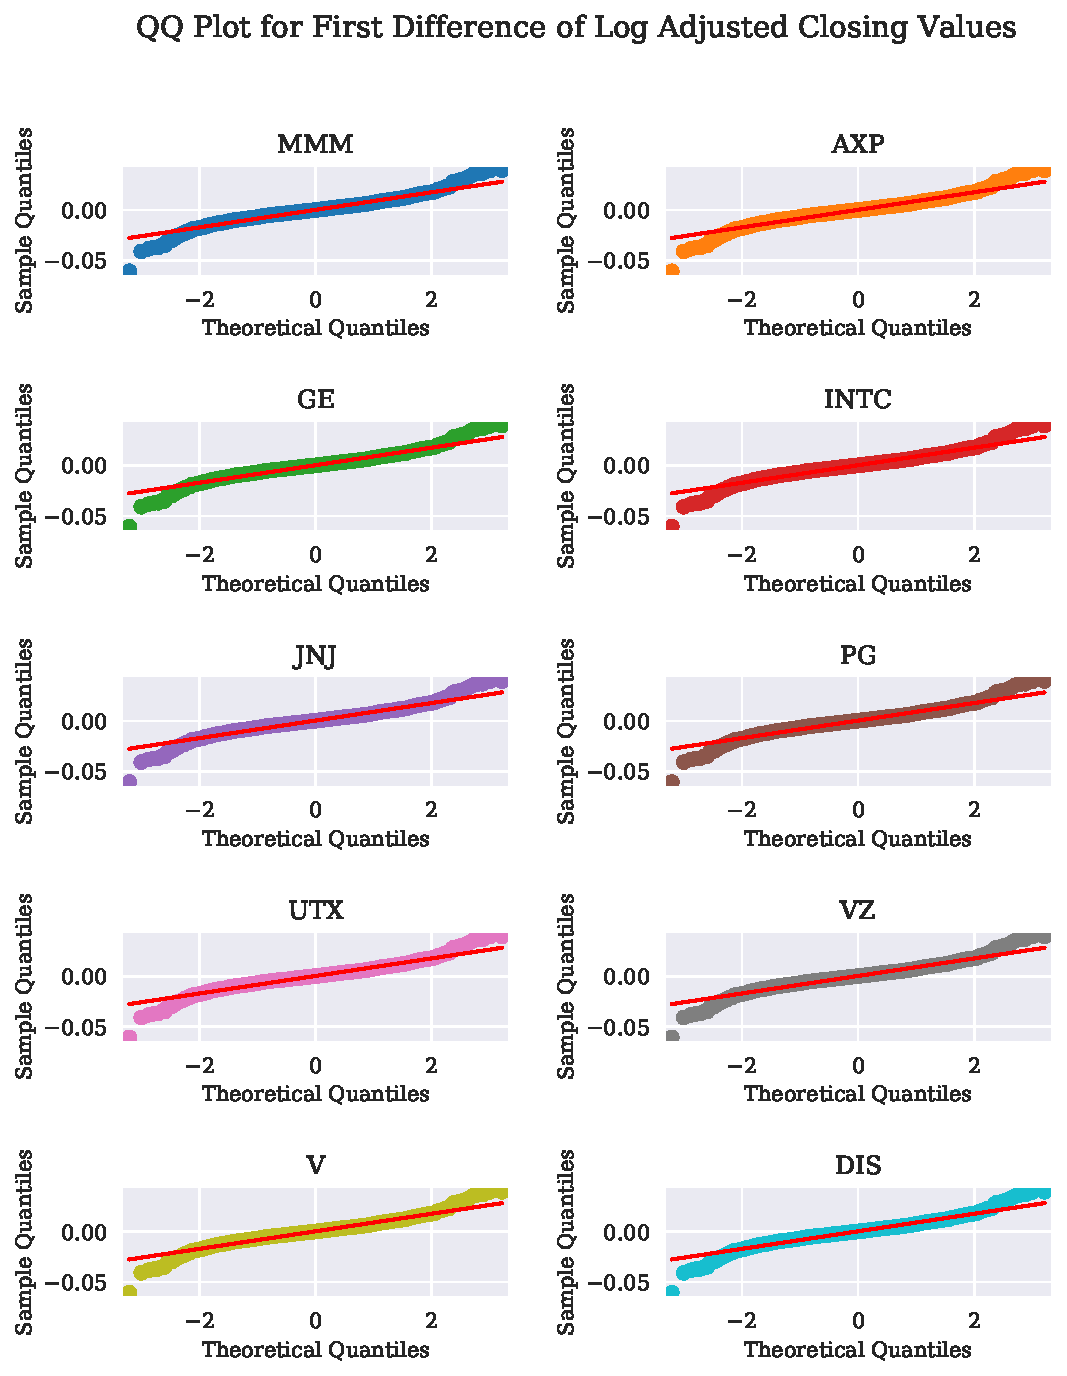
\includegraphics[]{figures/all_qq_plot_fd_log_adjclose.pdf}
    %%% Creator: Matplotlib, PGF backend
%%
%% To include the figure in your LaTeX document, write
%%   \input{<filename>.pgf}
%%
%% Make sure the required packages are loaded in your preamble
%%   \usepackage{pgf}
%%
%% Figures using additional raster images can only be included by \input if
%% they are in the same directory as the main LaTeX file. For loading figures
%% from other directories you can use the `import` package
%%   \usepackage{import}
%% and then include the figures with
%%   \import{<path to file>}{<filename>.pgf}
%%
%% Matplotlib used the following preamble
%%   \usepackage{fontspec}
%%   \setmainfont{DejaVuSerif.ttf}[Path=/opt/tljh/user/lib/python3.6/site-packages/matplotlib/mpl-data/fonts/ttf/]
%%   \setsansfont{DejaVuSans.ttf}[Path=/opt/tljh/user/lib/python3.6/site-packages/matplotlib/mpl-data/fonts/ttf/]
%%   \setmonofont{DejaVuSansMono.ttf}[Path=/opt/tljh/user/lib/python3.6/site-packages/matplotlib/mpl-data/fonts/ttf/]
%%
\begingroup%
\makeatletter%
\begin{pgfpicture}%
\pgfpathrectangle{\pgfpointorigin}{\pgfqpoint{7.336822in}{9.279134in}}%
\pgfusepath{use as bounding box, clip}%
\begin{pgfscope}%
\pgfsetbuttcap%
\pgfsetmiterjoin%
\definecolor{currentfill}{rgb}{1.000000,1.000000,1.000000}%
\pgfsetfillcolor{currentfill}%
\pgfsetlinewidth{0.000000pt}%
\definecolor{currentstroke}{rgb}{1.000000,1.000000,1.000000}%
\pgfsetstrokecolor{currentstroke}%
\pgfsetdash{}{0pt}%
\pgfpathmoveto{\pgfqpoint{0.000000in}{0.000000in}}%
\pgfpathlineto{\pgfqpoint{7.336822in}{0.000000in}}%
\pgfpathlineto{\pgfqpoint{7.336822in}{9.279134in}}%
\pgfpathlineto{\pgfqpoint{0.000000in}{9.279134in}}%
\pgfpathclose%
\pgfusepath{fill}%
\end{pgfscope}%
\begin{pgfscope}%
\pgfsetbuttcap%
\pgfsetmiterjoin%
\definecolor{currentfill}{rgb}{0.917647,0.917647,0.949020}%
\pgfsetfillcolor{currentfill}%
\pgfsetlinewidth{0.000000pt}%
\definecolor{currentstroke}{rgb}{0.000000,0.000000,0.000000}%
\pgfsetstrokecolor{currentstroke}%
\pgfsetstrokeopacity{0.000000}%
\pgfsetdash{}{0pt}%
\pgfpathmoveto{\pgfqpoint{1.036822in}{7.438938in}}%
\pgfpathlineto{\pgfqpoint{3.620155in}{7.438938in}}%
\pgfpathlineto{\pgfqpoint{3.620155in}{8.179134in}}%
\pgfpathlineto{\pgfqpoint{1.036822in}{8.179134in}}%
\pgfpathclose%
\pgfusepath{fill}%
\end{pgfscope}%
\begin{pgfscope}%
\pgfpathrectangle{\pgfqpoint{1.036822in}{7.438938in}}{\pgfqpoint{2.583333in}{0.740196in}}%
\pgfusepath{clip}%
\pgfsetroundcap%
\pgfsetroundjoin%
\pgfsetlinewidth{0.803000pt}%
\definecolor{currentstroke}{rgb}{1.000000,1.000000,1.000000}%
\pgfsetstrokecolor{currentstroke}%
\pgfsetdash{}{0pt}%
\pgfpathmoveto{\pgfqpoint{1.554767in}{7.438938in}}%
\pgfpathlineto{\pgfqpoint{1.554767in}{8.179134in}}%
\pgfusepath{stroke}%
\end{pgfscope}%
\begin{pgfscope}%
\definecolor{textcolor}{rgb}{0.150000,0.150000,0.150000}%
\pgfsetstrokecolor{textcolor}%
\pgfsetfillcolor{textcolor}%
\pgftext[x=1.554767in,y=7.341716in,,top]{\color{textcolor}\rmfamily\fontsize{14.000000}{16.800000}\selectfont −2}%
\end{pgfscope}%
\begin{pgfscope}%
\pgfpathrectangle{\pgfqpoint{1.036822in}{7.438938in}}{\pgfqpoint{2.583333in}{0.740196in}}%
\pgfusepath{clip}%
\pgfsetroundcap%
\pgfsetroundjoin%
\pgfsetlinewidth{0.803000pt}%
\definecolor{currentstroke}{rgb}{1.000000,1.000000,1.000000}%
\pgfsetstrokecolor{currentstroke}%
\pgfsetdash{}{0pt}%
\pgfpathmoveto{\pgfqpoint{2.328488in}{7.438938in}}%
\pgfpathlineto{\pgfqpoint{2.328488in}{8.179134in}}%
\pgfusepath{stroke}%
\end{pgfscope}%
\begin{pgfscope}%
\definecolor{textcolor}{rgb}{0.150000,0.150000,0.150000}%
\pgfsetstrokecolor{textcolor}%
\pgfsetfillcolor{textcolor}%
\pgftext[x=2.328488in,y=7.341716in,,top]{\color{textcolor}\rmfamily\fontsize{14.000000}{16.800000}\selectfont 0}%
\end{pgfscope}%
\begin{pgfscope}%
\pgfpathrectangle{\pgfqpoint{1.036822in}{7.438938in}}{\pgfqpoint{2.583333in}{0.740196in}}%
\pgfusepath{clip}%
\pgfsetroundcap%
\pgfsetroundjoin%
\pgfsetlinewidth{0.803000pt}%
\definecolor{currentstroke}{rgb}{1.000000,1.000000,1.000000}%
\pgfsetstrokecolor{currentstroke}%
\pgfsetdash{}{0pt}%
\pgfpathmoveto{\pgfqpoint{3.102209in}{7.438938in}}%
\pgfpathlineto{\pgfqpoint{3.102209in}{8.179134in}}%
\pgfusepath{stroke}%
\end{pgfscope}%
\begin{pgfscope}%
\definecolor{textcolor}{rgb}{0.150000,0.150000,0.150000}%
\pgfsetstrokecolor{textcolor}%
\pgfsetfillcolor{textcolor}%
\pgftext[x=3.102209in,y=7.341716in,,top]{\color{textcolor}\rmfamily\fontsize{14.000000}{16.800000}\selectfont 2}%
\end{pgfscope}%
\begin{pgfscope}%
\definecolor{textcolor}{rgb}{0.150000,0.150000,0.150000}%
\pgfsetstrokecolor{textcolor}%
\pgfsetfillcolor{textcolor}%
\pgftext[x=2.328488in,y=7.097982in,,top]{\color{textcolor}\rmfamily\fontsize{14.000000}{16.800000}\selectfont Theoretical Quantiles}%
\end{pgfscope}%
\begin{pgfscope}%
\pgfpathrectangle{\pgfqpoint{1.036822in}{7.438938in}}{\pgfqpoint{2.583333in}{0.740196in}}%
\pgfusepath{clip}%
\pgfsetroundcap%
\pgfsetroundjoin%
\pgfsetlinewidth{0.803000pt}%
\definecolor{currentstroke}{rgb}{1.000000,1.000000,1.000000}%
\pgfsetstrokecolor{currentstroke}%
\pgfsetdash{}{0pt}%
\pgfpathmoveto{\pgfqpoint{1.036822in}{7.543869in}}%
\pgfpathlineto{\pgfqpoint{3.620155in}{7.543869in}}%
\pgfusepath{stroke}%
\end{pgfscope}%
\begin{pgfscope}%
\definecolor{textcolor}{rgb}{0.150000,0.150000,0.150000}%
\pgfsetstrokecolor{textcolor}%
\pgfsetfillcolor{textcolor}%
\pgftext[x=0.343734in,y=7.470003in,left,base]{\color{textcolor}\rmfamily\fontsize{14.000000}{16.800000}\selectfont −0.05}%
\end{pgfscope}%
\begin{pgfscope}%
\pgfpathrectangle{\pgfqpoint{1.036822in}{7.438938in}}{\pgfqpoint{2.583333in}{0.740196in}}%
\pgfusepath{clip}%
\pgfsetroundcap%
\pgfsetroundjoin%
\pgfsetlinewidth{0.803000pt}%
\definecolor{currentstroke}{rgb}{1.000000,1.000000,1.000000}%
\pgfsetstrokecolor{currentstroke}%
\pgfsetdash{}{0pt}%
\pgfpathmoveto{\pgfqpoint{1.036822in}{7.879930in}}%
\pgfpathlineto{\pgfqpoint{3.620155in}{7.879930in}}%
\pgfusepath{stroke}%
\end{pgfscope}%
\begin{pgfscope}%
\definecolor{textcolor}{rgb}{0.150000,0.150000,0.150000}%
\pgfsetstrokecolor{textcolor}%
\pgfsetfillcolor{textcolor}%
\pgftext[x=0.506657in,y=7.806064in,left,base]{\color{textcolor}\rmfamily\fontsize{14.000000}{16.800000}\selectfont 0.00}%
\end{pgfscope}%
\begin{pgfscope}%
\definecolor{textcolor}{rgb}{0.150000,0.150000,0.150000}%
\pgfsetstrokecolor{textcolor}%
\pgfsetfillcolor{textcolor}%
\pgftext[x=0.288178in,y=7.809036in,,bottom,rotate=90.000000]{\color{textcolor}\rmfamily\fontsize{14.000000}{16.800000}\selectfont Sample Quantiles}%
\end{pgfscope}%
\begin{pgfscope}%
\pgfpathrectangle{\pgfqpoint{1.036822in}{7.438938in}}{\pgfqpoint{2.583333in}{0.740196in}}%
\pgfusepath{clip}%
\pgfsetbuttcap%
\pgfsetroundjoin%
\definecolor{currentfill}{rgb}{0.121569,0.466667,0.705882}%
\pgfsetfillcolor{currentfill}%
\pgfsetlinewidth{1.003750pt}%
\definecolor{currentstroke}{rgb}{0.121569,0.466667,0.705882}%
\pgfsetstrokecolor{currentstroke}%
\pgfsetdash{}{0pt}%
\pgfsys@defobject{currentmarker}{\pgfqpoint{-0.041667in}{-0.041667in}}{\pgfqpoint{0.041667in}{0.041667in}}{%
\pgfpathmoveto{\pgfqpoint{0.000000in}{-0.041667in}}%
\pgfpathcurveto{\pgfqpoint{0.011050in}{-0.041667in}}{\pgfqpoint{0.021649in}{-0.037276in}}{\pgfqpoint{0.029463in}{-0.029463in}}%
\pgfpathcurveto{\pgfqpoint{0.037276in}{-0.021649in}}{\pgfqpoint{0.041667in}{-0.011050in}}{\pgfqpoint{0.041667in}{0.000000in}}%
\pgfpathcurveto{\pgfqpoint{0.041667in}{0.011050in}}{\pgfqpoint{0.037276in}{0.021649in}}{\pgfqpoint{0.029463in}{0.029463in}}%
\pgfpathcurveto{\pgfqpoint{0.021649in}{0.037276in}}{\pgfqpoint{0.011050in}{0.041667in}}{\pgfqpoint{0.000000in}{0.041667in}}%
\pgfpathcurveto{\pgfqpoint{-0.011050in}{0.041667in}}{\pgfqpoint{-0.021649in}{0.037276in}}{\pgfqpoint{-0.029463in}{0.029463in}}%
\pgfpathcurveto{\pgfqpoint{-0.037276in}{0.021649in}}{\pgfqpoint{-0.041667in}{0.011050in}}{\pgfqpoint{-0.041667in}{0.000000in}}%
\pgfpathcurveto{\pgfqpoint{-0.041667in}{-0.011050in}}{\pgfqpoint{-0.037276in}{-0.021649in}}{\pgfqpoint{-0.029463in}{-0.029463in}}%
\pgfpathcurveto{\pgfqpoint{-0.021649in}{-0.037276in}}{\pgfqpoint{-0.011050in}{-0.041667in}}{\pgfqpoint{0.000000in}{-0.041667in}}%
\pgfpathclose%
\pgfusepath{stroke,fill}%
}%
\begin{pgfscope}%
\pgfsys@transformshift{1.086501in}{7.472583in}%
\pgfsys@useobject{currentmarker}{}%
\end{pgfscope}%
\begin{pgfscope}%
\pgfsys@transformshift{1.165749in}{7.605125in}%
\pgfsys@useobject{currentmarker}{}%
\end{pgfscope}%
\begin{pgfscope}%
\pgfsys@transformshift{1.214311in}{7.622529in}%
\pgfsys@useobject{currentmarker}{}%
\end{pgfscope}%
\begin{pgfscope}%
\pgfsys@transformshift{1.249876in}{7.630124in}%
\pgfsys@useobject{currentmarker}{}%
\end{pgfscope}%
\begin{pgfscope}%
\pgfsys@transformshift{1.278149in}{7.631584in}%
\pgfsys@useobject{currentmarker}{}%
\end{pgfscope}%
\begin{pgfscope}%
\pgfsys@transformshift{1.301726in}{7.643589in}%
\pgfsys@useobject{currentmarker}{}%
\end{pgfscope}%
\begin{pgfscope}%
\pgfsys@transformshift{1.322013in}{7.644197in}%
\pgfsys@useobject{currentmarker}{}%
\end{pgfscope}%
\begin{pgfscope}%
\pgfsys@transformshift{1.339860in}{7.672321in}%
\pgfsys@useobject{currentmarker}{}%
\end{pgfscope}%
\begin{pgfscope}%
\pgfsys@transformshift{1.355823in}{7.678378in}%
\pgfsys@useobject{currentmarker}{}%
\end{pgfscope}%
\begin{pgfscope}%
\pgfsys@transformshift{1.370283in}{7.679773in}%
\pgfsys@useobject{currentmarker}{}%
\end{pgfscope}%
\begin{pgfscope}%
\pgfsys@transformshift{1.383517in}{7.688269in}%
\pgfsys@useobject{currentmarker}{}%
\end{pgfscope}%
\begin{pgfscope}%
\pgfsys@transformshift{1.395730in}{7.696634in}%
\pgfsys@useobject{currentmarker}{}%
\end{pgfscope}%
\begin{pgfscope}%
\pgfsys@transformshift{1.407078in}{7.708844in}%
\pgfsys@useobject{currentmarker}{}%
\end{pgfscope}%
\begin{pgfscope}%
\pgfsys@transformshift{1.417685in}{7.709158in}%
\pgfsys@useobject{currentmarker}{}%
\end{pgfscope}%
\begin{pgfscope}%
\pgfsys@transformshift{1.427648in}{7.714896in}%
\pgfsys@useobject{currentmarker}{}%
\end{pgfscope}%
\begin{pgfscope}%
\pgfsys@transformshift{1.437048in}{7.721299in}%
\pgfsys@useobject{currentmarker}{}%
\end{pgfscope}%
\begin{pgfscope}%
\pgfsys@transformshift{1.445949in}{7.721735in}%
\pgfsys@useobject{currentmarker}{}%
\end{pgfscope}%
\begin{pgfscope}%
\pgfsys@transformshift{1.454405in}{7.724588in}%
\pgfsys@useobject{currentmarker}{}%
\end{pgfscope}%
\begin{pgfscope}%
\pgfsys@transformshift{1.462464in}{7.734109in}%
\pgfsys@useobject{currentmarker}{}%
\end{pgfscope}%
\begin{pgfscope}%
\pgfsys@transformshift{1.470164in}{7.736792in}%
\pgfsys@useobject{currentmarker}{}%
\end{pgfscope}%
\begin{pgfscope}%
\pgfsys@transformshift{1.477538in}{7.738270in}%
\pgfsys@useobject{currentmarker}{}%
\end{pgfscope}%
\begin{pgfscope}%
\pgfsys@transformshift{1.484615in}{7.739011in}%
\pgfsys@useobject{currentmarker}{}%
\end{pgfscope}%
\begin{pgfscope}%
\pgfsys@transformshift{1.491420in}{7.740191in}%
\pgfsys@useobject{currentmarker}{}%
\end{pgfscope}%
\begin{pgfscope}%
\pgfsys@transformshift{1.497976in}{7.748875in}%
\pgfsys@useobject{currentmarker}{}%
\end{pgfscope}%
\begin{pgfscope}%
\pgfsys@transformshift{1.504302in}{7.753354in}%
\pgfsys@useobject{currentmarker}{}%
\end{pgfscope}%
\begin{pgfscope}%
\pgfsys@transformshift{1.510414in}{7.753420in}%
\pgfsys@useobject{currentmarker}{}%
\end{pgfscope}%
\begin{pgfscope}%
\pgfsys@transformshift{1.516329in}{7.753628in}%
\pgfsys@useobject{currentmarker}{}%
\end{pgfscope}%
\begin{pgfscope}%
\pgfsys@transformshift{1.522060in}{7.754087in}%
\pgfsys@useobject{currentmarker}{}%
\end{pgfscope}%
\begin{pgfscope}%
\pgfsys@transformshift{1.527620in}{7.755629in}%
\pgfsys@useobject{currentmarker}{}%
\end{pgfscope}%
\begin{pgfscope}%
\pgfsys@transformshift{1.533019in}{7.757345in}%
\pgfsys@useobject{currentmarker}{}%
\end{pgfscope}%
\begin{pgfscope}%
\pgfsys@transformshift{1.538267in}{7.757622in}%
\pgfsys@useobject{currentmarker}{}%
\end{pgfscope}%
\begin{pgfscope}%
\pgfsys@transformshift{1.543373in}{7.758148in}%
\pgfsys@useobject{currentmarker}{}%
\end{pgfscope}%
\begin{pgfscope}%
\pgfsys@transformshift{1.548347in}{7.760982in}%
\pgfsys@useobject{currentmarker}{}%
\end{pgfscope}%
\begin{pgfscope}%
\pgfsys@transformshift{1.553194in}{7.761132in}%
\pgfsys@useobject{currentmarker}{}%
\end{pgfscope}%
\begin{pgfscope}%
\pgfsys@transformshift{1.557923in}{7.761473in}%
\pgfsys@useobject{currentmarker}{}%
\end{pgfscope}%
\begin{pgfscope}%
\pgfsys@transformshift{1.562540in}{7.763921in}%
\pgfsys@useobject{currentmarker}{}%
\end{pgfscope}%
\begin{pgfscope}%
\pgfsys@transformshift{1.567050in}{7.764061in}%
\pgfsys@useobject{currentmarker}{}%
\end{pgfscope}%
\begin{pgfscope}%
\pgfsys@transformshift{1.571458in}{7.764285in}%
\pgfsys@useobject{currentmarker}{}%
\end{pgfscope}%
\begin{pgfscope}%
\pgfsys@transformshift{1.575771in}{7.764825in}%
\pgfsys@useobject{currentmarker}{}%
\end{pgfscope}%
\begin{pgfscope}%
\pgfsys@transformshift{1.579992in}{7.766152in}%
\pgfsys@useobject{currentmarker}{}%
\end{pgfscope}%
\begin{pgfscope}%
\pgfsys@transformshift{1.584126in}{7.767186in}%
\pgfsys@useobject{currentmarker}{}%
\end{pgfscope}%
\begin{pgfscope}%
\pgfsys@transformshift{1.588176in}{7.770994in}%
\pgfsys@useobject{currentmarker}{}%
\end{pgfscope}%
\begin{pgfscope}%
\pgfsys@transformshift{1.592147in}{7.773762in}%
\pgfsys@useobject{currentmarker}{}%
\end{pgfscope}%
\begin{pgfscope}%
\pgfsys@transformshift{1.596042in}{7.773834in}%
\pgfsys@useobject{currentmarker}{}%
\end{pgfscope}%
\begin{pgfscope}%
\pgfsys@transformshift{1.599864in}{7.774417in}%
\pgfsys@useobject{currentmarker}{}%
\end{pgfscope}%
\begin{pgfscope}%
\pgfsys@transformshift{1.603616in}{7.774654in}%
\pgfsys@useobject{currentmarker}{}%
\end{pgfscope}%
\begin{pgfscope}%
\pgfsys@transformshift{1.607301in}{7.774761in}%
\pgfsys@useobject{currentmarker}{}%
\end{pgfscope}%
\begin{pgfscope}%
\pgfsys@transformshift{1.610922in}{7.775384in}%
\pgfsys@useobject{currentmarker}{}%
\end{pgfscope}%
\begin{pgfscope}%
\pgfsys@transformshift{1.614481in}{7.775399in}%
\pgfsys@useobject{currentmarker}{}%
\end{pgfscope}%
\begin{pgfscope}%
\pgfsys@transformshift{1.617981in}{7.777718in}%
\pgfsys@useobject{currentmarker}{}%
\end{pgfscope}%
\begin{pgfscope}%
\pgfsys@transformshift{1.621423in}{7.778045in}%
\pgfsys@useobject{currentmarker}{}%
\end{pgfscope}%
\begin{pgfscope}%
\pgfsys@transformshift{1.624810in}{7.781778in}%
\pgfsys@useobject{currentmarker}{}%
\end{pgfscope}%
\begin{pgfscope}%
\pgfsys@transformshift{1.628145in}{7.781779in}%
\pgfsys@useobject{currentmarker}{}%
\end{pgfscope}%
\begin{pgfscope}%
\pgfsys@transformshift{1.631428in}{7.781854in}%
\pgfsys@useobject{currentmarker}{}%
\end{pgfscope}%
\begin{pgfscope}%
\pgfsys@transformshift{1.634661in}{7.783194in}%
\pgfsys@useobject{currentmarker}{}%
\end{pgfscope}%
\begin{pgfscope}%
\pgfsys@transformshift{1.637847in}{7.783561in}%
\pgfsys@useobject{currentmarker}{}%
\end{pgfscope}%
\begin{pgfscope}%
\pgfsys@transformshift{1.640987in}{7.784001in}%
\pgfsys@useobject{currentmarker}{}%
\end{pgfscope}%
\begin{pgfscope}%
\pgfsys@transformshift{1.644082in}{7.784244in}%
\pgfsys@useobject{currentmarker}{}%
\end{pgfscope}%
\begin{pgfscope}%
\pgfsys@transformshift{1.647133in}{7.785580in}%
\pgfsys@useobject{currentmarker}{}%
\end{pgfscope}%
\begin{pgfscope}%
\pgfsys@transformshift{1.650143in}{7.786913in}%
\pgfsys@useobject{currentmarker}{}%
\end{pgfscope}%
\begin{pgfscope}%
\pgfsys@transformshift{1.653113in}{7.787404in}%
\pgfsys@useobject{currentmarker}{}%
\end{pgfscope}%
\begin{pgfscope}%
\pgfsys@transformshift{1.656043in}{7.788222in}%
\pgfsys@useobject{currentmarker}{}%
\end{pgfscope}%
\begin{pgfscope}%
\pgfsys@transformshift{1.658935in}{7.788386in}%
\pgfsys@useobject{currentmarker}{}%
\end{pgfscope}%
\begin{pgfscope}%
\pgfsys@transformshift{1.661790in}{7.788654in}%
\pgfsys@useobject{currentmarker}{}%
\end{pgfscope}%
\begin{pgfscope}%
\pgfsys@transformshift{1.664610in}{7.790477in}%
\pgfsys@useobject{currentmarker}{}%
\end{pgfscope}%
\begin{pgfscope}%
\pgfsys@transformshift{1.667394in}{7.791247in}%
\pgfsys@useobject{currentmarker}{}%
\end{pgfscope}%
\begin{pgfscope}%
\pgfsys@transformshift{1.670145in}{7.791334in}%
\pgfsys@useobject{currentmarker}{}%
\end{pgfscope}%
\begin{pgfscope}%
\pgfsys@transformshift{1.672863in}{7.792379in}%
\pgfsys@useobject{currentmarker}{}%
\end{pgfscope}%
\begin{pgfscope}%
\pgfsys@transformshift{1.675549in}{7.792564in}%
\pgfsys@useobject{currentmarker}{}%
\end{pgfscope}%
\begin{pgfscope}%
\pgfsys@transformshift{1.678203in}{7.792566in}%
\pgfsys@useobject{currentmarker}{}%
\end{pgfscope}%
\begin{pgfscope}%
\pgfsys@transformshift{1.680828in}{7.794018in}%
\pgfsys@useobject{currentmarker}{}%
\end{pgfscope}%
\begin{pgfscope}%
\pgfsys@transformshift{1.683423in}{7.794249in}%
\pgfsys@useobject{currentmarker}{}%
\end{pgfscope}%
\begin{pgfscope}%
\pgfsys@transformshift{1.685989in}{7.794277in}%
\pgfsys@useobject{currentmarker}{}%
\end{pgfscope}%
\begin{pgfscope}%
\pgfsys@transformshift{1.688527in}{7.794867in}%
\pgfsys@useobject{currentmarker}{}%
\end{pgfscope}%
\begin{pgfscope}%
\pgfsys@transformshift{1.691038in}{7.795067in}%
\pgfsys@useobject{currentmarker}{}%
\end{pgfscope}%
\begin{pgfscope}%
\pgfsys@transformshift{1.693523in}{7.795650in}%
\pgfsys@useobject{currentmarker}{}%
\end{pgfscope}%
\begin{pgfscope}%
\pgfsys@transformshift{1.695981in}{7.795772in}%
\pgfsys@useobject{currentmarker}{}%
\end{pgfscope}%
\begin{pgfscope}%
\pgfsys@transformshift{1.698414in}{7.795848in}%
\pgfsys@useobject{currentmarker}{}%
\end{pgfscope}%
\begin{pgfscope}%
\pgfsys@transformshift{1.700823in}{7.795926in}%
\pgfsys@useobject{currentmarker}{}%
\end{pgfscope}%
\begin{pgfscope}%
\pgfsys@transformshift{1.703208in}{7.795946in}%
\pgfsys@useobject{currentmarker}{}%
\end{pgfscope}%
\begin{pgfscope}%
\pgfsys@transformshift{1.705569in}{7.796039in}%
\pgfsys@useobject{currentmarker}{}%
\end{pgfscope}%
\begin{pgfscope}%
\pgfsys@transformshift{1.707907in}{7.796390in}%
\pgfsys@useobject{currentmarker}{}%
\end{pgfscope}%
\begin{pgfscope}%
\pgfsys@transformshift{1.710222in}{7.797151in}%
\pgfsys@useobject{currentmarker}{}%
\end{pgfscope}%
\begin{pgfscope}%
\pgfsys@transformshift{1.712516in}{7.797652in}%
\pgfsys@useobject{currentmarker}{}%
\end{pgfscope}%
\begin{pgfscope}%
\pgfsys@transformshift{1.714788in}{7.797985in}%
\pgfsys@useobject{currentmarker}{}%
\end{pgfscope}%
\begin{pgfscope}%
\pgfsys@transformshift{1.717039in}{7.798265in}%
\pgfsys@useobject{currentmarker}{}%
\end{pgfscope}%
\begin{pgfscope}%
\pgfsys@transformshift{1.719270in}{7.798472in}%
\pgfsys@useobject{currentmarker}{}%
\end{pgfscope}%
\begin{pgfscope}%
\pgfsys@transformshift{1.721480in}{7.799389in}%
\pgfsys@useobject{currentmarker}{}%
\end{pgfscope}%
\begin{pgfscope}%
\pgfsys@transformshift{1.723671in}{7.799858in}%
\pgfsys@useobject{currentmarker}{}%
\end{pgfscope}%
\begin{pgfscope}%
\pgfsys@transformshift{1.725843in}{7.800124in}%
\pgfsys@useobject{currentmarker}{}%
\end{pgfscope}%
\begin{pgfscope}%
\pgfsys@transformshift{1.727996in}{7.800135in}%
\pgfsys@useobject{currentmarker}{}%
\end{pgfscope}%
\begin{pgfscope}%
\pgfsys@transformshift{1.730130in}{7.800899in}%
\pgfsys@useobject{currentmarker}{}%
\end{pgfscope}%
\begin{pgfscope}%
\pgfsys@transformshift{1.732247in}{7.801175in}%
\pgfsys@useobject{currentmarker}{}%
\end{pgfscope}%
\begin{pgfscope}%
\pgfsys@transformshift{1.734345in}{7.801273in}%
\pgfsys@useobject{currentmarker}{}%
\end{pgfscope}%
\begin{pgfscope}%
\pgfsys@transformshift{1.736427in}{7.801873in}%
\pgfsys@useobject{currentmarker}{}%
\end{pgfscope}%
\begin{pgfscope}%
\pgfsys@transformshift{1.738491in}{7.802442in}%
\pgfsys@useobject{currentmarker}{}%
\end{pgfscope}%
\begin{pgfscope}%
\pgfsys@transformshift{1.740539in}{7.802713in}%
\pgfsys@useobject{currentmarker}{}%
\end{pgfscope}%
\begin{pgfscope}%
\pgfsys@transformshift{1.742570in}{7.802978in}%
\pgfsys@useobject{currentmarker}{}%
\end{pgfscope}%
\begin{pgfscope}%
\pgfsys@transformshift{1.744586in}{7.804975in}%
\pgfsys@useobject{currentmarker}{}%
\end{pgfscope}%
\begin{pgfscope}%
\pgfsys@transformshift{1.746585in}{7.805049in}%
\pgfsys@useobject{currentmarker}{}%
\end{pgfscope}%
\begin{pgfscope}%
\pgfsys@transformshift{1.748569in}{7.805965in}%
\pgfsys@useobject{currentmarker}{}%
\end{pgfscope}%
\begin{pgfscope}%
\pgfsys@transformshift{1.750538in}{7.806918in}%
\pgfsys@useobject{currentmarker}{}%
\end{pgfscope}%
\begin{pgfscope}%
\pgfsys@transformshift{1.752493in}{7.807042in}%
\pgfsys@useobject{currentmarker}{}%
\end{pgfscope}%
\begin{pgfscope}%
\pgfsys@transformshift{1.754432in}{7.807099in}%
\pgfsys@useobject{currentmarker}{}%
\end{pgfscope}%
\begin{pgfscope}%
\pgfsys@transformshift{1.756357in}{7.807431in}%
\pgfsys@useobject{currentmarker}{}%
\end{pgfscope}%
\begin{pgfscope}%
\pgfsys@transformshift{1.758269in}{7.807511in}%
\pgfsys@useobject{currentmarker}{}%
\end{pgfscope}%
\begin{pgfscope}%
\pgfsys@transformshift{1.760166in}{7.807653in}%
\pgfsys@useobject{currentmarker}{}%
\end{pgfscope}%
\begin{pgfscope}%
\pgfsys@transformshift{1.762050in}{7.807685in}%
\pgfsys@useobject{currentmarker}{}%
\end{pgfscope}%
\begin{pgfscope}%
\pgfsys@transformshift{1.763920in}{7.807906in}%
\pgfsys@useobject{currentmarker}{}%
\end{pgfscope}%
\begin{pgfscope}%
\pgfsys@transformshift{1.765778in}{7.807922in}%
\pgfsys@useobject{currentmarker}{}%
\end{pgfscope}%
\begin{pgfscope}%
\pgfsys@transformshift{1.767622in}{7.808583in}%
\pgfsys@useobject{currentmarker}{}%
\end{pgfscope}%
\begin{pgfscope}%
\pgfsys@transformshift{1.769454in}{7.809430in}%
\pgfsys@useobject{currentmarker}{}%
\end{pgfscope}%
\begin{pgfscope}%
\pgfsys@transformshift{1.771273in}{7.809873in}%
\pgfsys@useobject{currentmarker}{}%
\end{pgfscope}%
\begin{pgfscope}%
\pgfsys@transformshift{1.773081in}{7.810094in}%
\pgfsys@useobject{currentmarker}{}%
\end{pgfscope}%
\begin{pgfscope}%
\pgfsys@transformshift{1.774876in}{7.810101in}%
\pgfsys@useobject{currentmarker}{}%
\end{pgfscope}%
\begin{pgfscope}%
\pgfsys@transformshift{1.776659in}{7.810405in}%
\pgfsys@useobject{currentmarker}{}%
\end{pgfscope}%
\begin{pgfscope}%
\pgfsys@transformshift{1.778430in}{7.811455in}%
\pgfsys@useobject{currentmarker}{}%
\end{pgfscope}%
\begin{pgfscope}%
\pgfsys@transformshift{1.780191in}{7.811625in}%
\pgfsys@useobject{currentmarker}{}%
\end{pgfscope}%
\begin{pgfscope}%
\pgfsys@transformshift{1.781939in}{7.812463in}%
\pgfsys@useobject{currentmarker}{}%
\end{pgfscope}%
\begin{pgfscope}%
\pgfsys@transformshift{1.783677in}{7.812851in}%
\pgfsys@useobject{currentmarker}{}%
\end{pgfscope}%
\begin{pgfscope}%
\pgfsys@transformshift{1.785404in}{7.812895in}%
\pgfsys@useobject{currentmarker}{}%
\end{pgfscope}%
\begin{pgfscope}%
\pgfsys@transformshift{1.787120in}{7.813011in}%
\pgfsys@useobject{currentmarker}{}%
\end{pgfscope}%
\begin{pgfscope}%
\pgfsys@transformshift{1.788826in}{7.813616in}%
\pgfsys@useobject{currentmarker}{}%
\end{pgfscope}%
\begin{pgfscope}%
\pgfsys@transformshift{1.790521in}{7.813927in}%
\pgfsys@useobject{currentmarker}{}%
\end{pgfscope}%
\begin{pgfscope}%
\pgfsys@transformshift{1.792206in}{7.814544in}%
\pgfsys@useobject{currentmarker}{}%
\end{pgfscope}%
\begin{pgfscope}%
\pgfsys@transformshift{1.793880in}{7.814980in}%
\pgfsys@useobject{currentmarker}{}%
\end{pgfscope}%
\begin{pgfscope}%
\pgfsys@transformshift{1.795545in}{7.815009in}%
\pgfsys@useobject{currentmarker}{}%
\end{pgfscope}%
\begin{pgfscope}%
\pgfsys@transformshift{1.797200in}{7.815065in}%
\pgfsys@useobject{currentmarker}{}%
\end{pgfscope}%
\begin{pgfscope}%
\pgfsys@transformshift{1.798845in}{7.815174in}%
\pgfsys@useobject{currentmarker}{}%
\end{pgfscope}%
\begin{pgfscope}%
\pgfsys@transformshift{1.800481in}{7.815307in}%
\pgfsys@useobject{currentmarker}{}%
\end{pgfscope}%
\begin{pgfscope}%
\pgfsys@transformshift{1.802107in}{7.815391in}%
\pgfsys@useobject{currentmarker}{}%
\end{pgfscope}%
\begin{pgfscope}%
\pgfsys@transformshift{1.803724in}{7.815584in}%
\pgfsys@useobject{currentmarker}{}%
\end{pgfscope}%
\begin{pgfscope}%
\pgfsys@transformshift{1.805332in}{7.815725in}%
\pgfsys@useobject{currentmarker}{}%
\end{pgfscope}%
\begin{pgfscope}%
\pgfsys@transformshift{1.806931in}{7.815857in}%
\pgfsys@useobject{currentmarker}{}%
\end{pgfscope}%
\begin{pgfscope}%
\pgfsys@transformshift{1.808522in}{7.816050in}%
\pgfsys@useobject{currentmarker}{}%
\end{pgfscope}%
\begin{pgfscope}%
\pgfsys@transformshift{1.810103in}{7.816154in}%
\pgfsys@useobject{currentmarker}{}%
\end{pgfscope}%
\begin{pgfscope}%
\pgfsys@transformshift{1.811676in}{7.816212in}%
\pgfsys@useobject{currentmarker}{}%
\end{pgfscope}%
\begin{pgfscope}%
\pgfsys@transformshift{1.813240in}{7.816351in}%
\pgfsys@useobject{currentmarker}{}%
\end{pgfscope}%
\begin{pgfscope}%
\pgfsys@transformshift{1.814796in}{7.816530in}%
\pgfsys@useobject{currentmarker}{}%
\end{pgfscope}%
\begin{pgfscope}%
\pgfsys@transformshift{1.816344in}{7.816819in}%
\pgfsys@useobject{currentmarker}{}%
\end{pgfscope}%
\begin{pgfscope}%
\pgfsys@transformshift{1.817883in}{7.817125in}%
\pgfsys@useobject{currentmarker}{}%
\end{pgfscope}%
\begin{pgfscope}%
\pgfsys@transformshift{1.819415in}{7.817134in}%
\pgfsys@useobject{currentmarker}{}%
\end{pgfscope}%
\begin{pgfscope}%
\pgfsys@transformshift{1.820938in}{7.817593in}%
\pgfsys@useobject{currentmarker}{}%
\end{pgfscope}%
\begin{pgfscope}%
\pgfsys@transformshift{1.822454in}{7.817956in}%
\pgfsys@useobject{currentmarker}{}%
\end{pgfscope}%
\begin{pgfscope}%
\pgfsys@transformshift{1.823962in}{7.817966in}%
\pgfsys@useobject{currentmarker}{}%
\end{pgfscope}%
\begin{pgfscope}%
\pgfsys@transformshift{1.825462in}{7.818742in}%
\pgfsys@useobject{currentmarker}{}%
\end{pgfscope}%
\begin{pgfscope}%
\pgfsys@transformshift{1.826955in}{7.818789in}%
\pgfsys@useobject{currentmarker}{}%
\end{pgfscope}%
\begin{pgfscope}%
\pgfsys@transformshift{1.828440in}{7.818934in}%
\pgfsys@useobject{currentmarker}{}%
\end{pgfscope}%
\begin{pgfscope}%
\pgfsys@transformshift{1.829918in}{7.819168in}%
\pgfsys@useobject{currentmarker}{}%
\end{pgfscope}%
\begin{pgfscope}%
\pgfsys@transformshift{1.831389in}{7.819387in}%
\pgfsys@useobject{currentmarker}{}%
\end{pgfscope}%
\begin{pgfscope}%
\pgfsys@transformshift{1.832853in}{7.819426in}%
\pgfsys@useobject{currentmarker}{}%
\end{pgfscope}%
\begin{pgfscope}%
\pgfsys@transformshift{1.834309in}{7.819511in}%
\pgfsys@useobject{currentmarker}{}%
\end{pgfscope}%
\begin{pgfscope}%
\pgfsys@transformshift{1.835759in}{7.819607in}%
\pgfsys@useobject{currentmarker}{}%
\end{pgfscope}%
\begin{pgfscope}%
\pgfsys@transformshift{1.837202in}{7.819835in}%
\pgfsys@useobject{currentmarker}{}%
\end{pgfscope}%
\begin{pgfscope}%
\pgfsys@transformshift{1.838638in}{7.819951in}%
\pgfsys@useobject{currentmarker}{}%
\end{pgfscope}%
\begin{pgfscope}%
\pgfsys@transformshift{1.840067in}{7.820008in}%
\pgfsys@useobject{currentmarker}{}%
\end{pgfscope}%
\begin{pgfscope}%
\pgfsys@transformshift{1.841489in}{7.820282in}%
\pgfsys@useobject{currentmarker}{}%
\end{pgfscope}%
\begin{pgfscope}%
\pgfsys@transformshift{1.842905in}{7.820432in}%
\pgfsys@useobject{currentmarker}{}%
\end{pgfscope}%
\begin{pgfscope}%
\pgfsys@transformshift{1.844315in}{7.820653in}%
\pgfsys@useobject{currentmarker}{}%
\end{pgfscope}%
\begin{pgfscope}%
\pgfsys@transformshift{1.845718in}{7.820783in}%
\pgfsys@useobject{currentmarker}{}%
\end{pgfscope}%
\begin{pgfscope}%
\pgfsys@transformshift{1.847115in}{7.820976in}%
\pgfsys@useobject{currentmarker}{}%
\end{pgfscope}%
\begin{pgfscope}%
\pgfsys@transformshift{1.848505in}{7.821100in}%
\pgfsys@useobject{currentmarker}{}%
\end{pgfscope}%
\begin{pgfscope}%
\pgfsys@transformshift{1.849890in}{7.821152in}%
\pgfsys@useobject{currentmarker}{}%
\end{pgfscope}%
\begin{pgfscope}%
\pgfsys@transformshift{1.851268in}{7.821491in}%
\pgfsys@useobject{currentmarker}{}%
\end{pgfscope}%
\begin{pgfscope}%
\pgfsys@transformshift{1.852640in}{7.821669in}%
\pgfsys@useobject{currentmarker}{}%
\end{pgfscope}%
\begin{pgfscope}%
\pgfsys@transformshift{1.854007in}{7.821704in}%
\pgfsys@useobject{currentmarker}{}%
\end{pgfscope}%
\begin{pgfscope}%
\pgfsys@transformshift{1.855367in}{7.822025in}%
\pgfsys@useobject{currentmarker}{}%
\end{pgfscope}%
\begin{pgfscope}%
\pgfsys@transformshift{1.856722in}{7.822091in}%
\pgfsys@useobject{currentmarker}{}%
\end{pgfscope}%
\begin{pgfscope}%
\pgfsys@transformshift{1.858071in}{7.822093in}%
\pgfsys@useobject{currentmarker}{}%
\end{pgfscope}%
\begin{pgfscope}%
\pgfsys@transformshift{1.859414in}{7.822093in}%
\pgfsys@useobject{currentmarker}{}%
\end{pgfscope}%
\begin{pgfscope}%
\pgfsys@transformshift{1.860751in}{7.822115in}%
\pgfsys@useobject{currentmarker}{}%
\end{pgfscope}%
\begin{pgfscope}%
\pgfsys@transformshift{1.862083in}{7.822451in}%
\pgfsys@useobject{currentmarker}{}%
\end{pgfscope}%
\begin{pgfscope}%
\pgfsys@transformshift{1.863410in}{7.822821in}%
\pgfsys@useobject{currentmarker}{}%
\end{pgfscope}%
\begin{pgfscope}%
\pgfsys@transformshift{1.864731in}{7.822983in}%
\pgfsys@useobject{currentmarker}{}%
\end{pgfscope}%
\begin{pgfscope}%
\pgfsys@transformshift{1.866046in}{7.823516in}%
\pgfsys@useobject{currentmarker}{}%
\end{pgfscope}%
\begin{pgfscope}%
\pgfsys@transformshift{1.867356in}{7.823668in}%
\pgfsys@useobject{currentmarker}{}%
\end{pgfscope}%
\begin{pgfscope}%
\pgfsys@transformshift{1.868661in}{7.823965in}%
\pgfsys@useobject{currentmarker}{}%
\end{pgfscope}%
\begin{pgfscope}%
\pgfsys@transformshift{1.869961in}{7.824022in}%
\pgfsys@useobject{currentmarker}{}%
\end{pgfscope}%
\begin{pgfscope}%
\pgfsys@transformshift{1.871256in}{7.824075in}%
\pgfsys@useobject{currentmarker}{}%
\end{pgfscope}%
\begin{pgfscope}%
\pgfsys@transformshift{1.872545in}{7.824195in}%
\pgfsys@useobject{currentmarker}{}%
\end{pgfscope}%
\begin{pgfscope}%
\pgfsys@transformshift{1.873830in}{7.824241in}%
\pgfsys@useobject{currentmarker}{}%
\end{pgfscope}%
\begin{pgfscope}%
\pgfsys@transformshift{1.875109in}{7.824269in}%
\pgfsys@useobject{currentmarker}{}%
\end{pgfscope}%
\begin{pgfscope}%
\pgfsys@transformshift{1.876384in}{7.824532in}%
\pgfsys@useobject{currentmarker}{}%
\end{pgfscope}%
\begin{pgfscope}%
\pgfsys@transformshift{1.877654in}{7.825132in}%
\pgfsys@useobject{currentmarker}{}%
\end{pgfscope}%
\begin{pgfscope}%
\pgfsys@transformshift{1.878918in}{7.825197in}%
\pgfsys@useobject{currentmarker}{}%
\end{pgfscope}%
\begin{pgfscope}%
\pgfsys@transformshift{1.880178in}{7.825308in}%
\pgfsys@useobject{currentmarker}{}%
\end{pgfscope}%
\begin{pgfscope}%
\pgfsys@transformshift{1.881434in}{7.825977in}%
\pgfsys@useobject{currentmarker}{}%
\end{pgfscope}%
\begin{pgfscope}%
\pgfsys@transformshift{1.882684in}{7.826056in}%
\pgfsys@useobject{currentmarker}{}%
\end{pgfscope}%
\begin{pgfscope}%
\pgfsys@transformshift{1.883930in}{7.826083in}%
\pgfsys@useobject{currentmarker}{}%
\end{pgfscope}%
\begin{pgfscope}%
\pgfsys@transformshift{1.885172in}{7.826250in}%
\pgfsys@useobject{currentmarker}{}%
\end{pgfscope}%
\begin{pgfscope}%
\pgfsys@transformshift{1.886409in}{7.826256in}%
\pgfsys@useobject{currentmarker}{}%
\end{pgfscope}%
\begin{pgfscope}%
\pgfsys@transformshift{1.887641in}{7.826621in}%
\pgfsys@useobject{currentmarker}{}%
\end{pgfscope}%
\begin{pgfscope}%
\pgfsys@transformshift{1.888869in}{7.826734in}%
\pgfsys@useobject{currentmarker}{}%
\end{pgfscope}%
\begin{pgfscope}%
\pgfsys@transformshift{1.890092in}{7.826746in}%
\pgfsys@useobject{currentmarker}{}%
\end{pgfscope}%
\begin{pgfscope}%
\pgfsys@transformshift{1.891311in}{7.826836in}%
\pgfsys@useobject{currentmarker}{}%
\end{pgfscope}%
\begin{pgfscope}%
\pgfsys@transformshift{1.892526in}{7.826927in}%
\pgfsys@useobject{currentmarker}{}%
\end{pgfscope}%
\begin{pgfscope}%
\pgfsys@transformshift{1.893737in}{7.827560in}%
\pgfsys@useobject{currentmarker}{}%
\end{pgfscope}%
\begin{pgfscope}%
\pgfsys@transformshift{1.894943in}{7.827665in}%
\pgfsys@useobject{currentmarker}{}%
\end{pgfscope}%
\begin{pgfscope}%
\pgfsys@transformshift{1.896145in}{7.827704in}%
\pgfsys@useobject{currentmarker}{}%
\end{pgfscope}%
\begin{pgfscope}%
\pgfsys@transformshift{1.897343in}{7.828288in}%
\pgfsys@useobject{currentmarker}{}%
\end{pgfscope}%
\begin{pgfscope}%
\pgfsys@transformshift{1.898536in}{7.828373in}%
\pgfsys@useobject{currentmarker}{}%
\end{pgfscope}%
\begin{pgfscope}%
\pgfsys@transformshift{1.899726in}{7.828574in}%
\pgfsys@useobject{currentmarker}{}%
\end{pgfscope}%
\begin{pgfscope}%
\pgfsys@transformshift{1.900912in}{7.828658in}%
\pgfsys@useobject{currentmarker}{}%
\end{pgfscope}%
\begin{pgfscope}%
\pgfsys@transformshift{1.902093in}{7.828728in}%
\pgfsys@useobject{currentmarker}{}%
\end{pgfscope}%
\begin{pgfscope}%
\pgfsys@transformshift{1.903271in}{7.828818in}%
\pgfsys@useobject{currentmarker}{}%
\end{pgfscope}%
\begin{pgfscope}%
\pgfsys@transformshift{1.904445in}{7.828818in}%
\pgfsys@useobject{currentmarker}{}%
\end{pgfscope}%
\begin{pgfscope}%
\pgfsys@transformshift{1.905615in}{7.828887in}%
\pgfsys@useobject{currentmarker}{}%
\end{pgfscope}%
\begin{pgfscope}%
\pgfsys@transformshift{1.906781in}{7.829038in}%
\pgfsys@useobject{currentmarker}{}%
\end{pgfscope}%
\begin{pgfscope}%
\pgfsys@transformshift{1.907943in}{7.829062in}%
\pgfsys@useobject{currentmarker}{}%
\end{pgfscope}%
\begin{pgfscope}%
\pgfsys@transformshift{1.909101in}{7.829085in}%
\pgfsys@useobject{currentmarker}{}%
\end{pgfscope}%
\begin{pgfscope}%
\pgfsys@transformshift{1.910256in}{7.829203in}%
\pgfsys@useobject{currentmarker}{}%
\end{pgfscope}%
\begin{pgfscope}%
\pgfsys@transformshift{1.911407in}{7.829583in}%
\pgfsys@useobject{currentmarker}{}%
\end{pgfscope}%
\begin{pgfscope}%
\pgfsys@transformshift{1.912554in}{7.830552in}%
\pgfsys@useobject{currentmarker}{}%
\end{pgfscope}%
\begin{pgfscope}%
\pgfsys@transformshift{1.913698in}{7.830619in}%
\pgfsys@useobject{currentmarker}{}%
\end{pgfscope}%
\begin{pgfscope}%
\pgfsys@transformshift{1.914838in}{7.830644in}%
\pgfsys@useobject{currentmarker}{}%
\end{pgfscope}%
\begin{pgfscope}%
\pgfsys@transformshift{1.915974in}{7.831141in}%
\pgfsys@useobject{currentmarker}{}%
\end{pgfscope}%
\begin{pgfscope}%
\pgfsys@transformshift{1.917107in}{7.831144in}%
\pgfsys@useobject{currentmarker}{}%
\end{pgfscope}%
\begin{pgfscope}%
\pgfsys@transformshift{1.918236in}{7.831171in}%
\pgfsys@useobject{currentmarker}{}%
\end{pgfscope}%
\begin{pgfscope}%
\pgfsys@transformshift{1.919362in}{7.831222in}%
\pgfsys@useobject{currentmarker}{}%
\end{pgfscope}%
\begin{pgfscope}%
\pgfsys@transformshift{1.920485in}{7.831274in}%
\pgfsys@useobject{currentmarker}{}%
\end{pgfscope}%
\begin{pgfscope}%
\pgfsys@transformshift{1.921604in}{7.831278in}%
\pgfsys@useobject{currentmarker}{}%
\end{pgfscope}%
\begin{pgfscope}%
\pgfsys@transformshift{1.922719in}{7.831408in}%
\pgfsys@useobject{currentmarker}{}%
\end{pgfscope}%
\begin{pgfscope}%
\pgfsys@transformshift{1.923831in}{7.831423in}%
\pgfsys@useobject{currentmarker}{}%
\end{pgfscope}%
\begin{pgfscope}%
\pgfsys@transformshift{1.924940in}{7.831583in}%
\pgfsys@useobject{currentmarker}{}%
\end{pgfscope}%
\begin{pgfscope}%
\pgfsys@transformshift{1.926046in}{7.831868in}%
\pgfsys@useobject{currentmarker}{}%
\end{pgfscope}%
\begin{pgfscope}%
\pgfsys@transformshift{1.927148in}{7.831971in}%
\pgfsys@useobject{currentmarker}{}%
\end{pgfscope}%
\begin{pgfscope}%
\pgfsys@transformshift{1.928247in}{7.832180in}%
\pgfsys@useobject{currentmarker}{}%
\end{pgfscope}%
\begin{pgfscope}%
\pgfsys@transformshift{1.929343in}{7.832437in}%
\pgfsys@useobject{currentmarker}{}%
\end{pgfscope}%
\begin{pgfscope}%
\pgfsys@transformshift{1.930436in}{7.832594in}%
\pgfsys@useobject{currentmarker}{}%
\end{pgfscope}%
\begin{pgfscope}%
\pgfsys@transformshift{1.931525in}{7.832708in}%
\pgfsys@useobject{currentmarker}{}%
\end{pgfscope}%
\begin{pgfscope}%
\pgfsys@transformshift{1.932612in}{7.832835in}%
\pgfsys@useobject{currentmarker}{}%
\end{pgfscope}%
\begin{pgfscope}%
\pgfsys@transformshift{1.933695in}{7.833125in}%
\pgfsys@useobject{currentmarker}{}%
\end{pgfscope}%
\begin{pgfscope}%
\pgfsys@transformshift{1.934775in}{7.833207in}%
\pgfsys@useobject{currentmarker}{}%
\end{pgfscope}%
\begin{pgfscope}%
\pgfsys@transformshift{1.935852in}{7.833223in}%
\pgfsys@useobject{currentmarker}{}%
\end{pgfscope}%
\begin{pgfscope}%
\pgfsys@transformshift{1.936926in}{7.833343in}%
\pgfsys@useobject{currentmarker}{}%
\end{pgfscope}%
\begin{pgfscope}%
\pgfsys@transformshift{1.937997in}{7.833355in}%
\pgfsys@useobject{currentmarker}{}%
\end{pgfscope}%
\begin{pgfscope}%
\pgfsys@transformshift{1.939065in}{7.833383in}%
\pgfsys@useobject{currentmarker}{}%
\end{pgfscope}%
\begin{pgfscope}%
\pgfsys@transformshift{1.940130in}{7.833516in}%
\pgfsys@useobject{currentmarker}{}%
\end{pgfscope}%
\begin{pgfscope}%
\pgfsys@transformshift{1.941192in}{7.833790in}%
\pgfsys@useobject{currentmarker}{}%
\end{pgfscope}%
\begin{pgfscope}%
\pgfsys@transformshift{1.942252in}{7.834001in}%
\pgfsys@useobject{currentmarker}{}%
\end{pgfscope}%
\begin{pgfscope}%
\pgfsys@transformshift{1.943308in}{7.834125in}%
\pgfsys@useobject{currentmarker}{}%
\end{pgfscope}%
\begin{pgfscope}%
\pgfsys@transformshift{1.944361in}{7.834153in}%
\pgfsys@useobject{currentmarker}{}%
\end{pgfscope}%
\begin{pgfscope}%
\pgfsys@transformshift{1.945412in}{7.834392in}%
\pgfsys@useobject{currentmarker}{}%
\end{pgfscope}%
\begin{pgfscope}%
\pgfsys@transformshift{1.946460in}{7.834858in}%
\pgfsys@useobject{currentmarker}{}%
\end{pgfscope}%
\begin{pgfscope}%
\pgfsys@transformshift{1.947505in}{7.834993in}%
\pgfsys@useobject{currentmarker}{}%
\end{pgfscope}%
\begin{pgfscope}%
\pgfsys@transformshift{1.948547in}{7.835290in}%
\pgfsys@useobject{currentmarker}{}%
\end{pgfscope}%
\begin{pgfscope}%
\pgfsys@transformshift{1.949587in}{7.835438in}%
\pgfsys@useobject{currentmarker}{}%
\end{pgfscope}%
\begin{pgfscope}%
\pgfsys@transformshift{1.950624in}{7.835631in}%
\pgfsys@useobject{currentmarker}{}%
\end{pgfscope}%
\begin{pgfscope}%
\pgfsys@transformshift{1.951658in}{7.835721in}%
\pgfsys@useobject{currentmarker}{}%
\end{pgfscope}%
\begin{pgfscope}%
\pgfsys@transformshift{1.952689in}{7.835736in}%
\pgfsys@useobject{currentmarker}{}%
\end{pgfscope}%
\begin{pgfscope}%
\pgfsys@transformshift{1.953718in}{7.836427in}%
\pgfsys@useobject{currentmarker}{}%
\end{pgfscope}%
\begin{pgfscope}%
\pgfsys@transformshift{1.954744in}{7.836542in}%
\pgfsys@useobject{currentmarker}{}%
\end{pgfscope}%
\begin{pgfscope}%
\pgfsys@transformshift{1.955767in}{7.836680in}%
\pgfsys@useobject{currentmarker}{}%
\end{pgfscope}%
\begin{pgfscope}%
\pgfsys@transformshift{1.956788in}{7.836922in}%
\pgfsys@useobject{currentmarker}{}%
\end{pgfscope}%
\begin{pgfscope}%
\pgfsys@transformshift{1.957806in}{7.837072in}%
\pgfsys@useobject{currentmarker}{}%
\end{pgfscope}%
\begin{pgfscope}%
\pgfsys@transformshift{1.958822in}{7.837123in}%
\pgfsys@useobject{currentmarker}{}%
\end{pgfscope}%
\begin{pgfscope}%
\pgfsys@transformshift{1.959835in}{7.837192in}%
\pgfsys@useobject{currentmarker}{}%
\end{pgfscope}%
\begin{pgfscope}%
\pgfsys@transformshift{1.960846in}{7.837223in}%
\pgfsys@useobject{currentmarker}{}%
\end{pgfscope}%
\begin{pgfscope}%
\pgfsys@transformshift{1.961854in}{7.837225in}%
\pgfsys@useobject{currentmarker}{}%
\end{pgfscope}%
\begin{pgfscope}%
\pgfsys@transformshift{1.962860in}{7.837612in}%
\pgfsys@useobject{currentmarker}{}%
\end{pgfscope}%
\begin{pgfscope}%
\pgfsys@transformshift{1.963863in}{7.837997in}%
\pgfsys@useobject{currentmarker}{}%
\end{pgfscope}%
\begin{pgfscope}%
\pgfsys@transformshift{1.964864in}{7.838743in}%
\pgfsys@useobject{currentmarker}{}%
\end{pgfscope}%
\begin{pgfscope}%
\pgfsys@transformshift{1.965862in}{7.838884in}%
\pgfsys@useobject{currentmarker}{}%
\end{pgfscope}%
\begin{pgfscope}%
\pgfsys@transformshift{1.966858in}{7.838897in}%
\pgfsys@useobject{currentmarker}{}%
\end{pgfscope}%
\begin{pgfscope}%
\pgfsys@transformshift{1.967852in}{7.839017in}%
\pgfsys@useobject{currentmarker}{}%
\end{pgfscope}%
\begin{pgfscope}%
\pgfsys@transformshift{1.968843in}{7.840027in}%
\pgfsys@useobject{currentmarker}{}%
\end{pgfscope}%
\begin{pgfscope}%
\pgfsys@transformshift{1.969832in}{7.840133in}%
\pgfsys@useobject{currentmarker}{}%
\end{pgfscope}%
\begin{pgfscope}%
\pgfsys@transformshift{1.970818in}{7.840257in}%
\pgfsys@useobject{currentmarker}{}%
\end{pgfscope}%
\begin{pgfscope}%
\pgfsys@transformshift{1.971802in}{7.840438in}%
\pgfsys@useobject{currentmarker}{}%
\end{pgfscope}%
\begin{pgfscope}%
\pgfsys@transformshift{1.972784in}{7.840479in}%
\pgfsys@useobject{currentmarker}{}%
\end{pgfscope}%
\begin{pgfscope}%
\pgfsys@transformshift{1.973764in}{7.840622in}%
\pgfsys@useobject{currentmarker}{}%
\end{pgfscope}%
\begin{pgfscope}%
\pgfsys@transformshift{1.974741in}{7.840800in}%
\pgfsys@useobject{currentmarker}{}%
\end{pgfscope}%
\begin{pgfscope}%
\pgfsys@transformshift{1.975716in}{7.840904in}%
\pgfsys@useobject{currentmarker}{}%
\end{pgfscope}%
\begin{pgfscope}%
\pgfsys@transformshift{1.976689in}{7.840924in}%
\pgfsys@useobject{currentmarker}{}%
\end{pgfscope}%
\begin{pgfscope}%
\pgfsys@transformshift{1.977659in}{7.841004in}%
\pgfsys@useobject{currentmarker}{}%
\end{pgfscope}%
\begin{pgfscope}%
\pgfsys@transformshift{1.978628in}{7.841317in}%
\pgfsys@useobject{currentmarker}{}%
\end{pgfscope}%
\begin{pgfscope}%
\pgfsys@transformshift{1.979594in}{7.841812in}%
\pgfsys@useobject{currentmarker}{}%
\end{pgfscope}%
\begin{pgfscope}%
\pgfsys@transformshift{1.980558in}{7.842146in}%
\pgfsys@useobject{currentmarker}{}%
\end{pgfscope}%
\begin{pgfscope}%
\pgfsys@transformshift{1.981520in}{7.842175in}%
\pgfsys@useobject{currentmarker}{}%
\end{pgfscope}%
\begin{pgfscope}%
\pgfsys@transformshift{1.982479in}{7.842247in}%
\pgfsys@useobject{currentmarker}{}%
\end{pgfscope}%
\begin{pgfscope}%
\pgfsys@transformshift{1.983437in}{7.842419in}%
\pgfsys@useobject{currentmarker}{}%
\end{pgfscope}%
\begin{pgfscope}%
\pgfsys@transformshift{1.984393in}{7.842486in}%
\pgfsys@useobject{currentmarker}{}%
\end{pgfscope}%
\begin{pgfscope}%
\pgfsys@transformshift{1.985346in}{7.842882in}%
\pgfsys@useobject{currentmarker}{}%
\end{pgfscope}%
\begin{pgfscope}%
\pgfsys@transformshift{1.986297in}{7.843000in}%
\pgfsys@useobject{currentmarker}{}%
\end{pgfscope}%
\begin{pgfscope}%
\pgfsys@transformshift{1.987246in}{7.843000in}%
\pgfsys@useobject{currentmarker}{}%
\end{pgfscope}%
\begin{pgfscope}%
\pgfsys@transformshift{1.988194in}{7.843085in}%
\pgfsys@useobject{currentmarker}{}%
\end{pgfscope}%
\begin{pgfscope}%
\pgfsys@transformshift{1.989139in}{7.843190in}%
\pgfsys@useobject{currentmarker}{}%
\end{pgfscope}%
\begin{pgfscope}%
\pgfsys@transformshift{1.990082in}{7.843468in}%
\pgfsys@useobject{currentmarker}{}%
\end{pgfscope}%
\begin{pgfscope}%
\pgfsys@transformshift{1.991023in}{7.843500in}%
\pgfsys@useobject{currentmarker}{}%
\end{pgfscope}%
\begin{pgfscope}%
\pgfsys@transformshift{1.991962in}{7.843526in}%
\pgfsys@useobject{currentmarker}{}%
\end{pgfscope}%
\begin{pgfscope}%
\pgfsys@transformshift{1.992899in}{7.843570in}%
\pgfsys@useobject{currentmarker}{}%
\end{pgfscope}%
\begin{pgfscope}%
\pgfsys@transformshift{1.993835in}{7.843784in}%
\pgfsys@useobject{currentmarker}{}%
\end{pgfscope}%
\begin{pgfscope}%
\pgfsys@transformshift{1.994768in}{7.844007in}%
\pgfsys@useobject{currentmarker}{}%
\end{pgfscope}%
\begin{pgfscope}%
\pgfsys@transformshift{1.995699in}{7.844057in}%
\pgfsys@useobject{currentmarker}{}%
\end{pgfscope}%
\begin{pgfscope}%
\pgfsys@transformshift{1.996629in}{7.844305in}%
\pgfsys@useobject{currentmarker}{}%
\end{pgfscope}%
\begin{pgfscope}%
\pgfsys@transformshift{1.997556in}{7.844313in}%
\pgfsys@useobject{currentmarker}{}%
\end{pgfscope}%
\begin{pgfscope}%
\pgfsys@transformshift{1.998482in}{7.844321in}%
\pgfsys@useobject{currentmarker}{}%
\end{pgfscope}%
\begin{pgfscope}%
\pgfsys@transformshift{1.999405in}{7.844323in}%
\pgfsys@useobject{currentmarker}{}%
\end{pgfscope}%
\begin{pgfscope}%
\pgfsys@transformshift{2.000327in}{7.844338in}%
\pgfsys@useobject{currentmarker}{}%
\end{pgfscope}%
\begin{pgfscope}%
\pgfsys@transformshift{2.001247in}{7.844440in}%
\pgfsys@useobject{currentmarker}{}%
\end{pgfscope}%
\begin{pgfscope}%
\pgfsys@transformshift{2.002165in}{7.844528in}%
\pgfsys@useobject{currentmarker}{}%
\end{pgfscope}%
\begin{pgfscope}%
\pgfsys@transformshift{2.003081in}{7.844664in}%
\pgfsys@useobject{currentmarker}{}%
\end{pgfscope}%
\begin{pgfscope}%
\pgfsys@transformshift{2.003996in}{7.844673in}%
\pgfsys@useobject{currentmarker}{}%
\end{pgfscope}%
\begin{pgfscope}%
\pgfsys@transformshift{2.004909in}{7.844689in}%
\pgfsys@useobject{currentmarker}{}%
\end{pgfscope}%
\begin{pgfscope}%
\pgfsys@transformshift{2.005819in}{7.844771in}%
\pgfsys@useobject{currentmarker}{}%
\end{pgfscope}%
\begin{pgfscope}%
\pgfsys@transformshift{2.006728in}{7.845088in}%
\pgfsys@useobject{currentmarker}{}%
\end{pgfscope}%
\begin{pgfscope}%
\pgfsys@transformshift{2.007636in}{7.845260in}%
\pgfsys@useobject{currentmarker}{}%
\end{pgfscope}%
\begin{pgfscope}%
\pgfsys@transformshift{2.008541in}{7.845287in}%
\pgfsys@useobject{currentmarker}{}%
\end{pgfscope}%
\begin{pgfscope}%
\pgfsys@transformshift{2.009445in}{7.845313in}%
\pgfsys@useobject{currentmarker}{}%
\end{pgfscope}%
\begin{pgfscope}%
\pgfsys@transformshift{2.010347in}{7.845344in}%
\pgfsys@useobject{currentmarker}{}%
\end{pgfscope}%
\begin{pgfscope}%
\pgfsys@transformshift{2.011247in}{7.845400in}%
\pgfsys@useobject{currentmarker}{}%
\end{pgfscope}%
\begin{pgfscope}%
\pgfsys@transformshift{2.012146in}{7.845475in}%
\pgfsys@useobject{currentmarker}{}%
\end{pgfscope}%
\begin{pgfscope}%
\pgfsys@transformshift{2.013043in}{7.845603in}%
\pgfsys@useobject{currentmarker}{}%
\end{pgfscope}%
\begin{pgfscope}%
\pgfsys@transformshift{2.013938in}{7.845775in}%
\pgfsys@useobject{currentmarker}{}%
\end{pgfscope}%
\begin{pgfscope}%
\pgfsys@transformshift{2.014832in}{7.845858in}%
\pgfsys@useobject{currentmarker}{}%
\end{pgfscope}%
\begin{pgfscope}%
\pgfsys@transformshift{2.015723in}{7.845872in}%
\pgfsys@useobject{currentmarker}{}%
\end{pgfscope}%
\begin{pgfscope}%
\pgfsys@transformshift{2.016614in}{7.845984in}%
\pgfsys@useobject{currentmarker}{}%
\end{pgfscope}%
\begin{pgfscope}%
\pgfsys@transformshift{2.017502in}{7.846220in}%
\pgfsys@useobject{currentmarker}{}%
\end{pgfscope}%
\begin{pgfscope}%
\pgfsys@transformshift{2.018389in}{7.846447in}%
\pgfsys@useobject{currentmarker}{}%
\end{pgfscope}%
\begin{pgfscope}%
\pgfsys@transformshift{2.019274in}{7.846475in}%
\pgfsys@useobject{currentmarker}{}%
\end{pgfscope}%
\begin{pgfscope}%
\pgfsys@transformshift{2.020158in}{7.846661in}%
\pgfsys@useobject{currentmarker}{}%
\end{pgfscope}%
\begin{pgfscope}%
\pgfsys@transformshift{2.021040in}{7.846743in}%
\pgfsys@useobject{currentmarker}{}%
\end{pgfscope}%
\begin{pgfscope}%
\pgfsys@transformshift{2.021921in}{7.846781in}%
\pgfsys@useobject{currentmarker}{}%
\end{pgfscope}%
\begin{pgfscope}%
\pgfsys@transformshift{2.022799in}{7.846912in}%
\pgfsys@useobject{currentmarker}{}%
\end{pgfscope}%
\begin{pgfscope}%
\pgfsys@transformshift{2.023677in}{7.846923in}%
\pgfsys@useobject{currentmarker}{}%
\end{pgfscope}%
\begin{pgfscope}%
\pgfsys@transformshift{2.024552in}{7.846925in}%
\pgfsys@useobject{currentmarker}{}%
\end{pgfscope}%
\begin{pgfscope}%
\pgfsys@transformshift{2.025427in}{7.847063in}%
\pgfsys@useobject{currentmarker}{}%
\end{pgfscope}%
\begin{pgfscope}%
\pgfsys@transformshift{2.026299in}{7.847148in}%
\pgfsys@useobject{currentmarker}{}%
\end{pgfscope}%
\begin{pgfscope}%
\pgfsys@transformshift{2.027170in}{7.847451in}%
\pgfsys@useobject{currentmarker}{}%
\end{pgfscope}%
\begin{pgfscope}%
\pgfsys@transformshift{2.028040in}{7.847479in}%
\pgfsys@useobject{currentmarker}{}%
\end{pgfscope}%
\begin{pgfscope}%
\pgfsys@transformshift{2.028908in}{7.847525in}%
\pgfsys@useobject{currentmarker}{}%
\end{pgfscope}%
\begin{pgfscope}%
\pgfsys@transformshift{2.029775in}{7.847698in}%
\pgfsys@useobject{currentmarker}{}%
\end{pgfscope}%
\begin{pgfscope}%
\pgfsys@transformshift{2.030640in}{7.847819in}%
\pgfsys@useobject{currentmarker}{}%
\end{pgfscope}%
\begin{pgfscope}%
\pgfsys@transformshift{2.031503in}{7.847903in}%
\pgfsys@useobject{currentmarker}{}%
\end{pgfscope}%
\begin{pgfscope}%
\pgfsys@transformshift{2.032365in}{7.847930in}%
\pgfsys@useobject{currentmarker}{}%
\end{pgfscope}%
\begin{pgfscope}%
\pgfsys@transformshift{2.033226in}{7.848070in}%
\pgfsys@useobject{currentmarker}{}%
\end{pgfscope}%
\begin{pgfscope}%
\pgfsys@transformshift{2.034085in}{7.848156in}%
\pgfsys@useobject{currentmarker}{}%
\end{pgfscope}%
\begin{pgfscope}%
\pgfsys@transformshift{2.034943in}{7.848350in}%
\pgfsys@useobject{currentmarker}{}%
\end{pgfscope}%
\begin{pgfscope}%
\pgfsys@transformshift{2.035799in}{7.848440in}%
\pgfsys@useobject{currentmarker}{}%
\end{pgfscope}%
\begin{pgfscope}%
\pgfsys@transformshift{2.036654in}{7.848591in}%
\pgfsys@useobject{currentmarker}{}%
\end{pgfscope}%
\begin{pgfscope}%
\pgfsys@transformshift{2.037507in}{7.849093in}%
\pgfsys@useobject{currentmarker}{}%
\end{pgfscope}%
\begin{pgfscope}%
\pgfsys@transformshift{2.038359in}{7.849100in}%
\pgfsys@useobject{currentmarker}{}%
\end{pgfscope}%
\begin{pgfscope}%
\pgfsys@transformshift{2.039210in}{7.849194in}%
\pgfsys@useobject{currentmarker}{}%
\end{pgfscope}%
\begin{pgfscope}%
\pgfsys@transformshift{2.040059in}{7.849652in}%
\pgfsys@useobject{currentmarker}{}%
\end{pgfscope}%
\begin{pgfscope}%
\pgfsys@transformshift{2.040907in}{7.849658in}%
\pgfsys@useobject{currentmarker}{}%
\end{pgfscope}%
\begin{pgfscope}%
\pgfsys@transformshift{2.041754in}{7.849711in}%
\pgfsys@useobject{currentmarker}{}%
\end{pgfscope}%
\begin{pgfscope}%
\pgfsys@transformshift{2.042599in}{7.849880in}%
\pgfsys@useobject{currentmarker}{}%
\end{pgfscope}%
\begin{pgfscope}%
\pgfsys@transformshift{2.043442in}{7.849919in}%
\pgfsys@useobject{currentmarker}{}%
\end{pgfscope}%
\begin{pgfscope}%
\pgfsys@transformshift{2.044285in}{7.849968in}%
\pgfsys@useobject{currentmarker}{}%
\end{pgfscope}%
\begin{pgfscope}%
\pgfsys@transformshift{2.045126in}{7.850152in}%
\pgfsys@useobject{currentmarker}{}%
\end{pgfscope}%
\begin{pgfscope}%
\pgfsys@transformshift{2.045965in}{7.850213in}%
\pgfsys@useobject{currentmarker}{}%
\end{pgfscope}%
\begin{pgfscope}%
\pgfsys@transformshift{2.046804in}{7.850329in}%
\pgfsys@useobject{currentmarker}{}%
\end{pgfscope}%
\begin{pgfscope}%
\pgfsys@transformshift{2.047641in}{7.850354in}%
\pgfsys@useobject{currentmarker}{}%
\end{pgfscope}%
\begin{pgfscope}%
\pgfsys@transformshift{2.048476in}{7.850390in}%
\pgfsys@useobject{currentmarker}{}%
\end{pgfscope}%
\begin{pgfscope}%
\pgfsys@transformshift{2.049311in}{7.850393in}%
\pgfsys@useobject{currentmarker}{}%
\end{pgfscope}%
\begin{pgfscope}%
\pgfsys@transformshift{2.050144in}{7.850411in}%
\pgfsys@useobject{currentmarker}{}%
\end{pgfscope}%
\begin{pgfscope}%
\pgfsys@transformshift{2.050976in}{7.850515in}%
\pgfsys@useobject{currentmarker}{}%
\end{pgfscope}%
\begin{pgfscope}%
\pgfsys@transformshift{2.051806in}{7.850604in}%
\pgfsys@useobject{currentmarker}{}%
\end{pgfscope}%
\begin{pgfscope}%
\pgfsys@transformshift{2.052636in}{7.850618in}%
\pgfsys@useobject{currentmarker}{}%
\end{pgfscope}%
\begin{pgfscope}%
\pgfsys@transformshift{2.053464in}{7.850680in}%
\pgfsys@useobject{currentmarker}{}%
\end{pgfscope}%
\begin{pgfscope}%
\pgfsys@transformshift{2.054290in}{7.850691in}%
\pgfsys@useobject{currentmarker}{}%
\end{pgfscope}%
\begin{pgfscope}%
\pgfsys@transformshift{2.055116in}{7.851116in}%
\pgfsys@useobject{currentmarker}{}%
\end{pgfscope}%
\begin{pgfscope}%
\pgfsys@transformshift{2.055940in}{7.851179in}%
\pgfsys@useobject{currentmarker}{}%
\end{pgfscope}%
\begin{pgfscope}%
\pgfsys@transformshift{2.056763in}{7.851383in}%
\pgfsys@useobject{currentmarker}{}%
\end{pgfscope}%
\begin{pgfscope}%
\pgfsys@transformshift{2.057585in}{7.851466in}%
\pgfsys@useobject{currentmarker}{}%
\end{pgfscope}%
\begin{pgfscope}%
\pgfsys@transformshift{2.058405in}{7.851466in}%
\pgfsys@useobject{currentmarker}{}%
\end{pgfscope}%
\begin{pgfscope}%
\pgfsys@transformshift{2.059225in}{7.851579in}%
\pgfsys@useobject{currentmarker}{}%
\end{pgfscope}%
\begin{pgfscope}%
\pgfsys@transformshift{2.060043in}{7.851660in}%
\pgfsys@useobject{currentmarker}{}%
\end{pgfscope}%
\begin{pgfscope}%
\pgfsys@transformshift{2.060860in}{7.851662in}%
\pgfsys@useobject{currentmarker}{}%
\end{pgfscope}%
\begin{pgfscope}%
\pgfsys@transformshift{2.061676in}{7.851693in}%
\pgfsys@useobject{currentmarker}{}%
\end{pgfscope}%
\begin{pgfscope}%
\pgfsys@transformshift{2.062490in}{7.851738in}%
\pgfsys@useobject{currentmarker}{}%
\end{pgfscope}%
\begin{pgfscope}%
\pgfsys@transformshift{2.063304in}{7.851796in}%
\pgfsys@useobject{currentmarker}{}%
\end{pgfscope}%
\begin{pgfscope}%
\pgfsys@transformshift{2.064116in}{7.852068in}%
\pgfsys@useobject{currentmarker}{}%
\end{pgfscope}%
\begin{pgfscope}%
\pgfsys@transformshift{2.064927in}{7.852070in}%
\pgfsys@useobject{currentmarker}{}%
\end{pgfscope}%
\begin{pgfscope}%
\pgfsys@transformshift{2.065737in}{7.852337in}%
\pgfsys@useobject{currentmarker}{}%
\end{pgfscope}%
\begin{pgfscope}%
\pgfsys@transformshift{2.066546in}{7.852381in}%
\pgfsys@useobject{currentmarker}{}%
\end{pgfscope}%
\begin{pgfscope}%
\pgfsys@transformshift{2.067353in}{7.852408in}%
\pgfsys@useobject{currentmarker}{}%
\end{pgfscope}%
\begin{pgfscope}%
\pgfsys@transformshift{2.068160in}{7.852460in}%
\pgfsys@useobject{currentmarker}{}%
\end{pgfscope}%
\begin{pgfscope}%
\pgfsys@transformshift{2.068965in}{7.852471in}%
\pgfsys@useobject{currentmarker}{}%
\end{pgfscope}%
\begin{pgfscope}%
\pgfsys@transformshift{2.069769in}{7.852629in}%
\pgfsys@useobject{currentmarker}{}%
\end{pgfscope}%
\begin{pgfscope}%
\pgfsys@transformshift{2.070572in}{7.852703in}%
\pgfsys@useobject{currentmarker}{}%
\end{pgfscope}%
\begin{pgfscope}%
\pgfsys@transformshift{2.071374in}{7.852935in}%
\pgfsys@useobject{currentmarker}{}%
\end{pgfscope}%
\begin{pgfscope}%
\pgfsys@transformshift{2.072175in}{7.852969in}%
\pgfsys@useobject{currentmarker}{}%
\end{pgfscope}%
\begin{pgfscope}%
\pgfsys@transformshift{2.072975in}{7.853158in}%
\pgfsys@useobject{currentmarker}{}%
\end{pgfscope}%
\begin{pgfscope}%
\pgfsys@transformshift{2.073774in}{7.853182in}%
\pgfsys@useobject{currentmarker}{}%
\end{pgfscope}%
\begin{pgfscope}%
\pgfsys@transformshift{2.074571in}{7.853246in}%
\pgfsys@useobject{currentmarker}{}%
\end{pgfscope}%
\begin{pgfscope}%
\pgfsys@transformshift{2.075368in}{7.853321in}%
\pgfsys@useobject{currentmarker}{}%
\end{pgfscope}%
\begin{pgfscope}%
\pgfsys@transformshift{2.076163in}{7.853327in}%
\pgfsys@useobject{currentmarker}{}%
\end{pgfscope}%
\begin{pgfscope}%
\pgfsys@transformshift{2.076958in}{7.853395in}%
\pgfsys@useobject{currentmarker}{}%
\end{pgfscope}%
\begin{pgfscope}%
\pgfsys@transformshift{2.077751in}{7.853441in}%
\pgfsys@useobject{currentmarker}{}%
\end{pgfscope}%
\begin{pgfscope}%
\pgfsys@transformshift{2.078543in}{7.853442in}%
\pgfsys@useobject{currentmarker}{}%
\end{pgfscope}%
\begin{pgfscope}%
\pgfsys@transformshift{2.079335in}{7.853545in}%
\pgfsys@useobject{currentmarker}{}%
\end{pgfscope}%
\begin{pgfscope}%
\pgfsys@transformshift{2.080125in}{7.853596in}%
\pgfsys@useobject{currentmarker}{}%
\end{pgfscope}%
\begin{pgfscope}%
\pgfsys@transformshift{2.080914in}{7.853624in}%
\pgfsys@useobject{currentmarker}{}%
\end{pgfscope}%
\begin{pgfscope}%
\pgfsys@transformshift{2.081702in}{7.853673in}%
\pgfsys@useobject{currentmarker}{}%
\end{pgfscope}%
\begin{pgfscope}%
\pgfsys@transformshift{2.082489in}{7.853754in}%
\pgfsys@useobject{currentmarker}{}%
\end{pgfscope}%
\begin{pgfscope}%
\pgfsys@transformshift{2.083275in}{7.853787in}%
\pgfsys@useobject{currentmarker}{}%
\end{pgfscope}%
\begin{pgfscope}%
\pgfsys@transformshift{2.084060in}{7.853852in}%
\pgfsys@useobject{currentmarker}{}%
\end{pgfscope}%
\begin{pgfscope}%
\pgfsys@transformshift{2.084845in}{7.853968in}%
\pgfsys@useobject{currentmarker}{}%
\end{pgfscope}%
\begin{pgfscope}%
\pgfsys@transformshift{2.085628in}{7.853988in}%
\pgfsys@useobject{currentmarker}{}%
\end{pgfscope}%
\begin{pgfscope}%
\pgfsys@transformshift{2.086410in}{7.854192in}%
\pgfsys@useobject{currentmarker}{}%
\end{pgfscope}%
\begin{pgfscope}%
\pgfsys@transformshift{2.087191in}{7.854299in}%
\pgfsys@useobject{currentmarker}{}%
\end{pgfscope}%
\begin{pgfscope}%
\pgfsys@transformshift{2.087971in}{7.854369in}%
\pgfsys@useobject{currentmarker}{}%
\end{pgfscope}%
\begin{pgfscope}%
\pgfsys@transformshift{2.088750in}{7.854398in}%
\pgfsys@useobject{currentmarker}{}%
\end{pgfscope}%
\begin{pgfscope}%
\pgfsys@transformshift{2.089528in}{7.854398in}%
\pgfsys@useobject{currentmarker}{}%
\end{pgfscope}%
\begin{pgfscope}%
\pgfsys@transformshift{2.090305in}{7.854524in}%
\pgfsys@useobject{currentmarker}{}%
\end{pgfscope}%
\begin{pgfscope}%
\pgfsys@transformshift{2.091082in}{7.854526in}%
\pgfsys@useobject{currentmarker}{}%
\end{pgfscope}%
\begin{pgfscope}%
\pgfsys@transformshift{2.091857in}{7.854577in}%
\pgfsys@useobject{currentmarker}{}%
\end{pgfscope}%
\begin{pgfscope}%
\pgfsys@transformshift{2.092631in}{7.854694in}%
\pgfsys@useobject{currentmarker}{}%
\end{pgfscope}%
\begin{pgfscope}%
\pgfsys@transformshift{2.093405in}{7.854737in}%
\pgfsys@useobject{currentmarker}{}%
\end{pgfscope}%
\begin{pgfscope}%
\pgfsys@transformshift{2.094177in}{7.854766in}%
\pgfsys@useobject{currentmarker}{}%
\end{pgfscope}%
\begin{pgfscope}%
\pgfsys@transformshift{2.094949in}{7.854804in}%
\pgfsys@useobject{currentmarker}{}%
\end{pgfscope}%
\begin{pgfscope}%
\pgfsys@transformshift{2.095719in}{7.854920in}%
\pgfsys@useobject{currentmarker}{}%
\end{pgfscope}%
\begin{pgfscope}%
\pgfsys@transformshift{2.096489in}{7.854935in}%
\pgfsys@useobject{currentmarker}{}%
\end{pgfscope}%
\begin{pgfscope}%
\pgfsys@transformshift{2.097258in}{7.855009in}%
\pgfsys@useobject{currentmarker}{}%
\end{pgfscope}%
\begin{pgfscope}%
\pgfsys@transformshift{2.098026in}{7.855013in}%
\pgfsys@useobject{currentmarker}{}%
\end{pgfscope}%
\begin{pgfscope}%
\pgfsys@transformshift{2.098793in}{7.855123in}%
\pgfsys@useobject{currentmarker}{}%
\end{pgfscope}%
\begin{pgfscope}%
\pgfsys@transformshift{2.099559in}{7.855135in}%
\pgfsys@useobject{currentmarker}{}%
\end{pgfscope}%
\begin{pgfscope}%
\pgfsys@transformshift{2.100324in}{7.855180in}%
\pgfsys@useobject{currentmarker}{}%
\end{pgfscope}%
\begin{pgfscope}%
\pgfsys@transformshift{2.101088in}{7.855193in}%
\pgfsys@useobject{currentmarker}{}%
\end{pgfscope}%
\begin{pgfscope}%
\pgfsys@transformshift{2.101851in}{7.855243in}%
\pgfsys@useobject{currentmarker}{}%
\end{pgfscope}%
\begin{pgfscope}%
\pgfsys@transformshift{2.102614in}{7.855250in}%
\pgfsys@useobject{currentmarker}{}%
\end{pgfscope}%
\begin{pgfscope}%
\pgfsys@transformshift{2.103375in}{7.855300in}%
\pgfsys@useobject{currentmarker}{}%
\end{pgfscope}%
\begin{pgfscope}%
\pgfsys@transformshift{2.104136in}{7.855408in}%
\pgfsys@useobject{currentmarker}{}%
\end{pgfscope}%
\begin{pgfscope}%
\pgfsys@transformshift{2.104896in}{7.855439in}%
\pgfsys@useobject{currentmarker}{}%
\end{pgfscope}%
\begin{pgfscope}%
\pgfsys@transformshift{2.105655in}{7.855547in}%
\pgfsys@useobject{currentmarker}{}%
\end{pgfscope}%
\begin{pgfscope}%
\pgfsys@transformshift{2.106413in}{7.855564in}%
\pgfsys@useobject{currentmarker}{}%
\end{pgfscope}%
\begin{pgfscope}%
\pgfsys@transformshift{2.107171in}{7.855670in}%
\pgfsys@useobject{currentmarker}{}%
\end{pgfscope}%
\begin{pgfscope}%
\pgfsys@transformshift{2.107927in}{7.855910in}%
\pgfsys@useobject{currentmarker}{}%
\end{pgfscope}%
\begin{pgfscope}%
\pgfsys@transformshift{2.108683in}{7.856218in}%
\pgfsys@useobject{currentmarker}{}%
\end{pgfscope}%
\begin{pgfscope}%
\pgfsys@transformshift{2.109437in}{7.856222in}%
\pgfsys@useobject{currentmarker}{}%
\end{pgfscope}%
\begin{pgfscope}%
\pgfsys@transformshift{2.110191in}{7.856636in}%
\pgfsys@useobject{currentmarker}{}%
\end{pgfscope}%
\begin{pgfscope}%
\pgfsys@transformshift{2.110944in}{7.856710in}%
\pgfsys@useobject{currentmarker}{}%
\end{pgfscope}%
\begin{pgfscope}%
\pgfsys@transformshift{2.111697in}{7.856776in}%
\pgfsys@useobject{currentmarker}{}%
\end{pgfscope}%
\begin{pgfscope}%
\pgfsys@transformshift{2.112448in}{7.856833in}%
\pgfsys@useobject{currentmarker}{}%
\end{pgfscope}%
\begin{pgfscope}%
\pgfsys@transformshift{2.113199in}{7.856841in}%
\pgfsys@useobject{currentmarker}{}%
\end{pgfscope}%
\begin{pgfscope}%
\pgfsys@transformshift{2.113949in}{7.856940in}%
\pgfsys@useobject{currentmarker}{}%
\end{pgfscope}%
\begin{pgfscope}%
\pgfsys@transformshift{2.114698in}{7.856973in}%
\pgfsys@useobject{currentmarker}{}%
\end{pgfscope}%
\begin{pgfscope}%
\pgfsys@transformshift{2.115446in}{7.856988in}%
\pgfsys@useobject{currentmarker}{}%
\end{pgfscope}%
\begin{pgfscope}%
\pgfsys@transformshift{2.116193in}{7.857033in}%
\pgfsys@useobject{currentmarker}{}%
\end{pgfscope}%
\begin{pgfscope}%
\pgfsys@transformshift{2.116940in}{7.857126in}%
\pgfsys@useobject{currentmarker}{}%
\end{pgfscope}%
\begin{pgfscope}%
\pgfsys@transformshift{2.117686in}{7.857325in}%
\pgfsys@useobject{currentmarker}{}%
\end{pgfscope}%
\begin{pgfscope}%
\pgfsys@transformshift{2.118431in}{7.857341in}%
\pgfsys@useobject{currentmarker}{}%
\end{pgfscope}%
\begin{pgfscope}%
\pgfsys@transformshift{2.119175in}{7.857492in}%
\pgfsys@useobject{currentmarker}{}%
\end{pgfscope}%
\begin{pgfscope}%
\pgfsys@transformshift{2.119919in}{7.857523in}%
\pgfsys@useobject{currentmarker}{}%
\end{pgfscope}%
\begin{pgfscope}%
\pgfsys@transformshift{2.120662in}{7.857540in}%
\pgfsys@useobject{currentmarker}{}%
\end{pgfscope}%
\begin{pgfscope}%
\pgfsys@transformshift{2.121404in}{7.857719in}%
\pgfsys@useobject{currentmarker}{}%
\end{pgfscope}%
\begin{pgfscope}%
\pgfsys@transformshift{2.122145in}{7.858017in}%
\pgfsys@useobject{currentmarker}{}%
\end{pgfscope}%
\begin{pgfscope}%
\pgfsys@transformshift{2.122885in}{7.858079in}%
\pgfsys@useobject{currentmarker}{}%
\end{pgfscope}%
\begin{pgfscope}%
\pgfsys@transformshift{2.123625in}{7.858167in}%
\pgfsys@useobject{currentmarker}{}%
\end{pgfscope}%
\begin{pgfscope}%
\pgfsys@transformshift{2.124364in}{7.858185in}%
\pgfsys@useobject{currentmarker}{}%
\end{pgfscope}%
\begin{pgfscope}%
\pgfsys@transformshift{2.125102in}{7.858283in}%
\pgfsys@useobject{currentmarker}{}%
\end{pgfscope}%
\begin{pgfscope}%
\pgfsys@transformshift{2.125840in}{7.858301in}%
\pgfsys@useobject{currentmarker}{}%
\end{pgfscope}%
\begin{pgfscope}%
\pgfsys@transformshift{2.126576in}{7.858308in}%
\pgfsys@useobject{currentmarker}{}%
\end{pgfscope}%
\begin{pgfscope}%
\pgfsys@transformshift{2.127312in}{7.858328in}%
\pgfsys@useobject{currentmarker}{}%
\end{pgfscope}%
\begin{pgfscope}%
\pgfsys@transformshift{2.128048in}{7.858545in}%
\pgfsys@useobject{currentmarker}{}%
\end{pgfscope}%
\begin{pgfscope}%
\pgfsys@transformshift{2.128782in}{7.858572in}%
\pgfsys@useobject{currentmarker}{}%
\end{pgfscope}%
\begin{pgfscope}%
\pgfsys@transformshift{2.129516in}{7.858780in}%
\pgfsys@useobject{currentmarker}{}%
\end{pgfscope}%
\begin{pgfscope}%
\pgfsys@transformshift{2.130249in}{7.858839in}%
\pgfsys@useobject{currentmarker}{}%
\end{pgfscope}%
\begin{pgfscope}%
\pgfsys@transformshift{2.130982in}{7.858918in}%
\pgfsys@useobject{currentmarker}{}%
\end{pgfscope}%
\begin{pgfscope}%
\pgfsys@transformshift{2.131713in}{7.859015in}%
\pgfsys@useobject{currentmarker}{}%
\end{pgfscope}%
\begin{pgfscope}%
\pgfsys@transformshift{2.132444in}{7.859089in}%
\pgfsys@useobject{currentmarker}{}%
\end{pgfscope}%
\begin{pgfscope}%
\pgfsys@transformshift{2.133175in}{7.859094in}%
\pgfsys@useobject{currentmarker}{}%
\end{pgfscope}%
\begin{pgfscope}%
\pgfsys@transformshift{2.133904in}{7.859115in}%
\pgfsys@useobject{currentmarker}{}%
\end{pgfscope}%
\begin{pgfscope}%
\pgfsys@transformshift{2.134633in}{7.859276in}%
\pgfsys@useobject{currentmarker}{}%
\end{pgfscope}%
\begin{pgfscope}%
\pgfsys@transformshift{2.135362in}{7.859341in}%
\pgfsys@useobject{currentmarker}{}%
\end{pgfscope}%
\begin{pgfscope}%
\pgfsys@transformshift{2.136089in}{7.859363in}%
\pgfsys@useobject{currentmarker}{}%
\end{pgfscope}%
\begin{pgfscope}%
\pgfsys@transformshift{2.136816in}{7.859368in}%
\pgfsys@useobject{currentmarker}{}%
\end{pgfscope}%
\begin{pgfscope}%
\pgfsys@transformshift{2.137542in}{7.859458in}%
\pgfsys@useobject{currentmarker}{}%
\end{pgfscope}%
\begin{pgfscope}%
\pgfsys@transformshift{2.138268in}{7.859476in}%
\pgfsys@useobject{currentmarker}{}%
\end{pgfscope}%
\begin{pgfscope}%
\pgfsys@transformshift{2.138993in}{7.859502in}%
\pgfsys@useobject{currentmarker}{}%
\end{pgfscope}%
\begin{pgfscope}%
\pgfsys@transformshift{2.139717in}{7.859620in}%
\pgfsys@useobject{currentmarker}{}%
\end{pgfscope}%
\begin{pgfscope}%
\pgfsys@transformshift{2.140440in}{7.859751in}%
\pgfsys@useobject{currentmarker}{}%
\end{pgfscope}%
\begin{pgfscope}%
\pgfsys@transformshift{2.141163in}{7.859763in}%
\pgfsys@useobject{currentmarker}{}%
\end{pgfscope}%
\begin{pgfscope}%
\pgfsys@transformshift{2.141885in}{7.859816in}%
\pgfsys@useobject{currentmarker}{}%
\end{pgfscope}%
\begin{pgfscope}%
\pgfsys@transformshift{2.142607in}{7.859845in}%
\pgfsys@useobject{currentmarker}{}%
\end{pgfscope}%
\begin{pgfscope}%
\pgfsys@transformshift{2.143328in}{7.860031in}%
\pgfsys@useobject{currentmarker}{}%
\end{pgfscope}%
\begin{pgfscope}%
\pgfsys@transformshift{2.144048in}{7.860062in}%
\pgfsys@useobject{currentmarker}{}%
\end{pgfscope}%
\begin{pgfscope}%
\pgfsys@transformshift{2.144768in}{7.860108in}%
\pgfsys@useobject{currentmarker}{}%
\end{pgfscope}%
\begin{pgfscope}%
\pgfsys@transformshift{2.145487in}{7.860191in}%
\pgfsys@useobject{currentmarker}{}%
\end{pgfscope}%
\begin{pgfscope}%
\pgfsys@transformshift{2.146205in}{7.860224in}%
\pgfsys@useobject{currentmarker}{}%
\end{pgfscope}%
\begin{pgfscope}%
\pgfsys@transformshift{2.146923in}{7.860340in}%
\pgfsys@useobject{currentmarker}{}%
\end{pgfscope}%
\begin{pgfscope}%
\pgfsys@transformshift{2.147640in}{7.860562in}%
\pgfsys@useobject{currentmarker}{}%
\end{pgfscope}%
\begin{pgfscope}%
\pgfsys@transformshift{2.148357in}{7.860863in}%
\pgfsys@useobject{currentmarker}{}%
\end{pgfscope}%
\begin{pgfscope}%
\pgfsys@transformshift{2.149073in}{7.860951in}%
\pgfsys@useobject{currentmarker}{}%
\end{pgfscope}%
\begin{pgfscope}%
\pgfsys@transformshift{2.149788in}{7.861016in}%
\pgfsys@useobject{currentmarker}{}%
\end{pgfscope}%
\begin{pgfscope}%
\pgfsys@transformshift{2.150503in}{7.861050in}%
\pgfsys@useobject{currentmarker}{}%
\end{pgfscope}%
\begin{pgfscope}%
\pgfsys@transformshift{2.151217in}{7.861150in}%
\pgfsys@useobject{currentmarker}{}%
\end{pgfscope}%
\begin{pgfscope}%
\pgfsys@transformshift{2.151930in}{7.861290in}%
\pgfsys@useobject{currentmarker}{}%
\end{pgfscope}%
\begin{pgfscope}%
\pgfsys@transformshift{2.152643in}{7.861471in}%
\pgfsys@useobject{currentmarker}{}%
\end{pgfscope}%
\begin{pgfscope}%
\pgfsys@transformshift{2.153355in}{7.861604in}%
\pgfsys@useobject{currentmarker}{}%
\end{pgfscope}%
\begin{pgfscope}%
\pgfsys@transformshift{2.154067in}{7.861768in}%
\pgfsys@useobject{currentmarker}{}%
\end{pgfscope}%
\begin{pgfscope}%
\pgfsys@transformshift{2.154778in}{7.861827in}%
\pgfsys@useobject{currentmarker}{}%
\end{pgfscope}%
\begin{pgfscope}%
\pgfsys@transformshift{2.155488in}{7.862037in}%
\pgfsys@useobject{currentmarker}{}%
\end{pgfscope}%
\begin{pgfscope}%
\pgfsys@transformshift{2.156198in}{7.862086in}%
\pgfsys@useobject{currentmarker}{}%
\end{pgfscope}%
\begin{pgfscope}%
\pgfsys@transformshift{2.156908in}{7.862132in}%
\pgfsys@useobject{currentmarker}{}%
\end{pgfscope}%
\begin{pgfscope}%
\pgfsys@transformshift{2.157616in}{7.862155in}%
\pgfsys@useobject{currentmarker}{}%
\end{pgfscope}%
\begin{pgfscope}%
\pgfsys@transformshift{2.158325in}{7.862249in}%
\pgfsys@useobject{currentmarker}{}%
\end{pgfscope}%
\begin{pgfscope}%
\pgfsys@transformshift{2.159032in}{7.862297in}%
\pgfsys@useobject{currentmarker}{}%
\end{pgfscope}%
\begin{pgfscope}%
\pgfsys@transformshift{2.159739in}{7.862299in}%
\pgfsys@useobject{currentmarker}{}%
\end{pgfscope}%
\begin{pgfscope}%
\pgfsys@transformshift{2.160446in}{7.862339in}%
\pgfsys@useobject{currentmarker}{}%
\end{pgfscope}%
\begin{pgfscope}%
\pgfsys@transformshift{2.161152in}{7.862350in}%
\pgfsys@useobject{currentmarker}{}%
\end{pgfscope}%
\begin{pgfscope}%
\pgfsys@transformshift{2.161857in}{7.862477in}%
\pgfsys@useobject{currentmarker}{}%
\end{pgfscope}%
\begin{pgfscope}%
\pgfsys@transformshift{2.162562in}{7.862704in}%
\pgfsys@useobject{currentmarker}{}%
\end{pgfscope}%
\begin{pgfscope}%
\pgfsys@transformshift{2.163266in}{7.862777in}%
\pgfsys@useobject{currentmarker}{}%
\end{pgfscope}%
\begin{pgfscope}%
\pgfsys@transformshift{2.163970in}{7.863059in}%
\pgfsys@useobject{currentmarker}{}%
\end{pgfscope}%
\begin{pgfscope}%
\pgfsys@transformshift{2.164673in}{7.863106in}%
\pgfsys@useobject{currentmarker}{}%
\end{pgfscope}%
\begin{pgfscope}%
\pgfsys@transformshift{2.165376in}{7.863190in}%
\pgfsys@useobject{currentmarker}{}%
\end{pgfscope}%
\begin{pgfscope}%
\pgfsys@transformshift{2.166078in}{7.863215in}%
\pgfsys@useobject{currentmarker}{}%
\end{pgfscope}%
\begin{pgfscope}%
\pgfsys@transformshift{2.166779in}{7.863251in}%
\pgfsys@useobject{currentmarker}{}%
\end{pgfscope}%
\begin{pgfscope}%
\pgfsys@transformshift{2.167480in}{7.863355in}%
\pgfsys@useobject{currentmarker}{}%
\end{pgfscope}%
\begin{pgfscope}%
\pgfsys@transformshift{2.168181in}{7.863371in}%
\pgfsys@useobject{currentmarker}{}%
\end{pgfscope}%
\begin{pgfscope}%
\pgfsys@transformshift{2.168881in}{7.863405in}%
\pgfsys@useobject{currentmarker}{}%
\end{pgfscope}%
\begin{pgfscope}%
\pgfsys@transformshift{2.169580in}{7.863527in}%
\pgfsys@useobject{currentmarker}{}%
\end{pgfscope}%
\begin{pgfscope}%
\pgfsys@transformshift{2.170279in}{7.863594in}%
\pgfsys@useobject{currentmarker}{}%
\end{pgfscope}%
\begin{pgfscope}%
\pgfsys@transformshift{2.170977in}{7.863659in}%
\pgfsys@useobject{currentmarker}{}%
\end{pgfscope}%
\begin{pgfscope}%
\pgfsys@transformshift{2.171675in}{7.863672in}%
\pgfsys@useobject{currentmarker}{}%
\end{pgfscope}%
\begin{pgfscope}%
\pgfsys@transformshift{2.172373in}{7.863709in}%
\pgfsys@useobject{currentmarker}{}%
\end{pgfscope}%
\begin{pgfscope}%
\pgfsys@transformshift{2.173070in}{7.863805in}%
\pgfsys@useobject{currentmarker}{}%
\end{pgfscope}%
\begin{pgfscope}%
\pgfsys@transformshift{2.173766in}{7.864017in}%
\pgfsys@useobject{currentmarker}{}%
\end{pgfscope}%
\begin{pgfscope}%
\pgfsys@transformshift{2.174462in}{7.864027in}%
\pgfsys@useobject{currentmarker}{}%
\end{pgfscope}%
\begin{pgfscope}%
\pgfsys@transformshift{2.175157in}{7.864045in}%
\pgfsys@useobject{currentmarker}{}%
\end{pgfscope}%
\begin{pgfscope}%
\pgfsys@transformshift{2.175852in}{7.864252in}%
\pgfsys@useobject{currentmarker}{}%
\end{pgfscope}%
\begin{pgfscope}%
\pgfsys@transformshift{2.176547in}{7.864310in}%
\pgfsys@useobject{currentmarker}{}%
\end{pgfscope}%
\begin{pgfscope}%
\pgfsys@transformshift{2.177240in}{7.864395in}%
\pgfsys@useobject{currentmarker}{}%
\end{pgfscope}%
\begin{pgfscope}%
\pgfsys@transformshift{2.177934in}{7.864446in}%
\pgfsys@useobject{currentmarker}{}%
\end{pgfscope}%
\begin{pgfscope}%
\pgfsys@transformshift{2.178627in}{7.864475in}%
\pgfsys@useobject{currentmarker}{}%
\end{pgfscope}%
\begin{pgfscope}%
\pgfsys@transformshift{2.179319in}{7.864498in}%
\pgfsys@useobject{currentmarker}{}%
\end{pgfscope}%
\begin{pgfscope}%
\pgfsys@transformshift{2.180011in}{7.864695in}%
\pgfsys@useobject{currentmarker}{}%
\end{pgfscope}%
\begin{pgfscope}%
\pgfsys@transformshift{2.180703in}{7.864721in}%
\pgfsys@useobject{currentmarker}{}%
\end{pgfscope}%
\begin{pgfscope}%
\pgfsys@transformshift{2.181394in}{7.864787in}%
\pgfsys@useobject{currentmarker}{}%
\end{pgfscope}%
\begin{pgfscope}%
\pgfsys@transformshift{2.182084in}{7.864825in}%
\pgfsys@useobject{currentmarker}{}%
\end{pgfscope}%
\begin{pgfscope}%
\pgfsys@transformshift{2.182774in}{7.864857in}%
\pgfsys@useobject{currentmarker}{}%
\end{pgfscope}%
\begin{pgfscope}%
\pgfsys@transformshift{2.183464in}{7.864982in}%
\pgfsys@useobject{currentmarker}{}%
\end{pgfscope}%
\begin{pgfscope}%
\pgfsys@transformshift{2.184153in}{7.865008in}%
\pgfsys@useobject{currentmarker}{}%
\end{pgfscope}%
\begin{pgfscope}%
\pgfsys@transformshift{2.184842in}{7.865186in}%
\pgfsys@useobject{currentmarker}{}%
\end{pgfscope}%
\begin{pgfscope}%
\pgfsys@transformshift{2.185530in}{7.865309in}%
\pgfsys@useobject{currentmarker}{}%
\end{pgfscope}%
\begin{pgfscope}%
\pgfsys@transformshift{2.186218in}{7.865321in}%
\pgfsys@useobject{currentmarker}{}%
\end{pgfscope}%
\begin{pgfscope}%
\pgfsys@transformshift{2.186905in}{7.865363in}%
\pgfsys@useobject{currentmarker}{}%
\end{pgfscope}%
\begin{pgfscope}%
\pgfsys@transformshift{2.187592in}{7.865451in}%
\pgfsys@useobject{currentmarker}{}%
\end{pgfscope}%
\begin{pgfscope}%
\pgfsys@transformshift{2.188279in}{7.865586in}%
\pgfsys@useobject{currentmarker}{}%
\end{pgfscope}%
\begin{pgfscope}%
\pgfsys@transformshift{2.188965in}{7.865818in}%
\pgfsys@useobject{currentmarker}{}%
\end{pgfscope}%
\begin{pgfscope}%
\pgfsys@transformshift{2.189650in}{7.865892in}%
\pgfsys@useobject{currentmarker}{}%
\end{pgfscope}%
\begin{pgfscope}%
\pgfsys@transformshift{2.190335in}{7.866002in}%
\pgfsys@useobject{currentmarker}{}%
\end{pgfscope}%
\begin{pgfscope}%
\pgfsys@transformshift{2.191020in}{7.866078in}%
\pgfsys@useobject{currentmarker}{}%
\end{pgfscope}%
\begin{pgfscope}%
\pgfsys@transformshift{2.191704in}{7.866099in}%
\pgfsys@useobject{currentmarker}{}%
\end{pgfscope}%
\begin{pgfscope}%
\pgfsys@transformshift{2.192388in}{7.866108in}%
\pgfsys@useobject{currentmarker}{}%
\end{pgfscope}%
\begin{pgfscope}%
\pgfsys@transformshift{2.193072in}{7.866179in}%
\pgfsys@useobject{currentmarker}{}%
\end{pgfscope}%
\begin{pgfscope}%
\pgfsys@transformshift{2.193755in}{7.866467in}%
\pgfsys@useobject{currentmarker}{}%
\end{pgfscope}%
\begin{pgfscope}%
\pgfsys@transformshift{2.194437in}{7.866564in}%
\pgfsys@useobject{currentmarker}{}%
\end{pgfscope}%
\begin{pgfscope}%
\pgfsys@transformshift{2.195120in}{7.866629in}%
\pgfsys@useobject{currentmarker}{}%
\end{pgfscope}%
\begin{pgfscope}%
\pgfsys@transformshift{2.195801in}{7.866668in}%
\pgfsys@useobject{currentmarker}{}%
\end{pgfscope}%
\begin{pgfscope}%
\pgfsys@transformshift{2.196483in}{7.866743in}%
\pgfsys@useobject{currentmarker}{}%
\end{pgfscope}%
\begin{pgfscope}%
\pgfsys@transformshift{2.197164in}{7.866758in}%
\pgfsys@useobject{currentmarker}{}%
\end{pgfscope}%
\begin{pgfscope}%
\pgfsys@transformshift{2.197844in}{7.866799in}%
\pgfsys@useobject{currentmarker}{}%
\end{pgfscope}%
\begin{pgfscope}%
\pgfsys@transformshift{2.198524in}{7.866919in}%
\pgfsys@useobject{currentmarker}{}%
\end{pgfscope}%
\begin{pgfscope}%
\pgfsys@transformshift{2.199204in}{7.866984in}%
\pgfsys@useobject{currentmarker}{}%
\end{pgfscope}%
\begin{pgfscope}%
\pgfsys@transformshift{2.199883in}{7.867015in}%
\pgfsys@useobject{currentmarker}{}%
\end{pgfscope}%
\begin{pgfscope}%
\pgfsys@transformshift{2.200562in}{7.867040in}%
\pgfsys@useobject{currentmarker}{}%
\end{pgfscope}%
\begin{pgfscope}%
\pgfsys@transformshift{2.201241in}{7.867049in}%
\pgfsys@useobject{currentmarker}{}%
\end{pgfscope}%
\begin{pgfscope}%
\pgfsys@transformshift{2.201919in}{7.867353in}%
\pgfsys@useobject{currentmarker}{}%
\end{pgfscope}%
\begin{pgfscope}%
\pgfsys@transformshift{2.202597in}{7.867475in}%
\pgfsys@useobject{currentmarker}{}%
\end{pgfscope}%
\begin{pgfscope}%
\pgfsys@transformshift{2.203274in}{7.867483in}%
\pgfsys@useobject{currentmarker}{}%
\end{pgfscope}%
\begin{pgfscope}%
\pgfsys@transformshift{2.203951in}{7.867603in}%
\pgfsys@useobject{currentmarker}{}%
\end{pgfscope}%
\begin{pgfscope}%
\pgfsys@transformshift{2.204628in}{7.867621in}%
\pgfsys@useobject{currentmarker}{}%
\end{pgfscope}%
\begin{pgfscope}%
\pgfsys@transformshift{2.205304in}{7.867732in}%
\pgfsys@useobject{currentmarker}{}%
\end{pgfscope}%
\begin{pgfscope}%
\pgfsys@transformshift{2.205980in}{7.867751in}%
\pgfsys@useobject{currentmarker}{}%
\end{pgfscope}%
\begin{pgfscope}%
\pgfsys@transformshift{2.206655in}{7.867870in}%
\pgfsys@useobject{currentmarker}{}%
\end{pgfscope}%
\begin{pgfscope}%
\pgfsys@transformshift{2.207330in}{7.867938in}%
\pgfsys@useobject{currentmarker}{}%
\end{pgfscope}%
\begin{pgfscope}%
\pgfsys@transformshift{2.208005in}{7.867977in}%
\pgfsys@useobject{currentmarker}{}%
\end{pgfscope}%
\begin{pgfscope}%
\pgfsys@transformshift{2.208679in}{7.868015in}%
\pgfsys@useobject{currentmarker}{}%
\end{pgfscope}%
\begin{pgfscope}%
\pgfsys@transformshift{2.209353in}{7.868179in}%
\pgfsys@useobject{currentmarker}{}%
\end{pgfscope}%
\begin{pgfscope}%
\pgfsys@transformshift{2.210027in}{7.868270in}%
\pgfsys@useobject{currentmarker}{}%
\end{pgfscope}%
\begin{pgfscope}%
\pgfsys@transformshift{2.210700in}{7.868320in}%
\pgfsys@useobject{currentmarker}{}%
\end{pgfscope}%
\begin{pgfscope}%
\pgfsys@transformshift{2.211373in}{7.868365in}%
\pgfsys@useobject{currentmarker}{}%
\end{pgfscope}%
\begin{pgfscope}%
\pgfsys@transformshift{2.212046in}{7.868378in}%
\pgfsys@useobject{currentmarker}{}%
\end{pgfscope}%
\begin{pgfscope}%
\pgfsys@transformshift{2.212718in}{7.868528in}%
\pgfsys@useobject{currentmarker}{}%
\end{pgfscope}%
\begin{pgfscope}%
\pgfsys@transformshift{2.213390in}{7.868618in}%
\pgfsys@useobject{currentmarker}{}%
\end{pgfscope}%
\begin{pgfscope}%
\pgfsys@transformshift{2.214061in}{7.868626in}%
\pgfsys@useobject{currentmarker}{}%
\end{pgfscope}%
\begin{pgfscope}%
\pgfsys@transformshift{2.214733in}{7.868653in}%
\pgfsys@useobject{currentmarker}{}%
\end{pgfscope}%
\begin{pgfscope}%
\pgfsys@transformshift{2.215404in}{7.868671in}%
\pgfsys@useobject{currentmarker}{}%
\end{pgfscope}%
\begin{pgfscope}%
\pgfsys@transformshift{2.216074in}{7.868716in}%
\pgfsys@useobject{currentmarker}{}%
\end{pgfscope}%
\begin{pgfscope}%
\pgfsys@transformshift{2.216744in}{7.868743in}%
\pgfsys@useobject{currentmarker}{}%
\end{pgfscope}%
\begin{pgfscope}%
\pgfsys@transformshift{2.217414in}{7.868747in}%
\pgfsys@useobject{currentmarker}{}%
\end{pgfscope}%
\begin{pgfscope}%
\pgfsys@transformshift{2.218084in}{7.868797in}%
\pgfsys@useobject{currentmarker}{}%
\end{pgfscope}%
\begin{pgfscope}%
\pgfsys@transformshift{2.218753in}{7.868810in}%
\pgfsys@useobject{currentmarker}{}%
\end{pgfscope}%
\begin{pgfscope}%
\pgfsys@transformshift{2.219422in}{7.868814in}%
\pgfsys@useobject{currentmarker}{}%
\end{pgfscope}%
\begin{pgfscope}%
\pgfsys@transformshift{2.220090in}{7.869004in}%
\pgfsys@useobject{currentmarker}{}%
\end{pgfscope}%
\begin{pgfscope}%
\pgfsys@transformshift{2.220758in}{7.869095in}%
\pgfsys@useobject{currentmarker}{}%
\end{pgfscope}%
\begin{pgfscope}%
\pgfsys@transformshift{2.221426in}{7.869103in}%
\pgfsys@useobject{currentmarker}{}%
\end{pgfscope}%
\begin{pgfscope}%
\pgfsys@transformshift{2.222094in}{7.869234in}%
\pgfsys@useobject{currentmarker}{}%
\end{pgfscope}%
\begin{pgfscope}%
\pgfsys@transformshift{2.222761in}{7.869302in}%
\pgfsys@useobject{currentmarker}{}%
\end{pgfscope}%
\begin{pgfscope}%
\pgfsys@transformshift{2.223428in}{7.869338in}%
\pgfsys@useobject{currentmarker}{}%
\end{pgfscope}%
\begin{pgfscope}%
\pgfsys@transformshift{2.224094in}{7.869364in}%
\pgfsys@useobject{currentmarker}{}%
\end{pgfscope}%
\begin{pgfscope}%
\pgfsys@transformshift{2.224761in}{7.869542in}%
\pgfsys@useobject{currentmarker}{}%
\end{pgfscope}%
\begin{pgfscope}%
\pgfsys@transformshift{2.225427in}{7.869563in}%
\pgfsys@useobject{currentmarker}{}%
\end{pgfscope}%
\begin{pgfscope}%
\pgfsys@transformshift{2.226092in}{7.869599in}%
\pgfsys@useobject{currentmarker}{}%
\end{pgfscope}%
\begin{pgfscope}%
\pgfsys@transformshift{2.226758in}{7.869606in}%
\pgfsys@useobject{currentmarker}{}%
\end{pgfscope}%
\begin{pgfscope}%
\pgfsys@transformshift{2.227423in}{7.869721in}%
\pgfsys@useobject{currentmarker}{}%
\end{pgfscope}%
\begin{pgfscope}%
\pgfsys@transformshift{2.228088in}{7.869762in}%
\pgfsys@useobject{currentmarker}{}%
\end{pgfscope}%
\begin{pgfscope}%
\pgfsys@transformshift{2.228752in}{7.869849in}%
\pgfsys@useobject{currentmarker}{}%
\end{pgfscope}%
\begin{pgfscope}%
\pgfsys@transformshift{2.229416in}{7.869935in}%
\pgfsys@useobject{currentmarker}{}%
\end{pgfscope}%
\begin{pgfscope}%
\pgfsys@transformshift{2.230080in}{7.869940in}%
\pgfsys@useobject{currentmarker}{}%
\end{pgfscope}%
\begin{pgfscope}%
\pgfsys@transformshift{2.230744in}{7.869958in}%
\pgfsys@useobject{currentmarker}{}%
\end{pgfscope}%
\begin{pgfscope}%
\pgfsys@transformshift{2.231407in}{7.869973in}%
\pgfsys@useobject{currentmarker}{}%
\end{pgfscope}%
\begin{pgfscope}%
\pgfsys@transformshift{2.232070in}{7.870021in}%
\pgfsys@useobject{currentmarker}{}%
\end{pgfscope}%
\begin{pgfscope}%
\pgfsys@transformshift{2.232733in}{7.870030in}%
\pgfsys@useobject{currentmarker}{}%
\end{pgfscope}%
\begin{pgfscope}%
\pgfsys@transformshift{2.233395in}{7.870060in}%
\pgfsys@useobject{currentmarker}{}%
\end{pgfscope}%
\begin{pgfscope}%
\pgfsys@transformshift{2.234058in}{7.870288in}%
\pgfsys@useobject{currentmarker}{}%
\end{pgfscope}%
\begin{pgfscope}%
\pgfsys@transformshift{2.234719in}{7.870292in}%
\pgfsys@useobject{currentmarker}{}%
\end{pgfscope}%
\begin{pgfscope}%
\pgfsys@transformshift{2.235381in}{7.870298in}%
\pgfsys@useobject{currentmarker}{}%
\end{pgfscope}%
\begin{pgfscope}%
\pgfsys@transformshift{2.236042in}{7.870523in}%
\pgfsys@useobject{currentmarker}{}%
\end{pgfscope}%
\begin{pgfscope}%
\pgfsys@transformshift{2.236704in}{7.870699in}%
\pgfsys@useobject{currentmarker}{}%
\end{pgfscope}%
\begin{pgfscope}%
\pgfsys@transformshift{2.237364in}{7.870768in}%
\pgfsys@useobject{currentmarker}{}%
\end{pgfscope}%
\begin{pgfscope}%
\pgfsys@transformshift{2.238025in}{7.870768in}%
\pgfsys@useobject{currentmarker}{}%
\end{pgfscope}%
\begin{pgfscope}%
\pgfsys@transformshift{2.238685in}{7.870916in}%
\pgfsys@useobject{currentmarker}{}%
\end{pgfscope}%
\begin{pgfscope}%
\pgfsys@transformshift{2.239345in}{7.870991in}%
\pgfsys@useobject{currentmarker}{}%
\end{pgfscope}%
\begin{pgfscope}%
\pgfsys@transformshift{2.240005in}{7.871128in}%
\pgfsys@useobject{currentmarker}{}%
\end{pgfscope}%
\begin{pgfscope}%
\pgfsys@transformshift{2.240665in}{7.871138in}%
\pgfsys@useobject{currentmarker}{}%
\end{pgfscope}%
\begin{pgfscope}%
\pgfsys@transformshift{2.241324in}{7.871415in}%
\pgfsys@useobject{currentmarker}{}%
\end{pgfscope}%
\begin{pgfscope}%
\pgfsys@transformshift{2.241983in}{7.871533in}%
\pgfsys@useobject{currentmarker}{}%
\end{pgfscope}%
\begin{pgfscope}%
\pgfsys@transformshift{2.242642in}{7.871614in}%
\pgfsys@useobject{currentmarker}{}%
\end{pgfscope}%
\begin{pgfscope}%
\pgfsys@transformshift{2.243300in}{7.871706in}%
\pgfsys@useobject{currentmarker}{}%
\end{pgfscope}%
\begin{pgfscope}%
\pgfsys@transformshift{2.243958in}{7.871830in}%
\pgfsys@useobject{currentmarker}{}%
\end{pgfscope}%
\begin{pgfscope}%
\pgfsys@transformshift{2.244616in}{7.871844in}%
\pgfsys@useobject{currentmarker}{}%
\end{pgfscope}%
\begin{pgfscope}%
\pgfsys@transformshift{2.245274in}{7.871895in}%
\pgfsys@useobject{currentmarker}{}%
\end{pgfscope}%
\begin{pgfscope}%
\pgfsys@transformshift{2.245932in}{7.871965in}%
\pgfsys@useobject{currentmarker}{}%
\end{pgfscope}%
\begin{pgfscope}%
\pgfsys@transformshift{2.246589in}{7.872049in}%
\pgfsys@useobject{currentmarker}{}%
\end{pgfscope}%
\begin{pgfscope}%
\pgfsys@transformshift{2.247246in}{7.872069in}%
\pgfsys@useobject{currentmarker}{}%
\end{pgfscope}%
\begin{pgfscope}%
\pgfsys@transformshift{2.247903in}{7.872324in}%
\pgfsys@useobject{currentmarker}{}%
\end{pgfscope}%
\begin{pgfscope}%
\pgfsys@transformshift{2.248560in}{7.872368in}%
\pgfsys@useobject{currentmarker}{}%
\end{pgfscope}%
\begin{pgfscope}%
\pgfsys@transformshift{2.249216in}{7.872393in}%
\pgfsys@useobject{currentmarker}{}%
\end{pgfscope}%
\begin{pgfscope}%
\pgfsys@transformshift{2.249872in}{7.872544in}%
\pgfsys@useobject{currentmarker}{}%
\end{pgfscope}%
\begin{pgfscope}%
\pgfsys@transformshift{2.250528in}{7.872807in}%
\pgfsys@useobject{currentmarker}{}%
\end{pgfscope}%
\begin{pgfscope}%
\pgfsys@transformshift{2.251184in}{7.873032in}%
\pgfsys@useobject{currentmarker}{}%
\end{pgfscope}%
\begin{pgfscope}%
\pgfsys@transformshift{2.251839in}{7.873067in}%
\pgfsys@useobject{currentmarker}{}%
\end{pgfscope}%
\begin{pgfscope}%
\pgfsys@transformshift{2.252494in}{7.873087in}%
\pgfsys@useobject{currentmarker}{}%
\end{pgfscope}%
\begin{pgfscope}%
\pgfsys@transformshift{2.253149in}{7.873274in}%
\pgfsys@useobject{currentmarker}{}%
\end{pgfscope}%
\begin{pgfscope}%
\pgfsys@transformshift{2.253804in}{7.873281in}%
\pgfsys@useobject{currentmarker}{}%
\end{pgfscope}%
\begin{pgfscope}%
\pgfsys@transformshift{2.254459in}{7.873324in}%
\pgfsys@useobject{currentmarker}{}%
\end{pgfscope}%
\begin{pgfscope}%
\pgfsys@transformshift{2.255113in}{7.873766in}%
\pgfsys@useobject{currentmarker}{}%
\end{pgfscope}%
\begin{pgfscope}%
\pgfsys@transformshift{2.255767in}{7.873783in}%
\pgfsys@useobject{currentmarker}{}%
\end{pgfscope}%
\begin{pgfscope}%
\pgfsys@transformshift{2.256421in}{7.873801in}%
\pgfsys@useobject{currentmarker}{}%
\end{pgfscope}%
\begin{pgfscope}%
\pgfsys@transformshift{2.257075in}{7.873901in}%
\pgfsys@useobject{currentmarker}{}%
\end{pgfscope}%
\begin{pgfscope}%
\pgfsys@transformshift{2.257729in}{7.873907in}%
\pgfsys@useobject{currentmarker}{}%
\end{pgfscope}%
\begin{pgfscope}%
\pgfsys@transformshift{2.258382in}{7.873950in}%
\pgfsys@useobject{currentmarker}{}%
\end{pgfscope}%
\begin{pgfscope}%
\pgfsys@transformshift{2.259035in}{7.873961in}%
\pgfsys@useobject{currentmarker}{}%
\end{pgfscope}%
\begin{pgfscope}%
\pgfsys@transformshift{2.259688in}{7.873981in}%
\pgfsys@useobject{currentmarker}{}%
\end{pgfscope}%
\begin{pgfscope}%
\pgfsys@transformshift{2.260341in}{7.874004in}%
\pgfsys@useobject{currentmarker}{}%
\end{pgfscope}%
\begin{pgfscope}%
\pgfsys@transformshift{2.260994in}{7.874049in}%
\pgfsys@useobject{currentmarker}{}%
\end{pgfscope}%
\begin{pgfscope}%
\pgfsys@transformshift{2.261646in}{7.874223in}%
\pgfsys@useobject{currentmarker}{}%
\end{pgfscope}%
\begin{pgfscope}%
\pgfsys@transformshift{2.262298in}{7.874267in}%
\pgfsys@useobject{currentmarker}{}%
\end{pgfscope}%
\begin{pgfscope}%
\pgfsys@transformshift{2.262950in}{7.874294in}%
\pgfsys@useobject{currentmarker}{}%
\end{pgfscope}%
\begin{pgfscope}%
\pgfsys@transformshift{2.263602in}{7.874330in}%
\pgfsys@useobject{currentmarker}{}%
\end{pgfscope}%
\begin{pgfscope}%
\pgfsys@transformshift{2.264254in}{7.874342in}%
\pgfsys@useobject{currentmarker}{}%
\end{pgfscope}%
\begin{pgfscope}%
\pgfsys@transformshift{2.264905in}{7.874349in}%
\pgfsys@useobject{currentmarker}{}%
\end{pgfscope}%
\begin{pgfscope}%
\pgfsys@transformshift{2.265556in}{7.874377in}%
\pgfsys@useobject{currentmarker}{}%
\end{pgfscope}%
\begin{pgfscope}%
\pgfsys@transformshift{2.266207in}{7.874820in}%
\pgfsys@useobject{currentmarker}{}%
\end{pgfscope}%
\begin{pgfscope}%
\pgfsys@transformshift{2.266858in}{7.874854in}%
\pgfsys@useobject{currentmarker}{}%
\end{pgfscope}%
\begin{pgfscope}%
\pgfsys@transformshift{2.267509in}{7.874935in}%
\pgfsys@useobject{currentmarker}{}%
\end{pgfscope}%
\begin{pgfscope}%
\pgfsys@transformshift{2.268160in}{7.874965in}%
\pgfsys@useobject{currentmarker}{}%
\end{pgfscope}%
\begin{pgfscope}%
\pgfsys@transformshift{2.268810in}{7.875024in}%
\pgfsys@useobject{currentmarker}{}%
\end{pgfscope}%
\begin{pgfscope}%
\pgfsys@transformshift{2.269460in}{7.875036in}%
\pgfsys@useobject{currentmarker}{}%
\end{pgfscope}%
\begin{pgfscope}%
\pgfsys@transformshift{2.270110in}{7.875077in}%
\pgfsys@useobject{currentmarker}{}%
\end{pgfscope}%
\begin{pgfscope}%
\pgfsys@transformshift{2.270760in}{7.875091in}%
\pgfsys@useobject{currentmarker}{}%
\end{pgfscope}%
\begin{pgfscope}%
\pgfsys@transformshift{2.271410in}{7.875097in}%
\pgfsys@useobject{currentmarker}{}%
\end{pgfscope}%
\begin{pgfscope}%
\pgfsys@transformshift{2.272060in}{7.875109in}%
\pgfsys@useobject{currentmarker}{}%
\end{pgfscope}%
\begin{pgfscope}%
\pgfsys@transformshift{2.272709in}{7.875116in}%
\pgfsys@useobject{currentmarker}{}%
\end{pgfscope}%
\begin{pgfscope}%
\pgfsys@transformshift{2.273358in}{7.875124in}%
\pgfsys@useobject{currentmarker}{}%
\end{pgfscope}%
\begin{pgfscope}%
\pgfsys@transformshift{2.274007in}{7.875156in}%
\pgfsys@useobject{currentmarker}{}%
\end{pgfscope}%
\begin{pgfscope}%
\pgfsys@transformshift{2.274656in}{7.875173in}%
\pgfsys@useobject{currentmarker}{}%
\end{pgfscope}%
\begin{pgfscope}%
\pgfsys@transformshift{2.275305in}{7.875242in}%
\pgfsys@useobject{currentmarker}{}%
\end{pgfscope}%
\begin{pgfscope}%
\pgfsys@transformshift{2.275954in}{7.875324in}%
\pgfsys@useobject{currentmarker}{}%
\end{pgfscope}%
\begin{pgfscope}%
\pgfsys@transformshift{2.276602in}{7.875330in}%
\pgfsys@useobject{currentmarker}{}%
\end{pgfscope}%
\begin{pgfscope}%
\pgfsys@transformshift{2.277251in}{7.875627in}%
\pgfsys@useobject{currentmarker}{}%
\end{pgfscope}%
\begin{pgfscope}%
\pgfsys@transformshift{2.277899in}{7.875672in}%
\pgfsys@useobject{currentmarker}{}%
\end{pgfscope}%
\begin{pgfscope}%
\pgfsys@transformshift{2.278547in}{7.875678in}%
\pgfsys@useobject{currentmarker}{}%
\end{pgfscope}%
\begin{pgfscope}%
\pgfsys@transformshift{2.279195in}{7.875884in}%
\pgfsys@useobject{currentmarker}{}%
\end{pgfscope}%
\begin{pgfscope}%
\pgfsys@transformshift{2.279843in}{7.875914in}%
\pgfsys@useobject{currentmarker}{}%
\end{pgfscope}%
\begin{pgfscope}%
\pgfsys@transformshift{2.280490in}{7.876073in}%
\pgfsys@useobject{currentmarker}{}%
\end{pgfscope}%
\begin{pgfscope}%
\pgfsys@transformshift{2.281138in}{7.876149in}%
\pgfsys@useobject{currentmarker}{}%
\end{pgfscope}%
\begin{pgfscope}%
\pgfsys@transformshift{2.281785in}{7.876207in}%
\pgfsys@useobject{currentmarker}{}%
\end{pgfscope}%
\begin{pgfscope}%
\pgfsys@transformshift{2.282432in}{7.876306in}%
\pgfsys@useobject{currentmarker}{}%
\end{pgfscope}%
\begin{pgfscope}%
\pgfsys@transformshift{2.283079in}{7.876320in}%
\pgfsys@useobject{currentmarker}{}%
\end{pgfscope}%
\begin{pgfscope}%
\pgfsys@transformshift{2.283726in}{7.876320in}%
\pgfsys@useobject{currentmarker}{}%
\end{pgfscope}%
\begin{pgfscope}%
\pgfsys@transformshift{2.284373in}{7.876344in}%
\pgfsys@useobject{currentmarker}{}%
\end{pgfscope}%
\begin{pgfscope}%
\pgfsys@transformshift{2.285020in}{7.876345in}%
\pgfsys@useobject{currentmarker}{}%
\end{pgfscope}%
\begin{pgfscope}%
\pgfsys@transformshift{2.285667in}{7.876505in}%
\pgfsys@useobject{currentmarker}{}%
\end{pgfscope}%
\begin{pgfscope}%
\pgfsys@transformshift{2.286313in}{7.876557in}%
\pgfsys@useobject{currentmarker}{}%
\end{pgfscope}%
\begin{pgfscope}%
\pgfsys@transformshift{2.286960in}{7.876574in}%
\pgfsys@useobject{currentmarker}{}%
\end{pgfscope}%
\begin{pgfscope}%
\pgfsys@transformshift{2.287606in}{7.876660in}%
\pgfsys@useobject{currentmarker}{}%
\end{pgfscope}%
\begin{pgfscope}%
\pgfsys@transformshift{2.288252in}{7.876739in}%
\pgfsys@useobject{currentmarker}{}%
\end{pgfscope}%
\begin{pgfscope}%
\pgfsys@transformshift{2.288898in}{7.876936in}%
\pgfsys@useobject{currentmarker}{}%
\end{pgfscope}%
\begin{pgfscope}%
\pgfsys@transformshift{2.289544in}{7.877237in}%
\pgfsys@useobject{currentmarker}{}%
\end{pgfscope}%
\begin{pgfscope}%
\pgfsys@transformshift{2.290190in}{7.877315in}%
\pgfsys@useobject{currentmarker}{}%
\end{pgfscope}%
\begin{pgfscope}%
\pgfsys@transformshift{2.290836in}{7.877373in}%
\pgfsys@useobject{currentmarker}{}%
\end{pgfscope}%
\begin{pgfscope}%
\pgfsys@transformshift{2.291481in}{7.877417in}%
\pgfsys@useobject{currentmarker}{}%
\end{pgfscope}%
\begin{pgfscope}%
\pgfsys@transformshift{2.292127in}{7.877435in}%
\pgfsys@useobject{currentmarker}{}%
\end{pgfscope}%
\begin{pgfscope}%
\pgfsys@transformshift{2.292772in}{7.877499in}%
\pgfsys@useobject{currentmarker}{}%
\end{pgfscope}%
\begin{pgfscope}%
\pgfsys@transformshift{2.293417in}{7.877507in}%
\pgfsys@useobject{currentmarker}{}%
\end{pgfscope}%
\begin{pgfscope}%
\pgfsys@transformshift{2.294063in}{7.877622in}%
\pgfsys@useobject{currentmarker}{}%
\end{pgfscope}%
\begin{pgfscope}%
\pgfsys@transformshift{2.294708in}{7.877629in}%
\pgfsys@useobject{currentmarker}{}%
\end{pgfscope}%
\begin{pgfscope}%
\pgfsys@transformshift{2.295353in}{7.877629in}%
\pgfsys@useobject{currentmarker}{}%
\end{pgfscope}%
\begin{pgfscope}%
\pgfsys@transformshift{2.295998in}{7.877916in}%
\pgfsys@useobject{currentmarker}{}%
\end{pgfscope}%
\begin{pgfscope}%
\pgfsys@transformshift{2.296643in}{7.877921in}%
\pgfsys@useobject{currentmarker}{}%
\end{pgfscope}%
\begin{pgfscope}%
\pgfsys@transformshift{2.297287in}{7.877926in}%
\pgfsys@useobject{currentmarker}{}%
\end{pgfscope}%
\begin{pgfscope}%
\pgfsys@transformshift{2.297932in}{7.877944in}%
\pgfsys@useobject{currentmarker}{}%
\end{pgfscope}%
\begin{pgfscope}%
\pgfsys@transformshift{2.298577in}{7.877951in}%
\pgfsys@useobject{currentmarker}{}%
\end{pgfscope}%
\begin{pgfscope}%
\pgfsys@transformshift{2.299221in}{7.878037in}%
\pgfsys@useobject{currentmarker}{}%
\end{pgfscope}%
\begin{pgfscope}%
\pgfsys@transformshift{2.299866in}{7.878205in}%
\pgfsys@useobject{currentmarker}{}%
\end{pgfscope}%
\begin{pgfscope}%
\pgfsys@transformshift{2.300510in}{7.878207in}%
\pgfsys@useobject{currentmarker}{}%
\end{pgfscope}%
\begin{pgfscope}%
\pgfsys@transformshift{2.301154in}{7.878217in}%
\pgfsys@useobject{currentmarker}{}%
\end{pgfscope}%
\begin{pgfscope}%
\pgfsys@transformshift{2.301798in}{7.878218in}%
\pgfsys@useobject{currentmarker}{}%
\end{pgfscope}%
\begin{pgfscope}%
\pgfsys@transformshift{2.302443in}{7.878243in}%
\pgfsys@useobject{currentmarker}{}%
\end{pgfscope}%
\begin{pgfscope}%
\pgfsys@transformshift{2.303087in}{7.878345in}%
\pgfsys@useobject{currentmarker}{}%
\end{pgfscope}%
\begin{pgfscope}%
\pgfsys@transformshift{2.303731in}{7.878350in}%
\pgfsys@useobject{currentmarker}{}%
\end{pgfscope}%
\begin{pgfscope}%
\pgfsys@transformshift{2.304374in}{7.878560in}%
\pgfsys@useobject{currentmarker}{}%
\end{pgfscope}%
\begin{pgfscope}%
\pgfsys@transformshift{2.305018in}{7.878591in}%
\pgfsys@useobject{currentmarker}{}%
\end{pgfscope}%
\begin{pgfscope}%
\pgfsys@transformshift{2.305662in}{7.878659in}%
\pgfsys@useobject{currentmarker}{}%
\end{pgfscope}%
\begin{pgfscope}%
\pgfsys@transformshift{2.306306in}{7.878669in}%
\pgfsys@useobject{currentmarker}{}%
\end{pgfscope}%
\begin{pgfscope}%
\pgfsys@transformshift{2.306949in}{7.878714in}%
\pgfsys@useobject{currentmarker}{}%
\end{pgfscope}%
\begin{pgfscope}%
\pgfsys@transformshift{2.307593in}{7.878898in}%
\pgfsys@useobject{currentmarker}{}%
\end{pgfscope}%
\begin{pgfscope}%
\pgfsys@transformshift{2.308237in}{7.878921in}%
\pgfsys@useobject{currentmarker}{}%
\end{pgfscope}%
\begin{pgfscope}%
\pgfsys@transformshift{2.308880in}{7.878953in}%
\pgfsys@useobject{currentmarker}{}%
\end{pgfscope}%
\begin{pgfscope}%
\pgfsys@transformshift{2.309523in}{7.878963in}%
\pgfsys@useobject{currentmarker}{}%
\end{pgfscope}%
\begin{pgfscope}%
\pgfsys@transformshift{2.310167in}{7.878983in}%
\pgfsys@useobject{currentmarker}{}%
\end{pgfscope}%
\begin{pgfscope}%
\pgfsys@transformshift{2.310810in}{7.879006in}%
\pgfsys@useobject{currentmarker}{}%
\end{pgfscope}%
\begin{pgfscope}%
\pgfsys@transformshift{2.311453in}{7.879029in}%
\pgfsys@useobject{currentmarker}{}%
\end{pgfscope}%
\begin{pgfscope}%
\pgfsys@transformshift{2.312097in}{7.879096in}%
\pgfsys@useobject{currentmarker}{}%
\end{pgfscope}%
\begin{pgfscope}%
\pgfsys@transformshift{2.312740in}{7.879103in}%
\pgfsys@useobject{currentmarker}{}%
\end{pgfscope}%
\begin{pgfscope}%
\pgfsys@transformshift{2.313383in}{7.879157in}%
\pgfsys@useobject{currentmarker}{}%
\end{pgfscope}%
\begin{pgfscope}%
\pgfsys@transformshift{2.314026in}{7.879161in}%
\pgfsys@useobject{currentmarker}{}%
\end{pgfscope}%
\begin{pgfscope}%
\pgfsys@transformshift{2.314669in}{7.879930in}%
\pgfsys@useobject{currentmarker}{}%
\end{pgfscope}%
\begin{pgfscope}%
\pgfsys@transformshift{2.315312in}{7.879930in}%
\pgfsys@useobject{currentmarker}{}%
\end{pgfscope}%
\begin{pgfscope}%
\pgfsys@transformshift{2.315955in}{7.879930in}%
\pgfsys@useobject{currentmarker}{}%
\end{pgfscope}%
\begin{pgfscope}%
\pgfsys@transformshift{2.316598in}{7.879930in}%
\pgfsys@useobject{currentmarker}{}%
\end{pgfscope}%
\begin{pgfscope}%
\pgfsys@transformshift{2.317241in}{7.879930in}%
\pgfsys@useobject{currentmarker}{}%
\end{pgfscope}%
\begin{pgfscope}%
\pgfsys@transformshift{2.317884in}{7.879930in}%
\pgfsys@useobject{currentmarker}{}%
\end{pgfscope}%
\begin{pgfscope}%
\pgfsys@transformshift{2.318527in}{7.879930in}%
\pgfsys@useobject{currentmarker}{}%
\end{pgfscope}%
\begin{pgfscope}%
\pgfsys@transformshift{2.319169in}{7.879930in}%
\pgfsys@useobject{currentmarker}{}%
\end{pgfscope}%
\begin{pgfscope}%
\pgfsys@transformshift{2.319812in}{7.879930in}%
\pgfsys@useobject{currentmarker}{}%
\end{pgfscope}%
\begin{pgfscope}%
\pgfsys@transformshift{2.320455in}{7.879930in}%
\pgfsys@useobject{currentmarker}{}%
\end{pgfscope}%
\begin{pgfscope}%
\pgfsys@transformshift{2.321098in}{7.879930in}%
\pgfsys@useobject{currentmarker}{}%
\end{pgfscope}%
\begin{pgfscope}%
\pgfsys@transformshift{2.321740in}{7.879930in}%
\pgfsys@useobject{currentmarker}{}%
\end{pgfscope}%
\begin{pgfscope}%
\pgfsys@transformshift{2.322383in}{7.879930in}%
\pgfsys@useobject{currentmarker}{}%
\end{pgfscope}%
\begin{pgfscope}%
\pgfsys@transformshift{2.323026in}{7.879930in}%
\pgfsys@useobject{currentmarker}{}%
\end{pgfscope}%
\begin{pgfscope}%
\pgfsys@transformshift{2.323669in}{7.880733in}%
\pgfsys@useobject{currentmarker}{}%
\end{pgfscope}%
\begin{pgfscope}%
\pgfsys@transformshift{2.324311in}{7.880858in}%
\pgfsys@useobject{currentmarker}{}%
\end{pgfscope}%
\begin{pgfscope}%
\pgfsys@transformshift{2.324954in}{7.880906in}%
\pgfsys@useobject{currentmarker}{}%
\end{pgfscope}%
\begin{pgfscope}%
\pgfsys@transformshift{2.325597in}{7.880977in}%
\pgfsys@useobject{currentmarker}{}%
\end{pgfscope}%
\begin{pgfscope}%
\pgfsys@transformshift{2.326239in}{7.880985in}%
\pgfsys@useobject{currentmarker}{}%
\end{pgfscope}%
\begin{pgfscope}%
\pgfsys@transformshift{2.326882in}{7.881102in}%
\pgfsys@useobject{currentmarker}{}%
\end{pgfscope}%
\begin{pgfscope}%
\pgfsys@transformshift{2.327524in}{7.881123in}%
\pgfsys@useobject{currentmarker}{}%
\end{pgfscope}%
\begin{pgfscope}%
\pgfsys@transformshift{2.328167in}{7.881175in}%
\pgfsys@useobject{currentmarker}{}%
\end{pgfscope}%
\begin{pgfscope}%
\pgfsys@transformshift{2.328810in}{7.881178in}%
\pgfsys@useobject{currentmarker}{}%
\end{pgfscope}%
\begin{pgfscope}%
\pgfsys@transformshift{2.329452in}{7.881201in}%
\pgfsys@useobject{currentmarker}{}%
\end{pgfscope}%
\begin{pgfscope}%
\pgfsys@transformshift{2.330095in}{7.881210in}%
\pgfsys@useobject{currentmarker}{}%
\end{pgfscope}%
\begin{pgfscope}%
\pgfsys@transformshift{2.330738in}{7.881496in}%
\pgfsys@useobject{currentmarker}{}%
\end{pgfscope}%
\begin{pgfscope}%
\pgfsys@transformshift{2.331380in}{7.881589in}%
\pgfsys@useobject{currentmarker}{}%
\end{pgfscope}%
\begin{pgfscope}%
\pgfsys@transformshift{2.332023in}{7.881593in}%
\pgfsys@useobject{currentmarker}{}%
\end{pgfscope}%
\begin{pgfscope}%
\pgfsys@transformshift{2.332665in}{7.881594in}%
\pgfsys@useobject{currentmarker}{}%
\end{pgfscope}%
\begin{pgfscope}%
\pgfsys@transformshift{2.333308in}{7.881735in}%
\pgfsys@useobject{currentmarker}{}%
\end{pgfscope}%
\begin{pgfscope}%
\pgfsys@transformshift{2.333951in}{7.881790in}%
\pgfsys@useobject{currentmarker}{}%
\end{pgfscope}%
\begin{pgfscope}%
\pgfsys@transformshift{2.334593in}{7.881878in}%
\pgfsys@useobject{currentmarker}{}%
\end{pgfscope}%
\begin{pgfscope}%
\pgfsys@transformshift{2.335236in}{7.881898in}%
\pgfsys@useobject{currentmarker}{}%
\end{pgfscope}%
\begin{pgfscope}%
\pgfsys@transformshift{2.335879in}{7.881900in}%
\pgfsys@useobject{currentmarker}{}%
\end{pgfscope}%
\begin{pgfscope}%
\pgfsys@transformshift{2.336522in}{7.881995in}%
\pgfsys@useobject{currentmarker}{}%
\end{pgfscope}%
\begin{pgfscope}%
\pgfsys@transformshift{2.337164in}{7.882294in}%
\pgfsys@useobject{currentmarker}{}%
\end{pgfscope}%
\begin{pgfscope}%
\pgfsys@transformshift{2.337807in}{7.882416in}%
\pgfsys@useobject{currentmarker}{}%
\end{pgfscope}%
\begin{pgfscope}%
\pgfsys@transformshift{2.338450in}{7.882426in}%
\pgfsys@useobject{currentmarker}{}%
\end{pgfscope}%
\begin{pgfscope}%
\pgfsys@transformshift{2.339093in}{7.882429in}%
\pgfsys@useobject{currentmarker}{}%
\end{pgfscope}%
\begin{pgfscope}%
\pgfsys@transformshift{2.339736in}{7.882443in}%
\pgfsys@useobject{currentmarker}{}%
\end{pgfscope}%
\begin{pgfscope}%
\pgfsys@transformshift{2.340379in}{7.882463in}%
\pgfsys@useobject{currentmarker}{}%
\end{pgfscope}%
\begin{pgfscope}%
\pgfsys@transformshift{2.341022in}{7.882501in}%
\pgfsys@useobject{currentmarker}{}%
\end{pgfscope}%
\begin{pgfscope}%
\pgfsys@transformshift{2.341665in}{7.882510in}%
\pgfsys@useobject{currentmarker}{}%
\end{pgfscope}%
\begin{pgfscope}%
\pgfsys@transformshift{2.342308in}{7.882560in}%
\pgfsys@useobject{currentmarker}{}%
\end{pgfscope}%
\begin{pgfscope}%
\pgfsys@transformshift{2.342951in}{7.882597in}%
\pgfsys@useobject{currentmarker}{}%
\end{pgfscope}%
\begin{pgfscope}%
\pgfsys@transformshift{2.343594in}{7.882681in}%
\pgfsys@useobject{currentmarker}{}%
\end{pgfscope}%
\begin{pgfscope}%
\pgfsys@transformshift{2.344237in}{7.882973in}%
\pgfsys@useobject{currentmarker}{}%
\end{pgfscope}%
\begin{pgfscope}%
\pgfsys@transformshift{2.344880in}{7.883092in}%
\pgfsys@useobject{currentmarker}{}%
\end{pgfscope}%
\begin{pgfscope}%
\pgfsys@transformshift{2.345523in}{7.883185in}%
\pgfsys@useobject{currentmarker}{}%
\end{pgfscope}%
\begin{pgfscope}%
\pgfsys@transformshift{2.346167in}{7.883351in}%
\pgfsys@useobject{currentmarker}{}%
\end{pgfscope}%
\begin{pgfscope}%
\pgfsys@transformshift{2.346810in}{7.883474in}%
\pgfsys@useobject{currentmarker}{}%
\end{pgfscope}%
\begin{pgfscope}%
\pgfsys@transformshift{2.347453in}{7.883674in}%
\pgfsys@useobject{currentmarker}{}%
\end{pgfscope}%
\begin{pgfscope}%
\pgfsys@transformshift{2.348097in}{7.883708in}%
\pgfsys@useobject{currentmarker}{}%
\end{pgfscope}%
\begin{pgfscope}%
\pgfsys@transformshift{2.348740in}{7.883710in}%
\pgfsys@useobject{currentmarker}{}%
\end{pgfscope}%
\begin{pgfscope}%
\pgfsys@transformshift{2.349384in}{7.883715in}%
\pgfsys@useobject{currentmarker}{}%
\end{pgfscope}%
\begin{pgfscope}%
\pgfsys@transformshift{2.350027in}{7.883887in}%
\pgfsys@useobject{currentmarker}{}%
\end{pgfscope}%
\begin{pgfscope}%
\pgfsys@transformshift{2.350671in}{7.883892in}%
\pgfsys@useobject{currentmarker}{}%
\end{pgfscope}%
\begin{pgfscope}%
\pgfsys@transformshift{2.351315in}{7.883947in}%
\pgfsys@useobject{currentmarker}{}%
\end{pgfscope}%
\begin{pgfscope}%
\pgfsys@transformshift{2.351958in}{7.884074in}%
\pgfsys@useobject{currentmarker}{}%
\end{pgfscope}%
\begin{pgfscope}%
\pgfsys@transformshift{2.352602in}{7.884076in}%
\pgfsys@useobject{currentmarker}{}%
\end{pgfscope}%
\begin{pgfscope}%
\pgfsys@transformshift{2.353246in}{7.884097in}%
\pgfsys@useobject{currentmarker}{}%
\end{pgfscope}%
\begin{pgfscope}%
\pgfsys@transformshift{2.353890in}{7.884124in}%
\pgfsys@useobject{currentmarker}{}%
\end{pgfscope}%
\begin{pgfscope}%
\pgfsys@transformshift{2.354534in}{7.884151in}%
\pgfsys@useobject{currentmarker}{}%
\end{pgfscope}%
\begin{pgfscope}%
\pgfsys@transformshift{2.355178in}{7.884694in}%
\pgfsys@useobject{currentmarker}{}%
\end{pgfscope}%
\begin{pgfscope}%
\pgfsys@transformshift{2.355822in}{7.884735in}%
\pgfsys@useobject{currentmarker}{}%
\end{pgfscope}%
\begin{pgfscope}%
\pgfsys@transformshift{2.356467in}{7.884743in}%
\pgfsys@useobject{currentmarker}{}%
\end{pgfscope}%
\begin{pgfscope}%
\pgfsys@transformshift{2.357111in}{7.884777in}%
\pgfsys@useobject{currentmarker}{}%
\end{pgfscope}%
\begin{pgfscope}%
\pgfsys@transformshift{2.357755in}{7.884826in}%
\pgfsys@useobject{currentmarker}{}%
\end{pgfscope}%
\begin{pgfscope}%
\pgfsys@transformshift{2.358400in}{7.884853in}%
\pgfsys@useobject{currentmarker}{}%
\end{pgfscope}%
\begin{pgfscope}%
\pgfsys@transformshift{2.359045in}{7.884854in}%
\pgfsys@useobject{currentmarker}{}%
\end{pgfscope}%
\begin{pgfscope}%
\pgfsys@transformshift{2.359689in}{7.884858in}%
\pgfsys@useobject{currentmarker}{}%
\end{pgfscope}%
\begin{pgfscope}%
\pgfsys@transformshift{2.360334in}{7.885032in}%
\pgfsys@useobject{currentmarker}{}%
\end{pgfscope}%
\begin{pgfscope}%
\pgfsys@transformshift{2.360979in}{7.885061in}%
\pgfsys@useobject{currentmarker}{}%
\end{pgfscope}%
\begin{pgfscope}%
\pgfsys@transformshift{2.361624in}{7.885236in}%
\pgfsys@useobject{currentmarker}{}%
\end{pgfscope}%
\begin{pgfscope}%
\pgfsys@transformshift{2.362269in}{7.885318in}%
\pgfsys@useobject{currentmarker}{}%
\end{pgfscope}%
\begin{pgfscope}%
\pgfsys@transformshift{2.362914in}{7.885331in}%
\pgfsys@useobject{currentmarker}{}%
\end{pgfscope}%
\begin{pgfscope}%
\pgfsys@transformshift{2.363559in}{7.885338in}%
\pgfsys@useobject{currentmarker}{}%
\end{pgfscope}%
\begin{pgfscope}%
\pgfsys@transformshift{2.364204in}{7.885539in}%
\pgfsys@useobject{currentmarker}{}%
\end{pgfscope}%
\begin{pgfscope}%
\pgfsys@transformshift{2.364850in}{7.885621in}%
\pgfsys@useobject{currentmarker}{}%
\end{pgfscope}%
\begin{pgfscope}%
\pgfsys@transformshift{2.365495in}{7.885658in}%
\pgfsys@useobject{currentmarker}{}%
\end{pgfscope}%
\begin{pgfscope}%
\pgfsys@transformshift{2.366141in}{7.885695in}%
\pgfsys@useobject{currentmarker}{}%
\end{pgfscope}%
\begin{pgfscope}%
\pgfsys@transformshift{2.366787in}{7.885770in}%
\pgfsys@useobject{currentmarker}{}%
\end{pgfscope}%
\begin{pgfscope}%
\pgfsys@transformshift{2.367433in}{7.885877in}%
\pgfsys@useobject{currentmarker}{}%
\end{pgfscope}%
\begin{pgfscope}%
\pgfsys@transformshift{2.368079in}{7.885903in}%
\pgfsys@useobject{currentmarker}{}%
\end{pgfscope}%
\begin{pgfscope}%
\pgfsys@transformshift{2.368725in}{7.885921in}%
\pgfsys@useobject{currentmarker}{}%
\end{pgfscope}%
\begin{pgfscope}%
\pgfsys@transformshift{2.369371in}{7.885938in}%
\pgfsys@useobject{currentmarker}{}%
\end{pgfscope}%
\begin{pgfscope}%
\pgfsys@transformshift{2.370017in}{7.886051in}%
\pgfsys@useobject{currentmarker}{}%
\end{pgfscope}%
\begin{pgfscope}%
\pgfsys@transformshift{2.370663in}{7.886064in}%
\pgfsys@useobject{currentmarker}{}%
\end{pgfscope}%
\begin{pgfscope}%
\pgfsys@transformshift{2.371310in}{7.886092in}%
\pgfsys@useobject{currentmarker}{}%
\end{pgfscope}%
\begin{pgfscope}%
\pgfsys@transformshift{2.371957in}{7.886236in}%
\pgfsys@useobject{currentmarker}{}%
\end{pgfscope}%
\begin{pgfscope}%
\pgfsys@transformshift{2.372603in}{7.886405in}%
\pgfsys@useobject{currentmarker}{}%
\end{pgfscope}%
\begin{pgfscope}%
\pgfsys@transformshift{2.373250in}{7.886444in}%
\pgfsys@useobject{currentmarker}{}%
\end{pgfscope}%
\begin{pgfscope}%
\pgfsys@transformshift{2.373897in}{7.886484in}%
\pgfsys@useobject{currentmarker}{}%
\end{pgfscope}%
\begin{pgfscope}%
\pgfsys@transformshift{2.374544in}{7.886526in}%
\pgfsys@useobject{currentmarker}{}%
\end{pgfscope}%
\begin{pgfscope}%
\pgfsys@transformshift{2.375192in}{7.886566in}%
\pgfsys@useobject{currentmarker}{}%
\end{pgfscope}%
\begin{pgfscope}%
\pgfsys@transformshift{2.375839in}{7.886617in}%
\pgfsys@useobject{currentmarker}{}%
\end{pgfscope}%
\begin{pgfscope}%
\pgfsys@transformshift{2.376486in}{7.886972in}%
\pgfsys@useobject{currentmarker}{}%
\end{pgfscope}%
\begin{pgfscope}%
\pgfsys@transformshift{2.377134in}{7.887068in}%
\pgfsys@useobject{currentmarker}{}%
\end{pgfscope}%
\begin{pgfscope}%
\pgfsys@transformshift{2.377782in}{7.887140in}%
\pgfsys@useobject{currentmarker}{}%
\end{pgfscope}%
\begin{pgfscope}%
\pgfsys@transformshift{2.378430in}{7.887412in}%
\pgfsys@useobject{currentmarker}{}%
\end{pgfscope}%
\begin{pgfscope}%
\pgfsys@transformshift{2.379078in}{7.887496in}%
\pgfsys@useobject{currentmarker}{}%
\end{pgfscope}%
\begin{pgfscope}%
\pgfsys@transformshift{2.379726in}{7.887508in}%
\pgfsys@useobject{currentmarker}{}%
\end{pgfscope}%
\begin{pgfscope}%
\pgfsys@transformshift{2.380374in}{7.887568in}%
\pgfsys@useobject{currentmarker}{}%
\end{pgfscope}%
\begin{pgfscope}%
\pgfsys@transformshift{2.381023in}{7.887574in}%
\pgfsys@useobject{currentmarker}{}%
\end{pgfscope}%
\begin{pgfscope}%
\pgfsys@transformshift{2.381672in}{7.887671in}%
\pgfsys@useobject{currentmarker}{}%
\end{pgfscope}%
\begin{pgfscope}%
\pgfsys@transformshift{2.382320in}{7.887753in}%
\pgfsys@useobject{currentmarker}{}%
\end{pgfscope}%
\begin{pgfscope}%
\pgfsys@transformshift{2.382969in}{7.887808in}%
\pgfsys@useobject{currentmarker}{}%
\end{pgfscope}%
\begin{pgfscope}%
\pgfsys@transformshift{2.383618in}{7.887811in}%
\pgfsys@useobject{currentmarker}{}%
\end{pgfscope}%
\begin{pgfscope}%
\pgfsys@transformshift{2.384268in}{7.887884in}%
\pgfsys@useobject{currentmarker}{}%
\end{pgfscope}%
\begin{pgfscope}%
\pgfsys@transformshift{2.384917in}{7.888038in}%
\pgfsys@useobject{currentmarker}{}%
\end{pgfscope}%
\begin{pgfscope}%
\pgfsys@transformshift{2.385567in}{7.888319in}%
\pgfsys@useobject{currentmarker}{}%
\end{pgfscope}%
\begin{pgfscope}%
\pgfsys@transformshift{2.386216in}{7.888332in}%
\pgfsys@useobject{currentmarker}{}%
\end{pgfscope}%
\begin{pgfscope}%
\pgfsys@transformshift{2.386866in}{7.888356in}%
\pgfsys@useobject{currentmarker}{}%
\end{pgfscope}%
\begin{pgfscope}%
\pgfsys@transformshift{2.387516in}{7.888358in}%
\pgfsys@useobject{currentmarker}{}%
\end{pgfscope}%
\begin{pgfscope}%
\pgfsys@transformshift{2.388167in}{7.888363in}%
\pgfsys@useobject{currentmarker}{}%
\end{pgfscope}%
\begin{pgfscope}%
\pgfsys@transformshift{2.388817in}{7.888473in}%
\pgfsys@useobject{currentmarker}{}%
\end{pgfscope}%
\begin{pgfscope}%
\pgfsys@transformshift{2.389468in}{7.888539in}%
\pgfsys@useobject{currentmarker}{}%
\end{pgfscope}%
\begin{pgfscope}%
\pgfsys@transformshift{2.390118in}{7.888626in}%
\pgfsys@useobject{currentmarker}{}%
\end{pgfscope}%
\begin{pgfscope}%
\pgfsys@transformshift{2.390769in}{7.888661in}%
\pgfsys@useobject{currentmarker}{}%
\end{pgfscope}%
\begin{pgfscope}%
\pgfsys@transformshift{2.391420in}{7.888691in}%
\pgfsys@useobject{currentmarker}{}%
\end{pgfscope}%
\begin{pgfscope}%
\pgfsys@transformshift{2.392072in}{7.888719in}%
\pgfsys@useobject{currentmarker}{}%
\end{pgfscope}%
\begin{pgfscope}%
\pgfsys@transformshift{2.392723in}{7.888826in}%
\pgfsys@useobject{currentmarker}{}%
\end{pgfscope}%
\begin{pgfscope}%
\pgfsys@transformshift{2.393375in}{7.888865in}%
\pgfsys@useobject{currentmarker}{}%
\end{pgfscope}%
\begin{pgfscope}%
\pgfsys@transformshift{2.394027in}{7.888866in}%
\pgfsys@useobject{currentmarker}{}%
\end{pgfscope}%
\begin{pgfscope}%
\pgfsys@transformshift{2.394679in}{7.888911in}%
\pgfsys@useobject{currentmarker}{}%
\end{pgfscope}%
\begin{pgfscope}%
\pgfsys@transformshift{2.395331in}{7.888958in}%
\pgfsys@useobject{currentmarker}{}%
\end{pgfscope}%
\begin{pgfscope}%
\pgfsys@transformshift{2.395983in}{7.889102in}%
\pgfsys@useobject{currentmarker}{}%
\end{pgfscope}%
\begin{pgfscope}%
\pgfsys@transformshift{2.396636in}{7.889142in}%
\pgfsys@useobject{currentmarker}{}%
\end{pgfscope}%
\begin{pgfscope}%
\pgfsys@transformshift{2.397288in}{7.889243in}%
\pgfsys@useobject{currentmarker}{}%
\end{pgfscope}%
\begin{pgfscope}%
\pgfsys@transformshift{2.397941in}{7.889324in}%
\pgfsys@useobject{currentmarker}{}%
\end{pgfscope}%
\begin{pgfscope}%
\pgfsys@transformshift{2.398595in}{7.889390in}%
\pgfsys@useobject{currentmarker}{}%
\end{pgfscope}%
\begin{pgfscope}%
\pgfsys@transformshift{2.399248in}{7.889452in}%
\pgfsys@useobject{currentmarker}{}%
\end{pgfscope}%
\begin{pgfscope}%
\pgfsys@transformshift{2.399901in}{7.889460in}%
\pgfsys@useobject{currentmarker}{}%
\end{pgfscope}%
\begin{pgfscope}%
\pgfsys@transformshift{2.400555in}{7.889485in}%
\pgfsys@useobject{currentmarker}{}%
\end{pgfscope}%
\begin{pgfscope}%
\pgfsys@transformshift{2.401209in}{7.889582in}%
\pgfsys@useobject{currentmarker}{}%
\end{pgfscope}%
\begin{pgfscope}%
\pgfsys@transformshift{2.401863in}{7.889618in}%
\pgfsys@useobject{currentmarker}{}%
\end{pgfscope}%
\begin{pgfscope}%
\pgfsys@transformshift{2.402518in}{7.889921in}%
\pgfsys@useobject{currentmarker}{}%
\end{pgfscope}%
\begin{pgfscope}%
\pgfsys@transformshift{2.403172in}{7.889936in}%
\pgfsys@useobject{currentmarker}{}%
\end{pgfscope}%
\begin{pgfscope}%
\pgfsys@transformshift{2.403827in}{7.890039in}%
\pgfsys@useobject{currentmarker}{}%
\end{pgfscope}%
\begin{pgfscope}%
\pgfsys@transformshift{2.404482in}{7.890447in}%
\pgfsys@useobject{currentmarker}{}%
\end{pgfscope}%
\begin{pgfscope}%
\pgfsys@transformshift{2.405137in}{7.890453in}%
\pgfsys@useobject{currentmarker}{}%
\end{pgfscope}%
\begin{pgfscope}%
\pgfsys@transformshift{2.405793in}{7.890724in}%
\pgfsys@useobject{currentmarker}{}%
\end{pgfscope}%
\begin{pgfscope}%
\pgfsys@transformshift{2.406449in}{7.890738in}%
\pgfsys@useobject{currentmarker}{}%
\end{pgfscope}%
\begin{pgfscope}%
\pgfsys@transformshift{2.407105in}{7.890793in}%
\pgfsys@useobject{currentmarker}{}%
\end{pgfscope}%
\begin{pgfscope}%
\pgfsys@transformshift{2.407761in}{7.890884in}%
\pgfsys@useobject{currentmarker}{}%
\end{pgfscope}%
\begin{pgfscope}%
\pgfsys@transformshift{2.408417in}{7.891036in}%
\pgfsys@useobject{currentmarker}{}%
\end{pgfscope}%
\begin{pgfscope}%
\pgfsys@transformshift{2.409074in}{7.891120in}%
\pgfsys@useobject{currentmarker}{}%
\end{pgfscope}%
\begin{pgfscope}%
\pgfsys@transformshift{2.409731in}{7.891132in}%
\pgfsys@useobject{currentmarker}{}%
\end{pgfscope}%
\begin{pgfscope}%
\pgfsys@transformshift{2.410388in}{7.891135in}%
\pgfsys@useobject{currentmarker}{}%
\end{pgfscope}%
\begin{pgfscope}%
\pgfsys@transformshift{2.411045in}{7.891234in}%
\pgfsys@useobject{currentmarker}{}%
\end{pgfscope}%
\begin{pgfscope}%
\pgfsys@transformshift{2.411702in}{7.891253in}%
\pgfsys@useobject{currentmarker}{}%
\end{pgfscope}%
\begin{pgfscope}%
\pgfsys@transformshift{2.412360in}{7.891331in}%
\pgfsys@useobject{currentmarker}{}%
\end{pgfscope}%
\begin{pgfscope}%
\pgfsys@transformshift{2.413018in}{7.891427in}%
\pgfsys@useobject{currentmarker}{}%
\end{pgfscope}%
\begin{pgfscope}%
\pgfsys@transformshift{2.413677in}{7.891488in}%
\pgfsys@useobject{currentmarker}{}%
\end{pgfscope}%
\begin{pgfscope}%
\pgfsys@transformshift{2.414335in}{7.891653in}%
\pgfsys@useobject{currentmarker}{}%
\end{pgfscope}%
\begin{pgfscope}%
\pgfsys@transformshift{2.414994in}{7.891820in}%
\pgfsys@useobject{currentmarker}{}%
\end{pgfscope}%
\begin{pgfscope}%
\pgfsys@transformshift{2.415653in}{7.891864in}%
\pgfsys@useobject{currentmarker}{}%
\end{pgfscope}%
\begin{pgfscope}%
\pgfsys@transformshift{2.416312in}{7.891893in}%
\pgfsys@useobject{currentmarker}{}%
\end{pgfscope}%
\begin{pgfscope}%
\pgfsys@transformshift{2.416972in}{7.891986in}%
\pgfsys@useobject{currentmarker}{}%
\end{pgfscope}%
\begin{pgfscope}%
\pgfsys@transformshift{2.417631in}{7.891993in}%
\pgfsys@useobject{currentmarker}{}%
\end{pgfscope}%
\begin{pgfscope}%
\pgfsys@transformshift{2.418291in}{7.892112in}%
\pgfsys@useobject{currentmarker}{}%
\end{pgfscope}%
\begin{pgfscope}%
\pgfsys@transformshift{2.418952in}{7.892122in}%
\pgfsys@useobject{currentmarker}{}%
\end{pgfscope}%
\begin{pgfscope}%
\pgfsys@transformshift{2.419612in}{7.892284in}%
\pgfsys@useobject{currentmarker}{}%
\end{pgfscope}%
\begin{pgfscope}%
\pgfsys@transformshift{2.420273in}{7.892334in}%
\pgfsys@useobject{currentmarker}{}%
\end{pgfscope}%
\begin{pgfscope}%
\pgfsys@transformshift{2.420934in}{7.892576in}%
\pgfsys@useobject{currentmarker}{}%
\end{pgfscope}%
\begin{pgfscope}%
\pgfsys@transformshift{2.421596in}{7.892579in}%
\pgfsys@useobject{currentmarker}{}%
\end{pgfscope}%
\begin{pgfscope}%
\pgfsys@transformshift{2.422257in}{7.892684in}%
\pgfsys@useobject{currentmarker}{}%
\end{pgfscope}%
\begin{pgfscope}%
\pgfsys@transformshift{2.422919in}{7.892923in}%
\pgfsys@useobject{currentmarker}{}%
\end{pgfscope}%
\begin{pgfscope}%
\pgfsys@transformshift{2.423581in}{7.892923in}%
\pgfsys@useobject{currentmarker}{}%
\end{pgfscope}%
\begin{pgfscope}%
\pgfsys@transformshift{2.424244in}{7.892948in}%
\pgfsys@useobject{currentmarker}{}%
\end{pgfscope}%
\begin{pgfscope}%
\pgfsys@transformshift{2.424907in}{7.892959in}%
\pgfsys@useobject{currentmarker}{}%
\end{pgfscope}%
\begin{pgfscope}%
\pgfsys@transformshift{2.425570in}{7.893063in}%
\pgfsys@useobject{currentmarker}{}%
\end{pgfscope}%
\begin{pgfscope}%
\pgfsys@transformshift{2.426233in}{7.893110in}%
\pgfsys@useobject{currentmarker}{}%
\end{pgfscope}%
\begin{pgfscope}%
\pgfsys@transformshift{2.426897in}{7.893370in}%
\pgfsys@useobject{currentmarker}{}%
\end{pgfscope}%
\begin{pgfscope}%
\pgfsys@transformshift{2.427560in}{7.893432in}%
\pgfsys@useobject{currentmarker}{}%
\end{pgfscope}%
\begin{pgfscope}%
\pgfsys@transformshift{2.428225in}{7.893528in}%
\pgfsys@useobject{currentmarker}{}%
\end{pgfscope}%
\begin{pgfscope}%
\pgfsys@transformshift{2.428889in}{7.893548in}%
\pgfsys@useobject{currentmarker}{}%
\end{pgfscope}%
\begin{pgfscope}%
\pgfsys@transformshift{2.429554in}{7.893641in}%
\pgfsys@useobject{currentmarker}{}%
\end{pgfscope}%
\begin{pgfscope}%
\pgfsys@transformshift{2.430219in}{7.893715in}%
\pgfsys@useobject{currentmarker}{}%
\end{pgfscope}%
\begin{pgfscope}%
\pgfsys@transformshift{2.430884in}{7.893758in}%
\pgfsys@useobject{currentmarker}{}%
\end{pgfscope}%
\begin{pgfscope}%
\pgfsys@transformshift{2.431550in}{7.893785in}%
\pgfsys@useobject{currentmarker}{}%
\end{pgfscope}%
\begin{pgfscope}%
\pgfsys@transformshift{2.432216in}{7.893806in}%
\pgfsys@useobject{currentmarker}{}%
\end{pgfscope}%
\begin{pgfscope}%
\pgfsys@transformshift{2.432882in}{7.893951in}%
\pgfsys@useobject{currentmarker}{}%
\end{pgfscope}%
\begin{pgfscope}%
\pgfsys@transformshift{2.433549in}{7.893992in}%
\pgfsys@useobject{currentmarker}{}%
\end{pgfscope}%
\begin{pgfscope}%
\pgfsys@transformshift{2.434216in}{7.894000in}%
\pgfsys@useobject{currentmarker}{}%
\end{pgfscope}%
\begin{pgfscope}%
\pgfsys@transformshift{2.434883in}{7.894196in}%
\pgfsys@useobject{currentmarker}{}%
\end{pgfscope}%
\begin{pgfscope}%
\pgfsys@transformshift{2.435551in}{7.894296in}%
\pgfsys@useobject{currentmarker}{}%
\end{pgfscope}%
\begin{pgfscope}%
\pgfsys@transformshift{2.436218in}{7.894357in}%
\pgfsys@useobject{currentmarker}{}%
\end{pgfscope}%
\begin{pgfscope}%
\pgfsys@transformshift{2.436887in}{7.894704in}%
\pgfsys@useobject{currentmarker}{}%
\end{pgfscope}%
\begin{pgfscope}%
\pgfsys@transformshift{2.437555in}{7.894727in}%
\pgfsys@useobject{currentmarker}{}%
\end{pgfscope}%
\begin{pgfscope}%
\pgfsys@transformshift{2.438224in}{7.894781in}%
\pgfsys@useobject{currentmarker}{}%
\end{pgfscope}%
\begin{pgfscope}%
\pgfsys@transformshift{2.438893in}{7.894791in}%
\pgfsys@useobject{currentmarker}{}%
\end{pgfscope}%
\begin{pgfscope}%
\pgfsys@transformshift{2.439563in}{7.894851in}%
\pgfsys@useobject{currentmarker}{}%
\end{pgfscope}%
\begin{pgfscope}%
\pgfsys@transformshift{2.440232in}{7.894886in}%
\pgfsys@useobject{currentmarker}{}%
\end{pgfscope}%
\begin{pgfscope}%
\pgfsys@transformshift{2.440903in}{7.894894in}%
\pgfsys@useobject{currentmarker}{}%
\end{pgfscope}%
\begin{pgfscope}%
\pgfsys@transformshift{2.441573in}{7.895051in}%
\pgfsys@useobject{currentmarker}{}%
\end{pgfscope}%
\begin{pgfscope}%
\pgfsys@transformshift{2.442244in}{7.895110in}%
\pgfsys@useobject{currentmarker}{}%
\end{pgfscope}%
\begin{pgfscope}%
\pgfsys@transformshift{2.442915in}{7.895144in}%
\pgfsys@useobject{currentmarker}{}%
\end{pgfscope}%
\begin{pgfscope}%
\pgfsys@transformshift{2.443587in}{7.895234in}%
\pgfsys@useobject{currentmarker}{}%
\end{pgfscope}%
\begin{pgfscope}%
\pgfsys@transformshift{2.444259in}{7.895301in}%
\pgfsys@useobject{currentmarker}{}%
\end{pgfscope}%
\begin{pgfscope}%
\pgfsys@transformshift{2.444931in}{7.895468in}%
\pgfsys@useobject{currentmarker}{}%
\end{pgfscope}%
\begin{pgfscope}%
\pgfsys@transformshift{2.445603in}{7.895488in}%
\pgfsys@useobject{currentmarker}{}%
\end{pgfscope}%
\begin{pgfscope}%
\pgfsys@transformshift{2.446276in}{7.895714in}%
\pgfsys@useobject{currentmarker}{}%
\end{pgfscope}%
\begin{pgfscope}%
\pgfsys@transformshift{2.446950in}{7.895721in}%
\pgfsys@useobject{currentmarker}{}%
\end{pgfscope}%
\begin{pgfscope}%
\pgfsys@transformshift{2.447623in}{7.895772in}%
\pgfsys@useobject{currentmarker}{}%
\end{pgfscope}%
\begin{pgfscope}%
\pgfsys@transformshift{2.448297in}{7.895793in}%
\pgfsys@useobject{currentmarker}{}%
\end{pgfscope}%
\begin{pgfscope}%
\pgfsys@transformshift{2.448972in}{7.895850in}%
\pgfsys@useobject{currentmarker}{}%
\end{pgfscope}%
\begin{pgfscope}%
\pgfsys@transformshift{2.449646in}{7.895886in}%
\pgfsys@useobject{currentmarker}{}%
\end{pgfscope}%
\begin{pgfscope}%
\pgfsys@transformshift{2.450321in}{7.896411in}%
\pgfsys@useobject{currentmarker}{}%
\end{pgfscope}%
\begin{pgfscope}%
\pgfsys@transformshift{2.450997in}{7.896411in}%
\pgfsys@useobject{currentmarker}{}%
\end{pgfscope}%
\begin{pgfscope}%
\pgfsys@transformshift{2.451673in}{7.896495in}%
\pgfsys@useobject{currentmarker}{}%
\end{pgfscope}%
\begin{pgfscope}%
\pgfsys@transformshift{2.452349in}{7.896521in}%
\pgfsys@useobject{currentmarker}{}%
\end{pgfscope}%
\begin{pgfscope}%
\pgfsys@transformshift{2.453026in}{7.896533in}%
\pgfsys@useobject{currentmarker}{}%
\end{pgfscope}%
\begin{pgfscope}%
\pgfsys@transformshift{2.453703in}{7.896654in}%
\pgfsys@useobject{currentmarker}{}%
\end{pgfscope}%
\begin{pgfscope}%
\pgfsys@transformshift{2.454380in}{7.896660in}%
\pgfsys@useobject{currentmarker}{}%
\end{pgfscope}%
\begin{pgfscope}%
\pgfsys@transformshift{2.455058in}{7.896663in}%
\pgfsys@useobject{currentmarker}{}%
\end{pgfscope}%
\begin{pgfscope}%
\pgfsys@transformshift{2.455736in}{7.896710in}%
\pgfsys@useobject{currentmarker}{}%
\end{pgfscope}%
\begin{pgfscope}%
\pgfsys@transformshift{2.456414in}{7.896786in}%
\pgfsys@useobject{currentmarker}{}%
\end{pgfscope}%
\begin{pgfscope}%
\pgfsys@transformshift{2.457093in}{7.896848in}%
\pgfsys@useobject{currentmarker}{}%
\end{pgfscope}%
\begin{pgfscope}%
\pgfsys@transformshift{2.457773in}{7.896873in}%
\pgfsys@useobject{currentmarker}{}%
\end{pgfscope}%
\begin{pgfscope}%
\pgfsys@transformshift{2.458452in}{7.897051in}%
\pgfsys@useobject{currentmarker}{}%
\end{pgfscope}%
\begin{pgfscope}%
\pgfsys@transformshift{2.459133in}{7.897054in}%
\pgfsys@useobject{currentmarker}{}%
\end{pgfscope}%
\begin{pgfscope}%
\pgfsys@transformshift{2.459813in}{7.897186in}%
\pgfsys@useobject{currentmarker}{}%
\end{pgfscope}%
\begin{pgfscope}%
\pgfsys@transformshift{2.460494in}{7.897211in}%
\pgfsys@useobject{currentmarker}{}%
\end{pgfscope}%
\begin{pgfscope}%
\pgfsys@transformshift{2.461175in}{7.897363in}%
\pgfsys@useobject{currentmarker}{}%
\end{pgfscope}%
\begin{pgfscope}%
\pgfsys@transformshift{2.461857in}{7.897382in}%
\pgfsys@useobject{currentmarker}{}%
\end{pgfscope}%
\begin{pgfscope}%
\pgfsys@transformshift{2.462539in}{7.897385in}%
\pgfsys@useobject{currentmarker}{}%
\end{pgfscope}%
\begin{pgfscope}%
\pgfsys@transformshift{2.463222in}{7.897591in}%
\pgfsys@useobject{currentmarker}{}%
\end{pgfscope}%
\begin{pgfscope}%
\pgfsys@transformshift{2.463905in}{7.897634in}%
\pgfsys@useobject{currentmarker}{}%
\end{pgfscope}%
\begin{pgfscope}%
\pgfsys@transformshift{2.464588in}{7.897657in}%
\pgfsys@useobject{currentmarker}{}%
\end{pgfscope}%
\begin{pgfscope}%
\pgfsys@transformshift{2.465272in}{7.897666in}%
\pgfsys@useobject{currentmarker}{}%
\end{pgfscope}%
\begin{pgfscope}%
\pgfsys@transformshift{2.465956in}{7.897755in}%
\pgfsys@useobject{currentmarker}{}%
\end{pgfscope}%
\begin{pgfscope}%
\pgfsys@transformshift{2.466641in}{7.897879in}%
\pgfsys@useobject{currentmarker}{}%
\end{pgfscope}%
\begin{pgfscope}%
\pgfsys@transformshift{2.467326in}{7.897993in}%
\pgfsys@useobject{currentmarker}{}%
\end{pgfscope}%
\begin{pgfscope}%
\pgfsys@transformshift{2.468012in}{7.898323in}%
\pgfsys@useobject{currentmarker}{}%
\end{pgfscope}%
\begin{pgfscope}%
\pgfsys@transformshift{2.468698in}{7.898412in}%
\pgfsys@useobject{currentmarker}{}%
\end{pgfscope}%
\begin{pgfscope}%
\pgfsys@transformshift{2.469384in}{7.898678in}%
\pgfsys@useobject{currentmarker}{}%
\end{pgfscope}%
\begin{pgfscope}%
\pgfsys@transformshift{2.470071in}{7.898678in}%
\pgfsys@useobject{currentmarker}{}%
\end{pgfscope}%
\begin{pgfscope}%
\pgfsys@transformshift{2.470759in}{7.898841in}%
\pgfsys@useobject{currentmarker}{}%
\end{pgfscope}%
\begin{pgfscope}%
\pgfsys@transformshift{2.471446in}{7.898982in}%
\pgfsys@useobject{currentmarker}{}%
\end{pgfscope}%
\begin{pgfscope}%
\pgfsys@transformshift{2.472135in}{7.899016in}%
\pgfsys@useobject{currentmarker}{}%
\end{pgfscope}%
\begin{pgfscope}%
\pgfsys@transformshift{2.472823in}{7.899111in}%
\pgfsys@useobject{currentmarker}{}%
\end{pgfscope}%
\begin{pgfscope}%
\pgfsys@transformshift{2.473513in}{7.899129in}%
\pgfsys@useobject{currentmarker}{}%
\end{pgfscope}%
\begin{pgfscope}%
\pgfsys@transformshift{2.474202in}{7.899173in}%
\pgfsys@useobject{currentmarker}{}%
\end{pgfscope}%
\begin{pgfscope}%
\pgfsys@transformshift{2.474892in}{7.899232in}%
\pgfsys@useobject{currentmarker}{}%
\end{pgfscope}%
\begin{pgfscope}%
\pgfsys@transformshift{2.475583in}{7.899330in}%
\pgfsys@useobject{currentmarker}{}%
\end{pgfscope}%
\begin{pgfscope}%
\pgfsys@transformshift{2.476274in}{7.899600in}%
\pgfsys@useobject{currentmarker}{}%
\end{pgfscope}%
\begin{pgfscope}%
\pgfsys@transformshift{2.476965in}{7.899775in}%
\pgfsys@useobject{currentmarker}{}%
\end{pgfscope}%
\begin{pgfscope}%
\pgfsys@transformshift{2.477657in}{7.899811in}%
\pgfsys@useobject{currentmarker}{}%
\end{pgfscope}%
\begin{pgfscope}%
\pgfsys@transformshift{2.478350in}{7.899863in}%
\pgfsys@useobject{currentmarker}{}%
\end{pgfscope}%
\begin{pgfscope}%
\pgfsys@transformshift{2.479043in}{7.899916in}%
\pgfsys@useobject{currentmarker}{}%
\end{pgfscope}%
\begin{pgfscope}%
\pgfsys@transformshift{2.479736in}{7.900088in}%
\pgfsys@useobject{currentmarker}{}%
\end{pgfscope}%
\begin{pgfscope}%
\pgfsys@transformshift{2.480430in}{7.900104in}%
\pgfsys@useobject{currentmarker}{}%
\end{pgfscope}%
\begin{pgfscope}%
\pgfsys@transformshift{2.481125in}{7.900133in}%
\pgfsys@useobject{currentmarker}{}%
\end{pgfscope}%
\begin{pgfscope}%
\pgfsys@transformshift{2.481819in}{7.900146in}%
\pgfsys@useobject{currentmarker}{}%
\end{pgfscope}%
\begin{pgfscope}%
\pgfsys@transformshift{2.482515in}{7.900150in}%
\pgfsys@useobject{currentmarker}{}%
\end{pgfscope}%
\begin{pgfscope}%
\pgfsys@transformshift{2.483211in}{7.900269in}%
\pgfsys@useobject{currentmarker}{}%
\end{pgfscope}%
\begin{pgfscope}%
\pgfsys@transformshift{2.483907in}{7.900280in}%
\pgfsys@useobject{currentmarker}{}%
\end{pgfscope}%
\begin{pgfscope}%
\pgfsys@transformshift{2.484604in}{7.900322in}%
\pgfsys@useobject{currentmarker}{}%
\end{pgfscope}%
\begin{pgfscope}%
\pgfsys@transformshift{2.485301in}{7.900340in}%
\pgfsys@useobject{currentmarker}{}%
\end{pgfscope}%
\begin{pgfscope}%
\pgfsys@transformshift{2.485999in}{7.900375in}%
\pgfsys@useobject{currentmarker}{}%
\end{pgfscope}%
\begin{pgfscope}%
\pgfsys@transformshift{2.486698in}{7.900482in}%
\pgfsys@useobject{currentmarker}{}%
\end{pgfscope}%
\begin{pgfscope}%
\pgfsys@transformshift{2.487397in}{7.900758in}%
\pgfsys@useobject{currentmarker}{}%
\end{pgfscope}%
\begin{pgfscope}%
\pgfsys@transformshift{2.488096in}{7.900788in}%
\pgfsys@useobject{currentmarker}{}%
\end{pgfscope}%
\begin{pgfscope}%
\pgfsys@transformshift{2.488796in}{7.900836in}%
\pgfsys@useobject{currentmarker}{}%
\end{pgfscope}%
\begin{pgfscope}%
\pgfsys@transformshift{2.489496in}{7.900974in}%
\pgfsys@useobject{currentmarker}{}%
\end{pgfscope}%
\begin{pgfscope}%
\pgfsys@transformshift{2.490197in}{7.901014in}%
\pgfsys@useobject{currentmarker}{}%
\end{pgfscope}%
\begin{pgfscope}%
\pgfsys@transformshift{2.490899in}{7.901169in}%
\pgfsys@useobject{currentmarker}{}%
\end{pgfscope}%
\begin{pgfscope}%
\pgfsys@transformshift{2.491601in}{7.901178in}%
\pgfsys@useobject{currentmarker}{}%
\end{pgfscope}%
\begin{pgfscope}%
\pgfsys@transformshift{2.492304in}{7.901236in}%
\pgfsys@useobject{currentmarker}{}%
\end{pgfscope}%
\begin{pgfscope}%
\pgfsys@transformshift{2.493007in}{7.901289in}%
\pgfsys@useobject{currentmarker}{}%
\end{pgfscope}%
\begin{pgfscope}%
\pgfsys@transformshift{2.493711in}{7.901507in}%
\pgfsys@useobject{currentmarker}{}%
\end{pgfscope}%
\begin{pgfscope}%
\pgfsys@transformshift{2.494415in}{7.901532in}%
\pgfsys@useobject{currentmarker}{}%
\end{pgfscope}%
\begin{pgfscope}%
\pgfsys@transformshift{2.495120in}{7.901544in}%
\pgfsys@useobject{currentmarker}{}%
\end{pgfscope}%
\begin{pgfscope}%
\pgfsys@transformshift{2.495825in}{7.901633in}%
\pgfsys@useobject{currentmarker}{}%
\end{pgfscope}%
\begin{pgfscope}%
\pgfsys@transformshift{2.496531in}{7.901726in}%
\pgfsys@useobject{currentmarker}{}%
\end{pgfscope}%
\begin{pgfscope}%
\pgfsys@transformshift{2.497237in}{7.902180in}%
\pgfsys@useobject{currentmarker}{}%
\end{pgfscope}%
\begin{pgfscope}%
\pgfsys@transformshift{2.497945in}{7.902210in}%
\pgfsys@useobject{currentmarker}{}%
\end{pgfscope}%
\begin{pgfscope}%
\pgfsys@transformshift{2.498652in}{7.902294in}%
\pgfsys@useobject{currentmarker}{}%
\end{pgfscope}%
\begin{pgfscope}%
\pgfsys@transformshift{2.499360in}{7.902368in}%
\pgfsys@useobject{currentmarker}{}%
\end{pgfscope}%
\begin{pgfscope}%
\pgfsys@transformshift{2.500069in}{7.902401in}%
\pgfsys@useobject{currentmarker}{}%
\end{pgfscope}%
\begin{pgfscope}%
\pgfsys@transformshift{2.500778in}{7.902417in}%
\pgfsys@useobject{currentmarker}{}%
\end{pgfscope}%
\begin{pgfscope}%
\pgfsys@transformshift{2.501488in}{7.902483in}%
\pgfsys@useobject{currentmarker}{}%
\end{pgfscope}%
\begin{pgfscope}%
\pgfsys@transformshift{2.502199in}{7.902500in}%
\pgfsys@useobject{currentmarker}{}%
\end{pgfscope}%
\begin{pgfscope}%
\pgfsys@transformshift{2.502910in}{7.902526in}%
\pgfsys@useobject{currentmarker}{}%
\end{pgfscope}%
\begin{pgfscope}%
\pgfsys@transformshift{2.503622in}{7.902532in}%
\pgfsys@useobject{currentmarker}{}%
\end{pgfscope}%
\begin{pgfscope}%
\pgfsys@transformshift{2.504334in}{7.902546in}%
\pgfsys@useobject{currentmarker}{}%
\end{pgfscope}%
\begin{pgfscope}%
\pgfsys@transformshift{2.505047in}{7.902608in}%
\pgfsys@useobject{currentmarker}{}%
\end{pgfscope}%
\begin{pgfscope}%
\pgfsys@transformshift{2.505760in}{7.902755in}%
\pgfsys@useobject{currentmarker}{}%
\end{pgfscope}%
\begin{pgfscope}%
\pgfsys@transformshift{2.506474in}{7.903199in}%
\pgfsys@useobject{currentmarker}{}%
\end{pgfscope}%
\begin{pgfscope}%
\pgfsys@transformshift{2.507189in}{7.903244in}%
\pgfsys@useobject{currentmarker}{}%
\end{pgfscope}%
\begin{pgfscope}%
\pgfsys@transformshift{2.507904in}{7.903339in}%
\pgfsys@useobject{currentmarker}{}%
\end{pgfscope}%
\begin{pgfscope}%
\pgfsys@transformshift{2.508620in}{7.903377in}%
\pgfsys@useobject{currentmarker}{}%
\end{pgfscope}%
\begin{pgfscope}%
\pgfsys@transformshift{2.509336in}{7.903560in}%
\pgfsys@useobject{currentmarker}{}%
\end{pgfscope}%
\begin{pgfscope}%
\pgfsys@transformshift{2.510054in}{7.903606in}%
\pgfsys@useobject{currentmarker}{}%
\end{pgfscope}%
\begin{pgfscope}%
\pgfsys@transformshift{2.510771in}{7.903621in}%
\pgfsys@useobject{currentmarker}{}%
\end{pgfscope}%
\begin{pgfscope}%
\pgfsys@transformshift{2.511490in}{7.903774in}%
\pgfsys@useobject{currentmarker}{}%
\end{pgfscope}%
\begin{pgfscope}%
\pgfsys@transformshift{2.512209in}{7.904000in}%
\pgfsys@useobject{currentmarker}{}%
\end{pgfscope}%
\begin{pgfscope}%
\pgfsys@transformshift{2.512928in}{7.904057in}%
\pgfsys@useobject{currentmarker}{}%
\end{pgfscope}%
\begin{pgfscope}%
\pgfsys@transformshift{2.513649in}{7.904060in}%
\pgfsys@useobject{currentmarker}{}%
\end{pgfscope}%
\begin{pgfscope}%
\pgfsys@transformshift{2.514370in}{7.904067in}%
\pgfsys@useobject{currentmarker}{}%
\end{pgfscope}%
\begin{pgfscope}%
\pgfsys@transformshift{2.515091in}{7.904073in}%
\pgfsys@useobject{currentmarker}{}%
\end{pgfscope}%
\begin{pgfscope}%
\pgfsys@transformshift{2.515813in}{7.904107in}%
\pgfsys@useobject{currentmarker}{}%
\end{pgfscope}%
\begin{pgfscope}%
\pgfsys@transformshift{2.516536in}{7.904291in}%
\pgfsys@useobject{currentmarker}{}%
\end{pgfscope}%
\begin{pgfscope}%
\pgfsys@transformshift{2.517260in}{7.904400in}%
\pgfsys@useobject{currentmarker}{}%
\end{pgfscope}%
\begin{pgfscope}%
\pgfsys@transformshift{2.517984in}{7.904427in}%
\pgfsys@useobject{currentmarker}{}%
\end{pgfscope}%
\begin{pgfscope}%
\pgfsys@transformshift{2.518709in}{7.904512in}%
\pgfsys@useobject{currentmarker}{}%
\end{pgfscope}%
\begin{pgfscope}%
\pgfsys@transformshift{2.519434in}{7.904517in}%
\pgfsys@useobject{currentmarker}{}%
\end{pgfscope}%
\begin{pgfscope}%
\pgfsys@transformshift{2.520161in}{7.904553in}%
\pgfsys@useobject{currentmarker}{}%
\end{pgfscope}%
\begin{pgfscope}%
\pgfsys@transformshift{2.520888in}{7.904902in}%
\pgfsys@useobject{currentmarker}{}%
\end{pgfscope}%
\begin{pgfscope}%
\pgfsys@transformshift{2.521615in}{7.904999in}%
\pgfsys@useobject{currentmarker}{}%
\end{pgfscope}%
\begin{pgfscope}%
\pgfsys@transformshift{2.522343in}{7.905071in}%
\pgfsys@useobject{currentmarker}{}%
\end{pgfscope}%
\begin{pgfscope}%
\pgfsys@transformshift{2.523072in}{7.905101in}%
\pgfsys@useobject{currentmarker}{}%
\end{pgfscope}%
\begin{pgfscope}%
\pgfsys@transformshift{2.523802in}{7.905150in}%
\pgfsys@useobject{currentmarker}{}%
\end{pgfscope}%
\begin{pgfscope}%
\pgfsys@transformshift{2.524532in}{7.905179in}%
\pgfsys@useobject{currentmarker}{}%
\end{pgfscope}%
\begin{pgfscope}%
\pgfsys@transformshift{2.525263in}{7.905242in}%
\pgfsys@useobject{currentmarker}{}%
\end{pgfscope}%
\begin{pgfscope}%
\pgfsys@transformshift{2.525995in}{7.905272in}%
\pgfsys@useobject{currentmarker}{}%
\end{pgfscope}%
\begin{pgfscope}%
\pgfsys@transformshift{2.526727in}{7.905470in}%
\pgfsys@useobject{currentmarker}{}%
\end{pgfscope}%
\begin{pgfscope}%
\pgfsys@transformshift{2.527460in}{7.905489in}%
\pgfsys@useobject{currentmarker}{}%
\end{pgfscope}%
\begin{pgfscope}%
\pgfsys@transformshift{2.528194in}{7.905523in}%
\pgfsys@useobject{currentmarker}{}%
\end{pgfscope}%
\begin{pgfscope}%
\pgfsys@transformshift{2.528929in}{7.905549in}%
\pgfsys@useobject{currentmarker}{}%
\end{pgfscope}%
\begin{pgfscope}%
\pgfsys@transformshift{2.529664in}{7.905763in}%
\pgfsys@useobject{currentmarker}{}%
\end{pgfscope}%
\begin{pgfscope}%
\pgfsys@transformshift{2.530400in}{7.905846in}%
\pgfsys@useobject{currentmarker}{}%
\end{pgfscope}%
\begin{pgfscope}%
\pgfsys@transformshift{2.531137in}{7.905965in}%
\pgfsys@useobject{currentmarker}{}%
\end{pgfscope}%
\begin{pgfscope}%
\pgfsys@transformshift{2.531874in}{7.906096in}%
\pgfsys@useobject{currentmarker}{}%
\end{pgfscope}%
\begin{pgfscope}%
\pgfsys@transformshift{2.532613in}{7.906165in}%
\pgfsys@useobject{currentmarker}{}%
\end{pgfscope}%
\begin{pgfscope}%
\pgfsys@transformshift{2.533352in}{7.906197in}%
\pgfsys@useobject{currentmarker}{}%
\end{pgfscope}%
\begin{pgfscope}%
\pgfsys@transformshift{2.534091in}{7.906267in}%
\pgfsys@useobject{currentmarker}{}%
\end{pgfscope}%
\begin{pgfscope}%
\pgfsys@transformshift{2.534832in}{7.906364in}%
\pgfsys@useobject{currentmarker}{}%
\end{pgfscope}%
\begin{pgfscope}%
\pgfsys@transformshift{2.535573in}{7.906565in}%
\pgfsys@useobject{currentmarker}{}%
\end{pgfscope}%
\begin{pgfscope}%
\pgfsys@transformshift{2.536315in}{7.906654in}%
\pgfsys@useobject{currentmarker}{}%
\end{pgfscope}%
\begin{pgfscope}%
\pgfsys@transformshift{2.537058in}{7.906774in}%
\pgfsys@useobject{currentmarker}{}%
\end{pgfscope}%
\begin{pgfscope}%
\pgfsys@transformshift{2.537801in}{7.906833in}%
\pgfsys@useobject{currentmarker}{}%
\end{pgfscope}%
\begin{pgfscope}%
\pgfsys@transformshift{2.538546in}{7.907044in}%
\pgfsys@useobject{currentmarker}{}%
\end{pgfscope}%
\begin{pgfscope}%
\pgfsys@transformshift{2.539291in}{7.907055in}%
\pgfsys@useobject{currentmarker}{}%
\end{pgfscope}%
\begin{pgfscope}%
\pgfsys@transformshift{2.540037in}{7.907086in}%
\pgfsys@useobject{currentmarker}{}%
\end{pgfscope}%
\begin{pgfscope}%
\pgfsys@transformshift{2.540783in}{7.907281in}%
\pgfsys@useobject{currentmarker}{}%
\end{pgfscope}%
\begin{pgfscope}%
\pgfsys@transformshift{2.541531in}{7.907343in}%
\pgfsys@useobject{currentmarker}{}%
\end{pgfscope}%
\begin{pgfscope}%
\pgfsys@transformshift{2.542279in}{7.907386in}%
\pgfsys@useobject{currentmarker}{}%
\end{pgfscope}%
\begin{pgfscope}%
\pgfsys@transformshift{2.543028in}{7.907573in}%
\pgfsys@useobject{currentmarker}{}%
\end{pgfscope}%
\begin{pgfscope}%
\pgfsys@transformshift{2.543778in}{7.907587in}%
\pgfsys@useobject{currentmarker}{}%
\end{pgfscope}%
\begin{pgfscope}%
\pgfsys@transformshift{2.544529in}{7.907654in}%
\pgfsys@useobject{currentmarker}{}%
\end{pgfscope}%
\begin{pgfscope}%
\pgfsys@transformshift{2.545280in}{7.907677in}%
\pgfsys@useobject{currentmarker}{}%
\end{pgfscope}%
\begin{pgfscope}%
\pgfsys@transformshift{2.546032in}{7.907682in}%
\pgfsys@useobject{currentmarker}{}%
\end{pgfscope}%
\begin{pgfscope}%
\pgfsys@transformshift{2.546785in}{7.907834in}%
\pgfsys@useobject{currentmarker}{}%
\end{pgfscope}%
\begin{pgfscope}%
\pgfsys@transformshift{2.547539in}{7.907847in}%
\pgfsys@useobject{currentmarker}{}%
\end{pgfscope}%
\begin{pgfscope}%
\pgfsys@transformshift{2.548294in}{7.907912in}%
\pgfsys@useobject{currentmarker}{}%
\end{pgfscope}%
\begin{pgfscope}%
\pgfsys@transformshift{2.549050in}{7.907928in}%
\pgfsys@useobject{currentmarker}{}%
\end{pgfscope}%
\begin{pgfscope}%
\pgfsys@transformshift{2.549806in}{7.907953in}%
\pgfsys@useobject{currentmarker}{}%
\end{pgfscope}%
\begin{pgfscope}%
\pgfsys@transformshift{2.550563in}{7.907959in}%
\pgfsys@useobject{currentmarker}{}%
\end{pgfscope}%
\begin{pgfscope}%
\pgfsys@transformshift{2.551322in}{7.908059in}%
\pgfsys@useobject{currentmarker}{}%
\end{pgfscope}%
\begin{pgfscope}%
\pgfsys@transformshift{2.552081in}{7.908129in}%
\pgfsys@useobject{currentmarker}{}%
\end{pgfscope}%
\begin{pgfscope}%
\pgfsys@transformshift{2.552840in}{7.908138in}%
\pgfsys@useobject{currentmarker}{}%
\end{pgfscope}%
\begin{pgfscope}%
\pgfsys@transformshift{2.553601in}{7.908192in}%
\pgfsys@useobject{currentmarker}{}%
\end{pgfscope}%
\begin{pgfscope}%
\pgfsys@transformshift{2.554363in}{7.908237in}%
\pgfsys@useobject{currentmarker}{}%
\end{pgfscope}%
\begin{pgfscope}%
\pgfsys@transformshift{2.555125in}{7.908377in}%
\pgfsys@useobject{currentmarker}{}%
\end{pgfscope}%
\begin{pgfscope}%
\pgfsys@transformshift{2.555889in}{7.908382in}%
\pgfsys@useobject{currentmarker}{}%
\end{pgfscope}%
\begin{pgfscope}%
\pgfsys@transformshift{2.556653in}{7.908474in}%
\pgfsys@useobject{currentmarker}{}%
\end{pgfscope}%
\begin{pgfscope}%
\pgfsys@transformshift{2.557418in}{7.908588in}%
\pgfsys@useobject{currentmarker}{}%
\end{pgfscope}%
\begin{pgfscope}%
\pgfsys@transformshift{2.558184in}{7.908613in}%
\pgfsys@useobject{currentmarker}{}%
\end{pgfscope}%
\begin{pgfscope}%
\pgfsys@transformshift{2.558951in}{7.908691in}%
\pgfsys@useobject{currentmarker}{}%
\end{pgfscope}%
\begin{pgfscope}%
\pgfsys@transformshift{2.559719in}{7.908695in}%
\pgfsys@useobject{currentmarker}{}%
\end{pgfscope}%
\begin{pgfscope}%
\pgfsys@transformshift{2.560488in}{7.908735in}%
\pgfsys@useobject{currentmarker}{}%
\end{pgfscope}%
\begin{pgfscope}%
\pgfsys@transformshift{2.561257in}{7.908821in}%
\pgfsys@useobject{currentmarker}{}%
\end{pgfscope}%
\begin{pgfscope}%
\pgfsys@transformshift{2.562028in}{7.908831in}%
\pgfsys@useobject{currentmarker}{}%
\end{pgfscope}%
\begin{pgfscope}%
\pgfsys@transformshift{2.562799in}{7.908968in}%
\pgfsys@useobject{currentmarker}{}%
\end{pgfscope}%
\begin{pgfscope}%
\pgfsys@transformshift{2.563572in}{7.909096in}%
\pgfsys@useobject{currentmarker}{}%
\end{pgfscope}%
\begin{pgfscope}%
\pgfsys@transformshift{2.564345in}{7.909111in}%
\pgfsys@useobject{currentmarker}{}%
\end{pgfscope}%
\begin{pgfscope}%
\pgfsys@transformshift{2.565120in}{7.909184in}%
\pgfsys@useobject{currentmarker}{}%
\end{pgfscope}%
\begin{pgfscope}%
\pgfsys@transformshift{2.565895in}{7.909211in}%
\pgfsys@useobject{currentmarker}{}%
\end{pgfscope}%
\begin{pgfscope}%
\pgfsys@transformshift{2.566671in}{7.909233in}%
\pgfsys@useobject{currentmarker}{}%
\end{pgfscope}%
\begin{pgfscope}%
\pgfsys@transformshift{2.567448in}{7.909247in}%
\pgfsys@useobject{currentmarker}{}%
\end{pgfscope}%
\begin{pgfscope}%
\pgfsys@transformshift{2.568227in}{7.909297in}%
\pgfsys@useobject{currentmarker}{}%
\end{pgfscope}%
\begin{pgfscope}%
\pgfsys@transformshift{2.569006in}{7.909513in}%
\pgfsys@useobject{currentmarker}{}%
\end{pgfscope}%
\begin{pgfscope}%
\pgfsys@transformshift{2.569786in}{7.909537in}%
\pgfsys@useobject{currentmarker}{}%
\end{pgfscope}%
\begin{pgfscope}%
\pgfsys@transformshift{2.570567in}{7.909562in}%
\pgfsys@useobject{currentmarker}{}%
\end{pgfscope}%
\begin{pgfscope}%
\pgfsys@transformshift{2.571349in}{7.909586in}%
\pgfsys@useobject{currentmarker}{}%
\end{pgfscope}%
\begin{pgfscope}%
\pgfsys@transformshift{2.572132in}{7.909668in}%
\pgfsys@useobject{currentmarker}{}%
\end{pgfscope}%
\begin{pgfscope}%
\pgfsys@transformshift{2.572916in}{7.909796in}%
\pgfsys@useobject{currentmarker}{}%
\end{pgfscope}%
\begin{pgfscope}%
\pgfsys@transformshift{2.573701in}{7.910033in}%
\pgfsys@useobject{currentmarker}{}%
\end{pgfscope}%
\begin{pgfscope}%
\pgfsys@transformshift{2.574487in}{7.910150in}%
\pgfsys@useobject{currentmarker}{}%
\end{pgfscope}%
\begin{pgfscope}%
\pgfsys@transformshift{2.575275in}{7.910241in}%
\pgfsys@useobject{currentmarker}{}%
\end{pgfscope}%
\begin{pgfscope}%
\pgfsys@transformshift{2.576063in}{7.910464in}%
\pgfsys@useobject{currentmarker}{}%
\end{pgfscope}%
\begin{pgfscope}%
\pgfsys@transformshift{2.576852in}{7.910466in}%
\pgfsys@useobject{currentmarker}{}%
\end{pgfscope}%
\begin{pgfscope}%
\pgfsys@transformshift{2.577642in}{7.910485in}%
\pgfsys@useobject{currentmarker}{}%
\end{pgfscope}%
\begin{pgfscope}%
\pgfsys@transformshift{2.578433in}{7.910632in}%
\pgfsys@useobject{currentmarker}{}%
\end{pgfscope}%
\begin{pgfscope}%
\pgfsys@transformshift{2.579226in}{7.910755in}%
\pgfsys@useobject{currentmarker}{}%
\end{pgfscope}%
\begin{pgfscope}%
\pgfsys@transformshift{2.580019in}{7.910935in}%
\pgfsys@useobject{currentmarker}{}%
\end{pgfscope}%
\begin{pgfscope}%
\pgfsys@transformshift{2.580813in}{7.910998in}%
\pgfsys@useobject{currentmarker}{}%
\end{pgfscope}%
\begin{pgfscope}%
\pgfsys@transformshift{2.581609in}{7.911216in}%
\pgfsys@useobject{currentmarker}{}%
\end{pgfscope}%
\begin{pgfscope}%
\pgfsys@transformshift{2.582405in}{7.911277in}%
\pgfsys@useobject{currentmarker}{}%
\end{pgfscope}%
\begin{pgfscope}%
\pgfsys@transformshift{2.583203in}{7.911347in}%
\pgfsys@useobject{currentmarker}{}%
\end{pgfscope}%
\begin{pgfscope}%
\pgfsys@transformshift{2.584002in}{7.911381in}%
\pgfsys@useobject{currentmarker}{}%
\end{pgfscope}%
\begin{pgfscope}%
\pgfsys@transformshift{2.584801in}{7.911655in}%
\pgfsys@useobject{currentmarker}{}%
\end{pgfscope}%
\begin{pgfscope}%
\pgfsys@transformshift{2.585602in}{7.911673in}%
\pgfsys@useobject{currentmarker}{}%
\end{pgfscope}%
\begin{pgfscope}%
\pgfsys@transformshift{2.586404in}{7.911748in}%
\pgfsys@useobject{currentmarker}{}%
\end{pgfscope}%
\begin{pgfscope}%
\pgfsys@transformshift{2.587207in}{7.911770in}%
\pgfsys@useobject{currentmarker}{}%
\end{pgfscope}%
\begin{pgfscope}%
\pgfsys@transformshift{2.588012in}{7.911864in}%
\pgfsys@useobject{currentmarker}{}%
\end{pgfscope}%
\begin{pgfscope}%
\pgfsys@transformshift{2.588817in}{7.911920in}%
\pgfsys@useobject{currentmarker}{}%
\end{pgfscope}%
\begin{pgfscope}%
\pgfsys@transformshift{2.589623in}{7.911955in}%
\pgfsys@useobject{currentmarker}{}%
\end{pgfscope}%
\begin{pgfscope}%
\pgfsys@transformshift{2.590431in}{7.912166in}%
\pgfsys@useobject{currentmarker}{}%
\end{pgfscope}%
\begin{pgfscope}%
\pgfsys@transformshift{2.591240in}{7.912241in}%
\pgfsys@useobject{currentmarker}{}%
\end{pgfscope}%
\begin{pgfscope}%
\pgfsys@transformshift{2.592050in}{7.912252in}%
\pgfsys@useobject{currentmarker}{}%
\end{pgfscope}%
\begin{pgfscope}%
\pgfsys@transformshift{2.592861in}{7.912295in}%
\pgfsys@useobject{currentmarker}{}%
\end{pgfscope}%
\begin{pgfscope}%
\pgfsys@transformshift{2.593673in}{7.912341in}%
\pgfsys@useobject{currentmarker}{}%
\end{pgfscope}%
\begin{pgfscope}%
\pgfsys@transformshift{2.594486in}{7.912409in}%
\pgfsys@useobject{currentmarker}{}%
\end{pgfscope}%
\begin{pgfscope}%
\pgfsys@transformshift{2.595301in}{7.912510in}%
\pgfsys@useobject{currentmarker}{}%
\end{pgfscope}%
\begin{pgfscope}%
\pgfsys@transformshift{2.596117in}{7.912632in}%
\pgfsys@useobject{currentmarker}{}%
\end{pgfscope}%
\begin{pgfscope}%
\pgfsys@transformshift{2.596934in}{7.912650in}%
\pgfsys@useobject{currentmarker}{}%
\end{pgfscope}%
\begin{pgfscope}%
\pgfsys@transformshift{2.597752in}{7.912772in}%
\pgfsys@useobject{currentmarker}{}%
\end{pgfscope}%
\begin{pgfscope}%
\pgfsys@transformshift{2.598571in}{7.912946in}%
\pgfsys@useobject{currentmarker}{}%
\end{pgfscope}%
\begin{pgfscope}%
\pgfsys@transformshift{2.599392in}{7.912963in}%
\pgfsys@useobject{currentmarker}{}%
\end{pgfscope}%
\begin{pgfscope}%
\pgfsys@transformshift{2.600214in}{7.913133in}%
\pgfsys@useobject{currentmarker}{}%
\end{pgfscope}%
\begin{pgfscope}%
\pgfsys@transformshift{2.601037in}{7.913191in}%
\pgfsys@useobject{currentmarker}{}%
\end{pgfscope}%
\begin{pgfscope}%
\pgfsys@transformshift{2.601861in}{7.913480in}%
\pgfsys@useobject{currentmarker}{}%
\end{pgfscope}%
\begin{pgfscope}%
\pgfsys@transformshift{2.602686in}{7.913576in}%
\pgfsys@useobject{currentmarker}{}%
\end{pgfscope}%
\begin{pgfscope}%
\pgfsys@transformshift{2.603513in}{7.913590in}%
\pgfsys@useobject{currentmarker}{}%
\end{pgfscope}%
\begin{pgfscope}%
\pgfsys@transformshift{2.604341in}{7.913743in}%
\pgfsys@useobject{currentmarker}{}%
\end{pgfscope}%
\begin{pgfscope}%
\pgfsys@transformshift{2.605170in}{7.913795in}%
\pgfsys@useobject{currentmarker}{}%
\end{pgfscope}%
\begin{pgfscope}%
\pgfsys@transformshift{2.606001in}{7.913885in}%
\pgfsys@useobject{currentmarker}{}%
\end{pgfscope}%
\begin{pgfscope}%
\pgfsys@transformshift{2.606833in}{7.913966in}%
\pgfsys@useobject{currentmarker}{}%
\end{pgfscope}%
\begin{pgfscope}%
\pgfsys@transformshift{2.607666in}{7.914248in}%
\pgfsys@useobject{currentmarker}{}%
\end{pgfscope}%
\begin{pgfscope}%
\pgfsys@transformshift{2.608500in}{7.914253in}%
\pgfsys@useobject{currentmarker}{}%
\end{pgfscope}%
\begin{pgfscope}%
\pgfsys@transformshift{2.609336in}{7.914423in}%
\pgfsys@useobject{currentmarker}{}%
\end{pgfscope}%
\begin{pgfscope}%
\pgfsys@transformshift{2.610173in}{7.914513in}%
\pgfsys@useobject{currentmarker}{}%
\end{pgfscope}%
\begin{pgfscope}%
\pgfsys@transformshift{2.611011in}{7.914522in}%
\pgfsys@useobject{currentmarker}{}%
\end{pgfscope}%
\begin{pgfscope}%
\pgfsys@transformshift{2.611851in}{7.914552in}%
\pgfsys@useobject{currentmarker}{}%
\end{pgfscope}%
\begin{pgfscope}%
\pgfsys@transformshift{2.612692in}{7.914553in}%
\pgfsys@useobject{currentmarker}{}%
\end{pgfscope}%
\begin{pgfscope}%
\pgfsys@transformshift{2.613534in}{7.914828in}%
\pgfsys@useobject{currentmarker}{}%
\end{pgfscope}%
\begin{pgfscope}%
\pgfsys@transformshift{2.614378in}{7.914867in}%
\pgfsys@useobject{currentmarker}{}%
\end{pgfscope}%
\begin{pgfscope}%
\pgfsys@transformshift{2.615223in}{7.915286in}%
\pgfsys@useobject{currentmarker}{}%
\end{pgfscope}%
\begin{pgfscope}%
\pgfsys@transformshift{2.616070in}{7.915300in}%
\pgfsys@useobject{currentmarker}{}%
\end{pgfscope}%
\begin{pgfscope}%
\pgfsys@transformshift{2.616917in}{7.915438in}%
\pgfsys@useobject{currentmarker}{}%
\end{pgfscope}%
\begin{pgfscope}%
\pgfsys@transformshift{2.617767in}{7.915508in}%
\pgfsys@useobject{currentmarker}{}%
\end{pgfscope}%
\begin{pgfscope}%
\pgfsys@transformshift{2.618617in}{7.915681in}%
\pgfsys@useobject{currentmarker}{}%
\end{pgfscope}%
\begin{pgfscope}%
\pgfsys@transformshift{2.619469in}{7.915987in}%
\pgfsys@useobject{currentmarker}{}%
\end{pgfscope}%
\begin{pgfscope}%
\pgfsys@transformshift{2.620323in}{7.916014in}%
\pgfsys@useobject{currentmarker}{}%
\end{pgfscope}%
\begin{pgfscope}%
\pgfsys@transformshift{2.621178in}{7.916035in}%
\pgfsys@useobject{currentmarker}{}%
\end{pgfscope}%
\begin{pgfscope}%
\pgfsys@transformshift{2.622034in}{7.916035in}%
\pgfsys@useobject{currentmarker}{}%
\end{pgfscope}%
\begin{pgfscope}%
\pgfsys@transformshift{2.622892in}{7.916089in}%
\pgfsys@useobject{currentmarker}{}%
\end{pgfscope}%
\begin{pgfscope}%
\pgfsys@transformshift{2.623751in}{7.916163in}%
\pgfsys@useobject{currentmarker}{}%
\end{pgfscope}%
\begin{pgfscope}%
\pgfsys@transformshift{2.624611in}{7.916185in}%
\pgfsys@useobject{currentmarker}{}%
\end{pgfscope}%
\begin{pgfscope}%
\pgfsys@transformshift{2.625473in}{7.916326in}%
\pgfsys@useobject{currentmarker}{}%
\end{pgfscope}%
\begin{pgfscope}%
\pgfsys@transformshift{2.626337in}{7.916337in}%
\pgfsys@useobject{currentmarker}{}%
\end{pgfscope}%
\begin{pgfscope}%
\pgfsys@transformshift{2.627202in}{7.916446in}%
\pgfsys@useobject{currentmarker}{}%
\end{pgfscope}%
\begin{pgfscope}%
\pgfsys@transformshift{2.628069in}{7.916537in}%
\pgfsys@useobject{currentmarker}{}%
\end{pgfscope}%
\begin{pgfscope}%
\pgfsys@transformshift{2.628937in}{7.916966in}%
\pgfsys@useobject{currentmarker}{}%
\end{pgfscope}%
\begin{pgfscope}%
\pgfsys@transformshift{2.629806in}{7.916976in}%
\pgfsys@useobject{currentmarker}{}%
\end{pgfscope}%
\begin{pgfscope}%
\pgfsys@transformshift{2.630677in}{7.917014in}%
\pgfsys@useobject{currentmarker}{}%
\end{pgfscope}%
\begin{pgfscope}%
\pgfsys@transformshift{2.631550in}{7.917053in}%
\pgfsys@useobject{currentmarker}{}%
\end{pgfscope}%
\begin{pgfscope}%
\pgfsys@transformshift{2.632424in}{7.917208in}%
\pgfsys@useobject{currentmarker}{}%
\end{pgfscope}%
\begin{pgfscope}%
\pgfsys@transformshift{2.633300in}{7.917280in}%
\pgfsys@useobject{currentmarker}{}%
\end{pgfscope}%
\begin{pgfscope}%
\pgfsys@transformshift{2.634177in}{7.917281in}%
\pgfsys@useobject{currentmarker}{}%
\end{pgfscope}%
\begin{pgfscope}%
\pgfsys@transformshift{2.635056in}{7.917496in}%
\pgfsys@useobject{currentmarker}{}%
\end{pgfscope}%
\begin{pgfscope}%
\pgfsys@transformshift{2.635937in}{7.917637in}%
\pgfsys@useobject{currentmarker}{}%
\end{pgfscope}%
\begin{pgfscope}%
\pgfsys@transformshift{2.636819in}{7.917900in}%
\pgfsys@useobject{currentmarker}{}%
\end{pgfscope}%
\begin{pgfscope}%
\pgfsys@transformshift{2.637702in}{7.918201in}%
\pgfsys@useobject{currentmarker}{}%
\end{pgfscope}%
\begin{pgfscope}%
\pgfsys@transformshift{2.638588in}{7.918249in}%
\pgfsys@useobject{currentmarker}{}%
\end{pgfscope}%
\begin{pgfscope}%
\pgfsys@transformshift{2.639474in}{7.918251in}%
\pgfsys@useobject{currentmarker}{}%
\end{pgfscope}%
\begin{pgfscope}%
\pgfsys@transformshift{2.640363in}{7.918390in}%
\pgfsys@useobject{currentmarker}{}%
\end{pgfscope}%
\begin{pgfscope}%
\pgfsys@transformshift{2.641253in}{7.918447in}%
\pgfsys@useobject{currentmarker}{}%
\end{pgfscope}%
\begin{pgfscope}%
\pgfsys@transformshift{2.642145in}{7.918619in}%
\pgfsys@useobject{currentmarker}{}%
\end{pgfscope}%
\begin{pgfscope}%
\pgfsys@transformshift{2.643039in}{7.918865in}%
\pgfsys@useobject{currentmarker}{}%
\end{pgfscope}%
\begin{pgfscope}%
\pgfsys@transformshift{2.643934in}{7.918944in}%
\pgfsys@useobject{currentmarker}{}%
\end{pgfscope}%
\begin{pgfscope}%
\pgfsys@transformshift{2.644831in}{7.919098in}%
\pgfsys@useobject{currentmarker}{}%
\end{pgfscope}%
\begin{pgfscope}%
\pgfsys@transformshift{2.645729in}{7.919238in}%
\pgfsys@useobject{currentmarker}{}%
\end{pgfscope}%
\begin{pgfscope}%
\pgfsys@transformshift{2.646630in}{7.919274in}%
\pgfsys@useobject{currentmarker}{}%
\end{pgfscope}%
\begin{pgfscope}%
\pgfsys@transformshift{2.647532in}{7.919350in}%
\pgfsys@useobject{currentmarker}{}%
\end{pgfscope}%
\begin{pgfscope}%
\pgfsys@transformshift{2.648435in}{7.919410in}%
\pgfsys@useobject{currentmarker}{}%
\end{pgfscope}%
\begin{pgfscope}%
\pgfsys@transformshift{2.649341in}{7.919479in}%
\pgfsys@useobject{currentmarker}{}%
\end{pgfscope}%
\begin{pgfscope}%
\pgfsys@transformshift{2.650248in}{7.919700in}%
\pgfsys@useobject{currentmarker}{}%
\end{pgfscope}%
\begin{pgfscope}%
\pgfsys@transformshift{2.651157in}{7.919853in}%
\pgfsys@useobject{currentmarker}{}%
\end{pgfscope}%
\begin{pgfscope}%
\pgfsys@transformshift{2.652068in}{7.919876in}%
\pgfsys@useobject{currentmarker}{}%
\end{pgfscope}%
\begin{pgfscope}%
\pgfsys@transformshift{2.652981in}{7.920115in}%
\pgfsys@useobject{currentmarker}{}%
\end{pgfscope}%
\begin{pgfscope}%
\pgfsys@transformshift{2.653895in}{7.920181in}%
\pgfsys@useobject{currentmarker}{}%
\end{pgfscope}%
\begin{pgfscope}%
\pgfsys@transformshift{2.654811in}{7.920202in}%
\pgfsys@useobject{currentmarker}{}%
\end{pgfscope}%
\begin{pgfscope}%
\pgfsys@transformshift{2.655730in}{7.920398in}%
\pgfsys@useobject{currentmarker}{}%
\end{pgfscope}%
\begin{pgfscope}%
\pgfsys@transformshift{2.656650in}{7.920482in}%
\pgfsys@useobject{currentmarker}{}%
\end{pgfscope}%
\begin{pgfscope}%
\pgfsys@transformshift{2.657571in}{7.920499in}%
\pgfsys@useobject{currentmarker}{}%
\end{pgfscope}%
\begin{pgfscope}%
\pgfsys@transformshift{2.658495in}{7.920574in}%
\pgfsys@useobject{currentmarker}{}%
\end{pgfscope}%
\begin{pgfscope}%
\pgfsys@transformshift{2.659421in}{7.920673in}%
\pgfsys@useobject{currentmarker}{}%
\end{pgfscope}%
\begin{pgfscope}%
\pgfsys@transformshift{2.660348in}{7.920706in}%
\pgfsys@useobject{currentmarker}{}%
\end{pgfscope}%
\begin{pgfscope}%
\pgfsys@transformshift{2.661277in}{7.920795in}%
\pgfsys@useobject{currentmarker}{}%
\end{pgfscope}%
\begin{pgfscope}%
\pgfsys@transformshift{2.662209in}{7.920849in}%
\pgfsys@useobject{currentmarker}{}%
\end{pgfscope}%
\begin{pgfscope}%
\pgfsys@transformshift{2.663142in}{7.920988in}%
\pgfsys@useobject{currentmarker}{}%
\end{pgfscope}%
\begin{pgfscope}%
\pgfsys@transformshift{2.664077in}{7.921388in}%
\pgfsys@useobject{currentmarker}{}%
\end{pgfscope}%
\begin{pgfscope}%
\pgfsys@transformshift{2.665014in}{7.921579in}%
\pgfsys@useobject{currentmarker}{}%
\end{pgfscope}%
\begin{pgfscope}%
\pgfsys@transformshift{2.665954in}{7.921824in}%
\pgfsys@useobject{currentmarker}{}%
\end{pgfscope}%
\begin{pgfscope}%
\pgfsys@transformshift{2.666895in}{7.921862in}%
\pgfsys@useobject{currentmarker}{}%
\end{pgfscope}%
\begin{pgfscope}%
\pgfsys@transformshift{2.667838in}{7.922094in}%
\pgfsys@useobject{currentmarker}{}%
\end{pgfscope}%
\begin{pgfscope}%
\pgfsys@transformshift{2.668783in}{7.922221in}%
\pgfsys@useobject{currentmarker}{}%
\end{pgfscope}%
\begin{pgfscope}%
\pgfsys@transformshift{2.669730in}{7.922330in}%
\pgfsys@useobject{currentmarker}{}%
\end{pgfscope}%
\begin{pgfscope}%
\pgfsys@transformshift{2.670679in}{7.922372in}%
\pgfsys@useobject{currentmarker}{}%
\end{pgfscope}%
\begin{pgfscope}%
\pgfsys@transformshift{2.671631in}{7.922410in}%
\pgfsys@useobject{currentmarker}{}%
\end{pgfscope}%
\begin{pgfscope}%
\pgfsys@transformshift{2.672584in}{7.922598in}%
\pgfsys@useobject{currentmarker}{}%
\end{pgfscope}%
\begin{pgfscope}%
\pgfsys@transformshift{2.673540in}{7.922634in}%
\pgfsys@useobject{currentmarker}{}%
\end{pgfscope}%
\begin{pgfscope}%
\pgfsys@transformshift{2.674497in}{7.922639in}%
\pgfsys@useobject{currentmarker}{}%
\end{pgfscope}%
\begin{pgfscope}%
\pgfsys@transformshift{2.675457in}{7.922893in}%
\pgfsys@useobject{currentmarker}{}%
\end{pgfscope}%
\begin{pgfscope}%
\pgfsys@transformshift{2.676419in}{7.922907in}%
\pgfsys@useobject{currentmarker}{}%
\end{pgfscope}%
\begin{pgfscope}%
\pgfsys@transformshift{2.677383in}{7.922922in}%
\pgfsys@useobject{currentmarker}{}%
\end{pgfscope}%
\begin{pgfscope}%
\pgfsys@transformshift{2.678349in}{7.922934in}%
\pgfsys@useobject{currentmarker}{}%
\end{pgfscope}%
\begin{pgfscope}%
\pgfsys@transformshift{2.679317in}{7.923628in}%
\pgfsys@useobject{currentmarker}{}%
\end{pgfscope}%
\begin{pgfscope}%
\pgfsys@transformshift{2.680288in}{7.923744in}%
\pgfsys@useobject{currentmarker}{}%
\end{pgfscope}%
\begin{pgfscope}%
\pgfsys@transformshift{2.681261in}{7.923812in}%
\pgfsys@useobject{currentmarker}{}%
\end{pgfscope}%
\begin{pgfscope}%
\pgfsys@transformshift{2.682236in}{7.924029in}%
\pgfsys@useobject{currentmarker}{}%
\end{pgfscope}%
\begin{pgfscope}%
\pgfsys@transformshift{2.683213in}{7.924093in}%
\pgfsys@useobject{currentmarker}{}%
\end{pgfscope}%
\begin{pgfscope}%
\pgfsys@transformshift{2.684193in}{7.924269in}%
\pgfsys@useobject{currentmarker}{}%
\end{pgfscope}%
\begin{pgfscope}%
\pgfsys@transformshift{2.685174in}{7.924271in}%
\pgfsys@useobject{currentmarker}{}%
\end{pgfscope}%
\begin{pgfscope}%
\pgfsys@transformshift{2.686159in}{7.924275in}%
\pgfsys@useobject{currentmarker}{}%
\end{pgfscope}%
\begin{pgfscope}%
\pgfsys@transformshift{2.687145in}{7.924649in}%
\pgfsys@useobject{currentmarker}{}%
\end{pgfscope}%
\begin{pgfscope}%
\pgfsys@transformshift{2.688134in}{7.925036in}%
\pgfsys@useobject{currentmarker}{}%
\end{pgfscope}%
\begin{pgfscope}%
\pgfsys@transformshift{2.689125in}{7.925174in}%
\pgfsys@useobject{currentmarker}{}%
\end{pgfscope}%
\begin{pgfscope}%
\pgfsys@transformshift{2.690119in}{7.925309in}%
\pgfsys@useobject{currentmarker}{}%
\end{pgfscope}%
\begin{pgfscope}%
\pgfsys@transformshift{2.691115in}{7.925462in}%
\pgfsys@useobject{currentmarker}{}%
\end{pgfscope}%
\begin{pgfscope}%
\pgfsys@transformshift{2.692113in}{7.925524in}%
\pgfsys@useobject{currentmarker}{}%
\end{pgfscope}%
\begin{pgfscope}%
\pgfsys@transformshift{2.693114in}{7.925604in}%
\pgfsys@useobject{currentmarker}{}%
\end{pgfscope}%
\begin{pgfscope}%
\pgfsys@transformshift{2.694117in}{7.926164in}%
\pgfsys@useobject{currentmarker}{}%
\end{pgfscope}%
\begin{pgfscope}%
\pgfsys@transformshift{2.695122in}{7.926246in}%
\pgfsys@useobject{currentmarker}{}%
\end{pgfscope}%
\begin{pgfscope}%
\pgfsys@transformshift{2.696131in}{7.926497in}%
\pgfsys@useobject{currentmarker}{}%
\end{pgfscope}%
\begin{pgfscope}%
\pgfsys@transformshift{2.697141in}{7.926864in}%
\pgfsys@useobject{currentmarker}{}%
\end{pgfscope}%
\begin{pgfscope}%
\pgfsys@transformshift{2.698154in}{7.926894in}%
\pgfsys@useobject{currentmarker}{}%
\end{pgfscope}%
\begin{pgfscope}%
\pgfsys@transformshift{2.699170in}{7.927355in}%
\pgfsys@useobject{currentmarker}{}%
\end{pgfscope}%
\begin{pgfscope}%
\pgfsys@transformshift{2.700188in}{7.927492in}%
\pgfsys@useobject{currentmarker}{}%
\end{pgfscope}%
\begin{pgfscope}%
\pgfsys@transformshift{2.701209in}{7.927620in}%
\pgfsys@useobject{currentmarker}{}%
\end{pgfscope}%
\begin{pgfscope}%
\pgfsys@transformshift{2.702233in}{7.927879in}%
\pgfsys@useobject{currentmarker}{}%
\end{pgfscope}%
\begin{pgfscope}%
\pgfsys@transformshift{2.703259in}{7.927954in}%
\pgfsys@useobject{currentmarker}{}%
\end{pgfscope}%
\begin{pgfscope}%
\pgfsys@transformshift{2.704288in}{7.928582in}%
\pgfsys@useobject{currentmarker}{}%
\end{pgfscope}%
\begin{pgfscope}%
\pgfsys@transformshift{2.705319in}{7.929347in}%
\pgfsys@useobject{currentmarker}{}%
\end{pgfscope}%
\begin{pgfscope}%
\pgfsys@transformshift{2.706353in}{7.929347in}%
\pgfsys@useobject{currentmarker}{}%
\end{pgfscope}%
\begin{pgfscope}%
\pgfsys@transformshift{2.707390in}{7.929348in}%
\pgfsys@useobject{currentmarker}{}%
\end{pgfscope}%
\begin{pgfscope}%
\pgfsys@transformshift{2.708429in}{7.929503in}%
\pgfsys@useobject{currentmarker}{}%
\end{pgfscope}%
\begin{pgfscope}%
\pgfsys@transformshift{2.709472in}{7.929581in}%
\pgfsys@useobject{currentmarker}{}%
\end{pgfscope}%
\begin{pgfscope}%
\pgfsys@transformshift{2.710517in}{7.929668in}%
\pgfsys@useobject{currentmarker}{}%
\end{pgfscope}%
\begin{pgfscope}%
\pgfsys@transformshift{2.711565in}{7.929765in}%
\pgfsys@useobject{currentmarker}{}%
\end{pgfscope}%
\begin{pgfscope}%
\pgfsys@transformshift{2.712615in}{7.929785in}%
\pgfsys@useobject{currentmarker}{}%
\end{pgfscope}%
\begin{pgfscope}%
\pgfsys@transformshift{2.713669in}{7.929886in}%
\pgfsys@useobject{currentmarker}{}%
\end{pgfscope}%
\begin{pgfscope}%
\pgfsys@transformshift{2.714725in}{7.929957in}%
\pgfsys@useobject{currentmarker}{}%
\end{pgfscope}%
\begin{pgfscope}%
\pgfsys@transformshift{2.715784in}{7.930082in}%
\pgfsys@useobject{currentmarker}{}%
\end{pgfscope}%
\begin{pgfscope}%
\pgfsys@transformshift{2.716846in}{7.930311in}%
\pgfsys@useobject{currentmarker}{}%
\end{pgfscope}%
\begin{pgfscope}%
\pgfsys@transformshift{2.717912in}{7.930547in}%
\pgfsys@useobject{currentmarker}{}%
\end{pgfscope}%
\begin{pgfscope}%
\pgfsys@transformshift{2.718980in}{7.930825in}%
\pgfsys@useobject{currentmarker}{}%
\end{pgfscope}%
\begin{pgfscope}%
\pgfsys@transformshift{2.720051in}{7.931318in}%
\pgfsys@useobject{currentmarker}{}%
\end{pgfscope}%
\begin{pgfscope}%
\pgfsys@transformshift{2.721125in}{7.931516in}%
\pgfsys@useobject{currentmarker}{}%
\end{pgfscope}%
\begin{pgfscope}%
\pgfsys@transformshift{2.722202in}{7.931742in}%
\pgfsys@useobject{currentmarker}{}%
\end{pgfscope}%
\begin{pgfscope}%
\pgfsys@transformshift{2.723282in}{7.931954in}%
\pgfsys@useobject{currentmarker}{}%
\end{pgfscope}%
\begin{pgfscope}%
\pgfsys@transformshift{2.724365in}{7.932028in}%
\pgfsys@useobject{currentmarker}{}%
\end{pgfscope}%
\begin{pgfscope}%
\pgfsys@transformshift{2.725451in}{7.932080in}%
\pgfsys@useobject{currentmarker}{}%
\end{pgfscope}%
\begin{pgfscope}%
\pgfsys@transformshift{2.726541in}{7.932106in}%
\pgfsys@useobject{currentmarker}{}%
\end{pgfscope}%
\begin{pgfscope}%
\pgfsys@transformshift{2.727634in}{7.932132in}%
\pgfsys@useobject{currentmarker}{}%
\end{pgfscope}%
\begin{pgfscope}%
\pgfsys@transformshift{2.728729in}{7.932550in}%
\pgfsys@useobject{currentmarker}{}%
\end{pgfscope}%
\begin{pgfscope}%
\pgfsys@transformshift{2.729828in}{7.932625in}%
\pgfsys@useobject{currentmarker}{}%
\end{pgfscope}%
\begin{pgfscope}%
\pgfsys@transformshift{2.730931in}{7.932835in}%
\pgfsys@useobject{currentmarker}{}%
\end{pgfscope}%
\begin{pgfscope}%
\pgfsys@transformshift{2.732036in}{7.933056in}%
\pgfsys@useobject{currentmarker}{}%
\end{pgfscope}%
\begin{pgfscope}%
\pgfsys@transformshift{2.733145in}{7.934024in}%
\pgfsys@useobject{currentmarker}{}%
\end{pgfscope}%
\begin{pgfscope}%
\pgfsys@transformshift{2.734258in}{7.934101in}%
\pgfsys@useobject{currentmarker}{}%
\end{pgfscope}%
\begin{pgfscope}%
\pgfsys@transformshift{2.735373in}{7.934276in}%
\pgfsys@useobject{currentmarker}{}%
\end{pgfscope}%
\begin{pgfscope}%
\pgfsys@transformshift{2.736492in}{7.934443in}%
\pgfsys@useobject{currentmarker}{}%
\end{pgfscope}%
\begin{pgfscope}%
\pgfsys@transformshift{2.737614in}{7.934728in}%
\pgfsys@useobject{currentmarker}{}%
\end{pgfscope}%
\begin{pgfscope}%
\pgfsys@transformshift{2.738740in}{7.934968in}%
\pgfsys@useobject{currentmarker}{}%
\end{pgfscope}%
\begin{pgfscope}%
\pgfsys@transformshift{2.739870in}{7.935013in}%
\pgfsys@useobject{currentmarker}{}%
\end{pgfscope}%
\begin{pgfscope}%
\pgfsys@transformshift{2.741003in}{7.935015in}%
\pgfsys@useobject{currentmarker}{}%
\end{pgfscope}%
\begin{pgfscope}%
\pgfsys@transformshift{2.742139in}{7.935196in}%
\pgfsys@useobject{currentmarker}{}%
\end{pgfscope}%
\begin{pgfscope}%
\pgfsys@transformshift{2.743279in}{7.935372in}%
\pgfsys@useobject{currentmarker}{}%
\end{pgfscope}%
\begin{pgfscope}%
\pgfsys@transformshift{2.744423in}{7.935451in}%
\pgfsys@useobject{currentmarker}{}%
\end{pgfscope}%
\begin{pgfscope}%
\pgfsys@transformshift{2.745570in}{7.935654in}%
\pgfsys@useobject{currentmarker}{}%
\end{pgfscope}%
\begin{pgfscope}%
\pgfsys@transformshift{2.746721in}{7.935902in}%
\pgfsys@useobject{currentmarker}{}%
\end{pgfscope}%
\begin{pgfscope}%
\pgfsys@transformshift{2.747875in}{7.936077in}%
\pgfsys@useobject{currentmarker}{}%
\end{pgfscope}%
\begin{pgfscope}%
\pgfsys@transformshift{2.749034in}{7.936175in}%
\pgfsys@useobject{currentmarker}{}%
\end{pgfscope}%
\begin{pgfscope}%
\pgfsys@transformshift{2.750196in}{7.936796in}%
\pgfsys@useobject{currentmarker}{}%
\end{pgfscope}%
\begin{pgfscope}%
\pgfsys@transformshift{2.751362in}{7.936979in}%
\pgfsys@useobject{currentmarker}{}%
\end{pgfscope}%
\begin{pgfscope}%
\pgfsys@transformshift{2.752532in}{7.937493in}%
\pgfsys@useobject{currentmarker}{}%
\end{pgfscope}%
\begin{pgfscope}%
\pgfsys@transformshift{2.753706in}{7.937556in}%
\pgfsys@useobject{currentmarker}{}%
\end{pgfscope}%
\begin{pgfscope}%
\pgfsys@transformshift{2.754883in}{7.938903in}%
\pgfsys@useobject{currentmarker}{}%
\end{pgfscope}%
\begin{pgfscope}%
\pgfsys@transformshift{2.756065in}{7.938910in}%
\pgfsys@useobject{currentmarker}{}%
\end{pgfscope}%
\begin{pgfscope}%
\pgfsys@transformshift{2.757251in}{7.938930in}%
\pgfsys@useobject{currentmarker}{}%
\end{pgfscope}%
\begin{pgfscope}%
\pgfsys@transformshift{2.758440in}{7.939009in}%
\pgfsys@useobject{currentmarker}{}%
\end{pgfscope}%
\begin{pgfscope}%
\pgfsys@transformshift{2.759634in}{7.939729in}%
\pgfsys@useobject{currentmarker}{}%
\end{pgfscope}%
\begin{pgfscope}%
\pgfsys@transformshift{2.760832in}{7.939991in}%
\pgfsys@useobject{currentmarker}{}%
\end{pgfscope}%
\begin{pgfscope}%
\pgfsys@transformshift{2.762034in}{7.940087in}%
\pgfsys@useobject{currentmarker}{}%
\end{pgfscope}%
\begin{pgfscope}%
\pgfsys@transformshift{2.763240in}{7.940113in}%
\pgfsys@useobject{currentmarker}{}%
\end{pgfscope}%
\begin{pgfscope}%
\pgfsys@transformshift{2.764451in}{7.940477in}%
\pgfsys@useobject{currentmarker}{}%
\end{pgfscope}%
\begin{pgfscope}%
\pgfsys@transformshift{2.765665in}{7.940486in}%
\pgfsys@useobject{currentmarker}{}%
\end{pgfscope}%
\begin{pgfscope}%
\pgfsys@transformshift{2.766884in}{7.940515in}%
\pgfsys@useobject{currentmarker}{}%
\end{pgfscope}%
\begin{pgfscope}%
\pgfsys@transformshift{2.768108in}{7.941041in}%
\pgfsys@useobject{currentmarker}{}%
\end{pgfscope}%
\begin{pgfscope}%
\pgfsys@transformshift{2.769336in}{7.941186in}%
\pgfsys@useobject{currentmarker}{}%
\end{pgfscope}%
\begin{pgfscope}%
\pgfsys@transformshift{2.770568in}{7.941423in}%
\pgfsys@useobject{currentmarker}{}%
\end{pgfscope}%
\begin{pgfscope}%
\pgfsys@transformshift{2.771805in}{7.941676in}%
\pgfsys@useobject{currentmarker}{}%
\end{pgfscope}%
\begin{pgfscope}%
\pgfsys@transformshift{2.773046in}{7.941754in}%
\pgfsys@useobject{currentmarker}{}%
\end{pgfscope}%
\begin{pgfscope}%
\pgfsys@transformshift{2.774292in}{7.941937in}%
\pgfsys@useobject{currentmarker}{}%
\end{pgfscope}%
\begin{pgfscope}%
\pgfsys@transformshift{2.775543in}{7.941956in}%
\pgfsys@useobject{currentmarker}{}%
\end{pgfscope}%
\begin{pgfscope}%
\pgfsys@transformshift{2.776798in}{7.942345in}%
\pgfsys@useobject{currentmarker}{}%
\end{pgfscope}%
\begin{pgfscope}%
\pgfsys@transformshift{2.778058in}{7.942396in}%
\pgfsys@useobject{currentmarker}{}%
\end{pgfscope}%
\begin{pgfscope}%
\pgfsys@transformshift{2.779323in}{7.942622in}%
\pgfsys@useobject{currentmarker}{}%
\end{pgfscope}%
\begin{pgfscope}%
\pgfsys@transformshift{2.780593in}{7.942676in}%
\pgfsys@useobject{currentmarker}{}%
\end{pgfscope}%
\begin{pgfscope}%
\pgfsys@transformshift{2.781867in}{7.942701in}%
\pgfsys@useobject{currentmarker}{}%
\end{pgfscope}%
\begin{pgfscope}%
\pgfsys@transformshift{2.783147in}{7.943057in}%
\pgfsys@useobject{currentmarker}{}%
\end{pgfscope}%
\begin{pgfscope}%
\pgfsys@transformshift{2.784431in}{7.943338in}%
\pgfsys@useobject{currentmarker}{}%
\end{pgfscope}%
\begin{pgfscope}%
\pgfsys@transformshift{2.785721in}{7.943557in}%
\pgfsys@useobject{currentmarker}{}%
\end{pgfscope}%
\begin{pgfscope}%
\pgfsys@transformshift{2.787015in}{7.943630in}%
\pgfsys@useobject{currentmarker}{}%
\end{pgfscope}%
\begin{pgfscope}%
\pgfsys@transformshift{2.788315in}{7.943714in}%
\pgfsys@useobject{currentmarker}{}%
\end{pgfscope}%
\begin{pgfscope}%
\pgfsys@transformshift{2.789620in}{7.943834in}%
\pgfsys@useobject{currentmarker}{}%
\end{pgfscope}%
\begin{pgfscope}%
\pgfsys@transformshift{2.790931in}{7.943938in}%
\pgfsys@useobject{currentmarker}{}%
\end{pgfscope}%
\begin{pgfscope}%
\pgfsys@transformshift{2.792246in}{7.944082in}%
\pgfsys@useobject{currentmarker}{}%
\end{pgfscope}%
\begin{pgfscope}%
\pgfsys@transformshift{2.793567in}{7.944095in}%
\pgfsys@useobject{currentmarker}{}%
\end{pgfscope}%
\begin{pgfscope}%
\pgfsys@transformshift{2.794894in}{7.944187in}%
\pgfsys@useobject{currentmarker}{}%
\end{pgfscope}%
\begin{pgfscope}%
\pgfsys@transformshift{2.796225in}{7.944483in}%
\pgfsys@useobject{currentmarker}{}%
\end{pgfscope}%
\begin{pgfscope}%
\pgfsys@transformshift{2.797563in}{7.944861in}%
\pgfsys@useobject{currentmarker}{}%
\end{pgfscope}%
\begin{pgfscope}%
\pgfsys@transformshift{2.798906in}{7.945204in}%
\pgfsys@useobject{currentmarker}{}%
\end{pgfscope}%
\begin{pgfscope}%
\pgfsys@transformshift{2.800255in}{7.945398in}%
\pgfsys@useobject{currentmarker}{}%
\end{pgfscope}%
\begin{pgfscope}%
\pgfsys@transformshift{2.801610in}{7.945414in}%
\pgfsys@useobject{currentmarker}{}%
\end{pgfscope}%
\begin{pgfscope}%
\pgfsys@transformshift{2.802970in}{7.945578in}%
\pgfsys@useobject{currentmarker}{}%
\end{pgfscope}%
\begin{pgfscope}%
\pgfsys@transformshift{2.804336in}{7.945829in}%
\pgfsys@useobject{currentmarker}{}%
\end{pgfscope}%
\begin{pgfscope}%
\pgfsys@transformshift{2.805709in}{7.945924in}%
\pgfsys@useobject{currentmarker}{}%
\end{pgfscope}%
\begin{pgfscope}%
\pgfsys@transformshift{2.807087in}{7.946017in}%
\pgfsys@useobject{currentmarker}{}%
\end{pgfscope}%
\begin{pgfscope}%
\pgfsys@transformshift{2.808471in}{7.946409in}%
\pgfsys@useobject{currentmarker}{}%
\end{pgfscope}%
\begin{pgfscope}%
\pgfsys@transformshift{2.809862in}{7.946548in}%
\pgfsys@useobject{currentmarker}{}%
\end{pgfscope}%
\begin{pgfscope}%
\pgfsys@transformshift{2.811259in}{7.946675in}%
\pgfsys@useobject{currentmarker}{}%
\end{pgfscope}%
\begin{pgfscope}%
\pgfsys@transformshift{2.812662in}{7.946992in}%
\pgfsys@useobject{currentmarker}{}%
\end{pgfscope}%
\begin{pgfscope}%
\pgfsys@transformshift{2.814071in}{7.947208in}%
\pgfsys@useobject{currentmarker}{}%
\end{pgfscope}%
\begin{pgfscope}%
\pgfsys@transformshift{2.815487in}{7.947237in}%
\pgfsys@useobject{currentmarker}{}%
\end{pgfscope}%
\begin{pgfscope}%
\pgfsys@transformshift{2.816910in}{7.947480in}%
\pgfsys@useobject{currentmarker}{}%
\end{pgfscope}%
\begin{pgfscope}%
\pgfsys@transformshift{2.818339in}{7.947958in}%
\pgfsys@useobject{currentmarker}{}%
\end{pgfscope}%
\begin{pgfscope}%
\pgfsys@transformshift{2.819775in}{7.948009in}%
\pgfsys@useobject{currentmarker}{}%
\end{pgfscope}%
\begin{pgfscope}%
\pgfsys@transformshift{2.821218in}{7.948263in}%
\pgfsys@useobject{currentmarker}{}%
\end{pgfscope}%
\begin{pgfscope}%
\pgfsys@transformshift{2.822667in}{7.948727in}%
\pgfsys@useobject{currentmarker}{}%
\end{pgfscope}%
\begin{pgfscope}%
\pgfsys@transformshift{2.824124in}{7.948792in}%
\pgfsys@useobject{currentmarker}{}%
\end{pgfscope}%
\begin{pgfscope}%
\pgfsys@transformshift{2.825588in}{7.948887in}%
\pgfsys@useobject{currentmarker}{}%
\end{pgfscope}%
\begin{pgfscope}%
\pgfsys@transformshift{2.827058in}{7.949375in}%
\pgfsys@useobject{currentmarker}{}%
\end{pgfscope}%
\begin{pgfscope}%
\pgfsys@transformshift{2.828536in}{7.949407in}%
\pgfsys@useobject{currentmarker}{}%
\end{pgfscope}%
\begin{pgfscope}%
\pgfsys@transformshift{2.830022in}{7.949449in}%
\pgfsys@useobject{currentmarker}{}%
\end{pgfscope}%
\begin{pgfscope}%
\pgfsys@transformshift{2.831515in}{7.949848in}%
\pgfsys@useobject{currentmarker}{}%
\end{pgfscope}%
\begin{pgfscope}%
\pgfsys@transformshift{2.833015in}{7.949870in}%
\pgfsys@useobject{currentmarker}{}%
\end{pgfscope}%
\begin{pgfscope}%
\pgfsys@transformshift{2.834523in}{7.949964in}%
\pgfsys@useobject{currentmarker}{}%
\end{pgfscope}%
\begin{pgfscope}%
\pgfsys@transformshift{2.836039in}{7.950219in}%
\pgfsys@useobject{currentmarker}{}%
\end{pgfscope}%
\begin{pgfscope}%
\pgfsys@transformshift{2.837562in}{7.950362in}%
\pgfsys@useobject{currentmarker}{}%
\end{pgfscope}%
\begin{pgfscope}%
\pgfsys@transformshift{2.839094in}{7.950591in}%
\pgfsys@useobject{currentmarker}{}%
\end{pgfscope}%
\begin{pgfscope}%
\pgfsys@transformshift{2.840633in}{7.950646in}%
\pgfsys@useobject{currentmarker}{}%
\end{pgfscope}%
\begin{pgfscope}%
\pgfsys@transformshift{2.842181in}{7.950701in}%
\pgfsys@useobject{currentmarker}{}%
\end{pgfscope}%
\begin{pgfscope}%
\pgfsys@transformshift{2.843737in}{7.950856in}%
\pgfsys@useobject{currentmarker}{}%
\end{pgfscope}%
\begin{pgfscope}%
\pgfsys@transformshift{2.845301in}{7.950909in}%
\pgfsys@useobject{currentmarker}{}%
\end{pgfscope}%
\begin{pgfscope}%
\pgfsys@transformshift{2.846874in}{7.951666in}%
\pgfsys@useobject{currentmarker}{}%
\end{pgfscope}%
\begin{pgfscope}%
\pgfsys@transformshift{2.848455in}{7.951771in}%
\pgfsys@useobject{currentmarker}{}%
\end{pgfscope}%
\begin{pgfscope}%
\pgfsys@transformshift{2.850045in}{7.952162in}%
\pgfsys@useobject{currentmarker}{}%
\end{pgfscope}%
\begin{pgfscope}%
\pgfsys@transformshift{2.851644in}{7.952863in}%
\pgfsys@useobject{currentmarker}{}%
\end{pgfscope}%
\begin{pgfscope}%
\pgfsys@transformshift{2.853252in}{7.952865in}%
\pgfsys@useobject{currentmarker}{}%
\end{pgfscope}%
\begin{pgfscope}%
\pgfsys@transformshift{2.854869in}{7.952965in}%
\pgfsys@useobject{currentmarker}{}%
\end{pgfscope}%
\begin{pgfscope}%
\pgfsys@transformshift{2.856496in}{7.952972in}%
\pgfsys@useobject{currentmarker}{}%
\end{pgfscope}%
\begin{pgfscope}%
\pgfsys@transformshift{2.858131in}{7.953047in}%
\pgfsys@useobject{currentmarker}{}%
\end{pgfscope}%
\begin{pgfscope}%
\pgfsys@transformshift{2.859777in}{7.953360in}%
\pgfsys@useobject{currentmarker}{}%
\end{pgfscope}%
\begin{pgfscope}%
\pgfsys@transformshift{2.861432in}{7.953421in}%
\pgfsys@useobject{currentmarker}{}%
\end{pgfscope}%
\begin{pgfscope}%
\pgfsys@transformshift{2.863096in}{7.953459in}%
\pgfsys@useobject{currentmarker}{}%
\end{pgfscope}%
\begin{pgfscope}%
\pgfsys@transformshift{2.864771in}{7.953642in}%
\pgfsys@useobject{currentmarker}{}%
\end{pgfscope}%
\begin{pgfscope}%
\pgfsys@transformshift{2.866456in}{7.953680in}%
\pgfsys@useobject{currentmarker}{}%
\end{pgfscope}%
\begin{pgfscope}%
\pgfsys@transformshift{2.868151in}{7.953696in}%
\pgfsys@useobject{currentmarker}{}%
\end{pgfscope}%
\begin{pgfscope}%
\pgfsys@transformshift{2.869856in}{7.953933in}%
\pgfsys@useobject{currentmarker}{}%
\end{pgfscope}%
\begin{pgfscope}%
\pgfsys@transformshift{2.871573in}{7.954062in}%
\pgfsys@useobject{currentmarker}{}%
\end{pgfscope}%
\begin{pgfscope}%
\pgfsys@transformshift{2.873299in}{7.955532in}%
\pgfsys@useobject{currentmarker}{}%
\end{pgfscope}%
\begin{pgfscope}%
\pgfsys@transformshift{2.875037in}{7.956521in}%
\pgfsys@useobject{currentmarker}{}%
\end{pgfscope}%
\begin{pgfscope}%
\pgfsys@transformshift{2.876786in}{7.956830in}%
\pgfsys@useobject{currentmarker}{}%
\end{pgfscope}%
\begin{pgfscope}%
\pgfsys@transformshift{2.878546in}{7.957117in}%
\pgfsys@useobject{currentmarker}{}%
\end{pgfscope}%
\begin{pgfscope}%
\pgfsys@transformshift{2.880318in}{7.957641in}%
\pgfsys@useobject{currentmarker}{}%
\end{pgfscope}%
\begin{pgfscope}%
\pgfsys@transformshift{2.882101in}{7.957927in}%
\pgfsys@useobject{currentmarker}{}%
\end{pgfscope}%
\begin{pgfscope}%
\pgfsys@transformshift{2.883896in}{7.957982in}%
\pgfsys@useobject{currentmarker}{}%
\end{pgfscope}%
\begin{pgfscope}%
\pgfsys@transformshift{2.885703in}{7.958152in}%
\pgfsys@useobject{currentmarker}{}%
\end{pgfscope}%
\begin{pgfscope}%
\pgfsys@transformshift{2.887523in}{7.958423in}%
\pgfsys@useobject{currentmarker}{}%
\end{pgfscope}%
\begin{pgfscope}%
\pgfsys@transformshift{2.889355in}{7.958855in}%
\pgfsys@useobject{currentmarker}{}%
\end{pgfscope}%
\begin{pgfscope}%
\pgfsys@transformshift{2.891199in}{7.958871in}%
\pgfsys@useobject{currentmarker}{}%
\end{pgfscope}%
\begin{pgfscope}%
\pgfsys@transformshift{2.893056in}{7.958904in}%
\pgfsys@useobject{currentmarker}{}%
\end{pgfscope}%
\begin{pgfscope}%
\pgfsys@transformshift{2.894927in}{7.958973in}%
\pgfsys@useobject{currentmarker}{}%
\end{pgfscope}%
\begin{pgfscope}%
\pgfsys@transformshift{2.896811in}{7.958982in}%
\pgfsys@useobject{currentmarker}{}%
\end{pgfscope}%
\begin{pgfscope}%
\pgfsys@transformshift{2.898708in}{7.959122in}%
\pgfsys@useobject{currentmarker}{}%
\end{pgfscope}%
\begin{pgfscope}%
\pgfsys@transformshift{2.900619in}{7.959220in}%
\pgfsys@useobject{currentmarker}{}%
\end{pgfscope}%
\begin{pgfscope}%
\pgfsys@transformshift{2.902545in}{7.959754in}%
\pgfsys@useobject{currentmarker}{}%
\end{pgfscope}%
\begin{pgfscope}%
\pgfsys@transformshift{2.904484in}{7.960424in}%
\pgfsys@useobject{currentmarker}{}%
\end{pgfscope}%
\begin{pgfscope}%
\pgfsys@transformshift{2.906438in}{7.960775in}%
\pgfsys@useobject{currentmarker}{}%
\end{pgfscope}%
\begin{pgfscope}%
\pgfsys@transformshift{2.908407in}{7.960915in}%
\pgfsys@useobject{currentmarker}{}%
\end{pgfscope}%
\begin{pgfscope}%
\pgfsys@transformshift{2.910392in}{7.961004in}%
\pgfsys@useobject{currentmarker}{}%
\end{pgfscope}%
\begin{pgfscope}%
\pgfsys@transformshift{2.912391in}{7.961007in}%
\pgfsys@useobject{currentmarker}{}%
\end{pgfscope}%
\begin{pgfscope}%
\pgfsys@transformshift{2.914406in}{7.961299in}%
\pgfsys@useobject{currentmarker}{}%
\end{pgfscope}%
\begin{pgfscope}%
\pgfsys@transformshift{2.916438in}{7.961332in}%
\pgfsys@useobject{currentmarker}{}%
\end{pgfscope}%
\begin{pgfscope}%
\pgfsys@transformshift{2.918485in}{7.961772in}%
\pgfsys@useobject{currentmarker}{}%
\end{pgfscope}%
\begin{pgfscope}%
\pgfsys@transformshift{2.920550in}{7.962960in}%
\pgfsys@useobject{currentmarker}{}%
\end{pgfscope}%
\begin{pgfscope}%
\pgfsys@transformshift{2.922631in}{7.963177in}%
\pgfsys@useobject{currentmarker}{}%
\end{pgfscope}%
\begin{pgfscope}%
\pgfsys@transformshift{2.924730in}{7.963311in}%
\pgfsys@useobject{currentmarker}{}%
\end{pgfscope}%
\begin{pgfscope}%
\pgfsys@transformshift{2.926846in}{7.963358in}%
\pgfsys@useobject{currentmarker}{}%
\end{pgfscope}%
\begin{pgfscope}%
\pgfsys@transformshift{2.928981in}{7.963579in}%
\pgfsys@useobject{currentmarker}{}%
\end{pgfscope}%
\begin{pgfscope}%
\pgfsys@transformshift{2.931134in}{7.963589in}%
\pgfsys@useobject{currentmarker}{}%
\end{pgfscope}%
\begin{pgfscope}%
\pgfsys@transformshift{2.933305in}{7.963654in}%
\pgfsys@useobject{currentmarker}{}%
\end{pgfscope}%
\begin{pgfscope}%
\pgfsys@transformshift{2.935496in}{7.963778in}%
\pgfsys@useobject{currentmarker}{}%
\end{pgfscope}%
\begin{pgfscope}%
\pgfsys@transformshift{2.937707in}{7.964239in}%
\pgfsys@useobject{currentmarker}{}%
\end{pgfscope}%
\begin{pgfscope}%
\pgfsys@transformshift{2.939938in}{7.966438in}%
\pgfsys@useobject{currentmarker}{}%
\end{pgfscope}%
\begin{pgfscope}%
\pgfsys@transformshift{2.942189in}{7.967301in}%
\pgfsys@useobject{currentmarker}{}%
\end{pgfscope}%
\begin{pgfscope}%
\pgfsys@transformshift{2.944461in}{7.968577in}%
\pgfsys@useobject{currentmarker}{}%
\end{pgfscope}%
\begin{pgfscope}%
\pgfsys@transformshift{2.946755in}{7.969176in}%
\pgfsys@useobject{currentmarker}{}%
\end{pgfscope}%
\begin{pgfscope}%
\pgfsys@transformshift{2.949070in}{7.969854in}%
\pgfsys@useobject{currentmarker}{}%
\end{pgfscope}%
\begin{pgfscope}%
\pgfsys@transformshift{2.951408in}{7.970439in}%
\pgfsys@useobject{currentmarker}{}%
\end{pgfscope}%
\begin{pgfscope}%
\pgfsys@transformshift{2.953769in}{7.970783in}%
\pgfsys@useobject{currentmarker}{}%
\end{pgfscope}%
\begin{pgfscope}%
\pgfsys@transformshift{2.956154in}{7.971376in}%
\pgfsys@useobject{currentmarker}{}%
\end{pgfscope}%
\begin{pgfscope}%
\pgfsys@transformshift{2.958562in}{7.972385in}%
\pgfsys@useobject{currentmarker}{}%
\end{pgfscope}%
\begin{pgfscope}%
\pgfsys@transformshift{2.960995in}{7.972927in}%
\pgfsys@useobject{currentmarker}{}%
\end{pgfscope}%
\begin{pgfscope}%
\pgfsys@transformshift{2.963454in}{7.973367in}%
\pgfsys@useobject{currentmarker}{}%
\end{pgfscope}%
\begin{pgfscope}%
\pgfsys@transformshift{2.965938in}{7.973475in}%
\pgfsys@useobject{currentmarker}{}%
\end{pgfscope}%
\begin{pgfscope}%
\pgfsys@transformshift{2.968449in}{7.974289in}%
\pgfsys@useobject{currentmarker}{}%
\end{pgfscope}%
\begin{pgfscope}%
\pgfsys@transformshift{2.970988in}{7.974865in}%
\pgfsys@useobject{currentmarker}{}%
\end{pgfscope}%
\begin{pgfscope}%
\pgfsys@transformshift{2.973554in}{7.975183in}%
\pgfsys@useobject{currentmarker}{}%
\end{pgfscope}%
\begin{pgfscope}%
\pgfsys@transformshift{2.976149in}{7.975488in}%
\pgfsys@useobject{currentmarker}{}%
\end{pgfscope}%
\begin{pgfscope}%
\pgfsys@transformshift{2.978773in}{7.976144in}%
\pgfsys@useobject{currentmarker}{}%
\end{pgfscope}%
\begin{pgfscope}%
\pgfsys@transformshift{2.981428in}{7.977081in}%
\pgfsys@useobject{currentmarker}{}%
\end{pgfscope}%
\begin{pgfscope}%
\pgfsys@transformshift{2.984114in}{7.977716in}%
\pgfsys@useobject{currentmarker}{}%
\end{pgfscope}%
\begin{pgfscope}%
\pgfsys@transformshift{2.986832in}{7.978865in}%
\pgfsys@useobject{currentmarker}{}%
\end{pgfscope}%
\begin{pgfscope}%
\pgfsys@transformshift{2.989582in}{7.980029in}%
\pgfsys@useobject{currentmarker}{}%
\end{pgfscope}%
\begin{pgfscope}%
\pgfsys@transformshift{2.992367in}{7.980588in}%
\pgfsys@useobject{currentmarker}{}%
\end{pgfscope}%
\begin{pgfscope}%
\pgfsys@transformshift{2.995186in}{7.981152in}%
\pgfsys@useobject{currentmarker}{}%
\end{pgfscope}%
\begin{pgfscope}%
\pgfsys@transformshift{2.998041in}{7.981553in}%
\pgfsys@useobject{currentmarker}{}%
\end{pgfscope}%
\begin{pgfscope}%
\pgfsys@transformshift{3.000934in}{7.981933in}%
\pgfsys@useobject{currentmarker}{}%
\end{pgfscope}%
\begin{pgfscope}%
\pgfsys@transformshift{3.003864in}{7.982546in}%
\pgfsys@useobject{currentmarker}{}%
\end{pgfscope}%
\begin{pgfscope}%
\pgfsys@transformshift{3.006833in}{7.982727in}%
\pgfsys@useobject{currentmarker}{}%
\end{pgfscope}%
\begin{pgfscope}%
\pgfsys@transformshift{3.009843in}{7.983738in}%
\pgfsys@useobject{currentmarker}{}%
\end{pgfscope}%
\begin{pgfscope}%
\pgfsys@transformshift{3.012895in}{7.983823in}%
\pgfsys@useobject{currentmarker}{}%
\end{pgfscope}%
\begin{pgfscope}%
\pgfsys@transformshift{3.015990in}{7.983904in}%
\pgfsys@useobject{currentmarker}{}%
\end{pgfscope}%
\begin{pgfscope}%
\pgfsys@transformshift{3.019130in}{7.986409in}%
\pgfsys@useobject{currentmarker}{}%
\end{pgfscope}%
\begin{pgfscope}%
\pgfsys@transformshift{3.022315in}{7.988220in}%
\pgfsys@useobject{currentmarker}{}%
\end{pgfscope}%
\begin{pgfscope}%
\pgfsys@transformshift{3.025549in}{7.988235in}%
\pgfsys@useobject{currentmarker}{}%
\end{pgfscope}%
\begin{pgfscope}%
\pgfsys@transformshift{3.028832in}{7.988302in}%
\pgfsys@useobject{currentmarker}{}%
\end{pgfscope}%
\begin{pgfscope}%
\pgfsys@transformshift{3.032166in}{7.988761in}%
\pgfsys@useobject{currentmarker}{}%
\end{pgfscope}%
\begin{pgfscope}%
\pgfsys@transformshift{3.035554in}{7.988870in}%
\pgfsys@useobject{currentmarker}{}%
\end{pgfscope}%
\begin{pgfscope}%
\pgfsys@transformshift{3.038996in}{7.989494in}%
\pgfsys@useobject{currentmarker}{}%
\end{pgfscope}%
\begin{pgfscope}%
\pgfsys@transformshift{3.042496in}{7.990317in}%
\pgfsys@useobject{currentmarker}{}%
\end{pgfscope}%
\begin{pgfscope}%
\pgfsys@transformshift{3.046055in}{7.991227in}%
\pgfsys@useobject{currentmarker}{}%
\end{pgfscope}%
\begin{pgfscope}%
\pgfsys@transformshift{3.049676in}{7.991653in}%
\pgfsys@useobject{currentmarker}{}%
\end{pgfscope}%
\begin{pgfscope}%
\pgfsys@transformshift{3.053361in}{7.993140in}%
\pgfsys@useobject{currentmarker}{}%
\end{pgfscope}%
\begin{pgfscope}%
\pgfsys@transformshift{3.057113in}{7.994461in}%
\pgfsys@useobject{currentmarker}{}%
\end{pgfscope}%
\begin{pgfscope}%
\pgfsys@transformshift{3.060935in}{7.994571in}%
\pgfsys@useobject{currentmarker}{}%
\end{pgfscope}%
\begin{pgfscope}%
\pgfsys@transformshift{3.064830in}{7.995369in}%
\pgfsys@useobject{currentmarker}{}%
\end{pgfscope}%
\begin{pgfscope}%
\pgfsys@transformshift{3.068801in}{7.995495in}%
\pgfsys@useobject{currentmarker}{}%
\end{pgfscope}%
\begin{pgfscope}%
\pgfsys@transformshift{3.072851in}{7.996040in}%
\pgfsys@useobject{currentmarker}{}%
\end{pgfscope}%
\begin{pgfscope}%
\pgfsys@transformshift{3.076985in}{7.996203in}%
\pgfsys@useobject{currentmarker}{}%
\end{pgfscope}%
\begin{pgfscope}%
\pgfsys@transformshift{3.081206in}{7.996421in}%
\pgfsys@useobject{currentmarker}{}%
\end{pgfscope}%
\begin{pgfscope}%
\pgfsys@transformshift{3.085518in}{7.996475in}%
\pgfsys@useobject{currentmarker}{}%
\end{pgfscope}%
\begin{pgfscope}%
\pgfsys@transformshift{3.089927in}{7.998033in}%
\pgfsys@useobject{currentmarker}{}%
\end{pgfscope}%
\begin{pgfscope}%
\pgfsys@transformshift{3.094437in}{7.998098in}%
\pgfsys@useobject{currentmarker}{}%
\end{pgfscope}%
\begin{pgfscope}%
\pgfsys@transformshift{3.099053in}{7.998625in}%
\pgfsys@useobject{currentmarker}{}%
\end{pgfscope}%
\begin{pgfscope}%
\pgfsys@transformshift{3.103782in}{8.000665in}%
\pgfsys@useobject{currentmarker}{}%
\end{pgfscope}%
\begin{pgfscope}%
\pgfsys@transformshift{3.108630in}{8.000891in}%
\pgfsys@useobject{currentmarker}{}%
\end{pgfscope}%
\begin{pgfscope}%
\pgfsys@transformshift{3.113603in}{8.001382in}%
\pgfsys@useobject{currentmarker}{}%
\end{pgfscope}%
\begin{pgfscope}%
\pgfsys@transformshift{3.118710in}{8.002194in}%
\pgfsys@useobject{currentmarker}{}%
\end{pgfscope}%
\begin{pgfscope}%
\pgfsys@transformshift{3.123958in}{8.005725in}%
\pgfsys@useobject{currentmarker}{}%
\end{pgfscope}%
\begin{pgfscope}%
\pgfsys@transformshift{3.129357in}{8.005890in}%
\pgfsys@useobject{currentmarker}{}%
\end{pgfscope}%
\begin{pgfscope}%
\pgfsys@transformshift{3.134916in}{8.010028in}%
\pgfsys@useobject{currentmarker}{}%
\end{pgfscope}%
\begin{pgfscope}%
\pgfsys@transformshift{3.140647in}{8.015716in}%
\pgfsys@useobject{currentmarker}{}%
\end{pgfscope}%
\begin{pgfscope}%
\pgfsys@transformshift{3.146562in}{8.017556in}%
\pgfsys@useobject{currentmarker}{}%
\end{pgfscope}%
\begin{pgfscope}%
\pgfsys@transformshift{3.152675in}{8.019004in}%
\pgfsys@useobject{currentmarker}{}%
\end{pgfscope}%
\begin{pgfscope}%
\pgfsys@transformshift{3.159001in}{8.020407in}%
\pgfsys@useobject{currentmarker}{}%
\end{pgfscope}%
\begin{pgfscope}%
\pgfsys@transformshift{3.165557in}{8.020786in}%
\pgfsys@useobject{currentmarker}{}%
\end{pgfscope}%
\begin{pgfscope}%
\pgfsys@transformshift{3.172362in}{8.024786in}%
\pgfsys@useobject{currentmarker}{}%
\end{pgfscope}%
\begin{pgfscope}%
\pgfsys@transformshift{3.179439in}{8.026808in}%
\pgfsys@useobject{currentmarker}{}%
\end{pgfscope}%
\begin{pgfscope}%
\pgfsys@transformshift{3.186813in}{8.027549in}%
\pgfsys@useobject{currentmarker}{}%
\end{pgfscope}%
\begin{pgfscope}%
\pgfsys@transformshift{3.194513in}{8.034023in}%
\pgfsys@useobject{currentmarker}{}%
\end{pgfscope}%
\begin{pgfscope}%
\pgfsys@transformshift{3.202571in}{8.034737in}%
\pgfsys@useobject{currentmarker}{}%
\end{pgfscope}%
\begin{pgfscope}%
\pgfsys@transformshift{3.211028in}{8.035084in}%
\pgfsys@useobject{currentmarker}{}%
\end{pgfscope}%
\begin{pgfscope}%
\pgfsys@transformshift{3.219929in}{8.035633in}%
\pgfsys@useobject{currentmarker}{}%
\end{pgfscope}%
\begin{pgfscope}%
\pgfsys@transformshift{3.229328in}{8.049538in}%
\pgfsys@useobject{currentmarker}{}%
\end{pgfscope}%
\begin{pgfscope}%
\pgfsys@transformshift{3.239292in}{8.063144in}%
\pgfsys@useobject{currentmarker}{}%
\end{pgfscope}%
\begin{pgfscope}%
\pgfsys@transformshift{3.249899in}{8.071795in}%
\pgfsys@useobject{currentmarker}{}%
\end{pgfscope}%
\begin{pgfscope}%
\pgfsys@transformshift{3.261247in}{8.072119in}%
\pgfsys@useobject{currentmarker}{}%
\end{pgfscope}%
\begin{pgfscope}%
\pgfsys@transformshift{3.273460in}{8.072541in}%
\pgfsys@useobject{currentmarker}{}%
\end{pgfscope}%
\begin{pgfscope}%
\pgfsys@transformshift{3.286694in}{8.079416in}%
\pgfsys@useobject{currentmarker}{}%
\end{pgfscope}%
\begin{pgfscope}%
\pgfsys@transformshift{3.301154in}{8.083285in}%
\pgfsys@useobject{currentmarker}{}%
\end{pgfscope}%
\begin{pgfscope}%
\pgfsys@transformshift{3.317116in}{8.086594in}%
\pgfsys@useobject{currentmarker}{}%
\end{pgfscope}%
\begin{pgfscope}%
\pgfsys@transformshift{3.334964in}{8.094866in}%
\pgfsys@useobject{currentmarker}{}%
\end{pgfscope}%
\begin{pgfscope}%
\pgfsys@transformshift{3.355250in}{8.105595in}%
\pgfsys@useobject{currentmarker}{}%
\end{pgfscope}%
\begin{pgfscope}%
\pgfsys@transformshift{3.378828in}{8.118578in}%
\pgfsys@useobject{currentmarker}{}%
\end{pgfscope}%
\begin{pgfscope}%
\pgfsys@transformshift{3.407101in}{8.124629in}%
\pgfsys@useobject{currentmarker}{}%
\end{pgfscope}%
\begin{pgfscope}%
\pgfsys@transformshift{3.442665in}{8.127150in}%
\pgfsys@useobject{currentmarker}{}%
\end{pgfscope}%
\begin{pgfscope}%
\pgfsys@transformshift{3.491228in}{8.144704in}%
\pgfsys@useobject{currentmarker}{}%
\end{pgfscope}%
\begin{pgfscope}%
\pgfsys@transformshift{3.570476in}{8.145489in}%
\pgfsys@useobject{currentmarker}{}%
\end{pgfscope}%
\end{pgfscope}%
\begin{pgfscope}%
\pgfpathrectangle{\pgfqpoint{1.036822in}{7.438938in}}{\pgfqpoint{2.583333in}{0.740196in}}%
\pgfusepath{clip}%
\pgfsetroundcap%
\pgfsetroundjoin%
\pgfsetlinewidth{1.505625pt}%
\definecolor{currentstroke}{rgb}{1.000000,0.000000,0.000000}%
\pgfsetstrokecolor{currentstroke}%
\pgfsetdash{}{0pt}%
\pgfpathmoveto{\pgfqpoint{1.086501in}{7.694554in}}%
\pgfpathlineto{\pgfqpoint{3.570476in}{8.069840in}}%
\pgfpathlineto{\pgfqpoint{3.570476in}{8.069840in}}%
\pgfusepath{stroke}%
\end{pgfscope}%
\begin{pgfscope}%
\pgfsetrectcap%
\pgfsetmiterjoin%
\pgfsetlinewidth{0.803000pt}%
\definecolor{currentstroke}{rgb}{1.000000,1.000000,1.000000}%
\pgfsetstrokecolor{currentstroke}%
\pgfsetdash{}{0pt}%
\pgfpathmoveto{\pgfqpoint{1.036822in}{7.438938in}}%
\pgfpathlineto{\pgfqpoint{1.036822in}{8.179134in}}%
\pgfusepath{stroke}%
\end{pgfscope}%
\begin{pgfscope}%
\pgfsetrectcap%
\pgfsetmiterjoin%
\pgfsetlinewidth{0.803000pt}%
\definecolor{currentstroke}{rgb}{1.000000,1.000000,1.000000}%
\pgfsetstrokecolor{currentstroke}%
\pgfsetdash{}{0pt}%
\pgfpathmoveto{\pgfqpoint{3.620155in}{7.438938in}}%
\pgfpathlineto{\pgfqpoint{3.620155in}{8.179134in}}%
\pgfusepath{stroke}%
\end{pgfscope}%
\begin{pgfscope}%
\pgfsetrectcap%
\pgfsetmiterjoin%
\pgfsetlinewidth{0.803000pt}%
\definecolor{currentstroke}{rgb}{1.000000,1.000000,1.000000}%
\pgfsetstrokecolor{currentstroke}%
\pgfsetdash{}{0pt}%
\pgfpathmoveto{\pgfqpoint{1.036822in}{7.438938in}}%
\pgfpathlineto{\pgfqpoint{3.620155in}{7.438938in}}%
\pgfusepath{stroke}%
\end{pgfscope}%
\begin{pgfscope}%
\pgfsetrectcap%
\pgfsetmiterjoin%
\pgfsetlinewidth{0.803000pt}%
\definecolor{currentstroke}{rgb}{1.000000,1.000000,1.000000}%
\pgfsetstrokecolor{currentstroke}%
\pgfsetdash{}{0pt}%
\pgfpathmoveto{\pgfqpoint{1.036822in}{8.179134in}}%
\pgfpathlineto{\pgfqpoint{3.620155in}{8.179134in}}%
\pgfusepath{stroke}%
\end{pgfscope}%
\begin{pgfscope}%
\definecolor{textcolor}{rgb}{0.150000,0.150000,0.150000}%
\pgfsetstrokecolor{textcolor}%
\pgfsetfillcolor{textcolor}%
\pgftext[x=2.328488in,y=8.262467in,,base]{\color{textcolor}\rmfamily\fontsize{16.800000}{20.160000}\selectfont MMM}%
\end{pgfscope}%
\begin{pgfscope}%
\pgfsetbuttcap%
\pgfsetmiterjoin%
\definecolor{currentfill}{rgb}{0.917647,0.917647,0.949020}%
\pgfsetfillcolor{currentfill}%
\pgfsetlinewidth{0.000000pt}%
\definecolor{currentstroke}{rgb}{0.000000,0.000000,0.000000}%
\pgfsetstrokecolor{currentstroke}%
\pgfsetstrokeopacity{0.000000}%
\pgfsetdash{}{0pt}%
\pgfpathmoveto{\pgfqpoint{4.653488in}{7.438938in}}%
\pgfpathlineto{\pgfqpoint{7.236822in}{7.438938in}}%
\pgfpathlineto{\pgfqpoint{7.236822in}{8.179134in}}%
\pgfpathlineto{\pgfqpoint{4.653488in}{8.179134in}}%
\pgfpathclose%
\pgfusepath{fill}%
\end{pgfscope}%
\begin{pgfscope}%
\pgfpathrectangle{\pgfqpoint{4.653488in}{7.438938in}}{\pgfqpoint{2.583333in}{0.740196in}}%
\pgfusepath{clip}%
\pgfsetroundcap%
\pgfsetroundjoin%
\pgfsetlinewidth{0.803000pt}%
\definecolor{currentstroke}{rgb}{1.000000,1.000000,1.000000}%
\pgfsetstrokecolor{currentstroke}%
\pgfsetdash{}{0pt}%
\pgfpathmoveto{\pgfqpoint{5.171434in}{7.438938in}}%
\pgfpathlineto{\pgfqpoint{5.171434in}{8.179134in}}%
\pgfusepath{stroke}%
\end{pgfscope}%
\begin{pgfscope}%
\definecolor{textcolor}{rgb}{0.150000,0.150000,0.150000}%
\pgfsetstrokecolor{textcolor}%
\pgfsetfillcolor{textcolor}%
\pgftext[x=5.171434in,y=7.341716in,,top]{\color{textcolor}\rmfamily\fontsize{14.000000}{16.800000}\selectfont −2}%
\end{pgfscope}%
\begin{pgfscope}%
\pgfpathrectangle{\pgfqpoint{4.653488in}{7.438938in}}{\pgfqpoint{2.583333in}{0.740196in}}%
\pgfusepath{clip}%
\pgfsetroundcap%
\pgfsetroundjoin%
\pgfsetlinewidth{0.803000pt}%
\definecolor{currentstroke}{rgb}{1.000000,1.000000,1.000000}%
\pgfsetstrokecolor{currentstroke}%
\pgfsetdash{}{0pt}%
\pgfpathmoveto{\pgfqpoint{5.945155in}{7.438938in}}%
\pgfpathlineto{\pgfqpoint{5.945155in}{8.179134in}}%
\pgfusepath{stroke}%
\end{pgfscope}%
\begin{pgfscope}%
\definecolor{textcolor}{rgb}{0.150000,0.150000,0.150000}%
\pgfsetstrokecolor{textcolor}%
\pgfsetfillcolor{textcolor}%
\pgftext[x=5.945155in,y=7.341716in,,top]{\color{textcolor}\rmfamily\fontsize{14.000000}{16.800000}\selectfont 0}%
\end{pgfscope}%
\begin{pgfscope}%
\pgfpathrectangle{\pgfqpoint{4.653488in}{7.438938in}}{\pgfqpoint{2.583333in}{0.740196in}}%
\pgfusepath{clip}%
\pgfsetroundcap%
\pgfsetroundjoin%
\pgfsetlinewidth{0.803000pt}%
\definecolor{currentstroke}{rgb}{1.000000,1.000000,1.000000}%
\pgfsetstrokecolor{currentstroke}%
\pgfsetdash{}{0pt}%
\pgfpathmoveto{\pgfqpoint{6.718876in}{7.438938in}}%
\pgfpathlineto{\pgfqpoint{6.718876in}{8.179134in}}%
\pgfusepath{stroke}%
\end{pgfscope}%
\begin{pgfscope}%
\definecolor{textcolor}{rgb}{0.150000,0.150000,0.150000}%
\pgfsetstrokecolor{textcolor}%
\pgfsetfillcolor{textcolor}%
\pgftext[x=6.718876in,y=7.341716in,,top]{\color{textcolor}\rmfamily\fontsize{14.000000}{16.800000}\selectfont 2}%
\end{pgfscope}%
\begin{pgfscope}%
\definecolor{textcolor}{rgb}{0.150000,0.150000,0.150000}%
\pgfsetstrokecolor{textcolor}%
\pgfsetfillcolor{textcolor}%
\pgftext[x=5.945155in,y=7.097982in,,top]{\color{textcolor}\rmfamily\fontsize{14.000000}{16.800000}\selectfont Theoretical Quantiles}%
\end{pgfscope}%
\begin{pgfscope}%
\pgfpathrectangle{\pgfqpoint{4.653488in}{7.438938in}}{\pgfqpoint{2.583333in}{0.740196in}}%
\pgfusepath{clip}%
\pgfsetroundcap%
\pgfsetroundjoin%
\pgfsetlinewidth{0.803000pt}%
\definecolor{currentstroke}{rgb}{1.000000,1.000000,1.000000}%
\pgfsetstrokecolor{currentstroke}%
\pgfsetdash{}{0pt}%
\pgfpathmoveto{\pgfqpoint{4.653488in}{7.543869in}}%
\pgfpathlineto{\pgfqpoint{7.236822in}{7.543869in}}%
\pgfusepath{stroke}%
\end{pgfscope}%
\begin{pgfscope}%
\definecolor{textcolor}{rgb}{0.150000,0.150000,0.150000}%
\pgfsetstrokecolor{textcolor}%
\pgfsetfillcolor{textcolor}%
\pgftext[x=3.960400in,y=7.470003in,left,base]{\color{textcolor}\rmfamily\fontsize{14.000000}{16.800000}\selectfont −0.05}%
\end{pgfscope}%
\begin{pgfscope}%
\pgfpathrectangle{\pgfqpoint{4.653488in}{7.438938in}}{\pgfqpoint{2.583333in}{0.740196in}}%
\pgfusepath{clip}%
\pgfsetroundcap%
\pgfsetroundjoin%
\pgfsetlinewidth{0.803000pt}%
\definecolor{currentstroke}{rgb}{1.000000,1.000000,1.000000}%
\pgfsetstrokecolor{currentstroke}%
\pgfsetdash{}{0pt}%
\pgfpathmoveto{\pgfqpoint{4.653488in}{7.879930in}}%
\pgfpathlineto{\pgfqpoint{7.236822in}{7.879930in}}%
\pgfusepath{stroke}%
\end{pgfscope}%
\begin{pgfscope}%
\definecolor{textcolor}{rgb}{0.150000,0.150000,0.150000}%
\pgfsetstrokecolor{textcolor}%
\pgfsetfillcolor{textcolor}%
\pgftext[x=4.123323in,y=7.806064in,left,base]{\color{textcolor}\rmfamily\fontsize{14.000000}{16.800000}\selectfont 0.00}%
\end{pgfscope}%
\begin{pgfscope}%
\definecolor{textcolor}{rgb}{0.150000,0.150000,0.150000}%
\pgfsetstrokecolor{textcolor}%
\pgfsetfillcolor{textcolor}%
\pgftext[x=3.904845in,y=7.809036in,,bottom,rotate=90.000000]{\color{textcolor}\rmfamily\fontsize{14.000000}{16.800000}\selectfont Sample Quantiles}%
\end{pgfscope}%
\begin{pgfscope}%
\pgfpathrectangle{\pgfqpoint{4.653488in}{7.438938in}}{\pgfqpoint{2.583333in}{0.740196in}}%
\pgfusepath{clip}%
\pgfsetbuttcap%
\pgfsetroundjoin%
\definecolor{currentfill}{rgb}{1.000000,0.498039,0.054902}%
\pgfsetfillcolor{currentfill}%
\pgfsetlinewidth{1.003750pt}%
\definecolor{currentstroke}{rgb}{1.000000,0.498039,0.054902}%
\pgfsetstrokecolor{currentstroke}%
\pgfsetdash{}{0pt}%
\pgfsys@defobject{currentmarker}{\pgfqpoint{-0.041667in}{-0.041667in}}{\pgfqpoint{0.041667in}{0.041667in}}{%
\pgfpathmoveto{\pgfqpoint{0.000000in}{-0.041667in}}%
\pgfpathcurveto{\pgfqpoint{0.011050in}{-0.041667in}}{\pgfqpoint{0.021649in}{-0.037276in}}{\pgfqpoint{0.029463in}{-0.029463in}}%
\pgfpathcurveto{\pgfqpoint{0.037276in}{-0.021649in}}{\pgfqpoint{0.041667in}{-0.011050in}}{\pgfqpoint{0.041667in}{0.000000in}}%
\pgfpathcurveto{\pgfqpoint{0.041667in}{0.011050in}}{\pgfqpoint{0.037276in}{0.021649in}}{\pgfqpoint{0.029463in}{0.029463in}}%
\pgfpathcurveto{\pgfqpoint{0.021649in}{0.037276in}}{\pgfqpoint{0.011050in}{0.041667in}}{\pgfqpoint{0.000000in}{0.041667in}}%
\pgfpathcurveto{\pgfqpoint{-0.011050in}{0.041667in}}{\pgfqpoint{-0.021649in}{0.037276in}}{\pgfqpoint{-0.029463in}{0.029463in}}%
\pgfpathcurveto{\pgfqpoint{-0.037276in}{0.021649in}}{\pgfqpoint{-0.041667in}{0.011050in}}{\pgfqpoint{-0.041667in}{0.000000in}}%
\pgfpathcurveto{\pgfqpoint{-0.041667in}{-0.011050in}}{\pgfqpoint{-0.037276in}{-0.021649in}}{\pgfqpoint{-0.029463in}{-0.029463in}}%
\pgfpathcurveto{\pgfqpoint{-0.021649in}{-0.037276in}}{\pgfqpoint{-0.011050in}{-0.041667in}}{\pgfqpoint{0.000000in}{-0.041667in}}%
\pgfpathclose%
\pgfusepath{stroke,fill}%
}%
\begin{pgfscope}%
\pgfsys@transformshift{4.703168in}{7.472583in}%
\pgfsys@useobject{currentmarker}{}%
\end{pgfscope}%
\begin{pgfscope}%
\pgfsys@transformshift{4.782415in}{7.605125in}%
\pgfsys@useobject{currentmarker}{}%
\end{pgfscope}%
\begin{pgfscope}%
\pgfsys@transformshift{4.830978in}{7.622529in}%
\pgfsys@useobject{currentmarker}{}%
\end{pgfscope}%
\begin{pgfscope}%
\pgfsys@transformshift{4.866542in}{7.630124in}%
\pgfsys@useobject{currentmarker}{}%
\end{pgfscope}%
\begin{pgfscope}%
\pgfsys@transformshift{4.894816in}{7.631584in}%
\pgfsys@useobject{currentmarker}{}%
\end{pgfscope}%
\begin{pgfscope}%
\pgfsys@transformshift{4.918393in}{7.643589in}%
\pgfsys@useobject{currentmarker}{}%
\end{pgfscope}%
\begin{pgfscope}%
\pgfsys@transformshift{4.938680in}{7.644197in}%
\pgfsys@useobject{currentmarker}{}%
\end{pgfscope}%
\begin{pgfscope}%
\pgfsys@transformshift{4.956527in}{7.672321in}%
\pgfsys@useobject{currentmarker}{}%
\end{pgfscope}%
\begin{pgfscope}%
\pgfsys@transformshift{4.972489in}{7.678378in}%
\pgfsys@useobject{currentmarker}{}%
\end{pgfscope}%
\begin{pgfscope}%
\pgfsys@transformshift{4.986950in}{7.679773in}%
\pgfsys@useobject{currentmarker}{}%
\end{pgfscope}%
\begin{pgfscope}%
\pgfsys@transformshift{5.000184in}{7.688269in}%
\pgfsys@useobject{currentmarker}{}%
\end{pgfscope}%
\begin{pgfscope}%
\pgfsys@transformshift{5.012396in}{7.696634in}%
\pgfsys@useobject{currentmarker}{}%
\end{pgfscope}%
\begin{pgfscope}%
\pgfsys@transformshift{5.023745in}{7.708844in}%
\pgfsys@useobject{currentmarker}{}%
\end{pgfscope}%
\begin{pgfscope}%
\pgfsys@transformshift{5.034352in}{7.709158in}%
\pgfsys@useobject{currentmarker}{}%
\end{pgfscope}%
\begin{pgfscope}%
\pgfsys@transformshift{5.044315in}{7.714896in}%
\pgfsys@useobject{currentmarker}{}%
\end{pgfscope}%
\begin{pgfscope}%
\pgfsys@transformshift{5.053714in}{7.721299in}%
\pgfsys@useobject{currentmarker}{}%
\end{pgfscope}%
\begin{pgfscope}%
\pgfsys@transformshift{5.062615in}{7.721735in}%
\pgfsys@useobject{currentmarker}{}%
\end{pgfscope}%
\begin{pgfscope}%
\pgfsys@transformshift{5.071072in}{7.724588in}%
\pgfsys@useobject{currentmarker}{}%
\end{pgfscope}%
\begin{pgfscope}%
\pgfsys@transformshift{5.079131in}{7.734109in}%
\pgfsys@useobject{currentmarker}{}%
\end{pgfscope}%
\begin{pgfscope}%
\pgfsys@transformshift{5.086830in}{7.736792in}%
\pgfsys@useobject{currentmarker}{}%
\end{pgfscope}%
\begin{pgfscope}%
\pgfsys@transformshift{5.094204in}{7.738270in}%
\pgfsys@useobject{currentmarker}{}%
\end{pgfscope}%
\begin{pgfscope}%
\pgfsys@transformshift{5.101281in}{7.739011in}%
\pgfsys@useobject{currentmarker}{}%
\end{pgfscope}%
\begin{pgfscope}%
\pgfsys@transformshift{5.108087in}{7.740191in}%
\pgfsys@useobject{currentmarker}{}%
\end{pgfscope}%
\begin{pgfscope}%
\pgfsys@transformshift{5.114643in}{7.748875in}%
\pgfsys@useobject{currentmarker}{}%
\end{pgfscope}%
\begin{pgfscope}%
\pgfsys@transformshift{5.120968in}{7.753354in}%
\pgfsys@useobject{currentmarker}{}%
\end{pgfscope}%
\begin{pgfscope}%
\pgfsys@transformshift{5.127081in}{7.753420in}%
\pgfsys@useobject{currentmarker}{}%
\end{pgfscope}%
\begin{pgfscope}%
\pgfsys@transformshift{5.132996in}{7.753628in}%
\pgfsys@useobject{currentmarker}{}%
\end{pgfscope}%
\begin{pgfscope}%
\pgfsys@transformshift{5.138727in}{7.754087in}%
\pgfsys@useobject{currentmarker}{}%
\end{pgfscope}%
\begin{pgfscope}%
\pgfsys@transformshift{5.144286in}{7.755629in}%
\pgfsys@useobject{currentmarker}{}%
\end{pgfscope}%
\begin{pgfscope}%
\pgfsys@transformshift{5.149685in}{7.757345in}%
\pgfsys@useobject{currentmarker}{}%
\end{pgfscope}%
\begin{pgfscope}%
\pgfsys@transformshift{5.154933in}{7.757622in}%
\pgfsys@useobject{currentmarker}{}%
\end{pgfscope}%
\begin{pgfscope}%
\pgfsys@transformshift{5.160040in}{7.758148in}%
\pgfsys@useobject{currentmarker}{}%
\end{pgfscope}%
\begin{pgfscope}%
\pgfsys@transformshift{5.165013in}{7.760982in}%
\pgfsys@useobject{currentmarker}{}%
\end{pgfscope}%
\begin{pgfscope}%
\pgfsys@transformshift{5.169861in}{7.761132in}%
\pgfsys@useobject{currentmarker}{}%
\end{pgfscope}%
\begin{pgfscope}%
\pgfsys@transformshift{5.174590in}{7.761473in}%
\pgfsys@useobject{currentmarker}{}%
\end{pgfscope}%
\begin{pgfscope}%
\pgfsys@transformshift{5.179206in}{7.763921in}%
\pgfsys@useobject{currentmarker}{}%
\end{pgfscope}%
\begin{pgfscope}%
\pgfsys@transformshift{5.183716in}{7.764061in}%
\pgfsys@useobject{currentmarker}{}%
\end{pgfscope}%
\begin{pgfscope}%
\pgfsys@transformshift{5.188125in}{7.764285in}%
\pgfsys@useobject{currentmarker}{}%
\end{pgfscope}%
\begin{pgfscope}%
\pgfsys@transformshift{5.192438in}{7.764825in}%
\pgfsys@useobject{currentmarker}{}%
\end{pgfscope}%
\begin{pgfscope}%
\pgfsys@transformshift{5.196659in}{7.766152in}%
\pgfsys@useobject{currentmarker}{}%
\end{pgfscope}%
\begin{pgfscope}%
\pgfsys@transformshift{5.200792in}{7.767186in}%
\pgfsys@useobject{currentmarker}{}%
\end{pgfscope}%
\begin{pgfscope}%
\pgfsys@transformshift{5.204843in}{7.770994in}%
\pgfsys@useobject{currentmarker}{}%
\end{pgfscope}%
\begin{pgfscope}%
\pgfsys@transformshift{5.208814in}{7.773762in}%
\pgfsys@useobject{currentmarker}{}%
\end{pgfscope}%
\begin{pgfscope}%
\pgfsys@transformshift{5.212709in}{7.773834in}%
\pgfsys@useobject{currentmarker}{}%
\end{pgfscope}%
\begin{pgfscope}%
\pgfsys@transformshift{5.216530in}{7.774417in}%
\pgfsys@useobject{currentmarker}{}%
\end{pgfscope}%
\begin{pgfscope}%
\pgfsys@transformshift{5.220283in}{7.774654in}%
\pgfsys@useobject{currentmarker}{}%
\end{pgfscope}%
\begin{pgfscope}%
\pgfsys@transformshift{5.223968in}{7.774761in}%
\pgfsys@useobject{currentmarker}{}%
\end{pgfscope}%
\begin{pgfscope}%
\pgfsys@transformshift{5.227589in}{7.775384in}%
\pgfsys@useobject{currentmarker}{}%
\end{pgfscope}%
\begin{pgfscope}%
\pgfsys@transformshift{5.231148in}{7.775399in}%
\pgfsys@useobject{currentmarker}{}%
\end{pgfscope}%
\begin{pgfscope}%
\pgfsys@transformshift{5.234647in}{7.777718in}%
\pgfsys@useobject{currentmarker}{}%
\end{pgfscope}%
\begin{pgfscope}%
\pgfsys@transformshift{5.238090in}{7.778045in}%
\pgfsys@useobject{currentmarker}{}%
\end{pgfscope}%
\begin{pgfscope}%
\pgfsys@transformshift{5.241477in}{7.781778in}%
\pgfsys@useobject{currentmarker}{}%
\end{pgfscope}%
\begin{pgfscope}%
\pgfsys@transformshift{5.244811in}{7.781779in}%
\pgfsys@useobject{currentmarker}{}%
\end{pgfscope}%
\begin{pgfscope}%
\pgfsys@transformshift{5.248094in}{7.781854in}%
\pgfsys@useobject{currentmarker}{}%
\end{pgfscope}%
\begin{pgfscope}%
\pgfsys@transformshift{5.251328in}{7.783194in}%
\pgfsys@useobject{currentmarker}{}%
\end{pgfscope}%
\begin{pgfscope}%
\pgfsys@transformshift{5.254514in}{7.783561in}%
\pgfsys@useobject{currentmarker}{}%
\end{pgfscope}%
\begin{pgfscope}%
\pgfsys@transformshift{5.257653in}{7.784001in}%
\pgfsys@useobject{currentmarker}{}%
\end{pgfscope}%
\begin{pgfscope}%
\pgfsys@transformshift{5.260748in}{7.784244in}%
\pgfsys@useobject{currentmarker}{}%
\end{pgfscope}%
\begin{pgfscope}%
\pgfsys@transformshift{5.263800in}{7.785580in}%
\pgfsys@useobject{currentmarker}{}%
\end{pgfscope}%
\begin{pgfscope}%
\pgfsys@transformshift{5.266810in}{7.786913in}%
\pgfsys@useobject{currentmarker}{}%
\end{pgfscope}%
\begin{pgfscope}%
\pgfsys@transformshift{5.269780in}{7.787404in}%
\pgfsys@useobject{currentmarker}{}%
\end{pgfscope}%
\begin{pgfscope}%
\pgfsys@transformshift{5.272710in}{7.788222in}%
\pgfsys@useobject{currentmarker}{}%
\end{pgfscope}%
\begin{pgfscope}%
\pgfsys@transformshift{5.275602in}{7.788386in}%
\pgfsys@useobject{currentmarker}{}%
\end{pgfscope}%
\begin{pgfscope}%
\pgfsys@transformshift{5.278457in}{7.788654in}%
\pgfsys@useobject{currentmarker}{}%
\end{pgfscope}%
\begin{pgfscope}%
\pgfsys@transformshift{5.281276in}{7.790477in}%
\pgfsys@useobject{currentmarker}{}%
\end{pgfscope}%
\begin{pgfscope}%
\pgfsys@transformshift{5.284061in}{7.791247in}%
\pgfsys@useobject{currentmarker}{}%
\end{pgfscope}%
\begin{pgfscope}%
\pgfsys@transformshift{5.286812in}{7.791334in}%
\pgfsys@useobject{currentmarker}{}%
\end{pgfscope}%
\begin{pgfscope}%
\pgfsys@transformshift{5.289529in}{7.792379in}%
\pgfsys@useobject{currentmarker}{}%
\end{pgfscope}%
\begin{pgfscope}%
\pgfsys@transformshift{5.292215in}{7.792564in}%
\pgfsys@useobject{currentmarker}{}%
\end{pgfscope}%
\begin{pgfscope}%
\pgfsys@transformshift{5.294870in}{7.792566in}%
\pgfsys@useobject{currentmarker}{}%
\end{pgfscope}%
\begin{pgfscope}%
\pgfsys@transformshift{5.297494in}{7.794018in}%
\pgfsys@useobject{currentmarker}{}%
\end{pgfscope}%
\begin{pgfscope}%
\pgfsys@transformshift{5.300089in}{7.794249in}%
\pgfsys@useobject{currentmarker}{}%
\end{pgfscope}%
\begin{pgfscope}%
\pgfsys@transformshift{5.302656in}{7.794277in}%
\pgfsys@useobject{currentmarker}{}%
\end{pgfscope}%
\begin{pgfscope}%
\pgfsys@transformshift{5.305194in}{7.794867in}%
\pgfsys@useobject{currentmarker}{}%
\end{pgfscope}%
\begin{pgfscope}%
\pgfsys@transformshift{5.307705in}{7.795067in}%
\pgfsys@useobject{currentmarker}{}%
\end{pgfscope}%
\begin{pgfscope}%
\pgfsys@transformshift{5.310189in}{7.795650in}%
\pgfsys@useobject{currentmarker}{}%
\end{pgfscope}%
\begin{pgfscope}%
\pgfsys@transformshift{5.312648in}{7.795772in}%
\pgfsys@useobject{currentmarker}{}%
\end{pgfscope}%
\begin{pgfscope}%
\pgfsys@transformshift{5.315081in}{7.795848in}%
\pgfsys@useobject{currentmarker}{}%
\end{pgfscope}%
\begin{pgfscope}%
\pgfsys@transformshift{5.317490in}{7.795926in}%
\pgfsys@useobject{currentmarker}{}%
\end{pgfscope}%
\begin{pgfscope}%
\pgfsys@transformshift{5.319874in}{7.795946in}%
\pgfsys@useobject{currentmarker}{}%
\end{pgfscope}%
\begin{pgfscope}%
\pgfsys@transformshift{5.322235in}{7.796039in}%
\pgfsys@useobject{currentmarker}{}%
\end{pgfscope}%
\begin{pgfscope}%
\pgfsys@transformshift{5.324573in}{7.796390in}%
\pgfsys@useobject{currentmarker}{}%
\end{pgfscope}%
\begin{pgfscope}%
\pgfsys@transformshift{5.326889in}{7.797151in}%
\pgfsys@useobject{currentmarker}{}%
\end{pgfscope}%
\begin{pgfscope}%
\pgfsys@transformshift{5.329182in}{7.797652in}%
\pgfsys@useobject{currentmarker}{}%
\end{pgfscope}%
\begin{pgfscope}%
\pgfsys@transformshift{5.331455in}{7.797985in}%
\pgfsys@useobject{currentmarker}{}%
\end{pgfscope}%
\begin{pgfscope}%
\pgfsys@transformshift{5.333706in}{7.798265in}%
\pgfsys@useobject{currentmarker}{}%
\end{pgfscope}%
\begin{pgfscope}%
\pgfsys@transformshift{5.335936in}{7.798472in}%
\pgfsys@useobject{currentmarker}{}%
\end{pgfscope}%
\begin{pgfscope}%
\pgfsys@transformshift{5.338147in}{7.799389in}%
\pgfsys@useobject{currentmarker}{}%
\end{pgfscope}%
\begin{pgfscope}%
\pgfsys@transformshift{5.340338in}{7.799858in}%
\pgfsys@useobject{currentmarker}{}%
\end{pgfscope}%
\begin{pgfscope}%
\pgfsys@transformshift{5.342510in}{7.800124in}%
\pgfsys@useobject{currentmarker}{}%
\end{pgfscope}%
\begin{pgfscope}%
\pgfsys@transformshift{5.344663in}{7.800135in}%
\pgfsys@useobject{currentmarker}{}%
\end{pgfscope}%
\begin{pgfscope}%
\pgfsys@transformshift{5.346797in}{7.800899in}%
\pgfsys@useobject{currentmarker}{}%
\end{pgfscope}%
\begin{pgfscope}%
\pgfsys@transformshift{5.348913in}{7.801175in}%
\pgfsys@useobject{currentmarker}{}%
\end{pgfscope}%
\begin{pgfscope}%
\pgfsys@transformshift{5.351012in}{7.801273in}%
\pgfsys@useobject{currentmarker}{}%
\end{pgfscope}%
\begin{pgfscope}%
\pgfsys@transformshift{5.353093in}{7.801873in}%
\pgfsys@useobject{currentmarker}{}%
\end{pgfscope}%
\begin{pgfscope}%
\pgfsys@transformshift{5.355158in}{7.802442in}%
\pgfsys@useobject{currentmarker}{}%
\end{pgfscope}%
\begin{pgfscope}%
\pgfsys@transformshift{5.357206in}{7.802713in}%
\pgfsys@useobject{currentmarker}{}%
\end{pgfscope}%
\begin{pgfscope}%
\pgfsys@transformshift{5.359237in}{7.802978in}%
\pgfsys@useobject{currentmarker}{}%
\end{pgfscope}%
\begin{pgfscope}%
\pgfsys@transformshift{5.361252in}{7.804975in}%
\pgfsys@useobject{currentmarker}{}%
\end{pgfscope}%
\begin{pgfscope}%
\pgfsys@transformshift{5.363252in}{7.805049in}%
\pgfsys@useobject{currentmarker}{}%
\end{pgfscope}%
\begin{pgfscope}%
\pgfsys@transformshift{5.365236in}{7.805965in}%
\pgfsys@useobject{currentmarker}{}%
\end{pgfscope}%
\begin{pgfscope}%
\pgfsys@transformshift{5.367205in}{7.806918in}%
\pgfsys@useobject{currentmarker}{}%
\end{pgfscope}%
\begin{pgfscope}%
\pgfsys@transformshift{5.369159in}{7.807042in}%
\pgfsys@useobject{currentmarker}{}%
\end{pgfscope}%
\begin{pgfscope}%
\pgfsys@transformshift{5.371099in}{7.807099in}%
\pgfsys@useobject{currentmarker}{}%
\end{pgfscope}%
\begin{pgfscope}%
\pgfsys@transformshift{5.373024in}{7.807431in}%
\pgfsys@useobject{currentmarker}{}%
\end{pgfscope}%
\begin{pgfscope}%
\pgfsys@transformshift{5.374935in}{7.807511in}%
\pgfsys@useobject{currentmarker}{}%
\end{pgfscope}%
\begin{pgfscope}%
\pgfsys@transformshift{5.376833in}{7.807653in}%
\pgfsys@useobject{currentmarker}{}%
\end{pgfscope}%
\begin{pgfscope}%
\pgfsys@transformshift{5.378716in}{7.807685in}%
\pgfsys@useobject{currentmarker}{}%
\end{pgfscope}%
\begin{pgfscope}%
\pgfsys@transformshift{5.380587in}{7.807906in}%
\pgfsys@useobject{currentmarker}{}%
\end{pgfscope}%
\begin{pgfscope}%
\pgfsys@transformshift{5.382444in}{7.807922in}%
\pgfsys@useobject{currentmarker}{}%
\end{pgfscope}%
\begin{pgfscope}%
\pgfsys@transformshift{5.384289in}{7.808583in}%
\pgfsys@useobject{currentmarker}{}%
\end{pgfscope}%
\begin{pgfscope}%
\pgfsys@transformshift{5.386121in}{7.809430in}%
\pgfsys@useobject{currentmarker}{}%
\end{pgfscope}%
\begin{pgfscope}%
\pgfsys@transformshift{5.387940in}{7.809873in}%
\pgfsys@useobject{currentmarker}{}%
\end{pgfscope}%
\begin{pgfscope}%
\pgfsys@transformshift{5.389747in}{7.810094in}%
\pgfsys@useobject{currentmarker}{}%
\end{pgfscope}%
\begin{pgfscope}%
\pgfsys@transformshift{5.391542in}{7.810101in}%
\pgfsys@useobject{currentmarker}{}%
\end{pgfscope}%
\begin{pgfscope}%
\pgfsys@transformshift{5.393326in}{7.810405in}%
\pgfsys@useobject{currentmarker}{}%
\end{pgfscope}%
\begin{pgfscope}%
\pgfsys@transformshift{5.395097in}{7.811455in}%
\pgfsys@useobject{currentmarker}{}%
\end{pgfscope}%
\begin{pgfscope}%
\pgfsys@transformshift{5.396857in}{7.811625in}%
\pgfsys@useobject{currentmarker}{}%
\end{pgfscope}%
\begin{pgfscope}%
\pgfsys@transformshift{5.398606in}{7.812463in}%
\pgfsys@useobject{currentmarker}{}%
\end{pgfscope}%
\begin{pgfscope}%
\pgfsys@transformshift{5.400344in}{7.812851in}%
\pgfsys@useobject{currentmarker}{}%
\end{pgfscope}%
\begin{pgfscope}%
\pgfsys@transformshift{5.402071in}{7.812895in}%
\pgfsys@useobject{currentmarker}{}%
\end{pgfscope}%
\begin{pgfscope}%
\pgfsys@transformshift{5.403787in}{7.813011in}%
\pgfsys@useobject{currentmarker}{}%
\end{pgfscope}%
\begin{pgfscope}%
\pgfsys@transformshift{5.405492in}{7.813616in}%
\pgfsys@useobject{currentmarker}{}%
\end{pgfscope}%
\begin{pgfscope}%
\pgfsys@transformshift{5.407187in}{7.813927in}%
\pgfsys@useobject{currentmarker}{}%
\end{pgfscope}%
\begin{pgfscope}%
\pgfsys@transformshift{5.408872in}{7.814544in}%
\pgfsys@useobject{currentmarker}{}%
\end{pgfscope}%
\begin{pgfscope}%
\pgfsys@transformshift{5.410547in}{7.814980in}%
\pgfsys@useobject{currentmarker}{}%
\end{pgfscope}%
\begin{pgfscope}%
\pgfsys@transformshift{5.412212in}{7.815009in}%
\pgfsys@useobject{currentmarker}{}%
\end{pgfscope}%
\begin{pgfscope}%
\pgfsys@transformshift{5.413867in}{7.815065in}%
\pgfsys@useobject{currentmarker}{}%
\end{pgfscope}%
\begin{pgfscope}%
\pgfsys@transformshift{5.415512in}{7.815174in}%
\pgfsys@useobject{currentmarker}{}%
\end{pgfscope}%
\begin{pgfscope}%
\pgfsys@transformshift{5.417148in}{7.815307in}%
\pgfsys@useobject{currentmarker}{}%
\end{pgfscope}%
\begin{pgfscope}%
\pgfsys@transformshift{5.418774in}{7.815391in}%
\pgfsys@useobject{currentmarker}{}%
\end{pgfscope}%
\begin{pgfscope}%
\pgfsys@transformshift{5.420391in}{7.815584in}%
\pgfsys@useobject{currentmarker}{}%
\end{pgfscope}%
\begin{pgfscope}%
\pgfsys@transformshift{5.421999in}{7.815725in}%
\pgfsys@useobject{currentmarker}{}%
\end{pgfscope}%
\begin{pgfscope}%
\pgfsys@transformshift{5.423598in}{7.815857in}%
\pgfsys@useobject{currentmarker}{}%
\end{pgfscope}%
\begin{pgfscope}%
\pgfsys@transformshift{5.425188in}{7.816050in}%
\pgfsys@useobject{currentmarker}{}%
\end{pgfscope}%
\begin{pgfscope}%
\pgfsys@transformshift{5.426770in}{7.816154in}%
\pgfsys@useobject{currentmarker}{}%
\end{pgfscope}%
\begin{pgfscope}%
\pgfsys@transformshift{5.428342in}{7.816212in}%
\pgfsys@useobject{currentmarker}{}%
\end{pgfscope}%
\begin{pgfscope}%
\pgfsys@transformshift{5.429907in}{7.816351in}%
\pgfsys@useobject{currentmarker}{}%
\end{pgfscope}%
\begin{pgfscope}%
\pgfsys@transformshift{5.431463in}{7.816530in}%
\pgfsys@useobject{currentmarker}{}%
\end{pgfscope}%
\begin{pgfscope}%
\pgfsys@transformshift{5.433010in}{7.816819in}%
\pgfsys@useobject{currentmarker}{}%
\end{pgfscope}%
\begin{pgfscope}%
\pgfsys@transformshift{5.434550in}{7.817125in}%
\pgfsys@useobject{currentmarker}{}%
\end{pgfscope}%
\begin{pgfscope}%
\pgfsys@transformshift{5.436081in}{7.817134in}%
\pgfsys@useobject{currentmarker}{}%
\end{pgfscope}%
\begin{pgfscope}%
\pgfsys@transformshift{5.437605in}{7.817593in}%
\pgfsys@useobject{currentmarker}{}%
\end{pgfscope}%
\begin{pgfscope}%
\pgfsys@transformshift{5.439120in}{7.817956in}%
\pgfsys@useobject{currentmarker}{}%
\end{pgfscope}%
\begin{pgfscope}%
\pgfsys@transformshift{5.440628in}{7.817966in}%
\pgfsys@useobject{currentmarker}{}%
\end{pgfscope}%
\begin{pgfscope}%
\pgfsys@transformshift{5.442129in}{7.818742in}%
\pgfsys@useobject{currentmarker}{}%
\end{pgfscope}%
\begin{pgfscope}%
\pgfsys@transformshift{5.443622in}{7.818789in}%
\pgfsys@useobject{currentmarker}{}%
\end{pgfscope}%
\begin{pgfscope}%
\pgfsys@transformshift{5.445107in}{7.818934in}%
\pgfsys@useobject{currentmarker}{}%
\end{pgfscope}%
\begin{pgfscope}%
\pgfsys@transformshift{5.446585in}{7.819168in}%
\pgfsys@useobject{currentmarker}{}%
\end{pgfscope}%
\begin{pgfscope}%
\pgfsys@transformshift{5.448056in}{7.819387in}%
\pgfsys@useobject{currentmarker}{}%
\end{pgfscope}%
\begin{pgfscope}%
\pgfsys@transformshift{5.449519in}{7.819426in}%
\pgfsys@useobject{currentmarker}{}%
\end{pgfscope}%
\begin{pgfscope}%
\pgfsys@transformshift{5.450976in}{7.819511in}%
\pgfsys@useobject{currentmarker}{}%
\end{pgfscope}%
\begin{pgfscope}%
\pgfsys@transformshift{5.452426in}{7.819607in}%
\pgfsys@useobject{currentmarker}{}%
\end{pgfscope}%
\begin{pgfscope}%
\pgfsys@transformshift{5.453868in}{7.819835in}%
\pgfsys@useobject{currentmarker}{}%
\end{pgfscope}%
\begin{pgfscope}%
\pgfsys@transformshift{5.455304in}{7.819951in}%
\pgfsys@useobject{currentmarker}{}%
\end{pgfscope}%
\begin{pgfscope}%
\pgfsys@transformshift{5.456733in}{7.820008in}%
\pgfsys@useobject{currentmarker}{}%
\end{pgfscope}%
\begin{pgfscope}%
\pgfsys@transformshift{5.458156in}{7.820282in}%
\pgfsys@useobject{currentmarker}{}%
\end{pgfscope}%
\begin{pgfscope}%
\pgfsys@transformshift{5.459572in}{7.820432in}%
\pgfsys@useobject{currentmarker}{}%
\end{pgfscope}%
\begin{pgfscope}%
\pgfsys@transformshift{5.460982in}{7.820653in}%
\pgfsys@useobject{currentmarker}{}%
\end{pgfscope}%
\begin{pgfscope}%
\pgfsys@transformshift{5.462385in}{7.820783in}%
\pgfsys@useobject{currentmarker}{}%
\end{pgfscope}%
\begin{pgfscope}%
\pgfsys@transformshift{5.463782in}{7.820976in}%
\pgfsys@useobject{currentmarker}{}%
\end{pgfscope}%
\begin{pgfscope}%
\pgfsys@transformshift{5.465172in}{7.821100in}%
\pgfsys@useobject{currentmarker}{}%
\end{pgfscope}%
\begin{pgfscope}%
\pgfsys@transformshift{5.466557in}{7.821152in}%
\pgfsys@useobject{currentmarker}{}%
\end{pgfscope}%
\begin{pgfscope}%
\pgfsys@transformshift{5.467935in}{7.821491in}%
\pgfsys@useobject{currentmarker}{}%
\end{pgfscope}%
\begin{pgfscope}%
\pgfsys@transformshift{5.469307in}{7.821669in}%
\pgfsys@useobject{currentmarker}{}%
\end{pgfscope}%
\begin{pgfscope}%
\pgfsys@transformshift{5.470673in}{7.821704in}%
\pgfsys@useobject{currentmarker}{}%
\end{pgfscope}%
\begin{pgfscope}%
\pgfsys@transformshift{5.472034in}{7.822025in}%
\pgfsys@useobject{currentmarker}{}%
\end{pgfscope}%
\begin{pgfscope}%
\pgfsys@transformshift{5.473388in}{7.822091in}%
\pgfsys@useobject{currentmarker}{}%
\end{pgfscope}%
\begin{pgfscope}%
\pgfsys@transformshift{5.474737in}{7.822093in}%
\pgfsys@useobject{currentmarker}{}%
\end{pgfscope}%
\begin{pgfscope}%
\pgfsys@transformshift{5.476080in}{7.822093in}%
\pgfsys@useobject{currentmarker}{}%
\end{pgfscope}%
\begin{pgfscope}%
\pgfsys@transformshift{5.477418in}{7.822115in}%
\pgfsys@useobject{currentmarker}{}%
\end{pgfscope}%
\begin{pgfscope}%
\pgfsys@transformshift{5.478750in}{7.822451in}%
\pgfsys@useobject{currentmarker}{}%
\end{pgfscope}%
\begin{pgfscope}%
\pgfsys@transformshift{5.480076in}{7.822821in}%
\pgfsys@useobject{currentmarker}{}%
\end{pgfscope}%
\begin{pgfscope}%
\pgfsys@transformshift{5.481397in}{7.822983in}%
\pgfsys@useobject{currentmarker}{}%
\end{pgfscope}%
\begin{pgfscope}%
\pgfsys@transformshift{5.482713in}{7.823516in}%
\pgfsys@useobject{currentmarker}{}%
\end{pgfscope}%
\begin{pgfscope}%
\pgfsys@transformshift{5.484023in}{7.823668in}%
\pgfsys@useobject{currentmarker}{}%
\end{pgfscope}%
\begin{pgfscope}%
\pgfsys@transformshift{5.485328in}{7.823965in}%
\pgfsys@useobject{currentmarker}{}%
\end{pgfscope}%
\begin{pgfscope}%
\pgfsys@transformshift{5.486628in}{7.824022in}%
\pgfsys@useobject{currentmarker}{}%
\end{pgfscope}%
\begin{pgfscope}%
\pgfsys@transformshift{5.487922in}{7.824075in}%
\pgfsys@useobject{currentmarker}{}%
\end{pgfscope}%
\begin{pgfscope}%
\pgfsys@transformshift{5.489212in}{7.824195in}%
\pgfsys@useobject{currentmarker}{}%
\end{pgfscope}%
\begin{pgfscope}%
\pgfsys@transformshift{5.490497in}{7.824241in}%
\pgfsys@useobject{currentmarker}{}%
\end{pgfscope}%
\begin{pgfscope}%
\pgfsys@transformshift{5.491776in}{7.824269in}%
\pgfsys@useobject{currentmarker}{}%
\end{pgfscope}%
\begin{pgfscope}%
\pgfsys@transformshift{5.493051in}{7.824532in}%
\pgfsys@useobject{currentmarker}{}%
\end{pgfscope}%
\begin{pgfscope}%
\pgfsys@transformshift{5.494320in}{7.825132in}%
\pgfsys@useobject{currentmarker}{}%
\end{pgfscope}%
\begin{pgfscope}%
\pgfsys@transformshift{5.495585in}{7.825197in}%
\pgfsys@useobject{currentmarker}{}%
\end{pgfscope}%
\begin{pgfscope}%
\pgfsys@transformshift{5.496845in}{7.825308in}%
\pgfsys@useobject{currentmarker}{}%
\end{pgfscope}%
\begin{pgfscope}%
\pgfsys@transformshift{5.498100in}{7.825977in}%
\pgfsys@useobject{currentmarker}{}%
\end{pgfscope}%
\begin{pgfscope}%
\pgfsys@transformshift{5.499351in}{7.826056in}%
\pgfsys@useobject{currentmarker}{}%
\end{pgfscope}%
\begin{pgfscope}%
\pgfsys@transformshift{5.500597in}{7.826083in}%
\pgfsys@useobject{currentmarker}{}%
\end{pgfscope}%
\begin{pgfscope}%
\pgfsys@transformshift{5.501838in}{7.826250in}%
\pgfsys@useobject{currentmarker}{}%
\end{pgfscope}%
\begin{pgfscope}%
\pgfsys@transformshift{5.503075in}{7.826256in}%
\pgfsys@useobject{currentmarker}{}%
\end{pgfscope}%
\begin{pgfscope}%
\pgfsys@transformshift{5.504308in}{7.826621in}%
\pgfsys@useobject{currentmarker}{}%
\end{pgfscope}%
\begin{pgfscope}%
\pgfsys@transformshift{5.505535in}{7.826734in}%
\pgfsys@useobject{currentmarker}{}%
\end{pgfscope}%
\begin{pgfscope}%
\pgfsys@transformshift{5.506759in}{7.826746in}%
\pgfsys@useobject{currentmarker}{}%
\end{pgfscope}%
\begin{pgfscope}%
\pgfsys@transformshift{5.507978in}{7.826836in}%
\pgfsys@useobject{currentmarker}{}%
\end{pgfscope}%
\begin{pgfscope}%
\pgfsys@transformshift{5.509193in}{7.826927in}%
\pgfsys@useobject{currentmarker}{}%
\end{pgfscope}%
\begin{pgfscope}%
\pgfsys@transformshift{5.510403in}{7.827560in}%
\pgfsys@useobject{currentmarker}{}%
\end{pgfscope}%
\begin{pgfscope}%
\pgfsys@transformshift{5.511609in}{7.827665in}%
\pgfsys@useobject{currentmarker}{}%
\end{pgfscope}%
\begin{pgfscope}%
\pgfsys@transformshift{5.512811in}{7.827704in}%
\pgfsys@useobject{currentmarker}{}%
\end{pgfscope}%
\begin{pgfscope}%
\pgfsys@transformshift{5.514009in}{7.828288in}%
\pgfsys@useobject{currentmarker}{}%
\end{pgfscope}%
\begin{pgfscope}%
\pgfsys@transformshift{5.515203in}{7.828373in}%
\pgfsys@useobject{currentmarker}{}%
\end{pgfscope}%
\begin{pgfscope}%
\pgfsys@transformshift{5.516393in}{7.828574in}%
\pgfsys@useobject{currentmarker}{}%
\end{pgfscope}%
\begin{pgfscope}%
\pgfsys@transformshift{5.517578in}{7.828658in}%
\pgfsys@useobject{currentmarker}{}%
\end{pgfscope}%
\begin{pgfscope}%
\pgfsys@transformshift{5.518760in}{7.828728in}%
\pgfsys@useobject{currentmarker}{}%
\end{pgfscope}%
\begin{pgfscope}%
\pgfsys@transformshift{5.519938in}{7.828818in}%
\pgfsys@useobject{currentmarker}{}%
\end{pgfscope}%
\begin{pgfscope}%
\pgfsys@transformshift{5.521111in}{7.828818in}%
\pgfsys@useobject{currentmarker}{}%
\end{pgfscope}%
\begin{pgfscope}%
\pgfsys@transformshift{5.522281in}{7.828887in}%
\pgfsys@useobject{currentmarker}{}%
\end{pgfscope}%
\begin{pgfscope}%
\pgfsys@transformshift{5.523447in}{7.829038in}%
\pgfsys@useobject{currentmarker}{}%
\end{pgfscope}%
\begin{pgfscope}%
\pgfsys@transformshift{5.524609in}{7.829062in}%
\pgfsys@useobject{currentmarker}{}%
\end{pgfscope}%
\begin{pgfscope}%
\pgfsys@transformshift{5.525768in}{7.829085in}%
\pgfsys@useobject{currentmarker}{}%
\end{pgfscope}%
\begin{pgfscope}%
\pgfsys@transformshift{5.526923in}{7.829203in}%
\pgfsys@useobject{currentmarker}{}%
\end{pgfscope}%
\begin{pgfscope}%
\pgfsys@transformshift{5.528073in}{7.829583in}%
\pgfsys@useobject{currentmarker}{}%
\end{pgfscope}%
\begin{pgfscope}%
\pgfsys@transformshift{5.529221in}{7.830552in}%
\pgfsys@useobject{currentmarker}{}%
\end{pgfscope}%
\begin{pgfscope}%
\pgfsys@transformshift{5.530364in}{7.830619in}%
\pgfsys@useobject{currentmarker}{}%
\end{pgfscope}%
\begin{pgfscope}%
\pgfsys@transformshift{5.531504in}{7.830644in}%
\pgfsys@useobject{currentmarker}{}%
\end{pgfscope}%
\begin{pgfscope}%
\pgfsys@transformshift{5.532641in}{7.831141in}%
\pgfsys@useobject{currentmarker}{}%
\end{pgfscope}%
\begin{pgfscope}%
\pgfsys@transformshift{5.533774in}{7.831144in}%
\pgfsys@useobject{currentmarker}{}%
\end{pgfscope}%
\begin{pgfscope}%
\pgfsys@transformshift{5.534903in}{7.831171in}%
\pgfsys@useobject{currentmarker}{}%
\end{pgfscope}%
\begin{pgfscope}%
\pgfsys@transformshift{5.536029in}{7.831222in}%
\pgfsys@useobject{currentmarker}{}%
\end{pgfscope}%
\begin{pgfscope}%
\pgfsys@transformshift{5.537151in}{7.831274in}%
\pgfsys@useobject{currentmarker}{}%
\end{pgfscope}%
\begin{pgfscope}%
\pgfsys@transformshift{5.538270in}{7.831278in}%
\pgfsys@useobject{currentmarker}{}%
\end{pgfscope}%
\begin{pgfscope}%
\pgfsys@transformshift{5.539386in}{7.831408in}%
\pgfsys@useobject{currentmarker}{}%
\end{pgfscope}%
\begin{pgfscope}%
\pgfsys@transformshift{5.540498in}{7.831423in}%
\pgfsys@useobject{currentmarker}{}%
\end{pgfscope}%
\begin{pgfscope}%
\pgfsys@transformshift{5.541607in}{7.831583in}%
\pgfsys@useobject{currentmarker}{}%
\end{pgfscope}%
\begin{pgfscope}%
\pgfsys@transformshift{5.542713in}{7.831868in}%
\pgfsys@useobject{currentmarker}{}%
\end{pgfscope}%
\begin{pgfscope}%
\pgfsys@transformshift{5.543815in}{7.831971in}%
\pgfsys@useobject{currentmarker}{}%
\end{pgfscope}%
\begin{pgfscope}%
\pgfsys@transformshift{5.544914in}{7.832180in}%
\pgfsys@useobject{currentmarker}{}%
\end{pgfscope}%
\begin{pgfscope}%
\pgfsys@transformshift{5.546010in}{7.832437in}%
\pgfsys@useobject{currentmarker}{}%
\end{pgfscope}%
\begin{pgfscope}%
\pgfsys@transformshift{5.547102in}{7.832594in}%
\pgfsys@useobject{currentmarker}{}%
\end{pgfscope}%
\begin{pgfscope}%
\pgfsys@transformshift{5.548192in}{7.832708in}%
\pgfsys@useobject{currentmarker}{}%
\end{pgfscope}%
\begin{pgfscope}%
\pgfsys@transformshift{5.549278in}{7.832835in}%
\pgfsys@useobject{currentmarker}{}%
\end{pgfscope}%
\begin{pgfscope}%
\pgfsys@transformshift{5.550361in}{7.833125in}%
\pgfsys@useobject{currentmarker}{}%
\end{pgfscope}%
\begin{pgfscope}%
\pgfsys@transformshift{5.551442in}{7.833207in}%
\pgfsys@useobject{currentmarker}{}%
\end{pgfscope}%
\begin{pgfscope}%
\pgfsys@transformshift{5.552519in}{7.833223in}%
\pgfsys@useobject{currentmarker}{}%
\end{pgfscope}%
\begin{pgfscope}%
\pgfsys@transformshift{5.553593in}{7.833343in}%
\pgfsys@useobject{currentmarker}{}%
\end{pgfscope}%
\begin{pgfscope}%
\pgfsys@transformshift{5.554664in}{7.833355in}%
\pgfsys@useobject{currentmarker}{}%
\end{pgfscope}%
\begin{pgfscope}%
\pgfsys@transformshift{5.555732in}{7.833383in}%
\pgfsys@useobject{currentmarker}{}%
\end{pgfscope}%
\begin{pgfscope}%
\pgfsys@transformshift{5.556797in}{7.833516in}%
\pgfsys@useobject{currentmarker}{}%
\end{pgfscope}%
\begin{pgfscope}%
\pgfsys@transformshift{5.557859in}{7.833790in}%
\pgfsys@useobject{currentmarker}{}%
\end{pgfscope}%
\begin{pgfscope}%
\pgfsys@transformshift{5.558918in}{7.834001in}%
\pgfsys@useobject{currentmarker}{}%
\end{pgfscope}%
\begin{pgfscope}%
\pgfsys@transformshift{5.559975in}{7.834125in}%
\pgfsys@useobject{currentmarker}{}%
\end{pgfscope}%
\begin{pgfscope}%
\pgfsys@transformshift{5.561028in}{7.834153in}%
\pgfsys@useobject{currentmarker}{}%
\end{pgfscope}%
\begin{pgfscope}%
\pgfsys@transformshift{5.562079in}{7.834392in}%
\pgfsys@useobject{currentmarker}{}%
\end{pgfscope}%
\begin{pgfscope}%
\pgfsys@transformshift{5.563127in}{7.834858in}%
\pgfsys@useobject{currentmarker}{}%
\end{pgfscope}%
\begin{pgfscope}%
\pgfsys@transformshift{5.564172in}{7.834993in}%
\pgfsys@useobject{currentmarker}{}%
\end{pgfscope}%
\begin{pgfscope}%
\pgfsys@transformshift{5.565214in}{7.835290in}%
\pgfsys@useobject{currentmarker}{}%
\end{pgfscope}%
\begin{pgfscope}%
\pgfsys@transformshift{5.566253in}{7.835438in}%
\pgfsys@useobject{currentmarker}{}%
\end{pgfscope}%
\begin{pgfscope}%
\pgfsys@transformshift{5.567290in}{7.835631in}%
\pgfsys@useobject{currentmarker}{}%
\end{pgfscope}%
\begin{pgfscope}%
\pgfsys@transformshift{5.568324in}{7.835721in}%
\pgfsys@useobject{currentmarker}{}%
\end{pgfscope}%
\begin{pgfscope}%
\pgfsys@transformshift{5.569356in}{7.835736in}%
\pgfsys@useobject{currentmarker}{}%
\end{pgfscope}%
\begin{pgfscope}%
\pgfsys@transformshift{5.570384in}{7.836427in}%
\pgfsys@useobject{currentmarker}{}%
\end{pgfscope}%
\begin{pgfscope}%
\pgfsys@transformshift{5.571411in}{7.836542in}%
\pgfsys@useobject{currentmarker}{}%
\end{pgfscope}%
\begin{pgfscope}%
\pgfsys@transformshift{5.572434in}{7.836680in}%
\pgfsys@useobject{currentmarker}{}%
\end{pgfscope}%
\begin{pgfscope}%
\pgfsys@transformshift{5.573455in}{7.836922in}%
\pgfsys@useobject{currentmarker}{}%
\end{pgfscope}%
\begin{pgfscope}%
\pgfsys@transformshift{5.574473in}{7.837072in}%
\pgfsys@useobject{currentmarker}{}%
\end{pgfscope}%
\begin{pgfscope}%
\pgfsys@transformshift{5.575489in}{7.837123in}%
\pgfsys@useobject{currentmarker}{}%
\end{pgfscope}%
\begin{pgfscope}%
\pgfsys@transformshift{5.576502in}{7.837192in}%
\pgfsys@useobject{currentmarker}{}%
\end{pgfscope}%
\begin{pgfscope}%
\pgfsys@transformshift{5.577513in}{7.837223in}%
\pgfsys@useobject{currentmarker}{}%
\end{pgfscope}%
\begin{pgfscope}%
\pgfsys@transformshift{5.578521in}{7.837225in}%
\pgfsys@useobject{currentmarker}{}%
\end{pgfscope}%
\begin{pgfscope}%
\pgfsys@transformshift{5.579527in}{7.837612in}%
\pgfsys@useobject{currentmarker}{}%
\end{pgfscope}%
\begin{pgfscope}%
\pgfsys@transformshift{5.580530in}{7.837997in}%
\pgfsys@useobject{currentmarker}{}%
\end{pgfscope}%
\begin{pgfscope}%
\pgfsys@transformshift{5.581530in}{7.838743in}%
\pgfsys@useobject{currentmarker}{}%
\end{pgfscope}%
\begin{pgfscope}%
\pgfsys@transformshift{5.582529in}{7.838884in}%
\pgfsys@useobject{currentmarker}{}%
\end{pgfscope}%
\begin{pgfscope}%
\pgfsys@transformshift{5.583525in}{7.838897in}%
\pgfsys@useobject{currentmarker}{}%
\end{pgfscope}%
\begin{pgfscope}%
\pgfsys@transformshift{5.584518in}{7.839017in}%
\pgfsys@useobject{currentmarker}{}%
\end{pgfscope}%
\begin{pgfscope}%
\pgfsys@transformshift{5.585509in}{7.840027in}%
\pgfsys@useobject{currentmarker}{}%
\end{pgfscope}%
\begin{pgfscope}%
\pgfsys@transformshift{5.586498in}{7.840133in}%
\pgfsys@useobject{currentmarker}{}%
\end{pgfscope}%
\begin{pgfscope}%
\pgfsys@transformshift{5.587485in}{7.840257in}%
\pgfsys@useobject{currentmarker}{}%
\end{pgfscope}%
\begin{pgfscope}%
\pgfsys@transformshift{5.588469in}{7.840438in}%
\pgfsys@useobject{currentmarker}{}%
\end{pgfscope}%
\begin{pgfscope}%
\pgfsys@transformshift{5.589451in}{7.840479in}%
\pgfsys@useobject{currentmarker}{}%
\end{pgfscope}%
\begin{pgfscope}%
\pgfsys@transformshift{5.590430in}{7.840622in}%
\pgfsys@useobject{currentmarker}{}%
\end{pgfscope}%
\begin{pgfscope}%
\pgfsys@transformshift{5.591408in}{7.840800in}%
\pgfsys@useobject{currentmarker}{}%
\end{pgfscope}%
\begin{pgfscope}%
\pgfsys@transformshift{5.592383in}{7.840904in}%
\pgfsys@useobject{currentmarker}{}%
\end{pgfscope}%
\begin{pgfscope}%
\pgfsys@transformshift{5.593355in}{7.840924in}%
\pgfsys@useobject{currentmarker}{}%
\end{pgfscope}%
\begin{pgfscope}%
\pgfsys@transformshift{5.594326in}{7.841004in}%
\pgfsys@useobject{currentmarker}{}%
\end{pgfscope}%
\begin{pgfscope}%
\pgfsys@transformshift{5.595294in}{7.841317in}%
\pgfsys@useobject{currentmarker}{}%
\end{pgfscope}%
\begin{pgfscope}%
\pgfsys@transformshift{5.596261in}{7.841812in}%
\pgfsys@useobject{currentmarker}{}%
\end{pgfscope}%
\begin{pgfscope}%
\pgfsys@transformshift{5.597225in}{7.842146in}%
\pgfsys@useobject{currentmarker}{}%
\end{pgfscope}%
\begin{pgfscope}%
\pgfsys@transformshift{5.598186in}{7.842175in}%
\pgfsys@useobject{currentmarker}{}%
\end{pgfscope}%
\begin{pgfscope}%
\pgfsys@transformshift{5.599146in}{7.842247in}%
\pgfsys@useobject{currentmarker}{}%
\end{pgfscope}%
\begin{pgfscope}%
\pgfsys@transformshift{5.600104in}{7.842419in}%
\pgfsys@useobject{currentmarker}{}%
\end{pgfscope}%
\begin{pgfscope}%
\pgfsys@transformshift{5.601059in}{7.842486in}%
\pgfsys@useobject{currentmarker}{}%
\end{pgfscope}%
\begin{pgfscope}%
\pgfsys@transformshift{5.602013in}{7.842882in}%
\pgfsys@useobject{currentmarker}{}%
\end{pgfscope}%
\begin{pgfscope}%
\pgfsys@transformshift{5.602964in}{7.843000in}%
\pgfsys@useobject{currentmarker}{}%
\end{pgfscope}%
\begin{pgfscope}%
\pgfsys@transformshift{5.603913in}{7.843000in}%
\pgfsys@useobject{currentmarker}{}%
\end{pgfscope}%
\begin{pgfscope}%
\pgfsys@transformshift{5.604860in}{7.843085in}%
\pgfsys@useobject{currentmarker}{}%
\end{pgfscope}%
\begin{pgfscope}%
\pgfsys@transformshift{5.605806in}{7.843190in}%
\pgfsys@useobject{currentmarker}{}%
\end{pgfscope}%
\begin{pgfscope}%
\pgfsys@transformshift{5.606749in}{7.843468in}%
\pgfsys@useobject{currentmarker}{}%
\end{pgfscope}%
\begin{pgfscope}%
\pgfsys@transformshift{5.607690in}{7.843500in}%
\pgfsys@useobject{currentmarker}{}%
\end{pgfscope}%
\begin{pgfscope}%
\pgfsys@transformshift{5.608629in}{7.843526in}%
\pgfsys@useobject{currentmarker}{}%
\end{pgfscope}%
\begin{pgfscope}%
\pgfsys@transformshift{5.609566in}{7.843570in}%
\pgfsys@useobject{currentmarker}{}%
\end{pgfscope}%
\begin{pgfscope}%
\pgfsys@transformshift{5.610501in}{7.843784in}%
\pgfsys@useobject{currentmarker}{}%
\end{pgfscope}%
\begin{pgfscope}%
\pgfsys@transformshift{5.611435in}{7.844007in}%
\pgfsys@useobject{currentmarker}{}%
\end{pgfscope}%
\begin{pgfscope}%
\pgfsys@transformshift{5.612366in}{7.844057in}%
\pgfsys@useobject{currentmarker}{}%
\end{pgfscope}%
\begin{pgfscope}%
\pgfsys@transformshift{5.613295in}{7.844305in}%
\pgfsys@useobject{currentmarker}{}%
\end{pgfscope}%
\begin{pgfscope}%
\pgfsys@transformshift{5.614223in}{7.844313in}%
\pgfsys@useobject{currentmarker}{}%
\end{pgfscope}%
\begin{pgfscope}%
\pgfsys@transformshift{5.615148in}{7.844321in}%
\pgfsys@useobject{currentmarker}{}%
\end{pgfscope}%
\begin{pgfscope}%
\pgfsys@transformshift{5.616072in}{7.844323in}%
\pgfsys@useobject{currentmarker}{}%
\end{pgfscope}%
\begin{pgfscope}%
\pgfsys@transformshift{5.616994in}{7.844338in}%
\pgfsys@useobject{currentmarker}{}%
\end{pgfscope}%
\begin{pgfscope}%
\pgfsys@transformshift{5.617914in}{7.844440in}%
\pgfsys@useobject{currentmarker}{}%
\end{pgfscope}%
\begin{pgfscope}%
\pgfsys@transformshift{5.618832in}{7.844528in}%
\pgfsys@useobject{currentmarker}{}%
\end{pgfscope}%
\begin{pgfscope}%
\pgfsys@transformshift{5.619748in}{7.844664in}%
\pgfsys@useobject{currentmarker}{}%
\end{pgfscope}%
\begin{pgfscope}%
\pgfsys@transformshift{5.620663in}{7.844673in}%
\pgfsys@useobject{currentmarker}{}%
\end{pgfscope}%
\begin{pgfscope}%
\pgfsys@transformshift{5.621575in}{7.844689in}%
\pgfsys@useobject{currentmarker}{}%
\end{pgfscope}%
\begin{pgfscope}%
\pgfsys@transformshift{5.622486in}{7.844771in}%
\pgfsys@useobject{currentmarker}{}%
\end{pgfscope}%
\begin{pgfscope}%
\pgfsys@transformshift{5.623395in}{7.845088in}%
\pgfsys@useobject{currentmarker}{}%
\end{pgfscope}%
\begin{pgfscope}%
\pgfsys@transformshift{5.624302in}{7.845260in}%
\pgfsys@useobject{currentmarker}{}%
\end{pgfscope}%
\begin{pgfscope}%
\pgfsys@transformshift{5.625208in}{7.845287in}%
\pgfsys@useobject{currentmarker}{}%
\end{pgfscope}%
\begin{pgfscope}%
\pgfsys@transformshift{5.626112in}{7.845313in}%
\pgfsys@useobject{currentmarker}{}%
\end{pgfscope}%
\begin{pgfscope}%
\pgfsys@transformshift{5.627014in}{7.845344in}%
\pgfsys@useobject{currentmarker}{}%
\end{pgfscope}%
\begin{pgfscope}%
\pgfsys@transformshift{5.627914in}{7.845400in}%
\pgfsys@useobject{currentmarker}{}%
\end{pgfscope}%
\begin{pgfscope}%
\pgfsys@transformshift{5.628813in}{7.845475in}%
\pgfsys@useobject{currentmarker}{}%
\end{pgfscope}%
\begin{pgfscope}%
\pgfsys@transformshift{5.629710in}{7.845603in}%
\pgfsys@useobject{currentmarker}{}%
\end{pgfscope}%
\begin{pgfscope}%
\pgfsys@transformshift{5.630605in}{7.845775in}%
\pgfsys@useobject{currentmarker}{}%
\end{pgfscope}%
\begin{pgfscope}%
\pgfsys@transformshift{5.631498in}{7.845858in}%
\pgfsys@useobject{currentmarker}{}%
\end{pgfscope}%
\begin{pgfscope}%
\pgfsys@transformshift{5.632390in}{7.845872in}%
\pgfsys@useobject{currentmarker}{}%
\end{pgfscope}%
\begin{pgfscope}%
\pgfsys@transformshift{5.633280in}{7.845984in}%
\pgfsys@useobject{currentmarker}{}%
\end{pgfscope}%
\begin{pgfscope}%
\pgfsys@transformshift{5.634169in}{7.846220in}%
\pgfsys@useobject{currentmarker}{}%
\end{pgfscope}%
\begin{pgfscope}%
\pgfsys@transformshift{5.635056in}{7.846447in}%
\pgfsys@useobject{currentmarker}{}%
\end{pgfscope}%
\begin{pgfscope}%
\pgfsys@transformshift{5.635941in}{7.846475in}%
\pgfsys@useobject{currentmarker}{}%
\end{pgfscope}%
\begin{pgfscope}%
\pgfsys@transformshift{5.636825in}{7.846661in}%
\pgfsys@useobject{currentmarker}{}%
\end{pgfscope}%
\begin{pgfscope}%
\pgfsys@transformshift{5.637707in}{7.846743in}%
\pgfsys@useobject{currentmarker}{}%
\end{pgfscope}%
\begin{pgfscope}%
\pgfsys@transformshift{5.638587in}{7.846781in}%
\pgfsys@useobject{currentmarker}{}%
\end{pgfscope}%
\begin{pgfscope}%
\pgfsys@transformshift{5.639466in}{7.846912in}%
\pgfsys@useobject{currentmarker}{}%
\end{pgfscope}%
\begin{pgfscope}%
\pgfsys@transformshift{5.640343in}{7.846923in}%
\pgfsys@useobject{currentmarker}{}%
\end{pgfscope}%
\begin{pgfscope}%
\pgfsys@transformshift{5.641219in}{7.846925in}%
\pgfsys@useobject{currentmarker}{}%
\end{pgfscope}%
\begin{pgfscope}%
\pgfsys@transformshift{5.642093in}{7.847063in}%
\pgfsys@useobject{currentmarker}{}%
\end{pgfscope}%
\begin{pgfscope}%
\pgfsys@transformshift{5.642966in}{7.847148in}%
\pgfsys@useobject{currentmarker}{}%
\end{pgfscope}%
\begin{pgfscope}%
\pgfsys@transformshift{5.643837in}{7.847451in}%
\pgfsys@useobject{currentmarker}{}%
\end{pgfscope}%
\begin{pgfscope}%
\pgfsys@transformshift{5.644707in}{7.847479in}%
\pgfsys@useobject{currentmarker}{}%
\end{pgfscope}%
\begin{pgfscope}%
\pgfsys@transformshift{5.645575in}{7.847525in}%
\pgfsys@useobject{currentmarker}{}%
\end{pgfscope}%
\begin{pgfscope}%
\pgfsys@transformshift{5.646441in}{7.847698in}%
\pgfsys@useobject{currentmarker}{}%
\end{pgfscope}%
\begin{pgfscope}%
\pgfsys@transformshift{5.647306in}{7.847819in}%
\pgfsys@useobject{currentmarker}{}%
\end{pgfscope}%
\begin{pgfscope}%
\pgfsys@transformshift{5.648170in}{7.847903in}%
\pgfsys@useobject{currentmarker}{}%
\end{pgfscope}%
\begin{pgfscope}%
\pgfsys@transformshift{5.649032in}{7.847930in}%
\pgfsys@useobject{currentmarker}{}%
\end{pgfscope}%
\begin{pgfscope}%
\pgfsys@transformshift{5.649893in}{7.848070in}%
\pgfsys@useobject{currentmarker}{}%
\end{pgfscope}%
\begin{pgfscope}%
\pgfsys@transformshift{5.650752in}{7.848156in}%
\pgfsys@useobject{currentmarker}{}%
\end{pgfscope}%
\begin{pgfscope}%
\pgfsys@transformshift{5.651610in}{7.848350in}%
\pgfsys@useobject{currentmarker}{}%
\end{pgfscope}%
\begin{pgfscope}%
\pgfsys@transformshift{5.652466in}{7.848440in}%
\pgfsys@useobject{currentmarker}{}%
\end{pgfscope}%
\begin{pgfscope}%
\pgfsys@transformshift{5.653321in}{7.848591in}%
\pgfsys@useobject{currentmarker}{}%
\end{pgfscope}%
\begin{pgfscope}%
\pgfsys@transformshift{5.654174in}{7.849093in}%
\pgfsys@useobject{currentmarker}{}%
\end{pgfscope}%
\begin{pgfscope}%
\pgfsys@transformshift{5.655026in}{7.849100in}%
\pgfsys@useobject{currentmarker}{}%
\end{pgfscope}%
\begin{pgfscope}%
\pgfsys@transformshift{5.655877in}{7.849194in}%
\pgfsys@useobject{currentmarker}{}%
\end{pgfscope}%
\begin{pgfscope}%
\pgfsys@transformshift{5.656726in}{7.849652in}%
\pgfsys@useobject{currentmarker}{}%
\end{pgfscope}%
\begin{pgfscope}%
\pgfsys@transformshift{5.657574in}{7.849658in}%
\pgfsys@useobject{currentmarker}{}%
\end{pgfscope}%
\begin{pgfscope}%
\pgfsys@transformshift{5.658420in}{7.849711in}%
\pgfsys@useobject{currentmarker}{}%
\end{pgfscope}%
\begin{pgfscope}%
\pgfsys@transformshift{5.659265in}{7.849880in}%
\pgfsys@useobject{currentmarker}{}%
\end{pgfscope}%
\begin{pgfscope}%
\pgfsys@transformshift{5.660109in}{7.849919in}%
\pgfsys@useobject{currentmarker}{}%
\end{pgfscope}%
\begin{pgfscope}%
\pgfsys@transformshift{5.660951in}{7.849968in}%
\pgfsys@useobject{currentmarker}{}%
\end{pgfscope}%
\begin{pgfscope}%
\pgfsys@transformshift{5.661792in}{7.850152in}%
\pgfsys@useobject{currentmarker}{}%
\end{pgfscope}%
\begin{pgfscope}%
\pgfsys@transformshift{5.662632in}{7.850213in}%
\pgfsys@useobject{currentmarker}{}%
\end{pgfscope}%
\begin{pgfscope}%
\pgfsys@transformshift{5.663470in}{7.850329in}%
\pgfsys@useobject{currentmarker}{}%
\end{pgfscope}%
\begin{pgfscope}%
\pgfsys@transformshift{5.664307in}{7.850354in}%
\pgfsys@useobject{currentmarker}{}%
\end{pgfscope}%
\begin{pgfscope}%
\pgfsys@transformshift{5.665143in}{7.850390in}%
\pgfsys@useobject{currentmarker}{}%
\end{pgfscope}%
\begin{pgfscope}%
\pgfsys@transformshift{5.665978in}{7.850393in}%
\pgfsys@useobject{currentmarker}{}%
\end{pgfscope}%
\begin{pgfscope}%
\pgfsys@transformshift{5.666811in}{7.850411in}%
\pgfsys@useobject{currentmarker}{}%
\end{pgfscope}%
\begin{pgfscope}%
\pgfsys@transformshift{5.667642in}{7.850515in}%
\pgfsys@useobject{currentmarker}{}%
\end{pgfscope}%
\begin{pgfscope}%
\pgfsys@transformshift{5.668473in}{7.850604in}%
\pgfsys@useobject{currentmarker}{}%
\end{pgfscope}%
\begin{pgfscope}%
\pgfsys@transformshift{5.669302in}{7.850618in}%
\pgfsys@useobject{currentmarker}{}%
\end{pgfscope}%
\begin{pgfscope}%
\pgfsys@transformshift{5.670130in}{7.850680in}%
\pgfsys@useobject{currentmarker}{}%
\end{pgfscope}%
\begin{pgfscope}%
\pgfsys@transformshift{5.670957in}{7.850691in}%
\pgfsys@useobject{currentmarker}{}%
\end{pgfscope}%
\begin{pgfscope}%
\pgfsys@transformshift{5.671782in}{7.851116in}%
\pgfsys@useobject{currentmarker}{}%
\end{pgfscope}%
\begin{pgfscope}%
\pgfsys@transformshift{5.672607in}{7.851179in}%
\pgfsys@useobject{currentmarker}{}%
\end{pgfscope}%
\begin{pgfscope}%
\pgfsys@transformshift{5.673430in}{7.851383in}%
\pgfsys@useobject{currentmarker}{}%
\end{pgfscope}%
\begin{pgfscope}%
\pgfsys@transformshift{5.674252in}{7.851466in}%
\pgfsys@useobject{currentmarker}{}%
\end{pgfscope}%
\begin{pgfscope}%
\pgfsys@transformshift{5.675072in}{7.851466in}%
\pgfsys@useobject{currentmarker}{}%
\end{pgfscope}%
\begin{pgfscope}%
\pgfsys@transformshift{5.675891in}{7.851579in}%
\pgfsys@useobject{currentmarker}{}%
\end{pgfscope}%
\begin{pgfscope}%
\pgfsys@transformshift{5.676710in}{7.851660in}%
\pgfsys@useobject{currentmarker}{}%
\end{pgfscope}%
\begin{pgfscope}%
\pgfsys@transformshift{5.677527in}{7.851662in}%
\pgfsys@useobject{currentmarker}{}%
\end{pgfscope}%
\begin{pgfscope}%
\pgfsys@transformshift{5.678342in}{7.851693in}%
\pgfsys@useobject{currentmarker}{}%
\end{pgfscope}%
\begin{pgfscope}%
\pgfsys@transformshift{5.679157in}{7.851738in}%
\pgfsys@useobject{currentmarker}{}%
\end{pgfscope}%
\begin{pgfscope}%
\pgfsys@transformshift{5.679970in}{7.851796in}%
\pgfsys@useobject{currentmarker}{}%
\end{pgfscope}%
\begin{pgfscope}%
\pgfsys@transformshift{5.680783in}{7.852068in}%
\pgfsys@useobject{currentmarker}{}%
\end{pgfscope}%
\begin{pgfscope}%
\pgfsys@transformshift{5.681594in}{7.852070in}%
\pgfsys@useobject{currentmarker}{}%
\end{pgfscope}%
\begin{pgfscope}%
\pgfsys@transformshift{5.682403in}{7.852337in}%
\pgfsys@useobject{currentmarker}{}%
\end{pgfscope}%
\begin{pgfscope}%
\pgfsys@transformshift{5.683212in}{7.852381in}%
\pgfsys@useobject{currentmarker}{}%
\end{pgfscope}%
\begin{pgfscope}%
\pgfsys@transformshift{5.684020in}{7.852408in}%
\pgfsys@useobject{currentmarker}{}%
\end{pgfscope}%
\begin{pgfscope}%
\pgfsys@transformshift{5.684826in}{7.852460in}%
\pgfsys@useobject{currentmarker}{}%
\end{pgfscope}%
\begin{pgfscope}%
\pgfsys@transformshift{5.685632in}{7.852471in}%
\pgfsys@useobject{currentmarker}{}%
\end{pgfscope}%
\begin{pgfscope}%
\pgfsys@transformshift{5.686436in}{7.852629in}%
\pgfsys@useobject{currentmarker}{}%
\end{pgfscope}%
\begin{pgfscope}%
\pgfsys@transformshift{5.687239in}{7.852703in}%
\pgfsys@useobject{currentmarker}{}%
\end{pgfscope}%
\begin{pgfscope}%
\pgfsys@transformshift{5.688041in}{7.852935in}%
\pgfsys@useobject{currentmarker}{}%
\end{pgfscope}%
\begin{pgfscope}%
\pgfsys@transformshift{5.688842in}{7.852969in}%
\pgfsys@useobject{currentmarker}{}%
\end{pgfscope}%
\begin{pgfscope}%
\pgfsys@transformshift{5.689642in}{7.853158in}%
\pgfsys@useobject{currentmarker}{}%
\end{pgfscope}%
\begin{pgfscope}%
\pgfsys@transformshift{5.690440in}{7.853182in}%
\pgfsys@useobject{currentmarker}{}%
\end{pgfscope}%
\begin{pgfscope}%
\pgfsys@transformshift{5.691238in}{7.853246in}%
\pgfsys@useobject{currentmarker}{}%
\end{pgfscope}%
\begin{pgfscope}%
\pgfsys@transformshift{5.692035in}{7.853321in}%
\pgfsys@useobject{currentmarker}{}%
\end{pgfscope}%
\begin{pgfscope}%
\pgfsys@transformshift{5.692830in}{7.853327in}%
\pgfsys@useobject{currentmarker}{}%
\end{pgfscope}%
\begin{pgfscope}%
\pgfsys@transformshift{5.693624in}{7.853395in}%
\pgfsys@useobject{currentmarker}{}%
\end{pgfscope}%
\begin{pgfscope}%
\pgfsys@transformshift{5.694418in}{7.853441in}%
\pgfsys@useobject{currentmarker}{}%
\end{pgfscope}%
\begin{pgfscope}%
\pgfsys@transformshift{5.695210in}{7.853442in}%
\pgfsys@useobject{currentmarker}{}%
\end{pgfscope}%
\begin{pgfscope}%
\pgfsys@transformshift{5.696001in}{7.853545in}%
\pgfsys@useobject{currentmarker}{}%
\end{pgfscope}%
\begin{pgfscope}%
\pgfsys@transformshift{5.696792in}{7.853596in}%
\pgfsys@useobject{currentmarker}{}%
\end{pgfscope}%
\begin{pgfscope}%
\pgfsys@transformshift{5.697581in}{7.853624in}%
\pgfsys@useobject{currentmarker}{}%
\end{pgfscope}%
\begin{pgfscope}%
\pgfsys@transformshift{5.698369in}{7.853673in}%
\pgfsys@useobject{currentmarker}{}%
\end{pgfscope}%
\begin{pgfscope}%
\pgfsys@transformshift{5.699156in}{7.853754in}%
\pgfsys@useobject{currentmarker}{}%
\end{pgfscope}%
\begin{pgfscope}%
\pgfsys@transformshift{5.699942in}{7.853787in}%
\pgfsys@useobject{currentmarker}{}%
\end{pgfscope}%
\begin{pgfscope}%
\pgfsys@transformshift{5.700727in}{7.853852in}%
\pgfsys@useobject{currentmarker}{}%
\end{pgfscope}%
\begin{pgfscope}%
\pgfsys@transformshift{5.701511in}{7.853968in}%
\pgfsys@useobject{currentmarker}{}%
\end{pgfscope}%
\begin{pgfscope}%
\pgfsys@transformshift{5.702294in}{7.853988in}%
\pgfsys@useobject{currentmarker}{}%
\end{pgfscope}%
\begin{pgfscope}%
\pgfsys@transformshift{5.703076in}{7.854192in}%
\pgfsys@useobject{currentmarker}{}%
\end{pgfscope}%
\begin{pgfscope}%
\pgfsys@transformshift{5.703857in}{7.854299in}%
\pgfsys@useobject{currentmarker}{}%
\end{pgfscope}%
\begin{pgfscope}%
\pgfsys@transformshift{5.704638in}{7.854369in}%
\pgfsys@useobject{currentmarker}{}%
\end{pgfscope}%
\begin{pgfscope}%
\pgfsys@transformshift{5.705417in}{7.854398in}%
\pgfsys@useobject{currentmarker}{}%
\end{pgfscope}%
\begin{pgfscope}%
\pgfsys@transformshift{5.706195in}{7.854398in}%
\pgfsys@useobject{currentmarker}{}%
\end{pgfscope}%
\begin{pgfscope}%
\pgfsys@transformshift{5.706972in}{7.854524in}%
\pgfsys@useobject{currentmarker}{}%
\end{pgfscope}%
\begin{pgfscope}%
\pgfsys@transformshift{5.707748in}{7.854526in}%
\pgfsys@useobject{currentmarker}{}%
\end{pgfscope}%
\begin{pgfscope}%
\pgfsys@transformshift{5.708524in}{7.854577in}%
\pgfsys@useobject{currentmarker}{}%
\end{pgfscope}%
\begin{pgfscope}%
\pgfsys@transformshift{5.709298in}{7.854694in}%
\pgfsys@useobject{currentmarker}{}%
\end{pgfscope}%
\begin{pgfscope}%
\pgfsys@transformshift{5.710071in}{7.854737in}%
\pgfsys@useobject{currentmarker}{}%
\end{pgfscope}%
\begin{pgfscope}%
\pgfsys@transformshift{5.710844in}{7.854766in}%
\pgfsys@useobject{currentmarker}{}%
\end{pgfscope}%
\begin{pgfscope}%
\pgfsys@transformshift{5.711615in}{7.854804in}%
\pgfsys@useobject{currentmarker}{}%
\end{pgfscope}%
\begin{pgfscope}%
\pgfsys@transformshift{5.712386in}{7.854920in}%
\pgfsys@useobject{currentmarker}{}%
\end{pgfscope}%
\begin{pgfscope}%
\pgfsys@transformshift{5.713156in}{7.854935in}%
\pgfsys@useobject{currentmarker}{}%
\end{pgfscope}%
\begin{pgfscope}%
\pgfsys@transformshift{5.713924in}{7.855009in}%
\pgfsys@useobject{currentmarker}{}%
\end{pgfscope}%
\begin{pgfscope}%
\pgfsys@transformshift{5.714692in}{7.855013in}%
\pgfsys@useobject{currentmarker}{}%
\end{pgfscope}%
\begin{pgfscope}%
\pgfsys@transformshift{5.715459in}{7.855123in}%
\pgfsys@useobject{currentmarker}{}%
\end{pgfscope}%
\begin{pgfscope}%
\pgfsys@transformshift{5.716225in}{7.855135in}%
\pgfsys@useobject{currentmarker}{}%
\end{pgfscope}%
\begin{pgfscope}%
\pgfsys@transformshift{5.716990in}{7.855180in}%
\pgfsys@useobject{currentmarker}{}%
\end{pgfscope}%
\begin{pgfscope}%
\pgfsys@transformshift{5.717755in}{7.855193in}%
\pgfsys@useobject{currentmarker}{}%
\end{pgfscope}%
\begin{pgfscope}%
\pgfsys@transformshift{5.718518in}{7.855243in}%
\pgfsys@useobject{currentmarker}{}%
\end{pgfscope}%
\begin{pgfscope}%
\pgfsys@transformshift{5.719281in}{7.855250in}%
\pgfsys@useobject{currentmarker}{}%
\end{pgfscope}%
\begin{pgfscope}%
\pgfsys@transformshift{5.720042in}{7.855300in}%
\pgfsys@useobject{currentmarker}{}%
\end{pgfscope}%
\begin{pgfscope}%
\pgfsys@transformshift{5.720803in}{7.855408in}%
\pgfsys@useobject{currentmarker}{}%
\end{pgfscope}%
\begin{pgfscope}%
\pgfsys@transformshift{5.721563in}{7.855439in}%
\pgfsys@useobject{currentmarker}{}%
\end{pgfscope}%
\begin{pgfscope}%
\pgfsys@transformshift{5.722322in}{7.855547in}%
\pgfsys@useobject{currentmarker}{}%
\end{pgfscope}%
\begin{pgfscope}%
\pgfsys@transformshift{5.723080in}{7.855564in}%
\pgfsys@useobject{currentmarker}{}%
\end{pgfscope}%
\begin{pgfscope}%
\pgfsys@transformshift{5.723837in}{7.855670in}%
\pgfsys@useobject{currentmarker}{}%
\end{pgfscope}%
\begin{pgfscope}%
\pgfsys@transformshift{5.724594in}{7.855910in}%
\pgfsys@useobject{currentmarker}{}%
\end{pgfscope}%
\begin{pgfscope}%
\pgfsys@transformshift{5.725349in}{7.856218in}%
\pgfsys@useobject{currentmarker}{}%
\end{pgfscope}%
\begin{pgfscope}%
\pgfsys@transformshift{5.726104in}{7.856222in}%
\pgfsys@useobject{currentmarker}{}%
\end{pgfscope}%
\begin{pgfscope}%
\pgfsys@transformshift{5.726858in}{7.856636in}%
\pgfsys@useobject{currentmarker}{}%
\end{pgfscope}%
\begin{pgfscope}%
\pgfsys@transformshift{5.727611in}{7.856710in}%
\pgfsys@useobject{currentmarker}{}%
\end{pgfscope}%
\begin{pgfscope}%
\pgfsys@transformshift{5.728363in}{7.856776in}%
\pgfsys@useobject{currentmarker}{}%
\end{pgfscope}%
\begin{pgfscope}%
\pgfsys@transformshift{5.729115in}{7.856833in}%
\pgfsys@useobject{currentmarker}{}%
\end{pgfscope}%
\begin{pgfscope}%
\pgfsys@transformshift{5.729865in}{7.856841in}%
\pgfsys@useobject{currentmarker}{}%
\end{pgfscope}%
\begin{pgfscope}%
\pgfsys@transformshift{5.730615in}{7.856940in}%
\pgfsys@useobject{currentmarker}{}%
\end{pgfscope}%
\begin{pgfscope}%
\pgfsys@transformshift{5.731364in}{7.856973in}%
\pgfsys@useobject{currentmarker}{}%
\end{pgfscope}%
\begin{pgfscope}%
\pgfsys@transformshift{5.732113in}{7.856988in}%
\pgfsys@useobject{currentmarker}{}%
\end{pgfscope}%
\begin{pgfscope}%
\pgfsys@transformshift{5.732860in}{7.857033in}%
\pgfsys@useobject{currentmarker}{}%
\end{pgfscope}%
\begin{pgfscope}%
\pgfsys@transformshift{5.733607in}{7.857126in}%
\pgfsys@useobject{currentmarker}{}%
\end{pgfscope}%
\begin{pgfscope}%
\pgfsys@transformshift{5.734353in}{7.857325in}%
\pgfsys@useobject{currentmarker}{}%
\end{pgfscope}%
\begin{pgfscope}%
\pgfsys@transformshift{5.735098in}{7.857341in}%
\pgfsys@useobject{currentmarker}{}%
\end{pgfscope}%
\begin{pgfscope}%
\pgfsys@transformshift{5.735842in}{7.857492in}%
\pgfsys@useobject{currentmarker}{}%
\end{pgfscope}%
\begin{pgfscope}%
\pgfsys@transformshift{5.736585in}{7.857523in}%
\pgfsys@useobject{currentmarker}{}%
\end{pgfscope}%
\begin{pgfscope}%
\pgfsys@transformshift{5.737328in}{7.857540in}%
\pgfsys@useobject{currentmarker}{}%
\end{pgfscope}%
\begin{pgfscope}%
\pgfsys@transformshift{5.738070in}{7.857719in}%
\pgfsys@useobject{currentmarker}{}%
\end{pgfscope}%
\begin{pgfscope}%
\pgfsys@transformshift{5.738811in}{7.858017in}%
\pgfsys@useobject{currentmarker}{}%
\end{pgfscope}%
\begin{pgfscope}%
\pgfsys@transformshift{5.739552in}{7.858079in}%
\pgfsys@useobject{currentmarker}{}%
\end{pgfscope}%
\begin{pgfscope}%
\pgfsys@transformshift{5.740292in}{7.858167in}%
\pgfsys@useobject{currentmarker}{}%
\end{pgfscope}%
\begin{pgfscope}%
\pgfsys@transformshift{5.741031in}{7.858185in}%
\pgfsys@useobject{currentmarker}{}%
\end{pgfscope}%
\begin{pgfscope}%
\pgfsys@transformshift{5.741769in}{7.858283in}%
\pgfsys@useobject{currentmarker}{}%
\end{pgfscope}%
\begin{pgfscope}%
\pgfsys@transformshift{5.742506in}{7.858301in}%
\pgfsys@useobject{currentmarker}{}%
\end{pgfscope}%
\begin{pgfscope}%
\pgfsys@transformshift{5.743243in}{7.858308in}%
\pgfsys@useobject{currentmarker}{}%
\end{pgfscope}%
\begin{pgfscope}%
\pgfsys@transformshift{5.743979in}{7.858328in}%
\pgfsys@useobject{currentmarker}{}%
\end{pgfscope}%
\begin{pgfscope}%
\pgfsys@transformshift{5.744714in}{7.858545in}%
\pgfsys@useobject{currentmarker}{}%
\end{pgfscope}%
\begin{pgfscope}%
\pgfsys@transformshift{5.745449in}{7.858572in}%
\pgfsys@useobject{currentmarker}{}%
\end{pgfscope}%
\begin{pgfscope}%
\pgfsys@transformshift{5.746183in}{7.858780in}%
\pgfsys@useobject{currentmarker}{}%
\end{pgfscope}%
\begin{pgfscope}%
\pgfsys@transformshift{5.746916in}{7.858839in}%
\pgfsys@useobject{currentmarker}{}%
\end{pgfscope}%
\begin{pgfscope}%
\pgfsys@transformshift{5.747648in}{7.858918in}%
\pgfsys@useobject{currentmarker}{}%
\end{pgfscope}%
\begin{pgfscope}%
\pgfsys@transformshift{5.748380in}{7.859015in}%
\pgfsys@useobject{currentmarker}{}%
\end{pgfscope}%
\begin{pgfscope}%
\pgfsys@transformshift{5.749111in}{7.859089in}%
\pgfsys@useobject{currentmarker}{}%
\end{pgfscope}%
\begin{pgfscope}%
\pgfsys@transformshift{5.749841in}{7.859094in}%
\pgfsys@useobject{currentmarker}{}%
\end{pgfscope}%
\begin{pgfscope}%
\pgfsys@transformshift{5.750571in}{7.859115in}%
\pgfsys@useobject{currentmarker}{}%
\end{pgfscope}%
\begin{pgfscope}%
\pgfsys@transformshift{5.751300in}{7.859276in}%
\pgfsys@useobject{currentmarker}{}%
\end{pgfscope}%
\begin{pgfscope}%
\pgfsys@transformshift{5.752028in}{7.859341in}%
\pgfsys@useobject{currentmarker}{}%
\end{pgfscope}%
\begin{pgfscope}%
\pgfsys@transformshift{5.752756in}{7.859363in}%
\pgfsys@useobject{currentmarker}{}%
\end{pgfscope}%
\begin{pgfscope}%
\pgfsys@transformshift{5.753483in}{7.859368in}%
\pgfsys@useobject{currentmarker}{}%
\end{pgfscope}%
\begin{pgfscope}%
\pgfsys@transformshift{5.754209in}{7.859458in}%
\pgfsys@useobject{currentmarker}{}%
\end{pgfscope}%
\begin{pgfscope}%
\pgfsys@transformshift{5.754934in}{7.859476in}%
\pgfsys@useobject{currentmarker}{}%
\end{pgfscope}%
\begin{pgfscope}%
\pgfsys@transformshift{5.755659in}{7.859502in}%
\pgfsys@useobject{currentmarker}{}%
\end{pgfscope}%
\begin{pgfscope}%
\pgfsys@transformshift{5.756383in}{7.859620in}%
\pgfsys@useobject{currentmarker}{}%
\end{pgfscope}%
\begin{pgfscope}%
\pgfsys@transformshift{5.757107in}{7.859751in}%
\pgfsys@useobject{currentmarker}{}%
\end{pgfscope}%
\begin{pgfscope}%
\pgfsys@transformshift{5.757830in}{7.859763in}%
\pgfsys@useobject{currentmarker}{}%
\end{pgfscope}%
\begin{pgfscope}%
\pgfsys@transformshift{5.758552in}{7.859816in}%
\pgfsys@useobject{currentmarker}{}%
\end{pgfscope}%
\begin{pgfscope}%
\pgfsys@transformshift{5.759274in}{7.859845in}%
\pgfsys@useobject{currentmarker}{}%
\end{pgfscope}%
\begin{pgfscope}%
\pgfsys@transformshift{5.759995in}{7.860031in}%
\pgfsys@useobject{currentmarker}{}%
\end{pgfscope}%
\begin{pgfscope}%
\pgfsys@transformshift{5.760715in}{7.860062in}%
\pgfsys@useobject{currentmarker}{}%
\end{pgfscope}%
\begin{pgfscope}%
\pgfsys@transformshift{5.761435in}{7.860108in}%
\pgfsys@useobject{currentmarker}{}%
\end{pgfscope}%
\begin{pgfscope}%
\pgfsys@transformshift{5.762154in}{7.860191in}%
\pgfsys@useobject{currentmarker}{}%
\end{pgfscope}%
\begin{pgfscope}%
\pgfsys@transformshift{5.762872in}{7.860224in}%
\pgfsys@useobject{currentmarker}{}%
\end{pgfscope}%
\begin{pgfscope}%
\pgfsys@transformshift{5.763590in}{7.860340in}%
\pgfsys@useobject{currentmarker}{}%
\end{pgfscope}%
\begin{pgfscope}%
\pgfsys@transformshift{5.764307in}{7.860562in}%
\pgfsys@useobject{currentmarker}{}%
\end{pgfscope}%
\begin{pgfscope}%
\pgfsys@transformshift{5.765023in}{7.860863in}%
\pgfsys@useobject{currentmarker}{}%
\end{pgfscope}%
\begin{pgfscope}%
\pgfsys@transformshift{5.765739in}{7.860951in}%
\pgfsys@useobject{currentmarker}{}%
\end{pgfscope}%
\begin{pgfscope}%
\pgfsys@transformshift{5.766455in}{7.861016in}%
\pgfsys@useobject{currentmarker}{}%
\end{pgfscope}%
\begin{pgfscope}%
\pgfsys@transformshift{5.767169in}{7.861050in}%
\pgfsys@useobject{currentmarker}{}%
\end{pgfscope}%
\begin{pgfscope}%
\pgfsys@transformshift{5.767883in}{7.861150in}%
\pgfsys@useobject{currentmarker}{}%
\end{pgfscope}%
\begin{pgfscope}%
\pgfsys@transformshift{5.768597in}{7.861290in}%
\pgfsys@useobject{currentmarker}{}%
\end{pgfscope}%
\begin{pgfscope}%
\pgfsys@transformshift{5.769310in}{7.861471in}%
\pgfsys@useobject{currentmarker}{}%
\end{pgfscope}%
\begin{pgfscope}%
\pgfsys@transformshift{5.770022in}{7.861604in}%
\pgfsys@useobject{currentmarker}{}%
\end{pgfscope}%
\begin{pgfscope}%
\pgfsys@transformshift{5.770733in}{7.861768in}%
\pgfsys@useobject{currentmarker}{}%
\end{pgfscope}%
\begin{pgfscope}%
\pgfsys@transformshift{5.771445in}{7.861827in}%
\pgfsys@useobject{currentmarker}{}%
\end{pgfscope}%
\begin{pgfscope}%
\pgfsys@transformshift{5.772155in}{7.862037in}%
\pgfsys@useobject{currentmarker}{}%
\end{pgfscope}%
\begin{pgfscope}%
\pgfsys@transformshift{5.772865in}{7.862086in}%
\pgfsys@useobject{currentmarker}{}%
\end{pgfscope}%
\begin{pgfscope}%
\pgfsys@transformshift{5.773574in}{7.862132in}%
\pgfsys@useobject{currentmarker}{}%
\end{pgfscope}%
\begin{pgfscope}%
\pgfsys@transformshift{5.774283in}{7.862155in}%
\pgfsys@useobject{currentmarker}{}%
\end{pgfscope}%
\begin{pgfscope}%
\pgfsys@transformshift{5.774991in}{7.862249in}%
\pgfsys@useobject{currentmarker}{}%
\end{pgfscope}%
\begin{pgfscope}%
\pgfsys@transformshift{5.775699in}{7.862297in}%
\pgfsys@useobject{currentmarker}{}%
\end{pgfscope}%
\begin{pgfscope}%
\pgfsys@transformshift{5.776406in}{7.862299in}%
\pgfsys@useobject{currentmarker}{}%
\end{pgfscope}%
\begin{pgfscope}%
\pgfsys@transformshift{5.777112in}{7.862339in}%
\pgfsys@useobject{currentmarker}{}%
\end{pgfscope}%
\begin{pgfscope}%
\pgfsys@transformshift{5.777818in}{7.862350in}%
\pgfsys@useobject{currentmarker}{}%
\end{pgfscope}%
\begin{pgfscope}%
\pgfsys@transformshift{5.778524in}{7.862477in}%
\pgfsys@useobject{currentmarker}{}%
\end{pgfscope}%
\begin{pgfscope}%
\pgfsys@transformshift{5.779228in}{7.862704in}%
\pgfsys@useobject{currentmarker}{}%
\end{pgfscope}%
\begin{pgfscope}%
\pgfsys@transformshift{5.779933in}{7.862777in}%
\pgfsys@useobject{currentmarker}{}%
\end{pgfscope}%
\begin{pgfscope}%
\pgfsys@transformshift{5.780636in}{7.863059in}%
\pgfsys@useobject{currentmarker}{}%
\end{pgfscope}%
\begin{pgfscope}%
\pgfsys@transformshift{5.781340in}{7.863106in}%
\pgfsys@useobject{currentmarker}{}%
\end{pgfscope}%
\begin{pgfscope}%
\pgfsys@transformshift{5.782042in}{7.863190in}%
\pgfsys@useobject{currentmarker}{}%
\end{pgfscope}%
\begin{pgfscope}%
\pgfsys@transformshift{5.782744in}{7.863215in}%
\pgfsys@useobject{currentmarker}{}%
\end{pgfscope}%
\begin{pgfscope}%
\pgfsys@transformshift{5.783446in}{7.863251in}%
\pgfsys@useobject{currentmarker}{}%
\end{pgfscope}%
\begin{pgfscope}%
\pgfsys@transformshift{5.784147in}{7.863355in}%
\pgfsys@useobject{currentmarker}{}%
\end{pgfscope}%
\begin{pgfscope}%
\pgfsys@transformshift{5.784847in}{7.863371in}%
\pgfsys@useobject{currentmarker}{}%
\end{pgfscope}%
\begin{pgfscope}%
\pgfsys@transformshift{5.785547in}{7.863405in}%
\pgfsys@useobject{currentmarker}{}%
\end{pgfscope}%
\begin{pgfscope}%
\pgfsys@transformshift{5.786247in}{7.863527in}%
\pgfsys@useobject{currentmarker}{}%
\end{pgfscope}%
\begin{pgfscope}%
\pgfsys@transformshift{5.786946in}{7.863594in}%
\pgfsys@useobject{currentmarker}{}%
\end{pgfscope}%
\begin{pgfscope}%
\pgfsys@transformshift{5.787644in}{7.863659in}%
\pgfsys@useobject{currentmarker}{}%
\end{pgfscope}%
\begin{pgfscope}%
\pgfsys@transformshift{5.788342in}{7.863672in}%
\pgfsys@useobject{currentmarker}{}%
\end{pgfscope}%
\begin{pgfscope}%
\pgfsys@transformshift{5.789039in}{7.863709in}%
\pgfsys@useobject{currentmarker}{}%
\end{pgfscope}%
\begin{pgfscope}%
\pgfsys@transformshift{5.789736in}{7.863805in}%
\pgfsys@useobject{currentmarker}{}%
\end{pgfscope}%
\begin{pgfscope}%
\pgfsys@transformshift{5.790433in}{7.864017in}%
\pgfsys@useobject{currentmarker}{}%
\end{pgfscope}%
\begin{pgfscope}%
\pgfsys@transformshift{5.791129in}{7.864027in}%
\pgfsys@useobject{currentmarker}{}%
\end{pgfscope}%
\begin{pgfscope}%
\pgfsys@transformshift{5.791824in}{7.864045in}%
\pgfsys@useobject{currentmarker}{}%
\end{pgfscope}%
\begin{pgfscope}%
\pgfsys@transformshift{5.792519in}{7.864252in}%
\pgfsys@useobject{currentmarker}{}%
\end{pgfscope}%
\begin{pgfscope}%
\pgfsys@transformshift{5.793213in}{7.864310in}%
\pgfsys@useobject{currentmarker}{}%
\end{pgfscope}%
\begin{pgfscope}%
\pgfsys@transformshift{5.793907in}{7.864395in}%
\pgfsys@useobject{currentmarker}{}%
\end{pgfscope}%
\begin{pgfscope}%
\pgfsys@transformshift{5.794601in}{7.864446in}%
\pgfsys@useobject{currentmarker}{}%
\end{pgfscope}%
\begin{pgfscope}%
\pgfsys@transformshift{5.795293in}{7.864475in}%
\pgfsys@useobject{currentmarker}{}%
\end{pgfscope}%
\begin{pgfscope}%
\pgfsys@transformshift{5.795986in}{7.864498in}%
\pgfsys@useobject{currentmarker}{}%
\end{pgfscope}%
\begin{pgfscope}%
\pgfsys@transformshift{5.796678in}{7.864695in}%
\pgfsys@useobject{currentmarker}{}%
\end{pgfscope}%
\begin{pgfscope}%
\pgfsys@transformshift{5.797369in}{7.864721in}%
\pgfsys@useobject{currentmarker}{}%
\end{pgfscope}%
\begin{pgfscope}%
\pgfsys@transformshift{5.798060in}{7.864787in}%
\pgfsys@useobject{currentmarker}{}%
\end{pgfscope}%
\begin{pgfscope}%
\pgfsys@transformshift{5.798751in}{7.864825in}%
\pgfsys@useobject{currentmarker}{}%
\end{pgfscope}%
\begin{pgfscope}%
\pgfsys@transformshift{5.799441in}{7.864857in}%
\pgfsys@useobject{currentmarker}{}%
\end{pgfscope}%
\begin{pgfscope}%
\pgfsys@transformshift{5.800131in}{7.864982in}%
\pgfsys@useobject{currentmarker}{}%
\end{pgfscope}%
\begin{pgfscope}%
\pgfsys@transformshift{5.800820in}{7.865008in}%
\pgfsys@useobject{currentmarker}{}%
\end{pgfscope}%
\begin{pgfscope}%
\pgfsys@transformshift{5.801509in}{7.865186in}%
\pgfsys@useobject{currentmarker}{}%
\end{pgfscope}%
\begin{pgfscope}%
\pgfsys@transformshift{5.802197in}{7.865309in}%
\pgfsys@useobject{currentmarker}{}%
\end{pgfscope}%
\begin{pgfscope}%
\pgfsys@transformshift{5.802885in}{7.865321in}%
\pgfsys@useobject{currentmarker}{}%
\end{pgfscope}%
\begin{pgfscope}%
\pgfsys@transformshift{5.803572in}{7.865363in}%
\pgfsys@useobject{currentmarker}{}%
\end{pgfscope}%
\begin{pgfscope}%
\pgfsys@transformshift{5.804259in}{7.865451in}%
\pgfsys@useobject{currentmarker}{}%
\end{pgfscope}%
\begin{pgfscope}%
\pgfsys@transformshift{5.804945in}{7.865586in}%
\pgfsys@useobject{currentmarker}{}%
\end{pgfscope}%
\begin{pgfscope}%
\pgfsys@transformshift{5.805631in}{7.865818in}%
\pgfsys@useobject{currentmarker}{}%
\end{pgfscope}%
\begin{pgfscope}%
\pgfsys@transformshift{5.806317in}{7.865892in}%
\pgfsys@useobject{currentmarker}{}%
\end{pgfscope}%
\begin{pgfscope}%
\pgfsys@transformshift{5.807002in}{7.866002in}%
\pgfsys@useobject{currentmarker}{}%
\end{pgfscope}%
\begin{pgfscope}%
\pgfsys@transformshift{5.807687in}{7.866078in}%
\pgfsys@useobject{currentmarker}{}%
\end{pgfscope}%
\begin{pgfscope}%
\pgfsys@transformshift{5.808371in}{7.866099in}%
\pgfsys@useobject{currentmarker}{}%
\end{pgfscope}%
\begin{pgfscope}%
\pgfsys@transformshift{5.809055in}{7.866108in}%
\pgfsys@useobject{currentmarker}{}%
\end{pgfscope}%
\begin{pgfscope}%
\pgfsys@transformshift{5.809738in}{7.866179in}%
\pgfsys@useobject{currentmarker}{}%
\end{pgfscope}%
\begin{pgfscope}%
\pgfsys@transformshift{5.810421in}{7.866467in}%
\pgfsys@useobject{currentmarker}{}%
\end{pgfscope}%
\begin{pgfscope}%
\pgfsys@transformshift{5.811104in}{7.866564in}%
\pgfsys@useobject{currentmarker}{}%
\end{pgfscope}%
\begin{pgfscope}%
\pgfsys@transformshift{5.811786in}{7.866629in}%
\pgfsys@useobject{currentmarker}{}%
\end{pgfscope}%
\begin{pgfscope}%
\pgfsys@transformshift{5.812468in}{7.866668in}%
\pgfsys@useobject{currentmarker}{}%
\end{pgfscope}%
\begin{pgfscope}%
\pgfsys@transformshift{5.813149in}{7.866743in}%
\pgfsys@useobject{currentmarker}{}%
\end{pgfscope}%
\begin{pgfscope}%
\pgfsys@transformshift{5.813830in}{7.866758in}%
\pgfsys@useobject{currentmarker}{}%
\end{pgfscope}%
\begin{pgfscope}%
\pgfsys@transformshift{5.814511in}{7.866799in}%
\pgfsys@useobject{currentmarker}{}%
\end{pgfscope}%
\begin{pgfscope}%
\pgfsys@transformshift{5.815191in}{7.866919in}%
\pgfsys@useobject{currentmarker}{}%
\end{pgfscope}%
\begin{pgfscope}%
\pgfsys@transformshift{5.815871in}{7.866984in}%
\pgfsys@useobject{currentmarker}{}%
\end{pgfscope}%
\begin{pgfscope}%
\pgfsys@transformshift{5.816550in}{7.867015in}%
\pgfsys@useobject{currentmarker}{}%
\end{pgfscope}%
\begin{pgfscope}%
\pgfsys@transformshift{5.817229in}{7.867040in}%
\pgfsys@useobject{currentmarker}{}%
\end{pgfscope}%
\begin{pgfscope}%
\pgfsys@transformshift{5.817907in}{7.867049in}%
\pgfsys@useobject{currentmarker}{}%
\end{pgfscope}%
\begin{pgfscope}%
\pgfsys@transformshift{5.818586in}{7.867353in}%
\pgfsys@useobject{currentmarker}{}%
\end{pgfscope}%
\begin{pgfscope}%
\pgfsys@transformshift{5.819263in}{7.867475in}%
\pgfsys@useobject{currentmarker}{}%
\end{pgfscope}%
\begin{pgfscope}%
\pgfsys@transformshift{5.819941in}{7.867483in}%
\pgfsys@useobject{currentmarker}{}%
\end{pgfscope}%
\begin{pgfscope}%
\pgfsys@transformshift{5.820618in}{7.867603in}%
\pgfsys@useobject{currentmarker}{}%
\end{pgfscope}%
\begin{pgfscope}%
\pgfsys@transformshift{5.821294in}{7.867621in}%
\pgfsys@useobject{currentmarker}{}%
\end{pgfscope}%
\begin{pgfscope}%
\pgfsys@transformshift{5.821971in}{7.867732in}%
\pgfsys@useobject{currentmarker}{}%
\end{pgfscope}%
\begin{pgfscope}%
\pgfsys@transformshift{5.822646in}{7.867751in}%
\pgfsys@useobject{currentmarker}{}%
\end{pgfscope}%
\begin{pgfscope}%
\pgfsys@transformshift{5.823322in}{7.867870in}%
\pgfsys@useobject{currentmarker}{}%
\end{pgfscope}%
\begin{pgfscope}%
\pgfsys@transformshift{5.823997in}{7.867938in}%
\pgfsys@useobject{currentmarker}{}%
\end{pgfscope}%
\begin{pgfscope}%
\pgfsys@transformshift{5.824672in}{7.867977in}%
\pgfsys@useobject{currentmarker}{}%
\end{pgfscope}%
\begin{pgfscope}%
\pgfsys@transformshift{5.825346in}{7.868015in}%
\pgfsys@useobject{currentmarker}{}%
\end{pgfscope}%
\begin{pgfscope}%
\pgfsys@transformshift{5.826020in}{7.868179in}%
\pgfsys@useobject{currentmarker}{}%
\end{pgfscope}%
\begin{pgfscope}%
\pgfsys@transformshift{5.826694in}{7.868270in}%
\pgfsys@useobject{currentmarker}{}%
\end{pgfscope}%
\begin{pgfscope}%
\pgfsys@transformshift{5.827367in}{7.868320in}%
\pgfsys@useobject{currentmarker}{}%
\end{pgfscope}%
\begin{pgfscope}%
\pgfsys@transformshift{5.828040in}{7.868365in}%
\pgfsys@useobject{currentmarker}{}%
\end{pgfscope}%
\begin{pgfscope}%
\pgfsys@transformshift{5.828713in}{7.868378in}%
\pgfsys@useobject{currentmarker}{}%
\end{pgfscope}%
\begin{pgfscope}%
\pgfsys@transformshift{5.829385in}{7.868528in}%
\pgfsys@useobject{currentmarker}{}%
\end{pgfscope}%
\begin{pgfscope}%
\pgfsys@transformshift{5.830057in}{7.868618in}%
\pgfsys@useobject{currentmarker}{}%
\end{pgfscope}%
\begin{pgfscope}%
\pgfsys@transformshift{5.830728in}{7.868626in}%
\pgfsys@useobject{currentmarker}{}%
\end{pgfscope}%
\begin{pgfscope}%
\pgfsys@transformshift{5.831399in}{7.868653in}%
\pgfsys@useobject{currentmarker}{}%
\end{pgfscope}%
\begin{pgfscope}%
\pgfsys@transformshift{5.832070in}{7.868671in}%
\pgfsys@useobject{currentmarker}{}%
\end{pgfscope}%
\begin{pgfscope}%
\pgfsys@transformshift{5.832741in}{7.868716in}%
\pgfsys@useobject{currentmarker}{}%
\end{pgfscope}%
\begin{pgfscope}%
\pgfsys@transformshift{5.833411in}{7.868743in}%
\pgfsys@useobject{currentmarker}{}%
\end{pgfscope}%
\begin{pgfscope}%
\pgfsys@transformshift{5.834081in}{7.868747in}%
\pgfsys@useobject{currentmarker}{}%
\end{pgfscope}%
\begin{pgfscope}%
\pgfsys@transformshift{5.834750in}{7.868797in}%
\pgfsys@useobject{currentmarker}{}%
\end{pgfscope}%
\begin{pgfscope}%
\pgfsys@transformshift{5.835419in}{7.868810in}%
\pgfsys@useobject{currentmarker}{}%
\end{pgfscope}%
\begin{pgfscope}%
\pgfsys@transformshift{5.836088in}{7.868814in}%
\pgfsys@useobject{currentmarker}{}%
\end{pgfscope}%
\begin{pgfscope}%
\pgfsys@transformshift{5.836757in}{7.869004in}%
\pgfsys@useobject{currentmarker}{}%
\end{pgfscope}%
\begin{pgfscope}%
\pgfsys@transformshift{5.837425in}{7.869095in}%
\pgfsys@useobject{currentmarker}{}%
\end{pgfscope}%
\begin{pgfscope}%
\pgfsys@transformshift{5.838093in}{7.869103in}%
\pgfsys@useobject{currentmarker}{}%
\end{pgfscope}%
\begin{pgfscope}%
\pgfsys@transformshift{5.838760in}{7.869234in}%
\pgfsys@useobject{currentmarker}{}%
\end{pgfscope}%
\begin{pgfscope}%
\pgfsys@transformshift{5.839428in}{7.869302in}%
\pgfsys@useobject{currentmarker}{}%
\end{pgfscope}%
\begin{pgfscope}%
\pgfsys@transformshift{5.840094in}{7.869338in}%
\pgfsys@useobject{currentmarker}{}%
\end{pgfscope}%
\begin{pgfscope}%
\pgfsys@transformshift{5.840761in}{7.869364in}%
\pgfsys@useobject{currentmarker}{}%
\end{pgfscope}%
\begin{pgfscope}%
\pgfsys@transformshift{5.841427in}{7.869542in}%
\pgfsys@useobject{currentmarker}{}%
\end{pgfscope}%
\begin{pgfscope}%
\pgfsys@transformshift{5.842093in}{7.869563in}%
\pgfsys@useobject{currentmarker}{}%
\end{pgfscope}%
\begin{pgfscope}%
\pgfsys@transformshift{5.842759in}{7.869599in}%
\pgfsys@useobject{currentmarker}{}%
\end{pgfscope}%
\begin{pgfscope}%
\pgfsys@transformshift{5.843424in}{7.869606in}%
\pgfsys@useobject{currentmarker}{}%
\end{pgfscope}%
\begin{pgfscope}%
\pgfsys@transformshift{5.844089in}{7.869721in}%
\pgfsys@useobject{currentmarker}{}%
\end{pgfscope}%
\begin{pgfscope}%
\pgfsys@transformshift{5.844754in}{7.869762in}%
\pgfsys@useobject{currentmarker}{}%
\end{pgfscope}%
\begin{pgfscope}%
\pgfsys@transformshift{5.845419in}{7.869849in}%
\pgfsys@useobject{currentmarker}{}%
\end{pgfscope}%
\begin{pgfscope}%
\pgfsys@transformshift{5.846083in}{7.869935in}%
\pgfsys@useobject{currentmarker}{}%
\end{pgfscope}%
\begin{pgfscope}%
\pgfsys@transformshift{5.846747in}{7.869940in}%
\pgfsys@useobject{currentmarker}{}%
\end{pgfscope}%
\begin{pgfscope}%
\pgfsys@transformshift{5.847410in}{7.869958in}%
\pgfsys@useobject{currentmarker}{}%
\end{pgfscope}%
\begin{pgfscope}%
\pgfsys@transformshift{5.848074in}{7.869973in}%
\pgfsys@useobject{currentmarker}{}%
\end{pgfscope}%
\begin{pgfscope}%
\pgfsys@transformshift{5.848737in}{7.870021in}%
\pgfsys@useobject{currentmarker}{}%
\end{pgfscope}%
\begin{pgfscope}%
\pgfsys@transformshift{5.849400in}{7.870030in}%
\pgfsys@useobject{currentmarker}{}%
\end{pgfscope}%
\begin{pgfscope}%
\pgfsys@transformshift{5.850062in}{7.870060in}%
\pgfsys@useobject{currentmarker}{}%
\end{pgfscope}%
\begin{pgfscope}%
\pgfsys@transformshift{5.850724in}{7.870288in}%
\pgfsys@useobject{currentmarker}{}%
\end{pgfscope}%
\begin{pgfscope}%
\pgfsys@transformshift{5.851386in}{7.870292in}%
\pgfsys@useobject{currentmarker}{}%
\end{pgfscope}%
\begin{pgfscope}%
\pgfsys@transformshift{5.852048in}{7.870298in}%
\pgfsys@useobject{currentmarker}{}%
\end{pgfscope}%
\begin{pgfscope}%
\pgfsys@transformshift{5.852709in}{7.870523in}%
\pgfsys@useobject{currentmarker}{}%
\end{pgfscope}%
\begin{pgfscope}%
\pgfsys@transformshift{5.853370in}{7.870699in}%
\pgfsys@useobject{currentmarker}{}%
\end{pgfscope}%
\begin{pgfscope}%
\pgfsys@transformshift{5.854031in}{7.870768in}%
\pgfsys@useobject{currentmarker}{}%
\end{pgfscope}%
\begin{pgfscope}%
\pgfsys@transformshift{5.854692in}{7.870768in}%
\pgfsys@useobject{currentmarker}{}%
\end{pgfscope}%
\begin{pgfscope}%
\pgfsys@transformshift{5.855352in}{7.870916in}%
\pgfsys@useobject{currentmarker}{}%
\end{pgfscope}%
\begin{pgfscope}%
\pgfsys@transformshift{5.856012in}{7.870991in}%
\pgfsys@useobject{currentmarker}{}%
\end{pgfscope}%
\begin{pgfscope}%
\pgfsys@transformshift{5.856672in}{7.871128in}%
\pgfsys@useobject{currentmarker}{}%
\end{pgfscope}%
\begin{pgfscope}%
\pgfsys@transformshift{5.857331in}{7.871138in}%
\pgfsys@useobject{currentmarker}{}%
\end{pgfscope}%
\begin{pgfscope}%
\pgfsys@transformshift{5.857991in}{7.871415in}%
\pgfsys@useobject{currentmarker}{}%
\end{pgfscope}%
\begin{pgfscope}%
\pgfsys@transformshift{5.858650in}{7.871533in}%
\pgfsys@useobject{currentmarker}{}%
\end{pgfscope}%
\begin{pgfscope}%
\pgfsys@transformshift{5.859308in}{7.871614in}%
\pgfsys@useobject{currentmarker}{}%
\end{pgfscope}%
\begin{pgfscope}%
\pgfsys@transformshift{5.859967in}{7.871706in}%
\pgfsys@useobject{currentmarker}{}%
\end{pgfscope}%
\begin{pgfscope}%
\pgfsys@transformshift{5.860625in}{7.871830in}%
\pgfsys@useobject{currentmarker}{}%
\end{pgfscope}%
\begin{pgfscope}%
\pgfsys@transformshift{5.861283in}{7.871844in}%
\pgfsys@useobject{currentmarker}{}%
\end{pgfscope}%
\begin{pgfscope}%
\pgfsys@transformshift{5.861941in}{7.871895in}%
\pgfsys@useobject{currentmarker}{}%
\end{pgfscope}%
\begin{pgfscope}%
\pgfsys@transformshift{5.862598in}{7.871965in}%
\pgfsys@useobject{currentmarker}{}%
\end{pgfscope}%
\begin{pgfscope}%
\pgfsys@transformshift{5.863256in}{7.872049in}%
\pgfsys@useobject{currentmarker}{}%
\end{pgfscope}%
\begin{pgfscope}%
\pgfsys@transformshift{5.863913in}{7.872069in}%
\pgfsys@useobject{currentmarker}{}%
\end{pgfscope}%
\begin{pgfscope}%
\pgfsys@transformshift{5.864570in}{7.872324in}%
\pgfsys@useobject{currentmarker}{}%
\end{pgfscope}%
\begin{pgfscope}%
\pgfsys@transformshift{5.865226in}{7.872368in}%
\pgfsys@useobject{currentmarker}{}%
\end{pgfscope}%
\begin{pgfscope}%
\pgfsys@transformshift{5.865883in}{7.872393in}%
\pgfsys@useobject{currentmarker}{}%
\end{pgfscope}%
\begin{pgfscope}%
\pgfsys@transformshift{5.866539in}{7.872544in}%
\pgfsys@useobject{currentmarker}{}%
\end{pgfscope}%
\begin{pgfscope}%
\pgfsys@transformshift{5.867195in}{7.872807in}%
\pgfsys@useobject{currentmarker}{}%
\end{pgfscope}%
\begin{pgfscope}%
\pgfsys@transformshift{5.867850in}{7.873032in}%
\pgfsys@useobject{currentmarker}{}%
\end{pgfscope}%
\begin{pgfscope}%
\pgfsys@transformshift{5.868506in}{7.873067in}%
\pgfsys@useobject{currentmarker}{}%
\end{pgfscope}%
\begin{pgfscope}%
\pgfsys@transformshift{5.869161in}{7.873087in}%
\pgfsys@useobject{currentmarker}{}%
\end{pgfscope}%
\begin{pgfscope}%
\pgfsys@transformshift{5.869816in}{7.873274in}%
\pgfsys@useobject{currentmarker}{}%
\end{pgfscope}%
\begin{pgfscope}%
\pgfsys@transformshift{5.870471in}{7.873281in}%
\pgfsys@useobject{currentmarker}{}%
\end{pgfscope}%
\begin{pgfscope}%
\pgfsys@transformshift{5.871126in}{7.873324in}%
\pgfsys@useobject{currentmarker}{}%
\end{pgfscope}%
\begin{pgfscope}%
\pgfsys@transformshift{5.871780in}{7.873766in}%
\pgfsys@useobject{currentmarker}{}%
\end{pgfscope}%
\begin{pgfscope}%
\pgfsys@transformshift{5.872434in}{7.873783in}%
\pgfsys@useobject{currentmarker}{}%
\end{pgfscope}%
\begin{pgfscope}%
\pgfsys@transformshift{5.873088in}{7.873801in}%
\pgfsys@useobject{currentmarker}{}%
\end{pgfscope}%
\begin{pgfscope}%
\pgfsys@transformshift{5.873742in}{7.873901in}%
\pgfsys@useobject{currentmarker}{}%
\end{pgfscope}%
\begin{pgfscope}%
\pgfsys@transformshift{5.874395in}{7.873907in}%
\pgfsys@useobject{currentmarker}{}%
\end{pgfscope}%
\begin{pgfscope}%
\pgfsys@transformshift{5.875049in}{7.873950in}%
\pgfsys@useobject{currentmarker}{}%
\end{pgfscope}%
\begin{pgfscope}%
\pgfsys@transformshift{5.875702in}{7.873961in}%
\pgfsys@useobject{currentmarker}{}%
\end{pgfscope}%
\begin{pgfscope}%
\pgfsys@transformshift{5.876355in}{7.873981in}%
\pgfsys@useobject{currentmarker}{}%
\end{pgfscope}%
\begin{pgfscope}%
\pgfsys@transformshift{5.877008in}{7.874004in}%
\pgfsys@useobject{currentmarker}{}%
\end{pgfscope}%
\begin{pgfscope}%
\pgfsys@transformshift{5.877660in}{7.874049in}%
\pgfsys@useobject{currentmarker}{}%
\end{pgfscope}%
\begin{pgfscope}%
\pgfsys@transformshift{5.878313in}{7.874223in}%
\pgfsys@useobject{currentmarker}{}%
\end{pgfscope}%
\begin{pgfscope}%
\pgfsys@transformshift{5.878965in}{7.874267in}%
\pgfsys@useobject{currentmarker}{}%
\end{pgfscope}%
\begin{pgfscope}%
\pgfsys@transformshift{5.879617in}{7.874294in}%
\pgfsys@useobject{currentmarker}{}%
\end{pgfscope}%
\begin{pgfscope}%
\pgfsys@transformshift{5.880269in}{7.874330in}%
\pgfsys@useobject{currentmarker}{}%
\end{pgfscope}%
\begin{pgfscope}%
\pgfsys@transformshift{5.880920in}{7.874342in}%
\pgfsys@useobject{currentmarker}{}%
\end{pgfscope}%
\begin{pgfscope}%
\pgfsys@transformshift{5.881572in}{7.874349in}%
\pgfsys@useobject{currentmarker}{}%
\end{pgfscope}%
\begin{pgfscope}%
\pgfsys@transformshift{5.882223in}{7.874377in}%
\pgfsys@useobject{currentmarker}{}%
\end{pgfscope}%
\begin{pgfscope}%
\pgfsys@transformshift{5.882874in}{7.874820in}%
\pgfsys@useobject{currentmarker}{}%
\end{pgfscope}%
\begin{pgfscope}%
\pgfsys@transformshift{5.883525in}{7.874854in}%
\pgfsys@useobject{currentmarker}{}%
\end{pgfscope}%
\begin{pgfscope}%
\pgfsys@transformshift{5.884176in}{7.874935in}%
\pgfsys@useobject{currentmarker}{}%
\end{pgfscope}%
\begin{pgfscope}%
\pgfsys@transformshift{5.884826in}{7.874965in}%
\pgfsys@useobject{currentmarker}{}%
\end{pgfscope}%
\begin{pgfscope}%
\pgfsys@transformshift{5.885477in}{7.875024in}%
\pgfsys@useobject{currentmarker}{}%
\end{pgfscope}%
\begin{pgfscope}%
\pgfsys@transformshift{5.886127in}{7.875036in}%
\pgfsys@useobject{currentmarker}{}%
\end{pgfscope}%
\begin{pgfscope}%
\pgfsys@transformshift{5.886777in}{7.875077in}%
\pgfsys@useobject{currentmarker}{}%
\end{pgfscope}%
\begin{pgfscope}%
\pgfsys@transformshift{5.887427in}{7.875091in}%
\pgfsys@useobject{currentmarker}{}%
\end{pgfscope}%
\begin{pgfscope}%
\pgfsys@transformshift{5.888077in}{7.875097in}%
\pgfsys@useobject{currentmarker}{}%
\end{pgfscope}%
\begin{pgfscope}%
\pgfsys@transformshift{5.888726in}{7.875109in}%
\pgfsys@useobject{currentmarker}{}%
\end{pgfscope}%
\begin{pgfscope}%
\pgfsys@transformshift{5.889376in}{7.875116in}%
\pgfsys@useobject{currentmarker}{}%
\end{pgfscope}%
\begin{pgfscope}%
\pgfsys@transformshift{5.890025in}{7.875124in}%
\pgfsys@useobject{currentmarker}{}%
\end{pgfscope}%
\begin{pgfscope}%
\pgfsys@transformshift{5.890674in}{7.875156in}%
\pgfsys@useobject{currentmarker}{}%
\end{pgfscope}%
\begin{pgfscope}%
\pgfsys@transformshift{5.891323in}{7.875173in}%
\pgfsys@useobject{currentmarker}{}%
\end{pgfscope}%
\begin{pgfscope}%
\pgfsys@transformshift{5.891972in}{7.875242in}%
\pgfsys@useobject{currentmarker}{}%
\end{pgfscope}%
\begin{pgfscope}%
\pgfsys@transformshift{5.892620in}{7.875324in}%
\pgfsys@useobject{currentmarker}{}%
\end{pgfscope}%
\begin{pgfscope}%
\pgfsys@transformshift{5.893269in}{7.875330in}%
\pgfsys@useobject{currentmarker}{}%
\end{pgfscope}%
\begin{pgfscope}%
\pgfsys@transformshift{5.893917in}{7.875627in}%
\pgfsys@useobject{currentmarker}{}%
\end{pgfscope}%
\begin{pgfscope}%
\pgfsys@transformshift{5.894565in}{7.875672in}%
\pgfsys@useobject{currentmarker}{}%
\end{pgfscope}%
\begin{pgfscope}%
\pgfsys@transformshift{5.895213in}{7.875678in}%
\pgfsys@useobject{currentmarker}{}%
\end{pgfscope}%
\begin{pgfscope}%
\pgfsys@transformshift{5.895861in}{7.875884in}%
\pgfsys@useobject{currentmarker}{}%
\end{pgfscope}%
\begin{pgfscope}%
\pgfsys@transformshift{5.896509in}{7.875914in}%
\pgfsys@useobject{currentmarker}{}%
\end{pgfscope}%
\begin{pgfscope}%
\pgfsys@transformshift{5.897157in}{7.876073in}%
\pgfsys@useobject{currentmarker}{}%
\end{pgfscope}%
\begin{pgfscope}%
\pgfsys@transformshift{5.897804in}{7.876149in}%
\pgfsys@useobject{currentmarker}{}%
\end{pgfscope}%
\begin{pgfscope}%
\pgfsys@transformshift{5.898452in}{7.876207in}%
\pgfsys@useobject{currentmarker}{}%
\end{pgfscope}%
\begin{pgfscope}%
\pgfsys@transformshift{5.899099in}{7.876306in}%
\pgfsys@useobject{currentmarker}{}%
\end{pgfscope}%
\begin{pgfscope}%
\pgfsys@transformshift{5.899746in}{7.876320in}%
\pgfsys@useobject{currentmarker}{}%
\end{pgfscope}%
\begin{pgfscope}%
\pgfsys@transformshift{5.900393in}{7.876320in}%
\pgfsys@useobject{currentmarker}{}%
\end{pgfscope}%
\begin{pgfscope}%
\pgfsys@transformshift{5.901040in}{7.876344in}%
\pgfsys@useobject{currentmarker}{}%
\end{pgfscope}%
\begin{pgfscope}%
\pgfsys@transformshift{5.901687in}{7.876345in}%
\pgfsys@useobject{currentmarker}{}%
\end{pgfscope}%
\begin{pgfscope}%
\pgfsys@transformshift{5.902333in}{7.876505in}%
\pgfsys@useobject{currentmarker}{}%
\end{pgfscope}%
\begin{pgfscope}%
\pgfsys@transformshift{5.902980in}{7.876557in}%
\pgfsys@useobject{currentmarker}{}%
\end{pgfscope}%
\begin{pgfscope}%
\pgfsys@transformshift{5.903626in}{7.876574in}%
\pgfsys@useobject{currentmarker}{}%
\end{pgfscope}%
\begin{pgfscope}%
\pgfsys@transformshift{5.904273in}{7.876660in}%
\pgfsys@useobject{currentmarker}{}%
\end{pgfscope}%
\begin{pgfscope}%
\pgfsys@transformshift{5.904919in}{7.876739in}%
\pgfsys@useobject{currentmarker}{}%
\end{pgfscope}%
\begin{pgfscope}%
\pgfsys@transformshift{5.905565in}{7.876936in}%
\pgfsys@useobject{currentmarker}{}%
\end{pgfscope}%
\begin{pgfscope}%
\pgfsys@transformshift{5.906211in}{7.877237in}%
\pgfsys@useobject{currentmarker}{}%
\end{pgfscope}%
\begin{pgfscope}%
\pgfsys@transformshift{5.906857in}{7.877315in}%
\pgfsys@useobject{currentmarker}{}%
\end{pgfscope}%
\begin{pgfscope}%
\pgfsys@transformshift{5.907502in}{7.877373in}%
\pgfsys@useobject{currentmarker}{}%
\end{pgfscope}%
\begin{pgfscope}%
\pgfsys@transformshift{5.908148in}{7.877417in}%
\pgfsys@useobject{currentmarker}{}%
\end{pgfscope}%
\begin{pgfscope}%
\pgfsys@transformshift{5.908793in}{7.877435in}%
\pgfsys@useobject{currentmarker}{}%
\end{pgfscope}%
\begin{pgfscope}%
\pgfsys@transformshift{5.909439in}{7.877499in}%
\pgfsys@useobject{currentmarker}{}%
\end{pgfscope}%
\begin{pgfscope}%
\pgfsys@transformshift{5.910084in}{7.877507in}%
\pgfsys@useobject{currentmarker}{}%
\end{pgfscope}%
\begin{pgfscope}%
\pgfsys@transformshift{5.910729in}{7.877622in}%
\pgfsys@useobject{currentmarker}{}%
\end{pgfscope}%
\begin{pgfscope}%
\pgfsys@transformshift{5.911375in}{7.877629in}%
\pgfsys@useobject{currentmarker}{}%
\end{pgfscope}%
\begin{pgfscope}%
\pgfsys@transformshift{5.912020in}{7.877629in}%
\pgfsys@useobject{currentmarker}{}%
\end{pgfscope}%
\begin{pgfscope}%
\pgfsys@transformshift{5.912664in}{7.877916in}%
\pgfsys@useobject{currentmarker}{}%
\end{pgfscope}%
\begin{pgfscope}%
\pgfsys@transformshift{5.913309in}{7.877921in}%
\pgfsys@useobject{currentmarker}{}%
\end{pgfscope}%
\begin{pgfscope}%
\pgfsys@transformshift{5.913954in}{7.877926in}%
\pgfsys@useobject{currentmarker}{}%
\end{pgfscope}%
\begin{pgfscope}%
\pgfsys@transformshift{5.914599in}{7.877944in}%
\pgfsys@useobject{currentmarker}{}%
\end{pgfscope}%
\begin{pgfscope}%
\pgfsys@transformshift{5.915243in}{7.877951in}%
\pgfsys@useobject{currentmarker}{}%
\end{pgfscope}%
\begin{pgfscope}%
\pgfsys@transformshift{5.915888in}{7.878037in}%
\pgfsys@useobject{currentmarker}{}%
\end{pgfscope}%
\begin{pgfscope}%
\pgfsys@transformshift{5.916532in}{7.878205in}%
\pgfsys@useobject{currentmarker}{}%
\end{pgfscope}%
\begin{pgfscope}%
\pgfsys@transformshift{5.917177in}{7.878207in}%
\pgfsys@useobject{currentmarker}{}%
\end{pgfscope}%
\begin{pgfscope}%
\pgfsys@transformshift{5.917821in}{7.878217in}%
\pgfsys@useobject{currentmarker}{}%
\end{pgfscope}%
\begin{pgfscope}%
\pgfsys@transformshift{5.918465in}{7.878218in}%
\pgfsys@useobject{currentmarker}{}%
\end{pgfscope}%
\begin{pgfscope}%
\pgfsys@transformshift{5.919109in}{7.878243in}%
\pgfsys@useobject{currentmarker}{}%
\end{pgfscope}%
\begin{pgfscope}%
\pgfsys@transformshift{5.919753in}{7.878345in}%
\pgfsys@useobject{currentmarker}{}%
\end{pgfscope}%
\begin{pgfscope}%
\pgfsys@transformshift{5.920397in}{7.878350in}%
\pgfsys@useobject{currentmarker}{}%
\end{pgfscope}%
\begin{pgfscope}%
\pgfsys@transformshift{5.921041in}{7.878560in}%
\pgfsys@useobject{currentmarker}{}%
\end{pgfscope}%
\begin{pgfscope}%
\pgfsys@transformshift{5.921685in}{7.878591in}%
\pgfsys@useobject{currentmarker}{}%
\end{pgfscope}%
\begin{pgfscope}%
\pgfsys@transformshift{5.922329in}{7.878659in}%
\pgfsys@useobject{currentmarker}{}%
\end{pgfscope}%
\begin{pgfscope}%
\pgfsys@transformshift{5.922972in}{7.878669in}%
\pgfsys@useobject{currentmarker}{}%
\end{pgfscope}%
\begin{pgfscope}%
\pgfsys@transformshift{5.923616in}{7.878714in}%
\pgfsys@useobject{currentmarker}{}%
\end{pgfscope}%
\begin{pgfscope}%
\pgfsys@transformshift{5.924260in}{7.878898in}%
\pgfsys@useobject{currentmarker}{}%
\end{pgfscope}%
\begin{pgfscope}%
\pgfsys@transformshift{5.924903in}{7.878921in}%
\pgfsys@useobject{currentmarker}{}%
\end{pgfscope}%
\begin{pgfscope}%
\pgfsys@transformshift{5.925547in}{7.878953in}%
\pgfsys@useobject{currentmarker}{}%
\end{pgfscope}%
\begin{pgfscope}%
\pgfsys@transformshift{5.926190in}{7.878963in}%
\pgfsys@useobject{currentmarker}{}%
\end{pgfscope}%
\begin{pgfscope}%
\pgfsys@transformshift{5.926833in}{7.878983in}%
\pgfsys@useobject{currentmarker}{}%
\end{pgfscope}%
\begin{pgfscope}%
\pgfsys@transformshift{5.927477in}{7.879006in}%
\pgfsys@useobject{currentmarker}{}%
\end{pgfscope}%
\begin{pgfscope}%
\pgfsys@transformshift{5.928120in}{7.879029in}%
\pgfsys@useobject{currentmarker}{}%
\end{pgfscope}%
\begin{pgfscope}%
\pgfsys@transformshift{5.928763in}{7.879096in}%
\pgfsys@useobject{currentmarker}{}%
\end{pgfscope}%
\begin{pgfscope}%
\pgfsys@transformshift{5.929406in}{7.879103in}%
\pgfsys@useobject{currentmarker}{}%
\end{pgfscope}%
\begin{pgfscope}%
\pgfsys@transformshift{5.930050in}{7.879157in}%
\pgfsys@useobject{currentmarker}{}%
\end{pgfscope}%
\begin{pgfscope}%
\pgfsys@transformshift{5.930693in}{7.879161in}%
\pgfsys@useobject{currentmarker}{}%
\end{pgfscope}%
\begin{pgfscope}%
\pgfsys@transformshift{5.931336in}{7.879930in}%
\pgfsys@useobject{currentmarker}{}%
\end{pgfscope}%
\begin{pgfscope}%
\pgfsys@transformshift{5.931979in}{7.879930in}%
\pgfsys@useobject{currentmarker}{}%
\end{pgfscope}%
\begin{pgfscope}%
\pgfsys@transformshift{5.932622in}{7.879930in}%
\pgfsys@useobject{currentmarker}{}%
\end{pgfscope}%
\begin{pgfscope}%
\pgfsys@transformshift{5.933265in}{7.879930in}%
\pgfsys@useobject{currentmarker}{}%
\end{pgfscope}%
\begin{pgfscope}%
\pgfsys@transformshift{5.933908in}{7.879930in}%
\pgfsys@useobject{currentmarker}{}%
\end{pgfscope}%
\begin{pgfscope}%
\pgfsys@transformshift{5.934550in}{7.879930in}%
\pgfsys@useobject{currentmarker}{}%
\end{pgfscope}%
\begin{pgfscope}%
\pgfsys@transformshift{5.935193in}{7.879930in}%
\pgfsys@useobject{currentmarker}{}%
\end{pgfscope}%
\begin{pgfscope}%
\pgfsys@transformshift{5.935836in}{7.879930in}%
\pgfsys@useobject{currentmarker}{}%
\end{pgfscope}%
\begin{pgfscope}%
\pgfsys@transformshift{5.936479in}{7.879930in}%
\pgfsys@useobject{currentmarker}{}%
\end{pgfscope}%
\begin{pgfscope}%
\pgfsys@transformshift{5.937122in}{7.879930in}%
\pgfsys@useobject{currentmarker}{}%
\end{pgfscope}%
\begin{pgfscope}%
\pgfsys@transformshift{5.937764in}{7.879930in}%
\pgfsys@useobject{currentmarker}{}%
\end{pgfscope}%
\begin{pgfscope}%
\pgfsys@transformshift{5.938407in}{7.879930in}%
\pgfsys@useobject{currentmarker}{}%
\end{pgfscope}%
\begin{pgfscope}%
\pgfsys@transformshift{5.939050in}{7.879930in}%
\pgfsys@useobject{currentmarker}{}%
\end{pgfscope}%
\begin{pgfscope}%
\pgfsys@transformshift{5.939693in}{7.879930in}%
\pgfsys@useobject{currentmarker}{}%
\end{pgfscope}%
\begin{pgfscope}%
\pgfsys@transformshift{5.940335in}{7.880733in}%
\pgfsys@useobject{currentmarker}{}%
\end{pgfscope}%
\begin{pgfscope}%
\pgfsys@transformshift{5.940978in}{7.880858in}%
\pgfsys@useobject{currentmarker}{}%
\end{pgfscope}%
\begin{pgfscope}%
\pgfsys@transformshift{5.941621in}{7.880906in}%
\pgfsys@useobject{currentmarker}{}%
\end{pgfscope}%
\begin{pgfscope}%
\pgfsys@transformshift{5.942263in}{7.880977in}%
\pgfsys@useobject{currentmarker}{}%
\end{pgfscope}%
\begin{pgfscope}%
\pgfsys@transformshift{5.942906in}{7.880985in}%
\pgfsys@useobject{currentmarker}{}%
\end{pgfscope}%
\begin{pgfscope}%
\pgfsys@transformshift{5.943548in}{7.881102in}%
\pgfsys@useobject{currentmarker}{}%
\end{pgfscope}%
\begin{pgfscope}%
\pgfsys@transformshift{5.944191in}{7.881123in}%
\pgfsys@useobject{currentmarker}{}%
\end{pgfscope}%
\begin{pgfscope}%
\pgfsys@transformshift{5.944834in}{7.881175in}%
\pgfsys@useobject{currentmarker}{}%
\end{pgfscope}%
\begin{pgfscope}%
\pgfsys@transformshift{5.945476in}{7.881178in}%
\pgfsys@useobject{currentmarker}{}%
\end{pgfscope}%
\begin{pgfscope}%
\pgfsys@transformshift{5.946119in}{7.881201in}%
\pgfsys@useobject{currentmarker}{}%
\end{pgfscope}%
\begin{pgfscope}%
\pgfsys@transformshift{5.946762in}{7.881210in}%
\pgfsys@useobject{currentmarker}{}%
\end{pgfscope}%
\begin{pgfscope}%
\pgfsys@transformshift{5.947404in}{7.881496in}%
\pgfsys@useobject{currentmarker}{}%
\end{pgfscope}%
\begin{pgfscope}%
\pgfsys@transformshift{5.948047in}{7.881589in}%
\pgfsys@useobject{currentmarker}{}%
\end{pgfscope}%
\begin{pgfscope}%
\pgfsys@transformshift{5.948689in}{7.881593in}%
\pgfsys@useobject{currentmarker}{}%
\end{pgfscope}%
\begin{pgfscope}%
\pgfsys@transformshift{5.949332in}{7.881594in}%
\pgfsys@useobject{currentmarker}{}%
\end{pgfscope}%
\begin{pgfscope}%
\pgfsys@transformshift{5.949975in}{7.881735in}%
\pgfsys@useobject{currentmarker}{}%
\end{pgfscope}%
\begin{pgfscope}%
\pgfsys@transformshift{5.950617in}{7.881790in}%
\pgfsys@useobject{currentmarker}{}%
\end{pgfscope}%
\begin{pgfscope}%
\pgfsys@transformshift{5.951260in}{7.881878in}%
\pgfsys@useobject{currentmarker}{}%
\end{pgfscope}%
\begin{pgfscope}%
\pgfsys@transformshift{5.951903in}{7.881898in}%
\pgfsys@useobject{currentmarker}{}%
\end{pgfscope}%
\begin{pgfscope}%
\pgfsys@transformshift{5.952546in}{7.881900in}%
\pgfsys@useobject{currentmarker}{}%
\end{pgfscope}%
\begin{pgfscope}%
\pgfsys@transformshift{5.953188in}{7.881995in}%
\pgfsys@useobject{currentmarker}{}%
\end{pgfscope}%
\begin{pgfscope}%
\pgfsys@transformshift{5.953831in}{7.882294in}%
\pgfsys@useobject{currentmarker}{}%
\end{pgfscope}%
\begin{pgfscope}%
\pgfsys@transformshift{5.954474in}{7.882416in}%
\pgfsys@useobject{currentmarker}{}%
\end{pgfscope}%
\begin{pgfscope}%
\pgfsys@transformshift{5.955117in}{7.882426in}%
\pgfsys@useobject{currentmarker}{}%
\end{pgfscope}%
\begin{pgfscope}%
\pgfsys@transformshift{5.955760in}{7.882429in}%
\pgfsys@useobject{currentmarker}{}%
\end{pgfscope}%
\begin{pgfscope}%
\pgfsys@transformshift{5.956402in}{7.882443in}%
\pgfsys@useobject{currentmarker}{}%
\end{pgfscope}%
\begin{pgfscope}%
\pgfsys@transformshift{5.957045in}{7.882463in}%
\pgfsys@useobject{currentmarker}{}%
\end{pgfscope}%
\begin{pgfscope}%
\pgfsys@transformshift{5.957688in}{7.882501in}%
\pgfsys@useobject{currentmarker}{}%
\end{pgfscope}%
\begin{pgfscope}%
\pgfsys@transformshift{5.958331in}{7.882510in}%
\pgfsys@useobject{currentmarker}{}%
\end{pgfscope}%
\begin{pgfscope}%
\pgfsys@transformshift{5.958974in}{7.882560in}%
\pgfsys@useobject{currentmarker}{}%
\end{pgfscope}%
\begin{pgfscope}%
\pgfsys@transformshift{5.959617in}{7.882597in}%
\pgfsys@useobject{currentmarker}{}%
\end{pgfscope}%
\begin{pgfscope}%
\pgfsys@transformshift{5.960260in}{7.882681in}%
\pgfsys@useobject{currentmarker}{}%
\end{pgfscope}%
\begin{pgfscope}%
\pgfsys@transformshift{5.960904in}{7.882973in}%
\pgfsys@useobject{currentmarker}{}%
\end{pgfscope}%
\begin{pgfscope}%
\pgfsys@transformshift{5.961547in}{7.883092in}%
\pgfsys@useobject{currentmarker}{}%
\end{pgfscope}%
\begin{pgfscope}%
\pgfsys@transformshift{5.962190in}{7.883185in}%
\pgfsys@useobject{currentmarker}{}%
\end{pgfscope}%
\begin{pgfscope}%
\pgfsys@transformshift{5.962833in}{7.883351in}%
\pgfsys@useobject{currentmarker}{}%
\end{pgfscope}%
\begin{pgfscope}%
\pgfsys@transformshift{5.963477in}{7.883474in}%
\pgfsys@useobject{currentmarker}{}%
\end{pgfscope}%
\begin{pgfscope}%
\pgfsys@transformshift{5.964120in}{7.883674in}%
\pgfsys@useobject{currentmarker}{}%
\end{pgfscope}%
\begin{pgfscope}%
\pgfsys@transformshift{5.964763in}{7.883708in}%
\pgfsys@useobject{currentmarker}{}%
\end{pgfscope}%
\begin{pgfscope}%
\pgfsys@transformshift{5.965407in}{7.883710in}%
\pgfsys@useobject{currentmarker}{}%
\end{pgfscope}%
\begin{pgfscope}%
\pgfsys@transformshift{5.966050in}{7.883715in}%
\pgfsys@useobject{currentmarker}{}%
\end{pgfscope}%
\begin{pgfscope}%
\pgfsys@transformshift{5.966694in}{7.883887in}%
\pgfsys@useobject{currentmarker}{}%
\end{pgfscope}%
\begin{pgfscope}%
\pgfsys@transformshift{5.967338in}{7.883892in}%
\pgfsys@useobject{currentmarker}{}%
\end{pgfscope}%
\begin{pgfscope}%
\pgfsys@transformshift{5.967981in}{7.883947in}%
\pgfsys@useobject{currentmarker}{}%
\end{pgfscope}%
\begin{pgfscope}%
\pgfsys@transformshift{5.968625in}{7.884074in}%
\pgfsys@useobject{currentmarker}{}%
\end{pgfscope}%
\begin{pgfscope}%
\pgfsys@transformshift{5.969269in}{7.884076in}%
\pgfsys@useobject{currentmarker}{}%
\end{pgfscope}%
\begin{pgfscope}%
\pgfsys@transformshift{5.969913in}{7.884097in}%
\pgfsys@useobject{currentmarker}{}%
\end{pgfscope}%
\begin{pgfscope}%
\pgfsys@transformshift{5.970557in}{7.884124in}%
\pgfsys@useobject{currentmarker}{}%
\end{pgfscope}%
\begin{pgfscope}%
\pgfsys@transformshift{5.971201in}{7.884151in}%
\pgfsys@useobject{currentmarker}{}%
\end{pgfscope}%
\begin{pgfscope}%
\pgfsys@transformshift{5.971845in}{7.884694in}%
\pgfsys@useobject{currentmarker}{}%
\end{pgfscope}%
\begin{pgfscope}%
\pgfsys@transformshift{5.972489in}{7.884735in}%
\pgfsys@useobject{currentmarker}{}%
\end{pgfscope}%
\begin{pgfscope}%
\pgfsys@transformshift{5.973133in}{7.884743in}%
\pgfsys@useobject{currentmarker}{}%
\end{pgfscope}%
\begin{pgfscope}%
\pgfsys@transformshift{5.973778in}{7.884777in}%
\pgfsys@useobject{currentmarker}{}%
\end{pgfscope}%
\begin{pgfscope}%
\pgfsys@transformshift{5.974422in}{7.884826in}%
\pgfsys@useobject{currentmarker}{}%
\end{pgfscope}%
\begin{pgfscope}%
\pgfsys@transformshift{5.975067in}{7.884853in}%
\pgfsys@useobject{currentmarker}{}%
\end{pgfscope}%
\begin{pgfscope}%
\pgfsys@transformshift{5.975711in}{7.884854in}%
\pgfsys@useobject{currentmarker}{}%
\end{pgfscope}%
\begin{pgfscope}%
\pgfsys@transformshift{5.976356in}{7.884858in}%
\pgfsys@useobject{currentmarker}{}%
\end{pgfscope}%
\begin{pgfscope}%
\pgfsys@transformshift{5.977001in}{7.885032in}%
\pgfsys@useobject{currentmarker}{}%
\end{pgfscope}%
\begin{pgfscope}%
\pgfsys@transformshift{5.977646in}{7.885061in}%
\pgfsys@useobject{currentmarker}{}%
\end{pgfscope}%
\begin{pgfscope}%
\pgfsys@transformshift{5.978290in}{7.885236in}%
\pgfsys@useobject{currentmarker}{}%
\end{pgfscope}%
\begin{pgfscope}%
\pgfsys@transformshift{5.978935in}{7.885318in}%
\pgfsys@useobject{currentmarker}{}%
\end{pgfscope}%
\begin{pgfscope}%
\pgfsys@transformshift{5.979581in}{7.885331in}%
\pgfsys@useobject{currentmarker}{}%
\end{pgfscope}%
\begin{pgfscope}%
\pgfsys@transformshift{5.980226in}{7.885338in}%
\pgfsys@useobject{currentmarker}{}%
\end{pgfscope}%
\begin{pgfscope}%
\pgfsys@transformshift{5.980871in}{7.885539in}%
\pgfsys@useobject{currentmarker}{}%
\end{pgfscope}%
\begin{pgfscope}%
\pgfsys@transformshift{5.981517in}{7.885621in}%
\pgfsys@useobject{currentmarker}{}%
\end{pgfscope}%
\begin{pgfscope}%
\pgfsys@transformshift{5.982162in}{7.885658in}%
\pgfsys@useobject{currentmarker}{}%
\end{pgfscope}%
\begin{pgfscope}%
\pgfsys@transformshift{5.982808in}{7.885695in}%
\pgfsys@useobject{currentmarker}{}%
\end{pgfscope}%
\begin{pgfscope}%
\pgfsys@transformshift{5.983453in}{7.885770in}%
\pgfsys@useobject{currentmarker}{}%
\end{pgfscope}%
\begin{pgfscope}%
\pgfsys@transformshift{5.984099in}{7.885877in}%
\pgfsys@useobject{currentmarker}{}%
\end{pgfscope}%
\begin{pgfscope}%
\pgfsys@transformshift{5.984745in}{7.885903in}%
\pgfsys@useobject{currentmarker}{}%
\end{pgfscope}%
\begin{pgfscope}%
\pgfsys@transformshift{5.985391in}{7.885921in}%
\pgfsys@useobject{currentmarker}{}%
\end{pgfscope}%
\begin{pgfscope}%
\pgfsys@transformshift{5.986037in}{7.885938in}%
\pgfsys@useobject{currentmarker}{}%
\end{pgfscope}%
\begin{pgfscope}%
\pgfsys@transformshift{5.986684in}{7.886051in}%
\pgfsys@useobject{currentmarker}{}%
\end{pgfscope}%
\begin{pgfscope}%
\pgfsys@transformshift{5.987330in}{7.886064in}%
\pgfsys@useobject{currentmarker}{}%
\end{pgfscope}%
\begin{pgfscope}%
\pgfsys@transformshift{5.987977in}{7.886092in}%
\pgfsys@useobject{currentmarker}{}%
\end{pgfscope}%
\begin{pgfscope}%
\pgfsys@transformshift{5.988623in}{7.886236in}%
\pgfsys@useobject{currentmarker}{}%
\end{pgfscope}%
\begin{pgfscope}%
\pgfsys@transformshift{5.989270in}{7.886405in}%
\pgfsys@useobject{currentmarker}{}%
\end{pgfscope}%
\begin{pgfscope}%
\pgfsys@transformshift{5.989917in}{7.886444in}%
\pgfsys@useobject{currentmarker}{}%
\end{pgfscope}%
\begin{pgfscope}%
\pgfsys@transformshift{5.990564in}{7.886484in}%
\pgfsys@useobject{currentmarker}{}%
\end{pgfscope}%
\begin{pgfscope}%
\pgfsys@transformshift{5.991211in}{7.886526in}%
\pgfsys@useobject{currentmarker}{}%
\end{pgfscope}%
\begin{pgfscope}%
\pgfsys@transformshift{5.991858in}{7.886566in}%
\pgfsys@useobject{currentmarker}{}%
\end{pgfscope}%
\begin{pgfscope}%
\pgfsys@transformshift{5.992506in}{7.886617in}%
\pgfsys@useobject{currentmarker}{}%
\end{pgfscope}%
\begin{pgfscope}%
\pgfsys@transformshift{5.993153in}{7.886972in}%
\pgfsys@useobject{currentmarker}{}%
\end{pgfscope}%
\begin{pgfscope}%
\pgfsys@transformshift{5.993801in}{7.887068in}%
\pgfsys@useobject{currentmarker}{}%
\end{pgfscope}%
\begin{pgfscope}%
\pgfsys@transformshift{5.994449in}{7.887140in}%
\pgfsys@useobject{currentmarker}{}%
\end{pgfscope}%
\begin{pgfscope}%
\pgfsys@transformshift{5.995097in}{7.887412in}%
\pgfsys@useobject{currentmarker}{}%
\end{pgfscope}%
\begin{pgfscope}%
\pgfsys@transformshift{5.995745in}{7.887496in}%
\pgfsys@useobject{currentmarker}{}%
\end{pgfscope}%
\begin{pgfscope}%
\pgfsys@transformshift{5.996393in}{7.887508in}%
\pgfsys@useobject{currentmarker}{}%
\end{pgfscope}%
\begin{pgfscope}%
\pgfsys@transformshift{5.997041in}{7.887568in}%
\pgfsys@useobject{currentmarker}{}%
\end{pgfscope}%
\begin{pgfscope}%
\pgfsys@transformshift{5.997690in}{7.887574in}%
\pgfsys@useobject{currentmarker}{}%
\end{pgfscope}%
\begin{pgfscope}%
\pgfsys@transformshift{5.998338in}{7.887671in}%
\pgfsys@useobject{currentmarker}{}%
\end{pgfscope}%
\begin{pgfscope}%
\pgfsys@transformshift{5.998987in}{7.887753in}%
\pgfsys@useobject{currentmarker}{}%
\end{pgfscope}%
\begin{pgfscope}%
\pgfsys@transformshift{5.999636in}{7.887808in}%
\pgfsys@useobject{currentmarker}{}%
\end{pgfscope}%
\begin{pgfscope}%
\pgfsys@transformshift{6.000285in}{7.887811in}%
\pgfsys@useobject{currentmarker}{}%
\end{pgfscope}%
\begin{pgfscope}%
\pgfsys@transformshift{6.000934in}{7.887884in}%
\pgfsys@useobject{currentmarker}{}%
\end{pgfscope}%
\begin{pgfscope}%
\pgfsys@transformshift{6.001584in}{7.888038in}%
\pgfsys@useobject{currentmarker}{}%
\end{pgfscope}%
\begin{pgfscope}%
\pgfsys@transformshift{6.002233in}{7.888319in}%
\pgfsys@useobject{currentmarker}{}%
\end{pgfscope}%
\begin{pgfscope}%
\pgfsys@transformshift{6.002883in}{7.888332in}%
\pgfsys@useobject{currentmarker}{}%
\end{pgfscope}%
\begin{pgfscope}%
\pgfsys@transformshift{6.003533in}{7.888356in}%
\pgfsys@useobject{currentmarker}{}%
\end{pgfscope}%
\begin{pgfscope}%
\pgfsys@transformshift{6.004183in}{7.888358in}%
\pgfsys@useobject{currentmarker}{}%
\end{pgfscope}%
\begin{pgfscope}%
\pgfsys@transformshift{6.004833in}{7.888363in}%
\pgfsys@useobject{currentmarker}{}%
\end{pgfscope}%
\begin{pgfscope}%
\pgfsys@transformshift{6.005484in}{7.888473in}%
\pgfsys@useobject{currentmarker}{}%
\end{pgfscope}%
\begin{pgfscope}%
\pgfsys@transformshift{6.006134in}{7.888539in}%
\pgfsys@useobject{currentmarker}{}%
\end{pgfscope}%
\begin{pgfscope}%
\pgfsys@transformshift{6.006785in}{7.888626in}%
\pgfsys@useobject{currentmarker}{}%
\end{pgfscope}%
\begin{pgfscope}%
\pgfsys@transformshift{6.007436in}{7.888661in}%
\pgfsys@useobject{currentmarker}{}%
\end{pgfscope}%
\begin{pgfscope}%
\pgfsys@transformshift{6.008087in}{7.888691in}%
\pgfsys@useobject{currentmarker}{}%
\end{pgfscope}%
\begin{pgfscope}%
\pgfsys@transformshift{6.008738in}{7.888719in}%
\pgfsys@useobject{currentmarker}{}%
\end{pgfscope}%
\begin{pgfscope}%
\pgfsys@transformshift{6.009390in}{7.888826in}%
\pgfsys@useobject{currentmarker}{}%
\end{pgfscope}%
\begin{pgfscope}%
\pgfsys@transformshift{6.010041in}{7.888865in}%
\pgfsys@useobject{currentmarker}{}%
\end{pgfscope}%
\begin{pgfscope}%
\pgfsys@transformshift{6.010693in}{7.888866in}%
\pgfsys@useobject{currentmarker}{}%
\end{pgfscope}%
\begin{pgfscope}%
\pgfsys@transformshift{6.011345in}{7.888911in}%
\pgfsys@useobject{currentmarker}{}%
\end{pgfscope}%
\begin{pgfscope}%
\pgfsys@transformshift{6.011997in}{7.888958in}%
\pgfsys@useobject{currentmarker}{}%
\end{pgfscope}%
\begin{pgfscope}%
\pgfsys@transformshift{6.012650in}{7.889102in}%
\pgfsys@useobject{currentmarker}{}%
\end{pgfscope}%
\begin{pgfscope}%
\pgfsys@transformshift{6.013302in}{7.889142in}%
\pgfsys@useobject{currentmarker}{}%
\end{pgfscope}%
\begin{pgfscope}%
\pgfsys@transformshift{6.013955in}{7.889243in}%
\pgfsys@useobject{currentmarker}{}%
\end{pgfscope}%
\begin{pgfscope}%
\pgfsys@transformshift{6.014608in}{7.889324in}%
\pgfsys@useobject{currentmarker}{}%
\end{pgfscope}%
\begin{pgfscope}%
\pgfsys@transformshift{6.015261in}{7.889390in}%
\pgfsys@useobject{currentmarker}{}%
\end{pgfscope}%
\begin{pgfscope}%
\pgfsys@transformshift{6.015915in}{7.889452in}%
\pgfsys@useobject{currentmarker}{}%
\end{pgfscope}%
\begin{pgfscope}%
\pgfsys@transformshift{6.016568in}{7.889460in}%
\pgfsys@useobject{currentmarker}{}%
\end{pgfscope}%
\begin{pgfscope}%
\pgfsys@transformshift{6.017222in}{7.889485in}%
\pgfsys@useobject{currentmarker}{}%
\end{pgfscope}%
\begin{pgfscope}%
\pgfsys@transformshift{6.017876in}{7.889582in}%
\pgfsys@useobject{currentmarker}{}%
\end{pgfscope}%
\begin{pgfscope}%
\pgfsys@transformshift{6.018530in}{7.889618in}%
\pgfsys@useobject{currentmarker}{}%
\end{pgfscope}%
\begin{pgfscope}%
\pgfsys@transformshift{6.019184in}{7.889921in}%
\pgfsys@useobject{currentmarker}{}%
\end{pgfscope}%
\begin{pgfscope}%
\pgfsys@transformshift{6.019839in}{7.889936in}%
\pgfsys@useobject{currentmarker}{}%
\end{pgfscope}%
\begin{pgfscope}%
\pgfsys@transformshift{6.020494in}{7.890039in}%
\pgfsys@useobject{currentmarker}{}%
\end{pgfscope}%
\begin{pgfscope}%
\pgfsys@transformshift{6.021149in}{7.890447in}%
\pgfsys@useobject{currentmarker}{}%
\end{pgfscope}%
\begin{pgfscope}%
\pgfsys@transformshift{6.021804in}{7.890453in}%
\pgfsys@useobject{currentmarker}{}%
\end{pgfscope}%
\begin{pgfscope}%
\pgfsys@transformshift{6.022460in}{7.890724in}%
\pgfsys@useobject{currentmarker}{}%
\end{pgfscope}%
\begin{pgfscope}%
\pgfsys@transformshift{6.023115in}{7.890738in}%
\pgfsys@useobject{currentmarker}{}%
\end{pgfscope}%
\begin{pgfscope}%
\pgfsys@transformshift{6.023771in}{7.890793in}%
\pgfsys@useobject{currentmarker}{}%
\end{pgfscope}%
\begin{pgfscope}%
\pgfsys@transformshift{6.024427in}{7.890884in}%
\pgfsys@useobject{currentmarker}{}%
\end{pgfscope}%
\begin{pgfscope}%
\pgfsys@transformshift{6.025084in}{7.891036in}%
\pgfsys@useobject{currentmarker}{}%
\end{pgfscope}%
\begin{pgfscope}%
\pgfsys@transformshift{6.025740in}{7.891120in}%
\pgfsys@useobject{currentmarker}{}%
\end{pgfscope}%
\begin{pgfscope}%
\pgfsys@transformshift{6.026397in}{7.891132in}%
\pgfsys@useobject{currentmarker}{}%
\end{pgfscope}%
\begin{pgfscope}%
\pgfsys@transformshift{6.027054in}{7.891135in}%
\pgfsys@useobject{currentmarker}{}%
\end{pgfscope}%
\begin{pgfscope}%
\pgfsys@transformshift{6.027712in}{7.891234in}%
\pgfsys@useobject{currentmarker}{}%
\end{pgfscope}%
\begin{pgfscope}%
\pgfsys@transformshift{6.028369in}{7.891253in}%
\pgfsys@useobject{currentmarker}{}%
\end{pgfscope}%
\begin{pgfscope}%
\pgfsys@transformshift{6.029027in}{7.891331in}%
\pgfsys@useobject{currentmarker}{}%
\end{pgfscope}%
\begin{pgfscope}%
\pgfsys@transformshift{6.029685in}{7.891427in}%
\pgfsys@useobject{currentmarker}{}%
\end{pgfscope}%
\begin{pgfscope}%
\pgfsys@transformshift{6.030343in}{7.891488in}%
\pgfsys@useobject{currentmarker}{}%
\end{pgfscope}%
\begin{pgfscope}%
\pgfsys@transformshift{6.031002in}{7.891653in}%
\pgfsys@useobject{currentmarker}{}%
\end{pgfscope}%
\begin{pgfscope}%
\pgfsys@transformshift{6.031660in}{7.891820in}%
\pgfsys@useobject{currentmarker}{}%
\end{pgfscope}%
\begin{pgfscope}%
\pgfsys@transformshift{6.032319in}{7.891864in}%
\pgfsys@useobject{currentmarker}{}%
\end{pgfscope}%
\begin{pgfscope}%
\pgfsys@transformshift{6.032979in}{7.891893in}%
\pgfsys@useobject{currentmarker}{}%
\end{pgfscope}%
\begin{pgfscope}%
\pgfsys@transformshift{6.033638in}{7.891986in}%
\pgfsys@useobject{currentmarker}{}%
\end{pgfscope}%
\begin{pgfscope}%
\pgfsys@transformshift{6.034298in}{7.891993in}%
\pgfsys@useobject{currentmarker}{}%
\end{pgfscope}%
\begin{pgfscope}%
\pgfsys@transformshift{6.034958in}{7.892112in}%
\pgfsys@useobject{currentmarker}{}%
\end{pgfscope}%
\begin{pgfscope}%
\pgfsys@transformshift{6.035618in}{7.892122in}%
\pgfsys@useobject{currentmarker}{}%
\end{pgfscope}%
\begin{pgfscope}%
\pgfsys@transformshift{6.036279in}{7.892284in}%
\pgfsys@useobject{currentmarker}{}%
\end{pgfscope}%
\begin{pgfscope}%
\pgfsys@transformshift{6.036940in}{7.892334in}%
\pgfsys@useobject{currentmarker}{}%
\end{pgfscope}%
\begin{pgfscope}%
\pgfsys@transformshift{6.037601in}{7.892576in}%
\pgfsys@useobject{currentmarker}{}%
\end{pgfscope}%
\begin{pgfscope}%
\pgfsys@transformshift{6.038262in}{7.892579in}%
\pgfsys@useobject{currentmarker}{}%
\end{pgfscope}%
\begin{pgfscope}%
\pgfsys@transformshift{6.038924in}{7.892684in}%
\pgfsys@useobject{currentmarker}{}%
\end{pgfscope}%
\begin{pgfscope}%
\pgfsys@transformshift{6.039586in}{7.892923in}%
\pgfsys@useobject{currentmarker}{}%
\end{pgfscope}%
\begin{pgfscope}%
\pgfsys@transformshift{6.040248in}{7.892923in}%
\pgfsys@useobject{currentmarker}{}%
\end{pgfscope}%
\begin{pgfscope}%
\pgfsys@transformshift{6.040910in}{7.892948in}%
\pgfsys@useobject{currentmarker}{}%
\end{pgfscope}%
\begin{pgfscope}%
\pgfsys@transformshift{6.041573in}{7.892959in}%
\pgfsys@useobject{currentmarker}{}%
\end{pgfscope}%
\begin{pgfscope}%
\pgfsys@transformshift{6.042236in}{7.893063in}%
\pgfsys@useobject{currentmarker}{}%
\end{pgfscope}%
\begin{pgfscope}%
\pgfsys@transformshift{6.042900in}{7.893110in}%
\pgfsys@useobject{currentmarker}{}%
\end{pgfscope}%
\begin{pgfscope}%
\pgfsys@transformshift{6.043563in}{7.893370in}%
\pgfsys@useobject{currentmarker}{}%
\end{pgfscope}%
\begin{pgfscope}%
\pgfsys@transformshift{6.044227in}{7.893432in}%
\pgfsys@useobject{currentmarker}{}%
\end{pgfscope}%
\begin{pgfscope}%
\pgfsys@transformshift{6.044891in}{7.893528in}%
\pgfsys@useobject{currentmarker}{}%
\end{pgfscope}%
\begin{pgfscope}%
\pgfsys@transformshift{6.045556in}{7.893548in}%
\pgfsys@useobject{currentmarker}{}%
\end{pgfscope}%
\begin{pgfscope}%
\pgfsys@transformshift{6.046221in}{7.893641in}%
\pgfsys@useobject{currentmarker}{}%
\end{pgfscope}%
\begin{pgfscope}%
\pgfsys@transformshift{6.046886in}{7.893715in}%
\pgfsys@useobject{currentmarker}{}%
\end{pgfscope}%
\begin{pgfscope}%
\pgfsys@transformshift{6.047551in}{7.893758in}%
\pgfsys@useobject{currentmarker}{}%
\end{pgfscope}%
\begin{pgfscope}%
\pgfsys@transformshift{6.048217in}{7.893785in}%
\pgfsys@useobject{currentmarker}{}%
\end{pgfscope}%
\begin{pgfscope}%
\pgfsys@transformshift{6.048883in}{7.893806in}%
\pgfsys@useobject{currentmarker}{}%
\end{pgfscope}%
\begin{pgfscope}%
\pgfsys@transformshift{6.049549in}{7.893951in}%
\pgfsys@useobject{currentmarker}{}%
\end{pgfscope}%
\begin{pgfscope}%
\pgfsys@transformshift{6.050216in}{7.893992in}%
\pgfsys@useobject{currentmarker}{}%
\end{pgfscope}%
\begin{pgfscope}%
\pgfsys@transformshift{6.050882in}{7.894000in}%
\pgfsys@useobject{currentmarker}{}%
\end{pgfscope}%
\begin{pgfscope}%
\pgfsys@transformshift{6.051550in}{7.894196in}%
\pgfsys@useobject{currentmarker}{}%
\end{pgfscope}%
\begin{pgfscope}%
\pgfsys@transformshift{6.052217in}{7.894296in}%
\pgfsys@useobject{currentmarker}{}%
\end{pgfscope}%
\begin{pgfscope}%
\pgfsys@transformshift{6.052885in}{7.894357in}%
\pgfsys@useobject{currentmarker}{}%
\end{pgfscope}%
\begin{pgfscope}%
\pgfsys@transformshift{6.053553in}{7.894704in}%
\pgfsys@useobject{currentmarker}{}%
\end{pgfscope}%
\begin{pgfscope}%
\pgfsys@transformshift{6.054222in}{7.894727in}%
\pgfsys@useobject{currentmarker}{}%
\end{pgfscope}%
\begin{pgfscope}%
\pgfsys@transformshift{6.054891in}{7.894781in}%
\pgfsys@useobject{currentmarker}{}%
\end{pgfscope}%
\begin{pgfscope}%
\pgfsys@transformshift{6.055560in}{7.894791in}%
\pgfsys@useobject{currentmarker}{}%
\end{pgfscope}%
\begin{pgfscope}%
\pgfsys@transformshift{6.056229in}{7.894851in}%
\pgfsys@useobject{currentmarker}{}%
\end{pgfscope}%
\begin{pgfscope}%
\pgfsys@transformshift{6.056899in}{7.894886in}%
\pgfsys@useobject{currentmarker}{}%
\end{pgfscope}%
\begin{pgfscope}%
\pgfsys@transformshift{6.057569in}{7.894894in}%
\pgfsys@useobject{currentmarker}{}%
\end{pgfscope}%
\begin{pgfscope}%
\pgfsys@transformshift{6.058240in}{7.895051in}%
\pgfsys@useobject{currentmarker}{}%
\end{pgfscope}%
\begin{pgfscope}%
\pgfsys@transformshift{6.058911in}{7.895110in}%
\pgfsys@useobject{currentmarker}{}%
\end{pgfscope}%
\begin{pgfscope}%
\pgfsys@transformshift{6.059582in}{7.895144in}%
\pgfsys@useobject{currentmarker}{}%
\end{pgfscope}%
\begin{pgfscope}%
\pgfsys@transformshift{6.060253in}{7.895234in}%
\pgfsys@useobject{currentmarker}{}%
\end{pgfscope}%
\begin{pgfscope}%
\pgfsys@transformshift{6.060925in}{7.895301in}%
\pgfsys@useobject{currentmarker}{}%
\end{pgfscope}%
\begin{pgfscope}%
\pgfsys@transformshift{6.061597in}{7.895468in}%
\pgfsys@useobject{currentmarker}{}%
\end{pgfscope}%
\begin{pgfscope}%
\pgfsys@transformshift{6.062270in}{7.895488in}%
\pgfsys@useobject{currentmarker}{}%
\end{pgfscope}%
\begin{pgfscope}%
\pgfsys@transformshift{6.062943in}{7.895714in}%
\pgfsys@useobject{currentmarker}{}%
\end{pgfscope}%
\begin{pgfscope}%
\pgfsys@transformshift{6.063616in}{7.895721in}%
\pgfsys@useobject{currentmarker}{}%
\end{pgfscope}%
\begin{pgfscope}%
\pgfsys@transformshift{6.064290in}{7.895772in}%
\pgfsys@useobject{currentmarker}{}%
\end{pgfscope}%
\begin{pgfscope}%
\pgfsys@transformshift{6.064964in}{7.895793in}%
\pgfsys@useobject{currentmarker}{}%
\end{pgfscope}%
\begin{pgfscope}%
\pgfsys@transformshift{6.065638in}{7.895850in}%
\pgfsys@useobject{currentmarker}{}%
\end{pgfscope}%
\begin{pgfscope}%
\pgfsys@transformshift{6.066313in}{7.895886in}%
\pgfsys@useobject{currentmarker}{}%
\end{pgfscope}%
\begin{pgfscope}%
\pgfsys@transformshift{6.066988in}{7.896411in}%
\pgfsys@useobject{currentmarker}{}%
\end{pgfscope}%
\begin{pgfscope}%
\pgfsys@transformshift{6.067664in}{7.896411in}%
\pgfsys@useobject{currentmarker}{}%
\end{pgfscope}%
\begin{pgfscope}%
\pgfsys@transformshift{6.068339in}{7.896495in}%
\pgfsys@useobject{currentmarker}{}%
\end{pgfscope}%
\begin{pgfscope}%
\pgfsys@transformshift{6.069016in}{7.896521in}%
\pgfsys@useobject{currentmarker}{}%
\end{pgfscope}%
\begin{pgfscope}%
\pgfsys@transformshift{6.069692in}{7.896533in}%
\pgfsys@useobject{currentmarker}{}%
\end{pgfscope}%
\begin{pgfscope}%
\pgfsys@transformshift{6.070369in}{7.896654in}%
\pgfsys@useobject{currentmarker}{}%
\end{pgfscope}%
\begin{pgfscope}%
\pgfsys@transformshift{6.071047in}{7.896660in}%
\pgfsys@useobject{currentmarker}{}%
\end{pgfscope}%
\begin{pgfscope}%
\pgfsys@transformshift{6.071724in}{7.896663in}%
\pgfsys@useobject{currentmarker}{}%
\end{pgfscope}%
\begin{pgfscope}%
\pgfsys@transformshift{6.072403in}{7.896710in}%
\pgfsys@useobject{currentmarker}{}%
\end{pgfscope}%
\begin{pgfscope}%
\pgfsys@transformshift{6.073081in}{7.896786in}%
\pgfsys@useobject{currentmarker}{}%
\end{pgfscope}%
\begin{pgfscope}%
\pgfsys@transformshift{6.073760in}{7.896848in}%
\pgfsys@useobject{currentmarker}{}%
\end{pgfscope}%
\begin{pgfscope}%
\pgfsys@transformshift{6.074439in}{7.896873in}%
\pgfsys@useobject{currentmarker}{}%
\end{pgfscope}%
\begin{pgfscope}%
\pgfsys@transformshift{6.075119in}{7.897051in}%
\pgfsys@useobject{currentmarker}{}%
\end{pgfscope}%
\begin{pgfscope}%
\pgfsys@transformshift{6.075799in}{7.897054in}%
\pgfsys@useobject{currentmarker}{}%
\end{pgfscope}%
\begin{pgfscope}%
\pgfsys@transformshift{6.076480in}{7.897186in}%
\pgfsys@useobject{currentmarker}{}%
\end{pgfscope}%
\begin{pgfscope}%
\pgfsys@transformshift{6.077161in}{7.897211in}%
\pgfsys@useobject{currentmarker}{}%
\end{pgfscope}%
\begin{pgfscope}%
\pgfsys@transformshift{6.077842in}{7.897363in}%
\pgfsys@useobject{currentmarker}{}%
\end{pgfscope}%
\begin{pgfscope}%
\pgfsys@transformshift{6.078524in}{7.897382in}%
\pgfsys@useobject{currentmarker}{}%
\end{pgfscope}%
\begin{pgfscope}%
\pgfsys@transformshift{6.079206in}{7.897385in}%
\pgfsys@useobject{currentmarker}{}%
\end{pgfscope}%
\begin{pgfscope}%
\pgfsys@transformshift{6.079889in}{7.897591in}%
\pgfsys@useobject{currentmarker}{}%
\end{pgfscope}%
\begin{pgfscope}%
\pgfsys@transformshift{6.080572in}{7.897634in}%
\pgfsys@useobject{currentmarker}{}%
\end{pgfscope}%
\begin{pgfscope}%
\pgfsys@transformshift{6.081255in}{7.897657in}%
\pgfsys@useobject{currentmarker}{}%
\end{pgfscope}%
\begin{pgfscope}%
\pgfsys@transformshift{6.081939in}{7.897666in}%
\pgfsys@useobject{currentmarker}{}%
\end{pgfscope}%
\begin{pgfscope}%
\pgfsys@transformshift{6.082623in}{7.897755in}%
\pgfsys@useobject{currentmarker}{}%
\end{pgfscope}%
\begin{pgfscope}%
\pgfsys@transformshift{6.083308in}{7.897879in}%
\pgfsys@useobject{currentmarker}{}%
\end{pgfscope}%
\begin{pgfscope}%
\pgfsys@transformshift{6.083993in}{7.897993in}%
\pgfsys@useobject{currentmarker}{}%
\end{pgfscope}%
\begin{pgfscope}%
\pgfsys@transformshift{6.084679in}{7.898323in}%
\pgfsys@useobject{currentmarker}{}%
\end{pgfscope}%
\begin{pgfscope}%
\pgfsys@transformshift{6.085365in}{7.898412in}%
\pgfsys@useobject{currentmarker}{}%
\end{pgfscope}%
\begin{pgfscope}%
\pgfsys@transformshift{6.086051in}{7.898678in}%
\pgfsys@useobject{currentmarker}{}%
\end{pgfscope}%
\begin{pgfscope}%
\pgfsys@transformshift{6.086738in}{7.898678in}%
\pgfsys@useobject{currentmarker}{}%
\end{pgfscope}%
\begin{pgfscope}%
\pgfsys@transformshift{6.087425in}{7.898841in}%
\pgfsys@useobject{currentmarker}{}%
\end{pgfscope}%
\begin{pgfscope}%
\pgfsys@transformshift{6.088113in}{7.898982in}%
\pgfsys@useobject{currentmarker}{}%
\end{pgfscope}%
\begin{pgfscope}%
\pgfsys@transformshift{6.088801in}{7.899016in}%
\pgfsys@useobject{currentmarker}{}%
\end{pgfscope}%
\begin{pgfscope}%
\pgfsys@transformshift{6.089490in}{7.899111in}%
\pgfsys@useobject{currentmarker}{}%
\end{pgfscope}%
\begin{pgfscope}%
\pgfsys@transformshift{6.090179in}{7.899129in}%
\pgfsys@useobject{currentmarker}{}%
\end{pgfscope}%
\begin{pgfscope}%
\pgfsys@transformshift{6.090869in}{7.899173in}%
\pgfsys@useobject{currentmarker}{}%
\end{pgfscope}%
\begin{pgfscope}%
\pgfsys@transformshift{6.091559in}{7.899232in}%
\pgfsys@useobject{currentmarker}{}%
\end{pgfscope}%
\begin{pgfscope}%
\pgfsys@transformshift{6.092250in}{7.899330in}%
\pgfsys@useobject{currentmarker}{}%
\end{pgfscope}%
\begin{pgfscope}%
\pgfsys@transformshift{6.092941in}{7.899600in}%
\pgfsys@useobject{currentmarker}{}%
\end{pgfscope}%
\begin{pgfscope}%
\pgfsys@transformshift{6.093632in}{7.899775in}%
\pgfsys@useobject{currentmarker}{}%
\end{pgfscope}%
\begin{pgfscope}%
\pgfsys@transformshift{6.094324in}{7.899811in}%
\pgfsys@useobject{currentmarker}{}%
\end{pgfscope}%
\begin{pgfscope}%
\pgfsys@transformshift{6.095017in}{7.899863in}%
\pgfsys@useobject{currentmarker}{}%
\end{pgfscope}%
\begin{pgfscope}%
\pgfsys@transformshift{6.095709in}{7.899916in}%
\pgfsys@useobject{currentmarker}{}%
\end{pgfscope}%
\begin{pgfscope}%
\pgfsys@transformshift{6.096403in}{7.900088in}%
\pgfsys@useobject{currentmarker}{}%
\end{pgfscope}%
\begin{pgfscope}%
\pgfsys@transformshift{6.097097in}{7.900104in}%
\pgfsys@useobject{currentmarker}{}%
\end{pgfscope}%
\begin{pgfscope}%
\pgfsys@transformshift{6.097791in}{7.900133in}%
\pgfsys@useobject{currentmarker}{}%
\end{pgfscope}%
\begin{pgfscope}%
\pgfsys@transformshift{6.098486in}{7.900146in}%
\pgfsys@useobject{currentmarker}{}%
\end{pgfscope}%
\begin{pgfscope}%
\pgfsys@transformshift{6.099181in}{7.900150in}%
\pgfsys@useobject{currentmarker}{}%
\end{pgfscope}%
\begin{pgfscope}%
\pgfsys@transformshift{6.099877in}{7.900269in}%
\pgfsys@useobject{currentmarker}{}%
\end{pgfscope}%
\begin{pgfscope}%
\pgfsys@transformshift{6.100574in}{7.900280in}%
\pgfsys@useobject{currentmarker}{}%
\end{pgfscope}%
\begin{pgfscope}%
\pgfsys@transformshift{6.101271in}{7.900322in}%
\pgfsys@useobject{currentmarker}{}%
\end{pgfscope}%
\begin{pgfscope}%
\pgfsys@transformshift{6.101968in}{7.900340in}%
\pgfsys@useobject{currentmarker}{}%
\end{pgfscope}%
\begin{pgfscope}%
\pgfsys@transformshift{6.102666in}{7.900375in}%
\pgfsys@useobject{currentmarker}{}%
\end{pgfscope}%
\begin{pgfscope}%
\pgfsys@transformshift{6.103364in}{7.900482in}%
\pgfsys@useobject{currentmarker}{}%
\end{pgfscope}%
\begin{pgfscope}%
\pgfsys@transformshift{6.104063in}{7.900758in}%
\pgfsys@useobject{currentmarker}{}%
\end{pgfscope}%
\begin{pgfscope}%
\pgfsys@transformshift{6.104763in}{7.900788in}%
\pgfsys@useobject{currentmarker}{}%
\end{pgfscope}%
\begin{pgfscope}%
\pgfsys@transformshift{6.105463in}{7.900836in}%
\pgfsys@useobject{currentmarker}{}%
\end{pgfscope}%
\begin{pgfscope}%
\pgfsys@transformshift{6.106163in}{7.900974in}%
\pgfsys@useobject{currentmarker}{}%
\end{pgfscope}%
\begin{pgfscope}%
\pgfsys@transformshift{6.106864in}{7.901014in}%
\pgfsys@useobject{currentmarker}{}%
\end{pgfscope}%
\begin{pgfscope}%
\pgfsys@transformshift{6.107566in}{7.901169in}%
\pgfsys@useobject{currentmarker}{}%
\end{pgfscope}%
\begin{pgfscope}%
\pgfsys@transformshift{6.108268in}{7.901178in}%
\pgfsys@useobject{currentmarker}{}%
\end{pgfscope}%
\begin{pgfscope}%
\pgfsys@transformshift{6.108970in}{7.901236in}%
\pgfsys@useobject{currentmarker}{}%
\end{pgfscope}%
\begin{pgfscope}%
\pgfsys@transformshift{6.109674in}{7.901289in}%
\pgfsys@useobject{currentmarker}{}%
\end{pgfscope}%
\begin{pgfscope}%
\pgfsys@transformshift{6.110377in}{7.901507in}%
\pgfsys@useobject{currentmarker}{}%
\end{pgfscope}%
\begin{pgfscope}%
\pgfsys@transformshift{6.111082in}{7.901532in}%
\pgfsys@useobject{currentmarker}{}%
\end{pgfscope}%
\begin{pgfscope}%
\pgfsys@transformshift{6.111786in}{7.901544in}%
\pgfsys@useobject{currentmarker}{}%
\end{pgfscope}%
\begin{pgfscope}%
\pgfsys@transformshift{6.112492in}{7.901633in}%
\pgfsys@useobject{currentmarker}{}%
\end{pgfscope}%
\begin{pgfscope}%
\pgfsys@transformshift{6.113198in}{7.901726in}%
\pgfsys@useobject{currentmarker}{}%
\end{pgfscope}%
\begin{pgfscope}%
\pgfsys@transformshift{6.113904in}{7.902180in}%
\pgfsys@useobject{currentmarker}{}%
\end{pgfscope}%
\begin{pgfscope}%
\pgfsys@transformshift{6.114611in}{7.902210in}%
\pgfsys@useobject{currentmarker}{}%
\end{pgfscope}%
\begin{pgfscope}%
\pgfsys@transformshift{6.115319in}{7.902294in}%
\pgfsys@useobject{currentmarker}{}%
\end{pgfscope}%
\begin{pgfscope}%
\pgfsys@transformshift{6.116027in}{7.902368in}%
\pgfsys@useobject{currentmarker}{}%
\end{pgfscope}%
\begin{pgfscope}%
\pgfsys@transformshift{6.116736in}{7.902401in}%
\pgfsys@useobject{currentmarker}{}%
\end{pgfscope}%
\begin{pgfscope}%
\pgfsys@transformshift{6.117445in}{7.902417in}%
\pgfsys@useobject{currentmarker}{}%
\end{pgfscope}%
\begin{pgfscope}%
\pgfsys@transformshift{6.118155in}{7.902483in}%
\pgfsys@useobject{currentmarker}{}%
\end{pgfscope}%
\begin{pgfscope}%
\pgfsys@transformshift{6.118865in}{7.902500in}%
\pgfsys@useobject{currentmarker}{}%
\end{pgfscope}%
\begin{pgfscope}%
\pgfsys@transformshift{6.119577in}{7.902526in}%
\pgfsys@useobject{currentmarker}{}%
\end{pgfscope}%
\begin{pgfscope}%
\pgfsys@transformshift{6.120288in}{7.902532in}%
\pgfsys@useobject{currentmarker}{}%
\end{pgfscope}%
\begin{pgfscope}%
\pgfsys@transformshift{6.121000in}{7.902546in}%
\pgfsys@useobject{currentmarker}{}%
\end{pgfscope}%
\begin{pgfscope}%
\pgfsys@transformshift{6.121713in}{7.902608in}%
\pgfsys@useobject{currentmarker}{}%
\end{pgfscope}%
\begin{pgfscope}%
\pgfsys@transformshift{6.122427in}{7.902755in}%
\pgfsys@useobject{currentmarker}{}%
\end{pgfscope}%
\begin{pgfscope}%
\pgfsys@transformshift{6.123141in}{7.903199in}%
\pgfsys@useobject{currentmarker}{}%
\end{pgfscope}%
\begin{pgfscope}%
\pgfsys@transformshift{6.123855in}{7.903244in}%
\pgfsys@useobject{currentmarker}{}%
\end{pgfscope}%
\begin{pgfscope}%
\pgfsys@transformshift{6.124571in}{7.903339in}%
\pgfsys@useobject{currentmarker}{}%
\end{pgfscope}%
\begin{pgfscope}%
\pgfsys@transformshift{6.125287in}{7.903377in}%
\pgfsys@useobject{currentmarker}{}%
\end{pgfscope}%
\begin{pgfscope}%
\pgfsys@transformshift{6.126003in}{7.903560in}%
\pgfsys@useobject{currentmarker}{}%
\end{pgfscope}%
\begin{pgfscope}%
\pgfsys@transformshift{6.126720in}{7.903606in}%
\pgfsys@useobject{currentmarker}{}%
\end{pgfscope}%
\begin{pgfscope}%
\pgfsys@transformshift{6.127438in}{7.903621in}%
\pgfsys@useobject{currentmarker}{}%
\end{pgfscope}%
\begin{pgfscope}%
\pgfsys@transformshift{6.128156in}{7.903774in}%
\pgfsys@useobject{currentmarker}{}%
\end{pgfscope}%
\begin{pgfscope}%
\pgfsys@transformshift{6.128875in}{7.904000in}%
\pgfsys@useobject{currentmarker}{}%
\end{pgfscope}%
\begin{pgfscope}%
\pgfsys@transformshift{6.129595in}{7.904057in}%
\pgfsys@useobject{currentmarker}{}%
\end{pgfscope}%
\begin{pgfscope}%
\pgfsys@transformshift{6.130315in}{7.904060in}%
\pgfsys@useobject{currentmarker}{}%
\end{pgfscope}%
\begin{pgfscope}%
\pgfsys@transformshift{6.131036in}{7.904067in}%
\pgfsys@useobject{currentmarker}{}%
\end{pgfscope}%
\begin{pgfscope}%
\pgfsys@transformshift{6.131758in}{7.904073in}%
\pgfsys@useobject{currentmarker}{}%
\end{pgfscope}%
\begin{pgfscope}%
\pgfsys@transformshift{6.132480in}{7.904107in}%
\pgfsys@useobject{currentmarker}{}%
\end{pgfscope}%
\begin{pgfscope}%
\pgfsys@transformshift{6.133203in}{7.904291in}%
\pgfsys@useobject{currentmarker}{}%
\end{pgfscope}%
\begin{pgfscope}%
\pgfsys@transformshift{6.133927in}{7.904400in}%
\pgfsys@useobject{currentmarker}{}%
\end{pgfscope}%
\begin{pgfscope}%
\pgfsys@transformshift{6.134651in}{7.904427in}%
\pgfsys@useobject{currentmarker}{}%
\end{pgfscope}%
\begin{pgfscope}%
\pgfsys@transformshift{6.135376in}{7.904512in}%
\pgfsys@useobject{currentmarker}{}%
\end{pgfscope}%
\begin{pgfscope}%
\pgfsys@transformshift{6.136101in}{7.904517in}%
\pgfsys@useobject{currentmarker}{}%
\end{pgfscope}%
\begin{pgfscope}%
\pgfsys@transformshift{6.136827in}{7.904553in}%
\pgfsys@useobject{currentmarker}{}%
\end{pgfscope}%
\begin{pgfscope}%
\pgfsys@transformshift{6.137554in}{7.904902in}%
\pgfsys@useobject{currentmarker}{}%
\end{pgfscope}%
\begin{pgfscope}%
\pgfsys@transformshift{6.138282in}{7.904999in}%
\pgfsys@useobject{currentmarker}{}%
\end{pgfscope}%
\begin{pgfscope}%
\pgfsys@transformshift{6.139010in}{7.905071in}%
\pgfsys@useobject{currentmarker}{}%
\end{pgfscope}%
\begin{pgfscope}%
\pgfsys@transformshift{6.139739in}{7.905101in}%
\pgfsys@useobject{currentmarker}{}%
\end{pgfscope}%
\begin{pgfscope}%
\pgfsys@transformshift{6.140469in}{7.905150in}%
\pgfsys@useobject{currentmarker}{}%
\end{pgfscope}%
\begin{pgfscope}%
\pgfsys@transformshift{6.141199in}{7.905179in}%
\pgfsys@useobject{currentmarker}{}%
\end{pgfscope}%
\begin{pgfscope}%
\pgfsys@transformshift{6.141930in}{7.905242in}%
\pgfsys@useobject{currentmarker}{}%
\end{pgfscope}%
\begin{pgfscope}%
\pgfsys@transformshift{6.142662in}{7.905272in}%
\pgfsys@useobject{currentmarker}{}%
\end{pgfscope}%
\begin{pgfscope}%
\pgfsys@transformshift{6.143394in}{7.905470in}%
\pgfsys@useobject{currentmarker}{}%
\end{pgfscope}%
\begin{pgfscope}%
\pgfsys@transformshift{6.144127in}{7.905489in}%
\pgfsys@useobject{currentmarker}{}%
\end{pgfscope}%
\begin{pgfscope}%
\pgfsys@transformshift{6.144861in}{7.905523in}%
\pgfsys@useobject{currentmarker}{}%
\end{pgfscope}%
\begin{pgfscope}%
\pgfsys@transformshift{6.145596in}{7.905549in}%
\pgfsys@useobject{currentmarker}{}%
\end{pgfscope}%
\begin{pgfscope}%
\pgfsys@transformshift{6.146331in}{7.905763in}%
\pgfsys@useobject{currentmarker}{}%
\end{pgfscope}%
\begin{pgfscope}%
\pgfsys@transformshift{6.147067in}{7.905846in}%
\pgfsys@useobject{currentmarker}{}%
\end{pgfscope}%
\begin{pgfscope}%
\pgfsys@transformshift{6.147804in}{7.905965in}%
\pgfsys@useobject{currentmarker}{}%
\end{pgfscope}%
\begin{pgfscope}%
\pgfsys@transformshift{6.148541in}{7.906096in}%
\pgfsys@useobject{currentmarker}{}%
\end{pgfscope}%
\begin{pgfscope}%
\pgfsys@transformshift{6.149279in}{7.906165in}%
\pgfsys@useobject{currentmarker}{}%
\end{pgfscope}%
\begin{pgfscope}%
\pgfsys@transformshift{6.150018in}{7.906197in}%
\pgfsys@useobject{currentmarker}{}%
\end{pgfscope}%
\begin{pgfscope}%
\pgfsys@transformshift{6.150758in}{7.906267in}%
\pgfsys@useobject{currentmarker}{}%
\end{pgfscope}%
\begin{pgfscope}%
\pgfsys@transformshift{6.151499in}{7.906364in}%
\pgfsys@useobject{currentmarker}{}%
\end{pgfscope}%
\begin{pgfscope}%
\pgfsys@transformshift{6.152240in}{7.906565in}%
\pgfsys@useobject{currentmarker}{}%
\end{pgfscope}%
\begin{pgfscope}%
\pgfsys@transformshift{6.152982in}{7.906654in}%
\pgfsys@useobject{currentmarker}{}%
\end{pgfscope}%
\begin{pgfscope}%
\pgfsys@transformshift{6.153725in}{7.906774in}%
\pgfsys@useobject{currentmarker}{}%
\end{pgfscope}%
\begin{pgfscope}%
\pgfsys@transformshift{6.154468in}{7.906833in}%
\pgfsys@useobject{currentmarker}{}%
\end{pgfscope}%
\begin{pgfscope}%
\pgfsys@transformshift{6.155212in}{7.907044in}%
\pgfsys@useobject{currentmarker}{}%
\end{pgfscope}%
\begin{pgfscope}%
\pgfsys@transformshift{6.155957in}{7.907055in}%
\pgfsys@useobject{currentmarker}{}%
\end{pgfscope}%
\begin{pgfscope}%
\pgfsys@transformshift{6.156703in}{7.907086in}%
\pgfsys@useobject{currentmarker}{}%
\end{pgfscope}%
\begin{pgfscope}%
\pgfsys@transformshift{6.157450in}{7.907281in}%
\pgfsys@useobject{currentmarker}{}%
\end{pgfscope}%
\begin{pgfscope}%
\pgfsys@transformshift{6.158197in}{7.907343in}%
\pgfsys@useobject{currentmarker}{}%
\end{pgfscope}%
\begin{pgfscope}%
\pgfsys@transformshift{6.158946in}{7.907386in}%
\pgfsys@useobject{currentmarker}{}%
\end{pgfscope}%
\begin{pgfscope}%
\pgfsys@transformshift{6.159695in}{7.907573in}%
\pgfsys@useobject{currentmarker}{}%
\end{pgfscope}%
\begin{pgfscope}%
\pgfsys@transformshift{6.160445in}{7.907587in}%
\pgfsys@useobject{currentmarker}{}%
\end{pgfscope}%
\begin{pgfscope}%
\pgfsys@transformshift{6.161195in}{7.907654in}%
\pgfsys@useobject{currentmarker}{}%
\end{pgfscope}%
\begin{pgfscope}%
\pgfsys@transformshift{6.161947in}{7.907677in}%
\pgfsys@useobject{currentmarker}{}%
\end{pgfscope}%
\begin{pgfscope}%
\pgfsys@transformshift{6.162699in}{7.907682in}%
\pgfsys@useobject{currentmarker}{}%
\end{pgfscope}%
\begin{pgfscope}%
\pgfsys@transformshift{6.163452in}{7.907834in}%
\pgfsys@useobject{currentmarker}{}%
\end{pgfscope}%
\begin{pgfscope}%
\pgfsys@transformshift{6.164206in}{7.907847in}%
\pgfsys@useobject{currentmarker}{}%
\end{pgfscope}%
\begin{pgfscope}%
\pgfsys@transformshift{6.164961in}{7.907912in}%
\pgfsys@useobject{currentmarker}{}%
\end{pgfscope}%
\begin{pgfscope}%
\pgfsys@transformshift{6.165716in}{7.907928in}%
\pgfsys@useobject{currentmarker}{}%
\end{pgfscope}%
\begin{pgfscope}%
\pgfsys@transformshift{6.166473in}{7.907953in}%
\pgfsys@useobject{currentmarker}{}%
\end{pgfscope}%
\begin{pgfscope}%
\pgfsys@transformshift{6.167230in}{7.907959in}%
\pgfsys@useobject{currentmarker}{}%
\end{pgfscope}%
\begin{pgfscope}%
\pgfsys@transformshift{6.167988in}{7.908059in}%
\pgfsys@useobject{currentmarker}{}%
\end{pgfscope}%
\begin{pgfscope}%
\pgfsys@transformshift{6.168747in}{7.908129in}%
\pgfsys@useobject{currentmarker}{}%
\end{pgfscope}%
\begin{pgfscope}%
\pgfsys@transformshift{6.169507in}{7.908138in}%
\pgfsys@useobject{currentmarker}{}%
\end{pgfscope}%
\begin{pgfscope}%
\pgfsys@transformshift{6.170268in}{7.908192in}%
\pgfsys@useobject{currentmarker}{}%
\end{pgfscope}%
\begin{pgfscope}%
\pgfsys@transformshift{6.171029in}{7.908237in}%
\pgfsys@useobject{currentmarker}{}%
\end{pgfscope}%
\begin{pgfscope}%
\pgfsys@transformshift{6.171792in}{7.908377in}%
\pgfsys@useobject{currentmarker}{}%
\end{pgfscope}%
\begin{pgfscope}%
\pgfsys@transformshift{6.172555in}{7.908382in}%
\pgfsys@useobject{currentmarker}{}%
\end{pgfscope}%
\begin{pgfscope}%
\pgfsys@transformshift{6.173320in}{7.908474in}%
\pgfsys@useobject{currentmarker}{}%
\end{pgfscope}%
\begin{pgfscope}%
\pgfsys@transformshift{6.174085in}{7.908588in}%
\pgfsys@useobject{currentmarker}{}%
\end{pgfscope}%
\begin{pgfscope}%
\pgfsys@transformshift{6.174851in}{7.908613in}%
\pgfsys@useobject{currentmarker}{}%
\end{pgfscope}%
\begin{pgfscope}%
\pgfsys@transformshift{6.175618in}{7.908691in}%
\pgfsys@useobject{currentmarker}{}%
\end{pgfscope}%
\begin{pgfscope}%
\pgfsys@transformshift{6.176386in}{7.908695in}%
\pgfsys@useobject{currentmarker}{}%
\end{pgfscope}%
\begin{pgfscope}%
\pgfsys@transformshift{6.177154in}{7.908735in}%
\pgfsys@useobject{currentmarker}{}%
\end{pgfscope}%
\begin{pgfscope}%
\pgfsys@transformshift{6.177924in}{7.908821in}%
\pgfsys@useobject{currentmarker}{}%
\end{pgfscope}%
\begin{pgfscope}%
\pgfsys@transformshift{6.178695in}{7.908831in}%
\pgfsys@useobject{currentmarker}{}%
\end{pgfscope}%
\begin{pgfscope}%
\pgfsys@transformshift{6.179466in}{7.908968in}%
\pgfsys@useobject{currentmarker}{}%
\end{pgfscope}%
\begin{pgfscope}%
\pgfsys@transformshift{6.180239in}{7.909096in}%
\pgfsys@useobject{currentmarker}{}%
\end{pgfscope}%
\begin{pgfscope}%
\pgfsys@transformshift{6.181012in}{7.909111in}%
\pgfsys@useobject{currentmarker}{}%
\end{pgfscope}%
\begin{pgfscope}%
\pgfsys@transformshift{6.181786in}{7.909184in}%
\pgfsys@useobject{currentmarker}{}%
\end{pgfscope}%
\begin{pgfscope}%
\pgfsys@transformshift{6.182562in}{7.909211in}%
\pgfsys@useobject{currentmarker}{}%
\end{pgfscope}%
\begin{pgfscope}%
\pgfsys@transformshift{6.183338in}{7.909233in}%
\pgfsys@useobject{currentmarker}{}%
\end{pgfscope}%
\begin{pgfscope}%
\pgfsys@transformshift{6.184115in}{7.909247in}%
\pgfsys@useobject{currentmarker}{}%
\end{pgfscope}%
\begin{pgfscope}%
\pgfsys@transformshift{6.184893in}{7.909297in}%
\pgfsys@useobject{currentmarker}{}%
\end{pgfscope}%
\begin{pgfscope}%
\pgfsys@transformshift{6.185672in}{7.909513in}%
\pgfsys@useobject{currentmarker}{}%
\end{pgfscope}%
\begin{pgfscope}%
\pgfsys@transformshift{6.186453in}{7.909537in}%
\pgfsys@useobject{currentmarker}{}%
\end{pgfscope}%
\begin{pgfscope}%
\pgfsys@transformshift{6.187234in}{7.909562in}%
\pgfsys@useobject{currentmarker}{}%
\end{pgfscope}%
\begin{pgfscope}%
\pgfsys@transformshift{6.188016in}{7.909586in}%
\pgfsys@useobject{currentmarker}{}%
\end{pgfscope}%
\begin{pgfscope}%
\pgfsys@transformshift{6.188799in}{7.909668in}%
\pgfsys@useobject{currentmarker}{}%
\end{pgfscope}%
\begin{pgfscope}%
\pgfsys@transformshift{6.189583in}{7.909796in}%
\pgfsys@useobject{currentmarker}{}%
\end{pgfscope}%
\begin{pgfscope}%
\pgfsys@transformshift{6.190368in}{7.910033in}%
\pgfsys@useobject{currentmarker}{}%
\end{pgfscope}%
\begin{pgfscope}%
\pgfsys@transformshift{6.191154in}{7.910150in}%
\pgfsys@useobject{currentmarker}{}%
\end{pgfscope}%
\begin{pgfscope}%
\pgfsys@transformshift{6.191941in}{7.910241in}%
\pgfsys@useobject{currentmarker}{}%
\end{pgfscope}%
\begin{pgfscope}%
\pgfsys@transformshift{6.192729in}{7.910464in}%
\pgfsys@useobject{currentmarker}{}%
\end{pgfscope}%
\begin{pgfscope}%
\pgfsys@transformshift{6.193518in}{7.910466in}%
\pgfsys@useobject{currentmarker}{}%
\end{pgfscope}%
\begin{pgfscope}%
\pgfsys@transformshift{6.194309in}{7.910485in}%
\pgfsys@useobject{currentmarker}{}%
\end{pgfscope}%
\begin{pgfscope}%
\pgfsys@transformshift{6.195100in}{7.910632in}%
\pgfsys@useobject{currentmarker}{}%
\end{pgfscope}%
\begin{pgfscope}%
\pgfsys@transformshift{6.195892in}{7.910755in}%
\pgfsys@useobject{currentmarker}{}%
\end{pgfscope}%
\begin{pgfscope}%
\pgfsys@transformshift{6.196686in}{7.910935in}%
\pgfsys@useobject{currentmarker}{}%
\end{pgfscope}%
\begin{pgfscope}%
\pgfsys@transformshift{6.197480in}{7.910998in}%
\pgfsys@useobject{currentmarker}{}%
\end{pgfscope}%
\begin{pgfscope}%
\pgfsys@transformshift{6.198275in}{7.911216in}%
\pgfsys@useobject{currentmarker}{}%
\end{pgfscope}%
\begin{pgfscope}%
\pgfsys@transformshift{6.199072in}{7.911277in}%
\pgfsys@useobject{currentmarker}{}%
\end{pgfscope}%
\begin{pgfscope}%
\pgfsys@transformshift{6.199870in}{7.911347in}%
\pgfsys@useobject{currentmarker}{}%
\end{pgfscope}%
\begin{pgfscope}%
\pgfsys@transformshift{6.200668in}{7.911381in}%
\pgfsys@useobject{currentmarker}{}%
\end{pgfscope}%
\begin{pgfscope}%
\pgfsys@transformshift{6.201468in}{7.911655in}%
\pgfsys@useobject{currentmarker}{}%
\end{pgfscope}%
\begin{pgfscope}%
\pgfsys@transformshift{6.202269in}{7.911673in}%
\pgfsys@useobject{currentmarker}{}%
\end{pgfscope}%
\begin{pgfscope}%
\pgfsys@transformshift{6.203071in}{7.911748in}%
\pgfsys@useobject{currentmarker}{}%
\end{pgfscope}%
\begin{pgfscope}%
\pgfsys@transformshift{6.203874in}{7.911770in}%
\pgfsys@useobject{currentmarker}{}%
\end{pgfscope}%
\begin{pgfscope}%
\pgfsys@transformshift{6.204678in}{7.911864in}%
\pgfsys@useobject{currentmarker}{}%
\end{pgfscope}%
\begin{pgfscope}%
\pgfsys@transformshift{6.205484in}{7.911920in}%
\pgfsys@useobject{currentmarker}{}%
\end{pgfscope}%
\begin{pgfscope}%
\pgfsys@transformshift{6.206290in}{7.911955in}%
\pgfsys@useobject{currentmarker}{}%
\end{pgfscope}%
\begin{pgfscope}%
\pgfsys@transformshift{6.207098in}{7.912166in}%
\pgfsys@useobject{currentmarker}{}%
\end{pgfscope}%
\begin{pgfscope}%
\pgfsys@transformshift{6.207907in}{7.912241in}%
\pgfsys@useobject{currentmarker}{}%
\end{pgfscope}%
\begin{pgfscope}%
\pgfsys@transformshift{6.208716in}{7.912252in}%
\pgfsys@useobject{currentmarker}{}%
\end{pgfscope}%
\begin{pgfscope}%
\pgfsys@transformshift{6.209527in}{7.912295in}%
\pgfsys@useobject{currentmarker}{}%
\end{pgfscope}%
\begin{pgfscope}%
\pgfsys@transformshift{6.210340in}{7.912341in}%
\pgfsys@useobject{currentmarker}{}%
\end{pgfscope}%
\begin{pgfscope}%
\pgfsys@transformshift{6.211153in}{7.912409in}%
\pgfsys@useobject{currentmarker}{}%
\end{pgfscope}%
\begin{pgfscope}%
\pgfsys@transformshift{6.211968in}{7.912510in}%
\pgfsys@useobject{currentmarker}{}%
\end{pgfscope}%
\begin{pgfscope}%
\pgfsys@transformshift{6.212783in}{7.912632in}%
\pgfsys@useobject{currentmarker}{}%
\end{pgfscope}%
\begin{pgfscope}%
\pgfsys@transformshift{6.213600in}{7.912650in}%
\pgfsys@useobject{currentmarker}{}%
\end{pgfscope}%
\begin{pgfscope}%
\pgfsys@transformshift{6.214419in}{7.912772in}%
\pgfsys@useobject{currentmarker}{}%
\end{pgfscope}%
\begin{pgfscope}%
\pgfsys@transformshift{6.215238in}{7.912946in}%
\pgfsys@useobject{currentmarker}{}%
\end{pgfscope}%
\begin{pgfscope}%
\pgfsys@transformshift{6.216058in}{7.912963in}%
\pgfsys@useobject{currentmarker}{}%
\end{pgfscope}%
\begin{pgfscope}%
\pgfsys@transformshift{6.216880in}{7.913133in}%
\pgfsys@useobject{currentmarker}{}%
\end{pgfscope}%
\begin{pgfscope}%
\pgfsys@transformshift{6.217703in}{7.913191in}%
\pgfsys@useobject{currentmarker}{}%
\end{pgfscope}%
\begin{pgfscope}%
\pgfsys@transformshift{6.218528in}{7.913480in}%
\pgfsys@useobject{currentmarker}{}%
\end{pgfscope}%
\begin{pgfscope}%
\pgfsys@transformshift{6.219353in}{7.913576in}%
\pgfsys@useobject{currentmarker}{}%
\end{pgfscope}%
\begin{pgfscope}%
\pgfsys@transformshift{6.220180in}{7.913590in}%
\pgfsys@useobject{currentmarker}{}%
\end{pgfscope}%
\begin{pgfscope}%
\pgfsys@transformshift{6.221008in}{7.913743in}%
\pgfsys@useobject{currentmarker}{}%
\end{pgfscope}%
\begin{pgfscope}%
\pgfsys@transformshift{6.221837in}{7.913795in}%
\pgfsys@useobject{currentmarker}{}%
\end{pgfscope}%
\begin{pgfscope}%
\pgfsys@transformshift{6.222668in}{7.913885in}%
\pgfsys@useobject{currentmarker}{}%
\end{pgfscope}%
\begin{pgfscope}%
\pgfsys@transformshift{6.223499in}{7.913966in}%
\pgfsys@useobject{currentmarker}{}%
\end{pgfscope}%
\begin{pgfscope}%
\pgfsys@transformshift{6.224332in}{7.914248in}%
\pgfsys@useobject{currentmarker}{}%
\end{pgfscope}%
\begin{pgfscope}%
\pgfsys@transformshift{6.225167in}{7.914253in}%
\pgfsys@useobject{currentmarker}{}%
\end{pgfscope}%
\begin{pgfscope}%
\pgfsys@transformshift{6.226003in}{7.914423in}%
\pgfsys@useobject{currentmarker}{}%
\end{pgfscope}%
\begin{pgfscope}%
\pgfsys@transformshift{6.226840in}{7.914513in}%
\pgfsys@useobject{currentmarker}{}%
\end{pgfscope}%
\begin{pgfscope}%
\pgfsys@transformshift{6.227678in}{7.914522in}%
\pgfsys@useobject{currentmarker}{}%
\end{pgfscope}%
\begin{pgfscope}%
\pgfsys@transformshift{6.228518in}{7.914552in}%
\pgfsys@useobject{currentmarker}{}%
\end{pgfscope}%
\begin{pgfscope}%
\pgfsys@transformshift{6.229359in}{7.914553in}%
\pgfsys@useobject{currentmarker}{}%
\end{pgfscope}%
\begin{pgfscope}%
\pgfsys@transformshift{6.230201in}{7.914828in}%
\pgfsys@useobject{currentmarker}{}%
\end{pgfscope}%
\begin{pgfscope}%
\pgfsys@transformshift{6.231045in}{7.914867in}%
\pgfsys@useobject{currentmarker}{}%
\end{pgfscope}%
\begin{pgfscope}%
\pgfsys@transformshift{6.231890in}{7.915286in}%
\pgfsys@useobject{currentmarker}{}%
\end{pgfscope}%
\begin{pgfscope}%
\pgfsys@transformshift{6.232736in}{7.915300in}%
\pgfsys@useobject{currentmarker}{}%
\end{pgfscope}%
\begin{pgfscope}%
\pgfsys@transformshift{6.233584in}{7.915438in}%
\pgfsys@useobject{currentmarker}{}%
\end{pgfscope}%
\begin{pgfscope}%
\pgfsys@transformshift{6.234433in}{7.915508in}%
\pgfsys@useobject{currentmarker}{}%
\end{pgfscope}%
\begin{pgfscope}%
\pgfsys@transformshift{6.235284in}{7.915681in}%
\pgfsys@useobject{currentmarker}{}%
\end{pgfscope}%
\begin{pgfscope}%
\pgfsys@transformshift{6.236136in}{7.915987in}%
\pgfsys@useobject{currentmarker}{}%
\end{pgfscope}%
\begin{pgfscope}%
\pgfsys@transformshift{6.236989in}{7.916014in}%
\pgfsys@useobject{currentmarker}{}%
\end{pgfscope}%
\begin{pgfscope}%
\pgfsys@transformshift{6.237844in}{7.916035in}%
\pgfsys@useobject{currentmarker}{}%
\end{pgfscope}%
\begin{pgfscope}%
\pgfsys@transformshift{6.238700in}{7.916035in}%
\pgfsys@useobject{currentmarker}{}%
\end{pgfscope}%
\begin{pgfscope}%
\pgfsys@transformshift{6.239558in}{7.916089in}%
\pgfsys@useobject{currentmarker}{}%
\end{pgfscope}%
\begin{pgfscope}%
\pgfsys@transformshift{6.240417in}{7.916163in}%
\pgfsys@useobject{currentmarker}{}%
\end{pgfscope}%
\begin{pgfscope}%
\pgfsys@transformshift{6.241278in}{7.916185in}%
\pgfsys@useobject{currentmarker}{}%
\end{pgfscope}%
\begin{pgfscope}%
\pgfsys@transformshift{6.242140in}{7.916326in}%
\pgfsys@useobject{currentmarker}{}%
\end{pgfscope}%
\begin{pgfscope}%
\pgfsys@transformshift{6.243004in}{7.916337in}%
\pgfsys@useobject{currentmarker}{}%
\end{pgfscope}%
\begin{pgfscope}%
\pgfsys@transformshift{6.243869in}{7.916446in}%
\pgfsys@useobject{currentmarker}{}%
\end{pgfscope}%
\begin{pgfscope}%
\pgfsys@transformshift{6.244735in}{7.916537in}%
\pgfsys@useobject{currentmarker}{}%
\end{pgfscope}%
\begin{pgfscope}%
\pgfsys@transformshift{6.245603in}{7.916966in}%
\pgfsys@useobject{currentmarker}{}%
\end{pgfscope}%
\begin{pgfscope}%
\pgfsys@transformshift{6.246473in}{7.916976in}%
\pgfsys@useobject{currentmarker}{}%
\end{pgfscope}%
\begin{pgfscope}%
\pgfsys@transformshift{6.247344in}{7.917014in}%
\pgfsys@useobject{currentmarker}{}%
\end{pgfscope}%
\begin{pgfscope}%
\pgfsys@transformshift{6.248217in}{7.917053in}%
\pgfsys@useobject{currentmarker}{}%
\end{pgfscope}%
\begin{pgfscope}%
\pgfsys@transformshift{6.249091in}{7.917208in}%
\pgfsys@useobject{currentmarker}{}%
\end{pgfscope}%
\begin{pgfscope}%
\pgfsys@transformshift{6.249967in}{7.917280in}%
\pgfsys@useobject{currentmarker}{}%
\end{pgfscope}%
\begin{pgfscope}%
\pgfsys@transformshift{6.250844in}{7.917281in}%
\pgfsys@useobject{currentmarker}{}%
\end{pgfscope}%
\begin{pgfscope}%
\pgfsys@transformshift{6.251723in}{7.917496in}%
\pgfsys@useobject{currentmarker}{}%
\end{pgfscope}%
\begin{pgfscope}%
\pgfsys@transformshift{6.252603in}{7.917637in}%
\pgfsys@useobject{currentmarker}{}%
\end{pgfscope}%
\begin{pgfscope}%
\pgfsys@transformshift{6.253485in}{7.917900in}%
\pgfsys@useobject{currentmarker}{}%
\end{pgfscope}%
\begin{pgfscope}%
\pgfsys@transformshift{6.254369in}{7.918201in}%
\pgfsys@useobject{currentmarker}{}%
\end{pgfscope}%
\begin{pgfscope}%
\pgfsys@transformshift{6.255254in}{7.918249in}%
\pgfsys@useobject{currentmarker}{}%
\end{pgfscope}%
\begin{pgfscope}%
\pgfsys@transformshift{6.256141in}{7.918251in}%
\pgfsys@useobject{currentmarker}{}%
\end{pgfscope}%
\begin{pgfscope}%
\pgfsys@transformshift{6.257030in}{7.918390in}%
\pgfsys@useobject{currentmarker}{}%
\end{pgfscope}%
\begin{pgfscope}%
\pgfsys@transformshift{6.257920in}{7.918447in}%
\pgfsys@useobject{currentmarker}{}%
\end{pgfscope}%
\begin{pgfscope}%
\pgfsys@transformshift{6.258812in}{7.918619in}%
\pgfsys@useobject{currentmarker}{}%
\end{pgfscope}%
\begin{pgfscope}%
\pgfsys@transformshift{6.259705in}{7.918865in}%
\pgfsys@useobject{currentmarker}{}%
\end{pgfscope}%
\begin{pgfscope}%
\pgfsys@transformshift{6.260600in}{7.918944in}%
\pgfsys@useobject{currentmarker}{}%
\end{pgfscope}%
\begin{pgfscope}%
\pgfsys@transformshift{6.261497in}{7.919098in}%
\pgfsys@useobject{currentmarker}{}%
\end{pgfscope}%
\begin{pgfscope}%
\pgfsys@transformshift{6.262396in}{7.919238in}%
\pgfsys@useobject{currentmarker}{}%
\end{pgfscope}%
\begin{pgfscope}%
\pgfsys@transformshift{6.263296in}{7.919274in}%
\pgfsys@useobject{currentmarker}{}%
\end{pgfscope}%
\begin{pgfscope}%
\pgfsys@transformshift{6.264198in}{7.919350in}%
\pgfsys@useobject{currentmarker}{}%
\end{pgfscope}%
\begin{pgfscope}%
\pgfsys@transformshift{6.265102in}{7.919410in}%
\pgfsys@useobject{currentmarker}{}%
\end{pgfscope}%
\begin{pgfscope}%
\pgfsys@transformshift{6.266008in}{7.919479in}%
\pgfsys@useobject{currentmarker}{}%
\end{pgfscope}%
\begin{pgfscope}%
\pgfsys@transformshift{6.266915in}{7.919700in}%
\pgfsys@useobject{currentmarker}{}%
\end{pgfscope}%
\begin{pgfscope}%
\pgfsys@transformshift{6.267824in}{7.919853in}%
\pgfsys@useobject{currentmarker}{}%
\end{pgfscope}%
\begin{pgfscope}%
\pgfsys@transformshift{6.268735in}{7.919876in}%
\pgfsys@useobject{currentmarker}{}%
\end{pgfscope}%
\begin{pgfscope}%
\pgfsys@transformshift{6.269647in}{7.920115in}%
\pgfsys@useobject{currentmarker}{}%
\end{pgfscope}%
\begin{pgfscope}%
\pgfsys@transformshift{6.270562in}{7.920181in}%
\pgfsys@useobject{currentmarker}{}%
\end{pgfscope}%
\begin{pgfscope}%
\pgfsys@transformshift{6.271478in}{7.920202in}%
\pgfsys@useobject{currentmarker}{}%
\end{pgfscope}%
\begin{pgfscope}%
\pgfsys@transformshift{6.272396in}{7.920398in}%
\pgfsys@useobject{currentmarker}{}%
\end{pgfscope}%
\begin{pgfscope}%
\pgfsys@transformshift{6.273316in}{7.920482in}%
\pgfsys@useobject{currentmarker}{}%
\end{pgfscope}%
\begin{pgfscope}%
\pgfsys@transformshift{6.274238in}{7.920499in}%
\pgfsys@useobject{currentmarker}{}%
\end{pgfscope}%
\begin{pgfscope}%
\pgfsys@transformshift{6.275162in}{7.920574in}%
\pgfsys@useobject{currentmarker}{}%
\end{pgfscope}%
\begin{pgfscope}%
\pgfsys@transformshift{6.276087in}{7.920673in}%
\pgfsys@useobject{currentmarker}{}%
\end{pgfscope}%
\begin{pgfscope}%
\pgfsys@transformshift{6.277015in}{7.920706in}%
\pgfsys@useobject{currentmarker}{}%
\end{pgfscope}%
\begin{pgfscope}%
\pgfsys@transformshift{6.277944in}{7.920795in}%
\pgfsys@useobject{currentmarker}{}%
\end{pgfscope}%
\begin{pgfscope}%
\pgfsys@transformshift{6.278875in}{7.920849in}%
\pgfsys@useobject{currentmarker}{}%
\end{pgfscope}%
\begin{pgfscope}%
\pgfsys@transformshift{6.279809in}{7.920988in}%
\pgfsys@useobject{currentmarker}{}%
\end{pgfscope}%
\begin{pgfscope}%
\pgfsys@transformshift{6.280744in}{7.921388in}%
\pgfsys@useobject{currentmarker}{}%
\end{pgfscope}%
\begin{pgfscope}%
\pgfsys@transformshift{6.281681in}{7.921579in}%
\pgfsys@useobject{currentmarker}{}%
\end{pgfscope}%
\begin{pgfscope}%
\pgfsys@transformshift{6.282620in}{7.921824in}%
\pgfsys@useobject{currentmarker}{}%
\end{pgfscope}%
\begin{pgfscope}%
\pgfsys@transformshift{6.283561in}{7.921862in}%
\pgfsys@useobject{currentmarker}{}%
\end{pgfscope}%
\begin{pgfscope}%
\pgfsys@transformshift{6.284504in}{7.922094in}%
\pgfsys@useobject{currentmarker}{}%
\end{pgfscope}%
\begin{pgfscope}%
\pgfsys@transformshift{6.285450in}{7.922221in}%
\pgfsys@useobject{currentmarker}{}%
\end{pgfscope}%
\begin{pgfscope}%
\pgfsys@transformshift{6.286397in}{7.922330in}%
\pgfsys@useobject{currentmarker}{}%
\end{pgfscope}%
\begin{pgfscope}%
\pgfsys@transformshift{6.287346in}{7.922372in}%
\pgfsys@useobject{currentmarker}{}%
\end{pgfscope}%
\begin{pgfscope}%
\pgfsys@transformshift{6.288297in}{7.922410in}%
\pgfsys@useobject{currentmarker}{}%
\end{pgfscope}%
\begin{pgfscope}%
\pgfsys@transformshift{6.289251in}{7.922598in}%
\pgfsys@useobject{currentmarker}{}%
\end{pgfscope}%
\begin{pgfscope}%
\pgfsys@transformshift{6.290206in}{7.922634in}%
\pgfsys@useobject{currentmarker}{}%
\end{pgfscope}%
\begin{pgfscope}%
\pgfsys@transformshift{6.291164in}{7.922639in}%
\pgfsys@useobject{currentmarker}{}%
\end{pgfscope}%
\begin{pgfscope}%
\pgfsys@transformshift{6.292124in}{7.922893in}%
\pgfsys@useobject{currentmarker}{}%
\end{pgfscope}%
\begin{pgfscope}%
\pgfsys@transformshift{6.293085in}{7.922907in}%
\pgfsys@useobject{currentmarker}{}%
\end{pgfscope}%
\begin{pgfscope}%
\pgfsys@transformshift{6.294049in}{7.922922in}%
\pgfsys@useobject{currentmarker}{}%
\end{pgfscope}%
\begin{pgfscope}%
\pgfsys@transformshift{6.295016in}{7.922934in}%
\pgfsys@useobject{currentmarker}{}%
\end{pgfscope}%
\begin{pgfscope}%
\pgfsys@transformshift{6.295984in}{7.923628in}%
\pgfsys@useobject{currentmarker}{}%
\end{pgfscope}%
\begin{pgfscope}%
\pgfsys@transformshift{6.296955in}{7.923744in}%
\pgfsys@useobject{currentmarker}{}%
\end{pgfscope}%
\begin{pgfscope}%
\pgfsys@transformshift{6.297927in}{7.923812in}%
\pgfsys@useobject{currentmarker}{}%
\end{pgfscope}%
\begin{pgfscope}%
\pgfsys@transformshift{6.298902in}{7.924029in}%
\pgfsys@useobject{currentmarker}{}%
\end{pgfscope}%
\begin{pgfscope}%
\pgfsys@transformshift{6.299880in}{7.924093in}%
\pgfsys@useobject{currentmarker}{}%
\end{pgfscope}%
\begin{pgfscope}%
\pgfsys@transformshift{6.300859in}{7.924269in}%
\pgfsys@useobject{currentmarker}{}%
\end{pgfscope}%
\begin{pgfscope}%
\pgfsys@transformshift{6.301841in}{7.924271in}%
\pgfsys@useobject{currentmarker}{}%
\end{pgfscope}%
\begin{pgfscope}%
\pgfsys@transformshift{6.302825in}{7.924275in}%
\pgfsys@useobject{currentmarker}{}%
\end{pgfscope}%
\begin{pgfscope}%
\pgfsys@transformshift{6.303812in}{7.924649in}%
\pgfsys@useobject{currentmarker}{}%
\end{pgfscope}%
\begin{pgfscope}%
\pgfsys@transformshift{6.304801in}{7.925036in}%
\pgfsys@useobject{currentmarker}{}%
\end{pgfscope}%
\begin{pgfscope}%
\pgfsys@transformshift{6.305792in}{7.925174in}%
\pgfsys@useobject{currentmarker}{}%
\end{pgfscope}%
\begin{pgfscope}%
\pgfsys@transformshift{6.306785in}{7.925309in}%
\pgfsys@useobject{currentmarker}{}%
\end{pgfscope}%
\begin{pgfscope}%
\pgfsys@transformshift{6.307781in}{7.925462in}%
\pgfsys@useobject{currentmarker}{}%
\end{pgfscope}%
\begin{pgfscope}%
\pgfsys@transformshift{6.308780in}{7.925524in}%
\pgfsys@useobject{currentmarker}{}%
\end{pgfscope}%
\begin{pgfscope}%
\pgfsys@transformshift{6.309780in}{7.925604in}%
\pgfsys@useobject{currentmarker}{}%
\end{pgfscope}%
\begin{pgfscope}%
\pgfsys@transformshift{6.310783in}{7.926164in}%
\pgfsys@useobject{currentmarker}{}%
\end{pgfscope}%
\begin{pgfscope}%
\pgfsys@transformshift{6.311789in}{7.926246in}%
\pgfsys@useobject{currentmarker}{}%
\end{pgfscope}%
\begin{pgfscope}%
\pgfsys@transformshift{6.312797in}{7.926497in}%
\pgfsys@useobject{currentmarker}{}%
\end{pgfscope}%
\begin{pgfscope}%
\pgfsys@transformshift{6.313808in}{7.926864in}%
\pgfsys@useobject{currentmarker}{}%
\end{pgfscope}%
\begin{pgfscope}%
\pgfsys@transformshift{6.314821in}{7.926894in}%
\pgfsys@useobject{currentmarker}{}%
\end{pgfscope}%
\begin{pgfscope}%
\pgfsys@transformshift{6.315837in}{7.927355in}%
\pgfsys@useobject{currentmarker}{}%
\end{pgfscope}%
\begin{pgfscope}%
\pgfsys@transformshift{6.316855in}{7.927492in}%
\pgfsys@useobject{currentmarker}{}%
\end{pgfscope}%
\begin{pgfscope}%
\pgfsys@transformshift{6.317876in}{7.927620in}%
\pgfsys@useobject{currentmarker}{}%
\end{pgfscope}%
\begin{pgfscope}%
\pgfsys@transformshift{6.318899in}{7.927879in}%
\pgfsys@useobject{currentmarker}{}%
\end{pgfscope}%
\begin{pgfscope}%
\pgfsys@transformshift{6.319926in}{7.927954in}%
\pgfsys@useobject{currentmarker}{}%
\end{pgfscope}%
\begin{pgfscope}%
\pgfsys@transformshift{6.320954in}{7.928582in}%
\pgfsys@useobject{currentmarker}{}%
\end{pgfscope}%
\begin{pgfscope}%
\pgfsys@transformshift{6.321986in}{7.929347in}%
\pgfsys@useobject{currentmarker}{}%
\end{pgfscope}%
\begin{pgfscope}%
\pgfsys@transformshift{6.323020in}{7.929347in}%
\pgfsys@useobject{currentmarker}{}%
\end{pgfscope}%
\begin{pgfscope}%
\pgfsys@transformshift{6.324057in}{7.929348in}%
\pgfsys@useobject{currentmarker}{}%
\end{pgfscope}%
\begin{pgfscope}%
\pgfsys@transformshift{6.325096in}{7.929503in}%
\pgfsys@useobject{currentmarker}{}%
\end{pgfscope}%
\begin{pgfscope}%
\pgfsys@transformshift{6.326138in}{7.929581in}%
\pgfsys@useobject{currentmarker}{}%
\end{pgfscope}%
\begin{pgfscope}%
\pgfsys@transformshift{6.327183in}{7.929668in}%
\pgfsys@useobject{currentmarker}{}%
\end{pgfscope}%
\begin{pgfscope}%
\pgfsys@transformshift{6.328231in}{7.929765in}%
\pgfsys@useobject{currentmarker}{}%
\end{pgfscope}%
\begin{pgfscope}%
\pgfsys@transformshift{6.329282in}{7.929785in}%
\pgfsys@useobject{currentmarker}{}%
\end{pgfscope}%
\begin{pgfscope}%
\pgfsys@transformshift{6.330335in}{7.929886in}%
\pgfsys@useobject{currentmarker}{}%
\end{pgfscope}%
\begin{pgfscope}%
\pgfsys@transformshift{6.331392in}{7.929957in}%
\pgfsys@useobject{currentmarker}{}%
\end{pgfscope}%
\begin{pgfscope}%
\pgfsys@transformshift{6.332451in}{7.930082in}%
\pgfsys@useobject{currentmarker}{}%
\end{pgfscope}%
\begin{pgfscope}%
\pgfsys@transformshift{6.333513in}{7.930311in}%
\pgfsys@useobject{currentmarker}{}%
\end{pgfscope}%
\begin{pgfscope}%
\pgfsys@transformshift{6.334578in}{7.930547in}%
\pgfsys@useobject{currentmarker}{}%
\end{pgfscope}%
\begin{pgfscope}%
\pgfsys@transformshift{6.335646in}{7.930825in}%
\pgfsys@useobject{currentmarker}{}%
\end{pgfscope}%
\begin{pgfscope}%
\pgfsys@transformshift{6.336717in}{7.931318in}%
\pgfsys@useobject{currentmarker}{}%
\end{pgfscope}%
\begin{pgfscope}%
\pgfsys@transformshift{6.337791in}{7.931516in}%
\pgfsys@useobject{currentmarker}{}%
\end{pgfscope}%
\begin{pgfscope}%
\pgfsys@transformshift{6.338868in}{7.931742in}%
\pgfsys@useobject{currentmarker}{}%
\end{pgfscope}%
\begin{pgfscope}%
\pgfsys@transformshift{6.339949in}{7.931954in}%
\pgfsys@useobject{currentmarker}{}%
\end{pgfscope}%
\begin{pgfscope}%
\pgfsys@transformshift{6.341032in}{7.932028in}%
\pgfsys@useobject{currentmarker}{}%
\end{pgfscope}%
\begin{pgfscope}%
\pgfsys@transformshift{6.342118in}{7.932080in}%
\pgfsys@useobject{currentmarker}{}%
\end{pgfscope}%
\begin{pgfscope}%
\pgfsys@transformshift{6.343208in}{7.932106in}%
\pgfsys@useobject{currentmarker}{}%
\end{pgfscope}%
\begin{pgfscope}%
\pgfsys@transformshift{6.344300in}{7.932132in}%
\pgfsys@useobject{currentmarker}{}%
\end{pgfscope}%
\begin{pgfscope}%
\pgfsys@transformshift{6.345396in}{7.932550in}%
\pgfsys@useobject{currentmarker}{}%
\end{pgfscope}%
\begin{pgfscope}%
\pgfsys@transformshift{6.346495in}{7.932625in}%
\pgfsys@useobject{currentmarker}{}%
\end{pgfscope}%
\begin{pgfscope}%
\pgfsys@transformshift{6.347597in}{7.932835in}%
\pgfsys@useobject{currentmarker}{}%
\end{pgfscope}%
\begin{pgfscope}%
\pgfsys@transformshift{6.348703in}{7.933056in}%
\pgfsys@useobject{currentmarker}{}%
\end{pgfscope}%
\begin{pgfscope}%
\pgfsys@transformshift{6.349812in}{7.934024in}%
\pgfsys@useobject{currentmarker}{}%
\end{pgfscope}%
\begin{pgfscope}%
\pgfsys@transformshift{6.350924in}{7.934101in}%
\pgfsys@useobject{currentmarker}{}%
\end{pgfscope}%
\begin{pgfscope}%
\pgfsys@transformshift{6.352040in}{7.934276in}%
\pgfsys@useobject{currentmarker}{}%
\end{pgfscope}%
\begin{pgfscope}%
\pgfsys@transformshift{6.353159in}{7.934443in}%
\pgfsys@useobject{currentmarker}{}%
\end{pgfscope}%
\begin{pgfscope}%
\pgfsys@transformshift{6.354281in}{7.934728in}%
\pgfsys@useobject{currentmarker}{}%
\end{pgfscope}%
\begin{pgfscope}%
\pgfsys@transformshift{6.355407in}{7.934968in}%
\pgfsys@useobject{currentmarker}{}%
\end{pgfscope}%
\begin{pgfscope}%
\pgfsys@transformshift{6.356536in}{7.935013in}%
\pgfsys@useobject{currentmarker}{}%
\end{pgfscope}%
\begin{pgfscope}%
\pgfsys@transformshift{6.357669in}{7.935015in}%
\pgfsys@useobject{currentmarker}{}%
\end{pgfscope}%
\begin{pgfscope}%
\pgfsys@transformshift{6.358806in}{7.935196in}%
\pgfsys@useobject{currentmarker}{}%
\end{pgfscope}%
\begin{pgfscope}%
\pgfsys@transformshift{6.359946in}{7.935372in}%
\pgfsys@useobject{currentmarker}{}%
\end{pgfscope}%
\begin{pgfscope}%
\pgfsys@transformshift{6.361089in}{7.935451in}%
\pgfsys@useobject{currentmarker}{}%
\end{pgfscope}%
\begin{pgfscope}%
\pgfsys@transformshift{6.362237in}{7.935654in}%
\pgfsys@useobject{currentmarker}{}%
\end{pgfscope}%
\begin{pgfscope}%
\pgfsys@transformshift{6.363387in}{7.935902in}%
\pgfsys@useobject{currentmarker}{}%
\end{pgfscope}%
\begin{pgfscope}%
\pgfsys@transformshift{6.364542in}{7.936077in}%
\pgfsys@useobject{currentmarker}{}%
\end{pgfscope}%
\begin{pgfscope}%
\pgfsys@transformshift{6.365701in}{7.936175in}%
\pgfsys@useobject{currentmarker}{}%
\end{pgfscope}%
\begin{pgfscope}%
\pgfsys@transformshift{6.366863in}{7.936796in}%
\pgfsys@useobject{currentmarker}{}%
\end{pgfscope}%
\begin{pgfscope}%
\pgfsys@transformshift{6.368029in}{7.936979in}%
\pgfsys@useobject{currentmarker}{}%
\end{pgfscope}%
\begin{pgfscope}%
\pgfsys@transformshift{6.369199in}{7.937493in}%
\pgfsys@useobject{currentmarker}{}%
\end{pgfscope}%
\begin{pgfscope}%
\pgfsys@transformshift{6.370372in}{7.937556in}%
\pgfsys@useobject{currentmarker}{}%
\end{pgfscope}%
\begin{pgfscope}%
\pgfsys@transformshift{6.371550in}{7.938903in}%
\pgfsys@useobject{currentmarker}{}%
\end{pgfscope}%
\begin{pgfscope}%
\pgfsys@transformshift{6.372732in}{7.938910in}%
\pgfsys@useobject{currentmarker}{}%
\end{pgfscope}%
\begin{pgfscope}%
\pgfsys@transformshift{6.373917in}{7.938930in}%
\pgfsys@useobject{currentmarker}{}%
\end{pgfscope}%
\begin{pgfscope}%
\pgfsys@transformshift{6.375107in}{7.939009in}%
\pgfsys@useobject{currentmarker}{}%
\end{pgfscope}%
\begin{pgfscope}%
\pgfsys@transformshift{6.376301in}{7.939729in}%
\pgfsys@useobject{currentmarker}{}%
\end{pgfscope}%
\begin{pgfscope}%
\pgfsys@transformshift{6.377499in}{7.939991in}%
\pgfsys@useobject{currentmarker}{}%
\end{pgfscope}%
\begin{pgfscope}%
\pgfsys@transformshift{6.378701in}{7.940087in}%
\pgfsys@useobject{currentmarker}{}%
\end{pgfscope}%
\begin{pgfscope}%
\pgfsys@transformshift{6.379907in}{7.940113in}%
\pgfsys@useobject{currentmarker}{}%
\end{pgfscope}%
\begin{pgfscope}%
\pgfsys@transformshift{6.381117in}{7.940477in}%
\pgfsys@useobject{currentmarker}{}%
\end{pgfscope}%
\begin{pgfscope}%
\pgfsys@transformshift{6.382332in}{7.940486in}%
\pgfsys@useobject{currentmarker}{}%
\end{pgfscope}%
\begin{pgfscope}%
\pgfsys@transformshift{6.383551in}{7.940515in}%
\pgfsys@useobject{currentmarker}{}%
\end{pgfscope}%
\begin{pgfscope}%
\pgfsys@transformshift{6.384775in}{7.941041in}%
\pgfsys@useobject{currentmarker}{}%
\end{pgfscope}%
\begin{pgfscope}%
\pgfsys@transformshift{6.386002in}{7.941186in}%
\pgfsys@useobject{currentmarker}{}%
\end{pgfscope}%
\begin{pgfscope}%
\pgfsys@transformshift{6.387235in}{7.941423in}%
\pgfsys@useobject{currentmarker}{}%
\end{pgfscope}%
\begin{pgfscope}%
\pgfsys@transformshift{6.388472in}{7.941676in}%
\pgfsys@useobject{currentmarker}{}%
\end{pgfscope}%
\begin{pgfscope}%
\pgfsys@transformshift{6.389713in}{7.941754in}%
\pgfsys@useobject{currentmarker}{}%
\end{pgfscope}%
\begin{pgfscope}%
\pgfsys@transformshift{6.390959in}{7.941937in}%
\pgfsys@useobject{currentmarker}{}%
\end{pgfscope}%
\begin{pgfscope}%
\pgfsys@transformshift{6.392210in}{7.941956in}%
\pgfsys@useobject{currentmarker}{}%
\end{pgfscope}%
\begin{pgfscope}%
\pgfsys@transformshift{6.393465in}{7.942345in}%
\pgfsys@useobject{currentmarker}{}%
\end{pgfscope}%
\begin{pgfscope}%
\pgfsys@transformshift{6.394725in}{7.942396in}%
\pgfsys@useobject{currentmarker}{}%
\end{pgfscope}%
\begin{pgfscope}%
\pgfsys@transformshift{6.395990in}{7.942622in}%
\pgfsys@useobject{currentmarker}{}%
\end{pgfscope}%
\begin{pgfscope}%
\pgfsys@transformshift{6.397259in}{7.942676in}%
\pgfsys@useobject{currentmarker}{}%
\end{pgfscope}%
\begin{pgfscope}%
\pgfsys@transformshift{6.398534in}{7.942701in}%
\pgfsys@useobject{currentmarker}{}%
\end{pgfscope}%
\begin{pgfscope}%
\pgfsys@transformshift{6.399813in}{7.943057in}%
\pgfsys@useobject{currentmarker}{}%
\end{pgfscope}%
\begin{pgfscope}%
\pgfsys@transformshift{6.401098in}{7.943338in}%
\pgfsys@useobject{currentmarker}{}%
\end{pgfscope}%
\begin{pgfscope}%
\pgfsys@transformshift{6.402388in}{7.943557in}%
\pgfsys@useobject{currentmarker}{}%
\end{pgfscope}%
\begin{pgfscope}%
\pgfsys@transformshift{6.403682in}{7.943630in}%
\pgfsys@useobject{currentmarker}{}%
\end{pgfscope}%
\begin{pgfscope}%
\pgfsys@transformshift{6.404982in}{7.943714in}%
\pgfsys@useobject{currentmarker}{}%
\end{pgfscope}%
\begin{pgfscope}%
\pgfsys@transformshift{6.406287in}{7.943834in}%
\pgfsys@useobject{currentmarker}{}%
\end{pgfscope}%
\begin{pgfscope}%
\pgfsys@transformshift{6.407597in}{7.943938in}%
\pgfsys@useobject{currentmarker}{}%
\end{pgfscope}%
\begin{pgfscope}%
\pgfsys@transformshift{6.408913in}{7.944082in}%
\pgfsys@useobject{currentmarker}{}%
\end{pgfscope}%
\begin{pgfscope}%
\pgfsys@transformshift{6.410234in}{7.944095in}%
\pgfsys@useobject{currentmarker}{}%
\end{pgfscope}%
\begin{pgfscope}%
\pgfsys@transformshift{6.411560in}{7.944187in}%
\pgfsys@useobject{currentmarker}{}%
\end{pgfscope}%
\begin{pgfscope}%
\pgfsys@transformshift{6.412892in}{7.944483in}%
\pgfsys@useobject{currentmarker}{}%
\end{pgfscope}%
\begin{pgfscope}%
\pgfsys@transformshift{6.414230in}{7.944861in}%
\pgfsys@useobject{currentmarker}{}%
\end{pgfscope}%
\begin{pgfscope}%
\pgfsys@transformshift{6.415573in}{7.945204in}%
\pgfsys@useobject{currentmarker}{}%
\end{pgfscope}%
\begin{pgfscope}%
\pgfsys@transformshift{6.416922in}{7.945398in}%
\pgfsys@useobject{currentmarker}{}%
\end{pgfscope}%
\begin{pgfscope}%
\pgfsys@transformshift{6.418276in}{7.945414in}%
\pgfsys@useobject{currentmarker}{}%
\end{pgfscope}%
\begin{pgfscope}%
\pgfsys@transformshift{6.419637in}{7.945578in}%
\pgfsys@useobject{currentmarker}{}%
\end{pgfscope}%
\begin{pgfscope}%
\pgfsys@transformshift{6.421003in}{7.945829in}%
\pgfsys@useobject{currentmarker}{}%
\end{pgfscope}%
\begin{pgfscope}%
\pgfsys@transformshift{6.422375in}{7.945924in}%
\pgfsys@useobject{currentmarker}{}%
\end{pgfscope}%
\begin{pgfscope}%
\pgfsys@transformshift{6.423753in}{7.946017in}%
\pgfsys@useobject{currentmarker}{}%
\end{pgfscope}%
\begin{pgfscope}%
\pgfsys@transformshift{6.425138in}{7.946409in}%
\pgfsys@useobject{currentmarker}{}%
\end{pgfscope}%
\begin{pgfscope}%
\pgfsys@transformshift{6.426528in}{7.946548in}%
\pgfsys@useobject{currentmarker}{}%
\end{pgfscope}%
\begin{pgfscope}%
\pgfsys@transformshift{6.427925in}{7.946675in}%
\pgfsys@useobject{currentmarker}{}%
\end{pgfscope}%
\begin{pgfscope}%
\pgfsys@transformshift{6.429328in}{7.946992in}%
\pgfsys@useobject{currentmarker}{}%
\end{pgfscope}%
\begin{pgfscope}%
\pgfsys@transformshift{6.430738in}{7.947208in}%
\pgfsys@useobject{currentmarker}{}%
\end{pgfscope}%
\begin{pgfscope}%
\pgfsys@transformshift{6.432154in}{7.947237in}%
\pgfsys@useobject{currentmarker}{}%
\end{pgfscope}%
\begin{pgfscope}%
\pgfsys@transformshift{6.433577in}{7.947480in}%
\pgfsys@useobject{currentmarker}{}%
\end{pgfscope}%
\begin{pgfscope}%
\pgfsys@transformshift{6.435006in}{7.947958in}%
\pgfsys@useobject{currentmarker}{}%
\end{pgfscope}%
\begin{pgfscope}%
\pgfsys@transformshift{6.436442in}{7.948009in}%
\pgfsys@useobject{currentmarker}{}%
\end{pgfscope}%
\begin{pgfscope}%
\pgfsys@transformshift{6.437884in}{7.948263in}%
\pgfsys@useobject{currentmarker}{}%
\end{pgfscope}%
\begin{pgfscope}%
\pgfsys@transformshift{6.439334in}{7.948727in}%
\pgfsys@useobject{currentmarker}{}%
\end{pgfscope}%
\begin{pgfscope}%
\pgfsys@transformshift{6.440791in}{7.948792in}%
\pgfsys@useobject{currentmarker}{}%
\end{pgfscope}%
\begin{pgfscope}%
\pgfsys@transformshift{6.442254in}{7.948887in}%
\pgfsys@useobject{currentmarker}{}%
\end{pgfscope}%
\begin{pgfscope}%
\pgfsys@transformshift{6.443725in}{7.949375in}%
\pgfsys@useobject{currentmarker}{}%
\end{pgfscope}%
\begin{pgfscope}%
\pgfsys@transformshift{6.445203in}{7.949407in}%
\pgfsys@useobject{currentmarker}{}%
\end{pgfscope}%
\begin{pgfscope}%
\pgfsys@transformshift{6.446688in}{7.949449in}%
\pgfsys@useobject{currentmarker}{}%
\end{pgfscope}%
\begin{pgfscope}%
\pgfsys@transformshift{6.448181in}{7.949848in}%
\pgfsys@useobject{currentmarker}{}%
\end{pgfscope}%
\begin{pgfscope}%
\pgfsys@transformshift{6.449682in}{7.949870in}%
\pgfsys@useobject{currentmarker}{}%
\end{pgfscope}%
\begin{pgfscope}%
\pgfsys@transformshift{6.451190in}{7.949964in}%
\pgfsys@useobject{currentmarker}{}%
\end{pgfscope}%
\begin{pgfscope}%
\pgfsys@transformshift{6.452705in}{7.950219in}%
\pgfsys@useobject{currentmarker}{}%
\end{pgfscope}%
\begin{pgfscope}%
\pgfsys@transformshift{6.454229in}{7.950362in}%
\pgfsys@useobject{currentmarker}{}%
\end{pgfscope}%
\begin{pgfscope}%
\pgfsys@transformshift{6.455760in}{7.950591in}%
\pgfsys@useobject{currentmarker}{}%
\end{pgfscope}%
\begin{pgfscope}%
\pgfsys@transformshift{6.457300in}{7.950646in}%
\pgfsys@useobject{currentmarker}{}%
\end{pgfscope}%
\begin{pgfscope}%
\pgfsys@transformshift{6.458847in}{7.950701in}%
\pgfsys@useobject{currentmarker}{}%
\end{pgfscope}%
\begin{pgfscope}%
\pgfsys@transformshift{6.460403in}{7.950856in}%
\pgfsys@useobject{currentmarker}{}%
\end{pgfscope}%
\begin{pgfscope}%
\pgfsys@transformshift{6.461968in}{7.950909in}%
\pgfsys@useobject{currentmarker}{}%
\end{pgfscope}%
\begin{pgfscope}%
\pgfsys@transformshift{6.463540in}{7.951666in}%
\pgfsys@useobject{currentmarker}{}%
\end{pgfscope}%
\begin{pgfscope}%
\pgfsys@transformshift{6.465122in}{7.951771in}%
\pgfsys@useobject{currentmarker}{}%
\end{pgfscope}%
\begin{pgfscope}%
\pgfsys@transformshift{6.466712in}{7.952162in}%
\pgfsys@useobject{currentmarker}{}%
\end{pgfscope}%
\begin{pgfscope}%
\pgfsys@transformshift{6.468311in}{7.952863in}%
\pgfsys@useobject{currentmarker}{}%
\end{pgfscope}%
\begin{pgfscope}%
\pgfsys@transformshift{6.469919in}{7.952865in}%
\pgfsys@useobject{currentmarker}{}%
\end{pgfscope}%
\begin{pgfscope}%
\pgfsys@transformshift{6.471536in}{7.952965in}%
\pgfsys@useobject{currentmarker}{}%
\end{pgfscope}%
\begin{pgfscope}%
\pgfsys@transformshift{6.473162in}{7.952972in}%
\pgfsys@useobject{currentmarker}{}%
\end{pgfscope}%
\begin{pgfscope}%
\pgfsys@transformshift{6.474798in}{7.953047in}%
\pgfsys@useobject{currentmarker}{}%
\end{pgfscope}%
\begin{pgfscope}%
\pgfsys@transformshift{6.476443in}{7.953360in}%
\pgfsys@useobject{currentmarker}{}%
\end{pgfscope}%
\begin{pgfscope}%
\pgfsys@transformshift{6.478098in}{7.953421in}%
\pgfsys@useobject{currentmarker}{}%
\end{pgfscope}%
\begin{pgfscope}%
\pgfsys@transformshift{6.479763in}{7.953459in}%
\pgfsys@useobject{currentmarker}{}%
\end{pgfscope}%
\begin{pgfscope}%
\pgfsys@transformshift{6.481438in}{7.953642in}%
\pgfsys@useobject{currentmarker}{}%
\end{pgfscope}%
\begin{pgfscope}%
\pgfsys@transformshift{6.483123in}{7.953680in}%
\pgfsys@useobject{currentmarker}{}%
\end{pgfscope}%
\begin{pgfscope}%
\pgfsys@transformshift{6.484818in}{7.953696in}%
\pgfsys@useobject{currentmarker}{}%
\end{pgfscope}%
\begin{pgfscope}%
\pgfsys@transformshift{6.486523in}{7.953933in}%
\pgfsys@useobject{currentmarker}{}%
\end{pgfscope}%
\begin{pgfscope}%
\pgfsys@transformshift{6.488239in}{7.954062in}%
\pgfsys@useobject{currentmarker}{}%
\end{pgfscope}%
\begin{pgfscope}%
\pgfsys@transformshift{6.489966in}{7.955532in}%
\pgfsys@useobject{currentmarker}{}%
\end{pgfscope}%
\begin{pgfscope}%
\pgfsys@transformshift{6.491704in}{7.956521in}%
\pgfsys@useobject{currentmarker}{}%
\end{pgfscope}%
\begin{pgfscope}%
\pgfsys@transformshift{6.493453in}{7.956830in}%
\pgfsys@useobject{currentmarker}{}%
\end{pgfscope}%
\begin{pgfscope}%
\pgfsys@transformshift{6.495213in}{7.957117in}%
\pgfsys@useobject{currentmarker}{}%
\end{pgfscope}%
\begin{pgfscope}%
\pgfsys@transformshift{6.496984in}{7.957641in}%
\pgfsys@useobject{currentmarker}{}%
\end{pgfscope}%
\begin{pgfscope}%
\pgfsys@transformshift{6.498768in}{7.957927in}%
\pgfsys@useobject{currentmarker}{}%
\end{pgfscope}%
\begin{pgfscope}%
\pgfsys@transformshift{6.500563in}{7.957982in}%
\pgfsys@useobject{currentmarker}{}%
\end{pgfscope}%
\begin{pgfscope}%
\pgfsys@transformshift{6.502370in}{7.958152in}%
\pgfsys@useobject{currentmarker}{}%
\end{pgfscope}%
\begin{pgfscope}%
\pgfsys@transformshift{6.504189in}{7.958423in}%
\pgfsys@useobject{currentmarker}{}%
\end{pgfscope}%
\begin{pgfscope}%
\pgfsys@transformshift{6.506021in}{7.958855in}%
\pgfsys@useobject{currentmarker}{}%
\end{pgfscope}%
\begin{pgfscope}%
\pgfsys@transformshift{6.507866in}{7.958871in}%
\pgfsys@useobject{currentmarker}{}%
\end{pgfscope}%
\begin{pgfscope}%
\pgfsys@transformshift{6.509723in}{7.958904in}%
\pgfsys@useobject{currentmarker}{}%
\end{pgfscope}%
\begin{pgfscope}%
\pgfsys@transformshift{6.511594in}{7.958973in}%
\pgfsys@useobject{currentmarker}{}%
\end{pgfscope}%
\begin{pgfscope}%
\pgfsys@transformshift{6.513477in}{7.958982in}%
\pgfsys@useobject{currentmarker}{}%
\end{pgfscope}%
\begin{pgfscope}%
\pgfsys@transformshift{6.515375in}{7.959122in}%
\pgfsys@useobject{currentmarker}{}%
\end{pgfscope}%
\begin{pgfscope}%
\pgfsys@transformshift{6.517286in}{7.959220in}%
\pgfsys@useobject{currentmarker}{}%
\end{pgfscope}%
\begin{pgfscope}%
\pgfsys@transformshift{6.519211in}{7.959754in}%
\pgfsys@useobject{currentmarker}{}%
\end{pgfscope}%
\begin{pgfscope}%
\pgfsys@transformshift{6.521151in}{7.960424in}%
\pgfsys@useobject{currentmarker}{}%
\end{pgfscope}%
\begin{pgfscope}%
\pgfsys@transformshift{6.523105in}{7.960775in}%
\pgfsys@useobject{currentmarker}{}%
\end{pgfscope}%
\begin{pgfscope}%
\pgfsys@transformshift{6.525074in}{7.960915in}%
\pgfsys@useobject{currentmarker}{}%
\end{pgfscope}%
\begin{pgfscope}%
\pgfsys@transformshift{6.527058in}{7.961004in}%
\pgfsys@useobject{currentmarker}{}%
\end{pgfscope}%
\begin{pgfscope}%
\pgfsys@transformshift{6.529058in}{7.961007in}%
\pgfsys@useobject{currentmarker}{}%
\end{pgfscope}%
\begin{pgfscope}%
\pgfsys@transformshift{6.531073in}{7.961299in}%
\pgfsys@useobject{currentmarker}{}%
\end{pgfscope}%
\begin{pgfscope}%
\pgfsys@transformshift{6.533104in}{7.961332in}%
\pgfsys@useobject{currentmarker}{}%
\end{pgfscope}%
\begin{pgfscope}%
\pgfsys@transformshift{6.535152in}{7.961772in}%
\pgfsys@useobject{currentmarker}{}%
\end{pgfscope}%
\begin{pgfscope}%
\pgfsys@transformshift{6.537217in}{7.962960in}%
\pgfsys@useobject{currentmarker}{}%
\end{pgfscope}%
\begin{pgfscope}%
\pgfsys@transformshift{6.539298in}{7.963177in}%
\pgfsys@useobject{currentmarker}{}%
\end{pgfscope}%
\begin{pgfscope}%
\pgfsys@transformshift{6.541397in}{7.963311in}%
\pgfsys@useobject{currentmarker}{}%
\end{pgfscope}%
\begin{pgfscope}%
\pgfsys@transformshift{6.543513in}{7.963358in}%
\pgfsys@useobject{currentmarker}{}%
\end{pgfscope}%
\begin{pgfscope}%
\pgfsys@transformshift{6.545647in}{7.963579in}%
\pgfsys@useobject{currentmarker}{}%
\end{pgfscope}%
\begin{pgfscope}%
\pgfsys@transformshift{6.547800in}{7.963589in}%
\pgfsys@useobject{currentmarker}{}%
\end{pgfscope}%
\begin{pgfscope}%
\pgfsys@transformshift{6.549972in}{7.963654in}%
\pgfsys@useobject{currentmarker}{}%
\end{pgfscope}%
\begin{pgfscope}%
\pgfsys@transformshift{6.552163in}{7.963778in}%
\pgfsys@useobject{currentmarker}{}%
\end{pgfscope}%
\begin{pgfscope}%
\pgfsys@transformshift{6.554374in}{7.964239in}%
\pgfsys@useobject{currentmarker}{}%
\end{pgfscope}%
\begin{pgfscope}%
\pgfsys@transformshift{6.556604in}{7.966438in}%
\pgfsys@useobject{currentmarker}{}%
\end{pgfscope}%
\begin{pgfscope}%
\pgfsys@transformshift{6.558855in}{7.967301in}%
\pgfsys@useobject{currentmarker}{}%
\end{pgfscope}%
\begin{pgfscope}%
\pgfsys@transformshift{6.561128in}{7.968577in}%
\pgfsys@useobject{currentmarker}{}%
\end{pgfscope}%
\begin{pgfscope}%
\pgfsys@transformshift{6.563421in}{7.969176in}%
\pgfsys@useobject{currentmarker}{}%
\end{pgfscope}%
\begin{pgfscope}%
\pgfsys@transformshift{6.565737in}{7.969854in}%
\pgfsys@useobject{currentmarker}{}%
\end{pgfscope}%
\begin{pgfscope}%
\pgfsys@transformshift{6.568075in}{7.970439in}%
\pgfsys@useobject{currentmarker}{}%
\end{pgfscope}%
\begin{pgfscope}%
\pgfsys@transformshift{6.570436in}{7.970783in}%
\pgfsys@useobject{currentmarker}{}%
\end{pgfscope}%
\begin{pgfscope}%
\pgfsys@transformshift{6.572820in}{7.971376in}%
\pgfsys@useobject{currentmarker}{}%
\end{pgfscope}%
\begin{pgfscope}%
\pgfsys@transformshift{6.575229in}{7.972385in}%
\pgfsys@useobject{currentmarker}{}%
\end{pgfscope}%
\begin{pgfscope}%
\pgfsys@transformshift{6.577662in}{7.972927in}%
\pgfsys@useobject{currentmarker}{}%
\end{pgfscope}%
\begin{pgfscope}%
\pgfsys@transformshift{6.580121in}{7.973367in}%
\pgfsys@useobject{currentmarker}{}%
\end{pgfscope}%
\begin{pgfscope}%
\pgfsys@transformshift{6.582605in}{7.973475in}%
\pgfsys@useobject{currentmarker}{}%
\end{pgfscope}%
\begin{pgfscope}%
\pgfsys@transformshift{6.585116in}{7.974289in}%
\pgfsys@useobject{currentmarker}{}%
\end{pgfscope}%
\begin{pgfscope}%
\pgfsys@transformshift{6.587654in}{7.974865in}%
\pgfsys@useobject{currentmarker}{}%
\end{pgfscope}%
\begin{pgfscope}%
\pgfsys@transformshift{6.590221in}{7.975183in}%
\pgfsys@useobject{currentmarker}{}%
\end{pgfscope}%
\begin{pgfscope}%
\pgfsys@transformshift{6.592816in}{7.975488in}%
\pgfsys@useobject{currentmarker}{}%
\end{pgfscope}%
\begin{pgfscope}%
\pgfsys@transformshift{6.595440in}{7.976144in}%
\pgfsys@useobject{currentmarker}{}%
\end{pgfscope}%
\begin{pgfscope}%
\pgfsys@transformshift{6.598095in}{7.977081in}%
\pgfsys@useobject{currentmarker}{}%
\end{pgfscope}%
\begin{pgfscope}%
\pgfsys@transformshift{6.600781in}{7.977716in}%
\pgfsys@useobject{currentmarker}{}%
\end{pgfscope}%
\begin{pgfscope}%
\pgfsys@transformshift{6.603498in}{7.978865in}%
\pgfsys@useobject{currentmarker}{}%
\end{pgfscope}%
\begin{pgfscope}%
\pgfsys@transformshift{6.606249in}{7.980029in}%
\pgfsys@useobject{currentmarker}{}%
\end{pgfscope}%
\begin{pgfscope}%
\pgfsys@transformshift{6.609034in}{7.980588in}%
\pgfsys@useobject{currentmarker}{}%
\end{pgfscope}%
\begin{pgfscope}%
\pgfsys@transformshift{6.611853in}{7.981152in}%
\pgfsys@useobject{currentmarker}{}%
\end{pgfscope}%
\begin{pgfscope}%
\pgfsys@transformshift{6.614708in}{7.981553in}%
\pgfsys@useobject{currentmarker}{}%
\end{pgfscope}%
\begin{pgfscope}%
\pgfsys@transformshift{6.617600in}{7.981933in}%
\pgfsys@useobject{currentmarker}{}%
\end{pgfscope}%
\begin{pgfscope}%
\pgfsys@transformshift{6.620530in}{7.982546in}%
\pgfsys@useobject{currentmarker}{}%
\end{pgfscope}%
\begin{pgfscope}%
\pgfsys@transformshift{6.623500in}{7.982727in}%
\pgfsys@useobject{currentmarker}{}%
\end{pgfscope}%
\begin{pgfscope}%
\pgfsys@transformshift{6.626510in}{7.983738in}%
\pgfsys@useobject{currentmarker}{}%
\end{pgfscope}%
\begin{pgfscope}%
\pgfsys@transformshift{6.629562in}{7.983823in}%
\pgfsys@useobject{currentmarker}{}%
\end{pgfscope}%
\begin{pgfscope}%
\pgfsys@transformshift{6.632657in}{7.983904in}%
\pgfsys@useobject{currentmarker}{}%
\end{pgfscope}%
\begin{pgfscope}%
\pgfsys@transformshift{6.635796in}{7.986409in}%
\pgfsys@useobject{currentmarker}{}%
\end{pgfscope}%
\begin{pgfscope}%
\pgfsys@transformshift{6.638982in}{7.988220in}%
\pgfsys@useobject{currentmarker}{}%
\end{pgfscope}%
\begin{pgfscope}%
\pgfsys@transformshift{6.642216in}{7.988235in}%
\pgfsys@useobject{currentmarker}{}%
\end{pgfscope}%
\begin{pgfscope}%
\pgfsys@transformshift{6.645499in}{7.988302in}%
\pgfsys@useobject{currentmarker}{}%
\end{pgfscope}%
\begin{pgfscope}%
\pgfsys@transformshift{6.648833in}{7.988761in}%
\pgfsys@useobject{currentmarker}{}%
\end{pgfscope}%
\begin{pgfscope}%
\pgfsys@transformshift{6.652220in}{7.988870in}%
\pgfsys@useobject{currentmarker}{}%
\end{pgfscope}%
\begin{pgfscope}%
\pgfsys@transformshift{6.655663in}{7.989494in}%
\pgfsys@useobject{currentmarker}{}%
\end{pgfscope}%
\begin{pgfscope}%
\pgfsys@transformshift{6.659162in}{7.990317in}%
\pgfsys@useobject{currentmarker}{}%
\end{pgfscope}%
\begin{pgfscope}%
\pgfsys@transformshift{6.662721in}{7.991227in}%
\pgfsys@useobject{currentmarker}{}%
\end{pgfscope}%
\begin{pgfscope}%
\pgfsys@transformshift{6.666342in}{7.991653in}%
\pgfsys@useobject{currentmarker}{}%
\end{pgfscope}%
\begin{pgfscope}%
\pgfsys@transformshift{6.670027in}{7.993140in}%
\pgfsys@useobject{currentmarker}{}%
\end{pgfscope}%
\begin{pgfscope}%
\pgfsys@transformshift{6.673780in}{7.994461in}%
\pgfsys@useobject{currentmarker}{}%
\end{pgfscope}%
\begin{pgfscope}%
\pgfsys@transformshift{6.677601in}{7.994571in}%
\pgfsys@useobject{currentmarker}{}%
\end{pgfscope}%
\begin{pgfscope}%
\pgfsys@transformshift{6.681496in}{7.995369in}%
\pgfsys@useobject{currentmarker}{}%
\end{pgfscope}%
\begin{pgfscope}%
\pgfsys@transformshift{6.685467in}{7.995495in}%
\pgfsys@useobject{currentmarker}{}%
\end{pgfscope}%
\begin{pgfscope}%
\pgfsys@transformshift{6.689518in}{7.996040in}%
\pgfsys@useobject{currentmarker}{}%
\end{pgfscope}%
\begin{pgfscope}%
\pgfsys@transformshift{6.693651in}{7.996203in}%
\pgfsys@useobject{currentmarker}{}%
\end{pgfscope}%
\begin{pgfscope}%
\pgfsys@transformshift{6.697872in}{7.996421in}%
\pgfsys@useobject{currentmarker}{}%
\end{pgfscope}%
\begin{pgfscope}%
\pgfsys@transformshift{6.702185in}{7.996475in}%
\pgfsys@useobject{currentmarker}{}%
\end{pgfscope}%
\begin{pgfscope}%
\pgfsys@transformshift{6.706594in}{7.998033in}%
\pgfsys@useobject{currentmarker}{}%
\end{pgfscope}%
\begin{pgfscope}%
\pgfsys@transformshift{6.711104in}{7.998098in}%
\pgfsys@useobject{currentmarker}{}%
\end{pgfscope}%
\begin{pgfscope}%
\pgfsys@transformshift{6.715720in}{7.998625in}%
\pgfsys@useobject{currentmarker}{}%
\end{pgfscope}%
\begin{pgfscope}%
\pgfsys@transformshift{6.720449in}{8.000665in}%
\pgfsys@useobject{currentmarker}{}%
\end{pgfscope}%
\begin{pgfscope}%
\pgfsys@transformshift{6.725297in}{8.000891in}%
\pgfsys@useobject{currentmarker}{}%
\end{pgfscope}%
\begin{pgfscope}%
\pgfsys@transformshift{6.730270in}{8.001382in}%
\pgfsys@useobject{currentmarker}{}%
\end{pgfscope}%
\begin{pgfscope}%
\pgfsys@transformshift{6.735377in}{8.002194in}%
\pgfsys@useobject{currentmarker}{}%
\end{pgfscope}%
\begin{pgfscope}%
\pgfsys@transformshift{6.740625in}{8.005725in}%
\pgfsys@useobject{currentmarker}{}%
\end{pgfscope}%
\begin{pgfscope}%
\pgfsys@transformshift{6.746024in}{8.005890in}%
\pgfsys@useobject{currentmarker}{}%
\end{pgfscope}%
\begin{pgfscope}%
\pgfsys@transformshift{6.751583in}{8.010028in}%
\pgfsys@useobject{currentmarker}{}%
\end{pgfscope}%
\begin{pgfscope}%
\pgfsys@transformshift{6.757314in}{8.015716in}%
\pgfsys@useobject{currentmarker}{}%
\end{pgfscope}%
\begin{pgfscope}%
\pgfsys@transformshift{6.763229in}{8.017556in}%
\pgfsys@useobject{currentmarker}{}%
\end{pgfscope}%
\begin{pgfscope}%
\pgfsys@transformshift{6.769342in}{8.019004in}%
\pgfsys@useobject{currentmarker}{}%
\end{pgfscope}%
\begin{pgfscope}%
\pgfsys@transformshift{6.775667in}{8.020407in}%
\pgfsys@useobject{currentmarker}{}%
\end{pgfscope}%
\begin{pgfscope}%
\pgfsys@transformshift{6.782223in}{8.020786in}%
\pgfsys@useobject{currentmarker}{}%
\end{pgfscope}%
\begin{pgfscope}%
\pgfsys@transformshift{6.789029in}{8.024786in}%
\pgfsys@useobject{currentmarker}{}%
\end{pgfscope}%
\begin{pgfscope}%
\pgfsys@transformshift{6.796106in}{8.026808in}%
\pgfsys@useobject{currentmarker}{}%
\end{pgfscope}%
\begin{pgfscope}%
\pgfsys@transformshift{6.803480in}{8.027549in}%
\pgfsys@useobject{currentmarker}{}%
\end{pgfscope}%
\begin{pgfscope}%
\pgfsys@transformshift{6.811179in}{8.034023in}%
\pgfsys@useobject{currentmarker}{}%
\end{pgfscope}%
\begin{pgfscope}%
\pgfsys@transformshift{6.819238in}{8.034737in}%
\pgfsys@useobject{currentmarker}{}%
\end{pgfscope}%
\begin{pgfscope}%
\pgfsys@transformshift{6.827695in}{8.035084in}%
\pgfsys@useobject{currentmarker}{}%
\end{pgfscope}%
\begin{pgfscope}%
\pgfsys@transformshift{6.836596in}{8.035633in}%
\pgfsys@useobject{currentmarker}{}%
\end{pgfscope}%
\begin{pgfscope}%
\pgfsys@transformshift{6.845995in}{8.049538in}%
\pgfsys@useobject{currentmarker}{}%
\end{pgfscope}%
\begin{pgfscope}%
\pgfsys@transformshift{6.855958in}{8.063144in}%
\pgfsys@useobject{currentmarker}{}%
\end{pgfscope}%
\begin{pgfscope}%
\pgfsys@transformshift{6.866565in}{8.071795in}%
\pgfsys@useobject{currentmarker}{}%
\end{pgfscope}%
\begin{pgfscope}%
\pgfsys@transformshift{6.877914in}{8.072119in}%
\pgfsys@useobject{currentmarker}{}%
\end{pgfscope}%
\begin{pgfscope}%
\pgfsys@transformshift{6.890126in}{8.072541in}%
\pgfsys@useobject{currentmarker}{}%
\end{pgfscope}%
\begin{pgfscope}%
\pgfsys@transformshift{6.903360in}{8.079416in}%
\pgfsys@useobject{currentmarker}{}%
\end{pgfscope}%
\begin{pgfscope}%
\pgfsys@transformshift{6.917821in}{8.083285in}%
\pgfsys@useobject{currentmarker}{}%
\end{pgfscope}%
\begin{pgfscope}%
\pgfsys@transformshift{6.933783in}{8.086594in}%
\pgfsys@useobject{currentmarker}{}%
\end{pgfscope}%
\begin{pgfscope}%
\pgfsys@transformshift{6.951630in}{8.094866in}%
\pgfsys@useobject{currentmarker}{}%
\end{pgfscope}%
\begin{pgfscope}%
\pgfsys@transformshift{6.971917in}{8.105595in}%
\pgfsys@useobject{currentmarker}{}%
\end{pgfscope}%
\begin{pgfscope}%
\pgfsys@transformshift{6.995494in}{8.118578in}%
\pgfsys@useobject{currentmarker}{}%
\end{pgfscope}%
\begin{pgfscope}%
\pgfsys@transformshift{7.023768in}{8.124629in}%
\pgfsys@useobject{currentmarker}{}%
\end{pgfscope}%
\begin{pgfscope}%
\pgfsys@transformshift{7.059332in}{8.127150in}%
\pgfsys@useobject{currentmarker}{}%
\end{pgfscope}%
\begin{pgfscope}%
\pgfsys@transformshift{7.107895in}{8.144704in}%
\pgfsys@useobject{currentmarker}{}%
\end{pgfscope}%
\begin{pgfscope}%
\pgfsys@transformshift{7.187142in}{8.145489in}%
\pgfsys@useobject{currentmarker}{}%
\end{pgfscope}%
\end{pgfscope}%
\begin{pgfscope}%
\pgfpathrectangle{\pgfqpoint{4.653488in}{7.438938in}}{\pgfqpoint{2.583333in}{0.740196in}}%
\pgfusepath{clip}%
\pgfsetroundcap%
\pgfsetroundjoin%
\pgfsetlinewidth{1.505625pt}%
\definecolor{currentstroke}{rgb}{1.000000,0.000000,0.000000}%
\pgfsetstrokecolor{currentstroke}%
\pgfsetdash{}{0pt}%
\pgfpathmoveto{\pgfqpoint{4.703168in}{7.694554in}}%
\pgfpathlineto{\pgfqpoint{7.187142in}{8.069840in}}%
\pgfpathlineto{\pgfqpoint{7.187142in}{8.069840in}}%
\pgfusepath{stroke}%
\end{pgfscope}%
\begin{pgfscope}%
\pgfsetrectcap%
\pgfsetmiterjoin%
\pgfsetlinewidth{0.803000pt}%
\definecolor{currentstroke}{rgb}{1.000000,1.000000,1.000000}%
\pgfsetstrokecolor{currentstroke}%
\pgfsetdash{}{0pt}%
\pgfpathmoveto{\pgfqpoint{4.653488in}{7.438938in}}%
\pgfpathlineto{\pgfqpoint{4.653488in}{8.179134in}}%
\pgfusepath{stroke}%
\end{pgfscope}%
\begin{pgfscope}%
\pgfsetrectcap%
\pgfsetmiterjoin%
\pgfsetlinewidth{0.803000pt}%
\definecolor{currentstroke}{rgb}{1.000000,1.000000,1.000000}%
\pgfsetstrokecolor{currentstroke}%
\pgfsetdash{}{0pt}%
\pgfpathmoveto{\pgfqpoint{7.236822in}{7.438938in}}%
\pgfpathlineto{\pgfqpoint{7.236822in}{8.179134in}}%
\pgfusepath{stroke}%
\end{pgfscope}%
\begin{pgfscope}%
\pgfsetrectcap%
\pgfsetmiterjoin%
\pgfsetlinewidth{0.803000pt}%
\definecolor{currentstroke}{rgb}{1.000000,1.000000,1.000000}%
\pgfsetstrokecolor{currentstroke}%
\pgfsetdash{}{0pt}%
\pgfpathmoveto{\pgfqpoint{4.653488in}{7.438938in}}%
\pgfpathlineto{\pgfqpoint{7.236822in}{7.438938in}}%
\pgfusepath{stroke}%
\end{pgfscope}%
\begin{pgfscope}%
\pgfsetrectcap%
\pgfsetmiterjoin%
\pgfsetlinewidth{0.803000pt}%
\definecolor{currentstroke}{rgb}{1.000000,1.000000,1.000000}%
\pgfsetstrokecolor{currentstroke}%
\pgfsetdash{}{0pt}%
\pgfpathmoveto{\pgfqpoint{4.653488in}{8.179134in}}%
\pgfpathlineto{\pgfqpoint{7.236822in}{8.179134in}}%
\pgfusepath{stroke}%
\end{pgfscope}%
\begin{pgfscope}%
\definecolor{textcolor}{rgb}{0.150000,0.150000,0.150000}%
\pgfsetstrokecolor{textcolor}%
\pgfsetfillcolor{textcolor}%
\pgftext[x=5.945155in,y=8.262467in,,base]{\color{textcolor}\rmfamily\fontsize{16.800000}{20.160000}\selectfont AXP}%
\end{pgfscope}%
\begin{pgfscope}%
\pgfsetbuttcap%
\pgfsetmiterjoin%
\definecolor{currentfill}{rgb}{0.917647,0.917647,0.949020}%
\pgfsetfillcolor{currentfill}%
\pgfsetlinewidth{0.000000pt}%
\definecolor{currentstroke}{rgb}{0.000000,0.000000,0.000000}%
\pgfsetstrokecolor{currentstroke}%
\pgfsetstrokeopacity{0.000000}%
\pgfsetdash{}{0pt}%
\pgfpathmoveto{\pgfqpoint{1.036822in}{5.736487in}}%
\pgfpathlineto{\pgfqpoint{3.620155in}{5.736487in}}%
\pgfpathlineto{\pgfqpoint{3.620155in}{6.476683in}}%
\pgfpathlineto{\pgfqpoint{1.036822in}{6.476683in}}%
\pgfpathclose%
\pgfusepath{fill}%
\end{pgfscope}%
\begin{pgfscope}%
\pgfpathrectangle{\pgfqpoint{1.036822in}{5.736487in}}{\pgfqpoint{2.583333in}{0.740196in}}%
\pgfusepath{clip}%
\pgfsetroundcap%
\pgfsetroundjoin%
\pgfsetlinewidth{0.803000pt}%
\definecolor{currentstroke}{rgb}{1.000000,1.000000,1.000000}%
\pgfsetstrokecolor{currentstroke}%
\pgfsetdash{}{0pt}%
\pgfpathmoveto{\pgfqpoint{1.554767in}{5.736487in}}%
\pgfpathlineto{\pgfqpoint{1.554767in}{6.476683in}}%
\pgfusepath{stroke}%
\end{pgfscope}%
\begin{pgfscope}%
\definecolor{textcolor}{rgb}{0.150000,0.150000,0.150000}%
\pgfsetstrokecolor{textcolor}%
\pgfsetfillcolor{textcolor}%
\pgftext[x=1.554767in,y=5.639265in,,top]{\color{textcolor}\rmfamily\fontsize{14.000000}{16.800000}\selectfont −2}%
\end{pgfscope}%
\begin{pgfscope}%
\pgfpathrectangle{\pgfqpoint{1.036822in}{5.736487in}}{\pgfqpoint{2.583333in}{0.740196in}}%
\pgfusepath{clip}%
\pgfsetroundcap%
\pgfsetroundjoin%
\pgfsetlinewidth{0.803000pt}%
\definecolor{currentstroke}{rgb}{1.000000,1.000000,1.000000}%
\pgfsetstrokecolor{currentstroke}%
\pgfsetdash{}{0pt}%
\pgfpathmoveto{\pgfqpoint{2.328488in}{5.736487in}}%
\pgfpathlineto{\pgfqpoint{2.328488in}{6.476683in}}%
\pgfusepath{stroke}%
\end{pgfscope}%
\begin{pgfscope}%
\definecolor{textcolor}{rgb}{0.150000,0.150000,0.150000}%
\pgfsetstrokecolor{textcolor}%
\pgfsetfillcolor{textcolor}%
\pgftext[x=2.328488in,y=5.639265in,,top]{\color{textcolor}\rmfamily\fontsize{14.000000}{16.800000}\selectfont 0}%
\end{pgfscope}%
\begin{pgfscope}%
\pgfpathrectangle{\pgfqpoint{1.036822in}{5.736487in}}{\pgfqpoint{2.583333in}{0.740196in}}%
\pgfusepath{clip}%
\pgfsetroundcap%
\pgfsetroundjoin%
\pgfsetlinewidth{0.803000pt}%
\definecolor{currentstroke}{rgb}{1.000000,1.000000,1.000000}%
\pgfsetstrokecolor{currentstroke}%
\pgfsetdash{}{0pt}%
\pgfpathmoveto{\pgfqpoint{3.102209in}{5.736487in}}%
\pgfpathlineto{\pgfqpoint{3.102209in}{6.476683in}}%
\pgfusepath{stroke}%
\end{pgfscope}%
\begin{pgfscope}%
\definecolor{textcolor}{rgb}{0.150000,0.150000,0.150000}%
\pgfsetstrokecolor{textcolor}%
\pgfsetfillcolor{textcolor}%
\pgftext[x=3.102209in,y=5.639265in,,top]{\color{textcolor}\rmfamily\fontsize{14.000000}{16.800000}\selectfont 2}%
\end{pgfscope}%
\begin{pgfscope}%
\definecolor{textcolor}{rgb}{0.150000,0.150000,0.150000}%
\pgfsetstrokecolor{textcolor}%
\pgfsetfillcolor{textcolor}%
\pgftext[x=2.328488in,y=5.395531in,,top]{\color{textcolor}\rmfamily\fontsize{14.000000}{16.800000}\selectfont Theoretical Quantiles}%
\end{pgfscope}%
\begin{pgfscope}%
\pgfpathrectangle{\pgfqpoint{1.036822in}{5.736487in}}{\pgfqpoint{2.583333in}{0.740196in}}%
\pgfusepath{clip}%
\pgfsetroundcap%
\pgfsetroundjoin%
\pgfsetlinewidth{0.803000pt}%
\definecolor{currentstroke}{rgb}{1.000000,1.000000,1.000000}%
\pgfsetstrokecolor{currentstroke}%
\pgfsetdash{}{0pt}%
\pgfpathmoveto{\pgfqpoint{1.036822in}{5.841418in}}%
\pgfpathlineto{\pgfqpoint{3.620155in}{5.841418in}}%
\pgfusepath{stroke}%
\end{pgfscope}%
\begin{pgfscope}%
\definecolor{textcolor}{rgb}{0.150000,0.150000,0.150000}%
\pgfsetstrokecolor{textcolor}%
\pgfsetfillcolor{textcolor}%
\pgftext[x=0.343734in,y=5.767552in,left,base]{\color{textcolor}\rmfamily\fontsize{14.000000}{16.800000}\selectfont −0.05}%
\end{pgfscope}%
\begin{pgfscope}%
\pgfpathrectangle{\pgfqpoint{1.036822in}{5.736487in}}{\pgfqpoint{2.583333in}{0.740196in}}%
\pgfusepath{clip}%
\pgfsetroundcap%
\pgfsetroundjoin%
\pgfsetlinewidth{0.803000pt}%
\definecolor{currentstroke}{rgb}{1.000000,1.000000,1.000000}%
\pgfsetstrokecolor{currentstroke}%
\pgfsetdash{}{0pt}%
\pgfpathmoveto{\pgfqpoint{1.036822in}{6.177479in}}%
\pgfpathlineto{\pgfqpoint{3.620155in}{6.177479in}}%
\pgfusepath{stroke}%
\end{pgfscope}%
\begin{pgfscope}%
\definecolor{textcolor}{rgb}{0.150000,0.150000,0.150000}%
\pgfsetstrokecolor{textcolor}%
\pgfsetfillcolor{textcolor}%
\pgftext[x=0.506657in,y=6.103613in,left,base]{\color{textcolor}\rmfamily\fontsize{14.000000}{16.800000}\selectfont 0.00}%
\end{pgfscope}%
\begin{pgfscope}%
\definecolor{textcolor}{rgb}{0.150000,0.150000,0.150000}%
\pgfsetstrokecolor{textcolor}%
\pgfsetfillcolor{textcolor}%
\pgftext[x=0.288178in,y=6.106585in,,bottom,rotate=90.000000]{\color{textcolor}\rmfamily\fontsize{14.000000}{16.800000}\selectfont Sample Quantiles}%
\end{pgfscope}%
\begin{pgfscope}%
\pgfpathrectangle{\pgfqpoint{1.036822in}{5.736487in}}{\pgfqpoint{2.583333in}{0.740196in}}%
\pgfusepath{clip}%
\pgfsetbuttcap%
\pgfsetroundjoin%
\definecolor{currentfill}{rgb}{0.172549,0.627451,0.172549}%
\pgfsetfillcolor{currentfill}%
\pgfsetlinewidth{1.003750pt}%
\definecolor{currentstroke}{rgb}{0.172549,0.627451,0.172549}%
\pgfsetstrokecolor{currentstroke}%
\pgfsetdash{}{0pt}%
\pgfsys@defobject{currentmarker}{\pgfqpoint{-0.041667in}{-0.041667in}}{\pgfqpoint{0.041667in}{0.041667in}}{%
\pgfpathmoveto{\pgfqpoint{0.000000in}{-0.041667in}}%
\pgfpathcurveto{\pgfqpoint{0.011050in}{-0.041667in}}{\pgfqpoint{0.021649in}{-0.037276in}}{\pgfqpoint{0.029463in}{-0.029463in}}%
\pgfpathcurveto{\pgfqpoint{0.037276in}{-0.021649in}}{\pgfqpoint{0.041667in}{-0.011050in}}{\pgfqpoint{0.041667in}{0.000000in}}%
\pgfpathcurveto{\pgfqpoint{0.041667in}{0.011050in}}{\pgfqpoint{0.037276in}{0.021649in}}{\pgfqpoint{0.029463in}{0.029463in}}%
\pgfpathcurveto{\pgfqpoint{0.021649in}{0.037276in}}{\pgfqpoint{0.011050in}{0.041667in}}{\pgfqpoint{0.000000in}{0.041667in}}%
\pgfpathcurveto{\pgfqpoint{-0.011050in}{0.041667in}}{\pgfqpoint{-0.021649in}{0.037276in}}{\pgfqpoint{-0.029463in}{0.029463in}}%
\pgfpathcurveto{\pgfqpoint{-0.037276in}{0.021649in}}{\pgfqpoint{-0.041667in}{0.011050in}}{\pgfqpoint{-0.041667in}{0.000000in}}%
\pgfpathcurveto{\pgfqpoint{-0.041667in}{-0.011050in}}{\pgfqpoint{-0.037276in}{-0.021649in}}{\pgfqpoint{-0.029463in}{-0.029463in}}%
\pgfpathcurveto{\pgfqpoint{-0.021649in}{-0.037276in}}{\pgfqpoint{-0.011050in}{-0.041667in}}{\pgfqpoint{0.000000in}{-0.041667in}}%
\pgfpathclose%
\pgfusepath{stroke,fill}%
}%
\begin{pgfscope}%
\pgfsys@transformshift{1.086501in}{5.770132in}%
\pgfsys@useobject{currentmarker}{}%
\end{pgfscope}%
\begin{pgfscope}%
\pgfsys@transformshift{1.165749in}{5.902674in}%
\pgfsys@useobject{currentmarker}{}%
\end{pgfscope}%
\begin{pgfscope}%
\pgfsys@transformshift{1.214311in}{5.920078in}%
\pgfsys@useobject{currentmarker}{}%
\end{pgfscope}%
\begin{pgfscope}%
\pgfsys@transformshift{1.249876in}{5.927673in}%
\pgfsys@useobject{currentmarker}{}%
\end{pgfscope}%
\begin{pgfscope}%
\pgfsys@transformshift{1.278149in}{5.929133in}%
\pgfsys@useobject{currentmarker}{}%
\end{pgfscope}%
\begin{pgfscope}%
\pgfsys@transformshift{1.301726in}{5.941138in}%
\pgfsys@useobject{currentmarker}{}%
\end{pgfscope}%
\begin{pgfscope}%
\pgfsys@transformshift{1.322013in}{5.941746in}%
\pgfsys@useobject{currentmarker}{}%
\end{pgfscope}%
\begin{pgfscope}%
\pgfsys@transformshift{1.339860in}{5.969870in}%
\pgfsys@useobject{currentmarker}{}%
\end{pgfscope}%
\begin{pgfscope}%
\pgfsys@transformshift{1.355823in}{5.975927in}%
\pgfsys@useobject{currentmarker}{}%
\end{pgfscope}%
\begin{pgfscope}%
\pgfsys@transformshift{1.370283in}{5.977322in}%
\pgfsys@useobject{currentmarker}{}%
\end{pgfscope}%
\begin{pgfscope}%
\pgfsys@transformshift{1.383517in}{5.985818in}%
\pgfsys@useobject{currentmarker}{}%
\end{pgfscope}%
\begin{pgfscope}%
\pgfsys@transformshift{1.395730in}{5.994183in}%
\pgfsys@useobject{currentmarker}{}%
\end{pgfscope}%
\begin{pgfscope}%
\pgfsys@transformshift{1.407078in}{6.006393in}%
\pgfsys@useobject{currentmarker}{}%
\end{pgfscope}%
\begin{pgfscope}%
\pgfsys@transformshift{1.417685in}{6.006707in}%
\pgfsys@useobject{currentmarker}{}%
\end{pgfscope}%
\begin{pgfscope}%
\pgfsys@transformshift{1.427648in}{6.012445in}%
\pgfsys@useobject{currentmarker}{}%
\end{pgfscope}%
\begin{pgfscope}%
\pgfsys@transformshift{1.437048in}{6.018848in}%
\pgfsys@useobject{currentmarker}{}%
\end{pgfscope}%
\begin{pgfscope}%
\pgfsys@transformshift{1.445949in}{6.019284in}%
\pgfsys@useobject{currentmarker}{}%
\end{pgfscope}%
\begin{pgfscope}%
\pgfsys@transformshift{1.454405in}{6.022137in}%
\pgfsys@useobject{currentmarker}{}%
\end{pgfscope}%
\begin{pgfscope}%
\pgfsys@transformshift{1.462464in}{6.031658in}%
\pgfsys@useobject{currentmarker}{}%
\end{pgfscope}%
\begin{pgfscope}%
\pgfsys@transformshift{1.470164in}{6.034341in}%
\pgfsys@useobject{currentmarker}{}%
\end{pgfscope}%
\begin{pgfscope}%
\pgfsys@transformshift{1.477538in}{6.035819in}%
\pgfsys@useobject{currentmarker}{}%
\end{pgfscope}%
\begin{pgfscope}%
\pgfsys@transformshift{1.484615in}{6.036560in}%
\pgfsys@useobject{currentmarker}{}%
\end{pgfscope}%
\begin{pgfscope}%
\pgfsys@transformshift{1.491420in}{6.037740in}%
\pgfsys@useobject{currentmarker}{}%
\end{pgfscope}%
\begin{pgfscope}%
\pgfsys@transformshift{1.497976in}{6.046424in}%
\pgfsys@useobject{currentmarker}{}%
\end{pgfscope}%
\begin{pgfscope}%
\pgfsys@transformshift{1.504302in}{6.050903in}%
\pgfsys@useobject{currentmarker}{}%
\end{pgfscope}%
\begin{pgfscope}%
\pgfsys@transformshift{1.510414in}{6.050969in}%
\pgfsys@useobject{currentmarker}{}%
\end{pgfscope}%
\begin{pgfscope}%
\pgfsys@transformshift{1.516329in}{6.051177in}%
\pgfsys@useobject{currentmarker}{}%
\end{pgfscope}%
\begin{pgfscope}%
\pgfsys@transformshift{1.522060in}{6.051636in}%
\pgfsys@useobject{currentmarker}{}%
\end{pgfscope}%
\begin{pgfscope}%
\pgfsys@transformshift{1.527620in}{6.053178in}%
\pgfsys@useobject{currentmarker}{}%
\end{pgfscope}%
\begin{pgfscope}%
\pgfsys@transformshift{1.533019in}{6.054894in}%
\pgfsys@useobject{currentmarker}{}%
\end{pgfscope}%
\begin{pgfscope}%
\pgfsys@transformshift{1.538267in}{6.055171in}%
\pgfsys@useobject{currentmarker}{}%
\end{pgfscope}%
\begin{pgfscope}%
\pgfsys@transformshift{1.543373in}{6.055697in}%
\pgfsys@useobject{currentmarker}{}%
\end{pgfscope}%
\begin{pgfscope}%
\pgfsys@transformshift{1.548347in}{6.058531in}%
\pgfsys@useobject{currentmarker}{}%
\end{pgfscope}%
\begin{pgfscope}%
\pgfsys@transformshift{1.553194in}{6.058681in}%
\pgfsys@useobject{currentmarker}{}%
\end{pgfscope}%
\begin{pgfscope}%
\pgfsys@transformshift{1.557923in}{6.059022in}%
\pgfsys@useobject{currentmarker}{}%
\end{pgfscope}%
\begin{pgfscope}%
\pgfsys@transformshift{1.562540in}{6.061470in}%
\pgfsys@useobject{currentmarker}{}%
\end{pgfscope}%
\begin{pgfscope}%
\pgfsys@transformshift{1.567050in}{6.061610in}%
\pgfsys@useobject{currentmarker}{}%
\end{pgfscope}%
\begin{pgfscope}%
\pgfsys@transformshift{1.571458in}{6.061834in}%
\pgfsys@useobject{currentmarker}{}%
\end{pgfscope}%
\begin{pgfscope}%
\pgfsys@transformshift{1.575771in}{6.062374in}%
\pgfsys@useobject{currentmarker}{}%
\end{pgfscope}%
\begin{pgfscope}%
\pgfsys@transformshift{1.579992in}{6.063701in}%
\pgfsys@useobject{currentmarker}{}%
\end{pgfscope}%
\begin{pgfscope}%
\pgfsys@transformshift{1.584126in}{6.064735in}%
\pgfsys@useobject{currentmarker}{}%
\end{pgfscope}%
\begin{pgfscope}%
\pgfsys@transformshift{1.588176in}{6.068543in}%
\pgfsys@useobject{currentmarker}{}%
\end{pgfscope}%
\begin{pgfscope}%
\pgfsys@transformshift{1.592147in}{6.071311in}%
\pgfsys@useobject{currentmarker}{}%
\end{pgfscope}%
\begin{pgfscope}%
\pgfsys@transformshift{1.596042in}{6.071383in}%
\pgfsys@useobject{currentmarker}{}%
\end{pgfscope}%
\begin{pgfscope}%
\pgfsys@transformshift{1.599864in}{6.071966in}%
\pgfsys@useobject{currentmarker}{}%
\end{pgfscope}%
\begin{pgfscope}%
\pgfsys@transformshift{1.603616in}{6.072203in}%
\pgfsys@useobject{currentmarker}{}%
\end{pgfscope}%
\begin{pgfscope}%
\pgfsys@transformshift{1.607301in}{6.072310in}%
\pgfsys@useobject{currentmarker}{}%
\end{pgfscope}%
\begin{pgfscope}%
\pgfsys@transformshift{1.610922in}{6.072933in}%
\pgfsys@useobject{currentmarker}{}%
\end{pgfscope}%
\begin{pgfscope}%
\pgfsys@transformshift{1.614481in}{6.072948in}%
\pgfsys@useobject{currentmarker}{}%
\end{pgfscope}%
\begin{pgfscope}%
\pgfsys@transformshift{1.617981in}{6.075267in}%
\pgfsys@useobject{currentmarker}{}%
\end{pgfscope}%
\begin{pgfscope}%
\pgfsys@transformshift{1.621423in}{6.075594in}%
\pgfsys@useobject{currentmarker}{}%
\end{pgfscope}%
\begin{pgfscope}%
\pgfsys@transformshift{1.624810in}{6.079327in}%
\pgfsys@useobject{currentmarker}{}%
\end{pgfscope}%
\begin{pgfscope}%
\pgfsys@transformshift{1.628145in}{6.079328in}%
\pgfsys@useobject{currentmarker}{}%
\end{pgfscope}%
\begin{pgfscope}%
\pgfsys@transformshift{1.631428in}{6.079403in}%
\pgfsys@useobject{currentmarker}{}%
\end{pgfscope}%
\begin{pgfscope}%
\pgfsys@transformshift{1.634661in}{6.080743in}%
\pgfsys@useobject{currentmarker}{}%
\end{pgfscope}%
\begin{pgfscope}%
\pgfsys@transformshift{1.637847in}{6.081110in}%
\pgfsys@useobject{currentmarker}{}%
\end{pgfscope}%
\begin{pgfscope}%
\pgfsys@transformshift{1.640987in}{6.081550in}%
\pgfsys@useobject{currentmarker}{}%
\end{pgfscope}%
\begin{pgfscope}%
\pgfsys@transformshift{1.644082in}{6.081793in}%
\pgfsys@useobject{currentmarker}{}%
\end{pgfscope}%
\begin{pgfscope}%
\pgfsys@transformshift{1.647133in}{6.083129in}%
\pgfsys@useobject{currentmarker}{}%
\end{pgfscope}%
\begin{pgfscope}%
\pgfsys@transformshift{1.650143in}{6.084462in}%
\pgfsys@useobject{currentmarker}{}%
\end{pgfscope}%
\begin{pgfscope}%
\pgfsys@transformshift{1.653113in}{6.084953in}%
\pgfsys@useobject{currentmarker}{}%
\end{pgfscope}%
\begin{pgfscope}%
\pgfsys@transformshift{1.656043in}{6.085771in}%
\pgfsys@useobject{currentmarker}{}%
\end{pgfscope}%
\begin{pgfscope}%
\pgfsys@transformshift{1.658935in}{6.085935in}%
\pgfsys@useobject{currentmarker}{}%
\end{pgfscope}%
\begin{pgfscope}%
\pgfsys@transformshift{1.661790in}{6.086203in}%
\pgfsys@useobject{currentmarker}{}%
\end{pgfscope}%
\begin{pgfscope}%
\pgfsys@transformshift{1.664610in}{6.088026in}%
\pgfsys@useobject{currentmarker}{}%
\end{pgfscope}%
\begin{pgfscope}%
\pgfsys@transformshift{1.667394in}{6.088796in}%
\pgfsys@useobject{currentmarker}{}%
\end{pgfscope}%
\begin{pgfscope}%
\pgfsys@transformshift{1.670145in}{6.088883in}%
\pgfsys@useobject{currentmarker}{}%
\end{pgfscope}%
\begin{pgfscope}%
\pgfsys@transformshift{1.672863in}{6.089928in}%
\pgfsys@useobject{currentmarker}{}%
\end{pgfscope}%
\begin{pgfscope}%
\pgfsys@transformshift{1.675549in}{6.090113in}%
\pgfsys@useobject{currentmarker}{}%
\end{pgfscope}%
\begin{pgfscope}%
\pgfsys@transformshift{1.678203in}{6.090115in}%
\pgfsys@useobject{currentmarker}{}%
\end{pgfscope}%
\begin{pgfscope}%
\pgfsys@transformshift{1.680828in}{6.091567in}%
\pgfsys@useobject{currentmarker}{}%
\end{pgfscope}%
\begin{pgfscope}%
\pgfsys@transformshift{1.683423in}{6.091798in}%
\pgfsys@useobject{currentmarker}{}%
\end{pgfscope}%
\begin{pgfscope}%
\pgfsys@transformshift{1.685989in}{6.091826in}%
\pgfsys@useobject{currentmarker}{}%
\end{pgfscope}%
\begin{pgfscope}%
\pgfsys@transformshift{1.688527in}{6.092416in}%
\pgfsys@useobject{currentmarker}{}%
\end{pgfscope}%
\begin{pgfscope}%
\pgfsys@transformshift{1.691038in}{6.092616in}%
\pgfsys@useobject{currentmarker}{}%
\end{pgfscope}%
\begin{pgfscope}%
\pgfsys@transformshift{1.693523in}{6.093199in}%
\pgfsys@useobject{currentmarker}{}%
\end{pgfscope}%
\begin{pgfscope}%
\pgfsys@transformshift{1.695981in}{6.093321in}%
\pgfsys@useobject{currentmarker}{}%
\end{pgfscope}%
\begin{pgfscope}%
\pgfsys@transformshift{1.698414in}{6.093397in}%
\pgfsys@useobject{currentmarker}{}%
\end{pgfscope}%
\begin{pgfscope}%
\pgfsys@transformshift{1.700823in}{6.093475in}%
\pgfsys@useobject{currentmarker}{}%
\end{pgfscope}%
\begin{pgfscope}%
\pgfsys@transformshift{1.703208in}{6.093495in}%
\pgfsys@useobject{currentmarker}{}%
\end{pgfscope}%
\begin{pgfscope}%
\pgfsys@transformshift{1.705569in}{6.093588in}%
\pgfsys@useobject{currentmarker}{}%
\end{pgfscope}%
\begin{pgfscope}%
\pgfsys@transformshift{1.707907in}{6.093939in}%
\pgfsys@useobject{currentmarker}{}%
\end{pgfscope}%
\begin{pgfscope}%
\pgfsys@transformshift{1.710222in}{6.094700in}%
\pgfsys@useobject{currentmarker}{}%
\end{pgfscope}%
\begin{pgfscope}%
\pgfsys@transformshift{1.712516in}{6.095201in}%
\pgfsys@useobject{currentmarker}{}%
\end{pgfscope}%
\begin{pgfscope}%
\pgfsys@transformshift{1.714788in}{6.095534in}%
\pgfsys@useobject{currentmarker}{}%
\end{pgfscope}%
\begin{pgfscope}%
\pgfsys@transformshift{1.717039in}{6.095814in}%
\pgfsys@useobject{currentmarker}{}%
\end{pgfscope}%
\begin{pgfscope}%
\pgfsys@transformshift{1.719270in}{6.096021in}%
\pgfsys@useobject{currentmarker}{}%
\end{pgfscope}%
\begin{pgfscope}%
\pgfsys@transformshift{1.721480in}{6.096938in}%
\pgfsys@useobject{currentmarker}{}%
\end{pgfscope}%
\begin{pgfscope}%
\pgfsys@transformshift{1.723671in}{6.097407in}%
\pgfsys@useobject{currentmarker}{}%
\end{pgfscope}%
\begin{pgfscope}%
\pgfsys@transformshift{1.725843in}{6.097673in}%
\pgfsys@useobject{currentmarker}{}%
\end{pgfscope}%
\begin{pgfscope}%
\pgfsys@transformshift{1.727996in}{6.097684in}%
\pgfsys@useobject{currentmarker}{}%
\end{pgfscope}%
\begin{pgfscope}%
\pgfsys@transformshift{1.730130in}{6.098448in}%
\pgfsys@useobject{currentmarker}{}%
\end{pgfscope}%
\begin{pgfscope}%
\pgfsys@transformshift{1.732247in}{6.098724in}%
\pgfsys@useobject{currentmarker}{}%
\end{pgfscope}%
\begin{pgfscope}%
\pgfsys@transformshift{1.734345in}{6.098822in}%
\pgfsys@useobject{currentmarker}{}%
\end{pgfscope}%
\begin{pgfscope}%
\pgfsys@transformshift{1.736427in}{6.099422in}%
\pgfsys@useobject{currentmarker}{}%
\end{pgfscope}%
\begin{pgfscope}%
\pgfsys@transformshift{1.738491in}{6.099991in}%
\pgfsys@useobject{currentmarker}{}%
\end{pgfscope}%
\begin{pgfscope}%
\pgfsys@transformshift{1.740539in}{6.100262in}%
\pgfsys@useobject{currentmarker}{}%
\end{pgfscope}%
\begin{pgfscope}%
\pgfsys@transformshift{1.742570in}{6.100527in}%
\pgfsys@useobject{currentmarker}{}%
\end{pgfscope}%
\begin{pgfscope}%
\pgfsys@transformshift{1.744586in}{6.102524in}%
\pgfsys@useobject{currentmarker}{}%
\end{pgfscope}%
\begin{pgfscope}%
\pgfsys@transformshift{1.746585in}{6.102598in}%
\pgfsys@useobject{currentmarker}{}%
\end{pgfscope}%
\begin{pgfscope}%
\pgfsys@transformshift{1.748569in}{6.103514in}%
\pgfsys@useobject{currentmarker}{}%
\end{pgfscope}%
\begin{pgfscope}%
\pgfsys@transformshift{1.750538in}{6.104467in}%
\pgfsys@useobject{currentmarker}{}%
\end{pgfscope}%
\begin{pgfscope}%
\pgfsys@transformshift{1.752493in}{6.104591in}%
\pgfsys@useobject{currentmarker}{}%
\end{pgfscope}%
\begin{pgfscope}%
\pgfsys@transformshift{1.754432in}{6.104648in}%
\pgfsys@useobject{currentmarker}{}%
\end{pgfscope}%
\begin{pgfscope}%
\pgfsys@transformshift{1.756357in}{6.104980in}%
\pgfsys@useobject{currentmarker}{}%
\end{pgfscope}%
\begin{pgfscope}%
\pgfsys@transformshift{1.758269in}{6.105060in}%
\pgfsys@useobject{currentmarker}{}%
\end{pgfscope}%
\begin{pgfscope}%
\pgfsys@transformshift{1.760166in}{6.105202in}%
\pgfsys@useobject{currentmarker}{}%
\end{pgfscope}%
\begin{pgfscope}%
\pgfsys@transformshift{1.762050in}{6.105234in}%
\pgfsys@useobject{currentmarker}{}%
\end{pgfscope}%
\begin{pgfscope}%
\pgfsys@transformshift{1.763920in}{6.105455in}%
\pgfsys@useobject{currentmarker}{}%
\end{pgfscope}%
\begin{pgfscope}%
\pgfsys@transformshift{1.765778in}{6.105471in}%
\pgfsys@useobject{currentmarker}{}%
\end{pgfscope}%
\begin{pgfscope}%
\pgfsys@transformshift{1.767622in}{6.106132in}%
\pgfsys@useobject{currentmarker}{}%
\end{pgfscope}%
\begin{pgfscope}%
\pgfsys@transformshift{1.769454in}{6.106979in}%
\pgfsys@useobject{currentmarker}{}%
\end{pgfscope}%
\begin{pgfscope}%
\pgfsys@transformshift{1.771273in}{6.107422in}%
\pgfsys@useobject{currentmarker}{}%
\end{pgfscope}%
\begin{pgfscope}%
\pgfsys@transformshift{1.773081in}{6.107643in}%
\pgfsys@useobject{currentmarker}{}%
\end{pgfscope}%
\begin{pgfscope}%
\pgfsys@transformshift{1.774876in}{6.107650in}%
\pgfsys@useobject{currentmarker}{}%
\end{pgfscope}%
\begin{pgfscope}%
\pgfsys@transformshift{1.776659in}{6.107954in}%
\pgfsys@useobject{currentmarker}{}%
\end{pgfscope}%
\begin{pgfscope}%
\pgfsys@transformshift{1.778430in}{6.109004in}%
\pgfsys@useobject{currentmarker}{}%
\end{pgfscope}%
\begin{pgfscope}%
\pgfsys@transformshift{1.780191in}{6.109174in}%
\pgfsys@useobject{currentmarker}{}%
\end{pgfscope}%
\begin{pgfscope}%
\pgfsys@transformshift{1.781939in}{6.110012in}%
\pgfsys@useobject{currentmarker}{}%
\end{pgfscope}%
\begin{pgfscope}%
\pgfsys@transformshift{1.783677in}{6.110400in}%
\pgfsys@useobject{currentmarker}{}%
\end{pgfscope}%
\begin{pgfscope}%
\pgfsys@transformshift{1.785404in}{6.110444in}%
\pgfsys@useobject{currentmarker}{}%
\end{pgfscope}%
\begin{pgfscope}%
\pgfsys@transformshift{1.787120in}{6.110560in}%
\pgfsys@useobject{currentmarker}{}%
\end{pgfscope}%
\begin{pgfscope}%
\pgfsys@transformshift{1.788826in}{6.111165in}%
\pgfsys@useobject{currentmarker}{}%
\end{pgfscope}%
\begin{pgfscope}%
\pgfsys@transformshift{1.790521in}{6.111476in}%
\pgfsys@useobject{currentmarker}{}%
\end{pgfscope}%
\begin{pgfscope}%
\pgfsys@transformshift{1.792206in}{6.112093in}%
\pgfsys@useobject{currentmarker}{}%
\end{pgfscope}%
\begin{pgfscope}%
\pgfsys@transformshift{1.793880in}{6.112529in}%
\pgfsys@useobject{currentmarker}{}%
\end{pgfscope}%
\begin{pgfscope}%
\pgfsys@transformshift{1.795545in}{6.112558in}%
\pgfsys@useobject{currentmarker}{}%
\end{pgfscope}%
\begin{pgfscope}%
\pgfsys@transformshift{1.797200in}{6.112614in}%
\pgfsys@useobject{currentmarker}{}%
\end{pgfscope}%
\begin{pgfscope}%
\pgfsys@transformshift{1.798845in}{6.112723in}%
\pgfsys@useobject{currentmarker}{}%
\end{pgfscope}%
\begin{pgfscope}%
\pgfsys@transformshift{1.800481in}{6.112856in}%
\pgfsys@useobject{currentmarker}{}%
\end{pgfscope}%
\begin{pgfscope}%
\pgfsys@transformshift{1.802107in}{6.112940in}%
\pgfsys@useobject{currentmarker}{}%
\end{pgfscope}%
\begin{pgfscope}%
\pgfsys@transformshift{1.803724in}{6.113133in}%
\pgfsys@useobject{currentmarker}{}%
\end{pgfscope}%
\begin{pgfscope}%
\pgfsys@transformshift{1.805332in}{6.113274in}%
\pgfsys@useobject{currentmarker}{}%
\end{pgfscope}%
\begin{pgfscope}%
\pgfsys@transformshift{1.806931in}{6.113406in}%
\pgfsys@useobject{currentmarker}{}%
\end{pgfscope}%
\begin{pgfscope}%
\pgfsys@transformshift{1.808522in}{6.113599in}%
\pgfsys@useobject{currentmarker}{}%
\end{pgfscope}%
\begin{pgfscope}%
\pgfsys@transformshift{1.810103in}{6.113703in}%
\pgfsys@useobject{currentmarker}{}%
\end{pgfscope}%
\begin{pgfscope}%
\pgfsys@transformshift{1.811676in}{6.113761in}%
\pgfsys@useobject{currentmarker}{}%
\end{pgfscope}%
\begin{pgfscope}%
\pgfsys@transformshift{1.813240in}{6.113900in}%
\pgfsys@useobject{currentmarker}{}%
\end{pgfscope}%
\begin{pgfscope}%
\pgfsys@transformshift{1.814796in}{6.114079in}%
\pgfsys@useobject{currentmarker}{}%
\end{pgfscope}%
\begin{pgfscope}%
\pgfsys@transformshift{1.816344in}{6.114368in}%
\pgfsys@useobject{currentmarker}{}%
\end{pgfscope}%
\begin{pgfscope}%
\pgfsys@transformshift{1.817883in}{6.114674in}%
\pgfsys@useobject{currentmarker}{}%
\end{pgfscope}%
\begin{pgfscope}%
\pgfsys@transformshift{1.819415in}{6.114683in}%
\pgfsys@useobject{currentmarker}{}%
\end{pgfscope}%
\begin{pgfscope}%
\pgfsys@transformshift{1.820938in}{6.115142in}%
\pgfsys@useobject{currentmarker}{}%
\end{pgfscope}%
\begin{pgfscope}%
\pgfsys@transformshift{1.822454in}{6.115505in}%
\pgfsys@useobject{currentmarker}{}%
\end{pgfscope}%
\begin{pgfscope}%
\pgfsys@transformshift{1.823962in}{6.115515in}%
\pgfsys@useobject{currentmarker}{}%
\end{pgfscope}%
\begin{pgfscope}%
\pgfsys@transformshift{1.825462in}{6.116291in}%
\pgfsys@useobject{currentmarker}{}%
\end{pgfscope}%
\begin{pgfscope}%
\pgfsys@transformshift{1.826955in}{6.116338in}%
\pgfsys@useobject{currentmarker}{}%
\end{pgfscope}%
\begin{pgfscope}%
\pgfsys@transformshift{1.828440in}{6.116483in}%
\pgfsys@useobject{currentmarker}{}%
\end{pgfscope}%
\begin{pgfscope}%
\pgfsys@transformshift{1.829918in}{6.116717in}%
\pgfsys@useobject{currentmarker}{}%
\end{pgfscope}%
\begin{pgfscope}%
\pgfsys@transformshift{1.831389in}{6.116936in}%
\pgfsys@useobject{currentmarker}{}%
\end{pgfscope}%
\begin{pgfscope}%
\pgfsys@transformshift{1.832853in}{6.116975in}%
\pgfsys@useobject{currentmarker}{}%
\end{pgfscope}%
\begin{pgfscope}%
\pgfsys@transformshift{1.834309in}{6.117060in}%
\pgfsys@useobject{currentmarker}{}%
\end{pgfscope}%
\begin{pgfscope}%
\pgfsys@transformshift{1.835759in}{6.117156in}%
\pgfsys@useobject{currentmarker}{}%
\end{pgfscope}%
\begin{pgfscope}%
\pgfsys@transformshift{1.837202in}{6.117384in}%
\pgfsys@useobject{currentmarker}{}%
\end{pgfscope}%
\begin{pgfscope}%
\pgfsys@transformshift{1.838638in}{6.117500in}%
\pgfsys@useobject{currentmarker}{}%
\end{pgfscope}%
\begin{pgfscope}%
\pgfsys@transformshift{1.840067in}{6.117557in}%
\pgfsys@useobject{currentmarker}{}%
\end{pgfscope}%
\begin{pgfscope}%
\pgfsys@transformshift{1.841489in}{6.117831in}%
\pgfsys@useobject{currentmarker}{}%
\end{pgfscope}%
\begin{pgfscope}%
\pgfsys@transformshift{1.842905in}{6.117981in}%
\pgfsys@useobject{currentmarker}{}%
\end{pgfscope}%
\begin{pgfscope}%
\pgfsys@transformshift{1.844315in}{6.118202in}%
\pgfsys@useobject{currentmarker}{}%
\end{pgfscope}%
\begin{pgfscope}%
\pgfsys@transformshift{1.845718in}{6.118332in}%
\pgfsys@useobject{currentmarker}{}%
\end{pgfscope}%
\begin{pgfscope}%
\pgfsys@transformshift{1.847115in}{6.118525in}%
\pgfsys@useobject{currentmarker}{}%
\end{pgfscope}%
\begin{pgfscope}%
\pgfsys@transformshift{1.848505in}{6.118649in}%
\pgfsys@useobject{currentmarker}{}%
\end{pgfscope}%
\begin{pgfscope}%
\pgfsys@transformshift{1.849890in}{6.118701in}%
\pgfsys@useobject{currentmarker}{}%
\end{pgfscope}%
\begin{pgfscope}%
\pgfsys@transformshift{1.851268in}{6.119040in}%
\pgfsys@useobject{currentmarker}{}%
\end{pgfscope}%
\begin{pgfscope}%
\pgfsys@transformshift{1.852640in}{6.119218in}%
\pgfsys@useobject{currentmarker}{}%
\end{pgfscope}%
\begin{pgfscope}%
\pgfsys@transformshift{1.854007in}{6.119253in}%
\pgfsys@useobject{currentmarker}{}%
\end{pgfscope}%
\begin{pgfscope}%
\pgfsys@transformshift{1.855367in}{6.119574in}%
\pgfsys@useobject{currentmarker}{}%
\end{pgfscope}%
\begin{pgfscope}%
\pgfsys@transformshift{1.856722in}{6.119640in}%
\pgfsys@useobject{currentmarker}{}%
\end{pgfscope}%
\begin{pgfscope}%
\pgfsys@transformshift{1.858071in}{6.119642in}%
\pgfsys@useobject{currentmarker}{}%
\end{pgfscope}%
\begin{pgfscope}%
\pgfsys@transformshift{1.859414in}{6.119642in}%
\pgfsys@useobject{currentmarker}{}%
\end{pgfscope}%
\begin{pgfscope}%
\pgfsys@transformshift{1.860751in}{6.119664in}%
\pgfsys@useobject{currentmarker}{}%
\end{pgfscope}%
\begin{pgfscope}%
\pgfsys@transformshift{1.862083in}{6.120001in}%
\pgfsys@useobject{currentmarker}{}%
\end{pgfscope}%
\begin{pgfscope}%
\pgfsys@transformshift{1.863410in}{6.120370in}%
\pgfsys@useobject{currentmarker}{}%
\end{pgfscope}%
\begin{pgfscope}%
\pgfsys@transformshift{1.864731in}{6.120532in}%
\pgfsys@useobject{currentmarker}{}%
\end{pgfscope}%
\begin{pgfscope}%
\pgfsys@transformshift{1.866046in}{6.121065in}%
\pgfsys@useobject{currentmarker}{}%
\end{pgfscope}%
\begin{pgfscope}%
\pgfsys@transformshift{1.867356in}{6.121217in}%
\pgfsys@useobject{currentmarker}{}%
\end{pgfscope}%
\begin{pgfscope}%
\pgfsys@transformshift{1.868661in}{6.121514in}%
\pgfsys@useobject{currentmarker}{}%
\end{pgfscope}%
\begin{pgfscope}%
\pgfsys@transformshift{1.869961in}{6.121571in}%
\pgfsys@useobject{currentmarker}{}%
\end{pgfscope}%
\begin{pgfscope}%
\pgfsys@transformshift{1.871256in}{6.121624in}%
\pgfsys@useobject{currentmarker}{}%
\end{pgfscope}%
\begin{pgfscope}%
\pgfsys@transformshift{1.872545in}{6.121744in}%
\pgfsys@useobject{currentmarker}{}%
\end{pgfscope}%
\begin{pgfscope}%
\pgfsys@transformshift{1.873830in}{6.121790in}%
\pgfsys@useobject{currentmarker}{}%
\end{pgfscope}%
\begin{pgfscope}%
\pgfsys@transformshift{1.875109in}{6.121818in}%
\pgfsys@useobject{currentmarker}{}%
\end{pgfscope}%
\begin{pgfscope}%
\pgfsys@transformshift{1.876384in}{6.122081in}%
\pgfsys@useobject{currentmarker}{}%
\end{pgfscope}%
\begin{pgfscope}%
\pgfsys@transformshift{1.877654in}{6.122681in}%
\pgfsys@useobject{currentmarker}{}%
\end{pgfscope}%
\begin{pgfscope}%
\pgfsys@transformshift{1.878918in}{6.122746in}%
\pgfsys@useobject{currentmarker}{}%
\end{pgfscope}%
\begin{pgfscope}%
\pgfsys@transformshift{1.880178in}{6.122857in}%
\pgfsys@useobject{currentmarker}{}%
\end{pgfscope}%
\begin{pgfscope}%
\pgfsys@transformshift{1.881434in}{6.123526in}%
\pgfsys@useobject{currentmarker}{}%
\end{pgfscope}%
\begin{pgfscope}%
\pgfsys@transformshift{1.882684in}{6.123605in}%
\pgfsys@useobject{currentmarker}{}%
\end{pgfscope}%
\begin{pgfscope}%
\pgfsys@transformshift{1.883930in}{6.123632in}%
\pgfsys@useobject{currentmarker}{}%
\end{pgfscope}%
\begin{pgfscope}%
\pgfsys@transformshift{1.885172in}{6.123799in}%
\pgfsys@useobject{currentmarker}{}%
\end{pgfscope}%
\begin{pgfscope}%
\pgfsys@transformshift{1.886409in}{6.123805in}%
\pgfsys@useobject{currentmarker}{}%
\end{pgfscope}%
\begin{pgfscope}%
\pgfsys@transformshift{1.887641in}{6.124170in}%
\pgfsys@useobject{currentmarker}{}%
\end{pgfscope}%
\begin{pgfscope}%
\pgfsys@transformshift{1.888869in}{6.124283in}%
\pgfsys@useobject{currentmarker}{}%
\end{pgfscope}%
\begin{pgfscope}%
\pgfsys@transformshift{1.890092in}{6.124295in}%
\pgfsys@useobject{currentmarker}{}%
\end{pgfscope}%
\begin{pgfscope}%
\pgfsys@transformshift{1.891311in}{6.124385in}%
\pgfsys@useobject{currentmarker}{}%
\end{pgfscope}%
\begin{pgfscope}%
\pgfsys@transformshift{1.892526in}{6.124476in}%
\pgfsys@useobject{currentmarker}{}%
\end{pgfscope}%
\begin{pgfscope}%
\pgfsys@transformshift{1.893737in}{6.125109in}%
\pgfsys@useobject{currentmarker}{}%
\end{pgfscope}%
\begin{pgfscope}%
\pgfsys@transformshift{1.894943in}{6.125214in}%
\pgfsys@useobject{currentmarker}{}%
\end{pgfscope}%
\begin{pgfscope}%
\pgfsys@transformshift{1.896145in}{6.125253in}%
\pgfsys@useobject{currentmarker}{}%
\end{pgfscope}%
\begin{pgfscope}%
\pgfsys@transformshift{1.897343in}{6.125837in}%
\pgfsys@useobject{currentmarker}{}%
\end{pgfscope}%
\begin{pgfscope}%
\pgfsys@transformshift{1.898536in}{6.125922in}%
\pgfsys@useobject{currentmarker}{}%
\end{pgfscope}%
\begin{pgfscope}%
\pgfsys@transformshift{1.899726in}{6.126123in}%
\pgfsys@useobject{currentmarker}{}%
\end{pgfscope}%
\begin{pgfscope}%
\pgfsys@transformshift{1.900912in}{6.126207in}%
\pgfsys@useobject{currentmarker}{}%
\end{pgfscope}%
\begin{pgfscope}%
\pgfsys@transformshift{1.902093in}{6.126277in}%
\pgfsys@useobject{currentmarker}{}%
\end{pgfscope}%
\begin{pgfscope}%
\pgfsys@transformshift{1.903271in}{6.126367in}%
\pgfsys@useobject{currentmarker}{}%
\end{pgfscope}%
\begin{pgfscope}%
\pgfsys@transformshift{1.904445in}{6.126367in}%
\pgfsys@useobject{currentmarker}{}%
\end{pgfscope}%
\begin{pgfscope}%
\pgfsys@transformshift{1.905615in}{6.126436in}%
\pgfsys@useobject{currentmarker}{}%
\end{pgfscope}%
\begin{pgfscope}%
\pgfsys@transformshift{1.906781in}{6.126587in}%
\pgfsys@useobject{currentmarker}{}%
\end{pgfscope}%
\begin{pgfscope}%
\pgfsys@transformshift{1.907943in}{6.126611in}%
\pgfsys@useobject{currentmarker}{}%
\end{pgfscope}%
\begin{pgfscope}%
\pgfsys@transformshift{1.909101in}{6.126634in}%
\pgfsys@useobject{currentmarker}{}%
\end{pgfscope}%
\begin{pgfscope}%
\pgfsys@transformshift{1.910256in}{6.126752in}%
\pgfsys@useobject{currentmarker}{}%
\end{pgfscope}%
\begin{pgfscope}%
\pgfsys@transformshift{1.911407in}{6.127132in}%
\pgfsys@useobject{currentmarker}{}%
\end{pgfscope}%
\begin{pgfscope}%
\pgfsys@transformshift{1.912554in}{6.128101in}%
\pgfsys@useobject{currentmarker}{}%
\end{pgfscope}%
\begin{pgfscope}%
\pgfsys@transformshift{1.913698in}{6.128168in}%
\pgfsys@useobject{currentmarker}{}%
\end{pgfscope}%
\begin{pgfscope}%
\pgfsys@transformshift{1.914838in}{6.128193in}%
\pgfsys@useobject{currentmarker}{}%
\end{pgfscope}%
\begin{pgfscope}%
\pgfsys@transformshift{1.915974in}{6.128690in}%
\pgfsys@useobject{currentmarker}{}%
\end{pgfscope}%
\begin{pgfscope}%
\pgfsys@transformshift{1.917107in}{6.128693in}%
\pgfsys@useobject{currentmarker}{}%
\end{pgfscope}%
\begin{pgfscope}%
\pgfsys@transformshift{1.918236in}{6.128720in}%
\pgfsys@useobject{currentmarker}{}%
\end{pgfscope}%
\begin{pgfscope}%
\pgfsys@transformshift{1.919362in}{6.128771in}%
\pgfsys@useobject{currentmarker}{}%
\end{pgfscope}%
\begin{pgfscope}%
\pgfsys@transformshift{1.920485in}{6.128823in}%
\pgfsys@useobject{currentmarker}{}%
\end{pgfscope}%
\begin{pgfscope}%
\pgfsys@transformshift{1.921604in}{6.128827in}%
\pgfsys@useobject{currentmarker}{}%
\end{pgfscope}%
\begin{pgfscope}%
\pgfsys@transformshift{1.922719in}{6.128957in}%
\pgfsys@useobject{currentmarker}{}%
\end{pgfscope}%
\begin{pgfscope}%
\pgfsys@transformshift{1.923831in}{6.128972in}%
\pgfsys@useobject{currentmarker}{}%
\end{pgfscope}%
\begin{pgfscope}%
\pgfsys@transformshift{1.924940in}{6.129132in}%
\pgfsys@useobject{currentmarker}{}%
\end{pgfscope}%
\begin{pgfscope}%
\pgfsys@transformshift{1.926046in}{6.129417in}%
\pgfsys@useobject{currentmarker}{}%
\end{pgfscope}%
\begin{pgfscope}%
\pgfsys@transformshift{1.927148in}{6.129520in}%
\pgfsys@useobject{currentmarker}{}%
\end{pgfscope}%
\begin{pgfscope}%
\pgfsys@transformshift{1.928247in}{6.129729in}%
\pgfsys@useobject{currentmarker}{}%
\end{pgfscope}%
\begin{pgfscope}%
\pgfsys@transformshift{1.929343in}{6.129986in}%
\pgfsys@useobject{currentmarker}{}%
\end{pgfscope}%
\begin{pgfscope}%
\pgfsys@transformshift{1.930436in}{6.130143in}%
\pgfsys@useobject{currentmarker}{}%
\end{pgfscope}%
\begin{pgfscope}%
\pgfsys@transformshift{1.931525in}{6.130257in}%
\pgfsys@useobject{currentmarker}{}%
\end{pgfscope}%
\begin{pgfscope}%
\pgfsys@transformshift{1.932612in}{6.130384in}%
\pgfsys@useobject{currentmarker}{}%
\end{pgfscope}%
\begin{pgfscope}%
\pgfsys@transformshift{1.933695in}{6.130674in}%
\pgfsys@useobject{currentmarker}{}%
\end{pgfscope}%
\begin{pgfscope}%
\pgfsys@transformshift{1.934775in}{6.130756in}%
\pgfsys@useobject{currentmarker}{}%
\end{pgfscope}%
\begin{pgfscope}%
\pgfsys@transformshift{1.935852in}{6.130772in}%
\pgfsys@useobject{currentmarker}{}%
\end{pgfscope}%
\begin{pgfscope}%
\pgfsys@transformshift{1.936926in}{6.130892in}%
\pgfsys@useobject{currentmarker}{}%
\end{pgfscope}%
\begin{pgfscope}%
\pgfsys@transformshift{1.937997in}{6.130904in}%
\pgfsys@useobject{currentmarker}{}%
\end{pgfscope}%
\begin{pgfscope}%
\pgfsys@transformshift{1.939065in}{6.130932in}%
\pgfsys@useobject{currentmarker}{}%
\end{pgfscope}%
\begin{pgfscope}%
\pgfsys@transformshift{1.940130in}{6.131065in}%
\pgfsys@useobject{currentmarker}{}%
\end{pgfscope}%
\begin{pgfscope}%
\pgfsys@transformshift{1.941192in}{6.131339in}%
\pgfsys@useobject{currentmarker}{}%
\end{pgfscope}%
\begin{pgfscope}%
\pgfsys@transformshift{1.942252in}{6.131550in}%
\pgfsys@useobject{currentmarker}{}%
\end{pgfscope}%
\begin{pgfscope}%
\pgfsys@transformshift{1.943308in}{6.131674in}%
\pgfsys@useobject{currentmarker}{}%
\end{pgfscope}%
\begin{pgfscope}%
\pgfsys@transformshift{1.944361in}{6.131702in}%
\pgfsys@useobject{currentmarker}{}%
\end{pgfscope}%
\begin{pgfscope}%
\pgfsys@transformshift{1.945412in}{6.131941in}%
\pgfsys@useobject{currentmarker}{}%
\end{pgfscope}%
\begin{pgfscope}%
\pgfsys@transformshift{1.946460in}{6.132407in}%
\pgfsys@useobject{currentmarker}{}%
\end{pgfscope}%
\begin{pgfscope}%
\pgfsys@transformshift{1.947505in}{6.132542in}%
\pgfsys@useobject{currentmarker}{}%
\end{pgfscope}%
\begin{pgfscope}%
\pgfsys@transformshift{1.948547in}{6.132839in}%
\pgfsys@useobject{currentmarker}{}%
\end{pgfscope}%
\begin{pgfscope}%
\pgfsys@transformshift{1.949587in}{6.132987in}%
\pgfsys@useobject{currentmarker}{}%
\end{pgfscope}%
\begin{pgfscope}%
\pgfsys@transformshift{1.950624in}{6.133180in}%
\pgfsys@useobject{currentmarker}{}%
\end{pgfscope}%
\begin{pgfscope}%
\pgfsys@transformshift{1.951658in}{6.133270in}%
\pgfsys@useobject{currentmarker}{}%
\end{pgfscope}%
\begin{pgfscope}%
\pgfsys@transformshift{1.952689in}{6.133285in}%
\pgfsys@useobject{currentmarker}{}%
\end{pgfscope}%
\begin{pgfscope}%
\pgfsys@transformshift{1.953718in}{6.133976in}%
\pgfsys@useobject{currentmarker}{}%
\end{pgfscope}%
\begin{pgfscope}%
\pgfsys@transformshift{1.954744in}{6.134091in}%
\pgfsys@useobject{currentmarker}{}%
\end{pgfscope}%
\begin{pgfscope}%
\pgfsys@transformshift{1.955767in}{6.134229in}%
\pgfsys@useobject{currentmarker}{}%
\end{pgfscope}%
\begin{pgfscope}%
\pgfsys@transformshift{1.956788in}{6.134471in}%
\pgfsys@useobject{currentmarker}{}%
\end{pgfscope}%
\begin{pgfscope}%
\pgfsys@transformshift{1.957806in}{6.134621in}%
\pgfsys@useobject{currentmarker}{}%
\end{pgfscope}%
\begin{pgfscope}%
\pgfsys@transformshift{1.958822in}{6.134672in}%
\pgfsys@useobject{currentmarker}{}%
\end{pgfscope}%
\begin{pgfscope}%
\pgfsys@transformshift{1.959835in}{6.134741in}%
\pgfsys@useobject{currentmarker}{}%
\end{pgfscope}%
\begin{pgfscope}%
\pgfsys@transformshift{1.960846in}{6.134772in}%
\pgfsys@useobject{currentmarker}{}%
\end{pgfscope}%
\begin{pgfscope}%
\pgfsys@transformshift{1.961854in}{6.134774in}%
\pgfsys@useobject{currentmarker}{}%
\end{pgfscope}%
\begin{pgfscope}%
\pgfsys@transformshift{1.962860in}{6.135161in}%
\pgfsys@useobject{currentmarker}{}%
\end{pgfscope}%
\begin{pgfscope}%
\pgfsys@transformshift{1.963863in}{6.135546in}%
\pgfsys@useobject{currentmarker}{}%
\end{pgfscope}%
\begin{pgfscope}%
\pgfsys@transformshift{1.964864in}{6.136292in}%
\pgfsys@useobject{currentmarker}{}%
\end{pgfscope}%
\begin{pgfscope}%
\pgfsys@transformshift{1.965862in}{6.136433in}%
\pgfsys@useobject{currentmarker}{}%
\end{pgfscope}%
\begin{pgfscope}%
\pgfsys@transformshift{1.966858in}{6.136446in}%
\pgfsys@useobject{currentmarker}{}%
\end{pgfscope}%
\begin{pgfscope}%
\pgfsys@transformshift{1.967852in}{6.136566in}%
\pgfsys@useobject{currentmarker}{}%
\end{pgfscope}%
\begin{pgfscope}%
\pgfsys@transformshift{1.968843in}{6.137576in}%
\pgfsys@useobject{currentmarker}{}%
\end{pgfscope}%
\begin{pgfscope}%
\pgfsys@transformshift{1.969832in}{6.137682in}%
\pgfsys@useobject{currentmarker}{}%
\end{pgfscope}%
\begin{pgfscope}%
\pgfsys@transformshift{1.970818in}{6.137806in}%
\pgfsys@useobject{currentmarker}{}%
\end{pgfscope}%
\begin{pgfscope}%
\pgfsys@transformshift{1.971802in}{6.137987in}%
\pgfsys@useobject{currentmarker}{}%
\end{pgfscope}%
\begin{pgfscope}%
\pgfsys@transformshift{1.972784in}{6.138028in}%
\pgfsys@useobject{currentmarker}{}%
\end{pgfscope}%
\begin{pgfscope}%
\pgfsys@transformshift{1.973764in}{6.138171in}%
\pgfsys@useobject{currentmarker}{}%
\end{pgfscope}%
\begin{pgfscope}%
\pgfsys@transformshift{1.974741in}{6.138349in}%
\pgfsys@useobject{currentmarker}{}%
\end{pgfscope}%
\begin{pgfscope}%
\pgfsys@transformshift{1.975716in}{6.138453in}%
\pgfsys@useobject{currentmarker}{}%
\end{pgfscope}%
\begin{pgfscope}%
\pgfsys@transformshift{1.976689in}{6.138473in}%
\pgfsys@useobject{currentmarker}{}%
\end{pgfscope}%
\begin{pgfscope}%
\pgfsys@transformshift{1.977659in}{6.138553in}%
\pgfsys@useobject{currentmarker}{}%
\end{pgfscope}%
\begin{pgfscope}%
\pgfsys@transformshift{1.978628in}{6.138866in}%
\pgfsys@useobject{currentmarker}{}%
\end{pgfscope}%
\begin{pgfscope}%
\pgfsys@transformshift{1.979594in}{6.139361in}%
\pgfsys@useobject{currentmarker}{}%
\end{pgfscope}%
\begin{pgfscope}%
\pgfsys@transformshift{1.980558in}{6.139695in}%
\pgfsys@useobject{currentmarker}{}%
\end{pgfscope}%
\begin{pgfscope}%
\pgfsys@transformshift{1.981520in}{6.139724in}%
\pgfsys@useobject{currentmarker}{}%
\end{pgfscope}%
\begin{pgfscope}%
\pgfsys@transformshift{1.982479in}{6.139796in}%
\pgfsys@useobject{currentmarker}{}%
\end{pgfscope}%
\begin{pgfscope}%
\pgfsys@transformshift{1.983437in}{6.139968in}%
\pgfsys@useobject{currentmarker}{}%
\end{pgfscope}%
\begin{pgfscope}%
\pgfsys@transformshift{1.984393in}{6.140035in}%
\pgfsys@useobject{currentmarker}{}%
\end{pgfscope}%
\begin{pgfscope}%
\pgfsys@transformshift{1.985346in}{6.140431in}%
\pgfsys@useobject{currentmarker}{}%
\end{pgfscope}%
\begin{pgfscope}%
\pgfsys@transformshift{1.986297in}{6.140549in}%
\pgfsys@useobject{currentmarker}{}%
\end{pgfscope}%
\begin{pgfscope}%
\pgfsys@transformshift{1.987246in}{6.140549in}%
\pgfsys@useobject{currentmarker}{}%
\end{pgfscope}%
\begin{pgfscope}%
\pgfsys@transformshift{1.988194in}{6.140634in}%
\pgfsys@useobject{currentmarker}{}%
\end{pgfscope}%
\begin{pgfscope}%
\pgfsys@transformshift{1.989139in}{6.140739in}%
\pgfsys@useobject{currentmarker}{}%
\end{pgfscope}%
\begin{pgfscope}%
\pgfsys@transformshift{1.990082in}{6.141017in}%
\pgfsys@useobject{currentmarker}{}%
\end{pgfscope}%
\begin{pgfscope}%
\pgfsys@transformshift{1.991023in}{6.141049in}%
\pgfsys@useobject{currentmarker}{}%
\end{pgfscope}%
\begin{pgfscope}%
\pgfsys@transformshift{1.991962in}{6.141075in}%
\pgfsys@useobject{currentmarker}{}%
\end{pgfscope}%
\begin{pgfscope}%
\pgfsys@transformshift{1.992899in}{6.141119in}%
\pgfsys@useobject{currentmarker}{}%
\end{pgfscope}%
\begin{pgfscope}%
\pgfsys@transformshift{1.993835in}{6.141333in}%
\pgfsys@useobject{currentmarker}{}%
\end{pgfscope}%
\begin{pgfscope}%
\pgfsys@transformshift{1.994768in}{6.141556in}%
\pgfsys@useobject{currentmarker}{}%
\end{pgfscope}%
\begin{pgfscope}%
\pgfsys@transformshift{1.995699in}{6.141606in}%
\pgfsys@useobject{currentmarker}{}%
\end{pgfscope}%
\begin{pgfscope}%
\pgfsys@transformshift{1.996629in}{6.141854in}%
\pgfsys@useobject{currentmarker}{}%
\end{pgfscope}%
\begin{pgfscope}%
\pgfsys@transformshift{1.997556in}{6.141863in}%
\pgfsys@useobject{currentmarker}{}%
\end{pgfscope}%
\begin{pgfscope}%
\pgfsys@transformshift{1.998482in}{6.141870in}%
\pgfsys@useobject{currentmarker}{}%
\end{pgfscope}%
\begin{pgfscope}%
\pgfsys@transformshift{1.999405in}{6.141872in}%
\pgfsys@useobject{currentmarker}{}%
\end{pgfscope}%
\begin{pgfscope}%
\pgfsys@transformshift{2.000327in}{6.141887in}%
\pgfsys@useobject{currentmarker}{}%
\end{pgfscope}%
\begin{pgfscope}%
\pgfsys@transformshift{2.001247in}{6.141989in}%
\pgfsys@useobject{currentmarker}{}%
\end{pgfscope}%
\begin{pgfscope}%
\pgfsys@transformshift{2.002165in}{6.142077in}%
\pgfsys@useobject{currentmarker}{}%
\end{pgfscope}%
\begin{pgfscope}%
\pgfsys@transformshift{2.003081in}{6.142213in}%
\pgfsys@useobject{currentmarker}{}%
\end{pgfscope}%
\begin{pgfscope}%
\pgfsys@transformshift{2.003996in}{6.142222in}%
\pgfsys@useobject{currentmarker}{}%
\end{pgfscope}%
\begin{pgfscope}%
\pgfsys@transformshift{2.004909in}{6.142238in}%
\pgfsys@useobject{currentmarker}{}%
\end{pgfscope}%
\begin{pgfscope}%
\pgfsys@transformshift{2.005819in}{6.142320in}%
\pgfsys@useobject{currentmarker}{}%
\end{pgfscope}%
\begin{pgfscope}%
\pgfsys@transformshift{2.006728in}{6.142637in}%
\pgfsys@useobject{currentmarker}{}%
\end{pgfscope}%
\begin{pgfscope}%
\pgfsys@transformshift{2.007636in}{6.142809in}%
\pgfsys@useobject{currentmarker}{}%
\end{pgfscope}%
\begin{pgfscope}%
\pgfsys@transformshift{2.008541in}{6.142836in}%
\pgfsys@useobject{currentmarker}{}%
\end{pgfscope}%
\begin{pgfscope}%
\pgfsys@transformshift{2.009445in}{6.142862in}%
\pgfsys@useobject{currentmarker}{}%
\end{pgfscope}%
\begin{pgfscope}%
\pgfsys@transformshift{2.010347in}{6.142893in}%
\pgfsys@useobject{currentmarker}{}%
\end{pgfscope}%
\begin{pgfscope}%
\pgfsys@transformshift{2.011247in}{6.142949in}%
\pgfsys@useobject{currentmarker}{}%
\end{pgfscope}%
\begin{pgfscope}%
\pgfsys@transformshift{2.012146in}{6.143024in}%
\pgfsys@useobject{currentmarker}{}%
\end{pgfscope}%
\begin{pgfscope}%
\pgfsys@transformshift{2.013043in}{6.143152in}%
\pgfsys@useobject{currentmarker}{}%
\end{pgfscope}%
\begin{pgfscope}%
\pgfsys@transformshift{2.013938in}{6.143324in}%
\pgfsys@useobject{currentmarker}{}%
\end{pgfscope}%
\begin{pgfscope}%
\pgfsys@transformshift{2.014832in}{6.143407in}%
\pgfsys@useobject{currentmarker}{}%
\end{pgfscope}%
\begin{pgfscope}%
\pgfsys@transformshift{2.015723in}{6.143421in}%
\pgfsys@useobject{currentmarker}{}%
\end{pgfscope}%
\begin{pgfscope}%
\pgfsys@transformshift{2.016614in}{6.143533in}%
\pgfsys@useobject{currentmarker}{}%
\end{pgfscope}%
\begin{pgfscope}%
\pgfsys@transformshift{2.017502in}{6.143769in}%
\pgfsys@useobject{currentmarker}{}%
\end{pgfscope}%
\begin{pgfscope}%
\pgfsys@transformshift{2.018389in}{6.143996in}%
\pgfsys@useobject{currentmarker}{}%
\end{pgfscope}%
\begin{pgfscope}%
\pgfsys@transformshift{2.019274in}{6.144024in}%
\pgfsys@useobject{currentmarker}{}%
\end{pgfscope}%
\begin{pgfscope}%
\pgfsys@transformshift{2.020158in}{6.144210in}%
\pgfsys@useobject{currentmarker}{}%
\end{pgfscope}%
\begin{pgfscope}%
\pgfsys@transformshift{2.021040in}{6.144292in}%
\pgfsys@useobject{currentmarker}{}%
\end{pgfscope}%
\begin{pgfscope}%
\pgfsys@transformshift{2.021921in}{6.144330in}%
\pgfsys@useobject{currentmarker}{}%
\end{pgfscope}%
\begin{pgfscope}%
\pgfsys@transformshift{2.022799in}{6.144461in}%
\pgfsys@useobject{currentmarker}{}%
\end{pgfscope}%
\begin{pgfscope}%
\pgfsys@transformshift{2.023677in}{6.144472in}%
\pgfsys@useobject{currentmarker}{}%
\end{pgfscope}%
\begin{pgfscope}%
\pgfsys@transformshift{2.024552in}{6.144474in}%
\pgfsys@useobject{currentmarker}{}%
\end{pgfscope}%
\begin{pgfscope}%
\pgfsys@transformshift{2.025427in}{6.144612in}%
\pgfsys@useobject{currentmarker}{}%
\end{pgfscope}%
\begin{pgfscope}%
\pgfsys@transformshift{2.026299in}{6.144697in}%
\pgfsys@useobject{currentmarker}{}%
\end{pgfscope}%
\begin{pgfscope}%
\pgfsys@transformshift{2.027170in}{6.145000in}%
\pgfsys@useobject{currentmarker}{}%
\end{pgfscope}%
\begin{pgfscope}%
\pgfsys@transformshift{2.028040in}{6.145028in}%
\pgfsys@useobject{currentmarker}{}%
\end{pgfscope}%
\begin{pgfscope}%
\pgfsys@transformshift{2.028908in}{6.145074in}%
\pgfsys@useobject{currentmarker}{}%
\end{pgfscope}%
\begin{pgfscope}%
\pgfsys@transformshift{2.029775in}{6.145247in}%
\pgfsys@useobject{currentmarker}{}%
\end{pgfscope}%
\begin{pgfscope}%
\pgfsys@transformshift{2.030640in}{6.145368in}%
\pgfsys@useobject{currentmarker}{}%
\end{pgfscope}%
\begin{pgfscope}%
\pgfsys@transformshift{2.031503in}{6.145452in}%
\pgfsys@useobject{currentmarker}{}%
\end{pgfscope}%
\begin{pgfscope}%
\pgfsys@transformshift{2.032365in}{6.145479in}%
\pgfsys@useobject{currentmarker}{}%
\end{pgfscope}%
\begin{pgfscope}%
\pgfsys@transformshift{2.033226in}{6.145619in}%
\pgfsys@useobject{currentmarker}{}%
\end{pgfscope}%
\begin{pgfscope}%
\pgfsys@transformshift{2.034085in}{6.145705in}%
\pgfsys@useobject{currentmarker}{}%
\end{pgfscope}%
\begin{pgfscope}%
\pgfsys@transformshift{2.034943in}{6.145899in}%
\pgfsys@useobject{currentmarker}{}%
\end{pgfscope}%
\begin{pgfscope}%
\pgfsys@transformshift{2.035799in}{6.145989in}%
\pgfsys@useobject{currentmarker}{}%
\end{pgfscope}%
\begin{pgfscope}%
\pgfsys@transformshift{2.036654in}{6.146140in}%
\pgfsys@useobject{currentmarker}{}%
\end{pgfscope}%
\begin{pgfscope}%
\pgfsys@transformshift{2.037507in}{6.146642in}%
\pgfsys@useobject{currentmarker}{}%
\end{pgfscope}%
\begin{pgfscope}%
\pgfsys@transformshift{2.038359in}{6.146649in}%
\pgfsys@useobject{currentmarker}{}%
\end{pgfscope}%
\begin{pgfscope}%
\pgfsys@transformshift{2.039210in}{6.146743in}%
\pgfsys@useobject{currentmarker}{}%
\end{pgfscope}%
\begin{pgfscope}%
\pgfsys@transformshift{2.040059in}{6.147201in}%
\pgfsys@useobject{currentmarker}{}%
\end{pgfscope}%
\begin{pgfscope}%
\pgfsys@transformshift{2.040907in}{6.147207in}%
\pgfsys@useobject{currentmarker}{}%
\end{pgfscope}%
\begin{pgfscope}%
\pgfsys@transformshift{2.041754in}{6.147260in}%
\pgfsys@useobject{currentmarker}{}%
\end{pgfscope}%
\begin{pgfscope}%
\pgfsys@transformshift{2.042599in}{6.147429in}%
\pgfsys@useobject{currentmarker}{}%
\end{pgfscope}%
\begin{pgfscope}%
\pgfsys@transformshift{2.043442in}{6.147468in}%
\pgfsys@useobject{currentmarker}{}%
\end{pgfscope}%
\begin{pgfscope}%
\pgfsys@transformshift{2.044285in}{6.147517in}%
\pgfsys@useobject{currentmarker}{}%
\end{pgfscope}%
\begin{pgfscope}%
\pgfsys@transformshift{2.045126in}{6.147701in}%
\pgfsys@useobject{currentmarker}{}%
\end{pgfscope}%
\begin{pgfscope}%
\pgfsys@transformshift{2.045965in}{6.147762in}%
\pgfsys@useobject{currentmarker}{}%
\end{pgfscope}%
\begin{pgfscope}%
\pgfsys@transformshift{2.046804in}{6.147878in}%
\pgfsys@useobject{currentmarker}{}%
\end{pgfscope}%
\begin{pgfscope}%
\pgfsys@transformshift{2.047641in}{6.147903in}%
\pgfsys@useobject{currentmarker}{}%
\end{pgfscope}%
\begin{pgfscope}%
\pgfsys@transformshift{2.048476in}{6.147939in}%
\pgfsys@useobject{currentmarker}{}%
\end{pgfscope}%
\begin{pgfscope}%
\pgfsys@transformshift{2.049311in}{6.147942in}%
\pgfsys@useobject{currentmarker}{}%
\end{pgfscope}%
\begin{pgfscope}%
\pgfsys@transformshift{2.050144in}{6.147960in}%
\pgfsys@useobject{currentmarker}{}%
\end{pgfscope}%
\begin{pgfscope}%
\pgfsys@transformshift{2.050976in}{6.148064in}%
\pgfsys@useobject{currentmarker}{}%
\end{pgfscope}%
\begin{pgfscope}%
\pgfsys@transformshift{2.051806in}{6.148153in}%
\pgfsys@useobject{currentmarker}{}%
\end{pgfscope}%
\begin{pgfscope}%
\pgfsys@transformshift{2.052636in}{6.148167in}%
\pgfsys@useobject{currentmarker}{}%
\end{pgfscope}%
\begin{pgfscope}%
\pgfsys@transformshift{2.053464in}{6.148229in}%
\pgfsys@useobject{currentmarker}{}%
\end{pgfscope}%
\begin{pgfscope}%
\pgfsys@transformshift{2.054290in}{6.148240in}%
\pgfsys@useobject{currentmarker}{}%
\end{pgfscope}%
\begin{pgfscope}%
\pgfsys@transformshift{2.055116in}{6.148665in}%
\pgfsys@useobject{currentmarker}{}%
\end{pgfscope}%
\begin{pgfscope}%
\pgfsys@transformshift{2.055940in}{6.148728in}%
\pgfsys@useobject{currentmarker}{}%
\end{pgfscope}%
\begin{pgfscope}%
\pgfsys@transformshift{2.056763in}{6.148932in}%
\pgfsys@useobject{currentmarker}{}%
\end{pgfscope}%
\begin{pgfscope}%
\pgfsys@transformshift{2.057585in}{6.149015in}%
\pgfsys@useobject{currentmarker}{}%
\end{pgfscope}%
\begin{pgfscope}%
\pgfsys@transformshift{2.058405in}{6.149016in}%
\pgfsys@useobject{currentmarker}{}%
\end{pgfscope}%
\begin{pgfscope}%
\pgfsys@transformshift{2.059225in}{6.149128in}%
\pgfsys@useobject{currentmarker}{}%
\end{pgfscope}%
\begin{pgfscope}%
\pgfsys@transformshift{2.060043in}{6.149209in}%
\pgfsys@useobject{currentmarker}{}%
\end{pgfscope}%
\begin{pgfscope}%
\pgfsys@transformshift{2.060860in}{6.149211in}%
\pgfsys@useobject{currentmarker}{}%
\end{pgfscope}%
\begin{pgfscope}%
\pgfsys@transformshift{2.061676in}{6.149242in}%
\pgfsys@useobject{currentmarker}{}%
\end{pgfscope}%
\begin{pgfscope}%
\pgfsys@transformshift{2.062490in}{6.149287in}%
\pgfsys@useobject{currentmarker}{}%
\end{pgfscope}%
\begin{pgfscope}%
\pgfsys@transformshift{2.063304in}{6.149345in}%
\pgfsys@useobject{currentmarker}{}%
\end{pgfscope}%
\begin{pgfscope}%
\pgfsys@transformshift{2.064116in}{6.149617in}%
\pgfsys@useobject{currentmarker}{}%
\end{pgfscope}%
\begin{pgfscope}%
\pgfsys@transformshift{2.064927in}{6.149619in}%
\pgfsys@useobject{currentmarker}{}%
\end{pgfscope}%
\begin{pgfscope}%
\pgfsys@transformshift{2.065737in}{6.149886in}%
\pgfsys@useobject{currentmarker}{}%
\end{pgfscope}%
\begin{pgfscope}%
\pgfsys@transformshift{2.066546in}{6.149930in}%
\pgfsys@useobject{currentmarker}{}%
\end{pgfscope}%
\begin{pgfscope}%
\pgfsys@transformshift{2.067353in}{6.149957in}%
\pgfsys@useobject{currentmarker}{}%
\end{pgfscope}%
\begin{pgfscope}%
\pgfsys@transformshift{2.068160in}{6.150009in}%
\pgfsys@useobject{currentmarker}{}%
\end{pgfscope}%
\begin{pgfscope}%
\pgfsys@transformshift{2.068965in}{6.150020in}%
\pgfsys@useobject{currentmarker}{}%
\end{pgfscope}%
\begin{pgfscope}%
\pgfsys@transformshift{2.069769in}{6.150178in}%
\pgfsys@useobject{currentmarker}{}%
\end{pgfscope}%
\begin{pgfscope}%
\pgfsys@transformshift{2.070572in}{6.150252in}%
\pgfsys@useobject{currentmarker}{}%
\end{pgfscope}%
\begin{pgfscope}%
\pgfsys@transformshift{2.071374in}{6.150484in}%
\pgfsys@useobject{currentmarker}{}%
\end{pgfscope}%
\begin{pgfscope}%
\pgfsys@transformshift{2.072175in}{6.150518in}%
\pgfsys@useobject{currentmarker}{}%
\end{pgfscope}%
\begin{pgfscope}%
\pgfsys@transformshift{2.072975in}{6.150707in}%
\pgfsys@useobject{currentmarker}{}%
\end{pgfscope}%
\begin{pgfscope}%
\pgfsys@transformshift{2.073774in}{6.150731in}%
\pgfsys@useobject{currentmarker}{}%
\end{pgfscope}%
\begin{pgfscope}%
\pgfsys@transformshift{2.074571in}{6.150795in}%
\pgfsys@useobject{currentmarker}{}%
\end{pgfscope}%
\begin{pgfscope}%
\pgfsys@transformshift{2.075368in}{6.150870in}%
\pgfsys@useobject{currentmarker}{}%
\end{pgfscope}%
\begin{pgfscope}%
\pgfsys@transformshift{2.076163in}{6.150876in}%
\pgfsys@useobject{currentmarker}{}%
\end{pgfscope}%
\begin{pgfscope}%
\pgfsys@transformshift{2.076958in}{6.150944in}%
\pgfsys@useobject{currentmarker}{}%
\end{pgfscope}%
\begin{pgfscope}%
\pgfsys@transformshift{2.077751in}{6.150990in}%
\pgfsys@useobject{currentmarker}{}%
\end{pgfscope}%
\begin{pgfscope}%
\pgfsys@transformshift{2.078543in}{6.150991in}%
\pgfsys@useobject{currentmarker}{}%
\end{pgfscope}%
\begin{pgfscope}%
\pgfsys@transformshift{2.079335in}{6.151094in}%
\pgfsys@useobject{currentmarker}{}%
\end{pgfscope}%
\begin{pgfscope}%
\pgfsys@transformshift{2.080125in}{6.151145in}%
\pgfsys@useobject{currentmarker}{}%
\end{pgfscope}%
\begin{pgfscope}%
\pgfsys@transformshift{2.080914in}{6.151173in}%
\pgfsys@useobject{currentmarker}{}%
\end{pgfscope}%
\begin{pgfscope}%
\pgfsys@transformshift{2.081702in}{6.151222in}%
\pgfsys@useobject{currentmarker}{}%
\end{pgfscope}%
\begin{pgfscope}%
\pgfsys@transformshift{2.082489in}{6.151303in}%
\pgfsys@useobject{currentmarker}{}%
\end{pgfscope}%
\begin{pgfscope}%
\pgfsys@transformshift{2.083275in}{6.151336in}%
\pgfsys@useobject{currentmarker}{}%
\end{pgfscope}%
\begin{pgfscope}%
\pgfsys@transformshift{2.084060in}{6.151401in}%
\pgfsys@useobject{currentmarker}{}%
\end{pgfscope}%
\begin{pgfscope}%
\pgfsys@transformshift{2.084845in}{6.151517in}%
\pgfsys@useobject{currentmarker}{}%
\end{pgfscope}%
\begin{pgfscope}%
\pgfsys@transformshift{2.085628in}{6.151537in}%
\pgfsys@useobject{currentmarker}{}%
\end{pgfscope}%
\begin{pgfscope}%
\pgfsys@transformshift{2.086410in}{6.151741in}%
\pgfsys@useobject{currentmarker}{}%
\end{pgfscope}%
\begin{pgfscope}%
\pgfsys@transformshift{2.087191in}{6.151848in}%
\pgfsys@useobject{currentmarker}{}%
\end{pgfscope}%
\begin{pgfscope}%
\pgfsys@transformshift{2.087971in}{6.151918in}%
\pgfsys@useobject{currentmarker}{}%
\end{pgfscope}%
\begin{pgfscope}%
\pgfsys@transformshift{2.088750in}{6.151947in}%
\pgfsys@useobject{currentmarker}{}%
\end{pgfscope}%
\begin{pgfscope}%
\pgfsys@transformshift{2.089528in}{6.151947in}%
\pgfsys@useobject{currentmarker}{}%
\end{pgfscope}%
\begin{pgfscope}%
\pgfsys@transformshift{2.090305in}{6.152073in}%
\pgfsys@useobject{currentmarker}{}%
\end{pgfscope}%
\begin{pgfscope}%
\pgfsys@transformshift{2.091082in}{6.152075in}%
\pgfsys@useobject{currentmarker}{}%
\end{pgfscope}%
\begin{pgfscope}%
\pgfsys@transformshift{2.091857in}{6.152126in}%
\pgfsys@useobject{currentmarker}{}%
\end{pgfscope}%
\begin{pgfscope}%
\pgfsys@transformshift{2.092631in}{6.152244in}%
\pgfsys@useobject{currentmarker}{}%
\end{pgfscope}%
\begin{pgfscope}%
\pgfsys@transformshift{2.093405in}{6.152286in}%
\pgfsys@useobject{currentmarker}{}%
\end{pgfscope}%
\begin{pgfscope}%
\pgfsys@transformshift{2.094177in}{6.152315in}%
\pgfsys@useobject{currentmarker}{}%
\end{pgfscope}%
\begin{pgfscope}%
\pgfsys@transformshift{2.094949in}{6.152353in}%
\pgfsys@useobject{currentmarker}{}%
\end{pgfscope}%
\begin{pgfscope}%
\pgfsys@transformshift{2.095719in}{6.152469in}%
\pgfsys@useobject{currentmarker}{}%
\end{pgfscope}%
\begin{pgfscope}%
\pgfsys@transformshift{2.096489in}{6.152484in}%
\pgfsys@useobject{currentmarker}{}%
\end{pgfscope}%
\begin{pgfscope}%
\pgfsys@transformshift{2.097258in}{6.152558in}%
\pgfsys@useobject{currentmarker}{}%
\end{pgfscope}%
\begin{pgfscope}%
\pgfsys@transformshift{2.098026in}{6.152562in}%
\pgfsys@useobject{currentmarker}{}%
\end{pgfscope}%
\begin{pgfscope}%
\pgfsys@transformshift{2.098793in}{6.152672in}%
\pgfsys@useobject{currentmarker}{}%
\end{pgfscope}%
\begin{pgfscope}%
\pgfsys@transformshift{2.099559in}{6.152684in}%
\pgfsys@useobject{currentmarker}{}%
\end{pgfscope}%
\begin{pgfscope}%
\pgfsys@transformshift{2.100324in}{6.152729in}%
\pgfsys@useobject{currentmarker}{}%
\end{pgfscope}%
\begin{pgfscope}%
\pgfsys@transformshift{2.101088in}{6.152742in}%
\pgfsys@useobject{currentmarker}{}%
\end{pgfscope}%
\begin{pgfscope}%
\pgfsys@transformshift{2.101851in}{6.152792in}%
\pgfsys@useobject{currentmarker}{}%
\end{pgfscope}%
\begin{pgfscope}%
\pgfsys@transformshift{2.102614in}{6.152799in}%
\pgfsys@useobject{currentmarker}{}%
\end{pgfscope}%
\begin{pgfscope}%
\pgfsys@transformshift{2.103375in}{6.152849in}%
\pgfsys@useobject{currentmarker}{}%
\end{pgfscope}%
\begin{pgfscope}%
\pgfsys@transformshift{2.104136in}{6.152957in}%
\pgfsys@useobject{currentmarker}{}%
\end{pgfscope}%
\begin{pgfscope}%
\pgfsys@transformshift{2.104896in}{6.152988in}%
\pgfsys@useobject{currentmarker}{}%
\end{pgfscope}%
\begin{pgfscope}%
\pgfsys@transformshift{2.105655in}{6.153096in}%
\pgfsys@useobject{currentmarker}{}%
\end{pgfscope}%
\begin{pgfscope}%
\pgfsys@transformshift{2.106413in}{6.153113in}%
\pgfsys@useobject{currentmarker}{}%
\end{pgfscope}%
\begin{pgfscope}%
\pgfsys@transformshift{2.107171in}{6.153219in}%
\pgfsys@useobject{currentmarker}{}%
\end{pgfscope}%
\begin{pgfscope}%
\pgfsys@transformshift{2.107927in}{6.153459in}%
\pgfsys@useobject{currentmarker}{}%
\end{pgfscope}%
\begin{pgfscope}%
\pgfsys@transformshift{2.108683in}{6.153767in}%
\pgfsys@useobject{currentmarker}{}%
\end{pgfscope}%
\begin{pgfscope}%
\pgfsys@transformshift{2.109437in}{6.153771in}%
\pgfsys@useobject{currentmarker}{}%
\end{pgfscope}%
\begin{pgfscope}%
\pgfsys@transformshift{2.110191in}{6.154185in}%
\pgfsys@useobject{currentmarker}{}%
\end{pgfscope}%
\begin{pgfscope}%
\pgfsys@transformshift{2.110944in}{6.154259in}%
\pgfsys@useobject{currentmarker}{}%
\end{pgfscope}%
\begin{pgfscope}%
\pgfsys@transformshift{2.111697in}{6.154325in}%
\pgfsys@useobject{currentmarker}{}%
\end{pgfscope}%
\begin{pgfscope}%
\pgfsys@transformshift{2.112448in}{6.154382in}%
\pgfsys@useobject{currentmarker}{}%
\end{pgfscope}%
\begin{pgfscope}%
\pgfsys@transformshift{2.113199in}{6.154390in}%
\pgfsys@useobject{currentmarker}{}%
\end{pgfscope}%
\begin{pgfscope}%
\pgfsys@transformshift{2.113949in}{6.154489in}%
\pgfsys@useobject{currentmarker}{}%
\end{pgfscope}%
\begin{pgfscope}%
\pgfsys@transformshift{2.114698in}{6.154522in}%
\pgfsys@useobject{currentmarker}{}%
\end{pgfscope}%
\begin{pgfscope}%
\pgfsys@transformshift{2.115446in}{6.154537in}%
\pgfsys@useobject{currentmarker}{}%
\end{pgfscope}%
\begin{pgfscope}%
\pgfsys@transformshift{2.116193in}{6.154582in}%
\pgfsys@useobject{currentmarker}{}%
\end{pgfscope}%
\begin{pgfscope}%
\pgfsys@transformshift{2.116940in}{6.154675in}%
\pgfsys@useobject{currentmarker}{}%
\end{pgfscope}%
\begin{pgfscope}%
\pgfsys@transformshift{2.117686in}{6.154874in}%
\pgfsys@useobject{currentmarker}{}%
\end{pgfscope}%
\begin{pgfscope}%
\pgfsys@transformshift{2.118431in}{6.154890in}%
\pgfsys@useobject{currentmarker}{}%
\end{pgfscope}%
\begin{pgfscope}%
\pgfsys@transformshift{2.119175in}{6.155041in}%
\pgfsys@useobject{currentmarker}{}%
\end{pgfscope}%
\begin{pgfscope}%
\pgfsys@transformshift{2.119919in}{6.155072in}%
\pgfsys@useobject{currentmarker}{}%
\end{pgfscope}%
\begin{pgfscope}%
\pgfsys@transformshift{2.120662in}{6.155089in}%
\pgfsys@useobject{currentmarker}{}%
\end{pgfscope}%
\begin{pgfscope}%
\pgfsys@transformshift{2.121404in}{6.155268in}%
\pgfsys@useobject{currentmarker}{}%
\end{pgfscope}%
\begin{pgfscope}%
\pgfsys@transformshift{2.122145in}{6.155566in}%
\pgfsys@useobject{currentmarker}{}%
\end{pgfscope}%
\begin{pgfscope}%
\pgfsys@transformshift{2.122885in}{6.155628in}%
\pgfsys@useobject{currentmarker}{}%
\end{pgfscope}%
\begin{pgfscope}%
\pgfsys@transformshift{2.123625in}{6.155716in}%
\pgfsys@useobject{currentmarker}{}%
\end{pgfscope}%
\begin{pgfscope}%
\pgfsys@transformshift{2.124364in}{6.155734in}%
\pgfsys@useobject{currentmarker}{}%
\end{pgfscope}%
\begin{pgfscope}%
\pgfsys@transformshift{2.125102in}{6.155832in}%
\pgfsys@useobject{currentmarker}{}%
\end{pgfscope}%
\begin{pgfscope}%
\pgfsys@transformshift{2.125840in}{6.155850in}%
\pgfsys@useobject{currentmarker}{}%
\end{pgfscope}%
\begin{pgfscope}%
\pgfsys@transformshift{2.126576in}{6.155857in}%
\pgfsys@useobject{currentmarker}{}%
\end{pgfscope}%
\begin{pgfscope}%
\pgfsys@transformshift{2.127312in}{6.155877in}%
\pgfsys@useobject{currentmarker}{}%
\end{pgfscope}%
\begin{pgfscope}%
\pgfsys@transformshift{2.128048in}{6.156094in}%
\pgfsys@useobject{currentmarker}{}%
\end{pgfscope}%
\begin{pgfscope}%
\pgfsys@transformshift{2.128782in}{6.156121in}%
\pgfsys@useobject{currentmarker}{}%
\end{pgfscope}%
\begin{pgfscope}%
\pgfsys@transformshift{2.129516in}{6.156329in}%
\pgfsys@useobject{currentmarker}{}%
\end{pgfscope}%
\begin{pgfscope}%
\pgfsys@transformshift{2.130249in}{6.156388in}%
\pgfsys@useobject{currentmarker}{}%
\end{pgfscope}%
\begin{pgfscope}%
\pgfsys@transformshift{2.130982in}{6.156467in}%
\pgfsys@useobject{currentmarker}{}%
\end{pgfscope}%
\begin{pgfscope}%
\pgfsys@transformshift{2.131713in}{6.156565in}%
\pgfsys@useobject{currentmarker}{}%
\end{pgfscope}%
\begin{pgfscope}%
\pgfsys@transformshift{2.132444in}{6.156638in}%
\pgfsys@useobject{currentmarker}{}%
\end{pgfscope}%
\begin{pgfscope}%
\pgfsys@transformshift{2.133175in}{6.156643in}%
\pgfsys@useobject{currentmarker}{}%
\end{pgfscope}%
\begin{pgfscope}%
\pgfsys@transformshift{2.133904in}{6.156664in}%
\pgfsys@useobject{currentmarker}{}%
\end{pgfscope}%
\begin{pgfscope}%
\pgfsys@transformshift{2.134633in}{6.156825in}%
\pgfsys@useobject{currentmarker}{}%
\end{pgfscope}%
\begin{pgfscope}%
\pgfsys@transformshift{2.135362in}{6.156890in}%
\pgfsys@useobject{currentmarker}{}%
\end{pgfscope}%
\begin{pgfscope}%
\pgfsys@transformshift{2.136089in}{6.156912in}%
\pgfsys@useobject{currentmarker}{}%
\end{pgfscope}%
\begin{pgfscope}%
\pgfsys@transformshift{2.136816in}{6.156917in}%
\pgfsys@useobject{currentmarker}{}%
\end{pgfscope}%
\begin{pgfscope}%
\pgfsys@transformshift{2.137542in}{6.157007in}%
\pgfsys@useobject{currentmarker}{}%
\end{pgfscope}%
\begin{pgfscope}%
\pgfsys@transformshift{2.138268in}{6.157025in}%
\pgfsys@useobject{currentmarker}{}%
\end{pgfscope}%
\begin{pgfscope}%
\pgfsys@transformshift{2.138993in}{6.157051in}%
\pgfsys@useobject{currentmarker}{}%
\end{pgfscope}%
\begin{pgfscope}%
\pgfsys@transformshift{2.139717in}{6.157169in}%
\pgfsys@useobject{currentmarker}{}%
\end{pgfscope}%
\begin{pgfscope}%
\pgfsys@transformshift{2.140440in}{6.157300in}%
\pgfsys@useobject{currentmarker}{}%
\end{pgfscope}%
\begin{pgfscope}%
\pgfsys@transformshift{2.141163in}{6.157312in}%
\pgfsys@useobject{currentmarker}{}%
\end{pgfscope}%
\begin{pgfscope}%
\pgfsys@transformshift{2.141885in}{6.157365in}%
\pgfsys@useobject{currentmarker}{}%
\end{pgfscope}%
\begin{pgfscope}%
\pgfsys@transformshift{2.142607in}{6.157394in}%
\pgfsys@useobject{currentmarker}{}%
\end{pgfscope}%
\begin{pgfscope}%
\pgfsys@transformshift{2.143328in}{6.157580in}%
\pgfsys@useobject{currentmarker}{}%
\end{pgfscope}%
\begin{pgfscope}%
\pgfsys@transformshift{2.144048in}{6.157611in}%
\pgfsys@useobject{currentmarker}{}%
\end{pgfscope}%
\begin{pgfscope}%
\pgfsys@transformshift{2.144768in}{6.157657in}%
\pgfsys@useobject{currentmarker}{}%
\end{pgfscope}%
\begin{pgfscope}%
\pgfsys@transformshift{2.145487in}{6.157740in}%
\pgfsys@useobject{currentmarker}{}%
\end{pgfscope}%
\begin{pgfscope}%
\pgfsys@transformshift{2.146205in}{6.157773in}%
\pgfsys@useobject{currentmarker}{}%
\end{pgfscope}%
\begin{pgfscope}%
\pgfsys@transformshift{2.146923in}{6.157889in}%
\pgfsys@useobject{currentmarker}{}%
\end{pgfscope}%
\begin{pgfscope}%
\pgfsys@transformshift{2.147640in}{6.158111in}%
\pgfsys@useobject{currentmarker}{}%
\end{pgfscope}%
\begin{pgfscope}%
\pgfsys@transformshift{2.148357in}{6.158412in}%
\pgfsys@useobject{currentmarker}{}%
\end{pgfscope}%
\begin{pgfscope}%
\pgfsys@transformshift{2.149073in}{6.158500in}%
\pgfsys@useobject{currentmarker}{}%
\end{pgfscope}%
\begin{pgfscope}%
\pgfsys@transformshift{2.149788in}{6.158565in}%
\pgfsys@useobject{currentmarker}{}%
\end{pgfscope}%
\begin{pgfscope}%
\pgfsys@transformshift{2.150503in}{6.158599in}%
\pgfsys@useobject{currentmarker}{}%
\end{pgfscope}%
\begin{pgfscope}%
\pgfsys@transformshift{2.151217in}{6.158699in}%
\pgfsys@useobject{currentmarker}{}%
\end{pgfscope}%
\begin{pgfscope}%
\pgfsys@transformshift{2.151930in}{6.158839in}%
\pgfsys@useobject{currentmarker}{}%
\end{pgfscope}%
\begin{pgfscope}%
\pgfsys@transformshift{2.152643in}{6.159020in}%
\pgfsys@useobject{currentmarker}{}%
\end{pgfscope}%
\begin{pgfscope}%
\pgfsys@transformshift{2.153355in}{6.159153in}%
\pgfsys@useobject{currentmarker}{}%
\end{pgfscope}%
\begin{pgfscope}%
\pgfsys@transformshift{2.154067in}{6.159317in}%
\pgfsys@useobject{currentmarker}{}%
\end{pgfscope}%
\begin{pgfscope}%
\pgfsys@transformshift{2.154778in}{6.159376in}%
\pgfsys@useobject{currentmarker}{}%
\end{pgfscope}%
\begin{pgfscope}%
\pgfsys@transformshift{2.155488in}{6.159586in}%
\pgfsys@useobject{currentmarker}{}%
\end{pgfscope}%
\begin{pgfscope}%
\pgfsys@transformshift{2.156198in}{6.159635in}%
\pgfsys@useobject{currentmarker}{}%
\end{pgfscope}%
\begin{pgfscope}%
\pgfsys@transformshift{2.156908in}{6.159681in}%
\pgfsys@useobject{currentmarker}{}%
\end{pgfscope}%
\begin{pgfscope}%
\pgfsys@transformshift{2.157616in}{6.159704in}%
\pgfsys@useobject{currentmarker}{}%
\end{pgfscope}%
\begin{pgfscope}%
\pgfsys@transformshift{2.158325in}{6.159798in}%
\pgfsys@useobject{currentmarker}{}%
\end{pgfscope}%
\begin{pgfscope}%
\pgfsys@transformshift{2.159032in}{6.159846in}%
\pgfsys@useobject{currentmarker}{}%
\end{pgfscope}%
\begin{pgfscope}%
\pgfsys@transformshift{2.159739in}{6.159848in}%
\pgfsys@useobject{currentmarker}{}%
\end{pgfscope}%
\begin{pgfscope}%
\pgfsys@transformshift{2.160446in}{6.159888in}%
\pgfsys@useobject{currentmarker}{}%
\end{pgfscope}%
\begin{pgfscope}%
\pgfsys@transformshift{2.161152in}{6.159899in}%
\pgfsys@useobject{currentmarker}{}%
\end{pgfscope}%
\begin{pgfscope}%
\pgfsys@transformshift{2.161857in}{6.160026in}%
\pgfsys@useobject{currentmarker}{}%
\end{pgfscope}%
\begin{pgfscope}%
\pgfsys@transformshift{2.162562in}{6.160253in}%
\pgfsys@useobject{currentmarker}{}%
\end{pgfscope}%
\begin{pgfscope}%
\pgfsys@transformshift{2.163266in}{6.160326in}%
\pgfsys@useobject{currentmarker}{}%
\end{pgfscope}%
\begin{pgfscope}%
\pgfsys@transformshift{2.163970in}{6.160608in}%
\pgfsys@useobject{currentmarker}{}%
\end{pgfscope}%
\begin{pgfscope}%
\pgfsys@transformshift{2.164673in}{6.160655in}%
\pgfsys@useobject{currentmarker}{}%
\end{pgfscope}%
\begin{pgfscope}%
\pgfsys@transformshift{2.165376in}{6.160739in}%
\pgfsys@useobject{currentmarker}{}%
\end{pgfscope}%
\begin{pgfscope}%
\pgfsys@transformshift{2.166078in}{6.160764in}%
\pgfsys@useobject{currentmarker}{}%
\end{pgfscope}%
\begin{pgfscope}%
\pgfsys@transformshift{2.166779in}{6.160800in}%
\pgfsys@useobject{currentmarker}{}%
\end{pgfscope}%
\begin{pgfscope}%
\pgfsys@transformshift{2.167480in}{6.160904in}%
\pgfsys@useobject{currentmarker}{}%
\end{pgfscope}%
\begin{pgfscope}%
\pgfsys@transformshift{2.168181in}{6.160920in}%
\pgfsys@useobject{currentmarker}{}%
\end{pgfscope}%
\begin{pgfscope}%
\pgfsys@transformshift{2.168881in}{6.160954in}%
\pgfsys@useobject{currentmarker}{}%
\end{pgfscope}%
\begin{pgfscope}%
\pgfsys@transformshift{2.169580in}{6.161076in}%
\pgfsys@useobject{currentmarker}{}%
\end{pgfscope}%
\begin{pgfscope}%
\pgfsys@transformshift{2.170279in}{6.161143in}%
\pgfsys@useobject{currentmarker}{}%
\end{pgfscope}%
\begin{pgfscope}%
\pgfsys@transformshift{2.170977in}{6.161208in}%
\pgfsys@useobject{currentmarker}{}%
\end{pgfscope}%
\begin{pgfscope}%
\pgfsys@transformshift{2.171675in}{6.161221in}%
\pgfsys@useobject{currentmarker}{}%
\end{pgfscope}%
\begin{pgfscope}%
\pgfsys@transformshift{2.172373in}{6.161258in}%
\pgfsys@useobject{currentmarker}{}%
\end{pgfscope}%
\begin{pgfscope}%
\pgfsys@transformshift{2.173070in}{6.161354in}%
\pgfsys@useobject{currentmarker}{}%
\end{pgfscope}%
\begin{pgfscope}%
\pgfsys@transformshift{2.173766in}{6.161566in}%
\pgfsys@useobject{currentmarker}{}%
\end{pgfscope}%
\begin{pgfscope}%
\pgfsys@transformshift{2.174462in}{6.161576in}%
\pgfsys@useobject{currentmarker}{}%
\end{pgfscope}%
\begin{pgfscope}%
\pgfsys@transformshift{2.175157in}{6.161594in}%
\pgfsys@useobject{currentmarker}{}%
\end{pgfscope}%
\begin{pgfscope}%
\pgfsys@transformshift{2.175852in}{6.161801in}%
\pgfsys@useobject{currentmarker}{}%
\end{pgfscope}%
\begin{pgfscope}%
\pgfsys@transformshift{2.176547in}{6.161859in}%
\pgfsys@useobject{currentmarker}{}%
\end{pgfscope}%
\begin{pgfscope}%
\pgfsys@transformshift{2.177240in}{6.161944in}%
\pgfsys@useobject{currentmarker}{}%
\end{pgfscope}%
\begin{pgfscope}%
\pgfsys@transformshift{2.177934in}{6.161995in}%
\pgfsys@useobject{currentmarker}{}%
\end{pgfscope}%
\begin{pgfscope}%
\pgfsys@transformshift{2.178627in}{6.162024in}%
\pgfsys@useobject{currentmarker}{}%
\end{pgfscope}%
\begin{pgfscope}%
\pgfsys@transformshift{2.179319in}{6.162047in}%
\pgfsys@useobject{currentmarker}{}%
\end{pgfscope}%
\begin{pgfscope}%
\pgfsys@transformshift{2.180011in}{6.162244in}%
\pgfsys@useobject{currentmarker}{}%
\end{pgfscope}%
\begin{pgfscope}%
\pgfsys@transformshift{2.180703in}{6.162270in}%
\pgfsys@useobject{currentmarker}{}%
\end{pgfscope}%
\begin{pgfscope}%
\pgfsys@transformshift{2.181394in}{6.162336in}%
\pgfsys@useobject{currentmarker}{}%
\end{pgfscope}%
\begin{pgfscope}%
\pgfsys@transformshift{2.182084in}{6.162374in}%
\pgfsys@useobject{currentmarker}{}%
\end{pgfscope}%
\begin{pgfscope}%
\pgfsys@transformshift{2.182774in}{6.162406in}%
\pgfsys@useobject{currentmarker}{}%
\end{pgfscope}%
\begin{pgfscope}%
\pgfsys@transformshift{2.183464in}{6.162531in}%
\pgfsys@useobject{currentmarker}{}%
\end{pgfscope}%
\begin{pgfscope}%
\pgfsys@transformshift{2.184153in}{6.162557in}%
\pgfsys@useobject{currentmarker}{}%
\end{pgfscope}%
\begin{pgfscope}%
\pgfsys@transformshift{2.184842in}{6.162735in}%
\pgfsys@useobject{currentmarker}{}%
\end{pgfscope}%
\begin{pgfscope}%
\pgfsys@transformshift{2.185530in}{6.162858in}%
\pgfsys@useobject{currentmarker}{}%
\end{pgfscope}%
\begin{pgfscope}%
\pgfsys@transformshift{2.186218in}{6.162870in}%
\pgfsys@useobject{currentmarker}{}%
\end{pgfscope}%
\begin{pgfscope}%
\pgfsys@transformshift{2.186905in}{6.162912in}%
\pgfsys@useobject{currentmarker}{}%
\end{pgfscope}%
\begin{pgfscope}%
\pgfsys@transformshift{2.187592in}{6.163000in}%
\pgfsys@useobject{currentmarker}{}%
\end{pgfscope}%
\begin{pgfscope}%
\pgfsys@transformshift{2.188279in}{6.163135in}%
\pgfsys@useobject{currentmarker}{}%
\end{pgfscope}%
\begin{pgfscope}%
\pgfsys@transformshift{2.188965in}{6.163367in}%
\pgfsys@useobject{currentmarker}{}%
\end{pgfscope}%
\begin{pgfscope}%
\pgfsys@transformshift{2.189650in}{6.163441in}%
\pgfsys@useobject{currentmarker}{}%
\end{pgfscope}%
\begin{pgfscope}%
\pgfsys@transformshift{2.190335in}{6.163551in}%
\pgfsys@useobject{currentmarker}{}%
\end{pgfscope}%
\begin{pgfscope}%
\pgfsys@transformshift{2.191020in}{6.163627in}%
\pgfsys@useobject{currentmarker}{}%
\end{pgfscope}%
\begin{pgfscope}%
\pgfsys@transformshift{2.191704in}{6.163648in}%
\pgfsys@useobject{currentmarker}{}%
\end{pgfscope}%
\begin{pgfscope}%
\pgfsys@transformshift{2.192388in}{6.163657in}%
\pgfsys@useobject{currentmarker}{}%
\end{pgfscope}%
\begin{pgfscope}%
\pgfsys@transformshift{2.193072in}{6.163728in}%
\pgfsys@useobject{currentmarker}{}%
\end{pgfscope}%
\begin{pgfscope}%
\pgfsys@transformshift{2.193755in}{6.164016in}%
\pgfsys@useobject{currentmarker}{}%
\end{pgfscope}%
\begin{pgfscope}%
\pgfsys@transformshift{2.194437in}{6.164113in}%
\pgfsys@useobject{currentmarker}{}%
\end{pgfscope}%
\begin{pgfscope}%
\pgfsys@transformshift{2.195120in}{6.164178in}%
\pgfsys@useobject{currentmarker}{}%
\end{pgfscope}%
\begin{pgfscope}%
\pgfsys@transformshift{2.195801in}{6.164217in}%
\pgfsys@useobject{currentmarker}{}%
\end{pgfscope}%
\begin{pgfscope}%
\pgfsys@transformshift{2.196483in}{6.164292in}%
\pgfsys@useobject{currentmarker}{}%
\end{pgfscope}%
\begin{pgfscope}%
\pgfsys@transformshift{2.197164in}{6.164307in}%
\pgfsys@useobject{currentmarker}{}%
\end{pgfscope}%
\begin{pgfscope}%
\pgfsys@transformshift{2.197844in}{6.164348in}%
\pgfsys@useobject{currentmarker}{}%
\end{pgfscope}%
\begin{pgfscope}%
\pgfsys@transformshift{2.198524in}{6.164468in}%
\pgfsys@useobject{currentmarker}{}%
\end{pgfscope}%
\begin{pgfscope}%
\pgfsys@transformshift{2.199204in}{6.164533in}%
\pgfsys@useobject{currentmarker}{}%
\end{pgfscope}%
\begin{pgfscope}%
\pgfsys@transformshift{2.199883in}{6.164564in}%
\pgfsys@useobject{currentmarker}{}%
\end{pgfscope}%
\begin{pgfscope}%
\pgfsys@transformshift{2.200562in}{6.164589in}%
\pgfsys@useobject{currentmarker}{}%
\end{pgfscope}%
\begin{pgfscope}%
\pgfsys@transformshift{2.201241in}{6.164598in}%
\pgfsys@useobject{currentmarker}{}%
\end{pgfscope}%
\begin{pgfscope}%
\pgfsys@transformshift{2.201919in}{6.164902in}%
\pgfsys@useobject{currentmarker}{}%
\end{pgfscope}%
\begin{pgfscope}%
\pgfsys@transformshift{2.202597in}{6.165024in}%
\pgfsys@useobject{currentmarker}{}%
\end{pgfscope}%
\begin{pgfscope}%
\pgfsys@transformshift{2.203274in}{6.165032in}%
\pgfsys@useobject{currentmarker}{}%
\end{pgfscope}%
\begin{pgfscope}%
\pgfsys@transformshift{2.203951in}{6.165152in}%
\pgfsys@useobject{currentmarker}{}%
\end{pgfscope}%
\begin{pgfscope}%
\pgfsys@transformshift{2.204628in}{6.165170in}%
\pgfsys@useobject{currentmarker}{}%
\end{pgfscope}%
\begin{pgfscope}%
\pgfsys@transformshift{2.205304in}{6.165281in}%
\pgfsys@useobject{currentmarker}{}%
\end{pgfscope}%
\begin{pgfscope}%
\pgfsys@transformshift{2.205980in}{6.165300in}%
\pgfsys@useobject{currentmarker}{}%
\end{pgfscope}%
\begin{pgfscope}%
\pgfsys@transformshift{2.206655in}{6.165419in}%
\pgfsys@useobject{currentmarker}{}%
\end{pgfscope}%
\begin{pgfscope}%
\pgfsys@transformshift{2.207330in}{6.165487in}%
\pgfsys@useobject{currentmarker}{}%
\end{pgfscope}%
\begin{pgfscope}%
\pgfsys@transformshift{2.208005in}{6.165526in}%
\pgfsys@useobject{currentmarker}{}%
\end{pgfscope}%
\begin{pgfscope}%
\pgfsys@transformshift{2.208679in}{6.165564in}%
\pgfsys@useobject{currentmarker}{}%
\end{pgfscope}%
\begin{pgfscope}%
\pgfsys@transformshift{2.209353in}{6.165728in}%
\pgfsys@useobject{currentmarker}{}%
\end{pgfscope}%
\begin{pgfscope}%
\pgfsys@transformshift{2.210027in}{6.165819in}%
\pgfsys@useobject{currentmarker}{}%
\end{pgfscope}%
\begin{pgfscope}%
\pgfsys@transformshift{2.210700in}{6.165869in}%
\pgfsys@useobject{currentmarker}{}%
\end{pgfscope}%
\begin{pgfscope}%
\pgfsys@transformshift{2.211373in}{6.165914in}%
\pgfsys@useobject{currentmarker}{}%
\end{pgfscope}%
\begin{pgfscope}%
\pgfsys@transformshift{2.212046in}{6.165927in}%
\pgfsys@useobject{currentmarker}{}%
\end{pgfscope}%
\begin{pgfscope}%
\pgfsys@transformshift{2.212718in}{6.166077in}%
\pgfsys@useobject{currentmarker}{}%
\end{pgfscope}%
\begin{pgfscope}%
\pgfsys@transformshift{2.213390in}{6.166167in}%
\pgfsys@useobject{currentmarker}{}%
\end{pgfscope}%
\begin{pgfscope}%
\pgfsys@transformshift{2.214061in}{6.166175in}%
\pgfsys@useobject{currentmarker}{}%
\end{pgfscope}%
\begin{pgfscope}%
\pgfsys@transformshift{2.214733in}{6.166202in}%
\pgfsys@useobject{currentmarker}{}%
\end{pgfscope}%
\begin{pgfscope}%
\pgfsys@transformshift{2.215404in}{6.166220in}%
\pgfsys@useobject{currentmarker}{}%
\end{pgfscope}%
\begin{pgfscope}%
\pgfsys@transformshift{2.216074in}{6.166265in}%
\pgfsys@useobject{currentmarker}{}%
\end{pgfscope}%
\begin{pgfscope}%
\pgfsys@transformshift{2.216744in}{6.166292in}%
\pgfsys@useobject{currentmarker}{}%
\end{pgfscope}%
\begin{pgfscope}%
\pgfsys@transformshift{2.217414in}{6.166296in}%
\pgfsys@useobject{currentmarker}{}%
\end{pgfscope}%
\begin{pgfscope}%
\pgfsys@transformshift{2.218084in}{6.166346in}%
\pgfsys@useobject{currentmarker}{}%
\end{pgfscope}%
\begin{pgfscope}%
\pgfsys@transformshift{2.218753in}{6.166359in}%
\pgfsys@useobject{currentmarker}{}%
\end{pgfscope}%
\begin{pgfscope}%
\pgfsys@transformshift{2.219422in}{6.166363in}%
\pgfsys@useobject{currentmarker}{}%
\end{pgfscope}%
\begin{pgfscope}%
\pgfsys@transformshift{2.220090in}{6.166553in}%
\pgfsys@useobject{currentmarker}{}%
\end{pgfscope}%
\begin{pgfscope}%
\pgfsys@transformshift{2.220758in}{6.166644in}%
\pgfsys@useobject{currentmarker}{}%
\end{pgfscope}%
\begin{pgfscope}%
\pgfsys@transformshift{2.221426in}{6.166652in}%
\pgfsys@useobject{currentmarker}{}%
\end{pgfscope}%
\begin{pgfscope}%
\pgfsys@transformshift{2.222094in}{6.166783in}%
\pgfsys@useobject{currentmarker}{}%
\end{pgfscope}%
\begin{pgfscope}%
\pgfsys@transformshift{2.222761in}{6.166851in}%
\pgfsys@useobject{currentmarker}{}%
\end{pgfscope}%
\begin{pgfscope}%
\pgfsys@transformshift{2.223428in}{6.166887in}%
\pgfsys@useobject{currentmarker}{}%
\end{pgfscope}%
\begin{pgfscope}%
\pgfsys@transformshift{2.224094in}{6.166913in}%
\pgfsys@useobject{currentmarker}{}%
\end{pgfscope}%
\begin{pgfscope}%
\pgfsys@transformshift{2.224761in}{6.167091in}%
\pgfsys@useobject{currentmarker}{}%
\end{pgfscope}%
\begin{pgfscope}%
\pgfsys@transformshift{2.225427in}{6.167112in}%
\pgfsys@useobject{currentmarker}{}%
\end{pgfscope}%
\begin{pgfscope}%
\pgfsys@transformshift{2.226092in}{6.167148in}%
\pgfsys@useobject{currentmarker}{}%
\end{pgfscope}%
\begin{pgfscope}%
\pgfsys@transformshift{2.226758in}{6.167155in}%
\pgfsys@useobject{currentmarker}{}%
\end{pgfscope}%
\begin{pgfscope}%
\pgfsys@transformshift{2.227423in}{6.167270in}%
\pgfsys@useobject{currentmarker}{}%
\end{pgfscope}%
\begin{pgfscope}%
\pgfsys@transformshift{2.228088in}{6.167311in}%
\pgfsys@useobject{currentmarker}{}%
\end{pgfscope}%
\begin{pgfscope}%
\pgfsys@transformshift{2.228752in}{6.167398in}%
\pgfsys@useobject{currentmarker}{}%
\end{pgfscope}%
\begin{pgfscope}%
\pgfsys@transformshift{2.229416in}{6.167484in}%
\pgfsys@useobject{currentmarker}{}%
\end{pgfscope}%
\begin{pgfscope}%
\pgfsys@transformshift{2.230080in}{6.167489in}%
\pgfsys@useobject{currentmarker}{}%
\end{pgfscope}%
\begin{pgfscope}%
\pgfsys@transformshift{2.230744in}{6.167507in}%
\pgfsys@useobject{currentmarker}{}%
\end{pgfscope}%
\begin{pgfscope}%
\pgfsys@transformshift{2.231407in}{6.167522in}%
\pgfsys@useobject{currentmarker}{}%
\end{pgfscope}%
\begin{pgfscope}%
\pgfsys@transformshift{2.232070in}{6.167570in}%
\pgfsys@useobject{currentmarker}{}%
\end{pgfscope}%
\begin{pgfscope}%
\pgfsys@transformshift{2.232733in}{6.167579in}%
\pgfsys@useobject{currentmarker}{}%
\end{pgfscope}%
\begin{pgfscope}%
\pgfsys@transformshift{2.233395in}{6.167609in}%
\pgfsys@useobject{currentmarker}{}%
\end{pgfscope}%
\begin{pgfscope}%
\pgfsys@transformshift{2.234058in}{6.167837in}%
\pgfsys@useobject{currentmarker}{}%
\end{pgfscope}%
\begin{pgfscope}%
\pgfsys@transformshift{2.234719in}{6.167841in}%
\pgfsys@useobject{currentmarker}{}%
\end{pgfscope}%
\begin{pgfscope}%
\pgfsys@transformshift{2.235381in}{6.167847in}%
\pgfsys@useobject{currentmarker}{}%
\end{pgfscope}%
\begin{pgfscope}%
\pgfsys@transformshift{2.236042in}{6.168072in}%
\pgfsys@useobject{currentmarker}{}%
\end{pgfscope}%
\begin{pgfscope}%
\pgfsys@transformshift{2.236704in}{6.168248in}%
\pgfsys@useobject{currentmarker}{}%
\end{pgfscope}%
\begin{pgfscope}%
\pgfsys@transformshift{2.237364in}{6.168317in}%
\pgfsys@useobject{currentmarker}{}%
\end{pgfscope}%
\begin{pgfscope}%
\pgfsys@transformshift{2.238025in}{6.168317in}%
\pgfsys@useobject{currentmarker}{}%
\end{pgfscope}%
\begin{pgfscope}%
\pgfsys@transformshift{2.238685in}{6.168466in}%
\pgfsys@useobject{currentmarker}{}%
\end{pgfscope}%
\begin{pgfscope}%
\pgfsys@transformshift{2.239345in}{6.168540in}%
\pgfsys@useobject{currentmarker}{}%
\end{pgfscope}%
\begin{pgfscope}%
\pgfsys@transformshift{2.240005in}{6.168677in}%
\pgfsys@useobject{currentmarker}{}%
\end{pgfscope}%
\begin{pgfscope}%
\pgfsys@transformshift{2.240665in}{6.168687in}%
\pgfsys@useobject{currentmarker}{}%
\end{pgfscope}%
\begin{pgfscope}%
\pgfsys@transformshift{2.241324in}{6.168964in}%
\pgfsys@useobject{currentmarker}{}%
\end{pgfscope}%
\begin{pgfscope}%
\pgfsys@transformshift{2.241983in}{6.169082in}%
\pgfsys@useobject{currentmarker}{}%
\end{pgfscope}%
\begin{pgfscope}%
\pgfsys@transformshift{2.242642in}{6.169163in}%
\pgfsys@useobject{currentmarker}{}%
\end{pgfscope}%
\begin{pgfscope}%
\pgfsys@transformshift{2.243300in}{6.169255in}%
\pgfsys@useobject{currentmarker}{}%
\end{pgfscope}%
\begin{pgfscope}%
\pgfsys@transformshift{2.243958in}{6.169379in}%
\pgfsys@useobject{currentmarker}{}%
\end{pgfscope}%
\begin{pgfscope}%
\pgfsys@transformshift{2.244616in}{6.169393in}%
\pgfsys@useobject{currentmarker}{}%
\end{pgfscope}%
\begin{pgfscope}%
\pgfsys@transformshift{2.245274in}{6.169444in}%
\pgfsys@useobject{currentmarker}{}%
\end{pgfscope}%
\begin{pgfscope}%
\pgfsys@transformshift{2.245932in}{6.169514in}%
\pgfsys@useobject{currentmarker}{}%
\end{pgfscope}%
\begin{pgfscope}%
\pgfsys@transformshift{2.246589in}{6.169598in}%
\pgfsys@useobject{currentmarker}{}%
\end{pgfscope}%
\begin{pgfscope}%
\pgfsys@transformshift{2.247246in}{6.169618in}%
\pgfsys@useobject{currentmarker}{}%
\end{pgfscope}%
\begin{pgfscope}%
\pgfsys@transformshift{2.247903in}{6.169873in}%
\pgfsys@useobject{currentmarker}{}%
\end{pgfscope}%
\begin{pgfscope}%
\pgfsys@transformshift{2.248560in}{6.169917in}%
\pgfsys@useobject{currentmarker}{}%
\end{pgfscope}%
\begin{pgfscope}%
\pgfsys@transformshift{2.249216in}{6.169942in}%
\pgfsys@useobject{currentmarker}{}%
\end{pgfscope}%
\begin{pgfscope}%
\pgfsys@transformshift{2.249872in}{6.170093in}%
\pgfsys@useobject{currentmarker}{}%
\end{pgfscope}%
\begin{pgfscope}%
\pgfsys@transformshift{2.250528in}{6.170356in}%
\pgfsys@useobject{currentmarker}{}%
\end{pgfscope}%
\begin{pgfscope}%
\pgfsys@transformshift{2.251184in}{6.170581in}%
\pgfsys@useobject{currentmarker}{}%
\end{pgfscope}%
\begin{pgfscope}%
\pgfsys@transformshift{2.251839in}{6.170616in}%
\pgfsys@useobject{currentmarker}{}%
\end{pgfscope}%
\begin{pgfscope}%
\pgfsys@transformshift{2.252494in}{6.170636in}%
\pgfsys@useobject{currentmarker}{}%
\end{pgfscope}%
\begin{pgfscope}%
\pgfsys@transformshift{2.253149in}{6.170823in}%
\pgfsys@useobject{currentmarker}{}%
\end{pgfscope}%
\begin{pgfscope}%
\pgfsys@transformshift{2.253804in}{6.170830in}%
\pgfsys@useobject{currentmarker}{}%
\end{pgfscope}%
\begin{pgfscope}%
\pgfsys@transformshift{2.254459in}{6.170873in}%
\pgfsys@useobject{currentmarker}{}%
\end{pgfscope}%
\begin{pgfscope}%
\pgfsys@transformshift{2.255113in}{6.171315in}%
\pgfsys@useobject{currentmarker}{}%
\end{pgfscope}%
\begin{pgfscope}%
\pgfsys@transformshift{2.255767in}{6.171332in}%
\pgfsys@useobject{currentmarker}{}%
\end{pgfscope}%
\begin{pgfscope}%
\pgfsys@transformshift{2.256421in}{6.171350in}%
\pgfsys@useobject{currentmarker}{}%
\end{pgfscope}%
\begin{pgfscope}%
\pgfsys@transformshift{2.257075in}{6.171450in}%
\pgfsys@useobject{currentmarker}{}%
\end{pgfscope}%
\begin{pgfscope}%
\pgfsys@transformshift{2.257729in}{6.171456in}%
\pgfsys@useobject{currentmarker}{}%
\end{pgfscope}%
\begin{pgfscope}%
\pgfsys@transformshift{2.258382in}{6.171499in}%
\pgfsys@useobject{currentmarker}{}%
\end{pgfscope}%
\begin{pgfscope}%
\pgfsys@transformshift{2.259035in}{6.171510in}%
\pgfsys@useobject{currentmarker}{}%
\end{pgfscope}%
\begin{pgfscope}%
\pgfsys@transformshift{2.259688in}{6.171530in}%
\pgfsys@useobject{currentmarker}{}%
\end{pgfscope}%
\begin{pgfscope}%
\pgfsys@transformshift{2.260341in}{6.171553in}%
\pgfsys@useobject{currentmarker}{}%
\end{pgfscope}%
\begin{pgfscope}%
\pgfsys@transformshift{2.260994in}{6.171598in}%
\pgfsys@useobject{currentmarker}{}%
\end{pgfscope}%
\begin{pgfscope}%
\pgfsys@transformshift{2.261646in}{6.171772in}%
\pgfsys@useobject{currentmarker}{}%
\end{pgfscope}%
\begin{pgfscope}%
\pgfsys@transformshift{2.262298in}{6.171816in}%
\pgfsys@useobject{currentmarker}{}%
\end{pgfscope}%
\begin{pgfscope}%
\pgfsys@transformshift{2.262950in}{6.171843in}%
\pgfsys@useobject{currentmarker}{}%
\end{pgfscope}%
\begin{pgfscope}%
\pgfsys@transformshift{2.263602in}{6.171879in}%
\pgfsys@useobject{currentmarker}{}%
\end{pgfscope}%
\begin{pgfscope}%
\pgfsys@transformshift{2.264254in}{6.171891in}%
\pgfsys@useobject{currentmarker}{}%
\end{pgfscope}%
\begin{pgfscope}%
\pgfsys@transformshift{2.264905in}{6.171898in}%
\pgfsys@useobject{currentmarker}{}%
\end{pgfscope}%
\begin{pgfscope}%
\pgfsys@transformshift{2.265556in}{6.171926in}%
\pgfsys@useobject{currentmarker}{}%
\end{pgfscope}%
\begin{pgfscope}%
\pgfsys@transformshift{2.266207in}{6.172369in}%
\pgfsys@useobject{currentmarker}{}%
\end{pgfscope}%
\begin{pgfscope}%
\pgfsys@transformshift{2.266858in}{6.172403in}%
\pgfsys@useobject{currentmarker}{}%
\end{pgfscope}%
\begin{pgfscope}%
\pgfsys@transformshift{2.267509in}{6.172484in}%
\pgfsys@useobject{currentmarker}{}%
\end{pgfscope}%
\begin{pgfscope}%
\pgfsys@transformshift{2.268160in}{6.172514in}%
\pgfsys@useobject{currentmarker}{}%
\end{pgfscope}%
\begin{pgfscope}%
\pgfsys@transformshift{2.268810in}{6.172573in}%
\pgfsys@useobject{currentmarker}{}%
\end{pgfscope}%
\begin{pgfscope}%
\pgfsys@transformshift{2.269460in}{6.172585in}%
\pgfsys@useobject{currentmarker}{}%
\end{pgfscope}%
\begin{pgfscope}%
\pgfsys@transformshift{2.270110in}{6.172626in}%
\pgfsys@useobject{currentmarker}{}%
\end{pgfscope}%
\begin{pgfscope}%
\pgfsys@transformshift{2.270760in}{6.172640in}%
\pgfsys@useobject{currentmarker}{}%
\end{pgfscope}%
\begin{pgfscope}%
\pgfsys@transformshift{2.271410in}{6.172646in}%
\pgfsys@useobject{currentmarker}{}%
\end{pgfscope}%
\begin{pgfscope}%
\pgfsys@transformshift{2.272060in}{6.172658in}%
\pgfsys@useobject{currentmarker}{}%
\end{pgfscope}%
\begin{pgfscope}%
\pgfsys@transformshift{2.272709in}{6.172665in}%
\pgfsys@useobject{currentmarker}{}%
\end{pgfscope}%
\begin{pgfscope}%
\pgfsys@transformshift{2.273358in}{6.172673in}%
\pgfsys@useobject{currentmarker}{}%
\end{pgfscope}%
\begin{pgfscope}%
\pgfsys@transformshift{2.274007in}{6.172705in}%
\pgfsys@useobject{currentmarker}{}%
\end{pgfscope}%
\begin{pgfscope}%
\pgfsys@transformshift{2.274656in}{6.172722in}%
\pgfsys@useobject{currentmarker}{}%
\end{pgfscope}%
\begin{pgfscope}%
\pgfsys@transformshift{2.275305in}{6.172791in}%
\pgfsys@useobject{currentmarker}{}%
\end{pgfscope}%
\begin{pgfscope}%
\pgfsys@transformshift{2.275954in}{6.172873in}%
\pgfsys@useobject{currentmarker}{}%
\end{pgfscope}%
\begin{pgfscope}%
\pgfsys@transformshift{2.276602in}{6.172879in}%
\pgfsys@useobject{currentmarker}{}%
\end{pgfscope}%
\begin{pgfscope}%
\pgfsys@transformshift{2.277251in}{6.173176in}%
\pgfsys@useobject{currentmarker}{}%
\end{pgfscope}%
\begin{pgfscope}%
\pgfsys@transformshift{2.277899in}{6.173222in}%
\pgfsys@useobject{currentmarker}{}%
\end{pgfscope}%
\begin{pgfscope}%
\pgfsys@transformshift{2.278547in}{6.173227in}%
\pgfsys@useobject{currentmarker}{}%
\end{pgfscope}%
\begin{pgfscope}%
\pgfsys@transformshift{2.279195in}{6.173433in}%
\pgfsys@useobject{currentmarker}{}%
\end{pgfscope}%
\begin{pgfscope}%
\pgfsys@transformshift{2.279843in}{6.173463in}%
\pgfsys@useobject{currentmarker}{}%
\end{pgfscope}%
\begin{pgfscope}%
\pgfsys@transformshift{2.280490in}{6.173622in}%
\pgfsys@useobject{currentmarker}{}%
\end{pgfscope}%
\begin{pgfscope}%
\pgfsys@transformshift{2.281138in}{6.173698in}%
\pgfsys@useobject{currentmarker}{}%
\end{pgfscope}%
\begin{pgfscope}%
\pgfsys@transformshift{2.281785in}{6.173756in}%
\pgfsys@useobject{currentmarker}{}%
\end{pgfscope}%
\begin{pgfscope}%
\pgfsys@transformshift{2.282432in}{6.173855in}%
\pgfsys@useobject{currentmarker}{}%
\end{pgfscope}%
\begin{pgfscope}%
\pgfsys@transformshift{2.283079in}{6.173869in}%
\pgfsys@useobject{currentmarker}{}%
\end{pgfscope}%
\begin{pgfscope}%
\pgfsys@transformshift{2.283726in}{6.173869in}%
\pgfsys@useobject{currentmarker}{}%
\end{pgfscope}%
\begin{pgfscope}%
\pgfsys@transformshift{2.284373in}{6.173893in}%
\pgfsys@useobject{currentmarker}{}%
\end{pgfscope}%
\begin{pgfscope}%
\pgfsys@transformshift{2.285020in}{6.173894in}%
\pgfsys@useobject{currentmarker}{}%
\end{pgfscope}%
\begin{pgfscope}%
\pgfsys@transformshift{2.285667in}{6.174054in}%
\pgfsys@useobject{currentmarker}{}%
\end{pgfscope}%
\begin{pgfscope}%
\pgfsys@transformshift{2.286313in}{6.174106in}%
\pgfsys@useobject{currentmarker}{}%
\end{pgfscope}%
\begin{pgfscope}%
\pgfsys@transformshift{2.286960in}{6.174123in}%
\pgfsys@useobject{currentmarker}{}%
\end{pgfscope}%
\begin{pgfscope}%
\pgfsys@transformshift{2.287606in}{6.174209in}%
\pgfsys@useobject{currentmarker}{}%
\end{pgfscope}%
\begin{pgfscope}%
\pgfsys@transformshift{2.288252in}{6.174288in}%
\pgfsys@useobject{currentmarker}{}%
\end{pgfscope}%
\begin{pgfscope}%
\pgfsys@transformshift{2.288898in}{6.174485in}%
\pgfsys@useobject{currentmarker}{}%
\end{pgfscope}%
\begin{pgfscope}%
\pgfsys@transformshift{2.289544in}{6.174786in}%
\pgfsys@useobject{currentmarker}{}%
\end{pgfscope}%
\begin{pgfscope}%
\pgfsys@transformshift{2.290190in}{6.174864in}%
\pgfsys@useobject{currentmarker}{}%
\end{pgfscope}%
\begin{pgfscope}%
\pgfsys@transformshift{2.290836in}{6.174922in}%
\pgfsys@useobject{currentmarker}{}%
\end{pgfscope}%
\begin{pgfscope}%
\pgfsys@transformshift{2.291481in}{6.174966in}%
\pgfsys@useobject{currentmarker}{}%
\end{pgfscope}%
\begin{pgfscope}%
\pgfsys@transformshift{2.292127in}{6.174984in}%
\pgfsys@useobject{currentmarker}{}%
\end{pgfscope}%
\begin{pgfscope}%
\pgfsys@transformshift{2.292772in}{6.175048in}%
\pgfsys@useobject{currentmarker}{}%
\end{pgfscope}%
\begin{pgfscope}%
\pgfsys@transformshift{2.293417in}{6.175056in}%
\pgfsys@useobject{currentmarker}{}%
\end{pgfscope}%
\begin{pgfscope}%
\pgfsys@transformshift{2.294063in}{6.175171in}%
\pgfsys@useobject{currentmarker}{}%
\end{pgfscope}%
\begin{pgfscope}%
\pgfsys@transformshift{2.294708in}{6.175178in}%
\pgfsys@useobject{currentmarker}{}%
\end{pgfscope}%
\begin{pgfscope}%
\pgfsys@transformshift{2.295353in}{6.175178in}%
\pgfsys@useobject{currentmarker}{}%
\end{pgfscope}%
\begin{pgfscope}%
\pgfsys@transformshift{2.295998in}{6.175465in}%
\pgfsys@useobject{currentmarker}{}%
\end{pgfscope}%
\begin{pgfscope}%
\pgfsys@transformshift{2.296643in}{6.175470in}%
\pgfsys@useobject{currentmarker}{}%
\end{pgfscope}%
\begin{pgfscope}%
\pgfsys@transformshift{2.297287in}{6.175475in}%
\pgfsys@useobject{currentmarker}{}%
\end{pgfscope}%
\begin{pgfscope}%
\pgfsys@transformshift{2.297932in}{6.175493in}%
\pgfsys@useobject{currentmarker}{}%
\end{pgfscope}%
\begin{pgfscope}%
\pgfsys@transformshift{2.298577in}{6.175500in}%
\pgfsys@useobject{currentmarker}{}%
\end{pgfscope}%
\begin{pgfscope}%
\pgfsys@transformshift{2.299221in}{6.175586in}%
\pgfsys@useobject{currentmarker}{}%
\end{pgfscope}%
\begin{pgfscope}%
\pgfsys@transformshift{2.299866in}{6.175754in}%
\pgfsys@useobject{currentmarker}{}%
\end{pgfscope}%
\begin{pgfscope}%
\pgfsys@transformshift{2.300510in}{6.175756in}%
\pgfsys@useobject{currentmarker}{}%
\end{pgfscope}%
\begin{pgfscope}%
\pgfsys@transformshift{2.301154in}{6.175766in}%
\pgfsys@useobject{currentmarker}{}%
\end{pgfscope}%
\begin{pgfscope}%
\pgfsys@transformshift{2.301798in}{6.175767in}%
\pgfsys@useobject{currentmarker}{}%
\end{pgfscope}%
\begin{pgfscope}%
\pgfsys@transformshift{2.302443in}{6.175792in}%
\pgfsys@useobject{currentmarker}{}%
\end{pgfscope}%
\begin{pgfscope}%
\pgfsys@transformshift{2.303087in}{6.175894in}%
\pgfsys@useobject{currentmarker}{}%
\end{pgfscope}%
\begin{pgfscope}%
\pgfsys@transformshift{2.303731in}{6.175899in}%
\pgfsys@useobject{currentmarker}{}%
\end{pgfscope}%
\begin{pgfscope}%
\pgfsys@transformshift{2.304374in}{6.176109in}%
\pgfsys@useobject{currentmarker}{}%
\end{pgfscope}%
\begin{pgfscope}%
\pgfsys@transformshift{2.305018in}{6.176140in}%
\pgfsys@useobject{currentmarker}{}%
\end{pgfscope}%
\begin{pgfscope}%
\pgfsys@transformshift{2.305662in}{6.176208in}%
\pgfsys@useobject{currentmarker}{}%
\end{pgfscope}%
\begin{pgfscope}%
\pgfsys@transformshift{2.306306in}{6.176218in}%
\pgfsys@useobject{currentmarker}{}%
\end{pgfscope}%
\begin{pgfscope}%
\pgfsys@transformshift{2.306949in}{6.176263in}%
\pgfsys@useobject{currentmarker}{}%
\end{pgfscope}%
\begin{pgfscope}%
\pgfsys@transformshift{2.307593in}{6.176447in}%
\pgfsys@useobject{currentmarker}{}%
\end{pgfscope}%
\begin{pgfscope}%
\pgfsys@transformshift{2.308237in}{6.176470in}%
\pgfsys@useobject{currentmarker}{}%
\end{pgfscope}%
\begin{pgfscope}%
\pgfsys@transformshift{2.308880in}{6.176502in}%
\pgfsys@useobject{currentmarker}{}%
\end{pgfscope}%
\begin{pgfscope}%
\pgfsys@transformshift{2.309523in}{6.176512in}%
\pgfsys@useobject{currentmarker}{}%
\end{pgfscope}%
\begin{pgfscope}%
\pgfsys@transformshift{2.310167in}{6.176532in}%
\pgfsys@useobject{currentmarker}{}%
\end{pgfscope}%
\begin{pgfscope}%
\pgfsys@transformshift{2.310810in}{6.176555in}%
\pgfsys@useobject{currentmarker}{}%
\end{pgfscope}%
\begin{pgfscope}%
\pgfsys@transformshift{2.311453in}{6.176578in}%
\pgfsys@useobject{currentmarker}{}%
\end{pgfscope}%
\begin{pgfscope}%
\pgfsys@transformshift{2.312097in}{6.176645in}%
\pgfsys@useobject{currentmarker}{}%
\end{pgfscope}%
\begin{pgfscope}%
\pgfsys@transformshift{2.312740in}{6.176652in}%
\pgfsys@useobject{currentmarker}{}%
\end{pgfscope}%
\begin{pgfscope}%
\pgfsys@transformshift{2.313383in}{6.176706in}%
\pgfsys@useobject{currentmarker}{}%
\end{pgfscope}%
\begin{pgfscope}%
\pgfsys@transformshift{2.314026in}{6.176710in}%
\pgfsys@useobject{currentmarker}{}%
\end{pgfscope}%
\begin{pgfscope}%
\pgfsys@transformshift{2.314669in}{6.177479in}%
\pgfsys@useobject{currentmarker}{}%
\end{pgfscope}%
\begin{pgfscope}%
\pgfsys@transformshift{2.315312in}{6.177479in}%
\pgfsys@useobject{currentmarker}{}%
\end{pgfscope}%
\begin{pgfscope}%
\pgfsys@transformshift{2.315955in}{6.177479in}%
\pgfsys@useobject{currentmarker}{}%
\end{pgfscope}%
\begin{pgfscope}%
\pgfsys@transformshift{2.316598in}{6.177479in}%
\pgfsys@useobject{currentmarker}{}%
\end{pgfscope}%
\begin{pgfscope}%
\pgfsys@transformshift{2.317241in}{6.177479in}%
\pgfsys@useobject{currentmarker}{}%
\end{pgfscope}%
\begin{pgfscope}%
\pgfsys@transformshift{2.317884in}{6.177479in}%
\pgfsys@useobject{currentmarker}{}%
\end{pgfscope}%
\begin{pgfscope}%
\pgfsys@transformshift{2.318527in}{6.177479in}%
\pgfsys@useobject{currentmarker}{}%
\end{pgfscope}%
\begin{pgfscope}%
\pgfsys@transformshift{2.319169in}{6.177479in}%
\pgfsys@useobject{currentmarker}{}%
\end{pgfscope}%
\begin{pgfscope}%
\pgfsys@transformshift{2.319812in}{6.177479in}%
\pgfsys@useobject{currentmarker}{}%
\end{pgfscope}%
\begin{pgfscope}%
\pgfsys@transformshift{2.320455in}{6.177479in}%
\pgfsys@useobject{currentmarker}{}%
\end{pgfscope}%
\begin{pgfscope}%
\pgfsys@transformshift{2.321098in}{6.177479in}%
\pgfsys@useobject{currentmarker}{}%
\end{pgfscope}%
\begin{pgfscope}%
\pgfsys@transformshift{2.321740in}{6.177479in}%
\pgfsys@useobject{currentmarker}{}%
\end{pgfscope}%
\begin{pgfscope}%
\pgfsys@transformshift{2.322383in}{6.177479in}%
\pgfsys@useobject{currentmarker}{}%
\end{pgfscope}%
\begin{pgfscope}%
\pgfsys@transformshift{2.323026in}{6.177479in}%
\pgfsys@useobject{currentmarker}{}%
\end{pgfscope}%
\begin{pgfscope}%
\pgfsys@transformshift{2.323669in}{6.178282in}%
\pgfsys@useobject{currentmarker}{}%
\end{pgfscope}%
\begin{pgfscope}%
\pgfsys@transformshift{2.324311in}{6.178407in}%
\pgfsys@useobject{currentmarker}{}%
\end{pgfscope}%
\begin{pgfscope}%
\pgfsys@transformshift{2.324954in}{6.178455in}%
\pgfsys@useobject{currentmarker}{}%
\end{pgfscope}%
\begin{pgfscope}%
\pgfsys@transformshift{2.325597in}{6.178526in}%
\pgfsys@useobject{currentmarker}{}%
\end{pgfscope}%
\begin{pgfscope}%
\pgfsys@transformshift{2.326239in}{6.178534in}%
\pgfsys@useobject{currentmarker}{}%
\end{pgfscope}%
\begin{pgfscope}%
\pgfsys@transformshift{2.326882in}{6.178651in}%
\pgfsys@useobject{currentmarker}{}%
\end{pgfscope}%
\begin{pgfscope}%
\pgfsys@transformshift{2.327524in}{6.178672in}%
\pgfsys@useobject{currentmarker}{}%
\end{pgfscope}%
\begin{pgfscope}%
\pgfsys@transformshift{2.328167in}{6.178725in}%
\pgfsys@useobject{currentmarker}{}%
\end{pgfscope}%
\begin{pgfscope}%
\pgfsys@transformshift{2.328810in}{6.178727in}%
\pgfsys@useobject{currentmarker}{}%
\end{pgfscope}%
\begin{pgfscope}%
\pgfsys@transformshift{2.329452in}{6.178750in}%
\pgfsys@useobject{currentmarker}{}%
\end{pgfscope}%
\begin{pgfscope}%
\pgfsys@transformshift{2.330095in}{6.178759in}%
\pgfsys@useobject{currentmarker}{}%
\end{pgfscope}%
\begin{pgfscope}%
\pgfsys@transformshift{2.330738in}{6.179045in}%
\pgfsys@useobject{currentmarker}{}%
\end{pgfscope}%
\begin{pgfscope}%
\pgfsys@transformshift{2.331380in}{6.179138in}%
\pgfsys@useobject{currentmarker}{}%
\end{pgfscope}%
\begin{pgfscope}%
\pgfsys@transformshift{2.332023in}{6.179142in}%
\pgfsys@useobject{currentmarker}{}%
\end{pgfscope}%
\begin{pgfscope}%
\pgfsys@transformshift{2.332665in}{6.179143in}%
\pgfsys@useobject{currentmarker}{}%
\end{pgfscope}%
\begin{pgfscope}%
\pgfsys@transformshift{2.333308in}{6.179284in}%
\pgfsys@useobject{currentmarker}{}%
\end{pgfscope}%
\begin{pgfscope}%
\pgfsys@transformshift{2.333951in}{6.179339in}%
\pgfsys@useobject{currentmarker}{}%
\end{pgfscope}%
\begin{pgfscope}%
\pgfsys@transformshift{2.334593in}{6.179427in}%
\pgfsys@useobject{currentmarker}{}%
\end{pgfscope}%
\begin{pgfscope}%
\pgfsys@transformshift{2.335236in}{6.179447in}%
\pgfsys@useobject{currentmarker}{}%
\end{pgfscope}%
\begin{pgfscope}%
\pgfsys@transformshift{2.335879in}{6.179449in}%
\pgfsys@useobject{currentmarker}{}%
\end{pgfscope}%
\begin{pgfscope}%
\pgfsys@transformshift{2.336522in}{6.179544in}%
\pgfsys@useobject{currentmarker}{}%
\end{pgfscope}%
\begin{pgfscope}%
\pgfsys@transformshift{2.337164in}{6.179843in}%
\pgfsys@useobject{currentmarker}{}%
\end{pgfscope}%
\begin{pgfscope}%
\pgfsys@transformshift{2.337807in}{6.179965in}%
\pgfsys@useobject{currentmarker}{}%
\end{pgfscope}%
\begin{pgfscope}%
\pgfsys@transformshift{2.338450in}{6.179975in}%
\pgfsys@useobject{currentmarker}{}%
\end{pgfscope}%
\begin{pgfscope}%
\pgfsys@transformshift{2.339093in}{6.179978in}%
\pgfsys@useobject{currentmarker}{}%
\end{pgfscope}%
\begin{pgfscope}%
\pgfsys@transformshift{2.339736in}{6.179992in}%
\pgfsys@useobject{currentmarker}{}%
\end{pgfscope}%
\begin{pgfscope}%
\pgfsys@transformshift{2.340379in}{6.180012in}%
\pgfsys@useobject{currentmarker}{}%
\end{pgfscope}%
\begin{pgfscope}%
\pgfsys@transformshift{2.341022in}{6.180050in}%
\pgfsys@useobject{currentmarker}{}%
\end{pgfscope}%
\begin{pgfscope}%
\pgfsys@transformshift{2.341665in}{6.180059in}%
\pgfsys@useobject{currentmarker}{}%
\end{pgfscope}%
\begin{pgfscope}%
\pgfsys@transformshift{2.342308in}{6.180109in}%
\pgfsys@useobject{currentmarker}{}%
\end{pgfscope}%
\begin{pgfscope}%
\pgfsys@transformshift{2.342951in}{6.180146in}%
\pgfsys@useobject{currentmarker}{}%
\end{pgfscope}%
\begin{pgfscope}%
\pgfsys@transformshift{2.343594in}{6.180230in}%
\pgfsys@useobject{currentmarker}{}%
\end{pgfscope}%
\begin{pgfscope}%
\pgfsys@transformshift{2.344237in}{6.180522in}%
\pgfsys@useobject{currentmarker}{}%
\end{pgfscope}%
\begin{pgfscope}%
\pgfsys@transformshift{2.344880in}{6.180641in}%
\pgfsys@useobject{currentmarker}{}%
\end{pgfscope}%
\begin{pgfscope}%
\pgfsys@transformshift{2.345523in}{6.180734in}%
\pgfsys@useobject{currentmarker}{}%
\end{pgfscope}%
\begin{pgfscope}%
\pgfsys@transformshift{2.346167in}{6.180900in}%
\pgfsys@useobject{currentmarker}{}%
\end{pgfscope}%
\begin{pgfscope}%
\pgfsys@transformshift{2.346810in}{6.181023in}%
\pgfsys@useobject{currentmarker}{}%
\end{pgfscope}%
\begin{pgfscope}%
\pgfsys@transformshift{2.347453in}{6.181223in}%
\pgfsys@useobject{currentmarker}{}%
\end{pgfscope}%
\begin{pgfscope}%
\pgfsys@transformshift{2.348097in}{6.181257in}%
\pgfsys@useobject{currentmarker}{}%
\end{pgfscope}%
\begin{pgfscope}%
\pgfsys@transformshift{2.348740in}{6.181259in}%
\pgfsys@useobject{currentmarker}{}%
\end{pgfscope}%
\begin{pgfscope}%
\pgfsys@transformshift{2.349384in}{6.181264in}%
\pgfsys@useobject{currentmarker}{}%
\end{pgfscope}%
\begin{pgfscope}%
\pgfsys@transformshift{2.350027in}{6.181436in}%
\pgfsys@useobject{currentmarker}{}%
\end{pgfscope}%
\begin{pgfscope}%
\pgfsys@transformshift{2.350671in}{6.181441in}%
\pgfsys@useobject{currentmarker}{}%
\end{pgfscope}%
\begin{pgfscope}%
\pgfsys@transformshift{2.351315in}{6.181496in}%
\pgfsys@useobject{currentmarker}{}%
\end{pgfscope}%
\begin{pgfscope}%
\pgfsys@transformshift{2.351958in}{6.181623in}%
\pgfsys@useobject{currentmarker}{}%
\end{pgfscope}%
\begin{pgfscope}%
\pgfsys@transformshift{2.352602in}{6.181625in}%
\pgfsys@useobject{currentmarker}{}%
\end{pgfscope}%
\begin{pgfscope}%
\pgfsys@transformshift{2.353246in}{6.181646in}%
\pgfsys@useobject{currentmarker}{}%
\end{pgfscope}%
\begin{pgfscope}%
\pgfsys@transformshift{2.353890in}{6.181673in}%
\pgfsys@useobject{currentmarker}{}%
\end{pgfscope}%
\begin{pgfscope}%
\pgfsys@transformshift{2.354534in}{6.181700in}%
\pgfsys@useobject{currentmarker}{}%
\end{pgfscope}%
\begin{pgfscope}%
\pgfsys@transformshift{2.355178in}{6.182243in}%
\pgfsys@useobject{currentmarker}{}%
\end{pgfscope}%
\begin{pgfscope}%
\pgfsys@transformshift{2.355822in}{6.182284in}%
\pgfsys@useobject{currentmarker}{}%
\end{pgfscope}%
\begin{pgfscope}%
\pgfsys@transformshift{2.356467in}{6.182292in}%
\pgfsys@useobject{currentmarker}{}%
\end{pgfscope}%
\begin{pgfscope}%
\pgfsys@transformshift{2.357111in}{6.182326in}%
\pgfsys@useobject{currentmarker}{}%
\end{pgfscope}%
\begin{pgfscope}%
\pgfsys@transformshift{2.357755in}{6.182375in}%
\pgfsys@useobject{currentmarker}{}%
\end{pgfscope}%
\begin{pgfscope}%
\pgfsys@transformshift{2.358400in}{6.182402in}%
\pgfsys@useobject{currentmarker}{}%
\end{pgfscope}%
\begin{pgfscope}%
\pgfsys@transformshift{2.359045in}{6.182403in}%
\pgfsys@useobject{currentmarker}{}%
\end{pgfscope}%
\begin{pgfscope}%
\pgfsys@transformshift{2.359689in}{6.182407in}%
\pgfsys@useobject{currentmarker}{}%
\end{pgfscope}%
\begin{pgfscope}%
\pgfsys@transformshift{2.360334in}{6.182581in}%
\pgfsys@useobject{currentmarker}{}%
\end{pgfscope}%
\begin{pgfscope}%
\pgfsys@transformshift{2.360979in}{6.182610in}%
\pgfsys@useobject{currentmarker}{}%
\end{pgfscope}%
\begin{pgfscope}%
\pgfsys@transformshift{2.361624in}{6.182785in}%
\pgfsys@useobject{currentmarker}{}%
\end{pgfscope}%
\begin{pgfscope}%
\pgfsys@transformshift{2.362269in}{6.182867in}%
\pgfsys@useobject{currentmarker}{}%
\end{pgfscope}%
\begin{pgfscope}%
\pgfsys@transformshift{2.362914in}{6.182880in}%
\pgfsys@useobject{currentmarker}{}%
\end{pgfscope}%
\begin{pgfscope}%
\pgfsys@transformshift{2.363559in}{6.182887in}%
\pgfsys@useobject{currentmarker}{}%
\end{pgfscope}%
\begin{pgfscope}%
\pgfsys@transformshift{2.364204in}{6.183088in}%
\pgfsys@useobject{currentmarker}{}%
\end{pgfscope}%
\begin{pgfscope}%
\pgfsys@transformshift{2.364850in}{6.183170in}%
\pgfsys@useobject{currentmarker}{}%
\end{pgfscope}%
\begin{pgfscope}%
\pgfsys@transformshift{2.365495in}{6.183207in}%
\pgfsys@useobject{currentmarker}{}%
\end{pgfscope}%
\begin{pgfscope}%
\pgfsys@transformshift{2.366141in}{6.183244in}%
\pgfsys@useobject{currentmarker}{}%
\end{pgfscope}%
\begin{pgfscope}%
\pgfsys@transformshift{2.366787in}{6.183319in}%
\pgfsys@useobject{currentmarker}{}%
\end{pgfscope}%
\begin{pgfscope}%
\pgfsys@transformshift{2.367433in}{6.183426in}%
\pgfsys@useobject{currentmarker}{}%
\end{pgfscope}%
\begin{pgfscope}%
\pgfsys@transformshift{2.368079in}{6.183452in}%
\pgfsys@useobject{currentmarker}{}%
\end{pgfscope}%
\begin{pgfscope}%
\pgfsys@transformshift{2.368725in}{6.183470in}%
\pgfsys@useobject{currentmarker}{}%
\end{pgfscope}%
\begin{pgfscope}%
\pgfsys@transformshift{2.369371in}{6.183487in}%
\pgfsys@useobject{currentmarker}{}%
\end{pgfscope}%
\begin{pgfscope}%
\pgfsys@transformshift{2.370017in}{6.183600in}%
\pgfsys@useobject{currentmarker}{}%
\end{pgfscope}%
\begin{pgfscope}%
\pgfsys@transformshift{2.370663in}{6.183613in}%
\pgfsys@useobject{currentmarker}{}%
\end{pgfscope}%
\begin{pgfscope}%
\pgfsys@transformshift{2.371310in}{6.183641in}%
\pgfsys@useobject{currentmarker}{}%
\end{pgfscope}%
\begin{pgfscope}%
\pgfsys@transformshift{2.371957in}{6.183785in}%
\pgfsys@useobject{currentmarker}{}%
\end{pgfscope}%
\begin{pgfscope}%
\pgfsys@transformshift{2.372603in}{6.183954in}%
\pgfsys@useobject{currentmarker}{}%
\end{pgfscope}%
\begin{pgfscope}%
\pgfsys@transformshift{2.373250in}{6.183993in}%
\pgfsys@useobject{currentmarker}{}%
\end{pgfscope}%
\begin{pgfscope}%
\pgfsys@transformshift{2.373897in}{6.184033in}%
\pgfsys@useobject{currentmarker}{}%
\end{pgfscope}%
\begin{pgfscope}%
\pgfsys@transformshift{2.374544in}{6.184075in}%
\pgfsys@useobject{currentmarker}{}%
\end{pgfscope}%
\begin{pgfscope}%
\pgfsys@transformshift{2.375192in}{6.184115in}%
\pgfsys@useobject{currentmarker}{}%
\end{pgfscope}%
\begin{pgfscope}%
\pgfsys@transformshift{2.375839in}{6.184166in}%
\pgfsys@useobject{currentmarker}{}%
\end{pgfscope}%
\begin{pgfscope}%
\pgfsys@transformshift{2.376486in}{6.184521in}%
\pgfsys@useobject{currentmarker}{}%
\end{pgfscope}%
\begin{pgfscope}%
\pgfsys@transformshift{2.377134in}{6.184617in}%
\pgfsys@useobject{currentmarker}{}%
\end{pgfscope}%
\begin{pgfscope}%
\pgfsys@transformshift{2.377782in}{6.184689in}%
\pgfsys@useobject{currentmarker}{}%
\end{pgfscope}%
\begin{pgfscope}%
\pgfsys@transformshift{2.378430in}{6.184961in}%
\pgfsys@useobject{currentmarker}{}%
\end{pgfscope}%
\begin{pgfscope}%
\pgfsys@transformshift{2.379078in}{6.185045in}%
\pgfsys@useobject{currentmarker}{}%
\end{pgfscope}%
\begin{pgfscope}%
\pgfsys@transformshift{2.379726in}{6.185057in}%
\pgfsys@useobject{currentmarker}{}%
\end{pgfscope}%
\begin{pgfscope}%
\pgfsys@transformshift{2.380374in}{6.185117in}%
\pgfsys@useobject{currentmarker}{}%
\end{pgfscope}%
\begin{pgfscope}%
\pgfsys@transformshift{2.381023in}{6.185123in}%
\pgfsys@useobject{currentmarker}{}%
\end{pgfscope}%
\begin{pgfscope}%
\pgfsys@transformshift{2.381672in}{6.185220in}%
\pgfsys@useobject{currentmarker}{}%
\end{pgfscope}%
\begin{pgfscope}%
\pgfsys@transformshift{2.382320in}{6.185302in}%
\pgfsys@useobject{currentmarker}{}%
\end{pgfscope}%
\begin{pgfscope}%
\pgfsys@transformshift{2.382969in}{6.185357in}%
\pgfsys@useobject{currentmarker}{}%
\end{pgfscope}%
\begin{pgfscope}%
\pgfsys@transformshift{2.383618in}{6.185360in}%
\pgfsys@useobject{currentmarker}{}%
\end{pgfscope}%
\begin{pgfscope}%
\pgfsys@transformshift{2.384268in}{6.185433in}%
\pgfsys@useobject{currentmarker}{}%
\end{pgfscope}%
\begin{pgfscope}%
\pgfsys@transformshift{2.384917in}{6.185587in}%
\pgfsys@useobject{currentmarker}{}%
\end{pgfscope}%
\begin{pgfscope}%
\pgfsys@transformshift{2.385567in}{6.185868in}%
\pgfsys@useobject{currentmarker}{}%
\end{pgfscope}%
\begin{pgfscope}%
\pgfsys@transformshift{2.386216in}{6.185881in}%
\pgfsys@useobject{currentmarker}{}%
\end{pgfscope}%
\begin{pgfscope}%
\pgfsys@transformshift{2.386866in}{6.185905in}%
\pgfsys@useobject{currentmarker}{}%
\end{pgfscope}%
\begin{pgfscope}%
\pgfsys@transformshift{2.387516in}{6.185907in}%
\pgfsys@useobject{currentmarker}{}%
\end{pgfscope}%
\begin{pgfscope}%
\pgfsys@transformshift{2.388167in}{6.185912in}%
\pgfsys@useobject{currentmarker}{}%
\end{pgfscope}%
\begin{pgfscope}%
\pgfsys@transformshift{2.388817in}{6.186022in}%
\pgfsys@useobject{currentmarker}{}%
\end{pgfscope}%
\begin{pgfscope}%
\pgfsys@transformshift{2.389468in}{6.186088in}%
\pgfsys@useobject{currentmarker}{}%
\end{pgfscope}%
\begin{pgfscope}%
\pgfsys@transformshift{2.390118in}{6.186175in}%
\pgfsys@useobject{currentmarker}{}%
\end{pgfscope}%
\begin{pgfscope}%
\pgfsys@transformshift{2.390769in}{6.186210in}%
\pgfsys@useobject{currentmarker}{}%
\end{pgfscope}%
\begin{pgfscope}%
\pgfsys@transformshift{2.391420in}{6.186240in}%
\pgfsys@useobject{currentmarker}{}%
\end{pgfscope}%
\begin{pgfscope}%
\pgfsys@transformshift{2.392072in}{6.186268in}%
\pgfsys@useobject{currentmarker}{}%
\end{pgfscope}%
\begin{pgfscope}%
\pgfsys@transformshift{2.392723in}{6.186375in}%
\pgfsys@useobject{currentmarker}{}%
\end{pgfscope}%
\begin{pgfscope}%
\pgfsys@transformshift{2.393375in}{6.186414in}%
\pgfsys@useobject{currentmarker}{}%
\end{pgfscope}%
\begin{pgfscope}%
\pgfsys@transformshift{2.394027in}{6.186415in}%
\pgfsys@useobject{currentmarker}{}%
\end{pgfscope}%
\begin{pgfscope}%
\pgfsys@transformshift{2.394679in}{6.186460in}%
\pgfsys@useobject{currentmarker}{}%
\end{pgfscope}%
\begin{pgfscope}%
\pgfsys@transformshift{2.395331in}{6.186507in}%
\pgfsys@useobject{currentmarker}{}%
\end{pgfscope}%
\begin{pgfscope}%
\pgfsys@transformshift{2.395983in}{6.186651in}%
\pgfsys@useobject{currentmarker}{}%
\end{pgfscope}%
\begin{pgfscope}%
\pgfsys@transformshift{2.396636in}{6.186691in}%
\pgfsys@useobject{currentmarker}{}%
\end{pgfscope}%
\begin{pgfscope}%
\pgfsys@transformshift{2.397288in}{6.186792in}%
\pgfsys@useobject{currentmarker}{}%
\end{pgfscope}%
\begin{pgfscope}%
\pgfsys@transformshift{2.397941in}{6.186873in}%
\pgfsys@useobject{currentmarker}{}%
\end{pgfscope}%
\begin{pgfscope}%
\pgfsys@transformshift{2.398595in}{6.186939in}%
\pgfsys@useobject{currentmarker}{}%
\end{pgfscope}%
\begin{pgfscope}%
\pgfsys@transformshift{2.399248in}{6.187001in}%
\pgfsys@useobject{currentmarker}{}%
\end{pgfscope}%
\begin{pgfscope}%
\pgfsys@transformshift{2.399901in}{6.187009in}%
\pgfsys@useobject{currentmarker}{}%
\end{pgfscope}%
\begin{pgfscope}%
\pgfsys@transformshift{2.400555in}{6.187034in}%
\pgfsys@useobject{currentmarker}{}%
\end{pgfscope}%
\begin{pgfscope}%
\pgfsys@transformshift{2.401209in}{6.187131in}%
\pgfsys@useobject{currentmarker}{}%
\end{pgfscope}%
\begin{pgfscope}%
\pgfsys@transformshift{2.401863in}{6.187167in}%
\pgfsys@useobject{currentmarker}{}%
\end{pgfscope}%
\begin{pgfscope}%
\pgfsys@transformshift{2.402518in}{6.187470in}%
\pgfsys@useobject{currentmarker}{}%
\end{pgfscope}%
\begin{pgfscope}%
\pgfsys@transformshift{2.403172in}{6.187485in}%
\pgfsys@useobject{currentmarker}{}%
\end{pgfscope}%
\begin{pgfscope}%
\pgfsys@transformshift{2.403827in}{6.187588in}%
\pgfsys@useobject{currentmarker}{}%
\end{pgfscope}%
\begin{pgfscope}%
\pgfsys@transformshift{2.404482in}{6.187996in}%
\pgfsys@useobject{currentmarker}{}%
\end{pgfscope}%
\begin{pgfscope}%
\pgfsys@transformshift{2.405137in}{6.188002in}%
\pgfsys@useobject{currentmarker}{}%
\end{pgfscope}%
\begin{pgfscope}%
\pgfsys@transformshift{2.405793in}{6.188273in}%
\pgfsys@useobject{currentmarker}{}%
\end{pgfscope}%
\begin{pgfscope}%
\pgfsys@transformshift{2.406449in}{6.188287in}%
\pgfsys@useobject{currentmarker}{}%
\end{pgfscope}%
\begin{pgfscope}%
\pgfsys@transformshift{2.407105in}{6.188342in}%
\pgfsys@useobject{currentmarker}{}%
\end{pgfscope}%
\begin{pgfscope}%
\pgfsys@transformshift{2.407761in}{6.188433in}%
\pgfsys@useobject{currentmarker}{}%
\end{pgfscope}%
\begin{pgfscope}%
\pgfsys@transformshift{2.408417in}{6.188585in}%
\pgfsys@useobject{currentmarker}{}%
\end{pgfscope}%
\begin{pgfscope}%
\pgfsys@transformshift{2.409074in}{6.188669in}%
\pgfsys@useobject{currentmarker}{}%
\end{pgfscope}%
\begin{pgfscope}%
\pgfsys@transformshift{2.409731in}{6.188681in}%
\pgfsys@useobject{currentmarker}{}%
\end{pgfscope}%
\begin{pgfscope}%
\pgfsys@transformshift{2.410388in}{6.188684in}%
\pgfsys@useobject{currentmarker}{}%
\end{pgfscope}%
\begin{pgfscope}%
\pgfsys@transformshift{2.411045in}{6.188783in}%
\pgfsys@useobject{currentmarker}{}%
\end{pgfscope}%
\begin{pgfscope}%
\pgfsys@transformshift{2.411702in}{6.188802in}%
\pgfsys@useobject{currentmarker}{}%
\end{pgfscope}%
\begin{pgfscope}%
\pgfsys@transformshift{2.412360in}{6.188880in}%
\pgfsys@useobject{currentmarker}{}%
\end{pgfscope}%
\begin{pgfscope}%
\pgfsys@transformshift{2.413018in}{6.188976in}%
\pgfsys@useobject{currentmarker}{}%
\end{pgfscope}%
\begin{pgfscope}%
\pgfsys@transformshift{2.413677in}{6.189037in}%
\pgfsys@useobject{currentmarker}{}%
\end{pgfscope}%
\begin{pgfscope}%
\pgfsys@transformshift{2.414335in}{6.189202in}%
\pgfsys@useobject{currentmarker}{}%
\end{pgfscope}%
\begin{pgfscope}%
\pgfsys@transformshift{2.414994in}{6.189369in}%
\pgfsys@useobject{currentmarker}{}%
\end{pgfscope}%
\begin{pgfscope}%
\pgfsys@transformshift{2.415653in}{6.189413in}%
\pgfsys@useobject{currentmarker}{}%
\end{pgfscope}%
\begin{pgfscope}%
\pgfsys@transformshift{2.416312in}{6.189442in}%
\pgfsys@useobject{currentmarker}{}%
\end{pgfscope}%
\begin{pgfscope}%
\pgfsys@transformshift{2.416972in}{6.189535in}%
\pgfsys@useobject{currentmarker}{}%
\end{pgfscope}%
\begin{pgfscope}%
\pgfsys@transformshift{2.417631in}{6.189542in}%
\pgfsys@useobject{currentmarker}{}%
\end{pgfscope}%
\begin{pgfscope}%
\pgfsys@transformshift{2.418291in}{6.189661in}%
\pgfsys@useobject{currentmarker}{}%
\end{pgfscope}%
\begin{pgfscope}%
\pgfsys@transformshift{2.418952in}{6.189671in}%
\pgfsys@useobject{currentmarker}{}%
\end{pgfscope}%
\begin{pgfscope}%
\pgfsys@transformshift{2.419612in}{6.189833in}%
\pgfsys@useobject{currentmarker}{}%
\end{pgfscope}%
\begin{pgfscope}%
\pgfsys@transformshift{2.420273in}{6.189883in}%
\pgfsys@useobject{currentmarker}{}%
\end{pgfscope}%
\begin{pgfscope}%
\pgfsys@transformshift{2.420934in}{6.190125in}%
\pgfsys@useobject{currentmarker}{}%
\end{pgfscope}%
\begin{pgfscope}%
\pgfsys@transformshift{2.421596in}{6.190128in}%
\pgfsys@useobject{currentmarker}{}%
\end{pgfscope}%
\begin{pgfscope}%
\pgfsys@transformshift{2.422257in}{6.190233in}%
\pgfsys@useobject{currentmarker}{}%
\end{pgfscope}%
\begin{pgfscope}%
\pgfsys@transformshift{2.422919in}{6.190472in}%
\pgfsys@useobject{currentmarker}{}%
\end{pgfscope}%
\begin{pgfscope}%
\pgfsys@transformshift{2.423581in}{6.190472in}%
\pgfsys@useobject{currentmarker}{}%
\end{pgfscope}%
\begin{pgfscope}%
\pgfsys@transformshift{2.424244in}{6.190497in}%
\pgfsys@useobject{currentmarker}{}%
\end{pgfscope}%
\begin{pgfscope}%
\pgfsys@transformshift{2.424907in}{6.190508in}%
\pgfsys@useobject{currentmarker}{}%
\end{pgfscope}%
\begin{pgfscope}%
\pgfsys@transformshift{2.425570in}{6.190612in}%
\pgfsys@useobject{currentmarker}{}%
\end{pgfscope}%
\begin{pgfscope}%
\pgfsys@transformshift{2.426233in}{6.190659in}%
\pgfsys@useobject{currentmarker}{}%
\end{pgfscope}%
\begin{pgfscope}%
\pgfsys@transformshift{2.426897in}{6.190919in}%
\pgfsys@useobject{currentmarker}{}%
\end{pgfscope}%
\begin{pgfscope}%
\pgfsys@transformshift{2.427560in}{6.190981in}%
\pgfsys@useobject{currentmarker}{}%
\end{pgfscope}%
\begin{pgfscope}%
\pgfsys@transformshift{2.428225in}{6.191077in}%
\pgfsys@useobject{currentmarker}{}%
\end{pgfscope}%
\begin{pgfscope}%
\pgfsys@transformshift{2.428889in}{6.191097in}%
\pgfsys@useobject{currentmarker}{}%
\end{pgfscope}%
\begin{pgfscope}%
\pgfsys@transformshift{2.429554in}{6.191190in}%
\pgfsys@useobject{currentmarker}{}%
\end{pgfscope}%
\begin{pgfscope}%
\pgfsys@transformshift{2.430219in}{6.191264in}%
\pgfsys@useobject{currentmarker}{}%
\end{pgfscope}%
\begin{pgfscope}%
\pgfsys@transformshift{2.430884in}{6.191307in}%
\pgfsys@useobject{currentmarker}{}%
\end{pgfscope}%
\begin{pgfscope}%
\pgfsys@transformshift{2.431550in}{6.191334in}%
\pgfsys@useobject{currentmarker}{}%
\end{pgfscope}%
\begin{pgfscope}%
\pgfsys@transformshift{2.432216in}{6.191355in}%
\pgfsys@useobject{currentmarker}{}%
\end{pgfscope}%
\begin{pgfscope}%
\pgfsys@transformshift{2.432882in}{6.191500in}%
\pgfsys@useobject{currentmarker}{}%
\end{pgfscope}%
\begin{pgfscope}%
\pgfsys@transformshift{2.433549in}{6.191541in}%
\pgfsys@useobject{currentmarker}{}%
\end{pgfscope}%
\begin{pgfscope}%
\pgfsys@transformshift{2.434216in}{6.191549in}%
\pgfsys@useobject{currentmarker}{}%
\end{pgfscope}%
\begin{pgfscope}%
\pgfsys@transformshift{2.434883in}{6.191745in}%
\pgfsys@useobject{currentmarker}{}%
\end{pgfscope}%
\begin{pgfscope}%
\pgfsys@transformshift{2.435551in}{6.191845in}%
\pgfsys@useobject{currentmarker}{}%
\end{pgfscope}%
\begin{pgfscope}%
\pgfsys@transformshift{2.436218in}{6.191906in}%
\pgfsys@useobject{currentmarker}{}%
\end{pgfscope}%
\begin{pgfscope}%
\pgfsys@transformshift{2.436887in}{6.192253in}%
\pgfsys@useobject{currentmarker}{}%
\end{pgfscope}%
\begin{pgfscope}%
\pgfsys@transformshift{2.437555in}{6.192276in}%
\pgfsys@useobject{currentmarker}{}%
\end{pgfscope}%
\begin{pgfscope}%
\pgfsys@transformshift{2.438224in}{6.192330in}%
\pgfsys@useobject{currentmarker}{}%
\end{pgfscope}%
\begin{pgfscope}%
\pgfsys@transformshift{2.438893in}{6.192340in}%
\pgfsys@useobject{currentmarker}{}%
\end{pgfscope}%
\begin{pgfscope}%
\pgfsys@transformshift{2.439563in}{6.192400in}%
\pgfsys@useobject{currentmarker}{}%
\end{pgfscope}%
\begin{pgfscope}%
\pgfsys@transformshift{2.440232in}{6.192435in}%
\pgfsys@useobject{currentmarker}{}%
\end{pgfscope}%
\begin{pgfscope}%
\pgfsys@transformshift{2.440903in}{6.192443in}%
\pgfsys@useobject{currentmarker}{}%
\end{pgfscope}%
\begin{pgfscope}%
\pgfsys@transformshift{2.441573in}{6.192600in}%
\pgfsys@useobject{currentmarker}{}%
\end{pgfscope}%
\begin{pgfscope}%
\pgfsys@transformshift{2.442244in}{6.192659in}%
\pgfsys@useobject{currentmarker}{}%
\end{pgfscope}%
\begin{pgfscope}%
\pgfsys@transformshift{2.442915in}{6.192693in}%
\pgfsys@useobject{currentmarker}{}%
\end{pgfscope}%
\begin{pgfscope}%
\pgfsys@transformshift{2.443587in}{6.192783in}%
\pgfsys@useobject{currentmarker}{}%
\end{pgfscope}%
\begin{pgfscope}%
\pgfsys@transformshift{2.444259in}{6.192850in}%
\pgfsys@useobject{currentmarker}{}%
\end{pgfscope}%
\begin{pgfscope}%
\pgfsys@transformshift{2.444931in}{6.193017in}%
\pgfsys@useobject{currentmarker}{}%
\end{pgfscope}%
\begin{pgfscope}%
\pgfsys@transformshift{2.445603in}{6.193037in}%
\pgfsys@useobject{currentmarker}{}%
\end{pgfscope}%
\begin{pgfscope}%
\pgfsys@transformshift{2.446276in}{6.193263in}%
\pgfsys@useobject{currentmarker}{}%
\end{pgfscope}%
\begin{pgfscope}%
\pgfsys@transformshift{2.446950in}{6.193270in}%
\pgfsys@useobject{currentmarker}{}%
\end{pgfscope}%
\begin{pgfscope}%
\pgfsys@transformshift{2.447623in}{6.193321in}%
\pgfsys@useobject{currentmarker}{}%
\end{pgfscope}%
\begin{pgfscope}%
\pgfsys@transformshift{2.448297in}{6.193342in}%
\pgfsys@useobject{currentmarker}{}%
\end{pgfscope}%
\begin{pgfscope}%
\pgfsys@transformshift{2.448972in}{6.193399in}%
\pgfsys@useobject{currentmarker}{}%
\end{pgfscope}%
\begin{pgfscope}%
\pgfsys@transformshift{2.449646in}{6.193435in}%
\pgfsys@useobject{currentmarker}{}%
\end{pgfscope}%
\begin{pgfscope}%
\pgfsys@transformshift{2.450321in}{6.193960in}%
\pgfsys@useobject{currentmarker}{}%
\end{pgfscope}%
\begin{pgfscope}%
\pgfsys@transformshift{2.450997in}{6.193960in}%
\pgfsys@useobject{currentmarker}{}%
\end{pgfscope}%
\begin{pgfscope}%
\pgfsys@transformshift{2.451673in}{6.194044in}%
\pgfsys@useobject{currentmarker}{}%
\end{pgfscope}%
\begin{pgfscope}%
\pgfsys@transformshift{2.452349in}{6.194070in}%
\pgfsys@useobject{currentmarker}{}%
\end{pgfscope}%
\begin{pgfscope}%
\pgfsys@transformshift{2.453026in}{6.194082in}%
\pgfsys@useobject{currentmarker}{}%
\end{pgfscope}%
\begin{pgfscope}%
\pgfsys@transformshift{2.453703in}{6.194203in}%
\pgfsys@useobject{currentmarker}{}%
\end{pgfscope}%
\begin{pgfscope}%
\pgfsys@transformshift{2.454380in}{6.194209in}%
\pgfsys@useobject{currentmarker}{}%
\end{pgfscope}%
\begin{pgfscope}%
\pgfsys@transformshift{2.455058in}{6.194212in}%
\pgfsys@useobject{currentmarker}{}%
\end{pgfscope}%
\begin{pgfscope}%
\pgfsys@transformshift{2.455736in}{6.194259in}%
\pgfsys@useobject{currentmarker}{}%
\end{pgfscope}%
\begin{pgfscope}%
\pgfsys@transformshift{2.456414in}{6.194335in}%
\pgfsys@useobject{currentmarker}{}%
\end{pgfscope}%
\begin{pgfscope}%
\pgfsys@transformshift{2.457093in}{6.194397in}%
\pgfsys@useobject{currentmarker}{}%
\end{pgfscope}%
\begin{pgfscope}%
\pgfsys@transformshift{2.457773in}{6.194422in}%
\pgfsys@useobject{currentmarker}{}%
\end{pgfscope}%
\begin{pgfscope}%
\pgfsys@transformshift{2.458452in}{6.194600in}%
\pgfsys@useobject{currentmarker}{}%
\end{pgfscope}%
\begin{pgfscope}%
\pgfsys@transformshift{2.459133in}{6.194603in}%
\pgfsys@useobject{currentmarker}{}%
\end{pgfscope}%
\begin{pgfscope}%
\pgfsys@transformshift{2.459813in}{6.194735in}%
\pgfsys@useobject{currentmarker}{}%
\end{pgfscope}%
\begin{pgfscope}%
\pgfsys@transformshift{2.460494in}{6.194760in}%
\pgfsys@useobject{currentmarker}{}%
\end{pgfscope}%
\begin{pgfscope}%
\pgfsys@transformshift{2.461175in}{6.194912in}%
\pgfsys@useobject{currentmarker}{}%
\end{pgfscope}%
\begin{pgfscope}%
\pgfsys@transformshift{2.461857in}{6.194931in}%
\pgfsys@useobject{currentmarker}{}%
\end{pgfscope}%
\begin{pgfscope}%
\pgfsys@transformshift{2.462539in}{6.194934in}%
\pgfsys@useobject{currentmarker}{}%
\end{pgfscope}%
\begin{pgfscope}%
\pgfsys@transformshift{2.463222in}{6.195140in}%
\pgfsys@useobject{currentmarker}{}%
\end{pgfscope}%
\begin{pgfscope}%
\pgfsys@transformshift{2.463905in}{6.195183in}%
\pgfsys@useobject{currentmarker}{}%
\end{pgfscope}%
\begin{pgfscope}%
\pgfsys@transformshift{2.464588in}{6.195206in}%
\pgfsys@useobject{currentmarker}{}%
\end{pgfscope}%
\begin{pgfscope}%
\pgfsys@transformshift{2.465272in}{6.195215in}%
\pgfsys@useobject{currentmarker}{}%
\end{pgfscope}%
\begin{pgfscope}%
\pgfsys@transformshift{2.465956in}{6.195304in}%
\pgfsys@useobject{currentmarker}{}%
\end{pgfscope}%
\begin{pgfscope}%
\pgfsys@transformshift{2.466641in}{6.195428in}%
\pgfsys@useobject{currentmarker}{}%
\end{pgfscope}%
\begin{pgfscope}%
\pgfsys@transformshift{2.467326in}{6.195542in}%
\pgfsys@useobject{currentmarker}{}%
\end{pgfscope}%
\begin{pgfscope}%
\pgfsys@transformshift{2.468012in}{6.195872in}%
\pgfsys@useobject{currentmarker}{}%
\end{pgfscope}%
\begin{pgfscope}%
\pgfsys@transformshift{2.468698in}{6.195961in}%
\pgfsys@useobject{currentmarker}{}%
\end{pgfscope}%
\begin{pgfscope}%
\pgfsys@transformshift{2.469384in}{6.196227in}%
\pgfsys@useobject{currentmarker}{}%
\end{pgfscope}%
\begin{pgfscope}%
\pgfsys@transformshift{2.470071in}{6.196227in}%
\pgfsys@useobject{currentmarker}{}%
\end{pgfscope}%
\begin{pgfscope}%
\pgfsys@transformshift{2.470759in}{6.196390in}%
\pgfsys@useobject{currentmarker}{}%
\end{pgfscope}%
\begin{pgfscope}%
\pgfsys@transformshift{2.471446in}{6.196531in}%
\pgfsys@useobject{currentmarker}{}%
\end{pgfscope}%
\begin{pgfscope}%
\pgfsys@transformshift{2.472135in}{6.196565in}%
\pgfsys@useobject{currentmarker}{}%
\end{pgfscope}%
\begin{pgfscope}%
\pgfsys@transformshift{2.472823in}{6.196660in}%
\pgfsys@useobject{currentmarker}{}%
\end{pgfscope}%
\begin{pgfscope}%
\pgfsys@transformshift{2.473513in}{6.196678in}%
\pgfsys@useobject{currentmarker}{}%
\end{pgfscope}%
\begin{pgfscope}%
\pgfsys@transformshift{2.474202in}{6.196722in}%
\pgfsys@useobject{currentmarker}{}%
\end{pgfscope}%
\begin{pgfscope}%
\pgfsys@transformshift{2.474892in}{6.196781in}%
\pgfsys@useobject{currentmarker}{}%
\end{pgfscope}%
\begin{pgfscope}%
\pgfsys@transformshift{2.475583in}{6.196879in}%
\pgfsys@useobject{currentmarker}{}%
\end{pgfscope}%
\begin{pgfscope}%
\pgfsys@transformshift{2.476274in}{6.197149in}%
\pgfsys@useobject{currentmarker}{}%
\end{pgfscope}%
\begin{pgfscope}%
\pgfsys@transformshift{2.476965in}{6.197324in}%
\pgfsys@useobject{currentmarker}{}%
\end{pgfscope}%
\begin{pgfscope}%
\pgfsys@transformshift{2.477657in}{6.197360in}%
\pgfsys@useobject{currentmarker}{}%
\end{pgfscope}%
\begin{pgfscope}%
\pgfsys@transformshift{2.478350in}{6.197412in}%
\pgfsys@useobject{currentmarker}{}%
\end{pgfscope}%
\begin{pgfscope}%
\pgfsys@transformshift{2.479043in}{6.197465in}%
\pgfsys@useobject{currentmarker}{}%
\end{pgfscope}%
\begin{pgfscope}%
\pgfsys@transformshift{2.479736in}{6.197637in}%
\pgfsys@useobject{currentmarker}{}%
\end{pgfscope}%
\begin{pgfscope}%
\pgfsys@transformshift{2.480430in}{6.197653in}%
\pgfsys@useobject{currentmarker}{}%
\end{pgfscope}%
\begin{pgfscope}%
\pgfsys@transformshift{2.481125in}{6.197682in}%
\pgfsys@useobject{currentmarker}{}%
\end{pgfscope}%
\begin{pgfscope}%
\pgfsys@transformshift{2.481819in}{6.197695in}%
\pgfsys@useobject{currentmarker}{}%
\end{pgfscope}%
\begin{pgfscope}%
\pgfsys@transformshift{2.482515in}{6.197699in}%
\pgfsys@useobject{currentmarker}{}%
\end{pgfscope}%
\begin{pgfscope}%
\pgfsys@transformshift{2.483211in}{6.197818in}%
\pgfsys@useobject{currentmarker}{}%
\end{pgfscope}%
\begin{pgfscope}%
\pgfsys@transformshift{2.483907in}{6.197830in}%
\pgfsys@useobject{currentmarker}{}%
\end{pgfscope}%
\begin{pgfscope}%
\pgfsys@transformshift{2.484604in}{6.197871in}%
\pgfsys@useobject{currentmarker}{}%
\end{pgfscope}%
\begin{pgfscope}%
\pgfsys@transformshift{2.485301in}{6.197889in}%
\pgfsys@useobject{currentmarker}{}%
\end{pgfscope}%
\begin{pgfscope}%
\pgfsys@transformshift{2.485999in}{6.197924in}%
\pgfsys@useobject{currentmarker}{}%
\end{pgfscope}%
\begin{pgfscope}%
\pgfsys@transformshift{2.486698in}{6.198031in}%
\pgfsys@useobject{currentmarker}{}%
\end{pgfscope}%
\begin{pgfscope}%
\pgfsys@transformshift{2.487397in}{6.198307in}%
\pgfsys@useobject{currentmarker}{}%
\end{pgfscope}%
\begin{pgfscope}%
\pgfsys@transformshift{2.488096in}{6.198337in}%
\pgfsys@useobject{currentmarker}{}%
\end{pgfscope}%
\begin{pgfscope}%
\pgfsys@transformshift{2.488796in}{6.198385in}%
\pgfsys@useobject{currentmarker}{}%
\end{pgfscope}%
\begin{pgfscope}%
\pgfsys@transformshift{2.489496in}{6.198523in}%
\pgfsys@useobject{currentmarker}{}%
\end{pgfscope}%
\begin{pgfscope}%
\pgfsys@transformshift{2.490197in}{6.198563in}%
\pgfsys@useobject{currentmarker}{}%
\end{pgfscope}%
\begin{pgfscope}%
\pgfsys@transformshift{2.490899in}{6.198718in}%
\pgfsys@useobject{currentmarker}{}%
\end{pgfscope}%
\begin{pgfscope}%
\pgfsys@transformshift{2.491601in}{6.198727in}%
\pgfsys@useobject{currentmarker}{}%
\end{pgfscope}%
\begin{pgfscope}%
\pgfsys@transformshift{2.492304in}{6.198785in}%
\pgfsys@useobject{currentmarker}{}%
\end{pgfscope}%
\begin{pgfscope}%
\pgfsys@transformshift{2.493007in}{6.198838in}%
\pgfsys@useobject{currentmarker}{}%
\end{pgfscope}%
\begin{pgfscope}%
\pgfsys@transformshift{2.493711in}{6.199056in}%
\pgfsys@useobject{currentmarker}{}%
\end{pgfscope}%
\begin{pgfscope}%
\pgfsys@transformshift{2.494415in}{6.199081in}%
\pgfsys@useobject{currentmarker}{}%
\end{pgfscope}%
\begin{pgfscope}%
\pgfsys@transformshift{2.495120in}{6.199093in}%
\pgfsys@useobject{currentmarker}{}%
\end{pgfscope}%
\begin{pgfscope}%
\pgfsys@transformshift{2.495825in}{6.199182in}%
\pgfsys@useobject{currentmarker}{}%
\end{pgfscope}%
\begin{pgfscope}%
\pgfsys@transformshift{2.496531in}{6.199275in}%
\pgfsys@useobject{currentmarker}{}%
\end{pgfscope}%
\begin{pgfscope}%
\pgfsys@transformshift{2.497237in}{6.199729in}%
\pgfsys@useobject{currentmarker}{}%
\end{pgfscope}%
\begin{pgfscope}%
\pgfsys@transformshift{2.497945in}{6.199759in}%
\pgfsys@useobject{currentmarker}{}%
\end{pgfscope}%
\begin{pgfscope}%
\pgfsys@transformshift{2.498652in}{6.199843in}%
\pgfsys@useobject{currentmarker}{}%
\end{pgfscope}%
\begin{pgfscope}%
\pgfsys@transformshift{2.499360in}{6.199917in}%
\pgfsys@useobject{currentmarker}{}%
\end{pgfscope}%
\begin{pgfscope}%
\pgfsys@transformshift{2.500069in}{6.199950in}%
\pgfsys@useobject{currentmarker}{}%
\end{pgfscope}%
\begin{pgfscope}%
\pgfsys@transformshift{2.500778in}{6.199966in}%
\pgfsys@useobject{currentmarker}{}%
\end{pgfscope}%
\begin{pgfscope}%
\pgfsys@transformshift{2.501488in}{6.200032in}%
\pgfsys@useobject{currentmarker}{}%
\end{pgfscope}%
\begin{pgfscope}%
\pgfsys@transformshift{2.502199in}{6.200049in}%
\pgfsys@useobject{currentmarker}{}%
\end{pgfscope}%
\begin{pgfscope}%
\pgfsys@transformshift{2.502910in}{6.200075in}%
\pgfsys@useobject{currentmarker}{}%
\end{pgfscope}%
\begin{pgfscope}%
\pgfsys@transformshift{2.503622in}{6.200081in}%
\pgfsys@useobject{currentmarker}{}%
\end{pgfscope}%
\begin{pgfscope}%
\pgfsys@transformshift{2.504334in}{6.200095in}%
\pgfsys@useobject{currentmarker}{}%
\end{pgfscope}%
\begin{pgfscope}%
\pgfsys@transformshift{2.505047in}{6.200157in}%
\pgfsys@useobject{currentmarker}{}%
\end{pgfscope}%
\begin{pgfscope}%
\pgfsys@transformshift{2.505760in}{6.200304in}%
\pgfsys@useobject{currentmarker}{}%
\end{pgfscope}%
\begin{pgfscope}%
\pgfsys@transformshift{2.506474in}{6.200748in}%
\pgfsys@useobject{currentmarker}{}%
\end{pgfscope}%
\begin{pgfscope}%
\pgfsys@transformshift{2.507189in}{6.200793in}%
\pgfsys@useobject{currentmarker}{}%
\end{pgfscope}%
\begin{pgfscope}%
\pgfsys@transformshift{2.507904in}{6.200888in}%
\pgfsys@useobject{currentmarker}{}%
\end{pgfscope}%
\begin{pgfscope}%
\pgfsys@transformshift{2.508620in}{6.200926in}%
\pgfsys@useobject{currentmarker}{}%
\end{pgfscope}%
\begin{pgfscope}%
\pgfsys@transformshift{2.509336in}{6.201109in}%
\pgfsys@useobject{currentmarker}{}%
\end{pgfscope}%
\begin{pgfscope}%
\pgfsys@transformshift{2.510054in}{6.201155in}%
\pgfsys@useobject{currentmarker}{}%
\end{pgfscope}%
\begin{pgfscope}%
\pgfsys@transformshift{2.510771in}{6.201170in}%
\pgfsys@useobject{currentmarker}{}%
\end{pgfscope}%
\begin{pgfscope}%
\pgfsys@transformshift{2.511490in}{6.201323in}%
\pgfsys@useobject{currentmarker}{}%
\end{pgfscope}%
\begin{pgfscope}%
\pgfsys@transformshift{2.512209in}{6.201549in}%
\pgfsys@useobject{currentmarker}{}%
\end{pgfscope}%
\begin{pgfscope}%
\pgfsys@transformshift{2.512928in}{6.201606in}%
\pgfsys@useobject{currentmarker}{}%
\end{pgfscope}%
\begin{pgfscope}%
\pgfsys@transformshift{2.513649in}{6.201609in}%
\pgfsys@useobject{currentmarker}{}%
\end{pgfscope}%
\begin{pgfscope}%
\pgfsys@transformshift{2.514370in}{6.201616in}%
\pgfsys@useobject{currentmarker}{}%
\end{pgfscope}%
\begin{pgfscope}%
\pgfsys@transformshift{2.515091in}{6.201622in}%
\pgfsys@useobject{currentmarker}{}%
\end{pgfscope}%
\begin{pgfscope}%
\pgfsys@transformshift{2.515813in}{6.201656in}%
\pgfsys@useobject{currentmarker}{}%
\end{pgfscope}%
\begin{pgfscope}%
\pgfsys@transformshift{2.516536in}{6.201840in}%
\pgfsys@useobject{currentmarker}{}%
\end{pgfscope}%
\begin{pgfscope}%
\pgfsys@transformshift{2.517260in}{6.201949in}%
\pgfsys@useobject{currentmarker}{}%
\end{pgfscope}%
\begin{pgfscope}%
\pgfsys@transformshift{2.517984in}{6.201976in}%
\pgfsys@useobject{currentmarker}{}%
\end{pgfscope}%
\begin{pgfscope}%
\pgfsys@transformshift{2.518709in}{6.202061in}%
\pgfsys@useobject{currentmarker}{}%
\end{pgfscope}%
\begin{pgfscope}%
\pgfsys@transformshift{2.519434in}{6.202066in}%
\pgfsys@useobject{currentmarker}{}%
\end{pgfscope}%
\begin{pgfscope}%
\pgfsys@transformshift{2.520161in}{6.202102in}%
\pgfsys@useobject{currentmarker}{}%
\end{pgfscope}%
\begin{pgfscope}%
\pgfsys@transformshift{2.520888in}{6.202451in}%
\pgfsys@useobject{currentmarker}{}%
\end{pgfscope}%
\begin{pgfscope}%
\pgfsys@transformshift{2.521615in}{6.202548in}%
\pgfsys@useobject{currentmarker}{}%
\end{pgfscope}%
\begin{pgfscope}%
\pgfsys@transformshift{2.522343in}{6.202620in}%
\pgfsys@useobject{currentmarker}{}%
\end{pgfscope}%
\begin{pgfscope}%
\pgfsys@transformshift{2.523072in}{6.202650in}%
\pgfsys@useobject{currentmarker}{}%
\end{pgfscope}%
\begin{pgfscope}%
\pgfsys@transformshift{2.523802in}{6.202699in}%
\pgfsys@useobject{currentmarker}{}%
\end{pgfscope}%
\begin{pgfscope}%
\pgfsys@transformshift{2.524532in}{6.202728in}%
\pgfsys@useobject{currentmarker}{}%
\end{pgfscope}%
\begin{pgfscope}%
\pgfsys@transformshift{2.525263in}{6.202791in}%
\pgfsys@useobject{currentmarker}{}%
\end{pgfscope}%
\begin{pgfscope}%
\pgfsys@transformshift{2.525995in}{6.202821in}%
\pgfsys@useobject{currentmarker}{}%
\end{pgfscope}%
\begin{pgfscope}%
\pgfsys@transformshift{2.526727in}{6.203019in}%
\pgfsys@useobject{currentmarker}{}%
\end{pgfscope}%
\begin{pgfscope}%
\pgfsys@transformshift{2.527460in}{6.203038in}%
\pgfsys@useobject{currentmarker}{}%
\end{pgfscope}%
\begin{pgfscope}%
\pgfsys@transformshift{2.528194in}{6.203072in}%
\pgfsys@useobject{currentmarker}{}%
\end{pgfscope}%
\begin{pgfscope}%
\pgfsys@transformshift{2.528929in}{6.203098in}%
\pgfsys@useobject{currentmarker}{}%
\end{pgfscope}%
\begin{pgfscope}%
\pgfsys@transformshift{2.529664in}{6.203312in}%
\pgfsys@useobject{currentmarker}{}%
\end{pgfscope}%
\begin{pgfscope}%
\pgfsys@transformshift{2.530400in}{6.203395in}%
\pgfsys@useobject{currentmarker}{}%
\end{pgfscope}%
\begin{pgfscope}%
\pgfsys@transformshift{2.531137in}{6.203515in}%
\pgfsys@useobject{currentmarker}{}%
\end{pgfscope}%
\begin{pgfscope}%
\pgfsys@transformshift{2.531874in}{6.203645in}%
\pgfsys@useobject{currentmarker}{}%
\end{pgfscope}%
\begin{pgfscope}%
\pgfsys@transformshift{2.532613in}{6.203714in}%
\pgfsys@useobject{currentmarker}{}%
\end{pgfscope}%
\begin{pgfscope}%
\pgfsys@transformshift{2.533352in}{6.203746in}%
\pgfsys@useobject{currentmarker}{}%
\end{pgfscope}%
\begin{pgfscope}%
\pgfsys@transformshift{2.534091in}{6.203816in}%
\pgfsys@useobject{currentmarker}{}%
\end{pgfscope}%
\begin{pgfscope}%
\pgfsys@transformshift{2.534832in}{6.203913in}%
\pgfsys@useobject{currentmarker}{}%
\end{pgfscope}%
\begin{pgfscope}%
\pgfsys@transformshift{2.535573in}{6.204114in}%
\pgfsys@useobject{currentmarker}{}%
\end{pgfscope}%
\begin{pgfscope}%
\pgfsys@transformshift{2.536315in}{6.204203in}%
\pgfsys@useobject{currentmarker}{}%
\end{pgfscope}%
\begin{pgfscope}%
\pgfsys@transformshift{2.537058in}{6.204323in}%
\pgfsys@useobject{currentmarker}{}%
\end{pgfscope}%
\begin{pgfscope}%
\pgfsys@transformshift{2.537801in}{6.204382in}%
\pgfsys@useobject{currentmarker}{}%
\end{pgfscope}%
\begin{pgfscope}%
\pgfsys@transformshift{2.538546in}{6.204593in}%
\pgfsys@useobject{currentmarker}{}%
\end{pgfscope}%
\begin{pgfscope}%
\pgfsys@transformshift{2.539291in}{6.204604in}%
\pgfsys@useobject{currentmarker}{}%
\end{pgfscope}%
\begin{pgfscope}%
\pgfsys@transformshift{2.540037in}{6.204635in}%
\pgfsys@useobject{currentmarker}{}%
\end{pgfscope}%
\begin{pgfscope}%
\pgfsys@transformshift{2.540783in}{6.204830in}%
\pgfsys@useobject{currentmarker}{}%
\end{pgfscope}%
\begin{pgfscope}%
\pgfsys@transformshift{2.541531in}{6.204892in}%
\pgfsys@useobject{currentmarker}{}%
\end{pgfscope}%
\begin{pgfscope}%
\pgfsys@transformshift{2.542279in}{6.204935in}%
\pgfsys@useobject{currentmarker}{}%
\end{pgfscope}%
\begin{pgfscope}%
\pgfsys@transformshift{2.543028in}{6.205122in}%
\pgfsys@useobject{currentmarker}{}%
\end{pgfscope}%
\begin{pgfscope}%
\pgfsys@transformshift{2.543778in}{6.205136in}%
\pgfsys@useobject{currentmarker}{}%
\end{pgfscope}%
\begin{pgfscope}%
\pgfsys@transformshift{2.544529in}{6.205203in}%
\pgfsys@useobject{currentmarker}{}%
\end{pgfscope}%
\begin{pgfscope}%
\pgfsys@transformshift{2.545280in}{6.205226in}%
\pgfsys@useobject{currentmarker}{}%
\end{pgfscope}%
\begin{pgfscope}%
\pgfsys@transformshift{2.546032in}{6.205231in}%
\pgfsys@useobject{currentmarker}{}%
\end{pgfscope}%
\begin{pgfscope}%
\pgfsys@transformshift{2.546785in}{6.205383in}%
\pgfsys@useobject{currentmarker}{}%
\end{pgfscope}%
\begin{pgfscope}%
\pgfsys@transformshift{2.547539in}{6.205396in}%
\pgfsys@useobject{currentmarker}{}%
\end{pgfscope}%
\begin{pgfscope}%
\pgfsys@transformshift{2.548294in}{6.205461in}%
\pgfsys@useobject{currentmarker}{}%
\end{pgfscope}%
\begin{pgfscope}%
\pgfsys@transformshift{2.549050in}{6.205477in}%
\pgfsys@useobject{currentmarker}{}%
\end{pgfscope}%
\begin{pgfscope}%
\pgfsys@transformshift{2.549806in}{6.205502in}%
\pgfsys@useobject{currentmarker}{}%
\end{pgfscope}%
\begin{pgfscope}%
\pgfsys@transformshift{2.550563in}{6.205508in}%
\pgfsys@useobject{currentmarker}{}%
\end{pgfscope}%
\begin{pgfscope}%
\pgfsys@transformshift{2.551322in}{6.205608in}%
\pgfsys@useobject{currentmarker}{}%
\end{pgfscope}%
\begin{pgfscope}%
\pgfsys@transformshift{2.552081in}{6.205678in}%
\pgfsys@useobject{currentmarker}{}%
\end{pgfscope}%
\begin{pgfscope}%
\pgfsys@transformshift{2.552840in}{6.205687in}%
\pgfsys@useobject{currentmarker}{}%
\end{pgfscope}%
\begin{pgfscope}%
\pgfsys@transformshift{2.553601in}{6.205741in}%
\pgfsys@useobject{currentmarker}{}%
\end{pgfscope}%
\begin{pgfscope}%
\pgfsys@transformshift{2.554363in}{6.205786in}%
\pgfsys@useobject{currentmarker}{}%
\end{pgfscope}%
\begin{pgfscope}%
\pgfsys@transformshift{2.555125in}{6.205926in}%
\pgfsys@useobject{currentmarker}{}%
\end{pgfscope}%
\begin{pgfscope}%
\pgfsys@transformshift{2.555889in}{6.205931in}%
\pgfsys@useobject{currentmarker}{}%
\end{pgfscope}%
\begin{pgfscope}%
\pgfsys@transformshift{2.556653in}{6.206023in}%
\pgfsys@useobject{currentmarker}{}%
\end{pgfscope}%
\begin{pgfscope}%
\pgfsys@transformshift{2.557418in}{6.206137in}%
\pgfsys@useobject{currentmarker}{}%
\end{pgfscope}%
\begin{pgfscope}%
\pgfsys@transformshift{2.558184in}{6.206162in}%
\pgfsys@useobject{currentmarker}{}%
\end{pgfscope}%
\begin{pgfscope}%
\pgfsys@transformshift{2.558951in}{6.206240in}%
\pgfsys@useobject{currentmarker}{}%
\end{pgfscope}%
\begin{pgfscope}%
\pgfsys@transformshift{2.559719in}{6.206244in}%
\pgfsys@useobject{currentmarker}{}%
\end{pgfscope}%
\begin{pgfscope}%
\pgfsys@transformshift{2.560488in}{6.206284in}%
\pgfsys@useobject{currentmarker}{}%
\end{pgfscope}%
\begin{pgfscope}%
\pgfsys@transformshift{2.561257in}{6.206370in}%
\pgfsys@useobject{currentmarker}{}%
\end{pgfscope}%
\begin{pgfscope}%
\pgfsys@transformshift{2.562028in}{6.206380in}%
\pgfsys@useobject{currentmarker}{}%
\end{pgfscope}%
\begin{pgfscope}%
\pgfsys@transformshift{2.562799in}{6.206517in}%
\pgfsys@useobject{currentmarker}{}%
\end{pgfscope}%
\begin{pgfscope}%
\pgfsys@transformshift{2.563572in}{6.206645in}%
\pgfsys@useobject{currentmarker}{}%
\end{pgfscope}%
\begin{pgfscope}%
\pgfsys@transformshift{2.564345in}{6.206660in}%
\pgfsys@useobject{currentmarker}{}%
\end{pgfscope}%
\begin{pgfscope}%
\pgfsys@transformshift{2.565120in}{6.206733in}%
\pgfsys@useobject{currentmarker}{}%
\end{pgfscope}%
\begin{pgfscope}%
\pgfsys@transformshift{2.565895in}{6.206760in}%
\pgfsys@useobject{currentmarker}{}%
\end{pgfscope}%
\begin{pgfscope}%
\pgfsys@transformshift{2.566671in}{6.206782in}%
\pgfsys@useobject{currentmarker}{}%
\end{pgfscope}%
\begin{pgfscope}%
\pgfsys@transformshift{2.567448in}{6.206796in}%
\pgfsys@useobject{currentmarker}{}%
\end{pgfscope}%
\begin{pgfscope}%
\pgfsys@transformshift{2.568227in}{6.206846in}%
\pgfsys@useobject{currentmarker}{}%
\end{pgfscope}%
\begin{pgfscope}%
\pgfsys@transformshift{2.569006in}{6.207062in}%
\pgfsys@useobject{currentmarker}{}%
\end{pgfscope}%
\begin{pgfscope}%
\pgfsys@transformshift{2.569786in}{6.207086in}%
\pgfsys@useobject{currentmarker}{}%
\end{pgfscope}%
\begin{pgfscope}%
\pgfsys@transformshift{2.570567in}{6.207111in}%
\pgfsys@useobject{currentmarker}{}%
\end{pgfscope}%
\begin{pgfscope}%
\pgfsys@transformshift{2.571349in}{6.207135in}%
\pgfsys@useobject{currentmarker}{}%
\end{pgfscope}%
\begin{pgfscope}%
\pgfsys@transformshift{2.572132in}{6.207217in}%
\pgfsys@useobject{currentmarker}{}%
\end{pgfscope}%
\begin{pgfscope}%
\pgfsys@transformshift{2.572916in}{6.207346in}%
\pgfsys@useobject{currentmarker}{}%
\end{pgfscope}%
\begin{pgfscope}%
\pgfsys@transformshift{2.573701in}{6.207582in}%
\pgfsys@useobject{currentmarker}{}%
\end{pgfscope}%
\begin{pgfscope}%
\pgfsys@transformshift{2.574487in}{6.207699in}%
\pgfsys@useobject{currentmarker}{}%
\end{pgfscope}%
\begin{pgfscope}%
\pgfsys@transformshift{2.575275in}{6.207791in}%
\pgfsys@useobject{currentmarker}{}%
\end{pgfscope}%
\begin{pgfscope}%
\pgfsys@transformshift{2.576063in}{6.208013in}%
\pgfsys@useobject{currentmarker}{}%
\end{pgfscope}%
\begin{pgfscope}%
\pgfsys@transformshift{2.576852in}{6.208015in}%
\pgfsys@useobject{currentmarker}{}%
\end{pgfscope}%
\begin{pgfscope}%
\pgfsys@transformshift{2.577642in}{6.208034in}%
\pgfsys@useobject{currentmarker}{}%
\end{pgfscope}%
\begin{pgfscope}%
\pgfsys@transformshift{2.578433in}{6.208181in}%
\pgfsys@useobject{currentmarker}{}%
\end{pgfscope}%
\begin{pgfscope}%
\pgfsys@transformshift{2.579226in}{6.208304in}%
\pgfsys@useobject{currentmarker}{}%
\end{pgfscope}%
\begin{pgfscope}%
\pgfsys@transformshift{2.580019in}{6.208484in}%
\pgfsys@useobject{currentmarker}{}%
\end{pgfscope}%
\begin{pgfscope}%
\pgfsys@transformshift{2.580813in}{6.208547in}%
\pgfsys@useobject{currentmarker}{}%
\end{pgfscope}%
\begin{pgfscope}%
\pgfsys@transformshift{2.581609in}{6.208765in}%
\pgfsys@useobject{currentmarker}{}%
\end{pgfscope}%
\begin{pgfscope}%
\pgfsys@transformshift{2.582405in}{6.208826in}%
\pgfsys@useobject{currentmarker}{}%
\end{pgfscope}%
\begin{pgfscope}%
\pgfsys@transformshift{2.583203in}{6.208896in}%
\pgfsys@useobject{currentmarker}{}%
\end{pgfscope}%
\begin{pgfscope}%
\pgfsys@transformshift{2.584002in}{6.208930in}%
\pgfsys@useobject{currentmarker}{}%
\end{pgfscope}%
\begin{pgfscope}%
\pgfsys@transformshift{2.584801in}{6.209204in}%
\pgfsys@useobject{currentmarker}{}%
\end{pgfscope}%
\begin{pgfscope}%
\pgfsys@transformshift{2.585602in}{6.209222in}%
\pgfsys@useobject{currentmarker}{}%
\end{pgfscope}%
\begin{pgfscope}%
\pgfsys@transformshift{2.586404in}{6.209297in}%
\pgfsys@useobject{currentmarker}{}%
\end{pgfscope}%
\begin{pgfscope}%
\pgfsys@transformshift{2.587207in}{6.209319in}%
\pgfsys@useobject{currentmarker}{}%
\end{pgfscope}%
\begin{pgfscope}%
\pgfsys@transformshift{2.588012in}{6.209413in}%
\pgfsys@useobject{currentmarker}{}%
\end{pgfscope}%
\begin{pgfscope}%
\pgfsys@transformshift{2.588817in}{6.209469in}%
\pgfsys@useobject{currentmarker}{}%
\end{pgfscope}%
\begin{pgfscope}%
\pgfsys@transformshift{2.589623in}{6.209504in}%
\pgfsys@useobject{currentmarker}{}%
\end{pgfscope}%
\begin{pgfscope}%
\pgfsys@transformshift{2.590431in}{6.209715in}%
\pgfsys@useobject{currentmarker}{}%
\end{pgfscope}%
\begin{pgfscope}%
\pgfsys@transformshift{2.591240in}{6.209790in}%
\pgfsys@useobject{currentmarker}{}%
\end{pgfscope}%
\begin{pgfscope}%
\pgfsys@transformshift{2.592050in}{6.209801in}%
\pgfsys@useobject{currentmarker}{}%
\end{pgfscope}%
\begin{pgfscope}%
\pgfsys@transformshift{2.592861in}{6.209844in}%
\pgfsys@useobject{currentmarker}{}%
\end{pgfscope}%
\begin{pgfscope}%
\pgfsys@transformshift{2.593673in}{6.209890in}%
\pgfsys@useobject{currentmarker}{}%
\end{pgfscope}%
\begin{pgfscope}%
\pgfsys@transformshift{2.594486in}{6.209958in}%
\pgfsys@useobject{currentmarker}{}%
\end{pgfscope}%
\begin{pgfscope}%
\pgfsys@transformshift{2.595301in}{6.210059in}%
\pgfsys@useobject{currentmarker}{}%
\end{pgfscope}%
\begin{pgfscope}%
\pgfsys@transformshift{2.596117in}{6.210181in}%
\pgfsys@useobject{currentmarker}{}%
\end{pgfscope}%
\begin{pgfscope}%
\pgfsys@transformshift{2.596934in}{6.210199in}%
\pgfsys@useobject{currentmarker}{}%
\end{pgfscope}%
\begin{pgfscope}%
\pgfsys@transformshift{2.597752in}{6.210321in}%
\pgfsys@useobject{currentmarker}{}%
\end{pgfscope}%
\begin{pgfscope}%
\pgfsys@transformshift{2.598571in}{6.210495in}%
\pgfsys@useobject{currentmarker}{}%
\end{pgfscope}%
\begin{pgfscope}%
\pgfsys@transformshift{2.599392in}{6.210512in}%
\pgfsys@useobject{currentmarker}{}%
\end{pgfscope}%
\begin{pgfscope}%
\pgfsys@transformshift{2.600214in}{6.210682in}%
\pgfsys@useobject{currentmarker}{}%
\end{pgfscope}%
\begin{pgfscope}%
\pgfsys@transformshift{2.601037in}{6.210740in}%
\pgfsys@useobject{currentmarker}{}%
\end{pgfscope}%
\begin{pgfscope}%
\pgfsys@transformshift{2.601861in}{6.211029in}%
\pgfsys@useobject{currentmarker}{}%
\end{pgfscope}%
\begin{pgfscope}%
\pgfsys@transformshift{2.602686in}{6.211125in}%
\pgfsys@useobject{currentmarker}{}%
\end{pgfscope}%
\begin{pgfscope}%
\pgfsys@transformshift{2.603513in}{6.211139in}%
\pgfsys@useobject{currentmarker}{}%
\end{pgfscope}%
\begin{pgfscope}%
\pgfsys@transformshift{2.604341in}{6.211292in}%
\pgfsys@useobject{currentmarker}{}%
\end{pgfscope}%
\begin{pgfscope}%
\pgfsys@transformshift{2.605170in}{6.211344in}%
\pgfsys@useobject{currentmarker}{}%
\end{pgfscope}%
\begin{pgfscope}%
\pgfsys@transformshift{2.606001in}{6.211434in}%
\pgfsys@useobject{currentmarker}{}%
\end{pgfscope}%
\begin{pgfscope}%
\pgfsys@transformshift{2.606833in}{6.211515in}%
\pgfsys@useobject{currentmarker}{}%
\end{pgfscope}%
\begin{pgfscope}%
\pgfsys@transformshift{2.607666in}{6.211797in}%
\pgfsys@useobject{currentmarker}{}%
\end{pgfscope}%
\begin{pgfscope}%
\pgfsys@transformshift{2.608500in}{6.211802in}%
\pgfsys@useobject{currentmarker}{}%
\end{pgfscope}%
\begin{pgfscope}%
\pgfsys@transformshift{2.609336in}{6.211972in}%
\pgfsys@useobject{currentmarker}{}%
\end{pgfscope}%
\begin{pgfscope}%
\pgfsys@transformshift{2.610173in}{6.212062in}%
\pgfsys@useobject{currentmarker}{}%
\end{pgfscope}%
\begin{pgfscope}%
\pgfsys@transformshift{2.611011in}{6.212071in}%
\pgfsys@useobject{currentmarker}{}%
\end{pgfscope}%
\begin{pgfscope}%
\pgfsys@transformshift{2.611851in}{6.212101in}%
\pgfsys@useobject{currentmarker}{}%
\end{pgfscope}%
\begin{pgfscope}%
\pgfsys@transformshift{2.612692in}{6.212102in}%
\pgfsys@useobject{currentmarker}{}%
\end{pgfscope}%
\begin{pgfscope}%
\pgfsys@transformshift{2.613534in}{6.212377in}%
\pgfsys@useobject{currentmarker}{}%
\end{pgfscope}%
\begin{pgfscope}%
\pgfsys@transformshift{2.614378in}{6.212416in}%
\pgfsys@useobject{currentmarker}{}%
\end{pgfscope}%
\begin{pgfscope}%
\pgfsys@transformshift{2.615223in}{6.212835in}%
\pgfsys@useobject{currentmarker}{}%
\end{pgfscope}%
\begin{pgfscope}%
\pgfsys@transformshift{2.616070in}{6.212849in}%
\pgfsys@useobject{currentmarker}{}%
\end{pgfscope}%
\begin{pgfscope}%
\pgfsys@transformshift{2.616917in}{6.212987in}%
\pgfsys@useobject{currentmarker}{}%
\end{pgfscope}%
\begin{pgfscope}%
\pgfsys@transformshift{2.617767in}{6.213057in}%
\pgfsys@useobject{currentmarker}{}%
\end{pgfscope}%
\begin{pgfscope}%
\pgfsys@transformshift{2.618617in}{6.213230in}%
\pgfsys@useobject{currentmarker}{}%
\end{pgfscope}%
\begin{pgfscope}%
\pgfsys@transformshift{2.619469in}{6.213536in}%
\pgfsys@useobject{currentmarker}{}%
\end{pgfscope}%
\begin{pgfscope}%
\pgfsys@transformshift{2.620323in}{6.213563in}%
\pgfsys@useobject{currentmarker}{}%
\end{pgfscope}%
\begin{pgfscope}%
\pgfsys@transformshift{2.621178in}{6.213584in}%
\pgfsys@useobject{currentmarker}{}%
\end{pgfscope}%
\begin{pgfscope}%
\pgfsys@transformshift{2.622034in}{6.213584in}%
\pgfsys@useobject{currentmarker}{}%
\end{pgfscope}%
\begin{pgfscope}%
\pgfsys@transformshift{2.622892in}{6.213638in}%
\pgfsys@useobject{currentmarker}{}%
\end{pgfscope}%
\begin{pgfscope}%
\pgfsys@transformshift{2.623751in}{6.213712in}%
\pgfsys@useobject{currentmarker}{}%
\end{pgfscope}%
\begin{pgfscope}%
\pgfsys@transformshift{2.624611in}{6.213734in}%
\pgfsys@useobject{currentmarker}{}%
\end{pgfscope}%
\begin{pgfscope}%
\pgfsys@transformshift{2.625473in}{6.213875in}%
\pgfsys@useobject{currentmarker}{}%
\end{pgfscope}%
\begin{pgfscope}%
\pgfsys@transformshift{2.626337in}{6.213886in}%
\pgfsys@useobject{currentmarker}{}%
\end{pgfscope}%
\begin{pgfscope}%
\pgfsys@transformshift{2.627202in}{6.213995in}%
\pgfsys@useobject{currentmarker}{}%
\end{pgfscope}%
\begin{pgfscope}%
\pgfsys@transformshift{2.628069in}{6.214086in}%
\pgfsys@useobject{currentmarker}{}%
\end{pgfscope}%
\begin{pgfscope}%
\pgfsys@transformshift{2.628937in}{6.214515in}%
\pgfsys@useobject{currentmarker}{}%
\end{pgfscope}%
\begin{pgfscope}%
\pgfsys@transformshift{2.629806in}{6.214525in}%
\pgfsys@useobject{currentmarker}{}%
\end{pgfscope}%
\begin{pgfscope}%
\pgfsys@transformshift{2.630677in}{6.214563in}%
\pgfsys@useobject{currentmarker}{}%
\end{pgfscope}%
\begin{pgfscope}%
\pgfsys@transformshift{2.631550in}{6.214602in}%
\pgfsys@useobject{currentmarker}{}%
\end{pgfscope}%
\begin{pgfscope}%
\pgfsys@transformshift{2.632424in}{6.214757in}%
\pgfsys@useobject{currentmarker}{}%
\end{pgfscope}%
\begin{pgfscope}%
\pgfsys@transformshift{2.633300in}{6.214829in}%
\pgfsys@useobject{currentmarker}{}%
\end{pgfscope}%
\begin{pgfscope}%
\pgfsys@transformshift{2.634177in}{6.214830in}%
\pgfsys@useobject{currentmarker}{}%
\end{pgfscope}%
\begin{pgfscope}%
\pgfsys@transformshift{2.635056in}{6.215045in}%
\pgfsys@useobject{currentmarker}{}%
\end{pgfscope}%
\begin{pgfscope}%
\pgfsys@transformshift{2.635937in}{6.215186in}%
\pgfsys@useobject{currentmarker}{}%
\end{pgfscope}%
\begin{pgfscope}%
\pgfsys@transformshift{2.636819in}{6.215449in}%
\pgfsys@useobject{currentmarker}{}%
\end{pgfscope}%
\begin{pgfscope}%
\pgfsys@transformshift{2.637702in}{6.215750in}%
\pgfsys@useobject{currentmarker}{}%
\end{pgfscope}%
\begin{pgfscope}%
\pgfsys@transformshift{2.638588in}{6.215798in}%
\pgfsys@useobject{currentmarker}{}%
\end{pgfscope}%
\begin{pgfscope}%
\pgfsys@transformshift{2.639474in}{6.215800in}%
\pgfsys@useobject{currentmarker}{}%
\end{pgfscope}%
\begin{pgfscope}%
\pgfsys@transformshift{2.640363in}{6.215939in}%
\pgfsys@useobject{currentmarker}{}%
\end{pgfscope}%
\begin{pgfscope}%
\pgfsys@transformshift{2.641253in}{6.215996in}%
\pgfsys@useobject{currentmarker}{}%
\end{pgfscope}%
\begin{pgfscope}%
\pgfsys@transformshift{2.642145in}{6.216168in}%
\pgfsys@useobject{currentmarker}{}%
\end{pgfscope}%
\begin{pgfscope}%
\pgfsys@transformshift{2.643039in}{6.216414in}%
\pgfsys@useobject{currentmarker}{}%
\end{pgfscope}%
\begin{pgfscope}%
\pgfsys@transformshift{2.643934in}{6.216493in}%
\pgfsys@useobject{currentmarker}{}%
\end{pgfscope}%
\begin{pgfscope}%
\pgfsys@transformshift{2.644831in}{6.216647in}%
\pgfsys@useobject{currentmarker}{}%
\end{pgfscope}%
\begin{pgfscope}%
\pgfsys@transformshift{2.645729in}{6.216787in}%
\pgfsys@useobject{currentmarker}{}%
\end{pgfscope}%
\begin{pgfscope}%
\pgfsys@transformshift{2.646630in}{6.216823in}%
\pgfsys@useobject{currentmarker}{}%
\end{pgfscope}%
\begin{pgfscope}%
\pgfsys@transformshift{2.647532in}{6.216900in}%
\pgfsys@useobject{currentmarker}{}%
\end{pgfscope}%
\begin{pgfscope}%
\pgfsys@transformshift{2.648435in}{6.216959in}%
\pgfsys@useobject{currentmarker}{}%
\end{pgfscope}%
\begin{pgfscope}%
\pgfsys@transformshift{2.649341in}{6.217028in}%
\pgfsys@useobject{currentmarker}{}%
\end{pgfscope}%
\begin{pgfscope}%
\pgfsys@transformshift{2.650248in}{6.217249in}%
\pgfsys@useobject{currentmarker}{}%
\end{pgfscope}%
\begin{pgfscope}%
\pgfsys@transformshift{2.651157in}{6.217402in}%
\pgfsys@useobject{currentmarker}{}%
\end{pgfscope}%
\begin{pgfscope}%
\pgfsys@transformshift{2.652068in}{6.217425in}%
\pgfsys@useobject{currentmarker}{}%
\end{pgfscope}%
\begin{pgfscope}%
\pgfsys@transformshift{2.652981in}{6.217664in}%
\pgfsys@useobject{currentmarker}{}%
\end{pgfscope}%
\begin{pgfscope}%
\pgfsys@transformshift{2.653895in}{6.217730in}%
\pgfsys@useobject{currentmarker}{}%
\end{pgfscope}%
\begin{pgfscope}%
\pgfsys@transformshift{2.654811in}{6.217751in}%
\pgfsys@useobject{currentmarker}{}%
\end{pgfscope}%
\begin{pgfscope}%
\pgfsys@transformshift{2.655730in}{6.217947in}%
\pgfsys@useobject{currentmarker}{}%
\end{pgfscope}%
\begin{pgfscope}%
\pgfsys@transformshift{2.656650in}{6.218031in}%
\pgfsys@useobject{currentmarker}{}%
\end{pgfscope}%
\begin{pgfscope}%
\pgfsys@transformshift{2.657571in}{6.218048in}%
\pgfsys@useobject{currentmarker}{}%
\end{pgfscope}%
\begin{pgfscope}%
\pgfsys@transformshift{2.658495in}{6.218123in}%
\pgfsys@useobject{currentmarker}{}%
\end{pgfscope}%
\begin{pgfscope}%
\pgfsys@transformshift{2.659421in}{6.218222in}%
\pgfsys@useobject{currentmarker}{}%
\end{pgfscope}%
\begin{pgfscope}%
\pgfsys@transformshift{2.660348in}{6.218255in}%
\pgfsys@useobject{currentmarker}{}%
\end{pgfscope}%
\begin{pgfscope}%
\pgfsys@transformshift{2.661277in}{6.218344in}%
\pgfsys@useobject{currentmarker}{}%
\end{pgfscope}%
\begin{pgfscope}%
\pgfsys@transformshift{2.662209in}{6.218398in}%
\pgfsys@useobject{currentmarker}{}%
\end{pgfscope}%
\begin{pgfscope}%
\pgfsys@transformshift{2.663142in}{6.218537in}%
\pgfsys@useobject{currentmarker}{}%
\end{pgfscope}%
\begin{pgfscope}%
\pgfsys@transformshift{2.664077in}{6.218937in}%
\pgfsys@useobject{currentmarker}{}%
\end{pgfscope}%
\begin{pgfscope}%
\pgfsys@transformshift{2.665014in}{6.219128in}%
\pgfsys@useobject{currentmarker}{}%
\end{pgfscope}%
\begin{pgfscope}%
\pgfsys@transformshift{2.665954in}{6.219373in}%
\pgfsys@useobject{currentmarker}{}%
\end{pgfscope}%
\begin{pgfscope}%
\pgfsys@transformshift{2.666895in}{6.219411in}%
\pgfsys@useobject{currentmarker}{}%
\end{pgfscope}%
\begin{pgfscope}%
\pgfsys@transformshift{2.667838in}{6.219643in}%
\pgfsys@useobject{currentmarker}{}%
\end{pgfscope}%
\begin{pgfscope}%
\pgfsys@transformshift{2.668783in}{6.219771in}%
\pgfsys@useobject{currentmarker}{}%
\end{pgfscope}%
\begin{pgfscope}%
\pgfsys@transformshift{2.669730in}{6.219879in}%
\pgfsys@useobject{currentmarker}{}%
\end{pgfscope}%
\begin{pgfscope}%
\pgfsys@transformshift{2.670679in}{6.219921in}%
\pgfsys@useobject{currentmarker}{}%
\end{pgfscope}%
\begin{pgfscope}%
\pgfsys@transformshift{2.671631in}{6.219959in}%
\pgfsys@useobject{currentmarker}{}%
\end{pgfscope}%
\begin{pgfscope}%
\pgfsys@transformshift{2.672584in}{6.220147in}%
\pgfsys@useobject{currentmarker}{}%
\end{pgfscope}%
\begin{pgfscope}%
\pgfsys@transformshift{2.673540in}{6.220183in}%
\pgfsys@useobject{currentmarker}{}%
\end{pgfscope}%
\begin{pgfscope}%
\pgfsys@transformshift{2.674497in}{6.220188in}%
\pgfsys@useobject{currentmarker}{}%
\end{pgfscope}%
\begin{pgfscope}%
\pgfsys@transformshift{2.675457in}{6.220442in}%
\pgfsys@useobject{currentmarker}{}%
\end{pgfscope}%
\begin{pgfscope}%
\pgfsys@transformshift{2.676419in}{6.220456in}%
\pgfsys@useobject{currentmarker}{}%
\end{pgfscope}%
\begin{pgfscope}%
\pgfsys@transformshift{2.677383in}{6.220471in}%
\pgfsys@useobject{currentmarker}{}%
\end{pgfscope}%
\begin{pgfscope}%
\pgfsys@transformshift{2.678349in}{6.220483in}%
\pgfsys@useobject{currentmarker}{}%
\end{pgfscope}%
\begin{pgfscope}%
\pgfsys@transformshift{2.679317in}{6.221177in}%
\pgfsys@useobject{currentmarker}{}%
\end{pgfscope}%
\begin{pgfscope}%
\pgfsys@transformshift{2.680288in}{6.221293in}%
\pgfsys@useobject{currentmarker}{}%
\end{pgfscope}%
\begin{pgfscope}%
\pgfsys@transformshift{2.681261in}{6.221361in}%
\pgfsys@useobject{currentmarker}{}%
\end{pgfscope}%
\begin{pgfscope}%
\pgfsys@transformshift{2.682236in}{6.221578in}%
\pgfsys@useobject{currentmarker}{}%
\end{pgfscope}%
\begin{pgfscope}%
\pgfsys@transformshift{2.683213in}{6.221642in}%
\pgfsys@useobject{currentmarker}{}%
\end{pgfscope}%
\begin{pgfscope}%
\pgfsys@transformshift{2.684193in}{6.221818in}%
\pgfsys@useobject{currentmarker}{}%
\end{pgfscope}%
\begin{pgfscope}%
\pgfsys@transformshift{2.685174in}{6.221820in}%
\pgfsys@useobject{currentmarker}{}%
\end{pgfscope}%
\begin{pgfscope}%
\pgfsys@transformshift{2.686159in}{6.221824in}%
\pgfsys@useobject{currentmarker}{}%
\end{pgfscope}%
\begin{pgfscope}%
\pgfsys@transformshift{2.687145in}{6.222198in}%
\pgfsys@useobject{currentmarker}{}%
\end{pgfscope}%
\begin{pgfscope}%
\pgfsys@transformshift{2.688134in}{6.222585in}%
\pgfsys@useobject{currentmarker}{}%
\end{pgfscope}%
\begin{pgfscope}%
\pgfsys@transformshift{2.689125in}{6.222723in}%
\pgfsys@useobject{currentmarker}{}%
\end{pgfscope}%
\begin{pgfscope}%
\pgfsys@transformshift{2.690119in}{6.222858in}%
\pgfsys@useobject{currentmarker}{}%
\end{pgfscope}%
\begin{pgfscope}%
\pgfsys@transformshift{2.691115in}{6.223011in}%
\pgfsys@useobject{currentmarker}{}%
\end{pgfscope}%
\begin{pgfscope}%
\pgfsys@transformshift{2.692113in}{6.223073in}%
\pgfsys@useobject{currentmarker}{}%
\end{pgfscope}%
\begin{pgfscope}%
\pgfsys@transformshift{2.693114in}{6.223153in}%
\pgfsys@useobject{currentmarker}{}%
\end{pgfscope}%
\begin{pgfscope}%
\pgfsys@transformshift{2.694117in}{6.223713in}%
\pgfsys@useobject{currentmarker}{}%
\end{pgfscope}%
\begin{pgfscope}%
\pgfsys@transformshift{2.695122in}{6.223795in}%
\pgfsys@useobject{currentmarker}{}%
\end{pgfscope}%
\begin{pgfscope}%
\pgfsys@transformshift{2.696131in}{6.224046in}%
\pgfsys@useobject{currentmarker}{}%
\end{pgfscope}%
\begin{pgfscope}%
\pgfsys@transformshift{2.697141in}{6.224413in}%
\pgfsys@useobject{currentmarker}{}%
\end{pgfscope}%
\begin{pgfscope}%
\pgfsys@transformshift{2.698154in}{6.224443in}%
\pgfsys@useobject{currentmarker}{}%
\end{pgfscope}%
\begin{pgfscope}%
\pgfsys@transformshift{2.699170in}{6.224904in}%
\pgfsys@useobject{currentmarker}{}%
\end{pgfscope}%
\begin{pgfscope}%
\pgfsys@transformshift{2.700188in}{6.225041in}%
\pgfsys@useobject{currentmarker}{}%
\end{pgfscope}%
\begin{pgfscope}%
\pgfsys@transformshift{2.701209in}{6.225169in}%
\pgfsys@useobject{currentmarker}{}%
\end{pgfscope}%
\begin{pgfscope}%
\pgfsys@transformshift{2.702233in}{6.225428in}%
\pgfsys@useobject{currentmarker}{}%
\end{pgfscope}%
\begin{pgfscope}%
\pgfsys@transformshift{2.703259in}{6.225503in}%
\pgfsys@useobject{currentmarker}{}%
\end{pgfscope}%
\begin{pgfscope}%
\pgfsys@transformshift{2.704288in}{6.226131in}%
\pgfsys@useobject{currentmarker}{}%
\end{pgfscope}%
\begin{pgfscope}%
\pgfsys@transformshift{2.705319in}{6.226896in}%
\pgfsys@useobject{currentmarker}{}%
\end{pgfscope}%
\begin{pgfscope}%
\pgfsys@transformshift{2.706353in}{6.226896in}%
\pgfsys@useobject{currentmarker}{}%
\end{pgfscope}%
\begin{pgfscope}%
\pgfsys@transformshift{2.707390in}{6.226897in}%
\pgfsys@useobject{currentmarker}{}%
\end{pgfscope}%
\begin{pgfscope}%
\pgfsys@transformshift{2.708429in}{6.227052in}%
\pgfsys@useobject{currentmarker}{}%
\end{pgfscope}%
\begin{pgfscope}%
\pgfsys@transformshift{2.709472in}{6.227130in}%
\pgfsys@useobject{currentmarker}{}%
\end{pgfscope}%
\begin{pgfscope}%
\pgfsys@transformshift{2.710517in}{6.227217in}%
\pgfsys@useobject{currentmarker}{}%
\end{pgfscope}%
\begin{pgfscope}%
\pgfsys@transformshift{2.711565in}{6.227314in}%
\pgfsys@useobject{currentmarker}{}%
\end{pgfscope}%
\begin{pgfscope}%
\pgfsys@transformshift{2.712615in}{6.227334in}%
\pgfsys@useobject{currentmarker}{}%
\end{pgfscope}%
\begin{pgfscope}%
\pgfsys@transformshift{2.713669in}{6.227435in}%
\pgfsys@useobject{currentmarker}{}%
\end{pgfscope}%
\begin{pgfscope}%
\pgfsys@transformshift{2.714725in}{6.227506in}%
\pgfsys@useobject{currentmarker}{}%
\end{pgfscope}%
\begin{pgfscope}%
\pgfsys@transformshift{2.715784in}{6.227631in}%
\pgfsys@useobject{currentmarker}{}%
\end{pgfscope}%
\begin{pgfscope}%
\pgfsys@transformshift{2.716846in}{6.227860in}%
\pgfsys@useobject{currentmarker}{}%
\end{pgfscope}%
\begin{pgfscope}%
\pgfsys@transformshift{2.717912in}{6.228096in}%
\pgfsys@useobject{currentmarker}{}%
\end{pgfscope}%
\begin{pgfscope}%
\pgfsys@transformshift{2.718980in}{6.228374in}%
\pgfsys@useobject{currentmarker}{}%
\end{pgfscope}%
\begin{pgfscope}%
\pgfsys@transformshift{2.720051in}{6.228867in}%
\pgfsys@useobject{currentmarker}{}%
\end{pgfscope}%
\begin{pgfscope}%
\pgfsys@transformshift{2.721125in}{6.229065in}%
\pgfsys@useobject{currentmarker}{}%
\end{pgfscope}%
\begin{pgfscope}%
\pgfsys@transformshift{2.722202in}{6.229291in}%
\pgfsys@useobject{currentmarker}{}%
\end{pgfscope}%
\begin{pgfscope}%
\pgfsys@transformshift{2.723282in}{6.229503in}%
\pgfsys@useobject{currentmarker}{}%
\end{pgfscope}%
\begin{pgfscope}%
\pgfsys@transformshift{2.724365in}{6.229577in}%
\pgfsys@useobject{currentmarker}{}%
\end{pgfscope}%
\begin{pgfscope}%
\pgfsys@transformshift{2.725451in}{6.229629in}%
\pgfsys@useobject{currentmarker}{}%
\end{pgfscope}%
\begin{pgfscope}%
\pgfsys@transformshift{2.726541in}{6.229655in}%
\pgfsys@useobject{currentmarker}{}%
\end{pgfscope}%
\begin{pgfscope}%
\pgfsys@transformshift{2.727634in}{6.229681in}%
\pgfsys@useobject{currentmarker}{}%
\end{pgfscope}%
\begin{pgfscope}%
\pgfsys@transformshift{2.728729in}{6.230099in}%
\pgfsys@useobject{currentmarker}{}%
\end{pgfscope}%
\begin{pgfscope}%
\pgfsys@transformshift{2.729828in}{6.230174in}%
\pgfsys@useobject{currentmarker}{}%
\end{pgfscope}%
\begin{pgfscope}%
\pgfsys@transformshift{2.730931in}{6.230384in}%
\pgfsys@useobject{currentmarker}{}%
\end{pgfscope}%
\begin{pgfscope}%
\pgfsys@transformshift{2.732036in}{6.230605in}%
\pgfsys@useobject{currentmarker}{}%
\end{pgfscope}%
\begin{pgfscope}%
\pgfsys@transformshift{2.733145in}{6.231573in}%
\pgfsys@useobject{currentmarker}{}%
\end{pgfscope}%
\begin{pgfscope}%
\pgfsys@transformshift{2.734258in}{6.231650in}%
\pgfsys@useobject{currentmarker}{}%
\end{pgfscope}%
\begin{pgfscope}%
\pgfsys@transformshift{2.735373in}{6.231825in}%
\pgfsys@useobject{currentmarker}{}%
\end{pgfscope}%
\begin{pgfscope}%
\pgfsys@transformshift{2.736492in}{6.231992in}%
\pgfsys@useobject{currentmarker}{}%
\end{pgfscope}%
\begin{pgfscope}%
\pgfsys@transformshift{2.737614in}{6.232277in}%
\pgfsys@useobject{currentmarker}{}%
\end{pgfscope}%
\begin{pgfscope}%
\pgfsys@transformshift{2.738740in}{6.232517in}%
\pgfsys@useobject{currentmarker}{}%
\end{pgfscope}%
\begin{pgfscope}%
\pgfsys@transformshift{2.739870in}{6.232562in}%
\pgfsys@useobject{currentmarker}{}%
\end{pgfscope}%
\begin{pgfscope}%
\pgfsys@transformshift{2.741003in}{6.232564in}%
\pgfsys@useobject{currentmarker}{}%
\end{pgfscope}%
\begin{pgfscope}%
\pgfsys@transformshift{2.742139in}{6.232745in}%
\pgfsys@useobject{currentmarker}{}%
\end{pgfscope}%
\begin{pgfscope}%
\pgfsys@transformshift{2.743279in}{6.232921in}%
\pgfsys@useobject{currentmarker}{}%
\end{pgfscope}%
\begin{pgfscope}%
\pgfsys@transformshift{2.744423in}{6.233000in}%
\pgfsys@useobject{currentmarker}{}%
\end{pgfscope}%
\begin{pgfscope}%
\pgfsys@transformshift{2.745570in}{6.233203in}%
\pgfsys@useobject{currentmarker}{}%
\end{pgfscope}%
\begin{pgfscope}%
\pgfsys@transformshift{2.746721in}{6.233451in}%
\pgfsys@useobject{currentmarker}{}%
\end{pgfscope}%
\begin{pgfscope}%
\pgfsys@transformshift{2.747875in}{6.233626in}%
\pgfsys@useobject{currentmarker}{}%
\end{pgfscope}%
\begin{pgfscope}%
\pgfsys@transformshift{2.749034in}{6.233724in}%
\pgfsys@useobject{currentmarker}{}%
\end{pgfscope}%
\begin{pgfscope}%
\pgfsys@transformshift{2.750196in}{6.234345in}%
\pgfsys@useobject{currentmarker}{}%
\end{pgfscope}%
\begin{pgfscope}%
\pgfsys@transformshift{2.751362in}{6.234528in}%
\pgfsys@useobject{currentmarker}{}%
\end{pgfscope}%
\begin{pgfscope}%
\pgfsys@transformshift{2.752532in}{6.235042in}%
\pgfsys@useobject{currentmarker}{}%
\end{pgfscope}%
\begin{pgfscope}%
\pgfsys@transformshift{2.753706in}{6.235105in}%
\pgfsys@useobject{currentmarker}{}%
\end{pgfscope}%
\begin{pgfscope}%
\pgfsys@transformshift{2.754883in}{6.236452in}%
\pgfsys@useobject{currentmarker}{}%
\end{pgfscope}%
\begin{pgfscope}%
\pgfsys@transformshift{2.756065in}{6.236459in}%
\pgfsys@useobject{currentmarker}{}%
\end{pgfscope}%
\begin{pgfscope}%
\pgfsys@transformshift{2.757251in}{6.236480in}%
\pgfsys@useobject{currentmarker}{}%
\end{pgfscope}%
\begin{pgfscope}%
\pgfsys@transformshift{2.758440in}{6.236558in}%
\pgfsys@useobject{currentmarker}{}%
\end{pgfscope}%
\begin{pgfscope}%
\pgfsys@transformshift{2.759634in}{6.237278in}%
\pgfsys@useobject{currentmarker}{}%
\end{pgfscope}%
\begin{pgfscope}%
\pgfsys@transformshift{2.760832in}{6.237540in}%
\pgfsys@useobject{currentmarker}{}%
\end{pgfscope}%
\begin{pgfscope}%
\pgfsys@transformshift{2.762034in}{6.237636in}%
\pgfsys@useobject{currentmarker}{}%
\end{pgfscope}%
\begin{pgfscope}%
\pgfsys@transformshift{2.763240in}{6.237662in}%
\pgfsys@useobject{currentmarker}{}%
\end{pgfscope}%
\begin{pgfscope}%
\pgfsys@transformshift{2.764451in}{6.238026in}%
\pgfsys@useobject{currentmarker}{}%
\end{pgfscope}%
\begin{pgfscope}%
\pgfsys@transformshift{2.765665in}{6.238035in}%
\pgfsys@useobject{currentmarker}{}%
\end{pgfscope}%
\begin{pgfscope}%
\pgfsys@transformshift{2.766884in}{6.238064in}%
\pgfsys@useobject{currentmarker}{}%
\end{pgfscope}%
\begin{pgfscope}%
\pgfsys@transformshift{2.768108in}{6.238590in}%
\pgfsys@useobject{currentmarker}{}%
\end{pgfscope}%
\begin{pgfscope}%
\pgfsys@transformshift{2.769336in}{6.238735in}%
\pgfsys@useobject{currentmarker}{}%
\end{pgfscope}%
\begin{pgfscope}%
\pgfsys@transformshift{2.770568in}{6.238972in}%
\pgfsys@useobject{currentmarker}{}%
\end{pgfscope}%
\begin{pgfscope}%
\pgfsys@transformshift{2.771805in}{6.239225in}%
\pgfsys@useobject{currentmarker}{}%
\end{pgfscope}%
\begin{pgfscope}%
\pgfsys@transformshift{2.773046in}{6.239303in}%
\pgfsys@useobject{currentmarker}{}%
\end{pgfscope}%
\begin{pgfscope}%
\pgfsys@transformshift{2.774292in}{6.239486in}%
\pgfsys@useobject{currentmarker}{}%
\end{pgfscope}%
\begin{pgfscope}%
\pgfsys@transformshift{2.775543in}{6.239505in}%
\pgfsys@useobject{currentmarker}{}%
\end{pgfscope}%
\begin{pgfscope}%
\pgfsys@transformshift{2.776798in}{6.239894in}%
\pgfsys@useobject{currentmarker}{}%
\end{pgfscope}%
\begin{pgfscope}%
\pgfsys@transformshift{2.778058in}{6.239945in}%
\pgfsys@useobject{currentmarker}{}%
\end{pgfscope}%
\begin{pgfscope}%
\pgfsys@transformshift{2.779323in}{6.240171in}%
\pgfsys@useobject{currentmarker}{}%
\end{pgfscope}%
\begin{pgfscope}%
\pgfsys@transformshift{2.780593in}{6.240225in}%
\pgfsys@useobject{currentmarker}{}%
\end{pgfscope}%
\begin{pgfscope}%
\pgfsys@transformshift{2.781867in}{6.240250in}%
\pgfsys@useobject{currentmarker}{}%
\end{pgfscope}%
\begin{pgfscope}%
\pgfsys@transformshift{2.783147in}{6.240606in}%
\pgfsys@useobject{currentmarker}{}%
\end{pgfscope}%
\begin{pgfscope}%
\pgfsys@transformshift{2.784431in}{6.240887in}%
\pgfsys@useobject{currentmarker}{}%
\end{pgfscope}%
\begin{pgfscope}%
\pgfsys@transformshift{2.785721in}{6.241106in}%
\pgfsys@useobject{currentmarker}{}%
\end{pgfscope}%
\begin{pgfscope}%
\pgfsys@transformshift{2.787015in}{6.241179in}%
\pgfsys@useobject{currentmarker}{}%
\end{pgfscope}%
\begin{pgfscope}%
\pgfsys@transformshift{2.788315in}{6.241263in}%
\pgfsys@useobject{currentmarker}{}%
\end{pgfscope}%
\begin{pgfscope}%
\pgfsys@transformshift{2.789620in}{6.241383in}%
\pgfsys@useobject{currentmarker}{}%
\end{pgfscope}%
\begin{pgfscope}%
\pgfsys@transformshift{2.790931in}{6.241487in}%
\pgfsys@useobject{currentmarker}{}%
\end{pgfscope}%
\begin{pgfscope}%
\pgfsys@transformshift{2.792246in}{6.241631in}%
\pgfsys@useobject{currentmarker}{}%
\end{pgfscope}%
\begin{pgfscope}%
\pgfsys@transformshift{2.793567in}{6.241644in}%
\pgfsys@useobject{currentmarker}{}%
\end{pgfscope}%
\begin{pgfscope}%
\pgfsys@transformshift{2.794894in}{6.241736in}%
\pgfsys@useobject{currentmarker}{}%
\end{pgfscope}%
\begin{pgfscope}%
\pgfsys@transformshift{2.796225in}{6.242032in}%
\pgfsys@useobject{currentmarker}{}%
\end{pgfscope}%
\begin{pgfscope}%
\pgfsys@transformshift{2.797563in}{6.242410in}%
\pgfsys@useobject{currentmarker}{}%
\end{pgfscope}%
\begin{pgfscope}%
\pgfsys@transformshift{2.798906in}{6.242753in}%
\pgfsys@useobject{currentmarker}{}%
\end{pgfscope}%
\begin{pgfscope}%
\pgfsys@transformshift{2.800255in}{6.242947in}%
\pgfsys@useobject{currentmarker}{}%
\end{pgfscope}%
\begin{pgfscope}%
\pgfsys@transformshift{2.801610in}{6.242963in}%
\pgfsys@useobject{currentmarker}{}%
\end{pgfscope}%
\begin{pgfscope}%
\pgfsys@transformshift{2.802970in}{6.243127in}%
\pgfsys@useobject{currentmarker}{}%
\end{pgfscope}%
\begin{pgfscope}%
\pgfsys@transformshift{2.804336in}{6.243378in}%
\pgfsys@useobject{currentmarker}{}%
\end{pgfscope}%
\begin{pgfscope}%
\pgfsys@transformshift{2.805709in}{6.243473in}%
\pgfsys@useobject{currentmarker}{}%
\end{pgfscope}%
\begin{pgfscope}%
\pgfsys@transformshift{2.807087in}{6.243566in}%
\pgfsys@useobject{currentmarker}{}%
\end{pgfscope}%
\begin{pgfscope}%
\pgfsys@transformshift{2.808471in}{6.243958in}%
\pgfsys@useobject{currentmarker}{}%
\end{pgfscope}%
\begin{pgfscope}%
\pgfsys@transformshift{2.809862in}{6.244097in}%
\pgfsys@useobject{currentmarker}{}%
\end{pgfscope}%
\begin{pgfscope}%
\pgfsys@transformshift{2.811259in}{6.244224in}%
\pgfsys@useobject{currentmarker}{}%
\end{pgfscope}%
\begin{pgfscope}%
\pgfsys@transformshift{2.812662in}{6.244541in}%
\pgfsys@useobject{currentmarker}{}%
\end{pgfscope}%
\begin{pgfscope}%
\pgfsys@transformshift{2.814071in}{6.244757in}%
\pgfsys@useobject{currentmarker}{}%
\end{pgfscope}%
\begin{pgfscope}%
\pgfsys@transformshift{2.815487in}{6.244786in}%
\pgfsys@useobject{currentmarker}{}%
\end{pgfscope}%
\begin{pgfscope}%
\pgfsys@transformshift{2.816910in}{6.245029in}%
\pgfsys@useobject{currentmarker}{}%
\end{pgfscope}%
\begin{pgfscope}%
\pgfsys@transformshift{2.818339in}{6.245507in}%
\pgfsys@useobject{currentmarker}{}%
\end{pgfscope}%
\begin{pgfscope}%
\pgfsys@transformshift{2.819775in}{6.245558in}%
\pgfsys@useobject{currentmarker}{}%
\end{pgfscope}%
\begin{pgfscope}%
\pgfsys@transformshift{2.821218in}{6.245812in}%
\pgfsys@useobject{currentmarker}{}%
\end{pgfscope}%
\begin{pgfscope}%
\pgfsys@transformshift{2.822667in}{6.246276in}%
\pgfsys@useobject{currentmarker}{}%
\end{pgfscope}%
\begin{pgfscope}%
\pgfsys@transformshift{2.824124in}{6.246341in}%
\pgfsys@useobject{currentmarker}{}%
\end{pgfscope}%
\begin{pgfscope}%
\pgfsys@transformshift{2.825588in}{6.246436in}%
\pgfsys@useobject{currentmarker}{}%
\end{pgfscope}%
\begin{pgfscope}%
\pgfsys@transformshift{2.827058in}{6.246924in}%
\pgfsys@useobject{currentmarker}{}%
\end{pgfscope}%
\begin{pgfscope}%
\pgfsys@transformshift{2.828536in}{6.246956in}%
\pgfsys@useobject{currentmarker}{}%
\end{pgfscope}%
\begin{pgfscope}%
\pgfsys@transformshift{2.830022in}{6.246998in}%
\pgfsys@useobject{currentmarker}{}%
\end{pgfscope}%
\begin{pgfscope}%
\pgfsys@transformshift{2.831515in}{6.247397in}%
\pgfsys@useobject{currentmarker}{}%
\end{pgfscope}%
\begin{pgfscope}%
\pgfsys@transformshift{2.833015in}{6.247419in}%
\pgfsys@useobject{currentmarker}{}%
\end{pgfscope}%
\begin{pgfscope}%
\pgfsys@transformshift{2.834523in}{6.247513in}%
\pgfsys@useobject{currentmarker}{}%
\end{pgfscope}%
\begin{pgfscope}%
\pgfsys@transformshift{2.836039in}{6.247768in}%
\pgfsys@useobject{currentmarker}{}%
\end{pgfscope}%
\begin{pgfscope}%
\pgfsys@transformshift{2.837562in}{6.247911in}%
\pgfsys@useobject{currentmarker}{}%
\end{pgfscope}%
\begin{pgfscope}%
\pgfsys@transformshift{2.839094in}{6.248140in}%
\pgfsys@useobject{currentmarker}{}%
\end{pgfscope}%
\begin{pgfscope}%
\pgfsys@transformshift{2.840633in}{6.248195in}%
\pgfsys@useobject{currentmarker}{}%
\end{pgfscope}%
\begin{pgfscope}%
\pgfsys@transformshift{2.842181in}{6.248250in}%
\pgfsys@useobject{currentmarker}{}%
\end{pgfscope}%
\begin{pgfscope}%
\pgfsys@transformshift{2.843737in}{6.248405in}%
\pgfsys@useobject{currentmarker}{}%
\end{pgfscope}%
\begin{pgfscope}%
\pgfsys@transformshift{2.845301in}{6.248458in}%
\pgfsys@useobject{currentmarker}{}%
\end{pgfscope}%
\begin{pgfscope}%
\pgfsys@transformshift{2.846874in}{6.249215in}%
\pgfsys@useobject{currentmarker}{}%
\end{pgfscope}%
\begin{pgfscope}%
\pgfsys@transformshift{2.848455in}{6.249320in}%
\pgfsys@useobject{currentmarker}{}%
\end{pgfscope}%
\begin{pgfscope}%
\pgfsys@transformshift{2.850045in}{6.249711in}%
\pgfsys@useobject{currentmarker}{}%
\end{pgfscope}%
\begin{pgfscope}%
\pgfsys@transformshift{2.851644in}{6.250412in}%
\pgfsys@useobject{currentmarker}{}%
\end{pgfscope}%
\begin{pgfscope}%
\pgfsys@transformshift{2.853252in}{6.250414in}%
\pgfsys@useobject{currentmarker}{}%
\end{pgfscope}%
\begin{pgfscope}%
\pgfsys@transformshift{2.854869in}{6.250514in}%
\pgfsys@useobject{currentmarker}{}%
\end{pgfscope}%
\begin{pgfscope}%
\pgfsys@transformshift{2.856496in}{6.250521in}%
\pgfsys@useobject{currentmarker}{}%
\end{pgfscope}%
\begin{pgfscope}%
\pgfsys@transformshift{2.858131in}{6.250596in}%
\pgfsys@useobject{currentmarker}{}%
\end{pgfscope}%
\begin{pgfscope}%
\pgfsys@transformshift{2.859777in}{6.250909in}%
\pgfsys@useobject{currentmarker}{}%
\end{pgfscope}%
\begin{pgfscope}%
\pgfsys@transformshift{2.861432in}{6.250970in}%
\pgfsys@useobject{currentmarker}{}%
\end{pgfscope}%
\begin{pgfscope}%
\pgfsys@transformshift{2.863096in}{6.251008in}%
\pgfsys@useobject{currentmarker}{}%
\end{pgfscope}%
\begin{pgfscope}%
\pgfsys@transformshift{2.864771in}{6.251191in}%
\pgfsys@useobject{currentmarker}{}%
\end{pgfscope}%
\begin{pgfscope}%
\pgfsys@transformshift{2.866456in}{6.251229in}%
\pgfsys@useobject{currentmarker}{}%
\end{pgfscope}%
\begin{pgfscope}%
\pgfsys@transformshift{2.868151in}{6.251245in}%
\pgfsys@useobject{currentmarker}{}%
\end{pgfscope}%
\begin{pgfscope}%
\pgfsys@transformshift{2.869856in}{6.251482in}%
\pgfsys@useobject{currentmarker}{}%
\end{pgfscope}%
\begin{pgfscope}%
\pgfsys@transformshift{2.871573in}{6.251611in}%
\pgfsys@useobject{currentmarker}{}%
\end{pgfscope}%
\begin{pgfscope}%
\pgfsys@transformshift{2.873299in}{6.253081in}%
\pgfsys@useobject{currentmarker}{}%
\end{pgfscope}%
\begin{pgfscope}%
\pgfsys@transformshift{2.875037in}{6.254070in}%
\pgfsys@useobject{currentmarker}{}%
\end{pgfscope}%
\begin{pgfscope}%
\pgfsys@transformshift{2.876786in}{6.254379in}%
\pgfsys@useobject{currentmarker}{}%
\end{pgfscope}%
\begin{pgfscope}%
\pgfsys@transformshift{2.878546in}{6.254666in}%
\pgfsys@useobject{currentmarker}{}%
\end{pgfscope}%
\begin{pgfscope}%
\pgfsys@transformshift{2.880318in}{6.255191in}%
\pgfsys@useobject{currentmarker}{}%
\end{pgfscope}%
\begin{pgfscope}%
\pgfsys@transformshift{2.882101in}{6.255476in}%
\pgfsys@useobject{currentmarker}{}%
\end{pgfscope}%
\begin{pgfscope}%
\pgfsys@transformshift{2.883896in}{6.255531in}%
\pgfsys@useobject{currentmarker}{}%
\end{pgfscope}%
\begin{pgfscope}%
\pgfsys@transformshift{2.885703in}{6.255702in}%
\pgfsys@useobject{currentmarker}{}%
\end{pgfscope}%
\begin{pgfscope}%
\pgfsys@transformshift{2.887523in}{6.255972in}%
\pgfsys@useobject{currentmarker}{}%
\end{pgfscope}%
\begin{pgfscope}%
\pgfsys@transformshift{2.889355in}{6.256404in}%
\pgfsys@useobject{currentmarker}{}%
\end{pgfscope}%
\begin{pgfscope}%
\pgfsys@transformshift{2.891199in}{6.256420in}%
\pgfsys@useobject{currentmarker}{}%
\end{pgfscope}%
\begin{pgfscope}%
\pgfsys@transformshift{2.893056in}{6.256453in}%
\pgfsys@useobject{currentmarker}{}%
\end{pgfscope}%
\begin{pgfscope}%
\pgfsys@transformshift{2.894927in}{6.256522in}%
\pgfsys@useobject{currentmarker}{}%
\end{pgfscope}%
\begin{pgfscope}%
\pgfsys@transformshift{2.896811in}{6.256531in}%
\pgfsys@useobject{currentmarker}{}%
\end{pgfscope}%
\begin{pgfscope}%
\pgfsys@transformshift{2.898708in}{6.256671in}%
\pgfsys@useobject{currentmarker}{}%
\end{pgfscope}%
\begin{pgfscope}%
\pgfsys@transformshift{2.900619in}{6.256769in}%
\pgfsys@useobject{currentmarker}{}%
\end{pgfscope}%
\begin{pgfscope}%
\pgfsys@transformshift{2.902545in}{6.257303in}%
\pgfsys@useobject{currentmarker}{}%
\end{pgfscope}%
\begin{pgfscope}%
\pgfsys@transformshift{2.904484in}{6.257973in}%
\pgfsys@useobject{currentmarker}{}%
\end{pgfscope}%
\begin{pgfscope}%
\pgfsys@transformshift{2.906438in}{6.258324in}%
\pgfsys@useobject{currentmarker}{}%
\end{pgfscope}%
\begin{pgfscope}%
\pgfsys@transformshift{2.908407in}{6.258464in}%
\pgfsys@useobject{currentmarker}{}%
\end{pgfscope}%
\begin{pgfscope}%
\pgfsys@transformshift{2.910392in}{6.258553in}%
\pgfsys@useobject{currentmarker}{}%
\end{pgfscope}%
\begin{pgfscope}%
\pgfsys@transformshift{2.912391in}{6.258556in}%
\pgfsys@useobject{currentmarker}{}%
\end{pgfscope}%
\begin{pgfscope}%
\pgfsys@transformshift{2.914406in}{6.258848in}%
\pgfsys@useobject{currentmarker}{}%
\end{pgfscope}%
\begin{pgfscope}%
\pgfsys@transformshift{2.916438in}{6.258881in}%
\pgfsys@useobject{currentmarker}{}%
\end{pgfscope}%
\begin{pgfscope}%
\pgfsys@transformshift{2.918485in}{6.259321in}%
\pgfsys@useobject{currentmarker}{}%
\end{pgfscope}%
\begin{pgfscope}%
\pgfsys@transformshift{2.920550in}{6.260509in}%
\pgfsys@useobject{currentmarker}{}%
\end{pgfscope}%
\begin{pgfscope}%
\pgfsys@transformshift{2.922631in}{6.260726in}%
\pgfsys@useobject{currentmarker}{}%
\end{pgfscope}%
\begin{pgfscope}%
\pgfsys@transformshift{2.924730in}{6.260860in}%
\pgfsys@useobject{currentmarker}{}%
\end{pgfscope}%
\begin{pgfscope}%
\pgfsys@transformshift{2.926846in}{6.260907in}%
\pgfsys@useobject{currentmarker}{}%
\end{pgfscope}%
\begin{pgfscope}%
\pgfsys@transformshift{2.928981in}{6.261128in}%
\pgfsys@useobject{currentmarker}{}%
\end{pgfscope}%
\begin{pgfscope}%
\pgfsys@transformshift{2.931134in}{6.261138in}%
\pgfsys@useobject{currentmarker}{}%
\end{pgfscope}%
\begin{pgfscope}%
\pgfsys@transformshift{2.933305in}{6.261203in}%
\pgfsys@useobject{currentmarker}{}%
\end{pgfscope}%
\begin{pgfscope}%
\pgfsys@transformshift{2.935496in}{6.261327in}%
\pgfsys@useobject{currentmarker}{}%
\end{pgfscope}%
\begin{pgfscope}%
\pgfsys@transformshift{2.937707in}{6.261788in}%
\pgfsys@useobject{currentmarker}{}%
\end{pgfscope}%
\begin{pgfscope}%
\pgfsys@transformshift{2.939938in}{6.263987in}%
\pgfsys@useobject{currentmarker}{}%
\end{pgfscope}%
\begin{pgfscope}%
\pgfsys@transformshift{2.942189in}{6.264850in}%
\pgfsys@useobject{currentmarker}{}%
\end{pgfscope}%
\begin{pgfscope}%
\pgfsys@transformshift{2.944461in}{6.266126in}%
\pgfsys@useobject{currentmarker}{}%
\end{pgfscope}%
\begin{pgfscope}%
\pgfsys@transformshift{2.946755in}{6.266725in}%
\pgfsys@useobject{currentmarker}{}%
\end{pgfscope}%
\begin{pgfscope}%
\pgfsys@transformshift{2.949070in}{6.267403in}%
\pgfsys@useobject{currentmarker}{}%
\end{pgfscope}%
\begin{pgfscope}%
\pgfsys@transformshift{2.951408in}{6.267988in}%
\pgfsys@useobject{currentmarker}{}%
\end{pgfscope}%
\begin{pgfscope}%
\pgfsys@transformshift{2.953769in}{6.268332in}%
\pgfsys@useobject{currentmarker}{}%
\end{pgfscope}%
\begin{pgfscope}%
\pgfsys@transformshift{2.956154in}{6.268925in}%
\pgfsys@useobject{currentmarker}{}%
\end{pgfscope}%
\begin{pgfscope}%
\pgfsys@transformshift{2.958562in}{6.269934in}%
\pgfsys@useobject{currentmarker}{}%
\end{pgfscope}%
\begin{pgfscope}%
\pgfsys@transformshift{2.960995in}{6.270476in}%
\pgfsys@useobject{currentmarker}{}%
\end{pgfscope}%
\begin{pgfscope}%
\pgfsys@transformshift{2.963454in}{6.270916in}%
\pgfsys@useobject{currentmarker}{}%
\end{pgfscope}%
\begin{pgfscope}%
\pgfsys@transformshift{2.965938in}{6.271024in}%
\pgfsys@useobject{currentmarker}{}%
\end{pgfscope}%
\begin{pgfscope}%
\pgfsys@transformshift{2.968449in}{6.271838in}%
\pgfsys@useobject{currentmarker}{}%
\end{pgfscope}%
\begin{pgfscope}%
\pgfsys@transformshift{2.970988in}{6.272414in}%
\pgfsys@useobject{currentmarker}{}%
\end{pgfscope}%
\begin{pgfscope}%
\pgfsys@transformshift{2.973554in}{6.272732in}%
\pgfsys@useobject{currentmarker}{}%
\end{pgfscope}%
\begin{pgfscope}%
\pgfsys@transformshift{2.976149in}{6.273037in}%
\pgfsys@useobject{currentmarker}{}%
\end{pgfscope}%
\begin{pgfscope}%
\pgfsys@transformshift{2.978773in}{6.273693in}%
\pgfsys@useobject{currentmarker}{}%
\end{pgfscope}%
\begin{pgfscope}%
\pgfsys@transformshift{2.981428in}{6.274630in}%
\pgfsys@useobject{currentmarker}{}%
\end{pgfscope}%
\begin{pgfscope}%
\pgfsys@transformshift{2.984114in}{6.275265in}%
\pgfsys@useobject{currentmarker}{}%
\end{pgfscope}%
\begin{pgfscope}%
\pgfsys@transformshift{2.986832in}{6.276415in}%
\pgfsys@useobject{currentmarker}{}%
\end{pgfscope}%
\begin{pgfscope}%
\pgfsys@transformshift{2.989582in}{6.277578in}%
\pgfsys@useobject{currentmarker}{}%
\end{pgfscope}%
\begin{pgfscope}%
\pgfsys@transformshift{2.992367in}{6.278137in}%
\pgfsys@useobject{currentmarker}{}%
\end{pgfscope}%
\begin{pgfscope}%
\pgfsys@transformshift{2.995186in}{6.278701in}%
\pgfsys@useobject{currentmarker}{}%
\end{pgfscope}%
\begin{pgfscope}%
\pgfsys@transformshift{2.998041in}{6.279102in}%
\pgfsys@useobject{currentmarker}{}%
\end{pgfscope}%
\begin{pgfscope}%
\pgfsys@transformshift{3.000934in}{6.279482in}%
\pgfsys@useobject{currentmarker}{}%
\end{pgfscope}%
\begin{pgfscope}%
\pgfsys@transformshift{3.003864in}{6.280095in}%
\pgfsys@useobject{currentmarker}{}%
\end{pgfscope}%
\begin{pgfscope}%
\pgfsys@transformshift{3.006833in}{6.280276in}%
\pgfsys@useobject{currentmarker}{}%
\end{pgfscope}%
\begin{pgfscope}%
\pgfsys@transformshift{3.009843in}{6.281287in}%
\pgfsys@useobject{currentmarker}{}%
\end{pgfscope}%
\begin{pgfscope}%
\pgfsys@transformshift{3.012895in}{6.281372in}%
\pgfsys@useobject{currentmarker}{}%
\end{pgfscope}%
\begin{pgfscope}%
\pgfsys@transformshift{3.015990in}{6.281453in}%
\pgfsys@useobject{currentmarker}{}%
\end{pgfscope}%
\begin{pgfscope}%
\pgfsys@transformshift{3.019130in}{6.283958in}%
\pgfsys@useobject{currentmarker}{}%
\end{pgfscope}%
\begin{pgfscope}%
\pgfsys@transformshift{3.022315in}{6.285769in}%
\pgfsys@useobject{currentmarker}{}%
\end{pgfscope}%
\begin{pgfscope}%
\pgfsys@transformshift{3.025549in}{6.285784in}%
\pgfsys@useobject{currentmarker}{}%
\end{pgfscope}%
\begin{pgfscope}%
\pgfsys@transformshift{3.028832in}{6.285851in}%
\pgfsys@useobject{currentmarker}{}%
\end{pgfscope}%
\begin{pgfscope}%
\pgfsys@transformshift{3.032166in}{6.286310in}%
\pgfsys@useobject{currentmarker}{}%
\end{pgfscope}%
\begin{pgfscope}%
\pgfsys@transformshift{3.035554in}{6.286419in}%
\pgfsys@useobject{currentmarker}{}%
\end{pgfscope}%
\begin{pgfscope}%
\pgfsys@transformshift{3.038996in}{6.287043in}%
\pgfsys@useobject{currentmarker}{}%
\end{pgfscope}%
\begin{pgfscope}%
\pgfsys@transformshift{3.042496in}{6.287866in}%
\pgfsys@useobject{currentmarker}{}%
\end{pgfscope}%
\begin{pgfscope}%
\pgfsys@transformshift{3.046055in}{6.288776in}%
\pgfsys@useobject{currentmarker}{}%
\end{pgfscope}%
\begin{pgfscope}%
\pgfsys@transformshift{3.049676in}{6.289202in}%
\pgfsys@useobject{currentmarker}{}%
\end{pgfscope}%
\begin{pgfscope}%
\pgfsys@transformshift{3.053361in}{6.290689in}%
\pgfsys@useobject{currentmarker}{}%
\end{pgfscope}%
\begin{pgfscope}%
\pgfsys@transformshift{3.057113in}{6.292010in}%
\pgfsys@useobject{currentmarker}{}%
\end{pgfscope}%
\begin{pgfscope}%
\pgfsys@transformshift{3.060935in}{6.292120in}%
\pgfsys@useobject{currentmarker}{}%
\end{pgfscope}%
\begin{pgfscope}%
\pgfsys@transformshift{3.064830in}{6.292918in}%
\pgfsys@useobject{currentmarker}{}%
\end{pgfscope}%
\begin{pgfscope}%
\pgfsys@transformshift{3.068801in}{6.293044in}%
\pgfsys@useobject{currentmarker}{}%
\end{pgfscope}%
\begin{pgfscope}%
\pgfsys@transformshift{3.072851in}{6.293589in}%
\pgfsys@useobject{currentmarker}{}%
\end{pgfscope}%
\begin{pgfscope}%
\pgfsys@transformshift{3.076985in}{6.293752in}%
\pgfsys@useobject{currentmarker}{}%
\end{pgfscope}%
\begin{pgfscope}%
\pgfsys@transformshift{3.081206in}{6.293970in}%
\pgfsys@useobject{currentmarker}{}%
\end{pgfscope}%
\begin{pgfscope}%
\pgfsys@transformshift{3.085518in}{6.294024in}%
\pgfsys@useobject{currentmarker}{}%
\end{pgfscope}%
\begin{pgfscope}%
\pgfsys@transformshift{3.089927in}{6.295582in}%
\pgfsys@useobject{currentmarker}{}%
\end{pgfscope}%
\begin{pgfscope}%
\pgfsys@transformshift{3.094437in}{6.295647in}%
\pgfsys@useobject{currentmarker}{}%
\end{pgfscope}%
\begin{pgfscope}%
\pgfsys@transformshift{3.099053in}{6.296174in}%
\pgfsys@useobject{currentmarker}{}%
\end{pgfscope}%
\begin{pgfscope}%
\pgfsys@transformshift{3.103782in}{6.298214in}%
\pgfsys@useobject{currentmarker}{}%
\end{pgfscope}%
\begin{pgfscope}%
\pgfsys@transformshift{3.108630in}{6.298440in}%
\pgfsys@useobject{currentmarker}{}%
\end{pgfscope}%
\begin{pgfscope}%
\pgfsys@transformshift{3.113603in}{6.298931in}%
\pgfsys@useobject{currentmarker}{}%
\end{pgfscope}%
\begin{pgfscope}%
\pgfsys@transformshift{3.118710in}{6.299743in}%
\pgfsys@useobject{currentmarker}{}%
\end{pgfscope}%
\begin{pgfscope}%
\pgfsys@transformshift{3.123958in}{6.303274in}%
\pgfsys@useobject{currentmarker}{}%
\end{pgfscope}%
\begin{pgfscope}%
\pgfsys@transformshift{3.129357in}{6.303439in}%
\pgfsys@useobject{currentmarker}{}%
\end{pgfscope}%
\begin{pgfscope}%
\pgfsys@transformshift{3.134916in}{6.307577in}%
\pgfsys@useobject{currentmarker}{}%
\end{pgfscope}%
\begin{pgfscope}%
\pgfsys@transformshift{3.140647in}{6.313265in}%
\pgfsys@useobject{currentmarker}{}%
\end{pgfscope}%
\begin{pgfscope}%
\pgfsys@transformshift{3.146562in}{6.315106in}%
\pgfsys@useobject{currentmarker}{}%
\end{pgfscope}%
\begin{pgfscope}%
\pgfsys@transformshift{3.152675in}{6.316553in}%
\pgfsys@useobject{currentmarker}{}%
\end{pgfscope}%
\begin{pgfscope}%
\pgfsys@transformshift{3.159001in}{6.317956in}%
\pgfsys@useobject{currentmarker}{}%
\end{pgfscope}%
\begin{pgfscope}%
\pgfsys@transformshift{3.165557in}{6.318335in}%
\pgfsys@useobject{currentmarker}{}%
\end{pgfscope}%
\begin{pgfscope}%
\pgfsys@transformshift{3.172362in}{6.322335in}%
\pgfsys@useobject{currentmarker}{}%
\end{pgfscope}%
\begin{pgfscope}%
\pgfsys@transformshift{3.179439in}{6.324357in}%
\pgfsys@useobject{currentmarker}{}%
\end{pgfscope}%
\begin{pgfscope}%
\pgfsys@transformshift{3.186813in}{6.325098in}%
\pgfsys@useobject{currentmarker}{}%
\end{pgfscope}%
\begin{pgfscope}%
\pgfsys@transformshift{3.194513in}{6.331572in}%
\pgfsys@useobject{currentmarker}{}%
\end{pgfscope}%
\begin{pgfscope}%
\pgfsys@transformshift{3.202571in}{6.332286in}%
\pgfsys@useobject{currentmarker}{}%
\end{pgfscope}%
\begin{pgfscope}%
\pgfsys@transformshift{3.211028in}{6.332633in}%
\pgfsys@useobject{currentmarker}{}%
\end{pgfscope}%
\begin{pgfscope}%
\pgfsys@transformshift{3.219929in}{6.333182in}%
\pgfsys@useobject{currentmarker}{}%
\end{pgfscope}%
\begin{pgfscope}%
\pgfsys@transformshift{3.229328in}{6.347087in}%
\pgfsys@useobject{currentmarker}{}%
\end{pgfscope}%
\begin{pgfscope}%
\pgfsys@transformshift{3.239292in}{6.360693in}%
\pgfsys@useobject{currentmarker}{}%
\end{pgfscope}%
\begin{pgfscope}%
\pgfsys@transformshift{3.249899in}{6.369344in}%
\pgfsys@useobject{currentmarker}{}%
\end{pgfscope}%
\begin{pgfscope}%
\pgfsys@transformshift{3.261247in}{6.369668in}%
\pgfsys@useobject{currentmarker}{}%
\end{pgfscope}%
\begin{pgfscope}%
\pgfsys@transformshift{3.273460in}{6.370091in}%
\pgfsys@useobject{currentmarker}{}%
\end{pgfscope}%
\begin{pgfscope}%
\pgfsys@transformshift{3.286694in}{6.376965in}%
\pgfsys@useobject{currentmarker}{}%
\end{pgfscope}%
\begin{pgfscope}%
\pgfsys@transformshift{3.301154in}{6.380834in}%
\pgfsys@useobject{currentmarker}{}%
\end{pgfscope}%
\begin{pgfscope}%
\pgfsys@transformshift{3.317116in}{6.384143in}%
\pgfsys@useobject{currentmarker}{}%
\end{pgfscope}%
\begin{pgfscope}%
\pgfsys@transformshift{3.334964in}{6.392415in}%
\pgfsys@useobject{currentmarker}{}%
\end{pgfscope}%
\begin{pgfscope}%
\pgfsys@transformshift{3.355250in}{6.403144in}%
\pgfsys@useobject{currentmarker}{}%
\end{pgfscope}%
\begin{pgfscope}%
\pgfsys@transformshift{3.378828in}{6.416127in}%
\pgfsys@useobject{currentmarker}{}%
\end{pgfscope}%
\begin{pgfscope}%
\pgfsys@transformshift{3.407101in}{6.422178in}%
\pgfsys@useobject{currentmarker}{}%
\end{pgfscope}%
\begin{pgfscope}%
\pgfsys@transformshift{3.442665in}{6.424699in}%
\pgfsys@useobject{currentmarker}{}%
\end{pgfscope}%
\begin{pgfscope}%
\pgfsys@transformshift{3.491228in}{6.442253in}%
\pgfsys@useobject{currentmarker}{}%
\end{pgfscope}%
\begin{pgfscope}%
\pgfsys@transformshift{3.570476in}{6.443038in}%
\pgfsys@useobject{currentmarker}{}%
\end{pgfscope}%
\end{pgfscope}%
\begin{pgfscope}%
\pgfpathrectangle{\pgfqpoint{1.036822in}{5.736487in}}{\pgfqpoint{2.583333in}{0.740196in}}%
\pgfusepath{clip}%
\pgfsetroundcap%
\pgfsetroundjoin%
\pgfsetlinewidth{1.505625pt}%
\definecolor{currentstroke}{rgb}{1.000000,0.000000,0.000000}%
\pgfsetstrokecolor{currentstroke}%
\pgfsetdash{}{0pt}%
\pgfpathmoveto{\pgfqpoint{1.086501in}{5.992103in}}%
\pgfpathlineto{\pgfqpoint{3.570476in}{6.367389in}}%
\pgfpathlineto{\pgfqpoint{3.570476in}{6.367389in}}%
\pgfusepath{stroke}%
\end{pgfscope}%
\begin{pgfscope}%
\pgfsetrectcap%
\pgfsetmiterjoin%
\pgfsetlinewidth{0.803000pt}%
\definecolor{currentstroke}{rgb}{1.000000,1.000000,1.000000}%
\pgfsetstrokecolor{currentstroke}%
\pgfsetdash{}{0pt}%
\pgfpathmoveto{\pgfqpoint{1.036822in}{5.736487in}}%
\pgfpathlineto{\pgfqpoint{1.036822in}{6.476683in}}%
\pgfusepath{stroke}%
\end{pgfscope}%
\begin{pgfscope}%
\pgfsetrectcap%
\pgfsetmiterjoin%
\pgfsetlinewidth{0.803000pt}%
\definecolor{currentstroke}{rgb}{1.000000,1.000000,1.000000}%
\pgfsetstrokecolor{currentstroke}%
\pgfsetdash{}{0pt}%
\pgfpathmoveto{\pgfqpoint{3.620155in}{5.736487in}}%
\pgfpathlineto{\pgfqpoint{3.620155in}{6.476683in}}%
\pgfusepath{stroke}%
\end{pgfscope}%
\begin{pgfscope}%
\pgfsetrectcap%
\pgfsetmiterjoin%
\pgfsetlinewidth{0.803000pt}%
\definecolor{currentstroke}{rgb}{1.000000,1.000000,1.000000}%
\pgfsetstrokecolor{currentstroke}%
\pgfsetdash{}{0pt}%
\pgfpathmoveto{\pgfqpoint{1.036822in}{5.736487in}}%
\pgfpathlineto{\pgfqpoint{3.620155in}{5.736487in}}%
\pgfusepath{stroke}%
\end{pgfscope}%
\begin{pgfscope}%
\pgfsetrectcap%
\pgfsetmiterjoin%
\pgfsetlinewidth{0.803000pt}%
\definecolor{currentstroke}{rgb}{1.000000,1.000000,1.000000}%
\pgfsetstrokecolor{currentstroke}%
\pgfsetdash{}{0pt}%
\pgfpathmoveto{\pgfqpoint{1.036822in}{6.476683in}}%
\pgfpathlineto{\pgfqpoint{3.620155in}{6.476683in}}%
\pgfusepath{stroke}%
\end{pgfscope}%
\begin{pgfscope}%
\definecolor{textcolor}{rgb}{0.150000,0.150000,0.150000}%
\pgfsetstrokecolor{textcolor}%
\pgfsetfillcolor{textcolor}%
\pgftext[x=2.328488in,y=6.560016in,,base]{\color{textcolor}\rmfamily\fontsize{16.800000}{20.160000}\selectfont GE}%
\end{pgfscope}%
\begin{pgfscope}%
\pgfsetbuttcap%
\pgfsetmiterjoin%
\definecolor{currentfill}{rgb}{0.917647,0.917647,0.949020}%
\pgfsetfillcolor{currentfill}%
\pgfsetlinewidth{0.000000pt}%
\definecolor{currentstroke}{rgb}{0.000000,0.000000,0.000000}%
\pgfsetstrokecolor{currentstroke}%
\pgfsetstrokeopacity{0.000000}%
\pgfsetdash{}{0pt}%
\pgfpathmoveto{\pgfqpoint{4.653488in}{5.736487in}}%
\pgfpathlineto{\pgfqpoint{7.236822in}{5.736487in}}%
\pgfpathlineto{\pgfqpoint{7.236822in}{6.476683in}}%
\pgfpathlineto{\pgfqpoint{4.653488in}{6.476683in}}%
\pgfpathclose%
\pgfusepath{fill}%
\end{pgfscope}%
\begin{pgfscope}%
\pgfpathrectangle{\pgfqpoint{4.653488in}{5.736487in}}{\pgfqpoint{2.583333in}{0.740196in}}%
\pgfusepath{clip}%
\pgfsetroundcap%
\pgfsetroundjoin%
\pgfsetlinewidth{0.803000pt}%
\definecolor{currentstroke}{rgb}{1.000000,1.000000,1.000000}%
\pgfsetstrokecolor{currentstroke}%
\pgfsetdash{}{0pt}%
\pgfpathmoveto{\pgfqpoint{5.171434in}{5.736487in}}%
\pgfpathlineto{\pgfqpoint{5.171434in}{6.476683in}}%
\pgfusepath{stroke}%
\end{pgfscope}%
\begin{pgfscope}%
\definecolor{textcolor}{rgb}{0.150000,0.150000,0.150000}%
\pgfsetstrokecolor{textcolor}%
\pgfsetfillcolor{textcolor}%
\pgftext[x=5.171434in,y=5.639265in,,top]{\color{textcolor}\rmfamily\fontsize{14.000000}{16.800000}\selectfont −2}%
\end{pgfscope}%
\begin{pgfscope}%
\pgfpathrectangle{\pgfqpoint{4.653488in}{5.736487in}}{\pgfqpoint{2.583333in}{0.740196in}}%
\pgfusepath{clip}%
\pgfsetroundcap%
\pgfsetroundjoin%
\pgfsetlinewidth{0.803000pt}%
\definecolor{currentstroke}{rgb}{1.000000,1.000000,1.000000}%
\pgfsetstrokecolor{currentstroke}%
\pgfsetdash{}{0pt}%
\pgfpathmoveto{\pgfqpoint{5.945155in}{5.736487in}}%
\pgfpathlineto{\pgfqpoint{5.945155in}{6.476683in}}%
\pgfusepath{stroke}%
\end{pgfscope}%
\begin{pgfscope}%
\definecolor{textcolor}{rgb}{0.150000,0.150000,0.150000}%
\pgfsetstrokecolor{textcolor}%
\pgfsetfillcolor{textcolor}%
\pgftext[x=5.945155in,y=5.639265in,,top]{\color{textcolor}\rmfamily\fontsize{14.000000}{16.800000}\selectfont 0}%
\end{pgfscope}%
\begin{pgfscope}%
\pgfpathrectangle{\pgfqpoint{4.653488in}{5.736487in}}{\pgfqpoint{2.583333in}{0.740196in}}%
\pgfusepath{clip}%
\pgfsetroundcap%
\pgfsetroundjoin%
\pgfsetlinewidth{0.803000pt}%
\definecolor{currentstroke}{rgb}{1.000000,1.000000,1.000000}%
\pgfsetstrokecolor{currentstroke}%
\pgfsetdash{}{0pt}%
\pgfpathmoveto{\pgfqpoint{6.718876in}{5.736487in}}%
\pgfpathlineto{\pgfqpoint{6.718876in}{6.476683in}}%
\pgfusepath{stroke}%
\end{pgfscope}%
\begin{pgfscope}%
\definecolor{textcolor}{rgb}{0.150000,0.150000,0.150000}%
\pgfsetstrokecolor{textcolor}%
\pgfsetfillcolor{textcolor}%
\pgftext[x=6.718876in,y=5.639265in,,top]{\color{textcolor}\rmfamily\fontsize{14.000000}{16.800000}\selectfont 2}%
\end{pgfscope}%
\begin{pgfscope}%
\definecolor{textcolor}{rgb}{0.150000,0.150000,0.150000}%
\pgfsetstrokecolor{textcolor}%
\pgfsetfillcolor{textcolor}%
\pgftext[x=5.945155in,y=5.395531in,,top]{\color{textcolor}\rmfamily\fontsize{14.000000}{16.800000}\selectfont Theoretical Quantiles}%
\end{pgfscope}%
\begin{pgfscope}%
\pgfpathrectangle{\pgfqpoint{4.653488in}{5.736487in}}{\pgfqpoint{2.583333in}{0.740196in}}%
\pgfusepath{clip}%
\pgfsetroundcap%
\pgfsetroundjoin%
\pgfsetlinewidth{0.803000pt}%
\definecolor{currentstroke}{rgb}{1.000000,1.000000,1.000000}%
\pgfsetstrokecolor{currentstroke}%
\pgfsetdash{}{0pt}%
\pgfpathmoveto{\pgfqpoint{4.653488in}{5.841418in}}%
\pgfpathlineto{\pgfqpoint{7.236822in}{5.841418in}}%
\pgfusepath{stroke}%
\end{pgfscope}%
\begin{pgfscope}%
\definecolor{textcolor}{rgb}{0.150000,0.150000,0.150000}%
\pgfsetstrokecolor{textcolor}%
\pgfsetfillcolor{textcolor}%
\pgftext[x=3.960400in,y=5.767552in,left,base]{\color{textcolor}\rmfamily\fontsize{14.000000}{16.800000}\selectfont −0.05}%
\end{pgfscope}%
\begin{pgfscope}%
\pgfpathrectangle{\pgfqpoint{4.653488in}{5.736487in}}{\pgfqpoint{2.583333in}{0.740196in}}%
\pgfusepath{clip}%
\pgfsetroundcap%
\pgfsetroundjoin%
\pgfsetlinewidth{0.803000pt}%
\definecolor{currentstroke}{rgb}{1.000000,1.000000,1.000000}%
\pgfsetstrokecolor{currentstroke}%
\pgfsetdash{}{0pt}%
\pgfpathmoveto{\pgfqpoint{4.653488in}{6.177479in}}%
\pgfpathlineto{\pgfqpoint{7.236822in}{6.177479in}}%
\pgfusepath{stroke}%
\end{pgfscope}%
\begin{pgfscope}%
\definecolor{textcolor}{rgb}{0.150000,0.150000,0.150000}%
\pgfsetstrokecolor{textcolor}%
\pgfsetfillcolor{textcolor}%
\pgftext[x=4.123323in,y=6.103613in,left,base]{\color{textcolor}\rmfamily\fontsize{14.000000}{16.800000}\selectfont 0.00}%
\end{pgfscope}%
\begin{pgfscope}%
\definecolor{textcolor}{rgb}{0.150000,0.150000,0.150000}%
\pgfsetstrokecolor{textcolor}%
\pgfsetfillcolor{textcolor}%
\pgftext[x=3.904845in,y=6.106585in,,bottom,rotate=90.000000]{\color{textcolor}\rmfamily\fontsize{14.000000}{16.800000}\selectfont Sample Quantiles}%
\end{pgfscope}%
\begin{pgfscope}%
\pgfpathrectangle{\pgfqpoint{4.653488in}{5.736487in}}{\pgfqpoint{2.583333in}{0.740196in}}%
\pgfusepath{clip}%
\pgfsetbuttcap%
\pgfsetroundjoin%
\definecolor{currentfill}{rgb}{0.839216,0.152941,0.156863}%
\pgfsetfillcolor{currentfill}%
\pgfsetlinewidth{1.003750pt}%
\definecolor{currentstroke}{rgb}{0.839216,0.152941,0.156863}%
\pgfsetstrokecolor{currentstroke}%
\pgfsetdash{}{0pt}%
\pgfsys@defobject{currentmarker}{\pgfqpoint{-0.041667in}{-0.041667in}}{\pgfqpoint{0.041667in}{0.041667in}}{%
\pgfpathmoveto{\pgfqpoint{0.000000in}{-0.041667in}}%
\pgfpathcurveto{\pgfqpoint{0.011050in}{-0.041667in}}{\pgfqpoint{0.021649in}{-0.037276in}}{\pgfqpoint{0.029463in}{-0.029463in}}%
\pgfpathcurveto{\pgfqpoint{0.037276in}{-0.021649in}}{\pgfqpoint{0.041667in}{-0.011050in}}{\pgfqpoint{0.041667in}{0.000000in}}%
\pgfpathcurveto{\pgfqpoint{0.041667in}{0.011050in}}{\pgfqpoint{0.037276in}{0.021649in}}{\pgfqpoint{0.029463in}{0.029463in}}%
\pgfpathcurveto{\pgfqpoint{0.021649in}{0.037276in}}{\pgfqpoint{0.011050in}{0.041667in}}{\pgfqpoint{0.000000in}{0.041667in}}%
\pgfpathcurveto{\pgfqpoint{-0.011050in}{0.041667in}}{\pgfqpoint{-0.021649in}{0.037276in}}{\pgfqpoint{-0.029463in}{0.029463in}}%
\pgfpathcurveto{\pgfqpoint{-0.037276in}{0.021649in}}{\pgfqpoint{-0.041667in}{0.011050in}}{\pgfqpoint{-0.041667in}{0.000000in}}%
\pgfpathcurveto{\pgfqpoint{-0.041667in}{-0.011050in}}{\pgfqpoint{-0.037276in}{-0.021649in}}{\pgfqpoint{-0.029463in}{-0.029463in}}%
\pgfpathcurveto{\pgfqpoint{-0.021649in}{-0.037276in}}{\pgfqpoint{-0.011050in}{-0.041667in}}{\pgfqpoint{0.000000in}{-0.041667in}}%
\pgfpathclose%
\pgfusepath{stroke,fill}%
}%
\begin{pgfscope}%
\pgfsys@transformshift{4.703168in}{5.770132in}%
\pgfsys@useobject{currentmarker}{}%
\end{pgfscope}%
\begin{pgfscope}%
\pgfsys@transformshift{4.782415in}{5.902674in}%
\pgfsys@useobject{currentmarker}{}%
\end{pgfscope}%
\begin{pgfscope}%
\pgfsys@transformshift{4.830978in}{5.920078in}%
\pgfsys@useobject{currentmarker}{}%
\end{pgfscope}%
\begin{pgfscope}%
\pgfsys@transformshift{4.866542in}{5.927673in}%
\pgfsys@useobject{currentmarker}{}%
\end{pgfscope}%
\begin{pgfscope}%
\pgfsys@transformshift{4.894816in}{5.929133in}%
\pgfsys@useobject{currentmarker}{}%
\end{pgfscope}%
\begin{pgfscope}%
\pgfsys@transformshift{4.918393in}{5.941138in}%
\pgfsys@useobject{currentmarker}{}%
\end{pgfscope}%
\begin{pgfscope}%
\pgfsys@transformshift{4.938680in}{5.941746in}%
\pgfsys@useobject{currentmarker}{}%
\end{pgfscope}%
\begin{pgfscope}%
\pgfsys@transformshift{4.956527in}{5.969870in}%
\pgfsys@useobject{currentmarker}{}%
\end{pgfscope}%
\begin{pgfscope}%
\pgfsys@transformshift{4.972489in}{5.975927in}%
\pgfsys@useobject{currentmarker}{}%
\end{pgfscope}%
\begin{pgfscope}%
\pgfsys@transformshift{4.986950in}{5.977322in}%
\pgfsys@useobject{currentmarker}{}%
\end{pgfscope}%
\begin{pgfscope}%
\pgfsys@transformshift{5.000184in}{5.985818in}%
\pgfsys@useobject{currentmarker}{}%
\end{pgfscope}%
\begin{pgfscope}%
\pgfsys@transformshift{5.012396in}{5.994183in}%
\pgfsys@useobject{currentmarker}{}%
\end{pgfscope}%
\begin{pgfscope}%
\pgfsys@transformshift{5.023745in}{6.006393in}%
\pgfsys@useobject{currentmarker}{}%
\end{pgfscope}%
\begin{pgfscope}%
\pgfsys@transformshift{5.034352in}{6.006707in}%
\pgfsys@useobject{currentmarker}{}%
\end{pgfscope}%
\begin{pgfscope}%
\pgfsys@transformshift{5.044315in}{6.012445in}%
\pgfsys@useobject{currentmarker}{}%
\end{pgfscope}%
\begin{pgfscope}%
\pgfsys@transformshift{5.053714in}{6.018848in}%
\pgfsys@useobject{currentmarker}{}%
\end{pgfscope}%
\begin{pgfscope}%
\pgfsys@transformshift{5.062615in}{6.019284in}%
\pgfsys@useobject{currentmarker}{}%
\end{pgfscope}%
\begin{pgfscope}%
\pgfsys@transformshift{5.071072in}{6.022137in}%
\pgfsys@useobject{currentmarker}{}%
\end{pgfscope}%
\begin{pgfscope}%
\pgfsys@transformshift{5.079131in}{6.031658in}%
\pgfsys@useobject{currentmarker}{}%
\end{pgfscope}%
\begin{pgfscope}%
\pgfsys@transformshift{5.086830in}{6.034341in}%
\pgfsys@useobject{currentmarker}{}%
\end{pgfscope}%
\begin{pgfscope}%
\pgfsys@transformshift{5.094204in}{6.035819in}%
\pgfsys@useobject{currentmarker}{}%
\end{pgfscope}%
\begin{pgfscope}%
\pgfsys@transformshift{5.101281in}{6.036560in}%
\pgfsys@useobject{currentmarker}{}%
\end{pgfscope}%
\begin{pgfscope}%
\pgfsys@transformshift{5.108087in}{6.037740in}%
\pgfsys@useobject{currentmarker}{}%
\end{pgfscope}%
\begin{pgfscope}%
\pgfsys@transformshift{5.114643in}{6.046424in}%
\pgfsys@useobject{currentmarker}{}%
\end{pgfscope}%
\begin{pgfscope}%
\pgfsys@transformshift{5.120968in}{6.050903in}%
\pgfsys@useobject{currentmarker}{}%
\end{pgfscope}%
\begin{pgfscope}%
\pgfsys@transformshift{5.127081in}{6.050969in}%
\pgfsys@useobject{currentmarker}{}%
\end{pgfscope}%
\begin{pgfscope}%
\pgfsys@transformshift{5.132996in}{6.051177in}%
\pgfsys@useobject{currentmarker}{}%
\end{pgfscope}%
\begin{pgfscope}%
\pgfsys@transformshift{5.138727in}{6.051636in}%
\pgfsys@useobject{currentmarker}{}%
\end{pgfscope}%
\begin{pgfscope}%
\pgfsys@transformshift{5.144286in}{6.053178in}%
\pgfsys@useobject{currentmarker}{}%
\end{pgfscope}%
\begin{pgfscope}%
\pgfsys@transformshift{5.149685in}{6.054894in}%
\pgfsys@useobject{currentmarker}{}%
\end{pgfscope}%
\begin{pgfscope}%
\pgfsys@transformshift{5.154933in}{6.055171in}%
\pgfsys@useobject{currentmarker}{}%
\end{pgfscope}%
\begin{pgfscope}%
\pgfsys@transformshift{5.160040in}{6.055697in}%
\pgfsys@useobject{currentmarker}{}%
\end{pgfscope}%
\begin{pgfscope}%
\pgfsys@transformshift{5.165013in}{6.058531in}%
\pgfsys@useobject{currentmarker}{}%
\end{pgfscope}%
\begin{pgfscope}%
\pgfsys@transformshift{5.169861in}{6.058681in}%
\pgfsys@useobject{currentmarker}{}%
\end{pgfscope}%
\begin{pgfscope}%
\pgfsys@transformshift{5.174590in}{6.059022in}%
\pgfsys@useobject{currentmarker}{}%
\end{pgfscope}%
\begin{pgfscope}%
\pgfsys@transformshift{5.179206in}{6.061470in}%
\pgfsys@useobject{currentmarker}{}%
\end{pgfscope}%
\begin{pgfscope}%
\pgfsys@transformshift{5.183716in}{6.061610in}%
\pgfsys@useobject{currentmarker}{}%
\end{pgfscope}%
\begin{pgfscope}%
\pgfsys@transformshift{5.188125in}{6.061834in}%
\pgfsys@useobject{currentmarker}{}%
\end{pgfscope}%
\begin{pgfscope}%
\pgfsys@transformshift{5.192438in}{6.062374in}%
\pgfsys@useobject{currentmarker}{}%
\end{pgfscope}%
\begin{pgfscope}%
\pgfsys@transformshift{5.196659in}{6.063701in}%
\pgfsys@useobject{currentmarker}{}%
\end{pgfscope}%
\begin{pgfscope}%
\pgfsys@transformshift{5.200792in}{6.064735in}%
\pgfsys@useobject{currentmarker}{}%
\end{pgfscope}%
\begin{pgfscope}%
\pgfsys@transformshift{5.204843in}{6.068543in}%
\pgfsys@useobject{currentmarker}{}%
\end{pgfscope}%
\begin{pgfscope}%
\pgfsys@transformshift{5.208814in}{6.071311in}%
\pgfsys@useobject{currentmarker}{}%
\end{pgfscope}%
\begin{pgfscope}%
\pgfsys@transformshift{5.212709in}{6.071383in}%
\pgfsys@useobject{currentmarker}{}%
\end{pgfscope}%
\begin{pgfscope}%
\pgfsys@transformshift{5.216530in}{6.071966in}%
\pgfsys@useobject{currentmarker}{}%
\end{pgfscope}%
\begin{pgfscope}%
\pgfsys@transformshift{5.220283in}{6.072203in}%
\pgfsys@useobject{currentmarker}{}%
\end{pgfscope}%
\begin{pgfscope}%
\pgfsys@transformshift{5.223968in}{6.072310in}%
\pgfsys@useobject{currentmarker}{}%
\end{pgfscope}%
\begin{pgfscope}%
\pgfsys@transformshift{5.227589in}{6.072933in}%
\pgfsys@useobject{currentmarker}{}%
\end{pgfscope}%
\begin{pgfscope}%
\pgfsys@transformshift{5.231148in}{6.072948in}%
\pgfsys@useobject{currentmarker}{}%
\end{pgfscope}%
\begin{pgfscope}%
\pgfsys@transformshift{5.234647in}{6.075267in}%
\pgfsys@useobject{currentmarker}{}%
\end{pgfscope}%
\begin{pgfscope}%
\pgfsys@transformshift{5.238090in}{6.075594in}%
\pgfsys@useobject{currentmarker}{}%
\end{pgfscope}%
\begin{pgfscope}%
\pgfsys@transformshift{5.241477in}{6.079327in}%
\pgfsys@useobject{currentmarker}{}%
\end{pgfscope}%
\begin{pgfscope}%
\pgfsys@transformshift{5.244811in}{6.079328in}%
\pgfsys@useobject{currentmarker}{}%
\end{pgfscope}%
\begin{pgfscope}%
\pgfsys@transformshift{5.248094in}{6.079403in}%
\pgfsys@useobject{currentmarker}{}%
\end{pgfscope}%
\begin{pgfscope}%
\pgfsys@transformshift{5.251328in}{6.080743in}%
\pgfsys@useobject{currentmarker}{}%
\end{pgfscope}%
\begin{pgfscope}%
\pgfsys@transformshift{5.254514in}{6.081110in}%
\pgfsys@useobject{currentmarker}{}%
\end{pgfscope}%
\begin{pgfscope}%
\pgfsys@transformshift{5.257653in}{6.081550in}%
\pgfsys@useobject{currentmarker}{}%
\end{pgfscope}%
\begin{pgfscope}%
\pgfsys@transformshift{5.260748in}{6.081793in}%
\pgfsys@useobject{currentmarker}{}%
\end{pgfscope}%
\begin{pgfscope}%
\pgfsys@transformshift{5.263800in}{6.083129in}%
\pgfsys@useobject{currentmarker}{}%
\end{pgfscope}%
\begin{pgfscope}%
\pgfsys@transformshift{5.266810in}{6.084462in}%
\pgfsys@useobject{currentmarker}{}%
\end{pgfscope}%
\begin{pgfscope}%
\pgfsys@transformshift{5.269780in}{6.084953in}%
\pgfsys@useobject{currentmarker}{}%
\end{pgfscope}%
\begin{pgfscope}%
\pgfsys@transformshift{5.272710in}{6.085771in}%
\pgfsys@useobject{currentmarker}{}%
\end{pgfscope}%
\begin{pgfscope}%
\pgfsys@transformshift{5.275602in}{6.085935in}%
\pgfsys@useobject{currentmarker}{}%
\end{pgfscope}%
\begin{pgfscope}%
\pgfsys@transformshift{5.278457in}{6.086203in}%
\pgfsys@useobject{currentmarker}{}%
\end{pgfscope}%
\begin{pgfscope}%
\pgfsys@transformshift{5.281276in}{6.088026in}%
\pgfsys@useobject{currentmarker}{}%
\end{pgfscope}%
\begin{pgfscope}%
\pgfsys@transformshift{5.284061in}{6.088796in}%
\pgfsys@useobject{currentmarker}{}%
\end{pgfscope}%
\begin{pgfscope}%
\pgfsys@transformshift{5.286812in}{6.088883in}%
\pgfsys@useobject{currentmarker}{}%
\end{pgfscope}%
\begin{pgfscope}%
\pgfsys@transformshift{5.289529in}{6.089928in}%
\pgfsys@useobject{currentmarker}{}%
\end{pgfscope}%
\begin{pgfscope}%
\pgfsys@transformshift{5.292215in}{6.090113in}%
\pgfsys@useobject{currentmarker}{}%
\end{pgfscope}%
\begin{pgfscope}%
\pgfsys@transformshift{5.294870in}{6.090115in}%
\pgfsys@useobject{currentmarker}{}%
\end{pgfscope}%
\begin{pgfscope}%
\pgfsys@transformshift{5.297494in}{6.091567in}%
\pgfsys@useobject{currentmarker}{}%
\end{pgfscope}%
\begin{pgfscope}%
\pgfsys@transformshift{5.300089in}{6.091798in}%
\pgfsys@useobject{currentmarker}{}%
\end{pgfscope}%
\begin{pgfscope}%
\pgfsys@transformshift{5.302656in}{6.091826in}%
\pgfsys@useobject{currentmarker}{}%
\end{pgfscope}%
\begin{pgfscope}%
\pgfsys@transformshift{5.305194in}{6.092416in}%
\pgfsys@useobject{currentmarker}{}%
\end{pgfscope}%
\begin{pgfscope}%
\pgfsys@transformshift{5.307705in}{6.092616in}%
\pgfsys@useobject{currentmarker}{}%
\end{pgfscope}%
\begin{pgfscope}%
\pgfsys@transformshift{5.310189in}{6.093199in}%
\pgfsys@useobject{currentmarker}{}%
\end{pgfscope}%
\begin{pgfscope}%
\pgfsys@transformshift{5.312648in}{6.093321in}%
\pgfsys@useobject{currentmarker}{}%
\end{pgfscope}%
\begin{pgfscope}%
\pgfsys@transformshift{5.315081in}{6.093397in}%
\pgfsys@useobject{currentmarker}{}%
\end{pgfscope}%
\begin{pgfscope}%
\pgfsys@transformshift{5.317490in}{6.093475in}%
\pgfsys@useobject{currentmarker}{}%
\end{pgfscope}%
\begin{pgfscope}%
\pgfsys@transformshift{5.319874in}{6.093495in}%
\pgfsys@useobject{currentmarker}{}%
\end{pgfscope}%
\begin{pgfscope}%
\pgfsys@transformshift{5.322235in}{6.093588in}%
\pgfsys@useobject{currentmarker}{}%
\end{pgfscope}%
\begin{pgfscope}%
\pgfsys@transformshift{5.324573in}{6.093939in}%
\pgfsys@useobject{currentmarker}{}%
\end{pgfscope}%
\begin{pgfscope}%
\pgfsys@transformshift{5.326889in}{6.094700in}%
\pgfsys@useobject{currentmarker}{}%
\end{pgfscope}%
\begin{pgfscope}%
\pgfsys@transformshift{5.329182in}{6.095201in}%
\pgfsys@useobject{currentmarker}{}%
\end{pgfscope}%
\begin{pgfscope}%
\pgfsys@transformshift{5.331455in}{6.095534in}%
\pgfsys@useobject{currentmarker}{}%
\end{pgfscope}%
\begin{pgfscope}%
\pgfsys@transformshift{5.333706in}{6.095814in}%
\pgfsys@useobject{currentmarker}{}%
\end{pgfscope}%
\begin{pgfscope}%
\pgfsys@transformshift{5.335936in}{6.096021in}%
\pgfsys@useobject{currentmarker}{}%
\end{pgfscope}%
\begin{pgfscope}%
\pgfsys@transformshift{5.338147in}{6.096938in}%
\pgfsys@useobject{currentmarker}{}%
\end{pgfscope}%
\begin{pgfscope}%
\pgfsys@transformshift{5.340338in}{6.097407in}%
\pgfsys@useobject{currentmarker}{}%
\end{pgfscope}%
\begin{pgfscope}%
\pgfsys@transformshift{5.342510in}{6.097673in}%
\pgfsys@useobject{currentmarker}{}%
\end{pgfscope}%
\begin{pgfscope}%
\pgfsys@transformshift{5.344663in}{6.097684in}%
\pgfsys@useobject{currentmarker}{}%
\end{pgfscope}%
\begin{pgfscope}%
\pgfsys@transformshift{5.346797in}{6.098448in}%
\pgfsys@useobject{currentmarker}{}%
\end{pgfscope}%
\begin{pgfscope}%
\pgfsys@transformshift{5.348913in}{6.098724in}%
\pgfsys@useobject{currentmarker}{}%
\end{pgfscope}%
\begin{pgfscope}%
\pgfsys@transformshift{5.351012in}{6.098822in}%
\pgfsys@useobject{currentmarker}{}%
\end{pgfscope}%
\begin{pgfscope}%
\pgfsys@transformshift{5.353093in}{6.099422in}%
\pgfsys@useobject{currentmarker}{}%
\end{pgfscope}%
\begin{pgfscope}%
\pgfsys@transformshift{5.355158in}{6.099991in}%
\pgfsys@useobject{currentmarker}{}%
\end{pgfscope}%
\begin{pgfscope}%
\pgfsys@transformshift{5.357206in}{6.100262in}%
\pgfsys@useobject{currentmarker}{}%
\end{pgfscope}%
\begin{pgfscope}%
\pgfsys@transformshift{5.359237in}{6.100527in}%
\pgfsys@useobject{currentmarker}{}%
\end{pgfscope}%
\begin{pgfscope}%
\pgfsys@transformshift{5.361252in}{6.102524in}%
\pgfsys@useobject{currentmarker}{}%
\end{pgfscope}%
\begin{pgfscope}%
\pgfsys@transformshift{5.363252in}{6.102598in}%
\pgfsys@useobject{currentmarker}{}%
\end{pgfscope}%
\begin{pgfscope}%
\pgfsys@transformshift{5.365236in}{6.103514in}%
\pgfsys@useobject{currentmarker}{}%
\end{pgfscope}%
\begin{pgfscope}%
\pgfsys@transformshift{5.367205in}{6.104467in}%
\pgfsys@useobject{currentmarker}{}%
\end{pgfscope}%
\begin{pgfscope}%
\pgfsys@transformshift{5.369159in}{6.104591in}%
\pgfsys@useobject{currentmarker}{}%
\end{pgfscope}%
\begin{pgfscope}%
\pgfsys@transformshift{5.371099in}{6.104648in}%
\pgfsys@useobject{currentmarker}{}%
\end{pgfscope}%
\begin{pgfscope}%
\pgfsys@transformshift{5.373024in}{6.104980in}%
\pgfsys@useobject{currentmarker}{}%
\end{pgfscope}%
\begin{pgfscope}%
\pgfsys@transformshift{5.374935in}{6.105060in}%
\pgfsys@useobject{currentmarker}{}%
\end{pgfscope}%
\begin{pgfscope}%
\pgfsys@transformshift{5.376833in}{6.105202in}%
\pgfsys@useobject{currentmarker}{}%
\end{pgfscope}%
\begin{pgfscope}%
\pgfsys@transformshift{5.378716in}{6.105234in}%
\pgfsys@useobject{currentmarker}{}%
\end{pgfscope}%
\begin{pgfscope}%
\pgfsys@transformshift{5.380587in}{6.105455in}%
\pgfsys@useobject{currentmarker}{}%
\end{pgfscope}%
\begin{pgfscope}%
\pgfsys@transformshift{5.382444in}{6.105471in}%
\pgfsys@useobject{currentmarker}{}%
\end{pgfscope}%
\begin{pgfscope}%
\pgfsys@transformshift{5.384289in}{6.106132in}%
\pgfsys@useobject{currentmarker}{}%
\end{pgfscope}%
\begin{pgfscope}%
\pgfsys@transformshift{5.386121in}{6.106979in}%
\pgfsys@useobject{currentmarker}{}%
\end{pgfscope}%
\begin{pgfscope}%
\pgfsys@transformshift{5.387940in}{6.107422in}%
\pgfsys@useobject{currentmarker}{}%
\end{pgfscope}%
\begin{pgfscope}%
\pgfsys@transformshift{5.389747in}{6.107643in}%
\pgfsys@useobject{currentmarker}{}%
\end{pgfscope}%
\begin{pgfscope}%
\pgfsys@transformshift{5.391542in}{6.107650in}%
\pgfsys@useobject{currentmarker}{}%
\end{pgfscope}%
\begin{pgfscope}%
\pgfsys@transformshift{5.393326in}{6.107954in}%
\pgfsys@useobject{currentmarker}{}%
\end{pgfscope}%
\begin{pgfscope}%
\pgfsys@transformshift{5.395097in}{6.109004in}%
\pgfsys@useobject{currentmarker}{}%
\end{pgfscope}%
\begin{pgfscope}%
\pgfsys@transformshift{5.396857in}{6.109174in}%
\pgfsys@useobject{currentmarker}{}%
\end{pgfscope}%
\begin{pgfscope}%
\pgfsys@transformshift{5.398606in}{6.110012in}%
\pgfsys@useobject{currentmarker}{}%
\end{pgfscope}%
\begin{pgfscope}%
\pgfsys@transformshift{5.400344in}{6.110400in}%
\pgfsys@useobject{currentmarker}{}%
\end{pgfscope}%
\begin{pgfscope}%
\pgfsys@transformshift{5.402071in}{6.110444in}%
\pgfsys@useobject{currentmarker}{}%
\end{pgfscope}%
\begin{pgfscope}%
\pgfsys@transformshift{5.403787in}{6.110560in}%
\pgfsys@useobject{currentmarker}{}%
\end{pgfscope}%
\begin{pgfscope}%
\pgfsys@transformshift{5.405492in}{6.111165in}%
\pgfsys@useobject{currentmarker}{}%
\end{pgfscope}%
\begin{pgfscope}%
\pgfsys@transformshift{5.407187in}{6.111476in}%
\pgfsys@useobject{currentmarker}{}%
\end{pgfscope}%
\begin{pgfscope}%
\pgfsys@transformshift{5.408872in}{6.112093in}%
\pgfsys@useobject{currentmarker}{}%
\end{pgfscope}%
\begin{pgfscope}%
\pgfsys@transformshift{5.410547in}{6.112529in}%
\pgfsys@useobject{currentmarker}{}%
\end{pgfscope}%
\begin{pgfscope}%
\pgfsys@transformshift{5.412212in}{6.112558in}%
\pgfsys@useobject{currentmarker}{}%
\end{pgfscope}%
\begin{pgfscope}%
\pgfsys@transformshift{5.413867in}{6.112614in}%
\pgfsys@useobject{currentmarker}{}%
\end{pgfscope}%
\begin{pgfscope}%
\pgfsys@transformshift{5.415512in}{6.112723in}%
\pgfsys@useobject{currentmarker}{}%
\end{pgfscope}%
\begin{pgfscope}%
\pgfsys@transformshift{5.417148in}{6.112856in}%
\pgfsys@useobject{currentmarker}{}%
\end{pgfscope}%
\begin{pgfscope}%
\pgfsys@transformshift{5.418774in}{6.112940in}%
\pgfsys@useobject{currentmarker}{}%
\end{pgfscope}%
\begin{pgfscope}%
\pgfsys@transformshift{5.420391in}{6.113133in}%
\pgfsys@useobject{currentmarker}{}%
\end{pgfscope}%
\begin{pgfscope}%
\pgfsys@transformshift{5.421999in}{6.113274in}%
\pgfsys@useobject{currentmarker}{}%
\end{pgfscope}%
\begin{pgfscope}%
\pgfsys@transformshift{5.423598in}{6.113406in}%
\pgfsys@useobject{currentmarker}{}%
\end{pgfscope}%
\begin{pgfscope}%
\pgfsys@transformshift{5.425188in}{6.113599in}%
\pgfsys@useobject{currentmarker}{}%
\end{pgfscope}%
\begin{pgfscope}%
\pgfsys@transformshift{5.426770in}{6.113703in}%
\pgfsys@useobject{currentmarker}{}%
\end{pgfscope}%
\begin{pgfscope}%
\pgfsys@transformshift{5.428342in}{6.113761in}%
\pgfsys@useobject{currentmarker}{}%
\end{pgfscope}%
\begin{pgfscope}%
\pgfsys@transformshift{5.429907in}{6.113900in}%
\pgfsys@useobject{currentmarker}{}%
\end{pgfscope}%
\begin{pgfscope}%
\pgfsys@transformshift{5.431463in}{6.114079in}%
\pgfsys@useobject{currentmarker}{}%
\end{pgfscope}%
\begin{pgfscope}%
\pgfsys@transformshift{5.433010in}{6.114368in}%
\pgfsys@useobject{currentmarker}{}%
\end{pgfscope}%
\begin{pgfscope}%
\pgfsys@transformshift{5.434550in}{6.114674in}%
\pgfsys@useobject{currentmarker}{}%
\end{pgfscope}%
\begin{pgfscope}%
\pgfsys@transformshift{5.436081in}{6.114683in}%
\pgfsys@useobject{currentmarker}{}%
\end{pgfscope}%
\begin{pgfscope}%
\pgfsys@transformshift{5.437605in}{6.115142in}%
\pgfsys@useobject{currentmarker}{}%
\end{pgfscope}%
\begin{pgfscope}%
\pgfsys@transformshift{5.439120in}{6.115505in}%
\pgfsys@useobject{currentmarker}{}%
\end{pgfscope}%
\begin{pgfscope}%
\pgfsys@transformshift{5.440628in}{6.115515in}%
\pgfsys@useobject{currentmarker}{}%
\end{pgfscope}%
\begin{pgfscope}%
\pgfsys@transformshift{5.442129in}{6.116291in}%
\pgfsys@useobject{currentmarker}{}%
\end{pgfscope}%
\begin{pgfscope}%
\pgfsys@transformshift{5.443622in}{6.116338in}%
\pgfsys@useobject{currentmarker}{}%
\end{pgfscope}%
\begin{pgfscope}%
\pgfsys@transformshift{5.445107in}{6.116483in}%
\pgfsys@useobject{currentmarker}{}%
\end{pgfscope}%
\begin{pgfscope}%
\pgfsys@transformshift{5.446585in}{6.116717in}%
\pgfsys@useobject{currentmarker}{}%
\end{pgfscope}%
\begin{pgfscope}%
\pgfsys@transformshift{5.448056in}{6.116936in}%
\pgfsys@useobject{currentmarker}{}%
\end{pgfscope}%
\begin{pgfscope}%
\pgfsys@transformshift{5.449519in}{6.116975in}%
\pgfsys@useobject{currentmarker}{}%
\end{pgfscope}%
\begin{pgfscope}%
\pgfsys@transformshift{5.450976in}{6.117060in}%
\pgfsys@useobject{currentmarker}{}%
\end{pgfscope}%
\begin{pgfscope}%
\pgfsys@transformshift{5.452426in}{6.117156in}%
\pgfsys@useobject{currentmarker}{}%
\end{pgfscope}%
\begin{pgfscope}%
\pgfsys@transformshift{5.453868in}{6.117384in}%
\pgfsys@useobject{currentmarker}{}%
\end{pgfscope}%
\begin{pgfscope}%
\pgfsys@transformshift{5.455304in}{6.117500in}%
\pgfsys@useobject{currentmarker}{}%
\end{pgfscope}%
\begin{pgfscope}%
\pgfsys@transformshift{5.456733in}{6.117557in}%
\pgfsys@useobject{currentmarker}{}%
\end{pgfscope}%
\begin{pgfscope}%
\pgfsys@transformshift{5.458156in}{6.117831in}%
\pgfsys@useobject{currentmarker}{}%
\end{pgfscope}%
\begin{pgfscope}%
\pgfsys@transformshift{5.459572in}{6.117981in}%
\pgfsys@useobject{currentmarker}{}%
\end{pgfscope}%
\begin{pgfscope}%
\pgfsys@transformshift{5.460982in}{6.118202in}%
\pgfsys@useobject{currentmarker}{}%
\end{pgfscope}%
\begin{pgfscope}%
\pgfsys@transformshift{5.462385in}{6.118332in}%
\pgfsys@useobject{currentmarker}{}%
\end{pgfscope}%
\begin{pgfscope}%
\pgfsys@transformshift{5.463782in}{6.118525in}%
\pgfsys@useobject{currentmarker}{}%
\end{pgfscope}%
\begin{pgfscope}%
\pgfsys@transformshift{5.465172in}{6.118649in}%
\pgfsys@useobject{currentmarker}{}%
\end{pgfscope}%
\begin{pgfscope}%
\pgfsys@transformshift{5.466557in}{6.118701in}%
\pgfsys@useobject{currentmarker}{}%
\end{pgfscope}%
\begin{pgfscope}%
\pgfsys@transformshift{5.467935in}{6.119040in}%
\pgfsys@useobject{currentmarker}{}%
\end{pgfscope}%
\begin{pgfscope}%
\pgfsys@transformshift{5.469307in}{6.119218in}%
\pgfsys@useobject{currentmarker}{}%
\end{pgfscope}%
\begin{pgfscope}%
\pgfsys@transformshift{5.470673in}{6.119253in}%
\pgfsys@useobject{currentmarker}{}%
\end{pgfscope}%
\begin{pgfscope}%
\pgfsys@transformshift{5.472034in}{6.119574in}%
\pgfsys@useobject{currentmarker}{}%
\end{pgfscope}%
\begin{pgfscope}%
\pgfsys@transformshift{5.473388in}{6.119640in}%
\pgfsys@useobject{currentmarker}{}%
\end{pgfscope}%
\begin{pgfscope}%
\pgfsys@transformshift{5.474737in}{6.119642in}%
\pgfsys@useobject{currentmarker}{}%
\end{pgfscope}%
\begin{pgfscope}%
\pgfsys@transformshift{5.476080in}{6.119642in}%
\pgfsys@useobject{currentmarker}{}%
\end{pgfscope}%
\begin{pgfscope}%
\pgfsys@transformshift{5.477418in}{6.119664in}%
\pgfsys@useobject{currentmarker}{}%
\end{pgfscope}%
\begin{pgfscope}%
\pgfsys@transformshift{5.478750in}{6.120001in}%
\pgfsys@useobject{currentmarker}{}%
\end{pgfscope}%
\begin{pgfscope}%
\pgfsys@transformshift{5.480076in}{6.120370in}%
\pgfsys@useobject{currentmarker}{}%
\end{pgfscope}%
\begin{pgfscope}%
\pgfsys@transformshift{5.481397in}{6.120532in}%
\pgfsys@useobject{currentmarker}{}%
\end{pgfscope}%
\begin{pgfscope}%
\pgfsys@transformshift{5.482713in}{6.121065in}%
\pgfsys@useobject{currentmarker}{}%
\end{pgfscope}%
\begin{pgfscope}%
\pgfsys@transformshift{5.484023in}{6.121217in}%
\pgfsys@useobject{currentmarker}{}%
\end{pgfscope}%
\begin{pgfscope}%
\pgfsys@transformshift{5.485328in}{6.121514in}%
\pgfsys@useobject{currentmarker}{}%
\end{pgfscope}%
\begin{pgfscope}%
\pgfsys@transformshift{5.486628in}{6.121571in}%
\pgfsys@useobject{currentmarker}{}%
\end{pgfscope}%
\begin{pgfscope}%
\pgfsys@transformshift{5.487922in}{6.121624in}%
\pgfsys@useobject{currentmarker}{}%
\end{pgfscope}%
\begin{pgfscope}%
\pgfsys@transformshift{5.489212in}{6.121744in}%
\pgfsys@useobject{currentmarker}{}%
\end{pgfscope}%
\begin{pgfscope}%
\pgfsys@transformshift{5.490497in}{6.121790in}%
\pgfsys@useobject{currentmarker}{}%
\end{pgfscope}%
\begin{pgfscope}%
\pgfsys@transformshift{5.491776in}{6.121818in}%
\pgfsys@useobject{currentmarker}{}%
\end{pgfscope}%
\begin{pgfscope}%
\pgfsys@transformshift{5.493051in}{6.122081in}%
\pgfsys@useobject{currentmarker}{}%
\end{pgfscope}%
\begin{pgfscope}%
\pgfsys@transformshift{5.494320in}{6.122681in}%
\pgfsys@useobject{currentmarker}{}%
\end{pgfscope}%
\begin{pgfscope}%
\pgfsys@transformshift{5.495585in}{6.122746in}%
\pgfsys@useobject{currentmarker}{}%
\end{pgfscope}%
\begin{pgfscope}%
\pgfsys@transformshift{5.496845in}{6.122857in}%
\pgfsys@useobject{currentmarker}{}%
\end{pgfscope}%
\begin{pgfscope}%
\pgfsys@transformshift{5.498100in}{6.123526in}%
\pgfsys@useobject{currentmarker}{}%
\end{pgfscope}%
\begin{pgfscope}%
\pgfsys@transformshift{5.499351in}{6.123605in}%
\pgfsys@useobject{currentmarker}{}%
\end{pgfscope}%
\begin{pgfscope}%
\pgfsys@transformshift{5.500597in}{6.123632in}%
\pgfsys@useobject{currentmarker}{}%
\end{pgfscope}%
\begin{pgfscope}%
\pgfsys@transformshift{5.501838in}{6.123799in}%
\pgfsys@useobject{currentmarker}{}%
\end{pgfscope}%
\begin{pgfscope}%
\pgfsys@transformshift{5.503075in}{6.123805in}%
\pgfsys@useobject{currentmarker}{}%
\end{pgfscope}%
\begin{pgfscope}%
\pgfsys@transformshift{5.504308in}{6.124170in}%
\pgfsys@useobject{currentmarker}{}%
\end{pgfscope}%
\begin{pgfscope}%
\pgfsys@transformshift{5.505535in}{6.124283in}%
\pgfsys@useobject{currentmarker}{}%
\end{pgfscope}%
\begin{pgfscope}%
\pgfsys@transformshift{5.506759in}{6.124295in}%
\pgfsys@useobject{currentmarker}{}%
\end{pgfscope}%
\begin{pgfscope}%
\pgfsys@transformshift{5.507978in}{6.124385in}%
\pgfsys@useobject{currentmarker}{}%
\end{pgfscope}%
\begin{pgfscope}%
\pgfsys@transformshift{5.509193in}{6.124476in}%
\pgfsys@useobject{currentmarker}{}%
\end{pgfscope}%
\begin{pgfscope}%
\pgfsys@transformshift{5.510403in}{6.125109in}%
\pgfsys@useobject{currentmarker}{}%
\end{pgfscope}%
\begin{pgfscope}%
\pgfsys@transformshift{5.511609in}{6.125214in}%
\pgfsys@useobject{currentmarker}{}%
\end{pgfscope}%
\begin{pgfscope}%
\pgfsys@transformshift{5.512811in}{6.125253in}%
\pgfsys@useobject{currentmarker}{}%
\end{pgfscope}%
\begin{pgfscope}%
\pgfsys@transformshift{5.514009in}{6.125837in}%
\pgfsys@useobject{currentmarker}{}%
\end{pgfscope}%
\begin{pgfscope}%
\pgfsys@transformshift{5.515203in}{6.125922in}%
\pgfsys@useobject{currentmarker}{}%
\end{pgfscope}%
\begin{pgfscope}%
\pgfsys@transformshift{5.516393in}{6.126123in}%
\pgfsys@useobject{currentmarker}{}%
\end{pgfscope}%
\begin{pgfscope}%
\pgfsys@transformshift{5.517578in}{6.126207in}%
\pgfsys@useobject{currentmarker}{}%
\end{pgfscope}%
\begin{pgfscope}%
\pgfsys@transformshift{5.518760in}{6.126277in}%
\pgfsys@useobject{currentmarker}{}%
\end{pgfscope}%
\begin{pgfscope}%
\pgfsys@transformshift{5.519938in}{6.126367in}%
\pgfsys@useobject{currentmarker}{}%
\end{pgfscope}%
\begin{pgfscope}%
\pgfsys@transformshift{5.521111in}{6.126367in}%
\pgfsys@useobject{currentmarker}{}%
\end{pgfscope}%
\begin{pgfscope}%
\pgfsys@transformshift{5.522281in}{6.126436in}%
\pgfsys@useobject{currentmarker}{}%
\end{pgfscope}%
\begin{pgfscope}%
\pgfsys@transformshift{5.523447in}{6.126587in}%
\pgfsys@useobject{currentmarker}{}%
\end{pgfscope}%
\begin{pgfscope}%
\pgfsys@transformshift{5.524609in}{6.126611in}%
\pgfsys@useobject{currentmarker}{}%
\end{pgfscope}%
\begin{pgfscope}%
\pgfsys@transformshift{5.525768in}{6.126634in}%
\pgfsys@useobject{currentmarker}{}%
\end{pgfscope}%
\begin{pgfscope}%
\pgfsys@transformshift{5.526923in}{6.126752in}%
\pgfsys@useobject{currentmarker}{}%
\end{pgfscope}%
\begin{pgfscope}%
\pgfsys@transformshift{5.528073in}{6.127132in}%
\pgfsys@useobject{currentmarker}{}%
\end{pgfscope}%
\begin{pgfscope}%
\pgfsys@transformshift{5.529221in}{6.128101in}%
\pgfsys@useobject{currentmarker}{}%
\end{pgfscope}%
\begin{pgfscope}%
\pgfsys@transformshift{5.530364in}{6.128168in}%
\pgfsys@useobject{currentmarker}{}%
\end{pgfscope}%
\begin{pgfscope}%
\pgfsys@transformshift{5.531504in}{6.128193in}%
\pgfsys@useobject{currentmarker}{}%
\end{pgfscope}%
\begin{pgfscope}%
\pgfsys@transformshift{5.532641in}{6.128690in}%
\pgfsys@useobject{currentmarker}{}%
\end{pgfscope}%
\begin{pgfscope}%
\pgfsys@transformshift{5.533774in}{6.128693in}%
\pgfsys@useobject{currentmarker}{}%
\end{pgfscope}%
\begin{pgfscope}%
\pgfsys@transformshift{5.534903in}{6.128720in}%
\pgfsys@useobject{currentmarker}{}%
\end{pgfscope}%
\begin{pgfscope}%
\pgfsys@transformshift{5.536029in}{6.128771in}%
\pgfsys@useobject{currentmarker}{}%
\end{pgfscope}%
\begin{pgfscope}%
\pgfsys@transformshift{5.537151in}{6.128823in}%
\pgfsys@useobject{currentmarker}{}%
\end{pgfscope}%
\begin{pgfscope}%
\pgfsys@transformshift{5.538270in}{6.128827in}%
\pgfsys@useobject{currentmarker}{}%
\end{pgfscope}%
\begin{pgfscope}%
\pgfsys@transformshift{5.539386in}{6.128957in}%
\pgfsys@useobject{currentmarker}{}%
\end{pgfscope}%
\begin{pgfscope}%
\pgfsys@transformshift{5.540498in}{6.128972in}%
\pgfsys@useobject{currentmarker}{}%
\end{pgfscope}%
\begin{pgfscope}%
\pgfsys@transformshift{5.541607in}{6.129132in}%
\pgfsys@useobject{currentmarker}{}%
\end{pgfscope}%
\begin{pgfscope}%
\pgfsys@transformshift{5.542713in}{6.129417in}%
\pgfsys@useobject{currentmarker}{}%
\end{pgfscope}%
\begin{pgfscope}%
\pgfsys@transformshift{5.543815in}{6.129520in}%
\pgfsys@useobject{currentmarker}{}%
\end{pgfscope}%
\begin{pgfscope}%
\pgfsys@transformshift{5.544914in}{6.129729in}%
\pgfsys@useobject{currentmarker}{}%
\end{pgfscope}%
\begin{pgfscope}%
\pgfsys@transformshift{5.546010in}{6.129986in}%
\pgfsys@useobject{currentmarker}{}%
\end{pgfscope}%
\begin{pgfscope}%
\pgfsys@transformshift{5.547102in}{6.130143in}%
\pgfsys@useobject{currentmarker}{}%
\end{pgfscope}%
\begin{pgfscope}%
\pgfsys@transformshift{5.548192in}{6.130257in}%
\pgfsys@useobject{currentmarker}{}%
\end{pgfscope}%
\begin{pgfscope}%
\pgfsys@transformshift{5.549278in}{6.130384in}%
\pgfsys@useobject{currentmarker}{}%
\end{pgfscope}%
\begin{pgfscope}%
\pgfsys@transformshift{5.550361in}{6.130674in}%
\pgfsys@useobject{currentmarker}{}%
\end{pgfscope}%
\begin{pgfscope}%
\pgfsys@transformshift{5.551442in}{6.130756in}%
\pgfsys@useobject{currentmarker}{}%
\end{pgfscope}%
\begin{pgfscope}%
\pgfsys@transformshift{5.552519in}{6.130772in}%
\pgfsys@useobject{currentmarker}{}%
\end{pgfscope}%
\begin{pgfscope}%
\pgfsys@transformshift{5.553593in}{6.130892in}%
\pgfsys@useobject{currentmarker}{}%
\end{pgfscope}%
\begin{pgfscope}%
\pgfsys@transformshift{5.554664in}{6.130904in}%
\pgfsys@useobject{currentmarker}{}%
\end{pgfscope}%
\begin{pgfscope}%
\pgfsys@transformshift{5.555732in}{6.130932in}%
\pgfsys@useobject{currentmarker}{}%
\end{pgfscope}%
\begin{pgfscope}%
\pgfsys@transformshift{5.556797in}{6.131065in}%
\pgfsys@useobject{currentmarker}{}%
\end{pgfscope}%
\begin{pgfscope}%
\pgfsys@transformshift{5.557859in}{6.131339in}%
\pgfsys@useobject{currentmarker}{}%
\end{pgfscope}%
\begin{pgfscope}%
\pgfsys@transformshift{5.558918in}{6.131550in}%
\pgfsys@useobject{currentmarker}{}%
\end{pgfscope}%
\begin{pgfscope}%
\pgfsys@transformshift{5.559975in}{6.131674in}%
\pgfsys@useobject{currentmarker}{}%
\end{pgfscope}%
\begin{pgfscope}%
\pgfsys@transformshift{5.561028in}{6.131702in}%
\pgfsys@useobject{currentmarker}{}%
\end{pgfscope}%
\begin{pgfscope}%
\pgfsys@transformshift{5.562079in}{6.131941in}%
\pgfsys@useobject{currentmarker}{}%
\end{pgfscope}%
\begin{pgfscope}%
\pgfsys@transformshift{5.563127in}{6.132407in}%
\pgfsys@useobject{currentmarker}{}%
\end{pgfscope}%
\begin{pgfscope}%
\pgfsys@transformshift{5.564172in}{6.132542in}%
\pgfsys@useobject{currentmarker}{}%
\end{pgfscope}%
\begin{pgfscope}%
\pgfsys@transformshift{5.565214in}{6.132839in}%
\pgfsys@useobject{currentmarker}{}%
\end{pgfscope}%
\begin{pgfscope}%
\pgfsys@transformshift{5.566253in}{6.132987in}%
\pgfsys@useobject{currentmarker}{}%
\end{pgfscope}%
\begin{pgfscope}%
\pgfsys@transformshift{5.567290in}{6.133180in}%
\pgfsys@useobject{currentmarker}{}%
\end{pgfscope}%
\begin{pgfscope}%
\pgfsys@transformshift{5.568324in}{6.133270in}%
\pgfsys@useobject{currentmarker}{}%
\end{pgfscope}%
\begin{pgfscope}%
\pgfsys@transformshift{5.569356in}{6.133285in}%
\pgfsys@useobject{currentmarker}{}%
\end{pgfscope}%
\begin{pgfscope}%
\pgfsys@transformshift{5.570384in}{6.133976in}%
\pgfsys@useobject{currentmarker}{}%
\end{pgfscope}%
\begin{pgfscope}%
\pgfsys@transformshift{5.571411in}{6.134091in}%
\pgfsys@useobject{currentmarker}{}%
\end{pgfscope}%
\begin{pgfscope}%
\pgfsys@transformshift{5.572434in}{6.134229in}%
\pgfsys@useobject{currentmarker}{}%
\end{pgfscope}%
\begin{pgfscope}%
\pgfsys@transformshift{5.573455in}{6.134471in}%
\pgfsys@useobject{currentmarker}{}%
\end{pgfscope}%
\begin{pgfscope}%
\pgfsys@transformshift{5.574473in}{6.134621in}%
\pgfsys@useobject{currentmarker}{}%
\end{pgfscope}%
\begin{pgfscope}%
\pgfsys@transformshift{5.575489in}{6.134672in}%
\pgfsys@useobject{currentmarker}{}%
\end{pgfscope}%
\begin{pgfscope}%
\pgfsys@transformshift{5.576502in}{6.134741in}%
\pgfsys@useobject{currentmarker}{}%
\end{pgfscope}%
\begin{pgfscope}%
\pgfsys@transformshift{5.577513in}{6.134772in}%
\pgfsys@useobject{currentmarker}{}%
\end{pgfscope}%
\begin{pgfscope}%
\pgfsys@transformshift{5.578521in}{6.134774in}%
\pgfsys@useobject{currentmarker}{}%
\end{pgfscope}%
\begin{pgfscope}%
\pgfsys@transformshift{5.579527in}{6.135161in}%
\pgfsys@useobject{currentmarker}{}%
\end{pgfscope}%
\begin{pgfscope}%
\pgfsys@transformshift{5.580530in}{6.135546in}%
\pgfsys@useobject{currentmarker}{}%
\end{pgfscope}%
\begin{pgfscope}%
\pgfsys@transformshift{5.581530in}{6.136292in}%
\pgfsys@useobject{currentmarker}{}%
\end{pgfscope}%
\begin{pgfscope}%
\pgfsys@transformshift{5.582529in}{6.136433in}%
\pgfsys@useobject{currentmarker}{}%
\end{pgfscope}%
\begin{pgfscope}%
\pgfsys@transformshift{5.583525in}{6.136446in}%
\pgfsys@useobject{currentmarker}{}%
\end{pgfscope}%
\begin{pgfscope}%
\pgfsys@transformshift{5.584518in}{6.136566in}%
\pgfsys@useobject{currentmarker}{}%
\end{pgfscope}%
\begin{pgfscope}%
\pgfsys@transformshift{5.585509in}{6.137576in}%
\pgfsys@useobject{currentmarker}{}%
\end{pgfscope}%
\begin{pgfscope}%
\pgfsys@transformshift{5.586498in}{6.137682in}%
\pgfsys@useobject{currentmarker}{}%
\end{pgfscope}%
\begin{pgfscope}%
\pgfsys@transformshift{5.587485in}{6.137806in}%
\pgfsys@useobject{currentmarker}{}%
\end{pgfscope}%
\begin{pgfscope}%
\pgfsys@transformshift{5.588469in}{6.137987in}%
\pgfsys@useobject{currentmarker}{}%
\end{pgfscope}%
\begin{pgfscope}%
\pgfsys@transformshift{5.589451in}{6.138028in}%
\pgfsys@useobject{currentmarker}{}%
\end{pgfscope}%
\begin{pgfscope}%
\pgfsys@transformshift{5.590430in}{6.138171in}%
\pgfsys@useobject{currentmarker}{}%
\end{pgfscope}%
\begin{pgfscope}%
\pgfsys@transformshift{5.591408in}{6.138349in}%
\pgfsys@useobject{currentmarker}{}%
\end{pgfscope}%
\begin{pgfscope}%
\pgfsys@transformshift{5.592383in}{6.138453in}%
\pgfsys@useobject{currentmarker}{}%
\end{pgfscope}%
\begin{pgfscope}%
\pgfsys@transformshift{5.593355in}{6.138473in}%
\pgfsys@useobject{currentmarker}{}%
\end{pgfscope}%
\begin{pgfscope}%
\pgfsys@transformshift{5.594326in}{6.138553in}%
\pgfsys@useobject{currentmarker}{}%
\end{pgfscope}%
\begin{pgfscope}%
\pgfsys@transformshift{5.595294in}{6.138866in}%
\pgfsys@useobject{currentmarker}{}%
\end{pgfscope}%
\begin{pgfscope}%
\pgfsys@transformshift{5.596261in}{6.139361in}%
\pgfsys@useobject{currentmarker}{}%
\end{pgfscope}%
\begin{pgfscope}%
\pgfsys@transformshift{5.597225in}{6.139695in}%
\pgfsys@useobject{currentmarker}{}%
\end{pgfscope}%
\begin{pgfscope}%
\pgfsys@transformshift{5.598186in}{6.139724in}%
\pgfsys@useobject{currentmarker}{}%
\end{pgfscope}%
\begin{pgfscope}%
\pgfsys@transformshift{5.599146in}{6.139796in}%
\pgfsys@useobject{currentmarker}{}%
\end{pgfscope}%
\begin{pgfscope}%
\pgfsys@transformshift{5.600104in}{6.139968in}%
\pgfsys@useobject{currentmarker}{}%
\end{pgfscope}%
\begin{pgfscope}%
\pgfsys@transformshift{5.601059in}{6.140035in}%
\pgfsys@useobject{currentmarker}{}%
\end{pgfscope}%
\begin{pgfscope}%
\pgfsys@transformshift{5.602013in}{6.140431in}%
\pgfsys@useobject{currentmarker}{}%
\end{pgfscope}%
\begin{pgfscope}%
\pgfsys@transformshift{5.602964in}{6.140549in}%
\pgfsys@useobject{currentmarker}{}%
\end{pgfscope}%
\begin{pgfscope}%
\pgfsys@transformshift{5.603913in}{6.140549in}%
\pgfsys@useobject{currentmarker}{}%
\end{pgfscope}%
\begin{pgfscope}%
\pgfsys@transformshift{5.604860in}{6.140634in}%
\pgfsys@useobject{currentmarker}{}%
\end{pgfscope}%
\begin{pgfscope}%
\pgfsys@transformshift{5.605806in}{6.140739in}%
\pgfsys@useobject{currentmarker}{}%
\end{pgfscope}%
\begin{pgfscope}%
\pgfsys@transformshift{5.606749in}{6.141017in}%
\pgfsys@useobject{currentmarker}{}%
\end{pgfscope}%
\begin{pgfscope}%
\pgfsys@transformshift{5.607690in}{6.141049in}%
\pgfsys@useobject{currentmarker}{}%
\end{pgfscope}%
\begin{pgfscope}%
\pgfsys@transformshift{5.608629in}{6.141075in}%
\pgfsys@useobject{currentmarker}{}%
\end{pgfscope}%
\begin{pgfscope}%
\pgfsys@transformshift{5.609566in}{6.141119in}%
\pgfsys@useobject{currentmarker}{}%
\end{pgfscope}%
\begin{pgfscope}%
\pgfsys@transformshift{5.610501in}{6.141333in}%
\pgfsys@useobject{currentmarker}{}%
\end{pgfscope}%
\begin{pgfscope}%
\pgfsys@transformshift{5.611435in}{6.141556in}%
\pgfsys@useobject{currentmarker}{}%
\end{pgfscope}%
\begin{pgfscope}%
\pgfsys@transformshift{5.612366in}{6.141606in}%
\pgfsys@useobject{currentmarker}{}%
\end{pgfscope}%
\begin{pgfscope}%
\pgfsys@transformshift{5.613295in}{6.141854in}%
\pgfsys@useobject{currentmarker}{}%
\end{pgfscope}%
\begin{pgfscope}%
\pgfsys@transformshift{5.614223in}{6.141863in}%
\pgfsys@useobject{currentmarker}{}%
\end{pgfscope}%
\begin{pgfscope}%
\pgfsys@transformshift{5.615148in}{6.141870in}%
\pgfsys@useobject{currentmarker}{}%
\end{pgfscope}%
\begin{pgfscope}%
\pgfsys@transformshift{5.616072in}{6.141872in}%
\pgfsys@useobject{currentmarker}{}%
\end{pgfscope}%
\begin{pgfscope}%
\pgfsys@transformshift{5.616994in}{6.141887in}%
\pgfsys@useobject{currentmarker}{}%
\end{pgfscope}%
\begin{pgfscope}%
\pgfsys@transformshift{5.617914in}{6.141989in}%
\pgfsys@useobject{currentmarker}{}%
\end{pgfscope}%
\begin{pgfscope}%
\pgfsys@transformshift{5.618832in}{6.142077in}%
\pgfsys@useobject{currentmarker}{}%
\end{pgfscope}%
\begin{pgfscope}%
\pgfsys@transformshift{5.619748in}{6.142213in}%
\pgfsys@useobject{currentmarker}{}%
\end{pgfscope}%
\begin{pgfscope}%
\pgfsys@transformshift{5.620663in}{6.142222in}%
\pgfsys@useobject{currentmarker}{}%
\end{pgfscope}%
\begin{pgfscope}%
\pgfsys@transformshift{5.621575in}{6.142238in}%
\pgfsys@useobject{currentmarker}{}%
\end{pgfscope}%
\begin{pgfscope}%
\pgfsys@transformshift{5.622486in}{6.142320in}%
\pgfsys@useobject{currentmarker}{}%
\end{pgfscope}%
\begin{pgfscope}%
\pgfsys@transformshift{5.623395in}{6.142637in}%
\pgfsys@useobject{currentmarker}{}%
\end{pgfscope}%
\begin{pgfscope}%
\pgfsys@transformshift{5.624302in}{6.142809in}%
\pgfsys@useobject{currentmarker}{}%
\end{pgfscope}%
\begin{pgfscope}%
\pgfsys@transformshift{5.625208in}{6.142836in}%
\pgfsys@useobject{currentmarker}{}%
\end{pgfscope}%
\begin{pgfscope}%
\pgfsys@transformshift{5.626112in}{6.142862in}%
\pgfsys@useobject{currentmarker}{}%
\end{pgfscope}%
\begin{pgfscope}%
\pgfsys@transformshift{5.627014in}{6.142893in}%
\pgfsys@useobject{currentmarker}{}%
\end{pgfscope}%
\begin{pgfscope}%
\pgfsys@transformshift{5.627914in}{6.142949in}%
\pgfsys@useobject{currentmarker}{}%
\end{pgfscope}%
\begin{pgfscope}%
\pgfsys@transformshift{5.628813in}{6.143024in}%
\pgfsys@useobject{currentmarker}{}%
\end{pgfscope}%
\begin{pgfscope}%
\pgfsys@transformshift{5.629710in}{6.143152in}%
\pgfsys@useobject{currentmarker}{}%
\end{pgfscope}%
\begin{pgfscope}%
\pgfsys@transformshift{5.630605in}{6.143324in}%
\pgfsys@useobject{currentmarker}{}%
\end{pgfscope}%
\begin{pgfscope}%
\pgfsys@transformshift{5.631498in}{6.143407in}%
\pgfsys@useobject{currentmarker}{}%
\end{pgfscope}%
\begin{pgfscope}%
\pgfsys@transformshift{5.632390in}{6.143421in}%
\pgfsys@useobject{currentmarker}{}%
\end{pgfscope}%
\begin{pgfscope}%
\pgfsys@transformshift{5.633280in}{6.143533in}%
\pgfsys@useobject{currentmarker}{}%
\end{pgfscope}%
\begin{pgfscope}%
\pgfsys@transformshift{5.634169in}{6.143769in}%
\pgfsys@useobject{currentmarker}{}%
\end{pgfscope}%
\begin{pgfscope}%
\pgfsys@transformshift{5.635056in}{6.143996in}%
\pgfsys@useobject{currentmarker}{}%
\end{pgfscope}%
\begin{pgfscope}%
\pgfsys@transformshift{5.635941in}{6.144024in}%
\pgfsys@useobject{currentmarker}{}%
\end{pgfscope}%
\begin{pgfscope}%
\pgfsys@transformshift{5.636825in}{6.144210in}%
\pgfsys@useobject{currentmarker}{}%
\end{pgfscope}%
\begin{pgfscope}%
\pgfsys@transformshift{5.637707in}{6.144292in}%
\pgfsys@useobject{currentmarker}{}%
\end{pgfscope}%
\begin{pgfscope}%
\pgfsys@transformshift{5.638587in}{6.144330in}%
\pgfsys@useobject{currentmarker}{}%
\end{pgfscope}%
\begin{pgfscope}%
\pgfsys@transformshift{5.639466in}{6.144461in}%
\pgfsys@useobject{currentmarker}{}%
\end{pgfscope}%
\begin{pgfscope}%
\pgfsys@transformshift{5.640343in}{6.144472in}%
\pgfsys@useobject{currentmarker}{}%
\end{pgfscope}%
\begin{pgfscope}%
\pgfsys@transformshift{5.641219in}{6.144474in}%
\pgfsys@useobject{currentmarker}{}%
\end{pgfscope}%
\begin{pgfscope}%
\pgfsys@transformshift{5.642093in}{6.144612in}%
\pgfsys@useobject{currentmarker}{}%
\end{pgfscope}%
\begin{pgfscope}%
\pgfsys@transformshift{5.642966in}{6.144697in}%
\pgfsys@useobject{currentmarker}{}%
\end{pgfscope}%
\begin{pgfscope}%
\pgfsys@transformshift{5.643837in}{6.145000in}%
\pgfsys@useobject{currentmarker}{}%
\end{pgfscope}%
\begin{pgfscope}%
\pgfsys@transformshift{5.644707in}{6.145028in}%
\pgfsys@useobject{currentmarker}{}%
\end{pgfscope}%
\begin{pgfscope}%
\pgfsys@transformshift{5.645575in}{6.145074in}%
\pgfsys@useobject{currentmarker}{}%
\end{pgfscope}%
\begin{pgfscope}%
\pgfsys@transformshift{5.646441in}{6.145247in}%
\pgfsys@useobject{currentmarker}{}%
\end{pgfscope}%
\begin{pgfscope}%
\pgfsys@transformshift{5.647306in}{6.145368in}%
\pgfsys@useobject{currentmarker}{}%
\end{pgfscope}%
\begin{pgfscope}%
\pgfsys@transformshift{5.648170in}{6.145452in}%
\pgfsys@useobject{currentmarker}{}%
\end{pgfscope}%
\begin{pgfscope}%
\pgfsys@transformshift{5.649032in}{6.145479in}%
\pgfsys@useobject{currentmarker}{}%
\end{pgfscope}%
\begin{pgfscope}%
\pgfsys@transformshift{5.649893in}{6.145619in}%
\pgfsys@useobject{currentmarker}{}%
\end{pgfscope}%
\begin{pgfscope}%
\pgfsys@transformshift{5.650752in}{6.145705in}%
\pgfsys@useobject{currentmarker}{}%
\end{pgfscope}%
\begin{pgfscope}%
\pgfsys@transformshift{5.651610in}{6.145899in}%
\pgfsys@useobject{currentmarker}{}%
\end{pgfscope}%
\begin{pgfscope}%
\pgfsys@transformshift{5.652466in}{6.145989in}%
\pgfsys@useobject{currentmarker}{}%
\end{pgfscope}%
\begin{pgfscope}%
\pgfsys@transformshift{5.653321in}{6.146140in}%
\pgfsys@useobject{currentmarker}{}%
\end{pgfscope}%
\begin{pgfscope}%
\pgfsys@transformshift{5.654174in}{6.146642in}%
\pgfsys@useobject{currentmarker}{}%
\end{pgfscope}%
\begin{pgfscope}%
\pgfsys@transformshift{5.655026in}{6.146649in}%
\pgfsys@useobject{currentmarker}{}%
\end{pgfscope}%
\begin{pgfscope}%
\pgfsys@transformshift{5.655877in}{6.146743in}%
\pgfsys@useobject{currentmarker}{}%
\end{pgfscope}%
\begin{pgfscope}%
\pgfsys@transformshift{5.656726in}{6.147201in}%
\pgfsys@useobject{currentmarker}{}%
\end{pgfscope}%
\begin{pgfscope}%
\pgfsys@transformshift{5.657574in}{6.147207in}%
\pgfsys@useobject{currentmarker}{}%
\end{pgfscope}%
\begin{pgfscope}%
\pgfsys@transformshift{5.658420in}{6.147260in}%
\pgfsys@useobject{currentmarker}{}%
\end{pgfscope}%
\begin{pgfscope}%
\pgfsys@transformshift{5.659265in}{6.147429in}%
\pgfsys@useobject{currentmarker}{}%
\end{pgfscope}%
\begin{pgfscope}%
\pgfsys@transformshift{5.660109in}{6.147468in}%
\pgfsys@useobject{currentmarker}{}%
\end{pgfscope}%
\begin{pgfscope}%
\pgfsys@transformshift{5.660951in}{6.147517in}%
\pgfsys@useobject{currentmarker}{}%
\end{pgfscope}%
\begin{pgfscope}%
\pgfsys@transformshift{5.661792in}{6.147701in}%
\pgfsys@useobject{currentmarker}{}%
\end{pgfscope}%
\begin{pgfscope}%
\pgfsys@transformshift{5.662632in}{6.147762in}%
\pgfsys@useobject{currentmarker}{}%
\end{pgfscope}%
\begin{pgfscope}%
\pgfsys@transformshift{5.663470in}{6.147878in}%
\pgfsys@useobject{currentmarker}{}%
\end{pgfscope}%
\begin{pgfscope}%
\pgfsys@transformshift{5.664307in}{6.147903in}%
\pgfsys@useobject{currentmarker}{}%
\end{pgfscope}%
\begin{pgfscope}%
\pgfsys@transformshift{5.665143in}{6.147939in}%
\pgfsys@useobject{currentmarker}{}%
\end{pgfscope}%
\begin{pgfscope}%
\pgfsys@transformshift{5.665978in}{6.147942in}%
\pgfsys@useobject{currentmarker}{}%
\end{pgfscope}%
\begin{pgfscope}%
\pgfsys@transformshift{5.666811in}{6.147960in}%
\pgfsys@useobject{currentmarker}{}%
\end{pgfscope}%
\begin{pgfscope}%
\pgfsys@transformshift{5.667642in}{6.148064in}%
\pgfsys@useobject{currentmarker}{}%
\end{pgfscope}%
\begin{pgfscope}%
\pgfsys@transformshift{5.668473in}{6.148153in}%
\pgfsys@useobject{currentmarker}{}%
\end{pgfscope}%
\begin{pgfscope}%
\pgfsys@transformshift{5.669302in}{6.148167in}%
\pgfsys@useobject{currentmarker}{}%
\end{pgfscope}%
\begin{pgfscope}%
\pgfsys@transformshift{5.670130in}{6.148229in}%
\pgfsys@useobject{currentmarker}{}%
\end{pgfscope}%
\begin{pgfscope}%
\pgfsys@transformshift{5.670957in}{6.148240in}%
\pgfsys@useobject{currentmarker}{}%
\end{pgfscope}%
\begin{pgfscope}%
\pgfsys@transformshift{5.671782in}{6.148665in}%
\pgfsys@useobject{currentmarker}{}%
\end{pgfscope}%
\begin{pgfscope}%
\pgfsys@transformshift{5.672607in}{6.148728in}%
\pgfsys@useobject{currentmarker}{}%
\end{pgfscope}%
\begin{pgfscope}%
\pgfsys@transformshift{5.673430in}{6.148932in}%
\pgfsys@useobject{currentmarker}{}%
\end{pgfscope}%
\begin{pgfscope}%
\pgfsys@transformshift{5.674252in}{6.149015in}%
\pgfsys@useobject{currentmarker}{}%
\end{pgfscope}%
\begin{pgfscope}%
\pgfsys@transformshift{5.675072in}{6.149016in}%
\pgfsys@useobject{currentmarker}{}%
\end{pgfscope}%
\begin{pgfscope}%
\pgfsys@transformshift{5.675891in}{6.149128in}%
\pgfsys@useobject{currentmarker}{}%
\end{pgfscope}%
\begin{pgfscope}%
\pgfsys@transformshift{5.676710in}{6.149209in}%
\pgfsys@useobject{currentmarker}{}%
\end{pgfscope}%
\begin{pgfscope}%
\pgfsys@transformshift{5.677527in}{6.149211in}%
\pgfsys@useobject{currentmarker}{}%
\end{pgfscope}%
\begin{pgfscope}%
\pgfsys@transformshift{5.678342in}{6.149242in}%
\pgfsys@useobject{currentmarker}{}%
\end{pgfscope}%
\begin{pgfscope}%
\pgfsys@transformshift{5.679157in}{6.149287in}%
\pgfsys@useobject{currentmarker}{}%
\end{pgfscope}%
\begin{pgfscope}%
\pgfsys@transformshift{5.679970in}{6.149345in}%
\pgfsys@useobject{currentmarker}{}%
\end{pgfscope}%
\begin{pgfscope}%
\pgfsys@transformshift{5.680783in}{6.149617in}%
\pgfsys@useobject{currentmarker}{}%
\end{pgfscope}%
\begin{pgfscope}%
\pgfsys@transformshift{5.681594in}{6.149619in}%
\pgfsys@useobject{currentmarker}{}%
\end{pgfscope}%
\begin{pgfscope}%
\pgfsys@transformshift{5.682403in}{6.149886in}%
\pgfsys@useobject{currentmarker}{}%
\end{pgfscope}%
\begin{pgfscope}%
\pgfsys@transformshift{5.683212in}{6.149930in}%
\pgfsys@useobject{currentmarker}{}%
\end{pgfscope}%
\begin{pgfscope}%
\pgfsys@transformshift{5.684020in}{6.149957in}%
\pgfsys@useobject{currentmarker}{}%
\end{pgfscope}%
\begin{pgfscope}%
\pgfsys@transformshift{5.684826in}{6.150009in}%
\pgfsys@useobject{currentmarker}{}%
\end{pgfscope}%
\begin{pgfscope}%
\pgfsys@transformshift{5.685632in}{6.150020in}%
\pgfsys@useobject{currentmarker}{}%
\end{pgfscope}%
\begin{pgfscope}%
\pgfsys@transformshift{5.686436in}{6.150178in}%
\pgfsys@useobject{currentmarker}{}%
\end{pgfscope}%
\begin{pgfscope}%
\pgfsys@transformshift{5.687239in}{6.150252in}%
\pgfsys@useobject{currentmarker}{}%
\end{pgfscope}%
\begin{pgfscope}%
\pgfsys@transformshift{5.688041in}{6.150484in}%
\pgfsys@useobject{currentmarker}{}%
\end{pgfscope}%
\begin{pgfscope}%
\pgfsys@transformshift{5.688842in}{6.150518in}%
\pgfsys@useobject{currentmarker}{}%
\end{pgfscope}%
\begin{pgfscope}%
\pgfsys@transformshift{5.689642in}{6.150707in}%
\pgfsys@useobject{currentmarker}{}%
\end{pgfscope}%
\begin{pgfscope}%
\pgfsys@transformshift{5.690440in}{6.150731in}%
\pgfsys@useobject{currentmarker}{}%
\end{pgfscope}%
\begin{pgfscope}%
\pgfsys@transformshift{5.691238in}{6.150795in}%
\pgfsys@useobject{currentmarker}{}%
\end{pgfscope}%
\begin{pgfscope}%
\pgfsys@transformshift{5.692035in}{6.150870in}%
\pgfsys@useobject{currentmarker}{}%
\end{pgfscope}%
\begin{pgfscope}%
\pgfsys@transformshift{5.692830in}{6.150876in}%
\pgfsys@useobject{currentmarker}{}%
\end{pgfscope}%
\begin{pgfscope}%
\pgfsys@transformshift{5.693624in}{6.150944in}%
\pgfsys@useobject{currentmarker}{}%
\end{pgfscope}%
\begin{pgfscope}%
\pgfsys@transformshift{5.694418in}{6.150990in}%
\pgfsys@useobject{currentmarker}{}%
\end{pgfscope}%
\begin{pgfscope}%
\pgfsys@transformshift{5.695210in}{6.150991in}%
\pgfsys@useobject{currentmarker}{}%
\end{pgfscope}%
\begin{pgfscope}%
\pgfsys@transformshift{5.696001in}{6.151094in}%
\pgfsys@useobject{currentmarker}{}%
\end{pgfscope}%
\begin{pgfscope}%
\pgfsys@transformshift{5.696792in}{6.151145in}%
\pgfsys@useobject{currentmarker}{}%
\end{pgfscope}%
\begin{pgfscope}%
\pgfsys@transformshift{5.697581in}{6.151173in}%
\pgfsys@useobject{currentmarker}{}%
\end{pgfscope}%
\begin{pgfscope}%
\pgfsys@transformshift{5.698369in}{6.151222in}%
\pgfsys@useobject{currentmarker}{}%
\end{pgfscope}%
\begin{pgfscope}%
\pgfsys@transformshift{5.699156in}{6.151303in}%
\pgfsys@useobject{currentmarker}{}%
\end{pgfscope}%
\begin{pgfscope}%
\pgfsys@transformshift{5.699942in}{6.151336in}%
\pgfsys@useobject{currentmarker}{}%
\end{pgfscope}%
\begin{pgfscope}%
\pgfsys@transformshift{5.700727in}{6.151401in}%
\pgfsys@useobject{currentmarker}{}%
\end{pgfscope}%
\begin{pgfscope}%
\pgfsys@transformshift{5.701511in}{6.151517in}%
\pgfsys@useobject{currentmarker}{}%
\end{pgfscope}%
\begin{pgfscope}%
\pgfsys@transformshift{5.702294in}{6.151537in}%
\pgfsys@useobject{currentmarker}{}%
\end{pgfscope}%
\begin{pgfscope}%
\pgfsys@transformshift{5.703076in}{6.151741in}%
\pgfsys@useobject{currentmarker}{}%
\end{pgfscope}%
\begin{pgfscope}%
\pgfsys@transformshift{5.703857in}{6.151848in}%
\pgfsys@useobject{currentmarker}{}%
\end{pgfscope}%
\begin{pgfscope}%
\pgfsys@transformshift{5.704638in}{6.151918in}%
\pgfsys@useobject{currentmarker}{}%
\end{pgfscope}%
\begin{pgfscope}%
\pgfsys@transformshift{5.705417in}{6.151947in}%
\pgfsys@useobject{currentmarker}{}%
\end{pgfscope}%
\begin{pgfscope}%
\pgfsys@transformshift{5.706195in}{6.151947in}%
\pgfsys@useobject{currentmarker}{}%
\end{pgfscope}%
\begin{pgfscope}%
\pgfsys@transformshift{5.706972in}{6.152073in}%
\pgfsys@useobject{currentmarker}{}%
\end{pgfscope}%
\begin{pgfscope}%
\pgfsys@transformshift{5.707748in}{6.152075in}%
\pgfsys@useobject{currentmarker}{}%
\end{pgfscope}%
\begin{pgfscope}%
\pgfsys@transformshift{5.708524in}{6.152126in}%
\pgfsys@useobject{currentmarker}{}%
\end{pgfscope}%
\begin{pgfscope}%
\pgfsys@transformshift{5.709298in}{6.152244in}%
\pgfsys@useobject{currentmarker}{}%
\end{pgfscope}%
\begin{pgfscope}%
\pgfsys@transformshift{5.710071in}{6.152286in}%
\pgfsys@useobject{currentmarker}{}%
\end{pgfscope}%
\begin{pgfscope}%
\pgfsys@transformshift{5.710844in}{6.152315in}%
\pgfsys@useobject{currentmarker}{}%
\end{pgfscope}%
\begin{pgfscope}%
\pgfsys@transformshift{5.711615in}{6.152353in}%
\pgfsys@useobject{currentmarker}{}%
\end{pgfscope}%
\begin{pgfscope}%
\pgfsys@transformshift{5.712386in}{6.152469in}%
\pgfsys@useobject{currentmarker}{}%
\end{pgfscope}%
\begin{pgfscope}%
\pgfsys@transformshift{5.713156in}{6.152484in}%
\pgfsys@useobject{currentmarker}{}%
\end{pgfscope}%
\begin{pgfscope}%
\pgfsys@transformshift{5.713924in}{6.152558in}%
\pgfsys@useobject{currentmarker}{}%
\end{pgfscope}%
\begin{pgfscope}%
\pgfsys@transformshift{5.714692in}{6.152562in}%
\pgfsys@useobject{currentmarker}{}%
\end{pgfscope}%
\begin{pgfscope}%
\pgfsys@transformshift{5.715459in}{6.152672in}%
\pgfsys@useobject{currentmarker}{}%
\end{pgfscope}%
\begin{pgfscope}%
\pgfsys@transformshift{5.716225in}{6.152684in}%
\pgfsys@useobject{currentmarker}{}%
\end{pgfscope}%
\begin{pgfscope}%
\pgfsys@transformshift{5.716990in}{6.152729in}%
\pgfsys@useobject{currentmarker}{}%
\end{pgfscope}%
\begin{pgfscope}%
\pgfsys@transformshift{5.717755in}{6.152742in}%
\pgfsys@useobject{currentmarker}{}%
\end{pgfscope}%
\begin{pgfscope}%
\pgfsys@transformshift{5.718518in}{6.152792in}%
\pgfsys@useobject{currentmarker}{}%
\end{pgfscope}%
\begin{pgfscope}%
\pgfsys@transformshift{5.719281in}{6.152799in}%
\pgfsys@useobject{currentmarker}{}%
\end{pgfscope}%
\begin{pgfscope}%
\pgfsys@transformshift{5.720042in}{6.152849in}%
\pgfsys@useobject{currentmarker}{}%
\end{pgfscope}%
\begin{pgfscope}%
\pgfsys@transformshift{5.720803in}{6.152957in}%
\pgfsys@useobject{currentmarker}{}%
\end{pgfscope}%
\begin{pgfscope}%
\pgfsys@transformshift{5.721563in}{6.152988in}%
\pgfsys@useobject{currentmarker}{}%
\end{pgfscope}%
\begin{pgfscope}%
\pgfsys@transformshift{5.722322in}{6.153096in}%
\pgfsys@useobject{currentmarker}{}%
\end{pgfscope}%
\begin{pgfscope}%
\pgfsys@transformshift{5.723080in}{6.153113in}%
\pgfsys@useobject{currentmarker}{}%
\end{pgfscope}%
\begin{pgfscope}%
\pgfsys@transformshift{5.723837in}{6.153219in}%
\pgfsys@useobject{currentmarker}{}%
\end{pgfscope}%
\begin{pgfscope}%
\pgfsys@transformshift{5.724594in}{6.153459in}%
\pgfsys@useobject{currentmarker}{}%
\end{pgfscope}%
\begin{pgfscope}%
\pgfsys@transformshift{5.725349in}{6.153767in}%
\pgfsys@useobject{currentmarker}{}%
\end{pgfscope}%
\begin{pgfscope}%
\pgfsys@transformshift{5.726104in}{6.153771in}%
\pgfsys@useobject{currentmarker}{}%
\end{pgfscope}%
\begin{pgfscope}%
\pgfsys@transformshift{5.726858in}{6.154185in}%
\pgfsys@useobject{currentmarker}{}%
\end{pgfscope}%
\begin{pgfscope}%
\pgfsys@transformshift{5.727611in}{6.154259in}%
\pgfsys@useobject{currentmarker}{}%
\end{pgfscope}%
\begin{pgfscope}%
\pgfsys@transformshift{5.728363in}{6.154325in}%
\pgfsys@useobject{currentmarker}{}%
\end{pgfscope}%
\begin{pgfscope}%
\pgfsys@transformshift{5.729115in}{6.154382in}%
\pgfsys@useobject{currentmarker}{}%
\end{pgfscope}%
\begin{pgfscope}%
\pgfsys@transformshift{5.729865in}{6.154390in}%
\pgfsys@useobject{currentmarker}{}%
\end{pgfscope}%
\begin{pgfscope}%
\pgfsys@transformshift{5.730615in}{6.154489in}%
\pgfsys@useobject{currentmarker}{}%
\end{pgfscope}%
\begin{pgfscope}%
\pgfsys@transformshift{5.731364in}{6.154522in}%
\pgfsys@useobject{currentmarker}{}%
\end{pgfscope}%
\begin{pgfscope}%
\pgfsys@transformshift{5.732113in}{6.154537in}%
\pgfsys@useobject{currentmarker}{}%
\end{pgfscope}%
\begin{pgfscope}%
\pgfsys@transformshift{5.732860in}{6.154582in}%
\pgfsys@useobject{currentmarker}{}%
\end{pgfscope}%
\begin{pgfscope}%
\pgfsys@transformshift{5.733607in}{6.154675in}%
\pgfsys@useobject{currentmarker}{}%
\end{pgfscope}%
\begin{pgfscope}%
\pgfsys@transformshift{5.734353in}{6.154874in}%
\pgfsys@useobject{currentmarker}{}%
\end{pgfscope}%
\begin{pgfscope}%
\pgfsys@transformshift{5.735098in}{6.154890in}%
\pgfsys@useobject{currentmarker}{}%
\end{pgfscope}%
\begin{pgfscope}%
\pgfsys@transformshift{5.735842in}{6.155041in}%
\pgfsys@useobject{currentmarker}{}%
\end{pgfscope}%
\begin{pgfscope}%
\pgfsys@transformshift{5.736585in}{6.155072in}%
\pgfsys@useobject{currentmarker}{}%
\end{pgfscope}%
\begin{pgfscope}%
\pgfsys@transformshift{5.737328in}{6.155089in}%
\pgfsys@useobject{currentmarker}{}%
\end{pgfscope}%
\begin{pgfscope}%
\pgfsys@transformshift{5.738070in}{6.155268in}%
\pgfsys@useobject{currentmarker}{}%
\end{pgfscope}%
\begin{pgfscope}%
\pgfsys@transformshift{5.738811in}{6.155566in}%
\pgfsys@useobject{currentmarker}{}%
\end{pgfscope}%
\begin{pgfscope}%
\pgfsys@transformshift{5.739552in}{6.155628in}%
\pgfsys@useobject{currentmarker}{}%
\end{pgfscope}%
\begin{pgfscope}%
\pgfsys@transformshift{5.740292in}{6.155716in}%
\pgfsys@useobject{currentmarker}{}%
\end{pgfscope}%
\begin{pgfscope}%
\pgfsys@transformshift{5.741031in}{6.155734in}%
\pgfsys@useobject{currentmarker}{}%
\end{pgfscope}%
\begin{pgfscope}%
\pgfsys@transformshift{5.741769in}{6.155832in}%
\pgfsys@useobject{currentmarker}{}%
\end{pgfscope}%
\begin{pgfscope}%
\pgfsys@transformshift{5.742506in}{6.155850in}%
\pgfsys@useobject{currentmarker}{}%
\end{pgfscope}%
\begin{pgfscope}%
\pgfsys@transformshift{5.743243in}{6.155857in}%
\pgfsys@useobject{currentmarker}{}%
\end{pgfscope}%
\begin{pgfscope}%
\pgfsys@transformshift{5.743979in}{6.155877in}%
\pgfsys@useobject{currentmarker}{}%
\end{pgfscope}%
\begin{pgfscope}%
\pgfsys@transformshift{5.744714in}{6.156094in}%
\pgfsys@useobject{currentmarker}{}%
\end{pgfscope}%
\begin{pgfscope}%
\pgfsys@transformshift{5.745449in}{6.156121in}%
\pgfsys@useobject{currentmarker}{}%
\end{pgfscope}%
\begin{pgfscope}%
\pgfsys@transformshift{5.746183in}{6.156329in}%
\pgfsys@useobject{currentmarker}{}%
\end{pgfscope}%
\begin{pgfscope}%
\pgfsys@transformshift{5.746916in}{6.156388in}%
\pgfsys@useobject{currentmarker}{}%
\end{pgfscope}%
\begin{pgfscope}%
\pgfsys@transformshift{5.747648in}{6.156467in}%
\pgfsys@useobject{currentmarker}{}%
\end{pgfscope}%
\begin{pgfscope}%
\pgfsys@transformshift{5.748380in}{6.156565in}%
\pgfsys@useobject{currentmarker}{}%
\end{pgfscope}%
\begin{pgfscope}%
\pgfsys@transformshift{5.749111in}{6.156638in}%
\pgfsys@useobject{currentmarker}{}%
\end{pgfscope}%
\begin{pgfscope}%
\pgfsys@transformshift{5.749841in}{6.156643in}%
\pgfsys@useobject{currentmarker}{}%
\end{pgfscope}%
\begin{pgfscope}%
\pgfsys@transformshift{5.750571in}{6.156664in}%
\pgfsys@useobject{currentmarker}{}%
\end{pgfscope}%
\begin{pgfscope}%
\pgfsys@transformshift{5.751300in}{6.156825in}%
\pgfsys@useobject{currentmarker}{}%
\end{pgfscope}%
\begin{pgfscope}%
\pgfsys@transformshift{5.752028in}{6.156890in}%
\pgfsys@useobject{currentmarker}{}%
\end{pgfscope}%
\begin{pgfscope}%
\pgfsys@transformshift{5.752756in}{6.156912in}%
\pgfsys@useobject{currentmarker}{}%
\end{pgfscope}%
\begin{pgfscope}%
\pgfsys@transformshift{5.753483in}{6.156917in}%
\pgfsys@useobject{currentmarker}{}%
\end{pgfscope}%
\begin{pgfscope}%
\pgfsys@transformshift{5.754209in}{6.157007in}%
\pgfsys@useobject{currentmarker}{}%
\end{pgfscope}%
\begin{pgfscope}%
\pgfsys@transformshift{5.754934in}{6.157025in}%
\pgfsys@useobject{currentmarker}{}%
\end{pgfscope}%
\begin{pgfscope}%
\pgfsys@transformshift{5.755659in}{6.157051in}%
\pgfsys@useobject{currentmarker}{}%
\end{pgfscope}%
\begin{pgfscope}%
\pgfsys@transformshift{5.756383in}{6.157169in}%
\pgfsys@useobject{currentmarker}{}%
\end{pgfscope}%
\begin{pgfscope}%
\pgfsys@transformshift{5.757107in}{6.157300in}%
\pgfsys@useobject{currentmarker}{}%
\end{pgfscope}%
\begin{pgfscope}%
\pgfsys@transformshift{5.757830in}{6.157312in}%
\pgfsys@useobject{currentmarker}{}%
\end{pgfscope}%
\begin{pgfscope}%
\pgfsys@transformshift{5.758552in}{6.157365in}%
\pgfsys@useobject{currentmarker}{}%
\end{pgfscope}%
\begin{pgfscope}%
\pgfsys@transformshift{5.759274in}{6.157394in}%
\pgfsys@useobject{currentmarker}{}%
\end{pgfscope}%
\begin{pgfscope}%
\pgfsys@transformshift{5.759995in}{6.157580in}%
\pgfsys@useobject{currentmarker}{}%
\end{pgfscope}%
\begin{pgfscope}%
\pgfsys@transformshift{5.760715in}{6.157611in}%
\pgfsys@useobject{currentmarker}{}%
\end{pgfscope}%
\begin{pgfscope}%
\pgfsys@transformshift{5.761435in}{6.157657in}%
\pgfsys@useobject{currentmarker}{}%
\end{pgfscope}%
\begin{pgfscope}%
\pgfsys@transformshift{5.762154in}{6.157740in}%
\pgfsys@useobject{currentmarker}{}%
\end{pgfscope}%
\begin{pgfscope}%
\pgfsys@transformshift{5.762872in}{6.157773in}%
\pgfsys@useobject{currentmarker}{}%
\end{pgfscope}%
\begin{pgfscope}%
\pgfsys@transformshift{5.763590in}{6.157889in}%
\pgfsys@useobject{currentmarker}{}%
\end{pgfscope}%
\begin{pgfscope}%
\pgfsys@transformshift{5.764307in}{6.158111in}%
\pgfsys@useobject{currentmarker}{}%
\end{pgfscope}%
\begin{pgfscope}%
\pgfsys@transformshift{5.765023in}{6.158412in}%
\pgfsys@useobject{currentmarker}{}%
\end{pgfscope}%
\begin{pgfscope}%
\pgfsys@transformshift{5.765739in}{6.158500in}%
\pgfsys@useobject{currentmarker}{}%
\end{pgfscope}%
\begin{pgfscope}%
\pgfsys@transformshift{5.766455in}{6.158565in}%
\pgfsys@useobject{currentmarker}{}%
\end{pgfscope}%
\begin{pgfscope}%
\pgfsys@transformshift{5.767169in}{6.158599in}%
\pgfsys@useobject{currentmarker}{}%
\end{pgfscope}%
\begin{pgfscope}%
\pgfsys@transformshift{5.767883in}{6.158699in}%
\pgfsys@useobject{currentmarker}{}%
\end{pgfscope}%
\begin{pgfscope}%
\pgfsys@transformshift{5.768597in}{6.158839in}%
\pgfsys@useobject{currentmarker}{}%
\end{pgfscope}%
\begin{pgfscope}%
\pgfsys@transformshift{5.769310in}{6.159020in}%
\pgfsys@useobject{currentmarker}{}%
\end{pgfscope}%
\begin{pgfscope}%
\pgfsys@transformshift{5.770022in}{6.159153in}%
\pgfsys@useobject{currentmarker}{}%
\end{pgfscope}%
\begin{pgfscope}%
\pgfsys@transformshift{5.770733in}{6.159317in}%
\pgfsys@useobject{currentmarker}{}%
\end{pgfscope}%
\begin{pgfscope}%
\pgfsys@transformshift{5.771445in}{6.159376in}%
\pgfsys@useobject{currentmarker}{}%
\end{pgfscope}%
\begin{pgfscope}%
\pgfsys@transformshift{5.772155in}{6.159586in}%
\pgfsys@useobject{currentmarker}{}%
\end{pgfscope}%
\begin{pgfscope}%
\pgfsys@transformshift{5.772865in}{6.159635in}%
\pgfsys@useobject{currentmarker}{}%
\end{pgfscope}%
\begin{pgfscope}%
\pgfsys@transformshift{5.773574in}{6.159681in}%
\pgfsys@useobject{currentmarker}{}%
\end{pgfscope}%
\begin{pgfscope}%
\pgfsys@transformshift{5.774283in}{6.159704in}%
\pgfsys@useobject{currentmarker}{}%
\end{pgfscope}%
\begin{pgfscope}%
\pgfsys@transformshift{5.774991in}{6.159798in}%
\pgfsys@useobject{currentmarker}{}%
\end{pgfscope}%
\begin{pgfscope}%
\pgfsys@transformshift{5.775699in}{6.159846in}%
\pgfsys@useobject{currentmarker}{}%
\end{pgfscope}%
\begin{pgfscope}%
\pgfsys@transformshift{5.776406in}{6.159848in}%
\pgfsys@useobject{currentmarker}{}%
\end{pgfscope}%
\begin{pgfscope}%
\pgfsys@transformshift{5.777112in}{6.159888in}%
\pgfsys@useobject{currentmarker}{}%
\end{pgfscope}%
\begin{pgfscope}%
\pgfsys@transformshift{5.777818in}{6.159899in}%
\pgfsys@useobject{currentmarker}{}%
\end{pgfscope}%
\begin{pgfscope}%
\pgfsys@transformshift{5.778524in}{6.160026in}%
\pgfsys@useobject{currentmarker}{}%
\end{pgfscope}%
\begin{pgfscope}%
\pgfsys@transformshift{5.779228in}{6.160253in}%
\pgfsys@useobject{currentmarker}{}%
\end{pgfscope}%
\begin{pgfscope}%
\pgfsys@transformshift{5.779933in}{6.160326in}%
\pgfsys@useobject{currentmarker}{}%
\end{pgfscope}%
\begin{pgfscope}%
\pgfsys@transformshift{5.780636in}{6.160608in}%
\pgfsys@useobject{currentmarker}{}%
\end{pgfscope}%
\begin{pgfscope}%
\pgfsys@transformshift{5.781340in}{6.160655in}%
\pgfsys@useobject{currentmarker}{}%
\end{pgfscope}%
\begin{pgfscope}%
\pgfsys@transformshift{5.782042in}{6.160739in}%
\pgfsys@useobject{currentmarker}{}%
\end{pgfscope}%
\begin{pgfscope}%
\pgfsys@transformshift{5.782744in}{6.160764in}%
\pgfsys@useobject{currentmarker}{}%
\end{pgfscope}%
\begin{pgfscope}%
\pgfsys@transformshift{5.783446in}{6.160800in}%
\pgfsys@useobject{currentmarker}{}%
\end{pgfscope}%
\begin{pgfscope}%
\pgfsys@transformshift{5.784147in}{6.160904in}%
\pgfsys@useobject{currentmarker}{}%
\end{pgfscope}%
\begin{pgfscope}%
\pgfsys@transformshift{5.784847in}{6.160920in}%
\pgfsys@useobject{currentmarker}{}%
\end{pgfscope}%
\begin{pgfscope}%
\pgfsys@transformshift{5.785547in}{6.160954in}%
\pgfsys@useobject{currentmarker}{}%
\end{pgfscope}%
\begin{pgfscope}%
\pgfsys@transformshift{5.786247in}{6.161076in}%
\pgfsys@useobject{currentmarker}{}%
\end{pgfscope}%
\begin{pgfscope}%
\pgfsys@transformshift{5.786946in}{6.161143in}%
\pgfsys@useobject{currentmarker}{}%
\end{pgfscope}%
\begin{pgfscope}%
\pgfsys@transformshift{5.787644in}{6.161208in}%
\pgfsys@useobject{currentmarker}{}%
\end{pgfscope}%
\begin{pgfscope}%
\pgfsys@transformshift{5.788342in}{6.161221in}%
\pgfsys@useobject{currentmarker}{}%
\end{pgfscope}%
\begin{pgfscope}%
\pgfsys@transformshift{5.789039in}{6.161258in}%
\pgfsys@useobject{currentmarker}{}%
\end{pgfscope}%
\begin{pgfscope}%
\pgfsys@transformshift{5.789736in}{6.161354in}%
\pgfsys@useobject{currentmarker}{}%
\end{pgfscope}%
\begin{pgfscope}%
\pgfsys@transformshift{5.790433in}{6.161566in}%
\pgfsys@useobject{currentmarker}{}%
\end{pgfscope}%
\begin{pgfscope}%
\pgfsys@transformshift{5.791129in}{6.161576in}%
\pgfsys@useobject{currentmarker}{}%
\end{pgfscope}%
\begin{pgfscope}%
\pgfsys@transformshift{5.791824in}{6.161594in}%
\pgfsys@useobject{currentmarker}{}%
\end{pgfscope}%
\begin{pgfscope}%
\pgfsys@transformshift{5.792519in}{6.161801in}%
\pgfsys@useobject{currentmarker}{}%
\end{pgfscope}%
\begin{pgfscope}%
\pgfsys@transformshift{5.793213in}{6.161859in}%
\pgfsys@useobject{currentmarker}{}%
\end{pgfscope}%
\begin{pgfscope}%
\pgfsys@transformshift{5.793907in}{6.161944in}%
\pgfsys@useobject{currentmarker}{}%
\end{pgfscope}%
\begin{pgfscope}%
\pgfsys@transformshift{5.794601in}{6.161995in}%
\pgfsys@useobject{currentmarker}{}%
\end{pgfscope}%
\begin{pgfscope}%
\pgfsys@transformshift{5.795293in}{6.162024in}%
\pgfsys@useobject{currentmarker}{}%
\end{pgfscope}%
\begin{pgfscope}%
\pgfsys@transformshift{5.795986in}{6.162047in}%
\pgfsys@useobject{currentmarker}{}%
\end{pgfscope}%
\begin{pgfscope}%
\pgfsys@transformshift{5.796678in}{6.162244in}%
\pgfsys@useobject{currentmarker}{}%
\end{pgfscope}%
\begin{pgfscope}%
\pgfsys@transformshift{5.797369in}{6.162270in}%
\pgfsys@useobject{currentmarker}{}%
\end{pgfscope}%
\begin{pgfscope}%
\pgfsys@transformshift{5.798060in}{6.162336in}%
\pgfsys@useobject{currentmarker}{}%
\end{pgfscope}%
\begin{pgfscope}%
\pgfsys@transformshift{5.798751in}{6.162374in}%
\pgfsys@useobject{currentmarker}{}%
\end{pgfscope}%
\begin{pgfscope}%
\pgfsys@transformshift{5.799441in}{6.162406in}%
\pgfsys@useobject{currentmarker}{}%
\end{pgfscope}%
\begin{pgfscope}%
\pgfsys@transformshift{5.800131in}{6.162531in}%
\pgfsys@useobject{currentmarker}{}%
\end{pgfscope}%
\begin{pgfscope}%
\pgfsys@transformshift{5.800820in}{6.162557in}%
\pgfsys@useobject{currentmarker}{}%
\end{pgfscope}%
\begin{pgfscope}%
\pgfsys@transformshift{5.801509in}{6.162735in}%
\pgfsys@useobject{currentmarker}{}%
\end{pgfscope}%
\begin{pgfscope}%
\pgfsys@transformshift{5.802197in}{6.162858in}%
\pgfsys@useobject{currentmarker}{}%
\end{pgfscope}%
\begin{pgfscope}%
\pgfsys@transformshift{5.802885in}{6.162870in}%
\pgfsys@useobject{currentmarker}{}%
\end{pgfscope}%
\begin{pgfscope}%
\pgfsys@transformshift{5.803572in}{6.162912in}%
\pgfsys@useobject{currentmarker}{}%
\end{pgfscope}%
\begin{pgfscope}%
\pgfsys@transformshift{5.804259in}{6.163000in}%
\pgfsys@useobject{currentmarker}{}%
\end{pgfscope}%
\begin{pgfscope}%
\pgfsys@transformshift{5.804945in}{6.163135in}%
\pgfsys@useobject{currentmarker}{}%
\end{pgfscope}%
\begin{pgfscope}%
\pgfsys@transformshift{5.805631in}{6.163367in}%
\pgfsys@useobject{currentmarker}{}%
\end{pgfscope}%
\begin{pgfscope}%
\pgfsys@transformshift{5.806317in}{6.163441in}%
\pgfsys@useobject{currentmarker}{}%
\end{pgfscope}%
\begin{pgfscope}%
\pgfsys@transformshift{5.807002in}{6.163551in}%
\pgfsys@useobject{currentmarker}{}%
\end{pgfscope}%
\begin{pgfscope}%
\pgfsys@transformshift{5.807687in}{6.163627in}%
\pgfsys@useobject{currentmarker}{}%
\end{pgfscope}%
\begin{pgfscope}%
\pgfsys@transformshift{5.808371in}{6.163648in}%
\pgfsys@useobject{currentmarker}{}%
\end{pgfscope}%
\begin{pgfscope}%
\pgfsys@transformshift{5.809055in}{6.163657in}%
\pgfsys@useobject{currentmarker}{}%
\end{pgfscope}%
\begin{pgfscope}%
\pgfsys@transformshift{5.809738in}{6.163728in}%
\pgfsys@useobject{currentmarker}{}%
\end{pgfscope}%
\begin{pgfscope}%
\pgfsys@transformshift{5.810421in}{6.164016in}%
\pgfsys@useobject{currentmarker}{}%
\end{pgfscope}%
\begin{pgfscope}%
\pgfsys@transformshift{5.811104in}{6.164113in}%
\pgfsys@useobject{currentmarker}{}%
\end{pgfscope}%
\begin{pgfscope}%
\pgfsys@transformshift{5.811786in}{6.164178in}%
\pgfsys@useobject{currentmarker}{}%
\end{pgfscope}%
\begin{pgfscope}%
\pgfsys@transformshift{5.812468in}{6.164217in}%
\pgfsys@useobject{currentmarker}{}%
\end{pgfscope}%
\begin{pgfscope}%
\pgfsys@transformshift{5.813149in}{6.164292in}%
\pgfsys@useobject{currentmarker}{}%
\end{pgfscope}%
\begin{pgfscope}%
\pgfsys@transformshift{5.813830in}{6.164307in}%
\pgfsys@useobject{currentmarker}{}%
\end{pgfscope}%
\begin{pgfscope}%
\pgfsys@transformshift{5.814511in}{6.164348in}%
\pgfsys@useobject{currentmarker}{}%
\end{pgfscope}%
\begin{pgfscope}%
\pgfsys@transformshift{5.815191in}{6.164468in}%
\pgfsys@useobject{currentmarker}{}%
\end{pgfscope}%
\begin{pgfscope}%
\pgfsys@transformshift{5.815871in}{6.164533in}%
\pgfsys@useobject{currentmarker}{}%
\end{pgfscope}%
\begin{pgfscope}%
\pgfsys@transformshift{5.816550in}{6.164564in}%
\pgfsys@useobject{currentmarker}{}%
\end{pgfscope}%
\begin{pgfscope}%
\pgfsys@transformshift{5.817229in}{6.164589in}%
\pgfsys@useobject{currentmarker}{}%
\end{pgfscope}%
\begin{pgfscope}%
\pgfsys@transformshift{5.817907in}{6.164598in}%
\pgfsys@useobject{currentmarker}{}%
\end{pgfscope}%
\begin{pgfscope}%
\pgfsys@transformshift{5.818586in}{6.164902in}%
\pgfsys@useobject{currentmarker}{}%
\end{pgfscope}%
\begin{pgfscope}%
\pgfsys@transformshift{5.819263in}{6.165024in}%
\pgfsys@useobject{currentmarker}{}%
\end{pgfscope}%
\begin{pgfscope}%
\pgfsys@transformshift{5.819941in}{6.165032in}%
\pgfsys@useobject{currentmarker}{}%
\end{pgfscope}%
\begin{pgfscope}%
\pgfsys@transformshift{5.820618in}{6.165152in}%
\pgfsys@useobject{currentmarker}{}%
\end{pgfscope}%
\begin{pgfscope}%
\pgfsys@transformshift{5.821294in}{6.165170in}%
\pgfsys@useobject{currentmarker}{}%
\end{pgfscope}%
\begin{pgfscope}%
\pgfsys@transformshift{5.821971in}{6.165281in}%
\pgfsys@useobject{currentmarker}{}%
\end{pgfscope}%
\begin{pgfscope}%
\pgfsys@transformshift{5.822646in}{6.165300in}%
\pgfsys@useobject{currentmarker}{}%
\end{pgfscope}%
\begin{pgfscope}%
\pgfsys@transformshift{5.823322in}{6.165419in}%
\pgfsys@useobject{currentmarker}{}%
\end{pgfscope}%
\begin{pgfscope}%
\pgfsys@transformshift{5.823997in}{6.165487in}%
\pgfsys@useobject{currentmarker}{}%
\end{pgfscope}%
\begin{pgfscope}%
\pgfsys@transformshift{5.824672in}{6.165526in}%
\pgfsys@useobject{currentmarker}{}%
\end{pgfscope}%
\begin{pgfscope}%
\pgfsys@transformshift{5.825346in}{6.165564in}%
\pgfsys@useobject{currentmarker}{}%
\end{pgfscope}%
\begin{pgfscope}%
\pgfsys@transformshift{5.826020in}{6.165728in}%
\pgfsys@useobject{currentmarker}{}%
\end{pgfscope}%
\begin{pgfscope}%
\pgfsys@transformshift{5.826694in}{6.165819in}%
\pgfsys@useobject{currentmarker}{}%
\end{pgfscope}%
\begin{pgfscope}%
\pgfsys@transformshift{5.827367in}{6.165869in}%
\pgfsys@useobject{currentmarker}{}%
\end{pgfscope}%
\begin{pgfscope}%
\pgfsys@transformshift{5.828040in}{6.165914in}%
\pgfsys@useobject{currentmarker}{}%
\end{pgfscope}%
\begin{pgfscope}%
\pgfsys@transformshift{5.828713in}{6.165927in}%
\pgfsys@useobject{currentmarker}{}%
\end{pgfscope}%
\begin{pgfscope}%
\pgfsys@transformshift{5.829385in}{6.166077in}%
\pgfsys@useobject{currentmarker}{}%
\end{pgfscope}%
\begin{pgfscope}%
\pgfsys@transformshift{5.830057in}{6.166167in}%
\pgfsys@useobject{currentmarker}{}%
\end{pgfscope}%
\begin{pgfscope}%
\pgfsys@transformshift{5.830728in}{6.166175in}%
\pgfsys@useobject{currentmarker}{}%
\end{pgfscope}%
\begin{pgfscope}%
\pgfsys@transformshift{5.831399in}{6.166202in}%
\pgfsys@useobject{currentmarker}{}%
\end{pgfscope}%
\begin{pgfscope}%
\pgfsys@transformshift{5.832070in}{6.166220in}%
\pgfsys@useobject{currentmarker}{}%
\end{pgfscope}%
\begin{pgfscope}%
\pgfsys@transformshift{5.832741in}{6.166265in}%
\pgfsys@useobject{currentmarker}{}%
\end{pgfscope}%
\begin{pgfscope}%
\pgfsys@transformshift{5.833411in}{6.166292in}%
\pgfsys@useobject{currentmarker}{}%
\end{pgfscope}%
\begin{pgfscope}%
\pgfsys@transformshift{5.834081in}{6.166296in}%
\pgfsys@useobject{currentmarker}{}%
\end{pgfscope}%
\begin{pgfscope}%
\pgfsys@transformshift{5.834750in}{6.166346in}%
\pgfsys@useobject{currentmarker}{}%
\end{pgfscope}%
\begin{pgfscope}%
\pgfsys@transformshift{5.835419in}{6.166359in}%
\pgfsys@useobject{currentmarker}{}%
\end{pgfscope}%
\begin{pgfscope}%
\pgfsys@transformshift{5.836088in}{6.166363in}%
\pgfsys@useobject{currentmarker}{}%
\end{pgfscope}%
\begin{pgfscope}%
\pgfsys@transformshift{5.836757in}{6.166553in}%
\pgfsys@useobject{currentmarker}{}%
\end{pgfscope}%
\begin{pgfscope}%
\pgfsys@transformshift{5.837425in}{6.166644in}%
\pgfsys@useobject{currentmarker}{}%
\end{pgfscope}%
\begin{pgfscope}%
\pgfsys@transformshift{5.838093in}{6.166652in}%
\pgfsys@useobject{currentmarker}{}%
\end{pgfscope}%
\begin{pgfscope}%
\pgfsys@transformshift{5.838760in}{6.166783in}%
\pgfsys@useobject{currentmarker}{}%
\end{pgfscope}%
\begin{pgfscope}%
\pgfsys@transformshift{5.839428in}{6.166851in}%
\pgfsys@useobject{currentmarker}{}%
\end{pgfscope}%
\begin{pgfscope}%
\pgfsys@transformshift{5.840094in}{6.166887in}%
\pgfsys@useobject{currentmarker}{}%
\end{pgfscope}%
\begin{pgfscope}%
\pgfsys@transformshift{5.840761in}{6.166913in}%
\pgfsys@useobject{currentmarker}{}%
\end{pgfscope}%
\begin{pgfscope}%
\pgfsys@transformshift{5.841427in}{6.167091in}%
\pgfsys@useobject{currentmarker}{}%
\end{pgfscope}%
\begin{pgfscope}%
\pgfsys@transformshift{5.842093in}{6.167112in}%
\pgfsys@useobject{currentmarker}{}%
\end{pgfscope}%
\begin{pgfscope}%
\pgfsys@transformshift{5.842759in}{6.167148in}%
\pgfsys@useobject{currentmarker}{}%
\end{pgfscope}%
\begin{pgfscope}%
\pgfsys@transformshift{5.843424in}{6.167155in}%
\pgfsys@useobject{currentmarker}{}%
\end{pgfscope}%
\begin{pgfscope}%
\pgfsys@transformshift{5.844089in}{6.167270in}%
\pgfsys@useobject{currentmarker}{}%
\end{pgfscope}%
\begin{pgfscope}%
\pgfsys@transformshift{5.844754in}{6.167311in}%
\pgfsys@useobject{currentmarker}{}%
\end{pgfscope}%
\begin{pgfscope}%
\pgfsys@transformshift{5.845419in}{6.167398in}%
\pgfsys@useobject{currentmarker}{}%
\end{pgfscope}%
\begin{pgfscope}%
\pgfsys@transformshift{5.846083in}{6.167484in}%
\pgfsys@useobject{currentmarker}{}%
\end{pgfscope}%
\begin{pgfscope}%
\pgfsys@transformshift{5.846747in}{6.167489in}%
\pgfsys@useobject{currentmarker}{}%
\end{pgfscope}%
\begin{pgfscope}%
\pgfsys@transformshift{5.847410in}{6.167507in}%
\pgfsys@useobject{currentmarker}{}%
\end{pgfscope}%
\begin{pgfscope}%
\pgfsys@transformshift{5.848074in}{6.167522in}%
\pgfsys@useobject{currentmarker}{}%
\end{pgfscope}%
\begin{pgfscope}%
\pgfsys@transformshift{5.848737in}{6.167570in}%
\pgfsys@useobject{currentmarker}{}%
\end{pgfscope}%
\begin{pgfscope}%
\pgfsys@transformshift{5.849400in}{6.167579in}%
\pgfsys@useobject{currentmarker}{}%
\end{pgfscope}%
\begin{pgfscope}%
\pgfsys@transformshift{5.850062in}{6.167609in}%
\pgfsys@useobject{currentmarker}{}%
\end{pgfscope}%
\begin{pgfscope}%
\pgfsys@transformshift{5.850724in}{6.167837in}%
\pgfsys@useobject{currentmarker}{}%
\end{pgfscope}%
\begin{pgfscope}%
\pgfsys@transformshift{5.851386in}{6.167841in}%
\pgfsys@useobject{currentmarker}{}%
\end{pgfscope}%
\begin{pgfscope}%
\pgfsys@transformshift{5.852048in}{6.167847in}%
\pgfsys@useobject{currentmarker}{}%
\end{pgfscope}%
\begin{pgfscope}%
\pgfsys@transformshift{5.852709in}{6.168072in}%
\pgfsys@useobject{currentmarker}{}%
\end{pgfscope}%
\begin{pgfscope}%
\pgfsys@transformshift{5.853370in}{6.168248in}%
\pgfsys@useobject{currentmarker}{}%
\end{pgfscope}%
\begin{pgfscope}%
\pgfsys@transformshift{5.854031in}{6.168317in}%
\pgfsys@useobject{currentmarker}{}%
\end{pgfscope}%
\begin{pgfscope}%
\pgfsys@transformshift{5.854692in}{6.168317in}%
\pgfsys@useobject{currentmarker}{}%
\end{pgfscope}%
\begin{pgfscope}%
\pgfsys@transformshift{5.855352in}{6.168466in}%
\pgfsys@useobject{currentmarker}{}%
\end{pgfscope}%
\begin{pgfscope}%
\pgfsys@transformshift{5.856012in}{6.168540in}%
\pgfsys@useobject{currentmarker}{}%
\end{pgfscope}%
\begin{pgfscope}%
\pgfsys@transformshift{5.856672in}{6.168677in}%
\pgfsys@useobject{currentmarker}{}%
\end{pgfscope}%
\begin{pgfscope}%
\pgfsys@transformshift{5.857331in}{6.168687in}%
\pgfsys@useobject{currentmarker}{}%
\end{pgfscope}%
\begin{pgfscope}%
\pgfsys@transformshift{5.857991in}{6.168964in}%
\pgfsys@useobject{currentmarker}{}%
\end{pgfscope}%
\begin{pgfscope}%
\pgfsys@transformshift{5.858650in}{6.169082in}%
\pgfsys@useobject{currentmarker}{}%
\end{pgfscope}%
\begin{pgfscope}%
\pgfsys@transformshift{5.859308in}{6.169163in}%
\pgfsys@useobject{currentmarker}{}%
\end{pgfscope}%
\begin{pgfscope}%
\pgfsys@transformshift{5.859967in}{6.169255in}%
\pgfsys@useobject{currentmarker}{}%
\end{pgfscope}%
\begin{pgfscope}%
\pgfsys@transformshift{5.860625in}{6.169379in}%
\pgfsys@useobject{currentmarker}{}%
\end{pgfscope}%
\begin{pgfscope}%
\pgfsys@transformshift{5.861283in}{6.169393in}%
\pgfsys@useobject{currentmarker}{}%
\end{pgfscope}%
\begin{pgfscope}%
\pgfsys@transformshift{5.861941in}{6.169444in}%
\pgfsys@useobject{currentmarker}{}%
\end{pgfscope}%
\begin{pgfscope}%
\pgfsys@transformshift{5.862598in}{6.169514in}%
\pgfsys@useobject{currentmarker}{}%
\end{pgfscope}%
\begin{pgfscope}%
\pgfsys@transformshift{5.863256in}{6.169598in}%
\pgfsys@useobject{currentmarker}{}%
\end{pgfscope}%
\begin{pgfscope}%
\pgfsys@transformshift{5.863913in}{6.169618in}%
\pgfsys@useobject{currentmarker}{}%
\end{pgfscope}%
\begin{pgfscope}%
\pgfsys@transformshift{5.864570in}{6.169873in}%
\pgfsys@useobject{currentmarker}{}%
\end{pgfscope}%
\begin{pgfscope}%
\pgfsys@transformshift{5.865226in}{6.169917in}%
\pgfsys@useobject{currentmarker}{}%
\end{pgfscope}%
\begin{pgfscope}%
\pgfsys@transformshift{5.865883in}{6.169942in}%
\pgfsys@useobject{currentmarker}{}%
\end{pgfscope}%
\begin{pgfscope}%
\pgfsys@transformshift{5.866539in}{6.170093in}%
\pgfsys@useobject{currentmarker}{}%
\end{pgfscope}%
\begin{pgfscope}%
\pgfsys@transformshift{5.867195in}{6.170356in}%
\pgfsys@useobject{currentmarker}{}%
\end{pgfscope}%
\begin{pgfscope}%
\pgfsys@transformshift{5.867850in}{6.170581in}%
\pgfsys@useobject{currentmarker}{}%
\end{pgfscope}%
\begin{pgfscope}%
\pgfsys@transformshift{5.868506in}{6.170616in}%
\pgfsys@useobject{currentmarker}{}%
\end{pgfscope}%
\begin{pgfscope}%
\pgfsys@transformshift{5.869161in}{6.170636in}%
\pgfsys@useobject{currentmarker}{}%
\end{pgfscope}%
\begin{pgfscope}%
\pgfsys@transformshift{5.869816in}{6.170823in}%
\pgfsys@useobject{currentmarker}{}%
\end{pgfscope}%
\begin{pgfscope}%
\pgfsys@transformshift{5.870471in}{6.170830in}%
\pgfsys@useobject{currentmarker}{}%
\end{pgfscope}%
\begin{pgfscope}%
\pgfsys@transformshift{5.871126in}{6.170873in}%
\pgfsys@useobject{currentmarker}{}%
\end{pgfscope}%
\begin{pgfscope}%
\pgfsys@transformshift{5.871780in}{6.171315in}%
\pgfsys@useobject{currentmarker}{}%
\end{pgfscope}%
\begin{pgfscope}%
\pgfsys@transformshift{5.872434in}{6.171332in}%
\pgfsys@useobject{currentmarker}{}%
\end{pgfscope}%
\begin{pgfscope}%
\pgfsys@transformshift{5.873088in}{6.171350in}%
\pgfsys@useobject{currentmarker}{}%
\end{pgfscope}%
\begin{pgfscope}%
\pgfsys@transformshift{5.873742in}{6.171450in}%
\pgfsys@useobject{currentmarker}{}%
\end{pgfscope}%
\begin{pgfscope}%
\pgfsys@transformshift{5.874395in}{6.171456in}%
\pgfsys@useobject{currentmarker}{}%
\end{pgfscope}%
\begin{pgfscope}%
\pgfsys@transformshift{5.875049in}{6.171499in}%
\pgfsys@useobject{currentmarker}{}%
\end{pgfscope}%
\begin{pgfscope}%
\pgfsys@transformshift{5.875702in}{6.171510in}%
\pgfsys@useobject{currentmarker}{}%
\end{pgfscope}%
\begin{pgfscope}%
\pgfsys@transformshift{5.876355in}{6.171530in}%
\pgfsys@useobject{currentmarker}{}%
\end{pgfscope}%
\begin{pgfscope}%
\pgfsys@transformshift{5.877008in}{6.171553in}%
\pgfsys@useobject{currentmarker}{}%
\end{pgfscope}%
\begin{pgfscope}%
\pgfsys@transformshift{5.877660in}{6.171598in}%
\pgfsys@useobject{currentmarker}{}%
\end{pgfscope}%
\begin{pgfscope}%
\pgfsys@transformshift{5.878313in}{6.171772in}%
\pgfsys@useobject{currentmarker}{}%
\end{pgfscope}%
\begin{pgfscope}%
\pgfsys@transformshift{5.878965in}{6.171816in}%
\pgfsys@useobject{currentmarker}{}%
\end{pgfscope}%
\begin{pgfscope}%
\pgfsys@transformshift{5.879617in}{6.171843in}%
\pgfsys@useobject{currentmarker}{}%
\end{pgfscope}%
\begin{pgfscope}%
\pgfsys@transformshift{5.880269in}{6.171879in}%
\pgfsys@useobject{currentmarker}{}%
\end{pgfscope}%
\begin{pgfscope}%
\pgfsys@transformshift{5.880920in}{6.171891in}%
\pgfsys@useobject{currentmarker}{}%
\end{pgfscope}%
\begin{pgfscope}%
\pgfsys@transformshift{5.881572in}{6.171898in}%
\pgfsys@useobject{currentmarker}{}%
\end{pgfscope}%
\begin{pgfscope}%
\pgfsys@transformshift{5.882223in}{6.171926in}%
\pgfsys@useobject{currentmarker}{}%
\end{pgfscope}%
\begin{pgfscope}%
\pgfsys@transformshift{5.882874in}{6.172369in}%
\pgfsys@useobject{currentmarker}{}%
\end{pgfscope}%
\begin{pgfscope}%
\pgfsys@transformshift{5.883525in}{6.172403in}%
\pgfsys@useobject{currentmarker}{}%
\end{pgfscope}%
\begin{pgfscope}%
\pgfsys@transformshift{5.884176in}{6.172484in}%
\pgfsys@useobject{currentmarker}{}%
\end{pgfscope}%
\begin{pgfscope}%
\pgfsys@transformshift{5.884826in}{6.172514in}%
\pgfsys@useobject{currentmarker}{}%
\end{pgfscope}%
\begin{pgfscope}%
\pgfsys@transformshift{5.885477in}{6.172573in}%
\pgfsys@useobject{currentmarker}{}%
\end{pgfscope}%
\begin{pgfscope}%
\pgfsys@transformshift{5.886127in}{6.172585in}%
\pgfsys@useobject{currentmarker}{}%
\end{pgfscope}%
\begin{pgfscope}%
\pgfsys@transformshift{5.886777in}{6.172626in}%
\pgfsys@useobject{currentmarker}{}%
\end{pgfscope}%
\begin{pgfscope}%
\pgfsys@transformshift{5.887427in}{6.172640in}%
\pgfsys@useobject{currentmarker}{}%
\end{pgfscope}%
\begin{pgfscope}%
\pgfsys@transformshift{5.888077in}{6.172646in}%
\pgfsys@useobject{currentmarker}{}%
\end{pgfscope}%
\begin{pgfscope}%
\pgfsys@transformshift{5.888726in}{6.172658in}%
\pgfsys@useobject{currentmarker}{}%
\end{pgfscope}%
\begin{pgfscope}%
\pgfsys@transformshift{5.889376in}{6.172665in}%
\pgfsys@useobject{currentmarker}{}%
\end{pgfscope}%
\begin{pgfscope}%
\pgfsys@transformshift{5.890025in}{6.172673in}%
\pgfsys@useobject{currentmarker}{}%
\end{pgfscope}%
\begin{pgfscope}%
\pgfsys@transformshift{5.890674in}{6.172705in}%
\pgfsys@useobject{currentmarker}{}%
\end{pgfscope}%
\begin{pgfscope}%
\pgfsys@transformshift{5.891323in}{6.172722in}%
\pgfsys@useobject{currentmarker}{}%
\end{pgfscope}%
\begin{pgfscope}%
\pgfsys@transformshift{5.891972in}{6.172791in}%
\pgfsys@useobject{currentmarker}{}%
\end{pgfscope}%
\begin{pgfscope}%
\pgfsys@transformshift{5.892620in}{6.172873in}%
\pgfsys@useobject{currentmarker}{}%
\end{pgfscope}%
\begin{pgfscope}%
\pgfsys@transformshift{5.893269in}{6.172879in}%
\pgfsys@useobject{currentmarker}{}%
\end{pgfscope}%
\begin{pgfscope}%
\pgfsys@transformshift{5.893917in}{6.173176in}%
\pgfsys@useobject{currentmarker}{}%
\end{pgfscope}%
\begin{pgfscope}%
\pgfsys@transformshift{5.894565in}{6.173222in}%
\pgfsys@useobject{currentmarker}{}%
\end{pgfscope}%
\begin{pgfscope}%
\pgfsys@transformshift{5.895213in}{6.173227in}%
\pgfsys@useobject{currentmarker}{}%
\end{pgfscope}%
\begin{pgfscope}%
\pgfsys@transformshift{5.895861in}{6.173433in}%
\pgfsys@useobject{currentmarker}{}%
\end{pgfscope}%
\begin{pgfscope}%
\pgfsys@transformshift{5.896509in}{6.173463in}%
\pgfsys@useobject{currentmarker}{}%
\end{pgfscope}%
\begin{pgfscope}%
\pgfsys@transformshift{5.897157in}{6.173622in}%
\pgfsys@useobject{currentmarker}{}%
\end{pgfscope}%
\begin{pgfscope}%
\pgfsys@transformshift{5.897804in}{6.173698in}%
\pgfsys@useobject{currentmarker}{}%
\end{pgfscope}%
\begin{pgfscope}%
\pgfsys@transformshift{5.898452in}{6.173756in}%
\pgfsys@useobject{currentmarker}{}%
\end{pgfscope}%
\begin{pgfscope}%
\pgfsys@transformshift{5.899099in}{6.173855in}%
\pgfsys@useobject{currentmarker}{}%
\end{pgfscope}%
\begin{pgfscope}%
\pgfsys@transformshift{5.899746in}{6.173869in}%
\pgfsys@useobject{currentmarker}{}%
\end{pgfscope}%
\begin{pgfscope}%
\pgfsys@transformshift{5.900393in}{6.173869in}%
\pgfsys@useobject{currentmarker}{}%
\end{pgfscope}%
\begin{pgfscope}%
\pgfsys@transformshift{5.901040in}{6.173893in}%
\pgfsys@useobject{currentmarker}{}%
\end{pgfscope}%
\begin{pgfscope}%
\pgfsys@transformshift{5.901687in}{6.173894in}%
\pgfsys@useobject{currentmarker}{}%
\end{pgfscope}%
\begin{pgfscope}%
\pgfsys@transformshift{5.902333in}{6.174054in}%
\pgfsys@useobject{currentmarker}{}%
\end{pgfscope}%
\begin{pgfscope}%
\pgfsys@transformshift{5.902980in}{6.174106in}%
\pgfsys@useobject{currentmarker}{}%
\end{pgfscope}%
\begin{pgfscope}%
\pgfsys@transformshift{5.903626in}{6.174123in}%
\pgfsys@useobject{currentmarker}{}%
\end{pgfscope}%
\begin{pgfscope}%
\pgfsys@transformshift{5.904273in}{6.174209in}%
\pgfsys@useobject{currentmarker}{}%
\end{pgfscope}%
\begin{pgfscope}%
\pgfsys@transformshift{5.904919in}{6.174288in}%
\pgfsys@useobject{currentmarker}{}%
\end{pgfscope}%
\begin{pgfscope}%
\pgfsys@transformshift{5.905565in}{6.174485in}%
\pgfsys@useobject{currentmarker}{}%
\end{pgfscope}%
\begin{pgfscope}%
\pgfsys@transformshift{5.906211in}{6.174786in}%
\pgfsys@useobject{currentmarker}{}%
\end{pgfscope}%
\begin{pgfscope}%
\pgfsys@transformshift{5.906857in}{6.174864in}%
\pgfsys@useobject{currentmarker}{}%
\end{pgfscope}%
\begin{pgfscope}%
\pgfsys@transformshift{5.907502in}{6.174922in}%
\pgfsys@useobject{currentmarker}{}%
\end{pgfscope}%
\begin{pgfscope}%
\pgfsys@transformshift{5.908148in}{6.174966in}%
\pgfsys@useobject{currentmarker}{}%
\end{pgfscope}%
\begin{pgfscope}%
\pgfsys@transformshift{5.908793in}{6.174984in}%
\pgfsys@useobject{currentmarker}{}%
\end{pgfscope}%
\begin{pgfscope}%
\pgfsys@transformshift{5.909439in}{6.175048in}%
\pgfsys@useobject{currentmarker}{}%
\end{pgfscope}%
\begin{pgfscope}%
\pgfsys@transformshift{5.910084in}{6.175056in}%
\pgfsys@useobject{currentmarker}{}%
\end{pgfscope}%
\begin{pgfscope}%
\pgfsys@transformshift{5.910729in}{6.175171in}%
\pgfsys@useobject{currentmarker}{}%
\end{pgfscope}%
\begin{pgfscope}%
\pgfsys@transformshift{5.911375in}{6.175178in}%
\pgfsys@useobject{currentmarker}{}%
\end{pgfscope}%
\begin{pgfscope}%
\pgfsys@transformshift{5.912020in}{6.175178in}%
\pgfsys@useobject{currentmarker}{}%
\end{pgfscope}%
\begin{pgfscope}%
\pgfsys@transformshift{5.912664in}{6.175465in}%
\pgfsys@useobject{currentmarker}{}%
\end{pgfscope}%
\begin{pgfscope}%
\pgfsys@transformshift{5.913309in}{6.175470in}%
\pgfsys@useobject{currentmarker}{}%
\end{pgfscope}%
\begin{pgfscope}%
\pgfsys@transformshift{5.913954in}{6.175475in}%
\pgfsys@useobject{currentmarker}{}%
\end{pgfscope}%
\begin{pgfscope}%
\pgfsys@transformshift{5.914599in}{6.175493in}%
\pgfsys@useobject{currentmarker}{}%
\end{pgfscope}%
\begin{pgfscope}%
\pgfsys@transformshift{5.915243in}{6.175500in}%
\pgfsys@useobject{currentmarker}{}%
\end{pgfscope}%
\begin{pgfscope}%
\pgfsys@transformshift{5.915888in}{6.175586in}%
\pgfsys@useobject{currentmarker}{}%
\end{pgfscope}%
\begin{pgfscope}%
\pgfsys@transformshift{5.916532in}{6.175754in}%
\pgfsys@useobject{currentmarker}{}%
\end{pgfscope}%
\begin{pgfscope}%
\pgfsys@transformshift{5.917177in}{6.175756in}%
\pgfsys@useobject{currentmarker}{}%
\end{pgfscope}%
\begin{pgfscope}%
\pgfsys@transformshift{5.917821in}{6.175766in}%
\pgfsys@useobject{currentmarker}{}%
\end{pgfscope}%
\begin{pgfscope}%
\pgfsys@transformshift{5.918465in}{6.175767in}%
\pgfsys@useobject{currentmarker}{}%
\end{pgfscope}%
\begin{pgfscope}%
\pgfsys@transformshift{5.919109in}{6.175792in}%
\pgfsys@useobject{currentmarker}{}%
\end{pgfscope}%
\begin{pgfscope}%
\pgfsys@transformshift{5.919753in}{6.175894in}%
\pgfsys@useobject{currentmarker}{}%
\end{pgfscope}%
\begin{pgfscope}%
\pgfsys@transformshift{5.920397in}{6.175899in}%
\pgfsys@useobject{currentmarker}{}%
\end{pgfscope}%
\begin{pgfscope}%
\pgfsys@transformshift{5.921041in}{6.176109in}%
\pgfsys@useobject{currentmarker}{}%
\end{pgfscope}%
\begin{pgfscope}%
\pgfsys@transformshift{5.921685in}{6.176140in}%
\pgfsys@useobject{currentmarker}{}%
\end{pgfscope}%
\begin{pgfscope}%
\pgfsys@transformshift{5.922329in}{6.176208in}%
\pgfsys@useobject{currentmarker}{}%
\end{pgfscope}%
\begin{pgfscope}%
\pgfsys@transformshift{5.922972in}{6.176218in}%
\pgfsys@useobject{currentmarker}{}%
\end{pgfscope}%
\begin{pgfscope}%
\pgfsys@transformshift{5.923616in}{6.176263in}%
\pgfsys@useobject{currentmarker}{}%
\end{pgfscope}%
\begin{pgfscope}%
\pgfsys@transformshift{5.924260in}{6.176447in}%
\pgfsys@useobject{currentmarker}{}%
\end{pgfscope}%
\begin{pgfscope}%
\pgfsys@transformshift{5.924903in}{6.176470in}%
\pgfsys@useobject{currentmarker}{}%
\end{pgfscope}%
\begin{pgfscope}%
\pgfsys@transformshift{5.925547in}{6.176502in}%
\pgfsys@useobject{currentmarker}{}%
\end{pgfscope}%
\begin{pgfscope}%
\pgfsys@transformshift{5.926190in}{6.176512in}%
\pgfsys@useobject{currentmarker}{}%
\end{pgfscope}%
\begin{pgfscope}%
\pgfsys@transformshift{5.926833in}{6.176532in}%
\pgfsys@useobject{currentmarker}{}%
\end{pgfscope}%
\begin{pgfscope}%
\pgfsys@transformshift{5.927477in}{6.176555in}%
\pgfsys@useobject{currentmarker}{}%
\end{pgfscope}%
\begin{pgfscope}%
\pgfsys@transformshift{5.928120in}{6.176578in}%
\pgfsys@useobject{currentmarker}{}%
\end{pgfscope}%
\begin{pgfscope}%
\pgfsys@transformshift{5.928763in}{6.176645in}%
\pgfsys@useobject{currentmarker}{}%
\end{pgfscope}%
\begin{pgfscope}%
\pgfsys@transformshift{5.929406in}{6.176652in}%
\pgfsys@useobject{currentmarker}{}%
\end{pgfscope}%
\begin{pgfscope}%
\pgfsys@transformshift{5.930050in}{6.176706in}%
\pgfsys@useobject{currentmarker}{}%
\end{pgfscope}%
\begin{pgfscope}%
\pgfsys@transformshift{5.930693in}{6.176710in}%
\pgfsys@useobject{currentmarker}{}%
\end{pgfscope}%
\begin{pgfscope}%
\pgfsys@transformshift{5.931336in}{6.177479in}%
\pgfsys@useobject{currentmarker}{}%
\end{pgfscope}%
\begin{pgfscope}%
\pgfsys@transformshift{5.931979in}{6.177479in}%
\pgfsys@useobject{currentmarker}{}%
\end{pgfscope}%
\begin{pgfscope}%
\pgfsys@transformshift{5.932622in}{6.177479in}%
\pgfsys@useobject{currentmarker}{}%
\end{pgfscope}%
\begin{pgfscope}%
\pgfsys@transformshift{5.933265in}{6.177479in}%
\pgfsys@useobject{currentmarker}{}%
\end{pgfscope}%
\begin{pgfscope}%
\pgfsys@transformshift{5.933908in}{6.177479in}%
\pgfsys@useobject{currentmarker}{}%
\end{pgfscope}%
\begin{pgfscope}%
\pgfsys@transformshift{5.934550in}{6.177479in}%
\pgfsys@useobject{currentmarker}{}%
\end{pgfscope}%
\begin{pgfscope}%
\pgfsys@transformshift{5.935193in}{6.177479in}%
\pgfsys@useobject{currentmarker}{}%
\end{pgfscope}%
\begin{pgfscope}%
\pgfsys@transformshift{5.935836in}{6.177479in}%
\pgfsys@useobject{currentmarker}{}%
\end{pgfscope}%
\begin{pgfscope}%
\pgfsys@transformshift{5.936479in}{6.177479in}%
\pgfsys@useobject{currentmarker}{}%
\end{pgfscope}%
\begin{pgfscope}%
\pgfsys@transformshift{5.937122in}{6.177479in}%
\pgfsys@useobject{currentmarker}{}%
\end{pgfscope}%
\begin{pgfscope}%
\pgfsys@transformshift{5.937764in}{6.177479in}%
\pgfsys@useobject{currentmarker}{}%
\end{pgfscope}%
\begin{pgfscope}%
\pgfsys@transformshift{5.938407in}{6.177479in}%
\pgfsys@useobject{currentmarker}{}%
\end{pgfscope}%
\begin{pgfscope}%
\pgfsys@transformshift{5.939050in}{6.177479in}%
\pgfsys@useobject{currentmarker}{}%
\end{pgfscope}%
\begin{pgfscope}%
\pgfsys@transformshift{5.939693in}{6.177479in}%
\pgfsys@useobject{currentmarker}{}%
\end{pgfscope}%
\begin{pgfscope}%
\pgfsys@transformshift{5.940335in}{6.178282in}%
\pgfsys@useobject{currentmarker}{}%
\end{pgfscope}%
\begin{pgfscope}%
\pgfsys@transformshift{5.940978in}{6.178407in}%
\pgfsys@useobject{currentmarker}{}%
\end{pgfscope}%
\begin{pgfscope}%
\pgfsys@transformshift{5.941621in}{6.178455in}%
\pgfsys@useobject{currentmarker}{}%
\end{pgfscope}%
\begin{pgfscope}%
\pgfsys@transformshift{5.942263in}{6.178526in}%
\pgfsys@useobject{currentmarker}{}%
\end{pgfscope}%
\begin{pgfscope}%
\pgfsys@transformshift{5.942906in}{6.178534in}%
\pgfsys@useobject{currentmarker}{}%
\end{pgfscope}%
\begin{pgfscope}%
\pgfsys@transformshift{5.943548in}{6.178651in}%
\pgfsys@useobject{currentmarker}{}%
\end{pgfscope}%
\begin{pgfscope}%
\pgfsys@transformshift{5.944191in}{6.178672in}%
\pgfsys@useobject{currentmarker}{}%
\end{pgfscope}%
\begin{pgfscope}%
\pgfsys@transformshift{5.944834in}{6.178725in}%
\pgfsys@useobject{currentmarker}{}%
\end{pgfscope}%
\begin{pgfscope}%
\pgfsys@transformshift{5.945476in}{6.178727in}%
\pgfsys@useobject{currentmarker}{}%
\end{pgfscope}%
\begin{pgfscope}%
\pgfsys@transformshift{5.946119in}{6.178750in}%
\pgfsys@useobject{currentmarker}{}%
\end{pgfscope}%
\begin{pgfscope}%
\pgfsys@transformshift{5.946762in}{6.178759in}%
\pgfsys@useobject{currentmarker}{}%
\end{pgfscope}%
\begin{pgfscope}%
\pgfsys@transformshift{5.947404in}{6.179045in}%
\pgfsys@useobject{currentmarker}{}%
\end{pgfscope}%
\begin{pgfscope}%
\pgfsys@transformshift{5.948047in}{6.179138in}%
\pgfsys@useobject{currentmarker}{}%
\end{pgfscope}%
\begin{pgfscope}%
\pgfsys@transformshift{5.948689in}{6.179142in}%
\pgfsys@useobject{currentmarker}{}%
\end{pgfscope}%
\begin{pgfscope}%
\pgfsys@transformshift{5.949332in}{6.179143in}%
\pgfsys@useobject{currentmarker}{}%
\end{pgfscope}%
\begin{pgfscope}%
\pgfsys@transformshift{5.949975in}{6.179284in}%
\pgfsys@useobject{currentmarker}{}%
\end{pgfscope}%
\begin{pgfscope}%
\pgfsys@transformshift{5.950617in}{6.179339in}%
\pgfsys@useobject{currentmarker}{}%
\end{pgfscope}%
\begin{pgfscope}%
\pgfsys@transformshift{5.951260in}{6.179427in}%
\pgfsys@useobject{currentmarker}{}%
\end{pgfscope}%
\begin{pgfscope}%
\pgfsys@transformshift{5.951903in}{6.179447in}%
\pgfsys@useobject{currentmarker}{}%
\end{pgfscope}%
\begin{pgfscope}%
\pgfsys@transformshift{5.952546in}{6.179449in}%
\pgfsys@useobject{currentmarker}{}%
\end{pgfscope}%
\begin{pgfscope}%
\pgfsys@transformshift{5.953188in}{6.179544in}%
\pgfsys@useobject{currentmarker}{}%
\end{pgfscope}%
\begin{pgfscope}%
\pgfsys@transformshift{5.953831in}{6.179843in}%
\pgfsys@useobject{currentmarker}{}%
\end{pgfscope}%
\begin{pgfscope}%
\pgfsys@transformshift{5.954474in}{6.179965in}%
\pgfsys@useobject{currentmarker}{}%
\end{pgfscope}%
\begin{pgfscope}%
\pgfsys@transformshift{5.955117in}{6.179975in}%
\pgfsys@useobject{currentmarker}{}%
\end{pgfscope}%
\begin{pgfscope}%
\pgfsys@transformshift{5.955760in}{6.179978in}%
\pgfsys@useobject{currentmarker}{}%
\end{pgfscope}%
\begin{pgfscope}%
\pgfsys@transformshift{5.956402in}{6.179992in}%
\pgfsys@useobject{currentmarker}{}%
\end{pgfscope}%
\begin{pgfscope}%
\pgfsys@transformshift{5.957045in}{6.180012in}%
\pgfsys@useobject{currentmarker}{}%
\end{pgfscope}%
\begin{pgfscope}%
\pgfsys@transformshift{5.957688in}{6.180050in}%
\pgfsys@useobject{currentmarker}{}%
\end{pgfscope}%
\begin{pgfscope}%
\pgfsys@transformshift{5.958331in}{6.180059in}%
\pgfsys@useobject{currentmarker}{}%
\end{pgfscope}%
\begin{pgfscope}%
\pgfsys@transformshift{5.958974in}{6.180109in}%
\pgfsys@useobject{currentmarker}{}%
\end{pgfscope}%
\begin{pgfscope}%
\pgfsys@transformshift{5.959617in}{6.180146in}%
\pgfsys@useobject{currentmarker}{}%
\end{pgfscope}%
\begin{pgfscope}%
\pgfsys@transformshift{5.960260in}{6.180230in}%
\pgfsys@useobject{currentmarker}{}%
\end{pgfscope}%
\begin{pgfscope}%
\pgfsys@transformshift{5.960904in}{6.180522in}%
\pgfsys@useobject{currentmarker}{}%
\end{pgfscope}%
\begin{pgfscope}%
\pgfsys@transformshift{5.961547in}{6.180641in}%
\pgfsys@useobject{currentmarker}{}%
\end{pgfscope}%
\begin{pgfscope}%
\pgfsys@transformshift{5.962190in}{6.180734in}%
\pgfsys@useobject{currentmarker}{}%
\end{pgfscope}%
\begin{pgfscope}%
\pgfsys@transformshift{5.962833in}{6.180900in}%
\pgfsys@useobject{currentmarker}{}%
\end{pgfscope}%
\begin{pgfscope}%
\pgfsys@transformshift{5.963477in}{6.181023in}%
\pgfsys@useobject{currentmarker}{}%
\end{pgfscope}%
\begin{pgfscope}%
\pgfsys@transformshift{5.964120in}{6.181223in}%
\pgfsys@useobject{currentmarker}{}%
\end{pgfscope}%
\begin{pgfscope}%
\pgfsys@transformshift{5.964763in}{6.181257in}%
\pgfsys@useobject{currentmarker}{}%
\end{pgfscope}%
\begin{pgfscope}%
\pgfsys@transformshift{5.965407in}{6.181259in}%
\pgfsys@useobject{currentmarker}{}%
\end{pgfscope}%
\begin{pgfscope}%
\pgfsys@transformshift{5.966050in}{6.181264in}%
\pgfsys@useobject{currentmarker}{}%
\end{pgfscope}%
\begin{pgfscope}%
\pgfsys@transformshift{5.966694in}{6.181436in}%
\pgfsys@useobject{currentmarker}{}%
\end{pgfscope}%
\begin{pgfscope}%
\pgfsys@transformshift{5.967338in}{6.181441in}%
\pgfsys@useobject{currentmarker}{}%
\end{pgfscope}%
\begin{pgfscope}%
\pgfsys@transformshift{5.967981in}{6.181496in}%
\pgfsys@useobject{currentmarker}{}%
\end{pgfscope}%
\begin{pgfscope}%
\pgfsys@transformshift{5.968625in}{6.181623in}%
\pgfsys@useobject{currentmarker}{}%
\end{pgfscope}%
\begin{pgfscope}%
\pgfsys@transformshift{5.969269in}{6.181625in}%
\pgfsys@useobject{currentmarker}{}%
\end{pgfscope}%
\begin{pgfscope}%
\pgfsys@transformshift{5.969913in}{6.181646in}%
\pgfsys@useobject{currentmarker}{}%
\end{pgfscope}%
\begin{pgfscope}%
\pgfsys@transformshift{5.970557in}{6.181673in}%
\pgfsys@useobject{currentmarker}{}%
\end{pgfscope}%
\begin{pgfscope}%
\pgfsys@transformshift{5.971201in}{6.181700in}%
\pgfsys@useobject{currentmarker}{}%
\end{pgfscope}%
\begin{pgfscope}%
\pgfsys@transformshift{5.971845in}{6.182243in}%
\pgfsys@useobject{currentmarker}{}%
\end{pgfscope}%
\begin{pgfscope}%
\pgfsys@transformshift{5.972489in}{6.182284in}%
\pgfsys@useobject{currentmarker}{}%
\end{pgfscope}%
\begin{pgfscope}%
\pgfsys@transformshift{5.973133in}{6.182292in}%
\pgfsys@useobject{currentmarker}{}%
\end{pgfscope}%
\begin{pgfscope}%
\pgfsys@transformshift{5.973778in}{6.182326in}%
\pgfsys@useobject{currentmarker}{}%
\end{pgfscope}%
\begin{pgfscope}%
\pgfsys@transformshift{5.974422in}{6.182375in}%
\pgfsys@useobject{currentmarker}{}%
\end{pgfscope}%
\begin{pgfscope}%
\pgfsys@transformshift{5.975067in}{6.182402in}%
\pgfsys@useobject{currentmarker}{}%
\end{pgfscope}%
\begin{pgfscope}%
\pgfsys@transformshift{5.975711in}{6.182403in}%
\pgfsys@useobject{currentmarker}{}%
\end{pgfscope}%
\begin{pgfscope}%
\pgfsys@transformshift{5.976356in}{6.182407in}%
\pgfsys@useobject{currentmarker}{}%
\end{pgfscope}%
\begin{pgfscope}%
\pgfsys@transformshift{5.977001in}{6.182581in}%
\pgfsys@useobject{currentmarker}{}%
\end{pgfscope}%
\begin{pgfscope}%
\pgfsys@transformshift{5.977646in}{6.182610in}%
\pgfsys@useobject{currentmarker}{}%
\end{pgfscope}%
\begin{pgfscope}%
\pgfsys@transformshift{5.978290in}{6.182785in}%
\pgfsys@useobject{currentmarker}{}%
\end{pgfscope}%
\begin{pgfscope}%
\pgfsys@transformshift{5.978935in}{6.182867in}%
\pgfsys@useobject{currentmarker}{}%
\end{pgfscope}%
\begin{pgfscope}%
\pgfsys@transformshift{5.979581in}{6.182880in}%
\pgfsys@useobject{currentmarker}{}%
\end{pgfscope}%
\begin{pgfscope}%
\pgfsys@transformshift{5.980226in}{6.182887in}%
\pgfsys@useobject{currentmarker}{}%
\end{pgfscope}%
\begin{pgfscope}%
\pgfsys@transformshift{5.980871in}{6.183088in}%
\pgfsys@useobject{currentmarker}{}%
\end{pgfscope}%
\begin{pgfscope}%
\pgfsys@transformshift{5.981517in}{6.183170in}%
\pgfsys@useobject{currentmarker}{}%
\end{pgfscope}%
\begin{pgfscope}%
\pgfsys@transformshift{5.982162in}{6.183207in}%
\pgfsys@useobject{currentmarker}{}%
\end{pgfscope}%
\begin{pgfscope}%
\pgfsys@transformshift{5.982808in}{6.183244in}%
\pgfsys@useobject{currentmarker}{}%
\end{pgfscope}%
\begin{pgfscope}%
\pgfsys@transformshift{5.983453in}{6.183319in}%
\pgfsys@useobject{currentmarker}{}%
\end{pgfscope}%
\begin{pgfscope}%
\pgfsys@transformshift{5.984099in}{6.183426in}%
\pgfsys@useobject{currentmarker}{}%
\end{pgfscope}%
\begin{pgfscope}%
\pgfsys@transformshift{5.984745in}{6.183452in}%
\pgfsys@useobject{currentmarker}{}%
\end{pgfscope}%
\begin{pgfscope}%
\pgfsys@transformshift{5.985391in}{6.183470in}%
\pgfsys@useobject{currentmarker}{}%
\end{pgfscope}%
\begin{pgfscope}%
\pgfsys@transformshift{5.986037in}{6.183487in}%
\pgfsys@useobject{currentmarker}{}%
\end{pgfscope}%
\begin{pgfscope}%
\pgfsys@transformshift{5.986684in}{6.183600in}%
\pgfsys@useobject{currentmarker}{}%
\end{pgfscope}%
\begin{pgfscope}%
\pgfsys@transformshift{5.987330in}{6.183613in}%
\pgfsys@useobject{currentmarker}{}%
\end{pgfscope}%
\begin{pgfscope}%
\pgfsys@transformshift{5.987977in}{6.183641in}%
\pgfsys@useobject{currentmarker}{}%
\end{pgfscope}%
\begin{pgfscope}%
\pgfsys@transformshift{5.988623in}{6.183785in}%
\pgfsys@useobject{currentmarker}{}%
\end{pgfscope}%
\begin{pgfscope}%
\pgfsys@transformshift{5.989270in}{6.183954in}%
\pgfsys@useobject{currentmarker}{}%
\end{pgfscope}%
\begin{pgfscope}%
\pgfsys@transformshift{5.989917in}{6.183993in}%
\pgfsys@useobject{currentmarker}{}%
\end{pgfscope}%
\begin{pgfscope}%
\pgfsys@transformshift{5.990564in}{6.184033in}%
\pgfsys@useobject{currentmarker}{}%
\end{pgfscope}%
\begin{pgfscope}%
\pgfsys@transformshift{5.991211in}{6.184075in}%
\pgfsys@useobject{currentmarker}{}%
\end{pgfscope}%
\begin{pgfscope}%
\pgfsys@transformshift{5.991858in}{6.184115in}%
\pgfsys@useobject{currentmarker}{}%
\end{pgfscope}%
\begin{pgfscope}%
\pgfsys@transformshift{5.992506in}{6.184166in}%
\pgfsys@useobject{currentmarker}{}%
\end{pgfscope}%
\begin{pgfscope}%
\pgfsys@transformshift{5.993153in}{6.184521in}%
\pgfsys@useobject{currentmarker}{}%
\end{pgfscope}%
\begin{pgfscope}%
\pgfsys@transformshift{5.993801in}{6.184617in}%
\pgfsys@useobject{currentmarker}{}%
\end{pgfscope}%
\begin{pgfscope}%
\pgfsys@transformshift{5.994449in}{6.184689in}%
\pgfsys@useobject{currentmarker}{}%
\end{pgfscope}%
\begin{pgfscope}%
\pgfsys@transformshift{5.995097in}{6.184961in}%
\pgfsys@useobject{currentmarker}{}%
\end{pgfscope}%
\begin{pgfscope}%
\pgfsys@transformshift{5.995745in}{6.185045in}%
\pgfsys@useobject{currentmarker}{}%
\end{pgfscope}%
\begin{pgfscope}%
\pgfsys@transformshift{5.996393in}{6.185057in}%
\pgfsys@useobject{currentmarker}{}%
\end{pgfscope}%
\begin{pgfscope}%
\pgfsys@transformshift{5.997041in}{6.185117in}%
\pgfsys@useobject{currentmarker}{}%
\end{pgfscope}%
\begin{pgfscope}%
\pgfsys@transformshift{5.997690in}{6.185123in}%
\pgfsys@useobject{currentmarker}{}%
\end{pgfscope}%
\begin{pgfscope}%
\pgfsys@transformshift{5.998338in}{6.185220in}%
\pgfsys@useobject{currentmarker}{}%
\end{pgfscope}%
\begin{pgfscope}%
\pgfsys@transformshift{5.998987in}{6.185302in}%
\pgfsys@useobject{currentmarker}{}%
\end{pgfscope}%
\begin{pgfscope}%
\pgfsys@transformshift{5.999636in}{6.185357in}%
\pgfsys@useobject{currentmarker}{}%
\end{pgfscope}%
\begin{pgfscope}%
\pgfsys@transformshift{6.000285in}{6.185360in}%
\pgfsys@useobject{currentmarker}{}%
\end{pgfscope}%
\begin{pgfscope}%
\pgfsys@transformshift{6.000934in}{6.185433in}%
\pgfsys@useobject{currentmarker}{}%
\end{pgfscope}%
\begin{pgfscope}%
\pgfsys@transformshift{6.001584in}{6.185587in}%
\pgfsys@useobject{currentmarker}{}%
\end{pgfscope}%
\begin{pgfscope}%
\pgfsys@transformshift{6.002233in}{6.185868in}%
\pgfsys@useobject{currentmarker}{}%
\end{pgfscope}%
\begin{pgfscope}%
\pgfsys@transformshift{6.002883in}{6.185881in}%
\pgfsys@useobject{currentmarker}{}%
\end{pgfscope}%
\begin{pgfscope}%
\pgfsys@transformshift{6.003533in}{6.185905in}%
\pgfsys@useobject{currentmarker}{}%
\end{pgfscope}%
\begin{pgfscope}%
\pgfsys@transformshift{6.004183in}{6.185907in}%
\pgfsys@useobject{currentmarker}{}%
\end{pgfscope}%
\begin{pgfscope}%
\pgfsys@transformshift{6.004833in}{6.185912in}%
\pgfsys@useobject{currentmarker}{}%
\end{pgfscope}%
\begin{pgfscope}%
\pgfsys@transformshift{6.005484in}{6.186022in}%
\pgfsys@useobject{currentmarker}{}%
\end{pgfscope}%
\begin{pgfscope}%
\pgfsys@transformshift{6.006134in}{6.186088in}%
\pgfsys@useobject{currentmarker}{}%
\end{pgfscope}%
\begin{pgfscope}%
\pgfsys@transformshift{6.006785in}{6.186175in}%
\pgfsys@useobject{currentmarker}{}%
\end{pgfscope}%
\begin{pgfscope}%
\pgfsys@transformshift{6.007436in}{6.186210in}%
\pgfsys@useobject{currentmarker}{}%
\end{pgfscope}%
\begin{pgfscope}%
\pgfsys@transformshift{6.008087in}{6.186240in}%
\pgfsys@useobject{currentmarker}{}%
\end{pgfscope}%
\begin{pgfscope}%
\pgfsys@transformshift{6.008738in}{6.186268in}%
\pgfsys@useobject{currentmarker}{}%
\end{pgfscope}%
\begin{pgfscope}%
\pgfsys@transformshift{6.009390in}{6.186375in}%
\pgfsys@useobject{currentmarker}{}%
\end{pgfscope}%
\begin{pgfscope}%
\pgfsys@transformshift{6.010041in}{6.186414in}%
\pgfsys@useobject{currentmarker}{}%
\end{pgfscope}%
\begin{pgfscope}%
\pgfsys@transformshift{6.010693in}{6.186415in}%
\pgfsys@useobject{currentmarker}{}%
\end{pgfscope}%
\begin{pgfscope}%
\pgfsys@transformshift{6.011345in}{6.186460in}%
\pgfsys@useobject{currentmarker}{}%
\end{pgfscope}%
\begin{pgfscope}%
\pgfsys@transformshift{6.011997in}{6.186507in}%
\pgfsys@useobject{currentmarker}{}%
\end{pgfscope}%
\begin{pgfscope}%
\pgfsys@transformshift{6.012650in}{6.186651in}%
\pgfsys@useobject{currentmarker}{}%
\end{pgfscope}%
\begin{pgfscope}%
\pgfsys@transformshift{6.013302in}{6.186691in}%
\pgfsys@useobject{currentmarker}{}%
\end{pgfscope}%
\begin{pgfscope}%
\pgfsys@transformshift{6.013955in}{6.186792in}%
\pgfsys@useobject{currentmarker}{}%
\end{pgfscope}%
\begin{pgfscope}%
\pgfsys@transformshift{6.014608in}{6.186873in}%
\pgfsys@useobject{currentmarker}{}%
\end{pgfscope}%
\begin{pgfscope}%
\pgfsys@transformshift{6.015261in}{6.186939in}%
\pgfsys@useobject{currentmarker}{}%
\end{pgfscope}%
\begin{pgfscope}%
\pgfsys@transformshift{6.015915in}{6.187001in}%
\pgfsys@useobject{currentmarker}{}%
\end{pgfscope}%
\begin{pgfscope}%
\pgfsys@transformshift{6.016568in}{6.187009in}%
\pgfsys@useobject{currentmarker}{}%
\end{pgfscope}%
\begin{pgfscope}%
\pgfsys@transformshift{6.017222in}{6.187034in}%
\pgfsys@useobject{currentmarker}{}%
\end{pgfscope}%
\begin{pgfscope}%
\pgfsys@transformshift{6.017876in}{6.187131in}%
\pgfsys@useobject{currentmarker}{}%
\end{pgfscope}%
\begin{pgfscope}%
\pgfsys@transformshift{6.018530in}{6.187167in}%
\pgfsys@useobject{currentmarker}{}%
\end{pgfscope}%
\begin{pgfscope}%
\pgfsys@transformshift{6.019184in}{6.187470in}%
\pgfsys@useobject{currentmarker}{}%
\end{pgfscope}%
\begin{pgfscope}%
\pgfsys@transformshift{6.019839in}{6.187485in}%
\pgfsys@useobject{currentmarker}{}%
\end{pgfscope}%
\begin{pgfscope}%
\pgfsys@transformshift{6.020494in}{6.187588in}%
\pgfsys@useobject{currentmarker}{}%
\end{pgfscope}%
\begin{pgfscope}%
\pgfsys@transformshift{6.021149in}{6.187996in}%
\pgfsys@useobject{currentmarker}{}%
\end{pgfscope}%
\begin{pgfscope}%
\pgfsys@transformshift{6.021804in}{6.188002in}%
\pgfsys@useobject{currentmarker}{}%
\end{pgfscope}%
\begin{pgfscope}%
\pgfsys@transformshift{6.022460in}{6.188273in}%
\pgfsys@useobject{currentmarker}{}%
\end{pgfscope}%
\begin{pgfscope}%
\pgfsys@transformshift{6.023115in}{6.188287in}%
\pgfsys@useobject{currentmarker}{}%
\end{pgfscope}%
\begin{pgfscope}%
\pgfsys@transformshift{6.023771in}{6.188342in}%
\pgfsys@useobject{currentmarker}{}%
\end{pgfscope}%
\begin{pgfscope}%
\pgfsys@transformshift{6.024427in}{6.188433in}%
\pgfsys@useobject{currentmarker}{}%
\end{pgfscope}%
\begin{pgfscope}%
\pgfsys@transformshift{6.025084in}{6.188585in}%
\pgfsys@useobject{currentmarker}{}%
\end{pgfscope}%
\begin{pgfscope}%
\pgfsys@transformshift{6.025740in}{6.188669in}%
\pgfsys@useobject{currentmarker}{}%
\end{pgfscope}%
\begin{pgfscope}%
\pgfsys@transformshift{6.026397in}{6.188681in}%
\pgfsys@useobject{currentmarker}{}%
\end{pgfscope}%
\begin{pgfscope}%
\pgfsys@transformshift{6.027054in}{6.188684in}%
\pgfsys@useobject{currentmarker}{}%
\end{pgfscope}%
\begin{pgfscope}%
\pgfsys@transformshift{6.027712in}{6.188783in}%
\pgfsys@useobject{currentmarker}{}%
\end{pgfscope}%
\begin{pgfscope}%
\pgfsys@transformshift{6.028369in}{6.188802in}%
\pgfsys@useobject{currentmarker}{}%
\end{pgfscope}%
\begin{pgfscope}%
\pgfsys@transformshift{6.029027in}{6.188880in}%
\pgfsys@useobject{currentmarker}{}%
\end{pgfscope}%
\begin{pgfscope}%
\pgfsys@transformshift{6.029685in}{6.188976in}%
\pgfsys@useobject{currentmarker}{}%
\end{pgfscope}%
\begin{pgfscope}%
\pgfsys@transformshift{6.030343in}{6.189037in}%
\pgfsys@useobject{currentmarker}{}%
\end{pgfscope}%
\begin{pgfscope}%
\pgfsys@transformshift{6.031002in}{6.189202in}%
\pgfsys@useobject{currentmarker}{}%
\end{pgfscope}%
\begin{pgfscope}%
\pgfsys@transformshift{6.031660in}{6.189369in}%
\pgfsys@useobject{currentmarker}{}%
\end{pgfscope}%
\begin{pgfscope}%
\pgfsys@transformshift{6.032319in}{6.189413in}%
\pgfsys@useobject{currentmarker}{}%
\end{pgfscope}%
\begin{pgfscope}%
\pgfsys@transformshift{6.032979in}{6.189442in}%
\pgfsys@useobject{currentmarker}{}%
\end{pgfscope}%
\begin{pgfscope}%
\pgfsys@transformshift{6.033638in}{6.189535in}%
\pgfsys@useobject{currentmarker}{}%
\end{pgfscope}%
\begin{pgfscope}%
\pgfsys@transformshift{6.034298in}{6.189542in}%
\pgfsys@useobject{currentmarker}{}%
\end{pgfscope}%
\begin{pgfscope}%
\pgfsys@transformshift{6.034958in}{6.189661in}%
\pgfsys@useobject{currentmarker}{}%
\end{pgfscope}%
\begin{pgfscope}%
\pgfsys@transformshift{6.035618in}{6.189671in}%
\pgfsys@useobject{currentmarker}{}%
\end{pgfscope}%
\begin{pgfscope}%
\pgfsys@transformshift{6.036279in}{6.189833in}%
\pgfsys@useobject{currentmarker}{}%
\end{pgfscope}%
\begin{pgfscope}%
\pgfsys@transformshift{6.036940in}{6.189883in}%
\pgfsys@useobject{currentmarker}{}%
\end{pgfscope}%
\begin{pgfscope}%
\pgfsys@transformshift{6.037601in}{6.190125in}%
\pgfsys@useobject{currentmarker}{}%
\end{pgfscope}%
\begin{pgfscope}%
\pgfsys@transformshift{6.038262in}{6.190128in}%
\pgfsys@useobject{currentmarker}{}%
\end{pgfscope}%
\begin{pgfscope}%
\pgfsys@transformshift{6.038924in}{6.190233in}%
\pgfsys@useobject{currentmarker}{}%
\end{pgfscope}%
\begin{pgfscope}%
\pgfsys@transformshift{6.039586in}{6.190472in}%
\pgfsys@useobject{currentmarker}{}%
\end{pgfscope}%
\begin{pgfscope}%
\pgfsys@transformshift{6.040248in}{6.190472in}%
\pgfsys@useobject{currentmarker}{}%
\end{pgfscope}%
\begin{pgfscope}%
\pgfsys@transformshift{6.040910in}{6.190497in}%
\pgfsys@useobject{currentmarker}{}%
\end{pgfscope}%
\begin{pgfscope}%
\pgfsys@transformshift{6.041573in}{6.190508in}%
\pgfsys@useobject{currentmarker}{}%
\end{pgfscope}%
\begin{pgfscope}%
\pgfsys@transformshift{6.042236in}{6.190612in}%
\pgfsys@useobject{currentmarker}{}%
\end{pgfscope}%
\begin{pgfscope}%
\pgfsys@transformshift{6.042900in}{6.190659in}%
\pgfsys@useobject{currentmarker}{}%
\end{pgfscope}%
\begin{pgfscope}%
\pgfsys@transformshift{6.043563in}{6.190919in}%
\pgfsys@useobject{currentmarker}{}%
\end{pgfscope}%
\begin{pgfscope}%
\pgfsys@transformshift{6.044227in}{6.190981in}%
\pgfsys@useobject{currentmarker}{}%
\end{pgfscope}%
\begin{pgfscope}%
\pgfsys@transformshift{6.044891in}{6.191077in}%
\pgfsys@useobject{currentmarker}{}%
\end{pgfscope}%
\begin{pgfscope}%
\pgfsys@transformshift{6.045556in}{6.191097in}%
\pgfsys@useobject{currentmarker}{}%
\end{pgfscope}%
\begin{pgfscope}%
\pgfsys@transformshift{6.046221in}{6.191190in}%
\pgfsys@useobject{currentmarker}{}%
\end{pgfscope}%
\begin{pgfscope}%
\pgfsys@transformshift{6.046886in}{6.191264in}%
\pgfsys@useobject{currentmarker}{}%
\end{pgfscope}%
\begin{pgfscope}%
\pgfsys@transformshift{6.047551in}{6.191307in}%
\pgfsys@useobject{currentmarker}{}%
\end{pgfscope}%
\begin{pgfscope}%
\pgfsys@transformshift{6.048217in}{6.191334in}%
\pgfsys@useobject{currentmarker}{}%
\end{pgfscope}%
\begin{pgfscope}%
\pgfsys@transformshift{6.048883in}{6.191355in}%
\pgfsys@useobject{currentmarker}{}%
\end{pgfscope}%
\begin{pgfscope}%
\pgfsys@transformshift{6.049549in}{6.191500in}%
\pgfsys@useobject{currentmarker}{}%
\end{pgfscope}%
\begin{pgfscope}%
\pgfsys@transformshift{6.050216in}{6.191541in}%
\pgfsys@useobject{currentmarker}{}%
\end{pgfscope}%
\begin{pgfscope}%
\pgfsys@transformshift{6.050882in}{6.191549in}%
\pgfsys@useobject{currentmarker}{}%
\end{pgfscope}%
\begin{pgfscope}%
\pgfsys@transformshift{6.051550in}{6.191745in}%
\pgfsys@useobject{currentmarker}{}%
\end{pgfscope}%
\begin{pgfscope}%
\pgfsys@transformshift{6.052217in}{6.191845in}%
\pgfsys@useobject{currentmarker}{}%
\end{pgfscope}%
\begin{pgfscope}%
\pgfsys@transformshift{6.052885in}{6.191906in}%
\pgfsys@useobject{currentmarker}{}%
\end{pgfscope}%
\begin{pgfscope}%
\pgfsys@transformshift{6.053553in}{6.192253in}%
\pgfsys@useobject{currentmarker}{}%
\end{pgfscope}%
\begin{pgfscope}%
\pgfsys@transformshift{6.054222in}{6.192276in}%
\pgfsys@useobject{currentmarker}{}%
\end{pgfscope}%
\begin{pgfscope}%
\pgfsys@transformshift{6.054891in}{6.192330in}%
\pgfsys@useobject{currentmarker}{}%
\end{pgfscope}%
\begin{pgfscope}%
\pgfsys@transformshift{6.055560in}{6.192340in}%
\pgfsys@useobject{currentmarker}{}%
\end{pgfscope}%
\begin{pgfscope}%
\pgfsys@transformshift{6.056229in}{6.192400in}%
\pgfsys@useobject{currentmarker}{}%
\end{pgfscope}%
\begin{pgfscope}%
\pgfsys@transformshift{6.056899in}{6.192435in}%
\pgfsys@useobject{currentmarker}{}%
\end{pgfscope}%
\begin{pgfscope}%
\pgfsys@transformshift{6.057569in}{6.192443in}%
\pgfsys@useobject{currentmarker}{}%
\end{pgfscope}%
\begin{pgfscope}%
\pgfsys@transformshift{6.058240in}{6.192600in}%
\pgfsys@useobject{currentmarker}{}%
\end{pgfscope}%
\begin{pgfscope}%
\pgfsys@transformshift{6.058911in}{6.192659in}%
\pgfsys@useobject{currentmarker}{}%
\end{pgfscope}%
\begin{pgfscope}%
\pgfsys@transformshift{6.059582in}{6.192693in}%
\pgfsys@useobject{currentmarker}{}%
\end{pgfscope}%
\begin{pgfscope}%
\pgfsys@transformshift{6.060253in}{6.192783in}%
\pgfsys@useobject{currentmarker}{}%
\end{pgfscope}%
\begin{pgfscope}%
\pgfsys@transformshift{6.060925in}{6.192850in}%
\pgfsys@useobject{currentmarker}{}%
\end{pgfscope}%
\begin{pgfscope}%
\pgfsys@transformshift{6.061597in}{6.193017in}%
\pgfsys@useobject{currentmarker}{}%
\end{pgfscope}%
\begin{pgfscope}%
\pgfsys@transformshift{6.062270in}{6.193037in}%
\pgfsys@useobject{currentmarker}{}%
\end{pgfscope}%
\begin{pgfscope}%
\pgfsys@transformshift{6.062943in}{6.193263in}%
\pgfsys@useobject{currentmarker}{}%
\end{pgfscope}%
\begin{pgfscope}%
\pgfsys@transformshift{6.063616in}{6.193270in}%
\pgfsys@useobject{currentmarker}{}%
\end{pgfscope}%
\begin{pgfscope}%
\pgfsys@transformshift{6.064290in}{6.193321in}%
\pgfsys@useobject{currentmarker}{}%
\end{pgfscope}%
\begin{pgfscope}%
\pgfsys@transformshift{6.064964in}{6.193342in}%
\pgfsys@useobject{currentmarker}{}%
\end{pgfscope}%
\begin{pgfscope}%
\pgfsys@transformshift{6.065638in}{6.193399in}%
\pgfsys@useobject{currentmarker}{}%
\end{pgfscope}%
\begin{pgfscope}%
\pgfsys@transformshift{6.066313in}{6.193435in}%
\pgfsys@useobject{currentmarker}{}%
\end{pgfscope}%
\begin{pgfscope}%
\pgfsys@transformshift{6.066988in}{6.193960in}%
\pgfsys@useobject{currentmarker}{}%
\end{pgfscope}%
\begin{pgfscope}%
\pgfsys@transformshift{6.067664in}{6.193960in}%
\pgfsys@useobject{currentmarker}{}%
\end{pgfscope}%
\begin{pgfscope}%
\pgfsys@transformshift{6.068339in}{6.194044in}%
\pgfsys@useobject{currentmarker}{}%
\end{pgfscope}%
\begin{pgfscope}%
\pgfsys@transformshift{6.069016in}{6.194070in}%
\pgfsys@useobject{currentmarker}{}%
\end{pgfscope}%
\begin{pgfscope}%
\pgfsys@transformshift{6.069692in}{6.194082in}%
\pgfsys@useobject{currentmarker}{}%
\end{pgfscope}%
\begin{pgfscope}%
\pgfsys@transformshift{6.070369in}{6.194203in}%
\pgfsys@useobject{currentmarker}{}%
\end{pgfscope}%
\begin{pgfscope}%
\pgfsys@transformshift{6.071047in}{6.194209in}%
\pgfsys@useobject{currentmarker}{}%
\end{pgfscope}%
\begin{pgfscope}%
\pgfsys@transformshift{6.071724in}{6.194212in}%
\pgfsys@useobject{currentmarker}{}%
\end{pgfscope}%
\begin{pgfscope}%
\pgfsys@transformshift{6.072403in}{6.194259in}%
\pgfsys@useobject{currentmarker}{}%
\end{pgfscope}%
\begin{pgfscope}%
\pgfsys@transformshift{6.073081in}{6.194335in}%
\pgfsys@useobject{currentmarker}{}%
\end{pgfscope}%
\begin{pgfscope}%
\pgfsys@transformshift{6.073760in}{6.194397in}%
\pgfsys@useobject{currentmarker}{}%
\end{pgfscope}%
\begin{pgfscope}%
\pgfsys@transformshift{6.074439in}{6.194422in}%
\pgfsys@useobject{currentmarker}{}%
\end{pgfscope}%
\begin{pgfscope}%
\pgfsys@transformshift{6.075119in}{6.194600in}%
\pgfsys@useobject{currentmarker}{}%
\end{pgfscope}%
\begin{pgfscope}%
\pgfsys@transformshift{6.075799in}{6.194603in}%
\pgfsys@useobject{currentmarker}{}%
\end{pgfscope}%
\begin{pgfscope}%
\pgfsys@transformshift{6.076480in}{6.194735in}%
\pgfsys@useobject{currentmarker}{}%
\end{pgfscope}%
\begin{pgfscope}%
\pgfsys@transformshift{6.077161in}{6.194760in}%
\pgfsys@useobject{currentmarker}{}%
\end{pgfscope}%
\begin{pgfscope}%
\pgfsys@transformshift{6.077842in}{6.194912in}%
\pgfsys@useobject{currentmarker}{}%
\end{pgfscope}%
\begin{pgfscope}%
\pgfsys@transformshift{6.078524in}{6.194931in}%
\pgfsys@useobject{currentmarker}{}%
\end{pgfscope}%
\begin{pgfscope}%
\pgfsys@transformshift{6.079206in}{6.194934in}%
\pgfsys@useobject{currentmarker}{}%
\end{pgfscope}%
\begin{pgfscope}%
\pgfsys@transformshift{6.079889in}{6.195140in}%
\pgfsys@useobject{currentmarker}{}%
\end{pgfscope}%
\begin{pgfscope}%
\pgfsys@transformshift{6.080572in}{6.195183in}%
\pgfsys@useobject{currentmarker}{}%
\end{pgfscope}%
\begin{pgfscope}%
\pgfsys@transformshift{6.081255in}{6.195206in}%
\pgfsys@useobject{currentmarker}{}%
\end{pgfscope}%
\begin{pgfscope}%
\pgfsys@transformshift{6.081939in}{6.195215in}%
\pgfsys@useobject{currentmarker}{}%
\end{pgfscope}%
\begin{pgfscope}%
\pgfsys@transformshift{6.082623in}{6.195304in}%
\pgfsys@useobject{currentmarker}{}%
\end{pgfscope}%
\begin{pgfscope}%
\pgfsys@transformshift{6.083308in}{6.195428in}%
\pgfsys@useobject{currentmarker}{}%
\end{pgfscope}%
\begin{pgfscope}%
\pgfsys@transformshift{6.083993in}{6.195542in}%
\pgfsys@useobject{currentmarker}{}%
\end{pgfscope}%
\begin{pgfscope}%
\pgfsys@transformshift{6.084679in}{6.195872in}%
\pgfsys@useobject{currentmarker}{}%
\end{pgfscope}%
\begin{pgfscope}%
\pgfsys@transformshift{6.085365in}{6.195961in}%
\pgfsys@useobject{currentmarker}{}%
\end{pgfscope}%
\begin{pgfscope}%
\pgfsys@transformshift{6.086051in}{6.196227in}%
\pgfsys@useobject{currentmarker}{}%
\end{pgfscope}%
\begin{pgfscope}%
\pgfsys@transformshift{6.086738in}{6.196227in}%
\pgfsys@useobject{currentmarker}{}%
\end{pgfscope}%
\begin{pgfscope}%
\pgfsys@transformshift{6.087425in}{6.196390in}%
\pgfsys@useobject{currentmarker}{}%
\end{pgfscope}%
\begin{pgfscope}%
\pgfsys@transformshift{6.088113in}{6.196531in}%
\pgfsys@useobject{currentmarker}{}%
\end{pgfscope}%
\begin{pgfscope}%
\pgfsys@transformshift{6.088801in}{6.196565in}%
\pgfsys@useobject{currentmarker}{}%
\end{pgfscope}%
\begin{pgfscope}%
\pgfsys@transformshift{6.089490in}{6.196660in}%
\pgfsys@useobject{currentmarker}{}%
\end{pgfscope}%
\begin{pgfscope}%
\pgfsys@transformshift{6.090179in}{6.196678in}%
\pgfsys@useobject{currentmarker}{}%
\end{pgfscope}%
\begin{pgfscope}%
\pgfsys@transformshift{6.090869in}{6.196722in}%
\pgfsys@useobject{currentmarker}{}%
\end{pgfscope}%
\begin{pgfscope}%
\pgfsys@transformshift{6.091559in}{6.196781in}%
\pgfsys@useobject{currentmarker}{}%
\end{pgfscope}%
\begin{pgfscope}%
\pgfsys@transformshift{6.092250in}{6.196879in}%
\pgfsys@useobject{currentmarker}{}%
\end{pgfscope}%
\begin{pgfscope}%
\pgfsys@transformshift{6.092941in}{6.197149in}%
\pgfsys@useobject{currentmarker}{}%
\end{pgfscope}%
\begin{pgfscope}%
\pgfsys@transformshift{6.093632in}{6.197324in}%
\pgfsys@useobject{currentmarker}{}%
\end{pgfscope}%
\begin{pgfscope}%
\pgfsys@transformshift{6.094324in}{6.197360in}%
\pgfsys@useobject{currentmarker}{}%
\end{pgfscope}%
\begin{pgfscope}%
\pgfsys@transformshift{6.095017in}{6.197412in}%
\pgfsys@useobject{currentmarker}{}%
\end{pgfscope}%
\begin{pgfscope}%
\pgfsys@transformshift{6.095709in}{6.197465in}%
\pgfsys@useobject{currentmarker}{}%
\end{pgfscope}%
\begin{pgfscope}%
\pgfsys@transformshift{6.096403in}{6.197637in}%
\pgfsys@useobject{currentmarker}{}%
\end{pgfscope}%
\begin{pgfscope}%
\pgfsys@transformshift{6.097097in}{6.197653in}%
\pgfsys@useobject{currentmarker}{}%
\end{pgfscope}%
\begin{pgfscope}%
\pgfsys@transformshift{6.097791in}{6.197682in}%
\pgfsys@useobject{currentmarker}{}%
\end{pgfscope}%
\begin{pgfscope}%
\pgfsys@transformshift{6.098486in}{6.197695in}%
\pgfsys@useobject{currentmarker}{}%
\end{pgfscope}%
\begin{pgfscope}%
\pgfsys@transformshift{6.099181in}{6.197699in}%
\pgfsys@useobject{currentmarker}{}%
\end{pgfscope}%
\begin{pgfscope}%
\pgfsys@transformshift{6.099877in}{6.197818in}%
\pgfsys@useobject{currentmarker}{}%
\end{pgfscope}%
\begin{pgfscope}%
\pgfsys@transformshift{6.100574in}{6.197830in}%
\pgfsys@useobject{currentmarker}{}%
\end{pgfscope}%
\begin{pgfscope}%
\pgfsys@transformshift{6.101271in}{6.197871in}%
\pgfsys@useobject{currentmarker}{}%
\end{pgfscope}%
\begin{pgfscope}%
\pgfsys@transformshift{6.101968in}{6.197889in}%
\pgfsys@useobject{currentmarker}{}%
\end{pgfscope}%
\begin{pgfscope}%
\pgfsys@transformshift{6.102666in}{6.197924in}%
\pgfsys@useobject{currentmarker}{}%
\end{pgfscope}%
\begin{pgfscope}%
\pgfsys@transformshift{6.103364in}{6.198031in}%
\pgfsys@useobject{currentmarker}{}%
\end{pgfscope}%
\begin{pgfscope}%
\pgfsys@transformshift{6.104063in}{6.198307in}%
\pgfsys@useobject{currentmarker}{}%
\end{pgfscope}%
\begin{pgfscope}%
\pgfsys@transformshift{6.104763in}{6.198337in}%
\pgfsys@useobject{currentmarker}{}%
\end{pgfscope}%
\begin{pgfscope}%
\pgfsys@transformshift{6.105463in}{6.198385in}%
\pgfsys@useobject{currentmarker}{}%
\end{pgfscope}%
\begin{pgfscope}%
\pgfsys@transformshift{6.106163in}{6.198523in}%
\pgfsys@useobject{currentmarker}{}%
\end{pgfscope}%
\begin{pgfscope}%
\pgfsys@transformshift{6.106864in}{6.198563in}%
\pgfsys@useobject{currentmarker}{}%
\end{pgfscope}%
\begin{pgfscope}%
\pgfsys@transformshift{6.107566in}{6.198718in}%
\pgfsys@useobject{currentmarker}{}%
\end{pgfscope}%
\begin{pgfscope}%
\pgfsys@transformshift{6.108268in}{6.198727in}%
\pgfsys@useobject{currentmarker}{}%
\end{pgfscope}%
\begin{pgfscope}%
\pgfsys@transformshift{6.108970in}{6.198785in}%
\pgfsys@useobject{currentmarker}{}%
\end{pgfscope}%
\begin{pgfscope}%
\pgfsys@transformshift{6.109674in}{6.198838in}%
\pgfsys@useobject{currentmarker}{}%
\end{pgfscope}%
\begin{pgfscope}%
\pgfsys@transformshift{6.110377in}{6.199056in}%
\pgfsys@useobject{currentmarker}{}%
\end{pgfscope}%
\begin{pgfscope}%
\pgfsys@transformshift{6.111082in}{6.199081in}%
\pgfsys@useobject{currentmarker}{}%
\end{pgfscope}%
\begin{pgfscope}%
\pgfsys@transformshift{6.111786in}{6.199093in}%
\pgfsys@useobject{currentmarker}{}%
\end{pgfscope}%
\begin{pgfscope}%
\pgfsys@transformshift{6.112492in}{6.199182in}%
\pgfsys@useobject{currentmarker}{}%
\end{pgfscope}%
\begin{pgfscope}%
\pgfsys@transformshift{6.113198in}{6.199275in}%
\pgfsys@useobject{currentmarker}{}%
\end{pgfscope}%
\begin{pgfscope}%
\pgfsys@transformshift{6.113904in}{6.199729in}%
\pgfsys@useobject{currentmarker}{}%
\end{pgfscope}%
\begin{pgfscope}%
\pgfsys@transformshift{6.114611in}{6.199759in}%
\pgfsys@useobject{currentmarker}{}%
\end{pgfscope}%
\begin{pgfscope}%
\pgfsys@transformshift{6.115319in}{6.199843in}%
\pgfsys@useobject{currentmarker}{}%
\end{pgfscope}%
\begin{pgfscope}%
\pgfsys@transformshift{6.116027in}{6.199917in}%
\pgfsys@useobject{currentmarker}{}%
\end{pgfscope}%
\begin{pgfscope}%
\pgfsys@transformshift{6.116736in}{6.199950in}%
\pgfsys@useobject{currentmarker}{}%
\end{pgfscope}%
\begin{pgfscope}%
\pgfsys@transformshift{6.117445in}{6.199966in}%
\pgfsys@useobject{currentmarker}{}%
\end{pgfscope}%
\begin{pgfscope}%
\pgfsys@transformshift{6.118155in}{6.200032in}%
\pgfsys@useobject{currentmarker}{}%
\end{pgfscope}%
\begin{pgfscope}%
\pgfsys@transformshift{6.118865in}{6.200049in}%
\pgfsys@useobject{currentmarker}{}%
\end{pgfscope}%
\begin{pgfscope}%
\pgfsys@transformshift{6.119577in}{6.200075in}%
\pgfsys@useobject{currentmarker}{}%
\end{pgfscope}%
\begin{pgfscope}%
\pgfsys@transformshift{6.120288in}{6.200081in}%
\pgfsys@useobject{currentmarker}{}%
\end{pgfscope}%
\begin{pgfscope}%
\pgfsys@transformshift{6.121000in}{6.200095in}%
\pgfsys@useobject{currentmarker}{}%
\end{pgfscope}%
\begin{pgfscope}%
\pgfsys@transformshift{6.121713in}{6.200157in}%
\pgfsys@useobject{currentmarker}{}%
\end{pgfscope}%
\begin{pgfscope}%
\pgfsys@transformshift{6.122427in}{6.200304in}%
\pgfsys@useobject{currentmarker}{}%
\end{pgfscope}%
\begin{pgfscope}%
\pgfsys@transformshift{6.123141in}{6.200748in}%
\pgfsys@useobject{currentmarker}{}%
\end{pgfscope}%
\begin{pgfscope}%
\pgfsys@transformshift{6.123855in}{6.200793in}%
\pgfsys@useobject{currentmarker}{}%
\end{pgfscope}%
\begin{pgfscope}%
\pgfsys@transformshift{6.124571in}{6.200888in}%
\pgfsys@useobject{currentmarker}{}%
\end{pgfscope}%
\begin{pgfscope}%
\pgfsys@transformshift{6.125287in}{6.200926in}%
\pgfsys@useobject{currentmarker}{}%
\end{pgfscope}%
\begin{pgfscope}%
\pgfsys@transformshift{6.126003in}{6.201109in}%
\pgfsys@useobject{currentmarker}{}%
\end{pgfscope}%
\begin{pgfscope}%
\pgfsys@transformshift{6.126720in}{6.201155in}%
\pgfsys@useobject{currentmarker}{}%
\end{pgfscope}%
\begin{pgfscope}%
\pgfsys@transformshift{6.127438in}{6.201170in}%
\pgfsys@useobject{currentmarker}{}%
\end{pgfscope}%
\begin{pgfscope}%
\pgfsys@transformshift{6.128156in}{6.201323in}%
\pgfsys@useobject{currentmarker}{}%
\end{pgfscope}%
\begin{pgfscope}%
\pgfsys@transformshift{6.128875in}{6.201549in}%
\pgfsys@useobject{currentmarker}{}%
\end{pgfscope}%
\begin{pgfscope}%
\pgfsys@transformshift{6.129595in}{6.201606in}%
\pgfsys@useobject{currentmarker}{}%
\end{pgfscope}%
\begin{pgfscope}%
\pgfsys@transformshift{6.130315in}{6.201609in}%
\pgfsys@useobject{currentmarker}{}%
\end{pgfscope}%
\begin{pgfscope}%
\pgfsys@transformshift{6.131036in}{6.201616in}%
\pgfsys@useobject{currentmarker}{}%
\end{pgfscope}%
\begin{pgfscope}%
\pgfsys@transformshift{6.131758in}{6.201622in}%
\pgfsys@useobject{currentmarker}{}%
\end{pgfscope}%
\begin{pgfscope}%
\pgfsys@transformshift{6.132480in}{6.201656in}%
\pgfsys@useobject{currentmarker}{}%
\end{pgfscope}%
\begin{pgfscope}%
\pgfsys@transformshift{6.133203in}{6.201840in}%
\pgfsys@useobject{currentmarker}{}%
\end{pgfscope}%
\begin{pgfscope}%
\pgfsys@transformshift{6.133927in}{6.201949in}%
\pgfsys@useobject{currentmarker}{}%
\end{pgfscope}%
\begin{pgfscope}%
\pgfsys@transformshift{6.134651in}{6.201976in}%
\pgfsys@useobject{currentmarker}{}%
\end{pgfscope}%
\begin{pgfscope}%
\pgfsys@transformshift{6.135376in}{6.202061in}%
\pgfsys@useobject{currentmarker}{}%
\end{pgfscope}%
\begin{pgfscope}%
\pgfsys@transformshift{6.136101in}{6.202066in}%
\pgfsys@useobject{currentmarker}{}%
\end{pgfscope}%
\begin{pgfscope}%
\pgfsys@transformshift{6.136827in}{6.202102in}%
\pgfsys@useobject{currentmarker}{}%
\end{pgfscope}%
\begin{pgfscope}%
\pgfsys@transformshift{6.137554in}{6.202451in}%
\pgfsys@useobject{currentmarker}{}%
\end{pgfscope}%
\begin{pgfscope}%
\pgfsys@transformshift{6.138282in}{6.202548in}%
\pgfsys@useobject{currentmarker}{}%
\end{pgfscope}%
\begin{pgfscope}%
\pgfsys@transformshift{6.139010in}{6.202620in}%
\pgfsys@useobject{currentmarker}{}%
\end{pgfscope}%
\begin{pgfscope}%
\pgfsys@transformshift{6.139739in}{6.202650in}%
\pgfsys@useobject{currentmarker}{}%
\end{pgfscope}%
\begin{pgfscope}%
\pgfsys@transformshift{6.140469in}{6.202699in}%
\pgfsys@useobject{currentmarker}{}%
\end{pgfscope}%
\begin{pgfscope}%
\pgfsys@transformshift{6.141199in}{6.202728in}%
\pgfsys@useobject{currentmarker}{}%
\end{pgfscope}%
\begin{pgfscope}%
\pgfsys@transformshift{6.141930in}{6.202791in}%
\pgfsys@useobject{currentmarker}{}%
\end{pgfscope}%
\begin{pgfscope}%
\pgfsys@transformshift{6.142662in}{6.202821in}%
\pgfsys@useobject{currentmarker}{}%
\end{pgfscope}%
\begin{pgfscope}%
\pgfsys@transformshift{6.143394in}{6.203019in}%
\pgfsys@useobject{currentmarker}{}%
\end{pgfscope}%
\begin{pgfscope}%
\pgfsys@transformshift{6.144127in}{6.203038in}%
\pgfsys@useobject{currentmarker}{}%
\end{pgfscope}%
\begin{pgfscope}%
\pgfsys@transformshift{6.144861in}{6.203072in}%
\pgfsys@useobject{currentmarker}{}%
\end{pgfscope}%
\begin{pgfscope}%
\pgfsys@transformshift{6.145596in}{6.203098in}%
\pgfsys@useobject{currentmarker}{}%
\end{pgfscope}%
\begin{pgfscope}%
\pgfsys@transformshift{6.146331in}{6.203312in}%
\pgfsys@useobject{currentmarker}{}%
\end{pgfscope}%
\begin{pgfscope}%
\pgfsys@transformshift{6.147067in}{6.203395in}%
\pgfsys@useobject{currentmarker}{}%
\end{pgfscope}%
\begin{pgfscope}%
\pgfsys@transformshift{6.147804in}{6.203515in}%
\pgfsys@useobject{currentmarker}{}%
\end{pgfscope}%
\begin{pgfscope}%
\pgfsys@transformshift{6.148541in}{6.203645in}%
\pgfsys@useobject{currentmarker}{}%
\end{pgfscope}%
\begin{pgfscope}%
\pgfsys@transformshift{6.149279in}{6.203714in}%
\pgfsys@useobject{currentmarker}{}%
\end{pgfscope}%
\begin{pgfscope}%
\pgfsys@transformshift{6.150018in}{6.203746in}%
\pgfsys@useobject{currentmarker}{}%
\end{pgfscope}%
\begin{pgfscope}%
\pgfsys@transformshift{6.150758in}{6.203816in}%
\pgfsys@useobject{currentmarker}{}%
\end{pgfscope}%
\begin{pgfscope}%
\pgfsys@transformshift{6.151499in}{6.203913in}%
\pgfsys@useobject{currentmarker}{}%
\end{pgfscope}%
\begin{pgfscope}%
\pgfsys@transformshift{6.152240in}{6.204114in}%
\pgfsys@useobject{currentmarker}{}%
\end{pgfscope}%
\begin{pgfscope}%
\pgfsys@transformshift{6.152982in}{6.204203in}%
\pgfsys@useobject{currentmarker}{}%
\end{pgfscope}%
\begin{pgfscope}%
\pgfsys@transformshift{6.153725in}{6.204323in}%
\pgfsys@useobject{currentmarker}{}%
\end{pgfscope}%
\begin{pgfscope}%
\pgfsys@transformshift{6.154468in}{6.204382in}%
\pgfsys@useobject{currentmarker}{}%
\end{pgfscope}%
\begin{pgfscope}%
\pgfsys@transformshift{6.155212in}{6.204593in}%
\pgfsys@useobject{currentmarker}{}%
\end{pgfscope}%
\begin{pgfscope}%
\pgfsys@transformshift{6.155957in}{6.204604in}%
\pgfsys@useobject{currentmarker}{}%
\end{pgfscope}%
\begin{pgfscope}%
\pgfsys@transformshift{6.156703in}{6.204635in}%
\pgfsys@useobject{currentmarker}{}%
\end{pgfscope}%
\begin{pgfscope}%
\pgfsys@transformshift{6.157450in}{6.204830in}%
\pgfsys@useobject{currentmarker}{}%
\end{pgfscope}%
\begin{pgfscope}%
\pgfsys@transformshift{6.158197in}{6.204892in}%
\pgfsys@useobject{currentmarker}{}%
\end{pgfscope}%
\begin{pgfscope}%
\pgfsys@transformshift{6.158946in}{6.204935in}%
\pgfsys@useobject{currentmarker}{}%
\end{pgfscope}%
\begin{pgfscope}%
\pgfsys@transformshift{6.159695in}{6.205122in}%
\pgfsys@useobject{currentmarker}{}%
\end{pgfscope}%
\begin{pgfscope}%
\pgfsys@transformshift{6.160445in}{6.205136in}%
\pgfsys@useobject{currentmarker}{}%
\end{pgfscope}%
\begin{pgfscope}%
\pgfsys@transformshift{6.161195in}{6.205203in}%
\pgfsys@useobject{currentmarker}{}%
\end{pgfscope}%
\begin{pgfscope}%
\pgfsys@transformshift{6.161947in}{6.205226in}%
\pgfsys@useobject{currentmarker}{}%
\end{pgfscope}%
\begin{pgfscope}%
\pgfsys@transformshift{6.162699in}{6.205231in}%
\pgfsys@useobject{currentmarker}{}%
\end{pgfscope}%
\begin{pgfscope}%
\pgfsys@transformshift{6.163452in}{6.205383in}%
\pgfsys@useobject{currentmarker}{}%
\end{pgfscope}%
\begin{pgfscope}%
\pgfsys@transformshift{6.164206in}{6.205396in}%
\pgfsys@useobject{currentmarker}{}%
\end{pgfscope}%
\begin{pgfscope}%
\pgfsys@transformshift{6.164961in}{6.205461in}%
\pgfsys@useobject{currentmarker}{}%
\end{pgfscope}%
\begin{pgfscope}%
\pgfsys@transformshift{6.165716in}{6.205477in}%
\pgfsys@useobject{currentmarker}{}%
\end{pgfscope}%
\begin{pgfscope}%
\pgfsys@transformshift{6.166473in}{6.205502in}%
\pgfsys@useobject{currentmarker}{}%
\end{pgfscope}%
\begin{pgfscope}%
\pgfsys@transformshift{6.167230in}{6.205508in}%
\pgfsys@useobject{currentmarker}{}%
\end{pgfscope}%
\begin{pgfscope}%
\pgfsys@transformshift{6.167988in}{6.205608in}%
\pgfsys@useobject{currentmarker}{}%
\end{pgfscope}%
\begin{pgfscope}%
\pgfsys@transformshift{6.168747in}{6.205678in}%
\pgfsys@useobject{currentmarker}{}%
\end{pgfscope}%
\begin{pgfscope}%
\pgfsys@transformshift{6.169507in}{6.205687in}%
\pgfsys@useobject{currentmarker}{}%
\end{pgfscope}%
\begin{pgfscope}%
\pgfsys@transformshift{6.170268in}{6.205741in}%
\pgfsys@useobject{currentmarker}{}%
\end{pgfscope}%
\begin{pgfscope}%
\pgfsys@transformshift{6.171029in}{6.205786in}%
\pgfsys@useobject{currentmarker}{}%
\end{pgfscope}%
\begin{pgfscope}%
\pgfsys@transformshift{6.171792in}{6.205926in}%
\pgfsys@useobject{currentmarker}{}%
\end{pgfscope}%
\begin{pgfscope}%
\pgfsys@transformshift{6.172555in}{6.205931in}%
\pgfsys@useobject{currentmarker}{}%
\end{pgfscope}%
\begin{pgfscope}%
\pgfsys@transformshift{6.173320in}{6.206023in}%
\pgfsys@useobject{currentmarker}{}%
\end{pgfscope}%
\begin{pgfscope}%
\pgfsys@transformshift{6.174085in}{6.206137in}%
\pgfsys@useobject{currentmarker}{}%
\end{pgfscope}%
\begin{pgfscope}%
\pgfsys@transformshift{6.174851in}{6.206162in}%
\pgfsys@useobject{currentmarker}{}%
\end{pgfscope}%
\begin{pgfscope}%
\pgfsys@transformshift{6.175618in}{6.206240in}%
\pgfsys@useobject{currentmarker}{}%
\end{pgfscope}%
\begin{pgfscope}%
\pgfsys@transformshift{6.176386in}{6.206244in}%
\pgfsys@useobject{currentmarker}{}%
\end{pgfscope}%
\begin{pgfscope}%
\pgfsys@transformshift{6.177154in}{6.206284in}%
\pgfsys@useobject{currentmarker}{}%
\end{pgfscope}%
\begin{pgfscope}%
\pgfsys@transformshift{6.177924in}{6.206370in}%
\pgfsys@useobject{currentmarker}{}%
\end{pgfscope}%
\begin{pgfscope}%
\pgfsys@transformshift{6.178695in}{6.206380in}%
\pgfsys@useobject{currentmarker}{}%
\end{pgfscope}%
\begin{pgfscope}%
\pgfsys@transformshift{6.179466in}{6.206517in}%
\pgfsys@useobject{currentmarker}{}%
\end{pgfscope}%
\begin{pgfscope}%
\pgfsys@transformshift{6.180239in}{6.206645in}%
\pgfsys@useobject{currentmarker}{}%
\end{pgfscope}%
\begin{pgfscope}%
\pgfsys@transformshift{6.181012in}{6.206660in}%
\pgfsys@useobject{currentmarker}{}%
\end{pgfscope}%
\begin{pgfscope}%
\pgfsys@transformshift{6.181786in}{6.206733in}%
\pgfsys@useobject{currentmarker}{}%
\end{pgfscope}%
\begin{pgfscope}%
\pgfsys@transformshift{6.182562in}{6.206760in}%
\pgfsys@useobject{currentmarker}{}%
\end{pgfscope}%
\begin{pgfscope}%
\pgfsys@transformshift{6.183338in}{6.206782in}%
\pgfsys@useobject{currentmarker}{}%
\end{pgfscope}%
\begin{pgfscope}%
\pgfsys@transformshift{6.184115in}{6.206796in}%
\pgfsys@useobject{currentmarker}{}%
\end{pgfscope}%
\begin{pgfscope}%
\pgfsys@transformshift{6.184893in}{6.206846in}%
\pgfsys@useobject{currentmarker}{}%
\end{pgfscope}%
\begin{pgfscope}%
\pgfsys@transformshift{6.185672in}{6.207062in}%
\pgfsys@useobject{currentmarker}{}%
\end{pgfscope}%
\begin{pgfscope}%
\pgfsys@transformshift{6.186453in}{6.207086in}%
\pgfsys@useobject{currentmarker}{}%
\end{pgfscope}%
\begin{pgfscope}%
\pgfsys@transformshift{6.187234in}{6.207111in}%
\pgfsys@useobject{currentmarker}{}%
\end{pgfscope}%
\begin{pgfscope}%
\pgfsys@transformshift{6.188016in}{6.207135in}%
\pgfsys@useobject{currentmarker}{}%
\end{pgfscope}%
\begin{pgfscope}%
\pgfsys@transformshift{6.188799in}{6.207217in}%
\pgfsys@useobject{currentmarker}{}%
\end{pgfscope}%
\begin{pgfscope}%
\pgfsys@transformshift{6.189583in}{6.207346in}%
\pgfsys@useobject{currentmarker}{}%
\end{pgfscope}%
\begin{pgfscope}%
\pgfsys@transformshift{6.190368in}{6.207582in}%
\pgfsys@useobject{currentmarker}{}%
\end{pgfscope}%
\begin{pgfscope}%
\pgfsys@transformshift{6.191154in}{6.207699in}%
\pgfsys@useobject{currentmarker}{}%
\end{pgfscope}%
\begin{pgfscope}%
\pgfsys@transformshift{6.191941in}{6.207791in}%
\pgfsys@useobject{currentmarker}{}%
\end{pgfscope}%
\begin{pgfscope}%
\pgfsys@transformshift{6.192729in}{6.208013in}%
\pgfsys@useobject{currentmarker}{}%
\end{pgfscope}%
\begin{pgfscope}%
\pgfsys@transformshift{6.193518in}{6.208015in}%
\pgfsys@useobject{currentmarker}{}%
\end{pgfscope}%
\begin{pgfscope}%
\pgfsys@transformshift{6.194309in}{6.208034in}%
\pgfsys@useobject{currentmarker}{}%
\end{pgfscope}%
\begin{pgfscope}%
\pgfsys@transformshift{6.195100in}{6.208181in}%
\pgfsys@useobject{currentmarker}{}%
\end{pgfscope}%
\begin{pgfscope}%
\pgfsys@transformshift{6.195892in}{6.208304in}%
\pgfsys@useobject{currentmarker}{}%
\end{pgfscope}%
\begin{pgfscope}%
\pgfsys@transformshift{6.196686in}{6.208484in}%
\pgfsys@useobject{currentmarker}{}%
\end{pgfscope}%
\begin{pgfscope}%
\pgfsys@transformshift{6.197480in}{6.208547in}%
\pgfsys@useobject{currentmarker}{}%
\end{pgfscope}%
\begin{pgfscope}%
\pgfsys@transformshift{6.198275in}{6.208765in}%
\pgfsys@useobject{currentmarker}{}%
\end{pgfscope}%
\begin{pgfscope}%
\pgfsys@transformshift{6.199072in}{6.208826in}%
\pgfsys@useobject{currentmarker}{}%
\end{pgfscope}%
\begin{pgfscope}%
\pgfsys@transformshift{6.199870in}{6.208896in}%
\pgfsys@useobject{currentmarker}{}%
\end{pgfscope}%
\begin{pgfscope}%
\pgfsys@transformshift{6.200668in}{6.208930in}%
\pgfsys@useobject{currentmarker}{}%
\end{pgfscope}%
\begin{pgfscope}%
\pgfsys@transformshift{6.201468in}{6.209204in}%
\pgfsys@useobject{currentmarker}{}%
\end{pgfscope}%
\begin{pgfscope}%
\pgfsys@transformshift{6.202269in}{6.209222in}%
\pgfsys@useobject{currentmarker}{}%
\end{pgfscope}%
\begin{pgfscope}%
\pgfsys@transformshift{6.203071in}{6.209297in}%
\pgfsys@useobject{currentmarker}{}%
\end{pgfscope}%
\begin{pgfscope}%
\pgfsys@transformshift{6.203874in}{6.209319in}%
\pgfsys@useobject{currentmarker}{}%
\end{pgfscope}%
\begin{pgfscope}%
\pgfsys@transformshift{6.204678in}{6.209413in}%
\pgfsys@useobject{currentmarker}{}%
\end{pgfscope}%
\begin{pgfscope}%
\pgfsys@transformshift{6.205484in}{6.209469in}%
\pgfsys@useobject{currentmarker}{}%
\end{pgfscope}%
\begin{pgfscope}%
\pgfsys@transformshift{6.206290in}{6.209504in}%
\pgfsys@useobject{currentmarker}{}%
\end{pgfscope}%
\begin{pgfscope}%
\pgfsys@transformshift{6.207098in}{6.209715in}%
\pgfsys@useobject{currentmarker}{}%
\end{pgfscope}%
\begin{pgfscope}%
\pgfsys@transformshift{6.207907in}{6.209790in}%
\pgfsys@useobject{currentmarker}{}%
\end{pgfscope}%
\begin{pgfscope}%
\pgfsys@transformshift{6.208716in}{6.209801in}%
\pgfsys@useobject{currentmarker}{}%
\end{pgfscope}%
\begin{pgfscope}%
\pgfsys@transformshift{6.209527in}{6.209844in}%
\pgfsys@useobject{currentmarker}{}%
\end{pgfscope}%
\begin{pgfscope}%
\pgfsys@transformshift{6.210340in}{6.209890in}%
\pgfsys@useobject{currentmarker}{}%
\end{pgfscope}%
\begin{pgfscope}%
\pgfsys@transformshift{6.211153in}{6.209958in}%
\pgfsys@useobject{currentmarker}{}%
\end{pgfscope}%
\begin{pgfscope}%
\pgfsys@transformshift{6.211968in}{6.210059in}%
\pgfsys@useobject{currentmarker}{}%
\end{pgfscope}%
\begin{pgfscope}%
\pgfsys@transformshift{6.212783in}{6.210181in}%
\pgfsys@useobject{currentmarker}{}%
\end{pgfscope}%
\begin{pgfscope}%
\pgfsys@transformshift{6.213600in}{6.210199in}%
\pgfsys@useobject{currentmarker}{}%
\end{pgfscope}%
\begin{pgfscope}%
\pgfsys@transformshift{6.214419in}{6.210321in}%
\pgfsys@useobject{currentmarker}{}%
\end{pgfscope}%
\begin{pgfscope}%
\pgfsys@transformshift{6.215238in}{6.210495in}%
\pgfsys@useobject{currentmarker}{}%
\end{pgfscope}%
\begin{pgfscope}%
\pgfsys@transformshift{6.216058in}{6.210512in}%
\pgfsys@useobject{currentmarker}{}%
\end{pgfscope}%
\begin{pgfscope}%
\pgfsys@transformshift{6.216880in}{6.210682in}%
\pgfsys@useobject{currentmarker}{}%
\end{pgfscope}%
\begin{pgfscope}%
\pgfsys@transformshift{6.217703in}{6.210740in}%
\pgfsys@useobject{currentmarker}{}%
\end{pgfscope}%
\begin{pgfscope}%
\pgfsys@transformshift{6.218528in}{6.211029in}%
\pgfsys@useobject{currentmarker}{}%
\end{pgfscope}%
\begin{pgfscope}%
\pgfsys@transformshift{6.219353in}{6.211125in}%
\pgfsys@useobject{currentmarker}{}%
\end{pgfscope}%
\begin{pgfscope}%
\pgfsys@transformshift{6.220180in}{6.211139in}%
\pgfsys@useobject{currentmarker}{}%
\end{pgfscope}%
\begin{pgfscope}%
\pgfsys@transformshift{6.221008in}{6.211292in}%
\pgfsys@useobject{currentmarker}{}%
\end{pgfscope}%
\begin{pgfscope}%
\pgfsys@transformshift{6.221837in}{6.211344in}%
\pgfsys@useobject{currentmarker}{}%
\end{pgfscope}%
\begin{pgfscope}%
\pgfsys@transformshift{6.222668in}{6.211434in}%
\pgfsys@useobject{currentmarker}{}%
\end{pgfscope}%
\begin{pgfscope}%
\pgfsys@transformshift{6.223499in}{6.211515in}%
\pgfsys@useobject{currentmarker}{}%
\end{pgfscope}%
\begin{pgfscope}%
\pgfsys@transformshift{6.224332in}{6.211797in}%
\pgfsys@useobject{currentmarker}{}%
\end{pgfscope}%
\begin{pgfscope}%
\pgfsys@transformshift{6.225167in}{6.211802in}%
\pgfsys@useobject{currentmarker}{}%
\end{pgfscope}%
\begin{pgfscope}%
\pgfsys@transformshift{6.226003in}{6.211972in}%
\pgfsys@useobject{currentmarker}{}%
\end{pgfscope}%
\begin{pgfscope}%
\pgfsys@transformshift{6.226840in}{6.212062in}%
\pgfsys@useobject{currentmarker}{}%
\end{pgfscope}%
\begin{pgfscope}%
\pgfsys@transformshift{6.227678in}{6.212071in}%
\pgfsys@useobject{currentmarker}{}%
\end{pgfscope}%
\begin{pgfscope}%
\pgfsys@transformshift{6.228518in}{6.212101in}%
\pgfsys@useobject{currentmarker}{}%
\end{pgfscope}%
\begin{pgfscope}%
\pgfsys@transformshift{6.229359in}{6.212102in}%
\pgfsys@useobject{currentmarker}{}%
\end{pgfscope}%
\begin{pgfscope}%
\pgfsys@transformshift{6.230201in}{6.212377in}%
\pgfsys@useobject{currentmarker}{}%
\end{pgfscope}%
\begin{pgfscope}%
\pgfsys@transformshift{6.231045in}{6.212416in}%
\pgfsys@useobject{currentmarker}{}%
\end{pgfscope}%
\begin{pgfscope}%
\pgfsys@transformshift{6.231890in}{6.212835in}%
\pgfsys@useobject{currentmarker}{}%
\end{pgfscope}%
\begin{pgfscope}%
\pgfsys@transformshift{6.232736in}{6.212849in}%
\pgfsys@useobject{currentmarker}{}%
\end{pgfscope}%
\begin{pgfscope}%
\pgfsys@transformshift{6.233584in}{6.212987in}%
\pgfsys@useobject{currentmarker}{}%
\end{pgfscope}%
\begin{pgfscope}%
\pgfsys@transformshift{6.234433in}{6.213057in}%
\pgfsys@useobject{currentmarker}{}%
\end{pgfscope}%
\begin{pgfscope}%
\pgfsys@transformshift{6.235284in}{6.213230in}%
\pgfsys@useobject{currentmarker}{}%
\end{pgfscope}%
\begin{pgfscope}%
\pgfsys@transformshift{6.236136in}{6.213536in}%
\pgfsys@useobject{currentmarker}{}%
\end{pgfscope}%
\begin{pgfscope}%
\pgfsys@transformshift{6.236989in}{6.213563in}%
\pgfsys@useobject{currentmarker}{}%
\end{pgfscope}%
\begin{pgfscope}%
\pgfsys@transformshift{6.237844in}{6.213584in}%
\pgfsys@useobject{currentmarker}{}%
\end{pgfscope}%
\begin{pgfscope}%
\pgfsys@transformshift{6.238700in}{6.213584in}%
\pgfsys@useobject{currentmarker}{}%
\end{pgfscope}%
\begin{pgfscope}%
\pgfsys@transformshift{6.239558in}{6.213638in}%
\pgfsys@useobject{currentmarker}{}%
\end{pgfscope}%
\begin{pgfscope}%
\pgfsys@transformshift{6.240417in}{6.213712in}%
\pgfsys@useobject{currentmarker}{}%
\end{pgfscope}%
\begin{pgfscope}%
\pgfsys@transformshift{6.241278in}{6.213734in}%
\pgfsys@useobject{currentmarker}{}%
\end{pgfscope}%
\begin{pgfscope}%
\pgfsys@transformshift{6.242140in}{6.213875in}%
\pgfsys@useobject{currentmarker}{}%
\end{pgfscope}%
\begin{pgfscope}%
\pgfsys@transformshift{6.243004in}{6.213886in}%
\pgfsys@useobject{currentmarker}{}%
\end{pgfscope}%
\begin{pgfscope}%
\pgfsys@transformshift{6.243869in}{6.213995in}%
\pgfsys@useobject{currentmarker}{}%
\end{pgfscope}%
\begin{pgfscope}%
\pgfsys@transformshift{6.244735in}{6.214086in}%
\pgfsys@useobject{currentmarker}{}%
\end{pgfscope}%
\begin{pgfscope}%
\pgfsys@transformshift{6.245603in}{6.214515in}%
\pgfsys@useobject{currentmarker}{}%
\end{pgfscope}%
\begin{pgfscope}%
\pgfsys@transformshift{6.246473in}{6.214525in}%
\pgfsys@useobject{currentmarker}{}%
\end{pgfscope}%
\begin{pgfscope}%
\pgfsys@transformshift{6.247344in}{6.214563in}%
\pgfsys@useobject{currentmarker}{}%
\end{pgfscope}%
\begin{pgfscope}%
\pgfsys@transformshift{6.248217in}{6.214602in}%
\pgfsys@useobject{currentmarker}{}%
\end{pgfscope}%
\begin{pgfscope}%
\pgfsys@transformshift{6.249091in}{6.214757in}%
\pgfsys@useobject{currentmarker}{}%
\end{pgfscope}%
\begin{pgfscope}%
\pgfsys@transformshift{6.249967in}{6.214829in}%
\pgfsys@useobject{currentmarker}{}%
\end{pgfscope}%
\begin{pgfscope}%
\pgfsys@transformshift{6.250844in}{6.214830in}%
\pgfsys@useobject{currentmarker}{}%
\end{pgfscope}%
\begin{pgfscope}%
\pgfsys@transformshift{6.251723in}{6.215045in}%
\pgfsys@useobject{currentmarker}{}%
\end{pgfscope}%
\begin{pgfscope}%
\pgfsys@transformshift{6.252603in}{6.215186in}%
\pgfsys@useobject{currentmarker}{}%
\end{pgfscope}%
\begin{pgfscope}%
\pgfsys@transformshift{6.253485in}{6.215449in}%
\pgfsys@useobject{currentmarker}{}%
\end{pgfscope}%
\begin{pgfscope}%
\pgfsys@transformshift{6.254369in}{6.215750in}%
\pgfsys@useobject{currentmarker}{}%
\end{pgfscope}%
\begin{pgfscope}%
\pgfsys@transformshift{6.255254in}{6.215798in}%
\pgfsys@useobject{currentmarker}{}%
\end{pgfscope}%
\begin{pgfscope}%
\pgfsys@transformshift{6.256141in}{6.215800in}%
\pgfsys@useobject{currentmarker}{}%
\end{pgfscope}%
\begin{pgfscope}%
\pgfsys@transformshift{6.257030in}{6.215939in}%
\pgfsys@useobject{currentmarker}{}%
\end{pgfscope}%
\begin{pgfscope}%
\pgfsys@transformshift{6.257920in}{6.215996in}%
\pgfsys@useobject{currentmarker}{}%
\end{pgfscope}%
\begin{pgfscope}%
\pgfsys@transformshift{6.258812in}{6.216168in}%
\pgfsys@useobject{currentmarker}{}%
\end{pgfscope}%
\begin{pgfscope}%
\pgfsys@transformshift{6.259705in}{6.216414in}%
\pgfsys@useobject{currentmarker}{}%
\end{pgfscope}%
\begin{pgfscope}%
\pgfsys@transformshift{6.260600in}{6.216493in}%
\pgfsys@useobject{currentmarker}{}%
\end{pgfscope}%
\begin{pgfscope}%
\pgfsys@transformshift{6.261497in}{6.216647in}%
\pgfsys@useobject{currentmarker}{}%
\end{pgfscope}%
\begin{pgfscope}%
\pgfsys@transformshift{6.262396in}{6.216787in}%
\pgfsys@useobject{currentmarker}{}%
\end{pgfscope}%
\begin{pgfscope}%
\pgfsys@transformshift{6.263296in}{6.216823in}%
\pgfsys@useobject{currentmarker}{}%
\end{pgfscope}%
\begin{pgfscope}%
\pgfsys@transformshift{6.264198in}{6.216900in}%
\pgfsys@useobject{currentmarker}{}%
\end{pgfscope}%
\begin{pgfscope}%
\pgfsys@transformshift{6.265102in}{6.216959in}%
\pgfsys@useobject{currentmarker}{}%
\end{pgfscope}%
\begin{pgfscope}%
\pgfsys@transformshift{6.266008in}{6.217028in}%
\pgfsys@useobject{currentmarker}{}%
\end{pgfscope}%
\begin{pgfscope}%
\pgfsys@transformshift{6.266915in}{6.217249in}%
\pgfsys@useobject{currentmarker}{}%
\end{pgfscope}%
\begin{pgfscope}%
\pgfsys@transformshift{6.267824in}{6.217402in}%
\pgfsys@useobject{currentmarker}{}%
\end{pgfscope}%
\begin{pgfscope}%
\pgfsys@transformshift{6.268735in}{6.217425in}%
\pgfsys@useobject{currentmarker}{}%
\end{pgfscope}%
\begin{pgfscope}%
\pgfsys@transformshift{6.269647in}{6.217664in}%
\pgfsys@useobject{currentmarker}{}%
\end{pgfscope}%
\begin{pgfscope}%
\pgfsys@transformshift{6.270562in}{6.217730in}%
\pgfsys@useobject{currentmarker}{}%
\end{pgfscope}%
\begin{pgfscope}%
\pgfsys@transformshift{6.271478in}{6.217751in}%
\pgfsys@useobject{currentmarker}{}%
\end{pgfscope}%
\begin{pgfscope}%
\pgfsys@transformshift{6.272396in}{6.217947in}%
\pgfsys@useobject{currentmarker}{}%
\end{pgfscope}%
\begin{pgfscope}%
\pgfsys@transformshift{6.273316in}{6.218031in}%
\pgfsys@useobject{currentmarker}{}%
\end{pgfscope}%
\begin{pgfscope}%
\pgfsys@transformshift{6.274238in}{6.218048in}%
\pgfsys@useobject{currentmarker}{}%
\end{pgfscope}%
\begin{pgfscope}%
\pgfsys@transformshift{6.275162in}{6.218123in}%
\pgfsys@useobject{currentmarker}{}%
\end{pgfscope}%
\begin{pgfscope}%
\pgfsys@transformshift{6.276087in}{6.218222in}%
\pgfsys@useobject{currentmarker}{}%
\end{pgfscope}%
\begin{pgfscope}%
\pgfsys@transformshift{6.277015in}{6.218255in}%
\pgfsys@useobject{currentmarker}{}%
\end{pgfscope}%
\begin{pgfscope}%
\pgfsys@transformshift{6.277944in}{6.218344in}%
\pgfsys@useobject{currentmarker}{}%
\end{pgfscope}%
\begin{pgfscope}%
\pgfsys@transformshift{6.278875in}{6.218398in}%
\pgfsys@useobject{currentmarker}{}%
\end{pgfscope}%
\begin{pgfscope}%
\pgfsys@transformshift{6.279809in}{6.218537in}%
\pgfsys@useobject{currentmarker}{}%
\end{pgfscope}%
\begin{pgfscope}%
\pgfsys@transformshift{6.280744in}{6.218937in}%
\pgfsys@useobject{currentmarker}{}%
\end{pgfscope}%
\begin{pgfscope}%
\pgfsys@transformshift{6.281681in}{6.219128in}%
\pgfsys@useobject{currentmarker}{}%
\end{pgfscope}%
\begin{pgfscope}%
\pgfsys@transformshift{6.282620in}{6.219373in}%
\pgfsys@useobject{currentmarker}{}%
\end{pgfscope}%
\begin{pgfscope}%
\pgfsys@transformshift{6.283561in}{6.219411in}%
\pgfsys@useobject{currentmarker}{}%
\end{pgfscope}%
\begin{pgfscope}%
\pgfsys@transformshift{6.284504in}{6.219643in}%
\pgfsys@useobject{currentmarker}{}%
\end{pgfscope}%
\begin{pgfscope}%
\pgfsys@transformshift{6.285450in}{6.219771in}%
\pgfsys@useobject{currentmarker}{}%
\end{pgfscope}%
\begin{pgfscope}%
\pgfsys@transformshift{6.286397in}{6.219879in}%
\pgfsys@useobject{currentmarker}{}%
\end{pgfscope}%
\begin{pgfscope}%
\pgfsys@transformshift{6.287346in}{6.219921in}%
\pgfsys@useobject{currentmarker}{}%
\end{pgfscope}%
\begin{pgfscope}%
\pgfsys@transformshift{6.288297in}{6.219959in}%
\pgfsys@useobject{currentmarker}{}%
\end{pgfscope}%
\begin{pgfscope}%
\pgfsys@transformshift{6.289251in}{6.220147in}%
\pgfsys@useobject{currentmarker}{}%
\end{pgfscope}%
\begin{pgfscope}%
\pgfsys@transformshift{6.290206in}{6.220183in}%
\pgfsys@useobject{currentmarker}{}%
\end{pgfscope}%
\begin{pgfscope}%
\pgfsys@transformshift{6.291164in}{6.220188in}%
\pgfsys@useobject{currentmarker}{}%
\end{pgfscope}%
\begin{pgfscope}%
\pgfsys@transformshift{6.292124in}{6.220442in}%
\pgfsys@useobject{currentmarker}{}%
\end{pgfscope}%
\begin{pgfscope}%
\pgfsys@transformshift{6.293085in}{6.220456in}%
\pgfsys@useobject{currentmarker}{}%
\end{pgfscope}%
\begin{pgfscope}%
\pgfsys@transformshift{6.294049in}{6.220471in}%
\pgfsys@useobject{currentmarker}{}%
\end{pgfscope}%
\begin{pgfscope}%
\pgfsys@transformshift{6.295016in}{6.220483in}%
\pgfsys@useobject{currentmarker}{}%
\end{pgfscope}%
\begin{pgfscope}%
\pgfsys@transformshift{6.295984in}{6.221177in}%
\pgfsys@useobject{currentmarker}{}%
\end{pgfscope}%
\begin{pgfscope}%
\pgfsys@transformshift{6.296955in}{6.221293in}%
\pgfsys@useobject{currentmarker}{}%
\end{pgfscope}%
\begin{pgfscope}%
\pgfsys@transformshift{6.297927in}{6.221361in}%
\pgfsys@useobject{currentmarker}{}%
\end{pgfscope}%
\begin{pgfscope}%
\pgfsys@transformshift{6.298902in}{6.221578in}%
\pgfsys@useobject{currentmarker}{}%
\end{pgfscope}%
\begin{pgfscope}%
\pgfsys@transformshift{6.299880in}{6.221642in}%
\pgfsys@useobject{currentmarker}{}%
\end{pgfscope}%
\begin{pgfscope}%
\pgfsys@transformshift{6.300859in}{6.221818in}%
\pgfsys@useobject{currentmarker}{}%
\end{pgfscope}%
\begin{pgfscope}%
\pgfsys@transformshift{6.301841in}{6.221820in}%
\pgfsys@useobject{currentmarker}{}%
\end{pgfscope}%
\begin{pgfscope}%
\pgfsys@transformshift{6.302825in}{6.221824in}%
\pgfsys@useobject{currentmarker}{}%
\end{pgfscope}%
\begin{pgfscope}%
\pgfsys@transformshift{6.303812in}{6.222198in}%
\pgfsys@useobject{currentmarker}{}%
\end{pgfscope}%
\begin{pgfscope}%
\pgfsys@transformshift{6.304801in}{6.222585in}%
\pgfsys@useobject{currentmarker}{}%
\end{pgfscope}%
\begin{pgfscope}%
\pgfsys@transformshift{6.305792in}{6.222723in}%
\pgfsys@useobject{currentmarker}{}%
\end{pgfscope}%
\begin{pgfscope}%
\pgfsys@transformshift{6.306785in}{6.222858in}%
\pgfsys@useobject{currentmarker}{}%
\end{pgfscope}%
\begin{pgfscope}%
\pgfsys@transformshift{6.307781in}{6.223011in}%
\pgfsys@useobject{currentmarker}{}%
\end{pgfscope}%
\begin{pgfscope}%
\pgfsys@transformshift{6.308780in}{6.223073in}%
\pgfsys@useobject{currentmarker}{}%
\end{pgfscope}%
\begin{pgfscope}%
\pgfsys@transformshift{6.309780in}{6.223153in}%
\pgfsys@useobject{currentmarker}{}%
\end{pgfscope}%
\begin{pgfscope}%
\pgfsys@transformshift{6.310783in}{6.223713in}%
\pgfsys@useobject{currentmarker}{}%
\end{pgfscope}%
\begin{pgfscope}%
\pgfsys@transformshift{6.311789in}{6.223795in}%
\pgfsys@useobject{currentmarker}{}%
\end{pgfscope}%
\begin{pgfscope}%
\pgfsys@transformshift{6.312797in}{6.224046in}%
\pgfsys@useobject{currentmarker}{}%
\end{pgfscope}%
\begin{pgfscope}%
\pgfsys@transformshift{6.313808in}{6.224413in}%
\pgfsys@useobject{currentmarker}{}%
\end{pgfscope}%
\begin{pgfscope}%
\pgfsys@transformshift{6.314821in}{6.224443in}%
\pgfsys@useobject{currentmarker}{}%
\end{pgfscope}%
\begin{pgfscope}%
\pgfsys@transformshift{6.315837in}{6.224904in}%
\pgfsys@useobject{currentmarker}{}%
\end{pgfscope}%
\begin{pgfscope}%
\pgfsys@transformshift{6.316855in}{6.225041in}%
\pgfsys@useobject{currentmarker}{}%
\end{pgfscope}%
\begin{pgfscope}%
\pgfsys@transformshift{6.317876in}{6.225169in}%
\pgfsys@useobject{currentmarker}{}%
\end{pgfscope}%
\begin{pgfscope}%
\pgfsys@transformshift{6.318899in}{6.225428in}%
\pgfsys@useobject{currentmarker}{}%
\end{pgfscope}%
\begin{pgfscope}%
\pgfsys@transformshift{6.319926in}{6.225503in}%
\pgfsys@useobject{currentmarker}{}%
\end{pgfscope}%
\begin{pgfscope}%
\pgfsys@transformshift{6.320954in}{6.226131in}%
\pgfsys@useobject{currentmarker}{}%
\end{pgfscope}%
\begin{pgfscope}%
\pgfsys@transformshift{6.321986in}{6.226896in}%
\pgfsys@useobject{currentmarker}{}%
\end{pgfscope}%
\begin{pgfscope}%
\pgfsys@transformshift{6.323020in}{6.226896in}%
\pgfsys@useobject{currentmarker}{}%
\end{pgfscope}%
\begin{pgfscope}%
\pgfsys@transformshift{6.324057in}{6.226897in}%
\pgfsys@useobject{currentmarker}{}%
\end{pgfscope}%
\begin{pgfscope}%
\pgfsys@transformshift{6.325096in}{6.227052in}%
\pgfsys@useobject{currentmarker}{}%
\end{pgfscope}%
\begin{pgfscope}%
\pgfsys@transformshift{6.326138in}{6.227130in}%
\pgfsys@useobject{currentmarker}{}%
\end{pgfscope}%
\begin{pgfscope}%
\pgfsys@transformshift{6.327183in}{6.227217in}%
\pgfsys@useobject{currentmarker}{}%
\end{pgfscope}%
\begin{pgfscope}%
\pgfsys@transformshift{6.328231in}{6.227314in}%
\pgfsys@useobject{currentmarker}{}%
\end{pgfscope}%
\begin{pgfscope}%
\pgfsys@transformshift{6.329282in}{6.227334in}%
\pgfsys@useobject{currentmarker}{}%
\end{pgfscope}%
\begin{pgfscope}%
\pgfsys@transformshift{6.330335in}{6.227435in}%
\pgfsys@useobject{currentmarker}{}%
\end{pgfscope}%
\begin{pgfscope}%
\pgfsys@transformshift{6.331392in}{6.227506in}%
\pgfsys@useobject{currentmarker}{}%
\end{pgfscope}%
\begin{pgfscope}%
\pgfsys@transformshift{6.332451in}{6.227631in}%
\pgfsys@useobject{currentmarker}{}%
\end{pgfscope}%
\begin{pgfscope}%
\pgfsys@transformshift{6.333513in}{6.227860in}%
\pgfsys@useobject{currentmarker}{}%
\end{pgfscope}%
\begin{pgfscope}%
\pgfsys@transformshift{6.334578in}{6.228096in}%
\pgfsys@useobject{currentmarker}{}%
\end{pgfscope}%
\begin{pgfscope}%
\pgfsys@transformshift{6.335646in}{6.228374in}%
\pgfsys@useobject{currentmarker}{}%
\end{pgfscope}%
\begin{pgfscope}%
\pgfsys@transformshift{6.336717in}{6.228867in}%
\pgfsys@useobject{currentmarker}{}%
\end{pgfscope}%
\begin{pgfscope}%
\pgfsys@transformshift{6.337791in}{6.229065in}%
\pgfsys@useobject{currentmarker}{}%
\end{pgfscope}%
\begin{pgfscope}%
\pgfsys@transformshift{6.338868in}{6.229291in}%
\pgfsys@useobject{currentmarker}{}%
\end{pgfscope}%
\begin{pgfscope}%
\pgfsys@transformshift{6.339949in}{6.229503in}%
\pgfsys@useobject{currentmarker}{}%
\end{pgfscope}%
\begin{pgfscope}%
\pgfsys@transformshift{6.341032in}{6.229577in}%
\pgfsys@useobject{currentmarker}{}%
\end{pgfscope}%
\begin{pgfscope}%
\pgfsys@transformshift{6.342118in}{6.229629in}%
\pgfsys@useobject{currentmarker}{}%
\end{pgfscope}%
\begin{pgfscope}%
\pgfsys@transformshift{6.343208in}{6.229655in}%
\pgfsys@useobject{currentmarker}{}%
\end{pgfscope}%
\begin{pgfscope}%
\pgfsys@transformshift{6.344300in}{6.229681in}%
\pgfsys@useobject{currentmarker}{}%
\end{pgfscope}%
\begin{pgfscope}%
\pgfsys@transformshift{6.345396in}{6.230099in}%
\pgfsys@useobject{currentmarker}{}%
\end{pgfscope}%
\begin{pgfscope}%
\pgfsys@transformshift{6.346495in}{6.230174in}%
\pgfsys@useobject{currentmarker}{}%
\end{pgfscope}%
\begin{pgfscope}%
\pgfsys@transformshift{6.347597in}{6.230384in}%
\pgfsys@useobject{currentmarker}{}%
\end{pgfscope}%
\begin{pgfscope}%
\pgfsys@transformshift{6.348703in}{6.230605in}%
\pgfsys@useobject{currentmarker}{}%
\end{pgfscope}%
\begin{pgfscope}%
\pgfsys@transformshift{6.349812in}{6.231573in}%
\pgfsys@useobject{currentmarker}{}%
\end{pgfscope}%
\begin{pgfscope}%
\pgfsys@transformshift{6.350924in}{6.231650in}%
\pgfsys@useobject{currentmarker}{}%
\end{pgfscope}%
\begin{pgfscope}%
\pgfsys@transformshift{6.352040in}{6.231825in}%
\pgfsys@useobject{currentmarker}{}%
\end{pgfscope}%
\begin{pgfscope}%
\pgfsys@transformshift{6.353159in}{6.231992in}%
\pgfsys@useobject{currentmarker}{}%
\end{pgfscope}%
\begin{pgfscope}%
\pgfsys@transformshift{6.354281in}{6.232277in}%
\pgfsys@useobject{currentmarker}{}%
\end{pgfscope}%
\begin{pgfscope}%
\pgfsys@transformshift{6.355407in}{6.232517in}%
\pgfsys@useobject{currentmarker}{}%
\end{pgfscope}%
\begin{pgfscope}%
\pgfsys@transformshift{6.356536in}{6.232562in}%
\pgfsys@useobject{currentmarker}{}%
\end{pgfscope}%
\begin{pgfscope}%
\pgfsys@transformshift{6.357669in}{6.232564in}%
\pgfsys@useobject{currentmarker}{}%
\end{pgfscope}%
\begin{pgfscope}%
\pgfsys@transformshift{6.358806in}{6.232745in}%
\pgfsys@useobject{currentmarker}{}%
\end{pgfscope}%
\begin{pgfscope}%
\pgfsys@transformshift{6.359946in}{6.232921in}%
\pgfsys@useobject{currentmarker}{}%
\end{pgfscope}%
\begin{pgfscope}%
\pgfsys@transformshift{6.361089in}{6.233000in}%
\pgfsys@useobject{currentmarker}{}%
\end{pgfscope}%
\begin{pgfscope}%
\pgfsys@transformshift{6.362237in}{6.233203in}%
\pgfsys@useobject{currentmarker}{}%
\end{pgfscope}%
\begin{pgfscope}%
\pgfsys@transformshift{6.363387in}{6.233451in}%
\pgfsys@useobject{currentmarker}{}%
\end{pgfscope}%
\begin{pgfscope}%
\pgfsys@transformshift{6.364542in}{6.233626in}%
\pgfsys@useobject{currentmarker}{}%
\end{pgfscope}%
\begin{pgfscope}%
\pgfsys@transformshift{6.365701in}{6.233724in}%
\pgfsys@useobject{currentmarker}{}%
\end{pgfscope}%
\begin{pgfscope}%
\pgfsys@transformshift{6.366863in}{6.234345in}%
\pgfsys@useobject{currentmarker}{}%
\end{pgfscope}%
\begin{pgfscope}%
\pgfsys@transformshift{6.368029in}{6.234528in}%
\pgfsys@useobject{currentmarker}{}%
\end{pgfscope}%
\begin{pgfscope}%
\pgfsys@transformshift{6.369199in}{6.235042in}%
\pgfsys@useobject{currentmarker}{}%
\end{pgfscope}%
\begin{pgfscope}%
\pgfsys@transformshift{6.370372in}{6.235105in}%
\pgfsys@useobject{currentmarker}{}%
\end{pgfscope}%
\begin{pgfscope}%
\pgfsys@transformshift{6.371550in}{6.236452in}%
\pgfsys@useobject{currentmarker}{}%
\end{pgfscope}%
\begin{pgfscope}%
\pgfsys@transformshift{6.372732in}{6.236459in}%
\pgfsys@useobject{currentmarker}{}%
\end{pgfscope}%
\begin{pgfscope}%
\pgfsys@transformshift{6.373917in}{6.236480in}%
\pgfsys@useobject{currentmarker}{}%
\end{pgfscope}%
\begin{pgfscope}%
\pgfsys@transformshift{6.375107in}{6.236558in}%
\pgfsys@useobject{currentmarker}{}%
\end{pgfscope}%
\begin{pgfscope}%
\pgfsys@transformshift{6.376301in}{6.237278in}%
\pgfsys@useobject{currentmarker}{}%
\end{pgfscope}%
\begin{pgfscope}%
\pgfsys@transformshift{6.377499in}{6.237540in}%
\pgfsys@useobject{currentmarker}{}%
\end{pgfscope}%
\begin{pgfscope}%
\pgfsys@transformshift{6.378701in}{6.237636in}%
\pgfsys@useobject{currentmarker}{}%
\end{pgfscope}%
\begin{pgfscope}%
\pgfsys@transformshift{6.379907in}{6.237662in}%
\pgfsys@useobject{currentmarker}{}%
\end{pgfscope}%
\begin{pgfscope}%
\pgfsys@transformshift{6.381117in}{6.238026in}%
\pgfsys@useobject{currentmarker}{}%
\end{pgfscope}%
\begin{pgfscope}%
\pgfsys@transformshift{6.382332in}{6.238035in}%
\pgfsys@useobject{currentmarker}{}%
\end{pgfscope}%
\begin{pgfscope}%
\pgfsys@transformshift{6.383551in}{6.238064in}%
\pgfsys@useobject{currentmarker}{}%
\end{pgfscope}%
\begin{pgfscope}%
\pgfsys@transformshift{6.384775in}{6.238590in}%
\pgfsys@useobject{currentmarker}{}%
\end{pgfscope}%
\begin{pgfscope}%
\pgfsys@transformshift{6.386002in}{6.238735in}%
\pgfsys@useobject{currentmarker}{}%
\end{pgfscope}%
\begin{pgfscope}%
\pgfsys@transformshift{6.387235in}{6.238972in}%
\pgfsys@useobject{currentmarker}{}%
\end{pgfscope}%
\begin{pgfscope}%
\pgfsys@transformshift{6.388472in}{6.239225in}%
\pgfsys@useobject{currentmarker}{}%
\end{pgfscope}%
\begin{pgfscope}%
\pgfsys@transformshift{6.389713in}{6.239303in}%
\pgfsys@useobject{currentmarker}{}%
\end{pgfscope}%
\begin{pgfscope}%
\pgfsys@transformshift{6.390959in}{6.239486in}%
\pgfsys@useobject{currentmarker}{}%
\end{pgfscope}%
\begin{pgfscope}%
\pgfsys@transformshift{6.392210in}{6.239505in}%
\pgfsys@useobject{currentmarker}{}%
\end{pgfscope}%
\begin{pgfscope}%
\pgfsys@transformshift{6.393465in}{6.239894in}%
\pgfsys@useobject{currentmarker}{}%
\end{pgfscope}%
\begin{pgfscope}%
\pgfsys@transformshift{6.394725in}{6.239945in}%
\pgfsys@useobject{currentmarker}{}%
\end{pgfscope}%
\begin{pgfscope}%
\pgfsys@transformshift{6.395990in}{6.240171in}%
\pgfsys@useobject{currentmarker}{}%
\end{pgfscope}%
\begin{pgfscope}%
\pgfsys@transformshift{6.397259in}{6.240225in}%
\pgfsys@useobject{currentmarker}{}%
\end{pgfscope}%
\begin{pgfscope}%
\pgfsys@transformshift{6.398534in}{6.240250in}%
\pgfsys@useobject{currentmarker}{}%
\end{pgfscope}%
\begin{pgfscope}%
\pgfsys@transformshift{6.399813in}{6.240606in}%
\pgfsys@useobject{currentmarker}{}%
\end{pgfscope}%
\begin{pgfscope}%
\pgfsys@transformshift{6.401098in}{6.240887in}%
\pgfsys@useobject{currentmarker}{}%
\end{pgfscope}%
\begin{pgfscope}%
\pgfsys@transformshift{6.402388in}{6.241106in}%
\pgfsys@useobject{currentmarker}{}%
\end{pgfscope}%
\begin{pgfscope}%
\pgfsys@transformshift{6.403682in}{6.241179in}%
\pgfsys@useobject{currentmarker}{}%
\end{pgfscope}%
\begin{pgfscope}%
\pgfsys@transformshift{6.404982in}{6.241263in}%
\pgfsys@useobject{currentmarker}{}%
\end{pgfscope}%
\begin{pgfscope}%
\pgfsys@transformshift{6.406287in}{6.241383in}%
\pgfsys@useobject{currentmarker}{}%
\end{pgfscope}%
\begin{pgfscope}%
\pgfsys@transformshift{6.407597in}{6.241487in}%
\pgfsys@useobject{currentmarker}{}%
\end{pgfscope}%
\begin{pgfscope}%
\pgfsys@transformshift{6.408913in}{6.241631in}%
\pgfsys@useobject{currentmarker}{}%
\end{pgfscope}%
\begin{pgfscope}%
\pgfsys@transformshift{6.410234in}{6.241644in}%
\pgfsys@useobject{currentmarker}{}%
\end{pgfscope}%
\begin{pgfscope}%
\pgfsys@transformshift{6.411560in}{6.241736in}%
\pgfsys@useobject{currentmarker}{}%
\end{pgfscope}%
\begin{pgfscope}%
\pgfsys@transformshift{6.412892in}{6.242032in}%
\pgfsys@useobject{currentmarker}{}%
\end{pgfscope}%
\begin{pgfscope}%
\pgfsys@transformshift{6.414230in}{6.242410in}%
\pgfsys@useobject{currentmarker}{}%
\end{pgfscope}%
\begin{pgfscope}%
\pgfsys@transformshift{6.415573in}{6.242753in}%
\pgfsys@useobject{currentmarker}{}%
\end{pgfscope}%
\begin{pgfscope}%
\pgfsys@transformshift{6.416922in}{6.242947in}%
\pgfsys@useobject{currentmarker}{}%
\end{pgfscope}%
\begin{pgfscope}%
\pgfsys@transformshift{6.418276in}{6.242963in}%
\pgfsys@useobject{currentmarker}{}%
\end{pgfscope}%
\begin{pgfscope}%
\pgfsys@transformshift{6.419637in}{6.243127in}%
\pgfsys@useobject{currentmarker}{}%
\end{pgfscope}%
\begin{pgfscope}%
\pgfsys@transformshift{6.421003in}{6.243378in}%
\pgfsys@useobject{currentmarker}{}%
\end{pgfscope}%
\begin{pgfscope}%
\pgfsys@transformshift{6.422375in}{6.243473in}%
\pgfsys@useobject{currentmarker}{}%
\end{pgfscope}%
\begin{pgfscope}%
\pgfsys@transformshift{6.423753in}{6.243566in}%
\pgfsys@useobject{currentmarker}{}%
\end{pgfscope}%
\begin{pgfscope}%
\pgfsys@transformshift{6.425138in}{6.243958in}%
\pgfsys@useobject{currentmarker}{}%
\end{pgfscope}%
\begin{pgfscope}%
\pgfsys@transformshift{6.426528in}{6.244097in}%
\pgfsys@useobject{currentmarker}{}%
\end{pgfscope}%
\begin{pgfscope}%
\pgfsys@transformshift{6.427925in}{6.244224in}%
\pgfsys@useobject{currentmarker}{}%
\end{pgfscope}%
\begin{pgfscope}%
\pgfsys@transformshift{6.429328in}{6.244541in}%
\pgfsys@useobject{currentmarker}{}%
\end{pgfscope}%
\begin{pgfscope}%
\pgfsys@transformshift{6.430738in}{6.244757in}%
\pgfsys@useobject{currentmarker}{}%
\end{pgfscope}%
\begin{pgfscope}%
\pgfsys@transformshift{6.432154in}{6.244786in}%
\pgfsys@useobject{currentmarker}{}%
\end{pgfscope}%
\begin{pgfscope}%
\pgfsys@transformshift{6.433577in}{6.245029in}%
\pgfsys@useobject{currentmarker}{}%
\end{pgfscope}%
\begin{pgfscope}%
\pgfsys@transformshift{6.435006in}{6.245507in}%
\pgfsys@useobject{currentmarker}{}%
\end{pgfscope}%
\begin{pgfscope}%
\pgfsys@transformshift{6.436442in}{6.245558in}%
\pgfsys@useobject{currentmarker}{}%
\end{pgfscope}%
\begin{pgfscope}%
\pgfsys@transformshift{6.437884in}{6.245812in}%
\pgfsys@useobject{currentmarker}{}%
\end{pgfscope}%
\begin{pgfscope}%
\pgfsys@transformshift{6.439334in}{6.246276in}%
\pgfsys@useobject{currentmarker}{}%
\end{pgfscope}%
\begin{pgfscope}%
\pgfsys@transformshift{6.440791in}{6.246341in}%
\pgfsys@useobject{currentmarker}{}%
\end{pgfscope}%
\begin{pgfscope}%
\pgfsys@transformshift{6.442254in}{6.246436in}%
\pgfsys@useobject{currentmarker}{}%
\end{pgfscope}%
\begin{pgfscope}%
\pgfsys@transformshift{6.443725in}{6.246924in}%
\pgfsys@useobject{currentmarker}{}%
\end{pgfscope}%
\begin{pgfscope}%
\pgfsys@transformshift{6.445203in}{6.246956in}%
\pgfsys@useobject{currentmarker}{}%
\end{pgfscope}%
\begin{pgfscope}%
\pgfsys@transformshift{6.446688in}{6.246998in}%
\pgfsys@useobject{currentmarker}{}%
\end{pgfscope}%
\begin{pgfscope}%
\pgfsys@transformshift{6.448181in}{6.247397in}%
\pgfsys@useobject{currentmarker}{}%
\end{pgfscope}%
\begin{pgfscope}%
\pgfsys@transformshift{6.449682in}{6.247419in}%
\pgfsys@useobject{currentmarker}{}%
\end{pgfscope}%
\begin{pgfscope}%
\pgfsys@transformshift{6.451190in}{6.247513in}%
\pgfsys@useobject{currentmarker}{}%
\end{pgfscope}%
\begin{pgfscope}%
\pgfsys@transformshift{6.452705in}{6.247768in}%
\pgfsys@useobject{currentmarker}{}%
\end{pgfscope}%
\begin{pgfscope}%
\pgfsys@transformshift{6.454229in}{6.247911in}%
\pgfsys@useobject{currentmarker}{}%
\end{pgfscope}%
\begin{pgfscope}%
\pgfsys@transformshift{6.455760in}{6.248140in}%
\pgfsys@useobject{currentmarker}{}%
\end{pgfscope}%
\begin{pgfscope}%
\pgfsys@transformshift{6.457300in}{6.248195in}%
\pgfsys@useobject{currentmarker}{}%
\end{pgfscope}%
\begin{pgfscope}%
\pgfsys@transformshift{6.458847in}{6.248250in}%
\pgfsys@useobject{currentmarker}{}%
\end{pgfscope}%
\begin{pgfscope}%
\pgfsys@transformshift{6.460403in}{6.248405in}%
\pgfsys@useobject{currentmarker}{}%
\end{pgfscope}%
\begin{pgfscope}%
\pgfsys@transformshift{6.461968in}{6.248458in}%
\pgfsys@useobject{currentmarker}{}%
\end{pgfscope}%
\begin{pgfscope}%
\pgfsys@transformshift{6.463540in}{6.249215in}%
\pgfsys@useobject{currentmarker}{}%
\end{pgfscope}%
\begin{pgfscope}%
\pgfsys@transformshift{6.465122in}{6.249320in}%
\pgfsys@useobject{currentmarker}{}%
\end{pgfscope}%
\begin{pgfscope}%
\pgfsys@transformshift{6.466712in}{6.249711in}%
\pgfsys@useobject{currentmarker}{}%
\end{pgfscope}%
\begin{pgfscope}%
\pgfsys@transformshift{6.468311in}{6.250412in}%
\pgfsys@useobject{currentmarker}{}%
\end{pgfscope}%
\begin{pgfscope}%
\pgfsys@transformshift{6.469919in}{6.250414in}%
\pgfsys@useobject{currentmarker}{}%
\end{pgfscope}%
\begin{pgfscope}%
\pgfsys@transformshift{6.471536in}{6.250514in}%
\pgfsys@useobject{currentmarker}{}%
\end{pgfscope}%
\begin{pgfscope}%
\pgfsys@transformshift{6.473162in}{6.250521in}%
\pgfsys@useobject{currentmarker}{}%
\end{pgfscope}%
\begin{pgfscope}%
\pgfsys@transformshift{6.474798in}{6.250596in}%
\pgfsys@useobject{currentmarker}{}%
\end{pgfscope}%
\begin{pgfscope}%
\pgfsys@transformshift{6.476443in}{6.250909in}%
\pgfsys@useobject{currentmarker}{}%
\end{pgfscope}%
\begin{pgfscope}%
\pgfsys@transformshift{6.478098in}{6.250970in}%
\pgfsys@useobject{currentmarker}{}%
\end{pgfscope}%
\begin{pgfscope}%
\pgfsys@transformshift{6.479763in}{6.251008in}%
\pgfsys@useobject{currentmarker}{}%
\end{pgfscope}%
\begin{pgfscope}%
\pgfsys@transformshift{6.481438in}{6.251191in}%
\pgfsys@useobject{currentmarker}{}%
\end{pgfscope}%
\begin{pgfscope}%
\pgfsys@transformshift{6.483123in}{6.251229in}%
\pgfsys@useobject{currentmarker}{}%
\end{pgfscope}%
\begin{pgfscope}%
\pgfsys@transformshift{6.484818in}{6.251245in}%
\pgfsys@useobject{currentmarker}{}%
\end{pgfscope}%
\begin{pgfscope}%
\pgfsys@transformshift{6.486523in}{6.251482in}%
\pgfsys@useobject{currentmarker}{}%
\end{pgfscope}%
\begin{pgfscope}%
\pgfsys@transformshift{6.488239in}{6.251611in}%
\pgfsys@useobject{currentmarker}{}%
\end{pgfscope}%
\begin{pgfscope}%
\pgfsys@transformshift{6.489966in}{6.253081in}%
\pgfsys@useobject{currentmarker}{}%
\end{pgfscope}%
\begin{pgfscope}%
\pgfsys@transformshift{6.491704in}{6.254070in}%
\pgfsys@useobject{currentmarker}{}%
\end{pgfscope}%
\begin{pgfscope}%
\pgfsys@transformshift{6.493453in}{6.254379in}%
\pgfsys@useobject{currentmarker}{}%
\end{pgfscope}%
\begin{pgfscope}%
\pgfsys@transformshift{6.495213in}{6.254666in}%
\pgfsys@useobject{currentmarker}{}%
\end{pgfscope}%
\begin{pgfscope}%
\pgfsys@transformshift{6.496984in}{6.255191in}%
\pgfsys@useobject{currentmarker}{}%
\end{pgfscope}%
\begin{pgfscope}%
\pgfsys@transformshift{6.498768in}{6.255476in}%
\pgfsys@useobject{currentmarker}{}%
\end{pgfscope}%
\begin{pgfscope}%
\pgfsys@transformshift{6.500563in}{6.255531in}%
\pgfsys@useobject{currentmarker}{}%
\end{pgfscope}%
\begin{pgfscope}%
\pgfsys@transformshift{6.502370in}{6.255702in}%
\pgfsys@useobject{currentmarker}{}%
\end{pgfscope}%
\begin{pgfscope}%
\pgfsys@transformshift{6.504189in}{6.255972in}%
\pgfsys@useobject{currentmarker}{}%
\end{pgfscope}%
\begin{pgfscope}%
\pgfsys@transformshift{6.506021in}{6.256404in}%
\pgfsys@useobject{currentmarker}{}%
\end{pgfscope}%
\begin{pgfscope}%
\pgfsys@transformshift{6.507866in}{6.256420in}%
\pgfsys@useobject{currentmarker}{}%
\end{pgfscope}%
\begin{pgfscope}%
\pgfsys@transformshift{6.509723in}{6.256453in}%
\pgfsys@useobject{currentmarker}{}%
\end{pgfscope}%
\begin{pgfscope}%
\pgfsys@transformshift{6.511594in}{6.256522in}%
\pgfsys@useobject{currentmarker}{}%
\end{pgfscope}%
\begin{pgfscope}%
\pgfsys@transformshift{6.513477in}{6.256531in}%
\pgfsys@useobject{currentmarker}{}%
\end{pgfscope}%
\begin{pgfscope}%
\pgfsys@transformshift{6.515375in}{6.256671in}%
\pgfsys@useobject{currentmarker}{}%
\end{pgfscope}%
\begin{pgfscope}%
\pgfsys@transformshift{6.517286in}{6.256769in}%
\pgfsys@useobject{currentmarker}{}%
\end{pgfscope}%
\begin{pgfscope}%
\pgfsys@transformshift{6.519211in}{6.257303in}%
\pgfsys@useobject{currentmarker}{}%
\end{pgfscope}%
\begin{pgfscope}%
\pgfsys@transformshift{6.521151in}{6.257973in}%
\pgfsys@useobject{currentmarker}{}%
\end{pgfscope}%
\begin{pgfscope}%
\pgfsys@transformshift{6.523105in}{6.258324in}%
\pgfsys@useobject{currentmarker}{}%
\end{pgfscope}%
\begin{pgfscope}%
\pgfsys@transformshift{6.525074in}{6.258464in}%
\pgfsys@useobject{currentmarker}{}%
\end{pgfscope}%
\begin{pgfscope}%
\pgfsys@transformshift{6.527058in}{6.258553in}%
\pgfsys@useobject{currentmarker}{}%
\end{pgfscope}%
\begin{pgfscope}%
\pgfsys@transformshift{6.529058in}{6.258556in}%
\pgfsys@useobject{currentmarker}{}%
\end{pgfscope}%
\begin{pgfscope}%
\pgfsys@transformshift{6.531073in}{6.258848in}%
\pgfsys@useobject{currentmarker}{}%
\end{pgfscope}%
\begin{pgfscope}%
\pgfsys@transformshift{6.533104in}{6.258881in}%
\pgfsys@useobject{currentmarker}{}%
\end{pgfscope}%
\begin{pgfscope}%
\pgfsys@transformshift{6.535152in}{6.259321in}%
\pgfsys@useobject{currentmarker}{}%
\end{pgfscope}%
\begin{pgfscope}%
\pgfsys@transformshift{6.537217in}{6.260509in}%
\pgfsys@useobject{currentmarker}{}%
\end{pgfscope}%
\begin{pgfscope}%
\pgfsys@transformshift{6.539298in}{6.260726in}%
\pgfsys@useobject{currentmarker}{}%
\end{pgfscope}%
\begin{pgfscope}%
\pgfsys@transformshift{6.541397in}{6.260860in}%
\pgfsys@useobject{currentmarker}{}%
\end{pgfscope}%
\begin{pgfscope}%
\pgfsys@transformshift{6.543513in}{6.260907in}%
\pgfsys@useobject{currentmarker}{}%
\end{pgfscope}%
\begin{pgfscope}%
\pgfsys@transformshift{6.545647in}{6.261128in}%
\pgfsys@useobject{currentmarker}{}%
\end{pgfscope}%
\begin{pgfscope}%
\pgfsys@transformshift{6.547800in}{6.261138in}%
\pgfsys@useobject{currentmarker}{}%
\end{pgfscope}%
\begin{pgfscope}%
\pgfsys@transformshift{6.549972in}{6.261203in}%
\pgfsys@useobject{currentmarker}{}%
\end{pgfscope}%
\begin{pgfscope}%
\pgfsys@transformshift{6.552163in}{6.261327in}%
\pgfsys@useobject{currentmarker}{}%
\end{pgfscope}%
\begin{pgfscope}%
\pgfsys@transformshift{6.554374in}{6.261788in}%
\pgfsys@useobject{currentmarker}{}%
\end{pgfscope}%
\begin{pgfscope}%
\pgfsys@transformshift{6.556604in}{6.263987in}%
\pgfsys@useobject{currentmarker}{}%
\end{pgfscope}%
\begin{pgfscope}%
\pgfsys@transformshift{6.558855in}{6.264850in}%
\pgfsys@useobject{currentmarker}{}%
\end{pgfscope}%
\begin{pgfscope}%
\pgfsys@transformshift{6.561128in}{6.266126in}%
\pgfsys@useobject{currentmarker}{}%
\end{pgfscope}%
\begin{pgfscope}%
\pgfsys@transformshift{6.563421in}{6.266725in}%
\pgfsys@useobject{currentmarker}{}%
\end{pgfscope}%
\begin{pgfscope}%
\pgfsys@transformshift{6.565737in}{6.267403in}%
\pgfsys@useobject{currentmarker}{}%
\end{pgfscope}%
\begin{pgfscope}%
\pgfsys@transformshift{6.568075in}{6.267988in}%
\pgfsys@useobject{currentmarker}{}%
\end{pgfscope}%
\begin{pgfscope}%
\pgfsys@transformshift{6.570436in}{6.268332in}%
\pgfsys@useobject{currentmarker}{}%
\end{pgfscope}%
\begin{pgfscope}%
\pgfsys@transformshift{6.572820in}{6.268925in}%
\pgfsys@useobject{currentmarker}{}%
\end{pgfscope}%
\begin{pgfscope}%
\pgfsys@transformshift{6.575229in}{6.269934in}%
\pgfsys@useobject{currentmarker}{}%
\end{pgfscope}%
\begin{pgfscope}%
\pgfsys@transformshift{6.577662in}{6.270476in}%
\pgfsys@useobject{currentmarker}{}%
\end{pgfscope}%
\begin{pgfscope}%
\pgfsys@transformshift{6.580121in}{6.270916in}%
\pgfsys@useobject{currentmarker}{}%
\end{pgfscope}%
\begin{pgfscope}%
\pgfsys@transformshift{6.582605in}{6.271024in}%
\pgfsys@useobject{currentmarker}{}%
\end{pgfscope}%
\begin{pgfscope}%
\pgfsys@transformshift{6.585116in}{6.271838in}%
\pgfsys@useobject{currentmarker}{}%
\end{pgfscope}%
\begin{pgfscope}%
\pgfsys@transformshift{6.587654in}{6.272414in}%
\pgfsys@useobject{currentmarker}{}%
\end{pgfscope}%
\begin{pgfscope}%
\pgfsys@transformshift{6.590221in}{6.272732in}%
\pgfsys@useobject{currentmarker}{}%
\end{pgfscope}%
\begin{pgfscope}%
\pgfsys@transformshift{6.592816in}{6.273037in}%
\pgfsys@useobject{currentmarker}{}%
\end{pgfscope}%
\begin{pgfscope}%
\pgfsys@transformshift{6.595440in}{6.273693in}%
\pgfsys@useobject{currentmarker}{}%
\end{pgfscope}%
\begin{pgfscope}%
\pgfsys@transformshift{6.598095in}{6.274630in}%
\pgfsys@useobject{currentmarker}{}%
\end{pgfscope}%
\begin{pgfscope}%
\pgfsys@transformshift{6.600781in}{6.275265in}%
\pgfsys@useobject{currentmarker}{}%
\end{pgfscope}%
\begin{pgfscope}%
\pgfsys@transformshift{6.603498in}{6.276415in}%
\pgfsys@useobject{currentmarker}{}%
\end{pgfscope}%
\begin{pgfscope}%
\pgfsys@transformshift{6.606249in}{6.277578in}%
\pgfsys@useobject{currentmarker}{}%
\end{pgfscope}%
\begin{pgfscope}%
\pgfsys@transformshift{6.609034in}{6.278137in}%
\pgfsys@useobject{currentmarker}{}%
\end{pgfscope}%
\begin{pgfscope}%
\pgfsys@transformshift{6.611853in}{6.278701in}%
\pgfsys@useobject{currentmarker}{}%
\end{pgfscope}%
\begin{pgfscope}%
\pgfsys@transformshift{6.614708in}{6.279102in}%
\pgfsys@useobject{currentmarker}{}%
\end{pgfscope}%
\begin{pgfscope}%
\pgfsys@transformshift{6.617600in}{6.279482in}%
\pgfsys@useobject{currentmarker}{}%
\end{pgfscope}%
\begin{pgfscope}%
\pgfsys@transformshift{6.620530in}{6.280095in}%
\pgfsys@useobject{currentmarker}{}%
\end{pgfscope}%
\begin{pgfscope}%
\pgfsys@transformshift{6.623500in}{6.280276in}%
\pgfsys@useobject{currentmarker}{}%
\end{pgfscope}%
\begin{pgfscope}%
\pgfsys@transformshift{6.626510in}{6.281287in}%
\pgfsys@useobject{currentmarker}{}%
\end{pgfscope}%
\begin{pgfscope}%
\pgfsys@transformshift{6.629562in}{6.281372in}%
\pgfsys@useobject{currentmarker}{}%
\end{pgfscope}%
\begin{pgfscope}%
\pgfsys@transformshift{6.632657in}{6.281453in}%
\pgfsys@useobject{currentmarker}{}%
\end{pgfscope}%
\begin{pgfscope}%
\pgfsys@transformshift{6.635796in}{6.283958in}%
\pgfsys@useobject{currentmarker}{}%
\end{pgfscope}%
\begin{pgfscope}%
\pgfsys@transformshift{6.638982in}{6.285769in}%
\pgfsys@useobject{currentmarker}{}%
\end{pgfscope}%
\begin{pgfscope}%
\pgfsys@transformshift{6.642216in}{6.285784in}%
\pgfsys@useobject{currentmarker}{}%
\end{pgfscope}%
\begin{pgfscope}%
\pgfsys@transformshift{6.645499in}{6.285851in}%
\pgfsys@useobject{currentmarker}{}%
\end{pgfscope}%
\begin{pgfscope}%
\pgfsys@transformshift{6.648833in}{6.286310in}%
\pgfsys@useobject{currentmarker}{}%
\end{pgfscope}%
\begin{pgfscope}%
\pgfsys@transformshift{6.652220in}{6.286419in}%
\pgfsys@useobject{currentmarker}{}%
\end{pgfscope}%
\begin{pgfscope}%
\pgfsys@transformshift{6.655663in}{6.287043in}%
\pgfsys@useobject{currentmarker}{}%
\end{pgfscope}%
\begin{pgfscope}%
\pgfsys@transformshift{6.659162in}{6.287866in}%
\pgfsys@useobject{currentmarker}{}%
\end{pgfscope}%
\begin{pgfscope}%
\pgfsys@transformshift{6.662721in}{6.288776in}%
\pgfsys@useobject{currentmarker}{}%
\end{pgfscope}%
\begin{pgfscope}%
\pgfsys@transformshift{6.666342in}{6.289202in}%
\pgfsys@useobject{currentmarker}{}%
\end{pgfscope}%
\begin{pgfscope}%
\pgfsys@transformshift{6.670027in}{6.290689in}%
\pgfsys@useobject{currentmarker}{}%
\end{pgfscope}%
\begin{pgfscope}%
\pgfsys@transformshift{6.673780in}{6.292010in}%
\pgfsys@useobject{currentmarker}{}%
\end{pgfscope}%
\begin{pgfscope}%
\pgfsys@transformshift{6.677601in}{6.292120in}%
\pgfsys@useobject{currentmarker}{}%
\end{pgfscope}%
\begin{pgfscope}%
\pgfsys@transformshift{6.681496in}{6.292918in}%
\pgfsys@useobject{currentmarker}{}%
\end{pgfscope}%
\begin{pgfscope}%
\pgfsys@transformshift{6.685467in}{6.293044in}%
\pgfsys@useobject{currentmarker}{}%
\end{pgfscope}%
\begin{pgfscope}%
\pgfsys@transformshift{6.689518in}{6.293589in}%
\pgfsys@useobject{currentmarker}{}%
\end{pgfscope}%
\begin{pgfscope}%
\pgfsys@transformshift{6.693651in}{6.293752in}%
\pgfsys@useobject{currentmarker}{}%
\end{pgfscope}%
\begin{pgfscope}%
\pgfsys@transformshift{6.697872in}{6.293970in}%
\pgfsys@useobject{currentmarker}{}%
\end{pgfscope}%
\begin{pgfscope}%
\pgfsys@transformshift{6.702185in}{6.294024in}%
\pgfsys@useobject{currentmarker}{}%
\end{pgfscope}%
\begin{pgfscope}%
\pgfsys@transformshift{6.706594in}{6.295582in}%
\pgfsys@useobject{currentmarker}{}%
\end{pgfscope}%
\begin{pgfscope}%
\pgfsys@transformshift{6.711104in}{6.295647in}%
\pgfsys@useobject{currentmarker}{}%
\end{pgfscope}%
\begin{pgfscope}%
\pgfsys@transformshift{6.715720in}{6.296174in}%
\pgfsys@useobject{currentmarker}{}%
\end{pgfscope}%
\begin{pgfscope}%
\pgfsys@transformshift{6.720449in}{6.298214in}%
\pgfsys@useobject{currentmarker}{}%
\end{pgfscope}%
\begin{pgfscope}%
\pgfsys@transformshift{6.725297in}{6.298440in}%
\pgfsys@useobject{currentmarker}{}%
\end{pgfscope}%
\begin{pgfscope}%
\pgfsys@transformshift{6.730270in}{6.298931in}%
\pgfsys@useobject{currentmarker}{}%
\end{pgfscope}%
\begin{pgfscope}%
\pgfsys@transformshift{6.735377in}{6.299743in}%
\pgfsys@useobject{currentmarker}{}%
\end{pgfscope}%
\begin{pgfscope}%
\pgfsys@transformshift{6.740625in}{6.303274in}%
\pgfsys@useobject{currentmarker}{}%
\end{pgfscope}%
\begin{pgfscope}%
\pgfsys@transformshift{6.746024in}{6.303439in}%
\pgfsys@useobject{currentmarker}{}%
\end{pgfscope}%
\begin{pgfscope}%
\pgfsys@transformshift{6.751583in}{6.307577in}%
\pgfsys@useobject{currentmarker}{}%
\end{pgfscope}%
\begin{pgfscope}%
\pgfsys@transformshift{6.757314in}{6.313265in}%
\pgfsys@useobject{currentmarker}{}%
\end{pgfscope}%
\begin{pgfscope}%
\pgfsys@transformshift{6.763229in}{6.315106in}%
\pgfsys@useobject{currentmarker}{}%
\end{pgfscope}%
\begin{pgfscope}%
\pgfsys@transformshift{6.769342in}{6.316553in}%
\pgfsys@useobject{currentmarker}{}%
\end{pgfscope}%
\begin{pgfscope}%
\pgfsys@transformshift{6.775667in}{6.317956in}%
\pgfsys@useobject{currentmarker}{}%
\end{pgfscope}%
\begin{pgfscope}%
\pgfsys@transformshift{6.782223in}{6.318335in}%
\pgfsys@useobject{currentmarker}{}%
\end{pgfscope}%
\begin{pgfscope}%
\pgfsys@transformshift{6.789029in}{6.322335in}%
\pgfsys@useobject{currentmarker}{}%
\end{pgfscope}%
\begin{pgfscope}%
\pgfsys@transformshift{6.796106in}{6.324357in}%
\pgfsys@useobject{currentmarker}{}%
\end{pgfscope}%
\begin{pgfscope}%
\pgfsys@transformshift{6.803480in}{6.325098in}%
\pgfsys@useobject{currentmarker}{}%
\end{pgfscope}%
\begin{pgfscope}%
\pgfsys@transformshift{6.811179in}{6.331572in}%
\pgfsys@useobject{currentmarker}{}%
\end{pgfscope}%
\begin{pgfscope}%
\pgfsys@transformshift{6.819238in}{6.332286in}%
\pgfsys@useobject{currentmarker}{}%
\end{pgfscope}%
\begin{pgfscope}%
\pgfsys@transformshift{6.827695in}{6.332633in}%
\pgfsys@useobject{currentmarker}{}%
\end{pgfscope}%
\begin{pgfscope}%
\pgfsys@transformshift{6.836596in}{6.333182in}%
\pgfsys@useobject{currentmarker}{}%
\end{pgfscope}%
\begin{pgfscope}%
\pgfsys@transformshift{6.845995in}{6.347087in}%
\pgfsys@useobject{currentmarker}{}%
\end{pgfscope}%
\begin{pgfscope}%
\pgfsys@transformshift{6.855958in}{6.360693in}%
\pgfsys@useobject{currentmarker}{}%
\end{pgfscope}%
\begin{pgfscope}%
\pgfsys@transformshift{6.866565in}{6.369344in}%
\pgfsys@useobject{currentmarker}{}%
\end{pgfscope}%
\begin{pgfscope}%
\pgfsys@transformshift{6.877914in}{6.369668in}%
\pgfsys@useobject{currentmarker}{}%
\end{pgfscope}%
\begin{pgfscope}%
\pgfsys@transformshift{6.890126in}{6.370091in}%
\pgfsys@useobject{currentmarker}{}%
\end{pgfscope}%
\begin{pgfscope}%
\pgfsys@transformshift{6.903360in}{6.376965in}%
\pgfsys@useobject{currentmarker}{}%
\end{pgfscope}%
\begin{pgfscope}%
\pgfsys@transformshift{6.917821in}{6.380834in}%
\pgfsys@useobject{currentmarker}{}%
\end{pgfscope}%
\begin{pgfscope}%
\pgfsys@transformshift{6.933783in}{6.384143in}%
\pgfsys@useobject{currentmarker}{}%
\end{pgfscope}%
\begin{pgfscope}%
\pgfsys@transformshift{6.951630in}{6.392415in}%
\pgfsys@useobject{currentmarker}{}%
\end{pgfscope}%
\begin{pgfscope}%
\pgfsys@transformshift{6.971917in}{6.403144in}%
\pgfsys@useobject{currentmarker}{}%
\end{pgfscope}%
\begin{pgfscope}%
\pgfsys@transformshift{6.995494in}{6.416127in}%
\pgfsys@useobject{currentmarker}{}%
\end{pgfscope}%
\begin{pgfscope}%
\pgfsys@transformshift{7.023768in}{6.422178in}%
\pgfsys@useobject{currentmarker}{}%
\end{pgfscope}%
\begin{pgfscope}%
\pgfsys@transformshift{7.059332in}{6.424699in}%
\pgfsys@useobject{currentmarker}{}%
\end{pgfscope}%
\begin{pgfscope}%
\pgfsys@transformshift{7.107895in}{6.442253in}%
\pgfsys@useobject{currentmarker}{}%
\end{pgfscope}%
\begin{pgfscope}%
\pgfsys@transformshift{7.187142in}{6.443038in}%
\pgfsys@useobject{currentmarker}{}%
\end{pgfscope}%
\end{pgfscope}%
\begin{pgfscope}%
\pgfpathrectangle{\pgfqpoint{4.653488in}{5.736487in}}{\pgfqpoint{2.583333in}{0.740196in}}%
\pgfusepath{clip}%
\pgfsetroundcap%
\pgfsetroundjoin%
\pgfsetlinewidth{1.505625pt}%
\definecolor{currentstroke}{rgb}{1.000000,0.000000,0.000000}%
\pgfsetstrokecolor{currentstroke}%
\pgfsetdash{}{0pt}%
\pgfpathmoveto{\pgfqpoint{4.703168in}{5.992103in}}%
\pgfpathlineto{\pgfqpoint{7.187142in}{6.367389in}}%
\pgfpathlineto{\pgfqpoint{7.187142in}{6.367389in}}%
\pgfusepath{stroke}%
\end{pgfscope}%
\begin{pgfscope}%
\pgfsetrectcap%
\pgfsetmiterjoin%
\pgfsetlinewidth{0.803000pt}%
\definecolor{currentstroke}{rgb}{1.000000,1.000000,1.000000}%
\pgfsetstrokecolor{currentstroke}%
\pgfsetdash{}{0pt}%
\pgfpathmoveto{\pgfqpoint{4.653488in}{5.736487in}}%
\pgfpathlineto{\pgfqpoint{4.653488in}{6.476683in}}%
\pgfusepath{stroke}%
\end{pgfscope}%
\begin{pgfscope}%
\pgfsetrectcap%
\pgfsetmiterjoin%
\pgfsetlinewidth{0.803000pt}%
\definecolor{currentstroke}{rgb}{1.000000,1.000000,1.000000}%
\pgfsetstrokecolor{currentstroke}%
\pgfsetdash{}{0pt}%
\pgfpathmoveto{\pgfqpoint{7.236822in}{5.736487in}}%
\pgfpathlineto{\pgfqpoint{7.236822in}{6.476683in}}%
\pgfusepath{stroke}%
\end{pgfscope}%
\begin{pgfscope}%
\pgfsetrectcap%
\pgfsetmiterjoin%
\pgfsetlinewidth{0.803000pt}%
\definecolor{currentstroke}{rgb}{1.000000,1.000000,1.000000}%
\pgfsetstrokecolor{currentstroke}%
\pgfsetdash{}{0pt}%
\pgfpathmoveto{\pgfqpoint{4.653488in}{5.736487in}}%
\pgfpathlineto{\pgfqpoint{7.236822in}{5.736487in}}%
\pgfusepath{stroke}%
\end{pgfscope}%
\begin{pgfscope}%
\pgfsetrectcap%
\pgfsetmiterjoin%
\pgfsetlinewidth{0.803000pt}%
\definecolor{currentstroke}{rgb}{1.000000,1.000000,1.000000}%
\pgfsetstrokecolor{currentstroke}%
\pgfsetdash{}{0pt}%
\pgfpathmoveto{\pgfqpoint{4.653488in}{6.476683in}}%
\pgfpathlineto{\pgfqpoint{7.236822in}{6.476683in}}%
\pgfusepath{stroke}%
\end{pgfscope}%
\begin{pgfscope}%
\definecolor{textcolor}{rgb}{0.150000,0.150000,0.150000}%
\pgfsetstrokecolor{textcolor}%
\pgfsetfillcolor{textcolor}%
\pgftext[x=5.945155in,y=6.560016in,,base]{\color{textcolor}\rmfamily\fontsize{16.800000}{20.160000}\selectfont INTC}%
\end{pgfscope}%
\begin{pgfscope}%
\pgfsetbuttcap%
\pgfsetmiterjoin%
\definecolor{currentfill}{rgb}{0.917647,0.917647,0.949020}%
\pgfsetfillcolor{currentfill}%
\pgfsetlinewidth{0.000000pt}%
\definecolor{currentstroke}{rgb}{0.000000,0.000000,0.000000}%
\pgfsetstrokecolor{currentstroke}%
\pgfsetstrokeopacity{0.000000}%
\pgfsetdash{}{0pt}%
\pgfpathmoveto{\pgfqpoint{1.036822in}{4.034036in}}%
\pgfpathlineto{\pgfqpoint{3.620155in}{4.034036in}}%
\pgfpathlineto{\pgfqpoint{3.620155in}{4.774232in}}%
\pgfpathlineto{\pgfqpoint{1.036822in}{4.774232in}}%
\pgfpathclose%
\pgfusepath{fill}%
\end{pgfscope}%
\begin{pgfscope}%
\pgfpathrectangle{\pgfqpoint{1.036822in}{4.034036in}}{\pgfqpoint{2.583333in}{0.740196in}}%
\pgfusepath{clip}%
\pgfsetroundcap%
\pgfsetroundjoin%
\pgfsetlinewidth{0.803000pt}%
\definecolor{currentstroke}{rgb}{1.000000,1.000000,1.000000}%
\pgfsetstrokecolor{currentstroke}%
\pgfsetdash{}{0pt}%
\pgfpathmoveto{\pgfqpoint{1.554767in}{4.034036in}}%
\pgfpathlineto{\pgfqpoint{1.554767in}{4.774232in}}%
\pgfusepath{stroke}%
\end{pgfscope}%
\begin{pgfscope}%
\definecolor{textcolor}{rgb}{0.150000,0.150000,0.150000}%
\pgfsetstrokecolor{textcolor}%
\pgfsetfillcolor{textcolor}%
\pgftext[x=1.554767in,y=3.936814in,,top]{\color{textcolor}\rmfamily\fontsize{14.000000}{16.800000}\selectfont −2}%
\end{pgfscope}%
\begin{pgfscope}%
\pgfpathrectangle{\pgfqpoint{1.036822in}{4.034036in}}{\pgfqpoint{2.583333in}{0.740196in}}%
\pgfusepath{clip}%
\pgfsetroundcap%
\pgfsetroundjoin%
\pgfsetlinewidth{0.803000pt}%
\definecolor{currentstroke}{rgb}{1.000000,1.000000,1.000000}%
\pgfsetstrokecolor{currentstroke}%
\pgfsetdash{}{0pt}%
\pgfpathmoveto{\pgfqpoint{2.328488in}{4.034036in}}%
\pgfpathlineto{\pgfqpoint{2.328488in}{4.774232in}}%
\pgfusepath{stroke}%
\end{pgfscope}%
\begin{pgfscope}%
\definecolor{textcolor}{rgb}{0.150000,0.150000,0.150000}%
\pgfsetstrokecolor{textcolor}%
\pgfsetfillcolor{textcolor}%
\pgftext[x=2.328488in,y=3.936814in,,top]{\color{textcolor}\rmfamily\fontsize{14.000000}{16.800000}\selectfont 0}%
\end{pgfscope}%
\begin{pgfscope}%
\pgfpathrectangle{\pgfqpoint{1.036822in}{4.034036in}}{\pgfqpoint{2.583333in}{0.740196in}}%
\pgfusepath{clip}%
\pgfsetroundcap%
\pgfsetroundjoin%
\pgfsetlinewidth{0.803000pt}%
\definecolor{currentstroke}{rgb}{1.000000,1.000000,1.000000}%
\pgfsetstrokecolor{currentstroke}%
\pgfsetdash{}{0pt}%
\pgfpathmoveto{\pgfqpoint{3.102209in}{4.034036in}}%
\pgfpathlineto{\pgfqpoint{3.102209in}{4.774232in}}%
\pgfusepath{stroke}%
\end{pgfscope}%
\begin{pgfscope}%
\definecolor{textcolor}{rgb}{0.150000,0.150000,0.150000}%
\pgfsetstrokecolor{textcolor}%
\pgfsetfillcolor{textcolor}%
\pgftext[x=3.102209in,y=3.936814in,,top]{\color{textcolor}\rmfamily\fontsize{14.000000}{16.800000}\selectfont 2}%
\end{pgfscope}%
\begin{pgfscope}%
\definecolor{textcolor}{rgb}{0.150000,0.150000,0.150000}%
\pgfsetstrokecolor{textcolor}%
\pgfsetfillcolor{textcolor}%
\pgftext[x=2.328488in,y=3.693080in,,top]{\color{textcolor}\rmfamily\fontsize{14.000000}{16.800000}\selectfont Theoretical Quantiles}%
\end{pgfscope}%
\begin{pgfscope}%
\pgfpathrectangle{\pgfqpoint{1.036822in}{4.034036in}}{\pgfqpoint{2.583333in}{0.740196in}}%
\pgfusepath{clip}%
\pgfsetroundcap%
\pgfsetroundjoin%
\pgfsetlinewidth{0.803000pt}%
\definecolor{currentstroke}{rgb}{1.000000,1.000000,1.000000}%
\pgfsetstrokecolor{currentstroke}%
\pgfsetdash{}{0pt}%
\pgfpathmoveto{\pgfqpoint{1.036822in}{4.138967in}}%
\pgfpathlineto{\pgfqpoint{3.620155in}{4.138967in}}%
\pgfusepath{stroke}%
\end{pgfscope}%
\begin{pgfscope}%
\definecolor{textcolor}{rgb}{0.150000,0.150000,0.150000}%
\pgfsetstrokecolor{textcolor}%
\pgfsetfillcolor{textcolor}%
\pgftext[x=0.343734in,y=4.065101in,left,base]{\color{textcolor}\rmfamily\fontsize{14.000000}{16.800000}\selectfont −0.05}%
\end{pgfscope}%
\begin{pgfscope}%
\pgfpathrectangle{\pgfqpoint{1.036822in}{4.034036in}}{\pgfqpoint{2.583333in}{0.740196in}}%
\pgfusepath{clip}%
\pgfsetroundcap%
\pgfsetroundjoin%
\pgfsetlinewidth{0.803000pt}%
\definecolor{currentstroke}{rgb}{1.000000,1.000000,1.000000}%
\pgfsetstrokecolor{currentstroke}%
\pgfsetdash{}{0pt}%
\pgfpathmoveto{\pgfqpoint{1.036822in}{4.475028in}}%
\pgfpathlineto{\pgfqpoint{3.620155in}{4.475028in}}%
\pgfusepath{stroke}%
\end{pgfscope}%
\begin{pgfscope}%
\definecolor{textcolor}{rgb}{0.150000,0.150000,0.150000}%
\pgfsetstrokecolor{textcolor}%
\pgfsetfillcolor{textcolor}%
\pgftext[x=0.506657in,y=4.401162in,left,base]{\color{textcolor}\rmfamily\fontsize{14.000000}{16.800000}\selectfont 0.00}%
\end{pgfscope}%
\begin{pgfscope}%
\definecolor{textcolor}{rgb}{0.150000,0.150000,0.150000}%
\pgfsetstrokecolor{textcolor}%
\pgfsetfillcolor{textcolor}%
\pgftext[x=0.288178in,y=4.404134in,,bottom,rotate=90.000000]{\color{textcolor}\rmfamily\fontsize{14.000000}{16.800000}\selectfont Sample Quantiles}%
\end{pgfscope}%
\begin{pgfscope}%
\pgfpathrectangle{\pgfqpoint{1.036822in}{4.034036in}}{\pgfqpoint{2.583333in}{0.740196in}}%
\pgfusepath{clip}%
\pgfsetbuttcap%
\pgfsetroundjoin%
\definecolor{currentfill}{rgb}{0.580392,0.403922,0.741176}%
\pgfsetfillcolor{currentfill}%
\pgfsetlinewidth{1.003750pt}%
\definecolor{currentstroke}{rgb}{0.580392,0.403922,0.741176}%
\pgfsetstrokecolor{currentstroke}%
\pgfsetdash{}{0pt}%
\pgfsys@defobject{currentmarker}{\pgfqpoint{-0.041667in}{-0.041667in}}{\pgfqpoint{0.041667in}{0.041667in}}{%
\pgfpathmoveto{\pgfqpoint{0.000000in}{-0.041667in}}%
\pgfpathcurveto{\pgfqpoint{0.011050in}{-0.041667in}}{\pgfqpoint{0.021649in}{-0.037276in}}{\pgfqpoint{0.029463in}{-0.029463in}}%
\pgfpathcurveto{\pgfqpoint{0.037276in}{-0.021649in}}{\pgfqpoint{0.041667in}{-0.011050in}}{\pgfqpoint{0.041667in}{0.000000in}}%
\pgfpathcurveto{\pgfqpoint{0.041667in}{0.011050in}}{\pgfqpoint{0.037276in}{0.021649in}}{\pgfqpoint{0.029463in}{0.029463in}}%
\pgfpathcurveto{\pgfqpoint{0.021649in}{0.037276in}}{\pgfqpoint{0.011050in}{0.041667in}}{\pgfqpoint{0.000000in}{0.041667in}}%
\pgfpathcurveto{\pgfqpoint{-0.011050in}{0.041667in}}{\pgfqpoint{-0.021649in}{0.037276in}}{\pgfqpoint{-0.029463in}{0.029463in}}%
\pgfpathcurveto{\pgfqpoint{-0.037276in}{0.021649in}}{\pgfqpoint{-0.041667in}{0.011050in}}{\pgfqpoint{-0.041667in}{0.000000in}}%
\pgfpathcurveto{\pgfqpoint{-0.041667in}{-0.011050in}}{\pgfqpoint{-0.037276in}{-0.021649in}}{\pgfqpoint{-0.029463in}{-0.029463in}}%
\pgfpathcurveto{\pgfqpoint{-0.021649in}{-0.037276in}}{\pgfqpoint{-0.011050in}{-0.041667in}}{\pgfqpoint{0.000000in}{-0.041667in}}%
\pgfpathclose%
\pgfusepath{stroke,fill}%
}%
\begin{pgfscope}%
\pgfsys@transformshift{1.086501in}{4.067681in}%
\pgfsys@useobject{currentmarker}{}%
\end{pgfscope}%
\begin{pgfscope}%
\pgfsys@transformshift{1.165749in}{4.200223in}%
\pgfsys@useobject{currentmarker}{}%
\end{pgfscope}%
\begin{pgfscope}%
\pgfsys@transformshift{1.214311in}{4.217627in}%
\pgfsys@useobject{currentmarker}{}%
\end{pgfscope}%
\begin{pgfscope}%
\pgfsys@transformshift{1.249876in}{4.225222in}%
\pgfsys@useobject{currentmarker}{}%
\end{pgfscope}%
\begin{pgfscope}%
\pgfsys@transformshift{1.278149in}{4.226682in}%
\pgfsys@useobject{currentmarker}{}%
\end{pgfscope}%
\begin{pgfscope}%
\pgfsys@transformshift{1.301726in}{4.238687in}%
\pgfsys@useobject{currentmarker}{}%
\end{pgfscope}%
\begin{pgfscope}%
\pgfsys@transformshift{1.322013in}{4.239295in}%
\pgfsys@useobject{currentmarker}{}%
\end{pgfscope}%
\begin{pgfscope}%
\pgfsys@transformshift{1.339860in}{4.267419in}%
\pgfsys@useobject{currentmarker}{}%
\end{pgfscope}%
\begin{pgfscope}%
\pgfsys@transformshift{1.355823in}{4.273476in}%
\pgfsys@useobject{currentmarker}{}%
\end{pgfscope}%
\begin{pgfscope}%
\pgfsys@transformshift{1.370283in}{4.274871in}%
\pgfsys@useobject{currentmarker}{}%
\end{pgfscope}%
\begin{pgfscope}%
\pgfsys@transformshift{1.383517in}{4.283367in}%
\pgfsys@useobject{currentmarker}{}%
\end{pgfscope}%
\begin{pgfscope}%
\pgfsys@transformshift{1.395730in}{4.291732in}%
\pgfsys@useobject{currentmarker}{}%
\end{pgfscope}%
\begin{pgfscope}%
\pgfsys@transformshift{1.407078in}{4.303942in}%
\pgfsys@useobject{currentmarker}{}%
\end{pgfscope}%
\begin{pgfscope}%
\pgfsys@transformshift{1.417685in}{4.304256in}%
\pgfsys@useobject{currentmarker}{}%
\end{pgfscope}%
\begin{pgfscope}%
\pgfsys@transformshift{1.427648in}{4.309994in}%
\pgfsys@useobject{currentmarker}{}%
\end{pgfscope}%
\begin{pgfscope}%
\pgfsys@transformshift{1.437048in}{4.316397in}%
\pgfsys@useobject{currentmarker}{}%
\end{pgfscope}%
\begin{pgfscope}%
\pgfsys@transformshift{1.445949in}{4.316833in}%
\pgfsys@useobject{currentmarker}{}%
\end{pgfscope}%
\begin{pgfscope}%
\pgfsys@transformshift{1.454405in}{4.319686in}%
\pgfsys@useobject{currentmarker}{}%
\end{pgfscope}%
\begin{pgfscope}%
\pgfsys@transformshift{1.462464in}{4.329207in}%
\pgfsys@useobject{currentmarker}{}%
\end{pgfscope}%
\begin{pgfscope}%
\pgfsys@transformshift{1.470164in}{4.331890in}%
\pgfsys@useobject{currentmarker}{}%
\end{pgfscope}%
\begin{pgfscope}%
\pgfsys@transformshift{1.477538in}{4.333368in}%
\pgfsys@useobject{currentmarker}{}%
\end{pgfscope}%
\begin{pgfscope}%
\pgfsys@transformshift{1.484615in}{4.334109in}%
\pgfsys@useobject{currentmarker}{}%
\end{pgfscope}%
\begin{pgfscope}%
\pgfsys@transformshift{1.491420in}{4.335289in}%
\pgfsys@useobject{currentmarker}{}%
\end{pgfscope}%
\begin{pgfscope}%
\pgfsys@transformshift{1.497976in}{4.343973in}%
\pgfsys@useobject{currentmarker}{}%
\end{pgfscope}%
\begin{pgfscope}%
\pgfsys@transformshift{1.504302in}{4.348452in}%
\pgfsys@useobject{currentmarker}{}%
\end{pgfscope}%
\begin{pgfscope}%
\pgfsys@transformshift{1.510414in}{4.348518in}%
\pgfsys@useobject{currentmarker}{}%
\end{pgfscope}%
\begin{pgfscope}%
\pgfsys@transformshift{1.516329in}{4.348726in}%
\pgfsys@useobject{currentmarker}{}%
\end{pgfscope}%
\begin{pgfscope}%
\pgfsys@transformshift{1.522060in}{4.349185in}%
\pgfsys@useobject{currentmarker}{}%
\end{pgfscope}%
\begin{pgfscope}%
\pgfsys@transformshift{1.527620in}{4.350727in}%
\pgfsys@useobject{currentmarker}{}%
\end{pgfscope}%
\begin{pgfscope}%
\pgfsys@transformshift{1.533019in}{4.352443in}%
\pgfsys@useobject{currentmarker}{}%
\end{pgfscope}%
\begin{pgfscope}%
\pgfsys@transformshift{1.538267in}{4.352720in}%
\pgfsys@useobject{currentmarker}{}%
\end{pgfscope}%
\begin{pgfscope}%
\pgfsys@transformshift{1.543373in}{4.353246in}%
\pgfsys@useobject{currentmarker}{}%
\end{pgfscope}%
\begin{pgfscope}%
\pgfsys@transformshift{1.548347in}{4.356080in}%
\pgfsys@useobject{currentmarker}{}%
\end{pgfscope}%
\begin{pgfscope}%
\pgfsys@transformshift{1.553194in}{4.356230in}%
\pgfsys@useobject{currentmarker}{}%
\end{pgfscope}%
\begin{pgfscope}%
\pgfsys@transformshift{1.557923in}{4.356571in}%
\pgfsys@useobject{currentmarker}{}%
\end{pgfscope}%
\begin{pgfscope}%
\pgfsys@transformshift{1.562540in}{4.359019in}%
\pgfsys@useobject{currentmarker}{}%
\end{pgfscope}%
\begin{pgfscope}%
\pgfsys@transformshift{1.567050in}{4.359159in}%
\pgfsys@useobject{currentmarker}{}%
\end{pgfscope}%
\begin{pgfscope}%
\pgfsys@transformshift{1.571458in}{4.359383in}%
\pgfsys@useobject{currentmarker}{}%
\end{pgfscope}%
\begin{pgfscope}%
\pgfsys@transformshift{1.575771in}{4.359923in}%
\pgfsys@useobject{currentmarker}{}%
\end{pgfscope}%
\begin{pgfscope}%
\pgfsys@transformshift{1.579992in}{4.361250in}%
\pgfsys@useobject{currentmarker}{}%
\end{pgfscope}%
\begin{pgfscope}%
\pgfsys@transformshift{1.584126in}{4.362284in}%
\pgfsys@useobject{currentmarker}{}%
\end{pgfscope}%
\begin{pgfscope}%
\pgfsys@transformshift{1.588176in}{4.366092in}%
\pgfsys@useobject{currentmarker}{}%
\end{pgfscope}%
\begin{pgfscope}%
\pgfsys@transformshift{1.592147in}{4.368860in}%
\pgfsys@useobject{currentmarker}{}%
\end{pgfscope}%
\begin{pgfscope}%
\pgfsys@transformshift{1.596042in}{4.368932in}%
\pgfsys@useobject{currentmarker}{}%
\end{pgfscope}%
\begin{pgfscope}%
\pgfsys@transformshift{1.599864in}{4.369515in}%
\pgfsys@useobject{currentmarker}{}%
\end{pgfscope}%
\begin{pgfscope}%
\pgfsys@transformshift{1.603616in}{4.369752in}%
\pgfsys@useobject{currentmarker}{}%
\end{pgfscope}%
\begin{pgfscope}%
\pgfsys@transformshift{1.607301in}{4.369859in}%
\pgfsys@useobject{currentmarker}{}%
\end{pgfscope}%
\begin{pgfscope}%
\pgfsys@transformshift{1.610922in}{4.370482in}%
\pgfsys@useobject{currentmarker}{}%
\end{pgfscope}%
\begin{pgfscope}%
\pgfsys@transformshift{1.614481in}{4.370497in}%
\pgfsys@useobject{currentmarker}{}%
\end{pgfscope}%
\begin{pgfscope}%
\pgfsys@transformshift{1.617981in}{4.372816in}%
\pgfsys@useobject{currentmarker}{}%
\end{pgfscope}%
\begin{pgfscope}%
\pgfsys@transformshift{1.621423in}{4.373143in}%
\pgfsys@useobject{currentmarker}{}%
\end{pgfscope}%
\begin{pgfscope}%
\pgfsys@transformshift{1.624810in}{4.376876in}%
\pgfsys@useobject{currentmarker}{}%
\end{pgfscope}%
\begin{pgfscope}%
\pgfsys@transformshift{1.628145in}{4.376877in}%
\pgfsys@useobject{currentmarker}{}%
\end{pgfscope}%
\begin{pgfscope}%
\pgfsys@transformshift{1.631428in}{4.376952in}%
\pgfsys@useobject{currentmarker}{}%
\end{pgfscope}%
\begin{pgfscope}%
\pgfsys@transformshift{1.634661in}{4.378292in}%
\pgfsys@useobject{currentmarker}{}%
\end{pgfscope}%
\begin{pgfscope}%
\pgfsys@transformshift{1.637847in}{4.378659in}%
\pgfsys@useobject{currentmarker}{}%
\end{pgfscope}%
\begin{pgfscope}%
\pgfsys@transformshift{1.640987in}{4.379099in}%
\pgfsys@useobject{currentmarker}{}%
\end{pgfscope}%
\begin{pgfscope}%
\pgfsys@transformshift{1.644082in}{4.379342in}%
\pgfsys@useobject{currentmarker}{}%
\end{pgfscope}%
\begin{pgfscope}%
\pgfsys@transformshift{1.647133in}{4.380678in}%
\pgfsys@useobject{currentmarker}{}%
\end{pgfscope}%
\begin{pgfscope}%
\pgfsys@transformshift{1.650143in}{4.382011in}%
\pgfsys@useobject{currentmarker}{}%
\end{pgfscope}%
\begin{pgfscope}%
\pgfsys@transformshift{1.653113in}{4.382502in}%
\pgfsys@useobject{currentmarker}{}%
\end{pgfscope}%
\begin{pgfscope}%
\pgfsys@transformshift{1.656043in}{4.383320in}%
\pgfsys@useobject{currentmarker}{}%
\end{pgfscope}%
\begin{pgfscope}%
\pgfsys@transformshift{1.658935in}{4.383484in}%
\pgfsys@useobject{currentmarker}{}%
\end{pgfscope}%
\begin{pgfscope}%
\pgfsys@transformshift{1.661790in}{4.383752in}%
\pgfsys@useobject{currentmarker}{}%
\end{pgfscope}%
\begin{pgfscope}%
\pgfsys@transformshift{1.664610in}{4.385575in}%
\pgfsys@useobject{currentmarker}{}%
\end{pgfscope}%
\begin{pgfscope}%
\pgfsys@transformshift{1.667394in}{4.386345in}%
\pgfsys@useobject{currentmarker}{}%
\end{pgfscope}%
\begin{pgfscope}%
\pgfsys@transformshift{1.670145in}{4.386432in}%
\pgfsys@useobject{currentmarker}{}%
\end{pgfscope}%
\begin{pgfscope}%
\pgfsys@transformshift{1.672863in}{4.387477in}%
\pgfsys@useobject{currentmarker}{}%
\end{pgfscope}%
\begin{pgfscope}%
\pgfsys@transformshift{1.675549in}{4.387663in}%
\pgfsys@useobject{currentmarker}{}%
\end{pgfscope}%
\begin{pgfscope}%
\pgfsys@transformshift{1.678203in}{4.387664in}%
\pgfsys@useobject{currentmarker}{}%
\end{pgfscope}%
\begin{pgfscope}%
\pgfsys@transformshift{1.680828in}{4.389116in}%
\pgfsys@useobject{currentmarker}{}%
\end{pgfscope}%
\begin{pgfscope}%
\pgfsys@transformshift{1.683423in}{4.389347in}%
\pgfsys@useobject{currentmarker}{}%
\end{pgfscope}%
\begin{pgfscope}%
\pgfsys@transformshift{1.685989in}{4.389375in}%
\pgfsys@useobject{currentmarker}{}%
\end{pgfscope}%
\begin{pgfscope}%
\pgfsys@transformshift{1.688527in}{4.389965in}%
\pgfsys@useobject{currentmarker}{}%
\end{pgfscope}%
\begin{pgfscope}%
\pgfsys@transformshift{1.691038in}{4.390165in}%
\pgfsys@useobject{currentmarker}{}%
\end{pgfscope}%
\begin{pgfscope}%
\pgfsys@transformshift{1.693523in}{4.390748in}%
\pgfsys@useobject{currentmarker}{}%
\end{pgfscope}%
\begin{pgfscope}%
\pgfsys@transformshift{1.695981in}{4.390870in}%
\pgfsys@useobject{currentmarker}{}%
\end{pgfscope}%
\begin{pgfscope}%
\pgfsys@transformshift{1.698414in}{4.390946in}%
\pgfsys@useobject{currentmarker}{}%
\end{pgfscope}%
\begin{pgfscope}%
\pgfsys@transformshift{1.700823in}{4.391024in}%
\pgfsys@useobject{currentmarker}{}%
\end{pgfscope}%
\begin{pgfscope}%
\pgfsys@transformshift{1.703208in}{4.391044in}%
\pgfsys@useobject{currentmarker}{}%
\end{pgfscope}%
\begin{pgfscope}%
\pgfsys@transformshift{1.705569in}{4.391137in}%
\pgfsys@useobject{currentmarker}{}%
\end{pgfscope}%
\begin{pgfscope}%
\pgfsys@transformshift{1.707907in}{4.391488in}%
\pgfsys@useobject{currentmarker}{}%
\end{pgfscope}%
\begin{pgfscope}%
\pgfsys@transformshift{1.710222in}{4.392249in}%
\pgfsys@useobject{currentmarker}{}%
\end{pgfscope}%
\begin{pgfscope}%
\pgfsys@transformshift{1.712516in}{4.392750in}%
\pgfsys@useobject{currentmarker}{}%
\end{pgfscope}%
\begin{pgfscope}%
\pgfsys@transformshift{1.714788in}{4.393083in}%
\pgfsys@useobject{currentmarker}{}%
\end{pgfscope}%
\begin{pgfscope}%
\pgfsys@transformshift{1.717039in}{4.393363in}%
\pgfsys@useobject{currentmarker}{}%
\end{pgfscope}%
\begin{pgfscope}%
\pgfsys@transformshift{1.719270in}{4.393570in}%
\pgfsys@useobject{currentmarker}{}%
\end{pgfscope}%
\begin{pgfscope}%
\pgfsys@transformshift{1.721480in}{4.394487in}%
\pgfsys@useobject{currentmarker}{}%
\end{pgfscope}%
\begin{pgfscope}%
\pgfsys@transformshift{1.723671in}{4.394956in}%
\pgfsys@useobject{currentmarker}{}%
\end{pgfscope}%
\begin{pgfscope}%
\pgfsys@transformshift{1.725843in}{4.395222in}%
\pgfsys@useobject{currentmarker}{}%
\end{pgfscope}%
\begin{pgfscope}%
\pgfsys@transformshift{1.727996in}{4.395233in}%
\pgfsys@useobject{currentmarker}{}%
\end{pgfscope}%
\begin{pgfscope}%
\pgfsys@transformshift{1.730130in}{4.395997in}%
\pgfsys@useobject{currentmarker}{}%
\end{pgfscope}%
\begin{pgfscope}%
\pgfsys@transformshift{1.732247in}{4.396273in}%
\pgfsys@useobject{currentmarker}{}%
\end{pgfscope}%
\begin{pgfscope}%
\pgfsys@transformshift{1.734345in}{4.396371in}%
\pgfsys@useobject{currentmarker}{}%
\end{pgfscope}%
\begin{pgfscope}%
\pgfsys@transformshift{1.736427in}{4.396971in}%
\pgfsys@useobject{currentmarker}{}%
\end{pgfscope}%
\begin{pgfscope}%
\pgfsys@transformshift{1.738491in}{4.397540in}%
\pgfsys@useobject{currentmarker}{}%
\end{pgfscope}%
\begin{pgfscope}%
\pgfsys@transformshift{1.740539in}{4.397811in}%
\pgfsys@useobject{currentmarker}{}%
\end{pgfscope}%
\begin{pgfscope}%
\pgfsys@transformshift{1.742570in}{4.398076in}%
\pgfsys@useobject{currentmarker}{}%
\end{pgfscope}%
\begin{pgfscope}%
\pgfsys@transformshift{1.744586in}{4.400073in}%
\pgfsys@useobject{currentmarker}{}%
\end{pgfscope}%
\begin{pgfscope}%
\pgfsys@transformshift{1.746585in}{4.400147in}%
\pgfsys@useobject{currentmarker}{}%
\end{pgfscope}%
\begin{pgfscope}%
\pgfsys@transformshift{1.748569in}{4.401063in}%
\pgfsys@useobject{currentmarker}{}%
\end{pgfscope}%
\begin{pgfscope}%
\pgfsys@transformshift{1.750538in}{4.402016in}%
\pgfsys@useobject{currentmarker}{}%
\end{pgfscope}%
\begin{pgfscope}%
\pgfsys@transformshift{1.752493in}{4.402140in}%
\pgfsys@useobject{currentmarker}{}%
\end{pgfscope}%
\begin{pgfscope}%
\pgfsys@transformshift{1.754432in}{4.402197in}%
\pgfsys@useobject{currentmarker}{}%
\end{pgfscope}%
\begin{pgfscope}%
\pgfsys@transformshift{1.756357in}{4.402529in}%
\pgfsys@useobject{currentmarker}{}%
\end{pgfscope}%
\begin{pgfscope}%
\pgfsys@transformshift{1.758269in}{4.402609in}%
\pgfsys@useobject{currentmarker}{}%
\end{pgfscope}%
\begin{pgfscope}%
\pgfsys@transformshift{1.760166in}{4.402751in}%
\pgfsys@useobject{currentmarker}{}%
\end{pgfscope}%
\begin{pgfscope}%
\pgfsys@transformshift{1.762050in}{4.402783in}%
\pgfsys@useobject{currentmarker}{}%
\end{pgfscope}%
\begin{pgfscope}%
\pgfsys@transformshift{1.763920in}{4.403004in}%
\pgfsys@useobject{currentmarker}{}%
\end{pgfscope}%
\begin{pgfscope}%
\pgfsys@transformshift{1.765778in}{4.403020in}%
\pgfsys@useobject{currentmarker}{}%
\end{pgfscope}%
\begin{pgfscope}%
\pgfsys@transformshift{1.767622in}{4.403681in}%
\pgfsys@useobject{currentmarker}{}%
\end{pgfscope}%
\begin{pgfscope}%
\pgfsys@transformshift{1.769454in}{4.404528in}%
\pgfsys@useobject{currentmarker}{}%
\end{pgfscope}%
\begin{pgfscope}%
\pgfsys@transformshift{1.771273in}{4.404971in}%
\pgfsys@useobject{currentmarker}{}%
\end{pgfscope}%
\begin{pgfscope}%
\pgfsys@transformshift{1.773081in}{4.405192in}%
\pgfsys@useobject{currentmarker}{}%
\end{pgfscope}%
\begin{pgfscope}%
\pgfsys@transformshift{1.774876in}{4.405199in}%
\pgfsys@useobject{currentmarker}{}%
\end{pgfscope}%
\begin{pgfscope}%
\pgfsys@transformshift{1.776659in}{4.405503in}%
\pgfsys@useobject{currentmarker}{}%
\end{pgfscope}%
\begin{pgfscope}%
\pgfsys@transformshift{1.778430in}{4.406553in}%
\pgfsys@useobject{currentmarker}{}%
\end{pgfscope}%
\begin{pgfscope}%
\pgfsys@transformshift{1.780191in}{4.406723in}%
\pgfsys@useobject{currentmarker}{}%
\end{pgfscope}%
\begin{pgfscope}%
\pgfsys@transformshift{1.781939in}{4.407561in}%
\pgfsys@useobject{currentmarker}{}%
\end{pgfscope}%
\begin{pgfscope}%
\pgfsys@transformshift{1.783677in}{4.407949in}%
\pgfsys@useobject{currentmarker}{}%
\end{pgfscope}%
\begin{pgfscope}%
\pgfsys@transformshift{1.785404in}{4.407993in}%
\pgfsys@useobject{currentmarker}{}%
\end{pgfscope}%
\begin{pgfscope}%
\pgfsys@transformshift{1.787120in}{4.408109in}%
\pgfsys@useobject{currentmarker}{}%
\end{pgfscope}%
\begin{pgfscope}%
\pgfsys@transformshift{1.788826in}{4.408714in}%
\pgfsys@useobject{currentmarker}{}%
\end{pgfscope}%
\begin{pgfscope}%
\pgfsys@transformshift{1.790521in}{4.409025in}%
\pgfsys@useobject{currentmarker}{}%
\end{pgfscope}%
\begin{pgfscope}%
\pgfsys@transformshift{1.792206in}{4.409642in}%
\pgfsys@useobject{currentmarker}{}%
\end{pgfscope}%
\begin{pgfscope}%
\pgfsys@transformshift{1.793880in}{4.410078in}%
\pgfsys@useobject{currentmarker}{}%
\end{pgfscope}%
\begin{pgfscope}%
\pgfsys@transformshift{1.795545in}{4.410107in}%
\pgfsys@useobject{currentmarker}{}%
\end{pgfscope}%
\begin{pgfscope}%
\pgfsys@transformshift{1.797200in}{4.410163in}%
\pgfsys@useobject{currentmarker}{}%
\end{pgfscope}%
\begin{pgfscope}%
\pgfsys@transformshift{1.798845in}{4.410272in}%
\pgfsys@useobject{currentmarker}{}%
\end{pgfscope}%
\begin{pgfscope}%
\pgfsys@transformshift{1.800481in}{4.410405in}%
\pgfsys@useobject{currentmarker}{}%
\end{pgfscope}%
\begin{pgfscope}%
\pgfsys@transformshift{1.802107in}{4.410489in}%
\pgfsys@useobject{currentmarker}{}%
\end{pgfscope}%
\begin{pgfscope}%
\pgfsys@transformshift{1.803724in}{4.410682in}%
\pgfsys@useobject{currentmarker}{}%
\end{pgfscope}%
\begin{pgfscope}%
\pgfsys@transformshift{1.805332in}{4.410823in}%
\pgfsys@useobject{currentmarker}{}%
\end{pgfscope}%
\begin{pgfscope}%
\pgfsys@transformshift{1.806931in}{4.410955in}%
\pgfsys@useobject{currentmarker}{}%
\end{pgfscope}%
\begin{pgfscope}%
\pgfsys@transformshift{1.808522in}{4.411148in}%
\pgfsys@useobject{currentmarker}{}%
\end{pgfscope}%
\begin{pgfscope}%
\pgfsys@transformshift{1.810103in}{4.411252in}%
\pgfsys@useobject{currentmarker}{}%
\end{pgfscope}%
\begin{pgfscope}%
\pgfsys@transformshift{1.811676in}{4.411310in}%
\pgfsys@useobject{currentmarker}{}%
\end{pgfscope}%
\begin{pgfscope}%
\pgfsys@transformshift{1.813240in}{4.411449in}%
\pgfsys@useobject{currentmarker}{}%
\end{pgfscope}%
\begin{pgfscope}%
\pgfsys@transformshift{1.814796in}{4.411628in}%
\pgfsys@useobject{currentmarker}{}%
\end{pgfscope}%
\begin{pgfscope}%
\pgfsys@transformshift{1.816344in}{4.411917in}%
\pgfsys@useobject{currentmarker}{}%
\end{pgfscope}%
\begin{pgfscope}%
\pgfsys@transformshift{1.817883in}{4.412223in}%
\pgfsys@useobject{currentmarker}{}%
\end{pgfscope}%
\begin{pgfscope}%
\pgfsys@transformshift{1.819415in}{4.412232in}%
\pgfsys@useobject{currentmarker}{}%
\end{pgfscope}%
\begin{pgfscope}%
\pgfsys@transformshift{1.820938in}{4.412691in}%
\pgfsys@useobject{currentmarker}{}%
\end{pgfscope}%
\begin{pgfscope}%
\pgfsys@transformshift{1.822454in}{4.413054in}%
\pgfsys@useobject{currentmarker}{}%
\end{pgfscope}%
\begin{pgfscope}%
\pgfsys@transformshift{1.823962in}{4.413064in}%
\pgfsys@useobject{currentmarker}{}%
\end{pgfscope}%
\begin{pgfscope}%
\pgfsys@transformshift{1.825462in}{4.413841in}%
\pgfsys@useobject{currentmarker}{}%
\end{pgfscope}%
\begin{pgfscope}%
\pgfsys@transformshift{1.826955in}{4.413887in}%
\pgfsys@useobject{currentmarker}{}%
\end{pgfscope}%
\begin{pgfscope}%
\pgfsys@transformshift{1.828440in}{4.414032in}%
\pgfsys@useobject{currentmarker}{}%
\end{pgfscope}%
\begin{pgfscope}%
\pgfsys@transformshift{1.829918in}{4.414266in}%
\pgfsys@useobject{currentmarker}{}%
\end{pgfscope}%
\begin{pgfscope}%
\pgfsys@transformshift{1.831389in}{4.414485in}%
\pgfsys@useobject{currentmarker}{}%
\end{pgfscope}%
\begin{pgfscope}%
\pgfsys@transformshift{1.832853in}{4.414524in}%
\pgfsys@useobject{currentmarker}{}%
\end{pgfscope}%
\begin{pgfscope}%
\pgfsys@transformshift{1.834309in}{4.414609in}%
\pgfsys@useobject{currentmarker}{}%
\end{pgfscope}%
\begin{pgfscope}%
\pgfsys@transformshift{1.835759in}{4.414705in}%
\pgfsys@useobject{currentmarker}{}%
\end{pgfscope}%
\begin{pgfscope}%
\pgfsys@transformshift{1.837202in}{4.414933in}%
\pgfsys@useobject{currentmarker}{}%
\end{pgfscope}%
\begin{pgfscope}%
\pgfsys@transformshift{1.838638in}{4.415049in}%
\pgfsys@useobject{currentmarker}{}%
\end{pgfscope}%
\begin{pgfscope}%
\pgfsys@transformshift{1.840067in}{4.415106in}%
\pgfsys@useobject{currentmarker}{}%
\end{pgfscope}%
\begin{pgfscope}%
\pgfsys@transformshift{1.841489in}{4.415380in}%
\pgfsys@useobject{currentmarker}{}%
\end{pgfscope}%
\begin{pgfscope}%
\pgfsys@transformshift{1.842905in}{4.415530in}%
\pgfsys@useobject{currentmarker}{}%
\end{pgfscope}%
\begin{pgfscope}%
\pgfsys@transformshift{1.844315in}{4.415751in}%
\pgfsys@useobject{currentmarker}{}%
\end{pgfscope}%
\begin{pgfscope}%
\pgfsys@transformshift{1.845718in}{4.415881in}%
\pgfsys@useobject{currentmarker}{}%
\end{pgfscope}%
\begin{pgfscope}%
\pgfsys@transformshift{1.847115in}{4.416074in}%
\pgfsys@useobject{currentmarker}{}%
\end{pgfscope}%
\begin{pgfscope}%
\pgfsys@transformshift{1.848505in}{4.416198in}%
\pgfsys@useobject{currentmarker}{}%
\end{pgfscope}%
\begin{pgfscope}%
\pgfsys@transformshift{1.849890in}{4.416250in}%
\pgfsys@useobject{currentmarker}{}%
\end{pgfscope}%
\begin{pgfscope}%
\pgfsys@transformshift{1.851268in}{4.416589in}%
\pgfsys@useobject{currentmarker}{}%
\end{pgfscope}%
\begin{pgfscope}%
\pgfsys@transformshift{1.852640in}{4.416767in}%
\pgfsys@useobject{currentmarker}{}%
\end{pgfscope}%
\begin{pgfscope}%
\pgfsys@transformshift{1.854007in}{4.416802in}%
\pgfsys@useobject{currentmarker}{}%
\end{pgfscope}%
\begin{pgfscope}%
\pgfsys@transformshift{1.855367in}{4.417123in}%
\pgfsys@useobject{currentmarker}{}%
\end{pgfscope}%
\begin{pgfscope}%
\pgfsys@transformshift{1.856722in}{4.417189in}%
\pgfsys@useobject{currentmarker}{}%
\end{pgfscope}%
\begin{pgfscope}%
\pgfsys@transformshift{1.858071in}{4.417191in}%
\pgfsys@useobject{currentmarker}{}%
\end{pgfscope}%
\begin{pgfscope}%
\pgfsys@transformshift{1.859414in}{4.417191in}%
\pgfsys@useobject{currentmarker}{}%
\end{pgfscope}%
\begin{pgfscope}%
\pgfsys@transformshift{1.860751in}{4.417213in}%
\pgfsys@useobject{currentmarker}{}%
\end{pgfscope}%
\begin{pgfscope}%
\pgfsys@transformshift{1.862083in}{4.417550in}%
\pgfsys@useobject{currentmarker}{}%
\end{pgfscope}%
\begin{pgfscope}%
\pgfsys@transformshift{1.863410in}{4.417919in}%
\pgfsys@useobject{currentmarker}{}%
\end{pgfscope}%
\begin{pgfscope}%
\pgfsys@transformshift{1.864731in}{4.418081in}%
\pgfsys@useobject{currentmarker}{}%
\end{pgfscope}%
\begin{pgfscope}%
\pgfsys@transformshift{1.866046in}{4.418614in}%
\pgfsys@useobject{currentmarker}{}%
\end{pgfscope}%
\begin{pgfscope}%
\pgfsys@transformshift{1.867356in}{4.418766in}%
\pgfsys@useobject{currentmarker}{}%
\end{pgfscope}%
\begin{pgfscope}%
\pgfsys@transformshift{1.868661in}{4.419063in}%
\pgfsys@useobject{currentmarker}{}%
\end{pgfscope}%
\begin{pgfscope}%
\pgfsys@transformshift{1.869961in}{4.419120in}%
\pgfsys@useobject{currentmarker}{}%
\end{pgfscope}%
\begin{pgfscope}%
\pgfsys@transformshift{1.871256in}{4.419173in}%
\pgfsys@useobject{currentmarker}{}%
\end{pgfscope}%
\begin{pgfscope}%
\pgfsys@transformshift{1.872545in}{4.419293in}%
\pgfsys@useobject{currentmarker}{}%
\end{pgfscope}%
\begin{pgfscope}%
\pgfsys@transformshift{1.873830in}{4.419339in}%
\pgfsys@useobject{currentmarker}{}%
\end{pgfscope}%
\begin{pgfscope}%
\pgfsys@transformshift{1.875109in}{4.419367in}%
\pgfsys@useobject{currentmarker}{}%
\end{pgfscope}%
\begin{pgfscope}%
\pgfsys@transformshift{1.876384in}{4.419630in}%
\pgfsys@useobject{currentmarker}{}%
\end{pgfscope}%
\begin{pgfscope}%
\pgfsys@transformshift{1.877654in}{4.420230in}%
\pgfsys@useobject{currentmarker}{}%
\end{pgfscope}%
\begin{pgfscope}%
\pgfsys@transformshift{1.878918in}{4.420295in}%
\pgfsys@useobject{currentmarker}{}%
\end{pgfscope}%
\begin{pgfscope}%
\pgfsys@transformshift{1.880178in}{4.420406in}%
\pgfsys@useobject{currentmarker}{}%
\end{pgfscope}%
\begin{pgfscope}%
\pgfsys@transformshift{1.881434in}{4.421075in}%
\pgfsys@useobject{currentmarker}{}%
\end{pgfscope}%
\begin{pgfscope}%
\pgfsys@transformshift{1.882684in}{4.421154in}%
\pgfsys@useobject{currentmarker}{}%
\end{pgfscope}%
\begin{pgfscope}%
\pgfsys@transformshift{1.883930in}{4.421181in}%
\pgfsys@useobject{currentmarker}{}%
\end{pgfscope}%
\begin{pgfscope}%
\pgfsys@transformshift{1.885172in}{4.421348in}%
\pgfsys@useobject{currentmarker}{}%
\end{pgfscope}%
\begin{pgfscope}%
\pgfsys@transformshift{1.886409in}{4.421354in}%
\pgfsys@useobject{currentmarker}{}%
\end{pgfscope}%
\begin{pgfscope}%
\pgfsys@transformshift{1.887641in}{4.421719in}%
\pgfsys@useobject{currentmarker}{}%
\end{pgfscope}%
\begin{pgfscope}%
\pgfsys@transformshift{1.888869in}{4.421832in}%
\pgfsys@useobject{currentmarker}{}%
\end{pgfscope}%
\begin{pgfscope}%
\pgfsys@transformshift{1.890092in}{4.421844in}%
\pgfsys@useobject{currentmarker}{}%
\end{pgfscope}%
\begin{pgfscope}%
\pgfsys@transformshift{1.891311in}{4.421934in}%
\pgfsys@useobject{currentmarker}{}%
\end{pgfscope}%
\begin{pgfscope}%
\pgfsys@transformshift{1.892526in}{4.422025in}%
\pgfsys@useobject{currentmarker}{}%
\end{pgfscope}%
\begin{pgfscope}%
\pgfsys@transformshift{1.893737in}{4.422658in}%
\pgfsys@useobject{currentmarker}{}%
\end{pgfscope}%
\begin{pgfscope}%
\pgfsys@transformshift{1.894943in}{4.422763in}%
\pgfsys@useobject{currentmarker}{}%
\end{pgfscope}%
\begin{pgfscope}%
\pgfsys@transformshift{1.896145in}{4.422802in}%
\pgfsys@useobject{currentmarker}{}%
\end{pgfscope}%
\begin{pgfscope}%
\pgfsys@transformshift{1.897343in}{4.423386in}%
\pgfsys@useobject{currentmarker}{}%
\end{pgfscope}%
\begin{pgfscope}%
\pgfsys@transformshift{1.898536in}{4.423471in}%
\pgfsys@useobject{currentmarker}{}%
\end{pgfscope}%
\begin{pgfscope}%
\pgfsys@transformshift{1.899726in}{4.423672in}%
\pgfsys@useobject{currentmarker}{}%
\end{pgfscope}%
\begin{pgfscope}%
\pgfsys@transformshift{1.900912in}{4.423756in}%
\pgfsys@useobject{currentmarker}{}%
\end{pgfscope}%
\begin{pgfscope}%
\pgfsys@transformshift{1.902093in}{4.423826in}%
\pgfsys@useobject{currentmarker}{}%
\end{pgfscope}%
\begin{pgfscope}%
\pgfsys@transformshift{1.903271in}{4.423916in}%
\pgfsys@useobject{currentmarker}{}%
\end{pgfscope}%
\begin{pgfscope}%
\pgfsys@transformshift{1.904445in}{4.423916in}%
\pgfsys@useobject{currentmarker}{}%
\end{pgfscope}%
\begin{pgfscope}%
\pgfsys@transformshift{1.905615in}{4.423985in}%
\pgfsys@useobject{currentmarker}{}%
\end{pgfscope}%
\begin{pgfscope}%
\pgfsys@transformshift{1.906781in}{4.424136in}%
\pgfsys@useobject{currentmarker}{}%
\end{pgfscope}%
\begin{pgfscope}%
\pgfsys@transformshift{1.907943in}{4.424160in}%
\pgfsys@useobject{currentmarker}{}%
\end{pgfscope}%
\begin{pgfscope}%
\pgfsys@transformshift{1.909101in}{4.424183in}%
\pgfsys@useobject{currentmarker}{}%
\end{pgfscope}%
\begin{pgfscope}%
\pgfsys@transformshift{1.910256in}{4.424301in}%
\pgfsys@useobject{currentmarker}{}%
\end{pgfscope}%
\begin{pgfscope}%
\pgfsys@transformshift{1.911407in}{4.424681in}%
\pgfsys@useobject{currentmarker}{}%
\end{pgfscope}%
\begin{pgfscope}%
\pgfsys@transformshift{1.912554in}{4.425651in}%
\pgfsys@useobject{currentmarker}{}%
\end{pgfscope}%
\begin{pgfscope}%
\pgfsys@transformshift{1.913698in}{4.425717in}%
\pgfsys@useobject{currentmarker}{}%
\end{pgfscope}%
\begin{pgfscope}%
\pgfsys@transformshift{1.914838in}{4.425742in}%
\pgfsys@useobject{currentmarker}{}%
\end{pgfscope}%
\begin{pgfscope}%
\pgfsys@transformshift{1.915974in}{4.426239in}%
\pgfsys@useobject{currentmarker}{}%
\end{pgfscope}%
\begin{pgfscope}%
\pgfsys@transformshift{1.917107in}{4.426242in}%
\pgfsys@useobject{currentmarker}{}%
\end{pgfscope}%
\begin{pgfscope}%
\pgfsys@transformshift{1.918236in}{4.426269in}%
\pgfsys@useobject{currentmarker}{}%
\end{pgfscope}%
\begin{pgfscope}%
\pgfsys@transformshift{1.919362in}{4.426320in}%
\pgfsys@useobject{currentmarker}{}%
\end{pgfscope}%
\begin{pgfscope}%
\pgfsys@transformshift{1.920485in}{4.426372in}%
\pgfsys@useobject{currentmarker}{}%
\end{pgfscope}%
\begin{pgfscope}%
\pgfsys@transformshift{1.921604in}{4.426376in}%
\pgfsys@useobject{currentmarker}{}%
\end{pgfscope}%
\begin{pgfscope}%
\pgfsys@transformshift{1.922719in}{4.426506in}%
\pgfsys@useobject{currentmarker}{}%
\end{pgfscope}%
\begin{pgfscope}%
\pgfsys@transformshift{1.923831in}{4.426521in}%
\pgfsys@useobject{currentmarker}{}%
\end{pgfscope}%
\begin{pgfscope}%
\pgfsys@transformshift{1.924940in}{4.426681in}%
\pgfsys@useobject{currentmarker}{}%
\end{pgfscope}%
\begin{pgfscope}%
\pgfsys@transformshift{1.926046in}{4.426966in}%
\pgfsys@useobject{currentmarker}{}%
\end{pgfscope}%
\begin{pgfscope}%
\pgfsys@transformshift{1.927148in}{4.427069in}%
\pgfsys@useobject{currentmarker}{}%
\end{pgfscope}%
\begin{pgfscope}%
\pgfsys@transformshift{1.928247in}{4.427278in}%
\pgfsys@useobject{currentmarker}{}%
\end{pgfscope}%
\begin{pgfscope}%
\pgfsys@transformshift{1.929343in}{4.427535in}%
\pgfsys@useobject{currentmarker}{}%
\end{pgfscope}%
\begin{pgfscope}%
\pgfsys@transformshift{1.930436in}{4.427692in}%
\pgfsys@useobject{currentmarker}{}%
\end{pgfscope}%
\begin{pgfscope}%
\pgfsys@transformshift{1.931525in}{4.427806in}%
\pgfsys@useobject{currentmarker}{}%
\end{pgfscope}%
\begin{pgfscope}%
\pgfsys@transformshift{1.932612in}{4.427933in}%
\pgfsys@useobject{currentmarker}{}%
\end{pgfscope}%
\begin{pgfscope}%
\pgfsys@transformshift{1.933695in}{4.428223in}%
\pgfsys@useobject{currentmarker}{}%
\end{pgfscope}%
\begin{pgfscope}%
\pgfsys@transformshift{1.934775in}{4.428305in}%
\pgfsys@useobject{currentmarker}{}%
\end{pgfscope}%
\begin{pgfscope}%
\pgfsys@transformshift{1.935852in}{4.428321in}%
\pgfsys@useobject{currentmarker}{}%
\end{pgfscope}%
\begin{pgfscope}%
\pgfsys@transformshift{1.936926in}{4.428441in}%
\pgfsys@useobject{currentmarker}{}%
\end{pgfscope}%
\begin{pgfscope}%
\pgfsys@transformshift{1.937997in}{4.428453in}%
\pgfsys@useobject{currentmarker}{}%
\end{pgfscope}%
\begin{pgfscope}%
\pgfsys@transformshift{1.939065in}{4.428481in}%
\pgfsys@useobject{currentmarker}{}%
\end{pgfscope}%
\begin{pgfscope}%
\pgfsys@transformshift{1.940130in}{4.428614in}%
\pgfsys@useobject{currentmarker}{}%
\end{pgfscope}%
\begin{pgfscope}%
\pgfsys@transformshift{1.941192in}{4.428888in}%
\pgfsys@useobject{currentmarker}{}%
\end{pgfscope}%
\begin{pgfscope}%
\pgfsys@transformshift{1.942252in}{4.429099in}%
\pgfsys@useobject{currentmarker}{}%
\end{pgfscope}%
\begin{pgfscope}%
\pgfsys@transformshift{1.943308in}{4.429223in}%
\pgfsys@useobject{currentmarker}{}%
\end{pgfscope}%
\begin{pgfscope}%
\pgfsys@transformshift{1.944361in}{4.429251in}%
\pgfsys@useobject{currentmarker}{}%
\end{pgfscope}%
\begin{pgfscope}%
\pgfsys@transformshift{1.945412in}{4.429490in}%
\pgfsys@useobject{currentmarker}{}%
\end{pgfscope}%
\begin{pgfscope}%
\pgfsys@transformshift{1.946460in}{4.429956in}%
\pgfsys@useobject{currentmarker}{}%
\end{pgfscope}%
\begin{pgfscope}%
\pgfsys@transformshift{1.947505in}{4.430091in}%
\pgfsys@useobject{currentmarker}{}%
\end{pgfscope}%
\begin{pgfscope}%
\pgfsys@transformshift{1.948547in}{4.430388in}%
\pgfsys@useobject{currentmarker}{}%
\end{pgfscope}%
\begin{pgfscope}%
\pgfsys@transformshift{1.949587in}{4.430536in}%
\pgfsys@useobject{currentmarker}{}%
\end{pgfscope}%
\begin{pgfscope}%
\pgfsys@transformshift{1.950624in}{4.430729in}%
\pgfsys@useobject{currentmarker}{}%
\end{pgfscope}%
\begin{pgfscope}%
\pgfsys@transformshift{1.951658in}{4.430819in}%
\pgfsys@useobject{currentmarker}{}%
\end{pgfscope}%
\begin{pgfscope}%
\pgfsys@transformshift{1.952689in}{4.430834in}%
\pgfsys@useobject{currentmarker}{}%
\end{pgfscope}%
\begin{pgfscope}%
\pgfsys@transformshift{1.953718in}{4.431525in}%
\pgfsys@useobject{currentmarker}{}%
\end{pgfscope}%
\begin{pgfscope}%
\pgfsys@transformshift{1.954744in}{4.431640in}%
\pgfsys@useobject{currentmarker}{}%
\end{pgfscope}%
\begin{pgfscope}%
\pgfsys@transformshift{1.955767in}{4.431778in}%
\pgfsys@useobject{currentmarker}{}%
\end{pgfscope}%
\begin{pgfscope}%
\pgfsys@transformshift{1.956788in}{4.432020in}%
\pgfsys@useobject{currentmarker}{}%
\end{pgfscope}%
\begin{pgfscope}%
\pgfsys@transformshift{1.957806in}{4.432170in}%
\pgfsys@useobject{currentmarker}{}%
\end{pgfscope}%
\begin{pgfscope}%
\pgfsys@transformshift{1.958822in}{4.432221in}%
\pgfsys@useobject{currentmarker}{}%
\end{pgfscope}%
\begin{pgfscope}%
\pgfsys@transformshift{1.959835in}{4.432290in}%
\pgfsys@useobject{currentmarker}{}%
\end{pgfscope}%
\begin{pgfscope}%
\pgfsys@transformshift{1.960846in}{4.432321in}%
\pgfsys@useobject{currentmarker}{}%
\end{pgfscope}%
\begin{pgfscope}%
\pgfsys@transformshift{1.961854in}{4.432323in}%
\pgfsys@useobject{currentmarker}{}%
\end{pgfscope}%
\begin{pgfscope}%
\pgfsys@transformshift{1.962860in}{4.432710in}%
\pgfsys@useobject{currentmarker}{}%
\end{pgfscope}%
\begin{pgfscope}%
\pgfsys@transformshift{1.963863in}{4.433095in}%
\pgfsys@useobject{currentmarker}{}%
\end{pgfscope}%
\begin{pgfscope}%
\pgfsys@transformshift{1.964864in}{4.433841in}%
\pgfsys@useobject{currentmarker}{}%
\end{pgfscope}%
\begin{pgfscope}%
\pgfsys@transformshift{1.965862in}{4.433982in}%
\pgfsys@useobject{currentmarker}{}%
\end{pgfscope}%
\begin{pgfscope}%
\pgfsys@transformshift{1.966858in}{4.433995in}%
\pgfsys@useobject{currentmarker}{}%
\end{pgfscope}%
\begin{pgfscope}%
\pgfsys@transformshift{1.967852in}{4.434115in}%
\pgfsys@useobject{currentmarker}{}%
\end{pgfscope}%
\begin{pgfscope}%
\pgfsys@transformshift{1.968843in}{4.435125in}%
\pgfsys@useobject{currentmarker}{}%
\end{pgfscope}%
\begin{pgfscope}%
\pgfsys@transformshift{1.969832in}{4.435231in}%
\pgfsys@useobject{currentmarker}{}%
\end{pgfscope}%
\begin{pgfscope}%
\pgfsys@transformshift{1.970818in}{4.435355in}%
\pgfsys@useobject{currentmarker}{}%
\end{pgfscope}%
\begin{pgfscope}%
\pgfsys@transformshift{1.971802in}{4.435536in}%
\pgfsys@useobject{currentmarker}{}%
\end{pgfscope}%
\begin{pgfscope}%
\pgfsys@transformshift{1.972784in}{4.435577in}%
\pgfsys@useobject{currentmarker}{}%
\end{pgfscope}%
\begin{pgfscope}%
\pgfsys@transformshift{1.973764in}{4.435720in}%
\pgfsys@useobject{currentmarker}{}%
\end{pgfscope}%
\begin{pgfscope}%
\pgfsys@transformshift{1.974741in}{4.435898in}%
\pgfsys@useobject{currentmarker}{}%
\end{pgfscope}%
\begin{pgfscope}%
\pgfsys@transformshift{1.975716in}{4.436002in}%
\pgfsys@useobject{currentmarker}{}%
\end{pgfscope}%
\begin{pgfscope}%
\pgfsys@transformshift{1.976689in}{4.436022in}%
\pgfsys@useobject{currentmarker}{}%
\end{pgfscope}%
\begin{pgfscope}%
\pgfsys@transformshift{1.977659in}{4.436102in}%
\pgfsys@useobject{currentmarker}{}%
\end{pgfscope}%
\begin{pgfscope}%
\pgfsys@transformshift{1.978628in}{4.436415in}%
\pgfsys@useobject{currentmarker}{}%
\end{pgfscope}%
\begin{pgfscope}%
\pgfsys@transformshift{1.979594in}{4.436910in}%
\pgfsys@useobject{currentmarker}{}%
\end{pgfscope}%
\begin{pgfscope}%
\pgfsys@transformshift{1.980558in}{4.437244in}%
\pgfsys@useobject{currentmarker}{}%
\end{pgfscope}%
\begin{pgfscope}%
\pgfsys@transformshift{1.981520in}{4.437273in}%
\pgfsys@useobject{currentmarker}{}%
\end{pgfscope}%
\begin{pgfscope}%
\pgfsys@transformshift{1.982479in}{4.437345in}%
\pgfsys@useobject{currentmarker}{}%
\end{pgfscope}%
\begin{pgfscope}%
\pgfsys@transformshift{1.983437in}{4.437517in}%
\pgfsys@useobject{currentmarker}{}%
\end{pgfscope}%
\begin{pgfscope}%
\pgfsys@transformshift{1.984393in}{4.437584in}%
\pgfsys@useobject{currentmarker}{}%
\end{pgfscope}%
\begin{pgfscope}%
\pgfsys@transformshift{1.985346in}{4.437980in}%
\pgfsys@useobject{currentmarker}{}%
\end{pgfscope}%
\begin{pgfscope}%
\pgfsys@transformshift{1.986297in}{4.438098in}%
\pgfsys@useobject{currentmarker}{}%
\end{pgfscope}%
\begin{pgfscope}%
\pgfsys@transformshift{1.987246in}{4.438098in}%
\pgfsys@useobject{currentmarker}{}%
\end{pgfscope}%
\begin{pgfscope}%
\pgfsys@transformshift{1.988194in}{4.438183in}%
\pgfsys@useobject{currentmarker}{}%
\end{pgfscope}%
\begin{pgfscope}%
\pgfsys@transformshift{1.989139in}{4.438288in}%
\pgfsys@useobject{currentmarker}{}%
\end{pgfscope}%
\begin{pgfscope}%
\pgfsys@transformshift{1.990082in}{4.438566in}%
\pgfsys@useobject{currentmarker}{}%
\end{pgfscope}%
\begin{pgfscope}%
\pgfsys@transformshift{1.991023in}{4.438598in}%
\pgfsys@useobject{currentmarker}{}%
\end{pgfscope}%
\begin{pgfscope}%
\pgfsys@transformshift{1.991962in}{4.438624in}%
\pgfsys@useobject{currentmarker}{}%
\end{pgfscope}%
\begin{pgfscope}%
\pgfsys@transformshift{1.992899in}{4.438668in}%
\pgfsys@useobject{currentmarker}{}%
\end{pgfscope}%
\begin{pgfscope}%
\pgfsys@transformshift{1.993835in}{4.438882in}%
\pgfsys@useobject{currentmarker}{}%
\end{pgfscope}%
\begin{pgfscope}%
\pgfsys@transformshift{1.994768in}{4.439105in}%
\pgfsys@useobject{currentmarker}{}%
\end{pgfscope}%
\begin{pgfscope}%
\pgfsys@transformshift{1.995699in}{4.439155in}%
\pgfsys@useobject{currentmarker}{}%
\end{pgfscope}%
\begin{pgfscope}%
\pgfsys@transformshift{1.996629in}{4.439403in}%
\pgfsys@useobject{currentmarker}{}%
\end{pgfscope}%
\begin{pgfscope}%
\pgfsys@transformshift{1.997556in}{4.439412in}%
\pgfsys@useobject{currentmarker}{}%
\end{pgfscope}%
\begin{pgfscope}%
\pgfsys@transformshift{1.998482in}{4.439419in}%
\pgfsys@useobject{currentmarker}{}%
\end{pgfscope}%
\begin{pgfscope}%
\pgfsys@transformshift{1.999405in}{4.439421in}%
\pgfsys@useobject{currentmarker}{}%
\end{pgfscope}%
\begin{pgfscope}%
\pgfsys@transformshift{2.000327in}{4.439436in}%
\pgfsys@useobject{currentmarker}{}%
\end{pgfscope}%
\begin{pgfscope}%
\pgfsys@transformshift{2.001247in}{4.439538in}%
\pgfsys@useobject{currentmarker}{}%
\end{pgfscope}%
\begin{pgfscope}%
\pgfsys@transformshift{2.002165in}{4.439626in}%
\pgfsys@useobject{currentmarker}{}%
\end{pgfscope}%
\begin{pgfscope}%
\pgfsys@transformshift{2.003081in}{4.439762in}%
\pgfsys@useobject{currentmarker}{}%
\end{pgfscope}%
\begin{pgfscope}%
\pgfsys@transformshift{2.003996in}{4.439772in}%
\pgfsys@useobject{currentmarker}{}%
\end{pgfscope}%
\begin{pgfscope}%
\pgfsys@transformshift{2.004909in}{4.439787in}%
\pgfsys@useobject{currentmarker}{}%
\end{pgfscope}%
\begin{pgfscope}%
\pgfsys@transformshift{2.005819in}{4.439869in}%
\pgfsys@useobject{currentmarker}{}%
\end{pgfscope}%
\begin{pgfscope}%
\pgfsys@transformshift{2.006728in}{4.440186in}%
\pgfsys@useobject{currentmarker}{}%
\end{pgfscope}%
\begin{pgfscope}%
\pgfsys@transformshift{2.007636in}{4.440358in}%
\pgfsys@useobject{currentmarker}{}%
\end{pgfscope}%
\begin{pgfscope}%
\pgfsys@transformshift{2.008541in}{4.440385in}%
\pgfsys@useobject{currentmarker}{}%
\end{pgfscope}%
\begin{pgfscope}%
\pgfsys@transformshift{2.009445in}{4.440411in}%
\pgfsys@useobject{currentmarker}{}%
\end{pgfscope}%
\begin{pgfscope}%
\pgfsys@transformshift{2.010347in}{4.440442in}%
\pgfsys@useobject{currentmarker}{}%
\end{pgfscope}%
\begin{pgfscope}%
\pgfsys@transformshift{2.011247in}{4.440498in}%
\pgfsys@useobject{currentmarker}{}%
\end{pgfscope}%
\begin{pgfscope}%
\pgfsys@transformshift{2.012146in}{4.440573in}%
\pgfsys@useobject{currentmarker}{}%
\end{pgfscope}%
\begin{pgfscope}%
\pgfsys@transformshift{2.013043in}{4.440701in}%
\pgfsys@useobject{currentmarker}{}%
\end{pgfscope}%
\begin{pgfscope}%
\pgfsys@transformshift{2.013938in}{4.440873in}%
\pgfsys@useobject{currentmarker}{}%
\end{pgfscope}%
\begin{pgfscope}%
\pgfsys@transformshift{2.014832in}{4.440956in}%
\pgfsys@useobject{currentmarker}{}%
\end{pgfscope}%
\begin{pgfscope}%
\pgfsys@transformshift{2.015723in}{4.440970in}%
\pgfsys@useobject{currentmarker}{}%
\end{pgfscope}%
\begin{pgfscope}%
\pgfsys@transformshift{2.016614in}{4.441082in}%
\pgfsys@useobject{currentmarker}{}%
\end{pgfscope}%
\begin{pgfscope}%
\pgfsys@transformshift{2.017502in}{4.441318in}%
\pgfsys@useobject{currentmarker}{}%
\end{pgfscope}%
\begin{pgfscope}%
\pgfsys@transformshift{2.018389in}{4.441545in}%
\pgfsys@useobject{currentmarker}{}%
\end{pgfscope}%
\begin{pgfscope}%
\pgfsys@transformshift{2.019274in}{4.441573in}%
\pgfsys@useobject{currentmarker}{}%
\end{pgfscope}%
\begin{pgfscope}%
\pgfsys@transformshift{2.020158in}{4.441759in}%
\pgfsys@useobject{currentmarker}{}%
\end{pgfscope}%
\begin{pgfscope}%
\pgfsys@transformshift{2.021040in}{4.441841in}%
\pgfsys@useobject{currentmarker}{}%
\end{pgfscope}%
\begin{pgfscope}%
\pgfsys@transformshift{2.021921in}{4.441879in}%
\pgfsys@useobject{currentmarker}{}%
\end{pgfscope}%
\begin{pgfscope}%
\pgfsys@transformshift{2.022799in}{4.442010in}%
\pgfsys@useobject{currentmarker}{}%
\end{pgfscope}%
\begin{pgfscope}%
\pgfsys@transformshift{2.023677in}{4.442021in}%
\pgfsys@useobject{currentmarker}{}%
\end{pgfscope}%
\begin{pgfscope}%
\pgfsys@transformshift{2.024552in}{4.442023in}%
\pgfsys@useobject{currentmarker}{}%
\end{pgfscope}%
\begin{pgfscope}%
\pgfsys@transformshift{2.025427in}{4.442161in}%
\pgfsys@useobject{currentmarker}{}%
\end{pgfscope}%
\begin{pgfscope}%
\pgfsys@transformshift{2.026299in}{4.442246in}%
\pgfsys@useobject{currentmarker}{}%
\end{pgfscope}%
\begin{pgfscope}%
\pgfsys@transformshift{2.027170in}{4.442549in}%
\pgfsys@useobject{currentmarker}{}%
\end{pgfscope}%
\begin{pgfscope}%
\pgfsys@transformshift{2.028040in}{4.442577in}%
\pgfsys@useobject{currentmarker}{}%
\end{pgfscope}%
\begin{pgfscope}%
\pgfsys@transformshift{2.028908in}{4.442623in}%
\pgfsys@useobject{currentmarker}{}%
\end{pgfscope}%
\begin{pgfscope}%
\pgfsys@transformshift{2.029775in}{4.442796in}%
\pgfsys@useobject{currentmarker}{}%
\end{pgfscope}%
\begin{pgfscope}%
\pgfsys@transformshift{2.030640in}{4.442917in}%
\pgfsys@useobject{currentmarker}{}%
\end{pgfscope}%
\begin{pgfscope}%
\pgfsys@transformshift{2.031503in}{4.443001in}%
\pgfsys@useobject{currentmarker}{}%
\end{pgfscope}%
\begin{pgfscope}%
\pgfsys@transformshift{2.032365in}{4.443028in}%
\pgfsys@useobject{currentmarker}{}%
\end{pgfscope}%
\begin{pgfscope}%
\pgfsys@transformshift{2.033226in}{4.443168in}%
\pgfsys@useobject{currentmarker}{}%
\end{pgfscope}%
\begin{pgfscope}%
\pgfsys@transformshift{2.034085in}{4.443254in}%
\pgfsys@useobject{currentmarker}{}%
\end{pgfscope}%
\begin{pgfscope}%
\pgfsys@transformshift{2.034943in}{4.443448in}%
\pgfsys@useobject{currentmarker}{}%
\end{pgfscope}%
\begin{pgfscope}%
\pgfsys@transformshift{2.035799in}{4.443538in}%
\pgfsys@useobject{currentmarker}{}%
\end{pgfscope}%
\begin{pgfscope}%
\pgfsys@transformshift{2.036654in}{4.443689in}%
\pgfsys@useobject{currentmarker}{}%
\end{pgfscope}%
\begin{pgfscope}%
\pgfsys@transformshift{2.037507in}{4.444191in}%
\pgfsys@useobject{currentmarker}{}%
\end{pgfscope}%
\begin{pgfscope}%
\pgfsys@transformshift{2.038359in}{4.444198in}%
\pgfsys@useobject{currentmarker}{}%
\end{pgfscope}%
\begin{pgfscope}%
\pgfsys@transformshift{2.039210in}{4.444292in}%
\pgfsys@useobject{currentmarker}{}%
\end{pgfscope}%
\begin{pgfscope}%
\pgfsys@transformshift{2.040059in}{4.444750in}%
\pgfsys@useobject{currentmarker}{}%
\end{pgfscope}%
\begin{pgfscope}%
\pgfsys@transformshift{2.040907in}{4.444756in}%
\pgfsys@useobject{currentmarker}{}%
\end{pgfscope}%
\begin{pgfscope}%
\pgfsys@transformshift{2.041754in}{4.444809in}%
\pgfsys@useobject{currentmarker}{}%
\end{pgfscope}%
\begin{pgfscope}%
\pgfsys@transformshift{2.042599in}{4.444978in}%
\pgfsys@useobject{currentmarker}{}%
\end{pgfscope}%
\begin{pgfscope}%
\pgfsys@transformshift{2.043442in}{4.445017in}%
\pgfsys@useobject{currentmarker}{}%
\end{pgfscope}%
\begin{pgfscope}%
\pgfsys@transformshift{2.044285in}{4.445066in}%
\pgfsys@useobject{currentmarker}{}%
\end{pgfscope}%
\begin{pgfscope}%
\pgfsys@transformshift{2.045126in}{4.445250in}%
\pgfsys@useobject{currentmarker}{}%
\end{pgfscope}%
\begin{pgfscope}%
\pgfsys@transformshift{2.045965in}{4.445311in}%
\pgfsys@useobject{currentmarker}{}%
\end{pgfscope}%
\begin{pgfscope}%
\pgfsys@transformshift{2.046804in}{4.445427in}%
\pgfsys@useobject{currentmarker}{}%
\end{pgfscope}%
\begin{pgfscope}%
\pgfsys@transformshift{2.047641in}{4.445452in}%
\pgfsys@useobject{currentmarker}{}%
\end{pgfscope}%
\begin{pgfscope}%
\pgfsys@transformshift{2.048476in}{4.445488in}%
\pgfsys@useobject{currentmarker}{}%
\end{pgfscope}%
\begin{pgfscope}%
\pgfsys@transformshift{2.049311in}{4.445491in}%
\pgfsys@useobject{currentmarker}{}%
\end{pgfscope}%
\begin{pgfscope}%
\pgfsys@transformshift{2.050144in}{4.445509in}%
\pgfsys@useobject{currentmarker}{}%
\end{pgfscope}%
\begin{pgfscope}%
\pgfsys@transformshift{2.050976in}{4.445613in}%
\pgfsys@useobject{currentmarker}{}%
\end{pgfscope}%
\begin{pgfscope}%
\pgfsys@transformshift{2.051806in}{4.445702in}%
\pgfsys@useobject{currentmarker}{}%
\end{pgfscope}%
\begin{pgfscope}%
\pgfsys@transformshift{2.052636in}{4.445716in}%
\pgfsys@useobject{currentmarker}{}%
\end{pgfscope}%
\begin{pgfscope}%
\pgfsys@transformshift{2.053464in}{4.445778in}%
\pgfsys@useobject{currentmarker}{}%
\end{pgfscope}%
\begin{pgfscope}%
\pgfsys@transformshift{2.054290in}{4.445789in}%
\pgfsys@useobject{currentmarker}{}%
\end{pgfscope}%
\begin{pgfscope}%
\pgfsys@transformshift{2.055116in}{4.446214in}%
\pgfsys@useobject{currentmarker}{}%
\end{pgfscope}%
\begin{pgfscope}%
\pgfsys@transformshift{2.055940in}{4.446277in}%
\pgfsys@useobject{currentmarker}{}%
\end{pgfscope}%
\begin{pgfscope}%
\pgfsys@transformshift{2.056763in}{4.446481in}%
\pgfsys@useobject{currentmarker}{}%
\end{pgfscope}%
\begin{pgfscope}%
\pgfsys@transformshift{2.057585in}{4.446564in}%
\pgfsys@useobject{currentmarker}{}%
\end{pgfscope}%
\begin{pgfscope}%
\pgfsys@transformshift{2.058405in}{4.446565in}%
\pgfsys@useobject{currentmarker}{}%
\end{pgfscope}%
\begin{pgfscope}%
\pgfsys@transformshift{2.059225in}{4.446677in}%
\pgfsys@useobject{currentmarker}{}%
\end{pgfscope}%
\begin{pgfscope}%
\pgfsys@transformshift{2.060043in}{4.446758in}%
\pgfsys@useobject{currentmarker}{}%
\end{pgfscope}%
\begin{pgfscope}%
\pgfsys@transformshift{2.060860in}{4.446760in}%
\pgfsys@useobject{currentmarker}{}%
\end{pgfscope}%
\begin{pgfscope}%
\pgfsys@transformshift{2.061676in}{4.446791in}%
\pgfsys@useobject{currentmarker}{}%
\end{pgfscope}%
\begin{pgfscope}%
\pgfsys@transformshift{2.062490in}{4.446836in}%
\pgfsys@useobject{currentmarker}{}%
\end{pgfscope}%
\begin{pgfscope}%
\pgfsys@transformshift{2.063304in}{4.446894in}%
\pgfsys@useobject{currentmarker}{}%
\end{pgfscope}%
\begin{pgfscope}%
\pgfsys@transformshift{2.064116in}{4.447166in}%
\pgfsys@useobject{currentmarker}{}%
\end{pgfscope}%
\begin{pgfscope}%
\pgfsys@transformshift{2.064927in}{4.447168in}%
\pgfsys@useobject{currentmarker}{}%
\end{pgfscope}%
\begin{pgfscope}%
\pgfsys@transformshift{2.065737in}{4.447435in}%
\pgfsys@useobject{currentmarker}{}%
\end{pgfscope}%
\begin{pgfscope}%
\pgfsys@transformshift{2.066546in}{4.447479in}%
\pgfsys@useobject{currentmarker}{}%
\end{pgfscope}%
\begin{pgfscope}%
\pgfsys@transformshift{2.067353in}{4.447506in}%
\pgfsys@useobject{currentmarker}{}%
\end{pgfscope}%
\begin{pgfscope}%
\pgfsys@transformshift{2.068160in}{4.447558in}%
\pgfsys@useobject{currentmarker}{}%
\end{pgfscope}%
\begin{pgfscope}%
\pgfsys@transformshift{2.068965in}{4.447569in}%
\pgfsys@useobject{currentmarker}{}%
\end{pgfscope}%
\begin{pgfscope}%
\pgfsys@transformshift{2.069769in}{4.447727in}%
\pgfsys@useobject{currentmarker}{}%
\end{pgfscope}%
\begin{pgfscope}%
\pgfsys@transformshift{2.070572in}{4.447801in}%
\pgfsys@useobject{currentmarker}{}%
\end{pgfscope}%
\begin{pgfscope}%
\pgfsys@transformshift{2.071374in}{4.448033in}%
\pgfsys@useobject{currentmarker}{}%
\end{pgfscope}%
\begin{pgfscope}%
\pgfsys@transformshift{2.072175in}{4.448067in}%
\pgfsys@useobject{currentmarker}{}%
\end{pgfscope}%
\begin{pgfscope}%
\pgfsys@transformshift{2.072975in}{4.448256in}%
\pgfsys@useobject{currentmarker}{}%
\end{pgfscope}%
\begin{pgfscope}%
\pgfsys@transformshift{2.073774in}{4.448281in}%
\pgfsys@useobject{currentmarker}{}%
\end{pgfscope}%
\begin{pgfscope}%
\pgfsys@transformshift{2.074571in}{4.448344in}%
\pgfsys@useobject{currentmarker}{}%
\end{pgfscope}%
\begin{pgfscope}%
\pgfsys@transformshift{2.075368in}{4.448419in}%
\pgfsys@useobject{currentmarker}{}%
\end{pgfscope}%
\begin{pgfscope}%
\pgfsys@transformshift{2.076163in}{4.448425in}%
\pgfsys@useobject{currentmarker}{}%
\end{pgfscope}%
\begin{pgfscope}%
\pgfsys@transformshift{2.076958in}{4.448493in}%
\pgfsys@useobject{currentmarker}{}%
\end{pgfscope}%
\begin{pgfscope}%
\pgfsys@transformshift{2.077751in}{4.448539in}%
\pgfsys@useobject{currentmarker}{}%
\end{pgfscope}%
\begin{pgfscope}%
\pgfsys@transformshift{2.078543in}{4.448540in}%
\pgfsys@useobject{currentmarker}{}%
\end{pgfscope}%
\begin{pgfscope}%
\pgfsys@transformshift{2.079335in}{4.448643in}%
\pgfsys@useobject{currentmarker}{}%
\end{pgfscope}%
\begin{pgfscope}%
\pgfsys@transformshift{2.080125in}{4.448694in}%
\pgfsys@useobject{currentmarker}{}%
\end{pgfscope}%
\begin{pgfscope}%
\pgfsys@transformshift{2.080914in}{4.448722in}%
\pgfsys@useobject{currentmarker}{}%
\end{pgfscope}%
\begin{pgfscope}%
\pgfsys@transformshift{2.081702in}{4.448771in}%
\pgfsys@useobject{currentmarker}{}%
\end{pgfscope}%
\begin{pgfscope}%
\pgfsys@transformshift{2.082489in}{4.448852in}%
\pgfsys@useobject{currentmarker}{}%
\end{pgfscope}%
\begin{pgfscope}%
\pgfsys@transformshift{2.083275in}{4.448885in}%
\pgfsys@useobject{currentmarker}{}%
\end{pgfscope}%
\begin{pgfscope}%
\pgfsys@transformshift{2.084060in}{4.448950in}%
\pgfsys@useobject{currentmarker}{}%
\end{pgfscope}%
\begin{pgfscope}%
\pgfsys@transformshift{2.084845in}{4.449066in}%
\pgfsys@useobject{currentmarker}{}%
\end{pgfscope}%
\begin{pgfscope}%
\pgfsys@transformshift{2.085628in}{4.449086in}%
\pgfsys@useobject{currentmarker}{}%
\end{pgfscope}%
\begin{pgfscope}%
\pgfsys@transformshift{2.086410in}{4.449290in}%
\pgfsys@useobject{currentmarker}{}%
\end{pgfscope}%
\begin{pgfscope}%
\pgfsys@transformshift{2.087191in}{4.449397in}%
\pgfsys@useobject{currentmarker}{}%
\end{pgfscope}%
\begin{pgfscope}%
\pgfsys@transformshift{2.087971in}{4.449467in}%
\pgfsys@useobject{currentmarker}{}%
\end{pgfscope}%
\begin{pgfscope}%
\pgfsys@transformshift{2.088750in}{4.449496in}%
\pgfsys@useobject{currentmarker}{}%
\end{pgfscope}%
\begin{pgfscope}%
\pgfsys@transformshift{2.089528in}{4.449496in}%
\pgfsys@useobject{currentmarker}{}%
\end{pgfscope}%
\begin{pgfscope}%
\pgfsys@transformshift{2.090305in}{4.449622in}%
\pgfsys@useobject{currentmarker}{}%
\end{pgfscope}%
\begin{pgfscope}%
\pgfsys@transformshift{2.091082in}{4.449624in}%
\pgfsys@useobject{currentmarker}{}%
\end{pgfscope}%
\begin{pgfscope}%
\pgfsys@transformshift{2.091857in}{4.449675in}%
\pgfsys@useobject{currentmarker}{}%
\end{pgfscope}%
\begin{pgfscope}%
\pgfsys@transformshift{2.092631in}{4.449793in}%
\pgfsys@useobject{currentmarker}{}%
\end{pgfscope}%
\begin{pgfscope}%
\pgfsys@transformshift{2.093405in}{4.449835in}%
\pgfsys@useobject{currentmarker}{}%
\end{pgfscope}%
\begin{pgfscope}%
\pgfsys@transformshift{2.094177in}{4.449864in}%
\pgfsys@useobject{currentmarker}{}%
\end{pgfscope}%
\begin{pgfscope}%
\pgfsys@transformshift{2.094949in}{4.449902in}%
\pgfsys@useobject{currentmarker}{}%
\end{pgfscope}%
\begin{pgfscope}%
\pgfsys@transformshift{2.095719in}{4.450018in}%
\pgfsys@useobject{currentmarker}{}%
\end{pgfscope}%
\begin{pgfscope}%
\pgfsys@transformshift{2.096489in}{4.450033in}%
\pgfsys@useobject{currentmarker}{}%
\end{pgfscope}%
\begin{pgfscope}%
\pgfsys@transformshift{2.097258in}{4.450107in}%
\pgfsys@useobject{currentmarker}{}%
\end{pgfscope}%
\begin{pgfscope}%
\pgfsys@transformshift{2.098026in}{4.450111in}%
\pgfsys@useobject{currentmarker}{}%
\end{pgfscope}%
\begin{pgfscope}%
\pgfsys@transformshift{2.098793in}{4.450221in}%
\pgfsys@useobject{currentmarker}{}%
\end{pgfscope}%
\begin{pgfscope}%
\pgfsys@transformshift{2.099559in}{4.450234in}%
\pgfsys@useobject{currentmarker}{}%
\end{pgfscope}%
\begin{pgfscope}%
\pgfsys@transformshift{2.100324in}{4.450278in}%
\pgfsys@useobject{currentmarker}{}%
\end{pgfscope}%
\begin{pgfscope}%
\pgfsys@transformshift{2.101088in}{4.450291in}%
\pgfsys@useobject{currentmarker}{}%
\end{pgfscope}%
\begin{pgfscope}%
\pgfsys@transformshift{2.101851in}{4.450341in}%
\pgfsys@useobject{currentmarker}{}%
\end{pgfscope}%
\begin{pgfscope}%
\pgfsys@transformshift{2.102614in}{4.450348in}%
\pgfsys@useobject{currentmarker}{}%
\end{pgfscope}%
\begin{pgfscope}%
\pgfsys@transformshift{2.103375in}{4.450398in}%
\pgfsys@useobject{currentmarker}{}%
\end{pgfscope}%
\begin{pgfscope}%
\pgfsys@transformshift{2.104136in}{4.450506in}%
\pgfsys@useobject{currentmarker}{}%
\end{pgfscope}%
\begin{pgfscope}%
\pgfsys@transformshift{2.104896in}{4.450537in}%
\pgfsys@useobject{currentmarker}{}%
\end{pgfscope}%
\begin{pgfscope}%
\pgfsys@transformshift{2.105655in}{4.450645in}%
\pgfsys@useobject{currentmarker}{}%
\end{pgfscope}%
\begin{pgfscope}%
\pgfsys@transformshift{2.106413in}{4.450662in}%
\pgfsys@useobject{currentmarker}{}%
\end{pgfscope}%
\begin{pgfscope}%
\pgfsys@transformshift{2.107171in}{4.450768in}%
\pgfsys@useobject{currentmarker}{}%
\end{pgfscope}%
\begin{pgfscope}%
\pgfsys@transformshift{2.107927in}{4.451008in}%
\pgfsys@useobject{currentmarker}{}%
\end{pgfscope}%
\begin{pgfscope}%
\pgfsys@transformshift{2.108683in}{4.451316in}%
\pgfsys@useobject{currentmarker}{}%
\end{pgfscope}%
\begin{pgfscope}%
\pgfsys@transformshift{2.109437in}{4.451320in}%
\pgfsys@useobject{currentmarker}{}%
\end{pgfscope}%
\begin{pgfscope}%
\pgfsys@transformshift{2.110191in}{4.451734in}%
\pgfsys@useobject{currentmarker}{}%
\end{pgfscope}%
\begin{pgfscope}%
\pgfsys@transformshift{2.110944in}{4.451808in}%
\pgfsys@useobject{currentmarker}{}%
\end{pgfscope}%
\begin{pgfscope}%
\pgfsys@transformshift{2.111697in}{4.451874in}%
\pgfsys@useobject{currentmarker}{}%
\end{pgfscope}%
\begin{pgfscope}%
\pgfsys@transformshift{2.112448in}{4.451931in}%
\pgfsys@useobject{currentmarker}{}%
\end{pgfscope}%
\begin{pgfscope}%
\pgfsys@transformshift{2.113199in}{4.451939in}%
\pgfsys@useobject{currentmarker}{}%
\end{pgfscope}%
\begin{pgfscope}%
\pgfsys@transformshift{2.113949in}{4.452038in}%
\pgfsys@useobject{currentmarker}{}%
\end{pgfscope}%
\begin{pgfscope}%
\pgfsys@transformshift{2.114698in}{4.452071in}%
\pgfsys@useobject{currentmarker}{}%
\end{pgfscope}%
\begin{pgfscope}%
\pgfsys@transformshift{2.115446in}{4.452086in}%
\pgfsys@useobject{currentmarker}{}%
\end{pgfscope}%
\begin{pgfscope}%
\pgfsys@transformshift{2.116193in}{4.452131in}%
\pgfsys@useobject{currentmarker}{}%
\end{pgfscope}%
\begin{pgfscope}%
\pgfsys@transformshift{2.116940in}{4.452224in}%
\pgfsys@useobject{currentmarker}{}%
\end{pgfscope}%
\begin{pgfscope}%
\pgfsys@transformshift{2.117686in}{4.452423in}%
\pgfsys@useobject{currentmarker}{}%
\end{pgfscope}%
\begin{pgfscope}%
\pgfsys@transformshift{2.118431in}{4.452439in}%
\pgfsys@useobject{currentmarker}{}%
\end{pgfscope}%
\begin{pgfscope}%
\pgfsys@transformshift{2.119175in}{4.452590in}%
\pgfsys@useobject{currentmarker}{}%
\end{pgfscope}%
\begin{pgfscope}%
\pgfsys@transformshift{2.119919in}{4.452621in}%
\pgfsys@useobject{currentmarker}{}%
\end{pgfscope}%
\begin{pgfscope}%
\pgfsys@transformshift{2.120662in}{4.452638in}%
\pgfsys@useobject{currentmarker}{}%
\end{pgfscope}%
\begin{pgfscope}%
\pgfsys@transformshift{2.121404in}{4.452817in}%
\pgfsys@useobject{currentmarker}{}%
\end{pgfscope}%
\begin{pgfscope}%
\pgfsys@transformshift{2.122145in}{4.453115in}%
\pgfsys@useobject{currentmarker}{}%
\end{pgfscope}%
\begin{pgfscope}%
\pgfsys@transformshift{2.122885in}{4.453177in}%
\pgfsys@useobject{currentmarker}{}%
\end{pgfscope}%
\begin{pgfscope}%
\pgfsys@transformshift{2.123625in}{4.453265in}%
\pgfsys@useobject{currentmarker}{}%
\end{pgfscope}%
\begin{pgfscope}%
\pgfsys@transformshift{2.124364in}{4.453283in}%
\pgfsys@useobject{currentmarker}{}%
\end{pgfscope}%
\begin{pgfscope}%
\pgfsys@transformshift{2.125102in}{4.453381in}%
\pgfsys@useobject{currentmarker}{}%
\end{pgfscope}%
\begin{pgfscope}%
\pgfsys@transformshift{2.125840in}{4.453399in}%
\pgfsys@useobject{currentmarker}{}%
\end{pgfscope}%
\begin{pgfscope}%
\pgfsys@transformshift{2.126576in}{4.453406in}%
\pgfsys@useobject{currentmarker}{}%
\end{pgfscope}%
\begin{pgfscope}%
\pgfsys@transformshift{2.127312in}{4.453426in}%
\pgfsys@useobject{currentmarker}{}%
\end{pgfscope}%
\begin{pgfscope}%
\pgfsys@transformshift{2.128048in}{4.453643in}%
\pgfsys@useobject{currentmarker}{}%
\end{pgfscope}%
\begin{pgfscope}%
\pgfsys@transformshift{2.128782in}{4.453670in}%
\pgfsys@useobject{currentmarker}{}%
\end{pgfscope}%
\begin{pgfscope}%
\pgfsys@transformshift{2.129516in}{4.453878in}%
\pgfsys@useobject{currentmarker}{}%
\end{pgfscope}%
\begin{pgfscope}%
\pgfsys@transformshift{2.130249in}{4.453937in}%
\pgfsys@useobject{currentmarker}{}%
\end{pgfscope}%
\begin{pgfscope}%
\pgfsys@transformshift{2.130982in}{4.454016in}%
\pgfsys@useobject{currentmarker}{}%
\end{pgfscope}%
\begin{pgfscope}%
\pgfsys@transformshift{2.131713in}{4.454114in}%
\pgfsys@useobject{currentmarker}{}%
\end{pgfscope}%
\begin{pgfscope}%
\pgfsys@transformshift{2.132444in}{4.454187in}%
\pgfsys@useobject{currentmarker}{}%
\end{pgfscope}%
\begin{pgfscope}%
\pgfsys@transformshift{2.133175in}{4.454192in}%
\pgfsys@useobject{currentmarker}{}%
\end{pgfscope}%
\begin{pgfscope}%
\pgfsys@transformshift{2.133904in}{4.454213in}%
\pgfsys@useobject{currentmarker}{}%
\end{pgfscope}%
\begin{pgfscope}%
\pgfsys@transformshift{2.134633in}{4.454374in}%
\pgfsys@useobject{currentmarker}{}%
\end{pgfscope}%
\begin{pgfscope}%
\pgfsys@transformshift{2.135362in}{4.454439in}%
\pgfsys@useobject{currentmarker}{}%
\end{pgfscope}%
\begin{pgfscope}%
\pgfsys@transformshift{2.136089in}{4.454461in}%
\pgfsys@useobject{currentmarker}{}%
\end{pgfscope}%
\begin{pgfscope}%
\pgfsys@transformshift{2.136816in}{4.454466in}%
\pgfsys@useobject{currentmarker}{}%
\end{pgfscope}%
\begin{pgfscope}%
\pgfsys@transformshift{2.137542in}{4.454557in}%
\pgfsys@useobject{currentmarker}{}%
\end{pgfscope}%
\begin{pgfscope}%
\pgfsys@transformshift{2.138268in}{4.454574in}%
\pgfsys@useobject{currentmarker}{}%
\end{pgfscope}%
\begin{pgfscope}%
\pgfsys@transformshift{2.138993in}{4.454600in}%
\pgfsys@useobject{currentmarker}{}%
\end{pgfscope}%
\begin{pgfscope}%
\pgfsys@transformshift{2.139717in}{4.454718in}%
\pgfsys@useobject{currentmarker}{}%
\end{pgfscope}%
\begin{pgfscope}%
\pgfsys@transformshift{2.140440in}{4.454849in}%
\pgfsys@useobject{currentmarker}{}%
\end{pgfscope}%
\begin{pgfscope}%
\pgfsys@transformshift{2.141163in}{4.454861in}%
\pgfsys@useobject{currentmarker}{}%
\end{pgfscope}%
\begin{pgfscope}%
\pgfsys@transformshift{2.141885in}{4.454914in}%
\pgfsys@useobject{currentmarker}{}%
\end{pgfscope}%
\begin{pgfscope}%
\pgfsys@transformshift{2.142607in}{4.454943in}%
\pgfsys@useobject{currentmarker}{}%
\end{pgfscope}%
\begin{pgfscope}%
\pgfsys@transformshift{2.143328in}{4.455129in}%
\pgfsys@useobject{currentmarker}{}%
\end{pgfscope}%
\begin{pgfscope}%
\pgfsys@transformshift{2.144048in}{4.455160in}%
\pgfsys@useobject{currentmarker}{}%
\end{pgfscope}%
\begin{pgfscope}%
\pgfsys@transformshift{2.144768in}{4.455206in}%
\pgfsys@useobject{currentmarker}{}%
\end{pgfscope}%
\begin{pgfscope}%
\pgfsys@transformshift{2.145487in}{4.455289in}%
\pgfsys@useobject{currentmarker}{}%
\end{pgfscope}%
\begin{pgfscope}%
\pgfsys@transformshift{2.146205in}{4.455322in}%
\pgfsys@useobject{currentmarker}{}%
\end{pgfscope}%
\begin{pgfscope}%
\pgfsys@transformshift{2.146923in}{4.455438in}%
\pgfsys@useobject{currentmarker}{}%
\end{pgfscope}%
\begin{pgfscope}%
\pgfsys@transformshift{2.147640in}{4.455660in}%
\pgfsys@useobject{currentmarker}{}%
\end{pgfscope}%
\begin{pgfscope}%
\pgfsys@transformshift{2.148357in}{4.455961in}%
\pgfsys@useobject{currentmarker}{}%
\end{pgfscope}%
\begin{pgfscope}%
\pgfsys@transformshift{2.149073in}{4.456049in}%
\pgfsys@useobject{currentmarker}{}%
\end{pgfscope}%
\begin{pgfscope}%
\pgfsys@transformshift{2.149788in}{4.456115in}%
\pgfsys@useobject{currentmarker}{}%
\end{pgfscope}%
\begin{pgfscope}%
\pgfsys@transformshift{2.150503in}{4.456148in}%
\pgfsys@useobject{currentmarker}{}%
\end{pgfscope}%
\begin{pgfscope}%
\pgfsys@transformshift{2.151217in}{4.456248in}%
\pgfsys@useobject{currentmarker}{}%
\end{pgfscope}%
\begin{pgfscope}%
\pgfsys@transformshift{2.151930in}{4.456388in}%
\pgfsys@useobject{currentmarker}{}%
\end{pgfscope}%
\begin{pgfscope}%
\pgfsys@transformshift{2.152643in}{4.456569in}%
\pgfsys@useobject{currentmarker}{}%
\end{pgfscope}%
\begin{pgfscope}%
\pgfsys@transformshift{2.153355in}{4.456702in}%
\pgfsys@useobject{currentmarker}{}%
\end{pgfscope}%
\begin{pgfscope}%
\pgfsys@transformshift{2.154067in}{4.456866in}%
\pgfsys@useobject{currentmarker}{}%
\end{pgfscope}%
\begin{pgfscope}%
\pgfsys@transformshift{2.154778in}{4.456925in}%
\pgfsys@useobject{currentmarker}{}%
\end{pgfscope}%
\begin{pgfscope}%
\pgfsys@transformshift{2.155488in}{4.457135in}%
\pgfsys@useobject{currentmarker}{}%
\end{pgfscope}%
\begin{pgfscope}%
\pgfsys@transformshift{2.156198in}{4.457184in}%
\pgfsys@useobject{currentmarker}{}%
\end{pgfscope}%
\begin{pgfscope}%
\pgfsys@transformshift{2.156908in}{4.457230in}%
\pgfsys@useobject{currentmarker}{}%
\end{pgfscope}%
\begin{pgfscope}%
\pgfsys@transformshift{2.157616in}{4.457253in}%
\pgfsys@useobject{currentmarker}{}%
\end{pgfscope}%
\begin{pgfscope}%
\pgfsys@transformshift{2.158325in}{4.457347in}%
\pgfsys@useobject{currentmarker}{}%
\end{pgfscope}%
\begin{pgfscope}%
\pgfsys@transformshift{2.159032in}{4.457395in}%
\pgfsys@useobject{currentmarker}{}%
\end{pgfscope}%
\begin{pgfscope}%
\pgfsys@transformshift{2.159739in}{4.457397in}%
\pgfsys@useobject{currentmarker}{}%
\end{pgfscope}%
\begin{pgfscope}%
\pgfsys@transformshift{2.160446in}{4.457437in}%
\pgfsys@useobject{currentmarker}{}%
\end{pgfscope}%
\begin{pgfscope}%
\pgfsys@transformshift{2.161152in}{4.457448in}%
\pgfsys@useobject{currentmarker}{}%
\end{pgfscope}%
\begin{pgfscope}%
\pgfsys@transformshift{2.161857in}{4.457575in}%
\pgfsys@useobject{currentmarker}{}%
\end{pgfscope}%
\begin{pgfscope}%
\pgfsys@transformshift{2.162562in}{4.457802in}%
\pgfsys@useobject{currentmarker}{}%
\end{pgfscope}%
\begin{pgfscope}%
\pgfsys@transformshift{2.163266in}{4.457875in}%
\pgfsys@useobject{currentmarker}{}%
\end{pgfscope}%
\begin{pgfscope}%
\pgfsys@transformshift{2.163970in}{4.458157in}%
\pgfsys@useobject{currentmarker}{}%
\end{pgfscope}%
\begin{pgfscope}%
\pgfsys@transformshift{2.164673in}{4.458204in}%
\pgfsys@useobject{currentmarker}{}%
\end{pgfscope}%
\begin{pgfscope}%
\pgfsys@transformshift{2.165376in}{4.458288in}%
\pgfsys@useobject{currentmarker}{}%
\end{pgfscope}%
\begin{pgfscope}%
\pgfsys@transformshift{2.166078in}{4.458313in}%
\pgfsys@useobject{currentmarker}{}%
\end{pgfscope}%
\begin{pgfscope}%
\pgfsys@transformshift{2.166779in}{4.458349in}%
\pgfsys@useobject{currentmarker}{}%
\end{pgfscope}%
\begin{pgfscope}%
\pgfsys@transformshift{2.167480in}{4.458453in}%
\pgfsys@useobject{currentmarker}{}%
\end{pgfscope}%
\begin{pgfscope}%
\pgfsys@transformshift{2.168181in}{4.458470in}%
\pgfsys@useobject{currentmarker}{}%
\end{pgfscope}%
\begin{pgfscope}%
\pgfsys@transformshift{2.168881in}{4.458503in}%
\pgfsys@useobject{currentmarker}{}%
\end{pgfscope}%
\begin{pgfscope}%
\pgfsys@transformshift{2.169580in}{4.458625in}%
\pgfsys@useobject{currentmarker}{}%
\end{pgfscope}%
\begin{pgfscope}%
\pgfsys@transformshift{2.170279in}{4.458692in}%
\pgfsys@useobject{currentmarker}{}%
\end{pgfscope}%
\begin{pgfscope}%
\pgfsys@transformshift{2.170977in}{4.458757in}%
\pgfsys@useobject{currentmarker}{}%
\end{pgfscope}%
\begin{pgfscope}%
\pgfsys@transformshift{2.171675in}{4.458770in}%
\pgfsys@useobject{currentmarker}{}%
\end{pgfscope}%
\begin{pgfscope}%
\pgfsys@transformshift{2.172373in}{4.458807in}%
\pgfsys@useobject{currentmarker}{}%
\end{pgfscope}%
\begin{pgfscope}%
\pgfsys@transformshift{2.173070in}{4.458903in}%
\pgfsys@useobject{currentmarker}{}%
\end{pgfscope}%
\begin{pgfscope}%
\pgfsys@transformshift{2.173766in}{4.459115in}%
\pgfsys@useobject{currentmarker}{}%
\end{pgfscope}%
\begin{pgfscope}%
\pgfsys@transformshift{2.174462in}{4.459125in}%
\pgfsys@useobject{currentmarker}{}%
\end{pgfscope}%
\begin{pgfscope}%
\pgfsys@transformshift{2.175157in}{4.459143in}%
\pgfsys@useobject{currentmarker}{}%
\end{pgfscope}%
\begin{pgfscope}%
\pgfsys@transformshift{2.175852in}{4.459351in}%
\pgfsys@useobject{currentmarker}{}%
\end{pgfscope}%
\begin{pgfscope}%
\pgfsys@transformshift{2.176547in}{4.459408in}%
\pgfsys@useobject{currentmarker}{}%
\end{pgfscope}%
\begin{pgfscope}%
\pgfsys@transformshift{2.177240in}{4.459493in}%
\pgfsys@useobject{currentmarker}{}%
\end{pgfscope}%
\begin{pgfscope}%
\pgfsys@transformshift{2.177934in}{4.459544in}%
\pgfsys@useobject{currentmarker}{}%
\end{pgfscope}%
\begin{pgfscope}%
\pgfsys@transformshift{2.178627in}{4.459573in}%
\pgfsys@useobject{currentmarker}{}%
\end{pgfscope}%
\begin{pgfscope}%
\pgfsys@transformshift{2.179319in}{4.459596in}%
\pgfsys@useobject{currentmarker}{}%
\end{pgfscope}%
\begin{pgfscope}%
\pgfsys@transformshift{2.180011in}{4.459793in}%
\pgfsys@useobject{currentmarker}{}%
\end{pgfscope}%
\begin{pgfscope}%
\pgfsys@transformshift{2.180703in}{4.459819in}%
\pgfsys@useobject{currentmarker}{}%
\end{pgfscope}%
\begin{pgfscope}%
\pgfsys@transformshift{2.181394in}{4.459885in}%
\pgfsys@useobject{currentmarker}{}%
\end{pgfscope}%
\begin{pgfscope}%
\pgfsys@transformshift{2.182084in}{4.459923in}%
\pgfsys@useobject{currentmarker}{}%
\end{pgfscope}%
\begin{pgfscope}%
\pgfsys@transformshift{2.182774in}{4.459955in}%
\pgfsys@useobject{currentmarker}{}%
\end{pgfscope}%
\begin{pgfscope}%
\pgfsys@transformshift{2.183464in}{4.460080in}%
\pgfsys@useobject{currentmarker}{}%
\end{pgfscope}%
\begin{pgfscope}%
\pgfsys@transformshift{2.184153in}{4.460106in}%
\pgfsys@useobject{currentmarker}{}%
\end{pgfscope}%
\begin{pgfscope}%
\pgfsys@transformshift{2.184842in}{4.460284in}%
\pgfsys@useobject{currentmarker}{}%
\end{pgfscope}%
\begin{pgfscope}%
\pgfsys@transformshift{2.185530in}{4.460407in}%
\pgfsys@useobject{currentmarker}{}%
\end{pgfscope}%
\begin{pgfscope}%
\pgfsys@transformshift{2.186218in}{4.460419in}%
\pgfsys@useobject{currentmarker}{}%
\end{pgfscope}%
\begin{pgfscope}%
\pgfsys@transformshift{2.186905in}{4.460461in}%
\pgfsys@useobject{currentmarker}{}%
\end{pgfscope}%
\begin{pgfscope}%
\pgfsys@transformshift{2.187592in}{4.460549in}%
\pgfsys@useobject{currentmarker}{}%
\end{pgfscope}%
\begin{pgfscope}%
\pgfsys@transformshift{2.188279in}{4.460684in}%
\pgfsys@useobject{currentmarker}{}%
\end{pgfscope}%
\begin{pgfscope}%
\pgfsys@transformshift{2.188965in}{4.460916in}%
\pgfsys@useobject{currentmarker}{}%
\end{pgfscope}%
\begin{pgfscope}%
\pgfsys@transformshift{2.189650in}{4.460990in}%
\pgfsys@useobject{currentmarker}{}%
\end{pgfscope}%
\begin{pgfscope}%
\pgfsys@transformshift{2.190335in}{4.461100in}%
\pgfsys@useobject{currentmarker}{}%
\end{pgfscope}%
\begin{pgfscope}%
\pgfsys@transformshift{2.191020in}{4.461176in}%
\pgfsys@useobject{currentmarker}{}%
\end{pgfscope}%
\begin{pgfscope}%
\pgfsys@transformshift{2.191704in}{4.461197in}%
\pgfsys@useobject{currentmarker}{}%
\end{pgfscope}%
\begin{pgfscope}%
\pgfsys@transformshift{2.192388in}{4.461206in}%
\pgfsys@useobject{currentmarker}{}%
\end{pgfscope}%
\begin{pgfscope}%
\pgfsys@transformshift{2.193072in}{4.461277in}%
\pgfsys@useobject{currentmarker}{}%
\end{pgfscope}%
\begin{pgfscope}%
\pgfsys@transformshift{2.193755in}{4.461565in}%
\pgfsys@useobject{currentmarker}{}%
\end{pgfscope}%
\begin{pgfscope}%
\pgfsys@transformshift{2.194437in}{4.461662in}%
\pgfsys@useobject{currentmarker}{}%
\end{pgfscope}%
\begin{pgfscope}%
\pgfsys@transformshift{2.195120in}{4.461727in}%
\pgfsys@useobject{currentmarker}{}%
\end{pgfscope}%
\begin{pgfscope}%
\pgfsys@transformshift{2.195801in}{4.461766in}%
\pgfsys@useobject{currentmarker}{}%
\end{pgfscope}%
\begin{pgfscope}%
\pgfsys@transformshift{2.196483in}{4.461841in}%
\pgfsys@useobject{currentmarker}{}%
\end{pgfscope}%
\begin{pgfscope}%
\pgfsys@transformshift{2.197164in}{4.461856in}%
\pgfsys@useobject{currentmarker}{}%
\end{pgfscope}%
\begin{pgfscope}%
\pgfsys@transformshift{2.197844in}{4.461897in}%
\pgfsys@useobject{currentmarker}{}%
\end{pgfscope}%
\begin{pgfscope}%
\pgfsys@transformshift{2.198524in}{4.462017in}%
\pgfsys@useobject{currentmarker}{}%
\end{pgfscope}%
\begin{pgfscope}%
\pgfsys@transformshift{2.199204in}{4.462082in}%
\pgfsys@useobject{currentmarker}{}%
\end{pgfscope}%
\begin{pgfscope}%
\pgfsys@transformshift{2.199883in}{4.462113in}%
\pgfsys@useobject{currentmarker}{}%
\end{pgfscope}%
\begin{pgfscope}%
\pgfsys@transformshift{2.200562in}{4.462138in}%
\pgfsys@useobject{currentmarker}{}%
\end{pgfscope}%
\begin{pgfscope}%
\pgfsys@transformshift{2.201241in}{4.462147in}%
\pgfsys@useobject{currentmarker}{}%
\end{pgfscope}%
\begin{pgfscope}%
\pgfsys@transformshift{2.201919in}{4.462451in}%
\pgfsys@useobject{currentmarker}{}%
\end{pgfscope}%
\begin{pgfscope}%
\pgfsys@transformshift{2.202597in}{4.462573in}%
\pgfsys@useobject{currentmarker}{}%
\end{pgfscope}%
\begin{pgfscope}%
\pgfsys@transformshift{2.203274in}{4.462581in}%
\pgfsys@useobject{currentmarker}{}%
\end{pgfscope}%
\begin{pgfscope}%
\pgfsys@transformshift{2.203951in}{4.462701in}%
\pgfsys@useobject{currentmarker}{}%
\end{pgfscope}%
\begin{pgfscope}%
\pgfsys@transformshift{2.204628in}{4.462719in}%
\pgfsys@useobject{currentmarker}{}%
\end{pgfscope}%
\begin{pgfscope}%
\pgfsys@transformshift{2.205304in}{4.462830in}%
\pgfsys@useobject{currentmarker}{}%
\end{pgfscope}%
\begin{pgfscope}%
\pgfsys@transformshift{2.205980in}{4.462849in}%
\pgfsys@useobject{currentmarker}{}%
\end{pgfscope}%
\begin{pgfscope}%
\pgfsys@transformshift{2.206655in}{4.462968in}%
\pgfsys@useobject{currentmarker}{}%
\end{pgfscope}%
\begin{pgfscope}%
\pgfsys@transformshift{2.207330in}{4.463036in}%
\pgfsys@useobject{currentmarker}{}%
\end{pgfscope}%
\begin{pgfscope}%
\pgfsys@transformshift{2.208005in}{4.463075in}%
\pgfsys@useobject{currentmarker}{}%
\end{pgfscope}%
\begin{pgfscope}%
\pgfsys@transformshift{2.208679in}{4.463113in}%
\pgfsys@useobject{currentmarker}{}%
\end{pgfscope}%
\begin{pgfscope}%
\pgfsys@transformshift{2.209353in}{4.463277in}%
\pgfsys@useobject{currentmarker}{}%
\end{pgfscope}%
\begin{pgfscope}%
\pgfsys@transformshift{2.210027in}{4.463368in}%
\pgfsys@useobject{currentmarker}{}%
\end{pgfscope}%
\begin{pgfscope}%
\pgfsys@transformshift{2.210700in}{4.463418in}%
\pgfsys@useobject{currentmarker}{}%
\end{pgfscope}%
\begin{pgfscope}%
\pgfsys@transformshift{2.211373in}{4.463463in}%
\pgfsys@useobject{currentmarker}{}%
\end{pgfscope}%
\begin{pgfscope}%
\pgfsys@transformshift{2.212046in}{4.463476in}%
\pgfsys@useobject{currentmarker}{}%
\end{pgfscope}%
\begin{pgfscope}%
\pgfsys@transformshift{2.212718in}{4.463626in}%
\pgfsys@useobject{currentmarker}{}%
\end{pgfscope}%
\begin{pgfscope}%
\pgfsys@transformshift{2.213390in}{4.463716in}%
\pgfsys@useobject{currentmarker}{}%
\end{pgfscope}%
\begin{pgfscope}%
\pgfsys@transformshift{2.214061in}{4.463724in}%
\pgfsys@useobject{currentmarker}{}%
\end{pgfscope}%
\begin{pgfscope}%
\pgfsys@transformshift{2.214733in}{4.463751in}%
\pgfsys@useobject{currentmarker}{}%
\end{pgfscope}%
\begin{pgfscope}%
\pgfsys@transformshift{2.215404in}{4.463770in}%
\pgfsys@useobject{currentmarker}{}%
\end{pgfscope}%
\begin{pgfscope}%
\pgfsys@transformshift{2.216074in}{4.463814in}%
\pgfsys@useobject{currentmarker}{}%
\end{pgfscope}%
\begin{pgfscope}%
\pgfsys@transformshift{2.216744in}{4.463841in}%
\pgfsys@useobject{currentmarker}{}%
\end{pgfscope}%
\begin{pgfscope}%
\pgfsys@transformshift{2.217414in}{4.463845in}%
\pgfsys@useobject{currentmarker}{}%
\end{pgfscope}%
\begin{pgfscope}%
\pgfsys@transformshift{2.218084in}{4.463895in}%
\pgfsys@useobject{currentmarker}{}%
\end{pgfscope}%
\begin{pgfscope}%
\pgfsys@transformshift{2.218753in}{4.463908in}%
\pgfsys@useobject{currentmarker}{}%
\end{pgfscope}%
\begin{pgfscope}%
\pgfsys@transformshift{2.219422in}{4.463912in}%
\pgfsys@useobject{currentmarker}{}%
\end{pgfscope}%
\begin{pgfscope}%
\pgfsys@transformshift{2.220090in}{4.464102in}%
\pgfsys@useobject{currentmarker}{}%
\end{pgfscope}%
\begin{pgfscope}%
\pgfsys@transformshift{2.220758in}{4.464193in}%
\pgfsys@useobject{currentmarker}{}%
\end{pgfscope}%
\begin{pgfscope}%
\pgfsys@transformshift{2.221426in}{4.464201in}%
\pgfsys@useobject{currentmarker}{}%
\end{pgfscope}%
\begin{pgfscope}%
\pgfsys@transformshift{2.222094in}{4.464332in}%
\pgfsys@useobject{currentmarker}{}%
\end{pgfscope}%
\begin{pgfscope}%
\pgfsys@transformshift{2.222761in}{4.464400in}%
\pgfsys@useobject{currentmarker}{}%
\end{pgfscope}%
\begin{pgfscope}%
\pgfsys@transformshift{2.223428in}{4.464436in}%
\pgfsys@useobject{currentmarker}{}%
\end{pgfscope}%
\begin{pgfscope}%
\pgfsys@transformshift{2.224094in}{4.464462in}%
\pgfsys@useobject{currentmarker}{}%
\end{pgfscope}%
\begin{pgfscope}%
\pgfsys@transformshift{2.224761in}{4.464640in}%
\pgfsys@useobject{currentmarker}{}%
\end{pgfscope}%
\begin{pgfscope}%
\pgfsys@transformshift{2.225427in}{4.464661in}%
\pgfsys@useobject{currentmarker}{}%
\end{pgfscope}%
\begin{pgfscope}%
\pgfsys@transformshift{2.226092in}{4.464697in}%
\pgfsys@useobject{currentmarker}{}%
\end{pgfscope}%
\begin{pgfscope}%
\pgfsys@transformshift{2.226758in}{4.464704in}%
\pgfsys@useobject{currentmarker}{}%
\end{pgfscope}%
\begin{pgfscope}%
\pgfsys@transformshift{2.227423in}{4.464819in}%
\pgfsys@useobject{currentmarker}{}%
\end{pgfscope}%
\begin{pgfscope}%
\pgfsys@transformshift{2.228088in}{4.464860in}%
\pgfsys@useobject{currentmarker}{}%
\end{pgfscope}%
\begin{pgfscope}%
\pgfsys@transformshift{2.228752in}{4.464947in}%
\pgfsys@useobject{currentmarker}{}%
\end{pgfscope}%
\begin{pgfscope}%
\pgfsys@transformshift{2.229416in}{4.465033in}%
\pgfsys@useobject{currentmarker}{}%
\end{pgfscope}%
\begin{pgfscope}%
\pgfsys@transformshift{2.230080in}{4.465038in}%
\pgfsys@useobject{currentmarker}{}%
\end{pgfscope}%
\begin{pgfscope}%
\pgfsys@transformshift{2.230744in}{4.465056in}%
\pgfsys@useobject{currentmarker}{}%
\end{pgfscope}%
\begin{pgfscope}%
\pgfsys@transformshift{2.231407in}{4.465071in}%
\pgfsys@useobject{currentmarker}{}%
\end{pgfscope}%
\begin{pgfscope}%
\pgfsys@transformshift{2.232070in}{4.465119in}%
\pgfsys@useobject{currentmarker}{}%
\end{pgfscope}%
\begin{pgfscope}%
\pgfsys@transformshift{2.232733in}{4.465128in}%
\pgfsys@useobject{currentmarker}{}%
\end{pgfscope}%
\begin{pgfscope}%
\pgfsys@transformshift{2.233395in}{4.465158in}%
\pgfsys@useobject{currentmarker}{}%
\end{pgfscope}%
\begin{pgfscope}%
\pgfsys@transformshift{2.234058in}{4.465386in}%
\pgfsys@useobject{currentmarker}{}%
\end{pgfscope}%
\begin{pgfscope}%
\pgfsys@transformshift{2.234719in}{4.465390in}%
\pgfsys@useobject{currentmarker}{}%
\end{pgfscope}%
\begin{pgfscope}%
\pgfsys@transformshift{2.235381in}{4.465396in}%
\pgfsys@useobject{currentmarker}{}%
\end{pgfscope}%
\begin{pgfscope}%
\pgfsys@transformshift{2.236042in}{4.465621in}%
\pgfsys@useobject{currentmarker}{}%
\end{pgfscope}%
\begin{pgfscope}%
\pgfsys@transformshift{2.236704in}{4.465797in}%
\pgfsys@useobject{currentmarker}{}%
\end{pgfscope}%
\begin{pgfscope}%
\pgfsys@transformshift{2.237364in}{4.465866in}%
\pgfsys@useobject{currentmarker}{}%
\end{pgfscope}%
\begin{pgfscope}%
\pgfsys@transformshift{2.238025in}{4.465866in}%
\pgfsys@useobject{currentmarker}{}%
\end{pgfscope}%
\begin{pgfscope}%
\pgfsys@transformshift{2.238685in}{4.466015in}%
\pgfsys@useobject{currentmarker}{}%
\end{pgfscope}%
\begin{pgfscope}%
\pgfsys@transformshift{2.239345in}{4.466090in}%
\pgfsys@useobject{currentmarker}{}%
\end{pgfscope}%
\begin{pgfscope}%
\pgfsys@transformshift{2.240005in}{4.466226in}%
\pgfsys@useobject{currentmarker}{}%
\end{pgfscope}%
\begin{pgfscope}%
\pgfsys@transformshift{2.240665in}{4.466236in}%
\pgfsys@useobject{currentmarker}{}%
\end{pgfscope}%
\begin{pgfscope}%
\pgfsys@transformshift{2.241324in}{4.466513in}%
\pgfsys@useobject{currentmarker}{}%
\end{pgfscope}%
\begin{pgfscope}%
\pgfsys@transformshift{2.241983in}{4.466631in}%
\pgfsys@useobject{currentmarker}{}%
\end{pgfscope}%
\begin{pgfscope}%
\pgfsys@transformshift{2.242642in}{4.466712in}%
\pgfsys@useobject{currentmarker}{}%
\end{pgfscope}%
\begin{pgfscope}%
\pgfsys@transformshift{2.243300in}{4.466804in}%
\pgfsys@useobject{currentmarker}{}%
\end{pgfscope}%
\begin{pgfscope}%
\pgfsys@transformshift{2.243958in}{4.466928in}%
\pgfsys@useobject{currentmarker}{}%
\end{pgfscope}%
\begin{pgfscope}%
\pgfsys@transformshift{2.244616in}{4.466942in}%
\pgfsys@useobject{currentmarker}{}%
\end{pgfscope}%
\begin{pgfscope}%
\pgfsys@transformshift{2.245274in}{4.466993in}%
\pgfsys@useobject{currentmarker}{}%
\end{pgfscope}%
\begin{pgfscope}%
\pgfsys@transformshift{2.245932in}{4.467063in}%
\pgfsys@useobject{currentmarker}{}%
\end{pgfscope}%
\begin{pgfscope}%
\pgfsys@transformshift{2.246589in}{4.467147in}%
\pgfsys@useobject{currentmarker}{}%
\end{pgfscope}%
\begin{pgfscope}%
\pgfsys@transformshift{2.247246in}{4.467167in}%
\pgfsys@useobject{currentmarker}{}%
\end{pgfscope}%
\begin{pgfscope}%
\pgfsys@transformshift{2.247903in}{4.467422in}%
\pgfsys@useobject{currentmarker}{}%
\end{pgfscope}%
\begin{pgfscope}%
\pgfsys@transformshift{2.248560in}{4.467466in}%
\pgfsys@useobject{currentmarker}{}%
\end{pgfscope}%
\begin{pgfscope}%
\pgfsys@transformshift{2.249216in}{4.467491in}%
\pgfsys@useobject{currentmarker}{}%
\end{pgfscope}%
\begin{pgfscope}%
\pgfsys@transformshift{2.249872in}{4.467642in}%
\pgfsys@useobject{currentmarker}{}%
\end{pgfscope}%
\begin{pgfscope}%
\pgfsys@transformshift{2.250528in}{4.467905in}%
\pgfsys@useobject{currentmarker}{}%
\end{pgfscope}%
\begin{pgfscope}%
\pgfsys@transformshift{2.251184in}{4.468130in}%
\pgfsys@useobject{currentmarker}{}%
\end{pgfscope}%
\begin{pgfscope}%
\pgfsys@transformshift{2.251839in}{4.468165in}%
\pgfsys@useobject{currentmarker}{}%
\end{pgfscope}%
\begin{pgfscope}%
\pgfsys@transformshift{2.252494in}{4.468185in}%
\pgfsys@useobject{currentmarker}{}%
\end{pgfscope}%
\begin{pgfscope}%
\pgfsys@transformshift{2.253149in}{4.468372in}%
\pgfsys@useobject{currentmarker}{}%
\end{pgfscope}%
\begin{pgfscope}%
\pgfsys@transformshift{2.253804in}{4.468379in}%
\pgfsys@useobject{currentmarker}{}%
\end{pgfscope}%
\begin{pgfscope}%
\pgfsys@transformshift{2.254459in}{4.468422in}%
\pgfsys@useobject{currentmarker}{}%
\end{pgfscope}%
\begin{pgfscope}%
\pgfsys@transformshift{2.255113in}{4.468864in}%
\pgfsys@useobject{currentmarker}{}%
\end{pgfscope}%
\begin{pgfscope}%
\pgfsys@transformshift{2.255767in}{4.468881in}%
\pgfsys@useobject{currentmarker}{}%
\end{pgfscope}%
\begin{pgfscope}%
\pgfsys@transformshift{2.256421in}{4.468899in}%
\pgfsys@useobject{currentmarker}{}%
\end{pgfscope}%
\begin{pgfscope}%
\pgfsys@transformshift{2.257075in}{4.468999in}%
\pgfsys@useobject{currentmarker}{}%
\end{pgfscope}%
\begin{pgfscope}%
\pgfsys@transformshift{2.257729in}{4.469005in}%
\pgfsys@useobject{currentmarker}{}%
\end{pgfscope}%
\begin{pgfscope}%
\pgfsys@transformshift{2.258382in}{4.469048in}%
\pgfsys@useobject{currentmarker}{}%
\end{pgfscope}%
\begin{pgfscope}%
\pgfsys@transformshift{2.259035in}{4.469059in}%
\pgfsys@useobject{currentmarker}{}%
\end{pgfscope}%
\begin{pgfscope}%
\pgfsys@transformshift{2.259688in}{4.469079in}%
\pgfsys@useobject{currentmarker}{}%
\end{pgfscope}%
\begin{pgfscope}%
\pgfsys@transformshift{2.260341in}{4.469102in}%
\pgfsys@useobject{currentmarker}{}%
\end{pgfscope}%
\begin{pgfscope}%
\pgfsys@transformshift{2.260994in}{4.469147in}%
\pgfsys@useobject{currentmarker}{}%
\end{pgfscope}%
\begin{pgfscope}%
\pgfsys@transformshift{2.261646in}{4.469321in}%
\pgfsys@useobject{currentmarker}{}%
\end{pgfscope}%
\begin{pgfscope}%
\pgfsys@transformshift{2.262298in}{4.469365in}%
\pgfsys@useobject{currentmarker}{}%
\end{pgfscope}%
\begin{pgfscope}%
\pgfsys@transformshift{2.262950in}{4.469392in}%
\pgfsys@useobject{currentmarker}{}%
\end{pgfscope}%
\begin{pgfscope}%
\pgfsys@transformshift{2.263602in}{4.469428in}%
\pgfsys@useobject{currentmarker}{}%
\end{pgfscope}%
\begin{pgfscope}%
\pgfsys@transformshift{2.264254in}{4.469440in}%
\pgfsys@useobject{currentmarker}{}%
\end{pgfscope}%
\begin{pgfscope}%
\pgfsys@transformshift{2.264905in}{4.469447in}%
\pgfsys@useobject{currentmarker}{}%
\end{pgfscope}%
\begin{pgfscope}%
\pgfsys@transformshift{2.265556in}{4.469475in}%
\pgfsys@useobject{currentmarker}{}%
\end{pgfscope}%
\begin{pgfscope}%
\pgfsys@transformshift{2.266207in}{4.469918in}%
\pgfsys@useobject{currentmarker}{}%
\end{pgfscope}%
\begin{pgfscope}%
\pgfsys@transformshift{2.266858in}{4.469952in}%
\pgfsys@useobject{currentmarker}{}%
\end{pgfscope}%
\begin{pgfscope}%
\pgfsys@transformshift{2.267509in}{4.470033in}%
\pgfsys@useobject{currentmarker}{}%
\end{pgfscope}%
\begin{pgfscope}%
\pgfsys@transformshift{2.268160in}{4.470063in}%
\pgfsys@useobject{currentmarker}{}%
\end{pgfscope}%
\begin{pgfscope}%
\pgfsys@transformshift{2.268810in}{4.470122in}%
\pgfsys@useobject{currentmarker}{}%
\end{pgfscope}%
\begin{pgfscope}%
\pgfsys@transformshift{2.269460in}{4.470134in}%
\pgfsys@useobject{currentmarker}{}%
\end{pgfscope}%
\begin{pgfscope}%
\pgfsys@transformshift{2.270110in}{4.470175in}%
\pgfsys@useobject{currentmarker}{}%
\end{pgfscope}%
\begin{pgfscope}%
\pgfsys@transformshift{2.270760in}{4.470189in}%
\pgfsys@useobject{currentmarker}{}%
\end{pgfscope}%
\begin{pgfscope}%
\pgfsys@transformshift{2.271410in}{4.470195in}%
\pgfsys@useobject{currentmarker}{}%
\end{pgfscope}%
\begin{pgfscope}%
\pgfsys@transformshift{2.272060in}{4.470207in}%
\pgfsys@useobject{currentmarker}{}%
\end{pgfscope}%
\begin{pgfscope}%
\pgfsys@transformshift{2.272709in}{4.470214in}%
\pgfsys@useobject{currentmarker}{}%
\end{pgfscope}%
\begin{pgfscope}%
\pgfsys@transformshift{2.273358in}{4.470222in}%
\pgfsys@useobject{currentmarker}{}%
\end{pgfscope}%
\begin{pgfscope}%
\pgfsys@transformshift{2.274007in}{4.470254in}%
\pgfsys@useobject{currentmarker}{}%
\end{pgfscope}%
\begin{pgfscope}%
\pgfsys@transformshift{2.274656in}{4.470271in}%
\pgfsys@useobject{currentmarker}{}%
\end{pgfscope}%
\begin{pgfscope}%
\pgfsys@transformshift{2.275305in}{4.470340in}%
\pgfsys@useobject{currentmarker}{}%
\end{pgfscope}%
\begin{pgfscope}%
\pgfsys@transformshift{2.275954in}{4.470422in}%
\pgfsys@useobject{currentmarker}{}%
\end{pgfscope}%
\begin{pgfscope}%
\pgfsys@transformshift{2.276602in}{4.470428in}%
\pgfsys@useobject{currentmarker}{}%
\end{pgfscope}%
\begin{pgfscope}%
\pgfsys@transformshift{2.277251in}{4.470725in}%
\pgfsys@useobject{currentmarker}{}%
\end{pgfscope}%
\begin{pgfscope}%
\pgfsys@transformshift{2.277899in}{4.470771in}%
\pgfsys@useobject{currentmarker}{}%
\end{pgfscope}%
\begin{pgfscope}%
\pgfsys@transformshift{2.278547in}{4.470776in}%
\pgfsys@useobject{currentmarker}{}%
\end{pgfscope}%
\begin{pgfscope}%
\pgfsys@transformshift{2.279195in}{4.470982in}%
\pgfsys@useobject{currentmarker}{}%
\end{pgfscope}%
\begin{pgfscope}%
\pgfsys@transformshift{2.279843in}{4.471012in}%
\pgfsys@useobject{currentmarker}{}%
\end{pgfscope}%
\begin{pgfscope}%
\pgfsys@transformshift{2.280490in}{4.471171in}%
\pgfsys@useobject{currentmarker}{}%
\end{pgfscope}%
\begin{pgfscope}%
\pgfsys@transformshift{2.281138in}{4.471247in}%
\pgfsys@useobject{currentmarker}{}%
\end{pgfscope}%
\begin{pgfscope}%
\pgfsys@transformshift{2.281785in}{4.471305in}%
\pgfsys@useobject{currentmarker}{}%
\end{pgfscope}%
\begin{pgfscope}%
\pgfsys@transformshift{2.282432in}{4.471404in}%
\pgfsys@useobject{currentmarker}{}%
\end{pgfscope}%
\begin{pgfscope}%
\pgfsys@transformshift{2.283079in}{4.471418in}%
\pgfsys@useobject{currentmarker}{}%
\end{pgfscope}%
\begin{pgfscope}%
\pgfsys@transformshift{2.283726in}{4.471418in}%
\pgfsys@useobject{currentmarker}{}%
\end{pgfscope}%
\begin{pgfscope}%
\pgfsys@transformshift{2.284373in}{4.471442in}%
\pgfsys@useobject{currentmarker}{}%
\end{pgfscope}%
\begin{pgfscope}%
\pgfsys@transformshift{2.285020in}{4.471443in}%
\pgfsys@useobject{currentmarker}{}%
\end{pgfscope}%
\begin{pgfscope}%
\pgfsys@transformshift{2.285667in}{4.471603in}%
\pgfsys@useobject{currentmarker}{}%
\end{pgfscope}%
\begin{pgfscope}%
\pgfsys@transformshift{2.286313in}{4.471655in}%
\pgfsys@useobject{currentmarker}{}%
\end{pgfscope}%
\begin{pgfscope}%
\pgfsys@transformshift{2.286960in}{4.471672in}%
\pgfsys@useobject{currentmarker}{}%
\end{pgfscope}%
\begin{pgfscope}%
\pgfsys@transformshift{2.287606in}{4.471758in}%
\pgfsys@useobject{currentmarker}{}%
\end{pgfscope}%
\begin{pgfscope}%
\pgfsys@transformshift{2.288252in}{4.471837in}%
\pgfsys@useobject{currentmarker}{}%
\end{pgfscope}%
\begin{pgfscope}%
\pgfsys@transformshift{2.288898in}{4.472034in}%
\pgfsys@useobject{currentmarker}{}%
\end{pgfscope}%
\begin{pgfscope}%
\pgfsys@transformshift{2.289544in}{4.472335in}%
\pgfsys@useobject{currentmarker}{}%
\end{pgfscope}%
\begin{pgfscope}%
\pgfsys@transformshift{2.290190in}{4.472413in}%
\pgfsys@useobject{currentmarker}{}%
\end{pgfscope}%
\begin{pgfscope}%
\pgfsys@transformshift{2.290836in}{4.472471in}%
\pgfsys@useobject{currentmarker}{}%
\end{pgfscope}%
\begin{pgfscope}%
\pgfsys@transformshift{2.291481in}{4.472515in}%
\pgfsys@useobject{currentmarker}{}%
\end{pgfscope}%
\begin{pgfscope}%
\pgfsys@transformshift{2.292127in}{4.472533in}%
\pgfsys@useobject{currentmarker}{}%
\end{pgfscope}%
\begin{pgfscope}%
\pgfsys@transformshift{2.292772in}{4.472597in}%
\pgfsys@useobject{currentmarker}{}%
\end{pgfscope}%
\begin{pgfscope}%
\pgfsys@transformshift{2.293417in}{4.472605in}%
\pgfsys@useobject{currentmarker}{}%
\end{pgfscope}%
\begin{pgfscope}%
\pgfsys@transformshift{2.294063in}{4.472720in}%
\pgfsys@useobject{currentmarker}{}%
\end{pgfscope}%
\begin{pgfscope}%
\pgfsys@transformshift{2.294708in}{4.472727in}%
\pgfsys@useobject{currentmarker}{}%
\end{pgfscope}%
\begin{pgfscope}%
\pgfsys@transformshift{2.295353in}{4.472727in}%
\pgfsys@useobject{currentmarker}{}%
\end{pgfscope}%
\begin{pgfscope}%
\pgfsys@transformshift{2.295998in}{4.473014in}%
\pgfsys@useobject{currentmarker}{}%
\end{pgfscope}%
\begin{pgfscope}%
\pgfsys@transformshift{2.296643in}{4.473019in}%
\pgfsys@useobject{currentmarker}{}%
\end{pgfscope}%
\begin{pgfscope}%
\pgfsys@transformshift{2.297287in}{4.473024in}%
\pgfsys@useobject{currentmarker}{}%
\end{pgfscope}%
\begin{pgfscope}%
\pgfsys@transformshift{2.297932in}{4.473042in}%
\pgfsys@useobject{currentmarker}{}%
\end{pgfscope}%
\begin{pgfscope}%
\pgfsys@transformshift{2.298577in}{4.473049in}%
\pgfsys@useobject{currentmarker}{}%
\end{pgfscope}%
\begin{pgfscope}%
\pgfsys@transformshift{2.299221in}{4.473135in}%
\pgfsys@useobject{currentmarker}{}%
\end{pgfscope}%
\begin{pgfscope}%
\pgfsys@transformshift{2.299866in}{4.473303in}%
\pgfsys@useobject{currentmarker}{}%
\end{pgfscope}%
\begin{pgfscope}%
\pgfsys@transformshift{2.300510in}{4.473305in}%
\pgfsys@useobject{currentmarker}{}%
\end{pgfscope}%
\begin{pgfscope}%
\pgfsys@transformshift{2.301154in}{4.473315in}%
\pgfsys@useobject{currentmarker}{}%
\end{pgfscope}%
\begin{pgfscope}%
\pgfsys@transformshift{2.301798in}{4.473316in}%
\pgfsys@useobject{currentmarker}{}%
\end{pgfscope}%
\begin{pgfscope}%
\pgfsys@transformshift{2.302443in}{4.473341in}%
\pgfsys@useobject{currentmarker}{}%
\end{pgfscope}%
\begin{pgfscope}%
\pgfsys@transformshift{2.303087in}{4.473443in}%
\pgfsys@useobject{currentmarker}{}%
\end{pgfscope}%
\begin{pgfscope}%
\pgfsys@transformshift{2.303731in}{4.473448in}%
\pgfsys@useobject{currentmarker}{}%
\end{pgfscope}%
\begin{pgfscope}%
\pgfsys@transformshift{2.304374in}{4.473658in}%
\pgfsys@useobject{currentmarker}{}%
\end{pgfscope}%
\begin{pgfscope}%
\pgfsys@transformshift{2.305018in}{4.473689in}%
\pgfsys@useobject{currentmarker}{}%
\end{pgfscope}%
\begin{pgfscope}%
\pgfsys@transformshift{2.305662in}{4.473757in}%
\pgfsys@useobject{currentmarker}{}%
\end{pgfscope}%
\begin{pgfscope}%
\pgfsys@transformshift{2.306306in}{4.473767in}%
\pgfsys@useobject{currentmarker}{}%
\end{pgfscope}%
\begin{pgfscope}%
\pgfsys@transformshift{2.306949in}{4.473812in}%
\pgfsys@useobject{currentmarker}{}%
\end{pgfscope}%
\begin{pgfscope}%
\pgfsys@transformshift{2.307593in}{4.473996in}%
\pgfsys@useobject{currentmarker}{}%
\end{pgfscope}%
\begin{pgfscope}%
\pgfsys@transformshift{2.308237in}{4.474019in}%
\pgfsys@useobject{currentmarker}{}%
\end{pgfscope}%
\begin{pgfscope}%
\pgfsys@transformshift{2.308880in}{4.474051in}%
\pgfsys@useobject{currentmarker}{}%
\end{pgfscope}%
\begin{pgfscope}%
\pgfsys@transformshift{2.309523in}{4.474061in}%
\pgfsys@useobject{currentmarker}{}%
\end{pgfscope}%
\begin{pgfscope}%
\pgfsys@transformshift{2.310167in}{4.474082in}%
\pgfsys@useobject{currentmarker}{}%
\end{pgfscope}%
\begin{pgfscope}%
\pgfsys@transformshift{2.310810in}{4.474104in}%
\pgfsys@useobject{currentmarker}{}%
\end{pgfscope}%
\begin{pgfscope}%
\pgfsys@transformshift{2.311453in}{4.474127in}%
\pgfsys@useobject{currentmarker}{}%
\end{pgfscope}%
\begin{pgfscope}%
\pgfsys@transformshift{2.312097in}{4.474194in}%
\pgfsys@useobject{currentmarker}{}%
\end{pgfscope}%
\begin{pgfscope}%
\pgfsys@transformshift{2.312740in}{4.474201in}%
\pgfsys@useobject{currentmarker}{}%
\end{pgfscope}%
\begin{pgfscope}%
\pgfsys@transformshift{2.313383in}{4.474255in}%
\pgfsys@useobject{currentmarker}{}%
\end{pgfscope}%
\begin{pgfscope}%
\pgfsys@transformshift{2.314026in}{4.474259in}%
\pgfsys@useobject{currentmarker}{}%
\end{pgfscope}%
\begin{pgfscope}%
\pgfsys@transformshift{2.314669in}{4.475028in}%
\pgfsys@useobject{currentmarker}{}%
\end{pgfscope}%
\begin{pgfscope}%
\pgfsys@transformshift{2.315312in}{4.475028in}%
\pgfsys@useobject{currentmarker}{}%
\end{pgfscope}%
\begin{pgfscope}%
\pgfsys@transformshift{2.315955in}{4.475028in}%
\pgfsys@useobject{currentmarker}{}%
\end{pgfscope}%
\begin{pgfscope}%
\pgfsys@transformshift{2.316598in}{4.475028in}%
\pgfsys@useobject{currentmarker}{}%
\end{pgfscope}%
\begin{pgfscope}%
\pgfsys@transformshift{2.317241in}{4.475028in}%
\pgfsys@useobject{currentmarker}{}%
\end{pgfscope}%
\begin{pgfscope}%
\pgfsys@transformshift{2.317884in}{4.475028in}%
\pgfsys@useobject{currentmarker}{}%
\end{pgfscope}%
\begin{pgfscope}%
\pgfsys@transformshift{2.318527in}{4.475028in}%
\pgfsys@useobject{currentmarker}{}%
\end{pgfscope}%
\begin{pgfscope}%
\pgfsys@transformshift{2.319169in}{4.475028in}%
\pgfsys@useobject{currentmarker}{}%
\end{pgfscope}%
\begin{pgfscope}%
\pgfsys@transformshift{2.319812in}{4.475028in}%
\pgfsys@useobject{currentmarker}{}%
\end{pgfscope}%
\begin{pgfscope}%
\pgfsys@transformshift{2.320455in}{4.475028in}%
\pgfsys@useobject{currentmarker}{}%
\end{pgfscope}%
\begin{pgfscope}%
\pgfsys@transformshift{2.321098in}{4.475028in}%
\pgfsys@useobject{currentmarker}{}%
\end{pgfscope}%
\begin{pgfscope}%
\pgfsys@transformshift{2.321740in}{4.475028in}%
\pgfsys@useobject{currentmarker}{}%
\end{pgfscope}%
\begin{pgfscope}%
\pgfsys@transformshift{2.322383in}{4.475028in}%
\pgfsys@useobject{currentmarker}{}%
\end{pgfscope}%
\begin{pgfscope}%
\pgfsys@transformshift{2.323026in}{4.475028in}%
\pgfsys@useobject{currentmarker}{}%
\end{pgfscope}%
\begin{pgfscope}%
\pgfsys@transformshift{2.323669in}{4.475831in}%
\pgfsys@useobject{currentmarker}{}%
\end{pgfscope}%
\begin{pgfscope}%
\pgfsys@transformshift{2.324311in}{4.475956in}%
\pgfsys@useobject{currentmarker}{}%
\end{pgfscope}%
\begin{pgfscope}%
\pgfsys@transformshift{2.324954in}{4.476004in}%
\pgfsys@useobject{currentmarker}{}%
\end{pgfscope}%
\begin{pgfscope}%
\pgfsys@transformshift{2.325597in}{4.476075in}%
\pgfsys@useobject{currentmarker}{}%
\end{pgfscope}%
\begin{pgfscope}%
\pgfsys@transformshift{2.326239in}{4.476083in}%
\pgfsys@useobject{currentmarker}{}%
\end{pgfscope}%
\begin{pgfscope}%
\pgfsys@transformshift{2.326882in}{4.476200in}%
\pgfsys@useobject{currentmarker}{}%
\end{pgfscope}%
\begin{pgfscope}%
\pgfsys@transformshift{2.327524in}{4.476221in}%
\pgfsys@useobject{currentmarker}{}%
\end{pgfscope}%
\begin{pgfscope}%
\pgfsys@transformshift{2.328167in}{4.476274in}%
\pgfsys@useobject{currentmarker}{}%
\end{pgfscope}%
\begin{pgfscope}%
\pgfsys@transformshift{2.328810in}{4.476276in}%
\pgfsys@useobject{currentmarker}{}%
\end{pgfscope}%
\begin{pgfscope}%
\pgfsys@transformshift{2.329452in}{4.476299in}%
\pgfsys@useobject{currentmarker}{}%
\end{pgfscope}%
\begin{pgfscope}%
\pgfsys@transformshift{2.330095in}{4.476308in}%
\pgfsys@useobject{currentmarker}{}%
\end{pgfscope}%
\begin{pgfscope}%
\pgfsys@transformshift{2.330738in}{4.476594in}%
\pgfsys@useobject{currentmarker}{}%
\end{pgfscope}%
\begin{pgfscope}%
\pgfsys@transformshift{2.331380in}{4.476687in}%
\pgfsys@useobject{currentmarker}{}%
\end{pgfscope}%
\begin{pgfscope}%
\pgfsys@transformshift{2.332023in}{4.476691in}%
\pgfsys@useobject{currentmarker}{}%
\end{pgfscope}%
\begin{pgfscope}%
\pgfsys@transformshift{2.332665in}{4.476692in}%
\pgfsys@useobject{currentmarker}{}%
\end{pgfscope}%
\begin{pgfscope}%
\pgfsys@transformshift{2.333308in}{4.476833in}%
\pgfsys@useobject{currentmarker}{}%
\end{pgfscope}%
\begin{pgfscope}%
\pgfsys@transformshift{2.333951in}{4.476888in}%
\pgfsys@useobject{currentmarker}{}%
\end{pgfscope}%
\begin{pgfscope}%
\pgfsys@transformshift{2.334593in}{4.476976in}%
\pgfsys@useobject{currentmarker}{}%
\end{pgfscope}%
\begin{pgfscope}%
\pgfsys@transformshift{2.335236in}{4.476996in}%
\pgfsys@useobject{currentmarker}{}%
\end{pgfscope}%
\begin{pgfscope}%
\pgfsys@transformshift{2.335879in}{4.476998in}%
\pgfsys@useobject{currentmarker}{}%
\end{pgfscope}%
\begin{pgfscope}%
\pgfsys@transformshift{2.336522in}{4.477093in}%
\pgfsys@useobject{currentmarker}{}%
\end{pgfscope}%
\begin{pgfscope}%
\pgfsys@transformshift{2.337164in}{4.477392in}%
\pgfsys@useobject{currentmarker}{}%
\end{pgfscope}%
\begin{pgfscope}%
\pgfsys@transformshift{2.337807in}{4.477514in}%
\pgfsys@useobject{currentmarker}{}%
\end{pgfscope}%
\begin{pgfscope}%
\pgfsys@transformshift{2.338450in}{4.477524in}%
\pgfsys@useobject{currentmarker}{}%
\end{pgfscope}%
\begin{pgfscope}%
\pgfsys@transformshift{2.339093in}{4.477527in}%
\pgfsys@useobject{currentmarker}{}%
\end{pgfscope}%
\begin{pgfscope}%
\pgfsys@transformshift{2.339736in}{4.477541in}%
\pgfsys@useobject{currentmarker}{}%
\end{pgfscope}%
\begin{pgfscope}%
\pgfsys@transformshift{2.340379in}{4.477561in}%
\pgfsys@useobject{currentmarker}{}%
\end{pgfscope}%
\begin{pgfscope}%
\pgfsys@transformshift{2.341022in}{4.477599in}%
\pgfsys@useobject{currentmarker}{}%
\end{pgfscope}%
\begin{pgfscope}%
\pgfsys@transformshift{2.341665in}{4.477608in}%
\pgfsys@useobject{currentmarker}{}%
\end{pgfscope}%
\begin{pgfscope}%
\pgfsys@transformshift{2.342308in}{4.477658in}%
\pgfsys@useobject{currentmarker}{}%
\end{pgfscope}%
\begin{pgfscope}%
\pgfsys@transformshift{2.342951in}{4.477695in}%
\pgfsys@useobject{currentmarker}{}%
\end{pgfscope}%
\begin{pgfscope}%
\pgfsys@transformshift{2.343594in}{4.477779in}%
\pgfsys@useobject{currentmarker}{}%
\end{pgfscope}%
\begin{pgfscope}%
\pgfsys@transformshift{2.344237in}{4.478071in}%
\pgfsys@useobject{currentmarker}{}%
\end{pgfscope}%
\begin{pgfscope}%
\pgfsys@transformshift{2.344880in}{4.478190in}%
\pgfsys@useobject{currentmarker}{}%
\end{pgfscope}%
\begin{pgfscope}%
\pgfsys@transformshift{2.345523in}{4.478283in}%
\pgfsys@useobject{currentmarker}{}%
\end{pgfscope}%
\begin{pgfscope}%
\pgfsys@transformshift{2.346167in}{4.478449in}%
\pgfsys@useobject{currentmarker}{}%
\end{pgfscope}%
\begin{pgfscope}%
\pgfsys@transformshift{2.346810in}{4.478572in}%
\pgfsys@useobject{currentmarker}{}%
\end{pgfscope}%
\begin{pgfscope}%
\pgfsys@transformshift{2.347453in}{4.478772in}%
\pgfsys@useobject{currentmarker}{}%
\end{pgfscope}%
\begin{pgfscope}%
\pgfsys@transformshift{2.348097in}{4.478806in}%
\pgfsys@useobject{currentmarker}{}%
\end{pgfscope}%
\begin{pgfscope}%
\pgfsys@transformshift{2.348740in}{4.478808in}%
\pgfsys@useobject{currentmarker}{}%
\end{pgfscope}%
\begin{pgfscope}%
\pgfsys@transformshift{2.349384in}{4.478813in}%
\pgfsys@useobject{currentmarker}{}%
\end{pgfscope}%
\begin{pgfscope}%
\pgfsys@transformshift{2.350027in}{4.478985in}%
\pgfsys@useobject{currentmarker}{}%
\end{pgfscope}%
\begin{pgfscope}%
\pgfsys@transformshift{2.350671in}{4.478990in}%
\pgfsys@useobject{currentmarker}{}%
\end{pgfscope}%
\begin{pgfscope}%
\pgfsys@transformshift{2.351315in}{4.479045in}%
\pgfsys@useobject{currentmarker}{}%
\end{pgfscope}%
\begin{pgfscope}%
\pgfsys@transformshift{2.351958in}{4.479172in}%
\pgfsys@useobject{currentmarker}{}%
\end{pgfscope}%
\begin{pgfscope}%
\pgfsys@transformshift{2.352602in}{4.479174in}%
\pgfsys@useobject{currentmarker}{}%
\end{pgfscope}%
\begin{pgfscope}%
\pgfsys@transformshift{2.353246in}{4.479195in}%
\pgfsys@useobject{currentmarker}{}%
\end{pgfscope}%
\begin{pgfscope}%
\pgfsys@transformshift{2.353890in}{4.479222in}%
\pgfsys@useobject{currentmarker}{}%
\end{pgfscope}%
\begin{pgfscope}%
\pgfsys@transformshift{2.354534in}{4.479249in}%
\pgfsys@useobject{currentmarker}{}%
\end{pgfscope}%
\begin{pgfscope}%
\pgfsys@transformshift{2.355178in}{4.479792in}%
\pgfsys@useobject{currentmarker}{}%
\end{pgfscope}%
\begin{pgfscope}%
\pgfsys@transformshift{2.355822in}{4.479833in}%
\pgfsys@useobject{currentmarker}{}%
\end{pgfscope}%
\begin{pgfscope}%
\pgfsys@transformshift{2.356467in}{4.479841in}%
\pgfsys@useobject{currentmarker}{}%
\end{pgfscope}%
\begin{pgfscope}%
\pgfsys@transformshift{2.357111in}{4.479875in}%
\pgfsys@useobject{currentmarker}{}%
\end{pgfscope}%
\begin{pgfscope}%
\pgfsys@transformshift{2.357755in}{4.479924in}%
\pgfsys@useobject{currentmarker}{}%
\end{pgfscope}%
\begin{pgfscope}%
\pgfsys@transformshift{2.358400in}{4.479951in}%
\pgfsys@useobject{currentmarker}{}%
\end{pgfscope}%
\begin{pgfscope}%
\pgfsys@transformshift{2.359045in}{4.479952in}%
\pgfsys@useobject{currentmarker}{}%
\end{pgfscope}%
\begin{pgfscope}%
\pgfsys@transformshift{2.359689in}{4.479956in}%
\pgfsys@useobject{currentmarker}{}%
\end{pgfscope}%
\begin{pgfscope}%
\pgfsys@transformshift{2.360334in}{4.480130in}%
\pgfsys@useobject{currentmarker}{}%
\end{pgfscope}%
\begin{pgfscope}%
\pgfsys@transformshift{2.360979in}{4.480159in}%
\pgfsys@useobject{currentmarker}{}%
\end{pgfscope}%
\begin{pgfscope}%
\pgfsys@transformshift{2.361624in}{4.480334in}%
\pgfsys@useobject{currentmarker}{}%
\end{pgfscope}%
\begin{pgfscope}%
\pgfsys@transformshift{2.362269in}{4.480416in}%
\pgfsys@useobject{currentmarker}{}%
\end{pgfscope}%
\begin{pgfscope}%
\pgfsys@transformshift{2.362914in}{4.480429in}%
\pgfsys@useobject{currentmarker}{}%
\end{pgfscope}%
\begin{pgfscope}%
\pgfsys@transformshift{2.363559in}{4.480436in}%
\pgfsys@useobject{currentmarker}{}%
\end{pgfscope}%
\begin{pgfscope}%
\pgfsys@transformshift{2.364204in}{4.480637in}%
\pgfsys@useobject{currentmarker}{}%
\end{pgfscope}%
\begin{pgfscope}%
\pgfsys@transformshift{2.364850in}{4.480719in}%
\pgfsys@useobject{currentmarker}{}%
\end{pgfscope}%
\begin{pgfscope}%
\pgfsys@transformshift{2.365495in}{4.480756in}%
\pgfsys@useobject{currentmarker}{}%
\end{pgfscope}%
\begin{pgfscope}%
\pgfsys@transformshift{2.366141in}{4.480793in}%
\pgfsys@useobject{currentmarker}{}%
\end{pgfscope}%
\begin{pgfscope}%
\pgfsys@transformshift{2.366787in}{4.480868in}%
\pgfsys@useobject{currentmarker}{}%
\end{pgfscope}%
\begin{pgfscope}%
\pgfsys@transformshift{2.367433in}{4.480975in}%
\pgfsys@useobject{currentmarker}{}%
\end{pgfscope}%
\begin{pgfscope}%
\pgfsys@transformshift{2.368079in}{4.481001in}%
\pgfsys@useobject{currentmarker}{}%
\end{pgfscope}%
\begin{pgfscope}%
\pgfsys@transformshift{2.368725in}{4.481019in}%
\pgfsys@useobject{currentmarker}{}%
\end{pgfscope}%
\begin{pgfscope}%
\pgfsys@transformshift{2.369371in}{4.481036in}%
\pgfsys@useobject{currentmarker}{}%
\end{pgfscope}%
\begin{pgfscope}%
\pgfsys@transformshift{2.370017in}{4.481149in}%
\pgfsys@useobject{currentmarker}{}%
\end{pgfscope}%
\begin{pgfscope}%
\pgfsys@transformshift{2.370663in}{4.481162in}%
\pgfsys@useobject{currentmarker}{}%
\end{pgfscope}%
\begin{pgfscope}%
\pgfsys@transformshift{2.371310in}{4.481190in}%
\pgfsys@useobject{currentmarker}{}%
\end{pgfscope}%
\begin{pgfscope}%
\pgfsys@transformshift{2.371957in}{4.481334in}%
\pgfsys@useobject{currentmarker}{}%
\end{pgfscope}%
\begin{pgfscope}%
\pgfsys@transformshift{2.372603in}{4.481503in}%
\pgfsys@useobject{currentmarker}{}%
\end{pgfscope}%
\begin{pgfscope}%
\pgfsys@transformshift{2.373250in}{4.481542in}%
\pgfsys@useobject{currentmarker}{}%
\end{pgfscope}%
\begin{pgfscope}%
\pgfsys@transformshift{2.373897in}{4.481582in}%
\pgfsys@useobject{currentmarker}{}%
\end{pgfscope}%
\begin{pgfscope}%
\pgfsys@transformshift{2.374544in}{4.481624in}%
\pgfsys@useobject{currentmarker}{}%
\end{pgfscope}%
\begin{pgfscope}%
\pgfsys@transformshift{2.375192in}{4.481664in}%
\pgfsys@useobject{currentmarker}{}%
\end{pgfscope}%
\begin{pgfscope}%
\pgfsys@transformshift{2.375839in}{4.481715in}%
\pgfsys@useobject{currentmarker}{}%
\end{pgfscope}%
\begin{pgfscope}%
\pgfsys@transformshift{2.376486in}{4.482070in}%
\pgfsys@useobject{currentmarker}{}%
\end{pgfscope}%
\begin{pgfscope}%
\pgfsys@transformshift{2.377134in}{4.482166in}%
\pgfsys@useobject{currentmarker}{}%
\end{pgfscope}%
\begin{pgfscope}%
\pgfsys@transformshift{2.377782in}{4.482238in}%
\pgfsys@useobject{currentmarker}{}%
\end{pgfscope}%
\begin{pgfscope}%
\pgfsys@transformshift{2.378430in}{4.482510in}%
\pgfsys@useobject{currentmarker}{}%
\end{pgfscope}%
\begin{pgfscope}%
\pgfsys@transformshift{2.379078in}{4.482594in}%
\pgfsys@useobject{currentmarker}{}%
\end{pgfscope}%
\begin{pgfscope}%
\pgfsys@transformshift{2.379726in}{4.482606in}%
\pgfsys@useobject{currentmarker}{}%
\end{pgfscope}%
\begin{pgfscope}%
\pgfsys@transformshift{2.380374in}{4.482666in}%
\pgfsys@useobject{currentmarker}{}%
\end{pgfscope}%
\begin{pgfscope}%
\pgfsys@transformshift{2.381023in}{4.482672in}%
\pgfsys@useobject{currentmarker}{}%
\end{pgfscope}%
\begin{pgfscope}%
\pgfsys@transformshift{2.381672in}{4.482769in}%
\pgfsys@useobject{currentmarker}{}%
\end{pgfscope}%
\begin{pgfscope}%
\pgfsys@transformshift{2.382320in}{4.482851in}%
\pgfsys@useobject{currentmarker}{}%
\end{pgfscope}%
\begin{pgfscope}%
\pgfsys@transformshift{2.382969in}{4.482906in}%
\pgfsys@useobject{currentmarker}{}%
\end{pgfscope}%
\begin{pgfscope}%
\pgfsys@transformshift{2.383618in}{4.482909in}%
\pgfsys@useobject{currentmarker}{}%
\end{pgfscope}%
\begin{pgfscope}%
\pgfsys@transformshift{2.384268in}{4.482982in}%
\pgfsys@useobject{currentmarker}{}%
\end{pgfscope}%
\begin{pgfscope}%
\pgfsys@transformshift{2.384917in}{4.483136in}%
\pgfsys@useobject{currentmarker}{}%
\end{pgfscope}%
\begin{pgfscope}%
\pgfsys@transformshift{2.385567in}{4.483417in}%
\pgfsys@useobject{currentmarker}{}%
\end{pgfscope}%
\begin{pgfscope}%
\pgfsys@transformshift{2.386216in}{4.483430in}%
\pgfsys@useobject{currentmarker}{}%
\end{pgfscope}%
\begin{pgfscope}%
\pgfsys@transformshift{2.386866in}{4.483454in}%
\pgfsys@useobject{currentmarker}{}%
\end{pgfscope}%
\begin{pgfscope}%
\pgfsys@transformshift{2.387516in}{4.483456in}%
\pgfsys@useobject{currentmarker}{}%
\end{pgfscope}%
\begin{pgfscope}%
\pgfsys@transformshift{2.388167in}{4.483461in}%
\pgfsys@useobject{currentmarker}{}%
\end{pgfscope}%
\begin{pgfscope}%
\pgfsys@transformshift{2.388817in}{4.483571in}%
\pgfsys@useobject{currentmarker}{}%
\end{pgfscope}%
\begin{pgfscope}%
\pgfsys@transformshift{2.389468in}{4.483637in}%
\pgfsys@useobject{currentmarker}{}%
\end{pgfscope}%
\begin{pgfscope}%
\pgfsys@transformshift{2.390118in}{4.483724in}%
\pgfsys@useobject{currentmarker}{}%
\end{pgfscope}%
\begin{pgfscope}%
\pgfsys@transformshift{2.390769in}{4.483759in}%
\pgfsys@useobject{currentmarker}{}%
\end{pgfscope}%
\begin{pgfscope}%
\pgfsys@transformshift{2.391420in}{4.483789in}%
\pgfsys@useobject{currentmarker}{}%
\end{pgfscope}%
\begin{pgfscope}%
\pgfsys@transformshift{2.392072in}{4.483817in}%
\pgfsys@useobject{currentmarker}{}%
\end{pgfscope}%
\begin{pgfscope}%
\pgfsys@transformshift{2.392723in}{4.483924in}%
\pgfsys@useobject{currentmarker}{}%
\end{pgfscope}%
\begin{pgfscope}%
\pgfsys@transformshift{2.393375in}{4.483963in}%
\pgfsys@useobject{currentmarker}{}%
\end{pgfscope}%
\begin{pgfscope}%
\pgfsys@transformshift{2.394027in}{4.483964in}%
\pgfsys@useobject{currentmarker}{}%
\end{pgfscope}%
\begin{pgfscope}%
\pgfsys@transformshift{2.394679in}{4.484009in}%
\pgfsys@useobject{currentmarker}{}%
\end{pgfscope}%
\begin{pgfscope}%
\pgfsys@transformshift{2.395331in}{4.484056in}%
\pgfsys@useobject{currentmarker}{}%
\end{pgfscope}%
\begin{pgfscope}%
\pgfsys@transformshift{2.395983in}{4.484200in}%
\pgfsys@useobject{currentmarker}{}%
\end{pgfscope}%
\begin{pgfscope}%
\pgfsys@transformshift{2.396636in}{4.484240in}%
\pgfsys@useobject{currentmarker}{}%
\end{pgfscope}%
\begin{pgfscope}%
\pgfsys@transformshift{2.397288in}{4.484341in}%
\pgfsys@useobject{currentmarker}{}%
\end{pgfscope}%
\begin{pgfscope}%
\pgfsys@transformshift{2.397941in}{4.484422in}%
\pgfsys@useobject{currentmarker}{}%
\end{pgfscope}%
\begin{pgfscope}%
\pgfsys@transformshift{2.398595in}{4.484488in}%
\pgfsys@useobject{currentmarker}{}%
\end{pgfscope}%
\begin{pgfscope}%
\pgfsys@transformshift{2.399248in}{4.484550in}%
\pgfsys@useobject{currentmarker}{}%
\end{pgfscope}%
\begin{pgfscope}%
\pgfsys@transformshift{2.399901in}{4.484558in}%
\pgfsys@useobject{currentmarker}{}%
\end{pgfscope}%
\begin{pgfscope}%
\pgfsys@transformshift{2.400555in}{4.484583in}%
\pgfsys@useobject{currentmarker}{}%
\end{pgfscope}%
\begin{pgfscope}%
\pgfsys@transformshift{2.401209in}{4.484680in}%
\pgfsys@useobject{currentmarker}{}%
\end{pgfscope}%
\begin{pgfscope}%
\pgfsys@transformshift{2.401863in}{4.484716in}%
\pgfsys@useobject{currentmarker}{}%
\end{pgfscope}%
\begin{pgfscope}%
\pgfsys@transformshift{2.402518in}{4.485019in}%
\pgfsys@useobject{currentmarker}{}%
\end{pgfscope}%
\begin{pgfscope}%
\pgfsys@transformshift{2.403172in}{4.485034in}%
\pgfsys@useobject{currentmarker}{}%
\end{pgfscope}%
\begin{pgfscope}%
\pgfsys@transformshift{2.403827in}{4.485137in}%
\pgfsys@useobject{currentmarker}{}%
\end{pgfscope}%
\begin{pgfscope}%
\pgfsys@transformshift{2.404482in}{4.485545in}%
\pgfsys@useobject{currentmarker}{}%
\end{pgfscope}%
\begin{pgfscope}%
\pgfsys@transformshift{2.405137in}{4.485551in}%
\pgfsys@useobject{currentmarker}{}%
\end{pgfscope}%
\begin{pgfscope}%
\pgfsys@transformshift{2.405793in}{4.485822in}%
\pgfsys@useobject{currentmarker}{}%
\end{pgfscope}%
\begin{pgfscope}%
\pgfsys@transformshift{2.406449in}{4.485836in}%
\pgfsys@useobject{currentmarker}{}%
\end{pgfscope}%
\begin{pgfscope}%
\pgfsys@transformshift{2.407105in}{4.485891in}%
\pgfsys@useobject{currentmarker}{}%
\end{pgfscope}%
\begin{pgfscope}%
\pgfsys@transformshift{2.407761in}{4.485982in}%
\pgfsys@useobject{currentmarker}{}%
\end{pgfscope}%
\begin{pgfscope}%
\pgfsys@transformshift{2.408417in}{4.486134in}%
\pgfsys@useobject{currentmarker}{}%
\end{pgfscope}%
\begin{pgfscope}%
\pgfsys@transformshift{2.409074in}{4.486218in}%
\pgfsys@useobject{currentmarker}{}%
\end{pgfscope}%
\begin{pgfscope}%
\pgfsys@transformshift{2.409731in}{4.486230in}%
\pgfsys@useobject{currentmarker}{}%
\end{pgfscope}%
\begin{pgfscope}%
\pgfsys@transformshift{2.410388in}{4.486233in}%
\pgfsys@useobject{currentmarker}{}%
\end{pgfscope}%
\begin{pgfscope}%
\pgfsys@transformshift{2.411045in}{4.486332in}%
\pgfsys@useobject{currentmarker}{}%
\end{pgfscope}%
\begin{pgfscope}%
\pgfsys@transformshift{2.411702in}{4.486351in}%
\pgfsys@useobject{currentmarker}{}%
\end{pgfscope}%
\begin{pgfscope}%
\pgfsys@transformshift{2.412360in}{4.486429in}%
\pgfsys@useobject{currentmarker}{}%
\end{pgfscope}%
\begin{pgfscope}%
\pgfsys@transformshift{2.413018in}{4.486525in}%
\pgfsys@useobject{currentmarker}{}%
\end{pgfscope}%
\begin{pgfscope}%
\pgfsys@transformshift{2.413677in}{4.486586in}%
\pgfsys@useobject{currentmarker}{}%
\end{pgfscope}%
\begin{pgfscope}%
\pgfsys@transformshift{2.414335in}{4.486751in}%
\pgfsys@useobject{currentmarker}{}%
\end{pgfscope}%
\begin{pgfscope}%
\pgfsys@transformshift{2.414994in}{4.486918in}%
\pgfsys@useobject{currentmarker}{}%
\end{pgfscope}%
\begin{pgfscope}%
\pgfsys@transformshift{2.415653in}{4.486962in}%
\pgfsys@useobject{currentmarker}{}%
\end{pgfscope}%
\begin{pgfscope}%
\pgfsys@transformshift{2.416312in}{4.486991in}%
\pgfsys@useobject{currentmarker}{}%
\end{pgfscope}%
\begin{pgfscope}%
\pgfsys@transformshift{2.416972in}{4.487084in}%
\pgfsys@useobject{currentmarker}{}%
\end{pgfscope}%
\begin{pgfscope}%
\pgfsys@transformshift{2.417631in}{4.487091in}%
\pgfsys@useobject{currentmarker}{}%
\end{pgfscope}%
\begin{pgfscope}%
\pgfsys@transformshift{2.418291in}{4.487210in}%
\pgfsys@useobject{currentmarker}{}%
\end{pgfscope}%
\begin{pgfscope}%
\pgfsys@transformshift{2.418952in}{4.487220in}%
\pgfsys@useobject{currentmarker}{}%
\end{pgfscope}%
\begin{pgfscope}%
\pgfsys@transformshift{2.419612in}{4.487382in}%
\pgfsys@useobject{currentmarker}{}%
\end{pgfscope}%
\begin{pgfscope}%
\pgfsys@transformshift{2.420273in}{4.487432in}%
\pgfsys@useobject{currentmarker}{}%
\end{pgfscope}%
\begin{pgfscope}%
\pgfsys@transformshift{2.420934in}{4.487674in}%
\pgfsys@useobject{currentmarker}{}%
\end{pgfscope}%
\begin{pgfscope}%
\pgfsys@transformshift{2.421596in}{4.487677in}%
\pgfsys@useobject{currentmarker}{}%
\end{pgfscope}%
\begin{pgfscope}%
\pgfsys@transformshift{2.422257in}{4.487782in}%
\pgfsys@useobject{currentmarker}{}%
\end{pgfscope}%
\begin{pgfscope}%
\pgfsys@transformshift{2.422919in}{4.488021in}%
\pgfsys@useobject{currentmarker}{}%
\end{pgfscope}%
\begin{pgfscope}%
\pgfsys@transformshift{2.423581in}{4.488021in}%
\pgfsys@useobject{currentmarker}{}%
\end{pgfscope}%
\begin{pgfscope}%
\pgfsys@transformshift{2.424244in}{4.488046in}%
\pgfsys@useobject{currentmarker}{}%
\end{pgfscope}%
\begin{pgfscope}%
\pgfsys@transformshift{2.424907in}{4.488057in}%
\pgfsys@useobject{currentmarker}{}%
\end{pgfscope}%
\begin{pgfscope}%
\pgfsys@transformshift{2.425570in}{4.488161in}%
\pgfsys@useobject{currentmarker}{}%
\end{pgfscope}%
\begin{pgfscope}%
\pgfsys@transformshift{2.426233in}{4.488208in}%
\pgfsys@useobject{currentmarker}{}%
\end{pgfscope}%
\begin{pgfscope}%
\pgfsys@transformshift{2.426897in}{4.488468in}%
\pgfsys@useobject{currentmarker}{}%
\end{pgfscope}%
\begin{pgfscope}%
\pgfsys@transformshift{2.427560in}{4.488530in}%
\pgfsys@useobject{currentmarker}{}%
\end{pgfscope}%
\begin{pgfscope}%
\pgfsys@transformshift{2.428225in}{4.488626in}%
\pgfsys@useobject{currentmarker}{}%
\end{pgfscope}%
\begin{pgfscope}%
\pgfsys@transformshift{2.428889in}{4.488646in}%
\pgfsys@useobject{currentmarker}{}%
\end{pgfscope}%
\begin{pgfscope}%
\pgfsys@transformshift{2.429554in}{4.488739in}%
\pgfsys@useobject{currentmarker}{}%
\end{pgfscope}%
\begin{pgfscope}%
\pgfsys@transformshift{2.430219in}{4.488813in}%
\pgfsys@useobject{currentmarker}{}%
\end{pgfscope}%
\begin{pgfscope}%
\pgfsys@transformshift{2.430884in}{4.488856in}%
\pgfsys@useobject{currentmarker}{}%
\end{pgfscope}%
\begin{pgfscope}%
\pgfsys@transformshift{2.431550in}{4.488883in}%
\pgfsys@useobject{currentmarker}{}%
\end{pgfscope}%
\begin{pgfscope}%
\pgfsys@transformshift{2.432216in}{4.488904in}%
\pgfsys@useobject{currentmarker}{}%
\end{pgfscope}%
\begin{pgfscope}%
\pgfsys@transformshift{2.432882in}{4.489049in}%
\pgfsys@useobject{currentmarker}{}%
\end{pgfscope}%
\begin{pgfscope}%
\pgfsys@transformshift{2.433549in}{4.489090in}%
\pgfsys@useobject{currentmarker}{}%
\end{pgfscope}%
\begin{pgfscope}%
\pgfsys@transformshift{2.434216in}{4.489098in}%
\pgfsys@useobject{currentmarker}{}%
\end{pgfscope}%
\begin{pgfscope}%
\pgfsys@transformshift{2.434883in}{4.489294in}%
\pgfsys@useobject{currentmarker}{}%
\end{pgfscope}%
\begin{pgfscope}%
\pgfsys@transformshift{2.435551in}{4.489395in}%
\pgfsys@useobject{currentmarker}{}%
\end{pgfscope}%
\begin{pgfscope}%
\pgfsys@transformshift{2.436218in}{4.489455in}%
\pgfsys@useobject{currentmarker}{}%
\end{pgfscope}%
\begin{pgfscope}%
\pgfsys@transformshift{2.436887in}{4.489802in}%
\pgfsys@useobject{currentmarker}{}%
\end{pgfscope}%
\begin{pgfscope}%
\pgfsys@transformshift{2.437555in}{4.489825in}%
\pgfsys@useobject{currentmarker}{}%
\end{pgfscope}%
\begin{pgfscope}%
\pgfsys@transformshift{2.438224in}{4.489879in}%
\pgfsys@useobject{currentmarker}{}%
\end{pgfscope}%
\begin{pgfscope}%
\pgfsys@transformshift{2.438893in}{4.489889in}%
\pgfsys@useobject{currentmarker}{}%
\end{pgfscope}%
\begin{pgfscope}%
\pgfsys@transformshift{2.439563in}{4.489949in}%
\pgfsys@useobject{currentmarker}{}%
\end{pgfscope}%
\begin{pgfscope}%
\pgfsys@transformshift{2.440232in}{4.489984in}%
\pgfsys@useobject{currentmarker}{}%
\end{pgfscope}%
\begin{pgfscope}%
\pgfsys@transformshift{2.440903in}{4.489992in}%
\pgfsys@useobject{currentmarker}{}%
\end{pgfscope}%
\begin{pgfscope}%
\pgfsys@transformshift{2.441573in}{4.490149in}%
\pgfsys@useobject{currentmarker}{}%
\end{pgfscope}%
\begin{pgfscope}%
\pgfsys@transformshift{2.442244in}{4.490208in}%
\pgfsys@useobject{currentmarker}{}%
\end{pgfscope}%
\begin{pgfscope}%
\pgfsys@transformshift{2.442915in}{4.490242in}%
\pgfsys@useobject{currentmarker}{}%
\end{pgfscope}%
\begin{pgfscope}%
\pgfsys@transformshift{2.443587in}{4.490332in}%
\pgfsys@useobject{currentmarker}{}%
\end{pgfscope}%
\begin{pgfscope}%
\pgfsys@transformshift{2.444259in}{4.490399in}%
\pgfsys@useobject{currentmarker}{}%
\end{pgfscope}%
\begin{pgfscope}%
\pgfsys@transformshift{2.444931in}{4.490566in}%
\pgfsys@useobject{currentmarker}{}%
\end{pgfscope}%
\begin{pgfscope}%
\pgfsys@transformshift{2.445603in}{4.490586in}%
\pgfsys@useobject{currentmarker}{}%
\end{pgfscope}%
\begin{pgfscope}%
\pgfsys@transformshift{2.446276in}{4.490812in}%
\pgfsys@useobject{currentmarker}{}%
\end{pgfscope}%
\begin{pgfscope}%
\pgfsys@transformshift{2.446950in}{4.490819in}%
\pgfsys@useobject{currentmarker}{}%
\end{pgfscope}%
\begin{pgfscope}%
\pgfsys@transformshift{2.447623in}{4.490870in}%
\pgfsys@useobject{currentmarker}{}%
\end{pgfscope}%
\begin{pgfscope}%
\pgfsys@transformshift{2.448297in}{4.490891in}%
\pgfsys@useobject{currentmarker}{}%
\end{pgfscope}%
\begin{pgfscope}%
\pgfsys@transformshift{2.448972in}{4.490948in}%
\pgfsys@useobject{currentmarker}{}%
\end{pgfscope}%
\begin{pgfscope}%
\pgfsys@transformshift{2.449646in}{4.490984in}%
\pgfsys@useobject{currentmarker}{}%
\end{pgfscope}%
\begin{pgfscope}%
\pgfsys@transformshift{2.450321in}{4.491509in}%
\pgfsys@useobject{currentmarker}{}%
\end{pgfscope}%
\begin{pgfscope}%
\pgfsys@transformshift{2.450997in}{4.491509in}%
\pgfsys@useobject{currentmarker}{}%
\end{pgfscope}%
\begin{pgfscope}%
\pgfsys@transformshift{2.451673in}{4.491593in}%
\pgfsys@useobject{currentmarker}{}%
\end{pgfscope}%
\begin{pgfscope}%
\pgfsys@transformshift{2.452349in}{4.491619in}%
\pgfsys@useobject{currentmarker}{}%
\end{pgfscope}%
\begin{pgfscope}%
\pgfsys@transformshift{2.453026in}{4.491631in}%
\pgfsys@useobject{currentmarker}{}%
\end{pgfscope}%
\begin{pgfscope}%
\pgfsys@transformshift{2.453703in}{4.491752in}%
\pgfsys@useobject{currentmarker}{}%
\end{pgfscope}%
\begin{pgfscope}%
\pgfsys@transformshift{2.454380in}{4.491758in}%
\pgfsys@useobject{currentmarker}{}%
\end{pgfscope}%
\begin{pgfscope}%
\pgfsys@transformshift{2.455058in}{4.491761in}%
\pgfsys@useobject{currentmarker}{}%
\end{pgfscope}%
\begin{pgfscope}%
\pgfsys@transformshift{2.455736in}{4.491808in}%
\pgfsys@useobject{currentmarker}{}%
\end{pgfscope}%
\begin{pgfscope}%
\pgfsys@transformshift{2.456414in}{4.491884in}%
\pgfsys@useobject{currentmarker}{}%
\end{pgfscope}%
\begin{pgfscope}%
\pgfsys@transformshift{2.457093in}{4.491946in}%
\pgfsys@useobject{currentmarker}{}%
\end{pgfscope}%
\begin{pgfscope}%
\pgfsys@transformshift{2.457773in}{4.491971in}%
\pgfsys@useobject{currentmarker}{}%
\end{pgfscope}%
\begin{pgfscope}%
\pgfsys@transformshift{2.458452in}{4.492149in}%
\pgfsys@useobject{currentmarker}{}%
\end{pgfscope}%
\begin{pgfscope}%
\pgfsys@transformshift{2.459133in}{4.492152in}%
\pgfsys@useobject{currentmarker}{}%
\end{pgfscope}%
\begin{pgfscope}%
\pgfsys@transformshift{2.459813in}{4.492284in}%
\pgfsys@useobject{currentmarker}{}%
\end{pgfscope}%
\begin{pgfscope}%
\pgfsys@transformshift{2.460494in}{4.492310in}%
\pgfsys@useobject{currentmarker}{}%
\end{pgfscope}%
\begin{pgfscope}%
\pgfsys@transformshift{2.461175in}{4.492461in}%
\pgfsys@useobject{currentmarker}{}%
\end{pgfscope}%
\begin{pgfscope}%
\pgfsys@transformshift{2.461857in}{4.492480in}%
\pgfsys@useobject{currentmarker}{}%
\end{pgfscope}%
\begin{pgfscope}%
\pgfsys@transformshift{2.462539in}{4.492483in}%
\pgfsys@useobject{currentmarker}{}%
\end{pgfscope}%
\begin{pgfscope}%
\pgfsys@transformshift{2.463222in}{4.492689in}%
\pgfsys@useobject{currentmarker}{}%
\end{pgfscope}%
\begin{pgfscope}%
\pgfsys@transformshift{2.463905in}{4.492732in}%
\pgfsys@useobject{currentmarker}{}%
\end{pgfscope}%
\begin{pgfscope}%
\pgfsys@transformshift{2.464588in}{4.492755in}%
\pgfsys@useobject{currentmarker}{}%
\end{pgfscope}%
\begin{pgfscope}%
\pgfsys@transformshift{2.465272in}{4.492764in}%
\pgfsys@useobject{currentmarker}{}%
\end{pgfscope}%
\begin{pgfscope}%
\pgfsys@transformshift{2.465956in}{4.492853in}%
\pgfsys@useobject{currentmarker}{}%
\end{pgfscope}%
\begin{pgfscope}%
\pgfsys@transformshift{2.466641in}{4.492977in}%
\pgfsys@useobject{currentmarker}{}%
\end{pgfscope}%
\begin{pgfscope}%
\pgfsys@transformshift{2.467326in}{4.493091in}%
\pgfsys@useobject{currentmarker}{}%
\end{pgfscope}%
\begin{pgfscope}%
\pgfsys@transformshift{2.468012in}{4.493421in}%
\pgfsys@useobject{currentmarker}{}%
\end{pgfscope}%
\begin{pgfscope}%
\pgfsys@transformshift{2.468698in}{4.493510in}%
\pgfsys@useobject{currentmarker}{}%
\end{pgfscope}%
\begin{pgfscope}%
\pgfsys@transformshift{2.469384in}{4.493776in}%
\pgfsys@useobject{currentmarker}{}%
\end{pgfscope}%
\begin{pgfscope}%
\pgfsys@transformshift{2.470071in}{4.493776in}%
\pgfsys@useobject{currentmarker}{}%
\end{pgfscope}%
\begin{pgfscope}%
\pgfsys@transformshift{2.470759in}{4.493939in}%
\pgfsys@useobject{currentmarker}{}%
\end{pgfscope}%
\begin{pgfscope}%
\pgfsys@transformshift{2.471446in}{4.494080in}%
\pgfsys@useobject{currentmarker}{}%
\end{pgfscope}%
\begin{pgfscope}%
\pgfsys@transformshift{2.472135in}{4.494114in}%
\pgfsys@useobject{currentmarker}{}%
\end{pgfscope}%
\begin{pgfscope}%
\pgfsys@transformshift{2.472823in}{4.494209in}%
\pgfsys@useobject{currentmarker}{}%
\end{pgfscope}%
\begin{pgfscope}%
\pgfsys@transformshift{2.473513in}{4.494227in}%
\pgfsys@useobject{currentmarker}{}%
\end{pgfscope}%
\begin{pgfscope}%
\pgfsys@transformshift{2.474202in}{4.494271in}%
\pgfsys@useobject{currentmarker}{}%
\end{pgfscope}%
\begin{pgfscope}%
\pgfsys@transformshift{2.474892in}{4.494330in}%
\pgfsys@useobject{currentmarker}{}%
\end{pgfscope}%
\begin{pgfscope}%
\pgfsys@transformshift{2.475583in}{4.494428in}%
\pgfsys@useobject{currentmarker}{}%
\end{pgfscope}%
\begin{pgfscope}%
\pgfsys@transformshift{2.476274in}{4.494698in}%
\pgfsys@useobject{currentmarker}{}%
\end{pgfscope}%
\begin{pgfscope}%
\pgfsys@transformshift{2.476965in}{4.494873in}%
\pgfsys@useobject{currentmarker}{}%
\end{pgfscope}%
\begin{pgfscope}%
\pgfsys@transformshift{2.477657in}{4.494909in}%
\pgfsys@useobject{currentmarker}{}%
\end{pgfscope}%
\begin{pgfscope}%
\pgfsys@transformshift{2.478350in}{4.494961in}%
\pgfsys@useobject{currentmarker}{}%
\end{pgfscope}%
\begin{pgfscope}%
\pgfsys@transformshift{2.479043in}{4.495014in}%
\pgfsys@useobject{currentmarker}{}%
\end{pgfscope}%
\begin{pgfscope}%
\pgfsys@transformshift{2.479736in}{4.495186in}%
\pgfsys@useobject{currentmarker}{}%
\end{pgfscope}%
\begin{pgfscope}%
\pgfsys@transformshift{2.480430in}{4.495202in}%
\pgfsys@useobject{currentmarker}{}%
\end{pgfscope}%
\begin{pgfscope}%
\pgfsys@transformshift{2.481125in}{4.495231in}%
\pgfsys@useobject{currentmarker}{}%
\end{pgfscope}%
\begin{pgfscope}%
\pgfsys@transformshift{2.481819in}{4.495244in}%
\pgfsys@useobject{currentmarker}{}%
\end{pgfscope}%
\begin{pgfscope}%
\pgfsys@transformshift{2.482515in}{4.495248in}%
\pgfsys@useobject{currentmarker}{}%
\end{pgfscope}%
\begin{pgfscope}%
\pgfsys@transformshift{2.483211in}{4.495367in}%
\pgfsys@useobject{currentmarker}{}%
\end{pgfscope}%
\begin{pgfscope}%
\pgfsys@transformshift{2.483907in}{4.495379in}%
\pgfsys@useobject{currentmarker}{}%
\end{pgfscope}%
\begin{pgfscope}%
\pgfsys@transformshift{2.484604in}{4.495420in}%
\pgfsys@useobject{currentmarker}{}%
\end{pgfscope}%
\begin{pgfscope}%
\pgfsys@transformshift{2.485301in}{4.495438in}%
\pgfsys@useobject{currentmarker}{}%
\end{pgfscope}%
\begin{pgfscope}%
\pgfsys@transformshift{2.485999in}{4.495473in}%
\pgfsys@useobject{currentmarker}{}%
\end{pgfscope}%
\begin{pgfscope}%
\pgfsys@transformshift{2.486698in}{4.495581in}%
\pgfsys@useobject{currentmarker}{}%
\end{pgfscope}%
\begin{pgfscope}%
\pgfsys@transformshift{2.487397in}{4.495856in}%
\pgfsys@useobject{currentmarker}{}%
\end{pgfscope}%
\begin{pgfscope}%
\pgfsys@transformshift{2.488096in}{4.495886in}%
\pgfsys@useobject{currentmarker}{}%
\end{pgfscope}%
\begin{pgfscope}%
\pgfsys@transformshift{2.488796in}{4.495934in}%
\pgfsys@useobject{currentmarker}{}%
\end{pgfscope}%
\begin{pgfscope}%
\pgfsys@transformshift{2.489496in}{4.496072in}%
\pgfsys@useobject{currentmarker}{}%
\end{pgfscope}%
\begin{pgfscope}%
\pgfsys@transformshift{2.490197in}{4.496112in}%
\pgfsys@useobject{currentmarker}{}%
\end{pgfscope}%
\begin{pgfscope}%
\pgfsys@transformshift{2.490899in}{4.496267in}%
\pgfsys@useobject{currentmarker}{}%
\end{pgfscope}%
\begin{pgfscope}%
\pgfsys@transformshift{2.491601in}{4.496276in}%
\pgfsys@useobject{currentmarker}{}%
\end{pgfscope}%
\begin{pgfscope}%
\pgfsys@transformshift{2.492304in}{4.496334in}%
\pgfsys@useobject{currentmarker}{}%
\end{pgfscope}%
\begin{pgfscope}%
\pgfsys@transformshift{2.493007in}{4.496387in}%
\pgfsys@useobject{currentmarker}{}%
\end{pgfscope}%
\begin{pgfscope}%
\pgfsys@transformshift{2.493711in}{4.496605in}%
\pgfsys@useobject{currentmarker}{}%
\end{pgfscope}%
\begin{pgfscope}%
\pgfsys@transformshift{2.494415in}{4.496630in}%
\pgfsys@useobject{currentmarker}{}%
\end{pgfscope}%
\begin{pgfscope}%
\pgfsys@transformshift{2.495120in}{4.496642in}%
\pgfsys@useobject{currentmarker}{}%
\end{pgfscope}%
\begin{pgfscope}%
\pgfsys@transformshift{2.495825in}{4.496731in}%
\pgfsys@useobject{currentmarker}{}%
\end{pgfscope}%
\begin{pgfscope}%
\pgfsys@transformshift{2.496531in}{4.496824in}%
\pgfsys@useobject{currentmarker}{}%
\end{pgfscope}%
\begin{pgfscope}%
\pgfsys@transformshift{2.497237in}{4.497278in}%
\pgfsys@useobject{currentmarker}{}%
\end{pgfscope}%
\begin{pgfscope}%
\pgfsys@transformshift{2.497945in}{4.497308in}%
\pgfsys@useobject{currentmarker}{}%
\end{pgfscope}%
\begin{pgfscope}%
\pgfsys@transformshift{2.498652in}{4.497392in}%
\pgfsys@useobject{currentmarker}{}%
\end{pgfscope}%
\begin{pgfscope}%
\pgfsys@transformshift{2.499360in}{4.497466in}%
\pgfsys@useobject{currentmarker}{}%
\end{pgfscope}%
\begin{pgfscope}%
\pgfsys@transformshift{2.500069in}{4.497499in}%
\pgfsys@useobject{currentmarker}{}%
\end{pgfscope}%
\begin{pgfscope}%
\pgfsys@transformshift{2.500778in}{4.497515in}%
\pgfsys@useobject{currentmarker}{}%
\end{pgfscope}%
\begin{pgfscope}%
\pgfsys@transformshift{2.501488in}{4.497581in}%
\pgfsys@useobject{currentmarker}{}%
\end{pgfscope}%
\begin{pgfscope}%
\pgfsys@transformshift{2.502199in}{4.497598in}%
\pgfsys@useobject{currentmarker}{}%
\end{pgfscope}%
\begin{pgfscope}%
\pgfsys@transformshift{2.502910in}{4.497624in}%
\pgfsys@useobject{currentmarker}{}%
\end{pgfscope}%
\begin{pgfscope}%
\pgfsys@transformshift{2.503622in}{4.497631in}%
\pgfsys@useobject{currentmarker}{}%
\end{pgfscope}%
\begin{pgfscope}%
\pgfsys@transformshift{2.504334in}{4.497644in}%
\pgfsys@useobject{currentmarker}{}%
\end{pgfscope}%
\begin{pgfscope}%
\pgfsys@transformshift{2.505047in}{4.497706in}%
\pgfsys@useobject{currentmarker}{}%
\end{pgfscope}%
\begin{pgfscope}%
\pgfsys@transformshift{2.505760in}{4.497853in}%
\pgfsys@useobject{currentmarker}{}%
\end{pgfscope}%
\begin{pgfscope}%
\pgfsys@transformshift{2.506474in}{4.498297in}%
\pgfsys@useobject{currentmarker}{}%
\end{pgfscope}%
\begin{pgfscope}%
\pgfsys@transformshift{2.507189in}{4.498342in}%
\pgfsys@useobject{currentmarker}{}%
\end{pgfscope}%
\begin{pgfscope}%
\pgfsys@transformshift{2.507904in}{4.498437in}%
\pgfsys@useobject{currentmarker}{}%
\end{pgfscope}%
\begin{pgfscope}%
\pgfsys@transformshift{2.508620in}{4.498475in}%
\pgfsys@useobject{currentmarker}{}%
\end{pgfscope}%
\begin{pgfscope}%
\pgfsys@transformshift{2.509336in}{4.498658in}%
\pgfsys@useobject{currentmarker}{}%
\end{pgfscope}%
\begin{pgfscope}%
\pgfsys@transformshift{2.510054in}{4.498705in}%
\pgfsys@useobject{currentmarker}{}%
\end{pgfscope}%
\begin{pgfscope}%
\pgfsys@transformshift{2.510771in}{4.498719in}%
\pgfsys@useobject{currentmarker}{}%
\end{pgfscope}%
\begin{pgfscope}%
\pgfsys@transformshift{2.511490in}{4.498872in}%
\pgfsys@useobject{currentmarker}{}%
\end{pgfscope}%
\begin{pgfscope}%
\pgfsys@transformshift{2.512209in}{4.499098in}%
\pgfsys@useobject{currentmarker}{}%
\end{pgfscope}%
\begin{pgfscope}%
\pgfsys@transformshift{2.512928in}{4.499155in}%
\pgfsys@useobject{currentmarker}{}%
\end{pgfscope}%
\begin{pgfscope}%
\pgfsys@transformshift{2.513649in}{4.499158in}%
\pgfsys@useobject{currentmarker}{}%
\end{pgfscope}%
\begin{pgfscope}%
\pgfsys@transformshift{2.514370in}{4.499165in}%
\pgfsys@useobject{currentmarker}{}%
\end{pgfscope}%
\begin{pgfscope}%
\pgfsys@transformshift{2.515091in}{4.499171in}%
\pgfsys@useobject{currentmarker}{}%
\end{pgfscope}%
\begin{pgfscope}%
\pgfsys@transformshift{2.515813in}{4.499205in}%
\pgfsys@useobject{currentmarker}{}%
\end{pgfscope}%
\begin{pgfscope}%
\pgfsys@transformshift{2.516536in}{4.499390in}%
\pgfsys@useobject{currentmarker}{}%
\end{pgfscope}%
\begin{pgfscope}%
\pgfsys@transformshift{2.517260in}{4.499498in}%
\pgfsys@useobject{currentmarker}{}%
\end{pgfscope}%
\begin{pgfscope}%
\pgfsys@transformshift{2.517984in}{4.499525in}%
\pgfsys@useobject{currentmarker}{}%
\end{pgfscope}%
\begin{pgfscope}%
\pgfsys@transformshift{2.518709in}{4.499610in}%
\pgfsys@useobject{currentmarker}{}%
\end{pgfscope}%
\begin{pgfscope}%
\pgfsys@transformshift{2.519434in}{4.499615in}%
\pgfsys@useobject{currentmarker}{}%
\end{pgfscope}%
\begin{pgfscope}%
\pgfsys@transformshift{2.520161in}{4.499651in}%
\pgfsys@useobject{currentmarker}{}%
\end{pgfscope}%
\begin{pgfscope}%
\pgfsys@transformshift{2.520888in}{4.500000in}%
\pgfsys@useobject{currentmarker}{}%
\end{pgfscope}%
\begin{pgfscope}%
\pgfsys@transformshift{2.521615in}{4.500097in}%
\pgfsys@useobject{currentmarker}{}%
\end{pgfscope}%
\begin{pgfscope}%
\pgfsys@transformshift{2.522343in}{4.500169in}%
\pgfsys@useobject{currentmarker}{}%
\end{pgfscope}%
\begin{pgfscope}%
\pgfsys@transformshift{2.523072in}{4.500199in}%
\pgfsys@useobject{currentmarker}{}%
\end{pgfscope}%
\begin{pgfscope}%
\pgfsys@transformshift{2.523802in}{4.500248in}%
\pgfsys@useobject{currentmarker}{}%
\end{pgfscope}%
\begin{pgfscope}%
\pgfsys@transformshift{2.524532in}{4.500277in}%
\pgfsys@useobject{currentmarker}{}%
\end{pgfscope}%
\begin{pgfscope}%
\pgfsys@transformshift{2.525263in}{4.500340in}%
\pgfsys@useobject{currentmarker}{}%
\end{pgfscope}%
\begin{pgfscope}%
\pgfsys@transformshift{2.525995in}{4.500370in}%
\pgfsys@useobject{currentmarker}{}%
\end{pgfscope}%
\begin{pgfscope}%
\pgfsys@transformshift{2.526727in}{4.500568in}%
\pgfsys@useobject{currentmarker}{}%
\end{pgfscope}%
\begin{pgfscope}%
\pgfsys@transformshift{2.527460in}{4.500587in}%
\pgfsys@useobject{currentmarker}{}%
\end{pgfscope}%
\begin{pgfscope}%
\pgfsys@transformshift{2.528194in}{4.500621in}%
\pgfsys@useobject{currentmarker}{}%
\end{pgfscope}%
\begin{pgfscope}%
\pgfsys@transformshift{2.528929in}{4.500647in}%
\pgfsys@useobject{currentmarker}{}%
\end{pgfscope}%
\begin{pgfscope}%
\pgfsys@transformshift{2.529664in}{4.500861in}%
\pgfsys@useobject{currentmarker}{}%
\end{pgfscope}%
\begin{pgfscope}%
\pgfsys@transformshift{2.530400in}{4.500944in}%
\pgfsys@useobject{currentmarker}{}%
\end{pgfscope}%
\begin{pgfscope}%
\pgfsys@transformshift{2.531137in}{4.501064in}%
\pgfsys@useobject{currentmarker}{}%
\end{pgfscope}%
\begin{pgfscope}%
\pgfsys@transformshift{2.531874in}{4.501194in}%
\pgfsys@useobject{currentmarker}{}%
\end{pgfscope}%
\begin{pgfscope}%
\pgfsys@transformshift{2.532613in}{4.501263in}%
\pgfsys@useobject{currentmarker}{}%
\end{pgfscope}%
\begin{pgfscope}%
\pgfsys@transformshift{2.533352in}{4.501295in}%
\pgfsys@useobject{currentmarker}{}%
\end{pgfscope}%
\begin{pgfscope}%
\pgfsys@transformshift{2.534091in}{4.501365in}%
\pgfsys@useobject{currentmarker}{}%
\end{pgfscope}%
\begin{pgfscope}%
\pgfsys@transformshift{2.534832in}{4.501463in}%
\pgfsys@useobject{currentmarker}{}%
\end{pgfscope}%
\begin{pgfscope}%
\pgfsys@transformshift{2.535573in}{4.501663in}%
\pgfsys@useobject{currentmarker}{}%
\end{pgfscope}%
\begin{pgfscope}%
\pgfsys@transformshift{2.536315in}{4.501752in}%
\pgfsys@useobject{currentmarker}{}%
\end{pgfscope}%
\begin{pgfscope}%
\pgfsys@transformshift{2.537058in}{4.501872in}%
\pgfsys@useobject{currentmarker}{}%
\end{pgfscope}%
\begin{pgfscope}%
\pgfsys@transformshift{2.537801in}{4.501931in}%
\pgfsys@useobject{currentmarker}{}%
\end{pgfscope}%
\begin{pgfscope}%
\pgfsys@transformshift{2.538546in}{4.502142in}%
\pgfsys@useobject{currentmarker}{}%
\end{pgfscope}%
\begin{pgfscope}%
\pgfsys@transformshift{2.539291in}{4.502153in}%
\pgfsys@useobject{currentmarker}{}%
\end{pgfscope}%
\begin{pgfscope}%
\pgfsys@transformshift{2.540037in}{4.502184in}%
\pgfsys@useobject{currentmarker}{}%
\end{pgfscope}%
\begin{pgfscope}%
\pgfsys@transformshift{2.540783in}{4.502379in}%
\pgfsys@useobject{currentmarker}{}%
\end{pgfscope}%
\begin{pgfscope}%
\pgfsys@transformshift{2.541531in}{4.502441in}%
\pgfsys@useobject{currentmarker}{}%
\end{pgfscope}%
\begin{pgfscope}%
\pgfsys@transformshift{2.542279in}{4.502484in}%
\pgfsys@useobject{currentmarker}{}%
\end{pgfscope}%
\begin{pgfscope}%
\pgfsys@transformshift{2.543028in}{4.502671in}%
\pgfsys@useobject{currentmarker}{}%
\end{pgfscope}%
\begin{pgfscope}%
\pgfsys@transformshift{2.543778in}{4.502685in}%
\pgfsys@useobject{currentmarker}{}%
\end{pgfscope}%
\begin{pgfscope}%
\pgfsys@transformshift{2.544529in}{4.502752in}%
\pgfsys@useobject{currentmarker}{}%
\end{pgfscope}%
\begin{pgfscope}%
\pgfsys@transformshift{2.545280in}{4.502775in}%
\pgfsys@useobject{currentmarker}{}%
\end{pgfscope}%
\begin{pgfscope}%
\pgfsys@transformshift{2.546032in}{4.502780in}%
\pgfsys@useobject{currentmarker}{}%
\end{pgfscope}%
\begin{pgfscope}%
\pgfsys@transformshift{2.546785in}{4.502932in}%
\pgfsys@useobject{currentmarker}{}%
\end{pgfscope}%
\begin{pgfscope}%
\pgfsys@transformshift{2.547539in}{4.502945in}%
\pgfsys@useobject{currentmarker}{}%
\end{pgfscope}%
\begin{pgfscope}%
\pgfsys@transformshift{2.548294in}{4.503010in}%
\pgfsys@useobject{currentmarker}{}%
\end{pgfscope}%
\begin{pgfscope}%
\pgfsys@transformshift{2.549050in}{4.503026in}%
\pgfsys@useobject{currentmarker}{}%
\end{pgfscope}%
\begin{pgfscope}%
\pgfsys@transformshift{2.549806in}{4.503051in}%
\pgfsys@useobject{currentmarker}{}%
\end{pgfscope}%
\begin{pgfscope}%
\pgfsys@transformshift{2.550563in}{4.503057in}%
\pgfsys@useobject{currentmarker}{}%
\end{pgfscope}%
\begin{pgfscope}%
\pgfsys@transformshift{2.551322in}{4.503157in}%
\pgfsys@useobject{currentmarker}{}%
\end{pgfscope}%
\begin{pgfscope}%
\pgfsys@transformshift{2.552081in}{4.503227in}%
\pgfsys@useobject{currentmarker}{}%
\end{pgfscope}%
\begin{pgfscope}%
\pgfsys@transformshift{2.552840in}{4.503236in}%
\pgfsys@useobject{currentmarker}{}%
\end{pgfscope}%
\begin{pgfscope}%
\pgfsys@transformshift{2.553601in}{4.503290in}%
\pgfsys@useobject{currentmarker}{}%
\end{pgfscope}%
\begin{pgfscope}%
\pgfsys@transformshift{2.554363in}{4.503335in}%
\pgfsys@useobject{currentmarker}{}%
\end{pgfscope}%
\begin{pgfscope}%
\pgfsys@transformshift{2.555125in}{4.503475in}%
\pgfsys@useobject{currentmarker}{}%
\end{pgfscope}%
\begin{pgfscope}%
\pgfsys@transformshift{2.555889in}{4.503480in}%
\pgfsys@useobject{currentmarker}{}%
\end{pgfscope}%
\begin{pgfscope}%
\pgfsys@transformshift{2.556653in}{4.503572in}%
\pgfsys@useobject{currentmarker}{}%
\end{pgfscope}%
\begin{pgfscope}%
\pgfsys@transformshift{2.557418in}{4.503686in}%
\pgfsys@useobject{currentmarker}{}%
\end{pgfscope}%
\begin{pgfscope}%
\pgfsys@transformshift{2.558184in}{4.503711in}%
\pgfsys@useobject{currentmarker}{}%
\end{pgfscope}%
\begin{pgfscope}%
\pgfsys@transformshift{2.558951in}{4.503789in}%
\pgfsys@useobject{currentmarker}{}%
\end{pgfscope}%
\begin{pgfscope}%
\pgfsys@transformshift{2.559719in}{4.503793in}%
\pgfsys@useobject{currentmarker}{}%
\end{pgfscope}%
\begin{pgfscope}%
\pgfsys@transformshift{2.560488in}{4.503833in}%
\pgfsys@useobject{currentmarker}{}%
\end{pgfscope}%
\begin{pgfscope}%
\pgfsys@transformshift{2.561257in}{4.503919in}%
\pgfsys@useobject{currentmarker}{}%
\end{pgfscope}%
\begin{pgfscope}%
\pgfsys@transformshift{2.562028in}{4.503929in}%
\pgfsys@useobject{currentmarker}{}%
\end{pgfscope}%
\begin{pgfscope}%
\pgfsys@transformshift{2.562799in}{4.504066in}%
\pgfsys@useobject{currentmarker}{}%
\end{pgfscope}%
\begin{pgfscope}%
\pgfsys@transformshift{2.563572in}{4.504194in}%
\pgfsys@useobject{currentmarker}{}%
\end{pgfscope}%
\begin{pgfscope}%
\pgfsys@transformshift{2.564345in}{4.504209in}%
\pgfsys@useobject{currentmarker}{}%
\end{pgfscope}%
\begin{pgfscope}%
\pgfsys@transformshift{2.565120in}{4.504282in}%
\pgfsys@useobject{currentmarker}{}%
\end{pgfscope}%
\begin{pgfscope}%
\pgfsys@transformshift{2.565895in}{4.504309in}%
\pgfsys@useobject{currentmarker}{}%
\end{pgfscope}%
\begin{pgfscope}%
\pgfsys@transformshift{2.566671in}{4.504331in}%
\pgfsys@useobject{currentmarker}{}%
\end{pgfscope}%
\begin{pgfscope}%
\pgfsys@transformshift{2.567448in}{4.504345in}%
\pgfsys@useobject{currentmarker}{}%
\end{pgfscope}%
\begin{pgfscope}%
\pgfsys@transformshift{2.568227in}{4.504395in}%
\pgfsys@useobject{currentmarker}{}%
\end{pgfscope}%
\begin{pgfscope}%
\pgfsys@transformshift{2.569006in}{4.504611in}%
\pgfsys@useobject{currentmarker}{}%
\end{pgfscope}%
\begin{pgfscope}%
\pgfsys@transformshift{2.569786in}{4.504635in}%
\pgfsys@useobject{currentmarker}{}%
\end{pgfscope}%
\begin{pgfscope}%
\pgfsys@transformshift{2.570567in}{4.504660in}%
\pgfsys@useobject{currentmarker}{}%
\end{pgfscope}%
\begin{pgfscope}%
\pgfsys@transformshift{2.571349in}{4.504684in}%
\pgfsys@useobject{currentmarker}{}%
\end{pgfscope}%
\begin{pgfscope}%
\pgfsys@transformshift{2.572132in}{4.504766in}%
\pgfsys@useobject{currentmarker}{}%
\end{pgfscope}%
\begin{pgfscope}%
\pgfsys@transformshift{2.572916in}{4.504895in}%
\pgfsys@useobject{currentmarker}{}%
\end{pgfscope}%
\begin{pgfscope}%
\pgfsys@transformshift{2.573701in}{4.505131in}%
\pgfsys@useobject{currentmarker}{}%
\end{pgfscope}%
\begin{pgfscope}%
\pgfsys@transformshift{2.574487in}{4.505248in}%
\pgfsys@useobject{currentmarker}{}%
\end{pgfscope}%
\begin{pgfscope}%
\pgfsys@transformshift{2.575275in}{4.505340in}%
\pgfsys@useobject{currentmarker}{}%
\end{pgfscope}%
\begin{pgfscope}%
\pgfsys@transformshift{2.576063in}{4.505562in}%
\pgfsys@useobject{currentmarker}{}%
\end{pgfscope}%
\begin{pgfscope}%
\pgfsys@transformshift{2.576852in}{4.505564in}%
\pgfsys@useobject{currentmarker}{}%
\end{pgfscope}%
\begin{pgfscope}%
\pgfsys@transformshift{2.577642in}{4.505583in}%
\pgfsys@useobject{currentmarker}{}%
\end{pgfscope}%
\begin{pgfscope}%
\pgfsys@transformshift{2.578433in}{4.505730in}%
\pgfsys@useobject{currentmarker}{}%
\end{pgfscope}%
\begin{pgfscope}%
\pgfsys@transformshift{2.579226in}{4.505853in}%
\pgfsys@useobject{currentmarker}{}%
\end{pgfscope}%
\begin{pgfscope}%
\pgfsys@transformshift{2.580019in}{4.506033in}%
\pgfsys@useobject{currentmarker}{}%
\end{pgfscope}%
\begin{pgfscope}%
\pgfsys@transformshift{2.580813in}{4.506096in}%
\pgfsys@useobject{currentmarker}{}%
\end{pgfscope}%
\begin{pgfscope}%
\pgfsys@transformshift{2.581609in}{4.506314in}%
\pgfsys@useobject{currentmarker}{}%
\end{pgfscope}%
\begin{pgfscope}%
\pgfsys@transformshift{2.582405in}{4.506375in}%
\pgfsys@useobject{currentmarker}{}%
\end{pgfscope}%
\begin{pgfscope}%
\pgfsys@transformshift{2.583203in}{4.506445in}%
\pgfsys@useobject{currentmarker}{}%
\end{pgfscope}%
\begin{pgfscope}%
\pgfsys@transformshift{2.584002in}{4.506479in}%
\pgfsys@useobject{currentmarker}{}%
\end{pgfscope}%
\begin{pgfscope}%
\pgfsys@transformshift{2.584801in}{4.506753in}%
\pgfsys@useobject{currentmarker}{}%
\end{pgfscope}%
\begin{pgfscope}%
\pgfsys@transformshift{2.585602in}{4.506771in}%
\pgfsys@useobject{currentmarker}{}%
\end{pgfscope}%
\begin{pgfscope}%
\pgfsys@transformshift{2.586404in}{4.506846in}%
\pgfsys@useobject{currentmarker}{}%
\end{pgfscope}%
\begin{pgfscope}%
\pgfsys@transformshift{2.587207in}{4.506868in}%
\pgfsys@useobject{currentmarker}{}%
\end{pgfscope}%
\begin{pgfscope}%
\pgfsys@transformshift{2.588012in}{4.506962in}%
\pgfsys@useobject{currentmarker}{}%
\end{pgfscope}%
\begin{pgfscope}%
\pgfsys@transformshift{2.588817in}{4.507018in}%
\pgfsys@useobject{currentmarker}{}%
\end{pgfscope}%
\begin{pgfscope}%
\pgfsys@transformshift{2.589623in}{4.507053in}%
\pgfsys@useobject{currentmarker}{}%
\end{pgfscope}%
\begin{pgfscope}%
\pgfsys@transformshift{2.590431in}{4.507264in}%
\pgfsys@useobject{currentmarker}{}%
\end{pgfscope}%
\begin{pgfscope}%
\pgfsys@transformshift{2.591240in}{4.507339in}%
\pgfsys@useobject{currentmarker}{}%
\end{pgfscope}%
\begin{pgfscope}%
\pgfsys@transformshift{2.592050in}{4.507350in}%
\pgfsys@useobject{currentmarker}{}%
\end{pgfscope}%
\begin{pgfscope}%
\pgfsys@transformshift{2.592861in}{4.507393in}%
\pgfsys@useobject{currentmarker}{}%
\end{pgfscope}%
\begin{pgfscope}%
\pgfsys@transformshift{2.593673in}{4.507439in}%
\pgfsys@useobject{currentmarker}{}%
\end{pgfscope}%
\begin{pgfscope}%
\pgfsys@transformshift{2.594486in}{4.507507in}%
\pgfsys@useobject{currentmarker}{}%
\end{pgfscope}%
\begin{pgfscope}%
\pgfsys@transformshift{2.595301in}{4.507608in}%
\pgfsys@useobject{currentmarker}{}%
\end{pgfscope}%
\begin{pgfscope}%
\pgfsys@transformshift{2.596117in}{4.507730in}%
\pgfsys@useobject{currentmarker}{}%
\end{pgfscope}%
\begin{pgfscope}%
\pgfsys@transformshift{2.596934in}{4.507748in}%
\pgfsys@useobject{currentmarker}{}%
\end{pgfscope}%
\begin{pgfscope}%
\pgfsys@transformshift{2.597752in}{4.507870in}%
\pgfsys@useobject{currentmarker}{}%
\end{pgfscope}%
\begin{pgfscope}%
\pgfsys@transformshift{2.598571in}{4.508044in}%
\pgfsys@useobject{currentmarker}{}%
\end{pgfscope}%
\begin{pgfscope}%
\pgfsys@transformshift{2.599392in}{4.508061in}%
\pgfsys@useobject{currentmarker}{}%
\end{pgfscope}%
\begin{pgfscope}%
\pgfsys@transformshift{2.600214in}{4.508231in}%
\pgfsys@useobject{currentmarker}{}%
\end{pgfscope}%
\begin{pgfscope}%
\pgfsys@transformshift{2.601037in}{4.508289in}%
\pgfsys@useobject{currentmarker}{}%
\end{pgfscope}%
\begin{pgfscope}%
\pgfsys@transformshift{2.601861in}{4.508578in}%
\pgfsys@useobject{currentmarker}{}%
\end{pgfscope}%
\begin{pgfscope}%
\pgfsys@transformshift{2.602686in}{4.508674in}%
\pgfsys@useobject{currentmarker}{}%
\end{pgfscope}%
\begin{pgfscope}%
\pgfsys@transformshift{2.603513in}{4.508688in}%
\pgfsys@useobject{currentmarker}{}%
\end{pgfscope}%
\begin{pgfscope}%
\pgfsys@transformshift{2.604341in}{4.508841in}%
\pgfsys@useobject{currentmarker}{}%
\end{pgfscope}%
\begin{pgfscope}%
\pgfsys@transformshift{2.605170in}{4.508893in}%
\pgfsys@useobject{currentmarker}{}%
\end{pgfscope}%
\begin{pgfscope}%
\pgfsys@transformshift{2.606001in}{4.508983in}%
\pgfsys@useobject{currentmarker}{}%
\end{pgfscope}%
\begin{pgfscope}%
\pgfsys@transformshift{2.606833in}{4.509064in}%
\pgfsys@useobject{currentmarker}{}%
\end{pgfscope}%
\begin{pgfscope}%
\pgfsys@transformshift{2.607666in}{4.509346in}%
\pgfsys@useobject{currentmarker}{}%
\end{pgfscope}%
\begin{pgfscope}%
\pgfsys@transformshift{2.608500in}{4.509351in}%
\pgfsys@useobject{currentmarker}{}%
\end{pgfscope}%
\begin{pgfscope}%
\pgfsys@transformshift{2.609336in}{4.509521in}%
\pgfsys@useobject{currentmarker}{}%
\end{pgfscope}%
\begin{pgfscope}%
\pgfsys@transformshift{2.610173in}{4.509611in}%
\pgfsys@useobject{currentmarker}{}%
\end{pgfscope}%
\begin{pgfscope}%
\pgfsys@transformshift{2.611011in}{4.509620in}%
\pgfsys@useobject{currentmarker}{}%
\end{pgfscope}%
\begin{pgfscope}%
\pgfsys@transformshift{2.611851in}{4.509650in}%
\pgfsys@useobject{currentmarker}{}%
\end{pgfscope}%
\begin{pgfscope}%
\pgfsys@transformshift{2.612692in}{4.509651in}%
\pgfsys@useobject{currentmarker}{}%
\end{pgfscope}%
\begin{pgfscope}%
\pgfsys@transformshift{2.613534in}{4.509926in}%
\pgfsys@useobject{currentmarker}{}%
\end{pgfscope}%
\begin{pgfscope}%
\pgfsys@transformshift{2.614378in}{4.509965in}%
\pgfsys@useobject{currentmarker}{}%
\end{pgfscope}%
\begin{pgfscope}%
\pgfsys@transformshift{2.615223in}{4.510384in}%
\pgfsys@useobject{currentmarker}{}%
\end{pgfscope}%
\begin{pgfscope}%
\pgfsys@transformshift{2.616070in}{4.510398in}%
\pgfsys@useobject{currentmarker}{}%
\end{pgfscope}%
\begin{pgfscope}%
\pgfsys@transformshift{2.616917in}{4.510536in}%
\pgfsys@useobject{currentmarker}{}%
\end{pgfscope}%
\begin{pgfscope}%
\pgfsys@transformshift{2.617767in}{4.510606in}%
\pgfsys@useobject{currentmarker}{}%
\end{pgfscope}%
\begin{pgfscope}%
\pgfsys@transformshift{2.618617in}{4.510779in}%
\pgfsys@useobject{currentmarker}{}%
\end{pgfscope}%
\begin{pgfscope}%
\pgfsys@transformshift{2.619469in}{4.511085in}%
\pgfsys@useobject{currentmarker}{}%
\end{pgfscope}%
\begin{pgfscope}%
\pgfsys@transformshift{2.620323in}{4.511112in}%
\pgfsys@useobject{currentmarker}{}%
\end{pgfscope}%
\begin{pgfscope}%
\pgfsys@transformshift{2.621178in}{4.511133in}%
\pgfsys@useobject{currentmarker}{}%
\end{pgfscope}%
\begin{pgfscope}%
\pgfsys@transformshift{2.622034in}{4.511133in}%
\pgfsys@useobject{currentmarker}{}%
\end{pgfscope}%
\begin{pgfscope}%
\pgfsys@transformshift{2.622892in}{4.511187in}%
\pgfsys@useobject{currentmarker}{}%
\end{pgfscope}%
\begin{pgfscope}%
\pgfsys@transformshift{2.623751in}{4.511261in}%
\pgfsys@useobject{currentmarker}{}%
\end{pgfscope}%
\begin{pgfscope}%
\pgfsys@transformshift{2.624611in}{4.511283in}%
\pgfsys@useobject{currentmarker}{}%
\end{pgfscope}%
\begin{pgfscope}%
\pgfsys@transformshift{2.625473in}{4.511424in}%
\pgfsys@useobject{currentmarker}{}%
\end{pgfscope}%
\begin{pgfscope}%
\pgfsys@transformshift{2.626337in}{4.511435in}%
\pgfsys@useobject{currentmarker}{}%
\end{pgfscope}%
\begin{pgfscope}%
\pgfsys@transformshift{2.627202in}{4.511544in}%
\pgfsys@useobject{currentmarker}{}%
\end{pgfscope}%
\begin{pgfscope}%
\pgfsys@transformshift{2.628069in}{4.511635in}%
\pgfsys@useobject{currentmarker}{}%
\end{pgfscope}%
\begin{pgfscope}%
\pgfsys@transformshift{2.628937in}{4.512064in}%
\pgfsys@useobject{currentmarker}{}%
\end{pgfscope}%
\begin{pgfscope}%
\pgfsys@transformshift{2.629806in}{4.512074in}%
\pgfsys@useobject{currentmarker}{}%
\end{pgfscope}%
\begin{pgfscope}%
\pgfsys@transformshift{2.630677in}{4.512112in}%
\pgfsys@useobject{currentmarker}{}%
\end{pgfscope}%
\begin{pgfscope}%
\pgfsys@transformshift{2.631550in}{4.512151in}%
\pgfsys@useobject{currentmarker}{}%
\end{pgfscope}%
\begin{pgfscope}%
\pgfsys@transformshift{2.632424in}{4.512306in}%
\pgfsys@useobject{currentmarker}{}%
\end{pgfscope}%
\begin{pgfscope}%
\pgfsys@transformshift{2.633300in}{4.512378in}%
\pgfsys@useobject{currentmarker}{}%
\end{pgfscope}%
\begin{pgfscope}%
\pgfsys@transformshift{2.634177in}{4.512379in}%
\pgfsys@useobject{currentmarker}{}%
\end{pgfscope}%
\begin{pgfscope}%
\pgfsys@transformshift{2.635056in}{4.512594in}%
\pgfsys@useobject{currentmarker}{}%
\end{pgfscope}%
\begin{pgfscope}%
\pgfsys@transformshift{2.635937in}{4.512735in}%
\pgfsys@useobject{currentmarker}{}%
\end{pgfscope}%
\begin{pgfscope}%
\pgfsys@transformshift{2.636819in}{4.512998in}%
\pgfsys@useobject{currentmarker}{}%
\end{pgfscope}%
\begin{pgfscope}%
\pgfsys@transformshift{2.637702in}{4.513299in}%
\pgfsys@useobject{currentmarker}{}%
\end{pgfscope}%
\begin{pgfscope}%
\pgfsys@transformshift{2.638588in}{4.513347in}%
\pgfsys@useobject{currentmarker}{}%
\end{pgfscope}%
\begin{pgfscope}%
\pgfsys@transformshift{2.639474in}{4.513349in}%
\pgfsys@useobject{currentmarker}{}%
\end{pgfscope}%
\begin{pgfscope}%
\pgfsys@transformshift{2.640363in}{4.513488in}%
\pgfsys@useobject{currentmarker}{}%
\end{pgfscope}%
\begin{pgfscope}%
\pgfsys@transformshift{2.641253in}{4.513545in}%
\pgfsys@useobject{currentmarker}{}%
\end{pgfscope}%
\begin{pgfscope}%
\pgfsys@transformshift{2.642145in}{4.513717in}%
\pgfsys@useobject{currentmarker}{}%
\end{pgfscope}%
\begin{pgfscope}%
\pgfsys@transformshift{2.643039in}{4.513963in}%
\pgfsys@useobject{currentmarker}{}%
\end{pgfscope}%
\begin{pgfscope}%
\pgfsys@transformshift{2.643934in}{4.514042in}%
\pgfsys@useobject{currentmarker}{}%
\end{pgfscope}%
\begin{pgfscope}%
\pgfsys@transformshift{2.644831in}{4.514196in}%
\pgfsys@useobject{currentmarker}{}%
\end{pgfscope}%
\begin{pgfscope}%
\pgfsys@transformshift{2.645729in}{4.514336in}%
\pgfsys@useobject{currentmarker}{}%
\end{pgfscope}%
\begin{pgfscope}%
\pgfsys@transformshift{2.646630in}{4.514372in}%
\pgfsys@useobject{currentmarker}{}%
\end{pgfscope}%
\begin{pgfscope}%
\pgfsys@transformshift{2.647532in}{4.514449in}%
\pgfsys@useobject{currentmarker}{}%
\end{pgfscope}%
\begin{pgfscope}%
\pgfsys@transformshift{2.648435in}{4.514508in}%
\pgfsys@useobject{currentmarker}{}%
\end{pgfscope}%
\begin{pgfscope}%
\pgfsys@transformshift{2.649341in}{4.514577in}%
\pgfsys@useobject{currentmarker}{}%
\end{pgfscope}%
\begin{pgfscope}%
\pgfsys@transformshift{2.650248in}{4.514798in}%
\pgfsys@useobject{currentmarker}{}%
\end{pgfscope}%
\begin{pgfscope}%
\pgfsys@transformshift{2.651157in}{4.514951in}%
\pgfsys@useobject{currentmarker}{}%
\end{pgfscope}%
\begin{pgfscope}%
\pgfsys@transformshift{2.652068in}{4.514974in}%
\pgfsys@useobject{currentmarker}{}%
\end{pgfscope}%
\begin{pgfscope}%
\pgfsys@transformshift{2.652981in}{4.515213in}%
\pgfsys@useobject{currentmarker}{}%
\end{pgfscope}%
\begin{pgfscope}%
\pgfsys@transformshift{2.653895in}{4.515279in}%
\pgfsys@useobject{currentmarker}{}%
\end{pgfscope}%
\begin{pgfscope}%
\pgfsys@transformshift{2.654811in}{4.515300in}%
\pgfsys@useobject{currentmarker}{}%
\end{pgfscope}%
\begin{pgfscope}%
\pgfsys@transformshift{2.655730in}{4.515496in}%
\pgfsys@useobject{currentmarker}{}%
\end{pgfscope}%
\begin{pgfscope}%
\pgfsys@transformshift{2.656650in}{4.515580in}%
\pgfsys@useobject{currentmarker}{}%
\end{pgfscope}%
\begin{pgfscope}%
\pgfsys@transformshift{2.657571in}{4.515597in}%
\pgfsys@useobject{currentmarker}{}%
\end{pgfscope}%
\begin{pgfscope}%
\pgfsys@transformshift{2.658495in}{4.515672in}%
\pgfsys@useobject{currentmarker}{}%
\end{pgfscope}%
\begin{pgfscope}%
\pgfsys@transformshift{2.659421in}{4.515771in}%
\pgfsys@useobject{currentmarker}{}%
\end{pgfscope}%
\begin{pgfscope}%
\pgfsys@transformshift{2.660348in}{4.515804in}%
\pgfsys@useobject{currentmarker}{}%
\end{pgfscope}%
\begin{pgfscope}%
\pgfsys@transformshift{2.661277in}{4.515893in}%
\pgfsys@useobject{currentmarker}{}%
\end{pgfscope}%
\begin{pgfscope}%
\pgfsys@transformshift{2.662209in}{4.515947in}%
\pgfsys@useobject{currentmarker}{}%
\end{pgfscope}%
\begin{pgfscope}%
\pgfsys@transformshift{2.663142in}{4.516086in}%
\pgfsys@useobject{currentmarker}{}%
\end{pgfscope}%
\begin{pgfscope}%
\pgfsys@transformshift{2.664077in}{4.516486in}%
\pgfsys@useobject{currentmarker}{}%
\end{pgfscope}%
\begin{pgfscope}%
\pgfsys@transformshift{2.665014in}{4.516677in}%
\pgfsys@useobject{currentmarker}{}%
\end{pgfscope}%
\begin{pgfscope}%
\pgfsys@transformshift{2.665954in}{4.516922in}%
\pgfsys@useobject{currentmarker}{}%
\end{pgfscope}%
\begin{pgfscope}%
\pgfsys@transformshift{2.666895in}{4.516960in}%
\pgfsys@useobject{currentmarker}{}%
\end{pgfscope}%
\begin{pgfscope}%
\pgfsys@transformshift{2.667838in}{4.517192in}%
\pgfsys@useobject{currentmarker}{}%
\end{pgfscope}%
\begin{pgfscope}%
\pgfsys@transformshift{2.668783in}{4.517320in}%
\pgfsys@useobject{currentmarker}{}%
\end{pgfscope}%
\begin{pgfscope}%
\pgfsys@transformshift{2.669730in}{4.517428in}%
\pgfsys@useobject{currentmarker}{}%
\end{pgfscope}%
\begin{pgfscope}%
\pgfsys@transformshift{2.670679in}{4.517470in}%
\pgfsys@useobject{currentmarker}{}%
\end{pgfscope}%
\begin{pgfscope}%
\pgfsys@transformshift{2.671631in}{4.517508in}%
\pgfsys@useobject{currentmarker}{}%
\end{pgfscope}%
\begin{pgfscope}%
\pgfsys@transformshift{2.672584in}{4.517696in}%
\pgfsys@useobject{currentmarker}{}%
\end{pgfscope}%
\begin{pgfscope}%
\pgfsys@transformshift{2.673540in}{4.517732in}%
\pgfsys@useobject{currentmarker}{}%
\end{pgfscope}%
\begin{pgfscope}%
\pgfsys@transformshift{2.674497in}{4.517737in}%
\pgfsys@useobject{currentmarker}{}%
\end{pgfscope}%
\begin{pgfscope}%
\pgfsys@transformshift{2.675457in}{4.517991in}%
\pgfsys@useobject{currentmarker}{}%
\end{pgfscope}%
\begin{pgfscope}%
\pgfsys@transformshift{2.676419in}{4.518006in}%
\pgfsys@useobject{currentmarker}{}%
\end{pgfscope}%
\begin{pgfscope}%
\pgfsys@transformshift{2.677383in}{4.518020in}%
\pgfsys@useobject{currentmarker}{}%
\end{pgfscope}%
\begin{pgfscope}%
\pgfsys@transformshift{2.678349in}{4.518032in}%
\pgfsys@useobject{currentmarker}{}%
\end{pgfscope}%
\begin{pgfscope}%
\pgfsys@transformshift{2.679317in}{4.518726in}%
\pgfsys@useobject{currentmarker}{}%
\end{pgfscope}%
\begin{pgfscope}%
\pgfsys@transformshift{2.680288in}{4.518842in}%
\pgfsys@useobject{currentmarker}{}%
\end{pgfscope}%
\begin{pgfscope}%
\pgfsys@transformshift{2.681261in}{4.518910in}%
\pgfsys@useobject{currentmarker}{}%
\end{pgfscope}%
\begin{pgfscope}%
\pgfsys@transformshift{2.682236in}{4.519127in}%
\pgfsys@useobject{currentmarker}{}%
\end{pgfscope}%
\begin{pgfscope}%
\pgfsys@transformshift{2.683213in}{4.519191in}%
\pgfsys@useobject{currentmarker}{}%
\end{pgfscope}%
\begin{pgfscope}%
\pgfsys@transformshift{2.684193in}{4.519367in}%
\pgfsys@useobject{currentmarker}{}%
\end{pgfscope}%
\begin{pgfscope}%
\pgfsys@transformshift{2.685174in}{4.519369in}%
\pgfsys@useobject{currentmarker}{}%
\end{pgfscope}%
\begin{pgfscope}%
\pgfsys@transformshift{2.686159in}{4.519373in}%
\pgfsys@useobject{currentmarker}{}%
\end{pgfscope}%
\begin{pgfscope}%
\pgfsys@transformshift{2.687145in}{4.519747in}%
\pgfsys@useobject{currentmarker}{}%
\end{pgfscope}%
\begin{pgfscope}%
\pgfsys@transformshift{2.688134in}{4.520134in}%
\pgfsys@useobject{currentmarker}{}%
\end{pgfscope}%
\begin{pgfscope}%
\pgfsys@transformshift{2.689125in}{4.520272in}%
\pgfsys@useobject{currentmarker}{}%
\end{pgfscope}%
\begin{pgfscope}%
\pgfsys@transformshift{2.690119in}{4.520408in}%
\pgfsys@useobject{currentmarker}{}%
\end{pgfscope}%
\begin{pgfscope}%
\pgfsys@transformshift{2.691115in}{4.520560in}%
\pgfsys@useobject{currentmarker}{}%
\end{pgfscope}%
\begin{pgfscope}%
\pgfsys@transformshift{2.692113in}{4.520622in}%
\pgfsys@useobject{currentmarker}{}%
\end{pgfscope}%
\begin{pgfscope}%
\pgfsys@transformshift{2.693114in}{4.520702in}%
\pgfsys@useobject{currentmarker}{}%
\end{pgfscope}%
\begin{pgfscope}%
\pgfsys@transformshift{2.694117in}{4.521262in}%
\pgfsys@useobject{currentmarker}{}%
\end{pgfscope}%
\begin{pgfscope}%
\pgfsys@transformshift{2.695122in}{4.521344in}%
\pgfsys@useobject{currentmarker}{}%
\end{pgfscope}%
\begin{pgfscope}%
\pgfsys@transformshift{2.696131in}{4.521595in}%
\pgfsys@useobject{currentmarker}{}%
\end{pgfscope}%
\begin{pgfscope}%
\pgfsys@transformshift{2.697141in}{4.521962in}%
\pgfsys@useobject{currentmarker}{}%
\end{pgfscope}%
\begin{pgfscope}%
\pgfsys@transformshift{2.698154in}{4.521992in}%
\pgfsys@useobject{currentmarker}{}%
\end{pgfscope}%
\begin{pgfscope}%
\pgfsys@transformshift{2.699170in}{4.522453in}%
\pgfsys@useobject{currentmarker}{}%
\end{pgfscope}%
\begin{pgfscope}%
\pgfsys@transformshift{2.700188in}{4.522590in}%
\pgfsys@useobject{currentmarker}{}%
\end{pgfscope}%
\begin{pgfscope}%
\pgfsys@transformshift{2.701209in}{4.522718in}%
\pgfsys@useobject{currentmarker}{}%
\end{pgfscope}%
\begin{pgfscope}%
\pgfsys@transformshift{2.702233in}{4.522977in}%
\pgfsys@useobject{currentmarker}{}%
\end{pgfscope}%
\begin{pgfscope}%
\pgfsys@transformshift{2.703259in}{4.523052in}%
\pgfsys@useobject{currentmarker}{}%
\end{pgfscope}%
\begin{pgfscope}%
\pgfsys@transformshift{2.704288in}{4.523680in}%
\pgfsys@useobject{currentmarker}{}%
\end{pgfscope}%
\begin{pgfscope}%
\pgfsys@transformshift{2.705319in}{4.524445in}%
\pgfsys@useobject{currentmarker}{}%
\end{pgfscope}%
\begin{pgfscope}%
\pgfsys@transformshift{2.706353in}{4.524445in}%
\pgfsys@useobject{currentmarker}{}%
\end{pgfscope}%
\begin{pgfscope}%
\pgfsys@transformshift{2.707390in}{4.524446in}%
\pgfsys@useobject{currentmarker}{}%
\end{pgfscope}%
\begin{pgfscope}%
\pgfsys@transformshift{2.708429in}{4.524601in}%
\pgfsys@useobject{currentmarker}{}%
\end{pgfscope}%
\begin{pgfscope}%
\pgfsys@transformshift{2.709472in}{4.524679in}%
\pgfsys@useobject{currentmarker}{}%
\end{pgfscope}%
\begin{pgfscope}%
\pgfsys@transformshift{2.710517in}{4.524766in}%
\pgfsys@useobject{currentmarker}{}%
\end{pgfscope}%
\begin{pgfscope}%
\pgfsys@transformshift{2.711565in}{4.524863in}%
\pgfsys@useobject{currentmarker}{}%
\end{pgfscope}%
\begin{pgfscope}%
\pgfsys@transformshift{2.712615in}{4.524883in}%
\pgfsys@useobject{currentmarker}{}%
\end{pgfscope}%
\begin{pgfscope}%
\pgfsys@transformshift{2.713669in}{4.524984in}%
\pgfsys@useobject{currentmarker}{}%
\end{pgfscope}%
\begin{pgfscope}%
\pgfsys@transformshift{2.714725in}{4.525055in}%
\pgfsys@useobject{currentmarker}{}%
\end{pgfscope}%
\begin{pgfscope}%
\pgfsys@transformshift{2.715784in}{4.525180in}%
\pgfsys@useobject{currentmarker}{}%
\end{pgfscope}%
\begin{pgfscope}%
\pgfsys@transformshift{2.716846in}{4.525409in}%
\pgfsys@useobject{currentmarker}{}%
\end{pgfscope}%
\begin{pgfscope}%
\pgfsys@transformshift{2.717912in}{4.525645in}%
\pgfsys@useobject{currentmarker}{}%
\end{pgfscope}%
\begin{pgfscope}%
\pgfsys@transformshift{2.718980in}{4.525923in}%
\pgfsys@useobject{currentmarker}{}%
\end{pgfscope}%
\begin{pgfscope}%
\pgfsys@transformshift{2.720051in}{4.526416in}%
\pgfsys@useobject{currentmarker}{}%
\end{pgfscope}%
\begin{pgfscope}%
\pgfsys@transformshift{2.721125in}{4.526614in}%
\pgfsys@useobject{currentmarker}{}%
\end{pgfscope}%
\begin{pgfscope}%
\pgfsys@transformshift{2.722202in}{4.526840in}%
\pgfsys@useobject{currentmarker}{}%
\end{pgfscope}%
\begin{pgfscope}%
\pgfsys@transformshift{2.723282in}{4.527052in}%
\pgfsys@useobject{currentmarker}{}%
\end{pgfscope}%
\begin{pgfscope}%
\pgfsys@transformshift{2.724365in}{4.527126in}%
\pgfsys@useobject{currentmarker}{}%
\end{pgfscope}%
\begin{pgfscope}%
\pgfsys@transformshift{2.725451in}{4.527178in}%
\pgfsys@useobject{currentmarker}{}%
\end{pgfscope}%
\begin{pgfscope}%
\pgfsys@transformshift{2.726541in}{4.527204in}%
\pgfsys@useobject{currentmarker}{}%
\end{pgfscope}%
\begin{pgfscope}%
\pgfsys@transformshift{2.727634in}{4.527230in}%
\pgfsys@useobject{currentmarker}{}%
\end{pgfscope}%
\begin{pgfscope}%
\pgfsys@transformshift{2.728729in}{4.527648in}%
\pgfsys@useobject{currentmarker}{}%
\end{pgfscope}%
\begin{pgfscope}%
\pgfsys@transformshift{2.729828in}{4.527723in}%
\pgfsys@useobject{currentmarker}{}%
\end{pgfscope}%
\begin{pgfscope}%
\pgfsys@transformshift{2.730931in}{4.527933in}%
\pgfsys@useobject{currentmarker}{}%
\end{pgfscope}%
\begin{pgfscope}%
\pgfsys@transformshift{2.732036in}{4.528154in}%
\pgfsys@useobject{currentmarker}{}%
\end{pgfscope}%
\begin{pgfscope}%
\pgfsys@transformshift{2.733145in}{4.529122in}%
\pgfsys@useobject{currentmarker}{}%
\end{pgfscope}%
\begin{pgfscope}%
\pgfsys@transformshift{2.734258in}{4.529199in}%
\pgfsys@useobject{currentmarker}{}%
\end{pgfscope}%
\begin{pgfscope}%
\pgfsys@transformshift{2.735373in}{4.529374in}%
\pgfsys@useobject{currentmarker}{}%
\end{pgfscope}%
\begin{pgfscope}%
\pgfsys@transformshift{2.736492in}{4.529541in}%
\pgfsys@useobject{currentmarker}{}%
\end{pgfscope}%
\begin{pgfscope}%
\pgfsys@transformshift{2.737614in}{4.529826in}%
\pgfsys@useobject{currentmarker}{}%
\end{pgfscope}%
\begin{pgfscope}%
\pgfsys@transformshift{2.738740in}{4.530066in}%
\pgfsys@useobject{currentmarker}{}%
\end{pgfscope}%
\begin{pgfscope}%
\pgfsys@transformshift{2.739870in}{4.530111in}%
\pgfsys@useobject{currentmarker}{}%
\end{pgfscope}%
\begin{pgfscope}%
\pgfsys@transformshift{2.741003in}{4.530113in}%
\pgfsys@useobject{currentmarker}{}%
\end{pgfscope}%
\begin{pgfscope}%
\pgfsys@transformshift{2.742139in}{4.530294in}%
\pgfsys@useobject{currentmarker}{}%
\end{pgfscope}%
\begin{pgfscope}%
\pgfsys@transformshift{2.743279in}{4.530470in}%
\pgfsys@useobject{currentmarker}{}%
\end{pgfscope}%
\begin{pgfscope}%
\pgfsys@transformshift{2.744423in}{4.530549in}%
\pgfsys@useobject{currentmarker}{}%
\end{pgfscope}%
\begin{pgfscope}%
\pgfsys@transformshift{2.745570in}{4.530752in}%
\pgfsys@useobject{currentmarker}{}%
\end{pgfscope}%
\begin{pgfscope}%
\pgfsys@transformshift{2.746721in}{4.531000in}%
\pgfsys@useobject{currentmarker}{}%
\end{pgfscope}%
\begin{pgfscope}%
\pgfsys@transformshift{2.747875in}{4.531175in}%
\pgfsys@useobject{currentmarker}{}%
\end{pgfscope}%
\begin{pgfscope}%
\pgfsys@transformshift{2.749034in}{4.531273in}%
\pgfsys@useobject{currentmarker}{}%
\end{pgfscope}%
\begin{pgfscope}%
\pgfsys@transformshift{2.750196in}{4.531894in}%
\pgfsys@useobject{currentmarker}{}%
\end{pgfscope}%
\begin{pgfscope}%
\pgfsys@transformshift{2.751362in}{4.532077in}%
\pgfsys@useobject{currentmarker}{}%
\end{pgfscope}%
\begin{pgfscope}%
\pgfsys@transformshift{2.752532in}{4.532591in}%
\pgfsys@useobject{currentmarker}{}%
\end{pgfscope}%
\begin{pgfscope}%
\pgfsys@transformshift{2.753706in}{4.532654in}%
\pgfsys@useobject{currentmarker}{}%
\end{pgfscope}%
\begin{pgfscope}%
\pgfsys@transformshift{2.754883in}{4.534001in}%
\pgfsys@useobject{currentmarker}{}%
\end{pgfscope}%
\begin{pgfscope}%
\pgfsys@transformshift{2.756065in}{4.534008in}%
\pgfsys@useobject{currentmarker}{}%
\end{pgfscope}%
\begin{pgfscope}%
\pgfsys@transformshift{2.757251in}{4.534029in}%
\pgfsys@useobject{currentmarker}{}%
\end{pgfscope}%
\begin{pgfscope}%
\pgfsys@transformshift{2.758440in}{4.534107in}%
\pgfsys@useobject{currentmarker}{}%
\end{pgfscope}%
\begin{pgfscope}%
\pgfsys@transformshift{2.759634in}{4.534827in}%
\pgfsys@useobject{currentmarker}{}%
\end{pgfscope}%
\begin{pgfscope}%
\pgfsys@transformshift{2.760832in}{4.535089in}%
\pgfsys@useobject{currentmarker}{}%
\end{pgfscope}%
\begin{pgfscope}%
\pgfsys@transformshift{2.762034in}{4.535185in}%
\pgfsys@useobject{currentmarker}{}%
\end{pgfscope}%
\begin{pgfscope}%
\pgfsys@transformshift{2.763240in}{4.535211in}%
\pgfsys@useobject{currentmarker}{}%
\end{pgfscope}%
\begin{pgfscope}%
\pgfsys@transformshift{2.764451in}{4.535575in}%
\pgfsys@useobject{currentmarker}{}%
\end{pgfscope}%
\begin{pgfscope}%
\pgfsys@transformshift{2.765665in}{4.535584in}%
\pgfsys@useobject{currentmarker}{}%
\end{pgfscope}%
\begin{pgfscope}%
\pgfsys@transformshift{2.766884in}{4.535613in}%
\pgfsys@useobject{currentmarker}{}%
\end{pgfscope}%
\begin{pgfscope}%
\pgfsys@transformshift{2.768108in}{4.536139in}%
\pgfsys@useobject{currentmarker}{}%
\end{pgfscope}%
\begin{pgfscope}%
\pgfsys@transformshift{2.769336in}{4.536284in}%
\pgfsys@useobject{currentmarker}{}%
\end{pgfscope}%
\begin{pgfscope}%
\pgfsys@transformshift{2.770568in}{4.536521in}%
\pgfsys@useobject{currentmarker}{}%
\end{pgfscope}%
\begin{pgfscope}%
\pgfsys@transformshift{2.771805in}{4.536774in}%
\pgfsys@useobject{currentmarker}{}%
\end{pgfscope}%
\begin{pgfscope}%
\pgfsys@transformshift{2.773046in}{4.536852in}%
\pgfsys@useobject{currentmarker}{}%
\end{pgfscope}%
\begin{pgfscope}%
\pgfsys@transformshift{2.774292in}{4.537035in}%
\pgfsys@useobject{currentmarker}{}%
\end{pgfscope}%
\begin{pgfscope}%
\pgfsys@transformshift{2.775543in}{4.537054in}%
\pgfsys@useobject{currentmarker}{}%
\end{pgfscope}%
\begin{pgfscope}%
\pgfsys@transformshift{2.776798in}{4.537443in}%
\pgfsys@useobject{currentmarker}{}%
\end{pgfscope}%
\begin{pgfscope}%
\pgfsys@transformshift{2.778058in}{4.537494in}%
\pgfsys@useobject{currentmarker}{}%
\end{pgfscope}%
\begin{pgfscope}%
\pgfsys@transformshift{2.779323in}{4.537720in}%
\pgfsys@useobject{currentmarker}{}%
\end{pgfscope}%
\begin{pgfscope}%
\pgfsys@transformshift{2.780593in}{4.537774in}%
\pgfsys@useobject{currentmarker}{}%
\end{pgfscope}%
\begin{pgfscope}%
\pgfsys@transformshift{2.781867in}{4.537799in}%
\pgfsys@useobject{currentmarker}{}%
\end{pgfscope}%
\begin{pgfscope}%
\pgfsys@transformshift{2.783147in}{4.538155in}%
\pgfsys@useobject{currentmarker}{}%
\end{pgfscope}%
\begin{pgfscope}%
\pgfsys@transformshift{2.784431in}{4.538436in}%
\pgfsys@useobject{currentmarker}{}%
\end{pgfscope}%
\begin{pgfscope}%
\pgfsys@transformshift{2.785721in}{4.538655in}%
\pgfsys@useobject{currentmarker}{}%
\end{pgfscope}%
\begin{pgfscope}%
\pgfsys@transformshift{2.787015in}{4.538728in}%
\pgfsys@useobject{currentmarker}{}%
\end{pgfscope}%
\begin{pgfscope}%
\pgfsys@transformshift{2.788315in}{4.538812in}%
\pgfsys@useobject{currentmarker}{}%
\end{pgfscope}%
\begin{pgfscope}%
\pgfsys@transformshift{2.789620in}{4.538932in}%
\pgfsys@useobject{currentmarker}{}%
\end{pgfscope}%
\begin{pgfscope}%
\pgfsys@transformshift{2.790931in}{4.539036in}%
\pgfsys@useobject{currentmarker}{}%
\end{pgfscope}%
\begin{pgfscope}%
\pgfsys@transformshift{2.792246in}{4.539180in}%
\pgfsys@useobject{currentmarker}{}%
\end{pgfscope}%
\begin{pgfscope}%
\pgfsys@transformshift{2.793567in}{4.539193in}%
\pgfsys@useobject{currentmarker}{}%
\end{pgfscope}%
\begin{pgfscope}%
\pgfsys@transformshift{2.794894in}{4.539285in}%
\pgfsys@useobject{currentmarker}{}%
\end{pgfscope}%
\begin{pgfscope}%
\pgfsys@transformshift{2.796225in}{4.539581in}%
\pgfsys@useobject{currentmarker}{}%
\end{pgfscope}%
\begin{pgfscope}%
\pgfsys@transformshift{2.797563in}{4.539959in}%
\pgfsys@useobject{currentmarker}{}%
\end{pgfscope}%
\begin{pgfscope}%
\pgfsys@transformshift{2.798906in}{4.540302in}%
\pgfsys@useobject{currentmarker}{}%
\end{pgfscope}%
\begin{pgfscope}%
\pgfsys@transformshift{2.800255in}{4.540496in}%
\pgfsys@useobject{currentmarker}{}%
\end{pgfscope}%
\begin{pgfscope}%
\pgfsys@transformshift{2.801610in}{4.540512in}%
\pgfsys@useobject{currentmarker}{}%
\end{pgfscope}%
\begin{pgfscope}%
\pgfsys@transformshift{2.802970in}{4.540676in}%
\pgfsys@useobject{currentmarker}{}%
\end{pgfscope}%
\begin{pgfscope}%
\pgfsys@transformshift{2.804336in}{4.540927in}%
\pgfsys@useobject{currentmarker}{}%
\end{pgfscope}%
\begin{pgfscope}%
\pgfsys@transformshift{2.805709in}{4.541022in}%
\pgfsys@useobject{currentmarker}{}%
\end{pgfscope}%
\begin{pgfscope}%
\pgfsys@transformshift{2.807087in}{4.541115in}%
\pgfsys@useobject{currentmarker}{}%
\end{pgfscope}%
\begin{pgfscope}%
\pgfsys@transformshift{2.808471in}{4.541507in}%
\pgfsys@useobject{currentmarker}{}%
\end{pgfscope}%
\begin{pgfscope}%
\pgfsys@transformshift{2.809862in}{4.541646in}%
\pgfsys@useobject{currentmarker}{}%
\end{pgfscope}%
\begin{pgfscope}%
\pgfsys@transformshift{2.811259in}{4.541773in}%
\pgfsys@useobject{currentmarker}{}%
\end{pgfscope}%
\begin{pgfscope}%
\pgfsys@transformshift{2.812662in}{4.542090in}%
\pgfsys@useobject{currentmarker}{}%
\end{pgfscope}%
\begin{pgfscope}%
\pgfsys@transformshift{2.814071in}{4.542306in}%
\pgfsys@useobject{currentmarker}{}%
\end{pgfscope}%
\begin{pgfscope}%
\pgfsys@transformshift{2.815487in}{4.542335in}%
\pgfsys@useobject{currentmarker}{}%
\end{pgfscope}%
\begin{pgfscope}%
\pgfsys@transformshift{2.816910in}{4.542578in}%
\pgfsys@useobject{currentmarker}{}%
\end{pgfscope}%
\begin{pgfscope}%
\pgfsys@transformshift{2.818339in}{4.543056in}%
\pgfsys@useobject{currentmarker}{}%
\end{pgfscope}%
\begin{pgfscope}%
\pgfsys@transformshift{2.819775in}{4.543107in}%
\pgfsys@useobject{currentmarker}{}%
\end{pgfscope}%
\begin{pgfscope}%
\pgfsys@transformshift{2.821218in}{4.543361in}%
\pgfsys@useobject{currentmarker}{}%
\end{pgfscope}%
\begin{pgfscope}%
\pgfsys@transformshift{2.822667in}{4.543825in}%
\pgfsys@useobject{currentmarker}{}%
\end{pgfscope}%
\begin{pgfscope}%
\pgfsys@transformshift{2.824124in}{4.543890in}%
\pgfsys@useobject{currentmarker}{}%
\end{pgfscope}%
\begin{pgfscope}%
\pgfsys@transformshift{2.825588in}{4.543985in}%
\pgfsys@useobject{currentmarker}{}%
\end{pgfscope}%
\begin{pgfscope}%
\pgfsys@transformshift{2.827058in}{4.544473in}%
\pgfsys@useobject{currentmarker}{}%
\end{pgfscope}%
\begin{pgfscope}%
\pgfsys@transformshift{2.828536in}{4.544505in}%
\pgfsys@useobject{currentmarker}{}%
\end{pgfscope}%
\begin{pgfscope}%
\pgfsys@transformshift{2.830022in}{4.544547in}%
\pgfsys@useobject{currentmarker}{}%
\end{pgfscope}%
\begin{pgfscope}%
\pgfsys@transformshift{2.831515in}{4.544946in}%
\pgfsys@useobject{currentmarker}{}%
\end{pgfscope}%
\begin{pgfscope}%
\pgfsys@transformshift{2.833015in}{4.544968in}%
\pgfsys@useobject{currentmarker}{}%
\end{pgfscope}%
\begin{pgfscope}%
\pgfsys@transformshift{2.834523in}{4.545062in}%
\pgfsys@useobject{currentmarker}{}%
\end{pgfscope}%
\begin{pgfscope}%
\pgfsys@transformshift{2.836039in}{4.545317in}%
\pgfsys@useobject{currentmarker}{}%
\end{pgfscope}%
\begin{pgfscope}%
\pgfsys@transformshift{2.837562in}{4.545460in}%
\pgfsys@useobject{currentmarker}{}%
\end{pgfscope}%
\begin{pgfscope}%
\pgfsys@transformshift{2.839094in}{4.545689in}%
\pgfsys@useobject{currentmarker}{}%
\end{pgfscope}%
\begin{pgfscope}%
\pgfsys@transformshift{2.840633in}{4.545744in}%
\pgfsys@useobject{currentmarker}{}%
\end{pgfscope}%
\begin{pgfscope}%
\pgfsys@transformshift{2.842181in}{4.545799in}%
\pgfsys@useobject{currentmarker}{}%
\end{pgfscope}%
\begin{pgfscope}%
\pgfsys@transformshift{2.843737in}{4.545954in}%
\pgfsys@useobject{currentmarker}{}%
\end{pgfscope}%
\begin{pgfscope}%
\pgfsys@transformshift{2.845301in}{4.546007in}%
\pgfsys@useobject{currentmarker}{}%
\end{pgfscope}%
\begin{pgfscope}%
\pgfsys@transformshift{2.846874in}{4.546764in}%
\pgfsys@useobject{currentmarker}{}%
\end{pgfscope}%
\begin{pgfscope}%
\pgfsys@transformshift{2.848455in}{4.546869in}%
\pgfsys@useobject{currentmarker}{}%
\end{pgfscope}%
\begin{pgfscope}%
\pgfsys@transformshift{2.850045in}{4.547260in}%
\pgfsys@useobject{currentmarker}{}%
\end{pgfscope}%
\begin{pgfscope}%
\pgfsys@transformshift{2.851644in}{4.547961in}%
\pgfsys@useobject{currentmarker}{}%
\end{pgfscope}%
\begin{pgfscope}%
\pgfsys@transformshift{2.853252in}{4.547963in}%
\pgfsys@useobject{currentmarker}{}%
\end{pgfscope}%
\begin{pgfscope}%
\pgfsys@transformshift{2.854869in}{4.548063in}%
\pgfsys@useobject{currentmarker}{}%
\end{pgfscope}%
\begin{pgfscope}%
\pgfsys@transformshift{2.856496in}{4.548070in}%
\pgfsys@useobject{currentmarker}{}%
\end{pgfscope}%
\begin{pgfscope}%
\pgfsys@transformshift{2.858131in}{4.548145in}%
\pgfsys@useobject{currentmarker}{}%
\end{pgfscope}%
\begin{pgfscope}%
\pgfsys@transformshift{2.859777in}{4.548458in}%
\pgfsys@useobject{currentmarker}{}%
\end{pgfscope}%
\begin{pgfscope}%
\pgfsys@transformshift{2.861432in}{4.548519in}%
\pgfsys@useobject{currentmarker}{}%
\end{pgfscope}%
\begin{pgfscope}%
\pgfsys@transformshift{2.863096in}{4.548557in}%
\pgfsys@useobject{currentmarker}{}%
\end{pgfscope}%
\begin{pgfscope}%
\pgfsys@transformshift{2.864771in}{4.548740in}%
\pgfsys@useobject{currentmarker}{}%
\end{pgfscope}%
\begin{pgfscope}%
\pgfsys@transformshift{2.866456in}{4.548778in}%
\pgfsys@useobject{currentmarker}{}%
\end{pgfscope}%
\begin{pgfscope}%
\pgfsys@transformshift{2.868151in}{4.548794in}%
\pgfsys@useobject{currentmarker}{}%
\end{pgfscope}%
\begin{pgfscope}%
\pgfsys@transformshift{2.869856in}{4.549031in}%
\pgfsys@useobject{currentmarker}{}%
\end{pgfscope}%
\begin{pgfscope}%
\pgfsys@transformshift{2.871573in}{4.549160in}%
\pgfsys@useobject{currentmarker}{}%
\end{pgfscope}%
\begin{pgfscope}%
\pgfsys@transformshift{2.873299in}{4.550630in}%
\pgfsys@useobject{currentmarker}{}%
\end{pgfscope}%
\begin{pgfscope}%
\pgfsys@transformshift{2.875037in}{4.551619in}%
\pgfsys@useobject{currentmarker}{}%
\end{pgfscope}%
\begin{pgfscope}%
\pgfsys@transformshift{2.876786in}{4.551928in}%
\pgfsys@useobject{currentmarker}{}%
\end{pgfscope}%
\begin{pgfscope}%
\pgfsys@transformshift{2.878546in}{4.552215in}%
\pgfsys@useobject{currentmarker}{}%
\end{pgfscope}%
\begin{pgfscope}%
\pgfsys@transformshift{2.880318in}{4.552740in}%
\pgfsys@useobject{currentmarker}{}%
\end{pgfscope}%
\begin{pgfscope}%
\pgfsys@transformshift{2.882101in}{4.553025in}%
\pgfsys@useobject{currentmarker}{}%
\end{pgfscope}%
\begin{pgfscope}%
\pgfsys@transformshift{2.883896in}{4.553080in}%
\pgfsys@useobject{currentmarker}{}%
\end{pgfscope}%
\begin{pgfscope}%
\pgfsys@transformshift{2.885703in}{4.553251in}%
\pgfsys@useobject{currentmarker}{}%
\end{pgfscope}%
\begin{pgfscope}%
\pgfsys@transformshift{2.887523in}{4.553521in}%
\pgfsys@useobject{currentmarker}{}%
\end{pgfscope}%
\begin{pgfscope}%
\pgfsys@transformshift{2.889355in}{4.553953in}%
\pgfsys@useobject{currentmarker}{}%
\end{pgfscope}%
\begin{pgfscope}%
\pgfsys@transformshift{2.891199in}{4.553969in}%
\pgfsys@useobject{currentmarker}{}%
\end{pgfscope}%
\begin{pgfscope}%
\pgfsys@transformshift{2.893056in}{4.554002in}%
\pgfsys@useobject{currentmarker}{}%
\end{pgfscope}%
\begin{pgfscope}%
\pgfsys@transformshift{2.894927in}{4.554071in}%
\pgfsys@useobject{currentmarker}{}%
\end{pgfscope}%
\begin{pgfscope}%
\pgfsys@transformshift{2.896811in}{4.554080in}%
\pgfsys@useobject{currentmarker}{}%
\end{pgfscope}%
\begin{pgfscope}%
\pgfsys@transformshift{2.898708in}{4.554220in}%
\pgfsys@useobject{currentmarker}{}%
\end{pgfscope}%
\begin{pgfscope}%
\pgfsys@transformshift{2.900619in}{4.554318in}%
\pgfsys@useobject{currentmarker}{}%
\end{pgfscope}%
\begin{pgfscope}%
\pgfsys@transformshift{2.902545in}{4.554852in}%
\pgfsys@useobject{currentmarker}{}%
\end{pgfscope}%
\begin{pgfscope}%
\pgfsys@transformshift{2.904484in}{4.555522in}%
\pgfsys@useobject{currentmarker}{}%
\end{pgfscope}%
\begin{pgfscope}%
\pgfsys@transformshift{2.906438in}{4.555873in}%
\pgfsys@useobject{currentmarker}{}%
\end{pgfscope}%
\begin{pgfscope}%
\pgfsys@transformshift{2.908407in}{4.556013in}%
\pgfsys@useobject{currentmarker}{}%
\end{pgfscope}%
\begin{pgfscope}%
\pgfsys@transformshift{2.910392in}{4.556102in}%
\pgfsys@useobject{currentmarker}{}%
\end{pgfscope}%
\begin{pgfscope}%
\pgfsys@transformshift{2.912391in}{4.556105in}%
\pgfsys@useobject{currentmarker}{}%
\end{pgfscope}%
\begin{pgfscope}%
\pgfsys@transformshift{2.914406in}{4.556397in}%
\pgfsys@useobject{currentmarker}{}%
\end{pgfscope}%
\begin{pgfscope}%
\pgfsys@transformshift{2.916438in}{4.556430in}%
\pgfsys@useobject{currentmarker}{}%
\end{pgfscope}%
\begin{pgfscope}%
\pgfsys@transformshift{2.918485in}{4.556870in}%
\pgfsys@useobject{currentmarker}{}%
\end{pgfscope}%
\begin{pgfscope}%
\pgfsys@transformshift{2.920550in}{4.558059in}%
\pgfsys@useobject{currentmarker}{}%
\end{pgfscope}%
\begin{pgfscope}%
\pgfsys@transformshift{2.922631in}{4.558275in}%
\pgfsys@useobject{currentmarker}{}%
\end{pgfscope}%
\begin{pgfscope}%
\pgfsys@transformshift{2.924730in}{4.558409in}%
\pgfsys@useobject{currentmarker}{}%
\end{pgfscope}%
\begin{pgfscope}%
\pgfsys@transformshift{2.926846in}{4.558456in}%
\pgfsys@useobject{currentmarker}{}%
\end{pgfscope}%
\begin{pgfscope}%
\pgfsys@transformshift{2.928981in}{4.558677in}%
\pgfsys@useobject{currentmarker}{}%
\end{pgfscope}%
\begin{pgfscope}%
\pgfsys@transformshift{2.931134in}{4.558687in}%
\pgfsys@useobject{currentmarker}{}%
\end{pgfscope}%
\begin{pgfscope}%
\pgfsys@transformshift{2.933305in}{4.558752in}%
\pgfsys@useobject{currentmarker}{}%
\end{pgfscope}%
\begin{pgfscope}%
\pgfsys@transformshift{2.935496in}{4.558876in}%
\pgfsys@useobject{currentmarker}{}%
\end{pgfscope}%
\begin{pgfscope}%
\pgfsys@transformshift{2.937707in}{4.559337in}%
\pgfsys@useobject{currentmarker}{}%
\end{pgfscope}%
\begin{pgfscope}%
\pgfsys@transformshift{2.939938in}{4.561536in}%
\pgfsys@useobject{currentmarker}{}%
\end{pgfscope}%
\begin{pgfscope}%
\pgfsys@transformshift{2.942189in}{4.562399in}%
\pgfsys@useobject{currentmarker}{}%
\end{pgfscope}%
\begin{pgfscope}%
\pgfsys@transformshift{2.944461in}{4.563675in}%
\pgfsys@useobject{currentmarker}{}%
\end{pgfscope}%
\begin{pgfscope}%
\pgfsys@transformshift{2.946755in}{4.564274in}%
\pgfsys@useobject{currentmarker}{}%
\end{pgfscope}%
\begin{pgfscope}%
\pgfsys@transformshift{2.949070in}{4.564952in}%
\pgfsys@useobject{currentmarker}{}%
\end{pgfscope}%
\begin{pgfscope}%
\pgfsys@transformshift{2.951408in}{4.565537in}%
\pgfsys@useobject{currentmarker}{}%
\end{pgfscope}%
\begin{pgfscope}%
\pgfsys@transformshift{2.953769in}{4.565881in}%
\pgfsys@useobject{currentmarker}{}%
\end{pgfscope}%
\begin{pgfscope}%
\pgfsys@transformshift{2.956154in}{4.566474in}%
\pgfsys@useobject{currentmarker}{}%
\end{pgfscope}%
\begin{pgfscope}%
\pgfsys@transformshift{2.958562in}{4.567483in}%
\pgfsys@useobject{currentmarker}{}%
\end{pgfscope}%
\begin{pgfscope}%
\pgfsys@transformshift{2.960995in}{4.568025in}%
\pgfsys@useobject{currentmarker}{}%
\end{pgfscope}%
\begin{pgfscope}%
\pgfsys@transformshift{2.963454in}{4.568465in}%
\pgfsys@useobject{currentmarker}{}%
\end{pgfscope}%
\begin{pgfscope}%
\pgfsys@transformshift{2.965938in}{4.568573in}%
\pgfsys@useobject{currentmarker}{}%
\end{pgfscope}%
\begin{pgfscope}%
\pgfsys@transformshift{2.968449in}{4.569387in}%
\pgfsys@useobject{currentmarker}{}%
\end{pgfscope}%
\begin{pgfscope}%
\pgfsys@transformshift{2.970988in}{4.569963in}%
\pgfsys@useobject{currentmarker}{}%
\end{pgfscope}%
\begin{pgfscope}%
\pgfsys@transformshift{2.973554in}{4.570281in}%
\pgfsys@useobject{currentmarker}{}%
\end{pgfscope}%
\begin{pgfscope}%
\pgfsys@transformshift{2.976149in}{4.570586in}%
\pgfsys@useobject{currentmarker}{}%
\end{pgfscope}%
\begin{pgfscope}%
\pgfsys@transformshift{2.978773in}{4.571242in}%
\pgfsys@useobject{currentmarker}{}%
\end{pgfscope}%
\begin{pgfscope}%
\pgfsys@transformshift{2.981428in}{4.572179in}%
\pgfsys@useobject{currentmarker}{}%
\end{pgfscope}%
\begin{pgfscope}%
\pgfsys@transformshift{2.984114in}{4.572814in}%
\pgfsys@useobject{currentmarker}{}%
\end{pgfscope}%
\begin{pgfscope}%
\pgfsys@transformshift{2.986832in}{4.573964in}%
\pgfsys@useobject{currentmarker}{}%
\end{pgfscope}%
\begin{pgfscope}%
\pgfsys@transformshift{2.989582in}{4.575127in}%
\pgfsys@useobject{currentmarker}{}%
\end{pgfscope}%
\begin{pgfscope}%
\pgfsys@transformshift{2.992367in}{4.575686in}%
\pgfsys@useobject{currentmarker}{}%
\end{pgfscope}%
\begin{pgfscope}%
\pgfsys@transformshift{2.995186in}{4.576250in}%
\pgfsys@useobject{currentmarker}{}%
\end{pgfscope}%
\begin{pgfscope}%
\pgfsys@transformshift{2.998041in}{4.576651in}%
\pgfsys@useobject{currentmarker}{}%
\end{pgfscope}%
\begin{pgfscope}%
\pgfsys@transformshift{3.000934in}{4.577031in}%
\pgfsys@useobject{currentmarker}{}%
\end{pgfscope}%
\begin{pgfscope}%
\pgfsys@transformshift{3.003864in}{4.577644in}%
\pgfsys@useobject{currentmarker}{}%
\end{pgfscope}%
\begin{pgfscope}%
\pgfsys@transformshift{3.006833in}{4.577825in}%
\pgfsys@useobject{currentmarker}{}%
\end{pgfscope}%
\begin{pgfscope}%
\pgfsys@transformshift{3.009843in}{4.578836in}%
\pgfsys@useobject{currentmarker}{}%
\end{pgfscope}%
\begin{pgfscope}%
\pgfsys@transformshift{3.012895in}{4.578921in}%
\pgfsys@useobject{currentmarker}{}%
\end{pgfscope}%
\begin{pgfscope}%
\pgfsys@transformshift{3.015990in}{4.579002in}%
\pgfsys@useobject{currentmarker}{}%
\end{pgfscope}%
\begin{pgfscope}%
\pgfsys@transformshift{3.019130in}{4.581507in}%
\pgfsys@useobject{currentmarker}{}%
\end{pgfscope}%
\begin{pgfscope}%
\pgfsys@transformshift{3.022315in}{4.583318in}%
\pgfsys@useobject{currentmarker}{}%
\end{pgfscope}%
\begin{pgfscope}%
\pgfsys@transformshift{3.025549in}{4.583333in}%
\pgfsys@useobject{currentmarker}{}%
\end{pgfscope}%
\begin{pgfscope}%
\pgfsys@transformshift{3.028832in}{4.583400in}%
\pgfsys@useobject{currentmarker}{}%
\end{pgfscope}%
\begin{pgfscope}%
\pgfsys@transformshift{3.032166in}{4.583859in}%
\pgfsys@useobject{currentmarker}{}%
\end{pgfscope}%
\begin{pgfscope}%
\pgfsys@transformshift{3.035554in}{4.583968in}%
\pgfsys@useobject{currentmarker}{}%
\end{pgfscope}%
\begin{pgfscope}%
\pgfsys@transformshift{3.038996in}{4.584592in}%
\pgfsys@useobject{currentmarker}{}%
\end{pgfscope}%
\begin{pgfscope}%
\pgfsys@transformshift{3.042496in}{4.585415in}%
\pgfsys@useobject{currentmarker}{}%
\end{pgfscope}%
\begin{pgfscope}%
\pgfsys@transformshift{3.046055in}{4.586325in}%
\pgfsys@useobject{currentmarker}{}%
\end{pgfscope}%
\begin{pgfscope}%
\pgfsys@transformshift{3.049676in}{4.586751in}%
\pgfsys@useobject{currentmarker}{}%
\end{pgfscope}%
\begin{pgfscope}%
\pgfsys@transformshift{3.053361in}{4.588238in}%
\pgfsys@useobject{currentmarker}{}%
\end{pgfscope}%
\begin{pgfscope}%
\pgfsys@transformshift{3.057113in}{4.589559in}%
\pgfsys@useobject{currentmarker}{}%
\end{pgfscope}%
\begin{pgfscope}%
\pgfsys@transformshift{3.060935in}{4.589669in}%
\pgfsys@useobject{currentmarker}{}%
\end{pgfscope}%
\begin{pgfscope}%
\pgfsys@transformshift{3.064830in}{4.590467in}%
\pgfsys@useobject{currentmarker}{}%
\end{pgfscope}%
\begin{pgfscope}%
\pgfsys@transformshift{3.068801in}{4.590593in}%
\pgfsys@useobject{currentmarker}{}%
\end{pgfscope}%
\begin{pgfscope}%
\pgfsys@transformshift{3.072851in}{4.591138in}%
\pgfsys@useobject{currentmarker}{}%
\end{pgfscope}%
\begin{pgfscope}%
\pgfsys@transformshift{3.076985in}{4.591301in}%
\pgfsys@useobject{currentmarker}{}%
\end{pgfscope}%
\begin{pgfscope}%
\pgfsys@transformshift{3.081206in}{4.591519in}%
\pgfsys@useobject{currentmarker}{}%
\end{pgfscope}%
\begin{pgfscope}%
\pgfsys@transformshift{3.085518in}{4.591573in}%
\pgfsys@useobject{currentmarker}{}%
\end{pgfscope}%
\begin{pgfscope}%
\pgfsys@transformshift{3.089927in}{4.593131in}%
\pgfsys@useobject{currentmarker}{}%
\end{pgfscope}%
\begin{pgfscope}%
\pgfsys@transformshift{3.094437in}{4.593196in}%
\pgfsys@useobject{currentmarker}{}%
\end{pgfscope}%
\begin{pgfscope}%
\pgfsys@transformshift{3.099053in}{4.593723in}%
\pgfsys@useobject{currentmarker}{}%
\end{pgfscope}%
\begin{pgfscope}%
\pgfsys@transformshift{3.103782in}{4.595763in}%
\pgfsys@useobject{currentmarker}{}%
\end{pgfscope}%
\begin{pgfscope}%
\pgfsys@transformshift{3.108630in}{4.595989in}%
\pgfsys@useobject{currentmarker}{}%
\end{pgfscope}%
\begin{pgfscope}%
\pgfsys@transformshift{3.113603in}{4.596480in}%
\pgfsys@useobject{currentmarker}{}%
\end{pgfscope}%
\begin{pgfscope}%
\pgfsys@transformshift{3.118710in}{4.597293in}%
\pgfsys@useobject{currentmarker}{}%
\end{pgfscope}%
\begin{pgfscope}%
\pgfsys@transformshift{3.123958in}{4.600823in}%
\pgfsys@useobject{currentmarker}{}%
\end{pgfscope}%
\begin{pgfscope}%
\pgfsys@transformshift{3.129357in}{4.600988in}%
\pgfsys@useobject{currentmarker}{}%
\end{pgfscope}%
\begin{pgfscope}%
\pgfsys@transformshift{3.134916in}{4.605126in}%
\pgfsys@useobject{currentmarker}{}%
\end{pgfscope}%
\begin{pgfscope}%
\pgfsys@transformshift{3.140647in}{4.610814in}%
\pgfsys@useobject{currentmarker}{}%
\end{pgfscope}%
\begin{pgfscope}%
\pgfsys@transformshift{3.146562in}{4.612655in}%
\pgfsys@useobject{currentmarker}{}%
\end{pgfscope}%
\begin{pgfscope}%
\pgfsys@transformshift{3.152675in}{4.614102in}%
\pgfsys@useobject{currentmarker}{}%
\end{pgfscope}%
\begin{pgfscope}%
\pgfsys@transformshift{3.159001in}{4.615505in}%
\pgfsys@useobject{currentmarker}{}%
\end{pgfscope}%
\begin{pgfscope}%
\pgfsys@transformshift{3.165557in}{4.615884in}%
\pgfsys@useobject{currentmarker}{}%
\end{pgfscope}%
\begin{pgfscope}%
\pgfsys@transformshift{3.172362in}{4.619884in}%
\pgfsys@useobject{currentmarker}{}%
\end{pgfscope}%
\begin{pgfscope}%
\pgfsys@transformshift{3.179439in}{4.621906in}%
\pgfsys@useobject{currentmarker}{}%
\end{pgfscope}%
\begin{pgfscope}%
\pgfsys@transformshift{3.186813in}{4.622647in}%
\pgfsys@useobject{currentmarker}{}%
\end{pgfscope}%
\begin{pgfscope}%
\pgfsys@transformshift{3.194513in}{4.629121in}%
\pgfsys@useobject{currentmarker}{}%
\end{pgfscope}%
\begin{pgfscope}%
\pgfsys@transformshift{3.202571in}{4.629835in}%
\pgfsys@useobject{currentmarker}{}%
\end{pgfscope}%
\begin{pgfscope}%
\pgfsys@transformshift{3.211028in}{4.630182in}%
\pgfsys@useobject{currentmarker}{}%
\end{pgfscope}%
\begin{pgfscope}%
\pgfsys@transformshift{3.219929in}{4.630731in}%
\pgfsys@useobject{currentmarker}{}%
\end{pgfscope}%
\begin{pgfscope}%
\pgfsys@transformshift{3.229328in}{4.644636in}%
\pgfsys@useobject{currentmarker}{}%
\end{pgfscope}%
\begin{pgfscope}%
\pgfsys@transformshift{3.239292in}{4.658242in}%
\pgfsys@useobject{currentmarker}{}%
\end{pgfscope}%
\begin{pgfscope}%
\pgfsys@transformshift{3.249899in}{4.666893in}%
\pgfsys@useobject{currentmarker}{}%
\end{pgfscope}%
\begin{pgfscope}%
\pgfsys@transformshift{3.261247in}{4.667217in}%
\pgfsys@useobject{currentmarker}{}%
\end{pgfscope}%
\begin{pgfscope}%
\pgfsys@transformshift{3.273460in}{4.667640in}%
\pgfsys@useobject{currentmarker}{}%
\end{pgfscope}%
\begin{pgfscope}%
\pgfsys@transformshift{3.286694in}{4.674515in}%
\pgfsys@useobject{currentmarker}{}%
\end{pgfscope}%
\begin{pgfscope}%
\pgfsys@transformshift{3.301154in}{4.678383in}%
\pgfsys@useobject{currentmarker}{}%
\end{pgfscope}%
\begin{pgfscope}%
\pgfsys@transformshift{3.317116in}{4.681692in}%
\pgfsys@useobject{currentmarker}{}%
\end{pgfscope}%
\begin{pgfscope}%
\pgfsys@transformshift{3.334964in}{4.689964in}%
\pgfsys@useobject{currentmarker}{}%
\end{pgfscope}%
\begin{pgfscope}%
\pgfsys@transformshift{3.355250in}{4.700693in}%
\pgfsys@useobject{currentmarker}{}%
\end{pgfscope}%
\begin{pgfscope}%
\pgfsys@transformshift{3.378828in}{4.713676in}%
\pgfsys@useobject{currentmarker}{}%
\end{pgfscope}%
\begin{pgfscope}%
\pgfsys@transformshift{3.407101in}{4.719727in}%
\pgfsys@useobject{currentmarker}{}%
\end{pgfscope}%
\begin{pgfscope}%
\pgfsys@transformshift{3.442665in}{4.722248in}%
\pgfsys@useobject{currentmarker}{}%
\end{pgfscope}%
\begin{pgfscope}%
\pgfsys@transformshift{3.491228in}{4.739802in}%
\pgfsys@useobject{currentmarker}{}%
\end{pgfscope}%
\begin{pgfscope}%
\pgfsys@transformshift{3.570476in}{4.740587in}%
\pgfsys@useobject{currentmarker}{}%
\end{pgfscope}%
\end{pgfscope}%
\begin{pgfscope}%
\pgfpathrectangle{\pgfqpoint{1.036822in}{4.034036in}}{\pgfqpoint{2.583333in}{0.740196in}}%
\pgfusepath{clip}%
\pgfsetroundcap%
\pgfsetroundjoin%
\pgfsetlinewidth{1.505625pt}%
\definecolor{currentstroke}{rgb}{1.000000,0.000000,0.000000}%
\pgfsetstrokecolor{currentstroke}%
\pgfsetdash{}{0pt}%
\pgfpathmoveto{\pgfqpoint{1.086501in}{4.289652in}}%
\pgfpathlineto{\pgfqpoint{3.570476in}{4.664938in}}%
\pgfpathlineto{\pgfqpoint{3.570476in}{4.664938in}}%
\pgfusepath{stroke}%
\end{pgfscope}%
\begin{pgfscope}%
\pgfsetrectcap%
\pgfsetmiterjoin%
\pgfsetlinewidth{0.803000pt}%
\definecolor{currentstroke}{rgb}{1.000000,1.000000,1.000000}%
\pgfsetstrokecolor{currentstroke}%
\pgfsetdash{}{0pt}%
\pgfpathmoveto{\pgfqpoint{1.036822in}{4.034036in}}%
\pgfpathlineto{\pgfqpoint{1.036822in}{4.774232in}}%
\pgfusepath{stroke}%
\end{pgfscope}%
\begin{pgfscope}%
\pgfsetrectcap%
\pgfsetmiterjoin%
\pgfsetlinewidth{0.803000pt}%
\definecolor{currentstroke}{rgb}{1.000000,1.000000,1.000000}%
\pgfsetstrokecolor{currentstroke}%
\pgfsetdash{}{0pt}%
\pgfpathmoveto{\pgfqpoint{3.620155in}{4.034036in}}%
\pgfpathlineto{\pgfqpoint{3.620155in}{4.774232in}}%
\pgfusepath{stroke}%
\end{pgfscope}%
\begin{pgfscope}%
\pgfsetrectcap%
\pgfsetmiterjoin%
\pgfsetlinewidth{0.803000pt}%
\definecolor{currentstroke}{rgb}{1.000000,1.000000,1.000000}%
\pgfsetstrokecolor{currentstroke}%
\pgfsetdash{}{0pt}%
\pgfpathmoveto{\pgfqpoint{1.036822in}{4.034036in}}%
\pgfpathlineto{\pgfqpoint{3.620155in}{4.034036in}}%
\pgfusepath{stroke}%
\end{pgfscope}%
\begin{pgfscope}%
\pgfsetrectcap%
\pgfsetmiterjoin%
\pgfsetlinewidth{0.803000pt}%
\definecolor{currentstroke}{rgb}{1.000000,1.000000,1.000000}%
\pgfsetstrokecolor{currentstroke}%
\pgfsetdash{}{0pt}%
\pgfpathmoveto{\pgfqpoint{1.036822in}{4.774232in}}%
\pgfpathlineto{\pgfqpoint{3.620155in}{4.774232in}}%
\pgfusepath{stroke}%
\end{pgfscope}%
\begin{pgfscope}%
\definecolor{textcolor}{rgb}{0.150000,0.150000,0.150000}%
\pgfsetstrokecolor{textcolor}%
\pgfsetfillcolor{textcolor}%
\pgftext[x=2.328488in,y=4.857565in,,base]{\color{textcolor}\rmfamily\fontsize{16.800000}{20.160000}\selectfont JNJ}%
\end{pgfscope}%
\begin{pgfscope}%
\pgfsetbuttcap%
\pgfsetmiterjoin%
\definecolor{currentfill}{rgb}{0.917647,0.917647,0.949020}%
\pgfsetfillcolor{currentfill}%
\pgfsetlinewidth{0.000000pt}%
\definecolor{currentstroke}{rgb}{0.000000,0.000000,0.000000}%
\pgfsetstrokecolor{currentstroke}%
\pgfsetstrokeopacity{0.000000}%
\pgfsetdash{}{0pt}%
\pgfpathmoveto{\pgfqpoint{4.653488in}{4.034036in}}%
\pgfpathlineto{\pgfqpoint{7.236822in}{4.034036in}}%
\pgfpathlineto{\pgfqpoint{7.236822in}{4.774232in}}%
\pgfpathlineto{\pgfqpoint{4.653488in}{4.774232in}}%
\pgfpathclose%
\pgfusepath{fill}%
\end{pgfscope}%
\begin{pgfscope}%
\pgfpathrectangle{\pgfqpoint{4.653488in}{4.034036in}}{\pgfqpoint{2.583333in}{0.740196in}}%
\pgfusepath{clip}%
\pgfsetroundcap%
\pgfsetroundjoin%
\pgfsetlinewidth{0.803000pt}%
\definecolor{currentstroke}{rgb}{1.000000,1.000000,1.000000}%
\pgfsetstrokecolor{currentstroke}%
\pgfsetdash{}{0pt}%
\pgfpathmoveto{\pgfqpoint{5.171434in}{4.034036in}}%
\pgfpathlineto{\pgfqpoint{5.171434in}{4.774232in}}%
\pgfusepath{stroke}%
\end{pgfscope}%
\begin{pgfscope}%
\definecolor{textcolor}{rgb}{0.150000,0.150000,0.150000}%
\pgfsetstrokecolor{textcolor}%
\pgfsetfillcolor{textcolor}%
\pgftext[x=5.171434in,y=3.936814in,,top]{\color{textcolor}\rmfamily\fontsize{14.000000}{16.800000}\selectfont −2}%
\end{pgfscope}%
\begin{pgfscope}%
\pgfpathrectangle{\pgfqpoint{4.653488in}{4.034036in}}{\pgfqpoint{2.583333in}{0.740196in}}%
\pgfusepath{clip}%
\pgfsetroundcap%
\pgfsetroundjoin%
\pgfsetlinewidth{0.803000pt}%
\definecolor{currentstroke}{rgb}{1.000000,1.000000,1.000000}%
\pgfsetstrokecolor{currentstroke}%
\pgfsetdash{}{0pt}%
\pgfpathmoveto{\pgfqpoint{5.945155in}{4.034036in}}%
\pgfpathlineto{\pgfqpoint{5.945155in}{4.774232in}}%
\pgfusepath{stroke}%
\end{pgfscope}%
\begin{pgfscope}%
\definecolor{textcolor}{rgb}{0.150000,0.150000,0.150000}%
\pgfsetstrokecolor{textcolor}%
\pgfsetfillcolor{textcolor}%
\pgftext[x=5.945155in,y=3.936814in,,top]{\color{textcolor}\rmfamily\fontsize{14.000000}{16.800000}\selectfont 0}%
\end{pgfscope}%
\begin{pgfscope}%
\pgfpathrectangle{\pgfqpoint{4.653488in}{4.034036in}}{\pgfqpoint{2.583333in}{0.740196in}}%
\pgfusepath{clip}%
\pgfsetroundcap%
\pgfsetroundjoin%
\pgfsetlinewidth{0.803000pt}%
\definecolor{currentstroke}{rgb}{1.000000,1.000000,1.000000}%
\pgfsetstrokecolor{currentstroke}%
\pgfsetdash{}{0pt}%
\pgfpathmoveto{\pgfqpoint{6.718876in}{4.034036in}}%
\pgfpathlineto{\pgfqpoint{6.718876in}{4.774232in}}%
\pgfusepath{stroke}%
\end{pgfscope}%
\begin{pgfscope}%
\definecolor{textcolor}{rgb}{0.150000,0.150000,0.150000}%
\pgfsetstrokecolor{textcolor}%
\pgfsetfillcolor{textcolor}%
\pgftext[x=6.718876in,y=3.936814in,,top]{\color{textcolor}\rmfamily\fontsize{14.000000}{16.800000}\selectfont 2}%
\end{pgfscope}%
\begin{pgfscope}%
\definecolor{textcolor}{rgb}{0.150000,0.150000,0.150000}%
\pgfsetstrokecolor{textcolor}%
\pgfsetfillcolor{textcolor}%
\pgftext[x=5.945155in,y=3.693080in,,top]{\color{textcolor}\rmfamily\fontsize{14.000000}{16.800000}\selectfont Theoretical Quantiles}%
\end{pgfscope}%
\begin{pgfscope}%
\pgfpathrectangle{\pgfqpoint{4.653488in}{4.034036in}}{\pgfqpoint{2.583333in}{0.740196in}}%
\pgfusepath{clip}%
\pgfsetroundcap%
\pgfsetroundjoin%
\pgfsetlinewidth{0.803000pt}%
\definecolor{currentstroke}{rgb}{1.000000,1.000000,1.000000}%
\pgfsetstrokecolor{currentstroke}%
\pgfsetdash{}{0pt}%
\pgfpathmoveto{\pgfqpoint{4.653488in}{4.138967in}}%
\pgfpathlineto{\pgfqpoint{7.236822in}{4.138967in}}%
\pgfusepath{stroke}%
\end{pgfscope}%
\begin{pgfscope}%
\definecolor{textcolor}{rgb}{0.150000,0.150000,0.150000}%
\pgfsetstrokecolor{textcolor}%
\pgfsetfillcolor{textcolor}%
\pgftext[x=3.960400in,y=4.065101in,left,base]{\color{textcolor}\rmfamily\fontsize{14.000000}{16.800000}\selectfont −0.05}%
\end{pgfscope}%
\begin{pgfscope}%
\pgfpathrectangle{\pgfqpoint{4.653488in}{4.034036in}}{\pgfqpoint{2.583333in}{0.740196in}}%
\pgfusepath{clip}%
\pgfsetroundcap%
\pgfsetroundjoin%
\pgfsetlinewidth{0.803000pt}%
\definecolor{currentstroke}{rgb}{1.000000,1.000000,1.000000}%
\pgfsetstrokecolor{currentstroke}%
\pgfsetdash{}{0pt}%
\pgfpathmoveto{\pgfqpoint{4.653488in}{4.475028in}}%
\pgfpathlineto{\pgfqpoint{7.236822in}{4.475028in}}%
\pgfusepath{stroke}%
\end{pgfscope}%
\begin{pgfscope}%
\definecolor{textcolor}{rgb}{0.150000,0.150000,0.150000}%
\pgfsetstrokecolor{textcolor}%
\pgfsetfillcolor{textcolor}%
\pgftext[x=4.123323in,y=4.401162in,left,base]{\color{textcolor}\rmfamily\fontsize{14.000000}{16.800000}\selectfont 0.00}%
\end{pgfscope}%
\begin{pgfscope}%
\definecolor{textcolor}{rgb}{0.150000,0.150000,0.150000}%
\pgfsetstrokecolor{textcolor}%
\pgfsetfillcolor{textcolor}%
\pgftext[x=3.904845in,y=4.404134in,,bottom,rotate=90.000000]{\color{textcolor}\rmfamily\fontsize{14.000000}{16.800000}\selectfont Sample Quantiles}%
\end{pgfscope}%
\begin{pgfscope}%
\pgfpathrectangle{\pgfqpoint{4.653488in}{4.034036in}}{\pgfqpoint{2.583333in}{0.740196in}}%
\pgfusepath{clip}%
\pgfsetbuttcap%
\pgfsetroundjoin%
\definecolor{currentfill}{rgb}{0.549020,0.337255,0.294118}%
\pgfsetfillcolor{currentfill}%
\pgfsetlinewidth{1.003750pt}%
\definecolor{currentstroke}{rgb}{0.549020,0.337255,0.294118}%
\pgfsetstrokecolor{currentstroke}%
\pgfsetdash{}{0pt}%
\pgfsys@defobject{currentmarker}{\pgfqpoint{-0.041667in}{-0.041667in}}{\pgfqpoint{0.041667in}{0.041667in}}{%
\pgfpathmoveto{\pgfqpoint{0.000000in}{-0.041667in}}%
\pgfpathcurveto{\pgfqpoint{0.011050in}{-0.041667in}}{\pgfqpoint{0.021649in}{-0.037276in}}{\pgfqpoint{0.029463in}{-0.029463in}}%
\pgfpathcurveto{\pgfqpoint{0.037276in}{-0.021649in}}{\pgfqpoint{0.041667in}{-0.011050in}}{\pgfqpoint{0.041667in}{0.000000in}}%
\pgfpathcurveto{\pgfqpoint{0.041667in}{0.011050in}}{\pgfqpoint{0.037276in}{0.021649in}}{\pgfqpoint{0.029463in}{0.029463in}}%
\pgfpathcurveto{\pgfqpoint{0.021649in}{0.037276in}}{\pgfqpoint{0.011050in}{0.041667in}}{\pgfqpoint{0.000000in}{0.041667in}}%
\pgfpathcurveto{\pgfqpoint{-0.011050in}{0.041667in}}{\pgfqpoint{-0.021649in}{0.037276in}}{\pgfqpoint{-0.029463in}{0.029463in}}%
\pgfpathcurveto{\pgfqpoint{-0.037276in}{0.021649in}}{\pgfqpoint{-0.041667in}{0.011050in}}{\pgfqpoint{-0.041667in}{0.000000in}}%
\pgfpathcurveto{\pgfqpoint{-0.041667in}{-0.011050in}}{\pgfqpoint{-0.037276in}{-0.021649in}}{\pgfqpoint{-0.029463in}{-0.029463in}}%
\pgfpathcurveto{\pgfqpoint{-0.021649in}{-0.037276in}}{\pgfqpoint{-0.011050in}{-0.041667in}}{\pgfqpoint{0.000000in}{-0.041667in}}%
\pgfpathclose%
\pgfusepath{stroke,fill}%
}%
\begin{pgfscope}%
\pgfsys@transformshift{4.703168in}{4.067681in}%
\pgfsys@useobject{currentmarker}{}%
\end{pgfscope}%
\begin{pgfscope}%
\pgfsys@transformshift{4.782415in}{4.200223in}%
\pgfsys@useobject{currentmarker}{}%
\end{pgfscope}%
\begin{pgfscope}%
\pgfsys@transformshift{4.830978in}{4.217627in}%
\pgfsys@useobject{currentmarker}{}%
\end{pgfscope}%
\begin{pgfscope}%
\pgfsys@transformshift{4.866542in}{4.225222in}%
\pgfsys@useobject{currentmarker}{}%
\end{pgfscope}%
\begin{pgfscope}%
\pgfsys@transformshift{4.894816in}{4.226682in}%
\pgfsys@useobject{currentmarker}{}%
\end{pgfscope}%
\begin{pgfscope}%
\pgfsys@transformshift{4.918393in}{4.238687in}%
\pgfsys@useobject{currentmarker}{}%
\end{pgfscope}%
\begin{pgfscope}%
\pgfsys@transformshift{4.938680in}{4.239295in}%
\pgfsys@useobject{currentmarker}{}%
\end{pgfscope}%
\begin{pgfscope}%
\pgfsys@transformshift{4.956527in}{4.267419in}%
\pgfsys@useobject{currentmarker}{}%
\end{pgfscope}%
\begin{pgfscope}%
\pgfsys@transformshift{4.972489in}{4.273476in}%
\pgfsys@useobject{currentmarker}{}%
\end{pgfscope}%
\begin{pgfscope}%
\pgfsys@transformshift{4.986950in}{4.274871in}%
\pgfsys@useobject{currentmarker}{}%
\end{pgfscope}%
\begin{pgfscope}%
\pgfsys@transformshift{5.000184in}{4.283367in}%
\pgfsys@useobject{currentmarker}{}%
\end{pgfscope}%
\begin{pgfscope}%
\pgfsys@transformshift{5.012396in}{4.291732in}%
\pgfsys@useobject{currentmarker}{}%
\end{pgfscope}%
\begin{pgfscope}%
\pgfsys@transformshift{5.023745in}{4.303942in}%
\pgfsys@useobject{currentmarker}{}%
\end{pgfscope}%
\begin{pgfscope}%
\pgfsys@transformshift{5.034352in}{4.304256in}%
\pgfsys@useobject{currentmarker}{}%
\end{pgfscope}%
\begin{pgfscope}%
\pgfsys@transformshift{5.044315in}{4.309994in}%
\pgfsys@useobject{currentmarker}{}%
\end{pgfscope}%
\begin{pgfscope}%
\pgfsys@transformshift{5.053714in}{4.316397in}%
\pgfsys@useobject{currentmarker}{}%
\end{pgfscope}%
\begin{pgfscope}%
\pgfsys@transformshift{5.062615in}{4.316833in}%
\pgfsys@useobject{currentmarker}{}%
\end{pgfscope}%
\begin{pgfscope}%
\pgfsys@transformshift{5.071072in}{4.319686in}%
\pgfsys@useobject{currentmarker}{}%
\end{pgfscope}%
\begin{pgfscope}%
\pgfsys@transformshift{5.079131in}{4.329207in}%
\pgfsys@useobject{currentmarker}{}%
\end{pgfscope}%
\begin{pgfscope}%
\pgfsys@transformshift{5.086830in}{4.331890in}%
\pgfsys@useobject{currentmarker}{}%
\end{pgfscope}%
\begin{pgfscope}%
\pgfsys@transformshift{5.094204in}{4.333368in}%
\pgfsys@useobject{currentmarker}{}%
\end{pgfscope}%
\begin{pgfscope}%
\pgfsys@transformshift{5.101281in}{4.334109in}%
\pgfsys@useobject{currentmarker}{}%
\end{pgfscope}%
\begin{pgfscope}%
\pgfsys@transformshift{5.108087in}{4.335289in}%
\pgfsys@useobject{currentmarker}{}%
\end{pgfscope}%
\begin{pgfscope}%
\pgfsys@transformshift{5.114643in}{4.343973in}%
\pgfsys@useobject{currentmarker}{}%
\end{pgfscope}%
\begin{pgfscope}%
\pgfsys@transformshift{5.120968in}{4.348452in}%
\pgfsys@useobject{currentmarker}{}%
\end{pgfscope}%
\begin{pgfscope}%
\pgfsys@transformshift{5.127081in}{4.348518in}%
\pgfsys@useobject{currentmarker}{}%
\end{pgfscope}%
\begin{pgfscope}%
\pgfsys@transformshift{5.132996in}{4.348726in}%
\pgfsys@useobject{currentmarker}{}%
\end{pgfscope}%
\begin{pgfscope}%
\pgfsys@transformshift{5.138727in}{4.349185in}%
\pgfsys@useobject{currentmarker}{}%
\end{pgfscope}%
\begin{pgfscope}%
\pgfsys@transformshift{5.144286in}{4.350727in}%
\pgfsys@useobject{currentmarker}{}%
\end{pgfscope}%
\begin{pgfscope}%
\pgfsys@transformshift{5.149685in}{4.352443in}%
\pgfsys@useobject{currentmarker}{}%
\end{pgfscope}%
\begin{pgfscope}%
\pgfsys@transformshift{5.154933in}{4.352720in}%
\pgfsys@useobject{currentmarker}{}%
\end{pgfscope}%
\begin{pgfscope}%
\pgfsys@transformshift{5.160040in}{4.353246in}%
\pgfsys@useobject{currentmarker}{}%
\end{pgfscope}%
\begin{pgfscope}%
\pgfsys@transformshift{5.165013in}{4.356080in}%
\pgfsys@useobject{currentmarker}{}%
\end{pgfscope}%
\begin{pgfscope}%
\pgfsys@transformshift{5.169861in}{4.356230in}%
\pgfsys@useobject{currentmarker}{}%
\end{pgfscope}%
\begin{pgfscope}%
\pgfsys@transformshift{5.174590in}{4.356571in}%
\pgfsys@useobject{currentmarker}{}%
\end{pgfscope}%
\begin{pgfscope}%
\pgfsys@transformshift{5.179206in}{4.359019in}%
\pgfsys@useobject{currentmarker}{}%
\end{pgfscope}%
\begin{pgfscope}%
\pgfsys@transformshift{5.183716in}{4.359159in}%
\pgfsys@useobject{currentmarker}{}%
\end{pgfscope}%
\begin{pgfscope}%
\pgfsys@transformshift{5.188125in}{4.359383in}%
\pgfsys@useobject{currentmarker}{}%
\end{pgfscope}%
\begin{pgfscope}%
\pgfsys@transformshift{5.192438in}{4.359923in}%
\pgfsys@useobject{currentmarker}{}%
\end{pgfscope}%
\begin{pgfscope}%
\pgfsys@transformshift{5.196659in}{4.361250in}%
\pgfsys@useobject{currentmarker}{}%
\end{pgfscope}%
\begin{pgfscope}%
\pgfsys@transformshift{5.200792in}{4.362284in}%
\pgfsys@useobject{currentmarker}{}%
\end{pgfscope}%
\begin{pgfscope}%
\pgfsys@transformshift{5.204843in}{4.366092in}%
\pgfsys@useobject{currentmarker}{}%
\end{pgfscope}%
\begin{pgfscope}%
\pgfsys@transformshift{5.208814in}{4.368860in}%
\pgfsys@useobject{currentmarker}{}%
\end{pgfscope}%
\begin{pgfscope}%
\pgfsys@transformshift{5.212709in}{4.368932in}%
\pgfsys@useobject{currentmarker}{}%
\end{pgfscope}%
\begin{pgfscope}%
\pgfsys@transformshift{5.216530in}{4.369515in}%
\pgfsys@useobject{currentmarker}{}%
\end{pgfscope}%
\begin{pgfscope}%
\pgfsys@transformshift{5.220283in}{4.369752in}%
\pgfsys@useobject{currentmarker}{}%
\end{pgfscope}%
\begin{pgfscope}%
\pgfsys@transformshift{5.223968in}{4.369859in}%
\pgfsys@useobject{currentmarker}{}%
\end{pgfscope}%
\begin{pgfscope}%
\pgfsys@transformshift{5.227589in}{4.370482in}%
\pgfsys@useobject{currentmarker}{}%
\end{pgfscope}%
\begin{pgfscope}%
\pgfsys@transformshift{5.231148in}{4.370497in}%
\pgfsys@useobject{currentmarker}{}%
\end{pgfscope}%
\begin{pgfscope}%
\pgfsys@transformshift{5.234647in}{4.372816in}%
\pgfsys@useobject{currentmarker}{}%
\end{pgfscope}%
\begin{pgfscope}%
\pgfsys@transformshift{5.238090in}{4.373143in}%
\pgfsys@useobject{currentmarker}{}%
\end{pgfscope}%
\begin{pgfscope}%
\pgfsys@transformshift{5.241477in}{4.376876in}%
\pgfsys@useobject{currentmarker}{}%
\end{pgfscope}%
\begin{pgfscope}%
\pgfsys@transformshift{5.244811in}{4.376877in}%
\pgfsys@useobject{currentmarker}{}%
\end{pgfscope}%
\begin{pgfscope}%
\pgfsys@transformshift{5.248094in}{4.376952in}%
\pgfsys@useobject{currentmarker}{}%
\end{pgfscope}%
\begin{pgfscope}%
\pgfsys@transformshift{5.251328in}{4.378292in}%
\pgfsys@useobject{currentmarker}{}%
\end{pgfscope}%
\begin{pgfscope}%
\pgfsys@transformshift{5.254514in}{4.378659in}%
\pgfsys@useobject{currentmarker}{}%
\end{pgfscope}%
\begin{pgfscope}%
\pgfsys@transformshift{5.257653in}{4.379099in}%
\pgfsys@useobject{currentmarker}{}%
\end{pgfscope}%
\begin{pgfscope}%
\pgfsys@transformshift{5.260748in}{4.379342in}%
\pgfsys@useobject{currentmarker}{}%
\end{pgfscope}%
\begin{pgfscope}%
\pgfsys@transformshift{5.263800in}{4.380678in}%
\pgfsys@useobject{currentmarker}{}%
\end{pgfscope}%
\begin{pgfscope}%
\pgfsys@transformshift{5.266810in}{4.382011in}%
\pgfsys@useobject{currentmarker}{}%
\end{pgfscope}%
\begin{pgfscope}%
\pgfsys@transformshift{5.269780in}{4.382502in}%
\pgfsys@useobject{currentmarker}{}%
\end{pgfscope}%
\begin{pgfscope}%
\pgfsys@transformshift{5.272710in}{4.383320in}%
\pgfsys@useobject{currentmarker}{}%
\end{pgfscope}%
\begin{pgfscope}%
\pgfsys@transformshift{5.275602in}{4.383484in}%
\pgfsys@useobject{currentmarker}{}%
\end{pgfscope}%
\begin{pgfscope}%
\pgfsys@transformshift{5.278457in}{4.383752in}%
\pgfsys@useobject{currentmarker}{}%
\end{pgfscope}%
\begin{pgfscope}%
\pgfsys@transformshift{5.281276in}{4.385575in}%
\pgfsys@useobject{currentmarker}{}%
\end{pgfscope}%
\begin{pgfscope}%
\pgfsys@transformshift{5.284061in}{4.386345in}%
\pgfsys@useobject{currentmarker}{}%
\end{pgfscope}%
\begin{pgfscope}%
\pgfsys@transformshift{5.286812in}{4.386432in}%
\pgfsys@useobject{currentmarker}{}%
\end{pgfscope}%
\begin{pgfscope}%
\pgfsys@transformshift{5.289529in}{4.387477in}%
\pgfsys@useobject{currentmarker}{}%
\end{pgfscope}%
\begin{pgfscope}%
\pgfsys@transformshift{5.292215in}{4.387663in}%
\pgfsys@useobject{currentmarker}{}%
\end{pgfscope}%
\begin{pgfscope}%
\pgfsys@transformshift{5.294870in}{4.387664in}%
\pgfsys@useobject{currentmarker}{}%
\end{pgfscope}%
\begin{pgfscope}%
\pgfsys@transformshift{5.297494in}{4.389116in}%
\pgfsys@useobject{currentmarker}{}%
\end{pgfscope}%
\begin{pgfscope}%
\pgfsys@transformshift{5.300089in}{4.389347in}%
\pgfsys@useobject{currentmarker}{}%
\end{pgfscope}%
\begin{pgfscope}%
\pgfsys@transformshift{5.302656in}{4.389375in}%
\pgfsys@useobject{currentmarker}{}%
\end{pgfscope}%
\begin{pgfscope}%
\pgfsys@transformshift{5.305194in}{4.389965in}%
\pgfsys@useobject{currentmarker}{}%
\end{pgfscope}%
\begin{pgfscope}%
\pgfsys@transformshift{5.307705in}{4.390165in}%
\pgfsys@useobject{currentmarker}{}%
\end{pgfscope}%
\begin{pgfscope}%
\pgfsys@transformshift{5.310189in}{4.390748in}%
\pgfsys@useobject{currentmarker}{}%
\end{pgfscope}%
\begin{pgfscope}%
\pgfsys@transformshift{5.312648in}{4.390870in}%
\pgfsys@useobject{currentmarker}{}%
\end{pgfscope}%
\begin{pgfscope}%
\pgfsys@transformshift{5.315081in}{4.390946in}%
\pgfsys@useobject{currentmarker}{}%
\end{pgfscope}%
\begin{pgfscope}%
\pgfsys@transformshift{5.317490in}{4.391024in}%
\pgfsys@useobject{currentmarker}{}%
\end{pgfscope}%
\begin{pgfscope}%
\pgfsys@transformshift{5.319874in}{4.391044in}%
\pgfsys@useobject{currentmarker}{}%
\end{pgfscope}%
\begin{pgfscope}%
\pgfsys@transformshift{5.322235in}{4.391137in}%
\pgfsys@useobject{currentmarker}{}%
\end{pgfscope}%
\begin{pgfscope}%
\pgfsys@transformshift{5.324573in}{4.391488in}%
\pgfsys@useobject{currentmarker}{}%
\end{pgfscope}%
\begin{pgfscope}%
\pgfsys@transformshift{5.326889in}{4.392249in}%
\pgfsys@useobject{currentmarker}{}%
\end{pgfscope}%
\begin{pgfscope}%
\pgfsys@transformshift{5.329182in}{4.392750in}%
\pgfsys@useobject{currentmarker}{}%
\end{pgfscope}%
\begin{pgfscope}%
\pgfsys@transformshift{5.331455in}{4.393083in}%
\pgfsys@useobject{currentmarker}{}%
\end{pgfscope}%
\begin{pgfscope}%
\pgfsys@transformshift{5.333706in}{4.393363in}%
\pgfsys@useobject{currentmarker}{}%
\end{pgfscope}%
\begin{pgfscope}%
\pgfsys@transformshift{5.335936in}{4.393570in}%
\pgfsys@useobject{currentmarker}{}%
\end{pgfscope}%
\begin{pgfscope}%
\pgfsys@transformshift{5.338147in}{4.394487in}%
\pgfsys@useobject{currentmarker}{}%
\end{pgfscope}%
\begin{pgfscope}%
\pgfsys@transformshift{5.340338in}{4.394956in}%
\pgfsys@useobject{currentmarker}{}%
\end{pgfscope}%
\begin{pgfscope}%
\pgfsys@transformshift{5.342510in}{4.395222in}%
\pgfsys@useobject{currentmarker}{}%
\end{pgfscope}%
\begin{pgfscope}%
\pgfsys@transformshift{5.344663in}{4.395233in}%
\pgfsys@useobject{currentmarker}{}%
\end{pgfscope}%
\begin{pgfscope}%
\pgfsys@transformshift{5.346797in}{4.395997in}%
\pgfsys@useobject{currentmarker}{}%
\end{pgfscope}%
\begin{pgfscope}%
\pgfsys@transformshift{5.348913in}{4.396273in}%
\pgfsys@useobject{currentmarker}{}%
\end{pgfscope}%
\begin{pgfscope}%
\pgfsys@transformshift{5.351012in}{4.396371in}%
\pgfsys@useobject{currentmarker}{}%
\end{pgfscope}%
\begin{pgfscope}%
\pgfsys@transformshift{5.353093in}{4.396971in}%
\pgfsys@useobject{currentmarker}{}%
\end{pgfscope}%
\begin{pgfscope}%
\pgfsys@transformshift{5.355158in}{4.397540in}%
\pgfsys@useobject{currentmarker}{}%
\end{pgfscope}%
\begin{pgfscope}%
\pgfsys@transformshift{5.357206in}{4.397811in}%
\pgfsys@useobject{currentmarker}{}%
\end{pgfscope}%
\begin{pgfscope}%
\pgfsys@transformshift{5.359237in}{4.398076in}%
\pgfsys@useobject{currentmarker}{}%
\end{pgfscope}%
\begin{pgfscope}%
\pgfsys@transformshift{5.361252in}{4.400073in}%
\pgfsys@useobject{currentmarker}{}%
\end{pgfscope}%
\begin{pgfscope}%
\pgfsys@transformshift{5.363252in}{4.400147in}%
\pgfsys@useobject{currentmarker}{}%
\end{pgfscope}%
\begin{pgfscope}%
\pgfsys@transformshift{5.365236in}{4.401063in}%
\pgfsys@useobject{currentmarker}{}%
\end{pgfscope}%
\begin{pgfscope}%
\pgfsys@transformshift{5.367205in}{4.402016in}%
\pgfsys@useobject{currentmarker}{}%
\end{pgfscope}%
\begin{pgfscope}%
\pgfsys@transformshift{5.369159in}{4.402140in}%
\pgfsys@useobject{currentmarker}{}%
\end{pgfscope}%
\begin{pgfscope}%
\pgfsys@transformshift{5.371099in}{4.402197in}%
\pgfsys@useobject{currentmarker}{}%
\end{pgfscope}%
\begin{pgfscope}%
\pgfsys@transformshift{5.373024in}{4.402529in}%
\pgfsys@useobject{currentmarker}{}%
\end{pgfscope}%
\begin{pgfscope}%
\pgfsys@transformshift{5.374935in}{4.402609in}%
\pgfsys@useobject{currentmarker}{}%
\end{pgfscope}%
\begin{pgfscope}%
\pgfsys@transformshift{5.376833in}{4.402751in}%
\pgfsys@useobject{currentmarker}{}%
\end{pgfscope}%
\begin{pgfscope}%
\pgfsys@transformshift{5.378716in}{4.402783in}%
\pgfsys@useobject{currentmarker}{}%
\end{pgfscope}%
\begin{pgfscope}%
\pgfsys@transformshift{5.380587in}{4.403004in}%
\pgfsys@useobject{currentmarker}{}%
\end{pgfscope}%
\begin{pgfscope}%
\pgfsys@transformshift{5.382444in}{4.403020in}%
\pgfsys@useobject{currentmarker}{}%
\end{pgfscope}%
\begin{pgfscope}%
\pgfsys@transformshift{5.384289in}{4.403681in}%
\pgfsys@useobject{currentmarker}{}%
\end{pgfscope}%
\begin{pgfscope}%
\pgfsys@transformshift{5.386121in}{4.404528in}%
\pgfsys@useobject{currentmarker}{}%
\end{pgfscope}%
\begin{pgfscope}%
\pgfsys@transformshift{5.387940in}{4.404971in}%
\pgfsys@useobject{currentmarker}{}%
\end{pgfscope}%
\begin{pgfscope}%
\pgfsys@transformshift{5.389747in}{4.405192in}%
\pgfsys@useobject{currentmarker}{}%
\end{pgfscope}%
\begin{pgfscope}%
\pgfsys@transformshift{5.391542in}{4.405199in}%
\pgfsys@useobject{currentmarker}{}%
\end{pgfscope}%
\begin{pgfscope}%
\pgfsys@transformshift{5.393326in}{4.405503in}%
\pgfsys@useobject{currentmarker}{}%
\end{pgfscope}%
\begin{pgfscope}%
\pgfsys@transformshift{5.395097in}{4.406553in}%
\pgfsys@useobject{currentmarker}{}%
\end{pgfscope}%
\begin{pgfscope}%
\pgfsys@transformshift{5.396857in}{4.406723in}%
\pgfsys@useobject{currentmarker}{}%
\end{pgfscope}%
\begin{pgfscope}%
\pgfsys@transformshift{5.398606in}{4.407561in}%
\pgfsys@useobject{currentmarker}{}%
\end{pgfscope}%
\begin{pgfscope}%
\pgfsys@transformshift{5.400344in}{4.407949in}%
\pgfsys@useobject{currentmarker}{}%
\end{pgfscope}%
\begin{pgfscope}%
\pgfsys@transformshift{5.402071in}{4.407993in}%
\pgfsys@useobject{currentmarker}{}%
\end{pgfscope}%
\begin{pgfscope}%
\pgfsys@transformshift{5.403787in}{4.408109in}%
\pgfsys@useobject{currentmarker}{}%
\end{pgfscope}%
\begin{pgfscope}%
\pgfsys@transformshift{5.405492in}{4.408714in}%
\pgfsys@useobject{currentmarker}{}%
\end{pgfscope}%
\begin{pgfscope}%
\pgfsys@transformshift{5.407187in}{4.409025in}%
\pgfsys@useobject{currentmarker}{}%
\end{pgfscope}%
\begin{pgfscope}%
\pgfsys@transformshift{5.408872in}{4.409642in}%
\pgfsys@useobject{currentmarker}{}%
\end{pgfscope}%
\begin{pgfscope}%
\pgfsys@transformshift{5.410547in}{4.410078in}%
\pgfsys@useobject{currentmarker}{}%
\end{pgfscope}%
\begin{pgfscope}%
\pgfsys@transformshift{5.412212in}{4.410107in}%
\pgfsys@useobject{currentmarker}{}%
\end{pgfscope}%
\begin{pgfscope}%
\pgfsys@transformshift{5.413867in}{4.410163in}%
\pgfsys@useobject{currentmarker}{}%
\end{pgfscope}%
\begin{pgfscope}%
\pgfsys@transformshift{5.415512in}{4.410272in}%
\pgfsys@useobject{currentmarker}{}%
\end{pgfscope}%
\begin{pgfscope}%
\pgfsys@transformshift{5.417148in}{4.410405in}%
\pgfsys@useobject{currentmarker}{}%
\end{pgfscope}%
\begin{pgfscope}%
\pgfsys@transformshift{5.418774in}{4.410489in}%
\pgfsys@useobject{currentmarker}{}%
\end{pgfscope}%
\begin{pgfscope}%
\pgfsys@transformshift{5.420391in}{4.410682in}%
\pgfsys@useobject{currentmarker}{}%
\end{pgfscope}%
\begin{pgfscope}%
\pgfsys@transformshift{5.421999in}{4.410823in}%
\pgfsys@useobject{currentmarker}{}%
\end{pgfscope}%
\begin{pgfscope}%
\pgfsys@transformshift{5.423598in}{4.410955in}%
\pgfsys@useobject{currentmarker}{}%
\end{pgfscope}%
\begin{pgfscope}%
\pgfsys@transformshift{5.425188in}{4.411148in}%
\pgfsys@useobject{currentmarker}{}%
\end{pgfscope}%
\begin{pgfscope}%
\pgfsys@transformshift{5.426770in}{4.411252in}%
\pgfsys@useobject{currentmarker}{}%
\end{pgfscope}%
\begin{pgfscope}%
\pgfsys@transformshift{5.428342in}{4.411310in}%
\pgfsys@useobject{currentmarker}{}%
\end{pgfscope}%
\begin{pgfscope}%
\pgfsys@transformshift{5.429907in}{4.411449in}%
\pgfsys@useobject{currentmarker}{}%
\end{pgfscope}%
\begin{pgfscope}%
\pgfsys@transformshift{5.431463in}{4.411628in}%
\pgfsys@useobject{currentmarker}{}%
\end{pgfscope}%
\begin{pgfscope}%
\pgfsys@transformshift{5.433010in}{4.411917in}%
\pgfsys@useobject{currentmarker}{}%
\end{pgfscope}%
\begin{pgfscope}%
\pgfsys@transformshift{5.434550in}{4.412223in}%
\pgfsys@useobject{currentmarker}{}%
\end{pgfscope}%
\begin{pgfscope}%
\pgfsys@transformshift{5.436081in}{4.412232in}%
\pgfsys@useobject{currentmarker}{}%
\end{pgfscope}%
\begin{pgfscope}%
\pgfsys@transformshift{5.437605in}{4.412691in}%
\pgfsys@useobject{currentmarker}{}%
\end{pgfscope}%
\begin{pgfscope}%
\pgfsys@transformshift{5.439120in}{4.413054in}%
\pgfsys@useobject{currentmarker}{}%
\end{pgfscope}%
\begin{pgfscope}%
\pgfsys@transformshift{5.440628in}{4.413064in}%
\pgfsys@useobject{currentmarker}{}%
\end{pgfscope}%
\begin{pgfscope}%
\pgfsys@transformshift{5.442129in}{4.413841in}%
\pgfsys@useobject{currentmarker}{}%
\end{pgfscope}%
\begin{pgfscope}%
\pgfsys@transformshift{5.443622in}{4.413887in}%
\pgfsys@useobject{currentmarker}{}%
\end{pgfscope}%
\begin{pgfscope}%
\pgfsys@transformshift{5.445107in}{4.414032in}%
\pgfsys@useobject{currentmarker}{}%
\end{pgfscope}%
\begin{pgfscope}%
\pgfsys@transformshift{5.446585in}{4.414266in}%
\pgfsys@useobject{currentmarker}{}%
\end{pgfscope}%
\begin{pgfscope}%
\pgfsys@transformshift{5.448056in}{4.414485in}%
\pgfsys@useobject{currentmarker}{}%
\end{pgfscope}%
\begin{pgfscope}%
\pgfsys@transformshift{5.449519in}{4.414524in}%
\pgfsys@useobject{currentmarker}{}%
\end{pgfscope}%
\begin{pgfscope}%
\pgfsys@transformshift{5.450976in}{4.414609in}%
\pgfsys@useobject{currentmarker}{}%
\end{pgfscope}%
\begin{pgfscope}%
\pgfsys@transformshift{5.452426in}{4.414705in}%
\pgfsys@useobject{currentmarker}{}%
\end{pgfscope}%
\begin{pgfscope}%
\pgfsys@transformshift{5.453868in}{4.414933in}%
\pgfsys@useobject{currentmarker}{}%
\end{pgfscope}%
\begin{pgfscope}%
\pgfsys@transformshift{5.455304in}{4.415049in}%
\pgfsys@useobject{currentmarker}{}%
\end{pgfscope}%
\begin{pgfscope}%
\pgfsys@transformshift{5.456733in}{4.415106in}%
\pgfsys@useobject{currentmarker}{}%
\end{pgfscope}%
\begin{pgfscope}%
\pgfsys@transformshift{5.458156in}{4.415380in}%
\pgfsys@useobject{currentmarker}{}%
\end{pgfscope}%
\begin{pgfscope}%
\pgfsys@transformshift{5.459572in}{4.415530in}%
\pgfsys@useobject{currentmarker}{}%
\end{pgfscope}%
\begin{pgfscope}%
\pgfsys@transformshift{5.460982in}{4.415751in}%
\pgfsys@useobject{currentmarker}{}%
\end{pgfscope}%
\begin{pgfscope}%
\pgfsys@transformshift{5.462385in}{4.415881in}%
\pgfsys@useobject{currentmarker}{}%
\end{pgfscope}%
\begin{pgfscope}%
\pgfsys@transformshift{5.463782in}{4.416074in}%
\pgfsys@useobject{currentmarker}{}%
\end{pgfscope}%
\begin{pgfscope}%
\pgfsys@transformshift{5.465172in}{4.416198in}%
\pgfsys@useobject{currentmarker}{}%
\end{pgfscope}%
\begin{pgfscope}%
\pgfsys@transformshift{5.466557in}{4.416250in}%
\pgfsys@useobject{currentmarker}{}%
\end{pgfscope}%
\begin{pgfscope}%
\pgfsys@transformshift{5.467935in}{4.416589in}%
\pgfsys@useobject{currentmarker}{}%
\end{pgfscope}%
\begin{pgfscope}%
\pgfsys@transformshift{5.469307in}{4.416767in}%
\pgfsys@useobject{currentmarker}{}%
\end{pgfscope}%
\begin{pgfscope}%
\pgfsys@transformshift{5.470673in}{4.416802in}%
\pgfsys@useobject{currentmarker}{}%
\end{pgfscope}%
\begin{pgfscope}%
\pgfsys@transformshift{5.472034in}{4.417123in}%
\pgfsys@useobject{currentmarker}{}%
\end{pgfscope}%
\begin{pgfscope}%
\pgfsys@transformshift{5.473388in}{4.417189in}%
\pgfsys@useobject{currentmarker}{}%
\end{pgfscope}%
\begin{pgfscope}%
\pgfsys@transformshift{5.474737in}{4.417191in}%
\pgfsys@useobject{currentmarker}{}%
\end{pgfscope}%
\begin{pgfscope}%
\pgfsys@transformshift{5.476080in}{4.417191in}%
\pgfsys@useobject{currentmarker}{}%
\end{pgfscope}%
\begin{pgfscope}%
\pgfsys@transformshift{5.477418in}{4.417213in}%
\pgfsys@useobject{currentmarker}{}%
\end{pgfscope}%
\begin{pgfscope}%
\pgfsys@transformshift{5.478750in}{4.417550in}%
\pgfsys@useobject{currentmarker}{}%
\end{pgfscope}%
\begin{pgfscope}%
\pgfsys@transformshift{5.480076in}{4.417919in}%
\pgfsys@useobject{currentmarker}{}%
\end{pgfscope}%
\begin{pgfscope}%
\pgfsys@transformshift{5.481397in}{4.418081in}%
\pgfsys@useobject{currentmarker}{}%
\end{pgfscope}%
\begin{pgfscope}%
\pgfsys@transformshift{5.482713in}{4.418614in}%
\pgfsys@useobject{currentmarker}{}%
\end{pgfscope}%
\begin{pgfscope}%
\pgfsys@transformshift{5.484023in}{4.418766in}%
\pgfsys@useobject{currentmarker}{}%
\end{pgfscope}%
\begin{pgfscope}%
\pgfsys@transformshift{5.485328in}{4.419063in}%
\pgfsys@useobject{currentmarker}{}%
\end{pgfscope}%
\begin{pgfscope}%
\pgfsys@transformshift{5.486628in}{4.419120in}%
\pgfsys@useobject{currentmarker}{}%
\end{pgfscope}%
\begin{pgfscope}%
\pgfsys@transformshift{5.487922in}{4.419173in}%
\pgfsys@useobject{currentmarker}{}%
\end{pgfscope}%
\begin{pgfscope}%
\pgfsys@transformshift{5.489212in}{4.419293in}%
\pgfsys@useobject{currentmarker}{}%
\end{pgfscope}%
\begin{pgfscope}%
\pgfsys@transformshift{5.490497in}{4.419339in}%
\pgfsys@useobject{currentmarker}{}%
\end{pgfscope}%
\begin{pgfscope}%
\pgfsys@transformshift{5.491776in}{4.419367in}%
\pgfsys@useobject{currentmarker}{}%
\end{pgfscope}%
\begin{pgfscope}%
\pgfsys@transformshift{5.493051in}{4.419630in}%
\pgfsys@useobject{currentmarker}{}%
\end{pgfscope}%
\begin{pgfscope}%
\pgfsys@transformshift{5.494320in}{4.420230in}%
\pgfsys@useobject{currentmarker}{}%
\end{pgfscope}%
\begin{pgfscope}%
\pgfsys@transformshift{5.495585in}{4.420295in}%
\pgfsys@useobject{currentmarker}{}%
\end{pgfscope}%
\begin{pgfscope}%
\pgfsys@transformshift{5.496845in}{4.420406in}%
\pgfsys@useobject{currentmarker}{}%
\end{pgfscope}%
\begin{pgfscope}%
\pgfsys@transformshift{5.498100in}{4.421075in}%
\pgfsys@useobject{currentmarker}{}%
\end{pgfscope}%
\begin{pgfscope}%
\pgfsys@transformshift{5.499351in}{4.421154in}%
\pgfsys@useobject{currentmarker}{}%
\end{pgfscope}%
\begin{pgfscope}%
\pgfsys@transformshift{5.500597in}{4.421181in}%
\pgfsys@useobject{currentmarker}{}%
\end{pgfscope}%
\begin{pgfscope}%
\pgfsys@transformshift{5.501838in}{4.421348in}%
\pgfsys@useobject{currentmarker}{}%
\end{pgfscope}%
\begin{pgfscope}%
\pgfsys@transformshift{5.503075in}{4.421354in}%
\pgfsys@useobject{currentmarker}{}%
\end{pgfscope}%
\begin{pgfscope}%
\pgfsys@transformshift{5.504308in}{4.421719in}%
\pgfsys@useobject{currentmarker}{}%
\end{pgfscope}%
\begin{pgfscope}%
\pgfsys@transformshift{5.505535in}{4.421832in}%
\pgfsys@useobject{currentmarker}{}%
\end{pgfscope}%
\begin{pgfscope}%
\pgfsys@transformshift{5.506759in}{4.421844in}%
\pgfsys@useobject{currentmarker}{}%
\end{pgfscope}%
\begin{pgfscope}%
\pgfsys@transformshift{5.507978in}{4.421934in}%
\pgfsys@useobject{currentmarker}{}%
\end{pgfscope}%
\begin{pgfscope}%
\pgfsys@transformshift{5.509193in}{4.422025in}%
\pgfsys@useobject{currentmarker}{}%
\end{pgfscope}%
\begin{pgfscope}%
\pgfsys@transformshift{5.510403in}{4.422658in}%
\pgfsys@useobject{currentmarker}{}%
\end{pgfscope}%
\begin{pgfscope}%
\pgfsys@transformshift{5.511609in}{4.422763in}%
\pgfsys@useobject{currentmarker}{}%
\end{pgfscope}%
\begin{pgfscope}%
\pgfsys@transformshift{5.512811in}{4.422802in}%
\pgfsys@useobject{currentmarker}{}%
\end{pgfscope}%
\begin{pgfscope}%
\pgfsys@transformshift{5.514009in}{4.423386in}%
\pgfsys@useobject{currentmarker}{}%
\end{pgfscope}%
\begin{pgfscope}%
\pgfsys@transformshift{5.515203in}{4.423471in}%
\pgfsys@useobject{currentmarker}{}%
\end{pgfscope}%
\begin{pgfscope}%
\pgfsys@transformshift{5.516393in}{4.423672in}%
\pgfsys@useobject{currentmarker}{}%
\end{pgfscope}%
\begin{pgfscope}%
\pgfsys@transformshift{5.517578in}{4.423756in}%
\pgfsys@useobject{currentmarker}{}%
\end{pgfscope}%
\begin{pgfscope}%
\pgfsys@transformshift{5.518760in}{4.423826in}%
\pgfsys@useobject{currentmarker}{}%
\end{pgfscope}%
\begin{pgfscope}%
\pgfsys@transformshift{5.519938in}{4.423916in}%
\pgfsys@useobject{currentmarker}{}%
\end{pgfscope}%
\begin{pgfscope}%
\pgfsys@transformshift{5.521111in}{4.423916in}%
\pgfsys@useobject{currentmarker}{}%
\end{pgfscope}%
\begin{pgfscope}%
\pgfsys@transformshift{5.522281in}{4.423985in}%
\pgfsys@useobject{currentmarker}{}%
\end{pgfscope}%
\begin{pgfscope}%
\pgfsys@transformshift{5.523447in}{4.424136in}%
\pgfsys@useobject{currentmarker}{}%
\end{pgfscope}%
\begin{pgfscope}%
\pgfsys@transformshift{5.524609in}{4.424160in}%
\pgfsys@useobject{currentmarker}{}%
\end{pgfscope}%
\begin{pgfscope}%
\pgfsys@transformshift{5.525768in}{4.424183in}%
\pgfsys@useobject{currentmarker}{}%
\end{pgfscope}%
\begin{pgfscope}%
\pgfsys@transformshift{5.526923in}{4.424301in}%
\pgfsys@useobject{currentmarker}{}%
\end{pgfscope}%
\begin{pgfscope}%
\pgfsys@transformshift{5.528073in}{4.424681in}%
\pgfsys@useobject{currentmarker}{}%
\end{pgfscope}%
\begin{pgfscope}%
\pgfsys@transformshift{5.529221in}{4.425651in}%
\pgfsys@useobject{currentmarker}{}%
\end{pgfscope}%
\begin{pgfscope}%
\pgfsys@transformshift{5.530364in}{4.425717in}%
\pgfsys@useobject{currentmarker}{}%
\end{pgfscope}%
\begin{pgfscope}%
\pgfsys@transformshift{5.531504in}{4.425742in}%
\pgfsys@useobject{currentmarker}{}%
\end{pgfscope}%
\begin{pgfscope}%
\pgfsys@transformshift{5.532641in}{4.426239in}%
\pgfsys@useobject{currentmarker}{}%
\end{pgfscope}%
\begin{pgfscope}%
\pgfsys@transformshift{5.533774in}{4.426242in}%
\pgfsys@useobject{currentmarker}{}%
\end{pgfscope}%
\begin{pgfscope}%
\pgfsys@transformshift{5.534903in}{4.426269in}%
\pgfsys@useobject{currentmarker}{}%
\end{pgfscope}%
\begin{pgfscope}%
\pgfsys@transformshift{5.536029in}{4.426320in}%
\pgfsys@useobject{currentmarker}{}%
\end{pgfscope}%
\begin{pgfscope}%
\pgfsys@transformshift{5.537151in}{4.426372in}%
\pgfsys@useobject{currentmarker}{}%
\end{pgfscope}%
\begin{pgfscope}%
\pgfsys@transformshift{5.538270in}{4.426376in}%
\pgfsys@useobject{currentmarker}{}%
\end{pgfscope}%
\begin{pgfscope}%
\pgfsys@transformshift{5.539386in}{4.426506in}%
\pgfsys@useobject{currentmarker}{}%
\end{pgfscope}%
\begin{pgfscope}%
\pgfsys@transformshift{5.540498in}{4.426521in}%
\pgfsys@useobject{currentmarker}{}%
\end{pgfscope}%
\begin{pgfscope}%
\pgfsys@transformshift{5.541607in}{4.426681in}%
\pgfsys@useobject{currentmarker}{}%
\end{pgfscope}%
\begin{pgfscope}%
\pgfsys@transformshift{5.542713in}{4.426966in}%
\pgfsys@useobject{currentmarker}{}%
\end{pgfscope}%
\begin{pgfscope}%
\pgfsys@transformshift{5.543815in}{4.427069in}%
\pgfsys@useobject{currentmarker}{}%
\end{pgfscope}%
\begin{pgfscope}%
\pgfsys@transformshift{5.544914in}{4.427278in}%
\pgfsys@useobject{currentmarker}{}%
\end{pgfscope}%
\begin{pgfscope}%
\pgfsys@transformshift{5.546010in}{4.427535in}%
\pgfsys@useobject{currentmarker}{}%
\end{pgfscope}%
\begin{pgfscope}%
\pgfsys@transformshift{5.547102in}{4.427692in}%
\pgfsys@useobject{currentmarker}{}%
\end{pgfscope}%
\begin{pgfscope}%
\pgfsys@transformshift{5.548192in}{4.427806in}%
\pgfsys@useobject{currentmarker}{}%
\end{pgfscope}%
\begin{pgfscope}%
\pgfsys@transformshift{5.549278in}{4.427933in}%
\pgfsys@useobject{currentmarker}{}%
\end{pgfscope}%
\begin{pgfscope}%
\pgfsys@transformshift{5.550361in}{4.428223in}%
\pgfsys@useobject{currentmarker}{}%
\end{pgfscope}%
\begin{pgfscope}%
\pgfsys@transformshift{5.551442in}{4.428305in}%
\pgfsys@useobject{currentmarker}{}%
\end{pgfscope}%
\begin{pgfscope}%
\pgfsys@transformshift{5.552519in}{4.428321in}%
\pgfsys@useobject{currentmarker}{}%
\end{pgfscope}%
\begin{pgfscope}%
\pgfsys@transformshift{5.553593in}{4.428441in}%
\pgfsys@useobject{currentmarker}{}%
\end{pgfscope}%
\begin{pgfscope}%
\pgfsys@transformshift{5.554664in}{4.428453in}%
\pgfsys@useobject{currentmarker}{}%
\end{pgfscope}%
\begin{pgfscope}%
\pgfsys@transformshift{5.555732in}{4.428481in}%
\pgfsys@useobject{currentmarker}{}%
\end{pgfscope}%
\begin{pgfscope}%
\pgfsys@transformshift{5.556797in}{4.428614in}%
\pgfsys@useobject{currentmarker}{}%
\end{pgfscope}%
\begin{pgfscope}%
\pgfsys@transformshift{5.557859in}{4.428888in}%
\pgfsys@useobject{currentmarker}{}%
\end{pgfscope}%
\begin{pgfscope}%
\pgfsys@transformshift{5.558918in}{4.429099in}%
\pgfsys@useobject{currentmarker}{}%
\end{pgfscope}%
\begin{pgfscope}%
\pgfsys@transformshift{5.559975in}{4.429223in}%
\pgfsys@useobject{currentmarker}{}%
\end{pgfscope}%
\begin{pgfscope}%
\pgfsys@transformshift{5.561028in}{4.429251in}%
\pgfsys@useobject{currentmarker}{}%
\end{pgfscope}%
\begin{pgfscope}%
\pgfsys@transformshift{5.562079in}{4.429490in}%
\pgfsys@useobject{currentmarker}{}%
\end{pgfscope}%
\begin{pgfscope}%
\pgfsys@transformshift{5.563127in}{4.429956in}%
\pgfsys@useobject{currentmarker}{}%
\end{pgfscope}%
\begin{pgfscope}%
\pgfsys@transformshift{5.564172in}{4.430091in}%
\pgfsys@useobject{currentmarker}{}%
\end{pgfscope}%
\begin{pgfscope}%
\pgfsys@transformshift{5.565214in}{4.430388in}%
\pgfsys@useobject{currentmarker}{}%
\end{pgfscope}%
\begin{pgfscope}%
\pgfsys@transformshift{5.566253in}{4.430536in}%
\pgfsys@useobject{currentmarker}{}%
\end{pgfscope}%
\begin{pgfscope}%
\pgfsys@transformshift{5.567290in}{4.430729in}%
\pgfsys@useobject{currentmarker}{}%
\end{pgfscope}%
\begin{pgfscope}%
\pgfsys@transformshift{5.568324in}{4.430819in}%
\pgfsys@useobject{currentmarker}{}%
\end{pgfscope}%
\begin{pgfscope}%
\pgfsys@transformshift{5.569356in}{4.430834in}%
\pgfsys@useobject{currentmarker}{}%
\end{pgfscope}%
\begin{pgfscope}%
\pgfsys@transformshift{5.570384in}{4.431525in}%
\pgfsys@useobject{currentmarker}{}%
\end{pgfscope}%
\begin{pgfscope}%
\pgfsys@transformshift{5.571411in}{4.431640in}%
\pgfsys@useobject{currentmarker}{}%
\end{pgfscope}%
\begin{pgfscope}%
\pgfsys@transformshift{5.572434in}{4.431778in}%
\pgfsys@useobject{currentmarker}{}%
\end{pgfscope}%
\begin{pgfscope}%
\pgfsys@transformshift{5.573455in}{4.432020in}%
\pgfsys@useobject{currentmarker}{}%
\end{pgfscope}%
\begin{pgfscope}%
\pgfsys@transformshift{5.574473in}{4.432170in}%
\pgfsys@useobject{currentmarker}{}%
\end{pgfscope}%
\begin{pgfscope}%
\pgfsys@transformshift{5.575489in}{4.432221in}%
\pgfsys@useobject{currentmarker}{}%
\end{pgfscope}%
\begin{pgfscope}%
\pgfsys@transformshift{5.576502in}{4.432290in}%
\pgfsys@useobject{currentmarker}{}%
\end{pgfscope}%
\begin{pgfscope}%
\pgfsys@transformshift{5.577513in}{4.432321in}%
\pgfsys@useobject{currentmarker}{}%
\end{pgfscope}%
\begin{pgfscope}%
\pgfsys@transformshift{5.578521in}{4.432323in}%
\pgfsys@useobject{currentmarker}{}%
\end{pgfscope}%
\begin{pgfscope}%
\pgfsys@transformshift{5.579527in}{4.432710in}%
\pgfsys@useobject{currentmarker}{}%
\end{pgfscope}%
\begin{pgfscope}%
\pgfsys@transformshift{5.580530in}{4.433095in}%
\pgfsys@useobject{currentmarker}{}%
\end{pgfscope}%
\begin{pgfscope}%
\pgfsys@transformshift{5.581530in}{4.433841in}%
\pgfsys@useobject{currentmarker}{}%
\end{pgfscope}%
\begin{pgfscope}%
\pgfsys@transformshift{5.582529in}{4.433982in}%
\pgfsys@useobject{currentmarker}{}%
\end{pgfscope}%
\begin{pgfscope}%
\pgfsys@transformshift{5.583525in}{4.433995in}%
\pgfsys@useobject{currentmarker}{}%
\end{pgfscope}%
\begin{pgfscope}%
\pgfsys@transformshift{5.584518in}{4.434115in}%
\pgfsys@useobject{currentmarker}{}%
\end{pgfscope}%
\begin{pgfscope}%
\pgfsys@transformshift{5.585509in}{4.435125in}%
\pgfsys@useobject{currentmarker}{}%
\end{pgfscope}%
\begin{pgfscope}%
\pgfsys@transformshift{5.586498in}{4.435231in}%
\pgfsys@useobject{currentmarker}{}%
\end{pgfscope}%
\begin{pgfscope}%
\pgfsys@transformshift{5.587485in}{4.435355in}%
\pgfsys@useobject{currentmarker}{}%
\end{pgfscope}%
\begin{pgfscope}%
\pgfsys@transformshift{5.588469in}{4.435536in}%
\pgfsys@useobject{currentmarker}{}%
\end{pgfscope}%
\begin{pgfscope}%
\pgfsys@transformshift{5.589451in}{4.435577in}%
\pgfsys@useobject{currentmarker}{}%
\end{pgfscope}%
\begin{pgfscope}%
\pgfsys@transformshift{5.590430in}{4.435720in}%
\pgfsys@useobject{currentmarker}{}%
\end{pgfscope}%
\begin{pgfscope}%
\pgfsys@transformshift{5.591408in}{4.435898in}%
\pgfsys@useobject{currentmarker}{}%
\end{pgfscope}%
\begin{pgfscope}%
\pgfsys@transformshift{5.592383in}{4.436002in}%
\pgfsys@useobject{currentmarker}{}%
\end{pgfscope}%
\begin{pgfscope}%
\pgfsys@transformshift{5.593355in}{4.436022in}%
\pgfsys@useobject{currentmarker}{}%
\end{pgfscope}%
\begin{pgfscope}%
\pgfsys@transformshift{5.594326in}{4.436102in}%
\pgfsys@useobject{currentmarker}{}%
\end{pgfscope}%
\begin{pgfscope}%
\pgfsys@transformshift{5.595294in}{4.436415in}%
\pgfsys@useobject{currentmarker}{}%
\end{pgfscope}%
\begin{pgfscope}%
\pgfsys@transformshift{5.596261in}{4.436910in}%
\pgfsys@useobject{currentmarker}{}%
\end{pgfscope}%
\begin{pgfscope}%
\pgfsys@transformshift{5.597225in}{4.437244in}%
\pgfsys@useobject{currentmarker}{}%
\end{pgfscope}%
\begin{pgfscope}%
\pgfsys@transformshift{5.598186in}{4.437273in}%
\pgfsys@useobject{currentmarker}{}%
\end{pgfscope}%
\begin{pgfscope}%
\pgfsys@transformshift{5.599146in}{4.437345in}%
\pgfsys@useobject{currentmarker}{}%
\end{pgfscope}%
\begin{pgfscope}%
\pgfsys@transformshift{5.600104in}{4.437517in}%
\pgfsys@useobject{currentmarker}{}%
\end{pgfscope}%
\begin{pgfscope}%
\pgfsys@transformshift{5.601059in}{4.437584in}%
\pgfsys@useobject{currentmarker}{}%
\end{pgfscope}%
\begin{pgfscope}%
\pgfsys@transformshift{5.602013in}{4.437980in}%
\pgfsys@useobject{currentmarker}{}%
\end{pgfscope}%
\begin{pgfscope}%
\pgfsys@transformshift{5.602964in}{4.438098in}%
\pgfsys@useobject{currentmarker}{}%
\end{pgfscope}%
\begin{pgfscope}%
\pgfsys@transformshift{5.603913in}{4.438098in}%
\pgfsys@useobject{currentmarker}{}%
\end{pgfscope}%
\begin{pgfscope}%
\pgfsys@transformshift{5.604860in}{4.438183in}%
\pgfsys@useobject{currentmarker}{}%
\end{pgfscope}%
\begin{pgfscope}%
\pgfsys@transformshift{5.605806in}{4.438288in}%
\pgfsys@useobject{currentmarker}{}%
\end{pgfscope}%
\begin{pgfscope}%
\pgfsys@transformshift{5.606749in}{4.438566in}%
\pgfsys@useobject{currentmarker}{}%
\end{pgfscope}%
\begin{pgfscope}%
\pgfsys@transformshift{5.607690in}{4.438598in}%
\pgfsys@useobject{currentmarker}{}%
\end{pgfscope}%
\begin{pgfscope}%
\pgfsys@transformshift{5.608629in}{4.438624in}%
\pgfsys@useobject{currentmarker}{}%
\end{pgfscope}%
\begin{pgfscope}%
\pgfsys@transformshift{5.609566in}{4.438668in}%
\pgfsys@useobject{currentmarker}{}%
\end{pgfscope}%
\begin{pgfscope}%
\pgfsys@transformshift{5.610501in}{4.438882in}%
\pgfsys@useobject{currentmarker}{}%
\end{pgfscope}%
\begin{pgfscope}%
\pgfsys@transformshift{5.611435in}{4.439105in}%
\pgfsys@useobject{currentmarker}{}%
\end{pgfscope}%
\begin{pgfscope}%
\pgfsys@transformshift{5.612366in}{4.439155in}%
\pgfsys@useobject{currentmarker}{}%
\end{pgfscope}%
\begin{pgfscope}%
\pgfsys@transformshift{5.613295in}{4.439403in}%
\pgfsys@useobject{currentmarker}{}%
\end{pgfscope}%
\begin{pgfscope}%
\pgfsys@transformshift{5.614223in}{4.439412in}%
\pgfsys@useobject{currentmarker}{}%
\end{pgfscope}%
\begin{pgfscope}%
\pgfsys@transformshift{5.615148in}{4.439419in}%
\pgfsys@useobject{currentmarker}{}%
\end{pgfscope}%
\begin{pgfscope}%
\pgfsys@transformshift{5.616072in}{4.439421in}%
\pgfsys@useobject{currentmarker}{}%
\end{pgfscope}%
\begin{pgfscope}%
\pgfsys@transformshift{5.616994in}{4.439436in}%
\pgfsys@useobject{currentmarker}{}%
\end{pgfscope}%
\begin{pgfscope}%
\pgfsys@transformshift{5.617914in}{4.439538in}%
\pgfsys@useobject{currentmarker}{}%
\end{pgfscope}%
\begin{pgfscope}%
\pgfsys@transformshift{5.618832in}{4.439626in}%
\pgfsys@useobject{currentmarker}{}%
\end{pgfscope}%
\begin{pgfscope}%
\pgfsys@transformshift{5.619748in}{4.439762in}%
\pgfsys@useobject{currentmarker}{}%
\end{pgfscope}%
\begin{pgfscope}%
\pgfsys@transformshift{5.620663in}{4.439772in}%
\pgfsys@useobject{currentmarker}{}%
\end{pgfscope}%
\begin{pgfscope}%
\pgfsys@transformshift{5.621575in}{4.439787in}%
\pgfsys@useobject{currentmarker}{}%
\end{pgfscope}%
\begin{pgfscope}%
\pgfsys@transformshift{5.622486in}{4.439869in}%
\pgfsys@useobject{currentmarker}{}%
\end{pgfscope}%
\begin{pgfscope}%
\pgfsys@transformshift{5.623395in}{4.440186in}%
\pgfsys@useobject{currentmarker}{}%
\end{pgfscope}%
\begin{pgfscope}%
\pgfsys@transformshift{5.624302in}{4.440358in}%
\pgfsys@useobject{currentmarker}{}%
\end{pgfscope}%
\begin{pgfscope}%
\pgfsys@transformshift{5.625208in}{4.440385in}%
\pgfsys@useobject{currentmarker}{}%
\end{pgfscope}%
\begin{pgfscope}%
\pgfsys@transformshift{5.626112in}{4.440411in}%
\pgfsys@useobject{currentmarker}{}%
\end{pgfscope}%
\begin{pgfscope}%
\pgfsys@transformshift{5.627014in}{4.440442in}%
\pgfsys@useobject{currentmarker}{}%
\end{pgfscope}%
\begin{pgfscope}%
\pgfsys@transformshift{5.627914in}{4.440498in}%
\pgfsys@useobject{currentmarker}{}%
\end{pgfscope}%
\begin{pgfscope}%
\pgfsys@transformshift{5.628813in}{4.440573in}%
\pgfsys@useobject{currentmarker}{}%
\end{pgfscope}%
\begin{pgfscope}%
\pgfsys@transformshift{5.629710in}{4.440701in}%
\pgfsys@useobject{currentmarker}{}%
\end{pgfscope}%
\begin{pgfscope}%
\pgfsys@transformshift{5.630605in}{4.440873in}%
\pgfsys@useobject{currentmarker}{}%
\end{pgfscope}%
\begin{pgfscope}%
\pgfsys@transformshift{5.631498in}{4.440956in}%
\pgfsys@useobject{currentmarker}{}%
\end{pgfscope}%
\begin{pgfscope}%
\pgfsys@transformshift{5.632390in}{4.440970in}%
\pgfsys@useobject{currentmarker}{}%
\end{pgfscope}%
\begin{pgfscope}%
\pgfsys@transformshift{5.633280in}{4.441082in}%
\pgfsys@useobject{currentmarker}{}%
\end{pgfscope}%
\begin{pgfscope}%
\pgfsys@transformshift{5.634169in}{4.441318in}%
\pgfsys@useobject{currentmarker}{}%
\end{pgfscope}%
\begin{pgfscope}%
\pgfsys@transformshift{5.635056in}{4.441545in}%
\pgfsys@useobject{currentmarker}{}%
\end{pgfscope}%
\begin{pgfscope}%
\pgfsys@transformshift{5.635941in}{4.441573in}%
\pgfsys@useobject{currentmarker}{}%
\end{pgfscope}%
\begin{pgfscope}%
\pgfsys@transformshift{5.636825in}{4.441759in}%
\pgfsys@useobject{currentmarker}{}%
\end{pgfscope}%
\begin{pgfscope}%
\pgfsys@transformshift{5.637707in}{4.441841in}%
\pgfsys@useobject{currentmarker}{}%
\end{pgfscope}%
\begin{pgfscope}%
\pgfsys@transformshift{5.638587in}{4.441879in}%
\pgfsys@useobject{currentmarker}{}%
\end{pgfscope}%
\begin{pgfscope}%
\pgfsys@transformshift{5.639466in}{4.442010in}%
\pgfsys@useobject{currentmarker}{}%
\end{pgfscope}%
\begin{pgfscope}%
\pgfsys@transformshift{5.640343in}{4.442021in}%
\pgfsys@useobject{currentmarker}{}%
\end{pgfscope}%
\begin{pgfscope}%
\pgfsys@transformshift{5.641219in}{4.442023in}%
\pgfsys@useobject{currentmarker}{}%
\end{pgfscope}%
\begin{pgfscope}%
\pgfsys@transformshift{5.642093in}{4.442161in}%
\pgfsys@useobject{currentmarker}{}%
\end{pgfscope}%
\begin{pgfscope}%
\pgfsys@transformshift{5.642966in}{4.442246in}%
\pgfsys@useobject{currentmarker}{}%
\end{pgfscope}%
\begin{pgfscope}%
\pgfsys@transformshift{5.643837in}{4.442549in}%
\pgfsys@useobject{currentmarker}{}%
\end{pgfscope}%
\begin{pgfscope}%
\pgfsys@transformshift{5.644707in}{4.442577in}%
\pgfsys@useobject{currentmarker}{}%
\end{pgfscope}%
\begin{pgfscope}%
\pgfsys@transformshift{5.645575in}{4.442623in}%
\pgfsys@useobject{currentmarker}{}%
\end{pgfscope}%
\begin{pgfscope}%
\pgfsys@transformshift{5.646441in}{4.442796in}%
\pgfsys@useobject{currentmarker}{}%
\end{pgfscope}%
\begin{pgfscope}%
\pgfsys@transformshift{5.647306in}{4.442917in}%
\pgfsys@useobject{currentmarker}{}%
\end{pgfscope}%
\begin{pgfscope}%
\pgfsys@transformshift{5.648170in}{4.443001in}%
\pgfsys@useobject{currentmarker}{}%
\end{pgfscope}%
\begin{pgfscope}%
\pgfsys@transformshift{5.649032in}{4.443028in}%
\pgfsys@useobject{currentmarker}{}%
\end{pgfscope}%
\begin{pgfscope}%
\pgfsys@transformshift{5.649893in}{4.443168in}%
\pgfsys@useobject{currentmarker}{}%
\end{pgfscope}%
\begin{pgfscope}%
\pgfsys@transformshift{5.650752in}{4.443254in}%
\pgfsys@useobject{currentmarker}{}%
\end{pgfscope}%
\begin{pgfscope}%
\pgfsys@transformshift{5.651610in}{4.443448in}%
\pgfsys@useobject{currentmarker}{}%
\end{pgfscope}%
\begin{pgfscope}%
\pgfsys@transformshift{5.652466in}{4.443538in}%
\pgfsys@useobject{currentmarker}{}%
\end{pgfscope}%
\begin{pgfscope}%
\pgfsys@transformshift{5.653321in}{4.443689in}%
\pgfsys@useobject{currentmarker}{}%
\end{pgfscope}%
\begin{pgfscope}%
\pgfsys@transformshift{5.654174in}{4.444191in}%
\pgfsys@useobject{currentmarker}{}%
\end{pgfscope}%
\begin{pgfscope}%
\pgfsys@transformshift{5.655026in}{4.444198in}%
\pgfsys@useobject{currentmarker}{}%
\end{pgfscope}%
\begin{pgfscope}%
\pgfsys@transformshift{5.655877in}{4.444292in}%
\pgfsys@useobject{currentmarker}{}%
\end{pgfscope}%
\begin{pgfscope}%
\pgfsys@transformshift{5.656726in}{4.444750in}%
\pgfsys@useobject{currentmarker}{}%
\end{pgfscope}%
\begin{pgfscope}%
\pgfsys@transformshift{5.657574in}{4.444756in}%
\pgfsys@useobject{currentmarker}{}%
\end{pgfscope}%
\begin{pgfscope}%
\pgfsys@transformshift{5.658420in}{4.444809in}%
\pgfsys@useobject{currentmarker}{}%
\end{pgfscope}%
\begin{pgfscope}%
\pgfsys@transformshift{5.659265in}{4.444978in}%
\pgfsys@useobject{currentmarker}{}%
\end{pgfscope}%
\begin{pgfscope}%
\pgfsys@transformshift{5.660109in}{4.445017in}%
\pgfsys@useobject{currentmarker}{}%
\end{pgfscope}%
\begin{pgfscope}%
\pgfsys@transformshift{5.660951in}{4.445066in}%
\pgfsys@useobject{currentmarker}{}%
\end{pgfscope}%
\begin{pgfscope}%
\pgfsys@transformshift{5.661792in}{4.445250in}%
\pgfsys@useobject{currentmarker}{}%
\end{pgfscope}%
\begin{pgfscope}%
\pgfsys@transformshift{5.662632in}{4.445311in}%
\pgfsys@useobject{currentmarker}{}%
\end{pgfscope}%
\begin{pgfscope}%
\pgfsys@transformshift{5.663470in}{4.445427in}%
\pgfsys@useobject{currentmarker}{}%
\end{pgfscope}%
\begin{pgfscope}%
\pgfsys@transformshift{5.664307in}{4.445452in}%
\pgfsys@useobject{currentmarker}{}%
\end{pgfscope}%
\begin{pgfscope}%
\pgfsys@transformshift{5.665143in}{4.445488in}%
\pgfsys@useobject{currentmarker}{}%
\end{pgfscope}%
\begin{pgfscope}%
\pgfsys@transformshift{5.665978in}{4.445491in}%
\pgfsys@useobject{currentmarker}{}%
\end{pgfscope}%
\begin{pgfscope}%
\pgfsys@transformshift{5.666811in}{4.445509in}%
\pgfsys@useobject{currentmarker}{}%
\end{pgfscope}%
\begin{pgfscope}%
\pgfsys@transformshift{5.667642in}{4.445613in}%
\pgfsys@useobject{currentmarker}{}%
\end{pgfscope}%
\begin{pgfscope}%
\pgfsys@transformshift{5.668473in}{4.445702in}%
\pgfsys@useobject{currentmarker}{}%
\end{pgfscope}%
\begin{pgfscope}%
\pgfsys@transformshift{5.669302in}{4.445716in}%
\pgfsys@useobject{currentmarker}{}%
\end{pgfscope}%
\begin{pgfscope}%
\pgfsys@transformshift{5.670130in}{4.445778in}%
\pgfsys@useobject{currentmarker}{}%
\end{pgfscope}%
\begin{pgfscope}%
\pgfsys@transformshift{5.670957in}{4.445789in}%
\pgfsys@useobject{currentmarker}{}%
\end{pgfscope}%
\begin{pgfscope}%
\pgfsys@transformshift{5.671782in}{4.446214in}%
\pgfsys@useobject{currentmarker}{}%
\end{pgfscope}%
\begin{pgfscope}%
\pgfsys@transformshift{5.672607in}{4.446277in}%
\pgfsys@useobject{currentmarker}{}%
\end{pgfscope}%
\begin{pgfscope}%
\pgfsys@transformshift{5.673430in}{4.446481in}%
\pgfsys@useobject{currentmarker}{}%
\end{pgfscope}%
\begin{pgfscope}%
\pgfsys@transformshift{5.674252in}{4.446564in}%
\pgfsys@useobject{currentmarker}{}%
\end{pgfscope}%
\begin{pgfscope}%
\pgfsys@transformshift{5.675072in}{4.446565in}%
\pgfsys@useobject{currentmarker}{}%
\end{pgfscope}%
\begin{pgfscope}%
\pgfsys@transformshift{5.675891in}{4.446677in}%
\pgfsys@useobject{currentmarker}{}%
\end{pgfscope}%
\begin{pgfscope}%
\pgfsys@transformshift{5.676710in}{4.446758in}%
\pgfsys@useobject{currentmarker}{}%
\end{pgfscope}%
\begin{pgfscope}%
\pgfsys@transformshift{5.677527in}{4.446760in}%
\pgfsys@useobject{currentmarker}{}%
\end{pgfscope}%
\begin{pgfscope}%
\pgfsys@transformshift{5.678342in}{4.446791in}%
\pgfsys@useobject{currentmarker}{}%
\end{pgfscope}%
\begin{pgfscope}%
\pgfsys@transformshift{5.679157in}{4.446836in}%
\pgfsys@useobject{currentmarker}{}%
\end{pgfscope}%
\begin{pgfscope}%
\pgfsys@transformshift{5.679970in}{4.446894in}%
\pgfsys@useobject{currentmarker}{}%
\end{pgfscope}%
\begin{pgfscope}%
\pgfsys@transformshift{5.680783in}{4.447166in}%
\pgfsys@useobject{currentmarker}{}%
\end{pgfscope}%
\begin{pgfscope}%
\pgfsys@transformshift{5.681594in}{4.447168in}%
\pgfsys@useobject{currentmarker}{}%
\end{pgfscope}%
\begin{pgfscope}%
\pgfsys@transformshift{5.682403in}{4.447435in}%
\pgfsys@useobject{currentmarker}{}%
\end{pgfscope}%
\begin{pgfscope}%
\pgfsys@transformshift{5.683212in}{4.447479in}%
\pgfsys@useobject{currentmarker}{}%
\end{pgfscope}%
\begin{pgfscope}%
\pgfsys@transformshift{5.684020in}{4.447506in}%
\pgfsys@useobject{currentmarker}{}%
\end{pgfscope}%
\begin{pgfscope}%
\pgfsys@transformshift{5.684826in}{4.447558in}%
\pgfsys@useobject{currentmarker}{}%
\end{pgfscope}%
\begin{pgfscope}%
\pgfsys@transformshift{5.685632in}{4.447569in}%
\pgfsys@useobject{currentmarker}{}%
\end{pgfscope}%
\begin{pgfscope}%
\pgfsys@transformshift{5.686436in}{4.447727in}%
\pgfsys@useobject{currentmarker}{}%
\end{pgfscope}%
\begin{pgfscope}%
\pgfsys@transformshift{5.687239in}{4.447801in}%
\pgfsys@useobject{currentmarker}{}%
\end{pgfscope}%
\begin{pgfscope}%
\pgfsys@transformshift{5.688041in}{4.448033in}%
\pgfsys@useobject{currentmarker}{}%
\end{pgfscope}%
\begin{pgfscope}%
\pgfsys@transformshift{5.688842in}{4.448067in}%
\pgfsys@useobject{currentmarker}{}%
\end{pgfscope}%
\begin{pgfscope}%
\pgfsys@transformshift{5.689642in}{4.448256in}%
\pgfsys@useobject{currentmarker}{}%
\end{pgfscope}%
\begin{pgfscope}%
\pgfsys@transformshift{5.690440in}{4.448281in}%
\pgfsys@useobject{currentmarker}{}%
\end{pgfscope}%
\begin{pgfscope}%
\pgfsys@transformshift{5.691238in}{4.448344in}%
\pgfsys@useobject{currentmarker}{}%
\end{pgfscope}%
\begin{pgfscope}%
\pgfsys@transformshift{5.692035in}{4.448419in}%
\pgfsys@useobject{currentmarker}{}%
\end{pgfscope}%
\begin{pgfscope}%
\pgfsys@transformshift{5.692830in}{4.448425in}%
\pgfsys@useobject{currentmarker}{}%
\end{pgfscope}%
\begin{pgfscope}%
\pgfsys@transformshift{5.693624in}{4.448493in}%
\pgfsys@useobject{currentmarker}{}%
\end{pgfscope}%
\begin{pgfscope}%
\pgfsys@transformshift{5.694418in}{4.448539in}%
\pgfsys@useobject{currentmarker}{}%
\end{pgfscope}%
\begin{pgfscope}%
\pgfsys@transformshift{5.695210in}{4.448540in}%
\pgfsys@useobject{currentmarker}{}%
\end{pgfscope}%
\begin{pgfscope}%
\pgfsys@transformshift{5.696001in}{4.448643in}%
\pgfsys@useobject{currentmarker}{}%
\end{pgfscope}%
\begin{pgfscope}%
\pgfsys@transformshift{5.696792in}{4.448694in}%
\pgfsys@useobject{currentmarker}{}%
\end{pgfscope}%
\begin{pgfscope}%
\pgfsys@transformshift{5.697581in}{4.448722in}%
\pgfsys@useobject{currentmarker}{}%
\end{pgfscope}%
\begin{pgfscope}%
\pgfsys@transformshift{5.698369in}{4.448771in}%
\pgfsys@useobject{currentmarker}{}%
\end{pgfscope}%
\begin{pgfscope}%
\pgfsys@transformshift{5.699156in}{4.448852in}%
\pgfsys@useobject{currentmarker}{}%
\end{pgfscope}%
\begin{pgfscope}%
\pgfsys@transformshift{5.699942in}{4.448885in}%
\pgfsys@useobject{currentmarker}{}%
\end{pgfscope}%
\begin{pgfscope}%
\pgfsys@transformshift{5.700727in}{4.448950in}%
\pgfsys@useobject{currentmarker}{}%
\end{pgfscope}%
\begin{pgfscope}%
\pgfsys@transformshift{5.701511in}{4.449066in}%
\pgfsys@useobject{currentmarker}{}%
\end{pgfscope}%
\begin{pgfscope}%
\pgfsys@transformshift{5.702294in}{4.449086in}%
\pgfsys@useobject{currentmarker}{}%
\end{pgfscope}%
\begin{pgfscope}%
\pgfsys@transformshift{5.703076in}{4.449290in}%
\pgfsys@useobject{currentmarker}{}%
\end{pgfscope}%
\begin{pgfscope}%
\pgfsys@transformshift{5.703857in}{4.449397in}%
\pgfsys@useobject{currentmarker}{}%
\end{pgfscope}%
\begin{pgfscope}%
\pgfsys@transformshift{5.704638in}{4.449467in}%
\pgfsys@useobject{currentmarker}{}%
\end{pgfscope}%
\begin{pgfscope}%
\pgfsys@transformshift{5.705417in}{4.449496in}%
\pgfsys@useobject{currentmarker}{}%
\end{pgfscope}%
\begin{pgfscope}%
\pgfsys@transformshift{5.706195in}{4.449496in}%
\pgfsys@useobject{currentmarker}{}%
\end{pgfscope}%
\begin{pgfscope}%
\pgfsys@transformshift{5.706972in}{4.449622in}%
\pgfsys@useobject{currentmarker}{}%
\end{pgfscope}%
\begin{pgfscope}%
\pgfsys@transformshift{5.707748in}{4.449624in}%
\pgfsys@useobject{currentmarker}{}%
\end{pgfscope}%
\begin{pgfscope}%
\pgfsys@transformshift{5.708524in}{4.449675in}%
\pgfsys@useobject{currentmarker}{}%
\end{pgfscope}%
\begin{pgfscope}%
\pgfsys@transformshift{5.709298in}{4.449793in}%
\pgfsys@useobject{currentmarker}{}%
\end{pgfscope}%
\begin{pgfscope}%
\pgfsys@transformshift{5.710071in}{4.449835in}%
\pgfsys@useobject{currentmarker}{}%
\end{pgfscope}%
\begin{pgfscope}%
\pgfsys@transformshift{5.710844in}{4.449864in}%
\pgfsys@useobject{currentmarker}{}%
\end{pgfscope}%
\begin{pgfscope}%
\pgfsys@transformshift{5.711615in}{4.449902in}%
\pgfsys@useobject{currentmarker}{}%
\end{pgfscope}%
\begin{pgfscope}%
\pgfsys@transformshift{5.712386in}{4.450018in}%
\pgfsys@useobject{currentmarker}{}%
\end{pgfscope}%
\begin{pgfscope}%
\pgfsys@transformshift{5.713156in}{4.450033in}%
\pgfsys@useobject{currentmarker}{}%
\end{pgfscope}%
\begin{pgfscope}%
\pgfsys@transformshift{5.713924in}{4.450107in}%
\pgfsys@useobject{currentmarker}{}%
\end{pgfscope}%
\begin{pgfscope}%
\pgfsys@transformshift{5.714692in}{4.450111in}%
\pgfsys@useobject{currentmarker}{}%
\end{pgfscope}%
\begin{pgfscope}%
\pgfsys@transformshift{5.715459in}{4.450221in}%
\pgfsys@useobject{currentmarker}{}%
\end{pgfscope}%
\begin{pgfscope}%
\pgfsys@transformshift{5.716225in}{4.450234in}%
\pgfsys@useobject{currentmarker}{}%
\end{pgfscope}%
\begin{pgfscope}%
\pgfsys@transformshift{5.716990in}{4.450278in}%
\pgfsys@useobject{currentmarker}{}%
\end{pgfscope}%
\begin{pgfscope}%
\pgfsys@transformshift{5.717755in}{4.450291in}%
\pgfsys@useobject{currentmarker}{}%
\end{pgfscope}%
\begin{pgfscope}%
\pgfsys@transformshift{5.718518in}{4.450341in}%
\pgfsys@useobject{currentmarker}{}%
\end{pgfscope}%
\begin{pgfscope}%
\pgfsys@transformshift{5.719281in}{4.450348in}%
\pgfsys@useobject{currentmarker}{}%
\end{pgfscope}%
\begin{pgfscope}%
\pgfsys@transformshift{5.720042in}{4.450398in}%
\pgfsys@useobject{currentmarker}{}%
\end{pgfscope}%
\begin{pgfscope}%
\pgfsys@transformshift{5.720803in}{4.450506in}%
\pgfsys@useobject{currentmarker}{}%
\end{pgfscope}%
\begin{pgfscope}%
\pgfsys@transformshift{5.721563in}{4.450537in}%
\pgfsys@useobject{currentmarker}{}%
\end{pgfscope}%
\begin{pgfscope}%
\pgfsys@transformshift{5.722322in}{4.450645in}%
\pgfsys@useobject{currentmarker}{}%
\end{pgfscope}%
\begin{pgfscope}%
\pgfsys@transformshift{5.723080in}{4.450662in}%
\pgfsys@useobject{currentmarker}{}%
\end{pgfscope}%
\begin{pgfscope}%
\pgfsys@transformshift{5.723837in}{4.450768in}%
\pgfsys@useobject{currentmarker}{}%
\end{pgfscope}%
\begin{pgfscope}%
\pgfsys@transformshift{5.724594in}{4.451008in}%
\pgfsys@useobject{currentmarker}{}%
\end{pgfscope}%
\begin{pgfscope}%
\pgfsys@transformshift{5.725349in}{4.451316in}%
\pgfsys@useobject{currentmarker}{}%
\end{pgfscope}%
\begin{pgfscope}%
\pgfsys@transformshift{5.726104in}{4.451320in}%
\pgfsys@useobject{currentmarker}{}%
\end{pgfscope}%
\begin{pgfscope}%
\pgfsys@transformshift{5.726858in}{4.451734in}%
\pgfsys@useobject{currentmarker}{}%
\end{pgfscope}%
\begin{pgfscope}%
\pgfsys@transformshift{5.727611in}{4.451808in}%
\pgfsys@useobject{currentmarker}{}%
\end{pgfscope}%
\begin{pgfscope}%
\pgfsys@transformshift{5.728363in}{4.451874in}%
\pgfsys@useobject{currentmarker}{}%
\end{pgfscope}%
\begin{pgfscope}%
\pgfsys@transformshift{5.729115in}{4.451931in}%
\pgfsys@useobject{currentmarker}{}%
\end{pgfscope}%
\begin{pgfscope}%
\pgfsys@transformshift{5.729865in}{4.451939in}%
\pgfsys@useobject{currentmarker}{}%
\end{pgfscope}%
\begin{pgfscope}%
\pgfsys@transformshift{5.730615in}{4.452038in}%
\pgfsys@useobject{currentmarker}{}%
\end{pgfscope}%
\begin{pgfscope}%
\pgfsys@transformshift{5.731364in}{4.452071in}%
\pgfsys@useobject{currentmarker}{}%
\end{pgfscope}%
\begin{pgfscope}%
\pgfsys@transformshift{5.732113in}{4.452086in}%
\pgfsys@useobject{currentmarker}{}%
\end{pgfscope}%
\begin{pgfscope}%
\pgfsys@transformshift{5.732860in}{4.452131in}%
\pgfsys@useobject{currentmarker}{}%
\end{pgfscope}%
\begin{pgfscope}%
\pgfsys@transformshift{5.733607in}{4.452224in}%
\pgfsys@useobject{currentmarker}{}%
\end{pgfscope}%
\begin{pgfscope}%
\pgfsys@transformshift{5.734353in}{4.452423in}%
\pgfsys@useobject{currentmarker}{}%
\end{pgfscope}%
\begin{pgfscope}%
\pgfsys@transformshift{5.735098in}{4.452439in}%
\pgfsys@useobject{currentmarker}{}%
\end{pgfscope}%
\begin{pgfscope}%
\pgfsys@transformshift{5.735842in}{4.452590in}%
\pgfsys@useobject{currentmarker}{}%
\end{pgfscope}%
\begin{pgfscope}%
\pgfsys@transformshift{5.736585in}{4.452621in}%
\pgfsys@useobject{currentmarker}{}%
\end{pgfscope}%
\begin{pgfscope}%
\pgfsys@transformshift{5.737328in}{4.452638in}%
\pgfsys@useobject{currentmarker}{}%
\end{pgfscope}%
\begin{pgfscope}%
\pgfsys@transformshift{5.738070in}{4.452817in}%
\pgfsys@useobject{currentmarker}{}%
\end{pgfscope}%
\begin{pgfscope}%
\pgfsys@transformshift{5.738811in}{4.453115in}%
\pgfsys@useobject{currentmarker}{}%
\end{pgfscope}%
\begin{pgfscope}%
\pgfsys@transformshift{5.739552in}{4.453177in}%
\pgfsys@useobject{currentmarker}{}%
\end{pgfscope}%
\begin{pgfscope}%
\pgfsys@transformshift{5.740292in}{4.453265in}%
\pgfsys@useobject{currentmarker}{}%
\end{pgfscope}%
\begin{pgfscope}%
\pgfsys@transformshift{5.741031in}{4.453283in}%
\pgfsys@useobject{currentmarker}{}%
\end{pgfscope}%
\begin{pgfscope}%
\pgfsys@transformshift{5.741769in}{4.453381in}%
\pgfsys@useobject{currentmarker}{}%
\end{pgfscope}%
\begin{pgfscope}%
\pgfsys@transformshift{5.742506in}{4.453399in}%
\pgfsys@useobject{currentmarker}{}%
\end{pgfscope}%
\begin{pgfscope}%
\pgfsys@transformshift{5.743243in}{4.453406in}%
\pgfsys@useobject{currentmarker}{}%
\end{pgfscope}%
\begin{pgfscope}%
\pgfsys@transformshift{5.743979in}{4.453426in}%
\pgfsys@useobject{currentmarker}{}%
\end{pgfscope}%
\begin{pgfscope}%
\pgfsys@transformshift{5.744714in}{4.453643in}%
\pgfsys@useobject{currentmarker}{}%
\end{pgfscope}%
\begin{pgfscope}%
\pgfsys@transformshift{5.745449in}{4.453670in}%
\pgfsys@useobject{currentmarker}{}%
\end{pgfscope}%
\begin{pgfscope}%
\pgfsys@transformshift{5.746183in}{4.453878in}%
\pgfsys@useobject{currentmarker}{}%
\end{pgfscope}%
\begin{pgfscope}%
\pgfsys@transformshift{5.746916in}{4.453937in}%
\pgfsys@useobject{currentmarker}{}%
\end{pgfscope}%
\begin{pgfscope}%
\pgfsys@transformshift{5.747648in}{4.454016in}%
\pgfsys@useobject{currentmarker}{}%
\end{pgfscope}%
\begin{pgfscope}%
\pgfsys@transformshift{5.748380in}{4.454114in}%
\pgfsys@useobject{currentmarker}{}%
\end{pgfscope}%
\begin{pgfscope}%
\pgfsys@transformshift{5.749111in}{4.454187in}%
\pgfsys@useobject{currentmarker}{}%
\end{pgfscope}%
\begin{pgfscope}%
\pgfsys@transformshift{5.749841in}{4.454192in}%
\pgfsys@useobject{currentmarker}{}%
\end{pgfscope}%
\begin{pgfscope}%
\pgfsys@transformshift{5.750571in}{4.454213in}%
\pgfsys@useobject{currentmarker}{}%
\end{pgfscope}%
\begin{pgfscope}%
\pgfsys@transformshift{5.751300in}{4.454374in}%
\pgfsys@useobject{currentmarker}{}%
\end{pgfscope}%
\begin{pgfscope}%
\pgfsys@transformshift{5.752028in}{4.454439in}%
\pgfsys@useobject{currentmarker}{}%
\end{pgfscope}%
\begin{pgfscope}%
\pgfsys@transformshift{5.752756in}{4.454461in}%
\pgfsys@useobject{currentmarker}{}%
\end{pgfscope}%
\begin{pgfscope}%
\pgfsys@transformshift{5.753483in}{4.454466in}%
\pgfsys@useobject{currentmarker}{}%
\end{pgfscope}%
\begin{pgfscope}%
\pgfsys@transformshift{5.754209in}{4.454557in}%
\pgfsys@useobject{currentmarker}{}%
\end{pgfscope}%
\begin{pgfscope}%
\pgfsys@transformshift{5.754934in}{4.454574in}%
\pgfsys@useobject{currentmarker}{}%
\end{pgfscope}%
\begin{pgfscope}%
\pgfsys@transformshift{5.755659in}{4.454600in}%
\pgfsys@useobject{currentmarker}{}%
\end{pgfscope}%
\begin{pgfscope}%
\pgfsys@transformshift{5.756383in}{4.454718in}%
\pgfsys@useobject{currentmarker}{}%
\end{pgfscope}%
\begin{pgfscope}%
\pgfsys@transformshift{5.757107in}{4.454849in}%
\pgfsys@useobject{currentmarker}{}%
\end{pgfscope}%
\begin{pgfscope}%
\pgfsys@transformshift{5.757830in}{4.454861in}%
\pgfsys@useobject{currentmarker}{}%
\end{pgfscope}%
\begin{pgfscope}%
\pgfsys@transformshift{5.758552in}{4.454914in}%
\pgfsys@useobject{currentmarker}{}%
\end{pgfscope}%
\begin{pgfscope}%
\pgfsys@transformshift{5.759274in}{4.454943in}%
\pgfsys@useobject{currentmarker}{}%
\end{pgfscope}%
\begin{pgfscope}%
\pgfsys@transformshift{5.759995in}{4.455129in}%
\pgfsys@useobject{currentmarker}{}%
\end{pgfscope}%
\begin{pgfscope}%
\pgfsys@transformshift{5.760715in}{4.455160in}%
\pgfsys@useobject{currentmarker}{}%
\end{pgfscope}%
\begin{pgfscope}%
\pgfsys@transformshift{5.761435in}{4.455206in}%
\pgfsys@useobject{currentmarker}{}%
\end{pgfscope}%
\begin{pgfscope}%
\pgfsys@transformshift{5.762154in}{4.455289in}%
\pgfsys@useobject{currentmarker}{}%
\end{pgfscope}%
\begin{pgfscope}%
\pgfsys@transformshift{5.762872in}{4.455322in}%
\pgfsys@useobject{currentmarker}{}%
\end{pgfscope}%
\begin{pgfscope}%
\pgfsys@transformshift{5.763590in}{4.455438in}%
\pgfsys@useobject{currentmarker}{}%
\end{pgfscope}%
\begin{pgfscope}%
\pgfsys@transformshift{5.764307in}{4.455660in}%
\pgfsys@useobject{currentmarker}{}%
\end{pgfscope}%
\begin{pgfscope}%
\pgfsys@transformshift{5.765023in}{4.455961in}%
\pgfsys@useobject{currentmarker}{}%
\end{pgfscope}%
\begin{pgfscope}%
\pgfsys@transformshift{5.765739in}{4.456049in}%
\pgfsys@useobject{currentmarker}{}%
\end{pgfscope}%
\begin{pgfscope}%
\pgfsys@transformshift{5.766455in}{4.456115in}%
\pgfsys@useobject{currentmarker}{}%
\end{pgfscope}%
\begin{pgfscope}%
\pgfsys@transformshift{5.767169in}{4.456148in}%
\pgfsys@useobject{currentmarker}{}%
\end{pgfscope}%
\begin{pgfscope}%
\pgfsys@transformshift{5.767883in}{4.456248in}%
\pgfsys@useobject{currentmarker}{}%
\end{pgfscope}%
\begin{pgfscope}%
\pgfsys@transformshift{5.768597in}{4.456388in}%
\pgfsys@useobject{currentmarker}{}%
\end{pgfscope}%
\begin{pgfscope}%
\pgfsys@transformshift{5.769310in}{4.456569in}%
\pgfsys@useobject{currentmarker}{}%
\end{pgfscope}%
\begin{pgfscope}%
\pgfsys@transformshift{5.770022in}{4.456702in}%
\pgfsys@useobject{currentmarker}{}%
\end{pgfscope}%
\begin{pgfscope}%
\pgfsys@transformshift{5.770733in}{4.456866in}%
\pgfsys@useobject{currentmarker}{}%
\end{pgfscope}%
\begin{pgfscope}%
\pgfsys@transformshift{5.771445in}{4.456925in}%
\pgfsys@useobject{currentmarker}{}%
\end{pgfscope}%
\begin{pgfscope}%
\pgfsys@transformshift{5.772155in}{4.457135in}%
\pgfsys@useobject{currentmarker}{}%
\end{pgfscope}%
\begin{pgfscope}%
\pgfsys@transformshift{5.772865in}{4.457184in}%
\pgfsys@useobject{currentmarker}{}%
\end{pgfscope}%
\begin{pgfscope}%
\pgfsys@transformshift{5.773574in}{4.457230in}%
\pgfsys@useobject{currentmarker}{}%
\end{pgfscope}%
\begin{pgfscope}%
\pgfsys@transformshift{5.774283in}{4.457253in}%
\pgfsys@useobject{currentmarker}{}%
\end{pgfscope}%
\begin{pgfscope}%
\pgfsys@transformshift{5.774991in}{4.457347in}%
\pgfsys@useobject{currentmarker}{}%
\end{pgfscope}%
\begin{pgfscope}%
\pgfsys@transformshift{5.775699in}{4.457395in}%
\pgfsys@useobject{currentmarker}{}%
\end{pgfscope}%
\begin{pgfscope}%
\pgfsys@transformshift{5.776406in}{4.457397in}%
\pgfsys@useobject{currentmarker}{}%
\end{pgfscope}%
\begin{pgfscope}%
\pgfsys@transformshift{5.777112in}{4.457437in}%
\pgfsys@useobject{currentmarker}{}%
\end{pgfscope}%
\begin{pgfscope}%
\pgfsys@transformshift{5.777818in}{4.457448in}%
\pgfsys@useobject{currentmarker}{}%
\end{pgfscope}%
\begin{pgfscope}%
\pgfsys@transformshift{5.778524in}{4.457575in}%
\pgfsys@useobject{currentmarker}{}%
\end{pgfscope}%
\begin{pgfscope}%
\pgfsys@transformshift{5.779228in}{4.457802in}%
\pgfsys@useobject{currentmarker}{}%
\end{pgfscope}%
\begin{pgfscope}%
\pgfsys@transformshift{5.779933in}{4.457875in}%
\pgfsys@useobject{currentmarker}{}%
\end{pgfscope}%
\begin{pgfscope}%
\pgfsys@transformshift{5.780636in}{4.458157in}%
\pgfsys@useobject{currentmarker}{}%
\end{pgfscope}%
\begin{pgfscope}%
\pgfsys@transformshift{5.781340in}{4.458204in}%
\pgfsys@useobject{currentmarker}{}%
\end{pgfscope}%
\begin{pgfscope}%
\pgfsys@transformshift{5.782042in}{4.458288in}%
\pgfsys@useobject{currentmarker}{}%
\end{pgfscope}%
\begin{pgfscope}%
\pgfsys@transformshift{5.782744in}{4.458313in}%
\pgfsys@useobject{currentmarker}{}%
\end{pgfscope}%
\begin{pgfscope}%
\pgfsys@transformshift{5.783446in}{4.458349in}%
\pgfsys@useobject{currentmarker}{}%
\end{pgfscope}%
\begin{pgfscope}%
\pgfsys@transformshift{5.784147in}{4.458453in}%
\pgfsys@useobject{currentmarker}{}%
\end{pgfscope}%
\begin{pgfscope}%
\pgfsys@transformshift{5.784847in}{4.458470in}%
\pgfsys@useobject{currentmarker}{}%
\end{pgfscope}%
\begin{pgfscope}%
\pgfsys@transformshift{5.785547in}{4.458503in}%
\pgfsys@useobject{currentmarker}{}%
\end{pgfscope}%
\begin{pgfscope}%
\pgfsys@transformshift{5.786247in}{4.458625in}%
\pgfsys@useobject{currentmarker}{}%
\end{pgfscope}%
\begin{pgfscope}%
\pgfsys@transformshift{5.786946in}{4.458692in}%
\pgfsys@useobject{currentmarker}{}%
\end{pgfscope}%
\begin{pgfscope}%
\pgfsys@transformshift{5.787644in}{4.458757in}%
\pgfsys@useobject{currentmarker}{}%
\end{pgfscope}%
\begin{pgfscope}%
\pgfsys@transformshift{5.788342in}{4.458770in}%
\pgfsys@useobject{currentmarker}{}%
\end{pgfscope}%
\begin{pgfscope}%
\pgfsys@transformshift{5.789039in}{4.458807in}%
\pgfsys@useobject{currentmarker}{}%
\end{pgfscope}%
\begin{pgfscope}%
\pgfsys@transformshift{5.789736in}{4.458903in}%
\pgfsys@useobject{currentmarker}{}%
\end{pgfscope}%
\begin{pgfscope}%
\pgfsys@transformshift{5.790433in}{4.459115in}%
\pgfsys@useobject{currentmarker}{}%
\end{pgfscope}%
\begin{pgfscope}%
\pgfsys@transformshift{5.791129in}{4.459125in}%
\pgfsys@useobject{currentmarker}{}%
\end{pgfscope}%
\begin{pgfscope}%
\pgfsys@transformshift{5.791824in}{4.459143in}%
\pgfsys@useobject{currentmarker}{}%
\end{pgfscope}%
\begin{pgfscope}%
\pgfsys@transformshift{5.792519in}{4.459351in}%
\pgfsys@useobject{currentmarker}{}%
\end{pgfscope}%
\begin{pgfscope}%
\pgfsys@transformshift{5.793213in}{4.459408in}%
\pgfsys@useobject{currentmarker}{}%
\end{pgfscope}%
\begin{pgfscope}%
\pgfsys@transformshift{5.793907in}{4.459493in}%
\pgfsys@useobject{currentmarker}{}%
\end{pgfscope}%
\begin{pgfscope}%
\pgfsys@transformshift{5.794601in}{4.459544in}%
\pgfsys@useobject{currentmarker}{}%
\end{pgfscope}%
\begin{pgfscope}%
\pgfsys@transformshift{5.795293in}{4.459573in}%
\pgfsys@useobject{currentmarker}{}%
\end{pgfscope}%
\begin{pgfscope}%
\pgfsys@transformshift{5.795986in}{4.459596in}%
\pgfsys@useobject{currentmarker}{}%
\end{pgfscope}%
\begin{pgfscope}%
\pgfsys@transformshift{5.796678in}{4.459793in}%
\pgfsys@useobject{currentmarker}{}%
\end{pgfscope}%
\begin{pgfscope}%
\pgfsys@transformshift{5.797369in}{4.459819in}%
\pgfsys@useobject{currentmarker}{}%
\end{pgfscope}%
\begin{pgfscope}%
\pgfsys@transformshift{5.798060in}{4.459885in}%
\pgfsys@useobject{currentmarker}{}%
\end{pgfscope}%
\begin{pgfscope}%
\pgfsys@transformshift{5.798751in}{4.459923in}%
\pgfsys@useobject{currentmarker}{}%
\end{pgfscope}%
\begin{pgfscope}%
\pgfsys@transformshift{5.799441in}{4.459955in}%
\pgfsys@useobject{currentmarker}{}%
\end{pgfscope}%
\begin{pgfscope}%
\pgfsys@transformshift{5.800131in}{4.460080in}%
\pgfsys@useobject{currentmarker}{}%
\end{pgfscope}%
\begin{pgfscope}%
\pgfsys@transformshift{5.800820in}{4.460106in}%
\pgfsys@useobject{currentmarker}{}%
\end{pgfscope}%
\begin{pgfscope}%
\pgfsys@transformshift{5.801509in}{4.460284in}%
\pgfsys@useobject{currentmarker}{}%
\end{pgfscope}%
\begin{pgfscope}%
\pgfsys@transformshift{5.802197in}{4.460407in}%
\pgfsys@useobject{currentmarker}{}%
\end{pgfscope}%
\begin{pgfscope}%
\pgfsys@transformshift{5.802885in}{4.460419in}%
\pgfsys@useobject{currentmarker}{}%
\end{pgfscope}%
\begin{pgfscope}%
\pgfsys@transformshift{5.803572in}{4.460461in}%
\pgfsys@useobject{currentmarker}{}%
\end{pgfscope}%
\begin{pgfscope}%
\pgfsys@transformshift{5.804259in}{4.460549in}%
\pgfsys@useobject{currentmarker}{}%
\end{pgfscope}%
\begin{pgfscope}%
\pgfsys@transformshift{5.804945in}{4.460684in}%
\pgfsys@useobject{currentmarker}{}%
\end{pgfscope}%
\begin{pgfscope}%
\pgfsys@transformshift{5.805631in}{4.460916in}%
\pgfsys@useobject{currentmarker}{}%
\end{pgfscope}%
\begin{pgfscope}%
\pgfsys@transformshift{5.806317in}{4.460990in}%
\pgfsys@useobject{currentmarker}{}%
\end{pgfscope}%
\begin{pgfscope}%
\pgfsys@transformshift{5.807002in}{4.461100in}%
\pgfsys@useobject{currentmarker}{}%
\end{pgfscope}%
\begin{pgfscope}%
\pgfsys@transformshift{5.807687in}{4.461176in}%
\pgfsys@useobject{currentmarker}{}%
\end{pgfscope}%
\begin{pgfscope}%
\pgfsys@transformshift{5.808371in}{4.461197in}%
\pgfsys@useobject{currentmarker}{}%
\end{pgfscope}%
\begin{pgfscope}%
\pgfsys@transformshift{5.809055in}{4.461206in}%
\pgfsys@useobject{currentmarker}{}%
\end{pgfscope}%
\begin{pgfscope}%
\pgfsys@transformshift{5.809738in}{4.461277in}%
\pgfsys@useobject{currentmarker}{}%
\end{pgfscope}%
\begin{pgfscope}%
\pgfsys@transformshift{5.810421in}{4.461565in}%
\pgfsys@useobject{currentmarker}{}%
\end{pgfscope}%
\begin{pgfscope}%
\pgfsys@transformshift{5.811104in}{4.461662in}%
\pgfsys@useobject{currentmarker}{}%
\end{pgfscope}%
\begin{pgfscope}%
\pgfsys@transformshift{5.811786in}{4.461727in}%
\pgfsys@useobject{currentmarker}{}%
\end{pgfscope}%
\begin{pgfscope}%
\pgfsys@transformshift{5.812468in}{4.461766in}%
\pgfsys@useobject{currentmarker}{}%
\end{pgfscope}%
\begin{pgfscope}%
\pgfsys@transformshift{5.813149in}{4.461841in}%
\pgfsys@useobject{currentmarker}{}%
\end{pgfscope}%
\begin{pgfscope}%
\pgfsys@transformshift{5.813830in}{4.461856in}%
\pgfsys@useobject{currentmarker}{}%
\end{pgfscope}%
\begin{pgfscope}%
\pgfsys@transformshift{5.814511in}{4.461897in}%
\pgfsys@useobject{currentmarker}{}%
\end{pgfscope}%
\begin{pgfscope}%
\pgfsys@transformshift{5.815191in}{4.462017in}%
\pgfsys@useobject{currentmarker}{}%
\end{pgfscope}%
\begin{pgfscope}%
\pgfsys@transformshift{5.815871in}{4.462082in}%
\pgfsys@useobject{currentmarker}{}%
\end{pgfscope}%
\begin{pgfscope}%
\pgfsys@transformshift{5.816550in}{4.462113in}%
\pgfsys@useobject{currentmarker}{}%
\end{pgfscope}%
\begin{pgfscope}%
\pgfsys@transformshift{5.817229in}{4.462138in}%
\pgfsys@useobject{currentmarker}{}%
\end{pgfscope}%
\begin{pgfscope}%
\pgfsys@transformshift{5.817907in}{4.462147in}%
\pgfsys@useobject{currentmarker}{}%
\end{pgfscope}%
\begin{pgfscope}%
\pgfsys@transformshift{5.818586in}{4.462451in}%
\pgfsys@useobject{currentmarker}{}%
\end{pgfscope}%
\begin{pgfscope}%
\pgfsys@transformshift{5.819263in}{4.462573in}%
\pgfsys@useobject{currentmarker}{}%
\end{pgfscope}%
\begin{pgfscope}%
\pgfsys@transformshift{5.819941in}{4.462581in}%
\pgfsys@useobject{currentmarker}{}%
\end{pgfscope}%
\begin{pgfscope}%
\pgfsys@transformshift{5.820618in}{4.462701in}%
\pgfsys@useobject{currentmarker}{}%
\end{pgfscope}%
\begin{pgfscope}%
\pgfsys@transformshift{5.821294in}{4.462719in}%
\pgfsys@useobject{currentmarker}{}%
\end{pgfscope}%
\begin{pgfscope}%
\pgfsys@transformshift{5.821971in}{4.462830in}%
\pgfsys@useobject{currentmarker}{}%
\end{pgfscope}%
\begin{pgfscope}%
\pgfsys@transformshift{5.822646in}{4.462849in}%
\pgfsys@useobject{currentmarker}{}%
\end{pgfscope}%
\begin{pgfscope}%
\pgfsys@transformshift{5.823322in}{4.462968in}%
\pgfsys@useobject{currentmarker}{}%
\end{pgfscope}%
\begin{pgfscope}%
\pgfsys@transformshift{5.823997in}{4.463036in}%
\pgfsys@useobject{currentmarker}{}%
\end{pgfscope}%
\begin{pgfscope}%
\pgfsys@transformshift{5.824672in}{4.463075in}%
\pgfsys@useobject{currentmarker}{}%
\end{pgfscope}%
\begin{pgfscope}%
\pgfsys@transformshift{5.825346in}{4.463113in}%
\pgfsys@useobject{currentmarker}{}%
\end{pgfscope}%
\begin{pgfscope}%
\pgfsys@transformshift{5.826020in}{4.463277in}%
\pgfsys@useobject{currentmarker}{}%
\end{pgfscope}%
\begin{pgfscope}%
\pgfsys@transformshift{5.826694in}{4.463368in}%
\pgfsys@useobject{currentmarker}{}%
\end{pgfscope}%
\begin{pgfscope}%
\pgfsys@transformshift{5.827367in}{4.463418in}%
\pgfsys@useobject{currentmarker}{}%
\end{pgfscope}%
\begin{pgfscope}%
\pgfsys@transformshift{5.828040in}{4.463463in}%
\pgfsys@useobject{currentmarker}{}%
\end{pgfscope}%
\begin{pgfscope}%
\pgfsys@transformshift{5.828713in}{4.463476in}%
\pgfsys@useobject{currentmarker}{}%
\end{pgfscope}%
\begin{pgfscope}%
\pgfsys@transformshift{5.829385in}{4.463626in}%
\pgfsys@useobject{currentmarker}{}%
\end{pgfscope}%
\begin{pgfscope}%
\pgfsys@transformshift{5.830057in}{4.463716in}%
\pgfsys@useobject{currentmarker}{}%
\end{pgfscope}%
\begin{pgfscope}%
\pgfsys@transformshift{5.830728in}{4.463724in}%
\pgfsys@useobject{currentmarker}{}%
\end{pgfscope}%
\begin{pgfscope}%
\pgfsys@transformshift{5.831399in}{4.463751in}%
\pgfsys@useobject{currentmarker}{}%
\end{pgfscope}%
\begin{pgfscope}%
\pgfsys@transformshift{5.832070in}{4.463770in}%
\pgfsys@useobject{currentmarker}{}%
\end{pgfscope}%
\begin{pgfscope}%
\pgfsys@transformshift{5.832741in}{4.463814in}%
\pgfsys@useobject{currentmarker}{}%
\end{pgfscope}%
\begin{pgfscope}%
\pgfsys@transformshift{5.833411in}{4.463841in}%
\pgfsys@useobject{currentmarker}{}%
\end{pgfscope}%
\begin{pgfscope}%
\pgfsys@transformshift{5.834081in}{4.463845in}%
\pgfsys@useobject{currentmarker}{}%
\end{pgfscope}%
\begin{pgfscope}%
\pgfsys@transformshift{5.834750in}{4.463895in}%
\pgfsys@useobject{currentmarker}{}%
\end{pgfscope}%
\begin{pgfscope}%
\pgfsys@transformshift{5.835419in}{4.463908in}%
\pgfsys@useobject{currentmarker}{}%
\end{pgfscope}%
\begin{pgfscope}%
\pgfsys@transformshift{5.836088in}{4.463912in}%
\pgfsys@useobject{currentmarker}{}%
\end{pgfscope}%
\begin{pgfscope}%
\pgfsys@transformshift{5.836757in}{4.464102in}%
\pgfsys@useobject{currentmarker}{}%
\end{pgfscope}%
\begin{pgfscope}%
\pgfsys@transformshift{5.837425in}{4.464193in}%
\pgfsys@useobject{currentmarker}{}%
\end{pgfscope}%
\begin{pgfscope}%
\pgfsys@transformshift{5.838093in}{4.464201in}%
\pgfsys@useobject{currentmarker}{}%
\end{pgfscope}%
\begin{pgfscope}%
\pgfsys@transformshift{5.838760in}{4.464332in}%
\pgfsys@useobject{currentmarker}{}%
\end{pgfscope}%
\begin{pgfscope}%
\pgfsys@transformshift{5.839428in}{4.464400in}%
\pgfsys@useobject{currentmarker}{}%
\end{pgfscope}%
\begin{pgfscope}%
\pgfsys@transformshift{5.840094in}{4.464436in}%
\pgfsys@useobject{currentmarker}{}%
\end{pgfscope}%
\begin{pgfscope}%
\pgfsys@transformshift{5.840761in}{4.464462in}%
\pgfsys@useobject{currentmarker}{}%
\end{pgfscope}%
\begin{pgfscope}%
\pgfsys@transformshift{5.841427in}{4.464640in}%
\pgfsys@useobject{currentmarker}{}%
\end{pgfscope}%
\begin{pgfscope}%
\pgfsys@transformshift{5.842093in}{4.464661in}%
\pgfsys@useobject{currentmarker}{}%
\end{pgfscope}%
\begin{pgfscope}%
\pgfsys@transformshift{5.842759in}{4.464697in}%
\pgfsys@useobject{currentmarker}{}%
\end{pgfscope}%
\begin{pgfscope}%
\pgfsys@transformshift{5.843424in}{4.464704in}%
\pgfsys@useobject{currentmarker}{}%
\end{pgfscope}%
\begin{pgfscope}%
\pgfsys@transformshift{5.844089in}{4.464819in}%
\pgfsys@useobject{currentmarker}{}%
\end{pgfscope}%
\begin{pgfscope}%
\pgfsys@transformshift{5.844754in}{4.464860in}%
\pgfsys@useobject{currentmarker}{}%
\end{pgfscope}%
\begin{pgfscope}%
\pgfsys@transformshift{5.845419in}{4.464947in}%
\pgfsys@useobject{currentmarker}{}%
\end{pgfscope}%
\begin{pgfscope}%
\pgfsys@transformshift{5.846083in}{4.465033in}%
\pgfsys@useobject{currentmarker}{}%
\end{pgfscope}%
\begin{pgfscope}%
\pgfsys@transformshift{5.846747in}{4.465038in}%
\pgfsys@useobject{currentmarker}{}%
\end{pgfscope}%
\begin{pgfscope}%
\pgfsys@transformshift{5.847410in}{4.465056in}%
\pgfsys@useobject{currentmarker}{}%
\end{pgfscope}%
\begin{pgfscope}%
\pgfsys@transformshift{5.848074in}{4.465071in}%
\pgfsys@useobject{currentmarker}{}%
\end{pgfscope}%
\begin{pgfscope}%
\pgfsys@transformshift{5.848737in}{4.465119in}%
\pgfsys@useobject{currentmarker}{}%
\end{pgfscope}%
\begin{pgfscope}%
\pgfsys@transformshift{5.849400in}{4.465128in}%
\pgfsys@useobject{currentmarker}{}%
\end{pgfscope}%
\begin{pgfscope}%
\pgfsys@transformshift{5.850062in}{4.465158in}%
\pgfsys@useobject{currentmarker}{}%
\end{pgfscope}%
\begin{pgfscope}%
\pgfsys@transformshift{5.850724in}{4.465386in}%
\pgfsys@useobject{currentmarker}{}%
\end{pgfscope}%
\begin{pgfscope}%
\pgfsys@transformshift{5.851386in}{4.465390in}%
\pgfsys@useobject{currentmarker}{}%
\end{pgfscope}%
\begin{pgfscope}%
\pgfsys@transformshift{5.852048in}{4.465396in}%
\pgfsys@useobject{currentmarker}{}%
\end{pgfscope}%
\begin{pgfscope}%
\pgfsys@transformshift{5.852709in}{4.465621in}%
\pgfsys@useobject{currentmarker}{}%
\end{pgfscope}%
\begin{pgfscope}%
\pgfsys@transformshift{5.853370in}{4.465797in}%
\pgfsys@useobject{currentmarker}{}%
\end{pgfscope}%
\begin{pgfscope}%
\pgfsys@transformshift{5.854031in}{4.465866in}%
\pgfsys@useobject{currentmarker}{}%
\end{pgfscope}%
\begin{pgfscope}%
\pgfsys@transformshift{5.854692in}{4.465866in}%
\pgfsys@useobject{currentmarker}{}%
\end{pgfscope}%
\begin{pgfscope}%
\pgfsys@transformshift{5.855352in}{4.466015in}%
\pgfsys@useobject{currentmarker}{}%
\end{pgfscope}%
\begin{pgfscope}%
\pgfsys@transformshift{5.856012in}{4.466090in}%
\pgfsys@useobject{currentmarker}{}%
\end{pgfscope}%
\begin{pgfscope}%
\pgfsys@transformshift{5.856672in}{4.466226in}%
\pgfsys@useobject{currentmarker}{}%
\end{pgfscope}%
\begin{pgfscope}%
\pgfsys@transformshift{5.857331in}{4.466236in}%
\pgfsys@useobject{currentmarker}{}%
\end{pgfscope}%
\begin{pgfscope}%
\pgfsys@transformshift{5.857991in}{4.466513in}%
\pgfsys@useobject{currentmarker}{}%
\end{pgfscope}%
\begin{pgfscope}%
\pgfsys@transformshift{5.858650in}{4.466631in}%
\pgfsys@useobject{currentmarker}{}%
\end{pgfscope}%
\begin{pgfscope}%
\pgfsys@transformshift{5.859308in}{4.466712in}%
\pgfsys@useobject{currentmarker}{}%
\end{pgfscope}%
\begin{pgfscope}%
\pgfsys@transformshift{5.859967in}{4.466804in}%
\pgfsys@useobject{currentmarker}{}%
\end{pgfscope}%
\begin{pgfscope}%
\pgfsys@transformshift{5.860625in}{4.466928in}%
\pgfsys@useobject{currentmarker}{}%
\end{pgfscope}%
\begin{pgfscope}%
\pgfsys@transformshift{5.861283in}{4.466942in}%
\pgfsys@useobject{currentmarker}{}%
\end{pgfscope}%
\begin{pgfscope}%
\pgfsys@transformshift{5.861941in}{4.466993in}%
\pgfsys@useobject{currentmarker}{}%
\end{pgfscope}%
\begin{pgfscope}%
\pgfsys@transformshift{5.862598in}{4.467063in}%
\pgfsys@useobject{currentmarker}{}%
\end{pgfscope}%
\begin{pgfscope}%
\pgfsys@transformshift{5.863256in}{4.467147in}%
\pgfsys@useobject{currentmarker}{}%
\end{pgfscope}%
\begin{pgfscope}%
\pgfsys@transformshift{5.863913in}{4.467167in}%
\pgfsys@useobject{currentmarker}{}%
\end{pgfscope}%
\begin{pgfscope}%
\pgfsys@transformshift{5.864570in}{4.467422in}%
\pgfsys@useobject{currentmarker}{}%
\end{pgfscope}%
\begin{pgfscope}%
\pgfsys@transformshift{5.865226in}{4.467466in}%
\pgfsys@useobject{currentmarker}{}%
\end{pgfscope}%
\begin{pgfscope}%
\pgfsys@transformshift{5.865883in}{4.467491in}%
\pgfsys@useobject{currentmarker}{}%
\end{pgfscope}%
\begin{pgfscope}%
\pgfsys@transformshift{5.866539in}{4.467642in}%
\pgfsys@useobject{currentmarker}{}%
\end{pgfscope}%
\begin{pgfscope}%
\pgfsys@transformshift{5.867195in}{4.467905in}%
\pgfsys@useobject{currentmarker}{}%
\end{pgfscope}%
\begin{pgfscope}%
\pgfsys@transformshift{5.867850in}{4.468130in}%
\pgfsys@useobject{currentmarker}{}%
\end{pgfscope}%
\begin{pgfscope}%
\pgfsys@transformshift{5.868506in}{4.468165in}%
\pgfsys@useobject{currentmarker}{}%
\end{pgfscope}%
\begin{pgfscope}%
\pgfsys@transformshift{5.869161in}{4.468185in}%
\pgfsys@useobject{currentmarker}{}%
\end{pgfscope}%
\begin{pgfscope}%
\pgfsys@transformshift{5.869816in}{4.468372in}%
\pgfsys@useobject{currentmarker}{}%
\end{pgfscope}%
\begin{pgfscope}%
\pgfsys@transformshift{5.870471in}{4.468379in}%
\pgfsys@useobject{currentmarker}{}%
\end{pgfscope}%
\begin{pgfscope}%
\pgfsys@transformshift{5.871126in}{4.468422in}%
\pgfsys@useobject{currentmarker}{}%
\end{pgfscope}%
\begin{pgfscope}%
\pgfsys@transformshift{5.871780in}{4.468864in}%
\pgfsys@useobject{currentmarker}{}%
\end{pgfscope}%
\begin{pgfscope}%
\pgfsys@transformshift{5.872434in}{4.468881in}%
\pgfsys@useobject{currentmarker}{}%
\end{pgfscope}%
\begin{pgfscope}%
\pgfsys@transformshift{5.873088in}{4.468899in}%
\pgfsys@useobject{currentmarker}{}%
\end{pgfscope}%
\begin{pgfscope}%
\pgfsys@transformshift{5.873742in}{4.468999in}%
\pgfsys@useobject{currentmarker}{}%
\end{pgfscope}%
\begin{pgfscope}%
\pgfsys@transformshift{5.874395in}{4.469005in}%
\pgfsys@useobject{currentmarker}{}%
\end{pgfscope}%
\begin{pgfscope}%
\pgfsys@transformshift{5.875049in}{4.469048in}%
\pgfsys@useobject{currentmarker}{}%
\end{pgfscope}%
\begin{pgfscope}%
\pgfsys@transformshift{5.875702in}{4.469059in}%
\pgfsys@useobject{currentmarker}{}%
\end{pgfscope}%
\begin{pgfscope}%
\pgfsys@transformshift{5.876355in}{4.469079in}%
\pgfsys@useobject{currentmarker}{}%
\end{pgfscope}%
\begin{pgfscope}%
\pgfsys@transformshift{5.877008in}{4.469102in}%
\pgfsys@useobject{currentmarker}{}%
\end{pgfscope}%
\begin{pgfscope}%
\pgfsys@transformshift{5.877660in}{4.469147in}%
\pgfsys@useobject{currentmarker}{}%
\end{pgfscope}%
\begin{pgfscope}%
\pgfsys@transformshift{5.878313in}{4.469321in}%
\pgfsys@useobject{currentmarker}{}%
\end{pgfscope}%
\begin{pgfscope}%
\pgfsys@transformshift{5.878965in}{4.469365in}%
\pgfsys@useobject{currentmarker}{}%
\end{pgfscope}%
\begin{pgfscope}%
\pgfsys@transformshift{5.879617in}{4.469392in}%
\pgfsys@useobject{currentmarker}{}%
\end{pgfscope}%
\begin{pgfscope}%
\pgfsys@transformshift{5.880269in}{4.469428in}%
\pgfsys@useobject{currentmarker}{}%
\end{pgfscope}%
\begin{pgfscope}%
\pgfsys@transformshift{5.880920in}{4.469440in}%
\pgfsys@useobject{currentmarker}{}%
\end{pgfscope}%
\begin{pgfscope}%
\pgfsys@transformshift{5.881572in}{4.469447in}%
\pgfsys@useobject{currentmarker}{}%
\end{pgfscope}%
\begin{pgfscope}%
\pgfsys@transformshift{5.882223in}{4.469475in}%
\pgfsys@useobject{currentmarker}{}%
\end{pgfscope}%
\begin{pgfscope}%
\pgfsys@transformshift{5.882874in}{4.469918in}%
\pgfsys@useobject{currentmarker}{}%
\end{pgfscope}%
\begin{pgfscope}%
\pgfsys@transformshift{5.883525in}{4.469952in}%
\pgfsys@useobject{currentmarker}{}%
\end{pgfscope}%
\begin{pgfscope}%
\pgfsys@transformshift{5.884176in}{4.470033in}%
\pgfsys@useobject{currentmarker}{}%
\end{pgfscope}%
\begin{pgfscope}%
\pgfsys@transformshift{5.884826in}{4.470063in}%
\pgfsys@useobject{currentmarker}{}%
\end{pgfscope}%
\begin{pgfscope}%
\pgfsys@transformshift{5.885477in}{4.470122in}%
\pgfsys@useobject{currentmarker}{}%
\end{pgfscope}%
\begin{pgfscope}%
\pgfsys@transformshift{5.886127in}{4.470134in}%
\pgfsys@useobject{currentmarker}{}%
\end{pgfscope}%
\begin{pgfscope}%
\pgfsys@transformshift{5.886777in}{4.470175in}%
\pgfsys@useobject{currentmarker}{}%
\end{pgfscope}%
\begin{pgfscope}%
\pgfsys@transformshift{5.887427in}{4.470189in}%
\pgfsys@useobject{currentmarker}{}%
\end{pgfscope}%
\begin{pgfscope}%
\pgfsys@transformshift{5.888077in}{4.470195in}%
\pgfsys@useobject{currentmarker}{}%
\end{pgfscope}%
\begin{pgfscope}%
\pgfsys@transformshift{5.888726in}{4.470207in}%
\pgfsys@useobject{currentmarker}{}%
\end{pgfscope}%
\begin{pgfscope}%
\pgfsys@transformshift{5.889376in}{4.470214in}%
\pgfsys@useobject{currentmarker}{}%
\end{pgfscope}%
\begin{pgfscope}%
\pgfsys@transformshift{5.890025in}{4.470222in}%
\pgfsys@useobject{currentmarker}{}%
\end{pgfscope}%
\begin{pgfscope}%
\pgfsys@transformshift{5.890674in}{4.470254in}%
\pgfsys@useobject{currentmarker}{}%
\end{pgfscope}%
\begin{pgfscope}%
\pgfsys@transformshift{5.891323in}{4.470271in}%
\pgfsys@useobject{currentmarker}{}%
\end{pgfscope}%
\begin{pgfscope}%
\pgfsys@transformshift{5.891972in}{4.470340in}%
\pgfsys@useobject{currentmarker}{}%
\end{pgfscope}%
\begin{pgfscope}%
\pgfsys@transformshift{5.892620in}{4.470422in}%
\pgfsys@useobject{currentmarker}{}%
\end{pgfscope}%
\begin{pgfscope}%
\pgfsys@transformshift{5.893269in}{4.470428in}%
\pgfsys@useobject{currentmarker}{}%
\end{pgfscope}%
\begin{pgfscope}%
\pgfsys@transformshift{5.893917in}{4.470725in}%
\pgfsys@useobject{currentmarker}{}%
\end{pgfscope}%
\begin{pgfscope}%
\pgfsys@transformshift{5.894565in}{4.470771in}%
\pgfsys@useobject{currentmarker}{}%
\end{pgfscope}%
\begin{pgfscope}%
\pgfsys@transformshift{5.895213in}{4.470776in}%
\pgfsys@useobject{currentmarker}{}%
\end{pgfscope}%
\begin{pgfscope}%
\pgfsys@transformshift{5.895861in}{4.470982in}%
\pgfsys@useobject{currentmarker}{}%
\end{pgfscope}%
\begin{pgfscope}%
\pgfsys@transformshift{5.896509in}{4.471012in}%
\pgfsys@useobject{currentmarker}{}%
\end{pgfscope}%
\begin{pgfscope}%
\pgfsys@transformshift{5.897157in}{4.471171in}%
\pgfsys@useobject{currentmarker}{}%
\end{pgfscope}%
\begin{pgfscope}%
\pgfsys@transformshift{5.897804in}{4.471247in}%
\pgfsys@useobject{currentmarker}{}%
\end{pgfscope}%
\begin{pgfscope}%
\pgfsys@transformshift{5.898452in}{4.471305in}%
\pgfsys@useobject{currentmarker}{}%
\end{pgfscope}%
\begin{pgfscope}%
\pgfsys@transformshift{5.899099in}{4.471404in}%
\pgfsys@useobject{currentmarker}{}%
\end{pgfscope}%
\begin{pgfscope}%
\pgfsys@transformshift{5.899746in}{4.471418in}%
\pgfsys@useobject{currentmarker}{}%
\end{pgfscope}%
\begin{pgfscope}%
\pgfsys@transformshift{5.900393in}{4.471418in}%
\pgfsys@useobject{currentmarker}{}%
\end{pgfscope}%
\begin{pgfscope}%
\pgfsys@transformshift{5.901040in}{4.471442in}%
\pgfsys@useobject{currentmarker}{}%
\end{pgfscope}%
\begin{pgfscope}%
\pgfsys@transformshift{5.901687in}{4.471443in}%
\pgfsys@useobject{currentmarker}{}%
\end{pgfscope}%
\begin{pgfscope}%
\pgfsys@transformshift{5.902333in}{4.471603in}%
\pgfsys@useobject{currentmarker}{}%
\end{pgfscope}%
\begin{pgfscope}%
\pgfsys@transformshift{5.902980in}{4.471655in}%
\pgfsys@useobject{currentmarker}{}%
\end{pgfscope}%
\begin{pgfscope}%
\pgfsys@transformshift{5.903626in}{4.471672in}%
\pgfsys@useobject{currentmarker}{}%
\end{pgfscope}%
\begin{pgfscope}%
\pgfsys@transformshift{5.904273in}{4.471758in}%
\pgfsys@useobject{currentmarker}{}%
\end{pgfscope}%
\begin{pgfscope}%
\pgfsys@transformshift{5.904919in}{4.471837in}%
\pgfsys@useobject{currentmarker}{}%
\end{pgfscope}%
\begin{pgfscope}%
\pgfsys@transformshift{5.905565in}{4.472034in}%
\pgfsys@useobject{currentmarker}{}%
\end{pgfscope}%
\begin{pgfscope}%
\pgfsys@transformshift{5.906211in}{4.472335in}%
\pgfsys@useobject{currentmarker}{}%
\end{pgfscope}%
\begin{pgfscope}%
\pgfsys@transformshift{5.906857in}{4.472413in}%
\pgfsys@useobject{currentmarker}{}%
\end{pgfscope}%
\begin{pgfscope}%
\pgfsys@transformshift{5.907502in}{4.472471in}%
\pgfsys@useobject{currentmarker}{}%
\end{pgfscope}%
\begin{pgfscope}%
\pgfsys@transformshift{5.908148in}{4.472515in}%
\pgfsys@useobject{currentmarker}{}%
\end{pgfscope}%
\begin{pgfscope}%
\pgfsys@transformshift{5.908793in}{4.472533in}%
\pgfsys@useobject{currentmarker}{}%
\end{pgfscope}%
\begin{pgfscope}%
\pgfsys@transformshift{5.909439in}{4.472597in}%
\pgfsys@useobject{currentmarker}{}%
\end{pgfscope}%
\begin{pgfscope}%
\pgfsys@transformshift{5.910084in}{4.472605in}%
\pgfsys@useobject{currentmarker}{}%
\end{pgfscope}%
\begin{pgfscope}%
\pgfsys@transformshift{5.910729in}{4.472720in}%
\pgfsys@useobject{currentmarker}{}%
\end{pgfscope}%
\begin{pgfscope}%
\pgfsys@transformshift{5.911375in}{4.472727in}%
\pgfsys@useobject{currentmarker}{}%
\end{pgfscope}%
\begin{pgfscope}%
\pgfsys@transformshift{5.912020in}{4.472727in}%
\pgfsys@useobject{currentmarker}{}%
\end{pgfscope}%
\begin{pgfscope}%
\pgfsys@transformshift{5.912664in}{4.473014in}%
\pgfsys@useobject{currentmarker}{}%
\end{pgfscope}%
\begin{pgfscope}%
\pgfsys@transformshift{5.913309in}{4.473019in}%
\pgfsys@useobject{currentmarker}{}%
\end{pgfscope}%
\begin{pgfscope}%
\pgfsys@transformshift{5.913954in}{4.473024in}%
\pgfsys@useobject{currentmarker}{}%
\end{pgfscope}%
\begin{pgfscope}%
\pgfsys@transformshift{5.914599in}{4.473042in}%
\pgfsys@useobject{currentmarker}{}%
\end{pgfscope}%
\begin{pgfscope}%
\pgfsys@transformshift{5.915243in}{4.473049in}%
\pgfsys@useobject{currentmarker}{}%
\end{pgfscope}%
\begin{pgfscope}%
\pgfsys@transformshift{5.915888in}{4.473135in}%
\pgfsys@useobject{currentmarker}{}%
\end{pgfscope}%
\begin{pgfscope}%
\pgfsys@transformshift{5.916532in}{4.473303in}%
\pgfsys@useobject{currentmarker}{}%
\end{pgfscope}%
\begin{pgfscope}%
\pgfsys@transformshift{5.917177in}{4.473305in}%
\pgfsys@useobject{currentmarker}{}%
\end{pgfscope}%
\begin{pgfscope}%
\pgfsys@transformshift{5.917821in}{4.473315in}%
\pgfsys@useobject{currentmarker}{}%
\end{pgfscope}%
\begin{pgfscope}%
\pgfsys@transformshift{5.918465in}{4.473316in}%
\pgfsys@useobject{currentmarker}{}%
\end{pgfscope}%
\begin{pgfscope}%
\pgfsys@transformshift{5.919109in}{4.473341in}%
\pgfsys@useobject{currentmarker}{}%
\end{pgfscope}%
\begin{pgfscope}%
\pgfsys@transformshift{5.919753in}{4.473443in}%
\pgfsys@useobject{currentmarker}{}%
\end{pgfscope}%
\begin{pgfscope}%
\pgfsys@transformshift{5.920397in}{4.473448in}%
\pgfsys@useobject{currentmarker}{}%
\end{pgfscope}%
\begin{pgfscope}%
\pgfsys@transformshift{5.921041in}{4.473658in}%
\pgfsys@useobject{currentmarker}{}%
\end{pgfscope}%
\begin{pgfscope}%
\pgfsys@transformshift{5.921685in}{4.473689in}%
\pgfsys@useobject{currentmarker}{}%
\end{pgfscope}%
\begin{pgfscope}%
\pgfsys@transformshift{5.922329in}{4.473757in}%
\pgfsys@useobject{currentmarker}{}%
\end{pgfscope}%
\begin{pgfscope}%
\pgfsys@transformshift{5.922972in}{4.473767in}%
\pgfsys@useobject{currentmarker}{}%
\end{pgfscope}%
\begin{pgfscope}%
\pgfsys@transformshift{5.923616in}{4.473812in}%
\pgfsys@useobject{currentmarker}{}%
\end{pgfscope}%
\begin{pgfscope}%
\pgfsys@transformshift{5.924260in}{4.473996in}%
\pgfsys@useobject{currentmarker}{}%
\end{pgfscope}%
\begin{pgfscope}%
\pgfsys@transformshift{5.924903in}{4.474019in}%
\pgfsys@useobject{currentmarker}{}%
\end{pgfscope}%
\begin{pgfscope}%
\pgfsys@transformshift{5.925547in}{4.474051in}%
\pgfsys@useobject{currentmarker}{}%
\end{pgfscope}%
\begin{pgfscope}%
\pgfsys@transformshift{5.926190in}{4.474061in}%
\pgfsys@useobject{currentmarker}{}%
\end{pgfscope}%
\begin{pgfscope}%
\pgfsys@transformshift{5.926833in}{4.474082in}%
\pgfsys@useobject{currentmarker}{}%
\end{pgfscope}%
\begin{pgfscope}%
\pgfsys@transformshift{5.927477in}{4.474104in}%
\pgfsys@useobject{currentmarker}{}%
\end{pgfscope}%
\begin{pgfscope}%
\pgfsys@transformshift{5.928120in}{4.474127in}%
\pgfsys@useobject{currentmarker}{}%
\end{pgfscope}%
\begin{pgfscope}%
\pgfsys@transformshift{5.928763in}{4.474194in}%
\pgfsys@useobject{currentmarker}{}%
\end{pgfscope}%
\begin{pgfscope}%
\pgfsys@transformshift{5.929406in}{4.474201in}%
\pgfsys@useobject{currentmarker}{}%
\end{pgfscope}%
\begin{pgfscope}%
\pgfsys@transformshift{5.930050in}{4.474255in}%
\pgfsys@useobject{currentmarker}{}%
\end{pgfscope}%
\begin{pgfscope}%
\pgfsys@transformshift{5.930693in}{4.474259in}%
\pgfsys@useobject{currentmarker}{}%
\end{pgfscope}%
\begin{pgfscope}%
\pgfsys@transformshift{5.931336in}{4.475028in}%
\pgfsys@useobject{currentmarker}{}%
\end{pgfscope}%
\begin{pgfscope}%
\pgfsys@transformshift{5.931979in}{4.475028in}%
\pgfsys@useobject{currentmarker}{}%
\end{pgfscope}%
\begin{pgfscope}%
\pgfsys@transformshift{5.932622in}{4.475028in}%
\pgfsys@useobject{currentmarker}{}%
\end{pgfscope}%
\begin{pgfscope}%
\pgfsys@transformshift{5.933265in}{4.475028in}%
\pgfsys@useobject{currentmarker}{}%
\end{pgfscope}%
\begin{pgfscope}%
\pgfsys@transformshift{5.933908in}{4.475028in}%
\pgfsys@useobject{currentmarker}{}%
\end{pgfscope}%
\begin{pgfscope}%
\pgfsys@transformshift{5.934550in}{4.475028in}%
\pgfsys@useobject{currentmarker}{}%
\end{pgfscope}%
\begin{pgfscope}%
\pgfsys@transformshift{5.935193in}{4.475028in}%
\pgfsys@useobject{currentmarker}{}%
\end{pgfscope}%
\begin{pgfscope}%
\pgfsys@transformshift{5.935836in}{4.475028in}%
\pgfsys@useobject{currentmarker}{}%
\end{pgfscope}%
\begin{pgfscope}%
\pgfsys@transformshift{5.936479in}{4.475028in}%
\pgfsys@useobject{currentmarker}{}%
\end{pgfscope}%
\begin{pgfscope}%
\pgfsys@transformshift{5.937122in}{4.475028in}%
\pgfsys@useobject{currentmarker}{}%
\end{pgfscope}%
\begin{pgfscope}%
\pgfsys@transformshift{5.937764in}{4.475028in}%
\pgfsys@useobject{currentmarker}{}%
\end{pgfscope}%
\begin{pgfscope}%
\pgfsys@transformshift{5.938407in}{4.475028in}%
\pgfsys@useobject{currentmarker}{}%
\end{pgfscope}%
\begin{pgfscope}%
\pgfsys@transformshift{5.939050in}{4.475028in}%
\pgfsys@useobject{currentmarker}{}%
\end{pgfscope}%
\begin{pgfscope}%
\pgfsys@transformshift{5.939693in}{4.475028in}%
\pgfsys@useobject{currentmarker}{}%
\end{pgfscope}%
\begin{pgfscope}%
\pgfsys@transformshift{5.940335in}{4.475831in}%
\pgfsys@useobject{currentmarker}{}%
\end{pgfscope}%
\begin{pgfscope}%
\pgfsys@transformshift{5.940978in}{4.475956in}%
\pgfsys@useobject{currentmarker}{}%
\end{pgfscope}%
\begin{pgfscope}%
\pgfsys@transformshift{5.941621in}{4.476004in}%
\pgfsys@useobject{currentmarker}{}%
\end{pgfscope}%
\begin{pgfscope}%
\pgfsys@transformshift{5.942263in}{4.476075in}%
\pgfsys@useobject{currentmarker}{}%
\end{pgfscope}%
\begin{pgfscope}%
\pgfsys@transformshift{5.942906in}{4.476083in}%
\pgfsys@useobject{currentmarker}{}%
\end{pgfscope}%
\begin{pgfscope}%
\pgfsys@transformshift{5.943548in}{4.476200in}%
\pgfsys@useobject{currentmarker}{}%
\end{pgfscope}%
\begin{pgfscope}%
\pgfsys@transformshift{5.944191in}{4.476221in}%
\pgfsys@useobject{currentmarker}{}%
\end{pgfscope}%
\begin{pgfscope}%
\pgfsys@transformshift{5.944834in}{4.476274in}%
\pgfsys@useobject{currentmarker}{}%
\end{pgfscope}%
\begin{pgfscope}%
\pgfsys@transformshift{5.945476in}{4.476276in}%
\pgfsys@useobject{currentmarker}{}%
\end{pgfscope}%
\begin{pgfscope}%
\pgfsys@transformshift{5.946119in}{4.476299in}%
\pgfsys@useobject{currentmarker}{}%
\end{pgfscope}%
\begin{pgfscope}%
\pgfsys@transformshift{5.946762in}{4.476308in}%
\pgfsys@useobject{currentmarker}{}%
\end{pgfscope}%
\begin{pgfscope}%
\pgfsys@transformshift{5.947404in}{4.476594in}%
\pgfsys@useobject{currentmarker}{}%
\end{pgfscope}%
\begin{pgfscope}%
\pgfsys@transformshift{5.948047in}{4.476687in}%
\pgfsys@useobject{currentmarker}{}%
\end{pgfscope}%
\begin{pgfscope}%
\pgfsys@transformshift{5.948689in}{4.476691in}%
\pgfsys@useobject{currentmarker}{}%
\end{pgfscope}%
\begin{pgfscope}%
\pgfsys@transformshift{5.949332in}{4.476692in}%
\pgfsys@useobject{currentmarker}{}%
\end{pgfscope}%
\begin{pgfscope}%
\pgfsys@transformshift{5.949975in}{4.476833in}%
\pgfsys@useobject{currentmarker}{}%
\end{pgfscope}%
\begin{pgfscope}%
\pgfsys@transformshift{5.950617in}{4.476888in}%
\pgfsys@useobject{currentmarker}{}%
\end{pgfscope}%
\begin{pgfscope}%
\pgfsys@transformshift{5.951260in}{4.476976in}%
\pgfsys@useobject{currentmarker}{}%
\end{pgfscope}%
\begin{pgfscope}%
\pgfsys@transformshift{5.951903in}{4.476996in}%
\pgfsys@useobject{currentmarker}{}%
\end{pgfscope}%
\begin{pgfscope}%
\pgfsys@transformshift{5.952546in}{4.476998in}%
\pgfsys@useobject{currentmarker}{}%
\end{pgfscope}%
\begin{pgfscope}%
\pgfsys@transformshift{5.953188in}{4.477093in}%
\pgfsys@useobject{currentmarker}{}%
\end{pgfscope}%
\begin{pgfscope}%
\pgfsys@transformshift{5.953831in}{4.477392in}%
\pgfsys@useobject{currentmarker}{}%
\end{pgfscope}%
\begin{pgfscope}%
\pgfsys@transformshift{5.954474in}{4.477514in}%
\pgfsys@useobject{currentmarker}{}%
\end{pgfscope}%
\begin{pgfscope}%
\pgfsys@transformshift{5.955117in}{4.477524in}%
\pgfsys@useobject{currentmarker}{}%
\end{pgfscope}%
\begin{pgfscope}%
\pgfsys@transformshift{5.955760in}{4.477527in}%
\pgfsys@useobject{currentmarker}{}%
\end{pgfscope}%
\begin{pgfscope}%
\pgfsys@transformshift{5.956402in}{4.477541in}%
\pgfsys@useobject{currentmarker}{}%
\end{pgfscope}%
\begin{pgfscope}%
\pgfsys@transformshift{5.957045in}{4.477561in}%
\pgfsys@useobject{currentmarker}{}%
\end{pgfscope}%
\begin{pgfscope}%
\pgfsys@transformshift{5.957688in}{4.477599in}%
\pgfsys@useobject{currentmarker}{}%
\end{pgfscope}%
\begin{pgfscope}%
\pgfsys@transformshift{5.958331in}{4.477608in}%
\pgfsys@useobject{currentmarker}{}%
\end{pgfscope}%
\begin{pgfscope}%
\pgfsys@transformshift{5.958974in}{4.477658in}%
\pgfsys@useobject{currentmarker}{}%
\end{pgfscope}%
\begin{pgfscope}%
\pgfsys@transformshift{5.959617in}{4.477695in}%
\pgfsys@useobject{currentmarker}{}%
\end{pgfscope}%
\begin{pgfscope}%
\pgfsys@transformshift{5.960260in}{4.477779in}%
\pgfsys@useobject{currentmarker}{}%
\end{pgfscope}%
\begin{pgfscope}%
\pgfsys@transformshift{5.960904in}{4.478071in}%
\pgfsys@useobject{currentmarker}{}%
\end{pgfscope}%
\begin{pgfscope}%
\pgfsys@transformshift{5.961547in}{4.478190in}%
\pgfsys@useobject{currentmarker}{}%
\end{pgfscope}%
\begin{pgfscope}%
\pgfsys@transformshift{5.962190in}{4.478283in}%
\pgfsys@useobject{currentmarker}{}%
\end{pgfscope}%
\begin{pgfscope}%
\pgfsys@transformshift{5.962833in}{4.478449in}%
\pgfsys@useobject{currentmarker}{}%
\end{pgfscope}%
\begin{pgfscope}%
\pgfsys@transformshift{5.963477in}{4.478572in}%
\pgfsys@useobject{currentmarker}{}%
\end{pgfscope}%
\begin{pgfscope}%
\pgfsys@transformshift{5.964120in}{4.478772in}%
\pgfsys@useobject{currentmarker}{}%
\end{pgfscope}%
\begin{pgfscope}%
\pgfsys@transformshift{5.964763in}{4.478806in}%
\pgfsys@useobject{currentmarker}{}%
\end{pgfscope}%
\begin{pgfscope}%
\pgfsys@transformshift{5.965407in}{4.478808in}%
\pgfsys@useobject{currentmarker}{}%
\end{pgfscope}%
\begin{pgfscope}%
\pgfsys@transformshift{5.966050in}{4.478813in}%
\pgfsys@useobject{currentmarker}{}%
\end{pgfscope}%
\begin{pgfscope}%
\pgfsys@transformshift{5.966694in}{4.478985in}%
\pgfsys@useobject{currentmarker}{}%
\end{pgfscope}%
\begin{pgfscope}%
\pgfsys@transformshift{5.967338in}{4.478990in}%
\pgfsys@useobject{currentmarker}{}%
\end{pgfscope}%
\begin{pgfscope}%
\pgfsys@transformshift{5.967981in}{4.479045in}%
\pgfsys@useobject{currentmarker}{}%
\end{pgfscope}%
\begin{pgfscope}%
\pgfsys@transformshift{5.968625in}{4.479172in}%
\pgfsys@useobject{currentmarker}{}%
\end{pgfscope}%
\begin{pgfscope}%
\pgfsys@transformshift{5.969269in}{4.479174in}%
\pgfsys@useobject{currentmarker}{}%
\end{pgfscope}%
\begin{pgfscope}%
\pgfsys@transformshift{5.969913in}{4.479195in}%
\pgfsys@useobject{currentmarker}{}%
\end{pgfscope}%
\begin{pgfscope}%
\pgfsys@transformshift{5.970557in}{4.479222in}%
\pgfsys@useobject{currentmarker}{}%
\end{pgfscope}%
\begin{pgfscope}%
\pgfsys@transformshift{5.971201in}{4.479249in}%
\pgfsys@useobject{currentmarker}{}%
\end{pgfscope}%
\begin{pgfscope}%
\pgfsys@transformshift{5.971845in}{4.479792in}%
\pgfsys@useobject{currentmarker}{}%
\end{pgfscope}%
\begin{pgfscope}%
\pgfsys@transformshift{5.972489in}{4.479833in}%
\pgfsys@useobject{currentmarker}{}%
\end{pgfscope}%
\begin{pgfscope}%
\pgfsys@transformshift{5.973133in}{4.479841in}%
\pgfsys@useobject{currentmarker}{}%
\end{pgfscope}%
\begin{pgfscope}%
\pgfsys@transformshift{5.973778in}{4.479875in}%
\pgfsys@useobject{currentmarker}{}%
\end{pgfscope}%
\begin{pgfscope}%
\pgfsys@transformshift{5.974422in}{4.479924in}%
\pgfsys@useobject{currentmarker}{}%
\end{pgfscope}%
\begin{pgfscope}%
\pgfsys@transformshift{5.975067in}{4.479951in}%
\pgfsys@useobject{currentmarker}{}%
\end{pgfscope}%
\begin{pgfscope}%
\pgfsys@transformshift{5.975711in}{4.479952in}%
\pgfsys@useobject{currentmarker}{}%
\end{pgfscope}%
\begin{pgfscope}%
\pgfsys@transformshift{5.976356in}{4.479956in}%
\pgfsys@useobject{currentmarker}{}%
\end{pgfscope}%
\begin{pgfscope}%
\pgfsys@transformshift{5.977001in}{4.480130in}%
\pgfsys@useobject{currentmarker}{}%
\end{pgfscope}%
\begin{pgfscope}%
\pgfsys@transformshift{5.977646in}{4.480159in}%
\pgfsys@useobject{currentmarker}{}%
\end{pgfscope}%
\begin{pgfscope}%
\pgfsys@transformshift{5.978290in}{4.480334in}%
\pgfsys@useobject{currentmarker}{}%
\end{pgfscope}%
\begin{pgfscope}%
\pgfsys@transformshift{5.978935in}{4.480416in}%
\pgfsys@useobject{currentmarker}{}%
\end{pgfscope}%
\begin{pgfscope}%
\pgfsys@transformshift{5.979581in}{4.480429in}%
\pgfsys@useobject{currentmarker}{}%
\end{pgfscope}%
\begin{pgfscope}%
\pgfsys@transformshift{5.980226in}{4.480436in}%
\pgfsys@useobject{currentmarker}{}%
\end{pgfscope}%
\begin{pgfscope}%
\pgfsys@transformshift{5.980871in}{4.480637in}%
\pgfsys@useobject{currentmarker}{}%
\end{pgfscope}%
\begin{pgfscope}%
\pgfsys@transformshift{5.981517in}{4.480719in}%
\pgfsys@useobject{currentmarker}{}%
\end{pgfscope}%
\begin{pgfscope}%
\pgfsys@transformshift{5.982162in}{4.480756in}%
\pgfsys@useobject{currentmarker}{}%
\end{pgfscope}%
\begin{pgfscope}%
\pgfsys@transformshift{5.982808in}{4.480793in}%
\pgfsys@useobject{currentmarker}{}%
\end{pgfscope}%
\begin{pgfscope}%
\pgfsys@transformshift{5.983453in}{4.480868in}%
\pgfsys@useobject{currentmarker}{}%
\end{pgfscope}%
\begin{pgfscope}%
\pgfsys@transformshift{5.984099in}{4.480975in}%
\pgfsys@useobject{currentmarker}{}%
\end{pgfscope}%
\begin{pgfscope}%
\pgfsys@transformshift{5.984745in}{4.481001in}%
\pgfsys@useobject{currentmarker}{}%
\end{pgfscope}%
\begin{pgfscope}%
\pgfsys@transformshift{5.985391in}{4.481019in}%
\pgfsys@useobject{currentmarker}{}%
\end{pgfscope}%
\begin{pgfscope}%
\pgfsys@transformshift{5.986037in}{4.481036in}%
\pgfsys@useobject{currentmarker}{}%
\end{pgfscope}%
\begin{pgfscope}%
\pgfsys@transformshift{5.986684in}{4.481149in}%
\pgfsys@useobject{currentmarker}{}%
\end{pgfscope}%
\begin{pgfscope}%
\pgfsys@transformshift{5.987330in}{4.481162in}%
\pgfsys@useobject{currentmarker}{}%
\end{pgfscope}%
\begin{pgfscope}%
\pgfsys@transformshift{5.987977in}{4.481190in}%
\pgfsys@useobject{currentmarker}{}%
\end{pgfscope}%
\begin{pgfscope}%
\pgfsys@transformshift{5.988623in}{4.481334in}%
\pgfsys@useobject{currentmarker}{}%
\end{pgfscope}%
\begin{pgfscope}%
\pgfsys@transformshift{5.989270in}{4.481503in}%
\pgfsys@useobject{currentmarker}{}%
\end{pgfscope}%
\begin{pgfscope}%
\pgfsys@transformshift{5.989917in}{4.481542in}%
\pgfsys@useobject{currentmarker}{}%
\end{pgfscope}%
\begin{pgfscope}%
\pgfsys@transformshift{5.990564in}{4.481582in}%
\pgfsys@useobject{currentmarker}{}%
\end{pgfscope}%
\begin{pgfscope}%
\pgfsys@transformshift{5.991211in}{4.481624in}%
\pgfsys@useobject{currentmarker}{}%
\end{pgfscope}%
\begin{pgfscope}%
\pgfsys@transformshift{5.991858in}{4.481664in}%
\pgfsys@useobject{currentmarker}{}%
\end{pgfscope}%
\begin{pgfscope}%
\pgfsys@transformshift{5.992506in}{4.481715in}%
\pgfsys@useobject{currentmarker}{}%
\end{pgfscope}%
\begin{pgfscope}%
\pgfsys@transformshift{5.993153in}{4.482070in}%
\pgfsys@useobject{currentmarker}{}%
\end{pgfscope}%
\begin{pgfscope}%
\pgfsys@transformshift{5.993801in}{4.482166in}%
\pgfsys@useobject{currentmarker}{}%
\end{pgfscope}%
\begin{pgfscope}%
\pgfsys@transformshift{5.994449in}{4.482238in}%
\pgfsys@useobject{currentmarker}{}%
\end{pgfscope}%
\begin{pgfscope}%
\pgfsys@transformshift{5.995097in}{4.482510in}%
\pgfsys@useobject{currentmarker}{}%
\end{pgfscope}%
\begin{pgfscope}%
\pgfsys@transformshift{5.995745in}{4.482594in}%
\pgfsys@useobject{currentmarker}{}%
\end{pgfscope}%
\begin{pgfscope}%
\pgfsys@transformshift{5.996393in}{4.482606in}%
\pgfsys@useobject{currentmarker}{}%
\end{pgfscope}%
\begin{pgfscope}%
\pgfsys@transformshift{5.997041in}{4.482666in}%
\pgfsys@useobject{currentmarker}{}%
\end{pgfscope}%
\begin{pgfscope}%
\pgfsys@transformshift{5.997690in}{4.482672in}%
\pgfsys@useobject{currentmarker}{}%
\end{pgfscope}%
\begin{pgfscope}%
\pgfsys@transformshift{5.998338in}{4.482769in}%
\pgfsys@useobject{currentmarker}{}%
\end{pgfscope}%
\begin{pgfscope}%
\pgfsys@transformshift{5.998987in}{4.482851in}%
\pgfsys@useobject{currentmarker}{}%
\end{pgfscope}%
\begin{pgfscope}%
\pgfsys@transformshift{5.999636in}{4.482906in}%
\pgfsys@useobject{currentmarker}{}%
\end{pgfscope}%
\begin{pgfscope}%
\pgfsys@transformshift{6.000285in}{4.482909in}%
\pgfsys@useobject{currentmarker}{}%
\end{pgfscope}%
\begin{pgfscope}%
\pgfsys@transformshift{6.000934in}{4.482982in}%
\pgfsys@useobject{currentmarker}{}%
\end{pgfscope}%
\begin{pgfscope}%
\pgfsys@transformshift{6.001584in}{4.483136in}%
\pgfsys@useobject{currentmarker}{}%
\end{pgfscope}%
\begin{pgfscope}%
\pgfsys@transformshift{6.002233in}{4.483417in}%
\pgfsys@useobject{currentmarker}{}%
\end{pgfscope}%
\begin{pgfscope}%
\pgfsys@transformshift{6.002883in}{4.483430in}%
\pgfsys@useobject{currentmarker}{}%
\end{pgfscope}%
\begin{pgfscope}%
\pgfsys@transformshift{6.003533in}{4.483454in}%
\pgfsys@useobject{currentmarker}{}%
\end{pgfscope}%
\begin{pgfscope}%
\pgfsys@transformshift{6.004183in}{4.483456in}%
\pgfsys@useobject{currentmarker}{}%
\end{pgfscope}%
\begin{pgfscope}%
\pgfsys@transformshift{6.004833in}{4.483461in}%
\pgfsys@useobject{currentmarker}{}%
\end{pgfscope}%
\begin{pgfscope}%
\pgfsys@transformshift{6.005484in}{4.483571in}%
\pgfsys@useobject{currentmarker}{}%
\end{pgfscope}%
\begin{pgfscope}%
\pgfsys@transformshift{6.006134in}{4.483637in}%
\pgfsys@useobject{currentmarker}{}%
\end{pgfscope}%
\begin{pgfscope}%
\pgfsys@transformshift{6.006785in}{4.483724in}%
\pgfsys@useobject{currentmarker}{}%
\end{pgfscope}%
\begin{pgfscope}%
\pgfsys@transformshift{6.007436in}{4.483759in}%
\pgfsys@useobject{currentmarker}{}%
\end{pgfscope}%
\begin{pgfscope}%
\pgfsys@transformshift{6.008087in}{4.483789in}%
\pgfsys@useobject{currentmarker}{}%
\end{pgfscope}%
\begin{pgfscope}%
\pgfsys@transformshift{6.008738in}{4.483817in}%
\pgfsys@useobject{currentmarker}{}%
\end{pgfscope}%
\begin{pgfscope}%
\pgfsys@transformshift{6.009390in}{4.483924in}%
\pgfsys@useobject{currentmarker}{}%
\end{pgfscope}%
\begin{pgfscope}%
\pgfsys@transformshift{6.010041in}{4.483963in}%
\pgfsys@useobject{currentmarker}{}%
\end{pgfscope}%
\begin{pgfscope}%
\pgfsys@transformshift{6.010693in}{4.483964in}%
\pgfsys@useobject{currentmarker}{}%
\end{pgfscope}%
\begin{pgfscope}%
\pgfsys@transformshift{6.011345in}{4.484009in}%
\pgfsys@useobject{currentmarker}{}%
\end{pgfscope}%
\begin{pgfscope}%
\pgfsys@transformshift{6.011997in}{4.484056in}%
\pgfsys@useobject{currentmarker}{}%
\end{pgfscope}%
\begin{pgfscope}%
\pgfsys@transformshift{6.012650in}{4.484200in}%
\pgfsys@useobject{currentmarker}{}%
\end{pgfscope}%
\begin{pgfscope}%
\pgfsys@transformshift{6.013302in}{4.484240in}%
\pgfsys@useobject{currentmarker}{}%
\end{pgfscope}%
\begin{pgfscope}%
\pgfsys@transformshift{6.013955in}{4.484341in}%
\pgfsys@useobject{currentmarker}{}%
\end{pgfscope}%
\begin{pgfscope}%
\pgfsys@transformshift{6.014608in}{4.484422in}%
\pgfsys@useobject{currentmarker}{}%
\end{pgfscope}%
\begin{pgfscope}%
\pgfsys@transformshift{6.015261in}{4.484488in}%
\pgfsys@useobject{currentmarker}{}%
\end{pgfscope}%
\begin{pgfscope}%
\pgfsys@transformshift{6.015915in}{4.484550in}%
\pgfsys@useobject{currentmarker}{}%
\end{pgfscope}%
\begin{pgfscope}%
\pgfsys@transformshift{6.016568in}{4.484558in}%
\pgfsys@useobject{currentmarker}{}%
\end{pgfscope}%
\begin{pgfscope}%
\pgfsys@transformshift{6.017222in}{4.484583in}%
\pgfsys@useobject{currentmarker}{}%
\end{pgfscope}%
\begin{pgfscope}%
\pgfsys@transformshift{6.017876in}{4.484680in}%
\pgfsys@useobject{currentmarker}{}%
\end{pgfscope}%
\begin{pgfscope}%
\pgfsys@transformshift{6.018530in}{4.484716in}%
\pgfsys@useobject{currentmarker}{}%
\end{pgfscope}%
\begin{pgfscope}%
\pgfsys@transformshift{6.019184in}{4.485019in}%
\pgfsys@useobject{currentmarker}{}%
\end{pgfscope}%
\begin{pgfscope}%
\pgfsys@transformshift{6.019839in}{4.485034in}%
\pgfsys@useobject{currentmarker}{}%
\end{pgfscope}%
\begin{pgfscope}%
\pgfsys@transformshift{6.020494in}{4.485137in}%
\pgfsys@useobject{currentmarker}{}%
\end{pgfscope}%
\begin{pgfscope}%
\pgfsys@transformshift{6.021149in}{4.485545in}%
\pgfsys@useobject{currentmarker}{}%
\end{pgfscope}%
\begin{pgfscope}%
\pgfsys@transformshift{6.021804in}{4.485551in}%
\pgfsys@useobject{currentmarker}{}%
\end{pgfscope}%
\begin{pgfscope}%
\pgfsys@transformshift{6.022460in}{4.485822in}%
\pgfsys@useobject{currentmarker}{}%
\end{pgfscope}%
\begin{pgfscope}%
\pgfsys@transformshift{6.023115in}{4.485836in}%
\pgfsys@useobject{currentmarker}{}%
\end{pgfscope}%
\begin{pgfscope}%
\pgfsys@transformshift{6.023771in}{4.485891in}%
\pgfsys@useobject{currentmarker}{}%
\end{pgfscope}%
\begin{pgfscope}%
\pgfsys@transformshift{6.024427in}{4.485982in}%
\pgfsys@useobject{currentmarker}{}%
\end{pgfscope}%
\begin{pgfscope}%
\pgfsys@transformshift{6.025084in}{4.486134in}%
\pgfsys@useobject{currentmarker}{}%
\end{pgfscope}%
\begin{pgfscope}%
\pgfsys@transformshift{6.025740in}{4.486218in}%
\pgfsys@useobject{currentmarker}{}%
\end{pgfscope}%
\begin{pgfscope}%
\pgfsys@transformshift{6.026397in}{4.486230in}%
\pgfsys@useobject{currentmarker}{}%
\end{pgfscope}%
\begin{pgfscope}%
\pgfsys@transformshift{6.027054in}{4.486233in}%
\pgfsys@useobject{currentmarker}{}%
\end{pgfscope}%
\begin{pgfscope}%
\pgfsys@transformshift{6.027712in}{4.486332in}%
\pgfsys@useobject{currentmarker}{}%
\end{pgfscope}%
\begin{pgfscope}%
\pgfsys@transformshift{6.028369in}{4.486351in}%
\pgfsys@useobject{currentmarker}{}%
\end{pgfscope}%
\begin{pgfscope}%
\pgfsys@transformshift{6.029027in}{4.486429in}%
\pgfsys@useobject{currentmarker}{}%
\end{pgfscope}%
\begin{pgfscope}%
\pgfsys@transformshift{6.029685in}{4.486525in}%
\pgfsys@useobject{currentmarker}{}%
\end{pgfscope}%
\begin{pgfscope}%
\pgfsys@transformshift{6.030343in}{4.486586in}%
\pgfsys@useobject{currentmarker}{}%
\end{pgfscope}%
\begin{pgfscope}%
\pgfsys@transformshift{6.031002in}{4.486751in}%
\pgfsys@useobject{currentmarker}{}%
\end{pgfscope}%
\begin{pgfscope}%
\pgfsys@transformshift{6.031660in}{4.486918in}%
\pgfsys@useobject{currentmarker}{}%
\end{pgfscope}%
\begin{pgfscope}%
\pgfsys@transformshift{6.032319in}{4.486962in}%
\pgfsys@useobject{currentmarker}{}%
\end{pgfscope}%
\begin{pgfscope}%
\pgfsys@transformshift{6.032979in}{4.486991in}%
\pgfsys@useobject{currentmarker}{}%
\end{pgfscope}%
\begin{pgfscope}%
\pgfsys@transformshift{6.033638in}{4.487084in}%
\pgfsys@useobject{currentmarker}{}%
\end{pgfscope}%
\begin{pgfscope}%
\pgfsys@transformshift{6.034298in}{4.487091in}%
\pgfsys@useobject{currentmarker}{}%
\end{pgfscope}%
\begin{pgfscope}%
\pgfsys@transformshift{6.034958in}{4.487210in}%
\pgfsys@useobject{currentmarker}{}%
\end{pgfscope}%
\begin{pgfscope}%
\pgfsys@transformshift{6.035618in}{4.487220in}%
\pgfsys@useobject{currentmarker}{}%
\end{pgfscope}%
\begin{pgfscope}%
\pgfsys@transformshift{6.036279in}{4.487382in}%
\pgfsys@useobject{currentmarker}{}%
\end{pgfscope}%
\begin{pgfscope}%
\pgfsys@transformshift{6.036940in}{4.487432in}%
\pgfsys@useobject{currentmarker}{}%
\end{pgfscope}%
\begin{pgfscope}%
\pgfsys@transformshift{6.037601in}{4.487674in}%
\pgfsys@useobject{currentmarker}{}%
\end{pgfscope}%
\begin{pgfscope}%
\pgfsys@transformshift{6.038262in}{4.487677in}%
\pgfsys@useobject{currentmarker}{}%
\end{pgfscope}%
\begin{pgfscope}%
\pgfsys@transformshift{6.038924in}{4.487782in}%
\pgfsys@useobject{currentmarker}{}%
\end{pgfscope}%
\begin{pgfscope}%
\pgfsys@transformshift{6.039586in}{4.488021in}%
\pgfsys@useobject{currentmarker}{}%
\end{pgfscope}%
\begin{pgfscope}%
\pgfsys@transformshift{6.040248in}{4.488021in}%
\pgfsys@useobject{currentmarker}{}%
\end{pgfscope}%
\begin{pgfscope}%
\pgfsys@transformshift{6.040910in}{4.488046in}%
\pgfsys@useobject{currentmarker}{}%
\end{pgfscope}%
\begin{pgfscope}%
\pgfsys@transformshift{6.041573in}{4.488057in}%
\pgfsys@useobject{currentmarker}{}%
\end{pgfscope}%
\begin{pgfscope}%
\pgfsys@transformshift{6.042236in}{4.488161in}%
\pgfsys@useobject{currentmarker}{}%
\end{pgfscope}%
\begin{pgfscope}%
\pgfsys@transformshift{6.042900in}{4.488208in}%
\pgfsys@useobject{currentmarker}{}%
\end{pgfscope}%
\begin{pgfscope}%
\pgfsys@transformshift{6.043563in}{4.488468in}%
\pgfsys@useobject{currentmarker}{}%
\end{pgfscope}%
\begin{pgfscope}%
\pgfsys@transformshift{6.044227in}{4.488530in}%
\pgfsys@useobject{currentmarker}{}%
\end{pgfscope}%
\begin{pgfscope}%
\pgfsys@transformshift{6.044891in}{4.488626in}%
\pgfsys@useobject{currentmarker}{}%
\end{pgfscope}%
\begin{pgfscope}%
\pgfsys@transformshift{6.045556in}{4.488646in}%
\pgfsys@useobject{currentmarker}{}%
\end{pgfscope}%
\begin{pgfscope}%
\pgfsys@transformshift{6.046221in}{4.488739in}%
\pgfsys@useobject{currentmarker}{}%
\end{pgfscope}%
\begin{pgfscope}%
\pgfsys@transformshift{6.046886in}{4.488813in}%
\pgfsys@useobject{currentmarker}{}%
\end{pgfscope}%
\begin{pgfscope}%
\pgfsys@transformshift{6.047551in}{4.488856in}%
\pgfsys@useobject{currentmarker}{}%
\end{pgfscope}%
\begin{pgfscope}%
\pgfsys@transformshift{6.048217in}{4.488883in}%
\pgfsys@useobject{currentmarker}{}%
\end{pgfscope}%
\begin{pgfscope}%
\pgfsys@transformshift{6.048883in}{4.488904in}%
\pgfsys@useobject{currentmarker}{}%
\end{pgfscope}%
\begin{pgfscope}%
\pgfsys@transformshift{6.049549in}{4.489049in}%
\pgfsys@useobject{currentmarker}{}%
\end{pgfscope}%
\begin{pgfscope}%
\pgfsys@transformshift{6.050216in}{4.489090in}%
\pgfsys@useobject{currentmarker}{}%
\end{pgfscope}%
\begin{pgfscope}%
\pgfsys@transformshift{6.050882in}{4.489098in}%
\pgfsys@useobject{currentmarker}{}%
\end{pgfscope}%
\begin{pgfscope}%
\pgfsys@transformshift{6.051550in}{4.489294in}%
\pgfsys@useobject{currentmarker}{}%
\end{pgfscope}%
\begin{pgfscope}%
\pgfsys@transformshift{6.052217in}{4.489395in}%
\pgfsys@useobject{currentmarker}{}%
\end{pgfscope}%
\begin{pgfscope}%
\pgfsys@transformshift{6.052885in}{4.489455in}%
\pgfsys@useobject{currentmarker}{}%
\end{pgfscope}%
\begin{pgfscope}%
\pgfsys@transformshift{6.053553in}{4.489802in}%
\pgfsys@useobject{currentmarker}{}%
\end{pgfscope}%
\begin{pgfscope}%
\pgfsys@transformshift{6.054222in}{4.489825in}%
\pgfsys@useobject{currentmarker}{}%
\end{pgfscope}%
\begin{pgfscope}%
\pgfsys@transformshift{6.054891in}{4.489879in}%
\pgfsys@useobject{currentmarker}{}%
\end{pgfscope}%
\begin{pgfscope}%
\pgfsys@transformshift{6.055560in}{4.489889in}%
\pgfsys@useobject{currentmarker}{}%
\end{pgfscope}%
\begin{pgfscope}%
\pgfsys@transformshift{6.056229in}{4.489949in}%
\pgfsys@useobject{currentmarker}{}%
\end{pgfscope}%
\begin{pgfscope}%
\pgfsys@transformshift{6.056899in}{4.489984in}%
\pgfsys@useobject{currentmarker}{}%
\end{pgfscope}%
\begin{pgfscope}%
\pgfsys@transformshift{6.057569in}{4.489992in}%
\pgfsys@useobject{currentmarker}{}%
\end{pgfscope}%
\begin{pgfscope}%
\pgfsys@transformshift{6.058240in}{4.490149in}%
\pgfsys@useobject{currentmarker}{}%
\end{pgfscope}%
\begin{pgfscope}%
\pgfsys@transformshift{6.058911in}{4.490208in}%
\pgfsys@useobject{currentmarker}{}%
\end{pgfscope}%
\begin{pgfscope}%
\pgfsys@transformshift{6.059582in}{4.490242in}%
\pgfsys@useobject{currentmarker}{}%
\end{pgfscope}%
\begin{pgfscope}%
\pgfsys@transformshift{6.060253in}{4.490332in}%
\pgfsys@useobject{currentmarker}{}%
\end{pgfscope}%
\begin{pgfscope}%
\pgfsys@transformshift{6.060925in}{4.490399in}%
\pgfsys@useobject{currentmarker}{}%
\end{pgfscope}%
\begin{pgfscope}%
\pgfsys@transformshift{6.061597in}{4.490566in}%
\pgfsys@useobject{currentmarker}{}%
\end{pgfscope}%
\begin{pgfscope}%
\pgfsys@transformshift{6.062270in}{4.490586in}%
\pgfsys@useobject{currentmarker}{}%
\end{pgfscope}%
\begin{pgfscope}%
\pgfsys@transformshift{6.062943in}{4.490812in}%
\pgfsys@useobject{currentmarker}{}%
\end{pgfscope}%
\begin{pgfscope}%
\pgfsys@transformshift{6.063616in}{4.490819in}%
\pgfsys@useobject{currentmarker}{}%
\end{pgfscope}%
\begin{pgfscope}%
\pgfsys@transformshift{6.064290in}{4.490870in}%
\pgfsys@useobject{currentmarker}{}%
\end{pgfscope}%
\begin{pgfscope}%
\pgfsys@transformshift{6.064964in}{4.490891in}%
\pgfsys@useobject{currentmarker}{}%
\end{pgfscope}%
\begin{pgfscope}%
\pgfsys@transformshift{6.065638in}{4.490948in}%
\pgfsys@useobject{currentmarker}{}%
\end{pgfscope}%
\begin{pgfscope}%
\pgfsys@transformshift{6.066313in}{4.490984in}%
\pgfsys@useobject{currentmarker}{}%
\end{pgfscope}%
\begin{pgfscope}%
\pgfsys@transformshift{6.066988in}{4.491509in}%
\pgfsys@useobject{currentmarker}{}%
\end{pgfscope}%
\begin{pgfscope}%
\pgfsys@transformshift{6.067664in}{4.491509in}%
\pgfsys@useobject{currentmarker}{}%
\end{pgfscope}%
\begin{pgfscope}%
\pgfsys@transformshift{6.068339in}{4.491593in}%
\pgfsys@useobject{currentmarker}{}%
\end{pgfscope}%
\begin{pgfscope}%
\pgfsys@transformshift{6.069016in}{4.491619in}%
\pgfsys@useobject{currentmarker}{}%
\end{pgfscope}%
\begin{pgfscope}%
\pgfsys@transformshift{6.069692in}{4.491631in}%
\pgfsys@useobject{currentmarker}{}%
\end{pgfscope}%
\begin{pgfscope}%
\pgfsys@transformshift{6.070369in}{4.491752in}%
\pgfsys@useobject{currentmarker}{}%
\end{pgfscope}%
\begin{pgfscope}%
\pgfsys@transformshift{6.071047in}{4.491758in}%
\pgfsys@useobject{currentmarker}{}%
\end{pgfscope}%
\begin{pgfscope}%
\pgfsys@transformshift{6.071724in}{4.491761in}%
\pgfsys@useobject{currentmarker}{}%
\end{pgfscope}%
\begin{pgfscope}%
\pgfsys@transformshift{6.072403in}{4.491808in}%
\pgfsys@useobject{currentmarker}{}%
\end{pgfscope}%
\begin{pgfscope}%
\pgfsys@transformshift{6.073081in}{4.491884in}%
\pgfsys@useobject{currentmarker}{}%
\end{pgfscope}%
\begin{pgfscope}%
\pgfsys@transformshift{6.073760in}{4.491946in}%
\pgfsys@useobject{currentmarker}{}%
\end{pgfscope}%
\begin{pgfscope}%
\pgfsys@transformshift{6.074439in}{4.491971in}%
\pgfsys@useobject{currentmarker}{}%
\end{pgfscope}%
\begin{pgfscope}%
\pgfsys@transformshift{6.075119in}{4.492149in}%
\pgfsys@useobject{currentmarker}{}%
\end{pgfscope}%
\begin{pgfscope}%
\pgfsys@transformshift{6.075799in}{4.492152in}%
\pgfsys@useobject{currentmarker}{}%
\end{pgfscope}%
\begin{pgfscope}%
\pgfsys@transformshift{6.076480in}{4.492284in}%
\pgfsys@useobject{currentmarker}{}%
\end{pgfscope}%
\begin{pgfscope}%
\pgfsys@transformshift{6.077161in}{4.492310in}%
\pgfsys@useobject{currentmarker}{}%
\end{pgfscope}%
\begin{pgfscope}%
\pgfsys@transformshift{6.077842in}{4.492461in}%
\pgfsys@useobject{currentmarker}{}%
\end{pgfscope}%
\begin{pgfscope}%
\pgfsys@transformshift{6.078524in}{4.492480in}%
\pgfsys@useobject{currentmarker}{}%
\end{pgfscope}%
\begin{pgfscope}%
\pgfsys@transformshift{6.079206in}{4.492483in}%
\pgfsys@useobject{currentmarker}{}%
\end{pgfscope}%
\begin{pgfscope}%
\pgfsys@transformshift{6.079889in}{4.492689in}%
\pgfsys@useobject{currentmarker}{}%
\end{pgfscope}%
\begin{pgfscope}%
\pgfsys@transformshift{6.080572in}{4.492732in}%
\pgfsys@useobject{currentmarker}{}%
\end{pgfscope}%
\begin{pgfscope}%
\pgfsys@transformshift{6.081255in}{4.492755in}%
\pgfsys@useobject{currentmarker}{}%
\end{pgfscope}%
\begin{pgfscope}%
\pgfsys@transformshift{6.081939in}{4.492764in}%
\pgfsys@useobject{currentmarker}{}%
\end{pgfscope}%
\begin{pgfscope}%
\pgfsys@transformshift{6.082623in}{4.492853in}%
\pgfsys@useobject{currentmarker}{}%
\end{pgfscope}%
\begin{pgfscope}%
\pgfsys@transformshift{6.083308in}{4.492977in}%
\pgfsys@useobject{currentmarker}{}%
\end{pgfscope}%
\begin{pgfscope}%
\pgfsys@transformshift{6.083993in}{4.493091in}%
\pgfsys@useobject{currentmarker}{}%
\end{pgfscope}%
\begin{pgfscope}%
\pgfsys@transformshift{6.084679in}{4.493421in}%
\pgfsys@useobject{currentmarker}{}%
\end{pgfscope}%
\begin{pgfscope}%
\pgfsys@transformshift{6.085365in}{4.493510in}%
\pgfsys@useobject{currentmarker}{}%
\end{pgfscope}%
\begin{pgfscope}%
\pgfsys@transformshift{6.086051in}{4.493776in}%
\pgfsys@useobject{currentmarker}{}%
\end{pgfscope}%
\begin{pgfscope}%
\pgfsys@transformshift{6.086738in}{4.493776in}%
\pgfsys@useobject{currentmarker}{}%
\end{pgfscope}%
\begin{pgfscope}%
\pgfsys@transformshift{6.087425in}{4.493939in}%
\pgfsys@useobject{currentmarker}{}%
\end{pgfscope}%
\begin{pgfscope}%
\pgfsys@transformshift{6.088113in}{4.494080in}%
\pgfsys@useobject{currentmarker}{}%
\end{pgfscope}%
\begin{pgfscope}%
\pgfsys@transformshift{6.088801in}{4.494114in}%
\pgfsys@useobject{currentmarker}{}%
\end{pgfscope}%
\begin{pgfscope}%
\pgfsys@transformshift{6.089490in}{4.494209in}%
\pgfsys@useobject{currentmarker}{}%
\end{pgfscope}%
\begin{pgfscope}%
\pgfsys@transformshift{6.090179in}{4.494227in}%
\pgfsys@useobject{currentmarker}{}%
\end{pgfscope}%
\begin{pgfscope}%
\pgfsys@transformshift{6.090869in}{4.494271in}%
\pgfsys@useobject{currentmarker}{}%
\end{pgfscope}%
\begin{pgfscope}%
\pgfsys@transformshift{6.091559in}{4.494330in}%
\pgfsys@useobject{currentmarker}{}%
\end{pgfscope}%
\begin{pgfscope}%
\pgfsys@transformshift{6.092250in}{4.494428in}%
\pgfsys@useobject{currentmarker}{}%
\end{pgfscope}%
\begin{pgfscope}%
\pgfsys@transformshift{6.092941in}{4.494698in}%
\pgfsys@useobject{currentmarker}{}%
\end{pgfscope}%
\begin{pgfscope}%
\pgfsys@transformshift{6.093632in}{4.494873in}%
\pgfsys@useobject{currentmarker}{}%
\end{pgfscope}%
\begin{pgfscope}%
\pgfsys@transformshift{6.094324in}{4.494909in}%
\pgfsys@useobject{currentmarker}{}%
\end{pgfscope}%
\begin{pgfscope}%
\pgfsys@transformshift{6.095017in}{4.494961in}%
\pgfsys@useobject{currentmarker}{}%
\end{pgfscope}%
\begin{pgfscope}%
\pgfsys@transformshift{6.095709in}{4.495014in}%
\pgfsys@useobject{currentmarker}{}%
\end{pgfscope}%
\begin{pgfscope}%
\pgfsys@transformshift{6.096403in}{4.495186in}%
\pgfsys@useobject{currentmarker}{}%
\end{pgfscope}%
\begin{pgfscope}%
\pgfsys@transformshift{6.097097in}{4.495202in}%
\pgfsys@useobject{currentmarker}{}%
\end{pgfscope}%
\begin{pgfscope}%
\pgfsys@transformshift{6.097791in}{4.495231in}%
\pgfsys@useobject{currentmarker}{}%
\end{pgfscope}%
\begin{pgfscope}%
\pgfsys@transformshift{6.098486in}{4.495244in}%
\pgfsys@useobject{currentmarker}{}%
\end{pgfscope}%
\begin{pgfscope}%
\pgfsys@transformshift{6.099181in}{4.495248in}%
\pgfsys@useobject{currentmarker}{}%
\end{pgfscope}%
\begin{pgfscope}%
\pgfsys@transformshift{6.099877in}{4.495367in}%
\pgfsys@useobject{currentmarker}{}%
\end{pgfscope}%
\begin{pgfscope}%
\pgfsys@transformshift{6.100574in}{4.495379in}%
\pgfsys@useobject{currentmarker}{}%
\end{pgfscope}%
\begin{pgfscope}%
\pgfsys@transformshift{6.101271in}{4.495420in}%
\pgfsys@useobject{currentmarker}{}%
\end{pgfscope}%
\begin{pgfscope}%
\pgfsys@transformshift{6.101968in}{4.495438in}%
\pgfsys@useobject{currentmarker}{}%
\end{pgfscope}%
\begin{pgfscope}%
\pgfsys@transformshift{6.102666in}{4.495473in}%
\pgfsys@useobject{currentmarker}{}%
\end{pgfscope}%
\begin{pgfscope}%
\pgfsys@transformshift{6.103364in}{4.495581in}%
\pgfsys@useobject{currentmarker}{}%
\end{pgfscope}%
\begin{pgfscope}%
\pgfsys@transformshift{6.104063in}{4.495856in}%
\pgfsys@useobject{currentmarker}{}%
\end{pgfscope}%
\begin{pgfscope}%
\pgfsys@transformshift{6.104763in}{4.495886in}%
\pgfsys@useobject{currentmarker}{}%
\end{pgfscope}%
\begin{pgfscope}%
\pgfsys@transformshift{6.105463in}{4.495934in}%
\pgfsys@useobject{currentmarker}{}%
\end{pgfscope}%
\begin{pgfscope}%
\pgfsys@transformshift{6.106163in}{4.496072in}%
\pgfsys@useobject{currentmarker}{}%
\end{pgfscope}%
\begin{pgfscope}%
\pgfsys@transformshift{6.106864in}{4.496112in}%
\pgfsys@useobject{currentmarker}{}%
\end{pgfscope}%
\begin{pgfscope}%
\pgfsys@transformshift{6.107566in}{4.496267in}%
\pgfsys@useobject{currentmarker}{}%
\end{pgfscope}%
\begin{pgfscope}%
\pgfsys@transformshift{6.108268in}{4.496276in}%
\pgfsys@useobject{currentmarker}{}%
\end{pgfscope}%
\begin{pgfscope}%
\pgfsys@transformshift{6.108970in}{4.496334in}%
\pgfsys@useobject{currentmarker}{}%
\end{pgfscope}%
\begin{pgfscope}%
\pgfsys@transformshift{6.109674in}{4.496387in}%
\pgfsys@useobject{currentmarker}{}%
\end{pgfscope}%
\begin{pgfscope}%
\pgfsys@transformshift{6.110377in}{4.496605in}%
\pgfsys@useobject{currentmarker}{}%
\end{pgfscope}%
\begin{pgfscope}%
\pgfsys@transformshift{6.111082in}{4.496630in}%
\pgfsys@useobject{currentmarker}{}%
\end{pgfscope}%
\begin{pgfscope}%
\pgfsys@transformshift{6.111786in}{4.496642in}%
\pgfsys@useobject{currentmarker}{}%
\end{pgfscope}%
\begin{pgfscope}%
\pgfsys@transformshift{6.112492in}{4.496731in}%
\pgfsys@useobject{currentmarker}{}%
\end{pgfscope}%
\begin{pgfscope}%
\pgfsys@transformshift{6.113198in}{4.496824in}%
\pgfsys@useobject{currentmarker}{}%
\end{pgfscope}%
\begin{pgfscope}%
\pgfsys@transformshift{6.113904in}{4.497278in}%
\pgfsys@useobject{currentmarker}{}%
\end{pgfscope}%
\begin{pgfscope}%
\pgfsys@transformshift{6.114611in}{4.497308in}%
\pgfsys@useobject{currentmarker}{}%
\end{pgfscope}%
\begin{pgfscope}%
\pgfsys@transformshift{6.115319in}{4.497392in}%
\pgfsys@useobject{currentmarker}{}%
\end{pgfscope}%
\begin{pgfscope}%
\pgfsys@transformshift{6.116027in}{4.497466in}%
\pgfsys@useobject{currentmarker}{}%
\end{pgfscope}%
\begin{pgfscope}%
\pgfsys@transformshift{6.116736in}{4.497499in}%
\pgfsys@useobject{currentmarker}{}%
\end{pgfscope}%
\begin{pgfscope}%
\pgfsys@transformshift{6.117445in}{4.497515in}%
\pgfsys@useobject{currentmarker}{}%
\end{pgfscope}%
\begin{pgfscope}%
\pgfsys@transformshift{6.118155in}{4.497581in}%
\pgfsys@useobject{currentmarker}{}%
\end{pgfscope}%
\begin{pgfscope}%
\pgfsys@transformshift{6.118865in}{4.497598in}%
\pgfsys@useobject{currentmarker}{}%
\end{pgfscope}%
\begin{pgfscope}%
\pgfsys@transformshift{6.119577in}{4.497624in}%
\pgfsys@useobject{currentmarker}{}%
\end{pgfscope}%
\begin{pgfscope}%
\pgfsys@transformshift{6.120288in}{4.497631in}%
\pgfsys@useobject{currentmarker}{}%
\end{pgfscope}%
\begin{pgfscope}%
\pgfsys@transformshift{6.121000in}{4.497644in}%
\pgfsys@useobject{currentmarker}{}%
\end{pgfscope}%
\begin{pgfscope}%
\pgfsys@transformshift{6.121713in}{4.497706in}%
\pgfsys@useobject{currentmarker}{}%
\end{pgfscope}%
\begin{pgfscope}%
\pgfsys@transformshift{6.122427in}{4.497853in}%
\pgfsys@useobject{currentmarker}{}%
\end{pgfscope}%
\begin{pgfscope}%
\pgfsys@transformshift{6.123141in}{4.498297in}%
\pgfsys@useobject{currentmarker}{}%
\end{pgfscope}%
\begin{pgfscope}%
\pgfsys@transformshift{6.123855in}{4.498342in}%
\pgfsys@useobject{currentmarker}{}%
\end{pgfscope}%
\begin{pgfscope}%
\pgfsys@transformshift{6.124571in}{4.498437in}%
\pgfsys@useobject{currentmarker}{}%
\end{pgfscope}%
\begin{pgfscope}%
\pgfsys@transformshift{6.125287in}{4.498475in}%
\pgfsys@useobject{currentmarker}{}%
\end{pgfscope}%
\begin{pgfscope}%
\pgfsys@transformshift{6.126003in}{4.498658in}%
\pgfsys@useobject{currentmarker}{}%
\end{pgfscope}%
\begin{pgfscope}%
\pgfsys@transformshift{6.126720in}{4.498705in}%
\pgfsys@useobject{currentmarker}{}%
\end{pgfscope}%
\begin{pgfscope}%
\pgfsys@transformshift{6.127438in}{4.498719in}%
\pgfsys@useobject{currentmarker}{}%
\end{pgfscope}%
\begin{pgfscope}%
\pgfsys@transformshift{6.128156in}{4.498872in}%
\pgfsys@useobject{currentmarker}{}%
\end{pgfscope}%
\begin{pgfscope}%
\pgfsys@transformshift{6.128875in}{4.499098in}%
\pgfsys@useobject{currentmarker}{}%
\end{pgfscope}%
\begin{pgfscope}%
\pgfsys@transformshift{6.129595in}{4.499155in}%
\pgfsys@useobject{currentmarker}{}%
\end{pgfscope}%
\begin{pgfscope}%
\pgfsys@transformshift{6.130315in}{4.499158in}%
\pgfsys@useobject{currentmarker}{}%
\end{pgfscope}%
\begin{pgfscope}%
\pgfsys@transformshift{6.131036in}{4.499165in}%
\pgfsys@useobject{currentmarker}{}%
\end{pgfscope}%
\begin{pgfscope}%
\pgfsys@transformshift{6.131758in}{4.499171in}%
\pgfsys@useobject{currentmarker}{}%
\end{pgfscope}%
\begin{pgfscope}%
\pgfsys@transformshift{6.132480in}{4.499205in}%
\pgfsys@useobject{currentmarker}{}%
\end{pgfscope}%
\begin{pgfscope}%
\pgfsys@transformshift{6.133203in}{4.499390in}%
\pgfsys@useobject{currentmarker}{}%
\end{pgfscope}%
\begin{pgfscope}%
\pgfsys@transformshift{6.133927in}{4.499498in}%
\pgfsys@useobject{currentmarker}{}%
\end{pgfscope}%
\begin{pgfscope}%
\pgfsys@transformshift{6.134651in}{4.499525in}%
\pgfsys@useobject{currentmarker}{}%
\end{pgfscope}%
\begin{pgfscope}%
\pgfsys@transformshift{6.135376in}{4.499610in}%
\pgfsys@useobject{currentmarker}{}%
\end{pgfscope}%
\begin{pgfscope}%
\pgfsys@transformshift{6.136101in}{4.499615in}%
\pgfsys@useobject{currentmarker}{}%
\end{pgfscope}%
\begin{pgfscope}%
\pgfsys@transformshift{6.136827in}{4.499651in}%
\pgfsys@useobject{currentmarker}{}%
\end{pgfscope}%
\begin{pgfscope}%
\pgfsys@transformshift{6.137554in}{4.500000in}%
\pgfsys@useobject{currentmarker}{}%
\end{pgfscope}%
\begin{pgfscope}%
\pgfsys@transformshift{6.138282in}{4.500097in}%
\pgfsys@useobject{currentmarker}{}%
\end{pgfscope}%
\begin{pgfscope}%
\pgfsys@transformshift{6.139010in}{4.500169in}%
\pgfsys@useobject{currentmarker}{}%
\end{pgfscope}%
\begin{pgfscope}%
\pgfsys@transformshift{6.139739in}{4.500199in}%
\pgfsys@useobject{currentmarker}{}%
\end{pgfscope}%
\begin{pgfscope}%
\pgfsys@transformshift{6.140469in}{4.500248in}%
\pgfsys@useobject{currentmarker}{}%
\end{pgfscope}%
\begin{pgfscope}%
\pgfsys@transformshift{6.141199in}{4.500277in}%
\pgfsys@useobject{currentmarker}{}%
\end{pgfscope}%
\begin{pgfscope}%
\pgfsys@transformshift{6.141930in}{4.500340in}%
\pgfsys@useobject{currentmarker}{}%
\end{pgfscope}%
\begin{pgfscope}%
\pgfsys@transformshift{6.142662in}{4.500370in}%
\pgfsys@useobject{currentmarker}{}%
\end{pgfscope}%
\begin{pgfscope}%
\pgfsys@transformshift{6.143394in}{4.500568in}%
\pgfsys@useobject{currentmarker}{}%
\end{pgfscope}%
\begin{pgfscope}%
\pgfsys@transformshift{6.144127in}{4.500587in}%
\pgfsys@useobject{currentmarker}{}%
\end{pgfscope}%
\begin{pgfscope}%
\pgfsys@transformshift{6.144861in}{4.500621in}%
\pgfsys@useobject{currentmarker}{}%
\end{pgfscope}%
\begin{pgfscope}%
\pgfsys@transformshift{6.145596in}{4.500647in}%
\pgfsys@useobject{currentmarker}{}%
\end{pgfscope}%
\begin{pgfscope}%
\pgfsys@transformshift{6.146331in}{4.500861in}%
\pgfsys@useobject{currentmarker}{}%
\end{pgfscope}%
\begin{pgfscope}%
\pgfsys@transformshift{6.147067in}{4.500944in}%
\pgfsys@useobject{currentmarker}{}%
\end{pgfscope}%
\begin{pgfscope}%
\pgfsys@transformshift{6.147804in}{4.501064in}%
\pgfsys@useobject{currentmarker}{}%
\end{pgfscope}%
\begin{pgfscope}%
\pgfsys@transformshift{6.148541in}{4.501194in}%
\pgfsys@useobject{currentmarker}{}%
\end{pgfscope}%
\begin{pgfscope}%
\pgfsys@transformshift{6.149279in}{4.501263in}%
\pgfsys@useobject{currentmarker}{}%
\end{pgfscope}%
\begin{pgfscope}%
\pgfsys@transformshift{6.150018in}{4.501295in}%
\pgfsys@useobject{currentmarker}{}%
\end{pgfscope}%
\begin{pgfscope}%
\pgfsys@transformshift{6.150758in}{4.501365in}%
\pgfsys@useobject{currentmarker}{}%
\end{pgfscope}%
\begin{pgfscope}%
\pgfsys@transformshift{6.151499in}{4.501463in}%
\pgfsys@useobject{currentmarker}{}%
\end{pgfscope}%
\begin{pgfscope}%
\pgfsys@transformshift{6.152240in}{4.501663in}%
\pgfsys@useobject{currentmarker}{}%
\end{pgfscope}%
\begin{pgfscope}%
\pgfsys@transformshift{6.152982in}{4.501752in}%
\pgfsys@useobject{currentmarker}{}%
\end{pgfscope}%
\begin{pgfscope}%
\pgfsys@transformshift{6.153725in}{4.501872in}%
\pgfsys@useobject{currentmarker}{}%
\end{pgfscope}%
\begin{pgfscope}%
\pgfsys@transformshift{6.154468in}{4.501931in}%
\pgfsys@useobject{currentmarker}{}%
\end{pgfscope}%
\begin{pgfscope}%
\pgfsys@transformshift{6.155212in}{4.502142in}%
\pgfsys@useobject{currentmarker}{}%
\end{pgfscope}%
\begin{pgfscope}%
\pgfsys@transformshift{6.155957in}{4.502153in}%
\pgfsys@useobject{currentmarker}{}%
\end{pgfscope}%
\begin{pgfscope}%
\pgfsys@transformshift{6.156703in}{4.502184in}%
\pgfsys@useobject{currentmarker}{}%
\end{pgfscope}%
\begin{pgfscope}%
\pgfsys@transformshift{6.157450in}{4.502379in}%
\pgfsys@useobject{currentmarker}{}%
\end{pgfscope}%
\begin{pgfscope}%
\pgfsys@transformshift{6.158197in}{4.502441in}%
\pgfsys@useobject{currentmarker}{}%
\end{pgfscope}%
\begin{pgfscope}%
\pgfsys@transformshift{6.158946in}{4.502484in}%
\pgfsys@useobject{currentmarker}{}%
\end{pgfscope}%
\begin{pgfscope}%
\pgfsys@transformshift{6.159695in}{4.502671in}%
\pgfsys@useobject{currentmarker}{}%
\end{pgfscope}%
\begin{pgfscope}%
\pgfsys@transformshift{6.160445in}{4.502685in}%
\pgfsys@useobject{currentmarker}{}%
\end{pgfscope}%
\begin{pgfscope}%
\pgfsys@transformshift{6.161195in}{4.502752in}%
\pgfsys@useobject{currentmarker}{}%
\end{pgfscope}%
\begin{pgfscope}%
\pgfsys@transformshift{6.161947in}{4.502775in}%
\pgfsys@useobject{currentmarker}{}%
\end{pgfscope}%
\begin{pgfscope}%
\pgfsys@transformshift{6.162699in}{4.502780in}%
\pgfsys@useobject{currentmarker}{}%
\end{pgfscope}%
\begin{pgfscope}%
\pgfsys@transformshift{6.163452in}{4.502932in}%
\pgfsys@useobject{currentmarker}{}%
\end{pgfscope}%
\begin{pgfscope}%
\pgfsys@transformshift{6.164206in}{4.502945in}%
\pgfsys@useobject{currentmarker}{}%
\end{pgfscope}%
\begin{pgfscope}%
\pgfsys@transformshift{6.164961in}{4.503010in}%
\pgfsys@useobject{currentmarker}{}%
\end{pgfscope}%
\begin{pgfscope}%
\pgfsys@transformshift{6.165716in}{4.503026in}%
\pgfsys@useobject{currentmarker}{}%
\end{pgfscope}%
\begin{pgfscope}%
\pgfsys@transformshift{6.166473in}{4.503051in}%
\pgfsys@useobject{currentmarker}{}%
\end{pgfscope}%
\begin{pgfscope}%
\pgfsys@transformshift{6.167230in}{4.503057in}%
\pgfsys@useobject{currentmarker}{}%
\end{pgfscope}%
\begin{pgfscope}%
\pgfsys@transformshift{6.167988in}{4.503157in}%
\pgfsys@useobject{currentmarker}{}%
\end{pgfscope}%
\begin{pgfscope}%
\pgfsys@transformshift{6.168747in}{4.503227in}%
\pgfsys@useobject{currentmarker}{}%
\end{pgfscope}%
\begin{pgfscope}%
\pgfsys@transformshift{6.169507in}{4.503236in}%
\pgfsys@useobject{currentmarker}{}%
\end{pgfscope}%
\begin{pgfscope}%
\pgfsys@transformshift{6.170268in}{4.503290in}%
\pgfsys@useobject{currentmarker}{}%
\end{pgfscope}%
\begin{pgfscope}%
\pgfsys@transformshift{6.171029in}{4.503335in}%
\pgfsys@useobject{currentmarker}{}%
\end{pgfscope}%
\begin{pgfscope}%
\pgfsys@transformshift{6.171792in}{4.503475in}%
\pgfsys@useobject{currentmarker}{}%
\end{pgfscope}%
\begin{pgfscope}%
\pgfsys@transformshift{6.172555in}{4.503480in}%
\pgfsys@useobject{currentmarker}{}%
\end{pgfscope}%
\begin{pgfscope}%
\pgfsys@transformshift{6.173320in}{4.503572in}%
\pgfsys@useobject{currentmarker}{}%
\end{pgfscope}%
\begin{pgfscope}%
\pgfsys@transformshift{6.174085in}{4.503686in}%
\pgfsys@useobject{currentmarker}{}%
\end{pgfscope}%
\begin{pgfscope}%
\pgfsys@transformshift{6.174851in}{4.503711in}%
\pgfsys@useobject{currentmarker}{}%
\end{pgfscope}%
\begin{pgfscope}%
\pgfsys@transformshift{6.175618in}{4.503789in}%
\pgfsys@useobject{currentmarker}{}%
\end{pgfscope}%
\begin{pgfscope}%
\pgfsys@transformshift{6.176386in}{4.503793in}%
\pgfsys@useobject{currentmarker}{}%
\end{pgfscope}%
\begin{pgfscope}%
\pgfsys@transformshift{6.177154in}{4.503833in}%
\pgfsys@useobject{currentmarker}{}%
\end{pgfscope}%
\begin{pgfscope}%
\pgfsys@transformshift{6.177924in}{4.503919in}%
\pgfsys@useobject{currentmarker}{}%
\end{pgfscope}%
\begin{pgfscope}%
\pgfsys@transformshift{6.178695in}{4.503929in}%
\pgfsys@useobject{currentmarker}{}%
\end{pgfscope}%
\begin{pgfscope}%
\pgfsys@transformshift{6.179466in}{4.504066in}%
\pgfsys@useobject{currentmarker}{}%
\end{pgfscope}%
\begin{pgfscope}%
\pgfsys@transformshift{6.180239in}{4.504194in}%
\pgfsys@useobject{currentmarker}{}%
\end{pgfscope}%
\begin{pgfscope}%
\pgfsys@transformshift{6.181012in}{4.504209in}%
\pgfsys@useobject{currentmarker}{}%
\end{pgfscope}%
\begin{pgfscope}%
\pgfsys@transformshift{6.181786in}{4.504282in}%
\pgfsys@useobject{currentmarker}{}%
\end{pgfscope}%
\begin{pgfscope}%
\pgfsys@transformshift{6.182562in}{4.504309in}%
\pgfsys@useobject{currentmarker}{}%
\end{pgfscope}%
\begin{pgfscope}%
\pgfsys@transformshift{6.183338in}{4.504331in}%
\pgfsys@useobject{currentmarker}{}%
\end{pgfscope}%
\begin{pgfscope}%
\pgfsys@transformshift{6.184115in}{4.504345in}%
\pgfsys@useobject{currentmarker}{}%
\end{pgfscope}%
\begin{pgfscope}%
\pgfsys@transformshift{6.184893in}{4.504395in}%
\pgfsys@useobject{currentmarker}{}%
\end{pgfscope}%
\begin{pgfscope}%
\pgfsys@transformshift{6.185672in}{4.504611in}%
\pgfsys@useobject{currentmarker}{}%
\end{pgfscope}%
\begin{pgfscope}%
\pgfsys@transformshift{6.186453in}{4.504635in}%
\pgfsys@useobject{currentmarker}{}%
\end{pgfscope}%
\begin{pgfscope}%
\pgfsys@transformshift{6.187234in}{4.504660in}%
\pgfsys@useobject{currentmarker}{}%
\end{pgfscope}%
\begin{pgfscope}%
\pgfsys@transformshift{6.188016in}{4.504684in}%
\pgfsys@useobject{currentmarker}{}%
\end{pgfscope}%
\begin{pgfscope}%
\pgfsys@transformshift{6.188799in}{4.504766in}%
\pgfsys@useobject{currentmarker}{}%
\end{pgfscope}%
\begin{pgfscope}%
\pgfsys@transformshift{6.189583in}{4.504895in}%
\pgfsys@useobject{currentmarker}{}%
\end{pgfscope}%
\begin{pgfscope}%
\pgfsys@transformshift{6.190368in}{4.505131in}%
\pgfsys@useobject{currentmarker}{}%
\end{pgfscope}%
\begin{pgfscope}%
\pgfsys@transformshift{6.191154in}{4.505248in}%
\pgfsys@useobject{currentmarker}{}%
\end{pgfscope}%
\begin{pgfscope}%
\pgfsys@transformshift{6.191941in}{4.505340in}%
\pgfsys@useobject{currentmarker}{}%
\end{pgfscope}%
\begin{pgfscope}%
\pgfsys@transformshift{6.192729in}{4.505562in}%
\pgfsys@useobject{currentmarker}{}%
\end{pgfscope}%
\begin{pgfscope}%
\pgfsys@transformshift{6.193518in}{4.505564in}%
\pgfsys@useobject{currentmarker}{}%
\end{pgfscope}%
\begin{pgfscope}%
\pgfsys@transformshift{6.194309in}{4.505583in}%
\pgfsys@useobject{currentmarker}{}%
\end{pgfscope}%
\begin{pgfscope}%
\pgfsys@transformshift{6.195100in}{4.505730in}%
\pgfsys@useobject{currentmarker}{}%
\end{pgfscope}%
\begin{pgfscope}%
\pgfsys@transformshift{6.195892in}{4.505853in}%
\pgfsys@useobject{currentmarker}{}%
\end{pgfscope}%
\begin{pgfscope}%
\pgfsys@transformshift{6.196686in}{4.506033in}%
\pgfsys@useobject{currentmarker}{}%
\end{pgfscope}%
\begin{pgfscope}%
\pgfsys@transformshift{6.197480in}{4.506096in}%
\pgfsys@useobject{currentmarker}{}%
\end{pgfscope}%
\begin{pgfscope}%
\pgfsys@transformshift{6.198275in}{4.506314in}%
\pgfsys@useobject{currentmarker}{}%
\end{pgfscope}%
\begin{pgfscope}%
\pgfsys@transformshift{6.199072in}{4.506375in}%
\pgfsys@useobject{currentmarker}{}%
\end{pgfscope}%
\begin{pgfscope}%
\pgfsys@transformshift{6.199870in}{4.506445in}%
\pgfsys@useobject{currentmarker}{}%
\end{pgfscope}%
\begin{pgfscope}%
\pgfsys@transformshift{6.200668in}{4.506479in}%
\pgfsys@useobject{currentmarker}{}%
\end{pgfscope}%
\begin{pgfscope}%
\pgfsys@transformshift{6.201468in}{4.506753in}%
\pgfsys@useobject{currentmarker}{}%
\end{pgfscope}%
\begin{pgfscope}%
\pgfsys@transformshift{6.202269in}{4.506771in}%
\pgfsys@useobject{currentmarker}{}%
\end{pgfscope}%
\begin{pgfscope}%
\pgfsys@transformshift{6.203071in}{4.506846in}%
\pgfsys@useobject{currentmarker}{}%
\end{pgfscope}%
\begin{pgfscope}%
\pgfsys@transformshift{6.203874in}{4.506868in}%
\pgfsys@useobject{currentmarker}{}%
\end{pgfscope}%
\begin{pgfscope}%
\pgfsys@transformshift{6.204678in}{4.506962in}%
\pgfsys@useobject{currentmarker}{}%
\end{pgfscope}%
\begin{pgfscope}%
\pgfsys@transformshift{6.205484in}{4.507018in}%
\pgfsys@useobject{currentmarker}{}%
\end{pgfscope}%
\begin{pgfscope}%
\pgfsys@transformshift{6.206290in}{4.507053in}%
\pgfsys@useobject{currentmarker}{}%
\end{pgfscope}%
\begin{pgfscope}%
\pgfsys@transformshift{6.207098in}{4.507264in}%
\pgfsys@useobject{currentmarker}{}%
\end{pgfscope}%
\begin{pgfscope}%
\pgfsys@transformshift{6.207907in}{4.507339in}%
\pgfsys@useobject{currentmarker}{}%
\end{pgfscope}%
\begin{pgfscope}%
\pgfsys@transformshift{6.208716in}{4.507350in}%
\pgfsys@useobject{currentmarker}{}%
\end{pgfscope}%
\begin{pgfscope}%
\pgfsys@transformshift{6.209527in}{4.507393in}%
\pgfsys@useobject{currentmarker}{}%
\end{pgfscope}%
\begin{pgfscope}%
\pgfsys@transformshift{6.210340in}{4.507439in}%
\pgfsys@useobject{currentmarker}{}%
\end{pgfscope}%
\begin{pgfscope}%
\pgfsys@transformshift{6.211153in}{4.507507in}%
\pgfsys@useobject{currentmarker}{}%
\end{pgfscope}%
\begin{pgfscope}%
\pgfsys@transformshift{6.211968in}{4.507608in}%
\pgfsys@useobject{currentmarker}{}%
\end{pgfscope}%
\begin{pgfscope}%
\pgfsys@transformshift{6.212783in}{4.507730in}%
\pgfsys@useobject{currentmarker}{}%
\end{pgfscope}%
\begin{pgfscope}%
\pgfsys@transformshift{6.213600in}{4.507748in}%
\pgfsys@useobject{currentmarker}{}%
\end{pgfscope}%
\begin{pgfscope}%
\pgfsys@transformshift{6.214419in}{4.507870in}%
\pgfsys@useobject{currentmarker}{}%
\end{pgfscope}%
\begin{pgfscope}%
\pgfsys@transformshift{6.215238in}{4.508044in}%
\pgfsys@useobject{currentmarker}{}%
\end{pgfscope}%
\begin{pgfscope}%
\pgfsys@transformshift{6.216058in}{4.508061in}%
\pgfsys@useobject{currentmarker}{}%
\end{pgfscope}%
\begin{pgfscope}%
\pgfsys@transformshift{6.216880in}{4.508231in}%
\pgfsys@useobject{currentmarker}{}%
\end{pgfscope}%
\begin{pgfscope}%
\pgfsys@transformshift{6.217703in}{4.508289in}%
\pgfsys@useobject{currentmarker}{}%
\end{pgfscope}%
\begin{pgfscope}%
\pgfsys@transformshift{6.218528in}{4.508578in}%
\pgfsys@useobject{currentmarker}{}%
\end{pgfscope}%
\begin{pgfscope}%
\pgfsys@transformshift{6.219353in}{4.508674in}%
\pgfsys@useobject{currentmarker}{}%
\end{pgfscope}%
\begin{pgfscope}%
\pgfsys@transformshift{6.220180in}{4.508688in}%
\pgfsys@useobject{currentmarker}{}%
\end{pgfscope}%
\begin{pgfscope}%
\pgfsys@transformshift{6.221008in}{4.508841in}%
\pgfsys@useobject{currentmarker}{}%
\end{pgfscope}%
\begin{pgfscope}%
\pgfsys@transformshift{6.221837in}{4.508893in}%
\pgfsys@useobject{currentmarker}{}%
\end{pgfscope}%
\begin{pgfscope}%
\pgfsys@transformshift{6.222668in}{4.508983in}%
\pgfsys@useobject{currentmarker}{}%
\end{pgfscope}%
\begin{pgfscope}%
\pgfsys@transformshift{6.223499in}{4.509064in}%
\pgfsys@useobject{currentmarker}{}%
\end{pgfscope}%
\begin{pgfscope}%
\pgfsys@transformshift{6.224332in}{4.509346in}%
\pgfsys@useobject{currentmarker}{}%
\end{pgfscope}%
\begin{pgfscope}%
\pgfsys@transformshift{6.225167in}{4.509351in}%
\pgfsys@useobject{currentmarker}{}%
\end{pgfscope}%
\begin{pgfscope}%
\pgfsys@transformshift{6.226003in}{4.509521in}%
\pgfsys@useobject{currentmarker}{}%
\end{pgfscope}%
\begin{pgfscope}%
\pgfsys@transformshift{6.226840in}{4.509611in}%
\pgfsys@useobject{currentmarker}{}%
\end{pgfscope}%
\begin{pgfscope}%
\pgfsys@transformshift{6.227678in}{4.509620in}%
\pgfsys@useobject{currentmarker}{}%
\end{pgfscope}%
\begin{pgfscope}%
\pgfsys@transformshift{6.228518in}{4.509650in}%
\pgfsys@useobject{currentmarker}{}%
\end{pgfscope}%
\begin{pgfscope}%
\pgfsys@transformshift{6.229359in}{4.509651in}%
\pgfsys@useobject{currentmarker}{}%
\end{pgfscope}%
\begin{pgfscope}%
\pgfsys@transformshift{6.230201in}{4.509926in}%
\pgfsys@useobject{currentmarker}{}%
\end{pgfscope}%
\begin{pgfscope}%
\pgfsys@transformshift{6.231045in}{4.509965in}%
\pgfsys@useobject{currentmarker}{}%
\end{pgfscope}%
\begin{pgfscope}%
\pgfsys@transformshift{6.231890in}{4.510384in}%
\pgfsys@useobject{currentmarker}{}%
\end{pgfscope}%
\begin{pgfscope}%
\pgfsys@transformshift{6.232736in}{4.510398in}%
\pgfsys@useobject{currentmarker}{}%
\end{pgfscope}%
\begin{pgfscope}%
\pgfsys@transformshift{6.233584in}{4.510536in}%
\pgfsys@useobject{currentmarker}{}%
\end{pgfscope}%
\begin{pgfscope}%
\pgfsys@transformshift{6.234433in}{4.510606in}%
\pgfsys@useobject{currentmarker}{}%
\end{pgfscope}%
\begin{pgfscope}%
\pgfsys@transformshift{6.235284in}{4.510779in}%
\pgfsys@useobject{currentmarker}{}%
\end{pgfscope}%
\begin{pgfscope}%
\pgfsys@transformshift{6.236136in}{4.511085in}%
\pgfsys@useobject{currentmarker}{}%
\end{pgfscope}%
\begin{pgfscope}%
\pgfsys@transformshift{6.236989in}{4.511112in}%
\pgfsys@useobject{currentmarker}{}%
\end{pgfscope}%
\begin{pgfscope}%
\pgfsys@transformshift{6.237844in}{4.511133in}%
\pgfsys@useobject{currentmarker}{}%
\end{pgfscope}%
\begin{pgfscope}%
\pgfsys@transformshift{6.238700in}{4.511133in}%
\pgfsys@useobject{currentmarker}{}%
\end{pgfscope}%
\begin{pgfscope}%
\pgfsys@transformshift{6.239558in}{4.511187in}%
\pgfsys@useobject{currentmarker}{}%
\end{pgfscope}%
\begin{pgfscope}%
\pgfsys@transformshift{6.240417in}{4.511261in}%
\pgfsys@useobject{currentmarker}{}%
\end{pgfscope}%
\begin{pgfscope}%
\pgfsys@transformshift{6.241278in}{4.511283in}%
\pgfsys@useobject{currentmarker}{}%
\end{pgfscope}%
\begin{pgfscope}%
\pgfsys@transformshift{6.242140in}{4.511424in}%
\pgfsys@useobject{currentmarker}{}%
\end{pgfscope}%
\begin{pgfscope}%
\pgfsys@transformshift{6.243004in}{4.511435in}%
\pgfsys@useobject{currentmarker}{}%
\end{pgfscope}%
\begin{pgfscope}%
\pgfsys@transformshift{6.243869in}{4.511544in}%
\pgfsys@useobject{currentmarker}{}%
\end{pgfscope}%
\begin{pgfscope}%
\pgfsys@transformshift{6.244735in}{4.511635in}%
\pgfsys@useobject{currentmarker}{}%
\end{pgfscope}%
\begin{pgfscope}%
\pgfsys@transformshift{6.245603in}{4.512064in}%
\pgfsys@useobject{currentmarker}{}%
\end{pgfscope}%
\begin{pgfscope}%
\pgfsys@transformshift{6.246473in}{4.512074in}%
\pgfsys@useobject{currentmarker}{}%
\end{pgfscope}%
\begin{pgfscope}%
\pgfsys@transformshift{6.247344in}{4.512112in}%
\pgfsys@useobject{currentmarker}{}%
\end{pgfscope}%
\begin{pgfscope}%
\pgfsys@transformshift{6.248217in}{4.512151in}%
\pgfsys@useobject{currentmarker}{}%
\end{pgfscope}%
\begin{pgfscope}%
\pgfsys@transformshift{6.249091in}{4.512306in}%
\pgfsys@useobject{currentmarker}{}%
\end{pgfscope}%
\begin{pgfscope}%
\pgfsys@transformshift{6.249967in}{4.512378in}%
\pgfsys@useobject{currentmarker}{}%
\end{pgfscope}%
\begin{pgfscope}%
\pgfsys@transformshift{6.250844in}{4.512379in}%
\pgfsys@useobject{currentmarker}{}%
\end{pgfscope}%
\begin{pgfscope}%
\pgfsys@transformshift{6.251723in}{4.512594in}%
\pgfsys@useobject{currentmarker}{}%
\end{pgfscope}%
\begin{pgfscope}%
\pgfsys@transformshift{6.252603in}{4.512735in}%
\pgfsys@useobject{currentmarker}{}%
\end{pgfscope}%
\begin{pgfscope}%
\pgfsys@transformshift{6.253485in}{4.512998in}%
\pgfsys@useobject{currentmarker}{}%
\end{pgfscope}%
\begin{pgfscope}%
\pgfsys@transformshift{6.254369in}{4.513299in}%
\pgfsys@useobject{currentmarker}{}%
\end{pgfscope}%
\begin{pgfscope}%
\pgfsys@transformshift{6.255254in}{4.513347in}%
\pgfsys@useobject{currentmarker}{}%
\end{pgfscope}%
\begin{pgfscope}%
\pgfsys@transformshift{6.256141in}{4.513349in}%
\pgfsys@useobject{currentmarker}{}%
\end{pgfscope}%
\begin{pgfscope}%
\pgfsys@transformshift{6.257030in}{4.513488in}%
\pgfsys@useobject{currentmarker}{}%
\end{pgfscope}%
\begin{pgfscope}%
\pgfsys@transformshift{6.257920in}{4.513545in}%
\pgfsys@useobject{currentmarker}{}%
\end{pgfscope}%
\begin{pgfscope}%
\pgfsys@transformshift{6.258812in}{4.513717in}%
\pgfsys@useobject{currentmarker}{}%
\end{pgfscope}%
\begin{pgfscope}%
\pgfsys@transformshift{6.259705in}{4.513963in}%
\pgfsys@useobject{currentmarker}{}%
\end{pgfscope}%
\begin{pgfscope}%
\pgfsys@transformshift{6.260600in}{4.514042in}%
\pgfsys@useobject{currentmarker}{}%
\end{pgfscope}%
\begin{pgfscope}%
\pgfsys@transformshift{6.261497in}{4.514196in}%
\pgfsys@useobject{currentmarker}{}%
\end{pgfscope}%
\begin{pgfscope}%
\pgfsys@transformshift{6.262396in}{4.514336in}%
\pgfsys@useobject{currentmarker}{}%
\end{pgfscope}%
\begin{pgfscope}%
\pgfsys@transformshift{6.263296in}{4.514372in}%
\pgfsys@useobject{currentmarker}{}%
\end{pgfscope}%
\begin{pgfscope}%
\pgfsys@transformshift{6.264198in}{4.514449in}%
\pgfsys@useobject{currentmarker}{}%
\end{pgfscope}%
\begin{pgfscope}%
\pgfsys@transformshift{6.265102in}{4.514508in}%
\pgfsys@useobject{currentmarker}{}%
\end{pgfscope}%
\begin{pgfscope}%
\pgfsys@transformshift{6.266008in}{4.514577in}%
\pgfsys@useobject{currentmarker}{}%
\end{pgfscope}%
\begin{pgfscope}%
\pgfsys@transformshift{6.266915in}{4.514798in}%
\pgfsys@useobject{currentmarker}{}%
\end{pgfscope}%
\begin{pgfscope}%
\pgfsys@transformshift{6.267824in}{4.514951in}%
\pgfsys@useobject{currentmarker}{}%
\end{pgfscope}%
\begin{pgfscope}%
\pgfsys@transformshift{6.268735in}{4.514974in}%
\pgfsys@useobject{currentmarker}{}%
\end{pgfscope}%
\begin{pgfscope}%
\pgfsys@transformshift{6.269647in}{4.515213in}%
\pgfsys@useobject{currentmarker}{}%
\end{pgfscope}%
\begin{pgfscope}%
\pgfsys@transformshift{6.270562in}{4.515279in}%
\pgfsys@useobject{currentmarker}{}%
\end{pgfscope}%
\begin{pgfscope}%
\pgfsys@transformshift{6.271478in}{4.515300in}%
\pgfsys@useobject{currentmarker}{}%
\end{pgfscope}%
\begin{pgfscope}%
\pgfsys@transformshift{6.272396in}{4.515496in}%
\pgfsys@useobject{currentmarker}{}%
\end{pgfscope}%
\begin{pgfscope}%
\pgfsys@transformshift{6.273316in}{4.515580in}%
\pgfsys@useobject{currentmarker}{}%
\end{pgfscope}%
\begin{pgfscope}%
\pgfsys@transformshift{6.274238in}{4.515597in}%
\pgfsys@useobject{currentmarker}{}%
\end{pgfscope}%
\begin{pgfscope}%
\pgfsys@transformshift{6.275162in}{4.515672in}%
\pgfsys@useobject{currentmarker}{}%
\end{pgfscope}%
\begin{pgfscope}%
\pgfsys@transformshift{6.276087in}{4.515771in}%
\pgfsys@useobject{currentmarker}{}%
\end{pgfscope}%
\begin{pgfscope}%
\pgfsys@transformshift{6.277015in}{4.515804in}%
\pgfsys@useobject{currentmarker}{}%
\end{pgfscope}%
\begin{pgfscope}%
\pgfsys@transformshift{6.277944in}{4.515893in}%
\pgfsys@useobject{currentmarker}{}%
\end{pgfscope}%
\begin{pgfscope}%
\pgfsys@transformshift{6.278875in}{4.515947in}%
\pgfsys@useobject{currentmarker}{}%
\end{pgfscope}%
\begin{pgfscope}%
\pgfsys@transformshift{6.279809in}{4.516086in}%
\pgfsys@useobject{currentmarker}{}%
\end{pgfscope}%
\begin{pgfscope}%
\pgfsys@transformshift{6.280744in}{4.516486in}%
\pgfsys@useobject{currentmarker}{}%
\end{pgfscope}%
\begin{pgfscope}%
\pgfsys@transformshift{6.281681in}{4.516677in}%
\pgfsys@useobject{currentmarker}{}%
\end{pgfscope}%
\begin{pgfscope}%
\pgfsys@transformshift{6.282620in}{4.516922in}%
\pgfsys@useobject{currentmarker}{}%
\end{pgfscope}%
\begin{pgfscope}%
\pgfsys@transformshift{6.283561in}{4.516960in}%
\pgfsys@useobject{currentmarker}{}%
\end{pgfscope}%
\begin{pgfscope}%
\pgfsys@transformshift{6.284504in}{4.517192in}%
\pgfsys@useobject{currentmarker}{}%
\end{pgfscope}%
\begin{pgfscope}%
\pgfsys@transformshift{6.285450in}{4.517320in}%
\pgfsys@useobject{currentmarker}{}%
\end{pgfscope}%
\begin{pgfscope}%
\pgfsys@transformshift{6.286397in}{4.517428in}%
\pgfsys@useobject{currentmarker}{}%
\end{pgfscope}%
\begin{pgfscope}%
\pgfsys@transformshift{6.287346in}{4.517470in}%
\pgfsys@useobject{currentmarker}{}%
\end{pgfscope}%
\begin{pgfscope}%
\pgfsys@transformshift{6.288297in}{4.517508in}%
\pgfsys@useobject{currentmarker}{}%
\end{pgfscope}%
\begin{pgfscope}%
\pgfsys@transformshift{6.289251in}{4.517696in}%
\pgfsys@useobject{currentmarker}{}%
\end{pgfscope}%
\begin{pgfscope}%
\pgfsys@transformshift{6.290206in}{4.517732in}%
\pgfsys@useobject{currentmarker}{}%
\end{pgfscope}%
\begin{pgfscope}%
\pgfsys@transformshift{6.291164in}{4.517737in}%
\pgfsys@useobject{currentmarker}{}%
\end{pgfscope}%
\begin{pgfscope}%
\pgfsys@transformshift{6.292124in}{4.517991in}%
\pgfsys@useobject{currentmarker}{}%
\end{pgfscope}%
\begin{pgfscope}%
\pgfsys@transformshift{6.293085in}{4.518006in}%
\pgfsys@useobject{currentmarker}{}%
\end{pgfscope}%
\begin{pgfscope}%
\pgfsys@transformshift{6.294049in}{4.518020in}%
\pgfsys@useobject{currentmarker}{}%
\end{pgfscope}%
\begin{pgfscope}%
\pgfsys@transformshift{6.295016in}{4.518032in}%
\pgfsys@useobject{currentmarker}{}%
\end{pgfscope}%
\begin{pgfscope}%
\pgfsys@transformshift{6.295984in}{4.518726in}%
\pgfsys@useobject{currentmarker}{}%
\end{pgfscope}%
\begin{pgfscope}%
\pgfsys@transformshift{6.296955in}{4.518842in}%
\pgfsys@useobject{currentmarker}{}%
\end{pgfscope}%
\begin{pgfscope}%
\pgfsys@transformshift{6.297927in}{4.518910in}%
\pgfsys@useobject{currentmarker}{}%
\end{pgfscope}%
\begin{pgfscope}%
\pgfsys@transformshift{6.298902in}{4.519127in}%
\pgfsys@useobject{currentmarker}{}%
\end{pgfscope}%
\begin{pgfscope}%
\pgfsys@transformshift{6.299880in}{4.519191in}%
\pgfsys@useobject{currentmarker}{}%
\end{pgfscope}%
\begin{pgfscope}%
\pgfsys@transformshift{6.300859in}{4.519367in}%
\pgfsys@useobject{currentmarker}{}%
\end{pgfscope}%
\begin{pgfscope}%
\pgfsys@transformshift{6.301841in}{4.519369in}%
\pgfsys@useobject{currentmarker}{}%
\end{pgfscope}%
\begin{pgfscope}%
\pgfsys@transformshift{6.302825in}{4.519373in}%
\pgfsys@useobject{currentmarker}{}%
\end{pgfscope}%
\begin{pgfscope}%
\pgfsys@transformshift{6.303812in}{4.519747in}%
\pgfsys@useobject{currentmarker}{}%
\end{pgfscope}%
\begin{pgfscope}%
\pgfsys@transformshift{6.304801in}{4.520134in}%
\pgfsys@useobject{currentmarker}{}%
\end{pgfscope}%
\begin{pgfscope}%
\pgfsys@transformshift{6.305792in}{4.520272in}%
\pgfsys@useobject{currentmarker}{}%
\end{pgfscope}%
\begin{pgfscope}%
\pgfsys@transformshift{6.306785in}{4.520408in}%
\pgfsys@useobject{currentmarker}{}%
\end{pgfscope}%
\begin{pgfscope}%
\pgfsys@transformshift{6.307781in}{4.520560in}%
\pgfsys@useobject{currentmarker}{}%
\end{pgfscope}%
\begin{pgfscope}%
\pgfsys@transformshift{6.308780in}{4.520622in}%
\pgfsys@useobject{currentmarker}{}%
\end{pgfscope}%
\begin{pgfscope}%
\pgfsys@transformshift{6.309780in}{4.520702in}%
\pgfsys@useobject{currentmarker}{}%
\end{pgfscope}%
\begin{pgfscope}%
\pgfsys@transformshift{6.310783in}{4.521262in}%
\pgfsys@useobject{currentmarker}{}%
\end{pgfscope}%
\begin{pgfscope}%
\pgfsys@transformshift{6.311789in}{4.521344in}%
\pgfsys@useobject{currentmarker}{}%
\end{pgfscope}%
\begin{pgfscope}%
\pgfsys@transformshift{6.312797in}{4.521595in}%
\pgfsys@useobject{currentmarker}{}%
\end{pgfscope}%
\begin{pgfscope}%
\pgfsys@transformshift{6.313808in}{4.521962in}%
\pgfsys@useobject{currentmarker}{}%
\end{pgfscope}%
\begin{pgfscope}%
\pgfsys@transformshift{6.314821in}{4.521992in}%
\pgfsys@useobject{currentmarker}{}%
\end{pgfscope}%
\begin{pgfscope}%
\pgfsys@transformshift{6.315837in}{4.522453in}%
\pgfsys@useobject{currentmarker}{}%
\end{pgfscope}%
\begin{pgfscope}%
\pgfsys@transformshift{6.316855in}{4.522590in}%
\pgfsys@useobject{currentmarker}{}%
\end{pgfscope}%
\begin{pgfscope}%
\pgfsys@transformshift{6.317876in}{4.522718in}%
\pgfsys@useobject{currentmarker}{}%
\end{pgfscope}%
\begin{pgfscope}%
\pgfsys@transformshift{6.318899in}{4.522977in}%
\pgfsys@useobject{currentmarker}{}%
\end{pgfscope}%
\begin{pgfscope}%
\pgfsys@transformshift{6.319926in}{4.523052in}%
\pgfsys@useobject{currentmarker}{}%
\end{pgfscope}%
\begin{pgfscope}%
\pgfsys@transformshift{6.320954in}{4.523680in}%
\pgfsys@useobject{currentmarker}{}%
\end{pgfscope}%
\begin{pgfscope}%
\pgfsys@transformshift{6.321986in}{4.524445in}%
\pgfsys@useobject{currentmarker}{}%
\end{pgfscope}%
\begin{pgfscope}%
\pgfsys@transformshift{6.323020in}{4.524445in}%
\pgfsys@useobject{currentmarker}{}%
\end{pgfscope}%
\begin{pgfscope}%
\pgfsys@transformshift{6.324057in}{4.524446in}%
\pgfsys@useobject{currentmarker}{}%
\end{pgfscope}%
\begin{pgfscope}%
\pgfsys@transformshift{6.325096in}{4.524601in}%
\pgfsys@useobject{currentmarker}{}%
\end{pgfscope}%
\begin{pgfscope}%
\pgfsys@transformshift{6.326138in}{4.524679in}%
\pgfsys@useobject{currentmarker}{}%
\end{pgfscope}%
\begin{pgfscope}%
\pgfsys@transformshift{6.327183in}{4.524766in}%
\pgfsys@useobject{currentmarker}{}%
\end{pgfscope}%
\begin{pgfscope}%
\pgfsys@transformshift{6.328231in}{4.524863in}%
\pgfsys@useobject{currentmarker}{}%
\end{pgfscope}%
\begin{pgfscope}%
\pgfsys@transformshift{6.329282in}{4.524883in}%
\pgfsys@useobject{currentmarker}{}%
\end{pgfscope}%
\begin{pgfscope}%
\pgfsys@transformshift{6.330335in}{4.524984in}%
\pgfsys@useobject{currentmarker}{}%
\end{pgfscope}%
\begin{pgfscope}%
\pgfsys@transformshift{6.331392in}{4.525055in}%
\pgfsys@useobject{currentmarker}{}%
\end{pgfscope}%
\begin{pgfscope}%
\pgfsys@transformshift{6.332451in}{4.525180in}%
\pgfsys@useobject{currentmarker}{}%
\end{pgfscope}%
\begin{pgfscope}%
\pgfsys@transformshift{6.333513in}{4.525409in}%
\pgfsys@useobject{currentmarker}{}%
\end{pgfscope}%
\begin{pgfscope}%
\pgfsys@transformshift{6.334578in}{4.525645in}%
\pgfsys@useobject{currentmarker}{}%
\end{pgfscope}%
\begin{pgfscope}%
\pgfsys@transformshift{6.335646in}{4.525923in}%
\pgfsys@useobject{currentmarker}{}%
\end{pgfscope}%
\begin{pgfscope}%
\pgfsys@transformshift{6.336717in}{4.526416in}%
\pgfsys@useobject{currentmarker}{}%
\end{pgfscope}%
\begin{pgfscope}%
\pgfsys@transformshift{6.337791in}{4.526614in}%
\pgfsys@useobject{currentmarker}{}%
\end{pgfscope}%
\begin{pgfscope}%
\pgfsys@transformshift{6.338868in}{4.526840in}%
\pgfsys@useobject{currentmarker}{}%
\end{pgfscope}%
\begin{pgfscope}%
\pgfsys@transformshift{6.339949in}{4.527052in}%
\pgfsys@useobject{currentmarker}{}%
\end{pgfscope}%
\begin{pgfscope}%
\pgfsys@transformshift{6.341032in}{4.527126in}%
\pgfsys@useobject{currentmarker}{}%
\end{pgfscope}%
\begin{pgfscope}%
\pgfsys@transformshift{6.342118in}{4.527178in}%
\pgfsys@useobject{currentmarker}{}%
\end{pgfscope}%
\begin{pgfscope}%
\pgfsys@transformshift{6.343208in}{4.527204in}%
\pgfsys@useobject{currentmarker}{}%
\end{pgfscope}%
\begin{pgfscope}%
\pgfsys@transformshift{6.344300in}{4.527230in}%
\pgfsys@useobject{currentmarker}{}%
\end{pgfscope}%
\begin{pgfscope}%
\pgfsys@transformshift{6.345396in}{4.527648in}%
\pgfsys@useobject{currentmarker}{}%
\end{pgfscope}%
\begin{pgfscope}%
\pgfsys@transformshift{6.346495in}{4.527723in}%
\pgfsys@useobject{currentmarker}{}%
\end{pgfscope}%
\begin{pgfscope}%
\pgfsys@transformshift{6.347597in}{4.527933in}%
\pgfsys@useobject{currentmarker}{}%
\end{pgfscope}%
\begin{pgfscope}%
\pgfsys@transformshift{6.348703in}{4.528154in}%
\pgfsys@useobject{currentmarker}{}%
\end{pgfscope}%
\begin{pgfscope}%
\pgfsys@transformshift{6.349812in}{4.529122in}%
\pgfsys@useobject{currentmarker}{}%
\end{pgfscope}%
\begin{pgfscope}%
\pgfsys@transformshift{6.350924in}{4.529199in}%
\pgfsys@useobject{currentmarker}{}%
\end{pgfscope}%
\begin{pgfscope}%
\pgfsys@transformshift{6.352040in}{4.529374in}%
\pgfsys@useobject{currentmarker}{}%
\end{pgfscope}%
\begin{pgfscope}%
\pgfsys@transformshift{6.353159in}{4.529541in}%
\pgfsys@useobject{currentmarker}{}%
\end{pgfscope}%
\begin{pgfscope}%
\pgfsys@transformshift{6.354281in}{4.529826in}%
\pgfsys@useobject{currentmarker}{}%
\end{pgfscope}%
\begin{pgfscope}%
\pgfsys@transformshift{6.355407in}{4.530066in}%
\pgfsys@useobject{currentmarker}{}%
\end{pgfscope}%
\begin{pgfscope}%
\pgfsys@transformshift{6.356536in}{4.530111in}%
\pgfsys@useobject{currentmarker}{}%
\end{pgfscope}%
\begin{pgfscope}%
\pgfsys@transformshift{6.357669in}{4.530113in}%
\pgfsys@useobject{currentmarker}{}%
\end{pgfscope}%
\begin{pgfscope}%
\pgfsys@transformshift{6.358806in}{4.530294in}%
\pgfsys@useobject{currentmarker}{}%
\end{pgfscope}%
\begin{pgfscope}%
\pgfsys@transformshift{6.359946in}{4.530470in}%
\pgfsys@useobject{currentmarker}{}%
\end{pgfscope}%
\begin{pgfscope}%
\pgfsys@transformshift{6.361089in}{4.530549in}%
\pgfsys@useobject{currentmarker}{}%
\end{pgfscope}%
\begin{pgfscope}%
\pgfsys@transformshift{6.362237in}{4.530752in}%
\pgfsys@useobject{currentmarker}{}%
\end{pgfscope}%
\begin{pgfscope}%
\pgfsys@transformshift{6.363387in}{4.531000in}%
\pgfsys@useobject{currentmarker}{}%
\end{pgfscope}%
\begin{pgfscope}%
\pgfsys@transformshift{6.364542in}{4.531175in}%
\pgfsys@useobject{currentmarker}{}%
\end{pgfscope}%
\begin{pgfscope}%
\pgfsys@transformshift{6.365701in}{4.531273in}%
\pgfsys@useobject{currentmarker}{}%
\end{pgfscope}%
\begin{pgfscope}%
\pgfsys@transformshift{6.366863in}{4.531894in}%
\pgfsys@useobject{currentmarker}{}%
\end{pgfscope}%
\begin{pgfscope}%
\pgfsys@transformshift{6.368029in}{4.532077in}%
\pgfsys@useobject{currentmarker}{}%
\end{pgfscope}%
\begin{pgfscope}%
\pgfsys@transformshift{6.369199in}{4.532591in}%
\pgfsys@useobject{currentmarker}{}%
\end{pgfscope}%
\begin{pgfscope}%
\pgfsys@transformshift{6.370372in}{4.532654in}%
\pgfsys@useobject{currentmarker}{}%
\end{pgfscope}%
\begin{pgfscope}%
\pgfsys@transformshift{6.371550in}{4.534001in}%
\pgfsys@useobject{currentmarker}{}%
\end{pgfscope}%
\begin{pgfscope}%
\pgfsys@transformshift{6.372732in}{4.534008in}%
\pgfsys@useobject{currentmarker}{}%
\end{pgfscope}%
\begin{pgfscope}%
\pgfsys@transformshift{6.373917in}{4.534029in}%
\pgfsys@useobject{currentmarker}{}%
\end{pgfscope}%
\begin{pgfscope}%
\pgfsys@transformshift{6.375107in}{4.534107in}%
\pgfsys@useobject{currentmarker}{}%
\end{pgfscope}%
\begin{pgfscope}%
\pgfsys@transformshift{6.376301in}{4.534827in}%
\pgfsys@useobject{currentmarker}{}%
\end{pgfscope}%
\begin{pgfscope}%
\pgfsys@transformshift{6.377499in}{4.535089in}%
\pgfsys@useobject{currentmarker}{}%
\end{pgfscope}%
\begin{pgfscope}%
\pgfsys@transformshift{6.378701in}{4.535185in}%
\pgfsys@useobject{currentmarker}{}%
\end{pgfscope}%
\begin{pgfscope}%
\pgfsys@transformshift{6.379907in}{4.535211in}%
\pgfsys@useobject{currentmarker}{}%
\end{pgfscope}%
\begin{pgfscope}%
\pgfsys@transformshift{6.381117in}{4.535575in}%
\pgfsys@useobject{currentmarker}{}%
\end{pgfscope}%
\begin{pgfscope}%
\pgfsys@transformshift{6.382332in}{4.535584in}%
\pgfsys@useobject{currentmarker}{}%
\end{pgfscope}%
\begin{pgfscope}%
\pgfsys@transformshift{6.383551in}{4.535613in}%
\pgfsys@useobject{currentmarker}{}%
\end{pgfscope}%
\begin{pgfscope}%
\pgfsys@transformshift{6.384775in}{4.536139in}%
\pgfsys@useobject{currentmarker}{}%
\end{pgfscope}%
\begin{pgfscope}%
\pgfsys@transformshift{6.386002in}{4.536284in}%
\pgfsys@useobject{currentmarker}{}%
\end{pgfscope}%
\begin{pgfscope}%
\pgfsys@transformshift{6.387235in}{4.536521in}%
\pgfsys@useobject{currentmarker}{}%
\end{pgfscope}%
\begin{pgfscope}%
\pgfsys@transformshift{6.388472in}{4.536774in}%
\pgfsys@useobject{currentmarker}{}%
\end{pgfscope}%
\begin{pgfscope}%
\pgfsys@transformshift{6.389713in}{4.536852in}%
\pgfsys@useobject{currentmarker}{}%
\end{pgfscope}%
\begin{pgfscope}%
\pgfsys@transformshift{6.390959in}{4.537035in}%
\pgfsys@useobject{currentmarker}{}%
\end{pgfscope}%
\begin{pgfscope}%
\pgfsys@transformshift{6.392210in}{4.537054in}%
\pgfsys@useobject{currentmarker}{}%
\end{pgfscope}%
\begin{pgfscope}%
\pgfsys@transformshift{6.393465in}{4.537443in}%
\pgfsys@useobject{currentmarker}{}%
\end{pgfscope}%
\begin{pgfscope}%
\pgfsys@transformshift{6.394725in}{4.537494in}%
\pgfsys@useobject{currentmarker}{}%
\end{pgfscope}%
\begin{pgfscope}%
\pgfsys@transformshift{6.395990in}{4.537720in}%
\pgfsys@useobject{currentmarker}{}%
\end{pgfscope}%
\begin{pgfscope}%
\pgfsys@transformshift{6.397259in}{4.537774in}%
\pgfsys@useobject{currentmarker}{}%
\end{pgfscope}%
\begin{pgfscope}%
\pgfsys@transformshift{6.398534in}{4.537799in}%
\pgfsys@useobject{currentmarker}{}%
\end{pgfscope}%
\begin{pgfscope}%
\pgfsys@transformshift{6.399813in}{4.538155in}%
\pgfsys@useobject{currentmarker}{}%
\end{pgfscope}%
\begin{pgfscope}%
\pgfsys@transformshift{6.401098in}{4.538436in}%
\pgfsys@useobject{currentmarker}{}%
\end{pgfscope}%
\begin{pgfscope}%
\pgfsys@transformshift{6.402388in}{4.538655in}%
\pgfsys@useobject{currentmarker}{}%
\end{pgfscope}%
\begin{pgfscope}%
\pgfsys@transformshift{6.403682in}{4.538728in}%
\pgfsys@useobject{currentmarker}{}%
\end{pgfscope}%
\begin{pgfscope}%
\pgfsys@transformshift{6.404982in}{4.538812in}%
\pgfsys@useobject{currentmarker}{}%
\end{pgfscope}%
\begin{pgfscope}%
\pgfsys@transformshift{6.406287in}{4.538932in}%
\pgfsys@useobject{currentmarker}{}%
\end{pgfscope}%
\begin{pgfscope}%
\pgfsys@transformshift{6.407597in}{4.539036in}%
\pgfsys@useobject{currentmarker}{}%
\end{pgfscope}%
\begin{pgfscope}%
\pgfsys@transformshift{6.408913in}{4.539180in}%
\pgfsys@useobject{currentmarker}{}%
\end{pgfscope}%
\begin{pgfscope}%
\pgfsys@transformshift{6.410234in}{4.539193in}%
\pgfsys@useobject{currentmarker}{}%
\end{pgfscope}%
\begin{pgfscope}%
\pgfsys@transformshift{6.411560in}{4.539285in}%
\pgfsys@useobject{currentmarker}{}%
\end{pgfscope}%
\begin{pgfscope}%
\pgfsys@transformshift{6.412892in}{4.539581in}%
\pgfsys@useobject{currentmarker}{}%
\end{pgfscope}%
\begin{pgfscope}%
\pgfsys@transformshift{6.414230in}{4.539959in}%
\pgfsys@useobject{currentmarker}{}%
\end{pgfscope}%
\begin{pgfscope}%
\pgfsys@transformshift{6.415573in}{4.540302in}%
\pgfsys@useobject{currentmarker}{}%
\end{pgfscope}%
\begin{pgfscope}%
\pgfsys@transformshift{6.416922in}{4.540496in}%
\pgfsys@useobject{currentmarker}{}%
\end{pgfscope}%
\begin{pgfscope}%
\pgfsys@transformshift{6.418276in}{4.540512in}%
\pgfsys@useobject{currentmarker}{}%
\end{pgfscope}%
\begin{pgfscope}%
\pgfsys@transformshift{6.419637in}{4.540676in}%
\pgfsys@useobject{currentmarker}{}%
\end{pgfscope}%
\begin{pgfscope}%
\pgfsys@transformshift{6.421003in}{4.540927in}%
\pgfsys@useobject{currentmarker}{}%
\end{pgfscope}%
\begin{pgfscope}%
\pgfsys@transformshift{6.422375in}{4.541022in}%
\pgfsys@useobject{currentmarker}{}%
\end{pgfscope}%
\begin{pgfscope}%
\pgfsys@transformshift{6.423753in}{4.541115in}%
\pgfsys@useobject{currentmarker}{}%
\end{pgfscope}%
\begin{pgfscope}%
\pgfsys@transformshift{6.425138in}{4.541507in}%
\pgfsys@useobject{currentmarker}{}%
\end{pgfscope}%
\begin{pgfscope}%
\pgfsys@transformshift{6.426528in}{4.541646in}%
\pgfsys@useobject{currentmarker}{}%
\end{pgfscope}%
\begin{pgfscope}%
\pgfsys@transformshift{6.427925in}{4.541773in}%
\pgfsys@useobject{currentmarker}{}%
\end{pgfscope}%
\begin{pgfscope}%
\pgfsys@transformshift{6.429328in}{4.542090in}%
\pgfsys@useobject{currentmarker}{}%
\end{pgfscope}%
\begin{pgfscope}%
\pgfsys@transformshift{6.430738in}{4.542306in}%
\pgfsys@useobject{currentmarker}{}%
\end{pgfscope}%
\begin{pgfscope}%
\pgfsys@transformshift{6.432154in}{4.542335in}%
\pgfsys@useobject{currentmarker}{}%
\end{pgfscope}%
\begin{pgfscope}%
\pgfsys@transformshift{6.433577in}{4.542578in}%
\pgfsys@useobject{currentmarker}{}%
\end{pgfscope}%
\begin{pgfscope}%
\pgfsys@transformshift{6.435006in}{4.543056in}%
\pgfsys@useobject{currentmarker}{}%
\end{pgfscope}%
\begin{pgfscope}%
\pgfsys@transformshift{6.436442in}{4.543107in}%
\pgfsys@useobject{currentmarker}{}%
\end{pgfscope}%
\begin{pgfscope}%
\pgfsys@transformshift{6.437884in}{4.543361in}%
\pgfsys@useobject{currentmarker}{}%
\end{pgfscope}%
\begin{pgfscope}%
\pgfsys@transformshift{6.439334in}{4.543825in}%
\pgfsys@useobject{currentmarker}{}%
\end{pgfscope}%
\begin{pgfscope}%
\pgfsys@transformshift{6.440791in}{4.543890in}%
\pgfsys@useobject{currentmarker}{}%
\end{pgfscope}%
\begin{pgfscope}%
\pgfsys@transformshift{6.442254in}{4.543985in}%
\pgfsys@useobject{currentmarker}{}%
\end{pgfscope}%
\begin{pgfscope}%
\pgfsys@transformshift{6.443725in}{4.544473in}%
\pgfsys@useobject{currentmarker}{}%
\end{pgfscope}%
\begin{pgfscope}%
\pgfsys@transformshift{6.445203in}{4.544505in}%
\pgfsys@useobject{currentmarker}{}%
\end{pgfscope}%
\begin{pgfscope}%
\pgfsys@transformshift{6.446688in}{4.544547in}%
\pgfsys@useobject{currentmarker}{}%
\end{pgfscope}%
\begin{pgfscope}%
\pgfsys@transformshift{6.448181in}{4.544946in}%
\pgfsys@useobject{currentmarker}{}%
\end{pgfscope}%
\begin{pgfscope}%
\pgfsys@transformshift{6.449682in}{4.544968in}%
\pgfsys@useobject{currentmarker}{}%
\end{pgfscope}%
\begin{pgfscope}%
\pgfsys@transformshift{6.451190in}{4.545062in}%
\pgfsys@useobject{currentmarker}{}%
\end{pgfscope}%
\begin{pgfscope}%
\pgfsys@transformshift{6.452705in}{4.545317in}%
\pgfsys@useobject{currentmarker}{}%
\end{pgfscope}%
\begin{pgfscope}%
\pgfsys@transformshift{6.454229in}{4.545460in}%
\pgfsys@useobject{currentmarker}{}%
\end{pgfscope}%
\begin{pgfscope}%
\pgfsys@transformshift{6.455760in}{4.545689in}%
\pgfsys@useobject{currentmarker}{}%
\end{pgfscope}%
\begin{pgfscope}%
\pgfsys@transformshift{6.457300in}{4.545744in}%
\pgfsys@useobject{currentmarker}{}%
\end{pgfscope}%
\begin{pgfscope}%
\pgfsys@transformshift{6.458847in}{4.545799in}%
\pgfsys@useobject{currentmarker}{}%
\end{pgfscope}%
\begin{pgfscope}%
\pgfsys@transformshift{6.460403in}{4.545954in}%
\pgfsys@useobject{currentmarker}{}%
\end{pgfscope}%
\begin{pgfscope}%
\pgfsys@transformshift{6.461968in}{4.546007in}%
\pgfsys@useobject{currentmarker}{}%
\end{pgfscope}%
\begin{pgfscope}%
\pgfsys@transformshift{6.463540in}{4.546764in}%
\pgfsys@useobject{currentmarker}{}%
\end{pgfscope}%
\begin{pgfscope}%
\pgfsys@transformshift{6.465122in}{4.546869in}%
\pgfsys@useobject{currentmarker}{}%
\end{pgfscope}%
\begin{pgfscope}%
\pgfsys@transformshift{6.466712in}{4.547260in}%
\pgfsys@useobject{currentmarker}{}%
\end{pgfscope}%
\begin{pgfscope}%
\pgfsys@transformshift{6.468311in}{4.547961in}%
\pgfsys@useobject{currentmarker}{}%
\end{pgfscope}%
\begin{pgfscope}%
\pgfsys@transformshift{6.469919in}{4.547963in}%
\pgfsys@useobject{currentmarker}{}%
\end{pgfscope}%
\begin{pgfscope}%
\pgfsys@transformshift{6.471536in}{4.548063in}%
\pgfsys@useobject{currentmarker}{}%
\end{pgfscope}%
\begin{pgfscope}%
\pgfsys@transformshift{6.473162in}{4.548070in}%
\pgfsys@useobject{currentmarker}{}%
\end{pgfscope}%
\begin{pgfscope}%
\pgfsys@transformshift{6.474798in}{4.548145in}%
\pgfsys@useobject{currentmarker}{}%
\end{pgfscope}%
\begin{pgfscope}%
\pgfsys@transformshift{6.476443in}{4.548458in}%
\pgfsys@useobject{currentmarker}{}%
\end{pgfscope}%
\begin{pgfscope}%
\pgfsys@transformshift{6.478098in}{4.548519in}%
\pgfsys@useobject{currentmarker}{}%
\end{pgfscope}%
\begin{pgfscope}%
\pgfsys@transformshift{6.479763in}{4.548557in}%
\pgfsys@useobject{currentmarker}{}%
\end{pgfscope}%
\begin{pgfscope}%
\pgfsys@transformshift{6.481438in}{4.548740in}%
\pgfsys@useobject{currentmarker}{}%
\end{pgfscope}%
\begin{pgfscope}%
\pgfsys@transformshift{6.483123in}{4.548778in}%
\pgfsys@useobject{currentmarker}{}%
\end{pgfscope}%
\begin{pgfscope}%
\pgfsys@transformshift{6.484818in}{4.548794in}%
\pgfsys@useobject{currentmarker}{}%
\end{pgfscope}%
\begin{pgfscope}%
\pgfsys@transformshift{6.486523in}{4.549031in}%
\pgfsys@useobject{currentmarker}{}%
\end{pgfscope}%
\begin{pgfscope}%
\pgfsys@transformshift{6.488239in}{4.549160in}%
\pgfsys@useobject{currentmarker}{}%
\end{pgfscope}%
\begin{pgfscope}%
\pgfsys@transformshift{6.489966in}{4.550630in}%
\pgfsys@useobject{currentmarker}{}%
\end{pgfscope}%
\begin{pgfscope}%
\pgfsys@transformshift{6.491704in}{4.551619in}%
\pgfsys@useobject{currentmarker}{}%
\end{pgfscope}%
\begin{pgfscope}%
\pgfsys@transformshift{6.493453in}{4.551928in}%
\pgfsys@useobject{currentmarker}{}%
\end{pgfscope}%
\begin{pgfscope}%
\pgfsys@transformshift{6.495213in}{4.552215in}%
\pgfsys@useobject{currentmarker}{}%
\end{pgfscope}%
\begin{pgfscope}%
\pgfsys@transformshift{6.496984in}{4.552740in}%
\pgfsys@useobject{currentmarker}{}%
\end{pgfscope}%
\begin{pgfscope}%
\pgfsys@transformshift{6.498768in}{4.553025in}%
\pgfsys@useobject{currentmarker}{}%
\end{pgfscope}%
\begin{pgfscope}%
\pgfsys@transformshift{6.500563in}{4.553080in}%
\pgfsys@useobject{currentmarker}{}%
\end{pgfscope}%
\begin{pgfscope}%
\pgfsys@transformshift{6.502370in}{4.553251in}%
\pgfsys@useobject{currentmarker}{}%
\end{pgfscope}%
\begin{pgfscope}%
\pgfsys@transformshift{6.504189in}{4.553521in}%
\pgfsys@useobject{currentmarker}{}%
\end{pgfscope}%
\begin{pgfscope}%
\pgfsys@transformshift{6.506021in}{4.553953in}%
\pgfsys@useobject{currentmarker}{}%
\end{pgfscope}%
\begin{pgfscope}%
\pgfsys@transformshift{6.507866in}{4.553969in}%
\pgfsys@useobject{currentmarker}{}%
\end{pgfscope}%
\begin{pgfscope}%
\pgfsys@transformshift{6.509723in}{4.554002in}%
\pgfsys@useobject{currentmarker}{}%
\end{pgfscope}%
\begin{pgfscope}%
\pgfsys@transformshift{6.511594in}{4.554071in}%
\pgfsys@useobject{currentmarker}{}%
\end{pgfscope}%
\begin{pgfscope}%
\pgfsys@transformshift{6.513477in}{4.554080in}%
\pgfsys@useobject{currentmarker}{}%
\end{pgfscope}%
\begin{pgfscope}%
\pgfsys@transformshift{6.515375in}{4.554220in}%
\pgfsys@useobject{currentmarker}{}%
\end{pgfscope}%
\begin{pgfscope}%
\pgfsys@transformshift{6.517286in}{4.554318in}%
\pgfsys@useobject{currentmarker}{}%
\end{pgfscope}%
\begin{pgfscope}%
\pgfsys@transformshift{6.519211in}{4.554852in}%
\pgfsys@useobject{currentmarker}{}%
\end{pgfscope}%
\begin{pgfscope}%
\pgfsys@transformshift{6.521151in}{4.555522in}%
\pgfsys@useobject{currentmarker}{}%
\end{pgfscope}%
\begin{pgfscope}%
\pgfsys@transformshift{6.523105in}{4.555873in}%
\pgfsys@useobject{currentmarker}{}%
\end{pgfscope}%
\begin{pgfscope}%
\pgfsys@transformshift{6.525074in}{4.556013in}%
\pgfsys@useobject{currentmarker}{}%
\end{pgfscope}%
\begin{pgfscope}%
\pgfsys@transformshift{6.527058in}{4.556102in}%
\pgfsys@useobject{currentmarker}{}%
\end{pgfscope}%
\begin{pgfscope}%
\pgfsys@transformshift{6.529058in}{4.556105in}%
\pgfsys@useobject{currentmarker}{}%
\end{pgfscope}%
\begin{pgfscope}%
\pgfsys@transformshift{6.531073in}{4.556397in}%
\pgfsys@useobject{currentmarker}{}%
\end{pgfscope}%
\begin{pgfscope}%
\pgfsys@transformshift{6.533104in}{4.556430in}%
\pgfsys@useobject{currentmarker}{}%
\end{pgfscope}%
\begin{pgfscope}%
\pgfsys@transformshift{6.535152in}{4.556870in}%
\pgfsys@useobject{currentmarker}{}%
\end{pgfscope}%
\begin{pgfscope}%
\pgfsys@transformshift{6.537217in}{4.558059in}%
\pgfsys@useobject{currentmarker}{}%
\end{pgfscope}%
\begin{pgfscope}%
\pgfsys@transformshift{6.539298in}{4.558275in}%
\pgfsys@useobject{currentmarker}{}%
\end{pgfscope}%
\begin{pgfscope}%
\pgfsys@transformshift{6.541397in}{4.558409in}%
\pgfsys@useobject{currentmarker}{}%
\end{pgfscope}%
\begin{pgfscope}%
\pgfsys@transformshift{6.543513in}{4.558456in}%
\pgfsys@useobject{currentmarker}{}%
\end{pgfscope}%
\begin{pgfscope}%
\pgfsys@transformshift{6.545647in}{4.558677in}%
\pgfsys@useobject{currentmarker}{}%
\end{pgfscope}%
\begin{pgfscope}%
\pgfsys@transformshift{6.547800in}{4.558687in}%
\pgfsys@useobject{currentmarker}{}%
\end{pgfscope}%
\begin{pgfscope}%
\pgfsys@transformshift{6.549972in}{4.558752in}%
\pgfsys@useobject{currentmarker}{}%
\end{pgfscope}%
\begin{pgfscope}%
\pgfsys@transformshift{6.552163in}{4.558876in}%
\pgfsys@useobject{currentmarker}{}%
\end{pgfscope}%
\begin{pgfscope}%
\pgfsys@transformshift{6.554374in}{4.559337in}%
\pgfsys@useobject{currentmarker}{}%
\end{pgfscope}%
\begin{pgfscope}%
\pgfsys@transformshift{6.556604in}{4.561536in}%
\pgfsys@useobject{currentmarker}{}%
\end{pgfscope}%
\begin{pgfscope}%
\pgfsys@transformshift{6.558855in}{4.562399in}%
\pgfsys@useobject{currentmarker}{}%
\end{pgfscope}%
\begin{pgfscope}%
\pgfsys@transformshift{6.561128in}{4.563675in}%
\pgfsys@useobject{currentmarker}{}%
\end{pgfscope}%
\begin{pgfscope}%
\pgfsys@transformshift{6.563421in}{4.564274in}%
\pgfsys@useobject{currentmarker}{}%
\end{pgfscope}%
\begin{pgfscope}%
\pgfsys@transformshift{6.565737in}{4.564952in}%
\pgfsys@useobject{currentmarker}{}%
\end{pgfscope}%
\begin{pgfscope}%
\pgfsys@transformshift{6.568075in}{4.565537in}%
\pgfsys@useobject{currentmarker}{}%
\end{pgfscope}%
\begin{pgfscope}%
\pgfsys@transformshift{6.570436in}{4.565881in}%
\pgfsys@useobject{currentmarker}{}%
\end{pgfscope}%
\begin{pgfscope}%
\pgfsys@transformshift{6.572820in}{4.566474in}%
\pgfsys@useobject{currentmarker}{}%
\end{pgfscope}%
\begin{pgfscope}%
\pgfsys@transformshift{6.575229in}{4.567483in}%
\pgfsys@useobject{currentmarker}{}%
\end{pgfscope}%
\begin{pgfscope}%
\pgfsys@transformshift{6.577662in}{4.568025in}%
\pgfsys@useobject{currentmarker}{}%
\end{pgfscope}%
\begin{pgfscope}%
\pgfsys@transformshift{6.580121in}{4.568465in}%
\pgfsys@useobject{currentmarker}{}%
\end{pgfscope}%
\begin{pgfscope}%
\pgfsys@transformshift{6.582605in}{4.568573in}%
\pgfsys@useobject{currentmarker}{}%
\end{pgfscope}%
\begin{pgfscope}%
\pgfsys@transformshift{6.585116in}{4.569387in}%
\pgfsys@useobject{currentmarker}{}%
\end{pgfscope}%
\begin{pgfscope}%
\pgfsys@transformshift{6.587654in}{4.569963in}%
\pgfsys@useobject{currentmarker}{}%
\end{pgfscope}%
\begin{pgfscope}%
\pgfsys@transformshift{6.590221in}{4.570281in}%
\pgfsys@useobject{currentmarker}{}%
\end{pgfscope}%
\begin{pgfscope}%
\pgfsys@transformshift{6.592816in}{4.570586in}%
\pgfsys@useobject{currentmarker}{}%
\end{pgfscope}%
\begin{pgfscope}%
\pgfsys@transformshift{6.595440in}{4.571242in}%
\pgfsys@useobject{currentmarker}{}%
\end{pgfscope}%
\begin{pgfscope}%
\pgfsys@transformshift{6.598095in}{4.572179in}%
\pgfsys@useobject{currentmarker}{}%
\end{pgfscope}%
\begin{pgfscope}%
\pgfsys@transformshift{6.600781in}{4.572814in}%
\pgfsys@useobject{currentmarker}{}%
\end{pgfscope}%
\begin{pgfscope}%
\pgfsys@transformshift{6.603498in}{4.573964in}%
\pgfsys@useobject{currentmarker}{}%
\end{pgfscope}%
\begin{pgfscope}%
\pgfsys@transformshift{6.606249in}{4.575127in}%
\pgfsys@useobject{currentmarker}{}%
\end{pgfscope}%
\begin{pgfscope}%
\pgfsys@transformshift{6.609034in}{4.575686in}%
\pgfsys@useobject{currentmarker}{}%
\end{pgfscope}%
\begin{pgfscope}%
\pgfsys@transformshift{6.611853in}{4.576250in}%
\pgfsys@useobject{currentmarker}{}%
\end{pgfscope}%
\begin{pgfscope}%
\pgfsys@transformshift{6.614708in}{4.576651in}%
\pgfsys@useobject{currentmarker}{}%
\end{pgfscope}%
\begin{pgfscope}%
\pgfsys@transformshift{6.617600in}{4.577031in}%
\pgfsys@useobject{currentmarker}{}%
\end{pgfscope}%
\begin{pgfscope}%
\pgfsys@transformshift{6.620530in}{4.577644in}%
\pgfsys@useobject{currentmarker}{}%
\end{pgfscope}%
\begin{pgfscope}%
\pgfsys@transformshift{6.623500in}{4.577825in}%
\pgfsys@useobject{currentmarker}{}%
\end{pgfscope}%
\begin{pgfscope}%
\pgfsys@transformshift{6.626510in}{4.578836in}%
\pgfsys@useobject{currentmarker}{}%
\end{pgfscope}%
\begin{pgfscope}%
\pgfsys@transformshift{6.629562in}{4.578921in}%
\pgfsys@useobject{currentmarker}{}%
\end{pgfscope}%
\begin{pgfscope}%
\pgfsys@transformshift{6.632657in}{4.579002in}%
\pgfsys@useobject{currentmarker}{}%
\end{pgfscope}%
\begin{pgfscope}%
\pgfsys@transformshift{6.635796in}{4.581507in}%
\pgfsys@useobject{currentmarker}{}%
\end{pgfscope}%
\begin{pgfscope}%
\pgfsys@transformshift{6.638982in}{4.583318in}%
\pgfsys@useobject{currentmarker}{}%
\end{pgfscope}%
\begin{pgfscope}%
\pgfsys@transformshift{6.642216in}{4.583333in}%
\pgfsys@useobject{currentmarker}{}%
\end{pgfscope}%
\begin{pgfscope}%
\pgfsys@transformshift{6.645499in}{4.583400in}%
\pgfsys@useobject{currentmarker}{}%
\end{pgfscope}%
\begin{pgfscope}%
\pgfsys@transformshift{6.648833in}{4.583859in}%
\pgfsys@useobject{currentmarker}{}%
\end{pgfscope}%
\begin{pgfscope}%
\pgfsys@transformshift{6.652220in}{4.583968in}%
\pgfsys@useobject{currentmarker}{}%
\end{pgfscope}%
\begin{pgfscope}%
\pgfsys@transformshift{6.655663in}{4.584592in}%
\pgfsys@useobject{currentmarker}{}%
\end{pgfscope}%
\begin{pgfscope}%
\pgfsys@transformshift{6.659162in}{4.585415in}%
\pgfsys@useobject{currentmarker}{}%
\end{pgfscope}%
\begin{pgfscope}%
\pgfsys@transformshift{6.662721in}{4.586325in}%
\pgfsys@useobject{currentmarker}{}%
\end{pgfscope}%
\begin{pgfscope}%
\pgfsys@transformshift{6.666342in}{4.586751in}%
\pgfsys@useobject{currentmarker}{}%
\end{pgfscope}%
\begin{pgfscope}%
\pgfsys@transformshift{6.670027in}{4.588238in}%
\pgfsys@useobject{currentmarker}{}%
\end{pgfscope}%
\begin{pgfscope}%
\pgfsys@transformshift{6.673780in}{4.589559in}%
\pgfsys@useobject{currentmarker}{}%
\end{pgfscope}%
\begin{pgfscope}%
\pgfsys@transformshift{6.677601in}{4.589669in}%
\pgfsys@useobject{currentmarker}{}%
\end{pgfscope}%
\begin{pgfscope}%
\pgfsys@transformshift{6.681496in}{4.590467in}%
\pgfsys@useobject{currentmarker}{}%
\end{pgfscope}%
\begin{pgfscope}%
\pgfsys@transformshift{6.685467in}{4.590593in}%
\pgfsys@useobject{currentmarker}{}%
\end{pgfscope}%
\begin{pgfscope}%
\pgfsys@transformshift{6.689518in}{4.591138in}%
\pgfsys@useobject{currentmarker}{}%
\end{pgfscope}%
\begin{pgfscope}%
\pgfsys@transformshift{6.693651in}{4.591301in}%
\pgfsys@useobject{currentmarker}{}%
\end{pgfscope}%
\begin{pgfscope}%
\pgfsys@transformshift{6.697872in}{4.591519in}%
\pgfsys@useobject{currentmarker}{}%
\end{pgfscope}%
\begin{pgfscope}%
\pgfsys@transformshift{6.702185in}{4.591573in}%
\pgfsys@useobject{currentmarker}{}%
\end{pgfscope}%
\begin{pgfscope}%
\pgfsys@transformshift{6.706594in}{4.593131in}%
\pgfsys@useobject{currentmarker}{}%
\end{pgfscope}%
\begin{pgfscope}%
\pgfsys@transformshift{6.711104in}{4.593196in}%
\pgfsys@useobject{currentmarker}{}%
\end{pgfscope}%
\begin{pgfscope}%
\pgfsys@transformshift{6.715720in}{4.593723in}%
\pgfsys@useobject{currentmarker}{}%
\end{pgfscope}%
\begin{pgfscope}%
\pgfsys@transformshift{6.720449in}{4.595763in}%
\pgfsys@useobject{currentmarker}{}%
\end{pgfscope}%
\begin{pgfscope}%
\pgfsys@transformshift{6.725297in}{4.595989in}%
\pgfsys@useobject{currentmarker}{}%
\end{pgfscope}%
\begin{pgfscope}%
\pgfsys@transformshift{6.730270in}{4.596480in}%
\pgfsys@useobject{currentmarker}{}%
\end{pgfscope}%
\begin{pgfscope}%
\pgfsys@transformshift{6.735377in}{4.597293in}%
\pgfsys@useobject{currentmarker}{}%
\end{pgfscope}%
\begin{pgfscope}%
\pgfsys@transformshift{6.740625in}{4.600823in}%
\pgfsys@useobject{currentmarker}{}%
\end{pgfscope}%
\begin{pgfscope}%
\pgfsys@transformshift{6.746024in}{4.600988in}%
\pgfsys@useobject{currentmarker}{}%
\end{pgfscope}%
\begin{pgfscope}%
\pgfsys@transformshift{6.751583in}{4.605126in}%
\pgfsys@useobject{currentmarker}{}%
\end{pgfscope}%
\begin{pgfscope}%
\pgfsys@transformshift{6.757314in}{4.610814in}%
\pgfsys@useobject{currentmarker}{}%
\end{pgfscope}%
\begin{pgfscope}%
\pgfsys@transformshift{6.763229in}{4.612655in}%
\pgfsys@useobject{currentmarker}{}%
\end{pgfscope}%
\begin{pgfscope}%
\pgfsys@transformshift{6.769342in}{4.614102in}%
\pgfsys@useobject{currentmarker}{}%
\end{pgfscope}%
\begin{pgfscope}%
\pgfsys@transformshift{6.775667in}{4.615505in}%
\pgfsys@useobject{currentmarker}{}%
\end{pgfscope}%
\begin{pgfscope}%
\pgfsys@transformshift{6.782223in}{4.615884in}%
\pgfsys@useobject{currentmarker}{}%
\end{pgfscope}%
\begin{pgfscope}%
\pgfsys@transformshift{6.789029in}{4.619884in}%
\pgfsys@useobject{currentmarker}{}%
\end{pgfscope}%
\begin{pgfscope}%
\pgfsys@transformshift{6.796106in}{4.621906in}%
\pgfsys@useobject{currentmarker}{}%
\end{pgfscope}%
\begin{pgfscope}%
\pgfsys@transformshift{6.803480in}{4.622647in}%
\pgfsys@useobject{currentmarker}{}%
\end{pgfscope}%
\begin{pgfscope}%
\pgfsys@transformshift{6.811179in}{4.629121in}%
\pgfsys@useobject{currentmarker}{}%
\end{pgfscope}%
\begin{pgfscope}%
\pgfsys@transformshift{6.819238in}{4.629835in}%
\pgfsys@useobject{currentmarker}{}%
\end{pgfscope}%
\begin{pgfscope}%
\pgfsys@transformshift{6.827695in}{4.630182in}%
\pgfsys@useobject{currentmarker}{}%
\end{pgfscope}%
\begin{pgfscope}%
\pgfsys@transformshift{6.836596in}{4.630731in}%
\pgfsys@useobject{currentmarker}{}%
\end{pgfscope}%
\begin{pgfscope}%
\pgfsys@transformshift{6.845995in}{4.644636in}%
\pgfsys@useobject{currentmarker}{}%
\end{pgfscope}%
\begin{pgfscope}%
\pgfsys@transformshift{6.855958in}{4.658242in}%
\pgfsys@useobject{currentmarker}{}%
\end{pgfscope}%
\begin{pgfscope}%
\pgfsys@transformshift{6.866565in}{4.666893in}%
\pgfsys@useobject{currentmarker}{}%
\end{pgfscope}%
\begin{pgfscope}%
\pgfsys@transformshift{6.877914in}{4.667217in}%
\pgfsys@useobject{currentmarker}{}%
\end{pgfscope}%
\begin{pgfscope}%
\pgfsys@transformshift{6.890126in}{4.667640in}%
\pgfsys@useobject{currentmarker}{}%
\end{pgfscope}%
\begin{pgfscope}%
\pgfsys@transformshift{6.903360in}{4.674515in}%
\pgfsys@useobject{currentmarker}{}%
\end{pgfscope}%
\begin{pgfscope}%
\pgfsys@transformshift{6.917821in}{4.678383in}%
\pgfsys@useobject{currentmarker}{}%
\end{pgfscope}%
\begin{pgfscope}%
\pgfsys@transformshift{6.933783in}{4.681692in}%
\pgfsys@useobject{currentmarker}{}%
\end{pgfscope}%
\begin{pgfscope}%
\pgfsys@transformshift{6.951630in}{4.689964in}%
\pgfsys@useobject{currentmarker}{}%
\end{pgfscope}%
\begin{pgfscope}%
\pgfsys@transformshift{6.971917in}{4.700693in}%
\pgfsys@useobject{currentmarker}{}%
\end{pgfscope}%
\begin{pgfscope}%
\pgfsys@transformshift{6.995494in}{4.713676in}%
\pgfsys@useobject{currentmarker}{}%
\end{pgfscope}%
\begin{pgfscope}%
\pgfsys@transformshift{7.023768in}{4.719727in}%
\pgfsys@useobject{currentmarker}{}%
\end{pgfscope}%
\begin{pgfscope}%
\pgfsys@transformshift{7.059332in}{4.722248in}%
\pgfsys@useobject{currentmarker}{}%
\end{pgfscope}%
\begin{pgfscope}%
\pgfsys@transformshift{7.107895in}{4.739802in}%
\pgfsys@useobject{currentmarker}{}%
\end{pgfscope}%
\begin{pgfscope}%
\pgfsys@transformshift{7.187142in}{4.740587in}%
\pgfsys@useobject{currentmarker}{}%
\end{pgfscope}%
\end{pgfscope}%
\begin{pgfscope}%
\pgfpathrectangle{\pgfqpoint{4.653488in}{4.034036in}}{\pgfqpoint{2.583333in}{0.740196in}}%
\pgfusepath{clip}%
\pgfsetroundcap%
\pgfsetroundjoin%
\pgfsetlinewidth{1.505625pt}%
\definecolor{currentstroke}{rgb}{1.000000,0.000000,0.000000}%
\pgfsetstrokecolor{currentstroke}%
\pgfsetdash{}{0pt}%
\pgfpathmoveto{\pgfqpoint{4.703168in}{4.289652in}}%
\pgfpathlineto{\pgfqpoint{7.187142in}{4.664938in}}%
\pgfpathlineto{\pgfqpoint{7.187142in}{4.664938in}}%
\pgfusepath{stroke}%
\end{pgfscope}%
\begin{pgfscope}%
\pgfsetrectcap%
\pgfsetmiterjoin%
\pgfsetlinewidth{0.803000pt}%
\definecolor{currentstroke}{rgb}{1.000000,1.000000,1.000000}%
\pgfsetstrokecolor{currentstroke}%
\pgfsetdash{}{0pt}%
\pgfpathmoveto{\pgfqpoint{4.653488in}{4.034036in}}%
\pgfpathlineto{\pgfqpoint{4.653488in}{4.774232in}}%
\pgfusepath{stroke}%
\end{pgfscope}%
\begin{pgfscope}%
\pgfsetrectcap%
\pgfsetmiterjoin%
\pgfsetlinewidth{0.803000pt}%
\definecolor{currentstroke}{rgb}{1.000000,1.000000,1.000000}%
\pgfsetstrokecolor{currentstroke}%
\pgfsetdash{}{0pt}%
\pgfpathmoveto{\pgfqpoint{7.236822in}{4.034036in}}%
\pgfpathlineto{\pgfqpoint{7.236822in}{4.774232in}}%
\pgfusepath{stroke}%
\end{pgfscope}%
\begin{pgfscope}%
\pgfsetrectcap%
\pgfsetmiterjoin%
\pgfsetlinewidth{0.803000pt}%
\definecolor{currentstroke}{rgb}{1.000000,1.000000,1.000000}%
\pgfsetstrokecolor{currentstroke}%
\pgfsetdash{}{0pt}%
\pgfpathmoveto{\pgfqpoint{4.653488in}{4.034036in}}%
\pgfpathlineto{\pgfqpoint{7.236822in}{4.034036in}}%
\pgfusepath{stroke}%
\end{pgfscope}%
\begin{pgfscope}%
\pgfsetrectcap%
\pgfsetmiterjoin%
\pgfsetlinewidth{0.803000pt}%
\definecolor{currentstroke}{rgb}{1.000000,1.000000,1.000000}%
\pgfsetstrokecolor{currentstroke}%
\pgfsetdash{}{0pt}%
\pgfpathmoveto{\pgfqpoint{4.653488in}{4.774232in}}%
\pgfpathlineto{\pgfqpoint{7.236822in}{4.774232in}}%
\pgfusepath{stroke}%
\end{pgfscope}%
\begin{pgfscope}%
\definecolor{textcolor}{rgb}{0.150000,0.150000,0.150000}%
\pgfsetstrokecolor{textcolor}%
\pgfsetfillcolor{textcolor}%
\pgftext[x=5.945155in,y=4.857565in,,base]{\color{textcolor}\rmfamily\fontsize{16.800000}{20.160000}\selectfont PG}%
\end{pgfscope}%
\begin{pgfscope}%
\pgfsetbuttcap%
\pgfsetmiterjoin%
\definecolor{currentfill}{rgb}{0.917647,0.917647,0.949020}%
\pgfsetfillcolor{currentfill}%
\pgfsetlinewidth{0.000000pt}%
\definecolor{currentstroke}{rgb}{0.000000,0.000000,0.000000}%
\pgfsetstrokecolor{currentstroke}%
\pgfsetstrokeopacity{0.000000}%
\pgfsetdash{}{0pt}%
\pgfpathmoveto{\pgfqpoint{1.036822in}{2.331585in}}%
\pgfpathlineto{\pgfqpoint{3.620155in}{2.331585in}}%
\pgfpathlineto{\pgfqpoint{3.620155in}{3.071781in}}%
\pgfpathlineto{\pgfqpoint{1.036822in}{3.071781in}}%
\pgfpathclose%
\pgfusepath{fill}%
\end{pgfscope}%
\begin{pgfscope}%
\pgfpathrectangle{\pgfqpoint{1.036822in}{2.331585in}}{\pgfqpoint{2.583333in}{0.740196in}}%
\pgfusepath{clip}%
\pgfsetroundcap%
\pgfsetroundjoin%
\pgfsetlinewidth{0.803000pt}%
\definecolor{currentstroke}{rgb}{1.000000,1.000000,1.000000}%
\pgfsetstrokecolor{currentstroke}%
\pgfsetdash{}{0pt}%
\pgfpathmoveto{\pgfqpoint{1.554767in}{2.331585in}}%
\pgfpathlineto{\pgfqpoint{1.554767in}{3.071781in}}%
\pgfusepath{stroke}%
\end{pgfscope}%
\begin{pgfscope}%
\definecolor{textcolor}{rgb}{0.150000,0.150000,0.150000}%
\pgfsetstrokecolor{textcolor}%
\pgfsetfillcolor{textcolor}%
\pgftext[x=1.554767in,y=2.234363in,,top]{\color{textcolor}\rmfamily\fontsize{14.000000}{16.800000}\selectfont −2}%
\end{pgfscope}%
\begin{pgfscope}%
\pgfpathrectangle{\pgfqpoint{1.036822in}{2.331585in}}{\pgfqpoint{2.583333in}{0.740196in}}%
\pgfusepath{clip}%
\pgfsetroundcap%
\pgfsetroundjoin%
\pgfsetlinewidth{0.803000pt}%
\definecolor{currentstroke}{rgb}{1.000000,1.000000,1.000000}%
\pgfsetstrokecolor{currentstroke}%
\pgfsetdash{}{0pt}%
\pgfpathmoveto{\pgfqpoint{2.328488in}{2.331585in}}%
\pgfpathlineto{\pgfqpoint{2.328488in}{3.071781in}}%
\pgfusepath{stroke}%
\end{pgfscope}%
\begin{pgfscope}%
\definecolor{textcolor}{rgb}{0.150000,0.150000,0.150000}%
\pgfsetstrokecolor{textcolor}%
\pgfsetfillcolor{textcolor}%
\pgftext[x=2.328488in,y=2.234363in,,top]{\color{textcolor}\rmfamily\fontsize{14.000000}{16.800000}\selectfont 0}%
\end{pgfscope}%
\begin{pgfscope}%
\pgfpathrectangle{\pgfqpoint{1.036822in}{2.331585in}}{\pgfqpoint{2.583333in}{0.740196in}}%
\pgfusepath{clip}%
\pgfsetroundcap%
\pgfsetroundjoin%
\pgfsetlinewidth{0.803000pt}%
\definecolor{currentstroke}{rgb}{1.000000,1.000000,1.000000}%
\pgfsetstrokecolor{currentstroke}%
\pgfsetdash{}{0pt}%
\pgfpathmoveto{\pgfqpoint{3.102209in}{2.331585in}}%
\pgfpathlineto{\pgfqpoint{3.102209in}{3.071781in}}%
\pgfusepath{stroke}%
\end{pgfscope}%
\begin{pgfscope}%
\definecolor{textcolor}{rgb}{0.150000,0.150000,0.150000}%
\pgfsetstrokecolor{textcolor}%
\pgfsetfillcolor{textcolor}%
\pgftext[x=3.102209in,y=2.234363in,,top]{\color{textcolor}\rmfamily\fontsize{14.000000}{16.800000}\selectfont 2}%
\end{pgfscope}%
\begin{pgfscope}%
\definecolor{textcolor}{rgb}{0.150000,0.150000,0.150000}%
\pgfsetstrokecolor{textcolor}%
\pgfsetfillcolor{textcolor}%
\pgftext[x=2.328488in,y=1.990629in,,top]{\color{textcolor}\rmfamily\fontsize{14.000000}{16.800000}\selectfont Theoretical Quantiles}%
\end{pgfscope}%
\begin{pgfscope}%
\pgfpathrectangle{\pgfqpoint{1.036822in}{2.331585in}}{\pgfqpoint{2.583333in}{0.740196in}}%
\pgfusepath{clip}%
\pgfsetroundcap%
\pgfsetroundjoin%
\pgfsetlinewidth{0.803000pt}%
\definecolor{currentstroke}{rgb}{1.000000,1.000000,1.000000}%
\pgfsetstrokecolor{currentstroke}%
\pgfsetdash{}{0pt}%
\pgfpathmoveto{\pgfqpoint{1.036822in}{2.436516in}}%
\pgfpathlineto{\pgfqpoint{3.620155in}{2.436516in}}%
\pgfusepath{stroke}%
\end{pgfscope}%
\begin{pgfscope}%
\definecolor{textcolor}{rgb}{0.150000,0.150000,0.150000}%
\pgfsetstrokecolor{textcolor}%
\pgfsetfillcolor{textcolor}%
\pgftext[x=0.343734in,y=2.362650in,left,base]{\color{textcolor}\rmfamily\fontsize{14.000000}{16.800000}\selectfont −0.05}%
\end{pgfscope}%
\begin{pgfscope}%
\pgfpathrectangle{\pgfqpoint{1.036822in}{2.331585in}}{\pgfqpoint{2.583333in}{0.740196in}}%
\pgfusepath{clip}%
\pgfsetroundcap%
\pgfsetroundjoin%
\pgfsetlinewidth{0.803000pt}%
\definecolor{currentstroke}{rgb}{1.000000,1.000000,1.000000}%
\pgfsetstrokecolor{currentstroke}%
\pgfsetdash{}{0pt}%
\pgfpathmoveto{\pgfqpoint{1.036822in}{2.772577in}}%
\pgfpathlineto{\pgfqpoint{3.620155in}{2.772577in}}%
\pgfusepath{stroke}%
\end{pgfscope}%
\begin{pgfscope}%
\definecolor{textcolor}{rgb}{0.150000,0.150000,0.150000}%
\pgfsetstrokecolor{textcolor}%
\pgfsetfillcolor{textcolor}%
\pgftext[x=0.506657in,y=2.698711in,left,base]{\color{textcolor}\rmfamily\fontsize{14.000000}{16.800000}\selectfont 0.00}%
\end{pgfscope}%
\begin{pgfscope}%
\definecolor{textcolor}{rgb}{0.150000,0.150000,0.150000}%
\pgfsetstrokecolor{textcolor}%
\pgfsetfillcolor{textcolor}%
\pgftext[x=0.288178in,y=2.701683in,,bottom,rotate=90.000000]{\color{textcolor}\rmfamily\fontsize{14.000000}{16.800000}\selectfont Sample Quantiles}%
\end{pgfscope}%
\begin{pgfscope}%
\pgfpathrectangle{\pgfqpoint{1.036822in}{2.331585in}}{\pgfqpoint{2.583333in}{0.740196in}}%
\pgfusepath{clip}%
\pgfsetbuttcap%
\pgfsetroundjoin%
\definecolor{currentfill}{rgb}{0.890196,0.466667,0.760784}%
\pgfsetfillcolor{currentfill}%
\pgfsetlinewidth{1.003750pt}%
\definecolor{currentstroke}{rgb}{0.890196,0.466667,0.760784}%
\pgfsetstrokecolor{currentstroke}%
\pgfsetdash{}{0pt}%
\pgfsys@defobject{currentmarker}{\pgfqpoint{-0.041667in}{-0.041667in}}{\pgfqpoint{0.041667in}{0.041667in}}{%
\pgfpathmoveto{\pgfqpoint{0.000000in}{-0.041667in}}%
\pgfpathcurveto{\pgfqpoint{0.011050in}{-0.041667in}}{\pgfqpoint{0.021649in}{-0.037276in}}{\pgfqpoint{0.029463in}{-0.029463in}}%
\pgfpathcurveto{\pgfqpoint{0.037276in}{-0.021649in}}{\pgfqpoint{0.041667in}{-0.011050in}}{\pgfqpoint{0.041667in}{0.000000in}}%
\pgfpathcurveto{\pgfqpoint{0.041667in}{0.011050in}}{\pgfqpoint{0.037276in}{0.021649in}}{\pgfqpoint{0.029463in}{0.029463in}}%
\pgfpathcurveto{\pgfqpoint{0.021649in}{0.037276in}}{\pgfqpoint{0.011050in}{0.041667in}}{\pgfqpoint{0.000000in}{0.041667in}}%
\pgfpathcurveto{\pgfqpoint{-0.011050in}{0.041667in}}{\pgfqpoint{-0.021649in}{0.037276in}}{\pgfqpoint{-0.029463in}{0.029463in}}%
\pgfpathcurveto{\pgfqpoint{-0.037276in}{0.021649in}}{\pgfqpoint{-0.041667in}{0.011050in}}{\pgfqpoint{-0.041667in}{0.000000in}}%
\pgfpathcurveto{\pgfqpoint{-0.041667in}{-0.011050in}}{\pgfqpoint{-0.037276in}{-0.021649in}}{\pgfqpoint{-0.029463in}{-0.029463in}}%
\pgfpathcurveto{\pgfqpoint{-0.021649in}{-0.037276in}}{\pgfqpoint{-0.011050in}{-0.041667in}}{\pgfqpoint{0.000000in}{-0.041667in}}%
\pgfpathclose%
\pgfusepath{stroke,fill}%
}%
\begin{pgfscope}%
\pgfsys@transformshift{1.086501in}{2.365230in}%
\pgfsys@useobject{currentmarker}{}%
\end{pgfscope}%
\begin{pgfscope}%
\pgfsys@transformshift{1.165749in}{2.497772in}%
\pgfsys@useobject{currentmarker}{}%
\end{pgfscope}%
\begin{pgfscope}%
\pgfsys@transformshift{1.214311in}{2.515176in}%
\pgfsys@useobject{currentmarker}{}%
\end{pgfscope}%
\begin{pgfscope}%
\pgfsys@transformshift{1.249876in}{2.522771in}%
\pgfsys@useobject{currentmarker}{}%
\end{pgfscope}%
\begin{pgfscope}%
\pgfsys@transformshift{1.278149in}{2.524231in}%
\pgfsys@useobject{currentmarker}{}%
\end{pgfscope}%
\begin{pgfscope}%
\pgfsys@transformshift{1.301726in}{2.536236in}%
\pgfsys@useobject{currentmarker}{}%
\end{pgfscope}%
\begin{pgfscope}%
\pgfsys@transformshift{1.322013in}{2.536844in}%
\pgfsys@useobject{currentmarker}{}%
\end{pgfscope}%
\begin{pgfscope}%
\pgfsys@transformshift{1.339860in}{2.564968in}%
\pgfsys@useobject{currentmarker}{}%
\end{pgfscope}%
\begin{pgfscope}%
\pgfsys@transformshift{1.355823in}{2.571025in}%
\pgfsys@useobject{currentmarker}{}%
\end{pgfscope}%
\begin{pgfscope}%
\pgfsys@transformshift{1.370283in}{2.572420in}%
\pgfsys@useobject{currentmarker}{}%
\end{pgfscope}%
\begin{pgfscope}%
\pgfsys@transformshift{1.383517in}{2.580916in}%
\pgfsys@useobject{currentmarker}{}%
\end{pgfscope}%
\begin{pgfscope}%
\pgfsys@transformshift{1.395730in}{2.589281in}%
\pgfsys@useobject{currentmarker}{}%
\end{pgfscope}%
\begin{pgfscope}%
\pgfsys@transformshift{1.407078in}{2.601491in}%
\pgfsys@useobject{currentmarker}{}%
\end{pgfscope}%
\begin{pgfscope}%
\pgfsys@transformshift{1.417685in}{2.601805in}%
\pgfsys@useobject{currentmarker}{}%
\end{pgfscope}%
\begin{pgfscope}%
\pgfsys@transformshift{1.427648in}{2.607543in}%
\pgfsys@useobject{currentmarker}{}%
\end{pgfscope}%
\begin{pgfscope}%
\pgfsys@transformshift{1.437048in}{2.613946in}%
\pgfsys@useobject{currentmarker}{}%
\end{pgfscope}%
\begin{pgfscope}%
\pgfsys@transformshift{1.445949in}{2.614382in}%
\pgfsys@useobject{currentmarker}{}%
\end{pgfscope}%
\begin{pgfscope}%
\pgfsys@transformshift{1.454405in}{2.617235in}%
\pgfsys@useobject{currentmarker}{}%
\end{pgfscope}%
\begin{pgfscope}%
\pgfsys@transformshift{1.462464in}{2.626756in}%
\pgfsys@useobject{currentmarker}{}%
\end{pgfscope}%
\begin{pgfscope}%
\pgfsys@transformshift{1.470164in}{2.629439in}%
\pgfsys@useobject{currentmarker}{}%
\end{pgfscope}%
\begin{pgfscope}%
\pgfsys@transformshift{1.477538in}{2.630917in}%
\pgfsys@useobject{currentmarker}{}%
\end{pgfscope}%
\begin{pgfscope}%
\pgfsys@transformshift{1.484615in}{2.631658in}%
\pgfsys@useobject{currentmarker}{}%
\end{pgfscope}%
\begin{pgfscope}%
\pgfsys@transformshift{1.491420in}{2.632838in}%
\pgfsys@useobject{currentmarker}{}%
\end{pgfscope}%
\begin{pgfscope}%
\pgfsys@transformshift{1.497976in}{2.641522in}%
\pgfsys@useobject{currentmarker}{}%
\end{pgfscope}%
\begin{pgfscope}%
\pgfsys@transformshift{1.504302in}{2.646002in}%
\pgfsys@useobject{currentmarker}{}%
\end{pgfscope}%
\begin{pgfscope}%
\pgfsys@transformshift{1.510414in}{2.646067in}%
\pgfsys@useobject{currentmarker}{}%
\end{pgfscope}%
\begin{pgfscope}%
\pgfsys@transformshift{1.516329in}{2.646275in}%
\pgfsys@useobject{currentmarker}{}%
\end{pgfscope}%
\begin{pgfscope}%
\pgfsys@transformshift{1.522060in}{2.646734in}%
\pgfsys@useobject{currentmarker}{}%
\end{pgfscope}%
\begin{pgfscope}%
\pgfsys@transformshift{1.527620in}{2.648276in}%
\pgfsys@useobject{currentmarker}{}%
\end{pgfscope}%
\begin{pgfscope}%
\pgfsys@transformshift{1.533019in}{2.649992in}%
\pgfsys@useobject{currentmarker}{}%
\end{pgfscope}%
\begin{pgfscope}%
\pgfsys@transformshift{1.538267in}{2.650269in}%
\pgfsys@useobject{currentmarker}{}%
\end{pgfscope}%
\begin{pgfscope}%
\pgfsys@transformshift{1.543373in}{2.650795in}%
\pgfsys@useobject{currentmarker}{}%
\end{pgfscope}%
\begin{pgfscope}%
\pgfsys@transformshift{1.548347in}{2.653629in}%
\pgfsys@useobject{currentmarker}{}%
\end{pgfscope}%
\begin{pgfscope}%
\pgfsys@transformshift{1.553194in}{2.653779in}%
\pgfsys@useobject{currentmarker}{}%
\end{pgfscope}%
\begin{pgfscope}%
\pgfsys@transformshift{1.557923in}{2.654120in}%
\pgfsys@useobject{currentmarker}{}%
\end{pgfscope}%
\begin{pgfscope}%
\pgfsys@transformshift{1.562540in}{2.656568in}%
\pgfsys@useobject{currentmarker}{}%
\end{pgfscope}%
\begin{pgfscope}%
\pgfsys@transformshift{1.567050in}{2.656708in}%
\pgfsys@useobject{currentmarker}{}%
\end{pgfscope}%
\begin{pgfscope}%
\pgfsys@transformshift{1.571458in}{2.656932in}%
\pgfsys@useobject{currentmarker}{}%
\end{pgfscope}%
\begin{pgfscope}%
\pgfsys@transformshift{1.575771in}{2.657472in}%
\pgfsys@useobject{currentmarker}{}%
\end{pgfscope}%
\begin{pgfscope}%
\pgfsys@transformshift{1.579992in}{2.658799in}%
\pgfsys@useobject{currentmarker}{}%
\end{pgfscope}%
\begin{pgfscope}%
\pgfsys@transformshift{1.584126in}{2.659833in}%
\pgfsys@useobject{currentmarker}{}%
\end{pgfscope}%
\begin{pgfscope}%
\pgfsys@transformshift{1.588176in}{2.663641in}%
\pgfsys@useobject{currentmarker}{}%
\end{pgfscope}%
\begin{pgfscope}%
\pgfsys@transformshift{1.592147in}{2.666409in}%
\pgfsys@useobject{currentmarker}{}%
\end{pgfscope}%
\begin{pgfscope}%
\pgfsys@transformshift{1.596042in}{2.666481in}%
\pgfsys@useobject{currentmarker}{}%
\end{pgfscope}%
\begin{pgfscope}%
\pgfsys@transformshift{1.599864in}{2.667064in}%
\pgfsys@useobject{currentmarker}{}%
\end{pgfscope}%
\begin{pgfscope}%
\pgfsys@transformshift{1.603616in}{2.667301in}%
\pgfsys@useobject{currentmarker}{}%
\end{pgfscope}%
\begin{pgfscope}%
\pgfsys@transformshift{1.607301in}{2.667408in}%
\pgfsys@useobject{currentmarker}{}%
\end{pgfscope}%
\begin{pgfscope}%
\pgfsys@transformshift{1.610922in}{2.668031in}%
\pgfsys@useobject{currentmarker}{}%
\end{pgfscope}%
\begin{pgfscope}%
\pgfsys@transformshift{1.614481in}{2.668046in}%
\pgfsys@useobject{currentmarker}{}%
\end{pgfscope}%
\begin{pgfscope}%
\pgfsys@transformshift{1.617981in}{2.670365in}%
\pgfsys@useobject{currentmarker}{}%
\end{pgfscope}%
\begin{pgfscope}%
\pgfsys@transformshift{1.621423in}{2.670692in}%
\pgfsys@useobject{currentmarker}{}%
\end{pgfscope}%
\begin{pgfscope}%
\pgfsys@transformshift{1.624810in}{2.674425in}%
\pgfsys@useobject{currentmarker}{}%
\end{pgfscope}%
\begin{pgfscope}%
\pgfsys@transformshift{1.628145in}{2.674426in}%
\pgfsys@useobject{currentmarker}{}%
\end{pgfscope}%
\begin{pgfscope}%
\pgfsys@transformshift{1.631428in}{2.674501in}%
\pgfsys@useobject{currentmarker}{}%
\end{pgfscope}%
\begin{pgfscope}%
\pgfsys@transformshift{1.634661in}{2.675841in}%
\pgfsys@useobject{currentmarker}{}%
\end{pgfscope}%
\begin{pgfscope}%
\pgfsys@transformshift{1.637847in}{2.676208in}%
\pgfsys@useobject{currentmarker}{}%
\end{pgfscope}%
\begin{pgfscope}%
\pgfsys@transformshift{1.640987in}{2.676648in}%
\pgfsys@useobject{currentmarker}{}%
\end{pgfscope}%
\begin{pgfscope}%
\pgfsys@transformshift{1.644082in}{2.676891in}%
\pgfsys@useobject{currentmarker}{}%
\end{pgfscope}%
\begin{pgfscope}%
\pgfsys@transformshift{1.647133in}{2.678227in}%
\pgfsys@useobject{currentmarker}{}%
\end{pgfscope}%
\begin{pgfscope}%
\pgfsys@transformshift{1.650143in}{2.679560in}%
\pgfsys@useobject{currentmarker}{}%
\end{pgfscope}%
\begin{pgfscope}%
\pgfsys@transformshift{1.653113in}{2.680051in}%
\pgfsys@useobject{currentmarker}{}%
\end{pgfscope}%
\begin{pgfscope}%
\pgfsys@transformshift{1.656043in}{2.680869in}%
\pgfsys@useobject{currentmarker}{}%
\end{pgfscope}%
\begin{pgfscope}%
\pgfsys@transformshift{1.658935in}{2.681034in}%
\pgfsys@useobject{currentmarker}{}%
\end{pgfscope}%
\begin{pgfscope}%
\pgfsys@transformshift{1.661790in}{2.681301in}%
\pgfsys@useobject{currentmarker}{}%
\end{pgfscope}%
\begin{pgfscope}%
\pgfsys@transformshift{1.664610in}{2.683124in}%
\pgfsys@useobject{currentmarker}{}%
\end{pgfscope}%
\begin{pgfscope}%
\pgfsys@transformshift{1.667394in}{2.683894in}%
\pgfsys@useobject{currentmarker}{}%
\end{pgfscope}%
\begin{pgfscope}%
\pgfsys@transformshift{1.670145in}{2.683981in}%
\pgfsys@useobject{currentmarker}{}%
\end{pgfscope}%
\begin{pgfscope}%
\pgfsys@transformshift{1.672863in}{2.685026in}%
\pgfsys@useobject{currentmarker}{}%
\end{pgfscope}%
\begin{pgfscope}%
\pgfsys@transformshift{1.675549in}{2.685212in}%
\pgfsys@useobject{currentmarker}{}%
\end{pgfscope}%
\begin{pgfscope}%
\pgfsys@transformshift{1.678203in}{2.685213in}%
\pgfsys@useobject{currentmarker}{}%
\end{pgfscope}%
\begin{pgfscope}%
\pgfsys@transformshift{1.680828in}{2.686665in}%
\pgfsys@useobject{currentmarker}{}%
\end{pgfscope}%
\begin{pgfscope}%
\pgfsys@transformshift{1.683423in}{2.686896in}%
\pgfsys@useobject{currentmarker}{}%
\end{pgfscope}%
\begin{pgfscope}%
\pgfsys@transformshift{1.685989in}{2.686924in}%
\pgfsys@useobject{currentmarker}{}%
\end{pgfscope}%
\begin{pgfscope}%
\pgfsys@transformshift{1.688527in}{2.687514in}%
\pgfsys@useobject{currentmarker}{}%
\end{pgfscope}%
\begin{pgfscope}%
\pgfsys@transformshift{1.691038in}{2.687714in}%
\pgfsys@useobject{currentmarker}{}%
\end{pgfscope}%
\begin{pgfscope}%
\pgfsys@transformshift{1.693523in}{2.688297in}%
\pgfsys@useobject{currentmarker}{}%
\end{pgfscope}%
\begin{pgfscope}%
\pgfsys@transformshift{1.695981in}{2.688419in}%
\pgfsys@useobject{currentmarker}{}%
\end{pgfscope}%
\begin{pgfscope}%
\pgfsys@transformshift{1.698414in}{2.688495in}%
\pgfsys@useobject{currentmarker}{}%
\end{pgfscope}%
\begin{pgfscope}%
\pgfsys@transformshift{1.700823in}{2.688573in}%
\pgfsys@useobject{currentmarker}{}%
\end{pgfscope}%
\begin{pgfscope}%
\pgfsys@transformshift{1.703208in}{2.688593in}%
\pgfsys@useobject{currentmarker}{}%
\end{pgfscope}%
\begin{pgfscope}%
\pgfsys@transformshift{1.705569in}{2.688686in}%
\pgfsys@useobject{currentmarker}{}%
\end{pgfscope}%
\begin{pgfscope}%
\pgfsys@transformshift{1.707907in}{2.689037in}%
\pgfsys@useobject{currentmarker}{}%
\end{pgfscope}%
\begin{pgfscope}%
\pgfsys@transformshift{1.710222in}{2.689798in}%
\pgfsys@useobject{currentmarker}{}%
\end{pgfscope}%
\begin{pgfscope}%
\pgfsys@transformshift{1.712516in}{2.690299in}%
\pgfsys@useobject{currentmarker}{}%
\end{pgfscope}%
\begin{pgfscope}%
\pgfsys@transformshift{1.714788in}{2.690632in}%
\pgfsys@useobject{currentmarker}{}%
\end{pgfscope}%
\begin{pgfscope}%
\pgfsys@transformshift{1.717039in}{2.690912in}%
\pgfsys@useobject{currentmarker}{}%
\end{pgfscope}%
\begin{pgfscope}%
\pgfsys@transformshift{1.719270in}{2.691119in}%
\pgfsys@useobject{currentmarker}{}%
\end{pgfscope}%
\begin{pgfscope}%
\pgfsys@transformshift{1.721480in}{2.692036in}%
\pgfsys@useobject{currentmarker}{}%
\end{pgfscope}%
\begin{pgfscope}%
\pgfsys@transformshift{1.723671in}{2.692505in}%
\pgfsys@useobject{currentmarker}{}%
\end{pgfscope}%
\begin{pgfscope}%
\pgfsys@transformshift{1.725843in}{2.692771in}%
\pgfsys@useobject{currentmarker}{}%
\end{pgfscope}%
\begin{pgfscope}%
\pgfsys@transformshift{1.727996in}{2.692782in}%
\pgfsys@useobject{currentmarker}{}%
\end{pgfscope}%
\begin{pgfscope}%
\pgfsys@transformshift{1.730130in}{2.693546in}%
\pgfsys@useobject{currentmarker}{}%
\end{pgfscope}%
\begin{pgfscope}%
\pgfsys@transformshift{1.732247in}{2.693822in}%
\pgfsys@useobject{currentmarker}{}%
\end{pgfscope}%
\begin{pgfscope}%
\pgfsys@transformshift{1.734345in}{2.693920in}%
\pgfsys@useobject{currentmarker}{}%
\end{pgfscope}%
\begin{pgfscope}%
\pgfsys@transformshift{1.736427in}{2.694520in}%
\pgfsys@useobject{currentmarker}{}%
\end{pgfscope}%
\begin{pgfscope}%
\pgfsys@transformshift{1.738491in}{2.695089in}%
\pgfsys@useobject{currentmarker}{}%
\end{pgfscope}%
\begin{pgfscope}%
\pgfsys@transformshift{1.740539in}{2.695360in}%
\pgfsys@useobject{currentmarker}{}%
\end{pgfscope}%
\begin{pgfscope}%
\pgfsys@transformshift{1.742570in}{2.695625in}%
\pgfsys@useobject{currentmarker}{}%
\end{pgfscope}%
\begin{pgfscope}%
\pgfsys@transformshift{1.744586in}{2.697622in}%
\pgfsys@useobject{currentmarker}{}%
\end{pgfscope}%
\begin{pgfscope}%
\pgfsys@transformshift{1.746585in}{2.697696in}%
\pgfsys@useobject{currentmarker}{}%
\end{pgfscope}%
\begin{pgfscope}%
\pgfsys@transformshift{1.748569in}{2.698612in}%
\pgfsys@useobject{currentmarker}{}%
\end{pgfscope}%
\begin{pgfscope}%
\pgfsys@transformshift{1.750538in}{2.699565in}%
\pgfsys@useobject{currentmarker}{}%
\end{pgfscope}%
\begin{pgfscope}%
\pgfsys@transformshift{1.752493in}{2.699689in}%
\pgfsys@useobject{currentmarker}{}%
\end{pgfscope}%
\begin{pgfscope}%
\pgfsys@transformshift{1.754432in}{2.699746in}%
\pgfsys@useobject{currentmarker}{}%
\end{pgfscope}%
\begin{pgfscope}%
\pgfsys@transformshift{1.756357in}{2.700078in}%
\pgfsys@useobject{currentmarker}{}%
\end{pgfscope}%
\begin{pgfscope}%
\pgfsys@transformshift{1.758269in}{2.700158in}%
\pgfsys@useobject{currentmarker}{}%
\end{pgfscope}%
\begin{pgfscope}%
\pgfsys@transformshift{1.760166in}{2.700300in}%
\pgfsys@useobject{currentmarker}{}%
\end{pgfscope}%
\begin{pgfscope}%
\pgfsys@transformshift{1.762050in}{2.700332in}%
\pgfsys@useobject{currentmarker}{}%
\end{pgfscope}%
\begin{pgfscope}%
\pgfsys@transformshift{1.763920in}{2.700553in}%
\pgfsys@useobject{currentmarker}{}%
\end{pgfscope}%
\begin{pgfscope}%
\pgfsys@transformshift{1.765778in}{2.700569in}%
\pgfsys@useobject{currentmarker}{}%
\end{pgfscope}%
\begin{pgfscope}%
\pgfsys@transformshift{1.767622in}{2.701230in}%
\pgfsys@useobject{currentmarker}{}%
\end{pgfscope}%
\begin{pgfscope}%
\pgfsys@transformshift{1.769454in}{2.702077in}%
\pgfsys@useobject{currentmarker}{}%
\end{pgfscope}%
\begin{pgfscope}%
\pgfsys@transformshift{1.771273in}{2.702520in}%
\pgfsys@useobject{currentmarker}{}%
\end{pgfscope}%
\begin{pgfscope}%
\pgfsys@transformshift{1.773081in}{2.702741in}%
\pgfsys@useobject{currentmarker}{}%
\end{pgfscope}%
\begin{pgfscope}%
\pgfsys@transformshift{1.774876in}{2.702748in}%
\pgfsys@useobject{currentmarker}{}%
\end{pgfscope}%
\begin{pgfscope}%
\pgfsys@transformshift{1.776659in}{2.703052in}%
\pgfsys@useobject{currentmarker}{}%
\end{pgfscope}%
\begin{pgfscope}%
\pgfsys@transformshift{1.778430in}{2.704102in}%
\pgfsys@useobject{currentmarker}{}%
\end{pgfscope}%
\begin{pgfscope}%
\pgfsys@transformshift{1.780191in}{2.704272in}%
\pgfsys@useobject{currentmarker}{}%
\end{pgfscope}%
\begin{pgfscope}%
\pgfsys@transformshift{1.781939in}{2.705110in}%
\pgfsys@useobject{currentmarker}{}%
\end{pgfscope}%
\begin{pgfscope}%
\pgfsys@transformshift{1.783677in}{2.705498in}%
\pgfsys@useobject{currentmarker}{}%
\end{pgfscope}%
\begin{pgfscope}%
\pgfsys@transformshift{1.785404in}{2.705542in}%
\pgfsys@useobject{currentmarker}{}%
\end{pgfscope}%
\begin{pgfscope}%
\pgfsys@transformshift{1.787120in}{2.705658in}%
\pgfsys@useobject{currentmarker}{}%
\end{pgfscope}%
\begin{pgfscope}%
\pgfsys@transformshift{1.788826in}{2.706263in}%
\pgfsys@useobject{currentmarker}{}%
\end{pgfscope}%
\begin{pgfscope}%
\pgfsys@transformshift{1.790521in}{2.706574in}%
\pgfsys@useobject{currentmarker}{}%
\end{pgfscope}%
\begin{pgfscope}%
\pgfsys@transformshift{1.792206in}{2.707191in}%
\pgfsys@useobject{currentmarker}{}%
\end{pgfscope}%
\begin{pgfscope}%
\pgfsys@transformshift{1.793880in}{2.707627in}%
\pgfsys@useobject{currentmarker}{}%
\end{pgfscope}%
\begin{pgfscope}%
\pgfsys@transformshift{1.795545in}{2.707656in}%
\pgfsys@useobject{currentmarker}{}%
\end{pgfscope}%
\begin{pgfscope}%
\pgfsys@transformshift{1.797200in}{2.707712in}%
\pgfsys@useobject{currentmarker}{}%
\end{pgfscope}%
\begin{pgfscope}%
\pgfsys@transformshift{1.798845in}{2.707821in}%
\pgfsys@useobject{currentmarker}{}%
\end{pgfscope}%
\begin{pgfscope}%
\pgfsys@transformshift{1.800481in}{2.707954in}%
\pgfsys@useobject{currentmarker}{}%
\end{pgfscope}%
\begin{pgfscope}%
\pgfsys@transformshift{1.802107in}{2.708038in}%
\pgfsys@useobject{currentmarker}{}%
\end{pgfscope}%
\begin{pgfscope}%
\pgfsys@transformshift{1.803724in}{2.708231in}%
\pgfsys@useobject{currentmarker}{}%
\end{pgfscope}%
\begin{pgfscope}%
\pgfsys@transformshift{1.805332in}{2.708372in}%
\pgfsys@useobject{currentmarker}{}%
\end{pgfscope}%
\begin{pgfscope}%
\pgfsys@transformshift{1.806931in}{2.708504in}%
\pgfsys@useobject{currentmarker}{}%
\end{pgfscope}%
\begin{pgfscope}%
\pgfsys@transformshift{1.808522in}{2.708697in}%
\pgfsys@useobject{currentmarker}{}%
\end{pgfscope}%
\begin{pgfscope}%
\pgfsys@transformshift{1.810103in}{2.708801in}%
\pgfsys@useobject{currentmarker}{}%
\end{pgfscope}%
\begin{pgfscope}%
\pgfsys@transformshift{1.811676in}{2.708859in}%
\pgfsys@useobject{currentmarker}{}%
\end{pgfscope}%
\begin{pgfscope}%
\pgfsys@transformshift{1.813240in}{2.708999in}%
\pgfsys@useobject{currentmarker}{}%
\end{pgfscope}%
\begin{pgfscope}%
\pgfsys@transformshift{1.814796in}{2.709177in}%
\pgfsys@useobject{currentmarker}{}%
\end{pgfscope}%
\begin{pgfscope}%
\pgfsys@transformshift{1.816344in}{2.709466in}%
\pgfsys@useobject{currentmarker}{}%
\end{pgfscope}%
\begin{pgfscope}%
\pgfsys@transformshift{1.817883in}{2.709772in}%
\pgfsys@useobject{currentmarker}{}%
\end{pgfscope}%
\begin{pgfscope}%
\pgfsys@transformshift{1.819415in}{2.709781in}%
\pgfsys@useobject{currentmarker}{}%
\end{pgfscope}%
\begin{pgfscope}%
\pgfsys@transformshift{1.820938in}{2.710240in}%
\pgfsys@useobject{currentmarker}{}%
\end{pgfscope}%
\begin{pgfscope}%
\pgfsys@transformshift{1.822454in}{2.710603in}%
\pgfsys@useobject{currentmarker}{}%
\end{pgfscope}%
\begin{pgfscope}%
\pgfsys@transformshift{1.823962in}{2.710613in}%
\pgfsys@useobject{currentmarker}{}%
\end{pgfscope}%
\begin{pgfscope}%
\pgfsys@transformshift{1.825462in}{2.711390in}%
\pgfsys@useobject{currentmarker}{}%
\end{pgfscope}%
\begin{pgfscope}%
\pgfsys@transformshift{1.826955in}{2.711436in}%
\pgfsys@useobject{currentmarker}{}%
\end{pgfscope}%
\begin{pgfscope}%
\pgfsys@transformshift{1.828440in}{2.711581in}%
\pgfsys@useobject{currentmarker}{}%
\end{pgfscope}%
\begin{pgfscope}%
\pgfsys@transformshift{1.829918in}{2.711815in}%
\pgfsys@useobject{currentmarker}{}%
\end{pgfscope}%
\begin{pgfscope}%
\pgfsys@transformshift{1.831389in}{2.712034in}%
\pgfsys@useobject{currentmarker}{}%
\end{pgfscope}%
\begin{pgfscope}%
\pgfsys@transformshift{1.832853in}{2.712073in}%
\pgfsys@useobject{currentmarker}{}%
\end{pgfscope}%
\begin{pgfscope}%
\pgfsys@transformshift{1.834309in}{2.712158in}%
\pgfsys@useobject{currentmarker}{}%
\end{pgfscope}%
\begin{pgfscope}%
\pgfsys@transformshift{1.835759in}{2.712254in}%
\pgfsys@useobject{currentmarker}{}%
\end{pgfscope}%
\begin{pgfscope}%
\pgfsys@transformshift{1.837202in}{2.712482in}%
\pgfsys@useobject{currentmarker}{}%
\end{pgfscope}%
\begin{pgfscope}%
\pgfsys@transformshift{1.838638in}{2.712599in}%
\pgfsys@useobject{currentmarker}{}%
\end{pgfscope}%
\begin{pgfscope}%
\pgfsys@transformshift{1.840067in}{2.712655in}%
\pgfsys@useobject{currentmarker}{}%
\end{pgfscope}%
\begin{pgfscope}%
\pgfsys@transformshift{1.841489in}{2.712929in}%
\pgfsys@useobject{currentmarker}{}%
\end{pgfscope}%
\begin{pgfscope}%
\pgfsys@transformshift{1.842905in}{2.713079in}%
\pgfsys@useobject{currentmarker}{}%
\end{pgfscope}%
\begin{pgfscope}%
\pgfsys@transformshift{1.844315in}{2.713300in}%
\pgfsys@useobject{currentmarker}{}%
\end{pgfscope}%
\begin{pgfscope}%
\pgfsys@transformshift{1.845718in}{2.713430in}%
\pgfsys@useobject{currentmarker}{}%
\end{pgfscope}%
\begin{pgfscope}%
\pgfsys@transformshift{1.847115in}{2.713623in}%
\pgfsys@useobject{currentmarker}{}%
\end{pgfscope}%
\begin{pgfscope}%
\pgfsys@transformshift{1.848505in}{2.713747in}%
\pgfsys@useobject{currentmarker}{}%
\end{pgfscope}%
\begin{pgfscope}%
\pgfsys@transformshift{1.849890in}{2.713799in}%
\pgfsys@useobject{currentmarker}{}%
\end{pgfscope}%
\begin{pgfscope}%
\pgfsys@transformshift{1.851268in}{2.714138in}%
\pgfsys@useobject{currentmarker}{}%
\end{pgfscope}%
\begin{pgfscope}%
\pgfsys@transformshift{1.852640in}{2.714316in}%
\pgfsys@useobject{currentmarker}{}%
\end{pgfscope}%
\begin{pgfscope}%
\pgfsys@transformshift{1.854007in}{2.714351in}%
\pgfsys@useobject{currentmarker}{}%
\end{pgfscope}%
\begin{pgfscope}%
\pgfsys@transformshift{1.855367in}{2.714672in}%
\pgfsys@useobject{currentmarker}{}%
\end{pgfscope}%
\begin{pgfscope}%
\pgfsys@transformshift{1.856722in}{2.714738in}%
\pgfsys@useobject{currentmarker}{}%
\end{pgfscope}%
\begin{pgfscope}%
\pgfsys@transformshift{1.858071in}{2.714740in}%
\pgfsys@useobject{currentmarker}{}%
\end{pgfscope}%
\begin{pgfscope}%
\pgfsys@transformshift{1.859414in}{2.714740in}%
\pgfsys@useobject{currentmarker}{}%
\end{pgfscope}%
\begin{pgfscope}%
\pgfsys@transformshift{1.860751in}{2.714762in}%
\pgfsys@useobject{currentmarker}{}%
\end{pgfscope}%
\begin{pgfscope}%
\pgfsys@transformshift{1.862083in}{2.715099in}%
\pgfsys@useobject{currentmarker}{}%
\end{pgfscope}%
\begin{pgfscope}%
\pgfsys@transformshift{1.863410in}{2.715469in}%
\pgfsys@useobject{currentmarker}{}%
\end{pgfscope}%
\begin{pgfscope}%
\pgfsys@transformshift{1.864731in}{2.715630in}%
\pgfsys@useobject{currentmarker}{}%
\end{pgfscope}%
\begin{pgfscope}%
\pgfsys@transformshift{1.866046in}{2.716163in}%
\pgfsys@useobject{currentmarker}{}%
\end{pgfscope}%
\begin{pgfscope}%
\pgfsys@transformshift{1.867356in}{2.716315in}%
\pgfsys@useobject{currentmarker}{}%
\end{pgfscope}%
\begin{pgfscope}%
\pgfsys@transformshift{1.868661in}{2.716612in}%
\pgfsys@useobject{currentmarker}{}%
\end{pgfscope}%
\begin{pgfscope}%
\pgfsys@transformshift{1.869961in}{2.716669in}%
\pgfsys@useobject{currentmarker}{}%
\end{pgfscope}%
\begin{pgfscope}%
\pgfsys@transformshift{1.871256in}{2.716722in}%
\pgfsys@useobject{currentmarker}{}%
\end{pgfscope}%
\begin{pgfscope}%
\pgfsys@transformshift{1.872545in}{2.716842in}%
\pgfsys@useobject{currentmarker}{}%
\end{pgfscope}%
\begin{pgfscope}%
\pgfsys@transformshift{1.873830in}{2.716888in}%
\pgfsys@useobject{currentmarker}{}%
\end{pgfscope}%
\begin{pgfscope}%
\pgfsys@transformshift{1.875109in}{2.716916in}%
\pgfsys@useobject{currentmarker}{}%
\end{pgfscope}%
\begin{pgfscope}%
\pgfsys@transformshift{1.876384in}{2.717179in}%
\pgfsys@useobject{currentmarker}{}%
\end{pgfscope}%
\begin{pgfscope}%
\pgfsys@transformshift{1.877654in}{2.717779in}%
\pgfsys@useobject{currentmarker}{}%
\end{pgfscope}%
\begin{pgfscope}%
\pgfsys@transformshift{1.878918in}{2.717844in}%
\pgfsys@useobject{currentmarker}{}%
\end{pgfscope}%
\begin{pgfscope}%
\pgfsys@transformshift{1.880178in}{2.717955in}%
\pgfsys@useobject{currentmarker}{}%
\end{pgfscope}%
\begin{pgfscope}%
\pgfsys@transformshift{1.881434in}{2.718624in}%
\pgfsys@useobject{currentmarker}{}%
\end{pgfscope}%
\begin{pgfscope}%
\pgfsys@transformshift{1.882684in}{2.718703in}%
\pgfsys@useobject{currentmarker}{}%
\end{pgfscope}%
\begin{pgfscope}%
\pgfsys@transformshift{1.883930in}{2.718730in}%
\pgfsys@useobject{currentmarker}{}%
\end{pgfscope}%
\begin{pgfscope}%
\pgfsys@transformshift{1.885172in}{2.718897in}%
\pgfsys@useobject{currentmarker}{}%
\end{pgfscope}%
\begin{pgfscope}%
\pgfsys@transformshift{1.886409in}{2.718903in}%
\pgfsys@useobject{currentmarker}{}%
\end{pgfscope}%
\begin{pgfscope}%
\pgfsys@transformshift{1.887641in}{2.719268in}%
\pgfsys@useobject{currentmarker}{}%
\end{pgfscope}%
\begin{pgfscope}%
\pgfsys@transformshift{1.888869in}{2.719381in}%
\pgfsys@useobject{currentmarker}{}%
\end{pgfscope}%
\begin{pgfscope}%
\pgfsys@transformshift{1.890092in}{2.719393in}%
\pgfsys@useobject{currentmarker}{}%
\end{pgfscope}%
\begin{pgfscope}%
\pgfsys@transformshift{1.891311in}{2.719483in}%
\pgfsys@useobject{currentmarker}{}%
\end{pgfscope}%
\begin{pgfscope}%
\pgfsys@transformshift{1.892526in}{2.719574in}%
\pgfsys@useobject{currentmarker}{}%
\end{pgfscope}%
\begin{pgfscope}%
\pgfsys@transformshift{1.893737in}{2.720207in}%
\pgfsys@useobject{currentmarker}{}%
\end{pgfscope}%
\begin{pgfscope}%
\pgfsys@transformshift{1.894943in}{2.720312in}%
\pgfsys@useobject{currentmarker}{}%
\end{pgfscope}%
\begin{pgfscope}%
\pgfsys@transformshift{1.896145in}{2.720351in}%
\pgfsys@useobject{currentmarker}{}%
\end{pgfscope}%
\begin{pgfscope}%
\pgfsys@transformshift{1.897343in}{2.720935in}%
\pgfsys@useobject{currentmarker}{}%
\end{pgfscope}%
\begin{pgfscope}%
\pgfsys@transformshift{1.898536in}{2.721020in}%
\pgfsys@useobject{currentmarker}{}%
\end{pgfscope}%
\begin{pgfscope}%
\pgfsys@transformshift{1.899726in}{2.721221in}%
\pgfsys@useobject{currentmarker}{}%
\end{pgfscope}%
\begin{pgfscope}%
\pgfsys@transformshift{1.900912in}{2.721305in}%
\pgfsys@useobject{currentmarker}{}%
\end{pgfscope}%
\begin{pgfscope}%
\pgfsys@transformshift{1.902093in}{2.721375in}%
\pgfsys@useobject{currentmarker}{}%
\end{pgfscope}%
\begin{pgfscope}%
\pgfsys@transformshift{1.903271in}{2.721465in}%
\pgfsys@useobject{currentmarker}{}%
\end{pgfscope}%
\begin{pgfscope}%
\pgfsys@transformshift{1.904445in}{2.721465in}%
\pgfsys@useobject{currentmarker}{}%
\end{pgfscope}%
\begin{pgfscope}%
\pgfsys@transformshift{1.905615in}{2.721534in}%
\pgfsys@useobject{currentmarker}{}%
\end{pgfscope}%
\begin{pgfscope}%
\pgfsys@transformshift{1.906781in}{2.721685in}%
\pgfsys@useobject{currentmarker}{}%
\end{pgfscope}%
\begin{pgfscope}%
\pgfsys@transformshift{1.907943in}{2.721709in}%
\pgfsys@useobject{currentmarker}{}%
\end{pgfscope}%
\begin{pgfscope}%
\pgfsys@transformshift{1.909101in}{2.721732in}%
\pgfsys@useobject{currentmarker}{}%
\end{pgfscope}%
\begin{pgfscope}%
\pgfsys@transformshift{1.910256in}{2.721850in}%
\pgfsys@useobject{currentmarker}{}%
\end{pgfscope}%
\begin{pgfscope}%
\pgfsys@transformshift{1.911407in}{2.722230in}%
\pgfsys@useobject{currentmarker}{}%
\end{pgfscope}%
\begin{pgfscope}%
\pgfsys@transformshift{1.912554in}{2.723200in}%
\pgfsys@useobject{currentmarker}{}%
\end{pgfscope}%
\begin{pgfscope}%
\pgfsys@transformshift{1.913698in}{2.723266in}%
\pgfsys@useobject{currentmarker}{}%
\end{pgfscope}%
\begin{pgfscope}%
\pgfsys@transformshift{1.914838in}{2.723291in}%
\pgfsys@useobject{currentmarker}{}%
\end{pgfscope}%
\begin{pgfscope}%
\pgfsys@transformshift{1.915974in}{2.723788in}%
\pgfsys@useobject{currentmarker}{}%
\end{pgfscope}%
\begin{pgfscope}%
\pgfsys@transformshift{1.917107in}{2.723791in}%
\pgfsys@useobject{currentmarker}{}%
\end{pgfscope}%
\begin{pgfscope}%
\pgfsys@transformshift{1.918236in}{2.723818in}%
\pgfsys@useobject{currentmarker}{}%
\end{pgfscope}%
\begin{pgfscope}%
\pgfsys@transformshift{1.919362in}{2.723869in}%
\pgfsys@useobject{currentmarker}{}%
\end{pgfscope}%
\begin{pgfscope}%
\pgfsys@transformshift{1.920485in}{2.723921in}%
\pgfsys@useobject{currentmarker}{}%
\end{pgfscope}%
\begin{pgfscope}%
\pgfsys@transformshift{1.921604in}{2.723925in}%
\pgfsys@useobject{currentmarker}{}%
\end{pgfscope}%
\begin{pgfscope}%
\pgfsys@transformshift{1.922719in}{2.724055in}%
\pgfsys@useobject{currentmarker}{}%
\end{pgfscope}%
\begin{pgfscope}%
\pgfsys@transformshift{1.923831in}{2.724070in}%
\pgfsys@useobject{currentmarker}{}%
\end{pgfscope}%
\begin{pgfscope}%
\pgfsys@transformshift{1.924940in}{2.724230in}%
\pgfsys@useobject{currentmarker}{}%
\end{pgfscope}%
\begin{pgfscope}%
\pgfsys@transformshift{1.926046in}{2.724515in}%
\pgfsys@useobject{currentmarker}{}%
\end{pgfscope}%
\begin{pgfscope}%
\pgfsys@transformshift{1.927148in}{2.724618in}%
\pgfsys@useobject{currentmarker}{}%
\end{pgfscope}%
\begin{pgfscope}%
\pgfsys@transformshift{1.928247in}{2.724827in}%
\pgfsys@useobject{currentmarker}{}%
\end{pgfscope}%
\begin{pgfscope}%
\pgfsys@transformshift{1.929343in}{2.725084in}%
\pgfsys@useobject{currentmarker}{}%
\end{pgfscope}%
\begin{pgfscope}%
\pgfsys@transformshift{1.930436in}{2.725241in}%
\pgfsys@useobject{currentmarker}{}%
\end{pgfscope}%
\begin{pgfscope}%
\pgfsys@transformshift{1.931525in}{2.725355in}%
\pgfsys@useobject{currentmarker}{}%
\end{pgfscope}%
\begin{pgfscope}%
\pgfsys@transformshift{1.932612in}{2.725482in}%
\pgfsys@useobject{currentmarker}{}%
\end{pgfscope}%
\begin{pgfscope}%
\pgfsys@transformshift{1.933695in}{2.725772in}%
\pgfsys@useobject{currentmarker}{}%
\end{pgfscope}%
\begin{pgfscope}%
\pgfsys@transformshift{1.934775in}{2.725854in}%
\pgfsys@useobject{currentmarker}{}%
\end{pgfscope}%
\begin{pgfscope}%
\pgfsys@transformshift{1.935852in}{2.725870in}%
\pgfsys@useobject{currentmarker}{}%
\end{pgfscope}%
\begin{pgfscope}%
\pgfsys@transformshift{1.936926in}{2.725990in}%
\pgfsys@useobject{currentmarker}{}%
\end{pgfscope}%
\begin{pgfscope}%
\pgfsys@transformshift{1.937997in}{2.726002in}%
\pgfsys@useobject{currentmarker}{}%
\end{pgfscope}%
\begin{pgfscope}%
\pgfsys@transformshift{1.939065in}{2.726030in}%
\pgfsys@useobject{currentmarker}{}%
\end{pgfscope}%
\begin{pgfscope}%
\pgfsys@transformshift{1.940130in}{2.726163in}%
\pgfsys@useobject{currentmarker}{}%
\end{pgfscope}%
\begin{pgfscope}%
\pgfsys@transformshift{1.941192in}{2.726437in}%
\pgfsys@useobject{currentmarker}{}%
\end{pgfscope}%
\begin{pgfscope}%
\pgfsys@transformshift{1.942252in}{2.726648in}%
\pgfsys@useobject{currentmarker}{}%
\end{pgfscope}%
\begin{pgfscope}%
\pgfsys@transformshift{1.943308in}{2.726772in}%
\pgfsys@useobject{currentmarker}{}%
\end{pgfscope}%
\begin{pgfscope}%
\pgfsys@transformshift{1.944361in}{2.726800in}%
\pgfsys@useobject{currentmarker}{}%
\end{pgfscope}%
\begin{pgfscope}%
\pgfsys@transformshift{1.945412in}{2.727039in}%
\pgfsys@useobject{currentmarker}{}%
\end{pgfscope}%
\begin{pgfscope}%
\pgfsys@transformshift{1.946460in}{2.727505in}%
\pgfsys@useobject{currentmarker}{}%
\end{pgfscope}%
\begin{pgfscope}%
\pgfsys@transformshift{1.947505in}{2.727640in}%
\pgfsys@useobject{currentmarker}{}%
\end{pgfscope}%
\begin{pgfscope}%
\pgfsys@transformshift{1.948547in}{2.727937in}%
\pgfsys@useobject{currentmarker}{}%
\end{pgfscope}%
\begin{pgfscope}%
\pgfsys@transformshift{1.949587in}{2.728085in}%
\pgfsys@useobject{currentmarker}{}%
\end{pgfscope}%
\begin{pgfscope}%
\pgfsys@transformshift{1.950624in}{2.728278in}%
\pgfsys@useobject{currentmarker}{}%
\end{pgfscope}%
\begin{pgfscope}%
\pgfsys@transformshift{1.951658in}{2.728368in}%
\pgfsys@useobject{currentmarker}{}%
\end{pgfscope}%
\begin{pgfscope}%
\pgfsys@transformshift{1.952689in}{2.728383in}%
\pgfsys@useobject{currentmarker}{}%
\end{pgfscope}%
\begin{pgfscope}%
\pgfsys@transformshift{1.953718in}{2.729074in}%
\pgfsys@useobject{currentmarker}{}%
\end{pgfscope}%
\begin{pgfscope}%
\pgfsys@transformshift{1.954744in}{2.729189in}%
\pgfsys@useobject{currentmarker}{}%
\end{pgfscope}%
\begin{pgfscope}%
\pgfsys@transformshift{1.955767in}{2.729327in}%
\pgfsys@useobject{currentmarker}{}%
\end{pgfscope}%
\begin{pgfscope}%
\pgfsys@transformshift{1.956788in}{2.729569in}%
\pgfsys@useobject{currentmarker}{}%
\end{pgfscope}%
\begin{pgfscope}%
\pgfsys@transformshift{1.957806in}{2.729719in}%
\pgfsys@useobject{currentmarker}{}%
\end{pgfscope}%
\begin{pgfscope}%
\pgfsys@transformshift{1.958822in}{2.729770in}%
\pgfsys@useobject{currentmarker}{}%
\end{pgfscope}%
\begin{pgfscope}%
\pgfsys@transformshift{1.959835in}{2.729839in}%
\pgfsys@useobject{currentmarker}{}%
\end{pgfscope}%
\begin{pgfscope}%
\pgfsys@transformshift{1.960846in}{2.729870in}%
\pgfsys@useobject{currentmarker}{}%
\end{pgfscope}%
\begin{pgfscope}%
\pgfsys@transformshift{1.961854in}{2.729872in}%
\pgfsys@useobject{currentmarker}{}%
\end{pgfscope}%
\begin{pgfscope}%
\pgfsys@transformshift{1.962860in}{2.730259in}%
\pgfsys@useobject{currentmarker}{}%
\end{pgfscope}%
\begin{pgfscope}%
\pgfsys@transformshift{1.963863in}{2.730644in}%
\pgfsys@useobject{currentmarker}{}%
\end{pgfscope}%
\begin{pgfscope}%
\pgfsys@transformshift{1.964864in}{2.731390in}%
\pgfsys@useobject{currentmarker}{}%
\end{pgfscope}%
\begin{pgfscope}%
\pgfsys@transformshift{1.965862in}{2.731531in}%
\pgfsys@useobject{currentmarker}{}%
\end{pgfscope}%
\begin{pgfscope}%
\pgfsys@transformshift{1.966858in}{2.731544in}%
\pgfsys@useobject{currentmarker}{}%
\end{pgfscope}%
\begin{pgfscope}%
\pgfsys@transformshift{1.967852in}{2.731664in}%
\pgfsys@useobject{currentmarker}{}%
\end{pgfscope}%
\begin{pgfscope}%
\pgfsys@transformshift{1.968843in}{2.732674in}%
\pgfsys@useobject{currentmarker}{}%
\end{pgfscope}%
\begin{pgfscope}%
\pgfsys@transformshift{1.969832in}{2.732780in}%
\pgfsys@useobject{currentmarker}{}%
\end{pgfscope}%
\begin{pgfscope}%
\pgfsys@transformshift{1.970818in}{2.732904in}%
\pgfsys@useobject{currentmarker}{}%
\end{pgfscope}%
\begin{pgfscope}%
\pgfsys@transformshift{1.971802in}{2.733085in}%
\pgfsys@useobject{currentmarker}{}%
\end{pgfscope}%
\begin{pgfscope}%
\pgfsys@transformshift{1.972784in}{2.733126in}%
\pgfsys@useobject{currentmarker}{}%
\end{pgfscope}%
\begin{pgfscope}%
\pgfsys@transformshift{1.973764in}{2.733269in}%
\pgfsys@useobject{currentmarker}{}%
\end{pgfscope}%
\begin{pgfscope}%
\pgfsys@transformshift{1.974741in}{2.733447in}%
\pgfsys@useobject{currentmarker}{}%
\end{pgfscope}%
\begin{pgfscope}%
\pgfsys@transformshift{1.975716in}{2.733551in}%
\pgfsys@useobject{currentmarker}{}%
\end{pgfscope}%
\begin{pgfscope}%
\pgfsys@transformshift{1.976689in}{2.733571in}%
\pgfsys@useobject{currentmarker}{}%
\end{pgfscope}%
\begin{pgfscope}%
\pgfsys@transformshift{1.977659in}{2.733651in}%
\pgfsys@useobject{currentmarker}{}%
\end{pgfscope}%
\begin{pgfscope}%
\pgfsys@transformshift{1.978628in}{2.733964in}%
\pgfsys@useobject{currentmarker}{}%
\end{pgfscope}%
\begin{pgfscope}%
\pgfsys@transformshift{1.979594in}{2.734459in}%
\pgfsys@useobject{currentmarker}{}%
\end{pgfscope}%
\begin{pgfscope}%
\pgfsys@transformshift{1.980558in}{2.734793in}%
\pgfsys@useobject{currentmarker}{}%
\end{pgfscope}%
\begin{pgfscope}%
\pgfsys@transformshift{1.981520in}{2.734822in}%
\pgfsys@useobject{currentmarker}{}%
\end{pgfscope}%
\begin{pgfscope}%
\pgfsys@transformshift{1.982479in}{2.734894in}%
\pgfsys@useobject{currentmarker}{}%
\end{pgfscope}%
\begin{pgfscope}%
\pgfsys@transformshift{1.983437in}{2.735066in}%
\pgfsys@useobject{currentmarker}{}%
\end{pgfscope}%
\begin{pgfscope}%
\pgfsys@transformshift{1.984393in}{2.735133in}%
\pgfsys@useobject{currentmarker}{}%
\end{pgfscope}%
\begin{pgfscope}%
\pgfsys@transformshift{1.985346in}{2.735529in}%
\pgfsys@useobject{currentmarker}{}%
\end{pgfscope}%
\begin{pgfscope}%
\pgfsys@transformshift{1.986297in}{2.735647in}%
\pgfsys@useobject{currentmarker}{}%
\end{pgfscope}%
\begin{pgfscope}%
\pgfsys@transformshift{1.987246in}{2.735647in}%
\pgfsys@useobject{currentmarker}{}%
\end{pgfscope}%
\begin{pgfscope}%
\pgfsys@transformshift{1.988194in}{2.735732in}%
\pgfsys@useobject{currentmarker}{}%
\end{pgfscope}%
\begin{pgfscope}%
\pgfsys@transformshift{1.989139in}{2.735837in}%
\pgfsys@useobject{currentmarker}{}%
\end{pgfscope}%
\begin{pgfscope}%
\pgfsys@transformshift{1.990082in}{2.736115in}%
\pgfsys@useobject{currentmarker}{}%
\end{pgfscope}%
\begin{pgfscope}%
\pgfsys@transformshift{1.991023in}{2.736147in}%
\pgfsys@useobject{currentmarker}{}%
\end{pgfscope}%
\begin{pgfscope}%
\pgfsys@transformshift{1.991962in}{2.736173in}%
\pgfsys@useobject{currentmarker}{}%
\end{pgfscope}%
\begin{pgfscope}%
\pgfsys@transformshift{1.992899in}{2.736217in}%
\pgfsys@useobject{currentmarker}{}%
\end{pgfscope}%
\begin{pgfscope}%
\pgfsys@transformshift{1.993835in}{2.736431in}%
\pgfsys@useobject{currentmarker}{}%
\end{pgfscope}%
\begin{pgfscope}%
\pgfsys@transformshift{1.994768in}{2.736654in}%
\pgfsys@useobject{currentmarker}{}%
\end{pgfscope}%
\begin{pgfscope}%
\pgfsys@transformshift{1.995699in}{2.736704in}%
\pgfsys@useobject{currentmarker}{}%
\end{pgfscope}%
\begin{pgfscope}%
\pgfsys@transformshift{1.996629in}{2.736952in}%
\pgfsys@useobject{currentmarker}{}%
\end{pgfscope}%
\begin{pgfscope}%
\pgfsys@transformshift{1.997556in}{2.736961in}%
\pgfsys@useobject{currentmarker}{}%
\end{pgfscope}%
\begin{pgfscope}%
\pgfsys@transformshift{1.998482in}{2.736968in}%
\pgfsys@useobject{currentmarker}{}%
\end{pgfscope}%
\begin{pgfscope}%
\pgfsys@transformshift{1.999405in}{2.736970in}%
\pgfsys@useobject{currentmarker}{}%
\end{pgfscope}%
\begin{pgfscope}%
\pgfsys@transformshift{2.000327in}{2.736985in}%
\pgfsys@useobject{currentmarker}{}%
\end{pgfscope}%
\begin{pgfscope}%
\pgfsys@transformshift{2.001247in}{2.737087in}%
\pgfsys@useobject{currentmarker}{}%
\end{pgfscope}%
\begin{pgfscope}%
\pgfsys@transformshift{2.002165in}{2.737175in}%
\pgfsys@useobject{currentmarker}{}%
\end{pgfscope}%
\begin{pgfscope}%
\pgfsys@transformshift{2.003081in}{2.737311in}%
\pgfsys@useobject{currentmarker}{}%
\end{pgfscope}%
\begin{pgfscope}%
\pgfsys@transformshift{2.003996in}{2.737321in}%
\pgfsys@useobject{currentmarker}{}%
\end{pgfscope}%
\begin{pgfscope}%
\pgfsys@transformshift{2.004909in}{2.737336in}%
\pgfsys@useobject{currentmarker}{}%
\end{pgfscope}%
\begin{pgfscope}%
\pgfsys@transformshift{2.005819in}{2.737418in}%
\pgfsys@useobject{currentmarker}{}%
\end{pgfscope}%
\begin{pgfscope}%
\pgfsys@transformshift{2.006728in}{2.737735in}%
\pgfsys@useobject{currentmarker}{}%
\end{pgfscope}%
\begin{pgfscope}%
\pgfsys@transformshift{2.007636in}{2.737907in}%
\pgfsys@useobject{currentmarker}{}%
\end{pgfscope}%
\begin{pgfscope}%
\pgfsys@transformshift{2.008541in}{2.737934in}%
\pgfsys@useobject{currentmarker}{}%
\end{pgfscope}%
\begin{pgfscope}%
\pgfsys@transformshift{2.009445in}{2.737960in}%
\pgfsys@useobject{currentmarker}{}%
\end{pgfscope}%
\begin{pgfscope}%
\pgfsys@transformshift{2.010347in}{2.737991in}%
\pgfsys@useobject{currentmarker}{}%
\end{pgfscope}%
\begin{pgfscope}%
\pgfsys@transformshift{2.011247in}{2.738047in}%
\pgfsys@useobject{currentmarker}{}%
\end{pgfscope}%
\begin{pgfscope}%
\pgfsys@transformshift{2.012146in}{2.738122in}%
\pgfsys@useobject{currentmarker}{}%
\end{pgfscope}%
\begin{pgfscope}%
\pgfsys@transformshift{2.013043in}{2.738250in}%
\pgfsys@useobject{currentmarker}{}%
\end{pgfscope}%
\begin{pgfscope}%
\pgfsys@transformshift{2.013938in}{2.738422in}%
\pgfsys@useobject{currentmarker}{}%
\end{pgfscope}%
\begin{pgfscope}%
\pgfsys@transformshift{2.014832in}{2.738506in}%
\pgfsys@useobject{currentmarker}{}%
\end{pgfscope}%
\begin{pgfscope}%
\pgfsys@transformshift{2.015723in}{2.738519in}%
\pgfsys@useobject{currentmarker}{}%
\end{pgfscope}%
\begin{pgfscope}%
\pgfsys@transformshift{2.016614in}{2.738631in}%
\pgfsys@useobject{currentmarker}{}%
\end{pgfscope}%
\begin{pgfscope}%
\pgfsys@transformshift{2.017502in}{2.738867in}%
\pgfsys@useobject{currentmarker}{}%
\end{pgfscope}%
\begin{pgfscope}%
\pgfsys@transformshift{2.018389in}{2.739094in}%
\pgfsys@useobject{currentmarker}{}%
\end{pgfscope}%
\begin{pgfscope}%
\pgfsys@transformshift{2.019274in}{2.739123in}%
\pgfsys@useobject{currentmarker}{}%
\end{pgfscope}%
\begin{pgfscope}%
\pgfsys@transformshift{2.020158in}{2.739308in}%
\pgfsys@useobject{currentmarker}{}%
\end{pgfscope}%
\begin{pgfscope}%
\pgfsys@transformshift{2.021040in}{2.739390in}%
\pgfsys@useobject{currentmarker}{}%
\end{pgfscope}%
\begin{pgfscope}%
\pgfsys@transformshift{2.021921in}{2.739428in}%
\pgfsys@useobject{currentmarker}{}%
\end{pgfscope}%
\begin{pgfscope}%
\pgfsys@transformshift{2.022799in}{2.739559in}%
\pgfsys@useobject{currentmarker}{}%
\end{pgfscope}%
\begin{pgfscope}%
\pgfsys@transformshift{2.023677in}{2.739570in}%
\pgfsys@useobject{currentmarker}{}%
\end{pgfscope}%
\begin{pgfscope}%
\pgfsys@transformshift{2.024552in}{2.739572in}%
\pgfsys@useobject{currentmarker}{}%
\end{pgfscope}%
\begin{pgfscope}%
\pgfsys@transformshift{2.025427in}{2.739710in}%
\pgfsys@useobject{currentmarker}{}%
\end{pgfscope}%
\begin{pgfscope}%
\pgfsys@transformshift{2.026299in}{2.739795in}%
\pgfsys@useobject{currentmarker}{}%
\end{pgfscope}%
\begin{pgfscope}%
\pgfsys@transformshift{2.027170in}{2.740098in}%
\pgfsys@useobject{currentmarker}{}%
\end{pgfscope}%
\begin{pgfscope}%
\pgfsys@transformshift{2.028040in}{2.740126in}%
\pgfsys@useobject{currentmarker}{}%
\end{pgfscope}%
\begin{pgfscope}%
\pgfsys@transformshift{2.028908in}{2.740172in}%
\pgfsys@useobject{currentmarker}{}%
\end{pgfscope}%
\begin{pgfscope}%
\pgfsys@transformshift{2.029775in}{2.740345in}%
\pgfsys@useobject{currentmarker}{}%
\end{pgfscope}%
\begin{pgfscope}%
\pgfsys@transformshift{2.030640in}{2.740466in}%
\pgfsys@useobject{currentmarker}{}%
\end{pgfscope}%
\begin{pgfscope}%
\pgfsys@transformshift{2.031503in}{2.740550in}%
\pgfsys@useobject{currentmarker}{}%
\end{pgfscope}%
\begin{pgfscope}%
\pgfsys@transformshift{2.032365in}{2.740577in}%
\pgfsys@useobject{currentmarker}{}%
\end{pgfscope}%
\begin{pgfscope}%
\pgfsys@transformshift{2.033226in}{2.740717in}%
\pgfsys@useobject{currentmarker}{}%
\end{pgfscope}%
\begin{pgfscope}%
\pgfsys@transformshift{2.034085in}{2.740803in}%
\pgfsys@useobject{currentmarker}{}%
\end{pgfscope}%
\begin{pgfscope}%
\pgfsys@transformshift{2.034943in}{2.740997in}%
\pgfsys@useobject{currentmarker}{}%
\end{pgfscope}%
\begin{pgfscope}%
\pgfsys@transformshift{2.035799in}{2.741088in}%
\pgfsys@useobject{currentmarker}{}%
\end{pgfscope}%
\begin{pgfscope}%
\pgfsys@transformshift{2.036654in}{2.741238in}%
\pgfsys@useobject{currentmarker}{}%
\end{pgfscope}%
\begin{pgfscope}%
\pgfsys@transformshift{2.037507in}{2.741740in}%
\pgfsys@useobject{currentmarker}{}%
\end{pgfscope}%
\begin{pgfscope}%
\pgfsys@transformshift{2.038359in}{2.741747in}%
\pgfsys@useobject{currentmarker}{}%
\end{pgfscope}%
\begin{pgfscope}%
\pgfsys@transformshift{2.039210in}{2.741841in}%
\pgfsys@useobject{currentmarker}{}%
\end{pgfscope}%
\begin{pgfscope}%
\pgfsys@transformshift{2.040059in}{2.742299in}%
\pgfsys@useobject{currentmarker}{}%
\end{pgfscope}%
\begin{pgfscope}%
\pgfsys@transformshift{2.040907in}{2.742305in}%
\pgfsys@useobject{currentmarker}{}%
\end{pgfscope}%
\begin{pgfscope}%
\pgfsys@transformshift{2.041754in}{2.742358in}%
\pgfsys@useobject{currentmarker}{}%
\end{pgfscope}%
\begin{pgfscope}%
\pgfsys@transformshift{2.042599in}{2.742527in}%
\pgfsys@useobject{currentmarker}{}%
\end{pgfscope}%
\begin{pgfscope}%
\pgfsys@transformshift{2.043442in}{2.742566in}%
\pgfsys@useobject{currentmarker}{}%
\end{pgfscope}%
\begin{pgfscope}%
\pgfsys@transformshift{2.044285in}{2.742615in}%
\pgfsys@useobject{currentmarker}{}%
\end{pgfscope}%
\begin{pgfscope}%
\pgfsys@transformshift{2.045126in}{2.742799in}%
\pgfsys@useobject{currentmarker}{}%
\end{pgfscope}%
\begin{pgfscope}%
\pgfsys@transformshift{2.045965in}{2.742860in}%
\pgfsys@useobject{currentmarker}{}%
\end{pgfscope}%
\begin{pgfscope}%
\pgfsys@transformshift{2.046804in}{2.742976in}%
\pgfsys@useobject{currentmarker}{}%
\end{pgfscope}%
\begin{pgfscope}%
\pgfsys@transformshift{2.047641in}{2.743001in}%
\pgfsys@useobject{currentmarker}{}%
\end{pgfscope}%
\begin{pgfscope}%
\pgfsys@transformshift{2.048476in}{2.743037in}%
\pgfsys@useobject{currentmarker}{}%
\end{pgfscope}%
\begin{pgfscope}%
\pgfsys@transformshift{2.049311in}{2.743040in}%
\pgfsys@useobject{currentmarker}{}%
\end{pgfscope}%
\begin{pgfscope}%
\pgfsys@transformshift{2.050144in}{2.743058in}%
\pgfsys@useobject{currentmarker}{}%
\end{pgfscope}%
\begin{pgfscope}%
\pgfsys@transformshift{2.050976in}{2.743162in}%
\pgfsys@useobject{currentmarker}{}%
\end{pgfscope}%
\begin{pgfscope}%
\pgfsys@transformshift{2.051806in}{2.743251in}%
\pgfsys@useobject{currentmarker}{}%
\end{pgfscope}%
\begin{pgfscope}%
\pgfsys@transformshift{2.052636in}{2.743265in}%
\pgfsys@useobject{currentmarker}{}%
\end{pgfscope}%
\begin{pgfscope}%
\pgfsys@transformshift{2.053464in}{2.743327in}%
\pgfsys@useobject{currentmarker}{}%
\end{pgfscope}%
\begin{pgfscope}%
\pgfsys@transformshift{2.054290in}{2.743338in}%
\pgfsys@useobject{currentmarker}{}%
\end{pgfscope}%
\begin{pgfscope}%
\pgfsys@transformshift{2.055116in}{2.743763in}%
\pgfsys@useobject{currentmarker}{}%
\end{pgfscope}%
\begin{pgfscope}%
\pgfsys@transformshift{2.055940in}{2.743826in}%
\pgfsys@useobject{currentmarker}{}%
\end{pgfscope}%
\begin{pgfscope}%
\pgfsys@transformshift{2.056763in}{2.744030in}%
\pgfsys@useobject{currentmarker}{}%
\end{pgfscope}%
\begin{pgfscope}%
\pgfsys@transformshift{2.057585in}{2.744113in}%
\pgfsys@useobject{currentmarker}{}%
\end{pgfscope}%
\begin{pgfscope}%
\pgfsys@transformshift{2.058405in}{2.744114in}%
\pgfsys@useobject{currentmarker}{}%
\end{pgfscope}%
\begin{pgfscope}%
\pgfsys@transformshift{2.059225in}{2.744226in}%
\pgfsys@useobject{currentmarker}{}%
\end{pgfscope}%
\begin{pgfscope}%
\pgfsys@transformshift{2.060043in}{2.744307in}%
\pgfsys@useobject{currentmarker}{}%
\end{pgfscope}%
\begin{pgfscope}%
\pgfsys@transformshift{2.060860in}{2.744309in}%
\pgfsys@useobject{currentmarker}{}%
\end{pgfscope}%
\begin{pgfscope}%
\pgfsys@transformshift{2.061676in}{2.744340in}%
\pgfsys@useobject{currentmarker}{}%
\end{pgfscope}%
\begin{pgfscope}%
\pgfsys@transformshift{2.062490in}{2.744385in}%
\pgfsys@useobject{currentmarker}{}%
\end{pgfscope}%
\begin{pgfscope}%
\pgfsys@transformshift{2.063304in}{2.744443in}%
\pgfsys@useobject{currentmarker}{}%
\end{pgfscope}%
\begin{pgfscope}%
\pgfsys@transformshift{2.064116in}{2.744715in}%
\pgfsys@useobject{currentmarker}{}%
\end{pgfscope}%
\begin{pgfscope}%
\pgfsys@transformshift{2.064927in}{2.744717in}%
\pgfsys@useobject{currentmarker}{}%
\end{pgfscope}%
\begin{pgfscope}%
\pgfsys@transformshift{2.065737in}{2.744984in}%
\pgfsys@useobject{currentmarker}{}%
\end{pgfscope}%
\begin{pgfscope}%
\pgfsys@transformshift{2.066546in}{2.745028in}%
\pgfsys@useobject{currentmarker}{}%
\end{pgfscope}%
\begin{pgfscope}%
\pgfsys@transformshift{2.067353in}{2.745055in}%
\pgfsys@useobject{currentmarker}{}%
\end{pgfscope}%
\begin{pgfscope}%
\pgfsys@transformshift{2.068160in}{2.745107in}%
\pgfsys@useobject{currentmarker}{}%
\end{pgfscope}%
\begin{pgfscope}%
\pgfsys@transformshift{2.068965in}{2.745118in}%
\pgfsys@useobject{currentmarker}{}%
\end{pgfscope}%
\begin{pgfscope}%
\pgfsys@transformshift{2.069769in}{2.745276in}%
\pgfsys@useobject{currentmarker}{}%
\end{pgfscope}%
\begin{pgfscope}%
\pgfsys@transformshift{2.070572in}{2.745350in}%
\pgfsys@useobject{currentmarker}{}%
\end{pgfscope}%
\begin{pgfscope}%
\pgfsys@transformshift{2.071374in}{2.745582in}%
\pgfsys@useobject{currentmarker}{}%
\end{pgfscope}%
\begin{pgfscope}%
\pgfsys@transformshift{2.072175in}{2.745616in}%
\pgfsys@useobject{currentmarker}{}%
\end{pgfscope}%
\begin{pgfscope}%
\pgfsys@transformshift{2.072975in}{2.745805in}%
\pgfsys@useobject{currentmarker}{}%
\end{pgfscope}%
\begin{pgfscope}%
\pgfsys@transformshift{2.073774in}{2.745830in}%
\pgfsys@useobject{currentmarker}{}%
\end{pgfscope}%
\begin{pgfscope}%
\pgfsys@transformshift{2.074571in}{2.745893in}%
\pgfsys@useobject{currentmarker}{}%
\end{pgfscope}%
\begin{pgfscope}%
\pgfsys@transformshift{2.075368in}{2.745968in}%
\pgfsys@useobject{currentmarker}{}%
\end{pgfscope}%
\begin{pgfscope}%
\pgfsys@transformshift{2.076163in}{2.745974in}%
\pgfsys@useobject{currentmarker}{}%
\end{pgfscope}%
\begin{pgfscope}%
\pgfsys@transformshift{2.076958in}{2.746042in}%
\pgfsys@useobject{currentmarker}{}%
\end{pgfscope}%
\begin{pgfscope}%
\pgfsys@transformshift{2.077751in}{2.746088in}%
\pgfsys@useobject{currentmarker}{}%
\end{pgfscope}%
\begin{pgfscope}%
\pgfsys@transformshift{2.078543in}{2.746089in}%
\pgfsys@useobject{currentmarker}{}%
\end{pgfscope}%
\begin{pgfscope}%
\pgfsys@transformshift{2.079335in}{2.746192in}%
\pgfsys@useobject{currentmarker}{}%
\end{pgfscope}%
\begin{pgfscope}%
\pgfsys@transformshift{2.080125in}{2.746243in}%
\pgfsys@useobject{currentmarker}{}%
\end{pgfscope}%
\begin{pgfscope}%
\pgfsys@transformshift{2.080914in}{2.746271in}%
\pgfsys@useobject{currentmarker}{}%
\end{pgfscope}%
\begin{pgfscope}%
\pgfsys@transformshift{2.081702in}{2.746320in}%
\pgfsys@useobject{currentmarker}{}%
\end{pgfscope}%
\begin{pgfscope}%
\pgfsys@transformshift{2.082489in}{2.746401in}%
\pgfsys@useobject{currentmarker}{}%
\end{pgfscope}%
\begin{pgfscope}%
\pgfsys@transformshift{2.083275in}{2.746434in}%
\pgfsys@useobject{currentmarker}{}%
\end{pgfscope}%
\begin{pgfscope}%
\pgfsys@transformshift{2.084060in}{2.746499in}%
\pgfsys@useobject{currentmarker}{}%
\end{pgfscope}%
\begin{pgfscope}%
\pgfsys@transformshift{2.084845in}{2.746615in}%
\pgfsys@useobject{currentmarker}{}%
\end{pgfscope}%
\begin{pgfscope}%
\pgfsys@transformshift{2.085628in}{2.746635in}%
\pgfsys@useobject{currentmarker}{}%
\end{pgfscope}%
\begin{pgfscope}%
\pgfsys@transformshift{2.086410in}{2.746839in}%
\pgfsys@useobject{currentmarker}{}%
\end{pgfscope}%
\begin{pgfscope}%
\pgfsys@transformshift{2.087191in}{2.746946in}%
\pgfsys@useobject{currentmarker}{}%
\end{pgfscope}%
\begin{pgfscope}%
\pgfsys@transformshift{2.087971in}{2.747016in}%
\pgfsys@useobject{currentmarker}{}%
\end{pgfscope}%
\begin{pgfscope}%
\pgfsys@transformshift{2.088750in}{2.747045in}%
\pgfsys@useobject{currentmarker}{}%
\end{pgfscope}%
\begin{pgfscope}%
\pgfsys@transformshift{2.089528in}{2.747045in}%
\pgfsys@useobject{currentmarker}{}%
\end{pgfscope}%
\begin{pgfscope}%
\pgfsys@transformshift{2.090305in}{2.747171in}%
\pgfsys@useobject{currentmarker}{}%
\end{pgfscope}%
\begin{pgfscope}%
\pgfsys@transformshift{2.091082in}{2.747173in}%
\pgfsys@useobject{currentmarker}{}%
\end{pgfscope}%
\begin{pgfscope}%
\pgfsys@transformshift{2.091857in}{2.747224in}%
\pgfsys@useobject{currentmarker}{}%
\end{pgfscope}%
\begin{pgfscope}%
\pgfsys@transformshift{2.092631in}{2.747342in}%
\pgfsys@useobject{currentmarker}{}%
\end{pgfscope}%
\begin{pgfscope}%
\pgfsys@transformshift{2.093405in}{2.747384in}%
\pgfsys@useobject{currentmarker}{}%
\end{pgfscope}%
\begin{pgfscope}%
\pgfsys@transformshift{2.094177in}{2.747413in}%
\pgfsys@useobject{currentmarker}{}%
\end{pgfscope}%
\begin{pgfscope}%
\pgfsys@transformshift{2.094949in}{2.747451in}%
\pgfsys@useobject{currentmarker}{}%
\end{pgfscope}%
\begin{pgfscope}%
\pgfsys@transformshift{2.095719in}{2.747567in}%
\pgfsys@useobject{currentmarker}{}%
\end{pgfscope}%
\begin{pgfscope}%
\pgfsys@transformshift{2.096489in}{2.747582in}%
\pgfsys@useobject{currentmarker}{}%
\end{pgfscope}%
\begin{pgfscope}%
\pgfsys@transformshift{2.097258in}{2.747656in}%
\pgfsys@useobject{currentmarker}{}%
\end{pgfscope}%
\begin{pgfscope}%
\pgfsys@transformshift{2.098026in}{2.747660in}%
\pgfsys@useobject{currentmarker}{}%
\end{pgfscope}%
\begin{pgfscope}%
\pgfsys@transformshift{2.098793in}{2.747770in}%
\pgfsys@useobject{currentmarker}{}%
\end{pgfscope}%
\begin{pgfscope}%
\pgfsys@transformshift{2.099559in}{2.747783in}%
\pgfsys@useobject{currentmarker}{}%
\end{pgfscope}%
\begin{pgfscope}%
\pgfsys@transformshift{2.100324in}{2.747827in}%
\pgfsys@useobject{currentmarker}{}%
\end{pgfscope}%
\begin{pgfscope}%
\pgfsys@transformshift{2.101088in}{2.747840in}%
\pgfsys@useobject{currentmarker}{}%
\end{pgfscope}%
\begin{pgfscope}%
\pgfsys@transformshift{2.101851in}{2.747890in}%
\pgfsys@useobject{currentmarker}{}%
\end{pgfscope}%
\begin{pgfscope}%
\pgfsys@transformshift{2.102614in}{2.747897in}%
\pgfsys@useobject{currentmarker}{}%
\end{pgfscope}%
\begin{pgfscope}%
\pgfsys@transformshift{2.103375in}{2.747947in}%
\pgfsys@useobject{currentmarker}{}%
\end{pgfscope}%
\begin{pgfscope}%
\pgfsys@transformshift{2.104136in}{2.748055in}%
\pgfsys@useobject{currentmarker}{}%
\end{pgfscope}%
\begin{pgfscope}%
\pgfsys@transformshift{2.104896in}{2.748086in}%
\pgfsys@useobject{currentmarker}{}%
\end{pgfscope}%
\begin{pgfscope}%
\pgfsys@transformshift{2.105655in}{2.748194in}%
\pgfsys@useobject{currentmarker}{}%
\end{pgfscope}%
\begin{pgfscope}%
\pgfsys@transformshift{2.106413in}{2.748211in}%
\pgfsys@useobject{currentmarker}{}%
\end{pgfscope}%
\begin{pgfscope}%
\pgfsys@transformshift{2.107171in}{2.748317in}%
\pgfsys@useobject{currentmarker}{}%
\end{pgfscope}%
\begin{pgfscope}%
\pgfsys@transformshift{2.107927in}{2.748557in}%
\pgfsys@useobject{currentmarker}{}%
\end{pgfscope}%
\begin{pgfscope}%
\pgfsys@transformshift{2.108683in}{2.748865in}%
\pgfsys@useobject{currentmarker}{}%
\end{pgfscope}%
\begin{pgfscope}%
\pgfsys@transformshift{2.109437in}{2.748869in}%
\pgfsys@useobject{currentmarker}{}%
\end{pgfscope}%
\begin{pgfscope}%
\pgfsys@transformshift{2.110191in}{2.749283in}%
\pgfsys@useobject{currentmarker}{}%
\end{pgfscope}%
\begin{pgfscope}%
\pgfsys@transformshift{2.110944in}{2.749357in}%
\pgfsys@useobject{currentmarker}{}%
\end{pgfscope}%
\begin{pgfscope}%
\pgfsys@transformshift{2.111697in}{2.749423in}%
\pgfsys@useobject{currentmarker}{}%
\end{pgfscope}%
\begin{pgfscope}%
\pgfsys@transformshift{2.112448in}{2.749480in}%
\pgfsys@useobject{currentmarker}{}%
\end{pgfscope}%
\begin{pgfscope}%
\pgfsys@transformshift{2.113199in}{2.749488in}%
\pgfsys@useobject{currentmarker}{}%
\end{pgfscope}%
\begin{pgfscope}%
\pgfsys@transformshift{2.113949in}{2.749587in}%
\pgfsys@useobject{currentmarker}{}%
\end{pgfscope}%
\begin{pgfscope}%
\pgfsys@transformshift{2.114698in}{2.749620in}%
\pgfsys@useobject{currentmarker}{}%
\end{pgfscope}%
\begin{pgfscope}%
\pgfsys@transformshift{2.115446in}{2.749635in}%
\pgfsys@useobject{currentmarker}{}%
\end{pgfscope}%
\begin{pgfscope}%
\pgfsys@transformshift{2.116193in}{2.749680in}%
\pgfsys@useobject{currentmarker}{}%
\end{pgfscope}%
\begin{pgfscope}%
\pgfsys@transformshift{2.116940in}{2.749773in}%
\pgfsys@useobject{currentmarker}{}%
\end{pgfscope}%
\begin{pgfscope}%
\pgfsys@transformshift{2.117686in}{2.749972in}%
\pgfsys@useobject{currentmarker}{}%
\end{pgfscope}%
\begin{pgfscope}%
\pgfsys@transformshift{2.118431in}{2.749988in}%
\pgfsys@useobject{currentmarker}{}%
\end{pgfscope}%
\begin{pgfscope}%
\pgfsys@transformshift{2.119175in}{2.750139in}%
\pgfsys@useobject{currentmarker}{}%
\end{pgfscope}%
\begin{pgfscope}%
\pgfsys@transformshift{2.119919in}{2.750170in}%
\pgfsys@useobject{currentmarker}{}%
\end{pgfscope}%
\begin{pgfscope}%
\pgfsys@transformshift{2.120662in}{2.750187in}%
\pgfsys@useobject{currentmarker}{}%
\end{pgfscope}%
\begin{pgfscope}%
\pgfsys@transformshift{2.121404in}{2.750366in}%
\pgfsys@useobject{currentmarker}{}%
\end{pgfscope}%
\begin{pgfscope}%
\pgfsys@transformshift{2.122145in}{2.750664in}%
\pgfsys@useobject{currentmarker}{}%
\end{pgfscope}%
\begin{pgfscope}%
\pgfsys@transformshift{2.122885in}{2.750726in}%
\pgfsys@useobject{currentmarker}{}%
\end{pgfscope}%
\begin{pgfscope}%
\pgfsys@transformshift{2.123625in}{2.750814in}%
\pgfsys@useobject{currentmarker}{}%
\end{pgfscope}%
\begin{pgfscope}%
\pgfsys@transformshift{2.124364in}{2.750832in}%
\pgfsys@useobject{currentmarker}{}%
\end{pgfscope}%
\begin{pgfscope}%
\pgfsys@transformshift{2.125102in}{2.750930in}%
\pgfsys@useobject{currentmarker}{}%
\end{pgfscope}%
\begin{pgfscope}%
\pgfsys@transformshift{2.125840in}{2.750948in}%
\pgfsys@useobject{currentmarker}{}%
\end{pgfscope}%
\begin{pgfscope}%
\pgfsys@transformshift{2.126576in}{2.750955in}%
\pgfsys@useobject{currentmarker}{}%
\end{pgfscope}%
\begin{pgfscope}%
\pgfsys@transformshift{2.127312in}{2.750975in}%
\pgfsys@useobject{currentmarker}{}%
\end{pgfscope}%
\begin{pgfscope}%
\pgfsys@transformshift{2.128048in}{2.751192in}%
\pgfsys@useobject{currentmarker}{}%
\end{pgfscope}%
\begin{pgfscope}%
\pgfsys@transformshift{2.128782in}{2.751219in}%
\pgfsys@useobject{currentmarker}{}%
\end{pgfscope}%
\begin{pgfscope}%
\pgfsys@transformshift{2.129516in}{2.751427in}%
\pgfsys@useobject{currentmarker}{}%
\end{pgfscope}%
\begin{pgfscope}%
\pgfsys@transformshift{2.130249in}{2.751486in}%
\pgfsys@useobject{currentmarker}{}%
\end{pgfscope}%
\begin{pgfscope}%
\pgfsys@transformshift{2.130982in}{2.751565in}%
\pgfsys@useobject{currentmarker}{}%
\end{pgfscope}%
\begin{pgfscope}%
\pgfsys@transformshift{2.131713in}{2.751663in}%
\pgfsys@useobject{currentmarker}{}%
\end{pgfscope}%
\begin{pgfscope}%
\pgfsys@transformshift{2.132444in}{2.751736in}%
\pgfsys@useobject{currentmarker}{}%
\end{pgfscope}%
\begin{pgfscope}%
\pgfsys@transformshift{2.133175in}{2.751741in}%
\pgfsys@useobject{currentmarker}{}%
\end{pgfscope}%
\begin{pgfscope}%
\pgfsys@transformshift{2.133904in}{2.751762in}%
\pgfsys@useobject{currentmarker}{}%
\end{pgfscope}%
\begin{pgfscope}%
\pgfsys@transformshift{2.134633in}{2.751923in}%
\pgfsys@useobject{currentmarker}{}%
\end{pgfscope}%
\begin{pgfscope}%
\pgfsys@transformshift{2.135362in}{2.751988in}%
\pgfsys@useobject{currentmarker}{}%
\end{pgfscope}%
\begin{pgfscope}%
\pgfsys@transformshift{2.136089in}{2.752010in}%
\pgfsys@useobject{currentmarker}{}%
\end{pgfscope}%
\begin{pgfscope}%
\pgfsys@transformshift{2.136816in}{2.752015in}%
\pgfsys@useobject{currentmarker}{}%
\end{pgfscope}%
\begin{pgfscope}%
\pgfsys@transformshift{2.137542in}{2.752106in}%
\pgfsys@useobject{currentmarker}{}%
\end{pgfscope}%
\begin{pgfscope}%
\pgfsys@transformshift{2.138268in}{2.752123in}%
\pgfsys@useobject{currentmarker}{}%
\end{pgfscope}%
\begin{pgfscope}%
\pgfsys@transformshift{2.138993in}{2.752149in}%
\pgfsys@useobject{currentmarker}{}%
\end{pgfscope}%
\begin{pgfscope}%
\pgfsys@transformshift{2.139717in}{2.752267in}%
\pgfsys@useobject{currentmarker}{}%
\end{pgfscope}%
\begin{pgfscope}%
\pgfsys@transformshift{2.140440in}{2.752398in}%
\pgfsys@useobject{currentmarker}{}%
\end{pgfscope}%
\begin{pgfscope}%
\pgfsys@transformshift{2.141163in}{2.752410in}%
\pgfsys@useobject{currentmarker}{}%
\end{pgfscope}%
\begin{pgfscope}%
\pgfsys@transformshift{2.141885in}{2.752463in}%
\pgfsys@useobject{currentmarker}{}%
\end{pgfscope}%
\begin{pgfscope}%
\pgfsys@transformshift{2.142607in}{2.752492in}%
\pgfsys@useobject{currentmarker}{}%
\end{pgfscope}%
\begin{pgfscope}%
\pgfsys@transformshift{2.143328in}{2.752678in}%
\pgfsys@useobject{currentmarker}{}%
\end{pgfscope}%
\begin{pgfscope}%
\pgfsys@transformshift{2.144048in}{2.752709in}%
\pgfsys@useobject{currentmarker}{}%
\end{pgfscope}%
\begin{pgfscope}%
\pgfsys@transformshift{2.144768in}{2.752755in}%
\pgfsys@useobject{currentmarker}{}%
\end{pgfscope}%
\begin{pgfscope}%
\pgfsys@transformshift{2.145487in}{2.752838in}%
\pgfsys@useobject{currentmarker}{}%
\end{pgfscope}%
\begin{pgfscope}%
\pgfsys@transformshift{2.146205in}{2.752871in}%
\pgfsys@useobject{currentmarker}{}%
\end{pgfscope}%
\begin{pgfscope}%
\pgfsys@transformshift{2.146923in}{2.752987in}%
\pgfsys@useobject{currentmarker}{}%
\end{pgfscope}%
\begin{pgfscope}%
\pgfsys@transformshift{2.147640in}{2.753209in}%
\pgfsys@useobject{currentmarker}{}%
\end{pgfscope}%
\begin{pgfscope}%
\pgfsys@transformshift{2.148357in}{2.753510in}%
\pgfsys@useobject{currentmarker}{}%
\end{pgfscope}%
\begin{pgfscope}%
\pgfsys@transformshift{2.149073in}{2.753598in}%
\pgfsys@useobject{currentmarker}{}%
\end{pgfscope}%
\begin{pgfscope}%
\pgfsys@transformshift{2.149788in}{2.753664in}%
\pgfsys@useobject{currentmarker}{}%
\end{pgfscope}%
\begin{pgfscope}%
\pgfsys@transformshift{2.150503in}{2.753697in}%
\pgfsys@useobject{currentmarker}{}%
\end{pgfscope}%
\begin{pgfscope}%
\pgfsys@transformshift{2.151217in}{2.753797in}%
\pgfsys@useobject{currentmarker}{}%
\end{pgfscope}%
\begin{pgfscope}%
\pgfsys@transformshift{2.151930in}{2.753937in}%
\pgfsys@useobject{currentmarker}{}%
\end{pgfscope}%
\begin{pgfscope}%
\pgfsys@transformshift{2.152643in}{2.754118in}%
\pgfsys@useobject{currentmarker}{}%
\end{pgfscope}%
\begin{pgfscope}%
\pgfsys@transformshift{2.153355in}{2.754251in}%
\pgfsys@useobject{currentmarker}{}%
\end{pgfscope}%
\begin{pgfscope}%
\pgfsys@transformshift{2.154067in}{2.754415in}%
\pgfsys@useobject{currentmarker}{}%
\end{pgfscope}%
\begin{pgfscope}%
\pgfsys@transformshift{2.154778in}{2.754474in}%
\pgfsys@useobject{currentmarker}{}%
\end{pgfscope}%
\begin{pgfscope}%
\pgfsys@transformshift{2.155488in}{2.754684in}%
\pgfsys@useobject{currentmarker}{}%
\end{pgfscope}%
\begin{pgfscope}%
\pgfsys@transformshift{2.156198in}{2.754733in}%
\pgfsys@useobject{currentmarker}{}%
\end{pgfscope}%
\begin{pgfscope}%
\pgfsys@transformshift{2.156908in}{2.754779in}%
\pgfsys@useobject{currentmarker}{}%
\end{pgfscope}%
\begin{pgfscope}%
\pgfsys@transformshift{2.157616in}{2.754802in}%
\pgfsys@useobject{currentmarker}{}%
\end{pgfscope}%
\begin{pgfscope}%
\pgfsys@transformshift{2.158325in}{2.754896in}%
\pgfsys@useobject{currentmarker}{}%
\end{pgfscope}%
\begin{pgfscope}%
\pgfsys@transformshift{2.159032in}{2.754944in}%
\pgfsys@useobject{currentmarker}{}%
\end{pgfscope}%
\begin{pgfscope}%
\pgfsys@transformshift{2.159739in}{2.754946in}%
\pgfsys@useobject{currentmarker}{}%
\end{pgfscope}%
\begin{pgfscope}%
\pgfsys@transformshift{2.160446in}{2.754986in}%
\pgfsys@useobject{currentmarker}{}%
\end{pgfscope}%
\begin{pgfscope}%
\pgfsys@transformshift{2.161152in}{2.754997in}%
\pgfsys@useobject{currentmarker}{}%
\end{pgfscope}%
\begin{pgfscope}%
\pgfsys@transformshift{2.161857in}{2.755124in}%
\pgfsys@useobject{currentmarker}{}%
\end{pgfscope}%
\begin{pgfscope}%
\pgfsys@transformshift{2.162562in}{2.755351in}%
\pgfsys@useobject{currentmarker}{}%
\end{pgfscope}%
\begin{pgfscope}%
\pgfsys@transformshift{2.163266in}{2.755424in}%
\pgfsys@useobject{currentmarker}{}%
\end{pgfscope}%
\begin{pgfscope}%
\pgfsys@transformshift{2.163970in}{2.755706in}%
\pgfsys@useobject{currentmarker}{}%
\end{pgfscope}%
\begin{pgfscope}%
\pgfsys@transformshift{2.164673in}{2.755753in}%
\pgfsys@useobject{currentmarker}{}%
\end{pgfscope}%
\begin{pgfscope}%
\pgfsys@transformshift{2.165376in}{2.755837in}%
\pgfsys@useobject{currentmarker}{}%
\end{pgfscope}%
\begin{pgfscope}%
\pgfsys@transformshift{2.166078in}{2.755862in}%
\pgfsys@useobject{currentmarker}{}%
\end{pgfscope}%
\begin{pgfscope}%
\pgfsys@transformshift{2.166779in}{2.755898in}%
\pgfsys@useobject{currentmarker}{}%
\end{pgfscope}%
\begin{pgfscope}%
\pgfsys@transformshift{2.167480in}{2.756002in}%
\pgfsys@useobject{currentmarker}{}%
\end{pgfscope}%
\begin{pgfscope}%
\pgfsys@transformshift{2.168181in}{2.756019in}%
\pgfsys@useobject{currentmarker}{}%
\end{pgfscope}%
\begin{pgfscope}%
\pgfsys@transformshift{2.168881in}{2.756052in}%
\pgfsys@useobject{currentmarker}{}%
\end{pgfscope}%
\begin{pgfscope}%
\pgfsys@transformshift{2.169580in}{2.756174in}%
\pgfsys@useobject{currentmarker}{}%
\end{pgfscope}%
\begin{pgfscope}%
\pgfsys@transformshift{2.170279in}{2.756241in}%
\pgfsys@useobject{currentmarker}{}%
\end{pgfscope}%
\begin{pgfscope}%
\pgfsys@transformshift{2.170977in}{2.756306in}%
\pgfsys@useobject{currentmarker}{}%
\end{pgfscope}%
\begin{pgfscope}%
\pgfsys@transformshift{2.171675in}{2.756319in}%
\pgfsys@useobject{currentmarker}{}%
\end{pgfscope}%
\begin{pgfscope}%
\pgfsys@transformshift{2.172373in}{2.756356in}%
\pgfsys@useobject{currentmarker}{}%
\end{pgfscope}%
\begin{pgfscope}%
\pgfsys@transformshift{2.173070in}{2.756452in}%
\pgfsys@useobject{currentmarker}{}%
\end{pgfscope}%
\begin{pgfscope}%
\pgfsys@transformshift{2.173766in}{2.756664in}%
\pgfsys@useobject{currentmarker}{}%
\end{pgfscope}%
\begin{pgfscope}%
\pgfsys@transformshift{2.174462in}{2.756674in}%
\pgfsys@useobject{currentmarker}{}%
\end{pgfscope}%
\begin{pgfscope}%
\pgfsys@transformshift{2.175157in}{2.756692in}%
\pgfsys@useobject{currentmarker}{}%
\end{pgfscope}%
\begin{pgfscope}%
\pgfsys@transformshift{2.175852in}{2.756900in}%
\pgfsys@useobject{currentmarker}{}%
\end{pgfscope}%
\begin{pgfscope}%
\pgfsys@transformshift{2.176547in}{2.756957in}%
\pgfsys@useobject{currentmarker}{}%
\end{pgfscope}%
\begin{pgfscope}%
\pgfsys@transformshift{2.177240in}{2.757042in}%
\pgfsys@useobject{currentmarker}{}%
\end{pgfscope}%
\begin{pgfscope}%
\pgfsys@transformshift{2.177934in}{2.757093in}%
\pgfsys@useobject{currentmarker}{}%
\end{pgfscope}%
\begin{pgfscope}%
\pgfsys@transformshift{2.178627in}{2.757122in}%
\pgfsys@useobject{currentmarker}{}%
\end{pgfscope}%
\begin{pgfscope}%
\pgfsys@transformshift{2.179319in}{2.757145in}%
\pgfsys@useobject{currentmarker}{}%
\end{pgfscope}%
\begin{pgfscope}%
\pgfsys@transformshift{2.180011in}{2.757342in}%
\pgfsys@useobject{currentmarker}{}%
\end{pgfscope}%
\begin{pgfscope}%
\pgfsys@transformshift{2.180703in}{2.757368in}%
\pgfsys@useobject{currentmarker}{}%
\end{pgfscope}%
\begin{pgfscope}%
\pgfsys@transformshift{2.181394in}{2.757434in}%
\pgfsys@useobject{currentmarker}{}%
\end{pgfscope}%
\begin{pgfscope}%
\pgfsys@transformshift{2.182084in}{2.757472in}%
\pgfsys@useobject{currentmarker}{}%
\end{pgfscope}%
\begin{pgfscope}%
\pgfsys@transformshift{2.182774in}{2.757504in}%
\pgfsys@useobject{currentmarker}{}%
\end{pgfscope}%
\begin{pgfscope}%
\pgfsys@transformshift{2.183464in}{2.757629in}%
\pgfsys@useobject{currentmarker}{}%
\end{pgfscope}%
\begin{pgfscope}%
\pgfsys@transformshift{2.184153in}{2.757655in}%
\pgfsys@useobject{currentmarker}{}%
\end{pgfscope}%
\begin{pgfscope}%
\pgfsys@transformshift{2.184842in}{2.757833in}%
\pgfsys@useobject{currentmarker}{}%
\end{pgfscope}%
\begin{pgfscope}%
\pgfsys@transformshift{2.185530in}{2.757956in}%
\pgfsys@useobject{currentmarker}{}%
\end{pgfscope}%
\begin{pgfscope}%
\pgfsys@transformshift{2.186218in}{2.757968in}%
\pgfsys@useobject{currentmarker}{}%
\end{pgfscope}%
\begin{pgfscope}%
\pgfsys@transformshift{2.186905in}{2.758010in}%
\pgfsys@useobject{currentmarker}{}%
\end{pgfscope}%
\begin{pgfscope}%
\pgfsys@transformshift{2.187592in}{2.758098in}%
\pgfsys@useobject{currentmarker}{}%
\end{pgfscope}%
\begin{pgfscope}%
\pgfsys@transformshift{2.188279in}{2.758233in}%
\pgfsys@useobject{currentmarker}{}%
\end{pgfscope}%
\begin{pgfscope}%
\pgfsys@transformshift{2.188965in}{2.758465in}%
\pgfsys@useobject{currentmarker}{}%
\end{pgfscope}%
\begin{pgfscope}%
\pgfsys@transformshift{2.189650in}{2.758539in}%
\pgfsys@useobject{currentmarker}{}%
\end{pgfscope}%
\begin{pgfscope}%
\pgfsys@transformshift{2.190335in}{2.758649in}%
\pgfsys@useobject{currentmarker}{}%
\end{pgfscope}%
\begin{pgfscope}%
\pgfsys@transformshift{2.191020in}{2.758725in}%
\pgfsys@useobject{currentmarker}{}%
\end{pgfscope}%
\begin{pgfscope}%
\pgfsys@transformshift{2.191704in}{2.758746in}%
\pgfsys@useobject{currentmarker}{}%
\end{pgfscope}%
\begin{pgfscope}%
\pgfsys@transformshift{2.192388in}{2.758755in}%
\pgfsys@useobject{currentmarker}{}%
\end{pgfscope}%
\begin{pgfscope}%
\pgfsys@transformshift{2.193072in}{2.758826in}%
\pgfsys@useobject{currentmarker}{}%
\end{pgfscope}%
\begin{pgfscope}%
\pgfsys@transformshift{2.193755in}{2.759114in}%
\pgfsys@useobject{currentmarker}{}%
\end{pgfscope}%
\begin{pgfscope}%
\pgfsys@transformshift{2.194437in}{2.759211in}%
\pgfsys@useobject{currentmarker}{}%
\end{pgfscope}%
\begin{pgfscope}%
\pgfsys@transformshift{2.195120in}{2.759276in}%
\pgfsys@useobject{currentmarker}{}%
\end{pgfscope}%
\begin{pgfscope}%
\pgfsys@transformshift{2.195801in}{2.759315in}%
\pgfsys@useobject{currentmarker}{}%
\end{pgfscope}%
\begin{pgfscope}%
\pgfsys@transformshift{2.196483in}{2.759390in}%
\pgfsys@useobject{currentmarker}{}%
\end{pgfscope}%
\begin{pgfscope}%
\pgfsys@transformshift{2.197164in}{2.759405in}%
\pgfsys@useobject{currentmarker}{}%
\end{pgfscope}%
\begin{pgfscope}%
\pgfsys@transformshift{2.197844in}{2.759446in}%
\pgfsys@useobject{currentmarker}{}%
\end{pgfscope}%
\begin{pgfscope}%
\pgfsys@transformshift{2.198524in}{2.759566in}%
\pgfsys@useobject{currentmarker}{}%
\end{pgfscope}%
\begin{pgfscope}%
\pgfsys@transformshift{2.199204in}{2.759631in}%
\pgfsys@useobject{currentmarker}{}%
\end{pgfscope}%
\begin{pgfscope}%
\pgfsys@transformshift{2.199883in}{2.759662in}%
\pgfsys@useobject{currentmarker}{}%
\end{pgfscope}%
\begin{pgfscope}%
\pgfsys@transformshift{2.200562in}{2.759687in}%
\pgfsys@useobject{currentmarker}{}%
\end{pgfscope}%
\begin{pgfscope}%
\pgfsys@transformshift{2.201241in}{2.759696in}%
\pgfsys@useobject{currentmarker}{}%
\end{pgfscope}%
\begin{pgfscope}%
\pgfsys@transformshift{2.201919in}{2.760000in}%
\pgfsys@useobject{currentmarker}{}%
\end{pgfscope}%
\begin{pgfscope}%
\pgfsys@transformshift{2.202597in}{2.760122in}%
\pgfsys@useobject{currentmarker}{}%
\end{pgfscope}%
\begin{pgfscope}%
\pgfsys@transformshift{2.203274in}{2.760130in}%
\pgfsys@useobject{currentmarker}{}%
\end{pgfscope}%
\begin{pgfscope}%
\pgfsys@transformshift{2.203951in}{2.760250in}%
\pgfsys@useobject{currentmarker}{}%
\end{pgfscope}%
\begin{pgfscope}%
\pgfsys@transformshift{2.204628in}{2.760268in}%
\pgfsys@useobject{currentmarker}{}%
\end{pgfscope}%
\begin{pgfscope}%
\pgfsys@transformshift{2.205304in}{2.760379in}%
\pgfsys@useobject{currentmarker}{}%
\end{pgfscope}%
\begin{pgfscope}%
\pgfsys@transformshift{2.205980in}{2.760398in}%
\pgfsys@useobject{currentmarker}{}%
\end{pgfscope}%
\begin{pgfscope}%
\pgfsys@transformshift{2.206655in}{2.760517in}%
\pgfsys@useobject{currentmarker}{}%
\end{pgfscope}%
\begin{pgfscope}%
\pgfsys@transformshift{2.207330in}{2.760585in}%
\pgfsys@useobject{currentmarker}{}%
\end{pgfscope}%
\begin{pgfscope}%
\pgfsys@transformshift{2.208005in}{2.760624in}%
\pgfsys@useobject{currentmarker}{}%
\end{pgfscope}%
\begin{pgfscope}%
\pgfsys@transformshift{2.208679in}{2.760662in}%
\pgfsys@useobject{currentmarker}{}%
\end{pgfscope}%
\begin{pgfscope}%
\pgfsys@transformshift{2.209353in}{2.760826in}%
\pgfsys@useobject{currentmarker}{}%
\end{pgfscope}%
\begin{pgfscope}%
\pgfsys@transformshift{2.210027in}{2.760917in}%
\pgfsys@useobject{currentmarker}{}%
\end{pgfscope}%
\begin{pgfscope}%
\pgfsys@transformshift{2.210700in}{2.760967in}%
\pgfsys@useobject{currentmarker}{}%
\end{pgfscope}%
\begin{pgfscope}%
\pgfsys@transformshift{2.211373in}{2.761012in}%
\pgfsys@useobject{currentmarker}{}%
\end{pgfscope}%
\begin{pgfscope}%
\pgfsys@transformshift{2.212046in}{2.761025in}%
\pgfsys@useobject{currentmarker}{}%
\end{pgfscope}%
\begin{pgfscope}%
\pgfsys@transformshift{2.212718in}{2.761175in}%
\pgfsys@useobject{currentmarker}{}%
\end{pgfscope}%
\begin{pgfscope}%
\pgfsys@transformshift{2.213390in}{2.761265in}%
\pgfsys@useobject{currentmarker}{}%
\end{pgfscope}%
\begin{pgfscope}%
\pgfsys@transformshift{2.214061in}{2.761273in}%
\pgfsys@useobject{currentmarker}{}%
\end{pgfscope}%
\begin{pgfscope}%
\pgfsys@transformshift{2.214733in}{2.761300in}%
\pgfsys@useobject{currentmarker}{}%
\end{pgfscope}%
\begin{pgfscope}%
\pgfsys@transformshift{2.215404in}{2.761319in}%
\pgfsys@useobject{currentmarker}{}%
\end{pgfscope}%
\begin{pgfscope}%
\pgfsys@transformshift{2.216074in}{2.761363in}%
\pgfsys@useobject{currentmarker}{}%
\end{pgfscope}%
\begin{pgfscope}%
\pgfsys@transformshift{2.216744in}{2.761390in}%
\pgfsys@useobject{currentmarker}{}%
\end{pgfscope}%
\begin{pgfscope}%
\pgfsys@transformshift{2.217414in}{2.761394in}%
\pgfsys@useobject{currentmarker}{}%
\end{pgfscope}%
\begin{pgfscope}%
\pgfsys@transformshift{2.218084in}{2.761444in}%
\pgfsys@useobject{currentmarker}{}%
\end{pgfscope}%
\begin{pgfscope}%
\pgfsys@transformshift{2.218753in}{2.761457in}%
\pgfsys@useobject{currentmarker}{}%
\end{pgfscope}%
\begin{pgfscope}%
\pgfsys@transformshift{2.219422in}{2.761461in}%
\pgfsys@useobject{currentmarker}{}%
\end{pgfscope}%
\begin{pgfscope}%
\pgfsys@transformshift{2.220090in}{2.761651in}%
\pgfsys@useobject{currentmarker}{}%
\end{pgfscope}%
\begin{pgfscope}%
\pgfsys@transformshift{2.220758in}{2.761742in}%
\pgfsys@useobject{currentmarker}{}%
\end{pgfscope}%
\begin{pgfscope}%
\pgfsys@transformshift{2.221426in}{2.761750in}%
\pgfsys@useobject{currentmarker}{}%
\end{pgfscope}%
\begin{pgfscope}%
\pgfsys@transformshift{2.222094in}{2.761881in}%
\pgfsys@useobject{currentmarker}{}%
\end{pgfscope}%
\begin{pgfscope}%
\pgfsys@transformshift{2.222761in}{2.761949in}%
\pgfsys@useobject{currentmarker}{}%
\end{pgfscope}%
\begin{pgfscope}%
\pgfsys@transformshift{2.223428in}{2.761985in}%
\pgfsys@useobject{currentmarker}{}%
\end{pgfscope}%
\begin{pgfscope}%
\pgfsys@transformshift{2.224094in}{2.762011in}%
\pgfsys@useobject{currentmarker}{}%
\end{pgfscope}%
\begin{pgfscope}%
\pgfsys@transformshift{2.224761in}{2.762189in}%
\pgfsys@useobject{currentmarker}{}%
\end{pgfscope}%
\begin{pgfscope}%
\pgfsys@transformshift{2.225427in}{2.762210in}%
\pgfsys@useobject{currentmarker}{}%
\end{pgfscope}%
\begin{pgfscope}%
\pgfsys@transformshift{2.226092in}{2.762246in}%
\pgfsys@useobject{currentmarker}{}%
\end{pgfscope}%
\begin{pgfscope}%
\pgfsys@transformshift{2.226758in}{2.762253in}%
\pgfsys@useobject{currentmarker}{}%
\end{pgfscope}%
\begin{pgfscope}%
\pgfsys@transformshift{2.227423in}{2.762368in}%
\pgfsys@useobject{currentmarker}{}%
\end{pgfscope}%
\begin{pgfscope}%
\pgfsys@transformshift{2.228088in}{2.762409in}%
\pgfsys@useobject{currentmarker}{}%
\end{pgfscope}%
\begin{pgfscope}%
\pgfsys@transformshift{2.228752in}{2.762496in}%
\pgfsys@useobject{currentmarker}{}%
\end{pgfscope}%
\begin{pgfscope}%
\pgfsys@transformshift{2.229416in}{2.762582in}%
\pgfsys@useobject{currentmarker}{}%
\end{pgfscope}%
\begin{pgfscope}%
\pgfsys@transformshift{2.230080in}{2.762587in}%
\pgfsys@useobject{currentmarker}{}%
\end{pgfscope}%
\begin{pgfscope}%
\pgfsys@transformshift{2.230744in}{2.762605in}%
\pgfsys@useobject{currentmarker}{}%
\end{pgfscope}%
\begin{pgfscope}%
\pgfsys@transformshift{2.231407in}{2.762620in}%
\pgfsys@useobject{currentmarker}{}%
\end{pgfscope}%
\begin{pgfscope}%
\pgfsys@transformshift{2.232070in}{2.762668in}%
\pgfsys@useobject{currentmarker}{}%
\end{pgfscope}%
\begin{pgfscope}%
\pgfsys@transformshift{2.232733in}{2.762677in}%
\pgfsys@useobject{currentmarker}{}%
\end{pgfscope}%
\begin{pgfscope}%
\pgfsys@transformshift{2.233395in}{2.762707in}%
\pgfsys@useobject{currentmarker}{}%
\end{pgfscope}%
\begin{pgfscope}%
\pgfsys@transformshift{2.234058in}{2.762936in}%
\pgfsys@useobject{currentmarker}{}%
\end{pgfscope}%
\begin{pgfscope}%
\pgfsys@transformshift{2.234719in}{2.762939in}%
\pgfsys@useobject{currentmarker}{}%
\end{pgfscope}%
\begin{pgfscope}%
\pgfsys@transformshift{2.235381in}{2.762945in}%
\pgfsys@useobject{currentmarker}{}%
\end{pgfscope}%
\begin{pgfscope}%
\pgfsys@transformshift{2.236042in}{2.763170in}%
\pgfsys@useobject{currentmarker}{}%
\end{pgfscope}%
\begin{pgfscope}%
\pgfsys@transformshift{2.236704in}{2.763346in}%
\pgfsys@useobject{currentmarker}{}%
\end{pgfscope}%
\begin{pgfscope}%
\pgfsys@transformshift{2.237364in}{2.763415in}%
\pgfsys@useobject{currentmarker}{}%
\end{pgfscope}%
\begin{pgfscope}%
\pgfsys@transformshift{2.238025in}{2.763415in}%
\pgfsys@useobject{currentmarker}{}%
\end{pgfscope}%
\begin{pgfscope}%
\pgfsys@transformshift{2.238685in}{2.763564in}%
\pgfsys@useobject{currentmarker}{}%
\end{pgfscope}%
\begin{pgfscope}%
\pgfsys@transformshift{2.239345in}{2.763639in}%
\pgfsys@useobject{currentmarker}{}%
\end{pgfscope}%
\begin{pgfscope}%
\pgfsys@transformshift{2.240005in}{2.763775in}%
\pgfsys@useobject{currentmarker}{}%
\end{pgfscope}%
\begin{pgfscope}%
\pgfsys@transformshift{2.240665in}{2.763785in}%
\pgfsys@useobject{currentmarker}{}%
\end{pgfscope}%
\begin{pgfscope}%
\pgfsys@transformshift{2.241324in}{2.764062in}%
\pgfsys@useobject{currentmarker}{}%
\end{pgfscope}%
\begin{pgfscope}%
\pgfsys@transformshift{2.241983in}{2.764180in}%
\pgfsys@useobject{currentmarker}{}%
\end{pgfscope}%
\begin{pgfscope}%
\pgfsys@transformshift{2.242642in}{2.764261in}%
\pgfsys@useobject{currentmarker}{}%
\end{pgfscope}%
\begin{pgfscope}%
\pgfsys@transformshift{2.243300in}{2.764353in}%
\pgfsys@useobject{currentmarker}{}%
\end{pgfscope}%
\begin{pgfscope}%
\pgfsys@transformshift{2.243958in}{2.764477in}%
\pgfsys@useobject{currentmarker}{}%
\end{pgfscope}%
\begin{pgfscope}%
\pgfsys@transformshift{2.244616in}{2.764491in}%
\pgfsys@useobject{currentmarker}{}%
\end{pgfscope}%
\begin{pgfscope}%
\pgfsys@transformshift{2.245274in}{2.764542in}%
\pgfsys@useobject{currentmarker}{}%
\end{pgfscope}%
\begin{pgfscope}%
\pgfsys@transformshift{2.245932in}{2.764612in}%
\pgfsys@useobject{currentmarker}{}%
\end{pgfscope}%
\begin{pgfscope}%
\pgfsys@transformshift{2.246589in}{2.764696in}%
\pgfsys@useobject{currentmarker}{}%
\end{pgfscope}%
\begin{pgfscope}%
\pgfsys@transformshift{2.247246in}{2.764716in}%
\pgfsys@useobject{currentmarker}{}%
\end{pgfscope}%
\begin{pgfscope}%
\pgfsys@transformshift{2.247903in}{2.764972in}%
\pgfsys@useobject{currentmarker}{}%
\end{pgfscope}%
\begin{pgfscope}%
\pgfsys@transformshift{2.248560in}{2.765015in}%
\pgfsys@useobject{currentmarker}{}%
\end{pgfscope}%
\begin{pgfscope}%
\pgfsys@transformshift{2.249216in}{2.765040in}%
\pgfsys@useobject{currentmarker}{}%
\end{pgfscope}%
\begin{pgfscope}%
\pgfsys@transformshift{2.249872in}{2.765191in}%
\pgfsys@useobject{currentmarker}{}%
\end{pgfscope}%
\begin{pgfscope}%
\pgfsys@transformshift{2.250528in}{2.765454in}%
\pgfsys@useobject{currentmarker}{}%
\end{pgfscope}%
\begin{pgfscope}%
\pgfsys@transformshift{2.251184in}{2.765679in}%
\pgfsys@useobject{currentmarker}{}%
\end{pgfscope}%
\begin{pgfscope}%
\pgfsys@transformshift{2.251839in}{2.765714in}%
\pgfsys@useobject{currentmarker}{}%
\end{pgfscope}%
\begin{pgfscope}%
\pgfsys@transformshift{2.252494in}{2.765734in}%
\pgfsys@useobject{currentmarker}{}%
\end{pgfscope}%
\begin{pgfscope}%
\pgfsys@transformshift{2.253149in}{2.765922in}%
\pgfsys@useobject{currentmarker}{}%
\end{pgfscope}%
\begin{pgfscope}%
\pgfsys@transformshift{2.253804in}{2.765928in}%
\pgfsys@useobject{currentmarker}{}%
\end{pgfscope}%
\begin{pgfscope}%
\pgfsys@transformshift{2.254459in}{2.765971in}%
\pgfsys@useobject{currentmarker}{}%
\end{pgfscope}%
\begin{pgfscope}%
\pgfsys@transformshift{2.255113in}{2.766413in}%
\pgfsys@useobject{currentmarker}{}%
\end{pgfscope}%
\begin{pgfscope}%
\pgfsys@transformshift{2.255767in}{2.766430in}%
\pgfsys@useobject{currentmarker}{}%
\end{pgfscope}%
\begin{pgfscope}%
\pgfsys@transformshift{2.256421in}{2.766448in}%
\pgfsys@useobject{currentmarker}{}%
\end{pgfscope}%
\begin{pgfscope}%
\pgfsys@transformshift{2.257075in}{2.766548in}%
\pgfsys@useobject{currentmarker}{}%
\end{pgfscope}%
\begin{pgfscope}%
\pgfsys@transformshift{2.257729in}{2.766554in}%
\pgfsys@useobject{currentmarker}{}%
\end{pgfscope}%
\begin{pgfscope}%
\pgfsys@transformshift{2.258382in}{2.766597in}%
\pgfsys@useobject{currentmarker}{}%
\end{pgfscope}%
\begin{pgfscope}%
\pgfsys@transformshift{2.259035in}{2.766608in}%
\pgfsys@useobject{currentmarker}{}%
\end{pgfscope}%
\begin{pgfscope}%
\pgfsys@transformshift{2.259688in}{2.766628in}%
\pgfsys@useobject{currentmarker}{}%
\end{pgfscope}%
\begin{pgfscope}%
\pgfsys@transformshift{2.260341in}{2.766651in}%
\pgfsys@useobject{currentmarker}{}%
\end{pgfscope}%
\begin{pgfscope}%
\pgfsys@transformshift{2.260994in}{2.766696in}%
\pgfsys@useobject{currentmarker}{}%
\end{pgfscope}%
\begin{pgfscope}%
\pgfsys@transformshift{2.261646in}{2.766870in}%
\pgfsys@useobject{currentmarker}{}%
\end{pgfscope}%
\begin{pgfscope}%
\pgfsys@transformshift{2.262298in}{2.766914in}%
\pgfsys@useobject{currentmarker}{}%
\end{pgfscope}%
\begin{pgfscope}%
\pgfsys@transformshift{2.262950in}{2.766941in}%
\pgfsys@useobject{currentmarker}{}%
\end{pgfscope}%
\begin{pgfscope}%
\pgfsys@transformshift{2.263602in}{2.766977in}%
\pgfsys@useobject{currentmarker}{}%
\end{pgfscope}%
\begin{pgfscope}%
\pgfsys@transformshift{2.264254in}{2.766989in}%
\pgfsys@useobject{currentmarker}{}%
\end{pgfscope}%
\begin{pgfscope}%
\pgfsys@transformshift{2.264905in}{2.766996in}%
\pgfsys@useobject{currentmarker}{}%
\end{pgfscope}%
\begin{pgfscope}%
\pgfsys@transformshift{2.265556in}{2.767024in}%
\pgfsys@useobject{currentmarker}{}%
\end{pgfscope}%
\begin{pgfscope}%
\pgfsys@transformshift{2.266207in}{2.767467in}%
\pgfsys@useobject{currentmarker}{}%
\end{pgfscope}%
\begin{pgfscope}%
\pgfsys@transformshift{2.266858in}{2.767501in}%
\pgfsys@useobject{currentmarker}{}%
\end{pgfscope}%
\begin{pgfscope}%
\pgfsys@transformshift{2.267509in}{2.767582in}%
\pgfsys@useobject{currentmarker}{}%
\end{pgfscope}%
\begin{pgfscope}%
\pgfsys@transformshift{2.268160in}{2.767613in}%
\pgfsys@useobject{currentmarker}{}%
\end{pgfscope}%
\begin{pgfscope}%
\pgfsys@transformshift{2.268810in}{2.767671in}%
\pgfsys@useobject{currentmarker}{}%
\end{pgfscope}%
\begin{pgfscope}%
\pgfsys@transformshift{2.269460in}{2.767683in}%
\pgfsys@useobject{currentmarker}{}%
\end{pgfscope}%
\begin{pgfscope}%
\pgfsys@transformshift{2.270110in}{2.767724in}%
\pgfsys@useobject{currentmarker}{}%
\end{pgfscope}%
\begin{pgfscope}%
\pgfsys@transformshift{2.270760in}{2.767738in}%
\pgfsys@useobject{currentmarker}{}%
\end{pgfscope}%
\begin{pgfscope}%
\pgfsys@transformshift{2.271410in}{2.767744in}%
\pgfsys@useobject{currentmarker}{}%
\end{pgfscope}%
\begin{pgfscope}%
\pgfsys@transformshift{2.272060in}{2.767756in}%
\pgfsys@useobject{currentmarker}{}%
\end{pgfscope}%
\begin{pgfscope}%
\pgfsys@transformshift{2.272709in}{2.767763in}%
\pgfsys@useobject{currentmarker}{}%
\end{pgfscope}%
\begin{pgfscope}%
\pgfsys@transformshift{2.273358in}{2.767772in}%
\pgfsys@useobject{currentmarker}{}%
\end{pgfscope}%
\begin{pgfscope}%
\pgfsys@transformshift{2.274007in}{2.767803in}%
\pgfsys@useobject{currentmarker}{}%
\end{pgfscope}%
\begin{pgfscope}%
\pgfsys@transformshift{2.274656in}{2.767820in}%
\pgfsys@useobject{currentmarker}{}%
\end{pgfscope}%
\begin{pgfscope}%
\pgfsys@transformshift{2.275305in}{2.767889in}%
\pgfsys@useobject{currentmarker}{}%
\end{pgfscope}%
\begin{pgfscope}%
\pgfsys@transformshift{2.275954in}{2.767971in}%
\pgfsys@useobject{currentmarker}{}%
\end{pgfscope}%
\begin{pgfscope}%
\pgfsys@transformshift{2.276602in}{2.767977in}%
\pgfsys@useobject{currentmarker}{}%
\end{pgfscope}%
\begin{pgfscope}%
\pgfsys@transformshift{2.277251in}{2.768274in}%
\pgfsys@useobject{currentmarker}{}%
\end{pgfscope}%
\begin{pgfscope}%
\pgfsys@transformshift{2.277899in}{2.768320in}%
\pgfsys@useobject{currentmarker}{}%
\end{pgfscope}%
\begin{pgfscope}%
\pgfsys@transformshift{2.278547in}{2.768325in}%
\pgfsys@useobject{currentmarker}{}%
\end{pgfscope}%
\begin{pgfscope}%
\pgfsys@transformshift{2.279195in}{2.768531in}%
\pgfsys@useobject{currentmarker}{}%
\end{pgfscope}%
\begin{pgfscope}%
\pgfsys@transformshift{2.279843in}{2.768561in}%
\pgfsys@useobject{currentmarker}{}%
\end{pgfscope}%
\begin{pgfscope}%
\pgfsys@transformshift{2.280490in}{2.768720in}%
\pgfsys@useobject{currentmarker}{}%
\end{pgfscope}%
\begin{pgfscope}%
\pgfsys@transformshift{2.281138in}{2.768796in}%
\pgfsys@useobject{currentmarker}{}%
\end{pgfscope}%
\begin{pgfscope}%
\pgfsys@transformshift{2.281785in}{2.768854in}%
\pgfsys@useobject{currentmarker}{}%
\end{pgfscope}%
\begin{pgfscope}%
\pgfsys@transformshift{2.282432in}{2.768953in}%
\pgfsys@useobject{currentmarker}{}%
\end{pgfscope}%
\begin{pgfscope}%
\pgfsys@transformshift{2.283079in}{2.768967in}%
\pgfsys@useobject{currentmarker}{}%
\end{pgfscope}%
\begin{pgfscope}%
\pgfsys@transformshift{2.283726in}{2.768967in}%
\pgfsys@useobject{currentmarker}{}%
\end{pgfscope}%
\begin{pgfscope}%
\pgfsys@transformshift{2.284373in}{2.768991in}%
\pgfsys@useobject{currentmarker}{}%
\end{pgfscope}%
\begin{pgfscope}%
\pgfsys@transformshift{2.285020in}{2.768992in}%
\pgfsys@useobject{currentmarker}{}%
\end{pgfscope}%
\begin{pgfscope}%
\pgfsys@transformshift{2.285667in}{2.769152in}%
\pgfsys@useobject{currentmarker}{}%
\end{pgfscope}%
\begin{pgfscope}%
\pgfsys@transformshift{2.286313in}{2.769204in}%
\pgfsys@useobject{currentmarker}{}%
\end{pgfscope}%
\begin{pgfscope}%
\pgfsys@transformshift{2.286960in}{2.769221in}%
\pgfsys@useobject{currentmarker}{}%
\end{pgfscope}%
\begin{pgfscope}%
\pgfsys@transformshift{2.287606in}{2.769307in}%
\pgfsys@useobject{currentmarker}{}%
\end{pgfscope}%
\begin{pgfscope}%
\pgfsys@transformshift{2.288252in}{2.769386in}%
\pgfsys@useobject{currentmarker}{}%
\end{pgfscope}%
\begin{pgfscope}%
\pgfsys@transformshift{2.288898in}{2.769583in}%
\pgfsys@useobject{currentmarker}{}%
\end{pgfscope}%
\begin{pgfscope}%
\pgfsys@transformshift{2.289544in}{2.769884in}%
\pgfsys@useobject{currentmarker}{}%
\end{pgfscope}%
\begin{pgfscope}%
\pgfsys@transformshift{2.290190in}{2.769962in}%
\pgfsys@useobject{currentmarker}{}%
\end{pgfscope}%
\begin{pgfscope}%
\pgfsys@transformshift{2.290836in}{2.770020in}%
\pgfsys@useobject{currentmarker}{}%
\end{pgfscope}%
\begin{pgfscope}%
\pgfsys@transformshift{2.291481in}{2.770064in}%
\pgfsys@useobject{currentmarker}{}%
\end{pgfscope}%
\begin{pgfscope}%
\pgfsys@transformshift{2.292127in}{2.770082in}%
\pgfsys@useobject{currentmarker}{}%
\end{pgfscope}%
\begin{pgfscope}%
\pgfsys@transformshift{2.292772in}{2.770146in}%
\pgfsys@useobject{currentmarker}{}%
\end{pgfscope}%
\begin{pgfscope}%
\pgfsys@transformshift{2.293417in}{2.770154in}%
\pgfsys@useobject{currentmarker}{}%
\end{pgfscope}%
\begin{pgfscope}%
\pgfsys@transformshift{2.294063in}{2.770269in}%
\pgfsys@useobject{currentmarker}{}%
\end{pgfscope}%
\begin{pgfscope}%
\pgfsys@transformshift{2.294708in}{2.770276in}%
\pgfsys@useobject{currentmarker}{}%
\end{pgfscope}%
\begin{pgfscope}%
\pgfsys@transformshift{2.295353in}{2.770276in}%
\pgfsys@useobject{currentmarker}{}%
\end{pgfscope}%
\begin{pgfscope}%
\pgfsys@transformshift{2.295998in}{2.770563in}%
\pgfsys@useobject{currentmarker}{}%
\end{pgfscope}%
\begin{pgfscope}%
\pgfsys@transformshift{2.296643in}{2.770568in}%
\pgfsys@useobject{currentmarker}{}%
\end{pgfscope}%
\begin{pgfscope}%
\pgfsys@transformshift{2.297287in}{2.770573in}%
\pgfsys@useobject{currentmarker}{}%
\end{pgfscope}%
\begin{pgfscope}%
\pgfsys@transformshift{2.297932in}{2.770591in}%
\pgfsys@useobject{currentmarker}{}%
\end{pgfscope}%
\begin{pgfscope}%
\pgfsys@transformshift{2.298577in}{2.770598in}%
\pgfsys@useobject{currentmarker}{}%
\end{pgfscope}%
\begin{pgfscope}%
\pgfsys@transformshift{2.299221in}{2.770684in}%
\pgfsys@useobject{currentmarker}{}%
\end{pgfscope}%
\begin{pgfscope}%
\pgfsys@transformshift{2.299866in}{2.770852in}%
\pgfsys@useobject{currentmarker}{}%
\end{pgfscope}%
\begin{pgfscope}%
\pgfsys@transformshift{2.300510in}{2.770854in}%
\pgfsys@useobject{currentmarker}{}%
\end{pgfscope}%
\begin{pgfscope}%
\pgfsys@transformshift{2.301154in}{2.770864in}%
\pgfsys@useobject{currentmarker}{}%
\end{pgfscope}%
\begin{pgfscope}%
\pgfsys@transformshift{2.301798in}{2.770865in}%
\pgfsys@useobject{currentmarker}{}%
\end{pgfscope}%
\begin{pgfscope}%
\pgfsys@transformshift{2.302443in}{2.770890in}%
\pgfsys@useobject{currentmarker}{}%
\end{pgfscope}%
\begin{pgfscope}%
\pgfsys@transformshift{2.303087in}{2.770992in}%
\pgfsys@useobject{currentmarker}{}%
\end{pgfscope}%
\begin{pgfscope}%
\pgfsys@transformshift{2.303731in}{2.770997in}%
\pgfsys@useobject{currentmarker}{}%
\end{pgfscope}%
\begin{pgfscope}%
\pgfsys@transformshift{2.304374in}{2.771207in}%
\pgfsys@useobject{currentmarker}{}%
\end{pgfscope}%
\begin{pgfscope}%
\pgfsys@transformshift{2.305018in}{2.771238in}%
\pgfsys@useobject{currentmarker}{}%
\end{pgfscope}%
\begin{pgfscope}%
\pgfsys@transformshift{2.305662in}{2.771306in}%
\pgfsys@useobject{currentmarker}{}%
\end{pgfscope}%
\begin{pgfscope}%
\pgfsys@transformshift{2.306306in}{2.771316in}%
\pgfsys@useobject{currentmarker}{}%
\end{pgfscope}%
\begin{pgfscope}%
\pgfsys@transformshift{2.306949in}{2.771361in}%
\pgfsys@useobject{currentmarker}{}%
\end{pgfscope}%
\begin{pgfscope}%
\pgfsys@transformshift{2.307593in}{2.771545in}%
\pgfsys@useobject{currentmarker}{}%
\end{pgfscope}%
\begin{pgfscope}%
\pgfsys@transformshift{2.308237in}{2.771568in}%
\pgfsys@useobject{currentmarker}{}%
\end{pgfscope}%
\begin{pgfscope}%
\pgfsys@transformshift{2.308880in}{2.771600in}%
\pgfsys@useobject{currentmarker}{}%
\end{pgfscope}%
\begin{pgfscope}%
\pgfsys@transformshift{2.309523in}{2.771610in}%
\pgfsys@useobject{currentmarker}{}%
\end{pgfscope}%
\begin{pgfscope}%
\pgfsys@transformshift{2.310167in}{2.771631in}%
\pgfsys@useobject{currentmarker}{}%
\end{pgfscope}%
\begin{pgfscope}%
\pgfsys@transformshift{2.310810in}{2.771653in}%
\pgfsys@useobject{currentmarker}{}%
\end{pgfscope}%
\begin{pgfscope}%
\pgfsys@transformshift{2.311453in}{2.771676in}%
\pgfsys@useobject{currentmarker}{}%
\end{pgfscope}%
\begin{pgfscope}%
\pgfsys@transformshift{2.312097in}{2.771743in}%
\pgfsys@useobject{currentmarker}{}%
\end{pgfscope}%
\begin{pgfscope}%
\pgfsys@transformshift{2.312740in}{2.771750in}%
\pgfsys@useobject{currentmarker}{}%
\end{pgfscope}%
\begin{pgfscope}%
\pgfsys@transformshift{2.313383in}{2.771804in}%
\pgfsys@useobject{currentmarker}{}%
\end{pgfscope}%
\begin{pgfscope}%
\pgfsys@transformshift{2.314026in}{2.771808in}%
\pgfsys@useobject{currentmarker}{}%
\end{pgfscope}%
\begin{pgfscope}%
\pgfsys@transformshift{2.314669in}{2.772577in}%
\pgfsys@useobject{currentmarker}{}%
\end{pgfscope}%
\begin{pgfscope}%
\pgfsys@transformshift{2.315312in}{2.772577in}%
\pgfsys@useobject{currentmarker}{}%
\end{pgfscope}%
\begin{pgfscope}%
\pgfsys@transformshift{2.315955in}{2.772577in}%
\pgfsys@useobject{currentmarker}{}%
\end{pgfscope}%
\begin{pgfscope}%
\pgfsys@transformshift{2.316598in}{2.772577in}%
\pgfsys@useobject{currentmarker}{}%
\end{pgfscope}%
\begin{pgfscope}%
\pgfsys@transformshift{2.317241in}{2.772577in}%
\pgfsys@useobject{currentmarker}{}%
\end{pgfscope}%
\begin{pgfscope}%
\pgfsys@transformshift{2.317884in}{2.772577in}%
\pgfsys@useobject{currentmarker}{}%
\end{pgfscope}%
\begin{pgfscope}%
\pgfsys@transformshift{2.318527in}{2.772577in}%
\pgfsys@useobject{currentmarker}{}%
\end{pgfscope}%
\begin{pgfscope}%
\pgfsys@transformshift{2.319169in}{2.772577in}%
\pgfsys@useobject{currentmarker}{}%
\end{pgfscope}%
\begin{pgfscope}%
\pgfsys@transformshift{2.319812in}{2.772577in}%
\pgfsys@useobject{currentmarker}{}%
\end{pgfscope}%
\begin{pgfscope}%
\pgfsys@transformshift{2.320455in}{2.772577in}%
\pgfsys@useobject{currentmarker}{}%
\end{pgfscope}%
\begin{pgfscope}%
\pgfsys@transformshift{2.321098in}{2.772577in}%
\pgfsys@useobject{currentmarker}{}%
\end{pgfscope}%
\begin{pgfscope}%
\pgfsys@transformshift{2.321740in}{2.772577in}%
\pgfsys@useobject{currentmarker}{}%
\end{pgfscope}%
\begin{pgfscope}%
\pgfsys@transformshift{2.322383in}{2.772577in}%
\pgfsys@useobject{currentmarker}{}%
\end{pgfscope}%
\begin{pgfscope}%
\pgfsys@transformshift{2.323026in}{2.772577in}%
\pgfsys@useobject{currentmarker}{}%
\end{pgfscope}%
\begin{pgfscope}%
\pgfsys@transformshift{2.323669in}{2.773380in}%
\pgfsys@useobject{currentmarker}{}%
\end{pgfscope}%
\begin{pgfscope}%
\pgfsys@transformshift{2.324311in}{2.773505in}%
\pgfsys@useobject{currentmarker}{}%
\end{pgfscope}%
\begin{pgfscope}%
\pgfsys@transformshift{2.324954in}{2.773553in}%
\pgfsys@useobject{currentmarker}{}%
\end{pgfscope}%
\begin{pgfscope}%
\pgfsys@transformshift{2.325597in}{2.773624in}%
\pgfsys@useobject{currentmarker}{}%
\end{pgfscope}%
\begin{pgfscope}%
\pgfsys@transformshift{2.326239in}{2.773632in}%
\pgfsys@useobject{currentmarker}{}%
\end{pgfscope}%
\begin{pgfscope}%
\pgfsys@transformshift{2.326882in}{2.773749in}%
\pgfsys@useobject{currentmarker}{}%
\end{pgfscope}%
\begin{pgfscope}%
\pgfsys@transformshift{2.327524in}{2.773770in}%
\pgfsys@useobject{currentmarker}{}%
\end{pgfscope}%
\begin{pgfscope}%
\pgfsys@transformshift{2.328167in}{2.773823in}%
\pgfsys@useobject{currentmarker}{}%
\end{pgfscope}%
\begin{pgfscope}%
\pgfsys@transformshift{2.328810in}{2.773825in}%
\pgfsys@useobject{currentmarker}{}%
\end{pgfscope}%
\begin{pgfscope}%
\pgfsys@transformshift{2.329452in}{2.773848in}%
\pgfsys@useobject{currentmarker}{}%
\end{pgfscope}%
\begin{pgfscope}%
\pgfsys@transformshift{2.330095in}{2.773857in}%
\pgfsys@useobject{currentmarker}{}%
\end{pgfscope}%
\begin{pgfscope}%
\pgfsys@transformshift{2.330738in}{2.774143in}%
\pgfsys@useobject{currentmarker}{}%
\end{pgfscope}%
\begin{pgfscope}%
\pgfsys@transformshift{2.331380in}{2.774236in}%
\pgfsys@useobject{currentmarker}{}%
\end{pgfscope}%
\begin{pgfscope}%
\pgfsys@transformshift{2.332023in}{2.774240in}%
\pgfsys@useobject{currentmarker}{}%
\end{pgfscope}%
\begin{pgfscope}%
\pgfsys@transformshift{2.332665in}{2.774241in}%
\pgfsys@useobject{currentmarker}{}%
\end{pgfscope}%
\begin{pgfscope}%
\pgfsys@transformshift{2.333308in}{2.774382in}%
\pgfsys@useobject{currentmarker}{}%
\end{pgfscope}%
\begin{pgfscope}%
\pgfsys@transformshift{2.333951in}{2.774437in}%
\pgfsys@useobject{currentmarker}{}%
\end{pgfscope}%
\begin{pgfscope}%
\pgfsys@transformshift{2.334593in}{2.774525in}%
\pgfsys@useobject{currentmarker}{}%
\end{pgfscope}%
\begin{pgfscope}%
\pgfsys@transformshift{2.335236in}{2.774545in}%
\pgfsys@useobject{currentmarker}{}%
\end{pgfscope}%
\begin{pgfscope}%
\pgfsys@transformshift{2.335879in}{2.774547in}%
\pgfsys@useobject{currentmarker}{}%
\end{pgfscope}%
\begin{pgfscope}%
\pgfsys@transformshift{2.336522in}{2.774642in}%
\pgfsys@useobject{currentmarker}{}%
\end{pgfscope}%
\begin{pgfscope}%
\pgfsys@transformshift{2.337164in}{2.774941in}%
\pgfsys@useobject{currentmarker}{}%
\end{pgfscope}%
\begin{pgfscope}%
\pgfsys@transformshift{2.337807in}{2.775063in}%
\pgfsys@useobject{currentmarker}{}%
\end{pgfscope}%
\begin{pgfscope}%
\pgfsys@transformshift{2.338450in}{2.775073in}%
\pgfsys@useobject{currentmarker}{}%
\end{pgfscope}%
\begin{pgfscope}%
\pgfsys@transformshift{2.339093in}{2.775076in}%
\pgfsys@useobject{currentmarker}{}%
\end{pgfscope}%
\begin{pgfscope}%
\pgfsys@transformshift{2.339736in}{2.775090in}%
\pgfsys@useobject{currentmarker}{}%
\end{pgfscope}%
\begin{pgfscope}%
\pgfsys@transformshift{2.340379in}{2.775110in}%
\pgfsys@useobject{currentmarker}{}%
\end{pgfscope}%
\begin{pgfscope}%
\pgfsys@transformshift{2.341022in}{2.775148in}%
\pgfsys@useobject{currentmarker}{}%
\end{pgfscope}%
\begin{pgfscope}%
\pgfsys@transformshift{2.341665in}{2.775157in}%
\pgfsys@useobject{currentmarker}{}%
\end{pgfscope}%
\begin{pgfscope}%
\pgfsys@transformshift{2.342308in}{2.775207in}%
\pgfsys@useobject{currentmarker}{}%
\end{pgfscope}%
\begin{pgfscope}%
\pgfsys@transformshift{2.342951in}{2.775245in}%
\pgfsys@useobject{currentmarker}{}%
\end{pgfscope}%
\begin{pgfscope}%
\pgfsys@transformshift{2.343594in}{2.775328in}%
\pgfsys@useobject{currentmarker}{}%
\end{pgfscope}%
\begin{pgfscope}%
\pgfsys@transformshift{2.344237in}{2.775620in}%
\pgfsys@useobject{currentmarker}{}%
\end{pgfscope}%
\begin{pgfscope}%
\pgfsys@transformshift{2.344880in}{2.775739in}%
\pgfsys@useobject{currentmarker}{}%
\end{pgfscope}%
\begin{pgfscope}%
\pgfsys@transformshift{2.345523in}{2.775832in}%
\pgfsys@useobject{currentmarker}{}%
\end{pgfscope}%
\begin{pgfscope}%
\pgfsys@transformshift{2.346167in}{2.775998in}%
\pgfsys@useobject{currentmarker}{}%
\end{pgfscope}%
\begin{pgfscope}%
\pgfsys@transformshift{2.346810in}{2.776121in}%
\pgfsys@useobject{currentmarker}{}%
\end{pgfscope}%
\begin{pgfscope}%
\pgfsys@transformshift{2.347453in}{2.776321in}%
\pgfsys@useobject{currentmarker}{}%
\end{pgfscope}%
\begin{pgfscope}%
\pgfsys@transformshift{2.348097in}{2.776355in}%
\pgfsys@useobject{currentmarker}{}%
\end{pgfscope}%
\begin{pgfscope}%
\pgfsys@transformshift{2.348740in}{2.776357in}%
\pgfsys@useobject{currentmarker}{}%
\end{pgfscope}%
\begin{pgfscope}%
\pgfsys@transformshift{2.349384in}{2.776362in}%
\pgfsys@useobject{currentmarker}{}%
\end{pgfscope}%
\begin{pgfscope}%
\pgfsys@transformshift{2.350027in}{2.776534in}%
\pgfsys@useobject{currentmarker}{}%
\end{pgfscope}%
\begin{pgfscope}%
\pgfsys@transformshift{2.350671in}{2.776539in}%
\pgfsys@useobject{currentmarker}{}%
\end{pgfscope}%
\begin{pgfscope}%
\pgfsys@transformshift{2.351315in}{2.776594in}%
\pgfsys@useobject{currentmarker}{}%
\end{pgfscope}%
\begin{pgfscope}%
\pgfsys@transformshift{2.351958in}{2.776721in}%
\pgfsys@useobject{currentmarker}{}%
\end{pgfscope}%
\begin{pgfscope}%
\pgfsys@transformshift{2.352602in}{2.776723in}%
\pgfsys@useobject{currentmarker}{}%
\end{pgfscope}%
\begin{pgfscope}%
\pgfsys@transformshift{2.353246in}{2.776744in}%
\pgfsys@useobject{currentmarker}{}%
\end{pgfscope}%
\begin{pgfscope}%
\pgfsys@transformshift{2.353890in}{2.776771in}%
\pgfsys@useobject{currentmarker}{}%
\end{pgfscope}%
\begin{pgfscope}%
\pgfsys@transformshift{2.354534in}{2.776798in}%
\pgfsys@useobject{currentmarker}{}%
\end{pgfscope}%
\begin{pgfscope}%
\pgfsys@transformshift{2.355178in}{2.777341in}%
\pgfsys@useobject{currentmarker}{}%
\end{pgfscope}%
\begin{pgfscope}%
\pgfsys@transformshift{2.355822in}{2.777382in}%
\pgfsys@useobject{currentmarker}{}%
\end{pgfscope}%
\begin{pgfscope}%
\pgfsys@transformshift{2.356467in}{2.777390in}%
\pgfsys@useobject{currentmarker}{}%
\end{pgfscope}%
\begin{pgfscope}%
\pgfsys@transformshift{2.357111in}{2.777424in}%
\pgfsys@useobject{currentmarker}{}%
\end{pgfscope}%
\begin{pgfscope}%
\pgfsys@transformshift{2.357755in}{2.777473in}%
\pgfsys@useobject{currentmarker}{}%
\end{pgfscope}%
\begin{pgfscope}%
\pgfsys@transformshift{2.358400in}{2.777500in}%
\pgfsys@useobject{currentmarker}{}%
\end{pgfscope}%
\begin{pgfscope}%
\pgfsys@transformshift{2.359045in}{2.777501in}%
\pgfsys@useobject{currentmarker}{}%
\end{pgfscope}%
\begin{pgfscope}%
\pgfsys@transformshift{2.359689in}{2.777505in}%
\pgfsys@useobject{currentmarker}{}%
\end{pgfscope}%
\begin{pgfscope}%
\pgfsys@transformshift{2.360334in}{2.777679in}%
\pgfsys@useobject{currentmarker}{}%
\end{pgfscope}%
\begin{pgfscope}%
\pgfsys@transformshift{2.360979in}{2.777709in}%
\pgfsys@useobject{currentmarker}{}%
\end{pgfscope}%
\begin{pgfscope}%
\pgfsys@transformshift{2.361624in}{2.777883in}%
\pgfsys@useobject{currentmarker}{}%
\end{pgfscope}%
\begin{pgfscope}%
\pgfsys@transformshift{2.362269in}{2.777965in}%
\pgfsys@useobject{currentmarker}{}%
\end{pgfscope}%
\begin{pgfscope}%
\pgfsys@transformshift{2.362914in}{2.777978in}%
\pgfsys@useobject{currentmarker}{}%
\end{pgfscope}%
\begin{pgfscope}%
\pgfsys@transformshift{2.363559in}{2.777985in}%
\pgfsys@useobject{currentmarker}{}%
\end{pgfscope}%
\begin{pgfscope}%
\pgfsys@transformshift{2.364204in}{2.778186in}%
\pgfsys@useobject{currentmarker}{}%
\end{pgfscope}%
\begin{pgfscope}%
\pgfsys@transformshift{2.364850in}{2.778268in}%
\pgfsys@useobject{currentmarker}{}%
\end{pgfscope}%
\begin{pgfscope}%
\pgfsys@transformshift{2.365495in}{2.778305in}%
\pgfsys@useobject{currentmarker}{}%
\end{pgfscope}%
\begin{pgfscope}%
\pgfsys@transformshift{2.366141in}{2.778342in}%
\pgfsys@useobject{currentmarker}{}%
\end{pgfscope}%
\begin{pgfscope}%
\pgfsys@transformshift{2.366787in}{2.778417in}%
\pgfsys@useobject{currentmarker}{}%
\end{pgfscope}%
\begin{pgfscope}%
\pgfsys@transformshift{2.367433in}{2.778524in}%
\pgfsys@useobject{currentmarker}{}%
\end{pgfscope}%
\begin{pgfscope}%
\pgfsys@transformshift{2.368079in}{2.778550in}%
\pgfsys@useobject{currentmarker}{}%
\end{pgfscope}%
\begin{pgfscope}%
\pgfsys@transformshift{2.368725in}{2.778568in}%
\pgfsys@useobject{currentmarker}{}%
\end{pgfscope}%
\begin{pgfscope}%
\pgfsys@transformshift{2.369371in}{2.778585in}%
\pgfsys@useobject{currentmarker}{}%
\end{pgfscope}%
\begin{pgfscope}%
\pgfsys@transformshift{2.370017in}{2.778698in}%
\pgfsys@useobject{currentmarker}{}%
\end{pgfscope}%
\begin{pgfscope}%
\pgfsys@transformshift{2.370663in}{2.778711in}%
\pgfsys@useobject{currentmarker}{}%
\end{pgfscope}%
\begin{pgfscope}%
\pgfsys@transformshift{2.371310in}{2.778739in}%
\pgfsys@useobject{currentmarker}{}%
\end{pgfscope}%
\begin{pgfscope}%
\pgfsys@transformshift{2.371957in}{2.778883in}%
\pgfsys@useobject{currentmarker}{}%
\end{pgfscope}%
\begin{pgfscope}%
\pgfsys@transformshift{2.372603in}{2.779052in}%
\pgfsys@useobject{currentmarker}{}%
\end{pgfscope}%
\begin{pgfscope}%
\pgfsys@transformshift{2.373250in}{2.779091in}%
\pgfsys@useobject{currentmarker}{}%
\end{pgfscope}%
\begin{pgfscope}%
\pgfsys@transformshift{2.373897in}{2.779131in}%
\pgfsys@useobject{currentmarker}{}%
\end{pgfscope}%
\begin{pgfscope}%
\pgfsys@transformshift{2.374544in}{2.779173in}%
\pgfsys@useobject{currentmarker}{}%
\end{pgfscope}%
\begin{pgfscope}%
\pgfsys@transformshift{2.375192in}{2.779213in}%
\pgfsys@useobject{currentmarker}{}%
\end{pgfscope}%
\begin{pgfscope}%
\pgfsys@transformshift{2.375839in}{2.779264in}%
\pgfsys@useobject{currentmarker}{}%
\end{pgfscope}%
\begin{pgfscope}%
\pgfsys@transformshift{2.376486in}{2.779619in}%
\pgfsys@useobject{currentmarker}{}%
\end{pgfscope}%
\begin{pgfscope}%
\pgfsys@transformshift{2.377134in}{2.779715in}%
\pgfsys@useobject{currentmarker}{}%
\end{pgfscope}%
\begin{pgfscope}%
\pgfsys@transformshift{2.377782in}{2.779787in}%
\pgfsys@useobject{currentmarker}{}%
\end{pgfscope}%
\begin{pgfscope}%
\pgfsys@transformshift{2.378430in}{2.780059in}%
\pgfsys@useobject{currentmarker}{}%
\end{pgfscope}%
\begin{pgfscope}%
\pgfsys@transformshift{2.379078in}{2.780143in}%
\pgfsys@useobject{currentmarker}{}%
\end{pgfscope}%
\begin{pgfscope}%
\pgfsys@transformshift{2.379726in}{2.780155in}%
\pgfsys@useobject{currentmarker}{}%
\end{pgfscope}%
\begin{pgfscope}%
\pgfsys@transformshift{2.380374in}{2.780215in}%
\pgfsys@useobject{currentmarker}{}%
\end{pgfscope}%
\begin{pgfscope}%
\pgfsys@transformshift{2.381023in}{2.780221in}%
\pgfsys@useobject{currentmarker}{}%
\end{pgfscope}%
\begin{pgfscope}%
\pgfsys@transformshift{2.381672in}{2.780318in}%
\pgfsys@useobject{currentmarker}{}%
\end{pgfscope}%
\begin{pgfscope}%
\pgfsys@transformshift{2.382320in}{2.780400in}%
\pgfsys@useobject{currentmarker}{}%
\end{pgfscope}%
\begin{pgfscope}%
\pgfsys@transformshift{2.382969in}{2.780455in}%
\pgfsys@useobject{currentmarker}{}%
\end{pgfscope}%
\begin{pgfscope}%
\pgfsys@transformshift{2.383618in}{2.780458in}%
\pgfsys@useobject{currentmarker}{}%
\end{pgfscope}%
\begin{pgfscope}%
\pgfsys@transformshift{2.384268in}{2.780531in}%
\pgfsys@useobject{currentmarker}{}%
\end{pgfscope}%
\begin{pgfscope}%
\pgfsys@transformshift{2.384917in}{2.780685in}%
\pgfsys@useobject{currentmarker}{}%
\end{pgfscope}%
\begin{pgfscope}%
\pgfsys@transformshift{2.385567in}{2.780966in}%
\pgfsys@useobject{currentmarker}{}%
\end{pgfscope}%
\begin{pgfscope}%
\pgfsys@transformshift{2.386216in}{2.780979in}%
\pgfsys@useobject{currentmarker}{}%
\end{pgfscope}%
\begin{pgfscope}%
\pgfsys@transformshift{2.386866in}{2.781003in}%
\pgfsys@useobject{currentmarker}{}%
\end{pgfscope}%
\begin{pgfscope}%
\pgfsys@transformshift{2.387516in}{2.781005in}%
\pgfsys@useobject{currentmarker}{}%
\end{pgfscope}%
\begin{pgfscope}%
\pgfsys@transformshift{2.388167in}{2.781010in}%
\pgfsys@useobject{currentmarker}{}%
\end{pgfscope}%
\begin{pgfscope}%
\pgfsys@transformshift{2.388817in}{2.781120in}%
\pgfsys@useobject{currentmarker}{}%
\end{pgfscope}%
\begin{pgfscope}%
\pgfsys@transformshift{2.389468in}{2.781186in}%
\pgfsys@useobject{currentmarker}{}%
\end{pgfscope}%
\begin{pgfscope}%
\pgfsys@transformshift{2.390118in}{2.781273in}%
\pgfsys@useobject{currentmarker}{}%
\end{pgfscope}%
\begin{pgfscope}%
\pgfsys@transformshift{2.390769in}{2.781308in}%
\pgfsys@useobject{currentmarker}{}%
\end{pgfscope}%
\begin{pgfscope}%
\pgfsys@transformshift{2.391420in}{2.781338in}%
\pgfsys@useobject{currentmarker}{}%
\end{pgfscope}%
\begin{pgfscope}%
\pgfsys@transformshift{2.392072in}{2.781366in}%
\pgfsys@useobject{currentmarker}{}%
\end{pgfscope}%
\begin{pgfscope}%
\pgfsys@transformshift{2.392723in}{2.781473in}%
\pgfsys@useobject{currentmarker}{}%
\end{pgfscope}%
\begin{pgfscope}%
\pgfsys@transformshift{2.393375in}{2.781512in}%
\pgfsys@useobject{currentmarker}{}%
\end{pgfscope}%
\begin{pgfscope}%
\pgfsys@transformshift{2.394027in}{2.781513in}%
\pgfsys@useobject{currentmarker}{}%
\end{pgfscope}%
\begin{pgfscope}%
\pgfsys@transformshift{2.394679in}{2.781558in}%
\pgfsys@useobject{currentmarker}{}%
\end{pgfscope}%
\begin{pgfscope}%
\pgfsys@transformshift{2.395331in}{2.781605in}%
\pgfsys@useobject{currentmarker}{}%
\end{pgfscope}%
\begin{pgfscope}%
\pgfsys@transformshift{2.395983in}{2.781749in}%
\pgfsys@useobject{currentmarker}{}%
\end{pgfscope}%
\begin{pgfscope}%
\pgfsys@transformshift{2.396636in}{2.781789in}%
\pgfsys@useobject{currentmarker}{}%
\end{pgfscope}%
\begin{pgfscope}%
\pgfsys@transformshift{2.397288in}{2.781890in}%
\pgfsys@useobject{currentmarker}{}%
\end{pgfscope}%
\begin{pgfscope}%
\pgfsys@transformshift{2.397941in}{2.781971in}%
\pgfsys@useobject{currentmarker}{}%
\end{pgfscope}%
\begin{pgfscope}%
\pgfsys@transformshift{2.398595in}{2.782037in}%
\pgfsys@useobject{currentmarker}{}%
\end{pgfscope}%
\begin{pgfscope}%
\pgfsys@transformshift{2.399248in}{2.782099in}%
\pgfsys@useobject{currentmarker}{}%
\end{pgfscope}%
\begin{pgfscope}%
\pgfsys@transformshift{2.399901in}{2.782107in}%
\pgfsys@useobject{currentmarker}{}%
\end{pgfscope}%
\begin{pgfscope}%
\pgfsys@transformshift{2.400555in}{2.782132in}%
\pgfsys@useobject{currentmarker}{}%
\end{pgfscope}%
\begin{pgfscope}%
\pgfsys@transformshift{2.401209in}{2.782229in}%
\pgfsys@useobject{currentmarker}{}%
\end{pgfscope}%
\begin{pgfscope}%
\pgfsys@transformshift{2.401863in}{2.782265in}%
\pgfsys@useobject{currentmarker}{}%
\end{pgfscope}%
\begin{pgfscope}%
\pgfsys@transformshift{2.402518in}{2.782568in}%
\pgfsys@useobject{currentmarker}{}%
\end{pgfscope}%
\begin{pgfscope}%
\pgfsys@transformshift{2.403172in}{2.782583in}%
\pgfsys@useobject{currentmarker}{}%
\end{pgfscope}%
\begin{pgfscope}%
\pgfsys@transformshift{2.403827in}{2.782686in}%
\pgfsys@useobject{currentmarker}{}%
\end{pgfscope}%
\begin{pgfscope}%
\pgfsys@transformshift{2.404482in}{2.783094in}%
\pgfsys@useobject{currentmarker}{}%
\end{pgfscope}%
\begin{pgfscope}%
\pgfsys@transformshift{2.405137in}{2.783100in}%
\pgfsys@useobject{currentmarker}{}%
\end{pgfscope}%
\begin{pgfscope}%
\pgfsys@transformshift{2.405793in}{2.783371in}%
\pgfsys@useobject{currentmarker}{}%
\end{pgfscope}%
\begin{pgfscope}%
\pgfsys@transformshift{2.406449in}{2.783385in}%
\pgfsys@useobject{currentmarker}{}%
\end{pgfscope}%
\begin{pgfscope}%
\pgfsys@transformshift{2.407105in}{2.783440in}%
\pgfsys@useobject{currentmarker}{}%
\end{pgfscope}%
\begin{pgfscope}%
\pgfsys@transformshift{2.407761in}{2.783531in}%
\pgfsys@useobject{currentmarker}{}%
\end{pgfscope}%
\begin{pgfscope}%
\pgfsys@transformshift{2.408417in}{2.783683in}%
\pgfsys@useobject{currentmarker}{}%
\end{pgfscope}%
\begin{pgfscope}%
\pgfsys@transformshift{2.409074in}{2.783767in}%
\pgfsys@useobject{currentmarker}{}%
\end{pgfscope}%
\begin{pgfscope}%
\pgfsys@transformshift{2.409731in}{2.783779in}%
\pgfsys@useobject{currentmarker}{}%
\end{pgfscope}%
\begin{pgfscope}%
\pgfsys@transformshift{2.410388in}{2.783782in}%
\pgfsys@useobject{currentmarker}{}%
\end{pgfscope}%
\begin{pgfscope}%
\pgfsys@transformshift{2.411045in}{2.783881in}%
\pgfsys@useobject{currentmarker}{}%
\end{pgfscope}%
\begin{pgfscope}%
\pgfsys@transformshift{2.411702in}{2.783900in}%
\pgfsys@useobject{currentmarker}{}%
\end{pgfscope}%
\begin{pgfscope}%
\pgfsys@transformshift{2.412360in}{2.783978in}%
\pgfsys@useobject{currentmarker}{}%
\end{pgfscope}%
\begin{pgfscope}%
\pgfsys@transformshift{2.413018in}{2.784075in}%
\pgfsys@useobject{currentmarker}{}%
\end{pgfscope}%
\begin{pgfscope}%
\pgfsys@transformshift{2.413677in}{2.784135in}%
\pgfsys@useobject{currentmarker}{}%
\end{pgfscope}%
\begin{pgfscope}%
\pgfsys@transformshift{2.414335in}{2.784300in}%
\pgfsys@useobject{currentmarker}{}%
\end{pgfscope}%
\begin{pgfscope}%
\pgfsys@transformshift{2.414994in}{2.784467in}%
\pgfsys@useobject{currentmarker}{}%
\end{pgfscope}%
\begin{pgfscope}%
\pgfsys@transformshift{2.415653in}{2.784511in}%
\pgfsys@useobject{currentmarker}{}%
\end{pgfscope}%
\begin{pgfscope}%
\pgfsys@transformshift{2.416312in}{2.784540in}%
\pgfsys@useobject{currentmarker}{}%
\end{pgfscope}%
\begin{pgfscope}%
\pgfsys@transformshift{2.416972in}{2.784633in}%
\pgfsys@useobject{currentmarker}{}%
\end{pgfscope}%
\begin{pgfscope}%
\pgfsys@transformshift{2.417631in}{2.784640in}%
\pgfsys@useobject{currentmarker}{}%
\end{pgfscope}%
\begin{pgfscope}%
\pgfsys@transformshift{2.418291in}{2.784759in}%
\pgfsys@useobject{currentmarker}{}%
\end{pgfscope}%
\begin{pgfscope}%
\pgfsys@transformshift{2.418952in}{2.784769in}%
\pgfsys@useobject{currentmarker}{}%
\end{pgfscope}%
\begin{pgfscope}%
\pgfsys@transformshift{2.419612in}{2.784931in}%
\pgfsys@useobject{currentmarker}{}%
\end{pgfscope}%
\begin{pgfscope}%
\pgfsys@transformshift{2.420273in}{2.784981in}%
\pgfsys@useobject{currentmarker}{}%
\end{pgfscope}%
\begin{pgfscope}%
\pgfsys@transformshift{2.420934in}{2.785223in}%
\pgfsys@useobject{currentmarker}{}%
\end{pgfscope}%
\begin{pgfscope}%
\pgfsys@transformshift{2.421596in}{2.785226in}%
\pgfsys@useobject{currentmarker}{}%
\end{pgfscope}%
\begin{pgfscope}%
\pgfsys@transformshift{2.422257in}{2.785331in}%
\pgfsys@useobject{currentmarker}{}%
\end{pgfscope}%
\begin{pgfscope}%
\pgfsys@transformshift{2.422919in}{2.785570in}%
\pgfsys@useobject{currentmarker}{}%
\end{pgfscope}%
\begin{pgfscope}%
\pgfsys@transformshift{2.423581in}{2.785570in}%
\pgfsys@useobject{currentmarker}{}%
\end{pgfscope}%
\begin{pgfscope}%
\pgfsys@transformshift{2.424244in}{2.785595in}%
\pgfsys@useobject{currentmarker}{}%
\end{pgfscope}%
\begin{pgfscope}%
\pgfsys@transformshift{2.424907in}{2.785606in}%
\pgfsys@useobject{currentmarker}{}%
\end{pgfscope}%
\begin{pgfscope}%
\pgfsys@transformshift{2.425570in}{2.785710in}%
\pgfsys@useobject{currentmarker}{}%
\end{pgfscope}%
\begin{pgfscope}%
\pgfsys@transformshift{2.426233in}{2.785757in}%
\pgfsys@useobject{currentmarker}{}%
\end{pgfscope}%
\begin{pgfscope}%
\pgfsys@transformshift{2.426897in}{2.786017in}%
\pgfsys@useobject{currentmarker}{}%
\end{pgfscope}%
\begin{pgfscope}%
\pgfsys@transformshift{2.427560in}{2.786079in}%
\pgfsys@useobject{currentmarker}{}%
\end{pgfscope}%
\begin{pgfscope}%
\pgfsys@transformshift{2.428225in}{2.786175in}%
\pgfsys@useobject{currentmarker}{}%
\end{pgfscope}%
\begin{pgfscope}%
\pgfsys@transformshift{2.428889in}{2.786195in}%
\pgfsys@useobject{currentmarker}{}%
\end{pgfscope}%
\begin{pgfscope}%
\pgfsys@transformshift{2.429554in}{2.786288in}%
\pgfsys@useobject{currentmarker}{}%
\end{pgfscope}%
\begin{pgfscope}%
\pgfsys@transformshift{2.430219in}{2.786362in}%
\pgfsys@useobject{currentmarker}{}%
\end{pgfscope}%
\begin{pgfscope}%
\pgfsys@transformshift{2.430884in}{2.786405in}%
\pgfsys@useobject{currentmarker}{}%
\end{pgfscope}%
\begin{pgfscope}%
\pgfsys@transformshift{2.431550in}{2.786432in}%
\pgfsys@useobject{currentmarker}{}%
\end{pgfscope}%
\begin{pgfscope}%
\pgfsys@transformshift{2.432216in}{2.786453in}%
\pgfsys@useobject{currentmarker}{}%
\end{pgfscope}%
\begin{pgfscope}%
\pgfsys@transformshift{2.432882in}{2.786598in}%
\pgfsys@useobject{currentmarker}{}%
\end{pgfscope}%
\begin{pgfscope}%
\pgfsys@transformshift{2.433549in}{2.786639in}%
\pgfsys@useobject{currentmarker}{}%
\end{pgfscope}%
\begin{pgfscope}%
\pgfsys@transformshift{2.434216in}{2.786647in}%
\pgfsys@useobject{currentmarker}{}%
\end{pgfscope}%
\begin{pgfscope}%
\pgfsys@transformshift{2.434883in}{2.786843in}%
\pgfsys@useobject{currentmarker}{}%
\end{pgfscope}%
\begin{pgfscope}%
\pgfsys@transformshift{2.435551in}{2.786944in}%
\pgfsys@useobject{currentmarker}{}%
\end{pgfscope}%
\begin{pgfscope}%
\pgfsys@transformshift{2.436218in}{2.787004in}%
\pgfsys@useobject{currentmarker}{}%
\end{pgfscope}%
\begin{pgfscope}%
\pgfsys@transformshift{2.436887in}{2.787351in}%
\pgfsys@useobject{currentmarker}{}%
\end{pgfscope}%
\begin{pgfscope}%
\pgfsys@transformshift{2.437555in}{2.787374in}%
\pgfsys@useobject{currentmarker}{}%
\end{pgfscope}%
\begin{pgfscope}%
\pgfsys@transformshift{2.438224in}{2.787428in}%
\pgfsys@useobject{currentmarker}{}%
\end{pgfscope}%
\begin{pgfscope}%
\pgfsys@transformshift{2.438893in}{2.787438in}%
\pgfsys@useobject{currentmarker}{}%
\end{pgfscope}%
\begin{pgfscope}%
\pgfsys@transformshift{2.439563in}{2.787499in}%
\pgfsys@useobject{currentmarker}{}%
\end{pgfscope}%
\begin{pgfscope}%
\pgfsys@transformshift{2.440232in}{2.787533in}%
\pgfsys@useobject{currentmarker}{}%
\end{pgfscope}%
\begin{pgfscope}%
\pgfsys@transformshift{2.440903in}{2.787541in}%
\pgfsys@useobject{currentmarker}{}%
\end{pgfscope}%
\begin{pgfscope}%
\pgfsys@transformshift{2.441573in}{2.787698in}%
\pgfsys@useobject{currentmarker}{}%
\end{pgfscope}%
\begin{pgfscope}%
\pgfsys@transformshift{2.442244in}{2.787757in}%
\pgfsys@useobject{currentmarker}{}%
\end{pgfscope}%
\begin{pgfscope}%
\pgfsys@transformshift{2.442915in}{2.787791in}%
\pgfsys@useobject{currentmarker}{}%
\end{pgfscope}%
\begin{pgfscope}%
\pgfsys@transformshift{2.443587in}{2.787881in}%
\pgfsys@useobject{currentmarker}{}%
\end{pgfscope}%
\begin{pgfscope}%
\pgfsys@transformshift{2.444259in}{2.787948in}%
\pgfsys@useobject{currentmarker}{}%
\end{pgfscope}%
\begin{pgfscope}%
\pgfsys@transformshift{2.444931in}{2.788115in}%
\pgfsys@useobject{currentmarker}{}%
\end{pgfscope}%
\begin{pgfscope}%
\pgfsys@transformshift{2.445603in}{2.788135in}%
\pgfsys@useobject{currentmarker}{}%
\end{pgfscope}%
\begin{pgfscope}%
\pgfsys@transformshift{2.446276in}{2.788361in}%
\pgfsys@useobject{currentmarker}{}%
\end{pgfscope}%
\begin{pgfscope}%
\pgfsys@transformshift{2.446950in}{2.788368in}%
\pgfsys@useobject{currentmarker}{}%
\end{pgfscope}%
\begin{pgfscope}%
\pgfsys@transformshift{2.447623in}{2.788419in}%
\pgfsys@useobject{currentmarker}{}%
\end{pgfscope}%
\begin{pgfscope}%
\pgfsys@transformshift{2.448297in}{2.788440in}%
\pgfsys@useobject{currentmarker}{}%
\end{pgfscope}%
\begin{pgfscope}%
\pgfsys@transformshift{2.448972in}{2.788497in}%
\pgfsys@useobject{currentmarker}{}%
\end{pgfscope}%
\begin{pgfscope}%
\pgfsys@transformshift{2.449646in}{2.788533in}%
\pgfsys@useobject{currentmarker}{}%
\end{pgfscope}%
\begin{pgfscope}%
\pgfsys@transformshift{2.450321in}{2.789058in}%
\pgfsys@useobject{currentmarker}{}%
\end{pgfscope}%
\begin{pgfscope}%
\pgfsys@transformshift{2.450997in}{2.789058in}%
\pgfsys@useobject{currentmarker}{}%
\end{pgfscope}%
\begin{pgfscope}%
\pgfsys@transformshift{2.451673in}{2.789142in}%
\pgfsys@useobject{currentmarker}{}%
\end{pgfscope}%
\begin{pgfscope}%
\pgfsys@transformshift{2.452349in}{2.789168in}%
\pgfsys@useobject{currentmarker}{}%
\end{pgfscope}%
\begin{pgfscope}%
\pgfsys@transformshift{2.453026in}{2.789180in}%
\pgfsys@useobject{currentmarker}{}%
\end{pgfscope}%
\begin{pgfscope}%
\pgfsys@transformshift{2.453703in}{2.789301in}%
\pgfsys@useobject{currentmarker}{}%
\end{pgfscope}%
\begin{pgfscope}%
\pgfsys@transformshift{2.454380in}{2.789307in}%
\pgfsys@useobject{currentmarker}{}%
\end{pgfscope}%
\begin{pgfscope}%
\pgfsys@transformshift{2.455058in}{2.789310in}%
\pgfsys@useobject{currentmarker}{}%
\end{pgfscope}%
\begin{pgfscope}%
\pgfsys@transformshift{2.455736in}{2.789357in}%
\pgfsys@useobject{currentmarker}{}%
\end{pgfscope}%
\begin{pgfscope}%
\pgfsys@transformshift{2.456414in}{2.789433in}%
\pgfsys@useobject{currentmarker}{}%
\end{pgfscope}%
\begin{pgfscope}%
\pgfsys@transformshift{2.457093in}{2.789495in}%
\pgfsys@useobject{currentmarker}{}%
\end{pgfscope}%
\begin{pgfscope}%
\pgfsys@transformshift{2.457773in}{2.789520in}%
\pgfsys@useobject{currentmarker}{}%
\end{pgfscope}%
\begin{pgfscope}%
\pgfsys@transformshift{2.458452in}{2.789698in}%
\pgfsys@useobject{currentmarker}{}%
\end{pgfscope}%
\begin{pgfscope}%
\pgfsys@transformshift{2.459133in}{2.789701in}%
\pgfsys@useobject{currentmarker}{}%
\end{pgfscope}%
\begin{pgfscope}%
\pgfsys@transformshift{2.459813in}{2.789833in}%
\pgfsys@useobject{currentmarker}{}%
\end{pgfscope}%
\begin{pgfscope}%
\pgfsys@transformshift{2.460494in}{2.789859in}%
\pgfsys@useobject{currentmarker}{}%
\end{pgfscope}%
\begin{pgfscope}%
\pgfsys@transformshift{2.461175in}{2.790010in}%
\pgfsys@useobject{currentmarker}{}%
\end{pgfscope}%
\begin{pgfscope}%
\pgfsys@transformshift{2.461857in}{2.790029in}%
\pgfsys@useobject{currentmarker}{}%
\end{pgfscope}%
\begin{pgfscope}%
\pgfsys@transformshift{2.462539in}{2.790032in}%
\pgfsys@useobject{currentmarker}{}%
\end{pgfscope}%
\begin{pgfscope}%
\pgfsys@transformshift{2.463222in}{2.790238in}%
\pgfsys@useobject{currentmarker}{}%
\end{pgfscope}%
\begin{pgfscope}%
\pgfsys@transformshift{2.463905in}{2.790281in}%
\pgfsys@useobject{currentmarker}{}%
\end{pgfscope}%
\begin{pgfscope}%
\pgfsys@transformshift{2.464588in}{2.790304in}%
\pgfsys@useobject{currentmarker}{}%
\end{pgfscope}%
\begin{pgfscope}%
\pgfsys@transformshift{2.465272in}{2.790314in}%
\pgfsys@useobject{currentmarker}{}%
\end{pgfscope}%
\begin{pgfscope}%
\pgfsys@transformshift{2.465956in}{2.790402in}%
\pgfsys@useobject{currentmarker}{}%
\end{pgfscope}%
\begin{pgfscope}%
\pgfsys@transformshift{2.466641in}{2.790526in}%
\pgfsys@useobject{currentmarker}{}%
\end{pgfscope}%
\begin{pgfscope}%
\pgfsys@transformshift{2.467326in}{2.790640in}%
\pgfsys@useobject{currentmarker}{}%
\end{pgfscope}%
\begin{pgfscope}%
\pgfsys@transformshift{2.468012in}{2.790970in}%
\pgfsys@useobject{currentmarker}{}%
\end{pgfscope}%
\begin{pgfscope}%
\pgfsys@transformshift{2.468698in}{2.791059in}%
\pgfsys@useobject{currentmarker}{}%
\end{pgfscope}%
\begin{pgfscope}%
\pgfsys@transformshift{2.469384in}{2.791325in}%
\pgfsys@useobject{currentmarker}{}%
\end{pgfscope}%
\begin{pgfscope}%
\pgfsys@transformshift{2.470071in}{2.791325in}%
\pgfsys@useobject{currentmarker}{}%
\end{pgfscope}%
\begin{pgfscope}%
\pgfsys@transformshift{2.470759in}{2.791488in}%
\pgfsys@useobject{currentmarker}{}%
\end{pgfscope}%
\begin{pgfscope}%
\pgfsys@transformshift{2.471446in}{2.791629in}%
\pgfsys@useobject{currentmarker}{}%
\end{pgfscope}%
\begin{pgfscope}%
\pgfsys@transformshift{2.472135in}{2.791663in}%
\pgfsys@useobject{currentmarker}{}%
\end{pgfscope}%
\begin{pgfscope}%
\pgfsys@transformshift{2.472823in}{2.791758in}%
\pgfsys@useobject{currentmarker}{}%
\end{pgfscope}%
\begin{pgfscope}%
\pgfsys@transformshift{2.473513in}{2.791776in}%
\pgfsys@useobject{currentmarker}{}%
\end{pgfscope}%
\begin{pgfscope}%
\pgfsys@transformshift{2.474202in}{2.791820in}%
\pgfsys@useobject{currentmarker}{}%
\end{pgfscope}%
\begin{pgfscope}%
\pgfsys@transformshift{2.474892in}{2.791879in}%
\pgfsys@useobject{currentmarker}{}%
\end{pgfscope}%
\begin{pgfscope}%
\pgfsys@transformshift{2.475583in}{2.791977in}%
\pgfsys@useobject{currentmarker}{}%
\end{pgfscope}%
\begin{pgfscope}%
\pgfsys@transformshift{2.476274in}{2.792247in}%
\pgfsys@useobject{currentmarker}{}%
\end{pgfscope}%
\begin{pgfscope}%
\pgfsys@transformshift{2.476965in}{2.792422in}%
\pgfsys@useobject{currentmarker}{}%
\end{pgfscope}%
\begin{pgfscope}%
\pgfsys@transformshift{2.477657in}{2.792458in}%
\pgfsys@useobject{currentmarker}{}%
\end{pgfscope}%
\begin{pgfscope}%
\pgfsys@transformshift{2.478350in}{2.792510in}%
\pgfsys@useobject{currentmarker}{}%
\end{pgfscope}%
\begin{pgfscope}%
\pgfsys@transformshift{2.479043in}{2.792563in}%
\pgfsys@useobject{currentmarker}{}%
\end{pgfscope}%
\begin{pgfscope}%
\pgfsys@transformshift{2.479736in}{2.792735in}%
\pgfsys@useobject{currentmarker}{}%
\end{pgfscope}%
\begin{pgfscope}%
\pgfsys@transformshift{2.480430in}{2.792751in}%
\pgfsys@useobject{currentmarker}{}%
\end{pgfscope}%
\begin{pgfscope}%
\pgfsys@transformshift{2.481125in}{2.792780in}%
\pgfsys@useobject{currentmarker}{}%
\end{pgfscope}%
\begin{pgfscope}%
\pgfsys@transformshift{2.481819in}{2.792793in}%
\pgfsys@useobject{currentmarker}{}%
\end{pgfscope}%
\begin{pgfscope}%
\pgfsys@transformshift{2.482515in}{2.792797in}%
\pgfsys@useobject{currentmarker}{}%
\end{pgfscope}%
\begin{pgfscope}%
\pgfsys@transformshift{2.483211in}{2.792916in}%
\pgfsys@useobject{currentmarker}{}%
\end{pgfscope}%
\begin{pgfscope}%
\pgfsys@transformshift{2.483907in}{2.792928in}%
\pgfsys@useobject{currentmarker}{}%
\end{pgfscope}%
\begin{pgfscope}%
\pgfsys@transformshift{2.484604in}{2.792969in}%
\pgfsys@useobject{currentmarker}{}%
\end{pgfscope}%
\begin{pgfscope}%
\pgfsys@transformshift{2.485301in}{2.792987in}%
\pgfsys@useobject{currentmarker}{}%
\end{pgfscope}%
\begin{pgfscope}%
\pgfsys@transformshift{2.485999in}{2.793023in}%
\pgfsys@useobject{currentmarker}{}%
\end{pgfscope}%
\begin{pgfscope}%
\pgfsys@transformshift{2.486698in}{2.793130in}%
\pgfsys@useobject{currentmarker}{}%
\end{pgfscope}%
\begin{pgfscope}%
\pgfsys@transformshift{2.487397in}{2.793405in}%
\pgfsys@useobject{currentmarker}{}%
\end{pgfscope}%
\begin{pgfscope}%
\pgfsys@transformshift{2.488096in}{2.793435in}%
\pgfsys@useobject{currentmarker}{}%
\end{pgfscope}%
\begin{pgfscope}%
\pgfsys@transformshift{2.488796in}{2.793483in}%
\pgfsys@useobject{currentmarker}{}%
\end{pgfscope}%
\begin{pgfscope}%
\pgfsys@transformshift{2.489496in}{2.793621in}%
\pgfsys@useobject{currentmarker}{}%
\end{pgfscope}%
\begin{pgfscope}%
\pgfsys@transformshift{2.490197in}{2.793662in}%
\pgfsys@useobject{currentmarker}{}%
\end{pgfscope}%
\begin{pgfscope}%
\pgfsys@transformshift{2.490899in}{2.793816in}%
\pgfsys@useobject{currentmarker}{}%
\end{pgfscope}%
\begin{pgfscope}%
\pgfsys@transformshift{2.491601in}{2.793825in}%
\pgfsys@useobject{currentmarker}{}%
\end{pgfscope}%
\begin{pgfscope}%
\pgfsys@transformshift{2.492304in}{2.793883in}%
\pgfsys@useobject{currentmarker}{}%
\end{pgfscope}%
\begin{pgfscope}%
\pgfsys@transformshift{2.493007in}{2.793936in}%
\pgfsys@useobject{currentmarker}{}%
\end{pgfscope}%
\begin{pgfscope}%
\pgfsys@transformshift{2.493711in}{2.794154in}%
\pgfsys@useobject{currentmarker}{}%
\end{pgfscope}%
\begin{pgfscope}%
\pgfsys@transformshift{2.494415in}{2.794179in}%
\pgfsys@useobject{currentmarker}{}%
\end{pgfscope}%
\begin{pgfscope}%
\pgfsys@transformshift{2.495120in}{2.794191in}%
\pgfsys@useobject{currentmarker}{}%
\end{pgfscope}%
\begin{pgfscope}%
\pgfsys@transformshift{2.495825in}{2.794280in}%
\pgfsys@useobject{currentmarker}{}%
\end{pgfscope}%
\begin{pgfscope}%
\pgfsys@transformshift{2.496531in}{2.794373in}%
\pgfsys@useobject{currentmarker}{}%
\end{pgfscope}%
\begin{pgfscope}%
\pgfsys@transformshift{2.497237in}{2.794827in}%
\pgfsys@useobject{currentmarker}{}%
\end{pgfscope}%
\begin{pgfscope}%
\pgfsys@transformshift{2.497945in}{2.794857in}%
\pgfsys@useobject{currentmarker}{}%
\end{pgfscope}%
\begin{pgfscope}%
\pgfsys@transformshift{2.498652in}{2.794941in}%
\pgfsys@useobject{currentmarker}{}%
\end{pgfscope}%
\begin{pgfscope}%
\pgfsys@transformshift{2.499360in}{2.795015in}%
\pgfsys@useobject{currentmarker}{}%
\end{pgfscope}%
\begin{pgfscope}%
\pgfsys@transformshift{2.500069in}{2.795048in}%
\pgfsys@useobject{currentmarker}{}%
\end{pgfscope}%
\begin{pgfscope}%
\pgfsys@transformshift{2.500778in}{2.795065in}%
\pgfsys@useobject{currentmarker}{}%
\end{pgfscope}%
\begin{pgfscope}%
\pgfsys@transformshift{2.501488in}{2.795130in}%
\pgfsys@useobject{currentmarker}{}%
\end{pgfscope}%
\begin{pgfscope}%
\pgfsys@transformshift{2.502199in}{2.795147in}%
\pgfsys@useobject{currentmarker}{}%
\end{pgfscope}%
\begin{pgfscope}%
\pgfsys@transformshift{2.502910in}{2.795173in}%
\pgfsys@useobject{currentmarker}{}%
\end{pgfscope}%
\begin{pgfscope}%
\pgfsys@transformshift{2.503622in}{2.795180in}%
\pgfsys@useobject{currentmarker}{}%
\end{pgfscope}%
\begin{pgfscope}%
\pgfsys@transformshift{2.504334in}{2.795193in}%
\pgfsys@useobject{currentmarker}{}%
\end{pgfscope}%
\begin{pgfscope}%
\pgfsys@transformshift{2.505047in}{2.795255in}%
\pgfsys@useobject{currentmarker}{}%
\end{pgfscope}%
\begin{pgfscope}%
\pgfsys@transformshift{2.505760in}{2.795402in}%
\pgfsys@useobject{currentmarker}{}%
\end{pgfscope}%
\begin{pgfscope}%
\pgfsys@transformshift{2.506474in}{2.795846in}%
\pgfsys@useobject{currentmarker}{}%
\end{pgfscope}%
\begin{pgfscope}%
\pgfsys@transformshift{2.507189in}{2.795891in}%
\pgfsys@useobject{currentmarker}{}%
\end{pgfscope}%
\begin{pgfscope}%
\pgfsys@transformshift{2.507904in}{2.795986in}%
\pgfsys@useobject{currentmarker}{}%
\end{pgfscope}%
\begin{pgfscope}%
\pgfsys@transformshift{2.508620in}{2.796024in}%
\pgfsys@useobject{currentmarker}{}%
\end{pgfscope}%
\begin{pgfscope}%
\pgfsys@transformshift{2.509336in}{2.796207in}%
\pgfsys@useobject{currentmarker}{}%
\end{pgfscope}%
\begin{pgfscope}%
\pgfsys@transformshift{2.510054in}{2.796254in}%
\pgfsys@useobject{currentmarker}{}%
\end{pgfscope}%
\begin{pgfscope}%
\pgfsys@transformshift{2.510771in}{2.796268in}%
\pgfsys@useobject{currentmarker}{}%
\end{pgfscope}%
\begin{pgfscope}%
\pgfsys@transformshift{2.511490in}{2.796422in}%
\pgfsys@useobject{currentmarker}{}%
\end{pgfscope}%
\begin{pgfscope}%
\pgfsys@transformshift{2.512209in}{2.796647in}%
\pgfsys@useobject{currentmarker}{}%
\end{pgfscope}%
\begin{pgfscope}%
\pgfsys@transformshift{2.512928in}{2.796704in}%
\pgfsys@useobject{currentmarker}{}%
\end{pgfscope}%
\begin{pgfscope}%
\pgfsys@transformshift{2.513649in}{2.796707in}%
\pgfsys@useobject{currentmarker}{}%
\end{pgfscope}%
\begin{pgfscope}%
\pgfsys@transformshift{2.514370in}{2.796714in}%
\pgfsys@useobject{currentmarker}{}%
\end{pgfscope}%
\begin{pgfscope}%
\pgfsys@transformshift{2.515091in}{2.796720in}%
\pgfsys@useobject{currentmarker}{}%
\end{pgfscope}%
\begin{pgfscope}%
\pgfsys@transformshift{2.515813in}{2.796754in}%
\pgfsys@useobject{currentmarker}{}%
\end{pgfscope}%
\begin{pgfscope}%
\pgfsys@transformshift{2.516536in}{2.796939in}%
\pgfsys@useobject{currentmarker}{}%
\end{pgfscope}%
\begin{pgfscope}%
\pgfsys@transformshift{2.517260in}{2.797047in}%
\pgfsys@useobject{currentmarker}{}%
\end{pgfscope}%
\begin{pgfscope}%
\pgfsys@transformshift{2.517984in}{2.797074in}%
\pgfsys@useobject{currentmarker}{}%
\end{pgfscope}%
\begin{pgfscope}%
\pgfsys@transformshift{2.518709in}{2.797159in}%
\pgfsys@useobject{currentmarker}{}%
\end{pgfscope}%
\begin{pgfscope}%
\pgfsys@transformshift{2.519434in}{2.797164in}%
\pgfsys@useobject{currentmarker}{}%
\end{pgfscope}%
\begin{pgfscope}%
\pgfsys@transformshift{2.520161in}{2.797200in}%
\pgfsys@useobject{currentmarker}{}%
\end{pgfscope}%
\begin{pgfscope}%
\pgfsys@transformshift{2.520888in}{2.797550in}%
\pgfsys@useobject{currentmarker}{}%
\end{pgfscope}%
\begin{pgfscope}%
\pgfsys@transformshift{2.521615in}{2.797646in}%
\pgfsys@useobject{currentmarker}{}%
\end{pgfscope}%
\begin{pgfscope}%
\pgfsys@transformshift{2.522343in}{2.797718in}%
\pgfsys@useobject{currentmarker}{}%
\end{pgfscope}%
\begin{pgfscope}%
\pgfsys@transformshift{2.523072in}{2.797748in}%
\pgfsys@useobject{currentmarker}{}%
\end{pgfscope}%
\begin{pgfscope}%
\pgfsys@transformshift{2.523802in}{2.797797in}%
\pgfsys@useobject{currentmarker}{}%
\end{pgfscope}%
\begin{pgfscope}%
\pgfsys@transformshift{2.524532in}{2.797826in}%
\pgfsys@useobject{currentmarker}{}%
\end{pgfscope}%
\begin{pgfscope}%
\pgfsys@transformshift{2.525263in}{2.797889in}%
\pgfsys@useobject{currentmarker}{}%
\end{pgfscope}%
\begin{pgfscope}%
\pgfsys@transformshift{2.525995in}{2.797919in}%
\pgfsys@useobject{currentmarker}{}%
\end{pgfscope}%
\begin{pgfscope}%
\pgfsys@transformshift{2.526727in}{2.798117in}%
\pgfsys@useobject{currentmarker}{}%
\end{pgfscope}%
\begin{pgfscope}%
\pgfsys@transformshift{2.527460in}{2.798136in}%
\pgfsys@useobject{currentmarker}{}%
\end{pgfscope}%
\begin{pgfscope}%
\pgfsys@transformshift{2.528194in}{2.798170in}%
\pgfsys@useobject{currentmarker}{}%
\end{pgfscope}%
\begin{pgfscope}%
\pgfsys@transformshift{2.528929in}{2.798196in}%
\pgfsys@useobject{currentmarker}{}%
\end{pgfscope}%
\begin{pgfscope}%
\pgfsys@transformshift{2.529664in}{2.798410in}%
\pgfsys@useobject{currentmarker}{}%
\end{pgfscope}%
\begin{pgfscope}%
\pgfsys@transformshift{2.530400in}{2.798493in}%
\pgfsys@useobject{currentmarker}{}%
\end{pgfscope}%
\begin{pgfscope}%
\pgfsys@transformshift{2.531137in}{2.798613in}%
\pgfsys@useobject{currentmarker}{}%
\end{pgfscope}%
\begin{pgfscope}%
\pgfsys@transformshift{2.531874in}{2.798743in}%
\pgfsys@useobject{currentmarker}{}%
\end{pgfscope}%
\begin{pgfscope}%
\pgfsys@transformshift{2.532613in}{2.798812in}%
\pgfsys@useobject{currentmarker}{}%
\end{pgfscope}%
\begin{pgfscope}%
\pgfsys@transformshift{2.533352in}{2.798844in}%
\pgfsys@useobject{currentmarker}{}%
\end{pgfscope}%
\begin{pgfscope}%
\pgfsys@transformshift{2.534091in}{2.798914in}%
\pgfsys@useobject{currentmarker}{}%
\end{pgfscope}%
\begin{pgfscope}%
\pgfsys@transformshift{2.534832in}{2.799012in}%
\pgfsys@useobject{currentmarker}{}%
\end{pgfscope}%
\begin{pgfscope}%
\pgfsys@transformshift{2.535573in}{2.799212in}%
\pgfsys@useobject{currentmarker}{}%
\end{pgfscope}%
\begin{pgfscope}%
\pgfsys@transformshift{2.536315in}{2.799301in}%
\pgfsys@useobject{currentmarker}{}%
\end{pgfscope}%
\begin{pgfscope}%
\pgfsys@transformshift{2.537058in}{2.799421in}%
\pgfsys@useobject{currentmarker}{}%
\end{pgfscope}%
\begin{pgfscope}%
\pgfsys@transformshift{2.537801in}{2.799480in}%
\pgfsys@useobject{currentmarker}{}%
\end{pgfscope}%
\begin{pgfscope}%
\pgfsys@transformshift{2.538546in}{2.799691in}%
\pgfsys@useobject{currentmarker}{}%
\end{pgfscope}%
\begin{pgfscope}%
\pgfsys@transformshift{2.539291in}{2.799702in}%
\pgfsys@useobject{currentmarker}{}%
\end{pgfscope}%
\begin{pgfscope}%
\pgfsys@transformshift{2.540037in}{2.799733in}%
\pgfsys@useobject{currentmarker}{}%
\end{pgfscope}%
\begin{pgfscope}%
\pgfsys@transformshift{2.540783in}{2.799928in}%
\pgfsys@useobject{currentmarker}{}%
\end{pgfscope}%
\begin{pgfscope}%
\pgfsys@transformshift{2.541531in}{2.799990in}%
\pgfsys@useobject{currentmarker}{}%
\end{pgfscope}%
\begin{pgfscope}%
\pgfsys@transformshift{2.542279in}{2.800033in}%
\pgfsys@useobject{currentmarker}{}%
\end{pgfscope}%
\begin{pgfscope}%
\pgfsys@transformshift{2.543028in}{2.800220in}%
\pgfsys@useobject{currentmarker}{}%
\end{pgfscope}%
\begin{pgfscope}%
\pgfsys@transformshift{2.543778in}{2.800234in}%
\pgfsys@useobject{currentmarker}{}%
\end{pgfscope}%
\begin{pgfscope}%
\pgfsys@transformshift{2.544529in}{2.800301in}%
\pgfsys@useobject{currentmarker}{}%
\end{pgfscope}%
\begin{pgfscope}%
\pgfsys@transformshift{2.545280in}{2.800324in}%
\pgfsys@useobject{currentmarker}{}%
\end{pgfscope}%
\begin{pgfscope}%
\pgfsys@transformshift{2.546032in}{2.800329in}%
\pgfsys@useobject{currentmarker}{}%
\end{pgfscope}%
\begin{pgfscope}%
\pgfsys@transformshift{2.546785in}{2.800482in}%
\pgfsys@useobject{currentmarker}{}%
\end{pgfscope}%
\begin{pgfscope}%
\pgfsys@transformshift{2.547539in}{2.800494in}%
\pgfsys@useobject{currentmarker}{}%
\end{pgfscope}%
\begin{pgfscope}%
\pgfsys@transformshift{2.548294in}{2.800559in}%
\pgfsys@useobject{currentmarker}{}%
\end{pgfscope}%
\begin{pgfscope}%
\pgfsys@transformshift{2.549050in}{2.800575in}%
\pgfsys@useobject{currentmarker}{}%
\end{pgfscope}%
\begin{pgfscope}%
\pgfsys@transformshift{2.549806in}{2.800600in}%
\pgfsys@useobject{currentmarker}{}%
\end{pgfscope}%
\begin{pgfscope}%
\pgfsys@transformshift{2.550563in}{2.800606in}%
\pgfsys@useobject{currentmarker}{}%
\end{pgfscope}%
\begin{pgfscope}%
\pgfsys@transformshift{2.551322in}{2.800706in}%
\pgfsys@useobject{currentmarker}{}%
\end{pgfscope}%
\begin{pgfscope}%
\pgfsys@transformshift{2.552081in}{2.800776in}%
\pgfsys@useobject{currentmarker}{}%
\end{pgfscope}%
\begin{pgfscope}%
\pgfsys@transformshift{2.552840in}{2.800785in}%
\pgfsys@useobject{currentmarker}{}%
\end{pgfscope}%
\begin{pgfscope}%
\pgfsys@transformshift{2.553601in}{2.800839in}%
\pgfsys@useobject{currentmarker}{}%
\end{pgfscope}%
\begin{pgfscope}%
\pgfsys@transformshift{2.554363in}{2.800884in}%
\pgfsys@useobject{currentmarker}{}%
\end{pgfscope}%
\begin{pgfscope}%
\pgfsys@transformshift{2.555125in}{2.801024in}%
\pgfsys@useobject{currentmarker}{}%
\end{pgfscope}%
\begin{pgfscope}%
\pgfsys@transformshift{2.555889in}{2.801029in}%
\pgfsys@useobject{currentmarker}{}%
\end{pgfscope}%
\begin{pgfscope}%
\pgfsys@transformshift{2.556653in}{2.801121in}%
\pgfsys@useobject{currentmarker}{}%
\end{pgfscope}%
\begin{pgfscope}%
\pgfsys@transformshift{2.557418in}{2.801235in}%
\pgfsys@useobject{currentmarker}{}%
\end{pgfscope}%
\begin{pgfscope}%
\pgfsys@transformshift{2.558184in}{2.801260in}%
\pgfsys@useobject{currentmarker}{}%
\end{pgfscope}%
\begin{pgfscope}%
\pgfsys@transformshift{2.558951in}{2.801338in}%
\pgfsys@useobject{currentmarker}{}%
\end{pgfscope}%
\begin{pgfscope}%
\pgfsys@transformshift{2.559719in}{2.801342in}%
\pgfsys@useobject{currentmarker}{}%
\end{pgfscope}%
\begin{pgfscope}%
\pgfsys@transformshift{2.560488in}{2.801382in}%
\pgfsys@useobject{currentmarker}{}%
\end{pgfscope}%
\begin{pgfscope}%
\pgfsys@transformshift{2.561257in}{2.801468in}%
\pgfsys@useobject{currentmarker}{}%
\end{pgfscope}%
\begin{pgfscope}%
\pgfsys@transformshift{2.562028in}{2.801478in}%
\pgfsys@useobject{currentmarker}{}%
\end{pgfscope}%
\begin{pgfscope}%
\pgfsys@transformshift{2.562799in}{2.801615in}%
\pgfsys@useobject{currentmarker}{}%
\end{pgfscope}%
\begin{pgfscope}%
\pgfsys@transformshift{2.563572in}{2.801743in}%
\pgfsys@useobject{currentmarker}{}%
\end{pgfscope}%
\begin{pgfscope}%
\pgfsys@transformshift{2.564345in}{2.801758in}%
\pgfsys@useobject{currentmarker}{}%
\end{pgfscope}%
\begin{pgfscope}%
\pgfsys@transformshift{2.565120in}{2.801831in}%
\pgfsys@useobject{currentmarker}{}%
\end{pgfscope}%
\begin{pgfscope}%
\pgfsys@transformshift{2.565895in}{2.801858in}%
\pgfsys@useobject{currentmarker}{}%
\end{pgfscope}%
\begin{pgfscope}%
\pgfsys@transformshift{2.566671in}{2.801880in}%
\pgfsys@useobject{currentmarker}{}%
\end{pgfscope}%
\begin{pgfscope}%
\pgfsys@transformshift{2.567448in}{2.801894in}%
\pgfsys@useobject{currentmarker}{}%
\end{pgfscope}%
\begin{pgfscope}%
\pgfsys@transformshift{2.568227in}{2.801944in}%
\pgfsys@useobject{currentmarker}{}%
\end{pgfscope}%
\begin{pgfscope}%
\pgfsys@transformshift{2.569006in}{2.802160in}%
\pgfsys@useobject{currentmarker}{}%
\end{pgfscope}%
\begin{pgfscope}%
\pgfsys@transformshift{2.569786in}{2.802184in}%
\pgfsys@useobject{currentmarker}{}%
\end{pgfscope}%
\begin{pgfscope}%
\pgfsys@transformshift{2.570567in}{2.802209in}%
\pgfsys@useobject{currentmarker}{}%
\end{pgfscope}%
\begin{pgfscope}%
\pgfsys@transformshift{2.571349in}{2.802233in}%
\pgfsys@useobject{currentmarker}{}%
\end{pgfscope}%
\begin{pgfscope}%
\pgfsys@transformshift{2.572132in}{2.802315in}%
\pgfsys@useobject{currentmarker}{}%
\end{pgfscope}%
\begin{pgfscope}%
\pgfsys@transformshift{2.572916in}{2.802444in}%
\pgfsys@useobject{currentmarker}{}%
\end{pgfscope}%
\begin{pgfscope}%
\pgfsys@transformshift{2.573701in}{2.802680in}%
\pgfsys@useobject{currentmarker}{}%
\end{pgfscope}%
\begin{pgfscope}%
\pgfsys@transformshift{2.574487in}{2.802797in}%
\pgfsys@useobject{currentmarker}{}%
\end{pgfscope}%
\begin{pgfscope}%
\pgfsys@transformshift{2.575275in}{2.802889in}%
\pgfsys@useobject{currentmarker}{}%
\end{pgfscope}%
\begin{pgfscope}%
\pgfsys@transformshift{2.576063in}{2.803111in}%
\pgfsys@useobject{currentmarker}{}%
\end{pgfscope}%
\begin{pgfscope}%
\pgfsys@transformshift{2.576852in}{2.803113in}%
\pgfsys@useobject{currentmarker}{}%
\end{pgfscope}%
\begin{pgfscope}%
\pgfsys@transformshift{2.577642in}{2.803132in}%
\pgfsys@useobject{currentmarker}{}%
\end{pgfscope}%
\begin{pgfscope}%
\pgfsys@transformshift{2.578433in}{2.803279in}%
\pgfsys@useobject{currentmarker}{}%
\end{pgfscope}%
\begin{pgfscope}%
\pgfsys@transformshift{2.579226in}{2.803402in}%
\pgfsys@useobject{currentmarker}{}%
\end{pgfscope}%
\begin{pgfscope}%
\pgfsys@transformshift{2.580019in}{2.803582in}%
\pgfsys@useobject{currentmarker}{}%
\end{pgfscope}%
\begin{pgfscope}%
\pgfsys@transformshift{2.580813in}{2.803645in}%
\pgfsys@useobject{currentmarker}{}%
\end{pgfscope}%
\begin{pgfscope}%
\pgfsys@transformshift{2.581609in}{2.803863in}%
\pgfsys@useobject{currentmarker}{}%
\end{pgfscope}%
\begin{pgfscope}%
\pgfsys@transformshift{2.582405in}{2.803924in}%
\pgfsys@useobject{currentmarker}{}%
\end{pgfscope}%
\begin{pgfscope}%
\pgfsys@transformshift{2.583203in}{2.803994in}%
\pgfsys@useobject{currentmarker}{}%
\end{pgfscope}%
\begin{pgfscope}%
\pgfsys@transformshift{2.584002in}{2.804029in}%
\pgfsys@useobject{currentmarker}{}%
\end{pgfscope}%
\begin{pgfscope}%
\pgfsys@transformshift{2.584801in}{2.804302in}%
\pgfsys@useobject{currentmarker}{}%
\end{pgfscope}%
\begin{pgfscope}%
\pgfsys@transformshift{2.585602in}{2.804320in}%
\pgfsys@useobject{currentmarker}{}%
\end{pgfscope}%
\begin{pgfscope}%
\pgfsys@transformshift{2.586404in}{2.804395in}%
\pgfsys@useobject{currentmarker}{}%
\end{pgfscope}%
\begin{pgfscope}%
\pgfsys@transformshift{2.587207in}{2.804417in}%
\pgfsys@useobject{currentmarker}{}%
\end{pgfscope}%
\begin{pgfscope}%
\pgfsys@transformshift{2.588012in}{2.804511in}%
\pgfsys@useobject{currentmarker}{}%
\end{pgfscope}%
\begin{pgfscope}%
\pgfsys@transformshift{2.588817in}{2.804567in}%
\pgfsys@useobject{currentmarker}{}%
\end{pgfscope}%
\begin{pgfscope}%
\pgfsys@transformshift{2.589623in}{2.804602in}%
\pgfsys@useobject{currentmarker}{}%
\end{pgfscope}%
\begin{pgfscope}%
\pgfsys@transformshift{2.590431in}{2.804813in}%
\pgfsys@useobject{currentmarker}{}%
\end{pgfscope}%
\begin{pgfscope}%
\pgfsys@transformshift{2.591240in}{2.804888in}%
\pgfsys@useobject{currentmarker}{}%
\end{pgfscope}%
\begin{pgfscope}%
\pgfsys@transformshift{2.592050in}{2.804899in}%
\pgfsys@useobject{currentmarker}{}%
\end{pgfscope}%
\begin{pgfscope}%
\pgfsys@transformshift{2.592861in}{2.804942in}%
\pgfsys@useobject{currentmarker}{}%
\end{pgfscope}%
\begin{pgfscope}%
\pgfsys@transformshift{2.593673in}{2.804988in}%
\pgfsys@useobject{currentmarker}{}%
\end{pgfscope}%
\begin{pgfscope}%
\pgfsys@transformshift{2.594486in}{2.805056in}%
\pgfsys@useobject{currentmarker}{}%
\end{pgfscope}%
\begin{pgfscope}%
\pgfsys@transformshift{2.595301in}{2.805158in}%
\pgfsys@useobject{currentmarker}{}%
\end{pgfscope}%
\begin{pgfscope}%
\pgfsys@transformshift{2.596117in}{2.805279in}%
\pgfsys@useobject{currentmarker}{}%
\end{pgfscope}%
\begin{pgfscope}%
\pgfsys@transformshift{2.596934in}{2.805297in}%
\pgfsys@useobject{currentmarker}{}%
\end{pgfscope}%
\begin{pgfscope}%
\pgfsys@transformshift{2.597752in}{2.805419in}%
\pgfsys@useobject{currentmarker}{}%
\end{pgfscope}%
\begin{pgfscope}%
\pgfsys@transformshift{2.598571in}{2.805593in}%
\pgfsys@useobject{currentmarker}{}%
\end{pgfscope}%
\begin{pgfscope}%
\pgfsys@transformshift{2.599392in}{2.805610in}%
\pgfsys@useobject{currentmarker}{}%
\end{pgfscope}%
\begin{pgfscope}%
\pgfsys@transformshift{2.600214in}{2.805780in}%
\pgfsys@useobject{currentmarker}{}%
\end{pgfscope}%
\begin{pgfscope}%
\pgfsys@transformshift{2.601037in}{2.805838in}%
\pgfsys@useobject{currentmarker}{}%
\end{pgfscope}%
\begin{pgfscope}%
\pgfsys@transformshift{2.601861in}{2.806127in}%
\pgfsys@useobject{currentmarker}{}%
\end{pgfscope}%
\begin{pgfscope}%
\pgfsys@transformshift{2.602686in}{2.806223in}%
\pgfsys@useobject{currentmarker}{}%
\end{pgfscope}%
\begin{pgfscope}%
\pgfsys@transformshift{2.603513in}{2.806237in}%
\pgfsys@useobject{currentmarker}{}%
\end{pgfscope}%
\begin{pgfscope}%
\pgfsys@transformshift{2.604341in}{2.806390in}%
\pgfsys@useobject{currentmarker}{}%
\end{pgfscope}%
\begin{pgfscope}%
\pgfsys@transformshift{2.605170in}{2.806442in}%
\pgfsys@useobject{currentmarker}{}%
\end{pgfscope}%
\begin{pgfscope}%
\pgfsys@transformshift{2.606001in}{2.806532in}%
\pgfsys@useobject{currentmarker}{}%
\end{pgfscope}%
\begin{pgfscope}%
\pgfsys@transformshift{2.606833in}{2.806613in}%
\pgfsys@useobject{currentmarker}{}%
\end{pgfscope}%
\begin{pgfscope}%
\pgfsys@transformshift{2.607666in}{2.806895in}%
\pgfsys@useobject{currentmarker}{}%
\end{pgfscope}%
\begin{pgfscope}%
\pgfsys@transformshift{2.608500in}{2.806900in}%
\pgfsys@useobject{currentmarker}{}%
\end{pgfscope}%
\begin{pgfscope}%
\pgfsys@transformshift{2.609336in}{2.807070in}%
\pgfsys@useobject{currentmarker}{}%
\end{pgfscope}%
\begin{pgfscope}%
\pgfsys@transformshift{2.610173in}{2.807160in}%
\pgfsys@useobject{currentmarker}{}%
\end{pgfscope}%
\begin{pgfscope}%
\pgfsys@transformshift{2.611011in}{2.807169in}%
\pgfsys@useobject{currentmarker}{}%
\end{pgfscope}%
\begin{pgfscope}%
\pgfsys@transformshift{2.611851in}{2.807199in}%
\pgfsys@useobject{currentmarker}{}%
\end{pgfscope}%
\begin{pgfscope}%
\pgfsys@transformshift{2.612692in}{2.807201in}%
\pgfsys@useobject{currentmarker}{}%
\end{pgfscope}%
\begin{pgfscope}%
\pgfsys@transformshift{2.613534in}{2.807475in}%
\pgfsys@useobject{currentmarker}{}%
\end{pgfscope}%
\begin{pgfscope}%
\pgfsys@transformshift{2.614378in}{2.807514in}%
\pgfsys@useobject{currentmarker}{}%
\end{pgfscope}%
\begin{pgfscope}%
\pgfsys@transformshift{2.615223in}{2.807933in}%
\pgfsys@useobject{currentmarker}{}%
\end{pgfscope}%
\begin{pgfscope}%
\pgfsys@transformshift{2.616070in}{2.807947in}%
\pgfsys@useobject{currentmarker}{}%
\end{pgfscope}%
\begin{pgfscope}%
\pgfsys@transformshift{2.616917in}{2.808085in}%
\pgfsys@useobject{currentmarker}{}%
\end{pgfscope}%
\begin{pgfscope}%
\pgfsys@transformshift{2.617767in}{2.808155in}%
\pgfsys@useobject{currentmarker}{}%
\end{pgfscope}%
\begin{pgfscope}%
\pgfsys@transformshift{2.618617in}{2.808328in}%
\pgfsys@useobject{currentmarker}{}%
\end{pgfscope}%
\begin{pgfscope}%
\pgfsys@transformshift{2.619469in}{2.808634in}%
\pgfsys@useobject{currentmarker}{}%
\end{pgfscope}%
\begin{pgfscope}%
\pgfsys@transformshift{2.620323in}{2.808661in}%
\pgfsys@useobject{currentmarker}{}%
\end{pgfscope}%
\begin{pgfscope}%
\pgfsys@transformshift{2.621178in}{2.808682in}%
\pgfsys@useobject{currentmarker}{}%
\end{pgfscope}%
\begin{pgfscope}%
\pgfsys@transformshift{2.622034in}{2.808682in}%
\pgfsys@useobject{currentmarker}{}%
\end{pgfscope}%
\begin{pgfscope}%
\pgfsys@transformshift{2.622892in}{2.808736in}%
\pgfsys@useobject{currentmarker}{}%
\end{pgfscope}%
\begin{pgfscope}%
\pgfsys@transformshift{2.623751in}{2.808810in}%
\pgfsys@useobject{currentmarker}{}%
\end{pgfscope}%
\begin{pgfscope}%
\pgfsys@transformshift{2.624611in}{2.808832in}%
\pgfsys@useobject{currentmarker}{}%
\end{pgfscope}%
\begin{pgfscope}%
\pgfsys@transformshift{2.625473in}{2.808973in}%
\pgfsys@useobject{currentmarker}{}%
\end{pgfscope}%
\begin{pgfscope}%
\pgfsys@transformshift{2.626337in}{2.808984in}%
\pgfsys@useobject{currentmarker}{}%
\end{pgfscope}%
\begin{pgfscope}%
\pgfsys@transformshift{2.627202in}{2.809093in}%
\pgfsys@useobject{currentmarker}{}%
\end{pgfscope}%
\begin{pgfscope}%
\pgfsys@transformshift{2.628069in}{2.809184in}%
\pgfsys@useobject{currentmarker}{}%
\end{pgfscope}%
\begin{pgfscope}%
\pgfsys@transformshift{2.628937in}{2.809613in}%
\pgfsys@useobject{currentmarker}{}%
\end{pgfscope}%
\begin{pgfscope}%
\pgfsys@transformshift{2.629806in}{2.809623in}%
\pgfsys@useobject{currentmarker}{}%
\end{pgfscope}%
\begin{pgfscope}%
\pgfsys@transformshift{2.630677in}{2.809661in}%
\pgfsys@useobject{currentmarker}{}%
\end{pgfscope}%
\begin{pgfscope}%
\pgfsys@transformshift{2.631550in}{2.809700in}%
\pgfsys@useobject{currentmarker}{}%
\end{pgfscope}%
\begin{pgfscope}%
\pgfsys@transformshift{2.632424in}{2.809855in}%
\pgfsys@useobject{currentmarker}{}%
\end{pgfscope}%
\begin{pgfscope}%
\pgfsys@transformshift{2.633300in}{2.809927in}%
\pgfsys@useobject{currentmarker}{}%
\end{pgfscope}%
\begin{pgfscope}%
\pgfsys@transformshift{2.634177in}{2.809928in}%
\pgfsys@useobject{currentmarker}{}%
\end{pgfscope}%
\begin{pgfscope}%
\pgfsys@transformshift{2.635056in}{2.810143in}%
\pgfsys@useobject{currentmarker}{}%
\end{pgfscope}%
\begin{pgfscope}%
\pgfsys@transformshift{2.635937in}{2.810284in}%
\pgfsys@useobject{currentmarker}{}%
\end{pgfscope}%
\begin{pgfscope}%
\pgfsys@transformshift{2.636819in}{2.810547in}%
\pgfsys@useobject{currentmarker}{}%
\end{pgfscope}%
\begin{pgfscope}%
\pgfsys@transformshift{2.637702in}{2.810848in}%
\pgfsys@useobject{currentmarker}{}%
\end{pgfscope}%
\begin{pgfscope}%
\pgfsys@transformshift{2.638588in}{2.810896in}%
\pgfsys@useobject{currentmarker}{}%
\end{pgfscope}%
\begin{pgfscope}%
\pgfsys@transformshift{2.639474in}{2.810898in}%
\pgfsys@useobject{currentmarker}{}%
\end{pgfscope}%
\begin{pgfscope}%
\pgfsys@transformshift{2.640363in}{2.811037in}%
\pgfsys@useobject{currentmarker}{}%
\end{pgfscope}%
\begin{pgfscope}%
\pgfsys@transformshift{2.641253in}{2.811094in}%
\pgfsys@useobject{currentmarker}{}%
\end{pgfscope}%
\begin{pgfscope}%
\pgfsys@transformshift{2.642145in}{2.811266in}%
\pgfsys@useobject{currentmarker}{}%
\end{pgfscope}%
\begin{pgfscope}%
\pgfsys@transformshift{2.643039in}{2.811512in}%
\pgfsys@useobject{currentmarker}{}%
\end{pgfscope}%
\begin{pgfscope}%
\pgfsys@transformshift{2.643934in}{2.811591in}%
\pgfsys@useobject{currentmarker}{}%
\end{pgfscope}%
\begin{pgfscope}%
\pgfsys@transformshift{2.644831in}{2.811745in}%
\pgfsys@useobject{currentmarker}{}%
\end{pgfscope}%
\begin{pgfscope}%
\pgfsys@transformshift{2.645729in}{2.811885in}%
\pgfsys@useobject{currentmarker}{}%
\end{pgfscope}%
\begin{pgfscope}%
\pgfsys@transformshift{2.646630in}{2.811921in}%
\pgfsys@useobject{currentmarker}{}%
\end{pgfscope}%
\begin{pgfscope}%
\pgfsys@transformshift{2.647532in}{2.811998in}%
\pgfsys@useobject{currentmarker}{}%
\end{pgfscope}%
\begin{pgfscope}%
\pgfsys@transformshift{2.648435in}{2.812057in}%
\pgfsys@useobject{currentmarker}{}%
\end{pgfscope}%
\begin{pgfscope}%
\pgfsys@transformshift{2.649341in}{2.812126in}%
\pgfsys@useobject{currentmarker}{}%
\end{pgfscope}%
\begin{pgfscope}%
\pgfsys@transformshift{2.650248in}{2.812347in}%
\pgfsys@useobject{currentmarker}{}%
\end{pgfscope}%
\begin{pgfscope}%
\pgfsys@transformshift{2.651157in}{2.812500in}%
\pgfsys@useobject{currentmarker}{}%
\end{pgfscope}%
\begin{pgfscope}%
\pgfsys@transformshift{2.652068in}{2.812523in}%
\pgfsys@useobject{currentmarker}{}%
\end{pgfscope}%
\begin{pgfscope}%
\pgfsys@transformshift{2.652981in}{2.812762in}%
\pgfsys@useobject{currentmarker}{}%
\end{pgfscope}%
\begin{pgfscope}%
\pgfsys@transformshift{2.653895in}{2.812828in}%
\pgfsys@useobject{currentmarker}{}%
\end{pgfscope}%
\begin{pgfscope}%
\pgfsys@transformshift{2.654811in}{2.812849in}%
\pgfsys@useobject{currentmarker}{}%
\end{pgfscope}%
\begin{pgfscope}%
\pgfsys@transformshift{2.655730in}{2.813045in}%
\pgfsys@useobject{currentmarker}{}%
\end{pgfscope}%
\begin{pgfscope}%
\pgfsys@transformshift{2.656650in}{2.813129in}%
\pgfsys@useobject{currentmarker}{}%
\end{pgfscope}%
\begin{pgfscope}%
\pgfsys@transformshift{2.657571in}{2.813146in}%
\pgfsys@useobject{currentmarker}{}%
\end{pgfscope}%
\begin{pgfscope}%
\pgfsys@transformshift{2.658495in}{2.813221in}%
\pgfsys@useobject{currentmarker}{}%
\end{pgfscope}%
\begin{pgfscope}%
\pgfsys@transformshift{2.659421in}{2.813320in}%
\pgfsys@useobject{currentmarker}{}%
\end{pgfscope}%
\begin{pgfscope}%
\pgfsys@transformshift{2.660348in}{2.813353in}%
\pgfsys@useobject{currentmarker}{}%
\end{pgfscope}%
\begin{pgfscope}%
\pgfsys@transformshift{2.661277in}{2.813442in}%
\pgfsys@useobject{currentmarker}{}%
\end{pgfscope}%
\begin{pgfscope}%
\pgfsys@transformshift{2.662209in}{2.813496in}%
\pgfsys@useobject{currentmarker}{}%
\end{pgfscope}%
\begin{pgfscope}%
\pgfsys@transformshift{2.663142in}{2.813635in}%
\pgfsys@useobject{currentmarker}{}%
\end{pgfscope}%
\begin{pgfscope}%
\pgfsys@transformshift{2.664077in}{2.814035in}%
\pgfsys@useobject{currentmarker}{}%
\end{pgfscope}%
\begin{pgfscope}%
\pgfsys@transformshift{2.665014in}{2.814226in}%
\pgfsys@useobject{currentmarker}{}%
\end{pgfscope}%
\begin{pgfscope}%
\pgfsys@transformshift{2.665954in}{2.814471in}%
\pgfsys@useobject{currentmarker}{}%
\end{pgfscope}%
\begin{pgfscope}%
\pgfsys@transformshift{2.666895in}{2.814509in}%
\pgfsys@useobject{currentmarker}{}%
\end{pgfscope}%
\begin{pgfscope}%
\pgfsys@transformshift{2.667838in}{2.814741in}%
\pgfsys@useobject{currentmarker}{}%
\end{pgfscope}%
\begin{pgfscope}%
\pgfsys@transformshift{2.668783in}{2.814869in}%
\pgfsys@useobject{currentmarker}{}%
\end{pgfscope}%
\begin{pgfscope}%
\pgfsys@transformshift{2.669730in}{2.814977in}%
\pgfsys@useobject{currentmarker}{}%
\end{pgfscope}%
\begin{pgfscope}%
\pgfsys@transformshift{2.670679in}{2.815019in}%
\pgfsys@useobject{currentmarker}{}%
\end{pgfscope}%
\begin{pgfscope}%
\pgfsys@transformshift{2.671631in}{2.815057in}%
\pgfsys@useobject{currentmarker}{}%
\end{pgfscope}%
\begin{pgfscope}%
\pgfsys@transformshift{2.672584in}{2.815245in}%
\pgfsys@useobject{currentmarker}{}%
\end{pgfscope}%
\begin{pgfscope}%
\pgfsys@transformshift{2.673540in}{2.815281in}%
\pgfsys@useobject{currentmarker}{}%
\end{pgfscope}%
\begin{pgfscope}%
\pgfsys@transformshift{2.674497in}{2.815286in}%
\pgfsys@useobject{currentmarker}{}%
\end{pgfscope}%
\begin{pgfscope}%
\pgfsys@transformshift{2.675457in}{2.815540in}%
\pgfsys@useobject{currentmarker}{}%
\end{pgfscope}%
\begin{pgfscope}%
\pgfsys@transformshift{2.676419in}{2.815555in}%
\pgfsys@useobject{currentmarker}{}%
\end{pgfscope}%
\begin{pgfscope}%
\pgfsys@transformshift{2.677383in}{2.815569in}%
\pgfsys@useobject{currentmarker}{}%
\end{pgfscope}%
\begin{pgfscope}%
\pgfsys@transformshift{2.678349in}{2.815581in}%
\pgfsys@useobject{currentmarker}{}%
\end{pgfscope}%
\begin{pgfscope}%
\pgfsys@transformshift{2.679317in}{2.816275in}%
\pgfsys@useobject{currentmarker}{}%
\end{pgfscope}%
\begin{pgfscope}%
\pgfsys@transformshift{2.680288in}{2.816391in}%
\pgfsys@useobject{currentmarker}{}%
\end{pgfscope}%
\begin{pgfscope}%
\pgfsys@transformshift{2.681261in}{2.816459in}%
\pgfsys@useobject{currentmarker}{}%
\end{pgfscope}%
\begin{pgfscope}%
\pgfsys@transformshift{2.682236in}{2.816676in}%
\pgfsys@useobject{currentmarker}{}%
\end{pgfscope}%
\begin{pgfscope}%
\pgfsys@transformshift{2.683213in}{2.816740in}%
\pgfsys@useobject{currentmarker}{}%
\end{pgfscope}%
\begin{pgfscope}%
\pgfsys@transformshift{2.684193in}{2.816916in}%
\pgfsys@useobject{currentmarker}{}%
\end{pgfscope}%
\begin{pgfscope}%
\pgfsys@transformshift{2.685174in}{2.816918in}%
\pgfsys@useobject{currentmarker}{}%
\end{pgfscope}%
\begin{pgfscope}%
\pgfsys@transformshift{2.686159in}{2.816922in}%
\pgfsys@useobject{currentmarker}{}%
\end{pgfscope}%
\begin{pgfscope}%
\pgfsys@transformshift{2.687145in}{2.817296in}%
\pgfsys@useobject{currentmarker}{}%
\end{pgfscope}%
\begin{pgfscope}%
\pgfsys@transformshift{2.688134in}{2.817683in}%
\pgfsys@useobject{currentmarker}{}%
\end{pgfscope}%
\begin{pgfscope}%
\pgfsys@transformshift{2.689125in}{2.817821in}%
\pgfsys@useobject{currentmarker}{}%
\end{pgfscope}%
\begin{pgfscope}%
\pgfsys@transformshift{2.690119in}{2.817957in}%
\pgfsys@useobject{currentmarker}{}%
\end{pgfscope}%
\begin{pgfscope}%
\pgfsys@transformshift{2.691115in}{2.818109in}%
\pgfsys@useobject{currentmarker}{}%
\end{pgfscope}%
\begin{pgfscope}%
\pgfsys@transformshift{2.692113in}{2.818171in}%
\pgfsys@useobject{currentmarker}{}%
\end{pgfscope}%
\begin{pgfscope}%
\pgfsys@transformshift{2.693114in}{2.818251in}%
\pgfsys@useobject{currentmarker}{}%
\end{pgfscope}%
\begin{pgfscope}%
\pgfsys@transformshift{2.694117in}{2.818811in}%
\pgfsys@useobject{currentmarker}{}%
\end{pgfscope}%
\begin{pgfscope}%
\pgfsys@transformshift{2.695122in}{2.818893in}%
\pgfsys@useobject{currentmarker}{}%
\end{pgfscope}%
\begin{pgfscope}%
\pgfsys@transformshift{2.696131in}{2.819144in}%
\pgfsys@useobject{currentmarker}{}%
\end{pgfscope}%
\begin{pgfscope}%
\pgfsys@transformshift{2.697141in}{2.819511in}%
\pgfsys@useobject{currentmarker}{}%
\end{pgfscope}%
\begin{pgfscope}%
\pgfsys@transformshift{2.698154in}{2.819541in}%
\pgfsys@useobject{currentmarker}{}%
\end{pgfscope}%
\begin{pgfscope}%
\pgfsys@transformshift{2.699170in}{2.820002in}%
\pgfsys@useobject{currentmarker}{}%
\end{pgfscope}%
\begin{pgfscope}%
\pgfsys@transformshift{2.700188in}{2.820139in}%
\pgfsys@useobject{currentmarker}{}%
\end{pgfscope}%
\begin{pgfscope}%
\pgfsys@transformshift{2.701209in}{2.820267in}%
\pgfsys@useobject{currentmarker}{}%
\end{pgfscope}%
\begin{pgfscope}%
\pgfsys@transformshift{2.702233in}{2.820526in}%
\pgfsys@useobject{currentmarker}{}%
\end{pgfscope}%
\begin{pgfscope}%
\pgfsys@transformshift{2.703259in}{2.820601in}%
\pgfsys@useobject{currentmarker}{}%
\end{pgfscope}%
\begin{pgfscope}%
\pgfsys@transformshift{2.704288in}{2.821229in}%
\pgfsys@useobject{currentmarker}{}%
\end{pgfscope}%
\begin{pgfscope}%
\pgfsys@transformshift{2.705319in}{2.821994in}%
\pgfsys@useobject{currentmarker}{}%
\end{pgfscope}%
\begin{pgfscope}%
\pgfsys@transformshift{2.706353in}{2.821994in}%
\pgfsys@useobject{currentmarker}{}%
\end{pgfscope}%
\begin{pgfscope}%
\pgfsys@transformshift{2.707390in}{2.821995in}%
\pgfsys@useobject{currentmarker}{}%
\end{pgfscope}%
\begin{pgfscope}%
\pgfsys@transformshift{2.708429in}{2.822150in}%
\pgfsys@useobject{currentmarker}{}%
\end{pgfscope}%
\begin{pgfscope}%
\pgfsys@transformshift{2.709472in}{2.822228in}%
\pgfsys@useobject{currentmarker}{}%
\end{pgfscope}%
\begin{pgfscope}%
\pgfsys@transformshift{2.710517in}{2.822315in}%
\pgfsys@useobject{currentmarker}{}%
\end{pgfscope}%
\begin{pgfscope}%
\pgfsys@transformshift{2.711565in}{2.822412in}%
\pgfsys@useobject{currentmarker}{}%
\end{pgfscope}%
\begin{pgfscope}%
\pgfsys@transformshift{2.712615in}{2.822432in}%
\pgfsys@useobject{currentmarker}{}%
\end{pgfscope}%
\begin{pgfscope}%
\pgfsys@transformshift{2.713669in}{2.822533in}%
\pgfsys@useobject{currentmarker}{}%
\end{pgfscope}%
\begin{pgfscope}%
\pgfsys@transformshift{2.714725in}{2.822604in}%
\pgfsys@useobject{currentmarker}{}%
\end{pgfscope}%
\begin{pgfscope}%
\pgfsys@transformshift{2.715784in}{2.822729in}%
\pgfsys@useobject{currentmarker}{}%
\end{pgfscope}%
\begin{pgfscope}%
\pgfsys@transformshift{2.716846in}{2.822958in}%
\pgfsys@useobject{currentmarker}{}%
\end{pgfscope}%
\begin{pgfscope}%
\pgfsys@transformshift{2.717912in}{2.823194in}%
\pgfsys@useobject{currentmarker}{}%
\end{pgfscope}%
\begin{pgfscope}%
\pgfsys@transformshift{2.718980in}{2.823472in}%
\pgfsys@useobject{currentmarker}{}%
\end{pgfscope}%
\begin{pgfscope}%
\pgfsys@transformshift{2.720051in}{2.823965in}%
\pgfsys@useobject{currentmarker}{}%
\end{pgfscope}%
\begin{pgfscope}%
\pgfsys@transformshift{2.721125in}{2.824163in}%
\pgfsys@useobject{currentmarker}{}%
\end{pgfscope}%
\begin{pgfscope}%
\pgfsys@transformshift{2.722202in}{2.824389in}%
\pgfsys@useobject{currentmarker}{}%
\end{pgfscope}%
\begin{pgfscope}%
\pgfsys@transformshift{2.723282in}{2.824601in}%
\pgfsys@useobject{currentmarker}{}%
\end{pgfscope}%
\begin{pgfscope}%
\pgfsys@transformshift{2.724365in}{2.824675in}%
\pgfsys@useobject{currentmarker}{}%
\end{pgfscope}%
\begin{pgfscope}%
\pgfsys@transformshift{2.725451in}{2.824727in}%
\pgfsys@useobject{currentmarker}{}%
\end{pgfscope}%
\begin{pgfscope}%
\pgfsys@transformshift{2.726541in}{2.824753in}%
\pgfsys@useobject{currentmarker}{}%
\end{pgfscope}%
\begin{pgfscope}%
\pgfsys@transformshift{2.727634in}{2.824779in}%
\pgfsys@useobject{currentmarker}{}%
\end{pgfscope}%
\begin{pgfscope}%
\pgfsys@transformshift{2.728729in}{2.825197in}%
\pgfsys@useobject{currentmarker}{}%
\end{pgfscope}%
\begin{pgfscope}%
\pgfsys@transformshift{2.729828in}{2.825272in}%
\pgfsys@useobject{currentmarker}{}%
\end{pgfscope}%
\begin{pgfscope}%
\pgfsys@transformshift{2.730931in}{2.825482in}%
\pgfsys@useobject{currentmarker}{}%
\end{pgfscope}%
\begin{pgfscope}%
\pgfsys@transformshift{2.732036in}{2.825703in}%
\pgfsys@useobject{currentmarker}{}%
\end{pgfscope}%
\begin{pgfscope}%
\pgfsys@transformshift{2.733145in}{2.826671in}%
\pgfsys@useobject{currentmarker}{}%
\end{pgfscope}%
\begin{pgfscope}%
\pgfsys@transformshift{2.734258in}{2.826748in}%
\pgfsys@useobject{currentmarker}{}%
\end{pgfscope}%
\begin{pgfscope}%
\pgfsys@transformshift{2.735373in}{2.826923in}%
\pgfsys@useobject{currentmarker}{}%
\end{pgfscope}%
\begin{pgfscope}%
\pgfsys@transformshift{2.736492in}{2.827090in}%
\pgfsys@useobject{currentmarker}{}%
\end{pgfscope}%
\begin{pgfscope}%
\pgfsys@transformshift{2.737614in}{2.827375in}%
\pgfsys@useobject{currentmarker}{}%
\end{pgfscope}%
\begin{pgfscope}%
\pgfsys@transformshift{2.738740in}{2.827615in}%
\pgfsys@useobject{currentmarker}{}%
\end{pgfscope}%
\begin{pgfscope}%
\pgfsys@transformshift{2.739870in}{2.827660in}%
\pgfsys@useobject{currentmarker}{}%
\end{pgfscope}%
\begin{pgfscope}%
\pgfsys@transformshift{2.741003in}{2.827662in}%
\pgfsys@useobject{currentmarker}{}%
\end{pgfscope}%
\begin{pgfscope}%
\pgfsys@transformshift{2.742139in}{2.827843in}%
\pgfsys@useobject{currentmarker}{}%
\end{pgfscope}%
\begin{pgfscope}%
\pgfsys@transformshift{2.743279in}{2.828019in}%
\pgfsys@useobject{currentmarker}{}%
\end{pgfscope}%
\begin{pgfscope}%
\pgfsys@transformshift{2.744423in}{2.828098in}%
\pgfsys@useobject{currentmarker}{}%
\end{pgfscope}%
\begin{pgfscope}%
\pgfsys@transformshift{2.745570in}{2.828301in}%
\pgfsys@useobject{currentmarker}{}%
\end{pgfscope}%
\begin{pgfscope}%
\pgfsys@transformshift{2.746721in}{2.828549in}%
\pgfsys@useobject{currentmarker}{}%
\end{pgfscope}%
\begin{pgfscope}%
\pgfsys@transformshift{2.747875in}{2.828724in}%
\pgfsys@useobject{currentmarker}{}%
\end{pgfscope}%
\begin{pgfscope}%
\pgfsys@transformshift{2.749034in}{2.828822in}%
\pgfsys@useobject{currentmarker}{}%
\end{pgfscope}%
\begin{pgfscope}%
\pgfsys@transformshift{2.750196in}{2.829443in}%
\pgfsys@useobject{currentmarker}{}%
\end{pgfscope}%
\begin{pgfscope}%
\pgfsys@transformshift{2.751362in}{2.829626in}%
\pgfsys@useobject{currentmarker}{}%
\end{pgfscope}%
\begin{pgfscope}%
\pgfsys@transformshift{2.752532in}{2.830140in}%
\pgfsys@useobject{currentmarker}{}%
\end{pgfscope}%
\begin{pgfscope}%
\pgfsys@transformshift{2.753706in}{2.830203in}%
\pgfsys@useobject{currentmarker}{}%
\end{pgfscope}%
\begin{pgfscope}%
\pgfsys@transformshift{2.754883in}{2.831550in}%
\pgfsys@useobject{currentmarker}{}%
\end{pgfscope}%
\begin{pgfscope}%
\pgfsys@transformshift{2.756065in}{2.831557in}%
\pgfsys@useobject{currentmarker}{}%
\end{pgfscope}%
\begin{pgfscope}%
\pgfsys@transformshift{2.757251in}{2.831578in}%
\pgfsys@useobject{currentmarker}{}%
\end{pgfscope}%
\begin{pgfscope}%
\pgfsys@transformshift{2.758440in}{2.831656in}%
\pgfsys@useobject{currentmarker}{}%
\end{pgfscope}%
\begin{pgfscope}%
\pgfsys@transformshift{2.759634in}{2.832376in}%
\pgfsys@useobject{currentmarker}{}%
\end{pgfscope}%
\begin{pgfscope}%
\pgfsys@transformshift{2.760832in}{2.832638in}%
\pgfsys@useobject{currentmarker}{}%
\end{pgfscope}%
\begin{pgfscope}%
\pgfsys@transformshift{2.762034in}{2.832734in}%
\pgfsys@useobject{currentmarker}{}%
\end{pgfscope}%
\begin{pgfscope}%
\pgfsys@transformshift{2.763240in}{2.832760in}%
\pgfsys@useobject{currentmarker}{}%
\end{pgfscope}%
\begin{pgfscope}%
\pgfsys@transformshift{2.764451in}{2.833124in}%
\pgfsys@useobject{currentmarker}{}%
\end{pgfscope}%
\begin{pgfscope}%
\pgfsys@transformshift{2.765665in}{2.833133in}%
\pgfsys@useobject{currentmarker}{}%
\end{pgfscope}%
\begin{pgfscope}%
\pgfsys@transformshift{2.766884in}{2.833162in}%
\pgfsys@useobject{currentmarker}{}%
\end{pgfscope}%
\begin{pgfscope}%
\pgfsys@transformshift{2.768108in}{2.833688in}%
\pgfsys@useobject{currentmarker}{}%
\end{pgfscope}%
\begin{pgfscope}%
\pgfsys@transformshift{2.769336in}{2.833833in}%
\pgfsys@useobject{currentmarker}{}%
\end{pgfscope}%
\begin{pgfscope}%
\pgfsys@transformshift{2.770568in}{2.834071in}%
\pgfsys@useobject{currentmarker}{}%
\end{pgfscope}%
\begin{pgfscope}%
\pgfsys@transformshift{2.771805in}{2.834323in}%
\pgfsys@useobject{currentmarker}{}%
\end{pgfscope}%
\begin{pgfscope}%
\pgfsys@transformshift{2.773046in}{2.834401in}%
\pgfsys@useobject{currentmarker}{}%
\end{pgfscope}%
\begin{pgfscope}%
\pgfsys@transformshift{2.774292in}{2.834584in}%
\pgfsys@useobject{currentmarker}{}%
\end{pgfscope}%
\begin{pgfscope}%
\pgfsys@transformshift{2.775543in}{2.834603in}%
\pgfsys@useobject{currentmarker}{}%
\end{pgfscope}%
\begin{pgfscope}%
\pgfsys@transformshift{2.776798in}{2.834992in}%
\pgfsys@useobject{currentmarker}{}%
\end{pgfscope}%
\begin{pgfscope}%
\pgfsys@transformshift{2.778058in}{2.835043in}%
\pgfsys@useobject{currentmarker}{}%
\end{pgfscope}%
\begin{pgfscope}%
\pgfsys@transformshift{2.779323in}{2.835269in}%
\pgfsys@useobject{currentmarker}{}%
\end{pgfscope}%
\begin{pgfscope}%
\pgfsys@transformshift{2.780593in}{2.835323in}%
\pgfsys@useobject{currentmarker}{}%
\end{pgfscope}%
\begin{pgfscope}%
\pgfsys@transformshift{2.781867in}{2.835348in}%
\pgfsys@useobject{currentmarker}{}%
\end{pgfscope}%
\begin{pgfscope}%
\pgfsys@transformshift{2.783147in}{2.835704in}%
\pgfsys@useobject{currentmarker}{}%
\end{pgfscope}%
\begin{pgfscope}%
\pgfsys@transformshift{2.784431in}{2.835985in}%
\pgfsys@useobject{currentmarker}{}%
\end{pgfscope}%
\begin{pgfscope}%
\pgfsys@transformshift{2.785721in}{2.836204in}%
\pgfsys@useobject{currentmarker}{}%
\end{pgfscope}%
\begin{pgfscope}%
\pgfsys@transformshift{2.787015in}{2.836277in}%
\pgfsys@useobject{currentmarker}{}%
\end{pgfscope}%
\begin{pgfscope}%
\pgfsys@transformshift{2.788315in}{2.836361in}%
\pgfsys@useobject{currentmarker}{}%
\end{pgfscope}%
\begin{pgfscope}%
\pgfsys@transformshift{2.789620in}{2.836481in}%
\pgfsys@useobject{currentmarker}{}%
\end{pgfscope}%
\begin{pgfscope}%
\pgfsys@transformshift{2.790931in}{2.836585in}%
\pgfsys@useobject{currentmarker}{}%
\end{pgfscope}%
\begin{pgfscope}%
\pgfsys@transformshift{2.792246in}{2.836729in}%
\pgfsys@useobject{currentmarker}{}%
\end{pgfscope}%
\begin{pgfscope}%
\pgfsys@transformshift{2.793567in}{2.836742in}%
\pgfsys@useobject{currentmarker}{}%
\end{pgfscope}%
\begin{pgfscope}%
\pgfsys@transformshift{2.794894in}{2.836834in}%
\pgfsys@useobject{currentmarker}{}%
\end{pgfscope}%
\begin{pgfscope}%
\pgfsys@transformshift{2.796225in}{2.837130in}%
\pgfsys@useobject{currentmarker}{}%
\end{pgfscope}%
\begin{pgfscope}%
\pgfsys@transformshift{2.797563in}{2.837508in}%
\pgfsys@useobject{currentmarker}{}%
\end{pgfscope}%
\begin{pgfscope}%
\pgfsys@transformshift{2.798906in}{2.837851in}%
\pgfsys@useobject{currentmarker}{}%
\end{pgfscope}%
\begin{pgfscope}%
\pgfsys@transformshift{2.800255in}{2.838045in}%
\pgfsys@useobject{currentmarker}{}%
\end{pgfscope}%
\begin{pgfscope}%
\pgfsys@transformshift{2.801610in}{2.838061in}%
\pgfsys@useobject{currentmarker}{}%
\end{pgfscope}%
\begin{pgfscope}%
\pgfsys@transformshift{2.802970in}{2.838225in}%
\pgfsys@useobject{currentmarker}{}%
\end{pgfscope}%
\begin{pgfscope}%
\pgfsys@transformshift{2.804336in}{2.838476in}%
\pgfsys@useobject{currentmarker}{}%
\end{pgfscope}%
\begin{pgfscope}%
\pgfsys@transformshift{2.805709in}{2.838571in}%
\pgfsys@useobject{currentmarker}{}%
\end{pgfscope}%
\begin{pgfscope}%
\pgfsys@transformshift{2.807087in}{2.838664in}%
\pgfsys@useobject{currentmarker}{}%
\end{pgfscope}%
\begin{pgfscope}%
\pgfsys@transformshift{2.808471in}{2.839056in}%
\pgfsys@useobject{currentmarker}{}%
\end{pgfscope}%
\begin{pgfscope}%
\pgfsys@transformshift{2.809862in}{2.839195in}%
\pgfsys@useobject{currentmarker}{}%
\end{pgfscope}%
\begin{pgfscope}%
\pgfsys@transformshift{2.811259in}{2.839322in}%
\pgfsys@useobject{currentmarker}{}%
\end{pgfscope}%
\begin{pgfscope}%
\pgfsys@transformshift{2.812662in}{2.839639in}%
\pgfsys@useobject{currentmarker}{}%
\end{pgfscope}%
\begin{pgfscope}%
\pgfsys@transformshift{2.814071in}{2.839855in}%
\pgfsys@useobject{currentmarker}{}%
\end{pgfscope}%
\begin{pgfscope}%
\pgfsys@transformshift{2.815487in}{2.839884in}%
\pgfsys@useobject{currentmarker}{}%
\end{pgfscope}%
\begin{pgfscope}%
\pgfsys@transformshift{2.816910in}{2.840127in}%
\pgfsys@useobject{currentmarker}{}%
\end{pgfscope}%
\begin{pgfscope}%
\pgfsys@transformshift{2.818339in}{2.840605in}%
\pgfsys@useobject{currentmarker}{}%
\end{pgfscope}%
\begin{pgfscope}%
\pgfsys@transformshift{2.819775in}{2.840656in}%
\pgfsys@useobject{currentmarker}{}%
\end{pgfscope}%
\begin{pgfscope}%
\pgfsys@transformshift{2.821218in}{2.840910in}%
\pgfsys@useobject{currentmarker}{}%
\end{pgfscope}%
\begin{pgfscope}%
\pgfsys@transformshift{2.822667in}{2.841374in}%
\pgfsys@useobject{currentmarker}{}%
\end{pgfscope}%
\begin{pgfscope}%
\pgfsys@transformshift{2.824124in}{2.841439in}%
\pgfsys@useobject{currentmarker}{}%
\end{pgfscope}%
\begin{pgfscope}%
\pgfsys@transformshift{2.825588in}{2.841534in}%
\pgfsys@useobject{currentmarker}{}%
\end{pgfscope}%
\begin{pgfscope}%
\pgfsys@transformshift{2.827058in}{2.842022in}%
\pgfsys@useobject{currentmarker}{}%
\end{pgfscope}%
\begin{pgfscope}%
\pgfsys@transformshift{2.828536in}{2.842054in}%
\pgfsys@useobject{currentmarker}{}%
\end{pgfscope}%
\begin{pgfscope}%
\pgfsys@transformshift{2.830022in}{2.842096in}%
\pgfsys@useobject{currentmarker}{}%
\end{pgfscope}%
\begin{pgfscope}%
\pgfsys@transformshift{2.831515in}{2.842495in}%
\pgfsys@useobject{currentmarker}{}%
\end{pgfscope}%
\begin{pgfscope}%
\pgfsys@transformshift{2.833015in}{2.842517in}%
\pgfsys@useobject{currentmarker}{}%
\end{pgfscope}%
\begin{pgfscope}%
\pgfsys@transformshift{2.834523in}{2.842611in}%
\pgfsys@useobject{currentmarker}{}%
\end{pgfscope}%
\begin{pgfscope}%
\pgfsys@transformshift{2.836039in}{2.842866in}%
\pgfsys@useobject{currentmarker}{}%
\end{pgfscope}%
\begin{pgfscope}%
\pgfsys@transformshift{2.837562in}{2.843009in}%
\pgfsys@useobject{currentmarker}{}%
\end{pgfscope}%
\begin{pgfscope}%
\pgfsys@transformshift{2.839094in}{2.843238in}%
\pgfsys@useobject{currentmarker}{}%
\end{pgfscope}%
\begin{pgfscope}%
\pgfsys@transformshift{2.840633in}{2.843293in}%
\pgfsys@useobject{currentmarker}{}%
\end{pgfscope}%
\begin{pgfscope}%
\pgfsys@transformshift{2.842181in}{2.843348in}%
\pgfsys@useobject{currentmarker}{}%
\end{pgfscope}%
\begin{pgfscope}%
\pgfsys@transformshift{2.843737in}{2.843503in}%
\pgfsys@useobject{currentmarker}{}%
\end{pgfscope}%
\begin{pgfscope}%
\pgfsys@transformshift{2.845301in}{2.843556in}%
\pgfsys@useobject{currentmarker}{}%
\end{pgfscope}%
\begin{pgfscope}%
\pgfsys@transformshift{2.846874in}{2.844313in}%
\pgfsys@useobject{currentmarker}{}%
\end{pgfscope}%
\begin{pgfscope}%
\pgfsys@transformshift{2.848455in}{2.844418in}%
\pgfsys@useobject{currentmarker}{}%
\end{pgfscope}%
\begin{pgfscope}%
\pgfsys@transformshift{2.850045in}{2.844809in}%
\pgfsys@useobject{currentmarker}{}%
\end{pgfscope}%
\begin{pgfscope}%
\pgfsys@transformshift{2.851644in}{2.845510in}%
\pgfsys@useobject{currentmarker}{}%
\end{pgfscope}%
\begin{pgfscope}%
\pgfsys@transformshift{2.853252in}{2.845512in}%
\pgfsys@useobject{currentmarker}{}%
\end{pgfscope}%
\begin{pgfscope}%
\pgfsys@transformshift{2.854869in}{2.845612in}%
\pgfsys@useobject{currentmarker}{}%
\end{pgfscope}%
\begin{pgfscope}%
\pgfsys@transformshift{2.856496in}{2.845619in}%
\pgfsys@useobject{currentmarker}{}%
\end{pgfscope}%
\begin{pgfscope}%
\pgfsys@transformshift{2.858131in}{2.845694in}%
\pgfsys@useobject{currentmarker}{}%
\end{pgfscope}%
\begin{pgfscope}%
\pgfsys@transformshift{2.859777in}{2.846007in}%
\pgfsys@useobject{currentmarker}{}%
\end{pgfscope}%
\begin{pgfscope}%
\pgfsys@transformshift{2.861432in}{2.846068in}%
\pgfsys@useobject{currentmarker}{}%
\end{pgfscope}%
\begin{pgfscope}%
\pgfsys@transformshift{2.863096in}{2.846106in}%
\pgfsys@useobject{currentmarker}{}%
\end{pgfscope}%
\begin{pgfscope}%
\pgfsys@transformshift{2.864771in}{2.846289in}%
\pgfsys@useobject{currentmarker}{}%
\end{pgfscope}%
\begin{pgfscope}%
\pgfsys@transformshift{2.866456in}{2.846328in}%
\pgfsys@useobject{currentmarker}{}%
\end{pgfscope}%
\begin{pgfscope}%
\pgfsys@transformshift{2.868151in}{2.846343in}%
\pgfsys@useobject{currentmarker}{}%
\end{pgfscope}%
\begin{pgfscope}%
\pgfsys@transformshift{2.869856in}{2.846580in}%
\pgfsys@useobject{currentmarker}{}%
\end{pgfscope}%
\begin{pgfscope}%
\pgfsys@transformshift{2.871573in}{2.846709in}%
\pgfsys@useobject{currentmarker}{}%
\end{pgfscope}%
\begin{pgfscope}%
\pgfsys@transformshift{2.873299in}{2.848179in}%
\pgfsys@useobject{currentmarker}{}%
\end{pgfscope}%
\begin{pgfscope}%
\pgfsys@transformshift{2.875037in}{2.849168in}%
\pgfsys@useobject{currentmarker}{}%
\end{pgfscope}%
\begin{pgfscope}%
\pgfsys@transformshift{2.876786in}{2.849477in}%
\pgfsys@useobject{currentmarker}{}%
\end{pgfscope}%
\begin{pgfscope}%
\pgfsys@transformshift{2.878546in}{2.849764in}%
\pgfsys@useobject{currentmarker}{}%
\end{pgfscope}%
\begin{pgfscope}%
\pgfsys@transformshift{2.880318in}{2.850289in}%
\pgfsys@useobject{currentmarker}{}%
\end{pgfscope}%
\begin{pgfscope}%
\pgfsys@transformshift{2.882101in}{2.850574in}%
\pgfsys@useobject{currentmarker}{}%
\end{pgfscope}%
\begin{pgfscope}%
\pgfsys@transformshift{2.883896in}{2.850629in}%
\pgfsys@useobject{currentmarker}{}%
\end{pgfscope}%
\begin{pgfscope}%
\pgfsys@transformshift{2.885703in}{2.850800in}%
\pgfsys@useobject{currentmarker}{}%
\end{pgfscope}%
\begin{pgfscope}%
\pgfsys@transformshift{2.887523in}{2.851070in}%
\pgfsys@useobject{currentmarker}{}%
\end{pgfscope}%
\begin{pgfscope}%
\pgfsys@transformshift{2.889355in}{2.851502in}%
\pgfsys@useobject{currentmarker}{}%
\end{pgfscope}%
\begin{pgfscope}%
\pgfsys@transformshift{2.891199in}{2.851518in}%
\pgfsys@useobject{currentmarker}{}%
\end{pgfscope}%
\begin{pgfscope}%
\pgfsys@transformshift{2.893056in}{2.851551in}%
\pgfsys@useobject{currentmarker}{}%
\end{pgfscope}%
\begin{pgfscope}%
\pgfsys@transformshift{2.894927in}{2.851620in}%
\pgfsys@useobject{currentmarker}{}%
\end{pgfscope}%
\begin{pgfscope}%
\pgfsys@transformshift{2.896811in}{2.851629in}%
\pgfsys@useobject{currentmarker}{}%
\end{pgfscope}%
\begin{pgfscope}%
\pgfsys@transformshift{2.898708in}{2.851769in}%
\pgfsys@useobject{currentmarker}{}%
\end{pgfscope}%
\begin{pgfscope}%
\pgfsys@transformshift{2.900619in}{2.851867in}%
\pgfsys@useobject{currentmarker}{}%
\end{pgfscope}%
\begin{pgfscope}%
\pgfsys@transformshift{2.902545in}{2.852401in}%
\pgfsys@useobject{currentmarker}{}%
\end{pgfscope}%
\begin{pgfscope}%
\pgfsys@transformshift{2.904484in}{2.853071in}%
\pgfsys@useobject{currentmarker}{}%
\end{pgfscope}%
\begin{pgfscope}%
\pgfsys@transformshift{2.906438in}{2.853422in}%
\pgfsys@useobject{currentmarker}{}%
\end{pgfscope}%
\begin{pgfscope}%
\pgfsys@transformshift{2.908407in}{2.853562in}%
\pgfsys@useobject{currentmarker}{}%
\end{pgfscope}%
\begin{pgfscope}%
\pgfsys@transformshift{2.910392in}{2.853651in}%
\pgfsys@useobject{currentmarker}{}%
\end{pgfscope}%
\begin{pgfscope}%
\pgfsys@transformshift{2.912391in}{2.853654in}%
\pgfsys@useobject{currentmarker}{}%
\end{pgfscope}%
\begin{pgfscope}%
\pgfsys@transformshift{2.914406in}{2.853946in}%
\pgfsys@useobject{currentmarker}{}%
\end{pgfscope}%
\begin{pgfscope}%
\pgfsys@transformshift{2.916438in}{2.853979in}%
\pgfsys@useobject{currentmarker}{}%
\end{pgfscope}%
\begin{pgfscope}%
\pgfsys@transformshift{2.918485in}{2.854419in}%
\pgfsys@useobject{currentmarker}{}%
\end{pgfscope}%
\begin{pgfscope}%
\pgfsys@transformshift{2.920550in}{2.855608in}%
\pgfsys@useobject{currentmarker}{}%
\end{pgfscope}%
\begin{pgfscope}%
\pgfsys@transformshift{2.922631in}{2.855824in}%
\pgfsys@useobject{currentmarker}{}%
\end{pgfscope}%
\begin{pgfscope}%
\pgfsys@transformshift{2.924730in}{2.855958in}%
\pgfsys@useobject{currentmarker}{}%
\end{pgfscope}%
\begin{pgfscope}%
\pgfsys@transformshift{2.926846in}{2.856005in}%
\pgfsys@useobject{currentmarker}{}%
\end{pgfscope}%
\begin{pgfscope}%
\pgfsys@transformshift{2.928981in}{2.856226in}%
\pgfsys@useobject{currentmarker}{}%
\end{pgfscope}%
\begin{pgfscope}%
\pgfsys@transformshift{2.931134in}{2.856236in}%
\pgfsys@useobject{currentmarker}{}%
\end{pgfscope}%
\begin{pgfscope}%
\pgfsys@transformshift{2.933305in}{2.856301in}%
\pgfsys@useobject{currentmarker}{}%
\end{pgfscope}%
\begin{pgfscope}%
\pgfsys@transformshift{2.935496in}{2.856425in}%
\pgfsys@useobject{currentmarker}{}%
\end{pgfscope}%
\begin{pgfscope}%
\pgfsys@transformshift{2.937707in}{2.856886in}%
\pgfsys@useobject{currentmarker}{}%
\end{pgfscope}%
\begin{pgfscope}%
\pgfsys@transformshift{2.939938in}{2.859085in}%
\pgfsys@useobject{currentmarker}{}%
\end{pgfscope}%
\begin{pgfscope}%
\pgfsys@transformshift{2.942189in}{2.859948in}%
\pgfsys@useobject{currentmarker}{}%
\end{pgfscope}%
\begin{pgfscope}%
\pgfsys@transformshift{2.944461in}{2.861224in}%
\pgfsys@useobject{currentmarker}{}%
\end{pgfscope}%
\begin{pgfscope}%
\pgfsys@transformshift{2.946755in}{2.861823in}%
\pgfsys@useobject{currentmarker}{}%
\end{pgfscope}%
\begin{pgfscope}%
\pgfsys@transformshift{2.949070in}{2.862501in}%
\pgfsys@useobject{currentmarker}{}%
\end{pgfscope}%
\begin{pgfscope}%
\pgfsys@transformshift{2.951408in}{2.863086in}%
\pgfsys@useobject{currentmarker}{}%
\end{pgfscope}%
\begin{pgfscope}%
\pgfsys@transformshift{2.953769in}{2.863430in}%
\pgfsys@useobject{currentmarker}{}%
\end{pgfscope}%
\begin{pgfscope}%
\pgfsys@transformshift{2.956154in}{2.864023in}%
\pgfsys@useobject{currentmarker}{}%
\end{pgfscope}%
\begin{pgfscope}%
\pgfsys@transformshift{2.958562in}{2.865032in}%
\pgfsys@useobject{currentmarker}{}%
\end{pgfscope}%
\begin{pgfscope}%
\pgfsys@transformshift{2.960995in}{2.865574in}%
\pgfsys@useobject{currentmarker}{}%
\end{pgfscope}%
\begin{pgfscope}%
\pgfsys@transformshift{2.963454in}{2.866014in}%
\pgfsys@useobject{currentmarker}{}%
\end{pgfscope}%
\begin{pgfscope}%
\pgfsys@transformshift{2.965938in}{2.866122in}%
\pgfsys@useobject{currentmarker}{}%
\end{pgfscope}%
\begin{pgfscope}%
\pgfsys@transformshift{2.968449in}{2.866936in}%
\pgfsys@useobject{currentmarker}{}%
\end{pgfscope}%
\begin{pgfscope}%
\pgfsys@transformshift{2.970988in}{2.867512in}%
\pgfsys@useobject{currentmarker}{}%
\end{pgfscope}%
\begin{pgfscope}%
\pgfsys@transformshift{2.973554in}{2.867830in}%
\pgfsys@useobject{currentmarker}{}%
\end{pgfscope}%
\begin{pgfscope}%
\pgfsys@transformshift{2.976149in}{2.868135in}%
\pgfsys@useobject{currentmarker}{}%
\end{pgfscope}%
\begin{pgfscope}%
\pgfsys@transformshift{2.978773in}{2.868791in}%
\pgfsys@useobject{currentmarker}{}%
\end{pgfscope}%
\begin{pgfscope}%
\pgfsys@transformshift{2.981428in}{2.869728in}%
\pgfsys@useobject{currentmarker}{}%
\end{pgfscope}%
\begin{pgfscope}%
\pgfsys@transformshift{2.984114in}{2.870363in}%
\pgfsys@useobject{currentmarker}{}%
\end{pgfscope}%
\begin{pgfscope}%
\pgfsys@transformshift{2.986832in}{2.871513in}%
\pgfsys@useobject{currentmarker}{}%
\end{pgfscope}%
\begin{pgfscope}%
\pgfsys@transformshift{2.989582in}{2.872676in}%
\pgfsys@useobject{currentmarker}{}%
\end{pgfscope}%
\begin{pgfscope}%
\pgfsys@transformshift{2.992367in}{2.873235in}%
\pgfsys@useobject{currentmarker}{}%
\end{pgfscope}%
\begin{pgfscope}%
\pgfsys@transformshift{2.995186in}{2.873799in}%
\pgfsys@useobject{currentmarker}{}%
\end{pgfscope}%
\begin{pgfscope}%
\pgfsys@transformshift{2.998041in}{2.874200in}%
\pgfsys@useobject{currentmarker}{}%
\end{pgfscope}%
\begin{pgfscope}%
\pgfsys@transformshift{3.000934in}{2.874580in}%
\pgfsys@useobject{currentmarker}{}%
\end{pgfscope}%
\begin{pgfscope}%
\pgfsys@transformshift{3.003864in}{2.875193in}%
\pgfsys@useobject{currentmarker}{}%
\end{pgfscope}%
\begin{pgfscope}%
\pgfsys@transformshift{3.006833in}{2.875374in}%
\pgfsys@useobject{currentmarker}{}%
\end{pgfscope}%
\begin{pgfscope}%
\pgfsys@transformshift{3.009843in}{2.876385in}%
\pgfsys@useobject{currentmarker}{}%
\end{pgfscope}%
\begin{pgfscope}%
\pgfsys@transformshift{3.012895in}{2.876470in}%
\pgfsys@useobject{currentmarker}{}%
\end{pgfscope}%
\begin{pgfscope}%
\pgfsys@transformshift{3.015990in}{2.876551in}%
\pgfsys@useobject{currentmarker}{}%
\end{pgfscope}%
\begin{pgfscope}%
\pgfsys@transformshift{3.019130in}{2.879056in}%
\pgfsys@useobject{currentmarker}{}%
\end{pgfscope}%
\begin{pgfscope}%
\pgfsys@transformshift{3.022315in}{2.880867in}%
\pgfsys@useobject{currentmarker}{}%
\end{pgfscope}%
\begin{pgfscope}%
\pgfsys@transformshift{3.025549in}{2.880882in}%
\pgfsys@useobject{currentmarker}{}%
\end{pgfscope}%
\begin{pgfscope}%
\pgfsys@transformshift{3.028832in}{2.880949in}%
\pgfsys@useobject{currentmarker}{}%
\end{pgfscope}%
\begin{pgfscope}%
\pgfsys@transformshift{3.032166in}{2.881408in}%
\pgfsys@useobject{currentmarker}{}%
\end{pgfscope}%
\begin{pgfscope}%
\pgfsys@transformshift{3.035554in}{2.881517in}%
\pgfsys@useobject{currentmarker}{}%
\end{pgfscope}%
\begin{pgfscope}%
\pgfsys@transformshift{3.038996in}{2.882141in}%
\pgfsys@useobject{currentmarker}{}%
\end{pgfscope}%
\begin{pgfscope}%
\pgfsys@transformshift{3.042496in}{2.882964in}%
\pgfsys@useobject{currentmarker}{}%
\end{pgfscope}%
\begin{pgfscope}%
\pgfsys@transformshift{3.046055in}{2.883874in}%
\pgfsys@useobject{currentmarker}{}%
\end{pgfscope}%
\begin{pgfscope}%
\pgfsys@transformshift{3.049676in}{2.884300in}%
\pgfsys@useobject{currentmarker}{}%
\end{pgfscope}%
\begin{pgfscope}%
\pgfsys@transformshift{3.053361in}{2.885787in}%
\pgfsys@useobject{currentmarker}{}%
\end{pgfscope}%
\begin{pgfscope}%
\pgfsys@transformshift{3.057113in}{2.887108in}%
\pgfsys@useobject{currentmarker}{}%
\end{pgfscope}%
\begin{pgfscope}%
\pgfsys@transformshift{3.060935in}{2.887218in}%
\pgfsys@useobject{currentmarker}{}%
\end{pgfscope}%
\begin{pgfscope}%
\pgfsys@transformshift{3.064830in}{2.888016in}%
\pgfsys@useobject{currentmarker}{}%
\end{pgfscope}%
\begin{pgfscope}%
\pgfsys@transformshift{3.068801in}{2.888142in}%
\pgfsys@useobject{currentmarker}{}%
\end{pgfscope}%
\begin{pgfscope}%
\pgfsys@transformshift{3.072851in}{2.888687in}%
\pgfsys@useobject{currentmarker}{}%
\end{pgfscope}%
\begin{pgfscope}%
\pgfsys@transformshift{3.076985in}{2.888850in}%
\pgfsys@useobject{currentmarker}{}%
\end{pgfscope}%
\begin{pgfscope}%
\pgfsys@transformshift{3.081206in}{2.889068in}%
\pgfsys@useobject{currentmarker}{}%
\end{pgfscope}%
\begin{pgfscope}%
\pgfsys@transformshift{3.085518in}{2.889122in}%
\pgfsys@useobject{currentmarker}{}%
\end{pgfscope}%
\begin{pgfscope}%
\pgfsys@transformshift{3.089927in}{2.890680in}%
\pgfsys@useobject{currentmarker}{}%
\end{pgfscope}%
\begin{pgfscope}%
\pgfsys@transformshift{3.094437in}{2.890745in}%
\pgfsys@useobject{currentmarker}{}%
\end{pgfscope}%
\begin{pgfscope}%
\pgfsys@transformshift{3.099053in}{2.891272in}%
\pgfsys@useobject{currentmarker}{}%
\end{pgfscope}%
\begin{pgfscope}%
\pgfsys@transformshift{3.103782in}{2.893312in}%
\pgfsys@useobject{currentmarker}{}%
\end{pgfscope}%
\begin{pgfscope}%
\pgfsys@transformshift{3.108630in}{2.893538in}%
\pgfsys@useobject{currentmarker}{}%
\end{pgfscope}%
\begin{pgfscope}%
\pgfsys@transformshift{3.113603in}{2.894030in}%
\pgfsys@useobject{currentmarker}{}%
\end{pgfscope}%
\begin{pgfscope}%
\pgfsys@transformshift{3.118710in}{2.894842in}%
\pgfsys@useobject{currentmarker}{}%
\end{pgfscope}%
\begin{pgfscope}%
\pgfsys@transformshift{3.123958in}{2.898372in}%
\pgfsys@useobject{currentmarker}{}%
\end{pgfscope}%
\begin{pgfscope}%
\pgfsys@transformshift{3.129357in}{2.898537in}%
\pgfsys@useobject{currentmarker}{}%
\end{pgfscope}%
\begin{pgfscope}%
\pgfsys@transformshift{3.134916in}{2.902675in}%
\pgfsys@useobject{currentmarker}{}%
\end{pgfscope}%
\begin{pgfscope}%
\pgfsys@transformshift{3.140647in}{2.908363in}%
\pgfsys@useobject{currentmarker}{}%
\end{pgfscope}%
\begin{pgfscope}%
\pgfsys@transformshift{3.146562in}{2.910204in}%
\pgfsys@useobject{currentmarker}{}%
\end{pgfscope}%
\begin{pgfscope}%
\pgfsys@transformshift{3.152675in}{2.911651in}%
\pgfsys@useobject{currentmarker}{}%
\end{pgfscope}%
\begin{pgfscope}%
\pgfsys@transformshift{3.159001in}{2.913054in}%
\pgfsys@useobject{currentmarker}{}%
\end{pgfscope}%
\begin{pgfscope}%
\pgfsys@transformshift{3.165557in}{2.913433in}%
\pgfsys@useobject{currentmarker}{}%
\end{pgfscope}%
\begin{pgfscope}%
\pgfsys@transformshift{3.172362in}{2.917433in}%
\pgfsys@useobject{currentmarker}{}%
\end{pgfscope}%
\begin{pgfscope}%
\pgfsys@transformshift{3.179439in}{2.919455in}%
\pgfsys@useobject{currentmarker}{}%
\end{pgfscope}%
\begin{pgfscope}%
\pgfsys@transformshift{3.186813in}{2.920196in}%
\pgfsys@useobject{currentmarker}{}%
\end{pgfscope}%
\begin{pgfscope}%
\pgfsys@transformshift{3.194513in}{2.926670in}%
\pgfsys@useobject{currentmarker}{}%
\end{pgfscope}%
\begin{pgfscope}%
\pgfsys@transformshift{3.202571in}{2.927384in}%
\pgfsys@useobject{currentmarker}{}%
\end{pgfscope}%
\begin{pgfscope}%
\pgfsys@transformshift{3.211028in}{2.927731in}%
\pgfsys@useobject{currentmarker}{}%
\end{pgfscope}%
\begin{pgfscope}%
\pgfsys@transformshift{3.219929in}{2.928280in}%
\pgfsys@useobject{currentmarker}{}%
\end{pgfscope}%
\begin{pgfscope}%
\pgfsys@transformshift{3.229328in}{2.942185in}%
\pgfsys@useobject{currentmarker}{}%
\end{pgfscope}%
\begin{pgfscope}%
\pgfsys@transformshift{3.239292in}{2.955791in}%
\pgfsys@useobject{currentmarker}{}%
\end{pgfscope}%
\begin{pgfscope}%
\pgfsys@transformshift{3.249899in}{2.964442in}%
\pgfsys@useobject{currentmarker}{}%
\end{pgfscope}%
\begin{pgfscope}%
\pgfsys@transformshift{3.261247in}{2.964766in}%
\pgfsys@useobject{currentmarker}{}%
\end{pgfscope}%
\begin{pgfscope}%
\pgfsys@transformshift{3.273460in}{2.965189in}%
\pgfsys@useobject{currentmarker}{}%
\end{pgfscope}%
\begin{pgfscope}%
\pgfsys@transformshift{3.286694in}{2.972064in}%
\pgfsys@useobject{currentmarker}{}%
\end{pgfscope}%
\begin{pgfscope}%
\pgfsys@transformshift{3.301154in}{2.975932in}%
\pgfsys@useobject{currentmarker}{}%
\end{pgfscope}%
\begin{pgfscope}%
\pgfsys@transformshift{3.317116in}{2.979241in}%
\pgfsys@useobject{currentmarker}{}%
\end{pgfscope}%
\begin{pgfscope}%
\pgfsys@transformshift{3.334964in}{2.987513in}%
\pgfsys@useobject{currentmarker}{}%
\end{pgfscope}%
\begin{pgfscope}%
\pgfsys@transformshift{3.355250in}{2.998242in}%
\pgfsys@useobject{currentmarker}{}%
\end{pgfscope}%
\begin{pgfscope}%
\pgfsys@transformshift{3.378828in}{3.011225in}%
\pgfsys@useobject{currentmarker}{}%
\end{pgfscope}%
\begin{pgfscope}%
\pgfsys@transformshift{3.407101in}{3.017276in}%
\pgfsys@useobject{currentmarker}{}%
\end{pgfscope}%
\begin{pgfscope}%
\pgfsys@transformshift{3.442665in}{3.019797in}%
\pgfsys@useobject{currentmarker}{}%
\end{pgfscope}%
\begin{pgfscope}%
\pgfsys@transformshift{3.491228in}{3.037351in}%
\pgfsys@useobject{currentmarker}{}%
\end{pgfscope}%
\begin{pgfscope}%
\pgfsys@transformshift{3.570476in}{3.038136in}%
\pgfsys@useobject{currentmarker}{}%
\end{pgfscope}%
\end{pgfscope}%
\begin{pgfscope}%
\pgfpathrectangle{\pgfqpoint{1.036822in}{2.331585in}}{\pgfqpoint{2.583333in}{0.740196in}}%
\pgfusepath{clip}%
\pgfsetroundcap%
\pgfsetroundjoin%
\pgfsetlinewidth{1.505625pt}%
\definecolor{currentstroke}{rgb}{1.000000,0.000000,0.000000}%
\pgfsetstrokecolor{currentstroke}%
\pgfsetdash{}{0pt}%
\pgfpathmoveto{\pgfqpoint{1.086501in}{2.587201in}}%
\pgfpathlineto{\pgfqpoint{3.570476in}{2.962487in}}%
\pgfpathlineto{\pgfqpoint{3.570476in}{2.962487in}}%
\pgfusepath{stroke}%
\end{pgfscope}%
\begin{pgfscope}%
\pgfsetrectcap%
\pgfsetmiterjoin%
\pgfsetlinewidth{0.803000pt}%
\definecolor{currentstroke}{rgb}{1.000000,1.000000,1.000000}%
\pgfsetstrokecolor{currentstroke}%
\pgfsetdash{}{0pt}%
\pgfpathmoveto{\pgfqpoint{1.036822in}{2.331585in}}%
\pgfpathlineto{\pgfqpoint{1.036822in}{3.071781in}}%
\pgfusepath{stroke}%
\end{pgfscope}%
\begin{pgfscope}%
\pgfsetrectcap%
\pgfsetmiterjoin%
\pgfsetlinewidth{0.803000pt}%
\definecolor{currentstroke}{rgb}{1.000000,1.000000,1.000000}%
\pgfsetstrokecolor{currentstroke}%
\pgfsetdash{}{0pt}%
\pgfpathmoveto{\pgfqpoint{3.620155in}{2.331585in}}%
\pgfpathlineto{\pgfqpoint{3.620155in}{3.071781in}}%
\pgfusepath{stroke}%
\end{pgfscope}%
\begin{pgfscope}%
\pgfsetrectcap%
\pgfsetmiterjoin%
\pgfsetlinewidth{0.803000pt}%
\definecolor{currentstroke}{rgb}{1.000000,1.000000,1.000000}%
\pgfsetstrokecolor{currentstroke}%
\pgfsetdash{}{0pt}%
\pgfpathmoveto{\pgfqpoint{1.036822in}{2.331585in}}%
\pgfpathlineto{\pgfqpoint{3.620155in}{2.331585in}}%
\pgfusepath{stroke}%
\end{pgfscope}%
\begin{pgfscope}%
\pgfsetrectcap%
\pgfsetmiterjoin%
\pgfsetlinewidth{0.803000pt}%
\definecolor{currentstroke}{rgb}{1.000000,1.000000,1.000000}%
\pgfsetstrokecolor{currentstroke}%
\pgfsetdash{}{0pt}%
\pgfpathmoveto{\pgfqpoint{1.036822in}{3.071781in}}%
\pgfpathlineto{\pgfqpoint{3.620155in}{3.071781in}}%
\pgfusepath{stroke}%
\end{pgfscope}%
\begin{pgfscope}%
\definecolor{textcolor}{rgb}{0.150000,0.150000,0.150000}%
\pgfsetstrokecolor{textcolor}%
\pgfsetfillcolor{textcolor}%
\pgftext[x=2.328488in,y=3.155114in,,base]{\color{textcolor}\rmfamily\fontsize{16.800000}{20.160000}\selectfont UTX}%
\end{pgfscope}%
\begin{pgfscope}%
\pgfsetbuttcap%
\pgfsetmiterjoin%
\definecolor{currentfill}{rgb}{0.917647,0.917647,0.949020}%
\pgfsetfillcolor{currentfill}%
\pgfsetlinewidth{0.000000pt}%
\definecolor{currentstroke}{rgb}{0.000000,0.000000,0.000000}%
\pgfsetstrokecolor{currentstroke}%
\pgfsetstrokeopacity{0.000000}%
\pgfsetdash{}{0pt}%
\pgfpathmoveto{\pgfqpoint{4.653488in}{2.331585in}}%
\pgfpathlineto{\pgfqpoint{7.236822in}{2.331585in}}%
\pgfpathlineto{\pgfqpoint{7.236822in}{3.071781in}}%
\pgfpathlineto{\pgfqpoint{4.653488in}{3.071781in}}%
\pgfpathclose%
\pgfusepath{fill}%
\end{pgfscope}%
\begin{pgfscope}%
\pgfpathrectangle{\pgfqpoint{4.653488in}{2.331585in}}{\pgfqpoint{2.583333in}{0.740196in}}%
\pgfusepath{clip}%
\pgfsetroundcap%
\pgfsetroundjoin%
\pgfsetlinewidth{0.803000pt}%
\definecolor{currentstroke}{rgb}{1.000000,1.000000,1.000000}%
\pgfsetstrokecolor{currentstroke}%
\pgfsetdash{}{0pt}%
\pgfpathmoveto{\pgfqpoint{5.171434in}{2.331585in}}%
\pgfpathlineto{\pgfqpoint{5.171434in}{3.071781in}}%
\pgfusepath{stroke}%
\end{pgfscope}%
\begin{pgfscope}%
\definecolor{textcolor}{rgb}{0.150000,0.150000,0.150000}%
\pgfsetstrokecolor{textcolor}%
\pgfsetfillcolor{textcolor}%
\pgftext[x=5.171434in,y=2.234363in,,top]{\color{textcolor}\rmfamily\fontsize{14.000000}{16.800000}\selectfont −2}%
\end{pgfscope}%
\begin{pgfscope}%
\pgfpathrectangle{\pgfqpoint{4.653488in}{2.331585in}}{\pgfqpoint{2.583333in}{0.740196in}}%
\pgfusepath{clip}%
\pgfsetroundcap%
\pgfsetroundjoin%
\pgfsetlinewidth{0.803000pt}%
\definecolor{currentstroke}{rgb}{1.000000,1.000000,1.000000}%
\pgfsetstrokecolor{currentstroke}%
\pgfsetdash{}{0pt}%
\pgfpathmoveto{\pgfqpoint{5.945155in}{2.331585in}}%
\pgfpathlineto{\pgfqpoint{5.945155in}{3.071781in}}%
\pgfusepath{stroke}%
\end{pgfscope}%
\begin{pgfscope}%
\definecolor{textcolor}{rgb}{0.150000,0.150000,0.150000}%
\pgfsetstrokecolor{textcolor}%
\pgfsetfillcolor{textcolor}%
\pgftext[x=5.945155in,y=2.234363in,,top]{\color{textcolor}\rmfamily\fontsize{14.000000}{16.800000}\selectfont 0}%
\end{pgfscope}%
\begin{pgfscope}%
\pgfpathrectangle{\pgfqpoint{4.653488in}{2.331585in}}{\pgfqpoint{2.583333in}{0.740196in}}%
\pgfusepath{clip}%
\pgfsetroundcap%
\pgfsetroundjoin%
\pgfsetlinewidth{0.803000pt}%
\definecolor{currentstroke}{rgb}{1.000000,1.000000,1.000000}%
\pgfsetstrokecolor{currentstroke}%
\pgfsetdash{}{0pt}%
\pgfpathmoveto{\pgfqpoint{6.718876in}{2.331585in}}%
\pgfpathlineto{\pgfqpoint{6.718876in}{3.071781in}}%
\pgfusepath{stroke}%
\end{pgfscope}%
\begin{pgfscope}%
\definecolor{textcolor}{rgb}{0.150000,0.150000,0.150000}%
\pgfsetstrokecolor{textcolor}%
\pgfsetfillcolor{textcolor}%
\pgftext[x=6.718876in,y=2.234363in,,top]{\color{textcolor}\rmfamily\fontsize{14.000000}{16.800000}\selectfont 2}%
\end{pgfscope}%
\begin{pgfscope}%
\definecolor{textcolor}{rgb}{0.150000,0.150000,0.150000}%
\pgfsetstrokecolor{textcolor}%
\pgfsetfillcolor{textcolor}%
\pgftext[x=5.945155in,y=1.990629in,,top]{\color{textcolor}\rmfamily\fontsize{14.000000}{16.800000}\selectfont Theoretical Quantiles}%
\end{pgfscope}%
\begin{pgfscope}%
\pgfpathrectangle{\pgfqpoint{4.653488in}{2.331585in}}{\pgfqpoint{2.583333in}{0.740196in}}%
\pgfusepath{clip}%
\pgfsetroundcap%
\pgfsetroundjoin%
\pgfsetlinewidth{0.803000pt}%
\definecolor{currentstroke}{rgb}{1.000000,1.000000,1.000000}%
\pgfsetstrokecolor{currentstroke}%
\pgfsetdash{}{0pt}%
\pgfpathmoveto{\pgfqpoint{4.653488in}{2.436516in}}%
\pgfpathlineto{\pgfqpoint{7.236822in}{2.436516in}}%
\pgfusepath{stroke}%
\end{pgfscope}%
\begin{pgfscope}%
\definecolor{textcolor}{rgb}{0.150000,0.150000,0.150000}%
\pgfsetstrokecolor{textcolor}%
\pgfsetfillcolor{textcolor}%
\pgftext[x=3.960400in,y=2.362650in,left,base]{\color{textcolor}\rmfamily\fontsize{14.000000}{16.800000}\selectfont −0.05}%
\end{pgfscope}%
\begin{pgfscope}%
\pgfpathrectangle{\pgfqpoint{4.653488in}{2.331585in}}{\pgfqpoint{2.583333in}{0.740196in}}%
\pgfusepath{clip}%
\pgfsetroundcap%
\pgfsetroundjoin%
\pgfsetlinewidth{0.803000pt}%
\definecolor{currentstroke}{rgb}{1.000000,1.000000,1.000000}%
\pgfsetstrokecolor{currentstroke}%
\pgfsetdash{}{0pt}%
\pgfpathmoveto{\pgfqpoint{4.653488in}{2.772577in}}%
\pgfpathlineto{\pgfqpoint{7.236822in}{2.772577in}}%
\pgfusepath{stroke}%
\end{pgfscope}%
\begin{pgfscope}%
\definecolor{textcolor}{rgb}{0.150000,0.150000,0.150000}%
\pgfsetstrokecolor{textcolor}%
\pgfsetfillcolor{textcolor}%
\pgftext[x=4.123323in,y=2.698711in,left,base]{\color{textcolor}\rmfamily\fontsize{14.000000}{16.800000}\selectfont 0.00}%
\end{pgfscope}%
\begin{pgfscope}%
\definecolor{textcolor}{rgb}{0.150000,0.150000,0.150000}%
\pgfsetstrokecolor{textcolor}%
\pgfsetfillcolor{textcolor}%
\pgftext[x=3.904845in,y=2.701683in,,bottom,rotate=90.000000]{\color{textcolor}\rmfamily\fontsize{14.000000}{16.800000}\selectfont Sample Quantiles}%
\end{pgfscope}%
\begin{pgfscope}%
\pgfpathrectangle{\pgfqpoint{4.653488in}{2.331585in}}{\pgfqpoint{2.583333in}{0.740196in}}%
\pgfusepath{clip}%
\pgfsetbuttcap%
\pgfsetroundjoin%
\definecolor{currentfill}{rgb}{0.498039,0.498039,0.498039}%
\pgfsetfillcolor{currentfill}%
\pgfsetlinewidth{1.003750pt}%
\definecolor{currentstroke}{rgb}{0.498039,0.498039,0.498039}%
\pgfsetstrokecolor{currentstroke}%
\pgfsetdash{}{0pt}%
\pgfsys@defobject{currentmarker}{\pgfqpoint{-0.041667in}{-0.041667in}}{\pgfqpoint{0.041667in}{0.041667in}}{%
\pgfpathmoveto{\pgfqpoint{0.000000in}{-0.041667in}}%
\pgfpathcurveto{\pgfqpoint{0.011050in}{-0.041667in}}{\pgfqpoint{0.021649in}{-0.037276in}}{\pgfqpoint{0.029463in}{-0.029463in}}%
\pgfpathcurveto{\pgfqpoint{0.037276in}{-0.021649in}}{\pgfqpoint{0.041667in}{-0.011050in}}{\pgfqpoint{0.041667in}{0.000000in}}%
\pgfpathcurveto{\pgfqpoint{0.041667in}{0.011050in}}{\pgfqpoint{0.037276in}{0.021649in}}{\pgfqpoint{0.029463in}{0.029463in}}%
\pgfpathcurveto{\pgfqpoint{0.021649in}{0.037276in}}{\pgfqpoint{0.011050in}{0.041667in}}{\pgfqpoint{0.000000in}{0.041667in}}%
\pgfpathcurveto{\pgfqpoint{-0.011050in}{0.041667in}}{\pgfqpoint{-0.021649in}{0.037276in}}{\pgfqpoint{-0.029463in}{0.029463in}}%
\pgfpathcurveto{\pgfqpoint{-0.037276in}{0.021649in}}{\pgfqpoint{-0.041667in}{0.011050in}}{\pgfqpoint{-0.041667in}{0.000000in}}%
\pgfpathcurveto{\pgfqpoint{-0.041667in}{-0.011050in}}{\pgfqpoint{-0.037276in}{-0.021649in}}{\pgfqpoint{-0.029463in}{-0.029463in}}%
\pgfpathcurveto{\pgfqpoint{-0.021649in}{-0.037276in}}{\pgfqpoint{-0.011050in}{-0.041667in}}{\pgfqpoint{0.000000in}{-0.041667in}}%
\pgfpathclose%
\pgfusepath{stroke,fill}%
}%
\begin{pgfscope}%
\pgfsys@transformshift{4.703168in}{2.365230in}%
\pgfsys@useobject{currentmarker}{}%
\end{pgfscope}%
\begin{pgfscope}%
\pgfsys@transformshift{4.782415in}{2.497772in}%
\pgfsys@useobject{currentmarker}{}%
\end{pgfscope}%
\begin{pgfscope}%
\pgfsys@transformshift{4.830978in}{2.515176in}%
\pgfsys@useobject{currentmarker}{}%
\end{pgfscope}%
\begin{pgfscope}%
\pgfsys@transformshift{4.866542in}{2.522771in}%
\pgfsys@useobject{currentmarker}{}%
\end{pgfscope}%
\begin{pgfscope}%
\pgfsys@transformshift{4.894816in}{2.524231in}%
\pgfsys@useobject{currentmarker}{}%
\end{pgfscope}%
\begin{pgfscope}%
\pgfsys@transformshift{4.918393in}{2.536236in}%
\pgfsys@useobject{currentmarker}{}%
\end{pgfscope}%
\begin{pgfscope}%
\pgfsys@transformshift{4.938680in}{2.536844in}%
\pgfsys@useobject{currentmarker}{}%
\end{pgfscope}%
\begin{pgfscope}%
\pgfsys@transformshift{4.956527in}{2.564968in}%
\pgfsys@useobject{currentmarker}{}%
\end{pgfscope}%
\begin{pgfscope}%
\pgfsys@transformshift{4.972489in}{2.571025in}%
\pgfsys@useobject{currentmarker}{}%
\end{pgfscope}%
\begin{pgfscope}%
\pgfsys@transformshift{4.986950in}{2.572420in}%
\pgfsys@useobject{currentmarker}{}%
\end{pgfscope}%
\begin{pgfscope}%
\pgfsys@transformshift{5.000184in}{2.580916in}%
\pgfsys@useobject{currentmarker}{}%
\end{pgfscope}%
\begin{pgfscope}%
\pgfsys@transformshift{5.012396in}{2.589281in}%
\pgfsys@useobject{currentmarker}{}%
\end{pgfscope}%
\begin{pgfscope}%
\pgfsys@transformshift{5.023745in}{2.601491in}%
\pgfsys@useobject{currentmarker}{}%
\end{pgfscope}%
\begin{pgfscope}%
\pgfsys@transformshift{5.034352in}{2.601805in}%
\pgfsys@useobject{currentmarker}{}%
\end{pgfscope}%
\begin{pgfscope}%
\pgfsys@transformshift{5.044315in}{2.607543in}%
\pgfsys@useobject{currentmarker}{}%
\end{pgfscope}%
\begin{pgfscope}%
\pgfsys@transformshift{5.053714in}{2.613946in}%
\pgfsys@useobject{currentmarker}{}%
\end{pgfscope}%
\begin{pgfscope}%
\pgfsys@transformshift{5.062615in}{2.614382in}%
\pgfsys@useobject{currentmarker}{}%
\end{pgfscope}%
\begin{pgfscope}%
\pgfsys@transformshift{5.071072in}{2.617235in}%
\pgfsys@useobject{currentmarker}{}%
\end{pgfscope}%
\begin{pgfscope}%
\pgfsys@transformshift{5.079131in}{2.626756in}%
\pgfsys@useobject{currentmarker}{}%
\end{pgfscope}%
\begin{pgfscope}%
\pgfsys@transformshift{5.086830in}{2.629439in}%
\pgfsys@useobject{currentmarker}{}%
\end{pgfscope}%
\begin{pgfscope}%
\pgfsys@transformshift{5.094204in}{2.630917in}%
\pgfsys@useobject{currentmarker}{}%
\end{pgfscope}%
\begin{pgfscope}%
\pgfsys@transformshift{5.101281in}{2.631658in}%
\pgfsys@useobject{currentmarker}{}%
\end{pgfscope}%
\begin{pgfscope}%
\pgfsys@transformshift{5.108087in}{2.632838in}%
\pgfsys@useobject{currentmarker}{}%
\end{pgfscope}%
\begin{pgfscope}%
\pgfsys@transformshift{5.114643in}{2.641522in}%
\pgfsys@useobject{currentmarker}{}%
\end{pgfscope}%
\begin{pgfscope}%
\pgfsys@transformshift{5.120968in}{2.646002in}%
\pgfsys@useobject{currentmarker}{}%
\end{pgfscope}%
\begin{pgfscope}%
\pgfsys@transformshift{5.127081in}{2.646067in}%
\pgfsys@useobject{currentmarker}{}%
\end{pgfscope}%
\begin{pgfscope}%
\pgfsys@transformshift{5.132996in}{2.646275in}%
\pgfsys@useobject{currentmarker}{}%
\end{pgfscope}%
\begin{pgfscope}%
\pgfsys@transformshift{5.138727in}{2.646734in}%
\pgfsys@useobject{currentmarker}{}%
\end{pgfscope}%
\begin{pgfscope}%
\pgfsys@transformshift{5.144286in}{2.648276in}%
\pgfsys@useobject{currentmarker}{}%
\end{pgfscope}%
\begin{pgfscope}%
\pgfsys@transformshift{5.149685in}{2.649992in}%
\pgfsys@useobject{currentmarker}{}%
\end{pgfscope}%
\begin{pgfscope}%
\pgfsys@transformshift{5.154933in}{2.650269in}%
\pgfsys@useobject{currentmarker}{}%
\end{pgfscope}%
\begin{pgfscope}%
\pgfsys@transformshift{5.160040in}{2.650795in}%
\pgfsys@useobject{currentmarker}{}%
\end{pgfscope}%
\begin{pgfscope}%
\pgfsys@transformshift{5.165013in}{2.653629in}%
\pgfsys@useobject{currentmarker}{}%
\end{pgfscope}%
\begin{pgfscope}%
\pgfsys@transformshift{5.169861in}{2.653779in}%
\pgfsys@useobject{currentmarker}{}%
\end{pgfscope}%
\begin{pgfscope}%
\pgfsys@transformshift{5.174590in}{2.654120in}%
\pgfsys@useobject{currentmarker}{}%
\end{pgfscope}%
\begin{pgfscope}%
\pgfsys@transformshift{5.179206in}{2.656568in}%
\pgfsys@useobject{currentmarker}{}%
\end{pgfscope}%
\begin{pgfscope}%
\pgfsys@transformshift{5.183716in}{2.656708in}%
\pgfsys@useobject{currentmarker}{}%
\end{pgfscope}%
\begin{pgfscope}%
\pgfsys@transformshift{5.188125in}{2.656932in}%
\pgfsys@useobject{currentmarker}{}%
\end{pgfscope}%
\begin{pgfscope}%
\pgfsys@transformshift{5.192438in}{2.657472in}%
\pgfsys@useobject{currentmarker}{}%
\end{pgfscope}%
\begin{pgfscope}%
\pgfsys@transformshift{5.196659in}{2.658799in}%
\pgfsys@useobject{currentmarker}{}%
\end{pgfscope}%
\begin{pgfscope}%
\pgfsys@transformshift{5.200792in}{2.659833in}%
\pgfsys@useobject{currentmarker}{}%
\end{pgfscope}%
\begin{pgfscope}%
\pgfsys@transformshift{5.204843in}{2.663641in}%
\pgfsys@useobject{currentmarker}{}%
\end{pgfscope}%
\begin{pgfscope}%
\pgfsys@transformshift{5.208814in}{2.666409in}%
\pgfsys@useobject{currentmarker}{}%
\end{pgfscope}%
\begin{pgfscope}%
\pgfsys@transformshift{5.212709in}{2.666481in}%
\pgfsys@useobject{currentmarker}{}%
\end{pgfscope}%
\begin{pgfscope}%
\pgfsys@transformshift{5.216530in}{2.667064in}%
\pgfsys@useobject{currentmarker}{}%
\end{pgfscope}%
\begin{pgfscope}%
\pgfsys@transformshift{5.220283in}{2.667301in}%
\pgfsys@useobject{currentmarker}{}%
\end{pgfscope}%
\begin{pgfscope}%
\pgfsys@transformshift{5.223968in}{2.667408in}%
\pgfsys@useobject{currentmarker}{}%
\end{pgfscope}%
\begin{pgfscope}%
\pgfsys@transformshift{5.227589in}{2.668031in}%
\pgfsys@useobject{currentmarker}{}%
\end{pgfscope}%
\begin{pgfscope}%
\pgfsys@transformshift{5.231148in}{2.668046in}%
\pgfsys@useobject{currentmarker}{}%
\end{pgfscope}%
\begin{pgfscope}%
\pgfsys@transformshift{5.234647in}{2.670365in}%
\pgfsys@useobject{currentmarker}{}%
\end{pgfscope}%
\begin{pgfscope}%
\pgfsys@transformshift{5.238090in}{2.670692in}%
\pgfsys@useobject{currentmarker}{}%
\end{pgfscope}%
\begin{pgfscope}%
\pgfsys@transformshift{5.241477in}{2.674425in}%
\pgfsys@useobject{currentmarker}{}%
\end{pgfscope}%
\begin{pgfscope}%
\pgfsys@transformshift{5.244811in}{2.674426in}%
\pgfsys@useobject{currentmarker}{}%
\end{pgfscope}%
\begin{pgfscope}%
\pgfsys@transformshift{5.248094in}{2.674501in}%
\pgfsys@useobject{currentmarker}{}%
\end{pgfscope}%
\begin{pgfscope}%
\pgfsys@transformshift{5.251328in}{2.675841in}%
\pgfsys@useobject{currentmarker}{}%
\end{pgfscope}%
\begin{pgfscope}%
\pgfsys@transformshift{5.254514in}{2.676208in}%
\pgfsys@useobject{currentmarker}{}%
\end{pgfscope}%
\begin{pgfscope}%
\pgfsys@transformshift{5.257653in}{2.676648in}%
\pgfsys@useobject{currentmarker}{}%
\end{pgfscope}%
\begin{pgfscope}%
\pgfsys@transformshift{5.260748in}{2.676891in}%
\pgfsys@useobject{currentmarker}{}%
\end{pgfscope}%
\begin{pgfscope}%
\pgfsys@transformshift{5.263800in}{2.678227in}%
\pgfsys@useobject{currentmarker}{}%
\end{pgfscope}%
\begin{pgfscope}%
\pgfsys@transformshift{5.266810in}{2.679560in}%
\pgfsys@useobject{currentmarker}{}%
\end{pgfscope}%
\begin{pgfscope}%
\pgfsys@transformshift{5.269780in}{2.680051in}%
\pgfsys@useobject{currentmarker}{}%
\end{pgfscope}%
\begin{pgfscope}%
\pgfsys@transformshift{5.272710in}{2.680869in}%
\pgfsys@useobject{currentmarker}{}%
\end{pgfscope}%
\begin{pgfscope}%
\pgfsys@transformshift{5.275602in}{2.681034in}%
\pgfsys@useobject{currentmarker}{}%
\end{pgfscope}%
\begin{pgfscope}%
\pgfsys@transformshift{5.278457in}{2.681301in}%
\pgfsys@useobject{currentmarker}{}%
\end{pgfscope}%
\begin{pgfscope}%
\pgfsys@transformshift{5.281276in}{2.683124in}%
\pgfsys@useobject{currentmarker}{}%
\end{pgfscope}%
\begin{pgfscope}%
\pgfsys@transformshift{5.284061in}{2.683894in}%
\pgfsys@useobject{currentmarker}{}%
\end{pgfscope}%
\begin{pgfscope}%
\pgfsys@transformshift{5.286812in}{2.683981in}%
\pgfsys@useobject{currentmarker}{}%
\end{pgfscope}%
\begin{pgfscope}%
\pgfsys@transformshift{5.289529in}{2.685026in}%
\pgfsys@useobject{currentmarker}{}%
\end{pgfscope}%
\begin{pgfscope}%
\pgfsys@transformshift{5.292215in}{2.685212in}%
\pgfsys@useobject{currentmarker}{}%
\end{pgfscope}%
\begin{pgfscope}%
\pgfsys@transformshift{5.294870in}{2.685213in}%
\pgfsys@useobject{currentmarker}{}%
\end{pgfscope}%
\begin{pgfscope}%
\pgfsys@transformshift{5.297494in}{2.686665in}%
\pgfsys@useobject{currentmarker}{}%
\end{pgfscope}%
\begin{pgfscope}%
\pgfsys@transformshift{5.300089in}{2.686896in}%
\pgfsys@useobject{currentmarker}{}%
\end{pgfscope}%
\begin{pgfscope}%
\pgfsys@transformshift{5.302656in}{2.686924in}%
\pgfsys@useobject{currentmarker}{}%
\end{pgfscope}%
\begin{pgfscope}%
\pgfsys@transformshift{5.305194in}{2.687514in}%
\pgfsys@useobject{currentmarker}{}%
\end{pgfscope}%
\begin{pgfscope}%
\pgfsys@transformshift{5.307705in}{2.687714in}%
\pgfsys@useobject{currentmarker}{}%
\end{pgfscope}%
\begin{pgfscope}%
\pgfsys@transformshift{5.310189in}{2.688297in}%
\pgfsys@useobject{currentmarker}{}%
\end{pgfscope}%
\begin{pgfscope}%
\pgfsys@transformshift{5.312648in}{2.688419in}%
\pgfsys@useobject{currentmarker}{}%
\end{pgfscope}%
\begin{pgfscope}%
\pgfsys@transformshift{5.315081in}{2.688495in}%
\pgfsys@useobject{currentmarker}{}%
\end{pgfscope}%
\begin{pgfscope}%
\pgfsys@transformshift{5.317490in}{2.688573in}%
\pgfsys@useobject{currentmarker}{}%
\end{pgfscope}%
\begin{pgfscope}%
\pgfsys@transformshift{5.319874in}{2.688593in}%
\pgfsys@useobject{currentmarker}{}%
\end{pgfscope}%
\begin{pgfscope}%
\pgfsys@transformshift{5.322235in}{2.688686in}%
\pgfsys@useobject{currentmarker}{}%
\end{pgfscope}%
\begin{pgfscope}%
\pgfsys@transformshift{5.324573in}{2.689037in}%
\pgfsys@useobject{currentmarker}{}%
\end{pgfscope}%
\begin{pgfscope}%
\pgfsys@transformshift{5.326889in}{2.689798in}%
\pgfsys@useobject{currentmarker}{}%
\end{pgfscope}%
\begin{pgfscope}%
\pgfsys@transformshift{5.329182in}{2.690299in}%
\pgfsys@useobject{currentmarker}{}%
\end{pgfscope}%
\begin{pgfscope}%
\pgfsys@transformshift{5.331455in}{2.690632in}%
\pgfsys@useobject{currentmarker}{}%
\end{pgfscope}%
\begin{pgfscope}%
\pgfsys@transformshift{5.333706in}{2.690912in}%
\pgfsys@useobject{currentmarker}{}%
\end{pgfscope}%
\begin{pgfscope}%
\pgfsys@transformshift{5.335936in}{2.691119in}%
\pgfsys@useobject{currentmarker}{}%
\end{pgfscope}%
\begin{pgfscope}%
\pgfsys@transformshift{5.338147in}{2.692036in}%
\pgfsys@useobject{currentmarker}{}%
\end{pgfscope}%
\begin{pgfscope}%
\pgfsys@transformshift{5.340338in}{2.692505in}%
\pgfsys@useobject{currentmarker}{}%
\end{pgfscope}%
\begin{pgfscope}%
\pgfsys@transformshift{5.342510in}{2.692771in}%
\pgfsys@useobject{currentmarker}{}%
\end{pgfscope}%
\begin{pgfscope}%
\pgfsys@transformshift{5.344663in}{2.692782in}%
\pgfsys@useobject{currentmarker}{}%
\end{pgfscope}%
\begin{pgfscope}%
\pgfsys@transformshift{5.346797in}{2.693546in}%
\pgfsys@useobject{currentmarker}{}%
\end{pgfscope}%
\begin{pgfscope}%
\pgfsys@transformshift{5.348913in}{2.693822in}%
\pgfsys@useobject{currentmarker}{}%
\end{pgfscope}%
\begin{pgfscope}%
\pgfsys@transformshift{5.351012in}{2.693920in}%
\pgfsys@useobject{currentmarker}{}%
\end{pgfscope}%
\begin{pgfscope}%
\pgfsys@transformshift{5.353093in}{2.694520in}%
\pgfsys@useobject{currentmarker}{}%
\end{pgfscope}%
\begin{pgfscope}%
\pgfsys@transformshift{5.355158in}{2.695089in}%
\pgfsys@useobject{currentmarker}{}%
\end{pgfscope}%
\begin{pgfscope}%
\pgfsys@transformshift{5.357206in}{2.695360in}%
\pgfsys@useobject{currentmarker}{}%
\end{pgfscope}%
\begin{pgfscope}%
\pgfsys@transformshift{5.359237in}{2.695625in}%
\pgfsys@useobject{currentmarker}{}%
\end{pgfscope}%
\begin{pgfscope}%
\pgfsys@transformshift{5.361252in}{2.697622in}%
\pgfsys@useobject{currentmarker}{}%
\end{pgfscope}%
\begin{pgfscope}%
\pgfsys@transformshift{5.363252in}{2.697696in}%
\pgfsys@useobject{currentmarker}{}%
\end{pgfscope}%
\begin{pgfscope}%
\pgfsys@transformshift{5.365236in}{2.698612in}%
\pgfsys@useobject{currentmarker}{}%
\end{pgfscope}%
\begin{pgfscope}%
\pgfsys@transformshift{5.367205in}{2.699565in}%
\pgfsys@useobject{currentmarker}{}%
\end{pgfscope}%
\begin{pgfscope}%
\pgfsys@transformshift{5.369159in}{2.699689in}%
\pgfsys@useobject{currentmarker}{}%
\end{pgfscope}%
\begin{pgfscope}%
\pgfsys@transformshift{5.371099in}{2.699746in}%
\pgfsys@useobject{currentmarker}{}%
\end{pgfscope}%
\begin{pgfscope}%
\pgfsys@transformshift{5.373024in}{2.700078in}%
\pgfsys@useobject{currentmarker}{}%
\end{pgfscope}%
\begin{pgfscope}%
\pgfsys@transformshift{5.374935in}{2.700158in}%
\pgfsys@useobject{currentmarker}{}%
\end{pgfscope}%
\begin{pgfscope}%
\pgfsys@transformshift{5.376833in}{2.700300in}%
\pgfsys@useobject{currentmarker}{}%
\end{pgfscope}%
\begin{pgfscope}%
\pgfsys@transformshift{5.378716in}{2.700332in}%
\pgfsys@useobject{currentmarker}{}%
\end{pgfscope}%
\begin{pgfscope}%
\pgfsys@transformshift{5.380587in}{2.700553in}%
\pgfsys@useobject{currentmarker}{}%
\end{pgfscope}%
\begin{pgfscope}%
\pgfsys@transformshift{5.382444in}{2.700569in}%
\pgfsys@useobject{currentmarker}{}%
\end{pgfscope}%
\begin{pgfscope}%
\pgfsys@transformshift{5.384289in}{2.701230in}%
\pgfsys@useobject{currentmarker}{}%
\end{pgfscope}%
\begin{pgfscope}%
\pgfsys@transformshift{5.386121in}{2.702077in}%
\pgfsys@useobject{currentmarker}{}%
\end{pgfscope}%
\begin{pgfscope}%
\pgfsys@transformshift{5.387940in}{2.702520in}%
\pgfsys@useobject{currentmarker}{}%
\end{pgfscope}%
\begin{pgfscope}%
\pgfsys@transformshift{5.389747in}{2.702741in}%
\pgfsys@useobject{currentmarker}{}%
\end{pgfscope}%
\begin{pgfscope}%
\pgfsys@transformshift{5.391542in}{2.702748in}%
\pgfsys@useobject{currentmarker}{}%
\end{pgfscope}%
\begin{pgfscope}%
\pgfsys@transformshift{5.393326in}{2.703052in}%
\pgfsys@useobject{currentmarker}{}%
\end{pgfscope}%
\begin{pgfscope}%
\pgfsys@transformshift{5.395097in}{2.704102in}%
\pgfsys@useobject{currentmarker}{}%
\end{pgfscope}%
\begin{pgfscope}%
\pgfsys@transformshift{5.396857in}{2.704272in}%
\pgfsys@useobject{currentmarker}{}%
\end{pgfscope}%
\begin{pgfscope}%
\pgfsys@transformshift{5.398606in}{2.705110in}%
\pgfsys@useobject{currentmarker}{}%
\end{pgfscope}%
\begin{pgfscope}%
\pgfsys@transformshift{5.400344in}{2.705498in}%
\pgfsys@useobject{currentmarker}{}%
\end{pgfscope}%
\begin{pgfscope}%
\pgfsys@transformshift{5.402071in}{2.705542in}%
\pgfsys@useobject{currentmarker}{}%
\end{pgfscope}%
\begin{pgfscope}%
\pgfsys@transformshift{5.403787in}{2.705658in}%
\pgfsys@useobject{currentmarker}{}%
\end{pgfscope}%
\begin{pgfscope}%
\pgfsys@transformshift{5.405492in}{2.706263in}%
\pgfsys@useobject{currentmarker}{}%
\end{pgfscope}%
\begin{pgfscope}%
\pgfsys@transformshift{5.407187in}{2.706574in}%
\pgfsys@useobject{currentmarker}{}%
\end{pgfscope}%
\begin{pgfscope}%
\pgfsys@transformshift{5.408872in}{2.707191in}%
\pgfsys@useobject{currentmarker}{}%
\end{pgfscope}%
\begin{pgfscope}%
\pgfsys@transformshift{5.410547in}{2.707627in}%
\pgfsys@useobject{currentmarker}{}%
\end{pgfscope}%
\begin{pgfscope}%
\pgfsys@transformshift{5.412212in}{2.707656in}%
\pgfsys@useobject{currentmarker}{}%
\end{pgfscope}%
\begin{pgfscope}%
\pgfsys@transformshift{5.413867in}{2.707712in}%
\pgfsys@useobject{currentmarker}{}%
\end{pgfscope}%
\begin{pgfscope}%
\pgfsys@transformshift{5.415512in}{2.707821in}%
\pgfsys@useobject{currentmarker}{}%
\end{pgfscope}%
\begin{pgfscope}%
\pgfsys@transformshift{5.417148in}{2.707954in}%
\pgfsys@useobject{currentmarker}{}%
\end{pgfscope}%
\begin{pgfscope}%
\pgfsys@transformshift{5.418774in}{2.708038in}%
\pgfsys@useobject{currentmarker}{}%
\end{pgfscope}%
\begin{pgfscope}%
\pgfsys@transformshift{5.420391in}{2.708231in}%
\pgfsys@useobject{currentmarker}{}%
\end{pgfscope}%
\begin{pgfscope}%
\pgfsys@transformshift{5.421999in}{2.708372in}%
\pgfsys@useobject{currentmarker}{}%
\end{pgfscope}%
\begin{pgfscope}%
\pgfsys@transformshift{5.423598in}{2.708504in}%
\pgfsys@useobject{currentmarker}{}%
\end{pgfscope}%
\begin{pgfscope}%
\pgfsys@transformshift{5.425188in}{2.708697in}%
\pgfsys@useobject{currentmarker}{}%
\end{pgfscope}%
\begin{pgfscope}%
\pgfsys@transformshift{5.426770in}{2.708801in}%
\pgfsys@useobject{currentmarker}{}%
\end{pgfscope}%
\begin{pgfscope}%
\pgfsys@transformshift{5.428342in}{2.708859in}%
\pgfsys@useobject{currentmarker}{}%
\end{pgfscope}%
\begin{pgfscope}%
\pgfsys@transformshift{5.429907in}{2.708999in}%
\pgfsys@useobject{currentmarker}{}%
\end{pgfscope}%
\begin{pgfscope}%
\pgfsys@transformshift{5.431463in}{2.709177in}%
\pgfsys@useobject{currentmarker}{}%
\end{pgfscope}%
\begin{pgfscope}%
\pgfsys@transformshift{5.433010in}{2.709466in}%
\pgfsys@useobject{currentmarker}{}%
\end{pgfscope}%
\begin{pgfscope}%
\pgfsys@transformshift{5.434550in}{2.709772in}%
\pgfsys@useobject{currentmarker}{}%
\end{pgfscope}%
\begin{pgfscope}%
\pgfsys@transformshift{5.436081in}{2.709781in}%
\pgfsys@useobject{currentmarker}{}%
\end{pgfscope}%
\begin{pgfscope}%
\pgfsys@transformshift{5.437605in}{2.710240in}%
\pgfsys@useobject{currentmarker}{}%
\end{pgfscope}%
\begin{pgfscope}%
\pgfsys@transformshift{5.439120in}{2.710603in}%
\pgfsys@useobject{currentmarker}{}%
\end{pgfscope}%
\begin{pgfscope}%
\pgfsys@transformshift{5.440628in}{2.710613in}%
\pgfsys@useobject{currentmarker}{}%
\end{pgfscope}%
\begin{pgfscope}%
\pgfsys@transformshift{5.442129in}{2.711390in}%
\pgfsys@useobject{currentmarker}{}%
\end{pgfscope}%
\begin{pgfscope}%
\pgfsys@transformshift{5.443622in}{2.711436in}%
\pgfsys@useobject{currentmarker}{}%
\end{pgfscope}%
\begin{pgfscope}%
\pgfsys@transformshift{5.445107in}{2.711581in}%
\pgfsys@useobject{currentmarker}{}%
\end{pgfscope}%
\begin{pgfscope}%
\pgfsys@transformshift{5.446585in}{2.711815in}%
\pgfsys@useobject{currentmarker}{}%
\end{pgfscope}%
\begin{pgfscope}%
\pgfsys@transformshift{5.448056in}{2.712034in}%
\pgfsys@useobject{currentmarker}{}%
\end{pgfscope}%
\begin{pgfscope}%
\pgfsys@transformshift{5.449519in}{2.712073in}%
\pgfsys@useobject{currentmarker}{}%
\end{pgfscope}%
\begin{pgfscope}%
\pgfsys@transformshift{5.450976in}{2.712158in}%
\pgfsys@useobject{currentmarker}{}%
\end{pgfscope}%
\begin{pgfscope}%
\pgfsys@transformshift{5.452426in}{2.712254in}%
\pgfsys@useobject{currentmarker}{}%
\end{pgfscope}%
\begin{pgfscope}%
\pgfsys@transformshift{5.453868in}{2.712482in}%
\pgfsys@useobject{currentmarker}{}%
\end{pgfscope}%
\begin{pgfscope}%
\pgfsys@transformshift{5.455304in}{2.712599in}%
\pgfsys@useobject{currentmarker}{}%
\end{pgfscope}%
\begin{pgfscope}%
\pgfsys@transformshift{5.456733in}{2.712655in}%
\pgfsys@useobject{currentmarker}{}%
\end{pgfscope}%
\begin{pgfscope}%
\pgfsys@transformshift{5.458156in}{2.712929in}%
\pgfsys@useobject{currentmarker}{}%
\end{pgfscope}%
\begin{pgfscope}%
\pgfsys@transformshift{5.459572in}{2.713079in}%
\pgfsys@useobject{currentmarker}{}%
\end{pgfscope}%
\begin{pgfscope}%
\pgfsys@transformshift{5.460982in}{2.713300in}%
\pgfsys@useobject{currentmarker}{}%
\end{pgfscope}%
\begin{pgfscope}%
\pgfsys@transformshift{5.462385in}{2.713430in}%
\pgfsys@useobject{currentmarker}{}%
\end{pgfscope}%
\begin{pgfscope}%
\pgfsys@transformshift{5.463782in}{2.713623in}%
\pgfsys@useobject{currentmarker}{}%
\end{pgfscope}%
\begin{pgfscope}%
\pgfsys@transformshift{5.465172in}{2.713747in}%
\pgfsys@useobject{currentmarker}{}%
\end{pgfscope}%
\begin{pgfscope}%
\pgfsys@transformshift{5.466557in}{2.713799in}%
\pgfsys@useobject{currentmarker}{}%
\end{pgfscope}%
\begin{pgfscope}%
\pgfsys@transformshift{5.467935in}{2.714138in}%
\pgfsys@useobject{currentmarker}{}%
\end{pgfscope}%
\begin{pgfscope}%
\pgfsys@transformshift{5.469307in}{2.714316in}%
\pgfsys@useobject{currentmarker}{}%
\end{pgfscope}%
\begin{pgfscope}%
\pgfsys@transformshift{5.470673in}{2.714351in}%
\pgfsys@useobject{currentmarker}{}%
\end{pgfscope}%
\begin{pgfscope}%
\pgfsys@transformshift{5.472034in}{2.714672in}%
\pgfsys@useobject{currentmarker}{}%
\end{pgfscope}%
\begin{pgfscope}%
\pgfsys@transformshift{5.473388in}{2.714738in}%
\pgfsys@useobject{currentmarker}{}%
\end{pgfscope}%
\begin{pgfscope}%
\pgfsys@transformshift{5.474737in}{2.714740in}%
\pgfsys@useobject{currentmarker}{}%
\end{pgfscope}%
\begin{pgfscope}%
\pgfsys@transformshift{5.476080in}{2.714740in}%
\pgfsys@useobject{currentmarker}{}%
\end{pgfscope}%
\begin{pgfscope}%
\pgfsys@transformshift{5.477418in}{2.714762in}%
\pgfsys@useobject{currentmarker}{}%
\end{pgfscope}%
\begin{pgfscope}%
\pgfsys@transformshift{5.478750in}{2.715099in}%
\pgfsys@useobject{currentmarker}{}%
\end{pgfscope}%
\begin{pgfscope}%
\pgfsys@transformshift{5.480076in}{2.715469in}%
\pgfsys@useobject{currentmarker}{}%
\end{pgfscope}%
\begin{pgfscope}%
\pgfsys@transformshift{5.481397in}{2.715630in}%
\pgfsys@useobject{currentmarker}{}%
\end{pgfscope}%
\begin{pgfscope}%
\pgfsys@transformshift{5.482713in}{2.716163in}%
\pgfsys@useobject{currentmarker}{}%
\end{pgfscope}%
\begin{pgfscope}%
\pgfsys@transformshift{5.484023in}{2.716315in}%
\pgfsys@useobject{currentmarker}{}%
\end{pgfscope}%
\begin{pgfscope}%
\pgfsys@transformshift{5.485328in}{2.716612in}%
\pgfsys@useobject{currentmarker}{}%
\end{pgfscope}%
\begin{pgfscope}%
\pgfsys@transformshift{5.486628in}{2.716669in}%
\pgfsys@useobject{currentmarker}{}%
\end{pgfscope}%
\begin{pgfscope}%
\pgfsys@transformshift{5.487922in}{2.716722in}%
\pgfsys@useobject{currentmarker}{}%
\end{pgfscope}%
\begin{pgfscope}%
\pgfsys@transformshift{5.489212in}{2.716842in}%
\pgfsys@useobject{currentmarker}{}%
\end{pgfscope}%
\begin{pgfscope}%
\pgfsys@transformshift{5.490497in}{2.716888in}%
\pgfsys@useobject{currentmarker}{}%
\end{pgfscope}%
\begin{pgfscope}%
\pgfsys@transformshift{5.491776in}{2.716916in}%
\pgfsys@useobject{currentmarker}{}%
\end{pgfscope}%
\begin{pgfscope}%
\pgfsys@transformshift{5.493051in}{2.717179in}%
\pgfsys@useobject{currentmarker}{}%
\end{pgfscope}%
\begin{pgfscope}%
\pgfsys@transformshift{5.494320in}{2.717779in}%
\pgfsys@useobject{currentmarker}{}%
\end{pgfscope}%
\begin{pgfscope}%
\pgfsys@transformshift{5.495585in}{2.717844in}%
\pgfsys@useobject{currentmarker}{}%
\end{pgfscope}%
\begin{pgfscope}%
\pgfsys@transformshift{5.496845in}{2.717955in}%
\pgfsys@useobject{currentmarker}{}%
\end{pgfscope}%
\begin{pgfscope}%
\pgfsys@transformshift{5.498100in}{2.718624in}%
\pgfsys@useobject{currentmarker}{}%
\end{pgfscope}%
\begin{pgfscope}%
\pgfsys@transformshift{5.499351in}{2.718703in}%
\pgfsys@useobject{currentmarker}{}%
\end{pgfscope}%
\begin{pgfscope}%
\pgfsys@transformshift{5.500597in}{2.718730in}%
\pgfsys@useobject{currentmarker}{}%
\end{pgfscope}%
\begin{pgfscope}%
\pgfsys@transformshift{5.501838in}{2.718897in}%
\pgfsys@useobject{currentmarker}{}%
\end{pgfscope}%
\begin{pgfscope}%
\pgfsys@transformshift{5.503075in}{2.718903in}%
\pgfsys@useobject{currentmarker}{}%
\end{pgfscope}%
\begin{pgfscope}%
\pgfsys@transformshift{5.504308in}{2.719268in}%
\pgfsys@useobject{currentmarker}{}%
\end{pgfscope}%
\begin{pgfscope}%
\pgfsys@transformshift{5.505535in}{2.719381in}%
\pgfsys@useobject{currentmarker}{}%
\end{pgfscope}%
\begin{pgfscope}%
\pgfsys@transformshift{5.506759in}{2.719393in}%
\pgfsys@useobject{currentmarker}{}%
\end{pgfscope}%
\begin{pgfscope}%
\pgfsys@transformshift{5.507978in}{2.719483in}%
\pgfsys@useobject{currentmarker}{}%
\end{pgfscope}%
\begin{pgfscope}%
\pgfsys@transformshift{5.509193in}{2.719574in}%
\pgfsys@useobject{currentmarker}{}%
\end{pgfscope}%
\begin{pgfscope}%
\pgfsys@transformshift{5.510403in}{2.720207in}%
\pgfsys@useobject{currentmarker}{}%
\end{pgfscope}%
\begin{pgfscope}%
\pgfsys@transformshift{5.511609in}{2.720312in}%
\pgfsys@useobject{currentmarker}{}%
\end{pgfscope}%
\begin{pgfscope}%
\pgfsys@transformshift{5.512811in}{2.720351in}%
\pgfsys@useobject{currentmarker}{}%
\end{pgfscope}%
\begin{pgfscope}%
\pgfsys@transformshift{5.514009in}{2.720935in}%
\pgfsys@useobject{currentmarker}{}%
\end{pgfscope}%
\begin{pgfscope}%
\pgfsys@transformshift{5.515203in}{2.721020in}%
\pgfsys@useobject{currentmarker}{}%
\end{pgfscope}%
\begin{pgfscope}%
\pgfsys@transformshift{5.516393in}{2.721221in}%
\pgfsys@useobject{currentmarker}{}%
\end{pgfscope}%
\begin{pgfscope}%
\pgfsys@transformshift{5.517578in}{2.721305in}%
\pgfsys@useobject{currentmarker}{}%
\end{pgfscope}%
\begin{pgfscope}%
\pgfsys@transformshift{5.518760in}{2.721375in}%
\pgfsys@useobject{currentmarker}{}%
\end{pgfscope}%
\begin{pgfscope}%
\pgfsys@transformshift{5.519938in}{2.721465in}%
\pgfsys@useobject{currentmarker}{}%
\end{pgfscope}%
\begin{pgfscope}%
\pgfsys@transformshift{5.521111in}{2.721465in}%
\pgfsys@useobject{currentmarker}{}%
\end{pgfscope}%
\begin{pgfscope}%
\pgfsys@transformshift{5.522281in}{2.721534in}%
\pgfsys@useobject{currentmarker}{}%
\end{pgfscope}%
\begin{pgfscope}%
\pgfsys@transformshift{5.523447in}{2.721685in}%
\pgfsys@useobject{currentmarker}{}%
\end{pgfscope}%
\begin{pgfscope}%
\pgfsys@transformshift{5.524609in}{2.721709in}%
\pgfsys@useobject{currentmarker}{}%
\end{pgfscope}%
\begin{pgfscope}%
\pgfsys@transformshift{5.525768in}{2.721732in}%
\pgfsys@useobject{currentmarker}{}%
\end{pgfscope}%
\begin{pgfscope}%
\pgfsys@transformshift{5.526923in}{2.721850in}%
\pgfsys@useobject{currentmarker}{}%
\end{pgfscope}%
\begin{pgfscope}%
\pgfsys@transformshift{5.528073in}{2.722230in}%
\pgfsys@useobject{currentmarker}{}%
\end{pgfscope}%
\begin{pgfscope}%
\pgfsys@transformshift{5.529221in}{2.723200in}%
\pgfsys@useobject{currentmarker}{}%
\end{pgfscope}%
\begin{pgfscope}%
\pgfsys@transformshift{5.530364in}{2.723266in}%
\pgfsys@useobject{currentmarker}{}%
\end{pgfscope}%
\begin{pgfscope}%
\pgfsys@transformshift{5.531504in}{2.723291in}%
\pgfsys@useobject{currentmarker}{}%
\end{pgfscope}%
\begin{pgfscope}%
\pgfsys@transformshift{5.532641in}{2.723788in}%
\pgfsys@useobject{currentmarker}{}%
\end{pgfscope}%
\begin{pgfscope}%
\pgfsys@transformshift{5.533774in}{2.723791in}%
\pgfsys@useobject{currentmarker}{}%
\end{pgfscope}%
\begin{pgfscope}%
\pgfsys@transformshift{5.534903in}{2.723818in}%
\pgfsys@useobject{currentmarker}{}%
\end{pgfscope}%
\begin{pgfscope}%
\pgfsys@transformshift{5.536029in}{2.723869in}%
\pgfsys@useobject{currentmarker}{}%
\end{pgfscope}%
\begin{pgfscope}%
\pgfsys@transformshift{5.537151in}{2.723921in}%
\pgfsys@useobject{currentmarker}{}%
\end{pgfscope}%
\begin{pgfscope}%
\pgfsys@transformshift{5.538270in}{2.723925in}%
\pgfsys@useobject{currentmarker}{}%
\end{pgfscope}%
\begin{pgfscope}%
\pgfsys@transformshift{5.539386in}{2.724055in}%
\pgfsys@useobject{currentmarker}{}%
\end{pgfscope}%
\begin{pgfscope}%
\pgfsys@transformshift{5.540498in}{2.724070in}%
\pgfsys@useobject{currentmarker}{}%
\end{pgfscope}%
\begin{pgfscope}%
\pgfsys@transformshift{5.541607in}{2.724230in}%
\pgfsys@useobject{currentmarker}{}%
\end{pgfscope}%
\begin{pgfscope}%
\pgfsys@transformshift{5.542713in}{2.724515in}%
\pgfsys@useobject{currentmarker}{}%
\end{pgfscope}%
\begin{pgfscope}%
\pgfsys@transformshift{5.543815in}{2.724618in}%
\pgfsys@useobject{currentmarker}{}%
\end{pgfscope}%
\begin{pgfscope}%
\pgfsys@transformshift{5.544914in}{2.724827in}%
\pgfsys@useobject{currentmarker}{}%
\end{pgfscope}%
\begin{pgfscope}%
\pgfsys@transformshift{5.546010in}{2.725084in}%
\pgfsys@useobject{currentmarker}{}%
\end{pgfscope}%
\begin{pgfscope}%
\pgfsys@transformshift{5.547102in}{2.725241in}%
\pgfsys@useobject{currentmarker}{}%
\end{pgfscope}%
\begin{pgfscope}%
\pgfsys@transformshift{5.548192in}{2.725355in}%
\pgfsys@useobject{currentmarker}{}%
\end{pgfscope}%
\begin{pgfscope}%
\pgfsys@transformshift{5.549278in}{2.725482in}%
\pgfsys@useobject{currentmarker}{}%
\end{pgfscope}%
\begin{pgfscope}%
\pgfsys@transformshift{5.550361in}{2.725772in}%
\pgfsys@useobject{currentmarker}{}%
\end{pgfscope}%
\begin{pgfscope}%
\pgfsys@transformshift{5.551442in}{2.725854in}%
\pgfsys@useobject{currentmarker}{}%
\end{pgfscope}%
\begin{pgfscope}%
\pgfsys@transformshift{5.552519in}{2.725870in}%
\pgfsys@useobject{currentmarker}{}%
\end{pgfscope}%
\begin{pgfscope}%
\pgfsys@transformshift{5.553593in}{2.725990in}%
\pgfsys@useobject{currentmarker}{}%
\end{pgfscope}%
\begin{pgfscope}%
\pgfsys@transformshift{5.554664in}{2.726002in}%
\pgfsys@useobject{currentmarker}{}%
\end{pgfscope}%
\begin{pgfscope}%
\pgfsys@transformshift{5.555732in}{2.726030in}%
\pgfsys@useobject{currentmarker}{}%
\end{pgfscope}%
\begin{pgfscope}%
\pgfsys@transformshift{5.556797in}{2.726163in}%
\pgfsys@useobject{currentmarker}{}%
\end{pgfscope}%
\begin{pgfscope}%
\pgfsys@transformshift{5.557859in}{2.726437in}%
\pgfsys@useobject{currentmarker}{}%
\end{pgfscope}%
\begin{pgfscope}%
\pgfsys@transformshift{5.558918in}{2.726648in}%
\pgfsys@useobject{currentmarker}{}%
\end{pgfscope}%
\begin{pgfscope}%
\pgfsys@transformshift{5.559975in}{2.726772in}%
\pgfsys@useobject{currentmarker}{}%
\end{pgfscope}%
\begin{pgfscope}%
\pgfsys@transformshift{5.561028in}{2.726800in}%
\pgfsys@useobject{currentmarker}{}%
\end{pgfscope}%
\begin{pgfscope}%
\pgfsys@transformshift{5.562079in}{2.727039in}%
\pgfsys@useobject{currentmarker}{}%
\end{pgfscope}%
\begin{pgfscope}%
\pgfsys@transformshift{5.563127in}{2.727505in}%
\pgfsys@useobject{currentmarker}{}%
\end{pgfscope}%
\begin{pgfscope}%
\pgfsys@transformshift{5.564172in}{2.727640in}%
\pgfsys@useobject{currentmarker}{}%
\end{pgfscope}%
\begin{pgfscope}%
\pgfsys@transformshift{5.565214in}{2.727937in}%
\pgfsys@useobject{currentmarker}{}%
\end{pgfscope}%
\begin{pgfscope}%
\pgfsys@transformshift{5.566253in}{2.728085in}%
\pgfsys@useobject{currentmarker}{}%
\end{pgfscope}%
\begin{pgfscope}%
\pgfsys@transformshift{5.567290in}{2.728278in}%
\pgfsys@useobject{currentmarker}{}%
\end{pgfscope}%
\begin{pgfscope}%
\pgfsys@transformshift{5.568324in}{2.728368in}%
\pgfsys@useobject{currentmarker}{}%
\end{pgfscope}%
\begin{pgfscope}%
\pgfsys@transformshift{5.569356in}{2.728383in}%
\pgfsys@useobject{currentmarker}{}%
\end{pgfscope}%
\begin{pgfscope}%
\pgfsys@transformshift{5.570384in}{2.729074in}%
\pgfsys@useobject{currentmarker}{}%
\end{pgfscope}%
\begin{pgfscope}%
\pgfsys@transformshift{5.571411in}{2.729189in}%
\pgfsys@useobject{currentmarker}{}%
\end{pgfscope}%
\begin{pgfscope}%
\pgfsys@transformshift{5.572434in}{2.729327in}%
\pgfsys@useobject{currentmarker}{}%
\end{pgfscope}%
\begin{pgfscope}%
\pgfsys@transformshift{5.573455in}{2.729569in}%
\pgfsys@useobject{currentmarker}{}%
\end{pgfscope}%
\begin{pgfscope}%
\pgfsys@transformshift{5.574473in}{2.729719in}%
\pgfsys@useobject{currentmarker}{}%
\end{pgfscope}%
\begin{pgfscope}%
\pgfsys@transformshift{5.575489in}{2.729770in}%
\pgfsys@useobject{currentmarker}{}%
\end{pgfscope}%
\begin{pgfscope}%
\pgfsys@transformshift{5.576502in}{2.729839in}%
\pgfsys@useobject{currentmarker}{}%
\end{pgfscope}%
\begin{pgfscope}%
\pgfsys@transformshift{5.577513in}{2.729870in}%
\pgfsys@useobject{currentmarker}{}%
\end{pgfscope}%
\begin{pgfscope}%
\pgfsys@transformshift{5.578521in}{2.729872in}%
\pgfsys@useobject{currentmarker}{}%
\end{pgfscope}%
\begin{pgfscope}%
\pgfsys@transformshift{5.579527in}{2.730259in}%
\pgfsys@useobject{currentmarker}{}%
\end{pgfscope}%
\begin{pgfscope}%
\pgfsys@transformshift{5.580530in}{2.730644in}%
\pgfsys@useobject{currentmarker}{}%
\end{pgfscope}%
\begin{pgfscope}%
\pgfsys@transformshift{5.581530in}{2.731390in}%
\pgfsys@useobject{currentmarker}{}%
\end{pgfscope}%
\begin{pgfscope}%
\pgfsys@transformshift{5.582529in}{2.731531in}%
\pgfsys@useobject{currentmarker}{}%
\end{pgfscope}%
\begin{pgfscope}%
\pgfsys@transformshift{5.583525in}{2.731544in}%
\pgfsys@useobject{currentmarker}{}%
\end{pgfscope}%
\begin{pgfscope}%
\pgfsys@transformshift{5.584518in}{2.731664in}%
\pgfsys@useobject{currentmarker}{}%
\end{pgfscope}%
\begin{pgfscope}%
\pgfsys@transformshift{5.585509in}{2.732674in}%
\pgfsys@useobject{currentmarker}{}%
\end{pgfscope}%
\begin{pgfscope}%
\pgfsys@transformshift{5.586498in}{2.732780in}%
\pgfsys@useobject{currentmarker}{}%
\end{pgfscope}%
\begin{pgfscope}%
\pgfsys@transformshift{5.587485in}{2.732904in}%
\pgfsys@useobject{currentmarker}{}%
\end{pgfscope}%
\begin{pgfscope}%
\pgfsys@transformshift{5.588469in}{2.733085in}%
\pgfsys@useobject{currentmarker}{}%
\end{pgfscope}%
\begin{pgfscope}%
\pgfsys@transformshift{5.589451in}{2.733126in}%
\pgfsys@useobject{currentmarker}{}%
\end{pgfscope}%
\begin{pgfscope}%
\pgfsys@transformshift{5.590430in}{2.733269in}%
\pgfsys@useobject{currentmarker}{}%
\end{pgfscope}%
\begin{pgfscope}%
\pgfsys@transformshift{5.591408in}{2.733447in}%
\pgfsys@useobject{currentmarker}{}%
\end{pgfscope}%
\begin{pgfscope}%
\pgfsys@transformshift{5.592383in}{2.733551in}%
\pgfsys@useobject{currentmarker}{}%
\end{pgfscope}%
\begin{pgfscope}%
\pgfsys@transformshift{5.593355in}{2.733571in}%
\pgfsys@useobject{currentmarker}{}%
\end{pgfscope}%
\begin{pgfscope}%
\pgfsys@transformshift{5.594326in}{2.733651in}%
\pgfsys@useobject{currentmarker}{}%
\end{pgfscope}%
\begin{pgfscope}%
\pgfsys@transformshift{5.595294in}{2.733964in}%
\pgfsys@useobject{currentmarker}{}%
\end{pgfscope}%
\begin{pgfscope}%
\pgfsys@transformshift{5.596261in}{2.734459in}%
\pgfsys@useobject{currentmarker}{}%
\end{pgfscope}%
\begin{pgfscope}%
\pgfsys@transformshift{5.597225in}{2.734793in}%
\pgfsys@useobject{currentmarker}{}%
\end{pgfscope}%
\begin{pgfscope}%
\pgfsys@transformshift{5.598186in}{2.734822in}%
\pgfsys@useobject{currentmarker}{}%
\end{pgfscope}%
\begin{pgfscope}%
\pgfsys@transformshift{5.599146in}{2.734894in}%
\pgfsys@useobject{currentmarker}{}%
\end{pgfscope}%
\begin{pgfscope}%
\pgfsys@transformshift{5.600104in}{2.735066in}%
\pgfsys@useobject{currentmarker}{}%
\end{pgfscope}%
\begin{pgfscope}%
\pgfsys@transformshift{5.601059in}{2.735133in}%
\pgfsys@useobject{currentmarker}{}%
\end{pgfscope}%
\begin{pgfscope}%
\pgfsys@transformshift{5.602013in}{2.735529in}%
\pgfsys@useobject{currentmarker}{}%
\end{pgfscope}%
\begin{pgfscope}%
\pgfsys@transformshift{5.602964in}{2.735647in}%
\pgfsys@useobject{currentmarker}{}%
\end{pgfscope}%
\begin{pgfscope}%
\pgfsys@transformshift{5.603913in}{2.735647in}%
\pgfsys@useobject{currentmarker}{}%
\end{pgfscope}%
\begin{pgfscope}%
\pgfsys@transformshift{5.604860in}{2.735732in}%
\pgfsys@useobject{currentmarker}{}%
\end{pgfscope}%
\begin{pgfscope}%
\pgfsys@transformshift{5.605806in}{2.735837in}%
\pgfsys@useobject{currentmarker}{}%
\end{pgfscope}%
\begin{pgfscope}%
\pgfsys@transformshift{5.606749in}{2.736115in}%
\pgfsys@useobject{currentmarker}{}%
\end{pgfscope}%
\begin{pgfscope}%
\pgfsys@transformshift{5.607690in}{2.736147in}%
\pgfsys@useobject{currentmarker}{}%
\end{pgfscope}%
\begin{pgfscope}%
\pgfsys@transformshift{5.608629in}{2.736173in}%
\pgfsys@useobject{currentmarker}{}%
\end{pgfscope}%
\begin{pgfscope}%
\pgfsys@transformshift{5.609566in}{2.736217in}%
\pgfsys@useobject{currentmarker}{}%
\end{pgfscope}%
\begin{pgfscope}%
\pgfsys@transformshift{5.610501in}{2.736431in}%
\pgfsys@useobject{currentmarker}{}%
\end{pgfscope}%
\begin{pgfscope}%
\pgfsys@transformshift{5.611435in}{2.736654in}%
\pgfsys@useobject{currentmarker}{}%
\end{pgfscope}%
\begin{pgfscope}%
\pgfsys@transformshift{5.612366in}{2.736704in}%
\pgfsys@useobject{currentmarker}{}%
\end{pgfscope}%
\begin{pgfscope}%
\pgfsys@transformshift{5.613295in}{2.736952in}%
\pgfsys@useobject{currentmarker}{}%
\end{pgfscope}%
\begin{pgfscope}%
\pgfsys@transformshift{5.614223in}{2.736961in}%
\pgfsys@useobject{currentmarker}{}%
\end{pgfscope}%
\begin{pgfscope}%
\pgfsys@transformshift{5.615148in}{2.736968in}%
\pgfsys@useobject{currentmarker}{}%
\end{pgfscope}%
\begin{pgfscope}%
\pgfsys@transformshift{5.616072in}{2.736970in}%
\pgfsys@useobject{currentmarker}{}%
\end{pgfscope}%
\begin{pgfscope}%
\pgfsys@transformshift{5.616994in}{2.736985in}%
\pgfsys@useobject{currentmarker}{}%
\end{pgfscope}%
\begin{pgfscope}%
\pgfsys@transformshift{5.617914in}{2.737087in}%
\pgfsys@useobject{currentmarker}{}%
\end{pgfscope}%
\begin{pgfscope}%
\pgfsys@transformshift{5.618832in}{2.737175in}%
\pgfsys@useobject{currentmarker}{}%
\end{pgfscope}%
\begin{pgfscope}%
\pgfsys@transformshift{5.619748in}{2.737311in}%
\pgfsys@useobject{currentmarker}{}%
\end{pgfscope}%
\begin{pgfscope}%
\pgfsys@transformshift{5.620663in}{2.737321in}%
\pgfsys@useobject{currentmarker}{}%
\end{pgfscope}%
\begin{pgfscope}%
\pgfsys@transformshift{5.621575in}{2.737336in}%
\pgfsys@useobject{currentmarker}{}%
\end{pgfscope}%
\begin{pgfscope}%
\pgfsys@transformshift{5.622486in}{2.737418in}%
\pgfsys@useobject{currentmarker}{}%
\end{pgfscope}%
\begin{pgfscope}%
\pgfsys@transformshift{5.623395in}{2.737735in}%
\pgfsys@useobject{currentmarker}{}%
\end{pgfscope}%
\begin{pgfscope}%
\pgfsys@transformshift{5.624302in}{2.737907in}%
\pgfsys@useobject{currentmarker}{}%
\end{pgfscope}%
\begin{pgfscope}%
\pgfsys@transformshift{5.625208in}{2.737934in}%
\pgfsys@useobject{currentmarker}{}%
\end{pgfscope}%
\begin{pgfscope}%
\pgfsys@transformshift{5.626112in}{2.737960in}%
\pgfsys@useobject{currentmarker}{}%
\end{pgfscope}%
\begin{pgfscope}%
\pgfsys@transformshift{5.627014in}{2.737991in}%
\pgfsys@useobject{currentmarker}{}%
\end{pgfscope}%
\begin{pgfscope}%
\pgfsys@transformshift{5.627914in}{2.738047in}%
\pgfsys@useobject{currentmarker}{}%
\end{pgfscope}%
\begin{pgfscope}%
\pgfsys@transformshift{5.628813in}{2.738122in}%
\pgfsys@useobject{currentmarker}{}%
\end{pgfscope}%
\begin{pgfscope}%
\pgfsys@transformshift{5.629710in}{2.738250in}%
\pgfsys@useobject{currentmarker}{}%
\end{pgfscope}%
\begin{pgfscope}%
\pgfsys@transformshift{5.630605in}{2.738422in}%
\pgfsys@useobject{currentmarker}{}%
\end{pgfscope}%
\begin{pgfscope}%
\pgfsys@transformshift{5.631498in}{2.738506in}%
\pgfsys@useobject{currentmarker}{}%
\end{pgfscope}%
\begin{pgfscope}%
\pgfsys@transformshift{5.632390in}{2.738519in}%
\pgfsys@useobject{currentmarker}{}%
\end{pgfscope}%
\begin{pgfscope}%
\pgfsys@transformshift{5.633280in}{2.738631in}%
\pgfsys@useobject{currentmarker}{}%
\end{pgfscope}%
\begin{pgfscope}%
\pgfsys@transformshift{5.634169in}{2.738867in}%
\pgfsys@useobject{currentmarker}{}%
\end{pgfscope}%
\begin{pgfscope}%
\pgfsys@transformshift{5.635056in}{2.739094in}%
\pgfsys@useobject{currentmarker}{}%
\end{pgfscope}%
\begin{pgfscope}%
\pgfsys@transformshift{5.635941in}{2.739123in}%
\pgfsys@useobject{currentmarker}{}%
\end{pgfscope}%
\begin{pgfscope}%
\pgfsys@transformshift{5.636825in}{2.739308in}%
\pgfsys@useobject{currentmarker}{}%
\end{pgfscope}%
\begin{pgfscope}%
\pgfsys@transformshift{5.637707in}{2.739390in}%
\pgfsys@useobject{currentmarker}{}%
\end{pgfscope}%
\begin{pgfscope}%
\pgfsys@transformshift{5.638587in}{2.739428in}%
\pgfsys@useobject{currentmarker}{}%
\end{pgfscope}%
\begin{pgfscope}%
\pgfsys@transformshift{5.639466in}{2.739559in}%
\pgfsys@useobject{currentmarker}{}%
\end{pgfscope}%
\begin{pgfscope}%
\pgfsys@transformshift{5.640343in}{2.739570in}%
\pgfsys@useobject{currentmarker}{}%
\end{pgfscope}%
\begin{pgfscope}%
\pgfsys@transformshift{5.641219in}{2.739572in}%
\pgfsys@useobject{currentmarker}{}%
\end{pgfscope}%
\begin{pgfscope}%
\pgfsys@transformshift{5.642093in}{2.739710in}%
\pgfsys@useobject{currentmarker}{}%
\end{pgfscope}%
\begin{pgfscope}%
\pgfsys@transformshift{5.642966in}{2.739795in}%
\pgfsys@useobject{currentmarker}{}%
\end{pgfscope}%
\begin{pgfscope}%
\pgfsys@transformshift{5.643837in}{2.740098in}%
\pgfsys@useobject{currentmarker}{}%
\end{pgfscope}%
\begin{pgfscope}%
\pgfsys@transformshift{5.644707in}{2.740126in}%
\pgfsys@useobject{currentmarker}{}%
\end{pgfscope}%
\begin{pgfscope}%
\pgfsys@transformshift{5.645575in}{2.740172in}%
\pgfsys@useobject{currentmarker}{}%
\end{pgfscope}%
\begin{pgfscope}%
\pgfsys@transformshift{5.646441in}{2.740345in}%
\pgfsys@useobject{currentmarker}{}%
\end{pgfscope}%
\begin{pgfscope}%
\pgfsys@transformshift{5.647306in}{2.740466in}%
\pgfsys@useobject{currentmarker}{}%
\end{pgfscope}%
\begin{pgfscope}%
\pgfsys@transformshift{5.648170in}{2.740550in}%
\pgfsys@useobject{currentmarker}{}%
\end{pgfscope}%
\begin{pgfscope}%
\pgfsys@transformshift{5.649032in}{2.740577in}%
\pgfsys@useobject{currentmarker}{}%
\end{pgfscope}%
\begin{pgfscope}%
\pgfsys@transformshift{5.649893in}{2.740717in}%
\pgfsys@useobject{currentmarker}{}%
\end{pgfscope}%
\begin{pgfscope}%
\pgfsys@transformshift{5.650752in}{2.740803in}%
\pgfsys@useobject{currentmarker}{}%
\end{pgfscope}%
\begin{pgfscope}%
\pgfsys@transformshift{5.651610in}{2.740997in}%
\pgfsys@useobject{currentmarker}{}%
\end{pgfscope}%
\begin{pgfscope}%
\pgfsys@transformshift{5.652466in}{2.741088in}%
\pgfsys@useobject{currentmarker}{}%
\end{pgfscope}%
\begin{pgfscope}%
\pgfsys@transformshift{5.653321in}{2.741238in}%
\pgfsys@useobject{currentmarker}{}%
\end{pgfscope}%
\begin{pgfscope}%
\pgfsys@transformshift{5.654174in}{2.741740in}%
\pgfsys@useobject{currentmarker}{}%
\end{pgfscope}%
\begin{pgfscope}%
\pgfsys@transformshift{5.655026in}{2.741747in}%
\pgfsys@useobject{currentmarker}{}%
\end{pgfscope}%
\begin{pgfscope}%
\pgfsys@transformshift{5.655877in}{2.741841in}%
\pgfsys@useobject{currentmarker}{}%
\end{pgfscope}%
\begin{pgfscope}%
\pgfsys@transformshift{5.656726in}{2.742299in}%
\pgfsys@useobject{currentmarker}{}%
\end{pgfscope}%
\begin{pgfscope}%
\pgfsys@transformshift{5.657574in}{2.742305in}%
\pgfsys@useobject{currentmarker}{}%
\end{pgfscope}%
\begin{pgfscope}%
\pgfsys@transformshift{5.658420in}{2.742358in}%
\pgfsys@useobject{currentmarker}{}%
\end{pgfscope}%
\begin{pgfscope}%
\pgfsys@transformshift{5.659265in}{2.742527in}%
\pgfsys@useobject{currentmarker}{}%
\end{pgfscope}%
\begin{pgfscope}%
\pgfsys@transformshift{5.660109in}{2.742566in}%
\pgfsys@useobject{currentmarker}{}%
\end{pgfscope}%
\begin{pgfscope}%
\pgfsys@transformshift{5.660951in}{2.742615in}%
\pgfsys@useobject{currentmarker}{}%
\end{pgfscope}%
\begin{pgfscope}%
\pgfsys@transformshift{5.661792in}{2.742799in}%
\pgfsys@useobject{currentmarker}{}%
\end{pgfscope}%
\begin{pgfscope}%
\pgfsys@transformshift{5.662632in}{2.742860in}%
\pgfsys@useobject{currentmarker}{}%
\end{pgfscope}%
\begin{pgfscope}%
\pgfsys@transformshift{5.663470in}{2.742976in}%
\pgfsys@useobject{currentmarker}{}%
\end{pgfscope}%
\begin{pgfscope}%
\pgfsys@transformshift{5.664307in}{2.743001in}%
\pgfsys@useobject{currentmarker}{}%
\end{pgfscope}%
\begin{pgfscope}%
\pgfsys@transformshift{5.665143in}{2.743037in}%
\pgfsys@useobject{currentmarker}{}%
\end{pgfscope}%
\begin{pgfscope}%
\pgfsys@transformshift{5.665978in}{2.743040in}%
\pgfsys@useobject{currentmarker}{}%
\end{pgfscope}%
\begin{pgfscope}%
\pgfsys@transformshift{5.666811in}{2.743058in}%
\pgfsys@useobject{currentmarker}{}%
\end{pgfscope}%
\begin{pgfscope}%
\pgfsys@transformshift{5.667642in}{2.743162in}%
\pgfsys@useobject{currentmarker}{}%
\end{pgfscope}%
\begin{pgfscope}%
\pgfsys@transformshift{5.668473in}{2.743251in}%
\pgfsys@useobject{currentmarker}{}%
\end{pgfscope}%
\begin{pgfscope}%
\pgfsys@transformshift{5.669302in}{2.743265in}%
\pgfsys@useobject{currentmarker}{}%
\end{pgfscope}%
\begin{pgfscope}%
\pgfsys@transformshift{5.670130in}{2.743327in}%
\pgfsys@useobject{currentmarker}{}%
\end{pgfscope}%
\begin{pgfscope}%
\pgfsys@transformshift{5.670957in}{2.743338in}%
\pgfsys@useobject{currentmarker}{}%
\end{pgfscope}%
\begin{pgfscope}%
\pgfsys@transformshift{5.671782in}{2.743763in}%
\pgfsys@useobject{currentmarker}{}%
\end{pgfscope}%
\begin{pgfscope}%
\pgfsys@transformshift{5.672607in}{2.743826in}%
\pgfsys@useobject{currentmarker}{}%
\end{pgfscope}%
\begin{pgfscope}%
\pgfsys@transformshift{5.673430in}{2.744030in}%
\pgfsys@useobject{currentmarker}{}%
\end{pgfscope}%
\begin{pgfscope}%
\pgfsys@transformshift{5.674252in}{2.744113in}%
\pgfsys@useobject{currentmarker}{}%
\end{pgfscope}%
\begin{pgfscope}%
\pgfsys@transformshift{5.675072in}{2.744114in}%
\pgfsys@useobject{currentmarker}{}%
\end{pgfscope}%
\begin{pgfscope}%
\pgfsys@transformshift{5.675891in}{2.744226in}%
\pgfsys@useobject{currentmarker}{}%
\end{pgfscope}%
\begin{pgfscope}%
\pgfsys@transformshift{5.676710in}{2.744307in}%
\pgfsys@useobject{currentmarker}{}%
\end{pgfscope}%
\begin{pgfscope}%
\pgfsys@transformshift{5.677527in}{2.744309in}%
\pgfsys@useobject{currentmarker}{}%
\end{pgfscope}%
\begin{pgfscope}%
\pgfsys@transformshift{5.678342in}{2.744340in}%
\pgfsys@useobject{currentmarker}{}%
\end{pgfscope}%
\begin{pgfscope}%
\pgfsys@transformshift{5.679157in}{2.744385in}%
\pgfsys@useobject{currentmarker}{}%
\end{pgfscope}%
\begin{pgfscope}%
\pgfsys@transformshift{5.679970in}{2.744443in}%
\pgfsys@useobject{currentmarker}{}%
\end{pgfscope}%
\begin{pgfscope}%
\pgfsys@transformshift{5.680783in}{2.744715in}%
\pgfsys@useobject{currentmarker}{}%
\end{pgfscope}%
\begin{pgfscope}%
\pgfsys@transformshift{5.681594in}{2.744717in}%
\pgfsys@useobject{currentmarker}{}%
\end{pgfscope}%
\begin{pgfscope}%
\pgfsys@transformshift{5.682403in}{2.744984in}%
\pgfsys@useobject{currentmarker}{}%
\end{pgfscope}%
\begin{pgfscope}%
\pgfsys@transformshift{5.683212in}{2.745028in}%
\pgfsys@useobject{currentmarker}{}%
\end{pgfscope}%
\begin{pgfscope}%
\pgfsys@transformshift{5.684020in}{2.745055in}%
\pgfsys@useobject{currentmarker}{}%
\end{pgfscope}%
\begin{pgfscope}%
\pgfsys@transformshift{5.684826in}{2.745107in}%
\pgfsys@useobject{currentmarker}{}%
\end{pgfscope}%
\begin{pgfscope}%
\pgfsys@transformshift{5.685632in}{2.745118in}%
\pgfsys@useobject{currentmarker}{}%
\end{pgfscope}%
\begin{pgfscope}%
\pgfsys@transformshift{5.686436in}{2.745276in}%
\pgfsys@useobject{currentmarker}{}%
\end{pgfscope}%
\begin{pgfscope}%
\pgfsys@transformshift{5.687239in}{2.745350in}%
\pgfsys@useobject{currentmarker}{}%
\end{pgfscope}%
\begin{pgfscope}%
\pgfsys@transformshift{5.688041in}{2.745582in}%
\pgfsys@useobject{currentmarker}{}%
\end{pgfscope}%
\begin{pgfscope}%
\pgfsys@transformshift{5.688842in}{2.745616in}%
\pgfsys@useobject{currentmarker}{}%
\end{pgfscope}%
\begin{pgfscope}%
\pgfsys@transformshift{5.689642in}{2.745805in}%
\pgfsys@useobject{currentmarker}{}%
\end{pgfscope}%
\begin{pgfscope}%
\pgfsys@transformshift{5.690440in}{2.745830in}%
\pgfsys@useobject{currentmarker}{}%
\end{pgfscope}%
\begin{pgfscope}%
\pgfsys@transformshift{5.691238in}{2.745893in}%
\pgfsys@useobject{currentmarker}{}%
\end{pgfscope}%
\begin{pgfscope}%
\pgfsys@transformshift{5.692035in}{2.745968in}%
\pgfsys@useobject{currentmarker}{}%
\end{pgfscope}%
\begin{pgfscope}%
\pgfsys@transformshift{5.692830in}{2.745974in}%
\pgfsys@useobject{currentmarker}{}%
\end{pgfscope}%
\begin{pgfscope}%
\pgfsys@transformshift{5.693624in}{2.746042in}%
\pgfsys@useobject{currentmarker}{}%
\end{pgfscope}%
\begin{pgfscope}%
\pgfsys@transformshift{5.694418in}{2.746088in}%
\pgfsys@useobject{currentmarker}{}%
\end{pgfscope}%
\begin{pgfscope}%
\pgfsys@transformshift{5.695210in}{2.746089in}%
\pgfsys@useobject{currentmarker}{}%
\end{pgfscope}%
\begin{pgfscope}%
\pgfsys@transformshift{5.696001in}{2.746192in}%
\pgfsys@useobject{currentmarker}{}%
\end{pgfscope}%
\begin{pgfscope}%
\pgfsys@transformshift{5.696792in}{2.746243in}%
\pgfsys@useobject{currentmarker}{}%
\end{pgfscope}%
\begin{pgfscope}%
\pgfsys@transformshift{5.697581in}{2.746271in}%
\pgfsys@useobject{currentmarker}{}%
\end{pgfscope}%
\begin{pgfscope}%
\pgfsys@transformshift{5.698369in}{2.746320in}%
\pgfsys@useobject{currentmarker}{}%
\end{pgfscope}%
\begin{pgfscope}%
\pgfsys@transformshift{5.699156in}{2.746401in}%
\pgfsys@useobject{currentmarker}{}%
\end{pgfscope}%
\begin{pgfscope}%
\pgfsys@transformshift{5.699942in}{2.746434in}%
\pgfsys@useobject{currentmarker}{}%
\end{pgfscope}%
\begin{pgfscope}%
\pgfsys@transformshift{5.700727in}{2.746499in}%
\pgfsys@useobject{currentmarker}{}%
\end{pgfscope}%
\begin{pgfscope}%
\pgfsys@transformshift{5.701511in}{2.746615in}%
\pgfsys@useobject{currentmarker}{}%
\end{pgfscope}%
\begin{pgfscope}%
\pgfsys@transformshift{5.702294in}{2.746635in}%
\pgfsys@useobject{currentmarker}{}%
\end{pgfscope}%
\begin{pgfscope}%
\pgfsys@transformshift{5.703076in}{2.746839in}%
\pgfsys@useobject{currentmarker}{}%
\end{pgfscope}%
\begin{pgfscope}%
\pgfsys@transformshift{5.703857in}{2.746946in}%
\pgfsys@useobject{currentmarker}{}%
\end{pgfscope}%
\begin{pgfscope}%
\pgfsys@transformshift{5.704638in}{2.747016in}%
\pgfsys@useobject{currentmarker}{}%
\end{pgfscope}%
\begin{pgfscope}%
\pgfsys@transformshift{5.705417in}{2.747045in}%
\pgfsys@useobject{currentmarker}{}%
\end{pgfscope}%
\begin{pgfscope}%
\pgfsys@transformshift{5.706195in}{2.747045in}%
\pgfsys@useobject{currentmarker}{}%
\end{pgfscope}%
\begin{pgfscope}%
\pgfsys@transformshift{5.706972in}{2.747171in}%
\pgfsys@useobject{currentmarker}{}%
\end{pgfscope}%
\begin{pgfscope}%
\pgfsys@transformshift{5.707748in}{2.747173in}%
\pgfsys@useobject{currentmarker}{}%
\end{pgfscope}%
\begin{pgfscope}%
\pgfsys@transformshift{5.708524in}{2.747224in}%
\pgfsys@useobject{currentmarker}{}%
\end{pgfscope}%
\begin{pgfscope}%
\pgfsys@transformshift{5.709298in}{2.747342in}%
\pgfsys@useobject{currentmarker}{}%
\end{pgfscope}%
\begin{pgfscope}%
\pgfsys@transformshift{5.710071in}{2.747384in}%
\pgfsys@useobject{currentmarker}{}%
\end{pgfscope}%
\begin{pgfscope}%
\pgfsys@transformshift{5.710844in}{2.747413in}%
\pgfsys@useobject{currentmarker}{}%
\end{pgfscope}%
\begin{pgfscope}%
\pgfsys@transformshift{5.711615in}{2.747451in}%
\pgfsys@useobject{currentmarker}{}%
\end{pgfscope}%
\begin{pgfscope}%
\pgfsys@transformshift{5.712386in}{2.747567in}%
\pgfsys@useobject{currentmarker}{}%
\end{pgfscope}%
\begin{pgfscope}%
\pgfsys@transformshift{5.713156in}{2.747582in}%
\pgfsys@useobject{currentmarker}{}%
\end{pgfscope}%
\begin{pgfscope}%
\pgfsys@transformshift{5.713924in}{2.747656in}%
\pgfsys@useobject{currentmarker}{}%
\end{pgfscope}%
\begin{pgfscope}%
\pgfsys@transformshift{5.714692in}{2.747660in}%
\pgfsys@useobject{currentmarker}{}%
\end{pgfscope}%
\begin{pgfscope}%
\pgfsys@transformshift{5.715459in}{2.747770in}%
\pgfsys@useobject{currentmarker}{}%
\end{pgfscope}%
\begin{pgfscope}%
\pgfsys@transformshift{5.716225in}{2.747783in}%
\pgfsys@useobject{currentmarker}{}%
\end{pgfscope}%
\begin{pgfscope}%
\pgfsys@transformshift{5.716990in}{2.747827in}%
\pgfsys@useobject{currentmarker}{}%
\end{pgfscope}%
\begin{pgfscope}%
\pgfsys@transformshift{5.717755in}{2.747840in}%
\pgfsys@useobject{currentmarker}{}%
\end{pgfscope}%
\begin{pgfscope}%
\pgfsys@transformshift{5.718518in}{2.747890in}%
\pgfsys@useobject{currentmarker}{}%
\end{pgfscope}%
\begin{pgfscope}%
\pgfsys@transformshift{5.719281in}{2.747897in}%
\pgfsys@useobject{currentmarker}{}%
\end{pgfscope}%
\begin{pgfscope}%
\pgfsys@transformshift{5.720042in}{2.747947in}%
\pgfsys@useobject{currentmarker}{}%
\end{pgfscope}%
\begin{pgfscope}%
\pgfsys@transformshift{5.720803in}{2.748055in}%
\pgfsys@useobject{currentmarker}{}%
\end{pgfscope}%
\begin{pgfscope}%
\pgfsys@transformshift{5.721563in}{2.748086in}%
\pgfsys@useobject{currentmarker}{}%
\end{pgfscope}%
\begin{pgfscope}%
\pgfsys@transformshift{5.722322in}{2.748194in}%
\pgfsys@useobject{currentmarker}{}%
\end{pgfscope}%
\begin{pgfscope}%
\pgfsys@transformshift{5.723080in}{2.748211in}%
\pgfsys@useobject{currentmarker}{}%
\end{pgfscope}%
\begin{pgfscope}%
\pgfsys@transformshift{5.723837in}{2.748317in}%
\pgfsys@useobject{currentmarker}{}%
\end{pgfscope}%
\begin{pgfscope}%
\pgfsys@transformshift{5.724594in}{2.748557in}%
\pgfsys@useobject{currentmarker}{}%
\end{pgfscope}%
\begin{pgfscope}%
\pgfsys@transformshift{5.725349in}{2.748865in}%
\pgfsys@useobject{currentmarker}{}%
\end{pgfscope}%
\begin{pgfscope}%
\pgfsys@transformshift{5.726104in}{2.748869in}%
\pgfsys@useobject{currentmarker}{}%
\end{pgfscope}%
\begin{pgfscope}%
\pgfsys@transformshift{5.726858in}{2.749283in}%
\pgfsys@useobject{currentmarker}{}%
\end{pgfscope}%
\begin{pgfscope}%
\pgfsys@transformshift{5.727611in}{2.749357in}%
\pgfsys@useobject{currentmarker}{}%
\end{pgfscope}%
\begin{pgfscope}%
\pgfsys@transformshift{5.728363in}{2.749423in}%
\pgfsys@useobject{currentmarker}{}%
\end{pgfscope}%
\begin{pgfscope}%
\pgfsys@transformshift{5.729115in}{2.749480in}%
\pgfsys@useobject{currentmarker}{}%
\end{pgfscope}%
\begin{pgfscope}%
\pgfsys@transformshift{5.729865in}{2.749488in}%
\pgfsys@useobject{currentmarker}{}%
\end{pgfscope}%
\begin{pgfscope}%
\pgfsys@transformshift{5.730615in}{2.749587in}%
\pgfsys@useobject{currentmarker}{}%
\end{pgfscope}%
\begin{pgfscope}%
\pgfsys@transformshift{5.731364in}{2.749620in}%
\pgfsys@useobject{currentmarker}{}%
\end{pgfscope}%
\begin{pgfscope}%
\pgfsys@transformshift{5.732113in}{2.749635in}%
\pgfsys@useobject{currentmarker}{}%
\end{pgfscope}%
\begin{pgfscope}%
\pgfsys@transformshift{5.732860in}{2.749680in}%
\pgfsys@useobject{currentmarker}{}%
\end{pgfscope}%
\begin{pgfscope}%
\pgfsys@transformshift{5.733607in}{2.749773in}%
\pgfsys@useobject{currentmarker}{}%
\end{pgfscope}%
\begin{pgfscope}%
\pgfsys@transformshift{5.734353in}{2.749972in}%
\pgfsys@useobject{currentmarker}{}%
\end{pgfscope}%
\begin{pgfscope}%
\pgfsys@transformshift{5.735098in}{2.749988in}%
\pgfsys@useobject{currentmarker}{}%
\end{pgfscope}%
\begin{pgfscope}%
\pgfsys@transformshift{5.735842in}{2.750139in}%
\pgfsys@useobject{currentmarker}{}%
\end{pgfscope}%
\begin{pgfscope}%
\pgfsys@transformshift{5.736585in}{2.750170in}%
\pgfsys@useobject{currentmarker}{}%
\end{pgfscope}%
\begin{pgfscope}%
\pgfsys@transformshift{5.737328in}{2.750187in}%
\pgfsys@useobject{currentmarker}{}%
\end{pgfscope}%
\begin{pgfscope}%
\pgfsys@transformshift{5.738070in}{2.750366in}%
\pgfsys@useobject{currentmarker}{}%
\end{pgfscope}%
\begin{pgfscope}%
\pgfsys@transformshift{5.738811in}{2.750664in}%
\pgfsys@useobject{currentmarker}{}%
\end{pgfscope}%
\begin{pgfscope}%
\pgfsys@transformshift{5.739552in}{2.750726in}%
\pgfsys@useobject{currentmarker}{}%
\end{pgfscope}%
\begin{pgfscope}%
\pgfsys@transformshift{5.740292in}{2.750814in}%
\pgfsys@useobject{currentmarker}{}%
\end{pgfscope}%
\begin{pgfscope}%
\pgfsys@transformshift{5.741031in}{2.750832in}%
\pgfsys@useobject{currentmarker}{}%
\end{pgfscope}%
\begin{pgfscope}%
\pgfsys@transformshift{5.741769in}{2.750930in}%
\pgfsys@useobject{currentmarker}{}%
\end{pgfscope}%
\begin{pgfscope}%
\pgfsys@transformshift{5.742506in}{2.750948in}%
\pgfsys@useobject{currentmarker}{}%
\end{pgfscope}%
\begin{pgfscope}%
\pgfsys@transformshift{5.743243in}{2.750955in}%
\pgfsys@useobject{currentmarker}{}%
\end{pgfscope}%
\begin{pgfscope}%
\pgfsys@transformshift{5.743979in}{2.750975in}%
\pgfsys@useobject{currentmarker}{}%
\end{pgfscope}%
\begin{pgfscope}%
\pgfsys@transformshift{5.744714in}{2.751192in}%
\pgfsys@useobject{currentmarker}{}%
\end{pgfscope}%
\begin{pgfscope}%
\pgfsys@transformshift{5.745449in}{2.751219in}%
\pgfsys@useobject{currentmarker}{}%
\end{pgfscope}%
\begin{pgfscope}%
\pgfsys@transformshift{5.746183in}{2.751427in}%
\pgfsys@useobject{currentmarker}{}%
\end{pgfscope}%
\begin{pgfscope}%
\pgfsys@transformshift{5.746916in}{2.751486in}%
\pgfsys@useobject{currentmarker}{}%
\end{pgfscope}%
\begin{pgfscope}%
\pgfsys@transformshift{5.747648in}{2.751565in}%
\pgfsys@useobject{currentmarker}{}%
\end{pgfscope}%
\begin{pgfscope}%
\pgfsys@transformshift{5.748380in}{2.751663in}%
\pgfsys@useobject{currentmarker}{}%
\end{pgfscope}%
\begin{pgfscope}%
\pgfsys@transformshift{5.749111in}{2.751736in}%
\pgfsys@useobject{currentmarker}{}%
\end{pgfscope}%
\begin{pgfscope}%
\pgfsys@transformshift{5.749841in}{2.751741in}%
\pgfsys@useobject{currentmarker}{}%
\end{pgfscope}%
\begin{pgfscope}%
\pgfsys@transformshift{5.750571in}{2.751762in}%
\pgfsys@useobject{currentmarker}{}%
\end{pgfscope}%
\begin{pgfscope}%
\pgfsys@transformshift{5.751300in}{2.751923in}%
\pgfsys@useobject{currentmarker}{}%
\end{pgfscope}%
\begin{pgfscope}%
\pgfsys@transformshift{5.752028in}{2.751988in}%
\pgfsys@useobject{currentmarker}{}%
\end{pgfscope}%
\begin{pgfscope}%
\pgfsys@transformshift{5.752756in}{2.752010in}%
\pgfsys@useobject{currentmarker}{}%
\end{pgfscope}%
\begin{pgfscope}%
\pgfsys@transformshift{5.753483in}{2.752015in}%
\pgfsys@useobject{currentmarker}{}%
\end{pgfscope}%
\begin{pgfscope}%
\pgfsys@transformshift{5.754209in}{2.752106in}%
\pgfsys@useobject{currentmarker}{}%
\end{pgfscope}%
\begin{pgfscope}%
\pgfsys@transformshift{5.754934in}{2.752123in}%
\pgfsys@useobject{currentmarker}{}%
\end{pgfscope}%
\begin{pgfscope}%
\pgfsys@transformshift{5.755659in}{2.752149in}%
\pgfsys@useobject{currentmarker}{}%
\end{pgfscope}%
\begin{pgfscope}%
\pgfsys@transformshift{5.756383in}{2.752267in}%
\pgfsys@useobject{currentmarker}{}%
\end{pgfscope}%
\begin{pgfscope}%
\pgfsys@transformshift{5.757107in}{2.752398in}%
\pgfsys@useobject{currentmarker}{}%
\end{pgfscope}%
\begin{pgfscope}%
\pgfsys@transformshift{5.757830in}{2.752410in}%
\pgfsys@useobject{currentmarker}{}%
\end{pgfscope}%
\begin{pgfscope}%
\pgfsys@transformshift{5.758552in}{2.752463in}%
\pgfsys@useobject{currentmarker}{}%
\end{pgfscope}%
\begin{pgfscope}%
\pgfsys@transformshift{5.759274in}{2.752492in}%
\pgfsys@useobject{currentmarker}{}%
\end{pgfscope}%
\begin{pgfscope}%
\pgfsys@transformshift{5.759995in}{2.752678in}%
\pgfsys@useobject{currentmarker}{}%
\end{pgfscope}%
\begin{pgfscope}%
\pgfsys@transformshift{5.760715in}{2.752709in}%
\pgfsys@useobject{currentmarker}{}%
\end{pgfscope}%
\begin{pgfscope}%
\pgfsys@transformshift{5.761435in}{2.752755in}%
\pgfsys@useobject{currentmarker}{}%
\end{pgfscope}%
\begin{pgfscope}%
\pgfsys@transformshift{5.762154in}{2.752838in}%
\pgfsys@useobject{currentmarker}{}%
\end{pgfscope}%
\begin{pgfscope}%
\pgfsys@transformshift{5.762872in}{2.752871in}%
\pgfsys@useobject{currentmarker}{}%
\end{pgfscope}%
\begin{pgfscope}%
\pgfsys@transformshift{5.763590in}{2.752987in}%
\pgfsys@useobject{currentmarker}{}%
\end{pgfscope}%
\begin{pgfscope}%
\pgfsys@transformshift{5.764307in}{2.753209in}%
\pgfsys@useobject{currentmarker}{}%
\end{pgfscope}%
\begin{pgfscope}%
\pgfsys@transformshift{5.765023in}{2.753510in}%
\pgfsys@useobject{currentmarker}{}%
\end{pgfscope}%
\begin{pgfscope}%
\pgfsys@transformshift{5.765739in}{2.753598in}%
\pgfsys@useobject{currentmarker}{}%
\end{pgfscope}%
\begin{pgfscope}%
\pgfsys@transformshift{5.766455in}{2.753664in}%
\pgfsys@useobject{currentmarker}{}%
\end{pgfscope}%
\begin{pgfscope}%
\pgfsys@transformshift{5.767169in}{2.753697in}%
\pgfsys@useobject{currentmarker}{}%
\end{pgfscope}%
\begin{pgfscope}%
\pgfsys@transformshift{5.767883in}{2.753797in}%
\pgfsys@useobject{currentmarker}{}%
\end{pgfscope}%
\begin{pgfscope}%
\pgfsys@transformshift{5.768597in}{2.753937in}%
\pgfsys@useobject{currentmarker}{}%
\end{pgfscope}%
\begin{pgfscope}%
\pgfsys@transformshift{5.769310in}{2.754118in}%
\pgfsys@useobject{currentmarker}{}%
\end{pgfscope}%
\begin{pgfscope}%
\pgfsys@transformshift{5.770022in}{2.754251in}%
\pgfsys@useobject{currentmarker}{}%
\end{pgfscope}%
\begin{pgfscope}%
\pgfsys@transformshift{5.770733in}{2.754415in}%
\pgfsys@useobject{currentmarker}{}%
\end{pgfscope}%
\begin{pgfscope}%
\pgfsys@transformshift{5.771445in}{2.754474in}%
\pgfsys@useobject{currentmarker}{}%
\end{pgfscope}%
\begin{pgfscope}%
\pgfsys@transformshift{5.772155in}{2.754684in}%
\pgfsys@useobject{currentmarker}{}%
\end{pgfscope}%
\begin{pgfscope}%
\pgfsys@transformshift{5.772865in}{2.754733in}%
\pgfsys@useobject{currentmarker}{}%
\end{pgfscope}%
\begin{pgfscope}%
\pgfsys@transformshift{5.773574in}{2.754779in}%
\pgfsys@useobject{currentmarker}{}%
\end{pgfscope}%
\begin{pgfscope}%
\pgfsys@transformshift{5.774283in}{2.754802in}%
\pgfsys@useobject{currentmarker}{}%
\end{pgfscope}%
\begin{pgfscope}%
\pgfsys@transformshift{5.774991in}{2.754896in}%
\pgfsys@useobject{currentmarker}{}%
\end{pgfscope}%
\begin{pgfscope}%
\pgfsys@transformshift{5.775699in}{2.754944in}%
\pgfsys@useobject{currentmarker}{}%
\end{pgfscope}%
\begin{pgfscope}%
\pgfsys@transformshift{5.776406in}{2.754946in}%
\pgfsys@useobject{currentmarker}{}%
\end{pgfscope}%
\begin{pgfscope}%
\pgfsys@transformshift{5.777112in}{2.754986in}%
\pgfsys@useobject{currentmarker}{}%
\end{pgfscope}%
\begin{pgfscope}%
\pgfsys@transformshift{5.777818in}{2.754997in}%
\pgfsys@useobject{currentmarker}{}%
\end{pgfscope}%
\begin{pgfscope}%
\pgfsys@transformshift{5.778524in}{2.755124in}%
\pgfsys@useobject{currentmarker}{}%
\end{pgfscope}%
\begin{pgfscope}%
\pgfsys@transformshift{5.779228in}{2.755351in}%
\pgfsys@useobject{currentmarker}{}%
\end{pgfscope}%
\begin{pgfscope}%
\pgfsys@transformshift{5.779933in}{2.755424in}%
\pgfsys@useobject{currentmarker}{}%
\end{pgfscope}%
\begin{pgfscope}%
\pgfsys@transformshift{5.780636in}{2.755706in}%
\pgfsys@useobject{currentmarker}{}%
\end{pgfscope}%
\begin{pgfscope}%
\pgfsys@transformshift{5.781340in}{2.755753in}%
\pgfsys@useobject{currentmarker}{}%
\end{pgfscope}%
\begin{pgfscope}%
\pgfsys@transformshift{5.782042in}{2.755837in}%
\pgfsys@useobject{currentmarker}{}%
\end{pgfscope}%
\begin{pgfscope}%
\pgfsys@transformshift{5.782744in}{2.755862in}%
\pgfsys@useobject{currentmarker}{}%
\end{pgfscope}%
\begin{pgfscope}%
\pgfsys@transformshift{5.783446in}{2.755898in}%
\pgfsys@useobject{currentmarker}{}%
\end{pgfscope}%
\begin{pgfscope}%
\pgfsys@transformshift{5.784147in}{2.756002in}%
\pgfsys@useobject{currentmarker}{}%
\end{pgfscope}%
\begin{pgfscope}%
\pgfsys@transformshift{5.784847in}{2.756019in}%
\pgfsys@useobject{currentmarker}{}%
\end{pgfscope}%
\begin{pgfscope}%
\pgfsys@transformshift{5.785547in}{2.756052in}%
\pgfsys@useobject{currentmarker}{}%
\end{pgfscope}%
\begin{pgfscope}%
\pgfsys@transformshift{5.786247in}{2.756174in}%
\pgfsys@useobject{currentmarker}{}%
\end{pgfscope}%
\begin{pgfscope}%
\pgfsys@transformshift{5.786946in}{2.756241in}%
\pgfsys@useobject{currentmarker}{}%
\end{pgfscope}%
\begin{pgfscope}%
\pgfsys@transformshift{5.787644in}{2.756306in}%
\pgfsys@useobject{currentmarker}{}%
\end{pgfscope}%
\begin{pgfscope}%
\pgfsys@transformshift{5.788342in}{2.756319in}%
\pgfsys@useobject{currentmarker}{}%
\end{pgfscope}%
\begin{pgfscope}%
\pgfsys@transformshift{5.789039in}{2.756356in}%
\pgfsys@useobject{currentmarker}{}%
\end{pgfscope}%
\begin{pgfscope}%
\pgfsys@transformshift{5.789736in}{2.756452in}%
\pgfsys@useobject{currentmarker}{}%
\end{pgfscope}%
\begin{pgfscope}%
\pgfsys@transformshift{5.790433in}{2.756664in}%
\pgfsys@useobject{currentmarker}{}%
\end{pgfscope}%
\begin{pgfscope}%
\pgfsys@transformshift{5.791129in}{2.756674in}%
\pgfsys@useobject{currentmarker}{}%
\end{pgfscope}%
\begin{pgfscope}%
\pgfsys@transformshift{5.791824in}{2.756692in}%
\pgfsys@useobject{currentmarker}{}%
\end{pgfscope}%
\begin{pgfscope}%
\pgfsys@transformshift{5.792519in}{2.756900in}%
\pgfsys@useobject{currentmarker}{}%
\end{pgfscope}%
\begin{pgfscope}%
\pgfsys@transformshift{5.793213in}{2.756957in}%
\pgfsys@useobject{currentmarker}{}%
\end{pgfscope}%
\begin{pgfscope}%
\pgfsys@transformshift{5.793907in}{2.757042in}%
\pgfsys@useobject{currentmarker}{}%
\end{pgfscope}%
\begin{pgfscope}%
\pgfsys@transformshift{5.794601in}{2.757093in}%
\pgfsys@useobject{currentmarker}{}%
\end{pgfscope}%
\begin{pgfscope}%
\pgfsys@transformshift{5.795293in}{2.757122in}%
\pgfsys@useobject{currentmarker}{}%
\end{pgfscope}%
\begin{pgfscope}%
\pgfsys@transformshift{5.795986in}{2.757145in}%
\pgfsys@useobject{currentmarker}{}%
\end{pgfscope}%
\begin{pgfscope}%
\pgfsys@transformshift{5.796678in}{2.757342in}%
\pgfsys@useobject{currentmarker}{}%
\end{pgfscope}%
\begin{pgfscope}%
\pgfsys@transformshift{5.797369in}{2.757368in}%
\pgfsys@useobject{currentmarker}{}%
\end{pgfscope}%
\begin{pgfscope}%
\pgfsys@transformshift{5.798060in}{2.757434in}%
\pgfsys@useobject{currentmarker}{}%
\end{pgfscope}%
\begin{pgfscope}%
\pgfsys@transformshift{5.798751in}{2.757472in}%
\pgfsys@useobject{currentmarker}{}%
\end{pgfscope}%
\begin{pgfscope}%
\pgfsys@transformshift{5.799441in}{2.757504in}%
\pgfsys@useobject{currentmarker}{}%
\end{pgfscope}%
\begin{pgfscope}%
\pgfsys@transformshift{5.800131in}{2.757629in}%
\pgfsys@useobject{currentmarker}{}%
\end{pgfscope}%
\begin{pgfscope}%
\pgfsys@transformshift{5.800820in}{2.757655in}%
\pgfsys@useobject{currentmarker}{}%
\end{pgfscope}%
\begin{pgfscope}%
\pgfsys@transformshift{5.801509in}{2.757833in}%
\pgfsys@useobject{currentmarker}{}%
\end{pgfscope}%
\begin{pgfscope}%
\pgfsys@transformshift{5.802197in}{2.757956in}%
\pgfsys@useobject{currentmarker}{}%
\end{pgfscope}%
\begin{pgfscope}%
\pgfsys@transformshift{5.802885in}{2.757968in}%
\pgfsys@useobject{currentmarker}{}%
\end{pgfscope}%
\begin{pgfscope}%
\pgfsys@transformshift{5.803572in}{2.758010in}%
\pgfsys@useobject{currentmarker}{}%
\end{pgfscope}%
\begin{pgfscope}%
\pgfsys@transformshift{5.804259in}{2.758098in}%
\pgfsys@useobject{currentmarker}{}%
\end{pgfscope}%
\begin{pgfscope}%
\pgfsys@transformshift{5.804945in}{2.758233in}%
\pgfsys@useobject{currentmarker}{}%
\end{pgfscope}%
\begin{pgfscope}%
\pgfsys@transformshift{5.805631in}{2.758465in}%
\pgfsys@useobject{currentmarker}{}%
\end{pgfscope}%
\begin{pgfscope}%
\pgfsys@transformshift{5.806317in}{2.758539in}%
\pgfsys@useobject{currentmarker}{}%
\end{pgfscope}%
\begin{pgfscope}%
\pgfsys@transformshift{5.807002in}{2.758649in}%
\pgfsys@useobject{currentmarker}{}%
\end{pgfscope}%
\begin{pgfscope}%
\pgfsys@transformshift{5.807687in}{2.758725in}%
\pgfsys@useobject{currentmarker}{}%
\end{pgfscope}%
\begin{pgfscope}%
\pgfsys@transformshift{5.808371in}{2.758746in}%
\pgfsys@useobject{currentmarker}{}%
\end{pgfscope}%
\begin{pgfscope}%
\pgfsys@transformshift{5.809055in}{2.758755in}%
\pgfsys@useobject{currentmarker}{}%
\end{pgfscope}%
\begin{pgfscope}%
\pgfsys@transformshift{5.809738in}{2.758826in}%
\pgfsys@useobject{currentmarker}{}%
\end{pgfscope}%
\begin{pgfscope}%
\pgfsys@transformshift{5.810421in}{2.759114in}%
\pgfsys@useobject{currentmarker}{}%
\end{pgfscope}%
\begin{pgfscope}%
\pgfsys@transformshift{5.811104in}{2.759211in}%
\pgfsys@useobject{currentmarker}{}%
\end{pgfscope}%
\begin{pgfscope}%
\pgfsys@transformshift{5.811786in}{2.759276in}%
\pgfsys@useobject{currentmarker}{}%
\end{pgfscope}%
\begin{pgfscope}%
\pgfsys@transformshift{5.812468in}{2.759315in}%
\pgfsys@useobject{currentmarker}{}%
\end{pgfscope}%
\begin{pgfscope}%
\pgfsys@transformshift{5.813149in}{2.759390in}%
\pgfsys@useobject{currentmarker}{}%
\end{pgfscope}%
\begin{pgfscope}%
\pgfsys@transformshift{5.813830in}{2.759405in}%
\pgfsys@useobject{currentmarker}{}%
\end{pgfscope}%
\begin{pgfscope}%
\pgfsys@transformshift{5.814511in}{2.759446in}%
\pgfsys@useobject{currentmarker}{}%
\end{pgfscope}%
\begin{pgfscope}%
\pgfsys@transformshift{5.815191in}{2.759566in}%
\pgfsys@useobject{currentmarker}{}%
\end{pgfscope}%
\begin{pgfscope}%
\pgfsys@transformshift{5.815871in}{2.759631in}%
\pgfsys@useobject{currentmarker}{}%
\end{pgfscope}%
\begin{pgfscope}%
\pgfsys@transformshift{5.816550in}{2.759662in}%
\pgfsys@useobject{currentmarker}{}%
\end{pgfscope}%
\begin{pgfscope}%
\pgfsys@transformshift{5.817229in}{2.759687in}%
\pgfsys@useobject{currentmarker}{}%
\end{pgfscope}%
\begin{pgfscope}%
\pgfsys@transformshift{5.817907in}{2.759696in}%
\pgfsys@useobject{currentmarker}{}%
\end{pgfscope}%
\begin{pgfscope}%
\pgfsys@transformshift{5.818586in}{2.760000in}%
\pgfsys@useobject{currentmarker}{}%
\end{pgfscope}%
\begin{pgfscope}%
\pgfsys@transformshift{5.819263in}{2.760122in}%
\pgfsys@useobject{currentmarker}{}%
\end{pgfscope}%
\begin{pgfscope}%
\pgfsys@transformshift{5.819941in}{2.760130in}%
\pgfsys@useobject{currentmarker}{}%
\end{pgfscope}%
\begin{pgfscope}%
\pgfsys@transformshift{5.820618in}{2.760250in}%
\pgfsys@useobject{currentmarker}{}%
\end{pgfscope}%
\begin{pgfscope}%
\pgfsys@transformshift{5.821294in}{2.760268in}%
\pgfsys@useobject{currentmarker}{}%
\end{pgfscope}%
\begin{pgfscope}%
\pgfsys@transformshift{5.821971in}{2.760379in}%
\pgfsys@useobject{currentmarker}{}%
\end{pgfscope}%
\begin{pgfscope}%
\pgfsys@transformshift{5.822646in}{2.760398in}%
\pgfsys@useobject{currentmarker}{}%
\end{pgfscope}%
\begin{pgfscope}%
\pgfsys@transformshift{5.823322in}{2.760517in}%
\pgfsys@useobject{currentmarker}{}%
\end{pgfscope}%
\begin{pgfscope}%
\pgfsys@transformshift{5.823997in}{2.760585in}%
\pgfsys@useobject{currentmarker}{}%
\end{pgfscope}%
\begin{pgfscope}%
\pgfsys@transformshift{5.824672in}{2.760624in}%
\pgfsys@useobject{currentmarker}{}%
\end{pgfscope}%
\begin{pgfscope}%
\pgfsys@transformshift{5.825346in}{2.760662in}%
\pgfsys@useobject{currentmarker}{}%
\end{pgfscope}%
\begin{pgfscope}%
\pgfsys@transformshift{5.826020in}{2.760826in}%
\pgfsys@useobject{currentmarker}{}%
\end{pgfscope}%
\begin{pgfscope}%
\pgfsys@transformshift{5.826694in}{2.760917in}%
\pgfsys@useobject{currentmarker}{}%
\end{pgfscope}%
\begin{pgfscope}%
\pgfsys@transformshift{5.827367in}{2.760967in}%
\pgfsys@useobject{currentmarker}{}%
\end{pgfscope}%
\begin{pgfscope}%
\pgfsys@transformshift{5.828040in}{2.761012in}%
\pgfsys@useobject{currentmarker}{}%
\end{pgfscope}%
\begin{pgfscope}%
\pgfsys@transformshift{5.828713in}{2.761025in}%
\pgfsys@useobject{currentmarker}{}%
\end{pgfscope}%
\begin{pgfscope}%
\pgfsys@transformshift{5.829385in}{2.761175in}%
\pgfsys@useobject{currentmarker}{}%
\end{pgfscope}%
\begin{pgfscope}%
\pgfsys@transformshift{5.830057in}{2.761265in}%
\pgfsys@useobject{currentmarker}{}%
\end{pgfscope}%
\begin{pgfscope}%
\pgfsys@transformshift{5.830728in}{2.761273in}%
\pgfsys@useobject{currentmarker}{}%
\end{pgfscope}%
\begin{pgfscope}%
\pgfsys@transformshift{5.831399in}{2.761300in}%
\pgfsys@useobject{currentmarker}{}%
\end{pgfscope}%
\begin{pgfscope}%
\pgfsys@transformshift{5.832070in}{2.761319in}%
\pgfsys@useobject{currentmarker}{}%
\end{pgfscope}%
\begin{pgfscope}%
\pgfsys@transformshift{5.832741in}{2.761363in}%
\pgfsys@useobject{currentmarker}{}%
\end{pgfscope}%
\begin{pgfscope}%
\pgfsys@transformshift{5.833411in}{2.761390in}%
\pgfsys@useobject{currentmarker}{}%
\end{pgfscope}%
\begin{pgfscope}%
\pgfsys@transformshift{5.834081in}{2.761394in}%
\pgfsys@useobject{currentmarker}{}%
\end{pgfscope}%
\begin{pgfscope}%
\pgfsys@transformshift{5.834750in}{2.761444in}%
\pgfsys@useobject{currentmarker}{}%
\end{pgfscope}%
\begin{pgfscope}%
\pgfsys@transformshift{5.835419in}{2.761457in}%
\pgfsys@useobject{currentmarker}{}%
\end{pgfscope}%
\begin{pgfscope}%
\pgfsys@transformshift{5.836088in}{2.761461in}%
\pgfsys@useobject{currentmarker}{}%
\end{pgfscope}%
\begin{pgfscope}%
\pgfsys@transformshift{5.836757in}{2.761651in}%
\pgfsys@useobject{currentmarker}{}%
\end{pgfscope}%
\begin{pgfscope}%
\pgfsys@transformshift{5.837425in}{2.761742in}%
\pgfsys@useobject{currentmarker}{}%
\end{pgfscope}%
\begin{pgfscope}%
\pgfsys@transformshift{5.838093in}{2.761750in}%
\pgfsys@useobject{currentmarker}{}%
\end{pgfscope}%
\begin{pgfscope}%
\pgfsys@transformshift{5.838760in}{2.761881in}%
\pgfsys@useobject{currentmarker}{}%
\end{pgfscope}%
\begin{pgfscope}%
\pgfsys@transformshift{5.839428in}{2.761949in}%
\pgfsys@useobject{currentmarker}{}%
\end{pgfscope}%
\begin{pgfscope}%
\pgfsys@transformshift{5.840094in}{2.761985in}%
\pgfsys@useobject{currentmarker}{}%
\end{pgfscope}%
\begin{pgfscope}%
\pgfsys@transformshift{5.840761in}{2.762011in}%
\pgfsys@useobject{currentmarker}{}%
\end{pgfscope}%
\begin{pgfscope}%
\pgfsys@transformshift{5.841427in}{2.762189in}%
\pgfsys@useobject{currentmarker}{}%
\end{pgfscope}%
\begin{pgfscope}%
\pgfsys@transformshift{5.842093in}{2.762210in}%
\pgfsys@useobject{currentmarker}{}%
\end{pgfscope}%
\begin{pgfscope}%
\pgfsys@transformshift{5.842759in}{2.762246in}%
\pgfsys@useobject{currentmarker}{}%
\end{pgfscope}%
\begin{pgfscope}%
\pgfsys@transformshift{5.843424in}{2.762253in}%
\pgfsys@useobject{currentmarker}{}%
\end{pgfscope}%
\begin{pgfscope}%
\pgfsys@transformshift{5.844089in}{2.762368in}%
\pgfsys@useobject{currentmarker}{}%
\end{pgfscope}%
\begin{pgfscope}%
\pgfsys@transformshift{5.844754in}{2.762409in}%
\pgfsys@useobject{currentmarker}{}%
\end{pgfscope}%
\begin{pgfscope}%
\pgfsys@transformshift{5.845419in}{2.762496in}%
\pgfsys@useobject{currentmarker}{}%
\end{pgfscope}%
\begin{pgfscope}%
\pgfsys@transformshift{5.846083in}{2.762582in}%
\pgfsys@useobject{currentmarker}{}%
\end{pgfscope}%
\begin{pgfscope}%
\pgfsys@transformshift{5.846747in}{2.762587in}%
\pgfsys@useobject{currentmarker}{}%
\end{pgfscope}%
\begin{pgfscope}%
\pgfsys@transformshift{5.847410in}{2.762605in}%
\pgfsys@useobject{currentmarker}{}%
\end{pgfscope}%
\begin{pgfscope}%
\pgfsys@transformshift{5.848074in}{2.762620in}%
\pgfsys@useobject{currentmarker}{}%
\end{pgfscope}%
\begin{pgfscope}%
\pgfsys@transformshift{5.848737in}{2.762668in}%
\pgfsys@useobject{currentmarker}{}%
\end{pgfscope}%
\begin{pgfscope}%
\pgfsys@transformshift{5.849400in}{2.762677in}%
\pgfsys@useobject{currentmarker}{}%
\end{pgfscope}%
\begin{pgfscope}%
\pgfsys@transformshift{5.850062in}{2.762707in}%
\pgfsys@useobject{currentmarker}{}%
\end{pgfscope}%
\begin{pgfscope}%
\pgfsys@transformshift{5.850724in}{2.762936in}%
\pgfsys@useobject{currentmarker}{}%
\end{pgfscope}%
\begin{pgfscope}%
\pgfsys@transformshift{5.851386in}{2.762939in}%
\pgfsys@useobject{currentmarker}{}%
\end{pgfscope}%
\begin{pgfscope}%
\pgfsys@transformshift{5.852048in}{2.762945in}%
\pgfsys@useobject{currentmarker}{}%
\end{pgfscope}%
\begin{pgfscope}%
\pgfsys@transformshift{5.852709in}{2.763170in}%
\pgfsys@useobject{currentmarker}{}%
\end{pgfscope}%
\begin{pgfscope}%
\pgfsys@transformshift{5.853370in}{2.763346in}%
\pgfsys@useobject{currentmarker}{}%
\end{pgfscope}%
\begin{pgfscope}%
\pgfsys@transformshift{5.854031in}{2.763415in}%
\pgfsys@useobject{currentmarker}{}%
\end{pgfscope}%
\begin{pgfscope}%
\pgfsys@transformshift{5.854692in}{2.763415in}%
\pgfsys@useobject{currentmarker}{}%
\end{pgfscope}%
\begin{pgfscope}%
\pgfsys@transformshift{5.855352in}{2.763564in}%
\pgfsys@useobject{currentmarker}{}%
\end{pgfscope}%
\begin{pgfscope}%
\pgfsys@transformshift{5.856012in}{2.763639in}%
\pgfsys@useobject{currentmarker}{}%
\end{pgfscope}%
\begin{pgfscope}%
\pgfsys@transformshift{5.856672in}{2.763775in}%
\pgfsys@useobject{currentmarker}{}%
\end{pgfscope}%
\begin{pgfscope}%
\pgfsys@transformshift{5.857331in}{2.763785in}%
\pgfsys@useobject{currentmarker}{}%
\end{pgfscope}%
\begin{pgfscope}%
\pgfsys@transformshift{5.857991in}{2.764062in}%
\pgfsys@useobject{currentmarker}{}%
\end{pgfscope}%
\begin{pgfscope}%
\pgfsys@transformshift{5.858650in}{2.764180in}%
\pgfsys@useobject{currentmarker}{}%
\end{pgfscope}%
\begin{pgfscope}%
\pgfsys@transformshift{5.859308in}{2.764261in}%
\pgfsys@useobject{currentmarker}{}%
\end{pgfscope}%
\begin{pgfscope}%
\pgfsys@transformshift{5.859967in}{2.764353in}%
\pgfsys@useobject{currentmarker}{}%
\end{pgfscope}%
\begin{pgfscope}%
\pgfsys@transformshift{5.860625in}{2.764477in}%
\pgfsys@useobject{currentmarker}{}%
\end{pgfscope}%
\begin{pgfscope}%
\pgfsys@transformshift{5.861283in}{2.764491in}%
\pgfsys@useobject{currentmarker}{}%
\end{pgfscope}%
\begin{pgfscope}%
\pgfsys@transformshift{5.861941in}{2.764542in}%
\pgfsys@useobject{currentmarker}{}%
\end{pgfscope}%
\begin{pgfscope}%
\pgfsys@transformshift{5.862598in}{2.764612in}%
\pgfsys@useobject{currentmarker}{}%
\end{pgfscope}%
\begin{pgfscope}%
\pgfsys@transformshift{5.863256in}{2.764696in}%
\pgfsys@useobject{currentmarker}{}%
\end{pgfscope}%
\begin{pgfscope}%
\pgfsys@transformshift{5.863913in}{2.764716in}%
\pgfsys@useobject{currentmarker}{}%
\end{pgfscope}%
\begin{pgfscope}%
\pgfsys@transformshift{5.864570in}{2.764972in}%
\pgfsys@useobject{currentmarker}{}%
\end{pgfscope}%
\begin{pgfscope}%
\pgfsys@transformshift{5.865226in}{2.765015in}%
\pgfsys@useobject{currentmarker}{}%
\end{pgfscope}%
\begin{pgfscope}%
\pgfsys@transformshift{5.865883in}{2.765040in}%
\pgfsys@useobject{currentmarker}{}%
\end{pgfscope}%
\begin{pgfscope}%
\pgfsys@transformshift{5.866539in}{2.765191in}%
\pgfsys@useobject{currentmarker}{}%
\end{pgfscope}%
\begin{pgfscope}%
\pgfsys@transformshift{5.867195in}{2.765454in}%
\pgfsys@useobject{currentmarker}{}%
\end{pgfscope}%
\begin{pgfscope}%
\pgfsys@transformshift{5.867850in}{2.765679in}%
\pgfsys@useobject{currentmarker}{}%
\end{pgfscope}%
\begin{pgfscope}%
\pgfsys@transformshift{5.868506in}{2.765714in}%
\pgfsys@useobject{currentmarker}{}%
\end{pgfscope}%
\begin{pgfscope}%
\pgfsys@transformshift{5.869161in}{2.765734in}%
\pgfsys@useobject{currentmarker}{}%
\end{pgfscope}%
\begin{pgfscope}%
\pgfsys@transformshift{5.869816in}{2.765922in}%
\pgfsys@useobject{currentmarker}{}%
\end{pgfscope}%
\begin{pgfscope}%
\pgfsys@transformshift{5.870471in}{2.765928in}%
\pgfsys@useobject{currentmarker}{}%
\end{pgfscope}%
\begin{pgfscope}%
\pgfsys@transformshift{5.871126in}{2.765971in}%
\pgfsys@useobject{currentmarker}{}%
\end{pgfscope}%
\begin{pgfscope}%
\pgfsys@transformshift{5.871780in}{2.766413in}%
\pgfsys@useobject{currentmarker}{}%
\end{pgfscope}%
\begin{pgfscope}%
\pgfsys@transformshift{5.872434in}{2.766430in}%
\pgfsys@useobject{currentmarker}{}%
\end{pgfscope}%
\begin{pgfscope}%
\pgfsys@transformshift{5.873088in}{2.766448in}%
\pgfsys@useobject{currentmarker}{}%
\end{pgfscope}%
\begin{pgfscope}%
\pgfsys@transformshift{5.873742in}{2.766548in}%
\pgfsys@useobject{currentmarker}{}%
\end{pgfscope}%
\begin{pgfscope}%
\pgfsys@transformshift{5.874395in}{2.766554in}%
\pgfsys@useobject{currentmarker}{}%
\end{pgfscope}%
\begin{pgfscope}%
\pgfsys@transformshift{5.875049in}{2.766597in}%
\pgfsys@useobject{currentmarker}{}%
\end{pgfscope}%
\begin{pgfscope}%
\pgfsys@transformshift{5.875702in}{2.766608in}%
\pgfsys@useobject{currentmarker}{}%
\end{pgfscope}%
\begin{pgfscope}%
\pgfsys@transformshift{5.876355in}{2.766628in}%
\pgfsys@useobject{currentmarker}{}%
\end{pgfscope}%
\begin{pgfscope}%
\pgfsys@transformshift{5.877008in}{2.766651in}%
\pgfsys@useobject{currentmarker}{}%
\end{pgfscope}%
\begin{pgfscope}%
\pgfsys@transformshift{5.877660in}{2.766696in}%
\pgfsys@useobject{currentmarker}{}%
\end{pgfscope}%
\begin{pgfscope}%
\pgfsys@transformshift{5.878313in}{2.766870in}%
\pgfsys@useobject{currentmarker}{}%
\end{pgfscope}%
\begin{pgfscope}%
\pgfsys@transformshift{5.878965in}{2.766914in}%
\pgfsys@useobject{currentmarker}{}%
\end{pgfscope}%
\begin{pgfscope}%
\pgfsys@transformshift{5.879617in}{2.766941in}%
\pgfsys@useobject{currentmarker}{}%
\end{pgfscope}%
\begin{pgfscope}%
\pgfsys@transformshift{5.880269in}{2.766977in}%
\pgfsys@useobject{currentmarker}{}%
\end{pgfscope}%
\begin{pgfscope}%
\pgfsys@transformshift{5.880920in}{2.766989in}%
\pgfsys@useobject{currentmarker}{}%
\end{pgfscope}%
\begin{pgfscope}%
\pgfsys@transformshift{5.881572in}{2.766996in}%
\pgfsys@useobject{currentmarker}{}%
\end{pgfscope}%
\begin{pgfscope}%
\pgfsys@transformshift{5.882223in}{2.767024in}%
\pgfsys@useobject{currentmarker}{}%
\end{pgfscope}%
\begin{pgfscope}%
\pgfsys@transformshift{5.882874in}{2.767467in}%
\pgfsys@useobject{currentmarker}{}%
\end{pgfscope}%
\begin{pgfscope}%
\pgfsys@transformshift{5.883525in}{2.767501in}%
\pgfsys@useobject{currentmarker}{}%
\end{pgfscope}%
\begin{pgfscope}%
\pgfsys@transformshift{5.884176in}{2.767582in}%
\pgfsys@useobject{currentmarker}{}%
\end{pgfscope}%
\begin{pgfscope}%
\pgfsys@transformshift{5.884826in}{2.767613in}%
\pgfsys@useobject{currentmarker}{}%
\end{pgfscope}%
\begin{pgfscope}%
\pgfsys@transformshift{5.885477in}{2.767671in}%
\pgfsys@useobject{currentmarker}{}%
\end{pgfscope}%
\begin{pgfscope}%
\pgfsys@transformshift{5.886127in}{2.767683in}%
\pgfsys@useobject{currentmarker}{}%
\end{pgfscope}%
\begin{pgfscope}%
\pgfsys@transformshift{5.886777in}{2.767724in}%
\pgfsys@useobject{currentmarker}{}%
\end{pgfscope}%
\begin{pgfscope}%
\pgfsys@transformshift{5.887427in}{2.767738in}%
\pgfsys@useobject{currentmarker}{}%
\end{pgfscope}%
\begin{pgfscope}%
\pgfsys@transformshift{5.888077in}{2.767744in}%
\pgfsys@useobject{currentmarker}{}%
\end{pgfscope}%
\begin{pgfscope}%
\pgfsys@transformshift{5.888726in}{2.767756in}%
\pgfsys@useobject{currentmarker}{}%
\end{pgfscope}%
\begin{pgfscope}%
\pgfsys@transformshift{5.889376in}{2.767763in}%
\pgfsys@useobject{currentmarker}{}%
\end{pgfscope}%
\begin{pgfscope}%
\pgfsys@transformshift{5.890025in}{2.767772in}%
\pgfsys@useobject{currentmarker}{}%
\end{pgfscope}%
\begin{pgfscope}%
\pgfsys@transformshift{5.890674in}{2.767803in}%
\pgfsys@useobject{currentmarker}{}%
\end{pgfscope}%
\begin{pgfscope}%
\pgfsys@transformshift{5.891323in}{2.767820in}%
\pgfsys@useobject{currentmarker}{}%
\end{pgfscope}%
\begin{pgfscope}%
\pgfsys@transformshift{5.891972in}{2.767889in}%
\pgfsys@useobject{currentmarker}{}%
\end{pgfscope}%
\begin{pgfscope}%
\pgfsys@transformshift{5.892620in}{2.767971in}%
\pgfsys@useobject{currentmarker}{}%
\end{pgfscope}%
\begin{pgfscope}%
\pgfsys@transformshift{5.893269in}{2.767977in}%
\pgfsys@useobject{currentmarker}{}%
\end{pgfscope}%
\begin{pgfscope}%
\pgfsys@transformshift{5.893917in}{2.768274in}%
\pgfsys@useobject{currentmarker}{}%
\end{pgfscope}%
\begin{pgfscope}%
\pgfsys@transformshift{5.894565in}{2.768320in}%
\pgfsys@useobject{currentmarker}{}%
\end{pgfscope}%
\begin{pgfscope}%
\pgfsys@transformshift{5.895213in}{2.768325in}%
\pgfsys@useobject{currentmarker}{}%
\end{pgfscope}%
\begin{pgfscope}%
\pgfsys@transformshift{5.895861in}{2.768531in}%
\pgfsys@useobject{currentmarker}{}%
\end{pgfscope}%
\begin{pgfscope}%
\pgfsys@transformshift{5.896509in}{2.768561in}%
\pgfsys@useobject{currentmarker}{}%
\end{pgfscope}%
\begin{pgfscope}%
\pgfsys@transformshift{5.897157in}{2.768720in}%
\pgfsys@useobject{currentmarker}{}%
\end{pgfscope}%
\begin{pgfscope}%
\pgfsys@transformshift{5.897804in}{2.768796in}%
\pgfsys@useobject{currentmarker}{}%
\end{pgfscope}%
\begin{pgfscope}%
\pgfsys@transformshift{5.898452in}{2.768854in}%
\pgfsys@useobject{currentmarker}{}%
\end{pgfscope}%
\begin{pgfscope}%
\pgfsys@transformshift{5.899099in}{2.768953in}%
\pgfsys@useobject{currentmarker}{}%
\end{pgfscope}%
\begin{pgfscope}%
\pgfsys@transformshift{5.899746in}{2.768967in}%
\pgfsys@useobject{currentmarker}{}%
\end{pgfscope}%
\begin{pgfscope}%
\pgfsys@transformshift{5.900393in}{2.768967in}%
\pgfsys@useobject{currentmarker}{}%
\end{pgfscope}%
\begin{pgfscope}%
\pgfsys@transformshift{5.901040in}{2.768991in}%
\pgfsys@useobject{currentmarker}{}%
\end{pgfscope}%
\begin{pgfscope}%
\pgfsys@transformshift{5.901687in}{2.768992in}%
\pgfsys@useobject{currentmarker}{}%
\end{pgfscope}%
\begin{pgfscope}%
\pgfsys@transformshift{5.902333in}{2.769152in}%
\pgfsys@useobject{currentmarker}{}%
\end{pgfscope}%
\begin{pgfscope}%
\pgfsys@transformshift{5.902980in}{2.769204in}%
\pgfsys@useobject{currentmarker}{}%
\end{pgfscope}%
\begin{pgfscope}%
\pgfsys@transformshift{5.903626in}{2.769221in}%
\pgfsys@useobject{currentmarker}{}%
\end{pgfscope}%
\begin{pgfscope}%
\pgfsys@transformshift{5.904273in}{2.769307in}%
\pgfsys@useobject{currentmarker}{}%
\end{pgfscope}%
\begin{pgfscope}%
\pgfsys@transformshift{5.904919in}{2.769386in}%
\pgfsys@useobject{currentmarker}{}%
\end{pgfscope}%
\begin{pgfscope}%
\pgfsys@transformshift{5.905565in}{2.769583in}%
\pgfsys@useobject{currentmarker}{}%
\end{pgfscope}%
\begin{pgfscope}%
\pgfsys@transformshift{5.906211in}{2.769884in}%
\pgfsys@useobject{currentmarker}{}%
\end{pgfscope}%
\begin{pgfscope}%
\pgfsys@transformshift{5.906857in}{2.769962in}%
\pgfsys@useobject{currentmarker}{}%
\end{pgfscope}%
\begin{pgfscope}%
\pgfsys@transformshift{5.907502in}{2.770020in}%
\pgfsys@useobject{currentmarker}{}%
\end{pgfscope}%
\begin{pgfscope}%
\pgfsys@transformshift{5.908148in}{2.770064in}%
\pgfsys@useobject{currentmarker}{}%
\end{pgfscope}%
\begin{pgfscope}%
\pgfsys@transformshift{5.908793in}{2.770082in}%
\pgfsys@useobject{currentmarker}{}%
\end{pgfscope}%
\begin{pgfscope}%
\pgfsys@transformshift{5.909439in}{2.770146in}%
\pgfsys@useobject{currentmarker}{}%
\end{pgfscope}%
\begin{pgfscope}%
\pgfsys@transformshift{5.910084in}{2.770154in}%
\pgfsys@useobject{currentmarker}{}%
\end{pgfscope}%
\begin{pgfscope}%
\pgfsys@transformshift{5.910729in}{2.770269in}%
\pgfsys@useobject{currentmarker}{}%
\end{pgfscope}%
\begin{pgfscope}%
\pgfsys@transformshift{5.911375in}{2.770276in}%
\pgfsys@useobject{currentmarker}{}%
\end{pgfscope}%
\begin{pgfscope}%
\pgfsys@transformshift{5.912020in}{2.770276in}%
\pgfsys@useobject{currentmarker}{}%
\end{pgfscope}%
\begin{pgfscope}%
\pgfsys@transformshift{5.912664in}{2.770563in}%
\pgfsys@useobject{currentmarker}{}%
\end{pgfscope}%
\begin{pgfscope}%
\pgfsys@transformshift{5.913309in}{2.770568in}%
\pgfsys@useobject{currentmarker}{}%
\end{pgfscope}%
\begin{pgfscope}%
\pgfsys@transformshift{5.913954in}{2.770573in}%
\pgfsys@useobject{currentmarker}{}%
\end{pgfscope}%
\begin{pgfscope}%
\pgfsys@transformshift{5.914599in}{2.770591in}%
\pgfsys@useobject{currentmarker}{}%
\end{pgfscope}%
\begin{pgfscope}%
\pgfsys@transformshift{5.915243in}{2.770598in}%
\pgfsys@useobject{currentmarker}{}%
\end{pgfscope}%
\begin{pgfscope}%
\pgfsys@transformshift{5.915888in}{2.770684in}%
\pgfsys@useobject{currentmarker}{}%
\end{pgfscope}%
\begin{pgfscope}%
\pgfsys@transformshift{5.916532in}{2.770852in}%
\pgfsys@useobject{currentmarker}{}%
\end{pgfscope}%
\begin{pgfscope}%
\pgfsys@transformshift{5.917177in}{2.770854in}%
\pgfsys@useobject{currentmarker}{}%
\end{pgfscope}%
\begin{pgfscope}%
\pgfsys@transformshift{5.917821in}{2.770864in}%
\pgfsys@useobject{currentmarker}{}%
\end{pgfscope}%
\begin{pgfscope}%
\pgfsys@transformshift{5.918465in}{2.770865in}%
\pgfsys@useobject{currentmarker}{}%
\end{pgfscope}%
\begin{pgfscope}%
\pgfsys@transformshift{5.919109in}{2.770890in}%
\pgfsys@useobject{currentmarker}{}%
\end{pgfscope}%
\begin{pgfscope}%
\pgfsys@transformshift{5.919753in}{2.770992in}%
\pgfsys@useobject{currentmarker}{}%
\end{pgfscope}%
\begin{pgfscope}%
\pgfsys@transformshift{5.920397in}{2.770997in}%
\pgfsys@useobject{currentmarker}{}%
\end{pgfscope}%
\begin{pgfscope}%
\pgfsys@transformshift{5.921041in}{2.771207in}%
\pgfsys@useobject{currentmarker}{}%
\end{pgfscope}%
\begin{pgfscope}%
\pgfsys@transformshift{5.921685in}{2.771238in}%
\pgfsys@useobject{currentmarker}{}%
\end{pgfscope}%
\begin{pgfscope}%
\pgfsys@transformshift{5.922329in}{2.771306in}%
\pgfsys@useobject{currentmarker}{}%
\end{pgfscope}%
\begin{pgfscope}%
\pgfsys@transformshift{5.922972in}{2.771316in}%
\pgfsys@useobject{currentmarker}{}%
\end{pgfscope}%
\begin{pgfscope}%
\pgfsys@transformshift{5.923616in}{2.771361in}%
\pgfsys@useobject{currentmarker}{}%
\end{pgfscope}%
\begin{pgfscope}%
\pgfsys@transformshift{5.924260in}{2.771545in}%
\pgfsys@useobject{currentmarker}{}%
\end{pgfscope}%
\begin{pgfscope}%
\pgfsys@transformshift{5.924903in}{2.771568in}%
\pgfsys@useobject{currentmarker}{}%
\end{pgfscope}%
\begin{pgfscope}%
\pgfsys@transformshift{5.925547in}{2.771600in}%
\pgfsys@useobject{currentmarker}{}%
\end{pgfscope}%
\begin{pgfscope}%
\pgfsys@transformshift{5.926190in}{2.771610in}%
\pgfsys@useobject{currentmarker}{}%
\end{pgfscope}%
\begin{pgfscope}%
\pgfsys@transformshift{5.926833in}{2.771631in}%
\pgfsys@useobject{currentmarker}{}%
\end{pgfscope}%
\begin{pgfscope}%
\pgfsys@transformshift{5.927477in}{2.771653in}%
\pgfsys@useobject{currentmarker}{}%
\end{pgfscope}%
\begin{pgfscope}%
\pgfsys@transformshift{5.928120in}{2.771676in}%
\pgfsys@useobject{currentmarker}{}%
\end{pgfscope}%
\begin{pgfscope}%
\pgfsys@transformshift{5.928763in}{2.771743in}%
\pgfsys@useobject{currentmarker}{}%
\end{pgfscope}%
\begin{pgfscope}%
\pgfsys@transformshift{5.929406in}{2.771750in}%
\pgfsys@useobject{currentmarker}{}%
\end{pgfscope}%
\begin{pgfscope}%
\pgfsys@transformshift{5.930050in}{2.771804in}%
\pgfsys@useobject{currentmarker}{}%
\end{pgfscope}%
\begin{pgfscope}%
\pgfsys@transformshift{5.930693in}{2.771808in}%
\pgfsys@useobject{currentmarker}{}%
\end{pgfscope}%
\begin{pgfscope}%
\pgfsys@transformshift{5.931336in}{2.772577in}%
\pgfsys@useobject{currentmarker}{}%
\end{pgfscope}%
\begin{pgfscope}%
\pgfsys@transformshift{5.931979in}{2.772577in}%
\pgfsys@useobject{currentmarker}{}%
\end{pgfscope}%
\begin{pgfscope}%
\pgfsys@transformshift{5.932622in}{2.772577in}%
\pgfsys@useobject{currentmarker}{}%
\end{pgfscope}%
\begin{pgfscope}%
\pgfsys@transformshift{5.933265in}{2.772577in}%
\pgfsys@useobject{currentmarker}{}%
\end{pgfscope}%
\begin{pgfscope}%
\pgfsys@transformshift{5.933908in}{2.772577in}%
\pgfsys@useobject{currentmarker}{}%
\end{pgfscope}%
\begin{pgfscope}%
\pgfsys@transformshift{5.934550in}{2.772577in}%
\pgfsys@useobject{currentmarker}{}%
\end{pgfscope}%
\begin{pgfscope}%
\pgfsys@transformshift{5.935193in}{2.772577in}%
\pgfsys@useobject{currentmarker}{}%
\end{pgfscope}%
\begin{pgfscope}%
\pgfsys@transformshift{5.935836in}{2.772577in}%
\pgfsys@useobject{currentmarker}{}%
\end{pgfscope}%
\begin{pgfscope}%
\pgfsys@transformshift{5.936479in}{2.772577in}%
\pgfsys@useobject{currentmarker}{}%
\end{pgfscope}%
\begin{pgfscope}%
\pgfsys@transformshift{5.937122in}{2.772577in}%
\pgfsys@useobject{currentmarker}{}%
\end{pgfscope}%
\begin{pgfscope}%
\pgfsys@transformshift{5.937764in}{2.772577in}%
\pgfsys@useobject{currentmarker}{}%
\end{pgfscope}%
\begin{pgfscope}%
\pgfsys@transformshift{5.938407in}{2.772577in}%
\pgfsys@useobject{currentmarker}{}%
\end{pgfscope}%
\begin{pgfscope}%
\pgfsys@transformshift{5.939050in}{2.772577in}%
\pgfsys@useobject{currentmarker}{}%
\end{pgfscope}%
\begin{pgfscope}%
\pgfsys@transformshift{5.939693in}{2.772577in}%
\pgfsys@useobject{currentmarker}{}%
\end{pgfscope}%
\begin{pgfscope}%
\pgfsys@transformshift{5.940335in}{2.773380in}%
\pgfsys@useobject{currentmarker}{}%
\end{pgfscope}%
\begin{pgfscope}%
\pgfsys@transformshift{5.940978in}{2.773505in}%
\pgfsys@useobject{currentmarker}{}%
\end{pgfscope}%
\begin{pgfscope}%
\pgfsys@transformshift{5.941621in}{2.773553in}%
\pgfsys@useobject{currentmarker}{}%
\end{pgfscope}%
\begin{pgfscope}%
\pgfsys@transformshift{5.942263in}{2.773624in}%
\pgfsys@useobject{currentmarker}{}%
\end{pgfscope}%
\begin{pgfscope}%
\pgfsys@transformshift{5.942906in}{2.773632in}%
\pgfsys@useobject{currentmarker}{}%
\end{pgfscope}%
\begin{pgfscope}%
\pgfsys@transformshift{5.943548in}{2.773749in}%
\pgfsys@useobject{currentmarker}{}%
\end{pgfscope}%
\begin{pgfscope}%
\pgfsys@transformshift{5.944191in}{2.773770in}%
\pgfsys@useobject{currentmarker}{}%
\end{pgfscope}%
\begin{pgfscope}%
\pgfsys@transformshift{5.944834in}{2.773823in}%
\pgfsys@useobject{currentmarker}{}%
\end{pgfscope}%
\begin{pgfscope}%
\pgfsys@transformshift{5.945476in}{2.773825in}%
\pgfsys@useobject{currentmarker}{}%
\end{pgfscope}%
\begin{pgfscope}%
\pgfsys@transformshift{5.946119in}{2.773848in}%
\pgfsys@useobject{currentmarker}{}%
\end{pgfscope}%
\begin{pgfscope}%
\pgfsys@transformshift{5.946762in}{2.773857in}%
\pgfsys@useobject{currentmarker}{}%
\end{pgfscope}%
\begin{pgfscope}%
\pgfsys@transformshift{5.947404in}{2.774143in}%
\pgfsys@useobject{currentmarker}{}%
\end{pgfscope}%
\begin{pgfscope}%
\pgfsys@transformshift{5.948047in}{2.774236in}%
\pgfsys@useobject{currentmarker}{}%
\end{pgfscope}%
\begin{pgfscope}%
\pgfsys@transformshift{5.948689in}{2.774240in}%
\pgfsys@useobject{currentmarker}{}%
\end{pgfscope}%
\begin{pgfscope}%
\pgfsys@transformshift{5.949332in}{2.774241in}%
\pgfsys@useobject{currentmarker}{}%
\end{pgfscope}%
\begin{pgfscope}%
\pgfsys@transformshift{5.949975in}{2.774382in}%
\pgfsys@useobject{currentmarker}{}%
\end{pgfscope}%
\begin{pgfscope}%
\pgfsys@transformshift{5.950617in}{2.774437in}%
\pgfsys@useobject{currentmarker}{}%
\end{pgfscope}%
\begin{pgfscope}%
\pgfsys@transformshift{5.951260in}{2.774525in}%
\pgfsys@useobject{currentmarker}{}%
\end{pgfscope}%
\begin{pgfscope}%
\pgfsys@transformshift{5.951903in}{2.774545in}%
\pgfsys@useobject{currentmarker}{}%
\end{pgfscope}%
\begin{pgfscope}%
\pgfsys@transformshift{5.952546in}{2.774547in}%
\pgfsys@useobject{currentmarker}{}%
\end{pgfscope}%
\begin{pgfscope}%
\pgfsys@transformshift{5.953188in}{2.774642in}%
\pgfsys@useobject{currentmarker}{}%
\end{pgfscope}%
\begin{pgfscope}%
\pgfsys@transformshift{5.953831in}{2.774941in}%
\pgfsys@useobject{currentmarker}{}%
\end{pgfscope}%
\begin{pgfscope}%
\pgfsys@transformshift{5.954474in}{2.775063in}%
\pgfsys@useobject{currentmarker}{}%
\end{pgfscope}%
\begin{pgfscope}%
\pgfsys@transformshift{5.955117in}{2.775073in}%
\pgfsys@useobject{currentmarker}{}%
\end{pgfscope}%
\begin{pgfscope}%
\pgfsys@transformshift{5.955760in}{2.775076in}%
\pgfsys@useobject{currentmarker}{}%
\end{pgfscope}%
\begin{pgfscope}%
\pgfsys@transformshift{5.956402in}{2.775090in}%
\pgfsys@useobject{currentmarker}{}%
\end{pgfscope}%
\begin{pgfscope}%
\pgfsys@transformshift{5.957045in}{2.775110in}%
\pgfsys@useobject{currentmarker}{}%
\end{pgfscope}%
\begin{pgfscope}%
\pgfsys@transformshift{5.957688in}{2.775148in}%
\pgfsys@useobject{currentmarker}{}%
\end{pgfscope}%
\begin{pgfscope}%
\pgfsys@transformshift{5.958331in}{2.775157in}%
\pgfsys@useobject{currentmarker}{}%
\end{pgfscope}%
\begin{pgfscope}%
\pgfsys@transformshift{5.958974in}{2.775207in}%
\pgfsys@useobject{currentmarker}{}%
\end{pgfscope}%
\begin{pgfscope}%
\pgfsys@transformshift{5.959617in}{2.775245in}%
\pgfsys@useobject{currentmarker}{}%
\end{pgfscope}%
\begin{pgfscope}%
\pgfsys@transformshift{5.960260in}{2.775328in}%
\pgfsys@useobject{currentmarker}{}%
\end{pgfscope}%
\begin{pgfscope}%
\pgfsys@transformshift{5.960904in}{2.775620in}%
\pgfsys@useobject{currentmarker}{}%
\end{pgfscope}%
\begin{pgfscope}%
\pgfsys@transformshift{5.961547in}{2.775739in}%
\pgfsys@useobject{currentmarker}{}%
\end{pgfscope}%
\begin{pgfscope}%
\pgfsys@transformshift{5.962190in}{2.775832in}%
\pgfsys@useobject{currentmarker}{}%
\end{pgfscope}%
\begin{pgfscope}%
\pgfsys@transformshift{5.962833in}{2.775998in}%
\pgfsys@useobject{currentmarker}{}%
\end{pgfscope}%
\begin{pgfscope}%
\pgfsys@transformshift{5.963477in}{2.776121in}%
\pgfsys@useobject{currentmarker}{}%
\end{pgfscope}%
\begin{pgfscope}%
\pgfsys@transformshift{5.964120in}{2.776321in}%
\pgfsys@useobject{currentmarker}{}%
\end{pgfscope}%
\begin{pgfscope}%
\pgfsys@transformshift{5.964763in}{2.776355in}%
\pgfsys@useobject{currentmarker}{}%
\end{pgfscope}%
\begin{pgfscope}%
\pgfsys@transformshift{5.965407in}{2.776357in}%
\pgfsys@useobject{currentmarker}{}%
\end{pgfscope}%
\begin{pgfscope}%
\pgfsys@transformshift{5.966050in}{2.776362in}%
\pgfsys@useobject{currentmarker}{}%
\end{pgfscope}%
\begin{pgfscope}%
\pgfsys@transformshift{5.966694in}{2.776534in}%
\pgfsys@useobject{currentmarker}{}%
\end{pgfscope}%
\begin{pgfscope}%
\pgfsys@transformshift{5.967338in}{2.776539in}%
\pgfsys@useobject{currentmarker}{}%
\end{pgfscope}%
\begin{pgfscope}%
\pgfsys@transformshift{5.967981in}{2.776594in}%
\pgfsys@useobject{currentmarker}{}%
\end{pgfscope}%
\begin{pgfscope}%
\pgfsys@transformshift{5.968625in}{2.776721in}%
\pgfsys@useobject{currentmarker}{}%
\end{pgfscope}%
\begin{pgfscope}%
\pgfsys@transformshift{5.969269in}{2.776723in}%
\pgfsys@useobject{currentmarker}{}%
\end{pgfscope}%
\begin{pgfscope}%
\pgfsys@transformshift{5.969913in}{2.776744in}%
\pgfsys@useobject{currentmarker}{}%
\end{pgfscope}%
\begin{pgfscope}%
\pgfsys@transformshift{5.970557in}{2.776771in}%
\pgfsys@useobject{currentmarker}{}%
\end{pgfscope}%
\begin{pgfscope}%
\pgfsys@transformshift{5.971201in}{2.776798in}%
\pgfsys@useobject{currentmarker}{}%
\end{pgfscope}%
\begin{pgfscope}%
\pgfsys@transformshift{5.971845in}{2.777341in}%
\pgfsys@useobject{currentmarker}{}%
\end{pgfscope}%
\begin{pgfscope}%
\pgfsys@transformshift{5.972489in}{2.777382in}%
\pgfsys@useobject{currentmarker}{}%
\end{pgfscope}%
\begin{pgfscope}%
\pgfsys@transformshift{5.973133in}{2.777390in}%
\pgfsys@useobject{currentmarker}{}%
\end{pgfscope}%
\begin{pgfscope}%
\pgfsys@transformshift{5.973778in}{2.777424in}%
\pgfsys@useobject{currentmarker}{}%
\end{pgfscope}%
\begin{pgfscope}%
\pgfsys@transformshift{5.974422in}{2.777473in}%
\pgfsys@useobject{currentmarker}{}%
\end{pgfscope}%
\begin{pgfscope}%
\pgfsys@transformshift{5.975067in}{2.777500in}%
\pgfsys@useobject{currentmarker}{}%
\end{pgfscope}%
\begin{pgfscope}%
\pgfsys@transformshift{5.975711in}{2.777501in}%
\pgfsys@useobject{currentmarker}{}%
\end{pgfscope}%
\begin{pgfscope}%
\pgfsys@transformshift{5.976356in}{2.777505in}%
\pgfsys@useobject{currentmarker}{}%
\end{pgfscope}%
\begin{pgfscope}%
\pgfsys@transformshift{5.977001in}{2.777679in}%
\pgfsys@useobject{currentmarker}{}%
\end{pgfscope}%
\begin{pgfscope}%
\pgfsys@transformshift{5.977646in}{2.777709in}%
\pgfsys@useobject{currentmarker}{}%
\end{pgfscope}%
\begin{pgfscope}%
\pgfsys@transformshift{5.978290in}{2.777883in}%
\pgfsys@useobject{currentmarker}{}%
\end{pgfscope}%
\begin{pgfscope}%
\pgfsys@transformshift{5.978935in}{2.777965in}%
\pgfsys@useobject{currentmarker}{}%
\end{pgfscope}%
\begin{pgfscope}%
\pgfsys@transformshift{5.979581in}{2.777978in}%
\pgfsys@useobject{currentmarker}{}%
\end{pgfscope}%
\begin{pgfscope}%
\pgfsys@transformshift{5.980226in}{2.777985in}%
\pgfsys@useobject{currentmarker}{}%
\end{pgfscope}%
\begin{pgfscope}%
\pgfsys@transformshift{5.980871in}{2.778186in}%
\pgfsys@useobject{currentmarker}{}%
\end{pgfscope}%
\begin{pgfscope}%
\pgfsys@transformshift{5.981517in}{2.778268in}%
\pgfsys@useobject{currentmarker}{}%
\end{pgfscope}%
\begin{pgfscope}%
\pgfsys@transformshift{5.982162in}{2.778305in}%
\pgfsys@useobject{currentmarker}{}%
\end{pgfscope}%
\begin{pgfscope}%
\pgfsys@transformshift{5.982808in}{2.778342in}%
\pgfsys@useobject{currentmarker}{}%
\end{pgfscope}%
\begin{pgfscope}%
\pgfsys@transformshift{5.983453in}{2.778417in}%
\pgfsys@useobject{currentmarker}{}%
\end{pgfscope}%
\begin{pgfscope}%
\pgfsys@transformshift{5.984099in}{2.778524in}%
\pgfsys@useobject{currentmarker}{}%
\end{pgfscope}%
\begin{pgfscope}%
\pgfsys@transformshift{5.984745in}{2.778550in}%
\pgfsys@useobject{currentmarker}{}%
\end{pgfscope}%
\begin{pgfscope}%
\pgfsys@transformshift{5.985391in}{2.778568in}%
\pgfsys@useobject{currentmarker}{}%
\end{pgfscope}%
\begin{pgfscope}%
\pgfsys@transformshift{5.986037in}{2.778585in}%
\pgfsys@useobject{currentmarker}{}%
\end{pgfscope}%
\begin{pgfscope}%
\pgfsys@transformshift{5.986684in}{2.778698in}%
\pgfsys@useobject{currentmarker}{}%
\end{pgfscope}%
\begin{pgfscope}%
\pgfsys@transformshift{5.987330in}{2.778711in}%
\pgfsys@useobject{currentmarker}{}%
\end{pgfscope}%
\begin{pgfscope}%
\pgfsys@transformshift{5.987977in}{2.778739in}%
\pgfsys@useobject{currentmarker}{}%
\end{pgfscope}%
\begin{pgfscope}%
\pgfsys@transformshift{5.988623in}{2.778883in}%
\pgfsys@useobject{currentmarker}{}%
\end{pgfscope}%
\begin{pgfscope}%
\pgfsys@transformshift{5.989270in}{2.779052in}%
\pgfsys@useobject{currentmarker}{}%
\end{pgfscope}%
\begin{pgfscope}%
\pgfsys@transformshift{5.989917in}{2.779091in}%
\pgfsys@useobject{currentmarker}{}%
\end{pgfscope}%
\begin{pgfscope}%
\pgfsys@transformshift{5.990564in}{2.779131in}%
\pgfsys@useobject{currentmarker}{}%
\end{pgfscope}%
\begin{pgfscope}%
\pgfsys@transformshift{5.991211in}{2.779173in}%
\pgfsys@useobject{currentmarker}{}%
\end{pgfscope}%
\begin{pgfscope}%
\pgfsys@transformshift{5.991858in}{2.779213in}%
\pgfsys@useobject{currentmarker}{}%
\end{pgfscope}%
\begin{pgfscope}%
\pgfsys@transformshift{5.992506in}{2.779264in}%
\pgfsys@useobject{currentmarker}{}%
\end{pgfscope}%
\begin{pgfscope}%
\pgfsys@transformshift{5.993153in}{2.779619in}%
\pgfsys@useobject{currentmarker}{}%
\end{pgfscope}%
\begin{pgfscope}%
\pgfsys@transformshift{5.993801in}{2.779715in}%
\pgfsys@useobject{currentmarker}{}%
\end{pgfscope}%
\begin{pgfscope}%
\pgfsys@transformshift{5.994449in}{2.779787in}%
\pgfsys@useobject{currentmarker}{}%
\end{pgfscope}%
\begin{pgfscope}%
\pgfsys@transformshift{5.995097in}{2.780059in}%
\pgfsys@useobject{currentmarker}{}%
\end{pgfscope}%
\begin{pgfscope}%
\pgfsys@transformshift{5.995745in}{2.780143in}%
\pgfsys@useobject{currentmarker}{}%
\end{pgfscope}%
\begin{pgfscope}%
\pgfsys@transformshift{5.996393in}{2.780155in}%
\pgfsys@useobject{currentmarker}{}%
\end{pgfscope}%
\begin{pgfscope}%
\pgfsys@transformshift{5.997041in}{2.780215in}%
\pgfsys@useobject{currentmarker}{}%
\end{pgfscope}%
\begin{pgfscope}%
\pgfsys@transformshift{5.997690in}{2.780221in}%
\pgfsys@useobject{currentmarker}{}%
\end{pgfscope}%
\begin{pgfscope}%
\pgfsys@transformshift{5.998338in}{2.780318in}%
\pgfsys@useobject{currentmarker}{}%
\end{pgfscope}%
\begin{pgfscope}%
\pgfsys@transformshift{5.998987in}{2.780400in}%
\pgfsys@useobject{currentmarker}{}%
\end{pgfscope}%
\begin{pgfscope}%
\pgfsys@transformshift{5.999636in}{2.780455in}%
\pgfsys@useobject{currentmarker}{}%
\end{pgfscope}%
\begin{pgfscope}%
\pgfsys@transformshift{6.000285in}{2.780458in}%
\pgfsys@useobject{currentmarker}{}%
\end{pgfscope}%
\begin{pgfscope}%
\pgfsys@transformshift{6.000934in}{2.780531in}%
\pgfsys@useobject{currentmarker}{}%
\end{pgfscope}%
\begin{pgfscope}%
\pgfsys@transformshift{6.001584in}{2.780685in}%
\pgfsys@useobject{currentmarker}{}%
\end{pgfscope}%
\begin{pgfscope}%
\pgfsys@transformshift{6.002233in}{2.780966in}%
\pgfsys@useobject{currentmarker}{}%
\end{pgfscope}%
\begin{pgfscope}%
\pgfsys@transformshift{6.002883in}{2.780979in}%
\pgfsys@useobject{currentmarker}{}%
\end{pgfscope}%
\begin{pgfscope}%
\pgfsys@transformshift{6.003533in}{2.781003in}%
\pgfsys@useobject{currentmarker}{}%
\end{pgfscope}%
\begin{pgfscope}%
\pgfsys@transformshift{6.004183in}{2.781005in}%
\pgfsys@useobject{currentmarker}{}%
\end{pgfscope}%
\begin{pgfscope}%
\pgfsys@transformshift{6.004833in}{2.781010in}%
\pgfsys@useobject{currentmarker}{}%
\end{pgfscope}%
\begin{pgfscope}%
\pgfsys@transformshift{6.005484in}{2.781120in}%
\pgfsys@useobject{currentmarker}{}%
\end{pgfscope}%
\begin{pgfscope}%
\pgfsys@transformshift{6.006134in}{2.781186in}%
\pgfsys@useobject{currentmarker}{}%
\end{pgfscope}%
\begin{pgfscope}%
\pgfsys@transformshift{6.006785in}{2.781273in}%
\pgfsys@useobject{currentmarker}{}%
\end{pgfscope}%
\begin{pgfscope}%
\pgfsys@transformshift{6.007436in}{2.781308in}%
\pgfsys@useobject{currentmarker}{}%
\end{pgfscope}%
\begin{pgfscope}%
\pgfsys@transformshift{6.008087in}{2.781338in}%
\pgfsys@useobject{currentmarker}{}%
\end{pgfscope}%
\begin{pgfscope}%
\pgfsys@transformshift{6.008738in}{2.781366in}%
\pgfsys@useobject{currentmarker}{}%
\end{pgfscope}%
\begin{pgfscope}%
\pgfsys@transformshift{6.009390in}{2.781473in}%
\pgfsys@useobject{currentmarker}{}%
\end{pgfscope}%
\begin{pgfscope}%
\pgfsys@transformshift{6.010041in}{2.781512in}%
\pgfsys@useobject{currentmarker}{}%
\end{pgfscope}%
\begin{pgfscope}%
\pgfsys@transformshift{6.010693in}{2.781513in}%
\pgfsys@useobject{currentmarker}{}%
\end{pgfscope}%
\begin{pgfscope}%
\pgfsys@transformshift{6.011345in}{2.781558in}%
\pgfsys@useobject{currentmarker}{}%
\end{pgfscope}%
\begin{pgfscope}%
\pgfsys@transformshift{6.011997in}{2.781605in}%
\pgfsys@useobject{currentmarker}{}%
\end{pgfscope}%
\begin{pgfscope}%
\pgfsys@transformshift{6.012650in}{2.781749in}%
\pgfsys@useobject{currentmarker}{}%
\end{pgfscope}%
\begin{pgfscope}%
\pgfsys@transformshift{6.013302in}{2.781789in}%
\pgfsys@useobject{currentmarker}{}%
\end{pgfscope}%
\begin{pgfscope}%
\pgfsys@transformshift{6.013955in}{2.781890in}%
\pgfsys@useobject{currentmarker}{}%
\end{pgfscope}%
\begin{pgfscope}%
\pgfsys@transformshift{6.014608in}{2.781971in}%
\pgfsys@useobject{currentmarker}{}%
\end{pgfscope}%
\begin{pgfscope}%
\pgfsys@transformshift{6.015261in}{2.782037in}%
\pgfsys@useobject{currentmarker}{}%
\end{pgfscope}%
\begin{pgfscope}%
\pgfsys@transformshift{6.015915in}{2.782099in}%
\pgfsys@useobject{currentmarker}{}%
\end{pgfscope}%
\begin{pgfscope}%
\pgfsys@transformshift{6.016568in}{2.782107in}%
\pgfsys@useobject{currentmarker}{}%
\end{pgfscope}%
\begin{pgfscope}%
\pgfsys@transformshift{6.017222in}{2.782132in}%
\pgfsys@useobject{currentmarker}{}%
\end{pgfscope}%
\begin{pgfscope}%
\pgfsys@transformshift{6.017876in}{2.782229in}%
\pgfsys@useobject{currentmarker}{}%
\end{pgfscope}%
\begin{pgfscope}%
\pgfsys@transformshift{6.018530in}{2.782265in}%
\pgfsys@useobject{currentmarker}{}%
\end{pgfscope}%
\begin{pgfscope}%
\pgfsys@transformshift{6.019184in}{2.782568in}%
\pgfsys@useobject{currentmarker}{}%
\end{pgfscope}%
\begin{pgfscope}%
\pgfsys@transformshift{6.019839in}{2.782583in}%
\pgfsys@useobject{currentmarker}{}%
\end{pgfscope}%
\begin{pgfscope}%
\pgfsys@transformshift{6.020494in}{2.782686in}%
\pgfsys@useobject{currentmarker}{}%
\end{pgfscope}%
\begin{pgfscope}%
\pgfsys@transformshift{6.021149in}{2.783094in}%
\pgfsys@useobject{currentmarker}{}%
\end{pgfscope}%
\begin{pgfscope}%
\pgfsys@transformshift{6.021804in}{2.783100in}%
\pgfsys@useobject{currentmarker}{}%
\end{pgfscope}%
\begin{pgfscope}%
\pgfsys@transformshift{6.022460in}{2.783371in}%
\pgfsys@useobject{currentmarker}{}%
\end{pgfscope}%
\begin{pgfscope}%
\pgfsys@transformshift{6.023115in}{2.783385in}%
\pgfsys@useobject{currentmarker}{}%
\end{pgfscope}%
\begin{pgfscope}%
\pgfsys@transformshift{6.023771in}{2.783440in}%
\pgfsys@useobject{currentmarker}{}%
\end{pgfscope}%
\begin{pgfscope}%
\pgfsys@transformshift{6.024427in}{2.783531in}%
\pgfsys@useobject{currentmarker}{}%
\end{pgfscope}%
\begin{pgfscope}%
\pgfsys@transformshift{6.025084in}{2.783683in}%
\pgfsys@useobject{currentmarker}{}%
\end{pgfscope}%
\begin{pgfscope}%
\pgfsys@transformshift{6.025740in}{2.783767in}%
\pgfsys@useobject{currentmarker}{}%
\end{pgfscope}%
\begin{pgfscope}%
\pgfsys@transformshift{6.026397in}{2.783779in}%
\pgfsys@useobject{currentmarker}{}%
\end{pgfscope}%
\begin{pgfscope}%
\pgfsys@transformshift{6.027054in}{2.783782in}%
\pgfsys@useobject{currentmarker}{}%
\end{pgfscope}%
\begin{pgfscope}%
\pgfsys@transformshift{6.027712in}{2.783881in}%
\pgfsys@useobject{currentmarker}{}%
\end{pgfscope}%
\begin{pgfscope}%
\pgfsys@transformshift{6.028369in}{2.783900in}%
\pgfsys@useobject{currentmarker}{}%
\end{pgfscope}%
\begin{pgfscope}%
\pgfsys@transformshift{6.029027in}{2.783978in}%
\pgfsys@useobject{currentmarker}{}%
\end{pgfscope}%
\begin{pgfscope}%
\pgfsys@transformshift{6.029685in}{2.784075in}%
\pgfsys@useobject{currentmarker}{}%
\end{pgfscope}%
\begin{pgfscope}%
\pgfsys@transformshift{6.030343in}{2.784135in}%
\pgfsys@useobject{currentmarker}{}%
\end{pgfscope}%
\begin{pgfscope}%
\pgfsys@transformshift{6.031002in}{2.784300in}%
\pgfsys@useobject{currentmarker}{}%
\end{pgfscope}%
\begin{pgfscope}%
\pgfsys@transformshift{6.031660in}{2.784467in}%
\pgfsys@useobject{currentmarker}{}%
\end{pgfscope}%
\begin{pgfscope}%
\pgfsys@transformshift{6.032319in}{2.784511in}%
\pgfsys@useobject{currentmarker}{}%
\end{pgfscope}%
\begin{pgfscope}%
\pgfsys@transformshift{6.032979in}{2.784540in}%
\pgfsys@useobject{currentmarker}{}%
\end{pgfscope}%
\begin{pgfscope}%
\pgfsys@transformshift{6.033638in}{2.784633in}%
\pgfsys@useobject{currentmarker}{}%
\end{pgfscope}%
\begin{pgfscope}%
\pgfsys@transformshift{6.034298in}{2.784640in}%
\pgfsys@useobject{currentmarker}{}%
\end{pgfscope}%
\begin{pgfscope}%
\pgfsys@transformshift{6.034958in}{2.784759in}%
\pgfsys@useobject{currentmarker}{}%
\end{pgfscope}%
\begin{pgfscope}%
\pgfsys@transformshift{6.035618in}{2.784769in}%
\pgfsys@useobject{currentmarker}{}%
\end{pgfscope}%
\begin{pgfscope}%
\pgfsys@transformshift{6.036279in}{2.784931in}%
\pgfsys@useobject{currentmarker}{}%
\end{pgfscope}%
\begin{pgfscope}%
\pgfsys@transformshift{6.036940in}{2.784981in}%
\pgfsys@useobject{currentmarker}{}%
\end{pgfscope}%
\begin{pgfscope}%
\pgfsys@transformshift{6.037601in}{2.785223in}%
\pgfsys@useobject{currentmarker}{}%
\end{pgfscope}%
\begin{pgfscope}%
\pgfsys@transformshift{6.038262in}{2.785226in}%
\pgfsys@useobject{currentmarker}{}%
\end{pgfscope}%
\begin{pgfscope}%
\pgfsys@transformshift{6.038924in}{2.785331in}%
\pgfsys@useobject{currentmarker}{}%
\end{pgfscope}%
\begin{pgfscope}%
\pgfsys@transformshift{6.039586in}{2.785570in}%
\pgfsys@useobject{currentmarker}{}%
\end{pgfscope}%
\begin{pgfscope}%
\pgfsys@transformshift{6.040248in}{2.785570in}%
\pgfsys@useobject{currentmarker}{}%
\end{pgfscope}%
\begin{pgfscope}%
\pgfsys@transformshift{6.040910in}{2.785595in}%
\pgfsys@useobject{currentmarker}{}%
\end{pgfscope}%
\begin{pgfscope}%
\pgfsys@transformshift{6.041573in}{2.785606in}%
\pgfsys@useobject{currentmarker}{}%
\end{pgfscope}%
\begin{pgfscope}%
\pgfsys@transformshift{6.042236in}{2.785710in}%
\pgfsys@useobject{currentmarker}{}%
\end{pgfscope}%
\begin{pgfscope}%
\pgfsys@transformshift{6.042900in}{2.785757in}%
\pgfsys@useobject{currentmarker}{}%
\end{pgfscope}%
\begin{pgfscope}%
\pgfsys@transformshift{6.043563in}{2.786017in}%
\pgfsys@useobject{currentmarker}{}%
\end{pgfscope}%
\begin{pgfscope}%
\pgfsys@transformshift{6.044227in}{2.786079in}%
\pgfsys@useobject{currentmarker}{}%
\end{pgfscope}%
\begin{pgfscope}%
\pgfsys@transformshift{6.044891in}{2.786175in}%
\pgfsys@useobject{currentmarker}{}%
\end{pgfscope}%
\begin{pgfscope}%
\pgfsys@transformshift{6.045556in}{2.786195in}%
\pgfsys@useobject{currentmarker}{}%
\end{pgfscope}%
\begin{pgfscope}%
\pgfsys@transformshift{6.046221in}{2.786288in}%
\pgfsys@useobject{currentmarker}{}%
\end{pgfscope}%
\begin{pgfscope}%
\pgfsys@transformshift{6.046886in}{2.786362in}%
\pgfsys@useobject{currentmarker}{}%
\end{pgfscope}%
\begin{pgfscope}%
\pgfsys@transformshift{6.047551in}{2.786405in}%
\pgfsys@useobject{currentmarker}{}%
\end{pgfscope}%
\begin{pgfscope}%
\pgfsys@transformshift{6.048217in}{2.786432in}%
\pgfsys@useobject{currentmarker}{}%
\end{pgfscope}%
\begin{pgfscope}%
\pgfsys@transformshift{6.048883in}{2.786453in}%
\pgfsys@useobject{currentmarker}{}%
\end{pgfscope}%
\begin{pgfscope}%
\pgfsys@transformshift{6.049549in}{2.786598in}%
\pgfsys@useobject{currentmarker}{}%
\end{pgfscope}%
\begin{pgfscope}%
\pgfsys@transformshift{6.050216in}{2.786639in}%
\pgfsys@useobject{currentmarker}{}%
\end{pgfscope}%
\begin{pgfscope}%
\pgfsys@transformshift{6.050882in}{2.786647in}%
\pgfsys@useobject{currentmarker}{}%
\end{pgfscope}%
\begin{pgfscope}%
\pgfsys@transformshift{6.051550in}{2.786843in}%
\pgfsys@useobject{currentmarker}{}%
\end{pgfscope}%
\begin{pgfscope}%
\pgfsys@transformshift{6.052217in}{2.786944in}%
\pgfsys@useobject{currentmarker}{}%
\end{pgfscope}%
\begin{pgfscope}%
\pgfsys@transformshift{6.052885in}{2.787004in}%
\pgfsys@useobject{currentmarker}{}%
\end{pgfscope}%
\begin{pgfscope}%
\pgfsys@transformshift{6.053553in}{2.787351in}%
\pgfsys@useobject{currentmarker}{}%
\end{pgfscope}%
\begin{pgfscope}%
\pgfsys@transformshift{6.054222in}{2.787374in}%
\pgfsys@useobject{currentmarker}{}%
\end{pgfscope}%
\begin{pgfscope}%
\pgfsys@transformshift{6.054891in}{2.787428in}%
\pgfsys@useobject{currentmarker}{}%
\end{pgfscope}%
\begin{pgfscope}%
\pgfsys@transformshift{6.055560in}{2.787438in}%
\pgfsys@useobject{currentmarker}{}%
\end{pgfscope}%
\begin{pgfscope}%
\pgfsys@transformshift{6.056229in}{2.787499in}%
\pgfsys@useobject{currentmarker}{}%
\end{pgfscope}%
\begin{pgfscope}%
\pgfsys@transformshift{6.056899in}{2.787533in}%
\pgfsys@useobject{currentmarker}{}%
\end{pgfscope}%
\begin{pgfscope}%
\pgfsys@transformshift{6.057569in}{2.787541in}%
\pgfsys@useobject{currentmarker}{}%
\end{pgfscope}%
\begin{pgfscope}%
\pgfsys@transformshift{6.058240in}{2.787698in}%
\pgfsys@useobject{currentmarker}{}%
\end{pgfscope}%
\begin{pgfscope}%
\pgfsys@transformshift{6.058911in}{2.787757in}%
\pgfsys@useobject{currentmarker}{}%
\end{pgfscope}%
\begin{pgfscope}%
\pgfsys@transformshift{6.059582in}{2.787791in}%
\pgfsys@useobject{currentmarker}{}%
\end{pgfscope}%
\begin{pgfscope}%
\pgfsys@transformshift{6.060253in}{2.787881in}%
\pgfsys@useobject{currentmarker}{}%
\end{pgfscope}%
\begin{pgfscope}%
\pgfsys@transformshift{6.060925in}{2.787948in}%
\pgfsys@useobject{currentmarker}{}%
\end{pgfscope}%
\begin{pgfscope}%
\pgfsys@transformshift{6.061597in}{2.788115in}%
\pgfsys@useobject{currentmarker}{}%
\end{pgfscope}%
\begin{pgfscope}%
\pgfsys@transformshift{6.062270in}{2.788135in}%
\pgfsys@useobject{currentmarker}{}%
\end{pgfscope}%
\begin{pgfscope}%
\pgfsys@transformshift{6.062943in}{2.788361in}%
\pgfsys@useobject{currentmarker}{}%
\end{pgfscope}%
\begin{pgfscope}%
\pgfsys@transformshift{6.063616in}{2.788368in}%
\pgfsys@useobject{currentmarker}{}%
\end{pgfscope}%
\begin{pgfscope}%
\pgfsys@transformshift{6.064290in}{2.788419in}%
\pgfsys@useobject{currentmarker}{}%
\end{pgfscope}%
\begin{pgfscope}%
\pgfsys@transformshift{6.064964in}{2.788440in}%
\pgfsys@useobject{currentmarker}{}%
\end{pgfscope}%
\begin{pgfscope}%
\pgfsys@transformshift{6.065638in}{2.788497in}%
\pgfsys@useobject{currentmarker}{}%
\end{pgfscope}%
\begin{pgfscope}%
\pgfsys@transformshift{6.066313in}{2.788533in}%
\pgfsys@useobject{currentmarker}{}%
\end{pgfscope}%
\begin{pgfscope}%
\pgfsys@transformshift{6.066988in}{2.789058in}%
\pgfsys@useobject{currentmarker}{}%
\end{pgfscope}%
\begin{pgfscope}%
\pgfsys@transformshift{6.067664in}{2.789058in}%
\pgfsys@useobject{currentmarker}{}%
\end{pgfscope}%
\begin{pgfscope}%
\pgfsys@transformshift{6.068339in}{2.789142in}%
\pgfsys@useobject{currentmarker}{}%
\end{pgfscope}%
\begin{pgfscope}%
\pgfsys@transformshift{6.069016in}{2.789168in}%
\pgfsys@useobject{currentmarker}{}%
\end{pgfscope}%
\begin{pgfscope}%
\pgfsys@transformshift{6.069692in}{2.789180in}%
\pgfsys@useobject{currentmarker}{}%
\end{pgfscope}%
\begin{pgfscope}%
\pgfsys@transformshift{6.070369in}{2.789301in}%
\pgfsys@useobject{currentmarker}{}%
\end{pgfscope}%
\begin{pgfscope}%
\pgfsys@transformshift{6.071047in}{2.789307in}%
\pgfsys@useobject{currentmarker}{}%
\end{pgfscope}%
\begin{pgfscope}%
\pgfsys@transformshift{6.071724in}{2.789310in}%
\pgfsys@useobject{currentmarker}{}%
\end{pgfscope}%
\begin{pgfscope}%
\pgfsys@transformshift{6.072403in}{2.789357in}%
\pgfsys@useobject{currentmarker}{}%
\end{pgfscope}%
\begin{pgfscope}%
\pgfsys@transformshift{6.073081in}{2.789433in}%
\pgfsys@useobject{currentmarker}{}%
\end{pgfscope}%
\begin{pgfscope}%
\pgfsys@transformshift{6.073760in}{2.789495in}%
\pgfsys@useobject{currentmarker}{}%
\end{pgfscope}%
\begin{pgfscope}%
\pgfsys@transformshift{6.074439in}{2.789520in}%
\pgfsys@useobject{currentmarker}{}%
\end{pgfscope}%
\begin{pgfscope}%
\pgfsys@transformshift{6.075119in}{2.789698in}%
\pgfsys@useobject{currentmarker}{}%
\end{pgfscope}%
\begin{pgfscope}%
\pgfsys@transformshift{6.075799in}{2.789701in}%
\pgfsys@useobject{currentmarker}{}%
\end{pgfscope}%
\begin{pgfscope}%
\pgfsys@transformshift{6.076480in}{2.789833in}%
\pgfsys@useobject{currentmarker}{}%
\end{pgfscope}%
\begin{pgfscope}%
\pgfsys@transformshift{6.077161in}{2.789859in}%
\pgfsys@useobject{currentmarker}{}%
\end{pgfscope}%
\begin{pgfscope}%
\pgfsys@transformshift{6.077842in}{2.790010in}%
\pgfsys@useobject{currentmarker}{}%
\end{pgfscope}%
\begin{pgfscope}%
\pgfsys@transformshift{6.078524in}{2.790029in}%
\pgfsys@useobject{currentmarker}{}%
\end{pgfscope}%
\begin{pgfscope}%
\pgfsys@transformshift{6.079206in}{2.790032in}%
\pgfsys@useobject{currentmarker}{}%
\end{pgfscope}%
\begin{pgfscope}%
\pgfsys@transformshift{6.079889in}{2.790238in}%
\pgfsys@useobject{currentmarker}{}%
\end{pgfscope}%
\begin{pgfscope}%
\pgfsys@transformshift{6.080572in}{2.790281in}%
\pgfsys@useobject{currentmarker}{}%
\end{pgfscope}%
\begin{pgfscope}%
\pgfsys@transformshift{6.081255in}{2.790304in}%
\pgfsys@useobject{currentmarker}{}%
\end{pgfscope}%
\begin{pgfscope}%
\pgfsys@transformshift{6.081939in}{2.790314in}%
\pgfsys@useobject{currentmarker}{}%
\end{pgfscope}%
\begin{pgfscope}%
\pgfsys@transformshift{6.082623in}{2.790402in}%
\pgfsys@useobject{currentmarker}{}%
\end{pgfscope}%
\begin{pgfscope}%
\pgfsys@transformshift{6.083308in}{2.790526in}%
\pgfsys@useobject{currentmarker}{}%
\end{pgfscope}%
\begin{pgfscope}%
\pgfsys@transformshift{6.083993in}{2.790640in}%
\pgfsys@useobject{currentmarker}{}%
\end{pgfscope}%
\begin{pgfscope}%
\pgfsys@transformshift{6.084679in}{2.790970in}%
\pgfsys@useobject{currentmarker}{}%
\end{pgfscope}%
\begin{pgfscope}%
\pgfsys@transformshift{6.085365in}{2.791059in}%
\pgfsys@useobject{currentmarker}{}%
\end{pgfscope}%
\begin{pgfscope}%
\pgfsys@transformshift{6.086051in}{2.791325in}%
\pgfsys@useobject{currentmarker}{}%
\end{pgfscope}%
\begin{pgfscope}%
\pgfsys@transformshift{6.086738in}{2.791325in}%
\pgfsys@useobject{currentmarker}{}%
\end{pgfscope}%
\begin{pgfscope}%
\pgfsys@transformshift{6.087425in}{2.791488in}%
\pgfsys@useobject{currentmarker}{}%
\end{pgfscope}%
\begin{pgfscope}%
\pgfsys@transformshift{6.088113in}{2.791629in}%
\pgfsys@useobject{currentmarker}{}%
\end{pgfscope}%
\begin{pgfscope}%
\pgfsys@transformshift{6.088801in}{2.791663in}%
\pgfsys@useobject{currentmarker}{}%
\end{pgfscope}%
\begin{pgfscope}%
\pgfsys@transformshift{6.089490in}{2.791758in}%
\pgfsys@useobject{currentmarker}{}%
\end{pgfscope}%
\begin{pgfscope}%
\pgfsys@transformshift{6.090179in}{2.791776in}%
\pgfsys@useobject{currentmarker}{}%
\end{pgfscope}%
\begin{pgfscope}%
\pgfsys@transformshift{6.090869in}{2.791820in}%
\pgfsys@useobject{currentmarker}{}%
\end{pgfscope}%
\begin{pgfscope}%
\pgfsys@transformshift{6.091559in}{2.791879in}%
\pgfsys@useobject{currentmarker}{}%
\end{pgfscope}%
\begin{pgfscope}%
\pgfsys@transformshift{6.092250in}{2.791977in}%
\pgfsys@useobject{currentmarker}{}%
\end{pgfscope}%
\begin{pgfscope}%
\pgfsys@transformshift{6.092941in}{2.792247in}%
\pgfsys@useobject{currentmarker}{}%
\end{pgfscope}%
\begin{pgfscope}%
\pgfsys@transformshift{6.093632in}{2.792422in}%
\pgfsys@useobject{currentmarker}{}%
\end{pgfscope}%
\begin{pgfscope}%
\pgfsys@transformshift{6.094324in}{2.792458in}%
\pgfsys@useobject{currentmarker}{}%
\end{pgfscope}%
\begin{pgfscope}%
\pgfsys@transformshift{6.095017in}{2.792510in}%
\pgfsys@useobject{currentmarker}{}%
\end{pgfscope}%
\begin{pgfscope}%
\pgfsys@transformshift{6.095709in}{2.792563in}%
\pgfsys@useobject{currentmarker}{}%
\end{pgfscope}%
\begin{pgfscope}%
\pgfsys@transformshift{6.096403in}{2.792735in}%
\pgfsys@useobject{currentmarker}{}%
\end{pgfscope}%
\begin{pgfscope}%
\pgfsys@transformshift{6.097097in}{2.792751in}%
\pgfsys@useobject{currentmarker}{}%
\end{pgfscope}%
\begin{pgfscope}%
\pgfsys@transformshift{6.097791in}{2.792780in}%
\pgfsys@useobject{currentmarker}{}%
\end{pgfscope}%
\begin{pgfscope}%
\pgfsys@transformshift{6.098486in}{2.792793in}%
\pgfsys@useobject{currentmarker}{}%
\end{pgfscope}%
\begin{pgfscope}%
\pgfsys@transformshift{6.099181in}{2.792797in}%
\pgfsys@useobject{currentmarker}{}%
\end{pgfscope}%
\begin{pgfscope}%
\pgfsys@transformshift{6.099877in}{2.792916in}%
\pgfsys@useobject{currentmarker}{}%
\end{pgfscope}%
\begin{pgfscope}%
\pgfsys@transformshift{6.100574in}{2.792928in}%
\pgfsys@useobject{currentmarker}{}%
\end{pgfscope}%
\begin{pgfscope}%
\pgfsys@transformshift{6.101271in}{2.792969in}%
\pgfsys@useobject{currentmarker}{}%
\end{pgfscope}%
\begin{pgfscope}%
\pgfsys@transformshift{6.101968in}{2.792987in}%
\pgfsys@useobject{currentmarker}{}%
\end{pgfscope}%
\begin{pgfscope}%
\pgfsys@transformshift{6.102666in}{2.793023in}%
\pgfsys@useobject{currentmarker}{}%
\end{pgfscope}%
\begin{pgfscope}%
\pgfsys@transformshift{6.103364in}{2.793130in}%
\pgfsys@useobject{currentmarker}{}%
\end{pgfscope}%
\begin{pgfscope}%
\pgfsys@transformshift{6.104063in}{2.793405in}%
\pgfsys@useobject{currentmarker}{}%
\end{pgfscope}%
\begin{pgfscope}%
\pgfsys@transformshift{6.104763in}{2.793435in}%
\pgfsys@useobject{currentmarker}{}%
\end{pgfscope}%
\begin{pgfscope}%
\pgfsys@transformshift{6.105463in}{2.793483in}%
\pgfsys@useobject{currentmarker}{}%
\end{pgfscope}%
\begin{pgfscope}%
\pgfsys@transformshift{6.106163in}{2.793621in}%
\pgfsys@useobject{currentmarker}{}%
\end{pgfscope}%
\begin{pgfscope}%
\pgfsys@transformshift{6.106864in}{2.793662in}%
\pgfsys@useobject{currentmarker}{}%
\end{pgfscope}%
\begin{pgfscope}%
\pgfsys@transformshift{6.107566in}{2.793816in}%
\pgfsys@useobject{currentmarker}{}%
\end{pgfscope}%
\begin{pgfscope}%
\pgfsys@transformshift{6.108268in}{2.793825in}%
\pgfsys@useobject{currentmarker}{}%
\end{pgfscope}%
\begin{pgfscope}%
\pgfsys@transformshift{6.108970in}{2.793883in}%
\pgfsys@useobject{currentmarker}{}%
\end{pgfscope}%
\begin{pgfscope}%
\pgfsys@transformshift{6.109674in}{2.793936in}%
\pgfsys@useobject{currentmarker}{}%
\end{pgfscope}%
\begin{pgfscope}%
\pgfsys@transformshift{6.110377in}{2.794154in}%
\pgfsys@useobject{currentmarker}{}%
\end{pgfscope}%
\begin{pgfscope}%
\pgfsys@transformshift{6.111082in}{2.794179in}%
\pgfsys@useobject{currentmarker}{}%
\end{pgfscope}%
\begin{pgfscope}%
\pgfsys@transformshift{6.111786in}{2.794191in}%
\pgfsys@useobject{currentmarker}{}%
\end{pgfscope}%
\begin{pgfscope}%
\pgfsys@transformshift{6.112492in}{2.794280in}%
\pgfsys@useobject{currentmarker}{}%
\end{pgfscope}%
\begin{pgfscope}%
\pgfsys@transformshift{6.113198in}{2.794373in}%
\pgfsys@useobject{currentmarker}{}%
\end{pgfscope}%
\begin{pgfscope}%
\pgfsys@transformshift{6.113904in}{2.794827in}%
\pgfsys@useobject{currentmarker}{}%
\end{pgfscope}%
\begin{pgfscope}%
\pgfsys@transformshift{6.114611in}{2.794857in}%
\pgfsys@useobject{currentmarker}{}%
\end{pgfscope}%
\begin{pgfscope}%
\pgfsys@transformshift{6.115319in}{2.794941in}%
\pgfsys@useobject{currentmarker}{}%
\end{pgfscope}%
\begin{pgfscope}%
\pgfsys@transformshift{6.116027in}{2.795015in}%
\pgfsys@useobject{currentmarker}{}%
\end{pgfscope}%
\begin{pgfscope}%
\pgfsys@transformshift{6.116736in}{2.795048in}%
\pgfsys@useobject{currentmarker}{}%
\end{pgfscope}%
\begin{pgfscope}%
\pgfsys@transformshift{6.117445in}{2.795065in}%
\pgfsys@useobject{currentmarker}{}%
\end{pgfscope}%
\begin{pgfscope}%
\pgfsys@transformshift{6.118155in}{2.795130in}%
\pgfsys@useobject{currentmarker}{}%
\end{pgfscope}%
\begin{pgfscope}%
\pgfsys@transformshift{6.118865in}{2.795147in}%
\pgfsys@useobject{currentmarker}{}%
\end{pgfscope}%
\begin{pgfscope}%
\pgfsys@transformshift{6.119577in}{2.795173in}%
\pgfsys@useobject{currentmarker}{}%
\end{pgfscope}%
\begin{pgfscope}%
\pgfsys@transformshift{6.120288in}{2.795180in}%
\pgfsys@useobject{currentmarker}{}%
\end{pgfscope}%
\begin{pgfscope}%
\pgfsys@transformshift{6.121000in}{2.795193in}%
\pgfsys@useobject{currentmarker}{}%
\end{pgfscope}%
\begin{pgfscope}%
\pgfsys@transformshift{6.121713in}{2.795255in}%
\pgfsys@useobject{currentmarker}{}%
\end{pgfscope}%
\begin{pgfscope}%
\pgfsys@transformshift{6.122427in}{2.795402in}%
\pgfsys@useobject{currentmarker}{}%
\end{pgfscope}%
\begin{pgfscope}%
\pgfsys@transformshift{6.123141in}{2.795846in}%
\pgfsys@useobject{currentmarker}{}%
\end{pgfscope}%
\begin{pgfscope}%
\pgfsys@transformshift{6.123855in}{2.795891in}%
\pgfsys@useobject{currentmarker}{}%
\end{pgfscope}%
\begin{pgfscope}%
\pgfsys@transformshift{6.124571in}{2.795986in}%
\pgfsys@useobject{currentmarker}{}%
\end{pgfscope}%
\begin{pgfscope}%
\pgfsys@transformshift{6.125287in}{2.796024in}%
\pgfsys@useobject{currentmarker}{}%
\end{pgfscope}%
\begin{pgfscope}%
\pgfsys@transformshift{6.126003in}{2.796207in}%
\pgfsys@useobject{currentmarker}{}%
\end{pgfscope}%
\begin{pgfscope}%
\pgfsys@transformshift{6.126720in}{2.796254in}%
\pgfsys@useobject{currentmarker}{}%
\end{pgfscope}%
\begin{pgfscope}%
\pgfsys@transformshift{6.127438in}{2.796268in}%
\pgfsys@useobject{currentmarker}{}%
\end{pgfscope}%
\begin{pgfscope}%
\pgfsys@transformshift{6.128156in}{2.796422in}%
\pgfsys@useobject{currentmarker}{}%
\end{pgfscope}%
\begin{pgfscope}%
\pgfsys@transformshift{6.128875in}{2.796647in}%
\pgfsys@useobject{currentmarker}{}%
\end{pgfscope}%
\begin{pgfscope}%
\pgfsys@transformshift{6.129595in}{2.796704in}%
\pgfsys@useobject{currentmarker}{}%
\end{pgfscope}%
\begin{pgfscope}%
\pgfsys@transformshift{6.130315in}{2.796707in}%
\pgfsys@useobject{currentmarker}{}%
\end{pgfscope}%
\begin{pgfscope}%
\pgfsys@transformshift{6.131036in}{2.796714in}%
\pgfsys@useobject{currentmarker}{}%
\end{pgfscope}%
\begin{pgfscope}%
\pgfsys@transformshift{6.131758in}{2.796720in}%
\pgfsys@useobject{currentmarker}{}%
\end{pgfscope}%
\begin{pgfscope}%
\pgfsys@transformshift{6.132480in}{2.796754in}%
\pgfsys@useobject{currentmarker}{}%
\end{pgfscope}%
\begin{pgfscope}%
\pgfsys@transformshift{6.133203in}{2.796939in}%
\pgfsys@useobject{currentmarker}{}%
\end{pgfscope}%
\begin{pgfscope}%
\pgfsys@transformshift{6.133927in}{2.797047in}%
\pgfsys@useobject{currentmarker}{}%
\end{pgfscope}%
\begin{pgfscope}%
\pgfsys@transformshift{6.134651in}{2.797074in}%
\pgfsys@useobject{currentmarker}{}%
\end{pgfscope}%
\begin{pgfscope}%
\pgfsys@transformshift{6.135376in}{2.797159in}%
\pgfsys@useobject{currentmarker}{}%
\end{pgfscope}%
\begin{pgfscope}%
\pgfsys@transformshift{6.136101in}{2.797164in}%
\pgfsys@useobject{currentmarker}{}%
\end{pgfscope}%
\begin{pgfscope}%
\pgfsys@transformshift{6.136827in}{2.797200in}%
\pgfsys@useobject{currentmarker}{}%
\end{pgfscope}%
\begin{pgfscope}%
\pgfsys@transformshift{6.137554in}{2.797550in}%
\pgfsys@useobject{currentmarker}{}%
\end{pgfscope}%
\begin{pgfscope}%
\pgfsys@transformshift{6.138282in}{2.797646in}%
\pgfsys@useobject{currentmarker}{}%
\end{pgfscope}%
\begin{pgfscope}%
\pgfsys@transformshift{6.139010in}{2.797718in}%
\pgfsys@useobject{currentmarker}{}%
\end{pgfscope}%
\begin{pgfscope}%
\pgfsys@transformshift{6.139739in}{2.797748in}%
\pgfsys@useobject{currentmarker}{}%
\end{pgfscope}%
\begin{pgfscope}%
\pgfsys@transformshift{6.140469in}{2.797797in}%
\pgfsys@useobject{currentmarker}{}%
\end{pgfscope}%
\begin{pgfscope}%
\pgfsys@transformshift{6.141199in}{2.797826in}%
\pgfsys@useobject{currentmarker}{}%
\end{pgfscope}%
\begin{pgfscope}%
\pgfsys@transformshift{6.141930in}{2.797889in}%
\pgfsys@useobject{currentmarker}{}%
\end{pgfscope}%
\begin{pgfscope}%
\pgfsys@transformshift{6.142662in}{2.797919in}%
\pgfsys@useobject{currentmarker}{}%
\end{pgfscope}%
\begin{pgfscope}%
\pgfsys@transformshift{6.143394in}{2.798117in}%
\pgfsys@useobject{currentmarker}{}%
\end{pgfscope}%
\begin{pgfscope}%
\pgfsys@transformshift{6.144127in}{2.798136in}%
\pgfsys@useobject{currentmarker}{}%
\end{pgfscope}%
\begin{pgfscope}%
\pgfsys@transformshift{6.144861in}{2.798170in}%
\pgfsys@useobject{currentmarker}{}%
\end{pgfscope}%
\begin{pgfscope}%
\pgfsys@transformshift{6.145596in}{2.798196in}%
\pgfsys@useobject{currentmarker}{}%
\end{pgfscope}%
\begin{pgfscope}%
\pgfsys@transformshift{6.146331in}{2.798410in}%
\pgfsys@useobject{currentmarker}{}%
\end{pgfscope}%
\begin{pgfscope}%
\pgfsys@transformshift{6.147067in}{2.798493in}%
\pgfsys@useobject{currentmarker}{}%
\end{pgfscope}%
\begin{pgfscope}%
\pgfsys@transformshift{6.147804in}{2.798613in}%
\pgfsys@useobject{currentmarker}{}%
\end{pgfscope}%
\begin{pgfscope}%
\pgfsys@transformshift{6.148541in}{2.798743in}%
\pgfsys@useobject{currentmarker}{}%
\end{pgfscope}%
\begin{pgfscope}%
\pgfsys@transformshift{6.149279in}{2.798812in}%
\pgfsys@useobject{currentmarker}{}%
\end{pgfscope}%
\begin{pgfscope}%
\pgfsys@transformshift{6.150018in}{2.798844in}%
\pgfsys@useobject{currentmarker}{}%
\end{pgfscope}%
\begin{pgfscope}%
\pgfsys@transformshift{6.150758in}{2.798914in}%
\pgfsys@useobject{currentmarker}{}%
\end{pgfscope}%
\begin{pgfscope}%
\pgfsys@transformshift{6.151499in}{2.799012in}%
\pgfsys@useobject{currentmarker}{}%
\end{pgfscope}%
\begin{pgfscope}%
\pgfsys@transformshift{6.152240in}{2.799212in}%
\pgfsys@useobject{currentmarker}{}%
\end{pgfscope}%
\begin{pgfscope}%
\pgfsys@transformshift{6.152982in}{2.799301in}%
\pgfsys@useobject{currentmarker}{}%
\end{pgfscope}%
\begin{pgfscope}%
\pgfsys@transformshift{6.153725in}{2.799421in}%
\pgfsys@useobject{currentmarker}{}%
\end{pgfscope}%
\begin{pgfscope}%
\pgfsys@transformshift{6.154468in}{2.799480in}%
\pgfsys@useobject{currentmarker}{}%
\end{pgfscope}%
\begin{pgfscope}%
\pgfsys@transformshift{6.155212in}{2.799691in}%
\pgfsys@useobject{currentmarker}{}%
\end{pgfscope}%
\begin{pgfscope}%
\pgfsys@transformshift{6.155957in}{2.799702in}%
\pgfsys@useobject{currentmarker}{}%
\end{pgfscope}%
\begin{pgfscope}%
\pgfsys@transformshift{6.156703in}{2.799733in}%
\pgfsys@useobject{currentmarker}{}%
\end{pgfscope}%
\begin{pgfscope}%
\pgfsys@transformshift{6.157450in}{2.799928in}%
\pgfsys@useobject{currentmarker}{}%
\end{pgfscope}%
\begin{pgfscope}%
\pgfsys@transformshift{6.158197in}{2.799990in}%
\pgfsys@useobject{currentmarker}{}%
\end{pgfscope}%
\begin{pgfscope}%
\pgfsys@transformshift{6.158946in}{2.800033in}%
\pgfsys@useobject{currentmarker}{}%
\end{pgfscope}%
\begin{pgfscope}%
\pgfsys@transformshift{6.159695in}{2.800220in}%
\pgfsys@useobject{currentmarker}{}%
\end{pgfscope}%
\begin{pgfscope}%
\pgfsys@transformshift{6.160445in}{2.800234in}%
\pgfsys@useobject{currentmarker}{}%
\end{pgfscope}%
\begin{pgfscope}%
\pgfsys@transformshift{6.161195in}{2.800301in}%
\pgfsys@useobject{currentmarker}{}%
\end{pgfscope}%
\begin{pgfscope}%
\pgfsys@transformshift{6.161947in}{2.800324in}%
\pgfsys@useobject{currentmarker}{}%
\end{pgfscope}%
\begin{pgfscope}%
\pgfsys@transformshift{6.162699in}{2.800329in}%
\pgfsys@useobject{currentmarker}{}%
\end{pgfscope}%
\begin{pgfscope}%
\pgfsys@transformshift{6.163452in}{2.800482in}%
\pgfsys@useobject{currentmarker}{}%
\end{pgfscope}%
\begin{pgfscope}%
\pgfsys@transformshift{6.164206in}{2.800494in}%
\pgfsys@useobject{currentmarker}{}%
\end{pgfscope}%
\begin{pgfscope}%
\pgfsys@transformshift{6.164961in}{2.800559in}%
\pgfsys@useobject{currentmarker}{}%
\end{pgfscope}%
\begin{pgfscope}%
\pgfsys@transformshift{6.165716in}{2.800575in}%
\pgfsys@useobject{currentmarker}{}%
\end{pgfscope}%
\begin{pgfscope}%
\pgfsys@transformshift{6.166473in}{2.800600in}%
\pgfsys@useobject{currentmarker}{}%
\end{pgfscope}%
\begin{pgfscope}%
\pgfsys@transformshift{6.167230in}{2.800606in}%
\pgfsys@useobject{currentmarker}{}%
\end{pgfscope}%
\begin{pgfscope}%
\pgfsys@transformshift{6.167988in}{2.800706in}%
\pgfsys@useobject{currentmarker}{}%
\end{pgfscope}%
\begin{pgfscope}%
\pgfsys@transformshift{6.168747in}{2.800776in}%
\pgfsys@useobject{currentmarker}{}%
\end{pgfscope}%
\begin{pgfscope}%
\pgfsys@transformshift{6.169507in}{2.800785in}%
\pgfsys@useobject{currentmarker}{}%
\end{pgfscope}%
\begin{pgfscope}%
\pgfsys@transformshift{6.170268in}{2.800839in}%
\pgfsys@useobject{currentmarker}{}%
\end{pgfscope}%
\begin{pgfscope}%
\pgfsys@transformshift{6.171029in}{2.800884in}%
\pgfsys@useobject{currentmarker}{}%
\end{pgfscope}%
\begin{pgfscope}%
\pgfsys@transformshift{6.171792in}{2.801024in}%
\pgfsys@useobject{currentmarker}{}%
\end{pgfscope}%
\begin{pgfscope}%
\pgfsys@transformshift{6.172555in}{2.801029in}%
\pgfsys@useobject{currentmarker}{}%
\end{pgfscope}%
\begin{pgfscope}%
\pgfsys@transformshift{6.173320in}{2.801121in}%
\pgfsys@useobject{currentmarker}{}%
\end{pgfscope}%
\begin{pgfscope}%
\pgfsys@transformshift{6.174085in}{2.801235in}%
\pgfsys@useobject{currentmarker}{}%
\end{pgfscope}%
\begin{pgfscope}%
\pgfsys@transformshift{6.174851in}{2.801260in}%
\pgfsys@useobject{currentmarker}{}%
\end{pgfscope}%
\begin{pgfscope}%
\pgfsys@transformshift{6.175618in}{2.801338in}%
\pgfsys@useobject{currentmarker}{}%
\end{pgfscope}%
\begin{pgfscope}%
\pgfsys@transformshift{6.176386in}{2.801342in}%
\pgfsys@useobject{currentmarker}{}%
\end{pgfscope}%
\begin{pgfscope}%
\pgfsys@transformshift{6.177154in}{2.801382in}%
\pgfsys@useobject{currentmarker}{}%
\end{pgfscope}%
\begin{pgfscope}%
\pgfsys@transformshift{6.177924in}{2.801468in}%
\pgfsys@useobject{currentmarker}{}%
\end{pgfscope}%
\begin{pgfscope}%
\pgfsys@transformshift{6.178695in}{2.801478in}%
\pgfsys@useobject{currentmarker}{}%
\end{pgfscope}%
\begin{pgfscope}%
\pgfsys@transformshift{6.179466in}{2.801615in}%
\pgfsys@useobject{currentmarker}{}%
\end{pgfscope}%
\begin{pgfscope}%
\pgfsys@transformshift{6.180239in}{2.801743in}%
\pgfsys@useobject{currentmarker}{}%
\end{pgfscope}%
\begin{pgfscope}%
\pgfsys@transformshift{6.181012in}{2.801758in}%
\pgfsys@useobject{currentmarker}{}%
\end{pgfscope}%
\begin{pgfscope}%
\pgfsys@transformshift{6.181786in}{2.801831in}%
\pgfsys@useobject{currentmarker}{}%
\end{pgfscope}%
\begin{pgfscope}%
\pgfsys@transformshift{6.182562in}{2.801858in}%
\pgfsys@useobject{currentmarker}{}%
\end{pgfscope}%
\begin{pgfscope}%
\pgfsys@transformshift{6.183338in}{2.801880in}%
\pgfsys@useobject{currentmarker}{}%
\end{pgfscope}%
\begin{pgfscope}%
\pgfsys@transformshift{6.184115in}{2.801894in}%
\pgfsys@useobject{currentmarker}{}%
\end{pgfscope}%
\begin{pgfscope}%
\pgfsys@transformshift{6.184893in}{2.801944in}%
\pgfsys@useobject{currentmarker}{}%
\end{pgfscope}%
\begin{pgfscope}%
\pgfsys@transformshift{6.185672in}{2.802160in}%
\pgfsys@useobject{currentmarker}{}%
\end{pgfscope}%
\begin{pgfscope}%
\pgfsys@transformshift{6.186453in}{2.802184in}%
\pgfsys@useobject{currentmarker}{}%
\end{pgfscope}%
\begin{pgfscope}%
\pgfsys@transformshift{6.187234in}{2.802209in}%
\pgfsys@useobject{currentmarker}{}%
\end{pgfscope}%
\begin{pgfscope}%
\pgfsys@transformshift{6.188016in}{2.802233in}%
\pgfsys@useobject{currentmarker}{}%
\end{pgfscope}%
\begin{pgfscope}%
\pgfsys@transformshift{6.188799in}{2.802315in}%
\pgfsys@useobject{currentmarker}{}%
\end{pgfscope}%
\begin{pgfscope}%
\pgfsys@transformshift{6.189583in}{2.802444in}%
\pgfsys@useobject{currentmarker}{}%
\end{pgfscope}%
\begin{pgfscope}%
\pgfsys@transformshift{6.190368in}{2.802680in}%
\pgfsys@useobject{currentmarker}{}%
\end{pgfscope}%
\begin{pgfscope}%
\pgfsys@transformshift{6.191154in}{2.802797in}%
\pgfsys@useobject{currentmarker}{}%
\end{pgfscope}%
\begin{pgfscope}%
\pgfsys@transformshift{6.191941in}{2.802889in}%
\pgfsys@useobject{currentmarker}{}%
\end{pgfscope}%
\begin{pgfscope}%
\pgfsys@transformshift{6.192729in}{2.803111in}%
\pgfsys@useobject{currentmarker}{}%
\end{pgfscope}%
\begin{pgfscope}%
\pgfsys@transformshift{6.193518in}{2.803113in}%
\pgfsys@useobject{currentmarker}{}%
\end{pgfscope}%
\begin{pgfscope}%
\pgfsys@transformshift{6.194309in}{2.803132in}%
\pgfsys@useobject{currentmarker}{}%
\end{pgfscope}%
\begin{pgfscope}%
\pgfsys@transformshift{6.195100in}{2.803279in}%
\pgfsys@useobject{currentmarker}{}%
\end{pgfscope}%
\begin{pgfscope}%
\pgfsys@transformshift{6.195892in}{2.803402in}%
\pgfsys@useobject{currentmarker}{}%
\end{pgfscope}%
\begin{pgfscope}%
\pgfsys@transformshift{6.196686in}{2.803582in}%
\pgfsys@useobject{currentmarker}{}%
\end{pgfscope}%
\begin{pgfscope}%
\pgfsys@transformshift{6.197480in}{2.803645in}%
\pgfsys@useobject{currentmarker}{}%
\end{pgfscope}%
\begin{pgfscope}%
\pgfsys@transformshift{6.198275in}{2.803863in}%
\pgfsys@useobject{currentmarker}{}%
\end{pgfscope}%
\begin{pgfscope}%
\pgfsys@transformshift{6.199072in}{2.803924in}%
\pgfsys@useobject{currentmarker}{}%
\end{pgfscope}%
\begin{pgfscope}%
\pgfsys@transformshift{6.199870in}{2.803994in}%
\pgfsys@useobject{currentmarker}{}%
\end{pgfscope}%
\begin{pgfscope}%
\pgfsys@transformshift{6.200668in}{2.804029in}%
\pgfsys@useobject{currentmarker}{}%
\end{pgfscope}%
\begin{pgfscope}%
\pgfsys@transformshift{6.201468in}{2.804302in}%
\pgfsys@useobject{currentmarker}{}%
\end{pgfscope}%
\begin{pgfscope}%
\pgfsys@transformshift{6.202269in}{2.804320in}%
\pgfsys@useobject{currentmarker}{}%
\end{pgfscope}%
\begin{pgfscope}%
\pgfsys@transformshift{6.203071in}{2.804395in}%
\pgfsys@useobject{currentmarker}{}%
\end{pgfscope}%
\begin{pgfscope}%
\pgfsys@transformshift{6.203874in}{2.804417in}%
\pgfsys@useobject{currentmarker}{}%
\end{pgfscope}%
\begin{pgfscope}%
\pgfsys@transformshift{6.204678in}{2.804511in}%
\pgfsys@useobject{currentmarker}{}%
\end{pgfscope}%
\begin{pgfscope}%
\pgfsys@transformshift{6.205484in}{2.804567in}%
\pgfsys@useobject{currentmarker}{}%
\end{pgfscope}%
\begin{pgfscope}%
\pgfsys@transformshift{6.206290in}{2.804602in}%
\pgfsys@useobject{currentmarker}{}%
\end{pgfscope}%
\begin{pgfscope}%
\pgfsys@transformshift{6.207098in}{2.804813in}%
\pgfsys@useobject{currentmarker}{}%
\end{pgfscope}%
\begin{pgfscope}%
\pgfsys@transformshift{6.207907in}{2.804888in}%
\pgfsys@useobject{currentmarker}{}%
\end{pgfscope}%
\begin{pgfscope}%
\pgfsys@transformshift{6.208716in}{2.804899in}%
\pgfsys@useobject{currentmarker}{}%
\end{pgfscope}%
\begin{pgfscope}%
\pgfsys@transformshift{6.209527in}{2.804942in}%
\pgfsys@useobject{currentmarker}{}%
\end{pgfscope}%
\begin{pgfscope}%
\pgfsys@transformshift{6.210340in}{2.804988in}%
\pgfsys@useobject{currentmarker}{}%
\end{pgfscope}%
\begin{pgfscope}%
\pgfsys@transformshift{6.211153in}{2.805056in}%
\pgfsys@useobject{currentmarker}{}%
\end{pgfscope}%
\begin{pgfscope}%
\pgfsys@transformshift{6.211968in}{2.805158in}%
\pgfsys@useobject{currentmarker}{}%
\end{pgfscope}%
\begin{pgfscope}%
\pgfsys@transformshift{6.212783in}{2.805279in}%
\pgfsys@useobject{currentmarker}{}%
\end{pgfscope}%
\begin{pgfscope}%
\pgfsys@transformshift{6.213600in}{2.805297in}%
\pgfsys@useobject{currentmarker}{}%
\end{pgfscope}%
\begin{pgfscope}%
\pgfsys@transformshift{6.214419in}{2.805419in}%
\pgfsys@useobject{currentmarker}{}%
\end{pgfscope}%
\begin{pgfscope}%
\pgfsys@transformshift{6.215238in}{2.805593in}%
\pgfsys@useobject{currentmarker}{}%
\end{pgfscope}%
\begin{pgfscope}%
\pgfsys@transformshift{6.216058in}{2.805610in}%
\pgfsys@useobject{currentmarker}{}%
\end{pgfscope}%
\begin{pgfscope}%
\pgfsys@transformshift{6.216880in}{2.805780in}%
\pgfsys@useobject{currentmarker}{}%
\end{pgfscope}%
\begin{pgfscope}%
\pgfsys@transformshift{6.217703in}{2.805838in}%
\pgfsys@useobject{currentmarker}{}%
\end{pgfscope}%
\begin{pgfscope}%
\pgfsys@transformshift{6.218528in}{2.806127in}%
\pgfsys@useobject{currentmarker}{}%
\end{pgfscope}%
\begin{pgfscope}%
\pgfsys@transformshift{6.219353in}{2.806223in}%
\pgfsys@useobject{currentmarker}{}%
\end{pgfscope}%
\begin{pgfscope}%
\pgfsys@transformshift{6.220180in}{2.806237in}%
\pgfsys@useobject{currentmarker}{}%
\end{pgfscope}%
\begin{pgfscope}%
\pgfsys@transformshift{6.221008in}{2.806390in}%
\pgfsys@useobject{currentmarker}{}%
\end{pgfscope}%
\begin{pgfscope}%
\pgfsys@transformshift{6.221837in}{2.806442in}%
\pgfsys@useobject{currentmarker}{}%
\end{pgfscope}%
\begin{pgfscope}%
\pgfsys@transformshift{6.222668in}{2.806532in}%
\pgfsys@useobject{currentmarker}{}%
\end{pgfscope}%
\begin{pgfscope}%
\pgfsys@transformshift{6.223499in}{2.806613in}%
\pgfsys@useobject{currentmarker}{}%
\end{pgfscope}%
\begin{pgfscope}%
\pgfsys@transformshift{6.224332in}{2.806895in}%
\pgfsys@useobject{currentmarker}{}%
\end{pgfscope}%
\begin{pgfscope}%
\pgfsys@transformshift{6.225167in}{2.806900in}%
\pgfsys@useobject{currentmarker}{}%
\end{pgfscope}%
\begin{pgfscope}%
\pgfsys@transformshift{6.226003in}{2.807070in}%
\pgfsys@useobject{currentmarker}{}%
\end{pgfscope}%
\begin{pgfscope}%
\pgfsys@transformshift{6.226840in}{2.807160in}%
\pgfsys@useobject{currentmarker}{}%
\end{pgfscope}%
\begin{pgfscope}%
\pgfsys@transformshift{6.227678in}{2.807169in}%
\pgfsys@useobject{currentmarker}{}%
\end{pgfscope}%
\begin{pgfscope}%
\pgfsys@transformshift{6.228518in}{2.807199in}%
\pgfsys@useobject{currentmarker}{}%
\end{pgfscope}%
\begin{pgfscope}%
\pgfsys@transformshift{6.229359in}{2.807201in}%
\pgfsys@useobject{currentmarker}{}%
\end{pgfscope}%
\begin{pgfscope}%
\pgfsys@transformshift{6.230201in}{2.807475in}%
\pgfsys@useobject{currentmarker}{}%
\end{pgfscope}%
\begin{pgfscope}%
\pgfsys@transformshift{6.231045in}{2.807514in}%
\pgfsys@useobject{currentmarker}{}%
\end{pgfscope}%
\begin{pgfscope}%
\pgfsys@transformshift{6.231890in}{2.807933in}%
\pgfsys@useobject{currentmarker}{}%
\end{pgfscope}%
\begin{pgfscope}%
\pgfsys@transformshift{6.232736in}{2.807947in}%
\pgfsys@useobject{currentmarker}{}%
\end{pgfscope}%
\begin{pgfscope}%
\pgfsys@transformshift{6.233584in}{2.808085in}%
\pgfsys@useobject{currentmarker}{}%
\end{pgfscope}%
\begin{pgfscope}%
\pgfsys@transformshift{6.234433in}{2.808155in}%
\pgfsys@useobject{currentmarker}{}%
\end{pgfscope}%
\begin{pgfscope}%
\pgfsys@transformshift{6.235284in}{2.808328in}%
\pgfsys@useobject{currentmarker}{}%
\end{pgfscope}%
\begin{pgfscope}%
\pgfsys@transformshift{6.236136in}{2.808634in}%
\pgfsys@useobject{currentmarker}{}%
\end{pgfscope}%
\begin{pgfscope}%
\pgfsys@transformshift{6.236989in}{2.808661in}%
\pgfsys@useobject{currentmarker}{}%
\end{pgfscope}%
\begin{pgfscope}%
\pgfsys@transformshift{6.237844in}{2.808682in}%
\pgfsys@useobject{currentmarker}{}%
\end{pgfscope}%
\begin{pgfscope}%
\pgfsys@transformshift{6.238700in}{2.808682in}%
\pgfsys@useobject{currentmarker}{}%
\end{pgfscope}%
\begin{pgfscope}%
\pgfsys@transformshift{6.239558in}{2.808736in}%
\pgfsys@useobject{currentmarker}{}%
\end{pgfscope}%
\begin{pgfscope}%
\pgfsys@transformshift{6.240417in}{2.808810in}%
\pgfsys@useobject{currentmarker}{}%
\end{pgfscope}%
\begin{pgfscope}%
\pgfsys@transformshift{6.241278in}{2.808832in}%
\pgfsys@useobject{currentmarker}{}%
\end{pgfscope}%
\begin{pgfscope}%
\pgfsys@transformshift{6.242140in}{2.808973in}%
\pgfsys@useobject{currentmarker}{}%
\end{pgfscope}%
\begin{pgfscope}%
\pgfsys@transformshift{6.243004in}{2.808984in}%
\pgfsys@useobject{currentmarker}{}%
\end{pgfscope}%
\begin{pgfscope}%
\pgfsys@transformshift{6.243869in}{2.809093in}%
\pgfsys@useobject{currentmarker}{}%
\end{pgfscope}%
\begin{pgfscope}%
\pgfsys@transformshift{6.244735in}{2.809184in}%
\pgfsys@useobject{currentmarker}{}%
\end{pgfscope}%
\begin{pgfscope}%
\pgfsys@transformshift{6.245603in}{2.809613in}%
\pgfsys@useobject{currentmarker}{}%
\end{pgfscope}%
\begin{pgfscope}%
\pgfsys@transformshift{6.246473in}{2.809623in}%
\pgfsys@useobject{currentmarker}{}%
\end{pgfscope}%
\begin{pgfscope}%
\pgfsys@transformshift{6.247344in}{2.809661in}%
\pgfsys@useobject{currentmarker}{}%
\end{pgfscope}%
\begin{pgfscope}%
\pgfsys@transformshift{6.248217in}{2.809700in}%
\pgfsys@useobject{currentmarker}{}%
\end{pgfscope}%
\begin{pgfscope}%
\pgfsys@transformshift{6.249091in}{2.809855in}%
\pgfsys@useobject{currentmarker}{}%
\end{pgfscope}%
\begin{pgfscope}%
\pgfsys@transformshift{6.249967in}{2.809927in}%
\pgfsys@useobject{currentmarker}{}%
\end{pgfscope}%
\begin{pgfscope}%
\pgfsys@transformshift{6.250844in}{2.809928in}%
\pgfsys@useobject{currentmarker}{}%
\end{pgfscope}%
\begin{pgfscope}%
\pgfsys@transformshift{6.251723in}{2.810143in}%
\pgfsys@useobject{currentmarker}{}%
\end{pgfscope}%
\begin{pgfscope}%
\pgfsys@transformshift{6.252603in}{2.810284in}%
\pgfsys@useobject{currentmarker}{}%
\end{pgfscope}%
\begin{pgfscope}%
\pgfsys@transformshift{6.253485in}{2.810547in}%
\pgfsys@useobject{currentmarker}{}%
\end{pgfscope}%
\begin{pgfscope}%
\pgfsys@transformshift{6.254369in}{2.810848in}%
\pgfsys@useobject{currentmarker}{}%
\end{pgfscope}%
\begin{pgfscope}%
\pgfsys@transformshift{6.255254in}{2.810896in}%
\pgfsys@useobject{currentmarker}{}%
\end{pgfscope}%
\begin{pgfscope}%
\pgfsys@transformshift{6.256141in}{2.810898in}%
\pgfsys@useobject{currentmarker}{}%
\end{pgfscope}%
\begin{pgfscope}%
\pgfsys@transformshift{6.257030in}{2.811037in}%
\pgfsys@useobject{currentmarker}{}%
\end{pgfscope}%
\begin{pgfscope}%
\pgfsys@transformshift{6.257920in}{2.811094in}%
\pgfsys@useobject{currentmarker}{}%
\end{pgfscope}%
\begin{pgfscope}%
\pgfsys@transformshift{6.258812in}{2.811266in}%
\pgfsys@useobject{currentmarker}{}%
\end{pgfscope}%
\begin{pgfscope}%
\pgfsys@transformshift{6.259705in}{2.811512in}%
\pgfsys@useobject{currentmarker}{}%
\end{pgfscope}%
\begin{pgfscope}%
\pgfsys@transformshift{6.260600in}{2.811591in}%
\pgfsys@useobject{currentmarker}{}%
\end{pgfscope}%
\begin{pgfscope}%
\pgfsys@transformshift{6.261497in}{2.811745in}%
\pgfsys@useobject{currentmarker}{}%
\end{pgfscope}%
\begin{pgfscope}%
\pgfsys@transformshift{6.262396in}{2.811885in}%
\pgfsys@useobject{currentmarker}{}%
\end{pgfscope}%
\begin{pgfscope}%
\pgfsys@transformshift{6.263296in}{2.811921in}%
\pgfsys@useobject{currentmarker}{}%
\end{pgfscope}%
\begin{pgfscope}%
\pgfsys@transformshift{6.264198in}{2.811998in}%
\pgfsys@useobject{currentmarker}{}%
\end{pgfscope}%
\begin{pgfscope}%
\pgfsys@transformshift{6.265102in}{2.812057in}%
\pgfsys@useobject{currentmarker}{}%
\end{pgfscope}%
\begin{pgfscope}%
\pgfsys@transformshift{6.266008in}{2.812126in}%
\pgfsys@useobject{currentmarker}{}%
\end{pgfscope}%
\begin{pgfscope}%
\pgfsys@transformshift{6.266915in}{2.812347in}%
\pgfsys@useobject{currentmarker}{}%
\end{pgfscope}%
\begin{pgfscope}%
\pgfsys@transformshift{6.267824in}{2.812500in}%
\pgfsys@useobject{currentmarker}{}%
\end{pgfscope}%
\begin{pgfscope}%
\pgfsys@transformshift{6.268735in}{2.812523in}%
\pgfsys@useobject{currentmarker}{}%
\end{pgfscope}%
\begin{pgfscope}%
\pgfsys@transformshift{6.269647in}{2.812762in}%
\pgfsys@useobject{currentmarker}{}%
\end{pgfscope}%
\begin{pgfscope}%
\pgfsys@transformshift{6.270562in}{2.812828in}%
\pgfsys@useobject{currentmarker}{}%
\end{pgfscope}%
\begin{pgfscope}%
\pgfsys@transformshift{6.271478in}{2.812849in}%
\pgfsys@useobject{currentmarker}{}%
\end{pgfscope}%
\begin{pgfscope}%
\pgfsys@transformshift{6.272396in}{2.813045in}%
\pgfsys@useobject{currentmarker}{}%
\end{pgfscope}%
\begin{pgfscope}%
\pgfsys@transformshift{6.273316in}{2.813129in}%
\pgfsys@useobject{currentmarker}{}%
\end{pgfscope}%
\begin{pgfscope}%
\pgfsys@transformshift{6.274238in}{2.813146in}%
\pgfsys@useobject{currentmarker}{}%
\end{pgfscope}%
\begin{pgfscope}%
\pgfsys@transformshift{6.275162in}{2.813221in}%
\pgfsys@useobject{currentmarker}{}%
\end{pgfscope}%
\begin{pgfscope}%
\pgfsys@transformshift{6.276087in}{2.813320in}%
\pgfsys@useobject{currentmarker}{}%
\end{pgfscope}%
\begin{pgfscope}%
\pgfsys@transformshift{6.277015in}{2.813353in}%
\pgfsys@useobject{currentmarker}{}%
\end{pgfscope}%
\begin{pgfscope}%
\pgfsys@transformshift{6.277944in}{2.813442in}%
\pgfsys@useobject{currentmarker}{}%
\end{pgfscope}%
\begin{pgfscope}%
\pgfsys@transformshift{6.278875in}{2.813496in}%
\pgfsys@useobject{currentmarker}{}%
\end{pgfscope}%
\begin{pgfscope}%
\pgfsys@transformshift{6.279809in}{2.813635in}%
\pgfsys@useobject{currentmarker}{}%
\end{pgfscope}%
\begin{pgfscope}%
\pgfsys@transformshift{6.280744in}{2.814035in}%
\pgfsys@useobject{currentmarker}{}%
\end{pgfscope}%
\begin{pgfscope}%
\pgfsys@transformshift{6.281681in}{2.814226in}%
\pgfsys@useobject{currentmarker}{}%
\end{pgfscope}%
\begin{pgfscope}%
\pgfsys@transformshift{6.282620in}{2.814471in}%
\pgfsys@useobject{currentmarker}{}%
\end{pgfscope}%
\begin{pgfscope}%
\pgfsys@transformshift{6.283561in}{2.814509in}%
\pgfsys@useobject{currentmarker}{}%
\end{pgfscope}%
\begin{pgfscope}%
\pgfsys@transformshift{6.284504in}{2.814741in}%
\pgfsys@useobject{currentmarker}{}%
\end{pgfscope}%
\begin{pgfscope}%
\pgfsys@transformshift{6.285450in}{2.814869in}%
\pgfsys@useobject{currentmarker}{}%
\end{pgfscope}%
\begin{pgfscope}%
\pgfsys@transformshift{6.286397in}{2.814977in}%
\pgfsys@useobject{currentmarker}{}%
\end{pgfscope}%
\begin{pgfscope}%
\pgfsys@transformshift{6.287346in}{2.815019in}%
\pgfsys@useobject{currentmarker}{}%
\end{pgfscope}%
\begin{pgfscope}%
\pgfsys@transformshift{6.288297in}{2.815057in}%
\pgfsys@useobject{currentmarker}{}%
\end{pgfscope}%
\begin{pgfscope}%
\pgfsys@transformshift{6.289251in}{2.815245in}%
\pgfsys@useobject{currentmarker}{}%
\end{pgfscope}%
\begin{pgfscope}%
\pgfsys@transformshift{6.290206in}{2.815281in}%
\pgfsys@useobject{currentmarker}{}%
\end{pgfscope}%
\begin{pgfscope}%
\pgfsys@transformshift{6.291164in}{2.815286in}%
\pgfsys@useobject{currentmarker}{}%
\end{pgfscope}%
\begin{pgfscope}%
\pgfsys@transformshift{6.292124in}{2.815540in}%
\pgfsys@useobject{currentmarker}{}%
\end{pgfscope}%
\begin{pgfscope}%
\pgfsys@transformshift{6.293085in}{2.815555in}%
\pgfsys@useobject{currentmarker}{}%
\end{pgfscope}%
\begin{pgfscope}%
\pgfsys@transformshift{6.294049in}{2.815569in}%
\pgfsys@useobject{currentmarker}{}%
\end{pgfscope}%
\begin{pgfscope}%
\pgfsys@transformshift{6.295016in}{2.815581in}%
\pgfsys@useobject{currentmarker}{}%
\end{pgfscope}%
\begin{pgfscope}%
\pgfsys@transformshift{6.295984in}{2.816275in}%
\pgfsys@useobject{currentmarker}{}%
\end{pgfscope}%
\begin{pgfscope}%
\pgfsys@transformshift{6.296955in}{2.816391in}%
\pgfsys@useobject{currentmarker}{}%
\end{pgfscope}%
\begin{pgfscope}%
\pgfsys@transformshift{6.297927in}{2.816459in}%
\pgfsys@useobject{currentmarker}{}%
\end{pgfscope}%
\begin{pgfscope}%
\pgfsys@transformshift{6.298902in}{2.816676in}%
\pgfsys@useobject{currentmarker}{}%
\end{pgfscope}%
\begin{pgfscope}%
\pgfsys@transformshift{6.299880in}{2.816740in}%
\pgfsys@useobject{currentmarker}{}%
\end{pgfscope}%
\begin{pgfscope}%
\pgfsys@transformshift{6.300859in}{2.816916in}%
\pgfsys@useobject{currentmarker}{}%
\end{pgfscope}%
\begin{pgfscope}%
\pgfsys@transformshift{6.301841in}{2.816918in}%
\pgfsys@useobject{currentmarker}{}%
\end{pgfscope}%
\begin{pgfscope}%
\pgfsys@transformshift{6.302825in}{2.816922in}%
\pgfsys@useobject{currentmarker}{}%
\end{pgfscope}%
\begin{pgfscope}%
\pgfsys@transformshift{6.303812in}{2.817296in}%
\pgfsys@useobject{currentmarker}{}%
\end{pgfscope}%
\begin{pgfscope}%
\pgfsys@transformshift{6.304801in}{2.817683in}%
\pgfsys@useobject{currentmarker}{}%
\end{pgfscope}%
\begin{pgfscope}%
\pgfsys@transformshift{6.305792in}{2.817821in}%
\pgfsys@useobject{currentmarker}{}%
\end{pgfscope}%
\begin{pgfscope}%
\pgfsys@transformshift{6.306785in}{2.817957in}%
\pgfsys@useobject{currentmarker}{}%
\end{pgfscope}%
\begin{pgfscope}%
\pgfsys@transformshift{6.307781in}{2.818109in}%
\pgfsys@useobject{currentmarker}{}%
\end{pgfscope}%
\begin{pgfscope}%
\pgfsys@transformshift{6.308780in}{2.818171in}%
\pgfsys@useobject{currentmarker}{}%
\end{pgfscope}%
\begin{pgfscope}%
\pgfsys@transformshift{6.309780in}{2.818251in}%
\pgfsys@useobject{currentmarker}{}%
\end{pgfscope}%
\begin{pgfscope}%
\pgfsys@transformshift{6.310783in}{2.818811in}%
\pgfsys@useobject{currentmarker}{}%
\end{pgfscope}%
\begin{pgfscope}%
\pgfsys@transformshift{6.311789in}{2.818893in}%
\pgfsys@useobject{currentmarker}{}%
\end{pgfscope}%
\begin{pgfscope}%
\pgfsys@transformshift{6.312797in}{2.819144in}%
\pgfsys@useobject{currentmarker}{}%
\end{pgfscope}%
\begin{pgfscope}%
\pgfsys@transformshift{6.313808in}{2.819511in}%
\pgfsys@useobject{currentmarker}{}%
\end{pgfscope}%
\begin{pgfscope}%
\pgfsys@transformshift{6.314821in}{2.819541in}%
\pgfsys@useobject{currentmarker}{}%
\end{pgfscope}%
\begin{pgfscope}%
\pgfsys@transformshift{6.315837in}{2.820002in}%
\pgfsys@useobject{currentmarker}{}%
\end{pgfscope}%
\begin{pgfscope}%
\pgfsys@transformshift{6.316855in}{2.820139in}%
\pgfsys@useobject{currentmarker}{}%
\end{pgfscope}%
\begin{pgfscope}%
\pgfsys@transformshift{6.317876in}{2.820267in}%
\pgfsys@useobject{currentmarker}{}%
\end{pgfscope}%
\begin{pgfscope}%
\pgfsys@transformshift{6.318899in}{2.820526in}%
\pgfsys@useobject{currentmarker}{}%
\end{pgfscope}%
\begin{pgfscope}%
\pgfsys@transformshift{6.319926in}{2.820601in}%
\pgfsys@useobject{currentmarker}{}%
\end{pgfscope}%
\begin{pgfscope}%
\pgfsys@transformshift{6.320954in}{2.821229in}%
\pgfsys@useobject{currentmarker}{}%
\end{pgfscope}%
\begin{pgfscope}%
\pgfsys@transformshift{6.321986in}{2.821994in}%
\pgfsys@useobject{currentmarker}{}%
\end{pgfscope}%
\begin{pgfscope}%
\pgfsys@transformshift{6.323020in}{2.821994in}%
\pgfsys@useobject{currentmarker}{}%
\end{pgfscope}%
\begin{pgfscope}%
\pgfsys@transformshift{6.324057in}{2.821995in}%
\pgfsys@useobject{currentmarker}{}%
\end{pgfscope}%
\begin{pgfscope}%
\pgfsys@transformshift{6.325096in}{2.822150in}%
\pgfsys@useobject{currentmarker}{}%
\end{pgfscope}%
\begin{pgfscope}%
\pgfsys@transformshift{6.326138in}{2.822228in}%
\pgfsys@useobject{currentmarker}{}%
\end{pgfscope}%
\begin{pgfscope}%
\pgfsys@transformshift{6.327183in}{2.822315in}%
\pgfsys@useobject{currentmarker}{}%
\end{pgfscope}%
\begin{pgfscope}%
\pgfsys@transformshift{6.328231in}{2.822412in}%
\pgfsys@useobject{currentmarker}{}%
\end{pgfscope}%
\begin{pgfscope}%
\pgfsys@transformshift{6.329282in}{2.822432in}%
\pgfsys@useobject{currentmarker}{}%
\end{pgfscope}%
\begin{pgfscope}%
\pgfsys@transformshift{6.330335in}{2.822533in}%
\pgfsys@useobject{currentmarker}{}%
\end{pgfscope}%
\begin{pgfscope}%
\pgfsys@transformshift{6.331392in}{2.822604in}%
\pgfsys@useobject{currentmarker}{}%
\end{pgfscope}%
\begin{pgfscope}%
\pgfsys@transformshift{6.332451in}{2.822729in}%
\pgfsys@useobject{currentmarker}{}%
\end{pgfscope}%
\begin{pgfscope}%
\pgfsys@transformshift{6.333513in}{2.822958in}%
\pgfsys@useobject{currentmarker}{}%
\end{pgfscope}%
\begin{pgfscope}%
\pgfsys@transformshift{6.334578in}{2.823194in}%
\pgfsys@useobject{currentmarker}{}%
\end{pgfscope}%
\begin{pgfscope}%
\pgfsys@transformshift{6.335646in}{2.823472in}%
\pgfsys@useobject{currentmarker}{}%
\end{pgfscope}%
\begin{pgfscope}%
\pgfsys@transformshift{6.336717in}{2.823965in}%
\pgfsys@useobject{currentmarker}{}%
\end{pgfscope}%
\begin{pgfscope}%
\pgfsys@transformshift{6.337791in}{2.824163in}%
\pgfsys@useobject{currentmarker}{}%
\end{pgfscope}%
\begin{pgfscope}%
\pgfsys@transformshift{6.338868in}{2.824389in}%
\pgfsys@useobject{currentmarker}{}%
\end{pgfscope}%
\begin{pgfscope}%
\pgfsys@transformshift{6.339949in}{2.824601in}%
\pgfsys@useobject{currentmarker}{}%
\end{pgfscope}%
\begin{pgfscope}%
\pgfsys@transformshift{6.341032in}{2.824675in}%
\pgfsys@useobject{currentmarker}{}%
\end{pgfscope}%
\begin{pgfscope}%
\pgfsys@transformshift{6.342118in}{2.824727in}%
\pgfsys@useobject{currentmarker}{}%
\end{pgfscope}%
\begin{pgfscope}%
\pgfsys@transformshift{6.343208in}{2.824753in}%
\pgfsys@useobject{currentmarker}{}%
\end{pgfscope}%
\begin{pgfscope}%
\pgfsys@transformshift{6.344300in}{2.824779in}%
\pgfsys@useobject{currentmarker}{}%
\end{pgfscope}%
\begin{pgfscope}%
\pgfsys@transformshift{6.345396in}{2.825197in}%
\pgfsys@useobject{currentmarker}{}%
\end{pgfscope}%
\begin{pgfscope}%
\pgfsys@transformshift{6.346495in}{2.825272in}%
\pgfsys@useobject{currentmarker}{}%
\end{pgfscope}%
\begin{pgfscope}%
\pgfsys@transformshift{6.347597in}{2.825482in}%
\pgfsys@useobject{currentmarker}{}%
\end{pgfscope}%
\begin{pgfscope}%
\pgfsys@transformshift{6.348703in}{2.825703in}%
\pgfsys@useobject{currentmarker}{}%
\end{pgfscope}%
\begin{pgfscope}%
\pgfsys@transformshift{6.349812in}{2.826671in}%
\pgfsys@useobject{currentmarker}{}%
\end{pgfscope}%
\begin{pgfscope}%
\pgfsys@transformshift{6.350924in}{2.826748in}%
\pgfsys@useobject{currentmarker}{}%
\end{pgfscope}%
\begin{pgfscope}%
\pgfsys@transformshift{6.352040in}{2.826923in}%
\pgfsys@useobject{currentmarker}{}%
\end{pgfscope}%
\begin{pgfscope}%
\pgfsys@transformshift{6.353159in}{2.827090in}%
\pgfsys@useobject{currentmarker}{}%
\end{pgfscope}%
\begin{pgfscope}%
\pgfsys@transformshift{6.354281in}{2.827375in}%
\pgfsys@useobject{currentmarker}{}%
\end{pgfscope}%
\begin{pgfscope}%
\pgfsys@transformshift{6.355407in}{2.827615in}%
\pgfsys@useobject{currentmarker}{}%
\end{pgfscope}%
\begin{pgfscope}%
\pgfsys@transformshift{6.356536in}{2.827660in}%
\pgfsys@useobject{currentmarker}{}%
\end{pgfscope}%
\begin{pgfscope}%
\pgfsys@transformshift{6.357669in}{2.827662in}%
\pgfsys@useobject{currentmarker}{}%
\end{pgfscope}%
\begin{pgfscope}%
\pgfsys@transformshift{6.358806in}{2.827843in}%
\pgfsys@useobject{currentmarker}{}%
\end{pgfscope}%
\begin{pgfscope}%
\pgfsys@transformshift{6.359946in}{2.828019in}%
\pgfsys@useobject{currentmarker}{}%
\end{pgfscope}%
\begin{pgfscope}%
\pgfsys@transformshift{6.361089in}{2.828098in}%
\pgfsys@useobject{currentmarker}{}%
\end{pgfscope}%
\begin{pgfscope}%
\pgfsys@transformshift{6.362237in}{2.828301in}%
\pgfsys@useobject{currentmarker}{}%
\end{pgfscope}%
\begin{pgfscope}%
\pgfsys@transformshift{6.363387in}{2.828549in}%
\pgfsys@useobject{currentmarker}{}%
\end{pgfscope}%
\begin{pgfscope}%
\pgfsys@transformshift{6.364542in}{2.828724in}%
\pgfsys@useobject{currentmarker}{}%
\end{pgfscope}%
\begin{pgfscope}%
\pgfsys@transformshift{6.365701in}{2.828822in}%
\pgfsys@useobject{currentmarker}{}%
\end{pgfscope}%
\begin{pgfscope}%
\pgfsys@transformshift{6.366863in}{2.829443in}%
\pgfsys@useobject{currentmarker}{}%
\end{pgfscope}%
\begin{pgfscope}%
\pgfsys@transformshift{6.368029in}{2.829626in}%
\pgfsys@useobject{currentmarker}{}%
\end{pgfscope}%
\begin{pgfscope}%
\pgfsys@transformshift{6.369199in}{2.830140in}%
\pgfsys@useobject{currentmarker}{}%
\end{pgfscope}%
\begin{pgfscope}%
\pgfsys@transformshift{6.370372in}{2.830203in}%
\pgfsys@useobject{currentmarker}{}%
\end{pgfscope}%
\begin{pgfscope}%
\pgfsys@transformshift{6.371550in}{2.831550in}%
\pgfsys@useobject{currentmarker}{}%
\end{pgfscope}%
\begin{pgfscope}%
\pgfsys@transformshift{6.372732in}{2.831557in}%
\pgfsys@useobject{currentmarker}{}%
\end{pgfscope}%
\begin{pgfscope}%
\pgfsys@transformshift{6.373917in}{2.831578in}%
\pgfsys@useobject{currentmarker}{}%
\end{pgfscope}%
\begin{pgfscope}%
\pgfsys@transformshift{6.375107in}{2.831656in}%
\pgfsys@useobject{currentmarker}{}%
\end{pgfscope}%
\begin{pgfscope}%
\pgfsys@transformshift{6.376301in}{2.832376in}%
\pgfsys@useobject{currentmarker}{}%
\end{pgfscope}%
\begin{pgfscope}%
\pgfsys@transformshift{6.377499in}{2.832638in}%
\pgfsys@useobject{currentmarker}{}%
\end{pgfscope}%
\begin{pgfscope}%
\pgfsys@transformshift{6.378701in}{2.832734in}%
\pgfsys@useobject{currentmarker}{}%
\end{pgfscope}%
\begin{pgfscope}%
\pgfsys@transformshift{6.379907in}{2.832760in}%
\pgfsys@useobject{currentmarker}{}%
\end{pgfscope}%
\begin{pgfscope}%
\pgfsys@transformshift{6.381117in}{2.833124in}%
\pgfsys@useobject{currentmarker}{}%
\end{pgfscope}%
\begin{pgfscope}%
\pgfsys@transformshift{6.382332in}{2.833133in}%
\pgfsys@useobject{currentmarker}{}%
\end{pgfscope}%
\begin{pgfscope}%
\pgfsys@transformshift{6.383551in}{2.833162in}%
\pgfsys@useobject{currentmarker}{}%
\end{pgfscope}%
\begin{pgfscope}%
\pgfsys@transformshift{6.384775in}{2.833688in}%
\pgfsys@useobject{currentmarker}{}%
\end{pgfscope}%
\begin{pgfscope}%
\pgfsys@transformshift{6.386002in}{2.833833in}%
\pgfsys@useobject{currentmarker}{}%
\end{pgfscope}%
\begin{pgfscope}%
\pgfsys@transformshift{6.387235in}{2.834071in}%
\pgfsys@useobject{currentmarker}{}%
\end{pgfscope}%
\begin{pgfscope}%
\pgfsys@transformshift{6.388472in}{2.834323in}%
\pgfsys@useobject{currentmarker}{}%
\end{pgfscope}%
\begin{pgfscope}%
\pgfsys@transformshift{6.389713in}{2.834401in}%
\pgfsys@useobject{currentmarker}{}%
\end{pgfscope}%
\begin{pgfscope}%
\pgfsys@transformshift{6.390959in}{2.834584in}%
\pgfsys@useobject{currentmarker}{}%
\end{pgfscope}%
\begin{pgfscope}%
\pgfsys@transformshift{6.392210in}{2.834603in}%
\pgfsys@useobject{currentmarker}{}%
\end{pgfscope}%
\begin{pgfscope}%
\pgfsys@transformshift{6.393465in}{2.834992in}%
\pgfsys@useobject{currentmarker}{}%
\end{pgfscope}%
\begin{pgfscope}%
\pgfsys@transformshift{6.394725in}{2.835043in}%
\pgfsys@useobject{currentmarker}{}%
\end{pgfscope}%
\begin{pgfscope}%
\pgfsys@transformshift{6.395990in}{2.835269in}%
\pgfsys@useobject{currentmarker}{}%
\end{pgfscope}%
\begin{pgfscope}%
\pgfsys@transformshift{6.397259in}{2.835323in}%
\pgfsys@useobject{currentmarker}{}%
\end{pgfscope}%
\begin{pgfscope}%
\pgfsys@transformshift{6.398534in}{2.835348in}%
\pgfsys@useobject{currentmarker}{}%
\end{pgfscope}%
\begin{pgfscope}%
\pgfsys@transformshift{6.399813in}{2.835704in}%
\pgfsys@useobject{currentmarker}{}%
\end{pgfscope}%
\begin{pgfscope}%
\pgfsys@transformshift{6.401098in}{2.835985in}%
\pgfsys@useobject{currentmarker}{}%
\end{pgfscope}%
\begin{pgfscope}%
\pgfsys@transformshift{6.402388in}{2.836204in}%
\pgfsys@useobject{currentmarker}{}%
\end{pgfscope}%
\begin{pgfscope}%
\pgfsys@transformshift{6.403682in}{2.836277in}%
\pgfsys@useobject{currentmarker}{}%
\end{pgfscope}%
\begin{pgfscope}%
\pgfsys@transformshift{6.404982in}{2.836361in}%
\pgfsys@useobject{currentmarker}{}%
\end{pgfscope}%
\begin{pgfscope}%
\pgfsys@transformshift{6.406287in}{2.836481in}%
\pgfsys@useobject{currentmarker}{}%
\end{pgfscope}%
\begin{pgfscope}%
\pgfsys@transformshift{6.407597in}{2.836585in}%
\pgfsys@useobject{currentmarker}{}%
\end{pgfscope}%
\begin{pgfscope}%
\pgfsys@transformshift{6.408913in}{2.836729in}%
\pgfsys@useobject{currentmarker}{}%
\end{pgfscope}%
\begin{pgfscope}%
\pgfsys@transformshift{6.410234in}{2.836742in}%
\pgfsys@useobject{currentmarker}{}%
\end{pgfscope}%
\begin{pgfscope}%
\pgfsys@transformshift{6.411560in}{2.836834in}%
\pgfsys@useobject{currentmarker}{}%
\end{pgfscope}%
\begin{pgfscope}%
\pgfsys@transformshift{6.412892in}{2.837130in}%
\pgfsys@useobject{currentmarker}{}%
\end{pgfscope}%
\begin{pgfscope}%
\pgfsys@transformshift{6.414230in}{2.837508in}%
\pgfsys@useobject{currentmarker}{}%
\end{pgfscope}%
\begin{pgfscope}%
\pgfsys@transformshift{6.415573in}{2.837851in}%
\pgfsys@useobject{currentmarker}{}%
\end{pgfscope}%
\begin{pgfscope}%
\pgfsys@transformshift{6.416922in}{2.838045in}%
\pgfsys@useobject{currentmarker}{}%
\end{pgfscope}%
\begin{pgfscope}%
\pgfsys@transformshift{6.418276in}{2.838061in}%
\pgfsys@useobject{currentmarker}{}%
\end{pgfscope}%
\begin{pgfscope}%
\pgfsys@transformshift{6.419637in}{2.838225in}%
\pgfsys@useobject{currentmarker}{}%
\end{pgfscope}%
\begin{pgfscope}%
\pgfsys@transformshift{6.421003in}{2.838476in}%
\pgfsys@useobject{currentmarker}{}%
\end{pgfscope}%
\begin{pgfscope}%
\pgfsys@transformshift{6.422375in}{2.838571in}%
\pgfsys@useobject{currentmarker}{}%
\end{pgfscope}%
\begin{pgfscope}%
\pgfsys@transformshift{6.423753in}{2.838664in}%
\pgfsys@useobject{currentmarker}{}%
\end{pgfscope}%
\begin{pgfscope}%
\pgfsys@transformshift{6.425138in}{2.839056in}%
\pgfsys@useobject{currentmarker}{}%
\end{pgfscope}%
\begin{pgfscope}%
\pgfsys@transformshift{6.426528in}{2.839195in}%
\pgfsys@useobject{currentmarker}{}%
\end{pgfscope}%
\begin{pgfscope}%
\pgfsys@transformshift{6.427925in}{2.839322in}%
\pgfsys@useobject{currentmarker}{}%
\end{pgfscope}%
\begin{pgfscope}%
\pgfsys@transformshift{6.429328in}{2.839639in}%
\pgfsys@useobject{currentmarker}{}%
\end{pgfscope}%
\begin{pgfscope}%
\pgfsys@transformshift{6.430738in}{2.839855in}%
\pgfsys@useobject{currentmarker}{}%
\end{pgfscope}%
\begin{pgfscope}%
\pgfsys@transformshift{6.432154in}{2.839884in}%
\pgfsys@useobject{currentmarker}{}%
\end{pgfscope}%
\begin{pgfscope}%
\pgfsys@transformshift{6.433577in}{2.840127in}%
\pgfsys@useobject{currentmarker}{}%
\end{pgfscope}%
\begin{pgfscope}%
\pgfsys@transformshift{6.435006in}{2.840605in}%
\pgfsys@useobject{currentmarker}{}%
\end{pgfscope}%
\begin{pgfscope}%
\pgfsys@transformshift{6.436442in}{2.840656in}%
\pgfsys@useobject{currentmarker}{}%
\end{pgfscope}%
\begin{pgfscope}%
\pgfsys@transformshift{6.437884in}{2.840910in}%
\pgfsys@useobject{currentmarker}{}%
\end{pgfscope}%
\begin{pgfscope}%
\pgfsys@transformshift{6.439334in}{2.841374in}%
\pgfsys@useobject{currentmarker}{}%
\end{pgfscope}%
\begin{pgfscope}%
\pgfsys@transformshift{6.440791in}{2.841439in}%
\pgfsys@useobject{currentmarker}{}%
\end{pgfscope}%
\begin{pgfscope}%
\pgfsys@transformshift{6.442254in}{2.841534in}%
\pgfsys@useobject{currentmarker}{}%
\end{pgfscope}%
\begin{pgfscope}%
\pgfsys@transformshift{6.443725in}{2.842022in}%
\pgfsys@useobject{currentmarker}{}%
\end{pgfscope}%
\begin{pgfscope}%
\pgfsys@transformshift{6.445203in}{2.842054in}%
\pgfsys@useobject{currentmarker}{}%
\end{pgfscope}%
\begin{pgfscope}%
\pgfsys@transformshift{6.446688in}{2.842096in}%
\pgfsys@useobject{currentmarker}{}%
\end{pgfscope}%
\begin{pgfscope}%
\pgfsys@transformshift{6.448181in}{2.842495in}%
\pgfsys@useobject{currentmarker}{}%
\end{pgfscope}%
\begin{pgfscope}%
\pgfsys@transformshift{6.449682in}{2.842517in}%
\pgfsys@useobject{currentmarker}{}%
\end{pgfscope}%
\begin{pgfscope}%
\pgfsys@transformshift{6.451190in}{2.842611in}%
\pgfsys@useobject{currentmarker}{}%
\end{pgfscope}%
\begin{pgfscope}%
\pgfsys@transformshift{6.452705in}{2.842866in}%
\pgfsys@useobject{currentmarker}{}%
\end{pgfscope}%
\begin{pgfscope}%
\pgfsys@transformshift{6.454229in}{2.843009in}%
\pgfsys@useobject{currentmarker}{}%
\end{pgfscope}%
\begin{pgfscope}%
\pgfsys@transformshift{6.455760in}{2.843238in}%
\pgfsys@useobject{currentmarker}{}%
\end{pgfscope}%
\begin{pgfscope}%
\pgfsys@transformshift{6.457300in}{2.843293in}%
\pgfsys@useobject{currentmarker}{}%
\end{pgfscope}%
\begin{pgfscope}%
\pgfsys@transformshift{6.458847in}{2.843348in}%
\pgfsys@useobject{currentmarker}{}%
\end{pgfscope}%
\begin{pgfscope}%
\pgfsys@transformshift{6.460403in}{2.843503in}%
\pgfsys@useobject{currentmarker}{}%
\end{pgfscope}%
\begin{pgfscope}%
\pgfsys@transformshift{6.461968in}{2.843556in}%
\pgfsys@useobject{currentmarker}{}%
\end{pgfscope}%
\begin{pgfscope}%
\pgfsys@transformshift{6.463540in}{2.844313in}%
\pgfsys@useobject{currentmarker}{}%
\end{pgfscope}%
\begin{pgfscope}%
\pgfsys@transformshift{6.465122in}{2.844418in}%
\pgfsys@useobject{currentmarker}{}%
\end{pgfscope}%
\begin{pgfscope}%
\pgfsys@transformshift{6.466712in}{2.844809in}%
\pgfsys@useobject{currentmarker}{}%
\end{pgfscope}%
\begin{pgfscope}%
\pgfsys@transformshift{6.468311in}{2.845510in}%
\pgfsys@useobject{currentmarker}{}%
\end{pgfscope}%
\begin{pgfscope}%
\pgfsys@transformshift{6.469919in}{2.845512in}%
\pgfsys@useobject{currentmarker}{}%
\end{pgfscope}%
\begin{pgfscope}%
\pgfsys@transformshift{6.471536in}{2.845612in}%
\pgfsys@useobject{currentmarker}{}%
\end{pgfscope}%
\begin{pgfscope}%
\pgfsys@transformshift{6.473162in}{2.845619in}%
\pgfsys@useobject{currentmarker}{}%
\end{pgfscope}%
\begin{pgfscope}%
\pgfsys@transformshift{6.474798in}{2.845694in}%
\pgfsys@useobject{currentmarker}{}%
\end{pgfscope}%
\begin{pgfscope}%
\pgfsys@transformshift{6.476443in}{2.846007in}%
\pgfsys@useobject{currentmarker}{}%
\end{pgfscope}%
\begin{pgfscope}%
\pgfsys@transformshift{6.478098in}{2.846068in}%
\pgfsys@useobject{currentmarker}{}%
\end{pgfscope}%
\begin{pgfscope}%
\pgfsys@transformshift{6.479763in}{2.846106in}%
\pgfsys@useobject{currentmarker}{}%
\end{pgfscope}%
\begin{pgfscope}%
\pgfsys@transformshift{6.481438in}{2.846289in}%
\pgfsys@useobject{currentmarker}{}%
\end{pgfscope}%
\begin{pgfscope}%
\pgfsys@transformshift{6.483123in}{2.846328in}%
\pgfsys@useobject{currentmarker}{}%
\end{pgfscope}%
\begin{pgfscope}%
\pgfsys@transformshift{6.484818in}{2.846343in}%
\pgfsys@useobject{currentmarker}{}%
\end{pgfscope}%
\begin{pgfscope}%
\pgfsys@transformshift{6.486523in}{2.846580in}%
\pgfsys@useobject{currentmarker}{}%
\end{pgfscope}%
\begin{pgfscope}%
\pgfsys@transformshift{6.488239in}{2.846709in}%
\pgfsys@useobject{currentmarker}{}%
\end{pgfscope}%
\begin{pgfscope}%
\pgfsys@transformshift{6.489966in}{2.848179in}%
\pgfsys@useobject{currentmarker}{}%
\end{pgfscope}%
\begin{pgfscope}%
\pgfsys@transformshift{6.491704in}{2.849168in}%
\pgfsys@useobject{currentmarker}{}%
\end{pgfscope}%
\begin{pgfscope}%
\pgfsys@transformshift{6.493453in}{2.849477in}%
\pgfsys@useobject{currentmarker}{}%
\end{pgfscope}%
\begin{pgfscope}%
\pgfsys@transformshift{6.495213in}{2.849764in}%
\pgfsys@useobject{currentmarker}{}%
\end{pgfscope}%
\begin{pgfscope}%
\pgfsys@transformshift{6.496984in}{2.850289in}%
\pgfsys@useobject{currentmarker}{}%
\end{pgfscope}%
\begin{pgfscope}%
\pgfsys@transformshift{6.498768in}{2.850574in}%
\pgfsys@useobject{currentmarker}{}%
\end{pgfscope}%
\begin{pgfscope}%
\pgfsys@transformshift{6.500563in}{2.850629in}%
\pgfsys@useobject{currentmarker}{}%
\end{pgfscope}%
\begin{pgfscope}%
\pgfsys@transformshift{6.502370in}{2.850800in}%
\pgfsys@useobject{currentmarker}{}%
\end{pgfscope}%
\begin{pgfscope}%
\pgfsys@transformshift{6.504189in}{2.851070in}%
\pgfsys@useobject{currentmarker}{}%
\end{pgfscope}%
\begin{pgfscope}%
\pgfsys@transformshift{6.506021in}{2.851502in}%
\pgfsys@useobject{currentmarker}{}%
\end{pgfscope}%
\begin{pgfscope}%
\pgfsys@transformshift{6.507866in}{2.851518in}%
\pgfsys@useobject{currentmarker}{}%
\end{pgfscope}%
\begin{pgfscope}%
\pgfsys@transformshift{6.509723in}{2.851551in}%
\pgfsys@useobject{currentmarker}{}%
\end{pgfscope}%
\begin{pgfscope}%
\pgfsys@transformshift{6.511594in}{2.851620in}%
\pgfsys@useobject{currentmarker}{}%
\end{pgfscope}%
\begin{pgfscope}%
\pgfsys@transformshift{6.513477in}{2.851629in}%
\pgfsys@useobject{currentmarker}{}%
\end{pgfscope}%
\begin{pgfscope}%
\pgfsys@transformshift{6.515375in}{2.851769in}%
\pgfsys@useobject{currentmarker}{}%
\end{pgfscope}%
\begin{pgfscope}%
\pgfsys@transformshift{6.517286in}{2.851867in}%
\pgfsys@useobject{currentmarker}{}%
\end{pgfscope}%
\begin{pgfscope}%
\pgfsys@transformshift{6.519211in}{2.852401in}%
\pgfsys@useobject{currentmarker}{}%
\end{pgfscope}%
\begin{pgfscope}%
\pgfsys@transformshift{6.521151in}{2.853071in}%
\pgfsys@useobject{currentmarker}{}%
\end{pgfscope}%
\begin{pgfscope}%
\pgfsys@transformshift{6.523105in}{2.853422in}%
\pgfsys@useobject{currentmarker}{}%
\end{pgfscope}%
\begin{pgfscope}%
\pgfsys@transformshift{6.525074in}{2.853562in}%
\pgfsys@useobject{currentmarker}{}%
\end{pgfscope}%
\begin{pgfscope}%
\pgfsys@transformshift{6.527058in}{2.853651in}%
\pgfsys@useobject{currentmarker}{}%
\end{pgfscope}%
\begin{pgfscope}%
\pgfsys@transformshift{6.529058in}{2.853654in}%
\pgfsys@useobject{currentmarker}{}%
\end{pgfscope}%
\begin{pgfscope}%
\pgfsys@transformshift{6.531073in}{2.853946in}%
\pgfsys@useobject{currentmarker}{}%
\end{pgfscope}%
\begin{pgfscope}%
\pgfsys@transformshift{6.533104in}{2.853979in}%
\pgfsys@useobject{currentmarker}{}%
\end{pgfscope}%
\begin{pgfscope}%
\pgfsys@transformshift{6.535152in}{2.854419in}%
\pgfsys@useobject{currentmarker}{}%
\end{pgfscope}%
\begin{pgfscope}%
\pgfsys@transformshift{6.537217in}{2.855608in}%
\pgfsys@useobject{currentmarker}{}%
\end{pgfscope}%
\begin{pgfscope}%
\pgfsys@transformshift{6.539298in}{2.855824in}%
\pgfsys@useobject{currentmarker}{}%
\end{pgfscope}%
\begin{pgfscope}%
\pgfsys@transformshift{6.541397in}{2.855958in}%
\pgfsys@useobject{currentmarker}{}%
\end{pgfscope}%
\begin{pgfscope}%
\pgfsys@transformshift{6.543513in}{2.856005in}%
\pgfsys@useobject{currentmarker}{}%
\end{pgfscope}%
\begin{pgfscope}%
\pgfsys@transformshift{6.545647in}{2.856226in}%
\pgfsys@useobject{currentmarker}{}%
\end{pgfscope}%
\begin{pgfscope}%
\pgfsys@transformshift{6.547800in}{2.856236in}%
\pgfsys@useobject{currentmarker}{}%
\end{pgfscope}%
\begin{pgfscope}%
\pgfsys@transformshift{6.549972in}{2.856301in}%
\pgfsys@useobject{currentmarker}{}%
\end{pgfscope}%
\begin{pgfscope}%
\pgfsys@transformshift{6.552163in}{2.856425in}%
\pgfsys@useobject{currentmarker}{}%
\end{pgfscope}%
\begin{pgfscope}%
\pgfsys@transformshift{6.554374in}{2.856886in}%
\pgfsys@useobject{currentmarker}{}%
\end{pgfscope}%
\begin{pgfscope}%
\pgfsys@transformshift{6.556604in}{2.859085in}%
\pgfsys@useobject{currentmarker}{}%
\end{pgfscope}%
\begin{pgfscope}%
\pgfsys@transformshift{6.558855in}{2.859948in}%
\pgfsys@useobject{currentmarker}{}%
\end{pgfscope}%
\begin{pgfscope}%
\pgfsys@transformshift{6.561128in}{2.861224in}%
\pgfsys@useobject{currentmarker}{}%
\end{pgfscope}%
\begin{pgfscope}%
\pgfsys@transformshift{6.563421in}{2.861823in}%
\pgfsys@useobject{currentmarker}{}%
\end{pgfscope}%
\begin{pgfscope}%
\pgfsys@transformshift{6.565737in}{2.862501in}%
\pgfsys@useobject{currentmarker}{}%
\end{pgfscope}%
\begin{pgfscope}%
\pgfsys@transformshift{6.568075in}{2.863086in}%
\pgfsys@useobject{currentmarker}{}%
\end{pgfscope}%
\begin{pgfscope}%
\pgfsys@transformshift{6.570436in}{2.863430in}%
\pgfsys@useobject{currentmarker}{}%
\end{pgfscope}%
\begin{pgfscope}%
\pgfsys@transformshift{6.572820in}{2.864023in}%
\pgfsys@useobject{currentmarker}{}%
\end{pgfscope}%
\begin{pgfscope}%
\pgfsys@transformshift{6.575229in}{2.865032in}%
\pgfsys@useobject{currentmarker}{}%
\end{pgfscope}%
\begin{pgfscope}%
\pgfsys@transformshift{6.577662in}{2.865574in}%
\pgfsys@useobject{currentmarker}{}%
\end{pgfscope}%
\begin{pgfscope}%
\pgfsys@transformshift{6.580121in}{2.866014in}%
\pgfsys@useobject{currentmarker}{}%
\end{pgfscope}%
\begin{pgfscope}%
\pgfsys@transformshift{6.582605in}{2.866122in}%
\pgfsys@useobject{currentmarker}{}%
\end{pgfscope}%
\begin{pgfscope}%
\pgfsys@transformshift{6.585116in}{2.866936in}%
\pgfsys@useobject{currentmarker}{}%
\end{pgfscope}%
\begin{pgfscope}%
\pgfsys@transformshift{6.587654in}{2.867512in}%
\pgfsys@useobject{currentmarker}{}%
\end{pgfscope}%
\begin{pgfscope}%
\pgfsys@transformshift{6.590221in}{2.867830in}%
\pgfsys@useobject{currentmarker}{}%
\end{pgfscope}%
\begin{pgfscope}%
\pgfsys@transformshift{6.592816in}{2.868135in}%
\pgfsys@useobject{currentmarker}{}%
\end{pgfscope}%
\begin{pgfscope}%
\pgfsys@transformshift{6.595440in}{2.868791in}%
\pgfsys@useobject{currentmarker}{}%
\end{pgfscope}%
\begin{pgfscope}%
\pgfsys@transformshift{6.598095in}{2.869728in}%
\pgfsys@useobject{currentmarker}{}%
\end{pgfscope}%
\begin{pgfscope}%
\pgfsys@transformshift{6.600781in}{2.870363in}%
\pgfsys@useobject{currentmarker}{}%
\end{pgfscope}%
\begin{pgfscope}%
\pgfsys@transformshift{6.603498in}{2.871513in}%
\pgfsys@useobject{currentmarker}{}%
\end{pgfscope}%
\begin{pgfscope}%
\pgfsys@transformshift{6.606249in}{2.872676in}%
\pgfsys@useobject{currentmarker}{}%
\end{pgfscope}%
\begin{pgfscope}%
\pgfsys@transformshift{6.609034in}{2.873235in}%
\pgfsys@useobject{currentmarker}{}%
\end{pgfscope}%
\begin{pgfscope}%
\pgfsys@transformshift{6.611853in}{2.873799in}%
\pgfsys@useobject{currentmarker}{}%
\end{pgfscope}%
\begin{pgfscope}%
\pgfsys@transformshift{6.614708in}{2.874200in}%
\pgfsys@useobject{currentmarker}{}%
\end{pgfscope}%
\begin{pgfscope}%
\pgfsys@transformshift{6.617600in}{2.874580in}%
\pgfsys@useobject{currentmarker}{}%
\end{pgfscope}%
\begin{pgfscope}%
\pgfsys@transformshift{6.620530in}{2.875193in}%
\pgfsys@useobject{currentmarker}{}%
\end{pgfscope}%
\begin{pgfscope}%
\pgfsys@transformshift{6.623500in}{2.875374in}%
\pgfsys@useobject{currentmarker}{}%
\end{pgfscope}%
\begin{pgfscope}%
\pgfsys@transformshift{6.626510in}{2.876385in}%
\pgfsys@useobject{currentmarker}{}%
\end{pgfscope}%
\begin{pgfscope}%
\pgfsys@transformshift{6.629562in}{2.876470in}%
\pgfsys@useobject{currentmarker}{}%
\end{pgfscope}%
\begin{pgfscope}%
\pgfsys@transformshift{6.632657in}{2.876551in}%
\pgfsys@useobject{currentmarker}{}%
\end{pgfscope}%
\begin{pgfscope}%
\pgfsys@transformshift{6.635796in}{2.879056in}%
\pgfsys@useobject{currentmarker}{}%
\end{pgfscope}%
\begin{pgfscope}%
\pgfsys@transformshift{6.638982in}{2.880867in}%
\pgfsys@useobject{currentmarker}{}%
\end{pgfscope}%
\begin{pgfscope}%
\pgfsys@transformshift{6.642216in}{2.880882in}%
\pgfsys@useobject{currentmarker}{}%
\end{pgfscope}%
\begin{pgfscope}%
\pgfsys@transformshift{6.645499in}{2.880949in}%
\pgfsys@useobject{currentmarker}{}%
\end{pgfscope}%
\begin{pgfscope}%
\pgfsys@transformshift{6.648833in}{2.881408in}%
\pgfsys@useobject{currentmarker}{}%
\end{pgfscope}%
\begin{pgfscope}%
\pgfsys@transformshift{6.652220in}{2.881517in}%
\pgfsys@useobject{currentmarker}{}%
\end{pgfscope}%
\begin{pgfscope}%
\pgfsys@transformshift{6.655663in}{2.882141in}%
\pgfsys@useobject{currentmarker}{}%
\end{pgfscope}%
\begin{pgfscope}%
\pgfsys@transformshift{6.659162in}{2.882964in}%
\pgfsys@useobject{currentmarker}{}%
\end{pgfscope}%
\begin{pgfscope}%
\pgfsys@transformshift{6.662721in}{2.883874in}%
\pgfsys@useobject{currentmarker}{}%
\end{pgfscope}%
\begin{pgfscope}%
\pgfsys@transformshift{6.666342in}{2.884300in}%
\pgfsys@useobject{currentmarker}{}%
\end{pgfscope}%
\begin{pgfscope}%
\pgfsys@transformshift{6.670027in}{2.885787in}%
\pgfsys@useobject{currentmarker}{}%
\end{pgfscope}%
\begin{pgfscope}%
\pgfsys@transformshift{6.673780in}{2.887108in}%
\pgfsys@useobject{currentmarker}{}%
\end{pgfscope}%
\begin{pgfscope}%
\pgfsys@transformshift{6.677601in}{2.887218in}%
\pgfsys@useobject{currentmarker}{}%
\end{pgfscope}%
\begin{pgfscope}%
\pgfsys@transformshift{6.681496in}{2.888016in}%
\pgfsys@useobject{currentmarker}{}%
\end{pgfscope}%
\begin{pgfscope}%
\pgfsys@transformshift{6.685467in}{2.888142in}%
\pgfsys@useobject{currentmarker}{}%
\end{pgfscope}%
\begin{pgfscope}%
\pgfsys@transformshift{6.689518in}{2.888687in}%
\pgfsys@useobject{currentmarker}{}%
\end{pgfscope}%
\begin{pgfscope}%
\pgfsys@transformshift{6.693651in}{2.888850in}%
\pgfsys@useobject{currentmarker}{}%
\end{pgfscope}%
\begin{pgfscope}%
\pgfsys@transformshift{6.697872in}{2.889068in}%
\pgfsys@useobject{currentmarker}{}%
\end{pgfscope}%
\begin{pgfscope}%
\pgfsys@transformshift{6.702185in}{2.889122in}%
\pgfsys@useobject{currentmarker}{}%
\end{pgfscope}%
\begin{pgfscope}%
\pgfsys@transformshift{6.706594in}{2.890680in}%
\pgfsys@useobject{currentmarker}{}%
\end{pgfscope}%
\begin{pgfscope}%
\pgfsys@transformshift{6.711104in}{2.890745in}%
\pgfsys@useobject{currentmarker}{}%
\end{pgfscope}%
\begin{pgfscope}%
\pgfsys@transformshift{6.715720in}{2.891272in}%
\pgfsys@useobject{currentmarker}{}%
\end{pgfscope}%
\begin{pgfscope}%
\pgfsys@transformshift{6.720449in}{2.893312in}%
\pgfsys@useobject{currentmarker}{}%
\end{pgfscope}%
\begin{pgfscope}%
\pgfsys@transformshift{6.725297in}{2.893538in}%
\pgfsys@useobject{currentmarker}{}%
\end{pgfscope}%
\begin{pgfscope}%
\pgfsys@transformshift{6.730270in}{2.894030in}%
\pgfsys@useobject{currentmarker}{}%
\end{pgfscope}%
\begin{pgfscope}%
\pgfsys@transformshift{6.735377in}{2.894842in}%
\pgfsys@useobject{currentmarker}{}%
\end{pgfscope}%
\begin{pgfscope}%
\pgfsys@transformshift{6.740625in}{2.898372in}%
\pgfsys@useobject{currentmarker}{}%
\end{pgfscope}%
\begin{pgfscope}%
\pgfsys@transformshift{6.746024in}{2.898537in}%
\pgfsys@useobject{currentmarker}{}%
\end{pgfscope}%
\begin{pgfscope}%
\pgfsys@transformshift{6.751583in}{2.902675in}%
\pgfsys@useobject{currentmarker}{}%
\end{pgfscope}%
\begin{pgfscope}%
\pgfsys@transformshift{6.757314in}{2.908363in}%
\pgfsys@useobject{currentmarker}{}%
\end{pgfscope}%
\begin{pgfscope}%
\pgfsys@transformshift{6.763229in}{2.910204in}%
\pgfsys@useobject{currentmarker}{}%
\end{pgfscope}%
\begin{pgfscope}%
\pgfsys@transformshift{6.769342in}{2.911651in}%
\pgfsys@useobject{currentmarker}{}%
\end{pgfscope}%
\begin{pgfscope}%
\pgfsys@transformshift{6.775667in}{2.913054in}%
\pgfsys@useobject{currentmarker}{}%
\end{pgfscope}%
\begin{pgfscope}%
\pgfsys@transformshift{6.782223in}{2.913433in}%
\pgfsys@useobject{currentmarker}{}%
\end{pgfscope}%
\begin{pgfscope}%
\pgfsys@transformshift{6.789029in}{2.917433in}%
\pgfsys@useobject{currentmarker}{}%
\end{pgfscope}%
\begin{pgfscope}%
\pgfsys@transformshift{6.796106in}{2.919455in}%
\pgfsys@useobject{currentmarker}{}%
\end{pgfscope}%
\begin{pgfscope}%
\pgfsys@transformshift{6.803480in}{2.920196in}%
\pgfsys@useobject{currentmarker}{}%
\end{pgfscope}%
\begin{pgfscope}%
\pgfsys@transformshift{6.811179in}{2.926670in}%
\pgfsys@useobject{currentmarker}{}%
\end{pgfscope}%
\begin{pgfscope}%
\pgfsys@transformshift{6.819238in}{2.927384in}%
\pgfsys@useobject{currentmarker}{}%
\end{pgfscope}%
\begin{pgfscope}%
\pgfsys@transformshift{6.827695in}{2.927731in}%
\pgfsys@useobject{currentmarker}{}%
\end{pgfscope}%
\begin{pgfscope}%
\pgfsys@transformshift{6.836596in}{2.928280in}%
\pgfsys@useobject{currentmarker}{}%
\end{pgfscope}%
\begin{pgfscope}%
\pgfsys@transformshift{6.845995in}{2.942185in}%
\pgfsys@useobject{currentmarker}{}%
\end{pgfscope}%
\begin{pgfscope}%
\pgfsys@transformshift{6.855958in}{2.955791in}%
\pgfsys@useobject{currentmarker}{}%
\end{pgfscope}%
\begin{pgfscope}%
\pgfsys@transformshift{6.866565in}{2.964442in}%
\pgfsys@useobject{currentmarker}{}%
\end{pgfscope}%
\begin{pgfscope}%
\pgfsys@transformshift{6.877914in}{2.964766in}%
\pgfsys@useobject{currentmarker}{}%
\end{pgfscope}%
\begin{pgfscope}%
\pgfsys@transformshift{6.890126in}{2.965189in}%
\pgfsys@useobject{currentmarker}{}%
\end{pgfscope}%
\begin{pgfscope}%
\pgfsys@transformshift{6.903360in}{2.972064in}%
\pgfsys@useobject{currentmarker}{}%
\end{pgfscope}%
\begin{pgfscope}%
\pgfsys@transformshift{6.917821in}{2.975932in}%
\pgfsys@useobject{currentmarker}{}%
\end{pgfscope}%
\begin{pgfscope}%
\pgfsys@transformshift{6.933783in}{2.979241in}%
\pgfsys@useobject{currentmarker}{}%
\end{pgfscope}%
\begin{pgfscope}%
\pgfsys@transformshift{6.951630in}{2.987513in}%
\pgfsys@useobject{currentmarker}{}%
\end{pgfscope}%
\begin{pgfscope}%
\pgfsys@transformshift{6.971917in}{2.998242in}%
\pgfsys@useobject{currentmarker}{}%
\end{pgfscope}%
\begin{pgfscope}%
\pgfsys@transformshift{6.995494in}{3.011225in}%
\pgfsys@useobject{currentmarker}{}%
\end{pgfscope}%
\begin{pgfscope}%
\pgfsys@transformshift{7.023768in}{3.017276in}%
\pgfsys@useobject{currentmarker}{}%
\end{pgfscope}%
\begin{pgfscope}%
\pgfsys@transformshift{7.059332in}{3.019797in}%
\pgfsys@useobject{currentmarker}{}%
\end{pgfscope}%
\begin{pgfscope}%
\pgfsys@transformshift{7.107895in}{3.037351in}%
\pgfsys@useobject{currentmarker}{}%
\end{pgfscope}%
\begin{pgfscope}%
\pgfsys@transformshift{7.187142in}{3.038136in}%
\pgfsys@useobject{currentmarker}{}%
\end{pgfscope}%
\end{pgfscope}%
\begin{pgfscope}%
\pgfpathrectangle{\pgfqpoint{4.653488in}{2.331585in}}{\pgfqpoint{2.583333in}{0.740196in}}%
\pgfusepath{clip}%
\pgfsetroundcap%
\pgfsetroundjoin%
\pgfsetlinewidth{1.505625pt}%
\definecolor{currentstroke}{rgb}{1.000000,0.000000,0.000000}%
\pgfsetstrokecolor{currentstroke}%
\pgfsetdash{}{0pt}%
\pgfpathmoveto{\pgfqpoint{4.703168in}{2.587201in}}%
\pgfpathlineto{\pgfqpoint{7.187142in}{2.962487in}}%
\pgfpathlineto{\pgfqpoint{7.187142in}{2.962487in}}%
\pgfusepath{stroke}%
\end{pgfscope}%
\begin{pgfscope}%
\pgfsetrectcap%
\pgfsetmiterjoin%
\pgfsetlinewidth{0.803000pt}%
\definecolor{currentstroke}{rgb}{1.000000,1.000000,1.000000}%
\pgfsetstrokecolor{currentstroke}%
\pgfsetdash{}{0pt}%
\pgfpathmoveto{\pgfqpoint{4.653488in}{2.331585in}}%
\pgfpathlineto{\pgfqpoint{4.653488in}{3.071781in}}%
\pgfusepath{stroke}%
\end{pgfscope}%
\begin{pgfscope}%
\pgfsetrectcap%
\pgfsetmiterjoin%
\pgfsetlinewidth{0.803000pt}%
\definecolor{currentstroke}{rgb}{1.000000,1.000000,1.000000}%
\pgfsetstrokecolor{currentstroke}%
\pgfsetdash{}{0pt}%
\pgfpathmoveto{\pgfqpoint{7.236822in}{2.331585in}}%
\pgfpathlineto{\pgfqpoint{7.236822in}{3.071781in}}%
\pgfusepath{stroke}%
\end{pgfscope}%
\begin{pgfscope}%
\pgfsetrectcap%
\pgfsetmiterjoin%
\pgfsetlinewidth{0.803000pt}%
\definecolor{currentstroke}{rgb}{1.000000,1.000000,1.000000}%
\pgfsetstrokecolor{currentstroke}%
\pgfsetdash{}{0pt}%
\pgfpathmoveto{\pgfqpoint{4.653488in}{2.331585in}}%
\pgfpathlineto{\pgfqpoint{7.236822in}{2.331585in}}%
\pgfusepath{stroke}%
\end{pgfscope}%
\begin{pgfscope}%
\pgfsetrectcap%
\pgfsetmiterjoin%
\pgfsetlinewidth{0.803000pt}%
\definecolor{currentstroke}{rgb}{1.000000,1.000000,1.000000}%
\pgfsetstrokecolor{currentstroke}%
\pgfsetdash{}{0pt}%
\pgfpathmoveto{\pgfqpoint{4.653488in}{3.071781in}}%
\pgfpathlineto{\pgfqpoint{7.236822in}{3.071781in}}%
\pgfusepath{stroke}%
\end{pgfscope}%
\begin{pgfscope}%
\definecolor{textcolor}{rgb}{0.150000,0.150000,0.150000}%
\pgfsetstrokecolor{textcolor}%
\pgfsetfillcolor{textcolor}%
\pgftext[x=5.945155in,y=3.155114in,,base]{\color{textcolor}\rmfamily\fontsize{16.800000}{20.160000}\selectfont VZ}%
\end{pgfscope}%
\begin{pgfscope}%
\pgfsetbuttcap%
\pgfsetmiterjoin%
\definecolor{currentfill}{rgb}{0.917647,0.917647,0.949020}%
\pgfsetfillcolor{currentfill}%
\pgfsetlinewidth{0.000000pt}%
\definecolor{currentstroke}{rgb}{0.000000,0.000000,0.000000}%
\pgfsetstrokecolor{currentstroke}%
\pgfsetstrokeopacity{0.000000}%
\pgfsetdash{}{0pt}%
\pgfpathmoveto{\pgfqpoint{1.036822in}{0.629134in}}%
\pgfpathlineto{\pgfqpoint{3.620155in}{0.629134in}}%
\pgfpathlineto{\pgfqpoint{3.620155in}{1.369330in}}%
\pgfpathlineto{\pgfqpoint{1.036822in}{1.369330in}}%
\pgfpathclose%
\pgfusepath{fill}%
\end{pgfscope}%
\begin{pgfscope}%
\pgfpathrectangle{\pgfqpoint{1.036822in}{0.629134in}}{\pgfqpoint{2.583333in}{0.740196in}}%
\pgfusepath{clip}%
\pgfsetroundcap%
\pgfsetroundjoin%
\pgfsetlinewidth{0.803000pt}%
\definecolor{currentstroke}{rgb}{1.000000,1.000000,1.000000}%
\pgfsetstrokecolor{currentstroke}%
\pgfsetdash{}{0pt}%
\pgfpathmoveto{\pgfqpoint{1.554767in}{0.629134in}}%
\pgfpathlineto{\pgfqpoint{1.554767in}{1.369330in}}%
\pgfusepath{stroke}%
\end{pgfscope}%
\begin{pgfscope}%
\definecolor{textcolor}{rgb}{0.150000,0.150000,0.150000}%
\pgfsetstrokecolor{textcolor}%
\pgfsetfillcolor{textcolor}%
\pgftext[x=1.554767in,y=0.531912in,,top]{\color{textcolor}\rmfamily\fontsize{14.000000}{16.800000}\selectfont −2}%
\end{pgfscope}%
\begin{pgfscope}%
\pgfpathrectangle{\pgfqpoint{1.036822in}{0.629134in}}{\pgfqpoint{2.583333in}{0.740196in}}%
\pgfusepath{clip}%
\pgfsetroundcap%
\pgfsetroundjoin%
\pgfsetlinewidth{0.803000pt}%
\definecolor{currentstroke}{rgb}{1.000000,1.000000,1.000000}%
\pgfsetstrokecolor{currentstroke}%
\pgfsetdash{}{0pt}%
\pgfpathmoveto{\pgfqpoint{2.328488in}{0.629134in}}%
\pgfpathlineto{\pgfqpoint{2.328488in}{1.369330in}}%
\pgfusepath{stroke}%
\end{pgfscope}%
\begin{pgfscope}%
\definecolor{textcolor}{rgb}{0.150000,0.150000,0.150000}%
\pgfsetstrokecolor{textcolor}%
\pgfsetfillcolor{textcolor}%
\pgftext[x=2.328488in,y=0.531912in,,top]{\color{textcolor}\rmfamily\fontsize{14.000000}{16.800000}\selectfont 0}%
\end{pgfscope}%
\begin{pgfscope}%
\pgfpathrectangle{\pgfqpoint{1.036822in}{0.629134in}}{\pgfqpoint{2.583333in}{0.740196in}}%
\pgfusepath{clip}%
\pgfsetroundcap%
\pgfsetroundjoin%
\pgfsetlinewidth{0.803000pt}%
\definecolor{currentstroke}{rgb}{1.000000,1.000000,1.000000}%
\pgfsetstrokecolor{currentstroke}%
\pgfsetdash{}{0pt}%
\pgfpathmoveto{\pgfqpoint{3.102209in}{0.629134in}}%
\pgfpathlineto{\pgfqpoint{3.102209in}{1.369330in}}%
\pgfusepath{stroke}%
\end{pgfscope}%
\begin{pgfscope}%
\definecolor{textcolor}{rgb}{0.150000,0.150000,0.150000}%
\pgfsetstrokecolor{textcolor}%
\pgfsetfillcolor{textcolor}%
\pgftext[x=3.102209in,y=0.531912in,,top]{\color{textcolor}\rmfamily\fontsize{14.000000}{16.800000}\selectfont 2}%
\end{pgfscope}%
\begin{pgfscope}%
\definecolor{textcolor}{rgb}{0.150000,0.150000,0.150000}%
\pgfsetstrokecolor{textcolor}%
\pgfsetfillcolor{textcolor}%
\pgftext[x=2.328488in,y=0.288178in,,top]{\color{textcolor}\rmfamily\fontsize{14.000000}{16.800000}\selectfont Theoretical Quantiles}%
\end{pgfscope}%
\begin{pgfscope}%
\pgfpathrectangle{\pgfqpoint{1.036822in}{0.629134in}}{\pgfqpoint{2.583333in}{0.740196in}}%
\pgfusepath{clip}%
\pgfsetroundcap%
\pgfsetroundjoin%
\pgfsetlinewidth{0.803000pt}%
\definecolor{currentstroke}{rgb}{1.000000,1.000000,1.000000}%
\pgfsetstrokecolor{currentstroke}%
\pgfsetdash{}{0pt}%
\pgfpathmoveto{\pgfqpoint{1.036822in}{0.734065in}}%
\pgfpathlineto{\pgfqpoint{3.620155in}{0.734065in}}%
\pgfusepath{stroke}%
\end{pgfscope}%
\begin{pgfscope}%
\definecolor{textcolor}{rgb}{0.150000,0.150000,0.150000}%
\pgfsetstrokecolor{textcolor}%
\pgfsetfillcolor{textcolor}%
\pgftext[x=0.343734in,y=0.660199in,left,base]{\color{textcolor}\rmfamily\fontsize{14.000000}{16.800000}\selectfont −0.05}%
\end{pgfscope}%
\begin{pgfscope}%
\pgfpathrectangle{\pgfqpoint{1.036822in}{0.629134in}}{\pgfqpoint{2.583333in}{0.740196in}}%
\pgfusepath{clip}%
\pgfsetroundcap%
\pgfsetroundjoin%
\pgfsetlinewidth{0.803000pt}%
\definecolor{currentstroke}{rgb}{1.000000,1.000000,1.000000}%
\pgfsetstrokecolor{currentstroke}%
\pgfsetdash{}{0pt}%
\pgfpathmoveto{\pgfqpoint{1.036822in}{1.070126in}}%
\pgfpathlineto{\pgfqpoint{3.620155in}{1.070126in}}%
\pgfusepath{stroke}%
\end{pgfscope}%
\begin{pgfscope}%
\definecolor{textcolor}{rgb}{0.150000,0.150000,0.150000}%
\pgfsetstrokecolor{textcolor}%
\pgfsetfillcolor{textcolor}%
\pgftext[x=0.506657in,y=0.996260in,left,base]{\color{textcolor}\rmfamily\fontsize{14.000000}{16.800000}\selectfont 0.00}%
\end{pgfscope}%
\begin{pgfscope}%
\definecolor{textcolor}{rgb}{0.150000,0.150000,0.150000}%
\pgfsetstrokecolor{textcolor}%
\pgfsetfillcolor{textcolor}%
\pgftext[x=0.288178in,y=0.999232in,,bottom,rotate=90.000000]{\color{textcolor}\rmfamily\fontsize{14.000000}{16.800000}\selectfont Sample Quantiles}%
\end{pgfscope}%
\begin{pgfscope}%
\pgfpathrectangle{\pgfqpoint{1.036822in}{0.629134in}}{\pgfqpoint{2.583333in}{0.740196in}}%
\pgfusepath{clip}%
\pgfsetbuttcap%
\pgfsetroundjoin%
\definecolor{currentfill}{rgb}{0.737255,0.741176,0.133333}%
\pgfsetfillcolor{currentfill}%
\pgfsetlinewidth{1.003750pt}%
\definecolor{currentstroke}{rgb}{0.737255,0.741176,0.133333}%
\pgfsetstrokecolor{currentstroke}%
\pgfsetdash{}{0pt}%
\pgfsys@defobject{currentmarker}{\pgfqpoint{-0.041667in}{-0.041667in}}{\pgfqpoint{0.041667in}{0.041667in}}{%
\pgfpathmoveto{\pgfqpoint{0.000000in}{-0.041667in}}%
\pgfpathcurveto{\pgfqpoint{0.011050in}{-0.041667in}}{\pgfqpoint{0.021649in}{-0.037276in}}{\pgfqpoint{0.029463in}{-0.029463in}}%
\pgfpathcurveto{\pgfqpoint{0.037276in}{-0.021649in}}{\pgfqpoint{0.041667in}{-0.011050in}}{\pgfqpoint{0.041667in}{0.000000in}}%
\pgfpathcurveto{\pgfqpoint{0.041667in}{0.011050in}}{\pgfqpoint{0.037276in}{0.021649in}}{\pgfqpoint{0.029463in}{0.029463in}}%
\pgfpathcurveto{\pgfqpoint{0.021649in}{0.037276in}}{\pgfqpoint{0.011050in}{0.041667in}}{\pgfqpoint{0.000000in}{0.041667in}}%
\pgfpathcurveto{\pgfqpoint{-0.011050in}{0.041667in}}{\pgfqpoint{-0.021649in}{0.037276in}}{\pgfqpoint{-0.029463in}{0.029463in}}%
\pgfpathcurveto{\pgfqpoint{-0.037276in}{0.021649in}}{\pgfqpoint{-0.041667in}{0.011050in}}{\pgfqpoint{-0.041667in}{0.000000in}}%
\pgfpathcurveto{\pgfqpoint{-0.041667in}{-0.011050in}}{\pgfqpoint{-0.037276in}{-0.021649in}}{\pgfqpoint{-0.029463in}{-0.029463in}}%
\pgfpathcurveto{\pgfqpoint{-0.021649in}{-0.037276in}}{\pgfqpoint{-0.011050in}{-0.041667in}}{\pgfqpoint{0.000000in}{-0.041667in}}%
\pgfpathclose%
\pgfusepath{stroke,fill}%
}%
\begin{pgfscope}%
\pgfsys@transformshift{1.086501in}{0.662779in}%
\pgfsys@useobject{currentmarker}{}%
\end{pgfscope}%
\begin{pgfscope}%
\pgfsys@transformshift{1.165749in}{0.795321in}%
\pgfsys@useobject{currentmarker}{}%
\end{pgfscope}%
\begin{pgfscope}%
\pgfsys@transformshift{1.214311in}{0.812725in}%
\pgfsys@useobject{currentmarker}{}%
\end{pgfscope}%
\begin{pgfscope}%
\pgfsys@transformshift{1.249876in}{0.820320in}%
\pgfsys@useobject{currentmarker}{}%
\end{pgfscope}%
\begin{pgfscope}%
\pgfsys@transformshift{1.278149in}{0.821780in}%
\pgfsys@useobject{currentmarker}{}%
\end{pgfscope}%
\begin{pgfscope}%
\pgfsys@transformshift{1.301726in}{0.833785in}%
\pgfsys@useobject{currentmarker}{}%
\end{pgfscope}%
\begin{pgfscope}%
\pgfsys@transformshift{1.322013in}{0.834393in}%
\pgfsys@useobject{currentmarker}{}%
\end{pgfscope}%
\begin{pgfscope}%
\pgfsys@transformshift{1.339860in}{0.862517in}%
\pgfsys@useobject{currentmarker}{}%
\end{pgfscope}%
\begin{pgfscope}%
\pgfsys@transformshift{1.355823in}{0.868574in}%
\pgfsys@useobject{currentmarker}{}%
\end{pgfscope}%
\begin{pgfscope}%
\pgfsys@transformshift{1.370283in}{0.869969in}%
\pgfsys@useobject{currentmarker}{}%
\end{pgfscope}%
\begin{pgfscope}%
\pgfsys@transformshift{1.383517in}{0.878465in}%
\pgfsys@useobject{currentmarker}{}%
\end{pgfscope}%
\begin{pgfscope}%
\pgfsys@transformshift{1.395730in}{0.886830in}%
\pgfsys@useobject{currentmarker}{}%
\end{pgfscope}%
\begin{pgfscope}%
\pgfsys@transformshift{1.407078in}{0.899040in}%
\pgfsys@useobject{currentmarker}{}%
\end{pgfscope}%
\begin{pgfscope}%
\pgfsys@transformshift{1.417685in}{0.899354in}%
\pgfsys@useobject{currentmarker}{}%
\end{pgfscope}%
\begin{pgfscope}%
\pgfsys@transformshift{1.427648in}{0.905092in}%
\pgfsys@useobject{currentmarker}{}%
\end{pgfscope}%
\begin{pgfscope}%
\pgfsys@transformshift{1.437048in}{0.911495in}%
\pgfsys@useobject{currentmarker}{}%
\end{pgfscope}%
\begin{pgfscope}%
\pgfsys@transformshift{1.445949in}{0.911931in}%
\pgfsys@useobject{currentmarker}{}%
\end{pgfscope}%
\begin{pgfscope}%
\pgfsys@transformshift{1.454405in}{0.914784in}%
\pgfsys@useobject{currentmarker}{}%
\end{pgfscope}%
\begin{pgfscope}%
\pgfsys@transformshift{1.462464in}{0.924305in}%
\pgfsys@useobject{currentmarker}{}%
\end{pgfscope}%
\begin{pgfscope}%
\pgfsys@transformshift{1.470164in}{0.926988in}%
\pgfsys@useobject{currentmarker}{}%
\end{pgfscope}%
\begin{pgfscope}%
\pgfsys@transformshift{1.477538in}{0.928466in}%
\pgfsys@useobject{currentmarker}{}%
\end{pgfscope}%
\begin{pgfscope}%
\pgfsys@transformshift{1.484615in}{0.929207in}%
\pgfsys@useobject{currentmarker}{}%
\end{pgfscope}%
\begin{pgfscope}%
\pgfsys@transformshift{1.491420in}{0.930387in}%
\pgfsys@useobject{currentmarker}{}%
\end{pgfscope}%
\begin{pgfscope}%
\pgfsys@transformshift{1.497976in}{0.939071in}%
\pgfsys@useobject{currentmarker}{}%
\end{pgfscope}%
\begin{pgfscope}%
\pgfsys@transformshift{1.504302in}{0.943551in}%
\pgfsys@useobject{currentmarker}{}%
\end{pgfscope}%
\begin{pgfscope}%
\pgfsys@transformshift{1.510414in}{0.943616in}%
\pgfsys@useobject{currentmarker}{}%
\end{pgfscope}%
\begin{pgfscope}%
\pgfsys@transformshift{1.516329in}{0.943824in}%
\pgfsys@useobject{currentmarker}{}%
\end{pgfscope}%
\begin{pgfscope}%
\pgfsys@transformshift{1.522060in}{0.944283in}%
\pgfsys@useobject{currentmarker}{}%
\end{pgfscope}%
\begin{pgfscope}%
\pgfsys@transformshift{1.527620in}{0.945825in}%
\pgfsys@useobject{currentmarker}{}%
\end{pgfscope}%
\begin{pgfscope}%
\pgfsys@transformshift{1.533019in}{0.947541in}%
\pgfsys@useobject{currentmarker}{}%
\end{pgfscope}%
\begin{pgfscope}%
\pgfsys@transformshift{1.538267in}{0.947818in}%
\pgfsys@useobject{currentmarker}{}%
\end{pgfscope}%
\begin{pgfscope}%
\pgfsys@transformshift{1.543373in}{0.948345in}%
\pgfsys@useobject{currentmarker}{}%
\end{pgfscope}%
\begin{pgfscope}%
\pgfsys@transformshift{1.548347in}{0.951178in}%
\pgfsys@useobject{currentmarker}{}%
\end{pgfscope}%
\begin{pgfscope}%
\pgfsys@transformshift{1.553194in}{0.951328in}%
\pgfsys@useobject{currentmarker}{}%
\end{pgfscope}%
\begin{pgfscope}%
\pgfsys@transformshift{1.557923in}{0.951669in}%
\pgfsys@useobject{currentmarker}{}%
\end{pgfscope}%
\begin{pgfscope}%
\pgfsys@transformshift{1.562540in}{0.954117in}%
\pgfsys@useobject{currentmarker}{}%
\end{pgfscope}%
\begin{pgfscope}%
\pgfsys@transformshift{1.567050in}{0.954257in}%
\pgfsys@useobject{currentmarker}{}%
\end{pgfscope}%
\begin{pgfscope}%
\pgfsys@transformshift{1.571458in}{0.954481in}%
\pgfsys@useobject{currentmarker}{}%
\end{pgfscope}%
\begin{pgfscope}%
\pgfsys@transformshift{1.575771in}{0.955021in}%
\pgfsys@useobject{currentmarker}{}%
\end{pgfscope}%
\begin{pgfscope}%
\pgfsys@transformshift{1.579992in}{0.956348in}%
\pgfsys@useobject{currentmarker}{}%
\end{pgfscope}%
\begin{pgfscope}%
\pgfsys@transformshift{1.584126in}{0.957382in}%
\pgfsys@useobject{currentmarker}{}%
\end{pgfscope}%
\begin{pgfscope}%
\pgfsys@transformshift{1.588176in}{0.961190in}%
\pgfsys@useobject{currentmarker}{}%
\end{pgfscope}%
\begin{pgfscope}%
\pgfsys@transformshift{1.592147in}{0.963958in}%
\pgfsys@useobject{currentmarker}{}%
\end{pgfscope}%
\begin{pgfscope}%
\pgfsys@transformshift{1.596042in}{0.964030in}%
\pgfsys@useobject{currentmarker}{}%
\end{pgfscope}%
\begin{pgfscope}%
\pgfsys@transformshift{1.599864in}{0.964613in}%
\pgfsys@useobject{currentmarker}{}%
\end{pgfscope}%
\begin{pgfscope}%
\pgfsys@transformshift{1.603616in}{0.964850in}%
\pgfsys@useobject{currentmarker}{}%
\end{pgfscope}%
\begin{pgfscope}%
\pgfsys@transformshift{1.607301in}{0.964957in}%
\pgfsys@useobject{currentmarker}{}%
\end{pgfscope}%
\begin{pgfscope}%
\pgfsys@transformshift{1.610922in}{0.965580in}%
\pgfsys@useobject{currentmarker}{}%
\end{pgfscope}%
\begin{pgfscope}%
\pgfsys@transformshift{1.614481in}{0.965595in}%
\pgfsys@useobject{currentmarker}{}%
\end{pgfscope}%
\begin{pgfscope}%
\pgfsys@transformshift{1.617981in}{0.967914in}%
\pgfsys@useobject{currentmarker}{}%
\end{pgfscope}%
\begin{pgfscope}%
\pgfsys@transformshift{1.621423in}{0.968241in}%
\pgfsys@useobject{currentmarker}{}%
\end{pgfscope}%
\begin{pgfscope}%
\pgfsys@transformshift{1.624810in}{0.971974in}%
\pgfsys@useobject{currentmarker}{}%
\end{pgfscope}%
\begin{pgfscope}%
\pgfsys@transformshift{1.628145in}{0.971975in}%
\pgfsys@useobject{currentmarker}{}%
\end{pgfscope}%
\begin{pgfscope}%
\pgfsys@transformshift{1.631428in}{0.972050in}%
\pgfsys@useobject{currentmarker}{}%
\end{pgfscope}%
\begin{pgfscope}%
\pgfsys@transformshift{1.634661in}{0.973390in}%
\pgfsys@useobject{currentmarker}{}%
\end{pgfscope}%
\begin{pgfscope}%
\pgfsys@transformshift{1.637847in}{0.973757in}%
\pgfsys@useobject{currentmarker}{}%
\end{pgfscope}%
\begin{pgfscope}%
\pgfsys@transformshift{1.640987in}{0.974197in}%
\pgfsys@useobject{currentmarker}{}%
\end{pgfscope}%
\begin{pgfscope}%
\pgfsys@transformshift{1.644082in}{0.974440in}%
\pgfsys@useobject{currentmarker}{}%
\end{pgfscope}%
\begin{pgfscope}%
\pgfsys@transformshift{1.647133in}{0.975776in}%
\pgfsys@useobject{currentmarker}{}%
\end{pgfscope}%
\begin{pgfscope}%
\pgfsys@transformshift{1.650143in}{0.977109in}%
\pgfsys@useobject{currentmarker}{}%
\end{pgfscope}%
\begin{pgfscope}%
\pgfsys@transformshift{1.653113in}{0.977600in}%
\pgfsys@useobject{currentmarker}{}%
\end{pgfscope}%
\begin{pgfscope}%
\pgfsys@transformshift{1.656043in}{0.978418in}%
\pgfsys@useobject{currentmarker}{}%
\end{pgfscope}%
\begin{pgfscope}%
\pgfsys@transformshift{1.658935in}{0.978583in}%
\pgfsys@useobject{currentmarker}{}%
\end{pgfscope}%
\begin{pgfscope}%
\pgfsys@transformshift{1.661790in}{0.978850in}%
\pgfsys@useobject{currentmarker}{}%
\end{pgfscope}%
\begin{pgfscope}%
\pgfsys@transformshift{1.664610in}{0.980673in}%
\pgfsys@useobject{currentmarker}{}%
\end{pgfscope}%
\begin{pgfscope}%
\pgfsys@transformshift{1.667394in}{0.981443in}%
\pgfsys@useobject{currentmarker}{}%
\end{pgfscope}%
\begin{pgfscope}%
\pgfsys@transformshift{1.670145in}{0.981530in}%
\pgfsys@useobject{currentmarker}{}%
\end{pgfscope}%
\begin{pgfscope}%
\pgfsys@transformshift{1.672863in}{0.982575in}%
\pgfsys@useobject{currentmarker}{}%
\end{pgfscope}%
\begin{pgfscope}%
\pgfsys@transformshift{1.675549in}{0.982761in}%
\pgfsys@useobject{currentmarker}{}%
\end{pgfscope}%
\begin{pgfscope}%
\pgfsys@transformshift{1.678203in}{0.982762in}%
\pgfsys@useobject{currentmarker}{}%
\end{pgfscope}%
\begin{pgfscope}%
\pgfsys@transformshift{1.680828in}{0.984214in}%
\pgfsys@useobject{currentmarker}{}%
\end{pgfscope}%
\begin{pgfscope}%
\pgfsys@transformshift{1.683423in}{0.984445in}%
\pgfsys@useobject{currentmarker}{}%
\end{pgfscope}%
\begin{pgfscope}%
\pgfsys@transformshift{1.685989in}{0.984473in}%
\pgfsys@useobject{currentmarker}{}%
\end{pgfscope}%
\begin{pgfscope}%
\pgfsys@transformshift{1.688527in}{0.985063in}%
\pgfsys@useobject{currentmarker}{}%
\end{pgfscope}%
\begin{pgfscope}%
\pgfsys@transformshift{1.691038in}{0.985264in}%
\pgfsys@useobject{currentmarker}{}%
\end{pgfscope}%
\begin{pgfscope}%
\pgfsys@transformshift{1.693523in}{0.985846in}%
\pgfsys@useobject{currentmarker}{}%
\end{pgfscope}%
\begin{pgfscope}%
\pgfsys@transformshift{1.695981in}{0.985968in}%
\pgfsys@useobject{currentmarker}{}%
\end{pgfscope}%
\begin{pgfscope}%
\pgfsys@transformshift{1.698414in}{0.986044in}%
\pgfsys@useobject{currentmarker}{}%
\end{pgfscope}%
\begin{pgfscope}%
\pgfsys@transformshift{1.700823in}{0.986122in}%
\pgfsys@useobject{currentmarker}{}%
\end{pgfscope}%
\begin{pgfscope}%
\pgfsys@transformshift{1.703208in}{0.986142in}%
\pgfsys@useobject{currentmarker}{}%
\end{pgfscope}%
\begin{pgfscope}%
\pgfsys@transformshift{1.705569in}{0.986235in}%
\pgfsys@useobject{currentmarker}{}%
\end{pgfscope}%
\begin{pgfscope}%
\pgfsys@transformshift{1.707907in}{0.986586in}%
\pgfsys@useobject{currentmarker}{}%
\end{pgfscope}%
\begin{pgfscope}%
\pgfsys@transformshift{1.710222in}{0.987347in}%
\pgfsys@useobject{currentmarker}{}%
\end{pgfscope}%
\begin{pgfscope}%
\pgfsys@transformshift{1.712516in}{0.987848in}%
\pgfsys@useobject{currentmarker}{}%
\end{pgfscope}%
\begin{pgfscope}%
\pgfsys@transformshift{1.714788in}{0.988181in}%
\pgfsys@useobject{currentmarker}{}%
\end{pgfscope}%
\begin{pgfscope}%
\pgfsys@transformshift{1.717039in}{0.988461in}%
\pgfsys@useobject{currentmarker}{}%
\end{pgfscope}%
\begin{pgfscope}%
\pgfsys@transformshift{1.719270in}{0.988668in}%
\pgfsys@useobject{currentmarker}{}%
\end{pgfscope}%
\begin{pgfscope}%
\pgfsys@transformshift{1.721480in}{0.989585in}%
\pgfsys@useobject{currentmarker}{}%
\end{pgfscope}%
\begin{pgfscope}%
\pgfsys@transformshift{1.723671in}{0.990054in}%
\pgfsys@useobject{currentmarker}{}%
\end{pgfscope}%
\begin{pgfscope}%
\pgfsys@transformshift{1.725843in}{0.990320in}%
\pgfsys@useobject{currentmarker}{}%
\end{pgfscope}%
\begin{pgfscope}%
\pgfsys@transformshift{1.727996in}{0.990331in}%
\pgfsys@useobject{currentmarker}{}%
\end{pgfscope}%
\begin{pgfscope}%
\pgfsys@transformshift{1.730130in}{0.991095in}%
\pgfsys@useobject{currentmarker}{}%
\end{pgfscope}%
\begin{pgfscope}%
\pgfsys@transformshift{1.732247in}{0.991371in}%
\pgfsys@useobject{currentmarker}{}%
\end{pgfscope}%
\begin{pgfscope}%
\pgfsys@transformshift{1.734345in}{0.991469in}%
\pgfsys@useobject{currentmarker}{}%
\end{pgfscope}%
\begin{pgfscope}%
\pgfsys@transformshift{1.736427in}{0.992069in}%
\pgfsys@useobject{currentmarker}{}%
\end{pgfscope}%
\begin{pgfscope}%
\pgfsys@transformshift{1.738491in}{0.992638in}%
\pgfsys@useobject{currentmarker}{}%
\end{pgfscope}%
\begin{pgfscope}%
\pgfsys@transformshift{1.740539in}{0.992909in}%
\pgfsys@useobject{currentmarker}{}%
\end{pgfscope}%
\begin{pgfscope}%
\pgfsys@transformshift{1.742570in}{0.993174in}%
\pgfsys@useobject{currentmarker}{}%
\end{pgfscope}%
\begin{pgfscope}%
\pgfsys@transformshift{1.744586in}{0.995171in}%
\pgfsys@useobject{currentmarker}{}%
\end{pgfscope}%
\begin{pgfscope}%
\pgfsys@transformshift{1.746585in}{0.995245in}%
\pgfsys@useobject{currentmarker}{}%
\end{pgfscope}%
\begin{pgfscope}%
\pgfsys@transformshift{1.748569in}{0.996161in}%
\pgfsys@useobject{currentmarker}{}%
\end{pgfscope}%
\begin{pgfscope}%
\pgfsys@transformshift{1.750538in}{0.997114in}%
\pgfsys@useobject{currentmarker}{}%
\end{pgfscope}%
\begin{pgfscope}%
\pgfsys@transformshift{1.752493in}{0.997238in}%
\pgfsys@useobject{currentmarker}{}%
\end{pgfscope}%
\begin{pgfscope}%
\pgfsys@transformshift{1.754432in}{0.997295in}%
\pgfsys@useobject{currentmarker}{}%
\end{pgfscope}%
\begin{pgfscope}%
\pgfsys@transformshift{1.756357in}{0.997627in}%
\pgfsys@useobject{currentmarker}{}%
\end{pgfscope}%
\begin{pgfscope}%
\pgfsys@transformshift{1.758269in}{0.997707in}%
\pgfsys@useobject{currentmarker}{}%
\end{pgfscope}%
\begin{pgfscope}%
\pgfsys@transformshift{1.760166in}{0.997849in}%
\pgfsys@useobject{currentmarker}{}%
\end{pgfscope}%
\begin{pgfscope}%
\pgfsys@transformshift{1.762050in}{0.997881in}%
\pgfsys@useobject{currentmarker}{}%
\end{pgfscope}%
\begin{pgfscope}%
\pgfsys@transformshift{1.763920in}{0.998102in}%
\pgfsys@useobject{currentmarker}{}%
\end{pgfscope}%
\begin{pgfscope}%
\pgfsys@transformshift{1.765778in}{0.998118in}%
\pgfsys@useobject{currentmarker}{}%
\end{pgfscope}%
\begin{pgfscope}%
\pgfsys@transformshift{1.767622in}{0.998779in}%
\pgfsys@useobject{currentmarker}{}%
\end{pgfscope}%
\begin{pgfscope}%
\pgfsys@transformshift{1.769454in}{0.999626in}%
\pgfsys@useobject{currentmarker}{}%
\end{pgfscope}%
\begin{pgfscope}%
\pgfsys@transformshift{1.771273in}{1.000069in}%
\pgfsys@useobject{currentmarker}{}%
\end{pgfscope}%
\begin{pgfscope}%
\pgfsys@transformshift{1.773081in}{1.000290in}%
\pgfsys@useobject{currentmarker}{}%
\end{pgfscope}%
\begin{pgfscope}%
\pgfsys@transformshift{1.774876in}{1.000297in}%
\pgfsys@useobject{currentmarker}{}%
\end{pgfscope}%
\begin{pgfscope}%
\pgfsys@transformshift{1.776659in}{1.000601in}%
\pgfsys@useobject{currentmarker}{}%
\end{pgfscope}%
\begin{pgfscope}%
\pgfsys@transformshift{1.778430in}{1.001651in}%
\pgfsys@useobject{currentmarker}{}%
\end{pgfscope}%
\begin{pgfscope}%
\pgfsys@transformshift{1.780191in}{1.001821in}%
\pgfsys@useobject{currentmarker}{}%
\end{pgfscope}%
\begin{pgfscope}%
\pgfsys@transformshift{1.781939in}{1.002659in}%
\pgfsys@useobject{currentmarker}{}%
\end{pgfscope}%
\begin{pgfscope}%
\pgfsys@transformshift{1.783677in}{1.003047in}%
\pgfsys@useobject{currentmarker}{}%
\end{pgfscope}%
\begin{pgfscope}%
\pgfsys@transformshift{1.785404in}{1.003091in}%
\pgfsys@useobject{currentmarker}{}%
\end{pgfscope}%
\begin{pgfscope}%
\pgfsys@transformshift{1.787120in}{1.003207in}%
\pgfsys@useobject{currentmarker}{}%
\end{pgfscope}%
\begin{pgfscope}%
\pgfsys@transformshift{1.788826in}{1.003812in}%
\pgfsys@useobject{currentmarker}{}%
\end{pgfscope}%
\begin{pgfscope}%
\pgfsys@transformshift{1.790521in}{1.004123in}%
\pgfsys@useobject{currentmarker}{}%
\end{pgfscope}%
\begin{pgfscope}%
\pgfsys@transformshift{1.792206in}{1.004740in}%
\pgfsys@useobject{currentmarker}{}%
\end{pgfscope}%
\begin{pgfscope}%
\pgfsys@transformshift{1.793880in}{1.005176in}%
\pgfsys@useobject{currentmarker}{}%
\end{pgfscope}%
\begin{pgfscope}%
\pgfsys@transformshift{1.795545in}{1.005205in}%
\pgfsys@useobject{currentmarker}{}%
\end{pgfscope}%
\begin{pgfscope}%
\pgfsys@transformshift{1.797200in}{1.005261in}%
\pgfsys@useobject{currentmarker}{}%
\end{pgfscope}%
\begin{pgfscope}%
\pgfsys@transformshift{1.798845in}{1.005370in}%
\pgfsys@useobject{currentmarker}{}%
\end{pgfscope}%
\begin{pgfscope}%
\pgfsys@transformshift{1.800481in}{1.005503in}%
\pgfsys@useobject{currentmarker}{}%
\end{pgfscope}%
\begin{pgfscope}%
\pgfsys@transformshift{1.802107in}{1.005587in}%
\pgfsys@useobject{currentmarker}{}%
\end{pgfscope}%
\begin{pgfscope}%
\pgfsys@transformshift{1.803724in}{1.005780in}%
\pgfsys@useobject{currentmarker}{}%
\end{pgfscope}%
\begin{pgfscope}%
\pgfsys@transformshift{1.805332in}{1.005921in}%
\pgfsys@useobject{currentmarker}{}%
\end{pgfscope}%
\begin{pgfscope}%
\pgfsys@transformshift{1.806931in}{1.006053in}%
\pgfsys@useobject{currentmarker}{}%
\end{pgfscope}%
\begin{pgfscope}%
\pgfsys@transformshift{1.808522in}{1.006246in}%
\pgfsys@useobject{currentmarker}{}%
\end{pgfscope}%
\begin{pgfscope}%
\pgfsys@transformshift{1.810103in}{1.006350in}%
\pgfsys@useobject{currentmarker}{}%
\end{pgfscope}%
\begin{pgfscope}%
\pgfsys@transformshift{1.811676in}{1.006408in}%
\pgfsys@useobject{currentmarker}{}%
\end{pgfscope}%
\begin{pgfscope}%
\pgfsys@transformshift{1.813240in}{1.006548in}%
\pgfsys@useobject{currentmarker}{}%
\end{pgfscope}%
\begin{pgfscope}%
\pgfsys@transformshift{1.814796in}{1.006726in}%
\pgfsys@useobject{currentmarker}{}%
\end{pgfscope}%
\begin{pgfscope}%
\pgfsys@transformshift{1.816344in}{1.007015in}%
\pgfsys@useobject{currentmarker}{}%
\end{pgfscope}%
\begin{pgfscope}%
\pgfsys@transformshift{1.817883in}{1.007321in}%
\pgfsys@useobject{currentmarker}{}%
\end{pgfscope}%
\begin{pgfscope}%
\pgfsys@transformshift{1.819415in}{1.007330in}%
\pgfsys@useobject{currentmarker}{}%
\end{pgfscope}%
\begin{pgfscope}%
\pgfsys@transformshift{1.820938in}{1.007789in}%
\pgfsys@useobject{currentmarker}{}%
\end{pgfscope}%
\begin{pgfscope}%
\pgfsys@transformshift{1.822454in}{1.008152in}%
\pgfsys@useobject{currentmarker}{}%
\end{pgfscope}%
\begin{pgfscope}%
\pgfsys@transformshift{1.823962in}{1.008162in}%
\pgfsys@useobject{currentmarker}{}%
\end{pgfscope}%
\begin{pgfscope}%
\pgfsys@transformshift{1.825462in}{1.008939in}%
\pgfsys@useobject{currentmarker}{}%
\end{pgfscope}%
\begin{pgfscope}%
\pgfsys@transformshift{1.826955in}{1.008985in}%
\pgfsys@useobject{currentmarker}{}%
\end{pgfscope}%
\begin{pgfscope}%
\pgfsys@transformshift{1.828440in}{1.009130in}%
\pgfsys@useobject{currentmarker}{}%
\end{pgfscope}%
\begin{pgfscope}%
\pgfsys@transformshift{1.829918in}{1.009364in}%
\pgfsys@useobject{currentmarker}{}%
\end{pgfscope}%
\begin{pgfscope}%
\pgfsys@transformshift{1.831389in}{1.009583in}%
\pgfsys@useobject{currentmarker}{}%
\end{pgfscope}%
\begin{pgfscope}%
\pgfsys@transformshift{1.832853in}{1.009622in}%
\pgfsys@useobject{currentmarker}{}%
\end{pgfscope}%
\begin{pgfscope}%
\pgfsys@transformshift{1.834309in}{1.009707in}%
\pgfsys@useobject{currentmarker}{}%
\end{pgfscope}%
\begin{pgfscope}%
\pgfsys@transformshift{1.835759in}{1.009803in}%
\pgfsys@useobject{currentmarker}{}%
\end{pgfscope}%
\begin{pgfscope}%
\pgfsys@transformshift{1.837202in}{1.010031in}%
\pgfsys@useobject{currentmarker}{}%
\end{pgfscope}%
\begin{pgfscope}%
\pgfsys@transformshift{1.838638in}{1.010148in}%
\pgfsys@useobject{currentmarker}{}%
\end{pgfscope}%
\begin{pgfscope}%
\pgfsys@transformshift{1.840067in}{1.010204in}%
\pgfsys@useobject{currentmarker}{}%
\end{pgfscope}%
\begin{pgfscope}%
\pgfsys@transformshift{1.841489in}{1.010478in}%
\pgfsys@useobject{currentmarker}{}%
\end{pgfscope}%
\begin{pgfscope}%
\pgfsys@transformshift{1.842905in}{1.010628in}%
\pgfsys@useobject{currentmarker}{}%
\end{pgfscope}%
\begin{pgfscope}%
\pgfsys@transformshift{1.844315in}{1.010849in}%
\pgfsys@useobject{currentmarker}{}%
\end{pgfscope}%
\begin{pgfscope}%
\pgfsys@transformshift{1.845718in}{1.010979in}%
\pgfsys@useobject{currentmarker}{}%
\end{pgfscope}%
\begin{pgfscope}%
\pgfsys@transformshift{1.847115in}{1.011172in}%
\pgfsys@useobject{currentmarker}{}%
\end{pgfscope}%
\begin{pgfscope}%
\pgfsys@transformshift{1.848505in}{1.011297in}%
\pgfsys@useobject{currentmarker}{}%
\end{pgfscope}%
\begin{pgfscope}%
\pgfsys@transformshift{1.849890in}{1.011348in}%
\pgfsys@useobject{currentmarker}{}%
\end{pgfscope}%
\begin{pgfscope}%
\pgfsys@transformshift{1.851268in}{1.011687in}%
\pgfsys@useobject{currentmarker}{}%
\end{pgfscope}%
\begin{pgfscope}%
\pgfsys@transformshift{1.852640in}{1.011865in}%
\pgfsys@useobject{currentmarker}{}%
\end{pgfscope}%
\begin{pgfscope}%
\pgfsys@transformshift{1.854007in}{1.011900in}%
\pgfsys@useobject{currentmarker}{}%
\end{pgfscope}%
\begin{pgfscope}%
\pgfsys@transformshift{1.855367in}{1.012221in}%
\pgfsys@useobject{currentmarker}{}%
\end{pgfscope}%
\begin{pgfscope}%
\pgfsys@transformshift{1.856722in}{1.012287in}%
\pgfsys@useobject{currentmarker}{}%
\end{pgfscope}%
\begin{pgfscope}%
\pgfsys@transformshift{1.858071in}{1.012289in}%
\pgfsys@useobject{currentmarker}{}%
\end{pgfscope}%
\begin{pgfscope}%
\pgfsys@transformshift{1.859414in}{1.012289in}%
\pgfsys@useobject{currentmarker}{}%
\end{pgfscope}%
\begin{pgfscope}%
\pgfsys@transformshift{1.860751in}{1.012311in}%
\pgfsys@useobject{currentmarker}{}%
\end{pgfscope}%
\begin{pgfscope}%
\pgfsys@transformshift{1.862083in}{1.012648in}%
\pgfsys@useobject{currentmarker}{}%
\end{pgfscope}%
\begin{pgfscope}%
\pgfsys@transformshift{1.863410in}{1.013018in}%
\pgfsys@useobject{currentmarker}{}%
\end{pgfscope}%
\begin{pgfscope}%
\pgfsys@transformshift{1.864731in}{1.013179in}%
\pgfsys@useobject{currentmarker}{}%
\end{pgfscope}%
\begin{pgfscope}%
\pgfsys@transformshift{1.866046in}{1.013712in}%
\pgfsys@useobject{currentmarker}{}%
\end{pgfscope}%
\begin{pgfscope}%
\pgfsys@transformshift{1.867356in}{1.013864in}%
\pgfsys@useobject{currentmarker}{}%
\end{pgfscope}%
\begin{pgfscope}%
\pgfsys@transformshift{1.868661in}{1.014161in}%
\pgfsys@useobject{currentmarker}{}%
\end{pgfscope}%
\begin{pgfscope}%
\pgfsys@transformshift{1.869961in}{1.014218in}%
\pgfsys@useobject{currentmarker}{}%
\end{pgfscope}%
\begin{pgfscope}%
\pgfsys@transformshift{1.871256in}{1.014271in}%
\pgfsys@useobject{currentmarker}{}%
\end{pgfscope}%
\begin{pgfscope}%
\pgfsys@transformshift{1.872545in}{1.014391in}%
\pgfsys@useobject{currentmarker}{}%
\end{pgfscope}%
\begin{pgfscope}%
\pgfsys@transformshift{1.873830in}{1.014437in}%
\pgfsys@useobject{currentmarker}{}%
\end{pgfscope}%
\begin{pgfscope}%
\pgfsys@transformshift{1.875109in}{1.014465in}%
\pgfsys@useobject{currentmarker}{}%
\end{pgfscope}%
\begin{pgfscope}%
\pgfsys@transformshift{1.876384in}{1.014728in}%
\pgfsys@useobject{currentmarker}{}%
\end{pgfscope}%
\begin{pgfscope}%
\pgfsys@transformshift{1.877654in}{1.015328in}%
\pgfsys@useobject{currentmarker}{}%
\end{pgfscope}%
\begin{pgfscope}%
\pgfsys@transformshift{1.878918in}{1.015393in}%
\pgfsys@useobject{currentmarker}{}%
\end{pgfscope}%
\begin{pgfscope}%
\pgfsys@transformshift{1.880178in}{1.015504in}%
\pgfsys@useobject{currentmarker}{}%
\end{pgfscope}%
\begin{pgfscope}%
\pgfsys@transformshift{1.881434in}{1.016173in}%
\pgfsys@useobject{currentmarker}{}%
\end{pgfscope}%
\begin{pgfscope}%
\pgfsys@transformshift{1.882684in}{1.016252in}%
\pgfsys@useobject{currentmarker}{}%
\end{pgfscope}%
\begin{pgfscope}%
\pgfsys@transformshift{1.883930in}{1.016279in}%
\pgfsys@useobject{currentmarker}{}%
\end{pgfscope}%
\begin{pgfscope}%
\pgfsys@transformshift{1.885172in}{1.016446in}%
\pgfsys@useobject{currentmarker}{}%
\end{pgfscope}%
\begin{pgfscope}%
\pgfsys@transformshift{1.886409in}{1.016452in}%
\pgfsys@useobject{currentmarker}{}%
\end{pgfscope}%
\begin{pgfscope}%
\pgfsys@transformshift{1.887641in}{1.016817in}%
\pgfsys@useobject{currentmarker}{}%
\end{pgfscope}%
\begin{pgfscope}%
\pgfsys@transformshift{1.888869in}{1.016930in}%
\pgfsys@useobject{currentmarker}{}%
\end{pgfscope}%
\begin{pgfscope}%
\pgfsys@transformshift{1.890092in}{1.016942in}%
\pgfsys@useobject{currentmarker}{}%
\end{pgfscope}%
\begin{pgfscope}%
\pgfsys@transformshift{1.891311in}{1.017032in}%
\pgfsys@useobject{currentmarker}{}%
\end{pgfscope}%
\begin{pgfscope}%
\pgfsys@transformshift{1.892526in}{1.017123in}%
\pgfsys@useobject{currentmarker}{}%
\end{pgfscope}%
\begin{pgfscope}%
\pgfsys@transformshift{1.893737in}{1.017756in}%
\pgfsys@useobject{currentmarker}{}%
\end{pgfscope}%
\begin{pgfscope}%
\pgfsys@transformshift{1.894943in}{1.017861in}%
\pgfsys@useobject{currentmarker}{}%
\end{pgfscope}%
\begin{pgfscope}%
\pgfsys@transformshift{1.896145in}{1.017900in}%
\pgfsys@useobject{currentmarker}{}%
\end{pgfscope}%
\begin{pgfscope}%
\pgfsys@transformshift{1.897343in}{1.018484in}%
\pgfsys@useobject{currentmarker}{}%
\end{pgfscope}%
\begin{pgfscope}%
\pgfsys@transformshift{1.898536in}{1.018569in}%
\pgfsys@useobject{currentmarker}{}%
\end{pgfscope}%
\begin{pgfscope}%
\pgfsys@transformshift{1.899726in}{1.018770in}%
\pgfsys@useobject{currentmarker}{}%
\end{pgfscope}%
\begin{pgfscope}%
\pgfsys@transformshift{1.900912in}{1.018854in}%
\pgfsys@useobject{currentmarker}{}%
\end{pgfscope}%
\begin{pgfscope}%
\pgfsys@transformshift{1.902093in}{1.018924in}%
\pgfsys@useobject{currentmarker}{}%
\end{pgfscope}%
\begin{pgfscope}%
\pgfsys@transformshift{1.903271in}{1.019014in}%
\pgfsys@useobject{currentmarker}{}%
\end{pgfscope}%
\begin{pgfscope}%
\pgfsys@transformshift{1.904445in}{1.019014in}%
\pgfsys@useobject{currentmarker}{}%
\end{pgfscope}%
\begin{pgfscope}%
\pgfsys@transformshift{1.905615in}{1.019083in}%
\pgfsys@useobject{currentmarker}{}%
\end{pgfscope}%
\begin{pgfscope}%
\pgfsys@transformshift{1.906781in}{1.019234in}%
\pgfsys@useobject{currentmarker}{}%
\end{pgfscope}%
\begin{pgfscope}%
\pgfsys@transformshift{1.907943in}{1.019258in}%
\pgfsys@useobject{currentmarker}{}%
\end{pgfscope}%
\begin{pgfscope}%
\pgfsys@transformshift{1.909101in}{1.019281in}%
\pgfsys@useobject{currentmarker}{}%
\end{pgfscope}%
\begin{pgfscope}%
\pgfsys@transformshift{1.910256in}{1.019400in}%
\pgfsys@useobject{currentmarker}{}%
\end{pgfscope}%
\begin{pgfscope}%
\pgfsys@transformshift{1.911407in}{1.019779in}%
\pgfsys@useobject{currentmarker}{}%
\end{pgfscope}%
\begin{pgfscope}%
\pgfsys@transformshift{1.912554in}{1.020749in}%
\pgfsys@useobject{currentmarker}{}%
\end{pgfscope}%
\begin{pgfscope}%
\pgfsys@transformshift{1.913698in}{1.020815in}%
\pgfsys@useobject{currentmarker}{}%
\end{pgfscope}%
\begin{pgfscope}%
\pgfsys@transformshift{1.914838in}{1.020840in}%
\pgfsys@useobject{currentmarker}{}%
\end{pgfscope}%
\begin{pgfscope}%
\pgfsys@transformshift{1.915974in}{1.021337in}%
\pgfsys@useobject{currentmarker}{}%
\end{pgfscope}%
\begin{pgfscope}%
\pgfsys@transformshift{1.917107in}{1.021340in}%
\pgfsys@useobject{currentmarker}{}%
\end{pgfscope}%
\begin{pgfscope}%
\pgfsys@transformshift{1.918236in}{1.021367in}%
\pgfsys@useobject{currentmarker}{}%
\end{pgfscope}%
\begin{pgfscope}%
\pgfsys@transformshift{1.919362in}{1.021418in}%
\pgfsys@useobject{currentmarker}{}%
\end{pgfscope}%
\begin{pgfscope}%
\pgfsys@transformshift{1.920485in}{1.021470in}%
\pgfsys@useobject{currentmarker}{}%
\end{pgfscope}%
\begin{pgfscope}%
\pgfsys@transformshift{1.921604in}{1.021474in}%
\pgfsys@useobject{currentmarker}{}%
\end{pgfscope}%
\begin{pgfscope}%
\pgfsys@transformshift{1.922719in}{1.021604in}%
\pgfsys@useobject{currentmarker}{}%
\end{pgfscope}%
\begin{pgfscope}%
\pgfsys@transformshift{1.923831in}{1.021619in}%
\pgfsys@useobject{currentmarker}{}%
\end{pgfscope}%
\begin{pgfscope}%
\pgfsys@transformshift{1.924940in}{1.021779in}%
\pgfsys@useobject{currentmarker}{}%
\end{pgfscope}%
\begin{pgfscope}%
\pgfsys@transformshift{1.926046in}{1.022064in}%
\pgfsys@useobject{currentmarker}{}%
\end{pgfscope}%
\begin{pgfscope}%
\pgfsys@transformshift{1.927148in}{1.022167in}%
\pgfsys@useobject{currentmarker}{}%
\end{pgfscope}%
\begin{pgfscope}%
\pgfsys@transformshift{1.928247in}{1.022376in}%
\pgfsys@useobject{currentmarker}{}%
\end{pgfscope}%
\begin{pgfscope}%
\pgfsys@transformshift{1.929343in}{1.022633in}%
\pgfsys@useobject{currentmarker}{}%
\end{pgfscope}%
\begin{pgfscope}%
\pgfsys@transformshift{1.930436in}{1.022790in}%
\pgfsys@useobject{currentmarker}{}%
\end{pgfscope}%
\begin{pgfscope}%
\pgfsys@transformshift{1.931525in}{1.022904in}%
\pgfsys@useobject{currentmarker}{}%
\end{pgfscope}%
\begin{pgfscope}%
\pgfsys@transformshift{1.932612in}{1.023031in}%
\pgfsys@useobject{currentmarker}{}%
\end{pgfscope}%
\begin{pgfscope}%
\pgfsys@transformshift{1.933695in}{1.023321in}%
\pgfsys@useobject{currentmarker}{}%
\end{pgfscope}%
\begin{pgfscope}%
\pgfsys@transformshift{1.934775in}{1.023403in}%
\pgfsys@useobject{currentmarker}{}%
\end{pgfscope}%
\begin{pgfscope}%
\pgfsys@transformshift{1.935852in}{1.023419in}%
\pgfsys@useobject{currentmarker}{}%
\end{pgfscope}%
\begin{pgfscope}%
\pgfsys@transformshift{1.936926in}{1.023539in}%
\pgfsys@useobject{currentmarker}{}%
\end{pgfscope}%
\begin{pgfscope}%
\pgfsys@transformshift{1.937997in}{1.023551in}%
\pgfsys@useobject{currentmarker}{}%
\end{pgfscope}%
\begin{pgfscope}%
\pgfsys@transformshift{1.939065in}{1.023579in}%
\pgfsys@useobject{currentmarker}{}%
\end{pgfscope}%
\begin{pgfscope}%
\pgfsys@transformshift{1.940130in}{1.023712in}%
\pgfsys@useobject{currentmarker}{}%
\end{pgfscope}%
\begin{pgfscope}%
\pgfsys@transformshift{1.941192in}{1.023986in}%
\pgfsys@useobject{currentmarker}{}%
\end{pgfscope}%
\begin{pgfscope}%
\pgfsys@transformshift{1.942252in}{1.024197in}%
\pgfsys@useobject{currentmarker}{}%
\end{pgfscope}%
\begin{pgfscope}%
\pgfsys@transformshift{1.943308in}{1.024321in}%
\pgfsys@useobject{currentmarker}{}%
\end{pgfscope}%
\begin{pgfscope}%
\pgfsys@transformshift{1.944361in}{1.024349in}%
\pgfsys@useobject{currentmarker}{}%
\end{pgfscope}%
\begin{pgfscope}%
\pgfsys@transformshift{1.945412in}{1.024588in}%
\pgfsys@useobject{currentmarker}{}%
\end{pgfscope}%
\begin{pgfscope}%
\pgfsys@transformshift{1.946460in}{1.025054in}%
\pgfsys@useobject{currentmarker}{}%
\end{pgfscope}%
\begin{pgfscope}%
\pgfsys@transformshift{1.947505in}{1.025189in}%
\pgfsys@useobject{currentmarker}{}%
\end{pgfscope}%
\begin{pgfscope}%
\pgfsys@transformshift{1.948547in}{1.025486in}%
\pgfsys@useobject{currentmarker}{}%
\end{pgfscope}%
\begin{pgfscope}%
\pgfsys@transformshift{1.949587in}{1.025634in}%
\pgfsys@useobject{currentmarker}{}%
\end{pgfscope}%
\begin{pgfscope}%
\pgfsys@transformshift{1.950624in}{1.025827in}%
\pgfsys@useobject{currentmarker}{}%
\end{pgfscope}%
\begin{pgfscope}%
\pgfsys@transformshift{1.951658in}{1.025917in}%
\pgfsys@useobject{currentmarker}{}%
\end{pgfscope}%
\begin{pgfscope}%
\pgfsys@transformshift{1.952689in}{1.025932in}%
\pgfsys@useobject{currentmarker}{}%
\end{pgfscope}%
\begin{pgfscope}%
\pgfsys@transformshift{1.953718in}{1.026623in}%
\pgfsys@useobject{currentmarker}{}%
\end{pgfscope}%
\begin{pgfscope}%
\pgfsys@transformshift{1.954744in}{1.026738in}%
\pgfsys@useobject{currentmarker}{}%
\end{pgfscope}%
\begin{pgfscope}%
\pgfsys@transformshift{1.955767in}{1.026876in}%
\pgfsys@useobject{currentmarker}{}%
\end{pgfscope}%
\begin{pgfscope}%
\pgfsys@transformshift{1.956788in}{1.027118in}%
\pgfsys@useobject{currentmarker}{}%
\end{pgfscope}%
\begin{pgfscope}%
\pgfsys@transformshift{1.957806in}{1.027268in}%
\pgfsys@useobject{currentmarker}{}%
\end{pgfscope}%
\begin{pgfscope}%
\pgfsys@transformshift{1.958822in}{1.027319in}%
\pgfsys@useobject{currentmarker}{}%
\end{pgfscope}%
\begin{pgfscope}%
\pgfsys@transformshift{1.959835in}{1.027388in}%
\pgfsys@useobject{currentmarker}{}%
\end{pgfscope}%
\begin{pgfscope}%
\pgfsys@transformshift{1.960846in}{1.027419in}%
\pgfsys@useobject{currentmarker}{}%
\end{pgfscope}%
\begin{pgfscope}%
\pgfsys@transformshift{1.961854in}{1.027421in}%
\pgfsys@useobject{currentmarker}{}%
\end{pgfscope}%
\begin{pgfscope}%
\pgfsys@transformshift{1.962860in}{1.027808in}%
\pgfsys@useobject{currentmarker}{}%
\end{pgfscope}%
\begin{pgfscope}%
\pgfsys@transformshift{1.963863in}{1.028193in}%
\pgfsys@useobject{currentmarker}{}%
\end{pgfscope}%
\begin{pgfscope}%
\pgfsys@transformshift{1.964864in}{1.028939in}%
\pgfsys@useobject{currentmarker}{}%
\end{pgfscope}%
\begin{pgfscope}%
\pgfsys@transformshift{1.965862in}{1.029080in}%
\pgfsys@useobject{currentmarker}{}%
\end{pgfscope}%
\begin{pgfscope}%
\pgfsys@transformshift{1.966858in}{1.029093in}%
\pgfsys@useobject{currentmarker}{}%
\end{pgfscope}%
\begin{pgfscope}%
\pgfsys@transformshift{1.967852in}{1.029213in}%
\pgfsys@useobject{currentmarker}{}%
\end{pgfscope}%
\begin{pgfscope}%
\pgfsys@transformshift{1.968843in}{1.030223in}%
\pgfsys@useobject{currentmarker}{}%
\end{pgfscope}%
\begin{pgfscope}%
\pgfsys@transformshift{1.969832in}{1.030329in}%
\pgfsys@useobject{currentmarker}{}%
\end{pgfscope}%
\begin{pgfscope}%
\pgfsys@transformshift{1.970818in}{1.030453in}%
\pgfsys@useobject{currentmarker}{}%
\end{pgfscope}%
\begin{pgfscope}%
\pgfsys@transformshift{1.971802in}{1.030634in}%
\pgfsys@useobject{currentmarker}{}%
\end{pgfscope}%
\begin{pgfscope}%
\pgfsys@transformshift{1.972784in}{1.030675in}%
\pgfsys@useobject{currentmarker}{}%
\end{pgfscope}%
\begin{pgfscope}%
\pgfsys@transformshift{1.973764in}{1.030818in}%
\pgfsys@useobject{currentmarker}{}%
\end{pgfscope}%
\begin{pgfscope}%
\pgfsys@transformshift{1.974741in}{1.030996in}%
\pgfsys@useobject{currentmarker}{}%
\end{pgfscope}%
\begin{pgfscope}%
\pgfsys@transformshift{1.975716in}{1.031100in}%
\pgfsys@useobject{currentmarker}{}%
\end{pgfscope}%
\begin{pgfscope}%
\pgfsys@transformshift{1.976689in}{1.031120in}%
\pgfsys@useobject{currentmarker}{}%
\end{pgfscope}%
\begin{pgfscope}%
\pgfsys@transformshift{1.977659in}{1.031200in}%
\pgfsys@useobject{currentmarker}{}%
\end{pgfscope}%
\begin{pgfscope}%
\pgfsys@transformshift{1.978628in}{1.031513in}%
\pgfsys@useobject{currentmarker}{}%
\end{pgfscope}%
\begin{pgfscope}%
\pgfsys@transformshift{1.979594in}{1.032008in}%
\pgfsys@useobject{currentmarker}{}%
\end{pgfscope}%
\begin{pgfscope}%
\pgfsys@transformshift{1.980558in}{1.032342in}%
\pgfsys@useobject{currentmarker}{}%
\end{pgfscope}%
\begin{pgfscope}%
\pgfsys@transformshift{1.981520in}{1.032371in}%
\pgfsys@useobject{currentmarker}{}%
\end{pgfscope}%
\begin{pgfscope}%
\pgfsys@transformshift{1.982479in}{1.032443in}%
\pgfsys@useobject{currentmarker}{}%
\end{pgfscope}%
\begin{pgfscope}%
\pgfsys@transformshift{1.983437in}{1.032615in}%
\pgfsys@useobject{currentmarker}{}%
\end{pgfscope}%
\begin{pgfscope}%
\pgfsys@transformshift{1.984393in}{1.032682in}%
\pgfsys@useobject{currentmarker}{}%
\end{pgfscope}%
\begin{pgfscope}%
\pgfsys@transformshift{1.985346in}{1.033078in}%
\pgfsys@useobject{currentmarker}{}%
\end{pgfscope}%
\begin{pgfscope}%
\pgfsys@transformshift{1.986297in}{1.033196in}%
\pgfsys@useobject{currentmarker}{}%
\end{pgfscope}%
\begin{pgfscope}%
\pgfsys@transformshift{1.987246in}{1.033196in}%
\pgfsys@useobject{currentmarker}{}%
\end{pgfscope}%
\begin{pgfscope}%
\pgfsys@transformshift{1.988194in}{1.033281in}%
\pgfsys@useobject{currentmarker}{}%
\end{pgfscope}%
\begin{pgfscope}%
\pgfsys@transformshift{1.989139in}{1.033386in}%
\pgfsys@useobject{currentmarker}{}%
\end{pgfscope}%
\begin{pgfscope}%
\pgfsys@transformshift{1.990082in}{1.033664in}%
\pgfsys@useobject{currentmarker}{}%
\end{pgfscope}%
\begin{pgfscope}%
\pgfsys@transformshift{1.991023in}{1.033696in}%
\pgfsys@useobject{currentmarker}{}%
\end{pgfscope}%
\begin{pgfscope}%
\pgfsys@transformshift{1.991962in}{1.033722in}%
\pgfsys@useobject{currentmarker}{}%
\end{pgfscope}%
\begin{pgfscope}%
\pgfsys@transformshift{1.992899in}{1.033766in}%
\pgfsys@useobject{currentmarker}{}%
\end{pgfscope}%
\begin{pgfscope}%
\pgfsys@transformshift{1.993835in}{1.033980in}%
\pgfsys@useobject{currentmarker}{}%
\end{pgfscope}%
\begin{pgfscope}%
\pgfsys@transformshift{1.994768in}{1.034203in}%
\pgfsys@useobject{currentmarker}{}%
\end{pgfscope}%
\begin{pgfscope}%
\pgfsys@transformshift{1.995699in}{1.034253in}%
\pgfsys@useobject{currentmarker}{}%
\end{pgfscope}%
\begin{pgfscope}%
\pgfsys@transformshift{1.996629in}{1.034501in}%
\pgfsys@useobject{currentmarker}{}%
\end{pgfscope}%
\begin{pgfscope}%
\pgfsys@transformshift{1.997556in}{1.034510in}%
\pgfsys@useobject{currentmarker}{}%
\end{pgfscope}%
\begin{pgfscope}%
\pgfsys@transformshift{1.998482in}{1.034517in}%
\pgfsys@useobject{currentmarker}{}%
\end{pgfscope}%
\begin{pgfscope}%
\pgfsys@transformshift{1.999405in}{1.034519in}%
\pgfsys@useobject{currentmarker}{}%
\end{pgfscope}%
\begin{pgfscope}%
\pgfsys@transformshift{2.000327in}{1.034534in}%
\pgfsys@useobject{currentmarker}{}%
\end{pgfscope}%
\begin{pgfscope}%
\pgfsys@transformshift{2.001247in}{1.034636in}%
\pgfsys@useobject{currentmarker}{}%
\end{pgfscope}%
\begin{pgfscope}%
\pgfsys@transformshift{2.002165in}{1.034724in}%
\pgfsys@useobject{currentmarker}{}%
\end{pgfscope}%
\begin{pgfscope}%
\pgfsys@transformshift{2.003081in}{1.034860in}%
\pgfsys@useobject{currentmarker}{}%
\end{pgfscope}%
\begin{pgfscope}%
\pgfsys@transformshift{2.003996in}{1.034870in}%
\pgfsys@useobject{currentmarker}{}%
\end{pgfscope}%
\begin{pgfscope}%
\pgfsys@transformshift{2.004909in}{1.034885in}%
\pgfsys@useobject{currentmarker}{}%
\end{pgfscope}%
\begin{pgfscope}%
\pgfsys@transformshift{2.005819in}{1.034967in}%
\pgfsys@useobject{currentmarker}{}%
\end{pgfscope}%
\begin{pgfscope}%
\pgfsys@transformshift{2.006728in}{1.035284in}%
\pgfsys@useobject{currentmarker}{}%
\end{pgfscope}%
\begin{pgfscope}%
\pgfsys@transformshift{2.007636in}{1.035456in}%
\pgfsys@useobject{currentmarker}{}%
\end{pgfscope}%
\begin{pgfscope}%
\pgfsys@transformshift{2.008541in}{1.035483in}%
\pgfsys@useobject{currentmarker}{}%
\end{pgfscope}%
\begin{pgfscope}%
\pgfsys@transformshift{2.009445in}{1.035509in}%
\pgfsys@useobject{currentmarker}{}%
\end{pgfscope}%
\begin{pgfscope}%
\pgfsys@transformshift{2.010347in}{1.035540in}%
\pgfsys@useobject{currentmarker}{}%
\end{pgfscope}%
\begin{pgfscope}%
\pgfsys@transformshift{2.011247in}{1.035596in}%
\pgfsys@useobject{currentmarker}{}%
\end{pgfscope}%
\begin{pgfscope}%
\pgfsys@transformshift{2.012146in}{1.035671in}%
\pgfsys@useobject{currentmarker}{}%
\end{pgfscope}%
\begin{pgfscope}%
\pgfsys@transformshift{2.013043in}{1.035799in}%
\pgfsys@useobject{currentmarker}{}%
\end{pgfscope}%
\begin{pgfscope}%
\pgfsys@transformshift{2.013938in}{1.035971in}%
\pgfsys@useobject{currentmarker}{}%
\end{pgfscope}%
\begin{pgfscope}%
\pgfsys@transformshift{2.014832in}{1.036055in}%
\pgfsys@useobject{currentmarker}{}%
\end{pgfscope}%
\begin{pgfscope}%
\pgfsys@transformshift{2.015723in}{1.036068in}%
\pgfsys@useobject{currentmarker}{}%
\end{pgfscope}%
\begin{pgfscope}%
\pgfsys@transformshift{2.016614in}{1.036180in}%
\pgfsys@useobject{currentmarker}{}%
\end{pgfscope}%
\begin{pgfscope}%
\pgfsys@transformshift{2.017502in}{1.036416in}%
\pgfsys@useobject{currentmarker}{}%
\end{pgfscope}%
\begin{pgfscope}%
\pgfsys@transformshift{2.018389in}{1.036643in}%
\pgfsys@useobject{currentmarker}{}%
\end{pgfscope}%
\begin{pgfscope}%
\pgfsys@transformshift{2.019274in}{1.036672in}%
\pgfsys@useobject{currentmarker}{}%
\end{pgfscope}%
\begin{pgfscope}%
\pgfsys@transformshift{2.020158in}{1.036857in}%
\pgfsys@useobject{currentmarker}{}%
\end{pgfscope}%
\begin{pgfscope}%
\pgfsys@transformshift{2.021040in}{1.036939in}%
\pgfsys@useobject{currentmarker}{}%
\end{pgfscope}%
\begin{pgfscope}%
\pgfsys@transformshift{2.021921in}{1.036977in}%
\pgfsys@useobject{currentmarker}{}%
\end{pgfscope}%
\begin{pgfscope}%
\pgfsys@transformshift{2.022799in}{1.037108in}%
\pgfsys@useobject{currentmarker}{}%
\end{pgfscope}%
\begin{pgfscope}%
\pgfsys@transformshift{2.023677in}{1.037119in}%
\pgfsys@useobject{currentmarker}{}%
\end{pgfscope}%
\begin{pgfscope}%
\pgfsys@transformshift{2.024552in}{1.037121in}%
\pgfsys@useobject{currentmarker}{}%
\end{pgfscope}%
\begin{pgfscope}%
\pgfsys@transformshift{2.025427in}{1.037259in}%
\pgfsys@useobject{currentmarker}{}%
\end{pgfscope}%
\begin{pgfscope}%
\pgfsys@transformshift{2.026299in}{1.037344in}%
\pgfsys@useobject{currentmarker}{}%
\end{pgfscope}%
\begin{pgfscope}%
\pgfsys@transformshift{2.027170in}{1.037647in}%
\pgfsys@useobject{currentmarker}{}%
\end{pgfscope}%
\begin{pgfscope}%
\pgfsys@transformshift{2.028040in}{1.037675in}%
\pgfsys@useobject{currentmarker}{}%
\end{pgfscope}%
\begin{pgfscope}%
\pgfsys@transformshift{2.028908in}{1.037721in}%
\pgfsys@useobject{currentmarker}{}%
\end{pgfscope}%
\begin{pgfscope}%
\pgfsys@transformshift{2.029775in}{1.037894in}%
\pgfsys@useobject{currentmarker}{}%
\end{pgfscope}%
\begin{pgfscope}%
\pgfsys@transformshift{2.030640in}{1.038015in}%
\pgfsys@useobject{currentmarker}{}%
\end{pgfscope}%
\begin{pgfscope}%
\pgfsys@transformshift{2.031503in}{1.038099in}%
\pgfsys@useobject{currentmarker}{}%
\end{pgfscope}%
\begin{pgfscope}%
\pgfsys@transformshift{2.032365in}{1.038126in}%
\pgfsys@useobject{currentmarker}{}%
\end{pgfscope}%
\begin{pgfscope}%
\pgfsys@transformshift{2.033226in}{1.038266in}%
\pgfsys@useobject{currentmarker}{}%
\end{pgfscope}%
\begin{pgfscope}%
\pgfsys@transformshift{2.034085in}{1.038352in}%
\pgfsys@useobject{currentmarker}{}%
\end{pgfscope}%
\begin{pgfscope}%
\pgfsys@transformshift{2.034943in}{1.038546in}%
\pgfsys@useobject{currentmarker}{}%
\end{pgfscope}%
\begin{pgfscope}%
\pgfsys@transformshift{2.035799in}{1.038637in}%
\pgfsys@useobject{currentmarker}{}%
\end{pgfscope}%
\begin{pgfscope}%
\pgfsys@transformshift{2.036654in}{1.038787in}%
\pgfsys@useobject{currentmarker}{}%
\end{pgfscope}%
\begin{pgfscope}%
\pgfsys@transformshift{2.037507in}{1.039289in}%
\pgfsys@useobject{currentmarker}{}%
\end{pgfscope}%
\begin{pgfscope}%
\pgfsys@transformshift{2.038359in}{1.039296in}%
\pgfsys@useobject{currentmarker}{}%
\end{pgfscope}%
\begin{pgfscope}%
\pgfsys@transformshift{2.039210in}{1.039390in}%
\pgfsys@useobject{currentmarker}{}%
\end{pgfscope}%
\begin{pgfscope}%
\pgfsys@transformshift{2.040059in}{1.039848in}%
\pgfsys@useobject{currentmarker}{}%
\end{pgfscope}%
\begin{pgfscope}%
\pgfsys@transformshift{2.040907in}{1.039854in}%
\pgfsys@useobject{currentmarker}{}%
\end{pgfscope}%
\begin{pgfscope}%
\pgfsys@transformshift{2.041754in}{1.039907in}%
\pgfsys@useobject{currentmarker}{}%
\end{pgfscope}%
\begin{pgfscope}%
\pgfsys@transformshift{2.042599in}{1.040076in}%
\pgfsys@useobject{currentmarker}{}%
\end{pgfscope}%
\begin{pgfscope}%
\pgfsys@transformshift{2.043442in}{1.040115in}%
\pgfsys@useobject{currentmarker}{}%
\end{pgfscope}%
\begin{pgfscope}%
\pgfsys@transformshift{2.044285in}{1.040164in}%
\pgfsys@useobject{currentmarker}{}%
\end{pgfscope}%
\begin{pgfscope}%
\pgfsys@transformshift{2.045126in}{1.040348in}%
\pgfsys@useobject{currentmarker}{}%
\end{pgfscope}%
\begin{pgfscope}%
\pgfsys@transformshift{2.045965in}{1.040409in}%
\pgfsys@useobject{currentmarker}{}%
\end{pgfscope}%
\begin{pgfscope}%
\pgfsys@transformshift{2.046804in}{1.040525in}%
\pgfsys@useobject{currentmarker}{}%
\end{pgfscope}%
\begin{pgfscope}%
\pgfsys@transformshift{2.047641in}{1.040550in}%
\pgfsys@useobject{currentmarker}{}%
\end{pgfscope}%
\begin{pgfscope}%
\pgfsys@transformshift{2.048476in}{1.040586in}%
\pgfsys@useobject{currentmarker}{}%
\end{pgfscope}%
\begin{pgfscope}%
\pgfsys@transformshift{2.049311in}{1.040589in}%
\pgfsys@useobject{currentmarker}{}%
\end{pgfscope}%
\begin{pgfscope}%
\pgfsys@transformshift{2.050144in}{1.040607in}%
\pgfsys@useobject{currentmarker}{}%
\end{pgfscope}%
\begin{pgfscope}%
\pgfsys@transformshift{2.050976in}{1.040711in}%
\pgfsys@useobject{currentmarker}{}%
\end{pgfscope}%
\begin{pgfscope}%
\pgfsys@transformshift{2.051806in}{1.040800in}%
\pgfsys@useobject{currentmarker}{}%
\end{pgfscope}%
\begin{pgfscope}%
\pgfsys@transformshift{2.052636in}{1.040814in}%
\pgfsys@useobject{currentmarker}{}%
\end{pgfscope}%
\begin{pgfscope}%
\pgfsys@transformshift{2.053464in}{1.040876in}%
\pgfsys@useobject{currentmarker}{}%
\end{pgfscope}%
\begin{pgfscope}%
\pgfsys@transformshift{2.054290in}{1.040887in}%
\pgfsys@useobject{currentmarker}{}%
\end{pgfscope}%
\begin{pgfscope}%
\pgfsys@transformshift{2.055116in}{1.041312in}%
\pgfsys@useobject{currentmarker}{}%
\end{pgfscope}%
\begin{pgfscope}%
\pgfsys@transformshift{2.055940in}{1.041375in}%
\pgfsys@useobject{currentmarker}{}%
\end{pgfscope}%
\begin{pgfscope}%
\pgfsys@transformshift{2.056763in}{1.041579in}%
\pgfsys@useobject{currentmarker}{}%
\end{pgfscope}%
\begin{pgfscope}%
\pgfsys@transformshift{2.057585in}{1.041662in}%
\pgfsys@useobject{currentmarker}{}%
\end{pgfscope}%
\begin{pgfscope}%
\pgfsys@transformshift{2.058405in}{1.041663in}%
\pgfsys@useobject{currentmarker}{}%
\end{pgfscope}%
\begin{pgfscope}%
\pgfsys@transformshift{2.059225in}{1.041775in}%
\pgfsys@useobject{currentmarker}{}%
\end{pgfscope}%
\begin{pgfscope}%
\pgfsys@transformshift{2.060043in}{1.041856in}%
\pgfsys@useobject{currentmarker}{}%
\end{pgfscope}%
\begin{pgfscope}%
\pgfsys@transformshift{2.060860in}{1.041858in}%
\pgfsys@useobject{currentmarker}{}%
\end{pgfscope}%
\begin{pgfscope}%
\pgfsys@transformshift{2.061676in}{1.041889in}%
\pgfsys@useobject{currentmarker}{}%
\end{pgfscope}%
\begin{pgfscope}%
\pgfsys@transformshift{2.062490in}{1.041934in}%
\pgfsys@useobject{currentmarker}{}%
\end{pgfscope}%
\begin{pgfscope}%
\pgfsys@transformshift{2.063304in}{1.041992in}%
\pgfsys@useobject{currentmarker}{}%
\end{pgfscope}%
\begin{pgfscope}%
\pgfsys@transformshift{2.064116in}{1.042264in}%
\pgfsys@useobject{currentmarker}{}%
\end{pgfscope}%
\begin{pgfscope}%
\pgfsys@transformshift{2.064927in}{1.042266in}%
\pgfsys@useobject{currentmarker}{}%
\end{pgfscope}%
\begin{pgfscope}%
\pgfsys@transformshift{2.065737in}{1.042533in}%
\pgfsys@useobject{currentmarker}{}%
\end{pgfscope}%
\begin{pgfscope}%
\pgfsys@transformshift{2.066546in}{1.042577in}%
\pgfsys@useobject{currentmarker}{}%
\end{pgfscope}%
\begin{pgfscope}%
\pgfsys@transformshift{2.067353in}{1.042604in}%
\pgfsys@useobject{currentmarker}{}%
\end{pgfscope}%
\begin{pgfscope}%
\pgfsys@transformshift{2.068160in}{1.042656in}%
\pgfsys@useobject{currentmarker}{}%
\end{pgfscope}%
\begin{pgfscope}%
\pgfsys@transformshift{2.068965in}{1.042667in}%
\pgfsys@useobject{currentmarker}{}%
\end{pgfscope}%
\begin{pgfscope}%
\pgfsys@transformshift{2.069769in}{1.042825in}%
\pgfsys@useobject{currentmarker}{}%
\end{pgfscope}%
\begin{pgfscope}%
\pgfsys@transformshift{2.070572in}{1.042899in}%
\pgfsys@useobject{currentmarker}{}%
\end{pgfscope}%
\begin{pgfscope}%
\pgfsys@transformshift{2.071374in}{1.043131in}%
\pgfsys@useobject{currentmarker}{}%
\end{pgfscope}%
\begin{pgfscope}%
\pgfsys@transformshift{2.072175in}{1.043165in}%
\pgfsys@useobject{currentmarker}{}%
\end{pgfscope}%
\begin{pgfscope}%
\pgfsys@transformshift{2.072975in}{1.043354in}%
\pgfsys@useobject{currentmarker}{}%
\end{pgfscope}%
\begin{pgfscope}%
\pgfsys@transformshift{2.073774in}{1.043379in}%
\pgfsys@useobject{currentmarker}{}%
\end{pgfscope}%
\begin{pgfscope}%
\pgfsys@transformshift{2.074571in}{1.043442in}%
\pgfsys@useobject{currentmarker}{}%
\end{pgfscope}%
\begin{pgfscope}%
\pgfsys@transformshift{2.075368in}{1.043517in}%
\pgfsys@useobject{currentmarker}{}%
\end{pgfscope}%
\begin{pgfscope}%
\pgfsys@transformshift{2.076163in}{1.043523in}%
\pgfsys@useobject{currentmarker}{}%
\end{pgfscope}%
\begin{pgfscope}%
\pgfsys@transformshift{2.076958in}{1.043591in}%
\pgfsys@useobject{currentmarker}{}%
\end{pgfscope}%
\begin{pgfscope}%
\pgfsys@transformshift{2.077751in}{1.043638in}%
\pgfsys@useobject{currentmarker}{}%
\end{pgfscope}%
\begin{pgfscope}%
\pgfsys@transformshift{2.078543in}{1.043638in}%
\pgfsys@useobject{currentmarker}{}%
\end{pgfscope}%
\begin{pgfscope}%
\pgfsys@transformshift{2.079335in}{1.043741in}%
\pgfsys@useobject{currentmarker}{}%
\end{pgfscope}%
\begin{pgfscope}%
\pgfsys@transformshift{2.080125in}{1.043792in}%
\pgfsys@useobject{currentmarker}{}%
\end{pgfscope}%
\begin{pgfscope}%
\pgfsys@transformshift{2.080914in}{1.043820in}%
\pgfsys@useobject{currentmarker}{}%
\end{pgfscope}%
\begin{pgfscope}%
\pgfsys@transformshift{2.081702in}{1.043869in}%
\pgfsys@useobject{currentmarker}{}%
\end{pgfscope}%
\begin{pgfscope}%
\pgfsys@transformshift{2.082489in}{1.043950in}%
\pgfsys@useobject{currentmarker}{}%
\end{pgfscope}%
\begin{pgfscope}%
\pgfsys@transformshift{2.083275in}{1.043983in}%
\pgfsys@useobject{currentmarker}{}%
\end{pgfscope}%
\begin{pgfscope}%
\pgfsys@transformshift{2.084060in}{1.044048in}%
\pgfsys@useobject{currentmarker}{}%
\end{pgfscope}%
\begin{pgfscope}%
\pgfsys@transformshift{2.084845in}{1.044164in}%
\pgfsys@useobject{currentmarker}{}%
\end{pgfscope}%
\begin{pgfscope}%
\pgfsys@transformshift{2.085628in}{1.044184in}%
\pgfsys@useobject{currentmarker}{}%
\end{pgfscope}%
\begin{pgfscope}%
\pgfsys@transformshift{2.086410in}{1.044388in}%
\pgfsys@useobject{currentmarker}{}%
\end{pgfscope}%
\begin{pgfscope}%
\pgfsys@transformshift{2.087191in}{1.044495in}%
\pgfsys@useobject{currentmarker}{}%
\end{pgfscope}%
\begin{pgfscope}%
\pgfsys@transformshift{2.087971in}{1.044565in}%
\pgfsys@useobject{currentmarker}{}%
\end{pgfscope}%
\begin{pgfscope}%
\pgfsys@transformshift{2.088750in}{1.044594in}%
\pgfsys@useobject{currentmarker}{}%
\end{pgfscope}%
\begin{pgfscope}%
\pgfsys@transformshift{2.089528in}{1.044594in}%
\pgfsys@useobject{currentmarker}{}%
\end{pgfscope}%
\begin{pgfscope}%
\pgfsys@transformshift{2.090305in}{1.044720in}%
\pgfsys@useobject{currentmarker}{}%
\end{pgfscope}%
\begin{pgfscope}%
\pgfsys@transformshift{2.091082in}{1.044722in}%
\pgfsys@useobject{currentmarker}{}%
\end{pgfscope}%
\begin{pgfscope}%
\pgfsys@transformshift{2.091857in}{1.044773in}%
\pgfsys@useobject{currentmarker}{}%
\end{pgfscope}%
\begin{pgfscope}%
\pgfsys@transformshift{2.092631in}{1.044891in}%
\pgfsys@useobject{currentmarker}{}%
\end{pgfscope}%
\begin{pgfscope}%
\pgfsys@transformshift{2.093405in}{1.044933in}%
\pgfsys@useobject{currentmarker}{}%
\end{pgfscope}%
\begin{pgfscope}%
\pgfsys@transformshift{2.094177in}{1.044962in}%
\pgfsys@useobject{currentmarker}{}%
\end{pgfscope}%
\begin{pgfscope}%
\pgfsys@transformshift{2.094949in}{1.045000in}%
\pgfsys@useobject{currentmarker}{}%
\end{pgfscope}%
\begin{pgfscope}%
\pgfsys@transformshift{2.095719in}{1.045116in}%
\pgfsys@useobject{currentmarker}{}%
\end{pgfscope}%
\begin{pgfscope}%
\pgfsys@transformshift{2.096489in}{1.045131in}%
\pgfsys@useobject{currentmarker}{}%
\end{pgfscope}%
\begin{pgfscope}%
\pgfsys@transformshift{2.097258in}{1.045205in}%
\pgfsys@useobject{currentmarker}{}%
\end{pgfscope}%
\begin{pgfscope}%
\pgfsys@transformshift{2.098026in}{1.045209in}%
\pgfsys@useobject{currentmarker}{}%
\end{pgfscope}%
\begin{pgfscope}%
\pgfsys@transformshift{2.098793in}{1.045319in}%
\pgfsys@useobject{currentmarker}{}%
\end{pgfscope}%
\begin{pgfscope}%
\pgfsys@transformshift{2.099559in}{1.045332in}%
\pgfsys@useobject{currentmarker}{}%
\end{pgfscope}%
\begin{pgfscope}%
\pgfsys@transformshift{2.100324in}{1.045376in}%
\pgfsys@useobject{currentmarker}{}%
\end{pgfscope}%
\begin{pgfscope}%
\pgfsys@transformshift{2.101088in}{1.045389in}%
\pgfsys@useobject{currentmarker}{}%
\end{pgfscope}%
\begin{pgfscope}%
\pgfsys@transformshift{2.101851in}{1.045439in}%
\pgfsys@useobject{currentmarker}{}%
\end{pgfscope}%
\begin{pgfscope}%
\pgfsys@transformshift{2.102614in}{1.045446in}%
\pgfsys@useobject{currentmarker}{}%
\end{pgfscope}%
\begin{pgfscope}%
\pgfsys@transformshift{2.103375in}{1.045496in}%
\pgfsys@useobject{currentmarker}{}%
\end{pgfscope}%
\begin{pgfscope}%
\pgfsys@transformshift{2.104136in}{1.045604in}%
\pgfsys@useobject{currentmarker}{}%
\end{pgfscope}%
\begin{pgfscope}%
\pgfsys@transformshift{2.104896in}{1.045635in}%
\pgfsys@useobject{currentmarker}{}%
\end{pgfscope}%
\begin{pgfscope}%
\pgfsys@transformshift{2.105655in}{1.045743in}%
\pgfsys@useobject{currentmarker}{}%
\end{pgfscope}%
\begin{pgfscope}%
\pgfsys@transformshift{2.106413in}{1.045760in}%
\pgfsys@useobject{currentmarker}{}%
\end{pgfscope}%
\begin{pgfscope}%
\pgfsys@transformshift{2.107171in}{1.045866in}%
\pgfsys@useobject{currentmarker}{}%
\end{pgfscope}%
\begin{pgfscope}%
\pgfsys@transformshift{2.107927in}{1.046106in}%
\pgfsys@useobject{currentmarker}{}%
\end{pgfscope}%
\begin{pgfscope}%
\pgfsys@transformshift{2.108683in}{1.046415in}%
\pgfsys@useobject{currentmarker}{}%
\end{pgfscope}%
\begin{pgfscope}%
\pgfsys@transformshift{2.109437in}{1.046418in}%
\pgfsys@useobject{currentmarker}{}%
\end{pgfscope}%
\begin{pgfscope}%
\pgfsys@transformshift{2.110191in}{1.046832in}%
\pgfsys@useobject{currentmarker}{}%
\end{pgfscope}%
\begin{pgfscope}%
\pgfsys@transformshift{2.110944in}{1.046906in}%
\pgfsys@useobject{currentmarker}{}%
\end{pgfscope}%
\begin{pgfscope}%
\pgfsys@transformshift{2.111697in}{1.046972in}%
\pgfsys@useobject{currentmarker}{}%
\end{pgfscope}%
\begin{pgfscope}%
\pgfsys@transformshift{2.112448in}{1.047029in}%
\pgfsys@useobject{currentmarker}{}%
\end{pgfscope}%
\begin{pgfscope}%
\pgfsys@transformshift{2.113199in}{1.047038in}%
\pgfsys@useobject{currentmarker}{}%
\end{pgfscope}%
\begin{pgfscope}%
\pgfsys@transformshift{2.113949in}{1.047137in}%
\pgfsys@useobject{currentmarker}{}%
\end{pgfscope}%
\begin{pgfscope}%
\pgfsys@transformshift{2.114698in}{1.047169in}%
\pgfsys@useobject{currentmarker}{}%
\end{pgfscope}%
\begin{pgfscope}%
\pgfsys@transformshift{2.115446in}{1.047184in}%
\pgfsys@useobject{currentmarker}{}%
\end{pgfscope}%
\begin{pgfscope}%
\pgfsys@transformshift{2.116193in}{1.047229in}%
\pgfsys@useobject{currentmarker}{}%
\end{pgfscope}%
\begin{pgfscope}%
\pgfsys@transformshift{2.116940in}{1.047322in}%
\pgfsys@useobject{currentmarker}{}%
\end{pgfscope}%
\begin{pgfscope}%
\pgfsys@transformshift{2.117686in}{1.047521in}%
\pgfsys@useobject{currentmarker}{}%
\end{pgfscope}%
\begin{pgfscope}%
\pgfsys@transformshift{2.118431in}{1.047537in}%
\pgfsys@useobject{currentmarker}{}%
\end{pgfscope}%
\begin{pgfscope}%
\pgfsys@transformshift{2.119175in}{1.047688in}%
\pgfsys@useobject{currentmarker}{}%
\end{pgfscope}%
\begin{pgfscope}%
\pgfsys@transformshift{2.119919in}{1.047719in}%
\pgfsys@useobject{currentmarker}{}%
\end{pgfscope}%
\begin{pgfscope}%
\pgfsys@transformshift{2.120662in}{1.047736in}%
\pgfsys@useobject{currentmarker}{}%
\end{pgfscope}%
\begin{pgfscope}%
\pgfsys@transformshift{2.121404in}{1.047915in}%
\pgfsys@useobject{currentmarker}{}%
\end{pgfscope}%
\begin{pgfscope}%
\pgfsys@transformshift{2.122145in}{1.048213in}%
\pgfsys@useobject{currentmarker}{}%
\end{pgfscope}%
\begin{pgfscope}%
\pgfsys@transformshift{2.122885in}{1.048275in}%
\pgfsys@useobject{currentmarker}{}%
\end{pgfscope}%
\begin{pgfscope}%
\pgfsys@transformshift{2.123625in}{1.048363in}%
\pgfsys@useobject{currentmarker}{}%
\end{pgfscope}%
\begin{pgfscope}%
\pgfsys@transformshift{2.124364in}{1.048381in}%
\pgfsys@useobject{currentmarker}{}%
\end{pgfscope}%
\begin{pgfscope}%
\pgfsys@transformshift{2.125102in}{1.048479in}%
\pgfsys@useobject{currentmarker}{}%
\end{pgfscope}%
\begin{pgfscope}%
\pgfsys@transformshift{2.125840in}{1.048497in}%
\pgfsys@useobject{currentmarker}{}%
\end{pgfscope}%
\begin{pgfscope}%
\pgfsys@transformshift{2.126576in}{1.048505in}%
\pgfsys@useobject{currentmarker}{}%
\end{pgfscope}%
\begin{pgfscope}%
\pgfsys@transformshift{2.127312in}{1.048524in}%
\pgfsys@useobject{currentmarker}{}%
\end{pgfscope}%
\begin{pgfscope}%
\pgfsys@transformshift{2.128048in}{1.048741in}%
\pgfsys@useobject{currentmarker}{}%
\end{pgfscope}%
\begin{pgfscope}%
\pgfsys@transformshift{2.128782in}{1.048768in}%
\pgfsys@useobject{currentmarker}{}%
\end{pgfscope}%
\begin{pgfscope}%
\pgfsys@transformshift{2.129516in}{1.048976in}%
\pgfsys@useobject{currentmarker}{}%
\end{pgfscope}%
\begin{pgfscope}%
\pgfsys@transformshift{2.130249in}{1.049035in}%
\pgfsys@useobject{currentmarker}{}%
\end{pgfscope}%
\begin{pgfscope}%
\pgfsys@transformshift{2.130982in}{1.049114in}%
\pgfsys@useobject{currentmarker}{}%
\end{pgfscope}%
\begin{pgfscope}%
\pgfsys@transformshift{2.131713in}{1.049212in}%
\pgfsys@useobject{currentmarker}{}%
\end{pgfscope}%
\begin{pgfscope}%
\pgfsys@transformshift{2.132444in}{1.049285in}%
\pgfsys@useobject{currentmarker}{}%
\end{pgfscope}%
\begin{pgfscope}%
\pgfsys@transformshift{2.133175in}{1.049290in}%
\pgfsys@useobject{currentmarker}{}%
\end{pgfscope}%
\begin{pgfscope}%
\pgfsys@transformshift{2.133904in}{1.049311in}%
\pgfsys@useobject{currentmarker}{}%
\end{pgfscope}%
\begin{pgfscope}%
\pgfsys@transformshift{2.134633in}{1.049472in}%
\pgfsys@useobject{currentmarker}{}%
\end{pgfscope}%
\begin{pgfscope}%
\pgfsys@transformshift{2.135362in}{1.049537in}%
\pgfsys@useobject{currentmarker}{}%
\end{pgfscope}%
\begin{pgfscope}%
\pgfsys@transformshift{2.136089in}{1.049559in}%
\pgfsys@useobject{currentmarker}{}%
\end{pgfscope}%
\begin{pgfscope}%
\pgfsys@transformshift{2.136816in}{1.049564in}%
\pgfsys@useobject{currentmarker}{}%
\end{pgfscope}%
\begin{pgfscope}%
\pgfsys@transformshift{2.137542in}{1.049655in}%
\pgfsys@useobject{currentmarker}{}%
\end{pgfscope}%
\begin{pgfscope}%
\pgfsys@transformshift{2.138268in}{1.049672in}%
\pgfsys@useobject{currentmarker}{}%
\end{pgfscope}%
\begin{pgfscope}%
\pgfsys@transformshift{2.138993in}{1.049698in}%
\pgfsys@useobject{currentmarker}{}%
\end{pgfscope}%
\begin{pgfscope}%
\pgfsys@transformshift{2.139717in}{1.049816in}%
\pgfsys@useobject{currentmarker}{}%
\end{pgfscope}%
\begin{pgfscope}%
\pgfsys@transformshift{2.140440in}{1.049947in}%
\pgfsys@useobject{currentmarker}{}%
\end{pgfscope}%
\begin{pgfscope}%
\pgfsys@transformshift{2.141163in}{1.049959in}%
\pgfsys@useobject{currentmarker}{}%
\end{pgfscope}%
\begin{pgfscope}%
\pgfsys@transformshift{2.141885in}{1.050012in}%
\pgfsys@useobject{currentmarker}{}%
\end{pgfscope}%
\begin{pgfscope}%
\pgfsys@transformshift{2.142607in}{1.050041in}%
\pgfsys@useobject{currentmarker}{}%
\end{pgfscope}%
\begin{pgfscope}%
\pgfsys@transformshift{2.143328in}{1.050227in}%
\pgfsys@useobject{currentmarker}{}%
\end{pgfscope}%
\begin{pgfscope}%
\pgfsys@transformshift{2.144048in}{1.050258in}%
\pgfsys@useobject{currentmarker}{}%
\end{pgfscope}%
\begin{pgfscope}%
\pgfsys@transformshift{2.144768in}{1.050304in}%
\pgfsys@useobject{currentmarker}{}%
\end{pgfscope}%
\begin{pgfscope}%
\pgfsys@transformshift{2.145487in}{1.050387in}%
\pgfsys@useobject{currentmarker}{}%
\end{pgfscope}%
\begin{pgfscope}%
\pgfsys@transformshift{2.146205in}{1.050420in}%
\pgfsys@useobject{currentmarker}{}%
\end{pgfscope}%
\begin{pgfscope}%
\pgfsys@transformshift{2.146923in}{1.050536in}%
\pgfsys@useobject{currentmarker}{}%
\end{pgfscope}%
\begin{pgfscope}%
\pgfsys@transformshift{2.147640in}{1.050758in}%
\pgfsys@useobject{currentmarker}{}%
\end{pgfscope}%
\begin{pgfscope}%
\pgfsys@transformshift{2.148357in}{1.051059in}%
\pgfsys@useobject{currentmarker}{}%
\end{pgfscope}%
\begin{pgfscope}%
\pgfsys@transformshift{2.149073in}{1.051147in}%
\pgfsys@useobject{currentmarker}{}%
\end{pgfscope}%
\begin{pgfscope}%
\pgfsys@transformshift{2.149788in}{1.051213in}%
\pgfsys@useobject{currentmarker}{}%
\end{pgfscope}%
\begin{pgfscope}%
\pgfsys@transformshift{2.150503in}{1.051246in}%
\pgfsys@useobject{currentmarker}{}%
\end{pgfscope}%
\begin{pgfscope}%
\pgfsys@transformshift{2.151217in}{1.051346in}%
\pgfsys@useobject{currentmarker}{}%
\end{pgfscope}%
\begin{pgfscope}%
\pgfsys@transformshift{2.151930in}{1.051486in}%
\pgfsys@useobject{currentmarker}{}%
\end{pgfscope}%
\begin{pgfscope}%
\pgfsys@transformshift{2.152643in}{1.051667in}%
\pgfsys@useobject{currentmarker}{}%
\end{pgfscope}%
\begin{pgfscope}%
\pgfsys@transformshift{2.153355in}{1.051800in}%
\pgfsys@useobject{currentmarker}{}%
\end{pgfscope}%
\begin{pgfscope}%
\pgfsys@transformshift{2.154067in}{1.051964in}%
\pgfsys@useobject{currentmarker}{}%
\end{pgfscope}%
\begin{pgfscope}%
\pgfsys@transformshift{2.154778in}{1.052023in}%
\pgfsys@useobject{currentmarker}{}%
\end{pgfscope}%
\begin{pgfscope}%
\pgfsys@transformshift{2.155488in}{1.052233in}%
\pgfsys@useobject{currentmarker}{}%
\end{pgfscope}%
\begin{pgfscope}%
\pgfsys@transformshift{2.156198in}{1.052282in}%
\pgfsys@useobject{currentmarker}{}%
\end{pgfscope}%
\begin{pgfscope}%
\pgfsys@transformshift{2.156908in}{1.052328in}%
\pgfsys@useobject{currentmarker}{}%
\end{pgfscope}%
\begin{pgfscope}%
\pgfsys@transformshift{2.157616in}{1.052351in}%
\pgfsys@useobject{currentmarker}{}%
\end{pgfscope}%
\begin{pgfscope}%
\pgfsys@transformshift{2.158325in}{1.052445in}%
\pgfsys@useobject{currentmarker}{}%
\end{pgfscope}%
\begin{pgfscope}%
\pgfsys@transformshift{2.159032in}{1.052493in}%
\pgfsys@useobject{currentmarker}{}%
\end{pgfscope}%
\begin{pgfscope}%
\pgfsys@transformshift{2.159739in}{1.052495in}%
\pgfsys@useobject{currentmarker}{}%
\end{pgfscope}%
\begin{pgfscope}%
\pgfsys@transformshift{2.160446in}{1.052535in}%
\pgfsys@useobject{currentmarker}{}%
\end{pgfscope}%
\begin{pgfscope}%
\pgfsys@transformshift{2.161152in}{1.052546in}%
\pgfsys@useobject{currentmarker}{}%
\end{pgfscope}%
\begin{pgfscope}%
\pgfsys@transformshift{2.161857in}{1.052673in}%
\pgfsys@useobject{currentmarker}{}%
\end{pgfscope}%
\begin{pgfscope}%
\pgfsys@transformshift{2.162562in}{1.052900in}%
\pgfsys@useobject{currentmarker}{}%
\end{pgfscope}%
\begin{pgfscope}%
\pgfsys@transformshift{2.163266in}{1.052973in}%
\pgfsys@useobject{currentmarker}{}%
\end{pgfscope}%
\begin{pgfscope}%
\pgfsys@transformshift{2.163970in}{1.053255in}%
\pgfsys@useobject{currentmarker}{}%
\end{pgfscope}%
\begin{pgfscope}%
\pgfsys@transformshift{2.164673in}{1.053302in}%
\pgfsys@useobject{currentmarker}{}%
\end{pgfscope}%
\begin{pgfscope}%
\pgfsys@transformshift{2.165376in}{1.053386in}%
\pgfsys@useobject{currentmarker}{}%
\end{pgfscope}%
\begin{pgfscope}%
\pgfsys@transformshift{2.166078in}{1.053411in}%
\pgfsys@useobject{currentmarker}{}%
\end{pgfscope}%
\begin{pgfscope}%
\pgfsys@transformshift{2.166779in}{1.053447in}%
\pgfsys@useobject{currentmarker}{}%
\end{pgfscope}%
\begin{pgfscope}%
\pgfsys@transformshift{2.167480in}{1.053551in}%
\pgfsys@useobject{currentmarker}{}%
\end{pgfscope}%
\begin{pgfscope}%
\pgfsys@transformshift{2.168181in}{1.053568in}%
\pgfsys@useobject{currentmarker}{}%
\end{pgfscope}%
\begin{pgfscope}%
\pgfsys@transformshift{2.168881in}{1.053601in}%
\pgfsys@useobject{currentmarker}{}%
\end{pgfscope}%
\begin{pgfscope}%
\pgfsys@transformshift{2.169580in}{1.053723in}%
\pgfsys@useobject{currentmarker}{}%
\end{pgfscope}%
\begin{pgfscope}%
\pgfsys@transformshift{2.170279in}{1.053790in}%
\pgfsys@useobject{currentmarker}{}%
\end{pgfscope}%
\begin{pgfscope}%
\pgfsys@transformshift{2.170977in}{1.053855in}%
\pgfsys@useobject{currentmarker}{}%
\end{pgfscope}%
\begin{pgfscope}%
\pgfsys@transformshift{2.171675in}{1.053868in}%
\pgfsys@useobject{currentmarker}{}%
\end{pgfscope}%
\begin{pgfscope}%
\pgfsys@transformshift{2.172373in}{1.053905in}%
\pgfsys@useobject{currentmarker}{}%
\end{pgfscope}%
\begin{pgfscope}%
\pgfsys@transformshift{2.173070in}{1.054001in}%
\pgfsys@useobject{currentmarker}{}%
\end{pgfscope}%
\begin{pgfscope}%
\pgfsys@transformshift{2.173766in}{1.054213in}%
\pgfsys@useobject{currentmarker}{}%
\end{pgfscope}%
\begin{pgfscope}%
\pgfsys@transformshift{2.174462in}{1.054223in}%
\pgfsys@useobject{currentmarker}{}%
\end{pgfscope}%
\begin{pgfscope}%
\pgfsys@transformshift{2.175157in}{1.054241in}%
\pgfsys@useobject{currentmarker}{}%
\end{pgfscope}%
\begin{pgfscope}%
\pgfsys@transformshift{2.175852in}{1.054449in}%
\pgfsys@useobject{currentmarker}{}%
\end{pgfscope}%
\begin{pgfscope}%
\pgfsys@transformshift{2.176547in}{1.054506in}%
\pgfsys@useobject{currentmarker}{}%
\end{pgfscope}%
\begin{pgfscope}%
\pgfsys@transformshift{2.177240in}{1.054591in}%
\pgfsys@useobject{currentmarker}{}%
\end{pgfscope}%
\begin{pgfscope}%
\pgfsys@transformshift{2.177934in}{1.054642in}%
\pgfsys@useobject{currentmarker}{}%
\end{pgfscope}%
\begin{pgfscope}%
\pgfsys@transformshift{2.178627in}{1.054671in}%
\pgfsys@useobject{currentmarker}{}%
\end{pgfscope}%
\begin{pgfscope}%
\pgfsys@transformshift{2.179319in}{1.054694in}%
\pgfsys@useobject{currentmarker}{}%
\end{pgfscope}%
\begin{pgfscope}%
\pgfsys@transformshift{2.180011in}{1.054891in}%
\pgfsys@useobject{currentmarker}{}%
\end{pgfscope}%
\begin{pgfscope}%
\pgfsys@transformshift{2.180703in}{1.054917in}%
\pgfsys@useobject{currentmarker}{}%
\end{pgfscope}%
\begin{pgfscope}%
\pgfsys@transformshift{2.181394in}{1.054984in}%
\pgfsys@useobject{currentmarker}{}%
\end{pgfscope}%
\begin{pgfscope}%
\pgfsys@transformshift{2.182084in}{1.055021in}%
\pgfsys@useobject{currentmarker}{}%
\end{pgfscope}%
\begin{pgfscope}%
\pgfsys@transformshift{2.182774in}{1.055053in}%
\pgfsys@useobject{currentmarker}{}%
\end{pgfscope}%
\begin{pgfscope}%
\pgfsys@transformshift{2.183464in}{1.055178in}%
\pgfsys@useobject{currentmarker}{}%
\end{pgfscope}%
\begin{pgfscope}%
\pgfsys@transformshift{2.184153in}{1.055204in}%
\pgfsys@useobject{currentmarker}{}%
\end{pgfscope}%
\begin{pgfscope}%
\pgfsys@transformshift{2.184842in}{1.055382in}%
\pgfsys@useobject{currentmarker}{}%
\end{pgfscope}%
\begin{pgfscope}%
\pgfsys@transformshift{2.185530in}{1.055505in}%
\pgfsys@useobject{currentmarker}{}%
\end{pgfscope}%
\begin{pgfscope}%
\pgfsys@transformshift{2.186218in}{1.055517in}%
\pgfsys@useobject{currentmarker}{}%
\end{pgfscope}%
\begin{pgfscope}%
\pgfsys@transformshift{2.186905in}{1.055559in}%
\pgfsys@useobject{currentmarker}{}%
\end{pgfscope}%
\begin{pgfscope}%
\pgfsys@transformshift{2.187592in}{1.055647in}%
\pgfsys@useobject{currentmarker}{}%
\end{pgfscope}%
\begin{pgfscope}%
\pgfsys@transformshift{2.188279in}{1.055782in}%
\pgfsys@useobject{currentmarker}{}%
\end{pgfscope}%
\begin{pgfscope}%
\pgfsys@transformshift{2.188965in}{1.056014in}%
\pgfsys@useobject{currentmarker}{}%
\end{pgfscope}%
\begin{pgfscope}%
\pgfsys@transformshift{2.189650in}{1.056088in}%
\pgfsys@useobject{currentmarker}{}%
\end{pgfscope}%
\begin{pgfscope}%
\pgfsys@transformshift{2.190335in}{1.056198in}%
\pgfsys@useobject{currentmarker}{}%
\end{pgfscope}%
\begin{pgfscope}%
\pgfsys@transformshift{2.191020in}{1.056274in}%
\pgfsys@useobject{currentmarker}{}%
\end{pgfscope}%
\begin{pgfscope}%
\pgfsys@transformshift{2.191704in}{1.056295in}%
\pgfsys@useobject{currentmarker}{}%
\end{pgfscope}%
\begin{pgfscope}%
\pgfsys@transformshift{2.192388in}{1.056304in}%
\pgfsys@useobject{currentmarker}{}%
\end{pgfscope}%
\begin{pgfscope}%
\pgfsys@transformshift{2.193072in}{1.056375in}%
\pgfsys@useobject{currentmarker}{}%
\end{pgfscope}%
\begin{pgfscope}%
\pgfsys@transformshift{2.193755in}{1.056663in}%
\pgfsys@useobject{currentmarker}{}%
\end{pgfscope}%
\begin{pgfscope}%
\pgfsys@transformshift{2.194437in}{1.056760in}%
\pgfsys@useobject{currentmarker}{}%
\end{pgfscope}%
\begin{pgfscope}%
\pgfsys@transformshift{2.195120in}{1.056825in}%
\pgfsys@useobject{currentmarker}{}%
\end{pgfscope}%
\begin{pgfscope}%
\pgfsys@transformshift{2.195801in}{1.056864in}%
\pgfsys@useobject{currentmarker}{}%
\end{pgfscope}%
\begin{pgfscope}%
\pgfsys@transformshift{2.196483in}{1.056939in}%
\pgfsys@useobject{currentmarker}{}%
\end{pgfscope}%
\begin{pgfscope}%
\pgfsys@transformshift{2.197164in}{1.056954in}%
\pgfsys@useobject{currentmarker}{}%
\end{pgfscope}%
\begin{pgfscope}%
\pgfsys@transformshift{2.197844in}{1.056995in}%
\pgfsys@useobject{currentmarker}{}%
\end{pgfscope}%
\begin{pgfscope}%
\pgfsys@transformshift{2.198524in}{1.057115in}%
\pgfsys@useobject{currentmarker}{}%
\end{pgfscope}%
\begin{pgfscope}%
\pgfsys@transformshift{2.199204in}{1.057180in}%
\pgfsys@useobject{currentmarker}{}%
\end{pgfscope}%
\begin{pgfscope}%
\pgfsys@transformshift{2.199883in}{1.057211in}%
\pgfsys@useobject{currentmarker}{}%
\end{pgfscope}%
\begin{pgfscope}%
\pgfsys@transformshift{2.200562in}{1.057236in}%
\pgfsys@useobject{currentmarker}{}%
\end{pgfscope}%
\begin{pgfscope}%
\pgfsys@transformshift{2.201241in}{1.057245in}%
\pgfsys@useobject{currentmarker}{}%
\end{pgfscope}%
\begin{pgfscope}%
\pgfsys@transformshift{2.201919in}{1.057549in}%
\pgfsys@useobject{currentmarker}{}%
\end{pgfscope}%
\begin{pgfscope}%
\pgfsys@transformshift{2.202597in}{1.057671in}%
\pgfsys@useobject{currentmarker}{}%
\end{pgfscope}%
\begin{pgfscope}%
\pgfsys@transformshift{2.203274in}{1.057679in}%
\pgfsys@useobject{currentmarker}{}%
\end{pgfscope}%
\begin{pgfscope}%
\pgfsys@transformshift{2.203951in}{1.057799in}%
\pgfsys@useobject{currentmarker}{}%
\end{pgfscope}%
\begin{pgfscope}%
\pgfsys@transformshift{2.204628in}{1.057817in}%
\pgfsys@useobject{currentmarker}{}%
\end{pgfscope}%
\begin{pgfscope}%
\pgfsys@transformshift{2.205304in}{1.057928in}%
\pgfsys@useobject{currentmarker}{}%
\end{pgfscope}%
\begin{pgfscope}%
\pgfsys@transformshift{2.205980in}{1.057947in}%
\pgfsys@useobject{currentmarker}{}%
\end{pgfscope}%
\begin{pgfscope}%
\pgfsys@transformshift{2.206655in}{1.058066in}%
\pgfsys@useobject{currentmarker}{}%
\end{pgfscope}%
\begin{pgfscope}%
\pgfsys@transformshift{2.207330in}{1.058134in}%
\pgfsys@useobject{currentmarker}{}%
\end{pgfscope}%
\begin{pgfscope}%
\pgfsys@transformshift{2.208005in}{1.058173in}%
\pgfsys@useobject{currentmarker}{}%
\end{pgfscope}%
\begin{pgfscope}%
\pgfsys@transformshift{2.208679in}{1.058211in}%
\pgfsys@useobject{currentmarker}{}%
\end{pgfscope}%
\begin{pgfscope}%
\pgfsys@transformshift{2.209353in}{1.058375in}%
\pgfsys@useobject{currentmarker}{}%
\end{pgfscope}%
\begin{pgfscope}%
\pgfsys@transformshift{2.210027in}{1.058466in}%
\pgfsys@useobject{currentmarker}{}%
\end{pgfscope}%
\begin{pgfscope}%
\pgfsys@transformshift{2.210700in}{1.058516in}%
\pgfsys@useobject{currentmarker}{}%
\end{pgfscope}%
\begin{pgfscope}%
\pgfsys@transformshift{2.211373in}{1.058561in}%
\pgfsys@useobject{currentmarker}{}%
\end{pgfscope}%
\begin{pgfscope}%
\pgfsys@transformshift{2.212046in}{1.058574in}%
\pgfsys@useobject{currentmarker}{}%
\end{pgfscope}%
\begin{pgfscope}%
\pgfsys@transformshift{2.212718in}{1.058724in}%
\pgfsys@useobject{currentmarker}{}%
\end{pgfscope}%
\begin{pgfscope}%
\pgfsys@transformshift{2.213390in}{1.058814in}%
\pgfsys@useobject{currentmarker}{}%
\end{pgfscope}%
\begin{pgfscope}%
\pgfsys@transformshift{2.214061in}{1.058822in}%
\pgfsys@useobject{currentmarker}{}%
\end{pgfscope}%
\begin{pgfscope}%
\pgfsys@transformshift{2.214733in}{1.058849in}%
\pgfsys@useobject{currentmarker}{}%
\end{pgfscope}%
\begin{pgfscope}%
\pgfsys@transformshift{2.215404in}{1.058868in}%
\pgfsys@useobject{currentmarker}{}%
\end{pgfscope}%
\begin{pgfscope}%
\pgfsys@transformshift{2.216074in}{1.058912in}%
\pgfsys@useobject{currentmarker}{}%
\end{pgfscope}%
\begin{pgfscope}%
\pgfsys@transformshift{2.216744in}{1.058939in}%
\pgfsys@useobject{currentmarker}{}%
\end{pgfscope}%
\begin{pgfscope}%
\pgfsys@transformshift{2.217414in}{1.058944in}%
\pgfsys@useobject{currentmarker}{}%
\end{pgfscope}%
\begin{pgfscope}%
\pgfsys@transformshift{2.218084in}{1.058993in}%
\pgfsys@useobject{currentmarker}{}%
\end{pgfscope}%
\begin{pgfscope}%
\pgfsys@transformshift{2.218753in}{1.059006in}%
\pgfsys@useobject{currentmarker}{}%
\end{pgfscope}%
\begin{pgfscope}%
\pgfsys@transformshift{2.219422in}{1.059010in}%
\pgfsys@useobject{currentmarker}{}%
\end{pgfscope}%
\begin{pgfscope}%
\pgfsys@transformshift{2.220090in}{1.059200in}%
\pgfsys@useobject{currentmarker}{}%
\end{pgfscope}%
\begin{pgfscope}%
\pgfsys@transformshift{2.220758in}{1.059291in}%
\pgfsys@useobject{currentmarker}{}%
\end{pgfscope}%
\begin{pgfscope}%
\pgfsys@transformshift{2.221426in}{1.059299in}%
\pgfsys@useobject{currentmarker}{}%
\end{pgfscope}%
\begin{pgfscope}%
\pgfsys@transformshift{2.222094in}{1.059430in}%
\pgfsys@useobject{currentmarker}{}%
\end{pgfscope}%
\begin{pgfscope}%
\pgfsys@transformshift{2.222761in}{1.059498in}%
\pgfsys@useobject{currentmarker}{}%
\end{pgfscope}%
\begin{pgfscope}%
\pgfsys@transformshift{2.223428in}{1.059534in}%
\pgfsys@useobject{currentmarker}{}%
\end{pgfscope}%
\begin{pgfscope}%
\pgfsys@transformshift{2.224094in}{1.059560in}%
\pgfsys@useobject{currentmarker}{}%
\end{pgfscope}%
\begin{pgfscope}%
\pgfsys@transformshift{2.224761in}{1.059738in}%
\pgfsys@useobject{currentmarker}{}%
\end{pgfscope}%
\begin{pgfscope}%
\pgfsys@transformshift{2.225427in}{1.059759in}%
\pgfsys@useobject{currentmarker}{}%
\end{pgfscope}%
\begin{pgfscope}%
\pgfsys@transformshift{2.226092in}{1.059795in}%
\pgfsys@useobject{currentmarker}{}%
\end{pgfscope}%
\begin{pgfscope}%
\pgfsys@transformshift{2.226758in}{1.059802in}%
\pgfsys@useobject{currentmarker}{}%
\end{pgfscope}%
\begin{pgfscope}%
\pgfsys@transformshift{2.227423in}{1.059917in}%
\pgfsys@useobject{currentmarker}{}%
\end{pgfscope}%
\begin{pgfscope}%
\pgfsys@transformshift{2.228088in}{1.059958in}%
\pgfsys@useobject{currentmarker}{}%
\end{pgfscope}%
\begin{pgfscope}%
\pgfsys@transformshift{2.228752in}{1.060045in}%
\pgfsys@useobject{currentmarker}{}%
\end{pgfscope}%
\begin{pgfscope}%
\pgfsys@transformshift{2.229416in}{1.060131in}%
\pgfsys@useobject{currentmarker}{}%
\end{pgfscope}%
\begin{pgfscope}%
\pgfsys@transformshift{2.230080in}{1.060136in}%
\pgfsys@useobject{currentmarker}{}%
\end{pgfscope}%
\begin{pgfscope}%
\pgfsys@transformshift{2.230744in}{1.060154in}%
\pgfsys@useobject{currentmarker}{}%
\end{pgfscope}%
\begin{pgfscope}%
\pgfsys@transformshift{2.231407in}{1.060169in}%
\pgfsys@useobject{currentmarker}{}%
\end{pgfscope}%
\begin{pgfscope}%
\pgfsys@transformshift{2.232070in}{1.060217in}%
\pgfsys@useobject{currentmarker}{}%
\end{pgfscope}%
\begin{pgfscope}%
\pgfsys@transformshift{2.232733in}{1.060226in}%
\pgfsys@useobject{currentmarker}{}%
\end{pgfscope}%
\begin{pgfscope}%
\pgfsys@transformshift{2.233395in}{1.060256in}%
\pgfsys@useobject{currentmarker}{}%
\end{pgfscope}%
\begin{pgfscope}%
\pgfsys@transformshift{2.234058in}{1.060485in}%
\pgfsys@useobject{currentmarker}{}%
\end{pgfscope}%
\begin{pgfscope}%
\pgfsys@transformshift{2.234719in}{1.060488in}%
\pgfsys@useobject{currentmarker}{}%
\end{pgfscope}%
\begin{pgfscope}%
\pgfsys@transformshift{2.235381in}{1.060494in}%
\pgfsys@useobject{currentmarker}{}%
\end{pgfscope}%
\begin{pgfscope}%
\pgfsys@transformshift{2.236042in}{1.060719in}%
\pgfsys@useobject{currentmarker}{}%
\end{pgfscope}%
\begin{pgfscope}%
\pgfsys@transformshift{2.236704in}{1.060895in}%
\pgfsys@useobject{currentmarker}{}%
\end{pgfscope}%
\begin{pgfscope}%
\pgfsys@transformshift{2.237364in}{1.060964in}%
\pgfsys@useobject{currentmarker}{}%
\end{pgfscope}%
\begin{pgfscope}%
\pgfsys@transformshift{2.238025in}{1.060964in}%
\pgfsys@useobject{currentmarker}{}%
\end{pgfscope}%
\begin{pgfscope}%
\pgfsys@transformshift{2.238685in}{1.061113in}%
\pgfsys@useobject{currentmarker}{}%
\end{pgfscope}%
\begin{pgfscope}%
\pgfsys@transformshift{2.239345in}{1.061188in}%
\pgfsys@useobject{currentmarker}{}%
\end{pgfscope}%
\begin{pgfscope}%
\pgfsys@transformshift{2.240005in}{1.061324in}%
\pgfsys@useobject{currentmarker}{}%
\end{pgfscope}%
\begin{pgfscope}%
\pgfsys@transformshift{2.240665in}{1.061334in}%
\pgfsys@useobject{currentmarker}{}%
\end{pgfscope}%
\begin{pgfscope}%
\pgfsys@transformshift{2.241324in}{1.061611in}%
\pgfsys@useobject{currentmarker}{}%
\end{pgfscope}%
\begin{pgfscope}%
\pgfsys@transformshift{2.241983in}{1.061729in}%
\pgfsys@useobject{currentmarker}{}%
\end{pgfscope}%
\begin{pgfscope}%
\pgfsys@transformshift{2.242642in}{1.061810in}%
\pgfsys@useobject{currentmarker}{}%
\end{pgfscope}%
\begin{pgfscope}%
\pgfsys@transformshift{2.243300in}{1.061903in}%
\pgfsys@useobject{currentmarker}{}%
\end{pgfscope}%
\begin{pgfscope}%
\pgfsys@transformshift{2.243958in}{1.062026in}%
\pgfsys@useobject{currentmarker}{}%
\end{pgfscope}%
\begin{pgfscope}%
\pgfsys@transformshift{2.244616in}{1.062040in}%
\pgfsys@useobject{currentmarker}{}%
\end{pgfscope}%
\begin{pgfscope}%
\pgfsys@transformshift{2.245274in}{1.062091in}%
\pgfsys@useobject{currentmarker}{}%
\end{pgfscope}%
\begin{pgfscope}%
\pgfsys@transformshift{2.245932in}{1.062161in}%
\pgfsys@useobject{currentmarker}{}%
\end{pgfscope}%
\begin{pgfscope}%
\pgfsys@transformshift{2.246589in}{1.062245in}%
\pgfsys@useobject{currentmarker}{}%
\end{pgfscope}%
\begin{pgfscope}%
\pgfsys@transformshift{2.247246in}{1.062265in}%
\pgfsys@useobject{currentmarker}{}%
\end{pgfscope}%
\begin{pgfscope}%
\pgfsys@transformshift{2.247903in}{1.062521in}%
\pgfsys@useobject{currentmarker}{}%
\end{pgfscope}%
\begin{pgfscope}%
\pgfsys@transformshift{2.248560in}{1.062564in}%
\pgfsys@useobject{currentmarker}{}%
\end{pgfscope}%
\begin{pgfscope}%
\pgfsys@transformshift{2.249216in}{1.062589in}%
\pgfsys@useobject{currentmarker}{}%
\end{pgfscope}%
\begin{pgfscope}%
\pgfsys@transformshift{2.249872in}{1.062740in}%
\pgfsys@useobject{currentmarker}{}%
\end{pgfscope}%
\begin{pgfscope}%
\pgfsys@transformshift{2.250528in}{1.063003in}%
\pgfsys@useobject{currentmarker}{}%
\end{pgfscope}%
\begin{pgfscope}%
\pgfsys@transformshift{2.251184in}{1.063228in}%
\pgfsys@useobject{currentmarker}{}%
\end{pgfscope}%
\begin{pgfscope}%
\pgfsys@transformshift{2.251839in}{1.063263in}%
\pgfsys@useobject{currentmarker}{}%
\end{pgfscope}%
\begin{pgfscope}%
\pgfsys@transformshift{2.252494in}{1.063283in}%
\pgfsys@useobject{currentmarker}{}%
\end{pgfscope}%
\begin{pgfscope}%
\pgfsys@transformshift{2.253149in}{1.063471in}%
\pgfsys@useobject{currentmarker}{}%
\end{pgfscope}%
\begin{pgfscope}%
\pgfsys@transformshift{2.253804in}{1.063477in}%
\pgfsys@useobject{currentmarker}{}%
\end{pgfscope}%
\begin{pgfscope}%
\pgfsys@transformshift{2.254459in}{1.063520in}%
\pgfsys@useobject{currentmarker}{}%
\end{pgfscope}%
\begin{pgfscope}%
\pgfsys@transformshift{2.255113in}{1.063962in}%
\pgfsys@useobject{currentmarker}{}%
\end{pgfscope}%
\begin{pgfscope}%
\pgfsys@transformshift{2.255767in}{1.063979in}%
\pgfsys@useobject{currentmarker}{}%
\end{pgfscope}%
\begin{pgfscope}%
\pgfsys@transformshift{2.256421in}{1.063997in}%
\pgfsys@useobject{currentmarker}{}%
\end{pgfscope}%
\begin{pgfscope}%
\pgfsys@transformshift{2.257075in}{1.064097in}%
\pgfsys@useobject{currentmarker}{}%
\end{pgfscope}%
\begin{pgfscope}%
\pgfsys@transformshift{2.257729in}{1.064103in}%
\pgfsys@useobject{currentmarker}{}%
\end{pgfscope}%
\begin{pgfscope}%
\pgfsys@transformshift{2.258382in}{1.064146in}%
\pgfsys@useobject{currentmarker}{}%
\end{pgfscope}%
\begin{pgfscope}%
\pgfsys@transformshift{2.259035in}{1.064157in}%
\pgfsys@useobject{currentmarker}{}%
\end{pgfscope}%
\begin{pgfscope}%
\pgfsys@transformshift{2.259688in}{1.064177in}%
\pgfsys@useobject{currentmarker}{}%
\end{pgfscope}%
\begin{pgfscope}%
\pgfsys@transformshift{2.260341in}{1.064200in}%
\pgfsys@useobject{currentmarker}{}%
\end{pgfscope}%
\begin{pgfscope}%
\pgfsys@transformshift{2.260994in}{1.064245in}%
\pgfsys@useobject{currentmarker}{}%
\end{pgfscope}%
\begin{pgfscope}%
\pgfsys@transformshift{2.261646in}{1.064419in}%
\pgfsys@useobject{currentmarker}{}%
\end{pgfscope}%
\begin{pgfscope}%
\pgfsys@transformshift{2.262298in}{1.064463in}%
\pgfsys@useobject{currentmarker}{}%
\end{pgfscope}%
\begin{pgfscope}%
\pgfsys@transformshift{2.262950in}{1.064490in}%
\pgfsys@useobject{currentmarker}{}%
\end{pgfscope}%
\begin{pgfscope}%
\pgfsys@transformshift{2.263602in}{1.064526in}%
\pgfsys@useobject{currentmarker}{}%
\end{pgfscope}%
\begin{pgfscope}%
\pgfsys@transformshift{2.264254in}{1.064538in}%
\pgfsys@useobject{currentmarker}{}%
\end{pgfscope}%
\begin{pgfscope}%
\pgfsys@transformshift{2.264905in}{1.064545in}%
\pgfsys@useobject{currentmarker}{}%
\end{pgfscope}%
\begin{pgfscope}%
\pgfsys@transformshift{2.265556in}{1.064573in}%
\pgfsys@useobject{currentmarker}{}%
\end{pgfscope}%
\begin{pgfscope}%
\pgfsys@transformshift{2.266207in}{1.065016in}%
\pgfsys@useobject{currentmarker}{}%
\end{pgfscope}%
\begin{pgfscope}%
\pgfsys@transformshift{2.266858in}{1.065050in}%
\pgfsys@useobject{currentmarker}{}%
\end{pgfscope}%
\begin{pgfscope}%
\pgfsys@transformshift{2.267509in}{1.065131in}%
\pgfsys@useobject{currentmarker}{}%
\end{pgfscope}%
\begin{pgfscope}%
\pgfsys@transformshift{2.268160in}{1.065162in}%
\pgfsys@useobject{currentmarker}{}%
\end{pgfscope}%
\begin{pgfscope}%
\pgfsys@transformshift{2.268810in}{1.065220in}%
\pgfsys@useobject{currentmarker}{}%
\end{pgfscope}%
\begin{pgfscope}%
\pgfsys@transformshift{2.269460in}{1.065232in}%
\pgfsys@useobject{currentmarker}{}%
\end{pgfscope}%
\begin{pgfscope}%
\pgfsys@transformshift{2.270110in}{1.065273in}%
\pgfsys@useobject{currentmarker}{}%
\end{pgfscope}%
\begin{pgfscope}%
\pgfsys@transformshift{2.270760in}{1.065287in}%
\pgfsys@useobject{currentmarker}{}%
\end{pgfscope}%
\begin{pgfscope}%
\pgfsys@transformshift{2.271410in}{1.065293in}%
\pgfsys@useobject{currentmarker}{}%
\end{pgfscope}%
\begin{pgfscope}%
\pgfsys@transformshift{2.272060in}{1.065305in}%
\pgfsys@useobject{currentmarker}{}%
\end{pgfscope}%
\begin{pgfscope}%
\pgfsys@transformshift{2.272709in}{1.065312in}%
\pgfsys@useobject{currentmarker}{}%
\end{pgfscope}%
\begin{pgfscope}%
\pgfsys@transformshift{2.273358in}{1.065321in}%
\pgfsys@useobject{currentmarker}{}%
\end{pgfscope}%
\begin{pgfscope}%
\pgfsys@transformshift{2.274007in}{1.065352in}%
\pgfsys@useobject{currentmarker}{}%
\end{pgfscope}%
\begin{pgfscope}%
\pgfsys@transformshift{2.274656in}{1.065370in}%
\pgfsys@useobject{currentmarker}{}%
\end{pgfscope}%
\begin{pgfscope}%
\pgfsys@transformshift{2.275305in}{1.065438in}%
\pgfsys@useobject{currentmarker}{}%
\end{pgfscope}%
\begin{pgfscope}%
\pgfsys@transformshift{2.275954in}{1.065520in}%
\pgfsys@useobject{currentmarker}{}%
\end{pgfscope}%
\begin{pgfscope}%
\pgfsys@transformshift{2.276602in}{1.065526in}%
\pgfsys@useobject{currentmarker}{}%
\end{pgfscope}%
\begin{pgfscope}%
\pgfsys@transformshift{2.277251in}{1.065823in}%
\pgfsys@useobject{currentmarker}{}%
\end{pgfscope}%
\begin{pgfscope}%
\pgfsys@transformshift{2.277899in}{1.065869in}%
\pgfsys@useobject{currentmarker}{}%
\end{pgfscope}%
\begin{pgfscope}%
\pgfsys@transformshift{2.278547in}{1.065874in}%
\pgfsys@useobject{currentmarker}{}%
\end{pgfscope}%
\begin{pgfscope}%
\pgfsys@transformshift{2.279195in}{1.066080in}%
\pgfsys@useobject{currentmarker}{}%
\end{pgfscope}%
\begin{pgfscope}%
\pgfsys@transformshift{2.279843in}{1.066110in}%
\pgfsys@useobject{currentmarker}{}%
\end{pgfscope}%
\begin{pgfscope}%
\pgfsys@transformshift{2.280490in}{1.066269in}%
\pgfsys@useobject{currentmarker}{}%
\end{pgfscope}%
\begin{pgfscope}%
\pgfsys@transformshift{2.281138in}{1.066345in}%
\pgfsys@useobject{currentmarker}{}%
\end{pgfscope}%
\begin{pgfscope}%
\pgfsys@transformshift{2.281785in}{1.066403in}%
\pgfsys@useobject{currentmarker}{}%
\end{pgfscope}%
\begin{pgfscope}%
\pgfsys@transformshift{2.282432in}{1.066502in}%
\pgfsys@useobject{currentmarker}{}%
\end{pgfscope}%
\begin{pgfscope}%
\pgfsys@transformshift{2.283079in}{1.066516in}%
\pgfsys@useobject{currentmarker}{}%
\end{pgfscope}%
\begin{pgfscope}%
\pgfsys@transformshift{2.283726in}{1.066516in}%
\pgfsys@useobject{currentmarker}{}%
\end{pgfscope}%
\begin{pgfscope}%
\pgfsys@transformshift{2.284373in}{1.066540in}%
\pgfsys@useobject{currentmarker}{}%
\end{pgfscope}%
\begin{pgfscope}%
\pgfsys@transformshift{2.285020in}{1.066541in}%
\pgfsys@useobject{currentmarker}{}%
\end{pgfscope}%
\begin{pgfscope}%
\pgfsys@transformshift{2.285667in}{1.066701in}%
\pgfsys@useobject{currentmarker}{}%
\end{pgfscope}%
\begin{pgfscope}%
\pgfsys@transformshift{2.286313in}{1.066753in}%
\pgfsys@useobject{currentmarker}{}%
\end{pgfscope}%
\begin{pgfscope}%
\pgfsys@transformshift{2.286960in}{1.066770in}%
\pgfsys@useobject{currentmarker}{}%
\end{pgfscope}%
\begin{pgfscope}%
\pgfsys@transformshift{2.287606in}{1.066856in}%
\pgfsys@useobject{currentmarker}{}%
\end{pgfscope}%
\begin{pgfscope}%
\pgfsys@transformshift{2.288252in}{1.066935in}%
\pgfsys@useobject{currentmarker}{}%
\end{pgfscope}%
\begin{pgfscope}%
\pgfsys@transformshift{2.288898in}{1.067132in}%
\pgfsys@useobject{currentmarker}{}%
\end{pgfscope}%
\begin{pgfscope}%
\pgfsys@transformshift{2.289544in}{1.067433in}%
\pgfsys@useobject{currentmarker}{}%
\end{pgfscope}%
\begin{pgfscope}%
\pgfsys@transformshift{2.290190in}{1.067511in}%
\pgfsys@useobject{currentmarker}{}%
\end{pgfscope}%
\begin{pgfscope}%
\pgfsys@transformshift{2.290836in}{1.067569in}%
\pgfsys@useobject{currentmarker}{}%
\end{pgfscope}%
\begin{pgfscope}%
\pgfsys@transformshift{2.291481in}{1.067613in}%
\pgfsys@useobject{currentmarker}{}%
\end{pgfscope}%
\begin{pgfscope}%
\pgfsys@transformshift{2.292127in}{1.067631in}%
\pgfsys@useobject{currentmarker}{}%
\end{pgfscope}%
\begin{pgfscope}%
\pgfsys@transformshift{2.292772in}{1.067695in}%
\pgfsys@useobject{currentmarker}{}%
\end{pgfscope}%
\begin{pgfscope}%
\pgfsys@transformshift{2.293417in}{1.067703in}%
\pgfsys@useobject{currentmarker}{}%
\end{pgfscope}%
\begin{pgfscope}%
\pgfsys@transformshift{2.294063in}{1.067818in}%
\pgfsys@useobject{currentmarker}{}%
\end{pgfscope}%
\begin{pgfscope}%
\pgfsys@transformshift{2.294708in}{1.067825in}%
\pgfsys@useobject{currentmarker}{}%
\end{pgfscope}%
\begin{pgfscope}%
\pgfsys@transformshift{2.295353in}{1.067825in}%
\pgfsys@useobject{currentmarker}{}%
\end{pgfscope}%
\begin{pgfscope}%
\pgfsys@transformshift{2.295998in}{1.068112in}%
\pgfsys@useobject{currentmarker}{}%
\end{pgfscope}%
\begin{pgfscope}%
\pgfsys@transformshift{2.296643in}{1.068117in}%
\pgfsys@useobject{currentmarker}{}%
\end{pgfscope}%
\begin{pgfscope}%
\pgfsys@transformshift{2.297287in}{1.068122in}%
\pgfsys@useobject{currentmarker}{}%
\end{pgfscope}%
\begin{pgfscope}%
\pgfsys@transformshift{2.297932in}{1.068140in}%
\pgfsys@useobject{currentmarker}{}%
\end{pgfscope}%
\begin{pgfscope}%
\pgfsys@transformshift{2.298577in}{1.068147in}%
\pgfsys@useobject{currentmarker}{}%
\end{pgfscope}%
\begin{pgfscope}%
\pgfsys@transformshift{2.299221in}{1.068233in}%
\pgfsys@useobject{currentmarker}{}%
\end{pgfscope}%
\begin{pgfscope}%
\pgfsys@transformshift{2.299866in}{1.068401in}%
\pgfsys@useobject{currentmarker}{}%
\end{pgfscope}%
\begin{pgfscope}%
\pgfsys@transformshift{2.300510in}{1.068403in}%
\pgfsys@useobject{currentmarker}{}%
\end{pgfscope}%
\begin{pgfscope}%
\pgfsys@transformshift{2.301154in}{1.068413in}%
\pgfsys@useobject{currentmarker}{}%
\end{pgfscope}%
\begin{pgfscope}%
\pgfsys@transformshift{2.301798in}{1.068414in}%
\pgfsys@useobject{currentmarker}{}%
\end{pgfscope}%
\begin{pgfscope}%
\pgfsys@transformshift{2.302443in}{1.068439in}%
\pgfsys@useobject{currentmarker}{}%
\end{pgfscope}%
\begin{pgfscope}%
\pgfsys@transformshift{2.303087in}{1.068541in}%
\pgfsys@useobject{currentmarker}{}%
\end{pgfscope}%
\begin{pgfscope}%
\pgfsys@transformshift{2.303731in}{1.068546in}%
\pgfsys@useobject{currentmarker}{}%
\end{pgfscope}%
\begin{pgfscope}%
\pgfsys@transformshift{2.304374in}{1.068756in}%
\pgfsys@useobject{currentmarker}{}%
\end{pgfscope}%
\begin{pgfscope}%
\pgfsys@transformshift{2.305018in}{1.068787in}%
\pgfsys@useobject{currentmarker}{}%
\end{pgfscope}%
\begin{pgfscope}%
\pgfsys@transformshift{2.305662in}{1.068855in}%
\pgfsys@useobject{currentmarker}{}%
\end{pgfscope}%
\begin{pgfscope}%
\pgfsys@transformshift{2.306306in}{1.068865in}%
\pgfsys@useobject{currentmarker}{}%
\end{pgfscope}%
\begin{pgfscope}%
\pgfsys@transformshift{2.306949in}{1.068910in}%
\pgfsys@useobject{currentmarker}{}%
\end{pgfscope}%
\begin{pgfscope}%
\pgfsys@transformshift{2.307593in}{1.069094in}%
\pgfsys@useobject{currentmarker}{}%
\end{pgfscope}%
\begin{pgfscope}%
\pgfsys@transformshift{2.308237in}{1.069117in}%
\pgfsys@useobject{currentmarker}{}%
\end{pgfscope}%
\begin{pgfscope}%
\pgfsys@transformshift{2.308880in}{1.069149in}%
\pgfsys@useobject{currentmarker}{}%
\end{pgfscope}%
\begin{pgfscope}%
\pgfsys@transformshift{2.309523in}{1.069159in}%
\pgfsys@useobject{currentmarker}{}%
\end{pgfscope}%
\begin{pgfscope}%
\pgfsys@transformshift{2.310167in}{1.069180in}%
\pgfsys@useobject{currentmarker}{}%
\end{pgfscope}%
\begin{pgfscope}%
\pgfsys@transformshift{2.310810in}{1.069202in}%
\pgfsys@useobject{currentmarker}{}%
\end{pgfscope}%
\begin{pgfscope}%
\pgfsys@transformshift{2.311453in}{1.069225in}%
\pgfsys@useobject{currentmarker}{}%
\end{pgfscope}%
\begin{pgfscope}%
\pgfsys@transformshift{2.312097in}{1.069292in}%
\pgfsys@useobject{currentmarker}{}%
\end{pgfscope}%
\begin{pgfscope}%
\pgfsys@transformshift{2.312740in}{1.069299in}%
\pgfsys@useobject{currentmarker}{}%
\end{pgfscope}%
\begin{pgfscope}%
\pgfsys@transformshift{2.313383in}{1.069353in}%
\pgfsys@useobject{currentmarker}{}%
\end{pgfscope}%
\begin{pgfscope}%
\pgfsys@transformshift{2.314026in}{1.069357in}%
\pgfsys@useobject{currentmarker}{}%
\end{pgfscope}%
\begin{pgfscope}%
\pgfsys@transformshift{2.314669in}{1.070126in}%
\pgfsys@useobject{currentmarker}{}%
\end{pgfscope}%
\begin{pgfscope}%
\pgfsys@transformshift{2.315312in}{1.070126in}%
\pgfsys@useobject{currentmarker}{}%
\end{pgfscope}%
\begin{pgfscope}%
\pgfsys@transformshift{2.315955in}{1.070126in}%
\pgfsys@useobject{currentmarker}{}%
\end{pgfscope}%
\begin{pgfscope}%
\pgfsys@transformshift{2.316598in}{1.070126in}%
\pgfsys@useobject{currentmarker}{}%
\end{pgfscope}%
\begin{pgfscope}%
\pgfsys@transformshift{2.317241in}{1.070126in}%
\pgfsys@useobject{currentmarker}{}%
\end{pgfscope}%
\begin{pgfscope}%
\pgfsys@transformshift{2.317884in}{1.070126in}%
\pgfsys@useobject{currentmarker}{}%
\end{pgfscope}%
\begin{pgfscope}%
\pgfsys@transformshift{2.318527in}{1.070126in}%
\pgfsys@useobject{currentmarker}{}%
\end{pgfscope}%
\begin{pgfscope}%
\pgfsys@transformshift{2.319169in}{1.070126in}%
\pgfsys@useobject{currentmarker}{}%
\end{pgfscope}%
\begin{pgfscope}%
\pgfsys@transformshift{2.319812in}{1.070126in}%
\pgfsys@useobject{currentmarker}{}%
\end{pgfscope}%
\begin{pgfscope}%
\pgfsys@transformshift{2.320455in}{1.070126in}%
\pgfsys@useobject{currentmarker}{}%
\end{pgfscope}%
\begin{pgfscope}%
\pgfsys@transformshift{2.321098in}{1.070126in}%
\pgfsys@useobject{currentmarker}{}%
\end{pgfscope}%
\begin{pgfscope}%
\pgfsys@transformshift{2.321740in}{1.070126in}%
\pgfsys@useobject{currentmarker}{}%
\end{pgfscope}%
\begin{pgfscope}%
\pgfsys@transformshift{2.322383in}{1.070126in}%
\pgfsys@useobject{currentmarker}{}%
\end{pgfscope}%
\begin{pgfscope}%
\pgfsys@transformshift{2.323026in}{1.070126in}%
\pgfsys@useobject{currentmarker}{}%
\end{pgfscope}%
\begin{pgfscope}%
\pgfsys@transformshift{2.323669in}{1.070929in}%
\pgfsys@useobject{currentmarker}{}%
\end{pgfscope}%
\begin{pgfscope}%
\pgfsys@transformshift{2.324311in}{1.071054in}%
\pgfsys@useobject{currentmarker}{}%
\end{pgfscope}%
\begin{pgfscope}%
\pgfsys@transformshift{2.324954in}{1.071102in}%
\pgfsys@useobject{currentmarker}{}%
\end{pgfscope}%
\begin{pgfscope}%
\pgfsys@transformshift{2.325597in}{1.071173in}%
\pgfsys@useobject{currentmarker}{}%
\end{pgfscope}%
\begin{pgfscope}%
\pgfsys@transformshift{2.326239in}{1.071181in}%
\pgfsys@useobject{currentmarker}{}%
\end{pgfscope}%
\begin{pgfscope}%
\pgfsys@transformshift{2.326882in}{1.071298in}%
\pgfsys@useobject{currentmarker}{}%
\end{pgfscope}%
\begin{pgfscope}%
\pgfsys@transformshift{2.327524in}{1.071319in}%
\pgfsys@useobject{currentmarker}{}%
\end{pgfscope}%
\begin{pgfscope}%
\pgfsys@transformshift{2.328167in}{1.071372in}%
\pgfsys@useobject{currentmarker}{}%
\end{pgfscope}%
\begin{pgfscope}%
\pgfsys@transformshift{2.328810in}{1.071374in}%
\pgfsys@useobject{currentmarker}{}%
\end{pgfscope}%
\begin{pgfscope}%
\pgfsys@transformshift{2.329452in}{1.071397in}%
\pgfsys@useobject{currentmarker}{}%
\end{pgfscope}%
\begin{pgfscope}%
\pgfsys@transformshift{2.330095in}{1.071406in}%
\pgfsys@useobject{currentmarker}{}%
\end{pgfscope}%
\begin{pgfscope}%
\pgfsys@transformshift{2.330738in}{1.071692in}%
\pgfsys@useobject{currentmarker}{}%
\end{pgfscope}%
\begin{pgfscope}%
\pgfsys@transformshift{2.331380in}{1.071785in}%
\pgfsys@useobject{currentmarker}{}%
\end{pgfscope}%
\begin{pgfscope}%
\pgfsys@transformshift{2.332023in}{1.071789in}%
\pgfsys@useobject{currentmarker}{}%
\end{pgfscope}%
\begin{pgfscope}%
\pgfsys@transformshift{2.332665in}{1.071790in}%
\pgfsys@useobject{currentmarker}{}%
\end{pgfscope}%
\begin{pgfscope}%
\pgfsys@transformshift{2.333308in}{1.071931in}%
\pgfsys@useobject{currentmarker}{}%
\end{pgfscope}%
\begin{pgfscope}%
\pgfsys@transformshift{2.333951in}{1.071986in}%
\pgfsys@useobject{currentmarker}{}%
\end{pgfscope}%
\begin{pgfscope}%
\pgfsys@transformshift{2.334593in}{1.072074in}%
\pgfsys@useobject{currentmarker}{}%
\end{pgfscope}%
\begin{pgfscope}%
\pgfsys@transformshift{2.335236in}{1.072094in}%
\pgfsys@useobject{currentmarker}{}%
\end{pgfscope}%
\begin{pgfscope}%
\pgfsys@transformshift{2.335879in}{1.072096in}%
\pgfsys@useobject{currentmarker}{}%
\end{pgfscope}%
\begin{pgfscope}%
\pgfsys@transformshift{2.336522in}{1.072191in}%
\pgfsys@useobject{currentmarker}{}%
\end{pgfscope}%
\begin{pgfscope}%
\pgfsys@transformshift{2.337164in}{1.072490in}%
\pgfsys@useobject{currentmarker}{}%
\end{pgfscope}%
\begin{pgfscope}%
\pgfsys@transformshift{2.337807in}{1.072612in}%
\pgfsys@useobject{currentmarker}{}%
\end{pgfscope}%
\begin{pgfscope}%
\pgfsys@transformshift{2.338450in}{1.072622in}%
\pgfsys@useobject{currentmarker}{}%
\end{pgfscope}%
\begin{pgfscope}%
\pgfsys@transformshift{2.339093in}{1.072625in}%
\pgfsys@useobject{currentmarker}{}%
\end{pgfscope}%
\begin{pgfscope}%
\pgfsys@transformshift{2.339736in}{1.072639in}%
\pgfsys@useobject{currentmarker}{}%
\end{pgfscope}%
\begin{pgfscope}%
\pgfsys@transformshift{2.340379in}{1.072659in}%
\pgfsys@useobject{currentmarker}{}%
\end{pgfscope}%
\begin{pgfscope}%
\pgfsys@transformshift{2.341022in}{1.072697in}%
\pgfsys@useobject{currentmarker}{}%
\end{pgfscope}%
\begin{pgfscope}%
\pgfsys@transformshift{2.341665in}{1.072706in}%
\pgfsys@useobject{currentmarker}{}%
\end{pgfscope}%
\begin{pgfscope}%
\pgfsys@transformshift{2.342308in}{1.072756in}%
\pgfsys@useobject{currentmarker}{}%
\end{pgfscope}%
\begin{pgfscope}%
\pgfsys@transformshift{2.342951in}{1.072794in}%
\pgfsys@useobject{currentmarker}{}%
\end{pgfscope}%
\begin{pgfscope}%
\pgfsys@transformshift{2.343594in}{1.072877in}%
\pgfsys@useobject{currentmarker}{}%
\end{pgfscope}%
\begin{pgfscope}%
\pgfsys@transformshift{2.344237in}{1.073169in}%
\pgfsys@useobject{currentmarker}{}%
\end{pgfscope}%
\begin{pgfscope}%
\pgfsys@transformshift{2.344880in}{1.073288in}%
\pgfsys@useobject{currentmarker}{}%
\end{pgfscope}%
\begin{pgfscope}%
\pgfsys@transformshift{2.345523in}{1.073381in}%
\pgfsys@useobject{currentmarker}{}%
\end{pgfscope}%
\begin{pgfscope}%
\pgfsys@transformshift{2.346167in}{1.073547in}%
\pgfsys@useobject{currentmarker}{}%
\end{pgfscope}%
\begin{pgfscope}%
\pgfsys@transformshift{2.346810in}{1.073670in}%
\pgfsys@useobject{currentmarker}{}%
\end{pgfscope}%
\begin{pgfscope}%
\pgfsys@transformshift{2.347453in}{1.073870in}%
\pgfsys@useobject{currentmarker}{}%
\end{pgfscope}%
\begin{pgfscope}%
\pgfsys@transformshift{2.348097in}{1.073904in}%
\pgfsys@useobject{currentmarker}{}%
\end{pgfscope}%
\begin{pgfscope}%
\pgfsys@transformshift{2.348740in}{1.073906in}%
\pgfsys@useobject{currentmarker}{}%
\end{pgfscope}%
\begin{pgfscope}%
\pgfsys@transformshift{2.349384in}{1.073911in}%
\pgfsys@useobject{currentmarker}{}%
\end{pgfscope}%
\begin{pgfscope}%
\pgfsys@transformshift{2.350027in}{1.074083in}%
\pgfsys@useobject{currentmarker}{}%
\end{pgfscope}%
\begin{pgfscope}%
\pgfsys@transformshift{2.350671in}{1.074088in}%
\pgfsys@useobject{currentmarker}{}%
\end{pgfscope}%
\begin{pgfscope}%
\pgfsys@transformshift{2.351315in}{1.074143in}%
\pgfsys@useobject{currentmarker}{}%
\end{pgfscope}%
\begin{pgfscope}%
\pgfsys@transformshift{2.351958in}{1.074270in}%
\pgfsys@useobject{currentmarker}{}%
\end{pgfscope}%
\begin{pgfscope}%
\pgfsys@transformshift{2.352602in}{1.074272in}%
\pgfsys@useobject{currentmarker}{}%
\end{pgfscope}%
\begin{pgfscope}%
\pgfsys@transformshift{2.353246in}{1.074293in}%
\pgfsys@useobject{currentmarker}{}%
\end{pgfscope}%
\begin{pgfscope}%
\pgfsys@transformshift{2.353890in}{1.074320in}%
\pgfsys@useobject{currentmarker}{}%
\end{pgfscope}%
\begin{pgfscope}%
\pgfsys@transformshift{2.354534in}{1.074347in}%
\pgfsys@useobject{currentmarker}{}%
\end{pgfscope}%
\begin{pgfscope}%
\pgfsys@transformshift{2.355178in}{1.074890in}%
\pgfsys@useobject{currentmarker}{}%
\end{pgfscope}%
\begin{pgfscope}%
\pgfsys@transformshift{2.355822in}{1.074931in}%
\pgfsys@useobject{currentmarker}{}%
\end{pgfscope}%
\begin{pgfscope}%
\pgfsys@transformshift{2.356467in}{1.074939in}%
\pgfsys@useobject{currentmarker}{}%
\end{pgfscope}%
\begin{pgfscope}%
\pgfsys@transformshift{2.357111in}{1.074973in}%
\pgfsys@useobject{currentmarker}{}%
\end{pgfscope}%
\begin{pgfscope}%
\pgfsys@transformshift{2.357755in}{1.075022in}%
\pgfsys@useobject{currentmarker}{}%
\end{pgfscope}%
\begin{pgfscope}%
\pgfsys@transformshift{2.358400in}{1.075049in}%
\pgfsys@useobject{currentmarker}{}%
\end{pgfscope}%
\begin{pgfscope}%
\pgfsys@transformshift{2.359045in}{1.075050in}%
\pgfsys@useobject{currentmarker}{}%
\end{pgfscope}%
\begin{pgfscope}%
\pgfsys@transformshift{2.359689in}{1.075054in}%
\pgfsys@useobject{currentmarker}{}%
\end{pgfscope}%
\begin{pgfscope}%
\pgfsys@transformshift{2.360334in}{1.075228in}%
\pgfsys@useobject{currentmarker}{}%
\end{pgfscope}%
\begin{pgfscope}%
\pgfsys@transformshift{2.360979in}{1.075258in}%
\pgfsys@useobject{currentmarker}{}%
\end{pgfscope}%
\begin{pgfscope}%
\pgfsys@transformshift{2.361624in}{1.075432in}%
\pgfsys@useobject{currentmarker}{}%
\end{pgfscope}%
\begin{pgfscope}%
\pgfsys@transformshift{2.362269in}{1.075514in}%
\pgfsys@useobject{currentmarker}{}%
\end{pgfscope}%
\begin{pgfscope}%
\pgfsys@transformshift{2.362914in}{1.075527in}%
\pgfsys@useobject{currentmarker}{}%
\end{pgfscope}%
\begin{pgfscope}%
\pgfsys@transformshift{2.363559in}{1.075534in}%
\pgfsys@useobject{currentmarker}{}%
\end{pgfscope}%
\begin{pgfscope}%
\pgfsys@transformshift{2.364204in}{1.075735in}%
\pgfsys@useobject{currentmarker}{}%
\end{pgfscope}%
\begin{pgfscope}%
\pgfsys@transformshift{2.364850in}{1.075817in}%
\pgfsys@useobject{currentmarker}{}%
\end{pgfscope}%
\begin{pgfscope}%
\pgfsys@transformshift{2.365495in}{1.075854in}%
\pgfsys@useobject{currentmarker}{}%
\end{pgfscope}%
\begin{pgfscope}%
\pgfsys@transformshift{2.366141in}{1.075891in}%
\pgfsys@useobject{currentmarker}{}%
\end{pgfscope}%
\begin{pgfscope}%
\pgfsys@transformshift{2.366787in}{1.075966in}%
\pgfsys@useobject{currentmarker}{}%
\end{pgfscope}%
\begin{pgfscope}%
\pgfsys@transformshift{2.367433in}{1.076073in}%
\pgfsys@useobject{currentmarker}{}%
\end{pgfscope}%
\begin{pgfscope}%
\pgfsys@transformshift{2.368079in}{1.076099in}%
\pgfsys@useobject{currentmarker}{}%
\end{pgfscope}%
\begin{pgfscope}%
\pgfsys@transformshift{2.368725in}{1.076117in}%
\pgfsys@useobject{currentmarker}{}%
\end{pgfscope}%
\begin{pgfscope}%
\pgfsys@transformshift{2.369371in}{1.076134in}%
\pgfsys@useobject{currentmarker}{}%
\end{pgfscope}%
\begin{pgfscope}%
\pgfsys@transformshift{2.370017in}{1.076247in}%
\pgfsys@useobject{currentmarker}{}%
\end{pgfscope}%
\begin{pgfscope}%
\pgfsys@transformshift{2.370663in}{1.076260in}%
\pgfsys@useobject{currentmarker}{}%
\end{pgfscope}%
\begin{pgfscope}%
\pgfsys@transformshift{2.371310in}{1.076288in}%
\pgfsys@useobject{currentmarker}{}%
\end{pgfscope}%
\begin{pgfscope}%
\pgfsys@transformshift{2.371957in}{1.076432in}%
\pgfsys@useobject{currentmarker}{}%
\end{pgfscope}%
\begin{pgfscope}%
\pgfsys@transformshift{2.372603in}{1.076601in}%
\pgfsys@useobject{currentmarker}{}%
\end{pgfscope}%
\begin{pgfscope}%
\pgfsys@transformshift{2.373250in}{1.076640in}%
\pgfsys@useobject{currentmarker}{}%
\end{pgfscope}%
\begin{pgfscope}%
\pgfsys@transformshift{2.373897in}{1.076680in}%
\pgfsys@useobject{currentmarker}{}%
\end{pgfscope}%
\begin{pgfscope}%
\pgfsys@transformshift{2.374544in}{1.076722in}%
\pgfsys@useobject{currentmarker}{}%
\end{pgfscope}%
\begin{pgfscope}%
\pgfsys@transformshift{2.375192in}{1.076762in}%
\pgfsys@useobject{currentmarker}{}%
\end{pgfscope}%
\begin{pgfscope}%
\pgfsys@transformshift{2.375839in}{1.076813in}%
\pgfsys@useobject{currentmarker}{}%
\end{pgfscope}%
\begin{pgfscope}%
\pgfsys@transformshift{2.376486in}{1.077168in}%
\pgfsys@useobject{currentmarker}{}%
\end{pgfscope}%
\begin{pgfscope}%
\pgfsys@transformshift{2.377134in}{1.077264in}%
\pgfsys@useobject{currentmarker}{}%
\end{pgfscope}%
\begin{pgfscope}%
\pgfsys@transformshift{2.377782in}{1.077336in}%
\pgfsys@useobject{currentmarker}{}%
\end{pgfscope}%
\begin{pgfscope}%
\pgfsys@transformshift{2.378430in}{1.077608in}%
\pgfsys@useobject{currentmarker}{}%
\end{pgfscope}%
\begin{pgfscope}%
\pgfsys@transformshift{2.379078in}{1.077692in}%
\pgfsys@useobject{currentmarker}{}%
\end{pgfscope}%
\begin{pgfscope}%
\pgfsys@transformshift{2.379726in}{1.077704in}%
\pgfsys@useobject{currentmarker}{}%
\end{pgfscope}%
\begin{pgfscope}%
\pgfsys@transformshift{2.380374in}{1.077764in}%
\pgfsys@useobject{currentmarker}{}%
\end{pgfscope}%
\begin{pgfscope}%
\pgfsys@transformshift{2.381023in}{1.077770in}%
\pgfsys@useobject{currentmarker}{}%
\end{pgfscope}%
\begin{pgfscope}%
\pgfsys@transformshift{2.381672in}{1.077867in}%
\pgfsys@useobject{currentmarker}{}%
\end{pgfscope}%
\begin{pgfscope}%
\pgfsys@transformshift{2.382320in}{1.077949in}%
\pgfsys@useobject{currentmarker}{}%
\end{pgfscope}%
\begin{pgfscope}%
\pgfsys@transformshift{2.382969in}{1.078004in}%
\pgfsys@useobject{currentmarker}{}%
\end{pgfscope}%
\begin{pgfscope}%
\pgfsys@transformshift{2.383618in}{1.078007in}%
\pgfsys@useobject{currentmarker}{}%
\end{pgfscope}%
\begin{pgfscope}%
\pgfsys@transformshift{2.384268in}{1.078080in}%
\pgfsys@useobject{currentmarker}{}%
\end{pgfscope}%
\begin{pgfscope}%
\pgfsys@transformshift{2.384917in}{1.078234in}%
\pgfsys@useobject{currentmarker}{}%
\end{pgfscope}%
\begin{pgfscope}%
\pgfsys@transformshift{2.385567in}{1.078515in}%
\pgfsys@useobject{currentmarker}{}%
\end{pgfscope}%
\begin{pgfscope}%
\pgfsys@transformshift{2.386216in}{1.078528in}%
\pgfsys@useobject{currentmarker}{}%
\end{pgfscope}%
\begin{pgfscope}%
\pgfsys@transformshift{2.386866in}{1.078552in}%
\pgfsys@useobject{currentmarker}{}%
\end{pgfscope}%
\begin{pgfscope}%
\pgfsys@transformshift{2.387516in}{1.078554in}%
\pgfsys@useobject{currentmarker}{}%
\end{pgfscope}%
\begin{pgfscope}%
\pgfsys@transformshift{2.388167in}{1.078559in}%
\pgfsys@useobject{currentmarker}{}%
\end{pgfscope}%
\begin{pgfscope}%
\pgfsys@transformshift{2.388817in}{1.078669in}%
\pgfsys@useobject{currentmarker}{}%
\end{pgfscope}%
\begin{pgfscope}%
\pgfsys@transformshift{2.389468in}{1.078735in}%
\pgfsys@useobject{currentmarker}{}%
\end{pgfscope}%
\begin{pgfscope}%
\pgfsys@transformshift{2.390118in}{1.078822in}%
\pgfsys@useobject{currentmarker}{}%
\end{pgfscope}%
\begin{pgfscope}%
\pgfsys@transformshift{2.390769in}{1.078857in}%
\pgfsys@useobject{currentmarker}{}%
\end{pgfscope}%
\begin{pgfscope}%
\pgfsys@transformshift{2.391420in}{1.078887in}%
\pgfsys@useobject{currentmarker}{}%
\end{pgfscope}%
\begin{pgfscope}%
\pgfsys@transformshift{2.392072in}{1.078915in}%
\pgfsys@useobject{currentmarker}{}%
\end{pgfscope}%
\begin{pgfscope}%
\pgfsys@transformshift{2.392723in}{1.079022in}%
\pgfsys@useobject{currentmarker}{}%
\end{pgfscope}%
\begin{pgfscope}%
\pgfsys@transformshift{2.393375in}{1.079061in}%
\pgfsys@useobject{currentmarker}{}%
\end{pgfscope}%
\begin{pgfscope}%
\pgfsys@transformshift{2.394027in}{1.079062in}%
\pgfsys@useobject{currentmarker}{}%
\end{pgfscope}%
\begin{pgfscope}%
\pgfsys@transformshift{2.394679in}{1.079107in}%
\pgfsys@useobject{currentmarker}{}%
\end{pgfscope}%
\begin{pgfscope}%
\pgfsys@transformshift{2.395331in}{1.079154in}%
\pgfsys@useobject{currentmarker}{}%
\end{pgfscope}%
\begin{pgfscope}%
\pgfsys@transformshift{2.395983in}{1.079298in}%
\pgfsys@useobject{currentmarker}{}%
\end{pgfscope}%
\begin{pgfscope}%
\pgfsys@transformshift{2.396636in}{1.079338in}%
\pgfsys@useobject{currentmarker}{}%
\end{pgfscope}%
\begin{pgfscope}%
\pgfsys@transformshift{2.397288in}{1.079439in}%
\pgfsys@useobject{currentmarker}{}%
\end{pgfscope}%
\begin{pgfscope}%
\pgfsys@transformshift{2.397941in}{1.079520in}%
\pgfsys@useobject{currentmarker}{}%
\end{pgfscope}%
\begin{pgfscope}%
\pgfsys@transformshift{2.398595in}{1.079586in}%
\pgfsys@useobject{currentmarker}{}%
\end{pgfscope}%
\begin{pgfscope}%
\pgfsys@transformshift{2.399248in}{1.079648in}%
\pgfsys@useobject{currentmarker}{}%
\end{pgfscope}%
\begin{pgfscope}%
\pgfsys@transformshift{2.399901in}{1.079656in}%
\pgfsys@useobject{currentmarker}{}%
\end{pgfscope}%
\begin{pgfscope}%
\pgfsys@transformshift{2.400555in}{1.079681in}%
\pgfsys@useobject{currentmarker}{}%
\end{pgfscope}%
\begin{pgfscope}%
\pgfsys@transformshift{2.401209in}{1.079778in}%
\pgfsys@useobject{currentmarker}{}%
\end{pgfscope}%
\begin{pgfscope}%
\pgfsys@transformshift{2.401863in}{1.079814in}%
\pgfsys@useobject{currentmarker}{}%
\end{pgfscope}%
\begin{pgfscope}%
\pgfsys@transformshift{2.402518in}{1.080117in}%
\pgfsys@useobject{currentmarker}{}%
\end{pgfscope}%
\begin{pgfscope}%
\pgfsys@transformshift{2.403172in}{1.080132in}%
\pgfsys@useobject{currentmarker}{}%
\end{pgfscope}%
\begin{pgfscope}%
\pgfsys@transformshift{2.403827in}{1.080235in}%
\pgfsys@useobject{currentmarker}{}%
\end{pgfscope}%
\begin{pgfscope}%
\pgfsys@transformshift{2.404482in}{1.080643in}%
\pgfsys@useobject{currentmarker}{}%
\end{pgfscope}%
\begin{pgfscope}%
\pgfsys@transformshift{2.405137in}{1.080649in}%
\pgfsys@useobject{currentmarker}{}%
\end{pgfscope}%
\begin{pgfscope}%
\pgfsys@transformshift{2.405793in}{1.080921in}%
\pgfsys@useobject{currentmarker}{}%
\end{pgfscope}%
\begin{pgfscope}%
\pgfsys@transformshift{2.406449in}{1.080934in}%
\pgfsys@useobject{currentmarker}{}%
\end{pgfscope}%
\begin{pgfscope}%
\pgfsys@transformshift{2.407105in}{1.080989in}%
\pgfsys@useobject{currentmarker}{}%
\end{pgfscope}%
\begin{pgfscope}%
\pgfsys@transformshift{2.407761in}{1.081080in}%
\pgfsys@useobject{currentmarker}{}%
\end{pgfscope}%
\begin{pgfscope}%
\pgfsys@transformshift{2.408417in}{1.081232in}%
\pgfsys@useobject{currentmarker}{}%
\end{pgfscope}%
\begin{pgfscope}%
\pgfsys@transformshift{2.409074in}{1.081316in}%
\pgfsys@useobject{currentmarker}{}%
\end{pgfscope}%
\begin{pgfscope}%
\pgfsys@transformshift{2.409731in}{1.081328in}%
\pgfsys@useobject{currentmarker}{}%
\end{pgfscope}%
\begin{pgfscope}%
\pgfsys@transformshift{2.410388in}{1.081331in}%
\pgfsys@useobject{currentmarker}{}%
\end{pgfscope}%
\begin{pgfscope}%
\pgfsys@transformshift{2.411045in}{1.081430in}%
\pgfsys@useobject{currentmarker}{}%
\end{pgfscope}%
\begin{pgfscope}%
\pgfsys@transformshift{2.411702in}{1.081449in}%
\pgfsys@useobject{currentmarker}{}%
\end{pgfscope}%
\begin{pgfscope}%
\pgfsys@transformshift{2.412360in}{1.081527in}%
\pgfsys@useobject{currentmarker}{}%
\end{pgfscope}%
\begin{pgfscope}%
\pgfsys@transformshift{2.413018in}{1.081624in}%
\pgfsys@useobject{currentmarker}{}%
\end{pgfscope}%
\begin{pgfscope}%
\pgfsys@transformshift{2.413677in}{1.081684in}%
\pgfsys@useobject{currentmarker}{}%
\end{pgfscope}%
\begin{pgfscope}%
\pgfsys@transformshift{2.414335in}{1.081849in}%
\pgfsys@useobject{currentmarker}{}%
\end{pgfscope}%
\begin{pgfscope}%
\pgfsys@transformshift{2.414994in}{1.082016in}%
\pgfsys@useobject{currentmarker}{}%
\end{pgfscope}%
\begin{pgfscope}%
\pgfsys@transformshift{2.415653in}{1.082060in}%
\pgfsys@useobject{currentmarker}{}%
\end{pgfscope}%
\begin{pgfscope}%
\pgfsys@transformshift{2.416312in}{1.082089in}%
\pgfsys@useobject{currentmarker}{}%
\end{pgfscope}%
\begin{pgfscope}%
\pgfsys@transformshift{2.416972in}{1.082182in}%
\pgfsys@useobject{currentmarker}{}%
\end{pgfscope}%
\begin{pgfscope}%
\pgfsys@transformshift{2.417631in}{1.082189in}%
\pgfsys@useobject{currentmarker}{}%
\end{pgfscope}%
\begin{pgfscope}%
\pgfsys@transformshift{2.418291in}{1.082308in}%
\pgfsys@useobject{currentmarker}{}%
\end{pgfscope}%
\begin{pgfscope}%
\pgfsys@transformshift{2.418952in}{1.082318in}%
\pgfsys@useobject{currentmarker}{}%
\end{pgfscope}%
\begin{pgfscope}%
\pgfsys@transformshift{2.419612in}{1.082480in}%
\pgfsys@useobject{currentmarker}{}%
\end{pgfscope}%
\begin{pgfscope}%
\pgfsys@transformshift{2.420273in}{1.082530in}%
\pgfsys@useobject{currentmarker}{}%
\end{pgfscope}%
\begin{pgfscope}%
\pgfsys@transformshift{2.420934in}{1.082772in}%
\pgfsys@useobject{currentmarker}{}%
\end{pgfscope}%
\begin{pgfscope}%
\pgfsys@transformshift{2.421596in}{1.082775in}%
\pgfsys@useobject{currentmarker}{}%
\end{pgfscope}%
\begin{pgfscope}%
\pgfsys@transformshift{2.422257in}{1.082880in}%
\pgfsys@useobject{currentmarker}{}%
\end{pgfscope}%
\begin{pgfscope}%
\pgfsys@transformshift{2.422919in}{1.083119in}%
\pgfsys@useobject{currentmarker}{}%
\end{pgfscope}%
\begin{pgfscope}%
\pgfsys@transformshift{2.423581in}{1.083120in}%
\pgfsys@useobject{currentmarker}{}%
\end{pgfscope}%
\begin{pgfscope}%
\pgfsys@transformshift{2.424244in}{1.083144in}%
\pgfsys@useobject{currentmarker}{}%
\end{pgfscope}%
\begin{pgfscope}%
\pgfsys@transformshift{2.424907in}{1.083155in}%
\pgfsys@useobject{currentmarker}{}%
\end{pgfscope}%
\begin{pgfscope}%
\pgfsys@transformshift{2.425570in}{1.083259in}%
\pgfsys@useobject{currentmarker}{}%
\end{pgfscope}%
\begin{pgfscope}%
\pgfsys@transformshift{2.426233in}{1.083306in}%
\pgfsys@useobject{currentmarker}{}%
\end{pgfscope}%
\begin{pgfscope}%
\pgfsys@transformshift{2.426897in}{1.083566in}%
\pgfsys@useobject{currentmarker}{}%
\end{pgfscope}%
\begin{pgfscope}%
\pgfsys@transformshift{2.427560in}{1.083628in}%
\pgfsys@useobject{currentmarker}{}%
\end{pgfscope}%
\begin{pgfscope}%
\pgfsys@transformshift{2.428225in}{1.083724in}%
\pgfsys@useobject{currentmarker}{}%
\end{pgfscope}%
\begin{pgfscope}%
\pgfsys@transformshift{2.428889in}{1.083744in}%
\pgfsys@useobject{currentmarker}{}%
\end{pgfscope}%
\begin{pgfscope}%
\pgfsys@transformshift{2.429554in}{1.083837in}%
\pgfsys@useobject{currentmarker}{}%
\end{pgfscope}%
\begin{pgfscope}%
\pgfsys@transformshift{2.430219in}{1.083911in}%
\pgfsys@useobject{currentmarker}{}%
\end{pgfscope}%
\begin{pgfscope}%
\pgfsys@transformshift{2.430884in}{1.083954in}%
\pgfsys@useobject{currentmarker}{}%
\end{pgfscope}%
\begin{pgfscope}%
\pgfsys@transformshift{2.431550in}{1.083981in}%
\pgfsys@useobject{currentmarker}{}%
\end{pgfscope}%
\begin{pgfscope}%
\pgfsys@transformshift{2.432216in}{1.084002in}%
\pgfsys@useobject{currentmarker}{}%
\end{pgfscope}%
\begin{pgfscope}%
\pgfsys@transformshift{2.432882in}{1.084147in}%
\pgfsys@useobject{currentmarker}{}%
\end{pgfscope}%
\begin{pgfscope}%
\pgfsys@transformshift{2.433549in}{1.084188in}%
\pgfsys@useobject{currentmarker}{}%
\end{pgfscope}%
\begin{pgfscope}%
\pgfsys@transformshift{2.434216in}{1.084196in}%
\pgfsys@useobject{currentmarker}{}%
\end{pgfscope}%
\begin{pgfscope}%
\pgfsys@transformshift{2.434883in}{1.084392in}%
\pgfsys@useobject{currentmarker}{}%
\end{pgfscope}%
\begin{pgfscope}%
\pgfsys@transformshift{2.435551in}{1.084493in}%
\pgfsys@useobject{currentmarker}{}%
\end{pgfscope}%
\begin{pgfscope}%
\pgfsys@transformshift{2.436218in}{1.084553in}%
\pgfsys@useobject{currentmarker}{}%
\end{pgfscope}%
\begin{pgfscope}%
\pgfsys@transformshift{2.436887in}{1.084900in}%
\pgfsys@useobject{currentmarker}{}%
\end{pgfscope}%
\begin{pgfscope}%
\pgfsys@transformshift{2.437555in}{1.084923in}%
\pgfsys@useobject{currentmarker}{}%
\end{pgfscope}%
\begin{pgfscope}%
\pgfsys@transformshift{2.438224in}{1.084977in}%
\pgfsys@useobject{currentmarker}{}%
\end{pgfscope}%
\begin{pgfscope}%
\pgfsys@transformshift{2.438893in}{1.084987in}%
\pgfsys@useobject{currentmarker}{}%
\end{pgfscope}%
\begin{pgfscope}%
\pgfsys@transformshift{2.439563in}{1.085048in}%
\pgfsys@useobject{currentmarker}{}%
\end{pgfscope}%
\begin{pgfscope}%
\pgfsys@transformshift{2.440232in}{1.085082in}%
\pgfsys@useobject{currentmarker}{}%
\end{pgfscope}%
\begin{pgfscope}%
\pgfsys@transformshift{2.440903in}{1.085090in}%
\pgfsys@useobject{currentmarker}{}%
\end{pgfscope}%
\begin{pgfscope}%
\pgfsys@transformshift{2.441573in}{1.085247in}%
\pgfsys@useobject{currentmarker}{}%
\end{pgfscope}%
\begin{pgfscope}%
\pgfsys@transformshift{2.442244in}{1.085306in}%
\pgfsys@useobject{currentmarker}{}%
\end{pgfscope}%
\begin{pgfscope}%
\pgfsys@transformshift{2.442915in}{1.085340in}%
\pgfsys@useobject{currentmarker}{}%
\end{pgfscope}%
\begin{pgfscope}%
\pgfsys@transformshift{2.443587in}{1.085430in}%
\pgfsys@useobject{currentmarker}{}%
\end{pgfscope}%
\begin{pgfscope}%
\pgfsys@transformshift{2.444259in}{1.085497in}%
\pgfsys@useobject{currentmarker}{}%
\end{pgfscope}%
\begin{pgfscope}%
\pgfsys@transformshift{2.444931in}{1.085664in}%
\pgfsys@useobject{currentmarker}{}%
\end{pgfscope}%
\begin{pgfscope}%
\pgfsys@transformshift{2.445603in}{1.085684in}%
\pgfsys@useobject{currentmarker}{}%
\end{pgfscope}%
\begin{pgfscope}%
\pgfsys@transformshift{2.446276in}{1.085910in}%
\pgfsys@useobject{currentmarker}{}%
\end{pgfscope}%
\begin{pgfscope}%
\pgfsys@transformshift{2.446950in}{1.085917in}%
\pgfsys@useobject{currentmarker}{}%
\end{pgfscope}%
\begin{pgfscope}%
\pgfsys@transformshift{2.447623in}{1.085968in}%
\pgfsys@useobject{currentmarker}{}%
\end{pgfscope}%
\begin{pgfscope}%
\pgfsys@transformshift{2.448297in}{1.085989in}%
\pgfsys@useobject{currentmarker}{}%
\end{pgfscope}%
\begin{pgfscope}%
\pgfsys@transformshift{2.448972in}{1.086046in}%
\pgfsys@useobject{currentmarker}{}%
\end{pgfscope}%
\begin{pgfscope}%
\pgfsys@transformshift{2.449646in}{1.086082in}%
\pgfsys@useobject{currentmarker}{}%
\end{pgfscope}%
\begin{pgfscope}%
\pgfsys@transformshift{2.450321in}{1.086607in}%
\pgfsys@useobject{currentmarker}{}%
\end{pgfscope}%
\begin{pgfscope}%
\pgfsys@transformshift{2.450997in}{1.086607in}%
\pgfsys@useobject{currentmarker}{}%
\end{pgfscope}%
\begin{pgfscope}%
\pgfsys@transformshift{2.451673in}{1.086691in}%
\pgfsys@useobject{currentmarker}{}%
\end{pgfscope}%
\begin{pgfscope}%
\pgfsys@transformshift{2.452349in}{1.086717in}%
\pgfsys@useobject{currentmarker}{}%
\end{pgfscope}%
\begin{pgfscope}%
\pgfsys@transformshift{2.453026in}{1.086729in}%
\pgfsys@useobject{currentmarker}{}%
\end{pgfscope}%
\begin{pgfscope}%
\pgfsys@transformshift{2.453703in}{1.086850in}%
\pgfsys@useobject{currentmarker}{}%
\end{pgfscope}%
\begin{pgfscope}%
\pgfsys@transformshift{2.454380in}{1.086856in}%
\pgfsys@useobject{currentmarker}{}%
\end{pgfscope}%
\begin{pgfscope}%
\pgfsys@transformshift{2.455058in}{1.086859in}%
\pgfsys@useobject{currentmarker}{}%
\end{pgfscope}%
\begin{pgfscope}%
\pgfsys@transformshift{2.455736in}{1.086906in}%
\pgfsys@useobject{currentmarker}{}%
\end{pgfscope}%
\begin{pgfscope}%
\pgfsys@transformshift{2.456414in}{1.086982in}%
\pgfsys@useobject{currentmarker}{}%
\end{pgfscope}%
\begin{pgfscope}%
\pgfsys@transformshift{2.457093in}{1.087044in}%
\pgfsys@useobject{currentmarker}{}%
\end{pgfscope}%
\begin{pgfscope}%
\pgfsys@transformshift{2.457773in}{1.087069in}%
\pgfsys@useobject{currentmarker}{}%
\end{pgfscope}%
\begin{pgfscope}%
\pgfsys@transformshift{2.458452in}{1.087247in}%
\pgfsys@useobject{currentmarker}{}%
\end{pgfscope}%
\begin{pgfscope}%
\pgfsys@transformshift{2.459133in}{1.087250in}%
\pgfsys@useobject{currentmarker}{}%
\end{pgfscope}%
\begin{pgfscope}%
\pgfsys@transformshift{2.459813in}{1.087382in}%
\pgfsys@useobject{currentmarker}{}%
\end{pgfscope}%
\begin{pgfscope}%
\pgfsys@transformshift{2.460494in}{1.087408in}%
\pgfsys@useobject{currentmarker}{}%
\end{pgfscope}%
\begin{pgfscope}%
\pgfsys@transformshift{2.461175in}{1.087559in}%
\pgfsys@useobject{currentmarker}{}%
\end{pgfscope}%
\begin{pgfscope}%
\pgfsys@transformshift{2.461857in}{1.087578in}%
\pgfsys@useobject{currentmarker}{}%
\end{pgfscope}%
\begin{pgfscope}%
\pgfsys@transformshift{2.462539in}{1.087581in}%
\pgfsys@useobject{currentmarker}{}%
\end{pgfscope}%
\begin{pgfscope}%
\pgfsys@transformshift{2.463222in}{1.087787in}%
\pgfsys@useobject{currentmarker}{}%
\end{pgfscope}%
\begin{pgfscope}%
\pgfsys@transformshift{2.463905in}{1.087830in}%
\pgfsys@useobject{currentmarker}{}%
\end{pgfscope}%
\begin{pgfscope}%
\pgfsys@transformshift{2.464588in}{1.087853in}%
\pgfsys@useobject{currentmarker}{}%
\end{pgfscope}%
\begin{pgfscope}%
\pgfsys@transformshift{2.465272in}{1.087863in}%
\pgfsys@useobject{currentmarker}{}%
\end{pgfscope}%
\begin{pgfscope}%
\pgfsys@transformshift{2.465956in}{1.087951in}%
\pgfsys@useobject{currentmarker}{}%
\end{pgfscope}%
\begin{pgfscope}%
\pgfsys@transformshift{2.466641in}{1.088075in}%
\pgfsys@useobject{currentmarker}{}%
\end{pgfscope}%
\begin{pgfscope}%
\pgfsys@transformshift{2.467326in}{1.088189in}%
\pgfsys@useobject{currentmarker}{}%
\end{pgfscope}%
\begin{pgfscope}%
\pgfsys@transformshift{2.468012in}{1.088519in}%
\pgfsys@useobject{currentmarker}{}%
\end{pgfscope}%
\begin{pgfscope}%
\pgfsys@transformshift{2.468698in}{1.088608in}%
\pgfsys@useobject{currentmarker}{}%
\end{pgfscope}%
\begin{pgfscope}%
\pgfsys@transformshift{2.469384in}{1.088874in}%
\pgfsys@useobject{currentmarker}{}%
\end{pgfscope}%
\begin{pgfscope}%
\pgfsys@transformshift{2.470071in}{1.088874in}%
\pgfsys@useobject{currentmarker}{}%
\end{pgfscope}%
\begin{pgfscope}%
\pgfsys@transformshift{2.470759in}{1.089037in}%
\pgfsys@useobject{currentmarker}{}%
\end{pgfscope}%
\begin{pgfscope}%
\pgfsys@transformshift{2.471446in}{1.089178in}%
\pgfsys@useobject{currentmarker}{}%
\end{pgfscope}%
\begin{pgfscope}%
\pgfsys@transformshift{2.472135in}{1.089212in}%
\pgfsys@useobject{currentmarker}{}%
\end{pgfscope}%
\begin{pgfscope}%
\pgfsys@transformshift{2.472823in}{1.089307in}%
\pgfsys@useobject{currentmarker}{}%
\end{pgfscope}%
\begin{pgfscope}%
\pgfsys@transformshift{2.473513in}{1.089325in}%
\pgfsys@useobject{currentmarker}{}%
\end{pgfscope}%
\begin{pgfscope}%
\pgfsys@transformshift{2.474202in}{1.089369in}%
\pgfsys@useobject{currentmarker}{}%
\end{pgfscope}%
\begin{pgfscope}%
\pgfsys@transformshift{2.474892in}{1.089428in}%
\pgfsys@useobject{currentmarker}{}%
\end{pgfscope}%
\begin{pgfscope}%
\pgfsys@transformshift{2.475583in}{1.089526in}%
\pgfsys@useobject{currentmarker}{}%
\end{pgfscope}%
\begin{pgfscope}%
\pgfsys@transformshift{2.476274in}{1.089796in}%
\pgfsys@useobject{currentmarker}{}%
\end{pgfscope}%
\begin{pgfscope}%
\pgfsys@transformshift{2.476965in}{1.089971in}%
\pgfsys@useobject{currentmarker}{}%
\end{pgfscope}%
\begin{pgfscope}%
\pgfsys@transformshift{2.477657in}{1.090007in}%
\pgfsys@useobject{currentmarker}{}%
\end{pgfscope}%
\begin{pgfscope}%
\pgfsys@transformshift{2.478350in}{1.090059in}%
\pgfsys@useobject{currentmarker}{}%
\end{pgfscope}%
\begin{pgfscope}%
\pgfsys@transformshift{2.479043in}{1.090112in}%
\pgfsys@useobject{currentmarker}{}%
\end{pgfscope}%
\begin{pgfscope}%
\pgfsys@transformshift{2.479736in}{1.090284in}%
\pgfsys@useobject{currentmarker}{}%
\end{pgfscope}%
\begin{pgfscope}%
\pgfsys@transformshift{2.480430in}{1.090300in}%
\pgfsys@useobject{currentmarker}{}%
\end{pgfscope}%
\begin{pgfscope}%
\pgfsys@transformshift{2.481125in}{1.090329in}%
\pgfsys@useobject{currentmarker}{}%
\end{pgfscope}%
\begin{pgfscope}%
\pgfsys@transformshift{2.481819in}{1.090342in}%
\pgfsys@useobject{currentmarker}{}%
\end{pgfscope}%
\begin{pgfscope}%
\pgfsys@transformshift{2.482515in}{1.090346in}%
\pgfsys@useobject{currentmarker}{}%
\end{pgfscope}%
\begin{pgfscope}%
\pgfsys@transformshift{2.483211in}{1.090465in}%
\pgfsys@useobject{currentmarker}{}%
\end{pgfscope}%
\begin{pgfscope}%
\pgfsys@transformshift{2.483907in}{1.090477in}%
\pgfsys@useobject{currentmarker}{}%
\end{pgfscope}%
\begin{pgfscope}%
\pgfsys@transformshift{2.484604in}{1.090518in}%
\pgfsys@useobject{currentmarker}{}%
\end{pgfscope}%
\begin{pgfscope}%
\pgfsys@transformshift{2.485301in}{1.090536in}%
\pgfsys@useobject{currentmarker}{}%
\end{pgfscope}%
\begin{pgfscope}%
\pgfsys@transformshift{2.485999in}{1.090572in}%
\pgfsys@useobject{currentmarker}{}%
\end{pgfscope}%
\begin{pgfscope}%
\pgfsys@transformshift{2.486698in}{1.090679in}%
\pgfsys@useobject{currentmarker}{}%
\end{pgfscope}%
\begin{pgfscope}%
\pgfsys@transformshift{2.487397in}{1.090954in}%
\pgfsys@useobject{currentmarker}{}%
\end{pgfscope}%
\begin{pgfscope}%
\pgfsys@transformshift{2.488096in}{1.090984in}%
\pgfsys@useobject{currentmarker}{}%
\end{pgfscope}%
\begin{pgfscope}%
\pgfsys@transformshift{2.488796in}{1.091032in}%
\pgfsys@useobject{currentmarker}{}%
\end{pgfscope}%
\begin{pgfscope}%
\pgfsys@transformshift{2.489496in}{1.091170in}%
\pgfsys@useobject{currentmarker}{}%
\end{pgfscope}%
\begin{pgfscope}%
\pgfsys@transformshift{2.490197in}{1.091211in}%
\pgfsys@useobject{currentmarker}{}%
\end{pgfscope}%
\begin{pgfscope}%
\pgfsys@transformshift{2.490899in}{1.091365in}%
\pgfsys@useobject{currentmarker}{}%
\end{pgfscope}%
\begin{pgfscope}%
\pgfsys@transformshift{2.491601in}{1.091374in}%
\pgfsys@useobject{currentmarker}{}%
\end{pgfscope}%
\begin{pgfscope}%
\pgfsys@transformshift{2.492304in}{1.091432in}%
\pgfsys@useobject{currentmarker}{}%
\end{pgfscope}%
\begin{pgfscope}%
\pgfsys@transformshift{2.493007in}{1.091485in}%
\pgfsys@useobject{currentmarker}{}%
\end{pgfscope}%
\begin{pgfscope}%
\pgfsys@transformshift{2.493711in}{1.091703in}%
\pgfsys@useobject{currentmarker}{}%
\end{pgfscope}%
\begin{pgfscope}%
\pgfsys@transformshift{2.494415in}{1.091728in}%
\pgfsys@useobject{currentmarker}{}%
\end{pgfscope}%
\begin{pgfscope}%
\pgfsys@transformshift{2.495120in}{1.091740in}%
\pgfsys@useobject{currentmarker}{}%
\end{pgfscope}%
\begin{pgfscope}%
\pgfsys@transformshift{2.495825in}{1.091829in}%
\pgfsys@useobject{currentmarker}{}%
\end{pgfscope}%
\begin{pgfscope}%
\pgfsys@transformshift{2.496531in}{1.091922in}%
\pgfsys@useobject{currentmarker}{}%
\end{pgfscope}%
\begin{pgfscope}%
\pgfsys@transformshift{2.497237in}{1.092376in}%
\pgfsys@useobject{currentmarker}{}%
\end{pgfscope}%
\begin{pgfscope}%
\pgfsys@transformshift{2.497945in}{1.092406in}%
\pgfsys@useobject{currentmarker}{}%
\end{pgfscope}%
\begin{pgfscope}%
\pgfsys@transformshift{2.498652in}{1.092490in}%
\pgfsys@useobject{currentmarker}{}%
\end{pgfscope}%
\begin{pgfscope}%
\pgfsys@transformshift{2.499360in}{1.092564in}%
\pgfsys@useobject{currentmarker}{}%
\end{pgfscope}%
\begin{pgfscope}%
\pgfsys@transformshift{2.500069in}{1.092597in}%
\pgfsys@useobject{currentmarker}{}%
\end{pgfscope}%
\begin{pgfscope}%
\pgfsys@transformshift{2.500778in}{1.092614in}%
\pgfsys@useobject{currentmarker}{}%
\end{pgfscope}%
\begin{pgfscope}%
\pgfsys@transformshift{2.501488in}{1.092679in}%
\pgfsys@useobject{currentmarker}{}%
\end{pgfscope}%
\begin{pgfscope}%
\pgfsys@transformshift{2.502199in}{1.092697in}%
\pgfsys@useobject{currentmarker}{}%
\end{pgfscope}%
\begin{pgfscope}%
\pgfsys@transformshift{2.502910in}{1.092722in}%
\pgfsys@useobject{currentmarker}{}%
\end{pgfscope}%
\begin{pgfscope}%
\pgfsys@transformshift{2.503622in}{1.092729in}%
\pgfsys@useobject{currentmarker}{}%
\end{pgfscope}%
\begin{pgfscope}%
\pgfsys@transformshift{2.504334in}{1.092743in}%
\pgfsys@useobject{currentmarker}{}%
\end{pgfscope}%
\begin{pgfscope}%
\pgfsys@transformshift{2.505047in}{1.092804in}%
\pgfsys@useobject{currentmarker}{}%
\end{pgfscope}%
\begin{pgfscope}%
\pgfsys@transformshift{2.505760in}{1.092951in}%
\pgfsys@useobject{currentmarker}{}%
\end{pgfscope}%
\begin{pgfscope}%
\pgfsys@transformshift{2.506474in}{1.093395in}%
\pgfsys@useobject{currentmarker}{}%
\end{pgfscope}%
\begin{pgfscope}%
\pgfsys@transformshift{2.507189in}{1.093440in}%
\pgfsys@useobject{currentmarker}{}%
\end{pgfscope}%
\begin{pgfscope}%
\pgfsys@transformshift{2.507904in}{1.093535in}%
\pgfsys@useobject{currentmarker}{}%
\end{pgfscope}%
\begin{pgfscope}%
\pgfsys@transformshift{2.508620in}{1.093573in}%
\pgfsys@useobject{currentmarker}{}%
\end{pgfscope}%
\begin{pgfscope}%
\pgfsys@transformshift{2.509336in}{1.093756in}%
\pgfsys@useobject{currentmarker}{}%
\end{pgfscope}%
\begin{pgfscope}%
\pgfsys@transformshift{2.510054in}{1.093803in}%
\pgfsys@useobject{currentmarker}{}%
\end{pgfscope}%
\begin{pgfscope}%
\pgfsys@transformshift{2.510771in}{1.093817in}%
\pgfsys@useobject{currentmarker}{}%
\end{pgfscope}%
\begin{pgfscope}%
\pgfsys@transformshift{2.511490in}{1.093971in}%
\pgfsys@useobject{currentmarker}{}%
\end{pgfscope}%
\begin{pgfscope}%
\pgfsys@transformshift{2.512209in}{1.094196in}%
\pgfsys@useobject{currentmarker}{}%
\end{pgfscope}%
\begin{pgfscope}%
\pgfsys@transformshift{2.512928in}{1.094253in}%
\pgfsys@useobject{currentmarker}{}%
\end{pgfscope}%
\begin{pgfscope}%
\pgfsys@transformshift{2.513649in}{1.094257in}%
\pgfsys@useobject{currentmarker}{}%
\end{pgfscope}%
\begin{pgfscope}%
\pgfsys@transformshift{2.514370in}{1.094263in}%
\pgfsys@useobject{currentmarker}{}%
\end{pgfscope}%
\begin{pgfscope}%
\pgfsys@transformshift{2.515091in}{1.094269in}%
\pgfsys@useobject{currentmarker}{}%
\end{pgfscope}%
\begin{pgfscope}%
\pgfsys@transformshift{2.515813in}{1.094303in}%
\pgfsys@useobject{currentmarker}{}%
\end{pgfscope}%
\begin{pgfscope}%
\pgfsys@transformshift{2.516536in}{1.094488in}%
\pgfsys@useobject{currentmarker}{}%
\end{pgfscope}%
\begin{pgfscope}%
\pgfsys@transformshift{2.517260in}{1.094596in}%
\pgfsys@useobject{currentmarker}{}%
\end{pgfscope}%
\begin{pgfscope}%
\pgfsys@transformshift{2.517984in}{1.094623in}%
\pgfsys@useobject{currentmarker}{}%
\end{pgfscope}%
\begin{pgfscope}%
\pgfsys@transformshift{2.518709in}{1.094708in}%
\pgfsys@useobject{currentmarker}{}%
\end{pgfscope}%
\begin{pgfscope}%
\pgfsys@transformshift{2.519434in}{1.094713in}%
\pgfsys@useobject{currentmarker}{}%
\end{pgfscope}%
\begin{pgfscope}%
\pgfsys@transformshift{2.520161in}{1.094749in}%
\pgfsys@useobject{currentmarker}{}%
\end{pgfscope}%
\begin{pgfscope}%
\pgfsys@transformshift{2.520888in}{1.095099in}%
\pgfsys@useobject{currentmarker}{}%
\end{pgfscope}%
\begin{pgfscope}%
\pgfsys@transformshift{2.521615in}{1.095195in}%
\pgfsys@useobject{currentmarker}{}%
\end{pgfscope}%
\begin{pgfscope}%
\pgfsys@transformshift{2.522343in}{1.095267in}%
\pgfsys@useobject{currentmarker}{}%
\end{pgfscope}%
\begin{pgfscope}%
\pgfsys@transformshift{2.523072in}{1.095297in}%
\pgfsys@useobject{currentmarker}{}%
\end{pgfscope}%
\begin{pgfscope}%
\pgfsys@transformshift{2.523802in}{1.095346in}%
\pgfsys@useobject{currentmarker}{}%
\end{pgfscope}%
\begin{pgfscope}%
\pgfsys@transformshift{2.524532in}{1.095375in}%
\pgfsys@useobject{currentmarker}{}%
\end{pgfscope}%
\begin{pgfscope}%
\pgfsys@transformshift{2.525263in}{1.095438in}%
\pgfsys@useobject{currentmarker}{}%
\end{pgfscope}%
\begin{pgfscope}%
\pgfsys@transformshift{2.525995in}{1.095468in}%
\pgfsys@useobject{currentmarker}{}%
\end{pgfscope}%
\begin{pgfscope}%
\pgfsys@transformshift{2.526727in}{1.095666in}%
\pgfsys@useobject{currentmarker}{}%
\end{pgfscope}%
\begin{pgfscope}%
\pgfsys@transformshift{2.527460in}{1.095685in}%
\pgfsys@useobject{currentmarker}{}%
\end{pgfscope}%
\begin{pgfscope}%
\pgfsys@transformshift{2.528194in}{1.095719in}%
\pgfsys@useobject{currentmarker}{}%
\end{pgfscope}%
\begin{pgfscope}%
\pgfsys@transformshift{2.528929in}{1.095746in}%
\pgfsys@useobject{currentmarker}{}%
\end{pgfscope}%
\begin{pgfscope}%
\pgfsys@transformshift{2.529664in}{1.095959in}%
\pgfsys@useobject{currentmarker}{}%
\end{pgfscope}%
\begin{pgfscope}%
\pgfsys@transformshift{2.530400in}{1.096042in}%
\pgfsys@useobject{currentmarker}{}%
\end{pgfscope}%
\begin{pgfscope}%
\pgfsys@transformshift{2.531137in}{1.096162in}%
\pgfsys@useobject{currentmarker}{}%
\end{pgfscope}%
\begin{pgfscope}%
\pgfsys@transformshift{2.531874in}{1.096292in}%
\pgfsys@useobject{currentmarker}{}%
\end{pgfscope}%
\begin{pgfscope}%
\pgfsys@transformshift{2.532613in}{1.096361in}%
\pgfsys@useobject{currentmarker}{}%
\end{pgfscope}%
\begin{pgfscope}%
\pgfsys@transformshift{2.533352in}{1.096393in}%
\pgfsys@useobject{currentmarker}{}%
\end{pgfscope}%
\begin{pgfscope}%
\pgfsys@transformshift{2.534091in}{1.096463in}%
\pgfsys@useobject{currentmarker}{}%
\end{pgfscope}%
\begin{pgfscope}%
\pgfsys@transformshift{2.534832in}{1.096561in}%
\pgfsys@useobject{currentmarker}{}%
\end{pgfscope}%
\begin{pgfscope}%
\pgfsys@transformshift{2.535573in}{1.096761in}%
\pgfsys@useobject{currentmarker}{}%
\end{pgfscope}%
\begin{pgfscope}%
\pgfsys@transformshift{2.536315in}{1.096850in}%
\pgfsys@useobject{currentmarker}{}%
\end{pgfscope}%
\begin{pgfscope}%
\pgfsys@transformshift{2.537058in}{1.096970in}%
\pgfsys@useobject{currentmarker}{}%
\end{pgfscope}%
\begin{pgfscope}%
\pgfsys@transformshift{2.537801in}{1.097029in}%
\pgfsys@useobject{currentmarker}{}%
\end{pgfscope}%
\begin{pgfscope}%
\pgfsys@transformshift{2.538546in}{1.097240in}%
\pgfsys@useobject{currentmarker}{}%
\end{pgfscope}%
\begin{pgfscope}%
\pgfsys@transformshift{2.539291in}{1.097251in}%
\pgfsys@useobject{currentmarker}{}%
\end{pgfscope}%
\begin{pgfscope}%
\pgfsys@transformshift{2.540037in}{1.097282in}%
\pgfsys@useobject{currentmarker}{}%
\end{pgfscope}%
\begin{pgfscope}%
\pgfsys@transformshift{2.540783in}{1.097477in}%
\pgfsys@useobject{currentmarker}{}%
\end{pgfscope}%
\begin{pgfscope}%
\pgfsys@transformshift{2.541531in}{1.097539in}%
\pgfsys@useobject{currentmarker}{}%
\end{pgfscope}%
\begin{pgfscope}%
\pgfsys@transformshift{2.542279in}{1.097582in}%
\pgfsys@useobject{currentmarker}{}%
\end{pgfscope}%
\begin{pgfscope}%
\pgfsys@transformshift{2.543028in}{1.097769in}%
\pgfsys@useobject{currentmarker}{}%
\end{pgfscope}%
\begin{pgfscope}%
\pgfsys@transformshift{2.543778in}{1.097783in}%
\pgfsys@useobject{currentmarker}{}%
\end{pgfscope}%
\begin{pgfscope}%
\pgfsys@transformshift{2.544529in}{1.097850in}%
\pgfsys@useobject{currentmarker}{}%
\end{pgfscope}%
\begin{pgfscope}%
\pgfsys@transformshift{2.545280in}{1.097873in}%
\pgfsys@useobject{currentmarker}{}%
\end{pgfscope}%
\begin{pgfscope}%
\pgfsys@transformshift{2.546032in}{1.097878in}%
\pgfsys@useobject{currentmarker}{}%
\end{pgfscope}%
\begin{pgfscope}%
\pgfsys@transformshift{2.546785in}{1.098031in}%
\pgfsys@useobject{currentmarker}{}%
\end{pgfscope}%
\begin{pgfscope}%
\pgfsys@transformshift{2.547539in}{1.098043in}%
\pgfsys@useobject{currentmarker}{}%
\end{pgfscope}%
\begin{pgfscope}%
\pgfsys@transformshift{2.548294in}{1.098108in}%
\pgfsys@useobject{currentmarker}{}%
\end{pgfscope}%
\begin{pgfscope}%
\pgfsys@transformshift{2.549050in}{1.098124in}%
\pgfsys@useobject{currentmarker}{}%
\end{pgfscope}%
\begin{pgfscope}%
\pgfsys@transformshift{2.549806in}{1.098149in}%
\pgfsys@useobject{currentmarker}{}%
\end{pgfscope}%
\begin{pgfscope}%
\pgfsys@transformshift{2.550563in}{1.098155in}%
\pgfsys@useobject{currentmarker}{}%
\end{pgfscope}%
\begin{pgfscope}%
\pgfsys@transformshift{2.551322in}{1.098255in}%
\pgfsys@useobject{currentmarker}{}%
\end{pgfscope}%
\begin{pgfscope}%
\pgfsys@transformshift{2.552081in}{1.098325in}%
\pgfsys@useobject{currentmarker}{}%
\end{pgfscope}%
\begin{pgfscope}%
\pgfsys@transformshift{2.552840in}{1.098334in}%
\pgfsys@useobject{currentmarker}{}%
\end{pgfscope}%
\begin{pgfscope}%
\pgfsys@transformshift{2.553601in}{1.098388in}%
\pgfsys@useobject{currentmarker}{}%
\end{pgfscope}%
\begin{pgfscope}%
\pgfsys@transformshift{2.554363in}{1.098433in}%
\pgfsys@useobject{currentmarker}{}%
\end{pgfscope}%
\begin{pgfscope}%
\pgfsys@transformshift{2.555125in}{1.098573in}%
\pgfsys@useobject{currentmarker}{}%
\end{pgfscope}%
\begin{pgfscope}%
\pgfsys@transformshift{2.555889in}{1.098578in}%
\pgfsys@useobject{currentmarker}{}%
\end{pgfscope}%
\begin{pgfscope}%
\pgfsys@transformshift{2.556653in}{1.098670in}%
\pgfsys@useobject{currentmarker}{}%
\end{pgfscope}%
\begin{pgfscope}%
\pgfsys@transformshift{2.557418in}{1.098784in}%
\pgfsys@useobject{currentmarker}{}%
\end{pgfscope}%
\begin{pgfscope}%
\pgfsys@transformshift{2.558184in}{1.098809in}%
\pgfsys@useobject{currentmarker}{}%
\end{pgfscope}%
\begin{pgfscope}%
\pgfsys@transformshift{2.558951in}{1.098887in}%
\pgfsys@useobject{currentmarker}{}%
\end{pgfscope}%
\begin{pgfscope}%
\pgfsys@transformshift{2.559719in}{1.098891in}%
\pgfsys@useobject{currentmarker}{}%
\end{pgfscope}%
\begin{pgfscope}%
\pgfsys@transformshift{2.560488in}{1.098931in}%
\pgfsys@useobject{currentmarker}{}%
\end{pgfscope}%
\begin{pgfscope}%
\pgfsys@transformshift{2.561257in}{1.099017in}%
\pgfsys@useobject{currentmarker}{}%
\end{pgfscope}%
\begin{pgfscope}%
\pgfsys@transformshift{2.562028in}{1.099027in}%
\pgfsys@useobject{currentmarker}{}%
\end{pgfscope}%
\begin{pgfscope}%
\pgfsys@transformshift{2.562799in}{1.099164in}%
\pgfsys@useobject{currentmarker}{}%
\end{pgfscope}%
\begin{pgfscope}%
\pgfsys@transformshift{2.563572in}{1.099292in}%
\pgfsys@useobject{currentmarker}{}%
\end{pgfscope}%
\begin{pgfscope}%
\pgfsys@transformshift{2.564345in}{1.099307in}%
\pgfsys@useobject{currentmarker}{}%
\end{pgfscope}%
\begin{pgfscope}%
\pgfsys@transformshift{2.565120in}{1.099380in}%
\pgfsys@useobject{currentmarker}{}%
\end{pgfscope}%
\begin{pgfscope}%
\pgfsys@transformshift{2.565895in}{1.099407in}%
\pgfsys@useobject{currentmarker}{}%
\end{pgfscope}%
\begin{pgfscope}%
\pgfsys@transformshift{2.566671in}{1.099429in}%
\pgfsys@useobject{currentmarker}{}%
\end{pgfscope}%
\begin{pgfscope}%
\pgfsys@transformshift{2.567448in}{1.099443in}%
\pgfsys@useobject{currentmarker}{}%
\end{pgfscope}%
\begin{pgfscope}%
\pgfsys@transformshift{2.568227in}{1.099493in}%
\pgfsys@useobject{currentmarker}{}%
\end{pgfscope}%
\begin{pgfscope}%
\pgfsys@transformshift{2.569006in}{1.099709in}%
\pgfsys@useobject{currentmarker}{}%
\end{pgfscope}%
\begin{pgfscope}%
\pgfsys@transformshift{2.569786in}{1.099733in}%
\pgfsys@useobject{currentmarker}{}%
\end{pgfscope}%
\begin{pgfscope}%
\pgfsys@transformshift{2.570567in}{1.099758in}%
\pgfsys@useobject{currentmarker}{}%
\end{pgfscope}%
\begin{pgfscope}%
\pgfsys@transformshift{2.571349in}{1.099782in}%
\pgfsys@useobject{currentmarker}{}%
\end{pgfscope}%
\begin{pgfscope}%
\pgfsys@transformshift{2.572132in}{1.099864in}%
\pgfsys@useobject{currentmarker}{}%
\end{pgfscope}%
\begin{pgfscope}%
\pgfsys@transformshift{2.572916in}{1.099993in}%
\pgfsys@useobject{currentmarker}{}%
\end{pgfscope}%
\begin{pgfscope}%
\pgfsys@transformshift{2.573701in}{1.100229in}%
\pgfsys@useobject{currentmarker}{}%
\end{pgfscope}%
\begin{pgfscope}%
\pgfsys@transformshift{2.574487in}{1.100346in}%
\pgfsys@useobject{currentmarker}{}%
\end{pgfscope}%
\begin{pgfscope}%
\pgfsys@transformshift{2.575275in}{1.100438in}%
\pgfsys@useobject{currentmarker}{}%
\end{pgfscope}%
\begin{pgfscope}%
\pgfsys@transformshift{2.576063in}{1.100660in}%
\pgfsys@useobject{currentmarker}{}%
\end{pgfscope}%
\begin{pgfscope}%
\pgfsys@transformshift{2.576852in}{1.100662in}%
\pgfsys@useobject{currentmarker}{}%
\end{pgfscope}%
\begin{pgfscope}%
\pgfsys@transformshift{2.577642in}{1.100681in}%
\pgfsys@useobject{currentmarker}{}%
\end{pgfscope}%
\begin{pgfscope}%
\pgfsys@transformshift{2.578433in}{1.100828in}%
\pgfsys@useobject{currentmarker}{}%
\end{pgfscope}%
\begin{pgfscope}%
\pgfsys@transformshift{2.579226in}{1.100951in}%
\pgfsys@useobject{currentmarker}{}%
\end{pgfscope}%
\begin{pgfscope}%
\pgfsys@transformshift{2.580019in}{1.101131in}%
\pgfsys@useobject{currentmarker}{}%
\end{pgfscope}%
\begin{pgfscope}%
\pgfsys@transformshift{2.580813in}{1.101194in}%
\pgfsys@useobject{currentmarker}{}%
\end{pgfscope}%
\begin{pgfscope}%
\pgfsys@transformshift{2.581609in}{1.101412in}%
\pgfsys@useobject{currentmarker}{}%
\end{pgfscope}%
\begin{pgfscope}%
\pgfsys@transformshift{2.582405in}{1.101473in}%
\pgfsys@useobject{currentmarker}{}%
\end{pgfscope}%
\begin{pgfscope}%
\pgfsys@transformshift{2.583203in}{1.101543in}%
\pgfsys@useobject{currentmarker}{}%
\end{pgfscope}%
\begin{pgfscope}%
\pgfsys@transformshift{2.584002in}{1.101578in}%
\pgfsys@useobject{currentmarker}{}%
\end{pgfscope}%
\begin{pgfscope}%
\pgfsys@transformshift{2.584801in}{1.101851in}%
\pgfsys@useobject{currentmarker}{}%
\end{pgfscope}%
\begin{pgfscope}%
\pgfsys@transformshift{2.585602in}{1.101869in}%
\pgfsys@useobject{currentmarker}{}%
\end{pgfscope}%
\begin{pgfscope}%
\pgfsys@transformshift{2.586404in}{1.101944in}%
\pgfsys@useobject{currentmarker}{}%
\end{pgfscope}%
\begin{pgfscope}%
\pgfsys@transformshift{2.587207in}{1.101966in}%
\pgfsys@useobject{currentmarker}{}%
\end{pgfscope}%
\begin{pgfscope}%
\pgfsys@transformshift{2.588012in}{1.102060in}%
\pgfsys@useobject{currentmarker}{}%
\end{pgfscope}%
\begin{pgfscope}%
\pgfsys@transformshift{2.588817in}{1.102116in}%
\pgfsys@useobject{currentmarker}{}%
\end{pgfscope}%
\begin{pgfscope}%
\pgfsys@transformshift{2.589623in}{1.102151in}%
\pgfsys@useobject{currentmarker}{}%
\end{pgfscope}%
\begin{pgfscope}%
\pgfsys@transformshift{2.590431in}{1.102362in}%
\pgfsys@useobject{currentmarker}{}%
\end{pgfscope}%
\begin{pgfscope}%
\pgfsys@transformshift{2.591240in}{1.102437in}%
\pgfsys@useobject{currentmarker}{}%
\end{pgfscope}%
\begin{pgfscope}%
\pgfsys@transformshift{2.592050in}{1.102448in}%
\pgfsys@useobject{currentmarker}{}%
\end{pgfscope}%
\begin{pgfscope}%
\pgfsys@transformshift{2.592861in}{1.102491in}%
\pgfsys@useobject{currentmarker}{}%
\end{pgfscope}%
\begin{pgfscope}%
\pgfsys@transformshift{2.593673in}{1.102537in}%
\pgfsys@useobject{currentmarker}{}%
\end{pgfscope}%
\begin{pgfscope}%
\pgfsys@transformshift{2.594486in}{1.102605in}%
\pgfsys@useobject{currentmarker}{}%
\end{pgfscope}%
\begin{pgfscope}%
\pgfsys@transformshift{2.595301in}{1.102707in}%
\pgfsys@useobject{currentmarker}{}%
\end{pgfscope}%
\begin{pgfscope}%
\pgfsys@transformshift{2.596117in}{1.102828in}%
\pgfsys@useobject{currentmarker}{}%
\end{pgfscope}%
\begin{pgfscope}%
\pgfsys@transformshift{2.596934in}{1.102846in}%
\pgfsys@useobject{currentmarker}{}%
\end{pgfscope}%
\begin{pgfscope}%
\pgfsys@transformshift{2.597752in}{1.102968in}%
\pgfsys@useobject{currentmarker}{}%
\end{pgfscope}%
\begin{pgfscope}%
\pgfsys@transformshift{2.598571in}{1.103142in}%
\pgfsys@useobject{currentmarker}{}%
\end{pgfscope}%
\begin{pgfscope}%
\pgfsys@transformshift{2.599392in}{1.103159in}%
\pgfsys@useobject{currentmarker}{}%
\end{pgfscope}%
\begin{pgfscope}%
\pgfsys@transformshift{2.600214in}{1.103329in}%
\pgfsys@useobject{currentmarker}{}%
\end{pgfscope}%
\begin{pgfscope}%
\pgfsys@transformshift{2.601037in}{1.103387in}%
\pgfsys@useobject{currentmarker}{}%
\end{pgfscope}%
\begin{pgfscope}%
\pgfsys@transformshift{2.601861in}{1.103676in}%
\pgfsys@useobject{currentmarker}{}%
\end{pgfscope}%
\begin{pgfscope}%
\pgfsys@transformshift{2.602686in}{1.103772in}%
\pgfsys@useobject{currentmarker}{}%
\end{pgfscope}%
\begin{pgfscope}%
\pgfsys@transformshift{2.603513in}{1.103786in}%
\pgfsys@useobject{currentmarker}{}%
\end{pgfscope}%
\begin{pgfscope}%
\pgfsys@transformshift{2.604341in}{1.103939in}%
\pgfsys@useobject{currentmarker}{}%
\end{pgfscope}%
\begin{pgfscope}%
\pgfsys@transformshift{2.605170in}{1.103991in}%
\pgfsys@useobject{currentmarker}{}%
\end{pgfscope}%
\begin{pgfscope}%
\pgfsys@transformshift{2.606001in}{1.104081in}%
\pgfsys@useobject{currentmarker}{}%
\end{pgfscope}%
\begin{pgfscope}%
\pgfsys@transformshift{2.606833in}{1.104162in}%
\pgfsys@useobject{currentmarker}{}%
\end{pgfscope}%
\begin{pgfscope}%
\pgfsys@transformshift{2.607666in}{1.104444in}%
\pgfsys@useobject{currentmarker}{}%
\end{pgfscope}%
\begin{pgfscope}%
\pgfsys@transformshift{2.608500in}{1.104449in}%
\pgfsys@useobject{currentmarker}{}%
\end{pgfscope}%
\begin{pgfscope}%
\pgfsys@transformshift{2.609336in}{1.104619in}%
\pgfsys@useobject{currentmarker}{}%
\end{pgfscope}%
\begin{pgfscope}%
\pgfsys@transformshift{2.610173in}{1.104709in}%
\pgfsys@useobject{currentmarker}{}%
\end{pgfscope}%
\begin{pgfscope}%
\pgfsys@transformshift{2.611011in}{1.104718in}%
\pgfsys@useobject{currentmarker}{}%
\end{pgfscope}%
\begin{pgfscope}%
\pgfsys@transformshift{2.611851in}{1.104748in}%
\pgfsys@useobject{currentmarker}{}%
\end{pgfscope}%
\begin{pgfscope}%
\pgfsys@transformshift{2.612692in}{1.104750in}%
\pgfsys@useobject{currentmarker}{}%
\end{pgfscope}%
\begin{pgfscope}%
\pgfsys@transformshift{2.613534in}{1.105024in}%
\pgfsys@useobject{currentmarker}{}%
\end{pgfscope}%
\begin{pgfscope}%
\pgfsys@transformshift{2.614378in}{1.105063in}%
\pgfsys@useobject{currentmarker}{}%
\end{pgfscope}%
\begin{pgfscope}%
\pgfsys@transformshift{2.615223in}{1.105482in}%
\pgfsys@useobject{currentmarker}{}%
\end{pgfscope}%
\begin{pgfscope}%
\pgfsys@transformshift{2.616070in}{1.105496in}%
\pgfsys@useobject{currentmarker}{}%
\end{pgfscope}%
\begin{pgfscope}%
\pgfsys@transformshift{2.616917in}{1.105634in}%
\pgfsys@useobject{currentmarker}{}%
\end{pgfscope}%
\begin{pgfscope}%
\pgfsys@transformshift{2.617767in}{1.105705in}%
\pgfsys@useobject{currentmarker}{}%
\end{pgfscope}%
\begin{pgfscope}%
\pgfsys@transformshift{2.618617in}{1.105877in}%
\pgfsys@useobject{currentmarker}{}%
\end{pgfscope}%
\begin{pgfscope}%
\pgfsys@transformshift{2.619469in}{1.106183in}%
\pgfsys@useobject{currentmarker}{}%
\end{pgfscope}%
\begin{pgfscope}%
\pgfsys@transformshift{2.620323in}{1.106210in}%
\pgfsys@useobject{currentmarker}{}%
\end{pgfscope}%
\begin{pgfscope}%
\pgfsys@transformshift{2.621178in}{1.106231in}%
\pgfsys@useobject{currentmarker}{}%
\end{pgfscope}%
\begin{pgfscope}%
\pgfsys@transformshift{2.622034in}{1.106231in}%
\pgfsys@useobject{currentmarker}{}%
\end{pgfscope}%
\begin{pgfscope}%
\pgfsys@transformshift{2.622892in}{1.106285in}%
\pgfsys@useobject{currentmarker}{}%
\end{pgfscope}%
\begin{pgfscope}%
\pgfsys@transformshift{2.623751in}{1.106359in}%
\pgfsys@useobject{currentmarker}{}%
\end{pgfscope}%
\begin{pgfscope}%
\pgfsys@transformshift{2.624611in}{1.106381in}%
\pgfsys@useobject{currentmarker}{}%
\end{pgfscope}%
\begin{pgfscope}%
\pgfsys@transformshift{2.625473in}{1.106522in}%
\pgfsys@useobject{currentmarker}{}%
\end{pgfscope}%
\begin{pgfscope}%
\pgfsys@transformshift{2.626337in}{1.106533in}%
\pgfsys@useobject{currentmarker}{}%
\end{pgfscope}%
\begin{pgfscope}%
\pgfsys@transformshift{2.627202in}{1.106642in}%
\pgfsys@useobject{currentmarker}{}%
\end{pgfscope}%
\begin{pgfscope}%
\pgfsys@transformshift{2.628069in}{1.106733in}%
\pgfsys@useobject{currentmarker}{}%
\end{pgfscope}%
\begin{pgfscope}%
\pgfsys@transformshift{2.628937in}{1.107162in}%
\pgfsys@useobject{currentmarker}{}%
\end{pgfscope}%
\begin{pgfscope}%
\pgfsys@transformshift{2.629806in}{1.107172in}%
\pgfsys@useobject{currentmarker}{}%
\end{pgfscope}%
\begin{pgfscope}%
\pgfsys@transformshift{2.630677in}{1.107210in}%
\pgfsys@useobject{currentmarker}{}%
\end{pgfscope}%
\begin{pgfscope}%
\pgfsys@transformshift{2.631550in}{1.107249in}%
\pgfsys@useobject{currentmarker}{}%
\end{pgfscope}%
\begin{pgfscope}%
\pgfsys@transformshift{2.632424in}{1.107404in}%
\pgfsys@useobject{currentmarker}{}%
\end{pgfscope}%
\begin{pgfscope}%
\pgfsys@transformshift{2.633300in}{1.107476in}%
\pgfsys@useobject{currentmarker}{}%
\end{pgfscope}%
\begin{pgfscope}%
\pgfsys@transformshift{2.634177in}{1.107477in}%
\pgfsys@useobject{currentmarker}{}%
\end{pgfscope}%
\begin{pgfscope}%
\pgfsys@transformshift{2.635056in}{1.107692in}%
\pgfsys@useobject{currentmarker}{}%
\end{pgfscope}%
\begin{pgfscope}%
\pgfsys@transformshift{2.635937in}{1.107833in}%
\pgfsys@useobject{currentmarker}{}%
\end{pgfscope}%
\begin{pgfscope}%
\pgfsys@transformshift{2.636819in}{1.108096in}%
\pgfsys@useobject{currentmarker}{}%
\end{pgfscope}%
\begin{pgfscope}%
\pgfsys@transformshift{2.637702in}{1.108397in}%
\pgfsys@useobject{currentmarker}{}%
\end{pgfscope}%
\begin{pgfscope}%
\pgfsys@transformshift{2.638588in}{1.108445in}%
\pgfsys@useobject{currentmarker}{}%
\end{pgfscope}%
\begin{pgfscope}%
\pgfsys@transformshift{2.639474in}{1.108447in}%
\pgfsys@useobject{currentmarker}{}%
\end{pgfscope}%
\begin{pgfscope}%
\pgfsys@transformshift{2.640363in}{1.108586in}%
\pgfsys@useobject{currentmarker}{}%
\end{pgfscope}%
\begin{pgfscope}%
\pgfsys@transformshift{2.641253in}{1.108643in}%
\pgfsys@useobject{currentmarker}{}%
\end{pgfscope}%
\begin{pgfscope}%
\pgfsys@transformshift{2.642145in}{1.108815in}%
\pgfsys@useobject{currentmarker}{}%
\end{pgfscope}%
\begin{pgfscope}%
\pgfsys@transformshift{2.643039in}{1.109061in}%
\pgfsys@useobject{currentmarker}{}%
\end{pgfscope}%
\begin{pgfscope}%
\pgfsys@transformshift{2.643934in}{1.109140in}%
\pgfsys@useobject{currentmarker}{}%
\end{pgfscope}%
\begin{pgfscope}%
\pgfsys@transformshift{2.644831in}{1.109294in}%
\pgfsys@useobject{currentmarker}{}%
\end{pgfscope}%
\begin{pgfscope}%
\pgfsys@transformshift{2.645729in}{1.109434in}%
\pgfsys@useobject{currentmarker}{}%
\end{pgfscope}%
\begin{pgfscope}%
\pgfsys@transformshift{2.646630in}{1.109470in}%
\pgfsys@useobject{currentmarker}{}%
\end{pgfscope}%
\begin{pgfscope}%
\pgfsys@transformshift{2.647532in}{1.109547in}%
\pgfsys@useobject{currentmarker}{}%
\end{pgfscope}%
\begin{pgfscope}%
\pgfsys@transformshift{2.648435in}{1.109606in}%
\pgfsys@useobject{currentmarker}{}%
\end{pgfscope}%
\begin{pgfscope}%
\pgfsys@transformshift{2.649341in}{1.109675in}%
\pgfsys@useobject{currentmarker}{}%
\end{pgfscope}%
\begin{pgfscope}%
\pgfsys@transformshift{2.650248in}{1.109896in}%
\pgfsys@useobject{currentmarker}{}%
\end{pgfscope}%
\begin{pgfscope}%
\pgfsys@transformshift{2.651157in}{1.110049in}%
\pgfsys@useobject{currentmarker}{}%
\end{pgfscope}%
\begin{pgfscope}%
\pgfsys@transformshift{2.652068in}{1.110072in}%
\pgfsys@useobject{currentmarker}{}%
\end{pgfscope}%
\begin{pgfscope}%
\pgfsys@transformshift{2.652981in}{1.110311in}%
\pgfsys@useobject{currentmarker}{}%
\end{pgfscope}%
\begin{pgfscope}%
\pgfsys@transformshift{2.653895in}{1.110377in}%
\pgfsys@useobject{currentmarker}{}%
\end{pgfscope}%
\begin{pgfscope}%
\pgfsys@transformshift{2.654811in}{1.110398in}%
\pgfsys@useobject{currentmarker}{}%
\end{pgfscope}%
\begin{pgfscope}%
\pgfsys@transformshift{2.655730in}{1.110594in}%
\pgfsys@useobject{currentmarker}{}%
\end{pgfscope}%
\begin{pgfscope}%
\pgfsys@transformshift{2.656650in}{1.110678in}%
\pgfsys@useobject{currentmarker}{}%
\end{pgfscope}%
\begin{pgfscope}%
\pgfsys@transformshift{2.657571in}{1.110695in}%
\pgfsys@useobject{currentmarker}{}%
\end{pgfscope}%
\begin{pgfscope}%
\pgfsys@transformshift{2.658495in}{1.110770in}%
\pgfsys@useobject{currentmarker}{}%
\end{pgfscope}%
\begin{pgfscope}%
\pgfsys@transformshift{2.659421in}{1.110869in}%
\pgfsys@useobject{currentmarker}{}%
\end{pgfscope}%
\begin{pgfscope}%
\pgfsys@transformshift{2.660348in}{1.110902in}%
\pgfsys@useobject{currentmarker}{}%
\end{pgfscope}%
\begin{pgfscope}%
\pgfsys@transformshift{2.661277in}{1.110991in}%
\pgfsys@useobject{currentmarker}{}%
\end{pgfscope}%
\begin{pgfscope}%
\pgfsys@transformshift{2.662209in}{1.111045in}%
\pgfsys@useobject{currentmarker}{}%
\end{pgfscope}%
\begin{pgfscope}%
\pgfsys@transformshift{2.663142in}{1.111184in}%
\pgfsys@useobject{currentmarker}{}%
\end{pgfscope}%
\begin{pgfscope}%
\pgfsys@transformshift{2.664077in}{1.111584in}%
\pgfsys@useobject{currentmarker}{}%
\end{pgfscope}%
\begin{pgfscope}%
\pgfsys@transformshift{2.665014in}{1.111775in}%
\pgfsys@useobject{currentmarker}{}%
\end{pgfscope}%
\begin{pgfscope}%
\pgfsys@transformshift{2.665954in}{1.112020in}%
\pgfsys@useobject{currentmarker}{}%
\end{pgfscope}%
\begin{pgfscope}%
\pgfsys@transformshift{2.666895in}{1.112058in}%
\pgfsys@useobject{currentmarker}{}%
\end{pgfscope}%
\begin{pgfscope}%
\pgfsys@transformshift{2.667838in}{1.112290in}%
\pgfsys@useobject{currentmarker}{}%
\end{pgfscope}%
\begin{pgfscope}%
\pgfsys@transformshift{2.668783in}{1.112418in}%
\pgfsys@useobject{currentmarker}{}%
\end{pgfscope}%
\begin{pgfscope}%
\pgfsys@transformshift{2.669730in}{1.112526in}%
\pgfsys@useobject{currentmarker}{}%
\end{pgfscope}%
\begin{pgfscope}%
\pgfsys@transformshift{2.670679in}{1.112568in}%
\pgfsys@useobject{currentmarker}{}%
\end{pgfscope}%
\begin{pgfscope}%
\pgfsys@transformshift{2.671631in}{1.112606in}%
\pgfsys@useobject{currentmarker}{}%
\end{pgfscope}%
\begin{pgfscope}%
\pgfsys@transformshift{2.672584in}{1.112794in}%
\pgfsys@useobject{currentmarker}{}%
\end{pgfscope}%
\begin{pgfscope}%
\pgfsys@transformshift{2.673540in}{1.112830in}%
\pgfsys@useobject{currentmarker}{}%
\end{pgfscope}%
\begin{pgfscope}%
\pgfsys@transformshift{2.674497in}{1.112836in}%
\pgfsys@useobject{currentmarker}{}%
\end{pgfscope}%
\begin{pgfscope}%
\pgfsys@transformshift{2.675457in}{1.113089in}%
\pgfsys@useobject{currentmarker}{}%
\end{pgfscope}%
\begin{pgfscope}%
\pgfsys@transformshift{2.676419in}{1.113104in}%
\pgfsys@useobject{currentmarker}{}%
\end{pgfscope}%
\begin{pgfscope}%
\pgfsys@transformshift{2.677383in}{1.113118in}%
\pgfsys@useobject{currentmarker}{}%
\end{pgfscope}%
\begin{pgfscope}%
\pgfsys@transformshift{2.678349in}{1.113130in}%
\pgfsys@useobject{currentmarker}{}%
\end{pgfscope}%
\begin{pgfscope}%
\pgfsys@transformshift{2.679317in}{1.113824in}%
\pgfsys@useobject{currentmarker}{}%
\end{pgfscope}%
\begin{pgfscope}%
\pgfsys@transformshift{2.680288in}{1.113940in}%
\pgfsys@useobject{currentmarker}{}%
\end{pgfscope}%
\begin{pgfscope}%
\pgfsys@transformshift{2.681261in}{1.114008in}%
\pgfsys@useobject{currentmarker}{}%
\end{pgfscope}%
\begin{pgfscope}%
\pgfsys@transformshift{2.682236in}{1.114225in}%
\pgfsys@useobject{currentmarker}{}%
\end{pgfscope}%
\begin{pgfscope}%
\pgfsys@transformshift{2.683213in}{1.114289in}%
\pgfsys@useobject{currentmarker}{}%
\end{pgfscope}%
\begin{pgfscope}%
\pgfsys@transformshift{2.684193in}{1.114465in}%
\pgfsys@useobject{currentmarker}{}%
\end{pgfscope}%
\begin{pgfscope}%
\pgfsys@transformshift{2.685174in}{1.114467in}%
\pgfsys@useobject{currentmarker}{}%
\end{pgfscope}%
\begin{pgfscope}%
\pgfsys@transformshift{2.686159in}{1.114471in}%
\pgfsys@useobject{currentmarker}{}%
\end{pgfscope}%
\begin{pgfscope}%
\pgfsys@transformshift{2.687145in}{1.114845in}%
\pgfsys@useobject{currentmarker}{}%
\end{pgfscope}%
\begin{pgfscope}%
\pgfsys@transformshift{2.688134in}{1.115232in}%
\pgfsys@useobject{currentmarker}{}%
\end{pgfscope}%
\begin{pgfscope}%
\pgfsys@transformshift{2.689125in}{1.115370in}%
\pgfsys@useobject{currentmarker}{}%
\end{pgfscope}%
\begin{pgfscope}%
\pgfsys@transformshift{2.690119in}{1.115506in}%
\pgfsys@useobject{currentmarker}{}%
\end{pgfscope}%
\begin{pgfscope}%
\pgfsys@transformshift{2.691115in}{1.115658in}%
\pgfsys@useobject{currentmarker}{}%
\end{pgfscope}%
\begin{pgfscope}%
\pgfsys@transformshift{2.692113in}{1.115720in}%
\pgfsys@useobject{currentmarker}{}%
\end{pgfscope}%
\begin{pgfscope}%
\pgfsys@transformshift{2.693114in}{1.115800in}%
\pgfsys@useobject{currentmarker}{}%
\end{pgfscope}%
\begin{pgfscope}%
\pgfsys@transformshift{2.694117in}{1.116360in}%
\pgfsys@useobject{currentmarker}{}%
\end{pgfscope}%
\begin{pgfscope}%
\pgfsys@transformshift{2.695122in}{1.116442in}%
\pgfsys@useobject{currentmarker}{}%
\end{pgfscope}%
\begin{pgfscope}%
\pgfsys@transformshift{2.696131in}{1.116693in}%
\pgfsys@useobject{currentmarker}{}%
\end{pgfscope}%
\begin{pgfscope}%
\pgfsys@transformshift{2.697141in}{1.117060in}%
\pgfsys@useobject{currentmarker}{}%
\end{pgfscope}%
\begin{pgfscope}%
\pgfsys@transformshift{2.698154in}{1.117090in}%
\pgfsys@useobject{currentmarker}{}%
\end{pgfscope}%
\begin{pgfscope}%
\pgfsys@transformshift{2.699170in}{1.117551in}%
\pgfsys@useobject{currentmarker}{}%
\end{pgfscope}%
\begin{pgfscope}%
\pgfsys@transformshift{2.700188in}{1.117688in}%
\pgfsys@useobject{currentmarker}{}%
\end{pgfscope}%
\begin{pgfscope}%
\pgfsys@transformshift{2.701209in}{1.117816in}%
\pgfsys@useobject{currentmarker}{}%
\end{pgfscope}%
\begin{pgfscope}%
\pgfsys@transformshift{2.702233in}{1.118075in}%
\pgfsys@useobject{currentmarker}{}%
\end{pgfscope}%
\begin{pgfscope}%
\pgfsys@transformshift{2.703259in}{1.118150in}%
\pgfsys@useobject{currentmarker}{}%
\end{pgfscope}%
\begin{pgfscope}%
\pgfsys@transformshift{2.704288in}{1.118778in}%
\pgfsys@useobject{currentmarker}{}%
\end{pgfscope}%
\begin{pgfscope}%
\pgfsys@transformshift{2.705319in}{1.119543in}%
\pgfsys@useobject{currentmarker}{}%
\end{pgfscope}%
\begin{pgfscope}%
\pgfsys@transformshift{2.706353in}{1.119543in}%
\pgfsys@useobject{currentmarker}{}%
\end{pgfscope}%
\begin{pgfscope}%
\pgfsys@transformshift{2.707390in}{1.119544in}%
\pgfsys@useobject{currentmarker}{}%
\end{pgfscope}%
\begin{pgfscope}%
\pgfsys@transformshift{2.708429in}{1.119699in}%
\pgfsys@useobject{currentmarker}{}%
\end{pgfscope}%
\begin{pgfscope}%
\pgfsys@transformshift{2.709472in}{1.119778in}%
\pgfsys@useobject{currentmarker}{}%
\end{pgfscope}%
\begin{pgfscope}%
\pgfsys@transformshift{2.710517in}{1.119864in}%
\pgfsys@useobject{currentmarker}{}%
\end{pgfscope}%
\begin{pgfscope}%
\pgfsys@transformshift{2.711565in}{1.119961in}%
\pgfsys@useobject{currentmarker}{}%
\end{pgfscope}%
\begin{pgfscope}%
\pgfsys@transformshift{2.712615in}{1.119981in}%
\pgfsys@useobject{currentmarker}{}%
\end{pgfscope}%
\begin{pgfscope}%
\pgfsys@transformshift{2.713669in}{1.120082in}%
\pgfsys@useobject{currentmarker}{}%
\end{pgfscope}%
\begin{pgfscope}%
\pgfsys@transformshift{2.714725in}{1.120153in}%
\pgfsys@useobject{currentmarker}{}%
\end{pgfscope}%
\begin{pgfscope}%
\pgfsys@transformshift{2.715784in}{1.120278in}%
\pgfsys@useobject{currentmarker}{}%
\end{pgfscope}%
\begin{pgfscope}%
\pgfsys@transformshift{2.716846in}{1.120507in}%
\pgfsys@useobject{currentmarker}{}%
\end{pgfscope}%
\begin{pgfscope}%
\pgfsys@transformshift{2.717912in}{1.120743in}%
\pgfsys@useobject{currentmarker}{}%
\end{pgfscope}%
\begin{pgfscope}%
\pgfsys@transformshift{2.718980in}{1.121021in}%
\pgfsys@useobject{currentmarker}{}%
\end{pgfscope}%
\begin{pgfscope}%
\pgfsys@transformshift{2.720051in}{1.121514in}%
\pgfsys@useobject{currentmarker}{}%
\end{pgfscope}%
\begin{pgfscope}%
\pgfsys@transformshift{2.721125in}{1.121712in}%
\pgfsys@useobject{currentmarker}{}%
\end{pgfscope}%
\begin{pgfscope}%
\pgfsys@transformshift{2.722202in}{1.121938in}%
\pgfsys@useobject{currentmarker}{}%
\end{pgfscope}%
\begin{pgfscope}%
\pgfsys@transformshift{2.723282in}{1.122150in}%
\pgfsys@useobject{currentmarker}{}%
\end{pgfscope}%
\begin{pgfscope}%
\pgfsys@transformshift{2.724365in}{1.122224in}%
\pgfsys@useobject{currentmarker}{}%
\end{pgfscope}%
\begin{pgfscope}%
\pgfsys@transformshift{2.725451in}{1.122276in}%
\pgfsys@useobject{currentmarker}{}%
\end{pgfscope}%
\begin{pgfscope}%
\pgfsys@transformshift{2.726541in}{1.122302in}%
\pgfsys@useobject{currentmarker}{}%
\end{pgfscope}%
\begin{pgfscope}%
\pgfsys@transformshift{2.727634in}{1.122328in}%
\pgfsys@useobject{currentmarker}{}%
\end{pgfscope}%
\begin{pgfscope}%
\pgfsys@transformshift{2.728729in}{1.122746in}%
\pgfsys@useobject{currentmarker}{}%
\end{pgfscope}%
\begin{pgfscope}%
\pgfsys@transformshift{2.729828in}{1.122821in}%
\pgfsys@useobject{currentmarker}{}%
\end{pgfscope}%
\begin{pgfscope}%
\pgfsys@transformshift{2.730931in}{1.123031in}%
\pgfsys@useobject{currentmarker}{}%
\end{pgfscope}%
\begin{pgfscope}%
\pgfsys@transformshift{2.732036in}{1.123252in}%
\pgfsys@useobject{currentmarker}{}%
\end{pgfscope}%
\begin{pgfscope}%
\pgfsys@transformshift{2.733145in}{1.124220in}%
\pgfsys@useobject{currentmarker}{}%
\end{pgfscope}%
\begin{pgfscope}%
\pgfsys@transformshift{2.734258in}{1.124297in}%
\pgfsys@useobject{currentmarker}{}%
\end{pgfscope}%
\begin{pgfscope}%
\pgfsys@transformshift{2.735373in}{1.124472in}%
\pgfsys@useobject{currentmarker}{}%
\end{pgfscope}%
\begin{pgfscope}%
\pgfsys@transformshift{2.736492in}{1.124639in}%
\pgfsys@useobject{currentmarker}{}%
\end{pgfscope}%
\begin{pgfscope}%
\pgfsys@transformshift{2.737614in}{1.124924in}%
\pgfsys@useobject{currentmarker}{}%
\end{pgfscope}%
\begin{pgfscope}%
\pgfsys@transformshift{2.738740in}{1.125164in}%
\pgfsys@useobject{currentmarker}{}%
\end{pgfscope}%
\begin{pgfscope}%
\pgfsys@transformshift{2.739870in}{1.125209in}%
\pgfsys@useobject{currentmarker}{}%
\end{pgfscope}%
\begin{pgfscope}%
\pgfsys@transformshift{2.741003in}{1.125211in}%
\pgfsys@useobject{currentmarker}{}%
\end{pgfscope}%
\begin{pgfscope}%
\pgfsys@transformshift{2.742139in}{1.125392in}%
\pgfsys@useobject{currentmarker}{}%
\end{pgfscope}%
\begin{pgfscope}%
\pgfsys@transformshift{2.743279in}{1.125568in}%
\pgfsys@useobject{currentmarker}{}%
\end{pgfscope}%
\begin{pgfscope}%
\pgfsys@transformshift{2.744423in}{1.125647in}%
\pgfsys@useobject{currentmarker}{}%
\end{pgfscope}%
\begin{pgfscope}%
\pgfsys@transformshift{2.745570in}{1.125850in}%
\pgfsys@useobject{currentmarker}{}%
\end{pgfscope}%
\begin{pgfscope}%
\pgfsys@transformshift{2.746721in}{1.126098in}%
\pgfsys@useobject{currentmarker}{}%
\end{pgfscope}%
\begin{pgfscope}%
\pgfsys@transformshift{2.747875in}{1.126273in}%
\pgfsys@useobject{currentmarker}{}%
\end{pgfscope}%
\begin{pgfscope}%
\pgfsys@transformshift{2.749034in}{1.126371in}%
\pgfsys@useobject{currentmarker}{}%
\end{pgfscope}%
\begin{pgfscope}%
\pgfsys@transformshift{2.750196in}{1.126992in}%
\pgfsys@useobject{currentmarker}{}%
\end{pgfscope}%
\begin{pgfscope}%
\pgfsys@transformshift{2.751362in}{1.127175in}%
\pgfsys@useobject{currentmarker}{}%
\end{pgfscope}%
\begin{pgfscope}%
\pgfsys@transformshift{2.752532in}{1.127689in}%
\pgfsys@useobject{currentmarker}{}%
\end{pgfscope}%
\begin{pgfscope}%
\pgfsys@transformshift{2.753706in}{1.127752in}%
\pgfsys@useobject{currentmarker}{}%
\end{pgfscope}%
\begin{pgfscope}%
\pgfsys@transformshift{2.754883in}{1.129099in}%
\pgfsys@useobject{currentmarker}{}%
\end{pgfscope}%
\begin{pgfscope}%
\pgfsys@transformshift{2.756065in}{1.129106in}%
\pgfsys@useobject{currentmarker}{}%
\end{pgfscope}%
\begin{pgfscope}%
\pgfsys@transformshift{2.757251in}{1.129127in}%
\pgfsys@useobject{currentmarker}{}%
\end{pgfscope}%
\begin{pgfscope}%
\pgfsys@transformshift{2.758440in}{1.129205in}%
\pgfsys@useobject{currentmarker}{}%
\end{pgfscope}%
\begin{pgfscope}%
\pgfsys@transformshift{2.759634in}{1.129925in}%
\pgfsys@useobject{currentmarker}{}%
\end{pgfscope}%
\begin{pgfscope}%
\pgfsys@transformshift{2.760832in}{1.130187in}%
\pgfsys@useobject{currentmarker}{}%
\end{pgfscope}%
\begin{pgfscope}%
\pgfsys@transformshift{2.762034in}{1.130283in}%
\pgfsys@useobject{currentmarker}{}%
\end{pgfscope}%
\begin{pgfscope}%
\pgfsys@transformshift{2.763240in}{1.130310in}%
\pgfsys@useobject{currentmarker}{}%
\end{pgfscope}%
\begin{pgfscope}%
\pgfsys@transformshift{2.764451in}{1.130673in}%
\pgfsys@useobject{currentmarker}{}%
\end{pgfscope}%
\begin{pgfscope}%
\pgfsys@transformshift{2.765665in}{1.130682in}%
\pgfsys@useobject{currentmarker}{}%
\end{pgfscope}%
\begin{pgfscope}%
\pgfsys@transformshift{2.766884in}{1.130711in}%
\pgfsys@useobject{currentmarker}{}%
\end{pgfscope}%
\begin{pgfscope}%
\pgfsys@transformshift{2.768108in}{1.131237in}%
\pgfsys@useobject{currentmarker}{}%
\end{pgfscope}%
\begin{pgfscope}%
\pgfsys@transformshift{2.769336in}{1.131382in}%
\pgfsys@useobject{currentmarker}{}%
\end{pgfscope}%
\begin{pgfscope}%
\pgfsys@transformshift{2.770568in}{1.131620in}%
\pgfsys@useobject{currentmarker}{}%
\end{pgfscope}%
\begin{pgfscope}%
\pgfsys@transformshift{2.771805in}{1.131872in}%
\pgfsys@useobject{currentmarker}{}%
\end{pgfscope}%
\begin{pgfscope}%
\pgfsys@transformshift{2.773046in}{1.131950in}%
\pgfsys@useobject{currentmarker}{}%
\end{pgfscope}%
\begin{pgfscope}%
\pgfsys@transformshift{2.774292in}{1.132133in}%
\pgfsys@useobject{currentmarker}{}%
\end{pgfscope}%
\begin{pgfscope}%
\pgfsys@transformshift{2.775543in}{1.132152in}%
\pgfsys@useobject{currentmarker}{}%
\end{pgfscope}%
\begin{pgfscope}%
\pgfsys@transformshift{2.776798in}{1.132541in}%
\pgfsys@useobject{currentmarker}{}%
\end{pgfscope}%
\begin{pgfscope}%
\pgfsys@transformshift{2.778058in}{1.132592in}%
\pgfsys@useobject{currentmarker}{}%
\end{pgfscope}%
\begin{pgfscope}%
\pgfsys@transformshift{2.779323in}{1.132818in}%
\pgfsys@useobject{currentmarker}{}%
\end{pgfscope}%
\begin{pgfscope}%
\pgfsys@transformshift{2.780593in}{1.132872in}%
\pgfsys@useobject{currentmarker}{}%
\end{pgfscope}%
\begin{pgfscope}%
\pgfsys@transformshift{2.781867in}{1.132897in}%
\pgfsys@useobject{currentmarker}{}%
\end{pgfscope}%
\begin{pgfscope}%
\pgfsys@transformshift{2.783147in}{1.133253in}%
\pgfsys@useobject{currentmarker}{}%
\end{pgfscope}%
\begin{pgfscope}%
\pgfsys@transformshift{2.784431in}{1.133534in}%
\pgfsys@useobject{currentmarker}{}%
\end{pgfscope}%
\begin{pgfscope}%
\pgfsys@transformshift{2.785721in}{1.133753in}%
\pgfsys@useobject{currentmarker}{}%
\end{pgfscope}%
\begin{pgfscope}%
\pgfsys@transformshift{2.787015in}{1.133826in}%
\pgfsys@useobject{currentmarker}{}%
\end{pgfscope}%
\begin{pgfscope}%
\pgfsys@transformshift{2.788315in}{1.133910in}%
\pgfsys@useobject{currentmarker}{}%
\end{pgfscope}%
\begin{pgfscope}%
\pgfsys@transformshift{2.789620in}{1.134030in}%
\pgfsys@useobject{currentmarker}{}%
\end{pgfscope}%
\begin{pgfscope}%
\pgfsys@transformshift{2.790931in}{1.134134in}%
\pgfsys@useobject{currentmarker}{}%
\end{pgfscope}%
\begin{pgfscope}%
\pgfsys@transformshift{2.792246in}{1.134278in}%
\pgfsys@useobject{currentmarker}{}%
\end{pgfscope}%
\begin{pgfscope}%
\pgfsys@transformshift{2.793567in}{1.134291in}%
\pgfsys@useobject{currentmarker}{}%
\end{pgfscope}%
\begin{pgfscope}%
\pgfsys@transformshift{2.794894in}{1.134383in}%
\pgfsys@useobject{currentmarker}{}%
\end{pgfscope}%
\begin{pgfscope}%
\pgfsys@transformshift{2.796225in}{1.134679in}%
\pgfsys@useobject{currentmarker}{}%
\end{pgfscope}%
\begin{pgfscope}%
\pgfsys@transformshift{2.797563in}{1.135057in}%
\pgfsys@useobject{currentmarker}{}%
\end{pgfscope}%
\begin{pgfscope}%
\pgfsys@transformshift{2.798906in}{1.135400in}%
\pgfsys@useobject{currentmarker}{}%
\end{pgfscope}%
\begin{pgfscope}%
\pgfsys@transformshift{2.800255in}{1.135594in}%
\pgfsys@useobject{currentmarker}{}%
\end{pgfscope}%
\begin{pgfscope}%
\pgfsys@transformshift{2.801610in}{1.135610in}%
\pgfsys@useobject{currentmarker}{}%
\end{pgfscope}%
\begin{pgfscope}%
\pgfsys@transformshift{2.802970in}{1.135775in}%
\pgfsys@useobject{currentmarker}{}%
\end{pgfscope}%
\begin{pgfscope}%
\pgfsys@transformshift{2.804336in}{1.136025in}%
\pgfsys@useobject{currentmarker}{}%
\end{pgfscope}%
\begin{pgfscope}%
\pgfsys@transformshift{2.805709in}{1.136120in}%
\pgfsys@useobject{currentmarker}{}%
\end{pgfscope}%
\begin{pgfscope}%
\pgfsys@transformshift{2.807087in}{1.136213in}%
\pgfsys@useobject{currentmarker}{}%
\end{pgfscope}%
\begin{pgfscope}%
\pgfsys@transformshift{2.808471in}{1.136605in}%
\pgfsys@useobject{currentmarker}{}%
\end{pgfscope}%
\begin{pgfscope}%
\pgfsys@transformshift{2.809862in}{1.136744in}%
\pgfsys@useobject{currentmarker}{}%
\end{pgfscope}%
\begin{pgfscope}%
\pgfsys@transformshift{2.811259in}{1.136871in}%
\pgfsys@useobject{currentmarker}{}%
\end{pgfscope}%
\begin{pgfscope}%
\pgfsys@transformshift{2.812662in}{1.137188in}%
\pgfsys@useobject{currentmarker}{}%
\end{pgfscope}%
\begin{pgfscope}%
\pgfsys@transformshift{2.814071in}{1.137404in}%
\pgfsys@useobject{currentmarker}{}%
\end{pgfscope}%
\begin{pgfscope}%
\pgfsys@transformshift{2.815487in}{1.137433in}%
\pgfsys@useobject{currentmarker}{}%
\end{pgfscope}%
\begin{pgfscope}%
\pgfsys@transformshift{2.816910in}{1.137676in}%
\pgfsys@useobject{currentmarker}{}%
\end{pgfscope}%
\begin{pgfscope}%
\pgfsys@transformshift{2.818339in}{1.138154in}%
\pgfsys@useobject{currentmarker}{}%
\end{pgfscope}%
\begin{pgfscope}%
\pgfsys@transformshift{2.819775in}{1.138205in}%
\pgfsys@useobject{currentmarker}{}%
\end{pgfscope}%
\begin{pgfscope}%
\pgfsys@transformshift{2.821218in}{1.138459in}%
\pgfsys@useobject{currentmarker}{}%
\end{pgfscope}%
\begin{pgfscope}%
\pgfsys@transformshift{2.822667in}{1.138923in}%
\pgfsys@useobject{currentmarker}{}%
\end{pgfscope}%
\begin{pgfscope}%
\pgfsys@transformshift{2.824124in}{1.138988in}%
\pgfsys@useobject{currentmarker}{}%
\end{pgfscope}%
\begin{pgfscope}%
\pgfsys@transformshift{2.825588in}{1.139083in}%
\pgfsys@useobject{currentmarker}{}%
\end{pgfscope}%
\begin{pgfscope}%
\pgfsys@transformshift{2.827058in}{1.139571in}%
\pgfsys@useobject{currentmarker}{}%
\end{pgfscope}%
\begin{pgfscope}%
\pgfsys@transformshift{2.828536in}{1.139603in}%
\pgfsys@useobject{currentmarker}{}%
\end{pgfscope}%
\begin{pgfscope}%
\pgfsys@transformshift{2.830022in}{1.139645in}%
\pgfsys@useobject{currentmarker}{}%
\end{pgfscope}%
\begin{pgfscope}%
\pgfsys@transformshift{2.831515in}{1.140044in}%
\pgfsys@useobject{currentmarker}{}%
\end{pgfscope}%
\begin{pgfscope}%
\pgfsys@transformshift{2.833015in}{1.140066in}%
\pgfsys@useobject{currentmarker}{}%
\end{pgfscope}%
\begin{pgfscope}%
\pgfsys@transformshift{2.834523in}{1.140160in}%
\pgfsys@useobject{currentmarker}{}%
\end{pgfscope}%
\begin{pgfscope}%
\pgfsys@transformshift{2.836039in}{1.140415in}%
\pgfsys@useobject{currentmarker}{}%
\end{pgfscope}%
\begin{pgfscope}%
\pgfsys@transformshift{2.837562in}{1.140558in}%
\pgfsys@useobject{currentmarker}{}%
\end{pgfscope}%
\begin{pgfscope}%
\pgfsys@transformshift{2.839094in}{1.140787in}%
\pgfsys@useobject{currentmarker}{}%
\end{pgfscope}%
\begin{pgfscope}%
\pgfsys@transformshift{2.840633in}{1.140842in}%
\pgfsys@useobject{currentmarker}{}%
\end{pgfscope}%
\begin{pgfscope}%
\pgfsys@transformshift{2.842181in}{1.140897in}%
\pgfsys@useobject{currentmarker}{}%
\end{pgfscope}%
\begin{pgfscope}%
\pgfsys@transformshift{2.843737in}{1.141052in}%
\pgfsys@useobject{currentmarker}{}%
\end{pgfscope}%
\begin{pgfscope}%
\pgfsys@transformshift{2.845301in}{1.141105in}%
\pgfsys@useobject{currentmarker}{}%
\end{pgfscope}%
\begin{pgfscope}%
\pgfsys@transformshift{2.846874in}{1.141862in}%
\pgfsys@useobject{currentmarker}{}%
\end{pgfscope}%
\begin{pgfscope}%
\pgfsys@transformshift{2.848455in}{1.141967in}%
\pgfsys@useobject{currentmarker}{}%
\end{pgfscope}%
\begin{pgfscope}%
\pgfsys@transformshift{2.850045in}{1.142358in}%
\pgfsys@useobject{currentmarker}{}%
\end{pgfscope}%
\begin{pgfscope}%
\pgfsys@transformshift{2.851644in}{1.143059in}%
\pgfsys@useobject{currentmarker}{}%
\end{pgfscope}%
\begin{pgfscope}%
\pgfsys@transformshift{2.853252in}{1.143061in}%
\pgfsys@useobject{currentmarker}{}%
\end{pgfscope}%
\begin{pgfscope}%
\pgfsys@transformshift{2.854869in}{1.143161in}%
\pgfsys@useobject{currentmarker}{}%
\end{pgfscope}%
\begin{pgfscope}%
\pgfsys@transformshift{2.856496in}{1.143168in}%
\pgfsys@useobject{currentmarker}{}%
\end{pgfscope}%
\begin{pgfscope}%
\pgfsys@transformshift{2.858131in}{1.143243in}%
\pgfsys@useobject{currentmarker}{}%
\end{pgfscope}%
\begin{pgfscope}%
\pgfsys@transformshift{2.859777in}{1.143556in}%
\pgfsys@useobject{currentmarker}{}%
\end{pgfscope}%
\begin{pgfscope}%
\pgfsys@transformshift{2.861432in}{1.143617in}%
\pgfsys@useobject{currentmarker}{}%
\end{pgfscope}%
\begin{pgfscope}%
\pgfsys@transformshift{2.863096in}{1.143655in}%
\pgfsys@useobject{currentmarker}{}%
\end{pgfscope}%
\begin{pgfscope}%
\pgfsys@transformshift{2.864771in}{1.143838in}%
\pgfsys@useobject{currentmarker}{}%
\end{pgfscope}%
\begin{pgfscope}%
\pgfsys@transformshift{2.866456in}{1.143877in}%
\pgfsys@useobject{currentmarker}{}%
\end{pgfscope}%
\begin{pgfscope}%
\pgfsys@transformshift{2.868151in}{1.143892in}%
\pgfsys@useobject{currentmarker}{}%
\end{pgfscope}%
\begin{pgfscope}%
\pgfsys@transformshift{2.869856in}{1.144129in}%
\pgfsys@useobject{currentmarker}{}%
\end{pgfscope}%
\begin{pgfscope}%
\pgfsys@transformshift{2.871573in}{1.144258in}%
\pgfsys@useobject{currentmarker}{}%
\end{pgfscope}%
\begin{pgfscope}%
\pgfsys@transformshift{2.873299in}{1.145728in}%
\pgfsys@useobject{currentmarker}{}%
\end{pgfscope}%
\begin{pgfscope}%
\pgfsys@transformshift{2.875037in}{1.146717in}%
\pgfsys@useobject{currentmarker}{}%
\end{pgfscope}%
\begin{pgfscope}%
\pgfsys@transformshift{2.876786in}{1.147027in}%
\pgfsys@useobject{currentmarker}{}%
\end{pgfscope}%
\begin{pgfscope}%
\pgfsys@transformshift{2.878546in}{1.147313in}%
\pgfsys@useobject{currentmarker}{}%
\end{pgfscope}%
\begin{pgfscope}%
\pgfsys@transformshift{2.880318in}{1.147838in}%
\pgfsys@useobject{currentmarker}{}%
\end{pgfscope}%
\begin{pgfscope}%
\pgfsys@transformshift{2.882101in}{1.148123in}%
\pgfsys@useobject{currentmarker}{}%
\end{pgfscope}%
\begin{pgfscope}%
\pgfsys@transformshift{2.883896in}{1.148178in}%
\pgfsys@useobject{currentmarker}{}%
\end{pgfscope}%
\begin{pgfscope}%
\pgfsys@transformshift{2.885703in}{1.148349in}%
\pgfsys@useobject{currentmarker}{}%
\end{pgfscope}%
\begin{pgfscope}%
\pgfsys@transformshift{2.887523in}{1.148619in}%
\pgfsys@useobject{currentmarker}{}%
\end{pgfscope}%
\begin{pgfscope}%
\pgfsys@transformshift{2.889355in}{1.149051in}%
\pgfsys@useobject{currentmarker}{}%
\end{pgfscope}%
\begin{pgfscope}%
\pgfsys@transformshift{2.891199in}{1.149067in}%
\pgfsys@useobject{currentmarker}{}%
\end{pgfscope}%
\begin{pgfscope}%
\pgfsys@transformshift{2.893056in}{1.149100in}%
\pgfsys@useobject{currentmarker}{}%
\end{pgfscope}%
\begin{pgfscope}%
\pgfsys@transformshift{2.894927in}{1.149169in}%
\pgfsys@useobject{currentmarker}{}%
\end{pgfscope}%
\begin{pgfscope}%
\pgfsys@transformshift{2.896811in}{1.149178in}%
\pgfsys@useobject{currentmarker}{}%
\end{pgfscope}%
\begin{pgfscope}%
\pgfsys@transformshift{2.898708in}{1.149318in}%
\pgfsys@useobject{currentmarker}{}%
\end{pgfscope}%
\begin{pgfscope}%
\pgfsys@transformshift{2.900619in}{1.149416in}%
\pgfsys@useobject{currentmarker}{}%
\end{pgfscope}%
\begin{pgfscope}%
\pgfsys@transformshift{2.902545in}{1.149950in}%
\pgfsys@useobject{currentmarker}{}%
\end{pgfscope}%
\begin{pgfscope}%
\pgfsys@transformshift{2.904484in}{1.150620in}%
\pgfsys@useobject{currentmarker}{}%
\end{pgfscope}%
\begin{pgfscope}%
\pgfsys@transformshift{2.906438in}{1.150971in}%
\pgfsys@useobject{currentmarker}{}%
\end{pgfscope}%
\begin{pgfscope}%
\pgfsys@transformshift{2.908407in}{1.151111in}%
\pgfsys@useobject{currentmarker}{}%
\end{pgfscope}%
\begin{pgfscope}%
\pgfsys@transformshift{2.910392in}{1.151200in}%
\pgfsys@useobject{currentmarker}{}%
\end{pgfscope}%
\begin{pgfscope}%
\pgfsys@transformshift{2.912391in}{1.151203in}%
\pgfsys@useobject{currentmarker}{}%
\end{pgfscope}%
\begin{pgfscope}%
\pgfsys@transformshift{2.914406in}{1.151495in}%
\pgfsys@useobject{currentmarker}{}%
\end{pgfscope}%
\begin{pgfscope}%
\pgfsys@transformshift{2.916438in}{1.151528in}%
\pgfsys@useobject{currentmarker}{}%
\end{pgfscope}%
\begin{pgfscope}%
\pgfsys@transformshift{2.918485in}{1.151968in}%
\pgfsys@useobject{currentmarker}{}%
\end{pgfscope}%
\begin{pgfscope}%
\pgfsys@transformshift{2.920550in}{1.153157in}%
\pgfsys@useobject{currentmarker}{}%
\end{pgfscope}%
\begin{pgfscope}%
\pgfsys@transformshift{2.922631in}{1.153373in}%
\pgfsys@useobject{currentmarker}{}%
\end{pgfscope}%
\begin{pgfscope}%
\pgfsys@transformshift{2.924730in}{1.153507in}%
\pgfsys@useobject{currentmarker}{}%
\end{pgfscope}%
\begin{pgfscope}%
\pgfsys@transformshift{2.926846in}{1.153554in}%
\pgfsys@useobject{currentmarker}{}%
\end{pgfscope}%
\begin{pgfscope}%
\pgfsys@transformshift{2.928981in}{1.153776in}%
\pgfsys@useobject{currentmarker}{}%
\end{pgfscope}%
\begin{pgfscope}%
\pgfsys@transformshift{2.931134in}{1.153785in}%
\pgfsys@useobject{currentmarker}{}%
\end{pgfscope}%
\begin{pgfscope}%
\pgfsys@transformshift{2.933305in}{1.153850in}%
\pgfsys@useobject{currentmarker}{}%
\end{pgfscope}%
\begin{pgfscope}%
\pgfsys@transformshift{2.935496in}{1.153974in}%
\pgfsys@useobject{currentmarker}{}%
\end{pgfscope}%
\begin{pgfscope}%
\pgfsys@transformshift{2.937707in}{1.154435in}%
\pgfsys@useobject{currentmarker}{}%
\end{pgfscope}%
\begin{pgfscope}%
\pgfsys@transformshift{2.939938in}{1.156634in}%
\pgfsys@useobject{currentmarker}{}%
\end{pgfscope}%
\begin{pgfscope}%
\pgfsys@transformshift{2.942189in}{1.157497in}%
\pgfsys@useobject{currentmarker}{}%
\end{pgfscope}%
\begin{pgfscope}%
\pgfsys@transformshift{2.944461in}{1.158773in}%
\pgfsys@useobject{currentmarker}{}%
\end{pgfscope}%
\begin{pgfscope}%
\pgfsys@transformshift{2.946755in}{1.159372in}%
\pgfsys@useobject{currentmarker}{}%
\end{pgfscope}%
\begin{pgfscope}%
\pgfsys@transformshift{2.949070in}{1.160050in}%
\pgfsys@useobject{currentmarker}{}%
\end{pgfscope}%
\begin{pgfscope}%
\pgfsys@transformshift{2.951408in}{1.160635in}%
\pgfsys@useobject{currentmarker}{}%
\end{pgfscope}%
\begin{pgfscope}%
\pgfsys@transformshift{2.953769in}{1.160979in}%
\pgfsys@useobject{currentmarker}{}%
\end{pgfscope}%
\begin{pgfscope}%
\pgfsys@transformshift{2.956154in}{1.161572in}%
\pgfsys@useobject{currentmarker}{}%
\end{pgfscope}%
\begin{pgfscope}%
\pgfsys@transformshift{2.958562in}{1.162581in}%
\pgfsys@useobject{currentmarker}{}%
\end{pgfscope}%
\begin{pgfscope}%
\pgfsys@transformshift{2.960995in}{1.163123in}%
\pgfsys@useobject{currentmarker}{}%
\end{pgfscope}%
\begin{pgfscope}%
\pgfsys@transformshift{2.963454in}{1.163563in}%
\pgfsys@useobject{currentmarker}{}%
\end{pgfscope}%
\begin{pgfscope}%
\pgfsys@transformshift{2.965938in}{1.163671in}%
\pgfsys@useobject{currentmarker}{}%
\end{pgfscope}%
\begin{pgfscope}%
\pgfsys@transformshift{2.968449in}{1.164485in}%
\pgfsys@useobject{currentmarker}{}%
\end{pgfscope}%
\begin{pgfscope}%
\pgfsys@transformshift{2.970988in}{1.165061in}%
\pgfsys@useobject{currentmarker}{}%
\end{pgfscope}%
\begin{pgfscope}%
\pgfsys@transformshift{2.973554in}{1.165379in}%
\pgfsys@useobject{currentmarker}{}%
\end{pgfscope}%
\begin{pgfscope}%
\pgfsys@transformshift{2.976149in}{1.165684in}%
\pgfsys@useobject{currentmarker}{}%
\end{pgfscope}%
\begin{pgfscope}%
\pgfsys@transformshift{2.978773in}{1.166340in}%
\pgfsys@useobject{currentmarker}{}%
\end{pgfscope}%
\begin{pgfscope}%
\pgfsys@transformshift{2.981428in}{1.167277in}%
\pgfsys@useobject{currentmarker}{}%
\end{pgfscope}%
\begin{pgfscope}%
\pgfsys@transformshift{2.984114in}{1.167912in}%
\pgfsys@useobject{currentmarker}{}%
\end{pgfscope}%
\begin{pgfscope}%
\pgfsys@transformshift{2.986832in}{1.169062in}%
\pgfsys@useobject{currentmarker}{}%
\end{pgfscope}%
\begin{pgfscope}%
\pgfsys@transformshift{2.989582in}{1.170225in}%
\pgfsys@useobject{currentmarker}{}%
\end{pgfscope}%
\begin{pgfscope}%
\pgfsys@transformshift{2.992367in}{1.170784in}%
\pgfsys@useobject{currentmarker}{}%
\end{pgfscope}%
\begin{pgfscope}%
\pgfsys@transformshift{2.995186in}{1.171348in}%
\pgfsys@useobject{currentmarker}{}%
\end{pgfscope}%
\begin{pgfscope}%
\pgfsys@transformshift{2.998041in}{1.171749in}%
\pgfsys@useobject{currentmarker}{}%
\end{pgfscope}%
\begin{pgfscope}%
\pgfsys@transformshift{3.000934in}{1.172129in}%
\pgfsys@useobject{currentmarker}{}%
\end{pgfscope}%
\begin{pgfscope}%
\pgfsys@transformshift{3.003864in}{1.172742in}%
\pgfsys@useobject{currentmarker}{}%
\end{pgfscope}%
\begin{pgfscope}%
\pgfsys@transformshift{3.006833in}{1.172923in}%
\pgfsys@useobject{currentmarker}{}%
\end{pgfscope}%
\begin{pgfscope}%
\pgfsys@transformshift{3.009843in}{1.173934in}%
\pgfsys@useobject{currentmarker}{}%
\end{pgfscope}%
\begin{pgfscope}%
\pgfsys@transformshift{3.012895in}{1.174019in}%
\pgfsys@useobject{currentmarker}{}%
\end{pgfscope}%
\begin{pgfscope}%
\pgfsys@transformshift{3.015990in}{1.174100in}%
\pgfsys@useobject{currentmarker}{}%
\end{pgfscope}%
\begin{pgfscope}%
\pgfsys@transformshift{3.019130in}{1.176605in}%
\pgfsys@useobject{currentmarker}{}%
\end{pgfscope}%
\begin{pgfscope}%
\pgfsys@transformshift{3.022315in}{1.178416in}%
\pgfsys@useobject{currentmarker}{}%
\end{pgfscope}%
\begin{pgfscope}%
\pgfsys@transformshift{3.025549in}{1.178431in}%
\pgfsys@useobject{currentmarker}{}%
\end{pgfscope}%
\begin{pgfscope}%
\pgfsys@transformshift{3.028832in}{1.178498in}%
\pgfsys@useobject{currentmarker}{}%
\end{pgfscope}%
\begin{pgfscope}%
\pgfsys@transformshift{3.032166in}{1.178957in}%
\pgfsys@useobject{currentmarker}{}%
\end{pgfscope}%
\begin{pgfscope}%
\pgfsys@transformshift{3.035554in}{1.179066in}%
\pgfsys@useobject{currentmarker}{}%
\end{pgfscope}%
\begin{pgfscope}%
\pgfsys@transformshift{3.038996in}{1.179690in}%
\pgfsys@useobject{currentmarker}{}%
\end{pgfscope}%
\begin{pgfscope}%
\pgfsys@transformshift{3.042496in}{1.180513in}%
\pgfsys@useobject{currentmarker}{}%
\end{pgfscope}%
\begin{pgfscope}%
\pgfsys@transformshift{3.046055in}{1.181423in}%
\pgfsys@useobject{currentmarker}{}%
\end{pgfscope}%
\begin{pgfscope}%
\pgfsys@transformshift{3.049676in}{1.181849in}%
\pgfsys@useobject{currentmarker}{}%
\end{pgfscope}%
\begin{pgfscope}%
\pgfsys@transformshift{3.053361in}{1.183336in}%
\pgfsys@useobject{currentmarker}{}%
\end{pgfscope}%
\begin{pgfscope}%
\pgfsys@transformshift{3.057113in}{1.184657in}%
\pgfsys@useobject{currentmarker}{}%
\end{pgfscope}%
\begin{pgfscope}%
\pgfsys@transformshift{3.060935in}{1.184767in}%
\pgfsys@useobject{currentmarker}{}%
\end{pgfscope}%
\begin{pgfscope}%
\pgfsys@transformshift{3.064830in}{1.185565in}%
\pgfsys@useobject{currentmarker}{}%
\end{pgfscope}%
\begin{pgfscope}%
\pgfsys@transformshift{3.068801in}{1.185691in}%
\pgfsys@useobject{currentmarker}{}%
\end{pgfscope}%
\begin{pgfscope}%
\pgfsys@transformshift{3.072851in}{1.186236in}%
\pgfsys@useobject{currentmarker}{}%
\end{pgfscope}%
\begin{pgfscope}%
\pgfsys@transformshift{3.076985in}{1.186399in}%
\pgfsys@useobject{currentmarker}{}%
\end{pgfscope}%
\begin{pgfscope}%
\pgfsys@transformshift{3.081206in}{1.186617in}%
\pgfsys@useobject{currentmarker}{}%
\end{pgfscope}%
\begin{pgfscope}%
\pgfsys@transformshift{3.085518in}{1.186671in}%
\pgfsys@useobject{currentmarker}{}%
\end{pgfscope}%
\begin{pgfscope}%
\pgfsys@transformshift{3.089927in}{1.188229in}%
\pgfsys@useobject{currentmarker}{}%
\end{pgfscope}%
\begin{pgfscope}%
\pgfsys@transformshift{3.094437in}{1.188294in}%
\pgfsys@useobject{currentmarker}{}%
\end{pgfscope}%
\begin{pgfscope}%
\pgfsys@transformshift{3.099053in}{1.188821in}%
\pgfsys@useobject{currentmarker}{}%
\end{pgfscope}%
\begin{pgfscope}%
\pgfsys@transformshift{3.103782in}{1.190861in}%
\pgfsys@useobject{currentmarker}{}%
\end{pgfscope}%
\begin{pgfscope}%
\pgfsys@transformshift{3.108630in}{1.191087in}%
\pgfsys@useobject{currentmarker}{}%
\end{pgfscope}%
\begin{pgfscope}%
\pgfsys@transformshift{3.113603in}{1.191579in}%
\pgfsys@useobject{currentmarker}{}%
\end{pgfscope}%
\begin{pgfscope}%
\pgfsys@transformshift{3.118710in}{1.192391in}%
\pgfsys@useobject{currentmarker}{}%
\end{pgfscope}%
\begin{pgfscope}%
\pgfsys@transformshift{3.123958in}{1.195921in}%
\pgfsys@useobject{currentmarker}{}%
\end{pgfscope}%
\begin{pgfscope}%
\pgfsys@transformshift{3.129357in}{1.196086in}%
\pgfsys@useobject{currentmarker}{}%
\end{pgfscope}%
\begin{pgfscope}%
\pgfsys@transformshift{3.134916in}{1.200224in}%
\pgfsys@useobject{currentmarker}{}%
\end{pgfscope}%
\begin{pgfscope}%
\pgfsys@transformshift{3.140647in}{1.205913in}%
\pgfsys@useobject{currentmarker}{}%
\end{pgfscope}%
\begin{pgfscope}%
\pgfsys@transformshift{3.146562in}{1.207753in}%
\pgfsys@useobject{currentmarker}{}%
\end{pgfscope}%
\begin{pgfscope}%
\pgfsys@transformshift{3.152675in}{1.209200in}%
\pgfsys@useobject{currentmarker}{}%
\end{pgfscope}%
\begin{pgfscope}%
\pgfsys@transformshift{3.159001in}{1.210603in}%
\pgfsys@useobject{currentmarker}{}%
\end{pgfscope}%
\begin{pgfscope}%
\pgfsys@transformshift{3.165557in}{1.210982in}%
\pgfsys@useobject{currentmarker}{}%
\end{pgfscope}%
\begin{pgfscope}%
\pgfsys@transformshift{3.172362in}{1.214982in}%
\pgfsys@useobject{currentmarker}{}%
\end{pgfscope}%
\begin{pgfscope}%
\pgfsys@transformshift{3.179439in}{1.217004in}%
\pgfsys@useobject{currentmarker}{}%
\end{pgfscope}%
\begin{pgfscope}%
\pgfsys@transformshift{3.186813in}{1.217745in}%
\pgfsys@useobject{currentmarker}{}%
\end{pgfscope}%
\begin{pgfscope}%
\pgfsys@transformshift{3.194513in}{1.224219in}%
\pgfsys@useobject{currentmarker}{}%
\end{pgfscope}%
\begin{pgfscope}%
\pgfsys@transformshift{3.202571in}{1.224933in}%
\pgfsys@useobject{currentmarker}{}%
\end{pgfscope}%
\begin{pgfscope}%
\pgfsys@transformshift{3.211028in}{1.225280in}%
\pgfsys@useobject{currentmarker}{}%
\end{pgfscope}%
\begin{pgfscope}%
\pgfsys@transformshift{3.219929in}{1.225829in}%
\pgfsys@useobject{currentmarker}{}%
\end{pgfscope}%
\begin{pgfscope}%
\pgfsys@transformshift{3.229328in}{1.239734in}%
\pgfsys@useobject{currentmarker}{}%
\end{pgfscope}%
\begin{pgfscope}%
\pgfsys@transformshift{3.239292in}{1.253341in}%
\pgfsys@useobject{currentmarker}{}%
\end{pgfscope}%
\begin{pgfscope}%
\pgfsys@transformshift{3.249899in}{1.261991in}%
\pgfsys@useobject{currentmarker}{}%
\end{pgfscope}%
\begin{pgfscope}%
\pgfsys@transformshift{3.261247in}{1.262315in}%
\pgfsys@useobject{currentmarker}{}%
\end{pgfscope}%
\begin{pgfscope}%
\pgfsys@transformshift{3.273460in}{1.262738in}%
\pgfsys@useobject{currentmarker}{}%
\end{pgfscope}%
\begin{pgfscope}%
\pgfsys@transformshift{3.286694in}{1.269613in}%
\pgfsys@useobject{currentmarker}{}%
\end{pgfscope}%
\begin{pgfscope}%
\pgfsys@transformshift{3.301154in}{1.273481in}%
\pgfsys@useobject{currentmarker}{}%
\end{pgfscope}%
\begin{pgfscope}%
\pgfsys@transformshift{3.317116in}{1.276790in}%
\pgfsys@useobject{currentmarker}{}%
\end{pgfscope}%
\begin{pgfscope}%
\pgfsys@transformshift{3.334964in}{1.285062in}%
\pgfsys@useobject{currentmarker}{}%
\end{pgfscope}%
\begin{pgfscope}%
\pgfsys@transformshift{3.355250in}{1.295791in}%
\pgfsys@useobject{currentmarker}{}%
\end{pgfscope}%
\begin{pgfscope}%
\pgfsys@transformshift{3.378828in}{1.308774in}%
\pgfsys@useobject{currentmarker}{}%
\end{pgfscope}%
\begin{pgfscope}%
\pgfsys@transformshift{3.407101in}{1.314825in}%
\pgfsys@useobject{currentmarker}{}%
\end{pgfscope}%
\begin{pgfscope}%
\pgfsys@transformshift{3.442665in}{1.317346in}%
\pgfsys@useobject{currentmarker}{}%
\end{pgfscope}%
\begin{pgfscope}%
\pgfsys@transformshift{3.491228in}{1.334900in}%
\pgfsys@useobject{currentmarker}{}%
\end{pgfscope}%
\begin{pgfscope}%
\pgfsys@transformshift{3.570476in}{1.335685in}%
\pgfsys@useobject{currentmarker}{}%
\end{pgfscope}%
\end{pgfscope}%
\begin{pgfscope}%
\pgfpathrectangle{\pgfqpoint{1.036822in}{0.629134in}}{\pgfqpoint{2.583333in}{0.740196in}}%
\pgfusepath{clip}%
\pgfsetroundcap%
\pgfsetroundjoin%
\pgfsetlinewidth{1.505625pt}%
\definecolor{currentstroke}{rgb}{1.000000,0.000000,0.000000}%
\pgfsetstrokecolor{currentstroke}%
\pgfsetdash{}{0pt}%
\pgfpathmoveto{\pgfqpoint{1.086501in}{0.884750in}}%
\pgfpathlineto{\pgfqpoint{3.570476in}{1.260036in}}%
\pgfpathlineto{\pgfqpoint{3.570476in}{1.260036in}}%
\pgfusepath{stroke}%
\end{pgfscope}%
\begin{pgfscope}%
\pgfsetrectcap%
\pgfsetmiterjoin%
\pgfsetlinewidth{0.803000pt}%
\definecolor{currentstroke}{rgb}{1.000000,1.000000,1.000000}%
\pgfsetstrokecolor{currentstroke}%
\pgfsetdash{}{0pt}%
\pgfpathmoveto{\pgfqpoint{1.036822in}{0.629134in}}%
\pgfpathlineto{\pgfqpoint{1.036822in}{1.369330in}}%
\pgfusepath{stroke}%
\end{pgfscope}%
\begin{pgfscope}%
\pgfsetrectcap%
\pgfsetmiterjoin%
\pgfsetlinewidth{0.803000pt}%
\definecolor{currentstroke}{rgb}{1.000000,1.000000,1.000000}%
\pgfsetstrokecolor{currentstroke}%
\pgfsetdash{}{0pt}%
\pgfpathmoveto{\pgfqpoint{3.620155in}{0.629134in}}%
\pgfpathlineto{\pgfqpoint{3.620155in}{1.369330in}}%
\pgfusepath{stroke}%
\end{pgfscope}%
\begin{pgfscope}%
\pgfsetrectcap%
\pgfsetmiterjoin%
\pgfsetlinewidth{0.803000pt}%
\definecolor{currentstroke}{rgb}{1.000000,1.000000,1.000000}%
\pgfsetstrokecolor{currentstroke}%
\pgfsetdash{}{0pt}%
\pgfpathmoveto{\pgfqpoint{1.036822in}{0.629134in}}%
\pgfpathlineto{\pgfqpoint{3.620155in}{0.629134in}}%
\pgfusepath{stroke}%
\end{pgfscope}%
\begin{pgfscope}%
\pgfsetrectcap%
\pgfsetmiterjoin%
\pgfsetlinewidth{0.803000pt}%
\definecolor{currentstroke}{rgb}{1.000000,1.000000,1.000000}%
\pgfsetstrokecolor{currentstroke}%
\pgfsetdash{}{0pt}%
\pgfpathmoveto{\pgfqpoint{1.036822in}{1.369330in}}%
\pgfpathlineto{\pgfqpoint{3.620155in}{1.369330in}}%
\pgfusepath{stroke}%
\end{pgfscope}%
\begin{pgfscope}%
\definecolor{textcolor}{rgb}{0.150000,0.150000,0.150000}%
\pgfsetstrokecolor{textcolor}%
\pgfsetfillcolor{textcolor}%
\pgftext[x=2.328488in,y=1.452663in,,base]{\color{textcolor}\rmfamily\fontsize{16.800000}{20.160000}\selectfont V}%
\end{pgfscope}%
\begin{pgfscope}%
\pgfsetbuttcap%
\pgfsetmiterjoin%
\definecolor{currentfill}{rgb}{0.917647,0.917647,0.949020}%
\pgfsetfillcolor{currentfill}%
\pgfsetlinewidth{0.000000pt}%
\definecolor{currentstroke}{rgb}{0.000000,0.000000,0.000000}%
\pgfsetstrokecolor{currentstroke}%
\pgfsetstrokeopacity{0.000000}%
\pgfsetdash{}{0pt}%
\pgfpathmoveto{\pgfqpoint{4.653488in}{0.629134in}}%
\pgfpathlineto{\pgfqpoint{7.236822in}{0.629134in}}%
\pgfpathlineto{\pgfqpoint{7.236822in}{1.369330in}}%
\pgfpathlineto{\pgfqpoint{4.653488in}{1.369330in}}%
\pgfpathclose%
\pgfusepath{fill}%
\end{pgfscope}%
\begin{pgfscope}%
\pgfpathrectangle{\pgfqpoint{4.653488in}{0.629134in}}{\pgfqpoint{2.583333in}{0.740196in}}%
\pgfusepath{clip}%
\pgfsetroundcap%
\pgfsetroundjoin%
\pgfsetlinewidth{0.803000pt}%
\definecolor{currentstroke}{rgb}{1.000000,1.000000,1.000000}%
\pgfsetstrokecolor{currentstroke}%
\pgfsetdash{}{0pt}%
\pgfpathmoveto{\pgfqpoint{5.171434in}{0.629134in}}%
\pgfpathlineto{\pgfqpoint{5.171434in}{1.369330in}}%
\pgfusepath{stroke}%
\end{pgfscope}%
\begin{pgfscope}%
\definecolor{textcolor}{rgb}{0.150000,0.150000,0.150000}%
\pgfsetstrokecolor{textcolor}%
\pgfsetfillcolor{textcolor}%
\pgftext[x=5.171434in,y=0.531912in,,top]{\color{textcolor}\rmfamily\fontsize{14.000000}{16.800000}\selectfont −2}%
\end{pgfscope}%
\begin{pgfscope}%
\pgfpathrectangle{\pgfqpoint{4.653488in}{0.629134in}}{\pgfqpoint{2.583333in}{0.740196in}}%
\pgfusepath{clip}%
\pgfsetroundcap%
\pgfsetroundjoin%
\pgfsetlinewidth{0.803000pt}%
\definecolor{currentstroke}{rgb}{1.000000,1.000000,1.000000}%
\pgfsetstrokecolor{currentstroke}%
\pgfsetdash{}{0pt}%
\pgfpathmoveto{\pgfqpoint{5.945155in}{0.629134in}}%
\pgfpathlineto{\pgfqpoint{5.945155in}{1.369330in}}%
\pgfusepath{stroke}%
\end{pgfscope}%
\begin{pgfscope}%
\definecolor{textcolor}{rgb}{0.150000,0.150000,0.150000}%
\pgfsetstrokecolor{textcolor}%
\pgfsetfillcolor{textcolor}%
\pgftext[x=5.945155in,y=0.531912in,,top]{\color{textcolor}\rmfamily\fontsize{14.000000}{16.800000}\selectfont 0}%
\end{pgfscope}%
\begin{pgfscope}%
\pgfpathrectangle{\pgfqpoint{4.653488in}{0.629134in}}{\pgfqpoint{2.583333in}{0.740196in}}%
\pgfusepath{clip}%
\pgfsetroundcap%
\pgfsetroundjoin%
\pgfsetlinewidth{0.803000pt}%
\definecolor{currentstroke}{rgb}{1.000000,1.000000,1.000000}%
\pgfsetstrokecolor{currentstroke}%
\pgfsetdash{}{0pt}%
\pgfpathmoveto{\pgfqpoint{6.718876in}{0.629134in}}%
\pgfpathlineto{\pgfqpoint{6.718876in}{1.369330in}}%
\pgfusepath{stroke}%
\end{pgfscope}%
\begin{pgfscope}%
\definecolor{textcolor}{rgb}{0.150000,0.150000,0.150000}%
\pgfsetstrokecolor{textcolor}%
\pgfsetfillcolor{textcolor}%
\pgftext[x=6.718876in,y=0.531912in,,top]{\color{textcolor}\rmfamily\fontsize{14.000000}{16.800000}\selectfont 2}%
\end{pgfscope}%
\begin{pgfscope}%
\definecolor{textcolor}{rgb}{0.150000,0.150000,0.150000}%
\pgfsetstrokecolor{textcolor}%
\pgfsetfillcolor{textcolor}%
\pgftext[x=5.945155in,y=0.288178in,,top]{\color{textcolor}\rmfamily\fontsize{14.000000}{16.800000}\selectfont Theoretical Quantiles}%
\end{pgfscope}%
\begin{pgfscope}%
\pgfpathrectangle{\pgfqpoint{4.653488in}{0.629134in}}{\pgfqpoint{2.583333in}{0.740196in}}%
\pgfusepath{clip}%
\pgfsetroundcap%
\pgfsetroundjoin%
\pgfsetlinewidth{0.803000pt}%
\definecolor{currentstroke}{rgb}{1.000000,1.000000,1.000000}%
\pgfsetstrokecolor{currentstroke}%
\pgfsetdash{}{0pt}%
\pgfpathmoveto{\pgfqpoint{4.653488in}{0.734065in}}%
\pgfpathlineto{\pgfqpoint{7.236822in}{0.734065in}}%
\pgfusepath{stroke}%
\end{pgfscope}%
\begin{pgfscope}%
\definecolor{textcolor}{rgb}{0.150000,0.150000,0.150000}%
\pgfsetstrokecolor{textcolor}%
\pgfsetfillcolor{textcolor}%
\pgftext[x=3.960400in,y=0.660199in,left,base]{\color{textcolor}\rmfamily\fontsize{14.000000}{16.800000}\selectfont −0.05}%
\end{pgfscope}%
\begin{pgfscope}%
\pgfpathrectangle{\pgfqpoint{4.653488in}{0.629134in}}{\pgfqpoint{2.583333in}{0.740196in}}%
\pgfusepath{clip}%
\pgfsetroundcap%
\pgfsetroundjoin%
\pgfsetlinewidth{0.803000pt}%
\definecolor{currentstroke}{rgb}{1.000000,1.000000,1.000000}%
\pgfsetstrokecolor{currentstroke}%
\pgfsetdash{}{0pt}%
\pgfpathmoveto{\pgfqpoint{4.653488in}{1.070126in}}%
\pgfpathlineto{\pgfqpoint{7.236822in}{1.070126in}}%
\pgfusepath{stroke}%
\end{pgfscope}%
\begin{pgfscope}%
\definecolor{textcolor}{rgb}{0.150000,0.150000,0.150000}%
\pgfsetstrokecolor{textcolor}%
\pgfsetfillcolor{textcolor}%
\pgftext[x=4.123323in,y=0.996260in,left,base]{\color{textcolor}\rmfamily\fontsize{14.000000}{16.800000}\selectfont 0.00}%
\end{pgfscope}%
\begin{pgfscope}%
\definecolor{textcolor}{rgb}{0.150000,0.150000,0.150000}%
\pgfsetstrokecolor{textcolor}%
\pgfsetfillcolor{textcolor}%
\pgftext[x=3.904845in,y=0.999232in,,bottom,rotate=90.000000]{\color{textcolor}\rmfamily\fontsize{14.000000}{16.800000}\selectfont Sample Quantiles}%
\end{pgfscope}%
\begin{pgfscope}%
\pgfpathrectangle{\pgfqpoint{4.653488in}{0.629134in}}{\pgfqpoint{2.583333in}{0.740196in}}%
\pgfusepath{clip}%
\pgfsetbuttcap%
\pgfsetroundjoin%
\definecolor{currentfill}{rgb}{0.090196,0.745098,0.811765}%
\pgfsetfillcolor{currentfill}%
\pgfsetlinewidth{1.003750pt}%
\definecolor{currentstroke}{rgb}{0.090196,0.745098,0.811765}%
\pgfsetstrokecolor{currentstroke}%
\pgfsetdash{}{0pt}%
\pgfsys@defobject{currentmarker}{\pgfqpoint{-0.041667in}{-0.041667in}}{\pgfqpoint{0.041667in}{0.041667in}}{%
\pgfpathmoveto{\pgfqpoint{0.000000in}{-0.041667in}}%
\pgfpathcurveto{\pgfqpoint{0.011050in}{-0.041667in}}{\pgfqpoint{0.021649in}{-0.037276in}}{\pgfqpoint{0.029463in}{-0.029463in}}%
\pgfpathcurveto{\pgfqpoint{0.037276in}{-0.021649in}}{\pgfqpoint{0.041667in}{-0.011050in}}{\pgfqpoint{0.041667in}{0.000000in}}%
\pgfpathcurveto{\pgfqpoint{0.041667in}{0.011050in}}{\pgfqpoint{0.037276in}{0.021649in}}{\pgfqpoint{0.029463in}{0.029463in}}%
\pgfpathcurveto{\pgfqpoint{0.021649in}{0.037276in}}{\pgfqpoint{0.011050in}{0.041667in}}{\pgfqpoint{0.000000in}{0.041667in}}%
\pgfpathcurveto{\pgfqpoint{-0.011050in}{0.041667in}}{\pgfqpoint{-0.021649in}{0.037276in}}{\pgfqpoint{-0.029463in}{0.029463in}}%
\pgfpathcurveto{\pgfqpoint{-0.037276in}{0.021649in}}{\pgfqpoint{-0.041667in}{0.011050in}}{\pgfqpoint{-0.041667in}{0.000000in}}%
\pgfpathcurveto{\pgfqpoint{-0.041667in}{-0.011050in}}{\pgfqpoint{-0.037276in}{-0.021649in}}{\pgfqpoint{-0.029463in}{-0.029463in}}%
\pgfpathcurveto{\pgfqpoint{-0.021649in}{-0.037276in}}{\pgfqpoint{-0.011050in}{-0.041667in}}{\pgfqpoint{0.000000in}{-0.041667in}}%
\pgfpathclose%
\pgfusepath{stroke,fill}%
}%
\begin{pgfscope}%
\pgfsys@transformshift{4.703168in}{0.662779in}%
\pgfsys@useobject{currentmarker}{}%
\end{pgfscope}%
\begin{pgfscope}%
\pgfsys@transformshift{4.782415in}{0.795321in}%
\pgfsys@useobject{currentmarker}{}%
\end{pgfscope}%
\begin{pgfscope}%
\pgfsys@transformshift{4.830978in}{0.812725in}%
\pgfsys@useobject{currentmarker}{}%
\end{pgfscope}%
\begin{pgfscope}%
\pgfsys@transformshift{4.866542in}{0.820320in}%
\pgfsys@useobject{currentmarker}{}%
\end{pgfscope}%
\begin{pgfscope}%
\pgfsys@transformshift{4.894816in}{0.821780in}%
\pgfsys@useobject{currentmarker}{}%
\end{pgfscope}%
\begin{pgfscope}%
\pgfsys@transformshift{4.918393in}{0.833785in}%
\pgfsys@useobject{currentmarker}{}%
\end{pgfscope}%
\begin{pgfscope}%
\pgfsys@transformshift{4.938680in}{0.834393in}%
\pgfsys@useobject{currentmarker}{}%
\end{pgfscope}%
\begin{pgfscope}%
\pgfsys@transformshift{4.956527in}{0.862517in}%
\pgfsys@useobject{currentmarker}{}%
\end{pgfscope}%
\begin{pgfscope}%
\pgfsys@transformshift{4.972489in}{0.868574in}%
\pgfsys@useobject{currentmarker}{}%
\end{pgfscope}%
\begin{pgfscope}%
\pgfsys@transformshift{4.986950in}{0.869969in}%
\pgfsys@useobject{currentmarker}{}%
\end{pgfscope}%
\begin{pgfscope}%
\pgfsys@transformshift{5.000184in}{0.878465in}%
\pgfsys@useobject{currentmarker}{}%
\end{pgfscope}%
\begin{pgfscope}%
\pgfsys@transformshift{5.012396in}{0.886830in}%
\pgfsys@useobject{currentmarker}{}%
\end{pgfscope}%
\begin{pgfscope}%
\pgfsys@transformshift{5.023745in}{0.899040in}%
\pgfsys@useobject{currentmarker}{}%
\end{pgfscope}%
\begin{pgfscope}%
\pgfsys@transformshift{5.034352in}{0.899354in}%
\pgfsys@useobject{currentmarker}{}%
\end{pgfscope}%
\begin{pgfscope}%
\pgfsys@transformshift{5.044315in}{0.905092in}%
\pgfsys@useobject{currentmarker}{}%
\end{pgfscope}%
\begin{pgfscope}%
\pgfsys@transformshift{5.053714in}{0.911495in}%
\pgfsys@useobject{currentmarker}{}%
\end{pgfscope}%
\begin{pgfscope}%
\pgfsys@transformshift{5.062615in}{0.911931in}%
\pgfsys@useobject{currentmarker}{}%
\end{pgfscope}%
\begin{pgfscope}%
\pgfsys@transformshift{5.071072in}{0.914784in}%
\pgfsys@useobject{currentmarker}{}%
\end{pgfscope}%
\begin{pgfscope}%
\pgfsys@transformshift{5.079131in}{0.924305in}%
\pgfsys@useobject{currentmarker}{}%
\end{pgfscope}%
\begin{pgfscope}%
\pgfsys@transformshift{5.086830in}{0.926988in}%
\pgfsys@useobject{currentmarker}{}%
\end{pgfscope}%
\begin{pgfscope}%
\pgfsys@transformshift{5.094204in}{0.928466in}%
\pgfsys@useobject{currentmarker}{}%
\end{pgfscope}%
\begin{pgfscope}%
\pgfsys@transformshift{5.101281in}{0.929207in}%
\pgfsys@useobject{currentmarker}{}%
\end{pgfscope}%
\begin{pgfscope}%
\pgfsys@transformshift{5.108087in}{0.930387in}%
\pgfsys@useobject{currentmarker}{}%
\end{pgfscope}%
\begin{pgfscope}%
\pgfsys@transformshift{5.114643in}{0.939071in}%
\pgfsys@useobject{currentmarker}{}%
\end{pgfscope}%
\begin{pgfscope}%
\pgfsys@transformshift{5.120968in}{0.943551in}%
\pgfsys@useobject{currentmarker}{}%
\end{pgfscope}%
\begin{pgfscope}%
\pgfsys@transformshift{5.127081in}{0.943616in}%
\pgfsys@useobject{currentmarker}{}%
\end{pgfscope}%
\begin{pgfscope}%
\pgfsys@transformshift{5.132996in}{0.943824in}%
\pgfsys@useobject{currentmarker}{}%
\end{pgfscope}%
\begin{pgfscope}%
\pgfsys@transformshift{5.138727in}{0.944283in}%
\pgfsys@useobject{currentmarker}{}%
\end{pgfscope}%
\begin{pgfscope}%
\pgfsys@transformshift{5.144286in}{0.945825in}%
\pgfsys@useobject{currentmarker}{}%
\end{pgfscope}%
\begin{pgfscope}%
\pgfsys@transformshift{5.149685in}{0.947541in}%
\pgfsys@useobject{currentmarker}{}%
\end{pgfscope}%
\begin{pgfscope}%
\pgfsys@transformshift{5.154933in}{0.947818in}%
\pgfsys@useobject{currentmarker}{}%
\end{pgfscope}%
\begin{pgfscope}%
\pgfsys@transformshift{5.160040in}{0.948345in}%
\pgfsys@useobject{currentmarker}{}%
\end{pgfscope}%
\begin{pgfscope}%
\pgfsys@transformshift{5.165013in}{0.951178in}%
\pgfsys@useobject{currentmarker}{}%
\end{pgfscope}%
\begin{pgfscope}%
\pgfsys@transformshift{5.169861in}{0.951328in}%
\pgfsys@useobject{currentmarker}{}%
\end{pgfscope}%
\begin{pgfscope}%
\pgfsys@transformshift{5.174590in}{0.951669in}%
\pgfsys@useobject{currentmarker}{}%
\end{pgfscope}%
\begin{pgfscope}%
\pgfsys@transformshift{5.179206in}{0.954117in}%
\pgfsys@useobject{currentmarker}{}%
\end{pgfscope}%
\begin{pgfscope}%
\pgfsys@transformshift{5.183716in}{0.954257in}%
\pgfsys@useobject{currentmarker}{}%
\end{pgfscope}%
\begin{pgfscope}%
\pgfsys@transformshift{5.188125in}{0.954481in}%
\pgfsys@useobject{currentmarker}{}%
\end{pgfscope}%
\begin{pgfscope}%
\pgfsys@transformshift{5.192438in}{0.955021in}%
\pgfsys@useobject{currentmarker}{}%
\end{pgfscope}%
\begin{pgfscope}%
\pgfsys@transformshift{5.196659in}{0.956348in}%
\pgfsys@useobject{currentmarker}{}%
\end{pgfscope}%
\begin{pgfscope}%
\pgfsys@transformshift{5.200792in}{0.957382in}%
\pgfsys@useobject{currentmarker}{}%
\end{pgfscope}%
\begin{pgfscope}%
\pgfsys@transformshift{5.204843in}{0.961190in}%
\pgfsys@useobject{currentmarker}{}%
\end{pgfscope}%
\begin{pgfscope}%
\pgfsys@transformshift{5.208814in}{0.963958in}%
\pgfsys@useobject{currentmarker}{}%
\end{pgfscope}%
\begin{pgfscope}%
\pgfsys@transformshift{5.212709in}{0.964030in}%
\pgfsys@useobject{currentmarker}{}%
\end{pgfscope}%
\begin{pgfscope}%
\pgfsys@transformshift{5.216530in}{0.964613in}%
\pgfsys@useobject{currentmarker}{}%
\end{pgfscope}%
\begin{pgfscope}%
\pgfsys@transformshift{5.220283in}{0.964850in}%
\pgfsys@useobject{currentmarker}{}%
\end{pgfscope}%
\begin{pgfscope}%
\pgfsys@transformshift{5.223968in}{0.964957in}%
\pgfsys@useobject{currentmarker}{}%
\end{pgfscope}%
\begin{pgfscope}%
\pgfsys@transformshift{5.227589in}{0.965580in}%
\pgfsys@useobject{currentmarker}{}%
\end{pgfscope}%
\begin{pgfscope}%
\pgfsys@transformshift{5.231148in}{0.965595in}%
\pgfsys@useobject{currentmarker}{}%
\end{pgfscope}%
\begin{pgfscope}%
\pgfsys@transformshift{5.234647in}{0.967914in}%
\pgfsys@useobject{currentmarker}{}%
\end{pgfscope}%
\begin{pgfscope}%
\pgfsys@transformshift{5.238090in}{0.968241in}%
\pgfsys@useobject{currentmarker}{}%
\end{pgfscope}%
\begin{pgfscope}%
\pgfsys@transformshift{5.241477in}{0.971974in}%
\pgfsys@useobject{currentmarker}{}%
\end{pgfscope}%
\begin{pgfscope}%
\pgfsys@transformshift{5.244811in}{0.971975in}%
\pgfsys@useobject{currentmarker}{}%
\end{pgfscope}%
\begin{pgfscope}%
\pgfsys@transformshift{5.248094in}{0.972050in}%
\pgfsys@useobject{currentmarker}{}%
\end{pgfscope}%
\begin{pgfscope}%
\pgfsys@transformshift{5.251328in}{0.973390in}%
\pgfsys@useobject{currentmarker}{}%
\end{pgfscope}%
\begin{pgfscope}%
\pgfsys@transformshift{5.254514in}{0.973757in}%
\pgfsys@useobject{currentmarker}{}%
\end{pgfscope}%
\begin{pgfscope}%
\pgfsys@transformshift{5.257653in}{0.974197in}%
\pgfsys@useobject{currentmarker}{}%
\end{pgfscope}%
\begin{pgfscope}%
\pgfsys@transformshift{5.260748in}{0.974440in}%
\pgfsys@useobject{currentmarker}{}%
\end{pgfscope}%
\begin{pgfscope}%
\pgfsys@transformshift{5.263800in}{0.975776in}%
\pgfsys@useobject{currentmarker}{}%
\end{pgfscope}%
\begin{pgfscope}%
\pgfsys@transformshift{5.266810in}{0.977109in}%
\pgfsys@useobject{currentmarker}{}%
\end{pgfscope}%
\begin{pgfscope}%
\pgfsys@transformshift{5.269780in}{0.977600in}%
\pgfsys@useobject{currentmarker}{}%
\end{pgfscope}%
\begin{pgfscope}%
\pgfsys@transformshift{5.272710in}{0.978418in}%
\pgfsys@useobject{currentmarker}{}%
\end{pgfscope}%
\begin{pgfscope}%
\pgfsys@transformshift{5.275602in}{0.978583in}%
\pgfsys@useobject{currentmarker}{}%
\end{pgfscope}%
\begin{pgfscope}%
\pgfsys@transformshift{5.278457in}{0.978850in}%
\pgfsys@useobject{currentmarker}{}%
\end{pgfscope}%
\begin{pgfscope}%
\pgfsys@transformshift{5.281276in}{0.980673in}%
\pgfsys@useobject{currentmarker}{}%
\end{pgfscope}%
\begin{pgfscope}%
\pgfsys@transformshift{5.284061in}{0.981443in}%
\pgfsys@useobject{currentmarker}{}%
\end{pgfscope}%
\begin{pgfscope}%
\pgfsys@transformshift{5.286812in}{0.981530in}%
\pgfsys@useobject{currentmarker}{}%
\end{pgfscope}%
\begin{pgfscope}%
\pgfsys@transformshift{5.289529in}{0.982575in}%
\pgfsys@useobject{currentmarker}{}%
\end{pgfscope}%
\begin{pgfscope}%
\pgfsys@transformshift{5.292215in}{0.982761in}%
\pgfsys@useobject{currentmarker}{}%
\end{pgfscope}%
\begin{pgfscope}%
\pgfsys@transformshift{5.294870in}{0.982762in}%
\pgfsys@useobject{currentmarker}{}%
\end{pgfscope}%
\begin{pgfscope}%
\pgfsys@transformshift{5.297494in}{0.984214in}%
\pgfsys@useobject{currentmarker}{}%
\end{pgfscope}%
\begin{pgfscope}%
\pgfsys@transformshift{5.300089in}{0.984445in}%
\pgfsys@useobject{currentmarker}{}%
\end{pgfscope}%
\begin{pgfscope}%
\pgfsys@transformshift{5.302656in}{0.984473in}%
\pgfsys@useobject{currentmarker}{}%
\end{pgfscope}%
\begin{pgfscope}%
\pgfsys@transformshift{5.305194in}{0.985063in}%
\pgfsys@useobject{currentmarker}{}%
\end{pgfscope}%
\begin{pgfscope}%
\pgfsys@transformshift{5.307705in}{0.985264in}%
\pgfsys@useobject{currentmarker}{}%
\end{pgfscope}%
\begin{pgfscope}%
\pgfsys@transformshift{5.310189in}{0.985846in}%
\pgfsys@useobject{currentmarker}{}%
\end{pgfscope}%
\begin{pgfscope}%
\pgfsys@transformshift{5.312648in}{0.985968in}%
\pgfsys@useobject{currentmarker}{}%
\end{pgfscope}%
\begin{pgfscope}%
\pgfsys@transformshift{5.315081in}{0.986044in}%
\pgfsys@useobject{currentmarker}{}%
\end{pgfscope}%
\begin{pgfscope}%
\pgfsys@transformshift{5.317490in}{0.986122in}%
\pgfsys@useobject{currentmarker}{}%
\end{pgfscope}%
\begin{pgfscope}%
\pgfsys@transformshift{5.319874in}{0.986142in}%
\pgfsys@useobject{currentmarker}{}%
\end{pgfscope}%
\begin{pgfscope}%
\pgfsys@transformshift{5.322235in}{0.986235in}%
\pgfsys@useobject{currentmarker}{}%
\end{pgfscope}%
\begin{pgfscope}%
\pgfsys@transformshift{5.324573in}{0.986586in}%
\pgfsys@useobject{currentmarker}{}%
\end{pgfscope}%
\begin{pgfscope}%
\pgfsys@transformshift{5.326889in}{0.987347in}%
\pgfsys@useobject{currentmarker}{}%
\end{pgfscope}%
\begin{pgfscope}%
\pgfsys@transformshift{5.329182in}{0.987848in}%
\pgfsys@useobject{currentmarker}{}%
\end{pgfscope}%
\begin{pgfscope}%
\pgfsys@transformshift{5.331455in}{0.988181in}%
\pgfsys@useobject{currentmarker}{}%
\end{pgfscope}%
\begin{pgfscope}%
\pgfsys@transformshift{5.333706in}{0.988461in}%
\pgfsys@useobject{currentmarker}{}%
\end{pgfscope}%
\begin{pgfscope}%
\pgfsys@transformshift{5.335936in}{0.988668in}%
\pgfsys@useobject{currentmarker}{}%
\end{pgfscope}%
\begin{pgfscope}%
\pgfsys@transformshift{5.338147in}{0.989585in}%
\pgfsys@useobject{currentmarker}{}%
\end{pgfscope}%
\begin{pgfscope}%
\pgfsys@transformshift{5.340338in}{0.990054in}%
\pgfsys@useobject{currentmarker}{}%
\end{pgfscope}%
\begin{pgfscope}%
\pgfsys@transformshift{5.342510in}{0.990320in}%
\pgfsys@useobject{currentmarker}{}%
\end{pgfscope}%
\begin{pgfscope}%
\pgfsys@transformshift{5.344663in}{0.990331in}%
\pgfsys@useobject{currentmarker}{}%
\end{pgfscope}%
\begin{pgfscope}%
\pgfsys@transformshift{5.346797in}{0.991095in}%
\pgfsys@useobject{currentmarker}{}%
\end{pgfscope}%
\begin{pgfscope}%
\pgfsys@transformshift{5.348913in}{0.991371in}%
\pgfsys@useobject{currentmarker}{}%
\end{pgfscope}%
\begin{pgfscope}%
\pgfsys@transformshift{5.351012in}{0.991469in}%
\pgfsys@useobject{currentmarker}{}%
\end{pgfscope}%
\begin{pgfscope}%
\pgfsys@transformshift{5.353093in}{0.992069in}%
\pgfsys@useobject{currentmarker}{}%
\end{pgfscope}%
\begin{pgfscope}%
\pgfsys@transformshift{5.355158in}{0.992638in}%
\pgfsys@useobject{currentmarker}{}%
\end{pgfscope}%
\begin{pgfscope}%
\pgfsys@transformshift{5.357206in}{0.992909in}%
\pgfsys@useobject{currentmarker}{}%
\end{pgfscope}%
\begin{pgfscope}%
\pgfsys@transformshift{5.359237in}{0.993174in}%
\pgfsys@useobject{currentmarker}{}%
\end{pgfscope}%
\begin{pgfscope}%
\pgfsys@transformshift{5.361252in}{0.995171in}%
\pgfsys@useobject{currentmarker}{}%
\end{pgfscope}%
\begin{pgfscope}%
\pgfsys@transformshift{5.363252in}{0.995245in}%
\pgfsys@useobject{currentmarker}{}%
\end{pgfscope}%
\begin{pgfscope}%
\pgfsys@transformshift{5.365236in}{0.996161in}%
\pgfsys@useobject{currentmarker}{}%
\end{pgfscope}%
\begin{pgfscope}%
\pgfsys@transformshift{5.367205in}{0.997114in}%
\pgfsys@useobject{currentmarker}{}%
\end{pgfscope}%
\begin{pgfscope}%
\pgfsys@transformshift{5.369159in}{0.997238in}%
\pgfsys@useobject{currentmarker}{}%
\end{pgfscope}%
\begin{pgfscope}%
\pgfsys@transformshift{5.371099in}{0.997295in}%
\pgfsys@useobject{currentmarker}{}%
\end{pgfscope}%
\begin{pgfscope}%
\pgfsys@transformshift{5.373024in}{0.997627in}%
\pgfsys@useobject{currentmarker}{}%
\end{pgfscope}%
\begin{pgfscope}%
\pgfsys@transformshift{5.374935in}{0.997707in}%
\pgfsys@useobject{currentmarker}{}%
\end{pgfscope}%
\begin{pgfscope}%
\pgfsys@transformshift{5.376833in}{0.997849in}%
\pgfsys@useobject{currentmarker}{}%
\end{pgfscope}%
\begin{pgfscope}%
\pgfsys@transformshift{5.378716in}{0.997881in}%
\pgfsys@useobject{currentmarker}{}%
\end{pgfscope}%
\begin{pgfscope}%
\pgfsys@transformshift{5.380587in}{0.998102in}%
\pgfsys@useobject{currentmarker}{}%
\end{pgfscope}%
\begin{pgfscope}%
\pgfsys@transformshift{5.382444in}{0.998118in}%
\pgfsys@useobject{currentmarker}{}%
\end{pgfscope}%
\begin{pgfscope}%
\pgfsys@transformshift{5.384289in}{0.998779in}%
\pgfsys@useobject{currentmarker}{}%
\end{pgfscope}%
\begin{pgfscope}%
\pgfsys@transformshift{5.386121in}{0.999626in}%
\pgfsys@useobject{currentmarker}{}%
\end{pgfscope}%
\begin{pgfscope}%
\pgfsys@transformshift{5.387940in}{1.000069in}%
\pgfsys@useobject{currentmarker}{}%
\end{pgfscope}%
\begin{pgfscope}%
\pgfsys@transformshift{5.389747in}{1.000290in}%
\pgfsys@useobject{currentmarker}{}%
\end{pgfscope}%
\begin{pgfscope}%
\pgfsys@transformshift{5.391542in}{1.000297in}%
\pgfsys@useobject{currentmarker}{}%
\end{pgfscope}%
\begin{pgfscope}%
\pgfsys@transformshift{5.393326in}{1.000601in}%
\pgfsys@useobject{currentmarker}{}%
\end{pgfscope}%
\begin{pgfscope}%
\pgfsys@transformshift{5.395097in}{1.001651in}%
\pgfsys@useobject{currentmarker}{}%
\end{pgfscope}%
\begin{pgfscope}%
\pgfsys@transformshift{5.396857in}{1.001821in}%
\pgfsys@useobject{currentmarker}{}%
\end{pgfscope}%
\begin{pgfscope}%
\pgfsys@transformshift{5.398606in}{1.002659in}%
\pgfsys@useobject{currentmarker}{}%
\end{pgfscope}%
\begin{pgfscope}%
\pgfsys@transformshift{5.400344in}{1.003047in}%
\pgfsys@useobject{currentmarker}{}%
\end{pgfscope}%
\begin{pgfscope}%
\pgfsys@transformshift{5.402071in}{1.003091in}%
\pgfsys@useobject{currentmarker}{}%
\end{pgfscope}%
\begin{pgfscope}%
\pgfsys@transformshift{5.403787in}{1.003207in}%
\pgfsys@useobject{currentmarker}{}%
\end{pgfscope}%
\begin{pgfscope}%
\pgfsys@transformshift{5.405492in}{1.003812in}%
\pgfsys@useobject{currentmarker}{}%
\end{pgfscope}%
\begin{pgfscope}%
\pgfsys@transformshift{5.407187in}{1.004123in}%
\pgfsys@useobject{currentmarker}{}%
\end{pgfscope}%
\begin{pgfscope}%
\pgfsys@transformshift{5.408872in}{1.004740in}%
\pgfsys@useobject{currentmarker}{}%
\end{pgfscope}%
\begin{pgfscope}%
\pgfsys@transformshift{5.410547in}{1.005176in}%
\pgfsys@useobject{currentmarker}{}%
\end{pgfscope}%
\begin{pgfscope}%
\pgfsys@transformshift{5.412212in}{1.005205in}%
\pgfsys@useobject{currentmarker}{}%
\end{pgfscope}%
\begin{pgfscope}%
\pgfsys@transformshift{5.413867in}{1.005261in}%
\pgfsys@useobject{currentmarker}{}%
\end{pgfscope}%
\begin{pgfscope}%
\pgfsys@transformshift{5.415512in}{1.005370in}%
\pgfsys@useobject{currentmarker}{}%
\end{pgfscope}%
\begin{pgfscope}%
\pgfsys@transformshift{5.417148in}{1.005503in}%
\pgfsys@useobject{currentmarker}{}%
\end{pgfscope}%
\begin{pgfscope}%
\pgfsys@transformshift{5.418774in}{1.005587in}%
\pgfsys@useobject{currentmarker}{}%
\end{pgfscope}%
\begin{pgfscope}%
\pgfsys@transformshift{5.420391in}{1.005780in}%
\pgfsys@useobject{currentmarker}{}%
\end{pgfscope}%
\begin{pgfscope}%
\pgfsys@transformshift{5.421999in}{1.005921in}%
\pgfsys@useobject{currentmarker}{}%
\end{pgfscope}%
\begin{pgfscope}%
\pgfsys@transformshift{5.423598in}{1.006053in}%
\pgfsys@useobject{currentmarker}{}%
\end{pgfscope}%
\begin{pgfscope}%
\pgfsys@transformshift{5.425188in}{1.006246in}%
\pgfsys@useobject{currentmarker}{}%
\end{pgfscope}%
\begin{pgfscope}%
\pgfsys@transformshift{5.426770in}{1.006350in}%
\pgfsys@useobject{currentmarker}{}%
\end{pgfscope}%
\begin{pgfscope}%
\pgfsys@transformshift{5.428342in}{1.006408in}%
\pgfsys@useobject{currentmarker}{}%
\end{pgfscope}%
\begin{pgfscope}%
\pgfsys@transformshift{5.429907in}{1.006548in}%
\pgfsys@useobject{currentmarker}{}%
\end{pgfscope}%
\begin{pgfscope}%
\pgfsys@transformshift{5.431463in}{1.006726in}%
\pgfsys@useobject{currentmarker}{}%
\end{pgfscope}%
\begin{pgfscope}%
\pgfsys@transformshift{5.433010in}{1.007015in}%
\pgfsys@useobject{currentmarker}{}%
\end{pgfscope}%
\begin{pgfscope}%
\pgfsys@transformshift{5.434550in}{1.007321in}%
\pgfsys@useobject{currentmarker}{}%
\end{pgfscope}%
\begin{pgfscope}%
\pgfsys@transformshift{5.436081in}{1.007330in}%
\pgfsys@useobject{currentmarker}{}%
\end{pgfscope}%
\begin{pgfscope}%
\pgfsys@transformshift{5.437605in}{1.007789in}%
\pgfsys@useobject{currentmarker}{}%
\end{pgfscope}%
\begin{pgfscope}%
\pgfsys@transformshift{5.439120in}{1.008152in}%
\pgfsys@useobject{currentmarker}{}%
\end{pgfscope}%
\begin{pgfscope}%
\pgfsys@transformshift{5.440628in}{1.008162in}%
\pgfsys@useobject{currentmarker}{}%
\end{pgfscope}%
\begin{pgfscope}%
\pgfsys@transformshift{5.442129in}{1.008939in}%
\pgfsys@useobject{currentmarker}{}%
\end{pgfscope}%
\begin{pgfscope}%
\pgfsys@transformshift{5.443622in}{1.008985in}%
\pgfsys@useobject{currentmarker}{}%
\end{pgfscope}%
\begin{pgfscope}%
\pgfsys@transformshift{5.445107in}{1.009130in}%
\pgfsys@useobject{currentmarker}{}%
\end{pgfscope}%
\begin{pgfscope}%
\pgfsys@transformshift{5.446585in}{1.009364in}%
\pgfsys@useobject{currentmarker}{}%
\end{pgfscope}%
\begin{pgfscope}%
\pgfsys@transformshift{5.448056in}{1.009583in}%
\pgfsys@useobject{currentmarker}{}%
\end{pgfscope}%
\begin{pgfscope}%
\pgfsys@transformshift{5.449519in}{1.009622in}%
\pgfsys@useobject{currentmarker}{}%
\end{pgfscope}%
\begin{pgfscope}%
\pgfsys@transformshift{5.450976in}{1.009707in}%
\pgfsys@useobject{currentmarker}{}%
\end{pgfscope}%
\begin{pgfscope}%
\pgfsys@transformshift{5.452426in}{1.009803in}%
\pgfsys@useobject{currentmarker}{}%
\end{pgfscope}%
\begin{pgfscope}%
\pgfsys@transformshift{5.453868in}{1.010031in}%
\pgfsys@useobject{currentmarker}{}%
\end{pgfscope}%
\begin{pgfscope}%
\pgfsys@transformshift{5.455304in}{1.010148in}%
\pgfsys@useobject{currentmarker}{}%
\end{pgfscope}%
\begin{pgfscope}%
\pgfsys@transformshift{5.456733in}{1.010204in}%
\pgfsys@useobject{currentmarker}{}%
\end{pgfscope}%
\begin{pgfscope}%
\pgfsys@transformshift{5.458156in}{1.010478in}%
\pgfsys@useobject{currentmarker}{}%
\end{pgfscope}%
\begin{pgfscope}%
\pgfsys@transformshift{5.459572in}{1.010628in}%
\pgfsys@useobject{currentmarker}{}%
\end{pgfscope}%
\begin{pgfscope}%
\pgfsys@transformshift{5.460982in}{1.010849in}%
\pgfsys@useobject{currentmarker}{}%
\end{pgfscope}%
\begin{pgfscope}%
\pgfsys@transformshift{5.462385in}{1.010979in}%
\pgfsys@useobject{currentmarker}{}%
\end{pgfscope}%
\begin{pgfscope}%
\pgfsys@transformshift{5.463782in}{1.011172in}%
\pgfsys@useobject{currentmarker}{}%
\end{pgfscope}%
\begin{pgfscope}%
\pgfsys@transformshift{5.465172in}{1.011297in}%
\pgfsys@useobject{currentmarker}{}%
\end{pgfscope}%
\begin{pgfscope}%
\pgfsys@transformshift{5.466557in}{1.011348in}%
\pgfsys@useobject{currentmarker}{}%
\end{pgfscope}%
\begin{pgfscope}%
\pgfsys@transformshift{5.467935in}{1.011687in}%
\pgfsys@useobject{currentmarker}{}%
\end{pgfscope}%
\begin{pgfscope}%
\pgfsys@transformshift{5.469307in}{1.011865in}%
\pgfsys@useobject{currentmarker}{}%
\end{pgfscope}%
\begin{pgfscope}%
\pgfsys@transformshift{5.470673in}{1.011900in}%
\pgfsys@useobject{currentmarker}{}%
\end{pgfscope}%
\begin{pgfscope}%
\pgfsys@transformshift{5.472034in}{1.012221in}%
\pgfsys@useobject{currentmarker}{}%
\end{pgfscope}%
\begin{pgfscope}%
\pgfsys@transformshift{5.473388in}{1.012287in}%
\pgfsys@useobject{currentmarker}{}%
\end{pgfscope}%
\begin{pgfscope}%
\pgfsys@transformshift{5.474737in}{1.012289in}%
\pgfsys@useobject{currentmarker}{}%
\end{pgfscope}%
\begin{pgfscope}%
\pgfsys@transformshift{5.476080in}{1.012289in}%
\pgfsys@useobject{currentmarker}{}%
\end{pgfscope}%
\begin{pgfscope}%
\pgfsys@transformshift{5.477418in}{1.012311in}%
\pgfsys@useobject{currentmarker}{}%
\end{pgfscope}%
\begin{pgfscope}%
\pgfsys@transformshift{5.478750in}{1.012648in}%
\pgfsys@useobject{currentmarker}{}%
\end{pgfscope}%
\begin{pgfscope}%
\pgfsys@transformshift{5.480076in}{1.013018in}%
\pgfsys@useobject{currentmarker}{}%
\end{pgfscope}%
\begin{pgfscope}%
\pgfsys@transformshift{5.481397in}{1.013179in}%
\pgfsys@useobject{currentmarker}{}%
\end{pgfscope}%
\begin{pgfscope}%
\pgfsys@transformshift{5.482713in}{1.013712in}%
\pgfsys@useobject{currentmarker}{}%
\end{pgfscope}%
\begin{pgfscope}%
\pgfsys@transformshift{5.484023in}{1.013864in}%
\pgfsys@useobject{currentmarker}{}%
\end{pgfscope}%
\begin{pgfscope}%
\pgfsys@transformshift{5.485328in}{1.014161in}%
\pgfsys@useobject{currentmarker}{}%
\end{pgfscope}%
\begin{pgfscope}%
\pgfsys@transformshift{5.486628in}{1.014218in}%
\pgfsys@useobject{currentmarker}{}%
\end{pgfscope}%
\begin{pgfscope}%
\pgfsys@transformshift{5.487922in}{1.014271in}%
\pgfsys@useobject{currentmarker}{}%
\end{pgfscope}%
\begin{pgfscope}%
\pgfsys@transformshift{5.489212in}{1.014391in}%
\pgfsys@useobject{currentmarker}{}%
\end{pgfscope}%
\begin{pgfscope}%
\pgfsys@transformshift{5.490497in}{1.014437in}%
\pgfsys@useobject{currentmarker}{}%
\end{pgfscope}%
\begin{pgfscope}%
\pgfsys@transformshift{5.491776in}{1.014465in}%
\pgfsys@useobject{currentmarker}{}%
\end{pgfscope}%
\begin{pgfscope}%
\pgfsys@transformshift{5.493051in}{1.014728in}%
\pgfsys@useobject{currentmarker}{}%
\end{pgfscope}%
\begin{pgfscope}%
\pgfsys@transformshift{5.494320in}{1.015328in}%
\pgfsys@useobject{currentmarker}{}%
\end{pgfscope}%
\begin{pgfscope}%
\pgfsys@transformshift{5.495585in}{1.015393in}%
\pgfsys@useobject{currentmarker}{}%
\end{pgfscope}%
\begin{pgfscope}%
\pgfsys@transformshift{5.496845in}{1.015504in}%
\pgfsys@useobject{currentmarker}{}%
\end{pgfscope}%
\begin{pgfscope}%
\pgfsys@transformshift{5.498100in}{1.016173in}%
\pgfsys@useobject{currentmarker}{}%
\end{pgfscope}%
\begin{pgfscope}%
\pgfsys@transformshift{5.499351in}{1.016252in}%
\pgfsys@useobject{currentmarker}{}%
\end{pgfscope}%
\begin{pgfscope}%
\pgfsys@transformshift{5.500597in}{1.016279in}%
\pgfsys@useobject{currentmarker}{}%
\end{pgfscope}%
\begin{pgfscope}%
\pgfsys@transformshift{5.501838in}{1.016446in}%
\pgfsys@useobject{currentmarker}{}%
\end{pgfscope}%
\begin{pgfscope}%
\pgfsys@transformshift{5.503075in}{1.016452in}%
\pgfsys@useobject{currentmarker}{}%
\end{pgfscope}%
\begin{pgfscope}%
\pgfsys@transformshift{5.504308in}{1.016817in}%
\pgfsys@useobject{currentmarker}{}%
\end{pgfscope}%
\begin{pgfscope}%
\pgfsys@transformshift{5.505535in}{1.016930in}%
\pgfsys@useobject{currentmarker}{}%
\end{pgfscope}%
\begin{pgfscope}%
\pgfsys@transformshift{5.506759in}{1.016942in}%
\pgfsys@useobject{currentmarker}{}%
\end{pgfscope}%
\begin{pgfscope}%
\pgfsys@transformshift{5.507978in}{1.017032in}%
\pgfsys@useobject{currentmarker}{}%
\end{pgfscope}%
\begin{pgfscope}%
\pgfsys@transformshift{5.509193in}{1.017123in}%
\pgfsys@useobject{currentmarker}{}%
\end{pgfscope}%
\begin{pgfscope}%
\pgfsys@transformshift{5.510403in}{1.017756in}%
\pgfsys@useobject{currentmarker}{}%
\end{pgfscope}%
\begin{pgfscope}%
\pgfsys@transformshift{5.511609in}{1.017861in}%
\pgfsys@useobject{currentmarker}{}%
\end{pgfscope}%
\begin{pgfscope}%
\pgfsys@transformshift{5.512811in}{1.017900in}%
\pgfsys@useobject{currentmarker}{}%
\end{pgfscope}%
\begin{pgfscope}%
\pgfsys@transformshift{5.514009in}{1.018484in}%
\pgfsys@useobject{currentmarker}{}%
\end{pgfscope}%
\begin{pgfscope}%
\pgfsys@transformshift{5.515203in}{1.018569in}%
\pgfsys@useobject{currentmarker}{}%
\end{pgfscope}%
\begin{pgfscope}%
\pgfsys@transformshift{5.516393in}{1.018770in}%
\pgfsys@useobject{currentmarker}{}%
\end{pgfscope}%
\begin{pgfscope}%
\pgfsys@transformshift{5.517578in}{1.018854in}%
\pgfsys@useobject{currentmarker}{}%
\end{pgfscope}%
\begin{pgfscope}%
\pgfsys@transformshift{5.518760in}{1.018924in}%
\pgfsys@useobject{currentmarker}{}%
\end{pgfscope}%
\begin{pgfscope}%
\pgfsys@transformshift{5.519938in}{1.019014in}%
\pgfsys@useobject{currentmarker}{}%
\end{pgfscope}%
\begin{pgfscope}%
\pgfsys@transformshift{5.521111in}{1.019014in}%
\pgfsys@useobject{currentmarker}{}%
\end{pgfscope}%
\begin{pgfscope}%
\pgfsys@transformshift{5.522281in}{1.019083in}%
\pgfsys@useobject{currentmarker}{}%
\end{pgfscope}%
\begin{pgfscope}%
\pgfsys@transformshift{5.523447in}{1.019234in}%
\pgfsys@useobject{currentmarker}{}%
\end{pgfscope}%
\begin{pgfscope}%
\pgfsys@transformshift{5.524609in}{1.019258in}%
\pgfsys@useobject{currentmarker}{}%
\end{pgfscope}%
\begin{pgfscope}%
\pgfsys@transformshift{5.525768in}{1.019281in}%
\pgfsys@useobject{currentmarker}{}%
\end{pgfscope}%
\begin{pgfscope}%
\pgfsys@transformshift{5.526923in}{1.019400in}%
\pgfsys@useobject{currentmarker}{}%
\end{pgfscope}%
\begin{pgfscope}%
\pgfsys@transformshift{5.528073in}{1.019779in}%
\pgfsys@useobject{currentmarker}{}%
\end{pgfscope}%
\begin{pgfscope}%
\pgfsys@transformshift{5.529221in}{1.020749in}%
\pgfsys@useobject{currentmarker}{}%
\end{pgfscope}%
\begin{pgfscope}%
\pgfsys@transformshift{5.530364in}{1.020815in}%
\pgfsys@useobject{currentmarker}{}%
\end{pgfscope}%
\begin{pgfscope}%
\pgfsys@transformshift{5.531504in}{1.020840in}%
\pgfsys@useobject{currentmarker}{}%
\end{pgfscope}%
\begin{pgfscope}%
\pgfsys@transformshift{5.532641in}{1.021337in}%
\pgfsys@useobject{currentmarker}{}%
\end{pgfscope}%
\begin{pgfscope}%
\pgfsys@transformshift{5.533774in}{1.021340in}%
\pgfsys@useobject{currentmarker}{}%
\end{pgfscope}%
\begin{pgfscope}%
\pgfsys@transformshift{5.534903in}{1.021367in}%
\pgfsys@useobject{currentmarker}{}%
\end{pgfscope}%
\begin{pgfscope}%
\pgfsys@transformshift{5.536029in}{1.021418in}%
\pgfsys@useobject{currentmarker}{}%
\end{pgfscope}%
\begin{pgfscope}%
\pgfsys@transformshift{5.537151in}{1.021470in}%
\pgfsys@useobject{currentmarker}{}%
\end{pgfscope}%
\begin{pgfscope}%
\pgfsys@transformshift{5.538270in}{1.021474in}%
\pgfsys@useobject{currentmarker}{}%
\end{pgfscope}%
\begin{pgfscope}%
\pgfsys@transformshift{5.539386in}{1.021604in}%
\pgfsys@useobject{currentmarker}{}%
\end{pgfscope}%
\begin{pgfscope}%
\pgfsys@transformshift{5.540498in}{1.021619in}%
\pgfsys@useobject{currentmarker}{}%
\end{pgfscope}%
\begin{pgfscope}%
\pgfsys@transformshift{5.541607in}{1.021779in}%
\pgfsys@useobject{currentmarker}{}%
\end{pgfscope}%
\begin{pgfscope}%
\pgfsys@transformshift{5.542713in}{1.022064in}%
\pgfsys@useobject{currentmarker}{}%
\end{pgfscope}%
\begin{pgfscope}%
\pgfsys@transformshift{5.543815in}{1.022167in}%
\pgfsys@useobject{currentmarker}{}%
\end{pgfscope}%
\begin{pgfscope}%
\pgfsys@transformshift{5.544914in}{1.022376in}%
\pgfsys@useobject{currentmarker}{}%
\end{pgfscope}%
\begin{pgfscope}%
\pgfsys@transformshift{5.546010in}{1.022633in}%
\pgfsys@useobject{currentmarker}{}%
\end{pgfscope}%
\begin{pgfscope}%
\pgfsys@transformshift{5.547102in}{1.022790in}%
\pgfsys@useobject{currentmarker}{}%
\end{pgfscope}%
\begin{pgfscope}%
\pgfsys@transformshift{5.548192in}{1.022904in}%
\pgfsys@useobject{currentmarker}{}%
\end{pgfscope}%
\begin{pgfscope}%
\pgfsys@transformshift{5.549278in}{1.023031in}%
\pgfsys@useobject{currentmarker}{}%
\end{pgfscope}%
\begin{pgfscope}%
\pgfsys@transformshift{5.550361in}{1.023321in}%
\pgfsys@useobject{currentmarker}{}%
\end{pgfscope}%
\begin{pgfscope}%
\pgfsys@transformshift{5.551442in}{1.023403in}%
\pgfsys@useobject{currentmarker}{}%
\end{pgfscope}%
\begin{pgfscope}%
\pgfsys@transformshift{5.552519in}{1.023419in}%
\pgfsys@useobject{currentmarker}{}%
\end{pgfscope}%
\begin{pgfscope}%
\pgfsys@transformshift{5.553593in}{1.023539in}%
\pgfsys@useobject{currentmarker}{}%
\end{pgfscope}%
\begin{pgfscope}%
\pgfsys@transformshift{5.554664in}{1.023551in}%
\pgfsys@useobject{currentmarker}{}%
\end{pgfscope}%
\begin{pgfscope}%
\pgfsys@transformshift{5.555732in}{1.023579in}%
\pgfsys@useobject{currentmarker}{}%
\end{pgfscope}%
\begin{pgfscope}%
\pgfsys@transformshift{5.556797in}{1.023712in}%
\pgfsys@useobject{currentmarker}{}%
\end{pgfscope}%
\begin{pgfscope}%
\pgfsys@transformshift{5.557859in}{1.023986in}%
\pgfsys@useobject{currentmarker}{}%
\end{pgfscope}%
\begin{pgfscope}%
\pgfsys@transformshift{5.558918in}{1.024197in}%
\pgfsys@useobject{currentmarker}{}%
\end{pgfscope}%
\begin{pgfscope}%
\pgfsys@transformshift{5.559975in}{1.024321in}%
\pgfsys@useobject{currentmarker}{}%
\end{pgfscope}%
\begin{pgfscope}%
\pgfsys@transformshift{5.561028in}{1.024349in}%
\pgfsys@useobject{currentmarker}{}%
\end{pgfscope}%
\begin{pgfscope}%
\pgfsys@transformshift{5.562079in}{1.024588in}%
\pgfsys@useobject{currentmarker}{}%
\end{pgfscope}%
\begin{pgfscope}%
\pgfsys@transformshift{5.563127in}{1.025054in}%
\pgfsys@useobject{currentmarker}{}%
\end{pgfscope}%
\begin{pgfscope}%
\pgfsys@transformshift{5.564172in}{1.025189in}%
\pgfsys@useobject{currentmarker}{}%
\end{pgfscope}%
\begin{pgfscope}%
\pgfsys@transformshift{5.565214in}{1.025486in}%
\pgfsys@useobject{currentmarker}{}%
\end{pgfscope}%
\begin{pgfscope}%
\pgfsys@transformshift{5.566253in}{1.025634in}%
\pgfsys@useobject{currentmarker}{}%
\end{pgfscope}%
\begin{pgfscope}%
\pgfsys@transformshift{5.567290in}{1.025827in}%
\pgfsys@useobject{currentmarker}{}%
\end{pgfscope}%
\begin{pgfscope}%
\pgfsys@transformshift{5.568324in}{1.025917in}%
\pgfsys@useobject{currentmarker}{}%
\end{pgfscope}%
\begin{pgfscope}%
\pgfsys@transformshift{5.569356in}{1.025932in}%
\pgfsys@useobject{currentmarker}{}%
\end{pgfscope}%
\begin{pgfscope}%
\pgfsys@transformshift{5.570384in}{1.026623in}%
\pgfsys@useobject{currentmarker}{}%
\end{pgfscope}%
\begin{pgfscope}%
\pgfsys@transformshift{5.571411in}{1.026738in}%
\pgfsys@useobject{currentmarker}{}%
\end{pgfscope}%
\begin{pgfscope}%
\pgfsys@transformshift{5.572434in}{1.026876in}%
\pgfsys@useobject{currentmarker}{}%
\end{pgfscope}%
\begin{pgfscope}%
\pgfsys@transformshift{5.573455in}{1.027118in}%
\pgfsys@useobject{currentmarker}{}%
\end{pgfscope}%
\begin{pgfscope}%
\pgfsys@transformshift{5.574473in}{1.027268in}%
\pgfsys@useobject{currentmarker}{}%
\end{pgfscope}%
\begin{pgfscope}%
\pgfsys@transformshift{5.575489in}{1.027319in}%
\pgfsys@useobject{currentmarker}{}%
\end{pgfscope}%
\begin{pgfscope}%
\pgfsys@transformshift{5.576502in}{1.027388in}%
\pgfsys@useobject{currentmarker}{}%
\end{pgfscope}%
\begin{pgfscope}%
\pgfsys@transformshift{5.577513in}{1.027419in}%
\pgfsys@useobject{currentmarker}{}%
\end{pgfscope}%
\begin{pgfscope}%
\pgfsys@transformshift{5.578521in}{1.027421in}%
\pgfsys@useobject{currentmarker}{}%
\end{pgfscope}%
\begin{pgfscope}%
\pgfsys@transformshift{5.579527in}{1.027808in}%
\pgfsys@useobject{currentmarker}{}%
\end{pgfscope}%
\begin{pgfscope}%
\pgfsys@transformshift{5.580530in}{1.028193in}%
\pgfsys@useobject{currentmarker}{}%
\end{pgfscope}%
\begin{pgfscope}%
\pgfsys@transformshift{5.581530in}{1.028939in}%
\pgfsys@useobject{currentmarker}{}%
\end{pgfscope}%
\begin{pgfscope}%
\pgfsys@transformshift{5.582529in}{1.029080in}%
\pgfsys@useobject{currentmarker}{}%
\end{pgfscope}%
\begin{pgfscope}%
\pgfsys@transformshift{5.583525in}{1.029093in}%
\pgfsys@useobject{currentmarker}{}%
\end{pgfscope}%
\begin{pgfscope}%
\pgfsys@transformshift{5.584518in}{1.029213in}%
\pgfsys@useobject{currentmarker}{}%
\end{pgfscope}%
\begin{pgfscope}%
\pgfsys@transformshift{5.585509in}{1.030223in}%
\pgfsys@useobject{currentmarker}{}%
\end{pgfscope}%
\begin{pgfscope}%
\pgfsys@transformshift{5.586498in}{1.030329in}%
\pgfsys@useobject{currentmarker}{}%
\end{pgfscope}%
\begin{pgfscope}%
\pgfsys@transformshift{5.587485in}{1.030453in}%
\pgfsys@useobject{currentmarker}{}%
\end{pgfscope}%
\begin{pgfscope}%
\pgfsys@transformshift{5.588469in}{1.030634in}%
\pgfsys@useobject{currentmarker}{}%
\end{pgfscope}%
\begin{pgfscope}%
\pgfsys@transformshift{5.589451in}{1.030675in}%
\pgfsys@useobject{currentmarker}{}%
\end{pgfscope}%
\begin{pgfscope}%
\pgfsys@transformshift{5.590430in}{1.030818in}%
\pgfsys@useobject{currentmarker}{}%
\end{pgfscope}%
\begin{pgfscope}%
\pgfsys@transformshift{5.591408in}{1.030996in}%
\pgfsys@useobject{currentmarker}{}%
\end{pgfscope}%
\begin{pgfscope}%
\pgfsys@transformshift{5.592383in}{1.031100in}%
\pgfsys@useobject{currentmarker}{}%
\end{pgfscope}%
\begin{pgfscope}%
\pgfsys@transformshift{5.593355in}{1.031120in}%
\pgfsys@useobject{currentmarker}{}%
\end{pgfscope}%
\begin{pgfscope}%
\pgfsys@transformshift{5.594326in}{1.031200in}%
\pgfsys@useobject{currentmarker}{}%
\end{pgfscope}%
\begin{pgfscope}%
\pgfsys@transformshift{5.595294in}{1.031513in}%
\pgfsys@useobject{currentmarker}{}%
\end{pgfscope}%
\begin{pgfscope}%
\pgfsys@transformshift{5.596261in}{1.032008in}%
\pgfsys@useobject{currentmarker}{}%
\end{pgfscope}%
\begin{pgfscope}%
\pgfsys@transformshift{5.597225in}{1.032342in}%
\pgfsys@useobject{currentmarker}{}%
\end{pgfscope}%
\begin{pgfscope}%
\pgfsys@transformshift{5.598186in}{1.032371in}%
\pgfsys@useobject{currentmarker}{}%
\end{pgfscope}%
\begin{pgfscope}%
\pgfsys@transformshift{5.599146in}{1.032443in}%
\pgfsys@useobject{currentmarker}{}%
\end{pgfscope}%
\begin{pgfscope}%
\pgfsys@transformshift{5.600104in}{1.032615in}%
\pgfsys@useobject{currentmarker}{}%
\end{pgfscope}%
\begin{pgfscope}%
\pgfsys@transformshift{5.601059in}{1.032682in}%
\pgfsys@useobject{currentmarker}{}%
\end{pgfscope}%
\begin{pgfscope}%
\pgfsys@transformshift{5.602013in}{1.033078in}%
\pgfsys@useobject{currentmarker}{}%
\end{pgfscope}%
\begin{pgfscope}%
\pgfsys@transformshift{5.602964in}{1.033196in}%
\pgfsys@useobject{currentmarker}{}%
\end{pgfscope}%
\begin{pgfscope}%
\pgfsys@transformshift{5.603913in}{1.033196in}%
\pgfsys@useobject{currentmarker}{}%
\end{pgfscope}%
\begin{pgfscope}%
\pgfsys@transformshift{5.604860in}{1.033281in}%
\pgfsys@useobject{currentmarker}{}%
\end{pgfscope}%
\begin{pgfscope}%
\pgfsys@transformshift{5.605806in}{1.033386in}%
\pgfsys@useobject{currentmarker}{}%
\end{pgfscope}%
\begin{pgfscope}%
\pgfsys@transformshift{5.606749in}{1.033664in}%
\pgfsys@useobject{currentmarker}{}%
\end{pgfscope}%
\begin{pgfscope}%
\pgfsys@transformshift{5.607690in}{1.033696in}%
\pgfsys@useobject{currentmarker}{}%
\end{pgfscope}%
\begin{pgfscope}%
\pgfsys@transformshift{5.608629in}{1.033722in}%
\pgfsys@useobject{currentmarker}{}%
\end{pgfscope}%
\begin{pgfscope}%
\pgfsys@transformshift{5.609566in}{1.033766in}%
\pgfsys@useobject{currentmarker}{}%
\end{pgfscope}%
\begin{pgfscope}%
\pgfsys@transformshift{5.610501in}{1.033980in}%
\pgfsys@useobject{currentmarker}{}%
\end{pgfscope}%
\begin{pgfscope}%
\pgfsys@transformshift{5.611435in}{1.034203in}%
\pgfsys@useobject{currentmarker}{}%
\end{pgfscope}%
\begin{pgfscope}%
\pgfsys@transformshift{5.612366in}{1.034253in}%
\pgfsys@useobject{currentmarker}{}%
\end{pgfscope}%
\begin{pgfscope}%
\pgfsys@transformshift{5.613295in}{1.034501in}%
\pgfsys@useobject{currentmarker}{}%
\end{pgfscope}%
\begin{pgfscope}%
\pgfsys@transformshift{5.614223in}{1.034510in}%
\pgfsys@useobject{currentmarker}{}%
\end{pgfscope}%
\begin{pgfscope}%
\pgfsys@transformshift{5.615148in}{1.034517in}%
\pgfsys@useobject{currentmarker}{}%
\end{pgfscope}%
\begin{pgfscope}%
\pgfsys@transformshift{5.616072in}{1.034519in}%
\pgfsys@useobject{currentmarker}{}%
\end{pgfscope}%
\begin{pgfscope}%
\pgfsys@transformshift{5.616994in}{1.034534in}%
\pgfsys@useobject{currentmarker}{}%
\end{pgfscope}%
\begin{pgfscope}%
\pgfsys@transformshift{5.617914in}{1.034636in}%
\pgfsys@useobject{currentmarker}{}%
\end{pgfscope}%
\begin{pgfscope}%
\pgfsys@transformshift{5.618832in}{1.034724in}%
\pgfsys@useobject{currentmarker}{}%
\end{pgfscope}%
\begin{pgfscope}%
\pgfsys@transformshift{5.619748in}{1.034860in}%
\pgfsys@useobject{currentmarker}{}%
\end{pgfscope}%
\begin{pgfscope}%
\pgfsys@transformshift{5.620663in}{1.034870in}%
\pgfsys@useobject{currentmarker}{}%
\end{pgfscope}%
\begin{pgfscope}%
\pgfsys@transformshift{5.621575in}{1.034885in}%
\pgfsys@useobject{currentmarker}{}%
\end{pgfscope}%
\begin{pgfscope}%
\pgfsys@transformshift{5.622486in}{1.034967in}%
\pgfsys@useobject{currentmarker}{}%
\end{pgfscope}%
\begin{pgfscope}%
\pgfsys@transformshift{5.623395in}{1.035284in}%
\pgfsys@useobject{currentmarker}{}%
\end{pgfscope}%
\begin{pgfscope}%
\pgfsys@transformshift{5.624302in}{1.035456in}%
\pgfsys@useobject{currentmarker}{}%
\end{pgfscope}%
\begin{pgfscope}%
\pgfsys@transformshift{5.625208in}{1.035483in}%
\pgfsys@useobject{currentmarker}{}%
\end{pgfscope}%
\begin{pgfscope}%
\pgfsys@transformshift{5.626112in}{1.035509in}%
\pgfsys@useobject{currentmarker}{}%
\end{pgfscope}%
\begin{pgfscope}%
\pgfsys@transformshift{5.627014in}{1.035540in}%
\pgfsys@useobject{currentmarker}{}%
\end{pgfscope}%
\begin{pgfscope}%
\pgfsys@transformshift{5.627914in}{1.035596in}%
\pgfsys@useobject{currentmarker}{}%
\end{pgfscope}%
\begin{pgfscope}%
\pgfsys@transformshift{5.628813in}{1.035671in}%
\pgfsys@useobject{currentmarker}{}%
\end{pgfscope}%
\begin{pgfscope}%
\pgfsys@transformshift{5.629710in}{1.035799in}%
\pgfsys@useobject{currentmarker}{}%
\end{pgfscope}%
\begin{pgfscope}%
\pgfsys@transformshift{5.630605in}{1.035971in}%
\pgfsys@useobject{currentmarker}{}%
\end{pgfscope}%
\begin{pgfscope}%
\pgfsys@transformshift{5.631498in}{1.036055in}%
\pgfsys@useobject{currentmarker}{}%
\end{pgfscope}%
\begin{pgfscope}%
\pgfsys@transformshift{5.632390in}{1.036068in}%
\pgfsys@useobject{currentmarker}{}%
\end{pgfscope}%
\begin{pgfscope}%
\pgfsys@transformshift{5.633280in}{1.036180in}%
\pgfsys@useobject{currentmarker}{}%
\end{pgfscope}%
\begin{pgfscope}%
\pgfsys@transformshift{5.634169in}{1.036416in}%
\pgfsys@useobject{currentmarker}{}%
\end{pgfscope}%
\begin{pgfscope}%
\pgfsys@transformshift{5.635056in}{1.036643in}%
\pgfsys@useobject{currentmarker}{}%
\end{pgfscope}%
\begin{pgfscope}%
\pgfsys@transformshift{5.635941in}{1.036672in}%
\pgfsys@useobject{currentmarker}{}%
\end{pgfscope}%
\begin{pgfscope}%
\pgfsys@transformshift{5.636825in}{1.036857in}%
\pgfsys@useobject{currentmarker}{}%
\end{pgfscope}%
\begin{pgfscope}%
\pgfsys@transformshift{5.637707in}{1.036939in}%
\pgfsys@useobject{currentmarker}{}%
\end{pgfscope}%
\begin{pgfscope}%
\pgfsys@transformshift{5.638587in}{1.036977in}%
\pgfsys@useobject{currentmarker}{}%
\end{pgfscope}%
\begin{pgfscope}%
\pgfsys@transformshift{5.639466in}{1.037108in}%
\pgfsys@useobject{currentmarker}{}%
\end{pgfscope}%
\begin{pgfscope}%
\pgfsys@transformshift{5.640343in}{1.037119in}%
\pgfsys@useobject{currentmarker}{}%
\end{pgfscope}%
\begin{pgfscope}%
\pgfsys@transformshift{5.641219in}{1.037121in}%
\pgfsys@useobject{currentmarker}{}%
\end{pgfscope}%
\begin{pgfscope}%
\pgfsys@transformshift{5.642093in}{1.037259in}%
\pgfsys@useobject{currentmarker}{}%
\end{pgfscope}%
\begin{pgfscope}%
\pgfsys@transformshift{5.642966in}{1.037344in}%
\pgfsys@useobject{currentmarker}{}%
\end{pgfscope}%
\begin{pgfscope}%
\pgfsys@transformshift{5.643837in}{1.037647in}%
\pgfsys@useobject{currentmarker}{}%
\end{pgfscope}%
\begin{pgfscope}%
\pgfsys@transformshift{5.644707in}{1.037675in}%
\pgfsys@useobject{currentmarker}{}%
\end{pgfscope}%
\begin{pgfscope}%
\pgfsys@transformshift{5.645575in}{1.037721in}%
\pgfsys@useobject{currentmarker}{}%
\end{pgfscope}%
\begin{pgfscope}%
\pgfsys@transformshift{5.646441in}{1.037894in}%
\pgfsys@useobject{currentmarker}{}%
\end{pgfscope}%
\begin{pgfscope}%
\pgfsys@transformshift{5.647306in}{1.038015in}%
\pgfsys@useobject{currentmarker}{}%
\end{pgfscope}%
\begin{pgfscope}%
\pgfsys@transformshift{5.648170in}{1.038099in}%
\pgfsys@useobject{currentmarker}{}%
\end{pgfscope}%
\begin{pgfscope}%
\pgfsys@transformshift{5.649032in}{1.038126in}%
\pgfsys@useobject{currentmarker}{}%
\end{pgfscope}%
\begin{pgfscope}%
\pgfsys@transformshift{5.649893in}{1.038266in}%
\pgfsys@useobject{currentmarker}{}%
\end{pgfscope}%
\begin{pgfscope}%
\pgfsys@transformshift{5.650752in}{1.038352in}%
\pgfsys@useobject{currentmarker}{}%
\end{pgfscope}%
\begin{pgfscope}%
\pgfsys@transformshift{5.651610in}{1.038546in}%
\pgfsys@useobject{currentmarker}{}%
\end{pgfscope}%
\begin{pgfscope}%
\pgfsys@transformshift{5.652466in}{1.038637in}%
\pgfsys@useobject{currentmarker}{}%
\end{pgfscope}%
\begin{pgfscope}%
\pgfsys@transformshift{5.653321in}{1.038787in}%
\pgfsys@useobject{currentmarker}{}%
\end{pgfscope}%
\begin{pgfscope}%
\pgfsys@transformshift{5.654174in}{1.039289in}%
\pgfsys@useobject{currentmarker}{}%
\end{pgfscope}%
\begin{pgfscope}%
\pgfsys@transformshift{5.655026in}{1.039296in}%
\pgfsys@useobject{currentmarker}{}%
\end{pgfscope}%
\begin{pgfscope}%
\pgfsys@transformshift{5.655877in}{1.039390in}%
\pgfsys@useobject{currentmarker}{}%
\end{pgfscope}%
\begin{pgfscope}%
\pgfsys@transformshift{5.656726in}{1.039848in}%
\pgfsys@useobject{currentmarker}{}%
\end{pgfscope}%
\begin{pgfscope}%
\pgfsys@transformshift{5.657574in}{1.039854in}%
\pgfsys@useobject{currentmarker}{}%
\end{pgfscope}%
\begin{pgfscope}%
\pgfsys@transformshift{5.658420in}{1.039907in}%
\pgfsys@useobject{currentmarker}{}%
\end{pgfscope}%
\begin{pgfscope}%
\pgfsys@transformshift{5.659265in}{1.040076in}%
\pgfsys@useobject{currentmarker}{}%
\end{pgfscope}%
\begin{pgfscope}%
\pgfsys@transformshift{5.660109in}{1.040115in}%
\pgfsys@useobject{currentmarker}{}%
\end{pgfscope}%
\begin{pgfscope}%
\pgfsys@transformshift{5.660951in}{1.040164in}%
\pgfsys@useobject{currentmarker}{}%
\end{pgfscope}%
\begin{pgfscope}%
\pgfsys@transformshift{5.661792in}{1.040348in}%
\pgfsys@useobject{currentmarker}{}%
\end{pgfscope}%
\begin{pgfscope}%
\pgfsys@transformshift{5.662632in}{1.040409in}%
\pgfsys@useobject{currentmarker}{}%
\end{pgfscope}%
\begin{pgfscope}%
\pgfsys@transformshift{5.663470in}{1.040525in}%
\pgfsys@useobject{currentmarker}{}%
\end{pgfscope}%
\begin{pgfscope}%
\pgfsys@transformshift{5.664307in}{1.040550in}%
\pgfsys@useobject{currentmarker}{}%
\end{pgfscope}%
\begin{pgfscope}%
\pgfsys@transformshift{5.665143in}{1.040586in}%
\pgfsys@useobject{currentmarker}{}%
\end{pgfscope}%
\begin{pgfscope}%
\pgfsys@transformshift{5.665978in}{1.040589in}%
\pgfsys@useobject{currentmarker}{}%
\end{pgfscope}%
\begin{pgfscope}%
\pgfsys@transformshift{5.666811in}{1.040607in}%
\pgfsys@useobject{currentmarker}{}%
\end{pgfscope}%
\begin{pgfscope}%
\pgfsys@transformshift{5.667642in}{1.040711in}%
\pgfsys@useobject{currentmarker}{}%
\end{pgfscope}%
\begin{pgfscope}%
\pgfsys@transformshift{5.668473in}{1.040800in}%
\pgfsys@useobject{currentmarker}{}%
\end{pgfscope}%
\begin{pgfscope}%
\pgfsys@transformshift{5.669302in}{1.040814in}%
\pgfsys@useobject{currentmarker}{}%
\end{pgfscope}%
\begin{pgfscope}%
\pgfsys@transformshift{5.670130in}{1.040876in}%
\pgfsys@useobject{currentmarker}{}%
\end{pgfscope}%
\begin{pgfscope}%
\pgfsys@transformshift{5.670957in}{1.040887in}%
\pgfsys@useobject{currentmarker}{}%
\end{pgfscope}%
\begin{pgfscope}%
\pgfsys@transformshift{5.671782in}{1.041312in}%
\pgfsys@useobject{currentmarker}{}%
\end{pgfscope}%
\begin{pgfscope}%
\pgfsys@transformshift{5.672607in}{1.041375in}%
\pgfsys@useobject{currentmarker}{}%
\end{pgfscope}%
\begin{pgfscope}%
\pgfsys@transformshift{5.673430in}{1.041579in}%
\pgfsys@useobject{currentmarker}{}%
\end{pgfscope}%
\begin{pgfscope}%
\pgfsys@transformshift{5.674252in}{1.041662in}%
\pgfsys@useobject{currentmarker}{}%
\end{pgfscope}%
\begin{pgfscope}%
\pgfsys@transformshift{5.675072in}{1.041663in}%
\pgfsys@useobject{currentmarker}{}%
\end{pgfscope}%
\begin{pgfscope}%
\pgfsys@transformshift{5.675891in}{1.041775in}%
\pgfsys@useobject{currentmarker}{}%
\end{pgfscope}%
\begin{pgfscope}%
\pgfsys@transformshift{5.676710in}{1.041856in}%
\pgfsys@useobject{currentmarker}{}%
\end{pgfscope}%
\begin{pgfscope}%
\pgfsys@transformshift{5.677527in}{1.041858in}%
\pgfsys@useobject{currentmarker}{}%
\end{pgfscope}%
\begin{pgfscope}%
\pgfsys@transformshift{5.678342in}{1.041889in}%
\pgfsys@useobject{currentmarker}{}%
\end{pgfscope}%
\begin{pgfscope}%
\pgfsys@transformshift{5.679157in}{1.041934in}%
\pgfsys@useobject{currentmarker}{}%
\end{pgfscope}%
\begin{pgfscope}%
\pgfsys@transformshift{5.679970in}{1.041992in}%
\pgfsys@useobject{currentmarker}{}%
\end{pgfscope}%
\begin{pgfscope}%
\pgfsys@transformshift{5.680783in}{1.042264in}%
\pgfsys@useobject{currentmarker}{}%
\end{pgfscope}%
\begin{pgfscope}%
\pgfsys@transformshift{5.681594in}{1.042266in}%
\pgfsys@useobject{currentmarker}{}%
\end{pgfscope}%
\begin{pgfscope}%
\pgfsys@transformshift{5.682403in}{1.042533in}%
\pgfsys@useobject{currentmarker}{}%
\end{pgfscope}%
\begin{pgfscope}%
\pgfsys@transformshift{5.683212in}{1.042577in}%
\pgfsys@useobject{currentmarker}{}%
\end{pgfscope}%
\begin{pgfscope}%
\pgfsys@transformshift{5.684020in}{1.042604in}%
\pgfsys@useobject{currentmarker}{}%
\end{pgfscope}%
\begin{pgfscope}%
\pgfsys@transformshift{5.684826in}{1.042656in}%
\pgfsys@useobject{currentmarker}{}%
\end{pgfscope}%
\begin{pgfscope}%
\pgfsys@transformshift{5.685632in}{1.042667in}%
\pgfsys@useobject{currentmarker}{}%
\end{pgfscope}%
\begin{pgfscope}%
\pgfsys@transformshift{5.686436in}{1.042825in}%
\pgfsys@useobject{currentmarker}{}%
\end{pgfscope}%
\begin{pgfscope}%
\pgfsys@transformshift{5.687239in}{1.042899in}%
\pgfsys@useobject{currentmarker}{}%
\end{pgfscope}%
\begin{pgfscope}%
\pgfsys@transformshift{5.688041in}{1.043131in}%
\pgfsys@useobject{currentmarker}{}%
\end{pgfscope}%
\begin{pgfscope}%
\pgfsys@transformshift{5.688842in}{1.043165in}%
\pgfsys@useobject{currentmarker}{}%
\end{pgfscope}%
\begin{pgfscope}%
\pgfsys@transformshift{5.689642in}{1.043354in}%
\pgfsys@useobject{currentmarker}{}%
\end{pgfscope}%
\begin{pgfscope}%
\pgfsys@transformshift{5.690440in}{1.043379in}%
\pgfsys@useobject{currentmarker}{}%
\end{pgfscope}%
\begin{pgfscope}%
\pgfsys@transformshift{5.691238in}{1.043442in}%
\pgfsys@useobject{currentmarker}{}%
\end{pgfscope}%
\begin{pgfscope}%
\pgfsys@transformshift{5.692035in}{1.043517in}%
\pgfsys@useobject{currentmarker}{}%
\end{pgfscope}%
\begin{pgfscope}%
\pgfsys@transformshift{5.692830in}{1.043523in}%
\pgfsys@useobject{currentmarker}{}%
\end{pgfscope}%
\begin{pgfscope}%
\pgfsys@transformshift{5.693624in}{1.043591in}%
\pgfsys@useobject{currentmarker}{}%
\end{pgfscope}%
\begin{pgfscope}%
\pgfsys@transformshift{5.694418in}{1.043638in}%
\pgfsys@useobject{currentmarker}{}%
\end{pgfscope}%
\begin{pgfscope}%
\pgfsys@transformshift{5.695210in}{1.043638in}%
\pgfsys@useobject{currentmarker}{}%
\end{pgfscope}%
\begin{pgfscope}%
\pgfsys@transformshift{5.696001in}{1.043741in}%
\pgfsys@useobject{currentmarker}{}%
\end{pgfscope}%
\begin{pgfscope}%
\pgfsys@transformshift{5.696792in}{1.043792in}%
\pgfsys@useobject{currentmarker}{}%
\end{pgfscope}%
\begin{pgfscope}%
\pgfsys@transformshift{5.697581in}{1.043820in}%
\pgfsys@useobject{currentmarker}{}%
\end{pgfscope}%
\begin{pgfscope}%
\pgfsys@transformshift{5.698369in}{1.043869in}%
\pgfsys@useobject{currentmarker}{}%
\end{pgfscope}%
\begin{pgfscope}%
\pgfsys@transformshift{5.699156in}{1.043950in}%
\pgfsys@useobject{currentmarker}{}%
\end{pgfscope}%
\begin{pgfscope}%
\pgfsys@transformshift{5.699942in}{1.043983in}%
\pgfsys@useobject{currentmarker}{}%
\end{pgfscope}%
\begin{pgfscope}%
\pgfsys@transformshift{5.700727in}{1.044048in}%
\pgfsys@useobject{currentmarker}{}%
\end{pgfscope}%
\begin{pgfscope}%
\pgfsys@transformshift{5.701511in}{1.044164in}%
\pgfsys@useobject{currentmarker}{}%
\end{pgfscope}%
\begin{pgfscope}%
\pgfsys@transformshift{5.702294in}{1.044184in}%
\pgfsys@useobject{currentmarker}{}%
\end{pgfscope}%
\begin{pgfscope}%
\pgfsys@transformshift{5.703076in}{1.044388in}%
\pgfsys@useobject{currentmarker}{}%
\end{pgfscope}%
\begin{pgfscope}%
\pgfsys@transformshift{5.703857in}{1.044495in}%
\pgfsys@useobject{currentmarker}{}%
\end{pgfscope}%
\begin{pgfscope}%
\pgfsys@transformshift{5.704638in}{1.044565in}%
\pgfsys@useobject{currentmarker}{}%
\end{pgfscope}%
\begin{pgfscope}%
\pgfsys@transformshift{5.705417in}{1.044594in}%
\pgfsys@useobject{currentmarker}{}%
\end{pgfscope}%
\begin{pgfscope}%
\pgfsys@transformshift{5.706195in}{1.044594in}%
\pgfsys@useobject{currentmarker}{}%
\end{pgfscope}%
\begin{pgfscope}%
\pgfsys@transformshift{5.706972in}{1.044720in}%
\pgfsys@useobject{currentmarker}{}%
\end{pgfscope}%
\begin{pgfscope}%
\pgfsys@transformshift{5.707748in}{1.044722in}%
\pgfsys@useobject{currentmarker}{}%
\end{pgfscope}%
\begin{pgfscope}%
\pgfsys@transformshift{5.708524in}{1.044773in}%
\pgfsys@useobject{currentmarker}{}%
\end{pgfscope}%
\begin{pgfscope}%
\pgfsys@transformshift{5.709298in}{1.044891in}%
\pgfsys@useobject{currentmarker}{}%
\end{pgfscope}%
\begin{pgfscope}%
\pgfsys@transformshift{5.710071in}{1.044933in}%
\pgfsys@useobject{currentmarker}{}%
\end{pgfscope}%
\begin{pgfscope}%
\pgfsys@transformshift{5.710844in}{1.044962in}%
\pgfsys@useobject{currentmarker}{}%
\end{pgfscope}%
\begin{pgfscope}%
\pgfsys@transformshift{5.711615in}{1.045000in}%
\pgfsys@useobject{currentmarker}{}%
\end{pgfscope}%
\begin{pgfscope}%
\pgfsys@transformshift{5.712386in}{1.045116in}%
\pgfsys@useobject{currentmarker}{}%
\end{pgfscope}%
\begin{pgfscope}%
\pgfsys@transformshift{5.713156in}{1.045131in}%
\pgfsys@useobject{currentmarker}{}%
\end{pgfscope}%
\begin{pgfscope}%
\pgfsys@transformshift{5.713924in}{1.045205in}%
\pgfsys@useobject{currentmarker}{}%
\end{pgfscope}%
\begin{pgfscope}%
\pgfsys@transformshift{5.714692in}{1.045209in}%
\pgfsys@useobject{currentmarker}{}%
\end{pgfscope}%
\begin{pgfscope}%
\pgfsys@transformshift{5.715459in}{1.045319in}%
\pgfsys@useobject{currentmarker}{}%
\end{pgfscope}%
\begin{pgfscope}%
\pgfsys@transformshift{5.716225in}{1.045332in}%
\pgfsys@useobject{currentmarker}{}%
\end{pgfscope}%
\begin{pgfscope}%
\pgfsys@transformshift{5.716990in}{1.045376in}%
\pgfsys@useobject{currentmarker}{}%
\end{pgfscope}%
\begin{pgfscope}%
\pgfsys@transformshift{5.717755in}{1.045389in}%
\pgfsys@useobject{currentmarker}{}%
\end{pgfscope}%
\begin{pgfscope}%
\pgfsys@transformshift{5.718518in}{1.045439in}%
\pgfsys@useobject{currentmarker}{}%
\end{pgfscope}%
\begin{pgfscope}%
\pgfsys@transformshift{5.719281in}{1.045446in}%
\pgfsys@useobject{currentmarker}{}%
\end{pgfscope}%
\begin{pgfscope}%
\pgfsys@transformshift{5.720042in}{1.045496in}%
\pgfsys@useobject{currentmarker}{}%
\end{pgfscope}%
\begin{pgfscope}%
\pgfsys@transformshift{5.720803in}{1.045604in}%
\pgfsys@useobject{currentmarker}{}%
\end{pgfscope}%
\begin{pgfscope}%
\pgfsys@transformshift{5.721563in}{1.045635in}%
\pgfsys@useobject{currentmarker}{}%
\end{pgfscope}%
\begin{pgfscope}%
\pgfsys@transformshift{5.722322in}{1.045743in}%
\pgfsys@useobject{currentmarker}{}%
\end{pgfscope}%
\begin{pgfscope}%
\pgfsys@transformshift{5.723080in}{1.045760in}%
\pgfsys@useobject{currentmarker}{}%
\end{pgfscope}%
\begin{pgfscope}%
\pgfsys@transformshift{5.723837in}{1.045866in}%
\pgfsys@useobject{currentmarker}{}%
\end{pgfscope}%
\begin{pgfscope}%
\pgfsys@transformshift{5.724594in}{1.046106in}%
\pgfsys@useobject{currentmarker}{}%
\end{pgfscope}%
\begin{pgfscope}%
\pgfsys@transformshift{5.725349in}{1.046415in}%
\pgfsys@useobject{currentmarker}{}%
\end{pgfscope}%
\begin{pgfscope}%
\pgfsys@transformshift{5.726104in}{1.046418in}%
\pgfsys@useobject{currentmarker}{}%
\end{pgfscope}%
\begin{pgfscope}%
\pgfsys@transformshift{5.726858in}{1.046832in}%
\pgfsys@useobject{currentmarker}{}%
\end{pgfscope}%
\begin{pgfscope}%
\pgfsys@transformshift{5.727611in}{1.046906in}%
\pgfsys@useobject{currentmarker}{}%
\end{pgfscope}%
\begin{pgfscope}%
\pgfsys@transformshift{5.728363in}{1.046972in}%
\pgfsys@useobject{currentmarker}{}%
\end{pgfscope}%
\begin{pgfscope}%
\pgfsys@transformshift{5.729115in}{1.047029in}%
\pgfsys@useobject{currentmarker}{}%
\end{pgfscope}%
\begin{pgfscope}%
\pgfsys@transformshift{5.729865in}{1.047038in}%
\pgfsys@useobject{currentmarker}{}%
\end{pgfscope}%
\begin{pgfscope}%
\pgfsys@transformshift{5.730615in}{1.047137in}%
\pgfsys@useobject{currentmarker}{}%
\end{pgfscope}%
\begin{pgfscope}%
\pgfsys@transformshift{5.731364in}{1.047169in}%
\pgfsys@useobject{currentmarker}{}%
\end{pgfscope}%
\begin{pgfscope}%
\pgfsys@transformshift{5.732113in}{1.047184in}%
\pgfsys@useobject{currentmarker}{}%
\end{pgfscope}%
\begin{pgfscope}%
\pgfsys@transformshift{5.732860in}{1.047229in}%
\pgfsys@useobject{currentmarker}{}%
\end{pgfscope}%
\begin{pgfscope}%
\pgfsys@transformshift{5.733607in}{1.047322in}%
\pgfsys@useobject{currentmarker}{}%
\end{pgfscope}%
\begin{pgfscope}%
\pgfsys@transformshift{5.734353in}{1.047521in}%
\pgfsys@useobject{currentmarker}{}%
\end{pgfscope}%
\begin{pgfscope}%
\pgfsys@transformshift{5.735098in}{1.047537in}%
\pgfsys@useobject{currentmarker}{}%
\end{pgfscope}%
\begin{pgfscope}%
\pgfsys@transformshift{5.735842in}{1.047688in}%
\pgfsys@useobject{currentmarker}{}%
\end{pgfscope}%
\begin{pgfscope}%
\pgfsys@transformshift{5.736585in}{1.047719in}%
\pgfsys@useobject{currentmarker}{}%
\end{pgfscope}%
\begin{pgfscope}%
\pgfsys@transformshift{5.737328in}{1.047736in}%
\pgfsys@useobject{currentmarker}{}%
\end{pgfscope}%
\begin{pgfscope}%
\pgfsys@transformshift{5.738070in}{1.047915in}%
\pgfsys@useobject{currentmarker}{}%
\end{pgfscope}%
\begin{pgfscope}%
\pgfsys@transformshift{5.738811in}{1.048213in}%
\pgfsys@useobject{currentmarker}{}%
\end{pgfscope}%
\begin{pgfscope}%
\pgfsys@transformshift{5.739552in}{1.048275in}%
\pgfsys@useobject{currentmarker}{}%
\end{pgfscope}%
\begin{pgfscope}%
\pgfsys@transformshift{5.740292in}{1.048363in}%
\pgfsys@useobject{currentmarker}{}%
\end{pgfscope}%
\begin{pgfscope}%
\pgfsys@transformshift{5.741031in}{1.048381in}%
\pgfsys@useobject{currentmarker}{}%
\end{pgfscope}%
\begin{pgfscope}%
\pgfsys@transformshift{5.741769in}{1.048479in}%
\pgfsys@useobject{currentmarker}{}%
\end{pgfscope}%
\begin{pgfscope}%
\pgfsys@transformshift{5.742506in}{1.048497in}%
\pgfsys@useobject{currentmarker}{}%
\end{pgfscope}%
\begin{pgfscope}%
\pgfsys@transformshift{5.743243in}{1.048505in}%
\pgfsys@useobject{currentmarker}{}%
\end{pgfscope}%
\begin{pgfscope}%
\pgfsys@transformshift{5.743979in}{1.048524in}%
\pgfsys@useobject{currentmarker}{}%
\end{pgfscope}%
\begin{pgfscope}%
\pgfsys@transformshift{5.744714in}{1.048741in}%
\pgfsys@useobject{currentmarker}{}%
\end{pgfscope}%
\begin{pgfscope}%
\pgfsys@transformshift{5.745449in}{1.048768in}%
\pgfsys@useobject{currentmarker}{}%
\end{pgfscope}%
\begin{pgfscope}%
\pgfsys@transformshift{5.746183in}{1.048976in}%
\pgfsys@useobject{currentmarker}{}%
\end{pgfscope}%
\begin{pgfscope}%
\pgfsys@transformshift{5.746916in}{1.049035in}%
\pgfsys@useobject{currentmarker}{}%
\end{pgfscope}%
\begin{pgfscope}%
\pgfsys@transformshift{5.747648in}{1.049114in}%
\pgfsys@useobject{currentmarker}{}%
\end{pgfscope}%
\begin{pgfscope}%
\pgfsys@transformshift{5.748380in}{1.049212in}%
\pgfsys@useobject{currentmarker}{}%
\end{pgfscope}%
\begin{pgfscope}%
\pgfsys@transformshift{5.749111in}{1.049285in}%
\pgfsys@useobject{currentmarker}{}%
\end{pgfscope}%
\begin{pgfscope}%
\pgfsys@transformshift{5.749841in}{1.049290in}%
\pgfsys@useobject{currentmarker}{}%
\end{pgfscope}%
\begin{pgfscope}%
\pgfsys@transformshift{5.750571in}{1.049311in}%
\pgfsys@useobject{currentmarker}{}%
\end{pgfscope}%
\begin{pgfscope}%
\pgfsys@transformshift{5.751300in}{1.049472in}%
\pgfsys@useobject{currentmarker}{}%
\end{pgfscope}%
\begin{pgfscope}%
\pgfsys@transformshift{5.752028in}{1.049537in}%
\pgfsys@useobject{currentmarker}{}%
\end{pgfscope}%
\begin{pgfscope}%
\pgfsys@transformshift{5.752756in}{1.049559in}%
\pgfsys@useobject{currentmarker}{}%
\end{pgfscope}%
\begin{pgfscope}%
\pgfsys@transformshift{5.753483in}{1.049564in}%
\pgfsys@useobject{currentmarker}{}%
\end{pgfscope}%
\begin{pgfscope}%
\pgfsys@transformshift{5.754209in}{1.049655in}%
\pgfsys@useobject{currentmarker}{}%
\end{pgfscope}%
\begin{pgfscope}%
\pgfsys@transformshift{5.754934in}{1.049672in}%
\pgfsys@useobject{currentmarker}{}%
\end{pgfscope}%
\begin{pgfscope}%
\pgfsys@transformshift{5.755659in}{1.049698in}%
\pgfsys@useobject{currentmarker}{}%
\end{pgfscope}%
\begin{pgfscope}%
\pgfsys@transformshift{5.756383in}{1.049816in}%
\pgfsys@useobject{currentmarker}{}%
\end{pgfscope}%
\begin{pgfscope}%
\pgfsys@transformshift{5.757107in}{1.049947in}%
\pgfsys@useobject{currentmarker}{}%
\end{pgfscope}%
\begin{pgfscope}%
\pgfsys@transformshift{5.757830in}{1.049959in}%
\pgfsys@useobject{currentmarker}{}%
\end{pgfscope}%
\begin{pgfscope}%
\pgfsys@transformshift{5.758552in}{1.050012in}%
\pgfsys@useobject{currentmarker}{}%
\end{pgfscope}%
\begin{pgfscope}%
\pgfsys@transformshift{5.759274in}{1.050041in}%
\pgfsys@useobject{currentmarker}{}%
\end{pgfscope}%
\begin{pgfscope}%
\pgfsys@transformshift{5.759995in}{1.050227in}%
\pgfsys@useobject{currentmarker}{}%
\end{pgfscope}%
\begin{pgfscope}%
\pgfsys@transformshift{5.760715in}{1.050258in}%
\pgfsys@useobject{currentmarker}{}%
\end{pgfscope}%
\begin{pgfscope}%
\pgfsys@transformshift{5.761435in}{1.050304in}%
\pgfsys@useobject{currentmarker}{}%
\end{pgfscope}%
\begin{pgfscope}%
\pgfsys@transformshift{5.762154in}{1.050387in}%
\pgfsys@useobject{currentmarker}{}%
\end{pgfscope}%
\begin{pgfscope}%
\pgfsys@transformshift{5.762872in}{1.050420in}%
\pgfsys@useobject{currentmarker}{}%
\end{pgfscope}%
\begin{pgfscope}%
\pgfsys@transformshift{5.763590in}{1.050536in}%
\pgfsys@useobject{currentmarker}{}%
\end{pgfscope}%
\begin{pgfscope}%
\pgfsys@transformshift{5.764307in}{1.050758in}%
\pgfsys@useobject{currentmarker}{}%
\end{pgfscope}%
\begin{pgfscope}%
\pgfsys@transformshift{5.765023in}{1.051059in}%
\pgfsys@useobject{currentmarker}{}%
\end{pgfscope}%
\begin{pgfscope}%
\pgfsys@transformshift{5.765739in}{1.051147in}%
\pgfsys@useobject{currentmarker}{}%
\end{pgfscope}%
\begin{pgfscope}%
\pgfsys@transformshift{5.766455in}{1.051213in}%
\pgfsys@useobject{currentmarker}{}%
\end{pgfscope}%
\begin{pgfscope}%
\pgfsys@transformshift{5.767169in}{1.051246in}%
\pgfsys@useobject{currentmarker}{}%
\end{pgfscope}%
\begin{pgfscope}%
\pgfsys@transformshift{5.767883in}{1.051346in}%
\pgfsys@useobject{currentmarker}{}%
\end{pgfscope}%
\begin{pgfscope}%
\pgfsys@transformshift{5.768597in}{1.051486in}%
\pgfsys@useobject{currentmarker}{}%
\end{pgfscope}%
\begin{pgfscope}%
\pgfsys@transformshift{5.769310in}{1.051667in}%
\pgfsys@useobject{currentmarker}{}%
\end{pgfscope}%
\begin{pgfscope}%
\pgfsys@transformshift{5.770022in}{1.051800in}%
\pgfsys@useobject{currentmarker}{}%
\end{pgfscope}%
\begin{pgfscope}%
\pgfsys@transformshift{5.770733in}{1.051964in}%
\pgfsys@useobject{currentmarker}{}%
\end{pgfscope}%
\begin{pgfscope}%
\pgfsys@transformshift{5.771445in}{1.052023in}%
\pgfsys@useobject{currentmarker}{}%
\end{pgfscope}%
\begin{pgfscope}%
\pgfsys@transformshift{5.772155in}{1.052233in}%
\pgfsys@useobject{currentmarker}{}%
\end{pgfscope}%
\begin{pgfscope}%
\pgfsys@transformshift{5.772865in}{1.052282in}%
\pgfsys@useobject{currentmarker}{}%
\end{pgfscope}%
\begin{pgfscope}%
\pgfsys@transformshift{5.773574in}{1.052328in}%
\pgfsys@useobject{currentmarker}{}%
\end{pgfscope}%
\begin{pgfscope}%
\pgfsys@transformshift{5.774283in}{1.052351in}%
\pgfsys@useobject{currentmarker}{}%
\end{pgfscope}%
\begin{pgfscope}%
\pgfsys@transformshift{5.774991in}{1.052445in}%
\pgfsys@useobject{currentmarker}{}%
\end{pgfscope}%
\begin{pgfscope}%
\pgfsys@transformshift{5.775699in}{1.052493in}%
\pgfsys@useobject{currentmarker}{}%
\end{pgfscope}%
\begin{pgfscope}%
\pgfsys@transformshift{5.776406in}{1.052495in}%
\pgfsys@useobject{currentmarker}{}%
\end{pgfscope}%
\begin{pgfscope}%
\pgfsys@transformshift{5.777112in}{1.052535in}%
\pgfsys@useobject{currentmarker}{}%
\end{pgfscope}%
\begin{pgfscope}%
\pgfsys@transformshift{5.777818in}{1.052546in}%
\pgfsys@useobject{currentmarker}{}%
\end{pgfscope}%
\begin{pgfscope}%
\pgfsys@transformshift{5.778524in}{1.052673in}%
\pgfsys@useobject{currentmarker}{}%
\end{pgfscope}%
\begin{pgfscope}%
\pgfsys@transformshift{5.779228in}{1.052900in}%
\pgfsys@useobject{currentmarker}{}%
\end{pgfscope}%
\begin{pgfscope}%
\pgfsys@transformshift{5.779933in}{1.052973in}%
\pgfsys@useobject{currentmarker}{}%
\end{pgfscope}%
\begin{pgfscope}%
\pgfsys@transformshift{5.780636in}{1.053255in}%
\pgfsys@useobject{currentmarker}{}%
\end{pgfscope}%
\begin{pgfscope}%
\pgfsys@transformshift{5.781340in}{1.053302in}%
\pgfsys@useobject{currentmarker}{}%
\end{pgfscope}%
\begin{pgfscope}%
\pgfsys@transformshift{5.782042in}{1.053386in}%
\pgfsys@useobject{currentmarker}{}%
\end{pgfscope}%
\begin{pgfscope}%
\pgfsys@transformshift{5.782744in}{1.053411in}%
\pgfsys@useobject{currentmarker}{}%
\end{pgfscope}%
\begin{pgfscope}%
\pgfsys@transformshift{5.783446in}{1.053447in}%
\pgfsys@useobject{currentmarker}{}%
\end{pgfscope}%
\begin{pgfscope}%
\pgfsys@transformshift{5.784147in}{1.053551in}%
\pgfsys@useobject{currentmarker}{}%
\end{pgfscope}%
\begin{pgfscope}%
\pgfsys@transformshift{5.784847in}{1.053568in}%
\pgfsys@useobject{currentmarker}{}%
\end{pgfscope}%
\begin{pgfscope}%
\pgfsys@transformshift{5.785547in}{1.053601in}%
\pgfsys@useobject{currentmarker}{}%
\end{pgfscope}%
\begin{pgfscope}%
\pgfsys@transformshift{5.786247in}{1.053723in}%
\pgfsys@useobject{currentmarker}{}%
\end{pgfscope}%
\begin{pgfscope}%
\pgfsys@transformshift{5.786946in}{1.053790in}%
\pgfsys@useobject{currentmarker}{}%
\end{pgfscope}%
\begin{pgfscope}%
\pgfsys@transformshift{5.787644in}{1.053855in}%
\pgfsys@useobject{currentmarker}{}%
\end{pgfscope}%
\begin{pgfscope}%
\pgfsys@transformshift{5.788342in}{1.053868in}%
\pgfsys@useobject{currentmarker}{}%
\end{pgfscope}%
\begin{pgfscope}%
\pgfsys@transformshift{5.789039in}{1.053905in}%
\pgfsys@useobject{currentmarker}{}%
\end{pgfscope}%
\begin{pgfscope}%
\pgfsys@transformshift{5.789736in}{1.054001in}%
\pgfsys@useobject{currentmarker}{}%
\end{pgfscope}%
\begin{pgfscope}%
\pgfsys@transformshift{5.790433in}{1.054213in}%
\pgfsys@useobject{currentmarker}{}%
\end{pgfscope}%
\begin{pgfscope}%
\pgfsys@transformshift{5.791129in}{1.054223in}%
\pgfsys@useobject{currentmarker}{}%
\end{pgfscope}%
\begin{pgfscope}%
\pgfsys@transformshift{5.791824in}{1.054241in}%
\pgfsys@useobject{currentmarker}{}%
\end{pgfscope}%
\begin{pgfscope}%
\pgfsys@transformshift{5.792519in}{1.054449in}%
\pgfsys@useobject{currentmarker}{}%
\end{pgfscope}%
\begin{pgfscope}%
\pgfsys@transformshift{5.793213in}{1.054506in}%
\pgfsys@useobject{currentmarker}{}%
\end{pgfscope}%
\begin{pgfscope}%
\pgfsys@transformshift{5.793907in}{1.054591in}%
\pgfsys@useobject{currentmarker}{}%
\end{pgfscope}%
\begin{pgfscope}%
\pgfsys@transformshift{5.794601in}{1.054642in}%
\pgfsys@useobject{currentmarker}{}%
\end{pgfscope}%
\begin{pgfscope}%
\pgfsys@transformshift{5.795293in}{1.054671in}%
\pgfsys@useobject{currentmarker}{}%
\end{pgfscope}%
\begin{pgfscope}%
\pgfsys@transformshift{5.795986in}{1.054694in}%
\pgfsys@useobject{currentmarker}{}%
\end{pgfscope}%
\begin{pgfscope}%
\pgfsys@transformshift{5.796678in}{1.054891in}%
\pgfsys@useobject{currentmarker}{}%
\end{pgfscope}%
\begin{pgfscope}%
\pgfsys@transformshift{5.797369in}{1.054917in}%
\pgfsys@useobject{currentmarker}{}%
\end{pgfscope}%
\begin{pgfscope}%
\pgfsys@transformshift{5.798060in}{1.054984in}%
\pgfsys@useobject{currentmarker}{}%
\end{pgfscope}%
\begin{pgfscope}%
\pgfsys@transformshift{5.798751in}{1.055021in}%
\pgfsys@useobject{currentmarker}{}%
\end{pgfscope}%
\begin{pgfscope}%
\pgfsys@transformshift{5.799441in}{1.055053in}%
\pgfsys@useobject{currentmarker}{}%
\end{pgfscope}%
\begin{pgfscope}%
\pgfsys@transformshift{5.800131in}{1.055178in}%
\pgfsys@useobject{currentmarker}{}%
\end{pgfscope}%
\begin{pgfscope}%
\pgfsys@transformshift{5.800820in}{1.055204in}%
\pgfsys@useobject{currentmarker}{}%
\end{pgfscope}%
\begin{pgfscope}%
\pgfsys@transformshift{5.801509in}{1.055382in}%
\pgfsys@useobject{currentmarker}{}%
\end{pgfscope}%
\begin{pgfscope}%
\pgfsys@transformshift{5.802197in}{1.055505in}%
\pgfsys@useobject{currentmarker}{}%
\end{pgfscope}%
\begin{pgfscope}%
\pgfsys@transformshift{5.802885in}{1.055517in}%
\pgfsys@useobject{currentmarker}{}%
\end{pgfscope}%
\begin{pgfscope}%
\pgfsys@transformshift{5.803572in}{1.055559in}%
\pgfsys@useobject{currentmarker}{}%
\end{pgfscope}%
\begin{pgfscope}%
\pgfsys@transformshift{5.804259in}{1.055647in}%
\pgfsys@useobject{currentmarker}{}%
\end{pgfscope}%
\begin{pgfscope}%
\pgfsys@transformshift{5.804945in}{1.055782in}%
\pgfsys@useobject{currentmarker}{}%
\end{pgfscope}%
\begin{pgfscope}%
\pgfsys@transformshift{5.805631in}{1.056014in}%
\pgfsys@useobject{currentmarker}{}%
\end{pgfscope}%
\begin{pgfscope}%
\pgfsys@transformshift{5.806317in}{1.056088in}%
\pgfsys@useobject{currentmarker}{}%
\end{pgfscope}%
\begin{pgfscope}%
\pgfsys@transformshift{5.807002in}{1.056198in}%
\pgfsys@useobject{currentmarker}{}%
\end{pgfscope}%
\begin{pgfscope}%
\pgfsys@transformshift{5.807687in}{1.056274in}%
\pgfsys@useobject{currentmarker}{}%
\end{pgfscope}%
\begin{pgfscope}%
\pgfsys@transformshift{5.808371in}{1.056295in}%
\pgfsys@useobject{currentmarker}{}%
\end{pgfscope}%
\begin{pgfscope}%
\pgfsys@transformshift{5.809055in}{1.056304in}%
\pgfsys@useobject{currentmarker}{}%
\end{pgfscope}%
\begin{pgfscope}%
\pgfsys@transformshift{5.809738in}{1.056375in}%
\pgfsys@useobject{currentmarker}{}%
\end{pgfscope}%
\begin{pgfscope}%
\pgfsys@transformshift{5.810421in}{1.056663in}%
\pgfsys@useobject{currentmarker}{}%
\end{pgfscope}%
\begin{pgfscope}%
\pgfsys@transformshift{5.811104in}{1.056760in}%
\pgfsys@useobject{currentmarker}{}%
\end{pgfscope}%
\begin{pgfscope}%
\pgfsys@transformshift{5.811786in}{1.056825in}%
\pgfsys@useobject{currentmarker}{}%
\end{pgfscope}%
\begin{pgfscope}%
\pgfsys@transformshift{5.812468in}{1.056864in}%
\pgfsys@useobject{currentmarker}{}%
\end{pgfscope}%
\begin{pgfscope}%
\pgfsys@transformshift{5.813149in}{1.056939in}%
\pgfsys@useobject{currentmarker}{}%
\end{pgfscope}%
\begin{pgfscope}%
\pgfsys@transformshift{5.813830in}{1.056954in}%
\pgfsys@useobject{currentmarker}{}%
\end{pgfscope}%
\begin{pgfscope}%
\pgfsys@transformshift{5.814511in}{1.056995in}%
\pgfsys@useobject{currentmarker}{}%
\end{pgfscope}%
\begin{pgfscope}%
\pgfsys@transformshift{5.815191in}{1.057115in}%
\pgfsys@useobject{currentmarker}{}%
\end{pgfscope}%
\begin{pgfscope}%
\pgfsys@transformshift{5.815871in}{1.057180in}%
\pgfsys@useobject{currentmarker}{}%
\end{pgfscope}%
\begin{pgfscope}%
\pgfsys@transformshift{5.816550in}{1.057211in}%
\pgfsys@useobject{currentmarker}{}%
\end{pgfscope}%
\begin{pgfscope}%
\pgfsys@transformshift{5.817229in}{1.057236in}%
\pgfsys@useobject{currentmarker}{}%
\end{pgfscope}%
\begin{pgfscope}%
\pgfsys@transformshift{5.817907in}{1.057245in}%
\pgfsys@useobject{currentmarker}{}%
\end{pgfscope}%
\begin{pgfscope}%
\pgfsys@transformshift{5.818586in}{1.057549in}%
\pgfsys@useobject{currentmarker}{}%
\end{pgfscope}%
\begin{pgfscope}%
\pgfsys@transformshift{5.819263in}{1.057671in}%
\pgfsys@useobject{currentmarker}{}%
\end{pgfscope}%
\begin{pgfscope}%
\pgfsys@transformshift{5.819941in}{1.057679in}%
\pgfsys@useobject{currentmarker}{}%
\end{pgfscope}%
\begin{pgfscope}%
\pgfsys@transformshift{5.820618in}{1.057799in}%
\pgfsys@useobject{currentmarker}{}%
\end{pgfscope}%
\begin{pgfscope}%
\pgfsys@transformshift{5.821294in}{1.057817in}%
\pgfsys@useobject{currentmarker}{}%
\end{pgfscope}%
\begin{pgfscope}%
\pgfsys@transformshift{5.821971in}{1.057928in}%
\pgfsys@useobject{currentmarker}{}%
\end{pgfscope}%
\begin{pgfscope}%
\pgfsys@transformshift{5.822646in}{1.057947in}%
\pgfsys@useobject{currentmarker}{}%
\end{pgfscope}%
\begin{pgfscope}%
\pgfsys@transformshift{5.823322in}{1.058066in}%
\pgfsys@useobject{currentmarker}{}%
\end{pgfscope}%
\begin{pgfscope}%
\pgfsys@transformshift{5.823997in}{1.058134in}%
\pgfsys@useobject{currentmarker}{}%
\end{pgfscope}%
\begin{pgfscope}%
\pgfsys@transformshift{5.824672in}{1.058173in}%
\pgfsys@useobject{currentmarker}{}%
\end{pgfscope}%
\begin{pgfscope}%
\pgfsys@transformshift{5.825346in}{1.058211in}%
\pgfsys@useobject{currentmarker}{}%
\end{pgfscope}%
\begin{pgfscope}%
\pgfsys@transformshift{5.826020in}{1.058375in}%
\pgfsys@useobject{currentmarker}{}%
\end{pgfscope}%
\begin{pgfscope}%
\pgfsys@transformshift{5.826694in}{1.058466in}%
\pgfsys@useobject{currentmarker}{}%
\end{pgfscope}%
\begin{pgfscope}%
\pgfsys@transformshift{5.827367in}{1.058516in}%
\pgfsys@useobject{currentmarker}{}%
\end{pgfscope}%
\begin{pgfscope}%
\pgfsys@transformshift{5.828040in}{1.058561in}%
\pgfsys@useobject{currentmarker}{}%
\end{pgfscope}%
\begin{pgfscope}%
\pgfsys@transformshift{5.828713in}{1.058574in}%
\pgfsys@useobject{currentmarker}{}%
\end{pgfscope}%
\begin{pgfscope}%
\pgfsys@transformshift{5.829385in}{1.058724in}%
\pgfsys@useobject{currentmarker}{}%
\end{pgfscope}%
\begin{pgfscope}%
\pgfsys@transformshift{5.830057in}{1.058814in}%
\pgfsys@useobject{currentmarker}{}%
\end{pgfscope}%
\begin{pgfscope}%
\pgfsys@transformshift{5.830728in}{1.058822in}%
\pgfsys@useobject{currentmarker}{}%
\end{pgfscope}%
\begin{pgfscope}%
\pgfsys@transformshift{5.831399in}{1.058849in}%
\pgfsys@useobject{currentmarker}{}%
\end{pgfscope}%
\begin{pgfscope}%
\pgfsys@transformshift{5.832070in}{1.058868in}%
\pgfsys@useobject{currentmarker}{}%
\end{pgfscope}%
\begin{pgfscope}%
\pgfsys@transformshift{5.832741in}{1.058912in}%
\pgfsys@useobject{currentmarker}{}%
\end{pgfscope}%
\begin{pgfscope}%
\pgfsys@transformshift{5.833411in}{1.058939in}%
\pgfsys@useobject{currentmarker}{}%
\end{pgfscope}%
\begin{pgfscope}%
\pgfsys@transformshift{5.834081in}{1.058944in}%
\pgfsys@useobject{currentmarker}{}%
\end{pgfscope}%
\begin{pgfscope}%
\pgfsys@transformshift{5.834750in}{1.058993in}%
\pgfsys@useobject{currentmarker}{}%
\end{pgfscope}%
\begin{pgfscope}%
\pgfsys@transformshift{5.835419in}{1.059006in}%
\pgfsys@useobject{currentmarker}{}%
\end{pgfscope}%
\begin{pgfscope}%
\pgfsys@transformshift{5.836088in}{1.059010in}%
\pgfsys@useobject{currentmarker}{}%
\end{pgfscope}%
\begin{pgfscope}%
\pgfsys@transformshift{5.836757in}{1.059200in}%
\pgfsys@useobject{currentmarker}{}%
\end{pgfscope}%
\begin{pgfscope}%
\pgfsys@transformshift{5.837425in}{1.059291in}%
\pgfsys@useobject{currentmarker}{}%
\end{pgfscope}%
\begin{pgfscope}%
\pgfsys@transformshift{5.838093in}{1.059299in}%
\pgfsys@useobject{currentmarker}{}%
\end{pgfscope}%
\begin{pgfscope}%
\pgfsys@transformshift{5.838760in}{1.059430in}%
\pgfsys@useobject{currentmarker}{}%
\end{pgfscope}%
\begin{pgfscope}%
\pgfsys@transformshift{5.839428in}{1.059498in}%
\pgfsys@useobject{currentmarker}{}%
\end{pgfscope}%
\begin{pgfscope}%
\pgfsys@transformshift{5.840094in}{1.059534in}%
\pgfsys@useobject{currentmarker}{}%
\end{pgfscope}%
\begin{pgfscope}%
\pgfsys@transformshift{5.840761in}{1.059560in}%
\pgfsys@useobject{currentmarker}{}%
\end{pgfscope}%
\begin{pgfscope}%
\pgfsys@transformshift{5.841427in}{1.059738in}%
\pgfsys@useobject{currentmarker}{}%
\end{pgfscope}%
\begin{pgfscope}%
\pgfsys@transformshift{5.842093in}{1.059759in}%
\pgfsys@useobject{currentmarker}{}%
\end{pgfscope}%
\begin{pgfscope}%
\pgfsys@transformshift{5.842759in}{1.059795in}%
\pgfsys@useobject{currentmarker}{}%
\end{pgfscope}%
\begin{pgfscope}%
\pgfsys@transformshift{5.843424in}{1.059802in}%
\pgfsys@useobject{currentmarker}{}%
\end{pgfscope}%
\begin{pgfscope}%
\pgfsys@transformshift{5.844089in}{1.059917in}%
\pgfsys@useobject{currentmarker}{}%
\end{pgfscope}%
\begin{pgfscope}%
\pgfsys@transformshift{5.844754in}{1.059958in}%
\pgfsys@useobject{currentmarker}{}%
\end{pgfscope}%
\begin{pgfscope}%
\pgfsys@transformshift{5.845419in}{1.060045in}%
\pgfsys@useobject{currentmarker}{}%
\end{pgfscope}%
\begin{pgfscope}%
\pgfsys@transformshift{5.846083in}{1.060131in}%
\pgfsys@useobject{currentmarker}{}%
\end{pgfscope}%
\begin{pgfscope}%
\pgfsys@transformshift{5.846747in}{1.060136in}%
\pgfsys@useobject{currentmarker}{}%
\end{pgfscope}%
\begin{pgfscope}%
\pgfsys@transformshift{5.847410in}{1.060154in}%
\pgfsys@useobject{currentmarker}{}%
\end{pgfscope}%
\begin{pgfscope}%
\pgfsys@transformshift{5.848074in}{1.060169in}%
\pgfsys@useobject{currentmarker}{}%
\end{pgfscope}%
\begin{pgfscope}%
\pgfsys@transformshift{5.848737in}{1.060217in}%
\pgfsys@useobject{currentmarker}{}%
\end{pgfscope}%
\begin{pgfscope}%
\pgfsys@transformshift{5.849400in}{1.060226in}%
\pgfsys@useobject{currentmarker}{}%
\end{pgfscope}%
\begin{pgfscope}%
\pgfsys@transformshift{5.850062in}{1.060256in}%
\pgfsys@useobject{currentmarker}{}%
\end{pgfscope}%
\begin{pgfscope}%
\pgfsys@transformshift{5.850724in}{1.060485in}%
\pgfsys@useobject{currentmarker}{}%
\end{pgfscope}%
\begin{pgfscope}%
\pgfsys@transformshift{5.851386in}{1.060488in}%
\pgfsys@useobject{currentmarker}{}%
\end{pgfscope}%
\begin{pgfscope}%
\pgfsys@transformshift{5.852048in}{1.060494in}%
\pgfsys@useobject{currentmarker}{}%
\end{pgfscope}%
\begin{pgfscope}%
\pgfsys@transformshift{5.852709in}{1.060719in}%
\pgfsys@useobject{currentmarker}{}%
\end{pgfscope}%
\begin{pgfscope}%
\pgfsys@transformshift{5.853370in}{1.060895in}%
\pgfsys@useobject{currentmarker}{}%
\end{pgfscope}%
\begin{pgfscope}%
\pgfsys@transformshift{5.854031in}{1.060964in}%
\pgfsys@useobject{currentmarker}{}%
\end{pgfscope}%
\begin{pgfscope}%
\pgfsys@transformshift{5.854692in}{1.060964in}%
\pgfsys@useobject{currentmarker}{}%
\end{pgfscope}%
\begin{pgfscope}%
\pgfsys@transformshift{5.855352in}{1.061113in}%
\pgfsys@useobject{currentmarker}{}%
\end{pgfscope}%
\begin{pgfscope}%
\pgfsys@transformshift{5.856012in}{1.061188in}%
\pgfsys@useobject{currentmarker}{}%
\end{pgfscope}%
\begin{pgfscope}%
\pgfsys@transformshift{5.856672in}{1.061324in}%
\pgfsys@useobject{currentmarker}{}%
\end{pgfscope}%
\begin{pgfscope}%
\pgfsys@transformshift{5.857331in}{1.061334in}%
\pgfsys@useobject{currentmarker}{}%
\end{pgfscope}%
\begin{pgfscope}%
\pgfsys@transformshift{5.857991in}{1.061611in}%
\pgfsys@useobject{currentmarker}{}%
\end{pgfscope}%
\begin{pgfscope}%
\pgfsys@transformshift{5.858650in}{1.061729in}%
\pgfsys@useobject{currentmarker}{}%
\end{pgfscope}%
\begin{pgfscope}%
\pgfsys@transformshift{5.859308in}{1.061810in}%
\pgfsys@useobject{currentmarker}{}%
\end{pgfscope}%
\begin{pgfscope}%
\pgfsys@transformshift{5.859967in}{1.061903in}%
\pgfsys@useobject{currentmarker}{}%
\end{pgfscope}%
\begin{pgfscope}%
\pgfsys@transformshift{5.860625in}{1.062026in}%
\pgfsys@useobject{currentmarker}{}%
\end{pgfscope}%
\begin{pgfscope}%
\pgfsys@transformshift{5.861283in}{1.062040in}%
\pgfsys@useobject{currentmarker}{}%
\end{pgfscope}%
\begin{pgfscope}%
\pgfsys@transformshift{5.861941in}{1.062091in}%
\pgfsys@useobject{currentmarker}{}%
\end{pgfscope}%
\begin{pgfscope}%
\pgfsys@transformshift{5.862598in}{1.062161in}%
\pgfsys@useobject{currentmarker}{}%
\end{pgfscope}%
\begin{pgfscope}%
\pgfsys@transformshift{5.863256in}{1.062245in}%
\pgfsys@useobject{currentmarker}{}%
\end{pgfscope}%
\begin{pgfscope}%
\pgfsys@transformshift{5.863913in}{1.062265in}%
\pgfsys@useobject{currentmarker}{}%
\end{pgfscope}%
\begin{pgfscope}%
\pgfsys@transformshift{5.864570in}{1.062521in}%
\pgfsys@useobject{currentmarker}{}%
\end{pgfscope}%
\begin{pgfscope}%
\pgfsys@transformshift{5.865226in}{1.062564in}%
\pgfsys@useobject{currentmarker}{}%
\end{pgfscope}%
\begin{pgfscope}%
\pgfsys@transformshift{5.865883in}{1.062589in}%
\pgfsys@useobject{currentmarker}{}%
\end{pgfscope}%
\begin{pgfscope}%
\pgfsys@transformshift{5.866539in}{1.062740in}%
\pgfsys@useobject{currentmarker}{}%
\end{pgfscope}%
\begin{pgfscope}%
\pgfsys@transformshift{5.867195in}{1.063003in}%
\pgfsys@useobject{currentmarker}{}%
\end{pgfscope}%
\begin{pgfscope}%
\pgfsys@transformshift{5.867850in}{1.063228in}%
\pgfsys@useobject{currentmarker}{}%
\end{pgfscope}%
\begin{pgfscope}%
\pgfsys@transformshift{5.868506in}{1.063263in}%
\pgfsys@useobject{currentmarker}{}%
\end{pgfscope}%
\begin{pgfscope}%
\pgfsys@transformshift{5.869161in}{1.063283in}%
\pgfsys@useobject{currentmarker}{}%
\end{pgfscope}%
\begin{pgfscope}%
\pgfsys@transformshift{5.869816in}{1.063471in}%
\pgfsys@useobject{currentmarker}{}%
\end{pgfscope}%
\begin{pgfscope}%
\pgfsys@transformshift{5.870471in}{1.063477in}%
\pgfsys@useobject{currentmarker}{}%
\end{pgfscope}%
\begin{pgfscope}%
\pgfsys@transformshift{5.871126in}{1.063520in}%
\pgfsys@useobject{currentmarker}{}%
\end{pgfscope}%
\begin{pgfscope}%
\pgfsys@transformshift{5.871780in}{1.063962in}%
\pgfsys@useobject{currentmarker}{}%
\end{pgfscope}%
\begin{pgfscope}%
\pgfsys@transformshift{5.872434in}{1.063979in}%
\pgfsys@useobject{currentmarker}{}%
\end{pgfscope}%
\begin{pgfscope}%
\pgfsys@transformshift{5.873088in}{1.063997in}%
\pgfsys@useobject{currentmarker}{}%
\end{pgfscope}%
\begin{pgfscope}%
\pgfsys@transformshift{5.873742in}{1.064097in}%
\pgfsys@useobject{currentmarker}{}%
\end{pgfscope}%
\begin{pgfscope}%
\pgfsys@transformshift{5.874395in}{1.064103in}%
\pgfsys@useobject{currentmarker}{}%
\end{pgfscope}%
\begin{pgfscope}%
\pgfsys@transformshift{5.875049in}{1.064146in}%
\pgfsys@useobject{currentmarker}{}%
\end{pgfscope}%
\begin{pgfscope}%
\pgfsys@transformshift{5.875702in}{1.064157in}%
\pgfsys@useobject{currentmarker}{}%
\end{pgfscope}%
\begin{pgfscope}%
\pgfsys@transformshift{5.876355in}{1.064177in}%
\pgfsys@useobject{currentmarker}{}%
\end{pgfscope}%
\begin{pgfscope}%
\pgfsys@transformshift{5.877008in}{1.064200in}%
\pgfsys@useobject{currentmarker}{}%
\end{pgfscope}%
\begin{pgfscope}%
\pgfsys@transformshift{5.877660in}{1.064245in}%
\pgfsys@useobject{currentmarker}{}%
\end{pgfscope}%
\begin{pgfscope}%
\pgfsys@transformshift{5.878313in}{1.064419in}%
\pgfsys@useobject{currentmarker}{}%
\end{pgfscope}%
\begin{pgfscope}%
\pgfsys@transformshift{5.878965in}{1.064463in}%
\pgfsys@useobject{currentmarker}{}%
\end{pgfscope}%
\begin{pgfscope}%
\pgfsys@transformshift{5.879617in}{1.064490in}%
\pgfsys@useobject{currentmarker}{}%
\end{pgfscope}%
\begin{pgfscope}%
\pgfsys@transformshift{5.880269in}{1.064526in}%
\pgfsys@useobject{currentmarker}{}%
\end{pgfscope}%
\begin{pgfscope}%
\pgfsys@transformshift{5.880920in}{1.064538in}%
\pgfsys@useobject{currentmarker}{}%
\end{pgfscope}%
\begin{pgfscope}%
\pgfsys@transformshift{5.881572in}{1.064545in}%
\pgfsys@useobject{currentmarker}{}%
\end{pgfscope}%
\begin{pgfscope}%
\pgfsys@transformshift{5.882223in}{1.064573in}%
\pgfsys@useobject{currentmarker}{}%
\end{pgfscope}%
\begin{pgfscope}%
\pgfsys@transformshift{5.882874in}{1.065016in}%
\pgfsys@useobject{currentmarker}{}%
\end{pgfscope}%
\begin{pgfscope}%
\pgfsys@transformshift{5.883525in}{1.065050in}%
\pgfsys@useobject{currentmarker}{}%
\end{pgfscope}%
\begin{pgfscope}%
\pgfsys@transformshift{5.884176in}{1.065131in}%
\pgfsys@useobject{currentmarker}{}%
\end{pgfscope}%
\begin{pgfscope}%
\pgfsys@transformshift{5.884826in}{1.065162in}%
\pgfsys@useobject{currentmarker}{}%
\end{pgfscope}%
\begin{pgfscope}%
\pgfsys@transformshift{5.885477in}{1.065220in}%
\pgfsys@useobject{currentmarker}{}%
\end{pgfscope}%
\begin{pgfscope}%
\pgfsys@transformshift{5.886127in}{1.065232in}%
\pgfsys@useobject{currentmarker}{}%
\end{pgfscope}%
\begin{pgfscope}%
\pgfsys@transformshift{5.886777in}{1.065273in}%
\pgfsys@useobject{currentmarker}{}%
\end{pgfscope}%
\begin{pgfscope}%
\pgfsys@transformshift{5.887427in}{1.065287in}%
\pgfsys@useobject{currentmarker}{}%
\end{pgfscope}%
\begin{pgfscope}%
\pgfsys@transformshift{5.888077in}{1.065293in}%
\pgfsys@useobject{currentmarker}{}%
\end{pgfscope}%
\begin{pgfscope}%
\pgfsys@transformshift{5.888726in}{1.065305in}%
\pgfsys@useobject{currentmarker}{}%
\end{pgfscope}%
\begin{pgfscope}%
\pgfsys@transformshift{5.889376in}{1.065312in}%
\pgfsys@useobject{currentmarker}{}%
\end{pgfscope}%
\begin{pgfscope}%
\pgfsys@transformshift{5.890025in}{1.065321in}%
\pgfsys@useobject{currentmarker}{}%
\end{pgfscope}%
\begin{pgfscope}%
\pgfsys@transformshift{5.890674in}{1.065352in}%
\pgfsys@useobject{currentmarker}{}%
\end{pgfscope}%
\begin{pgfscope}%
\pgfsys@transformshift{5.891323in}{1.065370in}%
\pgfsys@useobject{currentmarker}{}%
\end{pgfscope}%
\begin{pgfscope}%
\pgfsys@transformshift{5.891972in}{1.065438in}%
\pgfsys@useobject{currentmarker}{}%
\end{pgfscope}%
\begin{pgfscope}%
\pgfsys@transformshift{5.892620in}{1.065520in}%
\pgfsys@useobject{currentmarker}{}%
\end{pgfscope}%
\begin{pgfscope}%
\pgfsys@transformshift{5.893269in}{1.065526in}%
\pgfsys@useobject{currentmarker}{}%
\end{pgfscope}%
\begin{pgfscope}%
\pgfsys@transformshift{5.893917in}{1.065823in}%
\pgfsys@useobject{currentmarker}{}%
\end{pgfscope}%
\begin{pgfscope}%
\pgfsys@transformshift{5.894565in}{1.065869in}%
\pgfsys@useobject{currentmarker}{}%
\end{pgfscope}%
\begin{pgfscope}%
\pgfsys@transformshift{5.895213in}{1.065874in}%
\pgfsys@useobject{currentmarker}{}%
\end{pgfscope}%
\begin{pgfscope}%
\pgfsys@transformshift{5.895861in}{1.066080in}%
\pgfsys@useobject{currentmarker}{}%
\end{pgfscope}%
\begin{pgfscope}%
\pgfsys@transformshift{5.896509in}{1.066110in}%
\pgfsys@useobject{currentmarker}{}%
\end{pgfscope}%
\begin{pgfscope}%
\pgfsys@transformshift{5.897157in}{1.066269in}%
\pgfsys@useobject{currentmarker}{}%
\end{pgfscope}%
\begin{pgfscope}%
\pgfsys@transformshift{5.897804in}{1.066345in}%
\pgfsys@useobject{currentmarker}{}%
\end{pgfscope}%
\begin{pgfscope}%
\pgfsys@transformshift{5.898452in}{1.066403in}%
\pgfsys@useobject{currentmarker}{}%
\end{pgfscope}%
\begin{pgfscope}%
\pgfsys@transformshift{5.899099in}{1.066502in}%
\pgfsys@useobject{currentmarker}{}%
\end{pgfscope}%
\begin{pgfscope}%
\pgfsys@transformshift{5.899746in}{1.066516in}%
\pgfsys@useobject{currentmarker}{}%
\end{pgfscope}%
\begin{pgfscope}%
\pgfsys@transformshift{5.900393in}{1.066516in}%
\pgfsys@useobject{currentmarker}{}%
\end{pgfscope}%
\begin{pgfscope}%
\pgfsys@transformshift{5.901040in}{1.066540in}%
\pgfsys@useobject{currentmarker}{}%
\end{pgfscope}%
\begin{pgfscope}%
\pgfsys@transformshift{5.901687in}{1.066541in}%
\pgfsys@useobject{currentmarker}{}%
\end{pgfscope}%
\begin{pgfscope}%
\pgfsys@transformshift{5.902333in}{1.066701in}%
\pgfsys@useobject{currentmarker}{}%
\end{pgfscope}%
\begin{pgfscope}%
\pgfsys@transformshift{5.902980in}{1.066753in}%
\pgfsys@useobject{currentmarker}{}%
\end{pgfscope}%
\begin{pgfscope}%
\pgfsys@transformshift{5.903626in}{1.066770in}%
\pgfsys@useobject{currentmarker}{}%
\end{pgfscope}%
\begin{pgfscope}%
\pgfsys@transformshift{5.904273in}{1.066856in}%
\pgfsys@useobject{currentmarker}{}%
\end{pgfscope}%
\begin{pgfscope}%
\pgfsys@transformshift{5.904919in}{1.066935in}%
\pgfsys@useobject{currentmarker}{}%
\end{pgfscope}%
\begin{pgfscope}%
\pgfsys@transformshift{5.905565in}{1.067132in}%
\pgfsys@useobject{currentmarker}{}%
\end{pgfscope}%
\begin{pgfscope}%
\pgfsys@transformshift{5.906211in}{1.067433in}%
\pgfsys@useobject{currentmarker}{}%
\end{pgfscope}%
\begin{pgfscope}%
\pgfsys@transformshift{5.906857in}{1.067511in}%
\pgfsys@useobject{currentmarker}{}%
\end{pgfscope}%
\begin{pgfscope}%
\pgfsys@transformshift{5.907502in}{1.067569in}%
\pgfsys@useobject{currentmarker}{}%
\end{pgfscope}%
\begin{pgfscope}%
\pgfsys@transformshift{5.908148in}{1.067613in}%
\pgfsys@useobject{currentmarker}{}%
\end{pgfscope}%
\begin{pgfscope}%
\pgfsys@transformshift{5.908793in}{1.067631in}%
\pgfsys@useobject{currentmarker}{}%
\end{pgfscope}%
\begin{pgfscope}%
\pgfsys@transformshift{5.909439in}{1.067695in}%
\pgfsys@useobject{currentmarker}{}%
\end{pgfscope}%
\begin{pgfscope}%
\pgfsys@transformshift{5.910084in}{1.067703in}%
\pgfsys@useobject{currentmarker}{}%
\end{pgfscope}%
\begin{pgfscope}%
\pgfsys@transformshift{5.910729in}{1.067818in}%
\pgfsys@useobject{currentmarker}{}%
\end{pgfscope}%
\begin{pgfscope}%
\pgfsys@transformshift{5.911375in}{1.067825in}%
\pgfsys@useobject{currentmarker}{}%
\end{pgfscope}%
\begin{pgfscope}%
\pgfsys@transformshift{5.912020in}{1.067825in}%
\pgfsys@useobject{currentmarker}{}%
\end{pgfscope}%
\begin{pgfscope}%
\pgfsys@transformshift{5.912664in}{1.068112in}%
\pgfsys@useobject{currentmarker}{}%
\end{pgfscope}%
\begin{pgfscope}%
\pgfsys@transformshift{5.913309in}{1.068117in}%
\pgfsys@useobject{currentmarker}{}%
\end{pgfscope}%
\begin{pgfscope}%
\pgfsys@transformshift{5.913954in}{1.068122in}%
\pgfsys@useobject{currentmarker}{}%
\end{pgfscope}%
\begin{pgfscope}%
\pgfsys@transformshift{5.914599in}{1.068140in}%
\pgfsys@useobject{currentmarker}{}%
\end{pgfscope}%
\begin{pgfscope}%
\pgfsys@transformshift{5.915243in}{1.068147in}%
\pgfsys@useobject{currentmarker}{}%
\end{pgfscope}%
\begin{pgfscope}%
\pgfsys@transformshift{5.915888in}{1.068233in}%
\pgfsys@useobject{currentmarker}{}%
\end{pgfscope}%
\begin{pgfscope}%
\pgfsys@transformshift{5.916532in}{1.068401in}%
\pgfsys@useobject{currentmarker}{}%
\end{pgfscope}%
\begin{pgfscope}%
\pgfsys@transformshift{5.917177in}{1.068403in}%
\pgfsys@useobject{currentmarker}{}%
\end{pgfscope}%
\begin{pgfscope}%
\pgfsys@transformshift{5.917821in}{1.068413in}%
\pgfsys@useobject{currentmarker}{}%
\end{pgfscope}%
\begin{pgfscope}%
\pgfsys@transformshift{5.918465in}{1.068414in}%
\pgfsys@useobject{currentmarker}{}%
\end{pgfscope}%
\begin{pgfscope}%
\pgfsys@transformshift{5.919109in}{1.068439in}%
\pgfsys@useobject{currentmarker}{}%
\end{pgfscope}%
\begin{pgfscope}%
\pgfsys@transformshift{5.919753in}{1.068541in}%
\pgfsys@useobject{currentmarker}{}%
\end{pgfscope}%
\begin{pgfscope}%
\pgfsys@transformshift{5.920397in}{1.068546in}%
\pgfsys@useobject{currentmarker}{}%
\end{pgfscope}%
\begin{pgfscope}%
\pgfsys@transformshift{5.921041in}{1.068756in}%
\pgfsys@useobject{currentmarker}{}%
\end{pgfscope}%
\begin{pgfscope}%
\pgfsys@transformshift{5.921685in}{1.068787in}%
\pgfsys@useobject{currentmarker}{}%
\end{pgfscope}%
\begin{pgfscope}%
\pgfsys@transformshift{5.922329in}{1.068855in}%
\pgfsys@useobject{currentmarker}{}%
\end{pgfscope}%
\begin{pgfscope}%
\pgfsys@transformshift{5.922972in}{1.068865in}%
\pgfsys@useobject{currentmarker}{}%
\end{pgfscope}%
\begin{pgfscope}%
\pgfsys@transformshift{5.923616in}{1.068910in}%
\pgfsys@useobject{currentmarker}{}%
\end{pgfscope}%
\begin{pgfscope}%
\pgfsys@transformshift{5.924260in}{1.069094in}%
\pgfsys@useobject{currentmarker}{}%
\end{pgfscope}%
\begin{pgfscope}%
\pgfsys@transformshift{5.924903in}{1.069117in}%
\pgfsys@useobject{currentmarker}{}%
\end{pgfscope}%
\begin{pgfscope}%
\pgfsys@transformshift{5.925547in}{1.069149in}%
\pgfsys@useobject{currentmarker}{}%
\end{pgfscope}%
\begin{pgfscope}%
\pgfsys@transformshift{5.926190in}{1.069159in}%
\pgfsys@useobject{currentmarker}{}%
\end{pgfscope}%
\begin{pgfscope}%
\pgfsys@transformshift{5.926833in}{1.069180in}%
\pgfsys@useobject{currentmarker}{}%
\end{pgfscope}%
\begin{pgfscope}%
\pgfsys@transformshift{5.927477in}{1.069202in}%
\pgfsys@useobject{currentmarker}{}%
\end{pgfscope}%
\begin{pgfscope}%
\pgfsys@transformshift{5.928120in}{1.069225in}%
\pgfsys@useobject{currentmarker}{}%
\end{pgfscope}%
\begin{pgfscope}%
\pgfsys@transformshift{5.928763in}{1.069292in}%
\pgfsys@useobject{currentmarker}{}%
\end{pgfscope}%
\begin{pgfscope}%
\pgfsys@transformshift{5.929406in}{1.069299in}%
\pgfsys@useobject{currentmarker}{}%
\end{pgfscope}%
\begin{pgfscope}%
\pgfsys@transformshift{5.930050in}{1.069353in}%
\pgfsys@useobject{currentmarker}{}%
\end{pgfscope}%
\begin{pgfscope}%
\pgfsys@transformshift{5.930693in}{1.069357in}%
\pgfsys@useobject{currentmarker}{}%
\end{pgfscope}%
\begin{pgfscope}%
\pgfsys@transformshift{5.931336in}{1.070126in}%
\pgfsys@useobject{currentmarker}{}%
\end{pgfscope}%
\begin{pgfscope}%
\pgfsys@transformshift{5.931979in}{1.070126in}%
\pgfsys@useobject{currentmarker}{}%
\end{pgfscope}%
\begin{pgfscope}%
\pgfsys@transformshift{5.932622in}{1.070126in}%
\pgfsys@useobject{currentmarker}{}%
\end{pgfscope}%
\begin{pgfscope}%
\pgfsys@transformshift{5.933265in}{1.070126in}%
\pgfsys@useobject{currentmarker}{}%
\end{pgfscope}%
\begin{pgfscope}%
\pgfsys@transformshift{5.933908in}{1.070126in}%
\pgfsys@useobject{currentmarker}{}%
\end{pgfscope}%
\begin{pgfscope}%
\pgfsys@transformshift{5.934550in}{1.070126in}%
\pgfsys@useobject{currentmarker}{}%
\end{pgfscope}%
\begin{pgfscope}%
\pgfsys@transformshift{5.935193in}{1.070126in}%
\pgfsys@useobject{currentmarker}{}%
\end{pgfscope}%
\begin{pgfscope}%
\pgfsys@transformshift{5.935836in}{1.070126in}%
\pgfsys@useobject{currentmarker}{}%
\end{pgfscope}%
\begin{pgfscope}%
\pgfsys@transformshift{5.936479in}{1.070126in}%
\pgfsys@useobject{currentmarker}{}%
\end{pgfscope}%
\begin{pgfscope}%
\pgfsys@transformshift{5.937122in}{1.070126in}%
\pgfsys@useobject{currentmarker}{}%
\end{pgfscope}%
\begin{pgfscope}%
\pgfsys@transformshift{5.937764in}{1.070126in}%
\pgfsys@useobject{currentmarker}{}%
\end{pgfscope}%
\begin{pgfscope}%
\pgfsys@transformshift{5.938407in}{1.070126in}%
\pgfsys@useobject{currentmarker}{}%
\end{pgfscope}%
\begin{pgfscope}%
\pgfsys@transformshift{5.939050in}{1.070126in}%
\pgfsys@useobject{currentmarker}{}%
\end{pgfscope}%
\begin{pgfscope}%
\pgfsys@transformshift{5.939693in}{1.070126in}%
\pgfsys@useobject{currentmarker}{}%
\end{pgfscope}%
\begin{pgfscope}%
\pgfsys@transformshift{5.940335in}{1.070929in}%
\pgfsys@useobject{currentmarker}{}%
\end{pgfscope}%
\begin{pgfscope}%
\pgfsys@transformshift{5.940978in}{1.071054in}%
\pgfsys@useobject{currentmarker}{}%
\end{pgfscope}%
\begin{pgfscope}%
\pgfsys@transformshift{5.941621in}{1.071102in}%
\pgfsys@useobject{currentmarker}{}%
\end{pgfscope}%
\begin{pgfscope}%
\pgfsys@transformshift{5.942263in}{1.071173in}%
\pgfsys@useobject{currentmarker}{}%
\end{pgfscope}%
\begin{pgfscope}%
\pgfsys@transformshift{5.942906in}{1.071181in}%
\pgfsys@useobject{currentmarker}{}%
\end{pgfscope}%
\begin{pgfscope}%
\pgfsys@transformshift{5.943548in}{1.071298in}%
\pgfsys@useobject{currentmarker}{}%
\end{pgfscope}%
\begin{pgfscope}%
\pgfsys@transformshift{5.944191in}{1.071319in}%
\pgfsys@useobject{currentmarker}{}%
\end{pgfscope}%
\begin{pgfscope}%
\pgfsys@transformshift{5.944834in}{1.071372in}%
\pgfsys@useobject{currentmarker}{}%
\end{pgfscope}%
\begin{pgfscope}%
\pgfsys@transformshift{5.945476in}{1.071374in}%
\pgfsys@useobject{currentmarker}{}%
\end{pgfscope}%
\begin{pgfscope}%
\pgfsys@transformshift{5.946119in}{1.071397in}%
\pgfsys@useobject{currentmarker}{}%
\end{pgfscope}%
\begin{pgfscope}%
\pgfsys@transformshift{5.946762in}{1.071406in}%
\pgfsys@useobject{currentmarker}{}%
\end{pgfscope}%
\begin{pgfscope}%
\pgfsys@transformshift{5.947404in}{1.071692in}%
\pgfsys@useobject{currentmarker}{}%
\end{pgfscope}%
\begin{pgfscope}%
\pgfsys@transformshift{5.948047in}{1.071785in}%
\pgfsys@useobject{currentmarker}{}%
\end{pgfscope}%
\begin{pgfscope}%
\pgfsys@transformshift{5.948689in}{1.071789in}%
\pgfsys@useobject{currentmarker}{}%
\end{pgfscope}%
\begin{pgfscope}%
\pgfsys@transformshift{5.949332in}{1.071790in}%
\pgfsys@useobject{currentmarker}{}%
\end{pgfscope}%
\begin{pgfscope}%
\pgfsys@transformshift{5.949975in}{1.071931in}%
\pgfsys@useobject{currentmarker}{}%
\end{pgfscope}%
\begin{pgfscope}%
\pgfsys@transformshift{5.950617in}{1.071986in}%
\pgfsys@useobject{currentmarker}{}%
\end{pgfscope}%
\begin{pgfscope}%
\pgfsys@transformshift{5.951260in}{1.072074in}%
\pgfsys@useobject{currentmarker}{}%
\end{pgfscope}%
\begin{pgfscope}%
\pgfsys@transformshift{5.951903in}{1.072094in}%
\pgfsys@useobject{currentmarker}{}%
\end{pgfscope}%
\begin{pgfscope}%
\pgfsys@transformshift{5.952546in}{1.072096in}%
\pgfsys@useobject{currentmarker}{}%
\end{pgfscope}%
\begin{pgfscope}%
\pgfsys@transformshift{5.953188in}{1.072191in}%
\pgfsys@useobject{currentmarker}{}%
\end{pgfscope}%
\begin{pgfscope}%
\pgfsys@transformshift{5.953831in}{1.072490in}%
\pgfsys@useobject{currentmarker}{}%
\end{pgfscope}%
\begin{pgfscope}%
\pgfsys@transformshift{5.954474in}{1.072612in}%
\pgfsys@useobject{currentmarker}{}%
\end{pgfscope}%
\begin{pgfscope}%
\pgfsys@transformshift{5.955117in}{1.072622in}%
\pgfsys@useobject{currentmarker}{}%
\end{pgfscope}%
\begin{pgfscope}%
\pgfsys@transformshift{5.955760in}{1.072625in}%
\pgfsys@useobject{currentmarker}{}%
\end{pgfscope}%
\begin{pgfscope}%
\pgfsys@transformshift{5.956402in}{1.072639in}%
\pgfsys@useobject{currentmarker}{}%
\end{pgfscope}%
\begin{pgfscope}%
\pgfsys@transformshift{5.957045in}{1.072659in}%
\pgfsys@useobject{currentmarker}{}%
\end{pgfscope}%
\begin{pgfscope}%
\pgfsys@transformshift{5.957688in}{1.072697in}%
\pgfsys@useobject{currentmarker}{}%
\end{pgfscope}%
\begin{pgfscope}%
\pgfsys@transformshift{5.958331in}{1.072706in}%
\pgfsys@useobject{currentmarker}{}%
\end{pgfscope}%
\begin{pgfscope}%
\pgfsys@transformshift{5.958974in}{1.072756in}%
\pgfsys@useobject{currentmarker}{}%
\end{pgfscope}%
\begin{pgfscope}%
\pgfsys@transformshift{5.959617in}{1.072794in}%
\pgfsys@useobject{currentmarker}{}%
\end{pgfscope}%
\begin{pgfscope}%
\pgfsys@transformshift{5.960260in}{1.072877in}%
\pgfsys@useobject{currentmarker}{}%
\end{pgfscope}%
\begin{pgfscope}%
\pgfsys@transformshift{5.960904in}{1.073169in}%
\pgfsys@useobject{currentmarker}{}%
\end{pgfscope}%
\begin{pgfscope}%
\pgfsys@transformshift{5.961547in}{1.073288in}%
\pgfsys@useobject{currentmarker}{}%
\end{pgfscope}%
\begin{pgfscope}%
\pgfsys@transformshift{5.962190in}{1.073381in}%
\pgfsys@useobject{currentmarker}{}%
\end{pgfscope}%
\begin{pgfscope}%
\pgfsys@transformshift{5.962833in}{1.073547in}%
\pgfsys@useobject{currentmarker}{}%
\end{pgfscope}%
\begin{pgfscope}%
\pgfsys@transformshift{5.963477in}{1.073670in}%
\pgfsys@useobject{currentmarker}{}%
\end{pgfscope}%
\begin{pgfscope}%
\pgfsys@transformshift{5.964120in}{1.073870in}%
\pgfsys@useobject{currentmarker}{}%
\end{pgfscope}%
\begin{pgfscope}%
\pgfsys@transformshift{5.964763in}{1.073904in}%
\pgfsys@useobject{currentmarker}{}%
\end{pgfscope}%
\begin{pgfscope}%
\pgfsys@transformshift{5.965407in}{1.073906in}%
\pgfsys@useobject{currentmarker}{}%
\end{pgfscope}%
\begin{pgfscope}%
\pgfsys@transformshift{5.966050in}{1.073911in}%
\pgfsys@useobject{currentmarker}{}%
\end{pgfscope}%
\begin{pgfscope}%
\pgfsys@transformshift{5.966694in}{1.074083in}%
\pgfsys@useobject{currentmarker}{}%
\end{pgfscope}%
\begin{pgfscope}%
\pgfsys@transformshift{5.967338in}{1.074088in}%
\pgfsys@useobject{currentmarker}{}%
\end{pgfscope}%
\begin{pgfscope}%
\pgfsys@transformshift{5.967981in}{1.074143in}%
\pgfsys@useobject{currentmarker}{}%
\end{pgfscope}%
\begin{pgfscope}%
\pgfsys@transformshift{5.968625in}{1.074270in}%
\pgfsys@useobject{currentmarker}{}%
\end{pgfscope}%
\begin{pgfscope}%
\pgfsys@transformshift{5.969269in}{1.074272in}%
\pgfsys@useobject{currentmarker}{}%
\end{pgfscope}%
\begin{pgfscope}%
\pgfsys@transformshift{5.969913in}{1.074293in}%
\pgfsys@useobject{currentmarker}{}%
\end{pgfscope}%
\begin{pgfscope}%
\pgfsys@transformshift{5.970557in}{1.074320in}%
\pgfsys@useobject{currentmarker}{}%
\end{pgfscope}%
\begin{pgfscope}%
\pgfsys@transformshift{5.971201in}{1.074347in}%
\pgfsys@useobject{currentmarker}{}%
\end{pgfscope}%
\begin{pgfscope}%
\pgfsys@transformshift{5.971845in}{1.074890in}%
\pgfsys@useobject{currentmarker}{}%
\end{pgfscope}%
\begin{pgfscope}%
\pgfsys@transformshift{5.972489in}{1.074931in}%
\pgfsys@useobject{currentmarker}{}%
\end{pgfscope}%
\begin{pgfscope}%
\pgfsys@transformshift{5.973133in}{1.074939in}%
\pgfsys@useobject{currentmarker}{}%
\end{pgfscope}%
\begin{pgfscope}%
\pgfsys@transformshift{5.973778in}{1.074973in}%
\pgfsys@useobject{currentmarker}{}%
\end{pgfscope}%
\begin{pgfscope}%
\pgfsys@transformshift{5.974422in}{1.075022in}%
\pgfsys@useobject{currentmarker}{}%
\end{pgfscope}%
\begin{pgfscope}%
\pgfsys@transformshift{5.975067in}{1.075049in}%
\pgfsys@useobject{currentmarker}{}%
\end{pgfscope}%
\begin{pgfscope}%
\pgfsys@transformshift{5.975711in}{1.075050in}%
\pgfsys@useobject{currentmarker}{}%
\end{pgfscope}%
\begin{pgfscope}%
\pgfsys@transformshift{5.976356in}{1.075054in}%
\pgfsys@useobject{currentmarker}{}%
\end{pgfscope}%
\begin{pgfscope}%
\pgfsys@transformshift{5.977001in}{1.075228in}%
\pgfsys@useobject{currentmarker}{}%
\end{pgfscope}%
\begin{pgfscope}%
\pgfsys@transformshift{5.977646in}{1.075258in}%
\pgfsys@useobject{currentmarker}{}%
\end{pgfscope}%
\begin{pgfscope}%
\pgfsys@transformshift{5.978290in}{1.075432in}%
\pgfsys@useobject{currentmarker}{}%
\end{pgfscope}%
\begin{pgfscope}%
\pgfsys@transformshift{5.978935in}{1.075514in}%
\pgfsys@useobject{currentmarker}{}%
\end{pgfscope}%
\begin{pgfscope}%
\pgfsys@transformshift{5.979581in}{1.075527in}%
\pgfsys@useobject{currentmarker}{}%
\end{pgfscope}%
\begin{pgfscope}%
\pgfsys@transformshift{5.980226in}{1.075534in}%
\pgfsys@useobject{currentmarker}{}%
\end{pgfscope}%
\begin{pgfscope}%
\pgfsys@transformshift{5.980871in}{1.075735in}%
\pgfsys@useobject{currentmarker}{}%
\end{pgfscope}%
\begin{pgfscope}%
\pgfsys@transformshift{5.981517in}{1.075817in}%
\pgfsys@useobject{currentmarker}{}%
\end{pgfscope}%
\begin{pgfscope}%
\pgfsys@transformshift{5.982162in}{1.075854in}%
\pgfsys@useobject{currentmarker}{}%
\end{pgfscope}%
\begin{pgfscope}%
\pgfsys@transformshift{5.982808in}{1.075891in}%
\pgfsys@useobject{currentmarker}{}%
\end{pgfscope}%
\begin{pgfscope}%
\pgfsys@transformshift{5.983453in}{1.075966in}%
\pgfsys@useobject{currentmarker}{}%
\end{pgfscope}%
\begin{pgfscope}%
\pgfsys@transformshift{5.984099in}{1.076073in}%
\pgfsys@useobject{currentmarker}{}%
\end{pgfscope}%
\begin{pgfscope}%
\pgfsys@transformshift{5.984745in}{1.076099in}%
\pgfsys@useobject{currentmarker}{}%
\end{pgfscope}%
\begin{pgfscope}%
\pgfsys@transformshift{5.985391in}{1.076117in}%
\pgfsys@useobject{currentmarker}{}%
\end{pgfscope}%
\begin{pgfscope}%
\pgfsys@transformshift{5.986037in}{1.076134in}%
\pgfsys@useobject{currentmarker}{}%
\end{pgfscope}%
\begin{pgfscope}%
\pgfsys@transformshift{5.986684in}{1.076247in}%
\pgfsys@useobject{currentmarker}{}%
\end{pgfscope}%
\begin{pgfscope}%
\pgfsys@transformshift{5.987330in}{1.076260in}%
\pgfsys@useobject{currentmarker}{}%
\end{pgfscope}%
\begin{pgfscope}%
\pgfsys@transformshift{5.987977in}{1.076288in}%
\pgfsys@useobject{currentmarker}{}%
\end{pgfscope}%
\begin{pgfscope}%
\pgfsys@transformshift{5.988623in}{1.076432in}%
\pgfsys@useobject{currentmarker}{}%
\end{pgfscope}%
\begin{pgfscope}%
\pgfsys@transformshift{5.989270in}{1.076601in}%
\pgfsys@useobject{currentmarker}{}%
\end{pgfscope}%
\begin{pgfscope}%
\pgfsys@transformshift{5.989917in}{1.076640in}%
\pgfsys@useobject{currentmarker}{}%
\end{pgfscope}%
\begin{pgfscope}%
\pgfsys@transformshift{5.990564in}{1.076680in}%
\pgfsys@useobject{currentmarker}{}%
\end{pgfscope}%
\begin{pgfscope}%
\pgfsys@transformshift{5.991211in}{1.076722in}%
\pgfsys@useobject{currentmarker}{}%
\end{pgfscope}%
\begin{pgfscope}%
\pgfsys@transformshift{5.991858in}{1.076762in}%
\pgfsys@useobject{currentmarker}{}%
\end{pgfscope}%
\begin{pgfscope}%
\pgfsys@transformshift{5.992506in}{1.076813in}%
\pgfsys@useobject{currentmarker}{}%
\end{pgfscope}%
\begin{pgfscope}%
\pgfsys@transformshift{5.993153in}{1.077168in}%
\pgfsys@useobject{currentmarker}{}%
\end{pgfscope}%
\begin{pgfscope}%
\pgfsys@transformshift{5.993801in}{1.077264in}%
\pgfsys@useobject{currentmarker}{}%
\end{pgfscope}%
\begin{pgfscope}%
\pgfsys@transformshift{5.994449in}{1.077336in}%
\pgfsys@useobject{currentmarker}{}%
\end{pgfscope}%
\begin{pgfscope}%
\pgfsys@transformshift{5.995097in}{1.077608in}%
\pgfsys@useobject{currentmarker}{}%
\end{pgfscope}%
\begin{pgfscope}%
\pgfsys@transformshift{5.995745in}{1.077692in}%
\pgfsys@useobject{currentmarker}{}%
\end{pgfscope}%
\begin{pgfscope}%
\pgfsys@transformshift{5.996393in}{1.077704in}%
\pgfsys@useobject{currentmarker}{}%
\end{pgfscope}%
\begin{pgfscope}%
\pgfsys@transformshift{5.997041in}{1.077764in}%
\pgfsys@useobject{currentmarker}{}%
\end{pgfscope}%
\begin{pgfscope}%
\pgfsys@transformshift{5.997690in}{1.077770in}%
\pgfsys@useobject{currentmarker}{}%
\end{pgfscope}%
\begin{pgfscope}%
\pgfsys@transformshift{5.998338in}{1.077867in}%
\pgfsys@useobject{currentmarker}{}%
\end{pgfscope}%
\begin{pgfscope}%
\pgfsys@transformshift{5.998987in}{1.077949in}%
\pgfsys@useobject{currentmarker}{}%
\end{pgfscope}%
\begin{pgfscope}%
\pgfsys@transformshift{5.999636in}{1.078004in}%
\pgfsys@useobject{currentmarker}{}%
\end{pgfscope}%
\begin{pgfscope}%
\pgfsys@transformshift{6.000285in}{1.078007in}%
\pgfsys@useobject{currentmarker}{}%
\end{pgfscope}%
\begin{pgfscope}%
\pgfsys@transformshift{6.000934in}{1.078080in}%
\pgfsys@useobject{currentmarker}{}%
\end{pgfscope}%
\begin{pgfscope}%
\pgfsys@transformshift{6.001584in}{1.078234in}%
\pgfsys@useobject{currentmarker}{}%
\end{pgfscope}%
\begin{pgfscope}%
\pgfsys@transformshift{6.002233in}{1.078515in}%
\pgfsys@useobject{currentmarker}{}%
\end{pgfscope}%
\begin{pgfscope}%
\pgfsys@transformshift{6.002883in}{1.078528in}%
\pgfsys@useobject{currentmarker}{}%
\end{pgfscope}%
\begin{pgfscope}%
\pgfsys@transformshift{6.003533in}{1.078552in}%
\pgfsys@useobject{currentmarker}{}%
\end{pgfscope}%
\begin{pgfscope}%
\pgfsys@transformshift{6.004183in}{1.078554in}%
\pgfsys@useobject{currentmarker}{}%
\end{pgfscope}%
\begin{pgfscope}%
\pgfsys@transformshift{6.004833in}{1.078559in}%
\pgfsys@useobject{currentmarker}{}%
\end{pgfscope}%
\begin{pgfscope}%
\pgfsys@transformshift{6.005484in}{1.078669in}%
\pgfsys@useobject{currentmarker}{}%
\end{pgfscope}%
\begin{pgfscope}%
\pgfsys@transformshift{6.006134in}{1.078735in}%
\pgfsys@useobject{currentmarker}{}%
\end{pgfscope}%
\begin{pgfscope}%
\pgfsys@transformshift{6.006785in}{1.078822in}%
\pgfsys@useobject{currentmarker}{}%
\end{pgfscope}%
\begin{pgfscope}%
\pgfsys@transformshift{6.007436in}{1.078857in}%
\pgfsys@useobject{currentmarker}{}%
\end{pgfscope}%
\begin{pgfscope}%
\pgfsys@transformshift{6.008087in}{1.078887in}%
\pgfsys@useobject{currentmarker}{}%
\end{pgfscope}%
\begin{pgfscope}%
\pgfsys@transformshift{6.008738in}{1.078915in}%
\pgfsys@useobject{currentmarker}{}%
\end{pgfscope}%
\begin{pgfscope}%
\pgfsys@transformshift{6.009390in}{1.079022in}%
\pgfsys@useobject{currentmarker}{}%
\end{pgfscope}%
\begin{pgfscope}%
\pgfsys@transformshift{6.010041in}{1.079061in}%
\pgfsys@useobject{currentmarker}{}%
\end{pgfscope}%
\begin{pgfscope}%
\pgfsys@transformshift{6.010693in}{1.079062in}%
\pgfsys@useobject{currentmarker}{}%
\end{pgfscope}%
\begin{pgfscope}%
\pgfsys@transformshift{6.011345in}{1.079107in}%
\pgfsys@useobject{currentmarker}{}%
\end{pgfscope}%
\begin{pgfscope}%
\pgfsys@transformshift{6.011997in}{1.079154in}%
\pgfsys@useobject{currentmarker}{}%
\end{pgfscope}%
\begin{pgfscope}%
\pgfsys@transformshift{6.012650in}{1.079298in}%
\pgfsys@useobject{currentmarker}{}%
\end{pgfscope}%
\begin{pgfscope}%
\pgfsys@transformshift{6.013302in}{1.079338in}%
\pgfsys@useobject{currentmarker}{}%
\end{pgfscope}%
\begin{pgfscope}%
\pgfsys@transformshift{6.013955in}{1.079439in}%
\pgfsys@useobject{currentmarker}{}%
\end{pgfscope}%
\begin{pgfscope}%
\pgfsys@transformshift{6.014608in}{1.079520in}%
\pgfsys@useobject{currentmarker}{}%
\end{pgfscope}%
\begin{pgfscope}%
\pgfsys@transformshift{6.015261in}{1.079586in}%
\pgfsys@useobject{currentmarker}{}%
\end{pgfscope}%
\begin{pgfscope}%
\pgfsys@transformshift{6.015915in}{1.079648in}%
\pgfsys@useobject{currentmarker}{}%
\end{pgfscope}%
\begin{pgfscope}%
\pgfsys@transformshift{6.016568in}{1.079656in}%
\pgfsys@useobject{currentmarker}{}%
\end{pgfscope}%
\begin{pgfscope}%
\pgfsys@transformshift{6.017222in}{1.079681in}%
\pgfsys@useobject{currentmarker}{}%
\end{pgfscope}%
\begin{pgfscope}%
\pgfsys@transformshift{6.017876in}{1.079778in}%
\pgfsys@useobject{currentmarker}{}%
\end{pgfscope}%
\begin{pgfscope}%
\pgfsys@transformshift{6.018530in}{1.079814in}%
\pgfsys@useobject{currentmarker}{}%
\end{pgfscope}%
\begin{pgfscope}%
\pgfsys@transformshift{6.019184in}{1.080117in}%
\pgfsys@useobject{currentmarker}{}%
\end{pgfscope}%
\begin{pgfscope}%
\pgfsys@transformshift{6.019839in}{1.080132in}%
\pgfsys@useobject{currentmarker}{}%
\end{pgfscope}%
\begin{pgfscope}%
\pgfsys@transformshift{6.020494in}{1.080235in}%
\pgfsys@useobject{currentmarker}{}%
\end{pgfscope}%
\begin{pgfscope}%
\pgfsys@transformshift{6.021149in}{1.080643in}%
\pgfsys@useobject{currentmarker}{}%
\end{pgfscope}%
\begin{pgfscope}%
\pgfsys@transformshift{6.021804in}{1.080649in}%
\pgfsys@useobject{currentmarker}{}%
\end{pgfscope}%
\begin{pgfscope}%
\pgfsys@transformshift{6.022460in}{1.080921in}%
\pgfsys@useobject{currentmarker}{}%
\end{pgfscope}%
\begin{pgfscope}%
\pgfsys@transformshift{6.023115in}{1.080934in}%
\pgfsys@useobject{currentmarker}{}%
\end{pgfscope}%
\begin{pgfscope}%
\pgfsys@transformshift{6.023771in}{1.080989in}%
\pgfsys@useobject{currentmarker}{}%
\end{pgfscope}%
\begin{pgfscope}%
\pgfsys@transformshift{6.024427in}{1.081080in}%
\pgfsys@useobject{currentmarker}{}%
\end{pgfscope}%
\begin{pgfscope}%
\pgfsys@transformshift{6.025084in}{1.081232in}%
\pgfsys@useobject{currentmarker}{}%
\end{pgfscope}%
\begin{pgfscope}%
\pgfsys@transformshift{6.025740in}{1.081316in}%
\pgfsys@useobject{currentmarker}{}%
\end{pgfscope}%
\begin{pgfscope}%
\pgfsys@transformshift{6.026397in}{1.081328in}%
\pgfsys@useobject{currentmarker}{}%
\end{pgfscope}%
\begin{pgfscope}%
\pgfsys@transformshift{6.027054in}{1.081331in}%
\pgfsys@useobject{currentmarker}{}%
\end{pgfscope}%
\begin{pgfscope}%
\pgfsys@transformshift{6.027712in}{1.081430in}%
\pgfsys@useobject{currentmarker}{}%
\end{pgfscope}%
\begin{pgfscope}%
\pgfsys@transformshift{6.028369in}{1.081449in}%
\pgfsys@useobject{currentmarker}{}%
\end{pgfscope}%
\begin{pgfscope}%
\pgfsys@transformshift{6.029027in}{1.081527in}%
\pgfsys@useobject{currentmarker}{}%
\end{pgfscope}%
\begin{pgfscope}%
\pgfsys@transformshift{6.029685in}{1.081624in}%
\pgfsys@useobject{currentmarker}{}%
\end{pgfscope}%
\begin{pgfscope}%
\pgfsys@transformshift{6.030343in}{1.081684in}%
\pgfsys@useobject{currentmarker}{}%
\end{pgfscope}%
\begin{pgfscope}%
\pgfsys@transformshift{6.031002in}{1.081849in}%
\pgfsys@useobject{currentmarker}{}%
\end{pgfscope}%
\begin{pgfscope}%
\pgfsys@transformshift{6.031660in}{1.082016in}%
\pgfsys@useobject{currentmarker}{}%
\end{pgfscope}%
\begin{pgfscope}%
\pgfsys@transformshift{6.032319in}{1.082060in}%
\pgfsys@useobject{currentmarker}{}%
\end{pgfscope}%
\begin{pgfscope}%
\pgfsys@transformshift{6.032979in}{1.082089in}%
\pgfsys@useobject{currentmarker}{}%
\end{pgfscope}%
\begin{pgfscope}%
\pgfsys@transformshift{6.033638in}{1.082182in}%
\pgfsys@useobject{currentmarker}{}%
\end{pgfscope}%
\begin{pgfscope}%
\pgfsys@transformshift{6.034298in}{1.082189in}%
\pgfsys@useobject{currentmarker}{}%
\end{pgfscope}%
\begin{pgfscope}%
\pgfsys@transformshift{6.034958in}{1.082308in}%
\pgfsys@useobject{currentmarker}{}%
\end{pgfscope}%
\begin{pgfscope}%
\pgfsys@transformshift{6.035618in}{1.082318in}%
\pgfsys@useobject{currentmarker}{}%
\end{pgfscope}%
\begin{pgfscope}%
\pgfsys@transformshift{6.036279in}{1.082480in}%
\pgfsys@useobject{currentmarker}{}%
\end{pgfscope}%
\begin{pgfscope}%
\pgfsys@transformshift{6.036940in}{1.082530in}%
\pgfsys@useobject{currentmarker}{}%
\end{pgfscope}%
\begin{pgfscope}%
\pgfsys@transformshift{6.037601in}{1.082772in}%
\pgfsys@useobject{currentmarker}{}%
\end{pgfscope}%
\begin{pgfscope}%
\pgfsys@transformshift{6.038262in}{1.082775in}%
\pgfsys@useobject{currentmarker}{}%
\end{pgfscope}%
\begin{pgfscope}%
\pgfsys@transformshift{6.038924in}{1.082880in}%
\pgfsys@useobject{currentmarker}{}%
\end{pgfscope}%
\begin{pgfscope}%
\pgfsys@transformshift{6.039586in}{1.083119in}%
\pgfsys@useobject{currentmarker}{}%
\end{pgfscope}%
\begin{pgfscope}%
\pgfsys@transformshift{6.040248in}{1.083120in}%
\pgfsys@useobject{currentmarker}{}%
\end{pgfscope}%
\begin{pgfscope}%
\pgfsys@transformshift{6.040910in}{1.083144in}%
\pgfsys@useobject{currentmarker}{}%
\end{pgfscope}%
\begin{pgfscope}%
\pgfsys@transformshift{6.041573in}{1.083155in}%
\pgfsys@useobject{currentmarker}{}%
\end{pgfscope}%
\begin{pgfscope}%
\pgfsys@transformshift{6.042236in}{1.083259in}%
\pgfsys@useobject{currentmarker}{}%
\end{pgfscope}%
\begin{pgfscope}%
\pgfsys@transformshift{6.042900in}{1.083306in}%
\pgfsys@useobject{currentmarker}{}%
\end{pgfscope}%
\begin{pgfscope}%
\pgfsys@transformshift{6.043563in}{1.083566in}%
\pgfsys@useobject{currentmarker}{}%
\end{pgfscope}%
\begin{pgfscope}%
\pgfsys@transformshift{6.044227in}{1.083628in}%
\pgfsys@useobject{currentmarker}{}%
\end{pgfscope}%
\begin{pgfscope}%
\pgfsys@transformshift{6.044891in}{1.083724in}%
\pgfsys@useobject{currentmarker}{}%
\end{pgfscope}%
\begin{pgfscope}%
\pgfsys@transformshift{6.045556in}{1.083744in}%
\pgfsys@useobject{currentmarker}{}%
\end{pgfscope}%
\begin{pgfscope}%
\pgfsys@transformshift{6.046221in}{1.083837in}%
\pgfsys@useobject{currentmarker}{}%
\end{pgfscope}%
\begin{pgfscope}%
\pgfsys@transformshift{6.046886in}{1.083911in}%
\pgfsys@useobject{currentmarker}{}%
\end{pgfscope}%
\begin{pgfscope}%
\pgfsys@transformshift{6.047551in}{1.083954in}%
\pgfsys@useobject{currentmarker}{}%
\end{pgfscope}%
\begin{pgfscope}%
\pgfsys@transformshift{6.048217in}{1.083981in}%
\pgfsys@useobject{currentmarker}{}%
\end{pgfscope}%
\begin{pgfscope}%
\pgfsys@transformshift{6.048883in}{1.084002in}%
\pgfsys@useobject{currentmarker}{}%
\end{pgfscope}%
\begin{pgfscope}%
\pgfsys@transformshift{6.049549in}{1.084147in}%
\pgfsys@useobject{currentmarker}{}%
\end{pgfscope}%
\begin{pgfscope}%
\pgfsys@transformshift{6.050216in}{1.084188in}%
\pgfsys@useobject{currentmarker}{}%
\end{pgfscope}%
\begin{pgfscope}%
\pgfsys@transformshift{6.050882in}{1.084196in}%
\pgfsys@useobject{currentmarker}{}%
\end{pgfscope}%
\begin{pgfscope}%
\pgfsys@transformshift{6.051550in}{1.084392in}%
\pgfsys@useobject{currentmarker}{}%
\end{pgfscope}%
\begin{pgfscope}%
\pgfsys@transformshift{6.052217in}{1.084493in}%
\pgfsys@useobject{currentmarker}{}%
\end{pgfscope}%
\begin{pgfscope}%
\pgfsys@transformshift{6.052885in}{1.084553in}%
\pgfsys@useobject{currentmarker}{}%
\end{pgfscope}%
\begin{pgfscope}%
\pgfsys@transformshift{6.053553in}{1.084900in}%
\pgfsys@useobject{currentmarker}{}%
\end{pgfscope}%
\begin{pgfscope}%
\pgfsys@transformshift{6.054222in}{1.084923in}%
\pgfsys@useobject{currentmarker}{}%
\end{pgfscope}%
\begin{pgfscope}%
\pgfsys@transformshift{6.054891in}{1.084977in}%
\pgfsys@useobject{currentmarker}{}%
\end{pgfscope}%
\begin{pgfscope}%
\pgfsys@transformshift{6.055560in}{1.084987in}%
\pgfsys@useobject{currentmarker}{}%
\end{pgfscope}%
\begin{pgfscope}%
\pgfsys@transformshift{6.056229in}{1.085048in}%
\pgfsys@useobject{currentmarker}{}%
\end{pgfscope}%
\begin{pgfscope}%
\pgfsys@transformshift{6.056899in}{1.085082in}%
\pgfsys@useobject{currentmarker}{}%
\end{pgfscope}%
\begin{pgfscope}%
\pgfsys@transformshift{6.057569in}{1.085090in}%
\pgfsys@useobject{currentmarker}{}%
\end{pgfscope}%
\begin{pgfscope}%
\pgfsys@transformshift{6.058240in}{1.085247in}%
\pgfsys@useobject{currentmarker}{}%
\end{pgfscope}%
\begin{pgfscope}%
\pgfsys@transformshift{6.058911in}{1.085306in}%
\pgfsys@useobject{currentmarker}{}%
\end{pgfscope}%
\begin{pgfscope}%
\pgfsys@transformshift{6.059582in}{1.085340in}%
\pgfsys@useobject{currentmarker}{}%
\end{pgfscope}%
\begin{pgfscope}%
\pgfsys@transformshift{6.060253in}{1.085430in}%
\pgfsys@useobject{currentmarker}{}%
\end{pgfscope}%
\begin{pgfscope}%
\pgfsys@transformshift{6.060925in}{1.085497in}%
\pgfsys@useobject{currentmarker}{}%
\end{pgfscope}%
\begin{pgfscope}%
\pgfsys@transformshift{6.061597in}{1.085664in}%
\pgfsys@useobject{currentmarker}{}%
\end{pgfscope}%
\begin{pgfscope}%
\pgfsys@transformshift{6.062270in}{1.085684in}%
\pgfsys@useobject{currentmarker}{}%
\end{pgfscope}%
\begin{pgfscope}%
\pgfsys@transformshift{6.062943in}{1.085910in}%
\pgfsys@useobject{currentmarker}{}%
\end{pgfscope}%
\begin{pgfscope}%
\pgfsys@transformshift{6.063616in}{1.085917in}%
\pgfsys@useobject{currentmarker}{}%
\end{pgfscope}%
\begin{pgfscope}%
\pgfsys@transformshift{6.064290in}{1.085968in}%
\pgfsys@useobject{currentmarker}{}%
\end{pgfscope}%
\begin{pgfscope}%
\pgfsys@transformshift{6.064964in}{1.085989in}%
\pgfsys@useobject{currentmarker}{}%
\end{pgfscope}%
\begin{pgfscope}%
\pgfsys@transformshift{6.065638in}{1.086046in}%
\pgfsys@useobject{currentmarker}{}%
\end{pgfscope}%
\begin{pgfscope}%
\pgfsys@transformshift{6.066313in}{1.086082in}%
\pgfsys@useobject{currentmarker}{}%
\end{pgfscope}%
\begin{pgfscope}%
\pgfsys@transformshift{6.066988in}{1.086607in}%
\pgfsys@useobject{currentmarker}{}%
\end{pgfscope}%
\begin{pgfscope}%
\pgfsys@transformshift{6.067664in}{1.086607in}%
\pgfsys@useobject{currentmarker}{}%
\end{pgfscope}%
\begin{pgfscope}%
\pgfsys@transformshift{6.068339in}{1.086691in}%
\pgfsys@useobject{currentmarker}{}%
\end{pgfscope}%
\begin{pgfscope}%
\pgfsys@transformshift{6.069016in}{1.086717in}%
\pgfsys@useobject{currentmarker}{}%
\end{pgfscope}%
\begin{pgfscope}%
\pgfsys@transformshift{6.069692in}{1.086729in}%
\pgfsys@useobject{currentmarker}{}%
\end{pgfscope}%
\begin{pgfscope}%
\pgfsys@transformshift{6.070369in}{1.086850in}%
\pgfsys@useobject{currentmarker}{}%
\end{pgfscope}%
\begin{pgfscope}%
\pgfsys@transformshift{6.071047in}{1.086856in}%
\pgfsys@useobject{currentmarker}{}%
\end{pgfscope}%
\begin{pgfscope}%
\pgfsys@transformshift{6.071724in}{1.086859in}%
\pgfsys@useobject{currentmarker}{}%
\end{pgfscope}%
\begin{pgfscope}%
\pgfsys@transformshift{6.072403in}{1.086906in}%
\pgfsys@useobject{currentmarker}{}%
\end{pgfscope}%
\begin{pgfscope}%
\pgfsys@transformshift{6.073081in}{1.086982in}%
\pgfsys@useobject{currentmarker}{}%
\end{pgfscope}%
\begin{pgfscope}%
\pgfsys@transformshift{6.073760in}{1.087044in}%
\pgfsys@useobject{currentmarker}{}%
\end{pgfscope}%
\begin{pgfscope}%
\pgfsys@transformshift{6.074439in}{1.087069in}%
\pgfsys@useobject{currentmarker}{}%
\end{pgfscope}%
\begin{pgfscope}%
\pgfsys@transformshift{6.075119in}{1.087247in}%
\pgfsys@useobject{currentmarker}{}%
\end{pgfscope}%
\begin{pgfscope}%
\pgfsys@transformshift{6.075799in}{1.087250in}%
\pgfsys@useobject{currentmarker}{}%
\end{pgfscope}%
\begin{pgfscope}%
\pgfsys@transformshift{6.076480in}{1.087382in}%
\pgfsys@useobject{currentmarker}{}%
\end{pgfscope}%
\begin{pgfscope}%
\pgfsys@transformshift{6.077161in}{1.087408in}%
\pgfsys@useobject{currentmarker}{}%
\end{pgfscope}%
\begin{pgfscope}%
\pgfsys@transformshift{6.077842in}{1.087559in}%
\pgfsys@useobject{currentmarker}{}%
\end{pgfscope}%
\begin{pgfscope}%
\pgfsys@transformshift{6.078524in}{1.087578in}%
\pgfsys@useobject{currentmarker}{}%
\end{pgfscope}%
\begin{pgfscope}%
\pgfsys@transformshift{6.079206in}{1.087581in}%
\pgfsys@useobject{currentmarker}{}%
\end{pgfscope}%
\begin{pgfscope}%
\pgfsys@transformshift{6.079889in}{1.087787in}%
\pgfsys@useobject{currentmarker}{}%
\end{pgfscope}%
\begin{pgfscope}%
\pgfsys@transformshift{6.080572in}{1.087830in}%
\pgfsys@useobject{currentmarker}{}%
\end{pgfscope}%
\begin{pgfscope}%
\pgfsys@transformshift{6.081255in}{1.087853in}%
\pgfsys@useobject{currentmarker}{}%
\end{pgfscope}%
\begin{pgfscope}%
\pgfsys@transformshift{6.081939in}{1.087863in}%
\pgfsys@useobject{currentmarker}{}%
\end{pgfscope}%
\begin{pgfscope}%
\pgfsys@transformshift{6.082623in}{1.087951in}%
\pgfsys@useobject{currentmarker}{}%
\end{pgfscope}%
\begin{pgfscope}%
\pgfsys@transformshift{6.083308in}{1.088075in}%
\pgfsys@useobject{currentmarker}{}%
\end{pgfscope}%
\begin{pgfscope}%
\pgfsys@transformshift{6.083993in}{1.088189in}%
\pgfsys@useobject{currentmarker}{}%
\end{pgfscope}%
\begin{pgfscope}%
\pgfsys@transformshift{6.084679in}{1.088519in}%
\pgfsys@useobject{currentmarker}{}%
\end{pgfscope}%
\begin{pgfscope}%
\pgfsys@transformshift{6.085365in}{1.088608in}%
\pgfsys@useobject{currentmarker}{}%
\end{pgfscope}%
\begin{pgfscope}%
\pgfsys@transformshift{6.086051in}{1.088874in}%
\pgfsys@useobject{currentmarker}{}%
\end{pgfscope}%
\begin{pgfscope}%
\pgfsys@transformshift{6.086738in}{1.088874in}%
\pgfsys@useobject{currentmarker}{}%
\end{pgfscope}%
\begin{pgfscope}%
\pgfsys@transformshift{6.087425in}{1.089037in}%
\pgfsys@useobject{currentmarker}{}%
\end{pgfscope}%
\begin{pgfscope}%
\pgfsys@transformshift{6.088113in}{1.089178in}%
\pgfsys@useobject{currentmarker}{}%
\end{pgfscope}%
\begin{pgfscope}%
\pgfsys@transformshift{6.088801in}{1.089212in}%
\pgfsys@useobject{currentmarker}{}%
\end{pgfscope}%
\begin{pgfscope}%
\pgfsys@transformshift{6.089490in}{1.089307in}%
\pgfsys@useobject{currentmarker}{}%
\end{pgfscope}%
\begin{pgfscope}%
\pgfsys@transformshift{6.090179in}{1.089325in}%
\pgfsys@useobject{currentmarker}{}%
\end{pgfscope}%
\begin{pgfscope}%
\pgfsys@transformshift{6.090869in}{1.089369in}%
\pgfsys@useobject{currentmarker}{}%
\end{pgfscope}%
\begin{pgfscope}%
\pgfsys@transformshift{6.091559in}{1.089428in}%
\pgfsys@useobject{currentmarker}{}%
\end{pgfscope}%
\begin{pgfscope}%
\pgfsys@transformshift{6.092250in}{1.089526in}%
\pgfsys@useobject{currentmarker}{}%
\end{pgfscope}%
\begin{pgfscope}%
\pgfsys@transformshift{6.092941in}{1.089796in}%
\pgfsys@useobject{currentmarker}{}%
\end{pgfscope}%
\begin{pgfscope}%
\pgfsys@transformshift{6.093632in}{1.089971in}%
\pgfsys@useobject{currentmarker}{}%
\end{pgfscope}%
\begin{pgfscope}%
\pgfsys@transformshift{6.094324in}{1.090007in}%
\pgfsys@useobject{currentmarker}{}%
\end{pgfscope}%
\begin{pgfscope}%
\pgfsys@transformshift{6.095017in}{1.090059in}%
\pgfsys@useobject{currentmarker}{}%
\end{pgfscope}%
\begin{pgfscope}%
\pgfsys@transformshift{6.095709in}{1.090112in}%
\pgfsys@useobject{currentmarker}{}%
\end{pgfscope}%
\begin{pgfscope}%
\pgfsys@transformshift{6.096403in}{1.090284in}%
\pgfsys@useobject{currentmarker}{}%
\end{pgfscope}%
\begin{pgfscope}%
\pgfsys@transformshift{6.097097in}{1.090300in}%
\pgfsys@useobject{currentmarker}{}%
\end{pgfscope}%
\begin{pgfscope}%
\pgfsys@transformshift{6.097791in}{1.090329in}%
\pgfsys@useobject{currentmarker}{}%
\end{pgfscope}%
\begin{pgfscope}%
\pgfsys@transformshift{6.098486in}{1.090342in}%
\pgfsys@useobject{currentmarker}{}%
\end{pgfscope}%
\begin{pgfscope}%
\pgfsys@transformshift{6.099181in}{1.090346in}%
\pgfsys@useobject{currentmarker}{}%
\end{pgfscope}%
\begin{pgfscope}%
\pgfsys@transformshift{6.099877in}{1.090465in}%
\pgfsys@useobject{currentmarker}{}%
\end{pgfscope}%
\begin{pgfscope}%
\pgfsys@transformshift{6.100574in}{1.090477in}%
\pgfsys@useobject{currentmarker}{}%
\end{pgfscope}%
\begin{pgfscope}%
\pgfsys@transformshift{6.101271in}{1.090518in}%
\pgfsys@useobject{currentmarker}{}%
\end{pgfscope}%
\begin{pgfscope}%
\pgfsys@transformshift{6.101968in}{1.090536in}%
\pgfsys@useobject{currentmarker}{}%
\end{pgfscope}%
\begin{pgfscope}%
\pgfsys@transformshift{6.102666in}{1.090572in}%
\pgfsys@useobject{currentmarker}{}%
\end{pgfscope}%
\begin{pgfscope}%
\pgfsys@transformshift{6.103364in}{1.090679in}%
\pgfsys@useobject{currentmarker}{}%
\end{pgfscope}%
\begin{pgfscope}%
\pgfsys@transformshift{6.104063in}{1.090954in}%
\pgfsys@useobject{currentmarker}{}%
\end{pgfscope}%
\begin{pgfscope}%
\pgfsys@transformshift{6.104763in}{1.090984in}%
\pgfsys@useobject{currentmarker}{}%
\end{pgfscope}%
\begin{pgfscope}%
\pgfsys@transformshift{6.105463in}{1.091032in}%
\pgfsys@useobject{currentmarker}{}%
\end{pgfscope}%
\begin{pgfscope}%
\pgfsys@transformshift{6.106163in}{1.091170in}%
\pgfsys@useobject{currentmarker}{}%
\end{pgfscope}%
\begin{pgfscope}%
\pgfsys@transformshift{6.106864in}{1.091211in}%
\pgfsys@useobject{currentmarker}{}%
\end{pgfscope}%
\begin{pgfscope}%
\pgfsys@transformshift{6.107566in}{1.091365in}%
\pgfsys@useobject{currentmarker}{}%
\end{pgfscope}%
\begin{pgfscope}%
\pgfsys@transformshift{6.108268in}{1.091374in}%
\pgfsys@useobject{currentmarker}{}%
\end{pgfscope}%
\begin{pgfscope}%
\pgfsys@transformshift{6.108970in}{1.091432in}%
\pgfsys@useobject{currentmarker}{}%
\end{pgfscope}%
\begin{pgfscope}%
\pgfsys@transformshift{6.109674in}{1.091485in}%
\pgfsys@useobject{currentmarker}{}%
\end{pgfscope}%
\begin{pgfscope}%
\pgfsys@transformshift{6.110377in}{1.091703in}%
\pgfsys@useobject{currentmarker}{}%
\end{pgfscope}%
\begin{pgfscope}%
\pgfsys@transformshift{6.111082in}{1.091728in}%
\pgfsys@useobject{currentmarker}{}%
\end{pgfscope}%
\begin{pgfscope}%
\pgfsys@transformshift{6.111786in}{1.091740in}%
\pgfsys@useobject{currentmarker}{}%
\end{pgfscope}%
\begin{pgfscope}%
\pgfsys@transformshift{6.112492in}{1.091829in}%
\pgfsys@useobject{currentmarker}{}%
\end{pgfscope}%
\begin{pgfscope}%
\pgfsys@transformshift{6.113198in}{1.091922in}%
\pgfsys@useobject{currentmarker}{}%
\end{pgfscope}%
\begin{pgfscope}%
\pgfsys@transformshift{6.113904in}{1.092376in}%
\pgfsys@useobject{currentmarker}{}%
\end{pgfscope}%
\begin{pgfscope}%
\pgfsys@transformshift{6.114611in}{1.092406in}%
\pgfsys@useobject{currentmarker}{}%
\end{pgfscope}%
\begin{pgfscope}%
\pgfsys@transformshift{6.115319in}{1.092490in}%
\pgfsys@useobject{currentmarker}{}%
\end{pgfscope}%
\begin{pgfscope}%
\pgfsys@transformshift{6.116027in}{1.092564in}%
\pgfsys@useobject{currentmarker}{}%
\end{pgfscope}%
\begin{pgfscope}%
\pgfsys@transformshift{6.116736in}{1.092597in}%
\pgfsys@useobject{currentmarker}{}%
\end{pgfscope}%
\begin{pgfscope}%
\pgfsys@transformshift{6.117445in}{1.092614in}%
\pgfsys@useobject{currentmarker}{}%
\end{pgfscope}%
\begin{pgfscope}%
\pgfsys@transformshift{6.118155in}{1.092679in}%
\pgfsys@useobject{currentmarker}{}%
\end{pgfscope}%
\begin{pgfscope}%
\pgfsys@transformshift{6.118865in}{1.092697in}%
\pgfsys@useobject{currentmarker}{}%
\end{pgfscope}%
\begin{pgfscope}%
\pgfsys@transformshift{6.119577in}{1.092722in}%
\pgfsys@useobject{currentmarker}{}%
\end{pgfscope}%
\begin{pgfscope}%
\pgfsys@transformshift{6.120288in}{1.092729in}%
\pgfsys@useobject{currentmarker}{}%
\end{pgfscope}%
\begin{pgfscope}%
\pgfsys@transformshift{6.121000in}{1.092743in}%
\pgfsys@useobject{currentmarker}{}%
\end{pgfscope}%
\begin{pgfscope}%
\pgfsys@transformshift{6.121713in}{1.092804in}%
\pgfsys@useobject{currentmarker}{}%
\end{pgfscope}%
\begin{pgfscope}%
\pgfsys@transformshift{6.122427in}{1.092951in}%
\pgfsys@useobject{currentmarker}{}%
\end{pgfscope}%
\begin{pgfscope}%
\pgfsys@transformshift{6.123141in}{1.093395in}%
\pgfsys@useobject{currentmarker}{}%
\end{pgfscope}%
\begin{pgfscope}%
\pgfsys@transformshift{6.123855in}{1.093440in}%
\pgfsys@useobject{currentmarker}{}%
\end{pgfscope}%
\begin{pgfscope}%
\pgfsys@transformshift{6.124571in}{1.093535in}%
\pgfsys@useobject{currentmarker}{}%
\end{pgfscope}%
\begin{pgfscope}%
\pgfsys@transformshift{6.125287in}{1.093573in}%
\pgfsys@useobject{currentmarker}{}%
\end{pgfscope}%
\begin{pgfscope}%
\pgfsys@transformshift{6.126003in}{1.093756in}%
\pgfsys@useobject{currentmarker}{}%
\end{pgfscope}%
\begin{pgfscope}%
\pgfsys@transformshift{6.126720in}{1.093803in}%
\pgfsys@useobject{currentmarker}{}%
\end{pgfscope}%
\begin{pgfscope}%
\pgfsys@transformshift{6.127438in}{1.093817in}%
\pgfsys@useobject{currentmarker}{}%
\end{pgfscope}%
\begin{pgfscope}%
\pgfsys@transformshift{6.128156in}{1.093971in}%
\pgfsys@useobject{currentmarker}{}%
\end{pgfscope}%
\begin{pgfscope}%
\pgfsys@transformshift{6.128875in}{1.094196in}%
\pgfsys@useobject{currentmarker}{}%
\end{pgfscope}%
\begin{pgfscope}%
\pgfsys@transformshift{6.129595in}{1.094253in}%
\pgfsys@useobject{currentmarker}{}%
\end{pgfscope}%
\begin{pgfscope}%
\pgfsys@transformshift{6.130315in}{1.094257in}%
\pgfsys@useobject{currentmarker}{}%
\end{pgfscope}%
\begin{pgfscope}%
\pgfsys@transformshift{6.131036in}{1.094263in}%
\pgfsys@useobject{currentmarker}{}%
\end{pgfscope}%
\begin{pgfscope}%
\pgfsys@transformshift{6.131758in}{1.094269in}%
\pgfsys@useobject{currentmarker}{}%
\end{pgfscope}%
\begin{pgfscope}%
\pgfsys@transformshift{6.132480in}{1.094303in}%
\pgfsys@useobject{currentmarker}{}%
\end{pgfscope}%
\begin{pgfscope}%
\pgfsys@transformshift{6.133203in}{1.094488in}%
\pgfsys@useobject{currentmarker}{}%
\end{pgfscope}%
\begin{pgfscope}%
\pgfsys@transformshift{6.133927in}{1.094596in}%
\pgfsys@useobject{currentmarker}{}%
\end{pgfscope}%
\begin{pgfscope}%
\pgfsys@transformshift{6.134651in}{1.094623in}%
\pgfsys@useobject{currentmarker}{}%
\end{pgfscope}%
\begin{pgfscope}%
\pgfsys@transformshift{6.135376in}{1.094708in}%
\pgfsys@useobject{currentmarker}{}%
\end{pgfscope}%
\begin{pgfscope}%
\pgfsys@transformshift{6.136101in}{1.094713in}%
\pgfsys@useobject{currentmarker}{}%
\end{pgfscope}%
\begin{pgfscope}%
\pgfsys@transformshift{6.136827in}{1.094749in}%
\pgfsys@useobject{currentmarker}{}%
\end{pgfscope}%
\begin{pgfscope}%
\pgfsys@transformshift{6.137554in}{1.095099in}%
\pgfsys@useobject{currentmarker}{}%
\end{pgfscope}%
\begin{pgfscope}%
\pgfsys@transformshift{6.138282in}{1.095195in}%
\pgfsys@useobject{currentmarker}{}%
\end{pgfscope}%
\begin{pgfscope}%
\pgfsys@transformshift{6.139010in}{1.095267in}%
\pgfsys@useobject{currentmarker}{}%
\end{pgfscope}%
\begin{pgfscope}%
\pgfsys@transformshift{6.139739in}{1.095297in}%
\pgfsys@useobject{currentmarker}{}%
\end{pgfscope}%
\begin{pgfscope}%
\pgfsys@transformshift{6.140469in}{1.095346in}%
\pgfsys@useobject{currentmarker}{}%
\end{pgfscope}%
\begin{pgfscope}%
\pgfsys@transformshift{6.141199in}{1.095375in}%
\pgfsys@useobject{currentmarker}{}%
\end{pgfscope}%
\begin{pgfscope}%
\pgfsys@transformshift{6.141930in}{1.095438in}%
\pgfsys@useobject{currentmarker}{}%
\end{pgfscope}%
\begin{pgfscope}%
\pgfsys@transformshift{6.142662in}{1.095468in}%
\pgfsys@useobject{currentmarker}{}%
\end{pgfscope}%
\begin{pgfscope}%
\pgfsys@transformshift{6.143394in}{1.095666in}%
\pgfsys@useobject{currentmarker}{}%
\end{pgfscope}%
\begin{pgfscope}%
\pgfsys@transformshift{6.144127in}{1.095685in}%
\pgfsys@useobject{currentmarker}{}%
\end{pgfscope}%
\begin{pgfscope}%
\pgfsys@transformshift{6.144861in}{1.095719in}%
\pgfsys@useobject{currentmarker}{}%
\end{pgfscope}%
\begin{pgfscope}%
\pgfsys@transformshift{6.145596in}{1.095746in}%
\pgfsys@useobject{currentmarker}{}%
\end{pgfscope}%
\begin{pgfscope}%
\pgfsys@transformshift{6.146331in}{1.095959in}%
\pgfsys@useobject{currentmarker}{}%
\end{pgfscope}%
\begin{pgfscope}%
\pgfsys@transformshift{6.147067in}{1.096042in}%
\pgfsys@useobject{currentmarker}{}%
\end{pgfscope}%
\begin{pgfscope}%
\pgfsys@transformshift{6.147804in}{1.096162in}%
\pgfsys@useobject{currentmarker}{}%
\end{pgfscope}%
\begin{pgfscope}%
\pgfsys@transformshift{6.148541in}{1.096292in}%
\pgfsys@useobject{currentmarker}{}%
\end{pgfscope}%
\begin{pgfscope}%
\pgfsys@transformshift{6.149279in}{1.096361in}%
\pgfsys@useobject{currentmarker}{}%
\end{pgfscope}%
\begin{pgfscope}%
\pgfsys@transformshift{6.150018in}{1.096393in}%
\pgfsys@useobject{currentmarker}{}%
\end{pgfscope}%
\begin{pgfscope}%
\pgfsys@transformshift{6.150758in}{1.096463in}%
\pgfsys@useobject{currentmarker}{}%
\end{pgfscope}%
\begin{pgfscope}%
\pgfsys@transformshift{6.151499in}{1.096561in}%
\pgfsys@useobject{currentmarker}{}%
\end{pgfscope}%
\begin{pgfscope}%
\pgfsys@transformshift{6.152240in}{1.096761in}%
\pgfsys@useobject{currentmarker}{}%
\end{pgfscope}%
\begin{pgfscope}%
\pgfsys@transformshift{6.152982in}{1.096850in}%
\pgfsys@useobject{currentmarker}{}%
\end{pgfscope}%
\begin{pgfscope}%
\pgfsys@transformshift{6.153725in}{1.096970in}%
\pgfsys@useobject{currentmarker}{}%
\end{pgfscope}%
\begin{pgfscope}%
\pgfsys@transformshift{6.154468in}{1.097029in}%
\pgfsys@useobject{currentmarker}{}%
\end{pgfscope}%
\begin{pgfscope}%
\pgfsys@transformshift{6.155212in}{1.097240in}%
\pgfsys@useobject{currentmarker}{}%
\end{pgfscope}%
\begin{pgfscope}%
\pgfsys@transformshift{6.155957in}{1.097251in}%
\pgfsys@useobject{currentmarker}{}%
\end{pgfscope}%
\begin{pgfscope}%
\pgfsys@transformshift{6.156703in}{1.097282in}%
\pgfsys@useobject{currentmarker}{}%
\end{pgfscope}%
\begin{pgfscope}%
\pgfsys@transformshift{6.157450in}{1.097477in}%
\pgfsys@useobject{currentmarker}{}%
\end{pgfscope}%
\begin{pgfscope}%
\pgfsys@transformshift{6.158197in}{1.097539in}%
\pgfsys@useobject{currentmarker}{}%
\end{pgfscope}%
\begin{pgfscope}%
\pgfsys@transformshift{6.158946in}{1.097582in}%
\pgfsys@useobject{currentmarker}{}%
\end{pgfscope}%
\begin{pgfscope}%
\pgfsys@transformshift{6.159695in}{1.097769in}%
\pgfsys@useobject{currentmarker}{}%
\end{pgfscope}%
\begin{pgfscope}%
\pgfsys@transformshift{6.160445in}{1.097783in}%
\pgfsys@useobject{currentmarker}{}%
\end{pgfscope}%
\begin{pgfscope}%
\pgfsys@transformshift{6.161195in}{1.097850in}%
\pgfsys@useobject{currentmarker}{}%
\end{pgfscope}%
\begin{pgfscope}%
\pgfsys@transformshift{6.161947in}{1.097873in}%
\pgfsys@useobject{currentmarker}{}%
\end{pgfscope}%
\begin{pgfscope}%
\pgfsys@transformshift{6.162699in}{1.097878in}%
\pgfsys@useobject{currentmarker}{}%
\end{pgfscope}%
\begin{pgfscope}%
\pgfsys@transformshift{6.163452in}{1.098031in}%
\pgfsys@useobject{currentmarker}{}%
\end{pgfscope}%
\begin{pgfscope}%
\pgfsys@transformshift{6.164206in}{1.098043in}%
\pgfsys@useobject{currentmarker}{}%
\end{pgfscope}%
\begin{pgfscope}%
\pgfsys@transformshift{6.164961in}{1.098108in}%
\pgfsys@useobject{currentmarker}{}%
\end{pgfscope}%
\begin{pgfscope}%
\pgfsys@transformshift{6.165716in}{1.098124in}%
\pgfsys@useobject{currentmarker}{}%
\end{pgfscope}%
\begin{pgfscope}%
\pgfsys@transformshift{6.166473in}{1.098149in}%
\pgfsys@useobject{currentmarker}{}%
\end{pgfscope}%
\begin{pgfscope}%
\pgfsys@transformshift{6.167230in}{1.098155in}%
\pgfsys@useobject{currentmarker}{}%
\end{pgfscope}%
\begin{pgfscope}%
\pgfsys@transformshift{6.167988in}{1.098255in}%
\pgfsys@useobject{currentmarker}{}%
\end{pgfscope}%
\begin{pgfscope}%
\pgfsys@transformshift{6.168747in}{1.098325in}%
\pgfsys@useobject{currentmarker}{}%
\end{pgfscope}%
\begin{pgfscope}%
\pgfsys@transformshift{6.169507in}{1.098334in}%
\pgfsys@useobject{currentmarker}{}%
\end{pgfscope}%
\begin{pgfscope}%
\pgfsys@transformshift{6.170268in}{1.098388in}%
\pgfsys@useobject{currentmarker}{}%
\end{pgfscope}%
\begin{pgfscope}%
\pgfsys@transformshift{6.171029in}{1.098433in}%
\pgfsys@useobject{currentmarker}{}%
\end{pgfscope}%
\begin{pgfscope}%
\pgfsys@transformshift{6.171792in}{1.098573in}%
\pgfsys@useobject{currentmarker}{}%
\end{pgfscope}%
\begin{pgfscope}%
\pgfsys@transformshift{6.172555in}{1.098578in}%
\pgfsys@useobject{currentmarker}{}%
\end{pgfscope}%
\begin{pgfscope}%
\pgfsys@transformshift{6.173320in}{1.098670in}%
\pgfsys@useobject{currentmarker}{}%
\end{pgfscope}%
\begin{pgfscope}%
\pgfsys@transformshift{6.174085in}{1.098784in}%
\pgfsys@useobject{currentmarker}{}%
\end{pgfscope}%
\begin{pgfscope}%
\pgfsys@transformshift{6.174851in}{1.098809in}%
\pgfsys@useobject{currentmarker}{}%
\end{pgfscope}%
\begin{pgfscope}%
\pgfsys@transformshift{6.175618in}{1.098887in}%
\pgfsys@useobject{currentmarker}{}%
\end{pgfscope}%
\begin{pgfscope}%
\pgfsys@transformshift{6.176386in}{1.098891in}%
\pgfsys@useobject{currentmarker}{}%
\end{pgfscope}%
\begin{pgfscope}%
\pgfsys@transformshift{6.177154in}{1.098931in}%
\pgfsys@useobject{currentmarker}{}%
\end{pgfscope}%
\begin{pgfscope}%
\pgfsys@transformshift{6.177924in}{1.099017in}%
\pgfsys@useobject{currentmarker}{}%
\end{pgfscope}%
\begin{pgfscope}%
\pgfsys@transformshift{6.178695in}{1.099027in}%
\pgfsys@useobject{currentmarker}{}%
\end{pgfscope}%
\begin{pgfscope}%
\pgfsys@transformshift{6.179466in}{1.099164in}%
\pgfsys@useobject{currentmarker}{}%
\end{pgfscope}%
\begin{pgfscope}%
\pgfsys@transformshift{6.180239in}{1.099292in}%
\pgfsys@useobject{currentmarker}{}%
\end{pgfscope}%
\begin{pgfscope}%
\pgfsys@transformshift{6.181012in}{1.099307in}%
\pgfsys@useobject{currentmarker}{}%
\end{pgfscope}%
\begin{pgfscope}%
\pgfsys@transformshift{6.181786in}{1.099380in}%
\pgfsys@useobject{currentmarker}{}%
\end{pgfscope}%
\begin{pgfscope}%
\pgfsys@transformshift{6.182562in}{1.099407in}%
\pgfsys@useobject{currentmarker}{}%
\end{pgfscope}%
\begin{pgfscope}%
\pgfsys@transformshift{6.183338in}{1.099429in}%
\pgfsys@useobject{currentmarker}{}%
\end{pgfscope}%
\begin{pgfscope}%
\pgfsys@transformshift{6.184115in}{1.099443in}%
\pgfsys@useobject{currentmarker}{}%
\end{pgfscope}%
\begin{pgfscope}%
\pgfsys@transformshift{6.184893in}{1.099493in}%
\pgfsys@useobject{currentmarker}{}%
\end{pgfscope}%
\begin{pgfscope}%
\pgfsys@transformshift{6.185672in}{1.099709in}%
\pgfsys@useobject{currentmarker}{}%
\end{pgfscope}%
\begin{pgfscope}%
\pgfsys@transformshift{6.186453in}{1.099733in}%
\pgfsys@useobject{currentmarker}{}%
\end{pgfscope}%
\begin{pgfscope}%
\pgfsys@transformshift{6.187234in}{1.099758in}%
\pgfsys@useobject{currentmarker}{}%
\end{pgfscope}%
\begin{pgfscope}%
\pgfsys@transformshift{6.188016in}{1.099782in}%
\pgfsys@useobject{currentmarker}{}%
\end{pgfscope}%
\begin{pgfscope}%
\pgfsys@transformshift{6.188799in}{1.099864in}%
\pgfsys@useobject{currentmarker}{}%
\end{pgfscope}%
\begin{pgfscope}%
\pgfsys@transformshift{6.189583in}{1.099993in}%
\pgfsys@useobject{currentmarker}{}%
\end{pgfscope}%
\begin{pgfscope}%
\pgfsys@transformshift{6.190368in}{1.100229in}%
\pgfsys@useobject{currentmarker}{}%
\end{pgfscope}%
\begin{pgfscope}%
\pgfsys@transformshift{6.191154in}{1.100346in}%
\pgfsys@useobject{currentmarker}{}%
\end{pgfscope}%
\begin{pgfscope}%
\pgfsys@transformshift{6.191941in}{1.100438in}%
\pgfsys@useobject{currentmarker}{}%
\end{pgfscope}%
\begin{pgfscope}%
\pgfsys@transformshift{6.192729in}{1.100660in}%
\pgfsys@useobject{currentmarker}{}%
\end{pgfscope}%
\begin{pgfscope}%
\pgfsys@transformshift{6.193518in}{1.100662in}%
\pgfsys@useobject{currentmarker}{}%
\end{pgfscope}%
\begin{pgfscope}%
\pgfsys@transformshift{6.194309in}{1.100681in}%
\pgfsys@useobject{currentmarker}{}%
\end{pgfscope}%
\begin{pgfscope}%
\pgfsys@transformshift{6.195100in}{1.100828in}%
\pgfsys@useobject{currentmarker}{}%
\end{pgfscope}%
\begin{pgfscope}%
\pgfsys@transformshift{6.195892in}{1.100951in}%
\pgfsys@useobject{currentmarker}{}%
\end{pgfscope}%
\begin{pgfscope}%
\pgfsys@transformshift{6.196686in}{1.101131in}%
\pgfsys@useobject{currentmarker}{}%
\end{pgfscope}%
\begin{pgfscope}%
\pgfsys@transformshift{6.197480in}{1.101194in}%
\pgfsys@useobject{currentmarker}{}%
\end{pgfscope}%
\begin{pgfscope}%
\pgfsys@transformshift{6.198275in}{1.101412in}%
\pgfsys@useobject{currentmarker}{}%
\end{pgfscope}%
\begin{pgfscope}%
\pgfsys@transformshift{6.199072in}{1.101473in}%
\pgfsys@useobject{currentmarker}{}%
\end{pgfscope}%
\begin{pgfscope}%
\pgfsys@transformshift{6.199870in}{1.101543in}%
\pgfsys@useobject{currentmarker}{}%
\end{pgfscope}%
\begin{pgfscope}%
\pgfsys@transformshift{6.200668in}{1.101578in}%
\pgfsys@useobject{currentmarker}{}%
\end{pgfscope}%
\begin{pgfscope}%
\pgfsys@transformshift{6.201468in}{1.101851in}%
\pgfsys@useobject{currentmarker}{}%
\end{pgfscope}%
\begin{pgfscope}%
\pgfsys@transformshift{6.202269in}{1.101869in}%
\pgfsys@useobject{currentmarker}{}%
\end{pgfscope}%
\begin{pgfscope}%
\pgfsys@transformshift{6.203071in}{1.101944in}%
\pgfsys@useobject{currentmarker}{}%
\end{pgfscope}%
\begin{pgfscope}%
\pgfsys@transformshift{6.203874in}{1.101966in}%
\pgfsys@useobject{currentmarker}{}%
\end{pgfscope}%
\begin{pgfscope}%
\pgfsys@transformshift{6.204678in}{1.102060in}%
\pgfsys@useobject{currentmarker}{}%
\end{pgfscope}%
\begin{pgfscope}%
\pgfsys@transformshift{6.205484in}{1.102116in}%
\pgfsys@useobject{currentmarker}{}%
\end{pgfscope}%
\begin{pgfscope}%
\pgfsys@transformshift{6.206290in}{1.102151in}%
\pgfsys@useobject{currentmarker}{}%
\end{pgfscope}%
\begin{pgfscope}%
\pgfsys@transformshift{6.207098in}{1.102362in}%
\pgfsys@useobject{currentmarker}{}%
\end{pgfscope}%
\begin{pgfscope}%
\pgfsys@transformshift{6.207907in}{1.102437in}%
\pgfsys@useobject{currentmarker}{}%
\end{pgfscope}%
\begin{pgfscope}%
\pgfsys@transformshift{6.208716in}{1.102448in}%
\pgfsys@useobject{currentmarker}{}%
\end{pgfscope}%
\begin{pgfscope}%
\pgfsys@transformshift{6.209527in}{1.102491in}%
\pgfsys@useobject{currentmarker}{}%
\end{pgfscope}%
\begin{pgfscope}%
\pgfsys@transformshift{6.210340in}{1.102537in}%
\pgfsys@useobject{currentmarker}{}%
\end{pgfscope}%
\begin{pgfscope}%
\pgfsys@transformshift{6.211153in}{1.102605in}%
\pgfsys@useobject{currentmarker}{}%
\end{pgfscope}%
\begin{pgfscope}%
\pgfsys@transformshift{6.211968in}{1.102707in}%
\pgfsys@useobject{currentmarker}{}%
\end{pgfscope}%
\begin{pgfscope}%
\pgfsys@transformshift{6.212783in}{1.102828in}%
\pgfsys@useobject{currentmarker}{}%
\end{pgfscope}%
\begin{pgfscope}%
\pgfsys@transformshift{6.213600in}{1.102846in}%
\pgfsys@useobject{currentmarker}{}%
\end{pgfscope}%
\begin{pgfscope}%
\pgfsys@transformshift{6.214419in}{1.102968in}%
\pgfsys@useobject{currentmarker}{}%
\end{pgfscope}%
\begin{pgfscope}%
\pgfsys@transformshift{6.215238in}{1.103142in}%
\pgfsys@useobject{currentmarker}{}%
\end{pgfscope}%
\begin{pgfscope}%
\pgfsys@transformshift{6.216058in}{1.103159in}%
\pgfsys@useobject{currentmarker}{}%
\end{pgfscope}%
\begin{pgfscope}%
\pgfsys@transformshift{6.216880in}{1.103329in}%
\pgfsys@useobject{currentmarker}{}%
\end{pgfscope}%
\begin{pgfscope}%
\pgfsys@transformshift{6.217703in}{1.103387in}%
\pgfsys@useobject{currentmarker}{}%
\end{pgfscope}%
\begin{pgfscope}%
\pgfsys@transformshift{6.218528in}{1.103676in}%
\pgfsys@useobject{currentmarker}{}%
\end{pgfscope}%
\begin{pgfscope}%
\pgfsys@transformshift{6.219353in}{1.103772in}%
\pgfsys@useobject{currentmarker}{}%
\end{pgfscope}%
\begin{pgfscope}%
\pgfsys@transformshift{6.220180in}{1.103786in}%
\pgfsys@useobject{currentmarker}{}%
\end{pgfscope}%
\begin{pgfscope}%
\pgfsys@transformshift{6.221008in}{1.103939in}%
\pgfsys@useobject{currentmarker}{}%
\end{pgfscope}%
\begin{pgfscope}%
\pgfsys@transformshift{6.221837in}{1.103991in}%
\pgfsys@useobject{currentmarker}{}%
\end{pgfscope}%
\begin{pgfscope}%
\pgfsys@transformshift{6.222668in}{1.104081in}%
\pgfsys@useobject{currentmarker}{}%
\end{pgfscope}%
\begin{pgfscope}%
\pgfsys@transformshift{6.223499in}{1.104162in}%
\pgfsys@useobject{currentmarker}{}%
\end{pgfscope}%
\begin{pgfscope}%
\pgfsys@transformshift{6.224332in}{1.104444in}%
\pgfsys@useobject{currentmarker}{}%
\end{pgfscope}%
\begin{pgfscope}%
\pgfsys@transformshift{6.225167in}{1.104449in}%
\pgfsys@useobject{currentmarker}{}%
\end{pgfscope}%
\begin{pgfscope}%
\pgfsys@transformshift{6.226003in}{1.104619in}%
\pgfsys@useobject{currentmarker}{}%
\end{pgfscope}%
\begin{pgfscope}%
\pgfsys@transformshift{6.226840in}{1.104709in}%
\pgfsys@useobject{currentmarker}{}%
\end{pgfscope}%
\begin{pgfscope}%
\pgfsys@transformshift{6.227678in}{1.104718in}%
\pgfsys@useobject{currentmarker}{}%
\end{pgfscope}%
\begin{pgfscope}%
\pgfsys@transformshift{6.228518in}{1.104748in}%
\pgfsys@useobject{currentmarker}{}%
\end{pgfscope}%
\begin{pgfscope}%
\pgfsys@transformshift{6.229359in}{1.104750in}%
\pgfsys@useobject{currentmarker}{}%
\end{pgfscope}%
\begin{pgfscope}%
\pgfsys@transformshift{6.230201in}{1.105024in}%
\pgfsys@useobject{currentmarker}{}%
\end{pgfscope}%
\begin{pgfscope}%
\pgfsys@transformshift{6.231045in}{1.105063in}%
\pgfsys@useobject{currentmarker}{}%
\end{pgfscope}%
\begin{pgfscope}%
\pgfsys@transformshift{6.231890in}{1.105482in}%
\pgfsys@useobject{currentmarker}{}%
\end{pgfscope}%
\begin{pgfscope}%
\pgfsys@transformshift{6.232736in}{1.105496in}%
\pgfsys@useobject{currentmarker}{}%
\end{pgfscope}%
\begin{pgfscope}%
\pgfsys@transformshift{6.233584in}{1.105634in}%
\pgfsys@useobject{currentmarker}{}%
\end{pgfscope}%
\begin{pgfscope}%
\pgfsys@transformshift{6.234433in}{1.105705in}%
\pgfsys@useobject{currentmarker}{}%
\end{pgfscope}%
\begin{pgfscope}%
\pgfsys@transformshift{6.235284in}{1.105877in}%
\pgfsys@useobject{currentmarker}{}%
\end{pgfscope}%
\begin{pgfscope}%
\pgfsys@transformshift{6.236136in}{1.106183in}%
\pgfsys@useobject{currentmarker}{}%
\end{pgfscope}%
\begin{pgfscope}%
\pgfsys@transformshift{6.236989in}{1.106210in}%
\pgfsys@useobject{currentmarker}{}%
\end{pgfscope}%
\begin{pgfscope}%
\pgfsys@transformshift{6.237844in}{1.106231in}%
\pgfsys@useobject{currentmarker}{}%
\end{pgfscope}%
\begin{pgfscope}%
\pgfsys@transformshift{6.238700in}{1.106231in}%
\pgfsys@useobject{currentmarker}{}%
\end{pgfscope}%
\begin{pgfscope}%
\pgfsys@transformshift{6.239558in}{1.106285in}%
\pgfsys@useobject{currentmarker}{}%
\end{pgfscope}%
\begin{pgfscope}%
\pgfsys@transformshift{6.240417in}{1.106359in}%
\pgfsys@useobject{currentmarker}{}%
\end{pgfscope}%
\begin{pgfscope}%
\pgfsys@transformshift{6.241278in}{1.106381in}%
\pgfsys@useobject{currentmarker}{}%
\end{pgfscope}%
\begin{pgfscope}%
\pgfsys@transformshift{6.242140in}{1.106522in}%
\pgfsys@useobject{currentmarker}{}%
\end{pgfscope}%
\begin{pgfscope}%
\pgfsys@transformshift{6.243004in}{1.106533in}%
\pgfsys@useobject{currentmarker}{}%
\end{pgfscope}%
\begin{pgfscope}%
\pgfsys@transformshift{6.243869in}{1.106642in}%
\pgfsys@useobject{currentmarker}{}%
\end{pgfscope}%
\begin{pgfscope}%
\pgfsys@transformshift{6.244735in}{1.106733in}%
\pgfsys@useobject{currentmarker}{}%
\end{pgfscope}%
\begin{pgfscope}%
\pgfsys@transformshift{6.245603in}{1.107162in}%
\pgfsys@useobject{currentmarker}{}%
\end{pgfscope}%
\begin{pgfscope}%
\pgfsys@transformshift{6.246473in}{1.107172in}%
\pgfsys@useobject{currentmarker}{}%
\end{pgfscope}%
\begin{pgfscope}%
\pgfsys@transformshift{6.247344in}{1.107210in}%
\pgfsys@useobject{currentmarker}{}%
\end{pgfscope}%
\begin{pgfscope}%
\pgfsys@transformshift{6.248217in}{1.107249in}%
\pgfsys@useobject{currentmarker}{}%
\end{pgfscope}%
\begin{pgfscope}%
\pgfsys@transformshift{6.249091in}{1.107404in}%
\pgfsys@useobject{currentmarker}{}%
\end{pgfscope}%
\begin{pgfscope}%
\pgfsys@transformshift{6.249967in}{1.107476in}%
\pgfsys@useobject{currentmarker}{}%
\end{pgfscope}%
\begin{pgfscope}%
\pgfsys@transformshift{6.250844in}{1.107477in}%
\pgfsys@useobject{currentmarker}{}%
\end{pgfscope}%
\begin{pgfscope}%
\pgfsys@transformshift{6.251723in}{1.107692in}%
\pgfsys@useobject{currentmarker}{}%
\end{pgfscope}%
\begin{pgfscope}%
\pgfsys@transformshift{6.252603in}{1.107833in}%
\pgfsys@useobject{currentmarker}{}%
\end{pgfscope}%
\begin{pgfscope}%
\pgfsys@transformshift{6.253485in}{1.108096in}%
\pgfsys@useobject{currentmarker}{}%
\end{pgfscope}%
\begin{pgfscope}%
\pgfsys@transformshift{6.254369in}{1.108397in}%
\pgfsys@useobject{currentmarker}{}%
\end{pgfscope}%
\begin{pgfscope}%
\pgfsys@transformshift{6.255254in}{1.108445in}%
\pgfsys@useobject{currentmarker}{}%
\end{pgfscope}%
\begin{pgfscope}%
\pgfsys@transformshift{6.256141in}{1.108447in}%
\pgfsys@useobject{currentmarker}{}%
\end{pgfscope}%
\begin{pgfscope}%
\pgfsys@transformshift{6.257030in}{1.108586in}%
\pgfsys@useobject{currentmarker}{}%
\end{pgfscope}%
\begin{pgfscope}%
\pgfsys@transformshift{6.257920in}{1.108643in}%
\pgfsys@useobject{currentmarker}{}%
\end{pgfscope}%
\begin{pgfscope}%
\pgfsys@transformshift{6.258812in}{1.108815in}%
\pgfsys@useobject{currentmarker}{}%
\end{pgfscope}%
\begin{pgfscope}%
\pgfsys@transformshift{6.259705in}{1.109061in}%
\pgfsys@useobject{currentmarker}{}%
\end{pgfscope}%
\begin{pgfscope}%
\pgfsys@transformshift{6.260600in}{1.109140in}%
\pgfsys@useobject{currentmarker}{}%
\end{pgfscope}%
\begin{pgfscope}%
\pgfsys@transformshift{6.261497in}{1.109294in}%
\pgfsys@useobject{currentmarker}{}%
\end{pgfscope}%
\begin{pgfscope}%
\pgfsys@transformshift{6.262396in}{1.109434in}%
\pgfsys@useobject{currentmarker}{}%
\end{pgfscope}%
\begin{pgfscope}%
\pgfsys@transformshift{6.263296in}{1.109470in}%
\pgfsys@useobject{currentmarker}{}%
\end{pgfscope}%
\begin{pgfscope}%
\pgfsys@transformshift{6.264198in}{1.109547in}%
\pgfsys@useobject{currentmarker}{}%
\end{pgfscope}%
\begin{pgfscope}%
\pgfsys@transformshift{6.265102in}{1.109606in}%
\pgfsys@useobject{currentmarker}{}%
\end{pgfscope}%
\begin{pgfscope}%
\pgfsys@transformshift{6.266008in}{1.109675in}%
\pgfsys@useobject{currentmarker}{}%
\end{pgfscope}%
\begin{pgfscope}%
\pgfsys@transformshift{6.266915in}{1.109896in}%
\pgfsys@useobject{currentmarker}{}%
\end{pgfscope}%
\begin{pgfscope}%
\pgfsys@transformshift{6.267824in}{1.110049in}%
\pgfsys@useobject{currentmarker}{}%
\end{pgfscope}%
\begin{pgfscope}%
\pgfsys@transformshift{6.268735in}{1.110072in}%
\pgfsys@useobject{currentmarker}{}%
\end{pgfscope}%
\begin{pgfscope}%
\pgfsys@transformshift{6.269647in}{1.110311in}%
\pgfsys@useobject{currentmarker}{}%
\end{pgfscope}%
\begin{pgfscope}%
\pgfsys@transformshift{6.270562in}{1.110377in}%
\pgfsys@useobject{currentmarker}{}%
\end{pgfscope}%
\begin{pgfscope}%
\pgfsys@transformshift{6.271478in}{1.110398in}%
\pgfsys@useobject{currentmarker}{}%
\end{pgfscope}%
\begin{pgfscope}%
\pgfsys@transformshift{6.272396in}{1.110594in}%
\pgfsys@useobject{currentmarker}{}%
\end{pgfscope}%
\begin{pgfscope}%
\pgfsys@transformshift{6.273316in}{1.110678in}%
\pgfsys@useobject{currentmarker}{}%
\end{pgfscope}%
\begin{pgfscope}%
\pgfsys@transformshift{6.274238in}{1.110695in}%
\pgfsys@useobject{currentmarker}{}%
\end{pgfscope}%
\begin{pgfscope}%
\pgfsys@transformshift{6.275162in}{1.110770in}%
\pgfsys@useobject{currentmarker}{}%
\end{pgfscope}%
\begin{pgfscope}%
\pgfsys@transformshift{6.276087in}{1.110869in}%
\pgfsys@useobject{currentmarker}{}%
\end{pgfscope}%
\begin{pgfscope}%
\pgfsys@transformshift{6.277015in}{1.110902in}%
\pgfsys@useobject{currentmarker}{}%
\end{pgfscope}%
\begin{pgfscope}%
\pgfsys@transformshift{6.277944in}{1.110991in}%
\pgfsys@useobject{currentmarker}{}%
\end{pgfscope}%
\begin{pgfscope}%
\pgfsys@transformshift{6.278875in}{1.111045in}%
\pgfsys@useobject{currentmarker}{}%
\end{pgfscope}%
\begin{pgfscope}%
\pgfsys@transformshift{6.279809in}{1.111184in}%
\pgfsys@useobject{currentmarker}{}%
\end{pgfscope}%
\begin{pgfscope}%
\pgfsys@transformshift{6.280744in}{1.111584in}%
\pgfsys@useobject{currentmarker}{}%
\end{pgfscope}%
\begin{pgfscope}%
\pgfsys@transformshift{6.281681in}{1.111775in}%
\pgfsys@useobject{currentmarker}{}%
\end{pgfscope}%
\begin{pgfscope}%
\pgfsys@transformshift{6.282620in}{1.112020in}%
\pgfsys@useobject{currentmarker}{}%
\end{pgfscope}%
\begin{pgfscope}%
\pgfsys@transformshift{6.283561in}{1.112058in}%
\pgfsys@useobject{currentmarker}{}%
\end{pgfscope}%
\begin{pgfscope}%
\pgfsys@transformshift{6.284504in}{1.112290in}%
\pgfsys@useobject{currentmarker}{}%
\end{pgfscope}%
\begin{pgfscope}%
\pgfsys@transformshift{6.285450in}{1.112418in}%
\pgfsys@useobject{currentmarker}{}%
\end{pgfscope}%
\begin{pgfscope}%
\pgfsys@transformshift{6.286397in}{1.112526in}%
\pgfsys@useobject{currentmarker}{}%
\end{pgfscope}%
\begin{pgfscope}%
\pgfsys@transformshift{6.287346in}{1.112568in}%
\pgfsys@useobject{currentmarker}{}%
\end{pgfscope}%
\begin{pgfscope}%
\pgfsys@transformshift{6.288297in}{1.112606in}%
\pgfsys@useobject{currentmarker}{}%
\end{pgfscope}%
\begin{pgfscope}%
\pgfsys@transformshift{6.289251in}{1.112794in}%
\pgfsys@useobject{currentmarker}{}%
\end{pgfscope}%
\begin{pgfscope}%
\pgfsys@transformshift{6.290206in}{1.112830in}%
\pgfsys@useobject{currentmarker}{}%
\end{pgfscope}%
\begin{pgfscope}%
\pgfsys@transformshift{6.291164in}{1.112836in}%
\pgfsys@useobject{currentmarker}{}%
\end{pgfscope}%
\begin{pgfscope}%
\pgfsys@transformshift{6.292124in}{1.113089in}%
\pgfsys@useobject{currentmarker}{}%
\end{pgfscope}%
\begin{pgfscope}%
\pgfsys@transformshift{6.293085in}{1.113104in}%
\pgfsys@useobject{currentmarker}{}%
\end{pgfscope}%
\begin{pgfscope}%
\pgfsys@transformshift{6.294049in}{1.113118in}%
\pgfsys@useobject{currentmarker}{}%
\end{pgfscope}%
\begin{pgfscope}%
\pgfsys@transformshift{6.295016in}{1.113130in}%
\pgfsys@useobject{currentmarker}{}%
\end{pgfscope}%
\begin{pgfscope}%
\pgfsys@transformshift{6.295984in}{1.113824in}%
\pgfsys@useobject{currentmarker}{}%
\end{pgfscope}%
\begin{pgfscope}%
\pgfsys@transformshift{6.296955in}{1.113940in}%
\pgfsys@useobject{currentmarker}{}%
\end{pgfscope}%
\begin{pgfscope}%
\pgfsys@transformshift{6.297927in}{1.114008in}%
\pgfsys@useobject{currentmarker}{}%
\end{pgfscope}%
\begin{pgfscope}%
\pgfsys@transformshift{6.298902in}{1.114225in}%
\pgfsys@useobject{currentmarker}{}%
\end{pgfscope}%
\begin{pgfscope}%
\pgfsys@transformshift{6.299880in}{1.114289in}%
\pgfsys@useobject{currentmarker}{}%
\end{pgfscope}%
\begin{pgfscope}%
\pgfsys@transformshift{6.300859in}{1.114465in}%
\pgfsys@useobject{currentmarker}{}%
\end{pgfscope}%
\begin{pgfscope}%
\pgfsys@transformshift{6.301841in}{1.114467in}%
\pgfsys@useobject{currentmarker}{}%
\end{pgfscope}%
\begin{pgfscope}%
\pgfsys@transformshift{6.302825in}{1.114471in}%
\pgfsys@useobject{currentmarker}{}%
\end{pgfscope}%
\begin{pgfscope}%
\pgfsys@transformshift{6.303812in}{1.114845in}%
\pgfsys@useobject{currentmarker}{}%
\end{pgfscope}%
\begin{pgfscope}%
\pgfsys@transformshift{6.304801in}{1.115232in}%
\pgfsys@useobject{currentmarker}{}%
\end{pgfscope}%
\begin{pgfscope}%
\pgfsys@transformshift{6.305792in}{1.115370in}%
\pgfsys@useobject{currentmarker}{}%
\end{pgfscope}%
\begin{pgfscope}%
\pgfsys@transformshift{6.306785in}{1.115506in}%
\pgfsys@useobject{currentmarker}{}%
\end{pgfscope}%
\begin{pgfscope}%
\pgfsys@transformshift{6.307781in}{1.115658in}%
\pgfsys@useobject{currentmarker}{}%
\end{pgfscope}%
\begin{pgfscope}%
\pgfsys@transformshift{6.308780in}{1.115720in}%
\pgfsys@useobject{currentmarker}{}%
\end{pgfscope}%
\begin{pgfscope}%
\pgfsys@transformshift{6.309780in}{1.115800in}%
\pgfsys@useobject{currentmarker}{}%
\end{pgfscope}%
\begin{pgfscope}%
\pgfsys@transformshift{6.310783in}{1.116360in}%
\pgfsys@useobject{currentmarker}{}%
\end{pgfscope}%
\begin{pgfscope}%
\pgfsys@transformshift{6.311789in}{1.116442in}%
\pgfsys@useobject{currentmarker}{}%
\end{pgfscope}%
\begin{pgfscope}%
\pgfsys@transformshift{6.312797in}{1.116693in}%
\pgfsys@useobject{currentmarker}{}%
\end{pgfscope}%
\begin{pgfscope}%
\pgfsys@transformshift{6.313808in}{1.117060in}%
\pgfsys@useobject{currentmarker}{}%
\end{pgfscope}%
\begin{pgfscope}%
\pgfsys@transformshift{6.314821in}{1.117090in}%
\pgfsys@useobject{currentmarker}{}%
\end{pgfscope}%
\begin{pgfscope}%
\pgfsys@transformshift{6.315837in}{1.117551in}%
\pgfsys@useobject{currentmarker}{}%
\end{pgfscope}%
\begin{pgfscope}%
\pgfsys@transformshift{6.316855in}{1.117688in}%
\pgfsys@useobject{currentmarker}{}%
\end{pgfscope}%
\begin{pgfscope}%
\pgfsys@transformshift{6.317876in}{1.117816in}%
\pgfsys@useobject{currentmarker}{}%
\end{pgfscope}%
\begin{pgfscope}%
\pgfsys@transformshift{6.318899in}{1.118075in}%
\pgfsys@useobject{currentmarker}{}%
\end{pgfscope}%
\begin{pgfscope}%
\pgfsys@transformshift{6.319926in}{1.118150in}%
\pgfsys@useobject{currentmarker}{}%
\end{pgfscope}%
\begin{pgfscope}%
\pgfsys@transformshift{6.320954in}{1.118778in}%
\pgfsys@useobject{currentmarker}{}%
\end{pgfscope}%
\begin{pgfscope}%
\pgfsys@transformshift{6.321986in}{1.119543in}%
\pgfsys@useobject{currentmarker}{}%
\end{pgfscope}%
\begin{pgfscope}%
\pgfsys@transformshift{6.323020in}{1.119543in}%
\pgfsys@useobject{currentmarker}{}%
\end{pgfscope}%
\begin{pgfscope}%
\pgfsys@transformshift{6.324057in}{1.119544in}%
\pgfsys@useobject{currentmarker}{}%
\end{pgfscope}%
\begin{pgfscope}%
\pgfsys@transformshift{6.325096in}{1.119699in}%
\pgfsys@useobject{currentmarker}{}%
\end{pgfscope}%
\begin{pgfscope}%
\pgfsys@transformshift{6.326138in}{1.119778in}%
\pgfsys@useobject{currentmarker}{}%
\end{pgfscope}%
\begin{pgfscope}%
\pgfsys@transformshift{6.327183in}{1.119864in}%
\pgfsys@useobject{currentmarker}{}%
\end{pgfscope}%
\begin{pgfscope}%
\pgfsys@transformshift{6.328231in}{1.119961in}%
\pgfsys@useobject{currentmarker}{}%
\end{pgfscope}%
\begin{pgfscope}%
\pgfsys@transformshift{6.329282in}{1.119981in}%
\pgfsys@useobject{currentmarker}{}%
\end{pgfscope}%
\begin{pgfscope}%
\pgfsys@transformshift{6.330335in}{1.120082in}%
\pgfsys@useobject{currentmarker}{}%
\end{pgfscope}%
\begin{pgfscope}%
\pgfsys@transformshift{6.331392in}{1.120153in}%
\pgfsys@useobject{currentmarker}{}%
\end{pgfscope}%
\begin{pgfscope}%
\pgfsys@transformshift{6.332451in}{1.120278in}%
\pgfsys@useobject{currentmarker}{}%
\end{pgfscope}%
\begin{pgfscope}%
\pgfsys@transformshift{6.333513in}{1.120507in}%
\pgfsys@useobject{currentmarker}{}%
\end{pgfscope}%
\begin{pgfscope}%
\pgfsys@transformshift{6.334578in}{1.120743in}%
\pgfsys@useobject{currentmarker}{}%
\end{pgfscope}%
\begin{pgfscope}%
\pgfsys@transformshift{6.335646in}{1.121021in}%
\pgfsys@useobject{currentmarker}{}%
\end{pgfscope}%
\begin{pgfscope}%
\pgfsys@transformshift{6.336717in}{1.121514in}%
\pgfsys@useobject{currentmarker}{}%
\end{pgfscope}%
\begin{pgfscope}%
\pgfsys@transformshift{6.337791in}{1.121712in}%
\pgfsys@useobject{currentmarker}{}%
\end{pgfscope}%
\begin{pgfscope}%
\pgfsys@transformshift{6.338868in}{1.121938in}%
\pgfsys@useobject{currentmarker}{}%
\end{pgfscope}%
\begin{pgfscope}%
\pgfsys@transformshift{6.339949in}{1.122150in}%
\pgfsys@useobject{currentmarker}{}%
\end{pgfscope}%
\begin{pgfscope}%
\pgfsys@transformshift{6.341032in}{1.122224in}%
\pgfsys@useobject{currentmarker}{}%
\end{pgfscope}%
\begin{pgfscope}%
\pgfsys@transformshift{6.342118in}{1.122276in}%
\pgfsys@useobject{currentmarker}{}%
\end{pgfscope}%
\begin{pgfscope}%
\pgfsys@transformshift{6.343208in}{1.122302in}%
\pgfsys@useobject{currentmarker}{}%
\end{pgfscope}%
\begin{pgfscope}%
\pgfsys@transformshift{6.344300in}{1.122328in}%
\pgfsys@useobject{currentmarker}{}%
\end{pgfscope}%
\begin{pgfscope}%
\pgfsys@transformshift{6.345396in}{1.122746in}%
\pgfsys@useobject{currentmarker}{}%
\end{pgfscope}%
\begin{pgfscope}%
\pgfsys@transformshift{6.346495in}{1.122821in}%
\pgfsys@useobject{currentmarker}{}%
\end{pgfscope}%
\begin{pgfscope}%
\pgfsys@transformshift{6.347597in}{1.123031in}%
\pgfsys@useobject{currentmarker}{}%
\end{pgfscope}%
\begin{pgfscope}%
\pgfsys@transformshift{6.348703in}{1.123252in}%
\pgfsys@useobject{currentmarker}{}%
\end{pgfscope}%
\begin{pgfscope}%
\pgfsys@transformshift{6.349812in}{1.124220in}%
\pgfsys@useobject{currentmarker}{}%
\end{pgfscope}%
\begin{pgfscope}%
\pgfsys@transformshift{6.350924in}{1.124297in}%
\pgfsys@useobject{currentmarker}{}%
\end{pgfscope}%
\begin{pgfscope}%
\pgfsys@transformshift{6.352040in}{1.124472in}%
\pgfsys@useobject{currentmarker}{}%
\end{pgfscope}%
\begin{pgfscope}%
\pgfsys@transformshift{6.353159in}{1.124639in}%
\pgfsys@useobject{currentmarker}{}%
\end{pgfscope}%
\begin{pgfscope}%
\pgfsys@transformshift{6.354281in}{1.124924in}%
\pgfsys@useobject{currentmarker}{}%
\end{pgfscope}%
\begin{pgfscope}%
\pgfsys@transformshift{6.355407in}{1.125164in}%
\pgfsys@useobject{currentmarker}{}%
\end{pgfscope}%
\begin{pgfscope}%
\pgfsys@transformshift{6.356536in}{1.125209in}%
\pgfsys@useobject{currentmarker}{}%
\end{pgfscope}%
\begin{pgfscope}%
\pgfsys@transformshift{6.357669in}{1.125211in}%
\pgfsys@useobject{currentmarker}{}%
\end{pgfscope}%
\begin{pgfscope}%
\pgfsys@transformshift{6.358806in}{1.125392in}%
\pgfsys@useobject{currentmarker}{}%
\end{pgfscope}%
\begin{pgfscope}%
\pgfsys@transformshift{6.359946in}{1.125568in}%
\pgfsys@useobject{currentmarker}{}%
\end{pgfscope}%
\begin{pgfscope}%
\pgfsys@transformshift{6.361089in}{1.125647in}%
\pgfsys@useobject{currentmarker}{}%
\end{pgfscope}%
\begin{pgfscope}%
\pgfsys@transformshift{6.362237in}{1.125850in}%
\pgfsys@useobject{currentmarker}{}%
\end{pgfscope}%
\begin{pgfscope}%
\pgfsys@transformshift{6.363387in}{1.126098in}%
\pgfsys@useobject{currentmarker}{}%
\end{pgfscope}%
\begin{pgfscope}%
\pgfsys@transformshift{6.364542in}{1.126273in}%
\pgfsys@useobject{currentmarker}{}%
\end{pgfscope}%
\begin{pgfscope}%
\pgfsys@transformshift{6.365701in}{1.126371in}%
\pgfsys@useobject{currentmarker}{}%
\end{pgfscope}%
\begin{pgfscope}%
\pgfsys@transformshift{6.366863in}{1.126992in}%
\pgfsys@useobject{currentmarker}{}%
\end{pgfscope}%
\begin{pgfscope}%
\pgfsys@transformshift{6.368029in}{1.127175in}%
\pgfsys@useobject{currentmarker}{}%
\end{pgfscope}%
\begin{pgfscope}%
\pgfsys@transformshift{6.369199in}{1.127689in}%
\pgfsys@useobject{currentmarker}{}%
\end{pgfscope}%
\begin{pgfscope}%
\pgfsys@transformshift{6.370372in}{1.127752in}%
\pgfsys@useobject{currentmarker}{}%
\end{pgfscope}%
\begin{pgfscope}%
\pgfsys@transformshift{6.371550in}{1.129099in}%
\pgfsys@useobject{currentmarker}{}%
\end{pgfscope}%
\begin{pgfscope}%
\pgfsys@transformshift{6.372732in}{1.129106in}%
\pgfsys@useobject{currentmarker}{}%
\end{pgfscope}%
\begin{pgfscope}%
\pgfsys@transformshift{6.373917in}{1.129127in}%
\pgfsys@useobject{currentmarker}{}%
\end{pgfscope}%
\begin{pgfscope}%
\pgfsys@transformshift{6.375107in}{1.129205in}%
\pgfsys@useobject{currentmarker}{}%
\end{pgfscope}%
\begin{pgfscope}%
\pgfsys@transformshift{6.376301in}{1.129925in}%
\pgfsys@useobject{currentmarker}{}%
\end{pgfscope}%
\begin{pgfscope}%
\pgfsys@transformshift{6.377499in}{1.130187in}%
\pgfsys@useobject{currentmarker}{}%
\end{pgfscope}%
\begin{pgfscope}%
\pgfsys@transformshift{6.378701in}{1.130283in}%
\pgfsys@useobject{currentmarker}{}%
\end{pgfscope}%
\begin{pgfscope}%
\pgfsys@transformshift{6.379907in}{1.130310in}%
\pgfsys@useobject{currentmarker}{}%
\end{pgfscope}%
\begin{pgfscope}%
\pgfsys@transformshift{6.381117in}{1.130673in}%
\pgfsys@useobject{currentmarker}{}%
\end{pgfscope}%
\begin{pgfscope}%
\pgfsys@transformshift{6.382332in}{1.130682in}%
\pgfsys@useobject{currentmarker}{}%
\end{pgfscope}%
\begin{pgfscope}%
\pgfsys@transformshift{6.383551in}{1.130711in}%
\pgfsys@useobject{currentmarker}{}%
\end{pgfscope}%
\begin{pgfscope}%
\pgfsys@transformshift{6.384775in}{1.131237in}%
\pgfsys@useobject{currentmarker}{}%
\end{pgfscope}%
\begin{pgfscope}%
\pgfsys@transformshift{6.386002in}{1.131382in}%
\pgfsys@useobject{currentmarker}{}%
\end{pgfscope}%
\begin{pgfscope}%
\pgfsys@transformshift{6.387235in}{1.131620in}%
\pgfsys@useobject{currentmarker}{}%
\end{pgfscope}%
\begin{pgfscope}%
\pgfsys@transformshift{6.388472in}{1.131872in}%
\pgfsys@useobject{currentmarker}{}%
\end{pgfscope}%
\begin{pgfscope}%
\pgfsys@transformshift{6.389713in}{1.131950in}%
\pgfsys@useobject{currentmarker}{}%
\end{pgfscope}%
\begin{pgfscope}%
\pgfsys@transformshift{6.390959in}{1.132133in}%
\pgfsys@useobject{currentmarker}{}%
\end{pgfscope}%
\begin{pgfscope}%
\pgfsys@transformshift{6.392210in}{1.132152in}%
\pgfsys@useobject{currentmarker}{}%
\end{pgfscope}%
\begin{pgfscope}%
\pgfsys@transformshift{6.393465in}{1.132541in}%
\pgfsys@useobject{currentmarker}{}%
\end{pgfscope}%
\begin{pgfscope}%
\pgfsys@transformshift{6.394725in}{1.132592in}%
\pgfsys@useobject{currentmarker}{}%
\end{pgfscope}%
\begin{pgfscope}%
\pgfsys@transformshift{6.395990in}{1.132818in}%
\pgfsys@useobject{currentmarker}{}%
\end{pgfscope}%
\begin{pgfscope}%
\pgfsys@transformshift{6.397259in}{1.132872in}%
\pgfsys@useobject{currentmarker}{}%
\end{pgfscope}%
\begin{pgfscope}%
\pgfsys@transformshift{6.398534in}{1.132897in}%
\pgfsys@useobject{currentmarker}{}%
\end{pgfscope}%
\begin{pgfscope}%
\pgfsys@transformshift{6.399813in}{1.133253in}%
\pgfsys@useobject{currentmarker}{}%
\end{pgfscope}%
\begin{pgfscope}%
\pgfsys@transformshift{6.401098in}{1.133534in}%
\pgfsys@useobject{currentmarker}{}%
\end{pgfscope}%
\begin{pgfscope}%
\pgfsys@transformshift{6.402388in}{1.133753in}%
\pgfsys@useobject{currentmarker}{}%
\end{pgfscope}%
\begin{pgfscope}%
\pgfsys@transformshift{6.403682in}{1.133826in}%
\pgfsys@useobject{currentmarker}{}%
\end{pgfscope}%
\begin{pgfscope}%
\pgfsys@transformshift{6.404982in}{1.133910in}%
\pgfsys@useobject{currentmarker}{}%
\end{pgfscope}%
\begin{pgfscope}%
\pgfsys@transformshift{6.406287in}{1.134030in}%
\pgfsys@useobject{currentmarker}{}%
\end{pgfscope}%
\begin{pgfscope}%
\pgfsys@transformshift{6.407597in}{1.134134in}%
\pgfsys@useobject{currentmarker}{}%
\end{pgfscope}%
\begin{pgfscope}%
\pgfsys@transformshift{6.408913in}{1.134278in}%
\pgfsys@useobject{currentmarker}{}%
\end{pgfscope}%
\begin{pgfscope}%
\pgfsys@transformshift{6.410234in}{1.134291in}%
\pgfsys@useobject{currentmarker}{}%
\end{pgfscope}%
\begin{pgfscope}%
\pgfsys@transformshift{6.411560in}{1.134383in}%
\pgfsys@useobject{currentmarker}{}%
\end{pgfscope}%
\begin{pgfscope}%
\pgfsys@transformshift{6.412892in}{1.134679in}%
\pgfsys@useobject{currentmarker}{}%
\end{pgfscope}%
\begin{pgfscope}%
\pgfsys@transformshift{6.414230in}{1.135057in}%
\pgfsys@useobject{currentmarker}{}%
\end{pgfscope}%
\begin{pgfscope}%
\pgfsys@transformshift{6.415573in}{1.135400in}%
\pgfsys@useobject{currentmarker}{}%
\end{pgfscope}%
\begin{pgfscope}%
\pgfsys@transformshift{6.416922in}{1.135594in}%
\pgfsys@useobject{currentmarker}{}%
\end{pgfscope}%
\begin{pgfscope}%
\pgfsys@transformshift{6.418276in}{1.135610in}%
\pgfsys@useobject{currentmarker}{}%
\end{pgfscope}%
\begin{pgfscope}%
\pgfsys@transformshift{6.419637in}{1.135775in}%
\pgfsys@useobject{currentmarker}{}%
\end{pgfscope}%
\begin{pgfscope}%
\pgfsys@transformshift{6.421003in}{1.136025in}%
\pgfsys@useobject{currentmarker}{}%
\end{pgfscope}%
\begin{pgfscope}%
\pgfsys@transformshift{6.422375in}{1.136120in}%
\pgfsys@useobject{currentmarker}{}%
\end{pgfscope}%
\begin{pgfscope}%
\pgfsys@transformshift{6.423753in}{1.136213in}%
\pgfsys@useobject{currentmarker}{}%
\end{pgfscope}%
\begin{pgfscope}%
\pgfsys@transformshift{6.425138in}{1.136605in}%
\pgfsys@useobject{currentmarker}{}%
\end{pgfscope}%
\begin{pgfscope}%
\pgfsys@transformshift{6.426528in}{1.136744in}%
\pgfsys@useobject{currentmarker}{}%
\end{pgfscope}%
\begin{pgfscope}%
\pgfsys@transformshift{6.427925in}{1.136871in}%
\pgfsys@useobject{currentmarker}{}%
\end{pgfscope}%
\begin{pgfscope}%
\pgfsys@transformshift{6.429328in}{1.137188in}%
\pgfsys@useobject{currentmarker}{}%
\end{pgfscope}%
\begin{pgfscope}%
\pgfsys@transformshift{6.430738in}{1.137404in}%
\pgfsys@useobject{currentmarker}{}%
\end{pgfscope}%
\begin{pgfscope}%
\pgfsys@transformshift{6.432154in}{1.137433in}%
\pgfsys@useobject{currentmarker}{}%
\end{pgfscope}%
\begin{pgfscope}%
\pgfsys@transformshift{6.433577in}{1.137676in}%
\pgfsys@useobject{currentmarker}{}%
\end{pgfscope}%
\begin{pgfscope}%
\pgfsys@transformshift{6.435006in}{1.138154in}%
\pgfsys@useobject{currentmarker}{}%
\end{pgfscope}%
\begin{pgfscope}%
\pgfsys@transformshift{6.436442in}{1.138205in}%
\pgfsys@useobject{currentmarker}{}%
\end{pgfscope}%
\begin{pgfscope}%
\pgfsys@transformshift{6.437884in}{1.138459in}%
\pgfsys@useobject{currentmarker}{}%
\end{pgfscope}%
\begin{pgfscope}%
\pgfsys@transformshift{6.439334in}{1.138923in}%
\pgfsys@useobject{currentmarker}{}%
\end{pgfscope}%
\begin{pgfscope}%
\pgfsys@transformshift{6.440791in}{1.138988in}%
\pgfsys@useobject{currentmarker}{}%
\end{pgfscope}%
\begin{pgfscope}%
\pgfsys@transformshift{6.442254in}{1.139083in}%
\pgfsys@useobject{currentmarker}{}%
\end{pgfscope}%
\begin{pgfscope}%
\pgfsys@transformshift{6.443725in}{1.139571in}%
\pgfsys@useobject{currentmarker}{}%
\end{pgfscope}%
\begin{pgfscope}%
\pgfsys@transformshift{6.445203in}{1.139603in}%
\pgfsys@useobject{currentmarker}{}%
\end{pgfscope}%
\begin{pgfscope}%
\pgfsys@transformshift{6.446688in}{1.139645in}%
\pgfsys@useobject{currentmarker}{}%
\end{pgfscope}%
\begin{pgfscope}%
\pgfsys@transformshift{6.448181in}{1.140044in}%
\pgfsys@useobject{currentmarker}{}%
\end{pgfscope}%
\begin{pgfscope}%
\pgfsys@transformshift{6.449682in}{1.140066in}%
\pgfsys@useobject{currentmarker}{}%
\end{pgfscope}%
\begin{pgfscope}%
\pgfsys@transformshift{6.451190in}{1.140160in}%
\pgfsys@useobject{currentmarker}{}%
\end{pgfscope}%
\begin{pgfscope}%
\pgfsys@transformshift{6.452705in}{1.140415in}%
\pgfsys@useobject{currentmarker}{}%
\end{pgfscope}%
\begin{pgfscope}%
\pgfsys@transformshift{6.454229in}{1.140558in}%
\pgfsys@useobject{currentmarker}{}%
\end{pgfscope}%
\begin{pgfscope}%
\pgfsys@transformshift{6.455760in}{1.140787in}%
\pgfsys@useobject{currentmarker}{}%
\end{pgfscope}%
\begin{pgfscope}%
\pgfsys@transformshift{6.457300in}{1.140842in}%
\pgfsys@useobject{currentmarker}{}%
\end{pgfscope}%
\begin{pgfscope}%
\pgfsys@transformshift{6.458847in}{1.140897in}%
\pgfsys@useobject{currentmarker}{}%
\end{pgfscope}%
\begin{pgfscope}%
\pgfsys@transformshift{6.460403in}{1.141052in}%
\pgfsys@useobject{currentmarker}{}%
\end{pgfscope}%
\begin{pgfscope}%
\pgfsys@transformshift{6.461968in}{1.141105in}%
\pgfsys@useobject{currentmarker}{}%
\end{pgfscope}%
\begin{pgfscope}%
\pgfsys@transformshift{6.463540in}{1.141862in}%
\pgfsys@useobject{currentmarker}{}%
\end{pgfscope}%
\begin{pgfscope}%
\pgfsys@transformshift{6.465122in}{1.141967in}%
\pgfsys@useobject{currentmarker}{}%
\end{pgfscope}%
\begin{pgfscope}%
\pgfsys@transformshift{6.466712in}{1.142358in}%
\pgfsys@useobject{currentmarker}{}%
\end{pgfscope}%
\begin{pgfscope}%
\pgfsys@transformshift{6.468311in}{1.143059in}%
\pgfsys@useobject{currentmarker}{}%
\end{pgfscope}%
\begin{pgfscope}%
\pgfsys@transformshift{6.469919in}{1.143061in}%
\pgfsys@useobject{currentmarker}{}%
\end{pgfscope}%
\begin{pgfscope}%
\pgfsys@transformshift{6.471536in}{1.143161in}%
\pgfsys@useobject{currentmarker}{}%
\end{pgfscope}%
\begin{pgfscope}%
\pgfsys@transformshift{6.473162in}{1.143168in}%
\pgfsys@useobject{currentmarker}{}%
\end{pgfscope}%
\begin{pgfscope}%
\pgfsys@transformshift{6.474798in}{1.143243in}%
\pgfsys@useobject{currentmarker}{}%
\end{pgfscope}%
\begin{pgfscope}%
\pgfsys@transformshift{6.476443in}{1.143556in}%
\pgfsys@useobject{currentmarker}{}%
\end{pgfscope}%
\begin{pgfscope}%
\pgfsys@transformshift{6.478098in}{1.143617in}%
\pgfsys@useobject{currentmarker}{}%
\end{pgfscope}%
\begin{pgfscope}%
\pgfsys@transformshift{6.479763in}{1.143655in}%
\pgfsys@useobject{currentmarker}{}%
\end{pgfscope}%
\begin{pgfscope}%
\pgfsys@transformshift{6.481438in}{1.143838in}%
\pgfsys@useobject{currentmarker}{}%
\end{pgfscope}%
\begin{pgfscope}%
\pgfsys@transformshift{6.483123in}{1.143877in}%
\pgfsys@useobject{currentmarker}{}%
\end{pgfscope}%
\begin{pgfscope}%
\pgfsys@transformshift{6.484818in}{1.143892in}%
\pgfsys@useobject{currentmarker}{}%
\end{pgfscope}%
\begin{pgfscope}%
\pgfsys@transformshift{6.486523in}{1.144129in}%
\pgfsys@useobject{currentmarker}{}%
\end{pgfscope}%
\begin{pgfscope}%
\pgfsys@transformshift{6.488239in}{1.144258in}%
\pgfsys@useobject{currentmarker}{}%
\end{pgfscope}%
\begin{pgfscope}%
\pgfsys@transformshift{6.489966in}{1.145728in}%
\pgfsys@useobject{currentmarker}{}%
\end{pgfscope}%
\begin{pgfscope}%
\pgfsys@transformshift{6.491704in}{1.146717in}%
\pgfsys@useobject{currentmarker}{}%
\end{pgfscope}%
\begin{pgfscope}%
\pgfsys@transformshift{6.493453in}{1.147027in}%
\pgfsys@useobject{currentmarker}{}%
\end{pgfscope}%
\begin{pgfscope}%
\pgfsys@transformshift{6.495213in}{1.147313in}%
\pgfsys@useobject{currentmarker}{}%
\end{pgfscope}%
\begin{pgfscope}%
\pgfsys@transformshift{6.496984in}{1.147838in}%
\pgfsys@useobject{currentmarker}{}%
\end{pgfscope}%
\begin{pgfscope}%
\pgfsys@transformshift{6.498768in}{1.148123in}%
\pgfsys@useobject{currentmarker}{}%
\end{pgfscope}%
\begin{pgfscope}%
\pgfsys@transformshift{6.500563in}{1.148178in}%
\pgfsys@useobject{currentmarker}{}%
\end{pgfscope}%
\begin{pgfscope}%
\pgfsys@transformshift{6.502370in}{1.148349in}%
\pgfsys@useobject{currentmarker}{}%
\end{pgfscope}%
\begin{pgfscope}%
\pgfsys@transformshift{6.504189in}{1.148619in}%
\pgfsys@useobject{currentmarker}{}%
\end{pgfscope}%
\begin{pgfscope}%
\pgfsys@transformshift{6.506021in}{1.149051in}%
\pgfsys@useobject{currentmarker}{}%
\end{pgfscope}%
\begin{pgfscope}%
\pgfsys@transformshift{6.507866in}{1.149067in}%
\pgfsys@useobject{currentmarker}{}%
\end{pgfscope}%
\begin{pgfscope}%
\pgfsys@transformshift{6.509723in}{1.149100in}%
\pgfsys@useobject{currentmarker}{}%
\end{pgfscope}%
\begin{pgfscope}%
\pgfsys@transformshift{6.511594in}{1.149169in}%
\pgfsys@useobject{currentmarker}{}%
\end{pgfscope}%
\begin{pgfscope}%
\pgfsys@transformshift{6.513477in}{1.149178in}%
\pgfsys@useobject{currentmarker}{}%
\end{pgfscope}%
\begin{pgfscope}%
\pgfsys@transformshift{6.515375in}{1.149318in}%
\pgfsys@useobject{currentmarker}{}%
\end{pgfscope}%
\begin{pgfscope}%
\pgfsys@transformshift{6.517286in}{1.149416in}%
\pgfsys@useobject{currentmarker}{}%
\end{pgfscope}%
\begin{pgfscope}%
\pgfsys@transformshift{6.519211in}{1.149950in}%
\pgfsys@useobject{currentmarker}{}%
\end{pgfscope}%
\begin{pgfscope}%
\pgfsys@transformshift{6.521151in}{1.150620in}%
\pgfsys@useobject{currentmarker}{}%
\end{pgfscope}%
\begin{pgfscope}%
\pgfsys@transformshift{6.523105in}{1.150971in}%
\pgfsys@useobject{currentmarker}{}%
\end{pgfscope}%
\begin{pgfscope}%
\pgfsys@transformshift{6.525074in}{1.151111in}%
\pgfsys@useobject{currentmarker}{}%
\end{pgfscope}%
\begin{pgfscope}%
\pgfsys@transformshift{6.527058in}{1.151200in}%
\pgfsys@useobject{currentmarker}{}%
\end{pgfscope}%
\begin{pgfscope}%
\pgfsys@transformshift{6.529058in}{1.151203in}%
\pgfsys@useobject{currentmarker}{}%
\end{pgfscope}%
\begin{pgfscope}%
\pgfsys@transformshift{6.531073in}{1.151495in}%
\pgfsys@useobject{currentmarker}{}%
\end{pgfscope}%
\begin{pgfscope}%
\pgfsys@transformshift{6.533104in}{1.151528in}%
\pgfsys@useobject{currentmarker}{}%
\end{pgfscope}%
\begin{pgfscope}%
\pgfsys@transformshift{6.535152in}{1.151968in}%
\pgfsys@useobject{currentmarker}{}%
\end{pgfscope}%
\begin{pgfscope}%
\pgfsys@transformshift{6.537217in}{1.153157in}%
\pgfsys@useobject{currentmarker}{}%
\end{pgfscope}%
\begin{pgfscope}%
\pgfsys@transformshift{6.539298in}{1.153373in}%
\pgfsys@useobject{currentmarker}{}%
\end{pgfscope}%
\begin{pgfscope}%
\pgfsys@transformshift{6.541397in}{1.153507in}%
\pgfsys@useobject{currentmarker}{}%
\end{pgfscope}%
\begin{pgfscope}%
\pgfsys@transformshift{6.543513in}{1.153554in}%
\pgfsys@useobject{currentmarker}{}%
\end{pgfscope}%
\begin{pgfscope}%
\pgfsys@transformshift{6.545647in}{1.153776in}%
\pgfsys@useobject{currentmarker}{}%
\end{pgfscope}%
\begin{pgfscope}%
\pgfsys@transformshift{6.547800in}{1.153785in}%
\pgfsys@useobject{currentmarker}{}%
\end{pgfscope}%
\begin{pgfscope}%
\pgfsys@transformshift{6.549972in}{1.153850in}%
\pgfsys@useobject{currentmarker}{}%
\end{pgfscope}%
\begin{pgfscope}%
\pgfsys@transformshift{6.552163in}{1.153974in}%
\pgfsys@useobject{currentmarker}{}%
\end{pgfscope}%
\begin{pgfscope}%
\pgfsys@transformshift{6.554374in}{1.154435in}%
\pgfsys@useobject{currentmarker}{}%
\end{pgfscope}%
\begin{pgfscope}%
\pgfsys@transformshift{6.556604in}{1.156634in}%
\pgfsys@useobject{currentmarker}{}%
\end{pgfscope}%
\begin{pgfscope}%
\pgfsys@transformshift{6.558855in}{1.157497in}%
\pgfsys@useobject{currentmarker}{}%
\end{pgfscope}%
\begin{pgfscope}%
\pgfsys@transformshift{6.561128in}{1.158773in}%
\pgfsys@useobject{currentmarker}{}%
\end{pgfscope}%
\begin{pgfscope}%
\pgfsys@transformshift{6.563421in}{1.159372in}%
\pgfsys@useobject{currentmarker}{}%
\end{pgfscope}%
\begin{pgfscope}%
\pgfsys@transformshift{6.565737in}{1.160050in}%
\pgfsys@useobject{currentmarker}{}%
\end{pgfscope}%
\begin{pgfscope}%
\pgfsys@transformshift{6.568075in}{1.160635in}%
\pgfsys@useobject{currentmarker}{}%
\end{pgfscope}%
\begin{pgfscope}%
\pgfsys@transformshift{6.570436in}{1.160979in}%
\pgfsys@useobject{currentmarker}{}%
\end{pgfscope}%
\begin{pgfscope}%
\pgfsys@transformshift{6.572820in}{1.161572in}%
\pgfsys@useobject{currentmarker}{}%
\end{pgfscope}%
\begin{pgfscope}%
\pgfsys@transformshift{6.575229in}{1.162581in}%
\pgfsys@useobject{currentmarker}{}%
\end{pgfscope}%
\begin{pgfscope}%
\pgfsys@transformshift{6.577662in}{1.163123in}%
\pgfsys@useobject{currentmarker}{}%
\end{pgfscope}%
\begin{pgfscope}%
\pgfsys@transformshift{6.580121in}{1.163563in}%
\pgfsys@useobject{currentmarker}{}%
\end{pgfscope}%
\begin{pgfscope}%
\pgfsys@transformshift{6.582605in}{1.163671in}%
\pgfsys@useobject{currentmarker}{}%
\end{pgfscope}%
\begin{pgfscope}%
\pgfsys@transformshift{6.585116in}{1.164485in}%
\pgfsys@useobject{currentmarker}{}%
\end{pgfscope}%
\begin{pgfscope}%
\pgfsys@transformshift{6.587654in}{1.165061in}%
\pgfsys@useobject{currentmarker}{}%
\end{pgfscope}%
\begin{pgfscope}%
\pgfsys@transformshift{6.590221in}{1.165379in}%
\pgfsys@useobject{currentmarker}{}%
\end{pgfscope}%
\begin{pgfscope}%
\pgfsys@transformshift{6.592816in}{1.165684in}%
\pgfsys@useobject{currentmarker}{}%
\end{pgfscope}%
\begin{pgfscope}%
\pgfsys@transformshift{6.595440in}{1.166340in}%
\pgfsys@useobject{currentmarker}{}%
\end{pgfscope}%
\begin{pgfscope}%
\pgfsys@transformshift{6.598095in}{1.167277in}%
\pgfsys@useobject{currentmarker}{}%
\end{pgfscope}%
\begin{pgfscope}%
\pgfsys@transformshift{6.600781in}{1.167912in}%
\pgfsys@useobject{currentmarker}{}%
\end{pgfscope}%
\begin{pgfscope}%
\pgfsys@transformshift{6.603498in}{1.169062in}%
\pgfsys@useobject{currentmarker}{}%
\end{pgfscope}%
\begin{pgfscope}%
\pgfsys@transformshift{6.606249in}{1.170225in}%
\pgfsys@useobject{currentmarker}{}%
\end{pgfscope}%
\begin{pgfscope}%
\pgfsys@transformshift{6.609034in}{1.170784in}%
\pgfsys@useobject{currentmarker}{}%
\end{pgfscope}%
\begin{pgfscope}%
\pgfsys@transformshift{6.611853in}{1.171348in}%
\pgfsys@useobject{currentmarker}{}%
\end{pgfscope}%
\begin{pgfscope}%
\pgfsys@transformshift{6.614708in}{1.171749in}%
\pgfsys@useobject{currentmarker}{}%
\end{pgfscope}%
\begin{pgfscope}%
\pgfsys@transformshift{6.617600in}{1.172129in}%
\pgfsys@useobject{currentmarker}{}%
\end{pgfscope}%
\begin{pgfscope}%
\pgfsys@transformshift{6.620530in}{1.172742in}%
\pgfsys@useobject{currentmarker}{}%
\end{pgfscope}%
\begin{pgfscope}%
\pgfsys@transformshift{6.623500in}{1.172923in}%
\pgfsys@useobject{currentmarker}{}%
\end{pgfscope}%
\begin{pgfscope}%
\pgfsys@transformshift{6.626510in}{1.173934in}%
\pgfsys@useobject{currentmarker}{}%
\end{pgfscope}%
\begin{pgfscope}%
\pgfsys@transformshift{6.629562in}{1.174019in}%
\pgfsys@useobject{currentmarker}{}%
\end{pgfscope}%
\begin{pgfscope}%
\pgfsys@transformshift{6.632657in}{1.174100in}%
\pgfsys@useobject{currentmarker}{}%
\end{pgfscope}%
\begin{pgfscope}%
\pgfsys@transformshift{6.635796in}{1.176605in}%
\pgfsys@useobject{currentmarker}{}%
\end{pgfscope}%
\begin{pgfscope}%
\pgfsys@transformshift{6.638982in}{1.178416in}%
\pgfsys@useobject{currentmarker}{}%
\end{pgfscope}%
\begin{pgfscope}%
\pgfsys@transformshift{6.642216in}{1.178431in}%
\pgfsys@useobject{currentmarker}{}%
\end{pgfscope}%
\begin{pgfscope}%
\pgfsys@transformshift{6.645499in}{1.178498in}%
\pgfsys@useobject{currentmarker}{}%
\end{pgfscope}%
\begin{pgfscope}%
\pgfsys@transformshift{6.648833in}{1.178957in}%
\pgfsys@useobject{currentmarker}{}%
\end{pgfscope}%
\begin{pgfscope}%
\pgfsys@transformshift{6.652220in}{1.179066in}%
\pgfsys@useobject{currentmarker}{}%
\end{pgfscope}%
\begin{pgfscope}%
\pgfsys@transformshift{6.655663in}{1.179690in}%
\pgfsys@useobject{currentmarker}{}%
\end{pgfscope}%
\begin{pgfscope}%
\pgfsys@transformshift{6.659162in}{1.180513in}%
\pgfsys@useobject{currentmarker}{}%
\end{pgfscope}%
\begin{pgfscope}%
\pgfsys@transformshift{6.662721in}{1.181423in}%
\pgfsys@useobject{currentmarker}{}%
\end{pgfscope}%
\begin{pgfscope}%
\pgfsys@transformshift{6.666342in}{1.181849in}%
\pgfsys@useobject{currentmarker}{}%
\end{pgfscope}%
\begin{pgfscope}%
\pgfsys@transformshift{6.670027in}{1.183336in}%
\pgfsys@useobject{currentmarker}{}%
\end{pgfscope}%
\begin{pgfscope}%
\pgfsys@transformshift{6.673780in}{1.184657in}%
\pgfsys@useobject{currentmarker}{}%
\end{pgfscope}%
\begin{pgfscope}%
\pgfsys@transformshift{6.677601in}{1.184767in}%
\pgfsys@useobject{currentmarker}{}%
\end{pgfscope}%
\begin{pgfscope}%
\pgfsys@transformshift{6.681496in}{1.185565in}%
\pgfsys@useobject{currentmarker}{}%
\end{pgfscope}%
\begin{pgfscope}%
\pgfsys@transformshift{6.685467in}{1.185691in}%
\pgfsys@useobject{currentmarker}{}%
\end{pgfscope}%
\begin{pgfscope}%
\pgfsys@transformshift{6.689518in}{1.186236in}%
\pgfsys@useobject{currentmarker}{}%
\end{pgfscope}%
\begin{pgfscope}%
\pgfsys@transformshift{6.693651in}{1.186399in}%
\pgfsys@useobject{currentmarker}{}%
\end{pgfscope}%
\begin{pgfscope}%
\pgfsys@transformshift{6.697872in}{1.186617in}%
\pgfsys@useobject{currentmarker}{}%
\end{pgfscope}%
\begin{pgfscope}%
\pgfsys@transformshift{6.702185in}{1.186671in}%
\pgfsys@useobject{currentmarker}{}%
\end{pgfscope}%
\begin{pgfscope}%
\pgfsys@transformshift{6.706594in}{1.188229in}%
\pgfsys@useobject{currentmarker}{}%
\end{pgfscope}%
\begin{pgfscope}%
\pgfsys@transformshift{6.711104in}{1.188294in}%
\pgfsys@useobject{currentmarker}{}%
\end{pgfscope}%
\begin{pgfscope}%
\pgfsys@transformshift{6.715720in}{1.188821in}%
\pgfsys@useobject{currentmarker}{}%
\end{pgfscope}%
\begin{pgfscope}%
\pgfsys@transformshift{6.720449in}{1.190861in}%
\pgfsys@useobject{currentmarker}{}%
\end{pgfscope}%
\begin{pgfscope}%
\pgfsys@transformshift{6.725297in}{1.191087in}%
\pgfsys@useobject{currentmarker}{}%
\end{pgfscope}%
\begin{pgfscope}%
\pgfsys@transformshift{6.730270in}{1.191579in}%
\pgfsys@useobject{currentmarker}{}%
\end{pgfscope}%
\begin{pgfscope}%
\pgfsys@transformshift{6.735377in}{1.192391in}%
\pgfsys@useobject{currentmarker}{}%
\end{pgfscope}%
\begin{pgfscope}%
\pgfsys@transformshift{6.740625in}{1.195921in}%
\pgfsys@useobject{currentmarker}{}%
\end{pgfscope}%
\begin{pgfscope}%
\pgfsys@transformshift{6.746024in}{1.196086in}%
\pgfsys@useobject{currentmarker}{}%
\end{pgfscope}%
\begin{pgfscope}%
\pgfsys@transformshift{6.751583in}{1.200224in}%
\pgfsys@useobject{currentmarker}{}%
\end{pgfscope}%
\begin{pgfscope}%
\pgfsys@transformshift{6.757314in}{1.205913in}%
\pgfsys@useobject{currentmarker}{}%
\end{pgfscope}%
\begin{pgfscope}%
\pgfsys@transformshift{6.763229in}{1.207753in}%
\pgfsys@useobject{currentmarker}{}%
\end{pgfscope}%
\begin{pgfscope}%
\pgfsys@transformshift{6.769342in}{1.209200in}%
\pgfsys@useobject{currentmarker}{}%
\end{pgfscope}%
\begin{pgfscope}%
\pgfsys@transformshift{6.775667in}{1.210603in}%
\pgfsys@useobject{currentmarker}{}%
\end{pgfscope}%
\begin{pgfscope}%
\pgfsys@transformshift{6.782223in}{1.210982in}%
\pgfsys@useobject{currentmarker}{}%
\end{pgfscope}%
\begin{pgfscope}%
\pgfsys@transformshift{6.789029in}{1.214982in}%
\pgfsys@useobject{currentmarker}{}%
\end{pgfscope}%
\begin{pgfscope}%
\pgfsys@transformshift{6.796106in}{1.217004in}%
\pgfsys@useobject{currentmarker}{}%
\end{pgfscope}%
\begin{pgfscope}%
\pgfsys@transformshift{6.803480in}{1.217745in}%
\pgfsys@useobject{currentmarker}{}%
\end{pgfscope}%
\begin{pgfscope}%
\pgfsys@transformshift{6.811179in}{1.224219in}%
\pgfsys@useobject{currentmarker}{}%
\end{pgfscope}%
\begin{pgfscope}%
\pgfsys@transformshift{6.819238in}{1.224933in}%
\pgfsys@useobject{currentmarker}{}%
\end{pgfscope}%
\begin{pgfscope}%
\pgfsys@transformshift{6.827695in}{1.225280in}%
\pgfsys@useobject{currentmarker}{}%
\end{pgfscope}%
\begin{pgfscope}%
\pgfsys@transformshift{6.836596in}{1.225829in}%
\pgfsys@useobject{currentmarker}{}%
\end{pgfscope}%
\begin{pgfscope}%
\pgfsys@transformshift{6.845995in}{1.239734in}%
\pgfsys@useobject{currentmarker}{}%
\end{pgfscope}%
\begin{pgfscope}%
\pgfsys@transformshift{6.855958in}{1.253341in}%
\pgfsys@useobject{currentmarker}{}%
\end{pgfscope}%
\begin{pgfscope}%
\pgfsys@transformshift{6.866565in}{1.261991in}%
\pgfsys@useobject{currentmarker}{}%
\end{pgfscope}%
\begin{pgfscope}%
\pgfsys@transformshift{6.877914in}{1.262315in}%
\pgfsys@useobject{currentmarker}{}%
\end{pgfscope}%
\begin{pgfscope}%
\pgfsys@transformshift{6.890126in}{1.262738in}%
\pgfsys@useobject{currentmarker}{}%
\end{pgfscope}%
\begin{pgfscope}%
\pgfsys@transformshift{6.903360in}{1.269613in}%
\pgfsys@useobject{currentmarker}{}%
\end{pgfscope}%
\begin{pgfscope}%
\pgfsys@transformshift{6.917821in}{1.273481in}%
\pgfsys@useobject{currentmarker}{}%
\end{pgfscope}%
\begin{pgfscope}%
\pgfsys@transformshift{6.933783in}{1.276790in}%
\pgfsys@useobject{currentmarker}{}%
\end{pgfscope}%
\begin{pgfscope}%
\pgfsys@transformshift{6.951630in}{1.285062in}%
\pgfsys@useobject{currentmarker}{}%
\end{pgfscope}%
\begin{pgfscope}%
\pgfsys@transformshift{6.971917in}{1.295791in}%
\pgfsys@useobject{currentmarker}{}%
\end{pgfscope}%
\begin{pgfscope}%
\pgfsys@transformshift{6.995494in}{1.308774in}%
\pgfsys@useobject{currentmarker}{}%
\end{pgfscope}%
\begin{pgfscope}%
\pgfsys@transformshift{7.023768in}{1.314825in}%
\pgfsys@useobject{currentmarker}{}%
\end{pgfscope}%
\begin{pgfscope}%
\pgfsys@transformshift{7.059332in}{1.317346in}%
\pgfsys@useobject{currentmarker}{}%
\end{pgfscope}%
\begin{pgfscope}%
\pgfsys@transformshift{7.107895in}{1.334900in}%
\pgfsys@useobject{currentmarker}{}%
\end{pgfscope}%
\begin{pgfscope}%
\pgfsys@transformshift{7.187142in}{1.335685in}%
\pgfsys@useobject{currentmarker}{}%
\end{pgfscope}%
\end{pgfscope}%
\begin{pgfscope}%
\pgfpathrectangle{\pgfqpoint{4.653488in}{0.629134in}}{\pgfqpoint{2.583333in}{0.740196in}}%
\pgfusepath{clip}%
\pgfsetroundcap%
\pgfsetroundjoin%
\pgfsetlinewidth{1.505625pt}%
\definecolor{currentstroke}{rgb}{1.000000,0.000000,0.000000}%
\pgfsetstrokecolor{currentstroke}%
\pgfsetdash{}{0pt}%
\pgfpathmoveto{\pgfqpoint{4.703168in}{0.884750in}}%
\pgfpathlineto{\pgfqpoint{7.187142in}{1.260036in}}%
\pgfpathlineto{\pgfqpoint{7.187142in}{1.260036in}}%
\pgfusepath{stroke}%
\end{pgfscope}%
\begin{pgfscope}%
\pgfsetrectcap%
\pgfsetmiterjoin%
\pgfsetlinewidth{0.803000pt}%
\definecolor{currentstroke}{rgb}{1.000000,1.000000,1.000000}%
\pgfsetstrokecolor{currentstroke}%
\pgfsetdash{}{0pt}%
\pgfpathmoveto{\pgfqpoint{4.653488in}{0.629134in}}%
\pgfpathlineto{\pgfqpoint{4.653488in}{1.369330in}}%
\pgfusepath{stroke}%
\end{pgfscope}%
\begin{pgfscope}%
\pgfsetrectcap%
\pgfsetmiterjoin%
\pgfsetlinewidth{0.803000pt}%
\definecolor{currentstroke}{rgb}{1.000000,1.000000,1.000000}%
\pgfsetstrokecolor{currentstroke}%
\pgfsetdash{}{0pt}%
\pgfpathmoveto{\pgfqpoint{7.236822in}{0.629134in}}%
\pgfpathlineto{\pgfqpoint{7.236822in}{1.369330in}}%
\pgfusepath{stroke}%
\end{pgfscope}%
\begin{pgfscope}%
\pgfsetrectcap%
\pgfsetmiterjoin%
\pgfsetlinewidth{0.803000pt}%
\definecolor{currentstroke}{rgb}{1.000000,1.000000,1.000000}%
\pgfsetstrokecolor{currentstroke}%
\pgfsetdash{}{0pt}%
\pgfpathmoveto{\pgfqpoint{4.653488in}{0.629134in}}%
\pgfpathlineto{\pgfqpoint{7.236822in}{0.629134in}}%
\pgfusepath{stroke}%
\end{pgfscope}%
\begin{pgfscope}%
\pgfsetrectcap%
\pgfsetmiterjoin%
\pgfsetlinewidth{0.803000pt}%
\definecolor{currentstroke}{rgb}{1.000000,1.000000,1.000000}%
\pgfsetstrokecolor{currentstroke}%
\pgfsetdash{}{0pt}%
\pgfpathmoveto{\pgfqpoint{4.653488in}{1.369330in}}%
\pgfpathlineto{\pgfqpoint{7.236822in}{1.369330in}}%
\pgfusepath{stroke}%
\end{pgfscope}%
\begin{pgfscope}%
\definecolor{textcolor}{rgb}{0.150000,0.150000,0.150000}%
\pgfsetstrokecolor{textcolor}%
\pgfsetfillcolor{textcolor}%
\pgftext[x=5.945155in,y=1.452663in,,base]{\color{textcolor}\rmfamily\fontsize{16.800000}{20.160000}\selectfont DIS}%
\end{pgfscope}%
\begin{pgfscope}%
\definecolor{textcolor}{rgb}{0.150000,0.150000,0.150000}%
\pgfsetstrokecolor{textcolor}%
\pgfsetfillcolor{textcolor}%
\pgftext[x=4.036822in,y=9.179134in,,top]{\color{textcolor}\rmfamily\fontsize{14.000000}{16.800000}\selectfont  QQ Plot for First Difference of Log Adjusted Closing Values}%
\end{pgfscope}%
\end{pgfpicture}%
\makeatother%
\endgroup%

    \end{adjustbox}  
    \caption{QQ-Plots}
    \label{fig:all_qq_fd_log_adjclose}
\end{figure}


The entire data can be seen in the appendix in figure \ref{fig:all_fd_log_adjclose}

\begin{figure}[h]
    \centering
    \begin{adjustbox}{width=.9\textwidth,center}
    %% Creator: Matplotlib, PGF backend
%%
%% To include the figure in your LaTeX document, write
%%   \input{<filename>.pgf}
%%
%% Make sure the required packages are loaded in your preamble
%%   \usepackage{pgf}
%%
%% Figures using additional raster images can only be included by \input if
%% they are in the same directory as the main LaTeX file. For loading figures
%% from other directories you can use the `import` package
%%   \usepackage{import}
%% and then include the figures with
%%   \import{<path to file>}{<filename>.pgf}
%%
%% Matplotlib used the following preamble
%%   \usepackage{fontspec}
%%   \setmainfont{DejaVuSerif.ttf}[Path=/opt/tljh/user/lib/python3.6/site-packages/matplotlib/mpl-data/fonts/ttf/]
%%   \setsansfont{DejaVuSans.ttf}[Path=/opt/tljh/user/lib/python3.6/site-packages/matplotlib/mpl-data/fonts/ttf/]
%%   \setmonofont{DejaVuSansMono.ttf}[Path=/opt/tljh/user/lib/python3.6/site-packages/matplotlib/mpl-data/fonts/ttf/]
%%
\begingroup%
\makeatletter%
\begin{pgfpicture}%
\pgfpathrectangle{\pgfpointorigin}{\pgfqpoint{6.985370in}{8.981635in}}%
\pgfusepath{use as bounding box, clip}%
\begin{pgfscope}%
\pgfsetbuttcap%
\pgfsetmiterjoin%
\definecolor{currentfill}{rgb}{1.000000,1.000000,1.000000}%
\pgfsetfillcolor{currentfill}%
\pgfsetlinewidth{0.000000pt}%
\definecolor{currentstroke}{rgb}{1.000000,1.000000,1.000000}%
\pgfsetstrokecolor{currentstroke}%
\pgfsetdash{}{0pt}%
\pgfpathmoveto{\pgfqpoint{0.000000in}{0.000000in}}%
\pgfpathlineto{\pgfqpoint{6.985370in}{0.000000in}}%
\pgfpathlineto{\pgfqpoint{6.985370in}{8.981635in}}%
\pgfpathlineto{\pgfqpoint{0.000000in}{8.981635in}}%
\pgfpathclose%
\pgfusepath{fill}%
\end{pgfscope}%
\begin{pgfscope}%
\pgfsetbuttcap%
\pgfsetmiterjoin%
\definecolor{currentfill}{rgb}{0.917647,0.917647,0.949020}%
\pgfsetfillcolor{currentfill}%
\pgfsetlinewidth{0.000000pt}%
\definecolor{currentstroke}{rgb}{0.000000,0.000000,0.000000}%
\pgfsetstrokecolor{currentstroke}%
\pgfsetstrokeopacity{0.000000}%
\pgfsetdash{}{0pt}%
\pgfpathmoveto{\pgfqpoint{0.622841in}{6.960903in}}%
\pgfpathlineto{\pgfqpoint{3.206174in}{6.960903in}}%
\pgfpathlineto{\pgfqpoint{3.206174in}{7.881635in}}%
\pgfpathlineto{\pgfqpoint{0.622841in}{7.881635in}}%
\pgfpathclose%
\pgfusepath{fill}%
\end{pgfscope}%
\begin{pgfscope}%
\pgfpathrectangle{\pgfqpoint{0.622841in}{6.960903in}}{\pgfqpoint{2.583333in}{0.920732in}}%
\pgfusepath{clip}%
\pgfsetroundcap%
\pgfsetroundjoin%
\pgfsetlinewidth{0.803000pt}%
\definecolor{currentstroke}{rgb}{1.000000,1.000000,1.000000}%
\pgfsetstrokecolor{currentstroke}%
\pgfsetdash{}{0pt}%
\pgfpathmoveto{\pgfqpoint{0.737042in}{6.960903in}}%
\pgfpathlineto{\pgfqpoint{0.737042in}{7.881635in}}%
\pgfusepath{stroke}%
\end{pgfscope}%
\begin{pgfscope}%
\definecolor{textcolor}{rgb}{0.150000,0.150000,0.150000}%
\pgfsetstrokecolor{textcolor}%
\pgfsetfillcolor{textcolor}%
\pgftext[x=0.737042in,y=6.863681in,,top]{\color{textcolor}\rmfamily\fontsize{10.000000}{12.000000}\selectfont 2012}%
\end{pgfscope}%
\begin{pgfscope}%
\pgfpathrectangle{\pgfqpoint{0.622841in}{6.960903in}}{\pgfqpoint{2.583333in}{0.920732in}}%
\pgfusepath{clip}%
\pgfsetroundcap%
\pgfsetroundjoin%
\pgfsetlinewidth{0.803000pt}%
\definecolor{currentstroke}{rgb}{1.000000,1.000000,1.000000}%
\pgfsetstrokecolor{currentstroke}%
\pgfsetdash{}{0pt}%
\pgfpathmoveto{\pgfqpoint{1.130247in}{6.960903in}}%
\pgfpathlineto{\pgfqpoint{1.130247in}{7.881635in}}%
\pgfusepath{stroke}%
\end{pgfscope}%
\begin{pgfscope}%
\definecolor{textcolor}{rgb}{0.150000,0.150000,0.150000}%
\pgfsetstrokecolor{textcolor}%
\pgfsetfillcolor{textcolor}%
\pgftext[x=1.130247in,y=6.863681in,,top]{\color{textcolor}\rmfamily\fontsize{10.000000}{12.000000}\selectfont 2013}%
\end{pgfscope}%
\begin{pgfscope}%
\pgfpathrectangle{\pgfqpoint{0.622841in}{6.960903in}}{\pgfqpoint{2.583333in}{0.920732in}}%
\pgfusepath{clip}%
\pgfsetroundcap%
\pgfsetroundjoin%
\pgfsetlinewidth{0.803000pt}%
\definecolor{currentstroke}{rgb}{1.000000,1.000000,1.000000}%
\pgfsetstrokecolor{currentstroke}%
\pgfsetdash{}{0pt}%
\pgfpathmoveto{\pgfqpoint{1.522377in}{6.960903in}}%
\pgfpathlineto{\pgfqpoint{1.522377in}{7.881635in}}%
\pgfusepath{stroke}%
\end{pgfscope}%
\begin{pgfscope}%
\definecolor{textcolor}{rgb}{0.150000,0.150000,0.150000}%
\pgfsetstrokecolor{textcolor}%
\pgfsetfillcolor{textcolor}%
\pgftext[x=1.522377in,y=6.863681in,,top]{\color{textcolor}\rmfamily\fontsize{10.000000}{12.000000}\selectfont 2014}%
\end{pgfscope}%
\begin{pgfscope}%
\pgfpathrectangle{\pgfqpoint{0.622841in}{6.960903in}}{\pgfqpoint{2.583333in}{0.920732in}}%
\pgfusepath{clip}%
\pgfsetroundcap%
\pgfsetroundjoin%
\pgfsetlinewidth{0.803000pt}%
\definecolor{currentstroke}{rgb}{1.000000,1.000000,1.000000}%
\pgfsetstrokecolor{currentstroke}%
\pgfsetdash{}{0pt}%
\pgfpathmoveto{\pgfqpoint{1.914507in}{6.960903in}}%
\pgfpathlineto{\pgfqpoint{1.914507in}{7.881635in}}%
\pgfusepath{stroke}%
\end{pgfscope}%
\begin{pgfscope}%
\definecolor{textcolor}{rgb}{0.150000,0.150000,0.150000}%
\pgfsetstrokecolor{textcolor}%
\pgfsetfillcolor{textcolor}%
\pgftext[x=1.914507in,y=6.863681in,,top]{\color{textcolor}\rmfamily\fontsize{10.000000}{12.000000}\selectfont 2015}%
\end{pgfscope}%
\begin{pgfscope}%
\pgfpathrectangle{\pgfqpoint{0.622841in}{6.960903in}}{\pgfqpoint{2.583333in}{0.920732in}}%
\pgfusepath{clip}%
\pgfsetroundcap%
\pgfsetroundjoin%
\pgfsetlinewidth{0.803000pt}%
\definecolor{currentstroke}{rgb}{1.000000,1.000000,1.000000}%
\pgfsetstrokecolor{currentstroke}%
\pgfsetdash{}{0pt}%
\pgfpathmoveto{\pgfqpoint{2.306638in}{6.960903in}}%
\pgfpathlineto{\pgfqpoint{2.306638in}{7.881635in}}%
\pgfusepath{stroke}%
\end{pgfscope}%
\begin{pgfscope}%
\definecolor{textcolor}{rgb}{0.150000,0.150000,0.150000}%
\pgfsetstrokecolor{textcolor}%
\pgfsetfillcolor{textcolor}%
\pgftext[x=2.306638in,y=6.863681in,,top]{\color{textcolor}\rmfamily\fontsize{10.000000}{12.000000}\selectfont 2016}%
\end{pgfscope}%
\begin{pgfscope}%
\pgfpathrectangle{\pgfqpoint{0.622841in}{6.960903in}}{\pgfqpoint{2.583333in}{0.920732in}}%
\pgfusepath{clip}%
\pgfsetroundcap%
\pgfsetroundjoin%
\pgfsetlinewidth{0.803000pt}%
\definecolor{currentstroke}{rgb}{1.000000,1.000000,1.000000}%
\pgfsetstrokecolor{currentstroke}%
\pgfsetdash{}{0pt}%
\pgfpathmoveto{\pgfqpoint{2.699842in}{6.960903in}}%
\pgfpathlineto{\pgfqpoint{2.699842in}{7.881635in}}%
\pgfusepath{stroke}%
\end{pgfscope}%
\begin{pgfscope}%
\definecolor{textcolor}{rgb}{0.150000,0.150000,0.150000}%
\pgfsetstrokecolor{textcolor}%
\pgfsetfillcolor{textcolor}%
\pgftext[x=2.699842in,y=6.863681in,,top]{\color{textcolor}\rmfamily\fontsize{10.000000}{12.000000}\selectfont 2017}%
\end{pgfscope}%
\begin{pgfscope}%
\pgfpathrectangle{\pgfqpoint{0.622841in}{6.960903in}}{\pgfqpoint{2.583333in}{0.920732in}}%
\pgfusepath{clip}%
\pgfsetroundcap%
\pgfsetroundjoin%
\pgfsetlinewidth{0.803000pt}%
\definecolor{currentstroke}{rgb}{1.000000,1.000000,1.000000}%
\pgfsetstrokecolor{currentstroke}%
\pgfsetdash{}{0pt}%
\pgfpathmoveto{\pgfqpoint{3.091973in}{6.960903in}}%
\pgfpathlineto{\pgfqpoint{3.091973in}{7.881635in}}%
\pgfusepath{stroke}%
\end{pgfscope}%
\begin{pgfscope}%
\definecolor{textcolor}{rgb}{0.150000,0.150000,0.150000}%
\pgfsetstrokecolor{textcolor}%
\pgfsetfillcolor{textcolor}%
\pgftext[x=3.091973in,y=6.863681in,,top]{\color{textcolor}\rmfamily\fontsize{10.000000}{12.000000}\selectfont 2018}%
\end{pgfscope}%
\begin{pgfscope}%
\pgfpathrectangle{\pgfqpoint{0.622841in}{6.960903in}}{\pgfqpoint{2.583333in}{0.920732in}}%
\pgfusepath{clip}%
\pgfsetroundcap%
\pgfsetroundjoin%
\pgfsetlinewidth{0.803000pt}%
\definecolor{currentstroke}{rgb}{1.000000,1.000000,1.000000}%
\pgfsetstrokecolor{currentstroke}%
\pgfsetdash{}{0pt}%
\pgfpathmoveto{\pgfqpoint{0.622841in}{7.087804in}}%
\pgfpathlineto{\pgfqpoint{3.206174in}{7.087804in}}%
\pgfusepath{stroke}%
\end{pgfscope}%
\begin{pgfscope}%
\definecolor{textcolor}{rgb}{0.150000,0.150000,0.150000}%
\pgfsetstrokecolor{textcolor}%
\pgfsetfillcolor{textcolor}%
\pgftext[x=0.100000in,y=7.035042in,left,base]{\color{textcolor}\rmfamily\fontsize{10.000000}{12.000000}\selectfont −0.05}%
\end{pgfscope}%
\begin{pgfscope}%
\pgfpathrectangle{\pgfqpoint{0.622841in}{6.960903in}}{\pgfqpoint{2.583333in}{0.920732in}}%
\pgfusepath{clip}%
\pgfsetroundcap%
\pgfsetroundjoin%
\pgfsetlinewidth{0.803000pt}%
\definecolor{currentstroke}{rgb}{1.000000,1.000000,1.000000}%
\pgfsetstrokecolor{currentstroke}%
\pgfsetdash{}{0pt}%
\pgfpathmoveto{\pgfqpoint{0.622841in}{7.437784in}}%
\pgfpathlineto{\pgfqpoint{3.206174in}{7.437784in}}%
\pgfusepath{stroke}%
\end{pgfscope}%
\begin{pgfscope}%
\definecolor{textcolor}{rgb}{0.150000,0.150000,0.150000}%
\pgfsetstrokecolor{textcolor}%
\pgfsetfillcolor{textcolor}%
\pgftext[x=0.216374in,y=7.385023in,left,base]{\color{textcolor}\rmfamily\fontsize{10.000000}{12.000000}\selectfont 0.00}%
\end{pgfscope}%
\begin{pgfscope}%
\pgfpathrectangle{\pgfqpoint{0.622841in}{6.960903in}}{\pgfqpoint{2.583333in}{0.920732in}}%
\pgfusepath{clip}%
\pgfsetroundcap%
\pgfsetroundjoin%
\pgfsetlinewidth{0.803000pt}%
\definecolor{currentstroke}{rgb}{1.000000,1.000000,1.000000}%
\pgfsetstrokecolor{currentstroke}%
\pgfsetdash{}{0pt}%
\pgfpathmoveto{\pgfqpoint{0.622841in}{7.787765in}}%
\pgfpathlineto{\pgfqpoint{3.206174in}{7.787765in}}%
\pgfusepath{stroke}%
\end{pgfscope}%
\begin{pgfscope}%
\definecolor{textcolor}{rgb}{0.150000,0.150000,0.150000}%
\pgfsetstrokecolor{textcolor}%
\pgfsetfillcolor{textcolor}%
\pgftext[x=0.216374in,y=7.735004in,left,base]{\color{textcolor}\rmfamily\fontsize{10.000000}{12.000000}\selectfont 0.05}%
\end{pgfscope}%
\begin{pgfscope}%
\pgfpathrectangle{\pgfqpoint{0.622841in}{6.960903in}}{\pgfqpoint{2.583333in}{0.920732in}}%
\pgfusepath{clip}%
\pgfsetroundcap%
\pgfsetroundjoin%
\pgfsetlinewidth{1.505625pt}%
\definecolor{currentstroke}{rgb}{0.121569,0.466667,0.705882}%
\pgfsetstrokecolor{currentstroke}%
\pgfsetdash{}{0pt}%
\pgfpathmoveto{\pgfqpoint{0.740265in}{7.495336in}}%
\pgfpathlineto{\pgfqpoint{0.741339in}{7.406543in}}%
\pgfpathlineto{\pgfqpoint{0.742414in}{7.401328in}}%
\pgfpathlineto{\pgfqpoint{0.745637in}{7.479289in}}%
\pgfpathlineto{\pgfqpoint{0.746711in}{7.474026in}}%
\pgfpathlineto{\pgfqpoint{0.747785in}{7.393464in}}%
\pgfpathlineto{\pgfqpoint{0.748860in}{7.480096in}}%
\pgfpathlineto{\pgfqpoint{0.749934in}{7.381311in}}%
\pgfpathlineto{\pgfqpoint{0.755306in}{7.507781in}}%
\pgfpathlineto{\pgfqpoint{0.756380in}{7.497229in}}%
\pgfpathlineto{\pgfqpoint{0.757454in}{7.425936in}}%
\pgfpathlineto{\pgfqpoint{0.760677in}{7.433830in}}%
\pgfpathlineto{\pgfqpoint{0.763900in}{7.526296in}}%
\pgfpathlineto{\pgfqpoint{0.764975in}{7.428112in}}%
\pgfpathlineto{\pgfqpoint{0.768198in}{7.428099in}}%
\pgfpathlineto{\pgfqpoint{0.769272in}{7.387203in}}%
\pgfpathlineto{\pgfqpoint{0.770346in}{7.489335in}}%
\pgfpathlineto{\pgfqpoint{0.771420in}{7.444565in}}%
\pgfpathlineto{\pgfqpoint{0.772495in}{7.461946in}}%
\pgfpathlineto{\pgfqpoint{0.775718in}{7.424264in}}%
\pgfpathlineto{\pgfqpoint{0.776792in}{7.463836in}}%
\pgfpathlineto{\pgfqpoint{0.777866in}{7.443560in}}%
\pgfpathlineto{\pgfqpoint{0.778941in}{7.442594in}}%
\pgfpathlineto{\pgfqpoint{0.780015in}{7.367232in}}%
\pgfpathlineto{\pgfqpoint{0.783238in}{7.508337in}}%
\pgfpathlineto{\pgfqpoint{0.784312in}{7.434899in}}%
\pgfpathlineto{\pgfqpoint{0.785387in}{7.406932in}}%
\pgfpathlineto{\pgfqpoint{0.786461in}{7.488810in}}%
\pgfpathlineto{\pgfqpoint{0.787535in}{7.430106in}}%
\pgfpathlineto{\pgfqpoint{0.791833in}{7.441624in}}%
\pgfpathlineto{\pgfqpoint{0.792907in}{7.450250in}}%
\pgfpathlineto{\pgfqpoint{0.793981in}{7.449272in}}%
\pgfpathlineto{\pgfqpoint{0.795056in}{7.461656in}}%
\pgfpathlineto{\pgfqpoint{0.799353in}{7.413877in}}%
\pgfpathlineto{\pgfqpoint{0.800427in}{7.424360in}}%
\pgfpathlineto{\pgfqpoint{0.801502in}{7.429141in}}%
\pgfpathlineto{\pgfqpoint{0.802576in}{7.439706in}}%
\pgfpathlineto{\pgfqpoint{0.805799in}{7.401182in}}%
\pgfpathlineto{\pgfqpoint{0.806873in}{7.265718in}}%
\pgfpathlineto{\pgfqpoint{0.807948in}{7.480215in}}%
\pgfpathlineto{\pgfqpoint{0.809022in}{7.539357in}}%
\pgfpathlineto{\pgfqpoint{0.810096in}{7.444568in}}%
\pgfpathlineto{\pgfqpoint{0.813319in}{7.497586in}}%
\pgfpathlineto{\pgfqpoint{0.814394in}{7.534122in}}%
\pgfpathlineto{\pgfqpoint{0.815468in}{7.447251in}}%
\pgfpathlineto{\pgfqpoint{0.816542in}{7.526150in}}%
\pgfpathlineto{\pgfqpoint{0.817617in}{7.403135in}}%
\pgfpathlineto{\pgfqpoint{0.820840in}{7.451852in}}%
\pgfpathlineto{\pgfqpoint{0.821914in}{7.406798in}}%
\pgfpathlineto{\pgfqpoint{0.822988in}{7.403824in}}%
\pgfpathlineto{\pgfqpoint{0.824063in}{7.411256in}}%
\pgfpathlineto{\pgfqpoint{0.825137in}{7.428286in}}%
\pgfpathlineto{\pgfqpoint{0.828360in}{7.489869in}}%
\pgfpathlineto{\pgfqpoint{0.830509in}{7.383813in}}%
\pgfpathlineto{\pgfqpoint{0.831583in}{7.462454in}}%
\pgfpathlineto{\pgfqpoint{0.832657in}{7.472742in}}%
\pgfpathlineto{\pgfqpoint{0.835880in}{7.439669in}}%
\pgfpathlineto{\pgfqpoint{0.838029in}{7.362575in}}%
\pgfpathlineto{\pgfqpoint{0.839103in}{7.391690in}}%
\pgfpathlineto{\pgfqpoint{0.843401in}{7.362227in}}%
\pgfpathlineto{\pgfqpoint{0.844475in}{7.294127in}}%
\pgfpathlineto{\pgfqpoint{0.845549in}{7.501121in}}%
\pgfpathlineto{\pgfqpoint{0.846624in}{7.560828in}}%
\pgfpathlineto{\pgfqpoint{0.847698in}{7.343253in}}%
\pgfpathlineto{\pgfqpoint{0.851995in}{7.521937in}}%
\pgfpathlineto{\pgfqpoint{0.853070in}{7.412741in}}%
\pgfpathlineto{\pgfqpoint{0.854144in}{7.410714in}}%
\pgfpathlineto{\pgfqpoint{0.855218in}{7.492782in}}%
\pgfpathlineto{\pgfqpoint{0.858441in}{7.409857in}}%
\pgfpathlineto{\pgfqpoint{0.859516in}{7.545981in}}%
\pgfpathlineto{\pgfqpoint{0.860590in}{7.462444in}}%
\pgfpathlineto{\pgfqpoint{0.861664in}{7.478378in}}%
\pgfpathlineto{\pgfqpoint{0.862739in}{7.440608in}}%
\pgfpathlineto{\pgfqpoint{0.865962in}{7.437784in}}%
\pgfpathlineto{\pgfqpoint{0.867036in}{7.456578in}}%
\pgfpathlineto{\pgfqpoint{0.868110in}{7.432152in}}%
\pgfpathlineto{\pgfqpoint{0.869185in}{7.427446in}}%
\pgfpathlineto{\pgfqpoint{0.870259in}{7.381122in}}%
\pgfpathlineto{\pgfqpoint{0.873482in}{7.385438in}}%
\pgfpathlineto{\pgfqpoint{0.876705in}{7.427178in}}%
\pgfpathlineto{\pgfqpoint{0.877779in}{7.404900in}}%
\pgfpathlineto{\pgfqpoint{0.881002in}{7.364693in}}%
\pgfpathlineto{\pgfqpoint{0.882076in}{7.433865in}}%
\pgfpathlineto{\pgfqpoint{0.883151in}{7.451494in}}%
\pgfpathlineto{\pgfqpoint{0.884225in}{7.354132in}}%
\pgfpathlineto{\pgfqpoint{0.885299in}{7.368136in}}%
\pgfpathlineto{\pgfqpoint{0.888522in}{7.517326in}}%
\pgfpathlineto{\pgfqpoint{0.889597in}{7.410047in}}%
\pgfpathlineto{\pgfqpoint{0.890671in}{7.494134in}}%
\pgfpathlineto{\pgfqpoint{0.892820in}{7.421061in}}%
\pgfpathlineto{\pgfqpoint{0.897117in}{7.516135in}}%
\pgfpathlineto{\pgfqpoint{0.898191in}{7.331802in}}%
\pgfpathlineto{\pgfqpoint{0.899266in}{7.434817in}}%
\pgfpathlineto{\pgfqpoint{0.900340in}{7.306984in}}%
\pgfpathlineto{\pgfqpoint{0.903563in}{7.418609in}}%
\pgfpathlineto{\pgfqpoint{0.904637in}{7.428683in}}%
\pgfpathlineto{\pgfqpoint{0.905712in}{7.614645in}}%
\pgfpathlineto{\pgfqpoint{0.906786in}{7.509445in}}%
\pgfpathlineto{\pgfqpoint{0.907860in}{7.478684in}}%
\pgfpathlineto{\pgfqpoint{0.911083in}{7.370466in}}%
\pgfpathlineto{\pgfqpoint{0.912158in}{7.564082in}}%
\pgfpathlineto{\pgfqpoint{0.913232in}{7.389478in}}%
\pgfpathlineto{\pgfqpoint{0.914306in}{7.496674in}}%
\pgfpathlineto{\pgfqpoint{0.915381in}{7.484733in}}%
\pgfpathlineto{\pgfqpoint{0.918604in}{7.427272in}}%
\pgfpathlineto{\pgfqpoint{0.919678in}{7.478788in}}%
\pgfpathlineto{\pgfqpoint{0.921827in}{7.372618in}}%
\pgfpathlineto{\pgfqpoint{0.922901in}{7.446444in}}%
\pgfpathlineto{\pgfqpoint{0.926124in}{7.358484in}}%
\pgfpathlineto{\pgfqpoint{0.928273in}{7.516790in}}%
\pgfpathlineto{\pgfqpoint{0.929347in}{7.437784in}}%
\pgfpathlineto{\pgfqpoint{0.930421in}{7.631483in}}%
\pgfpathlineto{\pgfqpoint{0.933644in}{7.412577in}}%
\pgfpathlineto{\pgfqpoint{0.934719in}{7.470443in}}%
\pgfpathlineto{\pgfqpoint{0.936867in}{7.427537in}}%
\pgfpathlineto{\pgfqpoint{0.937942in}{7.392891in}}%
\pgfpathlineto{\pgfqpoint{0.941165in}{7.434969in}}%
\pgfpathlineto{\pgfqpoint{0.942239in}{7.382183in}}%
\pgfpathlineto{\pgfqpoint{0.943313in}{7.405541in}}%
\pgfpathlineto{\pgfqpoint{0.944388in}{7.322783in}}%
\pgfpathlineto{\pgfqpoint{0.945462in}{7.531843in}}%
\pgfpathlineto{\pgfqpoint{0.948685in}{7.478660in}}%
\pgfpathlineto{\pgfqpoint{0.949759in}{7.507574in}}%
\pgfpathlineto{\pgfqpoint{0.950834in}{7.584505in}}%
\pgfpathlineto{\pgfqpoint{0.951908in}{7.435027in}}%
\pgfpathlineto{\pgfqpoint{0.952982in}{7.373135in}}%
\pgfpathlineto{\pgfqpoint{0.956205in}{7.388435in}}%
\pgfpathlineto{\pgfqpoint{0.957280in}{7.349395in}}%
\pgfpathlineto{\pgfqpoint{0.959428in}{7.581190in}}%
\pgfpathlineto{\pgfqpoint{0.960503in}{7.523895in}}%
\pgfpathlineto{\pgfqpoint{0.963726in}{7.404931in}}%
\pgfpathlineto{\pgfqpoint{0.964800in}{7.434124in}}%
\pgfpathlineto{\pgfqpoint{0.965874in}{7.435038in}}%
\pgfpathlineto{\pgfqpoint{0.966949in}{7.351186in}}%
\pgfpathlineto{\pgfqpoint{0.968023in}{7.562732in}}%
\pgfpathlineto{\pgfqpoint{0.971246in}{7.415896in}}%
\pgfpathlineto{\pgfqpoint{0.972320in}{7.459672in}}%
\pgfpathlineto{\pgfqpoint{0.973394in}{7.432319in}}%
\pgfpathlineto{\pgfqpoint{0.974469in}{7.435050in}}%
\pgfpathlineto{\pgfqpoint{0.975543in}{7.490461in}}%
\pgfpathlineto{\pgfqpoint{0.979840in}{7.429647in}}%
\pgfpathlineto{\pgfqpoint{0.980915in}{7.455855in}}%
\pgfpathlineto{\pgfqpoint{0.981989in}{7.528335in}}%
\pgfpathlineto{\pgfqpoint{0.983063in}{7.475097in}}%
\pgfpathlineto{\pgfqpoint{0.987361in}{7.386910in}}%
\pgfpathlineto{\pgfqpoint{0.988435in}{7.442262in}}%
\pgfpathlineto{\pgfqpoint{0.989509in}{7.384767in}}%
\pgfpathlineto{\pgfqpoint{0.990584in}{7.501536in}}%
\pgfpathlineto{\pgfqpoint{0.993807in}{7.419885in}}%
\pgfpathlineto{\pgfqpoint{0.994881in}{7.416244in}}%
\pgfpathlineto{\pgfqpoint{0.995955in}{7.447665in}}%
\pgfpathlineto{\pgfqpoint{0.997030in}{7.386432in}}%
\pgfpathlineto{\pgfqpoint{0.998104in}{7.501692in}}%
\pgfpathlineto{\pgfqpoint{1.002401in}{7.367544in}}%
\pgfpathlineto{\pgfqpoint{1.004550in}{7.553483in}}%
\pgfpathlineto{\pgfqpoint{1.005624in}{7.403007in}}%
\pgfpathlineto{\pgfqpoint{1.008847in}{7.274080in}}%
\pgfpathlineto{\pgfqpoint{1.009922in}{7.476113in}}%
\pgfpathlineto{\pgfqpoint{1.010996in}{7.410428in}}%
\pgfpathlineto{\pgfqpoint{1.012070in}{7.533068in}}%
\pgfpathlineto{\pgfqpoint{1.013145in}{7.582295in}}%
\pgfpathlineto{\pgfqpoint{1.016368in}{7.422759in}}%
\pgfpathlineto{\pgfqpoint{1.017442in}{7.412078in}}%
\pgfpathlineto{\pgfqpoint{1.018516in}{7.452865in}}%
\pgfpathlineto{\pgfqpoint{1.020665in}{7.409356in}}%
\pgfpathlineto{\pgfqpoint{1.023888in}{7.476844in}}%
\pgfpathlineto{\pgfqpoint{1.024962in}{7.370180in}}%
\pgfpathlineto{\pgfqpoint{1.027111in}{7.454790in}}%
\pgfpathlineto{\pgfqpoint{1.028185in}{7.408222in}}%
\pgfpathlineto{\pgfqpoint{1.031408in}{7.503014in}}%
\pgfpathlineto{\pgfqpoint{1.032483in}{7.456437in}}%
\pgfpathlineto{\pgfqpoint{1.033557in}{7.455503in}}%
\pgfpathlineto{\pgfqpoint{1.034631in}{7.486280in}}%
\pgfpathlineto{\pgfqpoint{1.035706in}{7.477214in}}%
\pgfpathlineto{\pgfqpoint{1.038929in}{7.468299in}}%
\pgfpathlineto{\pgfqpoint{1.040003in}{7.331721in}}%
\pgfpathlineto{\pgfqpoint{1.041077in}{7.388148in}}%
\pgfpathlineto{\pgfqpoint{1.042152in}{7.403901in}}%
\pgfpathlineto{\pgfqpoint{1.043226in}{7.432419in}}%
\pgfpathlineto{\pgfqpoint{1.046449in}{7.440467in}}%
\pgfpathlineto{\pgfqpoint{1.047523in}{7.545152in}}%
\pgfpathlineto{\pgfqpoint{1.049672in}{7.432531in}}%
\pgfpathlineto{\pgfqpoint{1.050746in}{7.304269in}}%
\pgfpathlineto{\pgfqpoint{1.053969in}{7.406470in}}%
\pgfpathlineto{\pgfqpoint{1.055044in}{7.143859in}}%
\pgfpathlineto{\pgfqpoint{1.056118in}{7.411551in}}%
\pgfpathlineto{\pgfqpoint{1.057192in}{7.391638in}}%
\pgfpathlineto{\pgfqpoint{1.058267in}{7.454771in}}%
\pgfpathlineto{\pgfqpoint{1.063638in}{7.403769in}}%
\pgfpathlineto{\pgfqpoint{1.064713in}{7.568219in}}%
\pgfpathlineto{\pgfqpoint{1.065787in}{7.416369in}}%
\pgfpathlineto{\pgfqpoint{1.069010in}{7.487035in}}%
\pgfpathlineto{\pgfqpoint{1.070084in}{7.535258in}}%
\pgfpathlineto{\pgfqpoint{1.071159in}{7.322694in}}%
\pgfpathlineto{\pgfqpoint{1.072233in}{7.372498in}}%
\pgfpathlineto{\pgfqpoint{1.073307in}{7.458369in}}%
\pgfpathlineto{\pgfqpoint{1.076530in}{7.466687in}}%
\pgfpathlineto{\pgfqpoint{1.077604in}{7.430337in}}%
\pgfpathlineto{\pgfqpoint{1.078679in}{7.297609in}}%
\pgfpathlineto{\pgfqpoint{1.079753in}{7.494569in}}%
\pgfpathlineto{\pgfqpoint{1.080827in}{7.475386in}}%
\pgfpathlineto{\pgfqpoint{1.084050in}{7.521658in}}%
\pgfpathlineto{\pgfqpoint{1.085125in}{7.441489in}}%
\pgfpathlineto{\pgfqpoint{1.086199in}{7.431300in}}%
\pgfpathlineto{\pgfqpoint{1.088348in}{7.542643in}}%
\pgfpathlineto{\pgfqpoint{1.091571in}{7.423162in}}%
\pgfpathlineto{\pgfqpoint{1.093719in}{7.485992in}}%
\pgfpathlineto{\pgfqpoint{1.094794in}{7.415996in}}%
\pgfpathlineto{\pgfqpoint{1.095868in}{7.461386in}}%
\pgfpathlineto{\pgfqpoint{1.099091in}{7.386851in}}%
\pgfpathlineto{\pgfqpoint{1.100165in}{7.424078in}}%
\pgfpathlineto{\pgfqpoint{1.101240in}{7.487001in}}%
\pgfpathlineto{\pgfqpoint{1.102314in}{7.453207in}}%
\pgfpathlineto{\pgfqpoint{1.103388in}{7.480247in}}%
\pgfpathlineto{\pgfqpoint{1.106611in}{7.465652in}}%
\pgfpathlineto{\pgfqpoint{1.107686in}{7.573721in}}%
\pgfpathlineto{\pgfqpoint{1.108760in}{7.396306in}}%
\pgfpathlineto{\pgfqpoint{1.109834in}{7.390714in}}%
\pgfpathlineto{\pgfqpoint{1.110909in}{7.421726in}}%
\pgfpathlineto{\pgfqpoint{1.114132in}{7.493828in}}%
\pgfpathlineto{\pgfqpoint{1.115206in}{7.499533in}}%
\pgfpathlineto{\pgfqpoint{1.116280in}{7.375150in}}%
\pgfpathlineto{\pgfqpoint{1.117355in}{7.521465in}}%
\pgfpathlineto{\pgfqpoint{1.118429in}{7.360304in}}%
\pgfpathlineto{\pgfqpoint{1.121652in}{7.444864in}}%
\pgfpathlineto{\pgfqpoint{1.123801in}{7.428934in}}%
\pgfpathlineto{\pgfqpoint{1.125949in}{7.372530in}}%
\pgfpathlineto{\pgfqpoint{1.129172in}{7.519036in}}%
\pgfpathlineto{\pgfqpoint{1.131321in}{7.581876in}}%
\pgfpathlineto{\pgfqpoint{1.132395in}{7.429083in}}%
\pgfpathlineto{\pgfqpoint{1.133470in}{7.489833in}}%
\pgfpathlineto{\pgfqpoint{1.137767in}{7.438647in}}%
\pgfpathlineto{\pgfqpoint{1.138841in}{7.503928in}}%
\pgfpathlineto{\pgfqpoint{1.139916in}{7.472751in}}%
\pgfpathlineto{\pgfqpoint{1.140990in}{7.393407in}}%
\pgfpathlineto{\pgfqpoint{1.144213in}{7.495760in}}%
\pgfpathlineto{\pgfqpoint{1.145287in}{7.453051in}}%
\pgfpathlineto{\pgfqpoint{1.146362in}{7.459777in}}%
\pgfpathlineto{\pgfqpoint{1.148510in}{7.484689in}}%
\pgfpathlineto{\pgfqpoint{1.152808in}{7.479399in}}%
\pgfpathlineto{\pgfqpoint{1.153882in}{7.449392in}}%
\pgfpathlineto{\pgfqpoint{1.154956in}{7.450200in}}%
\pgfpathlineto{\pgfqpoint{1.156031in}{7.501994in}}%
\pgfpathlineto{\pgfqpoint{1.159254in}{7.441880in}}%
\pgfpathlineto{\pgfqpoint{1.160328in}{7.518395in}}%
\pgfpathlineto{\pgfqpoint{1.161402in}{7.367812in}}%
\pgfpathlineto{\pgfqpoint{1.162477in}{7.420591in}}%
\pgfpathlineto{\pgfqpoint{1.163551in}{7.507928in}}%
\pgfpathlineto{\pgfqpoint{1.166774in}{7.383198in}}%
\pgfpathlineto{\pgfqpoint{1.167848in}{7.487499in}}%
\pgfpathlineto{\pgfqpoint{1.168923in}{7.520134in}}%
\pgfpathlineto{\pgfqpoint{1.169997in}{7.405606in}}%
\pgfpathlineto{\pgfqpoint{1.171071in}{7.467555in}}%
\pgfpathlineto{\pgfqpoint{1.174294in}{7.435375in}}%
\pgfpathlineto{\pgfqpoint{1.175368in}{7.494578in}}%
\pgfpathlineto{\pgfqpoint{1.176443in}{7.440174in}}%
\pgfpathlineto{\pgfqpoint{1.177517in}{7.432207in}}%
\pgfpathlineto{\pgfqpoint{1.178591in}{7.468800in}}%
\pgfpathlineto{\pgfqpoint{1.182889in}{7.501766in}}%
\pgfpathlineto{\pgfqpoint{1.183963in}{7.368246in}}%
\pgfpathlineto{\pgfqpoint{1.185037in}{7.408339in}}%
\pgfpathlineto{\pgfqpoint{1.186112in}{7.493388in}}%
\pgfpathlineto{\pgfqpoint{1.189335in}{7.315674in}}%
\pgfpathlineto{\pgfqpoint{1.190409in}{7.476323in}}%
\pgfpathlineto{\pgfqpoint{1.191483in}{7.523729in}}%
\pgfpathlineto{\pgfqpoint{1.193632in}{7.422802in}}%
\pgfpathlineto{\pgfqpoint{1.196855in}{7.404551in}}%
\pgfpathlineto{\pgfqpoint{1.197929in}{7.516654in}}%
\pgfpathlineto{\pgfqpoint{1.199004in}{7.451887in}}%
\pgfpathlineto{\pgfqpoint{1.200078in}{7.429169in}}%
\pgfpathlineto{\pgfqpoint{1.201152in}{7.515715in}}%
\pgfpathlineto{\pgfqpoint{1.204375in}{7.444756in}}%
\pgfpathlineto{\pgfqpoint{1.205450in}{7.392736in}}%
\pgfpathlineto{\pgfqpoint{1.206524in}{7.434667in}}%
\pgfpathlineto{\pgfqpoint{1.207598in}{7.499872in}}%
\pgfpathlineto{\pgfqpoint{1.208673in}{7.462466in}}%
\pgfpathlineto{\pgfqpoint{1.211896in}{7.372808in}}%
\pgfpathlineto{\pgfqpoint{1.214044in}{7.469645in}}%
\pgfpathlineto{\pgfqpoint{1.215119in}{7.390329in}}%
\pgfpathlineto{\pgfqpoint{1.216193in}{7.535455in}}%
\pgfpathlineto{\pgfqpoint{1.219416in}{7.354929in}}%
\pgfpathlineto{\pgfqpoint{1.220490in}{7.497508in}}%
\pgfpathlineto{\pgfqpoint{1.221565in}{7.386624in}}%
\pgfpathlineto{\pgfqpoint{1.222639in}{7.505145in}}%
\pgfpathlineto{\pgfqpoint{1.226936in}{7.393725in}}%
\pgfpathlineto{\pgfqpoint{1.228011in}{7.495700in}}%
\pgfpathlineto{\pgfqpoint{1.229085in}{7.382195in}}%
\pgfpathlineto{\pgfqpoint{1.230159in}{7.447080in}}%
\pgfpathlineto{\pgfqpoint{1.231234in}{7.434687in}}%
\pgfpathlineto{\pgfqpoint{1.234457in}{7.436235in}}%
\pgfpathlineto{\pgfqpoint{1.235531in}{7.450941in}}%
\pgfpathlineto{\pgfqpoint{1.236605in}{7.552051in}}%
\pgfpathlineto{\pgfqpoint{1.238754in}{7.401363in}}%
\pgfpathlineto{\pgfqpoint{1.241977in}{7.311897in}}%
\pgfpathlineto{\pgfqpoint{1.243051in}{7.463298in}}%
\pgfpathlineto{\pgfqpoint{1.244126in}{7.393657in}}%
\pgfpathlineto{\pgfqpoint{1.245200in}{7.404310in}}%
\pgfpathlineto{\pgfqpoint{1.246274in}{7.485999in}}%
\pgfpathlineto{\pgfqpoint{1.249497in}{7.443981in}}%
\pgfpathlineto{\pgfqpoint{1.250572in}{7.542304in}}%
\pgfpathlineto{\pgfqpoint{1.251646in}{7.468990in}}%
\pgfpathlineto{\pgfqpoint{1.252720in}{7.241402in}}%
\pgfpathlineto{\pgfqpoint{1.253795in}{7.363980in}}%
\pgfpathlineto{\pgfqpoint{1.257018in}{7.440941in}}%
\pgfpathlineto{\pgfqpoint{1.258092in}{7.496707in}}%
\pgfpathlineto{\pgfqpoint{1.259166in}{7.426823in}}%
\pgfpathlineto{\pgfqpoint{1.260241in}{7.537369in}}%
\pgfpathlineto{\pgfqpoint{1.261315in}{7.554990in}}%
\pgfpathlineto{\pgfqpoint{1.264538in}{7.437784in}}%
\pgfpathlineto{\pgfqpoint{1.265612in}{7.449170in}}%
\pgfpathlineto{\pgfqpoint{1.266687in}{7.449909in}}%
\pgfpathlineto{\pgfqpoint{1.267761in}{7.548206in}}%
\pgfpathlineto{\pgfqpoint{1.268835in}{7.473466in}}%
\pgfpathlineto{\pgfqpoint{1.272058in}{7.439267in}}%
\pgfpathlineto{\pgfqpoint{1.273132in}{7.442972in}}%
\pgfpathlineto{\pgfqpoint{1.274207in}{7.495328in}}%
\pgfpathlineto{\pgfqpoint{1.275281in}{7.410547in}}%
\pgfpathlineto{\pgfqpoint{1.276355in}{7.458406in}}%
\pgfpathlineto{\pgfqpoint{1.279578in}{7.458346in}}%
\pgfpathlineto{\pgfqpoint{1.280653in}{7.456092in}}%
\pgfpathlineto{\pgfqpoint{1.281727in}{7.400386in}}%
\pgfpathlineto{\pgfqpoint{1.283876in}{7.428926in}}%
\pgfpathlineto{\pgfqpoint{1.288173in}{7.520760in}}%
\pgfpathlineto{\pgfqpoint{1.289247in}{7.409258in}}%
\pgfpathlineto{\pgfqpoint{1.290322in}{7.456084in}}%
\pgfpathlineto{\pgfqpoint{1.291396in}{7.365036in}}%
\pgfpathlineto{\pgfqpoint{1.294619in}{7.459173in}}%
\pgfpathlineto{\pgfqpoint{1.296768in}{7.346119in}}%
\pgfpathlineto{\pgfqpoint{1.297842in}{7.443033in}}%
\pgfpathlineto{\pgfqpoint{1.298916in}{7.593453in}}%
\pgfpathlineto{\pgfqpoint{1.302139in}{7.418698in}}%
\pgfpathlineto{\pgfqpoint{1.303214in}{7.400933in}}%
\pgfpathlineto{\pgfqpoint{1.304288in}{7.361253in}}%
\pgfpathlineto{\pgfqpoint{1.305362in}{7.576117in}}%
\pgfpathlineto{\pgfqpoint{1.306437in}{7.426788in}}%
\pgfpathlineto{\pgfqpoint{1.309660in}{7.493320in}}%
\pgfpathlineto{\pgfqpoint{1.310734in}{7.503706in}}%
\pgfpathlineto{\pgfqpoint{1.312883in}{7.260345in}}%
\pgfpathlineto{\pgfqpoint{1.313957in}{7.489261in}}%
\pgfpathlineto{\pgfqpoint{1.317180in}{7.303454in}}%
\pgfpathlineto{\pgfqpoint{1.318254in}{7.485357in}}%
\pgfpathlineto{\pgfqpoint{1.319329in}{7.530486in}}%
\pgfpathlineto{\pgfqpoint{1.320403in}{7.473342in}}%
\pgfpathlineto{\pgfqpoint{1.321477in}{7.381401in}}%
\pgfpathlineto{\pgfqpoint{1.324700in}{7.434804in}}%
\pgfpathlineto{\pgfqpoint{1.325775in}{7.400425in}}%
\pgfpathlineto{\pgfqpoint{1.326849in}{7.484080in}}%
\pgfpathlineto{\pgfqpoint{1.328998in}{7.570482in}}%
\pgfpathlineto{\pgfqpoint{1.332221in}{7.474929in}}%
\pgfpathlineto{\pgfqpoint{1.333295in}{7.512925in}}%
\pgfpathlineto{\pgfqpoint{1.334369in}{7.442813in}}%
\pgfpathlineto{\pgfqpoint{1.335444in}{7.505676in}}%
\pgfpathlineto{\pgfqpoint{1.336518in}{7.474669in}}%
\pgfpathlineto{\pgfqpoint{1.340815in}{7.407220in}}%
\pgfpathlineto{\pgfqpoint{1.342964in}{7.489463in}}%
\pgfpathlineto{\pgfqpoint{1.344038in}{7.480677in}}%
\pgfpathlineto{\pgfqpoint{1.347261in}{7.442690in}}%
\pgfpathlineto{\pgfqpoint{1.348336in}{7.466447in}}%
\pgfpathlineto{\pgfqpoint{1.349410in}{7.412623in}}%
\pgfpathlineto{\pgfqpoint{1.350484in}{7.450376in}}%
\pgfpathlineto{\pgfqpoint{1.351559in}{7.459417in}}%
\pgfpathlineto{\pgfqpoint{1.354782in}{7.420344in}}%
\pgfpathlineto{\pgfqpoint{1.356930in}{7.473250in}}%
\pgfpathlineto{\pgfqpoint{1.358005in}{7.495810in}}%
\pgfpathlineto{\pgfqpoint{1.359079in}{7.428836in}}%
\pgfpathlineto{\pgfqpoint{1.363376in}{7.412872in}}%
\pgfpathlineto{\pgfqpoint{1.365525in}{7.488070in}}%
\pgfpathlineto{\pgfqpoint{1.366599in}{7.416474in}}%
\pgfpathlineto{\pgfqpoint{1.369822in}{7.441914in}}%
\pgfpathlineto{\pgfqpoint{1.370897in}{7.454965in}}%
\pgfpathlineto{\pgfqpoint{1.373045in}{7.331717in}}%
\pgfpathlineto{\pgfqpoint{1.374119in}{7.441299in}}%
\pgfpathlineto{\pgfqpoint{1.377342in}{7.420193in}}%
\pgfpathlineto{\pgfqpoint{1.378417in}{7.425797in}}%
\pgfpathlineto{\pgfqpoint{1.379491in}{7.354007in}}%
\pgfpathlineto{\pgfqpoint{1.380565in}{7.514501in}}%
\pgfpathlineto{\pgfqpoint{1.381640in}{7.421517in}}%
\pgfpathlineto{\pgfqpoint{1.384863in}{7.433534in}}%
\pgfpathlineto{\pgfqpoint{1.385937in}{7.339317in}}%
\pgfpathlineto{\pgfqpoint{1.387011in}{7.454292in}}%
\pgfpathlineto{\pgfqpoint{1.388086in}{7.457828in}}%
\pgfpathlineto{\pgfqpoint{1.389160in}{7.453493in}}%
\pgfpathlineto{\pgfqpoint{1.393457in}{7.415639in}}%
\pgfpathlineto{\pgfqpoint{1.394532in}{7.519586in}}%
\pgfpathlineto{\pgfqpoint{1.395606in}{7.457557in}}%
\pgfpathlineto{\pgfqpoint{1.396680in}{7.447650in}}%
\pgfpathlineto{\pgfqpoint{1.399903in}{7.540542in}}%
\pgfpathlineto{\pgfqpoint{1.400978in}{7.488947in}}%
\pgfpathlineto{\pgfqpoint{1.402052in}{7.504288in}}%
\pgfpathlineto{\pgfqpoint{1.403126in}{7.407011in}}%
\pgfpathlineto{\pgfqpoint{1.404201in}{7.461731in}}%
\pgfpathlineto{\pgfqpoint{1.408498in}{7.479108in}}%
\pgfpathlineto{\pgfqpoint{1.409572in}{7.516368in}}%
\pgfpathlineto{\pgfqpoint{1.410647in}{7.454462in}}%
\pgfpathlineto{\pgfqpoint{1.411721in}{7.347249in}}%
\pgfpathlineto{\pgfqpoint{1.414944in}{7.501616in}}%
\pgfpathlineto{\pgfqpoint{1.416018in}{7.419702in}}%
\pgfpathlineto{\pgfqpoint{1.417093in}{7.402827in}}%
\pgfpathlineto{\pgfqpoint{1.418167in}{7.464690in}}%
\pgfpathlineto{\pgfqpoint{1.419241in}{7.412226in}}%
\pgfpathlineto{\pgfqpoint{1.422464in}{7.390457in}}%
\pgfpathlineto{\pgfqpoint{1.423539in}{7.449985in}}%
\pgfpathlineto{\pgfqpoint{1.424613in}{7.413362in}}%
\pgfpathlineto{\pgfqpoint{1.425687in}{7.399624in}}%
\pgfpathlineto{\pgfqpoint{1.426762in}{7.487488in}}%
\pgfpathlineto{\pgfqpoint{1.429985in}{7.396276in}}%
\pgfpathlineto{\pgfqpoint{1.431059in}{7.347111in}}%
\pgfpathlineto{\pgfqpoint{1.433208in}{7.542416in}}%
\pgfpathlineto{\pgfqpoint{1.434282in}{7.518097in}}%
\pgfpathlineto{\pgfqpoint{1.437505in}{7.477264in}}%
\pgfpathlineto{\pgfqpoint{1.438579in}{7.345767in}}%
\pgfpathlineto{\pgfqpoint{1.439654in}{7.503060in}}%
\pgfpathlineto{\pgfqpoint{1.440728in}{7.534241in}}%
\pgfpathlineto{\pgfqpoint{1.441802in}{7.450325in}}%
\pgfpathlineto{\pgfqpoint{1.445025in}{7.461485in}}%
\pgfpathlineto{\pgfqpoint{1.446100in}{7.468607in}}%
\pgfpathlineto{\pgfqpoint{1.447174in}{7.403675in}}%
\pgfpathlineto{\pgfqpoint{1.449323in}{7.490064in}}%
\pgfpathlineto{\pgfqpoint{1.453620in}{7.457858in}}%
\pgfpathlineto{\pgfqpoint{1.454694in}{7.410574in}}%
\pgfpathlineto{\pgfqpoint{1.455769in}{7.496608in}}%
\pgfpathlineto{\pgfqpoint{1.456843in}{7.441002in}}%
\pgfpathlineto{\pgfqpoint{1.460066in}{7.460909in}}%
\pgfpathlineto{\pgfqpoint{1.461140in}{7.426874in}}%
\pgfpathlineto{\pgfqpoint{1.462215in}{7.493441in}}%
\pgfpathlineto{\pgfqpoint{1.463289in}{7.398166in}}%
\pgfpathlineto{\pgfqpoint{1.464363in}{7.524397in}}%
\pgfpathlineto{\pgfqpoint{1.467586in}{7.435885in}}%
\pgfpathlineto{\pgfqpoint{1.468661in}{7.459908in}}%
\pgfpathlineto{\pgfqpoint{1.469735in}{7.450395in}}%
\pgfpathlineto{\pgfqpoint{1.470809in}{7.502997in}}%
\pgfpathlineto{\pgfqpoint{1.471884in}{7.440904in}}%
\pgfpathlineto{\pgfqpoint{1.475106in}{7.452741in}}%
\pgfpathlineto{\pgfqpoint{1.476181in}{7.433425in}}%
\pgfpathlineto{\pgfqpoint{1.477255in}{7.425315in}}%
\pgfpathlineto{\pgfqpoint{1.478329in}{7.501147in}}%
\pgfpathlineto{\pgfqpoint{1.479404in}{7.473560in}}%
\pgfpathlineto{\pgfqpoint{1.482627in}{7.448850in}}%
\pgfpathlineto{\pgfqpoint{1.484775in}{7.508792in}}%
\pgfpathlineto{\pgfqpoint{1.486924in}{7.438388in}}%
\pgfpathlineto{\pgfqpoint{1.490147in}{7.125404in}}%
\pgfpathlineto{\pgfqpoint{1.491221in}{7.378186in}}%
\pgfpathlineto{\pgfqpoint{1.494444in}{7.534985in}}%
\pgfpathlineto{\pgfqpoint{1.497667in}{7.435904in}}%
\pgfpathlineto{\pgfqpoint{1.498742in}{7.381759in}}%
\pgfpathlineto{\pgfqpoint{1.499816in}{7.395310in}}%
\pgfpathlineto{\pgfqpoint{1.500890in}{7.426966in}}%
\pgfpathlineto{\pgfqpoint{1.501965in}{7.429500in}}%
\pgfpathlineto{\pgfqpoint{1.505188in}{7.505678in}}%
\pgfpathlineto{\pgfqpoint{1.506262in}{7.639441in}}%
\pgfpathlineto{\pgfqpoint{1.507336in}{7.668903in}}%
\pgfpathlineto{\pgfqpoint{1.508411in}{7.469174in}}%
\pgfpathlineto{\pgfqpoint{1.509485in}{7.453721in}}%
\pgfpathlineto{\pgfqpoint{1.512708in}{7.441910in}}%
\pgfpathlineto{\pgfqpoint{1.513782in}{7.447206in}}%
\pgfpathlineto{\pgfqpoint{1.515931in}{7.503965in}}%
\pgfpathlineto{\pgfqpoint{1.517005in}{7.491208in}}%
\pgfpathlineto{\pgfqpoint{1.520228in}{7.441254in}}%
\pgfpathlineto{\pgfqpoint{1.521303in}{7.479291in}}%
\pgfpathlineto{\pgfqpoint{1.523451in}{7.331219in}}%
\pgfpathlineto{\pgfqpoint{1.524526in}{7.454106in}}%
\pgfpathlineto{\pgfqpoint{1.527749in}{7.396323in}}%
\pgfpathlineto{\pgfqpoint{1.528823in}{7.438370in}}%
\pgfpathlineto{\pgfqpoint{1.529897in}{7.386057in}}%
\pgfpathlineto{\pgfqpoint{1.530972in}{7.428338in}}%
\pgfpathlineto{\pgfqpoint{1.532046in}{7.424183in}}%
\pgfpathlineto{\pgfqpoint{1.535269in}{7.360407in}}%
\pgfpathlineto{\pgfqpoint{1.536343in}{7.578214in}}%
\pgfpathlineto{\pgfqpoint{1.538492in}{7.423796in}}%
\pgfpathlineto{\pgfqpoint{1.539566in}{7.394476in}}%
\pgfpathlineto{\pgfqpoint{1.543864in}{7.421327in}}%
\pgfpathlineto{\pgfqpoint{1.544938in}{7.411845in}}%
\pgfpathlineto{\pgfqpoint{1.546012in}{7.346230in}}%
\pgfpathlineto{\pgfqpoint{1.547087in}{7.200425in}}%
\pgfpathlineto{\pgfqpoint{1.550310in}{7.369980in}}%
\pgfpathlineto{\pgfqpoint{1.551384in}{7.483888in}}%
\pgfpathlineto{\pgfqpoint{1.552458in}{7.461342in}}%
\pgfpathlineto{\pgfqpoint{1.553533in}{7.318567in}}%
\pgfpathlineto{\pgfqpoint{1.554607in}{7.445334in}}%
\pgfpathlineto{\pgfqpoint{1.557830in}{7.199207in}}%
\pgfpathlineto{\pgfqpoint{1.558904in}{7.595404in}}%
\pgfpathlineto{\pgfqpoint{1.559979in}{7.473319in}}%
\pgfpathlineto{\pgfqpoint{1.561053in}{7.522088in}}%
\pgfpathlineto{\pgfqpoint{1.562127in}{7.514902in}}%
\pgfpathlineto{\pgfqpoint{1.565350in}{7.403684in}}%
\pgfpathlineto{\pgfqpoint{1.566425in}{7.506436in}}%
\pgfpathlineto{\pgfqpoint{1.568573in}{7.421803in}}%
\pgfpathlineto{\pgfqpoint{1.569648in}{7.543439in}}%
\pgfpathlineto{\pgfqpoint{1.573945in}{7.420792in}}%
\pgfpathlineto{\pgfqpoint{1.575019in}{7.371240in}}%
\pgfpathlineto{\pgfqpoint{1.576093in}{7.491557in}}%
\pgfpathlineto{\pgfqpoint{1.577168in}{7.438393in}}%
\pgfpathlineto{\pgfqpoint{1.580391in}{7.471181in}}%
\pgfpathlineto{\pgfqpoint{1.581465in}{7.475844in}}%
\pgfpathlineto{\pgfqpoint{1.582539in}{7.434169in}}%
\pgfpathlineto{\pgfqpoint{1.583614in}{7.515712in}}%
\pgfpathlineto{\pgfqpoint{1.587911in}{7.305780in}}%
\pgfpathlineto{\pgfqpoint{1.588985in}{7.462575in}}%
\pgfpathlineto{\pgfqpoint{1.590060in}{7.499079in}}%
\pgfpathlineto{\pgfqpoint{1.591134in}{7.449740in}}%
\pgfpathlineto{\pgfqpoint{1.595431in}{7.408463in}}%
\pgfpathlineto{\pgfqpoint{1.596506in}{7.383003in}}%
\pgfpathlineto{\pgfqpoint{1.597580in}{7.440805in}}%
\pgfpathlineto{\pgfqpoint{1.598654in}{7.344130in}}%
\pgfpathlineto{\pgfqpoint{1.599729in}{7.384934in}}%
\pgfpathlineto{\pgfqpoint{1.602952in}{7.568565in}}%
\pgfpathlineto{\pgfqpoint{1.605100in}{7.357691in}}%
\pgfpathlineto{\pgfqpoint{1.606175in}{7.501570in}}%
\pgfpathlineto{\pgfqpoint{1.610472in}{7.400990in}}%
\pgfpathlineto{\pgfqpoint{1.611546in}{7.523737in}}%
\pgfpathlineto{\pgfqpoint{1.612621in}{7.386821in}}%
\pgfpathlineto{\pgfqpoint{1.613695in}{7.425136in}}%
\pgfpathlineto{\pgfqpoint{1.614769in}{7.508561in}}%
\pgfpathlineto{\pgfqpoint{1.617992in}{7.513758in}}%
\pgfpathlineto{\pgfqpoint{1.619067in}{7.482507in}}%
\pgfpathlineto{\pgfqpoint{1.620141in}{7.410750in}}%
\pgfpathlineto{\pgfqpoint{1.621215in}{7.444847in}}%
\pgfpathlineto{\pgfqpoint{1.625513in}{7.361926in}}%
\pgfpathlineto{\pgfqpoint{1.626587in}{7.460391in}}%
\pgfpathlineto{\pgfqpoint{1.627661in}{7.489857in}}%
\pgfpathlineto{\pgfqpoint{1.628736in}{7.340426in}}%
\pgfpathlineto{\pgfqpoint{1.629810in}{7.354798in}}%
\pgfpathlineto{\pgfqpoint{1.633033in}{7.478198in}}%
\pgfpathlineto{\pgfqpoint{1.634107in}{7.486930in}}%
\pgfpathlineto{\pgfqpoint{1.635182in}{7.576161in}}%
\pgfpathlineto{\pgfqpoint{1.636256in}{7.486798in}}%
\pgfpathlineto{\pgfqpoint{1.640553in}{7.482992in}}%
\pgfpathlineto{\pgfqpoint{1.641628in}{7.451059in}}%
\pgfpathlineto{\pgfqpoint{1.642702in}{7.392663in}}%
\pgfpathlineto{\pgfqpoint{1.643776in}{7.369552in}}%
\pgfpathlineto{\pgfqpoint{1.644851in}{7.433094in}}%
\pgfpathlineto{\pgfqpoint{1.648074in}{7.471715in}}%
\pgfpathlineto{\pgfqpoint{1.649148in}{7.454106in}}%
\pgfpathlineto{\pgfqpoint{1.650222in}{7.515948in}}%
\pgfpathlineto{\pgfqpoint{1.651297in}{7.523621in}}%
\pgfpathlineto{\pgfqpoint{1.652371in}{7.403576in}}%
\pgfpathlineto{\pgfqpoint{1.655594in}{7.462317in}}%
\pgfpathlineto{\pgfqpoint{1.656668in}{7.371404in}}%
\pgfpathlineto{\pgfqpoint{1.657743in}{7.530314in}}%
\pgfpathlineto{\pgfqpoint{1.658817in}{7.422447in}}%
\pgfpathlineto{\pgfqpoint{1.659891in}{7.462761in}}%
\pgfpathlineto{\pgfqpoint{1.663114in}{7.511062in}}%
\pgfpathlineto{\pgfqpoint{1.664189in}{7.418693in}}%
\pgfpathlineto{\pgfqpoint{1.665263in}{7.396618in}}%
\pgfpathlineto{\pgfqpoint{1.666337in}{7.407176in}}%
\pgfpathlineto{\pgfqpoint{1.667412in}{7.445165in}}%
\pgfpathlineto{\pgfqpoint{1.670635in}{7.464404in}}%
\pgfpathlineto{\pgfqpoint{1.671709in}{7.366191in}}%
\pgfpathlineto{\pgfqpoint{1.672783in}{7.502025in}}%
\pgfpathlineto{\pgfqpoint{1.673857in}{7.420787in}}%
\pgfpathlineto{\pgfqpoint{1.674932in}{7.479073in}}%
\pgfpathlineto{\pgfqpoint{1.679229in}{7.452431in}}%
\pgfpathlineto{\pgfqpoint{1.680303in}{7.437222in}}%
\pgfpathlineto{\pgfqpoint{1.681378in}{7.485460in}}%
\pgfpathlineto{\pgfqpoint{1.682452in}{7.445606in}}%
\pgfpathlineto{\pgfqpoint{1.685675in}{7.426049in}}%
\pgfpathlineto{\pgfqpoint{1.686749in}{7.466251in}}%
\pgfpathlineto{\pgfqpoint{1.687824in}{7.406521in}}%
\pgfpathlineto{\pgfqpoint{1.688898in}{7.509039in}}%
\pgfpathlineto{\pgfqpoint{1.689972in}{7.482503in}}%
\pgfpathlineto{\pgfqpoint{1.693195in}{7.470726in}}%
\pgfpathlineto{\pgfqpoint{1.694270in}{7.420784in}}%
\pgfpathlineto{\pgfqpoint{1.695344in}{7.410828in}}%
\pgfpathlineto{\pgfqpoint{1.696418in}{7.372439in}}%
\pgfpathlineto{\pgfqpoint{1.697493in}{7.452235in}}%
\pgfpathlineto{\pgfqpoint{1.700716in}{7.435563in}}%
\pgfpathlineto{\pgfqpoint{1.702864in}{7.468737in}}%
\pgfpathlineto{\pgfqpoint{1.703939in}{7.445501in}}%
\pgfpathlineto{\pgfqpoint{1.705013in}{7.470212in}}%
\pgfpathlineto{\pgfqpoint{1.708236in}{7.386049in}}%
\pgfpathlineto{\pgfqpoint{1.709310in}{7.389002in}}%
\pgfpathlineto{\pgfqpoint{1.710385in}{7.464989in}}%
\pgfpathlineto{\pgfqpoint{1.711459in}{7.441662in}}%
\pgfpathlineto{\pgfqpoint{1.712533in}{7.436123in}}%
\pgfpathlineto{\pgfqpoint{1.715756in}{7.415591in}}%
\pgfpathlineto{\pgfqpoint{1.716831in}{7.501951in}}%
\pgfpathlineto{\pgfqpoint{1.718979in}{7.446548in}}%
\pgfpathlineto{\pgfqpoint{1.723277in}{7.413657in}}%
\pgfpathlineto{\pgfqpoint{1.724351in}{7.420736in}}%
\pgfpathlineto{\pgfqpoint{1.725425in}{7.443839in}}%
\pgfpathlineto{\pgfqpoint{1.726500in}{7.399720in}}%
\pgfpathlineto{\pgfqpoint{1.727574in}{7.457670in}}%
\pgfpathlineto{\pgfqpoint{1.730797in}{7.471350in}}%
\pgfpathlineto{\pgfqpoint{1.731871in}{7.440529in}}%
\pgfpathlineto{\pgfqpoint{1.732946in}{7.491354in}}%
\pgfpathlineto{\pgfqpoint{1.734020in}{7.310850in}}%
\pgfpathlineto{\pgfqpoint{1.735094in}{7.500165in}}%
\pgfpathlineto{\pgfqpoint{1.738317in}{7.412457in}}%
\pgfpathlineto{\pgfqpoint{1.739392in}{7.477386in}}%
\pgfpathlineto{\pgfqpoint{1.740466in}{7.416361in}}%
\pgfpathlineto{\pgfqpoint{1.741540in}{7.459756in}}%
\pgfpathlineto{\pgfqpoint{1.742615in}{7.437236in}}%
\pgfpathlineto{\pgfqpoint{1.745838in}{7.457502in}}%
\pgfpathlineto{\pgfqpoint{1.746912in}{7.364662in}}%
\pgfpathlineto{\pgfqpoint{1.747986in}{7.423954in}}%
\pgfpathlineto{\pgfqpoint{1.749061in}{7.297955in}}%
\pgfpathlineto{\pgfqpoint{1.750135in}{7.398694in}}%
\pgfpathlineto{\pgfqpoint{1.753358in}{7.469526in}}%
\pgfpathlineto{\pgfqpoint{1.754432in}{7.389548in}}%
\pgfpathlineto{\pgfqpoint{1.755507in}{7.426386in}}%
\pgfpathlineto{\pgfqpoint{1.756581in}{7.416649in}}%
\pgfpathlineto{\pgfqpoint{1.757655in}{7.523642in}}%
\pgfpathlineto{\pgfqpoint{1.760878in}{7.424208in}}%
\pgfpathlineto{\pgfqpoint{1.763027in}{7.483399in}}%
\pgfpathlineto{\pgfqpoint{1.764101in}{7.464117in}}%
\pgfpathlineto{\pgfqpoint{1.765176in}{7.417063in}}%
\pgfpathlineto{\pgfqpoint{1.768399in}{7.545755in}}%
\pgfpathlineto{\pgfqpoint{1.769473in}{7.443857in}}%
\pgfpathlineto{\pgfqpoint{1.770547in}{7.496580in}}%
\pgfpathlineto{\pgfqpoint{1.771622in}{7.432858in}}%
\pgfpathlineto{\pgfqpoint{1.772696in}{7.419691in}}%
\pgfpathlineto{\pgfqpoint{1.775919in}{7.465727in}}%
\pgfpathlineto{\pgfqpoint{1.778067in}{7.405426in}}%
\pgfpathlineto{\pgfqpoint{1.779142in}{7.439983in}}%
\pgfpathlineto{\pgfqpoint{1.780216in}{7.438883in}}%
\pgfpathlineto{\pgfqpoint{1.784513in}{7.448216in}}%
\pgfpathlineto{\pgfqpoint{1.785588in}{7.418555in}}%
\pgfpathlineto{\pgfqpoint{1.786662in}{7.427324in}}%
\pgfpathlineto{\pgfqpoint{1.787736in}{7.466377in}}%
\pgfpathlineto{\pgfqpoint{1.790959in}{7.471177in}}%
\pgfpathlineto{\pgfqpoint{1.792034in}{7.417001in}}%
\pgfpathlineto{\pgfqpoint{1.793108in}{7.446543in}}%
\pgfpathlineto{\pgfqpoint{1.794182in}{7.424094in}}%
\pgfpathlineto{\pgfqpoint{1.795257in}{7.417474in}}%
\pgfpathlineto{\pgfqpoint{1.798480in}{7.464121in}}%
\pgfpathlineto{\pgfqpoint{1.799554in}{7.455834in}}%
\pgfpathlineto{\pgfqpoint{1.800628in}{7.462867in}}%
\pgfpathlineto{\pgfqpoint{1.801703in}{7.508187in}}%
\pgfpathlineto{\pgfqpoint{1.802777in}{7.430776in}}%
\pgfpathlineto{\pgfqpoint{1.807074in}{7.372864in}}%
\pgfpathlineto{\pgfqpoint{1.808149in}{7.462951in}}%
\pgfpathlineto{\pgfqpoint{1.809223in}{7.320483in}}%
\pgfpathlineto{\pgfqpoint{1.810297in}{7.435007in}}%
\pgfpathlineto{\pgfqpoint{1.813520in}{7.426664in}}%
\pgfpathlineto{\pgfqpoint{1.814595in}{7.412141in}}%
\pgfpathlineto{\pgfqpoint{1.815669in}{7.313256in}}%
\pgfpathlineto{\pgfqpoint{1.817818in}{7.513266in}}%
\pgfpathlineto{\pgfqpoint{1.821041in}{7.446246in}}%
\pgfpathlineto{\pgfqpoint{1.822115in}{7.304021in}}%
\pgfpathlineto{\pgfqpoint{1.823189in}{7.624906in}}%
\pgfpathlineto{\pgfqpoint{1.824264in}{7.299341in}}%
\pgfpathlineto{\pgfqpoint{1.825338in}{7.190344in}}%
\pgfpathlineto{\pgfqpoint{1.828561in}{7.389134in}}%
\pgfpathlineto{\pgfqpoint{1.829635in}{7.504738in}}%
\pgfpathlineto{\pgfqpoint{1.830710in}{7.440143in}}%
\pgfpathlineto{\pgfqpoint{1.831784in}{7.480685in}}%
\pgfpathlineto{\pgfqpoint{1.832858in}{7.558601in}}%
\pgfpathlineto{\pgfqpoint{1.836081in}{7.448142in}}%
\pgfpathlineto{\pgfqpoint{1.837156in}{7.604829in}}%
\pgfpathlineto{\pgfqpoint{1.838230in}{7.338834in}}%
\pgfpathlineto{\pgfqpoint{1.839304in}{7.738722in}}%
\pgfpathlineto{\pgfqpoint{1.840379in}{7.606471in}}%
\pgfpathlineto{\pgfqpoint{1.843602in}{7.483430in}}%
\pgfpathlineto{\pgfqpoint{1.844676in}{7.507270in}}%
\pgfpathlineto{\pgfqpoint{1.845750in}{7.435689in}}%
\pgfpathlineto{\pgfqpoint{1.847899in}{7.514357in}}%
\pgfpathlineto{\pgfqpoint{1.851122in}{7.416139in}}%
\pgfpathlineto{\pgfqpoint{1.852196in}{7.517335in}}%
\pgfpathlineto{\pgfqpoint{1.853271in}{7.466813in}}%
\pgfpathlineto{\pgfqpoint{1.854345in}{7.454028in}}%
\pgfpathlineto{\pgfqpoint{1.855419in}{7.460058in}}%
\pgfpathlineto{\pgfqpoint{1.858642in}{7.487141in}}%
\pgfpathlineto{\pgfqpoint{1.859717in}{7.413149in}}%
\pgfpathlineto{\pgfqpoint{1.860791in}{7.463423in}}%
\pgfpathlineto{\pgfqpoint{1.861865in}{7.467328in}}%
\pgfpathlineto{\pgfqpoint{1.862940in}{7.459736in}}%
\pgfpathlineto{\pgfqpoint{1.866163in}{7.430807in}}%
\pgfpathlineto{\pgfqpoint{1.867237in}{7.501812in}}%
\pgfpathlineto{\pgfqpoint{1.868311in}{7.417498in}}%
\pgfpathlineto{\pgfqpoint{1.869386in}{7.461035in}}%
\pgfpathlineto{\pgfqpoint{1.870460in}{7.472762in}}%
\pgfpathlineto{\pgfqpoint{1.873683in}{7.425488in}}%
\pgfpathlineto{\pgfqpoint{1.874757in}{7.358076in}}%
\pgfpathlineto{\pgfqpoint{1.875831in}{7.448730in}}%
\pgfpathlineto{\pgfqpoint{1.877980in}{7.515894in}}%
\pgfpathlineto{\pgfqpoint{1.881203in}{7.352712in}}%
\pgfpathlineto{\pgfqpoint{1.882277in}{7.544945in}}%
\pgfpathlineto{\pgfqpoint{1.883352in}{7.509941in}}%
\pgfpathlineto{\pgfqpoint{1.884426in}{7.437784in}}%
\pgfpathlineto{\pgfqpoint{1.885500in}{7.438269in}}%
\pgfpathlineto{\pgfqpoint{1.888723in}{7.379829in}}%
\pgfpathlineto{\pgfqpoint{1.889798in}{7.433382in}}%
\pgfpathlineto{\pgfqpoint{1.890872in}{7.324320in}}%
\pgfpathlineto{\pgfqpoint{1.891946in}{7.477459in}}%
\pgfpathlineto{\pgfqpoint{1.893021in}{7.348198in}}%
\pgfpathlineto{\pgfqpoint{1.896244in}{7.425752in}}%
\pgfpathlineto{\pgfqpoint{1.897318in}{7.535446in}}%
\pgfpathlineto{\pgfqpoint{1.898392in}{7.505247in}}%
\pgfpathlineto{\pgfqpoint{1.899467in}{7.639692in}}%
\pgfpathlineto{\pgfqpoint{1.900541in}{7.445398in}}%
\pgfpathlineto{\pgfqpoint{1.903764in}{7.513472in}}%
\pgfpathlineto{\pgfqpoint{1.904838in}{7.420826in}}%
\pgfpathlineto{\pgfqpoint{1.905913in}{7.441556in}}%
\pgfpathlineto{\pgfqpoint{1.908061in}{7.408497in}}%
\pgfpathlineto{\pgfqpoint{1.911284in}{7.456693in}}%
\pgfpathlineto{\pgfqpoint{1.913433in}{7.373421in}}%
\pgfpathlineto{\pgfqpoint{1.915582in}{7.426759in}}%
\pgfpathlineto{\pgfqpoint{1.918805in}{7.278149in}}%
\pgfpathlineto{\pgfqpoint{1.920953in}{7.488202in}}%
\pgfpathlineto{\pgfqpoint{1.922028in}{7.603749in}}%
\pgfpathlineto{\pgfqpoint{1.923102in}{7.351156in}}%
\pgfpathlineto{\pgfqpoint{1.926325in}{7.399698in}}%
\pgfpathlineto{\pgfqpoint{1.927399in}{7.432396in}}%
\pgfpathlineto{\pgfqpoint{1.928474in}{7.403893in}}%
\pgfpathlineto{\pgfqpoint{1.929548in}{7.429902in}}%
\pgfpathlineto{\pgfqpoint{1.930622in}{7.539570in}}%
\pgfpathlineto{\pgfqpoint{1.934920in}{7.435355in}}%
\pgfpathlineto{\pgfqpoint{1.935994in}{7.463494in}}%
\pgfpathlineto{\pgfqpoint{1.937068in}{7.580609in}}%
\pgfpathlineto{\pgfqpoint{1.938143in}{7.358584in}}%
\pgfpathlineto{\pgfqpoint{1.941366in}{7.446895in}}%
\pgfpathlineto{\pgfqpoint{1.942440in}{7.411860in}}%
\pgfpathlineto{\pgfqpoint{1.943514in}{7.450759in}}%
\pgfpathlineto{\pgfqpoint{1.944589in}{7.530780in}}%
\pgfpathlineto{\pgfqpoint{1.945663in}{7.274828in}}%
\pgfpathlineto{\pgfqpoint{1.948886in}{7.528358in}}%
\pgfpathlineto{\pgfqpoint{1.949960in}{7.502109in}}%
\pgfpathlineto{\pgfqpoint{1.951035in}{7.390194in}}%
\pgfpathlineto{\pgfqpoint{1.952109in}{7.511413in}}%
\pgfpathlineto{\pgfqpoint{1.953183in}{7.417436in}}%
\pgfpathlineto{\pgfqpoint{1.956406in}{7.385937in}}%
\pgfpathlineto{\pgfqpoint{1.957481in}{7.479198in}}%
\pgfpathlineto{\pgfqpoint{1.958555in}{7.424482in}}%
\pgfpathlineto{\pgfqpoint{1.959629in}{7.497916in}}%
\pgfpathlineto{\pgfqpoint{1.960704in}{7.439199in}}%
\pgfpathlineto{\pgfqpoint{1.965001in}{7.479141in}}%
\pgfpathlineto{\pgfqpoint{1.966075in}{7.457904in}}%
\pgfpathlineto{\pgfqpoint{1.967150in}{7.424690in}}%
\pgfpathlineto{\pgfqpoint{1.968224in}{7.480718in}}%
\pgfpathlineto{\pgfqpoint{1.971447in}{7.466570in}}%
\pgfpathlineto{\pgfqpoint{1.973595in}{7.428066in}}%
\pgfpathlineto{\pgfqpoint{1.974670in}{7.467823in}}%
\pgfpathlineto{\pgfqpoint{1.975744in}{7.398014in}}%
\pgfpathlineto{\pgfqpoint{1.978967in}{7.513890in}}%
\pgfpathlineto{\pgfqpoint{1.980041in}{7.345892in}}%
\pgfpathlineto{\pgfqpoint{1.982190in}{7.455076in}}%
\pgfpathlineto{\pgfqpoint{1.983264in}{7.302524in}}%
\pgfpathlineto{\pgfqpoint{1.986487in}{7.522922in}}%
\pgfpathlineto{\pgfqpoint{1.987562in}{7.262606in}}%
\pgfpathlineto{\pgfqpoint{1.989710in}{7.555758in}}%
\pgfpathlineto{\pgfqpoint{1.990785in}{7.363683in}}%
\pgfpathlineto{\pgfqpoint{1.994008in}{7.585210in}}%
\pgfpathlineto{\pgfqpoint{1.995082in}{7.353990in}}%
\pgfpathlineto{\pgfqpoint{1.996156in}{7.532864in}}%
\pgfpathlineto{\pgfqpoint{1.997231in}{7.403402in}}%
\pgfpathlineto{\pgfqpoint{1.998305in}{7.472636in}}%
\pgfpathlineto{\pgfqpoint{2.001528in}{7.422734in}}%
\pgfpathlineto{\pgfqpoint{2.002602in}{7.445784in}}%
\pgfpathlineto{\pgfqpoint{2.003677in}{7.283731in}}%
\pgfpathlineto{\pgfqpoint{2.004751in}{7.432975in}}%
\pgfpathlineto{\pgfqpoint{2.005825in}{7.477122in}}%
\pgfpathlineto{\pgfqpoint{2.009048in}{7.546013in}}%
\pgfpathlineto{\pgfqpoint{2.010123in}{7.391470in}}%
\pgfpathlineto{\pgfqpoint{2.011197in}{7.333646in}}%
\pgfpathlineto{\pgfqpoint{2.012271in}{7.449806in}}%
\pgfpathlineto{\pgfqpoint{2.016569in}{7.552152in}}%
\pgfpathlineto{\pgfqpoint{2.017643in}{7.468440in}}%
\pgfpathlineto{\pgfqpoint{2.018717in}{7.440607in}}%
\pgfpathlineto{\pgfqpoint{2.019792in}{7.459390in}}%
\pgfpathlineto{\pgfqpoint{2.020866in}{7.449498in}}%
\pgfpathlineto{\pgfqpoint{2.024089in}{7.386095in}}%
\pgfpathlineto{\pgfqpoint{2.025163in}{7.444384in}}%
\pgfpathlineto{\pgfqpoint{2.026238in}{7.456607in}}%
\pgfpathlineto{\pgfqpoint{2.027312in}{7.414720in}}%
\pgfpathlineto{\pgfqpoint{2.028386in}{7.259191in}}%
\pgfpathlineto{\pgfqpoint{2.031609in}{7.557668in}}%
\pgfpathlineto{\pgfqpoint{2.032684in}{7.416356in}}%
\pgfpathlineto{\pgfqpoint{2.033758in}{7.466341in}}%
\pgfpathlineto{\pgfqpoint{2.034832in}{7.221207in}}%
\pgfpathlineto{\pgfqpoint{2.035907in}{7.408329in}}%
\pgfpathlineto{\pgfqpoint{2.039130in}{7.393367in}}%
\pgfpathlineto{\pgfqpoint{2.040204in}{7.453115in}}%
\pgfpathlineto{\pgfqpoint{2.041278in}{7.377254in}}%
\pgfpathlineto{\pgfqpoint{2.042353in}{7.412325in}}%
\pgfpathlineto{\pgfqpoint{2.043427in}{7.495063in}}%
\pgfpathlineto{\pgfqpoint{2.046650in}{7.497057in}}%
\pgfpathlineto{\pgfqpoint{2.047724in}{7.388920in}}%
\pgfpathlineto{\pgfqpoint{2.048799in}{7.425391in}}%
\pgfpathlineto{\pgfqpoint{2.050947in}{7.525017in}}%
\pgfpathlineto{\pgfqpoint{2.054170in}{7.407523in}}%
\pgfpathlineto{\pgfqpoint{2.057393in}{7.516855in}}%
\pgfpathlineto{\pgfqpoint{2.058468in}{7.444493in}}%
\pgfpathlineto{\pgfqpoint{2.061691in}{7.419080in}}%
\pgfpathlineto{\pgfqpoint{2.062765in}{7.448821in}}%
\pgfpathlineto{\pgfqpoint{2.063839in}{7.429148in}}%
\pgfpathlineto{\pgfqpoint{2.064914in}{7.444982in}}%
\pgfpathlineto{\pgfqpoint{2.065988in}{7.390626in}}%
\pgfpathlineto{\pgfqpoint{2.070285in}{7.377169in}}%
\pgfpathlineto{\pgfqpoint{2.071360in}{7.500331in}}%
\pgfpathlineto{\pgfqpoint{2.073508in}{7.359559in}}%
\pgfpathlineto{\pgfqpoint{2.076731in}{7.433386in}}%
\pgfpathlineto{\pgfqpoint{2.077805in}{7.442183in}}%
\pgfpathlineto{\pgfqpoint{2.078880in}{7.485504in}}%
\pgfpathlineto{\pgfqpoint{2.079954in}{7.358234in}}%
\pgfpathlineto{\pgfqpoint{2.081028in}{7.381111in}}%
\pgfpathlineto{\pgfqpoint{2.084251in}{7.415979in}}%
\pgfpathlineto{\pgfqpoint{2.085326in}{7.455135in}}%
\pgfpathlineto{\pgfqpoint{2.086400in}{7.529277in}}%
\pgfpathlineto{\pgfqpoint{2.087474in}{7.473855in}}%
\pgfpathlineto{\pgfqpoint{2.088549in}{7.357592in}}%
\pgfpathlineto{\pgfqpoint{2.091772in}{7.340724in}}%
\pgfpathlineto{\pgfqpoint{2.092846in}{7.465653in}}%
\pgfpathlineto{\pgfqpoint{2.093920in}{7.458118in}}%
\pgfpathlineto{\pgfqpoint{2.094995in}{7.556129in}}%
\pgfpathlineto{\pgfqpoint{2.096069in}{7.408507in}}%
\pgfpathlineto{\pgfqpoint{2.099292in}{7.469495in}}%
\pgfpathlineto{\pgfqpoint{2.100366in}{7.445082in}}%
\pgfpathlineto{\pgfqpoint{2.101441in}{7.336399in}}%
\pgfpathlineto{\pgfqpoint{2.102515in}{7.365382in}}%
\pgfpathlineto{\pgfqpoint{2.103589in}{7.489930in}}%
\pgfpathlineto{\pgfqpoint{2.106812in}{7.296343in}}%
\pgfpathlineto{\pgfqpoint{2.107887in}{7.453922in}}%
\pgfpathlineto{\pgfqpoint{2.108961in}{7.498470in}}%
\pgfpathlineto{\pgfqpoint{2.110035in}{7.425789in}}%
\pgfpathlineto{\pgfqpoint{2.114333in}{7.424265in}}%
\pgfpathlineto{\pgfqpoint{2.115407in}{7.453804in}}%
\pgfpathlineto{\pgfqpoint{2.116481in}{7.314189in}}%
\pgfpathlineto{\pgfqpoint{2.117556in}{7.484958in}}%
\pgfpathlineto{\pgfqpoint{2.118630in}{7.492170in}}%
\pgfpathlineto{\pgfqpoint{2.121853in}{7.506171in}}%
\pgfpathlineto{\pgfqpoint{2.124002in}{7.402995in}}%
\pgfpathlineto{\pgfqpoint{2.125076in}{7.489904in}}%
\pgfpathlineto{\pgfqpoint{2.126150in}{7.416487in}}%
\pgfpathlineto{\pgfqpoint{2.129373in}{7.457103in}}%
\pgfpathlineto{\pgfqpoint{2.130448in}{7.376674in}}%
\pgfpathlineto{\pgfqpoint{2.131522in}{7.422298in}}%
\pgfpathlineto{\pgfqpoint{2.132596in}{7.166534in}}%
\pgfpathlineto{\pgfqpoint{2.133671in}{7.429461in}}%
\pgfpathlineto{\pgfqpoint{2.136894in}{7.408576in}}%
\pgfpathlineto{\pgfqpoint{2.137968in}{7.550295in}}%
\pgfpathlineto{\pgfqpoint{2.139042in}{7.453197in}}%
\pgfpathlineto{\pgfqpoint{2.140117in}{7.443427in}}%
\pgfpathlineto{\pgfqpoint{2.144414in}{7.381061in}}%
\pgfpathlineto{\pgfqpoint{2.145488in}{7.451233in}}%
\pgfpathlineto{\pgfqpoint{2.146563in}{7.466149in}}%
\pgfpathlineto{\pgfqpoint{2.147637in}{7.355989in}}%
\pgfpathlineto{\pgfqpoint{2.148711in}{7.420579in}}%
\pgfpathlineto{\pgfqpoint{2.151934in}{7.547071in}}%
\pgfpathlineto{\pgfqpoint{2.153009in}{7.309157in}}%
\pgfpathlineto{\pgfqpoint{2.154083in}{7.439355in}}%
\pgfpathlineto{\pgfqpoint{2.155157in}{7.384727in}}%
\pgfpathlineto{\pgfqpoint{2.156232in}{7.479843in}}%
\pgfpathlineto{\pgfqpoint{2.159455in}{7.482717in}}%
\pgfpathlineto{\pgfqpoint{2.160529in}{7.393899in}}%
\pgfpathlineto{\pgfqpoint{2.161603in}{7.370379in}}%
\pgfpathlineto{\pgfqpoint{2.162678in}{7.316086in}}%
\pgfpathlineto{\pgfqpoint{2.163752in}{7.375589in}}%
\pgfpathlineto{\pgfqpoint{2.166975in}{7.262867in}}%
\pgfpathlineto{\pgfqpoint{2.168049in}{7.390280in}}%
\pgfpathlineto{\pgfqpoint{2.169124in}{7.691102in}}%
\pgfpathlineto{\pgfqpoint{2.170198in}{7.495417in}}%
\pgfpathlineto{\pgfqpoint{2.174495in}{7.336433in}}%
\pgfpathlineto{\pgfqpoint{2.175569in}{7.256252in}}%
\pgfpathlineto{\pgfqpoint{2.176644in}{7.574647in}}%
\pgfpathlineto{\pgfqpoint{2.178792in}{7.342938in}}%
\pgfpathlineto{\pgfqpoint{2.183090in}{7.615455in}}%
\pgfpathlineto{\pgfqpoint{2.184164in}{7.311261in}}%
\pgfpathlineto{\pgfqpoint{2.185238in}{7.433399in}}%
\pgfpathlineto{\pgfqpoint{2.186313in}{7.461868in}}%
\pgfpathlineto{\pgfqpoint{2.189536in}{7.415345in}}%
\pgfpathlineto{\pgfqpoint{2.190610in}{7.575116in}}%
\pgfpathlineto{\pgfqpoint{2.193833in}{7.272784in}}%
\pgfpathlineto{\pgfqpoint{2.197056in}{7.458761in}}%
\pgfpathlineto{\pgfqpoint{2.198130in}{7.336182in}}%
\pgfpathlineto{\pgfqpoint{2.199205in}{7.419865in}}%
\pgfpathlineto{\pgfqpoint{2.200279in}{7.433297in}}%
\pgfpathlineto{\pgfqpoint{2.201353in}{7.538051in}}%
\pgfpathlineto{\pgfqpoint{2.204576in}{7.378355in}}%
\pgfpathlineto{\pgfqpoint{2.205651in}{7.596065in}}%
\pgfpathlineto{\pgfqpoint{2.206725in}{7.448682in}}%
\pgfpathlineto{\pgfqpoint{2.207799in}{7.389707in}}%
\pgfpathlineto{\pgfqpoint{2.208874in}{7.556287in}}%
\pgfpathlineto{\pgfqpoint{2.212097in}{7.588686in}}%
\pgfpathlineto{\pgfqpoint{2.213171in}{7.412418in}}%
\pgfpathlineto{\pgfqpoint{2.214245in}{7.520939in}}%
\pgfpathlineto{\pgfqpoint{2.215320in}{7.529264in}}%
\pgfpathlineto{\pgfqpoint{2.216394in}{7.457380in}}%
\pgfpathlineto{\pgfqpoint{2.219617in}{7.445504in}}%
\pgfpathlineto{\pgfqpoint{2.220691in}{7.393408in}}%
\pgfpathlineto{\pgfqpoint{2.221766in}{7.400414in}}%
\pgfpathlineto{\pgfqpoint{2.222840in}{7.478777in}}%
\pgfpathlineto{\pgfqpoint{2.223914in}{7.414983in}}%
\pgfpathlineto{\pgfqpoint{2.227137in}{7.404485in}}%
\pgfpathlineto{\pgfqpoint{2.228212in}{7.490263in}}%
\pgfpathlineto{\pgfqpoint{2.229286in}{7.470836in}}%
\pgfpathlineto{\pgfqpoint{2.230360in}{7.721008in}}%
\pgfpathlineto{\pgfqpoint{2.231435in}{7.428377in}}%
\pgfpathlineto{\pgfqpoint{2.234658in}{7.471394in}}%
\pgfpathlineto{\pgfqpoint{2.235732in}{7.446162in}}%
\pgfpathlineto{\pgfqpoint{2.236806in}{7.497610in}}%
\pgfpathlineto{\pgfqpoint{2.237881in}{7.417246in}}%
\pgfpathlineto{\pgfqpoint{2.238955in}{7.419641in}}%
\pgfpathlineto{\pgfqpoint{2.242178in}{7.557539in}}%
\pgfpathlineto{\pgfqpoint{2.243252in}{7.386434in}}%
\pgfpathlineto{\pgfqpoint{2.244327in}{7.445074in}}%
\pgfpathlineto{\pgfqpoint{2.245401in}{7.441184in}}%
\pgfpathlineto{\pgfqpoint{2.246475in}{7.449426in}}%
\pgfpathlineto{\pgfqpoint{2.249698in}{7.358824in}}%
\pgfpathlineto{\pgfqpoint{2.251847in}{7.502140in}}%
\pgfpathlineto{\pgfqpoint{2.252921in}{7.315887in}}%
\pgfpathlineto{\pgfqpoint{2.253996in}{7.408587in}}%
\pgfpathlineto{\pgfqpoint{2.257219in}{7.551898in}}%
\pgfpathlineto{\pgfqpoint{2.258293in}{7.385386in}}%
\pgfpathlineto{\pgfqpoint{2.259367in}{7.499447in}}%
\pgfpathlineto{\pgfqpoint{2.261516in}{7.462916in}}%
\pgfpathlineto{\pgfqpoint{2.264739in}{7.424747in}}%
\pgfpathlineto{\pgfqpoint{2.265813in}{7.397552in}}%
\pgfpathlineto{\pgfqpoint{2.266888in}{7.432435in}}%
\pgfpathlineto{\pgfqpoint{2.269036in}{7.453820in}}%
\pgfpathlineto{\pgfqpoint{2.272259in}{7.375379in}}%
\pgfpathlineto{\pgfqpoint{2.273333in}{7.451972in}}%
\pgfpathlineto{\pgfqpoint{2.274408in}{7.383816in}}%
\pgfpathlineto{\pgfqpoint{2.275482in}{7.378432in}}%
\pgfpathlineto{\pgfqpoint{2.276556in}{7.609508in}}%
\pgfpathlineto{\pgfqpoint{2.279779in}{7.416912in}}%
\pgfpathlineto{\pgfqpoint{2.280854in}{7.395364in}}%
\pgfpathlineto{\pgfqpoint{2.281928in}{7.404448in}}%
\pgfpathlineto{\pgfqpoint{2.283002in}{7.503325in}}%
\pgfpathlineto{\pgfqpoint{2.284077in}{7.317484in}}%
\pgfpathlineto{\pgfqpoint{2.287300in}{7.562952in}}%
\pgfpathlineto{\pgfqpoint{2.288374in}{7.002755in}}%
\pgfpathlineto{\pgfqpoint{2.289448in}{7.523197in}}%
\pgfpathlineto{\pgfqpoint{2.290523in}{7.386456in}}%
\pgfpathlineto{\pgfqpoint{2.291597in}{7.346522in}}%
\pgfpathlineto{\pgfqpoint{2.296969in}{7.539985in}}%
\pgfpathlineto{\pgfqpoint{2.298043in}{7.439306in}}%
\pgfpathlineto{\pgfqpoint{2.302340in}{7.438799in}}%
\pgfpathlineto{\pgfqpoint{2.303415in}{7.514945in}}%
\pgfpathlineto{\pgfqpoint{2.304489in}{7.392499in}}%
\pgfpathlineto{\pgfqpoint{2.305563in}{7.378981in}}%
\pgfpathlineto{\pgfqpoint{2.309861in}{7.258350in}}%
\pgfpathlineto{\pgfqpoint{2.310935in}{7.468011in}}%
\pgfpathlineto{\pgfqpoint{2.312009in}{7.295418in}}%
\pgfpathlineto{\pgfqpoint{2.313084in}{7.265317in}}%
\pgfpathlineto{\pgfqpoint{2.314158in}{7.413809in}}%
\pgfpathlineto{\pgfqpoint{2.317381in}{7.436147in}}%
\pgfpathlineto{\pgfqpoint{2.318455in}{7.457955in}}%
\pgfpathlineto{\pgfqpoint{2.319530in}{7.330265in}}%
\pgfpathlineto{\pgfqpoint{2.320604in}{7.561073in}}%
\pgfpathlineto{\pgfqpoint{2.321678in}{7.313390in}}%
\pgfpathlineto{\pgfqpoint{2.325976in}{7.422286in}}%
\pgfpathlineto{\pgfqpoint{2.327050in}{7.365376in}}%
\pgfpathlineto{\pgfqpoint{2.328124in}{7.478537in}}%
\pgfpathlineto{\pgfqpoint{2.329199in}{7.526283in}}%
\pgfpathlineto{\pgfqpoint{2.332422in}{7.339259in}}%
\pgfpathlineto{\pgfqpoint{2.333496in}{7.795285in}}%
\pgfpathlineto{\pgfqpoint{2.334570in}{7.475290in}}%
\pgfpathlineto{\pgfqpoint{2.335645in}{7.522096in}}%
\pgfpathlineto{\pgfqpoint{2.336719in}{7.610534in}}%
\pgfpathlineto{\pgfqpoint{2.339942in}{7.331863in}}%
\pgfpathlineto{\pgfqpoint{2.341016in}{7.397453in}}%
\pgfpathlineto{\pgfqpoint{2.342091in}{7.654274in}}%
\pgfpathlineto{\pgfqpoint{2.343165in}{7.479890in}}%
\pgfpathlineto{\pgfqpoint{2.344239in}{7.439283in}}%
\pgfpathlineto{\pgfqpoint{2.347462in}{7.457244in}}%
\pgfpathlineto{\pgfqpoint{2.348537in}{7.476046in}}%
\pgfpathlineto{\pgfqpoint{2.349611in}{7.383560in}}%
\pgfpathlineto{\pgfqpoint{2.350685in}{7.355399in}}%
\pgfpathlineto{\pgfqpoint{2.351760in}{7.589244in}}%
\pgfpathlineto{\pgfqpoint{2.357131in}{7.487052in}}%
\pgfpathlineto{\pgfqpoint{2.359280in}{7.423201in}}%
\pgfpathlineto{\pgfqpoint{2.362503in}{7.493524in}}%
\pgfpathlineto{\pgfqpoint{2.363577in}{7.369381in}}%
\pgfpathlineto{\pgfqpoint{2.364652in}{7.484913in}}%
\pgfpathlineto{\pgfqpoint{2.365726in}{7.515794in}}%
\pgfpathlineto{\pgfqpoint{2.366800in}{7.406107in}}%
\pgfpathlineto{\pgfqpoint{2.370023in}{7.375453in}}%
\pgfpathlineto{\pgfqpoint{2.371098in}{7.558557in}}%
\pgfpathlineto{\pgfqpoint{2.372172in}{7.429670in}}%
\pgfpathlineto{\pgfqpoint{2.373246in}{7.436351in}}%
\pgfpathlineto{\pgfqpoint{2.374320in}{7.468290in}}%
\pgfpathlineto{\pgfqpoint{2.377543in}{7.459628in}}%
\pgfpathlineto{\pgfqpoint{2.378618in}{7.421645in}}%
\pgfpathlineto{\pgfqpoint{2.379692in}{7.433030in}}%
\pgfpathlineto{\pgfqpoint{2.380766in}{7.428743in}}%
\pgfpathlineto{\pgfqpoint{2.381841in}{7.524384in}}%
\pgfpathlineto{\pgfqpoint{2.385064in}{7.434962in}}%
\pgfpathlineto{\pgfqpoint{2.386138in}{7.463614in}}%
\pgfpathlineto{\pgfqpoint{2.387212in}{7.458380in}}%
\pgfpathlineto{\pgfqpoint{2.388287in}{7.474611in}}%
\pgfpathlineto{\pgfqpoint{2.389361in}{7.504878in}}%
\pgfpathlineto{\pgfqpoint{2.392584in}{7.417031in}}%
\pgfpathlineto{\pgfqpoint{2.393658in}{7.441017in}}%
\pgfpathlineto{\pgfqpoint{2.394733in}{7.410494in}}%
\pgfpathlineto{\pgfqpoint{2.395807in}{7.445659in}}%
\pgfpathlineto{\pgfqpoint{2.400104in}{7.515129in}}%
\pgfpathlineto{\pgfqpoint{2.401179in}{7.357662in}}%
\pgfpathlineto{\pgfqpoint{2.402253in}{7.537567in}}%
\pgfpathlineto{\pgfqpoint{2.403327in}{7.432760in}}%
\pgfpathlineto{\pgfqpoint{2.404402in}{7.475604in}}%
\pgfpathlineto{\pgfqpoint{2.407625in}{7.390363in}}%
\pgfpathlineto{\pgfqpoint{2.408699in}{7.412575in}}%
\pgfpathlineto{\pgfqpoint{2.409773in}{7.479901in}}%
\pgfpathlineto{\pgfqpoint{2.411922in}{7.415432in}}%
\pgfpathlineto{\pgfqpoint{2.415145in}{7.435957in}}%
\pgfpathlineto{\pgfqpoint{2.416219in}{7.498305in}}%
\pgfpathlineto{\pgfqpoint{2.418368in}{7.419697in}}%
\pgfpathlineto{\pgfqpoint{2.419442in}{7.463544in}}%
\pgfpathlineto{\pgfqpoint{2.422665in}{7.469739in}}%
\pgfpathlineto{\pgfqpoint{2.424814in}{7.408553in}}%
\pgfpathlineto{\pgfqpoint{2.426963in}{7.437784in}}%
\pgfpathlineto{\pgfqpoint{2.430186in}{7.426490in}}%
\pgfpathlineto{\pgfqpoint{2.431260in}{7.345392in}}%
\pgfpathlineto{\pgfqpoint{2.432334in}{7.504357in}}%
\pgfpathlineto{\pgfqpoint{2.433409in}{7.405945in}}%
\pgfpathlineto{\pgfqpoint{2.434483in}{7.453722in}}%
\pgfpathlineto{\pgfqpoint{2.437706in}{7.477697in}}%
\pgfpathlineto{\pgfqpoint{2.438780in}{7.422391in}}%
\pgfpathlineto{\pgfqpoint{2.439855in}{7.404163in}}%
\pgfpathlineto{\pgfqpoint{2.440929in}{7.463242in}}%
\pgfpathlineto{\pgfqpoint{2.442003in}{7.484369in}}%
\pgfpathlineto{\pgfqpoint{2.445226in}{7.422441in}}%
\pgfpathlineto{\pgfqpoint{2.446301in}{7.509696in}}%
\pgfpathlineto{\pgfqpoint{2.447375in}{7.417185in}}%
\pgfpathlineto{\pgfqpoint{2.448449in}{7.453463in}}%
\pgfpathlineto{\pgfqpoint{2.449524in}{7.362204in}}%
\pgfpathlineto{\pgfqpoint{2.452747in}{7.488711in}}%
\pgfpathlineto{\pgfqpoint{2.453821in}{7.365567in}}%
\pgfpathlineto{\pgfqpoint{2.454895in}{7.442773in}}%
\pgfpathlineto{\pgfqpoint{2.455970in}{7.365782in}}%
\pgfpathlineto{\pgfqpoint{2.457044in}{7.433661in}}%
\pgfpathlineto{\pgfqpoint{2.460267in}{7.484379in}}%
\pgfpathlineto{\pgfqpoint{2.461341in}{7.543071in}}%
\pgfpathlineto{\pgfqpoint{2.462416in}{7.494067in}}%
\pgfpathlineto{\pgfqpoint{2.463490in}{7.393152in}}%
\pgfpathlineto{\pgfqpoint{2.464564in}{7.436889in}}%
\pgfpathlineto{\pgfqpoint{2.468862in}{7.414010in}}%
\pgfpathlineto{\pgfqpoint{2.469936in}{7.453045in}}%
\pgfpathlineto{\pgfqpoint{2.471010in}{7.410832in}}%
\pgfpathlineto{\pgfqpoint{2.472085in}{7.452172in}}%
\pgfpathlineto{\pgfqpoint{2.475307in}{7.507949in}}%
\pgfpathlineto{\pgfqpoint{2.476382in}{7.471941in}}%
\pgfpathlineto{\pgfqpoint{2.477456in}{7.458551in}}%
\pgfpathlineto{\pgfqpoint{2.478530in}{7.385084in}}%
\pgfpathlineto{\pgfqpoint{2.479605in}{7.372580in}}%
\pgfpathlineto{\pgfqpoint{2.482828in}{7.378305in}}%
\pgfpathlineto{\pgfqpoint{2.483902in}{7.458118in}}%
\pgfpathlineto{\pgfqpoint{2.484976in}{7.445451in}}%
\pgfpathlineto{\pgfqpoint{2.486051in}{7.526017in}}%
\pgfpathlineto{\pgfqpoint{2.487125in}{7.397165in}}%
\pgfpathlineto{\pgfqpoint{2.490348in}{7.532051in}}%
\pgfpathlineto{\pgfqpoint{2.491422in}{7.443524in}}%
\pgfpathlineto{\pgfqpoint{2.492497in}{7.432045in}}%
\pgfpathlineto{\pgfqpoint{2.493571in}{7.554294in}}%
\pgfpathlineto{\pgfqpoint{2.494645in}{7.234167in}}%
\pgfpathlineto{\pgfqpoint{2.497868in}{7.357726in}}%
\pgfpathlineto{\pgfqpoint{2.498943in}{7.537492in}}%
\pgfpathlineto{\pgfqpoint{2.500017in}{7.516717in}}%
\pgfpathlineto{\pgfqpoint{2.501091in}{7.583533in}}%
\pgfpathlineto{\pgfqpoint{2.502166in}{7.454176in}}%
\pgfpathlineto{\pgfqpoint{2.506463in}{7.441661in}}%
\pgfpathlineto{\pgfqpoint{2.507537in}{7.418812in}}%
\pgfpathlineto{\pgfqpoint{2.508612in}{7.426117in}}%
\pgfpathlineto{\pgfqpoint{2.509686in}{7.527599in}}%
\pgfpathlineto{\pgfqpoint{2.512909in}{7.472710in}}%
\pgfpathlineto{\pgfqpoint{2.513983in}{7.482676in}}%
\pgfpathlineto{\pgfqpoint{2.515058in}{7.439895in}}%
\pgfpathlineto{\pgfqpoint{2.516132in}{7.503730in}}%
\pgfpathlineto{\pgfqpoint{2.517206in}{7.456989in}}%
\pgfpathlineto{\pgfqpoint{2.520429in}{7.426519in}}%
\pgfpathlineto{\pgfqpoint{2.521504in}{7.442794in}}%
\pgfpathlineto{\pgfqpoint{2.522578in}{7.444875in}}%
\pgfpathlineto{\pgfqpoint{2.523652in}{7.392617in}}%
\pgfpathlineto{\pgfqpoint{2.524727in}{7.444913in}}%
\pgfpathlineto{\pgfqpoint{2.527950in}{7.406278in}}%
\pgfpathlineto{\pgfqpoint{2.529024in}{7.360734in}}%
\pgfpathlineto{\pgfqpoint{2.530098in}{7.461582in}}%
\pgfpathlineto{\pgfqpoint{2.531173in}{7.426320in}}%
\pgfpathlineto{\pgfqpoint{2.532247in}{7.452641in}}%
\pgfpathlineto{\pgfqpoint{2.535470in}{7.435240in}}%
\pgfpathlineto{\pgfqpoint{2.536544in}{7.440329in}}%
\pgfpathlineto{\pgfqpoint{2.537619in}{7.438632in}}%
\pgfpathlineto{\pgfqpoint{2.538693in}{7.415702in}}%
\pgfpathlineto{\pgfqpoint{2.539767in}{7.467494in}}%
\pgfpathlineto{\pgfqpoint{2.544065in}{7.430157in}}%
\pgfpathlineto{\pgfqpoint{2.545139in}{7.454722in}}%
\pgfpathlineto{\pgfqpoint{2.546213in}{7.522701in}}%
\pgfpathlineto{\pgfqpoint{2.547288in}{7.409314in}}%
\pgfpathlineto{\pgfqpoint{2.550511in}{7.449103in}}%
\pgfpathlineto{\pgfqpoint{2.551585in}{7.386918in}}%
\pgfpathlineto{\pgfqpoint{2.552659in}{7.505386in}}%
\pgfpathlineto{\pgfqpoint{2.553734in}{7.410990in}}%
\pgfpathlineto{\pgfqpoint{2.554808in}{7.454543in}}%
\pgfpathlineto{\pgfqpoint{2.558031in}{7.416410in}}%
\pgfpathlineto{\pgfqpoint{2.559105in}{7.465433in}}%
\pgfpathlineto{\pgfqpoint{2.560180in}{7.423555in}}%
\pgfpathlineto{\pgfqpoint{2.561254in}{7.444484in}}%
\pgfpathlineto{\pgfqpoint{2.562328in}{7.431085in}}%
\pgfpathlineto{\pgfqpoint{2.565551in}{7.480386in}}%
\pgfpathlineto{\pgfqpoint{2.566626in}{7.424030in}}%
\pgfpathlineto{\pgfqpoint{2.567700in}{7.402231in}}%
\pgfpathlineto{\pgfqpoint{2.568774in}{7.466659in}}%
\pgfpathlineto{\pgfqpoint{2.569849in}{7.469867in}}%
\pgfpathlineto{\pgfqpoint{2.575220in}{7.410242in}}%
\pgfpathlineto{\pgfqpoint{2.576294in}{7.451152in}}%
\pgfpathlineto{\pgfqpoint{2.577369in}{7.262410in}}%
\pgfpathlineto{\pgfqpoint{2.580592in}{7.535100in}}%
\pgfpathlineto{\pgfqpoint{2.581666in}{7.357565in}}%
\pgfpathlineto{\pgfqpoint{2.583815in}{7.476197in}}%
\pgfpathlineto{\pgfqpoint{2.584889in}{7.377081in}}%
\pgfpathlineto{\pgfqpoint{2.588112in}{7.504018in}}%
\pgfpathlineto{\pgfqpoint{2.589186in}{7.472572in}}%
\pgfpathlineto{\pgfqpoint{2.590261in}{7.515640in}}%
\pgfpathlineto{\pgfqpoint{2.591335in}{7.447821in}}%
\pgfpathlineto{\pgfqpoint{2.592409in}{7.341422in}}%
\pgfpathlineto{\pgfqpoint{2.595632in}{7.380776in}}%
\pgfpathlineto{\pgfqpoint{2.597781in}{7.489182in}}%
\pgfpathlineto{\pgfqpoint{2.598855in}{7.349625in}}%
\pgfpathlineto{\pgfqpoint{2.599930in}{7.471987in}}%
\pgfpathlineto{\pgfqpoint{2.603153in}{7.390283in}}%
\pgfpathlineto{\pgfqpoint{2.604227in}{7.302076in}}%
\pgfpathlineto{\pgfqpoint{2.605301in}{7.466620in}}%
\pgfpathlineto{\pgfqpoint{2.606376in}{7.407197in}}%
\pgfpathlineto{\pgfqpoint{2.607450in}{7.425512in}}%
\pgfpathlineto{\pgfqpoint{2.610673in}{7.429884in}}%
\pgfpathlineto{\pgfqpoint{2.611747in}{7.377800in}}%
\pgfpathlineto{\pgfqpoint{2.612822in}{7.439556in}}%
\pgfpathlineto{\pgfqpoint{2.613896in}{7.450173in}}%
\pgfpathlineto{\pgfqpoint{2.614970in}{7.450151in}}%
\pgfpathlineto{\pgfqpoint{2.619268in}{7.427178in}}%
\pgfpathlineto{\pgfqpoint{2.620342in}{7.436015in}}%
\pgfpathlineto{\pgfqpoint{2.621416in}{7.436015in}}%
\pgfpathlineto{\pgfqpoint{2.622491in}{7.422724in}}%
\pgfpathlineto{\pgfqpoint{2.625714in}{7.510571in}}%
\pgfpathlineto{\pgfqpoint{2.626788in}{7.228878in}}%
\pgfpathlineto{\pgfqpoint{2.627862in}{7.449530in}}%
\pgfpathlineto{\pgfqpoint{2.628937in}{7.406116in}}%
\pgfpathlineto{\pgfqpoint{2.630011in}{7.438238in}}%
\pgfpathlineto{\pgfqpoint{2.633234in}{7.417806in}}%
\pgfpathlineto{\pgfqpoint{2.634308in}{7.393082in}}%
\pgfpathlineto{\pgfqpoint{2.635383in}{7.500651in}}%
\pgfpathlineto{\pgfqpoint{2.636457in}{7.484342in}}%
\pgfpathlineto{\pgfqpoint{2.637531in}{7.422902in}}%
\pgfpathlineto{\pgfqpoint{2.640754in}{7.573703in}}%
\pgfpathlineto{\pgfqpoint{2.642903in}{7.411367in}}%
\pgfpathlineto{\pgfqpoint{2.643977in}{7.595674in}}%
\pgfpathlineto{\pgfqpoint{2.645052in}{7.470056in}}%
\pgfpathlineto{\pgfqpoint{2.648275in}{7.350526in}}%
\pgfpathlineto{\pgfqpoint{2.649349in}{7.491478in}}%
\pgfpathlineto{\pgfqpoint{2.650423in}{7.392345in}}%
\pgfpathlineto{\pgfqpoint{2.651498in}{7.468542in}}%
\pgfpathlineto{\pgfqpoint{2.655795in}{7.379250in}}%
\pgfpathlineto{\pgfqpoint{2.656869in}{7.453441in}}%
\pgfpathlineto{\pgfqpoint{2.657944in}{7.451672in}}%
\pgfpathlineto{\pgfqpoint{2.660092in}{7.487899in}}%
\pgfpathlineto{\pgfqpoint{2.663315in}{7.398068in}}%
\pgfpathlineto{\pgfqpoint{2.664390in}{7.448599in}}%
\pgfpathlineto{\pgfqpoint{2.665464in}{7.395729in}}%
\pgfpathlineto{\pgfqpoint{2.666538in}{7.474218in}}%
\pgfpathlineto{\pgfqpoint{2.667613in}{7.429560in}}%
\pgfpathlineto{\pgfqpoint{2.670836in}{7.404790in}}%
\pgfpathlineto{\pgfqpoint{2.671910in}{7.445178in}}%
\pgfpathlineto{\pgfqpoint{2.672984in}{7.608693in}}%
\pgfpathlineto{\pgfqpoint{2.674058in}{7.430994in}}%
\pgfpathlineto{\pgfqpoint{2.675133in}{7.541053in}}%
\pgfpathlineto{\pgfqpoint{2.678356in}{7.482828in}}%
\pgfpathlineto{\pgfqpoint{2.680504in}{7.349954in}}%
\pgfpathlineto{\pgfqpoint{2.682653in}{7.494831in}}%
\pgfpathlineto{\pgfqpoint{2.686950in}{7.457041in}}%
\pgfpathlineto{\pgfqpoint{2.688025in}{7.429000in}}%
\pgfpathlineto{\pgfqpoint{2.689099in}{7.468273in}}%
\pgfpathlineto{\pgfqpoint{2.690173in}{7.419841in}}%
\pgfpathlineto{\pgfqpoint{2.694471in}{7.444466in}}%
\pgfpathlineto{\pgfqpoint{2.695545in}{7.405150in}}%
\pgfpathlineto{\pgfqpoint{2.696619in}{7.450354in}}%
\pgfpathlineto{\pgfqpoint{2.701991in}{7.417680in}}%
\pgfpathlineto{\pgfqpoint{2.703065in}{7.448262in}}%
\pgfpathlineto{\pgfqpoint{2.704140in}{7.413871in}}%
\pgfpathlineto{\pgfqpoint{2.705214in}{7.458346in}}%
\pgfpathlineto{\pgfqpoint{2.708437in}{7.399971in}}%
\pgfpathlineto{\pgfqpoint{2.709511in}{7.410347in}}%
\pgfpathlineto{\pgfqpoint{2.710586in}{7.489613in}}%
\pgfpathlineto{\pgfqpoint{2.711660in}{7.420130in}}%
\pgfpathlineto{\pgfqpoint{2.712734in}{7.435680in}}%
\pgfpathlineto{\pgfqpoint{2.717032in}{7.432730in}}%
\pgfpathlineto{\pgfqpoint{2.718106in}{7.486068in}}%
\pgfpathlineto{\pgfqpoint{2.719180in}{7.445312in}}%
\pgfpathlineto{\pgfqpoint{2.720255in}{7.430257in}}%
\pgfpathlineto{\pgfqpoint{2.723478in}{7.438621in}}%
\pgfpathlineto{\pgfqpoint{2.724552in}{7.337499in}}%
\pgfpathlineto{\pgfqpoint{2.725626in}{7.467852in}}%
\pgfpathlineto{\pgfqpoint{2.726701in}{7.441164in}}%
\pgfpathlineto{\pgfqpoint{2.727775in}{7.463923in}}%
\pgfpathlineto{\pgfqpoint{2.730998in}{7.356095in}}%
\pgfpathlineto{\pgfqpoint{2.733147in}{7.451868in}}%
\pgfpathlineto{\pgfqpoint{2.734221in}{7.398022in}}%
\pgfpathlineto{\pgfqpoint{2.735295in}{7.472429in}}%
\pgfpathlineto{\pgfqpoint{2.738518in}{7.439917in}}%
\pgfpathlineto{\pgfqpoint{2.740667in}{7.489855in}}%
\pgfpathlineto{\pgfqpoint{2.742816in}{7.469984in}}%
\pgfpathlineto{\pgfqpoint{2.746039in}{7.516197in}}%
\pgfpathlineto{\pgfqpoint{2.747113in}{7.460028in}}%
\pgfpathlineto{\pgfqpoint{2.749262in}{7.503223in}}%
\pgfpathlineto{\pgfqpoint{2.750336in}{7.420367in}}%
\pgfpathlineto{\pgfqpoint{2.754633in}{7.453583in}}%
\pgfpathlineto{\pgfqpoint{2.755708in}{7.539020in}}%
\pgfpathlineto{\pgfqpoint{2.757856in}{7.445707in}}%
\pgfpathlineto{\pgfqpoint{2.761079in}{7.419151in}}%
\pgfpathlineto{\pgfqpoint{2.762154in}{7.416713in}}%
\pgfpathlineto{\pgfqpoint{2.763228in}{7.568747in}}%
\pgfpathlineto{\pgfqpoint{2.764302in}{7.438566in}}%
\pgfpathlineto{\pgfqpoint{2.765377in}{7.416652in}}%
\pgfpathlineto{\pgfqpoint{2.768600in}{7.422482in}}%
\pgfpathlineto{\pgfqpoint{2.769674in}{7.444851in}}%
\pgfpathlineto{\pgfqpoint{2.770748in}{7.453463in}}%
\pgfpathlineto{\pgfqpoint{2.771823in}{7.451865in}}%
\pgfpathlineto{\pgfqpoint{2.772897in}{7.486068in}}%
\pgfpathlineto{\pgfqpoint{2.776120in}{7.449029in}}%
\pgfpathlineto{\pgfqpoint{2.777194in}{7.394258in}}%
\pgfpathlineto{\pgfqpoint{2.778268in}{7.469679in}}%
\pgfpathlineto{\pgfqpoint{2.779343in}{7.405110in}}%
\pgfpathlineto{\pgfqpoint{2.780417in}{7.512631in}}%
\pgfpathlineto{\pgfqpoint{2.783640in}{7.461659in}}%
\pgfpathlineto{\pgfqpoint{2.784714in}{7.405804in}}%
\pgfpathlineto{\pgfqpoint{2.785789in}{7.440873in}}%
\pgfpathlineto{\pgfqpoint{2.786863in}{7.435082in}}%
\pgfpathlineto{\pgfqpoint{2.787937in}{7.414576in}}%
\pgfpathlineto{\pgfqpoint{2.791160in}{7.398153in}}%
\pgfpathlineto{\pgfqpoint{2.792235in}{7.458405in}}%
\pgfpathlineto{\pgfqpoint{2.793309in}{7.426509in}}%
\pgfpathlineto{\pgfqpoint{2.794383in}{7.459542in}}%
\pgfpathlineto{\pgfqpoint{2.795458in}{7.439724in}}%
\pgfpathlineto{\pgfqpoint{2.798681in}{7.415644in}}%
\pgfpathlineto{\pgfqpoint{2.799755in}{7.418305in}}%
\pgfpathlineto{\pgfqpoint{2.800829in}{7.439345in}}%
\pgfpathlineto{\pgfqpoint{2.801904in}{7.424901in}}%
\pgfpathlineto{\pgfqpoint{2.802978in}{7.441691in}}%
\pgfpathlineto{\pgfqpoint{2.806201in}{7.427232in}}%
\pgfpathlineto{\pgfqpoint{2.807275in}{7.451070in}}%
\pgfpathlineto{\pgfqpoint{2.809424in}{7.398953in}}%
\pgfpathlineto{\pgfqpoint{2.813721in}{7.501215in}}%
\pgfpathlineto{\pgfqpoint{2.814796in}{7.432325in}}%
\pgfpathlineto{\pgfqpoint{2.815870in}{7.423727in}}%
\pgfpathlineto{\pgfqpoint{2.816944in}{7.486473in}}%
\pgfpathlineto{\pgfqpoint{2.818019in}{7.450194in}}%
\pgfpathlineto{\pgfqpoint{2.821242in}{7.537044in}}%
\pgfpathlineto{\pgfqpoint{2.823390in}{7.432839in}}%
\pgfpathlineto{\pgfqpoint{2.824465in}{7.477625in}}%
\pgfpathlineto{\pgfqpoint{2.825539in}{7.427940in}}%
\pgfpathlineto{\pgfqpoint{2.828762in}{7.400935in}}%
\pgfpathlineto{\pgfqpoint{2.829836in}{7.499596in}}%
\pgfpathlineto{\pgfqpoint{2.830911in}{7.476939in}}%
\pgfpathlineto{\pgfqpoint{2.831985in}{7.503923in}}%
\pgfpathlineto{\pgfqpoint{2.833059in}{7.433692in}}%
\pgfpathlineto{\pgfqpoint{2.836282in}{7.411687in}}%
\pgfpathlineto{\pgfqpoint{2.837357in}{7.413464in}}%
\pgfpathlineto{\pgfqpoint{2.838431in}{7.390775in}}%
\pgfpathlineto{\pgfqpoint{2.839505in}{7.441557in}}%
\pgfpathlineto{\pgfqpoint{2.840580in}{7.431748in}}%
\pgfpathlineto{\pgfqpoint{2.843803in}{7.475429in}}%
\pgfpathlineto{\pgfqpoint{2.844877in}{7.447539in}}%
\pgfpathlineto{\pgfqpoint{2.845951in}{7.369973in}}%
\pgfpathlineto{\pgfqpoint{2.847026in}{7.452155in}}%
\pgfpathlineto{\pgfqpoint{2.848100in}{7.457778in}}%
\pgfpathlineto{\pgfqpoint{2.851323in}{7.533935in}}%
\pgfpathlineto{\pgfqpoint{2.852397in}{7.410234in}}%
\pgfpathlineto{\pgfqpoint{2.853472in}{7.429573in}}%
\pgfpathlineto{\pgfqpoint{2.854546in}{7.509866in}}%
\pgfpathlineto{\pgfqpoint{2.855620in}{7.477225in}}%
\pgfpathlineto{\pgfqpoint{2.859918in}{7.499265in}}%
\pgfpathlineto{\pgfqpoint{2.860992in}{7.507754in}}%
\pgfpathlineto{\pgfqpoint{2.862066in}{7.433815in}}%
\pgfpathlineto{\pgfqpoint{2.863141in}{7.517814in}}%
\pgfpathlineto{\pgfqpoint{2.866364in}{7.421351in}}%
\pgfpathlineto{\pgfqpoint{2.867438in}{7.410189in}}%
\pgfpathlineto{\pgfqpoint{2.868512in}{7.424126in}}%
\pgfpathlineto{\pgfqpoint{2.869587in}{7.469374in}}%
\pgfpathlineto{\pgfqpoint{2.870661in}{7.471371in}}%
\pgfpathlineto{\pgfqpoint{2.873884in}{7.453451in}}%
\pgfpathlineto{\pgfqpoint{2.874958in}{7.495517in}}%
\pgfpathlineto{\pgfqpoint{2.876032in}{7.468054in}}%
\pgfpathlineto{\pgfqpoint{2.877107in}{7.480152in}}%
\pgfpathlineto{\pgfqpoint{2.878181in}{7.502070in}}%
\pgfpathlineto{\pgfqpoint{2.881404in}{7.441934in}}%
\pgfpathlineto{\pgfqpoint{2.882478in}{7.437784in}}%
\pgfpathlineto{\pgfqpoint{2.883553in}{7.421171in}}%
\pgfpathlineto{\pgfqpoint{2.884627in}{7.416615in}}%
\pgfpathlineto{\pgfqpoint{2.885701in}{7.460340in}}%
\pgfpathlineto{\pgfqpoint{2.888924in}{7.428077in}}%
\pgfpathlineto{\pgfqpoint{2.889999in}{7.344185in}}%
\pgfpathlineto{\pgfqpoint{2.891073in}{7.465856in}}%
\pgfpathlineto{\pgfqpoint{2.892147in}{7.345073in}}%
\pgfpathlineto{\pgfqpoint{2.893222in}{7.449131in}}%
\pgfpathlineto{\pgfqpoint{2.896445in}{7.492836in}}%
\pgfpathlineto{\pgfqpoint{2.898593in}{7.435323in}}%
\pgfpathlineto{\pgfqpoint{2.899668in}{7.379523in}}%
\pgfpathlineto{\pgfqpoint{2.900742in}{7.490417in}}%
\pgfpathlineto{\pgfqpoint{2.903965in}{7.467633in}}%
\pgfpathlineto{\pgfqpoint{2.905039in}{7.410046in}}%
\pgfpathlineto{\pgfqpoint{2.906114in}{7.492453in}}%
\pgfpathlineto{\pgfqpoint{2.907188in}{7.430799in}}%
\pgfpathlineto{\pgfqpoint{2.908262in}{7.460460in}}%
\pgfpathlineto{\pgfqpoint{2.912560in}{7.425578in}}%
\pgfpathlineto{\pgfqpoint{2.913634in}{7.463915in}}%
\pgfpathlineto{\pgfqpoint{2.914708in}{7.449251in}}%
\pgfpathlineto{\pgfqpoint{2.915783in}{7.395299in}}%
\pgfpathlineto{\pgfqpoint{2.919006in}{7.399256in}}%
\pgfpathlineto{\pgfqpoint{2.920080in}{7.074849in}}%
\pgfpathlineto{\pgfqpoint{2.921154in}{7.425196in}}%
\pgfpathlineto{\pgfqpoint{2.922229in}{7.473639in}}%
\pgfpathlineto{\pgfqpoint{2.923303in}{7.425976in}}%
\pgfpathlineto{\pgfqpoint{2.927600in}{7.507466in}}%
\pgfpathlineto{\pgfqpoint{2.928675in}{7.513964in}}%
\pgfpathlineto{\pgfqpoint{2.929749in}{7.512789in}}%
\pgfpathlineto{\pgfqpoint{2.930823in}{7.438850in}}%
\pgfpathlineto{\pgfqpoint{2.934046in}{7.430677in}}%
\pgfpathlineto{\pgfqpoint{2.935121in}{7.403567in}}%
\pgfpathlineto{\pgfqpoint{2.936195in}{7.439571in}}%
\pgfpathlineto{\pgfqpoint{2.937269in}{7.429206in}}%
\pgfpathlineto{\pgfqpoint{2.938344in}{7.429195in}}%
\pgfpathlineto{\pgfqpoint{2.941567in}{7.484894in}}%
\pgfpathlineto{\pgfqpoint{2.942641in}{7.431379in}}%
\pgfpathlineto{\pgfqpoint{2.943715in}{7.462661in}}%
\pgfpathlineto{\pgfqpoint{2.944790in}{7.350685in}}%
\pgfpathlineto{\pgfqpoint{2.945864in}{7.375729in}}%
\pgfpathlineto{\pgfqpoint{2.949087in}{7.472848in}}%
\pgfpathlineto{\pgfqpoint{2.950161in}{7.468726in}}%
\pgfpathlineto{\pgfqpoint{2.951236in}{7.382280in}}%
\pgfpathlineto{\pgfqpoint{2.953384in}{7.438147in}}%
\pgfpathlineto{\pgfqpoint{2.957682in}{7.453704in}}%
\pgfpathlineto{\pgfqpoint{2.958756in}{7.464117in}}%
\pgfpathlineto{\pgfqpoint{2.959830in}{7.459354in}}%
\pgfpathlineto{\pgfqpoint{2.960905in}{7.411893in}}%
\pgfpathlineto{\pgfqpoint{2.965202in}{7.348228in}}%
\pgfpathlineto{\pgfqpoint{2.966276in}{7.475269in}}%
\pgfpathlineto{\pgfqpoint{2.967351in}{7.520770in}}%
\pgfpathlineto{\pgfqpoint{2.968425in}{7.479624in}}%
\pgfpathlineto{\pgfqpoint{2.971648in}{7.568127in}}%
\pgfpathlineto{\pgfqpoint{2.972722in}{7.440583in}}%
\pgfpathlineto{\pgfqpoint{2.973797in}{7.432885in}}%
\pgfpathlineto{\pgfqpoint{2.974871in}{7.502249in}}%
\pgfpathlineto{\pgfqpoint{2.975945in}{7.500973in}}%
\pgfpathlineto{\pgfqpoint{2.980242in}{7.431263in}}%
\pgfpathlineto{\pgfqpoint{2.981317in}{7.337133in}}%
\pgfpathlineto{\pgfqpoint{2.982391in}{7.435345in}}%
\pgfpathlineto{\pgfqpoint{2.983465in}{7.448579in}}%
\pgfpathlineto{\pgfqpoint{2.986688in}{7.436740in}}%
\pgfpathlineto{\pgfqpoint{2.987763in}{7.447869in}}%
\pgfpathlineto{\pgfqpoint{2.988837in}{7.386162in}}%
\pgfpathlineto{\pgfqpoint{2.989911in}{7.439885in}}%
\pgfpathlineto{\pgfqpoint{2.990986in}{7.449674in}}%
\pgfpathlineto{\pgfqpoint{2.994209in}{7.532523in}}%
\pgfpathlineto{\pgfqpoint{2.995283in}{7.497163in}}%
\pgfpathlineto{\pgfqpoint{2.996357in}{7.501068in}}%
\pgfpathlineto{\pgfqpoint{2.997432in}{7.432702in}}%
\pgfpathlineto{\pgfqpoint{2.998506in}{7.442867in}}%
\pgfpathlineto{\pgfqpoint{3.001729in}{7.442863in}}%
\pgfpathlineto{\pgfqpoint{3.002803in}{7.440153in}}%
\pgfpathlineto{\pgfqpoint{3.003878in}{7.429998in}}%
\pgfpathlineto{\pgfqpoint{3.004952in}{7.472586in}}%
\pgfpathlineto{\pgfqpoint{3.006026in}{7.441828in}}%
\pgfpathlineto{\pgfqpoint{3.009249in}{7.470047in}}%
\pgfpathlineto{\pgfqpoint{3.010324in}{7.406532in}}%
\pgfpathlineto{\pgfqpoint{3.011398in}{7.454604in}}%
\pgfpathlineto{\pgfqpoint{3.012472in}{7.468627in}}%
\pgfpathlineto{\pgfqpoint{3.013547in}{7.504037in}}%
\pgfpathlineto{\pgfqpoint{3.016770in}{7.445070in}}%
\pgfpathlineto{\pgfqpoint{3.017844in}{7.839784in}}%
\pgfpathlineto{\pgfqpoint{3.019993in}{7.296908in}}%
\pgfpathlineto{\pgfqpoint{3.021067in}{7.491727in}}%
\pgfpathlineto{\pgfqpoint{3.024290in}{7.325990in}}%
\pgfpathlineto{\pgfqpoint{3.025364in}{7.412343in}}%
\pgfpathlineto{\pgfqpoint{3.026439in}{7.437466in}}%
\pgfpathlineto{\pgfqpoint{3.027513in}{7.499956in}}%
\pgfpathlineto{\pgfqpoint{3.028587in}{7.437469in}}%
\pgfpathlineto{\pgfqpoint{3.031810in}{7.380070in}}%
\pgfpathlineto{\pgfqpoint{3.032885in}{7.429819in}}%
\pgfpathlineto{\pgfqpoint{3.033959in}{7.431087in}}%
\pgfpathlineto{\pgfqpoint{3.035033in}{7.393932in}}%
\pgfpathlineto{\pgfqpoint{3.036108in}{7.408826in}}%
\pgfpathlineto{\pgfqpoint{3.040405in}{7.471765in}}%
\pgfpathlineto{\pgfqpoint{3.041479in}{7.378694in}}%
\pgfpathlineto{\pgfqpoint{3.042554in}{7.499752in}}%
\pgfpathlineto{\pgfqpoint{3.043628in}{7.435866in}}%
\pgfpathlineto{\pgfqpoint{3.047925in}{7.516229in}}%
\pgfpathlineto{\pgfqpoint{3.049000in}{7.397569in}}%
\pgfpathlineto{\pgfqpoint{3.051148in}{7.431480in}}%
\pgfpathlineto{\pgfqpoint{3.054371in}{7.516810in}}%
\pgfpathlineto{\pgfqpoint{3.055446in}{7.486261in}}%
\pgfpathlineto{\pgfqpoint{3.056520in}{7.508037in}}%
\pgfpathlineto{\pgfqpoint{3.057594in}{7.587021in}}%
\pgfpathlineto{\pgfqpoint{3.058669in}{7.380529in}}%
\pgfpathlineto{\pgfqpoint{3.061892in}{7.382497in}}%
\pgfpathlineto{\pgfqpoint{3.062966in}{7.408445in}}%
\pgfpathlineto{\pgfqpoint{3.065115in}{7.485316in}}%
\pgfpathlineto{\pgfqpoint{3.066189in}{7.374337in}}%
\pgfpathlineto{\pgfqpoint{3.069412in}{7.472020in}}%
\pgfpathlineto{\pgfqpoint{3.070486in}{7.357742in}}%
\pgfpathlineto{\pgfqpoint{3.071561in}{7.512336in}}%
\pgfpathlineto{\pgfqpoint{3.072635in}{7.407507in}}%
\pgfpathlineto{\pgfqpoint{3.073709in}{7.435332in}}%
\pgfpathlineto{\pgfqpoint{3.076932in}{7.450344in}}%
\pgfpathlineto{\pgfqpoint{3.078006in}{7.436866in}}%
\pgfpathlineto{\pgfqpoint{3.079081in}{7.394492in}}%
\pgfpathlineto{\pgfqpoint{3.080155in}{7.374361in}}%
\pgfpathlineto{\pgfqpoint{3.081229in}{7.436230in}}%
\pgfpathlineto{\pgfqpoint{3.085527in}{7.459201in}}%
\pgfpathlineto{\pgfqpoint{3.086601in}{7.460062in}}%
\pgfpathlineto{\pgfqpoint{3.087675in}{7.423559in}}%
\pgfpathlineto{\pgfqpoint{3.088750in}{7.427252in}}%
\pgfpathlineto{\pgfqpoint{3.088750in}{7.427252in}}%
\pgfusepath{stroke}%
\end{pgfscope}%
\begin{pgfscope}%
\pgfsetrectcap%
\pgfsetmiterjoin%
\pgfsetlinewidth{0.803000pt}%
\definecolor{currentstroke}{rgb}{1.000000,1.000000,1.000000}%
\pgfsetstrokecolor{currentstroke}%
\pgfsetdash{}{0pt}%
\pgfpathmoveto{\pgfqpoint{0.622841in}{6.960903in}}%
\pgfpathlineto{\pgfqpoint{0.622841in}{7.881635in}}%
\pgfusepath{stroke}%
\end{pgfscope}%
\begin{pgfscope}%
\pgfsetrectcap%
\pgfsetmiterjoin%
\pgfsetlinewidth{0.803000pt}%
\definecolor{currentstroke}{rgb}{1.000000,1.000000,1.000000}%
\pgfsetstrokecolor{currentstroke}%
\pgfsetdash{}{0pt}%
\pgfpathmoveto{\pgfqpoint{3.206174in}{6.960903in}}%
\pgfpathlineto{\pgfqpoint{3.206174in}{7.881635in}}%
\pgfusepath{stroke}%
\end{pgfscope}%
\begin{pgfscope}%
\pgfsetrectcap%
\pgfsetmiterjoin%
\pgfsetlinewidth{0.803000pt}%
\definecolor{currentstroke}{rgb}{1.000000,1.000000,1.000000}%
\pgfsetstrokecolor{currentstroke}%
\pgfsetdash{}{0pt}%
\pgfpathmoveto{\pgfqpoint{0.622841in}{6.960903in}}%
\pgfpathlineto{\pgfqpoint{3.206174in}{6.960903in}}%
\pgfusepath{stroke}%
\end{pgfscope}%
\begin{pgfscope}%
\pgfsetrectcap%
\pgfsetmiterjoin%
\pgfsetlinewidth{0.803000pt}%
\definecolor{currentstroke}{rgb}{1.000000,1.000000,1.000000}%
\pgfsetstrokecolor{currentstroke}%
\pgfsetdash{}{0pt}%
\pgfpathmoveto{\pgfqpoint{0.622841in}{7.881635in}}%
\pgfpathlineto{\pgfqpoint{3.206174in}{7.881635in}}%
\pgfusepath{stroke}%
\end{pgfscope}%
\begin{pgfscope}%
\definecolor{textcolor}{rgb}{0.150000,0.150000,0.150000}%
\pgfsetstrokecolor{textcolor}%
\pgfsetfillcolor{textcolor}%
\pgftext[x=1.914507in,y=7.964968in,,base]{\color{textcolor}\rmfamily\fontsize{12.000000}{14.400000}\selectfont MMM}%
\end{pgfscope}%
\begin{pgfscope}%
\pgfsetbuttcap%
\pgfsetmiterjoin%
\definecolor{currentfill}{rgb}{0.917647,0.917647,0.949020}%
\pgfsetfillcolor{currentfill}%
\pgfsetlinewidth{0.000000pt}%
\definecolor{currentstroke}{rgb}{0.000000,0.000000,0.000000}%
\pgfsetstrokecolor{currentstroke}%
\pgfsetstrokeopacity{0.000000}%
\pgfsetdash{}{0pt}%
\pgfpathmoveto{\pgfqpoint{4.239507in}{6.960903in}}%
\pgfpathlineto{\pgfqpoint{6.822841in}{6.960903in}}%
\pgfpathlineto{\pgfqpoint{6.822841in}{7.881635in}}%
\pgfpathlineto{\pgfqpoint{4.239507in}{7.881635in}}%
\pgfpathclose%
\pgfusepath{fill}%
\end{pgfscope}%
\begin{pgfscope}%
\pgfpathrectangle{\pgfqpoint{4.239507in}{6.960903in}}{\pgfqpoint{2.583333in}{0.920732in}}%
\pgfusepath{clip}%
\pgfsetroundcap%
\pgfsetroundjoin%
\pgfsetlinewidth{0.803000pt}%
\definecolor{currentstroke}{rgb}{1.000000,1.000000,1.000000}%
\pgfsetstrokecolor{currentstroke}%
\pgfsetdash{}{0pt}%
\pgfpathmoveto{\pgfqpoint{4.353709in}{6.960903in}}%
\pgfpathlineto{\pgfqpoint{4.353709in}{7.881635in}}%
\pgfusepath{stroke}%
\end{pgfscope}%
\begin{pgfscope}%
\definecolor{textcolor}{rgb}{0.150000,0.150000,0.150000}%
\pgfsetstrokecolor{textcolor}%
\pgfsetfillcolor{textcolor}%
\pgftext[x=4.353709in,y=6.863681in,,top]{\color{textcolor}\rmfamily\fontsize{10.000000}{12.000000}\selectfont 2012}%
\end{pgfscope}%
\begin{pgfscope}%
\pgfpathrectangle{\pgfqpoint{4.239507in}{6.960903in}}{\pgfqpoint{2.583333in}{0.920732in}}%
\pgfusepath{clip}%
\pgfsetroundcap%
\pgfsetroundjoin%
\pgfsetlinewidth{0.803000pt}%
\definecolor{currentstroke}{rgb}{1.000000,1.000000,1.000000}%
\pgfsetstrokecolor{currentstroke}%
\pgfsetdash{}{0pt}%
\pgfpathmoveto{\pgfqpoint{4.746913in}{6.960903in}}%
\pgfpathlineto{\pgfqpoint{4.746913in}{7.881635in}}%
\pgfusepath{stroke}%
\end{pgfscope}%
\begin{pgfscope}%
\definecolor{textcolor}{rgb}{0.150000,0.150000,0.150000}%
\pgfsetstrokecolor{textcolor}%
\pgfsetfillcolor{textcolor}%
\pgftext[x=4.746913in,y=6.863681in,,top]{\color{textcolor}\rmfamily\fontsize{10.000000}{12.000000}\selectfont 2013}%
\end{pgfscope}%
\begin{pgfscope}%
\pgfpathrectangle{\pgfqpoint{4.239507in}{6.960903in}}{\pgfqpoint{2.583333in}{0.920732in}}%
\pgfusepath{clip}%
\pgfsetroundcap%
\pgfsetroundjoin%
\pgfsetlinewidth{0.803000pt}%
\definecolor{currentstroke}{rgb}{1.000000,1.000000,1.000000}%
\pgfsetstrokecolor{currentstroke}%
\pgfsetdash{}{0pt}%
\pgfpathmoveto{\pgfqpoint{5.139044in}{6.960903in}}%
\pgfpathlineto{\pgfqpoint{5.139044in}{7.881635in}}%
\pgfusepath{stroke}%
\end{pgfscope}%
\begin{pgfscope}%
\definecolor{textcolor}{rgb}{0.150000,0.150000,0.150000}%
\pgfsetstrokecolor{textcolor}%
\pgfsetfillcolor{textcolor}%
\pgftext[x=5.139044in,y=6.863681in,,top]{\color{textcolor}\rmfamily\fontsize{10.000000}{12.000000}\selectfont 2014}%
\end{pgfscope}%
\begin{pgfscope}%
\pgfpathrectangle{\pgfqpoint{4.239507in}{6.960903in}}{\pgfqpoint{2.583333in}{0.920732in}}%
\pgfusepath{clip}%
\pgfsetroundcap%
\pgfsetroundjoin%
\pgfsetlinewidth{0.803000pt}%
\definecolor{currentstroke}{rgb}{1.000000,1.000000,1.000000}%
\pgfsetstrokecolor{currentstroke}%
\pgfsetdash{}{0pt}%
\pgfpathmoveto{\pgfqpoint{5.531174in}{6.960903in}}%
\pgfpathlineto{\pgfqpoint{5.531174in}{7.881635in}}%
\pgfusepath{stroke}%
\end{pgfscope}%
\begin{pgfscope}%
\definecolor{textcolor}{rgb}{0.150000,0.150000,0.150000}%
\pgfsetstrokecolor{textcolor}%
\pgfsetfillcolor{textcolor}%
\pgftext[x=5.531174in,y=6.863681in,,top]{\color{textcolor}\rmfamily\fontsize{10.000000}{12.000000}\selectfont 2015}%
\end{pgfscope}%
\begin{pgfscope}%
\pgfpathrectangle{\pgfqpoint{4.239507in}{6.960903in}}{\pgfqpoint{2.583333in}{0.920732in}}%
\pgfusepath{clip}%
\pgfsetroundcap%
\pgfsetroundjoin%
\pgfsetlinewidth{0.803000pt}%
\definecolor{currentstroke}{rgb}{1.000000,1.000000,1.000000}%
\pgfsetstrokecolor{currentstroke}%
\pgfsetdash{}{0pt}%
\pgfpathmoveto{\pgfqpoint{5.923304in}{6.960903in}}%
\pgfpathlineto{\pgfqpoint{5.923304in}{7.881635in}}%
\pgfusepath{stroke}%
\end{pgfscope}%
\begin{pgfscope}%
\definecolor{textcolor}{rgb}{0.150000,0.150000,0.150000}%
\pgfsetstrokecolor{textcolor}%
\pgfsetfillcolor{textcolor}%
\pgftext[x=5.923304in,y=6.863681in,,top]{\color{textcolor}\rmfamily\fontsize{10.000000}{12.000000}\selectfont 2016}%
\end{pgfscope}%
\begin{pgfscope}%
\pgfpathrectangle{\pgfqpoint{4.239507in}{6.960903in}}{\pgfqpoint{2.583333in}{0.920732in}}%
\pgfusepath{clip}%
\pgfsetroundcap%
\pgfsetroundjoin%
\pgfsetlinewidth{0.803000pt}%
\definecolor{currentstroke}{rgb}{1.000000,1.000000,1.000000}%
\pgfsetstrokecolor{currentstroke}%
\pgfsetdash{}{0pt}%
\pgfpathmoveto{\pgfqpoint{6.316509in}{6.960903in}}%
\pgfpathlineto{\pgfqpoint{6.316509in}{7.881635in}}%
\pgfusepath{stroke}%
\end{pgfscope}%
\begin{pgfscope}%
\definecolor{textcolor}{rgb}{0.150000,0.150000,0.150000}%
\pgfsetstrokecolor{textcolor}%
\pgfsetfillcolor{textcolor}%
\pgftext[x=6.316509in,y=6.863681in,,top]{\color{textcolor}\rmfamily\fontsize{10.000000}{12.000000}\selectfont 2017}%
\end{pgfscope}%
\begin{pgfscope}%
\pgfpathrectangle{\pgfqpoint{4.239507in}{6.960903in}}{\pgfqpoint{2.583333in}{0.920732in}}%
\pgfusepath{clip}%
\pgfsetroundcap%
\pgfsetroundjoin%
\pgfsetlinewidth{0.803000pt}%
\definecolor{currentstroke}{rgb}{1.000000,1.000000,1.000000}%
\pgfsetstrokecolor{currentstroke}%
\pgfsetdash{}{0pt}%
\pgfpathmoveto{\pgfqpoint{6.708639in}{6.960903in}}%
\pgfpathlineto{\pgfqpoint{6.708639in}{7.881635in}}%
\pgfusepath{stroke}%
\end{pgfscope}%
\begin{pgfscope}%
\definecolor{textcolor}{rgb}{0.150000,0.150000,0.150000}%
\pgfsetstrokecolor{textcolor}%
\pgfsetfillcolor{textcolor}%
\pgftext[x=6.708639in,y=6.863681in,,top]{\color{textcolor}\rmfamily\fontsize{10.000000}{12.000000}\selectfont 2018}%
\end{pgfscope}%
\begin{pgfscope}%
\pgfpathrectangle{\pgfqpoint{4.239507in}{6.960903in}}{\pgfqpoint{2.583333in}{0.920732in}}%
\pgfusepath{clip}%
\pgfsetroundcap%
\pgfsetroundjoin%
\pgfsetlinewidth{0.803000pt}%
\definecolor{currentstroke}{rgb}{1.000000,1.000000,1.000000}%
\pgfsetstrokecolor{currentstroke}%
\pgfsetdash{}{0pt}%
\pgfpathmoveto{\pgfqpoint{4.239507in}{7.115506in}}%
\pgfpathlineto{\pgfqpoint{6.822841in}{7.115506in}}%
\pgfusepath{stroke}%
\end{pgfscope}%
\begin{pgfscope}%
\definecolor{textcolor}{rgb}{0.150000,0.150000,0.150000}%
\pgfsetstrokecolor{textcolor}%
\pgfsetfillcolor{textcolor}%
\pgftext[x=3.805032in,y=7.062745in,left,base]{\color{textcolor}\rmfamily\fontsize{10.000000}{12.000000}\selectfont −0.1}%
\end{pgfscope}%
\begin{pgfscope}%
\pgfpathrectangle{\pgfqpoint{4.239507in}{6.960903in}}{\pgfqpoint{2.583333in}{0.920732in}}%
\pgfusepath{clip}%
\pgfsetroundcap%
\pgfsetroundjoin%
\pgfsetlinewidth{0.803000pt}%
\definecolor{currentstroke}{rgb}{1.000000,1.000000,1.000000}%
\pgfsetstrokecolor{currentstroke}%
\pgfsetdash{}{0pt}%
\pgfpathmoveto{\pgfqpoint{4.239507in}{7.503886in}}%
\pgfpathlineto{\pgfqpoint{6.822841in}{7.503886in}}%
\pgfusepath{stroke}%
\end{pgfscope}%
\begin{pgfscope}%
\definecolor{textcolor}{rgb}{0.150000,0.150000,0.150000}%
\pgfsetstrokecolor{textcolor}%
\pgfsetfillcolor{textcolor}%
\pgftext[x=3.921406in,y=7.451125in,left,base]{\color{textcolor}\rmfamily\fontsize{10.000000}{12.000000}\selectfont 0.0}%
\end{pgfscope}%
\begin{pgfscope}%
\pgfpathrectangle{\pgfqpoint{4.239507in}{6.960903in}}{\pgfqpoint{2.583333in}{0.920732in}}%
\pgfusepath{clip}%
\pgfsetroundcap%
\pgfsetroundjoin%
\pgfsetlinewidth{1.505625pt}%
\definecolor{currentstroke}{rgb}{1.000000,0.498039,0.054902}%
\pgfsetstrokecolor{currentstroke}%
\pgfsetdash{}{0pt}%
\pgfpathmoveto{\pgfqpoint{4.356932in}{7.506578in}}%
\pgfpathlineto{\pgfqpoint{4.358006in}{7.548467in}}%
\pgfpathlineto{\pgfqpoint{4.359080in}{7.461099in}}%
\pgfpathlineto{\pgfqpoint{4.363378in}{7.526174in}}%
\pgfpathlineto{\pgfqpoint{4.364452in}{7.526047in}}%
\pgfpathlineto{\pgfqpoint{4.365526in}{7.559176in}}%
\pgfpathlineto{\pgfqpoint{4.366601in}{7.512591in}}%
\pgfpathlineto{\pgfqpoint{4.370898in}{7.539371in}}%
\pgfpathlineto{\pgfqpoint{4.371972in}{7.530503in}}%
\pgfpathlineto{\pgfqpoint{4.373047in}{7.533719in}}%
\pgfpathlineto{\pgfqpoint{4.374121in}{7.433628in}}%
\pgfpathlineto{\pgfqpoint{4.377344in}{7.456915in}}%
\pgfpathlineto{\pgfqpoint{4.378418in}{7.487223in}}%
\pgfpathlineto{\pgfqpoint{4.379493in}{7.577882in}}%
\pgfpathlineto{\pgfqpoint{4.380567in}{7.489200in}}%
\pgfpathlineto{\pgfqpoint{4.381641in}{7.493486in}}%
\pgfpathlineto{\pgfqpoint{4.384864in}{7.447060in}}%
\pgfpathlineto{\pgfqpoint{4.385939in}{7.583213in}}%
\pgfpathlineto{\pgfqpoint{4.387013in}{7.540814in}}%
\pgfpathlineto{\pgfqpoint{4.388087in}{7.545543in}}%
\pgfpathlineto{\pgfqpoint{4.389161in}{7.585883in}}%
\pgfpathlineto{\pgfqpoint{4.392384in}{7.470627in}}%
\pgfpathlineto{\pgfqpoint{4.393459in}{7.528028in}}%
\pgfpathlineto{\pgfqpoint{4.394533in}{7.467199in}}%
\pgfpathlineto{\pgfqpoint{4.395607in}{7.553829in}}%
\pgfpathlineto{\pgfqpoint{4.396682in}{7.466490in}}%
\pgfpathlineto{\pgfqpoint{4.399905in}{7.523045in}}%
\pgfpathlineto{\pgfqpoint{4.402053in}{7.470441in}}%
\pgfpathlineto{\pgfqpoint{4.403128in}{7.604189in}}%
\pgfpathlineto{\pgfqpoint{4.404202in}{7.503068in}}%
\pgfpathlineto{\pgfqpoint{4.408499in}{7.503068in}}%
\pgfpathlineto{\pgfqpoint{4.410648in}{7.494861in}}%
\pgfpathlineto{\pgfqpoint{4.411722in}{7.552863in}}%
\pgfpathlineto{\pgfqpoint{4.414945in}{7.565050in}}%
\pgfpathlineto{\pgfqpoint{4.416020in}{7.473425in}}%
\pgfpathlineto{\pgfqpoint{4.417094in}{7.440602in}}%
\pgfpathlineto{\pgfqpoint{4.418168in}{7.553466in}}%
\pgfpathlineto{\pgfqpoint{4.419243in}{7.461662in}}%
\pgfpathlineto{\pgfqpoint{4.422466in}{7.502253in}}%
\pgfpathlineto{\pgfqpoint{4.423540in}{7.412985in}}%
\pgfpathlineto{\pgfqpoint{4.424614in}{7.542987in}}%
\pgfpathlineto{\pgfqpoint{4.425689in}{7.554054in}}%
\pgfpathlineto{\pgfqpoint{4.426763in}{7.522635in}}%
\pgfpathlineto{\pgfqpoint{4.429986in}{7.472042in}}%
\pgfpathlineto{\pgfqpoint{4.431060in}{7.611429in}}%
\pgfpathlineto{\pgfqpoint{4.432135in}{7.637919in}}%
\pgfpathlineto{\pgfqpoint{4.434283in}{7.492429in}}%
\pgfpathlineto{\pgfqpoint{4.437506in}{7.552539in}}%
\pgfpathlineto{\pgfqpoint{4.438581in}{7.479636in}}%
\pgfpathlineto{\pgfqpoint{4.439655in}{7.512998in}}%
\pgfpathlineto{\pgfqpoint{4.440729in}{7.520536in}}%
\pgfpathlineto{\pgfqpoint{4.441804in}{7.500865in}}%
\pgfpathlineto{\pgfqpoint{4.445027in}{7.598700in}}%
\pgfpathlineto{\pgfqpoint{4.446101in}{7.475016in}}%
\pgfpathlineto{\pgfqpoint{4.447175in}{7.559217in}}%
\pgfpathlineto{\pgfqpoint{4.448250in}{7.426200in}}%
\pgfpathlineto{\pgfqpoint{4.449324in}{7.501644in}}%
\pgfpathlineto{\pgfqpoint{4.452547in}{7.514341in}}%
\pgfpathlineto{\pgfqpoint{4.453621in}{7.542473in}}%
\pgfpathlineto{\pgfqpoint{4.454696in}{7.435356in}}%
\pgfpathlineto{\pgfqpoint{4.455770in}{7.553172in}}%
\pgfpathlineto{\pgfqpoint{4.460067in}{7.440296in}}%
\pgfpathlineto{\pgfqpoint{4.461142in}{7.436936in}}%
\pgfpathlineto{\pgfqpoint{4.462216in}{7.556479in}}%
\pgfpathlineto{\pgfqpoint{4.463290in}{7.577380in}}%
\pgfpathlineto{\pgfqpoint{4.464365in}{7.453039in}}%
\pgfpathlineto{\pgfqpoint{4.467588in}{7.540594in}}%
\pgfpathlineto{\pgfqpoint{4.468662in}{7.527673in}}%
\pgfpathlineto{\pgfqpoint{4.470811in}{7.472559in}}%
\pgfpathlineto{\pgfqpoint{4.471885in}{7.495640in}}%
\pgfpathlineto{\pgfqpoint{4.475108in}{7.495622in}}%
\pgfpathlineto{\pgfqpoint{4.476182in}{7.524140in}}%
\pgfpathlineto{\pgfqpoint{4.477257in}{7.589720in}}%
\pgfpathlineto{\pgfqpoint{4.478331in}{7.548273in}}%
\pgfpathlineto{\pgfqpoint{4.479405in}{7.541328in}}%
\pgfpathlineto{\pgfqpoint{4.482628in}{7.506752in}}%
\pgfpathlineto{\pgfqpoint{4.483703in}{7.552275in}}%
\pgfpathlineto{\pgfqpoint{4.484777in}{7.509540in}}%
\pgfpathlineto{\pgfqpoint{4.485851in}{7.491155in}}%
\pgfpathlineto{\pgfqpoint{4.486926in}{7.455410in}}%
\pgfpathlineto{\pgfqpoint{4.490148in}{7.503886in}}%
\pgfpathlineto{\pgfqpoint{4.492297in}{7.475709in}}%
\pgfpathlineto{\pgfqpoint{4.494446in}{7.518370in}}%
\pgfpathlineto{\pgfqpoint{4.497669in}{7.423549in}}%
\pgfpathlineto{\pgfqpoint{4.498743in}{7.471280in}}%
\pgfpathlineto{\pgfqpoint{4.499817in}{7.467250in}}%
\pgfpathlineto{\pgfqpoint{4.500892in}{7.384117in}}%
\pgfpathlineto{\pgfqpoint{4.501966in}{7.486805in}}%
\pgfpathlineto{\pgfqpoint{4.505189in}{7.567943in}}%
\pgfpathlineto{\pgfqpoint{4.506263in}{7.505417in}}%
\pgfpathlineto{\pgfqpoint{4.507338in}{7.477785in}}%
\pgfpathlineto{\pgfqpoint{4.508412in}{7.529223in}}%
\pgfpathlineto{\pgfqpoint{4.509486in}{7.466978in}}%
\pgfpathlineto{\pgfqpoint{4.513784in}{7.556070in}}%
\pgfpathlineto{\pgfqpoint{4.514858in}{7.427678in}}%
\pgfpathlineto{\pgfqpoint{4.515932in}{7.529456in}}%
\pgfpathlineto{\pgfqpoint{4.517007in}{7.333385in}}%
\pgfpathlineto{\pgfqpoint{4.522378in}{7.603234in}}%
\pgfpathlineto{\pgfqpoint{4.523453in}{7.493753in}}%
\pgfpathlineto{\pgfqpoint{4.524527in}{7.547351in}}%
\pgfpathlineto{\pgfqpoint{4.527750in}{7.451045in}}%
\pgfpathlineto{\pgfqpoint{4.528824in}{7.599711in}}%
\pgfpathlineto{\pgfqpoint{4.529899in}{7.408062in}}%
\pgfpathlineto{\pgfqpoint{4.532047in}{7.589861in}}%
\pgfpathlineto{\pgfqpoint{4.535270in}{7.473896in}}%
\pgfpathlineto{\pgfqpoint{4.536345in}{7.578813in}}%
\pgfpathlineto{\pgfqpoint{4.537419in}{7.537813in}}%
\pgfpathlineto{\pgfqpoint{4.538493in}{7.427322in}}%
\pgfpathlineto{\pgfqpoint{4.539568in}{7.536668in}}%
\pgfpathlineto{\pgfqpoint{4.542791in}{7.452688in}}%
\pgfpathlineto{\pgfqpoint{4.544939in}{7.556541in}}%
\pgfpathlineto{\pgfqpoint{4.546014in}{7.490980in}}%
\pgfpathlineto{\pgfqpoint{4.547088in}{7.606700in}}%
\pgfpathlineto{\pgfqpoint{4.551385in}{7.540948in}}%
\pgfpathlineto{\pgfqpoint{4.554608in}{7.462333in}}%
\pgfpathlineto{\pgfqpoint{4.558906in}{7.502415in}}%
\pgfpathlineto{\pgfqpoint{4.559980in}{7.483228in}}%
\pgfpathlineto{\pgfqpoint{4.561054in}{7.426178in}}%
\pgfpathlineto{\pgfqpoint{4.562129in}{7.571224in}}%
\pgfpathlineto{\pgfqpoint{4.565352in}{7.551071in}}%
\pgfpathlineto{\pgfqpoint{4.567500in}{7.478173in}}%
\pgfpathlineto{\pgfqpoint{4.568575in}{7.364307in}}%
\pgfpathlineto{\pgfqpoint{4.569649in}{7.474743in}}%
\pgfpathlineto{\pgfqpoint{4.572872in}{7.497723in}}%
\pgfpathlineto{\pgfqpoint{4.573946in}{7.496941in}}%
\pgfpathlineto{\pgfqpoint{4.575021in}{7.533129in}}%
\pgfpathlineto{\pgfqpoint{4.576095in}{7.620934in}}%
\pgfpathlineto{\pgfqpoint{4.577169in}{7.554878in}}%
\pgfpathlineto{\pgfqpoint{4.582541in}{7.442345in}}%
\pgfpathlineto{\pgfqpoint{4.583615in}{7.482647in}}%
\pgfpathlineto{\pgfqpoint{4.584690in}{7.579961in}}%
\pgfpathlineto{\pgfqpoint{4.587913in}{7.469424in}}%
\pgfpathlineto{\pgfqpoint{4.588987in}{7.540586in}}%
\pgfpathlineto{\pgfqpoint{4.590061in}{7.521736in}}%
\pgfpathlineto{\pgfqpoint{4.591135in}{7.406204in}}%
\pgfpathlineto{\pgfqpoint{4.592210in}{7.461039in}}%
\pgfpathlineto{\pgfqpoint{4.595433in}{7.523073in}}%
\pgfpathlineto{\pgfqpoint{4.596507in}{7.500823in}}%
\pgfpathlineto{\pgfqpoint{4.597581in}{7.543525in}}%
\pgfpathlineto{\pgfqpoint{4.598656in}{7.552873in}}%
\pgfpathlineto{\pgfqpoint{4.599730in}{7.518090in}}%
\pgfpathlineto{\pgfqpoint{4.602953in}{7.457346in}}%
\pgfpathlineto{\pgfqpoint{4.605102in}{7.519040in}}%
\pgfpathlineto{\pgfqpoint{4.606176in}{7.476568in}}%
\pgfpathlineto{\pgfqpoint{4.607250in}{7.576314in}}%
\pgfpathlineto{\pgfqpoint{4.610473in}{7.499399in}}%
\pgfpathlineto{\pgfqpoint{4.611548in}{7.513603in}}%
\pgfpathlineto{\pgfqpoint{4.612622in}{7.494170in}}%
\pgfpathlineto{\pgfqpoint{4.613696in}{7.487388in}}%
\pgfpathlineto{\pgfqpoint{4.614771in}{7.579794in}}%
\pgfpathlineto{\pgfqpoint{4.619068in}{7.524467in}}%
\pgfpathlineto{\pgfqpoint{4.620142in}{7.408150in}}%
\pgfpathlineto{\pgfqpoint{4.621217in}{7.518885in}}%
\pgfpathlineto{\pgfqpoint{4.622291in}{7.525532in}}%
\pgfpathlineto{\pgfqpoint{4.625514in}{7.489719in}}%
\pgfpathlineto{\pgfqpoint{4.626588in}{7.484415in}}%
\pgfpathlineto{\pgfqpoint{4.627663in}{7.506888in}}%
\pgfpathlineto{\pgfqpoint{4.628737in}{7.622101in}}%
\pgfpathlineto{\pgfqpoint{4.629811in}{7.518414in}}%
\pgfpathlineto{\pgfqpoint{4.633034in}{7.498082in}}%
\pgfpathlineto{\pgfqpoint{4.634109in}{7.470342in}}%
\pgfpathlineto{\pgfqpoint{4.635183in}{7.503886in}}%
\pgfpathlineto{\pgfqpoint{4.636257in}{7.481853in}}%
\pgfpathlineto{\pgfqpoint{4.637332in}{7.472085in}}%
\pgfpathlineto{\pgfqpoint{4.640555in}{7.491242in}}%
\pgfpathlineto{\pgfqpoint{4.642703in}{7.435601in}}%
\pgfpathlineto{\pgfqpoint{4.643778in}{7.533624in}}%
\pgfpathlineto{\pgfqpoint{4.644852in}{7.523586in}}%
\pgfpathlineto{\pgfqpoint{4.648075in}{7.563137in}}%
\pgfpathlineto{\pgfqpoint{4.649149in}{7.466492in}}%
\pgfpathlineto{\pgfqpoint{4.651298in}{7.568242in}}%
\pgfpathlineto{\pgfqpoint{4.652372in}{7.517069in}}%
\pgfpathlineto{\pgfqpoint{4.655595in}{7.520666in}}%
\pgfpathlineto{\pgfqpoint{4.656670in}{7.465846in}}%
\pgfpathlineto{\pgfqpoint{4.657744in}{7.485464in}}%
\pgfpathlineto{\pgfqpoint{4.658818in}{7.537716in}}%
\pgfpathlineto{\pgfqpoint{4.659893in}{7.464883in}}%
\pgfpathlineto{\pgfqpoint{4.663116in}{7.483865in}}%
\pgfpathlineto{\pgfqpoint{4.664190in}{7.573150in}}%
\pgfpathlineto{\pgfqpoint{4.665264in}{7.552512in}}%
\pgfpathlineto{\pgfqpoint{4.666339in}{7.387485in}}%
\pgfpathlineto{\pgfqpoint{4.667413in}{7.453019in}}%
\pgfpathlineto{\pgfqpoint{4.670636in}{7.495595in}}%
\pgfpathlineto{\pgfqpoint{4.671710in}{7.409174in}}%
\pgfpathlineto{\pgfqpoint{4.672785in}{7.493822in}}%
\pgfpathlineto{\pgfqpoint{4.673859in}{7.518588in}}%
\pgfpathlineto{\pgfqpoint{4.674933in}{7.525450in}}%
\pgfpathlineto{\pgfqpoint{4.680305in}{7.519216in}}%
\pgfpathlineto{\pgfqpoint{4.681379in}{7.564608in}}%
\pgfpathlineto{\pgfqpoint{4.682454in}{7.494084in}}%
\pgfpathlineto{\pgfqpoint{4.685677in}{7.479651in}}%
\pgfpathlineto{\pgfqpoint{4.686751in}{7.560453in}}%
\pgfpathlineto{\pgfqpoint{4.687825in}{7.393000in}}%
\pgfpathlineto{\pgfqpoint{4.688899in}{7.503116in}}%
\pgfpathlineto{\pgfqpoint{4.689974in}{7.522337in}}%
\pgfpathlineto{\pgfqpoint{4.693197in}{7.482352in}}%
\pgfpathlineto{\pgfqpoint{4.695345in}{7.425663in}}%
\pgfpathlineto{\pgfqpoint{4.697494in}{7.551492in}}%
\pgfpathlineto{\pgfqpoint{4.700717in}{7.570345in}}%
\pgfpathlineto{\pgfqpoint{4.701791in}{7.547824in}}%
\pgfpathlineto{\pgfqpoint{4.702866in}{7.512309in}}%
\pgfpathlineto{\pgfqpoint{4.705014in}{7.540426in}}%
\pgfpathlineto{\pgfqpoint{4.709312in}{7.416012in}}%
\pgfpathlineto{\pgfqpoint{4.710386in}{7.579439in}}%
\pgfpathlineto{\pgfqpoint{4.712535in}{7.502355in}}%
\pgfpathlineto{\pgfqpoint{4.715758in}{7.510775in}}%
\pgfpathlineto{\pgfqpoint{4.716832in}{7.493166in}}%
\pgfpathlineto{\pgfqpoint{4.717906in}{7.542797in}}%
\pgfpathlineto{\pgfqpoint{4.718981in}{7.484098in}}%
\pgfpathlineto{\pgfqpoint{4.720055in}{7.538072in}}%
\pgfpathlineto{\pgfqpoint{4.723278in}{7.513706in}}%
\pgfpathlineto{\pgfqpoint{4.724352in}{7.524953in}}%
\pgfpathlineto{\pgfqpoint{4.725427in}{7.544938in}}%
\pgfpathlineto{\pgfqpoint{4.726501in}{7.507597in}}%
\pgfpathlineto{\pgfqpoint{4.727575in}{7.430506in}}%
\pgfpathlineto{\pgfqpoint{4.730798in}{7.546735in}}%
\pgfpathlineto{\pgfqpoint{4.731873in}{7.541088in}}%
\pgfpathlineto{\pgfqpoint{4.732947in}{7.433650in}}%
\pgfpathlineto{\pgfqpoint{4.734021in}{7.545882in}}%
\pgfpathlineto{\pgfqpoint{4.735096in}{7.520261in}}%
\pgfpathlineto{\pgfqpoint{4.741542in}{7.473791in}}%
\pgfpathlineto{\pgfqpoint{4.742616in}{7.502376in}}%
\pgfpathlineto{\pgfqpoint{4.747988in}{7.602439in}}%
\pgfpathlineto{\pgfqpoint{4.749062in}{7.519830in}}%
\pgfpathlineto{\pgfqpoint{4.750136in}{7.544178in}}%
\pgfpathlineto{\pgfqpoint{4.753359in}{7.520315in}}%
\pgfpathlineto{\pgfqpoint{4.754434in}{7.525919in}}%
\pgfpathlineto{\pgfqpoint{4.755508in}{7.507428in}}%
\pgfpathlineto{\pgfqpoint{4.756582in}{7.537726in}}%
\pgfpathlineto{\pgfqpoint{4.757657in}{7.532560in}}%
\pgfpathlineto{\pgfqpoint{4.760880in}{7.501796in}}%
\pgfpathlineto{\pgfqpoint{4.761954in}{7.475900in}}%
\pgfpathlineto{\pgfqpoint{4.764103in}{7.511621in}}%
\pgfpathlineto{\pgfqpoint{4.765177in}{7.441574in}}%
\pgfpathlineto{\pgfqpoint{4.769474in}{7.479541in}}%
\pgfpathlineto{\pgfqpoint{4.770549in}{7.472877in}}%
\pgfpathlineto{\pgfqpoint{4.771623in}{7.528426in}}%
\pgfpathlineto{\pgfqpoint{4.772697in}{7.516816in}}%
\pgfpathlineto{\pgfqpoint{4.775920in}{7.475819in}}%
\pgfpathlineto{\pgfqpoint{4.776995in}{7.528367in}}%
\pgfpathlineto{\pgfqpoint{4.779143in}{7.469935in}}%
\pgfpathlineto{\pgfqpoint{4.780218in}{7.575771in}}%
\pgfpathlineto{\pgfqpoint{4.783441in}{7.471703in}}%
\pgfpathlineto{\pgfqpoint{4.784515in}{7.584202in}}%
\pgfpathlineto{\pgfqpoint{4.785589in}{7.497550in}}%
\pgfpathlineto{\pgfqpoint{4.786664in}{7.604047in}}%
\pgfpathlineto{\pgfqpoint{4.787738in}{7.482541in}}%
\pgfpathlineto{\pgfqpoint{4.790961in}{7.515607in}}%
\pgfpathlineto{\pgfqpoint{4.792035in}{7.517630in}}%
\pgfpathlineto{\pgfqpoint{4.793109in}{7.497021in}}%
\pgfpathlineto{\pgfqpoint{4.794184in}{7.518975in}}%
\pgfpathlineto{\pgfqpoint{4.795258in}{7.463290in}}%
\pgfpathlineto{\pgfqpoint{4.799555in}{7.541059in}}%
\pgfpathlineto{\pgfqpoint{4.800630in}{7.480523in}}%
\pgfpathlineto{\pgfqpoint{4.801704in}{7.481075in}}%
\pgfpathlineto{\pgfqpoint{4.802778in}{7.567833in}}%
\pgfpathlineto{\pgfqpoint{4.806001in}{7.469638in}}%
\pgfpathlineto{\pgfqpoint{4.808150in}{7.540238in}}%
\pgfpathlineto{\pgfqpoint{4.809224in}{7.481979in}}%
\pgfpathlineto{\pgfqpoint{4.810299in}{7.517593in}}%
\pgfpathlineto{\pgfqpoint{4.813522in}{7.535908in}}%
\pgfpathlineto{\pgfqpoint{4.814596in}{7.579146in}}%
\pgfpathlineto{\pgfqpoint{4.816745in}{7.497942in}}%
\pgfpathlineto{\pgfqpoint{4.821042in}{7.551734in}}%
\pgfpathlineto{\pgfqpoint{4.822116in}{7.491490in}}%
\pgfpathlineto{\pgfqpoint{4.823191in}{7.504540in}}%
\pgfpathlineto{\pgfqpoint{4.824265in}{7.508458in}}%
\pgfpathlineto{\pgfqpoint{4.825339in}{7.546077in}}%
\pgfpathlineto{\pgfqpoint{4.829637in}{7.465423in}}%
\pgfpathlineto{\pgfqpoint{4.830711in}{7.555302in}}%
\pgfpathlineto{\pgfqpoint{4.831785in}{7.469468in}}%
\pgfpathlineto{\pgfqpoint{4.832860in}{7.551215in}}%
\pgfpathlineto{\pgfqpoint{4.836083in}{7.497437in}}%
\pgfpathlineto{\pgfqpoint{4.837157in}{7.565998in}}%
\pgfpathlineto{\pgfqpoint{4.838231in}{7.502616in}}%
\pgfpathlineto{\pgfqpoint{4.839306in}{7.521638in}}%
\pgfpathlineto{\pgfqpoint{4.843603in}{7.492484in}}%
\pgfpathlineto{\pgfqpoint{4.844677in}{7.526027in}}%
\pgfpathlineto{\pgfqpoint{4.845752in}{7.434514in}}%
\pgfpathlineto{\pgfqpoint{4.846826in}{7.532039in}}%
\pgfpathlineto{\pgfqpoint{4.847900in}{7.419460in}}%
\pgfpathlineto{\pgfqpoint{4.851123in}{7.522087in}}%
\pgfpathlineto{\pgfqpoint{4.852198in}{7.481123in}}%
\pgfpathlineto{\pgfqpoint{4.853272in}{7.514960in}}%
\pgfpathlineto{\pgfqpoint{4.854346in}{7.523998in}}%
\pgfpathlineto{\pgfqpoint{4.855421in}{7.500002in}}%
\pgfpathlineto{\pgfqpoint{4.858644in}{7.409475in}}%
\pgfpathlineto{\pgfqpoint{4.859718in}{7.533637in}}%
\pgfpathlineto{\pgfqpoint{4.860792in}{7.476126in}}%
\pgfpathlineto{\pgfqpoint{4.862941in}{7.632544in}}%
\pgfpathlineto{\pgfqpoint{4.866164in}{7.470843in}}%
\pgfpathlineto{\pgfqpoint{4.867238in}{7.549564in}}%
\pgfpathlineto{\pgfqpoint{4.868313in}{7.501994in}}%
\pgfpathlineto{\pgfqpoint{4.869387in}{7.544686in}}%
\pgfpathlineto{\pgfqpoint{4.870461in}{7.481971in}}%
\pgfpathlineto{\pgfqpoint{4.873684in}{7.496973in}}%
\pgfpathlineto{\pgfqpoint{4.874759in}{7.548295in}}%
\pgfpathlineto{\pgfqpoint{4.875833in}{7.496416in}}%
\pgfpathlineto{\pgfqpoint{4.876907in}{7.566315in}}%
\pgfpathlineto{\pgfqpoint{4.877982in}{7.550816in}}%
\pgfpathlineto{\pgfqpoint{4.881205in}{7.494789in}}%
\pgfpathlineto{\pgfqpoint{4.882279in}{7.513590in}}%
\pgfpathlineto{\pgfqpoint{4.883353in}{7.508124in}}%
\pgfpathlineto{\pgfqpoint{4.884428in}{7.498437in}}%
\pgfpathlineto{\pgfqpoint{4.885502in}{7.496609in}}%
\pgfpathlineto{\pgfqpoint{4.888725in}{7.487462in}}%
\pgfpathlineto{\pgfqpoint{4.889799in}{7.598434in}}%
\pgfpathlineto{\pgfqpoint{4.890873in}{7.572294in}}%
\pgfpathlineto{\pgfqpoint{4.891948in}{7.474548in}}%
\pgfpathlineto{\pgfqpoint{4.893022in}{7.562343in}}%
\pgfpathlineto{\pgfqpoint{4.896245in}{7.560333in}}%
\pgfpathlineto{\pgfqpoint{4.897319in}{7.540878in}}%
\pgfpathlineto{\pgfqpoint{4.898394in}{7.469182in}}%
\pgfpathlineto{\pgfqpoint{4.899468in}{7.517008in}}%
\pgfpathlineto{\pgfqpoint{4.900542in}{7.533956in}}%
\pgfpathlineto{\pgfqpoint{4.904840in}{7.549397in}}%
\pgfpathlineto{\pgfqpoint{4.905914in}{7.487093in}}%
\pgfpathlineto{\pgfqpoint{4.906988in}{7.519563in}}%
\pgfpathlineto{\pgfqpoint{4.908063in}{7.482034in}}%
\pgfpathlineto{\pgfqpoint{4.911286in}{7.542465in}}%
\pgfpathlineto{\pgfqpoint{4.913434in}{7.436753in}}%
\pgfpathlineto{\pgfqpoint{4.914509in}{7.579959in}}%
\pgfpathlineto{\pgfqpoint{4.915583in}{7.594340in}}%
\pgfpathlineto{\pgfqpoint{4.918806in}{7.515862in}}%
\pgfpathlineto{\pgfqpoint{4.919880in}{7.415939in}}%
\pgfpathlineto{\pgfqpoint{4.920955in}{7.411056in}}%
\pgfpathlineto{\pgfqpoint{4.922029in}{7.529425in}}%
\pgfpathlineto{\pgfqpoint{4.923103in}{7.386743in}}%
\pgfpathlineto{\pgfqpoint{4.926326in}{7.549671in}}%
\pgfpathlineto{\pgfqpoint{4.927401in}{7.563348in}}%
\pgfpathlineto{\pgfqpoint{4.928475in}{7.465111in}}%
\pgfpathlineto{\pgfqpoint{4.929549in}{7.434500in}}%
\pgfpathlineto{\pgfqpoint{4.930624in}{7.524833in}}%
\pgfpathlineto{\pgfqpoint{4.933847in}{7.434212in}}%
\pgfpathlineto{\pgfqpoint{4.934921in}{7.568916in}}%
\pgfpathlineto{\pgfqpoint{4.935995in}{7.539165in}}%
\pgfpathlineto{\pgfqpoint{4.937070in}{7.567838in}}%
\pgfpathlineto{\pgfqpoint{4.938144in}{7.485153in}}%
\pgfpathlineto{\pgfqpoint{4.941367in}{7.549146in}}%
\pgfpathlineto{\pgfqpoint{4.942441in}{7.463177in}}%
\pgfpathlineto{\pgfqpoint{4.945664in}{7.593277in}}%
\pgfpathlineto{\pgfqpoint{4.949962in}{7.532408in}}%
\pgfpathlineto{\pgfqpoint{4.951036in}{7.439417in}}%
\pgfpathlineto{\pgfqpoint{4.952110in}{7.534326in}}%
\pgfpathlineto{\pgfqpoint{4.953185in}{7.573818in}}%
\pgfpathlineto{\pgfqpoint{4.956408in}{7.479989in}}%
\pgfpathlineto{\pgfqpoint{4.957482in}{7.524534in}}%
\pgfpathlineto{\pgfqpoint{4.959631in}{7.359880in}}%
\pgfpathlineto{\pgfqpoint{4.960705in}{7.506751in}}%
\pgfpathlineto{\pgfqpoint{4.963928in}{7.538095in}}%
\pgfpathlineto{\pgfqpoint{4.965002in}{7.487960in}}%
\pgfpathlineto{\pgfqpoint{4.966077in}{7.553160in}}%
\pgfpathlineto{\pgfqpoint{4.968225in}{7.481993in}}%
\pgfpathlineto{\pgfqpoint{4.971448in}{7.489222in}}%
\pgfpathlineto{\pgfqpoint{4.972523in}{7.510662in}}%
\pgfpathlineto{\pgfqpoint{4.973597in}{7.429853in}}%
\pgfpathlineto{\pgfqpoint{4.974671in}{7.600419in}}%
\pgfpathlineto{\pgfqpoint{4.975746in}{7.507250in}}%
\pgfpathlineto{\pgfqpoint{4.978969in}{7.516195in}}%
\pgfpathlineto{\pgfqpoint{4.980043in}{7.497737in}}%
\pgfpathlineto{\pgfqpoint{4.981117in}{7.469608in}}%
\pgfpathlineto{\pgfqpoint{4.982192in}{7.557697in}}%
\pgfpathlineto{\pgfqpoint{4.983266in}{7.468658in}}%
\pgfpathlineto{\pgfqpoint{4.986489in}{7.503325in}}%
\pgfpathlineto{\pgfqpoint{4.987563in}{7.541347in}}%
\pgfpathlineto{\pgfqpoint{4.989712in}{7.452683in}}%
\pgfpathlineto{\pgfqpoint{4.990786in}{7.518585in}}%
\pgfpathlineto{\pgfqpoint{4.994009in}{7.460764in}}%
\pgfpathlineto{\pgfqpoint{4.995083in}{7.500462in}}%
\pgfpathlineto{\pgfqpoint{4.996158in}{7.460241in}}%
\pgfpathlineto{\pgfqpoint{4.997232in}{7.525770in}}%
\pgfpathlineto{\pgfqpoint{4.998306in}{7.492960in}}%
\pgfpathlineto{\pgfqpoint{5.001529in}{7.502158in}}%
\pgfpathlineto{\pgfqpoint{5.002604in}{7.412951in}}%
\pgfpathlineto{\pgfqpoint{5.003678in}{7.509191in}}%
\pgfpathlineto{\pgfqpoint{5.004752in}{7.515061in}}%
\pgfpathlineto{\pgfqpoint{5.005827in}{7.487407in}}%
\pgfpathlineto{\pgfqpoint{5.011198in}{7.541766in}}%
\pgfpathlineto{\pgfqpoint{5.012273in}{7.539102in}}%
\pgfpathlineto{\pgfqpoint{5.013347in}{7.480252in}}%
\pgfpathlineto{\pgfqpoint{5.016570in}{7.520043in}}%
\pgfpathlineto{\pgfqpoint{5.017644in}{7.553093in}}%
\pgfpathlineto{\pgfqpoint{5.020867in}{7.504450in}}%
\pgfpathlineto{\pgfqpoint{5.024090in}{7.519626in}}%
\pgfpathlineto{\pgfqpoint{5.025165in}{7.571181in}}%
\pgfpathlineto{\pgfqpoint{5.028388in}{7.491290in}}%
\pgfpathlineto{\pgfqpoint{5.031611in}{7.459752in}}%
\pgfpathlineto{\pgfqpoint{5.033759in}{7.499424in}}%
\pgfpathlineto{\pgfqpoint{5.034834in}{7.521152in}}%
\pgfpathlineto{\pgfqpoint{5.035908in}{7.481595in}}%
\pgfpathlineto{\pgfqpoint{5.039131in}{7.484837in}}%
\pgfpathlineto{\pgfqpoint{5.040205in}{7.525171in}}%
\pgfpathlineto{\pgfqpoint{5.041280in}{7.445922in}}%
\pgfpathlineto{\pgfqpoint{5.043428in}{7.518710in}}%
\pgfpathlineto{\pgfqpoint{5.046651in}{7.431515in}}%
\pgfpathlineto{\pgfqpoint{5.048800in}{7.503886in}}%
\pgfpathlineto{\pgfqpoint{5.049874in}{7.632879in}}%
\pgfpathlineto{\pgfqpoint{5.050949in}{7.542212in}}%
\pgfpathlineto{\pgfqpoint{5.054172in}{7.538504in}}%
\pgfpathlineto{\pgfqpoint{5.055246in}{7.461972in}}%
\pgfpathlineto{\pgfqpoint{5.057395in}{7.697860in}}%
\pgfpathlineto{\pgfqpoint{5.058469in}{7.518091in}}%
\pgfpathlineto{\pgfqpoint{5.061692in}{7.498106in}}%
\pgfpathlineto{\pgfqpoint{5.062766in}{7.526435in}}%
\pgfpathlineto{\pgfqpoint{5.063841in}{7.492367in}}%
\pgfpathlineto{\pgfqpoint{5.064915in}{7.516975in}}%
\pgfpathlineto{\pgfqpoint{5.065989in}{7.585088in}}%
\pgfpathlineto{\pgfqpoint{5.069212in}{7.510535in}}%
\pgfpathlineto{\pgfqpoint{5.070287in}{7.546066in}}%
\pgfpathlineto{\pgfqpoint{5.072435in}{7.442343in}}%
\pgfpathlineto{\pgfqpoint{5.073510in}{7.520908in}}%
\pgfpathlineto{\pgfqpoint{5.076733in}{7.493063in}}%
\pgfpathlineto{\pgfqpoint{5.078881in}{7.514714in}}%
\pgfpathlineto{\pgfqpoint{5.079956in}{7.446309in}}%
\pgfpathlineto{\pgfqpoint{5.081030in}{7.544952in}}%
\pgfpathlineto{\pgfqpoint{5.084253in}{7.486266in}}%
\pgfpathlineto{\pgfqpoint{5.085327in}{7.486185in}}%
\pgfpathlineto{\pgfqpoint{5.086402in}{7.523145in}}%
\pgfpathlineto{\pgfqpoint{5.087476in}{7.525633in}}%
\pgfpathlineto{\pgfqpoint{5.088550in}{7.546507in}}%
\pgfpathlineto{\pgfqpoint{5.091773in}{7.482378in}}%
\pgfpathlineto{\pgfqpoint{5.092847in}{7.509531in}}%
\pgfpathlineto{\pgfqpoint{5.093922in}{7.494131in}}%
\pgfpathlineto{\pgfqpoint{5.094996in}{7.583265in}}%
\pgfpathlineto{\pgfqpoint{5.096070in}{7.499351in}}%
\pgfpathlineto{\pgfqpoint{5.099293in}{7.538026in}}%
\pgfpathlineto{\pgfqpoint{5.100368in}{7.526315in}}%
\pgfpathlineto{\pgfqpoint{5.101442in}{7.526680in}}%
\pgfpathlineto{\pgfqpoint{5.103591in}{7.513755in}}%
\pgfpathlineto{\pgfqpoint{5.107888in}{7.472527in}}%
\pgfpathlineto{\pgfqpoint{5.108962in}{7.498885in}}%
\pgfpathlineto{\pgfqpoint{5.110037in}{7.505888in}}%
\pgfpathlineto{\pgfqpoint{5.111111in}{7.567386in}}%
\pgfpathlineto{\pgfqpoint{5.116483in}{7.439905in}}%
\pgfpathlineto{\pgfqpoint{5.118631in}{7.521613in}}%
\pgfpathlineto{\pgfqpoint{5.121854in}{7.542602in}}%
\pgfpathlineto{\pgfqpoint{5.122929in}{7.484829in}}%
\pgfpathlineto{\pgfqpoint{5.124003in}{7.589904in}}%
\pgfpathlineto{\pgfqpoint{5.125077in}{7.523017in}}%
\pgfpathlineto{\pgfqpoint{5.126152in}{7.555412in}}%
\pgfpathlineto{\pgfqpoint{5.129375in}{7.536584in}}%
\pgfpathlineto{\pgfqpoint{5.130449in}{7.520610in}}%
\pgfpathlineto{\pgfqpoint{5.132598in}{7.517688in}}%
\pgfpathlineto{\pgfqpoint{5.133672in}{7.511955in}}%
\pgfpathlineto{\pgfqpoint{5.136895in}{7.521389in}}%
\pgfpathlineto{\pgfqpoint{5.137969in}{7.552663in}}%
\pgfpathlineto{\pgfqpoint{5.140118in}{7.448969in}}%
\pgfpathlineto{\pgfqpoint{5.141192in}{7.516629in}}%
\pgfpathlineto{\pgfqpoint{5.144415in}{7.502001in}}%
\pgfpathlineto{\pgfqpoint{5.145490in}{7.489246in}}%
\pgfpathlineto{\pgfqpoint{5.146564in}{7.515698in}}%
\pgfpathlineto{\pgfqpoint{5.147638in}{7.481177in}}%
\pgfpathlineto{\pgfqpoint{5.148713in}{7.489149in}}%
\pgfpathlineto{\pgfqpoint{5.151936in}{7.435170in}}%
\pgfpathlineto{\pgfqpoint{5.154084in}{7.553908in}}%
\pgfpathlineto{\pgfqpoint{5.155159in}{7.482802in}}%
\pgfpathlineto{\pgfqpoint{5.156233in}{7.642642in}}%
\pgfpathlineto{\pgfqpoint{5.160530in}{7.487626in}}%
\pgfpathlineto{\pgfqpoint{5.161605in}{7.527096in}}%
\pgfpathlineto{\pgfqpoint{5.162679in}{7.419204in}}%
\pgfpathlineto{\pgfqpoint{5.163753in}{7.406176in}}%
\pgfpathlineto{\pgfqpoint{5.166976in}{7.448685in}}%
\pgfpathlineto{\pgfqpoint{5.168051in}{7.544996in}}%
\pgfpathlineto{\pgfqpoint{5.169125in}{7.454897in}}%
\pgfpathlineto{\pgfqpoint{5.170199in}{7.551902in}}%
\pgfpathlineto{\pgfqpoint{5.171274in}{7.431639in}}%
\pgfpathlineto{\pgfqpoint{5.174497in}{7.403890in}}%
\pgfpathlineto{\pgfqpoint{5.175571in}{7.556969in}}%
\pgfpathlineto{\pgfqpoint{5.176645in}{7.490810in}}%
\pgfpathlineto{\pgfqpoint{5.177720in}{7.594513in}}%
\pgfpathlineto{\pgfqpoint{5.178794in}{7.562504in}}%
\pgfpathlineto{\pgfqpoint{5.182017in}{7.563542in}}%
\pgfpathlineto{\pgfqpoint{5.183091in}{7.514376in}}%
\pgfpathlineto{\pgfqpoint{5.184166in}{7.522885in}}%
\pgfpathlineto{\pgfqpoint{5.185240in}{7.498671in}}%
\pgfpathlineto{\pgfqpoint{5.186314in}{7.508628in}}%
\pgfpathlineto{\pgfqpoint{5.190611in}{7.504360in}}%
\pgfpathlineto{\pgfqpoint{5.191686in}{7.496298in}}%
\pgfpathlineto{\pgfqpoint{5.192760in}{7.511475in}}%
\pgfpathlineto{\pgfqpoint{5.193834in}{7.492498in}}%
\pgfpathlineto{\pgfqpoint{5.197057in}{7.554403in}}%
\pgfpathlineto{\pgfqpoint{5.198132in}{7.503417in}}%
\pgfpathlineto{\pgfqpoint{5.199206in}{7.496373in}}%
\pgfpathlineto{\pgfqpoint{5.201355in}{7.546627in}}%
\pgfpathlineto{\pgfqpoint{5.204578in}{7.447575in}}%
\pgfpathlineto{\pgfqpoint{5.205652in}{7.616160in}}%
\pgfpathlineto{\pgfqpoint{5.206726in}{7.484254in}}%
\pgfpathlineto{\pgfqpoint{5.207801in}{7.561587in}}%
\pgfpathlineto{\pgfqpoint{5.208875in}{7.517842in}}%
\pgfpathlineto{\pgfqpoint{5.212098in}{7.497140in}}%
\pgfpathlineto{\pgfqpoint{5.213172in}{7.483125in}}%
\pgfpathlineto{\pgfqpoint{5.214247in}{7.491648in}}%
\pgfpathlineto{\pgfqpoint{5.215321in}{7.410152in}}%
\pgfpathlineto{\pgfqpoint{5.216395in}{7.481499in}}%
\pgfpathlineto{\pgfqpoint{5.219618in}{7.550845in}}%
\pgfpathlineto{\pgfqpoint{5.220693in}{7.517726in}}%
\pgfpathlineto{\pgfqpoint{5.221767in}{7.467336in}}%
\pgfpathlineto{\pgfqpoint{5.222841in}{7.544579in}}%
\pgfpathlineto{\pgfqpoint{5.223916in}{7.496980in}}%
\pgfpathlineto{\pgfqpoint{5.227139in}{7.482167in}}%
\pgfpathlineto{\pgfqpoint{5.228213in}{7.496465in}}%
\pgfpathlineto{\pgfqpoint{5.229287in}{7.452946in}}%
\pgfpathlineto{\pgfqpoint{5.230362in}{7.518442in}}%
\pgfpathlineto{\pgfqpoint{5.231436in}{7.523987in}}%
\pgfpathlineto{\pgfqpoint{5.234659in}{7.485192in}}%
\pgfpathlineto{\pgfqpoint{5.235733in}{7.552769in}}%
\pgfpathlineto{\pgfqpoint{5.236808in}{7.481151in}}%
\pgfpathlineto{\pgfqpoint{5.237882in}{7.528472in}}%
\pgfpathlineto{\pgfqpoint{5.238956in}{7.425886in}}%
\pgfpathlineto{\pgfqpoint{5.242179in}{7.390430in}}%
\pgfpathlineto{\pgfqpoint{5.244328in}{7.602812in}}%
\pgfpathlineto{\pgfqpoint{5.245402in}{7.353552in}}%
\pgfpathlineto{\pgfqpoint{5.246477in}{7.466744in}}%
\pgfpathlineto{\pgfqpoint{5.249700in}{7.547431in}}%
\pgfpathlineto{\pgfqpoint{5.250774in}{7.528412in}}%
\pgfpathlineto{\pgfqpoint{5.251848in}{7.565012in}}%
\pgfpathlineto{\pgfqpoint{5.252923in}{7.451065in}}%
\pgfpathlineto{\pgfqpoint{5.257220in}{7.523840in}}%
\pgfpathlineto{\pgfqpoint{5.258294in}{7.521805in}}%
\pgfpathlineto{\pgfqpoint{5.259369in}{7.506784in}}%
\pgfpathlineto{\pgfqpoint{5.260443in}{7.516420in}}%
\pgfpathlineto{\pgfqpoint{5.261517in}{7.487006in}}%
\pgfpathlineto{\pgfqpoint{5.264740in}{7.504853in}}%
\pgfpathlineto{\pgfqpoint{5.265815in}{7.536609in}}%
\pgfpathlineto{\pgfqpoint{5.266889in}{7.487560in}}%
\pgfpathlineto{\pgfqpoint{5.267963in}{7.476845in}}%
\pgfpathlineto{\pgfqpoint{5.269038in}{7.508729in}}%
\pgfpathlineto{\pgfqpoint{5.272261in}{7.523197in}}%
\pgfpathlineto{\pgfqpoint{5.273335in}{7.452014in}}%
\pgfpathlineto{\pgfqpoint{5.274409in}{7.583111in}}%
\pgfpathlineto{\pgfqpoint{5.275484in}{7.531997in}}%
\pgfpathlineto{\pgfqpoint{5.276558in}{7.513843in}}%
\pgfpathlineto{\pgfqpoint{5.279781in}{7.539239in}}%
\pgfpathlineto{\pgfqpoint{5.280855in}{7.479410in}}%
\pgfpathlineto{\pgfqpoint{5.281930in}{7.476402in}}%
\pgfpathlineto{\pgfqpoint{5.283004in}{7.465655in}}%
\pgfpathlineto{\pgfqpoint{5.284078in}{7.499562in}}%
\pgfpathlineto{\pgfqpoint{5.287301in}{7.531195in}}%
\pgfpathlineto{\pgfqpoint{5.288376in}{7.458265in}}%
\pgfpathlineto{\pgfqpoint{5.289450in}{7.538033in}}%
\pgfpathlineto{\pgfqpoint{5.290524in}{7.516793in}}%
\pgfpathlineto{\pgfqpoint{5.291598in}{7.531468in}}%
\pgfpathlineto{\pgfqpoint{5.295896in}{7.616441in}}%
\pgfpathlineto{\pgfqpoint{5.296970in}{7.490052in}}%
\pgfpathlineto{\pgfqpoint{5.298044in}{7.513115in}}%
\pgfpathlineto{\pgfqpoint{5.299119in}{7.513093in}}%
\pgfpathlineto{\pgfqpoint{5.302342in}{7.520404in}}%
\pgfpathlineto{\pgfqpoint{5.303416in}{7.497013in}}%
\pgfpathlineto{\pgfqpoint{5.304490in}{7.507554in}}%
\pgfpathlineto{\pgfqpoint{5.306639in}{7.591298in}}%
\pgfpathlineto{\pgfqpoint{5.309862in}{7.530831in}}%
\pgfpathlineto{\pgfqpoint{5.310936in}{7.491983in}}%
\pgfpathlineto{\pgfqpoint{5.312011in}{7.495931in}}%
\pgfpathlineto{\pgfqpoint{5.313085in}{7.490590in}}%
\pgfpathlineto{\pgfqpoint{5.314159in}{7.507437in}}%
\pgfpathlineto{\pgfqpoint{5.317382in}{7.484321in}}%
\pgfpathlineto{\pgfqpoint{5.319531in}{7.540599in}}%
\pgfpathlineto{\pgfqpoint{5.320605in}{7.484025in}}%
\pgfpathlineto{\pgfqpoint{5.321680in}{7.522867in}}%
\pgfpathlineto{\pgfqpoint{5.324903in}{7.502565in}}%
\pgfpathlineto{\pgfqpoint{5.325977in}{7.460031in}}%
\pgfpathlineto{\pgfqpoint{5.327051in}{7.512342in}}%
\pgfpathlineto{\pgfqpoint{5.328126in}{7.490082in}}%
\pgfpathlineto{\pgfqpoint{5.329200in}{7.529675in}}%
\pgfpathlineto{\pgfqpoint{5.332423in}{7.501227in}}%
\pgfpathlineto{\pgfqpoint{5.333497in}{7.523791in}}%
\pgfpathlineto{\pgfqpoint{5.334572in}{7.498147in}}%
\pgfpathlineto{\pgfqpoint{5.335646in}{7.529429in}}%
\pgfpathlineto{\pgfqpoint{5.341018in}{7.470226in}}%
\pgfpathlineto{\pgfqpoint{5.342092in}{7.521196in}}%
\pgfpathlineto{\pgfqpoint{5.343166in}{7.492355in}}%
\pgfpathlineto{\pgfqpoint{5.344241in}{7.504331in}}%
\pgfpathlineto{\pgfqpoint{5.347464in}{7.506994in}}%
\pgfpathlineto{\pgfqpoint{5.348538in}{7.500335in}}%
\pgfpathlineto{\pgfqpoint{5.349612in}{7.504331in}}%
\pgfpathlineto{\pgfqpoint{5.350687in}{7.442561in}}%
\pgfpathlineto{\pgfqpoint{5.351761in}{7.526380in}}%
\pgfpathlineto{\pgfqpoint{5.354984in}{7.476878in}}%
\pgfpathlineto{\pgfqpoint{5.356058in}{7.524610in}}%
\pgfpathlineto{\pgfqpoint{5.357133in}{7.499841in}}%
\pgfpathlineto{\pgfqpoint{5.358207in}{7.498485in}}%
\pgfpathlineto{\pgfqpoint{5.359281in}{7.452655in}}%
\pgfpathlineto{\pgfqpoint{5.362504in}{7.501147in}}%
\pgfpathlineto{\pgfqpoint{5.363579in}{7.497487in}}%
\pgfpathlineto{\pgfqpoint{5.364653in}{7.469886in}}%
\pgfpathlineto{\pgfqpoint{5.365727in}{7.377245in}}%
\pgfpathlineto{\pgfqpoint{5.366802in}{7.436073in}}%
\pgfpathlineto{\pgfqpoint{5.370025in}{7.524210in}}%
\pgfpathlineto{\pgfqpoint{5.371099in}{7.478708in}}%
\pgfpathlineto{\pgfqpoint{5.372173in}{7.505344in}}%
\pgfpathlineto{\pgfqpoint{5.373248in}{7.486853in}}%
\pgfpathlineto{\pgfqpoint{5.374322in}{7.568699in}}%
\pgfpathlineto{\pgfqpoint{5.377545in}{7.480794in}}%
\pgfpathlineto{\pgfqpoint{5.378619in}{7.509672in}}%
\pgfpathlineto{\pgfqpoint{5.379694in}{7.518314in}}%
\pgfpathlineto{\pgfqpoint{5.381842in}{7.473966in}}%
\pgfpathlineto{\pgfqpoint{5.386140in}{7.546490in}}%
\pgfpathlineto{\pgfqpoint{5.387214in}{7.520039in}}%
\pgfpathlineto{\pgfqpoint{5.388288in}{7.532229in}}%
\pgfpathlineto{\pgfqpoint{5.389362in}{7.492574in}}%
\pgfpathlineto{\pgfqpoint{5.392585in}{7.534916in}}%
\pgfpathlineto{\pgfqpoint{5.393660in}{7.484640in}}%
\pgfpathlineto{\pgfqpoint{5.394734in}{7.507649in}}%
\pgfpathlineto{\pgfqpoint{5.395808in}{7.494472in}}%
\pgfpathlineto{\pgfqpoint{5.396883in}{7.526911in}}%
\pgfpathlineto{\pgfqpoint{5.401180in}{7.511375in}}%
\pgfpathlineto{\pgfqpoint{5.402254in}{7.522080in}}%
\pgfpathlineto{\pgfqpoint{5.403329in}{7.482419in}}%
\pgfpathlineto{\pgfqpoint{5.404403in}{7.502014in}}%
\pgfpathlineto{\pgfqpoint{5.407626in}{7.474748in}}%
\pgfpathlineto{\pgfqpoint{5.408700in}{7.458334in}}%
\pgfpathlineto{\pgfqpoint{5.409775in}{7.526255in}}%
\pgfpathlineto{\pgfqpoint{5.410849in}{7.504361in}}%
\pgfpathlineto{\pgfqpoint{5.411923in}{7.469571in}}%
\pgfpathlineto{\pgfqpoint{5.415146in}{7.492380in}}%
\pgfpathlineto{\pgfqpoint{5.416221in}{7.547335in}}%
\pgfpathlineto{\pgfqpoint{5.417295in}{7.535097in}}%
\pgfpathlineto{\pgfqpoint{5.418369in}{7.548375in}}%
\pgfpathlineto{\pgfqpoint{5.419444in}{7.486620in}}%
\pgfpathlineto{\pgfqpoint{5.422667in}{7.472895in}}%
\pgfpathlineto{\pgfqpoint{5.423741in}{7.474071in}}%
\pgfpathlineto{\pgfqpoint{5.424815in}{7.513377in}}%
\pgfpathlineto{\pgfqpoint{5.425890in}{7.425858in}}%
\pgfpathlineto{\pgfqpoint{5.426964in}{7.575274in}}%
\pgfpathlineto{\pgfqpoint{5.430187in}{7.485328in}}%
\pgfpathlineto{\pgfqpoint{5.431261in}{7.485718in}}%
\pgfpathlineto{\pgfqpoint{5.432336in}{7.437669in}}%
\pgfpathlineto{\pgfqpoint{5.434484in}{7.561905in}}%
\pgfpathlineto{\pgfqpoint{5.437707in}{7.498123in}}%
\pgfpathlineto{\pgfqpoint{5.438782in}{7.428178in}}%
\pgfpathlineto{\pgfqpoint{5.439856in}{7.596380in}}%
\pgfpathlineto{\pgfqpoint{5.440930in}{7.435820in}}%
\pgfpathlineto{\pgfqpoint{5.442005in}{7.462762in}}%
\pgfpathlineto{\pgfqpoint{5.445228in}{7.401656in}}%
\pgfpathlineto{\pgfqpoint{5.446302in}{7.501865in}}%
\pgfpathlineto{\pgfqpoint{5.447376in}{7.418008in}}%
\pgfpathlineto{\pgfqpoint{5.448451in}{7.470665in}}%
\pgfpathlineto{\pgfqpoint{5.449525in}{7.615396in}}%
\pgfpathlineto{\pgfqpoint{5.452748in}{7.570681in}}%
\pgfpathlineto{\pgfqpoint{5.453822in}{7.578843in}}%
\pgfpathlineto{\pgfqpoint{5.454897in}{7.426938in}}%
\pgfpathlineto{\pgfqpoint{5.455971in}{7.579370in}}%
\pgfpathlineto{\pgfqpoint{5.457045in}{7.539391in}}%
\pgfpathlineto{\pgfqpoint{5.460268in}{7.514523in}}%
\pgfpathlineto{\pgfqpoint{5.461343in}{7.565201in}}%
\pgfpathlineto{\pgfqpoint{5.462417in}{7.518118in}}%
\pgfpathlineto{\pgfqpoint{5.463491in}{7.521367in}}%
\pgfpathlineto{\pgfqpoint{5.464566in}{7.556792in}}%
\pgfpathlineto{\pgfqpoint{5.467789in}{7.542292in}}%
\pgfpathlineto{\pgfqpoint{5.468863in}{7.526840in}}%
\pgfpathlineto{\pgfqpoint{5.469937in}{7.547581in}}%
\pgfpathlineto{\pgfqpoint{5.471012in}{7.468422in}}%
\pgfpathlineto{\pgfqpoint{5.472086in}{7.532556in}}%
\pgfpathlineto{\pgfqpoint{5.475309in}{7.509776in}}%
\pgfpathlineto{\pgfqpoint{5.476383in}{7.476173in}}%
\pgfpathlineto{\pgfqpoint{5.477458in}{7.495671in}}%
\pgfpathlineto{\pgfqpoint{5.478532in}{7.483730in}}%
\pgfpathlineto{\pgfqpoint{5.479606in}{7.486855in}}%
\pgfpathlineto{\pgfqpoint{5.482829in}{7.480288in}}%
\pgfpathlineto{\pgfqpoint{5.483904in}{7.523331in}}%
\pgfpathlineto{\pgfqpoint{5.484978in}{7.500652in}}%
\pgfpathlineto{\pgfqpoint{5.486052in}{7.508967in}}%
\pgfpathlineto{\pgfqpoint{5.487127in}{7.494181in}}%
\pgfpathlineto{\pgfqpoint{5.490349in}{7.531552in}}%
\pgfpathlineto{\pgfqpoint{5.492498in}{7.506174in}}%
\pgfpathlineto{\pgfqpoint{5.494647in}{7.544836in}}%
\pgfpathlineto{\pgfqpoint{5.497870in}{7.492101in}}%
\pgfpathlineto{\pgfqpoint{5.498944in}{7.540036in}}%
\pgfpathlineto{\pgfqpoint{5.500018in}{7.429873in}}%
\pgfpathlineto{\pgfqpoint{5.501093in}{7.528563in}}%
\pgfpathlineto{\pgfqpoint{5.502167in}{7.538353in}}%
\pgfpathlineto{\pgfqpoint{5.505390in}{7.542076in}}%
\pgfpathlineto{\pgfqpoint{5.506464in}{7.495383in}}%
\pgfpathlineto{\pgfqpoint{5.507539in}{7.478714in}}%
\pgfpathlineto{\pgfqpoint{5.508613in}{7.519639in}}%
\pgfpathlineto{\pgfqpoint{5.509687in}{7.413921in}}%
\pgfpathlineto{\pgfqpoint{5.512910in}{7.462758in}}%
\pgfpathlineto{\pgfqpoint{5.513985in}{7.425518in}}%
\pgfpathlineto{\pgfqpoint{5.515059in}{7.599406in}}%
\pgfpathlineto{\pgfqpoint{5.516133in}{7.619625in}}%
\pgfpathlineto{\pgfqpoint{5.517208in}{7.492647in}}%
\pgfpathlineto{\pgfqpoint{5.520431in}{7.533936in}}%
\pgfpathlineto{\pgfqpoint{5.521505in}{7.511920in}}%
\pgfpathlineto{\pgfqpoint{5.522579in}{7.514572in}}%
\pgfpathlineto{\pgfqpoint{5.524728in}{7.512769in}}%
\pgfpathlineto{\pgfqpoint{5.527951in}{7.502999in}}%
\pgfpathlineto{\pgfqpoint{5.529025in}{7.503886in}}%
\pgfpathlineto{\pgfqpoint{5.530100in}{7.452971in}}%
\pgfpathlineto{\pgfqpoint{5.532248in}{7.502987in}}%
\pgfpathlineto{\pgfqpoint{5.535471in}{7.399522in}}%
\pgfpathlineto{\pgfqpoint{5.536546in}{7.420310in}}%
\pgfpathlineto{\pgfqpoint{5.537620in}{7.587924in}}%
\pgfpathlineto{\pgfqpoint{5.538694in}{7.558463in}}%
\pgfpathlineto{\pgfqpoint{5.539769in}{7.454387in}}%
\pgfpathlineto{\pgfqpoint{5.542992in}{7.464014in}}%
\pgfpathlineto{\pgfqpoint{5.544066in}{7.492219in}}%
\pgfpathlineto{\pgfqpoint{5.545140in}{7.408780in}}%
\pgfpathlineto{\pgfqpoint{5.547289in}{7.511165in}}%
\pgfpathlineto{\pgfqpoint{5.551586in}{7.558758in}}%
\pgfpathlineto{\pgfqpoint{5.552661in}{7.522006in}}%
\pgfpathlineto{\pgfqpoint{5.553735in}{7.355023in}}%
\pgfpathlineto{\pgfqpoint{5.554809in}{7.492501in}}%
\pgfpathlineto{\pgfqpoint{5.558032in}{7.465524in}}%
\pgfpathlineto{\pgfqpoint{5.559107in}{7.461600in}}%
\pgfpathlineto{\pgfqpoint{5.560181in}{7.472377in}}%
\pgfpathlineto{\pgfqpoint{5.561255in}{7.516623in}}%
\pgfpathlineto{\pgfqpoint{5.562330in}{7.441334in}}%
\pgfpathlineto{\pgfqpoint{5.565553in}{7.572537in}}%
\pgfpathlineto{\pgfqpoint{5.566627in}{7.578824in}}%
\pgfpathlineto{\pgfqpoint{5.567701in}{7.498403in}}%
\pgfpathlineto{\pgfqpoint{5.568776in}{7.555420in}}%
\pgfpathlineto{\pgfqpoint{5.569850in}{7.516664in}}%
\pgfpathlineto{\pgfqpoint{5.573073in}{7.502905in}}%
\pgfpathlineto{\pgfqpoint{5.574147in}{7.542949in}}%
\pgfpathlineto{\pgfqpoint{5.575222in}{7.511167in}}%
\pgfpathlineto{\pgfqpoint{5.576296in}{7.245757in}}%
\pgfpathlineto{\pgfqpoint{5.577370in}{7.386561in}}%
\pgfpathlineto{\pgfqpoint{5.581668in}{7.553247in}}%
\pgfpathlineto{\pgfqpoint{5.582742in}{7.538017in}}%
\pgfpathlineto{\pgfqpoint{5.583816in}{7.436386in}}%
\pgfpathlineto{\pgfqpoint{5.584891in}{7.574000in}}%
\pgfpathlineto{\pgfqpoint{5.588114in}{7.526806in}}%
\pgfpathlineto{\pgfqpoint{5.589188in}{7.530800in}}%
\pgfpathlineto{\pgfqpoint{5.590262in}{7.566307in}}%
\pgfpathlineto{\pgfqpoint{5.591336in}{7.554313in}}%
\pgfpathlineto{\pgfqpoint{5.592411in}{7.425955in}}%
\pgfpathlineto{\pgfqpoint{5.595634in}{7.524788in}}%
\pgfpathlineto{\pgfqpoint{5.596708in}{7.498290in}}%
\pgfpathlineto{\pgfqpoint{5.597782in}{7.442303in}}%
\pgfpathlineto{\pgfqpoint{5.598857in}{7.529151in}}%
\pgfpathlineto{\pgfqpoint{5.599931in}{7.463591in}}%
\pgfpathlineto{\pgfqpoint{5.603154in}{7.513223in}}%
\pgfpathlineto{\pgfqpoint{5.604228in}{7.435950in}}%
\pgfpathlineto{\pgfqpoint{5.606377in}{7.605430in}}%
\pgfpathlineto{\pgfqpoint{5.607451in}{7.458106in}}%
\pgfpathlineto{\pgfqpoint{5.610674in}{7.546597in}}%
\pgfpathlineto{\pgfqpoint{5.611749in}{7.482847in}}%
\pgfpathlineto{\pgfqpoint{5.612823in}{7.542287in}}%
\pgfpathlineto{\pgfqpoint{5.613897in}{7.488572in}}%
\pgfpathlineto{\pgfqpoint{5.614972in}{7.558739in}}%
\pgfpathlineto{\pgfqpoint{5.619269in}{7.464110in}}%
\pgfpathlineto{\pgfqpoint{5.621418in}{7.423935in}}%
\pgfpathlineto{\pgfqpoint{5.622492in}{7.478828in}}%
\pgfpathlineto{\pgfqpoint{5.626789in}{7.520417in}}%
\pgfpathlineto{\pgfqpoint{5.627864in}{7.544117in}}%
\pgfpathlineto{\pgfqpoint{5.628938in}{7.541619in}}%
\pgfpathlineto{\pgfqpoint{5.633235in}{7.500234in}}%
\pgfpathlineto{\pgfqpoint{5.634310in}{7.440203in}}%
\pgfpathlineto{\pgfqpoint{5.635384in}{7.521358in}}%
\pgfpathlineto{\pgfqpoint{5.636458in}{7.527061in}}%
\pgfpathlineto{\pgfqpoint{5.637533in}{7.524835in}}%
\pgfpathlineto{\pgfqpoint{5.640756in}{7.488186in}}%
\pgfpathlineto{\pgfqpoint{5.641830in}{7.514884in}}%
\pgfpathlineto{\pgfqpoint{5.642904in}{7.516417in}}%
\pgfpathlineto{\pgfqpoint{5.643979in}{7.560291in}}%
\pgfpathlineto{\pgfqpoint{5.645053in}{7.327320in}}%
\pgfpathlineto{\pgfqpoint{5.648276in}{7.499583in}}%
\pgfpathlineto{\pgfqpoint{5.649350in}{7.506577in}}%
\pgfpathlineto{\pgfqpoint{5.650425in}{7.561544in}}%
\pgfpathlineto{\pgfqpoint{5.651499in}{7.489552in}}%
\pgfpathlineto{\pgfqpoint{5.652573in}{7.495900in}}%
\pgfpathlineto{\pgfqpoint{5.655796in}{7.478755in}}%
\pgfpathlineto{\pgfqpoint{5.656871in}{7.503886in}}%
\pgfpathlineto{\pgfqpoint{5.657945in}{7.487221in}}%
\pgfpathlineto{\pgfqpoint{5.659019in}{7.518405in}}%
\pgfpathlineto{\pgfqpoint{5.660094in}{7.515677in}}%
\pgfpathlineto{\pgfqpoint{5.663317in}{7.533737in}}%
\pgfpathlineto{\pgfqpoint{5.664391in}{7.482054in}}%
\pgfpathlineto{\pgfqpoint{5.666540in}{7.532612in}}%
\pgfpathlineto{\pgfqpoint{5.667614in}{7.530823in}}%
\pgfpathlineto{\pgfqpoint{5.670837in}{7.539513in}}%
\pgfpathlineto{\pgfqpoint{5.671911in}{7.473520in}}%
\pgfpathlineto{\pgfqpoint{5.672986in}{7.542068in}}%
\pgfpathlineto{\pgfqpoint{5.674060in}{7.546848in}}%
\pgfpathlineto{\pgfqpoint{5.675134in}{7.478063in}}%
\pgfpathlineto{\pgfqpoint{5.678357in}{7.501813in}}%
\pgfpathlineto{\pgfqpoint{5.679432in}{7.561014in}}%
\pgfpathlineto{\pgfqpoint{5.680506in}{7.484424in}}%
\pgfpathlineto{\pgfqpoint{5.681580in}{7.494633in}}%
\pgfpathlineto{\pgfqpoint{5.682655in}{7.526978in}}%
\pgfpathlineto{\pgfqpoint{5.686952in}{7.452902in}}%
\pgfpathlineto{\pgfqpoint{5.688026in}{7.500256in}}%
\pgfpathlineto{\pgfqpoint{5.689101in}{7.502849in}}%
\pgfpathlineto{\pgfqpoint{5.690175in}{7.486200in}}%
\pgfpathlineto{\pgfqpoint{5.693398in}{7.491353in}}%
\pgfpathlineto{\pgfqpoint{5.694472in}{7.529433in}}%
\pgfpathlineto{\pgfqpoint{5.695546in}{7.533394in}}%
\pgfpathlineto{\pgfqpoint{5.696621in}{7.443599in}}%
\pgfpathlineto{\pgfqpoint{5.697695in}{7.505458in}}%
\pgfpathlineto{\pgfqpoint{5.700918in}{7.474983in}}%
\pgfpathlineto{\pgfqpoint{5.703067in}{7.553449in}}%
\pgfpathlineto{\pgfqpoint{5.705215in}{7.466437in}}%
\pgfpathlineto{\pgfqpoint{5.708438in}{7.490274in}}%
\pgfpathlineto{\pgfqpoint{5.709513in}{7.509128in}}%
\pgfpathlineto{\pgfqpoint{5.710587in}{7.550743in}}%
\pgfpathlineto{\pgfqpoint{5.711661in}{7.525561in}}%
\pgfpathlineto{\pgfqpoint{5.712736in}{7.475479in}}%
\pgfpathlineto{\pgfqpoint{5.715959in}{7.554871in}}%
\pgfpathlineto{\pgfqpoint{5.718107in}{7.474141in}}%
\pgfpathlineto{\pgfqpoint{5.719182in}{7.461961in}}%
\pgfpathlineto{\pgfqpoint{5.720256in}{7.503886in}}%
\pgfpathlineto{\pgfqpoint{5.723479in}{7.401592in}}%
\pgfpathlineto{\pgfqpoint{5.724553in}{7.514558in}}%
\pgfpathlineto{\pgfqpoint{5.725628in}{7.537839in}}%
\pgfpathlineto{\pgfqpoint{5.726702in}{7.494367in}}%
\pgfpathlineto{\pgfqpoint{5.730999in}{7.473054in}}%
\pgfpathlineto{\pgfqpoint{5.732074in}{7.501751in}}%
\pgfpathlineto{\pgfqpoint{5.733148in}{7.421858in}}%
\pgfpathlineto{\pgfqpoint{5.734222in}{7.524557in}}%
\pgfpathlineto{\pgfqpoint{5.735297in}{7.552943in}}%
\pgfpathlineto{\pgfqpoint{5.738520in}{7.565008in}}%
\pgfpathlineto{\pgfqpoint{5.740668in}{7.482853in}}%
\pgfpathlineto{\pgfqpoint{5.741743in}{7.522297in}}%
\pgfpathlineto{\pgfqpoint{5.746040in}{7.508067in}}%
\pgfpathlineto{\pgfqpoint{5.747114in}{7.486615in}}%
\pgfpathlineto{\pgfqpoint{5.748189in}{7.505984in}}%
\pgfpathlineto{\pgfqpoint{5.749263in}{7.405127in}}%
\pgfpathlineto{\pgfqpoint{5.750337in}{7.447551in}}%
\pgfpathlineto{\pgfqpoint{5.753560in}{7.453361in}}%
\pgfpathlineto{\pgfqpoint{5.754635in}{7.513824in}}%
\pgfpathlineto{\pgfqpoint{5.755709in}{7.534094in}}%
\pgfpathlineto{\pgfqpoint{5.756783in}{7.525709in}}%
\pgfpathlineto{\pgfqpoint{5.757858in}{7.500621in}}%
\pgfpathlineto{\pgfqpoint{5.761081in}{7.500073in}}%
\pgfpathlineto{\pgfqpoint{5.762155in}{7.490237in}}%
\pgfpathlineto{\pgfqpoint{5.763229in}{7.497318in}}%
\pgfpathlineto{\pgfqpoint{5.764304in}{7.473637in}}%
\pgfpathlineto{\pgfqpoint{5.765378in}{7.740574in}}%
\pgfpathlineto{\pgfqpoint{5.770750in}{7.487559in}}%
\pgfpathlineto{\pgfqpoint{5.771824in}{7.492622in}}%
\pgfpathlineto{\pgfqpoint{5.772898in}{7.511059in}}%
\pgfpathlineto{\pgfqpoint{5.776121in}{7.507979in}}%
\pgfpathlineto{\pgfqpoint{5.777196in}{7.515629in}}%
\pgfpathlineto{\pgfqpoint{5.778270in}{7.490099in}}%
\pgfpathlineto{\pgfqpoint{5.779344in}{7.397048in}}%
\pgfpathlineto{\pgfqpoint{5.780419in}{7.417754in}}%
\pgfpathlineto{\pgfqpoint{5.783642in}{7.382107in}}%
\pgfpathlineto{\pgfqpoint{5.784716in}{7.444633in}}%
\pgfpathlineto{\pgfqpoint{5.785790in}{7.613844in}}%
\pgfpathlineto{\pgfqpoint{5.786865in}{7.567428in}}%
\pgfpathlineto{\pgfqpoint{5.787939in}{7.492018in}}%
\pgfpathlineto{\pgfqpoint{5.791162in}{7.507667in}}%
\pgfpathlineto{\pgfqpoint{5.792236in}{7.363741in}}%
\pgfpathlineto{\pgfqpoint{5.793310in}{7.552824in}}%
\pgfpathlineto{\pgfqpoint{5.794385in}{7.520430in}}%
\pgfpathlineto{\pgfqpoint{5.795459in}{7.442321in}}%
\pgfpathlineto{\pgfqpoint{5.799756in}{7.577539in}}%
\pgfpathlineto{\pgfqpoint{5.800831in}{7.484639in}}%
\pgfpathlineto{\pgfqpoint{5.801905in}{7.513797in}}%
\pgfpathlineto{\pgfqpoint{5.802979in}{7.513772in}}%
\pgfpathlineto{\pgfqpoint{5.806202in}{7.485193in}}%
\pgfpathlineto{\pgfqpoint{5.807277in}{7.573257in}}%
\pgfpathlineto{\pgfqpoint{5.808351in}{7.545350in}}%
\pgfpathlineto{\pgfqpoint{5.810500in}{7.447591in}}%
\pgfpathlineto{\pgfqpoint{5.813723in}{7.544027in}}%
\pgfpathlineto{\pgfqpoint{5.814797in}{7.451185in}}%
\pgfpathlineto{\pgfqpoint{5.815871in}{7.500056in}}%
\pgfpathlineto{\pgfqpoint{5.816946in}{7.455400in}}%
\pgfpathlineto{\pgfqpoint{5.818020in}{7.524898in}}%
\pgfpathlineto{\pgfqpoint{5.821243in}{7.411816in}}%
\pgfpathlineto{\pgfqpoint{5.823392in}{7.557892in}}%
\pgfpathlineto{\pgfqpoint{5.824466in}{7.491576in}}%
\pgfpathlineto{\pgfqpoint{5.828763in}{7.651864in}}%
\pgfpathlineto{\pgfqpoint{5.829838in}{7.484551in}}%
\pgfpathlineto{\pgfqpoint{5.830912in}{7.532320in}}%
\pgfpathlineto{\pgfqpoint{5.831986in}{7.503886in}}%
\pgfpathlineto{\pgfqpoint{5.833061in}{7.511363in}}%
\pgfpathlineto{\pgfqpoint{5.836284in}{7.502819in}}%
\pgfpathlineto{\pgfqpoint{5.837358in}{7.467967in}}%
\pgfpathlineto{\pgfqpoint{5.838432in}{7.481741in}}%
\pgfpathlineto{\pgfqpoint{5.839507in}{7.533027in}}%
\pgfpathlineto{\pgfqpoint{5.840581in}{7.527470in}}%
\pgfpathlineto{\pgfqpoint{5.843804in}{7.493720in}}%
\pgfpathlineto{\pgfqpoint{5.844878in}{7.501207in}}%
\pgfpathlineto{\pgfqpoint{5.845953in}{7.481842in}}%
\pgfpathlineto{\pgfqpoint{5.847027in}{7.294529in}}%
\pgfpathlineto{\pgfqpoint{5.848101in}{7.614403in}}%
\pgfpathlineto{\pgfqpoint{5.851324in}{7.482812in}}%
\pgfpathlineto{\pgfqpoint{5.852399in}{7.494421in}}%
\pgfpathlineto{\pgfqpoint{5.853473in}{7.527229in}}%
\pgfpathlineto{\pgfqpoint{5.855622in}{7.453534in}}%
\pgfpathlineto{\pgfqpoint{5.858845in}{7.539760in}}%
\pgfpathlineto{\pgfqpoint{5.859919in}{7.508347in}}%
\pgfpathlineto{\pgfqpoint{5.860993in}{7.506115in}}%
\pgfpathlineto{\pgfqpoint{5.862068in}{7.496639in}}%
\pgfpathlineto{\pgfqpoint{5.863142in}{7.522813in}}%
\pgfpathlineto{\pgfqpoint{5.866365in}{7.458082in}}%
\pgfpathlineto{\pgfqpoint{5.867439in}{7.501076in}}%
\pgfpathlineto{\pgfqpoint{5.869588in}{7.453772in}}%
\pgfpathlineto{\pgfqpoint{5.870662in}{7.461818in}}%
\pgfpathlineto{\pgfqpoint{5.873885in}{7.528722in}}%
\pgfpathlineto{\pgfqpoint{5.874960in}{7.473833in}}%
\pgfpathlineto{\pgfqpoint{5.876034in}{7.560333in}}%
\pgfpathlineto{\pgfqpoint{5.877108in}{7.535777in}}%
\pgfpathlineto{\pgfqpoint{5.878183in}{7.486265in}}%
\pgfpathlineto{\pgfqpoint{5.881406in}{7.494760in}}%
\pgfpathlineto{\pgfqpoint{5.882480in}{7.470623in}}%
\pgfpathlineto{\pgfqpoint{5.883554in}{7.507341in}}%
\pgfpathlineto{\pgfqpoint{5.885703in}{7.512509in}}%
\pgfpathlineto{\pgfqpoint{5.888926in}{7.492386in}}%
\pgfpathlineto{\pgfqpoint{5.890000in}{7.534289in}}%
\pgfpathlineto{\pgfqpoint{5.891074in}{7.449800in}}%
\pgfpathlineto{\pgfqpoint{5.892149in}{7.460772in}}%
\pgfpathlineto{\pgfqpoint{5.893223in}{7.541203in}}%
\pgfpathlineto{\pgfqpoint{5.897520in}{7.465130in}}%
\pgfpathlineto{\pgfqpoint{5.898595in}{7.500935in}}%
\pgfpathlineto{\pgfqpoint{5.899669in}{7.518035in}}%
\pgfpathlineto{\pgfqpoint{5.900743in}{7.433821in}}%
\pgfpathlineto{\pgfqpoint{5.903966in}{7.502688in}}%
\pgfpathlineto{\pgfqpoint{5.905041in}{7.577504in}}%
\pgfpathlineto{\pgfqpoint{5.906115in}{7.534931in}}%
\pgfpathlineto{\pgfqpoint{5.907189in}{7.440361in}}%
\pgfpathlineto{\pgfqpoint{5.908264in}{7.407822in}}%
\pgfpathlineto{\pgfqpoint{5.911487in}{7.534163in}}%
\pgfpathlineto{\pgfqpoint{5.912561in}{7.529137in}}%
\pgfpathlineto{\pgfqpoint{5.913635in}{7.566894in}}%
\pgfpathlineto{\pgfqpoint{5.914710in}{7.514485in}}%
\pgfpathlineto{\pgfqpoint{5.919007in}{7.481478in}}%
\pgfpathlineto{\pgfqpoint{5.920081in}{7.547406in}}%
\pgfpathlineto{\pgfqpoint{5.921156in}{7.482776in}}%
\pgfpathlineto{\pgfqpoint{5.922230in}{7.469631in}}%
\pgfpathlineto{\pgfqpoint{5.926527in}{7.393171in}}%
\pgfpathlineto{\pgfqpoint{5.927602in}{7.443605in}}%
\pgfpathlineto{\pgfqpoint{5.928676in}{7.394494in}}%
\pgfpathlineto{\pgfqpoint{5.929750in}{7.468658in}}%
\pgfpathlineto{\pgfqpoint{5.930825in}{7.490996in}}%
\pgfpathlineto{\pgfqpoint{5.934048in}{7.529624in}}%
\pgfpathlineto{\pgfqpoint{5.935122in}{7.524992in}}%
\pgfpathlineto{\pgfqpoint{5.936196in}{7.408974in}}%
\pgfpathlineto{\pgfqpoint{5.937271in}{7.531242in}}%
\pgfpathlineto{\pgfqpoint{5.938345in}{7.480451in}}%
\pgfpathlineto{\pgfqpoint{5.942642in}{7.487528in}}%
\pgfpathlineto{\pgfqpoint{5.943717in}{7.527421in}}%
\pgfpathlineto{\pgfqpoint{5.944791in}{7.480352in}}%
\pgfpathlineto{\pgfqpoint{5.945865in}{7.002755in}}%
\pgfpathlineto{\pgfqpoint{5.949088in}{7.500901in}}%
\pgfpathlineto{\pgfqpoint{5.950163in}{7.509109in}}%
\pgfpathlineto{\pgfqpoint{5.951237in}{7.463414in}}%
\pgfpathlineto{\pgfqpoint{5.952311in}{7.385317in}}%
\pgfpathlineto{\pgfqpoint{5.953386in}{7.548679in}}%
\pgfpathlineto{\pgfqpoint{5.956609in}{7.590450in}}%
\pgfpathlineto{\pgfqpoint{5.957683in}{7.429589in}}%
\pgfpathlineto{\pgfqpoint{5.958757in}{7.535902in}}%
\pgfpathlineto{\pgfqpoint{5.959832in}{7.523574in}}%
\pgfpathlineto{\pgfqpoint{5.960906in}{7.475078in}}%
\pgfpathlineto{\pgfqpoint{5.964129in}{7.388036in}}%
\pgfpathlineto{\pgfqpoint{5.965203in}{7.521096in}}%
\pgfpathlineto{\pgfqpoint{5.967352in}{7.414892in}}%
\pgfpathlineto{\pgfqpoint{5.968426in}{7.620279in}}%
\pgfpathlineto{\pgfqpoint{5.972724in}{7.541921in}}%
\pgfpathlineto{\pgfqpoint{5.973798in}{7.535428in}}%
\pgfpathlineto{\pgfqpoint{5.974872in}{7.542767in}}%
\pgfpathlineto{\pgfqpoint{5.975947in}{7.543883in}}%
\pgfpathlineto{\pgfqpoint{5.979170in}{7.568661in}}%
\pgfpathlineto{\pgfqpoint{5.980244in}{7.467537in}}%
\pgfpathlineto{\pgfqpoint{5.981318in}{7.470202in}}%
\pgfpathlineto{\pgfqpoint{5.982393in}{7.556901in}}%
\pgfpathlineto{\pgfqpoint{5.983467in}{7.503145in}}%
\pgfpathlineto{\pgfqpoint{5.986690in}{7.517954in}}%
\pgfpathlineto{\pgfqpoint{5.987764in}{7.587963in}}%
\pgfpathlineto{\pgfqpoint{5.988839in}{7.526242in}}%
\pgfpathlineto{\pgfqpoint{5.989913in}{7.568778in}}%
\pgfpathlineto{\pgfqpoint{5.990987in}{7.517300in}}%
\pgfpathlineto{\pgfqpoint{5.994210in}{7.550819in}}%
\pgfpathlineto{\pgfqpoint{5.995284in}{7.532329in}}%
\pgfpathlineto{\pgfqpoint{5.996359in}{7.478924in}}%
\pgfpathlineto{\pgfqpoint{5.997433in}{7.484359in}}%
\pgfpathlineto{\pgfqpoint{5.998507in}{7.550450in}}%
\pgfpathlineto{\pgfqpoint{6.001730in}{7.510789in}}%
\pgfpathlineto{\pgfqpoint{6.002805in}{7.481757in}}%
\pgfpathlineto{\pgfqpoint{6.003879in}{7.534971in}}%
\pgfpathlineto{\pgfqpoint{6.004953in}{7.528576in}}%
\pgfpathlineto{\pgfqpoint{6.006028in}{7.576356in}}%
\pgfpathlineto{\pgfqpoint{6.009251in}{7.503215in}}%
\pgfpathlineto{\pgfqpoint{6.010325in}{7.466120in}}%
\pgfpathlineto{\pgfqpoint{6.011399in}{7.505242in}}%
\pgfpathlineto{\pgfqpoint{6.012474in}{7.493032in}}%
\pgfpathlineto{\pgfqpoint{6.016771in}{7.491639in}}%
\pgfpathlineto{\pgfqpoint{6.017845in}{7.524955in}}%
\pgfpathlineto{\pgfqpoint{6.018920in}{7.483499in}}%
\pgfpathlineto{\pgfqpoint{6.019994in}{7.574779in}}%
\pgfpathlineto{\pgfqpoint{6.021068in}{7.485108in}}%
\pgfpathlineto{\pgfqpoint{6.024291in}{7.473515in}}%
\pgfpathlineto{\pgfqpoint{6.025366in}{7.476007in}}%
\pgfpathlineto{\pgfqpoint{6.026440in}{7.502521in}}%
\pgfpathlineto{\pgfqpoint{6.027514in}{7.437095in}}%
\pgfpathlineto{\pgfqpoint{6.028589in}{7.546023in}}%
\pgfpathlineto{\pgfqpoint{6.031812in}{7.523076in}}%
\pgfpathlineto{\pgfqpoint{6.033960in}{7.597733in}}%
\pgfpathlineto{\pgfqpoint{6.036109in}{7.480931in}}%
\pgfpathlineto{\pgfqpoint{6.039332in}{7.532070in}}%
\pgfpathlineto{\pgfqpoint{6.041481in}{7.590995in}}%
\pgfpathlineto{\pgfqpoint{6.042555in}{7.538938in}}%
\pgfpathlineto{\pgfqpoint{6.043629in}{7.523155in}}%
\pgfpathlineto{\pgfqpoint{6.046852in}{7.490222in}}%
\pgfpathlineto{\pgfqpoint{6.047927in}{7.533638in}}%
\pgfpathlineto{\pgfqpoint{6.050075in}{7.480980in}}%
\pgfpathlineto{\pgfqpoint{6.051150in}{7.479595in}}%
\pgfpathlineto{\pgfqpoint{6.054373in}{7.518853in}}%
\pgfpathlineto{\pgfqpoint{6.055447in}{7.454403in}}%
\pgfpathlineto{\pgfqpoint{6.057596in}{7.483476in}}%
\pgfpathlineto{\pgfqpoint{6.058670in}{7.539535in}}%
\pgfpathlineto{\pgfqpoint{6.061893in}{7.472073in}}%
\pgfpathlineto{\pgfqpoint{6.062967in}{7.555295in}}%
\pgfpathlineto{\pgfqpoint{6.064042in}{7.489358in}}%
\pgfpathlineto{\pgfqpoint{6.065116in}{7.488668in}}%
\pgfpathlineto{\pgfqpoint{6.066190in}{7.490521in}}%
\pgfpathlineto{\pgfqpoint{6.069413in}{7.500698in}}%
\pgfpathlineto{\pgfqpoint{6.070488in}{7.423952in}}%
\pgfpathlineto{\pgfqpoint{6.071562in}{7.550500in}}%
\pgfpathlineto{\pgfqpoint{6.072636in}{7.455970in}}%
\pgfpathlineto{\pgfqpoint{6.073711in}{7.576181in}}%
\pgfpathlineto{\pgfqpoint{6.076934in}{7.484011in}}%
\pgfpathlineto{\pgfqpoint{6.078008in}{7.580897in}}%
\pgfpathlineto{\pgfqpoint{6.080157in}{7.498876in}}%
\pgfpathlineto{\pgfqpoint{6.081231in}{7.521395in}}%
\pgfpathlineto{\pgfqpoint{6.085528in}{7.518210in}}%
\pgfpathlineto{\pgfqpoint{6.086603in}{7.512579in}}%
\pgfpathlineto{\pgfqpoint{6.087677in}{7.532928in}}%
\pgfpathlineto{\pgfqpoint{6.088751in}{7.449957in}}%
\pgfpathlineto{\pgfqpoint{6.091974in}{7.530635in}}%
\pgfpathlineto{\pgfqpoint{6.093048in}{7.500786in}}%
\pgfpathlineto{\pgfqpoint{6.094123in}{7.525541in}}%
\pgfpathlineto{\pgfqpoint{6.095197in}{7.471671in}}%
\pgfpathlineto{\pgfqpoint{6.099494in}{7.425077in}}%
\pgfpathlineto{\pgfqpoint{6.100569in}{7.341970in}}%
\pgfpathlineto{\pgfqpoint{6.101643in}{7.525914in}}%
\pgfpathlineto{\pgfqpoint{6.102717in}{7.536365in}}%
\pgfpathlineto{\pgfqpoint{6.103792in}{7.499263in}}%
\pgfpathlineto{\pgfqpoint{6.107015in}{7.531543in}}%
\pgfpathlineto{\pgfqpoint{6.109163in}{7.482829in}}%
\pgfpathlineto{\pgfqpoint{6.110238in}{7.584210in}}%
\pgfpathlineto{\pgfqpoint{6.111312in}{7.302938in}}%
\pgfpathlineto{\pgfqpoint{6.114535in}{7.346221in}}%
\pgfpathlineto{\pgfqpoint{6.116684in}{7.637812in}}%
\pgfpathlineto{\pgfqpoint{6.118832in}{7.499198in}}%
\pgfpathlineto{\pgfqpoint{6.123130in}{7.404096in}}%
\pgfpathlineto{\pgfqpoint{6.124204in}{7.525829in}}%
\pgfpathlineto{\pgfqpoint{6.125278in}{7.525026in}}%
\pgfpathlineto{\pgfqpoint{6.126353in}{7.611199in}}%
\pgfpathlineto{\pgfqpoint{6.129576in}{7.545995in}}%
\pgfpathlineto{\pgfqpoint{6.130650in}{7.556534in}}%
\pgfpathlineto{\pgfqpoint{6.131724in}{7.509692in}}%
\pgfpathlineto{\pgfqpoint{6.132799in}{7.535345in}}%
\pgfpathlineto{\pgfqpoint{6.133873in}{7.514104in}}%
\pgfpathlineto{\pgfqpoint{6.137096in}{7.516620in}}%
\pgfpathlineto{\pgfqpoint{6.138170in}{7.514044in}}%
\pgfpathlineto{\pgfqpoint{6.139245in}{7.523491in}}%
\pgfpathlineto{\pgfqpoint{6.140319in}{7.440289in}}%
\pgfpathlineto{\pgfqpoint{6.141393in}{7.555480in}}%
\pgfpathlineto{\pgfqpoint{6.144616in}{7.507049in}}%
\pgfpathlineto{\pgfqpoint{6.145691in}{7.505783in}}%
\pgfpathlineto{\pgfqpoint{6.146765in}{7.517134in}}%
\pgfpathlineto{\pgfqpoint{6.147839in}{7.516462in}}%
\pgfpathlineto{\pgfqpoint{6.148914in}{7.483747in}}%
\pgfpathlineto{\pgfqpoint{6.152137in}{7.484276in}}%
\pgfpathlineto{\pgfqpoint{6.153211in}{7.463725in}}%
\pgfpathlineto{\pgfqpoint{6.154285in}{7.525612in}}%
\pgfpathlineto{\pgfqpoint{6.155360in}{7.510253in}}%
\pgfpathlineto{\pgfqpoint{6.156434in}{7.598779in}}%
\pgfpathlineto{\pgfqpoint{6.159657in}{7.522466in}}%
\pgfpathlineto{\pgfqpoint{6.160731in}{7.477850in}}%
\pgfpathlineto{\pgfqpoint{6.161806in}{7.465129in}}%
\pgfpathlineto{\pgfqpoint{6.162880in}{7.547616in}}%
\pgfpathlineto{\pgfqpoint{6.163954in}{7.498292in}}%
\pgfpathlineto{\pgfqpoint{6.167177in}{7.518788in}}%
\pgfpathlineto{\pgfqpoint{6.168252in}{7.484005in}}%
\pgfpathlineto{\pgfqpoint{6.169326in}{7.526866in}}%
\pgfpathlineto{\pgfqpoint{6.170400in}{7.500789in}}%
\pgfpathlineto{\pgfqpoint{6.171475in}{7.497684in}}%
\pgfpathlineto{\pgfqpoint{6.174698in}{7.493942in}}%
\pgfpathlineto{\pgfqpoint{6.175772in}{7.523130in}}%
\pgfpathlineto{\pgfqpoint{6.176846in}{7.472801in}}%
\pgfpathlineto{\pgfqpoint{6.177921in}{7.494512in}}%
\pgfpathlineto{\pgfqpoint{6.178995in}{7.491352in}}%
\pgfpathlineto{\pgfqpoint{6.182218in}{7.546961in}}%
\pgfpathlineto{\pgfqpoint{6.183292in}{7.500160in}}%
\pgfpathlineto{\pgfqpoint{6.184367in}{7.511336in}}%
\pgfpathlineto{\pgfqpoint{6.185441in}{7.460854in}}%
\pgfpathlineto{\pgfqpoint{6.186515in}{7.523903in}}%
\pgfpathlineto{\pgfqpoint{6.190812in}{7.537432in}}%
\pgfpathlineto{\pgfqpoint{6.191887in}{7.529164in}}%
\pgfpathlineto{\pgfqpoint{6.192961in}{7.506958in}}%
\pgfpathlineto{\pgfqpoint{6.194035in}{7.437622in}}%
\pgfpathlineto{\pgfqpoint{6.197258in}{7.550452in}}%
\pgfpathlineto{\pgfqpoint{6.198333in}{7.411455in}}%
\pgfpathlineto{\pgfqpoint{6.199407in}{7.450430in}}%
\pgfpathlineto{\pgfqpoint{6.200481in}{7.525612in}}%
\pgfpathlineto{\pgfqpoint{6.201556in}{7.493678in}}%
\pgfpathlineto{\pgfqpoint{6.204779in}{7.528089in}}%
\pgfpathlineto{\pgfqpoint{6.205853in}{7.482877in}}%
\pgfpathlineto{\pgfqpoint{6.206927in}{7.538206in}}%
\pgfpathlineto{\pgfqpoint{6.208002in}{7.524711in}}%
\pgfpathlineto{\pgfqpoint{6.209076in}{7.457032in}}%
\pgfpathlineto{\pgfqpoint{6.212299in}{7.477681in}}%
\pgfpathlineto{\pgfqpoint{6.213373in}{7.556121in}}%
\pgfpathlineto{\pgfqpoint{6.215522in}{7.452242in}}%
\pgfpathlineto{\pgfqpoint{6.216596in}{7.544749in}}%
\pgfpathlineto{\pgfqpoint{6.219819in}{7.489889in}}%
\pgfpathlineto{\pgfqpoint{6.220894in}{7.510255in}}%
\pgfpathlineto{\pgfqpoint{6.221968in}{7.550066in}}%
\pgfpathlineto{\pgfqpoint{6.223042in}{7.355182in}}%
\pgfpathlineto{\pgfqpoint{6.224117in}{7.492763in}}%
\pgfpathlineto{\pgfqpoint{6.227340in}{7.512396in}}%
\pgfpathlineto{\pgfqpoint{6.228414in}{7.438611in}}%
\pgfpathlineto{\pgfqpoint{6.229488in}{7.492566in}}%
\pgfpathlineto{\pgfqpoint{6.230563in}{7.485839in}}%
\pgfpathlineto{\pgfqpoint{6.231637in}{7.487101in}}%
\pgfpathlineto{\pgfqpoint{6.234860in}{7.487704in}}%
\pgfpathlineto{\pgfqpoint{6.235934in}{7.516030in}}%
\pgfpathlineto{\pgfqpoint{6.237009in}{7.578603in}}%
\pgfpathlineto{\pgfqpoint{6.238083in}{7.839784in}}%
\pgfpathlineto{\pgfqpoint{6.239157in}{7.537074in}}%
\pgfpathlineto{\pgfqpoint{6.242380in}{7.488233in}}%
\pgfpathlineto{\pgfqpoint{6.243455in}{7.483928in}}%
\pgfpathlineto{\pgfqpoint{6.244529in}{7.507523in}}%
\pgfpathlineto{\pgfqpoint{6.245603in}{7.511149in}}%
\pgfpathlineto{\pgfqpoint{6.246678in}{7.475972in}}%
\pgfpathlineto{\pgfqpoint{6.249901in}{7.502059in}}%
\pgfpathlineto{\pgfqpoint{6.250975in}{7.494125in}}%
\pgfpathlineto{\pgfqpoint{6.252049in}{7.456564in}}%
\pgfpathlineto{\pgfqpoint{6.253124in}{7.497079in}}%
\pgfpathlineto{\pgfqpoint{6.254198in}{7.514402in}}%
\pgfpathlineto{\pgfqpoint{6.257421in}{7.591235in}}%
\pgfpathlineto{\pgfqpoint{6.258495in}{7.507509in}}%
\pgfpathlineto{\pgfqpoint{6.259570in}{7.599847in}}%
\pgfpathlineto{\pgfqpoint{6.260644in}{7.580253in}}%
\pgfpathlineto{\pgfqpoint{6.261718in}{7.525761in}}%
\pgfpathlineto{\pgfqpoint{6.264941in}{7.608095in}}%
\pgfpathlineto{\pgfqpoint{6.266016in}{7.506680in}}%
\pgfpathlineto{\pgfqpoint{6.267090in}{7.461213in}}%
\pgfpathlineto{\pgfqpoint{6.268164in}{7.508964in}}%
\pgfpathlineto{\pgfqpoint{6.269239in}{7.461936in}}%
\pgfpathlineto{\pgfqpoint{6.272462in}{7.532847in}}%
\pgfpathlineto{\pgfqpoint{6.273536in}{7.514056in}}%
\pgfpathlineto{\pgfqpoint{6.274610in}{7.566020in}}%
\pgfpathlineto{\pgfqpoint{6.276759in}{7.502776in}}%
\pgfpathlineto{\pgfqpoint{6.279982in}{7.464808in}}%
\pgfpathlineto{\pgfqpoint{6.281056in}{7.469509in}}%
\pgfpathlineto{\pgfqpoint{6.282131in}{7.533211in}}%
\pgfpathlineto{\pgfqpoint{6.283205in}{7.530202in}}%
\pgfpathlineto{\pgfqpoint{6.284279in}{7.468008in}}%
\pgfpathlineto{\pgfqpoint{6.287502in}{7.512887in}}%
\pgfpathlineto{\pgfqpoint{6.288577in}{7.519028in}}%
\pgfpathlineto{\pgfqpoint{6.289651in}{7.608801in}}%
\pgfpathlineto{\pgfqpoint{6.291799in}{7.496316in}}%
\pgfpathlineto{\pgfqpoint{6.295022in}{7.441683in}}%
\pgfpathlineto{\pgfqpoint{6.296097in}{7.517613in}}%
\pgfpathlineto{\pgfqpoint{6.297171in}{7.515926in}}%
\pgfpathlineto{\pgfqpoint{6.298245in}{7.549515in}}%
\pgfpathlineto{\pgfqpoint{6.299320in}{7.506586in}}%
\pgfpathlineto{\pgfqpoint{6.302543in}{7.480612in}}%
\pgfpathlineto{\pgfqpoint{6.303617in}{7.530397in}}%
\pgfpathlineto{\pgfqpoint{6.304691in}{7.517343in}}%
\pgfpathlineto{\pgfqpoint{6.305766in}{7.465548in}}%
\pgfpathlineto{\pgfqpoint{6.306840in}{7.524453in}}%
\pgfpathlineto{\pgfqpoint{6.311137in}{7.504426in}}%
\pgfpathlineto{\pgfqpoint{6.312212in}{7.471912in}}%
\pgfpathlineto{\pgfqpoint{6.313286in}{7.480416in}}%
\pgfpathlineto{\pgfqpoint{6.314360in}{7.512090in}}%
\pgfpathlineto{\pgfqpoint{6.318658in}{7.569972in}}%
\pgfpathlineto{\pgfqpoint{6.319732in}{7.567282in}}%
\pgfpathlineto{\pgfqpoint{6.320806in}{7.455501in}}%
\pgfpathlineto{\pgfqpoint{6.321881in}{7.511370in}}%
\pgfpathlineto{\pgfqpoint{6.325104in}{7.524126in}}%
\pgfpathlineto{\pgfqpoint{6.326178in}{7.544051in}}%
\pgfpathlineto{\pgfqpoint{6.328327in}{7.502314in}}%
\pgfpathlineto{\pgfqpoint{6.329401in}{7.490759in}}%
\pgfpathlineto{\pgfqpoint{6.333698in}{7.502834in}}%
\pgfpathlineto{\pgfqpoint{6.334773in}{7.548871in}}%
\pgfpathlineto{\pgfqpoint{6.335847in}{7.463634in}}%
\pgfpathlineto{\pgfqpoint{6.336921in}{7.479110in}}%
\pgfpathlineto{\pgfqpoint{6.340144in}{7.492235in}}%
\pgfpathlineto{\pgfqpoint{6.341219in}{7.577446in}}%
\pgfpathlineto{\pgfqpoint{6.342293in}{7.476727in}}%
\pgfpathlineto{\pgfqpoint{6.343367in}{7.505982in}}%
\pgfpathlineto{\pgfqpoint{6.344442in}{7.499693in}}%
\pgfpathlineto{\pgfqpoint{6.347665in}{7.525850in}}%
\pgfpathlineto{\pgfqpoint{6.348739in}{7.458253in}}%
\pgfpathlineto{\pgfqpoint{6.349813in}{7.523359in}}%
\pgfpathlineto{\pgfqpoint{6.350888in}{7.491266in}}%
\pgfpathlineto{\pgfqpoint{6.351962in}{7.580548in}}%
\pgfpathlineto{\pgfqpoint{6.355185in}{7.493027in}}%
\pgfpathlineto{\pgfqpoint{6.356259in}{7.498705in}}%
\pgfpathlineto{\pgfqpoint{6.357334in}{7.508033in}}%
\pgfpathlineto{\pgfqpoint{6.358408in}{7.523005in}}%
\pgfpathlineto{\pgfqpoint{6.359482in}{7.518805in}}%
\pgfpathlineto{\pgfqpoint{6.362705in}{7.524881in}}%
\pgfpathlineto{\pgfqpoint{6.363780in}{7.528323in}}%
\pgfpathlineto{\pgfqpoint{6.365928in}{7.499328in}}%
\pgfpathlineto{\pgfqpoint{6.367003in}{7.513504in}}%
\pgfpathlineto{\pgfqpoint{6.371300in}{7.516505in}}%
\pgfpathlineto{\pgfqpoint{6.372374in}{7.498844in}}%
\pgfpathlineto{\pgfqpoint{6.373449in}{7.512958in}}%
\pgfpathlineto{\pgfqpoint{6.374523in}{7.489765in}}%
\pgfpathlineto{\pgfqpoint{6.377746in}{7.523541in}}%
\pgfpathlineto{\pgfqpoint{6.378820in}{7.498856in}}%
\pgfpathlineto{\pgfqpoint{6.379895in}{7.592956in}}%
\pgfpathlineto{\pgfqpoint{6.380969in}{7.416830in}}%
\pgfpathlineto{\pgfqpoint{6.382043in}{7.493307in}}%
\pgfpathlineto{\pgfqpoint{6.385266in}{7.485177in}}%
\pgfpathlineto{\pgfqpoint{6.386341in}{7.507940in}}%
\pgfpathlineto{\pgfqpoint{6.387415in}{7.477466in}}%
\pgfpathlineto{\pgfqpoint{6.388489in}{7.516611in}}%
\pgfpathlineto{\pgfqpoint{6.389564in}{7.507442in}}%
\pgfpathlineto{\pgfqpoint{6.392786in}{7.495755in}}%
\pgfpathlineto{\pgfqpoint{6.393861in}{7.527219in}}%
\pgfpathlineto{\pgfqpoint{6.394935in}{7.481572in}}%
\pgfpathlineto{\pgfqpoint{6.396009in}{7.530245in}}%
\pgfpathlineto{\pgfqpoint{6.397084in}{7.478545in}}%
\pgfpathlineto{\pgfqpoint{6.400307in}{7.484005in}}%
\pgfpathlineto{\pgfqpoint{6.401381in}{7.438429in}}%
\pgfpathlineto{\pgfqpoint{6.402455in}{7.511157in}}%
\pgfpathlineto{\pgfqpoint{6.403530in}{7.512179in}}%
\pgfpathlineto{\pgfqpoint{6.404604in}{7.521964in}}%
\pgfpathlineto{\pgfqpoint{6.407827in}{7.473884in}}%
\pgfpathlineto{\pgfqpoint{6.408901in}{7.555472in}}%
\pgfpathlineto{\pgfqpoint{6.409976in}{7.484365in}}%
\pgfpathlineto{\pgfqpoint{6.411050in}{7.551491in}}%
\pgfpathlineto{\pgfqpoint{6.412124in}{7.498796in}}%
\pgfpathlineto{\pgfqpoint{6.415347in}{7.478332in}}%
\pgfpathlineto{\pgfqpoint{6.417496in}{7.495122in}}%
\pgfpathlineto{\pgfqpoint{6.418570in}{7.511621in}}%
\pgfpathlineto{\pgfqpoint{6.419645in}{7.496668in}}%
\pgfpathlineto{\pgfqpoint{6.422868in}{7.489928in}}%
\pgfpathlineto{\pgfqpoint{6.423942in}{7.492476in}}%
\pgfpathlineto{\pgfqpoint{6.426091in}{7.459139in}}%
\pgfpathlineto{\pgfqpoint{6.430388in}{7.548111in}}%
\pgfpathlineto{\pgfqpoint{6.431462in}{7.459133in}}%
\pgfpathlineto{\pgfqpoint{6.432537in}{7.491687in}}%
\pgfpathlineto{\pgfqpoint{6.433611in}{7.727354in}}%
\pgfpathlineto{\pgfqpoint{6.434685in}{7.482765in}}%
\pgfpathlineto{\pgfqpoint{6.437908in}{7.545516in}}%
\pgfpathlineto{\pgfqpoint{6.438983in}{7.512856in}}%
\pgfpathlineto{\pgfqpoint{6.440057in}{7.498408in}}%
\pgfpathlineto{\pgfqpoint{6.441131in}{7.494904in}}%
\pgfpathlineto{\pgfqpoint{6.442206in}{7.451072in}}%
\pgfpathlineto{\pgfqpoint{6.446503in}{7.519054in}}%
\pgfpathlineto{\pgfqpoint{6.447577in}{7.469422in}}%
\pgfpathlineto{\pgfqpoint{6.448652in}{7.478861in}}%
\pgfpathlineto{\pgfqpoint{6.449726in}{7.503374in}}%
\pgfpathlineto{\pgfqpoint{6.452949in}{7.496192in}}%
\pgfpathlineto{\pgfqpoint{6.454023in}{7.517725in}}%
\pgfpathlineto{\pgfqpoint{6.455098in}{7.514106in}}%
\pgfpathlineto{\pgfqpoint{6.456172in}{7.467486in}}%
\pgfpathlineto{\pgfqpoint{6.457246in}{7.482710in}}%
\pgfpathlineto{\pgfqpoint{6.460469in}{7.545612in}}%
\pgfpathlineto{\pgfqpoint{6.461544in}{7.494139in}}%
\pgfpathlineto{\pgfqpoint{6.462618in}{7.415042in}}%
\pgfpathlineto{\pgfqpoint{6.463692in}{7.504412in}}%
\pgfpathlineto{\pgfqpoint{6.464767in}{7.525372in}}%
\pgfpathlineto{\pgfqpoint{6.467990in}{7.512760in}}%
\pgfpathlineto{\pgfqpoint{6.469064in}{7.515340in}}%
\pgfpathlineto{\pgfqpoint{6.470138in}{7.499725in}}%
\pgfpathlineto{\pgfqpoint{6.471213in}{7.519986in}}%
\pgfpathlineto{\pgfqpoint{6.472287in}{7.504923in}}%
\pgfpathlineto{\pgfqpoint{6.476584in}{7.485189in}}%
\pgfpathlineto{\pgfqpoint{6.477659in}{7.496591in}}%
\pgfpathlineto{\pgfqpoint{6.478733in}{7.570596in}}%
\pgfpathlineto{\pgfqpoint{6.479807in}{7.514639in}}%
\pgfpathlineto{\pgfqpoint{6.483030in}{7.527335in}}%
\pgfpathlineto{\pgfqpoint{6.484105in}{7.497783in}}%
\pgfpathlineto{\pgfqpoint{6.485179in}{7.550939in}}%
\pgfpathlineto{\pgfqpoint{6.486253in}{7.510921in}}%
\pgfpathlineto{\pgfqpoint{6.487328in}{7.521416in}}%
\pgfpathlineto{\pgfqpoint{6.490551in}{7.496884in}}%
\pgfpathlineto{\pgfqpoint{6.491625in}{7.524358in}}%
\pgfpathlineto{\pgfqpoint{6.492699in}{7.515820in}}%
\pgfpathlineto{\pgfqpoint{6.493773in}{7.496930in}}%
\pgfpathlineto{\pgfqpoint{6.494848in}{7.540024in}}%
\pgfpathlineto{\pgfqpoint{6.498071in}{7.524527in}}%
\pgfpathlineto{\pgfqpoint{6.499145in}{7.533670in}}%
\pgfpathlineto{\pgfqpoint{6.500219in}{7.489756in}}%
\pgfpathlineto{\pgfqpoint{6.501294in}{7.505351in}}%
\pgfpathlineto{\pgfqpoint{6.502368in}{7.502910in}}%
\pgfpathlineto{\pgfqpoint{6.505591in}{7.538388in}}%
\pgfpathlineto{\pgfqpoint{6.506665in}{7.509688in}}%
\pgfpathlineto{\pgfqpoint{6.507740in}{7.545209in}}%
\pgfpathlineto{\pgfqpoint{6.508814in}{7.488082in}}%
\pgfpathlineto{\pgfqpoint{6.509888in}{7.532098in}}%
\pgfpathlineto{\pgfqpoint{6.513111in}{7.543230in}}%
\pgfpathlineto{\pgfqpoint{6.515260in}{7.509071in}}%
\pgfpathlineto{\pgfqpoint{6.516334in}{7.450774in}}%
\pgfpathlineto{\pgfqpoint{6.517409in}{7.531482in}}%
\pgfpathlineto{\pgfqpoint{6.521706in}{7.497241in}}%
\pgfpathlineto{\pgfqpoint{6.522780in}{7.534173in}}%
\pgfpathlineto{\pgfqpoint{6.523855in}{7.529259in}}%
\pgfpathlineto{\pgfqpoint{6.524929in}{7.499669in}}%
\pgfpathlineto{\pgfqpoint{6.528152in}{7.501072in}}%
\pgfpathlineto{\pgfqpoint{6.529226in}{7.517469in}}%
\pgfpathlineto{\pgfqpoint{6.530301in}{7.522543in}}%
\pgfpathlineto{\pgfqpoint{6.531375in}{7.477742in}}%
\pgfpathlineto{\pgfqpoint{6.532449in}{7.514646in}}%
\pgfpathlineto{\pgfqpoint{6.535672in}{7.477168in}}%
\pgfpathlineto{\pgfqpoint{6.536747in}{7.522188in}}%
\pgfpathlineto{\pgfqpoint{6.537821in}{7.499202in}}%
\pgfpathlineto{\pgfqpoint{6.538895in}{7.437228in}}%
\pgfpathlineto{\pgfqpoint{6.539970in}{7.547509in}}%
\pgfpathlineto{\pgfqpoint{6.543193in}{7.523639in}}%
\pgfpathlineto{\pgfqpoint{6.544267in}{7.504356in}}%
\pgfpathlineto{\pgfqpoint{6.545341in}{7.506700in}}%
\pgfpathlineto{\pgfqpoint{6.547490in}{7.523469in}}%
\pgfpathlineto{\pgfqpoint{6.550713in}{7.498302in}}%
\pgfpathlineto{\pgfqpoint{6.551787in}{7.508076in}}%
\pgfpathlineto{\pgfqpoint{6.552862in}{7.492705in}}%
\pgfpathlineto{\pgfqpoint{6.553936in}{7.452221in}}%
\pgfpathlineto{\pgfqpoint{6.555010in}{7.491573in}}%
\pgfpathlineto{\pgfqpoint{6.558233in}{7.557587in}}%
\pgfpathlineto{\pgfqpoint{6.559308in}{7.563771in}}%
\pgfpathlineto{\pgfqpoint{6.560382in}{7.530513in}}%
\pgfpathlineto{\pgfqpoint{6.561456in}{7.445808in}}%
\pgfpathlineto{\pgfqpoint{6.562531in}{7.471710in}}%
\pgfpathlineto{\pgfqpoint{6.565754in}{7.500139in}}%
\pgfpathlineto{\pgfqpoint{6.566828in}{7.503886in}}%
\pgfpathlineto{\pgfqpoint{6.567902in}{7.502949in}}%
\pgfpathlineto{\pgfqpoint{6.568977in}{7.507635in}}%
\pgfpathlineto{\pgfqpoint{6.570051in}{7.508567in}}%
\pgfpathlineto{\pgfqpoint{6.573274in}{7.501079in}}%
\pgfpathlineto{\pgfqpoint{6.574348in}{7.504355in}}%
\pgfpathlineto{\pgfqpoint{6.575423in}{7.516505in}}%
\pgfpathlineto{\pgfqpoint{6.576497in}{7.522041in}}%
\pgfpathlineto{\pgfqpoint{6.577571in}{7.505744in}}%
\pgfpathlineto{\pgfqpoint{6.581869in}{7.466573in}}%
\pgfpathlineto{\pgfqpoint{6.582943in}{7.500135in}}%
\pgfpathlineto{\pgfqpoint{6.584017in}{7.466175in}}%
\pgfpathlineto{\pgfqpoint{6.585092in}{7.496775in}}%
\pgfpathlineto{\pgfqpoint{6.588315in}{7.569763in}}%
\pgfpathlineto{\pgfqpoint{6.591537in}{7.483528in}}%
\pgfpathlineto{\pgfqpoint{6.592612in}{7.539903in}}%
\pgfpathlineto{\pgfqpoint{6.595835in}{7.542759in}}%
\pgfpathlineto{\pgfqpoint{6.596909in}{7.553622in}}%
\pgfpathlineto{\pgfqpoint{6.597983in}{7.479099in}}%
\pgfpathlineto{\pgfqpoint{6.599058in}{7.503434in}}%
\pgfpathlineto{\pgfqpoint{6.600132in}{7.502982in}}%
\pgfpathlineto{\pgfqpoint{6.603355in}{7.495283in}}%
\pgfpathlineto{\pgfqpoint{6.604429in}{7.525133in}}%
\pgfpathlineto{\pgfqpoint{6.605504in}{7.538892in}}%
\pgfpathlineto{\pgfqpoint{6.606578in}{7.531932in}}%
\pgfpathlineto{\pgfqpoint{6.607652in}{7.517613in}}%
\pgfpathlineto{\pgfqpoint{6.610875in}{7.507421in}}%
\pgfpathlineto{\pgfqpoint{6.611950in}{7.541679in}}%
\pgfpathlineto{\pgfqpoint{6.613024in}{7.485915in}}%
\pgfpathlineto{\pgfqpoint{6.614098in}{7.525355in}}%
\pgfpathlineto{\pgfqpoint{6.615173in}{7.520454in}}%
\pgfpathlineto{\pgfqpoint{6.618396in}{7.509973in}}%
\pgfpathlineto{\pgfqpoint{6.619470in}{7.512131in}}%
\pgfpathlineto{\pgfqpoint{6.620544in}{7.506920in}}%
\pgfpathlineto{\pgfqpoint{6.621619in}{7.489132in}}%
\pgfpathlineto{\pgfqpoint{6.622693in}{7.556570in}}%
\pgfpathlineto{\pgfqpoint{6.625916in}{7.465958in}}%
\pgfpathlineto{\pgfqpoint{6.628065in}{7.520358in}}%
\pgfpathlineto{\pgfqpoint{6.629139in}{7.496093in}}%
\pgfpathlineto{\pgfqpoint{6.630213in}{7.512113in}}%
\pgfpathlineto{\pgfqpoint{6.633436in}{7.515978in}}%
\pgfpathlineto{\pgfqpoint{6.634511in}{7.565481in}}%
\pgfpathlineto{\pgfqpoint{6.635585in}{7.490283in}}%
\pgfpathlineto{\pgfqpoint{6.636659in}{7.592718in}}%
\pgfpathlineto{\pgfqpoint{6.637734in}{7.508047in}}%
\pgfpathlineto{\pgfqpoint{6.640957in}{7.474253in}}%
\pgfpathlineto{\pgfqpoint{6.642031in}{7.522277in}}%
\pgfpathlineto{\pgfqpoint{6.644180in}{7.511363in}}%
\pgfpathlineto{\pgfqpoint{6.645254in}{7.522103in}}%
\pgfpathlineto{\pgfqpoint{6.648477in}{7.498100in}}%
\pgfpathlineto{\pgfqpoint{6.649551in}{7.466896in}}%
\pgfpathlineto{\pgfqpoint{6.650626in}{7.493851in}}%
\pgfpathlineto{\pgfqpoint{6.651700in}{7.447372in}}%
\pgfpathlineto{\pgfqpoint{6.652774in}{7.494103in}}%
\pgfpathlineto{\pgfqpoint{6.655997in}{7.519613in}}%
\pgfpathlineto{\pgfqpoint{6.658146in}{7.483016in}}%
\pgfpathlineto{\pgfqpoint{6.659220in}{7.516252in}}%
\pgfpathlineto{\pgfqpoint{6.660295in}{7.509417in}}%
\pgfpathlineto{\pgfqpoint{6.663518in}{7.514500in}}%
\pgfpathlineto{\pgfqpoint{6.664592in}{7.522918in}}%
\pgfpathlineto{\pgfqpoint{6.665666in}{7.479765in}}%
\pgfpathlineto{\pgfqpoint{6.671038in}{7.503460in}}%
\pgfpathlineto{\pgfqpoint{6.672112in}{7.578589in}}%
\pgfpathlineto{\pgfqpoint{6.673187in}{7.557440in}}%
\pgfpathlineto{\pgfqpoint{6.674261in}{7.548161in}}%
\pgfpathlineto{\pgfqpoint{6.675335in}{7.509996in}}%
\pgfpathlineto{\pgfqpoint{6.678558in}{7.532675in}}%
\pgfpathlineto{\pgfqpoint{6.680707in}{7.484469in}}%
\pgfpathlineto{\pgfqpoint{6.681781in}{7.518458in}}%
\pgfpathlineto{\pgfqpoint{6.682856in}{7.502674in}}%
\pgfpathlineto{\pgfqpoint{6.686079in}{7.521628in}}%
\pgfpathlineto{\pgfqpoint{6.687153in}{7.518342in}}%
\pgfpathlineto{\pgfqpoint{6.688227in}{7.441259in}}%
\pgfpathlineto{\pgfqpoint{6.689302in}{7.478550in}}%
\pgfpathlineto{\pgfqpoint{6.690376in}{7.558440in}}%
\pgfpathlineto{\pgfqpoint{6.693599in}{7.549302in}}%
\pgfpathlineto{\pgfqpoint{6.694673in}{7.483053in}}%
\pgfpathlineto{\pgfqpoint{6.695747in}{7.478900in}}%
\pgfpathlineto{\pgfqpoint{6.696822in}{7.503482in}}%
\pgfpathlineto{\pgfqpoint{6.697896in}{7.513175in}}%
\pgfpathlineto{\pgfqpoint{6.702193in}{7.497427in}}%
\pgfpathlineto{\pgfqpoint{6.703268in}{7.525645in}}%
\pgfpathlineto{\pgfqpoint{6.704342in}{7.526322in}}%
\pgfpathlineto{\pgfqpoint{6.705416in}{7.488676in}}%
\pgfpathlineto{\pgfqpoint{6.705416in}{7.488676in}}%
\pgfusepath{stroke}%
\end{pgfscope}%
\begin{pgfscope}%
\pgfsetrectcap%
\pgfsetmiterjoin%
\pgfsetlinewidth{0.803000pt}%
\definecolor{currentstroke}{rgb}{1.000000,1.000000,1.000000}%
\pgfsetstrokecolor{currentstroke}%
\pgfsetdash{}{0pt}%
\pgfpathmoveto{\pgfqpoint{4.239507in}{6.960903in}}%
\pgfpathlineto{\pgfqpoint{4.239507in}{7.881635in}}%
\pgfusepath{stroke}%
\end{pgfscope}%
\begin{pgfscope}%
\pgfsetrectcap%
\pgfsetmiterjoin%
\pgfsetlinewidth{0.803000pt}%
\definecolor{currentstroke}{rgb}{1.000000,1.000000,1.000000}%
\pgfsetstrokecolor{currentstroke}%
\pgfsetdash{}{0pt}%
\pgfpathmoveto{\pgfqpoint{6.822841in}{6.960903in}}%
\pgfpathlineto{\pgfqpoint{6.822841in}{7.881635in}}%
\pgfusepath{stroke}%
\end{pgfscope}%
\begin{pgfscope}%
\pgfsetrectcap%
\pgfsetmiterjoin%
\pgfsetlinewidth{0.803000pt}%
\definecolor{currentstroke}{rgb}{1.000000,1.000000,1.000000}%
\pgfsetstrokecolor{currentstroke}%
\pgfsetdash{}{0pt}%
\pgfpathmoveto{\pgfqpoint{4.239507in}{6.960903in}}%
\pgfpathlineto{\pgfqpoint{6.822841in}{6.960903in}}%
\pgfusepath{stroke}%
\end{pgfscope}%
\begin{pgfscope}%
\pgfsetrectcap%
\pgfsetmiterjoin%
\pgfsetlinewidth{0.803000pt}%
\definecolor{currentstroke}{rgb}{1.000000,1.000000,1.000000}%
\pgfsetstrokecolor{currentstroke}%
\pgfsetdash{}{0pt}%
\pgfpathmoveto{\pgfqpoint{4.239507in}{7.881635in}}%
\pgfpathlineto{\pgfqpoint{6.822841in}{7.881635in}}%
\pgfusepath{stroke}%
\end{pgfscope}%
\begin{pgfscope}%
\definecolor{textcolor}{rgb}{0.150000,0.150000,0.150000}%
\pgfsetstrokecolor{textcolor}%
\pgfsetfillcolor{textcolor}%
\pgftext[x=5.531174in,y=7.964968in,,base]{\color{textcolor}\rmfamily\fontsize{12.000000}{14.400000}\selectfont AXP}%
\end{pgfscope}%
\begin{pgfscope}%
\pgfsetbuttcap%
\pgfsetmiterjoin%
\definecolor{currentfill}{rgb}{0.917647,0.917647,0.949020}%
\pgfsetfillcolor{currentfill}%
\pgfsetlinewidth{0.000000pt}%
\definecolor{currentstroke}{rgb}{0.000000,0.000000,0.000000}%
\pgfsetstrokecolor{currentstroke}%
\pgfsetstrokeopacity{0.000000}%
\pgfsetdash{}{0pt}%
\pgfpathmoveto{\pgfqpoint{0.622841in}{5.303586in}}%
\pgfpathlineto{\pgfqpoint{3.206174in}{5.303586in}}%
\pgfpathlineto{\pgfqpoint{3.206174in}{6.224318in}}%
\pgfpathlineto{\pgfqpoint{0.622841in}{6.224318in}}%
\pgfpathclose%
\pgfusepath{fill}%
\end{pgfscope}%
\begin{pgfscope}%
\pgfpathrectangle{\pgfqpoint{0.622841in}{5.303586in}}{\pgfqpoint{2.583333in}{0.920732in}}%
\pgfusepath{clip}%
\pgfsetroundcap%
\pgfsetroundjoin%
\pgfsetlinewidth{0.803000pt}%
\definecolor{currentstroke}{rgb}{1.000000,1.000000,1.000000}%
\pgfsetstrokecolor{currentstroke}%
\pgfsetdash{}{0pt}%
\pgfpathmoveto{\pgfqpoint{0.737042in}{5.303586in}}%
\pgfpathlineto{\pgfqpoint{0.737042in}{6.224318in}}%
\pgfusepath{stroke}%
\end{pgfscope}%
\begin{pgfscope}%
\definecolor{textcolor}{rgb}{0.150000,0.150000,0.150000}%
\pgfsetstrokecolor{textcolor}%
\pgfsetfillcolor{textcolor}%
\pgftext[x=0.737042in,y=5.206364in,,top]{\color{textcolor}\rmfamily\fontsize{10.000000}{12.000000}\selectfont 2012}%
\end{pgfscope}%
\begin{pgfscope}%
\pgfpathrectangle{\pgfqpoint{0.622841in}{5.303586in}}{\pgfqpoint{2.583333in}{0.920732in}}%
\pgfusepath{clip}%
\pgfsetroundcap%
\pgfsetroundjoin%
\pgfsetlinewidth{0.803000pt}%
\definecolor{currentstroke}{rgb}{1.000000,1.000000,1.000000}%
\pgfsetstrokecolor{currentstroke}%
\pgfsetdash{}{0pt}%
\pgfpathmoveto{\pgfqpoint{1.130247in}{5.303586in}}%
\pgfpathlineto{\pgfqpoint{1.130247in}{6.224318in}}%
\pgfusepath{stroke}%
\end{pgfscope}%
\begin{pgfscope}%
\definecolor{textcolor}{rgb}{0.150000,0.150000,0.150000}%
\pgfsetstrokecolor{textcolor}%
\pgfsetfillcolor{textcolor}%
\pgftext[x=1.130247in,y=5.206364in,,top]{\color{textcolor}\rmfamily\fontsize{10.000000}{12.000000}\selectfont 2013}%
\end{pgfscope}%
\begin{pgfscope}%
\pgfpathrectangle{\pgfqpoint{0.622841in}{5.303586in}}{\pgfqpoint{2.583333in}{0.920732in}}%
\pgfusepath{clip}%
\pgfsetroundcap%
\pgfsetroundjoin%
\pgfsetlinewidth{0.803000pt}%
\definecolor{currentstroke}{rgb}{1.000000,1.000000,1.000000}%
\pgfsetstrokecolor{currentstroke}%
\pgfsetdash{}{0pt}%
\pgfpathmoveto{\pgfqpoint{1.522377in}{5.303586in}}%
\pgfpathlineto{\pgfqpoint{1.522377in}{6.224318in}}%
\pgfusepath{stroke}%
\end{pgfscope}%
\begin{pgfscope}%
\definecolor{textcolor}{rgb}{0.150000,0.150000,0.150000}%
\pgfsetstrokecolor{textcolor}%
\pgfsetfillcolor{textcolor}%
\pgftext[x=1.522377in,y=5.206364in,,top]{\color{textcolor}\rmfamily\fontsize{10.000000}{12.000000}\selectfont 2014}%
\end{pgfscope}%
\begin{pgfscope}%
\pgfpathrectangle{\pgfqpoint{0.622841in}{5.303586in}}{\pgfqpoint{2.583333in}{0.920732in}}%
\pgfusepath{clip}%
\pgfsetroundcap%
\pgfsetroundjoin%
\pgfsetlinewidth{0.803000pt}%
\definecolor{currentstroke}{rgb}{1.000000,1.000000,1.000000}%
\pgfsetstrokecolor{currentstroke}%
\pgfsetdash{}{0pt}%
\pgfpathmoveto{\pgfqpoint{1.914507in}{5.303586in}}%
\pgfpathlineto{\pgfqpoint{1.914507in}{6.224318in}}%
\pgfusepath{stroke}%
\end{pgfscope}%
\begin{pgfscope}%
\definecolor{textcolor}{rgb}{0.150000,0.150000,0.150000}%
\pgfsetstrokecolor{textcolor}%
\pgfsetfillcolor{textcolor}%
\pgftext[x=1.914507in,y=5.206364in,,top]{\color{textcolor}\rmfamily\fontsize{10.000000}{12.000000}\selectfont 2015}%
\end{pgfscope}%
\begin{pgfscope}%
\pgfpathrectangle{\pgfqpoint{0.622841in}{5.303586in}}{\pgfqpoint{2.583333in}{0.920732in}}%
\pgfusepath{clip}%
\pgfsetroundcap%
\pgfsetroundjoin%
\pgfsetlinewidth{0.803000pt}%
\definecolor{currentstroke}{rgb}{1.000000,1.000000,1.000000}%
\pgfsetstrokecolor{currentstroke}%
\pgfsetdash{}{0pt}%
\pgfpathmoveto{\pgfqpoint{2.306638in}{5.303586in}}%
\pgfpathlineto{\pgfqpoint{2.306638in}{6.224318in}}%
\pgfusepath{stroke}%
\end{pgfscope}%
\begin{pgfscope}%
\definecolor{textcolor}{rgb}{0.150000,0.150000,0.150000}%
\pgfsetstrokecolor{textcolor}%
\pgfsetfillcolor{textcolor}%
\pgftext[x=2.306638in,y=5.206364in,,top]{\color{textcolor}\rmfamily\fontsize{10.000000}{12.000000}\selectfont 2016}%
\end{pgfscope}%
\begin{pgfscope}%
\pgfpathrectangle{\pgfqpoint{0.622841in}{5.303586in}}{\pgfqpoint{2.583333in}{0.920732in}}%
\pgfusepath{clip}%
\pgfsetroundcap%
\pgfsetroundjoin%
\pgfsetlinewidth{0.803000pt}%
\definecolor{currentstroke}{rgb}{1.000000,1.000000,1.000000}%
\pgfsetstrokecolor{currentstroke}%
\pgfsetdash{}{0pt}%
\pgfpathmoveto{\pgfqpoint{2.699842in}{5.303586in}}%
\pgfpathlineto{\pgfqpoint{2.699842in}{6.224318in}}%
\pgfusepath{stroke}%
\end{pgfscope}%
\begin{pgfscope}%
\definecolor{textcolor}{rgb}{0.150000,0.150000,0.150000}%
\pgfsetstrokecolor{textcolor}%
\pgfsetfillcolor{textcolor}%
\pgftext[x=2.699842in,y=5.206364in,,top]{\color{textcolor}\rmfamily\fontsize{10.000000}{12.000000}\selectfont 2017}%
\end{pgfscope}%
\begin{pgfscope}%
\pgfpathrectangle{\pgfqpoint{0.622841in}{5.303586in}}{\pgfqpoint{2.583333in}{0.920732in}}%
\pgfusepath{clip}%
\pgfsetroundcap%
\pgfsetroundjoin%
\pgfsetlinewidth{0.803000pt}%
\definecolor{currentstroke}{rgb}{1.000000,1.000000,1.000000}%
\pgfsetstrokecolor{currentstroke}%
\pgfsetdash{}{0pt}%
\pgfpathmoveto{\pgfqpoint{3.091973in}{5.303586in}}%
\pgfpathlineto{\pgfqpoint{3.091973in}{6.224318in}}%
\pgfusepath{stroke}%
\end{pgfscope}%
\begin{pgfscope}%
\definecolor{textcolor}{rgb}{0.150000,0.150000,0.150000}%
\pgfsetstrokecolor{textcolor}%
\pgfsetfillcolor{textcolor}%
\pgftext[x=3.091973in,y=5.206364in,,top]{\color{textcolor}\rmfamily\fontsize{10.000000}{12.000000}\selectfont 2018}%
\end{pgfscope}%
\begin{pgfscope}%
\pgfpathrectangle{\pgfqpoint{0.622841in}{5.303586in}}{\pgfqpoint{2.583333in}{0.920732in}}%
\pgfusepath{clip}%
\pgfsetroundcap%
\pgfsetroundjoin%
\pgfsetlinewidth{0.803000pt}%
\definecolor{currentstroke}{rgb}{1.000000,1.000000,1.000000}%
\pgfsetstrokecolor{currentstroke}%
\pgfsetdash{}{0pt}%
\pgfpathmoveto{\pgfqpoint{0.622841in}{5.699072in}}%
\pgfpathlineto{\pgfqpoint{3.206174in}{5.699072in}}%
\pgfusepath{stroke}%
\end{pgfscope}%
\begin{pgfscope}%
\definecolor{textcolor}{rgb}{0.150000,0.150000,0.150000}%
\pgfsetstrokecolor{textcolor}%
\pgfsetfillcolor{textcolor}%
\pgftext[x=0.304739in,y=5.646311in,left,base]{\color{textcolor}\rmfamily\fontsize{10.000000}{12.000000}\selectfont 0.0}%
\end{pgfscope}%
\begin{pgfscope}%
\pgfpathrectangle{\pgfqpoint{0.622841in}{5.303586in}}{\pgfqpoint{2.583333in}{0.920732in}}%
\pgfusepath{clip}%
\pgfsetroundcap%
\pgfsetroundjoin%
\pgfsetlinewidth{0.803000pt}%
\definecolor{currentstroke}{rgb}{1.000000,1.000000,1.000000}%
\pgfsetstrokecolor{currentstroke}%
\pgfsetdash{}{0pt}%
\pgfpathmoveto{\pgfqpoint{0.622841in}{6.171577in}}%
\pgfpathlineto{\pgfqpoint{3.206174in}{6.171577in}}%
\pgfusepath{stroke}%
\end{pgfscope}%
\begin{pgfscope}%
\definecolor{textcolor}{rgb}{0.150000,0.150000,0.150000}%
\pgfsetstrokecolor{textcolor}%
\pgfsetfillcolor{textcolor}%
\pgftext[x=0.304739in,y=6.118816in,left,base]{\color{textcolor}\rmfamily\fontsize{10.000000}{12.000000}\selectfont 0.1}%
\end{pgfscope}%
\begin{pgfscope}%
\pgfpathrectangle{\pgfqpoint{0.622841in}{5.303586in}}{\pgfqpoint{2.583333in}{0.920732in}}%
\pgfusepath{clip}%
\pgfsetroundcap%
\pgfsetroundjoin%
\pgfsetlinewidth{1.505625pt}%
\definecolor{currentstroke}{rgb}{0.172549,0.627451,0.172549}%
\pgfsetstrokecolor{currentstroke}%
\pgfsetdash{}{0pt}%
\pgfpathmoveto{\pgfqpoint{0.740265in}{5.750191in}}%
\pgfpathlineto{\pgfqpoint{0.741339in}{5.695681in}}%
\pgfpathlineto{\pgfqpoint{0.742414in}{5.726130in}}%
\pgfpathlineto{\pgfqpoint{0.745637in}{5.752728in}}%
\pgfpathlineto{\pgfqpoint{0.746711in}{5.662249in}}%
\pgfpathlineto{\pgfqpoint{0.747785in}{5.739229in}}%
\pgfpathlineto{\pgfqpoint{0.749934in}{5.675755in}}%
\pgfpathlineto{\pgfqpoint{0.754231in}{5.675639in}}%
\pgfpathlineto{\pgfqpoint{0.755306in}{5.769025in}}%
\pgfpathlineto{\pgfqpoint{0.757454in}{5.699072in}}%
\pgfpathlineto{\pgfqpoint{0.760677in}{5.649525in}}%
\pgfpathlineto{\pgfqpoint{0.761752in}{5.672433in}}%
\pgfpathlineto{\pgfqpoint{0.762826in}{5.771971in}}%
\pgfpathlineto{\pgfqpoint{0.763900in}{5.682603in}}%
\pgfpathlineto{\pgfqpoint{0.764975in}{5.689163in}}%
\pgfpathlineto{\pgfqpoint{0.768198in}{5.669219in}}%
\pgfpathlineto{\pgfqpoint{0.769272in}{5.648894in}}%
\pgfpathlineto{\pgfqpoint{0.770346in}{5.715857in}}%
\pgfpathlineto{\pgfqpoint{0.771420in}{5.692365in}}%
\pgfpathlineto{\pgfqpoint{0.772495in}{5.769025in}}%
\pgfpathlineto{\pgfqpoint{0.775718in}{5.705681in}}%
\pgfpathlineto{\pgfqpoint{0.776792in}{5.731976in}}%
\pgfpathlineto{\pgfqpoint{0.777866in}{5.712170in}}%
\pgfpathlineto{\pgfqpoint{0.780015in}{5.636181in}}%
\pgfpathlineto{\pgfqpoint{0.783238in}{5.745494in}}%
\pgfpathlineto{\pgfqpoint{0.784312in}{5.669282in}}%
\pgfpathlineto{\pgfqpoint{0.785387in}{5.652355in}}%
\pgfpathlineto{\pgfqpoint{0.786461in}{5.762362in}}%
\pgfpathlineto{\pgfqpoint{0.787535in}{5.764790in}}%
\pgfpathlineto{\pgfqpoint{0.791833in}{5.731591in}}%
\pgfpathlineto{\pgfqpoint{0.792907in}{5.692586in}}%
\pgfpathlineto{\pgfqpoint{0.793981in}{5.721734in}}%
\pgfpathlineto{\pgfqpoint{0.795056in}{5.682896in}}%
\pgfpathlineto{\pgfqpoint{0.798279in}{5.656753in}}%
\pgfpathlineto{\pgfqpoint{0.799353in}{5.721906in}}%
\pgfpathlineto{\pgfqpoint{0.800427in}{5.672967in}}%
\pgfpathlineto{\pgfqpoint{0.801502in}{5.715405in}}%
\pgfpathlineto{\pgfqpoint{0.802576in}{5.663065in}}%
\pgfpathlineto{\pgfqpoint{0.805799in}{5.666099in}}%
\pgfpathlineto{\pgfqpoint{0.806873in}{5.591984in}}%
\pgfpathlineto{\pgfqpoint{0.807948in}{5.786265in}}%
\pgfpathlineto{\pgfqpoint{0.809022in}{5.765065in}}%
\pgfpathlineto{\pgfqpoint{0.810096in}{5.702348in}}%
\pgfpathlineto{\pgfqpoint{0.813319in}{5.721938in}}%
\pgfpathlineto{\pgfqpoint{0.814394in}{5.811770in}}%
\pgfpathlineto{\pgfqpoint{0.815468in}{5.746560in}}%
\pgfpathlineto{\pgfqpoint{0.816542in}{5.786460in}}%
\pgfpathlineto{\pgfqpoint{0.817617in}{5.708340in}}%
\pgfpathlineto{\pgfqpoint{0.820840in}{5.702157in}}%
\pgfpathlineto{\pgfqpoint{0.821914in}{5.665023in}}%
\pgfpathlineto{\pgfqpoint{0.822988in}{5.699072in}}%
\pgfpathlineto{\pgfqpoint{0.824063in}{5.645963in}}%
\pgfpathlineto{\pgfqpoint{0.825137in}{5.683338in}}%
\pgfpathlineto{\pgfqpoint{0.828360in}{5.761698in}}%
\pgfpathlineto{\pgfqpoint{0.829434in}{5.699072in}}%
\pgfpathlineto{\pgfqpoint{0.830509in}{5.689731in}}%
\pgfpathlineto{\pgfqpoint{0.831583in}{5.686588in}}%
\pgfpathlineto{\pgfqpoint{0.832657in}{5.727114in}}%
\pgfpathlineto{\pgfqpoint{0.835880in}{5.686629in}}%
\pgfpathlineto{\pgfqpoint{0.836955in}{5.686597in}}%
\pgfpathlineto{\pgfqpoint{0.838029in}{5.645681in}}%
\pgfpathlineto{\pgfqpoint{0.839103in}{5.638677in}}%
\pgfpathlineto{\pgfqpoint{0.843401in}{5.628163in}}%
\pgfpathlineto{\pgfqpoint{0.844475in}{5.584022in}}%
\pgfpathlineto{\pgfqpoint{0.845549in}{5.768438in}}%
\pgfpathlineto{\pgfqpoint{0.846624in}{5.770665in}}%
\pgfpathlineto{\pgfqpoint{0.847698in}{5.594575in}}%
\pgfpathlineto{\pgfqpoint{0.850921in}{5.702373in}}%
\pgfpathlineto{\pgfqpoint{0.851995in}{5.809948in}}%
\pgfpathlineto{\pgfqpoint{0.853070in}{5.637433in}}%
\pgfpathlineto{\pgfqpoint{0.855218in}{5.754147in}}%
\pgfpathlineto{\pgfqpoint{0.858441in}{5.627676in}}%
\pgfpathlineto{\pgfqpoint{0.859516in}{5.815347in}}%
\pgfpathlineto{\pgfqpoint{0.860590in}{5.676686in}}%
\pgfpathlineto{\pgfqpoint{0.861664in}{5.740562in}}%
\pgfpathlineto{\pgfqpoint{0.862739in}{5.737050in}}%
\pgfpathlineto{\pgfqpoint{0.865962in}{5.651552in}}%
\pgfpathlineto{\pgfqpoint{0.867036in}{5.749743in}}%
\pgfpathlineto{\pgfqpoint{0.869185in}{5.661069in}}%
\pgfpathlineto{\pgfqpoint{0.870259in}{5.635046in}}%
\pgfpathlineto{\pgfqpoint{0.873482in}{5.692621in}}%
\pgfpathlineto{\pgfqpoint{0.874556in}{5.682907in}}%
\pgfpathlineto{\pgfqpoint{0.875630in}{5.614110in}}%
\pgfpathlineto{\pgfqpoint{0.876705in}{5.745010in}}%
\pgfpathlineto{\pgfqpoint{0.877779in}{5.679439in}}%
\pgfpathlineto{\pgfqpoint{0.881002in}{5.592961in}}%
\pgfpathlineto{\pgfqpoint{0.882076in}{5.648500in}}%
\pgfpathlineto{\pgfqpoint{0.883151in}{5.852475in}}%
\pgfpathlineto{\pgfqpoint{0.884225in}{5.669448in}}%
\pgfpathlineto{\pgfqpoint{0.885299in}{5.715553in}}%
\pgfpathlineto{\pgfqpoint{0.888522in}{5.741655in}}%
\pgfpathlineto{\pgfqpoint{0.889597in}{5.712098in}}%
\pgfpathlineto{\pgfqpoint{0.890671in}{5.699072in}}%
\pgfpathlineto{\pgfqpoint{0.891745in}{5.718543in}}%
\pgfpathlineto{\pgfqpoint{0.892820in}{5.686100in}}%
\pgfpathlineto{\pgfqpoint{0.897117in}{5.734660in}}%
\pgfpathlineto{\pgfqpoint{0.898191in}{5.624353in}}%
\pgfpathlineto{\pgfqpoint{0.899266in}{5.712152in}}%
\pgfpathlineto{\pgfqpoint{0.900340in}{5.559895in}}%
\pgfpathlineto{\pgfqpoint{0.903563in}{5.597088in}}%
\pgfpathlineto{\pgfqpoint{0.905712in}{5.863701in}}%
\pgfpathlineto{\pgfqpoint{0.906786in}{5.728696in}}%
\pgfpathlineto{\pgfqpoint{0.907860in}{5.748037in}}%
\pgfpathlineto{\pgfqpoint{0.911083in}{5.676285in}}%
\pgfpathlineto{\pgfqpoint{0.912158in}{5.789568in}}%
\pgfpathlineto{\pgfqpoint{0.913232in}{5.673392in}}%
\pgfpathlineto{\pgfqpoint{0.914306in}{5.782026in}}%
\pgfpathlineto{\pgfqpoint{0.915381in}{5.780595in}}%
\pgfpathlineto{\pgfqpoint{0.918604in}{5.639637in}}%
\pgfpathlineto{\pgfqpoint{0.919678in}{5.758507in}}%
\pgfpathlineto{\pgfqpoint{0.920752in}{5.720782in}}%
\pgfpathlineto{\pgfqpoint{0.921827in}{5.605318in}}%
\pgfpathlineto{\pgfqpoint{0.922901in}{5.764895in}}%
\pgfpathlineto{\pgfqpoint{0.926124in}{5.630092in}}%
\pgfpathlineto{\pgfqpoint{0.927198in}{5.764938in}}%
\pgfpathlineto{\pgfqpoint{0.928273in}{5.779369in}}%
\pgfpathlineto{\pgfqpoint{0.929347in}{5.714359in}}%
\pgfpathlineto{\pgfqpoint{0.930421in}{5.846319in}}%
\pgfpathlineto{\pgfqpoint{0.933644in}{5.618504in}}%
\pgfpathlineto{\pgfqpoint{0.934719in}{5.687018in}}%
\pgfpathlineto{\pgfqpoint{0.936867in}{5.674872in}}%
\pgfpathlineto{\pgfqpoint{0.937942in}{5.622638in}}%
\pgfpathlineto{\pgfqpoint{0.941165in}{5.708310in}}%
\pgfpathlineto{\pgfqpoint{0.942239in}{5.599594in}}%
\pgfpathlineto{\pgfqpoint{0.943313in}{5.711622in}}%
\pgfpathlineto{\pgfqpoint{0.944388in}{5.642333in}}%
\pgfpathlineto{\pgfqpoint{0.945462in}{5.777694in}}%
\pgfpathlineto{\pgfqpoint{0.948685in}{5.655205in}}%
\pgfpathlineto{\pgfqpoint{0.949759in}{5.730447in}}%
\pgfpathlineto{\pgfqpoint{0.950834in}{5.730240in}}%
\pgfpathlineto{\pgfqpoint{0.951908in}{5.686629in}}%
\pgfpathlineto{\pgfqpoint{0.952982in}{5.717724in}}%
\pgfpathlineto{\pgfqpoint{0.956205in}{5.751522in}}%
\pgfpathlineto{\pgfqpoint{0.957280in}{5.668290in}}%
\pgfpathlineto{\pgfqpoint{0.958354in}{5.708328in}}%
\pgfpathlineto{\pgfqpoint{0.959428in}{5.829783in}}%
\pgfpathlineto{\pgfqpoint{0.960503in}{5.779336in}}%
\pgfpathlineto{\pgfqpoint{0.963726in}{5.672469in}}%
\pgfpathlineto{\pgfqpoint{0.965874in}{5.696099in}}%
\pgfpathlineto{\pgfqpoint{0.966949in}{5.651253in}}%
\pgfpathlineto{\pgfqpoint{0.968023in}{5.797174in}}%
\pgfpathlineto{\pgfqpoint{0.971246in}{5.702013in}}%
\pgfpathlineto{\pgfqpoint{0.972320in}{5.734224in}}%
\pgfpathlineto{\pgfqpoint{0.973394in}{5.672732in}}%
\pgfpathlineto{\pgfqpoint{0.974469in}{5.710797in}}%
\pgfpathlineto{\pgfqpoint{0.975543in}{5.707847in}}%
\pgfpathlineto{\pgfqpoint{0.978766in}{5.675637in}}%
\pgfpathlineto{\pgfqpoint{0.980915in}{5.702015in}}%
\pgfpathlineto{\pgfqpoint{0.981989in}{5.719622in}}%
\pgfpathlineto{\pgfqpoint{0.983063in}{5.687340in}}%
\pgfpathlineto{\pgfqpoint{0.986286in}{5.684366in}}%
\pgfpathlineto{\pgfqpoint{0.987361in}{5.681364in}}%
\pgfpathlineto{\pgfqpoint{0.988435in}{5.684265in}}%
\pgfpathlineto{\pgfqpoint{0.989509in}{5.666331in}}%
\pgfpathlineto{\pgfqpoint{0.990584in}{5.734778in}}%
\pgfpathlineto{\pgfqpoint{0.993807in}{5.710914in}}%
\pgfpathlineto{\pgfqpoint{0.994881in}{5.690193in}}%
\pgfpathlineto{\pgfqpoint{0.995955in}{5.702034in}}%
\pgfpathlineto{\pgfqpoint{0.997030in}{5.657441in}}%
\pgfpathlineto{\pgfqpoint{0.998104in}{5.713982in}}%
\pgfpathlineto{\pgfqpoint{1.002401in}{5.654199in}}%
\pgfpathlineto{\pgfqpoint{1.004550in}{5.846007in}}%
\pgfpathlineto{\pgfqpoint{1.005624in}{5.762304in}}%
\pgfpathlineto{\pgfqpoint{1.008847in}{5.673307in}}%
\pgfpathlineto{\pgfqpoint{1.010996in}{5.764285in}}%
\pgfpathlineto{\pgfqpoint{1.012070in}{5.727147in}}%
\pgfpathlineto{\pgfqpoint{1.013145in}{5.715837in}}%
\pgfpathlineto{\pgfqpoint{1.016368in}{5.687902in}}%
\pgfpathlineto{\pgfqpoint{1.017442in}{5.738053in}}%
\pgfpathlineto{\pgfqpoint{1.018516in}{5.740484in}}%
\pgfpathlineto{\pgfqpoint{1.019591in}{5.734671in}}%
\pgfpathlineto{\pgfqpoint{1.020665in}{5.720847in}}%
\pgfpathlineto{\pgfqpoint{1.023888in}{5.663637in}}%
\pgfpathlineto{\pgfqpoint{1.024962in}{5.688115in}}%
\pgfpathlineto{\pgfqpoint{1.026037in}{5.654990in}}%
\pgfpathlineto{\pgfqpoint{1.027111in}{5.830104in}}%
\pgfpathlineto{\pgfqpoint{1.028185in}{5.696379in}}%
\pgfpathlineto{\pgfqpoint{1.031408in}{5.717892in}}%
\pgfpathlineto{\pgfqpoint{1.032483in}{5.696388in}}%
\pgfpathlineto{\pgfqpoint{1.033557in}{5.723173in}}%
\pgfpathlineto{\pgfqpoint{1.034631in}{5.707078in}}%
\pgfpathlineto{\pgfqpoint{1.035706in}{5.733610in}}%
\pgfpathlineto{\pgfqpoint{1.040003in}{5.637271in}}%
\pgfpathlineto{\pgfqpoint{1.041077in}{5.658327in}}%
\pgfpathlineto{\pgfqpoint{1.042152in}{5.715412in}}%
\pgfpathlineto{\pgfqpoint{1.043226in}{5.693632in}}%
\pgfpathlineto{\pgfqpoint{1.046449in}{5.731621in}}%
\pgfpathlineto{\pgfqpoint{1.047523in}{5.699072in}}%
\pgfpathlineto{\pgfqpoint{1.048598in}{5.755499in}}%
\pgfpathlineto{\pgfqpoint{1.049672in}{5.677655in}}%
\pgfpathlineto{\pgfqpoint{1.050746in}{5.535276in}}%
\pgfpathlineto{\pgfqpoint{1.053969in}{5.629111in}}%
\pgfpathlineto{\pgfqpoint{1.055044in}{5.605109in}}%
\pgfpathlineto{\pgfqpoint{1.056118in}{5.696195in}}%
\pgfpathlineto{\pgfqpoint{1.057192in}{5.699072in}}%
\pgfpathlineto{\pgfqpoint{1.058267in}{5.664414in}}%
\pgfpathlineto{\pgfqpoint{1.063638in}{5.687463in}}%
\pgfpathlineto{\pgfqpoint{1.064713in}{5.762574in}}%
\pgfpathlineto{\pgfqpoint{1.065787in}{5.693334in}}%
\pgfpathlineto{\pgfqpoint{1.069010in}{5.719124in}}%
\pgfpathlineto{\pgfqpoint{1.070084in}{5.738922in}}%
\pgfpathlineto{\pgfqpoint{1.071159in}{5.598809in}}%
\pgfpathlineto{\pgfqpoint{1.072233in}{5.643739in}}%
\pgfpathlineto{\pgfqpoint{1.073307in}{5.725363in}}%
\pgfpathlineto{\pgfqpoint{1.077604in}{5.651968in}}%
\pgfpathlineto{\pgfqpoint{1.078679in}{5.542659in}}%
\pgfpathlineto{\pgfqpoint{1.079753in}{5.711289in}}%
\pgfpathlineto{\pgfqpoint{1.080827in}{5.720377in}}%
\pgfpathlineto{\pgfqpoint{1.084050in}{5.816042in}}%
\pgfpathlineto{\pgfqpoint{1.085125in}{5.690176in}}%
\pgfpathlineto{\pgfqpoint{1.086199in}{5.713889in}}%
\pgfpathlineto{\pgfqpoint{1.088348in}{5.781198in}}%
\pgfpathlineto{\pgfqpoint{1.091571in}{5.701979in}}%
\pgfpathlineto{\pgfqpoint{1.092645in}{5.658213in}}%
\pgfpathlineto{\pgfqpoint{1.093719in}{5.760229in}}%
\pgfpathlineto{\pgfqpoint{1.094794in}{5.696178in}}%
\pgfpathlineto{\pgfqpoint{1.095868in}{5.699072in}}%
\pgfpathlineto{\pgfqpoint{1.099091in}{5.629070in}}%
\pgfpathlineto{\pgfqpoint{1.101240in}{5.780490in}}%
\pgfpathlineto{\pgfqpoint{1.102314in}{5.730678in}}%
\pgfpathlineto{\pgfqpoint{1.106611in}{5.684793in}}%
\pgfpathlineto{\pgfqpoint{1.108760in}{5.758436in}}%
\pgfpathlineto{\pgfqpoint{1.109834in}{5.665241in}}%
\pgfpathlineto{\pgfqpoint{1.110909in}{5.699072in}}%
\pgfpathlineto{\pgfqpoint{1.114132in}{5.766494in}}%
\pgfpathlineto{\pgfqpoint{1.116280in}{5.547146in}}%
\pgfpathlineto{\pgfqpoint{1.117355in}{5.751219in}}%
\pgfpathlineto{\pgfqpoint{1.118429in}{5.661468in}}%
\pgfpathlineto{\pgfqpoint{1.121652in}{5.684529in}}%
\pgfpathlineto{\pgfqpoint{1.123801in}{5.690325in}}%
\pgfpathlineto{\pgfqpoint{1.124875in}{5.678598in}}%
\pgfpathlineto{\pgfqpoint{1.125949in}{5.643049in}}%
\pgfpathlineto{\pgfqpoint{1.129172in}{5.824925in}}%
\pgfpathlineto{\pgfqpoint{1.131321in}{5.776416in}}%
\pgfpathlineto{\pgfqpoint{1.132395in}{5.644777in}}%
\pgfpathlineto{\pgfqpoint{1.133470in}{5.722009in}}%
\pgfpathlineto{\pgfqpoint{1.136693in}{5.684749in}}%
\pgfpathlineto{\pgfqpoint{1.137767in}{5.647148in}}%
\pgfpathlineto{\pgfqpoint{1.139916in}{5.748007in}}%
\pgfpathlineto{\pgfqpoint{1.140990in}{5.690473in}}%
\pgfpathlineto{\pgfqpoint{1.144213in}{5.696202in}}%
\pgfpathlineto{\pgfqpoint{1.145287in}{5.716264in}}%
\pgfpathlineto{\pgfqpoint{1.146362in}{5.681880in}}%
\pgfpathlineto{\pgfqpoint{1.147436in}{5.739091in}}%
\pgfpathlineto{\pgfqpoint{1.148510in}{5.861346in}}%
\pgfpathlineto{\pgfqpoint{1.152808in}{5.690814in}}%
\pgfpathlineto{\pgfqpoint{1.153882in}{5.685276in}}%
\pgfpathlineto{\pgfqpoint{1.156031in}{5.751041in}}%
\pgfpathlineto{\pgfqpoint{1.159254in}{5.742397in}}%
\pgfpathlineto{\pgfqpoint{1.161402in}{5.642127in}}%
\pgfpathlineto{\pgfqpoint{1.163551in}{5.771995in}}%
\pgfpathlineto{\pgfqpoint{1.166774in}{5.634307in}}%
\pgfpathlineto{\pgfqpoint{1.167848in}{5.747729in}}%
\pgfpathlineto{\pgfqpoint{1.168923in}{5.677509in}}%
\pgfpathlineto{\pgfqpoint{1.169997in}{5.707170in}}%
\pgfpathlineto{\pgfqpoint{1.171071in}{5.701768in}}%
\pgfpathlineto{\pgfqpoint{1.174294in}{5.690979in}}%
\pgfpathlineto{\pgfqpoint{1.175368in}{5.725995in}}%
\pgfpathlineto{\pgfqpoint{1.176443in}{5.865251in}}%
\pgfpathlineto{\pgfqpoint{1.177517in}{5.701663in}}%
\pgfpathlineto{\pgfqpoint{1.178591in}{5.675700in}}%
\pgfpathlineto{\pgfqpoint{1.182889in}{5.791875in}}%
\pgfpathlineto{\pgfqpoint{1.183963in}{5.629641in}}%
\pgfpathlineto{\pgfqpoint{1.185037in}{5.706837in}}%
\pgfpathlineto{\pgfqpoint{1.186112in}{5.727435in}}%
\pgfpathlineto{\pgfqpoint{1.189335in}{5.579312in}}%
\pgfpathlineto{\pgfqpoint{1.190409in}{5.748907in}}%
\pgfpathlineto{\pgfqpoint{1.191483in}{5.763853in}}%
\pgfpathlineto{\pgfqpoint{1.192558in}{5.668088in}}%
\pgfpathlineto{\pgfqpoint{1.193632in}{5.693888in}}%
\pgfpathlineto{\pgfqpoint{1.196855in}{5.714606in}}%
\pgfpathlineto{\pgfqpoint{1.197929in}{5.763255in}}%
\pgfpathlineto{\pgfqpoint{1.199004in}{5.716888in}}%
\pgfpathlineto{\pgfqpoint{1.200078in}{5.699072in}}%
\pgfpathlineto{\pgfqpoint{1.201152in}{5.719351in}}%
\pgfpathlineto{\pgfqpoint{1.205450in}{5.655594in}}%
\pgfpathlineto{\pgfqpoint{1.206524in}{5.717023in}}%
\pgfpathlineto{\pgfqpoint{1.207598in}{5.737311in}}%
\pgfpathlineto{\pgfqpoint{1.208673in}{5.650583in}}%
\pgfpathlineto{\pgfqpoint{1.211896in}{5.660437in}}%
\pgfpathlineto{\pgfqpoint{1.212970in}{5.711986in}}%
\pgfpathlineto{\pgfqpoint{1.214044in}{5.727358in}}%
\pgfpathlineto{\pgfqpoint{1.215119in}{5.665625in}}%
\pgfpathlineto{\pgfqpoint{1.216193in}{5.714539in}}%
\pgfpathlineto{\pgfqpoint{1.219416in}{5.673266in}}%
\pgfpathlineto{\pgfqpoint{1.220490in}{5.673124in}}%
\pgfpathlineto{\pgfqpoint{1.221565in}{5.696469in}}%
\pgfpathlineto{\pgfqpoint{1.222639in}{5.701675in}}%
\pgfpathlineto{\pgfqpoint{1.226936in}{5.691260in}}%
\pgfpathlineto{\pgfqpoint{1.228011in}{5.753488in}}%
\pgfpathlineto{\pgfqpoint{1.229085in}{5.628993in}}%
\pgfpathlineto{\pgfqpoint{1.230159in}{5.714735in}}%
\pgfpathlineto{\pgfqpoint{1.231234in}{5.670316in}}%
\pgfpathlineto{\pgfqpoint{1.234457in}{5.735640in}}%
\pgfpathlineto{\pgfqpoint{1.235531in}{5.688653in}}%
\pgfpathlineto{\pgfqpoint{1.236605in}{5.804794in}}%
\pgfpathlineto{\pgfqpoint{1.237680in}{5.699072in}}%
\pgfpathlineto{\pgfqpoint{1.238754in}{5.673503in}}%
\pgfpathlineto{\pgfqpoint{1.241977in}{5.566476in}}%
\pgfpathlineto{\pgfqpoint{1.243051in}{5.759331in}}%
\pgfpathlineto{\pgfqpoint{1.244126in}{5.628254in}}%
\pgfpathlineto{\pgfqpoint{1.245200in}{5.680537in}}%
\pgfpathlineto{\pgfqpoint{1.246274in}{5.504085in}}%
\pgfpathlineto{\pgfqpoint{1.249497in}{5.609759in}}%
\pgfpathlineto{\pgfqpoint{1.251646in}{5.798725in}}%
\pgfpathlineto{\pgfqpoint{1.252720in}{5.699072in}}%
\pgfpathlineto{\pgfqpoint{1.253795in}{5.753540in}}%
\pgfpathlineto{\pgfqpoint{1.258092in}{5.701771in}}%
\pgfpathlineto{\pgfqpoint{1.259166in}{5.669295in}}%
\pgfpathlineto{\pgfqpoint{1.260241in}{5.736938in}}%
\pgfpathlineto{\pgfqpoint{1.261315in}{5.749980in}}%
\pgfpathlineto{\pgfqpoint{1.264538in}{5.701736in}}%
\pgfpathlineto{\pgfqpoint{1.265612in}{5.720332in}}%
\pgfpathlineto{\pgfqpoint{1.266687in}{5.767514in}}%
\pgfpathlineto{\pgfqpoint{1.267761in}{5.651795in}}%
\pgfpathlineto{\pgfqpoint{1.268835in}{5.722770in}}%
\pgfpathlineto{\pgfqpoint{1.272058in}{5.688554in}}%
\pgfpathlineto{\pgfqpoint{1.273132in}{5.733169in}}%
\pgfpathlineto{\pgfqpoint{1.274207in}{5.745881in}}%
\pgfpathlineto{\pgfqpoint{1.275281in}{5.704245in}}%
\pgfpathlineto{\pgfqpoint{1.276355in}{5.737686in}}%
\pgfpathlineto{\pgfqpoint{1.280653in}{5.716898in}}%
\pgfpathlineto{\pgfqpoint{1.281727in}{5.739566in}}%
\pgfpathlineto{\pgfqpoint{1.282801in}{5.658579in}}%
\pgfpathlineto{\pgfqpoint{1.283876in}{5.673586in}}%
\pgfpathlineto{\pgfqpoint{1.288173in}{5.711832in}}%
\pgfpathlineto{\pgfqpoint{1.289247in}{5.706712in}}%
\pgfpathlineto{\pgfqpoint{1.290322in}{5.691432in}}%
\pgfpathlineto{\pgfqpoint{1.291396in}{5.642668in}}%
\pgfpathlineto{\pgfqpoint{1.294619in}{5.763115in}}%
\pgfpathlineto{\pgfqpoint{1.296768in}{5.629942in}}%
\pgfpathlineto{\pgfqpoint{1.298916in}{5.795817in}}%
\pgfpathlineto{\pgfqpoint{1.303214in}{5.660977in}}%
\pgfpathlineto{\pgfqpoint{1.304288in}{5.681189in}}%
\pgfpathlineto{\pgfqpoint{1.305362in}{5.734771in}}%
\pgfpathlineto{\pgfqpoint{1.306437in}{5.668489in}}%
\pgfpathlineto{\pgfqpoint{1.309660in}{5.749934in}}%
\pgfpathlineto{\pgfqpoint{1.310734in}{5.809078in}}%
\pgfpathlineto{\pgfqpoint{1.311808in}{5.629365in}}%
\pgfpathlineto{\pgfqpoint{1.312883in}{5.589979in}}%
\pgfpathlineto{\pgfqpoint{1.313957in}{5.722115in}}%
\pgfpathlineto{\pgfqpoint{1.317180in}{5.611425in}}%
\pgfpathlineto{\pgfqpoint{1.318254in}{5.735359in}}%
\pgfpathlineto{\pgfqpoint{1.319329in}{5.727389in}}%
\pgfpathlineto{\pgfqpoint{1.320403in}{5.714446in}}%
\pgfpathlineto{\pgfqpoint{1.321477in}{5.673420in}}%
\pgfpathlineto{\pgfqpoint{1.324700in}{5.727281in}}%
\pgfpathlineto{\pgfqpoint{1.325775in}{5.611330in}}%
\pgfpathlineto{\pgfqpoint{1.326849in}{5.699072in}}%
\pgfpathlineto{\pgfqpoint{1.328998in}{5.766315in}}%
\pgfpathlineto{\pgfqpoint{1.332221in}{5.717014in}}%
\pgfpathlineto{\pgfqpoint{1.333295in}{5.760074in}}%
\pgfpathlineto{\pgfqpoint{1.334369in}{5.681361in}}%
\pgfpathlineto{\pgfqpoint{1.335444in}{5.779500in}}%
\pgfpathlineto{\pgfqpoint{1.336518in}{5.664053in}}%
\pgfpathlineto{\pgfqpoint{1.339741in}{5.671374in}}%
\pgfpathlineto{\pgfqpoint{1.340815in}{5.661038in}}%
\pgfpathlineto{\pgfqpoint{1.341890in}{5.719395in}}%
\pgfpathlineto{\pgfqpoint{1.342964in}{5.716783in}}%
\pgfpathlineto{\pgfqpoint{1.344038in}{5.913828in}}%
\pgfpathlineto{\pgfqpoint{1.348336in}{5.670187in}}%
\pgfpathlineto{\pgfqpoint{1.349410in}{5.682141in}}%
\pgfpathlineto{\pgfqpoint{1.350484in}{5.711172in}}%
\pgfpathlineto{\pgfqpoint{1.351559in}{5.691816in}}%
\pgfpathlineto{\pgfqpoint{1.354782in}{5.667499in}}%
\pgfpathlineto{\pgfqpoint{1.355856in}{5.699072in}}%
\pgfpathlineto{\pgfqpoint{1.356930in}{5.677089in}}%
\pgfpathlineto{\pgfqpoint{1.358005in}{5.747784in}}%
\pgfpathlineto{\pgfqpoint{1.359079in}{5.713588in}}%
\pgfpathlineto{\pgfqpoint{1.362302in}{5.665131in}}%
\pgfpathlineto{\pgfqpoint{1.363376in}{5.657527in}}%
\pgfpathlineto{\pgfqpoint{1.364451in}{5.706430in}}%
\pgfpathlineto{\pgfqpoint{1.366599in}{5.681877in}}%
\pgfpathlineto{\pgfqpoint{1.369822in}{5.703991in}}%
\pgfpathlineto{\pgfqpoint{1.371971in}{5.671881in}}%
\pgfpathlineto{\pgfqpoint{1.373045in}{5.686661in}}%
\pgfpathlineto{\pgfqpoint{1.374119in}{5.689119in}}%
\pgfpathlineto{\pgfqpoint{1.377342in}{5.679103in}}%
\pgfpathlineto{\pgfqpoint{1.378417in}{5.671477in}}%
\pgfpathlineto{\pgfqpoint{1.379491in}{5.678901in}}%
\pgfpathlineto{\pgfqpoint{1.380565in}{5.731806in}}%
\pgfpathlineto{\pgfqpoint{1.381640in}{5.699072in}}%
\pgfpathlineto{\pgfqpoint{1.384863in}{5.666338in}}%
\pgfpathlineto{\pgfqpoint{1.385937in}{5.612371in}}%
\pgfpathlineto{\pgfqpoint{1.387011in}{5.701645in}}%
\pgfpathlineto{\pgfqpoint{1.388086in}{5.681033in}}%
\pgfpathlineto{\pgfqpoint{1.389160in}{5.706812in}}%
\pgfpathlineto{\pgfqpoint{1.393457in}{5.680993in}}%
\pgfpathlineto{\pgfqpoint{1.394532in}{5.722304in}}%
\pgfpathlineto{\pgfqpoint{1.395606in}{5.696496in}}%
\pgfpathlineto{\pgfqpoint{1.396680in}{5.699072in}}%
\pgfpathlineto{\pgfqpoint{1.399903in}{5.745221in}}%
\pgfpathlineto{\pgfqpoint{1.400978in}{5.795041in}}%
\pgfpathlineto{\pgfqpoint{1.402052in}{5.743860in}}%
\pgfpathlineto{\pgfqpoint{1.403126in}{5.651784in}}%
\pgfpathlineto{\pgfqpoint{1.407424in}{5.771288in}}%
\pgfpathlineto{\pgfqpoint{1.408498in}{5.758013in}}%
\pgfpathlineto{\pgfqpoint{1.409572in}{5.778934in}}%
\pgfpathlineto{\pgfqpoint{1.410647in}{5.658100in}}%
\pgfpathlineto{\pgfqpoint{1.411721in}{5.611116in}}%
\pgfpathlineto{\pgfqpoint{1.414944in}{5.753017in}}%
\pgfpathlineto{\pgfqpoint{1.417093in}{5.682001in}}%
\pgfpathlineto{\pgfqpoint{1.418167in}{5.701515in}}%
\pgfpathlineto{\pgfqpoint{1.419241in}{5.659839in}}%
\pgfpathlineto{\pgfqpoint{1.422464in}{5.669432in}}%
\pgfpathlineto{\pgfqpoint{1.423539in}{5.753270in}}%
\pgfpathlineto{\pgfqpoint{1.424613in}{5.730808in}}%
\pgfpathlineto{\pgfqpoint{1.425687in}{5.652616in}}%
\pgfpathlineto{\pgfqpoint{1.426762in}{5.689233in}}%
\pgfpathlineto{\pgfqpoint{1.429985in}{5.679333in}}%
\pgfpathlineto{\pgfqpoint{1.431059in}{5.644360in}}%
\pgfpathlineto{\pgfqpoint{1.432133in}{5.679019in}}%
\pgfpathlineto{\pgfqpoint{1.433208in}{5.832809in}}%
\pgfpathlineto{\pgfqpoint{1.434282in}{5.728284in}}%
\pgfpathlineto{\pgfqpoint{1.437505in}{5.696645in}}%
\pgfpathlineto{\pgfqpoint{1.438579in}{5.660062in}}%
\pgfpathlineto{\pgfqpoint{1.439654in}{5.733223in}}%
\pgfpathlineto{\pgfqpoint{1.440728in}{5.761848in}}%
\pgfpathlineto{\pgfqpoint{1.441802in}{5.861737in}}%
\pgfpathlineto{\pgfqpoint{1.445025in}{5.806751in}}%
\pgfpathlineto{\pgfqpoint{1.446100in}{5.678642in}}%
\pgfpathlineto{\pgfqpoint{1.447174in}{5.639550in}}%
\pgfpathlineto{\pgfqpoint{1.448248in}{5.742642in}}%
\pgfpathlineto{\pgfqpoint{1.449323in}{5.687645in}}%
\pgfpathlineto{\pgfqpoint{1.452546in}{5.737812in}}%
\pgfpathlineto{\pgfqpoint{1.453620in}{5.721712in}}%
\pgfpathlineto{\pgfqpoint{1.454694in}{5.726098in}}%
\pgfpathlineto{\pgfqpoint{1.455769in}{5.658475in}}%
\pgfpathlineto{\pgfqpoint{1.456843in}{5.771006in}}%
\pgfpathlineto{\pgfqpoint{1.460066in}{5.678951in}}%
\pgfpathlineto{\pgfqpoint{1.461140in}{5.696831in}}%
\pgfpathlineto{\pgfqpoint{1.462215in}{5.785691in}}%
\pgfpathlineto{\pgfqpoint{1.463289in}{5.645956in}}%
\pgfpathlineto{\pgfqpoint{1.464363in}{5.778524in}}%
\pgfpathlineto{\pgfqpoint{1.467586in}{5.692502in}}%
\pgfpathlineto{\pgfqpoint{1.469735in}{5.716548in}}%
\pgfpathlineto{\pgfqpoint{1.470809in}{5.670641in}}%
\pgfpathlineto{\pgfqpoint{1.471884in}{5.736217in}}%
\pgfpathlineto{\pgfqpoint{1.475106in}{5.701248in}}%
\pgfpathlineto{\pgfqpoint{1.476181in}{5.666327in}}%
\pgfpathlineto{\pgfqpoint{1.477255in}{5.688106in}}%
\pgfpathlineto{\pgfqpoint{1.478329in}{5.690281in}}%
\pgfpathlineto{\pgfqpoint{1.479404in}{5.727583in}}%
\pgfpathlineto{\pgfqpoint{1.482627in}{5.637450in}}%
\pgfpathlineto{\pgfqpoint{1.483701in}{5.707925in}}%
\pgfpathlineto{\pgfqpoint{1.484775in}{5.707908in}}%
\pgfpathlineto{\pgfqpoint{1.486924in}{5.670294in}}%
\pgfpathlineto{\pgfqpoint{1.490147in}{5.699072in}}%
\pgfpathlineto{\pgfqpoint{1.491221in}{5.681275in}}%
\pgfpathlineto{\pgfqpoint{1.492296in}{5.712426in}}%
\pgfpathlineto{\pgfqpoint{1.493370in}{5.665616in}}%
\pgfpathlineto{\pgfqpoint{1.494444in}{5.785569in}}%
\pgfpathlineto{\pgfqpoint{1.497667in}{5.742823in}}%
\pgfpathlineto{\pgfqpoint{1.498742in}{5.690354in}}%
\pgfpathlineto{\pgfqpoint{1.499816in}{5.599872in}}%
\pgfpathlineto{\pgfqpoint{1.501965in}{5.752313in}}%
\pgfpathlineto{\pgfqpoint{1.505188in}{5.723275in}}%
\pgfpathlineto{\pgfqpoint{1.506262in}{5.707842in}}%
\pgfpathlineto{\pgfqpoint{1.507336in}{5.764336in}}%
\pgfpathlineto{\pgfqpoint{1.508411in}{5.722778in}}%
\pgfpathlineto{\pgfqpoint{1.509485in}{5.705517in}}%
\pgfpathlineto{\pgfqpoint{1.512708in}{5.705508in}}%
\pgfpathlineto{\pgfqpoint{1.513782in}{5.735378in}}%
\pgfpathlineto{\pgfqpoint{1.515931in}{5.737212in}}%
\pgfpathlineto{\pgfqpoint{1.517005in}{5.699072in}}%
\pgfpathlineto{\pgfqpoint{1.520228in}{5.709612in}}%
\pgfpathlineto{\pgfqpoint{1.521303in}{5.722177in}}%
\pgfpathlineto{\pgfqpoint{1.523451in}{5.608101in}}%
\pgfpathlineto{\pgfqpoint{1.524526in}{5.696935in}}%
\pgfpathlineto{\pgfqpoint{1.527749in}{5.660447in}}%
\pgfpathlineto{\pgfqpoint{1.528823in}{5.703379in}}%
\pgfpathlineto{\pgfqpoint{1.529897in}{5.686138in}}%
\pgfpathlineto{\pgfqpoint{1.530972in}{5.701230in}}%
\pgfpathlineto{\pgfqpoint{1.532046in}{5.653545in}}%
\pgfpathlineto{\pgfqpoint{1.535269in}{5.657499in}}%
\pgfpathlineto{\pgfqpoint{1.536343in}{5.742823in}}%
\pgfpathlineto{\pgfqpoint{1.537418in}{5.763948in}}%
\pgfpathlineto{\pgfqpoint{1.539566in}{5.589843in}}%
\pgfpathlineto{\pgfqpoint{1.543864in}{5.647966in}}%
\pgfpathlineto{\pgfqpoint{1.544938in}{5.645148in}}%
\pgfpathlineto{\pgfqpoint{1.546012in}{5.667330in}}%
\pgfpathlineto{\pgfqpoint{1.547087in}{5.537081in}}%
\pgfpathlineto{\pgfqpoint{1.551384in}{5.771141in}}%
\pgfpathlineto{\pgfqpoint{1.552458in}{5.668983in}}%
\pgfpathlineto{\pgfqpoint{1.553533in}{5.736077in}}%
\pgfpathlineto{\pgfqpoint{1.554607in}{5.631786in}}%
\pgfpathlineto{\pgfqpoint{1.557830in}{5.549510in}}%
\pgfpathlineto{\pgfqpoint{1.558904in}{5.742289in}}%
\pgfpathlineto{\pgfqpoint{1.559979in}{5.689502in}}%
\pgfpathlineto{\pgfqpoint{1.561053in}{5.779804in}}%
\pgfpathlineto{\pgfqpoint{1.562127in}{5.745925in}}%
\pgfpathlineto{\pgfqpoint{1.565350in}{5.671016in}}%
\pgfpathlineto{\pgfqpoint{1.566425in}{5.771212in}}%
\pgfpathlineto{\pgfqpoint{1.567499in}{5.692139in}}%
\pgfpathlineto{\pgfqpoint{1.568573in}{5.708314in}}%
\pgfpathlineto{\pgfqpoint{1.569648in}{5.754149in}}%
\pgfpathlineto{\pgfqpoint{1.573945in}{5.683074in}}%
\pgfpathlineto{\pgfqpoint{1.575019in}{5.650751in}}%
\pgfpathlineto{\pgfqpoint{1.576093in}{5.689812in}}%
\pgfpathlineto{\pgfqpoint{1.577168in}{5.664183in}}%
\pgfpathlineto{\pgfqpoint{1.580391in}{5.763990in}}%
\pgfpathlineto{\pgfqpoint{1.581465in}{5.696769in}}%
\pgfpathlineto{\pgfqpoint{1.582539in}{5.703677in}}%
\pgfpathlineto{\pgfqpoint{1.583614in}{5.735754in}}%
\pgfpathlineto{\pgfqpoint{1.584688in}{5.694502in}}%
\pgfpathlineto{\pgfqpoint{1.587911in}{5.634628in}}%
\pgfpathlineto{\pgfqpoint{1.588985in}{5.797681in}}%
\pgfpathlineto{\pgfqpoint{1.590060in}{5.748739in}}%
\pgfpathlineto{\pgfqpoint{1.591134in}{5.752665in}}%
\pgfpathlineto{\pgfqpoint{1.592208in}{5.683503in}}%
\pgfpathlineto{\pgfqpoint{1.595431in}{5.681216in}}%
\pgfpathlineto{\pgfqpoint{1.596506in}{5.674410in}}%
\pgfpathlineto{\pgfqpoint{1.597580in}{5.674280in}}%
\pgfpathlineto{\pgfqpoint{1.598654in}{5.619313in}}%
\pgfpathlineto{\pgfqpoint{1.602952in}{5.758971in}}%
\pgfpathlineto{\pgfqpoint{1.604026in}{5.740100in}}%
\pgfpathlineto{\pgfqpoint{1.605100in}{5.630492in}}%
\pgfpathlineto{\pgfqpoint{1.606175in}{5.696769in}}%
\pgfpathlineto{\pgfqpoint{1.607249in}{5.722054in}}%
\pgfpathlineto{\pgfqpoint{1.610472in}{5.701364in}}%
\pgfpathlineto{\pgfqpoint{1.611546in}{5.753750in}}%
\pgfpathlineto{\pgfqpoint{1.612621in}{5.683189in}}%
\pgfpathlineto{\pgfqpoint{1.613695in}{5.735297in}}%
\pgfpathlineto{\pgfqpoint{1.614769in}{5.710336in}}%
\pgfpathlineto{\pgfqpoint{1.617992in}{5.701322in}}%
\pgfpathlineto{\pgfqpoint{1.619067in}{5.694572in}}%
\pgfpathlineto{\pgfqpoint{1.620141in}{5.730483in}}%
\pgfpathlineto{\pgfqpoint{1.621215in}{5.734716in}}%
\pgfpathlineto{\pgfqpoint{1.622290in}{5.661191in}}%
\pgfpathlineto{\pgfqpoint{1.625513in}{5.667646in}}%
\pgfpathlineto{\pgfqpoint{1.626587in}{5.681020in}}%
\pgfpathlineto{\pgfqpoint{1.627661in}{5.735107in}}%
\pgfpathlineto{\pgfqpoint{1.628736in}{5.631280in}}%
\pgfpathlineto{\pgfqpoint{1.629810in}{5.671680in}}%
\pgfpathlineto{\pgfqpoint{1.633033in}{5.749169in}}%
\pgfpathlineto{\pgfqpoint{1.634107in}{5.719414in}}%
\pgfpathlineto{\pgfqpoint{1.636256in}{5.776443in}}%
\pgfpathlineto{\pgfqpoint{1.642702in}{5.670508in}}%
\pgfpathlineto{\pgfqpoint{1.644851in}{5.725408in}}%
\pgfpathlineto{\pgfqpoint{1.648074in}{5.729613in}}%
\pgfpathlineto{\pgfqpoint{1.649148in}{5.696897in}}%
\pgfpathlineto{\pgfqpoint{1.650222in}{5.720776in}}%
\pgfpathlineto{\pgfqpoint{1.651297in}{5.677368in}}%
\pgfpathlineto{\pgfqpoint{1.652371in}{5.683819in}}%
\pgfpathlineto{\pgfqpoint{1.655594in}{5.681580in}}%
\pgfpathlineto{\pgfqpoint{1.656668in}{5.628449in}}%
\pgfpathlineto{\pgfqpoint{1.657743in}{5.760925in}}%
\pgfpathlineto{\pgfqpoint{1.658817in}{5.683685in}}%
\pgfpathlineto{\pgfqpoint{1.659891in}{5.694666in}}%
\pgfpathlineto{\pgfqpoint{1.663114in}{5.775584in}}%
\pgfpathlineto{\pgfqpoint{1.665263in}{5.670876in}}%
\pgfpathlineto{\pgfqpoint{1.666337in}{5.670706in}}%
\pgfpathlineto{\pgfqpoint{1.667412in}{5.710002in}}%
\pgfpathlineto{\pgfqpoint{1.670635in}{5.688142in}}%
\pgfpathlineto{\pgfqpoint{1.671709in}{5.644039in}}%
\pgfpathlineto{\pgfqpoint{1.672783in}{5.734367in}}%
\pgfpathlineto{\pgfqpoint{1.673857in}{5.701269in}}%
\pgfpathlineto{\pgfqpoint{1.674932in}{5.699072in}}%
\pgfpathlineto{\pgfqpoint{1.679229in}{5.710043in}}%
\pgfpathlineto{\pgfqpoint{1.680303in}{5.716572in}}%
\pgfpathlineto{\pgfqpoint{1.682452in}{5.707774in}}%
\pgfpathlineto{\pgfqpoint{1.685675in}{5.705588in}}%
\pgfpathlineto{\pgfqpoint{1.686749in}{5.692556in}}%
\pgfpathlineto{\pgfqpoint{1.687824in}{5.657595in}}%
\pgfpathlineto{\pgfqpoint{1.688898in}{5.736200in}}%
\pgfpathlineto{\pgfqpoint{1.689972in}{5.772464in}}%
\pgfpathlineto{\pgfqpoint{1.693195in}{5.743839in}}%
\pgfpathlineto{\pgfqpoint{1.695344in}{5.654244in}}%
\pgfpathlineto{\pgfqpoint{1.696418in}{5.666790in}}%
\pgfpathlineto{\pgfqpoint{1.697493in}{5.712011in}}%
\pgfpathlineto{\pgfqpoint{1.700716in}{5.662318in}}%
\pgfpathlineto{\pgfqpoint{1.701790in}{5.707746in}}%
\pgfpathlineto{\pgfqpoint{1.702864in}{5.701238in}}%
\pgfpathlineto{\pgfqpoint{1.703939in}{5.744329in}}%
\pgfpathlineto{\pgfqpoint{1.705013in}{5.707644in}}%
\pgfpathlineto{\pgfqpoint{1.708236in}{5.647408in}}%
\pgfpathlineto{\pgfqpoint{1.709310in}{5.681724in}}%
\pgfpathlineto{\pgfqpoint{1.710385in}{5.670746in}}%
\pgfpathlineto{\pgfqpoint{1.711459in}{5.674970in}}%
\pgfpathlineto{\pgfqpoint{1.712533in}{5.725359in}}%
\pgfpathlineto{\pgfqpoint{1.715756in}{5.670588in}}%
\pgfpathlineto{\pgfqpoint{1.716831in}{5.720998in}}%
\pgfpathlineto{\pgfqpoint{1.718979in}{5.744433in}}%
\pgfpathlineto{\pgfqpoint{1.723277in}{5.679685in}}%
\pgfpathlineto{\pgfqpoint{1.724351in}{5.631679in}}%
\pgfpathlineto{\pgfqpoint{1.725425in}{5.690306in}}%
\pgfpathlineto{\pgfqpoint{1.726500in}{5.677085in}}%
\pgfpathlineto{\pgfqpoint{1.727574in}{5.760380in}}%
\pgfpathlineto{\pgfqpoint{1.730797in}{5.718611in}}%
\pgfpathlineto{\pgfqpoint{1.731871in}{5.690398in}}%
\pgfpathlineto{\pgfqpoint{1.732946in}{5.772297in}}%
\pgfpathlineto{\pgfqpoint{1.734020in}{5.625847in}}%
\pgfpathlineto{\pgfqpoint{1.735094in}{5.672955in}}%
\pgfpathlineto{\pgfqpoint{1.738317in}{5.613180in}}%
\pgfpathlineto{\pgfqpoint{1.739392in}{5.705735in}}%
\pgfpathlineto{\pgfqpoint{1.740466in}{5.679055in}}%
\pgfpathlineto{\pgfqpoint{1.741540in}{5.703528in}}%
\pgfpathlineto{\pgfqpoint{1.742615in}{5.672276in}}%
\pgfpathlineto{\pgfqpoint{1.745838in}{5.663106in}}%
\pgfpathlineto{\pgfqpoint{1.746912in}{5.671916in}}%
\pgfpathlineto{\pgfqpoint{1.747986in}{5.735245in}}%
\pgfpathlineto{\pgfqpoint{1.749061in}{5.608115in}}%
\pgfpathlineto{\pgfqpoint{1.750135in}{5.735665in}}%
\pgfpathlineto{\pgfqpoint{1.753358in}{5.685383in}}%
\pgfpathlineto{\pgfqpoint{1.754432in}{5.650845in}}%
\pgfpathlineto{\pgfqpoint{1.755507in}{5.779179in}}%
\pgfpathlineto{\pgfqpoint{1.756581in}{5.708141in}}%
\pgfpathlineto{\pgfqpoint{1.757655in}{5.730678in}}%
\pgfpathlineto{\pgfqpoint{1.760878in}{5.721519in}}%
\pgfpathlineto{\pgfqpoint{1.761953in}{5.665362in}}%
\pgfpathlineto{\pgfqpoint{1.763027in}{5.739496in}}%
\pgfpathlineto{\pgfqpoint{1.764101in}{5.710240in}}%
\pgfpathlineto{\pgfqpoint{1.765176in}{5.654242in}}%
\pgfpathlineto{\pgfqpoint{1.768399in}{5.777248in}}%
\pgfpathlineto{\pgfqpoint{1.769473in}{5.694640in}}%
\pgfpathlineto{\pgfqpoint{1.770547in}{5.756373in}}%
\pgfpathlineto{\pgfqpoint{1.772696in}{5.648560in}}%
\pgfpathlineto{\pgfqpoint{1.775919in}{5.707896in}}%
\pgfpathlineto{\pgfqpoint{1.776993in}{5.663678in}}%
\pgfpathlineto{\pgfqpoint{1.778067in}{5.721224in}}%
\pgfpathlineto{\pgfqpoint{1.779142in}{5.676920in}}%
\pgfpathlineto{\pgfqpoint{1.780216in}{5.694629in}}%
\pgfpathlineto{\pgfqpoint{1.784513in}{5.674561in}}%
\pgfpathlineto{\pgfqpoint{1.785588in}{5.716911in}}%
\pgfpathlineto{\pgfqpoint{1.786662in}{5.701297in}}%
\pgfpathlineto{\pgfqpoint{1.787736in}{5.725692in}}%
\pgfpathlineto{\pgfqpoint{1.790959in}{5.694646in}}%
\pgfpathlineto{\pgfqpoint{1.792034in}{5.665742in}}%
\pgfpathlineto{\pgfqpoint{1.793108in}{5.707983in}}%
\pgfpathlineto{\pgfqpoint{1.794182in}{5.712407in}}%
\pgfpathlineto{\pgfqpoint{1.795257in}{5.672364in}}%
\pgfpathlineto{\pgfqpoint{1.798480in}{5.707991in}}%
\pgfpathlineto{\pgfqpoint{1.799554in}{5.752238in}}%
\pgfpathlineto{\pgfqpoint{1.800628in}{5.707875in}}%
\pgfpathlineto{\pgfqpoint{1.801703in}{5.729754in}}%
\pgfpathlineto{\pgfqpoint{1.806000in}{5.661893in}}%
\pgfpathlineto{\pgfqpoint{1.807074in}{5.688081in}}%
\pgfpathlineto{\pgfqpoint{1.808149in}{5.683641in}}%
\pgfpathlineto{\pgfqpoint{1.809223in}{5.627883in}}%
\pgfpathlineto{\pgfqpoint{1.810297in}{5.714736in}}%
\pgfpathlineto{\pgfqpoint{1.813520in}{5.658687in}}%
\pgfpathlineto{\pgfqpoint{1.814595in}{5.737223in}}%
\pgfpathlineto{\pgfqpoint{1.815669in}{5.613365in}}%
\pgfpathlineto{\pgfqpoint{1.817818in}{5.751208in}}%
\pgfpathlineto{\pgfqpoint{1.821041in}{5.665136in}}%
\pgfpathlineto{\pgfqpoint{1.822115in}{5.621235in}}%
\pgfpathlineto{\pgfqpoint{1.823189in}{5.781448in}}%
\pgfpathlineto{\pgfqpoint{1.824264in}{5.612077in}}%
\pgfpathlineto{\pgfqpoint{1.825338in}{5.601019in}}%
\pgfpathlineto{\pgfqpoint{1.828561in}{5.634946in}}%
\pgfpathlineto{\pgfqpoint{1.829635in}{5.730056in}}%
\pgfpathlineto{\pgfqpoint{1.830710in}{5.732214in}}%
\pgfpathlineto{\pgfqpoint{1.831784in}{5.694352in}}%
\pgfpathlineto{\pgfqpoint{1.832858in}{5.808772in}}%
\pgfpathlineto{\pgfqpoint{1.836081in}{5.738132in}}%
\pgfpathlineto{\pgfqpoint{1.837156in}{5.778487in}}%
\pgfpathlineto{\pgfqpoint{1.838230in}{5.651584in}}%
\pgfpathlineto{\pgfqpoint{1.839304in}{5.744310in}}%
\pgfpathlineto{\pgfqpoint{1.840379in}{5.737187in}}%
\pgfpathlineto{\pgfqpoint{1.843602in}{5.676689in}}%
\pgfpathlineto{\pgfqpoint{1.844676in}{5.763693in}}%
\pgfpathlineto{\pgfqpoint{1.845750in}{5.659067in}}%
\pgfpathlineto{\pgfqpoint{1.847899in}{5.725767in}}%
\pgfpathlineto{\pgfqpoint{1.851122in}{5.679065in}}%
\pgfpathlineto{\pgfqpoint{1.853271in}{5.721297in}}%
\pgfpathlineto{\pgfqpoint{1.854345in}{5.795639in}}%
\pgfpathlineto{\pgfqpoint{1.855419in}{5.707754in}}%
\pgfpathlineto{\pgfqpoint{1.858642in}{5.709902in}}%
\pgfpathlineto{\pgfqpoint{1.859717in}{5.683903in}}%
\pgfpathlineto{\pgfqpoint{1.860791in}{5.722887in}}%
\pgfpathlineto{\pgfqpoint{1.861865in}{5.681764in}}%
\pgfpathlineto{\pgfqpoint{1.862940in}{5.705570in}}%
\pgfpathlineto{\pgfqpoint{1.866163in}{5.727127in}}%
\pgfpathlineto{\pgfqpoint{1.867237in}{5.769549in}}%
\pgfpathlineto{\pgfqpoint{1.868311in}{5.682083in}}%
\pgfpathlineto{\pgfqpoint{1.869386in}{5.686290in}}%
\pgfpathlineto{\pgfqpoint{1.870460in}{5.724601in}}%
\pgfpathlineto{\pgfqpoint{1.873683in}{5.701193in}}%
\pgfpathlineto{\pgfqpoint{1.874757in}{5.673554in}}%
\pgfpathlineto{\pgfqpoint{1.875831in}{5.701204in}}%
\pgfpathlineto{\pgfqpoint{1.877980in}{5.632536in}}%
\pgfpathlineto{\pgfqpoint{1.881203in}{5.614012in}}%
\pgfpathlineto{\pgfqpoint{1.883352in}{5.760239in}}%
\pgfpathlineto{\pgfqpoint{1.884426in}{5.646692in}}%
\pgfpathlineto{\pgfqpoint{1.885500in}{5.683685in}}%
\pgfpathlineto{\pgfqpoint{1.888723in}{5.641476in}}%
\pgfpathlineto{\pgfqpoint{1.889798in}{5.678970in}}%
\pgfpathlineto{\pgfqpoint{1.890872in}{5.640515in}}%
\pgfpathlineto{\pgfqpoint{1.891946in}{5.726189in}}%
\pgfpathlineto{\pgfqpoint{1.893021in}{5.601175in}}%
\pgfpathlineto{\pgfqpoint{1.896244in}{5.641209in}}%
\pgfpathlineto{\pgfqpoint{1.898392in}{5.731691in}}%
\pgfpathlineto{\pgfqpoint{1.899467in}{5.834115in}}%
\pgfpathlineto{\pgfqpoint{1.900541in}{5.788480in}}%
\pgfpathlineto{\pgfqpoint{1.903764in}{5.714546in}}%
\pgfpathlineto{\pgfqpoint{1.904838in}{5.732061in}}%
\pgfpathlineto{\pgfqpoint{1.905913in}{5.688101in}}%
\pgfpathlineto{\pgfqpoint{1.908061in}{5.690277in}}%
\pgfpathlineto{\pgfqpoint{1.911284in}{5.685849in}}%
\pgfpathlineto{\pgfqpoint{1.912359in}{5.674733in}}%
\pgfpathlineto{\pgfqpoint{1.913433in}{5.643286in}}%
\pgfpathlineto{\pgfqpoint{1.915582in}{5.658494in}}%
\pgfpathlineto{\pgfqpoint{1.919879in}{5.596501in}}%
\pgfpathlineto{\pgfqpoint{1.922028in}{5.755268in}}%
\pgfpathlineto{\pgfqpoint{1.923102in}{5.631084in}}%
\pgfpathlineto{\pgfqpoint{1.926325in}{5.689617in}}%
\pgfpathlineto{\pgfqpoint{1.927399in}{5.675352in}}%
\pgfpathlineto{\pgfqpoint{1.928474in}{5.684783in}}%
\pgfpathlineto{\pgfqpoint{1.929548in}{5.658349in}}%
\pgfpathlineto{\pgfqpoint{1.930622in}{5.701477in}}%
\pgfpathlineto{\pgfqpoint{1.934920in}{5.749301in}}%
\pgfpathlineto{\pgfqpoint{1.935994in}{5.736986in}}%
\pgfpathlineto{\pgfqpoint{1.937068in}{5.746041in}}%
\pgfpathlineto{\pgfqpoint{1.941366in}{5.719882in}}%
\pgfpathlineto{\pgfqpoint{1.943514in}{5.593204in}}%
\pgfpathlineto{\pgfqpoint{1.944589in}{5.746418in}}%
\pgfpathlineto{\pgfqpoint{1.945663in}{5.661234in}}%
\pgfpathlineto{\pgfqpoint{1.948886in}{5.760407in}}%
\pgfpathlineto{\pgfqpoint{1.949960in}{5.750356in}}%
\pgfpathlineto{\pgfqpoint{1.951035in}{5.638404in}}%
\pgfpathlineto{\pgfqpoint{1.952109in}{5.766691in}}%
\pgfpathlineto{\pgfqpoint{1.953183in}{5.701387in}}%
\pgfpathlineto{\pgfqpoint{1.956406in}{5.722155in}}%
\pgfpathlineto{\pgfqpoint{1.958555in}{5.708242in}}%
\pgfpathlineto{\pgfqpoint{1.959629in}{5.721921in}}%
\pgfpathlineto{\pgfqpoint{1.960704in}{5.748953in}}%
\pgfpathlineto{\pgfqpoint{1.965001in}{5.701327in}}%
\pgfpathlineto{\pgfqpoint{1.966075in}{5.714826in}}%
\pgfpathlineto{\pgfqpoint{1.967150in}{5.696825in}}%
\pgfpathlineto{\pgfqpoint{1.968224in}{5.737132in}}%
\pgfpathlineto{\pgfqpoint{1.971447in}{5.692378in}}%
\pgfpathlineto{\pgfqpoint{1.973595in}{5.795505in}}%
\pgfpathlineto{\pgfqpoint{1.974670in}{5.694731in}}%
\pgfpathlineto{\pgfqpoint{1.975744in}{5.718575in}}%
\pgfpathlineto{\pgfqpoint{1.978967in}{5.720648in}}%
\pgfpathlineto{\pgfqpoint{1.980041in}{5.653649in}}%
\pgfpathlineto{\pgfqpoint{1.981116in}{5.661978in}}%
\pgfpathlineto{\pgfqpoint{1.982190in}{5.727464in}}%
\pgfpathlineto{\pgfqpoint{1.983264in}{5.626664in}}%
\pgfpathlineto{\pgfqpoint{1.986487in}{5.738705in}}%
\pgfpathlineto{\pgfqpoint{1.987562in}{5.612777in}}%
\pgfpathlineto{\pgfqpoint{1.988636in}{5.701305in}}%
\pgfpathlineto{\pgfqpoint{1.989710in}{5.739077in}}%
\pgfpathlineto{\pgfqpoint{1.990785in}{5.632207in}}%
\pgfpathlineto{\pgfqpoint{1.994008in}{5.774781in}}%
\pgfpathlineto{\pgfqpoint{1.995082in}{5.672489in}}%
\pgfpathlineto{\pgfqpoint{1.996156in}{5.760867in}}%
\pgfpathlineto{\pgfqpoint{1.997231in}{5.641718in}}%
\pgfpathlineto{\pgfqpoint{1.998305in}{5.712370in}}%
\pgfpathlineto{\pgfqpoint{2.001528in}{5.712332in}}%
\pgfpathlineto{\pgfqpoint{2.003677in}{5.631858in}}%
\pgfpathlineto{\pgfqpoint{2.005825in}{5.710390in}}%
\pgfpathlineto{\pgfqpoint{2.009048in}{5.746312in}}%
\pgfpathlineto{\pgfqpoint{2.010123in}{5.640515in}}%
\pgfpathlineto{\pgfqpoint{2.011197in}{5.705866in}}%
\pgfpathlineto{\pgfqpoint{2.012271in}{5.717141in}}%
\pgfpathlineto{\pgfqpoint{2.016569in}{5.746177in}}%
\pgfpathlineto{\pgfqpoint{2.017643in}{5.667721in}}%
\pgfpathlineto{\pgfqpoint{2.018717in}{5.696825in}}%
\pgfpathlineto{\pgfqpoint{2.019792in}{5.834241in}}%
\pgfpathlineto{\pgfqpoint{2.020866in}{6.182466in}}%
\pgfpathlineto{\pgfqpoint{2.024089in}{5.550839in}}%
\pgfpathlineto{\pgfqpoint{2.025163in}{5.717351in}}%
\pgfpathlineto{\pgfqpoint{2.026238in}{5.652218in}}%
\pgfpathlineto{\pgfqpoint{2.027312in}{5.668263in}}%
\pgfpathlineto{\pgfqpoint{2.028386in}{5.694949in}}%
\pgfpathlineto{\pgfqpoint{2.031609in}{5.657642in}}%
\pgfpathlineto{\pgfqpoint{2.032684in}{5.629908in}}%
\pgfpathlineto{\pgfqpoint{2.033758in}{5.749473in}}%
\pgfpathlineto{\pgfqpoint{2.034832in}{5.688616in}}%
\pgfpathlineto{\pgfqpoint{2.035907in}{5.690691in}}%
\pgfpathlineto{\pgfqpoint{2.039130in}{5.711639in}}%
\pgfpathlineto{\pgfqpoint{2.040204in}{5.742794in}}%
\pgfpathlineto{\pgfqpoint{2.041278in}{5.692851in}}%
\pgfpathlineto{\pgfqpoint{2.042353in}{5.696996in}}%
\pgfpathlineto{\pgfqpoint{2.043427in}{5.740411in}}%
\pgfpathlineto{\pgfqpoint{2.046650in}{5.690833in}}%
\pgfpathlineto{\pgfqpoint{2.047724in}{5.638906in}}%
\pgfpathlineto{\pgfqpoint{2.050947in}{5.754868in}}%
\pgfpathlineto{\pgfqpoint{2.054170in}{5.622442in}}%
\pgfpathlineto{\pgfqpoint{2.055245in}{5.717826in}}%
\pgfpathlineto{\pgfqpoint{2.056319in}{5.730165in}}%
\pgfpathlineto{\pgfqpoint{2.057393in}{5.734065in}}%
\pgfpathlineto{\pgfqpoint{2.058468in}{5.674398in}}%
\pgfpathlineto{\pgfqpoint{2.061691in}{5.707311in}}%
\pgfpathlineto{\pgfqpoint{2.062765in}{5.705242in}}%
\pgfpathlineto{\pgfqpoint{2.063839in}{5.748143in}}%
\pgfpathlineto{\pgfqpoint{2.065988in}{5.692984in}}%
\pgfpathlineto{\pgfqpoint{2.070285in}{5.670559in}}%
\pgfpathlineto{\pgfqpoint{2.072434in}{5.717422in}}%
\pgfpathlineto{\pgfqpoint{2.073508in}{5.637627in}}%
\pgfpathlineto{\pgfqpoint{2.076731in}{5.701133in}}%
\pgfpathlineto{\pgfqpoint{2.077805in}{5.707307in}}%
\pgfpathlineto{\pgfqpoint{2.078880in}{5.733913in}}%
\pgfpathlineto{\pgfqpoint{2.079954in}{5.651872in}}%
\pgfpathlineto{\pgfqpoint{2.081028in}{5.705255in}}%
\pgfpathlineto{\pgfqpoint{2.084251in}{5.690826in}}%
\pgfpathlineto{\pgfqpoint{2.085326in}{5.713493in}}%
\pgfpathlineto{\pgfqpoint{2.086400in}{5.750221in}}%
\pgfpathlineto{\pgfqpoint{2.087474in}{5.678679in}}%
\pgfpathlineto{\pgfqpoint{2.088549in}{5.678591in}}%
\pgfpathlineto{\pgfqpoint{2.091772in}{5.668182in}}%
\pgfpathlineto{\pgfqpoint{2.092846in}{5.701138in}}%
\pgfpathlineto{\pgfqpoint{2.093920in}{5.707325in}}%
\pgfpathlineto{\pgfqpoint{2.094995in}{5.756445in}}%
\pgfpathlineto{\pgfqpoint{2.096069in}{5.676615in}}%
\pgfpathlineto{\pgfqpoint{2.099292in}{5.729668in}}%
\pgfpathlineto{\pgfqpoint{2.100366in}{5.721384in}}%
\pgfpathlineto{\pgfqpoint{2.101441in}{5.650255in}}%
\pgfpathlineto{\pgfqpoint{2.102515in}{5.660064in}}%
\pgfpathlineto{\pgfqpoint{2.103589in}{5.707311in}}%
\pgfpathlineto{\pgfqpoint{2.106812in}{5.620216in}}%
\pgfpathlineto{\pgfqpoint{2.107887in}{5.686500in}}%
\pgfpathlineto{\pgfqpoint{2.108961in}{5.715828in}}%
\pgfpathlineto{\pgfqpoint{2.110035in}{5.719933in}}%
\pgfpathlineto{\pgfqpoint{2.114333in}{5.615069in}}%
\pgfpathlineto{\pgfqpoint{2.115407in}{5.728643in}}%
\pgfpathlineto{\pgfqpoint{2.116481in}{5.594753in}}%
\pgfpathlineto{\pgfqpoint{2.117556in}{5.722692in}}%
\pgfpathlineto{\pgfqpoint{2.118630in}{5.743839in}}%
\pgfpathlineto{\pgfqpoint{2.122927in}{5.732643in}}%
\pgfpathlineto{\pgfqpoint{2.124002in}{5.717851in}}%
\pgfpathlineto{\pgfqpoint{2.125076in}{5.746727in}}%
\pgfpathlineto{\pgfqpoint{2.126150in}{5.733989in}}%
\pgfpathlineto{\pgfqpoint{2.129373in}{5.682673in}}%
\pgfpathlineto{\pgfqpoint{2.130448in}{5.647454in}}%
\pgfpathlineto{\pgfqpoint{2.131522in}{5.659462in}}%
\pgfpathlineto{\pgfqpoint{2.133671in}{5.606904in}}%
\pgfpathlineto{\pgfqpoint{2.136894in}{5.735726in}}%
\pgfpathlineto{\pgfqpoint{2.137968in}{5.726911in}}%
\pgfpathlineto{\pgfqpoint{2.139042in}{5.726748in}}%
\pgfpathlineto{\pgfqpoint{2.140117in}{5.673531in}}%
\pgfpathlineto{\pgfqpoint{2.141191in}{5.696937in}}%
\pgfpathlineto{\pgfqpoint{2.144414in}{5.656175in}}%
\pgfpathlineto{\pgfqpoint{2.146563in}{5.735509in}}%
\pgfpathlineto{\pgfqpoint{2.148711in}{5.653897in}}%
\pgfpathlineto{\pgfqpoint{2.151934in}{5.780504in}}%
\pgfpathlineto{\pgfqpoint{2.153009in}{5.602486in}}%
\pgfpathlineto{\pgfqpoint{2.154083in}{5.727178in}}%
\pgfpathlineto{\pgfqpoint{2.155157in}{5.686121in}}%
\pgfpathlineto{\pgfqpoint{2.156232in}{5.752803in}}%
\pgfpathlineto{\pgfqpoint{2.159455in}{5.722521in}}%
\pgfpathlineto{\pgfqpoint{2.162678in}{5.598349in}}%
\pgfpathlineto{\pgfqpoint{2.166975in}{5.556435in}}%
\pgfpathlineto{\pgfqpoint{2.168049in}{5.580821in}}%
\pgfpathlineto{\pgfqpoint{2.169124in}{5.845268in}}%
\pgfpathlineto{\pgfqpoint{2.170198in}{5.892423in}}%
\pgfpathlineto{\pgfqpoint{2.171272in}{5.727958in}}%
\pgfpathlineto{\pgfqpoint{2.174495in}{5.634390in}}%
\pgfpathlineto{\pgfqpoint{2.175569in}{5.515907in}}%
\pgfpathlineto{\pgfqpoint{2.176644in}{5.834839in}}%
\pgfpathlineto{\pgfqpoint{2.178792in}{5.600271in}}%
\pgfpathlineto{\pgfqpoint{2.183090in}{5.883499in}}%
\pgfpathlineto{\pgfqpoint{2.184164in}{5.620263in}}%
\pgfpathlineto{\pgfqpoint{2.185238in}{5.723983in}}%
\pgfpathlineto{\pgfqpoint{2.186313in}{5.750737in}}%
\pgfpathlineto{\pgfqpoint{2.189536in}{5.665442in}}%
\pgfpathlineto{\pgfqpoint{2.190610in}{5.799254in}}%
\pgfpathlineto{\pgfqpoint{2.191684in}{5.814403in}}%
\pgfpathlineto{\pgfqpoint{2.192759in}{5.634137in}}%
\pgfpathlineto{\pgfqpoint{2.193833in}{5.595511in}}%
\pgfpathlineto{\pgfqpoint{2.197056in}{5.754440in}}%
\pgfpathlineto{\pgfqpoint{2.198130in}{5.703474in}}%
\pgfpathlineto{\pgfqpoint{2.199205in}{5.703469in}}%
\pgfpathlineto{\pgfqpoint{2.200279in}{5.657130in}}%
\pgfpathlineto{\pgfqpoint{2.201353in}{5.699072in}}%
\pgfpathlineto{\pgfqpoint{2.204576in}{5.582343in}}%
\pgfpathlineto{\pgfqpoint{2.205651in}{5.748810in}}%
\pgfpathlineto{\pgfqpoint{2.206725in}{5.823364in}}%
\pgfpathlineto{\pgfqpoint{2.207799in}{5.692496in}}%
\pgfpathlineto{\pgfqpoint{2.212097in}{5.944255in}}%
\pgfpathlineto{\pgfqpoint{2.213171in}{5.780752in}}%
\pgfpathlineto{\pgfqpoint{2.214245in}{5.781354in}}%
\pgfpathlineto{\pgfqpoint{2.216394in}{5.706950in}}%
\pgfpathlineto{\pgfqpoint{2.219617in}{5.703006in}}%
\pgfpathlineto{\pgfqpoint{2.220691in}{5.661564in}}%
\pgfpathlineto{\pgfqpoint{2.221766in}{5.653265in}}%
\pgfpathlineto{\pgfqpoint{2.223914in}{5.858010in}}%
\pgfpathlineto{\pgfqpoint{2.228212in}{5.664652in}}%
\pgfpathlineto{\pgfqpoint{2.229286in}{5.710573in}}%
\pgfpathlineto{\pgfqpoint{2.230360in}{5.816306in}}%
\pgfpathlineto{\pgfqpoint{2.231435in}{5.687853in}}%
\pgfpathlineto{\pgfqpoint{2.234658in}{5.704685in}}%
\pgfpathlineto{\pgfqpoint{2.235732in}{5.685965in}}%
\pgfpathlineto{\pgfqpoint{2.237881in}{5.689665in}}%
\pgfpathlineto{\pgfqpoint{2.238955in}{5.632695in}}%
\pgfpathlineto{\pgfqpoint{2.242178in}{5.776736in}}%
\pgfpathlineto{\pgfqpoint{2.244327in}{5.691599in}}%
\pgfpathlineto{\pgfqpoint{2.246475in}{5.743596in}}%
\pgfpathlineto{\pgfqpoint{2.249698in}{5.673151in}}%
\pgfpathlineto{\pgfqpoint{2.250773in}{5.756279in}}%
\pgfpathlineto{\pgfqpoint{2.251847in}{5.784505in}}%
\pgfpathlineto{\pgfqpoint{2.252921in}{5.620970in}}%
\pgfpathlineto{\pgfqpoint{2.253996in}{5.717351in}}%
\pgfpathlineto{\pgfqpoint{2.257219in}{5.711825in}}%
\pgfpathlineto{\pgfqpoint{2.258293in}{5.691789in}}%
\pgfpathlineto{\pgfqpoint{2.259367in}{5.729949in}}%
\pgfpathlineto{\pgfqpoint{2.260442in}{5.660901in}}%
\pgfpathlineto{\pgfqpoint{2.261516in}{5.758918in}}%
\pgfpathlineto{\pgfqpoint{2.264739in}{5.688247in}}%
\pgfpathlineto{\pgfqpoint{2.265813in}{5.709897in}}%
\pgfpathlineto{\pgfqpoint{2.266888in}{5.653804in}}%
\pgfpathlineto{\pgfqpoint{2.269036in}{5.699072in}}%
\pgfpathlineto{\pgfqpoint{2.272259in}{5.633114in}}%
\pgfpathlineto{\pgfqpoint{2.273333in}{5.733998in}}%
\pgfpathlineto{\pgfqpoint{2.274408in}{5.667835in}}%
\pgfpathlineto{\pgfqpoint{2.275482in}{5.708281in}}%
\pgfpathlineto{\pgfqpoint{2.276556in}{5.772104in}}%
\pgfpathlineto{\pgfqpoint{2.279779in}{5.680920in}}%
\pgfpathlineto{\pgfqpoint{2.280854in}{5.669882in}}%
\pgfpathlineto{\pgfqpoint{2.281928in}{5.742789in}}%
\pgfpathlineto{\pgfqpoint{2.283002in}{5.726191in}}%
\pgfpathlineto{\pgfqpoint{2.284077in}{5.639203in}}%
\pgfpathlineto{\pgfqpoint{2.287300in}{5.699072in}}%
\pgfpathlineto{\pgfqpoint{2.288374in}{5.708192in}}%
\pgfpathlineto{\pgfqpoint{2.289448in}{5.801814in}}%
\pgfpathlineto{\pgfqpoint{2.290523in}{5.666868in}}%
\pgfpathlineto{\pgfqpoint{2.291597in}{5.657600in}}%
\pgfpathlineto{\pgfqpoint{2.294820in}{5.718952in}}%
\pgfpathlineto{\pgfqpoint{2.295894in}{5.711679in}}%
\pgfpathlineto{\pgfqpoint{2.296969in}{5.770476in}}%
\pgfpathlineto{\pgfqpoint{2.298043in}{5.681322in}}%
\pgfpathlineto{\pgfqpoint{2.302340in}{5.709730in}}%
\pgfpathlineto{\pgfqpoint{2.303415in}{5.755512in}}%
\pgfpathlineto{\pgfqpoint{2.304489in}{5.665642in}}%
\pgfpathlineto{\pgfqpoint{2.305563in}{5.713177in}}%
\pgfpathlineto{\pgfqpoint{2.309861in}{5.631697in}}%
\pgfpathlineto{\pgfqpoint{2.310935in}{5.704426in}}%
\pgfpathlineto{\pgfqpoint{2.312009in}{5.623556in}}%
\pgfpathlineto{\pgfqpoint{2.313084in}{5.493482in}}%
\pgfpathlineto{\pgfqpoint{2.314158in}{5.615035in}}%
\pgfpathlineto{\pgfqpoint{2.317381in}{5.720222in}}%
\pgfpathlineto{\pgfqpoint{2.318455in}{5.708654in}}%
\pgfpathlineto{\pgfqpoint{2.319530in}{5.631584in}}%
\pgfpathlineto{\pgfqpoint{2.320604in}{5.834985in}}%
\pgfpathlineto{\pgfqpoint{2.321678in}{5.605692in}}%
\pgfpathlineto{\pgfqpoint{2.325976in}{5.699072in}}%
\pgfpathlineto{\pgfqpoint{2.327050in}{5.617537in}}%
\pgfpathlineto{\pgfqpoint{2.328124in}{5.797898in}}%
\pgfpathlineto{\pgfqpoint{2.329199in}{5.639248in}}%
\pgfpathlineto{\pgfqpoint{2.332422in}{5.665941in}}%
\pgfpathlineto{\pgfqpoint{2.333496in}{5.743841in}}%
\pgfpathlineto{\pgfqpoint{2.334570in}{5.648432in}}%
\pgfpathlineto{\pgfqpoint{2.336719in}{5.846413in}}%
\pgfpathlineto{\pgfqpoint{2.339942in}{5.623105in}}%
\pgfpathlineto{\pgfqpoint{2.341016in}{5.631584in}}%
\pgfpathlineto{\pgfqpoint{2.342091in}{5.770388in}}%
\pgfpathlineto{\pgfqpoint{2.343165in}{5.782502in}}%
\pgfpathlineto{\pgfqpoint{2.344239in}{5.594552in}}%
\pgfpathlineto{\pgfqpoint{2.347462in}{5.637179in}}%
\pgfpathlineto{\pgfqpoint{2.348537in}{5.718501in}}%
\pgfpathlineto{\pgfqpoint{2.349611in}{5.702948in}}%
\pgfpathlineto{\pgfqpoint{2.350685in}{5.553493in}}%
\pgfpathlineto{\pgfqpoint{2.351760in}{5.836896in}}%
\pgfpathlineto{\pgfqpoint{2.356057in}{5.798914in}}%
\pgfpathlineto{\pgfqpoint{2.357131in}{5.776333in}}%
\pgfpathlineto{\pgfqpoint{2.358206in}{5.657772in}}%
\pgfpathlineto{\pgfqpoint{2.359280in}{5.689635in}}%
\pgfpathlineto{\pgfqpoint{2.362503in}{5.761010in}}%
\pgfpathlineto{\pgfqpoint{2.363577in}{5.669143in}}%
\pgfpathlineto{\pgfqpoint{2.364652in}{5.655714in}}%
\pgfpathlineto{\pgfqpoint{2.365726in}{5.781673in}}%
\pgfpathlineto{\pgfqpoint{2.366800in}{5.726905in}}%
\pgfpathlineto{\pgfqpoint{2.370023in}{5.656328in}}%
\pgfpathlineto{\pgfqpoint{2.371098in}{5.817066in}}%
\pgfpathlineto{\pgfqpoint{2.373246in}{5.706278in}}%
\pgfpathlineto{\pgfqpoint{2.374320in}{5.736722in}}%
\pgfpathlineto{\pgfqpoint{2.377543in}{5.672210in}}%
\pgfpathlineto{\pgfqpoint{2.378618in}{5.663017in}}%
\pgfpathlineto{\pgfqpoint{2.379692in}{5.697262in}}%
\pgfpathlineto{\pgfqpoint{2.380766in}{5.682751in}}%
\pgfpathlineto{\pgfqpoint{2.381841in}{5.760437in}}%
\pgfpathlineto{\pgfqpoint{2.385064in}{5.688301in}}%
\pgfpathlineto{\pgfqpoint{2.386138in}{5.700869in}}%
\pgfpathlineto{\pgfqpoint{2.387212in}{5.682875in}}%
\pgfpathlineto{\pgfqpoint{2.388287in}{5.820097in}}%
\pgfpathlineto{\pgfqpoint{2.389361in}{5.693798in}}%
\pgfpathlineto{\pgfqpoint{2.392584in}{5.723636in}}%
\pgfpathlineto{\pgfqpoint{2.393658in}{5.695571in}}%
\pgfpathlineto{\pgfqpoint{2.395807in}{5.704321in}}%
\pgfpathlineto{\pgfqpoint{2.400104in}{5.756430in}}%
\pgfpathlineto{\pgfqpoint{2.401179in}{5.697344in}}%
\pgfpathlineto{\pgfqpoint{2.402253in}{5.752347in}}%
\pgfpathlineto{\pgfqpoint{2.403327in}{5.692232in}}%
\pgfpathlineto{\pgfqpoint{2.404402in}{5.719564in}}%
\pgfpathlineto{\pgfqpoint{2.407625in}{5.595713in}}%
\pgfpathlineto{\pgfqpoint{2.408699in}{5.660600in}}%
\pgfpathlineto{\pgfqpoint{2.409773in}{5.686765in}}%
\pgfpathlineto{\pgfqpoint{2.410848in}{5.658407in}}%
\pgfpathlineto{\pgfqpoint{2.411922in}{5.722100in}}%
\pgfpathlineto{\pgfqpoint{2.415145in}{5.686687in}}%
\pgfpathlineto{\pgfqpoint{2.416219in}{5.714990in}}%
\pgfpathlineto{\pgfqpoint{2.417294in}{5.725484in}}%
\pgfpathlineto{\pgfqpoint{2.418368in}{5.704337in}}%
\pgfpathlineto{\pgfqpoint{2.419442in}{5.700826in}}%
\pgfpathlineto{\pgfqpoint{2.422665in}{5.704329in}}%
\pgfpathlineto{\pgfqpoint{2.423740in}{5.713062in}}%
\pgfpathlineto{\pgfqpoint{2.424814in}{5.699072in}}%
\pgfpathlineto{\pgfqpoint{2.425888in}{5.672807in}}%
\pgfpathlineto{\pgfqpoint{2.426963in}{5.665592in}}%
\pgfpathlineto{\pgfqpoint{2.430186in}{5.686677in}}%
\pgfpathlineto{\pgfqpoint{2.431260in}{5.732640in}}%
\pgfpathlineto{\pgfqpoint{2.432334in}{5.704350in}}%
\pgfpathlineto{\pgfqpoint{2.433409in}{5.693794in}}%
\pgfpathlineto{\pgfqpoint{2.434483in}{5.676131in}}%
\pgfpathlineto{\pgfqpoint{2.437706in}{5.720253in}}%
\pgfpathlineto{\pgfqpoint{2.439855in}{5.611253in}}%
\pgfpathlineto{\pgfqpoint{2.442003in}{5.735335in}}%
\pgfpathlineto{\pgfqpoint{2.445226in}{5.659167in}}%
\pgfpathlineto{\pgfqpoint{2.446301in}{5.794640in}}%
\pgfpathlineto{\pgfqpoint{2.447375in}{5.677603in}}%
\pgfpathlineto{\pgfqpoint{2.448449in}{5.661264in}}%
\pgfpathlineto{\pgfqpoint{2.449524in}{5.628045in}}%
\pgfpathlineto{\pgfqpoint{2.452747in}{5.748358in}}%
\pgfpathlineto{\pgfqpoint{2.453821in}{5.660783in}}%
\pgfpathlineto{\pgfqpoint{2.454895in}{5.682567in}}%
\pgfpathlineto{\pgfqpoint{2.455970in}{5.658482in}}%
\pgfpathlineto{\pgfqpoint{2.457044in}{5.732308in}}%
\pgfpathlineto{\pgfqpoint{2.460267in}{5.686175in}}%
\pgfpathlineto{\pgfqpoint{2.461341in}{5.757746in}}%
\pgfpathlineto{\pgfqpoint{2.462416in}{5.737185in}}%
\pgfpathlineto{\pgfqpoint{2.463490in}{5.688214in}}%
\pgfpathlineto{\pgfqpoint{2.464564in}{5.713544in}}%
\pgfpathlineto{\pgfqpoint{2.468862in}{5.717100in}}%
\pgfpathlineto{\pgfqpoint{2.469936in}{5.679238in}}%
\pgfpathlineto{\pgfqpoint{2.471010in}{5.690029in}}%
\pgfpathlineto{\pgfqpoint{2.472085in}{5.682751in}}%
\pgfpathlineto{\pgfqpoint{2.475307in}{5.726243in}}%
\pgfpathlineto{\pgfqpoint{2.476382in}{5.702683in}}%
\pgfpathlineto{\pgfqpoint{2.477456in}{5.726067in}}%
\pgfpathlineto{\pgfqpoint{2.479605in}{5.666585in}}%
\pgfpathlineto{\pgfqpoint{2.482828in}{5.666360in}}%
\pgfpathlineto{\pgfqpoint{2.483902in}{5.794750in}}%
\pgfpathlineto{\pgfqpoint{2.484976in}{5.722247in}}%
\pgfpathlineto{\pgfqpoint{2.486051in}{5.743323in}}%
\pgfpathlineto{\pgfqpoint{2.487125in}{5.692020in}}%
\pgfpathlineto{\pgfqpoint{2.490348in}{5.734229in}}%
\pgfpathlineto{\pgfqpoint{2.491422in}{5.716553in}}%
\pgfpathlineto{\pgfqpoint{2.492497in}{5.674581in}}%
\pgfpathlineto{\pgfqpoint{2.493571in}{5.761795in}}%
\pgfpathlineto{\pgfqpoint{2.494645in}{5.486674in}}%
\pgfpathlineto{\pgfqpoint{2.497868in}{5.618737in}}%
\pgfpathlineto{\pgfqpoint{2.498943in}{5.797476in}}%
\pgfpathlineto{\pgfqpoint{2.500017in}{5.795469in}}%
\pgfpathlineto{\pgfqpoint{2.501091in}{5.840077in}}%
\pgfpathlineto{\pgfqpoint{2.502166in}{5.700787in}}%
\pgfpathlineto{\pgfqpoint{2.506463in}{5.692209in}}%
\pgfpathlineto{\pgfqpoint{2.507537in}{5.743503in}}%
\pgfpathlineto{\pgfqpoint{2.508612in}{5.710963in}}%
\pgfpathlineto{\pgfqpoint{2.509686in}{5.754731in}}%
\pgfpathlineto{\pgfqpoint{2.512909in}{5.700748in}}%
\pgfpathlineto{\pgfqpoint{2.513983in}{5.705772in}}%
\pgfpathlineto{\pgfqpoint{2.515058in}{5.714112in}}%
\pgfpathlineto{\pgfqpoint{2.516132in}{5.738946in}}%
\pgfpathlineto{\pgfqpoint{2.517206in}{5.735330in}}%
\pgfpathlineto{\pgfqpoint{2.520429in}{5.702354in}}%
\pgfpathlineto{\pgfqpoint{2.521504in}{5.702352in}}%
\pgfpathlineto{\pgfqpoint{2.522578in}{5.677710in}}%
\pgfpathlineto{\pgfqpoint{2.523652in}{5.670991in}}%
\pgfpathlineto{\pgfqpoint{2.524727in}{5.622240in}}%
\pgfpathlineto{\pgfqpoint{2.527950in}{5.636353in}}%
\pgfpathlineto{\pgfqpoint{2.529024in}{5.673406in}}%
\pgfpathlineto{\pgfqpoint{2.530098in}{5.671541in}}%
\pgfpathlineto{\pgfqpoint{2.531173in}{5.693892in}}%
\pgfpathlineto{\pgfqpoint{2.532247in}{5.681764in}}%
\pgfpathlineto{\pgfqpoint{2.535470in}{5.700806in}}%
\pgfpathlineto{\pgfqpoint{2.536544in}{5.683446in}}%
\pgfpathlineto{\pgfqpoint{2.537619in}{5.711230in}}%
\pgfpathlineto{\pgfqpoint{2.538693in}{5.706005in}}%
\pgfpathlineto{\pgfqpoint{2.539767in}{5.716361in}}%
\pgfpathlineto{\pgfqpoint{2.542990in}{5.697346in}}%
\pgfpathlineto{\pgfqpoint{2.544065in}{5.702523in}}%
\pgfpathlineto{\pgfqpoint{2.545139in}{5.695621in}}%
\pgfpathlineto{\pgfqpoint{2.546213in}{5.700798in}}%
\pgfpathlineto{\pgfqpoint{2.547288in}{5.692164in}}%
\pgfpathlineto{\pgfqpoint{2.550511in}{5.699072in}}%
\pgfpathlineto{\pgfqpoint{2.551585in}{5.692154in}}%
\pgfpathlineto{\pgfqpoint{2.552659in}{5.712898in}}%
\pgfpathlineto{\pgfqpoint{2.553734in}{5.721453in}}%
\pgfpathlineto{\pgfqpoint{2.554808in}{5.671511in}}%
\pgfpathlineto{\pgfqpoint{2.558031in}{5.709426in}}%
\pgfpathlineto{\pgfqpoint{2.559105in}{5.685261in}}%
\pgfpathlineto{\pgfqpoint{2.560180in}{5.697343in}}%
\pgfpathlineto{\pgfqpoint{2.561254in}{5.697342in}}%
\pgfpathlineto{\pgfqpoint{2.565551in}{5.719773in}}%
\pgfpathlineto{\pgfqpoint{2.567700in}{5.680099in}}%
\pgfpathlineto{\pgfqpoint{2.569849in}{5.711168in}}%
\pgfpathlineto{\pgfqpoint{2.574146in}{5.662692in}}%
\pgfpathlineto{\pgfqpoint{2.575220in}{5.700811in}}%
\pgfpathlineto{\pgfqpoint{2.576294in}{5.697333in}}%
\pgfpathlineto{\pgfqpoint{2.577369in}{5.554272in}}%
\pgfpathlineto{\pgfqpoint{2.580592in}{5.757880in}}%
\pgfpathlineto{\pgfqpoint{2.581666in}{5.598840in}}%
\pgfpathlineto{\pgfqpoint{2.583815in}{5.744306in}}%
\pgfpathlineto{\pgfqpoint{2.584889in}{5.688255in}}%
\pgfpathlineto{\pgfqpoint{2.588112in}{5.659198in}}%
\pgfpathlineto{\pgfqpoint{2.589186in}{5.737141in}}%
\pgfpathlineto{\pgfqpoint{2.590261in}{5.727872in}}%
\pgfpathlineto{\pgfqpoint{2.591335in}{5.729481in}}%
\pgfpathlineto{\pgfqpoint{2.592409in}{5.674043in}}%
\pgfpathlineto{\pgfqpoint{2.595632in}{5.643175in}}%
\pgfpathlineto{\pgfqpoint{2.596707in}{5.753176in}}%
\pgfpathlineto{\pgfqpoint{2.598855in}{5.641383in}}%
\pgfpathlineto{\pgfqpoint{2.599930in}{5.711752in}}%
\pgfpathlineto{\pgfqpoint{2.603153in}{5.702689in}}%
\pgfpathlineto{\pgfqpoint{2.604227in}{5.677331in}}%
\pgfpathlineto{\pgfqpoint{2.605301in}{5.699072in}}%
\pgfpathlineto{\pgfqpoint{2.606376in}{5.662613in}}%
\pgfpathlineto{\pgfqpoint{2.607450in}{5.667859in}}%
\pgfpathlineto{\pgfqpoint{2.610673in}{5.662085in}}%
\pgfpathlineto{\pgfqpoint{2.611747in}{5.710199in}}%
\pgfpathlineto{\pgfqpoint{2.613896in}{5.678637in}}%
\pgfpathlineto{\pgfqpoint{2.614970in}{5.717653in}}%
\pgfpathlineto{\pgfqpoint{2.618193in}{5.693506in}}%
\pgfpathlineto{\pgfqpoint{2.619268in}{5.719451in}}%
\pgfpathlineto{\pgfqpoint{2.621416in}{5.700915in}}%
\pgfpathlineto{\pgfqpoint{2.622491in}{5.684306in}}%
\pgfpathlineto{\pgfqpoint{2.625714in}{5.689820in}}%
\pgfpathlineto{\pgfqpoint{2.626788in}{5.654408in}}%
\pgfpathlineto{\pgfqpoint{2.627862in}{5.734466in}}%
\pgfpathlineto{\pgfqpoint{2.628937in}{5.659937in}}%
\pgfpathlineto{\pgfqpoint{2.630011in}{5.795392in}}%
\pgfpathlineto{\pgfqpoint{2.634308in}{5.662114in}}%
\pgfpathlineto{\pgfqpoint{2.635383in}{5.635572in}}%
\pgfpathlineto{\pgfqpoint{2.636457in}{5.663212in}}%
\pgfpathlineto{\pgfqpoint{2.637531in}{5.725522in}}%
\pgfpathlineto{\pgfqpoint{2.640754in}{5.841957in}}%
\pgfpathlineto{\pgfqpoint{2.641829in}{5.717316in}}%
\pgfpathlineto{\pgfqpoint{2.642903in}{5.731734in}}%
\pgfpathlineto{\pgfqpoint{2.643977in}{5.822225in}}%
\pgfpathlineto{\pgfqpoint{2.645052in}{5.746402in}}%
\pgfpathlineto{\pgfqpoint{2.648275in}{5.667572in}}%
\pgfpathlineto{\pgfqpoint{2.649349in}{5.735802in}}%
\pgfpathlineto{\pgfqpoint{2.650423in}{5.697329in}}%
\pgfpathlineto{\pgfqpoint{2.651498in}{5.707779in}}%
\pgfpathlineto{\pgfqpoint{2.652572in}{5.679896in}}%
\pgfpathlineto{\pgfqpoint{2.656869in}{5.745693in}}%
\pgfpathlineto{\pgfqpoint{2.657944in}{5.723066in}}%
\pgfpathlineto{\pgfqpoint{2.660092in}{5.714433in}}%
\pgfpathlineto{\pgfqpoint{2.663315in}{5.670016in}}%
\pgfpathlineto{\pgfqpoint{2.664390in}{5.669836in}}%
\pgfpathlineto{\pgfqpoint{2.665464in}{5.654005in}}%
\pgfpathlineto{\pgfqpoint{2.666538in}{5.795611in}}%
\pgfpathlineto{\pgfqpoint{2.667613in}{5.690532in}}%
\pgfpathlineto{\pgfqpoint{2.670836in}{5.664758in}}%
\pgfpathlineto{\pgfqpoint{2.672984in}{5.763940in}}%
\pgfpathlineto{\pgfqpoint{2.674058in}{5.688889in}}%
\pgfpathlineto{\pgfqpoint{2.675133in}{5.736304in}}%
\pgfpathlineto{\pgfqpoint{2.678356in}{5.710857in}}%
\pgfpathlineto{\pgfqpoint{2.680504in}{5.663488in}}%
\pgfpathlineto{\pgfqpoint{2.681579in}{5.663218in}}%
\pgfpathlineto{\pgfqpoint{2.682653in}{5.772198in}}%
\pgfpathlineto{\pgfqpoint{2.685876in}{5.724317in}}%
\pgfpathlineto{\pgfqpoint{2.686950in}{5.747500in}}%
\pgfpathlineto{\pgfqpoint{2.688025in}{5.682429in}}%
\pgfpathlineto{\pgfqpoint{2.689099in}{5.689058in}}%
\pgfpathlineto{\pgfqpoint{2.690173in}{5.707419in}}%
\pgfpathlineto{\pgfqpoint{2.694471in}{5.702407in}}%
\pgfpathlineto{\pgfqpoint{2.695545in}{5.668976in}}%
\pgfpathlineto{\pgfqpoint{2.696619in}{5.700749in}}%
\pgfpathlineto{\pgfqpoint{2.697694in}{5.682275in}}%
\pgfpathlineto{\pgfqpoint{2.701991in}{5.712515in}}%
\pgfpathlineto{\pgfqpoint{2.703065in}{5.700750in}}%
\pgfpathlineto{\pgfqpoint{2.704140in}{5.672158in}}%
\pgfpathlineto{\pgfqpoint{2.705214in}{5.712548in}}%
\pgfpathlineto{\pgfqpoint{2.708437in}{5.677154in}}%
\pgfpathlineto{\pgfqpoint{2.709511in}{5.685533in}}%
\pgfpathlineto{\pgfqpoint{2.710586in}{5.714301in}}%
\pgfpathlineto{\pgfqpoint{2.711660in}{5.685538in}}%
\pgfpathlineto{\pgfqpoint{2.712734in}{5.695682in}}%
\pgfpathlineto{\pgfqpoint{2.717032in}{5.685489in}}%
\pgfpathlineto{\pgfqpoint{2.719180in}{5.695665in}}%
\pgfpathlineto{\pgfqpoint{2.720255in}{5.595713in}}%
\pgfpathlineto{\pgfqpoint{2.723478in}{5.577345in}}%
\pgfpathlineto{\pgfqpoint{2.724552in}{5.738225in}}%
\pgfpathlineto{\pgfqpoint{2.725626in}{5.757200in}}%
\pgfpathlineto{\pgfqpoint{2.727775in}{5.651477in}}%
\pgfpathlineto{\pgfqpoint{2.730998in}{5.690205in}}%
\pgfpathlineto{\pgfqpoint{2.732072in}{5.658070in}}%
\pgfpathlineto{\pgfqpoint{2.733147in}{5.697281in}}%
\pgfpathlineto{\pgfqpoint{2.734221in}{5.697281in}}%
\pgfpathlineto{\pgfqpoint{2.735295in}{5.702654in}}%
\pgfpathlineto{\pgfqpoint{2.738518in}{5.693698in}}%
\pgfpathlineto{\pgfqpoint{2.740667in}{5.677439in}}%
\pgfpathlineto{\pgfqpoint{2.741741in}{5.724301in}}%
\pgfpathlineto{\pgfqpoint{2.742816in}{5.720590in}}%
\pgfpathlineto{\pgfqpoint{2.746039in}{5.748904in}}%
\pgfpathlineto{\pgfqpoint{2.747113in}{5.737860in}}%
\pgfpathlineto{\pgfqpoint{2.748187in}{5.709596in}}%
\pgfpathlineto{\pgfqpoint{2.749262in}{5.714813in}}%
\pgfpathlineto{\pgfqpoint{2.750336in}{5.686833in}}%
\pgfpathlineto{\pgfqpoint{2.754633in}{5.721776in}}%
\pgfpathlineto{\pgfqpoint{2.755708in}{5.669360in}}%
\pgfpathlineto{\pgfqpoint{2.756782in}{5.688541in}}%
\pgfpathlineto{\pgfqpoint{2.757856in}{5.725356in}}%
\pgfpathlineto{\pgfqpoint{2.761079in}{5.660471in}}%
\pgfpathlineto{\pgfqpoint{2.762154in}{5.677883in}}%
\pgfpathlineto{\pgfqpoint{2.763228in}{5.758861in}}%
\pgfpathlineto{\pgfqpoint{2.764302in}{5.699072in}}%
\pgfpathlineto{\pgfqpoint{2.765377in}{5.688576in}}%
\pgfpathlineto{\pgfqpoint{2.769674in}{5.677923in}}%
\pgfpathlineto{\pgfqpoint{2.770748in}{5.688462in}}%
\pgfpathlineto{\pgfqpoint{2.771823in}{5.677780in}}%
\pgfpathlineto{\pgfqpoint{2.772897in}{5.795882in}}%
\pgfpathlineto{\pgfqpoint{2.776120in}{5.634164in}}%
\pgfpathlineto{\pgfqpoint{2.777194in}{5.647567in}}%
\pgfpathlineto{\pgfqpoint{2.778268in}{5.734652in}}%
\pgfpathlineto{\pgfqpoint{2.779343in}{5.697299in}}%
\pgfpathlineto{\pgfqpoint{2.780417in}{5.718535in}}%
\pgfpathlineto{\pgfqpoint{2.783640in}{5.677836in}}%
\pgfpathlineto{\pgfqpoint{2.784714in}{5.643766in}}%
\pgfpathlineto{\pgfqpoint{2.785789in}{5.720558in}}%
\pgfpathlineto{\pgfqpoint{2.786863in}{5.713342in}}%
\pgfpathlineto{\pgfqpoint{2.787937in}{5.715074in}}%
\pgfpathlineto{\pgfqpoint{2.791160in}{5.654487in}}%
\pgfpathlineto{\pgfqpoint{2.792235in}{5.727655in}}%
\pgfpathlineto{\pgfqpoint{2.793309in}{5.709746in}}%
\pgfpathlineto{\pgfqpoint{2.794383in}{5.729185in}}%
\pgfpathlineto{\pgfqpoint{2.795458in}{5.686696in}}%
\pgfpathlineto{\pgfqpoint{2.799755in}{5.721971in}}%
\pgfpathlineto{\pgfqpoint{2.800829in}{5.690278in}}%
\pgfpathlineto{\pgfqpoint{2.801904in}{5.693788in}}%
\pgfpathlineto{\pgfqpoint{2.802978in}{5.707876in}}%
\pgfpathlineto{\pgfqpoint{2.806201in}{5.702589in}}%
\pgfpathlineto{\pgfqpoint{2.807275in}{5.704343in}}%
\pgfpathlineto{\pgfqpoint{2.808350in}{5.656742in}}%
\pgfpathlineto{\pgfqpoint{2.809424in}{5.665290in}}%
\pgfpathlineto{\pgfqpoint{2.813721in}{5.711546in}}%
\pgfpathlineto{\pgfqpoint{2.814796in}{5.730998in}}%
\pgfpathlineto{\pgfqpoint{2.815870in}{5.723755in}}%
\pgfpathlineto{\pgfqpoint{2.816944in}{5.741088in}}%
\pgfpathlineto{\pgfqpoint{2.818019in}{5.586187in}}%
\pgfpathlineto{\pgfqpoint{2.821242in}{5.699072in}}%
\pgfpathlineto{\pgfqpoint{2.823390in}{5.668524in}}%
\pgfpathlineto{\pgfqpoint{2.824465in}{5.670139in}}%
\pgfpathlineto{\pgfqpoint{2.825539in}{5.684539in}}%
\pgfpathlineto{\pgfqpoint{2.828762in}{5.689966in}}%
\pgfpathlineto{\pgfqpoint{2.829836in}{5.708178in}}%
\pgfpathlineto{\pgfqpoint{2.830911in}{5.737126in}}%
\pgfpathlineto{\pgfqpoint{2.831985in}{5.695461in}}%
\pgfpathlineto{\pgfqpoint{2.833059in}{5.700878in}}%
\pgfpathlineto{\pgfqpoint{2.836282in}{5.675542in}}%
\pgfpathlineto{\pgfqpoint{2.837357in}{5.675424in}}%
\pgfpathlineto{\pgfqpoint{2.838431in}{5.662458in}}%
\pgfpathlineto{\pgfqpoint{2.839505in}{5.726559in}}%
\pgfpathlineto{\pgfqpoint{2.840580in}{5.599360in}}%
\pgfpathlineto{\pgfqpoint{2.843803in}{5.684119in}}%
\pgfpathlineto{\pgfqpoint{2.844877in}{5.676554in}}%
\pgfpathlineto{\pgfqpoint{2.845951in}{5.590620in}}%
\pgfpathlineto{\pgfqpoint{2.848100in}{5.797870in}}%
\pgfpathlineto{\pgfqpoint{2.851323in}{5.719710in}}%
\pgfpathlineto{\pgfqpoint{2.852397in}{5.715891in}}%
\pgfpathlineto{\pgfqpoint{2.853472in}{5.623861in}}%
\pgfpathlineto{\pgfqpoint{2.854546in}{5.639948in}}%
\pgfpathlineto{\pgfqpoint{2.855620in}{5.693311in}}%
\pgfpathlineto{\pgfqpoint{2.859918in}{5.683675in}}%
\pgfpathlineto{\pgfqpoint{2.860992in}{5.702926in}}%
\pgfpathlineto{\pgfqpoint{2.862066in}{5.756509in}}%
\pgfpathlineto{\pgfqpoint{2.863141in}{5.725639in}}%
\pgfpathlineto{\pgfqpoint{2.866364in}{5.716072in}}%
\pgfpathlineto{\pgfqpoint{2.868512in}{5.655435in}}%
\pgfpathlineto{\pgfqpoint{2.869587in}{5.683799in}}%
\pgfpathlineto{\pgfqpoint{2.870661in}{5.759870in}}%
\pgfpathlineto{\pgfqpoint{2.873884in}{5.864164in}}%
\pgfpathlineto{\pgfqpoint{2.874958in}{5.618174in}}%
\pgfpathlineto{\pgfqpoint{2.876032in}{5.739694in}}%
\pgfpathlineto{\pgfqpoint{2.877107in}{5.779283in}}%
\pgfpathlineto{\pgfqpoint{2.881404in}{5.666770in}}%
\pgfpathlineto{\pgfqpoint{2.882478in}{5.587932in}}%
\pgfpathlineto{\pgfqpoint{2.883553in}{5.639707in}}%
\pgfpathlineto{\pgfqpoint{2.884627in}{5.659704in}}%
\pgfpathlineto{\pgfqpoint{2.885701in}{5.702836in}}%
\pgfpathlineto{\pgfqpoint{2.888924in}{5.706590in}}%
\pgfpathlineto{\pgfqpoint{2.889999in}{5.629070in}}%
\pgfpathlineto{\pgfqpoint{2.891073in}{5.676144in}}%
\pgfpathlineto{\pgfqpoint{2.893222in}{5.697152in}}%
\pgfpathlineto{\pgfqpoint{2.896445in}{5.775254in}}%
\pgfpathlineto{\pgfqpoint{2.898593in}{5.682038in}}%
\pgfpathlineto{\pgfqpoint{2.899668in}{5.515420in}}%
\pgfpathlineto{\pgfqpoint{2.900742in}{5.671394in}}%
\pgfpathlineto{\pgfqpoint{2.903965in}{5.679202in}}%
\pgfpathlineto{\pgfqpoint{2.905039in}{5.760399in}}%
\pgfpathlineto{\pgfqpoint{2.906114in}{5.734319in}}%
\pgfpathlineto{\pgfqpoint{2.907188in}{5.735994in}}%
\pgfpathlineto{\pgfqpoint{2.908262in}{5.697136in}}%
\pgfpathlineto{\pgfqpoint{2.912560in}{5.710658in}}%
\pgfpathlineto{\pgfqpoint{2.913634in}{5.708705in}}%
\pgfpathlineto{\pgfqpoint{2.914708in}{5.654596in}}%
\pgfpathlineto{\pgfqpoint{2.915783in}{5.559075in}}%
\pgfpathlineto{\pgfqpoint{2.919006in}{5.610184in}}%
\pgfpathlineto{\pgfqpoint{2.920080in}{5.701111in}}%
\pgfpathlineto{\pgfqpoint{2.921154in}{5.727524in}}%
\pgfpathlineto{\pgfqpoint{2.922229in}{5.735403in}}%
\pgfpathlineto{\pgfqpoint{2.923303in}{5.650568in}}%
\pgfpathlineto{\pgfqpoint{2.926526in}{5.713271in}}%
\pgfpathlineto{\pgfqpoint{2.927600in}{5.668594in}}%
\pgfpathlineto{\pgfqpoint{2.929749in}{5.743572in}}%
\pgfpathlineto{\pgfqpoint{2.930823in}{5.703097in}}%
\pgfpathlineto{\pgfqpoint{2.934046in}{5.670827in}}%
\pgfpathlineto{\pgfqpoint{2.935121in}{5.686915in}}%
\pgfpathlineto{\pgfqpoint{2.936195in}{5.727390in}}%
\pgfpathlineto{\pgfqpoint{2.937269in}{5.621810in}}%
\pgfpathlineto{\pgfqpoint{2.938344in}{5.680587in}}%
\pgfpathlineto{\pgfqpoint{2.941567in}{5.729841in}}%
\pgfpathlineto{\pgfqpoint{2.942641in}{5.658002in}}%
\pgfpathlineto{\pgfqpoint{2.943715in}{5.690815in}}%
\pgfpathlineto{\pgfqpoint{2.944790in}{5.632492in}}%
\pgfpathlineto{\pgfqpoint{2.945864in}{5.661204in}}%
\pgfpathlineto{\pgfqpoint{2.949087in}{5.686382in}}%
\pgfpathlineto{\pgfqpoint{2.950161in}{5.720204in}}%
\pgfpathlineto{\pgfqpoint{2.951236in}{5.658841in}}%
\pgfpathlineto{\pgfqpoint{2.952310in}{5.682029in}}%
\pgfpathlineto{\pgfqpoint{2.953384in}{5.735214in}}%
\pgfpathlineto{\pgfqpoint{2.956607in}{5.696954in}}%
\pgfpathlineto{\pgfqpoint{2.957682in}{5.692711in}}%
\pgfpathlineto{\pgfqpoint{2.958756in}{5.667139in}}%
\pgfpathlineto{\pgfqpoint{2.960905in}{5.811777in}}%
\pgfpathlineto{\pgfqpoint{2.965202in}{5.624235in}}%
\pgfpathlineto{\pgfqpoint{2.966276in}{5.732480in}}%
\pgfpathlineto{\pgfqpoint{2.967351in}{5.525306in}}%
\pgfpathlineto{\pgfqpoint{2.968425in}{5.657881in}}%
\pgfpathlineto{\pgfqpoint{2.971648in}{5.679434in}}%
\pgfpathlineto{\pgfqpoint{2.972722in}{5.738266in}}%
\pgfpathlineto{\pgfqpoint{2.973797in}{5.737944in}}%
\pgfpathlineto{\pgfqpoint{2.974871in}{5.726949in}}%
\pgfpathlineto{\pgfqpoint{2.975945in}{5.681937in}}%
\pgfpathlineto{\pgfqpoint{2.979168in}{5.803063in}}%
\pgfpathlineto{\pgfqpoint{2.980242in}{5.648423in}}%
\pgfpathlineto{\pgfqpoint{2.982391in}{5.782778in}}%
\pgfpathlineto{\pgfqpoint{2.983465in}{5.721833in}}%
\pgfpathlineto{\pgfqpoint{2.986688in}{5.744269in}}%
\pgfpathlineto{\pgfqpoint{2.988837in}{5.592840in}}%
\pgfpathlineto{\pgfqpoint{2.989911in}{5.673725in}}%
\pgfpathlineto{\pgfqpoint{2.990986in}{5.686347in}}%
\pgfpathlineto{\pgfqpoint{2.994209in}{5.774910in}}%
\pgfpathlineto{\pgfqpoint{2.995283in}{5.742755in}}%
\pgfpathlineto{\pgfqpoint{2.996357in}{5.638641in}}%
\pgfpathlineto{\pgfqpoint{2.997432in}{5.709547in}}%
\pgfpathlineto{\pgfqpoint{2.998506in}{5.669685in}}%
\pgfpathlineto{\pgfqpoint{3.001729in}{5.510045in}}%
\pgfpathlineto{\pgfqpoint{3.002803in}{5.685904in}}%
\pgfpathlineto{\pgfqpoint{3.003878in}{5.639358in}}%
\pgfpathlineto{\pgfqpoint{3.004952in}{5.694619in}}%
\pgfpathlineto{\pgfqpoint{3.006026in}{5.685687in}}%
\pgfpathlineto{\pgfqpoint{3.009249in}{5.776624in}}%
\pgfpathlineto{\pgfqpoint{3.010324in}{5.663777in}}%
\pgfpathlineto{\pgfqpoint{3.011398in}{5.685768in}}%
\pgfpathlineto{\pgfqpoint{3.012472in}{5.791421in}}%
\pgfpathlineto{\pgfqpoint{3.013547in}{5.748890in}}%
\pgfpathlineto{\pgfqpoint{3.016770in}{5.389669in}}%
\pgfpathlineto{\pgfqpoint{3.017844in}{5.606148in}}%
\pgfpathlineto{\pgfqpoint{3.018918in}{5.616237in}}%
\pgfpathlineto{\pgfqpoint{3.019993in}{5.658308in}}%
\pgfpathlineto{\pgfqpoint{3.021067in}{5.579568in}}%
\pgfpathlineto{\pgfqpoint{3.024290in}{5.611822in}}%
\pgfpathlineto{\pgfqpoint{3.026439in}{5.665842in}}%
\pgfpathlineto{\pgfqpoint{3.027513in}{5.681082in}}%
\pgfpathlineto{\pgfqpoint{3.028587in}{5.745195in}}%
\pgfpathlineto{\pgfqpoint{3.031810in}{5.696521in}}%
\pgfpathlineto{\pgfqpoint{3.032885in}{5.719439in}}%
\pgfpathlineto{\pgfqpoint{3.033959in}{5.678705in}}%
\pgfpathlineto{\pgfqpoint{3.035033in}{5.668357in}}%
\pgfpathlineto{\pgfqpoint{3.036108in}{5.815746in}}%
\pgfpathlineto{\pgfqpoint{3.039331in}{5.345438in}}%
\pgfpathlineto{\pgfqpoint{3.040405in}{5.412449in}}%
\pgfpathlineto{\pgfqpoint{3.041479in}{5.792809in}}%
\pgfpathlineto{\pgfqpoint{3.042554in}{5.696259in}}%
\pgfpathlineto{\pgfqpoint{3.043628in}{5.690622in}}%
\pgfpathlineto{\pgfqpoint{3.046851in}{5.639494in}}%
\pgfpathlineto{\pgfqpoint{3.047925in}{5.658932in}}%
\pgfpathlineto{\pgfqpoint{3.049000in}{5.781845in}}%
\pgfpathlineto{\pgfqpoint{3.051148in}{5.710376in}}%
\pgfpathlineto{\pgfqpoint{3.054371in}{5.679272in}}%
\pgfpathlineto{\pgfqpoint{3.055446in}{5.774989in}}%
\pgfpathlineto{\pgfqpoint{3.058669in}{5.591163in}}%
\pgfpathlineto{\pgfqpoint{3.061892in}{5.719136in}}%
\pgfpathlineto{\pgfqpoint{3.062966in}{5.647306in}}%
\pgfpathlineto{\pgfqpoint{3.064040in}{5.707739in}}%
\pgfpathlineto{\pgfqpoint{3.065115in}{5.710604in}}%
\pgfpathlineto{\pgfqpoint{3.066189in}{5.699072in}}%
\pgfpathlineto{\pgfqpoint{3.069412in}{5.684653in}}%
\pgfpathlineto{\pgfqpoint{3.070486in}{5.767885in}}%
\pgfpathlineto{\pgfqpoint{3.071561in}{5.659053in}}%
\pgfpathlineto{\pgfqpoint{3.072635in}{5.667389in}}%
\pgfpathlineto{\pgfqpoint{3.073709in}{5.745086in}}%
\pgfpathlineto{\pgfqpoint{3.076932in}{5.684741in}}%
\pgfpathlineto{\pgfqpoint{3.078006in}{5.652917in}}%
\pgfpathlineto{\pgfqpoint{3.079081in}{5.661236in}}%
\pgfpathlineto{\pgfqpoint{3.080155in}{5.704913in}}%
\pgfpathlineto{\pgfqpoint{3.081229in}{5.707819in}}%
\pgfpathlineto{\pgfqpoint{3.085527in}{5.710710in}}%
\pgfpathlineto{\pgfqpoint{3.086601in}{5.687434in}}%
\pgfpathlineto{\pgfqpoint{3.087675in}{5.693242in}}%
\pgfpathlineto{\pgfqpoint{3.088750in}{5.722348in}}%
\pgfpathlineto{\pgfqpoint{3.088750in}{5.722348in}}%
\pgfusepath{stroke}%
\end{pgfscope}%
\begin{pgfscope}%
\pgfsetrectcap%
\pgfsetmiterjoin%
\pgfsetlinewidth{0.803000pt}%
\definecolor{currentstroke}{rgb}{1.000000,1.000000,1.000000}%
\pgfsetstrokecolor{currentstroke}%
\pgfsetdash{}{0pt}%
\pgfpathmoveto{\pgfqpoint{0.622841in}{5.303586in}}%
\pgfpathlineto{\pgfqpoint{0.622841in}{6.224318in}}%
\pgfusepath{stroke}%
\end{pgfscope}%
\begin{pgfscope}%
\pgfsetrectcap%
\pgfsetmiterjoin%
\pgfsetlinewidth{0.803000pt}%
\definecolor{currentstroke}{rgb}{1.000000,1.000000,1.000000}%
\pgfsetstrokecolor{currentstroke}%
\pgfsetdash{}{0pt}%
\pgfpathmoveto{\pgfqpoint{3.206174in}{5.303586in}}%
\pgfpathlineto{\pgfqpoint{3.206174in}{6.224318in}}%
\pgfusepath{stroke}%
\end{pgfscope}%
\begin{pgfscope}%
\pgfsetrectcap%
\pgfsetmiterjoin%
\pgfsetlinewidth{0.803000pt}%
\definecolor{currentstroke}{rgb}{1.000000,1.000000,1.000000}%
\pgfsetstrokecolor{currentstroke}%
\pgfsetdash{}{0pt}%
\pgfpathmoveto{\pgfqpoint{0.622841in}{5.303586in}}%
\pgfpathlineto{\pgfqpoint{3.206174in}{5.303586in}}%
\pgfusepath{stroke}%
\end{pgfscope}%
\begin{pgfscope}%
\pgfsetrectcap%
\pgfsetmiterjoin%
\pgfsetlinewidth{0.803000pt}%
\definecolor{currentstroke}{rgb}{1.000000,1.000000,1.000000}%
\pgfsetstrokecolor{currentstroke}%
\pgfsetdash{}{0pt}%
\pgfpathmoveto{\pgfqpoint{0.622841in}{6.224318in}}%
\pgfpathlineto{\pgfqpoint{3.206174in}{6.224318in}}%
\pgfusepath{stroke}%
\end{pgfscope}%
\begin{pgfscope}%
\definecolor{textcolor}{rgb}{0.150000,0.150000,0.150000}%
\pgfsetstrokecolor{textcolor}%
\pgfsetfillcolor{textcolor}%
\pgftext[x=1.914507in,y=6.307651in,,base]{\color{textcolor}\rmfamily\fontsize{12.000000}{14.400000}\selectfont GE}%
\end{pgfscope}%
\begin{pgfscope}%
\pgfsetbuttcap%
\pgfsetmiterjoin%
\definecolor{currentfill}{rgb}{0.917647,0.917647,0.949020}%
\pgfsetfillcolor{currentfill}%
\pgfsetlinewidth{0.000000pt}%
\definecolor{currentstroke}{rgb}{0.000000,0.000000,0.000000}%
\pgfsetstrokecolor{currentstroke}%
\pgfsetstrokeopacity{0.000000}%
\pgfsetdash{}{0pt}%
\pgfpathmoveto{\pgfqpoint{4.239507in}{5.303586in}}%
\pgfpathlineto{\pgfqpoint{6.822841in}{5.303586in}}%
\pgfpathlineto{\pgfqpoint{6.822841in}{6.224318in}}%
\pgfpathlineto{\pgfqpoint{4.239507in}{6.224318in}}%
\pgfpathclose%
\pgfusepath{fill}%
\end{pgfscope}%
\begin{pgfscope}%
\pgfpathrectangle{\pgfqpoint{4.239507in}{5.303586in}}{\pgfqpoint{2.583333in}{0.920732in}}%
\pgfusepath{clip}%
\pgfsetroundcap%
\pgfsetroundjoin%
\pgfsetlinewidth{0.803000pt}%
\definecolor{currentstroke}{rgb}{1.000000,1.000000,1.000000}%
\pgfsetstrokecolor{currentstroke}%
\pgfsetdash{}{0pt}%
\pgfpathmoveto{\pgfqpoint{4.353709in}{5.303586in}}%
\pgfpathlineto{\pgfqpoint{4.353709in}{6.224318in}}%
\pgfusepath{stroke}%
\end{pgfscope}%
\begin{pgfscope}%
\definecolor{textcolor}{rgb}{0.150000,0.150000,0.150000}%
\pgfsetstrokecolor{textcolor}%
\pgfsetfillcolor{textcolor}%
\pgftext[x=4.353709in,y=5.206364in,,top]{\color{textcolor}\rmfamily\fontsize{10.000000}{12.000000}\selectfont 2012}%
\end{pgfscope}%
\begin{pgfscope}%
\pgfpathrectangle{\pgfqpoint{4.239507in}{5.303586in}}{\pgfqpoint{2.583333in}{0.920732in}}%
\pgfusepath{clip}%
\pgfsetroundcap%
\pgfsetroundjoin%
\pgfsetlinewidth{0.803000pt}%
\definecolor{currentstroke}{rgb}{1.000000,1.000000,1.000000}%
\pgfsetstrokecolor{currentstroke}%
\pgfsetdash{}{0pt}%
\pgfpathmoveto{\pgfqpoint{4.746913in}{5.303586in}}%
\pgfpathlineto{\pgfqpoint{4.746913in}{6.224318in}}%
\pgfusepath{stroke}%
\end{pgfscope}%
\begin{pgfscope}%
\definecolor{textcolor}{rgb}{0.150000,0.150000,0.150000}%
\pgfsetstrokecolor{textcolor}%
\pgfsetfillcolor{textcolor}%
\pgftext[x=4.746913in,y=5.206364in,,top]{\color{textcolor}\rmfamily\fontsize{10.000000}{12.000000}\selectfont 2013}%
\end{pgfscope}%
\begin{pgfscope}%
\pgfpathrectangle{\pgfqpoint{4.239507in}{5.303586in}}{\pgfqpoint{2.583333in}{0.920732in}}%
\pgfusepath{clip}%
\pgfsetroundcap%
\pgfsetroundjoin%
\pgfsetlinewidth{0.803000pt}%
\definecolor{currentstroke}{rgb}{1.000000,1.000000,1.000000}%
\pgfsetstrokecolor{currentstroke}%
\pgfsetdash{}{0pt}%
\pgfpathmoveto{\pgfqpoint{5.139044in}{5.303586in}}%
\pgfpathlineto{\pgfqpoint{5.139044in}{6.224318in}}%
\pgfusepath{stroke}%
\end{pgfscope}%
\begin{pgfscope}%
\definecolor{textcolor}{rgb}{0.150000,0.150000,0.150000}%
\pgfsetstrokecolor{textcolor}%
\pgfsetfillcolor{textcolor}%
\pgftext[x=5.139044in,y=5.206364in,,top]{\color{textcolor}\rmfamily\fontsize{10.000000}{12.000000}\selectfont 2014}%
\end{pgfscope}%
\begin{pgfscope}%
\pgfpathrectangle{\pgfqpoint{4.239507in}{5.303586in}}{\pgfqpoint{2.583333in}{0.920732in}}%
\pgfusepath{clip}%
\pgfsetroundcap%
\pgfsetroundjoin%
\pgfsetlinewidth{0.803000pt}%
\definecolor{currentstroke}{rgb}{1.000000,1.000000,1.000000}%
\pgfsetstrokecolor{currentstroke}%
\pgfsetdash{}{0pt}%
\pgfpathmoveto{\pgfqpoint{5.531174in}{5.303586in}}%
\pgfpathlineto{\pgfqpoint{5.531174in}{6.224318in}}%
\pgfusepath{stroke}%
\end{pgfscope}%
\begin{pgfscope}%
\definecolor{textcolor}{rgb}{0.150000,0.150000,0.150000}%
\pgfsetstrokecolor{textcolor}%
\pgfsetfillcolor{textcolor}%
\pgftext[x=5.531174in,y=5.206364in,,top]{\color{textcolor}\rmfamily\fontsize{10.000000}{12.000000}\selectfont 2015}%
\end{pgfscope}%
\begin{pgfscope}%
\pgfpathrectangle{\pgfqpoint{4.239507in}{5.303586in}}{\pgfqpoint{2.583333in}{0.920732in}}%
\pgfusepath{clip}%
\pgfsetroundcap%
\pgfsetroundjoin%
\pgfsetlinewidth{0.803000pt}%
\definecolor{currentstroke}{rgb}{1.000000,1.000000,1.000000}%
\pgfsetstrokecolor{currentstroke}%
\pgfsetdash{}{0pt}%
\pgfpathmoveto{\pgfqpoint{5.923304in}{5.303586in}}%
\pgfpathlineto{\pgfqpoint{5.923304in}{6.224318in}}%
\pgfusepath{stroke}%
\end{pgfscope}%
\begin{pgfscope}%
\definecolor{textcolor}{rgb}{0.150000,0.150000,0.150000}%
\pgfsetstrokecolor{textcolor}%
\pgfsetfillcolor{textcolor}%
\pgftext[x=5.923304in,y=5.206364in,,top]{\color{textcolor}\rmfamily\fontsize{10.000000}{12.000000}\selectfont 2016}%
\end{pgfscope}%
\begin{pgfscope}%
\pgfpathrectangle{\pgfqpoint{4.239507in}{5.303586in}}{\pgfqpoint{2.583333in}{0.920732in}}%
\pgfusepath{clip}%
\pgfsetroundcap%
\pgfsetroundjoin%
\pgfsetlinewidth{0.803000pt}%
\definecolor{currentstroke}{rgb}{1.000000,1.000000,1.000000}%
\pgfsetstrokecolor{currentstroke}%
\pgfsetdash{}{0pt}%
\pgfpathmoveto{\pgfqpoint{6.316509in}{5.303586in}}%
\pgfpathlineto{\pgfqpoint{6.316509in}{6.224318in}}%
\pgfusepath{stroke}%
\end{pgfscope}%
\begin{pgfscope}%
\definecolor{textcolor}{rgb}{0.150000,0.150000,0.150000}%
\pgfsetstrokecolor{textcolor}%
\pgfsetfillcolor{textcolor}%
\pgftext[x=6.316509in,y=5.206364in,,top]{\color{textcolor}\rmfamily\fontsize{10.000000}{12.000000}\selectfont 2017}%
\end{pgfscope}%
\begin{pgfscope}%
\pgfpathrectangle{\pgfqpoint{4.239507in}{5.303586in}}{\pgfqpoint{2.583333in}{0.920732in}}%
\pgfusepath{clip}%
\pgfsetroundcap%
\pgfsetroundjoin%
\pgfsetlinewidth{0.803000pt}%
\definecolor{currentstroke}{rgb}{1.000000,1.000000,1.000000}%
\pgfsetstrokecolor{currentstroke}%
\pgfsetdash{}{0pt}%
\pgfpathmoveto{\pgfqpoint{6.708639in}{5.303586in}}%
\pgfpathlineto{\pgfqpoint{6.708639in}{6.224318in}}%
\pgfusepath{stroke}%
\end{pgfscope}%
\begin{pgfscope}%
\definecolor{textcolor}{rgb}{0.150000,0.150000,0.150000}%
\pgfsetstrokecolor{textcolor}%
\pgfsetfillcolor{textcolor}%
\pgftext[x=6.708639in,y=5.206364in,,top]{\color{textcolor}\rmfamily\fontsize{10.000000}{12.000000}\selectfont 2018}%
\end{pgfscope}%
\begin{pgfscope}%
\pgfpathrectangle{\pgfqpoint{4.239507in}{5.303586in}}{\pgfqpoint{2.583333in}{0.920732in}}%
\pgfusepath{clip}%
\pgfsetroundcap%
\pgfsetroundjoin%
\pgfsetlinewidth{0.803000pt}%
\definecolor{currentstroke}{rgb}{1.000000,1.000000,1.000000}%
\pgfsetstrokecolor{currentstroke}%
\pgfsetdash{}{0pt}%
\pgfpathmoveto{\pgfqpoint{4.239507in}{5.324279in}}%
\pgfpathlineto{\pgfqpoint{6.822841in}{5.324279in}}%
\pgfusepath{stroke}%
\end{pgfscope}%
\begin{pgfscope}%
\definecolor{textcolor}{rgb}{0.150000,0.150000,0.150000}%
\pgfsetstrokecolor{textcolor}%
\pgfsetfillcolor{textcolor}%
\pgftext[x=3.805032in,y=5.271518in,left,base]{\color{textcolor}\rmfamily\fontsize{10.000000}{12.000000}\selectfont −0.1}%
\end{pgfscope}%
\begin{pgfscope}%
\pgfpathrectangle{\pgfqpoint{4.239507in}{5.303586in}}{\pgfqpoint{2.583333in}{0.920732in}}%
\pgfusepath{clip}%
\pgfsetroundcap%
\pgfsetroundjoin%
\pgfsetlinewidth{0.803000pt}%
\definecolor{currentstroke}{rgb}{1.000000,1.000000,1.000000}%
\pgfsetstrokecolor{currentstroke}%
\pgfsetdash{}{0pt}%
\pgfpathmoveto{\pgfqpoint{4.239507in}{5.778696in}}%
\pgfpathlineto{\pgfqpoint{6.822841in}{5.778696in}}%
\pgfusepath{stroke}%
\end{pgfscope}%
\begin{pgfscope}%
\definecolor{textcolor}{rgb}{0.150000,0.150000,0.150000}%
\pgfsetstrokecolor{textcolor}%
\pgfsetfillcolor{textcolor}%
\pgftext[x=3.921406in,y=5.725934in,left,base]{\color{textcolor}\rmfamily\fontsize{10.000000}{12.000000}\selectfont 0.0}%
\end{pgfscope}%
\begin{pgfscope}%
\pgfpathrectangle{\pgfqpoint{4.239507in}{5.303586in}}{\pgfqpoint{2.583333in}{0.920732in}}%
\pgfusepath{clip}%
\pgfsetroundcap%
\pgfsetroundjoin%
\pgfsetlinewidth{1.505625pt}%
\definecolor{currentstroke}{rgb}{0.839216,0.152941,0.156863}%
\pgfsetstrokecolor{currentstroke}%
\pgfsetdash{}{0pt}%
\pgfpathmoveto{\pgfqpoint{4.356932in}{5.884862in}}%
\pgfpathlineto{\pgfqpoint{4.359080in}{5.751553in}}%
\pgfpathlineto{\pgfqpoint{4.362303in}{5.817101in}}%
\pgfpathlineto{\pgfqpoint{4.363378in}{5.801136in}}%
\pgfpathlineto{\pgfqpoint{4.364452in}{5.814371in}}%
\pgfpathlineto{\pgfqpoint{4.365526in}{5.769803in}}%
\pgfpathlineto{\pgfqpoint{4.366601in}{5.670604in}}%
\pgfpathlineto{\pgfqpoint{4.370898in}{5.760428in}}%
\pgfpathlineto{\pgfqpoint{4.371972in}{5.842315in}}%
\pgfpathlineto{\pgfqpoint{4.373047in}{5.821364in}}%
\pgfpathlineto{\pgfqpoint{4.374121in}{5.908695in}}%
\pgfpathlineto{\pgfqpoint{4.380567in}{5.755201in}}%
\pgfpathlineto{\pgfqpoint{4.381641in}{5.774411in}}%
\pgfpathlineto{\pgfqpoint{4.384864in}{5.780839in}}%
\pgfpathlineto{\pgfqpoint{4.385939in}{5.722647in}}%
\pgfpathlineto{\pgfqpoint{4.387013in}{5.802493in}}%
\pgfpathlineto{\pgfqpoint{4.388087in}{5.767894in}}%
\pgfpathlineto{\pgfqpoint{4.389161in}{5.858025in}}%
\pgfpathlineto{\pgfqpoint{4.392384in}{5.774443in}}%
\pgfpathlineto{\pgfqpoint{4.393459in}{5.765913in}}%
\pgfpathlineto{\pgfqpoint{4.394533in}{5.814820in}}%
\pgfpathlineto{\pgfqpoint{4.396682in}{5.753226in}}%
\pgfpathlineto{\pgfqpoint{4.400979in}{5.791448in}}%
\pgfpathlineto{\pgfqpoint{4.402053in}{5.744609in}}%
\pgfpathlineto{\pgfqpoint{4.404202in}{5.868890in}}%
\pgfpathlineto{\pgfqpoint{4.409574in}{5.706967in}}%
\pgfpathlineto{\pgfqpoint{4.410648in}{5.765919in}}%
\pgfpathlineto{\pgfqpoint{4.411722in}{5.787217in}}%
\pgfpathlineto{\pgfqpoint{4.414945in}{5.810510in}}%
\pgfpathlineto{\pgfqpoint{4.416020in}{5.837493in}}%
\pgfpathlineto{\pgfqpoint{4.417094in}{5.717784in}}%
\pgfpathlineto{\pgfqpoint{4.418168in}{5.774465in}}%
\pgfpathlineto{\pgfqpoint{4.419243in}{5.789266in}}%
\pgfpathlineto{\pgfqpoint{4.422466in}{5.714902in}}%
\pgfpathlineto{\pgfqpoint{4.424614in}{5.829683in}}%
\pgfpathlineto{\pgfqpoint{4.425689in}{5.768121in}}%
\pgfpathlineto{\pgfqpoint{4.426763in}{5.816652in}}%
\pgfpathlineto{\pgfqpoint{4.429986in}{5.766079in}}%
\pgfpathlineto{\pgfqpoint{4.431060in}{5.862154in}}%
\pgfpathlineto{\pgfqpoint{4.432135in}{5.772489in}}%
\pgfpathlineto{\pgfqpoint{4.433209in}{5.826063in}}%
\pgfpathlineto{\pgfqpoint{4.434283in}{5.776647in}}%
\pgfpathlineto{\pgfqpoint{4.437506in}{5.780745in}}%
\pgfpathlineto{\pgfqpoint{4.438581in}{5.778696in}}%
\pgfpathlineto{\pgfqpoint{4.439655in}{5.784838in}}%
\pgfpathlineto{\pgfqpoint{4.440729in}{5.797073in}}%
\pgfpathlineto{\pgfqpoint{4.441804in}{5.776658in}}%
\pgfpathlineto{\pgfqpoint{4.445027in}{5.829378in}}%
\pgfpathlineto{\pgfqpoint{4.447175in}{5.713720in}}%
\pgfpathlineto{\pgfqpoint{4.448250in}{5.837619in}}%
\pgfpathlineto{\pgfqpoint{4.449324in}{5.772636in}}%
\pgfpathlineto{\pgfqpoint{4.452547in}{5.820949in}}%
\pgfpathlineto{\pgfqpoint{4.453621in}{5.734421in}}%
\pgfpathlineto{\pgfqpoint{4.454696in}{5.750295in}}%
\pgfpathlineto{\pgfqpoint{4.455770in}{5.801026in}}%
\pgfpathlineto{\pgfqpoint{4.460067in}{5.727786in}}%
\pgfpathlineto{\pgfqpoint{4.461142in}{5.729280in}}%
\pgfpathlineto{\pgfqpoint{4.462216in}{5.842424in}}%
\pgfpathlineto{\pgfqpoint{4.463290in}{5.881633in}}%
\pgfpathlineto{\pgfqpoint{4.464365in}{5.716405in}}%
\pgfpathlineto{\pgfqpoint{4.467588in}{5.828997in}}%
\pgfpathlineto{\pgfqpoint{4.468662in}{5.788690in}}%
\pgfpathlineto{\pgfqpoint{4.469736in}{5.694057in}}%
\pgfpathlineto{\pgfqpoint{4.471885in}{5.764306in}}%
\pgfpathlineto{\pgfqpoint{4.475108in}{5.753921in}}%
\pgfpathlineto{\pgfqpoint{4.476182in}{5.753785in}}%
\pgfpathlineto{\pgfqpoint{4.477257in}{5.869376in}}%
\pgfpathlineto{\pgfqpoint{4.479405in}{5.804806in}}%
\pgfpathlineto{\pgfqpoint{4.482628in}{5.780698in}}%
\pgfpathlineto{\pgfqpoint{4.483703in}{5.865934in}}%
\pgfpathlineto{\pgfqpoint{4.484777in}{5.815855in}}%
\pgfpathlineto{\pgfqpoint{4.485851in}{5.713960in}}%
\pgfpathlineto{\pgfqpoint{4.486926in}{5.672757in}}%
\pgfpathlineto{\pgfqpoint{4.490148in}{5.754363in}}%
\pgfpathlineto{\pgfqpoint{4.491223in}{5.715226in}}%
\pgfpathlineto{\pgfqpoint{4.493371in}{5.789063in}}%
\pgfpathlineto{\pgfqpoint{4.494446in}{5.842453in}}%
\pgfpathlineto{\pgfqpoint{4.497669in}{5.677504in}}%
\pgfpathlineto{\pgfqpoint{4.498743in}{5.755666in}}%
\pgfpathlineto{\pgfqpoint{4.499817in}{5.713159in}}%
\pgfpathlineto{\pgfqpoint{4.500892in}{5.725146in}}%
\pgfpathlineto{\pgfqpoint{4.501966in}{5.757098in}}%
\pgfpathlineto{\pgfqpoint{4.505189in}{5.793825in}}%
\pgfpathlineto{\pgfqpoint{4.506263in}{5.757067in}}%
\pgfpathlineto{\pgfqpoint{4.507338in}{5.675639in}}%
\pgfpathlineto{\pgfqpoint{4.508412in}{5.814042in}}%
\pgfpathlineto{\pgfqpoint{4.509486in}{5.796266in}}%
\pgfpathlineto{\pgfqpoint{4.513784in}{5.839663in}}%
\pgfpathlineto{\pgfqpoint{4.517007in}{5.652492in}}%
\pgfpathlineto{\pgfqpoint{4.520230in}{5.760699in}}%
\pgfpathlineto{\pgfqpoint{4.521304in}{5.850259in}}%
\pgfpathlineto{\pgfqpoint{4.522378in}{5.890470in}}%
\pgfpathlineto{\pgfqpoint{4.523453in}{5.756995in}}%
\pgfpathlineto{\pgfqpoint{4.524527in}{5.860614in}}%
\pgfpathlineto{\pgfqpoint{4.527750in}{5.705471in}}%
\pgfpathlineto{\pgfqpoint{4.528824in}{5.871108in}}%
\pgfpathlineto{\pgfqpoint{4.529899in}{5.780823in}}%
\pgfpathlineto{\pgfqpoint{4.530973in}{5.854609in}}%
\pgfpathlineto{\pgfqpoint{4.535270in}{5.791061in}}%
\pgfpathlineto{\pgfqpoint{4.536345in}{5.793079in}}%
\pgfpathlineto{\pgfqpoint{4.537419in}{5.801207in}}%
\pgfpathlineto{\pgfqpoint{4.538493in}{5.622952in}}%
\pgfpathlineto{\pgfqpoint{4.539568in}{5.816564in}}%
\pgfpathlineto{\pgfqpoint{4.542791in}{5.627458in}}%
\pgfpathlineto{\pgfqpoint{4.543865in}{5.770024in}}%
\pgfpathlineto{\pgfqpoint{4.544939in}{5.815438in}}%
\pgfpathlineto{\pgfqpoint{4.546014in}{5.711470in}}%
\pgfpathlineto{\pgfqpoint{4.547088in}{5.920645in}}%
\pgfpathlineto{\pgfqpoint{4.550311in}{5.782929in}}%
\pgfpathlineto{\pgfqpoint{4.551385in}{5.810318in}}%
\pgfpathlineto{\pgfqpoint{4.553534in}{5.725868in}}%
\pgfpathlineto{\pgfqpoint{4.554608in}{5.712325in}}%
\pgfpathlineto{\pgfqpoint{4.557831in}{5.778696in}}%
\pgfpathlineto{\pgfqpoint{4.558906in}{5.671769in}}%
\pgfpathlineto{\pgfqpoint{4.559980in}{5.749900in}}%
\pgfpathlineto{\pgfqpoint{4.561054in}{5.659372in}}%
\pgfpathlineto{\pgfqpoint{4.562129in}{5.871276in}}%
\pgfpathlineto{\pgfqpoint{4.565352in}{5.758534in}}%
\pgfpathlineto{\pgfqpoint{4.566426in}{5.823378in}}%
\pgfpathlineto{\pgfqpoint{4.567500in}{5.925259in}}%
\pgfpathlineto{\pgfqpoint{4.568575in}{5.750625in}}%
\pgfpathlineto{\pgfqpoint{4.569649in}{5.684592in}}%
\pgfpathlineto{\pgfqpoint{4.572872in}{5.732020in}}%
\pgfpathlineto{\pgfqpoint{4.573946in}{5.733793in}}%
\pgfpathlineto{\pgfqpoint{4.576095in}{5.843343in}}%
\pgfpathlineto{\pgfqpoint{4.577169in}{5.870721in}}%
\pgfpathlineto{\pgfqpoint{4.580392in}{5.732916in}}%
\pgfpathlineto{\pgfqpoint{4.582541in}{5.820235in}}%
\pgfpathlineto{\pgfqpoint{4.583615in}{5.774341in}}%
\pgfpathlineto{\pgfqpoint{4.584690in}{5.875682in}}%
\pgfpathlineto{\pgfqpoint{4.587913in}{5.791472in}}%
\pgfpathlineto{\pgfqpoint{4.588987in}{5.812592in}}%
\pgfpathlineto{\pgfqpoint{4.590061in}{5.795549in}}%
\pgfpathlineto{\pgfqpoint{4.591135in}{5.795487in}}%
\pgfpathlineto{\pgfqpoint{4.592210in}{5.807932in}}%
\pgfpathlineto{\pgfqpoint{4.595433in}{5.747364in}}%
\pgfpathlineto{\pgfqpoint{4.596507in}{5.742923in}}%
\pgfpathlineto{\pgfqpoint{4.597581in}{5.742639in}}%
\pgfpathlineto{\pgfqpoint{4.598656in}{5.833726in}}%
\pgfpathlineto{\pgfqpoint{4.599730in}{5.734300in}}%
\pgfpathlineto{\pgfqpoint{4.602953in}{5.761668in}}%
\pgfpathlineto{\pgfqpoint{4.604027in}{5.757321in}}%
\pgfpathlineto{\pgfqpoint{4.606176in}{5.655277in}}%
\pgfpathlineto{\pgfqpoint{4.607250in}{5.754054in}}%
\pgfpathlineto{\pgfqpoint{4.610473in}{5.767451in}}%
\pgfpathlineto{\pgfqpoint{4.611548in}{5.807875in}}%
\pgfpathlineto{\pgfqpoint{4.612622in}{5.717881in}}%
\pgfpathlineto{\pgfqpoint{4.613696in}{5.703244in}}%
\pgfpathlineto{\pgfqpoint{4.614771in}{5.883531in}}%
\pgfpathlineto{\pgfqpoint{4.619068in}{5.703734in}}%
\pgfpathlineto{\pgfqpoint{4.620142in}{5.771819in}}%
\pgfpathlineto{\pgfqpoint{4.621217in}{5.909830in}}%
\pgfpathlineto{\pgfqpoint{4.622291in}{5.610711in}}%
\pgfpathlineto{\pgfqpoint{4.625514in}{5.599453in}}%
\pgfpathlineto{\pgfqpoint{4.626588in}{5.795504in}}%
\pgfpathlineto{\pgfqpoint{4.627663in}{5.749844in}}%
\pgfpathlineto{\pgfqpoint{4.628737in}{5.812339in}}%
\pgfpathlineto{\pgfqpoint{4.629811in}{5.778696in}}%
\pgfpathlineto{\pgfqpoint{4.633034in}{5.766709in}}%
\pgfpathlineto{\pgfqpoint{4.634109in}{5.790682in}}%
\pgfpathlineto{\pgfqpoint{4.635183in}{5.735395in}}%
\pgfpathlineto{\pgfqpoint{4.636257in}{5.785941in}}%
\pgfpathlineto{\pgfqpoint{4.640555in}{5.712925in}}%
\pgfpathlineto{\pgfqpoint{4.641629in}{5.726875in}}%
\pgfpathlineto{\pgfqpoint{4.643778in}{5.866745in}}%
\pgfpathlineto{\pgfqpoint{4.644852in}{5.693116in}}%
\pgfpathlineto{\pgfqpoint{4.648075in}{5.798399in}}%
\pgfpathlineto{\pgfqpoint{4.649149in}{5.793418in}}%
\pgfpathlineto{\pgfqpoint{4.650224in}{5.722001in}}%
\pgfpathlineto{\pgfqpoint{4.652372in}{5.820829in}}%
\pgfpathlineto{\pgfqpoint{4.655595in}{5.746511in}}%
\pgfpathlineto{\pgfqpoint{4.656670in}{5.652741in}}%
\pgfpathlineto{\pgfqpoint{4.657744in}{5.750511in}}%
\pgfpathlineto{\pgfqpoint{4.658818in}{5.760668in}}%
\pgfpathlineto{\pgfqpoint{4.659893in}{5.737220in}}%
\pgfpathlineto{\pgfqpoint{4.663116in}{5.830482in}}%
\pgfpathlineto{\pgfqpoint{4.664190in}{5.908139in}}%
\pgfpathlineto{\pgfqpoint{4.665264in}{5.662107in}}%
\pgfpathlineto{\pgfqpoint{4.666339in}{5.752950in}}%
\pgfpathlineto{\pgfqpoint{4.667413in}{5.695314in}}%
\pgfpathlineto{\pgfqpoint{4.670636in}{5.817971in}}%
\pgfpathlineto{\pgfqpoint{4.671710in}{5.807284in}}%
\pgfpathlineto{\pgfqpoint{4.672785in}{5.750108in}}%
\pgfpathlineto{\pgfqpoint{4.673859in}{5.827962in}}%
\pgfpathlineto{\pgfqpoint{4.674933in}{5.832534in}}%
\pgfpathlineto{\pgfqpoint{4.680305in}{5.711944in}}%
\pgfpathlineto{\pgfqpoint{4.681379in}{5.908720in}}%
\pgfpathlineto{\pgfqpoint{4.682454in}{5.738303in}}%
\pgfpathlineto{\pgfqpoint{4.685677in}{5.778696in}}%
\pgfpathlineto{\pgfqpoint{4.686751in}{5.755816in}}%
\pgfpathlineto{\pgfqpoint{4.687825in}{5.604648in}}%
\pgfpathlineto{\pgfqpoint{4.688899in}{5.760121in}}%
\pgfpathlineto{\pgfqpoint{4.689974in}{5.773375in}}%
\pgfpathlineto{\pgfqpoint{4.693197in}{5.773368in}}%
\pgfpathlineto{\pgfqpoint{4.694271in}{5.668087in}}%
\pgfpathlineto{\pgfqpoint{4.695345in}{5.707133in}}%
\pgfpathlineto{\pgfqpoint{4.696420in}{5.795311in}}%
\pgfpathlineto{\pgfqpoint{4.697494in}{5.814488in}}%
\pgfpathlineto{\pgfqpoint{4.700717in}{5.792387in}}%
\pgfpathlineto{\pgfqpoint{4.701791in}{5.608775in}}%
\pgfpathlineto{\pgfqpoint{4.702866in}{5.744508in}}%
\pgfpathlineto{\pgfqpoint{4.705014in}{5.860881in}}%
\pgfpathlineto{\pgfqpoint{4.708237in}{5.817846in}}%
\pgfpathlineto{\pgfqpoint{4.709312in}{5.789820in}}%
\pgfpathlineto{\pgfqpoint{4.710386in}{5.814662in}}%
\pgfpathlineto{\pgfqpoint{4.711460in}{5.650131in}}%
\pgfpathlineto{\pgfqpoint{4.712535in}{5.787192in}}%
\pgfpathlineto{\pgfqpoint{4.715758in}{5.773033in}}%
\pgfpathlineto{\pgfqpoint{4.716832in}{5.876785in}}%
\pgfpathlineto{\pgfqpoint{4.717906in}{5.750886in}}%
\pgfpathlineto{\pgfqpoint{4.718981in}{5.847905in}}%
\pgfpathlineto{\pgfqpoint{4.720055in}{5.778696in}}%
\pgfpathlineto{\pgfqpoint{4.723278in}{5.762181in}}%
\pgfpathlineto{\pgfqpoint{4.724352in}{5.906479in}}%
\pgfpathlineto{\pgfqpoint{4.725427in}{5.781376in}}%
\pgfpathlineto{\pgfqpoint{4.726501in}{5.741029in}}%
\pgfpathlineto{\pgfqpoint{4.727575in}{5.786793in}}%
\pgfpathlineto{\pgfqpoint{4.730798in}{5.786779in}}%
\pgfpathlineto{\pgfqpoint{4.731873in}{5.864035in}}%
\pgfpathlineto{\pgfqpoint{4.735096in}{5.723068in}}%
\pgfpathlineto{\pgfqpoint{4.738319in}{5.749284in}}%
\pgfpathlineto{\pgfqpoint{4.740467in}{5.781377in}}%
\pgfpathlineto{\pgfqpoint{4.742616in}{5.716167in}}%
\pgfpathlineto{\pgfqpoint{4.747988in}{5.944819in}}%
\pgfpathlineto{\pgfqpoint{4.749062in}{5.765731in}}%
\pgfpathlineto{\pgfqpoint{4.750136in}{5.744813in}}%
\pgfpathlineto{\pgfqpoint{4.753359in}{5.796972in}}%
\pgfpathlineto{\pgfqpoint{4.754434in}{5.744696in}}%
\pgfpathlineto{\pgfqpoint{4.755508in}{5.854195in}}%
\pgfpathlineto{\pgfqpoint{4.756582in}{5.852961in}}%
\pgfpathlineto{\pgfqpoint{4.757657in}{5.819156in}}%
\pgfpathlineto{\pgfqpoint{4.760880in}{5.778696in}}%
\pgfpathlineto{\pgfqpoint{4.761954in}{5.755981in}}%
\pgfpathlineto{\pgfqpoint{4.764103in}{5.892429in}}%
\pgfpathlineto{\pgfqpoint{4.765177in}{5.483631in}}%
\pgfpathlineto{\pgfqpoint{4.769474in}{5.760420in}}%
\pgfpathlineto{\pgfqpoint{4.770549in}{5.765596in}}%
\pgfpathlineto{\pgfqpoint{4.771623in}{5.744460in}}%
\pgfpathlineto{\pgfqpoint{4.772697in}{5.781338in}}%
\pgfpathlineto{\pgfqpoint{4.775920in}{5.799782in}}%
\pgfpathlineto{\pgfqpoint{4.776995in}{5.825786in}}%
\pgfpathlineto{\pgfqpoint{4.778069in}{5.799469in}}%
\pgfpathlineto{\pgfqpoint{4.779143in}{5.708202in}}%
\pgfpathlineto{\pgfqpoint{4.780218in}{5.846598in}}%
\pgfpathlineto{\pgfqpoint{4.783441in}{5.737030in}}%
\pgfpathlineto{\pgfqpoint{4.784515in}{5.830719in}}%
\pgfpathlineto{\pgfqpoint{4.785589in}{5.737125in}}%
\pgfpathlineto{\pgfqpoint{4.786664in}{5.739375in}}%
\pgfpathlineto{\pgfqpoint{4.787738in}{5.820626in}}%
\pgfpathlineto{\pgfqpoint{4.790961in}{5.783910in}}%
\pgfpathlineto{\pgfqpoint{4.792035in}{5.815028in}}%
\pgfpathlineto{\pgfqpoint{4.795258in}{5.755412in}}%
\pgfpathlineto{\pgfqpoint{4.799555in}{5.770908in}}%
\pgfpathlineto{\pgfqpoint{4.800630in}{5.702718in}}%
\pgfpathlineto{\pgfqpoint{4.801704in}{5.671769in}}%
\pgfpathlineto{\pgfqpoint{4.802778in}{5.816407in}}%
\pgfpathlineto{\pgfqpoint{4.806001in}{5.735572in}}%
\pgfpathlineto{\pgfqpoint{4.807076in}{5.856559in}}%
\pgfpathlineto{\pgfqpoint{4.808150in}{5.855247in}}%
\pgfpathlineto{\pgfqpoint{4.809224in}{5.768213in}}%
\pgfpathlineto{\pgfqpoint{4.810299in}{5.810071in}}%
\pgfpathlineto{\pgfqpoint{4.813522in}{5.830511in}}%
\pgfpathlineto{\pgfqpoint{4.815670in}{5.829356in}}%
\pgfpathlineto{\pgfqpoint{4.816745in}{5.808823in}}%
\pgfpathlineto{\pgfqpoint{4.817819in}{5.713166in}}%
\pgfpathlineto{\pgfqpoint{4.821042in}{5.801486in}}%
\pgfpathlineto{\pgfqpoint{4.822116in}{5.768581in}}%
\pgfpathlineto{\pgfqpoint{4.823191in}{5.783756in}}%
\pgfpathlineto{\pgfqpoint{4.824265in}{5.776166in}}%
\pgfpathlineto{\pgfqpoint{4.825339in}{5.720126in}}%
\pgfpathlineto{\pgfqpoint{4.828562in}{5.755570in}}%
\pgfpathlineto{\pgfqpoint{4.829637in}{5.752862in}}%
\pgfpathlineto{\pgfqpoint{4.830711in}{5.786461in}}%
\pgfpathlineto{\pgfqpoint{4.831785in}{5.747553in}}%
\pgfpathlineto{\pgfqpoint{4.832860in}{5.840768in}}%
\pgfpathlineto{\pgfqpoint{4.836083in}{5.740000in}}%
\pgfpathlineto{\pgfqpoint{4.837157in}{5.911456in}}%
\pgfpathlineto{\pgfqpoint{4.838231in}{5.791259in}}%
\pgfpathlineto{\pgfqpoint{4.839306in}{5.781204in}}%
\pgfpathlineto{\pgfqpoint{4.843603in}{5.692620in}}%
\pgfpathlineto{\pgfqpoint{4.844677in}{5.783804in}}%
\pgfpathlineto{\pgfqpoint{4.845752in}{5.691057in}}%
\pgfpathlineto{\pgfqpoint{4.846826in}{5.799469in}}%
\pgfpathlineto{\pgfqpoint{4.847900in}{5.734438in}}%
\pgfpathlineto{\pgfqpoint{4.851123in}{5.809981in}}%
\pgfpathlineto{\pgfqpoint{4.852198in}{5.919393in}}%
\pgfpathlineto{\pgfqpoint{4.853272in}{5.883278in}}%
\pgfpathlineto{\pgfqpoint{4.854346in}{5.691712in}}%
\pgfpathlineto{\pgfqpoint{4.855421in}{5.745958in}}%
\pgfpathlineto{\pgfqpoint{4.858644in}{5.715069in}}%
\pgfpathlineto{\pgfqpoint{4.859718in}{5.892591in}}%
\pgfpathlineto{\pgfqpoint{4.860792in}{5.781195in}}%
\pgfpathlineto{\pgfqpoint{4.861867in}{5.843188in}}%
\pgfpathlineto{\pgfqpoint{4.862941in}{5.817933in}}%
\pgfpathlineto{\pgfqpoint{4.866164in}{5.868155in}}%
\pgfpathlineto{\pgfqpoint{4.867238in}{5.875812in}}%
\pgfpathlineto{\pgfqpoint{4.868313in}{5.834596in}}%
\pgfpathlineto{\pgfqpoint{4.869387in}{5.722796in}}%
\pgfpathlineto{\pgfqpoint{4.870461in}{5.783380in}}%
\pgfpathlineto{\pgfqpoint{4.873684in}{5.848393in}}%
\pgfpathlineto{\pgfqpoint{4.875833in}{5.785551in}}%
\pgfpathlineto{\pgfqpoint{4.876907in}{5.801474in}}%
\pgfpathlineto{\pgfqpoint{4.877982in}{5.792308in}}%
\pgfpathlineto{\pgfqpoint{4.881205in}{5.769626in}}%
\pgfpathlineto{\pgfqpoint{4.882279in}{5.823867in}}%
\pgfpathlineto{\pgfqpoint{4.883353in}{5.796639in}}%
\pgfpathlineto{\pgfqpoint{4.885502in}{5.803133in}}%
\pgfpathlineto{\pgfqpoint{4.888725in}{5.700481in}}%
\pgfpathlineto{\pgfqpoint{4.889799in}{5.733390in}}%
\pgfpathlineto{\pgfqpoint{4.890873in}{5.846487in}}%
\pgfpathlineto{\pgfqpoint{4.891948in}{5.731349in}}%
\pgfpathlineto{\pgfqpoint{4.893022in}{5.796791in}}%
\pgfpathlineto{\pgfqpoint{4.896245in}{5.785463in}}%
\pgfpathlineto{\pgfqpoint{4.897319in}{5.792200in}}%
\pgfpathlineto{\pgfqpoint{4.898394in}{5.762937in}}%
\pgfpathlineto{\pgfqpoint{4.899468in}{5.776440in}}%
\pgfpathlineto{\pgfqpoint{4.900542in}{5.753809in}}%
\pgfpathlineto{\pgfqpoint{4.904840in}{5.808093in}}%
\pgfpathlineto{\pgfqpoint{4.905914in}{5.814618in}}%
\pgfpathlineto{\pgfqpoint{4.906988in}{5.767500in}}%
\pgfpathlineto{\pgfqpoint{4.908063in}{5.792127in}}%
\pgfpathlineto{\pgfqpoint{4.911286in}{5.954083in}}%
\pgfpathlineto{\pgfqpoint{4.913434in}{5.659420in}}%
\pgfpathlineto{\pgfqpoint{4.914509in}{5.769898in}}%
\pgfpathlineto{\pgfqpoint{4.915583in}{5.767674in}}%
\pgfpathlineto{\pgfqpoint{4.918806in}{5.855291in}}%
\pgfpathlineto{\pgfqpoint{4.919880in}{5.724117in}}%
\pgfpathlineto{\pgfqpoint{4.920955in}{5.732338in}}%
\pgfpathlineto{\pgfqpoint{4.922029in}{5.875290in}}%
\pgfpathlineto{\pgfqpoint{4.923103in}{5.767822in}}%
\pgfpathlineto{\pgfqpoint{4.926326in}{5.811239in}}%
\pgfpathlineto{\pgfqpoint{4.927401in}{5.845223in}}%
\pgfpathlineto{\pgfqpoint{4.928475in}{5.692670in}}%
\pgfpathlineto{\pgfqpoint{4.929549in}{5.628608in}}%
\pgfpathlineto{\pgfqpoint{4.930624in}{5.780939in}}%
\pgfpathlineto{\pgfqpoint{4.933847in}{5.660541in}}%
\pgfpathlineto{\pgfqpoint{4.934921in}{5.835885in}}%
\pgfpathlineto{\pgfqpoint{4.937070in}{5.787730in}}%
\pgfpathlineto{\pgfqpoint{4.938144in}{5.812415in}}%
\pgfpathlineto{\pgfqpoint{4.941367in}{5.713279in}}%
\pgfpathlineto{\pgfqpoint{4.945664in}{5.837712in}}%
\pgfpathlineto{\pgfqpoint{4.948887in}{5.611012in}}%
\pgfpathlineto{\pgfqpoint{4.949962in}{5.769326in}}%
\pgfpathlineto{\pgfqpoint{4.951036in}{5.799750in}}%
\pgfpathlineto{\pgfqpoint{4.952110in}{5.921143in}}%
\pgfpathlineto{\pgfqpoint{4.953185in}{5.760564in}}%
\pgfpathlineto{\pgfqpoint{4.956408in}{5.787770in}}%
\pgfpathlineto{\pgfqpoint{4.957482in}{5.835006in}}%
\pgfpathlineto{\pgfqpoint{4.958556in}{5.760752in}}%
\pgfpathlineto{\pgfqpoint{4.959631in}{5.604604in}}%
\pgfpathlineto{\pgfqpoint{4.960705in}{5.738824in}}%
\pgfpathlineto{\pgfqpoint{4.963928in}{5.726572in}}%
\pgfpathlineto{\pgfqpoint{4.966077in}{5.814336in}}%
\pgfpathlineto{\pgfqpoint{4.967151in}{5.804656in}}%
\pgfpathlineto{\pgfqpoint{4.968225in}{5.818526in}}%
\pgfpathlineto{\pgfqpoint{4.971448in}{5.774028in}}%
\pgfpathlineto{\pgfqpoint{4.972523in}{5.806631in}}%
\pgfpathlineto{\pgfqpoint{4.973597in}{5.769403in}}%
\pgfpathlineto{\pgfqpoint{4.974671in}{5.753042in}}%
\pgfpathlineto{\pgfqpoint{4.975746in}{5.781034in}}%
\pgfpathlineto{\pgfqpoint{4.978969in}{5.764649in}}%
\pgfpathlineto{\pgfqpoint{4.980043in}{5.755187in}}%
\pgfpathlineto{\pgfqpoint{4.981117in}{5.757434in}}%
\pgfpathlineto{\pgfqpoint{4.982192in}{5.728694in}}%
\pgfpathlineto{\pgfqpoint{4.983266in}{5.790651in}}%
\pgfpathlineto{\pgfqpoint{4.986489in}{5.804887in}}%
\pgfpathlineto{\pgfqpoint{4.987563in}{5.754892in}}%
\pgfpathlineto{\pgfqpoint{4.988638in}{5.788232in}}%
\pgfpathlineto{\pgfqpoint{4.989712in}{5.670238in}}%
\pgfpathlineto{\pgfqpoint{4.990786in}{5.751785in}}%
\pgfpathlineto{\pgfqpoint{4.994009in}{5.856542in}}%
\pgfpathlineto{\pgfqpoint{4.995083in}{5.826681in}}%
\pgfpathlineto{\pgfqpoint{4.996158in}{5.706526in}}%
\pgfpathlineto{\pgfqpoint{4.997232in}{5.798053in}}%
\pgfpathlineto{\pgfqpoint{4.998306in}{5.814770in}}%
\pgfpathlineto{\pgfqpoint{5.001529in}{5.745035in}}%
\pgfpathlineto{\pgfqpoint{5.002604in}{5.761771in}}%
\pgfpathlineto{\pgfqpoint{5.003678in}{5.800444in}}%
\pgfpathlineto{\pgfqpoint{5.004752in}{5.730224in}}%
\pgfpathlineto{\pgfqpoint{5.005827in}{5.761608in}}%
\pgfpathlineto{\pgfqpoint{5.010124in}{5.798220in}}%
\pgfpathlineto{\pgfqpoint{5.011198in}{5.894109in}}%
\pgfpathlineto{\pgfqpoint{5.012273in}{5.771568in}}%
\pgfpathlineto{\pgfqpoint{5.013347in}{5.792941in}}%
\pgfpathlineto{\pgfqpoint{5.016570in}{5.825859in}}%
\pgfpathlineto{\pgfqpoint{5.019793in}{5.740847in}}%
\pgfpathlineto{\pgfqpoint{5.020867in}{5.939712in}}%
\pgfpathlineto{\pgfqpoint{5.024090in}{5.769516in}}%
\pgfpathlineto{\pgfqpoint{5.025165in}{5.844835in}}%
\pgfpathlineto{\pgfqpoint{5.028388in}{5.751647in}}%
\pgfpathlineto{\pgfqpoint{5.031611in}{5.749210in}}%
\pgfpathlineto{\pgfqpoint{5.032685in}{5.794596in}}%
\pgfpathlineto{\pgfqpoint{5.033759in}{5.778696in}}%
\pgfpathlineto{\pgfqpoint{5.034834in}{5.721651in}}%
\pgfpathlineto{\pgfqpoint{5.035908in}{5.695272in}}%
\pgfpathlineto{\pgfqpoint{5.039131in}{5.766987in}}%
\pgfpathlineto{\pgfqpoint{5.040205in}{5.759899in}}%
\pgfpathlineto{\pgfqpoint{5.041280in}{5.790453in}}%
\pgfpathlineto{\pgfqpoint{5.042354in}{5.721982in}}%
\pgfpathlineto{\pgfqpoint{5.043428in}{5.821298in}}%
\pgfpathlineto{\pgfqpoint{5.046651in}{5.781051in}}%
\pgfpathlineto{\pgfqpoint{5.047726in}{5.709897in}}%
\pgfpathlineto{\pgfqpoint{5.049874in}{5.879864in}}%
\pgfpathlineto{\pgfqpoint{5.050949in}{5.811154in}}%
\pgfpathlineto{\pgfqpoint{5.054172in}{5.815509in}}%
\pgfpathlineto{\pgfqpoint{5.055246in}{5.767223in}}%
\pgfpathlineto{\pgfqpoint{5.056320in}{5.838038in}}%
\pgfpathlineto{\pgfqpoint{5.057395in}{5.819329in}}%
\pgfpathlineto{\pgfqpoint{5.058469in}{5.771949in}}%
\pgfpathlineto{\pgfqpoint{5.061692in}{5.827943in}}%
\pgfpathlineto{\pgfqpoint{5.063841in}{5.715737in}}%
\pgfpathlineto{\pgfqpoint{5.065989in}{5.865979in}}%
\pgfpathlineto{\pgfqpoint{5.069212in}{5.800808in}}%
\pgfpathlineto{\pgfqpoint{5.070287in}{5.807282in}}%
\pgfpathlineto{\pgfqpoint{5.071361in}{5.774309in}}%
\pgfpathlineto{\pgfqpoint{5.072435in}{5.774305in}}%
\pgfpathlineto{\pgfqpoint{5.073510in}{5.752263in}}%
\pgfpathlineto{\pgfqpoint{5.076733in}{5.765422in}}%
\pgfpathlineto{\pgfqpoint{5.077807in}{5.778696in}}%
\pgfpathlineto{\pgfqpoint{5.078881in}{5.820598in}}%
\pgfpathlineto{\pgfqpoint{5.079956in}{5.741222in}}%
\pgfpathlineto{\pgfqpoint{5.081030in}{5.785331in}}%
\pgfpathlineto{\pgfqpoint{5.084253in}{5.794141in}}%
\pgfpathlineto{\pgfqpoint{5.085327in}{5.826898in}}%
\pgfpathlineto{\pgfqpoint{5.086402in}{5.809106in}}%
\pgfpathlineto{\pgfqpoint{5.087476in}{5.739559in}}%
\pgfpathlineto{\pgfqpoint{5.088550in}{5.804824in}}%
\pgfpathlineto{\pgfqpoint{5.091773in}{5.791704in}}%
\pgfpathlineto{\pgfqpoint{5.092847in}{5.798138in}}%
\pgfpathlineto{\pgfqpoint{5.093922in}{5.752754in}}%
\pgfpathlineto{\pgfqpoint{5.094996in}{5.900622in}}%
\pgfpathlineto{\pgfqpoint{5.096070in}{5.527021in}}%
\pgfpathlineto{\pgfqpoint{5.099293in}{5.756333in}}%
\pgfpathlineto{\pgfqpoint{5.100368in}{5.758474in}}%
\pgfpathlineto{\pgfqpoint{5.101442in}{5.827968in}}%
\pgfpathlineto{\pgfqpoint{5.103591in}{5.767544in}}%
\pgfpathlineto{\pgfqpoint{5.106814in}{5.751820in}}%
\pgfpathlineto{\pgfqpoint{5.107888in}{5.749400in}}%
\pgfpathlineto{\pgfqpoint{5.110037in}{5.876328in}}%
\pgfpathlineto{\pgfqpoint{5.111111in}{5.882864in}}%
\pgfpathlineto{\pgfqpoint{5.114334in}{5.800100in}}%
\pgfpathlineto{\pgfqpoint{5.116483in}{5.705157in}}%
\pgfpathlineto{\pgfqpoint{5.117557in}{5.787409in}}%
\pgfpathlineto{\pgfqpoint{5.118631in}{5.745933in}}%
\pgfpathlineto{\pgfqpoint{5.121854in}{5.809282in}}%
\pgfpathlineto{\pgfqpoint{5.122929in}{5.817720in}}%
\pgfpathlineto{\pgfqpoint{5.124003in}{5.866353in}}%
\pgfpathlineto{\pgfqpoint{5.125077in}{5.776578in}}%
\pgfpathlineto{\pgfqpoint{5.126152in}{5.765967in}}%
\pgfpathlineto{\pgfqpoint{5.129375in}{5.825195in}}%
\pgfpathlineto{\pgfqpoint{5.130449in}{5.797582in}}%
\pgfpathlineto{\pgfqpoint{5.132598in}{5.826606in}}%
\pgfpathlineto{\pgfqpoint{5.133672in}{5.762088in}}%
\pgfpathlineto{\pgfqpoint{5.136895in}{5.822161in}}%
\pgfpathlineto{\pgfqpoint{5.140118in}{5.749883in}}%
\pgfpathlineto{\pgfqpoint{5.141192in}{5.776631in}}%
\pgfpathlineto{\pgfqpoint{5.144415in}{5.722581in}}%
\pgfpathlineto{\pgfqpoint{5.145490in}{5.801641in}}%
\pgfpathlineto{\pgfqpoint{5.146564in}{5.749473in}}%
\pgfpathlineto{\pgfqpoint{5.147638in}{5.757706in}}%
\pgfpathlineto{\pgfqpoint{5.148713in}{5.818493in}}%
\pgfpathlineto{\pgfqpoint{5.151936in}{5.772435in}}%
\pgfpathlineto{\pgfqpoint{5.153010in}{5.954832in}}%
\pgfpathlineto{\pgfqpoint{5.154084in}{5.806734in}}%
\pgfpathlineto{\pgfqpoint{5.155159in}{5.756680in}}%
\pgfpathlineto{\pgfqpoint{5.156233in}{5.658758in}}%
\pgfpathlineto{\pgfqpoint{5.160530in}{5.733150in}}%
\pgfpathlineto{\pgfqpoint{5.161605in}{5.728483in}}%
\pgfpathlineto{\pgfqpoint{5.162679in}{5.747029in}}%
\pgfpathlineto{\pgfqpoint{5.163753in}{5.718987in}}%
\pgfpathlineto{\pgfqpoint{5.166976in}{5.763645in}}%
\pgfpathlineto{\pgfqpoint{5.168051in}{5.810886in}}%
\pgfpathlineto{\pgfqpoint{5.169125in}{5.737883in}}%
\pgfpathlineto{\pgfqpoint{5.170199in}{5.789472in}}%
\pgfpathlineto{\pgfqpoint{5.171274in}{5.741953in}}%
\pgfpathlineto{\pgfqpoint{5.174497in}{5.668875in}}%
\pgfpathlineto{\pgfqpoint{5.175571in}{5.754175in}}%
\pgfpathlineto{\pgfqpoint{5.176645in}{5.763022in}}%
\pgfpathlineto{\pgfqpoint{5.177720in}{5.869737in}}%
\pgfpathlineto{\pgfqpoint{5.178794in}{5.820275in}}%
\pgfpathlineto{\pgfqpoint{5.182017in}{5.793919in}}%
\pgfpathlineto{\pgfqpoint{5.183091in}{5.811146in}}%
\pgfpathlineto{\pgfqpoint{5.184166in}{5.793760in}}%
\pgfpathlineto{\pgfqpoint{5.185240in}{5.806541in}}%
\pgfpathlineto{\pgfqpoint{5.186314in}{5.789360in}}%
\pgfpathlineto{\pgfqpoint{5.190611in}{5.778696in}}%
\pgfpathlineto{\pgfqpoint{5.191686in}{5.731583in}}%
\pgfpathlineto{\pgfqpoint{5.192760in}{5.821545in}}%
\pgfpathlineto{\pgfqpoint{5.193834in}{5.720753in}}%
\pgfpathlineto{\pgfqpoint{5.197057in}{5.817406in}}%
\pgfpathlineto{\pgfqpoint{5.198132in}{5.776554in}}%
\pgfpathlineto{\pgfqpoint{5.199206in}{5.812846in}}%
\pgfpathlineto{\pgfqpoint{5.200280in}{5.770182in}}%
\pgfpathlineto{\pgfqpoint{5.201355in}{5.778696in}}%
\pgfpathlineto{\pgfqpoint{5.204578in}{5.731583in}}%
\pgfpathlineto{\pgfqpoint{5.205652in}{5.798028in}}%
\pgfpathlineto{\pgfqpoint{5.206726in}{5.759363in}}%
\pgfpathlineto{\pgfqpoint{5.207801in}{5.802313in}}%
\pgfpathlineto{\pgfqpoint{5.208875in}{5.780837in}}%
\pgfpathlineto{\pgfqpoint{5.212098in}{5.814938in}}%
\pgfpathlineto{\pgfqpoint{5.213172in}{5.759544in}}%
\pgfpathlineto{\pgfqpoint{5.214247in}{5.782959in}}%
\pgfpathlineto{\pgfqpoint{5.215321in}{5.744481in}}%
\pgfpathlineto{\pgfqpoint{5.216395in}{5.765798in}}%
\pgfpathlineto{\pgfqpoint{5.219618in}{5.815144in}}%
\pgfpathlineto{\pgfqpoint{5.220693in}{5.800000in}}%
\pgfpathlineto{\pgfqpoint{5.221767in}{5.816793in}}%
\pgfpathlineto{\pgfqpoint{5.222841in}{5.851872in}}%
\pgfpathlineto{\pgfqpoint{5.223916in}{5.732837in}}%
\pgfpathlineto{\pgfqpoint{5.227139in}{5.768208in}}%
\pgfpathlineto{\pgfqpoint{5.228213in}{5.841260in}}%
\pgfpathlineto{\pgfqpoint{5.229287in}{5.764174in}}%
\pgfpathlineto{\pgfqpoint{5.230362in}{5.766212in}}%
\pgfpathlineto{\pgfqpoint{5.231436in}{5.832547in}}%
\pgfpathlineto{\pgfqpoint{5.235733in}{5.809241in}}%
\pgfpathlineto{\pgfqpoint{5.236808in}{5.762430in}}%
\pgfpathlineto{\pgfqpoint{5.237882in}{5.867444in}}%
\pgfpathlineto{\pgfqpoint{5.238956in}{5.736555in}}%
\pgfpathlineto{\pgfqpoint{5.242179in}{5.834797in}}%
\pgfpathlineto{\pgfqpoint{5.243254in}{5.849823in}}%
\pgfpathlineto{\pgfqpoint{5.244328in}{5.790443in}}%
\pgfpathlineto{\pgfqpoint{5.245402in}{5.685854in}}%
\pgfpathlineto{\pgfqpoint{5.246477in}{5.736592in}}%
\pgfpathlineto{\pgfqpoint{5.249700in}{5.842699in}}%
\pgfpathlineto{\pgfqpoint{5.250774in}{5.814305in}}%
\pgfpathlineto{\pgfqpoint{5.258294in}{5.759083in}}%
\pgfpathlineto{\pgfqpoint{5.259369in}{5.764917in}}%
\pgfpathlineto{\pgfqpoint{5.260443in}{5.778696in}}%
\pgfpathlineto{\pgfqpoint{5.261517in}{5.693123in}}%
\pgfpathlineto{\pgfqpoint{5.264740in}{5.790733in}}%
\pgfpathlineto{\pgfqpoint{5.266889in}{5.814414in}}%
\pgfpathlineto{\pgfqpoint{5.267963in}{5.738991in}}%
\pgfpathlineto{\pgfqpoint{5.269038in}{5.770713in}}%
\pgfpathlineto{\pgfqpoint{5.272261in}{5.776698in}}%
\pgfpathlineto{\pgfqpoint{5.273335in}{5.784687in}}%
\pgfpathlineto{\pgfqpoint{5.274409in}{5.806550in}}%
\pgfpathlineto{\pgfqpoint{5.275484in}{5.774727in}}%
\pgfpathlineto{\pgfqpoint{5.276558in}{5.770748in}}%
\pgfpathlineto{\pgfqpoint{5.279781in}{5.790612in}}%
\pgfpathlineto{\pgfqpoint{5.280855in}{5.792559in}}%
\pgfpathlineto{\pgfqpoint{5.283004in}{5.722742in}}%
\pgfpathlineto{\pgfqpoint{5.287301in}{5.817009in}}%
\pgfpathlineto{\pgfqpoint{5.288376in}{5.778696in}}%
\pgfpathlineto{\pgfqpoint{5.289450in}{5.806722in}}%
\pgfpathlineto{\pgfqpoint{5.290524in}{5.768706in}}%
\pgfpathlineto{\pgfqpoint{5.291598in}{5.802633in}}%
\pgfpathlineto{\pgfqpoint{5.295896in}{5.851720in}}%
\pgfpathlineto{\pgfqpoint{5.296970in}{5.807969in}}%
\pgfpathlineto{\pgfqpoint{5.298044in}{5.792292in}}%
\pgfpathlineto{\pgfqpoint{5.299119in}{5.838425in}}%
\pgfpathlineto{\pgfqpoint{5.302342in}{5.769115in}}%
\pgfpathlineto{\pgfqpoint{5.303416in}{5.845341in}}%
\pgfpathlineto{\pgfqpoint{5.304490in}{5.767340in}}%
\pgfpathlineto{\pgfqpoint{5.305565in}{5.790051in}}%
\pgfpathlineto{\pgfqpoint{5.306639in}{5.861115in}}%
\pgfpathlineto{\pgfqpoint{5.309862in}{5.735800in}}%
\pgfpathlineto{\pgfqpoint{5.310936in}{5.832716in}}%
\pgfpathlineto{\pgfqpoint{5.312011in}{5.728422in}}%
\pgfpathlineto{\pgfqpoint{5.313085in}{5.784309in}}%
\pgfpathlineto{\pgfqpoint{5.314159in}{6.078977in}}%
\pgfpathlineto{\pgfqpoint{5.317382in}{5.799653in}}%
\pgfpathlineto{\pgfqpoint{5.318457in}{5.769975in}}%
\pgfpathlineto{\pgfqpoint{5.319531in}{5.775203in}}%
\pgfpathlineto{\pgfqpoint{5.320605in}{5.803089in}}%
\pgfpathlineto{\pgfqpoint{5.321680in}{5.794308in}}%
\pgfpathlineto{\pgfqpoint{5.324903in}{5.783888in}}%
\pgfpathlineto{\pgfqpoint{5.327051in}{5.834934in}}%
\pgfpathlineto{\pgfqpoint{5.328126in}{5.765126in}}%
\pgfpathlineto{\pgfqpoint{5.329200in}{5.800726in}}%
\pgfpathlineto{\pgfqpoint{5.332423in}{5.773621in}}%
\pgfpathlineto{\pgfqpoint{5.333497in}{5.790527in}}%
\pgfpathlineto{\pgfqpoint{5.334572in}{5.778696in}}%
\pgfpathlineto{\pgfqpoint{5.335646in}{5.802267in}}%
\pgfpathlineto{\pgfqpoint{5.339943in}{5.761872in}}%
\pgfpathlineto{\pgfqpoint{5.341018in}{5.744860in}}%
\pgfpathlineto{\pgfqpoint{5.343166in}{5.832553in}}%
\pgfpathlineto{\pgfqpoint{5.344241in}{5.777022in}}%
\pgfpathlineto{\pgfqpoint{5.347464in}{5.813709in}}%
\pgfpathlineto{\pgfqpoint{5.348538in}{5.810143in}}%
\pgfpathlineto{\pgfqpoint{5.349612in}{6.182466in}}%
\pgfpathlineto{\pgfqpoint{5.350687in}{5.651674in}}%
\pgfpathlineto{\pgfqpoint{5.351761in}{5.778696in}}%
\pgfpathlineto{\pgfqpoint{5.354984in}{5.828089in}}%
\pgfpathlineto{\pgfqpoint{5.356058in}{5.874398in}}%
\pgfpathlineto{\pgfqpoint{5.357133in}{5.740960in}}%
\pgfpathlineto{\pgfqpoint{5.358207in}{5.745227in}}%
\pgfpathlineto{\pgfqpoint{5.359281in}{5.778696in}}%
\pgfpathlineto{\pgfqpoint{5.363579in}{5.774110in}}%
\pgfpathlineto{\pgfqpoint{5.364653in}{5.800059in}}%
\pgfpathlineto{\pgfqpoint{5.365727in}{5.717391in}}%
\pgfpathlineto{\pgfqpoint{5.366802in}{5.758592in}}%
\pgfpathlineto{\pgfqpoint{5.370025in}{5.820350in}}%
\pgfpathlineto{\pgfqpoint{5.371099in}{5.641503in}}%
\pgfpathlineto{\pgfqpoint{5.372173in}{5.783442in}}%
\pgfpathlineto{\pgfqpoint{5.373248in}{5.754917in}}%
\pgfpathlineto{\pgfqpoint{5.374322in}{5.767556in}}%
\pgfpathlineto{\pgfqpoint{5.377545in}{5.835696in}}%
\pgfpathlineto{\pgfqpoint{5.378619in}{5.794403in}}%
\pgfpathlineto{\pgfqpoint{5.379694in}{5.910061in}}%
\pgfpathlineto{\pgfqpoint{5.380768in}{5.757319in}}%
\pgfpathlineto{\pgfqpoint{5.381842in}{5.809204in}}%
\pgfpathlineto{\pgfqpoint{5.385065in}{5.810510in}}%
\pgfpathlineto{\pgfqpoint{5.386140in}{5.769629in}}%
\pgfpathlineto{\pgfqpoint{5.387214in}{5.799824in}}%
\pgfpathlineto{\pgfqpoint{5.388288in}{5.863719in}}%
\pgfpathlineto{\pgfqpoint{5.389362in}{5.750531in}}%
\pgfpathlineto{\pgfqpoint{5.392585in}{5.762310in}}%
\pgfpathlineto{\pgfqpoint{5.393660in}{5.777203in}}%
\pgfpathlineto{\pgfqpoint{5.394734in}{5.777203in}}%
\pgfpathlineto{\pgfqpoint{5.395808in}{5.760741in}}%
\pgfpathlineto{\pgfqpoint{5.396883in}{5.814536in}}%
\pgfpathlineto{\pgfqpoint{5.401180in}{5.732349in}}%
\pgfpathlineto{\pgfqpoint{5.403329in}{5.823555in}}%
\pgfpathlineto{\pgfqpoint{5.404403in}{5.790584in}}%
\pgfpathlineto{\pgfqpoint{5.407626in}{5.820060in}}%
\pgfpathlineto{\pgfqpoint{5.408700in}{5.725443in}}%
\pgfpathlineto{\pgfqpoint{5.409775in}{5.792067in}}%
\pgfpathlineto{\pgfqpoint{5.410849in}{5.778696in}}%
\pgfpathlineto{\pgfqpoint{5.411923in}{5.726472in}}%
\pgfpathlineto{\pgfqpoint{5.415146in}{5.768179in}}%
\pgfpathlineto{\pgfqpoint{5.416221in}{5.829553in}}%
\pgfpathlineto{\pgfqpoint{5.417295in}{5.786127in}}%
\pgfpathlineto{\pgfqpoint{5.418369in}{5.802394in}}%
\pgfpathlineto{\pgfqpoint{5.419444in}{5.734159in}}%
\pgfpathlineto{\pgfqpoint{5.422667in}{5.763753in}}%
\pgfpathlineto{\pgfqpoint{5.423741in}{5.741122in}}%
\pgfpathlineto{\pgfqpoint{5.424815in}{5.822253in}}%
\pgfpathlineto{\pgfqpoint{5.425890in}{5.697252in}}%
\pgfpathlineto{\pgfqpoint{5.426964in}{5.795405in}}%
\pgfpathlineto{\pgfqpoint{5.430187in}{5.862821in}}%
\pgfpathlineto{\pgfqpoint{5.432336in}{5.668465in}}%
\pgfpathlineto{\pgfqpoint{5.433410in}{5.715592in}}%
\pgfpathlineto{\pgfqpoint{5.434484in}{5.847909in}}%
\pgfpathlineto{\pgfqpoint{5.437707in}{5.789368in}}%
\pgfpathlineto{\pgfqpoint{5.438782in}{5.692606in}}%
\pgfpathlineto{\pgfqpoint{5.439856in}{5.886055in}}%
\pgfpathlineto{\pgfqpoint{5.442005in}{5.540810in}}%
\pgfpathlineto{\pgfqpoint{5.445228in}{5.716401in}}%
\pgfpathlineto{\pgfqpoint{5.446302in}{5.873437in}}%
\pgfpathlineto{\pgfqpoint{5.447376in}{5.655807in}}%
\pgfpathlineto{\pgfqpoint{5.448451in}{5.716824in}}%
\pgfpathlineto{\pgfqpoint{5.449525in}{5.855491in}}%
\pgfpathlineto{\pgfqpoint{5.452748in}{5.806751in}}%
\pgfpathlineto{\pgfqpoint{5.453822in}{5.925999in}}%
\pgfpathlineto{\pgfqpoint{5.454897in}{5.730660in}}%
\pgfpathlineto{\pgfqpoint{5.455971in}{5.837867in}}%
\pgfpathlineto{\pgfqpoint{5.457045in}{5.844943in}}%
\pgfpathlineto{\pgfqpoint{5.460268in}{5.781826in}}%
\pgfpathlineto{\pgfqpoint{5.461343in}{5.851652in}}%
\pgfpathlineto{\pgfqpoint{5.462417in}{5.803267in}}%
\pgfpathlineto{\pgfqpoint{5.463491in}{5.595873in}}%
\pgfpathlineto{\pgfqpoint{5.464566in}{5.973754in}}%
\pgfpathlineto{\pgfqpoint{5.467789in}{5.818237in}}%
\pgfpathlineto{\pgfqpoint{5.468863in}{5.808880in}}%
\pgfpathlineto{\pgfqpoint{5.469937in}{5.704386in}}%
\pgfpathlineto{\pgfqpoint{5.471012in}{5.787860in}}%
\pgfpathlineto{\pgfqpoint{5.472086in}{5.746538in}}%
\pgfpathlineto{\pgfqpoint{5.475309in}{5.733910in}}%
\pgfpathlineto{\pgfqpoint{5.476383in}{5.786449in}}%
\pgfpathlineto{\pgfqpoint{5.477458in}{5.787982in}}%
\pgfpathlineto{\pgfqpoint{5.478532in}{5.818719in}}%
\pgfpathlineto{\pgfqpoint{5.479606in}{5.815330in}}%
\pgfpathlineto{\pgfqpoint{5.482829in}{5.818052in}}%
\pgfpathlineto{\pgfqpoint{5.483904in}{5.840074in}}%
\pgfpathlineto{\pgfqpoint{5.484978in}{5.730862in}}%
\pgfpathlineto{\pgfqpoint{5.486052in}{5.985785in}}%
\pgfpathlineto{\pgfqpoint{5.487127in}{5.733968in}}%
\pgfpathlineto{\pgfqpoint{5.490349in}{5.862024in}}%
\pgfpathlineto{\pgfqpoint{5.491424in}{5.787229in}}%
\pgfpathlineto{\pgfqpoint{5.492498in}{5.850592in}}%
\pgfpathlineto{\pgfqpoint{5.494647in}{5.821848in}}%
\pgfpathlineto{\pgfqpoint{5.497870in}{5.768987in}}%
\pgfpathlineto{\pgfqpoint{5.498944in}{5.831150in}}%
\pgfpathlineto{\pgfqpoint{5.500018in}{5.758062in}}%
\pgfpathlineto{\pgfqpoint{5.502167in}{5.804800in}}%
\pgfpathlineto{\pgfqpoint{5.505390in}{5.720790in}}%
\pgfpathlineto{\pgfqpoint{5.506464in}{5.741077in}}%
\pgfpathlineto{\pgfqpoint{5.507539in}{5.720969in}}%
\pgfpathlineto{\pgfqpoint{5.508613in}{5.812576in}}%
\pgfpathlineto{\pgfqpoint{5.509687in}{5.720663in}}%
\pgfpathlineto{\pgfqpoint{5.512910in}{5.740070in}}%
\pgfpathlineto{\pgfqpoint{5.513985in}{5.732488in}}%
\pgfpathlineto{\pgfqpoint{5.515059in}{5.864953in}}%
\pgfpathlineto{\pgfqpoint{5.516133in}{5.875908in}}%
\pgfpathlineto{\pgfqpoint{5.517208in}{5.697121in}}%
\pgfpathlineto{\pgfqpoint{5.520431in}{5.882519in}}%
\pgfpathlineto{\pgfqpoint{5.521505in}{5.806354in}}%
\pgfpathlineto{\pgfqpoint{5.522579in}{5.780074in}}%
\pgfpathlineto{\pgfqpoint{5.524728in}{5.791083in}}%
\pgfpathlineto{\pgfqpoint{5.527951in}{5.734497in}}%
\pgfpathlineto{\pgfqpoint{5.530100in}{5.719349in}}%
\pgfpathlineto{\pgfqpoint{5.532248in}{5.787221in}}%
\pgfpathlineto{\pgfqpoint{5.535471in}{5.727300in}}%
\pgfpathlineto{\pgfqpoint{5.536546in}{5.693187in}}%
\pgfpathlineto{\pgfqpoint{5.537620in}{5.872811in}}%
\pgfpathlineto{\pgfqpoint{5.538694in}{5.862468in}}%
\pgfpathlineto{\pgfqpoint{5.539769in}{5.788533in}}%
\pgfpathlineto{\pgfqpoint{5.542992in}{5.759000in}}%
\pgfpathlineto{\pgfqpoint{5.544066in}{5.765989in}}%
\pgfpathlineto{\pgfqpoint{5.546215in}{5.757352in}}%
\pgfpathlineto{\pgfqpoint{5.547289in}{5.811383in}}%
\pgfpathlineto{\pgfqpoint{5.551586in}{5.734584in}}%
\pgfpathlineto{\pgfqpoint{5.552661in}{5.827053in}}%
\pgfpathlineto{\pgfqpoint{5.553735in}{5.832141in}}%
\pgfpathlineto{\pgfqpoint{5.554809in}{5.721005in}}%
\pgfpathlineto{\pgfqpoint{5.558032in}{5.698696in}}%
\pgfpathlineto{\pgfqpoint{5.559107in}{5.567782in}}%
\pgfpathlineto{\pgfqpoint{5.561255in}{5.836391in}}%
\pgfpathlineto{\pgfqpoint{5.562330in}{5.620582in}}%
\pgfpathlineto{\pgfqpoint{5.565553in}{5.862276in}}%
\pgfpathlineto{\pgfqpoint{5.566627in}{5.784826in}}%
\pgfpathlineto{\pgfqpoint{5.567701in}{5.798563in}}%
\pgfpathlineto{\pgfqpoint{5.568776in}{5.824214in}}%
\pgfpathlineto{\pgfqpoint{5.569850in}{5.691818in}}%
\pgfpathlineto{\pgfqpoint{5.573073in}{5.727628in}}%
\pgfpathlineto{\pgfqpoint{5.574147in}{5.883305in}}%
\pgfpathlineto{\pgfqpoint{5.575222in}{5.758882in}}%
\pgfpathlineto{\pgfqpoint{5.576296in}{5.857437in}}%
\pgfpathlineto{\pgfqpoint{5.577370in}{5.808621in}}%
\pgfpathlineto{\pgfqpoint{5.581668in}{5.829121in}}%
\pgfpathlineto{\pgfqpoint{5.582742in}{5.716324in}}%
\pgfpathlineto{\pgfqpoint{5.584891in}{5.804086in}}%
\pgfpathlineto{\pgfqpoint{5.588114in}{5.692997in}}%
\pgfpathlineto{\pgfqpoint{5.589188in}{5.864395in}}%
\pgfpathlineto{\pgfqpoint{5.590262in}{5.718726in}}%
\pgfpathlineto{\pgfqpoint{5.591336in}{5.737764in}}%
\pgfpathlineto{\pgfqpoint{5.592411in}{5.725081in}}%
\pgfpathlineto{\pgfqpoint{5.595634in}{5.886805in}}%
\pgfpathlineto{\pgfqpoint{5.596708in}{5.784711in}}%
\pgfpathlineto{\pgfqpoint{5.597782in}{5.781700in}}%
\pgfpathlineto{\pgfqpoint{5.598857in}{5.725830in}}%
\pgfpathlineto{\pgfqpoint{5.599931in}{5.705179in}}%
\pgfpathlineto{\pgfqpoint{5.603154in}{5.714944in}}%
\pgfpathlineto{\pgfqpoint{5.604228in}{5.633919in}}%
\pgfpathlineto{\pgfqpoint{5.605303in}{5.868333in}}%
\pgfpathlineto{\pgfqpoint{5.606377in}{5.557857in}}%
\pgfpathlineto{\pgfqpoint{5.607451in}{5.798619in}}%
\pgfpathlineto{\pgfqpoint{5.610674in}{5.763761in}}%
\pgfpathlineto{\pgfqpoint{5.611749in}{5.743657in}}%
\pgfpathlineto{\pgfqpoint{5.612823in}{5.822037in}}%
\pgfpathlineto{\pgfqpoint{5.613897in}{5.757077in}}%
\pgfpathlineto{\pgfqpoint{5.614972in}{5.862926in}}%
\pgfpathlineto{\pgfqpoint{5.619269in}{5.717522in}}%
\pgfpathlineto{\pgfqpoint{5.620343in}{5.645258in}}%
\pgfpathlineto{\pgfqpoint{5.621418in}{5.806039in}}%
\pgfpathlineto{\pgfqpoint{5.622492in}{6.061094in}}%
\pgfpathlineto{\pgfqpoint{5.625715in}{5.701181in}}%
\pgfpathlineto{\pgfqpoint{5.626789in}{5.750923in}}%
\pgfpathlineto{\pgfqpoint{5.627864in}{5.711007in}}%
\pgfpathlineto{\pgfqpoint{5.628938in}{5.778696in}}%
\pgfpathlineto{\pgfqpoint{5.633235in}{5.813492in}}%
\pgfpathlineto{\pgfqpoint{5.634310in}{5.809950in}}%
\pgfpathlineto{\pgfqpoint{5.636458in}{5.767227in}}%
\pgfpathlineto{\pgfqpoint{5.637533in}{5.879285in}}%
\pgfpathlineto{\pgfqpoint{5.640756in}{5.749721in}}%
\pgfpathlineto{\pgfqpoint{5.641830in}{5.744657in}}%
\pgfpathlineto{\pgfqpoint{5.642904in}{5.966735in}}%
\pgfpathlineto{\pgfqpoint{5.643979in}{5.784936in}}%
\pgfpathlineto{\pgfqpoint{5.645053in}{5.722226in}}%
\pgfpathlineto{\pgfqpoint{5.648276in}{5.814854in}}%
\pgfpathlineto{\pgfqpoint{5.649350in}{5.737800in}}%
\pgfpathlineto{\pgfqpoint{5.650425in}{5.816459in}}%
\pgfpathlineto{\pgfqpoint{5.651499in}{5.729859in}}%
\pgfpathlineto{\pgfqpoint{5.652573in}{5.740523in}}%
\pgfpathlineto{\pgfqpoint{5.655796in}{5.837413in}}%
\pgfpathlineto{\pgfqpoint{5.656871in}{5.850653in}}%
\pgfpathlineto{\pgfqpoint{5.657945in}{5.761592in}}%
\pgfpathlineto{\pgfqpoint{5.659019in}{5.731719in}}%
\pgfpathlineto{\pgfqpoint{5.660094in}{5.898306in}}%
\pgfpathlineto{\pgfqpoint{5.663317in}{5.780229in}}%
\pgfpathlineto{\pgfqpoint{5.664391in}{5.701412in}}%
\pgfpathlineto{\pgfqpoint{5.665465in}{5.720648in}}%
\pgfpathlineto{\pgfqpoint{5.667614in}{5.856910in}}%
\pgfpathlineto{\pgfqpoint{5.671911in}{5.717594in}}%
\pgfpathlineto{\pgfqpoint{5.672986in}{5.832010in}}%
\pgfpathlineto{\pgfqpoint{5.674060in}{5.825223in}}%
\pgfpathlineto{\pgfqpoint{5.675134in}{5.781781in}}%
\pgfpathlineto{\pgfqpoint{5.678357in}{5.835393in}}%
\pgfpathlineto{\pgfqpoint{5.679432in}{5.743535in}}%
\pgfpathlineto{\pgfqpoint{5.680506in}{5.809286in}}%
\pgfpathlineto{\pgfqpoint{5.681580in}{5.803021in}}%
\pgfpathlineto{\pgfqpoint{5.682655in}{5.765029in}}%
\pgfpathlineto{\pgfqpoint{5.686952in}{5.731305in}}%
\pgfpathlineto{\pgfqpoint{5.688026in}{5.860931in}}%
\pgfpathlineto{\pgfqpoint{5.689101in}{5.819262in}}%
\pgfpathlineto{\pgfqpoint{5.690175in}{5.838136in}}%
\pgfpathlineto{\pgfqpoint{5.693398in}{5.705773in}}%
\pgfpathlineto{\pgfqpoint{5.694472in}{5.692368in}}%
\pgfpathlineto{\pgfqpoint{5.695546in}{5.703151in}}%
\pgfpathlineto{\pgfqpoint{5.696621in}{5.720808in}}%
\pgfpathlineto{\pgfqpoint{5.697695in}{5.712079in}}%
\pgfpathlineto{\pgfqpoint{5.700918in}{5.701346in}}%
\pgfpathlineto{\pgfqpoint{5.703067in}{5.860982in}}%
\pgfpathlineto{\pgfqpoint{5.705215in}{5.702998in}}%
\pgfpathlineto{\pgfqpoint{5.709513in}{5.814210in}}%
\pgfpathlineto{\pgfqpoint{5.710587in}{5.823498in}}%
\pgfpathlineto{\pgfqpoint{5.711661in}{5.838800in}}%
\pgfpathlineto{\pgfqpoint{5.712736in}{5.736072in}}%
\pgfpathlineto{\pgfqpoint{5.715959in}{5.804003in}}%
\pgfpathlineto{\pgfqpoint{5.717033in}{5.754975in}}%
\pgfpathlineto{\pgfqpoint{5.718107in}{5.753256in}}%
\pgfpathlineto{\pgfqpoint{5.719182in}{5.789843in}}%
\pgfpathlineto{\pgfqpoint{5.720256in}{5.639809in}}%
\pgfpathlineto{\pgfqpoint{5.723479in}{5.684247in}}%
\pgfpathlineto{\pgfqpoint{5.724553in}{5.783716in}}%
\pgfpathlineto{\pgfqpoint{5.725628in}{5.743437in}}%
\pgfpathlineto{\pgfqpoint{5.726702in}{5.835645in}}%
\pgfpathlineto{\pgfqpoint{5.730999in}{5.699782in}}%
\pgfpathlineto{\pgfqpoint{5.732074in}{5.758326in}}%
\pgfpathlineto{\pgfqpoint{5.734222in}{5.689882in}}%
\pgfpathlineto{\pgfqpoint{5.735297in}{5.815477in}}%
\pgfpathlineto{\pgfqpoint{5.738520in}{5.865089in}}%
\pgfpathlineto{\pgfqpoint{5.739594in}{5.766699in}}%
\pgfpathlineto{\pgfqpoint{5.741743in}{5.811136in}}%
\pgfpathlineto{\pgfqpoint{5.742817in}{5.711856in}}%
\pgfpathlineto{\pgfqpoint{5.746040in}{5.721361in}}%
\pgfpathlineto{\pgfqpoint{5.747114in}{5.718857in}}%
\pgfpathlineto{\pgfqpoint{5.748189in}{5.760945in}}%
\pgfpathlineto{\pgfqpoint{5.749263in}{5.778696in}}%
\pgfpathlineto{\pgfqpoint{5.750337in}{5.690701in}}%
\pgfpathlineto{\pgfqpoint{5.754635in}{5.876347in}}%
\pgfpathlineto{\pgfqpoint{5.755709in}{5.785716in}}%
\pgfpathlineto{\pgfqpoint{5.756783in}{5.762884in}}%
\pgfpathlineto{\pgfqpoint{5.757858in}{5.785730in}}%
\pgfpathlineto{\pgfqpoint{5.761081in}{5.794483in}}%
\pgfpathlineto{\pgfqpoint{5.762155in}{5.790937in}}%
\pgfpathlineto{\pgfqpoint{5.763229in}{5.815223in}}%
\pgfpathlineto{\pgfqpoint{5.764304in}{5.761338in}}%
\pgfpathlineto{\pgfqpoint{5.765378in}{5.757779in}}%
\pgfpathlineto{\pgfqpoint{5.768601in}{5.895971in}}%
\pgfpathlineto{\pgfqpoint{5.769675in}{5.675376in}}%
\pgfpathlineto{\pgfqpoint{5.770750in}{5.854693in}}%
\pgfpathlineto{\pgfqpoint{5.771824in}{5.686996in}}%
\pgfpathlineto{\pgfqpoint{5.772898in}{5.803099in}}%
\pgfpathlineto{\pgfqpoint{5.776121in}{5.787379in}}%
\pgfpathlineto{\pgfqpoint{5.777196in}{5.752595in}}%
\pgfpathlineto{\pgfqpoint{5.779344in}{5.643255in}}%
\pgfpathlineto{\pgfqpoint{5.780419in}{5.616354in}}%
\pgfpathlineto{\pgfqpoint{5.783642in}{5.725189in}}%
\pgfpathlineto{\pgfqpoint{5.784716in}{5.712865in}}%
\pgfpathlineto{\pgfqpoint{5.785790in}{6.023565in}}%
\pgfpathlineto{\pgfqpoint{5.786865in}{5.848382in}}%
\pgfpathlineto{\pgfqpoint{5.787939in}{5.891924in}}%
\pgfpathlineto{\pgfqpoint{5.791162in}{5.796412in}}%
\pgfpathlineto{\pgfqpoint{5.792236in}{5.664101in}}%
\pgfpathlineto{\pgfqpoint{5.793310in}{5.903887in}}%
\pgfpathlineto{\pgfqpoint{5.794385in}{5.853923in}}%
\pgfpathlineto{\pgfqpoint{5.795459in}{5.691103in}}%
\pgfpathlineto{\pgfqpoint{5.799756in}{5.931747in}}%
\pgfpathlineto{\pgfqpoint{5.800831in}{5.737463in}}%
\pgfpathlineto{\pgfqpoint{5.802979in}{5.809620in}}%
\pgfpathlineto{\pgfqpoint{5.806202in}{5.766695in}}%
\pgfpathlineto{\pgfqpoint{5.807277in}{5.831605in}}%
\pgfpathlineto{\pgfqpoint{5.808351in}{5.783783in}}%
\pgfpathlineto{\pgfqpoint{5.809425in}{5.770213in}}%
\pgfpathlineto{\pgfqpoint{5.810500in}{5.672174in}}%
\pgfpathlineto{\pgfqpoint{5.813723in}{5.799509in}}%
\pgfpathlineto{\pgfqpoint{5.814797in}{5.701911in}}%
\pgfpathlineto{\pgfqpoint{5.815871in}{5.789243in}}%
\pgfpathlineto{\pgfqpoint{5.816946in}{5.738130in}}%
\pgfpathlineto{\pgfqpoint{5.818020in}{5.831535in}}%
\pgfpathlineto{\pgfqpoint{5.821243in}{5.769932in}}%
\pgfpathlineto{\pgfqpoint{5.823392in}{5.916382in}}%
\pgfpathlineto{\pgfqpoint{5.824466in}{5.758559in}}%
\pgfpathlineto{\pgfqpoint{5.825540in}{5.855406in}}%
\pgfpathlineto{\pgfqpoint{5.828763in}{5.881698in}}%
\pgfpathlineto{\pgfqpoint{5.829838in}{5.855636in}}%
\pgfpathlineto{\pgfqpoint{5.830912in}{5.860603in}}%
\pgfpathlineto{\pgfqpoint{5.833061in}{5.725638in}}%
\pgfpathlineto{\pgfqpoint{5.836284in}{5.788104in}}%
\pgfpathlineto{\pgfqpoint{5.837358in}{5.755139in}}%
\pgfpathlineto{\pgfqpoint{5.838432in}{5.884523in}}%
\pgfpathlineto{\pgfqpoint{5.839507in}{5.772538in}}%
\pgfpathlineto{\pgfqpoint{5.840581in}{5.818571in}}%
\pgfpathlineto{\pgfqpoint{5.843804in}{5.852906in}}%
\pgfpathlineto{\pgfqpoint{5.844878in}{5.759125in}}%
\pgfpathlineto{\pgfqpoint{5.845953in}{5.768123in}}%
\pgfpathlineto{\pgfqpoint{5.847027in}{5.917198in}}%
\pgfpathlineto{\pgfqpoint{5.848101in}{5.844227in}}%
\pgfpathlineto{\pgfqpoint{5.851324in}{5.738032in}}%
\pgfpathlineto{\pgfqpoint{5.852399in}{5.762621in}}%
\pgfpathlineto{\pgfqpoint{5.853473in}{5.810789in}}%
\pgfpathlineto{\pgfqpoint{5.854547in}{5.689145in}}%
\pgfpathlineto{\pgfqpoint{5.855622in}{5.756402in}}%
\pgfpathlineto{\pgfqpoint{5.858845in}{5.811356in}}%
\pgfpathlineto{\pgfqpoint{5.859919in}{5.805244in}}%
\pgfpathlineto{\pgfqpoint{5.860993in}{5.788978in}}%
\pgfpathlineto{\pgfqpoint{5.862068in}{5.759581in}}%
\pgfpathlineto{\pgfqpoint{5.863142in}{5.756540in}}%
\pgfpathlineto{\pgfqpoint{5.866365in}{5.713075in}}%
\pgfpathlineto{\pgfqpoint{5.867439in}{5.759125in}}%
\pgfpathlineto{\pgfqpoint{5.869588in}{5.715741in}}%
\pgfpathlineto{\pgfqpoint{5.870662in}{5.736756in}}%
\pgfpathlineto{\pgfqpoint{5.873885in}{5.777135in}}%
\pgfpathlineto{\pgfqpoint{5.874960in}{5.854550in}}%
\pgfpathlineto{\pgfqpoint{5.876034in}{5.851794in}}%
\pgfpathlineto{\pgfqpoint{5.877108in}{5.931692in}}%
\pgfpathlineto{\pgfqpoint{5.878183in}{5.826644in}}%
\pgfpathlineto{\pgfqpoint{5.881406in}{5.754058in}}%
\pgfpathlineto{\pgfqpoint{5.882480in}{5.762682in}}%
\pgfpathlineto{\pgfqpoint{5.883554in}{5.791802in}}%
\pgfpathlineto{\pgfqpoint{5.885703in}{5.778696in}}%
\pgfpathlineto{\pgfqpoint{5.888926in}{5.820671in}}%
\pgfpathlineto{\pgfqpoint{5.890000in}{5.820287in}}%
\pgfpathlineto{\pgfqpoint{5.892149in}{5.673927in}}%
\pgfpathlineto{\pgfqpoint{5.893223in}{5.897827in}}%
\pgfpathlineto{\pgfqpoint{5.897520in}{5.748521in}}%
\pgfpathlineto{\pgfqpoint{5.898595in}{5.785898in}}%
\pgfpathlineto{\pgfqpoint{5.899669in}{5.774376in}}%
\pgfpathlineto{\pgfqpoint{5.900743in}{5.711933in}}%
\pgfpathlineto{\pgfqpoint{5.903966in}{5.804937in}}%
\pgfpathlineto{\pgfqpoint{5.905041in}{5.872215in}}%
\pgfpathlineto{\pgfqpoint{5.908264in}{5.641734in}}%
\pgfpathlineto{\pgfqpoint{5.911487in}{5.827250in}}%
\pgfpathlineto{\pgfqpoint{5.912561in}{5.844081in}}%
\pgfpathlineto{\pgfqpoint{5.914710in}{5.777264in}}%
\pgfpathlineto{\pgfqpoint{5.919007in}{5.771529in}}%
\pgfpathlineto{\pgfqpoint{5.920081in}{5.844203in}}%
\pgfpathlineto{\pgfqpoint{5.921156in}{5.720354in}}%
\pgfpathlineto{\pgfqpoint{5.922230in}{5.709428in}}%
\pgfpathlineto{\pgfqpoint{5.926527in}{5.717208in}}%
\pgfpathlineto{\pgfqpoint{5.927602in}{5.756533in}}%
\pgfpathlineto{\pgfqpoint{5.929750in}{5.605799in}}%
\pgfpathlineto{\pgfqpoint{5.930825in}{5.731245in}}%
\pgfpathlineto{\pgfqpoint{5.934048in}{5.857507in}}%
\pgfpathlineto{\pgfqpoint{5.935122in}{5.865372in}}%
\pgfpathlineto{\pgfqpoint{5.936196in}{5.670090in}}%
\pgfpathlineto{\pgfqpoint{5.937271in}{5.894961in}}%
\pgfpathlineto{\pgfqpoint{5.938345in}{5.345438in}}%
\pgfpathlineto{\pgfqpoint{5.942642in}{5.785425in}}%
\pgfpathlineto{\pgfqpoint{5.943717in}{5.746641in}}%
\pgfpathlineto{\pgfqpoint{5.945865in}{5.820733in}}%
\pgfpathlineto{\pgfqpoint{5.949088in}{5.728205in}}%
\pgfpathlineto{\pgfqpoint{5.950163in}{5.829187in}}%
\pgfpathlineto{\pgfqpoint{5.951237in}{5.760247in}}%
\pgfpathlineto{\pgfqpoint{5.952311in}{5.802163in}}%
\pgfpathlineto{\pgfqpoint{5.953386in}{5.934811in}}%
\pgfpathlineto{\pgfqpoint{5.956609in}{5.749525in}}%
\pgfpathlineto{\pgfqpoint{5.957683in}{5.626603in}}%
\pgfpathlineto{\pgfqpoint{5.959832in}{5.845918in}}%
\pgfpathlineto{\pgfqpoint{5.960906in}{5.665529in}}%
\pgfpathlineto{\pgfqpoint{5.965203in}{5.776972in}}%
\pgfpathlineto{\pgfqpoint{5.966278in}{5.686399in}}%
\pgfpathlineto{\pgfqpoint{5.968426in}{5.845086in}}%
\pgfpathlineto{\pgfqpoint{5.972724in}{5.801187in}}%
\pgfpathlineto{\pgfqpoint{5.973798in}{5.886144in}}%
\pgfpathlineto{\pgfqpoint{5.975947in}{5.667628in}}%
\pgfpathlineto{\pgfqpoint{5.979170in}{5.877932in}}%
\pgfpathlineto{\pgfqpoint{5.980244in}{5.693277in}}%
\pgfpathlineto{\pgfqpoint{5.981318in}{5.840359in}}%
\pgfpathlineto{\pgfqpoint{5.982393in}{5.844567in}}%
\pgfpathlineto{\pgfqpoint{5.983467in}{5.807113in}}%
\pgfpathlineto{\pgfqpoint{5.986690in}{5.745246in}}%
\pgfpathlineto{\pgfqpoint{5.987764in}{5.897981in}}%
\pgfpathlineto{\pgfqpoint{5.988839in}{5.803157in}}%
\pgfpathlineto{\pgfqpoint{5.989913in}{5.785197in}}%
\pgfpathlineto{\pgfqpoint{5.990987in}{5.785187in}}%
\pgfpathlineto{\pgfqpoint{5.994210in}{5.825485in}}%
\pgfpathlineto{\pgfqpoint{5.995284in}{5.722166in}}%
\pgfpathlineto{\pgfqpoint{5.996359in}{5.823976in}}%
\pgfpathlineto{\pgfqpoint{5.997433in}{5.834669in}}%
\pgfpathlineto{\pgfqpoint{5.998507in}{5.852791in}}%
\pgfpathlineto{\pgfqpoint{6.001730in}{5.731540in}}%
\pgfpathlineto{\pgfqpoint{6.002805in}{5.810187in}}%
\pgfpathlineto{\pgfqpoint{6.003879in}{5.783401in}}%
\pgfpathlineto{\pgfqpoint{6.006028in}{5.877018in}}%
\pgfpathlineto{\pgfqpoint{6.009251in}{5.731336in}}%
\pgfpathlineto{\pgfqpoint{6.010325in}{5.775623in}}%
\pgfpathlineto{\pgfqpoint{6.011399in}{5.733910in}}%
\pgfpathlineto{\pgfqpoint{6.012474in}{5.761592in}}%
\pgfpathlineto{\pgfqpoint{6.016771in}{5.781810in}}%
\pgfpathlineto{\pgfqpoint{6.017845in}{5.846682in}}%
\pgfpathlineto{\pgfqpoint{6.018920in}{5.824473in}}%
\pgfpathlineto{\pgfqpoint{6.019994in}{5.728315in}}%
\pgfpathlineto{\pgfqpoint{6.021068in}{5.792491in}}%
\pgfpathlineto{\pgfqpoint{6.024291in}{5.715506in}}%
\pgfpathlineto{\pgfqpoint{6.026440in}{5.803536in}}%
\pgfpathlineto{\pgfqpoint{6.027514in}{5.703765in}}%
\pgfpathlineto{\pgfqpoint{6.028589in}{5.789700in}}%
\pgfpathlineto{\pgfqpoint{6.031812in}{5.784972in}}%
\pgfpathlineto{\pgfqpoint{6.033960in}{5.817502in}}%
\pgfpathlineto{\pgfqpoint{6.035035in}{5.732089in}}%
\pgfpathlineto{\pgfqpoint{6.036109in}{5.728449in}}%
\pgfpathlineto{\pgfqpoint{6.039332in}{5.807028in}}%
\pgfpathlineto{\pgfqpoint{6.040406in}{5.770843in}}%
\pgfpathlineto{\pgfqpoint{6.041481in}{5.836484in}}%
\pgfpathlineto{\pgfqpoint{6.043629in}{5.731848in}}%
\pgfpathlineto{\pgfqpoint{6.046852in}{5.742449in}}%
\pgfpathlineto{\pgfqpoint{6.049001in}{5.829030in}}%
\pgfpathlineto{\pgfqpoint{6.050075in}{5.685455in}}%
\pgfpathlineto{\pgfqpoint{6.051150in}{5.655698in}}%
\pgfpathlineto{\pgfqpoint{6.054373in}{5.829269in}}%
\pgfpathlineto{\pgfqpoint{6.055447in}{5.741228in}}%
\pgfpathlineto{\pgfqpoint{6.056521in}{5.740916in}}%
\pgfpathlineto{\pgfqpoint{6.057596in}{5.785289in}}%
\pgfpathlineto{\pgfqpoint{6.058670in}{5.800057in}}%
\pgfpathlineto{\pgfqpoint{6.061893in}{5.742487in}}%
\pgfpathlineto{\pgfqpoint{6.062967in}{5.829634in}}%
\pgfpathlineto{\pgfqpoint{6.065116in}{5.732595in}}%
\pgfpathlineto{\pgfqpoint{6.066190in}{5.801804in}}%
\pgfpathlineto{\pgfqpoint{6.069413in}{5.852188in}}%
\pgfpathlineto{\pgfqpoint{6.070488in}{5.716714in}}%
\pgfpathlineto{\pgfqpoint{6.071562in}{5.780338in}}%
\pgfpathlineto{\pgfqpoint{6.072636in}{5.722533in}}%
\pgfpathlineto{\pgfqpoint{6.073711in}{5.857784in}}%
\pgfpathlineto{\pgfqpoint{6.076934in}{5.791744in}}%
\pgfpathlineto{\pgfqpoint{6.078008in}{5.900823in}}%
\pgfpathlineto{\pgfqpoint{6.079082in}{5.827584in}}%
\pgfpathlineto{\pgfqpoint{6.080157in}{5.792791in}}%
\pgfpathlineto{\pgfqpoint{6.081231in}{5.789629in}}%
\pgfpathlineto{\pgfqpoint{6.085528in}{5.781815in}}%
\pgfpathlineto{\pgfqpoint{6.086603in}{5.789595in}}%
\pgfpathlineto{\pgfqpoint{6.087677in}{5.792671in}}%
\pgfpathlineto{\pgfqpoint{6.088751in}{5.758496in}}%
\pgfpathlineto{\pgfqpoint{6.091974in}{5.788030in}}%
\pgfpathlineto{\pgfqpoint{6.093048in}{5.806584in}}%
\pgfpathlineto{\pgfqpoint{6.094123in}{5.780240in}}%
\pgfpathlineto{\pgfqpoint{6.096271in}{5.792548in}}%
\pgfpathlineto{\pgfqpoint{6.099494in}{5.797099in}}%
\pgfpathlineto{\pgfqpoint{6.100569in}{5.774102in}}%
\pgfpathlineto{\pgfqpoint{6.101643in}{5.702997in}}%
\pgfpathlineto{\pgfqpoint{6.102717in}{5.791141in}}%
\pgfpathlineto{\pgfqpoint{6.103792in}{5.788008in}}%
\pgfpathlineto{\pgfqpoint{6.107015in}{5.837232in}}%
\pgfpathlineto{\pgfqpoint{6.109163in}{5.774123in}}%
\pgfpathlineto{\pgfqpoint{6.110238in}{5.875255in}}%
\pgfpathlineto{\pgfqpoint{6.111312in}{5.577242in}}%
\pgfpathlineto{\pgfqpoint{6.114535in}{5.656920in}}%
\pgfpathlineto{\pgfqpoint{6.115609in}{5.847102in}}%
\pgfpathlineto{\pgfqpoint{6.116684in}{5.886356in}}%
\pgfpathlineto{\pgfqpoint{6.117758in}{5.900408in}}%
\pgfpathlineto{\pgfqpoint{6.118832in}{5.771183in}}%
\pgfpathlineto{\pgfqpoint{6.123130in}{5.769665in}}%
\pgfpathlineto{\pgfqpoint{6.124204in}{5.819195in}}%
\pgfpathlineto{\pgfqpoint{6.125278in}{5.809948in}}%
\pgfpathlineto{\pgfqpoint{6.126353in}{5.887139in}}%
\pgfpathlineto{\pgfqpoint{6.129576in}{5.829099in}}%
\pgfpathlineto{\pgfqpoint{6.130650in}{5.851154in}}%
\pgfpathlineto{\pgfqpoint{6.131724in}{5.788551in}}%
\pgfpathlineto{\pgfqpoint{6.132799in}{5.802542in}}%
\pgfpathlineto{\pgfqpoint{6.133873in}{5.761876in}}%
\pgfpathlineto{\pgfqpoint{6.137096in}{5.777291in}}%
\pgfpathlineto{\pgfqpoint{6.138170in}{5.791320in}}%
\pgfpathlineto{\pgfqpoint{6.139245in}{5.848201in}}%
\pgfpathlineto{\pgfqpoint{6.140319in}{5.594286in}}%
\pgfpathlineto{\pgfqpoint{6.141393in}{5.830123in}}%
\pgfpathlineto{\pgfqpoint{6.144616in}{5.781536in}}%
\pgfpathlineto{\pgfqpoint{6.145691in}{5.830920in}}%
\pgfpathlineto{\pgfqpoint{6.146765in}{5.744889in}}%
\pgfpathlineto{\pgfqpoint{6.148914in}{5.790010in}}%
\pgfpathlineto{\pgfqpoint{6.152137in}{5.777283in}}%
\pgfpathlineto{\pgfqpoint{6.153211in}{5.740384in}}%
\pgfpathlineto{\pgfqpoint{6.156434in}{5.832091in}}%
\pgfpathlineto{\pgfqpoint{6.160731in}{5.763327in}}%
\pgfpathlineto{\pgfqpoint{6.161806in}{5.728033in}}%
\pgfpathlineto{\pgfqpoint{6.162880in}{5.798465in}}%
\pgfpathlineto{\pgfqpoint{6.163954in}{5.763170in}}%
\pgfpathlineto{\pgfqpoint{6.167177in}{5.823716in}}%
\pgfpathlineto{\pgfqpoint{6.168252in}{5.817726in}}%
\pgfpathlineto{\pgfqpoint{6.169326in}{5.753644in}}%
\pgfpathlineto{\pgfqpoint{6.170400in}{5.773110in}}%
\pgfpathlineto{\pgfqpoint{6.171475in}{5.813496in}}%
\pgfpathlineto{\pgfqpoint{6.175772in}{5.784221in}}%
\pgfpathlineto{\pgfqpoint{6.176846in}{5.745446in}}%
\pgfpathlineto{\pgfqpoint{6.178995in}{5.800923in}}%
\pgfpathlineto{\pgfqpoint{6.182218in}{5.815960in}}%
\pgfpathlineto{\pgfqpoint{6.183292in}{5.797898in}}%
\pgfpathlineto{\pgfqpoint{6.184367in}{5.801905in}}%
\pgfpathlineto{\pgfqpoint{6.186515in}{5.786830in}}%
\pgfpathlineto{\pgfqpoint{6.190812in}{5.839241in}}%
\pgfpathlineto{\pgfqpoint{6.191887in}{5.765311in}}%
\pgfpathlineto{\pgfqpoint{6.192961in}{5.776014in}}%
\pgfpathlineto{\pgfqpoint{6.194035in}{5.652215in}}%
\pgfpathlineto{\pgfqpoint{6.197258in}{5.860698in}}%
\pgfpathlineto{\pgfqpoint{6.198333in}{5.718706in}}%
\pgfpathlineto{\pgfqpoint{6.199407in}{5.780068in}}%
\pgfpathlineto{\pgfqpoint{6.200481in}{5.897858in}}%
\pgfpathlineto{\pgfqpoint{6.201556in}{5.914313in}}%
\pgfpathlineto{\pgfqpoint{6.204779in}{5.715999in}}%
\pgfpathlineto{\pgfqpoint{6.206927in}{5.816700in}}%
\pgfpathlineto{\pgfqpoint{6.208002in}{5.791727in}}%
\pgfpathlineto{\pgfqpoint{6.209076in}{5.734235in}}%
\pgfpathlineto{\pgfqpoint{6.212299in}{5.712511in}}%
\pgfpathlineto{\pgfqpoint{6.213373in}{5.843566in}}%
\pgfpathlineto{\pgfqpoint{6.215522in}{5.764313in}}%
\pgfpathlineto{\pgfqpoint{6.216596in}{5.830778in}}%
\pgfpathlineto{\pgfqpoint{6.219819in}{5.768327in}}%
\pgfpathlineto{\pgfqpoint{6.220894in}{5.764400in}}%
\pgfpathlineto{\pgfqpoint{6.221968in}{5.831754in}}%
\pgfpathlineto{\pgfqpoint{6.223042in}{5.788977in}}%
\pgfpathlineto{\pgfqpoint{6.224117in}{5.782545in}}%
\pgfpathlineto{\pgfqpoint{6.227340in}{5.768424in}}%
\pgfpathlineto{\pgfqpoint{6.228414in}{5.689121in}}%
\pgfpathlineto{\pgfqpoint{6.229488in}{5.761620in}}%
\pgfpathlineto{\pgfqpoint{6.230563in}{5.758913in}}%
\pgfpathlineto{\pgfqpoint{6.231637in}{5.836484in}}%
\pgfpathlineto{\pgfqpoint{6.234860in}{5.759078in}}%
\pgfpathlineto{\pgfqpoint{6.235934in}{5.834709in}}%
\pgfpathlineto{\pgfqpoint{6.237009in}{5.501103in}}%
\pgfpathlineto{\pgfqpoint{6.238083in}{5.767673in}}%
\pgfpathlineto{\pgfqpoint{6.239157in}{5.742686in}}%
\pgfpathlineto{\pgfqpoint{6.242380in}{5.793966in}}%
\pgfpathlineto{\pgfqpoint{6.243455in}{5.757860in}}%
\pgfpathlineto{\pgfqpoint{6.244529in}{5.754966in}}%
\pgfpathlineto{\pgfqpoint{6.245603in}{5.764679in}}%
\pgfpathlineto{\pgfqpoint{6.246678in}{5.768858in}}%
\pgfpathlineto{\pgfqpoint{6.249901in}{5.795547in}}%
\pgfpathlineto{\pgfqpoint{6.250975in}{5.733620in}}%
\pgfpathlineto{\pgfqpoint{6.252049in}{5.788594in}}%
\pgfpathlineto{\pgfqpoint{6.253124in}{5.724699in}}%
\pgfpathlineto{\pgfqpoint{6.254198in}{5.735609in}}%
\pgfpathlineto{\pgfqpoint{6.257421in}{5.922155in}}%
\pgfpathlineto{\pgfqpoint{6.258495in}{5.785681in}}%
\pgfpathlineto{\pgfqpoint{6.259570in}{5.780092in}}%
\pgfpathlineto{\pgfqpoint{6.260644in}{5.745077in}}%
\pgfpathlineto{\pgfqpoint{6.261718in}{5.794135in}}%
\pgfpathlineto{\pgfqpoint{6.264941in}{5.760443in}}%
\pgfpathlineto{\pgfqpoint{6.266016in}{5.836014in}}%
\pgfpathlineto{\pgfqpoint{6.267090in}{5.768961in}}%
\pgfpathlineto{\pgfqpoint{6.268164in}{5.802302in}}%
\pgfpathlineto{\pgfqpoint{6.269239in}{5.768990in}}%
\pgfpathlineto{\pgfqpoint{6.272462in}{5.782858in}}%
\pgfpathlineto{\pgfqpoint{6.273536in}{5.843407in}}%
\pgfpathlineto{\pgfqpoint{6.274610in}{5.743012in}}%
\pgfpathlineto{\pgfqpoint{6.276759in}{5.808908in}}%
\pgfpathlineto{\pgfqpoint{6.279982in}{5.788267in}}%
\pgfpathlineto{\pgfqpoint{6.282131in}{5.699713in}}%
\pgfpathlineto{\pgfqpoint{6.283205in}{5.653996in}}%
\pgfpathlineto{\pgfqpoint{6.284279in}{5.831544in}}%
\pgfpathlineto{\pgfqpoint{6.287502in}{5.809830in}}%
\pgfpathlineto{\pgfqpoint{6.288577in}{5.822208in}}%
\pgfpathlineto{\pgfqpoint{6.289651in}{5.879543in}}%
\pgfpathlineto{\pgfqpoint{6.290725in}{5.804581in}}%
\pgfpathlineto{\pgfqpoint{6.291799in}{5.785483in}}%
\pgfpathlineto{\pgfqpoint{6.295022in}{5.805744in}}%
\pgfpathlineto{\pgfqpoint{6.296097in}{5.882674in}}%
\pgfpathlineto{\pgfqpoint{6.297171in}{5.746955in}}%
\pgfpathlineto{\pgfqpoint{6.298245in}{5.809118in}}%
\pgfpathlineto{\pgfqpoint{6.299320in}{5.718982in}}%
\pgfpathlineto{\pgfqpoint{6.302543in}{5.850259in}}%
\pgfpathlineto{\pgfqpoint{6.303617in}{5.817971in}}%
\pgfpathlineto{\pgfqpoint{6.304691in}{5.751238in}}%
\pgfpathlineto{\pgfqpoint{6.306840in}{5.783946in}}%
\pgfpathlineto{\pgfqpoint{6.311137in}{5.790487in}}%
\pgfpathlineto{\pgfqpoint{6.312212in}{5.724731in}}%
\pgfpathlineto{\pgfqpoint{6.313286in}{5.782666in}}%
\pgfpathlineto{\pgfqpoint{6.314360in}{5.729483in}}%
\pgfpathlineto{\pgfqpoint{6.318658in}{5.819964in}}%
\pgfpathlineto{\pgfqpoint{6.319732in}{5.754779in}}%
\pgfpathlineto{\pgfqpoint{6.321881in}{5.794678in}}%
\pgfpathlineto{\pgfqpoint{6.325104in}{5.794622in}}%
\pgfpathlineto{\pgfqpoint{6.326178in}{5.769412in}}%
\pgfpathlineto{\pgfqpoint{6.327252in}{5.830177in}}%
\pgfpathlineto{\pgfqpoint{6.328327in}{5.748406in}}%
\pgfpathlineto{\pgfqpoint{6.329401in}{5.789254in}}%
\pgfpathlineto{\pgfqpoint{6.333698in}{5.780014in}}%
\pgfpathlineto{\pgfqpoint{6.334773in}{5.773421in}}%
\pgfpathlineto{\pgfqpoint{6.335847in}{5.754883in}}%
\pgfpathlineto{\pgfqpoint{6.336921in}{5.824883in}}%
\pgfpathlineto{\pgfqpoint{6.340144in}{5.757640in}}%
\pgfpathlineto{\pgfqpoint{6.341219in}{5.883014in}}%
\pgfpathlineto{\pgfqpoint{6.343367in}{5.750375in}}%
\pgfpathlineto{\pgfqpoint{6.344442in}{5.828780in}}%
\pgfpathlineto{\pgfqpoint{6.347665in}{5.711793in}}%
\pgfpathlineto{\pgfqpoint{6.348739in}{5.705528in}}%
\pgfpathlineto{\pgfqpoint{6.349813in}{5.741665in}}%
\pgfpathlineto{\pgfqpoint{6.350888in}{5.798571in}}%
\pgfpathlineto{\pgfqpoint{6.351962in}{5.790579in}}%
\pgfpathlineto{\pgfqpoint{6.355185in}{5.746937in}}%
\pgfpathlineto{\pgfqpoint{6.356259in}{5.789307in}}%
\pgfpathlineto{\pgfqpoint{6.357334in}{5.782668in}}%
\pgfpathlineto{\pgfqpoint{6.358408in}{5.662052in}}%
\pgfpathlineto{\pgfqpoint{6.359482in}{5.763732in}}%
\pgfpathlineto{\pgfqpoint{6.362705in}{5.836912in}}%
\pgfpathlineto{\pgfqpoint{6.363780in}{5.794810in}}%
\pgfpathlineto{\pgfqpoint{6.364854in}{5.794753in}}%
\pgfpathlineto{\pgfqpoint{6.365928in}{5.823885in}}%
\pgfpathlineto{\pgfqpoint{6.367003in}{5.786624in}}%
\pgfpathlineto{\pgfqpoint{6.371300in}{5.783974in}}%
\pgfpathlineto{\pgfqpoint{6.372374in}{5.721636in}}%
\pgfpathlineto{\pgfqpoint{6.373449in}{5.793361in}}%
\pgfpathlineto{\pgfqpoint{6.374523in}{5.822409in}}%
\pgfpathlineto{\pgfqpoint{6.377746in}{5.776058in}}%
\pgfpathlineto{\pgfqpoint{6.378820in}{5.740281in}}%
\pgfpathlineto{\pgfqpoint{6.379895in}{5.743977in}}%
\pgfpathlineto{\pgfqpoint{6.380969in}{5.776014in}}%
\pgfpathlineto{\pgfqpoint{6.382043in}{5.777354in}}%
\pgfpathlineto{\pgfqpoint{6.385266in}{5.736913in}}%
\pgfpathlineto{\pgfqpoint{6.386341in}{5.808387in}}%
\pgfpathlineto{\pgfqpoint{6.387415in}{5.755769in}}%
\pgfpathlineto{\pgfqpoint{6.388489in}{5.804312in}}%
\pgfpathlineto{\pgfqpoint{6.389564in}{5.789438in}}%
\pgfpathlineto{\pgfqpoint{6.392786in}{5.683825in}}%
\pgfpathlineto{\pgfqpoint{6.393861in}{5.781434in}}%
\pgfpathlineto{\pgfqpoint{6.394935in}{5.767733in}}%
\pgfpathlineto{\pgfqpoint{6.397084in}{5.795111in}}%
\pgfpathlineto{\pgfqpoint{6.400307in}{5.799131in}}%
\pgfpathlineto{\pgfqpoint{6.401381in}{5.728121in}}%
\pgfpathlineto{\pgfqpoint{6.402455in}{5.821107in}}%
\pgfpathlineto{\pgfqpoint{6.403530in}{5.766423in}}%
\pgfpathlineto{\pgfqpoint{6.404604in}{5.765021in}}%
\pgfpathlineto{\pgfqpoint{6.407827in}{5.807366in}}%
\pgfpathlineto{\pgfqpoint{6.408901in}{5.805833in}}%
\pgfpathlineto{\pgfqpoint{6.409976in}{5.774635in}}%
\pgfpathlineto{\pgfqpoint{6.412124in}{5.818934in}}%
\pgfpathlineto{\pgfqpoint{6.415347in}{5.790698in}}%
\pgfpathlineto{\pgfqpoint{6.416422in}{5.793322in}}%
\pgfpathlineto{\pgfqpoint{6.418570in}{5.754702in}}%
\pgfpathlineto{\pgfqpoint{6.419645in}{5.778696in}}%
\pgfpathlineto{\pgfqpoint{6.422868in}{5.749197in}}%
\pgfpathlineto{\pgfqpoint{6.423942in}{5.770617in}}%
\pgfpathlineto{\pgfqpoint{6.425016in}{5.765200in}}%
\pgfpathlineto{\pgfqpoint{6.426091in}{5.729775in}}%
\pgfpathlineto{\pgfqpoint{6.430388in}{5.808654in}}%
\pgfpathlineto{\pgfqpoint{6.431462in}{5.815195in}}%
\pgfpathlineto{\pgfqpoint{6.432537in}{5.796166in}}%
\pgfpathlineto{\pgfqpoint{6.433611in}{5.813435in}}%
\pgfpathlineto{\pgfqpoint{6.434685in}{5.795966in}}%
\pgfpathlineto{\pgfqpoint{6.437908in}{5.832739in}}%
\pgfpathlineto{\pgfqpoint{6.438983in}{5.793086in}}%
\pgfpathlineto{\pgfqpoint{6.440057in}{5.786526in}}%
\pgfpathlineto{\pgfqpoint{6.441131in}{5.839570in}}%
\pgfpathlineto{\pgfqpoint{6.442206in}{5.620292in}}%
\pgfpathlineto{\pgfqpoint{6.446503in}{5.860196in}}%
\pgfpathlineto{\pgfqpoint{6.448652in}{5.763156in}}%
\pgfpathlineto{\pgfqpoint{6.449726in}{5.774802in}}%
\pgfpathlineto{\pgfqpoint{6.452949in}{5.743505in}}%
\pgfpathlineto{\pgfqpoint{6.454023in}{5.757713in}}%
\pgfpathlineto{\pgfqpoint{6.455098in}{5.733782in}}%
\pgfpathlineto{\pgfqpoint{6.456172in}{5.738694in}}%
\pgfpathlineto{\pgfqpoint{6.457246in}{5.757217in}}%
\pgfpathlineto{\pgfqpoint{6.461544in}{5.802781in}}%
\pgfpathlineto{\pgfqpoint{6.462618in}{5.678850in}}%
\pgfpathlineto{\pgfqpoint{6.463692in}{5.801828in}}%
\pgfpathlineto{\pgfqpoint{6.464767in}{5.801711in}}%
\pgfpathlineto{\pgfqpoint{6.467990in}{5.825716in}}%
\pgfpathlineto{\pgfqpoint{6.469064in}{5.790709in}}%
\pgfpathlineto{\pgfqpoint{6.470138in}{5.811899in}}%
\pgfpathlineto{\pgfqpoint{6.472287in}{5.778696in}}%
\pgfpathlineto{\pgfqpoint{6.476584in}{5.768137in}}%
\pgfpathlineto{\pgfqpoint{6.477659in}{5.770761in}}%
\pgfpathlineto{\pgfqpoint{6.478733in}{5.780019in}}%
\pgfpathlineto{\pgfqpoint{6.479807in}{5.803769in}}%
\pgfpathlineto{\pgfqpoint{6.483030in}{5.780012in}}%
\pgfpathlineto{\pgfqpoint{6.484105in}{5.753630in}}%
\pgfpathlineto{\pgfqpoint{6.485179in}{5.794543in}}%
\pgfpathlineto{\pgfqpoint{6.486253in}{5.806296in}}%
\pgfpathlineto{\pgfqpoint{6.487328in}{5.682022in}}%
\pgfpathlineto{\pgfqpoint{6.491625in}{5.798723in}}%
\pgfpathlineto{\pgfqpoint{6.492699in}{5.733173in}}%
\pgfpathlineto{\pgfqpoint{6.498071in}{5.817899in}}%
\pgfpathlineto{\pgfqpoint{6.499145in}{5.694467in}}%
\pgfpathlineto{\pgfqpoint{6.500219in}{5.741522in}}%
\pgfpathlineto{\pgfqpoint{6.502368in}{5.756379in}}%
\pgfpathlineto{\pgfqpoint{6.505591in}{5.763289in}}%
\pgfpathlineto{\pgfqpoint{6.506665in}{5.722228in}}%
\pgfpathlineto{\pgfqpoint{6.507740in}{5.851968in}}%
\pgfpathlineto{\pgfqpoint{6.508814in}{5.689772in}}%
\pgfpathlineto{\pgfqpoint{6.509888in}{5.805698in}}%
\pgfpathlineto{\pgfqpoint{6.513111in}{5.741705in}}%
\pgfpathlineto{\pgfqpoint{6.515260in}{5.895743in}}%
\pgfpathlineto{\pgfqpoint{6.516334in}{5.684447in}}%
\pgfpathlineto{\pgfqpoint{6.517409in}{5.812682in}}%
\pgfpathlineto{\pgfqpoint{6.520632in}{5.747552in}}%
\pgfpathlineto{\pgfqpoint{6.521706in}{5.814070in}}%
\pgfpathlineto{\pgfqpoint{6.522780in}{5.823577in}}%
\pgfpathlineto{\pgfqpoint{6.523855in}{5.777300in}}%
\pgfpathlineto{\pgfqpoint{6.524929in}{5.836955in}}%
\pgfpathlineto{\pgfqpoint{6.528152in}{5.751046in}}%
\pgfpathlineto{\pgfqpoint{6.529226in}{5.785624in}}%
\pgfpathlineto{\pgfqpoint{6.530301in}{5.782848in}}%
\pgfpathlineto{\pgfqpoint{6.531375in}{5.803527in}}%
\pgfpathlineto{\pgfqpoint{6.532449in}{5.775943in}}%
\pgfpathlineto{\pgfqpoint{6.535672in}{5.749695in}}%
\pgfpathlineto{\pgfqpoint{6.536747in}{5.800808in}}%
\pgfpathlineto{\pgfqpoint{6.537821in}{5.788336in}}%
\pgfpathlineto{\pgfqpoint{6.539970in}{5.823587in}}%
\pgfpathlineto{\pgfqpoint{6.543193in}{5.798955in}}%
\pgfpathlineto{\pgfqpoint{6.544267in}{5.889194in}}%
\pgfpathlineto{\pgfqpoint{6.545341in}{5.815374in}}%
\pgfpathlineto{\pgfqpoint{6.546416in}{5.794325in}}%
\pgfpathlineto{\pgfqpoint{6.547490in}{5.755232in}}%
\pgfpathlineto{\pgfqpoint{6.550713in}{5.794352in}}%
\pgfpathlineto{\pgfqpoint{6.551787in}{5.776090in}}%
\pgfpathlineto{\pgfqpoint{6.552862in}{5.800796in}}%
\pgfpathlineto{\pgfqpoint{6.553936in}{5.722586in}}%
\pgfpathlineto{\pgfqpoint{6.555010in}{5.744430in}}%
\pgfpathlineto{\pgfqpoint{6.558233in}{5.837840in}}%
\pgfpathlineto{\pgfqpoint{6.559308in}{5.736717in}}%
\pgfpathlineto{\pgfqpoint{6.560382in}{5.754911in}}%
\pgfpathlineto{\pgfqpoint{6.561456in}{5.695805in}}%
\pgfpathlineto{\pgfqpoint{6.562531in}{5.758412in}}%
\pgfpathlineto{\pgfqpoint{6.565754in}{5.766482in}}%
\pgfpathlineto{\pgfqpoint{6.566828in}{5.744596in}}%
\pgfpathlineto{\pgfqpoint{6.567902in}{5.780065in}}%
\pgfpathlineto{\pgfqpoint{6.568977in}{5.784167in}}%
\pgfpathlineto{\pgfqpoint{6.570051in}{5.773224in}}%
\pgfpathlineto{\pgfqpoint{6.573274in}{5.777327in}}%
\pgfpathlineto{\pgfqpoint{6.575423in}{5.800503in}}%
\pgfpathlineto{\pgfqpoint{6.576497in}{5.801752in}}%
\pgfpathlineto{\pgfqpoint{6.577571in}{5.781401in}}%
\pgfpathlineto{\pgfqpoint{6.581869in}{5.769222in}}%
\pgfpathlineto{\pgfqpoint{6.582943in}{5.873886in}}%
\pgfpathlineto{\pgfqpoint{6.584017in}{5.750748in}}%
\pgfpathlineto{\pgfqpoint{6.585092in}{5.733079in}}%
\pgfpathlineto{\pgfqpoint{6.588315in}{5.853587in}}%
\pgfpathlineto{\pgfqpoint{6.589389in}{5.818314in}}%
\pgfpathlineto{\pgfqpoint{6.591537in}{5.798246in}}%
\pgfpathlineto{\pgfqpoint{6.592612in}{5.843263in}}%
\pgfpathlineto{\pgfqpoint{6.595835in}{5.778696in}}%
\pgfpathlineto{\pgfqpoint{6.596909in}{5.806817in}}%
\pgfpathlineto{\pgfqpoint{6.597983in}{5.758261in}}%
\pgfpathlineto{\pgfqpoint{6.599058in}{5.795306in}}%
\pgfpathlineto{\pgfqpoint{6.600132in}{5.776144in}}%
\pgfpathlineto{\pgfqpoint{6.603355in}{5.776143in}}%
\pgfpathlineto{\pgfqpoint{6.604429in}{5.816839in}}%
\pgfpathlineto{\pgfqpoint{6.605504in}{5.786286in}}%
\pgfpathlineto{\pgfqpoint{6.606578in}{5.813951in}}%
\pgfpathlineto{\pgfqpoint{6.607652in}{5.808699in}}%
\pgfpathlineto{\pgfqpoint{6.610875in}{5.891906in}}%
\pgfpathlineto{\pgfqpoint{6.613024in}{5.773874in}}%
\pgfpathlineto{\pgfqpoint{6.614098in}{5.800352in}}%
\pgfpathlineto{\pgfqpoint{6.615173in}{5.789485in}}%
\pgfpathlineto{\pgfqpoint{6.618396in}{5.806153in}}%
\pgfpathlineto{\pgfqpoint{6.619470in}{5.753633in}}%
\pgfpathlineto{\pgfqpoint{6.620544in}{5.739029in}}%
\pgfpathlineto{\pgfqpoint{6.621619in}{5.765396in}}%
\pgfpathlineto{\pgfqpoint{6.622693in}{5.834054in}}%
\pgfpathlineto{\pgfqpoint{6.626990in}{5.782274in}}%
\pgfpathlineto{\pgfqpoint{6.628065in}{5.830860in}}%
\pgfpathlineto{\pgfqpoint{6.629139in}{5.760980in}}%
\pgfpathlineto{\pgfqpoint{6.630213in}{5.816407in}}%
\pgfpathlineto{\pgfqpoint{6.633436in}{5.823075in}}%
\pgfpathlineto{\pgfqpoint{6.635585in}{5.760120in}}%
\pgfpathlineto{\pgfqpoint{6.636659in}{5.841088in}}%
\pgfpathlineto{\pgfqpoint{6.637734in}{6.101992in}}%
\pgfpathlineto{\pgfqpoint{6.640957in}{5.775488in}}%
\pgfpathlineto{\pgfqpoint{6.642031in}{5.892755in}}%
\pgfpathlineto{\pgfqpoint{6.643105in}{5.899112in}}%
\pgfpathlineto{\pgfqpoint{6.645254in}{5.704558in}}%
\pgfpathlineto{\pgfqpoint{6.648477in}{5.840730in}}%
\pgfpathlineto{\pgfqpoint{6.649551in}{5.786769in}}%
\pgfpathlineto{\pgfqpoint{6.650626in}{5.770623in}}%
\pgfpathlineto{\pgfqpoint{6.652774in}{5.706825in}}%
\pgfpathlineto{\pgfqpoint{6.655997in}{5.796255in}}%
\pgfpathlineto{\pgfqpoint{6.657072in}{5.788993in}}%
\pgfpathlineto{\pgfqpoint{6.658146in}{5.739442in}}%
\pgfpathlineto{\pgfqpoint{6.659220in}{5.797332in}}%
\pgfpathlineto{\pgfqpoint{6.660295in}{5.676294in}}%
\pgfpathlineto{\pgfqpoint{6.664592in}{5.811346in}}%
\pgfpathlineto{\pgfqpoint{6.665666in}{5.749215in}}%
\pgfpathlineto{\pgfqpoint{6.667815in}{5.788192in}}%
\pgfpathlineto{\pgfqpoint{6.671038in}{5.752267in}}%
\pgfpathlineto{\pgfqpoint{6.672112in}{5.803016in}}%
\pgfpathlineto{\pgfqpoint{6.673187in}{5.698906in}}%
\pgfpathlineto{\pgfqpoint{6.674261in}{5.870071in}}%
\pgfpathlineto{\pgfqpoint{6.675335in}{5.762890in}}%
\pgfpathlineto{\pgfqpoint{6.678558in}{5.758596in}}%
\pgfpathlineto{\pgfqpoint{6.679633in}{5.670330in}}%
\pgfpathlineto{\pgfqpoint{6.680707in}{5.779781in}}%
\pgfpathlineto{\pgfqpoint{6.681781in}{5.739446in}}%
\pgfpathlineto{\pgfqpoint{6.682856in}{5.807076in}}%
\pgfpathlineto{\pgfqpoint{6.686079in}{5.811224in}}%
\pgfpathlineto{\pgfqpoint{6.687153in}{5.743991in}}%
\pgfpathlineto{\pgfqpoint{6.688227in}{5.779784in}}%
\pgfpathlineto{\pgfqpoint{6.689302in}{5.771070in}}%
\pgfpathlineto{\pgfqpoint{6.690376in}{5.912973in}}%
\pgfpathlineto{\pgfqpoint{6.693599in}{5.949057in}}%
\pgfpathlineto{\pgfqpoint{6.694673in}{5.854526in}}%
\pgfpathlineto{\pgfqpoint{6.695747in}{5.828555in}}%
\pgfpathlineto{\pgfqpoint{6.696822in}{5.701683in}}%
\pgfpathlineto{\pgfqpoint{6.697896in}{5.772640in}}%
\pgfpathlineto{\pgfqpoint{6.702193in}{5.717686in}}%
\pgfpathlineto{\pgfqpoint{6.703268in}{5.781766in}}%
\pgfpathlineto{\pgfqpoint{6.704342in}{5.789935in}}%
\pgfpathlineto{\pgfqpoint{6.705416in}{5.772569in}}%
\pgfpathlineto{\pgfqpoint{6.705416in}{5.772569in}}%
\pgfusepath{stroke}%
\end{pgfscope}%
\begin{pgfscope}%
\pgfsetrectcap%
\pgfsetmiterjoin%
\pgfsetlinewidth{0.803000pt}%
\definecolor{currentstroke}{rgb}{1.000000,1.000000,1.000000}%
\pgfsetstrokecolor{currentstroke}%
\pgfsetdash{}{0pt}%
\pgfpathmoveto{\pgfqpoint{4.239507in}{5.303586in}}%
\pgfpathlineto{\pgfqpoint{4.239507in}{6.224318in}}%
\pgfusepath{stroke}%
\end{pgfscope}%
\begin{pgfscope}%
\pgfsetrectcap%
\pgfsetmiterjoin%
\pgfsetlinewidth{0.803000pt}%
\definecolor{currentstroke}{rgb}{1.000000,1.000000,1.000000}%
\pgfsetstrokecolor{currentstroke}%
\pgfsetdash{}{0pt}%
\pgfpathmoveto{\pgfqpoint{6.822841in}{5.303586in}}%
\pgfpathlineto{\pgfqpoint{6.822841in}{6.224318in}}%
\pgfusepath{stroke}%
\end{pgfscope}%
\begin{pgfscope}%
\pgfsetrectcap%
\pgfsetmiterjoin%
\pgfsetlinewidth{0.803000pt}%
\definecolor{currentstroke}{rgb}{1.000000,1.000000,1.000000}%
\pgfsetstrokecolor{currentstroke}%
\pgfsetdash{}{0pt}%
\pgfpathmoveto{\pgfqpoint{4.239507in}{5.303586in}}%
\pgfpathlineto{\pgfqpoint{6.822841in}{5.303586in}}%
\pgfusepath{stroke}%
\end{pgfscope}%
\begin{pgfscope}%
\pgfsetrectcap%
\pgfsetmiterjoin%
\pgfsetlinewidth{0.803000pt}%
\definecolor{currentstroke}{rgb}{1.000000,1.000000,1.000000}%
\pgfsetstrokecolor{currentstroke}%
\pgfsetdash{}{0pt}%
\pgfpathmoveto{\pgfqpoint{4.239507in}{6.224318in}}%
\pgfpathlineto{\pgfqpoint{6.822841in}{6.224318in}}%
\pgfusepath{stroke}%
\end{pgfscope}%
\begin{pgfscope}%
\definecolor{textcolor}{rgb}{0.150000,0.150000,0.150000}%
\pgfsetstrokecolor{textcolor}%
\pgfsetfillcolor{textcolor}%
\pgftext[x=5.531174in,y=6.307651in,,base]{\color{textcolor}\rmfamily\fontsize{12.000000}{14.400000}\selectfont INTC}%
\end{pgfscope}%
\begin{pgfscope}%
\pgfsetbuttcap%
\pgfsetmiterjoin%
\definecolor{currentfill}{rgb}{0.917647,0.917647,0.949020}%
\pgfsetfillcolor{currentfill}%
\pgfsetlinewidth{0.000000pt}%
\definecolor{currentstroke}{rgb}{0.000000,0.000000,0.000000}%
\pgfsetstrokecolor{currentstroke}%
\pgfsetstrokeopacity{0.000000}%
\pgfsetdash{}{0pt}%
\pgfpathmoveto{\pgfqpoint{0.622841in}{3.646269in}}%
\pgfpathlineto{\pgfqpoint{3.206174in}{3.646269in}}%
\pgfpathlineto{\pgfqpoint{3.206174in}{4.567001in}}%
\pgfpathlineto{\pgfqpoint{0.622841in}{4.567001in}}%
\pgfpathclose%
\pgfusepath{fill}%
\end{pgfscope}%
\begin{pgfscope}%
\pgfpathrectangle{\pgfqpoint{0.622841in}{3.646269in}}{\pgfqpoint{2.583333in}{0.920732in}}%
\pgfusepath{clip}%
\pgfsetroundcap%
\pgfsetroundjoin%
\pgfsetlinewidth{0.803000pt}%
\definecolor{currentstroke}{rgb}{1.000000,1.000000,1.000000}%
\pgfsetstrokecolor{currentstroke}%
\pgfsetdash{}{0pt}%
\pgfpathmoveto{\pgfqpoint{0.737042in}{3.646269in}}%
\pgfpathlineto{\pgfqpoint{0.737042in}{4.567001in}}%
\pgfusepath{stroke}%
\end{pgfscope}%
\begin{pgfscope}%
\definecolor{textcolor}{rgb}{0.150000,0.150000,0.150000}%
\pgfsetstrokecolor{textcolor}%
\pgfsetfillcolor{textcolor}%
\pgftext[x=0.737042in,y=3.549047in,,top]{\color{textcolor}\rmfamily\fontsize{10.000000}{12.000000}\selectfont 2012}%
\end{pgfscope}%
\begin{pgfscope}%
\pgfpathrectangle{\pgfqpoint{0.622841in}{3.646269in}}{\pgfqpoint{2.583333in}{0.920732in}}%
\pgfusepath{clip}%
\pgfsetroundcap%
\pgfsetroundjoin%
\pgfsetlinewidth{0.803000pt}%
\definecolor{currentstroke}{rgb}{1.000000,1.000000,1.000000}%
\pgfsetstrokecolor{currentstroke}%
\pgfsetdash{}{0pt}%
\pgfpathmoveto{\pgfqpoint{1.130247in}{3.646269in}}%
\pgfpathlineto{\pgfqpoint{1.130247in}{4.567001in}}%
\pgfusepath{stroke}%
\end{pgfscope}%
\begin{pgfscope}%
\definecolor{textcolor}{rgb}{0.150000,0.150000,0.150000}%
\pgfsetstrokecolor{textcolor}%
\pgfsetfillcolor{textcolor}%
\pgftext[x=1.130247in,y=3.549047in,,top]{\color{textcolor}\rmfamily\fontsize{10.000000}{12.000000}\selectfont 2013}%
\end{pgfscope}%
\begin{pgfscope}%
\pgfpathrectangle{\pgfqpoint{0.622841in}{3.646269in}}{\pgfqpoint{2.583333in}{0.920732in}}%
\pgfusepath{clip}%
\pgfsetroundcap%
\pgfsetroundjoin%
\pgfsetlinewidth{0.803000pt}%
\definecolor{currentstroke}{rgb}{1.000000,1.000000,1.000000}%
\pgfsetstrokecolor{currentstroke}%
\pgfsetdash{}{0pt}%
\pgfpathmoveto{\pgfqpoint{1.522377in}{3.646269in}}%
\pgfpathlineto{\pgfqpoint{1.522377in}{4.567001in}}%
\pgfusepath{stroke}%
\end{pgfscope}%
\begin{pgfscope}%
\definecolor{textcolor}{rgb}{0.150000,0.150000,0.150000}%
\pgfsetstrokecolor{textcolor}%
\pgfsetfillcolor{textcolor}%
\pgftext[x=1.522377in,y=3.549047in,,top]{\color{textcolor}\rmfamily\fontsize{10.000000}{12.000000}\selectfont 2014}%
\end{pgfscope}%
\begin{pgfscope}%
\pgfpathrectangle{\pgfqpoint{0.622841in}{3.646269in}}{\pgfqpoint{2.583333in}{0.920732in}}%
\pgfusepath{clip}%
\pgfsetroundcap%
\pgfsetroundjoin%
\pgfsetlinewidth{0.803000pt}%
\definecolor{currentstroke}{rgb}{1.000000,1.000000,1.000000}%
\pgfsetstrokecolor{currentstroke}%
\pgfsetdash{}{0pt}%
\pgfpathmoveto{\pgfqpoint{1.914507in}{3.646269in}}%
\pgfpathlineto{\pgfqpoint{1.914507in}{4.567001in}}%
\pgfusepath{stroke}%
\end{pgfscope}%
\begin{pgfscope}%
\definecolor{textcolor}{rgb}{0.150000,0.150000,0.150000}%
\pgfsetstrokecolor{textcolor}%
\pgfsetfillcolor{textcolor}%
\pgftext[x=1.914507in,y=3.549047in,,top]{\color{textcolor}\rmfamily\fontsize{10.000000}{12.000000}\selectfont 2015}%
\end{pgfscope}%
\begin{pgfscope}%
\pgfpathrectangle{\pgfqpoint{0.622841in}{3.646269in}}{\pgfqpoint{2.583333in}{0.920732in}}%
\pgfusepath{clip}%
\pgfsetroundcap%
\pgfsetroundjoin%
\pgfsetlinewidth{0.803000pt}%
\definecolor{currentstroke}{rgb}{1.000000,1.000000,1.000000}%
\pgfsetstrokecolor{currentstroke}%
\pgfsetdash{}{0pt}%
\pgfpathmoveto{\pgfqpoint{2.306638in}{3.646269in}}%
\pgfpathlineto{\pgfqpoint{2.306638in}{4.567001in}}%
\pgfusepath{stroke}%
\end{pgfscope}%
\begin{pgfscope}%
\definecolor{textcolor}{rgb}{0.150000,0.150000,0.150000}%
\pgfsetstrokecolor{textcolor}%
\pgfsetfillcolor{textcolor}%
\pgftext[x=2.306638in,y=3.549047in,,top]{\color{textcolor}\rmfamily\fontsize{10.000000}{12.000000}\selectfont 2016}%
\end{pgfscope}%
\begin{pgfscope}%
\pgfpathrectangle{\pgfqpoint{0.622841in}{3.646269in}}{\pgfqpoint{2.583333in}{0.920732in}}%
\pgfusepath{clip}%
\pgfsetroundcap%
\pgfsetroundjoin%
\pgfsetlinewidth{0.803000pt}%
\definecolor{currentstroke}{rgb}{1.000000,1.000000,1.000000}%
\pgfsetstrokecolor{currentstroke}%
\pgfsetdash{}{0pt}%
\pgfpathmoveto{\pgfqpoint{2.699842in}{3.646269in}}%
\pgfpathlineto{\pgfqpoint{2.699842in}{4.567001in}}%
\pgfusepath{stroke}%
\end{pgfscope}%
\begin{pgfscope}%
\definecolor{textcolor}{rgb}{0.150000,0.150000,0.150000}%
\pgfsetstrokecolor{textcolor}%
\pgfsetfillcolor{textcolor}%
\pgftext[x=2.699842in,y=3.549047in,,top]{\color{textcolor}\rmfamily\fontsize{10.000000}{12.000000}\selectfont 2017}%
\end{pgfscope}%
\begin{pgfscope}%
\pgfpathrectangle{\pgfqpoint{0.622841in}{3.646269in}}{\pgfqpoint{2.583333in}{0.920732in}}%
\pgfusepath{clip}%
\pgfsetroundcap%
\pgfsetroundjoin%
\pgfsetlinewidth{0.803000pt}%
\definecolor{currentstroke}{rgb}{1.000000,1.000000,1.000000}%
\pgfsetstrokecolor{currentstroke}%
\pgfsetdash{}{0pt}%
\pgfpathmoveto{\pgfqpoint{3.091973in}{3.646269in}}%
\pgfpathlineto{\pgfqpoint{3.091973in}{4.567001in}}%
\pgfusepath{stroke}%
\end{pgfscope}%
\begin{pgfscope}%
\definecolor{textcolor}{rgb}{0.150000,0.150000,0.150000}%
\pgfsetstrokecolor{textcolor}%
\pgfsetfillcolor{textcolor}%
\pgftext[x=3.091973in,y=3.549047in,,top]{\color{textcolor}\rmfamily\fontsize{10.000000}{12.000000}\selectfont 2018}%
\end{pgfscope}%
\begin{pgfscope}%
\pgfpathrectangle{\pgfqpoint{0.622841in}{3.646269in}}{\pgfqpoint{2.583333in}{0.920732in}}%
\pgfusepath{clip}%
\pgfsetroundcap%
\pgfsetroundjoin%
\pgfsetlinewidth{0.803000pt}%
\definecolor{currentstroke}{rgb}{1.000000,1.000000,1.000000}%
\pgfsetstrokecolor{currentstroke}%
\pgfsetdash{}{0pt}%
\pgfpathmoveto{\pgfqpoint{0.622841in}{4.026847in}}%
\pgfpathlineto{\pgfqpoint{3.206174in}{4.026847in}}%
\pgfusepath{stroke}%
\end{pgfscope}%
\begin{pgfscope}%
\definecolor{textcolor}{rgb}{0.150000,0.150000,0.150000}%
\pgfsetstrokecolor{textcolor}%
\pgfsetfillcolor{textcolor}%
\pgftext[x=0.216374in,y=3.974085in,left,base]{\color{textcolor}\rmfamily\fontsize{10.000000}{12.000000}\selectfont 0.00}%
\end{pgfscope}%
\begin{pgfscope}%
\pgfpathrectangle{\pgfqpoint{0.622841in}{3.646269in}}{\pgfqpoint{2.583333in}{0.920732in}}%
\pgfusepath{clip}%
\pgfsetroundcap%
\pgfsetroundjoin%
\pgfsetlinewidth{0.803000pt}%
\definecolor{currentstroke}{rgb}{1.000000,1.000000,1.000000}%
\pgfsetstrokecolor{currentstroke}%
\pgfsetdash{}{0pt}%
\pgfpathmoveto{\pgfqpoint{0.622841in}{4.541974in}}%
\pgfpathlineto{\pgfqpoint{3.206174in}{4.541974in}}%
\pgfusepath{stroke}%
\end{pgfscope}%
\begin{pgfscope}%
\definecolor{textcolor}{rgb}{0.150000,0.150000,0.150000}%
\pgfsetstrokecolor{textcolor}%
\pgfsetfillcolor{textcolor}%
\pgftext[x=0.216374in,y=4.489213in,left,base]{\color{textcolor}\rmfamily\fontsize{10.000000}{12.000000}\selectfont 0.05}%
\end{pgfscope}%
\begin{pgfscope}%
\pgfpathrectangle{\pgfqpoint{0.622841in}{3.646269in}}{\pgfqpoint{2.583333in}{0.920732in}}%
\pgfusepath{clip}%
\pgfsetroundcap%
\pgfsetroundjoin%
\pgfsetlinewidth{1.505625pt}%
\definecolor{currentstroke}{rgb}{0.580392,0.403922,0.741176}%
\pgfsetstrokecolor{currentstroke}%
\pgfsetdash{}{0pt}%
\pgfpathmoveto{\pgfqpoint{0.740265in}{3.964513in}}%
\pgfpathlineto{\pgfqpoint{0.741339in}{4.015117in}}%
\pgfpathlineto{\pgfqpoint{0.742414in}{3.936473in}}%
\pgfpathlineto{\pgfqpoint{0.746711in}{4.070102in}}%
\pgfpathlineto{\pgfqpoint{0.747785in}{4.015068in}}%
\pgfpathlineto{\pgfqpoint{0.748860in}{4.042549in}}%
\pgfpathlineto{\pgfqpoint{0.749934in}{4.030769in}}%
\pgfpathlineto{\pgfqpoint{0.754231in}{4.005258in}}%
\pgfpathlineto{\pgfqpoint{0.755306in}{4.052355in}}%
\pgfpathlineto{\pgfqpoint{0.756380in}{4.013119in}}%
\pgfpathlineto{\pgfqpoint{0.757454in}{4.038614in}}%
\pgfpathlineto{\pgfqpoint{0.760677in}{3.985601in}}%
\pgfpathlineto{\pgfqpoint{0.763900in}{4.103068in}}%
\pgfpathlineto{\pgfqpoint{0.764975in}{4.005405in}}%
\pgfpathlineto{\pgfqpoint{0.769272in}{4.057949in}}%
\pgfpathlineto{\pgfqpoint{0.770346in}{3.991850in}}%
\pgfpathlineto{\pgfqpoint{0.772495in}{4.034646in}}%
\pgfpathlineto{\pgfqpoint{0.775718in}{3.956442in}}%
\pgfpathlineto{\pgfqpoint{0.776792in}{4.036654in}}%
\pgfpathlineto{\pgfqpoint{0.777866in}{4.024886in}}%
\pgfpathlineto{\pgfqpoint{0.778941in}{3.971795in}}%
\pgfpathlineto{\pgfqpoint{0.780015in}{3.979424in}}%
\pgfpathlineto{\pgfqpoint{0.783238in}{4.040701in}}%
\pgfpathlineto{\pgfqpoint{0.784312in}{4.014973in}}%
\pgfpathlineto{\pgfqpoint{0.785387in}{4.032785in}}%
\pgfpathlineto{\pgfqpoint{0.786461in}{4.070292in}}%
\pgfpathlineto{\pgfqpoint{0.787535in}{4.038664in}}%
\pgfpathlineto{\pgfqpoint{0.791833in}{4.034717in}}%
\pgfpathlineto{\pgfqpoint{0.792907in}{4.020944in}}%
\pgfpathlineto{\pgfqpoint{0.793981in}{4.042579in}}%
\pgfpathlineto{\pgfqpoint{0.795056in}{4.015050in}}%
\pgfpathlineto{\pgfqpoint{0.798279in}{4.024879in}}%
\pgfpathlineto{\pgfqpoint{0.799353in}{4.142288in}}%
\pgfpathlineto{\pgfqpoint{0.800427in}{4.011269in}}%
\pgfpathlineto{\pgfqpoint{0.801502in}{3.987800in}}%
\pgfpathlineto{\pgfqpoint{0.802576in}{4.017062in}}%
\pgfpathlineto{\pgfqpoint{0.805799in}{4.048361in}}%
\pgfpathlineto{\pgfqpoint{0.806873in}{3.938547in}}%
\pgfpathlineto{\pgfqpoint{0.809022in}{4.115214in}}%
\pgfpathlineto{\pgfqpoint{0.810096in}{4.009234in}}%
\pgfpathlineto{\pgfqpoint{0.813319in}{4.083492in}}%
\pgfpathlineto{\pgfqpoint{0.814394in}{4.063791in}}%
\pgfpathlineto{\pgfqpoint{0.815468in}{3.986006in}}%
\pgfpathlineto{\pgfqpoint{0.816542in}{4.024898in}}%
\pgfpathlineto{\pgfqpoint{0.817617in}{4.036587in}}%
\pgfpathlineto{\pgfqpoint{0.820840in}{4.040468in}}%
\pgfpathlineto{\pgfqpoint{0.821914in}{3.987881in}}%
\pgfpathlineto{\pgfqpoint{0.822988in}{3.993610in}}%
\pgfpathlineto{\pgfqpoint{0.824063in}{3.979740in}}%
\pgfpathlineto{\pgfqpoint{0.825137in}{4.040608in}}%
\pgfpathlineto{\pgfqpoint{0.828360in}{4.126559in}}%
\pgfpathlineto{\pgfqpoint{0.829434in}{4.061810in}}%
\pgfpathlineto{\pgfqpoint{0.830509in}{4.061692in}}%
\pgfpathlineto{\pgfqpoint{0.831583in}{4.015245in}}%
\pgfpathlineto{\pgfqpoint{0.832657in}{4.092419in}}%
\pgfpathlineto{\pgfqpoint{0.835880in}{4.065225in}}%
\pgfpathlineto{\pgfqpoint{0.836955in}{3.975003in}}%
\pgfpathlineto{\pgfqpoint{0.838029in}{3.949558in}}%
\pgfpathlineto{\pgfqpoint{0.839103in}{4.019086in}}%
\pgfpathlineto{\pgfqpoint{0.843401in}{3.960642in}}%
\pgfpathlineto{\pgfqpoint{0.844475in}{3.912918in}}%
\pgfpathlineto{\pgfqpoint{0.845549in}{4.014989in}}%
\pgfpathlineto{\pgfqpoint{0.846624in}{4.030801in}}%
\pgfpathlineto{\pgfqpoint{0.847698in}{3.927535in}}%
\pgfpathlineto{\pgfqpoint{0.850921in}{4.098448in}}%
\pgfpathlineto{\pgfqpoint{0.851995in}{4.064437in}}%
\pgfpathlineto{\pgfqpoint{0.853070in}{3.871649in}}%
\pgfpathlineto{\pgfqpoint{0.855218in}{4.136907in}}%
\pgfpathlineto{\pgfqpoint{0.858441in}{3.970963in}}%
\pgfpathlineto{\pgfqpoint{0.859516in}{4.092678in}}%
\pgfpathlineto{\pgfqpoint{0.860590in}{4.131703in}}%
\pgfpathlineto{\pgfqpoint{0.862739in}{4.042504in}}%
\pgfpathlineto{\pgfqpoint{0.865962in}{4.067835in}}%
\pgfpathlineto{\pgfqpoint{0.867036in}{4.046308in}}%
\pgfpathlineto{\pgfqpoint{0.868110in}{4.044330in}}%
\pgfpathlineto{\pgfqpoint{0.869185in}{4.026847in}}%
\pgfpathlineto{\pgfqpoint{0.870259in}{3.933258in}}%
\pgfpathlineto{\pgfqpoint{0.874556in}{4.054206in}}%
\pgfpathlineto{\pgfqpoint{0.875630in}{3.915000in}}%
\pgfpathlineto{\pgfqpoint{0.876705in}{4.074088in}}%
\pgfpathlineto{\pgfqpoint{0.877779in}{3.989465in}}%
\pgfpathlineto{\pgfqpoint{0.881002in}{3.961597in}}%
\pgfpathlineto{\pgfqpoint{0.882076in}{3.975145in}}%
\pgfpathlineto{\pgfqpoint{0.883151in}{4.042783in}}%
\pgfpathlineto{\pgfqpoint{0.884225in}{4.000938in}}%
\pgfpathlineto{\pgfqpoint{0.885299in}{3.994870in}}%
\pgfpathlineto{\pgfqpoint{0.888522in}{4.044846in}}%
\pgfpathlineto{\pgfqpoint{0.889597in}{4.036833in}}%
\pgfpathlineto{\pgfqpoint{0.890671in}{3.984840in}}%
\pgfpathlineto{\pgfqpoint{0.891745in}{4.098753in}}%
\pgfpathlineto{\pgfqpoint{0.892820in}{3.930860in}}%
\pgfpathlineto{\pgfqpoint{0.897117in}{4.040901in}}%
\pgfpathlineto{\pgfqpoint{0.898191in}{3.962443in}}%
\pgfpathlineto{\pgfqpoint{0.899266in}{4.063123in}}%
\pgfpathlineto{\pgfqpoint{0.900340in}{3.919665in}}%
\pgfpathlineto{\pgfqpoint{0.903563in}{4.119937in}}%
\pgfpathlineto{\pgfqpoint{0.904637in}{4.004663in}}%
\pgfpathlineto{\pgfqpoint{0.905712in}{4.125302in}}%
\pgfpathlineto{\pgfqpoint{0.906786in}{4.026847in}}%
\pgfpathlineto{\pgfqpoint{0.907860in}{4.054805in}}%
\pgfpathlineto{\pgfqpoint{0.911083in}{3.886291in}}%
\pgfpathlineto{\pgfqpoint{0.912158in}{4.185335in}}%
\pgfpathlineto{\pgfqpoint{0.913232in}{4.247441in}}%
\pgfpathlineto{\pgfqpoint{0.915381in}{4.114740in}}%
\pgfpathlineto{\pgfqpoint{0.918604in}{4.072408in}}%
\pgfpathlineto{\pgfqpoint{0.919678in}{4.091049in}}%
\pgfpathlineto{\pgfqpoint{0.920752in}{4.070052in}}%
\pgfpathlineto{\pgfqpoint{0.921827in}{3.932690in}}%
\pgfpathlineto{\pgfqpoint{0.922901in}{4.064613in}}%
\pgfpathlineto{\pgfqpoint{0.926124in}{4.006093in}}%
\pgfpathlineto{\pgfqpoint{0.927198in}{4.015509in}}%
\pgfpathlineto{\pgfqpoint{0.928273in}{4.090932in}}%
\pgfpathlineto{\pgfqpoint{0.929347in}{4.041868in}}%
\pgfpathlineto{\pgfqpoint{0.930421in}{4.122094in}}%
\pgfpathlineto{\pgfqpoint{0.933644in}{4.093554in}}%
\pgfpathlineto{\pgfqpoint{0.934719in}{4.034232in}}%
\pgfpathlineto{\pgfqpoint{0.936867in}{3.986162in}}%
\pgfpathlineto{\pgfqpoint{0.937942in}{4.006444in}}%
\pgfpathlineto{\pgfqpoint{0.941165in}{4.047250in}}%
\pgfpathlineto{\pgfqpoint{0.942239in}{4.041660in}}%
\pgfpathlineto{\pgfqpoint{0.943313in}{4.030547in}}%
\pgfpathlineto{\pgfqpoint{0.944388in}{3.999065in}}%
\pgfpathlineto{\pgfqpoint{0.945462in}{4.161354in}}%
\pgfpathlineto{\pgfqpoint{0.948685in}{4.003022in}}%
\pgfpathlineto{\pgfqpoint{0.949759in}{4.109085in}}%
\pgfpathlineto{\pgfqpoint{0.951908in}{4.050354in}}%
\pgfpathlineto{\pgfqpoint{0.952982in}{3.892314in}}%
\pgfpathlineto{\pgfqpoint{0.956205in}{3.947857in}}%
\pgfpathlineto{\pgfqpoint{0.957280in}{3.911878in}}%
\pgfpathlineto{\pgfqpoint{0.959428in}{4.209328in}}%
\pgfpathlineto{\pgfqpoint{0.960503in}{4.143117in}}%
\pgfpathlineto{\pgfqpoint{0.964800in}{3.992429in}}%
\pgfpathlineto{\pgfqpoint{0.965874in}{4.052218in}}%
\pgfpathlineto{\pgfqpoint{0.966949in}{3.886525in}}%
\pgfpathlineto{\pgfqpoint{0.968023in}{4.127271in}}%
\pgfpathlineto{\pgfqpoint{0.972320in}{3.944419in}}%
\pgfpathlineto{\pgfqpoint{0.973394in}{4.036038in}}%
\pgfpathlineto{\pgfqpoint{0.974469in}{4.023171in}}%
\pgfpathlineto{\pgfqpoint{0.975543in}{4.074527in}}%
\pgfpathlineto{\pgfqpoint{0.978766in}{3.999366in}}%
\pgfpathlineto{\pgfqpoint{0.979840in}{4.054328in}}%
\pgfpathlineto{\pgfqpoint{0.980915in}{3.982842in}}%
\pgfpathlineto{\pgfqpoint{0.981989in}{4.004774in}}%
\pgfpathlineto{\pgfqpoint{0.983063in}{3.965901in}}%
\pgfpathlineto{\pgfqpoint{0.986286in}{4.012018in}}%
\pgfpathlineto{\pgfqpoint{0.987361in}{4.037971in}}%
\pgfpathlineto{\pgfqpoint{0.988435in}{4.023140in}}%
\pgfpathlineto{\pgfqpoint{0.989509in}{4.024993in}}%
\pgfpathlineto{\pgfqpoint{0.990584in}{4.098899in}}%
\pgfpathlineto{\pgfqpoint{0.993807in}{4.010264in}}%
\pgfpathlineto{\pgfqpoint{0.994881in}{4.028691in}}%
\pgfpathlineto{\pgfqpoint{0.995955in}{4.006546in}}%
\pgfpathlineto{\pgfqpoint{0.997030in}{4.002803in}}%
\pgfpathlineto{\pgfqpoint{0.998104in}{4.060123in}}%
\pgfpathlineto{\pgfqpoint{1.002401in}{4.000975in}}%
\pgfpathlineto{\pgfqpoint{1.003476in}{4.028697in}}%
\pgfpathlineto{\pgfqpoint{1.004550in}{4.113431in}}%
\pgfpathlineto{\pgfqpoint{1.005624in}{4.032349in}}%
\pgfpathlineto{\pgfqpoint{1.008847in}{4.072583in}}%
\pgfpathlineto{\pgfqpoint{1.009922in}{4.030497in}}%
\pgfpathlineto{\pgfqpoint{1.010996in}{4.017719in}}%
\pgfpathlineto{\pgfqpoint{1.012070in}{4.153906in}}%
\pgfpathlineto{\pgfqpoint{1.013145in}{3.948982in}}%
\pgfpathlineto{\pgfqpoint{1.016368in}{3.994077in}}%
\pgfpathlineto{\pgfqpoint{1.017442in}{4.072333in}}%
\pgfpathlineto{\pgfqpoint{1.018516in}{4.034106in}}%
\pgfpathlineto{\pgfqpoint{1.019591in}{4.070295in}}%
\pgfpathlineto{\pgfqpoint{1.020665in}{4.052107in}}%
\pgfpathlineto{\pgfqpoint{1.023888in}{4.017832in}}%
\pgfpathlineto{\pgfqpoint{1.024962in}{4.073636in}}%
\pgfpathlineto{\pgfqpoint{1.026037in}{3.980058in}}%
\pgfpathlineto{\pgfqpoint{1.027111in}{4.028650in}}%
\pgfpathlineto{\pgfqpoint{1.028185in}{4.010604in}}%
\pgfpathlineto{\pgfqpoint{1.031408in}{4.061107in}}%
\pgfpathlineto{\pgfqpoint{1.032483in}{3.999808in}}%
\pgfpathlineto{\pgfqpoint{1.034631in}{4.066451in}}%
\pgfpathlineto{\pgfqpoint{1.035706in}{4.084183in}}%
\pgfpathlineto{\pgfqpoint{1.038929in}{3.994635in}}%
\pgfpathlineto{\pgfqpoint{1.040003in}{3.873358in}}%
\pgfpathlineto{\pgfqpoint{1.041077in}{3.997697in}}%
\pgfpathlineto{\pgfqpoint{1.042152in}{3.990293in}}%
\pgfpathlineto{\pgfqpoint{1.047523in}{4.167387in}}%
\pgfpathlineto{\pgfqpoint{1.048598in}{4.239388in}}%
\pgfpathlineto{\pgfqpoint{1.049672in}{4.245394in}}%
\pgfpathlineto{\pgfqpoint{1.050746in}{3.933751in}}%
\pgfpathlineto{\pgfqpoint{1.053969in}{4.014717in}}%
\pgfpathlineto{\pgfqpoint{1.055044in}{3.897736in}}%
\pgfpathlineto{\pgfqpoint{1.057192in}{4.084741in}}%
\pgfpathlineto{\pgfqpoint{1.058267in}{3.991798in}}%
\pgfpathlineto{\pgfqpoint{1.063638in}{4.014552in}}%
\pgfpathlineto{\pgfqpoint{1.064713in}{4.126541in}}%
\pgfpathlineto{\pgfqpoint{1.065787in}{3.939448in}}%
\pgfpathlineto{\pgfqpoint{1.069010in}{4.011036in}}%
\pgfpathlineto{\pgfqpoint{1.070084in}{4.058444in}}%
\pgfpathlineto{\pgfqpoint{1.071159in}{3.929993in}}%
\pgfpathlineto{\pgfqpoint{1.072233in}{3.925501in}}%
\pgfpathlineto{\pgfqpoint{1.073307in}{4.058959in}}%
\pgfpathlineto{\pgfqpoint{1.076530in}{3.998308in}}%
\pgfpathlineto{\pgfqpoint{1.077604in}{4.001810in}}%
\pgfpathlineto{\pgfqpoint{1.078679in}{3.990974in}}%
\pgfpathlineto{\pgfqpoint{1.079753in}{3.998059in}}%
\pgfpathlineto{\pgfqpoint{1.080827in}{4.044849in}}%
\pgfpathlineto{\pgfqpoint{1.084050in}{4.034039in}}%
\pgfpathlineto{\pgfqpoint{1.085125in}{4.089564in}}%
\pgfpathlineto{\pgfqpoint{1.086199in}{4.016122in}}%
\pgfpathlineto{\pgfqpoint{1.088348in}{4.112331in}}%
\pgfpathlineto{\pgfqpoint{1.091571in}{3.957445in}}%
\pgfpathlineto{\pgfqpoint{1.092645in}{3.983905in}}%
\pgfpathlineto{\pgfqpoint{1.093719in}{4.100099in}}%
\pgfpathlineto{\pgfqpoint{1.094794in}{4.016159in}}%
\pgfpathlineto{\pgfqpoint{1.095868in}{4.101426in}}%
\pgfpathlineto{\pgfqpoint{1.099091in}{4.016226in}}%
\pgfpathlineto{\pgfqpoint{1.100165in}{4.056912in}}%
\pgfpathlineto{\pgfqpoint{1.101240in}{4.042728in}}%
\pgfpathlineto{\pgfqpoint{1.102314in}{4.039182in}}%
\pgfpathlineto{\pgfqpoint{1.103388in}{4.084800in}}%
\pgfpathlineto{\pgfqpoint{1.106611in}{4.049588in}}%
\pgfpathlineto{\pgfqpoint{1.107686in}{4.099977in}}%
\pgfpathlineto{\pgfqpoint{1.108760in}{4.006005in}}%
\pgfpathlineto{\pgfqpoint{1.109834in}{3.995506in}}%
\pgfpathlineto{\pgfqpoint{1.110909in}{4.018124in}}%
\pgfpathlineto{\pgfqpoint{1.114132in}{4.063433in}}%
\pgfpathlineto{\pgfqpoint{1.116280in}{3.979791in}}%
\pgfpathlineto{\pgfqpoint{1.117355in}{4.044300in}}%
\pgfpathlineto{\pgfqpoint{1.118429in}{3.956856in}}%
\pgfpathlineto{\pgfqpoint{1.121652in}{3.989911in}}%
\pgfpathlineto{\pgfqpoint{1.123801in}{4.049728in}}%
\pgfpathlineto{\pgfqpoint{1.124875in}{4.014533in}}%
\pgfpathlineto{\pgfqpoint{1.125949in}{3.936682in}}%
\pgfpathlineto{\pgfqpoint{1.129172in}{4.118771in}}%
\pgfpathlineto{\pgfqpoint{1.131321in}{4.135388in}}%
\pgfpathlineto{\pgfqpoint{1.132395in}{4.012906in}}%
\pgfpathlineto{\pgfqpoint{1.133470in}{4.143026in}}%
\pgfpathlineto{\pgfqpoint{1.136693in}{4.006135in}}%
\pgfpathlineto{\pgfqpoint{1.137767in}{4.028574in}}%
\pgfpathlineto{\pgfqpoint{1.139916in}{4.093708in}}%
\pgfpathlineto{\pgfqpoint{1.140990in}{4.049038in}}%
\pgfpathlineto{\pgfqpoint{1.144213in}{4.057494in}}%
\pgfpathlineto{\pgfqpoint{1.145287in}{3.999609in}}%
\pgfpathlineto{\pgfqpoint{1.146362in}{4.055784in}}%
\pgfpathlineto{\pgfqpoint{1.147436in}{4.072640in}}%
\pgfpathlineto{\pgfqpoint{1.148510in}{4.074122in}}%
\pgfpathlineto{\pgfqpoint{1.152808in}{3.949066in}}%
\pgfpathlineto{\pgfqpoint{1.153882in}{4.050581in}}%
\pgfpathlineto{\pgfqpoint{1.154956in}{4.062347in}}%
\pgfpathlineto{\pgfqpoint{1.156031in}{4.140966in}}%
\pgfpathlineto{\pgfqpoint{1.159254in}{3.985038in}}%
\pgfpathlineto{\pgfqpoint{1.160328in}{4.136857in}}%
\pgfpathlineto{\pgfqpoint{1.161402in}{3.981984in}}%
\pgfpathlineto{\pgfqpoint{1.162477in}{4.003508in}}%
\pgfpathlineto{\pgfqpoint{1.163551in}{4.063499in}}%
\pgfpathlineto{\pgfqpoint{1.166774in}{4.016864in}}%
\pgfpathlineto{\pgfqpoint{1.167848in}{4.103138in}}%
\pgfpathlineto{\pgfqpoint{1.168923in}{4.127152in}}%
\pgfpathlineto{\pgfqpoint{1.169997in}{3.980926in}}%
\pgfpathlineto{\pgfqpoint{1.171071in}{4.084215in}}%
\pgfpathlineto{\pgfqpoint{1.174294in}{4.018671in}}%
\pgfpathlineto{\pgfqpoint{1.175368in}{4.079061in}}%
\pgfpathlineto{\pgfqpoint{1.176443in}{4.007297in}}%
\pgfpathlineto{\pgfqpoint{1.178591in}{4.073931in}}%
\pgfpathlineto{\pgfqpoint{1.182889in}{4.134812in}}%
\pgfpathlineto{\pgfqpoint{1.183963in}{3.985084in}}%
\pgfpathlineto{\pgfqpoint{1.185037in}{4.057382in}}%
\pgfpathlineto{\pgfqpoint{1.189335in}{3.933333in}}%
\pgfpathlineto{\pgfqpoint{1.190409in}{4.052729in}}%
\pgfpathlineto{\pgfqpoint{1.191483in}{4.104104in}}%
\pgfpathlineto{\pgfqpoint{1.192558in}{3.997943in}}%
\pgfpathlineto{\pgfqpoint{1.193632in}{4.106935in}}%
\pgfpathlineto{\pgfqpoint{1.197929in}{4.086911in}}%
\pgfpathlineto{\pgfqpoint{1.199004in}{3.992115in}}%
\pgfpathlineto{\pgfqpoint{1.200078in}{4.074179in}}%
\pgfpathlineto{\pgfqpoint{1.201152in}{4.084925in}}%
\pgfpathlineto{\pgfqpoint{1.204375in}{4.059665in}}%
\pgfpathlineto{\pgfqpoint{1.206524in}{4.025289in}}%
\pgfpathlineto{\pgfqpoint{1.207598in}{4.099821in}}%
\pgfpathlineto{\pgfqpoint{1.208673in}{4.037671in}}%
\pgfpathlineto{\pgfqpoint{1.211896in}{3.977271in}}%
\pgfpathlineto{\pgfqpoint{1.214044in}{4.104159in}}%
\pgfpathlineto{\pgfqpoint{1.215119in}{3.969692in}}%
\pgfpathlineto{\pgfqpoint{1.216193in}{4.120906in}}%
\pgfpathlineto{\pgfqpoint{1.219416in}{4.019169in}}%
\pgfpathlineto{\pgfqpoint{1.220490in}{4.177808in}}%
\pgfpathlineto{\pgfqpoint{1.221565in}{4.079692in}}%
\pgfpathlineto{\pgfqpoint{1.222639in}{4.059926in}}%
\pgfpathlineto{\pgfqpoint{1.226936in}{4.077761in}}%
\pgfpathlineto{\pgfqpoint{1.228011in}{4.122007in}}%
\pgfpathlineto{\pgfqpoint{1.229085in}{3.949596in}}%
\pgfpathlineto{\pgfqpoint{1.230159in}{4.068515in}}%
\pgfpathlineto{\pgfqpoint{1.231234in}{3.980704in}}%
\pgfpathlineto{\pgfqpoint{1.234457in}{3.909822in}}%
\pgfpathlineto{\pgfqpoint{1.235531in}{4.078021in}}%
\pgfpathlineto{\pgfqpoint{1.236605in}{4.089713in}}%
\pgfpathlineto{\pgfqpoint{1.237680in}{4.065573in}}%
\pgfpathlineto{\pgfqpoint{1.238754in}{4.078749in}}%
\pgfpathlineto{\pgfqpoint{1.241977in}{3.897347in}}%
\pgfpathlineto{\pgfqpoint{1.243051in}{4.243251in}}%
\pgfpathlineto{\pgfqpoint{1.245200in}{3.937482in}}%
\pgfpathlineto{\pgfqpoint{1.246274in}{4.187440in}}%
\pgfpathlineto{\pgfqpoint{1.249497in}{4.068771in}}%
\pgfpathlineto{\pgfqpoint{1.250572in}{4.101597in}}%
\pgfpathlineto{\pgfqpoint{1.251646in}{3.898577in}}%
\pgfpathlineto{\pgfqpoint{1.252720in}{4.127867in}}%
\pgfpathlineto{\pgfqpoint{1.253795in}{4.013914in}}%
\pgfpathlineto{\pgfqpoint{1.257018in}{4.082773in}}%
\pgfpathlineto{\pgfqpoint{1.259166in}{3.904067in}}%
\pgfpathlineto{\pgfqpoint{1.260241in}{4.141008in}}%
\pgfpathlineto{\pgfqpoint{1.261315in}{4.097025in}}%
\pgfpathlineto{\pgfqpoint{1.264538in}{3.897578in}}%
\pgfpathlineto{\pgfqpoint{1.265612in}{4.130391in}}%
\pgfpathlineto{\pgfqpoint{1.266687in}{4.018258in}}%
\pgfpathlineto{\pgfqpoint{1.267761in}{3.989545in}}%
\pgfpathlineto{\pgfqpoint{1.268835in}{4.099889in}}%
\pgfpathlineto{\pgfqpoint{1.272058in}{4.038258in}}%
\pgfpathlineto{\pgfqpoint{1.273132in}{4.159986in}}%
\pgfpathlineto{\pgfqpoint{1.274207in}{4.105353in}}%
\pgfpathlineto{\pgfqpoint{1.275281in}{4.004477in}}%
\pgfpathlineto{\pgfqpoint{1.276355in}{4.102150in}}%
\pgfpathlineto{\pgfqpoint{1.279578in}{4.018507in}}%
\pgfpathlineto{\pgfqpoint{1.280653in}{4.093378in}}%
\pgfpathlineto{\pgfqpoint{1.282801in}{3.956048in}}%
\pgfpathlineto{\pgfqpoint{1.283876in}{3.980775in}}%
\pgfpathlineto{\pgfqpoint{1.288173in}{4.120171in}}%
\pgfpathlineto{\pgfqpoint{1.289247in}{3.794058in}}%
\pgfpathlineto{\pgfqpoint{1.290322in}{4.067896in}}%
\pgfpathlineto{\pgfqpoint{1.291396in}{3.806967in}}%
\pgfpathlineto{\pgfqpoint{1.294619in}{4.091584in}}%
\pgfpathlineto{\pgfqpoint{1.295693in}{3.953447in}}%
\pgfpathlineto{\pgfqpoint{1.296768in}{3.974719in}}%
\pgfpathlineto{\pgfqpoint{1.297842in}{4.122215in}}%
\pgfpathlineto{\pgfqpoint{1.298916in}{4.081358in}}%
\pgfpathlineto{\pgfqpoint{1.302139in}{4.055421in}}%
\pgfpathlineto{\pgfqpoint{1.304288in}{3.910009in}}%
\pgfpathlineto{\pgfqpoint{1.305362in}{4.169470in}}%
\pgfpathlineto{\pgfqpoint{1.306437in}{4.026847in}}%
\pgfpathlineto{\pgfqpoint{1.309660in}{4.113753in}}%
\pgfpathlineto{\pgfqpoint{1.310734in}{4.114432in}}%
\pgfpathlineto{\pgfqpoint{1.311808in}{3.846631in}}%
\pgfpathlineto{\pgfqpoint{1.312883in}{3.751206in}}%
\pgfpathlineto{\pgfqpoint{1.313957in}{4.098642in}}%
\pgfpathlineto{\pgfqpoint{1.317180in}{4.200587in}}%
\pgfpathlineto{\pgfqpoint{1.318254in}{4.116901in}}%
\pgfpathlineto{\pgfqpoint{1.319329in}{4.222796in}}%
\pgfpathlineto{\pgfqpoint{1.320403in}{3.993279in}}%
\pgfpathlineto{\pgfqpoint{1.321477in}{3.925482in}}%
\pgfpathlineto{\pgfqpoint{1.324700in}{4.118401in}}%
\pgfpathlineto{\pgfqpoint{1.325775in}{4.019833in}}%
\pgfpathlineto{\pgfqpoint{1.326849in}{4.052074in}}%
\pgfpathlineto{\pgfqpoint{1.328998in}{4.154830in}}%
\pgfpathlineto{\pgfqpoint{1.332221in}{4.112208in}}%
\pgfpathlineto{\pgfqpoint{1.333295in}{4.059701in}}%
\pgfpathlineto{\pgfqpoint{1.335444in}{4.075732in}}%
\pgfpathlineto{\pgfqpoint{1.336518in}{4.063359in}}%
\pgfpathlineto{\pgfqpoint{1.339741in}{4.073986in}}%
\pgfpathlineto{\pgfqpoint{1.341890in}{3.995894in}}%
\pgfpathlineto{\pgfqpoint{1.342964in}{4.032237in}}%
\pgfpathlineto{\pgfqpoint{1.344038in}{4.258614in}}%
\pgfpathlineto{\pgfqpoint{1.347261in}{4.032114in}}%
\pgfpathlineto{\pgfqpoint{1.348336in}{4.042632in}}%
\pgfpathlineto{\pgfqpoint{1.349410in}{4.020272in}}%
\pgfpathlineto{\pgfqpoint{1.350484in}{4.050495in}}%
\pgfpathlineto{\pgfqpoint{1.354782in}{4.068637in}}%
\pgfpathlineto{\pgfqpoint{1.355856in}{4.022936in}}%
\pgfpathlineto{\pgfqpoint{1.356930in}{4.063288in}}%
\pgfpathlineto{\pgfqpoint{1.358005in}{4.056685in}}%
\pgfpathlineto{\pgfqpoint{1.359079in}{4.093990in}}%
\pgfpathlineto{\pgfqpoint{1.362302in}{3.962294in}}%
\pgfpathlineto{\pgfqpoint{1.363376in}{4.028142in}}%
\pgfpathlineto{\pgfqpoint{1.365525in}{3.990470in}}%
\pgfpathlineto{\pgfqpoint{1.366599in}{3.918253in}}%
\pgfpathlineto{\pgfqpoint{1.369822in}{3.987313in}}%
\pgfpathlineto{\pgfqpoint{1.370897in}{4.138468in}}%
\pgfpathlineto{\pgfqpoint{1.371971in}{3.767616in}}%
\pgfpathlineto{\pgfqpoint{1.374119in}{4.006479in}}%
\pgfpathlineto{\pgfqpoint{1.377342in}{4.149795in}}%
\pgfpathlineto{\pgfqpoint{1.378417in}{3.944593in}}%
\pgfpathlineto{\pgfqpoint{1.379491in}{3.919336in}}%
\pgfpathlineto{\pgfqpoint{1.380565in}{3.965101in}}%
\pgfpathlineto{\pgfqpoint{1.381640in}{4.121372in}}%
\pgfpathlineto{\pgfqpoint{1.385937in}{3.864424in}}%
\pgfpathlineto{\pgfqpoint{1.387011in}{4.070132in}}%
\pgfpathlineto{\pgfqpoint{1.389160in}{4.007332in}}%
\pgfpathlineto{\pgfqpoint{1.393457in}{4.028242in}}%
\pgfpathlineto{\pgfqpoint{1.394532in}{4.083886in}}%
\pgfpathlineto{\pgfqpoint{1.395606in}{4.043482in}}%
\pgfpathlineto{\pgfqpoint{1.396680in}{4.040689in}}%
\pgfpathlineto{\pgfqpoint{1.399903in}{4.073771in}}%
\pgfpathlineto{\pgfqpoint{1.400978in}{4.140507in}}%
\pgfpathlineto{\pgfqpoint{1.402052in}{4.108237in}}%
\pgfpathlineto{\pgfqpoint{1.403126in}{4.001143in}}%
\pgfpathlineto{\pgfqpoint{1.404201in}{3.975246in}}%
\pgfpathlineto{\pgfqpoint{1.407424in}{4.081157in}}%
\pgfpathlineto{\pgfqpoint{1.408498in}{4.029555in}}%
\pgfpathlineto{\pgfqpoint{1.409572in}{4.125204in}}%
\pgfpathlineto{\pgfqpoint{1.411721in}{3.981236in}}%
\pgfpathlineto{\pgfqpoint{1.414944in}{3.959404in}}%
\pgfpathlineto{\pgfqpoint{1.417093in}{3.892045in}}%
\pgfpathlineto{\pgfqpoint{1.418167in}{4.025462in}}%
\pgfpathlineto{\pgfqpoint{1.419241in}{3.986611in}}%
\pgfpathlineto{\pgfqpoint{1.422464in}{4.022675in}}%
\pgfpathlineto{\pgfqpoint{1.423539in}{4.118229in}}%
\pgfpathlineto{\pgfqpoint{1.425687in}{3.942246in}}%
\pgfpathlineto{\pgfqpoint{1.426762in}{4.114210in}}%
\pgfpathlineto{\pgfqpoint{1.431059in}{3.909214in}}%
\pgfpathlineto{\pgfqpoint{1.433208in}{4.243371in}}%
\pgfpathlineto{\pgfqpoint{1.434282in}{4.221407in}}%
\pgfpathlineto{\pgfqpoint{1.438579in}{4.041604in}}%
\pgfpathlineto{\pgfqpoint{1.439654in}{4.160043in}}%
\pgfpathlineto{\pgfqpoint{1.440728in}{4.124315in}}%
\pgfpathlineto{\pgfqpoint{1.441802in}{3.988760in}}%
\pgfpathlineto{\pgfqpoint{1.445025in}{3.978048in}}%
\pgfpathlineto{\pgfqpoint{1.446100in}{4.156903in}}%
\pgfpathlineto{\pgfqpoint{1.447174in}{3.998087in}}%
\pgfpathlineto{\pgfqpoint{1.448248in}{4.054301in}}%
\pgfpathlineto{\pgfqpoint{1.449323in}{3.998083in}}%
\pgfpathlineto{\pgfqpoint{1.452546in}{4.060831in}}%
\pgfpathlineto{\pgfqpoint{1.453620in}{4.110027in}}%
\pgfpathlineto{\pgfqpoint{1.454694in}{3.987940in}}%
\pgfpathlineto{\pgfqpoint{1.455769in}{4.007338in}}%
\pgfpathlineto{\pgfqpoint{1.456843in}{4.111119in}}%
\pgfpathlineto{\pgfqpoint{1.460066in}{3.989334in}}%
\pgfpathlineto{\pgfqpoint{1.461140in}{4.002195in}}%
\pgfpathlineto{\pgfqpoint{1.462215in}{4.051499in}}%
\pgfpathlineto{\pgfqpoint{1.463289in}{3.987896in}}%
\pgfpathlineto{\pgfqpoint{1.464363in}{4.177930in}}%
\pgfpathlineto{\pgfqpoint{1.467586in}{4.052453in}}%
\pgfpathlineto{\pgfqpoint{1.468661in}{3.947260in}}%
\pgfpathlineto{\pgfqpoint{1.469735in}{4.002334in}}%
\pgfpathlineto{\pgfqpoint{1.470809in}{4.091230in}}%
\pgfpathlineto{\pgfqpoint{1.471884in}{4.078065in}}%
\pgfpathlineto{\pgfqpoint{1.475106in}{4.016623in}}%
\pgfpathlineto{\pgfqpoint{1.476181in}{4.088035in}}%
\pgfpathlineto{\pgfqpoint{1.478329in}{4.031914in}}%
\pgfpathlineto{\pgfqpoint{1.479404in}{4.103812in}}%
\pgfpathlineto{\pgfqpoint{1.482627in}{4.068245in}}%
\pgfpathlineto{\pgfqpoint{1.483701in}{3.965316in}}%
\pgfpathlineto{\pgfqpoint{1.484775in}{4.018027in}}%
\pgfpathlineto{\pgfqpoint{1.486924in}{3.991491in}}%
\pgfpathlineto{\pgfqpoint{1.490147in}{3.986290in}}%
\pgfpathlineto{\pgfqpoint{1.491221in}{3.992503in}}%
\pgfpathlineto{\pgfqpoint{1.492296in}{3.989831in}}%
\pgfpathlineto{\pgfqpoint{1.493370in}{3.953701in}}%
\pgfpathlineto{\pgfqpoint{1.494444in}{4.187847in}}%
\pgfpathlineto{\pgfqpoint{1.499816in}{3.913034in}}%
\pgfpathlineto{\pgfqpoint{1.500890in}{3.808520in}}%
\pgfpathlineto{\pgfqpoint{1.501965in}{4.047840in}}%
\pgfpathlineto{\pgfqpoint{1.505188in}{4.029468in}}%
\pgfpathlineto{\pgfqpoint{1.506262in}{3.946599in}}%
\pgfpathlineto{\pgfqpoint{1.507336in}{4.248949in}}%
\pgfpathlineto{\pgfqpoint{1.508411in}{3.954211in}}%
\pgfpathlineto{\pgfqpoint{1.509485in}{4.038555in}}%
\pgfpathlineto{\pgfqpoint{1.512708in}{4.020344in}}%
\pgfpathlineto{\pgfqpoint{1.513782in}{4.030749in}}%
\pgfpathlineto{\pgfqpoint{1.515931in}{4.080030in}}%
\pgfpathlineto{\pgfqpoint{1.517005in}{4.006125in}}%
\pgfpathlineto{\pgfqpoint{1.520228in}{4.020363in}}%
\pgfpathlineto{\pgfqpoint{1.521303in}{3.947411in}}%
\pgfpathlineto{\pgfqpoint{1.523451in}{3.963906in}}%
\pgfpathlineto{\pgfqpoint{1.524526in}{4.118507in}}%
\pgfpathlineto{\pgfqpoint{1.527749in}{4.081454in}}%
\pgfpathlineto{\pgfqpoint{1.528823in}{4.242427in}}%
\pgfpathlineto{\pgfqpoint{1.529897in}{4.012869in}}%
\pgfpathlineto{\pgfqpoint{1.530972in}{4.088968in}}%
\pgfpathlineto{\pgfqpoint{1.532046in}{4.028111in}}%
\pgfpathlineto{\pgfqpoint{1.535269in}{4.001540in}}%
\pgfpathlineto{\pgfqpoint{1.536343in}{4.049626in}}%
\pgfpathlineto{\pgfqpoint{1.537418in}{4.035692in}}%
\pgfpathlineto{\pgfqpoint{1.538492in}{4.010414in}}%
\pgfpathlineto{\pgfqpoint{1.539566in}{4.072288in}}%
\pgfpathlineto{\pgfqpoint{1.543864in}{3.914139in}}%
\pgfpathlineto{\pgfqpoint{1.544938in}{4.058631in}}%
\pgfpathlineto{\pgfqpoint{1.546012in}{3.852744in}}%
\pgfpathlineto{\pgfqpoint{1.547087in}{3.787834in}}%
\pgfpathlineto{\pgfqpoint{1.550310in}{3.949922in}}%
\pgfpathlineto{\pgfqpoint{1.551384in}{4.045467in}}%
\pgfpathlineto{\pgfqpoint{1.552458in}{3.889058in}}%
\pgfpathlineto{\pgfqpoint{1.553533in}{4.095302in}}%
\pgfpathlineto{\pgfqpoint{1.554607in}{3.908441in}}%
\pgfpathlineto{\pgfqpoint{1.557830in}{3.827348in}}%
\pgfpathlineto{\pgfqpoint{1.559979in}{4.105340in}}%
\pgfpathlineto{\pgfqpoint{1.561053in}{4.199614in}}%
\pgfpathlineto{\pgfqpoint{1.562127in}{4.175511in}}%
\pgfpathlineto{\pgfqpoint{1.565350in}{4.143201in}}%
\pgfpathlineto{\pgfqpoint{1.566425in}{4.240244in}}%
\pgfpathlineto{\pgfqpoint{1.567499in}{3.966141in}}%
\pgfpathlineto{\pgfqpoint{1.568573in}{4.042380in}}%
\pgfpathlineto{\pgfqpoint{1.569648in}{4.048812in}}%
\pgfpathlineto{\pgfqpoint{1.573945in}{3.960809in}}%
\pgfpathlineto{\pgfqpoint{1.575019in}{3.966918in}}%
\pgfpathlineto{\pgfqpoint{1.576093in}{4.110132in}}%
\pgfpathlineto{\pgfqpoint{1.577168in}{4.004790in}}%
\pgfpathlineto{\pgfqpoint{1.580391in}{3.979981in}}%
\pgfpathlineto{\pgfqpoint{1.581465in}{4.026847in}}%
\pgfpathlineto{\pgfqpoint{1.582539in}{4.026847in}}%
\pgfpathlineto{\pgfqpoint{1.583614in}{4.055512in}}%
\pgfpathlineto{\pgfqpoint{1.584688in}{4.112367in}}%
\pgfpathlineto{\pgfqpoint{1.587911in}{3.963422in}}%
\pgfpathlineto{\pgfqpoint{1.588985in}{4.224880in}}%
\pgfpathlineto{\pgfqpoint{1.590060in}{3.943725in}}%
\pgfpathlineto{\pgfqpoint{1.591134in}{4.060176in}}%
\pgfpathlineto{\pgfqpoint{1.592208in}{4.075365in}}%
\pgfpathlineto{\pgfqpoint{1.596506in}{4.030662in}}%
\pgfpathlineto{\pgfqpoint{1.597580in}{4.039555in}}%
\pgfpathlineto{\pgfqpoint{1.598654in}{3.960592in}}%
\pgfpathlineto{\pgfqpoint{1.602952in}{4.150339in}}%
\pgfpathlineto{\pgfqpoint{1.604026in}{4.026847in}}%
\pgfpathlineto{\pgfqpoint{1.605100in}{3.988811in}}%
\pgfpathlineto{\pgfqpoint{1.607249in}{4.223258in}}%
\pgfpathlineto{\pgfqpoint{1.610472in}{3.948481in}}%
\pgfpathlineto{\pgfqpoint{1.611546in}{4.260178in}}%
\pgfpathlineto{\pgfqpoint{1.612621in}{3.991386in}}%
\pgfpathlineto{\pgfqpoint{1.613695in}{4.051315in}}%
\pgfpathlineto{\pgfqpoint{1.614769in}{4.043940in}}%
\pgfpathlineto{\pgfqpoint{1.617992in}{4.109472in}}%
\pgfpathlineto{\pgfqpoint{1.619067in}{3.996547in}}%
\pgfpathlineto{\pgfqpoint{1.620141in}{4.057147in}}%
\pgfpathlineto{\pgfqpoint{1.621215in}{4.030477in}}%
\pgfpathlineto{\pgfqpoint{1.622290in}{4.043770in}}%
\pgfpathlineto{\pgfqpoint{1.625513in}{3.971138in}}%
\pgfpathlineto{\pgfqpoint{1.627661in}{4.119766in}}%
\pgfpathlineto{\pgfqpoint{1.628736in}{3.772660in}}%
\pgfpathlineto{\pgfqpoint{1.629810in}{4.061266in}}%
\pgfpathlineto{\pgfqpoint{1.633033in}{4.056258in}}%
\pgfpathlineto{\pgfqpoint{1.634107in}{4.242399in}}%
\pgfpathlineto{\pgfqpoint{1.635182in}{3.980003in}}%
\pgfpathlineto{\pgfqpoint{1.636256in}{4.049695in}}%
\pgfpathlineto{\pgfqpoint{1.640553in}{4.134390in}}%
\pgfpathlineto{\pgfqpoint{1.641628in}{4.044662in}}%
\pgfpathlineto{\pgfqpoint{1.642702in}{4.031592in}}%
\pgfpathlineto{\pgfqpoint{1.643776in}{3.999530in}}%
\pgfpathlineto{\pgfqpoint{1.644851in}{4.008992in}}%
\pgfpathlineto{\pgfqpoint{1.648074in}{4.186433in}}%
\pgfpathlineto{\pgfqpoint{1.649148in}{3.995127in}}%
\pgfpathlineto{\pgfqpoint{1.650222in}{4.052700in}}%
\pgfpathlineto{\pgfqpoint{1.652371in}{3.900740in}}%
\pgfpathlineto{\pgfqpoint{1.655594in}{4.098417in}}%
\pgfpathlineto{\pgfqpoint{1.656668in}{3.975605in}}%
\pgfpathlineto{\pgfqpoint{1.657743in}{4.171571in}}%
\pgfpathlineto{\pgfqpoint{1.658817in}{3.984352in}}%
\pgfpathlineto{\pgfqpoint{1.659891in}{4.069341in}}%
\pgfpathlineto{\pgfqpoint{1.663114in}{3.986718in}}%
\pgfpathlineto{\pgfqpoint{1.664189in}{4.077572in}}%
\pgfpathlineto{\pgfqpoint{1.665263in}{4.011537in}}%
\pgfpathlineto{\pgfqpoint{1.666337in}{4.007973in}}%
\pgfpathlineto{\pgfqpoint{1.667412in}{4.016215in}}%
\pgfpathlineto{\pgfqpoint{1.670635in}{4.032755in}}%
\pgfpathlineto{\pgfqpoint{1.671709in}{3.986607in}}%
\pgfpathlineto{\pgfqpoint{1.672783in}{4.117754in}}%
\pgfpathlineto{\pgfqpoint{1.674932in}{4.029185in}}%
\pgfpathlineto{\pgfqpoint{1.679229in}{4.009297in}}%
\pgfpathlineto{\pgfqpoint{1.680303in}{3.974016in}}%
\pgfpathlineto{\pgfqpoint{1.681378in}{4.073821in}}%
\pgfpathlineto{\pgfqpoint{1.682452in}{4.099236in}}%
\pgfpathlineto{\pgfqpoint{1.685675in}{4.097575in}}%
\pgfpathlineto{\pgfqpoint{1.686749in}{4.056846in}}%
\pgfpathlineto{\pgfqpoint{1.687824in}{4.048714in}}%
\pgfpathlineto{\pgfqpoint{1.688898in}{4.080742in}}%
\pgfpathlineto{\pgfqpoint{1.689972in}{4.023415in}}%
\pgfpathlineto{\pgfqpoint{1.693195in}{4.030278in}}%
\pgfpathlineto{\pgfqpoint{1.694270in}{4.114538in}}%
\pgfpathlineto{\pgfqpoint{1.695344in}{3.949444in}}%
\pgfpathlineto{\pgfqpoint{1.696418in}{3.947706in}}%
\pgfpathlineto{\pgfqpoint{1.697493in}{4.026847in}}%
\pgfpathlineto{\pgfqpoint{1.700716in}{4.018784in}}%
\pgfpathlineto{\pgfqpoint{1.701790in}{3.974863in}}%
\pgfpathlineto{\pgfqpoint{1.702864in}{4.114489in}}%
\pgfpathlineto{\pgfqpoint{1.703939in}{4.127405in}}%
\pgfpathlineto{\pgfqpoint{1.705013in}{4.170262in}}%
\pgfpathlineto{\pgfqpoint{1.708236in}{3.976259in}}%
\pgfpathlineto{\pgfqpoint{1.709310in}{4.011057in}}%
\pgfpathlineto{\pgfqpoint{1.710385in}{4.141333in}}%
\pgfpathlineto{\pgfqpoint{1.711459in}{4.015679in}}%
\pgfpathlineto{\pgfqpoint{1.712533in}{3.962957in}}%
\pgfpathlineto{\pgfqpoint{1.715756in}{3.989676in}}%
\pgfpathlineto{\pgfqpoint{1.716831in}{4.149117in}}%
\pgfpathlineto{\pgfqpoint{1.717905in}{4.025732in}}%
\pgfpathlineto{\pgfqpoint{1.718979in}{3.984380in}}%
\pgfpathlineto{\pgfqpoint{1.723277in}{4.129361in}}%
\pgfpathlineto{\pgfqpoint{1.724351in}{3.953408in}}%
\pgfpathlineto{\pgfqpoint{1.725425in}{4.058067in}}%
\pgfpathlineto{\pgfqpoint{1.727574in}{3.958555in}}%
\pgfpathlineto{\pgfqpoint{1.730797in}{4.054890in}}%
\pgfpathlineto{\pgfqpoint{1.731871in}{3.818639in}}%
\pgfpathlineto{\pgfqpoint{1.732946in}{3.921143in}}%
\pgfpathlineto{\pgfqpoint{1.734020in}{3.838039in}}%
\pgfpathlineto{\pgfqpoint{1.735094in}{4.172836in}}%
\pgfpathlineto{\pgfqpoint{1.738317in}{3.973363in}}%
\pgfpathlineto{\pgfqpoint{1.739392in}{4.148525in}}%
\pgfpathlineto{\pgfqpoint{1.740466in}{3.998006in}}%
\pgfpathlineto{\pgfqpoint{1.741540in}{4.028002in}}%
\pgfpathlineto{\pgfqpoint{1.742615in}{4.017602in}}%
\pgfpathlineto{\pgfqpoint{1.745838in}{4.026847in}}%
\pgfpathlineto{\pgfqpoint{1.746912in}{4.011806in}}%
\pgfpathlineto{\pgfqpoint{1.747986in}{4.061524in}}%
\pgfpathlineto{\pgfqpoint{1.749061in}{3.801690in}}%
\pgfpathlineto{\pgfqpoint{1.750135in}{4.006776in}}%
\pgfpathlineto{\pgfqpoint{1.753358in}{4.053991in}}%
\pgfpathlineto{\pgfqpoint{1.754432in}{3.991427in}}%
\pgfpathlineto{\pgfqpoint{1.755507in}{4.118687in}}%
\pgfpathlineto{\pgfqpoint{1.756581in}{3.946827in}}%
\pgfpathlineto{\pgfqpoint{1.757655in}{4.144310in}}%
\pgfpathlineto{\pgfqpoint{1.760878in}{4.035019in}}%
\pgfpathlineto{\pgfqpoint{1.761953in}{3.973023in}}%
\pgfpathlineto{\pgfqpoint{1.763027in}{4.140018in}}%
\pgfpathlineto{\pgfqpoint{1.765176in}{3.940856in}}%
\pgfpathlineto{\pgfqpoint{1.768399in}{4.182036in}}%
\pgfpathlineto{\pgfqpoint{1.769473in}{4.052104in}}%
\pgfpathlineto{\pgfqpoint{1.770547in}{4.052042in}}%
\pgfpathlineto{\pgfqpoint{1.771622in}{4.124750in}}%
\pgfpathlineto{\pgfqpoint{1.772696in}{3.987115in}}%
\pgfpathlineto{\pgfqpoint{1.775919in}{4.040487in}}%
\pgfpathlineto{\pgfqpoint{1.776993in}{4.047273in}}%
\pgfpathlineto{\pgfqpoint{1.778067in}{4.005285in}}%
\pgfpathlineto{\pgfqpoint{1.779142in}{3.999546in}}%
\pgfpathlineto{\pgfqpoint{1.780216in}{4.105142in}}%
\pgfpathlineto{\pgfqpoint{1.784513in}{3.989476in}}%
\pgfpathlineto{\pgfqpoint{1.785588in}{4.066479in}}%
\pgfpathlineto{\pgfqpoint{1.786662in}{4.035884in}}%
\pgfpathlineto{\pgfqpoint{1.787736in}{4.083151in}}%
\pgfpathlineto{\pgfqpoint{1.790959in}{3.990847in}}%
\pgfpathlineto{\pgfqpoint{1.792034in}{4.002024in}}%
\pgfpathlineto{\pgfqpoint{1.793108in}{4.144784in}}%
\pgfpathlineto{\pgfqpoint{1.794182in}{3.983199in}}%
\pgfpathlineto{\pgfqpoint{1.795257in}{4.030211in}}%
\pgfpathlineto{\pgfqpoint{1.798480in}{4.040292in}}%
\pgfpathlineto{\pgfqpoint{1.799554in}{4.140430in}}%
\pgfpathlineto{\pgfqpoint{1.800628in}{4.056704in}}%
\pgfpathlineto{\pgfqpoint{1.801703in}{4.138868in}}%
\pgfpathlineto{\pgfqpoint{1.802777in}{4.087835in}}%
\pgfpathlineto{\pgfqpoint{1.807074in}{3.987640in}}%
\pgfpathlineto{\pgfqpoint{1.808149in}{4.138626in}}%
\pgfpathlineto{\pgfqpoint{1.809223in}{3.880092in}}%
\pgfpathlineto{\pgfqpoint{1.810297in}{4.026847in}}%
\pgfpathlineto{\pgfqpoint{1.813520in}{3.973059in}}%
\pgfpathlineto{\pgfqpoint{1.814595in}{4.031248in}}%
\pgfpathlineto{\pgfqpoint{1.815669in}{3.803317in}}%
\pgfpathlineto{\pgfqpoint{1.817818in}{4.153659in}}%
\pgfpathlineto{\pgfqpoint{1.821041in}{4.000043in}}%
\pgfpathlineto{\pgfqpoint{1.822115in}{3.781280in}}%
\pgfpathlineto{\pgfqpoint{1.823189in}{4.278003in}}%
\pgfpathlineto{\pgfqpoint{1.824264in}{3.744723in}}%
\pgfpathlineto{\pgfqpoint{1.825338in}{3.940333in}}%
\pgfpathlineto{\pgfqpoint{1.828561in}{3.810288in}}%
\pgfpathlineto{\pgfqpoint{1.829635in}{3.804429in}}%
\pgfpathlineto{\pgfqpoint{1.830710in}{4.154189in}}%
\pgfpathlineto{\pgfqpoint{1.831784in}{3.875301in}}%
\pgfpathlineto{\pgfqpoint{1.832858in}{4.229605in}}%
\pgfpathlineto{\pgfqpoint{1.836081in}{4.078988in}}%
\pgfpathlineto{\pgfqpoint{1.837156in}{4.146713in}}%
\pgfpathlineto{\pgfqpoint{1.838230in}{4.114103in}}%
\pgfpathlineto{\pgfqpoint{1.839304in}{4.169509in}}%
\pgfpathlineto{\pgfqpoint{1.840379in}{4.076998in}}%
\pgfpathlineto{\pgfqpoint{1.843602in}{4.120790in}}%
\pgfpathlineto{\pgfqpoint{1.844676in}{4.097585in}}%
\pgfpathlineto{\pgfqpoint{1.845750in}{4.102659in}}%
\pgfpathlineto{\pgfqpoint{1.846825in}{4.170246in}}%
\pgfpathlineto{\pgfqpoint{1.847899in}{4.097805in}}%
\pgfpathlineto{\pgfqpoint{1.851122in}{3.996340in}}%
\pgfpathlineto{\pgfqpoint{1.852196in}{4.136467in}}%
\pgfpathlineto{\pgfqpoint{1.853271in}{4.046261in}}%
\pgfpathlineto{\pgfqpoint{1.854345in}{4.045149in}}%
\pgfpathlineto{\pgfqpoint{1.855419in}{3.950191in}}%
\pgfpathlineto{\pgfqpoint{1.858642in}{4.085200in}}%
\pgfpathlineto{\pgfqpoint{1.859717in}{4.035464in}}%
\pgfpathlineto{\pgfqpoint{1.860791in}{4.011763in}}%
\pgfpathlineto{\pgfqpoint{1.861865in}{4.056993in}}%
\pgfpathlineto{\pgfqpoint{1.862940in}{3.940479in}}%
\pgfpathlineto{\pgfqpoint{1.867237in}{4.077612in}}%
\pgfpathlineto{\pgfqpoint{1.869386in}{3.971715in}}%
\pgfpathlineto{\pgfqpoint{1.870460in}{4.062554in}}%
\pgfpathlineto{\pgfqpoint{1.873683in}{3.933532in}}%
\pgfpathlineto{\pgfqpoint{1.875831in}{4.075863in}}%
\pgfpathlineto{\pgfqpoint{1.877980in}{4.126337in}}%
\pgfpathlineto{\pgfqpoint{1.881203in}{4.005300in}}%
\pgfpathlineto{\pgfqpoint{1.882277in}{4.073117in}}%
\pgfpathlineto{\pgfqpoint{1.883352in}{3.951417in}}%
\pgfpathlineto{\pgfqpoint{1.884426in}{4.011694in}}%
\pgfpathlineto{\pgfqpoint{1.885500in}{4.117429in}}%
\pgfpathlineto{\pgfqpoint{1.888723in}{4.027920in}}%
\pgfpathlineto{\pgfqpoint{1.889798in}{3.981660in}}%
\pgfpathlineto{\pgfqpoint{1.890872in}{3.852868in}}%
\pgfpathlineto{\pgfqpoint{1.891946in}{4.073893in}}%
\pgfpathlineto{\pgfqpoint{1.893021in}{3.802834in}}%
\pgfpathlineto{\pgfqpoint{1.896244in}{3.981005in}}%
\pgfpathlineto{\pgfqpoint{1.897318in}{3.906242in}}%
\pgfpathlineto{\pgfqpoint{1.899467in}{4.295350in}}%
\pgfpathlineto{\pgfqpoint{1.900541in}{3.903961in}}%
\pgfpathlineto{\pgfqpoint{1.903764in}{4.142095in}}%
\pgfpathlineto{\pgfqpoint{1.904838in}{3.787229in}}%
\pgfpathlineto{\pgfqpoint{1.905913in}{4.056966in}}%
\pgfpathlineto{\pgfqpoint{1.908061in}{4.073525in}}%
\pgfpathlineto{\pgfqpoint{1.911284in}{4.053425in}}%
\pgfpathlineto{\pgfqpoint{1.912359in}{4.029059in}}%
\pgfpathlineto{\pgfqpoint{1.913433in}{3.949150in}}%
\pgfpathlineto{\pgfqpoint{1.915582in}{4.022389in}}%
\pgfpathlineto{\pgfqpoint{1.918805in}{3.955262in}}%
\pgfpathlineto{\pgfqpoint{1.919879in}{3.975086in}}%
\pgfpathlineto{\pgfqpoint{1.920953in}{4.252231in}}%
\pgfpathlineto{\pgfqpoint{1.922028in}{4.107100in}}%
\pgfpathlineto{\pgfqpoint{1.923102in}{3.885714in}}%
\pgfpathlineto{\pgfqpoint{1.926325in}{3.991259in}}%
\pgfpathlineto{\pgfqpoint{1.927399in}{4.044656in}}%
\pgfpathlineto{\pgfqpoint{1.929548in}{3.876771in}}%
\pgfpathlineto{\pgfqpoint{1.930622in}{4.181402in}}%
\pgfpathlineto{\pgfqpoint{1.934920in}{3.749947in}}%
\pgfpathlineto{\pgfqpoint{1.935994in}{4.088772in}}%
\pgfpathlineto{\pgfqpoint{1.937068in}{4.213790in}}%
\pgfpathlineto{\pgfqpoint{1.938143in}{3.870727in}}%
\pgfpathlineto{\pgfqpoint{1.941366in}{4.032545in}}%
\pgfpathlineto{\pgfqpoint{1.942440in}{4.009743in}}%
\pgfpathlineto{\pgfqpoint{1.943514in}{3.965038in}}%
\pgfpathlineto{\pgfqpoint{1.944589in}{4.118283in}}%
\pgfpathlineto{\pgfqpoint{1.945663in}{3.799042in}}%
\pgfpathlineto{\pgfqpoint{1.949960in}{4.191893in}}%
\pgfpathlineto{\pgfqpoint{1.951035in}{3.915961in}}%
\pgfpathlineto{\pgfqpoint{1.952109in}{4.137732in}}%
\pgfpathlineto{\pgfqpoint{1.953183in}{3.889493in}}%
\pgfpathlineto{\pgfqpoint{1.956406in}{3.891140in}}%
\pgfpathlineto{\pgfqpoint{1.957481in}{4.085060in}}%
\pgfpathlineto{\pgfqpoint{1.958555in}{4.030329in}}%
\pgfpathlineto{\pgfqpoint{1.959629in}{3.825266in}}%
\pgfpathlineto{\pgfqpoint{1.960704in}{4.150373in}}%
\pgfpathlineto{\pgfqpoint{1.965001in}{4.110702in}}%
\pgfpathlineto{\pgfqpoint{1.966075in}{3.978014in}}%
\pgfpathlineto{\pgfqpoint{1.967150in}{4.102324in}}%
\pgfpathlineto{\pgfqpoint{1.968224in}{4.053422in}}%
\pgfpathlineto{\pgfqpoint{1.971447in}{4.018766in}}%
\pgfpathlineto{\pgfqpoint{1.972521in}{4.080983in}}%
\pgfpathlineto{\pgfqpoint{1.973595in}{4.078414in}}%
\pgfpathlineto{\pgfqpoint{1.974670in}{4.187898in}}%
\pgfpathlineto{\pgfqpoint{1.975744in}{3.997546in}}%
\pgfpathlineto{\pgfqpoint{1.978967in}{4.097701in}}%
\pgfpathlineto{\pgfqpoint{1.980041in}{3.939050in}}%
\pgfpathlineto{\pgfqpoint{1.981116in}{3.956522in}}%
\pgfpathlineto{\pgfqpoint{1.982190in}{4.115242in}}%
\pgfpathlineto{\pgfqpoint{1.983264in}{3.781333in}}%
\pgfpathlineto{\pgfqpoint{1.986487in}{4.083318in}}%
\pgfpathlineto{\pgfqpoint{1.987562in}{3.910106in}}%
\pgfpathlineto{\pgfqpoint{1.988636in}{3.901711in}}%
\pgfpathlineto{\pgfqpoint{1.989710in}{4.183321in}}%
\pgfpathlineto{\pgfqpoint{1.990785in}{3.962910in}}%
\pgfpathlineto{\pgfqpoint{1.994008in}{4.217480in}}%
\pgfpathlineto{\pgfqpoint{1.995082in}{3.905944in}}%
\pgfpathlineto{\pgfqpoint{1.996156in}{4.187738in}}%
\pgfpathlineto{\pgfqpoint{1.997231in}{4.050765in}}%
\pgfpathlineto{\pgfqpoint{1.998305in}{4.098270in}}%
\pgfpathlineto{\pgfqpoint{2.001528in}{4.085429in}}%
\pgfpathlineto{\pgfqpoint{2.002602in}{3.924108in}}%
\pgfpathlineto{\pgfqpoint{2.003677in}{3.862149in}}%
\pgfpathlineto{\pgfqpoint{2.004751in}{4.006073in}}%
\pgfpathlineto{\pgfqpoint{2.005825in}{4.047620in}}%
\pgfpathlineto{\pgfqpoint{2.009048in}{4.149477in}}%
\pgfpathlineto{\pgfqpoint{2.010123in}{3.930700in}}%
\pgfpathlineto{\pgfqpoint{2.011197in}{3.877423in}}%
\pgfpathlineto{\pgfqpoint{2.012271in}{4.076896in}}%
\pgfpathlineto{\pgfqpoint{2.016569in}{3.976798in}}%
\pgfpathlineto{\pgfqpoint{2.017643in}{4.124392in}}%
\pgfpathlineto{\pgfqpoint{2.018717in}{4.032624in}}%
\pgfpathlineto{\pgfqpoint{2.019792in}{4.147426in}}%
\pgfpathlineto{\pgfqpoint{2.020866in}{4.100790in}}%
\pgfpathlineto{\pgfqpoint{2.024089in}{3.872674in}}%
\pgfpathlineto{\pgfqpoint{2.025163in}{4.024545in}}%
\pgfpathlineto{\pgfqpoint{2.026238in}{4.034900in}}%
\pgfpathlineto{\pgfqpoint{2.027312in}{3.943715in}}%
\pgfpathlineto{\pgfqpoint{2.028386in}{4.004797in}}%
\pgfpathlineto{\pgfqpoint{2.031609in}{4.091701in}}%
\pgfpathlineto{\pgfqpoint{2.032684in}{4.036078in}}%
\pgfpathlineto{\pgfqpoint{2.033758in}{4.040679in}}%
\pgfpathlineto{\pgfqpoint{2.034832in}{4.029150in}}%
\pgfpathlineto{\pgfqpoint{2.035907in}{4.089993in}}%
\pgfpathlineto{\pgfqpoint{2.039130in}{3.976361in}}%
\pgfpathlineto{\pgfqpoint{2.040204in}{4.042937in}}%
\pgfpathlineto{\pgfqpoint{2.041278in}{3.991184in}}%
\pgfpathlineto{\pgfqpoint{2.042353in}{3.903961in}}%
\pgfpathlineto{\pgfqpoint{2.043427in}{4.123193in}}%
\pgfpathlineto{\pgfqpoint{2.046650in}{4.048776in}}%
\pgfpathlineto{\pgfqpoint{2.047724in}{3.940012in}}%
\pgfpathlineto{\pgfqpoint{2.048799in}{3.991907in}}%
\pgfpathlineto{\pgfqpoint{2.049873in}{4.078051in}}%
\pgfpathlineto{\pgfqpoint{2.050947in}{4.212069in}}%
\pgfpathlineto{\pgfqpoint{2.054170in}{3.982284in}}%
\pgfpathlineto{\pgfqpoint{2.055245in}{3.969432in}}%
\pgfpathlineto{\pgfqpoint{2.056319in}{4.034904in}}%
\pgfpathlineto{\pgfqpoint{2.057393in}{4.157188in}}%
\pgfpathlineto{\pgfqpoint{2.058468in}{4.074455in}}%
\pgfpathlineto{\pgfqpoint{2.061691in}{4.139321in}}%
\pgfpathlineto{\pgfqpoint{2.065988in}{3.918623in}}%
\pgfpathlineto{\pgfqpoint{2.070285in}{3.973445in}}%
\pgfpathlineto{\pgfqpoint{2.071360in}{4.058694in}}%
\pgfpathlineto{\pgfqpoint{2.072434in}{4.027982in}}%
\pgfpathlineto{\pgfqpoint{2.073508in}{3.924140in}}%
\pgfpathlineto{\pgfqpoint{2.076731in}{4.016520in}}%
\pgfpathlineto{\pgfqpoint{2.077805in}{4.019956in}}%
\pgfpathlineto{\pgfqpoint{2.078880in}{4.038328in}}%
\pgfpathlineto{\pgfqpoint{2.079954in}{3.938106in}}%
\pgfpathlineto{\pgfqpoint{2.081028in}{3.960659in}}%
\pgfpathlineto{\pgfqpoint{2.084251in}{3.960231in}}%
\pgfpathlineto{\pgfqpoint{2.085326in}{4.053778in}}%
\pgfpathlineto{\pgfqpoint{2.086400in}{4.096774in}}%
\pgfpathlineto{\pgfqpoint{2.087474in}{4.063948in}}%
\pgfpathlineto{\pgfqpoint{2.088549in}{3.933842in}}%
\pgfpathlineto{\pgfqpoint{2.091772in}{3.936530in}}%
\pgfpathlineto{\pgfqpoint{2.092846in}{4.118332in}}%
\pgfpathlineto{\pgfqpoint{2.093920in}{4.065309in}}%
\pgfpathlineto{\pgfqpoint{2.094995in}{4.195310in}}%
\pgfpathlineto{\pgfqpoint{2.096069in}{3.976366in}}%
\pgfpathlineto{\pgfqpoint{2.099292in}{4.049823in}}%
\pgfpathlineto{\pgfqpoint{2.100366in}{3.994666in}}%
\pgfpathlineto{\pgfqpoint{2.101441in}{3.980699in}}%
\pgfpathlineto{\pgfqpoint{2.102515in}{4.004854in}}%
\pgfpathlineto{\pgfqpoint{2.103589in}{4.081165in}}%
\pgfpathlineto{\pgfqpoint{2.106812in}{3.821953in}}%
\pgfpathlineto{\pgfqpoint{2.108961in}{4.133537in}}%
\pgfpathlineto{\pgfqpoint{2.110035in}{4.023347in}}%
\pgfpathlineto{\pgfqpoint{2.114333in}{4.002315in}}%
\pgfpathlineto{\pgfqpoint{2.115407in}{4.101427in}}%
\pgfpathlineto{\pgfqpoint{2.116481in}{3.906553in}}%
\pgfpathlineto{\pgfqpoint{2.117556in}{4.093591in}}%
\pgfpathlineto{\pgfqpoint{2.118630in}{4.144061in}}%
\pgfpathlineto{\pgfqpoint{2.121853in}{4.102728in}}%
\pgfpathlineto{\pgfqpoint{2.122927in}{3.976321in}}%
\pgfpathlineto{\pgfqpoint{2.124002in}{4.093396in}}%
\pgfpathlineto{\pgfqpoint{2.125076in}{4.097514in}}%
\pgfpathlineto{\pgfqpoint{2.126150in}{3.920663in}}%
\pgfpathlineto{\pgfqpoint{2.129373in}{4.056643in}}%
\pgfpathlineto{\pgfqpoint{2.130448in}{4.024558in}}%
\pgfpathlineto{\pgfqpoint{2.131522in}{4.009663in}}%
\pgfpathlineto{\pgfqpoint{2.132596in}{4.029140in}}%
\pgfpathlineto{\pgfqpoint{2.133671in}{3.918531in}}%
\pgfpathlineto{\pgfqpoint{2.136894in}{3.936095in}}%
\pgfpathlineto{\pgfqpoint{2.137968in}{4.103688in}}%
\pgfpathlineto{\pgfqpoint{2.139042in}{4.100816in}}%
\pgfpathlineto{\pgfqpoint{2.140117in}{4.038357in}}%
\pgfpathlineto{\pgfqpoint{2.141191in}{4.064739in}}%
\pgfpathlineto{\pgfqpoint{2.144414in}{4.007344in}}%
\pgfpathlineto{\pgfqpoint{2.145488in}{4.003855in}}%
\pgfpathlineto{\pgfqpoint{2.146563in}{4.101383in}}%
\pgfpathlineto{\pgfqpoint{2.147637in}{3.877232in}}%
\pgfpathlineto{\pgfqpoint{2.148711in}{4.003635in}}%
\pgfpathlineto{\pgfqpoint{2.151934in}{4.123987in}}%
\pgfpathlineto{\pgfqpoint{2.153009in}{3.945960in}}%
\pgfpathlineto{\pgfqpoint{2.154083in}{3.995477in}}%
\pgfpathlineto{\pgfqpoint{2.155157in}{4.003548in}}%
\pgfpathlineto{\pgfqpoint{2.156232in}{4.060612in}}%
\pgfpathlineto{\pgfqpoint{2.159455in}{4.137839in}}%
\pgfpathlineto{\pgfqpoint{2.160529in}{3.974968in}}%
\pgfpathlineto{\pgfqpoint{2.161603in}{4.019910in}}%
\pgfpathlineto{\pgfqpoint{2.162678in}{3.973508in}}%
\pgfpathlineto{\pgfqpoint{2.163752in}{3.761894in}}%
\pgfpathlineto{\pgfqpoint{2.166975in}{3.727921in}}%
\pgfpathlineto{\pgfqpoint{2.168049in}{3.792109in}}%
\pgfpathlineto{\pgfqpoint{2.169124in}{4.512686in}}%
\pgfpathlineto{\pgfqpoint{2.171272in}{3.913690in}}%
\pgfpathlineto{\pgfqpoint{2.174495in}{3.897890in}}%
\pgfpathlineto{\pgfqpoint{2.175569in}{3.817346in}}%
\pgfpathlineto{\pgfqpoint{2.176644in}{4.166986in}}%
\pgfpathlineto{\pgfqpoint{2.177718in}{3.948407in}}%
\pgfpathlineto{\pgfqpoint{2.178792in}{3.876894in}}%
\pgfpathlineto{\pgfqpoint{2.183090in}{4.319748in}}%
\pgfpathlineto{\pgfqpoint{2.184164in}{3.837040in}}%
\pgfpathlineto{\pgfqpoint{2.185238in}{4.082313in}}%
\pgfpathlineto{\pgfqpoint{2.186313in}{4.050177in}}%
\pgfpathlineto{\pgfqpoint{2.189536in}{4.069685in}}%
\pgfpathlineto{\pgfqpoint{2.190610in}{4.145854in}}%
\pgfpathlineto{\pgfqpoint{2.191684in}{4.049761in}}%
\pgfpathlineto{\pgfqpoint{2.192759in}{4.050913in}}%
\pgfpathlineto{\pgfqpoint{2.193833in}{3.868185in}}%
\pgfpathlineto{\pgfqpoint{2.198130in}{4.039078in}}%
\pgfpathlineto{\pgfqpoint{2.200279in}{3.970307in}}%
\pgfpathlineto{\pgfqpoint{2.201353in}{3.860352in}}%
\pgfpathlineto{\pgfqpoint{2.204576in}{4.069347in}}%
\pgfpathlineto{\pgfqpoint{2.205651in}{4.213508in}}%
\pgfpathlineto{\pgfqpoint{2.206725in}{4.061091in}}%
\pgfpathlineto{\pgfqpoint{2.207799in}{4.006069in}}%
\pgfpathlineto{\pgfqpoint{2.208874in}{4.110920in}}%
\pgfpathlineto{\pgfqpoint{2.212097in}{4.117459in}}%
\pgfpathlineto{\pgfqpoint{2.213171in}{3.880262in}}%
\pgfpathlineto{\pgfqpoint{2.214245in}{4.197461in}}%
\pgfpathlineto{\pgfqpoint{2.215320in}{4.037642in}}%
\pgfpathlineto{\pgfqpoint{2.216394in}{4.057969in}}%
\pgfpathlineto{\pgfqpoint{2.219617in}{4.093561in}}%
\pgfpathlineto{\pgfqpoint{2.220691in}{3.969690in}}%
\pgfpathlineto{\pgfqpoint{2.221766in}{3.926052in}}%
\pgfpathlineto{\pgfqpoint{2.222840in}{4.308735in}}%
\pgfpathlineto{\pgfqpoint{2.223914in}{4.142351in}}%
\pgfpathlineto{\pgfqpoint{2.227137in}{3.995474in}}%
\pgfpathlineto{\pgfqpoint{2.228212in}{3.989540in}}%
\pgfpathlineto{\pgfqpoint{2.229286in}{4.031518in}}%
\pgfpathlineto{\pgfqpoint{2.230360in}{4.224567in}}%
\pgfpathlineto{\pgfqpoint{2.231435in}{4.107839in}}%
\pgfpathlineto{\pgfqpoint{2.234658in}{3.988141in}}%
\pgfpathlineto{\pgfqpoint{2.235732in}{4.053046in}}%
\pgfpathlineto{\pgfqpoint{2.236806in}{4.056383in}}%
\pgfpathlineto{\pgfqpoint{2.237881in}{4.118325in}}%
\pgfpathlineto{\pgfqpoint{2.238955in}{3.991932in}}%
\pgfpathlineto{\pgfqpoint{2.242178in}{4.142399in}}%
\pgfpathlineto{\pgfqpoint{2.243252in}{4.005629in}}%
\pgfpathlineto{\pgfqpoint{2.244327in}{4.024611in}}%
\pgfpathlineto{\pgfqpoint{2.245401in}{4.065908in}}%
\pgfpathlineto{\pgfqpoint{2.246475in}{3.985549in}}%
\pgfpathlineto{\pgfqpoint{2.249698in}{3.917788in}}%
\pgfpathlineto{\pgfqpoint{2.250773in}{4.088826in}}%
\pgfpathlineto{\pgfqpoint{2.251847in}{4.068333in}}%
\pgfpathlineto{\pgfqpoint{2.252921in}{3.864439in}}%
\pgfpathlineto{\pgfqpoint{2.253996in}{3.986983in}}%
\pgfpathlineto{\pgfqpoint{2.257219in}{4.164012in}}%
\pgfpathlineto{\pgfqpoint{2.258293in}{4.054960in}}%
\pgfpathlineto{\pgfqpoint{2.259367in}{4.145204in}}%
\pgfpathlineto{\pgfqpoint{2.260442in}{4.009068in}}%
\pgfpathlineto{\pgfqpoint{2.261516in}{4.101090in}}%
\pgfpathlineto{\pgfqpoint{2.264739in}{4.056615in}}%
\pgfpathlineto{\pgfqpoint{2.265813in}{3.952819in}}%
\pgfpathlineto{\pgfqpoint{2.266888in}{4.019082in}}%
\pgfpathlineto{\pgfqpoint{2.269036in}{4.067824in}}%
\pgfpathlineto{\pgfqpoint{2.272259in}{3.912367in}}%
\pgfpathlineto{\pgfqpoint{2.273333in}{4.140221in}}%
\pgfpathlineto{\pgfqpoint{2.275482in}{3.898544in}}%
\pgfpathlineto{\pgfqpoint{2.276556in}{4.245668in}}%
\pgfpathlineto{\pgfqpoint{2.279779in}{4.064147in}}%
\pgfpathlineto{\pgfqpoint{2.280854in}{3.936656in}}%
\pgfpathlineto{\pgfqpoint{2.283002in}{4.076572in}}%
\pgfpathlineto{\pgfqpoint{2.284077in}{3.929381in}}%
\pgfpathlineto{\pgfqpoint{2.287300in}{4.074588in}}%
\pgfpathlineto{\pgfqpoint{2.288374in}{4.224325in}}%
\pgfpathlineto{\pgfqpoint{2.289448in}{4.137093in}}%
\pgfpathlineto{\pgfqpoint{2.290523in}{3.868676in}}%
\pgfpathlineto{\pgfqpoint{2.291597in}{3.857335in}}%
\pgfpathlineto{\pgfqpoint{2.294820in}{3.989043in}}%
\pgfpathlineto{\pgfqpoint{2.295894in}{4.140945in}}%
\pgfpathlineto{\pgfqpoint{2.296969in}{4.104768in}}%
\pgfpathlineto{\pgfqpoint{2.298043in}{4.049781in}}%
\pgfpathlineto{\pgfqpoint{2.302340in}{3.977639in}}%
\pgfpathlineto{\pgfqpoint{2.303415in}{4.106555in}}%
\pgfpathlineto{\pgfqpoint{2.305563in}{3.920549in}}%
\pgfpathlineto{\pgfqpoint{2.309861in}{3.799649in}}%
\pgfpathlineto{\pgfqpoint{2.310935in}{4.069549in}}%
\pgfpathlineto{\pgfqpoint{2.313084in}{3.905539in}}%
\pgfpathlineto{\pgfqpoint{2.314158in}{3.916781in}}%
\pgfpathlineto{\pgfqpoint{2.317381in}{3.964414in}}%
\pgfpathlineto{\pgfqpoint{2.318455in}{4.097345in}}%
\pgfpathlineto{\pgfqpoint{2.319530in}{3.898201in}}%
\pgfpathlineto{\pgfqpoint{2.320604in}{4.223224in}}%
\pgfpathlineto{\pgfqpoint{2.321678in}{3.828137in}}%
\pgfpathlineto{\pgfqpoint{2.325976in}{4.080367in}}%
\pgfpathlineto{\pgfqpoint{2.327050in}{3.839480in}}%
\pgfpathlineto{\pgfqpoint{2.328124in}{4.048096in}}%
\pgfpathlineto{\pgfqpoint{2.329199in}{4.113749in}}%
\pgfpathlineto{\pgfqpoint{2.332422in}{3.989357in}}%
\pgfpathlineto{\pgfqpoint{2.333496in}{4.525149in}}%
\pgfpathlineto{\pgfqpoint{2.334570in}{4.125894in}}%
\pgfpathlineto{\pgfqpoint{2.335645in}{4.037916in}}%
\pgfpathlineto{\pgfqpoint{2.336719in}{4.243612in}}%
\pgfpathlineto{\pgfqpoint{2.341016in}{3.932093in}}%
\pgfpathlineto{\pgfqpoint{2.342091in}{4.098809in}}%
\pgfpathlineto{\pgfqpoint{2.343165in}{4.004004in}}%
\pgfpathlineto{\pgfqpoint{2.344239in}{3.688121in}}%
\pgfpathlineto{\pgfqpoint{2.347462in}{4.175441in}}%
\pgfpathlineto{\pgfqpoint{2.348537in}{4.023519in}}%
\pgfpathlineto{\pgfqpoint{2.349611in}{4.002407in}}%
\pgfpathlineto{\pgfqpoint{2.351760in}{4.039078in}}%
\pgfpathlineto{\pgfqpoint{2.356057in}{4.077839in}}%
\pgfpathlineto{\pgfqpoint{2.357131in}{4.044524in}}%
\pgfpathlineto{\pgfqpoint{2.358206in}{4.200886in}}%
\pgfpathlineto{\pgfqpoint{2.359280in}{4.092844in}}%
\pgfpathlineto{\pgfqpoint{2.362503in}{4.084920in}}%
\pgfpathlineto{\pgfqpoint{2.363577in}{3.961222in}}%
\pgfpathlineto{\pgfqpoint{2.364652in}{4.112827in}}%
\pgfpathlineto{\pgfqpoint{2.365726in}{4.166108in}}%
\pgfpathlineto{\pgfqpoint{2.366800in}{3.968607in}}%
\pgfpathlineto{\pgfqpoint{2.370023in}{3.970412in}}%
\pgfpathlineto{\pgfqpoint{2.371098in}{4.222507in}}%
\pgfpathlineto{\pgfqpoint{2.372172in}{4.009021in}}%
\pgfpathlineto{\pgfqpoint{2.373246in}{3.988997in}}%
\pgfpathlineto{\pgfqpoint{2.374320in}{4.013144in}}%
\pgfpathlineto{\pgfqpoint{2.377543in}{4.050025in}}%
\pgfpathlineto{\pgfqpoint{2.378618in}{3.976210in}}%
\pgfpathlineto{\pgfqpoint{2.379692in}{4.086951in}}%
\pgfpathlineto{\pgfqpoint{2.380766in}{4.055195in}}%
\pgfpathlineto{\pgfqpoint{2.381841in}{4.082268in}}%
\pgfpathlineto{\pgfqpoint{2.385064in}{4.021631in}}%
\pgfpathlineto{\pgfqpoint{2.386138in}{4.036233in}}%
\pgfpathlineto{\pgfqpoint{2.388287in}{3.962852in}}%
\pgfpathlineto{\pgfqpoint{2.389361in}{4.099205in}}%
\pgfpathlineto{\pgfqpoint{2.392584in}{4.005926in}}%
\pgfpathlineto{\pgfqpoint{2.393658in}{4.036266in}}%
\pgfpathlineto{\pgfqpoint{2.394733in}{4.134041in}}%
\pgfpathlineto{\pgfqpoint{2.395807in}{4.009231in}}%
\pgfpathlineto{\pgfqpoint{2.400104in}{4.018547in}}%
\pgfpathlineto{\pgfqpoint{2.401179in}{4.113666in}}%
\pgfpathlineto{\pgfqpoint{2.403327in}{3.952363in}}%
\pgfpathlineto{\pgfqpoint{2.404402in}{4.120897in}}%
\pgfpathlineto{\pgfqpoint{2.407625in}{3.970106in}}%
\pgfpathlineto{\pgfqpoint{2.408699in}{4.060929in}}%
\pgfpathlineto{\pgfqpoint{2.409773in}{4.071088in}}%
\pgfpathlineto{\pgfqpoint{2.410848in}{4.013492in}}%
\pgfpathlineto{\pgfqpoint{2.411922in}{4.010386in}}%
\pgfpathlineto{\pgfqpoint{2.415145in}{4.014484in}}%
\pgfpathlineto{\pgfqpoint{2.416219in}{4.086465in}}%
\pgfpathlineto{\pgfqpoint{2.418368in}{4.023779in}}%
\pgfpathlineto{\pgfqpoint{2.419442in}{4.058501in}}%
\pgfpathlineto{\pgfqpoint{2.422665in}{4.096957in}}%
\pgfpathlineto{\pgfqpoint{2.423740in}{4.187608in}}%
\pgfpathlineto{\pgfqpoint{2.425888in}{4.025858in}}%
\pgfpathlineto{\pgfqpoint{2.426963in}{4.004072in}}%
\pgfpathlineto{\pgfqpoint{2.430186in}{4.043685in}}%
\pgfpathlineto{\pgfqpoint{2.431260in}{3.972270in}}%
\pgfpathlineto{\pgfqpoint{2.432334in}{4.014901in}}%
\pgfpathlineto{\pgfqpoint{2.434483in}{3.989829in}}%
\pgfpathlineto{\pgfqpoint{2.437706in}{4.088802in}}%
\pgfpathlineto{\pgfqpoint{2.439855in}{3.983892in}}%
\pgfpathlineto{\pgfqpoint{2.440929in}{4.087729in}}%
\pgfpathlineto{\pgfqpoint{2.442003in}{4.013902in}}%
\pgfpathlineto{\pgfqpoint{2.445226in}{4.116133in}}%
\pgfpathlineto{\pgfqpoint{2.446301in}{4.112427in}}%
\pgfpathlineto{\pgfqpoint{2.447375in}{3.999381in}}%
\pgfpathlineto{\pgfqpoint{2.448449in}{4.015053in}}%
\pgfpathlineto{\pgfqpoint{2.449524in}{3.965698in}}%
\pgfpathlineto{\pgfqpoint{2.452747in}{4.106662in}}%
\pgfpathlineto{\pgfqpoint{2.453821in}{3.971732in}}%
\pgfpathlineto{\pgfqpoint{2.454895in}{4.005114in}}%
\pgfpathlineto{\pgfqpoint{2.455970in}{3.959380in}}%
\pgfpathlineto{\pgfqpoint{2.457044in}{4.080459in}}%
\pgfpathlineto{\pgfqpoint{2.460267in}{3.983183in}}%
\pgfpathlineto{\pgfqpoint{2.461341in}{4.075460in}}%
\pgfpathlineto{\pgfqpoint{2.462416in}{4.087047in}}%
\pgfpathlineto{\pgfqpoint{2.463490in}{3.985435in}}%
\pgfpathlineto{\pgfqpoint{2.464564in}{4.041656in}}%
\pgfpathlineto{\pgfqpoint{2.468862in}{3.993249in}}%
\pgfpathlineto{\pgfqpoint{2.469936in}{4.034762in}}%
\pgfpathlineto{\pgfqpoint{2.471010in}{4.181938in}}%
\pgfpathlineto{\pgfqpoint{2.472085in}{4.051174in}}%
\pgfpathlineto{\pgfqpoint{2.475307in}{4.117806in}}%
\pgfpathlineto{\pgfqpoint{2.476382in}{4.022992in}}%
\pgfpathlineto{\pgfqpoint{2.477456in}{4.032628in}}%
\pgfpathlineto{\pgfqpoint{2.478530in}{4.133213in}}%
\pgfpathlineto{\pgfqpoint{2.479605in}{4.027800in}}%
\pgfpathlineto{\pgfqpoint{2.482828in}{4.007764in}}%
\pgfpathlineto{\pgfqpoint{2.483902in}{4.055457in}}%
\pgfpathlineto{\pgfqpoint{2.484976in}{3.964757in}}%
\pgfpathlineto{\pgfqpoint{2.486051in}{4.046947in}}%
\pgfpathlineto{\pgfqpoint{2.487125in}{3.924017in}}%
\pgfpathlineto{\pgfqpoint{2.490348in}{4.121066in}}%
\pgfpathlineto{\pgfqpoint{2.491422in}{3.994256in}}%
\pgfpathlineto{\pgfqpoint{2.493571in}{4.107936in}}%
\pgfpathlineto{\pgfqpoint{2.494645in}{3.872710in}}%
\pgfpathlineto{\pgfqpoint{2.498943in}{4.174117in}}%
\pgfpathlineto{\pgfqpoint{2.500017in}{4.121689in}}%
\pgfpathlineto{\pgfqpoint{2.501091in}{4.195578in}}%
\pgfpathlineto{\pgfqpoint{2.502166in}{4.025927in}}%
\pgfpathlineto{\pgfqpoint{2.506463in}{4.110194in}}%
\pgfpathlineto{\pgfqpoint{2.508612in}{4.015927in}}%
\pgfpathlineto{\pgfqpoint{2.509686in}{4.055940in}}%
\pgfpathlineto{\pgfqpoint{2.513983in}{4.025939in}}%
\pgfpathlineto{\pgfqpoint{2.516132in}{4.042251in}}%
\pgfpathlineto{\pgfqpoint{2.517206in}{4.011442in}}%
\pgfpathlineto{\pgfqpoint{2.520429in}{4.038629in}}%
\pgfpathlineto{\pgfqpoint{2.521504in}{4.201980in}}%
\pgfpathlineto{\pgfqpoint{2.522578in}{4.017938in}}%
\pgfpathlineto{\pgfqpoint{2.523652in}{4.027738in}}%
\pgfpathlineto{\pgfqpoint{2.524727in}{4.017039in}}%
\pgfpathlineto{\pgfqpoint{2.527950in}{4.015243in}}%
\pgfpathlineto{\pgfqpoint{2.529024in}{4.048258in}}%
\pgfpathlineto{\pgfqpoint{2.530098in}{3.995607in}}%
\pgfpathlineto{\pgfqpoint{2.531173in}{4.000890in}}%
\pgfpathlineto{\pgfqpoint{2.532247in}{4.090280in}}%
\pgfpathlineto{\pgfqpoint{2.535470in}{4.041088in}}%
\pgfpathlineto{\pgfqpoint{2.537619in}{3.948827in}}%
\pgfpathlineto{\pgfqpoint{2.538693in}{4.023245in}}%
\pgfpathlineto{\pgfqpoint{2.539767in}{4.058316in}}%
\pgfpathlineto{\pgfqpoint{2.542990in}{3.977352in}}%
\pgfpathlineto{\pgfqpoint{2.544065in}{4.008790in}}%
\pgfpathlineto{\pgfqpoint{2.545139in}{4.021423in}}%
\pgfpathlineto{\pgfqpoint{2.546213in}{4.061146in}}%
\pgfpathlineto{\pgfqpoint{2.547288in}{3.980787in}}%
\pgfpathlineto{\pgfqpoint{2.550511in}{3.950531in}}%
\pgfpathlineto{\pgfqpoint{2.551585in}{3.858604in}}%
\pgfpathlineto{\pgfqpoint{2.552659in}{4.109932in}}%
\pgfpathlineto{\pgfqpoint{2.553734in}{3.977076in}}%
\pgfpathlineto{\pgfqpoint{2.554808in}{4.026847in}}%
\pgfpathlineto{\pgfqpoint{2.558031in}{3.958249in}}%
\pgfpathlineto{\pgfqpoint{2.559105in}{4.053784in}}%
\pgfpathlineto{\pgfqpoint{2.560180in}{3.963572in}}%
\pgfpathlineto{\pgfqpoint{2.562328in}{4.067882in}}%
\pgfpathlineto{\pgfqpoint{2.565551in}{4.102888in}}%
\pgfpathlineto{\pgfqpoint{2.566626in}{3.987969in}}%
\pgfpathlineto{\pgfqpoint{2.567700in}{4.015712in}}%
\pgfpathlineto{\pgfqpoint{2.568774in}{4.004541in}}%
\pgfpathlineto{\pgfqpoint{2.569849in}{4.047296in}}%
\pgfpathlineto{\pgfqpoint{2.574146in}{4.063923in}}%
\pgfpathlineto{\pgfqpoint{2.575220in}{4.014812in}}%
\pgfpathlineto{\pgfqpoint{2.576294in}{4.014798in}}%
\pgfpathlineto{\pgfqpoint{2.577369in}{3.919639in}}%
\pgfpathlineto{\pgfqpoint{2.580592in}{4.107124in}}%
\pgfpathlineto{\pgfqpoint{2.581666in}{3.892073in}}%
\pgfpathlineto{\pgfqpoint{2.582740in}{4.048492in}}%
\pgfpathlineto{\pgfqpoint{2.583815in}{4.094313in}}%
\pgfpathlineto{\pgfqpoint{2.584889in}{3.994106in}}%
\pgfpathlineto{\pgfqpoint{2.588112in}{3.975186in}}%
\pgfpathlineto{\pgfqpoint{2.590261in}{4.110110in}}%
\pgfpathlineto{\pgfqpoint{2.591335in}{4.074258in}}%
\pgfpathlineto{\pgfqpoint{2.592409in}{3.971047in}}%
\pgfpathlineto{\pgfqpoint{2.595632in}{3.936933in}}%
\pgfpathlineto{\pgfqpoint{2.596707in}{4.152136in}}%
\pgfpathlineto{\pgfqpoint{2.597781in}{4.041705in}}%
\pgfpathlineto{\pgfqpoint{2.598855in}{3.841446in}}%
\pgfpathlineto{\pgfqpoint{2.599930in}{4.102158in}}%
\pgfpathlineto{\pgfqpoint{2.603153in}{4.086702in}}%
\pgfpathlineto{\pgfqpoint{2.604227in}{4.027779in}}%
\pgfpathlineto{\pgfqpoint{2.605301in}{4.057571in}}%
\pgfpathlineto{\pgfqpoint{2.606376in}{3.989593in}}%
\pgfpathlineto{\pgfqpoint{2.607450in}{4.069677in}}%
\pgfpathlineto{\pgfqpoint{2.610673in}{4.075050in}}%
\pgfpathlineto{\pgfqpoint{2.611747in}{3.839260in}}%
\pgfpathlineto{\pgfqpoint{2.612822in}{4.055063in}}%
\pgfpathlineto{\pgfqpoint{2.613896in}{4.052175in}}%
\pgfpathlineto{\pgfqpoint{2.614970in}{3.965765in}}%
\pgfpathlineto{\pgfqpoint{2.618193in}{4.108520in}}%
\pgfpathlineto{\pgfqpoint{2.619268in}{3.754926in}}%
\pgfpathlineto{\pgfqpoint{2.621416in}{4.051956in}}%
\pgfpathlineto{\pgfqpoint{2.622491in}{3.897754in}}%
\pgfpathlineto{\pgfqpoint{2.625714in}{4.042463in}}%
\pgfpathlineto{\pgfqpoint{2.627862in}{4.080180in}}%
\pgfpathlineto{\pgfqpoint{2.628937in}{4.128863in}}%
\pgfpathlineto{\pgfqpoint{2.630011in}{3.994235in}}%
\pgfpathlineto{\pgfqpoint{2.633234in}{4.085283in}}%
\pgfpathlineto{\pgfqpoint{2.634308in}{3.969371in}}%
\pgfpathlineto{\pgfqpoint{2.635383in}{3.983528in}}%
\pgfpathlineto{\pgfqpoint{2.636457in}{4.042270in}}%
\pgfpathlineto{\pgfqpoint{2.637531in}{4.034550in}}%
\pgfpathlineto{\pgfqpoint{2.640754in}{4.164522in}}%
\pgfpathlineto{\pgfqpoint{2.641829in}{4.060980in}}%
\pgfpathlineto{\pgfqpoint{2.642903in}{4.309740in}}%
\pgfpathlineto{\pgfqpoint{2.643977in}{3.960325in}}%
\pgfpathlineto{\pgfqpoint{2.648275in}{3.862817in}}%
\pgfpathlineto{\pgfqpoint{2.649349in}{4.002111in}}%
\pgfpathlineto{\pgfqpoint{2.651498in}{4.044922in}}%
\pgfpathlineto{\pgfqpoint{2.652572in}{3.990664in}}%
\pgfpathlineto{\pgfqpoint{2.655795in}{3.994365in}}%
\pgfpathlineto{\pgfqpoint{2.656869in}{3.822944in}}%
\pgfpathlineto{\pgfqpoint{2.657944in}{4.056085in}}%
\pgfpathlineto{\pgfqpoint{2.660092in}{4.123712in}}%
\pgfpathlineto{\pgfqpoint{2.663315in}{3.935819in}}%
\pgfpathlineto{\pgfqpoint{2.664390in}{3.967342in}}%
\pgfpathlineto{\pgfqpoint{2.665464in}{3.918667in}}%
\pgfpathlineto{\pgfqpoint{2.666538in}{4.033765in}}%
\pgfpathlineto{\pgfqpoint{2.667613in}{4.081042in}}%
\pgfpathlineto{\pgfqpoint{2.670836in}{4.024881in}}%
\pgfpathlineto{\pgfqpoint{2.671910in}{4.037654in}}%
\pgfpathlineto{\pgfqpoint{2.672984in}{3.938091in}}%
\pgfpathlineto{\pgfqpoint{2.674058in}{4.016938in}}%
\pgfpathlineto{\pgfqpoint{2.675133in}{4.144152in}}%
\pgfpathlineto{\pgfqpoint{2.678356in}{4.307245in}}%
\pgfpathlineto{\pgfqpoint{2.680504in}{3.945825in}}%
\pgfpathlineto{\pgfqpoint{2.681579in}{4.107868in}}%
\pgfpathlineto{\pgfqpoint{2.682653in}{4.025897in}}%
\pgfpathlineto{\pgfqpoint{2.685876in}{4.039183in}}%
\pgfpathlineto{\pgfqpoint{2.686950in}{3.994550in}}%
\pgfpathlineto{\pgfqpoint{2.688025in}{3.995403in}}%
\pgfpathlineto{\pgfqpoint{2.690173in}{4.073450in}}%
\pgfpathlineto{\pgfqpoint{2.694471in}{4.022101in}}%
\pgfpathlineto{\pgfqpoint{2.695545in}{3.955397in}}%
\pgfpathlineto{\pgfqpoint{2.696619in}{4.061205in}}%
\pgfpathlineto{\pgfqpoint{2.697694in}{4.002044in}}%
\pgfpathlineto{\pgfqpoint{2.701991in}{4.083043in}}%
\pgfpathlineto{\pgfqpoint{2.703065in}{4.009734in}}%
\pgfpathlineto{\pgfqpoint{2.704140in}{4.133806in}}%
\pgfpathlineto{\pgfqpoint{2.705214in}{3.977764in}}%
\pgfpathlineto{\pgfqpoint{2.708437in}{4.024954in}}%
\pgfpathlineto{\pgfqpoint{2.709511in}{4.016432in}}%
\pgfpathlineto{\pgfqpoint{2.710586in}{3.899124in}}%
\pgfpathlineto{\pgfqpoint{2.711660in}{4.017251in}}%
\pgfpathlineto{\pgfqpoint{2.712734in}{4.024927in}}%
\pgfpathlineto{\pgfqpoint{2.717032in}{4.050823in}}%
\pgfpathlineto{\pgfqpoint{2.719180in}{3.981658in}}%
\pgfpathlineto{\pgfqpoint{2.720255in}{4.022992in}}%
\pgfpathlineto{\pgfqpoint{2.723478in}{4.004652in}}%
\pgfpathlineto{\pgfqpoint{2.724552in}{3.830825in}}%
\pgfpathlineto{\pgfqpoint{2.725626in}{4.121910in}}%
\pgfpathlineto{\pgfqpoint{2.726701in}{3.938673in}}%
\pgfpathlineto{\pgfqpoint{2.727775in}{4.168535in}}%
\pgfpathlineto{\pgfqpoint{2.730998in}{4.003529in}}%
\pgfpathlineto{\pgfqpoint{2.732072in}{4.037541in}}%
\pgfpathlineto{\pgfqpoint{2.733147in}{4.024903in}}%
\pgfpathlineto{\pgfqpoint{2.734221in}{4.057899in}}%
\pgfpathlineto{\pgfqpoint{2.735295in}{4.033627in}}%
\pgfpathlineto{\pgfqpoint{2.738518in}{4.004552in}}%
\pgfpathlineto{\pgfqpoint{2.739593in}{4.034607in}}%
\pgfpathlineto{\pgfqpoint{2.740667in}{4.019087in}}%
\pgfpathlineto{\pgfqpoint{2.742816in}{4.131452in}}%
\pgfpathlineto{\pgfqpoint{2.747113in}{4.069488in}}%
\pgfpathlineto{\pgfqpoint{2.748187in}{4.100342in}}%
\pgfpathlineto{\pgfqpoint{2.749262in}{4.104482in}}%
\pgfpathlineto{\pgfqpoint{2.750336in}{4.094648in}}%
\pgfpathlineto{\pgfqpoint{2.754633in}{4.096044in}}%
\pgfpathlineto{\pgfqpoint{2.755708in}{4.013965in}}%
\pgfpathlineto{\pgfqpoint{2.756782in}{4.213881in}}%
\pgfpathlineto{\pgfqpoint{2.757856in}{4.181195in}}%
\pgfpathlineto{\pgfqpoint{2.761079in}{3.999198in}}%
\pgfpathlineto{\pgfqpoint{2.762154in}{4.010759in}}%
\pgfpathlineto{\pgfqpoint{2.763228in}{4.164566in}}%
\pgfpathlineto{\pgfqpoint{2.764302in}{4.008296in}}%
\pgfpathlineto{\pgfqpoint{2.765377in}{4.040101in}}%
\pgfpathlineto{\pgfqpoint{2.768600in}{4.019780in}}%
\pgfpathlineto{\pgfqpoint{2.770748in}{4.048892in}}%
\pgfpathlineto{\pgfqpoint{2.771823in}{4.178988in}}%
\pgfpathlineto{\pgfqpoint{2.772897in}{4.048523in}}%
\pgfpathlineto{\pgfqpoint{2.776120in}{4.064886in}}%
\pgfpathlineto{\pgfqpoint{2.777194in}{4.057005in}}%
\pgfpathlineto{\pgfqpoint{2.778268in}{4.180568in}}%
\pgfpathlineto{\pgfqpoint{2.779343in}{3.986929in}}%
\pgfpathlineto{\pgfqpoint{2.780417in}{3.994460in}}%
\pgfpathlineto{\pgfqpoint{2.783640in}{4.027700in}}%
\pgfpathlineto{\pgfqpoint{2.784714in}{3.960912in}}%
\pgfpathlineto{\pgfqpoint{2.785789in}{3.946644in}}%
\pgfpathlineto{\pgfqpoint{2.786863in}{3.997369in}}%
\pgfpathlineto{\pgfqpoint{2.787937in}{3.992058in}}%
\pgfpathlineto{\pgfqpoint{2.791160in}{4.052949in}}%
\pgfpathlineto{\pgfqpoint{2.793309in}{3.965771in}}%
\pgfpathlineto{\pgfqpoint{2.794383in}{4.005823in}}%
\pgfpathlineto{\pgfqpoint{2.795458in}{4.018074in}}%
\pgfpathlineto{\pgfqpoint{2.798681in}{4.038250in}}%
\pgfpathlineto{\pgfqpoint{2.799755in}{4.025970in}}%
\pgfpathlineto{\pgfqpoint{2.801904in}{4.047847in}}%
\pgfpathlineto{\pgfqpoint{2.802978in}{4.015477in}}%
\pgfpathlineto{\pgfqpoint{2.806201in}{3.979483in}}%
\pgfpathlineto{\pgfqpoint{2.807275in}{4.016292in}}%
\pgfpathlineto{\pgfqpoint{2.808350in}{4.124942in}}%
\pgfpathlineto{\pgfqpoint{2.809424in}{3.992795in}}%
\pgfpathlineto{\pgfqpoint{2.813721in}{4.087017in}}%
\pgfpathlineto{\pgfqpoint{2.814796in}{3.701802in}}%
\pgfpathlineto{\pgfqpoint{2.815870in}{3.989089in}}%
\pgfpathlineto{\pgfqpoint{2.816944in}{4.069091in}}%
\pgfpathlineto{\pgfqpoint{2.818019in}{4.017873in}}%
\pgfpathlineto{\pgfqpoint{2.821242in}{4.121571in}}%
\pgfpathlineto{\pgfqpoint{2.823390in}{4.033044in}}%
\pgfpathlineto{\pgfqpoint{2.824465in}{4.046301in}}%
\pgfpathlineto{\pgfqpoint{2.825539in}{4.004737in}}%
\pgfpathlineto{\pgfqpoint{2.828762in}{4.015331in}}%
\pgfpathlineto{\pgfqpoint{2.829836in}{4.056938in}}%
\pgfpathlineto{\pgfqpoint{2.830911in}{3.996756in}}%
\pgfpathlineto{\pgfqpoint{2.831985in}{4.078125in}}%
\pgfpathlineto{\pgfqpoint{2.833059in}{3.989740in}}%
\pgfpathlineto{\pgfqpoint{2.836282in}{4.005582in}}%
\pgfpathlineto{\pgfqpoint{2.837357in}{4.023298in}}%
\pgfpathlineto{\pgfqpoint{2.838431in}{3.993967in}}%
\pgfpathlineto{\pgfqpoint{2.839505in}{4.058840in}}%
\pgfpathlineto{\pgfqpoint{2.840580in}{4.064047in}}%
\pgfpathlineto{\pgfqpoint{2.843803in}{4.301644in}}%
\pgfpathlineto{\pgfqpoint{2.845951in}{3.937483in}}%
\pgfpathlineto{\pgfqpoint{2.847026in}{4.051844in}}%
\pgfpathlineto{\pgfqpoint{2.848100in}{4.028568in}}%
\pgfpathlineto{\pgfqpoint{2.851323in}{4.048344in}}%
\pgfpathlineto{\pgfqpoint{2.852397in}{4.047442in}}%
\pgfpathlineto{\pgfqpoint{2.853472in}{4.025989in}}%
\pgfpathlineto{\pgfqpoint{2.854546in}{4.096909in}}%
\pgfpathlineto{\pgfqpoint{2.855620in}{3.977340in}}%
\pgfpathlineto{\pgfqpoint{2.859918in}{4.042236in}}%
\pgfpathlineto{\pgfqpoint{2.860992in}{4.118705in}}%
\pgfpathlineto{\pgfqpoint{2.862066in}{4.069941in}}%
\pgfpathlineto{\pgfqpoint{2.863141in}{4.130045in}}%
\pgfpathlineto{\pgfqpoint{2.866364in}{4.049362in}}%
\pgfpathlineto{\pgfqpoint{2.867438in}{4.063434in}}%
\pgfpathlineto{\pgfqpoint{2.868512in}{4.021035in}}%
\pgfpathlineto{\pgfqpoint{2.869587in}{4.011055in}}%
\pgfpathlineto{\pgfqpoint{2.870661in}{4.103914in}}%
\pgfpathlineto{\pgfqpoint{2.873884in}{4.049114in}}%
\pgfpathlineto{\pgfqpoint{2.874958in}{4.042487in}}%
\pgfpathlineto{\pgfqpoint{2.876032in}{4.085084in}}%
\pgfpathlineto{\pgfqpoint{2.877107in}{4.048091in}}%
\pgfpathlineto{\pgfqpoint{2.878181in}{4.127566in}}%
\pgfpathlineto{\pgfqpoint{2.881404in}{4.005810in}}%
\pgfpathlineto{\pgfqpoint{2.884627in}{4.113417in}}%
\pgfpathlineto{\pgfqpoint{2.885701in}{4.055542in}}%
\pgfpathlineto{\pgfqpoint{2.888924in}{4.020477in}}%
\pgfpathlineto{\pgfqpoint{2.889999in}{3.925998in}}%
\pgfpathlineto{\pgfqpoint{2.891073in}{3.935555in}}%
\pgfpathlineto{\pgfqpoint{2.892147in}{3.935558in}}%
\pgfpathlineto{\pgfqpoint{2.893222in}{3.999794in}}%
\pgfpathlineto{\pgfqpoint{2.896445in}{4.074347in}}%
\pgfpathlineto{\pgfqpoint{2.898593in}{4.083884in}}%
\pgfpathlineto{\pgfqpoint{2.899668in}{3.939533in}}%
\pgfpathlineto{\pgfqpoint{2.900742in}{4.028486in}}%
\pgfpathlineto{\pgfqpoint{2.903965in}{3.949538in}}%
\pgfpathlineto{\pgfqpoint{2.905039in}{4.002051in}}%
\pgfpathlineto{\pgfqpoint{2.906114in}{4.105162in}}%
\pgfpathlineto{\pgfqpoint{2.907188in}{3.998063in}}%
\pgfpathlineto{\pgfqpoint{2.908262in}{4.084334in}}%
\pgfpathlineto{\pgfqpoint{2.911485in}{3.991571in}}%
\pgfpathlineto{\pgfqpoint{2.912560in}{4.206069in}}%
\pgfpathlineto{\pgfqpoint{2.913634in}{4.084027in}}%
\pgfpathlineto{\pgfqpoint{2.914708in}{4.129933in}}%
\pgfpathlineto{\pgfqpoint{2.915783in}{3.930986in}}%
\pgfpathlineto{\pgfqpoint{2.919006in}{3.850385in}}%
\pgfpathlineto{\pgfqpoint{2.920080in}{3.939116in}}%
\pgfpathlineto{\pgfqpoint{2.921154in}{3.954130in}}%
\pgfpathlineto{\pgfqpoint{2.923303in}{4.107048in}}%
\pgfpathlineto{\pgfqpoint{2.926526in}{4.094162in}}%
\pgfpathlineto{\pgfqpoint{2.927600in}{4.011288in}}%
\pgfpathlineto{\pgfqpoint{2.928675in}{3.998947in}}%
\pgfpathlineto{\pgfqpoint{2.929749in}{4.119284in}}%
\pgfpathlineto{\pgfqpoint{2.930823in}{4.013809in}}%
\pgfpathlineto{\pgfqpoint{2.934046in}{4.002356in}}%
\pgfpathlineto{\pgfqpoint{2.935121in}{3.980974in}}%
\pgfpathlineto{\pgfqpoint{2.936195in}{4.101287in}}%
\pgfpathlineto{\pgfqpoint{2.937269in}{4.016245in}}%
\pgfpathlineto{\pgfqpoint{2.941567in}{4.056176in}}%
\pgfpathlineto{\pgfqpoint{2.942641in}{4.018708in}}%
\pgfpathlineto{\pgfqpoint{2.943715in}{4.087730in}}%
\pgfpathlineto{\pgfqpoint{2.944790in}{3.939877in}}%
\pgfpathlineto{\pgfqpoint{2.945864in}{3.994964in}}%
\pgfpathlineto{\pgfqpoint{2.950161in}{4.122421in}}%
\pgfpathlineto{\pgfqpoint{2.951236in}{3.880697in}}%
\pgfpathlineto{\pgfqpoint{2.952310in}{4.034204in}}%
\pgfpathlineto{\pgfqpoint{2.953384in}{3.997388in}}%
\pgfpathlineto{\pgfqpoint{2.956607in}{4.031762in}}%
\pgfpathlineto{\pgfqpoint{2.957682in}{4.063640in}}%
\pgfpathlineto{\pgfqpoint{2.958756in}{3.937498in}}%
\pgfpathlineto{\pgfqpoint{2.959830in}{4.128431in}}%
\pgfpathlineto{\pgfqpoint{2.960905in}{3.921969in}}%
\pgfpathlineto{\pgfqpoint{2.965202in}{3.937518in}}%
\pgfpathlineto{\pgfqpoint{2.966276in}{4.088137in}}%
\pgfpathlineto{\pgfqpoint{2.967351in}{4.145896in}}%
\pgfpathlineto{\pgfqpoint{2.968425in}{3.931718in}}%
\pgfpathlineto{\pgfqpoint{2.971648in}{4.200854in}}%
\pgfpathlineto{\pgfqpoint{2.972722in}{3.982196in}}%
\pgfpathlineto{\pgfqpoint{2.973797in}{4.013006in}}%
\pgfpathlineto{\pgfqpoint{2.974871in}{4.160401in}}%
\pgfpathlineto{\pgfqpoint{2.975945in}{4.047735in}}%
\pgfpathlineto{\pgfqpoint{2.979168in}{4.098029in}}%
\pgfpathlineto{\pgfqpoint{2.980242in}{4.014086in}}%
\pgfpathlineto{\pgfqpoint{2.981317in}{3.873285in}}%
\pgfpathlineto{\pgfqpoint{2.982391in}{3.912816in}}%
\pgfpathlineto{\pgfqpoint{2.983465in}{3.998962in}}%
\pgfpathlineto{\pgfqpoint{2.986688in}{4.009586in}}%
\pgfpathlineto{\pgfqpoint{2.987763in}{4.008733in}}%
\pgfpathlineto{\pgfqpoint{2.988837in}{3.932472in}}%
\pgfpathlineto{\pgfqpoint{2.990986in}{4.070096in}}%
\pgfpathlineto{\pgfqpoint{2.994209in}{4.121855in}}%
\pgfpathlineto{\pgfqpoint{2.995283in}{4.095695in}}%
\pgfpathlineto{\pgfqpoint{2.996357in}{4.088744in}}%
\pgfpathlineto{\pgfqpoint{2.998506in}{4.029277in}}%
\pgfpathlineto{\pgfqpoint{3.001729in}{4.044652in}}%
\pgfpathlineto{\pgfqpoint{3.002803in}{4.061559in}}%
\pgfpathlineto{\pgfqpoint{3.003878in}{4.236646in}}%
\pgfpathlineto{\pgfqpoint{3.004952in}{4.040262in}}%
\pgfpathlineto{\pgfqpoint{3.006026in}{3.996835in}}%
\pgfpathlineto{\pgfqpoint{3.009249in}{4.003092in}}%
\pgfpathlineto{\pgfqpoint{3.010324in}{4.374481in}}%
\pgfpathlineto{\pgfqpoint{3.011398in}{4.019179in}}%
\pgfpathlineto{\pgfqpoint{3.012472in}{4.125320in}}%
\pgfpathlineto{\pgfqpoint{3.013547in}{4.053403in}}%
\pgfpathlineto{\pgfqpoint{3.016770in}{4.114374in}}%
\pgfpathlineto{\pgfqpoint{3.017844in}{3.883853in}}%
\pgfpathlineto{\pgfqpoint{3.018918in}{4.079281in}}%
\pgfpathlineto{\pgfqpoint{3.019993in}{3.986595in}}%
\pgfpathlineto{\pgfqpoint{3.021067in}{4.025325in}}%
\pgfpathlineto{\pgfqpoint{3.024290in}{3.896646in}}%
\pgfpathlineto{\pgfqpoint{3.026439in}{4.069332in}}%
\pgfpathlineto{\pgfqpoint{3.027513in}{4.022992in}}%
\pgfpathlineto{\pgfqpoint{3.028587in}{4.037637in}}%
\pgfpathlineto{\pgfqpoint{3.031810in}{4.003711in}}%
\pgfpathlineto{\pgfqpoint{3.032885in}{4.027619in}}%
\pgfpathlineto{\pgfqpoint{3.033959in}{4.140476in}}%
\pgfpathlineto{\pgfqpoint{3.035033in}{3.955591in}}%
\pgfpathlineto{\pgfqpoint{3.036108in}{3.969021in}}%
\pgfpathlineto{\pgfqpoint{3.039331in}{4.041527in}}%
\pgfpathlineto{\pgfqpoint{3.040405in}{4.006753in}}%
\pgfpathlineto{\pgfqpoint{3.041479in}{3.998184in}}%
\pgfpathlineto{\pgfqpoint{3.042554in}{4.009766in}}%
\pgfpathlineto{\pgfqpoint{3.043628in}{3.962151in}}%
\pgfpathlineto{\pgfqpoint{3.046851in}{4.021372in}}%
\pgfpathlineto{\pgfqpoint{3.047925in}{4.057313in}}%
\pgfpathlineto{\pgfqpoint{3.049000in}{3.948548in}}%
\pgfpathlineto{\pgfqpoint{3.051148in}{4.080937in}}%
\pgfpathlineto{\pgfqpoint{3.054371in}{4.096198in}}%
\pgfpathlineto{\pgfqpoint{3.055446in}{4.168762in}}%
\pgfpathlineto{\pgfqpoint{3.056520in}{4.011516in}}%
\pgfpathlineto{\pgfqpoint{3.057594in}{3.991498in}}%
\pgfpathlineto{\pgfqpoint{3.058669in}{4.075228in}}%
\pgfpathlineto{\pgfqpoint{3.061892in}{3.954575in}}%
\pgfpathlineto{\pgfqpoint{3.062966in}{4.076108in}}%
\pgfpathlineto{\pgfqpoint{3.064040in}{4.128471in}}%
\pgfpathlineto{\pgfqpoint{3.065115in}{3.949765in}}%
\pgfpathlineto{\pgfqpoint{3.066189in}{4.069656in}}%
\pgfpathlineto{\pgfqpoint{3.069412in}{4.067200in}}%
\pgfpathlineto{\pgfqpoint{3.070486in}{4.132685in}}%
\pgfpathlineto{\pgfqpoint{3.072635in}{3.937138in}}%
\pgfpathlineto{\pgfqpoint{3.073709in}{4.085736in}}%
\pgfpathlineto{\pgfqpoint{3.076932in}{3.978552in}}%
\pgfpathlineto{\pgfqpoint{3.078006in}{4.025334in}}%
\pgfpathlineto{\pgfqpoint{3.079081in}{3.982117in}}%
\pgfpathlineto{\pgfqpoint{3.080155in}{4.019246in}}%
\pgfpathlineto{\pgfqpoint{3.081229in}{3.958188in}}%
\pgfpathlineto{\pgfqpoint{3.085527in}{4.024550in}}%
\pgfpathlineto{\pgfqpoint{3.086601in}{4.062004in}}%
\pgfpathlineto{\pgfqpoint{3.087675in}{4.026084in}}%
\pgfpathlineto{\pgfqpoint{3.088750in}{3.965622in}}%
\pgfpathlineto{\pgfqpoint{3.088750in}{3.965622in}}%
\pgfusepath{stroke}%
\end{pgfscope}%
\begin{pgfscope}%
\pgfsetrectcap%
\pgfsetmiterjoin%
\pgfsetlinewidth{0.803000pt}%
\definecolor{currentstroke}{rgb}{1.000000,1.000000,1.000000}%
\pgfsetstrokecolor{currentstroke}%
\pgfsetdash{}{0pt}%
\pgfpathmoveto{\pgfqpoint{0.622841in}{3.646269in}}%
\pgfpathlineto{\pgfqpoint{0.622841in}{4.567001in}}%
\pgfusepath{stroke}%
\end{pgfscope}%
\begin{pgfscope}%
\pgfsetrectcap%
\pgfsetmiterjoin%
\pgfsetlinewidth{0.803000pt}%
\definecolor{currentstroke}{rgb}{1.000000,1.000000,1.000000}%
\pgfsetstrokecolor{currentstroke}%
\pgfsetdash{}{0pt}%
\pgfpathmoveto{\pgfqpoint{3.206174in}{3.646269in}}%
\pgfpathlineto{\pgfqpoint{3.206174in}{4.567001in}}%
\pgfusepath{stroke}%
\end{pgfscope}%
\begin{pgfscope}%
\pgfsetrectcap%
\pgfsetmiterjoin%
\pgfsetlinewidth{0.803000pt}%
\definecolor{currentstroke}{rgb}{1.000000,1.000000,1.000000}%
\pgfsetstrokecolor{currentstroke}%
\pgfsetdash{}{0pt}%
\pgfpathmoveto{\pgfqpoint{0.622841in}{3.646269in}}%
\pgfpathlineto{\pgfqpoint{3.206174in}{3.646269in}}%
\pgfusepath{stroke}%
\end{pgfscope}%
\begin{pgfscope}%
\pgfsetrectcap%
\pgfsetmiterjoin%
\pgfsetlinewidth{0.803000pt}%
\definecolor{currentstroke}{rgb}{1.000000,1.000000,1.000000}%
\pgfsetstrokecolor{currentstroke}%
\pgfsetdash{}{0pt}%
\pgfpathmoveto{\pgfqpoint{0.622841in}{4.567001in}}%
\pgfpathlineto{\pgfqpoint{3.206174in}{4.567001in}}%
\pgfusepath{stroke}%
\end{pgfscope}%
\begin{pgfscope}%
\definecolor{textcolor}{rgb}{0.150000,0.150000,0.150000}%
\pgfsetstrokecolor{textcolor}%
\pgfsetfillcolor{textcolor}%
\pgftext[x=1.914507in,y=4.650334in,,base]{\color{textcolor}\rmfamily\fontsize{12.000000}{14.400000}\selectfont JNJ}%
\end{pgfscope}%
\begin{pgfscope}%
\pgfsetbuttcap%
\pgfsetmiterjoin%
\definecolor{currentfill}{rgb}{0.917647,0.917647,0.949020}%
\pgfsetfillcolor{currentfill}%
\pgfsetlinewidth{0.000000pt}%
\definecolor{currentstroke}{rgb}{0.000000,0.000000,0.000000}%
\pgfsetstrokecolor{currentstroke}%
\pgfsetstrokeopacity{0.000000}%
\pgfsetdash{}{0pt}%
\pgfpathmoveto{\pgfqpoint{4.239507in}{3.646269in}}%
\pgfpathlineto{\pgfqpoint{6.822841in}{3.646269in}}%
\pgfpathlineto{\pgfqpoint{6.822841in}{4.567001in}}%
\pgfpathlineto{\pgfqpoint{4.239507in}{4.567001in}}%
\pgfpathclose%
\pgfusepath{fill}%
\end{pgfscope}%
\begin{pgfscope}%
\pgfpathrectangle{\pgfqpoint{4.239507in}{3.646269in}}{\pgfqpoint{2.583333in}{0.920732in}}%
\pgfusepath{clip}%
\pgfsetroundcap%
\pgfsetroundjoin%
\pgfsetlinewidth{0.803000pt}%
\definecolor{currentstroke}{rgb}{1.000000,1.000000,1.000000}%
\pgfsetstrokecolor{currentstroke}%
\pgfsetdash{}{0pt}%
\pgfpathmoveto{\pgfqpoint{4.353709in}{3.646269in}}%
\pgfpathlineto{\pgfqpoint{4.353709in}{4.567001in}}%
\pgfusepath{stroke}%
\end{pgfscope}%
\begin{pgfscope}%
\definecolor{textcolor}{rgb}{0.150000,0.150000,0.150000}%
\pgfsetstrokecolor{textcolor}%
\pgfsetfillcolor{textcolor}%
\pgftext[x=4.353709in,y=3.549047in,,top]{\color{textcolor}\rmfamily\fontsize{10.000000}{12.000000}\selectfont 2012}%
\end{pgfscope}%
\begin{pgfscope}%
\pgfpathrectangle{\pgfqpoint{4.239507in}{3.646269in}}{\pgfqpoint{2.583333in}{0.920732in}}%
\pgfusepath{clip}%
\pgfsetroundcap%
\pgfsetroundjoin%
\pgfsetlinewidth{0.803000pt}%
\definecolor{currentstroke}{rgb}{1.000000,1.000000,1.000000}%
\pgfsetstrokecolor{currentstroke}%
\pgfsetdash{}{0pt}%
\pgfpathmoveto{\pgfqpoint{4.746913in}{3.646269in}}%
\pgfpathlineto{\pgfqpoint{4.746913in}{4.567001in}}%
\pgfusepath{stroke}%
\end{pgfscope}%
\begin{pgfscope}%
\definecolor{textcolor}{rgb}{0.150000,0.150000,0.150000}%
\pgfsetstrokecolor{textcolor}%
\pgfsetfillcolor{textcolor}%
\pgftext[x=4.746913in,y=3.549047in,,top]{\color{textcolor}\rmfamily\fontsize{10.000000}{12.000000}\selectfont 2013}%
\end{pgfscope}%
\begin{pgfscope}%
\pgfpathrectangle{\pgfqpoint{4.239507in}{3.646269in}}{\pgfqpoint{2.583333in}{0.920732in}}%
\pgfusepath{clip}%
\pgfsetroundcap%
\pgfsetroundjoin%
\pgfsetlinewidth{0.803000pt}%
\definecolor{currentstroke}{rgb}{1.000000,1.000000,1.000000}%
\pgfsetstrokecolor{currentstroke}%
\pgfsetdash{}{0pt}%
\pgfpathmoveto{\pgfqpoint{5.139044in}{3.646269in}}%
\pgfpathlineto{\pgfqpoint{5.139044in}{4.567001in}}%
\pgfusepath{stroke}%
\end{pgfscope}%
\begin{pgfscope}%
\definecolor{textcolor}{rgb}{0.150000,0.150000,0.150000}%
\pgfsetstrokecolor{textcolor}%
\pgfsetfillcolor{textcolor}%
\pgftext[x=5.139044in,y=3.549047in,,top]{\color{textcolor}\rmfamily\fontsize{10.000000}{12.000000}\selectfont 2014}%
\end{pgfscope}%
\begin{pgfscope}%
\pgfpathrectangle{\pgfqpoint{4.239507in}{3.646269in}}{\pgfqpoint{2.583333in}{0.920732in}}%
\pgfusepath{clip}%
\pgfsetroundcap%
\pgfsetroundjoin%
\pgfsetlinewidth{0.803000pt}%
\definecolor{currentstroke}{rgb}{1.000000,1.000000,1.000000}%
\pgfsetstrokecolor{currentstroke}%
\pgfsetdash{}{0pt}%
\pgfpathmoveto{\pgfqpoint{5.531174in}{3.646269in}}%
\pgfpathlineto{\pgfqpoint{5.531174in}{4.567001in}}%
\pgfusepath{stroke}%
\end{pgfscope}%
\begin{pgfscope}%
\definecolor{textcolor}{rgb}{0.150000,0.150000,0.150000}%
\pgfsetstrokecolor{textcolor}%
\pgfsetfillcolor{textcolor}%
\pgftext[x=5.531174in,y=3.549047in,,top]{\color{textcolor}\rmfamily\fontsize{10.000000}{12.000000}\selectfont 2015}%
\end{pgfscope}%
\begin{pgfscope}%
\pgfpathrectangle{\pgfqpoint{4.239507in}{3.646269in}}{\pgfqpoint{2.583333in}{0.920732in}}%
\pgfusepath{clip}%
\pgfsetroundcap%
\pgfsetroundjoin%
\pgfsetlinewidth{0.803000pt}%
\definecolor{currentstroke}{rgb}{1.000000,1.000000,1.000000}%
\pgfsetstrokecolor{currentstroke}%
\pgfsetdash{}{0pt}%
\pgfpathmoveto{\pgfqpoint{5.923304in}{3.646269in}}%
\pgfpathlineto{\pgfqpoint{5.923304in}{4.567001in}}%
\pgfusepath{stroke}%
\end{pgfscope}%
\begin{pgfscope}%
\definecolor{textcolor}{rgb}{0.150000,0.150000,0.150000}%
\pgfsetstrokecolor{textcolor}%
\pgfsetfillcolor{textcolor}%
\pgftext[x=5.923304in,y=3.549047in,,top]{\color{textcolor}\rmfamily\fontsize{10.000000}{12.000000}\selectfont 2016}%
\end{pgfscope}%
\begin{pgfscope}%
\pgfpathrectangle{\pgfqpoint{4.239507in}{3.646269in}}{\pgfqpoint{2.583333in}{0.920732in}}%
\pgfusepath{clip}%
\pgfsetroundcap%
\pgfsetroundjoin%
\pgfsetlinewidth{0.803000pt}%
\definecolor{currentstroke}{rgb}{1.000000,1.000000,1.000000}%
\pgfsetstrokecolor{currentstroke}%
\pgfsetdash{}{0pt}%
\pgfpathmoveto{\pgfqpoint{6.316509in}{3.646269in}}%
\pgfpathlineto{\pgfqpoint{6.316509in}{4.567001in}}%
\pgfusepath{stroke}%
\end{pgfscope}%
\begin{pgfscope}%
\definecolor{textcolor}{rgb}{0.150000,0.150000,0.150000}%
\pgfsetstrokecolor{textcolor}%
\pgfsetfillcolor{textcolor}%
\pgftext[x=6.316509in,y=3.549047in,,top]{\color{textcolor}\rmfamily\fontsize{10.000000}{12.000000}\selectfont 2017}%
\end{pgfscope}%
\begin{pgfscope}%
\pgfpathrectangle{\pgfqpoint{4.239507in}{3.646269in}}{\pgfqpoint{2.583333in}{0.920732in}}%
\pgfusepath{clip}%
\pgfsetroundcap%
\pgfsetroundjoin%
\pgfsetlinewidth{0.803000pt}%
\definecolor{currentstroke}{rgb}{1.000000,1.000000,1.000000}%
\pgfsetstrokecolor{currentstroke}%
\pgfsetdash{}{0pt}%
\pgfpathmoveto{\pgfqpoint{6.708639in}{3.646269in}}%
\pgfpathlineto{\pgfqpoint{6.708639in}{4.567001in}}%
\pgfusepath{stroke}%
\end{pgfscope}%
\begin{pgfscope}%
\definecolor{textcolor}{rgb}{0.150000,0.150000,0.150000}%
\pgfsetstrokecolor{textcolor}%
\pgfsetfillcolor{textcolor}%
\pgftext[x=6.708639in,y=3.549047in,,top]{\color{textcolor}\rmfamily\fontsize{10.000000}{12.000000}\selectfont 2018}%
\end{pgfscope}%
\begin{pgfscope}%
\pgfpathrectangle{\pgfqpoint{4.239507in}{3.646269in}}{\pgfqpoint{2.583333in}{0.920732in}}%
\pgfusepath{clip}%
\pgfsetroundcap%
\pgfsetroundjoin%
\pgfsetlinewidth{0.803000pt}%
\definecolor{currentstroke}{rgb}{1.000000,1.000000,1.000000}%
\pgfsetstrokecolor{currentstroke}%
\pgfsetdash{}{0pt}%
\pgfpathmoveto{\pgfqpoint{4.239507in}{3.776794in}}%
\pgfpathlineto{\pgfqpoint{6.822841in}{3.776794in}}%
\pgfusepath{stroke}%
\end{pgfscope}%
\begin{pgfscope}%
\definecolor{textcolor}{rgb}{0.150000,0.150000,0.150000}%
\pgfsetstrokecolor{textcolor}%
\pgfsetfillcolor{textcolor}%
\pgftext[x=3.716667in,y=3.724032in,left,base]{\color{textcolor}\rmfamily\fontsize{10.000000}{12.000000}\selectfont −0.05}%
\end{pgfscope}%
\begin{pgfscope}%
\pgfpathrectangle{\pgfqpoint{4.239507in}{3.646269in}}{\pgfqpoint{2.583333in}{0.920732in}}%
\pgfusepath{clip}%
\pgfsetroundcap%
\pgfsetroundjoin%
\pgfsetlinewidth{0.803000pt}%
\definecolor{currentstroke}{rgb}{1.000000,1.000000,1.000000}%
\pgfsetstrokecolor{currentstroke}%
\pgfsetdash{}{0pt}%
\pgfpathmoveto{\pgfqpoint{4.239507in}{4.194820in}}%
\pgfpathlineto{\pgfqpoint{6.822841in}{4.194820in}}%
\pgfusepath{stroke}%
\end{pgfscope}%
\begin{pgfscope}%
\definecolor{textcolor}{rgb}{0.150000,0.150000,0.150000}%
\pgfsetstrokecolor{textcolor}%
\pgfsetfillcolor{textcolor}%
\pgftext[x=3.833040in,y=4.142059in,left,base]{\color{textcolor}\rmfamily\fontsize{10.000000}{12.000000}\selectfont 0.00}%
\end{pgfscope}%
\begin{pgfscope}%
\pgfpathrectangle{\pgfqpoint{4.239507in}{3.646269in}}{\pgfqpoint{2.583333in}{0.920732in}}%
\pgfusepath{clip}%
\pgfsetroundcap%
\pgfsetroundjoin%
\pgfsetlinewidth{1.505625pt}%
\definecolor{currentstroke}{rgb}{0.549020,0.337255,0.294118}%
\pgfsetstrokecolor{currentstroke}%
\pgfsetdash{}{0pt}%
\pgfpathmoveto{\pgfqpoint{4.356932in}{4.191639in}}%
\pgfpathlineto{\pgfqpoint{4.358006in}{4.159752in}}%
\pgfpathlineto{\pgfqpoint{4.359080in}{4.174029in}}%
\pgfpathlineto{\pgfqpoint{4.362303in}{4.229975in}}%
\pgfpathlineto{\pgfqpoint{4.364452in}{4.112719in}}%
\pgfpathlineto{\pgfqpoint{4.365526in}{4.210982in}}%
\pgfpathlineto{\pgfqpoint{4.366601in}{4.194820in}}%
\pgfpathlineto{\pgfqpoint{4.370898in}{4.252746in}}%
\pgfpathlineto{\pgfqpoint{4.373047in}{4.201203in}}%
\pgfpathlineto{\pgfqpoint{4.374121in}{4.213941in}}%
\pgfpathlineto{\pgfqpoint{4.377344in}{4.037373in}}%
\pgfpathlineto{\pgfqpoint{4.379493in}{4.256690in}}%
\pgfpathlineto{\pgfqpoint{4.380567in}{4.170452in}}%
\pgfpathlineto{\pgfqpoint{4.381641in}{4.131130in}}%
\pgfpathlineto{\pgfqpoint{4.384864in}{4.050969in}}%
\pgfpathlineto{\pgfqpoint{4.385939in}{4.173111in}}%
\pgfpathlineto{\pgfqpoint{4.387013in}{4.216529in}}%
\pgfpathlineto{\pgfqpoint{4.388087in}{4.209817in}}%
\pgfpathlineto{\pgfqpoint{4.389161in}{4.121247in}}%
\pgfpathlineto{\pgfqpoint{4.392384in}{4.293328in}}%
\pgfpathlineto{\pgfqpoint{4.393459in}{4.219680in}}%
\pgfpathlineto{\pgfqpoint{4.394533in}{4.186542in}}%
\pgfpathlineto{\pgfqpoint{4.395607in}{4.247662in}}%
\pgfpathlineto{\pgfqpoint{4.396682in}{4.173393in}}%
\pgfpathlineto{\pgfqpoint{4.399905in}{4.240902in}}%
\pgfpathlineto{\pgfqpoint{4.400979in}{4.227581in}}%
\pgfpathlineto{\pgfqpoint{4.402053in}{4.204623in}}%
\pgfpathlineto{\pgfqpoint{4.403128in}{4.277687in}}%
\pgfpathlineto{\pgfqpoint{4.404202in}{4.157551in}}%
\pgfpathlineto{\pgfqpoint{4.408499in}{4.131242in}}%
\pgfpathlineto{\pgfqpoint{4.409574in}{4.198092in}}%
\pgfpathlineto{\pgfqpoint{4.410648in}{4.447774in}}%
\pgfpathlineto{\pgfqpoint{4.411722in}{4.231243in}}%
\pgfpathlineto{\pgfqpoint{4.414945in}{4.193240in}}%
\pgfpathlineto{\pgfqpoint{4.416020in}{4.281296in}}%
\pgfpathlineto{\pgfqpoint{4.417094in}{4.222928in}}%
\pgfpathlineto{\pgfqpoint{4.418168in}{4.075494in}}%
\pgfpathlineto{\pgfqpoint{4.419243in}{4.196401in}}%
\pgfpathlineto{\pgfqpoint{4.422466in}{4.229531in}}%
\pgfpathlineto{\pgfqpoint{4.423540in}{4.180638in}}%
\pgfpathlineto{\pgfqpoint{4.424614in}{4.163217in}}%
\pgfpathlineto{\pgfqpoint{4.425689in}{4.234305in}}%
\pgfpathlineto{\pgfqpoint{4.426763in}{4.197971in}}%
\pgfpathlineto{\pgfqpoint{4.429986in}{4.291909in}}%
\pgfpathlineto{\pgfqpoint{4.431060in}{4.218141in}}%
\pgfpathlineto{\pgfqpoint{4.432135in}{4.188608in}}%
\pgfpathlineto{\pgfqpoint{4.433209in}{4.174597in}}%
\pgfpathlineto{\pgfqpoint{4.434283in}{4.141698in}}%
\pgfpathlineto{\pgfqpoint{4.437506in}{4.190117in}}%
\pgfpathlineto{\pgfqpoint{4.438581in}{4.194820in}}%
\pgfpathlineto{\pgfqpoint{4.439655in}{4.193252in}}%
\pgfpathlineto{\pgfqpoint{4.440729in}{4.233943in}}%
\pgfpathlineto{\pgfqpoint{4.441804in}{4.183884in}}%
\pgfpathlineto{\pgfqpoint{4.445027in}{4.197946in}}%
\pgfpathlineto{\pgfqpoint{4.446101in}{4.157231in}}%
\pgfpathlineto{\pgfqpoint{4.447175in}{4.199528in}}%
\pgfpathlineto{\pgfqpoint{4.448250in}{4.172827in}}%
\pgfpathlineto{\pgfqpoint{4.449324in}{4.219950in}}%
\pgfpathlineto{\pgfqpoint{4.452547in}{4.237057in}}%
\pgfpathlineto{\pgfqpoint{4.453621in}{4.136886in}}%
\pgfpathlineto{\pgfqpoint{4.454696in}{4.216789in}}%
\pgfpathlineto{\pgfqpoint{4.460067in}{4.133513in}}%
\pgfpathlineto{\pgfqpoint{4.461142in}{4.136238in}}%
\pgfpathlineto{\pgfqpoint{4.462216in}{4.205935in}}%
\pgfpathlineto{\pgfqpoint{4.463290in}{4.151868in}}%
\pgfpathlineto{\pgfqpoint{4.464365in}{4.159658in}}%
\pgfpathlineto{\pgfqpoint{4.467588in}{4.315667in}}%
\pgfpathlineto{\pgfqpoint{4.469736in}{4.161722in}}%
\pgfpathlineto{\pgfqpoint{4.470811in}{4.172681in}}%
\pgfpathlineto{\pgfqpoint{4.471885in}{4.311181in}}%
\pgfpathlineto{\pgfqpoint{4.475108in}{4.087955in}}%
\pgfpathlineto{\pgfqpoint{4.476182in}{4.238989in}}%
\pgfpathlineto{\pgfqpoint{4.477257in}{4.251268in}}%
\pgfpathlineto{\pgfqpoint{4.478331in}{4.191694in}}%
\pgfpathlineto{\pgfqpoint{4.479405in}{3.885902in}}%
\pgfpathlineto{\pgfqpoint{4.485851in}{4.264783in}}%
\pgfpathlineto{\pgfqpoint{4.486926in}{4.163978in}}%
\pgfpathlineto{\pgfqpoint{4.490148in}{4.191567in}}%
\pgfpathlineto{\pgfqpoint{4.491223in}{4.183424in}}%
\pgfpathlineto{\pgfqpoint{4.492297in}{4.131043in}}%
\pgfpathlineto{\pgfqpoint{4.493371in}{4.255339in}}%
\pgfpathlineto{\pgfqpoint{4.494446in}{4.134302in}}%
\pgfpathlineto{\pgfqpoint{4.497669in}{4.181677in}}%
\pgfpathlineto{\pgfqpoint{4.498743in}{4.214527in}}%
\pgfpathlineto{\pgfqpoint{4.499817in}{4.268309in}}%
\pgfpathlineto{\pgfqpoint{4.500892in}{4.152439in}}%
\pgfpathlineto{\pgfqpoint{4.501966in}{4.137427in}}%
\pgfpathlineto{\pgfqpoint{4.505189in}{4.176701in}}%
\pgfpathlineto{\pgfqpoint{4.506263in}{4.163430in}}%
\pgfpathlineto{\pgfqpoint{4.507338in}{4.093237in}}%
\pgfpathlineto{\pgfqpoint{4.508412in}{4.219914in}}%
\pgfpathlineto{\pgfqpoint{4.509486in}{4.183119in}}%
\pgfpathlineto{\pgfqpoint{4.513784in}{4.256485in}}%
\pgfpathlineto{\pgfqpoint{4.514858in}{4.111381in}}%
\pgfpathlineto{\pgfqpoint{4.515932in}{4.189787in}}%
\pgfpathlineto{\pgfqpoint{4.517007in}{4.095219in}}%
\pgfpathlineto{\pgfqpoint{4.520230in}{4.174416in}}%
\pgfpathlineto{\pgfqpoint{4.521304in}{4.164120in}}%
\pgfpathlineto{\pgfqpoint{4.522378in}{4.279820in}}%
\pgfpathlineto{\pgfqpoint{4.523453in}{4.324053in}}%
\pgfpathlineto{\pgfqpoint{4.524527in}{4.193155in}}%
\pgfpathlineto{\pgfqpoint{4.527750in}{4.166454in}}%
\pgfpathlineto{\pgfqpoint{4.528824in}{4.224852in}}%
\pgfpathlineto{\pgfqpoint{4.529899in}{4.169801in}}%
\pgfpathlineto{\pgfqpoint{4.530973in}{4.274619in}}%
\pgfpathlineto{\pgfqpoint{4.532047in}{4.155016in}}%
\pgfpathlineto{\pgfqpoint{4.535270in}{4.116317in}}%
\pgfpathlineto{\pgfqpoint{4.536345in}{4.184745in}}%
\pgfpathlineto{\pgfqpoint{4.537419in}{3.945844in}}%
\pgfpathlineto{\pgfqpoint{4.539568in}{4.205310in}}%
\pgfpathlineto{\pgfqpoint{4.542791in}{4.122875in}}%
\pgfpathlineto{\pgfqpoint{4.543865in}{4.189531in}}%
\pgfpathlineto{\pgfqpoint{4.544939in}{4.292995in}}%
\pgfpathlineto{\pgfqpoint{4.546014in}{4.238279in}}%
\pgfpathlineto{\pgfqpoint{4.547088in}{4.327270in}}%
\pgfpathlineto{\pgfqpoint{4.550311in}{4.186283in}}%
\pgfpathlineto{\pgfqpoint{4.551385in}{4.218703in}}%
\pgfpathlineto{\pgfqpoint{4.554608in}{4.184591in}}%
\pgfpathlineto{\pgfqpoint{4.557831in}{4.232266in}}%
\pgfpathlineto{\pgfqpoint{4.558906in}{4.218562in}}%
\pgfpathlineto{\pgfqpoint{4.559980in}{4.150674in}}%
\pgfpathlineto{\pgfqpoint{4.561054in}{4.502338in}}%
\pgfpathlineto{\pgfqpoint{4.562129in}{4.375007in}}%
\pgfpathlineto{\pgfqpoint{4.565352in}{4.159415in}}%
\pgfpathlineto{\pgfqpoint{4.566426in}{4.263883in}}%
\pgfpathlineto{\pgfqpoint{4.567500in}{4.198019in}}%
\pgfpathlineto{\pgfqpoint{4.568575in}{4.209198in}}%
\pgfpathlineto{\pgfqpoint{4.569649in}{4.169243in}}%
\pgfpathlineto{\pgfqpoint{4.573946in}{4.146400in}}%
\pgfpathlineto{\pgfqpoint{4.576095in}{4.264136in}}%
\pgfpathlineto{\pgfqpoint{4.577169in}{4.263566in}}%
\pgfpathlineto{\pgfqpoint{4.580392in}{4.196412in}}%
\pgfpathlineto{\pgfqpoint{4.581467in}{4.122877in}}%
\pgfpathlineto{\pgfqpoint{4.582541in}{4.125491in}}%
\pgfpathlineto{\pgfqpoint{4.583615in}{4.129808in}}%
\pgfpathlineto{\pgfqpoint{4.584690in}{4.451890in}}%
\pgfpathlineto{\pgfqpoint{4.587913in}{4.234283in}}%
\pgfpathlineto{\pgfqpoint{4.590061in}{4.258742in}}%
\pgfpathlineto{\pgfqpoint{4.591135in}{4.196373in}}%
\pgfpathlineto{\pgfqpoint{4.592210in}{4.199477in}}%
\pgfpathlineto{\pgfqpoint{4.595433in}{4.157489in}}%
\pgfpathlineto{\pgfqpoint{4.596507in}{4.227494in}}%
\pgfpathlineto{\pgfqpoint{4.597581in}{4.182388in}}%
\pgfpathlineto{\pgfqpoint{4.598656in}{4.239799in}}%
\pgfpathlineto{\pgfqpoint{4.599730in}{4.194820in}}%
\pgfpathlineto{\pgfqpoint{4.602953in}{4.163826in}}%
\pgfpathlineto{\pgfqpoint{4.604027in}{4.197925in}}%
\pgfpathlineto{\pgfqpoint{4.605102in}{4.204127in}}%
\pgfpathlineto{\pgfqpoint{4.606176in}{4.174642in}}%
\pgfpathlineto{\pgfqpoint{4.607250in}{4.236673in}}%
\pgfpathlineto{\pgfqpoint{4.610473in}{4.205637in}}%
\pgfpathlineto{\pgfqpoint{4.611548in}{4.180910in}}%
\pgfpathlineto{\pgfqpoint{4.612622in}{4.179338in}}%
\pgfpathlineto{\pgfqpoint{4.613696in}{4.196370in}}%
\pgfpathlineto{\pgfqpoint{4.614771in}{4.233466in}}%
\pgfpathlineto{\pgfqpoint{4.619068in}{4.220997in}}%
\pgfpathlineto{\pgfqpoint{4.620142in}{4.180972in}}%
\pgfpathlineto{\pgfqpoint{4.621217in}{4.311047in}}%
\pgfpathlineto{\pgfqpoint{4.622291in}{4.229678in}}%
\pgfpathlineto{\pgfqpoint{4.625514in}{4.193308in}}%
\pgfpathlineto{\pgfqpoint{4.626588in}{4.164512in}}%
\pgfpathlineto{\pgfqpoint{4.627663in}{4.175061in}}%
\pgfpathlineto{\pgfqpoint{4.628737in}{4.293154in}}%
\pgfpathlineto{\pgfqpoint{4.629811in}{4.226344in}}%
\pgfpathlineto{\pgfqpoint{4.633034in}{4.205302in}}%
\pgfpathlineto{\pgfqpoint{4.634109in}{4.190330in}}%
\pgfpathlineto{\pgfqpoint{4.635183in}{4.200807in}}%
\pgfpathlineto{\pgfqpoint{4.636257in}{4.230651in}}%
\pgfpathlineto{\pgfqpoint{4.637332in}{4.178417in}}%
\pgfpathlineto{\pgfqpoint{4.640555in}{4.235026in}}%
\pgfpathlineto{\pgfqpoint{4.641629in}{4.173997in}}%
\pgfpathlineto{\pgfqpoint{4.642703in}{4.160498in}}%
\pgfpathlineto{\pgfqpoint{4.643778in}{4.194820in}}%
\pgfpathlineto{\pgfqpoint{4.644852in}{4.202294in}}%
\pgfpathlineto{\pgfqpoint{4.648075in}{4.205272in}}%
\pgfpathlineto{\pgfqpoint{4.649149in}{4.115360in}}%
\pgfpathlineto{\pgfqpoint{4.650224in}{4.239890in}}%
\pgfpathlineto{\pgfqpoint{4.651298in}{4.220253in}}%
\pgfpathlineto{\pgfqpoint{4.652372in}{4.226130in}}%
\pgfpathlineto{\pgfqpoint{4.655595in}{4.130583in}}%
\pgfpathlineto{\pgfqpoint{4.656670in}{4.145185in}}%
\pgfpathlineto{\pgfqpoint{4.657744in}{4.126657in}}%
\pgfpathlineto{\pgfqpoint{4.658818in}{4.178073in}}%
\pgfpathlineto{\pgfqpoint{4.659893in}{4.187197in}}%
\pgfpathlineto{\pgfqpoint{4.663116in}{4.288862in}}%
\pgfpathlineto{\pgfqpoint{4.664190in}{4.230941in}}%
\pgfpathlineto{\pgfqpoint{4.665264in}{4.320029in}}%
\pgfpathlineto{\pgfqpoint{4.667413in}{4.084616in}}%
\pgfpathlineto{\pgfqpoint{4.670636in}{4.187321in}}%
\pgfpathlineto{\pgfqpoint{4.671710in}{4.064775in}}%
\pgfpathlineto{\pgfqpoint{4.673859in}{4.434410in}}%
\pgfpathlineto{\pgfqpoint{4.674933in}{4.119665in}}%
\pgfpathlineto{\pgfqpoint{4.680305in}{4.171102in}}%
\pgfpathlineto{\pgfqpoint{4.681379in}{4.196304in}}%
\pgfpathlineto{\pgfqpoint{4.682454in}{4.187396in}}%
\pgfpathlineto{\pgfqpoint{4.685677in}{4.132194in}}%
\pgfpathlineto{\pgfqpoint{4.686751in}{4.226192in}}%
\pgfpathlineto{\pgfqpoint{4.687825in}{4.088277in}}%
\pgfpathlineto{\pgfqpoint{4.688899in}{4.051641in}}%
\pgfpathlineto{\pgfqpoint{4.689974in}{4.208635in}}%
\pgfpathlineto{\pgfqpoint{4.693197in}{4.202485in}}%
\pgfpathlineto{\pgfqpoint{4.694271in}{4.167192in}}%
\pgfpathlineto{\pgfqpoint{4.695345in}{4.153206in}}%
\pgfpathlineto{\pgfqpoint{4.696420in}{4.168512in}}%
\pgfpathlineto{\pgfqpoint{4.697494in}{4.258129in}}%
\pgfpathlineto{\pgfqpoint{4.700717in}{4.332131in}}%
\pgfpathlineto{\pgfqpoint{4.701791in}{4.240094in}}%
\pgfpathlineto{\pgfqpoint{4.702866in}{4.215864in}}%
\pgfpathlineto{\pgfqpoint{4.705014in}{4.330331in}}%
\pgfpathlineto{\pgfqpoint{4.709312in}{4.136920in}}%
\pgfpathlineto{\pgfqpoint{4.710386in}{4.248280in}}%
\pgfpathlineto{\pgfqpoint{4.711460in}{4.202218in}}%
\pgfpathlineto{\pgfqpoint{4.712535in}{4.234657in}}%
\pgfpathlineto{\pgfqpoint{4.715758in}{4.165330in}}%
\pgfpathlineto{\pgfqpoint{4.716832in}{4.162260in}}%
\pgfpathlineto{\pgfqpoint{4.718981in}{4.259722in}}%
\pgfpathlineto{\pgfqpoint{4.720055in}{4.234398in}}%
\pgfpathlineto{\pgfqpoint{4.723278in}{4.187505in}}%
\pgfpathlineto{\pgfqpoint{4.724352in}{4.245893in}}%
\pgfpathlineto{\pgfqpoint{4.725427in}{4.207903in}}%
\pgfpathlineto{\pgfqpoint{4.726501in}{4.118947in}}%
\pgfpathlineto{\pgfqpoint{4.727575in}{4.171335in}}%
\pgfpathlineto{\pgfqpoint{4.731873in}{4.199229in}}%
\pgfpathlineto{\pgfqpoint{4.732947in}{4.119559in}}%
\pgfpathlineto{\pgfqpoint{4.734021in}{4.252433in}}%
\pgfpathlineto{\pgfqpoint{4.735096in}{4.062758in}}%
\pgfpathlineto{\pgfqpoint{4.738319in}{4.169356in}}%
\pgfpathlineto{\pgfqpoint{4.740467in}{4.131574in}}%
\pgfpathlineto{\pgfqpoint{4.741542in}{4.191796in}}%
\pgfpathlineto{\pgfqpoint{4.742616in}{4.092889in}}%
\pgfpathlineto{\pgfqpoint{4.745839in}{4.286160in}}%
\pgfpathlineto{\pgfqpoint{4.747988in}{4.377522in}}%
\pgfpathlineto{\pgfqpoint{4.749062in}{4.141322in}}%
\pgfpathlineto{\pgfqpoint{4.750136in}{4.212691in}}%
\pgfpathlineto{\pgfqpoint{4.753359in}{4.136600in}}%
\pgfpathlineto{\pgfqpoint{4.755508in}{4.239705in}}%
\pgfpathlineto{\pgfqpoint{4.756582in}{4.240949in}}%
\pgfpathlineto{\pgfqpoint{4.757657in}{4.188882in}}%
\pgfpathlineto{\pgfqpoint{4.760880in}{4.245158in}}%
\pgfpathlineto{\pgfqpoint{4.763028in}{4.197761in}}%
\pgfpathlineto{\pgfqpoint{4.764103in}{4.234426in}}%
\pgfpathlineto{\pgfqpoint{4.769474in}{4.196278in}}%
\pgfpathlineto{\pgfqpoint{4.770549in}{4.281819in}}%
\pgfpathlineto{\pgfqpoint{4.771623in}{4.163026in}}%
\pgfpathlineto{\pgfqpoint{4.772697in}{4.524174in}}%
\pgfpathlineto{\pgfqpoint{4.775920in}{4.254464in}}%
\pgfpathlineto{\pgfqpoint{4.776995in}{4.333263in}}%
\pgfpathlineto{\pgfqpoint{4.778069in}{4.202973in}}%
\pgfpathlineto{\pgfqpoint{4.779143in}{4.204322in}}%
\pgfpathlineto{\pgfqpoint{4.780218in}{4.278507in}}%
\pgfpathlineto{\pgfqpoint{4.783441in}{4.120624in}}%
\pgfpathlineto{\pgfqpoint{4.784515in}{4.244806in}}%
\pgfpathlineto{\pgfqpoint{4.785589in}{4.244509in}}%
\pgfpathlineto{\pgfqpoint{4.787738in}{4.150517in}}%
\pgfpathlineto{\pgfqpoint{4.792035in}{4.213629in}}%
\pgfpathlineto{\pgfqpoint{4.793109in}{4.258988in}}%
\pgfpathlineto{\pgfqpoint{4.795258in}{4.168220in}}%
\pgfpathlineto{\pgfqpoint{4.799555in}{4.286236in}}%
\pgfpathlineto{\pgfqpoint{4.800630in}{4.161814in}}%
\pgfpathlineto{\pgfqpoint{4.801704in}{4.190851in}}%
\pgfpathlineto{\pgfqpoint{4.802778in}{4.189524in}}%
\pgfpathlineto{\pgfqpoint{4.806001in}{4.077459in}}%
\pgfpathlineto{\pgfqpoint{4.807076in}{4.212262in}}%
\pgfpathlineto{\pgfqpoint{4.808150in}{4.268211in}}%
\pgfpathlineto{\pgfqpoint{4.809224in}{4.133483in}}%
\pgfpathlineto{\pgfqpoint{4.810299in}{4.228212in}}%
\pgfpathlineto{\pgfqpoint{4.813522in}{4.216121in}}%
\pgfpathlineto{\pgfqpoint{4.814596in}{4.234613in}}%
\pgfpathlineto{\pgfqpoint{4.815670in}{4.210685in}}%
\pgfpathlineto{\pgfqpoint{4.816745in}{4.163061in}}%
\pgfpathlineto{\pgfqpoint{4.817819in}{4.225258in}}%
\pgfpathlineto{\pgfqpoint{4.821042in}{4.213294in}}%
\pgfpathlineto{\pgfqpoint{4.823191in}{4.153762in}}%
\pgfpathlineto{\pgfqpoint{4.824265in}{4.259626in}}%
\pgfpathlineto{\pgfqpoint{4.825339in}{4.080745in}}%
\pgfpathlineto{\pgfqpoint{4.828562in}{4.174763in}}%
\pgfpathlineto{\pgfqpoint{4.829637in}{4.298596in}}%
\pgfpathlineto{\pgfqpoint{4.830711in}{4.244915in}}%
\pgfpathlineto{\pgfqpoint{4.831785in}{4.155297in}}%
\pgfpathlineto{\pgfqpoint{4.832860in}{4.201420in}}%
\pgfpathlineto{\pgfqpoint{4.836083in}{4.131242in}}%
\pgfpathlineto{\pgfqpoint{4.837157in}{4.272901in}}%
\pgfpathlineto{\pgfqpoint{4.838231in}{4.157856in}}%
\pgfpathlineto{\pgfqpoint{4.839306in}{4.194820in}}%
\pgfpathlineto{\pgfqpoint{4.843603in}{4.263339in}}%
\pgfpathlineto{\pgfqpoint{4.844677in}{4.330195in}}%
\pgfpathlineto{\pgfqpoint{4.845752in}{4.105249in}}%
\pgfpathlineto{\pgfqpoint{4.846826in}{4.239077in}}%
\pgfpathlineto{\pgfqpoint{4.847900in}{4.162302in}}%
\pgfpathlineto{\pgfqpoint{4.851123in}{4.254557in}}%
\pgfpathlineto{\pgfqpoint{4.852198in}{4.137689in}}%
\pgfpathlineto{\pgfqpoint{4.853272in}{4.299692in}}%
\pgfpathlineto{\pgfqpoint{4.854346in}{4.239731in}}%
\pgfpathlineto{\pgfqpoint{4.855421in}{4.236945in}}%
\pgfpathlineto{\pgfqpoint{4.858644in}{4.150135in}}%
\pgfpathlineto{\pgfqpoint{4.859718in}{4.242051in}}%
\pgfpathlineto{\pgfqpoint{4.860792in}{4.085916in}}%
\pgfpathlineto{\pgfqpoint{4.861867in}{4.279504in}}%
\pgfpathlineto{\pgfqpoint{4.862941in}{4.356650in}}%
\pgfpathlineto{\pgfqpoint{4.866164in}{4.192315in}}%
\pgfpathlineto{\pgfqpoint{4.867238in}{4.310500in}}%
\pgfpathlineto{\pgfqpoint{4.868313in}{3.688121in}}%
\pgfpathlineto{\pgfqpoint{4.869387in}{4.136870in}}%
\pgfpathlineto{\pgfqpoint{4.870461in}{4.251457in}}%
\pgfpathlineto{\pgfqpoint{4.873684in}{4.256290in}}%
\pgfpathlineto{\pgfqpoint{4.874759in}{4.096514in}}%
\pgfpathlineto{\pgfqpoint{4.876907in}{4.278544in}}%
\pgfpathlineto{\pgfqpoint{4.881205in}{4.146790in}}%
\pgfpathlineto{\pgfqpoint{4.882279in}{4.215624in}}%
\pgfpathlineto{\pgfqpoint{4.883353in}{4.247895in}}%
\pgfpathlineto{\pgfqpoint{4.884428in}{4.170266in}}%
\pgfpathlineto{\pgfqpoint{4.885502in}{4.254142in}}%
\pgfpathlineto{\pgfqpoint{4.888725in}{4.176810in}}%
\pgfpathlineto{\pgfqpoint{4.889799in}{4.287033in}}%
\pgfpathlineto{\pgfqpoint{4.890873in}{4.321229in}}%
\pgfpathlineto{\pgfqpoint{4.891948in}{4.145748in}}%
\pgfpathlineto{\pgfqpoint{4.893022in}{4.175869in}}%
\pgfpathlineto{\pgfqpoint{4.896245in}{4.096856in}}%
\pgfpathlineto{\pgfqpoint{4.898394in}{4.197389in}}%
\pgfpathlineto{\pgfqpoint{4.899468in}{4.181970in}}%
\pgfpathlineto{\pgfqpoint{4.900542in}{4.525149in}}%
\pgfpathlineto{\pgfqpoint{4.905914in}{3.989535in}}%
\pgfpathlineto{\pgfqpoint{4.906988in}{4.215321in}}%
\pgfpathlineto{\pgfqpoint{4.908063in}{3.944109in}}%
\pgfpathlineto{\pgfqpoint{4.911286in}{4.293142in}}%
\pgfpathlineto{\pgfqpoint{4.912360in}{4.163483in}}%
\pgfpathlineto{\pgfqpoint{4.913434in}{4.117279in}}%
\pgfpathlineto{\pgfqpoint{4.915583in}{4.295669in}}%
\pgfpathlineto{\pgfqpoint{4.919880in}{4.200004in}}%
\pgfpathlineto{\pgfqpoint{4.920955in}{4.138923in}}%
\pgfpathlineto{\pgfqpoint{4.922029in}{4.283045in}}%
\pgfpathlineto{\pgfqpoint{4.923103in}{4.152121in}}%
\pgfpathlineto{\pgfqpoint{4.926326in}{4.294113in}}%
\pgfpathlineto{\pgfqpoint{4.927401in}{4.203789in}}%
\pgfpathlineto{\pgfqpoint{4.929549in}{3.936575in}}%
\pgfpathlineto{\pgfqpoint{4.930624in}{4.433481in}}%
\pgfpathlineto{\pgfqpoint{4.933847in}{4.102815in}}%
\pgfpathlineto{\pgfqpoint{4.935995in}{4.271017in}}%
\pgfpathlineto{\pgfqpoint{4.937070in}{4.224845in}}%
\pgfpathlineto{\pgfqpoint{4.938144in}{4.120213in}}%
\pgfpathlineto{\pgfqpoint{4.941367in}{4.305834in}}%
\pgfpathlineto{\pgfqpoint{4.942441in}{4.240107in}}%
\pgfpathlineto{\pgfqpoint{4.943516in}{4.209003in}}%
\pgfpathlineto{\pgfqpoint{4.945664in}{4.170308in}}%
\pgfpathlineto{\pgfqpoint{4.948887in}{4.239918in}}%
\pgfpathlineto{\pgfqpoint{4.949962in}{4.280478in}}%
\pgfpathlineto{\pgfqpoint{4.951036in}{4.218952in}}%
\pgfpathlineto{\pgfqpoint{4.952110in}{4.295672in}}%
\pgfpathlineto{\pgfqpoint{4.953185in}{4.274635in}}%
\pgfpathlineto{\pgfqpoint{4.956408in}{4.191096in}}%
\pgfpathlineto{\pgfqpoint{4.957482in}{4.138755in}}%
\pgfpathlineto{\pgfqpoint{4.958556in}{4.166019in}}%
\pgfpathlineto{\pgfqpoint{4.959631in}{4.216118in}}%
\pgfpathlineto{\pgfqpoint{4.960705in}{4.306677in}}%
\pgfpathlineto{\pgfqpoint{4.963928in}{4.178755in}}%
\pgfpathlineto{\pgfqpoint{4.965002in}{4.167563in}}%
\pgfpathlineto{\pgfqpoint{4.966077in}{4.123783in}}%
\pgfpathlineto{\pgfqpoint{4.967151in}{4.209826in}}%
\pgfpathlineto{\pgfqpoint{4.968225in}{4.192321in}}%
\pgfpathlineto{\pgfqpoint{4.971448in}{4.163519in}}%
\pgfpathlineto{\pgfqpoint{4.972523in}{4.231119in}}%
\pgfpathlineto{\pgfqpoint{4.973597in}{4.179819in}}%
\pgfpathlineto{\pgfqpoint{4.974671in}{4.333793in}}%
\pgfpathlineto{\pgfqpoint{4.975746in}{4.159057in}}%
\pgfpathlineto{\pgfqpoint{4.980043in}{4.229307in}}%
\pgfpathlineto{\pgfqpoint{4.981117in}{4.218141in}}%
\pgfpathlineto{\pgfqpoint{4.982192in}{4.215631in}}%
\pgfpathlineto{\pgfqpoint{4.983266in}{4.140849in}}%
\pgfpathlineto{\pgfqpoint{4.986489in}{4.192359in}}%
\pgfpathlineto{\pgfqpoint{4.987563in}{4.199742in}}%
\pgfpathlineto{\pgfqpoint{4.989712in}{4.114065in}}%
\pgfpathlineto{\pgfqpoint{4.990786in}{4.134681in}}%
\pgfpathlineto{\pgfqpoint{4.994009in}{4.162063in}}%
\pgfpathlineto{\pgfqpoint{4.995083in}{4.188506in}}%
\pgfpathlineto{\pgfqpoint{4.996158in}{4.179647in}}%
\pgfpathlineto{\pgfqpoint{4.997232in}{4.235221in}}%
\pgfpathlineto{\pgfqpoint{4.998306in}{4.219972in}}%
\pgfpathlineto{\pgfqpoint{5.001529in}{4.040202in}}%
\pgfpathlineto{\pgfqpoint{5.002604in}{4.134483in}}%
\pgfpathlineto{\pgfqpoint{5.003678in}{4.072823in}}%
\pgfpathlineto{\pgfqpoint{5.004752in}{4.245652in}}%
\pgfpathlineto{\pgfqpoint{5.005827in}{4.256961in}}%
\pgfpathlineto{\pgfqpoint{5.011198in}{4.167640in}}%
\pgfpathlineto{\pgfqpoint{5.012273in}{4.155837in}}%
\pgfpathlineto{\pgfqpoint{5.016570in}{4.303501in}}%
\pgfpathlineto{\pgfqpoint{5.017644in}{4.172939in}}%
\pgfpathlineto{\pgfqpoint{5.018719in}{4.229546in}}%
\pgfpathlineto{\pgfqpoint{5.019793in}{4.193537in}}%
\pgfpathlineto{\pgfqpoint{5.020867in}{4.277845in}}%
\pgfpathlineto{\pgfqpoint{5.024090in}{4.312194in}}%
\pgfpathlineto{\pgfqpoint{5.025165in}{4.159655in}}%
\pgfpathlineto{\pgfqpoint{5.026239in}{4.243760in}}%
\pgfpathlineto{\pgfqpoint{5.028388in}{4.119239in}}%
\pgfpathlineto{\pgfqpoint{5.031611in}{4.183424in}}%
\pgfpathlineto{\pgfqpoint{5.032685in}{4.124836in}}%
\pgfpathlineto{\pgfqpoint{5.033759in}{4.098433in}}%
\pgfpathlineto{\pgfqpoint{5.034834in}{4.229648in}}%
\pgfpathlineto{\pgfqpoint{5.035908in}{4.104225in}}%
\pgfpathlineto{\pgfqpoint{5.039131in}{4.018609in}}%
\pgfpathlineto{\pgfqpoint{5.040205in}{4.257049in}}%
\pgfpathlineto{\pgfqpoint{5.041280in}{4.169719in}}%
\pgfpathlineto{\pgfqpoint{5.042354in}{4.184229in}}%
\pgfpathlineto{\pgfqpoint{5.043428in}{4.214668in}}%
\pgfpathlineto{\pgfqpoint{5.046651in}{4.153749in}}%
\pgfpathlineto{\pgfqpoint{5.047726in}{4.270182in}}%
\pgfpathlineto{\pgfqpoint{5.048800in}{4.262984in}}%
\pgfpathlineto{\pgfqpoint{5.049874in}{4.296035in}}%
\pgfpathlineto{\pgfqpoint{5.050949in}{4.257783in}}%
\pgfpathlineto{\pgfqpoint{5.054172in}{4.222936in}}%
\pgfpathlineto{\pgfqpoint{5.055246in}{4.072729in}}%
\pgfpathlineto{\pgfqpoint{5.056320in}{4.338572in}}%
\pgfpathlineto{\pgfqpoint{5.057395in}{4.309826in}}%
\pgfpathlineto{\pgfqpoint{5.058469in}{4.193565in}}%
\pgfpathlineto{\pgfqpoint{5.061692in}{4.148243in}}%
\pgfpathlineto{\pgfqpoint{5.062766in}{4.342466in}}%
\pgfpathlineto{\pgfqpoint{5.064915in}{4.163963in}}%
\pgfpathlineto{\pgfqpoint{5.065989in}{4.131515in}}%
\pgfpathlineto{\pgfqpoint{5.069212in}{4.329541in}}%
\pgfpathlineto{\pgfqpoint{5.070287in}{4.312910in}}%
\pgfpathlineto{\pgfqpoint{5.071361in}{4.098770in}}%
\pgfpathlineto{\pgfqpoint{5.072435in}{4.114956in}}%
\pgfpathlineto{\pgfqpoint{5.073510in}{4.236691in}}%
\pgfpathlineto{\pgfqpoint{5.077807in}{4.204620in}}%
\pgfpathlineto{\pgfqpoint{5.078881in}{4.335643in}}%
\pgfpathlineto{\pgfqpoint{5.079956in}{4.145317in}}%
\pgfpathlineto{\pgfqpoint{5.081030in}{4.214173in}}%
\pgfpathlineto{\pgfqpoint{5.084253in}{4.169410in}}%
\pgfpathlineto{\pgfqpoint{5.085327in}{4.249176in}}%
\pgfpathlineto{\pgfqpoint{5.087476in}{4.276793in}}%
\pgfpathlineto{\pgfqpoint{5.088550in}{4.245501in}}%
\pgfpathlineto{\pgfqpoint{5.091773in}{4.168929in}}%
\pgfpathlineto{\pgfqpoint{5.092847in}{4.171213in}}%
\pgfpathlineto{\pgfqpoint{5.093922in}{4.230206in}}%
\pgfpathlineto{\pgfqpoint{5.094996in}{4.192466in}}%
\pgfpathlineto{\pgfqpoint{5.096070in}{4.223029in}}%
\pgfpathlineto{\pgfqpoint{5.099293in}{4.239291in}}%
\pgfpathlineto{\pgfqpoint{5.100368in}{4.119785in}}%
\pgfpathlineto{\pgfqpoint{5.101442in}{4.158231in}}%
\pgfpathlineto{\pgfqpoint{5.103591in}{4.188904in}}%
\pgfpathlineto{\pgfqpoint{5.106814in}{4.107960in}}%
\pgfpathlineto{\pgfqpoint{5.107888in}{4.243716in}}%
\pgfpathlineto{\pgfqpoint{5.108962in}{4.145925in}}%
\pgfpathlineto{\pgfqpoint{5.110037in}{4.128776in}}%
\pgfpathlineto{\pgfqpoint{5.111111in}{4.378444in}}%
\pgfpathlineto{\pgfqpoint{5.114334in}{4.219550in}}%
\pgfpathlineto{\pgfqpoint{5.115408in}{4.083550in}}%
\pgfpathlineto{\pgfqpoint{5.116483in}{4.231680in}}%
\pgfpathlineto{\pgfqpoint{5.117557in}{4.020998in}}%
\pgfpathlineto{\pgfqpoint{5.118631in}{4.202085in}}%
\pgfpathlineto{\pgfqpoint{5.121854in}{4.125549in}}%
\pgfpathlineto{\pgfqpoint{5.122929in}{4.115120in}}%
\pgfpathlineto{\pgfqpoint{5.124003in}{4.345002in}}%
\pgfpathlineto{\pgfqpoint{5.125077in}{4.146276in}}%
\pgfpathlineto{\pgfqpoint{5.126152in}{4.188732in}}%
\pgfpathlineto{\pgfqpoint{5.129375in}{4.139829in}}%
\pgfpathlineto{\pgfqpoint{5.130449in}{4.194820in}}%
\pgfpathlineto{\pgfqpoint{5.132598in}{4.241281in}}%
\pgfpathlineto{\pgfqpoint{5.133672in}{4.220386in}}%
\pgfpathlineto{\pgfqpoint{5.136895in}{4.193605in}}%
\pgfpathlineto{\pgfqpoint{5.137969in}{4.135036in}}%
\pgfpathlineto{\pgfqpoint{5.140118in}{4.104954in}}%
\pgfpathlineto{\pgfqpoint{5.141192in}{4.184913in}}%
\pgfpathlineto{\pgfqpoint{5.144415in}{4.214623in}}%
\pgfpathlineto{\pgfqpoint{5.145490in}{4.276015in}}%
\pgfpathlineto{\pgfqpoint{5.146564in}{4.072730in}}%
\pgfpathlineto{\pgfqpoint{5.147638in}{4.213434in}}%
\pgfpathlineto{\pgfqpoint{5.148713in}{4.182416in}}%
\pgfpathlineto{\pgfqpoint{5.151936in}{4.163729in}}%
\pgfpathlineto{\pgfqpoint{5.153010in}{4.284053in}}%
\pgfpathlineto{\pgfqpoint{5.154084in}{4.187420in}}%
\pgfpathlineto{\pgfqpoint{5.155159in}{4.170107in}}%
\pgfpathlineto{\pgfqpoint{5.156233in}{4.123984in}}%
\pgfpathlineto{\pgfqpoint{5.160530in}{4.227206in}}%
\pgfpathlineto{\pgfqpoint{5.162679in}{4.089260in}}%
\pgfpathlineto{\pgfqpoint{5.163753in}{4.295384in}}%
\pgfpathlineto{\pgfqpoint{5.166976in}{4.119511in}}%
\pgfpathlineto{\pgfqpoint{5.168051in}{4.262629in}}%
\pgfpathlineto{\pgfqpoint{5.169125in}{4.038284in}}%
\pgfpathlineto{\pgfqpoint{5.171274in}{4.167749in}}%
\pgfpathlineto{\pgfqpoint{5.174497in}{4.093495in}}%
\pgfpathlineto{\pgfqpoint{5.175571in}{4.237838in}}%
\pgfpathlineto{\pgfqpoint{5.176645in}{4.233737in}}%
\pgfpathlineto{\pgfqpoint{5.177720in}{4.243856in}}%
\pgfpathlineto{\pgfqpoint{5.178794in}{4.239731in}}%
\pgfpathlineto{\pgfqpoint{5.183091in}{4.280596in}}%
\pgfpathlineto{\pgfqpoint{5.184166in}{4.050517in}}%
\pgfpathlineto{\pgfqpoint{5.186314in}{4.366014in}}%
\pgfpathlineto{\pgfqpoint{5.190611in}{4.042681in}}%
\pgfpathlineto{\pgfqpoint{5.191686in}{4.212565in}}%
\pgfpathlineto{\pgfqpoint{5.192760in}{4.170728in}}%
\pgfpathlineto{\pgfqpoint{5.193834in}{4.201167in}}%
\pgfpathlineto{\pgfqpoint{5.197057in}{4.182122in}}%
\pgfpathlineto{\pgfqpoint{5.198132in}{4.222731in}}%
\pgfpathlineto{\pgfqpoint{5.199206in}{4.166909in}}%
\pgfpathlineto{\pgfqpoint{5.200280in}{4.230327in}}%
\pgfpathlineto{\pgfqpoint{5.201355in}{4.245284in}}%
\pgfpathlineto{\pgfqpoint{5.204578in}{4.068085in}}%
\pgfpathlineto{\pgfqpoint{5.205652in}{4.298884in}}%
\pgfpathlineto{\pgfqpoint{5.206726in}{4.127708in}}%
\pgfpathlineto{\pgfqpoint{5.207801in}{4.220209in}}%
\pgfpathlineto{\pgfqpoint{5.208875in}{4.228973in}}%
\pgfpathlineto{\pgfqpoint{5.212098in}{4.211215in}}%
\pgfpathlineto{\pgfqpoint{5.213172in}{4.238800in}}%
\pgfpathlineto{\pgfqpoint{5.214247in}{4.226093in}}%
\pgfpathlineto{\pgfqpoint{5.216395in}{4.172302in}}%
\pgfpathlineto{\pgfqpoint{5.219618in}{4.285771in}}%
\pgfpathlineto{\pgfqpoint{5.221767in}{4.089985in}}%
\pgfpathlineto{\pgfqpoint{5.222841in}{4.145696in}}%
\pgfpathlineto{\pgfqpoint{5.223916in}{4.147947in}}%
\pgfpathlineto{\pgfqpoint{5.227139in}{4.345895in}}%
\pgfpathlineto{\pgfqpoint{5.229287in}{4.162526in}}%
\pgfpathlineto{\pgfqpoint{5.230362in}{4.210983in}}%
\pgfpathlineto{\pgfqpoint{5.231436in}{4.205992in}}%
\pgfpathlineto{\pgfqpoint{5.234659in}{4.282430in}}%
\pgfpathlineto{\pgfqpoint{5.235733in}{4.167771in}}%
\pgfpathlineto{\pgfqpoint{5.236808in}{4.172624in}}%
\pgfpathlineto{\pgfqpoint{5.237882in}{4.192350in}}%
\pgfpathlineto{\pgfqpoint{5.238956in}{4.160165in}}%
\pgfpathlineto{\pgfqpoint{5.242179in}{4.270135in}}%
\pgfpathlineto{\pgfqpoint{5.243254in}{4.282852in}}%
\pgfpathlineto{\pgfqpoint{5.245402in}{4.153437in}}%
\pgfpathlineto{\pgfqpoint{5.246477in}{4.160586in}}%
\pgfpathlineto{\pgfqpoint{5.249700in}{4.200944in}}%
\pgfpathlineto{\pgfqpoint{5.250774in}{4.197268in}}%
\pgfpathlineto{\pgfqpoint{5.251848in}{4.278846in}}%
\pgfpathlineto{\pgfqpoint{5.252923in}{4.205718in}}%
\pgfpathlineto{\pgfqpoint{5.258294in}{4.163220in}}%
\pgfpathlineto{\pgfqpoint{5.259369in}{4.169210in}}%
\pgfpathlineto{\pgfqpoint{5.260443in}{4.276256in}}%
\pgfpathlineto{\pgfqpoint{5.261517in}{4.221388in}}%
\pgfpathlineto{\pgfqpoint{5.264740in}{4.351297in}}%
\pgfpathlineto{\pgfqpoint{5.265815in}{4.143780in}}%
\pgfpathlineto{\pgfqpoint{5.266889in}{4.205529in}}%
\pgfpathlineto{\pgfqpoint{5.269038in}{4.151798in}}%
\pgfpathlineto{\pgfqpoint{5.272261in}{4.172025in}}%
\pgfpathlineto{\pgfqpoint{5.273335in}{4.135743in}}%
\pgfpathlineto{\pgfqpoint{5.274409in}{4.293449in}}%
\pgfpathlineto{\pgfqpoint{5.275484in}{4.201991in}}%
\pgfpathlineto{\pgfqpoint{5.276558in}{4.218680in}}%
\pgfpathlineto{\pgfqpoint{5.279781in}{4.127840in}}%
\pgfpathlineto{\pgfqpoint{5.280855in}{4.181600in}}%
\pgfpathlineto{\pgfqpoint{5.283004in}{4.128047in}}%
\pgfpathlineto{\pgfqpoint{5.284078in}{4.174073in}}%
\pgfpathlineto{\pgfqpoint{5.287301in}{4.153171in}}%
\pgfpathlineto{\pgfqpoint{5.288376in}{4.226688in}}%
\pgfpathlineto{\pgfqpoint{5.289450in}{4.221691in}}%
\pgfpathlineto{\pgfqpoint{5.290524in}{4.211875in}}%
\pgfpathlineto{\pgfqpoint{5.291598in}{4.180204in}}%
\pgfpathlineto{\pgfqpoint{5.295896in}{4.149592in}}%
\pgfpathlineto{\pgfqpoint{5.298044in}{4.225398in}}%
\pgfpathlineto{\pgfqpoint{5.299119in}{4.235012in}}%
\pgfpathlineto{\pgfqpoint{5.302342in}{4.150965in}}%
\pgfpathlineto{\pgfqpoint{5.303416in}{4.149505in}}%
\pgfpathlineto{\pgfqpoint{5.305565in}{4.221817in}}%
\pgfpathlineto{\pgfqpoint{5.306639in}{4.186240in}}%
\pgfpathlineto{\pgfqpoint{5.309862in}{4.200950in}}%
\pgfpathlineto{\pgfqpoint{5.310936in}{4.200946in}}%
\pgfpathlineto{\pgfqpoint{5.313085in}{4.164112in}}%
\pgfpathlineto{\pgfqpoint{5.314159in}{4.182505in}}%
\pgfpathlineto{\pgfqpoint{5.317382in}{4.199748in}}%
\pgfpathlineto{\pgfqpoint{5.318457in}{4.182494in}}%
\pgfpathlineto{\pgfqpoint{5.320605in}{4.242661in}}%
\pgfpathlineto{\pgfqpoint{5.321680in}{4.161728in}}%
\pgfpathlineto{\pgfqpoint{5.324903in}{4.151728in}}%
\pgfpathlineto{\pgfqpoint{5.325977in}{4.141572in}}%
\pgfpathlineto{\pgfqpoint{5.327051in}{4.227057in}}%
\pgfpathlineto{\pgfqpoint{5.328126in}{4.121487in}}%
\pgfpathlineto{\pgfqpoint{5.329200in}{4.237158in}}%
\pgfpathlineto{\pgfqpoint{5.332423in}{4.148736in}}%
\pgfpathlineto{\pgfqpoint{5.333497in}{4.268186in}}%
\pgfpathlineto{\pgfqpoint{5.334572in}{4.224481in}}%
\pgfpathlineto{\pgfqpoint{5.335646in}{4.237887in}}%
\pgfpathlineto{\pgfqpoint{5.339943in}{4.216883in}}%
\pgfpathlineto{\pgfqpoint{5.341018in}{4.233900in}}%
\pgfpathlineto{\pgfqpoint{5.342092in}{4.308571in}}%
\pgfpathlineto{\pgfqpoint{5.343166in}{4.188808in}}%
\pgfpathlineto{\pgfqpoint{5.344241in}{4.148989in}}%
\pgfpathlineto{\pgfqpoint{5.347464in}{4.211735in}}%
\pgfpathlineto{\pgfqpoint{5.348538in}{4.188783in}}%
\pgfpathlineto{\pgfqpoint{5.349612in}{4.227368in}}%
\pgfpathlineto{\pgfqpoint{5.350687in}{4.139292in}}%
\pgfpathlineto{\pgfqpoint{5.351761in}{4.210550in}}%
\pgfpathlineto{\pgfqpoint{5.354984in}{4.166970in}}%
\pgfpathlineto{\pgfqpoint{5.357133in}{4.183871in}}%
\pgfpathlineto{\pgfqpoint{5.358207in}{4.222772in}}%
\pgfpathlineto{\pgfqpoint{5.359281in}{4.121706in}}%
\pgfpathlineto{\pgfqpoint{5.362504in}{4.162938in}}%
\pgfpathlineto{\pgfqpoint{5.363579in}{4.130688in}}%
\pgfpathlineto{\pgfqpoint{5.364653in}{4.142660in}}%
\pgfpathlineto{\pgfqpoint{5.365727in}{4.104638in}}%
\pgfpathlineto{\pgfqpoint{5.366802in}{4.442962in}}%
\pgfpathlineto{\pgfqpoint{5.370025in}{4.149466in}}%
\pgfpathlineto{\pgfqpoint{5.371099in}{4.214463in}}%
\pgfpathlineto{\pgfqpoint{5.372173in}{4.369560in}}%
\pgfpathlineto{\pgfqpoint{5.373248in}{4.096979in}}%
\pgfpathlineto{\pgfqpoint{5.374322in}{4.278239in}}%
\pgfpathlineto{\pgfqpoint{5.377545in}{4.249974in}}%
\pgfpathlineto{\pgfqpoint{5.378619in}{4.188843in}}%
\pgfpathlineto{\pgfqpoint{5.379694in}{4.200797in}}%
\pgfpathlineto{\pgfqpoint{5.380768in}{4.242486in}}%
\pgfpathlineto{\pgfqpoint{5.381842in}{4.176977in}}%
\pgfpathlineto{\pgfqpoint{5.385065in}{4.262421in}}%
\pgfpathlineto{\pgfqpoint{5.386140in}{4.220766in}}%
\pgfpathlineto{\pgfqpoint{5.387214in}{4.206587in}}%
\pgfpathlineto{\pgfqpoint{5.388288in}{4.241724in}}%
\pgfpathlineto{\pgfqpoint{5.389362in}{4.206505in}}%
\pgfpathlineto{\pgfqpoint{5.392585in}{4.209986in}}%
\pgfpathlineto{\pgfqpoint{5.393660in}{4.178486in}}%
\pgfpathlineto{\pgfqpoint{5.394734in}{4.187810in}}%
\pgfpathlineto{\pgfqpoint{5.395808in}{4.166721in}}%
\pgfpathlineto{\pgfqpoint{5.396883in}{4.203025in}}%
\pgfpathlineto{\pgfqpoint{5.401180in}{4.180749in}}%
\pgfpathlineto{\pgfqpoint{5.402254in}{4.187776in}}%
\pgfpathlineto{\pgfqpoint{5.403329in}{4.274311in}}%
\pgfpathlineto{\pgfqpoint{5.404403in}{4.201798in}}%
\pgfpathlineto{\pgfqpoint{5.407626in}{4.150529in}}%
\pgfpathlineto{\pgfqpoint{5.408700in}{4.160860in}}%
\pgfpathlineto{\pgfqpoint{5.409775in}{4.260274in}}%
\pgfpathlineto{\pgfqpoint{5.410849in}{4.179671in}}%
\pgfpathlineto{\pgfqpoint{5.411923in}{4.171460in}}%
\pgfpathlineto{\pgfqpoint{5.415146in}{4.256582in}}%
\pgfpathlineto{\pgfqpoint{5.416221in}{4.215692in}}%
\pgfpathlineto{\pgfqpoint{5.417295in}{4.202923in}}%
\pgfpathlineto{\pgfqpoint{5.418369in}{4.197134in}}%
\pgfpathlineto{\pgfqpoint{5.419444in}{4.222535in}}%
\pgfpathlineto{\pgfqpoint{5.422667in}{4.229335in}}%
\pgfpathlineto{\pgfqpoint{5.423741in}{4.158000in}}%
\pgfpathlineto{\pgfqpoint{5.424815in}{4.272871in}}%
\pgfpathlineto{\pgfqpoint{5.425890in}{4.105230in}}%
\pgfpathlineto{\pgfqpoint{5.426964in}{4.220187in}}%
\pgfpathlineto{\pgfqpoint{5.430187in}{4.180993in}}%
\pgfpathlineto{\pgfqpoint{5.431261in}{4.125342in}}%
\pgfpathlineto{\pgfqpoint{5.432336in}{4.134135in}}%
\pgfpathlineto{\pgfqpoint{5.433410in}{4.185445in}}%
\pgfpathlineto{\pgfqpoint{5.434484in}{4.269531in}}%
\pgfpathlineto{\pgfqpoint{5.438782in}{4.153937in}}%
\pgfpathlineto{\pgfqpoint{5.439856in}{4.296076in}}%
\pgfpathlineto{\pgfqpoint{5.440930in}{4.143763in}}%
\pgfpathlineto{\pgfqpoint{5.442005in}{4.296624in}}%
\pgfpathlineto{\pgfqpoint{5.445228in}{4.063867in}}%
\pgfpathlineto{\pgfqpoint{5.446302in}{4.212322in}}%
\pgfpathlineto{\pgfqpoint{5.447376in}{4.135164in}}%
\pgfpathlineto{\pgfqpoint{5.448451in}{4.122904in}}%
\pgfpathlineto{\pgfqpoint{5.449525in}{4.298372in}}%
\pgfpathlineto{\pgfqpoint{5.452748in}{4.285545in}}%
\pgfpathlineto{\pgfqpoint{5.453822in}{4.237514in}}%
\pgfpathlineto{\pgfqpoint{5.454897in}{4.221250in}}%
\pgfpathlineto{\pgfqpoint{5.455971in}{4.095564in}}%
\pgfpathlineto{\pgfqpoint{5.457045in}{4.386497in}}%
\pgfpathlineto{\pgfqpoint{5.462417in}{4.201523in}}%
\pgfpathlineto{\pgfqpoint{5.463491in}{4.233813in}}%
\pgfpathlineto{\pgfqpoint{5.467789in}{4.205886in}}%
\pgfpathlineto{\pgfqpoint{5.468863in}{4.314501in}}%
\pgfpathlineto{\pgfqpoint{5.471012in}{4.185042in}}%
\pgfpathlineto{\pgfqpoint{5.472086in}{4.216533in}}%
\pgfpathlineto{\pgfqpoint{5.475309in}{4.225124in}}%
\pgfpathlineto{\pgfqpoint{5.476383in}{4.215321in}}%
\pgfpathlineto{\pgfqpoint{5.477458in}{4.176480in}}%
\pgfpathlineto{\pgfqpoint{5.478532in}{4.112332in}}%
\pgfpathlineto{\pgfqpoint{5.479606in}{4.148883in}}%
\pgfpathlineto{\pgfqpoint{5.482829in}{4.169557in}}%
\pgfpathlineto{\pgfqpoint{5.483904in}{4.204715in}}%
\pgfpathlineto{\pgfqpoint{5.484978in}{4.269205in}}%
\pgfpathlineto{\pgfqpoint{5.486052in}{4.169735in}}%
\pgfpathlineto{\pgfqpoint{5.487127in}{4.206827in}}%
\pgfpathlineto{\pgfqpoint{5.490349in}{4.148883in}}%
\pgfpathlineto{\pgfqpoint{5.491424in}{4.260368in}}%
\pgfpathlineto{\pgfqpoint{5.492498in}{4.202434in}}%
\pgfpathlineto{\pgfqpoint{5.494647in}{4.339250in}}%
\pgfpathlineto{\pgfqpoint{5.497870in}{4.161629in}}%
\pgfpathlineto{\pgfqpoint{5.498944in}{4.286578in}}%
\pgfpathlineto{\pgfqpoint{5.500018in}{4.095549in}}%
\pgfpathlineto{\pgfqpoint{5.501093in}{4.249405in}}%
\pgfpathlineto{\pgfqpoint{5.502167in}{4.175596in}}%
\pgfpathlineto{\pgfqpoint{5.505390in}{4.230031in}}%
\pgfpathlineto{\pgfqpoint{5.506464in}{4.190560in}}%
\pgfpathlineto{\pgfqpoint{5.507539in}{4.128509in}}%
\pgfpathlineto{\pgfqpoint{5.508613in}{4.233387in}}%
\pgfpathlineto{\pgfqpoint{5.509687in}{4.114270in}}%
\pgfpathlineto{\pgfqpoint{5.512910in}{4.162381in}}%
\pgfpathlineto{\pgfqpoint{5.513985in}{4.209974in}}%
\pgfpathlineto{\pgfqpoint{5.515059in}{4.319334in}}%
\pgfpathlineto{\pgfqpoint{5.516133in}{4.313306in}}%
\pgfpathlineto{\pgfqpoint{5.517208in}{4.200071in}}%
\pgfpathlineto{\pgfqpoint{5.521505in}{4.257205in}}%
\pgfpathlineto{\pgfqpoint{5.522579in}{4.181343in}}%
\pgfpathlineto{\pgfqpoint{5.524728in}{4.223821in}}%
\pgfpathlineto{\pgfqpoint{5.527951in}{4.121085in}}%
\pgfpathlineto{\pgfqpoint{5.529025in}{4.172886in}}%
\pgfpathlineto{\pgfqpoint{5.530100in}{4.075796in}}%
\pgfpathlineto{\pgfqpoint{5.532248in}{4.134132in}}%
\pgfpathlineto{\pgfqpoint{5.535471in}{4.155189in}}%
\pgfpathlineto{\pgfqpoint{5.536546in}{4.157158in}}%
\pgfpathlineto{\pgfqpoint{5.538694in}{4.290833in}}%
\pgfpathlineto{\pgfqpoint{5.539769in}{4.115957in}}%
\pgfpathlineto{\pgfqpoint{5.542992in}{4.163710in}}%
\pgfpathlineto{\pgfqpoint{5.544066in}{4.230212in}}%
\pgfpathlineto{\pgfqpoint{5.545140in}{4.166948in}}%
\pgfpathlineto{\pgfqpoint{5.546215in}{4.181925in}}%
\pgfpathlineto{\pgfqpoint{5.547289in}{4.323947in}}%
\pgfpathlineto{\pgfqpoint{5.551586in}{4.188464in}}%
\pgfpathlineto{\pgfqpoint{5.552661in}{4.211759in}}%
\pgfpathlineto{\pgfqpoint{5.553735in}{4.276911in}}%
\pgfpathlineto{\pgfqpoint{5.554809in}{4.053292in}}%
\pgfpathlineto{\pgfqpoint{5.558032in}{4.147821in}}%
\pgfpathlineto{\pgfqpoint{5.559107in}{3.901591in}}%
\pgfpathlineto{\pgfqpoint{5.561255in}{4.245378in}}%
\pgfpathlineto{\pgfqpoint{5.562330in}{4.059314in}}%
\pgfpathlineto{\pgfqpoint{5.565553in}{4.277514in}}%
\pgfpathlineto{\pgfqpoint{5.566627in}{4.275588in}}%
\pgfpathlineto{\pgfqpoint{5.567701in}{4.179176in}}%
\pgfpathlineto{\pgfqpoint{5.568776in}{4.282715in}}%
\pgfpathlineto{\pgfqpoint{5.569850in}{4.089010in}}%
\pgfpathlineto{\pgfqpoint{5.573073in}{4.139717in}}%
\pgfpathlineto{\pgfqpoint{5.574147in}{4.228600in}}%
\pgfpathlineto{\pgfqpoint{5.575222in}{4.219506in}}%
\pgfpathlineto{\pgfqpoint{5.576296in}{4.232828in}}%
\pgfpathlineto{\pgfqpoint{5.577370in}{4.182542in}}%
\pgfpathlineto{\pgfqpoint{5.581668in}{4.154512in}}%
\pgfpathlineto{\pgfqpoint{5.582742in}{4.269683in}}%
\pgfpathlineto{\pgfqpoint{5.583816in}{4.091851in}}%
\pgfpathlineto{\pgfqpoint{5.584891in}{4.162098in}}%
\pgfpathlineto{\pgfqpoint{5.588114in}{4.245541in}}%
\pgfpathlineto{\pgfqpoint{5.589188in}{4.206050in}}%
\pgfpathlineto{\pgfqpoint{5.591336in}{4.166702in}}%
\pgfpathlineto{\pgfqpoint{5.592411in}{4.190313in}}%
\pgfpathlineto{\pgfqpoint{5.595634in}{4.222953in}}%
\pgfpathlineto{\pgfqpoint{5.597782in}{4.114435in}}%
\pgfpathlineto{\pgfqpoint{5.598857in}{4.223213in}}%
\pgfpathlineto{\pgfqpoint{5.599931in}{3.997499in}}%
\pgfpathlineto{\pgfqpoint{5.603154in}{4.238817in}}%
\pgfpathlineto{\pgfqpoint{5.604228in}{4.037455in}}%
\pgfpathlineto{\pgfqpoint{5.606377in}{4.266424in}}%
\pgfpathlineto{\pgfqpoint{5.607451in}{4.167894in}}%
\pgfpathlineto{\pgfqpoint{5.610674in}{4.370032in}}%
\pgfpathlineto{\pgfqpoint{5.611749in}{4.123323in}}%
\pgfpathlineto{\pgfqpoint{5.612823in}{4.284670in}}%
\pgfpathlineto{\pgfqpoint{5.613897in}{4.158076in}}%
\pgfpathlineto{\pgfqpoint{5.614972in}{4.329523in}}%
\pgfpathlineto{\pgfqpoint{5.618195in}{4.207267in}}%
\pgfpathlineto{\pgfqpoint{5.619269in}{4.101583in}}%
\pgfpathlineto{\pgfqpoint{5.621418in}{4.107676in}}%
\pgfpathlineto{\pgfqpoint{5.622492in}{4.211156in}}%
\pgfpathlineto{\pgfqpoint{5.625715in}{4.235521in}}%
\pgfpathlineto{\pgfqpoint{5.626789in}{4.115562in}}%
\pgfpathlineto{\pgfqpoint{5.627864in}{4.234543in}}%
\pgfpathlineto{\pgfqpoint{5.628938in}{4.205304in}}%
\pgfpathlineto{\pgfqpoint{5.633235in}{4.256291in}}%
\pgfpathlineto{\pgfqpoint{5.634310in}{4.129857in}}%
\pgfpathlineto{\pgfqpoint{5.635384in}{4.233163in}}%
\pgfpathlineto{\pgfqpoint{5.636458in}{4.206405in}}%
\pgfpathlineto{\pgfqpoint{5.637533in}{4.240998in}}%
\pgfpathlineto{\pgfqpoint{5.640756in}{4.202875in}}%
\pgfpathlineto{\pgfqpoint{5.641830in}{4.212055in}}%
\pgfpathlineto{\pgfqpoint{5.642904in}{4.185633in}}%
\pgfpathlineto{\pgfqpoint{5.643979in}{4.193671in}}%
\pgfpathlineto{\pgfqpoint{5.645053in}{4.097725in}}%
\pgfpathlineto{\pgfqpoint{5.648276in}{4.229627in}}%
\pgfpathlineto{\pgfqpoint{5.650425in}{4.195975in}}%
\pgfpathlineto{\pgfqpoint{5.651499in}{4.043336in}}%
\pgfpathlineto{\pgfqpoint{5.652573in}{4.199522in}}%
\pgfpathlineto{\pgfqpoint{5.655796in}{4.153586in}}%
\pgfpathlineto{\pgfqpoint{5.656871in}{4.175902in}}%
\pgfpathlineto{\pgfqpoint{5.657945in}{4.135424in}}%
\pgfpathlineto{\pgfqpoint{5.659019in}{4.158979in}}%
\pgfpathlineto{\pgfqpoint{5.660094in}{4.277026in}}%
\pgfpathlineto{\pgfqpoint{5.664391in}{4.166339in}}%
\pgfpathlineto{\pgfqpoint{5.665465in}{4.229223in}}%
\pgfpathlineto{\pgfqpoint{5.666540in}{4.173483in}}%
\pgfpathlineto{\pgfqpoint{5.667614in}{4.273967in}}%
\pgfpathlineto{\pgfqpoint{5.670837in}{4.122792in}}%
\pgfpathlineto{\pgfqpoint{5.671911in}{4.161549in}}%
\pgfpathlineto{\pgfqpoint{5.672986in}{4.168585in}}%
\pgfpathlineto{\pgfqpoint{5.674060in}{4.286284in}}%
\pgfpathlineto{\pgfqpoint{5.675134in}{4.244291in}}%
\pgfpathlineto{\pgfqpoint{5.678357in}{4.161872in}}%
\pgfpathlineto{\pgfqpoint{5.679432in}{4.204247in}}%
\pgfpathlineto{\pgfqpoint{5.680506in}{4.159414in}}%
\pgfpathlineto{\pgfqpoint{5.681580in}{4.187721in}}%
\pgfpathlineto{\pgfqpoint{5.682655in}{4.146147in}}%
\pgfpathlineto{\pgfqpoint{5.686952in}{4.109856in}}%
\pgfpathlineto{\pgfqpoint{5.688026in}{4.221240in}}%
\pgfpathlineto{\pgfqpoint{5.689101in}{4.188823in}}%
\pgfpathlineto{\pgfqpoint{5.690175in}{4.094635in}}%
\pgfpathlineto{\pgfqpoint{5.693398in}{4.243252in}}%
\pgfpathlineto{\pgfqpoint{5.694472in}{4.162159in}}%
\pgfpathlineto{\pgfqpoint{5.695546in}{4.197244in}}%
\pgfpathlineto{\pgfqpoint{5.697695in}{4.117730in}}%
\pgfpathlineto{\pgfqpoint{5.700918in}{4.224272in}}%
\pgfpathlineto{\pgfqpoint{5.701992in}{4.322464in}}%
\pgfpathlineto{\pgfqpoint{5.705215in}{4.137086in}}%
\pgfpathlineto{\pgfqpoint{5.708438in}{4.114780in}}%
\pgfpathlineto{\pgfqpoint{5.709513in}{4.298965in}}%
\pgfpathlineto{\pgfqpoint{5.710587in}{4.298872in}}%
\pgfpathlineto{\pgfqpoint{5.711661in}{4.271724in}}%
\pgfpathlineto{\pgfqpoint{5.712736in}{4.165326in}}%
\pgfpathlineto{\pgfqpoint{5.715959in}{4.185360in}}%
\pgfpathlineto{\pgfqpoint{5.717033in}{4.125911in}}%
\pgfpathlineto{\pgfqpoint{5.718107in}{4.164942in}}%
\pgfpathlineto{\pgfqpoint{5.719182in}{4.182839in}}%
\pgfpathlineto{\pgfqpoint{5.720256in}{4.190023in}}%
\pgfpathlineto{\pgfqpoint{5.723479in}{4.086146in}}%
\pgfpathlineto{\pgfqpoint{5.724553in}{4.186308in}}%
\pgfpathlineto{\pgfqpoint{5.725628in}{4.351502in}}%
\pgfpathlineto{\pgfqpoint{5.726702in}{4.216285in}}%
\pgfpathlineto{\pgfqpoint{5.730999in}{4.207910in}}%
\pgfpathlineto{\pgfqpoint{5.732074in}{4.367815in}}%
\pgfpathlineto{\pgfqpoint{5.733148in}{4.118767in}}%
\pgfpathlineto{\pgfqpoint{5.734222in}{4.160664in}}%
\pgfpathlineto{\pgfqpoint{5.735297in}{4.225449in}}%
\pgfpathlineto{\pgfqpoint{5.738520in}{4.293015in}}%
\pgfpathlineto{\pgfqpoint{5.739594in}{4.208754in}}%
\pgfpathlineto{\pgfqpoint{5.740668in}{4.205256in}}%
\pgfpathlineto{\pgfqpoint{5.741743in}{4.211027in}}%
\pgfpathlineto{\pgfqpoint{5.742817in}{4.187878in}}%
\pgfpathlineto{\pgfqpoint{5.746040in}{4.190189in}}%
\pgfpathlineto{\pgfqpoint{5.747114in}{4.137878in}}%
\pgfpathlineto{\pgfqpoint{5.748189in}{4.180816in}}%
\pgfpathlineto{\pgfqpoint{5.749263in}{4.180792in}}%
\pgfpathlineto{\pgfqpoint{5.750337in}{4.152595in}}%
\pgfpathlineto{\pgfqpoint{5.753560in}{4.160650in}}%
\pgfpathlineto{\pgfqpoint{5.754635in}{4.221932in}}%
\pgfpathlineto{\pgfqpoint{5.755709in}{4.235910in}}%
\pgfpathlineto{\pgfqpoint{5.756783in}{3.852990in}}%
\pgfpathlineto{\pgfqpoint{5.757858in}{4.120068in}}%
\pgfpathlineto{\pgfqpoint{5.761081in}{4.161519in}}%
\pgfpathlineto{\pgfqpoint{5.762155in}{4.141509in}}%
\pgfpathlineto{\pgfqpoint{5.763229in}{4.178636in}}%
\pgfpathlineto{\pgfqpoint{5.764304in}{4.192327in}}%
\pgfpathlineto{\pgfqpoint{5.765378in}{4.166100in}}%
\pgfpathlineto{\pgfqpoint{5.768601in}{4.293056in}}%
\pgfpathlineto{\pgfqpoint{5.769675in}{4.177495in}}%
\pgfpathlineto{\pgfqpoint{5.770750in}{4.213381in}}%
\pgfpathlineto{\pgfqpoint{5.771824in}{4.127806in}}%
\pgfpathlineto{\pgfqpoint{5.772898in}{4.177358in}}%
\pgfpathlineto{\pgfqpoint{5.776121in}{4.184825in}}%
\pgfpathlineto{\pgfqpoint{5.777196in}{4.150952in}}%
\pgfpathlineto{\pgfqpoint{5.778270in}{4.080949in}}%
\pgfpathlineto{\pgfqpoint{5.779344in}{4.171859in}}%
\pgfpathlineto{\pgfqpoint{5.780419in}{3.956413in}}%
\pgfpathlineto{\pgfqpoint{5.783642in}{3.874639in}}%
\pgfpathlineto{\pgfqpoint{5.784716in}{4.108338in}}%
\pgfpathlineto{\pgfqpoint{5.785790in}{4.491675in}}%
\pgfpathlineto{\pgfqpoint{5.786865in}{4.263784in}}%
\pgfpathlineto{\pgfqpoint{5.787939in}{4.163061in}}%
\pgfpathlineto{\pgfqpoint{5.791162in}{4.130938in}}%
\pgfpathlineto{\pgfqpoint{5.792236in}{3.982396in}}%
\pgfpathlineto{\pgfqpoint{5.793310in}{4.305088in}}%
\pgfpathlineto{\pgfqpoint{5.794385in}{4.208333in}}%
\pgfpathlineto{\pgfqpoint{5.795459in}{4.054578in}}%
\pgfpathlineto{\pgfqpoint{5.799756in}{4.341810in}}%
\pgfpathlineto{\pgfqpoint{5.800831in}{4.013433in}}%
\pgfpathlineto{\pgfqpoint{5.801905in}{4.175496in}}%
\pgfpathlineto{\pgfqpoint{5.802979in}{4.207248in}}%
\pgfpathlineto{\pgfqpoint{5.806202in}{4.150548in}}%
\pgfpathlineto{\pgfqpoint{5.807277in}{4.363725in}}%
\pgfpathlineto{\pgfqpoint{5.809425in}{4.212312in}}%
\pgfpathlineto{\pgfqpoint{5.810500in}{4.158449in}}%
\pgfpathlineto{\pgfqpoint{5.813723in}{4.279440in}}%
\pgfpathlineto{\pgfqpoint{5.814797in}{4.139847in}}%
\pgfpathlineto{\pgfqpoint{5.815871in}{4.204231in}}%
\pgfpathlineto{\pgfqpoint{5.816946in}{4.324154in}}%
\pgfpathlineto{\pgfqpoint{5.818020in}{4.346905in}}%
\pgfpathlineto{\pgfqpoint{5.821243in}{4.090230in}}%
\pgfpathlineto{\pgfqpoint{5.822317in}{4.253813in}}%
\pgfpathlineto{\pgfqpoint{5.823392in}{4.155538in}}%
\pgfpathlineto{\pgfqpoint{5.825540in}{4.249755in}}%
\pgfpathlineto{\pgfqpoint{5.828763in}{4.286873in}}%
\pgfpathlineto{\pgfqpoint{5.829838in}{4.215425in}}%
\pgfpathlineto{\pgfqpoint{5.830912in}{4.230757in}}%
\pgfpathlineto{\pgfqpoint{5.831986in}{4.271312in}}%
\pgfpathlineto{\pgfqpoint{5.833061in}{4.203699in}}%
\pgfpathlineto{\pgfqpoint{5.837358in}{4.169377in}}%
\pgfpathlineto{\pgfqpoint{5.838432in}{4.206279in}}%
\pgfpathlineto{\pgfqpoint{5.839507in}{4.202451in}}%
\pgfpathlineto{\pgfqpoint{5.840581in}{4.264444in}}%
\pgfpathlineto{\pgfqpoint{5.843804in}{4.223765in}}%
\pgfpathlineto{\pgfqpoint{5.844878in}{4.114029in}}%
\pgfpathlineto{\pgfqpoint{5.845953in}{4.174500in}}%
\pgfpathlineto{\pgfqpoint{5.848101in}{4.433885in}}%
\pgfpathlineto{\pgfqpoint{5.853473in}{4.109644in}}%
\pgfpathlineto{\pgfqpoint{5.854547in}{4.249675in}}%
\pgfpathlineto{\pgfqpoint{5.855622in}{4.125276in}}%
\pgfpathlineto{\pgfqpoint{5.859919in}{4.243541in}}%
\pgfpathlineto{\pgfqpoint{5.860993in}{4.196035in}}%
\pgfpathlineto{\pgfqpoint{5.862068in}{4.121642in}}%
\pgfpathlineto{\pgfqpoint{5.863142in}{4.104914in}}%
\pgfpathlineto{\pgfqpoint{5.866365in}{4.176226in}}%
\pgfpathlineto{\pgfqpoint{5.867439in}{4.235673in}}%
\pgfpathlineto{\pgfqpoint{5.868514in}{4.215788in}}%
\pgfpathlineto{\pgfqpoint{5.869588in}{4.050691in}}%
\pgfpathlineto{\pgfqpoint{5.870662in}{4.115489in}}%
\pgfpathlineto{\pgfqpoint{5.873885in}{4.345284in}}%
\pgfpathlineto{\pgfqpoint{5.874960in}{4.168684in}}%
\pgfpathlineto{\pgfqpoint{5.876034in}{4.286559in}}%
\pgfpathlineto{\pgfqpoint{5.878183in}{4.150506in}}%
\pgfpathlineto{\pgfqpoint{5.881406in}{4.212081in}}%
\pgfpathlineto{\pgfqpoint{5.882480in}{4.247615in}}%
\pgfpathlineto{\pgfqpoint{5.883554in}{4.133400in}}%
\pgfpathlineto{\pgfqpoint{5.885703in}{4.173834in}}%
\pgfpathlineto{\pgfqpoint{5.888926in}{4.099100in}}%
\pgfpathlineto{\pgfqpoint{5.890000in}{4.316457in}}%
\pgfpathlineto{\pgfqpoint{5.891074in}{4.178786in}}%
\pgfpathlineto{\pgfqpoint{5.892149in}{4.188645in}}%
\pgfpathlineto{\pgfqpoint{5.893223in}{4.422721in}}%
\pgfpathlineto{\pgfqpoint{5.896446in}{4.252330in}}%
\pgfpathlineto{\pgfqpoint{5.897520in}{4.128890in}}%
\pgfpathlineto{\pgfqpoint{5.898595in}{4.188801in}}%
\pgfpathlineto{\pgfqpoint{5.899669in}{4.204449in}}%
\pgfpathlineto{\pgfqpoint{5.900743in}{4.193617in}}%
\pgfpathlineto{\pgfqpoint{5.903966in}{4.249982in}}%
\pgfpathlineto{\pgfqpoint{5.905041in}{4.341729in}}%
\pgfpathlineto{\pgfqpoint{5.906115in}{4.331108in}}%
\pgfpathlineto{\pgfqpoint{5.908264in}{3.966818in}}%
\pgfpathlineto{\pgfqpoint{5.911487in}{4.281792in}}%
\pgfpathlineto{\pgfqpoint{5.912561in}{4.263282in}}%
\pgfpathlineto{\pgfqpoint{5.914710in}{4.180759in}}%
\pgfpathlineto{\pgfqpoint{5.919007in}{4.208881in}}%
\pgfpathlineto{\pgfqpoint{5.920081in}{4.240356in}}%
\pgfpathlineto{\pgfqpoint{5.922230in}{4.125584in}}%
\pgfpathlineto{\pgfqpoint{5.926527in}{4.084507in}}%
\pgfpathlineto{\pgfqpoint{5.927602in}{4.221047in}}%
\pgfpathlineto{\pgfqpoint{5.928676in}{4.113487in}}%
\pgfpathlineto{\pgfqpoint{5.929750in}{4.122392in}}%
\pgfpathlineto{\pgfqpoint{5.930825in}{4.062848in}}%
\pgfpathlineto{\pgfqpoint{5.934048in}{4.270837in}}%
\pgfpathlineto{\pgfqpoint{5.936196in}{4.122349in}}%
\pgfpathlineto{\pgfqpoint{5.937271in}{4.228063in}}%
\pgfpathlineto{\pgfqpoint{5.938345in}{4.064794in}}%
\pgfpathlineto{\pgfqpoint{5.942642in}{4.388499in}}%
\pgfpathlineto{\pgfqpoint{5.943717in}{4.167949in}}%
\pgfpathlineto{\pgfqpoint{5.944791in}{4.292122in}}%
\pgfpathlineto{\pgfqpoint{5.945865in}{4.264662in}}%
\pgfpathlineto{\pgfqpoint{5.949088in}{4.139476in}}%
\pgfpathlineto{\pgfqpoint{5.950163in}{4.405796in}}%
\pgfpathlineto{\pgfqpoint{5.951237in}{4.193643in}}%
\pgfpathlineto{\pgfqpoint{5.953386in}{4.387817in}}%
\pgfpathlineto{\pgfqpoint{5.956609in}{4.136701in}}%
\pgfpathlineto{\pgfqpoint{5.957683in}{4.101675in}}%
\pgfpathlineto{\pgfqpoint{5.958757in}{4.285678in}}%
\pgfpathlineto{\pgfqpoint{5.959832in}{4.153539in}}%
\pgfpathlineto{\pgfqpoint{5.960906in}{4.246390in}}%
\pgfpathlineto{\pgfqpoint{5.964129in}{4.339791in}}%
\pgfpathlineto{\pgfqpoint{5.966278in}{4.090905in}}%
\pgfpathlineto{\pgfqpoint{5.967352in}{4.016771in}}%
\pgfpathlineto{\pgfqpoint{5.968426in}{4.307833in}}%
\pgfpathlineto{\pgfqpoint{5.972724in}{4.243929in}}%
\pgfpathlineto{\pgfqpoint{5.973798in}{4.295557in}}%
\pgfpathlineto{\pgfqpoint{5.974872in}{4.146301in}}%
\pgfpathlineto{\pgfqpoint{5.975947in}{4.175560in}}%
\pgfpathlineto{\pgfqpoint{5.979170in}{4.229908in}}%
\pgfpathlineto{\pgfqpoint{5.980244in}{4.162000in}}%
\pgfpathlineto{\pgfqpoint{5.981318in}{4.169836in}}%
\pgfpathlineto{\pgfqpoint{5.982393in}{4.274057in}}%
\pgfpathlineto{\pgfqpoint{5.983467in}{4.067679in}}%
\pgfpathlineto{\pgfqpoint{5.986690in}{4.110898in}}%
\pgfpathlineto{\pgfqpoint{5.987764in}{4.292457in}}%
\pgfpathlineto{\pgfqpoint{5.988839in}{4.329625in}}%
\pgfpathlineto{\pgfqpoint{5.989913in}{4.223986in}}%
\pgfpathlineto{\pgfqpoint{5.990987in}{4.260629in}}%
\pgfpathlineto{\pgfqpoint{5.994210in}{4.154727in}}%
\pgfpathlineto{\pgfqpoint{5.995284in}{4.191470in}}%
\pgfpathlineto{\pgfqpoint{5.996359in}{4.184763in}}%
\pgfpathlineto{\pgfqpoint{5.997433in}{4.125205in}}%
\pgfpathlineto{\pgfqpoint{5.998507in}{4.141658in}}%
\pgfpathlineto{\pgfqpoint{6.001730in}{4.134463in}}%
\pgfpathlineto{\pgfqpoint{6.002805in}{4.209665in}}%
\pgfpathlineto{\pgfqpoint{6.003879in}{4.198242in}}%
\pgfpathlineto{\pgfqpoint{6.004953in}{4.338415in}}%
\pgfpathlineto{\pgfqpoint{6.006028in}{4.235080in}}%
\pgfpathlineto{\pgfqpoint{6.009251in}{4.211538in}}%
\pgfpathlineto{\pgfqpoint{6.010325in}{4.136722in}}%
\pgfpathlineto{\pgfqpoint{6.011399in}{4.202665in}}%
\pgfpathlineto{\pgfqpoint{6.012474in}{4.201538in}}%
\pgfpathlineto{\pgfqpoint{6.016771in}{4.167916in}}%
\pgfpathlineto{\pgfqpoint{6.017845in}{4.212766in}}%
\pgfpathlineto{\pgfqpoint{6.019994in}{4.156588in}}%
\pgfpathlineto{\pgfqpoint{6.021068in}{4.317886in}}%
\pgfpathlineto{\pgfqpoint{6.024291in}{4.162551in}}%
\pgfpathlineto{\pgfqpoint{6.025366in}{4.190359in}}%
\pgfpathlineto{\pgfqpoint{6.026440in}{4.259269in}}%
\pgfpathlineto{\pgfqpoint{6.027514in}{4.138176in}}%
\pgfpathlineto{\pgfqpoint{6.028589in}{4.190361in}}%
\pgfpathlineto{\pgfqpoint{6.031812in}{4.147857in}}%
\pgfpathlineto{\pgfqpoint{6.032886in}{4.204906in}}%
\pgfpathlineto{\pgfqpoint{6.033960in}{4.157779in}}%
\pgfpathlineto{\pgfqpoint{6.035035in}{4.217289in}}%
\pgfpathlineto{\pgfqpoint{6.036109in}{4.223939in}}%
\pgfpathlineto{\pgfqpoint{6.039332in}{4.248313in}}%
\pgfpathlineto{\pgfqpoint{6.040406in}{4.240243in}}%
\pgfpathlineto{\pgfqpoint{6.041481in}{4.019531in}}%
\pgfpathlineto{\pgfqpoint{6.043629in}{4.209610in}}%
\pgfpathlineto{\pgfqpoint{6.046852in}{4.242426in}}%
\pgfpathlineto{\pgfqpoint{6.047927in}{4.001590in}}%
\pgfpathlineto{\pgfqpoint{6.049001in}{4.230601in}}%
\pgfpathlineto{\pgfqpoint{6.050075in}{4.180988in}}%
\pgfpathlineto{\pgfqpoint{6.051150in}{4.232804in}}%
\pgfpathlineto{\pgfqpoint{6.054373in}{4.282784in}}%
\pgfpathlineto{\pgfqpoint{6.055447in}{4.208446in}}%
\pgfpathlineto{\pgfqpoint{6.056521in}{4.245720in}}%
\pgfpathlineto{\pgfqpoint{6.057596in}{4.164318in}}%
\pgfpathlineto{\pgfqpoint{6.058670in}{4.280397in}}%
\pgfpathlineto{\pgfqpoint{6.061893in}{4.193700in}}%
\pgfpathlineto{\pgfqpoint{6.062967in}{4.230597in}}%
\pgfpathlineto{\pgfqpoint{6.064042in}{4.161284in}}%
\pgfpathlineto{\pgfqpoint{6.065116in}{4.221660in}}%
\pgfpathlineto{\pgfqpoint{6.066190in}{4.074490in}}%
\pgfpathlineto{\pgfqpoint{6.069413in}{4.235499in}}%
\pgfpathlineto{\pgfqpoint{6.070488in}{4.090468in}}%
\pgfpathlineto{\pgfqpoint{6.071562in}{4.114540in}}%
\pgfpathlineto{\pgfqpoint{6.072636in}{4.230468in}}%
\pgfpathlineto{\pgfqpoint{6.073711in}{4.177590in}}%
\pgfpathlineto{\pgfqpoint{6.076934in}{4.213197in}}%
\pgfpathlineto{\pgfqpoint{6.078008in}{4.274749in}}%
\pgfpathlineto{\pgfqpoint{6.079082in}{4.246932in}}%
\pgfpathlineto{\pgfqpoint{6.080157in}{4.168805in}}%
\pgfpathlineto{\pgfqpoint{6.081231in}{4.216317in}}%
\pgfpathlineto{\pgfqpoint{6.085528in}{4.154043in}}%
\pgfpathlineto{\pgfqpoint{6.086603in}{4.272803in}}%
\pgfpathlineto{\pgfqpoint{6.087677in}{4.210554in}}%
\pgfpathlineto{\pgfqpoint{6.088751in}{4.247427in}}%
\pgfpathlineto{\pgfqpoint{6.091974in}{4.226004in}}%
\pgfpathlineto{\pgfqpoint{6.093048in}{4.149119in}}%
\pgfpathlineto{\pgfqpoint{6.094123in}{4.228285in}}%
\pgfpathlineto{\pgfqpoint{6.095197in}{4.246980in}}%
\pgfpathlineto{\pgfqpoint{6.096271in}{4.198138in}}%
\pgfpathlineto{\pgfqpoint{6.099494in}{4.131546in}}%
\pgfpathlineto{\pgfqpoint{6.100569in}{4.272459in}}%
\pgfpathlineto{\pgfqpoint{6.101643in}{4.154982in}}%
\pgfpathlineto{\pgfqpoint{6.102717in}{4.241280in}}%
\pgfpathlineto{\pgfqpoint{6.103792in}{4.166090in}}%
\pgfpathlineto{\pgfqpoint{6.107015in}{4.185960in}}%
\pgfpathlineto{\pgfqpoint{6.108089in}{4.232411in}}%
\pgfpathlineto{\pgfqpoint{6.109163in}{4.210250in}}%
\pgfpathlineto{\pgfqpoint{6.110238in}{4.259533in}}%
\pgfpathlineto{\pgfqpoint{6.111312in}{3.998041in}}%
\pgfpathlineto{\pgfqpoint{6.114535in}{4.090136in}}%
\pgfpathlineto{\pgfqpoint{6.115609in}{4.320731in}}%
\pgfpathlineto{\pgfqpoint{6.116684in}{4.339724in}}%
\pgfpathlineto{\pgfqpoint{6.118832in}{4.205681in}}%
\pgfpathlineto{\pgfqpoint{6.123130in}{4.259689in}}%
\pgfpathlineto{\pgfqpoint{6.124204in}{4.154877in}}%
\pgfpathlineto{\pgfqpoint{6.125278in}{4.175319in}}%
\pgfpathlineto{\pgfqpoint{6.126353in}{4.286511in}}%
\pgfpathlineto{\pgfqpoint{6.129576in}{4.192674in}}%
\pgfpathlineto{\pgfqpoint{6.130650in}{4.194820in}}%
\pgfpathlineto{\pgfqpoint{6.131724in}{4.208759in}}%
\pgfpathlineto{\pgfqpoint{6.132799in}{4.192677in}}%
\pgfpathlineto{\pgfqpoint{6.133873in}{4.208739in}}%
\pgfpathlineto{\pgfqpoint{6.137096in}{4.187328in}}%
\pgfpathlineto{\pgfqpoint{6.138170in}{4.218344in}}%
\pgfpathlineto{\pgfqpoint{6.139245in}{4.176649in}}%
\pgfpathlineto{\pgfqpoint{6.140319in}{4.189468in}}%
\pgfpathlineto{\pgfqpoint{6.141393in}{4.239672in}}%
\pgfpathlineto{\pgfqpoint{6.144616in}{4.202272in}}%
\pgfpathlineto{\pgfqpoint{6.146765in}{4.114135in}}%
\pgfpathlineto{\pgfqpoint{6.147839in}{4.229341in}}%
\pgfpathlineto{\pgfqpoint{6.148914in}{4.271975in}}%
\pgfpathlineto{\pgfqpoint{6.152137in}{4.274440in}}%
\pgfpathlineto{\pgfqpoint{6.153211in}{4.228562in}}%
\pgfpathlineto{\pgfqpoint{6.154285in}{4.118709in}}%
\pgfpathlineto{\pgfqpoint{6.155360in}{4.202250in}}%
\pgfpathlineto{\pgfqpoint{6.156434in}{4.168253in}}%
\pgfpathlineto{\pgfqpoint{6.159657in}{4.192691in}}%
\pgfpathlineto{\pgfqpoint{6.160731in}{4.217147in}}%
\pgfpathlineto{\pgfqpoint{6.162880in}{4.234919in}}%
\pgfpathlineto{\pgfqpoint{6.167177in}{4.192722in}}%
\pgfpathlineto{\pgfqpoint{6.168252in}{4.151695in}}%
\pgfpathlineto{\pgfqpoint{6.169326in}{4.231648in}}%
\pgfpathlineto{\pgfqpoint{6.170400in}{4.240890in}}%
\pgfpathlineto{\pgfqpoint{6.171475in}{4.182281in}}%
\pgfpathlineto{\pgfqpoint{6.174698in}{4.150784in}}%
\pgfpathlineto{\pgfqpoint{6.175772in}{4.248262in}}%
\pgfpathlineto{\pgfqpoint{6.176846in}{4.185414in}}%
\pgfpathlineto{\pgfqpoint{6.177921in}{4.251099in}}%
\pgfpathlineto{\pgfqpoint{6.178995in}{4.164643in}}%
\pgfpathlineto{\pgfqpoint{6.182218in}{4.263341in}}%
\pgfpathlineto{\pgfqpoint{6.183292in}{4.122128in}}%
\pgfpathlineto{\pgfqpoint{6.184367in}{4.172889in}}%
\pgfpathlineto{\pgfqpoint{6.185441in}{4.290477in}}%
\pgfpathlineto{\pgfqpoint{6.186515in}{4.184476in}}%
\pgfpathlineto{\pgfqpoint{6.190812in}{4.236122in}}%
\pgfpathlineto{\pgfqpoint{6.191887in}{4.129677in}}%
\pgfpathlineto{\pgfqpoint{6.192961in}{4.178195in}}%
\pgfpathlineto{\pgfqpoint{6.194035in}{4.046861in}}%
\pgfpathlineto{\pgfqpoint{6.197258in}{4.387386in}}%
\pgfpathlineto{\pgfqpoint{6.198333in}{4.081282in}}%
\pgfpathlineto{\pgfqpoint{6.200481in}{4.294947in}}%
\pgfpathlineto{\pgfqpoint{6.201556in}{4.193783in}}%
\pgfpathlineto{\pgfqpoint{6.204779in}{4.224836in}}%
\pgfpathlineto{\pgfqpoint{6.205853in}{4.215458in}}%
\pgfpathlineto{\pgfqpoint{6.206927in}{4.120283in}}%
\pgfpathlineto{\pgfqpoint{6.208002in}{4.307404in}}%
\pgfpathlineto{\pgfqpoint{6.209076in}{4.079116in}}%
\pgfpathlineto{\pgfqpoint{6.214448in}{4.298539in}}%
\pgfpathlineto{\pgfqpoint{6.215522in}{4.079727in}}%
\pgfpathlineto{\pgfqpoint{6.216596in}{4.337423in}}%
\pgfpathlineto{\pgfqpoint{6.219819in}{4.092474in}}%
\pgfpathlineto{\pgfqpoint{6.221968in}{4.241190in}}%
\pgfpathlineto{\pgfqpoint{6.223042in}{4.229686in}}%
\pgfpathlineto{\pgfqpoint{6.224117in}{4.268176in}}%
\pgfpathlineto{\pgfqpoint{6.227340in}{4.107125in}}%
\pgfpathlineto{\pgfqpoint{6.229488in}{4.197913in}}%
\pgfpathlineto{\pgfqpoint{6.230563in}{4.162805in}}%
\pgfpathlineto{\pgfqpoint{6.231637in}{4.213424in}}%
\pgfpathlineto{\pgfqpoint{6.234860in}{4.137843in}}%
\pgfpathlineto{\pgfqpoint{6.235934in}{4.158359in}}%
\pgfpathlineto{\pgfqpoint{6.237009in}{4.074946in}}%
\pgfpathlineto{\pgfqpoint{6.238083in}{4.134232in}}%
\pgfpathlineto{\pgfqpoint{6.239157in}{4.135939in}}%
\pgfpathlineto{\pgfqpoint{6.242380in}{4.172228in}}%
\pgfpathlineto{\pgfqpoint{6.243455in}{4.475526in}}%
\pgfpathlineto{\pgfqpoint{6.245603in}{4.116708in}}%
\pgfpathlineto{\pgfqpoint{6.246678in}{4.219895in}}%
\pgfpathlineto{\pgfqpoint{6.249901in}{4.190646in}}%
\pgfpathlineto{\pgfqpoint{6.250975in}{4.200037in}}%
\pgfpathlineto{\pgfqpoint{6.252049in}{4.183338in}}%
\pgfpathlineto{\pgfqpoint{6.253124in}{4.181230in}}%
\pgfpathlineto{\pgfqpoint{6.254198in}{4.047048in}}%
\pgfpathlineto{\pgfqpoint{6.257421in}{4.339453in}}%
\pgfpathlineto{\pgfqpoint{6.258495in}{4.281243in}}%
\pgfpathlineto{\pgfqpoint{6.260644in}{3.900836in}}%
\pgfpathlineto{\pgfqpoint{6.261718in}{4.256835in}}%
\pgfpathlineto{\pgfqpoint{6.264941in}{4.136081in}}%
\pgfpathlineto{\pgfqpoint{6.266016in}{4.256811in}}%
\pgfpathlineto{\pgfqpoint{6.267090in}{4.152455in}}%
\pgfpathlineto{\pgfqpoint{6.268164in}{4.182832in}}%
\pgfpathlineto{\pgfqpoint{6.269239in}{4.086148in}}%
\pgfpathlineto{\pgfqpoint{6.272462in}{4.259754in}}%
\pgfpathlineto{\pgfqpoint{6.273536in}{4.206871in}}%
\pgfpathlineto{\pgfqpoint{6.274610in}{4.187153in}}%
\pgfpathlineto{\pgfqpoint{6.276759in}{4.273344in}}%
\pgfpathlineto{\pgfqpoint{6.279982in}{4.155650in}}%
\pgfpathlineto{\pgfqpoint{6.281056in}{4.176259in}}%
\pgfpathlineto{\pgfqpoint{6.283205in}{4.134168in}}%
\pgfpathlineto{\pgfqpoint{6.284279in}{4.249976in}}%
\pgfpathlineto{\pgfqpoint{6.287502in}{4.253983in}}%
\pgfpathlineto{\pgfqpoint{6.288577in}{4.187174in}}%
\pgfpathlineto{\pgfqpoint{6.289651in}{4.321703in}}%
\pgfpathlineto{\pgfqpoint{6.290725in}{4.126738in}}%
\pgfpathlineto{\pgfqpoint{6.291799in}{4.282253in}}%
\pgfpathlineto{\pgfqpoint{6.295022in}{4.269650in}}%
\pgfpathlineto{\pgfqpoint{6.297171in}{4.115735in}}%
\pgfpathlineto{\pgfqpoint{6.298245in}{4.224832in}}%
\pgfpathlineto{\pgfqpoint{6.299320in}{4.194820in}}%
\pgfpathlineto{\pgfqpoint{6.302543in}{4.198029in}}%
\pgfpathlineto{\pgfqpoint{6.304691in}{4.165845in}}%
\pgfpathlineto{\pgfqpoint{6.306840in}{4.242946in}}%
\pgfpathlineto{\pgfqpoint{6.312212in}{4.142181in}}%
\pgfpathlineto{\pgfqpoint{6.313286in}{4.222793in}}%
\pgfpathlineto{\pgfqpoint{6.314360in}{4.167925in}}%
\pgfpathlineto{\pgfqpoint{6.318658in}{4.206665in}}%
\pgfpathlineto{\pgfqpoint{6.320806in}{4.249321in}}%
\pgfpathlineto{\pgfqpoint{6.321881in}{4.192690in}}%
\pgfpathlineto{\pgfqpoint{6.326178in}{4.104155in}}%
\pgfpathlineto{\pgfqpoint{6.327252in}{4.220825in}}%
\pgfpathlineto{\pgfqpoint{6.328327in}{4.204551in}}%
\pgfpathlineto{\pgfqpoint{6.329401in}{4.211013in}}%
\pgfpathlineto{\pgfqpoint{6.333698in}{4.313685in}}%
\pgfpathlineto{\pgfqpoint{6.335847in}{4.172564in}}%
\pgfpathlineto{\pgfqpoint{6.336921in}{4.462179in}}%
\pgfpathlineto{\pgfqpoint{6.340144in}{4.147405in}}%
\pgfpathlineto{\pgfqpoint{6.341219in}{4.281203in}}%
\pgfpathlineto{\pgfqpoint{6.342293in}{4.128055in}}%
\pgfpathlineto{\pgfqpoint{6.343367in}{4.141021in}}%
\pgfpathlineto{\pgfqpoint{6.344442in}{4.206230in}}%
\pgfpathlineto{\pgfqpoint{6.347665in}{4.197929in}}%
\pgfpathlineto{\pgfqpoint{6.348739in}{4.276276in}}%
\pgfpathlineto{\pgfqpoint{6.349813in}{4.169129in}}%
\pgfpathlineto{\pgfqpoint{6.350888in}{4.235889in}}%
\pgfpathlineto{\pgfqpoint{6.351962in}{4.160953in}}%
\pgfpathlineto{\pgfqpoint{6.355185in}{4.193792in}}%
\pgfpathlineto{\pgfqpoint{6.356259in}{4.253239in}}%
\pgfpathlineto{\pgfqpoint{6.357334in}{4.225404in}}%
\pgfpathlineto{\pgfqpoint{6.358408in}{4.226306in}}%
\pgfpathlineto{\pgfqpoint{6.359482in}{4.128664in}}%
\pgfpathlineto{\pgfqpoint{6.362705in}{4.227455in}}%
\pgfpathlineto{\pgfqpoint{6.363780in}{4.151961in}}%
\pgfpathlineto{\pgfqpoint{6.364854in}{4.499202in}}%
\pgfpathlineto{\pgfqpoint{6.365928in}{4.164183in}}%
\pgfpathlineto{\pgfqpoint{6.367003in}{4.222497in}}%
\pgfpathlineto{\pgfqpoint{6.371300in}{4.247941in}}%
\pgfpathlineto{\pgfqpoint{6.372374in}{4.174202in}}%
\pgfpathlineto{\pgfqpoint{6.373449in}{4.166264in}}%
\pgfpathlineto{\pgfqpoint{6.374523in}{4.187913in}}%
\pgfpathlineto{\pgfqpoint{6.377746in}{4.179999in}}%
\pgfpathlineto{\pgfqpoint{6.379895in}{4.247947in}}%
\pgfpathlineto{\pgfqpoint{6.380969in}{4.126876in}}%
\pgfpathlineto{\pgfqpoint{6.382043in}{4.157164in}}%
\pgfpathlineto{\pgfqpoint{6.386341in}{4.187854in}}%
\pgfpathlineto{\pgfqpoint{6.387415in}{4.180871in}}%
\pgfpathlineto{\pgfqpoint{6.389564in}{4.262204in}}%
\pgfpathlineto{\pgfqpoint{6.392786in}{4.216505in}}%
\pgfpathlineto{\pgfqpoint{6.393861in}{4.166224in}}%
\pgfpathlineto{\pgfqpoint{6.394935in}{4.231288in}}%
\pgfpathlineto{\pgfqpoint{6.397084in}{4.154419in}}%
\pgfpathlineto{\pgfqpoint{6.400307in}{4.214552in}}%
\pgfpathlineto{\pgfqpoint{6.402455in}{4.176071in}}%
\pgfpathlineto{\pgfqpoint{6.403530in}{4.175039in}}%
\pgfpathlineto{\pgfqpoint{6.404604in}{4.175985in}}%
\pgfpathlineto{\pgfqpoint{6.407827in}{4.187870in}}%
\pgfpathlineto{\pgfqpoint{6.408901in}{4.219616in}}%
\pgfpathlineto{\pgfqpoint{6.411050in}{4.158031in}}%
\pgfpathlineto{\pgfqpoint{6.412124in}{4.161871in}}%
\pgfpathlineto{\pgfqpoint{6.415347in}{4.178798in}}%
\pgfpathlineto{\pgfqpoint{6.416422in}{4.216843in}}%
\pgfpathlineto{\pgfqpoint{6.417496in}{4.199817in}}%
\pgfpathlineto{\pgfqpoint{6.418570in}{4.141699in}}%
\pgfpathlineto{\pgfqpoint{6.419645in}{4.178717in}}%
\pgfpathlineto{\pgfqpoint{6.422868in}{4.219968in}}%
\pgfpathlineto{\pgfqpoint{6.423942in}{4.222896in}}%
\pgfpathlineto{\pgfqpoint{6.425016in}{4.242732in}}%
\pgfpathlineto{\pgfqpoint{6.426091in}{4.168902in}}%
\pgfpathlineto{\pgfqpoint{6.430388in}{4.227702in}}%
\pgfpathlineto{\pgfqpoint{6.431462in}{4.232525in}}%
\pgfpathlineto{\pgfqpoint{6.432537in}{4.148160in}}%
\pgfpathlineto{\pgfqpoint{6.433611in}{4.168896in}}%
\pgfpathlineto{\pgfqpoint{6.434685in}{4.128649in}}%
\pgfpathlineto{\pgfqpoint{6.437908in}{4.281936in}}%
\pgfpathlineto{\pgfqpoint{6.438983in}{4.236553in}}%
\pgfpathlineto{\pgfqpoint{6.440057in}{3.982006in}}%
\pgfpathlineto{\pgfqpoint{6.441131in}{4.190752in}}%
\pgfpathlineto{\pgfqpoint{6.442206in}{4.160163in}}%
\pgfpathlineto{\pgfqpoint{6.445429in}{4.171294in}}%
\pgfpathlineto{\pgfqpoint{6.446503in}{4.111435in}}%
\pgfpathlineto{\pgfqpoint{6.447577in}{4.214454in}}%
\pgfpathlineto{\pgfqpoint{6.448652in}{4.196884in}}%
\pgfpathlineto{\pgfqpoint{6.449726in}{4.199978in}}%
\pgfpathlineto{\pgfqpoint{6.452949in}{4.199975in}}%
\pgfpathlineto{\pgfqpoint{6.454023in}{4.180379in}}%
\pgfpathlineto{\pgfqpoint{6.455098in}{4.203075in}}%
\pgfpathlineto{\pgfqpoint{6.456172in}{4.163821in}}%
\pgfpathlineto{\pgfqpoint{6.457246in}{4.196890in}}%
\pgfpathlineto{\pgfqpoint{6.460469in}{4.208264in}}%
\pgfpathlineto{\pgfqpoint{6.461544in}{4.186550in}}%
\pgfpathlineto{\pgfqpoint{6.462618in}{4.196889in}}%
\pgfpathlineto{\pgfqpoint{6.463692in}{4.156471in}}%
\pgfpathlineto{\pgfqpoint{6.464767in}{4.231100in}}%
\pgfpathlineto{\pgfqpoint{6.469064in}{4.182394in}}%
\pgfpathlineto{\pgfqpoint{6.470138in}{4.235137in}}%
\pgfpathlineto{\pgfqpoint{6.471213in}{4.229810in}}%
\pgfpathlineto{\pgfqpoint{6.472287in}{4.231709in}}%
\pgfpathlineto{\pgfqpoint{6.476584in}{4.209122in}}%
\pgfpathlineto{\pgfqpoint{6.477659in}{4.260904in}}%
\pgfpathlineto{\pgfqpoint{6.478733in}{4.198870in}}%
\pgfpathlineto{\pgfqpoint{6.479807in}{4.238231in}}%
\pgfpathlineto{\pgfqpoint{6.485179in}{4.191806in}}%
\pgfpathlineto{\pgfqpoint{6.486253in}{4.107951in}}%
\pgfpathlineto{\pgfqpoint{6.487328in}{4.224214in}}%
\pgfpathlineto{\pgfqpoint{6.490551in}{4.201900in}}%
\pgfpathlineto{\pgfqpoint{6.491625in}{4.177616in}}%
\pgfpathlineto{\pgfqpoint{6.493773in}{4.283112in}}%
\pgfpathlineto{\pgfqpoint{6.494848in}{4.220729in}}%
\pgfpathlineto{\pgfqpoint{6.498071in}{4.213703in}}%
\pgfpathlineto{\pgfqpoint{6.499145in}{4.172952in}}%
\pgfpathlineto{\pgfqpoint{6.500219in}{4.173893in}}%
\pgfpathlineto{\pgfqpoint{6.501294in}{4.159824in}}%
\pgfpathlineto{\pgfqpoint{6.502368in}{4.231811in}}%
\pgfpathlineto{\pgfqpoint{6.505591in}{4.188833in}}%
\pgfpathlineto{\pgfqpoint{6.506665in}{4.124647in}}%
\pgfpathlineto{\pgfqpoint{6.507740in}{4.171634in}}%
\pgfpathlineto{\pgfqpoint{6.508814in}{4.063572in}}%
\pgfpathlineto{\pgfqpoint{6.509888in}{4.210188in}}%
\pgfpathlineto{\pgfqpoint{6.513111in}{4.250928in}}%
\pgfpathlineto{\pgfqpoint{6.516334in}{4.166282in}}%
\pgfpathlineto{\pgfqpoint{6.517409in}{4.221323in}}%
\pgfpathlineto{\pgfqpoint{6.520632in}{4.140706in}}%
\pgfpathlineto{\pgfqpoint{6.521706in}{4.164034in}}%
\pgfpathlineto{\pgfqpoint{6.522780in}{4.213306in}}%
\pgfpathlineto{\pgfqpoint{6.523855in}{4.170164in}}%
\pgfpathlineto{\pgfqpoint{6.524929in}{4.232802in}}%
\pgfpathlineto{\pgfqpoint{6.528152in}{4.237726in}}%
\pgfpathlineto{\pgfqpoint{6.529226in}{4.299119in}}%
\pgfpathlineto{\pgfqpoint{6.530301in}{4.231971in}}%
\pgfpathlineto{\pgfqpoint{6.531375in}{4.218830in}}%
\pgfpathlineto{\pgfqpoint{6.532449in}{4.195819in}}%
\pgfpathlineto{\pgfqpoint{6.535672in}{4.153766in}}%
\pgfpathlineto{\pgfqpoint{6.536747in}{4.285669in}}%
\pgfpathlineto{\pgfqpoint{6.537821in}{4.209701in}}%
\pgfpathlineto{\pgfqpoint{6.538895in}{4.322690in}}%
\pgfpathlineto{\pgfqpoint{6.539970in}{4.151760in}}%
\pgfpathlineto{\pgfqpoint{6.543193in}{4.251535in}}%
\pgfpathlineto{\pgfqpoint{6.545341in}{4.188989in}}%
\pgfpathlineto{\pgfqpoint{6.546416in}{4.178275in}}%
\pgfpathlineto{\pgfqpoint{6.547490in}{4.177266in}}%
\pgfpathlineto{\pgfqpoint{6.550713in}{4.265784in}}%
\pgfpathlineto{\pgfqpoint{6.551787in}{4.207395in}}%
\pgfpathlineto{\pgfqpoint{6.552862in}{4.226655in}}%
\pgfpathlineto{\pgfqpoint{6.553936in}{4.178435in}}%
\pgfpathlineto{\pgfqpoint{6.555010in}{4.158079in}}%
\pgfpathlineto{\pgfqpoint{6.559308in}{4.244889in}}%
\pgfpathlineto{\pgfqpoint{6.560382in}{4.216871in}}%
\pgfpathlineto{\pgfqpoint{6.561456in}{4.161242in}}%
\pgfpathlineto{\pgfqpoint{6.562531in}{4.231270in}}%
\pgfpathlineto{\pgfqpoint{6.565754in}{4.229206in}}%
\pgfpathlineto{\pgfqpoint{6.567902in}{4.163284in}}%
\pgfpathlineto{\pgfqpoint{6.568977in}{4.179487in}}%
\pgfpathlineto{\pgfqpoint{6.570051in}{4.215896in}}%
\pgfpathlineto{\pgfqpoint{6.574348in}{4.180451in}}%
\pgfpathlineto{\pgfqpoint{6.575423in}{4.154454in}}%
\pgfpathlineto{\pgfqpoint{6.576497in}{4.231350in}}%
\pgfpathlineto{\pgfqpoint{6.577571in}{4.217810in}}%
\pgfpathlineto{\pgfqpoint{6.581869in}{4.212021in}}%
\pgfpathlineto{\pgfqpoint{6.582943in}{4.194820in}}%
\pgfpathlineto{\pgfqpoint{6.584017in}{4.217700in}}%
\pgfpathlineto{\pgfqpoint{6.585092in}{4.182435in}}%
\pgfpathlineto{\pgfqpoint{6.588315in}{4.298102in}}%
\pgfpathlineto{\pgfqpoint{6.589389in}{4.152335in}}%
\pgfpathlineto{\pgfqpoint{6.590463in}{4.198605in}}%
\pgfpathlineto{\pgfqpoint{6.591537in}{4.194820in}}%
\pgfpathlineto{\pgfqpoint{6.592612in}{4.169237in}}%
\pgfpathlineto{\pgfqpoint{6.595835in}{4.184375in}}%
\pgfpathlineto{\pgfqpoint{6.596909in}{4.285542in}}%
\pgfpathlineto{\pgfqpoint{6.597983in}{4.215473in}}%
\pgfpathlineto{\pgfqpoint{6.599058in}{4.037713in}}%
\pgfpathlineto{\pgfqpoint{6.600132in}{4.158437in}}%
\pgfpathlineto{\pgfqpoint{6.603355in}{4.237889in}}%
\pgfpathlineto{\pgfqpoint{6.604429in}{4.189090in}}%
\pgfpathlineto{\pgfqpoint{6.605504in}{4.031800in}}%
\pgfpathlineto{\pgfqpoint{6.606578in}{4.196768in}}%
\pgfpathlineto{\pgfqpoint{6.607652in}{4.203580in}}%
\pgfpathlineto{\pgfqpoint{6.610875in}{4.266502in}}%
\pgfpathlineto{\pgfqpoint{6.611950in}{4.226589in}}%
\pgfpathlineto{\pgfqpoint{6.613024in}{4.222639in}}%
\pgfpathlineto{\pgfqpoint{6.614098in}{4.159311in}}%
\pgfpathlineto{\pgfqpoint{6.615173in}{4.221706in}}%
\pgfpathlineto{\pgfqpoint{6.618396in}{4.175625in}}%
\pgfpathlineto{\pgfqpoint{6.619470in}{4.149537in}}%
\pgfpathlineto{\pgfqpoint{6.620544in}{4.180316in}}%
\pgfpathlineto{\pgfqpoint{6.621619in}{4.257489in}}%
\pgfpathlineto{\pgfqpoint{6.622693in}{4.275119in}}%
\pgfpathlineto{\pgfqpoint{6.625916in}{4.204328in}}%
\pgfpathlineto{\pgfqpoint{6.626990in}{4.164356in}}%
\pgfpathlineto{\pgfqpoint{6.628065in}{4.191958in}}%
\pgfpathlineto{\pgfqpoint{6.629139in}{4.149858in}}%
\pgfpathlineto{\pgfqpoint{6.630213in}{3.884086in}}%
\pgfpathlineto{\pgfqpoint{6.634511in}{4.163566in}}%
\pgfpathlineto{\pgfqpoint{6.635585in}{4.183702in}}%
\pgfpathlineto{\pgfqpoint{6.636659in}{4.256291in}}%
\pgfpathlineto{\pgfqpoint{6.637734in}{4.150526in}}%
\pgfpathlineto{\pgfqpoint{6.640957in}{4.120810in}}%
\pgfpathlineto{\pgfqpoint{6.643105in}{4.247562in}}%
\pgfpathlineto{\pgfqpoint{6.644180in}{4.158342in}}%
\pgfpathlineto{\pgfqpoint{6.645254in}{4.200911in}}%
\pgfpathlineto{\pgfqpoint{6.648477in}{4.143928in}}%
\pgfpathlineto{\pgfqpoint{6.649551in}{4.284184in}}%
\pgfpathlineto{\pgfqpoint{6.651700in}{4.213857in}}%
\pgfpathlineto{\pgfqpoint{6.655997in}{4.274161in}}%
\pgfpathlineto{\pgfqpoint{6.658146in}{4.134297in}}%
\pgfpathlineto{\pgfqpoint{6.659220in}{4.291841in}}%
\pgfpathlineto{\pgfqpoint{6.660295in}{4.116698in}}%
\pgfpathlineto{\pgfqpoint{6.663518in}{4.179904in}}%
\pgfpathlineto{\pgfqpoint{6.664592in}{4.237509in}}%
\pgfpathlineto{\pgfqpoint{6.665666in}{4.158101in}}%
\pgfpathlineto{\pgfqpoint{6.667815in}{4.205753in}}%
\pgfpathlineto{\pgfqpoint{6.671038in}{4.243350in}}%
\pgfpathlineto{\pgfqpoint{6.672112in}{4.236194in}}%
\pgfpathlineto{\pgfqpoint{6.673187in}{4.192855in}}%
\pgfpathlineto{\pgfqpoint{6.674261in}{4.251635in}}%
\pgfpathlineto{\pgfqpoint{6.675335in}{4.228919in}}%
\pgfpathlineto{\pgfqpoint{6.678558in}{4.291486in}}%
\pgfpathlineto{\pgfqpoint{6.679633in}{4.193859in}}%
\pgfpathlineto{\pgfqpoint{6.680707in}{4.181352in}}%
\pgfpathlineto{\pgfqpoint{6.681781in}{4.088241in}}%
\pgfpathlineto{\pgfqpoint{6.682856in}{4.220134in}}%
\pgfpathlineto{\pgfqpoint{6.686079in}{4.182173in}}%
\pgfpathlineto{\pgfqpoint{6.687153in}{4.159696in}}%
\pgfpathlineto{\pgfqpoint{6.688227in}{4.290092in}}%
\pgfpathlineto{\pgfqpoint{6.689302in}{4.205446in}}%
\pgfpathlineto{\pgfqpoint{6.690376in}{4.276481in}}%
\pgfpathlineto{\pgfqpoint{6.694673in}{4.176634in}}%
\pgfpathlineto{\pgfqpoint{6.695747in}{4.180434in}}%
\pgfpathlineto{\pgfqpoint{6.697896in}{4.236881in}}%
\pgfpathlineto{\pgfqpoint{6.702193in}{4.226227in}}%
\pgfpathlineto{\pgfqpoint{6.703268in}{4.160552in}}%
\pgfpathlineto{\pgfqpoint{6.704342in}{4.191958in}}%
\pgfpathlineto{\pgfqpoint{6.705416in}{4.177627in}}%
\pgfpathlineto{\pgfqpoint{6.705416in}{4.177627in}}%
\pgfusepath{stroke}%
\end{pgfscope}%
\begin{pgfscope}%
\pgfsetrectcap%
\pgfsetmiterjoin%
\pgfsetlinewidth{0.803000pt}%
\definecolor{currentstroke}{rgb}{1.000000,1.000000,1.000000}%
\pgfsetstrokecolor{currentstroke}%
\pgfsetdash{}{0pt}%
\pgfpathmoveto{\pgfqpoint{4.239507in}{3.646269in}}%
\pgfpathlineto{\pgfqpoint{4.239507in}{4.567001in}}%
\pgfusepath{stroke}%
\end{pgfscope}%
\begin{pgfscope}%
\pgfsetrectcap%
\pgfsetmiterjoin%
\pgfsetlinewidth{0.803000pt}%
\definecolor{currentstroke}{rgb}{1.000000,1.000000,1.000000}%
\pgfsetstrokecolor{currentstroke}%
\pgfsetdash{}{0pt}%
\pgfpathmoveto{\pgfqpoint{6.822841in}{3.646269in}}%
\pgfpathlineto{\pgfqpoint{6.822841in}{4.567001in}}%
\pgfusepath{stroke}%
\end{pgfscope}%
\begin{pgfscope}%
\pgfsetrectcap%
\pgfsetmiterjoin%
\pgfsetlinewidth{0.803000pt}%
\definecolor{currentstroke}{rgb}{1.000000,1.000000,1.000000}%
\pgfsetstrokecolor{currentstroke}%
\pgfsetdash{}{0pt}%
\pgfpathmoveto{\pgfqpoint{4.239507in}{3.646269in}}%
\pgfpathlineto{\pgfqpoint{6.822841in}{3.646269in}}%
\pgfusepath{stroke}%
\end{pgfscope}%
\begin{pgfscope}%
\pgfsetrectcap%
\pgfsetmiterjoin%
\pgfsetlinewidth{0.803000pt}%
\definecolor{currentstroke}{rgb}{1.000000,1.000000,1.000000}%
\pgfsetstrokecolor{currentstroke}%
\pgfsetdash{}{0pt}%
\pgfpathmoveto{\pgfqpoint{4.239507in}{4.567001in}}%
\pgfpathlineto{\pgfqpoint{6.822841in}{4.567001in}}%
\pgfusepath{stroke}%
\end{pgfscope}%
\begin{pgfscope}%
\definecolor{textcolor}{rgb}{0.150000,0.150000,0.150000}%
\pgfsetstrokecolor{textcolor}%
\pgfsetfillcolor{textcolor}%
\pgftext[x=5.531174in,y=4.650334in,,base]{\color{textcolor}\rmfamily\fontsize{12.000000}{14.400000}\selectfont PG}%
\end{pgfscope}%
\begin{pgfscope}%
\pgfsetbuttcap%
\pgfsetmiterjoin%
\definecolor{currentfill}{rgb}{0.917647,0.917647,0.949020}%
\pgfsetfillcolor{currentfill}%
\pgfsetlinewidth{0.000000pt}%
\definecolor{currentstroke}{rgb}{0.000000,0.000000,0.000000}%
\pgfsetstrokecolor{currentstroke}%
\pgfsetstrokeopacity{0.000000}%
\pgfsetdash{}{0pt}%
\pgfpathmoveto{\pgfqpoint{0.622841in}{1.988952in}}%
\pgfpathlineto{\pgfqpoint{3.206174in}{1.988952in}}%
\pgfpathlineto{\pgfqpoint{3.206174in}{2.909684in}}%
\pgfpathlineto{\pgfqpoint{0.622841in}{2.909684in}}%
\pgfpathclose%
\pgfusepath{fill}%
\end{pgfscope}%
\begin{pgfscope}%
\pgfpathrectangle{\pgfqpoint{0.622841in}{1.988952in}}{\pgfqpoint{2.583333in}{0.920732in}}%
\pgfusepath{clip}%
\pgfsetroundcap%
\pgfsetroundjoin%
\pgfsetlinewidth{0.803000pt}%
\definecolor{currentstroke}{rgb}{1.000000,1.000000,1.000000}%
\pgfsetstrokecolor{currentstroke}%
\pgfsetdash{}{0pt}%
\pgfpathmoveto{\pgfqpoint{0.737042in}{1.988952in}}%
\pgfpathlineto{\pgfqpoint{0.737042in}{2.909684in}}%
\pgfusepath{stroke}%
\end{pgfscope}%
\begin{pgfscope}%
\definecolor{textcolor}{rgb}{0.150000,0.150000,0.150000}%
\pgfsetstrokecolor{textcolor}%
\pgfsetfillcolor{textcolor}%
\pgftext[x=0.737042in,y=1.891730in,,top]{\color{textcolor}\rmfamily\fontsize{10.000000}{12.000000}\selectfont 2012}%
\end{pgfscope}%
\begin{pgfscope}%
\pgfpathrectangle{\pgfqpoint{0.622841in}{1.988952in}}{\pgfqpoint{2.583333in}{0.920732in}}%
\pgfusepath{clip}%
\pgfsetroundcap%
\pgfsetroundjoin%
\pgfsetlinewidth{0.803000pt}%
\definecolor{currentstroke}{rgb}{1.000000,1.000000,1.000000}%
\pgfsetstrokecolor{currentstroke}%
\pgfsetdash{}{0pt}%
\pgfpathmoveto{\pgfqpoint{1.130247in}{1.988952in}}%
\pgfpathlineto{\pgfqpoint{1.130247in}{2.909684in}}%
\pgfusepath{stroke}%
\end{pgfscope}%
\begin{pgfscope}%
\definecolor{textcolor}{rgb}{0.150000,0.150000,0.150000}%
\pgfsetstrokecolor{textcolor}%
\pgfsetfillcolor{textcolor}%
\pgftext[x=1.130247in,y=1.891730in,,top]{\color{textcolor}\rmfamily\fontsize{10.000000}{12.000000}\selectfont 2013}%
\end{pgfscope}%
\begin{pgfscope}%
\pgfpathrectangle{\pgfqpoint{0.622841in}{1.988952in}}{\pgfqpoint{2.583333in}{0.920732in}}%
\pgfusepath{clip}%
\pgfsetroundcap%
\pgfsetroundjoin%
\pgfsetlinewidth{0.803000pt}%
\definecolor{currentstroke}{rgb}{1.000000,1.000000,1.000000}%
\pgfsetstrokecolor{currentstroke}%
\pgfsetdash{}{0pt}%
\pgfpathmoveto{\pgfqpoint{1.522377in}{1.988952in}}%
\pgfpathlineto{\pgfqpoint{1.522377in}{2.909684in}}%
\pgfusepath{stroke}%
\end{pgfscope}%
\begin{pgfscope}%
\definecolor{textcolor}{rgb}{0.150000,0.150000,0.150000}%
\pgfsetstrokecolor{textcolor}%
\pgfsetfillcolor{textcolor}%
\pgftext[x=1.522377in,y=1.891730in,,top]{\color{textcolor}\rmfamily\fontsize{10.000000}{12.000000}\selectfont 2014}%
\end{pgfscope}%
\begin{pgfscope}%
\pgfpathrectangle{\pgfqpoint{0.622841in}{1.988952in}}{\pgfqpoint{2.583333in}{0.920732in}}%
\pgfusepath{clip}%
\pgfsetroundcap%
\pgfsetroundjoin%
\pgfsetlinewidth{0.803000pt}%
\definecolor{currentstroke}{rgb}{1.000000,1.000000,1.000000}%
\pgfsetstrokecolor{currentstroke}%
\pgfsetdash{}{0pt}%
\pgfpathmoveto{\pgfqpoint{1.914507in}{1.988952in}}%
\pgfpathlineto{\pgfqpoint{1.914507in}{2.909684in}}%
\pgfusepath{stroke}%
\end{pgfscope}%
\begin{pgfscope}%
\definecolor{textcolor}{rgb}{0.150000,0.150000,0.150000}%
\pgfsetstrokecolor{textcolor}%
\pgfsetfillcolor{textcolor}%
\pgftext[x=1.914507in,y=1.891730in,,top]{\color{textcolor}\rmfamily\fontsize{10.000000}{12.000000}\selectfont 2015}%
\end{pgfscope}%
\begin{pgfscope}%
\pgfpathrectangle{\pgfqpoint{0.622841in}{1.988952in}}{\pgfqpoint{2.583333in}{0.920732in}}%
\pgfusepath{clip}%
\pgfsetroundcap%
\pgfsetroundjoin%
\pgfsetlinewidth{0.803000pt}%
\definecolor{currentstroke}{rgb}{1.000000,1.000000,1.000000}%
\pgfsetstrokecolor{currentstroke}%
\pgfsetdash{}{0pt}%
\pgfpathmoveto{\pgfqpoint{2.306638in}{1.988952in}}%
\pgfpathlineto{\pgfqpoint{2.306638in}{2.909684in}}%
\pgfusepath{stroke}%
\end{pgfscope}%
\begin{pgfscope}%
\definecolor{textcolor}{rgb}{0.150000,0.150000,0.150000}%
\pgfsetstrokecolor{textcolor}%
\pgfsetfillcolor{textcolor}%
\pgftext[x=2.306638in,y=1.891730in,,top]{\color{textcolor}\rmfamily\fontsize{10.000000}{12.000000}\selectfont 2016}%
\end{pgfscope}%
\begin{pgfscope}%
\pgfpathrectangle{\pgfqpoint{0.622841in}{1.988952in}}{\pgfqpoint{2.583333in}{0.920732in}}%
\pgfusepath{clip}%
\pgfsetroundcap%
\pgfsetroundjoin%
\pgfsetlinewidth{0.803000pt}%
\definecolor{currentstroke}{rgb}{1.000000,1.000000,1.000000}%
\pgfsetstrokecolor{currentstroke}%
\pgfsetdash{}{0pt}%
\pgfpathmoveto{\pgfqpoint{2.699842in}{1.988952in}}%
\pgfpathlineto{\pgfqpoint{2.699842in}{2.909684in}}%
\pgfusepath{stroke}%
\end{pgfscope}%
\begin{pgfscope}%
\definecolor{textcolor}{rgb}{0.150000,0.150000,0.150000}%
\pgfsetstrokecolor{textcolor}%
\pgfsetfillcolor{textcolor}%
\pgftext[x=2.699842in,y=1.891730in,,top]{\color{textcolor}\rmfamily\fontsize{10.000000}{12.000000}\selectfont 2017}%
\end{pgfscope}%
\begin{pgfscope}%
\pgfpathrectangle{\pgfqpoint{0.622841in}{1.988952in}}{\pgfqpoint{2.583333in}{0.920732in}}%
\pgfusepath{clip}%
\pgfsetroundcap%
\pgfsetroundjoin%
\pgfsetlinewidth{0.803000pt}%
\definecolor{currentstroke}{rgb}{1.000000,1.000000,1.000000}%
\pgfsetstrokecolor{currentstroke}%
\pgfsetdash{}{0pt}%
\pgfpathmoveto{\pgfqpoint{3.091973in}{1.988952in}}%
\pgfpathlineto{\pgfqpoint{3.091973in}{2.909684in}}%
\pgfusepath{stroke}%
\end{pgfscope}%
\begin{pgfscope}%
\definecolor{textcolor}{rgb}{0.150000,0.150000,0.150000}%
\pgfsetstrokecolor{textcolor}%
\pgfsetfillcolor{textcolor}%
\pgftext[x=3.091973in,y=1.891730in,,top]{\color{textcolor}\rmfamily\fontsize{10.000000}{12.000000}\selectfont 2018}%
\end{pgfscope}%
\begin{pgfscope}%
\pgfpathrectangle{\pgfqpoint{0.622841in}{1.988952in}}{\pgfqpoint{2.583333in}{0.920732in}}%
\pgfusepath{clip}%
\pgfsetroundcap%
\pgfsetroundjoin%
\pgfsetlinewidth{0.803000pt}%
\definecolor{currentstroke}{rgb}{1.000000,1.000000,1.000000}%
\pgfsetstrokecolor{currentstroke}%
\pgfsetdash{}{0pt}%
\pgfpathmoveto{\pgfqpoint{0.622841in}{2.191673in}}%
\pgfpathlineto{\pgfqpoint{3.206174in}{2.191673in}}%
\pgfusepath{stroke}%
\end{pgfscope}%
\begin{pgfscope}%
\definecolor{textcolor}{rgb}{0.150000,0.150000,0.150000}%
\pgfsetstrokecolor{textcolor}%
\pgfsetfillcolor{textcolor}%
\pgftext[x=0.100000in,y=2.138911in,left,base]{\color{textcolor}\rmfamily\fontsize{10.000000}{12.000000}\selectfont −0.05}%
\end{pgfscope}%
\begin{pgfscope}%
\pgfpathrectangle{\pgfqpoint{0.622841in}{1.988952in}}{\pgfqpoint{2.583333in}{0.920732in}}%
\pgfusepath{clip}%
\pgfsetroundcap%
\pgfsetroundjoin%
\pgfsetlinewidth{0.803000pt}%
\definecolor{currentstroke}{rgb}{1.000000,1.000000,1.000000}%
\pgfsetstrokecolor{currentstroke}%
\pgfsetdash{}{0pt}%
\pgfpathmoveto{\pgfqpoint{0.622841in}{2.542018in}}%
\pgfpathlineto{\pgfqpoint{3.206174in}{2.542018in}}%
\pgfusepath{stroke}%
\end{pgfscope}%
\begin{pgfscope}%
\definecolor{textcolor}{rgb}{0.150000,0.150000,0.150000}%
\pgfsetstrokecolor{textcolor}%
\pgfsetfillcolor{textcolor}%
\pgftext[x=0.216374in,y=2.489256in,left,base]{\color{textcolor}\rmfamily\fontsize{10.000000}{12.000000}\selectfont 0.00}%
\end{pgfscope}%
\begin{pgfscope}%
\pgfpathrectangle{\pgfqpoint{0.622841in}{1.988952in}}{\pgfqpoint{2.583333in}{0.920732in}}%
\pgfusepath{clip}%
\pgfsetroundcap%
\pgfsetroundjoin%
\pgfsetlinewidth{0.803000pt}%
\definecolor{currentstroke}{rgb}{1.000000,1.000000,1.000000}%
\pgfsetstrokecolor{currentstroke}%
\pgfsetdash{}{0pt}%
\pgfpathmoveto{\pgfqpoint{0.622841in}{2.892363in}}%
\pgfpathlineto{\pgfqpoint{3.206174in}{2.892363in}}%
\pgfusepath{stroke}%
\end{pgfscope}%
\begin{pgfscope}%
\definecolor{textcolor}{rgb}{0.150000,0.150000,0.150000}%
\pgfsetstrokecolor{textcolor}%
\pgfsetfillcolor{textcolor}%
\pgftext[x=0.216374in,y=2.839602in,left,base]{\color{textcolor}\rmfamily\fontsize{10.000000}{12.000000}\selectfont 0.05}%
\end{pgfscope}%
\begin{pgfscope}%
\pgfpathrectangle{\pgfqpoint{0.622841in}{1.988952in}}{\pgfqpoint{2.583333in}{0.920732in}}%
\pgfusepath{clip}%
\pgfsetroundcap%
\pgfsetroundjoin%
\pgfsetlinewidth{1.505625pt}%
\definecolor{currentstroke}{rgb}{0.890196,0.466667,0.760784}%
\pgfsetstrokecolor{currentstroke}%
\pgfsetdash{}{0pt}%
\pgfpathmoveto{\pgfqpoint{0.740265in}{2.577750in}}%
\pgfpathlineto{\pgfqpoint{0.741339in}{2.474869in}}%
\pgfpathlineto{\pgfqpoint{0.742414in}{2.501418in}}%
\pgfpathlineto{\pgfqpoint{0.745637in}{2.561220in}}%
\pgfpathlineto{\pgfqpoint{0.746711in}{2.721306in}}%
\pgfpathlineto{\pgfqpoint{0.747785in}{2.604409in}}%
\pgfpathlineto{\pgfqpoint{0.748860in}{2.590885in}}%
\pgfpathlineto{\pgfqpoint{0.749934in}{2.436256in}}%
\pgfpathlineto{\pgfqpoint{0.754231in}{2.629360in}}%
\pgfpathlineto{\pgfqpoint{0.755306in}{2.592828in}}%
\pgfpathlineto{\pgfqpoint{0.756380in}{2.505299in}}%
\pgfpathlineto{\pgfqpoint{0.757454in}{2.496391in}}%
\pgfpathlineto{\pgfqpoint{0.760677in}{2.557260in}}%
\pgfpathlineto{\pgfqpoint{0.761752in}{2.625261in}}%
\pgfpathlineto{\pgfqpoint{0.762826in}{2.530187in}}%
\pgfpathlineto{\pgfqpoint{0.763900in}{2.520455in}}%
\pgfpathlineto{\pgfqpoint{0.764975in}{2.561428in}}%
\pgfpathlineto{\pgfqpoint{0.768198in}{2.540941in}}%
\pgfpathlineto{\pgfqpoint{0.770346in}{2.707539in}}%
\pgfpathlineto{\pgfqpoint{0.771420in}{2.524283in}}%
\pgfpathlineto{\pgfqpoint{0.772495in}{2.631279in}}%
\pgfpathlineto{\pgfqpoint{0.775718in}{2.500643in}}%
\pgfpathlineto{\pgfqpoint{0.776792in}{2.517075in}}%
\pgfpathlineto{\pgfqpoint{0.777866in}{2.667900in}}%
\pgfpathlineto{\pgfqpoint{0.778941in}{2.714737in}}%
\pgfpathlineto{\pgfqpoint{0.780015in}{2.519033in}}%
\pgfpathlineto{\pgfqpoint{0.783238in}{2.656196in}}%
\pgfpathlineto{\pgfqpoint{0.785387in}{2.411435in}}%
\pgfpathlineto{\pgfqpoint{0.786461in}{2.594144in}}%
\pgfpathlineto{\pgfqpoint{0.787535in}{2.588800in}}%
\pgfpathlineto{\pgfqpoint{0.791833in}{2.556883in}}%
\pgfpathlineto{\pgfqpoint{0.792907in}{2.542018in}}%
\pgfpathlineto{\pgfqpoint{0.793981in}{2.503303in}}%
\pgfpathlineto{\pgfqpoint{0.795056in}{2.581723in}}%
\pgfpathlineto{\pgfqpoint{0.798279in}{2.514248in}}%
\pgfpathlineto{\pgfqpoint{0.799353in}{2.528092in}}%
\pgfpathlineto{\pgfqpoint{0.800427in}{2.575791in}}%
\pgfpathlineto{\pgfqpoint{0.801502in}{2.565760in}}%
\pgfpathlineto{\pgfqpoint{0.802576in}{2.573550in}}%
\pgfpathlineto{\pgfqpoint{0.806873in}{2.380515in}}%
\pgfpathlineto{\pgfqpoint{0.807948in}{2.642386in}}%
\pgfpathlineto{\pgfqpoint{0.809022in}{2.623081in}}%
\pgfpathlineto{\pgfqpoint{0.810096in}{2.544008in}}%
\pgfpathlineto{\pgfqpoint{0.813319in}{2.578727in}}%
\pgfpathlineto{\pgfqpoint{0.814394in}{2.753523in}}%
\pgfpathlineto{\pgfqpoint{0.815468in}{2.562151in}}%
\pgfpathlineto{\pgfqpoint{0.816542in}{2.547760in}}%
\pgfpathlineto{\pgfqpoint{0.817617in}{2.428223in}}%
\pgfpathlineto{\pgfqpoint{0.820840in}{2.470683in}}%
\pgfpathlineto{\pgfqpoint{0.821914in}{2.428146in}}%
\pgfpathlineto{\pgfqpoint{0.822988in}{2.496951in}}%
\pgfpathlineto{\pgfqpoint{0.824063in}{2.486539in}}%
\pgfpathlineto{\pgfqpoint{0.825137in}{2.518687in}}%
\pgfpathlineto{\pgfqpoint{0.828360in}{2.686827in}}%
\pgfpathlineto{\pgfqpoint{0.830509in}{2.406722in}}%
\pgfpathlineto{\pgfqpoint{0.831583in}{2.609992in}}%
\pgfpathlineto{\pgfqpoint{0.832657in}{2.594324in}}%
\pgfpathlineto{\pgfqpoint{0.836955in}{2.496666in}}%
\pgfpathlineto{\pgfqpoint{0.838029in}{2.517710in}}%
\pgfpathlineto{\pgfqpoint{0.839103in}{2.514570in}}%
\pgfpathlineto{\pgfqpoint{0.843401in}{2.423890in}}%
\pgfpathlineto{\pgfqpoint{0.844475in}{2.387001in}}%
\pgfpathlineto{\pgfqpoint{0.845549in}{2.644003in}}%
\pgfpathlineto{\pgfqpoint{0.846624in}{2.676412in}}%
\pgfpathlineto{\pgfqpoint{0.847698in}{2.423263in}}%
\pgfpathlineto{\pgfqpoint{0.850921in}{2.548264in}}%
\pgfpathlineto{\pgfqpoint{0.851995in}{2.660668in}}%
\pgfpathlineto{\pgfqpoint{0.854144in}{2.472072in}}%
\pgfpathlineto{\pgfqpoint{0.855218in}{2.594543in}}%
\pgfpathlineto{\pgfqpoint{0.858441in}{2.432404in}}%
\pgfpathlineto{\pgfqpoint{0.859516in}{2.551392in}}%
\pgfpathlineto{\pgfqpoint{0.860590in}{2.538895in}}%
\pgfpathlineto{\pgfqpoint{0.861664in}{2.666896in}}%
\pgfpathlineto{\pgfqpoint{0.862739in}{2.606166in}}%
\pgfpathlineto{\pgfqpoint{0.865962in}{2.511544in}}%
\pgfpathlineto{\pgfqpoint{0.867036in}{2.523670in}}%
\pgfpathlineto{\pgfqpoint{0.868110in}{2.552217in}}%
\pgfpathlineto{\pgfqpoint{0.870259in}{2.417650in}}%
\pgfpathlineto{\pgfqpoint{0.873482in}{2.491646in}}%
\pgfpathlineto{\pgfqpoint{0.874556in}{2.533587in}}%
\pgfpathlineto{\pgfqpoint{0.875630in}{2.378799in}}%
\pgfpathlineto{\pgfqpoint{0.876705in}{2.567874in}}%
\pgfpathlineto{\pgfqpoint{0.881002in}{2.429124in}}%
\pgfpathlineto{\pgfqpoint{0.882076in}{2.562779in}}%
\pgfpathlineto{\pgfqpoint{0.883151in}{2.449763in}}%
\pgfpathlineto{\pgfqpoint{0.884225in}{2.411461in}}%
\pgfpathlineto{\pgfqpoint{0.885299in}{2.451327in}}%
\pgfpathlineto{\pgfqpoint{0.888522in}{2.668659in}}%
\pgfpathlineto{\pgfqpoint{0.889597in}{2.564394in}}%
\pgfpathlineto{\pgfqpoint{0.890671in}{2.553179in}}%
\pgfpathlineto{\pgfqpoint{0.891745in}{2.489406in}}%
\pgfpathlineto{\pgfqpoint{0.892820in}{2.495797in}}%
\pgfpathlineto{\pgfqpoint{0.897117in}{2.738309in}}%
\pgfpathlineto{\pgfqpoint{0.898191in}{2.414384in}}%
\pgfpathlineto{\pgfqpoint{0.899266in}{2.577768in}}%
\pgfpathlineto{\pgfqpoint{0.900340in}{2.340806in}}%
\pgfpathlineto{\pgfqpoint{0.903563in}{2.486755in}}%
\pgfpathlineto{\pgfqpoint{0.904637in}{2.486315in}}%
\pgfpathlineto{\pgfqpoint{0.905712in}{2.809481in}}%
\pgfpathlineto{\pgfqpoint{0.906786in}{2.707155in}}%
\pgfpathlineto{\pgfqpoint{0.907860in}{2.551869in}}%
\pgfpathlineto{\pgfqpoint{0.911083in}{2.459499in}}%
\pgfpathlineto{\pgfqpoint{0.912158in}{2.516516in}}%
\pgfpathlineto{\pgfqpoint{0.913232in}{2.464951in}}%
\pgfpathlineto{\pgfqpoint{0.914306in}{2.599062in}}%
\pgfpathlineto{\pgfqpoint{0.915381in}{2.575358in}}%
\pgfpathlineto{\pgfqpoint{0.918604in}{2.589530in}}%
\pgfpathlineto{\pgfqpoint{0.919678in}{2.671850in}}%
\pgfpathlineto{\pgfqpoint{0.920752in}{2.496469in}}%
\pgfpathlineto{\pgfqpoint{0.921827in}{2.441197in}}%
\pgfpathlineto{\pgfqpoint{0.922901in}{2.577251in}}%
\pgfpathlineto{\pgfqpoint{0.926124in}{2.405613in}}%
\pgfpathlineto{\pgfqpoint{0.928273in}{2.592311in}}%
\pgfpathlineto{\pgfqpoint{0.929347in}{2.392319in}}%
\pgfpathlineto{\pgfqpoint{0.930421in}{2.819721in}}%
\pgfpathlineto{\pgfqpoint{0.933644in}{2.497042in}}%
\pgfpathlineto{\pgfqpoint{0.934719in}{2.607739in}}%
\pgfpathlineto{\pgfqpoint{0.936867in}{2.508139in}}%
\pgfpathlineto{\pgfqpoint{0.937942in}{2.420463in}}%
\pgfpathlineto{\pgfqpoint{0.941165in}{2.564276in}}%
\pgfpathlineto{\pgfqpoint{0.942239in}{2.525331in}}%
\pgfpathlineto{\pgfqpoint{0.943313in}{2.385464in}}%
\pgfpathlineto{\pgfqpoint{0.944388in}{2.476794in}}%
\pgfpathlineto{\pgfqpoint{0.945462in}{2.710128in}}%
\pgfpathlineto{\pgfqpoint{0.948685in}{2.506010in}}%
\pgfpathlineto{\pgfqpoint{0.950834in}{2.659971in}}%
\pgfpathlineto{\pgfqpoint{0.951908in}{2.633011in}}%
\pgfpathlineto{\pgfqpoint{0.952982in}{2.393409in}}%
\pgfpathlineto{\pgfqpoint{0.956205in}{2.451316in}}%
\pgfpathlineto{\pgfqpoint{0.957280in}{2.412341in}}%
\pgfpathlineto{\pgfqpoint{0.958354in}{2.607156in}}%
\pgfpathlineto{\pgfqpoint{0.959428in}{2.572663in}}%
\pgfpathlineto{\pgfqpoint{0.960503in}{2.671062in}}%
\pgfpathlineto{\pgfqpoint{0.963726in}{2.607312in}}%
\pgfpathlineto{\pgfqpoint{0.964800in}{2.492272in}}%
\pgfpathlineto{\pgfqpoint{0.965874in}{2.574117in}}%
\pgfpathlineto{\pgfqpoint{0.966949in}{2.509919in}}%
\pgfpathlineto{\pgfqpoint{0.968023in}{2.761531in}}%
\pgfpathlineto{\pgfqpoint{0.971246in}{2.526949in}}%
\pgfpathlineto{\pgfqpoint{0.972320in}{2.675426in}}%
\pgfpathlineto{\pgfqpoint{0.973394in}{2.484697in}}%
\pgfpathlineto{\pgfqpoint{0.974469in}{2.500326in}}%
\pgfpathlineto{\pgfqpoint{0.975543in}{2.619855in}}%
\pgfpathlineto{\pgfqpoint{0.978766in}{2.504807in}}%
\pgfpathlineto{\pgfqpoint{0.980915in}{2.609647in}}%
\pgfpathlineto{\pgfqpoint{0.981989in}{2.611083in}}%
\pgfpathlineto{\pgfqpoint{0.983063in}{2.683243in}}%
\pgfpathlineto{\pgfqpoint{0.987361in}{2.470986in}}%
\pgfpathlineto{\pgfqpoint{0.988435in}{2.576080in}}%
\pgfpathlineto{\pgfqpoint{0.989509in}{2.501745in}}%
\pgfpathlineto{\pgfqpoint{0.990584in}{2.619261in}}%
\pgfpathlineto{\pgfqpoint{0.993807in}{2.583887in}}%
\pgfpathlineto{\pgfqpoint{0.995955in}{2.501215in}}%
\pgfpathlineto{\pgfqpoint{0.997030in}{2.444147in}}%
\pgfpathlineto{\pgfqpoint{0.998104in}{2.612211in}}%
\pgfpathlineto{\pgfqpoint{1.002401in}{2.408253in}}%
\pgfpathlineto{\pgfqpoint{1.004550in}{2.663935in}}%
\pgfpathlineto{\pgfqpoint{1.005624in}{2.543051in}}%
\pgfpathlineto{\pgfqpoint{1.008847in}{2.471429in}}%
\pgfpathlineto{\pgfqpoint{1.009922in}{2.554527in}}%
\pgfpathlineto{\pgfqpoint{1.010996in}{2.548264in}}%
\pgfpathlineto{\pgfqpoint{1.012070in}{2.692311in}}%
\pgfpathlineto{\pgfqpoint{1.013145in}{2.707083in}}%
\pgfpathlineto{\pgfqpoint{1.017442in}{2.484876in}}%
\pgfpathlineto{\pgfqpoint{1.018516in}{2.562121in}}%
\pgfpathlineto{\pgfqpoint{1.019591in}{2.473431in}}%
\pgfpathlineto{\pgfqpoint{1.020665in}{2.526798in}}%
\pgfpathlineto{\pgfqpoint{1.023888in}{2.479779in}}%
\pgfpathlineto{\pgfqpoint{1.024962in}{2.430451in}}%
\pgfpathlineto{\pgfqpoint{1.026037in}{2.521161in}}%
\pgfpathlineto{\pgfqpoint{1.027111in}{2.525288in}}%
\pgfpathlineto{\pgfqpoint{1.028185in}{2.536782in}}%
\pgfpathlineto{\pgfqpoint{1.031408in}{2.547254in}}%
\pgfpathlineto{\pgfqpoint{1.032483in}{2.546204in}}%
\pgfpathlineto{\pgfqpoint{1.033557in}{2.556651in}}%
\pgfpathlineto{\pgfqpoint{1.034631in}{2.539929in}}%
\pgfpathlineto{\pgfqpoint{1.035706in}{2.539929in}}%
\pgfpathlineto{\pgfqpoint{1.038929in}{2.529470in}}%
\pgfpathlineto{\pgfqpoint{1.040003in}{2.448247in}}%
\pgfpathlineto{\pgfqpoint{1.041077in}{2.422202in}}%
\pgfpathlineto{\pgfqpoint{1.042152in}{2.545254in}}%
\pgfpathlineto{\pgfqpoint{1.043226in}{2.533385in}}%
\pgfpathlineto{\pgfqpoint{1.046449in}{2.559274in}}%
\pgfpathlineto{\pgfqpoint{1.047523in}{2.674328in}}%
\pgfpathlineto{\pgfqpoint{1.049672in}{2.603359in}}%
\pgfpathlineto{\pgfqpoint{1.050746in}{2.431424in}}%
\pgfpathlineto{\pgfqpoint{1.053969in}{2.527280in}}%
\pgfpathlineto{\pgfqpoint{1.055044in}{2.473182in}}%
\pgfpathlineto{\pgfqpoint{1.056118in}{2.617174in}}%
\pgfpathlineto{\pgfqpoint{1.057192in}{2.487053in}}%
\pgfpathlineto{\pgfqpoint{1.058267in}{2.624304in}}%
\pgfpathlineto{\pgfqpoint{1.063638in}{2.537822in}}%
\pgfpathlineto{\pgfqpoint{1.064713in}{2.622360in}}%
\pgfpathlineto{\pgfqpoint{1.065787in}{2.453276in}}%
\pgfpathlineto{\pgfqpoint{1.069010in}{2.527293in}}%
\pgfpathlineto{\pgfqpoint{1.070084in}{2.725942in}}%
\pgfpathlineto{\pgfqpoint{1.071159in}{2.338060in}}%
\pgfpathlineto{\pgfqpoint{1.072233in}{2.403390in}}%
\pgfpathlineto{\pgfqpoint{1.073307in}{2.512879in}}%
\pgfpathlineto{\pgfqpoint{1.076530in}{2.644013in}}%
\pgfpathlineto{\pgfqpoint{1.077604in}{2.546280in}}%
\pgfpathlineto{\pgfqpoint{1.078679in}{2.373844in}}%
\pgfpathlineto{\pgfqpoint{1.079753in}{2.559453in}}%
\pgfpathlineto{\pgfqpoint{1.080827in}{2.581090in}}%
\pgfpathlineto{\pgfqpoint{1.084050in}{2.664328in}}%
\pgfpathlineto{\pgfqpoint{1.085125in}{2.551584in}}%
\pgfpathlineto{\pgfqpoint{1.086199in}{2.600193in}}%
\pgfpathlineto{\pgfqpoint{1.088348in}{2.657975in}}%
\pgfpathlineto{\pgfqpoint{1.091571in}{2.548232in}}%
\pgfpathlineto{\pgfqpoint{1.092645in}{2.554429in}}%
\pgfpathlineto{\pgfqpoint{1.093719in}{2.628283in}}%
\pgfpathlineto{\pgfqpoint{1.094794in}{2.538955in}}%
\pgfpathlineto{\pgfqpoint{1.095868in}{2.572585in}}%
\pgfpathlineto{\pgfqpoint{1.099091in}{2.514514in}}%
\pgfpathlineto{\pgfqpoint{1.100165in}{2.571555in}}%
\pgfpathlineto{\pgfqpoint{1.101240in}{2.550144in}}%
\pgfpathlineto{\pgfqpoint{1.102314in}{2.597633in}}%
\pgfpathlineto{\pgfqpoint{1.103388in}{2.552082in}}%
\pgfpathlineto{\pgfqpoint{1.106611in}{2.544029in}}%
\pgfpathlineto{\pgfqpoint{1.107686in}{2.558087in}}%
\pgfpathlineto{\pgfqpoint{1.109834in}{2.487505in}}%
\pgfpathlineto{\pgfqpoint{1.110909in}{2.507476in}}%
\pgfpathlineto{\pgfqpoint{1.114132in}{2.543036in}}%
\pgfpathlineto{\pgfqpoint{1.115206in}{2.735844in}}%
\pgfpathlineto{\pgfqpoint{1.116280in}{2.610032in}}%
\pgfpathlineto{\pgfqpoint{1.118429in}{2.488935in}}%
\pgfpathlineto{\pgfqpoint{1.123801in}{2.531115in}}%
\pgfpathlineto{\pgfqpoint{1.124875in}{2.538049in}}%
\pgfpathlineto{\pgfqpoint{1.125949in}{2.434002in}}%
\pgfpathlineto{\pgfqpoint{1.129172in}{2.645070in}}%
\pgfpathlineto{\pgfqpoint{1.131321in}{2.709827in}}%
\pgfpathlineto{\pgfqpoint{1.132395in}{2.568151in}}%
\pgfpathlineto{\pgfqpoint{1.133470in}{2.597827in}}%
\pgfpathlineto{\pgfqpoint{1.136693in}{2.507430in}}%
\pgfpathlineto{\pgfqpoint{1.137767in}{2.457719in}}%
\pgfpathlineto{\pgfqpoint{1.138841in}{2.625354in}}%
\pgfpathlineto{\pgfqpoint{1.139916in}{2.576611in}}%
\pgfpathlineto{\pgfqpoint{1.140990in}{2.559250in}}%
\pgfpathlineto{\pgfqpoint{1.144213in}{2.592513in}}%
\pgfpathlineto{\pgfqpoint{1.146362in}{2.509728in}}%
\pgfpathlineto{\pgfqpoint{1.147436in}{2.610221in}}%
\pgfpathlineto{\pgfqpoint{1.148510in}{2.586184in}}%
\pgfpathlineto{\pgfqpoint{1.152808in}{2.584045in}}%
\pgfpathlineto{\pgfqpoint{1.153882in}{2.589346in}}%
\pgfpathlineto{\pgfqpoint{1.154956in}{2.610127in}}%
\pgfpathlineto{\pgfqpoint{1.156031in}{2.609471in}}%
\pgfpathlineto{\pgfqpoint{1.159254in}{2.542925in}}%
\pgfpathlineto{\pgfqpoint{1.160328in}{2.539296in}}%
\pgfpathlineto{\pgfqpoint{1.162477in}{2.420300in}}%
\pgfpathlineto{\pgfqpoint{1.163551in}{2.721998in}}%
\pgfpathlineto{\pgfqpoint{1.166774in}{2.518407in}}%
\pgfpathlineto{\pgfqpoint{1.167848in}{2.520153in}}%
\pgfpathlineto{\pgfqpoint{1.169997in}{2.587441in}}%
\pgfpathlineto{\pgfqpoint{1.171071in}{2.552876in}}%
\pgfpathlineto{\pgfqpoint{1.174294in}{2.504851in}}%
\pgfpathlineto{\pgfqpoint{1.175368in}{2.571043in}}%
\pgfpathlineto{\pgfqpoint{1.176443in}{2.545638in}}%
\pgfpathlineto{\pgfqpoint{1.177517in}{2.557381in}}%
\pgfpathlineto{\pgfqpoint{1.178591in}{2.626364in}}%
\pgfpathlineto{\pgfqpoint{1.182889in}{2.560723in}}%
\pgfpathlineto{\pgfqpoint{1.183963in}{2.475881in}}%
\pgfpathlineto{\pgfqpoint{1.185037in}{2.483405in}}%
\pgfpathlineto{\pgfqpoint{1.186112in}{2.625729in}}%
\pgfpathlineto{\pgfqpoint{1.189335in}{2.376332in}}%
\pgfpathlineto{\pgfqpoint{1.190409in}{2.606766in}}%
\pgfpathlineto{\pgfqpoint{1.191483in}{2.649216in}}%
\pgfpathlineto{\pgfqpoint{1.192558in}{2.540230in}}%
\pgfpathlineto{\pgfqpoint{1.193632in}{2.509753in}}%
\pgfpathlineto{\pgfqpoint{1.196855in}{2.463425in}}%
\pgfpathlineto{\pgfqpoint{1.197929in}{2.689443in}}%
\pgfpathlineto{\pgfqpoint{1.199004in}{2.545575in}}%
\pgfpathlineto{\pgfqpoint{1.200078in}{2.591631in}}%
\pgfpathlineto{\pgfqpoint{1.201152in}{2.569332in}}%
\pgfpathlineto{\pgfqpoint{1.204375in}{2.605920in}}%
\pgfpathlineto{\pgfqpoint{1.205450in}{2.558555in}}%
\pgfpathlineto{\pgfqpoint{1.206524in}{2.537670in}}%
\pgfpathlineto{\pgfqpoint{1.207598in}{2.569799in}}%
\pgfpathlineto{\pgfqpoint{1.208673in}{2.529877in}}%
\pgfpathlineto{\pgfqpoint{1.211896in}{2.502851in}}%
\pgfpathlineto{\pgfqpoint{1.212970in}{2.568153in}}%
\pgfpathlineto{\pgfqpoint{1.214044in}{2.567190in}}%
\pgfpathlineto{\pgfqpoint{1.215119in}{2.465353in}}%
\pgfpathlineto{\pgfqpoint{1.216193in}{2.629072in}}%
\pgfpathlineto{\pgfqpoint{1.219416in}{2.482939in}}%
\pgfpathlineto{\pgfqpoint{1.220490in}{2.530667in}}%
\pgfpathlineto{\pgfqpoint{1.221565in}{2.539396in}}%
\pgfpathlineto{\pgfqpoint{1.222639in}{2.603815in}}%
\pgfpathlineto{\pgfqpoint{1.226936in}{2.502914in}}%
\pgfpathlineto{\pgfqpoint{1.228011in}{2.547244in}}%
\pgfpathlineto{\pgfqpoint{1.229085in}{2.558543in}}%
\pgfpathlineto{\pgfqpoint{1.230159in}{2.538542in}}%
\pgfpathlineto{\pgfqpoint{1.231234in}{2.502798in}}%
\pgfpathlineto{\pgfqpoint{1.234457in}{2.622833in}}%
\pgfpathlineto{\pgfqpoint{1.235531in}{2.597096in}}%
\pgfpathlineto{\pgfqpoint{1.236605in}{2.595816in}}%
\pgfpathlineto{\pgfqpoint{1.237680in}{2.588649in}}%
\pgfpathlineto{\pgfqpoint{1.241977in}{2.381110in}}%
\pgfpathlineto{\pgfqpoint{1.243051in}{2.616084in}}%
\pgfpathlineto{\pgfqpoint{1.244126in}{2.417555in}}%
\pgfpathlineto{\pgfqpoint{1.245200in}{2.443662in}}%
\pgfpathlineto{\pgfqpoint{1.246274in}{2.668224in}}%
\pgfpathlineto{\pgfqpoint{1.249497in}{2.573218in}}%
\pgfpathlineto{\pgfqpoint{1.250572in}{2.486456in}}%
\pgfpathlineto{\pgfqpoint{1.251646in}{2.474580in}}%
\pgfpathlineto{\pgfqpoint{1.252720in}{2.549934in}}%
\pgfpathlineto{\pgfqpoint{1.253795in}{2.468674in}}%
\pgfpathlineto{\pgfqpoint{1.257018in}{2.578344in}}%
\pgfpathlineto{\pgfqpoint{1.258092in}{2.516344in}}%
\pgfpathlineto{\pgfqpoint{1.259166in}{2.524256in}}%
\pgfpathlineto{\pgfqpoint{1.261315in}{2.645385in}}%
\pgfpathlineto{\pgfqpoint{1.264538in}{2.570655in}}%
\pgfpathlineto{\pgfqpoint{1.265612in}{2.570538in}}%
\pgfpathlineto{\pgfqpoint{1.266687in}{2.579865in}}%
\pgfpathlineto{\pgfqpoint{1.267761in}{2.570270in}}%
\pgfpathlineto{\pgfqpoint{1.268835in}{2.577811in}}%
\pgfpathlineto{\pgfqpoint{1.272058in}{2.519882in}}%
\pgfpathlineto{\pgfqpoint{1.273132in}{2.614128in}}%
\pgfpathlineto{\pgfqpoint{1.274207in}{2.572336in}}%
\pgfpathlineto{\pgfqpoint{1.275281in}{2.494799in}}%
\pgfpathlineto{\pgfqpoint{1.276355in}{2.700949in}}%
\pgfpathlineto{\pgfqpoint{1.279578in}{2.533742in}}%
\pgfpathlineto{\pgfqpoint{1.280653in}{2.564340in}}%
\pgfpathlineto{\pgfqpoint{1.281727in}{2.448120in}}%
\pgfpathlineto{\pgfqpoint{1.283876in}{2.509056in}}%
\pgfpathlineto{\pgfqpoint{1.288173in}{2.610305in}}%
\pgfpathlineto{\pgfqpoint{1.289247in}{2.479659in}}%
\pgfpathlineto{\pgfqpoint{1.290322in}{2.603538in}}%
\pgfpathlineto{\pgfqpoint{1.291396in}{2.464397in}}%
\pgfpathlineto{\pgfqpoint{1.294619in}{2.566578in}}%
\pgfpathlineto{\pgfqpoint{1.295693in}{2.471494in}}%
\pgfpathlineto{\pgfqpoint{1.296768in}{2.446579in}}%
\pgfpathlineto{\pgfqpoint{1.297842in}{2.522947in}}%
\pgfpathlineto{\pgfqpoint{1.298916in}{2.672735in}}%
\pgfpathlineto{\pgfqpoint{1.302139in}{2.515556in}}%
\pgfpathlineto{\pgfqpoint{1.303214in}{2.507725in}}%
\pgfpathlineto{\pgfqpoint{1.304288in}{2.466846in}}%
\pgfpathlineto{\pgfqpoint{1.305362in}{2.662592in}}%
\pgfpathlineto{\pgfqpoint{1.306437in}{2.521495in}}%
\pgfpathlineto{\pgfqpoint{1.310734in}{2.628789in}}%
\pgfpathlineto{\pgfqpoint{1.311808in}{2.395657in}}%
\pgfpathlineto{\pgfqpoint{1.312883in}{2.404750in}}%
\pgfpathlineto{\pgfqpoint{1.313957in}{2.528928in}}%
\pgfpathlineto{\pgfqpoint{1.317180in}{2.489413in}}%
\pgfpathlineto{\pgfqpoint{1.319329in}{2.633533in}}%
\pgfpathlineto{\pgfqpoint{1.320403in}{2.581737in}}%
\pgfpathlineto{\pgfqpoint{1.321477in}{2.498835in}}%
\pgfpathlineto{\pgfqpoint{1.324700in}{2.676729in}}%
\pgfpathlineto{\pgfqpoint{1.325775in}{2.471983in}}%
\pgfpathlineto{\pgfqpoint{1.326849in}{2.611204in}}%
\pgfpathlineto{\pgfqpoint{1.328998in}{2.674204in}}%
\pgfpathlineto{\pgfqpoint{1.332221in}{2.574471in}}%
\pgfpathlineto{\pgfqpoint{1.333295in}{2.616341in}}%
\pgfpathlineto{\pgfqpoint{1.334369in}{2.525570in}}%
\pgfpathlineto{\pgfqpoint{1.335444in}{2.677382in}}%
\pgfpathlineto{\pgfqpoint{1.336518in}{2.551703in}}%
\pgfpathlineto{\pgfqpoint{1.339741in}{2.570992in}}%
\pgfpathlineto{\pgfqpoint{1.340815in}{2.524326in}}%
\pgfpathlineto{\pgfqpoint{1.341890in}{2.602948in}}%
\pgfpathlineto{\pgfqpoint{1.342964in}{2.574669in}}%
\pgfpathlineto{\pgfqpoint{1.344038in}{2.620238in}}%
\pgfpathlineto{\pgfqpoint{1.347261in}{2.516830in}}%
\pgfpathlineto{\pgfqpoint{1.348336in}{2.745626in}}%
\pgfpathlineto{\pgfqpoint{1.349410in}{2.533587in}}%
\pgfpathlineto{\pgfqpoint{1.350484in}{2.528969in}}%
\pgfpathlineto{\pgfqpoint{1.351559in}{2.553533in}}%
\pgfpathlineto{\pgfqpoint{1.354782in}{2.548918in}}%
\pgfpathlineto{\pgfqpoint{1.355856in}{2.574891in}}%
\pgfpathlineto{\pgfqpoint{1.356930in}{2.542018in}}%
\pgfpathlineto{\pgfqpoint{1.358005in}{2.648741in}}%
\pgfpathlineto{\pgfqpoint{1.359079in}{2.580223in}}%
\pgfpathlineto{\pgfqpoint{1.363376in}{2.446240in}}%
\pgfpathlineto{\pgfqpoint{1.364451in}{2.596909in}}%
\pgfpathlineto{\pgfqpoint{1.366599in}{2.500217in}}%
\pgfpathlineto{\pgfqpoint{1.369822in}{2.536680in}}%
\pgfpathlineto{\pgfqpoint{1.370897in}{2.624681in}}%
\pgfpathlineto{\pgfqpoint{1.371971in}{2.462406in}}%
\pgfpathlineto{\pgfqpoint{1.373045in}{2.402622in}}%
\pgfpathlineto{\pgfqpoint{1.374119in}{2.548238in}}%
\pgfpathlineto{\pgfqpoint{1.377342in}{2.511643in}}%
\pgfpathlineto{\pgfqpoint{1.378417in}{2.525607in}}%
\pgfpathlineto{\pgfqpoint{1.379491in}{2.494130in}}%
\pgfpathlineto{\pgfqpoint{1.380565in}{2.628137in}}%
\pgfpathlineto{\pgfqpoint{1.381640in}{2.531116in}}%
\pgfpathlineto{\pgfqpoint{1.384863in}{2.508427in}}%
\pgfpathlineto{\pgfqpoint{1.385937in}{2.378018in}}%
\pgfpathlineto{\pgfqpoint{1.387011in}{2.545224in}}%
\pgfpathlineto{\pgfqpoint{1.388086in}{2.575590in}}%
\pgfpathlineto{\pgfqpoint{1.389160in}{2.516454in}}%
\pgfpathlineto{\pgfqpoint{1.393457in}{2.719037in}}%
\pgfpathlineto{\pgfqpoint{1.394532in}{2.589459in}}%
\pgfpathlineto{\pgfqpoint{1.395606in}{2.563687in}}%
\pgfpathlineto{\pgfqpoint{1.396680in}{2.511817in}}%
\pgfpathlineto{\pgfqpoint{1.400978in}{2.660627in}}%
\pgfpathlineto{\pgfqpoint{1.402052in}{2.644551in}}%
\pgfpathlineto{\pgfqpoint{1.403126in}{2.542018in}}%
\pgfpathlineto{\pgfqpoint{1.404201in}{2.578329in}}%
\pgfpathlineto{\pgfqpoint{1.407424in}{2.626506in}}%
\pgfpathlineto{\pgfqpoint{1.408498in}{2.585697in}}%
\pgfpathlineto{\pgfqpoint{1.409572in}{2.581098in}}%
\pgfpathlineto{\pgfqpoint{1.410647in}{2.604525in}}%
\pgfpathlineto{\pgfqpoint{1.411721in}{2.388713in}}%
\pgfpathlineto{\pgfqpoint{1.416018in}{2.579260in}}%
\pgfpathlineto{\pgfqpoint{1.417093in}{2.494518in}}%
\pgfpathlineto{\pgfqpoint{1.418167in}{2.567635in}}%
\pgfpathlineto{\pgfqpoint{1.419241in}{2.522997in}}%
\pgfpathlineto{\pgfqpoint{1.422464in}{2.442418in}}%
\pgfpathlineto{\pgfqpoint{1.423539in}{2.513725in}}%
\pgfpathlineto{\pgfqpoint{1.424613in}{2.383569in}}%
\pgfpathlineto{\pgfqpoint{1.425687in}{2.455251in}}%
\pgfpathlineto{\pgfqpoint{1.426762in}{2.581311in}}%
\pgfpathlineto{\pgfqpoint{1.429985in}{2.525865in}}%
\pgfpathlineto{\pgfqpoint{1.431059in}{2.456014in}}%
\pgfpathlineto{\pgfqpoint{1.432133in}{2.547473in}}%
\pgfpathlineto{\pgfqpoint{1.433208in}{2.748491in}}%
\pgfpathlineto{\pgfqpoint{1.434282in}{2.614255in}}%
\pgfpathlineto{\pgfqpoint{1.437505in}{2.534528in}}%
\pgfpathlineto{\pgfqpoint{1.438579in}{2.469704in}}%
\pgfpathlineto{\pgfqpoint{1.440728in}{2.645870in}}%
\pgfpathlineto{\pgfqpoint{1.441802in}{2.523453in}}%
\pgfpathlineto{\pgfqpoint{1.445025in}{2.534578in}}%
\pgfpathlineto{\pgfqpoint{1.446100in}{2.444573in}}%
\pgfpathlineto{\pgfqpoint{1.447174in}{2.558604in}}%
\pgfpathlineto{\pgfqpoint{1.448248in}{2.586306in}}%
\pgfpathlineto{\pgfqpoint{1.449323in}{2.571885in}}%
\pgfpathlineto{\pgfqpoint{1.452546in}{2.441457in}}%
\pgfpathlineto{\pgfqpoint{1.453620in}{2.570682in}}%
\pgfpathlineto{\pgfqpoint{1.454694in}{2.511086in}}%
\pgfpathlineto{\pgfqpoint{1.456843in}{2.624471in}}%
\pgfpathlineto{\pgfqpoint{1.460066in}{2.572504in}}%
\pgfpathlineto{\pgfqpoint{1.461140in}{2.522701in}}%
\pgfpathlineto{\pgfqpoint{1.462215in}{2.606448in}}%
\pgfpathlineto{\pgfqpoint{1.463289in}{2.450753in}}%
\pgfpathlineto{\pgfqpoint{1.464363in}{2.625169in}}%
\pgfpathlineto{\pgfqpoint{1.467586in}{2.511693in}}%
\pgfpathlineto{\pgfqpoint{1.468661in}{2.501131in}}%
\pgfpathlineto{\pgfqpoint{1.470809in}{2.621634in}}%
\pgfpathlineto{\pgfqpoint{1.471884in}{2.535418in}}%
\pgfpathlineto{\pgfqpoint{1.475106in}{2.577148in}}%
\pgfpathlineto{\pgfqpoint{1.476181in}{2.539828in}}%
\pgfpathlineto{\pgfqpoint{1.477255in}{2.524470in}}%
\pgfpathlineto{\pgfqpoint{1.478329in}{2.602520in}}%
\pgfpathlineto{\pgfqpoint{1.479404in}{2.569544in}}%
\pgfpathlineto{\pgfqpoint{1.482627in}{2.549244in}}%
\pgfpathlineto{\pgfqpoint{1.483701in}{2.581627in}}%
\pgfpathlineto{\pgfqpoint{1.484775in}{2.577833in}}%
\pgfpathlineto{\pgfqpoint{1.486924in}{2.501174in}}%
\pgfpathlineto{\pgfqpoint{1.490147in}{2.507437in}}%
\pgfpathlineto{\pgfqpoint{1.491221in}{2.502183in}}%
\pgfpathlineto{\pgfqpoint{1.492296in}{2.493915in}}%
\pgfpathlineto{\pgfqpoint{1.493370in}{2.549327in}}%
\pgfpathlineto{\pgfqpoint{1.494444in}{2.673736in}}%
\pgfpathlineto{\pgfqpoint{1.497667in}{2.545602in}}%
\pgfpathlineto{\pgfqpoint{1.498742in}{2.529107in}}%
\pgfpathlineto{\pgfqpoint{1.499816in}{2.394010in}}%
\pgfpathlineto{\pgfqpoint{1.500890in}{2.505259in}}%
\pgfpathlineto{\pgfqpoint{1.501965in}{2.493942in}}%
\pgfpathlineto{\pgfqpoint{1.505188in}{2.618782in}}%
\pgfpathlineto{\pgfqpoint{1.506262in}{2.483043in}}%
\pgfpathlineto{\pgfqpoint{1.507336in}{2.683458in}}%
\pgfpathlineto{\pgfqpoint{1.508411in}{2.521674in}}%
\pgfpathlineto{\pgfqpoint{1.509485in}{2.615844in}}%
\pgfpathlineto{\pgfqpoint{1.512708in}{2.552091in}}%
\pgfpathlineto{\pgfqpoint{1.513782in}{2.583594in}}%
\pgfpathlineto{\pgfqpoint{1.515931in}{2.618076in}}%
\pgfpathlineto{\pgfqpoint{1.517005in}{2.549084in}}%
\pgfpathlineto{\pgfqpoint{1.520228in}{2.537072in}}%
\pgfpathlineto{\pgfqpoint{1.521303in}{2.608141in}}%
\pgfpathlineto{\pgfqpoint{1.523451in}{2.461037in}}%
\pgfpathlineto{\pgfqpoint{1.524526in}{2.567469in}}%
\pgfpathlineto{\pgfqpoint{1.527749in}{2.535664in}}%
\pgfpathlineto{\pgfqpoint{1.528823in}{2.586377in}}%
\pgfpathlineto{\pgfqpoint{1.529897in}{2.550436in}}%
\pgfpathlineto{\pgfqpoint{1.530972in}{2.546223in}}%
\pgfpathlineto{\pgfqpoint{1.532046in}{2.549021in}}%
\pgfpathlineto{\pgfqpoint{1.535269in}{2.478740in}}%
\pgfpathlineto{\pgfqpoint{1.536343in}{2.531416in}}%
\pgfpathlineto{\pgfqpoint{1.537418in}{2.630581in}}%
\pgfpathlineto{\pgfqpoint{1.538492in}{2.551092in}}%
\pgfpathlineto{\pgfqpoint{1.539566in}{2.542018in}}%
\pgfpathlineto{\pgfqpoint{1.543864in}{2.589292in}}%
\pgfpathlineto{\pgfqpoint{1.544938in}{2.610278in}}%
\pgfpathlineto{\pgfqpoint{1.547087in}{2.354294in}}%
\pgfpathlineto{\pgfqpoint{1.550310in}{2.665625in}}%
\pgfpathlineto{\pgfqpoint{1.551384in}{2.546217in}}%
\pgfpathlineto{\pgfqpoint{1.552458in}{2.505538in}}%
\pgfpathlineto{\pgfqpoint{1.553533in}{2.628697in}}%
\pgfpathlineto{\pgfqpoint{1.554607in}{2.501608in}}%
\pgfpathlineto{\pgfqpoint{1.557830in}{2.300328in}}%
\pgfpathlineto{\pgfqpoint{1.558904in}{2.474430in}}%
\pgfpathlineto{\pgfqpoint{1.559979in}{2.464917in}}%
\pgfpathlineto{\pgfqpoint{1.561053in}{2.641720in}}%
\pgfpathlineto{\pgfqpoint{1.562127in}{2.623074in}}%
\pgfpathlineto{\pgfqpoint{1.565350in}{2.597205in}}%
\pgfpathlineto{\pgfqpoint{1.566425in}{2.627166in}}%
\pgfpathlineto{\pgfqpoint{1.567499in}{2.567362in}}%
\pgfpathlineto{\pgfqpoint{1.568573in}{2.574269in}}%
\pgfpathlineto{\pgfqpoint{1.569648in}{2.576906in}}%
\pgfpathlineto{\pgfqpoint{1.573945in}{2.534357in}}%
\pgfpathlineto{\pgfqpoint{1.575019in}{2.560111in}}%
\pgfpathlineto{\pgfqpoint{1.576093in}{2.604290in}}%
\pgfpathlineto{\pgfqpoint{1.577168in}{2.561966in}}%
\pgfpathlineto{\pgfqpoint{1.580391in}{2.609011in}}%
\pgfpathlineto{\pgfqpoint{1.581465in}{2.505866in}}%
\pgfpathlineto{\pgfqpoint{1.582539in}{2.554999in}}%
\pgfpathlineto{\pgfqpoint{1.583614in}{2.571988in}}%
\pgfpathlineto{\pgfqpoint{1.584688in}{2.567121in}}%
\pgfpathlineto{\pgfqpoint{1.587911in}{2.526424in}}%
\pgfpathlineto{\pgfqpoint{1.588985in}{2.591394in}}%
\pgfpathlineto{\pgfqpoint{1.590060in}{2.531226in}}%
\pgfpathlineto{\pgfqpoint{1.591134in}{2.562913in}}%
\pgfpathlineto{\pgfqpoint{1.592208in}{2.574919in}}%
\pgfpathlineto{\pgfqpoint{1.595431in}{2.509790in}}%
\pgfpathlineto{\pgfqpoint{1.596506in}{2.414345in}}%
\pgfpathlineto{\pgfqpoint{1.597580in}{2.552291in}}%
\pgfpathlineto{\pgfqpoint{1.598654in}{2.363197in}}%
\pgfpathlineto{\pgfqpoint{1.599729in}{2.523742in}}%
\pgfpathlineto{\pgfqpoint{1.602952in}{2.653740in}}%
\pgfpathlineto{\pgfqpoint{1.605100in}{2.501125in}}%
\pgfpathlineto{\pgfqpoint{1.606175in}{2.526708in}}%
\pgfpathlineto{\pgfqpoint{1.607249in}{2.591306in}}%
\pgfpathlineto{\pgfqpoint{1.610472in}{2.492033in}}%
\pgfpathlineto{\pgfqpoint{1.611546in}{2.630635in}}%
\pgfpathlineto{\pgfqpoint{1.612621in}{2.504077in}}%
\pgfpathlineto{\pgfqpoint{1.613695in}{2.494128in}}%
\pgfpathlineto{\pgfqpoint{1.614769in}{2.603729in}}%
\pgfpathlineto{\pgfqpoint{1.617992in}{2.665189in}}%
\pgfpathlineto{\pgfqpoint{1.619067in}{2.606163in}}%
\pgfpathlineto{\pgfqpoint{1.620141in}{2.657341in}}%
\pgfpathlineto{\pgfqpoint{1.622290in}{2.448089in}}%
\pgfpathlineto{\pgfqpoint{1.625513in}{2.422297in}}%
\pgfpathlineto{\pgfqpoint{1.627661in}{2.618277in}}%
\pgfpathlineto{\pgfqpoint{1.628736in}{2.392121in}}%
\pgfpathlineto{\pgfqpoint{1.629810in}{2.503863in}}%
\pgfpathlineto{\pgfqpoint{1.633033in}{2.603656in}}%
\pgfpathlineto{\pgfqpoint{1.634107in}{2.596279in}}%
\pgfpathlineto{\pgfqpoint{1.635182in}{2.676197in}}%
\pgfpathlineto{\pgfqpoint{1.636256in}{2.571490in}}%
\pgfpathlineto{\pgfqpoint{1.640553in}{2.525958in}}%
\pgfpathlineto{\pgfqpoint{1.641628in}{2.594744in}}%
\pgfpathlineto{\pgfqpoint{1.642702in}{2.568564in}}%
\pgfpathlineto{\pgfqpoint{1.644851in}{2.436649in}}%
\pgfpathlineto{\pgfqpoint{1.648074in}{2.571708in}}%
\pgfpathlineto{\pgfqpoint{1.649148in}{2.533259in}}%
\pgfpathlineto{\pgfqpoint{1.650222in}{2.588384in}}%
\pgfpathlineto{\pgfqpoint{1.651297in}{2.450335in}}%
\pgfpathlineto{\pgfqpoint{1.652371in}{2.525033in}}%
\pgfpathlineto{\pgfqpoint{1.655594in}{2.560360in}}%
\pgfpathlineto{\pgfqpoint{1.656668in}{2.492999in}}%
\pgfpathlineto{\pgfqpoint{1.657743in}{2.596462in}}%
\pgfpathlineto{\pgfqpoint{1.658817in}{2.548794in}}%
\pgfpathlineto{\pgfqpoint{1.659891in}{2.539986in}}%
\pgfpathlineto{\pgfqpoint{1.663114in}{2.639567in}}%
\pgfpathlineto{\pgfqpoint{1.665263in}{2.492452in}}%
\pgfpathlineto{\pgfqpoint{1.666337in}{2.444548in}}%
\pgfpathlineto{\pgfqpoint{1.670635in}{2.568808in}}%
\pgfpathlineto{\pgfqpoint{1.671709in}{2.423787in}}%
\pgfpathlineto{\pgfqpoint{1.672783in}{2.649270in}}%
\pgfpathlineto{\pgfqpoint{1.673857in}{2.553682in}}%
\pgfpathlineto{\pgfqpoint{1.674932in}{2.572800in}}%
\pgfpathlineto{\pgfqpoint{1.679229in}{2.560422in}}%
\pgfpathlineto{\pgfqpoint{1.680303in}{2.548142in}}%
\pgfpathlineto{\pgfqpoint{1.681378in}{2.566461in}}%
\pgfpathlineto{\pgfqpoint{1.682452in}{2.533880in}}%
\pgfpathlineto{\pgfqpoint{1.685675in}{2.612908in}}%
\pgfpathlineto{\pgfqpoint{1.687824in}{2.501741in}}%
\pgfpathlineto{\pgfqpoint{1.688898in}{2.603682in}}%
\pgfpathlineto{\pgfqpoint{1.689972in}{2.584597in}}%
\pgfpathlineto{\pgfqpoint{1.693195in}{2.611975in}}%
\pgfpathlineto{\pgfqpoint{1.694270in}{2.485976in}}%
\pgfpathlineto{\pgfqpoint{1.695344in}{2.492861in}}%
\pgfpathlineto{\pgfqpoint{1.696418in}{2.455491in}}%
\pgfpathlineto{\pgfqpoint{1.697493in}{2.538643in}}%
\pgfpathlineto{\pgfqpoint{1.701790in}{2.550111in}}%
\pgfpathlineto{\pgfqpoint{1.705013in}{2.566790in}}%
\pgfpathlineto{\pgfqpoint{1.709310in}{2.454621in}}%
\pgfpathlineto{\pgfqpoint{1.710385in}{2.568555in}}%
\pgfpathlineto{\pgfqpoint{1.711459in}{2.520251in}}%
\pgfpathlineto{\pgfqpoint{1.712533in}{2.591575in}}%
\pgfpathlineto{\pgfqpoint{1.715756in}{2.474042in}}%
\pgfpathlineto{\pgfqpoint{1.716831in}{2.571328in}}%
\pgfpathlineto{\pgfqpoint{1.717905in}{2.493555in}}%
\pgfpathlineto{\pgfqpoint{1.718979in}{2.565950in}}%
\pgfpathlineto{\pgfqpoint{1.723277in}{2.516031in}}%
\pgfpathlineto{\pgfqpoint{1.724351in}{2.478700in}}%
\pgfpathlineto{\pgfqpoint{1.725425in}{2.528177in}}%
\pgfpathlineto{\pgfqpoint{1.726500in}{2.521205in}}%
\pgfpathlineto{\pgfqpoint{1.727574in}{2.580818in}}%
\pgfpathlineto{\pgfqpoint{1.730797in}{2.587473in}}%
\pgfpathlineto{\pgfqpoint{1.734020in}{2.444105in}}%
\pgfpathlineto{\pgfqpoint{1.735094in}{2.591493in}}%
\pgfpathlineto{\pgfqpoint{1.738317in}{2.505119in}}%
\pgfpathlineto{\pgfqpoint{1.739392in}{2.409542in}}%
\pgfpathlineto{\pgfqpoint{1.740466in}{2.470518in}}%
\pgfpathlineto{\pgfqpoint{1.741540in}{2.491531in}}%
\pgfpathlineto{\pgfqpoint{1.742615in}{2.537673in}}%
\pgfpathlineto{\pgfqpoint{1.745838in}{2.549257in}}%
\pgfpathlineto{\pgfqpoint{1.746912in}{2.434105in}}%
\pgfpathlineto{\pgfqpoint{1.747986in}{2.480023in}}%
\pgfpathlineto{\pgfqpoint{1.749061in}{2.460745in}}%
\pgfpathlineto{\pgfqpoint{1.750135in}{2.514967in}}%
\pgfpathlineto{\pgfqpoint{1.753358in}{2.562316in}}%
\pgfpathlineto{\pgfqpoint{1.754432in}{2.539766in}}%
\pgfpathlineto{\pgfqpoint{1.755507in}{2.459685in}}%
\pgfpathlineto{\pgfqpoint{1.757655in}{2.658333in}}%
\pgfpathlineto{\pgfqpoint{1.761953in}{2.488101in}}%
\pgfpathlineto{\pgfqpoint{1.763027in}{2.624967in}}%
\pgfpathlineto{\pgfqpoint{1.764101in}{2.556119in}}%
\pgfpathlineto{\pgfqpoint{1.765176in}{2.532373in}}%
\pgfpathlineto{\pgfqpoint{1.768399in}{2.703474in}}%
\pgfpathlineto{\pgfqpoint{1.769473in}{2.572423in}}%
\pgfpathlineto{\pgfqpoint{1.770547in}{2.616029in}}%
\pgfpathlineto{\pgfqpoint{1.772696in}{2.499136in}}%
\pgfpathlineto{\pgfqpoint{1.775919in}{2.569921in}}%
\pgfpathlineto{\pgfqpoint{1.778067in}{2.504739in}}%
\pgfpathlineto{\pgfqpoint{1.779142in}{2.542737in}}%
\pgfpathlineto{\pgfqpoint{1.780216in}{2.469048in}}%
\pgfpathlineto{\pgfqpoint{1.784513in}{2.610675in}}%
\pgfpathlineto{\pgfqpoint{1.785588in}{2.552079in}}%
\pgfpathlineto{\pgfqpoint{1.786662in}{2.543454in}}%
\pgfpathlineto{\pgfqpoint{1.787736in}{2.508912in}}%
\pgfpathlineto{\pgfqpoint{1.792034in}{2.546349in}}%
\pgfpathlineto{\pgfqpoint{1.793108in}{2.531185in}}%
\pgfpathlineto{\pgfqpoint{1.794182in}{2.542741in}}%
\pgfpathlineto{\pgfqpoint{1.795257in}{2.531170in}}%
\pgfpathlineto{\pgfqpoint{1.798480in}{2.540570in}}%
\pgfpathlineto{\pgfqpoint{1.799554in}{2.555759in}}%
\pgfpathlineto{\pgfqpoint{1.800628in}{2.509429in}}%
\pgfpathlineto{\pgfqpoint{1.801703in}{2.573884in}}%
\pgfpathlineto{\pgfqpoint{1.806000in}{2.412845in}}%
\pgfpathlineto{\pgfqpoint{1.807074in}{2.473181in}}%
\pgfpathlineto{\pgfqpoint{1.808149in}{2.585028in}}%
\pgfpathlineto{\pgfqpoint{1.809223in}{2.436996in}}%
\pgfpathlineto{\pgfqpoint{1.810297in}{2.592118in}}%
\pgfpathlineto{\pgfqpoint{1.813520in}{2.530833in}}%
\pgfpathlineto{\pgfqpoint{1.814595in}{2.577006in}}%
\pgfpathlineto{\pgfqpoint{1.815669in}{2.423698in}}%
\pgfpathlineto{\pgfqpoint{1.816743in}{2.501877in}}%
\pgfpathlineto{\pgfqpoint{1.817818in}{2.621321in}}%
\pgfpathlineto{\pgfqpoint{1.821041in}{2.528487in}}%
\pgfpathlineto{\pgfqpoint{1.822115in}{2.351332in}}%
\pgfpathlineto{\pgfqpoint{1.823189in}{2.625032in}}%
\pgfpathlineto{\pgfqpoint{1.824264in}{2.356189in}}%
\pgfpathlineto{\pgfqpoint{1.825338in}{2.542018in}}%
\pgfpathlineto{\pgfqpoint{1.828561in}{2.497939in}}%
\pgfpathlineto{\pgfqpoint{1.829635in}{2.598640in}}%
\pgfpathlineto{\pgfqpoint{1.830710in}{2.475124in}}%
\pgfpathlineto{\pgfqpoint{1.831784in}{2.546761in}}%
\pgfpathlineto{\pgfqpoint{1.832858in}{2.702169in}}%
\pgfpathlineto{\pgfqpoint{1.836081in}{2.538928in}}%
\pgfpathlineto{\pgfqpoint{1.837156in}{2.575935in}}%
\pgfpathlineto{\pgfqpoint{1.838230in}{2.487207in}}%
\pgfpathlineto{\pgfqpoint{1.839304in}{2.679390in}}%
\pgfpathlineto{\pgfqpoint{1.840379in}{2.585203in}}%
\pgfpathlineto{\pgfqpoint{1.843602in}{2.566899in}}%
\pgfpathlineto{\pgfqpoint{1.844676in}{2.680625in}}%
\pgfpathlineto{\pgfqpoint{1.845750in}{2.513922in}}%
\pgfpathlineto{\pgfqpoint{1.846825in}{2.574540in}}%
\pgfpathlineto{\pgfqpoint{1.847899in}{2.585391in}}%
\pgfpathlineto{\pgfqpoint{1.851122in}{2.495695in}}%
\pgfpathlineto{\pgfqpoint{1.852196in}{2.580275in}}%
\pgfpathlineto{\pgfqpoint{1.853271in}{2.610649in}}%
\pgfpathlineto{\pgfqpoint{1.854345in}{2.584032in}}%
\pgfpathlineto{\pgfqpoint{1.855419in}{2.574442in}}%
\pgfpathlineto{\pgfqpoint{1.858642in}{2.536984in}}%
\pgfpathlineto{\pgfqpoint{1.859717in}{2.493652in}}%
\pgfpathlineto{\pgfqpoint{1.860791in}{2.573097in}}%
\pgfpathlineto{\pgfqpoint{1.862940in}{2.497162in}}%
\pgfpathlineto{\pgfqpoint{1.866163in}{2.536209in}}%
\pgfpathlineto{\pgfqpoint{1.867237in}{2.635103in}}%
\pgfpathlineto{\pgfqpoint{1.868311in}{2.532693in}}%
\pgfpathlineto{\pgfqpoint{1.869386in}{2.552776in}}%
\pgfpathlineto{\pgfqpoint{1.870460in}{2.636693in}}%
\pgfpathlineto{\pgfqpoint{1.873683in}{2.445193in}}%
\pgfpathlineto{\pgfqpoint{1.874757in}{2.727370in}}%
\pgfpathlineto{\pgfqpoint{1.875831in}{2.444293in}}%
\pgfpathlineto{\pgfqpoint{1.877980in}{2.537060in}}%
\pgfpathlineto{\pgfqpoint{1.881203in}{2.517177in}}%
\pgfpathlineto{\pgfqpoint{1.882277in}{2.541307in}}%
\pgfpathlineto{\pgfqpoint{1.883352in}{2.625426in}}%
\pgfpathlineto{\pgfqpoint{1.884426in}{2.555356in}}%
\pgfpathlineto{\pgfqpoint{1.885500in}{2.547626in}}%
\pgfpathlineto{\pgfqpoint{1.888723in}{2.651872in}}%
\pgfpathlineto{\pgfqpoint{1.889798in}{2.661037in}}%
\pgfpathlineto{\pgfqpoint{1.890872in}{2.450539in}}%
\pgfpathlineto{\pgfqpoint{1.891946in}{2.575608in}}%
\pgfpathlineto{\pgfqpoint{1.893021in}{2.424785in}}%
\pgfpathlineto{\pgfqpoint{1.896244in}{2.526702in}}%
\pgfpathlineto{\pgfqpoint{1.897318in}{2.624465in}}%
\pgfpathlineto{\pgfqpoint{1.898392in}{2.583223in}}%
\pgfpathlineto{\pgfqpoint{1.899467in}{2.727835in}}%
\pgfpathlineto{\pgfqpoint{1.900541in}{2.459516in}}%
\pgfpathlineto{\pgfqpoint{1.903764in}{2.635181in}}%
\pgfpathlineto{\pgfqpoint{1.904838in}{2.546677in}}%
\pgfpathlineto{\pgfqpoint{1.905913in}{2.524030in}}%
\pgfpathlineto{\pgfqpoint{1.908061in}{2.561336in}}%
\pgfpathlineto{\pgfqpoint{1.912359in}{2.502531in}}%
\pgfpathlineto{\pgfqpoint{1.913433in}{2.469155in}}%
\pgfpathlineto{\pgfqpoint{1.915582in}{2.544730in}}%
\pgfpathlineto{\pgfqpoint{1.918805in}{2.423747in}}%
\pgfpathlineto{\pgfqpoint{1.919879in}{2.442027in}}%
\pgfpathlineto{\pgfqpoint{1.920953in}{2.617837in}}%
\pgfpathlineto{\pgfqpoint{1.922028in}{2.660695in}}%
\pgfpathlineto{\pgfqpoint{1.923102in}{2.503138in}}%
\pgfpathlineto{\pgfqpoint{1.926325in}{2.568643in}}%
\pgfpathlineto{\pgfqpoint{1.928474in}{2.491362in}}%
\pgfpathlineto{\pgfqpoint{1.929548in}{2.542018in}}%
\pgfpathlineto{\pgfqpoint{1.930622in}{2.702307in}}%
\pgfpathlineto{\pgfqpoint{1.934920in}{2.624791in}}%
\pgfpathlineto{\pgfqpoint{1.935994in}{2.631035in}}%
\pgfpathlineto{\pgfqpoint{1.937068in}{2.625388in}}%
\pgfpathlineto{\pgfqpoint{1.938143in}{2.514121in}}%
\pgfpathlineto{\pgfqpoint{1.941366in}{2.470145in}}%
\pgfpathlineto{\pgfqpoint{1.942440in}{2.566276in}}%
\pgfpathlineto{\pgfqpoint{1.943514in}{2.408549in}}%
\pgfpathlineto{\pgfqpoint{1.944589in}{2.513945in}}%
\pgfpathlineto{\pgfqpoint{1.945663in}{2.440829in}}%
\pgfpathlineto{\pgfqpoint{1.948886in}{2.651240in}}%
\pgfpathlineto{\pgfqpoint{1.949960in}{2.679146in}}%
\pgfpathlineto{\pgfqpoint{1.951035in}{2.477432in}}%
\pgfpathlineto{\pgfqpoint{1.952109in}{2.678397in}}%
\pgfpathlineto{\pgfqpoint{1.953183in}{2.524464in}}%
\pgfpathlineto{\pgfqpoint{1.956406in}{2.513317in}}%
\pgfpathlineto{\pgfqpoint{1.957481in}{2.546592in}}%
\pgfpathlineto{\pgfqpoint{1.958555in}{2.538098in}}%
\pgfpathlineto{\pgfqpoint{1.960704in}{2.638649in}}%
\pgfpathlineto{\pgfqpoint{1.965001in}{2.546495in}}%
\pgfpathlineto{\pgfqpoint{1.966075in}{2.580276in}}%
\pgfpathlineto{\pgfqpoint{1.968224in}{2.610477in}}%
\pgfpathlineto{\pgfqpoint{1.971447in}{2.519482in}}%
\pgfpathlineto{\pgfqpoint{1.972521in}{2.546406in}}%
\pgfpathlineto{\pgfqpoint{1.974670in}{2.501661in}}%
\pgfpathlineto{\pgfqpoint{1.975744in}{2.498883in}}%
\pgfpathlineto{\pgfqpoint{1.978967in}{2.614813in}}%
\pgfpathlineto{\pgfqpoint{1.980041in}{2.457123in}}%
\pgfpathlineto{\pgfqpoint{1.982190in}{2.527904in}}%
\pgfpathlineto{\pgfqpoint{1.983264in}{2.462580in}}%
\pgfpathlineto{\pgfqpoint{1.986487in}{2.676467in}}%
\pgfpathlineto{\pgfqpoint{1.987562in}{2.287028in}}%
\pgfpathlineto{\pgfqpoint{1.988636in}{2.597960in}}%
\pgfpathlineto{\pgfqpoint{1.989710in}{2.711694in}}%
\pgfpathlineto{\pgfqpoint{1.990785in}{2.395901in}}%
\pgfpathlineto{\pgfqpoint{1.994008in}{2.620628in}}%
\pgfpathlineto{\pgfqpoint{1.995082in}{2.529733in}}%
\pgfpathlineto{\pgfqpoint{1.996156in}{2.567857in}}%
\pgfpathlineto{\pgfqpoint{1.997231in}{2.487645in}}%
\pgfpathlineto{\pgfqpoint{1.998305in}{2.547215in}}%
\pgfpathlineto{\pgfqpoint{2.001528in}{2.495763in}}%
\pgfpathlineto{\pgfqpoint{2.002602in}{2.556383in}}%
\pgfpathlineto{\pgfqpoint{2.003677in}{2.395692in}}%
\pgfpathlineto{\pgfqpoint{2.005825in}{2.593302in}}%
\pgfpathlineto{\pgfqpoint{2.009048in}{2.657195in}}%
\pgfpathlineto{\pgfqpoint{2.010123in}{2.444735in}}%
\pgfpathlineto{\pgfqpoint{2.011197in}{2.465483in}}%
\pgfpathlineto{\pgfqpoint{2.012271in}{2.614581in}}%
\pgfpathlineto{\pgfqpoint{2.016569in}{2.585593in}}%
\pgfpathlineto{\pgfqpoint{2.017643in}{2.520265in}}%
\pgfpathlineto{\pgfqpoint{2.018717in}{2.562455in}}%
\pgfpathlineto{\pgfqpoint{2.019792in}{2.544651in}}%
\pgfpathlineto{\pgfqpoint{2.020866in}{2.576153in}}%
\pgfpathlineto{\pgfqpoint{2.024089in}{2.479529in}}%
\pgfpathlineto{\pgfqpoint{2.025163in}{2.559176in}}%
\pgfpathlineto{\pgfqpoint{2.026238in}{2.552556in}}%
\pgfpathlineto{\pgfqpoint{2.027312in}{2.518946in}}%
\pgfpathlineto{\pgfqpoint{2.028386in}{2.399274in}}%
\pgfpathlineto{\pgfqpoint{2.031609in}{2.626415in}}%
\pgfpathlineto{\pgfqpoint{2.032684in}{2.568600in}}%
\pgfpathlineto{\pgfqpoint{2.033758in}{2.542681in}}%
\pgfpathlineto{\pgfqpoint{2.034832in}{2.559902in}}%
\pgfpathlineto{\pgfqpoint{2.035907in}{2.475551in}}%
\pgfpathlineto{\pgfqpoint{2.039130in}{2.516594in}}%
\pgfpathlineto{\pgfqpoint{2.040204in}{2.562765in}}%
\pgfpathlineto{\pgfqpoint{2.042353in}{2.442484in}}%
\pgfpathlineto{\pgfqpoint{2.043427in}{2.644913in}}%
\pgfpathlineto{\pgfqpoint{2.046650in}{2.603570in}}%
\pgfpathlineto{\pgfqpoint{2.047724in}{2.458254in}}%
\pgfpathlineto{\pgfqpoint{2.050947in}{2.684285in}}%
\pgfpathlineto{\pgfqpoint{2.054170in}{2.499311in}}%
\pgfpathlineto{\pgfqpoint{2.055245in}{2.521558in}}%
\pgfpathlineto{\pgfqpoint{2.057393in}{2.647053in}}%
\pgfpathlineto{\pgfqpoint{2.058468in}{2.503709in}}%
\pgfpathlineto{\pgfqpoint{2.061691in}{2.542669in}}%
\pgfpathlineto{\pgfqpoint{2.062765in}{2.575141in}}%
\pgfpathlineto{\pgfqpoint{2.063839in}{2.530345in}}%
\pgfpathlineto{\pgfqpoint{2.064914in}{2.556930in}}%
\pgfpathlineto{\pgfqpoint{2.065988in}{2.512163in}}%
\pgfpathlineto{\pgfqpoint{2.070285in}{2.437831in}}%
\pgfpathlineto{\pgfqpoint{2.071360in}{2.588077in}}%
\pgfpathlineto{\pgfqpoint{2.073508in}{2.511140in}}%
\pgfpathlineto{\pgfqpoint{2.076731in}{2.531475in}}%
\pgfpathlineto{\pgfqpoint{2.077805in}{2.562430in}}%
\pgfpathlineto{\pgfqpoint{2.078880in}{2.611368in}}%
\pgfpathlineto{\pgfqpoint{2.079954in}{2.460823in}}%
\pgfpathlineto{\pgfqpoint{2.081028in}{2.533451in}}%
\pgfpathlineto{\pgfqpoint{2.084251in}{2.493051in}}%
\pgfpathlineto{\pgfqpoint{2.086400in}{2.613952in}}%
\pgfpathlineto{\pgfqpoint{2.087474in}{2.590436in}}%
\pgfpathlineto{\pgfqpoint{2.088549in}{2.499506in}}%
\pgfpathlineto{\pgfqpoint{2.091772in}{2.361270in}}%
\pgfpathlineto{\pgfqpoint{2.092846in}{2.562184in}}%
\pgfpathlineto{\pgfqpoint{2.093920in}{2.550068in}}%
\pgfpathlineto{\pgfqpoint{2.094995in}{2.592122in}}%
\pgfpathlineto{\pgfqpoint{2.096069in}{2.481178in}}%
\pgfpathlineto{\pgfqpoint{2.099292in}{2.565480in}}%
\pgfpathlineto{\pgfqpoint{2.100366in}{2.538671in}}%
\pgfpathlineto{\pgfqpoint{2.101441in}{2.465270in}}%
\pgfpathlineto{\pgfqpoint{2.102515in}{2.500603in}}%
\pgfpathlineto{\pgfqpoint{2.103589in}{2.555624in}}%
\pgfpathlineto{\pgfqpoint{2.106812in}{2.417914in}}%
\pgfpathlineto{\pgfqpoint{2.107887in}{2.504563in}}%
\pgfpathlineto{\pgfqpoint{2.108961in}{2.535060in}}%
\pgfpathlineto{\pgfqpoint{2.110035in}{2.462202in}}%
\pgfpathlineto{\pgfqpoint{2.114333in}{2.528627in}}%
\pgfpathlineto{\pgfqpoint{2.115407in}{2.589127in}}%
\pgfpathlineto{\pgfqpoint{2.116481in}{2.451032in}}%
\pgfpathlineto{\pgfqpoint{2.118630in}{2.623007in}}%
\pgfpathlineto{\pgfqpoint{2.121853in}{2.630384in}}%
\pgfpathlineto{\pgfqpoint{2.122927in}{2.537868in}}%
\pgfpathlineto{\pgfqpoint{2.124002in}{2.525394in}}%
\pgfpathlineto{\pgfqpoint{2.125076in}{2.542711in}}%
\pgfpathlineto{\pgfqpoint{2.126150in}{2.509352in}}%
\pgfpathlineto{\pgfqpoint{2.129373in}{2.525278in}}%
\pgfpathlineto{\pgfqpoint{2.130448in}{2.030804in}}%
\pgfpathlineto{\pgfqpoint{2.131522in}{2.462698in}}%
\pgfpathlineto{\pgfqpoint{2.132596in}{2.513852in}}%
\pgfpathlineto{\pgfqpoint{2.133671in}{2.414238in}}%
\pgfpathlineto{\pgfqpoint{2.139042in}{2.569247in}}%
\pgfpathlineto{\pgfqpoint{2.140117in}{2.638411in}}%
\pgfpathlineto{\pgfqpoint{2.141191in}{2.512085in}}%
\pgfpathlineto{\pgfqpoint{2.144414in}{2.480215in}}%
\pgfpathlineto{\pgfqpoint{2.146563in}{2.531103in}}%
\pgfpathlineto{\pgfqpoint{2.147637in}{2.549816in}}%
\pgfpathlineto{\pgfqpoint{2.148711in}{2.492742in}}%
\pgfpathlineto{\pgfqpoint{2.151934in}{2.630931in}}%
\pgfpathlineto{\pgfqpoint{2.153009in}{2.475830in}}%
\pgfpathlineto{\pgfqpoint{2.154083in}{2.593465in}}%
\pgfpathlineto{\pgfqpoint{2.155157in}{2.520238in}}%
\pgfpathlineto{\pgfqpoint{2.156232in}{2.564574in}}%
\pgfpathlineto{\pgfqpoint{2.159455in}{2.588457in}}%
\pgfpathlineto{\pgfqpoint{2.160529in}{2.545874in}}%
\pgfpathlineto{\pgfqpoint{2.162678in}{2.368980in}}%
\pgfpathlineto{\pgfqpoint{2.163752in}{2.334174in}}%
\pgfpathlineto{\pgfqpoint{2.166975in}{2.378613in}}%
\pgfpathlineto{\pgfqpoint{2.168049in}{2.380756in}}%
\pgfpathlineto{\pgfqpoint{2.169124in}{2.756219in}}%
\pgfpathlineto{\pgfqpoint{2.170198in}{2.671410in}}%
\pgfpathlineto{\pgfqpoint{2.171272in}{2.540374in}}%
\pgfpathlineto{\pgfqpoint{2.175569in}{2.395763in}}%
\pgfpathlineto{\pgfqpoint{2.176644in}{2.659770in}}%
\pgfpathlineto{\pgfqpoint{2.177718in}{2.593075in}}%
\pgfpathlineto{\pgfqpoint{2.178792in}{2.447987in}}%
\pgfpathlineto{\pgfqpoint{2.183090in}{2.704928in}}%
\pgfpathlineto{\pgfqpoint{2.184164in}{2.468968in}}%
\pgfpathlineto{\pgfqpoint{2.185238in}{2.506883in}}%
\pgfpathlineto{\pgfqpoint{2.186313in}{2.612943in}}%
\pgfpathlineto{\pgfqpoint{2.189536in}{2.504559in}}%
\pgfpathlineto{\pgfqpoint{2.190610in}{2.605993in}}%
\pgfpathlineto{\pgfqpoint{2.191684in}{2.637307in}}%
\pgfpathlineto{\pgfqpoint{2.193833in}{2.371566in}}%
\pgfpathlineto{\pgfqpoint{2.197056in}{2.578954in}}%
\pgfpathlineto{\pgfqpoint{2.198130in}{2.281020in}}%
\pgfpathlineto{\pgfqpoint{2.200279in}{2.530551in}}%
\pgfpathlineto{\pgfqpoint{2.201353in}{2.580755in}}%
\pgfpathlineto{\pgfqpoint{2.204576in}{2.504164in}}%
\pgfpathlineto{\pgfqpoint{2.205651in}{2.634094in}}%
\pgfpathlineto{\pgfqpoint{2.206725in}{2.621712in}}%
\pgfpathlineto{\pgfqpoint{2.207799in}{2.492749in}}%
\pgfpathlineto{\pgfqpoint{2.208874in}{2.652175in}}%
\pgfpathlineto{\pgfqpoint{2.212097in}{2.734046in}}%
\pgfpathlineto{\pgfqpoint{2.213171in}{2.564414in}}%
\pgfpathlineto{\pgfqpoint{2.214245in}{2.613698in}}%
\pgfpathlineto{\pgfqpoint{2.215320in}{2.603228in}}%
\pgfpathlineto{\pgfqpoint{2.216394in}{2.618791in}}%
\pgfpathlineto{\pgfqpoint{2.219617in}{2.546839in}}%
\pgfpathlineto{\pgfqpoint{2.221766in}{2.383333in}}%
\pgfpathlineto{\pgfqpoint{2.222840in}{2.618109in}}%
\pgfpathlineto{\pgfqpoint{2.223914in}{2.528844in}}%
\pgfpathlineto{\pgfqpoint{2.227137in}{2.469948in}}%
\pgfpathlineto{\pgfqpoint{2.228212in}{2.808342in}}%
\pgfpathlineto{\pgfqpoint{2.229286in}{2.712279in}}%
\pgfpathlineto{\pgfqpoint{2.230360in}{2.670702in}}%
\pgfpathlineto{\pgfqpoint{2.231435in}{2.600154in}}%
\pgfpathlineto{\pgfqpoint{2.234658in}{2.515305in}}%
\pgfpathlineto{\pgfqpoint{2.235732in}{2.446548in}}%
\pgfpathlineto{\pgfqpoint{2.236806in}{2.572957in}}%
\pgfpathlineto{\pgfqpoint{2.238955in}{2.496213in}}%
\pgfpathlineto{\pgfqpoint{2.242178in}{2.611770in}}%
\pgfpathlineto{\pgfqpoint{2.244327in}{2.564974in}}%
\pgfpathlineto{\pgfqpoint{2.245401in}{2.574791in}}%
\pgfpathlineto{\pgfqpoint{2.246475in}{2.542018in}}%
\pgfpathlineto{\pgfqpoint{2.249698in}{2.462489in}}%
\pgfpathlineto{\pgfqpoint{2.250773in}{2.517365in}}%
\pgfpathlineto{\pgfqpoint{2.251847in}{2.512629in}}%
\pgfpathlineto{\pgfqpoint{2.252921in}{2.609889in}}%
\pgfpathlineto{\pgfqpoint{2.253996in}{2.345877in}}%
\pgfpathlineto{\pgfqpoint{2.257219in}{2.639218in}}%
\pgfpathlineto{\pgfqpoint{2.258293in}{2.521749in}}%
\pgfpathlineto{\pgfqpoint{2.260442in}{2.583980in}}%
\pgfpathlineto{\pgfqpoint{2.261516in}{2.536593in}}%
\pgfpathlineto{\pgfqpoint{2.264739in}{2.532707in}}%
\pgfpathlineto{\pgfqpoint{2.265813in}{2.489806in}}%
\pgfpathlineto{\pgfqpoint{2.266888in}{2.535758in}}%
\pgfpathlineto{\pgfqpoint{2.269036in}{2.507486in}}%
\pgfpathlineto{\pgfqpoint{2.272259in}{2.487520in}}%
\pgfpathlineto{\pgfqpoint{2.273333in}{2.589431in}}%
\pgfpathlineto{\pgfqpoint{2.274408in}{2.436482in}}%
\pgfpathlineto{\pgfqpoint{2.275482in}{2.501124in}}%
\pgfpathlineto{\pgfqpoint{2.276556in}{2.618002in}}%
\pgfpathlineto{\pgfqpoint{2.279779in}{2.554735in}}%
\pgfpathlineto{\pgfqpoint{2.280854in}{2.418651in}}%
\pgfpathlineto{\pgfqpoint{2.281928in}{2.536358in}}%
\pgfpathlineto{\pgfqpoint{2.284077in}{2.498888in}}%
\pgfpathlineto{\pgfqpoint{2.287300in}{2.521581in}}%
\pgfpathlineto{\pgfqpoint{2.288374in}{2.560005in}}%
\pgfpathlineto{\pgfqpoint{2.289448in}{2.681077in}}%
\pgfpathlineto{\pgfqpoint{2.290523in}{2.448537in}}%
\pgfpathlineto{\pgfqpoint{2.291597in}{2.426686in}}%
\pgfpathlineto{\pgfqpoint{2.294820in}{2.637853in}}%
\pgfpathlineto{\pgfqpoint{2.295894in}{2.635757in}}%
\pgfpathlineto{\pgfqpoint{2.296969in}{2.646392in}}%
\pgfpathlineto{\pgfqpoint{2.298043in}{2.542018in}}%
\pgfpathlineto{\pgfqpoint{2.302340in}{2.526976in}}%
\pgfpathlineto{\pgfqpoint{2.303415in}{2.627877in}}%
\pgfpathlineto{\pgfqpoint{2.304489in}{2.514563in}}%
\pgfpathlineto{\pgfqpoint{2.305563in}{2.482028in}}%
\pgfpathlineto{\pgfqpoint{2.309861in}{2.505457in}}%
\pgfpathlineto{\pgfqpoint{2.310935in}{2.553165in}}%
\pgfpathlineto{\pgfqpoint{2.312009in}{2.349240in}}%
\pgfpathlineto{\pgfqpoint{2.313084in}{2.448992in}}%
\pgfpathlineto{\pgfqpoint{2.314158in}{2.426710in}}%
\pgfpathlineto{\pgfqpoint{2.317381in}{2.550438in}}%
\pgfpathlineto{\pgfqpoint{2.318455in}{2.542018in}}%
\pgfpathlineto{\pgfqpoint{2.319530in}{2.411219in}}%
\pgfpathlineto{\pgfqpoint{2.320604in}{2.556577in}}%
\pgfpathlineto{\pgfqpoint{2.321678in}{2.270760in}}%
\pgfpathlineto{\pgfqpoint{2.325976in}{2.509929in}}%
\pgfpathlineto{\pgfqpoint{2.327050in}{2.507986in}}%
\pgfpathlineto{\pgfqpoint{2.328124in}{2.602800in}}%
\pgfpathlineto{\pgfqpoint{2.329199in}{2.605806in}}%
\pgfpathlineto{\pgfqpoint{2.332422in}{2.422832in}}%
\pgfpathlineto{\pgfqpoint{2.333496in}{2.603643in}}%
\pgfpathlineto{\pgfqpoint{2.334570in}{2.555343in}}%
\pgfpathlineto{\pgfqpoint{2.336719in}{2.641731in}}%
\pgfpathlineto{\pgfqpoint{2.339942in}{2.531588in}}%
\pgfpathlineto{\pgfqpoint{2.341016in}{2.368543in}}%
\pgfpathlineto{\pgfqpoint{2.343165in}{2.716139in}}%
\pgfpathlineto{\pgfqpoint{2.344239in}{2.519513in}}%
\pgfpathlineto{\pgfqpoint{2.347462in}{2.456535in}}%
\pgfpathlineto{\pgfqpoint{2.348537in}{2.579654in}}%
\pgfpathlineto{\pgfqpoint{2.349611in}{2.519285in}}%
\pgfpathlineto{\pgfqpoint{2.350685in}{2.353854in}}%
\pgfpathlineto{\pgfqpoint{2.351760in}{2.648260in}}%
\pgfpathlineto{\pgfqpoint{2.356057in}{2.585301in}}%
\pgfpathlineto{\pgfqpoint{2.357131in}{2.725403in}}%
\pgfpathlineto{\pgfqpoint{2.358206in}{2.560865in}}%
\pgfpathlineto{\pgfqpoint{2.359280in}{2.531744in}}%
\pgfpathlineto{\pgfqpoint{2.362503in}{2.863538in}}%
\pgfpathlineto{\pgfqpoint{2.363577in}{2.483671in}}%
\pgfpathlineto{\pgfqpoint{2.365726in}{2.867832in}}%
\pgfpathlineto{\pgfqpoint{2.366800in}{2.514987in}}%
\pgfpathlineto{\pgfqpoint{2.370023in}{2.464988in}}%
\pgfpathlineto{\pgfqpoint{2.371098in}{2.426851in}}%
\pgfpathlineto{\pgfqpoint{2.372172in}{2.577717in}}%
\pgfpathlineto{\pgfqpoint{2.373246in}{2.584618in}}%
\pgfpathlineto{\pgfqpoint{2.374320in}{2.606216in}}%
\pgfpathlineto{\pgfqpoint{2.377543in}{2.536561in}}%
\pgfpathlineto{\pgfqpoint{2.378618in}{2.540458in}}%
\pgfpathlineto{\pgfqpoint{2.379692in}{2.520141in}}%
\pgfpathlineto{\pgfqpoint{2.380766in}{2.511432in}}%
\pgfpathlineto{\pgfqpoint{2.381841in}{2.583551in}}%
\pgfpathlineto{\pgfqpoint{2.385064in}{2.547485in}}%
\pgfpathlineto{\pgfqpoint{2.386138in}{2.502873in}}%
\pgfpathlineto{\pgfqpoint{2.387212in}{2.629401in}}%
\pgfpathlineto{\pgfqpoint{2.388287in}{2.638273in}}%
\pgfpathlineto{\pgfqpoint{2.389361in}{2.556534in}}%
\pgfpathlineto{\pgfqpoint{2.392584in}{2.550408in}}%
\pgfpathlineto{\pgfqpoint{2.393658in}{2.506099in}}%
\pgfpathlineto{\pgfqpoint{2.394733in}{2.574125in}}%
\pgfpathlineto{\pgfqpoint{2.395807in}{2.538203in}}%
\pgfpathlineto{\pgfqpoint{2.400104in}{2.531326in}}%
\pgfpathlineto{\pgfqpoint{2.401179in}{2.627098in}}%
\pgfpathlineto{\pgfqpoint{2.402253in}{2.551073in}}%
\pgfpathlineto{\pgfqpoint{2.403327in}{2.532208in}}%
\pgfpathlineto{\pgfqpoint{2.404402in}{2.532194in}}%
\pgfpathlineto{\pgfqpoint{2.407625in}{2.563159in}}%
\pgfpathlineto{\pgfqpoint{2.408699in}{2.513310in}}%
\pgfpathlineto{\pgfqpoint{2.409773in}{2.578261in}}%
\pgfpathlineto{\pgfqpoint{2.410848in}{2.578074in}}%
\pgfpathlineto{\pgfqpoint{2.411922in}{2.571924in}}%
\pgfpathlineto{\pgfqpoint{2.416219in}{2.606109in}}%
\pgfpathlineto{\pgfqpoint{2.417294in}{2.645384in}}%
\pgfpathlineto{\pgfqpoint{2.418368in}{2.546352in}}%
\pgfpathlineto{\pgfqpoint{2.419442in}{2.534793in}}%
\pgfpathlineto{\pgfqpoint{2.422665in}{2.579507in}}%
\pgfpathlineto{\pgfqpoint{2.423740in}{2.533384in}}%
\pgfpathlineto{\pgfqpoint{2.424814in}{2.577205in}}%
\pgfpathlineto{\pgfqpoint{2.425888in}{2.535568in}}%
\pgfpathlineto{\pgfqpoint{2.426963in}{2.559919in}}%
\pgfpathlineto{\pgfqpoint{2.430186in}{2.508326in}}%
\pgfpathlineto{\pgfqpoint{2.431260in}{2.515380in}}%
\pgfpathlineto{\pgfqpoint{2.432334in}{2.614495in}}%
\pgfpathlineto{\pgfqpoint{2.433409in}{2.431206in}}%
\pgfpathlineto{\pgfqpoint{2.434483in}{2.551440in}}%
\pgfpathlineto{\pgfqpoint{2.437706in}{2.542018in}}%
\pgfpathlineto{\pgfqpoint{2.438780in}{2.390460in}}%
\pgfpathlineto{\pgfqpoint{2.440929in}{2.515686in}}%
\pgfpathlineto{\pgfqpoint{2.442003in}{2.599818in}}%
\pgfpathlineto{\pgfqpoint{2.445226in}{2.470637in}}%
\pgfpathlineto{\pgfqpoint{2.446301in}{2.684800in}}%
\pgfpathlineto{\pgfqpoint{2.447375in}{2.504177in}}%
\pgfpathlineto{\pgfqpoint{2.448449in}{2.532339in}}%
\pgfpathlineto{\pgfqpoint{2.449524in}{2.458829in}}%
\pgfpathlineto{\pgfqpoint{2.452747in}{2.649750in}}%
\pgfpathlineto{\pgfqpoint{2.453821in}{2.419947in}}%
\pgfpathlineto{\pgfqpoint{2.454895in}{2.534459in}}%
\pgfpathlineto{\pgfqpoint{2.455970in}{2.486591in}}%
\pgfpathlineto{\pgfqpoint{2.457044in}{2.583819in}}%
\pgfpathlineto{\pgfqpoint{2.460267in}{2.527606in}}%
\pgfpathlineto{\pgfqpoint{2.461341in}{2.613032in}}%
\pgfpathlineto{\pgfqpoint{2.463490in}{2.548004in}}%
\pgfpathlineto{\pgfqpoint{2.464564in}{2.566655in}}%
\pgfpathlineto{\pgfqpoint{2.468862in}{2.529337in}}%
\pgfpathlineto{\pgfqpoint{2.469936in}{2.525573in}}%
\pgfpathlineto{\pgfqpoint{2.471010in}{2.573379in}}%
\pgfpathlineto{\pgfqpoint{2.472085in}{2.516641in}}%
\pgfpathlineto{\pgfqpoint{2.475307in}{2.606770in}}%
\pgfpathlineto{\pgfqpoint{2.476382in}{2.547942in}}%
\pgfpathlineto{\pgfqpoint{2.477456in}{2.584820in}}%
\pgfpathlineto{\pgfqpoint{2.479605in}{2.519965in}}%
\pgfpathlineto{\pgfqpoint{2.482828in}{2.488064in}}%
\pgfpathlineto{\pgfqpoint{2.483902in}{2.540534in}}%
\pgfpathlineto{\pgfqpoint{2.484976in}{2.496603in}}%
\pgfpathlineto{\pgfqpoint{2.486051in}{2.582236in}}%
\pgfpathlineto{\pgfqpoint{2.487125in}{2.547957in}}%
\pgfpathlineto{\pgfqpoint{2.490348in}{2.576068in}}%
\pgfpathlineto{\pgfqpoint{2.491422in}{2.533151in}}%
\pgfpathlineto{\pgfqpoint{2.492497in}{2.527215in}}%
\pgfpathlineto{\pgfqpoint{2.493571in}{2.609120in}}%
\pgfpathlineto{\pgfqpoint{2.494645in}{2.302398in}}%
\pgfpathlineto{\pgfqpoint{2.497868in}{2.421768in}}%
\pgfpathlineto{\pgfqpoint{2.498943in}{2.672133in}}%
\pgfpathlineto{\pgfqpoint{2.500017in}{2.643651in}}%
\pgfpathlineto{\pgfqpoint{2.501091in}{2.685534in}}%
\pgfpathlineto{\pgfqpoint{2.502166in}{2.554455in}}%
\pgfpathlineto{\pgfqpoint{2.506463in}{2.396520in}}%
\pgfpathlineto{\pgfqpoint{2.507537in}{2.594805in}}%
\pgfpathlineto{\pgfqpoint{2.508612in}{2.582638in}}%
\pgfpathlineto{\pgfqpoint{2.509686in}{2.656690in}}%
\pgfpathlineto{\pgfqpoint{2.512909in}{2.562273in}}%
\pgfpathlineto{\pgfqpoint{2.513983in}{2.578762in}}%
\pgfpathlineto{\pgfqpoint{2.515058in}{2.581429in}}%
\pgfpathlineto{\pgfqpoint{2.516132in}{2.544876in}}%
\pgfpathlineto{\pgfqpoint{2.517206in}{2.566261in}}%
\pgfpathlineto{\pgfqpoint{2.520429in}{2.541306in}}%
\pgfpathlineto{\pgfqpoint{2.521504in}{2.550555in}}%
\pgfpathlineto{\pgfqpoint{2.522578in}{2.569692in}}%
\pgfpathlineto{\pgfqpoint{2.524727in}{2.493611in}}%
\pgfpathlineto{\pgfqpoint{2.527950in}{2.510517in}}%
\pgfpathlineto{\pgfqpoint{2.529024in}{2.755435in}}%
\pgfpathlineto{\pgfqpoint{2.530098in}{2.528781in}}%
\pgfpathlineto{\pgfqpoint{2.531173in}{2.535041in}}%
\pgfpathlineto{\pgfqpoint{2.532247in}{2.546903in}}%
\pgfpathlineto{\pgfqpoint{2.535470in}{2.495125in}}%
\pgfpathlineto{\pgfqpoint{2.536544in}{2.498344in}}%
\pgfpathlineto{\pgfqpoint{2.537619in}{2.543431in}}%
\pgfpathlineto{\pgfqpoint{2.538693in}{2.546256in}}%
\pgfpathlineto{\pgfqpoint{2.539767in}{2.632512in}}%
\pgfpathlineto{\pgfqpoint{2.542990in}{2.545502in}}%
\pgfpathlineto{\pgfqpoint{2.544065in}{2.577457in}}%
\pgfpathlineto{\pgfqpoint{2.545139in}{2.527447in}}%
\pgfpathlineto{\pgfqpoint{2.546213in}{2.610446in}}%
\pgfpathlineto{\pgfqpoint{2.547288in}{2.522043in}}%
\pgfpathlineto{\pgfqpoint{2.550511in}{2.594932in}}%
\pgfpathlineto{\pgfqpoint{2.551585in}{2.508392in}}%
\pgfpathlineto{\pgfqpoint{2.552659in}{2.570165in}}%
\pgfpathlineto{\pgfqpoint{2.553734in}{2.566640in}}%
\pgfpathlineto{\pgfqpoint{2.554808in}{2.530402in}}%
\pgfpathlineto{\pgfqpoint{2.558031in}{2.500865in}}%
\pgfpathlineto{\pgfqpoint{2.559105in}{2.509612in}}%
\pgfpathlineto{\pgfqpoint{2.560180in}{2.539253in}}%
\pgfpathlineto{\pgfqpoint{2.562328in}{2.515637in}}%
\pgfpathlineto{\pgfqpoint{2.565551in}{2.585009in}}%
\pgfpathlineto{\pgfqpoint{2.566626in}{2.501808in}}%
\pgfpathlineto{\pgfqpoint{2.567700in}{2.481267in}}%
\pgfpathlineto{\pgfqpoint{2.568774in}{2.560928in}}%
\pgfpathlineto{\pgfqpoint{2.569849in}{2.555993in}}%
\pgfpathlineto{\pgfqpoint{2.574146in}{2.481728in}}%
\pgfpathlineto{\pgfqpoint{2.575220in}{2.531449in}}%
\pgfpathlineto{\pgfqpoint{2.576294in}{2.534963in}}%
\pgfpathlineto{\pgfqpoint{2.577369in}{2.335728in}}%
\pgfpathlineto{\pgfqpoint{2.580592in}{2.633735in}}%
\pgfpathlineto{\pgfqpoint{2.581666in}{2.425541in}}%
\pgfpathlineto{\pgfqpoint{2.582740in}{2.496642in}}%
\pgfpathlineto{\pgfqpoint{2.583815in}{2.614334in}}%
\pgfpathlineto{\pgfqpoint{2.584889in}{2.361674in}}%
\pgfpathlineto{\pgfqpoint{2.588112in}{2.565838in}}%
\pgfpathlineto{\pgfqpoint{2.589186in}{2.527884in}}%
\pgfpathlineto{\pgfqpoint{2.590261in}{2.661620in}}%
\pgfpathlineto{\pgfqpoint{2.591335in}{2.612667in}}%
\pgfpathlineto{\pgfqpoint{2.592409in}{2.512243in}}%
\pgfpathlineto{\pgfqpoint{2.595632in}{2.519421in}}%
\pgfpathlineto{\pgfqpoint{2.596707in}{2.550045in}}%
\pgfpathlineto{\pgfqpoint{2.597781in}{2.542018in}}%
\pgfpathlineto{\pgfqpoint{2.598855in}{2.453215in}}%
\pgfpathlineto{\pgfqpoint{2.599930in}{2.579585in}}%
\pgfpathlineto{\pgfqpoint{2.603153in}{2.599086in}}%
\pgfpathlineto{\pgfqpoint{2.604227in}{2.473186in}}%
\pgfpathlineto{\pgfqpoint{2.605301in}{2.598452in}}%
\pgfpathlineto{\pgfqpoint{2.607450in}{2.438156in}}%
\pgfpathlineto{\pgfqpoint{2.610673in}{2.500337in}}%
\pgfpathlineto{\pgfqpoint{2.611747in}{2.456393in}}%
\pgfpathlineto{\pgfqpoint{2.613896in}{2.607353in}}%
\pgfpathlineto{\pgfqpoint{2.614970in}{2.563661in}}%
\pgfpathlineto{\pgfqpoint{2.618193in}{2.509902in}}%
\pgfpathlineto{\pgfqpoint{2.619268in}{2.562201in}}%
\pgfpathlineto{\pgfqpoint{2.620342in}{2.525577in}}%
\pgfpathlineto{\pgfqpoint{2.622491in}{2.498281in}}%
\pgfpathlineto{\pgfqpoint{2.625714in}{2.602273in}}%
\pgfpathlineto{\pgfqpoint{2.626788in}{2.669839in}}%
\pgfpathlineto{\pgfqpoint{2.627862in}{2.517674in}}%
\pgfpathlineto{\pgfqpoint{2.628937in}{2.476685in}}%
\pgfpathlineto{\pgfqpoint{2.630011in}{2.664755in}}%
\pgfpathlineto{\pgfqpoint{2.635383in}{2.509748in}}%
\pgfpathlineto{\pgfqpoint{2.636457in}{2.508122in}}%
\pgfpathlineto{\pgfqpoint{2.637531in}{2.561197in}}%
\pgfpathlineto{\pgfqpoint{2.640754in}{2.660349in}}%
\pgfpathlineto{\pgfqpoint{2.641829in}{2.563713in}}%
\pgfpathlineto{\pgfqpoint{2.642903in}{2.638825in}}%
\pgfpathlineto{\pgfqpoint{2.643977in}{2.778684in}}%
\pgfpathlineto{\pgfqpoint{2.645052in}{2.570876in}}%
\pgfpathlineto{\pgfqpoint{2.648275in}{2.477266in}}%
\pgfpathlineto{\pgfqpoint{2.649349in}{2.530937in}}%
\pgfpathlineto{\pgfqpoint{2.650423in}{2.537858in}}%
\pgfpathlineto{\pgfqpoint{2.651498in}{2.524658in}}%
\pgfpathlineto{\pgfqpoint{2.652572in}{2.528795in}}%
\pgfpathlineto{\pgfqpoint{2.655795in}{2.564967in}}%
\pgfpathlineto{\pgfqpoint{2.656869in}{2.548264in}}%
\pgfpathlineto{\pgfqpoint{2.657944in}{2.618597in}}%
\pgfpathlineto{\pgfqpoint{2.660092in}{2.585112in}}%
\pgfpathlineto{\pgfqpoint{2.663315in}{2.520846in}}%
\pgfpathlineto{\pgfqpoint{2.664390in}{2.566599in}}%
\pgfpathlineto{\pgfqpoint{2.665464in}{2.470081in}}%
\pgfpathlineto{\pgfqpoint{2.667613in}{2.590166in}}%
\pgfpathlineto{\pgfqpoint{2.670836in}{2.489727in}}%
\pgfpathlineto{\pgfqpoint{2.671910in}{2.542709in}}%
\pgfpathlineto{\pgfqpoint{2.672984in}{2.687580in}}%
\pgfpathlineto{\pgfqpoint{2.674058in}{2.461752in}}%
\pgfpathlineto{\pgfqpoint{2.675133in}{2.629044in}}%
\pgfpathlineto{\pgfqpoint{2.678356in}{2.580427in}}%
\pgfpathlineto{\pgfqpoint{2.681579in}{2.468311in}}%
\pgfpathlineto{\pgfqpoint{2.682653in}{2.567357in}}%
\pgfpathlineto{\pgfqpoint{2.685876in}{2.688811in}}%
\pgfpathlineto{\pgfqpoint{2.686950in}{2.531299in}}%
\pgfpathlineto{\pgfqpoint{2.688025in}{2.531954in}}%
\pgfpathlineto{\pgfqpoint{2.689099in}{2.540003in}}%
\pgfpathlineto{\pgfqpoint{2.690173in}{2.554097in}}%
\pgfpathlineto{\pgfqpoint{2.694471in}{2.563440in}}%
\pgfpathlineto{\pgfqpoint{2.695545in}{2.491707in}}%
\pgfpathlineto{\pgfqpoint{2.696619in}{2.564870in}}%
\pgfpathlineto{\pgfqpoint{2.697694in}{2.482717in}}%
\pgfpathlineto{\pgfqpoint{2.701991in}{2.618744in}}%
\pgfpathlineto{\pgfqpoint{2.703065in}{2.546702in}}%
\pgfpathlineto{\pgfqpoint{2.704140in}{2.570723in}}%
\pgfpathlineto{\pgfqpoint{2.705214in}{2.616895in}}%
\pgfpathlineto{\pgfqpoint{2.708437in}{2.476461in}}%
\pgfpathlineto{\pgfqpoint{2.709511in}{2.526699in}}%
\pgfpathlineto{\pgfqpoint{2.710586in}{2.525329in}}%
\pgfpathlineto{\pgfqpoint{2.711660in}{2.530647in}}%
\pgfpathlineto{\pgfqpoint{2.712734in}{2.504429in}}%
\pgfpathlineto{\pgfqpoint{2.717032in}{2.525847in}}%
\pgfpathlineto{\pgfqpoint{2.718106in}{2.570965in}}%
\pgfpathlineto{\pgfqpoint{2.719180in}{2.561473in}}%
\pgfpathlineto{\pgfqpoint{2.720255in}{2.546036in}}%
\pgfpathlineto{\pgfqpoint{2.723478in}{2.513168in}}%
\pgfpathlineto{\pgfqpoint{2.724552in}{2.622235in}}%
\pgfpathlineto{\pgfqpoint{2.725626in}{2.501356in}}%
\pgfpathlineto{\pgfqpoint{2.726701in}{2.503808in}}%
\pgfpathlineto{\pgfqpoint{2.727775in}{2.500218in}}%
\pgfpathlineto{\pgfqpoint{2.730998in}{2.508126in}}%
\pgfpathlineto{\pgfqpoint{2.732072in}{2.573881in}}%
\pgfpathlineto{\pgfqpoint{2.733147in}{2.445990in}}%
\pgfpathlineto{\pgfqpoint{2.735295in}{2.625046in}}%
\pgfpathlineto{\pgfqpoint{2.738518in}{2.607337in}}%
\pgfpathlineto{\pgfqpoint{2.739593in}{2.578119in}}%
\pgfpathlineto{\pgfqpoint{2.740667in}{2.488469in}}%
\pgfpathlineto{\pgfqpoint{2.741741in}{2.522505in}}%
\pgfpathlineto{\pgfqpoint{2.742816in}{2.602400in}}%
\pgfpathlineto{\pgfqpoint{2.746039in}{2.603208in}}%
\pgfpathlineto{\pgfqpoint{2.747113in}{2.513485in}}%
\pgfpathlineto{\pgfqpoint{2.748187in}{2.604902in}}%
\pgfpathlineto{\pgfqpoint{2.749262in}{2.552554in}}%
\pgfpathlineto{\pgfqpoint{2.750336in}{2.546622in}}%
\pgfpathlineto{\pgfqpoint{2.754633in}{2.563684in}}%
\pgfpathlineto{\pgfqpoint{2.755708in}{2.552499in}}%
\pgfpathlineto{\pgfqpoint{2.756782in}{2.505925in}}%
\pgfpathlineto{\pgfqpoint{2.757856in}{2.565663in}}%
\pgfpathlineto{\pgfqpoint{2.761079in}{2.563623in}}%
\pgfpathlineto{\pgfqpoint{2.762154in}{2.525657in}}%
\pgfpathlineto{\pgfqpoint{2.763228in}{2.612427in}}%
\pgfpathlineto{\pgfqpoint{2.764302in}{2.480122in}}%
\pgfpathlineto{\pgfqpoint{2.765377in}{2.520389in}}%
\pgfpathlineto{\pgfqpoint{2.768600in}{2.499879in}}%
\pgfpathlineto{\pgfqpoint{2.769674in}{2.580217in}}%
\pgfpathlineto{\pgfqpoint{2.770748in}{2.509100in}}%
\pgfpathlineto{\pgfqpoint{2.771823in}{2.553227in}}%
\pgfpathlineto{\pgfqpoint{2.772897in}{2.555183in}}%
\pgfpathlineto{\pgfqpoint{2.776120in}{2.552532in}}%
\pgfpathlineto{\pgfqpoint{2.777194in}{2.512407in}}%
\pgfpathlineto{\pgfqpoint{2.778268in}{2.620052in}}%
\pgfpathlineto{\pgfqpoint{2.779343in}{2.495565in}}%
\pgfpathlineto{\pgfqpoint{2.780417in}{2.611258in}}%
\pgfpathlineto{\pgfqpoint{2.783640in}{2.545267in}}%
\pgfpathlineto{\pgfqpoint{2.784714in}{2.458360in}}%
\pgfpathlineto{\pgfqpoint{2.785789in}{2.527538in}}%
\pgfpathlineto{\pgfqpoint{2.786863in}{2.536745in}}%
\pgfpathlineto{\pgfqpoint{2.787937in}{2.539380in}}%
\pgfpathlineto{\pgfqpoint{2.791160in}{2.543996in}}%
\pgfpathlineto{\pgfqpoint{2.792235in}{2.598499in}}%
\pgfpathlineto{\pgfqpoint{2.793309in}{2.500029in}}%
\pgfpathlineto{\pgfqpoint{2.794383in}{2.566324in}}%
\pgfpathlineto{\pgfqpoint{2.795458in}{2.526919in}}%
\pgfpathlineto{\pgfqpoint{2.798681in}{2.524251in}}%
\pgfpathlineto{\pgfqpoint{2.799755in}{2.608248in}}%
\pgfpathlineto{\pgfqpoint{2.800829in}{2.511276in}}%
\pgfpathlineto{\pgfqpoint{2.801904in}{2.536772in}}%
\pgfpathlineto{\pgfqpoint{2.802978in}{2.578006in}}%
\pgfpathlineto{\pgfqpoint{2.806201in}{2.535488in}}%
\pgfpathlineto{\pgfqpoint{2.807275in}{2.557679in}}%
\pgfpathlineto{\pgfqpoint{2.808350in}{2.486394in}}%
\pgfpathlineto{\pgfqpoint{2.809424in}{2.532156in}}%
\pgfpathlineto{\pgfqpoint{2.813721in}{2.615972in}}%
\pgfpathlineto{\pgfqpoint{2.815870in}{2.502293in}}%
\pgfpathlineto{\pgfqpoint{2.816944in}{2.605082in}}%
\pgfpathlineto{\pgfqpoint{2.818019in}{2.606444in}}%
\pgfpathlineto{\pgfqpoint{2.821242in}{2.622360in}}%
\pgfpathlineto{\pgfqpoint{2.822316in}{2.575539in}}%
\pgfpathlineto{\pgfqpoint{2.823390in}{2.621072in}}%
\pgfpathlineto{\pgfqpoint{2.825539in}{2.554424in}}%
\pgfpathlineto{\pgfqpoint{2.828762in}{2.537678in}}%
\pgfpathlineto{\pgfqpoint{2.830911in}{2.599876in}}%
\pgfpathlineto{\pgfqpoint{2.833059in}{2.562101in}}%
\pgfpathlineto{\pgfqpoint{2.836282in}{2.526809in}}%
\pgfpathlineto{\pgfqpoint{2.837357in}{2.563909in}}%
\pgfpathlineto{\pgfqpoint{2.838431in}{2.516472in}}%
\pgfpathlineto{\pgfqpoint{2.839505in}{2.557235in}}%
\pgfpathlineto{\pgfqpoint{2.840580in}{2.515824in}}%
\pgfpathlineto{\pgfqpoint{2.843803in}{2.546899in}}%
\pgfpathlineto{\pgfqpoint{2.844877in}{2.570016in}}%
\pgfpathlineto{\pgfqpoint{2.845951in}{2.474265in}}%
\pgfpathlineto{\pgfqpoint{2.847026in}{2.529740in}}%
\pgfpathlineto{\pgfqpoint{2.848100in}{2.646305in}}%
\pgfpathlineto{\pgfqpoint{2.851323in}{2.571015in}}%
\pgfpathlineto{\pgfqpoint{2.852397in}{2.565490in}}%
\pgfpathlineto{\pgfqpoint{2.853472in}{2.542619in}}%
\pgfpathlineto{\pgfqpoint{2.854546in}{2.551624in}}%
\pgfpathlineto{\pgfqpoint{2.855620in}{2.519182in}}%
\pgfpathlineto{\pgfqpoint{2.859918in}{2.508834in}}%
\pgfpathlineto{\pgfqpoint{2.862066in}{2.570985in}}%
\pgfpathlineto{\pgfqpoint{2.863141in}{2.561263in}}%
\pgfpathlineto{\pgfqpoint{2.866364in}{2.476248in}}%
\pgfpathlineto{\pgfqpoint{2.867438in}{2.492129in}}%
\pgfpathlineto{\pgfqpoint{2.870661in}{2.582260in}}%
\pgfpathlineto{\pgfqpoint{2.873884in}{2.498107in}}%
\pgfpathlineto{\pgfqpoint{2.874958in}{2.552411in}}%
\pgfpathlineto{\pgfqpoint{2.876032in}{2.538963in}}%
\pgfpathlineto{\pgfqpoint{2.877107in}{2.585276in}}%
\pgfpathlineto{\pgfqpoint{2.878181in}{2.523163in}}%
\pgfpathlineto{\pgfqpoint{2.881404in}{2.624360in}}%
\pgfpathlineto{\pgfqpoint{2.882478in}{2.522730in}}%
\pgfpathlineto{\pgfqpoint{2.883553in}{2.555886in}}%
\pgfpathlineto{\pgfqpoint{2.884627in}{2.566072in}}%
\pgfpathlineto{\pgfqpoint{2.885701in}{2.544419in}}%
\pgfpathlineto{\pgfqpoint{2.888924in}{2.522186in}}%
\pgfpathlineto{\pgfqpoint{2.889999in}{2.525750in}}%
\pgfpathlineto{\pgfqpoint{2.891073in}{2.594302in}}%
\pgfpathlineto{\pgfqpoint{2.892147in}{2.493352in}}%
\pgfpathlineto{\pgfqpoint{2.893222in}{2.568495in}}%
\pgfpathlineto{\pgfqpoint{2.896445in}{2.540216in}}%
\pgfpathlineto{\pgfqpoint{2.898593in}{2.582752in}}%
\pgfpathlineto{\pgfqpoint{2.899668in}{2.490461in}}%
\pgfpathlineto{\pgfqpoint{2.900742in}{2.583413in}}%
\pgfpathlineto{\pgfqpoint{2.903965in}{2.567692in}}%
\pgfpathlineto{\pgfqpoint{2.905039in}{2.569379in}}%
\pgfpathlineto{\pgfqpoint{2.906114in}{2.551510in}}%
\pgfpathlineto{\pgfqpoint{2.907188in}{2.505760in}}%
\pgfpathlineto{\pgfqpoint{2.908262in}{2.561062in}}%
\pgfpathlineto{\pgfqpoint{2.912560in}{2.515157in}}%
\pgfpathlineto{\pgfqpoint{2.913634in}{2.567688in}}%
\pgfpathlineto{\pgfqpoint{2.914708in}{2.505575in}}%
\pgfpathlineto{\pgfqpoint{2.915783in}{2.601662in}}%
\pgfpathlineto{\pgfqpoint{2.919006in}{2.521200in}}%
\pgfpathlineto{\pgfqpoint{2.920080in}{2.386015in}}%
\pgfpathlineto{\pgfqpoint{2.921154in}{2.490667in}}%
\pgfpathlineto{\pgfqpoint{2.922229in}{2.492142in}}%
\pgfpathlineto{\pgfqpoint{2.923303in}{2.552515in}}%
\pgfpathlineto{\pgfqpoint{2.926526in}{2.524720in}}%
\pgfpathlineto{\pgfqpoint{2.927600in}{2.559933in}}%
\pgfpathlineto{\pgfqpoint{2.928675in}{2.628475in}}%
\pgfpathlineto{\pgfqpoint{2.929749in}{2.585152in}}%
\pgfpathlineto{\pgfqpoint{2.930823in}{2.564995in}}%
\pgfpathlineto{\pgfqpoint{2.934046in}{2.368441in}}%
\pgfpathlineto{\pgfqpoint{2.935121in}{2.522188in}}%
\pgfpathlineto{\pgfqpoint{2.936195in}{2.483440in}}%
\pgfpathlineto{\pgfqpoint{2.938344in}{2.549552in}}%
\pgfpathlineto{\pgfqpoint{2.941567in}{2.557687in}}%
\pgfpathlineto{\pgfqpoint{2.942641in}{2.470281in}}%
\pgfpathlineto{\pgfqpoint{2.943715in}{2.707041in}}%
\pgfpathlineto{\pgfqpoint{2.944790in}{2.428042in}}%
\pgfpathlineto{\pgfqpoint{2.945864in}{2.504873in}}%
\pgfpathlineto{\pgfqpoint{2.949087in}{2.529382in}}%
\pgfpathlineto{\pgfqpoint{2.951236in}{2.622835in}}%
\pgfpathlineto{\pgfqpoint{2.952310in}{2.437215in}}%
\pgfpathlineto{\pgfqpoint{2.953384in}{2.528094in}}%
\pgfpathlineto{\pgfqpoint{2.956607in}{2.557838in}}%
\pgfpathlineto{\pgfqpoint{2.957682in}{2.743885in}}%
\pgfpathlineto{\pgfqpoint{2.958756in}{2.595247in}}%
\pgfpathlineto{\pgfqpoint{2.959830in}{2.548719in}}%
\pgfpathlineto{\pgfqpoint{2.960905in}{2.435874in}}%
\pgfpathlineto{\pgfqpoint{2.965202in}{2.131470in}}%
\pgfpathlineto{\pgfqpoint{2.966276in}{2.440333in}}%
\pgfpathlineto{\pgfqpoint{2.967351in}{2.565921in}}%
\pgfpathlineto{\pgfqpoint{2.968425in}{2.514789in}}%
\pgfpathlineto{\pgfqpoint{2.973797in}{2.569173in}}%
\pgfpathlineto{\pgfqpoint{2.974871in}{2.721483in}}%
\pgfpathlineto{\pgfqpoint{2.975945in}{2.538151in}}%
\pgfpathlineto{\pgfqpoint{2.979168in}{2.522651in}}%
\pgfpathlineto{\pgfqpoint{2.980242in}{2.596752in}}%
\pgfpathlineto{\pgfqpoint{2.981317in}{2.569545in}}%
\pgfpathlineto{\pgfqpoint{2.982391in}{2.566254in}}%
\pgfpathlineto{\pgfqpoint{2.983465in}{2.573147in}}%
\pgfpathlineto{\pgfqpoint{2.986688in}{2.498143in}}%
\pgfpathlineto{\pgfqpoint{2.987763in}{2.568122in}}%
\pgfpathlineto{\pgfqpoint{2.988837in}{2.691033in}}%
\pgfpathlineto{\pgfqpoint{2.989911in}{2.461302in}}%
\pgfpathlineto{\pgfqpoint{2.990986in}{2.556478in}}%
\pgfpathlineto{\pgfqpoint{2.994209in}{2.631875in}}%
\pgfpathlineto{\pgfqpoint{2.995283in}{2.550074in}}%
\pgfpathlineto{\pgfqpoint{2.996357in}{2.537062in}}%
\pgfpathlineto{\pgfqpoint{2.997432in}{2.574171in}}%
\pgfpathlineto{\pgfqpoint{2.998506in}{2.545718in}}%
\pgfpathlineto{\pgfqpoint{3.001729in}{2.565409in}}%
\pgfpathlineto{\pgfqpoint{3.002803in}{2.511841in}}%
\pgfpathlineto{\pgfqpoint{3.003878in}{2.520383in}}%
\pgfpathlineto{\pgfqpoint{3.004952in}{2.605496in}}%
\pgfpathlineto{\pgfqpoint{3.006026in}{2.535880in}}%
\pgfpathlineto{\pgfqpoint{3.009249in}{2.559190in}}%
\pgfpathlineto{\pgfqpoint{3.010324in}{2.562203in}}%
\pgfpathlineto{\pgfqpoint{3.011398in}{2.531627in}}%
\pgfpathlineto{\pgfqpoint{3.012472in}{2.560345in}}%
\pgfpathlineto{\pgfqpoint{3.013547in}{2.625709in}}%
\pgfpathlineto{\pgfqpoint{3.016770in}{2.540209in}}%
\pgfpathlineto{\pgfqpoint{3.017844in}{2.474763in}}%
\pgfpathlineto{\pgfqpoint{3.018918in}{2.498045in}}%
\pgfpathlineto{\pgfqpoint{3.019993in}{2.596941in}}%
\pgfpathlineto{\pgfqpoint{3.021067in}{2.491995in}}%
\pgfpathlineto{\pgfqpoint{3.024290in}{2.586568in}}%
\pgfpathlineto{\pgfqpoint{3.025364in}{2.537758in}}%
\pgfpathlineto{\pgfqpoint{3.026439in}{2.563291in}}%
\pgfpathlineto{\pgfqpoint{3.027513in}{2.619270in}}%
\pgfpathlineto{\pgfqpoint{3.028587in}{2.519775in}}%
\pgfpathlineto{\pgfqpoint{3.031810in}{2.502165in}}%
\pgfpathlineto{\pgfqpoint{3.032885in}{2.563180in}}%
\pgfpathlineto{\pgfqpoint{3.033959in}{2.514797in}}%
\pgfpathlineto{\pgfqpoint{3.035033in}{2.429602in}}%
\pgfpathlineto{\pgfqpoint{3.036108in}{2.526604in}}%
\pgfpathlineto{\pgfqpoint{3.039331in}{2.480021in}}%
\pgfpathlineto{\pgfqpoint{3.040405in}{2.645249in}}%
\pgfpathlineto{\pgfqpoint{3.041479in}{2.468614in}}%
\pgfpathlineto{\pgfqpoint{3.042554in}{2.603139in}}%
\pgfpathlineto{\pgfqpoint{3.043628in}{2.461027in}}%
\pgfpathlineto{\pgfqpoint{3.046851in}{2.532684in}}%
\pgfpathlineto{\pgfqpoint{3.047925in}{2.581756in}}%
\pgfpathlineto{\pgfqpoint{3.049000in}{2.523419in}}%
\pgfpathlineto{\pgfqpoint{3.051148in}{2.552564in}}%
\pgfpathlineto{\pgfqpoint{3.054371in}{2.555023in}}%
\pgfpathlineto{\pgfqpoint{3.055446in}{2.577196in}}%
\pgfpathlineto{\pgfqpoint{3.056520in}{2.568439in}}%
\pgfpathlineto{\pgfqpoint{3.057594in}{2.734381in}}%
\pgfpathlineto{\pgfqpoint{3.058669in}{2.465223in}}%
\pgfpathlineto{\pgfqpoint{3.065115in}{2.611034in}}%
\pgfpathlineto{\pgfqpoint{3.066189in}{2.565660in}}%
\pgfpathlineto{\pgfqpoint{3.069412in}{2.569696in}}%
\pgfpathlineto{\pgfqpoint{3.070486in}{2.552589in}}%
\pgfpathlineto{\pgfqpoint{3.071561in}{2.588226in}}%
\pgfpathlineto{\pgfqpoint{3.072635in}{2.511637in}}%
\pgfpathlineto{\pgfqpoint{3.073709in}{2.677133in}}%
\pgfpathlineto{\pgfqpoint{3.078006in}{2.546020in}}%
\pgfpathlineto{\pgfqpoint{3.080155in}{2.559115in}}%
\pgfpathlineto{\pgfqpoint{3.081229in}{2.537463in}}%
\pgfpathlineto{\pgfqpoint{3.085527in}{2.536890in}}%
\pgfpathlineto{\pgfqpoint{3.086601in}{2.566485in}}%
\pgfpathlineto{\pgfqpoint{3.087675in}{2.571492in}}%
\pgfpathlineto{\pgfqpoint{3.088750in}{2.511976in}}%
\pgfpathlineto{\pgfqpoint{3.088750in}{2.511976in}}%
\pgfusepath{stroke}%
\end{pgfscope}%
\begin{pgfscope}%
\pgfsetrectcap%
\pgfsetmiterjoin%
\pgfsetlinewidth{0.803000pt}%
\definecolor{currentstroke}{rgb}{1.000000,1.000000,1.000000}%
\pgfsetstrokecolor{currentstroke}%
\pgfsetdash{}{0pt}%
\pgfpathmoveto{\pgfqpoint{0.622841in}{1.988952in}}%
\pgfpathlineto{\pgfqpoint{0.622841in}{2.909684in}}%
\pgfusepath{stroke}%
\end{pgfscope}%
\begin{pgfscope}%
\pgfsetrectcap%
\pgfsetmiterjoin%
\pgfsetlinewidth{0.803000pt}%
\definecolor{currentstroke}{rgb}{1.000000,1.000000,1.000000}%
\pgfsetstrokecolor{currentstroke}%
\pgfsetdash{}{0pt}%
\pgfpathmoveto{\pgfqpoint{3.206174in}{1.988952in}}%
\pgfpathlineto{\pgfqpoint{3.206174in}{2.909684in}}%
\pgfusepath{stroke}%
\end{pgfscope}%
\begin{pgfscope}%
\pgfsetrectcap%
\pgfsetmiterjoin%
\pgfsetlinewidth{0.803000pt}%
\definecolor{currentstroke}{rgb}{1.000000,1.000000,1.000000}%
\pgfsetstrokecolor{currentstroke}%
\pgfsetdash{}{0pt}%
\pgfpathmoveto{\pgfqpoint{0.622841in}{1.988952in}}%
\pgfpathlineto{\pgfqpoint{3.206174in}{1.988952in}}%
\pgfusepath{stroke}%
\end{pgfscope}%
\begin{pgfscope}%
\pgfsetrectcap%
\pgfsetmiterjoin%
\pgfsetlinewidth{0.803000pt}%
\definecolor{currentstroke}{rgb}{1.000000,1.000000,1.000000}%
\pgfsetstrokecolor{currentstroke}%
\pgfsetdash{}{0pt}%
\pgfpathmoveto{\pgfqpoint{0.622841in}{2.909684in}}%
\pgfpathlineto{\pgfqpoint{3.206174in}{2.909684in}}%
\pgfusepath{stroke}%
\end{pgfscope}%
\begin{pgfscope}%
\definecolor{textcolor}{rgb}{0.150000,0.150000,0.150000}%
\pgfsetstrokecolor{textcolor}%
\pgfsetfillcolor{textcolor}%
\pgftext[x=1.914507in,y=2.993017in,,base]{\color{textcolor}\rmfamily\fontsize{12.000000}{14.400000}\selectfont UTX}%
\end{pgfscope}%
\begin{pgfscope}%
\pgfsetbuttcap%
\pgfsetmiterjoin%
\definecolor{currentfill}{rgb}{0.917647,0.917647,0.949020}%
\pgfsetfillcolor{currentfill}%
\pgfsetlinewidth{0.000000pt}%
\definecolor{currentstroke}{rgb}{0.000000,0.000000,0.000000}%
\pgfsetstrokecolor{currentstroke}%
\pgfsetstrokeopacity{0.000000}%
\pgfsetdash{}{0pt}%
\pgfpathmoveto{\pgfqpoint{4.239507in}{1.988952in}}%
\pgfpathlineto{\pgfqpoint{6.822841in}{1.988952in}}%
\pgfpathlineto{\pgfqpoint{6.822841in}{2.909684in}}%
\pgfpathlineto{\pgfqpoint{4.239507in}{2.909684in}}%
\pgfpathclose%
\pgfusepath{fill}%
\end{pgfscope}%
\begin{pgfscope}%
\pgfpathrectangle{\pgfqpoint{4.239507in}{1.988952in}}{\pgfqpoint{2.583333in}{0.920732in}}%
\pgfusepath{clip}%
\pgfsetroundcap%
\pgfsetroundjoin%
\pgfsetlinewidth{0.803000pt}%
\definecolor{currentstroke}{rgb}{1.000000,1.000000,1.000000}%
\pgfsetstrokecolor{currentstroke}%
\pgfsetdash{}{0pt}%
\pgfpathmoveto{\pgfqpoint{4.353709in}{1.988952in}}%
\pgfpathlineto{\pgfqpoint{4.353709in}{2.909684in}}%
\pgfusepath{stroke}%
\end{pgfscope}%
\begin{pgfscope}%
\definecolor{textcolor}{rgb}{0.150000,0.150000,0.150000}%
\pgfsetstrokecolor{textcolor}%
\pgfsetfillcolor{textcolor}%
\pgftext[x=4.353709in,y=1.891730in,,top]{\color{textcolor}\rmfamily\fontsize{10.000000}{12.000000}\selectfont 2012}%
\end{pgfscope}%
\begin{pgfscope}%
\pgfpathrectangle{\pgfqpoint{4.239507in}{1.988952in}}{\pgfqpoint{2.583333in}{0.920732in}}%
\pgfusepath{clip}%
\pgfsetroundcap%
\pgfsetroundjoin%
\pgfsetlinewidth{0.803000pt}%
\definecolor{currentstroke}{rgb}{1.000000,1.000000,1.000000}%
\pgfsetstrokecolor{currentstroke}%
\pgfsetdash{}{0pt}%
\pgfpathmoveto{\pgfqpoint{4.746913in}{1.988952in}}%
\pgfpathlineto{\pgfqpoint{4.746913in}{2.909684in}}%
\pgfusepath{stroke}%
\end{pgfscope}%
\begin{pgfscope}%
\definecolor{textcolor}{rgb}{0.150000,0.150000,0.150000}%
\pgfsetstrokecolor{textcolor}%
\pgfsetfillcolor{textcolor}%
\pgftext[x=4.746913in,y=1.891730in,,top]{\color{textcolor}\rmfamily\fontsize{10.000000}{12.000000}\selectfont 2013}%
\end{pgfscope}%
\begin{pgfscope}%
\pgfpathrectangle{\pgfqpoint{4.239507in}{1.988952in}}{\pgfqpoint{2.583333in}{0.920732in}}%
\pgfusepath{clip}%
\pgfsetroundcap%
\pgfsetroundjoin%
\pgfsetlinewidth{0.803000pt}%
\definecolor{currentstroke}{rgb}{1.000000,1.000000,1.000000}%
\pgfsetstrokecolor{currentstroke}%
\pgfsetdash{}{0pt}%
\pgfpathmoveto{\pgfqpoint{5.139044in}{1.988952in}}%
\pgfpathlineto{\pgfqpoint{5.139044in}{2.909684in}}%
\pgfusepath{stroke}%
\end{pgfscope}%
\begin{pgfscope}%
\definecolor{textcolor}{rgb}{0.150000,0.150000,0.150000}%
\pgfsetstrokecolor{textcolor}%
\pgfsetfillcolor{textcolor}%
\pgftext[x=5.139044in,y=1.891730in,,top]{\color{textcolor}\rmfamily\fontsize{10.000000}{12.000000}\selectfont 2014}%
\end{pgfscope}%
\begin{pgfscope}%
\pgfpathrectangle{\pgfqpoint{4.239507in}{1.988952in}}{\pgfqpoint{2.583333in}{0.920732in}}%
\pgfusepath{clip}%
\pgfsetroundcap%
\pgfsetroundjoin%
\pgfsetlinewidth{0.803000pt}%
\definecolor{currentstroke}{rgb}{1.000000,1.000000,1.000000}%
\pgfsetstrokecolor{currentstroke}%
\pgfsetdash{}{0pt}%
\pgfpathmoveto{\pgfqpoint{5.531174in}{1.988952in}}%
\pgfpathlineto{\pgfqpoint{5.531174in}{2.909684in}}%
\pgfusepath{stroke}%
\end{pgfscope}%
\begin{pgfscope}%
\definecolor{textcolor}{rgb}{0.150000,0.150000,0.150000}%
\pgfsetstrokecolor{textcolor}%
\pgfsetfillcolor{textcolor}%
\pgftext[x=5.531174in,y=1.891730in,,top]{\color{textcolor}\rmfamily\fontsize{10.000000}{12.000000}\selectfont 2015}%
\end{pgfscope}%
\begin{pgfscope}%
\pgfpathrectangle{\pgfqpoint{4.239507in}{1.988952in}}{\pgfqpoint{2.583333in}{0.920732in}}%
\pgfusepath{clip}%
\pgfsetroundcap%
\pgfsetroundjoin%
\pgfsetlinewidth{0.803000pt}%
\definecolor{currentstroke}{rgb}{1.000000,1.000000,1.000000}%
\pgfsetstrokecolor{currentstroke}%
\pgfsetdash{}{0pt}%
\pgfpathmoveto{\pgfqpoint{5.923304in}{1.988952in}}%
\pgfpathlineto{\pgfqpoint{5.923304in}{2.909684in}}%
\pgfusepath{stroke}%
\end{pgfscope}%
\begin{pgfscope}%
\definecolor{textcolor}{rgb}{0.150000,0.150000,0.150000}%
\pgfsetstrokecolor{textcolor}%
\pgfsetfillcolor{textcolor}%
\pgftext[x=5.923304in,y=1.891730in,,top]{\color{textcolor}\rmfamily\fontsize{10.000000}{12.000000}\selectfont 2016}%
\end{pgfscope}%
\begin{pgfscope}%
\pgfpathrectangle{\pgfqpoint{4.239507in}{1.988952in}}{\pgfqpoint{2.583333in}{0.920732in}}%
\pgfusepath{clip}%
\pgfsetroundcap%
\pgfsetroundjoin%
\pgfsetlinewidth{0.803000pt}%
\definecolor{currentstroke}{rgb}{1.000000,1.000000,1.000000}%
\pgfsetstrokecolor{currentstroke}%
\pgfsetdash{}{0pt}%
\pgfpathmoveto{\pgfqpoint{6.316509in}{1.988952in}}%
\pgfpathlineto{\pgfqpoint{6.316509in}{2.909684in}}%
\pgfusepath{stroke}%
\end{pgfscope}%
\begin{pgfscope}%
\definecolor{textcolor}{rgb}{0.150000,0.150000,0.150000}%
\pgfsetstrokecolor{textcolor}%
\pgfsetfillcolor{textcolor}%
\pgftext[x=6.316509in,y=1.891730in,,top]{\color{textcolor}\rmfamily\fontsize{10.000000}{12.000000}\selectfont 2017}%
\end{pgfscope}%
\begin{pgfscope}%
\pgfpathrectangle{\pgfqpoint{4.239507in}{1.988952in}}{\pgfqpoint{2.583333in}{0.920732in}}%
\pgfusepath{clip}%
\pgfsetroundcap%
\pgfsetroundjoin%
\pgfsetlinewidth{0.803000pt}%
\definecolor{currentstroke}{rgb}{1.000000,1.000000,1.000000}%
\pgfsetstrokecolor{currentstroke}%
\pgfsetdash{}{0pt}%
\pgfpathmoveto{\pgfqpoint{6.708639in}{1.988952in}}%
\pgfpathlineto{\pgfqpoint{6.708639in}{2.909684in}}%
\pgfusepath{stroke}%
\end{pgfscope}%
\begin{pgfscope}%
\definecolor{textcolor}{rgb}{0.150000,0.150000,0.150000}%
\pgfsetstrokecolor{textcolor}%
\pgfsetfillcolor{textcolor}%
\pgftext[x=6.708639in,y=1.891730in,,top]{\color{textcolor}\rmfamily\fontsize{10.000000}{12.000000}\selectfont 2018}%
\end{pgfscope}%
\begin{pgfscope}%
\pgfpathrectangle{\pgfqpoint{4.239507in}{1.988952in}}{\pgfqpoint{2.583333in}{0.920732in}}%
\pgfusepath{clip}%
\pgfsetroundcap%
\pgfsetroundjoin%
\pgfsetlinewidth{0.803000pt}%
\definecolor{currentstroke}{rgb}{1.000000,1.000000,1.000000}%
\pgfsetstrokecolor{currentstroke}%
\pgfsetdash{}{0pt}%
\pgfpathmoveto{\pgfqpoint{4.239507in}{1.992831in}}%
\pgfpathlineto{\pgfqpoint{6.822841in}{1.992831in}}%
\pgfusepath{stroke}%
\end{pgfscope}%
\begin{pgfscope}%
\definecolor{textcolor}{rgb}{0.150000,0.150000,0.150000}%
\pgfsetstrokecolor{textcolor}%
\pgfsetfillcolor{textcolor}%
\pgftext[x=3.716667in,y=1.940069in,left,base]{\color{textcolor}\rmfamily\fontsize{10.000000}{12.000000}\selectfont −0.05}%
\end{pgfscope}%
\begin{pgfscope}%
\pgfpathrectangle{\pgfqpoint{4.239507in}{1.988952in}}{\pgfqpoint{2.583333in}{0.920732in}}%
\pgfusepath{clip}%
\pgfsetroundcap%
\pgfsetroundjoin%
\pgfsetlinewidth{0.803000pt}%
\definecolor{currentstroke}{rgb}{1.000000,1.000000,1.000000}%
\pgfsetstrokecolor{currentstroke}%
\pgfsetdash{}{0pt}%
\pgfpathmoveto{\pgfqpoint{4.239507in}{2.345547in}}%
\pgfpathlineto{\pgfqpoint{6.822841in}{2.345547in}}%
\pgfusepath{stroke}%
\end{pgfscope}%
\begin{pgfscope}%
\definecolor{textcolor}{rgb}{0.150000,0.150000,0.150000}%
\pgfsetstrokecolor{textcolor}%
\pgfsetfillcolor{textcolor}%
\pgftext[x=3.833040in,y=2.292785in,left,base]{\color{textcolor}\rmfamily\fontsize{10.000000}{12.000000}\selectfont 0.00}%
\end{pgfscope}%
\begin{pgfscope}%
\pgfpathrectangle{\pgfqpoint{4.239507in}{1.988952in}}{\pgfqpoint{2.583333in}{0.920732in}}%
\pgfusepath{clip}%
\pgfsetroundcap%
\pgfsetroundjoin%
\pgfsetlinewidth{0.803000pt}%
\definecolor{currentstroke}{rgb}{1.000000,1.000000,1.000000}%
\pgfsetstrokecolor{currentstroke}%
\pgfsetdash{}{0pt}%
\pgfpathmoveto{\pgfqpoint{4.239507in}{2.698263in}}%
\pgfpathlineto{\pgfqpoint{6.822841in}{2.698263in}}%
\pgfusepath{stroke}%
\end{pgfscope}%
\begin{pgfscope}%
\definecolor{textcolor}{rgb}{0.150000,0.150000,0.150000}%
\pgfsetstrokecolor{textcolor}%
\pgfsetfillcolor{textcolor}%
\pgftext[x=3.833040in,y=2.645502in,left,base]{\color{textcolor}\rmfamily\fontsize{10.000000}{12.000000}\selectfont 0.05}%
\end{pgfscope}%
\begin{pgfscope}%
\pgfpathrectangle{\pgfqpoint{4.239507in}{1.988952in}}{\pgfqpoint{2.583333in}{0.920732in}}%
\pgfusepath{clip}%
\pgfsetroundcap%
\pgfsetroundjoin%
\pgfsetlinewidth{1.505625pt}%
\definecolor{currentstroke}{rgb}{0.498039,0.498039,0.498039}%
\pgfsetstrokecolor{currentstroke}%
\pgfsetdash{}{0pt}%
\pgfpathmoveto{\pgfqpoint{4.356932in}{2.254063in}}%
\pgfpathlineto{\pgfqpoint{4.359080in}{2.324913in}}%
\pgfpathlineto{\pgfqpoint{4.362303in}{2.353292in}}%
\pgfpathlineto{\pgfqpoint{4.364452in}{2.406889in}}%
\pgfpathlineto{\pgfqpoint{4.365526in}{2.348091in}}%
\pgfpathlineto{\pgfqpoint{4.366601in}{2.345547in}}%
\pgfpathlineto{\pgfqpoint{4.370898in}{2.363332in}}%
\pgfpathlineto{\pgfqpoint{4.371972in}{2.343009in}}%
\pgfpathlineto{\pgfqpoint{4.373047in}{2.345547in}}%
\pgfpathlineto{\pgfqpoint{4.374121in}{2.340468in}}%
\pgfpathlineto{\pgfqpoint{4.377344in}{2.240619in}}%
\pgfpathlineto{\pgfqpoint{4.378418in}{2.233798in}}%
\pgfpathlineto{\pgfqpoint{4.379493in}{2.324560in}}%
\pgfpathlineto{\pgfqpoint{4.380567in}{2.279556in}}%
\pgfpathlineto{\pgfqpoint{4.381641in}{2.321638in}}%
\pgfpathlineto{\pgfqpoint{4.384864in}{2.422297in}}%
\pgfpathlineto{\pgfqpoint{4.385939in}{2.353439in}}%
\pgfpathlineto{\pgfqpoint{4.387013in}{2.371791in}}%
\pgfpathlineto{\pgfqpoint{4.388087in}{2.300874in}}%
\pgfpathlineto{\pgfqpoint{4.389161in}{2.398074in}}%
\pgfpathlineto{\pgfqpoint{4.392384in}{2.400282in}}%
\pgfpathlineto{\pgfqpoint{4.393459in}{2.306494in}}%
\pgfpathlineto{\pgfqpoint{4.394533in}{2.345547in}}%
\pgfpathlineto{\pgfqpoint{4.395607in}{2.345547in}}%
\pgfpathlineto{\pgfqpoint{4.396682in}{2.301023in}}%
\pgfpathlineto{\pgfqpoint{4.399905in}{2.429124in}}%
\pgfpathlineto{\pgfqpoint{4.400979in}{2.327349in}}%
\pgfpathlineto{\pgfqpoint{4.402053in}{2.306392in}}%
\pgfpathlineto{\pgfqpoint{4.403128in}{2.387304in}}%
\pgfpathlineto{\pgfqpoint{4.404202in}{2.420607in}}%
\pgfpathlineto{\pgfqpoint{4.408499in}{2.350694in}}%
\pgfpathlineto{\pgfqpoint{4.409574in}{2.293904in}}%
\pgfpathlineto{\pgfqpoint{4.410648in}{2.332577in}}%
\pgfpathlineto{\pgfqpoint{4.411722in}{2.345547in}}%
\pgfpathlineto{\pgfqpoint{4.414945in}{2.345547in}}%
\pgfpathlineto{\pgfqpoint{4.416020in}{2.348143in}}%
\pgfpathlineto{\pgfqpoint{4.417094in}{2.337756in}}%
\pgfpathlineto{\pgfqpoint{4.418168in}{2.405056in}}%
\pgfpathlineto{\pgfqpoint{4.419243in}{2.389211in}}%
\pgfpathlineto{\pgfqpoint{4.422466in}{2.406734in}}%
\pgfpathlineto{\pgfqpoint{4.423540in}{2.289479in}}%
\pgfpathlineto{\pgfqpoint{4.424614in}{2.378732in}}%
\pgfpathlineto{\pgfqpoint{4.425689in}{2.406404in}}%
\pgfpathlineto{\pgfqpoint{4.426763in}{2.325319in}}%
\pgfpathlineto{\pgfqpoint{4.429986in}{2.385944in}}%
\pgfpathlineto{\pgfqpoint{4.431060in}{2.373186in}}%
\pgfpathlineto{\pgfqpoint{4.432135in}{2.343039in}}%
\pgfpathlineto{\pgfqpoint{4.433209in}{2.358079in}}%
\pgfpathlineto{\pgfqpoint{4.434283in}{2.350554in}}%
\pgfpathlineto{\pgfqpoint{4.437506in}{2.360545in}}%
\pgfpathlineto{\pgfqpoint{4.438581in}{2.343049in}}%
\pgfpathlineto{\pgfqpoint{4.439655in}{2.370483in}}%
\pgfpathlineto{\pgfqpoint{4.441804in}{2.302983in}}%
\pgfpathlineto{\pgfqpoint{4.445027in}{2.327946in}}%
\pgfpathlineto{\pgfqpoint{4.446101in}{2.226216in}}%
\pgfpathlineto{\pgfqpoint{4.449324in}{2.374091in}}%
\pgfpathlineto{\pgfqpoint{4.452547in}{2.399722in}}%
\pgfpathlineto{\pgfqpoint{4.453621in}{2.332686in}}%
\pgfpathlineto{\pgfqpoint{4.454696in}{2.332662in}}%
\pgfpathlineto{\pgfqpoint{4.455770in}{2.304157in}}%
\pgfpathlineto{\pgfqpoint{4.460067in}{2.306522in}}%
\pgfpathlineto{\pgfqpoint{4.461142in}{2.221853in}}%
\pgfpathlineto{\pgfqpoint{4.462216in}{2.453570in}}%
\pgfpathlineto{\pgfqpoint{4.464365in}{2.290690in}}%
\pgfpathlineto{\pgfqpoint{4.468662in}{2.402751in}}%
\pgfpathlineto{\pgfqpoint{4.469736in}{2.332587in}}%
\pgfpathlineto{\pgfqpoint{4.470811in}{2.435773in}}%
\pgfpathlineto{\pgfqpoint{4.471885in}{2.452317in}}%
\pgfpathlineto{\pgfqpoint{4.475108in}{2.315206in}}%
\pgfpathlineto{\pgfqpoint{4.476182in}{2.515780in}}%
\pgfpathlineto{\pgfqpoint{4.477257in}{2.340598in}}%
\pgfpathlineto{\pgfqpoint{4.478331in}{2.463367in}}%
\pgfpathlineto{\pgfqpoint{4.479405in}{2.360137in}}%
\pgfpathlineto{\pgfqpoint{4.483703in}{2.376937in}}%
\pgfpathlineto{\pgfqpoint{4.484777in}{2.352771in}}%
\pgfpathlineto{\pgfqpoint{4.485851in}{2.352764in}}%
\pgfpathlineto{\pgfqpoint{4.486926in}{2.277902in}}%
\pgfpathlineto{\pgfqpoint{4.490148in}{2.393931in}}%
\pgfpathlineto{\pgfqpoint{4.492297in}{2.294753in}}%
\pgfpathlineto{\pgfqpoint{4.494446in}{2.450802in}}%
\pgfpathlineto{\pgfqpoint{4.497669in}{2.300289in}}%
\pgfpathlineto{\pgfqpoint{4.498743in}{2.371784in}}%
\pgfpathlineto{\pgfqpoint{4.499817in}{2.316919in}}%
\pgfpathlineto{\pgfqpoint{4.500892in}{2.431084in}}%
\pgfpathlineto{\pgfqpoint{4.501966in}{2.371478in}}%
\pgfpathlineto{\pgfqpoint{4.505189in}{2.312528in}}%
\pgfpathlineto{\pgfqpoint{4.506263in}{2.354997in}}%
\pgfpathlineto{\pgfqpoint{4.507338in}{2.326634in}}%
\pgfpathlineto{\pgfqpoint{4.508412in}{2.364459in}}%
\pgfpathlineto{\pgfqpoint{4.509486in}{2.354984in}}%
\pgfpathlineto{\pgfqpoint{4.513784in}{2.397227in}}%
\pgfpathlineto{\pgfqpoint{4.514858in}{2.289150in}}%
\pgfpathlineto{\pgfqpoint{4.515932in}{2.383195in}}%
\pgfpathlineto{\pgfqpoint{4.517007in}{2.241527in}}%
\pgfpathlineto{\pgfqpoint{4.520230in}{2.397749in}}%
\pgfpathlineto{\pgfqpoint{4.521304in}{2.321867in}}%
\pgfpathlineto{\pgfqpoint{4.522378in}{2.442135in}}%
\pgfpathlineto{\pgfqpoint{4.523453in}{2.324458in}}%
\pgfpathlineto{\pgfqpoint{4.524527in}{2.480362in}}%
\pgfpathlineto{\pgfqpoint{4.527750in}{2.363942in}}%
\pgfpathlineto{\pgfqpoint{4.528824in}{2.409553in}}%
\pgfpathlineto{\pgfqpoint{4.529899in}{2.352370in}}%
\pgfpathlineto{\pgfqpoint{4.530973in}{2.469488in}}%
\pgfpathlineto{\pgfqpoint{4.532047in}{2.314204in}}%
\pgfpathlineto{\pgfqpoint{4.535270in}{2.388050in}}%
\pgfpathlineto{\pgfqpoint{4.537419in}{2.275935in}}%
\pgfpathlineto{\pgfqpoint{4.539568in}{2.446309in}}%
\pgfpathlineto{\pgfqpoint{4.542791in}{2.296465in}}%
\pgfpathlineto{\pgfqpoint{4.543865in}{2.376820in}}%
\pgfpathlineto{\pgfqpoint{4.544939in}{2.336626in}}%
\pgfpathlineto{\pgfqpoint{4.547088in}{2.420711in}}%
\pgfpathlineto{\pgfqpoint{4.550311in}{2.424269in}}%
\pgfpathlineto{\pgfqpoint{4.551385in}{2.347721in}}%
\pgfpathlineto{\pgfqpoint{4.553534in}{2.336846in}}%
\pgfpathlineto{\pgfqpoint{4.557831in}{2.395401in}}%
\pgfpathlineto{\pgfqpoint{4.558906in}{2.339064in}}%
\pgfpathlineto{\pgfqpoint{4.559980in}{2.377901in}}%
\pgfpathlineto{\pgfqpoint{4.561054in}{2.308867in}}%
\pgfpathlineto{\pgfqpoint{4.562129in}{2.431550in}}%
\pgfpathlineto{\pgfqpoint{4.565352in}{2.354090in}}%
\pgfpathlineto{\pgfqpoint{4.566426in}{2.405060in}}%
\pgfpathlineto{\pgfqpoint{4.567500in}{2.381436in}}%
\pgfpathlineto{\pgfqpoint{4.568575in}{2.136103in}}%
\pgfpathlineto{\pgfqpoint{4.569649in}{2.336865in}}%
\pgfpathlineto{\pgfqpoint{4.572872in}{2.323794in}}%
\pgfpathlineto{\pgfqpoint{4.573946in}{2.251239in}}%
\pgfpathlineto{\pgfqpoint{4.576095in}{2.463889in}}%
\pgfpathlineto{\pgfqpoint{4.577169in}{2.414750in}}%
\pgfpathlineto{\pgfqpoint{4.580392in}{2.354150in}}%
\pgfpathlineto{\pgfqpoint{4.581467in}{2.373434in}}%
\pgfpathlineto{\pgfqpoint{4.582541in}{2.358381in}}%
\pgfpathlineto{\pgfqpoint{4.583615in}{2.250885in}}%
\pgfpathlineto{\pgfqpoint{4.584690in}{2.321682in}}%
\pgfpathlineto{\pgfqpoint{4.587913in}{2.382396in}}%
\pgfpathlineto{\pgfqpoint{4.588987in}{2.308698in}}%
\pgfpathlineto{\pgfqpoint{4.590061in}{2.299761in}}%
\pgfpathlineto{\pgfqpoint{4.591135in}{2.371747in}}%
\pgfpathlineto{\pgfqpoint{4.592210in}{2.386832in}}%
\pgfpathlineto{\pgfqpoint{4.595433in}{2.293357in}}%
\pgfpathlineto{\pgfqpoint{4.596507in}{2.354272in}}%
\pgfpathlineto{\pgfqpoint{4.597581in}{2.323714in}}%
\pgfpathlineto{\pgfqpoint{4.598656in}{2.334605in}}%
\pgfpathlineto{\pgfqpoint{4.599730in}{2.336781in}}%
\pgfpathlineto{\pgfqpoint{4.602953in}{2.286091in}}%
\pgfpathlineto{\pgfqpoint{4.604027in}{2.213853in}}%
\pgfpathlineto{\pgfqpoint{4.605102in}{2.300341in}}%
\pgfpathlineto{\pgfqpoint{4.606176in}{2.284056in}}%
\pgfpathlineto{\pgfqpoint{4.607250in}{2.499400in}}%
\pgfpathlineto{\pgfqpoint{4.610473in}{2.278084in}}%
\pgfpathlineto{\pgfqpoint{4.611548in}{2.329712in}}%
\pgfpathlineto{\pgfqpoint{4.612622in}{2.415403in}}%
\pgfpathlineto{\pgfqpoint{4.613696in}{2.291525in}}%
\pgfpathlineto{\pgfqpoint{4.614771in}{2.374860in}}%
\pgfpathlineto{\pgfqpoint{4.619068in}{2.468234in}}%
\pgfpathlineto{\pgfqpoint{4.620142in}{2.363216in}}%
\pgfpathlineto{\pgfqpoint{4.621217in}{2.400479in}}%
\pgfpathlineto{\pgfqpoint{4.622291in}{2.277367in}}%
\pgfpathlineto{\pgfqpoint{4.625514in}{2.400582in}}%
\pgfpathlineto{\pgfqpoint{4.626588in}{2.373996in}}%
\pgfpathlineto{\pgfqpoint{4.627663in}{2.447455in}}%
\pgfpathlineto{\pgfqpoint{4.628737in}{2.454488in}}%
\pgfpathlineto{\pgfqpoint{4.629811in}{2.180413in}}%
\pgfpathlineto{\pgfqpoint{4.634109in}{2.397370in}}%
\pgfpathlineto{\pgfqpoint{4.635183in}{2.401262in}}%
\pgfpathlineto{\pgfqpoint{4.637332in}{2.368874in}}%
\pgfpathlineto{\pgfqpoint{4.640555in}{2.351895in}}%
\pgfpathlineto{\pgfqpoint{4.641629in}{2.334963in}}%
\pgfpathlineto{\pgfqpoint{4.642703in}{2.341309in}}%
\pgfpathlineto{\pgfqpoint{4.643778in}{2.373049in}}%
\pgfpathlineto{\pgfqpoint{4.644852in}{2.315925in}}%
\pgfpathlineto{\pgfqpoint{4.648075in}{2.381501in}}%
\pgfpathlineto{\pgfqpoint{4.649149in}{2.353980in}}%
\pgfpathlineto{\pgfqpoint{4.651298in}{2.492238in}}%
\pgfpathlineto{\pgfqpoint{4.652372in}{2.392420in}}%
\pgfpathlineto{\pgfqpoint{4.655595in}{2.272042in}}%
\pgfpathlineto{\pgfqpoint{4.656670in}{2.275416in}}%
\pgfpathlineto{\pgfqpoint{4.657744in}{2.295619in}}%
\pgfpathlineto{\pgfqpoint{4.658818in}{2.255200in}}%
\pgfpathlineto{\pgfqpoint{4.659893in}{2.254028in}}%
\pgfpathlineto{\pgfqpoint{4.663116in}{2.326241in}}%
\pgfpathlineto{\pgfqpoint{4.664190in}{2.278640in}}%
\pgfpathlineto{\pgfqpoint{4.665264in}{2.448877in}}%
\pgfpathlineto{\pgfqpoint{4.666339in}{2.510296in}}%
\pgfpathlineto{\pgfqpoint{4.667413in}{2.248853in}}%
\pgfpathlineto{\pgfqpoint{4.670636in}{2.283900in}}%
\pgfpathlineto{\pgfqpoint{4.671710in}{2.235808in}}%
\pgfpathlineto{\pgfqpoint{4.672785in}{2.371522in}}%
\pgfpathlineto{\pgfqpoint{4.673859in}{2.347707in}}%
\pgfpathlineto{\pgfqpoint{4.674933in}{2.420742in}}%
\pgfpathlineto{\pgfqpoint{4.680305in}{2.332713in}}%
\pgfpathlineto{\pgfqpoint{4.681379in}{2.424319in}}%
\pgfpathlineto{\pgfqpoint{4.682454in}{2.247480in}}%
\pgfpathlineto{\pgfqpoint{4.685677in}{2.293835in}}%
\pgfpathlineto{\pgfqpoint{4.686751in}{2.362826in}}%
\pgfpathlineto{\pgfqpoint{4.687825in}{2.166394in}}%
\pgfpathlineto{\pgfqpoint{4.689974in}{2.350032in}}%
\pgfpathlineto{\pgfqpoint{4.693197in}{2.332084in}}%
\pgfpathlineto{\pgfqpoint{4.694271in}{2.343301in}}%
\pgfpathlineto{\pgfqpoint{4.696420in}{2.254463in}}%
\pgfpathlineto{\pgfqpoint{4.697494in}{2.294945in}}%
\pgfpathlineto{\pgfqpoint{4.700717in}{2.581621in}}%
\pgfpathlineto{\pgfqpoint{4.701791in}{2.345547in}}%
\pgfpathlineto{\pgfqpoint{4.702866in}{2.403351in}}%
\pgfpathlineto{\pgfqpoint{4.705014in}{2.442304in}}%
\pgfpathlineto{\pgfqpoint{4.708237in}{2.270897in}}%
\pgfpathlineto{\pgfqpoint{4.709312in}{2.292373in}}%
\pgfpathlineto{\pgfqpoint{4.710386in}{2.440534in}}%
\pgfpathlineto{\pgfqpoint{4.711460in}{2.417586in}}%
\pgfpathlineto{\pgfqpoint{4.712535in}{2.362901in}}%
\pgfpathlineto{\pgfqpoint{4.715758in}{2.343380in}}%
\pgfpathlineto{\pgfqpoint{4.716832in}{2.275852in}}%
\pgfpathlineto{\pgfqpoint{4.717906in}{2.415241in}}%
\pgfpathlineto{\pgfqpoint{4.718981in}{2.401671in}}%
\pgfpathlineto{\pgfqpoint{4.720055in}{2.339094in}}%
\pgfpathlineto{\pgfqpoint{4.723278in}{2.285031in}}%
\pgfpathlineto{\pgfqpoint{4.724352in}{2.410365in}}%
\pgfpathlineto{\pgfqpoint{4.725427in}{2.401245in}}%
\pgfpathlineto{\pgfqpoint{4.726501in}{2.302741in}}%
\pgfpathlineto{\pgfqpoint{4.727575in}{2.295997in}}%
\pgfpathlineto{\pgfqpoint{4.730798in}{2.330397in}}%
\pgfpathlineto{\pgfqpoint{4.731873in}{2.306441in}}%
\pgfpathlineto{\pgfqpoint{4.732947in}{2.266678in}}%
\pgfpathlineto{\pgfqpoint{4.734021in}{2.415696in}}%
\pgfpathlineto{\pgfqpoint{4.735096in}{2.306174in}}%
\pgfpathlineto{\pgfqpoint{4.738319in}{2.341159in}}%
\pgfpathlineto{\pgfqpoint{4.740467in}{2.330166in}}%
\pgfpathlineto{\pgfqpoint{4.741542in}{2.349945in}}%
\pgfpathlineto{\pgfqpoint{4.742616in}{2.250381in}}%
\pgfpathlineto{\pgfqpoint{4.747988in}{2.504961in}}%
\pgfpathlineto{\pgfqpoint{4.749062in}{2.313083in}}%
\pgfpathlineto{\pgfqpoint{4.750136in}{2.384485in}}%
\pgfpathlineto{\pgfqpoint{4.753359in}{2.405694in}}%
\pgfpathlineto{\pgfqpoint{4.754434in}{2.172320in}}%
\pgfpathlineto{\pgfqpoint{4.756582in}{2.441555in}}%
\pgfpathlineto{\pgfqpoint{4.757657in}{2.297706in}}%
\pgfpathlineto{\pgfqpoint{4.760880in}{2.228944in}}%
\pgfpathlineto{\pgfqpoint{4.761954in}{2.242758in}}%
\pgfpathlineto{\pgfqpoint{4.763028in}{2.266322in}}%
\pgfpathlineto{\pgfqpoint{4.764103in}{2.451731in}}%
\pgfpathlineto{\pgfqpoint{4.765177in}{2.412498in}}%
\pgfpathlineto{\pgfqpoint{4.769474in}{2.411868in}}%
\pgfpathlineto{\pgfqpoint{4.770549in}{2.321301in}}%
\pgfpathlineto{\pgfqpoint{4.771623in}{2.312350in}}%
\pgfpathlineto{\pgfqpoint{4.772697in}{2.358844in}}%
\pgfpathlineto{\pgfqpoint{4.775920in}{2.363238in}}%
\pgfpathlineto{\pgfqpoint{4.776995in}{2.463815in}}%
\pgfpathlineto{\pgfqpoint{4.778069in}{2.362901in}}%
\pgfpathlineto{\pgfqpoint{4.779143in}{2.345547in}}%
\pgfpathlineto{\pgfqpoint{4.780218in}{2.497720in}}%
\pgfpathlineto{\pgfqpoint{4.783441in}{2.339183in}}%
\pgfpathlineto{\pgfqpoint{4.784515in}{2.351911in}}%
\pgfpathlineto{\pgfqpoint{4.785589in}{2.375169in}}%
\pgfpathlineto{\pgfqpoint{4.786664in}{2.301067in}}%
\pgfpathlineto{\pgfqpoint{4.787738in}{2.328528in}}%
\pgfpathlineto{\pgfqpoint{4.790961in}{2.339154in}}%
\pgfpathlineto{\pgfqpoint{4.792035in}{2.364708in}}%
\pgfpathlineto{\pgfqpoint{4.793109in}{2.358292in}}%
\pgfpathlineto{\pgfqpoint{4.794184in}{2.315773in}}%
\pgfpathlineto{\pgfqpoint{4.795258in}{2.356195in}}%
\pgfpathlineto{\pgfqpoint{4.799555in}{2.362550in}}%
\pgfpathlineto{\pgfqpoint{4.800630in}{2.411051in}}%
\pgfpathlineto{\pgfqpoint{4.801704in}{2.377025in}}%
\pgfpathlineto{\pgfqpoint{4.802778in}{2.389382in}}%
\pgfpathlineto{\pgfqpoint{4.806001in}{2.395313in}}%
\pgfpathlineto{\pgfqpoint{4.807076in}{2.407265in}}%
\pgfpathlineto{\pgfqpoint{4.808150in}{2.380282in}}%
\pgfpathlineto{\pgfqpoint{4.809224in}{2.371994in}}%
\pgfpathlineto{\pgfqpoint{4.810299in}{2.375940in}}%
\pgfpathlineto{\pgfqpoint{4.813522in}{2.403939in}}%
\pgfpathlineto{\pgfqpoint{4.814596in}{2.431248in}}%
\pgfpathlineto{\pgfqpoint{4.815670in}{2.283867in}}%
\pgfpathlineto{\pgfqpoint{4.816745in}{2.375459in}}%
\pgfpathlineto{\pgfqpoint{4.817819in}{2.416823in}}%
\pgfpathlineto{\pgfqpoint{4.821042in}{2.323844in}}%
\pgfpathlineto{\pgfqpoint{4.822116in}{2.426101in}}%
\pgfpathlineto{\pgfqpoint{4.823191in}{2.284725in}}%
\pgfpathlineto{\pgfqpoint{4.824265in}{2.423929in}}%
\pgfpathlineto{\pgfqpoint{4.825339in}{2.278978in}}%
\pgfpathlineto{\pgfqpoint{4.828562in}{2.450983in}}%
\pgfpathlineto{\pgfqpoint{4.830711in}{2.295186in}}%
\pgfpathlineto{\pgfqpoint{4.831785in}{2.374645in}}%
\pgfpathlineto{\pgfqpoint{4.832860in}{2.376453in}}%
\pgfpathlineto{\pgfqpoint{4.836083in}{2.366717in}}%
\pgfpathlineto{\pgfqpoint{4.837157in}{2.391516in}}%
\pgfpathlineto{\pgfqpoint{4.838231in}{2.266834in}}%
\pgfpathlineto{\pgfqpoint{4.839306in}{2.376369in}}%
\pgfpathlineto{\pgfqpoint{4.843603in}{2.355151in}}%
\pgfpathlineto{\pgfqpoint{4.844677in}{2.385743in}}%
\pgfpathlineto{\pgfqpoint{4.845752in}{2.272643in}}%
\pgfpathlineto{\pgfqpoint{4.846826in}{2.389763in}}%
\pgfpathlineto{\pgfqpoint{4.847900in}{2.383771in}}%
\pgfpathlineto{\pgfqpoint{4.851123in}{2.400607in}}%
\pgfpathlineto{\pgfqpoint{4.852198in}{2.334190in}}%
\pgfpathlineto{\pgfqpoint{4.853272in}{2.417165in}}%
\pgfpathlineto{\pgfqpoint{4.854346in}{2.436836in}}%
\pgfpathlineto{\pgfqpoint{4.855421in}{2.395349in}}%
\pgfpathlineto{\pgfqpoint{4.858644in}{2.314231in}}%
\pgfpathlineto{\pgfqpoint{4.859718in}{2.319653in}}%
\pgfpathlineto{\pgfqpoint{4.860792in}{2.216518in}}%
\pgfpathlineto{\pgfqpoint{4.861867in}{2.537298in}}%
\pgfpathlineto{\pgfqpoint{4.862941in}{2.528645in}}%
\pgfpathlineto{\pgfqpoint{4.866164in}{2.338385in}}%
\pgfpathlineto{\pgfqpoint{4.867238in}{2.363438in}}%
\pgfpathlineto{\pgfqpoint{4.868313in}{2.273710in}}%
\pgfpathlineto{\pgfqpoint{4.869387in}{2.537852in}}%
\pgfpathlineto{\pgfqpoint{4.870461in}{2.399791in}}%
\pgfpathlineto{\pgfqpoint{4.873684in}{2.322850in}}%
\pgfpathlineto{\pgfqpoint{4.874759in}{2.404754in}}%
\pgfpathlineto{\pgfqpoint{4.875833in}{2.145036in}}%
\pgfpathlineto{\pgfqpoint{4.876907in}{2.363365in}}%
\pgfpathlineto{\pgfqpoint{4.877982in}{2.365095in}}%
\pgfpathlineto{\pgfqpoint{4.881205in}{2.259844in}}%
\pgfpathlineto{\pgfqpoint{4.882279in}{2.463122in}}%
\pgfpathlineto{\pgfqpoint{4.884428in}{2.292533in}}%
\pgfpathlineto{\pgfqpoint{4.885502in}{2.370336in}}%
\pgfpathlineto{\pgfqpoint{4.888725in}{2.299440in}}%
\pgfpathlineto{\pgfqpoint{4.889799in}{2.428675in}}%
\pgfpathlineto{\pgfqpoint{4.890873in}{2.401590in}}%
\pgfpathlineto{\pgfqpoint{4.891948in}{2.293020in}}%
\pgfpathlineto{\pgfqpoint{4.893022in}{2.364852in}}%
\pgfpathlineto{\pgfqpoint{4.896245in}{2.264462in}}%
\pgfpathlineto{\pgfqpoint{4.897319in}{2.256341in}}%
\pgfpathlineto{\pgfqpoint{4.898394in}{2.264285in}}%
\pgfpathlineto{\pgfqpoint{4.899468in}{2.401627in}}%
\pgfpathlineto{\pgfqpoint{4.900542in}{2.278561in}}%
\pgfpathlineto{\pgfqpoint{4.904840in}{2.266890in}}%
\pgfpathlineto{\pgfqpoint{4.905914in}{2.168597in}}%
\pgfpathlineto{\pgfqpoint{4.906988in}{2.275411in}}%
\pgfpathlineto{\pgfqpoint{4.908063in}{2.259295in}}%
\pgfpathlineto{\pgfqpoint{4.911286in}{2.372494in}}%
\pgfpathlineto{\pgfqpoint{4.912360in}{2.370477in}}%
\pgfpathlineto{\pgfqpoint{4.913434in}{2.266619in}}%
\pgfpathlineto{\pgfqpoint{4.914509in}{2.585345in}}%
\pgfpathlineto{\pgfqpoint{4.915583in}{2.384733in}}%
\pgfpathlineto{\pgfqpoint{4.918806in}{2.386366in}}%
\pgfpathlineto{\pgfqpoint{4.919880in}{2.295417in}}%
\pgfpathlineto{\pgfqpoint{4.920955in}{2.306309in}}%
\pgfpathlineto{\pgfqpoint{4.922029in}{2.449699in}}%
\pgfpathlineto{\pgfqpoint{4.923103in}{2.404379in}}%
\pgfpathlineto{\pgfqpoint{4.926326in}{2.295939in}}%
\pgfpathlineto{\pgfqpoint{4.927401in}{2.462573in}}%
\pgfpathlineto{\pgfqpoint{4.928475in}{2.135724in}}%
\pgfpathlineto{\pgfqpoint{4.929549in}{2.190667in}}%
\pgfpathlineto{\pgfqpoint{4.930624in}{2.425301in}}%
\pgfpathlineto{\pgfqpoint{4.933847in}{2.288672in}}%
\pgfpathlineto{\pgfqpoint{4.934921in}{2.533373in}}%
\pgfpathlineto{\pgfqpoint{4.935995in}{2.375140in}}%
\pgfpathlineto{\pgfqpoint{4.937070in}{2.393373in}}%
\pgfpathlineto{\pgfqpoint{4.938144in}{2.253284in}}%
\pgfpathlineto{\pgfqpoint{4.943516in}{2.398898in}}%
\pgfpathlineto{\pgfqpoint{4.945664in}{2.385753in}}%
\pgfpathlineto{\pgfqpoint{4.948887in}{2.398198in}}%
\pgfpathlineto{\pgfqpoint{4.949962in}{2.316547in}}%
\pgfpathlineto{\pgfqpoint{4.951036in}{2.287186in}}%
\pgfpathlineto{\pgfqpoint{4.952110in}{2.438332in}}%
\pgfpathlineto{\pgfqpoint{4.953185in}{2.234424in}}%
\pgfpathlineto{\pgfqpoint{4.956408in}{2.282841in}}%
\pgfpathlineto{\pgfqpoint{4.957482in}{2.389867in}}%
\pgfpathlineto{\pgfqpoint{4.958556in}{2.409686in}}%
\pgfpathlineto{\pgfqpoint{4.959631in}{2.238940in}}%
\pgfpathlineto{\pgfqpoint{4.960705in}{2.341842in}}%
\pgfpathlineto{\pgfqpoint{4.963928in}{2.389879in}}%
\pgfpathlineto{\pgfqpoint{4.965002in}{2.358425in}}%
\pgfpathlineto{\pgfqpoint{4.966077in}{2.349222in}}%
\pgfpathlineto{\pgfqpoint{4.967151in}{2.391325in}}%
\pgfpathlineto{\pgfqpoint{4.968225in}{2.389216in}}%
\pgfpathlineto{\pgfqpoint{4.971448in}{2.408750in}}%
\pgfpathlineto{\pgfqpoint{4.972523in}{2.198406in}}%
\pgfpathlineto{\pgfqpoint{4.973597in}{2.212128in}}%
\pgfpathlineto{\pgfqpoint{4.974671in}{2.421831in}}%
\pgfpathlineto{\pgfqpoint{4.975746in}{2.378779in}}%
\pgfpathlineto{\pgfqpoint{4.980043in}{2.328938in}}%
\pgfpathlineto{\pgfqpoint{4.981117in}{2.323340in}}%
\pgfpathlineto{\pgfqpoint{4.982192in}{2.300923in}}%
\pgfpathlineto{\pgfqpoint{4.983266in}{2.302515in}}%
\pgfpathlineto{\pgfqpoint{4.986489in}{2.392308in}}%
\pgfpathlineto{\pgfqpoint{4.987563in}{2.274347in}}%
\pgfpathlineto{\pgfqpoint{4.988638in}{2.307783in}}%
\pgfpathlineto{\pgfqpoint{4.989712in}{2.296149in}}%
\pgfpathlineto{\pgfqpoint{4.990786in}{2.222458in}}%
\pgfpathlineto{\pgfqpoint{4.994009in}{2.314436in}}%
\pgfpathlineto{\pgfqpoint{4.995083in}{2.407632in}}%
\pgfpathlineto{\pgfqpoint{4.996158in}{2.250256in}}%
\pgfpathlineto{\pgfqpoint{4.997232in}{2.308248in}}%
\pgfpathlineto{\pgfqpoint{4.998306in}{2.433568in}}%
\pgfpathlineto{\pgfqpoint{5.001529in}{2.245706in}}%
\pgfpathlineto{\pgfqpoint{5.002604in}{2.345547in}}%
\pgfpathlineto{\pgfqpoint{5.003678in}{2.288138in}}%
\pgfpathlineto{\pgfqpoint{5.004752in}{2.533830in}}%
\pgfpathlineto{\pgfqpoint{5.005827in}{2.279436in}}%
\pgfpathlineto{\pgfqpoint{5.010124in}{2.139393in}}%
\pgfpathlineto{\pgfqpoint{5.011198in}{2.461260in}}%
\pgfpathlineto{\pgfqpoint{5.012273in}{2.325731in}}%
\pgfpathlineto{\pgfqpoint{5.013347in}{2.299759in}}%
\pgfpathlineto{\pgfqpoint{5.016570in}{2.279327in}}%
\pgfpathlineto{\pgfqpoint{5.017644in}{2.431711in}}%
\pgfpathlineto{\pgfqpoint{5.018719in}{2.353509in}}%
\pgfpathlineto{\pgfqpoint{5.019793in}{2.469777in}}%
\pgfpathlineto{\pgfqpoint{5.020867in}{2.405882in}}%
\pgfpathlineto{\pgfqpoint{5.024090in}{2.424561in}}%
\pgfpathlineto{\pgfqpoint{5.027313in}{2.315083in}}%
\pgfpathlineto{\pgfqpoint{5.028388in}{2.239812in}}%
\pgfpathlineto{\pgfqpoint{5.031611in}{2.374541in}}%
\pgfpathlineto{\pgfqpoint{5.032685in}{2.240605in}}%
\pgfpathlineto{\pgfqpoint{5.033759in}{2.296429in}}%
\pgfpathlineto{\pgfqpoint{5.034834in}{2.453159in}}%
\pgfpathlineto{\pgfqpoint{5.035908in}{2.245817in}}%
\pgfpathlineto{\pgfqpoint{5.039131in}{2.296140in}}%
\pgfpathlineto{\pgfqpoint{5.040205in}{2.392984in}}%
\pgfpathlineto{\pgfqpoint{5.041280in}{2.315936in}}%
\pgfpathlineto{\pgfqpoint{5.042354in}{2.379097in}}%
\pgfpathlineto{\pgfqpoint{5.043428in}{2.359315in}}%
\pgfpathlineto{\pgfqpoint{5.046651in}{2.373003in}}%
\pgfpathlineto{\pgfqpoint{5.047726in}{2.239050in}}%
\pgfpathlineto{\pgfqpoint{5.049874in}{2.445861in}}%
\pgfpathlineto{\pgfqpoint{5.050949in}{2.380614in}}%
\pgfpathlineto{\pgfqpoint{5.055246in}{2.270856in}}%
\pgfpathlineto{\pgfqpoint{5.056320in}{2.486403in}}%
\pgfpathlineto{\pgfqpoint{5.057395in}{2.587346in}}%
\pgfpathlineto{\pgfqpoint{5.058469in}{2.504702in}}%
\pgfpathlineto{\pgfqpoint{5.061692in}{2.425607in}}%
\pgfpathlineto{\pgfqpoint{5.062766in}{2.422919in}}%
\pgfpathlineto{\pgfqpoint{5.063841in}{2.300666in}}%
\pgfpathlineto{\pgfqpoint{5.064915in}{2.289495in}}%
\pgfpathlineto{\pgfqpoint{5.065989in}{2.387176in}}%
\pgfpathlineto{\pgfqpoint{5.069212in}{2.325668in}}%
\pgfpathlineto{\pgfqpoint{5.070287in}{2.417567in}}%
\pgfpathlineto{\pgfqpoint{5.071361in}{2.268095in}}%
\pgfpathlineto{\pgfqpoint{5.072435in}{2.341924in}}%
\pgfpathlineto{\pgfqpoint{5.073510in}{2.343735in}}%
\pgfpathlineto{\pgfqpoint{5.076733in}{2.426642in}}%
\pgfpathlineto{\pgfqpoint{5.077807in}{2.209865in}}%
\pgfpathlineto{\pgfqpoint{5.078881in}{2.416427in}}%
\pgfpathlineto{\pgfqpoint{5.079956in}{2.283794in}}%
\pgfpathlineto{\pgfqpoint{5.081030in}{2.351017in}}%
\pgfpathlineto{\pgfqpoint{5.084253in}{2.310828in}}%
\pgfpathlineto{\pgfqpoint{5.085327in}{2.372971in}}%
\pgfpathlineto{\pgfqpoint{5.086402in}{2.321786in}}%
\pgfpathlineto{\pgfqpoint{5.087476in}{2.385711in}}%
\pgfpathlineto{\pgfqpoint{5.088550in}{2.351006in}}%
\pgfpathlineto{\pgfqpoint{5.091773in}{2.408929in}}%
\pgfpathlineto{\pgfqpoint{5.093922in}{2.293085in}}%
\pgfpathlineto{\pgfqpoint{5.094996in}{2.341914in}}%
\pgfpathlineto{\pgfqpoint{5.096070in}{2.323712in}}%
\pgfpathlineto{\pgfqpoint{5.099293in}{2.316329in}}%
\pgfpathlineto{\pgfqpoint{5.100368in}{2.351035in}}%
\pgfpathlineto{\pgfqpoint{5.101442in}{2.329071in}}%
\pgfpathlineto{\pgfqpoint{5.103591in}{2.301423in}}%
\pgfpathlineto{\pgfqpoint{5.106814in}{2.293717in}}%
\pgfpathlineto{\pgfqpoint{5.107888in}{2.393687in}}%
\pgfpathlineto{\pgfqpoint{5.108962in}{2.314108in}}%
\pgfpathlineto{\pgfqpoint{5.110037in}{2.278504in}}%
\pgfpathlineto{\pgfqpoint{5.111111in}{2.427402in}}%
\pgfpathlineto{\pgfqpoint{5.114334in}{2.358482in}}%
\pgfpathlineto{\pgfqpoint{5.115408in}{2.271310in}}%
\pgfpathlineto{\pgfqpoint{5.116483in}{2.264861in}}%
\pgfpathlineto{\pgfqpoint{5.117557in}{2.292507in}}%
\pgfpathlineto{\pgfqpoint{5.118631in}{2.303591in}}%
\pgfpathlineto{\pgfqpoint{5.121854in}{2.406492in}}%
\pgfpathlineto{\pgfqpoint{5.122929in}{2.242395in}}%
\pgfpathlineto{\pgfqpoint{5.124003in}{2.478975in}}%
\pgfpathlineto{\pgfqpoint{5.125077in}{2.339880in}}%
\pgfpathlineto{\pgfqpoint{5.126152in}{2.294339in}}%
\pgfpathlineto{\pgfqpoint{5.129375in}{2.419395in}}%
\pgfpathlineto{\pgfqpoint{5.133672in}{2.343686in}}%
\pgfpathlineto{\pgfqpoint{5.137969in}{2.343685in}}%
\pgfpathlineto{\pgfqpoint{5.140118in}{2.325032in}}%
\pgfpathlineto{\pgfqpoint{5.141192in}{2.260995in}}%
\pgfpathlineto{\pgfqpoint{5.145490in}{2.433342in}}%
\pgfpathlineto{\pgfqpoint{5.147638in}{2.198419in}}%
\pgfpathlineto{\pgfqpoint{5.148713in}{2.383565in}}%
\pgfpathlineto{\pgfqpoint{5.151936in}{2.238574in}}%
\pgfpathlineto{\pgfqpoint{5.154084in}{2.522175in}}%
\pgfpathlineto{\pgfqpoint{5.155159in}{2.382961in}}%
\pgfpathlineto{\pgfqpoint{5.156233in}{2.319378in}}%
\pgfpathlineto{\pgfqpoint{5.160530in}{2.251287in}}%
\pgfpathlineto{\pgfqpoint{5.161605in}{2.290293in}}%
\pgfpathlineto{\pgfqpoint{5.162679in}{2.423538in}}%
\pgfpathlineto{\pgfqpoint{5.163753in}{2.311413in}}%
\pgfpathlineto{\pgfqpoint{5.166976in}{2.355045in}}%
\pgfpathlineto{\pgfqpoint{5.168051in}{2.296016in}}%
\pgfpathlineto{\pgfqpoint{5.169125in}{2.395078in}}%
\pgfpathlineto{\pgfqpoint{5.170199in}{2.336049in}}%
\pgfpathlineto{\pgfqpoint{5.171274in}{2.404231in}}%
\pgfpathlineto{\pgfqpoint{5.174497in}{2.103924in}}%
\pgfpathlineto{\pgfqpoint{5.175571in}{2.407700in}}%
\pgfpathlineto{\pgfqpoint{5.176645in}{2.326183in}}%
\pgfpathlineto{\pgfqpoint{5.178794in}{2.364916in}}%
\pgfpathlineto{\pgfqpoint{5.182017in}{2.361004in}}%
\pgfpathlineto{\pgfqpoint{5.183091in}{2.391717in}}%
\pgfpathlineto{\pgfqpoint{5.185240in}{2.335984in}}%
\pgfpathlineto{\pgfqpoint{5.186314in}{2.225881in}}%
\pgfpathlineto{\pgfqpoint{5.190611in}{2.265283in}}%
\pgfpathlineto{\pgfqpoint{5.192760in}{2.580872in}}%
\pgfpathlineto{\pgfqpoint{5.193834in}{2.220251in}}%
\pgfpathlineto{\pgfqpoint{5.197057in}{2.188670in}}%
\pgfpathlineto{\pgfqpoint{5.198132in}{2.355332in}}%
\pgfpathlineto{\pgfqpoint{5.199206in}{2.355319in}}%
\pgfpathlineto{\pgfqpoint{5.200280in}{2.517259in}}%
\pgfpathlineto{\pgfqpoint{5.201355in}{2.356974in}}%
\pgfpathlineto{\pgfqpoint{5.204578in}{2.305471in}}%
\pgfpathlineto{\pgfqpoint{5.205652in}{2.433038in}}%
\pgfpathlineto{\pgfqpoint{5.206726in}{2.269530in}}%
\pgfpathlineto{\pgfqpoint{5.207801in}{2.357002in}}%
\pgfpathlineto{\pgfqpoint{5.208875in}{2.299615in}}%
\pgfpathlineto{\pgfqpoint{5.212098in}{2.328245in}}%
\pgfpathlineto{\pgfqpoint{5.213172in}{2.295324in}}%
\pgfpathlineto{\pgfqpoint{5.214247in}{2.293011in}}%
\pgfpathlineto{\pgfqpoint{5.215321in}{2.296552in}}%
\pgfpathlineto{\pgfqpoint{5.216395in}{2.353409in}}%
\pgfpathlineto{\pgfqpoint{5.219618in}{2.378864in}}%
\pgfpathlineto{\pgfqpoint{5.220693in}{2.405899in}}%
\pgfpathlineto{\pgfqpoint{5.221767in}{2.293011in}}%
\pgfpathlineto{\pgfqpoint{5.222841in}{2.475201in}}%
\pgfpathlineto{\pgfqpoint{5.223916in}{2.299377in}}%
\pgfpathlineto{\pgfqpoint{5.228213in}{2.376293in}}%
\pgfpathlineto{\pgfqpoint{5.229287in}{2.314801in}}%
\pgfpathlineto{\pgfqpoint{5.230362in}{2.446885in}}%
\pgfpathlineto{\pgfqpoint{5.231436in}{2.305568in}}%
\pgfpathlineto{\pgfqpoint{5.234659in}{2.368420in}}%
\pgfpathlineto{\pgfqpoint{5.235733in}{2.372138in}}%
\pgfpathlineto{\pgfqpoint{5.236808in}{2.355020in}}%
\pgfpathlineto{\pgfqpoint{5.237882in}{2.388958in}}%
\pgfpathlineto{\pgfqpoint{5.238956in}{2.334248in}}%
\pgfpathlineto{\pgfqpoint{5.242179in}{2.356846in}}%
\pgfpathlineto{\pgfqpoint{5.243254in}{2.437151in}}%
\pgfpathlineto{\pgfqpoint{5.244328in}{2.312035in}}%
\pgfpathlineto{\pgfqpoint{5.245402in}{2.270500in}}%
\pgfpathlineto{\pgfqpoint{5.246477in}{2.286832in}}%
\pgfpathlineto{\pgfqpoint{5.249700in}{2.374019in}}%
\pgfpathlineto{\pgfqpoint{5.250774in}{2.294215in}}%
\pgfpathlineto{\pgfqpoint{5.252923in}{2.419296in}}%
\pgfpathlineto{\pgfqpoint{5.257220in}{2.401757in}}%
\pgfpathlineto{\pgfqpoint{5.260443in}{2.171640in}}%
\pgfpathlineto{\pgfqpoint{5.261517in}{2.293113in}}%
\pgfpathlineto{\pgfqpoint{5.264740in}{2.446186in}}%
\pgfpathlineto{\pgfqpoint{5.265815in}{2.372399in}}%
\pgfpathlineto{\pgfqpoint{5.266889in}{2.339802in}}%
\pgfpathlineto{\pgfqpoint{5.267963in}{2.417978in}}%
\pgfpathlineto{\pgfqpoint{5.269038in}{2.330360in}}%
\pgfpathlineto{\pgfqpoint{5.272261in}{2.387233in}}%
\pgfpathlineto{\pgfqpoint{5.273335in}{2.356873in}}%
\pgfpathlineto{\pgfqpoint{5.274409in}{2.439231in}}%
\pgfpathlineto{\pgfqpoint{5.276558in}{2.345547in}}%
\pgfpathlineto{\pgfqpoint{5.279781in}{2.297369in}}%
\pgfpathlineto{\pgfqpoint{5.280855in}{2.300781in}}%
\pgfpathlineto{\pgfqpoint{5.281930in}{2.369830in}}%
\pgfpathlineto{\pgfqpoint{5.283004in}{2.338084in}}%
\pgfpathlineto{\pgfqpoint{5.284078in}{2.506110in}}%
\pgfpathlineto{\pgfqpoint{5.287301in}{2.356487in}}%
\pgfpathlineto{\pgfqpoint{5.288376in}{2.274133in}}%
\pgfpathlineto{\pgfqpoint{5.289450in}{2.420603in}}%
\pgfpathlineto{\pgfqpoint{5.290524in}{2.385494in}}%
\pgfpathlineto{\pgfqpoint{5.291598in}{2.387070in}}%
\pgfpathlineto{\pgfqpoint{5.295896in}{2.327524in}}%
\pgfpathlineto{\pgfqpoint{5.296970in}{2.363570in}}%
\pgfpathlineto{\pgfqpoint{5.298044in}{2.341946in}}%
\pgfpathlineto{\pgfqpoint{5.299119in}{2.379682in}}%
\pgfpathlineto{\pgfqpoint{5.302342in}{2.358082in}}%
\pgfpathlineto{\pgfqpoint{5.303416in}{2.237377in}}%
\pgfpathlineto{\pgfqpoint{5.304490in}{2.325535in}}%
\pgfpathlineto{\pgfqpoint{5.305565in}{2.365559in}}%
\pgfpathlineto{\pgfqpoint{5.309862in}{2.365446in}}%
\pgfpathlineto{\pgfqpoint{5.313085in}{2.298239in}}%
\pgfpathlineto{\pgfqpoint{5.314159in}{2.365601in}}%
\pgfpathlineto{\pgfqpoint{5.317382in}{2.363728in}}%
\pgfpathlineto{\pgfqpoint{5.318457in}{2.331006in}}%
\pgfpathlineto{\pgfqpoint{5.319531in}{2.376411in}}%
\pgfpathlineto{\pgfqpoint{5.321680in}{2.332867in}}%
\pgfpathlineto{\pgfqpoint{5.324903in}{2.394328in}}%
\pgfpathlineto{\pgfqpoint{5.325977in}{2.282247in}}%
\pgfpathlineto{\pgfqpoint{5.327051in}{2.363691in}}%
\pgfpathlineto{\pgfqpoint{5.328126in}{2.316494in}}%
\pgfpathlineto{\pgfqpoint{5.329200in}{2.361904in}}%
\pgfpathlineto{\pgfqpoint{5.332423in}{2.289046in}}%
\pgfpathlineto{\pgfqpoint{5.333497in}{2.409305in}}%
\pgfpathlineto{\pgfqpoint{5.334572in}{2.387133in}}%
\pgfpathlineto{\pgfqpoint{5.335646in}{2.352754in}}%
\pgfpathlineto{\pgfqpoint{5.339943in}{2.350948in}}%
\pgfpathlineto{\pgfqpoint{5.341018in}{2.278646in}}%
\pgfpathlineto{\pgfqpoint{5.343166in}{2.451629in}}%
\pgfpathlineto{\pgfqpoint{5.344241in}{2.441260in}}%
\pgfpathlineto{\pgfqpoint{5.347464in}{2.375412in}}%
\pgfpathlineto{\pgfqpoint{5.348538in}{2.370047in}}%
\pgfpathlineto{\pgfqpoint{5.349612in}{2.380400in}}%
\pgfpathlineto{\pgfqpoint{5.350687in}{2.256328in}}%
\pgfpathlineto{\pgfqpoint{5.351761in}{2.406897in}}%
\pgfpathlineto{\pgfqpoint{5.354984in}{2.338562in}}%
\pgfpathlineto{\pgfqpoint{5.356058in}{2.383876in}}%
\pgfpathlineto{\pgfqpoint{5.357133in}{2.335114in}}%
\pgfpathlineto{\pgfqpoint{5.358207in}{2.364662in}}%
\pgfpathlineto{\pgfqpoint{5.359281in}{2.378442in}}%
\pgfpathlineto{\pgfqpoint{5.362504in}{2.386881in}}%
\pgfpathlineto{\pgfqpoint{5.363579in}{2.398581in}}%
\pgfpathlineto{\pgfqpoint{5.364653in}{2.316513in}}%
\pgfpathlineto{\pgfqpoint{5.365727in}{2.160010in}}%
\pgfpathlineto{\pgfqpoint{5.366802in}{2.262481in}}%
\pgfpathlineto{\pgfqpoint{5.370025in}{2.400445in}}%
\pgfpathlineto{\pgfqpoint{5.371099in}{2.267500in}}%
\pgfpathlineto{\pgfqpoint{5.372173in}{2.268430in}}%
\pgfpathlineto{\pgfqpoint{5.373248in}{2.276688in}}%
\pgfpathlineto{\pgfqpoint{5.374322in}{2.352827in}}%
\pgfpathlineto{\pgfqpoint{5.377545in}{2.341908in}}%
\pgfpathlineto{\pgfqpoint{5.378619in}{2.369167in}}%
\pgfpathlineto{\pgfqpoint{5.379694in}{2.358233in}}%
\pgfpathlineto{\pgfqpoint{5.380768in}{2.356402in}}%
\pgfpathlineto{\pgfqpoint{5.381842in}{2.316561in}}%
\pgfpathlineto{\pgfqpoint{5.385065in}{2.343731in}}%
\pgfpathlineto{\pgfqpoint{5.386140in}{2.332825in}}%
\pgfpathlineto{\pgfqpoint{5.387214in}{2.363714in}}%
\pgfpathlineto{\pgfqpoint{5.388288in}{2.352801in}}%
\pgfpathlineto{\pgfqpoint{5.389362in}{2.311025in}}%
\pgfpathlineto{\pgfqpoint{5.392585in}{2.419832in}}%
\pgfpathlineto{\pgfqpoint{5.393660in}{2.359951in}}%
\pgfpathlineto{\pgfqpoint{5.394734in}{2.370683in}}%
\pgfpathlineto{\pgfqpoint{5.395808in}{2.343754in}}%
\pgfpathlineto{\pgfqpoint{5.396883in}{2.402682in}}%
\pgfpathlineto{\pgfqpoint{5.401180in}{2.338430in}}%
\pgfpathlineto{\pgfqpoint{5.402254in}{2.361549in}}%
\pgfpathlineto{\pgfqpoint{5.403329in}{2.322421in}}%
\pgfpathlineto{\pgfqpoint{5.404403in}{2.377547in}}%
\pgfpathlineto{\pgfqpoint{5.408700in}{2.255544in}}%
\pgfpathlineto{\pgfqpoint{5.410849in}{2.383605in}}%
\pgfpathlineto{\pgfqpoint{5.411923in}{2.256423in}}%
\pgfpathlineto{\pgfqpoint{5.416221in}{2.403682in}}%
\pgfpathlineto{\pgfqpoint{5.417295in}{2.381640in}}%
\pgfpathlineto{\pgfqpoint{5.419444in}{2.439405in}}%
\pgfpathlineto{\pgfqpoint{5.422667in}{2.320875in}}%
\pgfpathlineto{\pgfqpoint{5.423741in}{2.308377in}}%
\pgfpathlineto{\pgfqpoint{5.424815in}{2.366811in}}%
\pgfpathlineto{\pgfqpoint{5.425890in}{2.281562in}}%
\pgfpathlineto{\pgfqpoint{5.426964in}{2.366940in}}%
\pgfpathlineto{\pgfqpoint{5.430187in}{2.343767in}}%
\pgfpathlineto{\pgfqpoint{5.431261in}{2.379295in}}%
\pgfpathlineto{\pgfqpoint{5.432336in}{2.265353in}}%
\pgfpathlineto{\pgfqpoint{5.434484in}{2.406391in}}%
\pgfpathlineto{\pgfqpoint{5.437707in}{2.397032in}}%
\pgfpathlineto{\pgfqpoint{5.438782in}{2.288714in}}%
\pgfpathlineto{\pgfqpoint{5.439856in}{2.451735in}}%
\pgfpathlineto{\pgfqpoint{5.440930in}{2.210769in}}%
\pgfpathlineto{\pgfqpoint{5.442005in}{2.347337in}}%
\pgfpathlineto{\pgfqpoint{5.445228in}{2.262723in}}%
\pgfpathlineto{\pgfqpoint{5.446302in}{2.323780in}}%
\pgfpathlineto{\pgfqpoint{5.447376in}{2.301810in}}%
\pgfpathlineto{\pgfqpoint{5.448451in}{2.308891in}}%
\pgfpathlineto{\pgfqpoint{5.449525in}{2.404105in}}%
\pgfpathlineto{\pgfqpoint{5.452748in}{2.405430in}}%
\pgfpathlineto{\pgfqpoint{5.453822in}{2.376198in}}%
\pgfpathlineto{\pgfqpoint{5.454897in}{2.289553in}}%
\pgfpathlineto{\pgfqpoint{5.455971in}{2.332841in}}%
\pgfpathlineto{\pgfqpoint{5.457045in}{2.425033in}}%
\pgfpathlineto{\pgfqpoint{5.460268in}{2.440118in}}%
\pgfpathlineto{\pgfqpoint{5.461343in}{2.421353in}}%
\pgfpathlineto{\pgfqpoint{5.462417in}{2.327990in}}%
\pgfpathlineto{\pgfqpoint{5.463491in}{2.354331in}}%
\pgfpathlineto{\pgfqpoint{5.464566in}{2.394535in}}%
\pgfpathlineto{\pgfqpoint{5.467789in}{2.366438in}}%
\pgfpathlineto{\pgfqpoint{5.468863in}{2.336850in}}%
\pgfpathlineto{\pgfqpoint{5.469937in}{2.347287in}}%
\pgfpathlineto{\pgfqpoint{5.471012in}{2.336841in}}%
\pgfpathlineto{\pgfqpoint{5.472086in}{2.426961in}}%
\pgfpathlineto{\pgfqpoint{5.475309in}{2.324850in}}%
\pgfpathlineto{\pgfqpoint{5.476383in}{2.329984in}}%
\pgfpathlineto{\pgfqpoint{5.478532in}{2.398787in}}%
\pgfpathlineto{\pgfqpoint{5.479606in}{2.386491in}}%
\pgfpathlineto{\pgfqpoint{5.483904in}{2.321645in}}%
\pgfpathlineto{\pgfqpoint{5.484978in}{2.243920in}}%
\pgfpathlineto{\pgfqpoint{5.487127in}{2.347292in}}%
\pgfpathlineto{\pgfqpoint{5.490349in}{2.245384in}}%
\pgfpathlineto{\pgfqpoint{5.491424in}{2.322502in}}%
\pgfpathlineto{\pgfqpoint{5.492498in}{2.446035in}}%
\pgfpathlineto{\pgfqpoint{5.494647in}{2.422149in}}%
\pgfpathlineto{\pgfqpoint{5.498944in}{2.214777in}}%
\pgfpathlineto{\pgfqpoint{5.501093in}{2.343751in}}%
\pgfpathlineto{\pgfqpoint{5.502167in}{2.320359in}}%
\pgfpathlineto{\pgfqpoint{5.505390in}{2.388671in}}%
\pgfpathlineto{\pgfqpoint{5.506464in}{2.052946in}}%
\pgfpathlineto{\pgfqpoint{5.508613in}{2.372053in}}%
\pgfpathlineto{\pgfqpoint{5.509687in}{2.225478in}}%
\pgfpathlineto{\pgfqpoint{5.513985in}{2.360958in}}%
\pgfpathlineto{\pgfqpoint{5.515059in}{2.486524in}}%
\pgfpathlineto{\pgfqpoint{5.516133in}{2.437370in}}%
\pgfpathlineto{\pgfqpoint{5.517208in}{2.339959in}}%
\pgfpathlineto{\pgfqpoint{5.520431in}{2.419687in}}%
\pgfpathlineto{\pgfqpoint{5.521505in}{2.369475in}}%
\pgfpathlineto{\pgfqpoint{5.522579in}{2.345547in}}%
\pgfpathlineto{\pgfqpoint{5.524728in}{2.373056in}}%
\pgfpathlineto{\pgfqpoint{5.527951in}{2.299638in}}%
\pgfpathlineto{\pgfqpoint{5.529025in}{2.312307in}}%
\pgfpathlineto{\pgfqpoint{5.530100in}{2.263627in}}%
\pgfpathlineto{\pgfqpoint{5.532248in}{2.373581in}}%
\pgfpathlineto{\pgfqpoint{5.535471in}{2.285605in}}%
\pgfpathlineto{\pgfqpoint{5.536546in}{2.416671in}}%
\pgfpathlineto{\pgfqpoint{5.537620in}{2.300710in}}%
\pgfpathlineto{\pgfqpoint{5.538694in}{2.493908in}}%
\pgfpathlineto{\pgfqpoint{5.539769in}{2.282874in}}%
\pgfpathlineto{\pgfqpoint{5.542992in}{2.393523in}}%
\pgfpathlineto{\pgfqpoint{5.545140in}{2.314280in}}%
\pgfpathlineto{\pgfqpoint{5.546215in}{2.365794in}}%
\pgfpathlineto{\pgfqpoint{5.547289in}{2.476658in}}%
\pgfpathlineto{\pgfqpoint{5.552661in}{2.354525in}}%
\pgfpathlineto{\pgfqpoint{5.553735in}{2.280646in}}%
\pgfpathlineto{\pgfqpoint{5.554809in}{2.248898in}}%
\pgfpathlineto{\pgfqpoint{5.558032in}{2.316108in}}%
\pgfpathlineto{\pgfqpoint{5.559107in}{2.254618in}}%
\pgfpathlineto{\pgfqpoint{5.561255in}{2.354941in}}%
\pgfpathlineto{\pgfqpoint{5.562330in}{2.283311in}}%
\pgfpathlineto{\pgfqpoint{5.565553in}{2.539852in}}%
\pgfpathlineto{\pgfqpoint{5.566627in}{2.471569in}}%
\pgfpathlineto{\pgfqpoint{5.567701in}{2.341926in}}%
\pgfpathlineto{\pgfqpoint{5.568776in}{2.354597in}}%
\pgfpathlineto{\pgfqpoint{5.569850in}{2.557576in}}%
\pgfpathlineto{\pgfqpoint{5.573073in}{2.312118in}}%
\pgfpathlineto{\pgfqpoint{5.574147in}{2.405255in}}%
\pgfpathlineto{\pgfqpoint{5.575222in}{2.389130in}}%
\pgfpathlineto{\pgfqpoint{5.576296in}{2.303712in}}%
\pgfpathlineto{\pgfqpoint{5.577370in}{2.315763in}}%
\pgfpathlineto{\pgfqpoint{5.581668in}{2.326208in}}%
\pgfpathlineto{\pgfqpoint{5.582742in}{2.312018in}}%
\pgfpathlineto{\pgfqpoint{5.584891in}{2.354392in}}%
\pgfpathlineto{\pgfqpoint{5.588114in}{2.317202in}}%
\pgfpathlineto{\pgfqpoint{5.589188in}{2.409164in}}%
\pgfpathlineto{\pgfqpoint{5.590262in}{2.343787in}}%
\pgfpathlineto{\pgfqpoint{5.591336in}{2.370139in}}%
\pgfpathlineto{\pgfqpoint{5.592411in}{2.356060in}}%
\pgfpathlineto{\pgfqpoint{5.595634in}{2.349048in}}%
\pgfpathlineto{\pgfqpoint{5.596708in}{2.356039in}}%
\pgfpathlineto{\pgfqpoint{5.597782in}{2.277066in}}%
\pgfpathlineto{\pgfqpoint{5.598857in}{2.324341in}}%
\pgfpathlineto{\pgfqpoint{5.599931in}{2.254706in}}%
\pgfpathlineto{\pgfqpoint{5.603154in}{2.336578in}}%
\pgfpathlineto{\pgfqpoint{5.604228in}{2.238839in}}%
\pgfpathlineto{\pgfqpoint{5.606377in}{2.500001in}}%
\pgfpathlineto{\pgfqpoint{5.607451in}{2.359744in}}%
\pgfpathlineto{\pgfqpoint{5.610674in}{2.409084in}}%
\pgfpathlineto{\pgfqpoint{5.611749in}{2.297948in}}%
\pgfpathlineto{\pgfqpoint{5.612823in}{2.431694in}}%
\pgfpathlineto{\pgfqpoint{5.613897in}{2.310512in}}%
\pgfpathlineto{\pgfqpoint{5.614972in}{2.382329in}}%
\pgfpathlineto{\pgfqpoint{5.618195in}{2.357765in}}%
\pgfpathlineto{\pgfqpoint{5.620343in}{2.248512in}}%
\pgfpathlineto{\pgfqpoint{5.622492in}{2.366972in}}%
\pgfpathlineto{\pgfqpoint{5.625715in}{2.425318in}}%
\pgfpathlineto{\pgfqpoint{5.626789in}{2.274684in}}%
\pgfpathlineto{\pgfqpoint{5.627864in}{2.388150in}}%
\pgfpathlineto{\pgfqpoint{5.628938in}{2.424741in}}%
\pgfpathlineto{\pgfqpoint{5.633235in}{2.368261in}}%
\pgfpathlineto{\pgfqpoint{5.634310in}{2.294777in}}%
\pgfpathlineto{\pgfqpoint{5.635384in}{2.403291in}}%
\pgfpathlineto{\pgfqpoint{5.636458in}{2.328099in}}%
\pgfpathlineto{\pgfqpoint{5.637533in}{2.376923in}}%
\pgfpathlineto{\pgfqpoint{5.640756in}{2.319410in}}%
\pgfpathlineto{\pgfqpoint{5.641830in}{2.364723in}}%
\pgfpathlineto{\pgfqpoint{5.642904in}{2.376815in}}%
\pgfpathlineto{\pgfqpoint{5.645053in}{2.291477in}}%
\pgfpathlineto{\pgfqpoint{5.648276in}{2.415237in}}%
\pgfpathlineto{\pgfqpoint{5.649350in}{2.316013in}}%
\pgfpathlineto{\pgfqpoint{5.650425in}{2.402766in}}%
\pgfpathlineto{\pgfqpoint{5.651499in}{2.412576in}}%
\pgfpathlineto{\pgfqpoint{5.652573in}{2.342125in}}%
\pgfpathlineto{\pgfqpoint{5.655796in}{2.354099in}}%
\pgfpathlineto{\pgfqpoint{5.656871in}{2.410204in}}%
\pgfpathlineto{\pgfqpoint{5.657945in}{2.335377in}}%
\pgfpathlineto{\pgfqpoint{5.659019in}{2.340457in}}%
\pgfpathlineto{\pgfqpoint{5.660094in}{2.342151in}}%
\pgfpathlineto{\pgfqpoint{5.663317in}{2.360814in}}%
\pgfpathlineto{\pgfqpoint{5.664391in}{2.284279in}}%
\pgfpathlineto{\pgfqpoint{5.665465in}{2.282017in}}%
\pgfpathlineto{\pgfqpoint{5.667614in}{2.403833in}}%
\pgfpathlineto{\pgfqpoint{5.670837in}{2.297581in}}%
\pgfpathlineto{\pgfqpoint{5.671911in}{2.319716in}}%
\pgfpathlineto{\pgfqpoint{5.672986in}{2.361057in}}%
\pgfpathlineto{\pgfqpoint{5.674060in}{2.379891in}}%
\pgfpathlineto{\pgfqpoint{5.675134in}{2.319804in}}%
\pgfpathlineto{\pgfqpoint{5.678357in}{2.317984in}}%
\pgfpathlineto{\pgfqpoint{5.681580in}{2.376495in}}%
\pgfpathlineto{\pgfqpoint{5.682655in}{2.304253in}}%
\pgfpathlineto{\pgfqpoint{5.686952in}{2.317883in}}%
\pgfpathlineto{\pgfqpoint{5.688026in}{2.368032in}}%
\pgfpathlineto{\pgfqpoint{5.689101in}{2.340364in}}%
\pgfpathlineto{\pgfqpoint{5.690175in}{2.331708in}}%
\pgfpathlineto{\pgfqpoint{5.693398in}{2.314310in}}%
\pgfpathlineto{\pgfqpoint{5.694472in}{2.333362in}}%
\pgfpathlineto{\pgfqpoint{5.695546in}{2.336830in}}%
\pgfpathlineto{\pgfqpoint{5.696621in}{2.202817in}}%
\pgfpathlineto{\pgfqpoint{5.697695in}{2.218018in}}%
\pgfpathlineto{\pgfqpoint{5.700918in}{2.376293in}}%
\pgfpathlineto{\pgfqpoint{5.701992in}{2.331095in}}%
\pgfpathlineto{\pgfqpoint{5.704141in}{2.386900in}}%
\pgfpathlineto{\pgfqpoint{5.705215in}{2.269848in}}%
\pgfpathlineto{\pgfqpoint{5.708438in}{2.309212in}}%
\pgfpathlineto{\pgfqpoint{5.709513in}{2.407205in}}%
\pgfpathlineto{\pgfqpoint{5.710587in}{2.323847in}}%
\pgfpathlineto{\pgfqpoint{5.711661in}{2.419415in}}%
\pgfpathlineto{\pgfqpoint{5.712736in}{2.300598in}}%
\pgfpathlineto{\pgfqpoint{5.717033in}{2.381483in}}%
\pgfpathlineto{\pgfqpoint{5.718107in}{2.275300in}}%
\pgfpathlineto{\pgfqpoint{5.719182in}{2.367236in}}%
\pgfpathlineto{\pgfqpoint{5.720256in}{2.372565in}}%
\pgfpathlineto{\pgfqpoint{5.723479in}{2.218569in}}%
\pgfpathlineto{\pgfqpoint{5.725628in}{2.404074in}}%
\pgfpathlineto{\pgfqpoint{5.726702in}{2.374629in}}%
\pgfpathlineto{\pgfqpoint{5.730999in}{2.321926in}}%
\pgfpathlineto{\pgfqpoint{5.732074in}{2.376419in}}%
\pgfpathlineto{\pgfqpoint{5.734222in}{2.298153in}}%
\pgfpathlineto{\pgfqpoint{5.735297in}{2.456241in}}%
\pgfpathlineto{\pgfqpoint{5.738520in}{2.376089in}}%
\pgfpathlineto{\pgfqpoint{5.739594in}{2.377742in}}%
\pgfpathlineto{\pgfqpoint{5.740668in}{2.333044in}}%
\pgfpathlineto{\pgfqpoint{5.741743in}{2.420234in}}%
\pgfpathlineto{\pgfqpoint{5.742817in}{2.310080in}}%
\pgfpathlineto{\pgfqpoint{5.746040in}{2.419822in}}%
\pgfpathlineto{\pgfqpoint{5.747114in}{2.178215in}}%
\pgfpathlineto{\pgfqpoint{5.749263in}{2.329135in}}%
\pgfpathlineto{\pgfqpoint{5.750337in}{2.297919in}}%
\pgfpathlineto{\pgfqpoint{5.753560in}{2.314231in}}%
\pgfpathlineto{\pgfqpoint{5.754635in}{2.354772in}}%
\pgfpathlineto{\pgfqpoint{5.755709in}{2.448051in}}%
\pgfpathlineto{\pgfqpoint{5.756783in}{2.361883in}}%
\pgfpathlineto{\pgfqpoint{5.757858in}{2.363653in}}%
\pgfpathlineto{\pgfqpoint{5.761081in}{2.372620in}}%
\pgfpathlineto{\pgfqpoint{5.762155in}{2.300367in}}%
\pgfpathlineto{\pgfqpoint{5.763229in}{2.340106in}}%
\pgfpathlineto{\pgfqpoint{5.764304in}{2.345547in}}%
\pgfpathlineto{\pgfqpoint{5.765378in}{2.303692in}}%
\pgfpathlineto{\pgfqpoint{5.768601in}{2.477543in}}%
\pgfpathlineto{\pgfqpoint{5.769675in}{2.399084in}}%
\pgfpathlineto{\pgfqpoint{5.770750in}{2.382782in}}%
\pgfpathlineto{\pgfqpoint{5.771824in}{2.317195in}}%
\pgfpathlineto{\pgfqpoint{5.772898in}{2.320645in}}%
\pgfpathlineto{\pgfqpoint{5.776121in}{2.350890in}}%
\pgfpathlineto{\pgfqpoint{5.777196in}{2.336639in}}%
\pgfpathlineto{\pgfqpoint{5.778270in}{2.341981in}}%
\pgfpathlineto{\pgfqpoint{5.779344in}{2.261213in}}%
\pgfpathlineto{\pgfqpoint{5.783642in}{2.135010in}}%
\pgfpathlineto{\pgfqpoint{5.784716in}{2.148009in}}%
\pgfpathlineto{\pgfqpoint{5.785790in}{2.608970in}}%
\pgfpathlineto{\pgfqpoint{5.786865in}{2.504869in}}%
\pgfpathlineto{\pgfqpoint{5.787939in}{2.327205in}}%
\pgfpathlineto{\pgfqpoint{5.791162in}{2.336358in}}%
\pgfpathlineto{\pgfqpoint{5.792236in}{2.172414in}}%
\pgfpathlineto{\pgfqpoint{5.793310in}{2.416803in}}%
\pgfpathlineto{\pgfqpoint{5.794385in}{2.403149in}}%
\pgfpathlineto{\pgfqpoint{5.795459in}{2.205372in}}%
\pgfpathlineto{\pgfqpoint{5.799756in}{2.509739in}}%
\pgfpathlineto{\pgfqpoint{5.800831in}{2.269524in}}%
\pgfpathlineto{\pgfqpoint{5.801905in}{2.356724in}}%
\pgfpathlineto{\pgfqpoint{5.802979in}{2.388227in}}%
\pgfpathlineto{\pgfqpoint{5.806202in}{2.332584in}}%
\pgfpathlineto{\pgfqpoint{5.807277in}{2.455888in}}%
\pgfpathlineto{\pgfqpoint{5.809425in}{2.197458in}}%
\pgfpathlineto{\pgfqpoint{5.813723in}{2.381524in}}%
\pgfpathlineto{\pgfqpoint{5.814797in}{2.286753in}}%
\pgfpathlineto{\pgfqpoint{5.815871in}{2.274725in}}%
\pgfpathlineto{\pgfqpoint{5.816946in}{2.362839in}}%
\pgfpathlineto{\pgfqpoint{5.818020in}{2.366625in}}%
\pgfpathlineto{\pgfqpoint{5.821243in}{2.268597in}}%
\pgfpathlineto{\pgfqpoint{5.823392in}{2.341658in}}%
\pgfpathlineto{\pgfqpoint{5.824466in}{2.257477in}}%
\pgfpathlineto{\pgfqpoint{5.828763in}{2.532634in}}%
\pgfpathlineto{\pgfqpoint{5.829838in}{2.355156in}}%
\pgfpathlineto{\pgfqpoint{5.830912in}{2.402931in}}%
\pgfpathlineto{\pgfqpoint{5.831986in}{2.406246in}}%
\pgfpathlineto{\pgfqpoint{5.833061in}{2.334206in}}%
\pgfpathlineto{\pgfqpoint{5.836284in}{2.368211in}}%
\pgfpathlineto{\pgfqpoint{5.837358in}{2.354969in}}%
\pgfpathlineto{\pgfqpoint{5.838432in}{2.286926in}}%
\pgfpathlineto{\pgfqpoint{5.839507in}{2.454831in}}%
\pgfpathlineto{\pgfqpoint{5.840581in}{2.349285in}}%
\pgfpathlineto{\pgfqpoint{5.843804in}{2.345547in}}%
\pgfpathlineto{\pgfqpoint{5.844878in}{2.430987in}}%
\pgfpathlineto{\pgfqpoint{5.845953in}{2.286220in}}%
\pgfpathlineto{\pgfqpoint{5.847027in}{2.505691in}}%
\pgfpathlineto{\pgfqpoint{5.848101in}{2.385474in}}%
\pgfpathlineto{\pgfqpoint{5.851324in}{2.376245in}}%
\pgfpathlineto{\pgfqpoint{5.852399in}{2.316658in}}%
\pgfpathlineto{\pgfqpoint{5.853473in}{2.392432in}}%
\pgfpathlineto{\pgfqpoint{5.854547in}{2.334755in}}%
\pgfpathlineto{\pgfqpoint{5.855622in}{2.417183in}}%
\pgfpathlineto{\pgfqpoint{5.859919in}{2.295376in}}%
\pgfpathlineto{\pgfqpoint{5.860993in}{2.298638in}}%
\pgfpathlineto{\pgfqpoint{5.862068in}{2.354592in}}%
\pgfpathlineto{\pgfqpoint{5.863142in}{2.280161in}}%
\pgfpathlineto{\pgfqpoint{5.866365in}{2.272178in}}%
\pgfpathlineto{\pgfqpoint{5.867439in}{2.314133in}}%
\pgfpathlineto{\pgfqpoint{5.868514in}{2.378805in}}%
\pgfpathlineto{\pgfqpoint{5.869588in}{2.269564in}}%
\pgfpathlineto{\pgfqpoint{5.870662in}{2.249874in}}%
\pgfpathlineto{\pgfqpoint{5.873885in}{2.474679in}}%
\pgfpathlineto{\pgfqpoint{5.874960in}{2.351108in}}%
\pgfpathlineto{\pgfqpoint{5.876034in}{2.391720in}}%
\pgfpathlineto{\pgfqpoint{5.877108in}{2.406036in}}%
\pgfpathlineto{\pgfqpoint{5.878183in}{2.286898in}}%
\pgfpathlineto{\pgfqpoint{5.881406in}{2.284550in}}%
\pgfpathlineto{\pgfqpoint{5.882480in}{2.375187in}}%
\pgfpathlineto{\pgfqpoint{5.883554in}{2.304760in}}%
\pgfpathlineto{\pgfqpoint{5.885703in}{2.393725in}}%
\pgfpathlineto{\pgfqpoint{5.888926in}{2.378709in}}%
\pgfpathlineto{\pgfqpoint{5.890000in}{2.365736in}}%
\pgfpathlineto{\pgfqpoint{5.891074in}{2.244017in}}%
\pgfpathlineto{\pgfqpoint{5.892149in}{2.287671in}}%
\pgfpathlineto{\pgfqpoint{5.893223in}{2.525084in}}%
\pgfpathlineto{\pgfqpoint{5.896446in}{2.400161in}}%
\pgfpathlineto{\pgfqpoint{5.897520in}{2.290932in}}%
\pgfpathlineto{\pgfqpoint{5.898595in}{2.292348in}}%
\pgfpathlineto{\pgfqpoint{5.899669in}{2.338178in}}%
\pgfpathlineto{\pgfqpoint{5.900743in}{2.267700in}}%
\pgfpathlineto{\pgfqpoint{5.903966in}{2.443641in}}%
\pgfpathlineto{\pgfqpoint{5.905041in}{2.362070in}}%
\pgfpathlineto{\pgfqpoint{5.906115in}{2.492536in}}%
\pgfpathlineto{\pgfqpoint{5.907189in}{2.282408in}}%
\pgfpathlineto{\pgfqpoint{5.908264in}{2.263530in}}%
\pgfpathlineto{\pgfqpoint{5.911487in}{2.396692in}}%
\pgfpathlineto{\pgfqpoint{5.913635in}{2.436872in}}%
\pgfpathlineto{\pgfqpoint{5.914710in}{2.309874in}}%
\pgfpathlineto{\pgfqpoint{5.919007in}{2.350909in}}%
\pgfpathlineto{\pgfqpoint{5.920081in}{2.414891in}}%
\pgfpathlineto{\pgfqpoint{5.921156in}{2.279776in}}%
\pgfpathlineto{\pgfqpoint{5.922230in}{2.261106in}}%
\pgfpathlineto{\pgfqpoint{5.926527in}{2.292936in}}%
\pgfpathlineto{\pgfqpoint{5.927602in}{2.441403in}}%
\pgfpathlineto{\pgfqpoint{5.928676in}{2.282392in}}%
\pgfpathlineto{\pgfqpoint{5.929750in}{2.305558in}}%
\pgfpathlineto{\pgfqpoint{5.930825in}{2.277778in}}%
\pgfpathlineto{\pgfqpoint{5.934048in}{2.385920in}}%
\pgfpathlineto{\pgfqpoint{5.936196in}{2.221410in}}%
\pgfpathlineto{\pgfqpoint{5.937271in}{2.460495in}}%
\pgfpathlineto{\pgfqpoint{5.938345in}{2.275317in}}%
\pgfpathlineto{\pgfqpoint{5.942642in}{2.415777in}}%
\pgfpathlineto{\pgfqpoint{5.943717in}{2.275317in}}%
\pgfpathlineto{\pgfqpoint{5.944791in}{2.572182in}}%
\pgfpathlineto{\pgfqpoint{5.945865in}{2.523158in}}%
\pgfpathlineto{\pgfqpoint{5.949088in}{2.343793in}}%
\pgfpathlineto{\pgfqpoint{5.950163in}{2.525682in}}%
\pgfpathlineto{\pgfqpoint{5.951237in}{2.459206in}}%
\pgfpathlineto{\pgfqpoint{5.952311in}{2.342180in}}%
\pgfpathlineto{\pgfqpoint{5.953386in}{2.482269in}}%
\pgfpathlineto{\pgfqpoint{5.956609in}{2.456951in}}%
\pgfpathlineto{\pgfqpoint{5.957683in}{2.225882in}}%
\pgfpathlineto{\pgfqpoint{5.958757in}{2.445680in}}%
\pgfpathlineto{\pgfqpoint{5.959832in}{2.317784in}}%
\pgfpathlineto{\pgfqpoint{5.960906in}{2.422039in}}%
\pgfpathlineto{\pgfqpoint{5.965203in}{2.262121in}}%
\pgfpathlineto{\pgfqpoint{5.966278in}{2.322472in}}%
\pgfpathlineto{\pgfqpoint{5.967352in}{2.260844in}}%
\pgfpathlineto{\pgfqpoint{5.968426in}{2.448386in}}%
\pgfpathlineto{\pgfqpoint{5.972724in}{2.363637in}}%
\pgfpathlineto{\pgfqpoint{5.973798in}{2.357035in}}%
\pgfpathlineto{\pgfqpoint{5.974872in}{2.431924in}}%
\pgfpathlineto{\pgfqpoint{5.975947in}{2.334199in}}%
\pgfpathlineto{\pgfqpoint{5.979170in}{2.374690in}}%
\pgfpathlineto{\pgfqpoint{5.980244in}{2.283880in}}%
\pgfpathlineto{\pgfqpoint{5.981318in}{2.373201in}}%
\pgfpathlineto{\pgfqpoint{5.982393in}{2.384405in}}%
\pgfpathlineto{\pgfqpoint{5.983467in}{2.334235in}}%
\pgfpathlineto{\pgfqpoint{5.986690in}{2.305000in}}%
\pgfpathlineto{\pgfqpoint{5.987764in}{2.445679in}}%
\pgfpathlineto{\pgfqpoint{5.988839in}{2.436366in}}%
\pgfpathlineto{\pgfqpoint{5.989913in}{2.313813in}}%
\pgfpathlineto{\pgfqpoint{5.994210in}{2.401074in}}%
\pgfpathlineto{\pgfqpoint{5.995284in}{2.378655in}}%
\pgfpathlineto{\pgfqpoint{5.996359in}{2.329801in}}%
\pgfpathlineto{\pgfqpoint{5.997433in}{2.342393in}}%
\pgfpathlineto{\pgfqpoint{5.998507in}{2.373878in}}%
\pgfpathlineto{\pgfqpoint{6.001730in}{2.347117in}}%
\pgfpathlineto{\pgfqpoint{6.002805in}{2.362800in}}%
\pgfpathlineto{\pgfqpoint{6.003879in}{2.417244in}}%
\pgfpathlineto{\pgfqpoint{6.004953in}{2.401154in}}%
\pgfpathlineto{\pgfqpoint{6.006028in}{2.294591in}}%
\pgfpathlineto{\pgfqpoint{6.009251in}{2.371843in}}%
\pgfpathlineto{\pgfqpoint{6.010325in}{2.314600in}}%
\pgfpathlineto{\pgfqpoint{6.011399in}{2.305112in}}%
\pgfpathlineto{\pgfqpoint{6.012474in}{2.432351in}}%
\pgfpathlineto{\pgfqpoint{6.016771in}{2.323946in}}%
\pgfpathlineto{\pgfqpoint{6.017845in}{2.431558in}}%
\pgfpathlineto{\pgfqpoint{6.018920in}{2.344020in}}%
\pgfpathlineto{\pgfqpoint{6.019994in}{2.350126in}}%
\pgfpathlineto{\pgfqpoint{6.021068in}{2.336385in}}%
\pgfpathlineto{\pgfqpoint{6.024291in}{2.398822in}}%
\pgfpathlineto{\pgfqpoint{6.025366in}{2.302959in}}%
\pgfpathlineto{\pgfqpoint{6.026440in}{2.345547in}}%
\pgfpathlineto{\pgfqpoint{6.027514in}{2.142809in}}%
\pgfpathlineto{\pgfqpoint{6.028589in}{2.369059in}}%
\pgfpathlineto{\pgfqpoint{6.031812in}{2.268450in}}%
\pgfpathlineto{\pgfqpoint{6.032886in}{2.391278in}}%
\pgfpathlineto{\pgfqpoint{6.033960in}{2.255379in}}%
\pgfpathlineto{\pgfqpoint{6.035035in}{2.355093in}}%
\pgfpathlineto{\pgfqpoint{6.036109in}{2.343957in}}%
\pgfpathlineto{\pgfqpoint{6.039332in}{2.397831in}}%
\pgfpathlineto{\pgfqpoint{6.040406in}{2.392744in}}%
\pgfpathlineto{\pgfqpoint{6.041481in}{2.301506in}}%
\pgfpathlineto{\pgfqpoint{6.042555in}{2.106449in}}%
\pgfpathlineto{\pgfqpoint{6.043629in}{2.418616in}}%
\pgfpathlineto{\pgfqpoint{6.046852in}{2.374564in}}%
\pgfpathlineto{\pgfqpoint{6.047927in}{2.301977in}}%
\pgfpathlineto{\pgfqpoint{6.049001in}{2.518236in}}%
\pgfpathlineto{\pgfqpoint{6.050075in}{2.253332in}}%
\pgfpathlineto{\pgfqpoint{6.051150in}{2.334336in}}%
\pgfpathlineto{\pgfqpoint{6.054373in}{2.398245in}}%
\pgfpathlineto{\pgfqpoint{6.055447in}{2.255886in}}%
\pgfpathlineto{\pgfqpoint{6.056521in}{2.368069in}}%
\pgfpathlineto{\pgfqpoint{6.057596in}{2.345547in}}%
\pgfpathlineto{\pgfqpoint{6.058670in}{2.383990in}}%
\pgfpathlineto{\pgfqpoint{6.061893in}{2.340753in}}%
\pgfpathlineto{\pgfqpoint{6.062967in}{2.409200in}}%
\pgfpathlineto{\pgfqpoint{6.064042in}{2.291478in}}%
\pgfpathlineto{\pgfqpoint{6.065116in}{2.390104in}}%
\pgfpathlineto{\pgfqpoint{6.066190in}{2.272197in}}%
\pgfpathlineto{\pgfqpoint{6.069413in}{2.385506in}}%
\pgfpathlineto{\pgfqpoint{6.070488in}{2.299174in}}%
\pgfpathlineto{\pgfqpoint{6.072636in}{2.239416in}}%
\pgfpathlineto{\pgfqpoint{6.073711in}{2.348836in}}%
\pgfpathlineto{\pgfqpoint{6.076934in}{2.271160in}}%
\pgfpathlineto{\pgfqpoint{6.078008in}{2.408414in}}%
\pgfpathlineto{\pgfqpoint{6.079082in}{2.384966in}}%
\pgfpathlineto{\pgfqpoint{6.080157in}{2.389631in}}%
\pgfpathlineto{\pgfqpoint{6.081231in}{2.408742in}}%
\pgfpathlineto{\pgfqpoint{6.085528in}{2.384157in}}%
\pgfpathlineto{\pgfqpoint{6.086603in}{2.281079in}}%
\pgfpathlineto{\pgfqpoint{6.087677in}{2.392345in}}%
\pgfpathlineto{\pgfqpoint{6.088751in}{2.366425in}}%
\pgfpathlineto{\pgfqpoint{6.091974in}{2.316623in}}%
\pgfpathlineto{\pgfqpoint{6.093048in}{2.488997in}}%
\pgfpathlineto{\pgfqpoint{6.094123in}{2.313920in}}%
\pgfpathlineto{\pgfqpoint{6.095197in}{2.403945in}}%
\pgfpathlineto{\pgfqpoint{6.096271in}{2.442333in}}%
\pgfpathlineto{\pgfqpoint{6.099494in}{2.333133in}}%
\pgfpathlineto{\pgfqpoint{6.100569in}{2.401239in}}%
\pgfpathlineto{\pgfqpoint{6.101643in}{2.325486in}}%
\pgfpathlineto{\pgfqpoint{6.102717in}{2.428504in}}%
\pgfpathlineto{\pgfqpoint{6.103792in}{2.386662in}}%
\pgfpathlineto{\pgfqpoint{6.107015in}{2.344028in}}%
\pgfpathlineto{\pgfqpoint{6.108089in}{2.389452in}}%
\pgfpathlineto{\pgfqpoint{6.109163in}{2.336485in}}%
\pgfpathlineto{\pgfqpoint{6.110238in}{2.428178in}}%
\pgfpathlineto{\pgfqpoint{6.111312in}{2.314111in}}%
\pgfpathlineto{\pgfqpoint{6.114535in}{2.385939in}}%
\pgfpathlineto{\pgfqpoint{6.115609in}{2.355981in}}%
\pgfpathlineto{\pgfqpoint{6.116684in}{2.376757in}}%
\pgfpathlineto{\pgfqpoint{6.117758in}{2.444210in}}%
\pgfpathlineto{\pgfqpoint{6.118832in}{2.395092in}}%
\pgfpathlineto{\pgfqpoint{6.123130in}{2.383201in}}%
\pgfpathlineto{\pgfqpoint{6.124204in}{2.383001in}}%
\pgfpathlineto{\pgfqpoint{6.125278in}{2.234042in}}%
\pgfpathlineto{\pgfqpoint{6.126353in}{2.410926in}}%
\pgfpathlineto{\pgfqpoint{6.129576in}{2.349884in}}%
\pgfpathlineto{\pgfqpoint{6.130650in}{2.287498in}}%
\pgfpathlineto{\pgfqpoint{6.131724in}{2.412262in}}%
\pgfpathlineto{\pgfqpoint{6.132799in}{2.325309in}}%
\pgfpathlineto{\pgfqpoint{6.133873in}{2.345547in}}%
\pgfpathlineto{\pgfqpoint{6.137096in}{2.357118in}}%
\pgfpathlineto{\pgfqpoint{6.138170in}{2.316582in}}%
\pgfpathlineto{\pgfqpoint{6.139245in}{2.335381in}}%
\pgfpathlineto{\pgfqpoint{6.140319in}{2.313502in}}%
\pgfpathlineto{\pgfqpoint{6.141393in}{2.438368in}}%
\pgfpathlineto{\pgfqpoint{6.144616in}{2.316671in}}%
\pgfpathlineto{\pgfqpoint{6.145691in}{2.209700in}}%
\pgfpathlineto{\pgfqpoint{6.146765in}{2.411606in}}%
\pgfpathlineto{\pgfqpoint{6.147839in}{2.285385in}}%
\pgfpathlineto{\pgfqpoint{6.148914in}{2.415929in}}%
\pgfpathlineto{\pgfqpoint{6.152137in}{2.229333in}}%
\pgfpathlineto{\pgfqpoint{6.154285in}{2.333560in}}%
\pgfpathlineto{\pgfqpoint{6.155360in}{2.348546in}}%
\pgfpathlineto{\pgfqpoint{6.156434in}{2.307972in}}%
\pgfpathlineto{\pgfqpoint{6.161806in}{2.365103in}}%
\pgfpathlineto{\pgfqpoint{6.162880in}{2.351553in}}%
\pgfpathlineto{\pgfqpoint{6.163954in}{2.318478in}}%
\pgfpathlineto{\pgfqpoint{6.167177in}{2.339518in}}%
\pgfpathlineto{\pgfqpoint{6.168252in}{2.233064in}}%
\pgfpathlineto{\pgfqpoint{6.169326in}{2.400492in}}%
\pgfpathlineto{\pgfqpoint{6.170400in}{2.305907in}}%
\pgfpathlineto{\pgfqpoint{6.171475in}{2.288750in}}%
\pgfpathlineto{\pgfqpoint{6.174698in}{2.359405in}}%
\pgfpathlineto{\pgfqpoint{6.175772in}{2.356306in}}%
\pgfpathlineto{\pgfqpoint{6.176846in}{2.331710in}}%
\pgfpathlineto{\pgfqpoint{6.177921in}{2.374726in}}%
\pgfpathlineto{\pgfqpoint{6.178995in}{2.254542in}}%
\pgfpathlineto{\pgfqpoint{6.182218in}{2.402755in}}%
\pgfpathlineto{\pgfqpoint{6.183292in}{2.314681in}}%
\pgfpathlineto{\pgfqpoint{6.185441in}{2.376372in}}%
\pgfpathlineto{\pgfqpoint{6.186515in}{2.388477in}}%
\pgfpathlineto{\pgfqpoint{6.190812in}{2.429121in}}%
\pgfpathlineto{\pgfqpoint{6.192961in}{2.330480in}}%
\pgfpathlineto{\pgfqpoint{6.194035in}{2.107798in}}%
\pgfpathlineto{\pgfqpoint{6.197258in}{2.447763in}}%
\pgfpathlineto{\pgfqpoint{6.198333in}{2.193233in}}%
\pgfpathlineto{\pgfqpoint{6.199407in}{2.350259in}}%
\pgfpathlineto{\pgfqpoint{6.200481in}{2.412739in}}%
\pgfpathlineto{\pgfqpoint{6.201556in}{2.331536in}}%
\pgfpathlineto{\pgfqpoint{6.204779in}{2.253004in}}%
\pgfpathlineto{\pgfqpoint{6.206927in}{2.428623in}}%
\pgfpathlineto{\pgfqpoint{6.208002in}{2.409149in}}%
\pgfpathlineto{\pgfqpoint{6.209076in}{2.374828in}}%
\pgfpathlineto{\pgfqpoint{6.212299in}{2.289964in}}%
\pgfpathlineto{\pgfqpoint{6.213373in}{2.391896in}}%
\pgfpathlineto{\pgfqpoint{6.214448in}{2.286786in}}%
\pgfpathlineto{\pgfqpoint{6.215522in}{2.353307in}}%
\pgfpathlineto{\pgfqpoint{6.216596in}{2.326909in}}%
\pgfpathlineto{\pgfqpoint{6.219819in}{2.331536in}}%
\pgfpathlineto{\pgfqpoint{6.220894in}{2.260894in}}%
\pgfpathlineto{\pgfqpoint{6.221968in}{2.288542in}}%
\pgfpathlineto{\pgfqpoint{6.223042in}{2.343957in}}%
\pgfpathlineto{\pgfqpoint{6.224117in}{2.297677in}}%
\pgfpathlineto{\pgfqpoint{6.227340in}{2.383868in}}%
\pgfpathlineto{\pgfqpoint{6.228414in}{2.304023in}}%
\pgfpathlineto{\pgfqpoint{6.229488in}{2.402977in}}%
\pgfpathlineto{\pgfqpoint{6.230563in}{2.343958in}}%
\pgfpathlineto{\pgfqpoint{6.231637in}{2.343958in}}%
\pgfpathlineto{\pgfqpoint{6.234860in}{2.366181in}}%
\pgfpathlineto{\pgfqpoint{6.235934in}{2.323324in}}%
\pgfpathlineto{\pgfqpoint{6.237009in}{2.361428in}}%
\pgfpathlineto{\pgfqpoint{6.238083in}{2.168858in}}%
\pgfpathlineto{\pgfqpoint{6.242380in}{2.347205in}}%
\pgfpathlineto{\pgfqpoint{6.243455in}{2.290623in}}%
\pgfpathlineto{\pgfqpoint{6.244529in}{2.315407in}}%
\pgfpathlineto{\pgfqpoint{6.245603in}{2.478526in}}%
\pgfpathlineto{\pgfqpoint{6.246678in}{2.297631in}}%
\pgfpathlineto{\pgfqpoint{6.249901in}{2.328948in}}%
\pgfpathlineto{\pgfqpoint{6.252049in}{2.237407in}}%
\pgfpathlineto{\pgfqpoint{6.253124in}{2.335323in}}%
\pgfpathlineto{\pgfqpoint{6.254198in}{2.376174in}}%
\pgfpathlineto{\pgfqpoint{6.257421in}{2.403037in}}%
\pgfpathlineto{\pgfqpoint{6.258495in}{2.374117in}}%
\pgfpathlineto{\pgfqpoint{6.259570in}{2.375672in}}%
\pgfpathlineto{\pgfqpoint{6.260644in}{2.171399in}}%
\pgfpathlineto{\pgfqpoint{6.261718in}{2.345547in}}%
\pgfpathlineto{\pgfqpoint{6.264941in}{2.268092in}}%
\pgfpathlineto{\pgfqpoint{6.266016in}{2.524969in}}%
\pgfpathlineto{\pgfqpoint{6.268164in}{2.332193in}}%
\pgfpathlineto{\pgfqpoint{6.269239in}{2.380548in}}%
\pgfpathlineto{\pgfqpoint{6.272462in}{2.380375in}}%
\pgfpathlineto{\pgfqpoint{6.273536in}{2.515539in}}%
\pgfpathlineto{\pgfqpoint{6.274610in}{2.449749in}}%
\pgfpathlineto{\pgfqpoint{6.276759in}{2.407337in}}%
\pgfpathlineto{\pgfqpoint{6.279982in}{2.408364in}}%
\pgfpathlineto{\pgfqpoint{6.282131in}{2.196562in}}%
\pgfpathlineto{\pgfqpoint{6.283205in}{2.342343in}}%
\pgfpathlineto{\pgfqpoint{6.284279in}{2.335925in}}%
\pgfpathlineto{\pgfqpoint{6.287502in}{2.337519in}}%
\pgfpathlineto{\pgfqpoint{6.289651in}{2.486952in}}%
\pgfpathlineto{\pgfqpoint{6.290725in}{2.311242in}}%
\pgfpathlineto{\pgfqpoint{6.291799in}{2.395390in}}%
\pgfpathlineto{\pgfqpoint{6.295022in}{2.381155in}}%
\pgfpathlineto{\pgfqpoint{6.296097in}{2.426923in}}%
\pgfpathlineto{\pgfqpoint{6.297171in}{2.247163in}}%
\pgfpathlineto{\pgfqpoint{6.298245in}{2.370272in}}%
\pgfpathlineto{\pgfqpoint{6.299320in}{2.406983in}}%
\pgfpathlineto{\pgfqpoint{6.302543in}{2.432179in}}%
\pgfpathlineto{\pgfqpoint{6.304691in}{2.325958in}}%
\pgfpathlineto{\pgfqpoint{6.305766in}{2.435508in}}%
\pgfpathlineto{\pgfqpoint{6.306840in}{2.350015in}}%
\pgfpathlineto{\pgfqpoint{6.311137in}{2.339589in}}%
\pgfpathlineto{\pgfqpoint{6.312212in}{2.320169in}}%
\pgfpathlineto{\pgfqpoint{6.313286in}{2.384323in}}%
\pgfpathlineto{\pgfqpoint{6.314360in}{2.297792in}}%
\pgfpathlineto{\pgfqpoint{6.318658in}{2.502514in}}%
\pgfpathlineto{\pgfqpoint{6.319732in}{2.338221in}}%
\pgfpathlineto{\pgfqpoint{6.320806in}{2.361654in}}%
\pgfpathlineto{\pgfqpoint{6.321881in}{2.239443in}}%
\pgfpathlineto{\pgfqpoint{6.325104in}{2.267911in}}%
\pgfpathlineto{\pgfqpoint{6.326178in}{2.356048in}}%
\pgfpathlineto{\pgfqpoint{6.327252in}{2.306465in}}%
\pgfpathlineto{\pgfqpoint{6.328327in}{2.374128in}}%
\pgfpathlineto{\pgfqpoint{6.329401in}{2.329014in}}%
\pgfpathlineto{\pgfqpoint{6.333698in}{2.371082in}}%
\pgfpathlineto{\pgfqpoint{6.334773in}{2.279266in}}%
\pgfpathlineto{\pgfqpoint{6.335847in}{2.360665in}}%
\pgfpathlineto{\pgfqpoint{6.336921in}{2.393710in}}%
\pgfpathlineto{\pgfqpoint{6.340144in}{2.303422in}}%
\pgfpathlineto{\pgfqpoint{6.341219in}{2.030804in}}%
\pgfpathlineto{\pgfqpoint{6.342293in}{2.296465in}}%
\pgfpathlineto{\pgfqpoint{6.343367in}{2.252789in}}%
\pgfpathlineto{\pgfqpoint{6.344442in}{2.412838in}}%
\pgfpathlineto{\pgfqpoint{6.349813in}{2.256240in}}%
\pgfpathlineto{\pgfqpoint{6.351962in}{2.389631in}}%
\pgfpathlineto{\pgfqpoint{6.355185in}{2.263690in}}%
\pgfpathlineto{\pgfqpoint{6.357334in}{2.394763in}}%
\pgfpathlineto{\pgfqpoint{6.358408in}{2.409019in}}%
\pgfpathlineto{\pgfqpoint{6.359482in}{2.369808in}}%
\pgfpathlineto{\pgfqpoint{6.362705in}{2.283922in}}%
\pgfpathlineto{\pgfqpoint{6.364854in}{2.317641in}}%
\pgfpathlineto{\pgfqpoint{6.367003in}{2.450825in}}%
\pgfpathlineto{\pgfqpoint{6.371300in}{2.379227in}}%
\pgfpathlineto{\pgfqpoint{6.372374in}{2.380659in}}%
\pgfpathlineto{\pgfqpoint{6.373449in}{2.435714in}}%
\pgfpathlineto{\pgfqpoint{6.377746in}{2.252736in}}%
\pgfpathlineto{\pgfqpoint{6.379895in}{2.370997in}}%
\pgfpathlineto{\pgfqpoint{6.380969in}{2.369323in}}%
\pgfpathlineto{\pgfqpoint{6.385266in}{2.337648in}}%
\pgfpathlineto{\pgfqpoint{6.386341in}{2.261272in}}%
\pgfpathlineto{\pgfqpoint{6.388489in}{2.363221in}}%
\pgfpathlineto{\pgfqpoint{6.389564in}{2.355169in}}%
\pgfpathlineto{\pgfqpoint{6.392786in}{2.363153in}}%
\pgfpathlineto{\pgfqpoint{6.393861in}{2.329543in}}%
\pgfpathlineto{\pgfqpoint{6.394935in}{2.456816in}}%
\pgfpathlineto{\pgfqpoint{6.396009in}{2.331339in}}%
\pgfpathlineto{\pgfqpoint{6.397084in}{2.394366in}}%
\pgfpathlineto{\pgfqpoint{6.400307in}{2.325116in}}%
\pgfpathlineto{\pgfqpoint{6.401381in}{2.332944in}}%
\pgfpathlineto{\pgfqpoint{6.402455in}{2.282194in}}%
\pgfpathlineto{\pgfqpoint{6.403530in}{2.335995in}}%
\pgfpathlineto{\pgfqpoint{6.404604in}{2.351916in}}%
\pgfpathlineto{\pgfqpoint{6.407827in}{2.267120in}}%
\pgfpathlineto{\pgfqpoint{6.408901in}{2.369648in}}%
\pgfpathlineto{\pgfqpoint{6.409976in}{2.321446in}}%
\pgfpathlineto{\pgfqpoint{6.411050in}{2.334272in}}%
\pgfpathlineto{\pgfqpoint{6.412124in}{2.301887in}}%
\pgfpathlineto{\pgfqpoint{6.415347in}{2.406917in}}%
\pgfpathlineto{\pgfqpoint{6.417496in}{2.303729in}}%
\pgfpathlineto{\pgfqpoint{6.419645in}{2.377744in}}%
\pgfpathlineto{\pgfqpoint{6.422868in}{2.329467in}}%
\pgfpathlineto{\pgfqpoint{6.423942in}{2.368049in}}%
\pgfpathlineto{\pgfqpoint{6.425016in}{2.377568in}}%
\pgfpathlineto{\pgfqpoint{6.426091in}{2.302283in}}%
\pgfpathlineto{\pgfqpoint{6.430388in}{2.372818in}}%
\pgfpathlineto{\pgfqpoint{6.431462in}{2.404539in}}%
\pgfpathlineto{\pgfqpoint{6.432537in}{2.305741in}}%
\pgfpathlineto{\pgfqpoint{6.433611in}{2.268485in}}%
\pgfpathlineto{\pgfqpoint{6.434685in}{2.173980in}}%
\pgfpathlineto{\pgfqpoint{6.437908in}{2.315712in}}%
\pgfpathlineto{\pgfqpoint{6.438983in}{2.292193in}}%
\pgfpathlineto{\pgfqpoint{6.440057in}{2.445256in}}%
\pgfpathlineto{\pgfqpoint{6.441131in}{2.242489in}}%
\pgfpathlineto{\pgfqpoint{6.442206in}{2.229055in}}%
\pgfpathlineto{\pgfqpoint{6.445429in}{2.340438in}}%
\pgfpathlineto{\pgfqpoint{6.446503in}{2.350656in}}%
\pgfpathlineto{\pgfqpoint{6.447577in}{2.382898in}}%
\pgfpathlineto{\pgfqpoint{6.448652in}{2.303087in}}%
\pgfpathlineto{\pgfqpoint{6.449726in}{2.470495in}}%
\pgfpathlineto{\pgfqpoint{6.454023in}{2.313631in}}%
\pgfpathlineto{\pgfqpoint{6.455098in}{2.340494in}}%
\pgfpathlineto{\pgfqpoint{6.456172in}{2.289728in}}%
\pgfpathlineto{\pgfqpoint{6.457246in}{2.318323in}}%
\pgfpathlineto{\pgfqpoint{6.460469in}{2.273581in}}%
\pgfpathlineto{\pgfqpoint{6.461544in}{2.335206in}}%
\pgfpathlineto{\pgfqpoint{6.462618in}{2.214988in}}%
\pgfpathlineto{\pgfqpoint{6.463692in}{2.434589in}}%
\pgfpathlineto{\pgfqpoint{6.464767in}{2.404290in}}%
\pgfpathlineto{\pgfqpoint{6.469064in}{2.345547in}}%
\pgfpathlineto{\pgfqpoint{6.470138in}{2.278206in}}%
\pgfpathlineto{\pgfqpoint{6.471213in}{2.387063in}}%
\pgfpathlineto{\pgfqpoint{6.472287in}{2.347271in}}%
\pgfpathlineto{\pgfqpoint{6.476584in}{2.480472in}}%
\pgfpathlineto{\pgfqpoint{6.478733in}{2.325411in}}%
\pgfpathlineto{\pgfqpoint{6.479807in}{2.335457in}}%
\pgfpathlineto{\pgfqpoint{6.483030in}{2.335443in}}%
\pgfpathlineto{\pgfqpoint{6.484105in}{2.355651in}}%
\pgfpathlineto{\pgfqpoint{6.485179in}{2.353956in}}%
\pgfpathlineto{\pgfqpoint{6.486253in}{2.298327in}}%
\pgfpathlineto{\pgfqpoint{6.487328in}{2.426303in}}%
\pgfpathlineto{\pgfqpoint{6.490551in}{2.417114in}}%
\pgfpathlineto{\pgfqpoint{6.491625in}{2.235399in}}%
\pgfpathlineto{\pgfqpoint{6.492699in}{2.380781in}}%
\pgfpathlineto{\pgfqpoint{6.493773in}{2.337174in}}%
\pgfpathlineto{\pgfqpoint{6.494848in}{2.343871in}}%
\pgfpathlineto{\pgfqpoint{6.498071in}{2.337162in}}%
\pgfpathlineto{\pgfqpoint{6.499145in}{2.249246in}}%
\pgfpathlineto{\pgfqpoint{6.500219in}{2.263419in}}%
\pgfpathlineto{\pgfqpoint{6.501294in}{2.347268in}}%
\pgfpathlineto{\pgfqpoint{6.502368in}{2.340383in}}%
\pgfpathlineto{\pgfqpoint{6.505591in}{2.402140in}}%
\pgfpathlineto{\pgfqpoint{6.506665in}{2.204076in}}%
\pgfpathlineto{\pgfqpoint{6.507740in}{2.345547in}}%
\pgfpathlineto{\pgfqpoint{6.508814in}{2.277253in}}%
\pgfpathlineto{\pgfqpoint{6.509888in}{2.384153in}}%
\pgfpathlineto{\pgfqpoint{6.513111in}{2.399590in}}%
\pgfpathlineto{\pgfqpoint{6.516334in}{2.257477in}}%
\pgfpathlineto{\pgfqpoint{6.517409in}{2.338454in}}%
\pgfpathlineto{\pgfqpoint{6.521706in}{2.293578in}}%
\pgfpathlineto{\pgfqpoint{6.522780in}{2.399301in}}%
\pgfpathlineto{\pgfqpoint{6.523855in}{2.390031in}}%
\pgfpathlineto{\pgfqpoint{6.524929in}{2.357952in}}%
\pgfpathlineto{\pgfqpoint{6.528152in}{2.361465in}}%
\pgfpathlineto{\pgfqpoint{6.529226in}{2.295906in}}%
\pgfpathlineto{\pgfqpoint{6.530301in}{2.359766in}}%
\pgfpathlineto{\pgfqpoint{6.531375in}{2.470499in}}%
\pgfpathlineto{\pgfqpoint{6.532449in}{2.347291in}}%
\pgfpathlineto{\pgfqpoint{6.535672in}{2.261336in}}%
\pgfpathlineto{\pgfqpoint{6.536747in}{2.389532in}}%
\pgfpathlineto{\pgfqpoint{6.537821in}{2.411884in}}%
\pgfpathlineto{\pgfqpoint{6.538895in}{2.867832in}}%
\pgfpathlineto{\pgfqpoint{6.539970in}{2.364883in}}%
\pgfpathlineto{\pgfqpoint{6.543193in}{2.412808in}}%
\pgfpathlineto{\pgfqpoint{6.544267in}{2.416907in}}%
\pgfpathlineto{\pgfqpoint{6.545341in}{2.247039in}}%
\pgfpathlineto{\pgfqpoint{6.546416in}{2.402912in}}%
\pgfpathlineto{\pgfqpoint{6.547490in}{2.389844in}}%
\pgfpathlineto{\pgfqpoint{6.550713in}{2.337657in}}%
\pgfpathlineto{\pgfqpoint{6.552862in}{2.291368in}}%
\pgfpathlineto{\pgfqpoint{6.553936in}{2.315088in}}%
\pgfpathlineto{\pgfqpoint{6.558233in}{2.450695in}}%
\pgfpathlineto{\pgfqpoint{6.559308in}{2.301130in}}%
\pgfpathlineto{\pgfqpoint{6.560382in}{2.335993in}}%
\pgfpathlineto{\pgfqpoint{6.561456in}{2.270253in}}%
\pgfpathlineto{\pgfqpoint{6.562531in}{2.314879in}}%
\pgfpathlineto{\pgfqpoint{6.565754in}{2.411558in}}%
\pgfpathlineto{\pgfqpoint{6.567902in}{2.334371in}}%
\pgfpathlineto{\pgfqpoint{6.568977in}{2.350339in}}%
\pgfpathlineto{\pgfqpoint{6.570051in}{2.399628in}}%
\pgfpathlineto{\pgfqpoint{6.573274in}{2.334446in}}%
\pgfpathlineto{\pgfqpoint{6.574348in}{2.331249in}}%
\pgfpathlineto{\pgfqpoint{6.575423in}{2.289668in}}%
\pgfpathlineto{\pgfqpoint{6.576497in}{2.323071in}}%
\pgfpathlineto{\pgfqpoint{6.577571in}{2.337502in}}%
\pgfpathlineto{\pgfqpoint{6.581869in}{2.262963in}}%
\pgfpathlineto{\pgfqpoint{6.582943in}{2.278448in}}%
\pgfpathlineto{\pgfqpoint{6.584017in}{2.237845in}}%
\pgfpathlineto{\pgfqpoint{6.585092in}{2.332177in}}%
\pgfpathlineto{\pgfqpoint{6.588315in}{2.373928in}}%
\pgfpathlineto{\pgfqpoint{6.589389in}{2.420126in}}%
\pgfpathlineto{\pgfqpoint{6.590463in}{2.414450in}}%
\pgfpathlineto{\pgfqpoint{6.591537in}{2.335745in}}%
\pgfpathlineto{\pgfqpoint{6.592612in}{2.446186in}}%
\pgfpathlineto{\pgfqpoint{6.595835in}{2.379311in}}%
\pgfpathlineto{\pgfqpoint{6.596909in}{2.526072in}}%
\pgfpathlineto{\pgfqpoint{6.599058in}{2.268741in}}%
\pgfpathlineto{\pgfqpoint{6.600132in}{2.481346in}}%
\pgfpathlineto{\pgfqpoint{6.604429in}{2.291229in}}%
\pgfpathlineto{\pgfqpoint{6.605504in}{2.345547in}}%
\pgfpathlineto{\pgfqpoint{6.606578in}{2.331512in}}%
\pgfpathlineto{\pgfqpoint{6.607652in}{2.356466in}}%
\pgfpathlineto{\pgfqpoint{6.610875in}{2.326819in}}%
\pgfpathlineto{\pgfqpoint{6.611950in}{2.415523in}}%
\pgfpathlineto{\pgfqpoint{6.613024in}{2.351734in}}%
\pgfpathlineto{\pgfqpoint{6.615173in}{2.292647in}}%
\pgfpathlineto{\pgfqpoint{6.618396in}{2.379822in}}%
\pgfpathlineto{\pgfqpoint{6.619470in}{2.359520in}}%
\pgfpathlineto{\pgfqpoint{6.621619in}{2.271843in}}%
\pgfpathlineto{\pgfqpoint{6.622693in}{2.272658in}}%
\pgfpathlineto{\pgfqpoint{6.625916in}{2.380501in}}%
\pgfpathlineto{\pgfqpoint{6.626990in}{2.389785in}}%
\pgfpathlineto{\pgfqpoint{6.628065in}{2.381679in}}%
\pgfpathlineto{\pgfqpoint{6.629139in}{2.426560in}}%
\pgfpathlineto{\pgfqpoint{6.630213in}{2.391866in}}%
\pgfpathlineto{\pgfqpoint{6.633436in}{2.268179in}}%
\pgfpathlineto{\pgfqpoint{6.634511in}{2.337763in}}%
\pgfpathlineto{\pgfqpoint{6.635585in}{2.301799in}}%
\pgfpathlineto{\pgfqpoint{6.636659in}{2.383062in}}%
\pgfpathlineto{\pgfqpoint{6.637734in}{2.342428in}}%
\pgfpathlineto{\pgfqpoint{6.640957in}{2.194208in}}%
\pgfpathlineto{\pgfqpoint{6.642031in}{2.350326in}}%
\pgfpathlineto{\pgfqpoint{6.643105in}{2.340768in}}%
\pgfpathlineto{\pgfqpoint{6.644180in}{2.289554in}}%
\pgfpathlineto{\pgfqpoint{6.645254in}{2.340727in}}%
\pgfpathlineto{\pgfqpoint{6.648477in}{2.058513in}}%
\pgfpathlineto{\pgfqpoint{6.649551in}{2.350567in}}%
\pgfpathlineto{\pgfqpoint{6.650626in}{2.328799in}}%
\pgfpathlineto{\pgfqpoint{6.651700in}{2.284922in}}%
\pgfpathlineto{\pgfqpoint{6.652774in}{2.316736in}}%
\pgfpathlineto{\pgfqpoint{6.655997in}{2.323436in}}%
\pgfpathlineto{\pgfqpoint{6.657072in}{2.261576in}}%
\pgfpathlineto{\pgfqpoint{6.658146in}{2.328286in}}%
\pgfpathlineto{\pgfqpoint{6.659220in}{2.450184in}}%
\pgfpathlineto{\pgfqpoint{6.660295in}{2.446977in}}%
\pgfpathlineto{\pgfqpoint{6.663518in}{2.467018in}}%
\pgfpathlineto{\pgfqpoint{6.664592in}{2.342247in}}%
\pgfpathlineto{\pgfqpoint{6.665666in}{2.484464in}}%
\pgfpathlineto{\pgfqpoint{6.667815in}{2.332588in}}%
\pgfpathlineto{\pgfqpoint{6.671038in}{2.442161in}}%
\pgfpathlineto{\pgfqpoint{6.672112in}{2.514625in}}%
\pgfpathlineto{\pgfqpoint{6.674261in}{2.484702in}}%
\pgfpathlineto{\pgfqpoint{6.675335in}{2.394800in}}%
\pgfpathlineto{\pgfqpoint{6.678558in}{2.410687in}}%
\pgfpathlineto{\pgfqpoint{6.679633in}{2.234149in}}%
\pgfpathlineto{\pgfqpoint{6.680707in}{2.312534in}}%
\pgfpathlineto{\pgfqpoint{6.681781in}{2.309355in}}%
\pgfpathlineto{\pgfqpoint{6.682856in}{2.438665in}}%
\pgfpathlineto{\pgfqpoint{6.686079in}{2.449224in}}%
\pgfpathlineto{\pgfqpoint{6.687153in}{2.526977in}}%
\pgfpathlineto{\pgfqpoint{6.688227in}{2.305310in}}%
\pgfpathlineto{\pgfqpoint{6.689302in}{2.271664in}}%
\pgfpathlineto{\pgfqpoint{6.690376in}{2.389101in}}%
\pgfpathlineto{\pgfqpoint{6.693599in}{2.423273in}}%
\pgfpathlineto{\pgfqpoint{6.694673in}{2.289497in}}%
\pgfpathlineto{\pgfqpoint{6.696822in}{2.377252in}}%
\pgfpathlineto{\pgfqpoint{6.697896in}{2.369949in}}%
\pgfpathlineto{\pgfqpoint{6.702193in}{2.348412in}}%
\pgfpathlineto{\pgfqpoint{6.703268in}{2.354136in}}%
\pgfpathlineto{\pgfqpoint{6.704342in}{2.365547in}}%
\pgfpathlineto{\pgfqpoint{6.705416in}{2.279618in}}%
\pgfpathlineto{\pgfqpoint{6.705416in}{2.279618in}}%
\pgfusepath{stroke}%
\end{pgfscope}%
\begin{pgfscope}%
\pgfsetrectcap%
\pgfsetmiterjoin%
\pgfsetlinewidth{0.803000pt}%
\definecolor{currentstroke}{rgb}{1.000000,1.000000,1.000000}%
\pgfsetstrokecolor{currentstroke}%
\pgfsetdash{}{0pt}%
\pgfpathmoveto{\pgfqpoint{4.239507in}{1.988952in}}%
\pgfpathlineto{\pgfqpoint{4.239507in}{2.909684in}}%
\pgfusepath{stroke}%
\end{pgfscope}%
\begin{pgfscope}%
\pgfsetrectcap%
\pgfsetmiterjoin%
\pgfsetlinewidth{0.803000pt}%
\definecolor{currentstroke}{rgb}{1.000000,1.000000,1.000000}%
\pgfsetstrokecolor{currentstroke}%
\pgfsetdash{}{0pt}%
\pgfpathmoveto{\pgfqpoint{6.822841in}{1.988952in}}%
\pgfpathlineto{\pgfqpoint{6.822841in}{2.909684in}}%
\pgfusepath{stroke}%
\end{pgfscope}%
\begin{pgfscope}%
\pgfsetrectcap%
\pgfsetmiterjoin%
\pgfsetlinewidth{0.803000pt}%
\definecolor{currentstroke}{rgb}{1.000000,1.000000,1.000000}%
\pgfsetstrokecolor{currentstroke}%
\pgfsetdash{}{0pt}%
\pgfpathmoveto{\pgfqpoint{4.239507in}{1.988952in}}%
\pgfpathlineto{\pgfqpoint{6.822841in}{1.988952in}}%
\pgfusepath{stroke}%
\end{pgfscope}%
\begin{pgfscope}%
\pgfsetrectcap%
\pgfsetmiterjoin%
\pgfsetlinewidth{0.803000pt}%
\definecolor{currentstroke}{rgb}{1.000000,1.000000,1.000000}%
\pgfsetstrokecolor{currentstroke}%
\pgfsetdash{}{0pt}%
\pgfpathmoveto{\pgfqpoint{4.239507in}{2.909684in}}%
\pgfpathlineto{\pgfqpoint{6.822841in}{2.909684in}}%
\pgfusepath{stroke}%
\end{pgfscope}%
\begin{pgfscope}%
\definecolor{textcolor}{rgb}{0.150000,0.150000,0.150000}%
\pgfsetstrokecolor{textcolor}%
\pgfsetfillcolor{textcolor}%
\pgftext[x=5.531174in,y=2.993017in,,base]{\color{textcolor}\rmfamily\fontsize{12.000000}{14.400000}\selectfont VZ}%
\end{pgfscope}%
\begin{pgfscope}%
\pgfsetbuttcap%
\pgfsetmiterjoin%
\definecolor{currentfill}{rgb}{0.917647,0.917647,0.949020}%
\pgfsetfillcolor{currentfill}%
\pgfsetlinewidth{0.000000pt}%
\definecolor{currentstroke}{rgb}{0.000000,0.000000,0.000000}%
\pgfsetstrokecolor{currentstroke}%
\pgfsetstrokeopacity{0.000000}%
\pgfsetdash{}{0pt}%
\pgfpathmoveto{\pgfqpoint{0.622841in}{0.331635in}}%
\pgfpathlineto{\pgfqpoint{3.206174in}{0.331635in}}%
\pgfpathlineto{\pgfqpoint{3.206174in}{1.252367in}}%
\pgfpathlineto{\pgfqpoint{0.622841in}{1.252367in}}%
\pgfpathclose%
\pgfusepath{fill}%
\end{pgfscope}%
\begin{pgfscope}%
\pgfpathrectangle{\pgfqpoint{0.622841in}{0.331635in}}{\pgfqpoint{2.583333in}{0.920732in}}%
\pgfusepath{clip}%
\pgfsetroundcap%
\pgfsetroundjoin%
\pgfsetlinewidth{0.803000pt}%
\definecolor{currentstroke}{rgb}{1.000000,1.000000,1.000000}%
\pgfsetstrokecolor{currentstroke}%
\pgfsetdash{}{0pt}%
\pgfpathmoveto{\pgfqpoint{0.737042in}{0.331635in}}%
\pgfpathlineto{\pgfqpoint{0.737042in}{1.252367in}}%
\pgfusepath{stroke}%
\end{pgfscope}%
\begin{pgfscope}%
\definecolor{textcolor}{rgb}{0.150000,0.150000,0.150000}%
\pgfsetstrokecolor{textcolor}%
\pgfsetfillcolor{textcolor}%
\pgftext[x=0.737042in,y=0.234413in,,top]{\color{textcolor}\rmfamily\fontsize{10.000000}{12.000000}\selectfont 2012}%
\end{pgfscope}%
\begin{pgfscope}%
\pgfpathrectangle{\pgfqpoint{0.622841in}{0.331635in}}{\pgfqpoint{2.583333in}{0.920732in}}%
\pgfusepath{clip}%
\pgfsetroundcap%
\pgfsetroundjoin%
\pgfsetlinewidth{0.803000pt}%
\definecolor{currentstroke}{rgb}{1.000000,1.000000,1.000000}%
\pgfsetstrokecolor{currentstroke}%
\pgfsetdash{}{0pt}%
\pgfpathmoveto{\pgfqpoint{1.130247in}{0.331635in}}%
\pgfpathlineto{\pgfqpoint{1.130247in}{1.252367in}}%
\pgfusepath{stroke}%
\end{pgfscope}%
\begin{pgfscope}%
\definecolor{textcolor}{rgb}{0.150000,0.150000,0.150000}%
\pgfsetstrokecolor{textcolor}%
\pgfsetfillcolor{textcolor}%
\pgftext[x=1.130247in,y=0.234413in,,top]{\color{textcolor}\rmfamily\fontsize{10.000000}{12.000000}\selectfont 2013}%
\end{pgfscope}%
\begin{pgfscope}%
\pgfpathrectangle{\pgfqpoint{0.622841in}{0.331635in}}{\pgfqpoint{2.583333in}{0.920732in}}%
\pgfusepath{clip}%
\pgfsetroundcap%
\pgfsetroundjoin%
\pgfsetlinewidth{0.803000pt}%
\definecolor{currentstroke}{rgb}{1.000000,1.000000,1.000000}%
\pgfsetstrokecolor{currentstroke}%
\pgfsetdash{}{0pt}%
\pgfpathmoveto{\pgfqpoint{1.522377in}{0.331635in}}%
\pgfpathlineto{\pgfqpoint{1.522377in}{1.252367in}}%
\pgfusepath{stroke}%
\end{pgfscope}%
\begin{pgfscope}%
\definecolor{textcolor}{rgb}{0.150000,0.150000,0.150000}%
\pgfsetstrokecolor{textcolor}%
\pgfsetfillcolor{textcolor}%
\pgftext[x=1.522377in,y=0.234413in,,top]{\color{textcolor}\rmfamily\fontsize{10.000000}{12.000000}\selectfont 2014}%
\end{pgfscope}%
\begin{pgfscope}%
\pgfpathrectangle{\pgfqpoint{0.622841in}{0.331635in}}{\pgfqpoint{2.583333in}{0.920732in}}%
\pgfusepath{clip}%
\pgfsetroundcap%
\pgfsetroundjoin%
\pgfsetlinewidth{0.803000pt}%
\definecolor{currentstroke}{rgb}{1.000000,1.000000,1.000000}%
\pgfsetstrokecolor{currentstroke}%
\pgfsetdash{}{0pt}%
\pgfpathmoveto{\pgfqpoint{1.914507in}{0.331635in}}%
\pgfpathlineto{\pgfqpoint{1.914507in}{1.252367in}}%
\pgfusepath{stroke}%
\end{pgfscope}%
\begin{pgfscope}%
\definecolor{textcolor}{rgb}{0.150000,0.150000,0.150000}%
\pgfsetstrokecolor{textcolor}%
\pgfsetfillcolor{textcolor}%
\pgftext[x=1.914507in,y=0.234413in,,top]{\color{textcolor}\rmfamily\fontsize{10.000000}{12.000000}\selectfont 2015}%
\end{pgfscope}%
\begin{pgfscope}%
\pgfpathrectangle{\pgfqpoint{0.622841in}{0.331635in}}{\pgfqpoint{2.583333in}{0.920732in}}%
\pgfusepath{clip}%
\pgfsetroundcap%
\pgfsetroundjoin%
\pgfsetlinewidth{0.803000pt}%
\definecolor{currentstroke}{rgb}{1.000000,1.000000,1.000000}%
\pgfsetstrokecolor{currentstroke}%
\pgfsetdash{}{0pt}%
\pgfpathmoveto{\pgfqpoint{2.306638in}{0.331635in}}%
\pgfpathlineto{\pgfqpoint{2.306638in}{1.252367in}}%
\pgfusepath{stroke}%
\end{pgfscope}%
\begin{pgfscope}%
\definecolor{textcolor}{rgb}{0.150000,0.150000,0.150000}%
\pgfsetstrokecolor{textcolor}%
\pgfsetfillcolor{textcolor}%
\pgftext[x=2.306638in,y=0.234413in,,top]{\color{textcolor}\rmfamily\fontsize{10.000000}{12.000000}\selectfont 2016}%
\end{pgfscope}%
\begin{pgfscope}%
\pgfpathrectangle{\pgfqpoint{0.622841in}{0.331635in}}{\pgfqpoint{2.583333in}{0.920732in}}%
\pgfusepath{clip}%
\pgfsetroundcap%
\pgfsetroundjoin%
\pgfsetlinewidth{0.803000pt}%
\definecolor{currentstroke}{rgb}{1.000000,1.000000,1.000000}%
\pgfsetstrokecolor{currentstroke}%
\pgfsetdash{}{0pt}%
\pgfpathmoveto{\pgfqpoint{2.699842in}{0.331635in}}%
\pgfpathlineto{\pgfqpoint{2.699842in}{1.252367in}}%
\pgfusepath{stroke}%
\end{pgfscope}%
\begin{pgfscope}%
\definecolor{textcolor}{rgb}{0.150000,0.150000,0.150000}%
\pgfsetstrokecolor{textcolor}%
\pgfsetfillcolor{textcolor}%
\pgftext[x=2.699842in,y=0.234413in,,top]{\color{textcolor}\rmfamily\fontsize{10.000000}{12.000000}\selectfont 2017}%
\end{pgfscope}%
\begin{pgfscope}%
\pgfpathrectangle{\pgfqpoint{0.622841in}{0.331635in}}{\pgfqpoint{2.583333in}{0.920732in}}%
\pgfusepath{clip}%
\pgfsetroundcap%
\pgfsetroundjoin%
\pgfsetlinewidth{0.803000pt}%
\definecolor{currentstroke}{rgb}{1.000000,1.000000,1.000000}%
\pgfsetstrokecolor{currentstroke}%
\pgfsetdash{}{0pt}%
\pgfpathmoveto{\pgfqpoint{3.091973in}{0.331635in}}%
\pgfpathlineto{\pgfqpoint{3.091973in}{1.252367in}}%
\pgfusepath{stroke}%
\end{pgfscope}%
\begin{pgfscope}%
\definecolor{textcolor}{rgb}{0.150000,0.150000,0.150000}%
\pgfsetstrokecolor{textcolor}%
\pgfsetfillcolor{textcolor}%
\pgftext[x=3.091973in,y=0.234413in,,top]{\color{textcolor}\rmfamily\fontsize{10.000000}{12.000000}\selectfont 2018}%
\end{pgfscope}%
\begin{pgfscope}%
\pgfpathrectangle{\pgfqpoint{0.622841in}{0.331635in}}{\pgfqpoint{2.583333in}{0.920732in}}%
\pgfusepath{clip}%
\pgfsetroundcap%
\pgfsetroundjoin%
\pgfsetlinewidth{0.803000pt}%
\definecolor{currentstroke}{rgb}{1.000000,1.000000,1.000000}%
\pgfsetstrokecolor{currentstroke}%
\pgfsetdash{}{0pt}%
\pgfpathmoveto{\pgfqpoint{0.622841in}{0.745988in}}%
\pgfpathlineto{\pgfqpoint{3.206174in}{0.745988in}}%
\pgfusepath{stroke}%
\end{pgfscope}%
\begin{pgfscope}%
\definecolor{textcolor}{rgb}{0.150000,0.150000,0.150000}%
\pgfsetstrokecolor{textcolor}%
\pgfsetfillcolor{textcolor}%
\pgftext[x=0.304739in,y=0.693226in,left,base]{\color{textcolor}\rmfamily\fontsize{10.000000}{12.000000}\selectfont 0.0}%
\end{pgfscope}%
\begin{pgfscope}%
\pgfpathrectangle{\pgfqpoint{0.622841in}{0.331635in}}{\pgfqpoint{2.583333in}{0.920732in}}%
\pgfusepath{clip}%
\pgfsetroundcap%
\pgfsetroundjoin%
\pgfsetlinewidth{0.803000pt}%
\definecolor{currentstroke}{rgb}{1.000000,1.000000,1.000000}%
\pgfsetstrokecolor{currentstroke}%
\pgfsetdash{}{0pt}%
\pgfpathmoveto{\pgfqpoint{0.622841in}{1.221950in}}%
\pgfpathlineto{\pgfqpoint{3.206174in}{1.221950in}}%
\pgfusepath{stroke}%
\end{pgfscope}%
\begin{pgfscope}%
\definecolor{textcolor}{rgb}{0.150000,0.150000,0.150000}%
\pgfsetstrokecolor{textcolor}%
\pgfsetfillcolor{textcolor}%
\pgftext[x=0.304739in,y=1.169188in,left,base]{\color{textcolor}\rmfamily\fontsize{10.000000}{12.000000}\selectfont 0.1}%
\end{pgfscope}%
\begin{pgfscope}%
\pgfpathrectangle{\pgfqpoint{0.622841in}{0.331635in}}{\pgfqpoint{2.583333in}{0.920732in}}%
\pgfusepath{clip}%
\pgfsetroundcap%
\pgfsetroundjoin%
\pgfsetlinewidth{1.505625pt}%
\definecolor{currentstroke}{rgb}{0.737255,0.741176,0.133333}%
\pgfsetstrokecolor{currentstroke}%
\pgfsetdash{}{0pt}%
\pgfpathmoveto{\pgfqpoint{0.740265in}{0.658731in}}%
\pgfpathlineto{\pgfqpoint{0.741339in}{0.782362in}}%
\pgfpathlineto{\pgfqpoint{0.742414in}{0.690244in}}%
\pgfpathlineto{\pgfqpoint{0.745637in}{0.707010in}}%
\pgfpathlineto{\pgfqpoint{0.746711in}{0.741637in}}%
\pgfpathlineto{\pgfqpoint{0.747785in}{0.713230in}}%
\pgfpathlineto{\pgfqpoint{0.748860in}{0.852171in}}%
\pgfpathlineto{\pgfqpoint{0.749934in}{0.715891in}}%
\pgfpathlineto{\pgfqpoint{0.754231in}{0.831479in}}%
\pgfpathlineto{\pgfqpoint{0.755306in}{0.802838in}}%
\pgfpathlineto{\pgfqpoint{0.756380in}{0.680656in}}%
\pgfpathlineto{\pgfqpoint{0.757454in}{0.662502in}}%
\pgfpathlineto{\pgfqpoint{0.760677in}{0.698239in}}%
\pgfpathlineto{\pgfqpoint{0.761752in}{0.813132in}}%
\pgfpathlineto{\pgfqpoint{0.762826in}{0.724431in}}%
\pgfpathlineto{\pgfqpoint{0.763900in}{0.761087in}}%
\pgfpathlineto{\pgfqpoint{0.764975in}{0.754595in}}%
\pgfpathlineto{\pgfqpoint{0.768198in}{0.691937in}}%
\pgfpathlineto{\pgfqpoint{0.770346in}{0.833676in}}%
\pgfpathlineto{\pgfqpoint{0.771420in}{0.908476in}}%
\pgfpathlineto{\pgfqpoint{0.772495in}{0.788803in}}%
\pgfpathlineto{\pgfqpoint{0.775718in}{0.760174in}}%
\pgfpathlineto{\pgfqpoint{0.776792in}{0.729771in}}%
\pgfpathlineto{\pgfqpoint{0.778941in}{0.921160in}}%
\pgfpathlineto{\pgfqpoint{0.780015in}{0.809335in}}%
\pgfpathlineto{\pgfqpoint{0.783238in}{0.696148in}}%
\pgfpathlineto{\pgfqpoint{0.784312in}{0.850808in}}%
\pgfpathlineto{\pgfqpoint{0.786461in}{0.693249in}}%
\pgfpathlineto{\pgfqpoint{0.787535in}{0.794979in}}%
\pgfpathlineto{\pgfqpoint{0.791833in}{0.714012in}}%
\pgfpathlineto{\pgfqpoint{0.792907in}{0.833872in}}%
\pgfpathlineto{\pgfqpoint{0.793981in}{0.751543in}}%
\pgfpathlineto{\pgfqpoint{0.795056in}{0.788361in}}%
\pgfpathlineto{\pgfqpoint{0.798279in}{0.718396in}}%
\pgfpathlineto{\pgfqpoint{0.799353in}{0.830101in}}%
\pgfpathlineto{\pgfqpoint{0.800427in}{0.641537in}}%
\pgfpathlineto{\pgfqpoint{0.801502in}{0.779220in}}%
\pgfpathlineto{\pgfqpoint{0.802576in}{0.705338in}}%
\pgfpathlineto{\pgfqpoint{0.805799in}{0.749697in}}%
\pgfpathlineto{\pgfqpoint{0.806873in}{0.688159in}}%
\pgfpathlineto{\pgfqpoint{0.809022in}{0.841958in}}%
\pgfpathlineto{\pgfqpoint{0.810096in}{0.712986in}}%
\pgfpathlineto{\pgfqpoint{0.813319in}{0.720160in}}%
\pgfpathlineto{\pgfqpoint{0.814394in}{0.775493in}}%
\pgfpathlineto{\pgfqpoint{0.815468in}{0.725722in}}%
\pgfpathlineto{\pgfqpoint{0.816542in}{0.755210in}}%
\pgfpathlineto{\pgfqpoint{0.817617in}{0.733071in}}%
\pgfpathlineto{\pgfqpoint{0.820840in}{0.833860in}}%
\pgfpathlineto{\pgfqpoint{0.821914in}{0.652569in}}%
\pgfpathlineto{\pgfqpoint{0.822988in}{0.755228in}}%
\pgfpathlineto{\pgfqpoint{0.824063in}{0.768091in}}%
\pgfpathlineto{\pgfqpoint{0.825137in}{0.806248in}}%
\pgfpathlineto{\pgfqpoint{0.828360in}{0.796526in}}%
\pgfpathlineto{\pgfqpoint{0.829434in}{0.735203in}}%
\pgfpathlineto{\pgfqpoint{0.830509in}{0.727959in}}%
\pgfpathlineto{\pgfqpoint{0.831583in}{0.733327in}}%
\pgfpathlineto{\pgfqpoint{0.832657in}{0.704149in}}%
\pgfpathlineto{\pgfqpoint{0.836955in}{0.801825in}}%
\pgfpathlineto{\pgfqpoint{0.838029in}{0.690150in}}%
\pgfpathlineto{\pgfqpoint{0.839103in}{0.826829in}}%
\pgfpathlineto{\pgfqpoint{0.844475in}{0.634678in}}%
\pgfpathlineto{\pgfqpoint{0.846624in}{0.890668in}}%
\pgfpathlineto{\pgfqpoint{0.850921in}{0.655864in}}%
\pgfpathlineto{\pgfqpoint{0.851995in}{0.795678in}}%
\pgfpathlineto{\pgfqpoint{0.853070in}{0.733613in}}%
\pgfpathlineto{\pgfqpoint{0.854144in}{0.722921in}}%
\pgfpathlineto{\pgfqpoint{0.855218in}{0.738868in}}%
\pgfpathlineto{\pgfqpoint{0.858441in}{0.630597in}}%
\pgfpathlineto{\pgfqpoint{0.860590in}{0.858827in}}%
\pgfpathlineto{\pgfqpoint{0.862739in}{0.758221in}}%
\pgfpathlineto{\pgfqpoint{0.865962in}{0.724997in}}%
\pgfpathlineto{\pgfqpoint{0.867036in}{0.751244in}}%
\pgfpathlineto{\pgfqpoint{0.868110in}{0.710835in}}%
\pgfpathlineto{\pgfqpoint{0.869185in}{0.514647in}}%
\pgfpathlineto{\pgfqpoint{0.870259in}{0.803056in}}%
\pgfpathlineto{\pgfqpoint{0.873482in}{0.775177in}}%
\pgfpathlineto{\pgfqpoint{0.874556in}{0.731415in}}%
\pgfpathlineto{\pgfqpoint{0.875630in}{0.716709in}}%
\pgfpathlineto{\pgfqpoint{0.876705in}{0.775266in}}%
\pgfpathlineto{\pgfqpoint{0.877779in}{0.736857in}}%
\pgfpathlineto{\pgfqpoint{0.881002in}{0.696379in}}%
\pgfpathlineto{\pgfqpoint{0.882076in}{0.742292in}}%
\pgfpathlineto{\pgfqpoint{0.883151in}{0.819355in}}%
\pgfpathlineto{\pgfqpoint{0.884225in}{0.642954in}}%
\pgfpathlineto{\pgfqpoint{0.885299in}{0.646375in}}%
\pgfpathlineto{\pgfqpoint{0.888522in}{0.895556in}}%
\pgfpathlineto{\pgfqpoint{0.890671in}{0.776608in}}%
\pgfpathlineto{\pgfqpoint{0.891745in}{0.771057in}}%
\pgfpathlineto{\pgfqpoint{0.892820in}{0.729887in}}%
\pgfpathlineto{\pgfqpoint{0.897117in}{0.781694in}}%
\pgfpathlineto{\pgfqpoint{0.898191in}{0.634415in}}%
\pgfpathlineto{\pgfqpoint{0.899266in}{0.652208in}}%
\pgfpathlineto{\pgfqpoint{0.900340in}{0.621817in}}%
\pgfpathlineto{\pgfqpoint{0.903563in}{0.827254in}}%
\pgfpathlineto{\pgfqpoint{0.904637in}{0.730973in}}%
\pgfpathlineto{\pgfqpoint{0.905712in}{0.850109in}}%
\pgfpathlineto{\pgfqpoint{0.906786in}{0.766175in}}%
\pgfpathlineto{\pgfqpoint{0.907860in}{0.736822in}}%
\pgfpathlineto{\pgfqpoint{0.911083in}{0.736804in}}%
\pgfpathlineto{\pgfqpoint{0.912158in}{0.778964in}}%
\pgfpathlineto{\pgfqpoint{0.913232in}{0.651954in}}%
\pgfpathlineto{\pgfqpoint{0.914306in}{0.812557in}}%
\pgfpathlineto{\pgfqpoint{0.915381in}{0.822493in}}%
\pgfpathlineto{\pgfqpoint{0.918604in}{0.814163in}}%
\pgfpathlineto{\pgfqpoint{0.919678in}{0.795604in}}%
\pgfpathlineto{\pgfqpoint{0.920752in}{0.793347in}}%
\pgfpathlineto{\pgfqpoint{0.921827in}{0.624007in}}%
\pgfpathlineto{\pgfqpoint{0.922901in}{0.959585in}}%
\pgfpathlineto{\pgfqpoint{0.926124in}{0.603484in}}%
\pgfpathlineto{\pgfqpoint{0.927198in}{0.819510in}}%
\pgfpathlineto{\pgfqpoint{0.929347in}{0.672627in}}%
\pgfpathlineto{\pgfqpoint{0.930421in}{0.828007in}}%
\pgfpathlineto{\pgfqpoint{0.933644in}{0.858829in}}%
\pgfpathlineto{\pgfqpoint{0.934719in}{0.735839in}}%
\pgfpathlineto{\pgfqpoint{0.936867in}{0.771318in}}%
\pgfpathlineto{\pgfqpoint{0.937942in}{0.679845in}}%
\pgfpathlineto{\pgfqpoint{0.941165in}{0.684107in}}%
\pgfpathlineto{\pgfqpoint{0.942239in}{0.692049in}}%
\pgfpathlineto{\pgfqpoint{0.943313in}{0.686117in}}%
\pgfpathlineto{\pgfqpoint{0.944388in}{0.819836in}}%
\pgfpathlineto{\pgfqpoint{0.945462in}{0.803218in}}%
\pgfpathlineto{\pgfqpoint{0.948685in}{0.861791in}}%
\pgfpathlineto{\pgfqpoint{0.951908in}{0.654746in}}%
\pgfpathlineto{\pgfqpoint{0.952982in}{0.759616in}}%
\pgfpathlineto{\pgfqpoint{0.957280in}{0.676730in}}%
\pgfpathlineto{\pgfqpoint{0.958354in}{0.728515in}}%
\pgfpathlineto{\pgfqpoint{0.959428in}{0.919584in}}%
\pgfpathlineto{\pgfqpoint{0.960503in}{0.834611in}}%
\pgfpathlineto{\pgfqpoint{0.963726in}{0.808529in}}%
\pgfpathlineto{\pgfqpoint{0.964800in}{0.681790in}}%
\pgfpathlineto{\pgfqpoint{0.965874in}{0.685950in}}%
\pgfpathlineto{\pgfqpoint{0.966949in}{0.812650in}}%
\pgfpathlineto{\pgfqpoint{0.968023in}{0.808464in}}%
\pgfpathlineto{\pgfqpoint{0.972320in}{0.723073in}}%
\pgfpathlineto{\pgfqpoint{0.973394in}{0.773798in}}%
\pgfpathlineto{\pgfqpoint{0.974469in}{0.648765in}}%
\pgfpathlineto{\pgfqpoint{0.975543in}{0.767581in}}%
\pgfpathlineto{\pgfqpoint{0.978766in}{0.717731in}}%
\pgfpathlineto{\pgfqpoint{0.979840in}{0.803982in}}%
\pgfpathlineto{\pgfqpoint{0.980915in}{0.747634in}}%
\pgfpathlineto{\pgfqpoint{0.981989in}{0.768981in}}%
\pgfpathlineto{\pgfqpoint{0.983063in}{0.709805in}}%
\pgfpathlineto{\pgfqpoint{0.986286in}{0.726135in}}%
\pgfpathlineto{\pgfqpoint{0.987361in}{0.721055in}}%
\pgfpathlineto{\pgfqpoint{0.988435in}{0.767603in}}%
\pgfpathlineto{\pgfqpoint{0.989509in}{0.711021in}}%
\pgfpathlineto{\pgfqpoint{0.993807in}{0.784419in}}%
\pgfpathlineto{\pgfqpoint{0.994881in}{0.735992in}}%
\pgfpathlineto{\pgfqpoint{0.995955in}{0.769278in}}%
\pgfpathlineto{\pgfqpoint{0.997030in}{0.695939in}}%
\pgfpathlineto{\pgfqpoint{0.998104in}{0.804327in}}%
\pgfpathlineto{\pgfqpoint{1.002401in}{0.755917in}}%
\pgfpathlineto{\pgfqpoint{1.003476in}{0.711143in}}%
\pgfpathlineto{\pgfqpoint{1.004550in}{0.817065in}}%
\pgfpathlineto{\pgfqpoint{1.005624in}{0.752546in}}%
\pgfpathlineto{\pgfqpoint{1.008847in}{0.708154in}}%
\pgfpathlineto{\pgfqpoint{1.009922in}{0.848911in}}%
\pgfpathlineto{\pgfqpoint{1.010996in}{0.816573in}}%
\pgfpathlineto{\pgfqpoint{1.012070in}{0.801397in}}%
\pgfpathlineto{\pgfqpoint{1.013145in}{0.719155in}}%
\pgfpathlineto{\pgfqpoint{1.017442in}{0.738046in}}%
\pgfpathlineto{\pgfqpoint{1.018516in}{0.785566in}}%
\pgfpathlineto{\pgfqpoint{1.019591in}{0.739677in}}%
\pgfpathlineto{\pgfqpoint{1.020665in}{0.760174in}}%
\pgfpathlineto{\pgfqpoint{1.023888in}{0.701712in}}%
\pgfpathlineto{\pgfqpoint{1.024962in}{0.774498in}}%
\pgfpathlineto{\pgfqpoint{1.026037in}{0.672786in}}%
\pgfpathlineto{\pgfqpoint{1.027111in}{0.797030in}}%
\pgfpathlineto{\pgfqpoint{1.028185in}{0.758663in}}%
\pgfpathlineto{\pgfqpoint{1.031408in}{0.832229in}}%
\pgfpathlineto{\pgfqpoint{1.032483in}{0.719498in}}%
\pgfpathlineto{\pgfqpoint{1.033557in}{0.834232in}}%
\pgfpathlineto{\pgfqpoint{1.034631in}{0.785702in}}%
\pgfpathlineto{\pgfqpoint{1.035706in}{0.765721in}}%
\pgfpathlineto{\pgfqpoint{1.040003in}{0.678102in}}%
\pgfpathlineto{\pgfqpoint{1.041077in}{0.769239in}}%
\pgfpathlineto{\pgfqpoint{1.042152in}{0.802861in}}%
\pgfpathlineto{\pgfqpoint{1.043226in}{0.747515in}}%
\pgfpathlineto{\pgfqpoint{1.046449in}{0.773403in}}%
\pgfpathlineto{\pgfqpoint{1.047523in}{0.788323in}}%
\pgfpathlineto{\pgfqpoint{1.048598in}{0.792423in}}%
\pgfpathlineto{\pgfqpoint{1.050746in}{0.681148in}}%
\pgfpathlineto{\pgfqpoint{1.053969in}{0.713998in}}%
\pgfpathlineto{\pgfqpoint{1.055044in}{0.664282in}}%
\pgfpathlineto{\pgfqpoint{1.057192in}{0.783209in}}%
\pgfpathlineto{\pgfqpoint{1.058267in}{0.772178in}}%
\pgfpathlineto{\pgfqpoint{1.063638in}{0.761326in}}%
\pgfpathlineto{\pgfqpoint{1.064713in}{0.918920in}}%
\pgfpathlineto{\pgfqpoint{1.065787in}{0.729715in}}%
\pgfpathlineto{\pgfqpoint{1.069010in}{0.683341in}}%
\pgfpathlineto{\pgfqpoint{1.070084in}{0.823430in}}%
\pgfpathlineto{\pgfqpoint{1.071159in}{0.702954in}}%
\pgfpathlineto{\pgfqpoint{1.072233in}{0.729562in}}%
\pgfpathlineto{\pgfqpoint{1.073307in}{0.775810in}}%
\pgfpathlineto{\pgfqpoint{1.076530in}{0.756381in}}%
\pgfpathlineto{\pgfqpoint{1.077604in}{0.719215in}}%
\pgfpathlineto{\pgfqpoint{1.078679in}{0.705544in}}%
\pgfpathlineto{\pgfqpoint{1.079753in}{0.747492in}}%
\pgfpathlineto{\pgfqpoint{1.080827in}{0.838324in}}%
\pgfpathlineto{\pgfqpoint{1.084050in}{0.842351in}}%
\pgfpathlineto{\pgfqpoint{1.085125in}{0.769058in}}%
\pgfpathlineto{\pgfqpoint{1.086199in}{0.756046in}}%
\pgfpathlineto{\pgfqpoint{1.088348in}{0.793120in}}%
\pgfpathlineto{\pgfqpoint{1.091571in}{0.717478in}}%
\pgfpathlineto{\pgfqpoint{1.092645in}{0.731669in}}%
\pgfpathlineto{\pgfqpoint{1.093719in}{0.761736in}}%
\pgfpathlineto{\pgfqpoint{1.094794in}{0.774488in}}%
\pgfpathlineto{\pgfqpoint{1.095868in}{0.795457in}}%
\pgfpathlineto{\pgfqpoint{1.099091in}{0.712121in}}%
\pgfpathlineto{\pgfqpoint{1.100165in}{0.711879in}}%
\pgfpathlineto{\pgfqpoint{1.101240in}{0.761651in}}%
\pgfpathlineto{\pgfqpoint{1.102314in}{0.758765in}}%
\pgfpathlineto{\pgfqpoint{1.103388in}{0.748822in}}%
\pgfpathlineto{\pgfqpoint{1.106611in}{0.748821in}}%
\pgfpathlineto{\pgfqpoint{1.107686in}{0.754477in}}%
\pgfpathlineto{\pgfqpoint{1.108760in}{0.711940in}}%
\pgfpathlineto{\pgfqpoint{1.110909in}{0.733099in}}%
\pgfpathlineto{\pgfqpoint{1.114132in}{0.821392in}}%
\pgfpathlineto{\pgfqpoint{1.115206in}{0.796533in}}%
\pgfpathlineto{\pgfqpoint{1.116280in}{0.695443in}}%
\pgfpathlineto{\pgfqpoint{1.117355in}{0.850691in}}%
\pgfpathlineto{\pgfqpoint{1.118429in}{0.693226in}}%
\pgfpathlineto{\pgfqpoint{1.121652in}{0.758537in}}%
\pgfpathlineto{\pgfqpoint{1.123801in}{0.701217in}}%
\pgfpathlineto{\pgfqpoint{1.124875in}{0.734729in}}%
\pgfpathlineto{\pgfqpoint{1.125949in}{0.721974in}}%
\pgfpathlineto{\pgfqpoint{1.129172in}{0.838547in}}%
\pgfpathlineto{\pgfqpoint{1.131321in}{0.863955in}}%
\pgfpathlineto{\pgfqpoint{1.132395in}{0.750050in}}%
\pgfpathlineto{\pgfqpoint{1.133470in}{0.783741in}}%
\pgfpathlineto{\pgfqpoint{1.136693in}{0.780778in}}%
\pgfpathlineto{\pgfqpoint{1.137767in}{0.789782in}}%
\pgfpathlineto{\pgfqpoint{1.138841in}{0.818095in}}%
\pgfpathlineto{\pgfqpoint{1.139916in}{0.708104in}}%
\pgfpathlineto{\pgfqpoint{1.140990in}{0.765620in}}%
\pgfpathlineto{\pgfqpoint{1.144213in}{0.730288in}}%
\pgfpathlineto{\pgfqpoint{1.145287in}{0.740743in}}%
\pgfpathlineto{\pgfqpoint{1.147436in}{0.736780in}}%
\pgfpathlineto{\pgfqpoint{1.148510in}{0.697021in}}%
\pgfpathlineto{\pgfqpoint{1.152808in}{0.769872in}}%
\pgfpathlineto{\pgfqpoint{1.153882in}{0.745988in}}%
\pgfpathlineto{\pgfqpoint{1.154956in}{0.761844in}}%
\pgfpathlineto{\pgfqpoint{1.156031in}{0.753896in}}%
\pgfpathlineto{\pgfqpoint{1.159254in}{0.640791in}}%
\pgfpathlineto{\pgfqpoint{1.160328in}{0.755403in}}%
\pgfpathlineto{\pgfqpoint{1.161402in}{0.696007in}}%
\pgfpathlineto{\pgfqpoint{1.162477in}{0.833446in}}%
\pgfpathlineto{\pgfqpoint{1.163551in}{0.765944in}}%
\pgfpathlineto{\pgfqpoint{1.166774in}{0.688554in}}%
\pgfpathlineto{\pgfqpoint{1.167848in}{0.832541in}}%
\pgfpathlineto{\pgfqpoint{1.168923in}{0.784102in}}%
\pgfpathlineto{\pgfqpoint{1.169997in}{0.633399in}}%
\pgfpathlineto{\pgfqpoint{1.171071in}{0.768719in}}%
\pgfpathlineto{\pgfqpoint{1.174294in}{0.701762in}}%
\pgfpathlineto{\pgfqpoint{1.175368in}{0.759433in}}%
\pgfpathlineto{\pgfqpoint{1.176443in}{0.724457in}}%
\pgfpathlineto{\pgfqpoint{1.177517in}{0.783603in}}%
\pgfpathlineto{\pgfqpoint{1.178591in}{0.805824in}}%
\pgfpathlineto{\pgfqpoint{1.182889in}{0.735405in}}%
\pgfpathlineto{\pgfqpoint{1.183963in}{0.679306in}}%
\pgfpathlineto{\pgfqpoint{1.185037in}{0.807369in}}%
\pgfpathlineto{\pgfqpoint{1.186112in}{0.805278in}}%
\pgfpathlineto{\pgfqpoint{1.189335in}{0.638728in}}%
\pgfpathlineto{\pgfqpoint{1.190409in}{0.805875in}}%
\pgfpathlineto{\pgfqpoint{1.191483in}{0.806436in}}%
\pgfpathlineto{\pgfqpoint{1.192558in}{0.709284in}}%
\pgfpathlineto{\pgfqpoint{1.196855in}{0.789371in}}%
\pgfpathlineto{\pgfqpoint{1.197929in}{0.769486in}}%
\pgfpathlineto{\pgfqpoint{1.199004in}{0.768074in}}%
\pgfpathlineto{\pgfqpoint{1.200078in}{0.730408in}}%
\pgfpathlineto{\pgfqpoint{1.201152in}{0.749887in}}%
\pgfpathlineto{\pgfqpoint{1.204375in}{0.761555in}}%
\pgfpathlineto{\pgfqpoint{1.205450in}{0.705668in}}%
\pgfpathlineto{\pgfqpoint{1.206524in}{0.732908in}}%
\pgfpathlineto{\pgfqpoint{1.207598in}{0.783820in}}%
\pgfpathlineto{\pgfqpoint{1.208673in}{0.683205in}}%
\pgfpathlineto{\pgfqpoint{1.211896in}{0.731483in}}%
\pgfpathlineto{\pgfqpoint{1.212970in}{0.683509in}}%
\pgfpathlineto{\pgfqpoint{1.214044in}{0.846612in}}%
\pgfpathlineto{\pgfqpoint{1.215119in}{0.699912in}}%
\pgfpathlineto{\pgfqpoint{1.216193in}{0.814284in}}%
\pgfpathlineto{\pgfqpoint{1.219416in}{0.860652in}}%
\pgfpathlineto{\pgfqpoint{1.220490in}{0.845504in}}%
\pgfpathlineto{\pgfqpoint{1.221565in}{0.780766in}}%
\pgfpathlineto{\pgfqpoint{1.222639in}{0.779285in}}%
\pgfpathlineto{\pgfqpoint{1.226936in}{0.675418in}}%
\pgfpathlineto{\pgfqpoint{1.228011in}{0.762175in}}%
\pgfpathlineto{\pgfqpoint{1.229085in}{0.655636in}}%
\pgfpathlineto{\pgfqpoint{1.230159in}{0.795141in}}%
\pgfpathlineto{\pgfqpoint{1.231234in}{0.708223in}}%
\pgfpathlineto{\pgfqpoint{1.234457in}{0.778735in}}%
\pgfpathlineto{\pgfqpoint{1.235531in}{0.701853in}}%
\pgfpathlineto{\pgfqpoint{1.236605in}{0.810163in}}%
\pgfpathlineto{\pgfqpoint{1.237680in}{0.763454in}}%
\pgfpathlineto{\pgfqpoint{1.238754in}{0.692135in}}%
\pgfpathlineto{\pgfqpoint{1.241977in}{0.617048in}}%
\pgfpathlineto{\pgfqpoint{1.243051in}{0.845870in}}%
\pgfpathlineto{\pgfqpoint{1.244126in}{0.673203in}}%
\pgfpathlineto{\pgfqpoint{1.245200in}{0.721477in}}%
\pgfpathlineto{\pgfqpoint{1.246274in}{0.820418in}}%
\pgfpathlineto{\pgfqpoint{1.249497in}{0.734514in}}%
\pgfpathlineto{\pgfqpoint{1.250572in}{0.806863in}}%
\pgfpathlineto{\pgfqpoint{1.251646in}{0.786143in}}%
\pgfpathlineto{\pgfqpoint{1.252720in}{0.794473in}}%
\pgfpathlineto{\pgfqpoint{1.253795in}{0.702498in}}%
\pgfpathlineto{\pgfqpoint{1.257018in}{0.764675in}}%
\pgfpathlineto{\pgfqpoint{1.258092in}{0.762124in}}%
\pgfpathlineto{\pgfqpoint{1.259166in}{0.676084in}}%
\pgfpathlineto{\pgfqpoint{1.260241in}{1.007759in}}%
\pgfpathlineto{\pgfqpoint{1.261315in}{0.857735in}}%
\pgfpathlineto{\pgfqpoint{1.264538in}{0.728517in}}%
\pgfpathlineto{\pgfqpoint{1.265612in}{0.769268in}}%
\pgfpathlineto{\pgfqpoint{1.266687in}{0.732033in}}%
\pgfpathlineto{\pgfqpoint{1.267761in}{0.728487in}}%
\pgfpathlineto{\pgfqpoint{1.268835in}{0.750661in}}%
\pgfpathlineto{\pgfqpoint{1.272058in}{0.750656in}}%
\pgfpathlineto{\pgfqpoint{1.274207in}{0.818357in}}%
\pgfpathlineto{\pgfqpoint{1.275281in}{0.694408in}}%
\pgfpathlineto{\pgfqpoint{1.276355in}{0.869976in}}%
\pgfpathlineto{\pgfqpoint{1.279578in}{0.669017in}}%
\pgfpathlineto{\pgfqpoint{1.280653in}{0.744846in}}%
\pgfpathlineto{\pgfqpoint{1.282801in}{0.691618in}}%
\pgfpathlineto{\pgfqpoint{1.283876in}{0.808402in}}%
\pgfpathlineto{\pgfqpoint{1.288173in}{0.734491in}}%
\pgfpathlineto{\pgfqpoint{1.289247in}{0.696233in}}%
\pgfpathlineto{\pgfqpoint{1.290322in}{0.822143in}}%
\pgfpathlineto{\pgfqpoint{1.291396in}{0.669832in}}%
\pgfpathlineto{\pgfqpoint{1.294619in}{0.800344in}}%
\pgfpathlineto{\pgfqpoint{1.296768in}{0.667142in}}%
\pgfpathlineto{\pgfqpoint{1.297842in}{0.802934in}}%
\pgfpathlineto{\pgfqpoint{1.298916in}{0.760982in}}%
\pgfpathlineto{\pgfqpoint{1.302139in}{0.808909in}}%
\pgfpathlineto{\pgfqpoint{1.303214in}{0.676152in}}%
\pgfpathlineto{\pgfqpoint{1.304288in}{0.732128in}}%
\pgfpathlineto{\pgfqpoint{1.305362in}{0.827409in}}%
\pgfpathlineto{\pgfqpoint{1.306437in}{0.711754in}}%
\pgfpathlineto{\pgfqpoint{1.309660in}{0.782495in}}%
\pgfpathlineto{\pgfqpoint{1.310734in}{0.790106in}}%
\pgfpathlineto{\pgfqpoint{1.312883in}{0.635801in}}%
\pgfpathlineto{\pgfqpoint{1.313957in}{0.773774in}}%
\pgfpathlineto{\pgfqpoint{1.317180in}{0.713554in}}%
\pgfpathlineto{\pgfqpoint{1.318254in}{0.803751in}}%
\pgfpathlineto{\pgfqpoint{1.319329in}{0.803058in}}%
\pgfpathlineto{\pgfqpoint{1.320403in}{0.787784in}}%
\pgfpathlineto{\pgfqpoint{1.321477in}{0.707594in}}%
\pgfpathlineto{\pgfqpoint{1.324700in}{0.809060in}}%
\pgfpathlineto{\pgfqpoint{1.325775in}{0.747106in}}%
\pgfpathlineto{\pgfqpoint{1.326849in}{0.791630in}}%
\pgfpathlineto{\pgfqpoint{1.328998in}{0.840328in}}%
\pgfpathlineto{\pgfqpoint{1.332221in}{0.679265in}}%
\pgfpathlineto{\pgfqpoint{1.333295in}{0.722800in}}%
\pgfpathlineto{\pgfqpoint{1.334369in}{0.732686in}}%
\pgfpathlineto{\pgfqpoint{1.335444in}{0.828517in}}%
\pgfpathlineto{\pgfqpoint{1.336518in}{0.765584in}}%
\pgfpathlineto{\pgfqpoint{1.340815in}{0.724154in}}%
\pgfpathlineto{\pgfqpoint{1.342964in}{0.779740in}}%
\pgfpathlineto{\pgfqpoint{1.344038in}{0.718787in}}%
\pgfpathlineto{\pgfqpoint{1.347261in}{0.778610in}}%
\pgfpathlineto{\pgfqpoint{1.348336in}{0.680517in}}%
\pgfpathlineto{\pgfqpoint{1.349410in}{0.699617in}}%
\pgfpathlineto{\pgfqpoint{1.350484in}{0.941616in}}%
\pgfpathlineto{\pgfqpoint{1.351559in}{0.711792in}}%
\pgfpathlineto{\pgfqpoint{1.354782in}{0.714784in}}%
\pgfpathlineto{\pgfqpoint{1.355856in}{0.733016in}}%
\pgfpathlineto{\pgfqpoint{1.356930in}{0.373486in}}%
\pgfpathlineto{\pgfqpoint{1.358005in}{0.803004in}}%
\pgfpathlineto{\pgfqpoint{1.359079in}{0.872675in}}%
\pgfpathlineto{\pgfqpoint{1.362302in}{0.760607in}}%
\pgfpathlineto{\pgfqpoint{1.363376in}{0.703128in}}%
\pgfpathlineto{\pgfqpoint{1.364451in}{0.706167in}}%
\pgfpathlineto{\pgfqpoint{1.365525in}{0.729966in}}%
\pgfpathlineto{\pgfqpoint{1.366599in}{0.720701in}}%
\pgfpathlineto{\pgfqpoint{1.369822in}{0.744835in}}%
\pgfpathlineto{\pgfqpoint{1.370897in}{0.732135in}}%
\pgfpathlineto{\pgfqpoint{1.371971in}{0.757535in}}%
\pgfpathlineto{\pgfqpoint{1.373045in}{0.626874in}}%
\pgfpathlineto{\pgfqpoint{1.374119in}{0.723467in}}%
\pgfpathlineto{\pgfqpoint{1.377342in}{0.796805in}}%
\pgfpathlineto{\pgfqpoint{1.378417in}{0.697546in}}%
\pgfpathlineto{\pgfqpoint{1.379491in}{0.886400in}}%
\pgfpathlineto{\pgfqpoint{1.380565in}{0.759804in}}%
\pgfpathlineto{\pgfqpoint{1.381640in}{0.750584in}}%
\pgfpathlineto{\pgfqpoint{1.384863in}{0.635605in}}%
\pgfpathlineto{\pgfqpoint{1.387011in}{0.774249in}}%
\pgfpathlineto{\pgfqpoint{1.389160in}{0.720114in}}%
\pgfpathlineto{\pgfqpoint{1.393457in}{0.816224in}}%
\pgfpathlineto{\pgfqpoint{1.394532in}{0.723858in}}%
\pgfpathlineto{\pgfqpoint{1.396680in}{0.758812in}}%
\pgfpathlineto{\pgfqpoint{1.399903in}{0.796943in}}%
\pgfpathlineto{\pgfqpoint{1.400978in}{0.903467in}}%
\pgfpathlineto{\pgfqpoint{1.403126in}{0.713862in}}%
\pgfpathlineto{\pgfqpoint{1.404201in}{0.846078in}}%
\pgfpathlineto{\pgfqpoint{1.407424in}{0.755773in}}%
\pgfpathlineto{\pgfqpoint{1.408498in}{0.802136in}}%
\pgfpathlineto{\pgfqpoint{1.409572in}{0.796174in}}%
\pgfpathlineto{\pgfqpoint{1.410647in}{0.772468in}}%
\pgfpathlineto{\pgfqpoint{1.411721in}{0.845292in}}%
\pgfpathlineto{\pgfqpoint{1.414944in}{0.683511in}}%
\pgfpathlineto{\pgfqpoint{1.416018in}{0.675239in}}%
\pgfpathlineto{\pgfqpoint{1.417093in}{0.702169in}}%
\pgfpathlineto{\pgfqpoint{1.418167in}{0.795122in}}%
\pgfpathlineto{\pgfqpoint{1.419241in}{0.733219in}}%
\pgfpathlineto{\pgfqpoint{1.422464in}{0.697797in}}%
\pgfpathlineto{\pgfqpoint{1.423539in}{0.798439in}}%
\pgfpathlineto{\pgfqpoint{1.425687in}{0.665974in}}%
\pgfpathlineto{\pgfqpoint{1.426762in}{0.792646in}}%
\pgfpathlineto{\pgfqpoint{1.429985in}{0.641184in}}%
\pgfpathlineto{\pgfqpoint{1.431059in}{0.647848in}}%
\pgfpathlineto{\pgfqpoint{1.433208in}{0.878392in}}%
\pgfpathlineto{\pgfqpoint{1.434282in}{0.824768in}}%
\pgfpathlineto{\pgfqpoint{1.437505in}{0.776926in}}%
\pgfpathlineto{\pgfqpoint{1.438579in}{0.694670in}}%
\pgfpathlineto{\pgfqpoint{1.439654in}{0.851230in}}%
\pgfpathlineto{\pgfqpoint{1.440728in}{0.809694in}}%
\pgfpathlineto{\pgfqpoint{1.441802in}{0.797577in}}%
\pgfpathlineto{\pgfqpoint{1.445025in}{0.736743in}}%
\pgfpathlineto{\pgfqpoint{1.446100in}{0.743931in}}%
\pgfpathlineto{\pgfqpoint{1.447174in}{0.720201in}}%
\pgfpathlineto{\pgfqpoint{1.448248in}{0.841214in}}%
\pgfpathlineto{\pgfqpoint{1.449323in}{0.750041in}}%
\pgfpathlineto{\pgfqpoint{1.452546in}{0.745988in}}%
\pgfpathlineto{\pgfqpoint{1.453620in}{0.773258in}}%
\pgfpathlineto{\pgfqpoint{1.454694in}{0.735906in}}%
\pgfpathlineto{\pgfqpoint{1.455769in}{0.576479in}}%
\pgfpathlineto{\pgfqpoint{1.456843in}{0.806263in}}%
\pgfpathlineto{\pgfqpoint{1.460066in}{0.679433in}}%
\pgfpathlineto{\pgfqpoint{1.461140in}{0.768971in}}%
\pgfpathlineto{\pgfqpoint{1.462215in}{0.785427in}}%
\pgfpathlineto{\pgfqpoint{1.463289in}{0.676229in}}%
\pgfpathlineto{\pgfqpoint{1.464363in}{0.798143in}}%
\pgfpathlineto{\pgfqpoint{1.467586in}{0.769788in}}%
\pgfpathlineto{\pgfqpoint{1.468661in}{0.722187in}}%
\pgfpathlineto{\pgfqpoint{1.469735in}{0.820101in}}%
\pgfpathlineto{\pgfqpoint{1.470809in}{0.755171in}}%
\pgfpathlineto{\pgfqpoint{1.471884in}{0.789622in}}%
\pgfpathlineto{\pgfqpoint{1.475106in}{0.696233in}}%
\pgfpathlineto{\pgfqpoint{1.476181in}{0.686415in}}%
\pgfpathlineto{\pgfqpoint{1.478329in}{0.828677in}}%
\pgfpathlineto{\pgfqpoint{1.479404in}{0.758117in}}%
\pgfpathlineto{\pgfqpoint{1.482627in}{0.741948in}}%
\pgfpathlineto{\pgfqpoint{1.483701in}{0.783223in}}%
\pgfpathlineto{\pgfqpoint{1.484775in}{0.757002in}}%
\pgfpathlineto{\pgfqpoint{1.486924in}{0.732968in}}%
\pgfpathlineto{\pgfqpoint{1.490147in}{0.784940in}}%
\pgfpathlineto{\pgfqpoint{1.491221in}{0.666751in}}%
\pgfpathlineto{\pgfqpoint{1.492296in}{0.770199in}}%
\pgfpathlineto{\pgfqpoint{1.493370in}{0.720764in}}%
\pgfpathlineto{\pgfqpoint{1.494444in}{0.750032in}}%
\pgfpathlineto{\pgfqpoint{1.497667in}{0.739919in}}%
\pgfpathlineto{\pgfqpoint{1.498742in}{0.694092in}}%
\pgfpathlineto{\pgfqpoint{1.499816in}{0.893069in}}%
\pgfpathlineto{\pgfqpoint{1.500890in}{0.694122in}}%
\pgfpathlineto{\pgfqpoint{1.501965in}{0.836385in}}%
\pgfpathlineto{\pgfqpoint{1.505188in}{0.754835in}}%
\pgfpathlineto{\pgfqpoint{1.506262in}{0.871031in}}%
\pgfpathlineto{\pgfqpoint{1.507336in}{0.792637in}}%
\pgfpathlineto{\pgfqpoint{1.509485in}{0.743154in}}%
\pgfpathlineto{\pgfqpoint{1.512708in}{0.791121in}}%
\pgfpathlineto{\pgfqpoint{1.513782in}{0.761870in}}%
\pgfpathlineto{\pgfqpoint{1.515931in}{0.777595in}}%
\pgfpathlineto{\pgfqpoint{1.517005in}{0.733927in}}%
\pgfpathlineto{\pgfqpoint{1.521303in}{0.784624in}}%
\pgfpathlineto{\pgfqpoint{1.523451in}{0.710121in}}%
\pgfpathlineto{\pgfqpoint{1.524526in}{0.748756in}}%
\pgfpathlineto{\pgfqpoint{1.527749in}{0.717301in}}%
\pgfpathlineto{\pgfqpoint{1.528823in}{0.782049in}}%
\pgfpathlineto{\pgfqpoint{1.532046in}{0.729410in}}%
\pgfpathlineto{\pgfqpoint{1.535269in}{0.697770in}}%
\pgfpathlineto{\pgfqpoint{1.536343in}{0.826387in}}%
\pgfpathlineto{\pgfqpoint{1.538492in}{0.702939in}}%
\pgfpathlineto{\pgfqpoint{1.539566in}{0.964477in}}%
\pgfpathlineto{\pgfqpoint{1.543864in}{0.740712in}}%
\pgfpathlineto{\pgfqpoint{1.544938in}{0.767932in}}%
\pgfpathlineto{\pgfqpoint{1.546012in}{0.648669in}}%
\pgfpathlineto{\pgfqpoint{1.547087in}{0.597095in}}%
\pgfpathlineto{\pgfqpoint{1.550310in}{0.636845in}}%
\pgfpathlineto{\pgfqpoint{1.551384in}{0.849594in}}%
\pgfpathlineto{\pgfqpoint{1.552458in}{0.662157in}}%
\pgfpathlineto{\pgfqpoint{1.553533in}{0.827972in}}%
\pgfpathlineto{\pgfqpoint{1.554607in}{0.627213in}}%
\pgfpathlineto{\pgfqpoint{1.557830in}{0.702225in}}%
\pgfpathlineto{\pgfqpoint{1.558904in}{0.769822in}}%
\pgfpathlineto{\pgfqpoint{1.559979in}{0.769703in}}%
\pgfpathlineto{\pgfqpoint{1.561053in}{0.820160in}}%
\pgfpathlineto{\pgfqpoint{1.562127in}{0.806161in}}%
\pgfpathlineto{\pgfqpoint{1.565350in}{0.719235in}}%
\pgfpathlineto{\pgfqpoint{1.567499in}{0.818836in}}%
\pgfpathlineto{\pgfqpoint{1.568573in}{0.744180in}}%
\pgfpathlineto{\pgfqpoint{1.569648in}{0.786495in}}%
\pgfpathlineto{\pgfqpoint{1.573945in}{0.747780in}}%
\pgfpathlineto{\pgfqpoint{1.575019in}{0.700070in}}%
\pgfpathlineto{\pgfqpoint{1.576093in}{0.736932in}}%
\pgfpathlineto{\pgfqpoint{1.577168in}{0.743268in}}%
\pgfpathlineto{\pgfqpoint{1.580391in}{0.806368in}}%
\pgfpathlineto{\pgfqpoint{1.582539in}{0.725428in}}%
\pgfpathlineto{\pgfqpoint{1.583614in}{0.749570in}}%
\pgfpathlineto{\pgfqpoint{1.584688in}{0.738821in}}%
\pgfpathlineto{\pgfqpoint{1.587911in}{0.649995in}}%
\pgfpathlineto{\pgfqpoint{1.588985in}{0.833007in}}%
\pgfpathlineto{\pgfqpoint{1.590060in}{0.688152in}}%
\pgfpathlineto{\pgfqpoint{1.591134in}{0.768663in}}%
\pgfpathlineto{\pgfqpoint{1.592208in}{0.782046in}}%
\pgfpathlineto{\pgfqpoint{1.595431in}{0.745090in}}%
\pgfpathlineto{\pgfqpoint{1.596506in}{0.780890in}}%
\pgfpathlineto{\pgfqpoint{1.597580in}{0.723644in}}%
\pgfpathlineto{\pgfqpoint{1.598654in}{0.632669in}}%
\pgfpathlineto{\pgfqpoint{1.599729in}{0.745070in}}%
\pgfpathlineto{\pgfqpoint{1.602952in}{0.810696in}}%
\pgfpathlineto{\pgfqpoint{1.604026in}{0.801783in}}%
\pgfpathlineto{\pgfqpoint{1.605100in}{0.691098in}}%
\pgfpathlineto{\pgfqpoint{1.606175in}{0.703259in}}%
\pgfpathlineto{\pgfqpoint{1.607249in}{0.779657in}}%
\pgfpathlineto{\pgfqpoint{1.610472in}{0.689433in}}%
\pgfpathlineto{\pgfqpoint{1.611546in}{0.695250in}}%
\pgfpathlineto{\pgfqpoint{1.612621in}{0.686258in}}%
\pgfpathlineto{\pgfqpoint{1.613695in}{0.747866in}}%
\pgfpathlineto{\pgfqpoint{1.614769in}{0.664560in}}%
\pgfpathlineto{\pgfqpoint{1.617992in}{0.829293in}}%
\pgfpathlineto{\pgfqpoint{1.619067in}{0.720583in}}%
\pgfpathlineto{\pgfqpoint{1.620141in}{0.745044in}}%
\pgfpathlineto{\pgfqpoint{1.621215in}{0.753531in}}%
\pgfpathlineto{\pgfqpoint{1.622290in}{0.581119in}}%
\pgfpathlineto{\pgfqpoint{1.625513in}{0.647441in}}%
\pgfpathlineto{\pgfqpoint{1.626587in}{0.726031in}}%
\pgfpathlineto{\pgfqpoint{1.627661in}{0.861564in}}%
\pgfpathlineto{\pgfqpoint{1.628736in}{0.606353in}}%
\pgfpathlineto{\pgfqpoint{1.629810in}{0.627958in}}%
\pgfpathlineto{\pgfqpoint{1.633033in}{0.850935in}}%
\pgfpathlineto{\pgfqpoint{1.634107in}{0.817998in}}%
\pgfpathlineto{\pgfqpoint{1.635182in}{0.867508in}}%
\pgfpathlineto{\pgfqpoint{1.636256in}{0.713949in}}%
\pgfpathlineto{\pgfqpoint{1.640553in}{0.773186in}}%
\pgfpathlineto{\pgfqpoint{1.641628in}{0.765320in}}%
\pgfpathlineto{\pgfqpoint{1.642702in}{0.719870in}}%
\pgfpathlineto{\pgfqpoint{1.643776in}{0.758581in}}%
\pgfpathlineto{\pgfqpoint{1.644851in}{0.501851in}}%
\pgfpathlineto{\pgfqpoint{1.648074in}{0.805692in}}%
\pgfpathlineto{\pgfqpoint{1.650222in}{0.744988in}}%
\pgfpathlineto{\pgfqpoint{1.651297in}{0.827266in}}%
\pgfpathlineto{\pgfqpoint{1.652371in}{0.706513in}}%
\pgfpathlineto{\pgfqpoint{1.655594in}{0.808991in}}%
\pgfpathlineto{\pgfqpoint{1.656668in}{0.704736in}}%
\pgfpathlineto{\pgfqpoint{1.657743in}{0.823286in}}%
\pgfpathlineto{\pgfqpoint{1.658817in}{0.796191in}}%
\pgfpathlineto{\pgfqpoint{1.659891in}{0.743106in}}%
\pgfpathlineto{\pgfqpoint{1.663114in}{0.766125in}}%
\pgfpathlineto{\pgfqpoint{1.664189in}{0.754592in}}%
\pgfpathlineto{\pgfqpoint{1.665263in}{0.732596in}}%
\pgfpathlineto{\pgfqpoint{1.666337in}{0.691074in}}%
\pgfpathlineto{\pgfqpoint{1.667412in}{0.798985in}}%
\pgfpathlineto{\pgfqpoint{1.670635in}{0.758429in}}%
\pgfpathlineto{\pgfqpoint{1.671709in}{0.691196in}}%
\pgfpathlineto{\pgfqpoint{1.672783in}{0.795041in}}%
\pgfpathlineto{\pgfqpoint{1.673857in}{0.729692in}}%
\pgfpathlineto{\pgfqpoint{1.674932in}{0.807046in}}%
\pgfpathlineto{\pgfqpoint{1.679229in}{0.799716in}}%
\pgfpathlineto{\pgfqpoint{1.680303in}{0.730967in}}%
\pgfpathlineto{\pgfqpoint{1.681378in}{0.764756in}}%
\pgfpathlineto{\pgfqpoint{1.682452in}{0.749732in}}%
\pgfpathlineto{\pgfqpoint{1.685675in}{0.716888in}}%
\pgfpathlineto{\pgfqpoint{1.686749in}{0.696773in}}%
\pgfpathlineto{\pgfqpoint{1.687824in}{0.748841in}}%
\pgfpathlineto{\pgfqpoint{1.688898in}{0.763071in}}%
\pgfpathlineto{\pgfqpoint{1.689972in}{0.763954in}}%
\pgfpathlineto{\pgfqpoint{1.693195in}{0.736540in}}%
\pgfpathlineto{\pgfqpoint{1.694270in}{0.783665in}}%
\pgfpathlineto{\pgfqpoint{1.695344in}{0.710201in}}%
\pgfpathlineto{\pgfqpoint{1.697493in}{0.734583in}}%
\pgfpathlineto{\pgfqpoint{1.700716in}{0.723096in}}%
\pgfpathlineto{\pgfqpoint{1.701790in}{0.758401in}}%
\pgfpathlineto{\pgfqpoint{1.702864in}{0.756466in}}%
\pgfpathlineto{\pgfqpoint{1.703939in}{0.724052in}}%
\pgfpathlineto{\pgfqpoint{1.705013in}{0.727790in}}%
\pgfpathlineto{\pgfqpoint{1.708236in}{0.745028in}}%
\pgfpathlineto{\pgfqpoint{1.709310in}{0.708408in}}%
\pgfpathlineto{\pgfqpoint{1.710385in}{0.774922in}}%
\pgfpathlineto{\pgfqpoint{1.711459in}{0.743102in}}%
\pgfpathlineto{\pgfqpoint{1.712533in}{0.753678in}}%
\pgfpathlineto{\pgfqpoint{1.715756in}{0.778535in}}%
\pgfpathlineto{\pgfqpoint{1.716831in}{0.825458in}}%
\pgfpathlineto{\pgfqpoint{1.717905in}{0.759105in}}%
\pgfpathlineto{\pgfqpoint{1.718979in}{0.782339in}}%
\pgfpathlineto{\pgfqpoint{1.723277in}{0.750628in}}%
\pgfpathlineto{\pgfqpoint{1.724351in}{0.713410in}}%
\pgfpathlineto{\pgfqpoint{1.725425in}{0.766491in}}%
\pgfpathlineto{\pgfqpoint{1.726500in}{0.732017in}}%
\pgfpathlineto{\pgfqpoint{1.727574in}{0.778521in}}%
\pgfpathlineto{\pgfqpoint{1.730797in}{0.833188in}}%
\pgfpathlineto{\pgfqpoint{1.731871in}{0.762331in}}%
\pgfpathlineto{\pgfqpoint{1.732946in}{0.764985in}}%
\pgfpathlineto{\pgfqpoint{1.734020in}{0.641938in}}%
\pgfpathlineto{\pgfqpoint{1.735094in}{0.796471in}}%
\pgfpathlineto{\pgfqpoint{1.738317in}{0.724941in}}%
\pgfpathlineto{\pgfqpoint{1.739392in}{0.790714in}}%
\pgfpathlineto{\pgfqpoint{1.740466in}{0.744170in}}%
\pgfpathlineto{\pgfqpoint{1.741540in}{0.779497in}}%
\pgfpathlineto{\pgfqpoint{1.742615in}{0.572290in}}%
\pgfpathlineto{\pgfqpoint{1.745838in}{0.733804in}}%
\pgfpathlineto{\pgfqpoint{1.746912in}{0.730008in}}%
\pgfpathlineto{\pgfqpoint{1.747986in}{0.758212in}}%
\pgfpathlineto{\pgfqpoint{1.749061in}{0.677884in}}%
\pgfpathlineto{\pgfqpoint{1.750135in}{0.764054in}}%
\pgfpathlineto{\pgfqpoint{1.753358in}{0.753574in}}%
\pgfpathlineto{\pgfqpoint{1.754432in}{0.709843in}}%
\pgfpathlineto{\pgfqpoint{1.755507in}{0.748851in}}%
\pgfpathlineto{\pgfqpoint{1.756581in}{0.708627in}}%
\pgfpathlineto{\pgfqpoint{1.757655in}{0.778575in}}%
\pgfpathlineto{\pgfqpoint{1.761953in}{0.739301in}}%
\pgfpathlineto{\pgfqpoint{1.763027in}{0.807722in}}%
\pgfpathlineto{\pgfqpoint{1.764101in}{0.770459in}}%
\pgfpathlineto{\pgfqpoint{1.765176in}{0.694073in}}%
\pgfpathlineto{\pgfqpoint{1.768399in}{0.838100in}}%
\pgfpathlineto{\pgfqpoint{1.769473in}{0.760859in}}%
\pgfpathlineto{\pgfqpoint{1.770547in}{0.772823in}}%
\pgfpathlineto{\pgfqpoint{1.771622in}{0.735826in}}%
\pgfpathlineto{\pgfqpoint{1.772696in}{0.753380in}}%
\pgfpathlineto{\pgfqpoint{1.775919in}{0.745064in}}%
\pgfpathlineto{\pgfqpoint{1.776993in}{0.761661in}}%
\pgfpathlineto{\pgfqpoint{1.778067in}{0.754264in}}%
\pgfpathlineto{\pgfqpoint{1.779142in}{0.690535in}}%
\pgfpathlineto{\pgfqpoint{1.780216in}{0.699279in}}%
\pgfpathlineto{\pgfqpoint{1.784513in}{0.795485in}}%
\pgfpathlineto{\pgfqpoint{1.785588in}{0.749702in}}%
\pgfpathlineto{\pgfqpoint{1.786662in}{0.732042in}}%
\pgfpathlineto{\pgfqpoint{1.790959in}{0.781251in}}%
\pgfpathlineto{\pgfqpoint{1.792034in}{0.712587in}}%
\pgfpathlineto{\pgfqpoint{1.793108in}{0.803367in}}%
\pgfpathlineto{\pgfqpoint{1.794182in}{0.703482in}}%
\pgfpathlineto{\pgfqpoint{1.795257in}{0.725524in}}%
\pgfpathlineto{\pgfqpoint{1.798480in}{0.759950in}}%
\pgfpathlineto{\pgfqpoint{1.799554in}{0.804185in}}%
\pgfpathlineto{\pgfqpoint{1.800628in}{0.707269in}}%
\pgfpathlineto{\pgfqpoint{1.801703in}{0.766308in}}%
\pgfpathlineto{\pgfqpoint{1.802777in}{0.741377in}}%
\pgfpathlineto{\pgfqpoint{1.806000in}{0.694040in}}%
\pgfpathlineto{\pgfqpoint{1.807074in}{0.714169in}}%
\pgfpathlineto{\pgfqpoint{1.808149in}{0.788985in}}%
\pgfpathlineto{\pgfqpoint{1.809223in}{0.663389in}}%
\pgfpathlineto{\pgfqpoint{1.810297in}{0.773366in}}%
\pgfpathlineto{\pgfqpoint{1.813520in}{0.723341in}}%
\pgfpathlineto{\pgfqpoint{1.814595in}{0.800534in}}%
\pgfpathlineto{\pgfqpoint{1.815669in}{0.670586in}}%
\pgfpathlineto{\pgfqpoint{1.817818in}{0.798027in}}%
\pgfpathlineto{\pgfqpoint{1.821041in}{0.741280in}}%
\pgfpathlineto{\pgfqpoint{1.822115in}{0.661408in}}%
\pgfpathlineto{\pgfqpoint{1.823189in}{0.842797in}}%
\pgfpathlineto{\pgfqpoint{1.824264in}{0.640541in}}%
\pgfpathlineto{\pgfqpoint{1.825338in}{0.683137in}}%
\pgfpathlineto{\pgfqpoint{1.828561in}{0.730389in}}%
\pgfpathlineto{\pgfqpoint{1.830710in}{0.687562in}}%
\pgfpathlineto{\pgfqpoint{1.831784in}{0.811297in}}%
\pgfpathlineto{\pgfqpoint{1.832858in}{0.816227in}}%
\pgfpathlineto{\pgfqpoint{1.836081in}{0.788407in}}%
\pgfpathlineto{\pgfqpoint{1.837156in}{0.869154in}}%
\pgfpathlineto{\pgfqpoint{1.838230in}{0.692376in}}%
\pgfpathlineto{\pgfqpoint{1.839304in}{0.821062in}}%
\pgfpathlineto{\pgfqpoint{1.840379in}{0.728264in}}%
\pgfpathlineto{\pgfqpoint{1.843602in}{0.744118in}}%
\pgfpathlineto{\pgfqpoint{1.844676in}{0.819278in}}%
\pgfpathlineto{\pgfqpoint{1.845750in}{0.700662in}}%
\pgfpathlineto{\pgfqpoint{1.846825in}{1.210515in}}%
\pgfpathlineto{\pgfqpoint{1.847899in}{0.841133in}}%
\pgfpathlineto{\pgfqpoint{1.851122in}{0.747640in}}%
\pgfpathlineto{\pgfqpoint{1.852196in}{0.774811in}}%
\pgfpathlineto{\pgfqpoint{1.853271in}{0.872378in}}%
\pgfpathlineto{\pgfqpoint{1.854345in}{0.756370in}}%
\pgfpathlineto{\pgfqpoint{1.855419in}{0.790456in}}%
\pgfpathlineto{\pgfqpoint{1.858642in}{0.703912in}}%
\pgfpathlineto{\pgfqpoint{1.859717in}{0.737208in}}%
\pgfpathlineto{\pgfqpoint{1.860791in}{0.824425in}}%
\pgfpathlineto{\pgfqpoint{1.861865in}{0.727091in}}%
\pgfpathlineto{\pgfqpoint{1.862940in}{0.706377in}}%
\pgfpathlineto{\pgfqpoint{1.866163in}{0.764250in}}%
\pgfpathlineto{\pgfqpoint{1.867237in}{0.744402in}}%
\pgfpathlineto{\pgfqpoint{1.868311in}{0.748365in}}%
\pgfpathlineto{\pgfqpoint{1.869386in}{0.780724in}}%
\pgfpathlineto{\pgfqpoint{1.870460in}{0.793729in}}%
\pgfpathlineto{\pgfqpoint{1.873683in}{0.753769in}}%
\pgfpathlineto{\pgfqpoint{1.874757in}{0.794717in}}%
\pgfpathlineto{\pgfqpoint{1.875831in}{0.745988in}}%
\pgfpathlineto{\pgfqpoint{1.877980in}{0.762888in}}%
\pgfpathlineto{\pgfqpoint{1.881203in}{0.745221in}}%
\pgfpathlineto{\pgfqpoint{1.882277in}{0.780375in}}%
\pgfpathlineto{\pgfqpoint{1.883352in}{0.774834in}}%
\pgfpathlineto{\pgfqpoint{1.884426in}{0.737655in}}%
\pgfpathlineto{\pgfqpoint{1.885500in}{0.786001in}}%
\pgfpathlineto{\pgfqpoint{1.888723in}{0.741475in}}%
\pgfpathlineto{\pgfqpoint{1.889798in}{0.764763in}}%
\pgfpathlineto{\pgfqpoint{1.890872in}{0.702314in}}%
\pgfpathlineto{\pgfqpoint{1.891946in}{0.771638in}}%
\pgfpathlineto{\pgfqpoint{1.893021in}{0.630228in}}%
\pgfpathlineto{\pgfqpoint{1.896244in}{0.744446in}}%
\pgfpathlineto{\pgfqpoint{1.897318in}{0.684672in}}%
\pgfpathlineto{\pgfqpoint{1.898392in}{0.851057in}}%
\pgfpathlineto{\pgfqpoint{1.899467in}{0.838308in}}%
\pgfpathlineto{\pgfqpoint{1.900541in}{0.700808in}}%
\pgfpathlineto{\pgfqpoint{1.903764in}{0.791916in}}%
\pgfpathlineto{\pgfqpoint{1.904838in}{0.764684in}}%
\pgfpathlineto{\pgfqpoint{1.905913in}{0.788342in}}%
\pgfpathlineto{\pgfqpoint{1.908061in}{0.728200in}}%
\pgfpathlineto{\pgfqpoint{1.911284in}{0.725151in}}%
\pgfpathlineto{\pgfqpoint{1.912359in}{0.729552in}}%
\pgfpathlineto{\pgfqpoint{1.913433in}{0.703893in}}%
\pgfpathlineto{\pgfqpoint{1.915582in}{0.797054in}}%
\pgfpathlineto{\pgfqpoint{1.918805in}{0.639484in}}%
\pgfpathlineto{\pgfqpoint{1.920953in}{0.809374in}}%
\pgfpathlineto{\pgfqpoint{1.922028in}{0.809289in}}%
\pgfpathlineto{\pgfqpoint{1.923102in}{0.675094in}}%
\pgfpathlineto{\pgfqpoint{1.927399in}{0.760433in}}%
\pgfpathlineto{\pgfqpoint{1.928474in}{0.649366in}}%
\pgfpathlineto{\pgfqpoint{1.929548in}{0.700843in}}%
\pgfpathlineto{\pgfqpoint{1.930622in}{0.780275in}}%
\pgfpathlineto{\pgfqpoint{1.934920in}{0.780800in}}%
\pgfpathlineto{\pgfqpoint{1.935994in}{0.754459in}}%
\pgfpathlineto{\pgfqpoint{1.937068in}{0.751371in}}%
\pgfpathlineto{\pgfqpoint{1.938143in}{0.759035in}}%
\pgfpathlineto{\pgfqpoint{1.941366in}{0.713688in}}%
\pgfpathlineto{\pgfqpoint{1.942440in}{0.641445in}}%
\pgfpathlineto{\pgfqpoint{1.943514in}{0.657615in}}%
\pgfpathlineto{\pgfqpoint{1.945663in}{0.877475in}}%
\pgfpathlineto{\pgfqpoint{1.948886in}{0.753747in}}%
\pgfpathlineto{\pgfqpoint{1.949960in}{0.828231in}}%
\pgfpathlineto{\pgfqpoint{1.951035in}{0.838806in}}%
\pgfpathlineto{\pgfqpoint{1.952109in}{0.868452in}}%
\pgfpathlineto{\pgfqpoint{1.953183in}{0.668152in}}%
\pgfpathlineto{\pgfqpoint{1.957481in}{0.729552in}}%
\pgfpathlineto{\pgfqpoint{1.958555in}{0.806962in}}%
\pgfpathlineto{\pgfqpoint{1.959629in}{0.833108in}}%
\pgfpathlineto{\pgfqpoint{1.960704in}{0.723446in}}%
\pgfpathlineto{\pgfqpoint{1.965001in}{0.767804in}}%
\pgfpathlineto{\pgfqpoint{1.966075in}{0.715416in}}%
\pgfpathlineto{\pgfqpoint{1.967150in}{0.745257in}}%
\pgfpathlineto{\pgfqpoint{1.968224in}{0.814149in}}%
\pgfpathlineto{\pgfqpoint{1.971447in}{0.746708in}}%
\pgfpathlineto{\pgfqpoint{1.972521in}{0.736620in}}%
\pgfpathlineto{\pgfqpoint{1.973595in}{0.755355in}}%
\pgfpathlineto{\pgfqpoint{1.974670in}{0.758927in}}%
\pgfpathlineto{\pgfqpoint{1.975744in}{0.703442in}}%
\pgfpathlineto{\pgfqpoint{1.978967in}{0.866853in}}%
\pgfpathlineto{\pgfqpoint{1.980041in}{0.694156in}}%
\pgfpathlineto{\pgfqpoint{1.982190in}{0.752444in}}%
\pgfpathlineto{\pgfqpoint{1.983264in}{0.662090in}}%
\pgfpathlineto{\pgfqpoint{1.986487in}{0.782332in}}%
\pgfpathlineto{\pgfqpoint{1.987562in}{0.636112in}}%
\pgfpathlineto{\pgfqpoint{1.989710in}{0.832054in}}%
\pgfpathlineto{\pgfqpoint{1.990785in}{0.664373in}}%
\pgfpathlineto{\pgfqpoint{1.994008in}{0.817385in}}%
\pgfpathlineto{\pgfqpoint{1.995082in}{0.665683in}}%
\pgfpathlineto{\pgfqpoint{1.996156in}{0.802123in}}%
\pgfpathlineto{\pgfqpoint{1.997231in}{0.738639in}}%
\pgfpathlineto{\pgfqpoint{1.998305in}{0.788452in}}%
\pgfpathlineto{\pgfqpoint{2.001528in}{0.722606in}}%
\pgfpathlineto{\pgfqpoint{2.002602in}{0.747452in}}%
\pgfpathlineto{\pgfqpoint{2.003677in}{0.647588in}}%
\pgfpathlineto{\pgfqpoint{2.004751in}{0.736260in}}%
\pgfpathlineto{\pgfqpoint{2.005825in}{0.742241in}}%
\pgfpathlineto{\pgfqpoint{2.009048in}{0.754975in}}%
\pgfpathlineto{\pgfqpoint{2.010123in}{0.727245in}}%
\pgfpathlineto{\pgfqpoint{2.011197in}{0.729432in}}%
\pgfpathlineto{\pgfqpoint{2.012271in}{0.754272in}}%
\pgfpathlineto{\pgfqpoint{2.016569in}{0.739210in}}%
\pgfpathlineto{\pgfqpoint{2.017643in}{0.789496in}}%
\pgfpathlineto{\pgfqpoint{2.018717in}{0.796496in}}%
\pgfpathlineto{\pgfqpoint{2.019792in}{0.741553in}}%
\pgfpathlineto{\pgfqpoint{2.020866in}{0.738587in}}%
\pgfpathlineto{\pgfqpoint{2.024089in}{0.693855in}}%
\pgfpathlineto{\pgfqpoint{2.025163in}{0.739993in}}%
\pgfpathlineto{\pgfqpoint{2.026238in}{0.757221in}}%
\pgfpathlineto{\pgfqpoint{2.027312in}{0.743743in}}%
\pgfpathlineto{\pgfqpoint{2.028386in}{0.662947in}}%
\pgfpathlineto{\pgfqpoint{2.032684in}{0.792070in}}%
\pgfpathlineto{\pgfqpoint{2.033758in}{0.935381in}}%
\pgfpathlineto{\pgfqpoint{2.034832in}{0.725715in}}%
\pgfpathlineto{\pgfqpoint{2.035907in}{0.729271in}}%
\pgfpathlineto{\pgfqpoint{2.039130in}{0.718971in}}%
\pgfpathlineto{\pgfqpoint{2.040204in}{0.722498in}}%
\pgfpathlineto{\pgfqpoint{2.041278in}{0.786289in}}%
\pgfpathlineto{\pgfqpoint{2.042353in}{0.653894in}}%
\pgfpathlineto{\pgfqpoint{2.043427in}{0.725859in}}%
\pgfpathlineto{\pgfqpoint{2.046650in}{0.732521in}}%
\pgfpathlineto{\pgfqpoint{2.047724in}{0.773627in}}%
\pgfpathlineto{\pgfqpoint{2.048799in}{0.725086in}}%
\pgfpathlineto{\pgfqpoint{2.049873in}{0.811372in}}%
\pgfpathlineto{\pgfqpoint{2.050947in}{0.948248in}}%
\pgfpathlineto{\pgfqpoint{2.054170in}{0.714768in}}%
\pgfpathlineto{\pgfqpoint{2.055245in}{0.723153in}}%
\pgfpathlineto{\pgfqpoint{2.056319in}{0.751707in}}%
\pgfpathlineto{\pgfqpoint{2.057393in}{0.838671in}}%
\pgfpathlineto{\pgfqpoint{2.058468in}{0.716468in}}%
\pgfpathlineto{\pgfqpoint{2.061691in}{0.775507in}}%
\pgfpathlineto{\pgfqpoint{2.062765in}{0.756486in}}%
\pgfpathlineto{\pgfqpoint{2.063839in}{0.720752in}}%
\pgfpathlineto{\pgfqpoint{2.064914in}{0.717791in}}%
\pgfpathlineto{\pgfqpoint{2.065988in}{0.762926in}}%
\pgfpathlineto{\pgfqpoint{2.070285in}{0.671434in}}%
\pgfpathlineto{\pgfqpoint{2.071360in}{0.811374in}}%
\pgfpathlineto{\pgfqpoint{2.073508in}{0.685671in}}%
\pgfpathlineto{\pgfqpoint{2.076731in}{0.775887in}}%
\pgfpathlineto{\pgfqpoint{2.077805in}{0.741017in}}%
\pgfpathlineto{\pgfqpoint{2.078880in}{0.739590in}}%
\pgfpathlineto{\pgfqpoint{2.079954in}{0.694493in}}%
\pgfpathlineto{\pgfqpoint{2.081028in}{0.757479in}}%
\pgfpathlineto{\pgfqpoint{2.084251in}{0.697681in}}%
\pgfpathlineto{\pgfqpoint{2.086400in}{0.862212in}}%
\pgfpathlineto{\pgfqpoint{2.087474in}{0.746692in}}%
\pgfpathlineto{\pgfqpoint{2.088549in}{0.724812in}}%
\pgfpathlineto{\pgfqpoint{2.091772in}{0.693347in}}%
\pgfpathlineto{\pgfqpoint{2.092846in}{0.776647in}}%
\pgfpathlineto{\pgfqpoint{2.093920in}{0.728187in}}%
\pgfpathlineto{\pgfqpoint{2.094995in}{0.797075in}}%
\pgfpathlineto{\pgfqpoint{2.096069in}{0.690618in}}%
\pgfpathlineto{\pgfqpoint{2.099292in}{0.773753in}}%
\pgfpathlineto{\pgfqpoint{2.100366in}{0.768649in}}%
\pgfpathlineto{\pgfqpoint{2.101441in}{0.706971in}}%
\pgfpathlineto{\pgfqpoint{2.103589in}{0.755271in}}%
\pgfpathlineto{\pgfqpoint{2.106812in}{0.603337in}}%
\pgfpathlineto{\pgfqpoint{2.107887in}{0.776031in}}%
\pgfpathlineto{\pgfqpoint{2.108961in}{0.795401in}}%
\pgfpathlineto{\pgfqpoint{2.110035in}{0.773379in}}%
\pgfpathlineto{\pgfqpoint{2.114333in}{0.737355in}}%
\pgfpathlineto{\pgfqpoint{2.115407in}{0.721442in}}%
\pgfpathlineto{\pgfqpoint{2.116481in}{0.673053in}}%
\pgfpathlineto{\pgfqpoint{2.118630in}{0.842291in}}%
\pgfpathlineto{\pgfqpoint{2.121853in}{0.821369in}}%
\pgfpathlineto{\pgfqpoint{2.124002in}{0.740387in}}%
\pgfpathlineto{\pgfqpoint{2.125076in}{0.782968in}}%
\pgfpathlineto{\pgfqpoint{2.126150in}{0.766793in}}%
\pgfpathlineto{\pgfqpoint{2.129373in}{0.866923in}}%
\pgfpathlineto{\pgfqpoint{2.130448in}{0.701251in}}%
\pgfpathlineto{\pgfqpoint{2.131522in}{0.742581in}}%
\pgfpathlineto{\pgfqpoint{2.132596in}{0.731654in}}%
\pgfpathlineto{\pgfqpoint{2.133671in}{0.944139in}}%
\pgfpathlineto{\pgfqpoint{2.136894in}{0.685279in}}%
\pgfpathlineto{\pgfqpoint{2.137968in}{0.802760in}}%
\pgfpathlineto{\pgfqpoint{2.139042in}{0.826027in}}%
\pgfpathlineto{\pgfqpoint{2.140117in}{0.769161in}}%
\pgfpathlineto{\pgfqpoint{2.141191in}{0.680684in}}%
\pgfpathlineto{\pgfqpoint{2.144414in}{0.773252in}}%
\pgfpathlineto{\pgfqpoint{2.145488in}{0.714164in}}%
\pgfpathlineto{\pgfqpoint{2.146563in}{0.727706in}}%
\pgfpathlineto{\pgfqpoint{2.147637in}{0.656181in}}%
\pgfpathlineto{\pgfqpoint{2.148711in}{0.786478in}}%
\pgfpathlineto{\pgfqpoint{2.151934in}{0.757211in}}%
\pgfpathlineto{\pgfqpoint{2.153009in}{0.680254in}}%
\pgfpathlineto{\pgfqpoint{2.154083in}{0.765337in}}%
\pgfpathlineto{\pgfqpoint{2.155157in}{0.771224in}}%
\pgfpathlineto{\pgfqpoint{2.156232in}{0.764497in}}%
\pgfpathlineto{\pgfqpoint{2.159455in}{0.758507in}}%
\pgfpathlineto{\pgfqpoint{2.161603in}{0.742040in}}%
\pgfpathlineto{\pgfqpoint{2.162678in}{0.716941in}}%
\pgfpathlineto{\pgfqpoint{2.163752in}{0.565135in}}%
\pgfpathlineto{\pgfqpoint{2.166975in}{0.552980in}}%
\pgfpathlineto{\pgfqpoint{2.168049in}{0.647564in}}%
\pgfpathlineto{\pgfqpoint{2.169124in}{1.003597in}}%
\pgfpathlineto{\pgfqpoint{2.171272in}{0.750044in}}%
\pgfpathlineto{\pgfqpoint{2.174495in}{0.669004in}}%
\pgfpathlineto{\pgfqpoint{2.175569in}{0.587470in}}%
\pgfpathlineto{\pgfqpoint{2.176644in}{0.791217in}}%
\pgfpathlineto{\pgfqpoint{2.177718in}{0.799145in}}%
\pgfpathlineto{\pgfqpoint{2.178792in}{0.661074in}}%
\pgfpathlineto{\pgfqpoint{2.183090in}{0.839935in}}%
\pgfpathlineto{\pgfqpoint{2.184164in}{0.682390in}}%
\pgfpathlineto{\pgfqpoint{2.185238in}{0.788713in}}%
\pgfpathlineto{\pgfqpoint{2.186313in}{0.782109in}}%
\pgfpathlineto{\pgfqpoint{2.189536in}{0.695201in}}%
\pgfpathlineto{\pgfqpoint{2.190610in}{0.780137in}}%
\pgfpathlineto{\pgfqpoint{2.191684in}{0.777825in}}%
\pgfpathlineto{\pgfqpoint{2.192759in}{0.743918in}}%
\pgfpathlineto{\pgfqpoint{2.193833in}{0.667360in}}%
\pgfpathlineto{\pgfqpoint{2.197056in}{0.812869in}}%
\pgfpathlineto{\pgfqpoint{2.198130in}{0.709877in}}%
\pgfpathlineto{\pgfqpoint{2.199205in}{0.793154in}}%
\pgfpathlineto{\pgfqpoint{2.200279in}{0.698124in}}%
\pgfpathlineto{\pgfqpoint{2.201353in}{0.776565in}}%
\pgfpathlineto{\pgfqpoint{2.204576in}{0.505168in}}%
\pgfpathlineto{\pgfqpoint{2.205651in}{0.839069in}}%
\pgfpathlineto{\pgfqpoint{2.206725in}{0.823946in}}%
\pgfpathlineto{\pgfqpoint{2.207799in}{0.768429in}}%
\pgfpathlineto{\pgfqpoint{2.208874in}{0.791941in}}%
\pgfpathlineto{\pgfqpoint{2.212097in}{0.850162in}}%
\pgfpathlineto{\pgfqpoint{2.213171in}{0.735808in}}%
\pgfpathlineto{\pgfqpoint{2.214245in}{0.820806in}}%
\pgfpathlineto{\pgfqpoint{2.216394in}{0.751286in}}%
\pgfpathlineto{\pgfqpoint{2.219617in}{0.810414in}}%
\pgfpathlineto{\pgfqpoint{2.221766in}{0.694787in}}%
\pgfpathlineto{\pgfqpoint{2.222840in}{0.818685in}}%
\pgfpathlineto{\pgfqpoint{2.223914in}{0.787404in}}%
\pgfpathlineto{\pgfqpoint{2.227137in}{0.807444in}}%
\pgfpathlineto{\pgfqpoint{2.228212in}{0.701896in}}%
\pgfpathlineto{\pgfqpoint{2.229286in}{0.694999in}}%
\pgfpathlineto{\pgfqpoint{2.230360in}{0.805955in}}%
\pgfpathlineto{\pgfqpoint{2.231435in}{0.786186in}}%
\pgfpathlineto{\pgfqpoint{2.234658in}{0.814119in}}%
\pgfpathlineto{\pgfqpoint{2.235732in}{0.705732in}}%
\pgfpathlineto{\pgfqpoint{2.236806in}{0.828025in}}%
\pgfpathlineto{\pgfqpoint{2.237881in}{0.724207in}}%
\pgfpathlineto{\pgfqpoint{2.242178in}{0.598560in}}%
\pgfpathlineto{\pgfqpoint{2.243252in}{0.912942in}}%
\pgfpathlineto{\pgfqpoint{2.244327in}{0.773565in}}%
\pgfpathlineto{\pgfqpoint{2.245401in}{0.800668in}}%
\pgfpathlineto{\pgfqpoint{2.246475in}{0.715618in}}%
\pgfpathlineto{\pgfqpoint{2.249698in}{0.702264in}}%
\pgfpathlineto{\pgfqpoint{2.250773in}{0.841655in}}%
\pgfpathlineto{\pgfqpoint{2.251847in}{0.728119in}}%
\pgfpathlineto{\pgfqpoint{2.252921in}{0.693223in}}%
\pgfpathlineto{\pgfqpoint{2.253996in}{0.734113in}}%
\pgfpathlineto{\pgfqpoint{2.257219in}{0.793930in}}%
\pgfpathlineto{\pgfqpoint{2.258293in}{0.741649in}}%
\pgfpathlineto{\pgfqpoint{2.259367in}{0.843571in}}%
\pgfpathlineto{\pgfqpoint{2.260442in}{0.727728in}}%
\pgfpathlineto{\pgfqpoint{2.261516in}{0.747817in}}%
\pgfpathlineto{\pgfqpoint{2.264739in}{0.741719in}}%
\pgfpathlineto{\pgfqpoint{2.265813in}{0.727036in}}%
\pgfpathlineto{\pgfqpoint{2.266888in}{0.731878in}}%
\pgfpathlineto{\pgfqpoint{2.269036in}{0.762547in}}%
\pgfpathlineto{\pgfqpoint{2.272259in}{0.696754in}}%
\pgfpathlineto{\pgfqpoint{2.273333in}{0.799505in}}%
\pgfpathlineto{\pgfqpoint{2.274408in}{0.694326in}}%
\pgfpathlineto{\pgfqpoint{2.275482in}{0.700007in}}%
\pgfpathlineto{\pgfqpoint{2.276556in}{0.872902in}}%
\pgfpathlineto{\pgfqpoint{2.279779in}{0.695259in}}%
\pgfpathlineto{\pgfqpoint{2.280854in}{0.717020in}}%
\pgfpathlineto{\pgfqpoint{2.281928in}{0.674357in}}%
\pgfpathlineto{\pgfqpoint{2.283002in}{0.760400in}}%
\pgfpathlineto{\pgfqpoint{2.284077in}{0.621745in}}%
\pgfpathlineto{\pgfqpoint{2.288374in}{0.853501in}}%
\pgfpathlineto{\pgfqpoint{2.289448in}{0.820011in}}%
\pgfpathlineto{\pgfqpoint{2.291597in}{0.600924in}}%
\pgfpathlineto{\pgfqpoint{2.294820in}{0.798215in}}%
\pgfpathlineto{\pgfqpoint{2.295894in}{0.759271in}}%
\pgfpathlineto{\pgfqpoint{2.296969in}{0.818081in}}%
\pgfpathlineto{\pgfqpoint{2.298043in}{0.727910in}}%
\pgfpathlineto{\pgfqpoint{2.302340in}{0.762198in}}%
\pgfpathlineto{\pgfqpoint{2.303415in}{0.786891in}}%
\pgfpathlineto{\pgfqpoint{2.304489in}{0.693868in}}%
\pgfpathlineto{\pgfqpoint{2.305563in}{0.697074in}}%
\pgfpathlineto{\pgfqpoint{2.309861in}{0.631154in}}%
\pgfpathlineto{\pgfqpoint{2.310935in}{0.782011in}}%
\pgfpathlineto{\pgfqpoint{2.312009in}{0.682766in}}%
\pgfpathlineto{\pgfqpoint{2.313084in}{0.651540in}}%
\pgfpathlineto{\pgfqpoint{2.314158in}{0.687333in}}%
\pgfpathlineto{\pgfqpoint{2.317381in}{0.813246in}}%
\pgfpathlineto{\pgfqpoint{2.318455in}{0.799903in}}%
\pgfpathlineto{\pgfqpoint{2.319530in}{0.638877in}}%
\pgfpathlineto{\pgfqpoint{2.320604in}{0.791242in}}%
\pgfpathlineto{\pgfqpoint{2.321678in}{0.617087in}}%
\pgfpathlineto{\pgfqpoint{2.325976in}{0.717319in}}%
\pgfpathlineto{\pgfqpoint{2.327050in}{0.697820in}}%
\pgfpathlineto{\pgfqpoint{2.328124in}{0.805097in}}%
\pgfpathlineto{\pgfqpoint{2.329199in}{0.821211in}}%
\pgfpathlineto{\pgfqpoint{2.332422in}{0.683044in}}%
\pgfpathlineto{\pgfqpoint{2.333496in}{0.754836in}}%
\pgfpathlineto{\pgfqpoint{2.335645in}{0.638634in}}%
\pgfpathlineto{\pgfqpoint{2.336719in}{1.087369in}}%
\pgfpathlineto{\pgfqpoint{2.341016in}{0.682481in}}%
\pgfpathlineto{\pgfqpoint{2.342091in}{0.809494in}}%
\pgfpathlineto{\pgfqpoint{2.344239in}{0.605286in}}%
\pgfpathlineto{\pgfqpoint{2.347462in}{0.488382in}}%
\pgfpathlineto{\pgfqpoint{2.348537in}{0.785493in}}%
\pgfpathlineto{\pgfqpoint{2.349611in}{0.880686in}}%
\pgfpathlineto{\pgfqpoint{2.350685in}{0.630563in}}%
\pgfpathlineto{\pgfqpoint{2.351760in}{0.879457in}}%
\pgfpathlineto{\pgfqpoint{2.356057in}{0.792174in}}%
\pgfpathlineto{\pgfqpoint{2.357131in}{0.816804in}}%
\pgfpathlineto{\pgfqpoint{2.358206in}{0.693657in}}%
\pgfpathlineto{\pgfqpoint{2.359280in}{0.765083in}}%
\pgfpathlineto{\pgfqpoint{2.362503in}{0.847002in}}%
\pgfpathlineto{\pgfqpoint{2.363577in}{0.686311in}}%
\pgfpathlineto{\pgfqpoint{2.364652in}{0.726380in}}%
\pgfpathlineto{\pgfqpoint{2.365726in}{0.838580in}}%
\pgfpathlineto{\pgfqpoint{2.366800in}{0.711309in}}%
\pgfpathlineto{\pgfqpoint{2.370023in}{0.723176in}}%
\pgfpathlineto{\pgfqpoint{2.371098in}{0.891695in}}%
\pgfpathlineto{\pgfqpoint{2.372172in}{0.724414in}}%
\pgfpathlineto{\pgfqpoint{2.373246in}{0.721023in}}%
\pgfpathlineto{\pgfqpoint{2.374320in}{0.745329in}}%
\pgfpathlineto{\pgfqpoint{2.377543in}{0.617793in}}%
\pgfpathlineto{\pgfqpoint{2.378618in}{0.657876in}}%
\pgfpathlineto{\pgfqpoint{2.379692in}{0.750122in}}%
\pgfpathlineto{\pgfqpoint{2.380766in}{0.714890in}}%
\pgfpathlineto{\pgfqpoint{2.381841in}{0.840716in}}%
\pgfpathlineto{\pgfqpoint{2.385064in}{0.736463in}}%
\pgfpathlineto{\pgfqpoint{2.386138in}{0.773828in}}%
\pgfpathlineto{\pgfqpoint{2.387212in}{0.776358in}}%
\pgfpathlineto{\pgfqpoint{2.388287in}{0.796843in}}%
\pgfpathlineto{\pgfqpoint{2.389361in}{0.787076in}}%
\pgfpathlineto{\pgfqpoint{2.392584in}{0.745328in}}%
\pgfpathlineto{\pgfqpoint{2.393658in}{0.693563in}}%
\pgfpathlineto{\pgfqpoint{2.394733in}{0.807642in}}%
\pgfpathlineto{\pgfqpoint{2.395807in}{0.760457in}}%
\pgfpathlineto{\pgfqpoint{2.400104in}{0.742703in}}%
\pgfpathlineto{\pgfqpoint{2.401179in}{0.828720in}}%
\pgfpathlineto{\pgfqpoint{2.402253in}{0.833651in}}%
\pgfpathlineto{\pgfqpoint{2.403327in}{0.726929in}}%
\pgfpathlineto{\pgfqpoint{2.404402in}{0.814873in}}%
\pgfpathlineto{\pgfqpoint{2.407625in}{0.760397in}}%
\pgfpathlineto{\pgfqpoint{2.408699in}{0.693151in}}%
\pgfpathlineto{\pgfqpoint{2.409773in}{0.821912in}}%
\pgfpathlineto{\pgfqpoint{2.410848in}{0.707863in}}%
\pgfpathlineto{\pgfqpoint{2.411922in}{0.773518in}}%
\pgfpathlineto{\pgfqpoint{2.415145in}{0.732868in}}%
\pgfpathlineto{\pgfqpoint{2.417294in}{0.817368in}}%
\pgfpathlineto{\pgfqpoint{2.418368in}{0.783099in}}%
\pgfpathlineto{\pgfqpoint{2.419442in}{0.730813in}}%
\pgfpathlineto{\pgfqpoint{2.422665in}{0.826763in}}%
\pgfpathlineto{\pgfqpoint{2.423740in}{0.705168in}}%
\pgfpathlineto{\pgfqpoint{2.424814in}{0.769442in}}%
\pgfpathlineto{\pgfqpoint{2.425888in}{0.724945in}}%
\pgfpathlineto{\pgfqpoint{2.426963in}{0.645512in}}%
\pgfpathlineto{\pgfqpoint{2.430186in}{0.687784in}}%
\pgfpathlineto{\pgfqpoint{2.431260in}{0.769602in}}%
\pgfpathlineto{\pgfqpoint{2.432334in}{0.759606in}}%
\pgfpathlineto{\pgfqpoint{2.433409in}{0.680637in}}%
\pgfpathlineto{\pgfqpoint{2.437706in}{0.820402in}}%
\pgfpathlineto{\pgfqpoint{2.438780in}{0.668421in}}%
\pgfpathlineto{\pgfqpoint{2.439855in}{0.738414in}}%
\pgfpathlineto{\pgfqpoint{2.440929in}{0.763642in}}%
\pgfpathlineto{\pgfqpoint{2.442003in}{0.767963in}}%
\pgfpathlineto{\pgfqpoint{2.445226in}{0.776584in}}%
\pgfpathlineto{\pgfqpoint{2.446301in}{0.805368in}}%
\pgfpathlineto{\pgfqpoint{2.447375in}{0.639067in}}%
\pgfpathlineto{\pgfqpoint{2.448449in}{0.782311in}}%
\pgfpathlineto{\pgfqpoint{2.449524in}{0.680657in}}%
\pgfpathlineto{\pgfqpoint{2.452747in}{0.805700in}}%
\pgfpathlineto{\pgfqpoint{2.453821in}{0.683745in}}%
\pgfpathlineto{\pgfqpoint{2.454895in}{0.785691in}}%
\pgfpathlineto{\pgfqpoint{2.455970in}{0.711977in}}%
\pgfpathlineto{\pgfqpoint{2.457044in}{0.794411in}}%
\pgfpathlineto{\pgfqpoint{2.460267in}{0.717748in}}%
\pgfpathlineto{\pgfqpoint{2.461341in}{0.878199in}}%
\pgfpathlineto{\pgfqpoint{2.462416in}{0.726358in}}%
\pgfpathlineto{\pgfqpoint{2.463490in}{0.742298in}}%
\pgfpathlineto{\pgfqpoint{2.464564in}{0.785807in}}%
\pgfpathlineto{\pgfqpoint{2.468862in}{0.702476in}}%
\pgfpathlineto{\pgfqpoint{2.469936in}{0.763195in}}%
\pgfpathlineto{\pgfqpoint{2.471010in}{0.789343in}}%
\pgfpathlineto{\pgfqpoint{2.472085in}{0.745380in}}%
\pgfpathlineto{\pgfqpoint{2.475307in}{0.781722in}}%
\pgfpathlineto{\pgfqpoint{2.476382in}{0.749607in}}%
\pgfpathlineto{\pgfqpoint{2.477456in}{0.807689in}}%
\pgfpathlineto{\pgfqpoint{2.479605in}{0.682172in}}%
\pgfpathlineto{\pgfqpoint{2.482828in}{0.639342in}}%
\pgfpathlineto{\pgfqpoint{2.483902in}{0.755894in}}%
\pgfpathlineto{\pgfqpoint{2.484976in}{0.721803in}}%
\pgfpathlineto{\pgfqpoint{2.486051in}{0.757165in}}%
\pgfpathlineto{\pgfqpoint{2.487125in}{0.662143in}}%
\pgfpathlineto{\pgfqpoint{2.490348in}{0.768030in}}%
\pgfpathlineto{\pgfqpoint{2.491422in}{0.745359in}}%
\pgfpathlineto{\pgfqpoint{2.492497in}{0.696082in}}%
\pgfpathlineto{\pgfqpoint{2.493571in}{0.850875in}}%
\pgfpathlineto{\pgfqpoint{2.494645in}{0.548117in}}%
\pgfpathlineto{\pgfqpoint{2.497868in}{0.636596in}}%
\pgfpathlineto{\pgfqpoint{2.498943in}{0.862497in}}%
\pgfpathlineto{\pgfqpoint{2.500017in}{0.845170in}}%
\pgfpathlineto{\pgfqpoint{2.501091in}{0.583668in}}%
\pgfpathlineto{\pgfqpoint{2.502166in}{0.766257in}}%
\pgfpathlineto{\pgfqpoint{2.506463in}{0.757717in}}%
\pgfpathlineto{\pgfqpoint{2.507537in}{0.706776in}}%
\pgfpathlineto{\pgfqpoint{2.509686in}{0.866409in}}%
\pgfpathlineto{\pgfqpoint{2.512909in}{0.751707in}}%
\pgfpathlineto{\pgfqpoint{2.513983in}{0.805318in}}%
\pgfpathlineto{\pgfqpoint{2.515058in}{0.744733in}}%
\pgfpathlineto{\pgfqpoint{2.516132in}{0.787840in}}%
\pgfpathlineto{\pgfqpoint{2.517206in}{0.755928in}}%
\pgfpathlineto{\pgfqpoint{2.520429in}{0.746608in}}%
\pgfpathlineto{\pgfqpoint{2.522578in}{0.784721in}}%
\pgfpathlineto{\pgfqpoint{2.523652in}{0.711573in}}%
\pgfpathlineto{\pgfqpoint{2.524727in}{0.812745in}}%
\pgfpathlineto{\pgfqpoint{2.527950in}{0.687857in}}%
\pgfpathlineto{\pgfqpoint{2.531173in}{0.786044in}}%
\pgfpathlineto{\pgfqpoint{2.532247in}{0.676756in}}%
\pgfpathlineto{\pgfqpoint{2.535470in}{0.759046in}}%
\pgfpathlineto{\pgfqpoint{2.536544in}{0.747229in}}%
\pgfpathlineto{\pgfqpoint{2.538693in}{0.792070in}}%
\pgfpathlineto{\pgfqpoint{2.539767in}{0.785568in}}%
\pgfpathlineto{\pgfqpoint{2.542990in}{0.734452in}}%
\pgfpathlineto{\pgfqpoint{2.544065in}{0.752670in}}%
\pgfpathlineto{\pgfqpoint{2.545139in}{0.723475in}}%
\pgfpathlineto{\pgfqpoint{2.546213in}{0.772141in}}%
\pgfpathlineto{\pgfqpoint{2.547288in}{0.739918in}}%
\pgfpathlineto{\pgfqpoint{2.550511in}{0.798534in}}%
\pgfpathlineto{\pgfqpoint{2.551585in}{0.740579in}}%
\pgfpathlineto{\pgfqpoint{2.552659in}{0.755599in}}%
\pgfpathlineto{\pgfqpoint{2.553734in}{0.712261in}}%
\pgfpathlineto{\pgfqpoint{2.554808in}{0.758060in}}%
\pgfpathlineto{\pgfqpoint{2.558031in}{0.780826in}}%
\pgfpathlineto{\pgfqpoint{2.559105in}{0.730402in}}%
\pgfpathlineto{\pgfqpoint{2.560180in}{0.715871in}}%
\pgfpathlineto{\pgfqpoint{2.561254in}{0.747800in}}%
\pgfpathlineto{\pgfqpoint{2.562328in}{0.761064in}}%
\pgfpathlineto{\pgfqpoint{2.566626in}{0.763951in}}%
\pgfpathlineto{\pgfqpoint{2.567700in}{0.729824in}}%
\pgfpathlineto{\pgfqpoint{2.568774in}{0.769318in}}%
\pgfpathlineto{\pgfqpoint{2.569849in}{0.786986in}}%
\pgfpathlineto{\pgfqpoint{2.574146in}{0.776653in}}%
\pgfpathlineto{\pgfqpoint{2.575220in}{0.786959in}}%
\pgfpathlineto{\pgfqpoint{2.577369in}{0.650904in}}%
\pgfpathlineto{\pgfqpoint{2.580592in}{0.841071in}}%
\pgfpathlineto{\pgfqpoint{2.581666in}{0.683600in}}%
\pgfpathlineto{\pgfqpoint{2.583815in}{0.776253in}}%
\pgfpathlineto{\pgfqpoint{2.584889in}{0.749536in}}%
\pgfpathlineto{\pgfqpoint{2.588112in}{0.771338in}}%
\pgfpathlineto{\pgfqpoint{2.589186in}{0.744223in}}%
\pgfpathlineto{\pgfqpoint{2.590261in}{0.788733in}}%
\pgfpathlineto{\pgfqpoint{2.591335in}{0.753560in}}%
\pgfpathlineto{\pgfqpoint{2.592409in}{0.699198in}}%
\pgfpathlineto{\pgfqpoint{2.595632in}{0.703480in}}%
\pgfpathlineto{\pgfqpoint{2.596707in}{0.766698in}}%
\pgfpathlineto{\pgfqpoint{2.597781in}{0.792406in}}%
\pgfpathlineto{\pgfqpoint{2.598855in}{0.685377in}}%
\pgfpathlineto{\pgfqpoint{2.599930in}{0.791371in}}%
\pgfpathlineto{\pgfqpoint{2.604227in}{0.738956in}}%
\pgfpathlineto{\pgfqpoint{2.605301in}{0.781041in}}%
\pgfpathlineto{\pgfqpoint{2.607450in}{0.718555in}}%
\pgfpathlineto{\pgfqpoint{2.610673in}{0.760016in}}%
\pgfpathlineto{\pgfqpoint{2.611747in}{0.683716in}}%
\pgfpathlineto{\pgfqpoint{2.612822in}{0.758389in}}%
\pgfpathlineto{\pgfqpoint{2.613896in}{0.723523in}}%
\pgfpathlineto{\pgfqpoint{2.614970in}{0.779646in}}%
\pgfpathlineto{\pgfqpoint{2.619268in}{0.712803in}}%
\pgfpathlineto{\pgfqpoint{2.620342in}{0.817402in}}%
\pgfpathlineto{\pgfqpoint{2.621416in}{0.727793in}}%
\pgfpathlineto{\pgfqpoint{2.622491in}{0.737159in}}%
\pgfpathlineto{\pgfqpoint{2.625714in}{0.793470in}}%
\pgfpathlineto{\pgfqpoint{2.626788in}{0.680207in}}%
\pgfpathlineto{\pgfqpoint{2.628937in}{0.755472in}}%
\pgfpathlineto{\pgfqpoint{2.630011in}{0.763721in}}%
\pgfpathlineto{\pgfqpoint{2.633234in}{0.762479in}}%
\pgfpathlineto{\pgfqpoint{2.634308in}{0.694557in}}%
\pgfpathlineto{\pgfqpoint{2.635383in}{0.684974in}}%
\pgfpathlineto{\pgfqpoint{2.636457in}{0.750200in}}%
\pgfpathlineto{\pgfqpoint{2.637531in}{0.728512in}}%
\pgfpathlineto{\pgfqpoint{2.640754in}{0.871695in}}%
\pgfpathlineto{\pgfqpoint{2.641829in}{0.767108in}}%
\pgfpathlineto{\pgfqpoint{2.642903in}{0.767014in}}%
\pgfpathlineto{\pgfqpoint{2.643977in}{0.666654in}}%
\pgfpathlineto{\pgfqpoint{2.645052in}{0.746580in}}%
\pgfpathlineto{\pgfqpoint{2.648275in}{0.538291in}}%
\pgfpathlineto{\pgfqpoint{2.649349in}{0.757733in}}%
\pgfpathlineto{\pgfqpoint{2.650423in}{0.846181in}}%
\pgfpathlineto{\pgfqpoint{2.651498in}{0.804868in}}%
\pgfpathlineto{\pgfqpoint{2.652572in}{0.731036in}}%
\pgfpathlineto{\pgfqpoint{2.655795in}{0.796632in}}%
\pgfpathlineto{\pgfqpoint{2.656869in}{0.642338in}}%
\pgfpathlineto{\pgfqpoint{2.657944in}{0.724741in}}%
\pgfpathlineto{\pgfqpoint{2.660092in}{0.779333in}}%
\pgfpathlineto{\pgfqpoint{2.663315in}{0.683348in}}%
\pgfpathlineto{\pgfqpoint{2.664390in}{0.750271in}}%
\pgfpathlineto{\pgfqpoint{2.665464in}{0.634603in}}%
\pgfpathlineto{\pgfqpoint{2.666538in}{0.628084in}}%
\pgfpathlineto{\pgfqpoint{2.667613in}{0.764564in}}%
\pgfpathlineto{\pgfqpoint{2.670836in}{0.844689in}}%
\pgfpathlineto{\pgfqpoint{2.671910in}{0.733447in}}%
\pgfpathlineto{\pgfqpoint{2.672984in}{0.880315in}}%
\pgfpathlineto{\pgfqpoint{2.674058in}{0.744156in}}%
\pgfpathlineto{\pgfqpoint{2.675133in}{0.737432in}}%
\pgfpathlineto{\pgfqpoint{2.678356in}{0.707294in}}%
\pgfpathlineto{\pgfqpoint{2.679430in}{0.788350in}}%
\pgfpathlineto{\pgfqpoint{2.680504in}{0.741707in}}%
\pgfpathlineto{\pgfqpoint{2.681579in}{0.767961in}}%
\pgfpathlineto{\pgfqpoint{2.682653in}{0.676673in}}%
\pgfpathlineto{\pgfqpoint{2.685876in}{0.731135in}}%
\pgfpathlineto{\pgfqpoint{2.686950in}{0.761458in}}%
\pgfpathlineto{\pgfqpoint{2.688025in}{0.732376in}}%
\pgfpathlineto{\pgfqpoint{2.689099in}{0.731716in}}%
\pgfpathlineto{\pgfqpoint{2.690173in}{0.760879in}}%
\pgfpathlineto{\pgfqpoint{2.694471in}{0.758362in}}%
\pgfpathlineto{\pgfqpoint{2.695545in}{0.742897in}}%
\pgfpathlineto{\pgfqpoint{2.696619in}{0.747842in}}%
\pgfpathlineto{\pgfqpoint{2.697694in}{0.727410in}}%
\pgfpathlineto{\pgfqpoint{2.701991in}{0.835116in}}%
\pgfpathlineto{\pgfqpoint{2.703065in}{0.784802in}}%
\pgfpathlineto{\pgfqpoint{2.705214in}{0.811205in}}%
\pgfpathlineto{\pgfqpoint{2.708437in}{0.718823in}}%
\pgfpathlineto{\pgfqpoint{2.709511in}{0.720454in}}%
\pgfpathlineto{\pgfqpoint{2.710586in}{0.774481in}}%
\pgfpathlineto{\pgfqpoint{2.711660in}{0.721065in}}%
\pgfpathlineto{\pgfqpoint{2.712734in}{0.734074in}}%
\pgfpathlineto{\pgfqpoint{2.717032in}{0.751353in}}%
\pgfpathlineto{\pgfqpoint{2.718106in}{0.765608in}}%
\pgfpathlineto{\pgfqpoint{2.719180in}{0.753695in}}%
\pgfpathlineto{\pgfqpoint{2.720255in}{0.752499in}}%
\pgfpathlineto{\pgfqpoint{2.723478in}{0.764290in}}%
\pgfpathlineto{\pgfqpoint{2.724552in}{0.808045in}}%
\pgfpathlineto{\pgfqpoint{2.725626in}{0.784222in}}%
\pgfpathlineto{\pgfqpoint{2.726701in}{0.708334in}}%
\pgfpathlineto{\pgfqpoint{2.727775in}{0.776134in}}%
\pgfpathlineto{\pgfqpoint{2.730998in}{0.741941in}}%
\pgfpathlineto{\pgfqpoint{2.732072in}{0.689550in}}%
\pgfpathlineto{\pgfqpoint{2.733147in}{0.730158in}}%
\pgfpathlineto{\pgfqpoint{2.734221in}{0.737759in}}%
\pgfpathlineto{\pgfqpoint{2.735295in}{0.959939in}}%
\pgfpathlineto{\pgfqpoint{2.738518in}{0.732471in}}%
\pgfpathlineto{\pgfqpoint{2.739593in}{0.743167in}}%
\pgfpathlineto{\pgfqpoint{2.740667in}{0.707457in}}%
\pgfpathlineto{\pgfqpoint{2.741741in}{0.773218in}}%
\pgfpathlineto{\pgfqpoint{2.742816in}{0.763491in}}%
\pgfpathlineto{\pgfqpoint{2.746039in}{0.776325in}}%
\pgfpathlineto{\pgfqpoint{2.747113in}{0.768336in}}%
\pgfpathlineto{\pgfqpoint{2.748187in}{0.792580in}}%
\pgfpathlineto{\pgfqpoint{2.749262in}{0.738807in}}%
\pgfpathlineto{\pgfqpoint{2.750336in}{0.748751in}}%
\pgfpathlineto{\pgfqpoint{2.754633in}{0.770785in}}%
\pgfpathlineto{\pgfqpoint{2.755708in}{0.739938in}}%
\pgfpathlineto{\pgfqpoint{2.756782in}{0.766306in}}%
\pgfpathlineto{\pgfqpoint{2.757856in}{0.759667in}}%
\pgfpathlineto{\pgfqpoint{2.761079in}{0.722435in}}%
\pgfpathlineto{\pgfqpoint{2.762154in}{0.742692in}}%
\pgfpathlineto{\pgfqpoint{2.763228in}{0.802794in}}%
\pgfpathlineto{\pgfqpoint{2.764302in}{0.721491in}}%
\pgfpathlineto{\pgfqpoint{2.765377in}{0.759612in}}%
\pgfpathlineto{\pgfqpoint{2.769674in}{0.752502in}}%
\pgfpathlineto{\pgfqpoint{2.770748in}{0.740559in}}%
\pgfpathlineto{\pgfqpoint{2.771823in}{0.754128in}}%
\pgfpathlineto{\pgfqpoint{2.772897in}{0.778949in}}%
\pgfpathlineto{\pgfqpoint{2.776120in}{0.765870in}}%
\pgfpathlineto{\pgfqpoint{2.777194in}{0.716403in}}%
\pgfpathlineto{\pgfqpoint{2.778268in}{0.765373in}}%
\pgfpathlineto{\pgfqpoint{2.779343in}{0.752432in}}%
\pgfpathlineto{\pgfqpoint{2.780417in}{0.756709in}}%
\pgfpathlineto{\pgfqpoint{2.783640in}{0.689972in}}%
\pgfpathlineto{\pgfqpoint{2.784714in}{0.685466in}}%
\pgfpathlineto{\pgfqpoint{2.785789in}{0.771162in}}%
\pgfpathlineto{\pgfqpoint{2.786863in}{0.763966in}}%
\pgfpathlineto{\pgfqpoint{2.787937in}{0.763898in}}%
\pgfpathlineto{\pgfqpoint{2.791160in}{0.732968in}}%
\pgfpathlineto{\pgfqpoint{2.792235in}{0.755213in}}%
\pgfpathlineto{\pgfqpoint{2.793309in}{0.749239in}}%
\pgfpathlineto{\pgfqpoint{2.794383in}{0.736768in}}%
\pgfpathlineto{\pgfqpoint{2.795458in}{0.738382in}}%
\pgfpathlineto{\pgfqpoint{2.798681in}{0.772014in}}%
\pgfpathlineto{\pgfqpoint{2.799755in}{0.715065in}}%
\pgfpathlineto{\pgfqpoint{2.800829in}{0.759575in}}%
\pgfpathlineto{\pgfqpoint{2.801904in}{0.749243in}}%
\pgfpathlineto{\pgfqpoint{2.802978in}{0.726968in}}%
\pgfpathlineto{\pgfqpoint{2.806201in}{0.752517in}}%
\pgfpathlineto{\pgfqpoint{2.808350in}{0.736733in}}%
\pgfpathlineto{\pgfqpoint{2.809424in}{0.756329in}}%
\pgfpathlineto{\pgfqpoint{2.813721in}{0.796286in}}%
\pgfpathlineto{\pgfqpoint{2.814796in}{0.741682in}}%
\pgfpathlineto{\pgfqpoint{2.815870in}{0.747064in}}%
\pgfpathlineto{\pgfqpoint{2.816944in}{0.819707in}}%
\pgfpathlineto{\pgfqpoint{2.818019in}{0.745988in}}%
\pgfpathlineto{\pgfqpoint{2.821242in}{0.782424in}}%
\pgfpathlineto{\pgfqpoint{2.823390in}{0.731276in}}%
\pgfpathlineto{\pgfqpoint{2.824465in}{0.734397in}}%
\pgfpathlineto{\pgfqpoint{2.825539in}{0.726430in}}%
\pgfpathlineto{\pgfqpoint{2.828762in}{0.747576in}}%
\pgfpathlineto{\pgfqpoint{2.829836in}{0.812763in}}%
\pgfpathlineto{\pgfqpoint{2.830911in}{0.740764in}}%
\pgfpathlineto{\pgfqpoint{2.831985in}{0.754865in}}%
\pgfpathlineto{\pgfqpoint{2.833059in}{0.718781in}}%
\pgfpathlineto{\pgfqpoint{2.836282in}{0.737059in}}%
\pgfpathlineto{\pgfqpoint{2.838431in}{0.759100in}}%
\pgfpathlineto{\pgfqpoint{2.839505in}{0.738124in}}%
\pgfpathlineto{\pgfqpoint{2.840580in}{0.778405in}}%
\pgfpathlineto{\pgfqpoint{2.843803in}{0.771971in}}%
\pgfpathlineto{\pgfqpoint{2.844877in}{0.741840in}}%
\pgfpathlineto{\pgfqpoint{2.845951in}{0.682807in}}%
\pgfpathlineto{\pgfqpoint{2.848100in}{0.785791in}}%
\pgfpathlineto{\pgfqpoint{2.851323in}{0.788563in}}%
\pgfpathlineto{\pgfqpoint{2.852397in}{0.773819in}}%
\pgfpathlineto{\pgfqpoint{2.853472in}{0.794050in}}%
\pgfpathlineto{\pgfqpoint{2.855620in}{0.727681in}}%
\pgfpathlineto{\pgfqpoint{2.859918in}{0.748534in}}%
\pgfpathlineto{\pgfqpoint{2.860992in}{0.771380in}}%
\pgfpathlineto{\pgfqpoint{2.862066in}{0.754590in}}%
\pgfpathlineto{\pgfqpoint{2.863141in}{0.783255in}}%
\pgfpathlineto{\pgfqpoint{2.866364in}{0.765512in}}%
\pgfpathlineto{\pgfqpoint{2.867438in}{0.708370in}}%
\pgfpathlineto{\pgfqpoint{2.868512in}{0.761070in}}%
\pgfpathlineto{\pgfqpoint{2.869587in}{0.745988in}}%
\pgfpathlineto{\pgfqpoint{2.870661in}{0.669581in}}%
\pgfpathlineto{\pgfqpoint{2.873884in}{0.692125in}}%
\pgfpathlineto{\pgfqpoint{2.874958in}{0.825794in}}%
\pgfpathlineto{\pgfqpoint{2.877107in}{0.688461in}}%
\pgfpathlineto{\pgfqpoint{2.878181in}{0.745988in}}%
\pgfpathlineto{\pgfqpoint{2.881404in}{0.777128in}}%
\pgfpathlineto{\pgfqpoint{2.882478in}{0.725080in}}%
\pgfpathlineto{\pgfqpoint{2.883553in}{0.754158in}}%
\pgfpathlineto{\pgfqpoint{2.884627in}{0.716304in}}%
\pgfpathlineto{\pgfqpoint{2.885701in}{0.827934in}}%
\pgfpathlineto{\pgfqpoint{2.888924in}{0.727786in}}%
\pgfpathlineto{\pgfqpoint{2.889999in}{0.730258in}}%
\pgfpathlineto{\pgfqpoint{2.891073in}{0.812105in}}%
\pgfpathlineto{\pgfqpoint{2.892147in}{0.655412in}}%
\pgfpathlineto{\pgfqpoint{2.893222in}{0.713695in}}%
\pgfpathlineto{\pgfqpoint{2.896445in}{0.724337in}}%
\pgfpathlineto{\pgfqpoint{2.898593in}{0.779454in}}%
\pgfpathlineto{\pgfqpoint{2.899668in}{0.707352in}}%
\pgfpathlineto{\pgfqpoint{2.900742in}{0.780003in}}%
\pgfpathlineto{\pgfqpoint{2.903965in}{0.804683in}}%
\pgfpathlineto{\pgfqpoint{2.905039in}{0.762192in}}%
\pgfpathlineto{\pgfqpoint{2.906114in}{0.784254in}}%
\pgfpathlineto{\pgfqpoint{2.907188in}{0.733937in}}%
\pgfpathlineto{\pgfqpoint{2.908262in}{0.795005in}}%
\pgfpathlineto{\pgfqpoint{2.911485in}{0.741009in}}%
\pgfpathlineto{\pgfqpoint{2.912560in}{0.782707in}}%
\pgfpathlineto{\pgfqpoint{2.913634in}{0.778500in}}%
\pgfpathlineto{\pgfqpoint{2.914708in}{0.739110in}}%
\pgfpathlineto{\pgfqpoint{2.915783in}{0.817716in}}%
\pgfpathlineto{\pgfqpoint{2.919006in}{0.782652in}}%
\pgfpathlineto{\pgfqpoint{2.920080in}{0.728173in}}%
\pgfpathlineto{\pgfqpoint{2.921154in}{0.786814in}}%
\pgfpathlineto{\pgfqpoint{2.922229in}{0.684858in}}%
\pgfpathlineto{\pgfqpoint{2.923303in}{0.726084in}}%
\pgfpathlineto{\pgfqpoint{2.926526in}{0.765407in}}%
\pgfpathlineto{\pgfqpoint{2.927600in}{0.808558in}}%
\pgfpathlineto{\pgfqpoint{2.929749in}{0.713492in}}%
\pgfpathlineto{\pgfqpoint{2.930823in}{0.760351in}}%
\pgfpathlineto{\pgfqpoint{2.934046in}{0.774110in}}%
\pgfpathlineto{\pgfqpoint{2.935121in}{0.735997in}}%
\pgfpathlineto{\pgfqpoint{2.936195in}{0.731679in}}%
\pgfpathlineto{\pgfqpoint{2.937269in}{0.675730in}}%
\pgfpathlineto{\pgfqpoint{2.938344in}{0.774504in}}%
\pgfpathlineto{\pgfqpoint{2.941567in}{0.829580in}}%
\pgfpathlineto{\pgfqpoint{2.942641in}{0.781368in}}%
\pgfpathlineto{\pgfqpoint{2.943715in}{0.785770in}}%
\pgfpathlineto{\pgfqpoint{2.944790in}{0.692084in}}%
\pgfpathlineto{\pgfqpoint{2.945864in}{0.762458in}}%
\pgfpathlineto{\pgfqpoint{2.950161in}{0.785016in}}%
\pgfpathlineto{\pgfqpoint{2.951236in}{0.705092in}}%
\pgfpathlineto{\pgfqpoint{2.952310in}{0.747854in}}%
\pgfpathlineto{\pgfqpoint{2.956607in}{0.765517in}}%
\pgfpathlineto{\pgfqpoint{2.957682in}{0.745524in}}%
\pgfpathlineto{\pgfqpoint{2.958756in}{0.744131in}}%
\pgfpathlineto{\pgfqpoint{2.959830in}{0.736693in}}%
\pgfpathlineto{\pgfqpoint{2.960905in}{0.763168in}}%
\pgfpathlineto{\pgfqpoint{2.965202in}{0.705024in}}%
\pgfpathlineto{\pgfqpoint{2.967351in}{0.809042in}}%
\pgfpathlineto{\pgfqpoint{2.968425in}{0.740457in}}%
\pgfpathlineto{\pgfqpoint{2.971648in}{0.823739in}}%
\pgfpathlineto{\pgfqpoint{2.972722in}{0.748709in}}%
\pgfpathlineto{\pgfqpoint{2.973797in}{0.728728in}}%
\pgfpathlineto{\pgfqpoint{2.974871in}{0.757350in}}%
\pgfpathlineto{\pgfqpoint{2.975945in}{0.710905in}}%
\pgfpathlineto{\pgfqpoint{2.979168in}{0.724446in}}%
\pgfpathlineto{\pgfqpoint{2.980242in}{0.772100in}}%
\pgfpathlineto{\pgfqpoint{2.981317in}{0.726302in}}%
\pgfpathlineto{\pgfqpoint{2.982391in}{0.761560in}}%
\pgfpathlineto{\pgfqpoint{2.983465in}{0.756949in}}%
\pgfpathlineto{\pgfqpoint{2.986688in}{0.630079in}}%
\pgfpathlineto{\pgfqpoint{2.987763in}{0.742247in}}%
\pgfpathlineto{\pgfqpoint{2.988837in}{0.789761in}}%
\pgfpathlineto{\pgfqpoint{2.989911in}{0.777404in}}%
\pgfpathlineto{\pgfqpoint{2.990986in}{0.776283in}}%
\pgfpathlineto{\pgfqpoint{2.994209in}{0.754673in}}%
\pgfpathlineto{\pgfqpoint{2.995283in}{0.752834in}}%
\pgfpathlineto{\pgfqpoint{2.996357in}{0.733658in}}%
\pgfpathlineto{\pgfqpoint{2.997432in}{0.787871in}}%
\pgfpathlineto{\pgfqpoint{2.998506in}{0.767694in}}%
\pgfpathlineto{\pgfqpoint{3.001729in}{0.758604in}}%
\pgfpathlineto{\pgfqpoint{3.002803in}{0.759020in}}%
\pgfpathlineto{\pgfqpoint{3.003878in}{0.795986in}}%
\pgfpathlineto{\pgfqpoint{3.004952in}{0.731310in}}%
\pgfpathlineto{\pgfqpoint{3.006026in}{0.770424in}}%
\pgfpathlineto{\pgfqpoint{3.010324in}{0.712521in}}%
\pgfpathlineto{\pgfqpoint{3.011398in}{0.757616in}}%
\pgfpathlineto{\pgfqpoint{3.012472in}{0.711467in}}%
\pgfpathlineto{\pgfqpoint{3.013547in}{0.769328in}}%
\pgfpathlineto{\pgfqpoint{3.016770in}{0.745092in}}%
\pgfpathlineto{\pgfqpoint{3.017844in}{0.784791in}}%
\pgfpathlineto{\pgfqpoint{3.018918in}{0.793281in}}%
\pgfpathlineto{\pgfqpoint{3.021067in}{0.742039in}}%
\pgfpathlineto{\pgfqpoint{3.024290in}{0.760451in}}%
\pgfpathlineto{\pgfqpoint{3.025364in}{0.743361in}}%
\pgfpathlineto{\pgfqpoint{3.026439in}{0.793044in}}%
\pgfpathlineto{\pgfqpoint{3.027513in}{0.742084in}}%
\pgfpathlineto{\pgfqpoint{3.028587in}{0.762448in}}%
\pgfpathlineto{\pgfqpoint{3.031810in}{0.769711in}}%
\pgfpathlineto{\pgfqpoint{3.032885in}{0.753297in}}%
\pgfpathlineto{\pgfqpoint{3.033959in}{0.761857in}}%
\pgfpathlineto{\pgfqpoint{3.035033in}{0.732266in}}%
\pgfpathlineto{\pgfqpoint{3.036108in}{0.734810in}}%
\pgfpathlineto{\pgfqpoint{3.039331in}{0.725715in}}%
\pgfpathlineto{\pgfqpoint{3.040405in}{0.770563in}}%
\pgfpathlineto{\pgfqpoint{3.041479in}{0.671878in}}%
\pgfpathlineto{\pgfqpoint{3.042554in}{0.787302in}}%
\pgfpathlineto{\pgfqpoint{3.043628in}{0.694616in}}%
\pgfpathlineto{\pgfqpoint{3.046851in}{0.751237in}}%
\pgfpathlineto{\pgfqpoint{3.047925in}{0.810692in}}%
\pgfpathlineto{\pgfqpoint{3.049000in}{0.719170in}}%
\pgfpathlineto{\pgfqpoint{3.051148in}{0.794752in}}%
\pgfpathlineto{\pgfqpoint{3.054371in}{0.763558in}}%
\pgfpathlineto{\pgfqpoint{3.055446in}{0.787300in}}%
\pgfpathlineto{\pgfqpoint{3.056520in}{0.596955in}}%
\pgfpathlineto{\pgfqpoint{3.057594in}{0.862683in}}%
\pgfpathlineto{\pgfqpoint{3.058669in}{0.666774in}}%
\pgfpathlineto{\pgfqpoint{3.061892in}{0.601873in}}%
\pgfpathlineto{\pgfqpoint{3.062966in}{0.796727in}}%
\pgfpathlineto{\pgfqpoint{3.064040in}{0.796629in}}%
\pgfpathlineto{\pgfqpoint{3.065115in}{0.817288in}}%
\pgfpathlineto{\pgfqpoint{3.069412in}{0.736159in}}%
\pgfpathlineto{\pgfqpoint{3.070486in}{0.791966in}}%
\pgfpathlineto{\pgfqpoint{3.071561in}{0.739628in}}%
\pgfpathlineto{\pgfqpoint{3.072635in}{0.729839in}}%
\pgfpathlineto{\pgfqpoint{3.073709in}{0.783724in}}%
\pgfpathlineto{\pgfqpoint{3.076932in}{0.734571in}}%
\pgfpathlineto{\pgfqpoint{3.078006in}{0.686348in}}%
\pgfpathlineto{\pgfqpoint{3.079081in}{0.745130in}}%
\pgfpathlineto{\pgfqpoint{3.080155in}{0.758405in}}%
\pgfpathlineto{\pgfqpoint{3.081229in}{0.757946in}}%
\pgfpathlineto{\pgfqpoint{3.085527in}{0.758342in}}%
\pgfpathlineto{\pgfqpoint{3.086601in}{0.789188in}}%
\pgfpathlineto{\pgfqpoint{3.088750in}{0.732095in}}%
\pgfpathlineto{\pgfqpoint{3.088750in}{0.732095in}}%
\pgfusepath{stroke}%
\end{pgfscope}%
\begin{pgfscope}%
\pgfsetrectcap%
\pgfsetmiterjoin%
\pgfsetlinewidth{0.803000pt}%
\definecolor{currentstroke}{rgb}{1.000000,1.000000,1.000000}%
\pgfsetstrokecolor{currentstroke}%
\pgfsetdash{}{0pt}%
\pgfpathmoveto{\pgfqpoint{0.622841in}{0.331635in}}%
\pgfpathlineto{\pgfqpoint{0.622841in}{1.252367in}}%
\pgfusepath{stroke}%
\end{pgfscope}%
\begin{pgfscope}%
\pgfsetrectcap%
\pgfsetmiterjoin%
\pgfsetlinewidth{0.803000pt}%
\definecolor{currentstroke}{rgb}{1.000000,1.000000,1.000000}%
\pgfsetstrokecolor{currentstroke}%
\pgfsetdash{}{0pt}%
\pgfpathmoveto{\pgfqpoint{3.206174in}{0.331635in}}%
\pgfpathlineto{\pgfqpoint{3.206174in}{1.252367in}}%
\pgfusepath{stroke}%
\end{pgfscope}%
\begin{pgfscope}%
\pgfsetrectcap%
\pgfsetmiterjoin%
\pgfsetlinewidth{0.803000pt}%
\definecolor{currentstroke}{rgb}{1.000000,1.000000,1.000000}%
\pgfsetstrokecolor{currentstroke}%
\pgfsetdash{}{0pt}%
\pgfpathmoveto{\pgfqpoint{0.622841in}{0.331635in}}%
\pgfpathlineto{\pgfqpoint{3.206174in}{0.331635in}}%
\pgfusepath{stroke}%
\end{pgfscope}%
\begin{pgfscope}%
\pgfsetrectcap%
\pgfsetmiterjoin%
\pgfsetlinewidth{0.803000pt}%
\definecolor{currentstroke}{rgb}{1.000000,1.000000,1.000000}%
\pgfsetstrokecolor{currentstroke}%
\pgfsetdash{}{0pt}%
\pgfpathmoveto{\pgfqpoint{0.622841in}{1.252367in}}%
\pgfpathlineto{\pgfqpoint{3.206174in}{1.252367in}}%
\pgfusepath{stroke}%
\end{pgfscope}%
\begin{pgfscope}%
\definecolor{textcolor}{rgb}{0.150000,0.150000,0.150000}%
\pgfsetstrokecolor{textcolor}%
\pgfsetfillcolor{textcolor}%
\pgftext[x=1.914507in,y=1.335700in,,base]{\color{textcolor}\rmfamily\fontsize{12.000000}{14.400000}\selectfont V}%
\end{pgfscope}%
\begin{pgfscope}%
\pgfsetbuttcap%
\pgfsetmiterjoin%
\definecolor{currentfill}{rgb}{0.917647,0.917647,0.949020}%
\pgfsetfillcolor{currentfill}%
\pgfsetlinewidth{0.000000pt}%
\definecolor{currentstroke}{rgb}{0.000000,0.000000,0.000000}%
\pgfsetstrokecolor{currentstroke}%
\pgfsetstrokeopacity{0.000000}%
\pgfsetdash{}{0pt}%
\pgfpathmoveto{\pgfqpoint{4.239507in}{0.331635in}}%
\pgfpathlineto{\pgfqpoint{6.822841in}{0.331635in}}%
\pgfpathlineto{\pgfqpoint{6.822841in}{1.252367in}}%
\pgfpathlineto{\pgfqpoint{4.239507in}{1.252367in}}%
\pgfpathclose%
\pgfusepath{fill}%
\end{pgfscope}%
\begin{pgfscope}%
\pgfpathrectangle{\pgfqpoint{4.239507in}{0.331635in}}{\pgfqpoint{2.583333in}{0.920732in}}%
\pgfusepath{clip}%
\pgfsetroundcap%
\pgfsetroundjoin%
\pgfsetlinewidth{0.803000pt}%
\definecolor{currentstroke}{rgb}{1.000000,1.000000,1.000000}%
\pgfsetstrokecolor{currentstroke}%
\pgfsetdash{}{0pt}%
\pgfpathmoveto{\pgfqpoint{4.353709in}{0.331635in}}%
\pgfpathlineto{\pgfqpoint{4.353709in}{1.252367in}}%
\pgfusepath{stroke}%
\end{pgfscope}%
\begin{pgfscope}%
\definecolor{textcolor}{rgb}{0.150000,0.150000,0.150000}%
\pgfsetstrokecolor{textcolor}%
\pgfsetfillcolor{textcolor}%
\pgftext[x=4.353709in,y=0.234413in,,top]{\color{textcolor}\rmfamily\fontsize{10.000000}{12.000000}\selectfont 2012}%
\end{pgfscope}%
\begin{pgfscope}%
\pgfpathrectangle{\pgfqpoint{4.239507in}{0.331635in}}{\pgfqpoint{2.583333in}{0.920732in}}%
\pgfusepath{clip}%
\pgfsetroundcap%
\pgfsetroundjoin%
\pgfsetlinewidth{0.803000pt}%
\definecolor{currentstroke}{rgb}{1.000000,1.000000,1.000000}%
\pgfsetstrokecolor{currentstroke}%
\pgfsetdash{}{0pt}%
\pgfpathmoveto{\pgfqpoint{4.746913in}{0.331635in}}%
\pgfpathlineto{\pgfqpoint{4.746913in}{1.252367in}}%
\pgfusepath{stroke}%
\end{pgfscope}%
\begin{pgfscope}%
\definecolor{textcolor}{rgb}{0.150000,0.150000,0.150000}%
\pgfsetstrokecolor{textcolor}%
\pgfsetfillcolor{textcolor}%
\pgftext[x=4.746913in,y=0.234413in,,top]{\color{textcolor}\rmfamily\fontsize{10.000000}{12.000000}\selectfont 2013}%
\end{pgfscope}%
\begin{pgfscope}%
\pgfpathrectangle{\pgfqpoint{4.239507in}{0.331635in}}{\pgfqpoint{2.583333in}{0.920732in}}%
\pgfusepath{clip}%
\pgfsetroundcap%
\pgfsetroundjoin%
\pgfsetlinewidth{0.803000pt}%
\definecolor{currentstroke}{rgb}{1.000000,1.000000,1.000000}%
\pgfsetstrokecolor{currentstroke}%
\pgfsetdash{}{0pt}%
\pgfpathmoveto{\pgfqpoint{5.139044in}{0.331635in}}%
\pgfpathlineto{\pgfqpoint{5.139044in}{1.252367in}}%
\pgfusepath{stroke}%
\end{pgfscope}%
\begin{pgfscope}%
\definecolor{textcolor}{rgb}{0.150000,0.150000,0.150000}%
\pgfsetstrokecolor{textcolor}%
\pgfsetfillcolor{textcolor}%
\pgftext[x=5.139044in,y=0.234413in,,top]{\color{textcolor}\rmfamily\fontsize{10.000000}{12.000000}\selectfont 2014}%
\end{pgfscope}%
\begin{pgfscope}%
\pgfpathrectangle{\pgfqpoint{4.239507in}{0.331635in}}{\pgfqpoint{2.583333in}{0.920732in}}%
\pgfusepath{clip}%
\pgfsetroundcap%
\pgfsetroundjoin%
\pgfsetlinewidth{0.803000pt}%
\definecolor{currentstroke}{rgb}{1.000000,1.000000,1.000000}%
\pgfsetstrokecolor{currentstroke}%
\pgfsetdash{}{0pt}%
\pgfpathmoveto{\pgfqpoint{5.531174in}{0.331635in}}%
\pgfpathlineto{\pgfqpoint{5.531174in}{1.252367in}}%
\pgfusepath{stroke}%
\end{pgfscope}%
\begin{pgfscope}%
\definecolor{textcolor}{rgb}{0.150000,0.150000,0.150000}%
\pgfsetstrokecolor{textcolor}%
\pgfsetfillcolor{textcolor}%
\pgftext[x=5.531174in,y=0.234413in,,top]{\color{textcolor}\rmfamily\fontsize{10.000000}{12.000000}\selectfont 2015}%
\end{pgfscope}%
\begin{pgfscope}%
\pgfpathrectangle{\pgfqpoint{4.239507in}{0.331635in}}{\pgfqpoint{2.583333in}{0.920732in}}%
\pgfusepath{clip}%
\pgfsetroundcap%
\pgfsetroundjoin%
\pgfsetlinewidth{0.803000pt}%
\definecolor{currentstroke}{rgb}{1.000000,1.000000,1.000000}%
\pgfsetstrokecolor{currentstroke}%
\pgfsetdash{}{0pt}%
\pgfpathmoveto{\pgfqpoint{5.923304in}{0.331635in}}%
\pgfpathlineto{\pgfqpoint{5.923304in}{1.252367in}}%
\pgfusepath{stroke}%
\end{pgfscope}%
\begin{pgfscope}%
\definecolor{textcolor}{rgb}{0.150000,0.150000,0.150000}%
\pgfsetstrokecolor{textcolor}%
\pgfsetfillcolor{textcolor}%
\pgftext[x=5.923304in,y=0.234413in,,top]{\color{textcolor}\rmfamily\fontsize{10.000000}{12.000000}\selectfont 2016}%
\end{pgfscope}%
\begin{pgfscope}%
\pgfpathrectangle{\pgfqpoint{4.239507in}{0.331635in}}{\pgfqpoint{2.583333in}{0.920732in}}%
\pgfusepath{clip}%
\pgfsetroundcap%
\pgfsetroundjoin%
\pgfsetlinewidth{0.803000pt}%
\definecolor{currentstroke}{rgb}{1.000000,1.000000,1.000000}%
\pgfsetstrokecolor{currentstroke}%
\pgfsetdash{}{0pt}%
\pgfpathmoveto{\pgfqpoint{6.316509in}{0.331635in}}%
\pgfpathlineto{\pgfqpoint{6.316509in}{1.252367in}}%
\pgfusepath{stroke}%
\end{pgfscope}%
\begin{pgfscope}%
\definecolor{textcolor}{rgb}{0.150000,0.150000,0.150000}%
\pgfsetstrokecolor{textcolor}%
\pgfsetfillcolor{textcolor}%
\pgftext[x=6.316509in,y=0.234413in,,top]{\color{textcolor}\rmfamily\fontsize{10.000000}{12.000000}\selectfont 2017}%
\end{pgfscope}%
\begin{pgfscope}%
\pgfpathrectangle{\pgfqpoint{4.239507in}{0.331635in}}{\pgfqpoint{2.583333in}{0.920732in}}%
\pgfusepath{clip}%
\pgfsetroundcap%
\pgfsetroundjoin%
\pgfsetlinewidth{0.803000pt}%
\definecolor{currentstroke}{rgb}{1.000000,1.000000,1.000000}%
\pgfsetstrokecolor{currentstroke}%
\pgfsetdash{}{0pt}%
\pgfpathmoveto{\pgfqpoint{6.708639in}{0.331635in}}%
\pgfpathlineto{\pgfqpoint{6.708639in}{1.252367in}}%
\pgfusepath{stroke}%
\end{pgfscope}%
\begin{pgfscope}%
\definecolor{textcolor}{rgb}{0.150000,0.150000,0.150000}%
\pgfsetstrokecolor{textcolor}%
\pgfsetfillcolor{textcolor}%
\pgftext[x=6.708639in,y=0.234413in,,top]{\color{textcolor}\rmfamily\fontsize{10.000000}{12.000000}\selectfont 2018}%
\end{pgfscope}%
\begin{pgfscope}%
\pgfpathrectangle{\pgfqpoint{4.239507in}{0.331635in}}{\pgfqpoint{2.583333in}{0.920732in}}%
\pgfusepath{clip}%
\pgfsetroundcap%
\pgfsetroundjoin%
\pgfsetlinewidth{0.803000pt}%
\definecolor{currentstroke}{rgb}{1.000000,1.000000,1.000000}%
\pgfsetstrokecolor{currentstroke}%
\pgfsetdash{}{0pt}%
\pgfpathmoveto{\pgfqpoint{4.239507in}{0.354477in}}%
\pgfpathlineto{\pgfqpoint{6.822841in}{0.354477in}}%
\pgfusepath{stroke}%
\end{pgfscope}%
\begin{pgfscope}%
\definecolor{textcolor}{rgb}{0.150000,0.150000,0.150000}%
\pgfsetstrokecolor{textcolor}%
\pgfsetfillcolor{textcolor}%
\pgftext[x=3.805032in,y=0.301716in,left,base]{\color{textcolor}\rmfamily\fontsize{10.000000}{12.000000}\selectfont −0.1}%
\end{pgfscope}%
\begin{pgfscope}%
\pgfpathrectangle{\pgfqpoint{4.239507in}{0.331635in}}{\pgfqpoint{2.583333in}{0.920732in}}%
\pgfusepath{clip}%
\pgfsetroundcap%
\pgfsetroundjoin%
\pgfsetlinewidth{0.803000pt}%
\definecolor{currentstroke}{rgb}{1.000000,1.000000,1.000000}%
\pgfsetstrokecolor{currentstroke}%
\pgfsetdash{}{0pt}%
\pgfpathmoveto{\pgfqpoint{4.239507in}{0.847846in}}%
\pgfpathlineto{\pgfqpoint{6.822841in}{0.847846in}}%
\pgfusepath{stroke}%
\end{pgfscope}%
\begin{pgfscope}%
\definecolor{textcolor}{rgb}{0.150000,0.150000,0.150000}%
\pgfsetstrokecolor{textcolor}%
\pgfsetfillcolor{textcolor}%
\pgftext[x=3.921406in,y=0.795085in,left,base]{\color{textcolor}\rmfamily\fontsize{10.000000}{12.000000}\selectfont 0.0}%
\end{pgfscope}%
\begin{pgfscope}%
\pgfpathrectangle{\pgfqpoint{4.239507in}{0.331635in}}{\pgfqpoint{2.583333in}{0.920732in}}%
\pgfusepath{clip}%
\pgfsetroundcap%
\pgfsetroundjoin%
\pgfsetlinewidth{1.505625pt}%
\definecolor{currentstroke}{rgb}{0.090196,0.745098,0.811765}%
\pgfsetstrokecolor{currentstroke}%
\pgfsetdash{}{0pt}%
\pgfpathmoveto{\pgfqpoint{4.356932in}{0.915996in}}%
\pgfpathlineto{\pgfqpoint{4.358006in}{0.930344in}}%
\pgfpathlineto{\pgfqpoint{4.359080in}{0.898887in}}%
\pgfpathlineto{\pgfqpoint{4.362303in}{0.827217in}}%
\pgfpathlineto{\pgfqpoint{4.363378in}{0.834046in}}%
\pgfpathlineto{\pgfqpoint{4.364452in}{0.730372in}}%
\pgfpathlineto{\pgfqpoint{4.365526in}{0.850676in}}%
\pgfpathlineto{\pgfqpoint{4.366601in}{0.806655in}}%
\pgfpathlineto{\pgfqpoint{4.370898in}{0.857820in}}%
\pgfpathlineto{\pgfqpoint{4.371972in}{0.917107in}}%
\pgfpathlineto{\pgfqpoint{4.373047in}{0.899508in}}%
\pgfpathlineto{\pgfqpoint{4.374121in}{0.832544in}}%
\pgfpathlineto{\pgfqpoint{4.377344in}{0.839479in}}%
\pgfpathlineto{\pgfqpoint{4.378418in}{0.847846in}}%
\pgfpathlineto{\pgfqpoint{4.379493in}{0.886771in}}%
\pgfpathlineto{\pgfqpoint{4.380567in}{0.821466in}}%
\pgfpathlineto{\pgfqpoint{4.381641in}{0.835301in}}%
\pgfpathlineto{\pgfqpoint{4.384864in}{0.815641in}}%
\pgfpathlineto{\pgfqpoint{4.385939in}{0.836595in}}%
\pgfpathlineto{\pgfqpoint{4.387013in}{0.901063in}}%
\pgfpathlineto{\pgfqpoint{4.388087in}{0.796037in}}%
\pgfpathlineto{\pgfqpoint{4.389161in}{0.983899in}}%
\pgfpathlineto{\pgfqpoint{4.392384in}{0.903672in}}%
\pgfpathlineto{\pgfqpoint{4.393459in}{0.911074in}}%
\pgfpathlineto{\pgfqpoint{4.394533in}{0.882478in}}%
\pgfpathlineto{\pgfqpoint{4.395607in}{0.879600in}}%
\pgfpathlineto{\pgfqpoint{4.396682in}{0.837284in}}%
\pgfpathlineto{\pgfqpoint{4.399905in}{0.888648in}}%
\pgfpathlineto{\pgfqpoint{4.400979in}{0.825513in}}%
\pgfpathlineto{\pgfqpoint{4.402053in}{0.805531in}}%
\pgfpathlineto{\pgfqpoint{4.403128in}{0.883574in}}%
\pgfpathlineto{\pgfqpoint{4.409574in}{0.812138in}}%
\pgfpathlineto{\pgfqpoint{4.410648in}{0.873001in}}%
\pgfpathlineto{\pgfqpoint{4.411722in}{0.827998in}}%
\pgfpathlineto{\pgfqpoint{4.414945in}{0.887464in}}%
\pgfpathlineto{\pgfqpoint{4.416020in}{0.881926in}}%
\pgfpathlineto{\pgfqpoint{4.417094in}{0.854373in}}%
\pgfpathlineto{\pgfqpoint{4.418168in}{0.894587in}}%
\pgfpathlineto{\pgfqpoint{4.419243in}{0.843968in}}%
\pgfpathlineto{\pgfqpoint{4.422466in}{0.887774in}}%
\pgfpathlineto{\pgfqpoint{4.423540in}{0.766360in}}%
\pgfpathlineto{\pgfqpoint{4.425689in}{0.880541in}}%
\pgfpathlineto{\pgfqpoint{4.426763in}{0.873847in}}%
\pgfpathlineto{\pgfqpoint{4.429986in}{0.859502in}}%
\pgfpathlineto{\pgfqpoint{4.431060in}{1.038164in}}%
\pgfpathlineto{\pgfqpoint{4.432135in}{0.787740in}}%
\pgfpathlineto{\pgfqpoint{4.433209in}{0.846586in}}%
\pgfpathlineto{\pgfqpoint{4.434283in}{0.816240in}}%
\pgfpathlineto{\pgfqpoint{4.437506in}{0.876931in}}%
\pgfpathlineto{\pgfqpoint{4.438581in}{0.825099in}}%
\pgfpathlineto{\pgfqpoint{4.439655in}{0.850379in}}%
\pgfpathlineto{\pgfqpoint{4.440729in}{0.850378in}}%
\pgfpathlineto{\pgfqpoint{4.441804in}{0.889428in}}%
\pgfpathlineto{\pgfqpoint{4.445027in}{0.928738in}}%
\pgfpathlineto{\pgfqpoint{4.446101in}{0.823097in}}%
\pgfpathlineto{\pgfqpoint{4.447175in}{0.775364in}}%
\pgfpathlineto{\pgfqpoint{4.448250in}{0.790867in}}%
\pgfpathlineto{\pgfqpoint{4.449324in}{0.934947in}}%
\pgfpathlineto{\pgfqpoint{4.452547in}{0.855348in}}%
\pgfpathlineto{\pgfqpoint{4.453621in}{0.784980in}}%
\pgfpathlineto{\pgfqpoint{4.454696in}{0.807187in}}%
\pgfpathlineto{\pgfqpoint{4.455770in}{0.864404in}}%
\pgfpathlineto{\pgfqpoint{4.461142in}{0.714691in}}%
\pgfpathlineto{\pgfqpoint{4.462216in}{0.893073in}}%
\pgfpathlineto{\pgfqpoint{4.463290in}{0.939675in}}%
\pgfpathlineto{\pgfqpoint{4.464365in}{0.812629in}}%
\pgfpathlineto{\pgfqpoint{4.467588in}{0.825542in}}%
\pgfpathlineto{\pgfqpoint{4.468662in}{0.967362in}}%
\pgfpathlineto{\pgfqpoint{4.469736in}{0.825979in}}%
\pgfpathlineto{\pgfqpoint{4.470811in}{0.799914in}}%
\pgfpathlineto{\pgfqpoint{4.471885in}{0.878990in}}%
\pgfpathlineto{\pgfqpoint{4.475108in}{0.808886in}}%
\pgfpathlineto{\pgfqpoint{4.477257in}{0.908510in}}%
\pgfpathlineto{\pgfqpoint{4.478331in}{0.922957in}}%
\pgfpathlineto{\pgfqpoint{4.479405in}{0.847846in}}%
\pgfpathlineto{\pgfqpoint{4.482628in}{0.819972in}}%
\pgfpathlineto{\pgfqpoint{4.483703in}{0.924749in}}%
\pgfpathlineto{\pgfqpoint{4.484777in}{0.820249in}}%
\pgfpathlineto{\pgfqpoint{4.485851in}{0.877945in}}%
\pgfpathlineto{\pgfqpoint{4.486926in}{0.748070in}}%
\pgfpathlineto{\pgfqpoint{4.490148in}{0.948872in}}%
\pgfpathlineto{\pgfqpoint{4.491223in}{0.901305in}}%
\pgfpathlineto{\pgfqpoint{4.492297in}{0.927572in}}%
\pgfpathlineto{\pgfqpoint{4.493371in}{0.875751in}}%
\pgfpathlineto{\pgfqpoint{4.494446in}{0.879202in}}%
\pgfpathlineto{\pgfqpoint{4.497669in}{0.804377in}}%
\pgfpathlineto{\pgfqpoint{4.499817in}{0.855143in}}%
\pgfpathlineto{\pgfqpoint{4.500892in}{0.765749in}}%
\pgfpathlineto{\pgfqpoint{4.501966in}{0.789429in}}%
\pgfpathlineto{\pgfqpoint{4.505189in}{0.912437in}}%
\pgfpathlineto{\pgfqpoint{4.506263in}{0.847846in}}%
\pgfpathlineto{\pgfqpoint{4.507338in}{0.828062in}}%
\pgfpathlineto{\pgfqpoint{4.508412in}{0.873797in}}%
\pgfpathlineto{\pgfqpoint{4.509486in}{0.854005in}}%
\pgfpathlineto{\pgfqpoint{4.513784in}{0.954999in}}%
\pgfpathlineto{\pgfqpoint{4.514858in}{0.817641in}}%
\pgfpathlineto{\pgfqpoint{4.515932in}{0.903281in}}%
\pgfpathlineto{\pgfqpoint{4.517007in}{0.704372in}}%
\pgfpathlineto{\pgfqpoint{4.522378in}{0.923005in}}%
\pgfpathlineto{\pgfqpoint{4.523453in}{0.858662in}}%
\pgfpathlineto{\pgfqpoint{4.524527in}{0.913431in}}%
\pgfpathlineto{\pgfqpoint{4.527750in}{0.800235in}}%
\pgfpathlineto{\pgfqpoint{4.528824in}{0.909652in}}%
\pgfpathlineto{\pgfqpoint{4.529899in}{0.832467in}}%
\pgfpathlineto{\pgfqpoint{4.530973in}{0.948705in}}%
\pgfpathlineto{\pgfqpoint{4.532047in}{0.837387in}}%
\pgfpathlineto{\pgfqpoint{4.535270in}{0.849009in}}%
\pgfpathlineto{\pgfqpoint{4.536345in}{0.890693in}}%
\pgfpathlineto{\pgfqpoint{4.537419in}{0.870852in}}%
\pgfpathlineto{\pgfqpoint{4.538493in}{0.813296in}}%
\pgfpathlineto{\pgfqpoint{4.539568in}{0.855929in}}%
\pgfpathlineto{\pgfqpoint{4.542791in}{0.766411in}}%
\pgfpathlineto{\pgfqpoint{4.543865in}{0.910786in}}%
\pgfpathlineto{\pgfqpoint{4.544939in}{0.907705in}}%
\pgfpathlineto{\pgfqpoint{4.546014in}{0.842122in}}%
\pgfpathlineto{\pgfqpoint{4.547088in}{0.917232in}}%
\pgfpathlineto{\pgfqpoint{4.550311in}{0.870385in}}%
\pgfpathlineto{\pgfqpoint{4.551385in}{0.835463in}}%
\pgfpathlineto{\pgfqpoint{4.553534in}{0.797999in}}%
\pgfpathlineto{\pgfqpoint{4.554608in}{0.841010in}}%
\pgfpathlineto{\pgfqpoint{4.557831in}{0.843283in}}%
\pgfpathlineto{\pgfqpoint{4.558906in}{0.782361in}}%
\pgfpathlineto{\pgfqpoint{4.559980in}{0.838585in}}%
\pgfpathlineto{\pgfqpoint{4.561054in}{0.861731in}}%
\pgfpathlineto{\pgfqpoint{4.562129in}{0.929207in}}%
\pgfpathlineto{\pgfqpoint{4.565352in}{0.813632in}}%
\pgfpathlineto{\pgfqpoint{4.566426in}{0.998866in}}%
\pgfpathlineto{\pgfqpoint{4.567500in}{0.847846in}}%
\pgfpathlineto{\pgfqpoint{4.568575in}{0.812200in}}%
\pgfpathlineto{\pgfqpoint{4.569649in}{0.807433in}}%
\pgfpathlineto{\pgfqpoint{4.572872in}{0.785458in}}%
\pgfpathlineto{\pgfqpoint{4.573946in}{0.866077in}}%
\pgfpathlineto{\pgfqpoint{4.575021in}{0.861475in}}%
\pgfpathlineto{\pgfqpoint{4.576095in}{0.989825in}}%
\pgfpathlineto{\pgfqpoint{4.577169in}{0.870934in}}%
\pgfpathlineto{\pgfqpoint{4.580392in}{0.834666in}}%
\pgfpathlineto{\pgfqpoint{4.581467in}{0.781413in}}%
\pgfpathlineto{\pgfqpoint{4.583615in}{0.864648in}}%
\pgfpathlineto{\pgfqpoint{4.584690in}{0.926609in}}%
\pgfpathlineto{\pgfqpoint{4.587913in}{0.835725in}}%
\pgfpathlineto{\pgfqpoint{4.588987in}{0.863267in}}%
\pgfpathlineto{\pgfqpoint{4.590061in}{0.915567in}}%
\pgfpathlineto{\pgfqpoint{4.591135in}{0.795499in}}%
\pgfpathlineto{\pgfqpoint{4.592210in}{0.817052in}}%
\pgfpathlineto{\pgfqpoint{4.595433in}{0.868763in}}%
\pgfpathlineto{\pgfqpoint{4.596507in}{0.831340in}}%
\pgfpathlineto{\pgfqpoint{4.597581in}{0.867647in}}%
\pgfpathlineto{\pgfqpoint{4.598656in}{0.882853in}}%
\pgfpathlineto{\pgfqpoint{4.599730in}{0.868514in}}%
\pgfpathlineto{\pgfqpoint{4.602953in}{0.846761in}}%
\pgfpathlineto{\pgfqpoint{4.604027in}{0.767942in}}%
\pgfpathlineto{\pgfqpoint{4.605102in}{0.850053in}}%
\pgfpathlineto{\pgfqpoint{4.606176in}{0.799074in}}%
\pgfpathlineto{\pgfqpoint{4.607250in}{0.886681in}}%
\pgfpathlineto{\pgfqpoint{4.611548in}{0.847846in}}%
\pgfpathlineto{\pgfqpoint{4.612622in}{0.888516in}}%
\pgfpathlineto{\pgfqpoint{4.613696in}{0.786160in}}%
\pgfpathlineto{\pgfqpoint{4.614771in}{0.853385in}}%
\pgfpathlineto{\pgfqpoint{4.619068in}{0.866633in}}%
\pgfpathlineto{\pgfqpoint{4.620142in}{0.959088in}}%
\pgfpathlineto{\pgfqpoint{4.621217in}{0.950302in}}%
\pgfpathlineto{\pgfqpoint{4.622291in}{0.836214in}}%
\pgfpathlineto{\pgfqpoint{4.625514in}{0.826626in}}%
\pgfpathlineto{\pgfqpoint{4.626588in}{0.852097in}}%
\pgfpathlineto{\pgfqpoint{4.627663in}{0.861638in}}%
\pgfpathlineto{\pgfqpoint{4.628737in}{0.932921in}}%
\pgfpathlineto{\pgfqpoint{4.629811in}{0.823838in}}%
\pgfpathlineto{\pgfqpoint{4.633034in}{0.828975in}}%
\pgfpathlineto{\pgfqpoint{4.634109in}{0.824683in}}%
\pgfpathlineto{\pgfqpoint{4.635183in}{0.923251in}}%
\pgfpathlineto{\pgfqpoint{4.636257in}{0.843687in}}%
\pgfpathlineto{\pgfqpoint{4.637332in}{0.855122in}}%
\pgfpathlineto{\pgfqpoint{4.640555in}{0.865472in}}%
\pgfpathlineto{\pgfqpoint{4.641629in}{0.811489in}}%
\pgfpathlineto{\pgfqpoint{4.642703in}{0.791221in}}%
\pgfpathlineto{\pgfqpoint{4.643778in}{0.908640in}}%
\pgfpathlineto{\pgfqpoint{4.644852in}{0.819639in}}%
\pgfpathlineto{\pgfqpoint{4.648075in}{0.827899in}}%
\pgfpathlineto{\pgfqpoint{4.649149in}{0.806648in}}%
\pgfpathlineto{\pgfqpoint{4.650224in}{0.926770in}}%
\pgfpathlineto{\pgfqpoint{4.651298in}{0.862440in}}%
\pgfpathlineto{\pgfqpoint{4.652372in}{0.880008in}}%
\pgfpathlineto{\pgfqpoint{4.656670in}{0.770830in}}%
\pgfpathlineto{\pgfqpoint{4.657744in}{0.819053in}}%
\pgfpathlineto{\pgfqpoint{4.658818in}{0.762622in}}%
\pgfpathlineto{\pgfqpoint{4.659893in}{0.872810in}}%
\pgfpathlineto{\pgfqpoint{4.663116in}{0.867296in}}%
\pgfpathlineto{\pgfqpoint{4.664190in}{0.890795in}}%
\pgfpathlineto{\pgfqpoint{4.665264in}{0.948375in}}%
\pgfpathlineto{\pgfqpoint{4.667413in}{0.798493in}}%
\pgfpathlineto{\pgfqpoint{4.670636in}{0.837281in}}%
\pgfpathlineto{\pgfqpoint{4.671710in}{0.748496in}}%
\pgfpathlineto{\pgfqpoint{4.672785in}{0.837043in}}%
\pgfpathlineto{\pgfqpoint{4.673859in}{0.809849in}}%
\pgfpathlineto{\pgfqpoint{4.674933in}{0.830378in}}%
\pgfpathlineto{\pgfqpoint{4.680305in}{0.751765in}}%
\pgfpathlineto{\pgfqpoint{4.681379in}{0.914309in}}%
\pgfpathlineto{\pgfqpoint{4.682454in}{0.855542in}}%
\pgfpathlineto{\pgfqpoint{4.685677in}{0.892683in}}%
\pgfpathlineto{\pgfqpoint{4.686751in}{0.863064in}}%
\pgfpathlineto{\pgfqpoint{4.687825in}{0.809714in}}%
\pgfpathlineto{\pgfqpoint{4.688899in}{0.843469in}}%
\pgfpathlineto{\pgfqpoint{4.689974in}{0.545390in}}%
\pgfpathlineto{\pgfqpoint{4.693197in}{0.888415in}}%
\pgfpathlineto{\pgfqpoint{4.694271in}{0.900662in}}%
\pgfpathlineto{\pgfqpoint{4.695345in}{0.766086in}}%
\pgfpathlineto{\pgfqpoint{4.696420in}{0.879098in}}%
\pgfpathlineto{\pgfqpoint{4.697494in}{0.842074in}}%
\pgfpathlineto{\pgfqpoint{4.700717in}{0.898413in}}%
\pgfpathlineto{\pgfqpoint{4.701791in}{0.902425in}}%
\pgfpathlineto{\pgfqpoint{4.702866in}{0.872661in}}%
\pgfpathlineto{\pgfqpoint{4.705014in}{0.906009in}}%
\pgfpathlineto{\pgfqpoint{4.709312in}{0.804081in}}%
\pgfpathlineto{\pgfqpoint{4.710386in}{0.908342in}}%
\pgfpathlineto{\pgfqpoint{4.711460in}{0.899903in}}%
\pgfpathlineto{\pgfqpoint{4.712535in}{0.842334in}}%
\pgfpathlineto{\pgfqpoint{4.715758in}{0.811312in}}%
\pgfpathlineto{\pgfqpoint{4.717906in}{0.877757in}}%
\pgfpathlineto{\pgfqpoint{4.720055in}{0.865408in}}%
\pgfpathlineto{\pgfqpoint{4.723278in}{0.854416in}}%
\pgfpathlineto{\pgfqpoint{4.724352in}{0.865322in}}%
\pgfpathlineto{\pgfqpoint{4.725427in}{0.864174in}}%
\pgfpathlineto{\pgfqpoint{4.726501in}{0.794308in}}%
\pgfpathlineto{\pgfqpoint{4.727575in}{0.803706in}}%
\pgfpathlineto{\pgfqpoint{4.731873in}{0.941101in}}%
\pgfpathlineto{\pgfqpoint{4.732947in}{0.819838in}}%
\pgfpathlineto{\pgfqpoint{4.734021in}{0.945186in}}%
\pgfpathlineto{\pgfqpoint{4.735096in}{0.756984in}}%
\pgfpathlineto{\pgfqpoint{4.738319in}{0.835964in}}%
\pgfpathlineto{\pgfqpoint{4.740467in}{0.844601in}}%
\pgfpathlineto{\pgfqpoint{4.741542in}{0.816362in}}%
\pgfpathlineto{\pgfqpoint{4.742616in}{0.809579in}}%
\pgfpathlineto{\pgfqpoint{4.747988in}{0.976196in}}%
\pgfpathlineto{\pgfqpoint{4.749062in}{0.858393in}}%
\pgfpathlineto{\pgfqpoint{4.750136in}{0.941764in}}%
\pgfpathlineto{\pgfqpoint{4.753359in}{0.730696in}}%
\pgfpathlineto{\pgfqpoint{4.754434in}{0.827693in}}%
\pgfpathlineto{\pgfqpoint{4.755508in}{0.849971in}}%
\pgfpathlineto{\pgfqpoint{4.756582in}{0.848908in}}%
\pgfpathlineto{\pgfqpoint{4.757657in}{0.827624in}}%
\pgfpathlineto{\pgfqpoint{4.760880in}{0.848913in}}%
\pgfpathlineto{\pgfqpoint{4.761954in}{0.895597in}}%
\pgfpathlineto{\pgfqpoint{4.763028in}{0.890954in}}%
\pgfpathlineto{\pgfqpoint{4.764103in}{0.930889in}}%
\pgfpathlineto{\pgfqpoint{4.765177in}{0.841666in}}%
\pgfpathlineto{\pgfqpoint{4.769474in}{0.883787in}}%
\pgfpathlineto{\pgfqpoint{4.770549in}{0.961130in}}%
\pgfpathlineto{\pgfqpoint{4.771623in}{0.847846in}}%
\pgfpathlineto{\pgfqpoint{4.772697in}{0.886690in}}%
\pgfpathlineto{\pgfqpoint{4.775920in}{0.845862in}}%
\pgfpathlineto{\pgfqpoint{4.776995in}{0.814985in}}%
\pgfpathlineto{\pgfqpoint{4.778069in}{0.828826in}}%
\pgfpathlineto{\pgfqpoint{4.779143in}{0.856865in}}%
\pgfpathlineto{\pgfqpoint{4.780218in}{0.911508in}}%
\pgfpathlineto{\pgfqpoint{4.783441in}{0.785186in}}%
\pgfpathlineto{\pgfqpoint{4.784515in}{0.883749in}}%
\pgfpathlineto{\pgfqpoint{4.785589in}{0.868670in}}%
\pgfpathlineto{\pgfqpoint{4.786664in}{0.832981in}}%
\pgfpathlineto{\pgfqpoint{4.787738in}{0.875558in}}%
\pgfpathlineto{\pgfqpoint{4.790961in}{0.855735in}}%
\pgfpathlineto{\pgfqpoint{4.792035in}{0.865551in}}%
\pgfpathlineto{\pgfqpoint{4.793109in}{0.848828in}}%
\pgfpathlineto{\pgfqpoint{4.794184in}{0.840970in}}%
\pgfpathlineto{\pgfqpoint{4.795258in}{0.913272in}}%
\pgfpathlineto{\pgfqpoint{4.799555in}{0.858505in}}%
\pgfpathlineto{\pgfqpoint{4.800630in}{0.746137in}}%
\pgfpathlineto{\pgfqpoint{4.802778in}{0.854813in}}%
\pgfpathlineto{\pgfqpoint{4.806001in}{0.787813in}}%
\pgfpathlineto{\pgfqpoint{4.807076in}{0.875953in}}%
\pgfpathlineto{\pgfqpoint{4.808150in}{0.900613in}}%
\pgfpathlineto{\pgfqpoint{4.809224in}{0.857739in}}%
\pgfpathlineto{\pgfqpoint{4.810299in}{0.914598in}}%
\pgfpathlineto{\pgfqpoint{4.813522in}{0.889596in}}%
\pgfpathlineto{\pgfqpoint{4.814596in}{0.907428in}}%
\pgfpathlineto{\pgfqpoint{4.815670in}{0.837328in}}%
\pgfpathlineto{\pgfqpoint{4.816745in}{0.844974in}}%
\pgfpathlineto{\pgfqpoint{4.817819in}{0.940830in}}%
\pgfpathlineto{\pgfqpoint{4.821042in}{0.870353in}}%
\pgfpathlineto{\pgfqpoint{4.822116in}{0.800840in}}%
\pgfpathlineto{\pgfqpoint{4.823191in}{0.867643in}}%
\pgfpathlineto{\pgfqpoint{4.824265in}{0.882534in}}%
\pgfpathlineto{\pgfqpoint{4.825339in}{0.833813in}}%
\pgfpathlineto{\pgfqpoint{4.828562in}{0.782773in}}%
\pgfpathlineto{\pgfqpoint{4.829637in}{0.803024in}}%
\pgfpathlineto{\pgfqpoint{4.830711in}{0.902152in}}%
\pgfpathlineto{\pgfqpoint{4.831785in}{0.793540in}}%
\pgfpathlineto{\pgfqpoint{4.832860in}{0.888869in}}%
\pgfpathlineto{\pgfqpoint{4.836083in}{0.798194in}}%
\pgfpathlineto{\pgfqpoint{4.837157in}{0.884180in}}%
\pgfpathlineto{\pgfqpoint{4.838231in}{0.833536in}}%
\pgfpathlineto{\pgfqpoint{4.839306in}{0.877375in}}%
\pgfpathlineto{\pgfqpoint{4.843603in}{0.838340in}}%
\pgfpathlineto{\pgfqpoint{4.844677in}{0.914008in}}%
\pgfpathlineto{\pgfqpoint{4.845752in}{0.829976in}}%
\pgfpathlineto{\pgfqpoint{4.846826in}{0.876970in}}%
\pgfpathlineto{\pgfqpoint{4.847900in}{0.857204in}}%
\pgfpathlineto{\pgfqpoint{4.851123in}{0.942300in}}%
\pgfpathlineto{\pgfqpoint{4.852198in}{0.875286in}}%
\pgfpathlineto{\pgfqpoint{4.853272in}{0.927467in}}%
\pgfpathlineto{\pgfqpoint{4.858644in}{0.709623in}}%
\pgfpathlineto{\pgfqpoint{4.859718in}{1.002079in}}%
\pgfpathlineto{\pgfqpoint{4.860792in}{0.841626in}}%
\pgfpathlineto{\pgfqpoint{4.861867in}{0.791512in}}%
\pgfpathlineto{\pgfqpoint{4.862941in}{0.975678in}}%
\pgfpathlineto{\pgfqpoint{4.866164in}{0.883645in}}%
\pgfpathlineto{\pgfqpoint{4.867238in}{0.893741in}}%
\pgfpathlineto{\pgfqpoint{4.868313in}{0.796728in}}%
\pgfpathlineto{\pgfqpoint{4.869387in}{0.852199in}}%
\pgfpathlineto{\pgfqpoint{4.870461in}{0.837393in}}%
\pgfpathlineto{\pgfqpoint{4.873684in}{0.937709in}}%
\pgfpathlineto{\pgfqpoint{4.874759in}{0.834986in}}%
\pgfpathlineto{\pgfqpoint{4.876907in}{0.899633in}}%
\pgfpathlineto{\pgfqpoint{4.877982in}{0.918281in}}%
\pgfpathlineto{\pgfqpoint{4.881205in}{0.867787in}}%
\pgfpathlineto{\pgfqpoint{4.882279in}{0.923548in}}%
\pgfpathlineto{\pgfqpoint{4.883353in}{0.842127in}}%
\pgfpathlineto{\pgfqpoint{4.884428in}{0.898273in}}%
\pgfpathlineto{\pgfqpoint{4.888725in}{0.856668in}}%
\pgfpathlineto{\pgfqpoint{4.889799in}{0.858252in}}%
\pgfpathlineto{\pgfqpoint{4.890873in}{0.863016in}}%
\pgfpathlineto{\pgfqpoint{4.891948in}{0.759369in}}%
\pgfpathlineto{\pgfqpoint{4.893022in}{0.855955in}}%
\pgfpathlineto{\pgfqpoint{4.896245in}{0.813697in}}%
\pgfpathlineto{\pgfqpoint{4.897319in}{0.825768in}}%
\pgfpathlineto{\pgfqpoint{4.898394in}{0.828960in}}%
\pgfpathlineto{\pgfqpoint{4.899468in}{0.822277in}}%
\pgfpathlineto{\pgfqpoint{4.900542in}{0.866830in}}%
\pgfpathlineto{\pgfqpoint{4.904840in}{0.937641in}}%
\pgfpathlineto{\pgfqpoint{4.906988in}{0.725858in}}%
\pgfpathlineto{\pgfqpoint{4.908063in}{0.727043in}}%
\pgfpathlineto{\pgfqpoint{4.911286in}{0.903969in}}%
\pgfpathlineto{\pgfqpoint{4.912360in}{0.889943in}}%
\pgfpathlineto{\pgfqpoint{4.913434in}{0.753046in}}%
\pgfpathlineto{\pgfqpoint{4.915583in}{0.980206in}}%
\pgfpathlineto{\pgfqpoint{4.918806in}{0.769871in}}%
\pgfpathlineto{\pgfqpoint{4.919880in}{0.845310in}}%
\pgfpathlineto{\pgfqpoint{4.920955in}{0.784877in}}%
\pgfpathlineto{\pgfqpoint{4.922029in}{0.948719in}}%
\pgfpathlineto{\pgfqpoint{4.923103in}{0.809943in}}%
\pgfpathlineto{\pgfqpoint{4.926326in}{0.900829in}}%
\pgfpathlineto{\pgfqpoint{4.927401in}{0.908536in}}%
\pgfpathlineto{\pgfqpoint{4.929549in}{0.664162in}}%
\pgfpathlineto{\pgfqpoint{4.930624in}{0.907544in}}%
\pgfpathlineto{\pgfqpoint{4.933847in}{0.824572in}}%
\pgfpathlineto{\pgfqpoint{4.935995in}{0.898457in}}%
\pgfpathlineto{\pgfqpoint{4.937070in}{0.886949in}}%
\pgfpathlineto{\pgfqpoint{4.938144in}{0.803620in}}%
\pgfpathlineto{\pgfqpoint{4.941367in}{0.908977in}}%
\pgfpathlineto{\pgfqpoint{4.942441in}{0.795251in}}%
\pgfpathlineto{\pgfqpoint{4.943516in}{0.875062in}}%
\pgfpathlineto{\pgfqpoint{4.945664in}{0.864780in}}%
\pgfpathlineto{\pgfqpoint{4.948887in}{0.915840in}}%
\pgfpathlineto{\pgfqpoint{4.949962in}{0.865322in}}%
\pgfpathlineto{\pgfqpoint{4.951036in}{0.845353in}}%
\pgfpathlineto{\pgfqpoint{4.952110in}{0.973400in}}%
\pgfpathlineto{\pgfqpoint{4.953185in}{0.877735in}}%
\pgfpathlineto{\pgfqpoint{4.956408in}{0.769919in}}%
\pgfpathlineto{\pgfqpoint{4.957482in}{0.779465in}}%
\pgfpathlineto{\pgfqpoint{4.958556in}{0.872672in}}%
\pgfpathlineto{\pgfqpoint{4.959631in}{0.882394in}}%
\pgfpathlineto{\pgfqpoint{4.960705in}{0.798418in}}%
\pgfpathlineto{\pgfqpoint{4.963928in}{0.790385in}}%
\pgfpathlineto{\pgfqpoint{4.965002in}{0.851196in}}%
\pgfpathlineto{\pgfqpoint{4.966077in}{0.862890in}}%
\pgfpathlineto{\pgfqpoint{4.967151in}{0.840330in}}%
\pgfpathlineto{\pgfqpoint{4.968225in}{0.881165in}}%
\pgfpathlineto{\pgfqpoint{4.971448in}{0.819539in}}%
\pgfpathlineto{\pgfqpoint{4.972523in}{0.815175in}}%
\pgfpathlineto{\pgfqpoint{4.973597in}{0.883021in}}%
\pgfpathlineto{\pgfqpoint{4.974671in}{0.901794in}}%
\pgfpathlineto{\pgfqpoint{4.975746in}{0.934577in}}%
\pgfpathlineto{\pgfqpoint{4.978969in}{0.811213in}}%
\pgfpathlineto{\pgfqpoint{4.980043in}{0.924062in}}%
\pgfpathlineto{\pgfqpoint{4.981117in}{0.763452in}}%
\pgfpathlineto{\pgfqpoint{4.982192in}{0.835554in}}%
\pgfpathlineto{\pgfqpoint{4.983266in}{0.770943in}}%
\pgfpathlineto{\pgfqpoint{4.986489in}{0.786630in}}%
\pgfpathlineto{\pgfqpoint{4.987563in}{0.851220in}}%
\pgfpathlineto{\pgfqpoint{4.988638in}{0.846159in}}%
\pgfpathlineto{\pgfqpoint{4.989712in}{0.724861in}}%
\pgfpathlineto{\pgfqpoint{4.990786in}{0.831388in}}%
\pgfpathlineto{\pgfqpoint{4.994009in}{0.820874in}}%
\pgfpathlineto{\pgfqpoint{4.995083in}{0.851335in}}%
\pgfpathlineto{\pgfqpoint{4.996158in}{0.788203in}}%
\pgfpathlineto{\pgfqpoint{4.997232in}{0.888272in}}%
\pgfpathlineto{\pgfqpoint{4.998306in}{0.854843in}}%
\pgfpathlineto{\pgfqpoint{5.001529in}{0.818041in}}%
\pgfpathlineto{\pgfqpoint{5.002604in}{0.793916in}}%
\pgfpathlineto{\pgfqpoint{5.003678in}{0.857615in}}%
\pgfpathlineto{\pgfqpoint{5.004752in}{0.869976in}}%
\pgfpathlineto{\pgfqpoint{5.005827in}{0.827490in}}%
\pgfpathlineto{\pgfqpoint{5.011198in}{0.862876in}}%
\pgfpathlineto{\pgfqpoint{5.012273in}{0.862830in}}%
\pgfpathlineto{\pgfqpoint{5.013347in}{0.854882in}}%
\pgfpathlineto{\pgfqpoint{5.016570in}{0.864516in}}%
\pgfpathlineto{\pgfqpoint{5.017644in}{0.945838in}}%
\pgfpathlineto{\pgfqpoint{5.018719in}{0.934658in}}%
\pgfpathlineto{\pgfqpoint{5.019793in}{0.965390in}}%
\pgfpathlineto{\pgfqpoint{5.024090in}{0.866417in}}%
\pgfpathlineto{\pgfqpoint{5.025165in}{0.851069in}}%
\pgfpathlineto{\pgfqpoint{5.026239in}{0.856697in}}%
\pgfpathlineto{\pgfqpoint{5.027313in}{0.744676in}}%
\pgfpathlineto{\pgfqpoint{5.028388in}{0.794196in}}%
\pgfpathlineto{\pgfqpoint{5.031611in}{0.828722in}}%
\pgfpathlineto{\pgfqpoint{5.032685in}{0.814409in}}%
\pgfpathlineto{\pgfqpoint{5.034834in}{0.907750in}}%
\pgfpathlineto{\pgfqpoint{5.035908in}{0.844537in}}%
\pgfpathlineto{\pgfqpoint{5.039131in}{0.794598in}}%
\pgfpathlineto{\pgfqpoint{5.040205in}{0.873710in}}%
\pgfpathlineto{\pgfqpoint{5.041280in}{0.852005in}}%
\pgfpathlineto{\pgfqpoint{5.042354in}{0.781722in}}%
\pgfpathlineto{\pgfqpoint{5.043428in}{0.945464in}}%
\pgfpathlineto{\pgfqpoint{5.046651in}{0.793853in}}%
\pgfpathlineto{\pgfqpoint{5.047726in}{0.802536in}}%
\pgfpathlineto{\pgfqpoint{5.048800in}{0.816559in}}%
\pgfpathlineto{\pgfqpoint{5.049874in}{0.999870in}}%
\pgfpathlineto{\pgfqpoint{5.050949in}{0.894510in}}%
\pgfpathlineto{\pgfqpoint{5.054172in}{0.894073in}}%
\pgfpathlineto{\pgfqpoint{5.055246in}{0.818701in}}%
\pgfpathlineto{\pgfqpoint{5.057395in}{0.852722in}}%
\pgfpathlineto{\pgfqpoint{5.058469in}{0.901970in}}%
\pgfpathlineto{\pgfqpoint{5.061692in}{0.881474in}}%
\pgfpathlineto{\pgfqpoint{5.062766in}{0.948158in}}%
\pgfpathlineto{\pgfqpoint{5.063841in}{0.784896in}}%
\pgfpathlineto{\pgfqpoint{5.064915in}{0.914705in}}%
\pgfpathlineto{\pgfqpoint{5.065989in}{0.862668in}}%
\pgfpathlineto{\pgfqpoint{5.069212in}{0.829117in}}%
\pgfpathlineto{\pgfqpoint{5.070287in}{0.842370in}}%
\pgfpathlineto{\pgfqpoint{5.071361in}{0.815648in}}%
\pgfpathlineto{\pgfqpoint{5.073510in}{0.877643in}}%
\pgfpathlineto{\pgfqpoint{5.076733in}{0.833754in}}%
\pgfpathlineto{\pgfqpoint{5.077807in}{0.850981in}}%
\pgfpathlineto{\pgfqpoint{5.078881in}{0.858021in}}%
\pgfpathlineto{\pgfqpoint{5.079956in}{0.713906in}}%
\pgfpathlineto{\pgfqpoint{5.081030in}{0.951985in}}%
\pgfpathlineto{\pgfqpoint{5.085327in}{0.806626in}}%
\pgfpathlineto{\pgfqpoint{5.086402in}{0.934640in}}%
\pgfpathlineto{\pgfqpoint{5.087476in}{0.922365in}}%
\pgfpathlineto{\pgfqpoint{5.088550in}{0.846305in}}%
\pgfpathlineto{\pgfqpoint{5.091773in}{0.812268in}}%
\pgfpathlineto{\pgfqpoint{5.092847in}{0.820603in}}%
\pgfpathlineto{\pgfqpoint{5.094996in}{0.898242in}}%
\pgfpathlineto{\pgfqpoint{5.096070in}{0.866324in}}%
\pgfpathlineto{\pgfqpoint{5.099293in}{0.815464in}}%
\pgfpathlineto{\pgfqpoint{5.100368in}{0.948912in}}%
\pgfpathlineto{\pgfqpoint{5.101442in}{0.818963in}}%
\pgfpathlineto{\pgfqpoint{5.103591in}{0.831812in}}%
\pgfpathlineto{\pgfqpoint{5.106814in}{0.873781in}}%
\pgfpathlineto{\pgfqpoint{5.107888in}{0.777353in}}%
\pgfpathlineto{\pgfqpoint{5.108962in}{0.852474in}}%
\pgfpathlineto{\pgfqpoint{5.110037in}{0.866316in}}%
\pgfpathlineto{\pgfqpoint{5.111111in}{0.933135in}}%
\pgfpathlineto{\pgfqpoint{5.114334in}{0.823628in}}%
\pgfpathlineto{\pgfqpoint{5.115408in}{0.879608in}}%
\pgfpathlineto{\pgfqpoint{5.116483in}{0.774944in}}%
\pgfpathlineto{\pgfqpoint{5.117557in}{0.846316in}}%
\pgfpathlineto{\pgfqpoint{5.118631in}{0.847081in}}%
\pgfpathlineto{\pgfqpoint{5.121854in}{0.910212in}}%
\pgfpathlineto{\pgfqpoint{5.122929in}{0.858416in}}%
\pgfpathlineto{\pgfqpoint{5.124003in}{0.953791in}}%
\pgfpathlineto{\pgfqpoint{5.125077in}{0.900708in}}%
\pgfpathlineto{\pgfqpoint{5.126152in}{0.808989in}}%
\pgfpathlineto{\pgfqpoint{5.129375in}{0.907108in}}%
\pgfpathlineto{\pgfqpoint{5.130449in}{0.886241in}}%
\pgfpathlineto{\pgfqpoint{5.132598in}{0.899531in}}%
\pgfpathlineto{\pgfqpoint{5.133672in}{0.829961in}}%
\pgfpathlineto{\pgfqpoint{5.136895in}{0.971000in}}%
\pgfpathlineto{\pgfqpoint{5.137969in}{0.858320in}}%
\pgfpathlineto{\pgfqpoint{5.140118in}{0.839469in}}%
\pgfpathlineto{\pgfqpoint{5.141192in}{0.837354in}}%
\pgfpathlineto{\pgfqpoint{5.144415in}{0.829607in}}%
\pgfpathlineto{\pgfqpoint{5.145490in}{0.881466in}}%
\pgfpathlineto{\pgfqpoint{5.146564in}{0.774711in}}%
\pgfpathlineto{\pgfqpoint{5.148713in}{0.880468in}}%
\pgfpathlineto{\pgfqpoint{5.151936in}{0.707325in}}%
\pgfpathlineto{\pgfqpoint{5.153010in}{0.926487in}}%
\pgfpathlineto{\pgfqpoint{5.154084in}{0.836381in}}%
\pgfpathlineto{\pgfqpoint{5.155159in}{0.843540in}}%
\pgfpathlineto{\pgfqpoint{5.156233in}{0.832024in}}%
\pgfpathlineto{\pgfqpoint{5.160530in}{0.862950in}}%
\pgfpathlineto{\pgfqpoint{5.161605in}{0.920559in}}%
\pgfpathlineto{\pgfqpoint{5.163753in}{0.709837in}}%
\pgfpathlineto{\pgfqpoint{5.166976in}{0.815499in}}%
\pgfpathlineto{\pgfqpoint{5.168051in}{0.890442in}}%
\pgfpathlineto{\pgfqpoint{5.169125in}{0.742155in}}%
\pgfpathlineto{\pgfqpoint{5.170199in}{0.976882in}}%
\pgfpathlineto{\pgfqpoint{5.171274in}{0.806187in}}%
\pgfpathlineto{\pgfqpoint{5.174497in}{0.666951in}}%
\pgfpathlineto{\pgfqpoint{5.175571in}{0.921902in}}%
\pgfpathlineto{\pgfqpoint{5.176645in}{0.897101in}}%
\pgfpathlineto{\pgfqpoint{5.177720in}{1.102545in}}%
\pgfpathlineto{\pgfqpoint{5.178794in}{0.854893in}}%
\pgfpathlineto{\pgfqpoint{5.182017in}{0.937171in}}%
\pgfpathlineto{\pgfqpoint{5.184166in}{0.855376in}}%
\pgfpathlineto{\pgfqpoint{5.185240in}{0.847162in}}%
\pgfpathlineto{\pgfqpoint{5.186314in}{0.931280in}}%
\pgfpathlineto{\pgfqpoint{5.190611in}{0.869993in}}%
\pgfpathlineto{\pgfqpoint{5.191686in}{0.803453in}}%
\pgfpathlineto{\pgfqpoint{5.193834in}{0.906044in}}%
\pgfpathlineto{\pgfqpoint{5.197057in}{0.884287in}}%
\pgfpathlineto{\pgfqpoint{5.198132in}{0.816059in}}%
\pgfpathlineto{\pgfqpoint{5.200280in}{0.872407in}}%
\pgfpathlineto{\pgfqpoint{5.201355in}{0.868330in}}%
\pgfpathlineto{\pgfqpoint{5.204578in}{0.764724in}}%
\pgfpathlineto{\pgfqpoint{5.205652in}{0.985398in}}%
\pgfpathlineto{\pgfqpoint{5.206726in}{0.906195in}}%
\pgfpathlineto{\pgfqpoint{5.207801in}{0.887005in}}%
\pgfpathlineto{\pgfqpoint{5.208875in}{0.780247in}}%
\pgfpathlineto{\pgfqpoint{5.212098in}{0.833564in}}%
\pgfpathlineto{\pgfqpoint{5.213172in}{0.792275in}}%
\pgfpathlineto{\pgfqpoint{5.214247in}{0.867531in}}%
\pgfpathlineto{\pgfqpoint{5.215321in}{0.759306in}}%
\pgfpathlineto{\pgfqpoint{5.216395in}{0.856506in}}%
\pgfpathlineto{\pgfqpoint{5.219618in}{0.928382in}}%
\pgfpathlineto{\pgfqpoint{5.220693in}{0.884378in}}%
\pgfpathlineto{\pgfqpoint{5.221767in}{0.758653in}}%
\pgfpathlineto{\pgfqpoint{5.222841in}{0.865682in}}%
\pgfpathlineto{\pgfqpoint{5.223916in}{0.819410in}}%
\pgfpathlineto{\pgfqpoint{5.227139in}{0.794501in}}%
\pgfpathlineto{\pgfqpoint{5.228213in}{0.851867in}}%
\pgfpathlineto{\pgfqpoint{5.229287in}{0.789897in}}%
\pgfpathlineto{\pgfqpoint{5.231436in}{0.879657in}}%
\pgfpathlineto{\pgfqpoint{5.234659in}{0.914854in}}%
\pgfpathlineto{\pgfqpoint{5.235733in}{0.939500in}}%
\pgfpathlineto{\pgfqpoint{5.236808in}{0.853722in}}%
\pgfpathlineto{\pgfqpoint{5.237882in}{0.849151in}}%
\pgfpathlineto{\pgfqpoint{5.238956in}{0.770925in}}%
\pgfpathlineto{\pgfqpoint{5.242179in}{0.767687in}}%
\pgfpathlineto{\pgfqpoint{5.243254in}{0.875381in}}%
\pgfpathlineto{\pgfqpoint{5.244328in}{0.903121in}}%
\pgfpathlineto{\pgfqpoint{5.245402in}{0.662971in}}%
\pgfpathlineto{\pgfqpoint{5.246477in}{0.816118in}}%
\pgfpathlineto{\pgfqpoint{5.249700in}{0.886445in}}%
\pgfpathlineto{\pgfqpoint{5.250774in}{0.850592in}}%
\pgfpathlineto{\pgfqpoint{5.251848in}{0.928834in}}%
\pgfpathlineto{\pgfqpoint{5.252923in}{0.912892in}}%
\pgfpathlineto{\pgfqpoint{5.257220in}{0.792915in}}%
\pgfpathlineto{\pgfqpoint{5.258294in}{0.869355in}}%
\pgfpathlineto{\pgfqpoint{5.259369in}{0.851869in}}%
\pgfpathlineto{\pgfqpoint{5.260443in}{0.852535in}}%
\pgfpathlineto{\pgfqpoint{5.261517in}{0.762757in}}%
\pgfpathlineto{\pgfqpoint{5.264740in}{0.819154in}}%
\pgfpathlineto{\pgfqpoint{5.265815in}{0.902355in}}%
\pgfpathlineto{\pgfqpoint{5.266889in}{0.891695in}}%
\pgfpathlineto{\pgfqpoint{5.267963in}{0.861260in}}%
\pgfpathlineto{\pgfqpoint{5.269038in}{0.893847in}}%
\pgfpathlineto{\pgfqpoint{5.272261in}{0.903930in}}%
\pgfpathlineto{\pgfqpoint{5.274409in}{0.802258in}}%
\pgfpathlineto{\pgfqpoint{5.275484in}{0.928167in}}%
\pgfpathlineto{\pgfqpoint{5.276558in}{0.868699in}}%
\pgfpathlineto{\pgfqpoint{5.279781in}{0.876376in}}%
\pgfpathlineto{\pgfqpoint{5.281930in}{0.777882in}}%
\pgfpathlineto{\pgfqpoint{5.283004in}{0.800868in}}%
\pgfpathlineto{\pgfqpoint{5.284078in}{0.862451in}}%
\pgfpathlineto{\pgfqpoint{5.287301in}{0.888116in}}%
\pgfpathlineto{\pgfqpoint{5.288376in}{0.850475in}}%
\pgfpathlineto{\pgfqpoint{5.289450in}{0.913773in}}%
\pgfpathlineto{\pgfqpoint{5.290524in}{0.857563in}}%
\pgfpathlineto{\pgfqpoint{5.291598in}{0.905746in}}%
\pgfpathlineto{\pgfqpoint{5.295896in}{0.872727in}}%
\pgfpathlineto{\pgfqpoint{5.296970in}{0.839567in}}%
\pgfpathlineto{\pgfqpoint{5.298044in}{0.873278in}}%
\pgfpathlineto{\pgfqpoint{5.299119in}{0.846578in}}%
\pgfpathlineto{\pgfqpoint{5.302342in}{0.863046in}}%
\pgfpathlineto{\pgfqpoint{5.303416in}{0.825028in}}%
\pgfpathlineto{\pgfqpoint{5.304490in}{0.868766in}}%
\pgfpathlineto{\pgfqpoint{5.305565in}{0.879375in}}%
\pgfpathlineto{\pgfqpoint{5.306639in}{0.837779in}}%
\pgfpathlineto{\pgfqpoint{5.309862in}{0.898603in}}%
\pgfpathlineto{\pgfqpoint{5.310936in}{0.805271in}}%
\pgfpathlineto{\pgfqpoint{5.312011in}{0.822629in}}%
\pgfpathlineto{\pgfqpoint{5.313085in}{0.758558in}}%
\pgfpathlineto{\pgfqpoint{5.314159in}{0.847846in}}%
\pgfpathlineto{\pgfqpoint{5.317382in}{0.877362in}}%
\pgfpathlineto{\pgfqpoint{5.318457in}{0.839522in}}%
\pgfpathlineto{\pgfqpoint{5.319531in}{0.872775in}}%
\pgfpathlineto{\pgfqpoint{5.320605in}{0.859309in}}%
\pgfpathlineto{\pgfqpoint{5.321680in}{0.791548in}}%
\pgfpathlineto{\pgfqpoint{5.324903in}{0.843984in}}%
\pgfpathlineto{\pgfqpoint{5.325977in}{0.843337in}}%
\pgfpathlineto{\pgfqpoint{5.327051in}{0.920143in}}%
\pgfpathlineto{\pgfqpoint{5.328126in}{0.880132in}}%
\pgfpathlineto{\pgfqpoint{5.329200in}{0.896819in}}%
\pgfpathlineto{\pgfqpoint{5.332423in}{0.873395in}}%
\pgfpathlineto{\pgfqpoint{5.333497in}{0.889930in}}%
\pgfpathlineto{\pgfqpoint{5.334572in}{0.845997in}}%
\pgfpathlineto{\pgfqpoint{5.335646in}{0.870603in}}%
\pgfpathlineto{\pgfqpoint{5.339943in}{0.833712in}}%
\pgfpathlineto{\pgfqpoint{5.341018in}{0.805820in}}%
\pgfpathlineto{\pgfqpoint{5.342092in}{0.925437in}}%
\pgfpathlineto{\pgfqpoint{5.343166in}{0.827642in}}%
\pgfpathlineto{\pgfqpoint{5.344241in}{0.849686in}}%
\pgfpathlineto{\pgfqpoint{5.347464in}{0.840482in}}%
\pgfpathlineto{\pgfqpoint{5.348538in}{0.812713in}}%
\pgfpathlineto{\pgfqpoint{5.349612in}{0.801859in}}%
\pgfpathlineto{\pgfqpoint{5.350687in}{0.829080in}}%
\pgfpathlineto{\pgfqpoint{5.351761in}{0.893387in}}%
\pgfpathlineto{\pgfqpoint{5.354984in}{0.843497in}}%
\pgfpathlineto{\pgfqpoint{5.356058in}{0.875118in}}%
\pgfpathlineto{\pgfqpoint{5.357133in}{0.837947in}}%
\pgfpathlineto{\pgfqpoint{5.358207in}{0.891011in}}%
\pgfpathlineto{\pgfqpoint{5.359281in}{0.815199in}}%
\pgfpathlineto{\pgfqpoint{5.362504in}{0.900712in}}%
\pgfpathlineto{\pgfqpoint{5.363579in}{0.793744in}}%
\pgfpathlineto{\pgfqpoint{5.364653in}{0.905004in}}%
\pgfpathlineto{\pgfqpoint{5.365727in}{0.772108in}}%
\pgfpathlineto{\pgfqpoint{5.370025in}{0.954044in}}%
\pgfpathlineto{\pgfqpoint{5.371099in}{0.820282in}}%
\pgfpathlineto{\pgfqpoint{5.372173in}{0.838624in}}%
\pgfpathlineto{\pgfqpoint{5.373248in}{0.785919in}}%
\pgfpathlineto{\pgfqpoint{5.374322in}{0.924521in}}%
\pgfpathlineto{\pgfqpoint{5.377545in}{0.884523in}}%
\pgfpathlineto{\pgfqpoint{5.378619in}{0.831375in}}%
\pgfpathlineto{\pgfqpoint{5.380768in}{0.904702in}}%
\pgfpathlineto{\pgfqpoint{5.381842in}{0.884991in}}%
\pgfpathlineto{\pgfqpoint{5.385065in}{0.885898in}}%
\pgfpathlineto{\pgfqpoint{5.387214in}{0.834223in}}%
\pgfpathlineto{\pgfqpoint{5.388288in}{0.877414in}}%
\pgfpathlineto{\pgfqpoint{5.389362in}{0.853739in}}%
\pgfpathlineto{\pgfqpoint{5.392585in}{0.841954in}}%
\pgfpathlineto{\pgfqpoint{5.393660in}{0.827759in}}%
\pgfpathlineto{\pgfqpoint{5.394734in}{0.867343in}}%
\pgfpathlineto{\pgfqpoint{5.395808in}{0.840175in}}%
\pgfpathlineto{\pgfqpoint{5.396883in}{0.828318in}}%
\pgfpathlineto{\pgfqpoint{5.401180in}{0.898576in}}%
\pgfpathlineto{\pgfqpoint{5.403329in}{0.804289in}}%
\pgfpathlineto{\pgfqpoint{5.404403in}{0.891403in}}%
\pgfpathlineto{\pgfqpoint{5.408700in}{0.795193in}}%
\pgfpathlineto{\pgfqpoint{5.410849in}{0.872785in}}%
\pgfpathlineto{\pgfqpoint{5.411923in}{0.831234in}}%
\pgfpathlineto{\pgfqpoint{5.415146in}{0.870377in}}%
\pgfpathlineto{\pgfqpoint{5.417295in}{0.851387in}}%
\pgfpathlineto{\pgfqpoint{5.418369in}{0.848436in}}%
\pgfpathlineto{\pgfqpoint{5.419444in}{0.856097in}}%
\pgfpathlineto{\pgfqpoint{5.422667in}{0.782043in}}%
\pgfpathlineto{\pgfqpoint{5.423741in}{0.793237in}}%
\pgfpathlineto{\pgfqpoint{5.424815in}{0.911399in}}%
\pgfpathlineto{\pgfqpoint{5.425890in}{0.771000in}}%
\pgfpathlineto{\pgfqpoint{5.426964in}{0.885218in}}%
\pgfpathlineto{\pgfqpoint{5.430187in}{0.852648in}}%
\pgfpathlineto{\pgfqpoint{5.431261in}{0.859231in}}%
\pgfpathlineto{\pgfqpoint{5.432336in}{0.761505in}}%
\pgfpathlineto{\pgfqpoint{5.433410in}{0.808095in}}%
\pgfpathlineto{\pgfqpoint{5.434484in}{0.941511in}}%
\pgfpathlineto{\pgfqpoint{5.437707in}{0.853867in}}%
\pgfpathlineto{\pgfqpoint{5.438782in}{0.766546in}}%
\pgfpathlineto{\pgfqpoint{5.439856in}{0.903808in}}%
\pgfpathlineto{\pgfqpoint{5.440930in}{0.711710in}}%
\pgfpathlineto{\pgfqpoint{5.442005in}{0.880072in}}%
\pgfpathlineto{\pgfqpoint{5.445228in}{0.711312in}}%
\pgfpathlineto{\pgfqpoint{5.446302in}{0.861164in}}%
\pgfpathlineto{\pgfqpoint{5.447376in}{0.725371in}}%
\pgfpathlineto{\pgfqpoint{5.449525in}{0.972088in}}%
\pgfpathlineto{\pgfqpoint{5.452748in}{0.946655in}}%
\pgfpathlineto{\pgfqpoint{5.453822in}{0.963011in}}%
\pgfpathlineto{\pgfqpoint{5.454897in}{0.822825in}}%
\pgfpathlineto{\pgfqpoint{5.455971in}{0.897762in}}%
\pgfpathlineto{\pgfqpoint{5.460268in}{0.838817in}}%
\pgfpathlineto{\pgfqpoint{5.461343in}{0.929703in}}%
\pgfpathlineto{\pgfqpoint{5.462417in}{0.825872in}}%
\pgfpathlineto{\pgfqpoint{5.463491in}{0.885793in}}%
\pgfpathlineto{\pgfqpoint{5.464566in}{0.910644in}}%
\pgfpathlineto{\pgfqpoint{5.467789in}{0.865892in}}%
\pgfpathlineto{\pgfqpoint{5.468863in}{0.774085in}}%
\pgfpathlineto{\pgfqpoint{5.469937in}{0.883108in}}%
\pgfpathlineto{\pgfqpoint{5.471012in}{0.902009in}}%
\pgfpathlineto{\pgfqpoint{5.472086in}{0.738920in}}%
\pgfpathlineto{\pgfqpoint{5.476383in}{0.859111in}}%
\pgfpathlineto{\pgfqpoint{5.477458in}{0.843106in}}%
\pgfpathlineto{\pgfqpoint{5.478532in}{0.880342in}}%
\pgfpathlineto{\pgfqpoint{5.482829in}{0.826085in}}%
\pgfpathlineto{\pgfqpoint{5.483904in}{0.840768in}}%
\pgfpathlineto{\pgfqpoint{5.486052in}{0.797158in}}%
\pgfpathlineto{\pgfqpoint{5.487127in}{0.850842in}}%
\pgfpathlineto{\pgfqpoint{5.490349in}{0.936894in}}%
\pgfpathlineto{\pgfqpoint{5.492498in}{0.862361in}}%
\pgfpathlineto{\pgfqpoint{5.494647in}{0.879630in}}%
\pgfpathlineto{\pgfqpoint{5.497870in}{0.857629in}}%
\pgfpathlineto{\pgfqpoint{5.498944in}{0.889065in}}%
\pgfpathlineto{\pgfqpoint{5.500018in}{0.828424in}}%
\pgfpathlineto{\pgfqpoint{5.502167in}{0.875773in}}%
\pgfpathlineto{\pgfqpoint{5.505390in}{0.849551in}}%
\pgfpathlineto{\pgfqpoint{5.507539in}{0.777397in}}%
\pgfpathlineto{\pgfqpoint{5.508613in}{0.916575in}}%
\pgfpathlineto{\pgfqpoint{5.509687in}{0.834062in}}%
\pgfpathlineto{\pgfqpoint{5.513985in}{0.807742in}}%
\pgfpathlineto{\pgfqpoint{5.515059in}{0.913931in}}%
\pgfpathlineto{\pgfqpoint{5.516133in}{0.913626in}}%
\pgfpathlineto{\pgfqpoint{5.517208in}{0.862597in}}%
\pgfpathlineto{\pgfqpoint{5.520431in}{0.917039in}}%
\pgfpathlineto{\pgfqpoint{5.522579in}{0.833934in}}%
\pgfpathlineto{\pgfqpoint{5.524728in}{0.879510in}}%
\pgfpathlineto{\pgfqpoint{5.527951in}{0.872150in}}%
\pgfpathlineto{\pgfqpoint{5.529025in}{0.806347in}}%
\pgfpathlineto{\pgfqpoint{5.530100in}{0.821102in}}%
\pgfpathlineto{\pgfqpoint{5.532248in}{0.824887in}}%
\pgfpathlineto{\pgfqpoint{5.535471in}{0.775474in}}%
\pgfpathlineto{\pgfqpoint{5.536546in}{0.821576in}}%
\pgfpathlineto{\pgfqpoint{5.537620in}{0.897981in}}%
\pgfpathlineto{\pgfqpoint{5.538694in}{0.898599in}}%
\pgfpathlineto{\pgfqpoint{5.539769in}{0.871912in}}%
\pgfpathlineto{\pgfqpoint{5.542992in}{0.859000in}}%
\pgfpathlineto{\pgfqpoint{5.544066in}{0.885580in}}%
\pgfpathlineto{\pgfqpoint{5.545140in}{0.797842in}}%
\pgfpathlineto{\pgfqpoint{5.547289in}{0.891158in}}%
\pgfpathlineto{\pgfqpoint{5.551586in}{0.825127in}}%
\pgfpathlineto{\pgfqpoint{5.552661in}{0.817763in}}%
\pgfpathlineto{\pgfqpoint{5.553735in}{0.898990in}}%
\pgfpathlineto{\pgfqpoint{5.554809in}{0.825675in}}%
\pgfpathlineto{\pgfqpoint{5.558032in}{0.860607in}}%
\pgfpathlineto{\pgfqpoint{5.559107in}{0.796044in}}%
\pgfpathlineto{\pgfqpoint{5.560181in}{0.779055in}}%
\pgfpathlineto{\pgfqpoint{5.561255in}{0.876720in}}%
\pgfpathlineto{\pgfqpoint{5.562330in}{0.726698in}}%
\pgfpathlineto{\pgfqpoint{5.566627in}{0.963259in}}%
\pgfpathlineto{\pgfqpoint{5.567701in}{1.210515in}}%
\pgfpathlineto{\pgfqpoint{5.568776in}{0.913392in}}%
\pgfpathlineto{\pgfqpoint{5.569850in}{0.818020in}}%
\pgfpathlineto{\pgfqpoint{5.573073in}{0.833900in}}%
\pgfpathlineto{\pgfqpoint{5.574147in}{0.857148in}}%
\pgfpathlineto{\pgfqpoint{5.575222in}{0.845264in}}%
\pgfpathlineto{\pgfqpoint{5.576296in}{0.930320in}}%
\pgfpathlineto{\pgfqpoint{5.577370in}{0.875707in}}%
\pgfpathlineto{\pgfqpoint{5.582742in}{0.835702in}}%
\pgfpathlineto{\pgfqpoint{5.583816in}{0.849366in}}%
\pgfpathlineto{\pgfqpoint{5.584891in}{0.879149in}}%
\pgfpathlineto{\pgfqpoint{5.588114in}{0.868438in}}%
\pgfpathlineto{\pgfqpoint{5.589188in}{0.832788in}}%
\pgfpathlineto{\pgfqpoint{5.590262in}{0.889895in}}%
\pgfpathlineto{\pgfqpoint{5.591336in}{0.800768in}}%
\pgfpathlineto{\pgfqpoint{5.592411in}{0.825149in}}%
\pgfpathlineto{\pgfqpoint{5.595634in}{0.932553in}}%
\pgfpathlineto{\pgfqpoint{5.597782in}{0.811593in}}%
\pgfpathlineto{\pgfqpoint{5.598857in}{0.822860in}}%
\pgfpathlineto{\pgfqpoint{5.599931in}{0.790401in}}%
\pgfpathlineto{\pgfqpoint{5.603154in}{0.915801in}}%
\pgfpathlineto{\pgfqpoint{5.604228in}{0.745305in}}%
\pgfpathlineto{\pgfqpoint{5.605303in}{0.838139in}}%
\pgfpathlineto{\pgfqpoint{5.606377in}{1.048779in}}%
\pgfpathlineto{\pgfqpoint{5.607451in}{0.814344in}}%
\pgfpathlineto{\pgfqpoint{5.610674in}{0.890669in}}%
\pgfpathlineto{\pgfqpoint{5.611749in}{0.829188in}}%
\pgfpathlineto{\pgfqpoint{5.612823in}{0.893873in}}%
\pgfpathlineto{\pgfqpoint{5.613897in}{0.820477in}}%
\pgfpathlineto{\pgfqpoint{5.614972in}{0.896128in}}%
\pgfpathlineto{\pgfqpoint{5.618195in}{0.838617in}}%
\pgfpathlineto{\pgfqpoint{5.620343in}{0.749606in}}%
\pgfpathlineto{\pgfqpoint{5.621418in}{0.858859in}}%
\pgfpathlineto{\pgfqpoint{5.622492in}{0.859333in}}%
\pgfpathlineto{\pgfqpoint{5.625715in}{0.877687in}}%
\pgfpathlineto{\pgfqpoint{5.626789in}{0.789990in}}%
\pgfpathlineto{\pgfqpoint{5.627864in}{0.873866in}}%
\pgfpathlineto{\pgfqpoint{5.628938in}{0.874226in}}%
\pgfpathlineto{\pgfqpoint{5.633235in}{0.830442in}}%
\pgfpathlineto{\pgfqpoint{5.634310in}{0.838372in}}%
\pgfpathlineto{\pgfqpoint{5.635384in}{0.891079in}}%
\pgfpathlineto{\pgfqpoint{5.636458in}{0.867104in}}%
\pgfpathlineto{\pgfqpoint{5.640756in}{0.827139in}}%
\pgfpathlineto{\pgfqpoint{5.641830in}{0.854758in}}%
\pgfpathlineto{\pgfqpoint{5.642904in}{0.862625in}}%
\pgfpathlineto{\pgfqpoint{5.643979in}{0.899226in}}%
\pgfpathlineto{\pgfqpoint{5.645053in}{0.783167in}}%
\pgfpathlineto{\pgfqpoint{5.648276in}{0.918364in}}%
\pgfpathlineto{\pgfqpoint{5.649350in}{0.822986in}}%
\pgfpathlineto{\pgfqpoint{5.651499in}{0.896359in}}%
\pgfpathlineto{\pgfqpoint{5.652573in}{0.871925in}}%
\pgfpathlineto{\pgfqpoint{5.655796in}{0.876109in}}%
\pgfpathlineto{\pgfqpoint{5.656871in}{0.836848in}}%
\pgfpathlineto{\pgfqpoint{5.657945in}{0.843057in}}%
\pgfpathlineto{\pgfqpoint{5.659019in}{0.798726in}}%
\pgfpathlineto{\pgfqpoint{5.660094in}{0.928492in}}%
\pgfpathlineto{\pgfqpoint{5.663317in}{0.870648in}}%
\pgfpathlineto{\pgfqpoint{5.665465in}{0.798693in}}%
\pgfpathlineto{\pgfqpoint{5.666540in}{0.827180in}}%
\pgfpathlineto{\pgfqpoint{5.667614in}{0.886226in}}%
\pgfpathlineto{\pgfqpoint{5.670837in}{0.779515in}}%
\pgfpathlineto{\pgfqpoint{5.671911in}{0.876834in}}%
\pgfpathlineto{\pgfqpoint{5.672986in}{0.845919in}}%
\pgfpathlineto{\pgfqpoint{5.674060in}{0.880986in}}%
\pgfpathlineto{\pgfqpoint{5.675134in}{0.864571in}}%
\pgfpathlineto{\pgfqpoint{5.678357in}{0.849277in}}%
\pgfpathlineto{\pgfqpoint{5.679432in}{0.857851in}}%
\pgfpathlineto{\pgfqpoint{5.680506in}{0.831637in}}%
\pgfpathlineto{\pgfqpoint{5.681580in}{0.856434in}}%
\pgfpathlineto{\pgfqpoint{5.682655in}{0.842123in}}%
\pgfpathlineto{\pgfqpoint{5.686952in}{0.810961in}}%
\pgfpathlineto{\pgfqpoint{5.688026in}{0.889501in}}%
\pgfpathlineto{\pgfqpoint{5.689101in}{0.854993in}}%
\pgfpathlineto{\pgfqpoint{5.690175in}{0.840700in}}%
\pgfpathlineto{\pgfqpoint{5.693398in}{0.874474in}}%
\pgfpathlineto{\pgfqpoint{5.694472in}{0.838353in}}%
\pgfpathlineto{\pgfqpoint{5.695546in}{0.866341in}}%
\pgfpathlineto{\pgfqpoint{5.696621in}{0.809355in}}%
\pgfpathlineto{\pgfqpoint{5.697695in}{0.847846in}}%
\pgfpathlineto{\pgfqpoint{5.700918in}{0.802317in}}%
\pgfpathlineto{\pgfqpoint{5.701992in}{0.813057in}}%
\pgfpathlineto{\pgfqpoint{5.703067in}{0.914789in}}%
\pgfpathlineto{\pgfqpoint{5.705215in}{0.817787in}}%
\pgfpathlineto{\pgfqpoint{5.708438in}{0.857886in}}%
\pgfpathlineto{\pgfqpoint{5.709513in}{0.887329in}}%
\pgfpathlineto{\pgfqpoint{5.710587in}{0.866762in}}%
\pgfpathlineto{\pgfqpoint{5.711661in}{0.923722in}}%
\pgfpathlineto{\pgfqpoint{5.712736in}{0.821749in}}%
\pgfpathlineto{\pgfqpoint{5.715959in}{0.887867in}}%
\pgfpathlineto{\pgfqpoint{5.717033in}{0.885705in}}%
\pgfpathlineto{\pgfqpoint{5.718107in}{0.820173in}}%
\pgfpathlineto{\pgfqpoint{5.719182in}{0.877359in}}%
\pgfpathlineto{\pgfqpoint{5.720256in}{0.870781in}}%
\pgfpathlineto{\pgfqpoint{5.723479in}{0.764312in}}%
\pgfpathlineto{\pgfqpoint{5.724553in}{0.895094in}}%
\pgfpathlineto{\pgfqpoint{5.725628in}{0.918790in}}%
\pgfpathlineto{\pgfqpoint{5.726702in}{0.841025in}}%
\pgfpathlineto{\pgfqpoint{5.730999in}{0.879145in}}%
\pgfpathlineto{\pgfqpoint{5.732074in}{0.907175in}}%
\pgfpathlineto{\pgfqpoint{5.733148in}{0.766765in}}%
\pgfpathlineto{\pgfqpoint{5.734222in}{0.865527in}}%
\pgfpathlineto{\pgfqpoint{5.735297in}{0.883469in}}%
\pgfpathlineto{\pgfqpoint{5.738520in}{0.915670in}}%
\pgfpathlineto{\pgfqpoint{5.739594in}{0.839419in}}%
\pgfpathlineto{\pgfqpoint{5.741743in}{0.880025in}}%
\pgfpathlineto{\pgfqpoint{5.742817in}{0.839051in}}%
\pgfpathlineto{\pgfqpoint{5.746040in}{0.877686in}}%
\pgfpathlineto{\pgfqpoint{5.747114in}{0.836896in}}%
\pgfpathlineto{\pgfqpoint{5.748189in}{0.848285in}}%
\pgfpathlineto{\pgfqpoint{5.749263in}{0.825876in}}%
\pgfpathlineto{\pgfqpoint{5.750337in}{0.852688in}}%
\pgfpathlineto{\pgfqpoint{5.753560in}{0.820493in}}%
\pgfpathlineto{\pgfqpoint{5.755709in}{0.905366in}}%
\pgfpathlineto{\pgfqpoint{5.756783in}{0.855262in}}%
\pgfpathlineto{\pgfqpoint{5.757858in}{0.846974in}}%
\pgfpathlineto{\pgfqpoint{5.761081in}{0.893410in}}%
\pgfpathlineto{\pgfqpoint{5.762155in}{0.871116in}}%
\pgfpathlineto{\pgfqpoint{5.763229in}{0.373486in}}%
\pgfpathlineto{\pgfqpoint{5.764304in}{0.758535in}}%
\pgfpathlineto{\pgfqpoint{5.765378in}{0.883860in}}%
\pgfpathlineto{\pgfqpoint{5.768601in}{0.921924in}}%
\pgfpathlineto{\pgfqpoint{5.769675in}{0.712629in}}%
\pgfpathlineto{\pgfqpoint{5.771824in}{0.872234in}}%
\pgfpathlineto{\pgfqpoint{5.772898in}{0.831275in}}%
\pgfpathlineto{\pgfqpoint{5.776121in}{0.933988in}}%
\pgfpathlineto{\pgfqpoint{5.777196in}{0.751441in}}%
\pgfpathlineto{\pgfqpoint{5.778270in}{0.825291in}}%
\pgfpathlineto{\pgfqpoint{5.779344in}{0.540135in}}%
\pgfpathlineto{\pgfqpoint{5.780419in}{0.789440in}}%
\pgfpathlineto{\pgfqpoint{5.783642in}{0.671105in}}%
\pgfpathlineto{\pgfqpoint{5.785790in}{1.016779in}}%
\pgfpathlineto{\pgfqpoint{5.786865in}{0.991765in}}%
\pgfpathlineto{\pgfqpoint{5.787939in}{0.862674in}}%
\pgfpathlineto{\pgfqpoint{5.791162in}{0.819174in}}%
\pgfpathlineto{\pgfqpoint{5.792236in}{0.731461in}}%
\pgfpathlineto{\pgfqpoint{5.793310in}{0.964745in}}%
\pgfpathlineto{\pgfqpoint{5.794385in}{0.852465in}}%
\pgfpathlineto{\pgfqpoint{5.795459in}{0.798354in}}%
\pgfpathlineto{\pgfqpoint{5.799756in}{0.994354in}}%
\pgfpathlineto{\pgfqpoint{5.800831in}{0.747238in}}%
\pgfpathlineto{\pgfqpoint{5.801905in}{0.881101in}}%
\pgfpathlineto{\pgfqpoint{5.802979in}{0.937281in}}%
\pgfpathlineto{\pgfqpoint{5.806202in}{0.816703in}}%
\pgfpathlineto{\pgfqpoint{5.807277in}{0.829167in}}%
\pgfpathlineto{\pgfqpoint{5.808351in}{0.873072in}}%
\pgfpathlineto{\pgfqpoint{5.809425in}{0.859407in}}%
\pgfpathlineto{\pgfqpoint{5.810500in}{0.782652in}}%
\pgfpathlineto{\pgfqpoint{5.813723in}{0.875242in}}%
\pgfpathlineto{\pgfqpoint{5.814797in}{0.803634in}}%
\pgfpathlineto{\pgfqpoint{5.815871in}{0.803749in}}%
\pgfpathlineto{\pgfqpoint{5.816946in}{0.801272in}}%
\pgfpathlineto{\pgfqpoint{5.818020in}{0.832223in}}%
\pgfpathlineto{\pgfqpoint{5.821243in}{0.757839in}}%
\pgfpathlineto{\pgfqpoint{5.823392in}{0.983821in}}%
\pgfpathlineto{\pgfqpoint{5.824466in}{0.870318in}}%
\pgfpathlineto{\pgfqpoint{5.825540in}{0.863618in}}%
\pgfpathlineto{\pgfqpoint{5.828763in}{0.888819in}}%
\pgfpathlineto{\pgfqpoint{5.829838in}{0.843815in}}%
\pgfpathlineto{\pgfqpoint{5.830912in}{0.829663in}}%
\pgfpathlineto{\pgfqpoint{5.831986in}{0.905698in}}%
\pgfpathlineto{\pgfqpoint{5.833061in}{0.892653in}}%
\pgfpathlineto{\pgfqpoint{5.836284in}{0.884385in}}%
\pgfpathlineto{\pgfqpoint{5.837358in}{0.859148in}}%
\pgfpathlineto{\pgfqpoint{5.838432in}{0.807929in}}%
\pgfpathlineto{\pgfqpoint{5.839507in}{0.947767in}}%
\pgfpathlineto{\pgfqpoint{5.840581in}{0.863821in}}%
\pgfpathlineto{\pgfqpoint{5.843804in}{0.903595in}}%
\pgfpathlineto{\pgfqpoint{5.844878in}{0.864068in}}%
\pgfpathlineto{\pgfqpoint{5.845953in}{0.859265in}}%
\pgfpathlineto{\pgfqpoint{5.847027in}{0.987466in}}%
\pgfpathlineto{\pgfqpoint{5.848101in}{0.840912in}}%
\pgfpathlineto{\pgfqpoint{5.851324in}{0.866777in}}%
\pgfpathlineto{\pgfqpoint{5.852399in}{0.858434in}}%
\pgfpathlineto{\pgfqpoint{5.853473in}{0.872616in}}%
\pgfpathlineto{\pgfqpoint{5.854547in}{0.877952in}}%
\pgfpathlineto{\pgfqpoint{5.855622in}{0.791591in}}%
\pgfpathlineto{\pgfqpoint{5.858845in}{0.904101in}}%
\pgfpathlineto{\pgfqpoint{5.859919in}{0.869174in}}%
\pgfpathlineto{\pgfqpoint{5.860993in}{0.749059in}}%
\pgfpathlineto{\pgfqpoint{5.863142in}{0.963163in}}%
\pgfpathlineto{\pgfqpoint{5.866365in}{0.879855in}}%
\pgfpathlineto{\pgfqpoint{5.867439in}{0.889908in}}%
\pgfpathlineto{\pgfqpoint{5.868514in}{0.809827in}}%
\pgfpathlineto{\pgfqpoint{5.869588in}{0.834808in}}%
\pgfpathlineto{\pgfqpoint{5.870662in}{0.789426in}}%
\pgfpathlineto{\pgfqpoint{5.873885in}{0.894096in}}%
\pgfpathlineto{\pgfqpoint{5.874960in}{0.856864in}}%
\pgfpathlineto{\pgfqpoint{5.876034in}{0.932261in}}%
\pgfpathlineto{\pgfqpoint{5.877108in}{0.871702in}}%
\pgfpathlineto{\pgfqpoint{5.878183in}{0.903936in}}%
\pgfpathlineto{\pgfqpoint{5.882480in}{0.786574in}}%
\pgfpathlineto{\pgfqpoint{5.883554in}{0.877916in}}%
\pgfpathlineto{\pgfqpoint{5.885703in}{0.698356in}}%
\pgfpathlineto{\pgfqpoint{5.888926in}{0.776442in}}%
\pgfpathlineto{\pgfqpoint{5.890000in}{0.930598in}}%
\pgfpathlineto{\pgfqpoint{5.891074in}{0.788093in}}%
\pgfpathlineto{\pgfqpoint{5.892149in}{0.755668in}}%
\pgfpathlineto{\pgfqpoint{5.893223in}{0.950110in}}%
\pgfpathlineto{\pgfqpoint{5.897520in}{0.788665in}}%
\pgfpathlineto{\pgfqpoint{5.898595in}{0.803459in}}%
\pgfpathlineto{\pgfqpoint{5.899669in}{0.847846in}}%
\pgfpathlineto{\pgfqpoint{5.900743in}{0.725246in}}%
\pgfpathlineto{\pgfqpoint{5.905041in}{0.973172in}}%
\pgfpathlineto{\pgfqpoint{5.906115in}{0.919167in}}%
\pgfpathlineto{\pgfqpoint{5.908264in}{0.655253in}}%
\pgfpathlineto{\pgfqpoint{5.912561in}{0.855156in}}%
\pgfpathlineto{\pgfqpoint{5.913635in}{0.793000in}}%
\pgfpathlineto{\pgfqpoint{5.914710in}{0.861615in}}%
\pgfpathlineto{\pgfqpoint{5.919007in}{0.912244in}}%
\pgfpathlineto{\pgfqpoint{5.920081in}{0.840085in}}%
\pgfpathlineto{\pgfqpoint{5.922230in}{0.788836in}}%
\pgfpathlineto{\pgfqpoint{5.926527in}{0.748404in}}%
\pgfpathlineto{\pgfqpoint{5.927602in}{0.746874in}}%
\pgfpathlineto{\pgfqpoint{5.928676in}{0.821500in}}%
\pgfpathlineto{\pgfqpoint{5.929750in}{0.805711in}}%
\pgfpathlineto{\pgfqpoint{5.930825in}{0.835292in}}%
\pgfpathlineto{\pgfqpoint{5.934048in}{0.880732in}}%
\pgfpathlineto{\pgfqpoint{5.935122in}{0.923739in}}%
\pgfpathlineto{\pgfqpoint{5.936196in}{0.700685in}}%
\pgfpathlineto{\pgfqpoint{5.937271in}{0.878891in}}%
\pgfpathlineto{\pgfqpoint{5.938345in}{0.581678in}}%
\pgfpathlineto{\pgfqpoint{5.942642in}{0.851720in}}%
\pgfpathlineto{\pgfqpoint{5.943717in}{0.772036in}}%
\pgfpathlineto{\pgfqpoint{5.944791in}{0.925868in}}%
\pgfpathlineto{\pgfqpoint{5.945865in}{0.997066in}}%
\pgfpathlineto{\pgfqpoint{5.949088in}{0.765080in}}%
\pgfpathlineto{\pgfqpoint{5.950163in}{0.898320in}}%
\pgfpathlineto{\pgfqpoint{5.951237in}{0.746927in}}%
\pgfpathlineto{\pgfqpoint{5.952311in}{0.806337in}}%
\pgfpathlineto{\pgfqpoint{5.953386in}{0.967001in}}%
\pgfpathlineto{\pgfqpoint{5.957683in}{0.741266in}}%
\pgfpathlineto{\pgfqpoint{5.958757in}{0.953880in}}%
\pgfpathlineto{\pgfqpoint{5.960906in}{0.768220in}}%
\pgfpathlineto{\pgfqpoint{5.964129in}{0.753389in}}%
\pgfpathlineto{\pgfqpoint{5.965203in}{0.858556in}}%
\pgfpathlineto{\pgfqpoint{5.966278in}{0.659026in}}%
\pgfpathlineto{\pgfqpoint{5.967352in}{0.927929in}}%
\pgfpathlineto{\pgfqpoint{5.968426in}{0.893683in}}%
\pgfpathlineto{\pgfqpoint{5.972724in}{0.942179in}}%
\pgfpathlineto{\pgfqpoint{5.973798in}{0.983599in}}%
\pgfpathlineto{\pgfqpoint{5.974872in}{0.830943in}}%
\pgfpathlineto{\pgfqpoint{5.975947in}{0.839099in}}%
\pgfpathlineto{\pgfqpoint{5.979170in}{0.917929in}}%
\pgfpathlineto{\pgfqpoint{5.980244in}{0.796877in}}%
\pgfpathlineto{\pgfqpoint{5.981318in}{0.850571in}}%
\pgfpathlineto{\pgfqpoint{5.982393in}{0.859272in}}%
\pgfpathlineto{\pgfqpoint{5.983467in}{0.830424in}}%
\pgfpathlineto{\pgfqpoint{5.986690in}{0.858742in}}%
\pgfpathlineto{\pgfqpoint{5.987764in}{0.956567in}}%
\pgfpathlineto{\pgfqpoint{5.988839in}{0.814730in}}%
\pgfpathlineto{\pgfqpoint{5.989913in}{0.939700in}}%
\pgfpathlineto{\pgfqpoint{5.990987in}{0.830984in}}%
\pgfpathlineto{\pgfqpoint{5.994210in}{0.893033in}}%
\pgfpathlineto{\pgfqpoint{5.995284in}{0.769293in}}%
\pgfpathlineto{\pgfqpoint{5.996359in}{0.839868in}}%
\pgfpathlineto{\pgfqpoint{5.997433in}{0.816341in}}%
\pgfpathlineto{\pgfqpoint{5.998507in}{0.893171in}}%
\pgfpathlineto{\pgfqpoint{6.001730in}{0.891706in}}%
\pgfpathlineto{\pgfqpoint{6.002805in}{0.819355in}}%
\pgfpathlineto{\pgfqpoint{6.004953in}{0.905594in}}%
\pgfpathlineto{\pgfqpoint{6.006028in}{0.827973in}}%
\pgfpathlineto{\pgfqpoint{6.010325in}{0.803298in}}%
\pgfpathlineto{\pgfqpoint{6.011399in}{0.809876in}}%
\pgfpathlineto{\pgfqpoint{6.012474in}{0.867670in}}%
\pgfpathlineto{\pgfqpoint{6.016771in}{0.892028in}}%
\pgfpathlineto{\pgfqpoint{6.017845in}{0.851025in}}%
\pgfpathlineto{\pgfqpoint{6.018920in}{0.885830in}}%
\pgfpathlineto{\pgfqpoint{6.019994in}{0.867253in}}%
\pgfpathlineto{\pgfqpoint{6.021068in}{0.836316in}}%
\pgfpathlineto{\pgfqpoint{6.024291in}{0.828394in}}%
\pgfpathlineto{\pgfqpoint{6.025366in}{0.762835in}}%
\pgfpathlineto{\pgfqpoint{6.026440in}{0.872437in}}%
\pgfpathlineto{\pgfqpoint{6.027514in}{0.780735in}}%
\pgfpathlineto{\pgfqpoint{6.028589in}{0.860803in}}%
\pgfpathlineto{\pgfqpoint{6.031812in}{0.840292in}}%
\pgfpathlineto{\pgfqpoint{6.033960in}{0.955076in}}%
\pgfpathlineto{\pgfqpoint{6.035035in}{0.805339in}}%
\pgfpathlineto{\pgfqpoint{6.036109in}{0.845738in}}%
\pgfpathlineto{\pgfqpoint{6.039332in}{0.990244in}}%
\pgfpathlineto{\pgfqpoint{6.040406in}{0.904383in}}%
\pgfpathlineto{\pgfqpoint{6.041481in}{0.877636in}}%
\pgfpathlineto{\pgfqpoint{6.042555in}{0.830701in}}%
\pgfpathlineto{\pgfqpoint{6.043629in}{0.889095in}}%
\pgfpathlineto{\pgfqpoint{6.046852in}{0.885771in}}%
\pgfpathlineto{\pgfqpoint{6.047927in}{0.862737in}}%
\pgfpathlineto{\pgfqpoint{6.049001in}{0.866149in}}%
\pgfpathlineto{\pgfqpoint{6.050075in}{0.788736in}}%
\pgfpathlineto{\pgfqpoint{6.051150in}{0.811231in}}%
\pgfpathlineto{\pgfqpoint{6.054373in}{0.900426in}}%
\pgfpathlineto{\pgfqpoint{6.055447in}{0.820374in}}%
\pgfpathlineto{\pgfqpoint{6.056521in}{0.842333in}}%
\pgfpathlineto{\pgfqpoint{6.057596in}{0.907655in}}%
\pgfpathlineto{\pgfqpoint{6.058670in}{0.876496in}}%
\pgfpathlineto{\pgfqpoint{6.061893in}{0.838479in}}%
\pgfpathlineto{\pgfqpoint{6.062967in}{0.906222in}}%
\pgfpathlineto{\pgfqpoint{6.064042in}{0.644248in}}%
\pgfpathlineto{\pgfqpoint{6.065116in}{0.819815in}}%
\pgfpathlineto{\pgfqpoint{6.066190in}{0.789751in}}%
\pgfpathlineto{\pgfqpoint{6.069413in}{0.840083in}}%
\pgfpathlineto{\pgfqpoint{6.070488in}{0.827084in}}%
\pgfpathlineto{\pgfqpoint{6.071562in}{0.801334in}}%
\pgfpathlineto{\pgfqpoint{6.072636in}{0.818353in}}%
\pgfpathlineto{\pgfqpoint{6.073711in}{0.916043in}}%
\pgfpathlineto{\pgfqpoint{6.076934in}{0.818061in}}%
\pgfpathlineto{\pgfqpoint{6.078008in}{0.864068in}}%
\pgfpathlineto{\pgfqpoint{6.079082in}{0.865576in}}%
\pgfpathlineto{\pgfqpoint{6.080157in}{0.845243in}}%
\pgfpathlineto{\pgfqpoint{6.081231in}{0.871227in}}%
\pgfpathlineto{\pgfqpoint{6.085528in}{0.795213in}}%
\pgfpathlineto{\pgfqpoint{6.086603in}{0.812619in}}%
\pgfpathlineto{\pgfqpoint{6.087677in}{0.857862in}}%
\pgfpathlineto{\pgfqpoint{6.088751in}{0.849426in}}%
\pgfpathlineto{\pgfqpoint{6.091974in}{0.849425in}}%
\pgfpathlineto{\pgfqpoint{6.093048in}{0.826222in}}%
\pgfpathlineto{\pgfqpoint{6.095197in}{0.837762in}}%
\pgfpathlineto{\pgfqpoint{6.096271in}{0.822277in}}%
\pgfpathlineto{\pgfqpoint{6.099494in}{0.859582in}}%
\pgfpathlineto{\pgfqpoint{6.100569in}{0.889758in}}%
\pgfpathlineto{\pgfqpoint{6.101643in}{0.841503in}}%
\pgfpathlineto{\pgfqpoint{6.102717in}{0.853133in}}%
\pgfpathlineto{\pgfqpoint{6.103792in}{0.878924in}}%
\pgfpathlineto{\pgfqpoint{6.107015in}{0.876120in}}%
\pgfpathlineto{\pgfqpoint{6.108089in}{0.810638in}}%
\pgfpathlineto{\pgfqpoint{6.109163in}{0.846268in}}%
\pgfpathlineto{\pgfqpoint{6.110238in}{0.859409in}}%
\pgfpathlineto{\pgfqpoint{6.111312in}{0.680731in}}%
\pgfpathlineto{\pgfqpoint{6.114535in}{0.778391in}}%
\pgfpathlineto{\pgfqpoint{6.115609in}{0.934107in}}%
\pgfpathlineto{\pgfqpoint{6.116684in}{0.895244in}}%
\pgfpathlineto{\pgfqpoint{6.117758in}{0.890544in}}%
\pgfpathlineto{\pgfqpoint{6.118832in}{0.858463in}}%
\pgfpathlineto{\pgfqpoint{6.123130in}{0.829251in}}%
\pgfpathlineto{\pgfqpoint{6.124204in}{0.887606in}}%
\pgfpathlineto{\pgfqpoint{6.125278in}{0.881523in}}%
\pgfpathlineto{\pgfqpoint{6.126353in}{0.908306in}}%
\pgfpathlineto{\pgfqpoint{6.129576in}{0.865428in}}%
\pgfpathlineto{\pgfqpoint{6.130650in}{0.858674in}}%
\pgfpathlineto{\pgfqpoint{6.131724in}{0.831854in}}%
\pgfpathlineto{\pgfqpoint{6.132799in}{0.852494in}}%
\pgfpathlineto{\pgfqpoint{6.133873in}{0.839579in}}%
\pgfpathlineto{\pgfqpoint{6.137096in}{0.864881in}}%
\pgfpathlineto{\pgfqpoint{6.139245in}{0.785714in}}%
\pgfpathlineto{\pgfqpoint{6.140319in}{0.837327in}}%
\pgfpathlineto{\pgfqpoint{6.141393in}{0.832553in}}%
\pgfpathlineto{\pgfqpoint{6.144616in}{0.831445in}}%
\pgfpathlineto{\pgfqpoint{6.145691in}{0.812212in}}%
\pgfpathlineto{\pgfqpoint{6.146765in}{0.829664in}}%
\pgfpathlineto{\pgfqpoint{6.147839in}{0.826370in}}%
\pgfpathlineto{\pgfqpoint{6.148914in}{0.849998in}}%
\pgfpathlineto{\pgfqpoint{6.153211in}{0.820222in}}%
\pgfpathlineto{\pgfqpoint{6.154285in}{0.903479in}}%
\pgfpathlineto{\pgfqpoint{6.155360in}{0.799812in}}%
\pgfpathlineto{\pgfqpoint{6.156434in}{0.882435in}}%
\pgfpathlineto{\pgfqpoint{6.159657in}{0.844075in}}%
\pgfpathlineto{\pgfqpoint{6.160731in}{0.895049in}}%
\pgfpathlineto{\pgfqpoint{6.161806in}{0.907804in}}%
\pgfpathlineto{\pgfqpoint{6.163954in}{0.800644in}}%
\pgfpathlineto{\pgfqpoint{6.167177in}{0.861151in}}%
\pgfpathlineto{\pgfqpoint{6.168252in}{0.836673in}}%
\pgfpathlineto{\pgfqpoint{6.169326in}{0.847313in}}%
\pgfpathlineto{\pgfqpoint{6.170400in}{0.836646in}}%
\pgfpathlineto{\pgfqpoint{6.171475in}{0.834479in}}%
\pgfpathlineto{\pgfqpoint{6.174698in}{0.821003in}}%
\pgfpathlineto{\pgfqpoint{6.175772in}{0.853226in}}%
\pgfpathlineto{\pgfqpoint{6.176846in}{0.839774in}}%
\pgfpathlineto{\pgfqpoint{6.178995in}{0.830531in}}%
\pgfpathlineto{\pgfqpoint{6.182218in}{0.829926in}}%
\pgfpathlineto{\pgfqpoint{6.183292in}{0.847846in}}%
\pgfpathlineto{\pgfqpoint{6.184367in}{0.826584in}}%
\pgfpathlineto{\pgfqpoint{6.185441in}{0.837454in}}%
\pgfpathlineto{\pgfqpoint{6.186515in}{0.856052in}}%
\pgfpathlineto{\pgfqpoint{6.190812in}{0.815490in}}%
\pgfpathlineto{\pgfqpoint{6.192961in}{0.867631in}}%
\pgfpathlineto{\pgfqpoint{6.194035in}{0.759297in}}%
\pgfpathlineto{\pgfqpoint{6.197258in}{0.912753in}}%
\pgfpathlineto{\pgfqpoint{6.198333in}{0.797994in}}%
\pgfpathlineto{\pgfqpoint{6.200481in}{0.860695in}}%
\pgfpathlineto{\pgfqpoint{6.201556in}{0.851193in}}%
\pgfpathlineto{\pgfqpoint{6.204779in}{0.851190in}}%
\pgfpathlineto{\pgfqpoint{6.205853in}{0.865088in}}%
\pgfpathlineto{\pgfqpoint{6.206927in}{0.817773in}}%
\pgfpathlineto{\pgfqpoint{6.208002in}{0.902289in}}%
\pgfpathlineto{\pgfqpoint{6.209076in}{0.840659in}}%
\pgfpathlineto{\pgfqpoint{6.212299in}{0.777634in}}%
\pgfpathlineto{\pgfqpoint{6.214448in}{0.873662in}}%
\pgfpathlineto{\pgfqpoint{6.215522in}{0.826529in}}%
\pgfpathlineto{\pgfqpoint{6.216596in}{0.904302in}}%
\pgfpathlineto{\pgfqpoint{6.219819in}{0.828355in}}%
\pgfpathlineto{\pgfqpoint{6.220894in}{0.853423in}}%
\pgfpathlineto{\pgfqpoint{6.221968in}{0.840037in}}%
\pgfpathlineto{\pgfqpoint{6.223042in}{0.867902in}}%
\pgfpathlineto{\pgfqpoint{6.224117in}{0.830023in}}%
\pgfpathlineto{\pgfqpoint{6.227340in}{0.847846in}}%
\pgfpathlineto{\pgfqpoint{6.228414in}{0.814253in}}%
\pgfpathlineto{\pgfqpoint{6.230563in}{0.832013in}}%
\pgfpathlineto{\pgfqpoint{6.231637in}{0.857465in}}%
\pgfpathlineto{\pgfqpoint{6.234860in}{0.822343in}}%
\pgfpathlineto{\pgfqpoint{6.237009in}{0.888434in}}%
\pgfpathlineto{\pgfqpoint{6.238083in}{0.853457in}}%
\pgfpathlineto{\pgfqpoint{6.239157in}{0.901389in}}%
\pgfpathlineto{\pgfqpoint{6.242380in}{0.865565in}}%
\pgfpathlineto{\pgfqpoint{6.243455in}{0.815127in}}%
\pgfpathlineto{\pgfqpoint{6.244529in}{0.887194in}}%
\pgfpathlineto{\pgfqpoint{6.245603in}{0.875369in}}%
\pgfpathlineto{\pgfqpoint{6.246678in}{0.839056in}}%
\pgfpathlineto{\pgfqpoint{6.249901in}{0.786427in}}%
\pgfpathlineto{\pgfqpoint{6.250975in}{0.831673in}}%
\pgfpathlineto{\pgfqpoint{6.252049in}{0.822644in}}%
\pgfpathlineto{\pgfqpoint{6.253124in}{0.925280in}}%
\pgfpathlineto{\pgfqpoint{6.254198in}{0.798964in}}%
\pgfpathlineto{\pgfqpoint{6.257421in}{0.952240in}}%
\pgfpathlineto{\pgfqpoint{6.258495in}{0.845659in}}%
\pgfpathlineto{\pgfqpoint{6.259570in}{0.860952in}}%
\pgfpathlineto{\pgfqpoint{6.260644in}{0.864723in}}%
\pgfpathlineto{\pgfqpoint{6.261718in}{0.987165in}}%
\pgfpathlineto{\pgfqpoint{6.266016in}{0.836766in}}%
\pgfpathlineto{\pgfqpoint{6.267090in}{0.919168in}}%
\pgfpathlineto{\pgfqpoint{6.269239in}{0.791437in}}%
\pgfpathlineto{\pgfqpoint{6.272462in}{0.816755in}}%
\pgfpathlineto{\pgfqpoint{6.274610in}{0.875760in}}%
\pgfpathlineto{\pgfqpoint{6.276759in}{0.875603in}}%
\pgfpathlineto{\pgfqpoint{6.279982in}{0.855152in}}%
\pgfpathlineto{\pgfqpoint{6.281056in}{0.882662in}}%
\pgfpathlineto{\pgfqpoint{6.282131in}{0.820846in}}%
\pgfpathlineto{\pgfqpoint{6.283205in}{0.838987in}}%
\pgfpathlineto{\pgfqpoint{6.284279in}{0.825891in}}%
\pgfpathlineto{\pgfqpoint{6.287502in}{0.920138in}}%
\pgfpathlineto{\pgfqpoint{6.288577in}{0.882317in}}%
\pgfpathlineto{\pgfqpoint{6.290725in}{0.952487in}}%
\pgfpathlineto{\pgfqpoint{6.295022in}{0.810096in}}%
\pgfpathlineto{\pgfqpoint{6.297171in}{0.857700in}}%
\pgfpathlineto{\pgfqpoint{6.298245in}{0.863571in}}%
\pgfpathlineto{\pgfqpoint{6.299320in}{0.825226in}}%
\pgfpathlineto{\pgfqpoint{6.302543in}{0.913453in}}%
\pgfpathlineto{\pgfqpoint{6.303617in}{0.855622in}}%
\pgfpathlineto{\pgfqpoint{6.304691in}{0.852215in}}%
\pgfpathlineto{\pgfqpoint{6.306840in}{0.835199in}}%
\pgfpathlineto{\pgfqpoint{6.311137in}{0.848820in}}%
\pgfpathlineto{\pgfqpoint{6.312212in}{0.806773in}}%
\pgfpathlineto{\pgfqpoint{6.313286in}{0.860106in}}%
\pgfpathlineto{\pgfqpoint{6.314360in}{0.831656in}}%
\pgfpathlineto{\pgfqpoint{6.318658in}{0.935032in}}%
\pgfpathlineto{\pgfqpoint{6.319732in}{0.910690in}}%
\pgfpathlineto{\pgfqpoint{6.320806in}{0.845462in}}%
\pgfpathlineto{\pgfqpoint{6.321881in}{0.920750in}}%
\pgfpathlineto{\pgfqpoint{6.325104in}{0.819570in}}%
\pgfpathlineto{\pgfqpoint{6.326178in}{0.848791in}}%
\pgfpathlineto{\pgfqpoint{6.327252in}{0.895810in}}%
\pgfpathlineto{\pgfqpoint{6.328327in}{0.760982in}}%
\pgfpathlineto{\pgfqpoint{6.329401in}{0.872076in}}%
\pgfpathlineto{\pgfqpoint{6.333698in}{0.843579in}}%
\pgfpathlineto{\pgfqpoint{6.334773in}{0.856851in}}%
\pgfpathlineto{\pgfqpoint{6.335847in}{0.807435in}}%
\pgfpathlineto{\pgfqpoint{6.336921in}{0.865478in}}%
\pgfpathlineto{\pgfqpoint{6.340144in}{0.822571in}}%
\pgfpathlineto{\pgfqpoint{6.341219in}{0.884050in}}%
\pgfpathlineto{\pgfqpoint{6.342293in}{0.854012in}}%
\pgfpathlineto{\pgfqpoint{6.343367in}{0.848794in}}%
\pgfpathlineto{\pgfqpoint{6.344442in}{0.903925in}}%
\pgfpathlineto{\pgfqpoint{6.347665in}{0.921332in}}%
\pgfpathlineto{\pgfqpoint{6.348739in}{0.835366in}}%
\pgfpathlineto{\pgfqpoint{6.349813in}{0.876458in}}%
\pgfpathlineto{\pgfqpoint{6.350888in}{0.817383in}}%
\pgfpathlineto{\pgfqpoint{6.351962in}{0.833937in}}%
\pgfpathlineto{\pgfqpoint{6.355185in}{0.815237in}}%
\pgfpathlineto{\pgfqpoint{6.356259in}{0.822073in}}%
\pgfpathlineto{\pgfqpoint{6.358408in}{0.869879in}}%
\pgfpathlineto{\pgfqpoint{6.359482in}{0.837545in}}%
\pgfpathlineto{\pgfqpoint{6.363780in}{0.878577in}}%
\pgfpathlineto{\pgfqpoint{6.364854in}{0.840879in}}%
\pgfpathlineto{\pgfqpoint{6.365928in}{0.871496in}}%
\pgfpathlineto{\pgfqpoint{6.367003in}{0.819081in}}%
\pgfpathlineto{\pgfqpoint{6.372374in}{0.852499in}}%
\pgfpathlineto{\pgfqpoint{6.373449in}{0.830608in}}%
\pgfpathlineto{\pgfqpoint{6.374523in}{0.874378in}}%
\pgfpathlineto{\pgfqpoint{6.377746in}{0.843666in}}%
\pgfpathlineto{\pgfqpoint{6.378820in}{0.841803in}}%
\pgfpathlineto{\pgfqpoint{6.379895in}{0.889997in}}%
\pgfpathlineto{\pgfqpoint{6.380969in}{0.827974in}}%
\pgfpathlineto{\pgfqpoint{6.382043in}{0.876474in}}%
\pgfpathlineto{\pgfqpoint{6.385266in}{0.822459in}}%
\pgfpathlineto{\pgfqpoint{6.386341in}{0.856631in}}%
\pgfpathlineto{\pgfqpoint{6.387415in}{0.846922in}}%
\pgfpathlineto{\pgfqpoint{6.388489in}{0.856156in}}%
\pgfpathlineto{\pgfqpoint{6.389564in}{0.843231in}}%
\pgfpathlineto{\pgfqpoint{6.393861in}{0.882626in}}%
\pgfpathlineto{\pgfqpoint{6.394935in}{0.828656in}}%
\pgfpathlineto{\pgfqpoint{6.400307in}{0.889827in}}%
\pgfpathlineto{\pgfqpoint{6.401381in}{0.805865in}}%
\pgfpathlineto{\pgfqpoint{6.402455in}{0.862032in}}%
\pgfpathlineto{\pgfqpoint{6.403530in}{0.855152in}}%
\pgfpathlineto{\pgfqpoint{6.404604in}{0.843281in}}%
\pgfpathlineto{\pgfqpoint{6.407827in}{0.858339in}}%
\pgfpathlineto{\pgfqpoint{6.408901in}{0.877380in}}%
\pgfpathlineto{\pgfqpoint{6.409976in}{0.825144in}}%
\pgfpathlineto{\pgfqpoint{6.411050in}{0.875982in}}%
\pgfpathlineto{\pgfqpoint{6.412124in}{0.857340in}}%
\pgfpathlineto{\pgfqpoint{6.415347in}{0.839258in}}%
\pgfpathlineto{\pgfqpoint{6.416422in}{0.841055in}}%
\pgfpathlineto{\pgfqpoint{6.418570in}{0.850112in}}%
\pgfpathlineto{\pgfqpoint{6.419645in}{0.826964in}}%
\pgfpathlineto{\pgfqpoint{6.422868in}{0.841473in}}%
\pgfpathlineto{\pgfqpoint{6.423942in}{0.876008in}}%
\pgfpathlineto{\pgfqpoint{6.425016in}{0.846487in}}%
\pgfpathlineto{\pgfqpoint{6.426091in}{0.854637in}}%
\pgfpathlineto{\pgfqpoint{6.430388in}{0.873117in}}%
\pgfpathlineto{\pgfqpoint{6.431462in}{0.865818in}}%
\pgfpathlineto{\pgfqpoint{6.432537in}{0.827623in}}%
\pgfpathlineto{\pgfqpoint{6.433611in}{0.893566in}}%
\pgfpathlineto{\pgfqpoint{6.434685in}{0.833101in}}%
\pgfpathlineto{\pgfqpoint{6.437908in}{0.815520in}}%
\pgfpathlineto{\pgfqpoint{6.438983in}{0.911842in}}%
\pgfpathlineto{\pgfqpoint{6.440057in}{0.864713in}}%
\pgfpathlineto{\pgfqpoint{6.441131in}{0.859354in}}%
\pgfpathlineto{\pgfqpoint{6.442206in}{0.837225in}}%
\pgfpathlineto{\pgfqpoint{6.445429in}{0.810936in}}%
\pgfpathlineto{\pgfqpoint{6.446503in}{0.832199in}}%
\pgfpathlineto{\pgfqpoint{6.447577in}{0.727733in}}%
\pgfpathlineto{\pgfqpoint{6.449726in}{0.884105in}}%
\pgfpathlineto{\pgfqpoint{6.452949in}{0.822631in}}%
\pgfpathlineto{\pgfqpoint{6.454023in}{0.876261in}}%
\pgfpathlineto{\pgfqpoint{6.455098in}{0.740668in}}%
\pgfpathlineto{\pgfqpoint{6.456172in}{0.844108in}}%
\pgfpathlineto{\pgfqpoint{6.457246in}{0.852985in}}%
\pgfpathlineto{\pgfqpoint{6.460469in}{0.822569in}}%
\pgfpathlineto{\pgfqpoint{6.462618in}{0.770886in}}%
\pgfpathlineto{\pgfqpoint{6.463692in}{0.865159in}}%
\pgfpathlineto{\pgfqpoint{6.464767in}{0.886579in}}%
\pgfpathlineto{\pgfqpoint{6.467990in}{0.853083in}}%
\pgfpathlineto{\pgfqpoint{6.469064in}{0.819693in}}%
\pgfpathlineto{\pgfqpoint{6.470138in}{0.879329in}}%
\pgfpathlineto{\pgfqpoint{6.471213in}{0.827835in}}%
\pgfpathlineto{\pgfqpoint{6.472287in}{0.900085in}}%
\pgfpathlineto{\pgfqpoint{6.477659in}{0.829376in}}%
\pgfpathlineto{\pgfqpoint{6.478733in}{0.860167in}}%
\pgfpathlineto{\pgfqpoint{6.479807in}{0.800765in}}%
\pgfpathlineto{\pgfqpoint{6.483030in}{0.817650in}}%
\pgfpathlineto{\pgfqpoint{6.484105in}{0.800019in}}%
\pgfpathlineto{\pgfqpoint{6.485179in}{0.867710in}}%
\pgfpathlineto{\pgfqpoint{6.486253in}{0.772819in}}%
\pgfpathlineto{\pgfqpoint{6.487328in}{0.908832in}}%
\pgfpathlineto{\pgfqpoint{6.490551in}{0.913832in}}%
\pgfpathlineto{\pgfqpoint{6.491625in}{0.825789in}}%
\pgfpathlineto{\pgfqpoint{6.492699in}{0.828103in}}%
\pgfpathlineto{\pgfqpoint{6.493773in}{0.840603in}}%
\pgfpathlineto{\pgfqpoint{6.494848in}{0.825568in}}%
\pgfpathlineto{\pgfqpoint{6.498071in}{0.841532in}}%
\pgfpathlineto{\pgfqpoint{6.499145in}{0.780314in}}%
\pgfpathlineto{\pgfqpoint{6.500219in}{0.888574in}}%
\pgfpathlineto{\pgfqpoint{6.501294in}{0.820404in}}%
\pgfpathlineto{\pgfqpoint{6.502368in}{0.854721in}}%
\pgfpathlineto{\pgfqpoint{6.505591in}{0.904444in}}%
\pgfpathlineto{\pgfqpoint{6.506665in}{0.840564in}}%
\pgfpathlineto{\pgfqpoint{6.507740in}{0.914920in}}%
\pgfpathlineto{\pgfqpoint{6.508814in}{0.794842in}}%
\pgfpathlineto{\pgfqpoint{6.509888in}{0.872974in}}%
\pgfpathlineto{\pgfqpoint{6.513111in}{0.903443in}}%
\pgfpathlineto{\pgfqpoint{6.515260in}{0.763245in}}%
\pgfpathlineto{\pgfqpoint{6.516334in}{0.776547in}}%
\pgfpathlineto{\pgfqpoint{6.517409in}{0.846370in}}%
\pgfpathlineto{\pgfqpoint{6.520632in}{0.861113in}}%
\pgfpathlineto{\pgfqpoint{6.521706in}{0.859609in}}%
\pgfpathlineto{\pgfqpoint{6.522780in}{0.873237in}}%
\pgfpathlineto{\pgfqpoint{6.523855in}{0.843948in}}%
\pgfpathlineto{\pgfqpoint{6.524929in}{0.885236in}}%
\pgfpathlineto{\pgfqpoint{6.528152in}{0.833798in}}%
\pgfpathlineto{\pgfqpoint{6.529226in}{0.892757in}}%
\pgfpathlineto{\pgfqpoint{6.530301in}{0.897590in}}%
\pgfpathlineto{\pgfqpoint{6.531375in}{0.873005in}}%
\pgfpathlineto{\pgfqpoint{6.532449in}{0.835046in}}%
\pgfpathlineto{\pgfqpoint{6.535672in}{0.844047in}}%
\pgfpathlineto{\pgfqpoint{6.536747in}{0.820692in}}%
\pgfpathlineto{\pgfqpoint{6.537821in}{0.872149in}}%
\pgfpathlineto{\pgfqpoint{6.538895in}{0.987044in}}%
\pgfpathlineto{\pgfqpoint{6.539970in}{0.845997in}}%
\pgfpathlineto{\pgfqpoint{6.543193in}{0.846459in}}%
\pgfpathlineto{\pgfqpoint{6.544267in}{0.878273in}}%
\pgfpathlineto{\pgfqpoint{6.545341in}{0.760678in}}%
\pgfpathlineto{\pgfqpoint{6.546416in}{0.867920in}}%
\pgfpathlineto{\pgfqpoint{6.547490in}{0.783132in}}%
\pgfpathlineto{\pgfqpoint{6.550713in}{0.786097in}}%
\pgfpathlineto{\pgfqpoint{6.551787in}{0.876917in}}%
\pgfpathlineto{\pgfqpoint{6.552862in}{0.652537in}}%
\pgfpathlineto{\pgfqpoint{6.555010in}{0.878847in}}%
\pgfpathlineto{\pgfqpoint{6.558233in}{0.819352in}}%
\pgfpathlineto{\pgfqpoint{6.560382in}{0.881285in}}%
\pgfpathlineto{\pgfqpoint{6.561456in}{0.807893in}}%
\pgfpathlineto{\pgfqpoint{6.562531in}{0.814639in}}%
\pgfpathlineto{\pgfqpoint{6.565754in}{0.871014in}}%
\pgfpathlineto{\pgfqpoint{6.566828in}{0.925120in}}%
\pgfpathlineto{\pgfqpoint{6.567902in}{0.786625in}}%
\pgfpathlineto{\pgfqpoint{6.570051in}{0.890722in}}%
\pgfpathlineto{\pgfqpoint{6.574348in}{0.848342in}}%
\pgfpathlineto{\pgfqpoint{6.575423in}{0.862198in}}%
\pgfpathlineto{\pgfqpoint{6.576497in}{0.767136in}}%
\pgfpathlineto{\pgfqpoint{6.577571in}{0.862392in}}%
\pgfpathlineto{\pgfqpoint{6.581869in}{0.852852in}}%
\pgfpathlineto{\pgfqpoint{6.582943in}{0.842840in}}%
\pgfpathlineto{\pgfqpoint{6.584017in}{0.627123in}}%
\pgfpathlineto{\pgfqpoint{6.585092in}{0.848370in}}%
\pgfpathlineto{\pgfqpoint{6.588315in}{0.848893in}}%
\pgfpathlineto{\pgfqpoint{6.589389in}{0.887998in}}%
\pgfpathlineto{\pgfqpoint{6.590463in}{0.894881in}}%
\pgfpathlineto{\pgfqpoint{6.591537in}{0.801331in}}%
\pgfpathlineto{\pgfqpoint{6.592612in}{0.879421in}}%
\pgfpathlineto{\pgfqpoint{6.595835in}{0.826646in}}%
\pgfpathlineto{\pgfqpoint{6.597983in}{0.886941in}}%
\pgfpathlineto{\pgfqpoint{6.599058in}{0.831937in}}%
\pgfpathlineto{\pgfqpoint{6.600132in}{0.832917in}}%
\pgfpathlineto{\pgfqpoint{6.603355in}{0.896586in}}%
\pgfpathlineto{\pgfqpoint{6.604429in}{0.800653in}}%
\pgfpathlineto{\pgfqpoint{6.605504in}{0.878163in}}%
\pgfpathlineto{\pgfqpoint{6.606578in}{0.788580in}}%
\pgfpathlineto{\pgfqpoint{6.607652in}{0.873701in}}%
\pgfpathlineto{\pgfqpoint{6.610875in}{0.912407in}}%
\pgfpathlineto{\pgfqpoint{6.611950in}{0.893449in}}%
\pgfpathlineto{\pgfqpoint{6.613024in}{0.836232in}}%
\pgfpathlineto{\pgfqpoint{6.614098in}{0.826059in}}%
\pgfpathlineto{\pgfqpoint{6.615173in}{0.845815in}}%
\pgfpathlineto{\pgfqpoint{6.618396in}{0.823402in}}%
\pgfpathlineto{\pgfqpoint{6.619470in}{0.847846in}}%
\pgfpathlineto{\pgfqpoint{6.621619in}{0.765668in}}%
\pgfpathlineto{\pgfqpoint{6.622693in}{0.870869in}}%
\pgfpathlineto{\pgfqpoint{6.625916in}{0.885808in}}%
\pgfpathlineto{\pgfqpoint{6.628065in}{0.842158in}}%
\pgfpathlineto{\pgfqpoint{6.629139in}{0.885988in}}%
\pgfpathlineto{\pgfqpoint{6.633436in}{0.812946in}}%
\pgfpathlineto{\pgfqpoint{6.634511in}{0.827201in}}%
\pgfpathlineto{\pgfqpoint{6.635585in}{0.823477in}}%
\pgfpathlineto{\pgfqpoint{6.636659in}{0.885644in}}%
\pgfpathlineto{\pgfqpoint{6.637734in}{0.835451in}}%
\pgfpathlineto{\pgfqpoint{6.640957in}{0.834383in}}%
\pgfpathlineto{\pgfqpoint{6.642031in}{0.836426in}}%
\pgfpathlineto{\pgfqpoint{6.643105in}{0.908795in}}%
\pgfpathlineto{\pgfqpoint{6.644180in}{0.813849in}}%
\pgfpathlineto{\pgfqpoint{6.645254in}{0.862298in}}%
\pgfpathlineto{\pgfqpoint{6.648477in}{0.946829in}}%
\pgfpathlineto{\pgfqpoint{6.650626in}{0.827290in}}%
\pgfpathlineto{\pgfqpoint{6.651700in}{0.920163in}}%
\pgfpathlineto{\pgfqpoint{6.652774in}{0.947827in}}%
\pgfpathlineto{\pgfqpoint{6.655997in}{0.845905in}}%
\pgfpathlineto{\pgfqpoint{6.657072in}{0.773514in}}%
\pgfpathlineto{\pgfqpoint{6.658146in}{0.872421in}}%
\pgfpathlineto{\pgfqpoint{6.659220in}{0.843922in}}%
\pgfpathlineto{\pgfqpoint{6.660295in}{0.839989in}}%
\pgfpathlineto{\pgfqpoint{6.663518in}{0.814808in}}%
\pgfpathlineto{\pgfqpoint{6.664592in}{0.859706in}}%
\pgfpathlineto{\pgfqpoint{6.665666in}{0.835492in}}%
\pgfpathlineto{\pgfqpoint{6.671038in}{0.855270in}}%
\pgfpathlineto{\pgfqpoint{6.672112in}{0.877431in}}%
\pgfpathlineto{\pgfqpoint{6.673187in}{0.934584in}}%
\pgfpathlineto{\pgfqpoint{6.674261in}{0.828002in}}%
\pgfpathlineto{\pgfqpoint{6.675335in}{0.868173in}}%
\pgfpathlineto{\pgfqpoint{6.678558in}{1.075319in}}%
\pgfpathlineto{\pgfqpoint{6.679633in}{0.711771in}}%
\pgfpathlineto{\pgfqpoint{6.681781in}{0.838679in}}%
\pgfpathlineto{\pgfqpoint{6.682856in}{0.838662in}}%
\pgfpathlineto{\pgfqpoint{6.686079in}{0.969707in}}%
\pgfpathlineto{\pgfqpoint{6.687153in}{0.875148in}}%
\pgfpathlineto{\pgfqpoint{6.688227in}{0.856289in}}%
\pgfpathlineto{\pgfqpoint{6.689302in}{0.981453in}}%
\pgfpathlineto{\pgfqpoint{6.690376in}{0.879217in}}%
\pgfpathlineto{\pgfqpoint{6.693599in}{0.836957in}}%
\pgfpathlineto{\pgfqpoint{6.694673in}{0.882697in}}%
\pgfpathlineto{\pgfqpoint{6.695747in}{0.753131in}}%
\pgfpathlineto{\pgfqpoint{6.696822in}{0.842786in}}%
\pgfpathlineto{\pgfqpoint{6.697896in}{0.807179in}}%
\pgfpathlineto{\pgfqpoint{6.703268in}{0.825876in}}%
\pgfpathlineto{\pgfqpoint{6.704342in}{0.853465in}}%
\pgfpathlineto{\pgfqpoint{6.705416in}{0.836133in}}%
\pgfpathlineto{\pgfqpoint{6.705416in}{0.836133in}}%
\pgfusepath{stroke}%
\end{pgfscope}%
\begin{pgfscope}%
\pgfsetrectcap%
\pgfsetmiterjoin%
\pgfsetlinewidth{0.803000pt}%
\definecolor{currentstroke}{rgb}{1.000000,1.000000,1.000000}%
\pgfsetstrokecolor{currentstroke}%
\pgfsetdash{}{0pt}%
\pgfpathmoveto{\pgfqpoint{4.239507in}{0.331635in}}%
\pgfpathlineto{\pgfqpoint{4.239507in}{1.252367in}}%
\pgfusepath{stroke}%
\end{pgfscope}%
\begin{pgfscope}%
\pgfsetrectcap%
\pgfsetmiterjoin%
\pgfsetlinewidth{0.803000pt}%
\definecolor{currentstroke}{rgb}{1.000000,1.000000,1.000000}%
\pgfsetstrokecolor{currentstroke}%
\pgfsetdash{}{0pt}%
\pgfpathmoveto{\pgfqpoint{6.822841in}{0.331635in}}%
\pgfpathlineto{\pgfqpoint{6.822841in}{1.252367in}}%
\pgfusepath{stroke}%
\end{pgfscope}%
\begin{pgfscope}%
\pgfsetrectcap%
\pgfsetmiterjoin%
\pgfsetlinewidth{0.803000pt}%
\definecolor{currentstroke}{rgb}{1.000000,1.000000,1.000000}%
\pgfsetstrokecolor{currentstroke}%
\pgfsetdash{}{0pt}%
\pgfpathmoveto{\pgfqpoint{4.239507in}{0.331635in}}%
\pgfpathlineto{\pgfqpoint{6.822841in}{0.331635in}}%
\pgfusepath{stroke}%
\end{pgfscope}%
\begin{pgfscope}%
\pgfsetrectcap%
\pgfsetmiterjoin%
\pgfsetlinewidth{0.803000pt}%
\definecolor{currentstroke}{rgb}{1.000000,1.000000,1.000000}%
\pgfsetstrokecolor{currentstroke}%
\pgfsetdash{}{0pt}%
\pgfpathmoveto{\pgfqpoint{4.239507in}{1.252367in}}%
\pgfpathlineto{\pgfqpoint{6.822841in}{1.252367in}}%
\pgfusepath{stroke}%
\end{pgfscope}%
\begin{pgfscope}%
\definecolor{textcolor}{rgb}{0.150000,0.150000,0.150000}%
\pgfsetstrokecolor{textcolor}%
\pgfsetfillcolor{textcolor}%
\pgftext[x=5.531174in,y=1.335700in,,base]{\color{textcolor}\rmfamily\fontsize{12.000000}{14.400000}\selectfont DIS}%
\end{pgfscope}%
\begin{pgfscope}%
\definecolor{textcolor}{rgb}{0.150000,0.150000,0.150000}%
\pgfsetstrokecolor{textcolor}%
\pgfsetfillcolor{textcolor}%
\pgftext[x=3.622841in,y=8.881635in,,top]{\color{textcolor}\rmfamily\fontsize{14.000000}{16.800000}\selectfont First Difference of Log Adjusted Closing Values}%
\end{pgfscope}%
\end{pgfpicture}%
\makeatother%
\endgroup%

    \end{adjustbox}  
    \caption{First difference of log adjusted closing prices}
    \label{fig:all_fd_log_adjclose}
\end{figure}{}



\begin{figure}[h]
    \centering
    \begin{adjustbox}{width=.85\textwidth,center}
    %% Creator: Matplotlib, PGF backend
%%
%% To include the figure in your LaTeX document, write
%%   \input{<filename>.pgf}
%%
%% Make sure the required packages are loaded in your preamble
%%   \usepackage{pgf}
%%
%% Figures using additional raster images can only be included by \input if
%% they are in the same directory as the main LaTeX file. For loading figures
%% from other directories you can use the `import` package
%%   \usepackage{import}
%% and then include the figures with
%%   \import{<path to file>}{<filename>.pgf}
%%
%% Matplotlib used the following preamble
%%   \usepackage{fontspec}
%%   \setmainfont{DejaVuSerif.ttf}[Path=/opt/tljh/user/lib/python3.6/site-packages/matplotlib/mpl-data/fonts/ttf/]
%%   \setsansfont{DejaVuSans.ttf}[Path=/opt/tljh/user/lib/python3.6/site-packages/matplotlib/mpl-data/fonts/ttf/]
%%   \setmonofont{DejaVuSansMono.ttf}[Path=/opt/tljh/user/lib/python3.6/site-packages/matplotlib/mpl-data/fonts/ttf/]
%%
\begingroup%
\makeatletter%
\begin{pgfpicture}%
\pgfpathrectangle{\pgfpointorigin}{\pgfqpoint{17.000000in}{20.000000in}}%
\pgfusepath{use as bounding box, clip}%
\begin{pgfscope}%
\pgfsetbuttcap%
\pgfsetmiterjoin%
\definecolor{currentfill}{rgb}{1.000000,1.000000,1.000000}%
\pgfsetfillcolor{currentfill}%
\pgfsetlinewidth{0.000000pt}%
\definecolor{currentstroke}{rgb}{1.000000,1.000000,1.000000}%
\pgfsetstrokecolor{currentstroke}%
\pgfsetdash{}{0pt}%
\pgfpathmoveto{\pgfqpoint{0.000000in}{0.000000in}}%
\pgfpathlineto{\pgfqpoint{17.000000in}{0.000000in}}%
\pgfpathlineto{\pgfqpoint{17.000000in}{20.000000in}}%
\pgfpathlineto{\pgfqpoint{0.000000in}{20.000000in}}%
\pgfpathclose%
\pgfusepath{fill}%
\end{pgfscope}%
\begin{pgfscope}%
\pgfsetbuttcap%
\pgfsetmiterjoin%
\definecolor{currentfill}{rgb}{0.917647,0.917647,0.949020}%
\pgfsetfillcolor{currentfill}%
\pgfsetlinewidth{0.000000pt}%
\definecolor{currentstroke}{rgb}{0.000000,0.000000,0.000000}%
\pgfsetstrokecolor{currentstroke}%
\pgfsetstrokeopacity{0.000000}%
\pgfsetdash{}{0pt}%
\pgfpathmoveto{\pgfqpoint{2.125000in}{16.722093in}}%
\pgfpathlineto{\pgfqpoint{7.614583in}{16.722093in}}%
\pgfpathlineto{\pgfqpoint{7.614583in}{17.600000in}}%
\pgfpathlineto{\pgfqpoint{2.125000in}{17.600000in}}%
\pgfpathclose%
\pgfusepath{fill}%
\end{pgfscope}%
\begin{pgfscope}%
\pgfpathrectangle{\pgfqpoint{2.125000in}{16.722093in}}{\pgfqpoint{5.489583in}{0.877907in}}%
\pgfusepath{clip}%
\pgfsetroundcap%
\pgfsetroundjoin%
\pgfsetlinewidth{0.803000pt}%
\definecolor{currentstroke}{rgb}{1.000000,1.000000,1.000000}%
\pgfsetstrokecolor{currentstroke}%
\pgfsetdash{}{0pt}%
\pgfpathmoveto{\pgfqpoint{2.374527in}{16.722093in}}%
\pgfpathlineto{\pgfqpoint{2.374527in}{17.600000in}}%
\pgfusepath{stroke}%
\end{pgfscope}%
\begin{pgfscope}%
\definecolor{textcolor}{rgb}{0.150000,0.150000,0.150000}%
\pgfsetstrokecolor{textcolor}%
\pgfsetfillcolor{textcolor}%
\pgftext[x=2.374527in,y=16.624871in,,top]{\color{textcolor}\rmfamily\fontsize{14.000000}{16.800000}\selectfont 0}%
\end{pgfscope}%
\begin{pgfscope}%
\pgfpathrectangle{\pgfqpoint{2.125000in}{16.722093in}}{\pgfqpoint{5.489583in}{0.877907in}}%
\pgfusepath{clip}%
\pgfsetroundcap%
\pgfsetroundjoin%
\pgfsetlinewidth{0.803000pt}%
\definecolor{currentstroke}{rgb}{1.000000,1.000000,1.000000}%
\pgfsetstrokecolor{currentstroke}%
\pgfsetdash{}{0pt}%
\pgfpathmoveto{\pgfqpoint{2.990641in}{16.722093in}}%
\pgfpathlineto{\pgfqpoint{2.990641in}{17.600000in}}%
\pgfusepath{stroke}%
\end{pgfscope}%
\begin{pgfscope}%
\definecolor{textcolor}{rgb}{0.150000,0.150000,0.150000}%
\pgfsetstrokecolor{textcolor}%
\pgfsetfillcolor{textcolor}%
\pgftext[x=2.990641in,y=16.624871in,,top]{\color{textcolor}\rmfamily\fontsize{14.000000}{16.800000}\selectfont 5}%
\end{pgfscope}%
\begin{pgfscope}%
\pgfpathrectangle{\pgfqpoint{2.125000in}{16.722093in}}{\pgfqpoint{5.489583in}{0.877907in}}%
\pgfusepath{clip}%
\pgfsetroundcap%
\pgfsetroundjoin%
\pgfsetlinewidth{0.803000pt}%
\definecolor{currentstroke}{rgb}{1.000000,1.000000,1.000000}%
\pgfsetstrokecolor{currentstroke}%
\pgfsetdash{}{0pt}%
\pgfpathmoveto{\pgfqpoint{3.606756in}{16.722093in}}%
\pgfpathlineto{\pgfqpoint{3.606756in}{17.600000in}}%
\pgfusepath{stroke}%
\end{pgfscope}%
\begin{pgfscope}%
\definecolor{textcolor}{rgb}{0.150000,0.150000,0.150000}%
\pgfsetstrokecolor{textcolor}%
\pgfsetfillcolor{textcolor}%
\pgftext[x=3.606756in,y=16.624871in,,top]{\color{textcolor}\rmfamily\fontsize{14.000000}{16.800000}\selectfont 10}%
\end{pgfscope}%
\begin{pgfscope}%
\pgfpathrectangle{\pgfqpoint{2.125000in}{16.722093in}}{\pgfqpoint{5.489583in}{0.877907in}}%
\pgfusepath{clip}%
\pgfsetroundcap%
\pgfsetroundjoin%
\pgfsetlinewidth{0.803000pt}%
\definecolor{currentstroke}{rgb}{1.000000,1.000000,1.000000}%
\pgfsetstrokecolor{currentstroke}%
\pgfsetdash{}{0pt}%
\pgfpathmoveto{\pgfqpoint{4.222871in}{16.722093in}}%
\pgfpathlineto{\pgfqpoint{4.222871in}{17.600000in}}%
\pgfusepath{stroke}%
\end{pgfscope}%
\begin{pgfscope}%
\definecolor{textcolor}{rgb}{0.150000,0.150000,0.150000}%
\pgfsetstrokecolor{textcolor}%
\pgfsetfillcolor{textcolor}%
\pgftext[x=4.222871in,y=16.624871in,,top]{\color{textcolor}\rmfamily\fontsize{14.000000}{16.800000}\selectfont 15}%
\end{pgfscope}%
\begin{pgfscope}%
\pgfpathrectangle{\pgfqpoint{2.125000in}{16.722093in}}{\pgfqpoint{5.489583in}{0.877907in}}%
\pgfusepath{clip}%
\pgfsetroundcap%
\pgfsetroundjoin%
\pgfsetlinewidth{0.803000pt}%
\definecolor{currentstroke}{rgb}{1.000000,1.000000,1.000000}%
\pgfsetstrokecolor{currentstroke}%
\pgfsetdash{}{0pt}%
\pgfpathmoveto{\pgfqpoint{4.838986in}{16.722093in}}%
\pgfpathlineto{\pgfqpoint{4.838986in}{17.600000in}}%
\pgfusepath{stroke}%
\end{pgfscope}%
\begin{pgfscope}%
\definecolor{textcolor}{rgb}{0.150000,0.150000,0.150000}%
\pgfsetstrokecolor{textcolor}%
\pgfsetfillcolor{textcolor}%
\pgftext[x=4.838986in,y=16.624871in,,top]{\color{textcolor}\rmfamily\fontsize{14.000000}{16.800000}\selectfont 20}%
\end{pgfscope}%
\begin{pgfscope}%
\pgfpathrectangle{\pgfqpoint{2.125000in}{16.722093in}}{\pgfqpoint{5.489583in}{0.877907in}}%
\pgfusepath{clip}%
\pgfsetroundcap%
\pgfsetroundjoin%
\pgfsetlinewidth{0.803000pt}%
\definecolor{currentstroke}{rgb}{1.000000,1.000000,1.000000}%
\pgfsetstrokecolor{currentstroke}%
\pgfsetdash{}{0pt}%
\pgfpathmoveto{\pgfqpoint{5.455101in}{16.722093in}}%
\pgfpathlineto{\pgfqpoint{5.455101in}{17.600000in}}%
\pgfusepath{stroke}%
\end{pgfscope}%
\begin{pgfscope}%
\definecolor{textcolor}{rgb}{0.150000,0.150000,0.150000}%
\pgfsetstrokecolor{textcolor}%
\pgfsetfillcolor{textcolor}%
\pgftext[x=5.455101in,y=16.624871in,,top]{\color{textcolor}\rmfamily\fontsize{14.000000}{16.800000}\selectfont 25}%
\end{pgfscope}%
\begin{pgfscope}%
\pgfpathrectangle{\pgfqpoint{2.125000in}{16.722093in}}{\pgfqpoint{5.489583in}{0.877907in}}%
\pgfusepath{clip}%
\pgfsetroundcap%
\pgfsetroundjoin%
\pgfsetlinewidth{0.803000pt}%
\definecolor{currentstroke}{rgb}{1.000000,1.000000,1.000000}%
\pgfsetstrokecolor{currentstroke}%
\pgfsetdash{}{0pt}%
\pgfpathmoveto{\pgfqpoint{6.071216in}{16.722093in}}%
\pgfpathlineto{\pgfqpoint{6.071216in}{17.600000in}}%
\pgfusepath{stroke}%
\end{pgfscope}%
\begin{pgfscope}%
\definecolor{textcolor}{rgb}{0.150000,0.150000,0.150000}%
\pgfsetstrokecolor{textcolor}%
\pgfsetfillcolor{textcolor}%
\pgftext[x=6.071216in,y=16.624871in,,top]{\color{textcolor}\rmfamily\fontsize{14.000000}{16.800000}\selectfont 30}%
\end{pgfscope}%
\begin{pgfscope}%
\pgfpathrectangle{\pgfqpoint{2.125000in}{16.722093in}}{\pgfqpoint{5.489583in}{0.877907in}}%
\pgfusepath{clip}%
\pgfsetroundcap%
\pgfsetroundjoin%
\pgfsetlinewidth{0.803000pt}%
\definecolor{currentstroke}{rgb}{1.000000,1.000000,1.000000}%
\pgfsetstrokecolor{currentstroke}%
\pgfsetdash{}{0pt}%
\pgfpathmoveto{\pgfqpoint{6.687330in}{16.722093in}}%
\pgfpathlineto{\pgfqpoint{6.687330in}{17.600000in}}%
\pgfusepath{stroke}%
\end{pgfscope}%
\begin{pgfscope}%
\definecolor{textcolor}{rgb}{0.150000,0.150000,0.150000}%
\pgfsetstrokecolor{textcolor}%
\pgfsetfillcolor{textcolor}%
\pgftext[x=6.687330in,y=16.624871in,,top]{\color{textcolor}\rmfamily\fontsize{14.000000}{16.800000}\selectfont 35}%
\end{pgfscope}%
\begin{pgfscope}%
\pgfpathrectangle{\pgfqpoint{2.125000in}{16.722093in}}{\pgfqpoint{5.489583in}{0.877907in}}%
\pgfusepath{clip}%
\pgfsetroundcap%
\pgfsetroundjoin%
\pgfsetlinewidth{0.803000pt}%
\definecolor{currentstroke}{rgb}{1.000000,1.000000,1.000000}%
\pgfsetstrokecolor{currentstroke}%
\pgfsetdash{}{0pt}%
\pgfpathmoveto{\pgfqpoint{7.303445in}{16.722093in}}%
\pgfpathlineto{\pgfqpoint{7.303445in}{17.600000in}}%
\pgfusepath{stroke}%
\end{pgfscope}%
\begin{pgfscope}%
\definecolor{textcolor}{rgb}{0.150000,0.150000,0.150000}%
\pgfsetstrokecolor{textcolor}%
\pgfsetfillcolor{textcolor}%
\pgftext[x=7.303445in,y=16.624871in,,top]{\color{textcolor}\rmfamily\fontsize{14.000000}{16.800000}\selectfont 40}%
\end{pgfscope}%
\begin{pgfscope}%
\pgfpathrectangle{\pgfqpoint{2.125000in}{16.722093in}}{\pgfqpoint{5.489583in}{0.877907in}}%
\pgfusepath{clip}%
\pgfsetroundcap%
\pgfsetroundjoin%
\pgfsetlinewidth{0.803000pt}%
\definecolor{currentstroke}{rgb}{1.000000,1.000000,1.000000}%
\pgfsetstrokecolor{currentstroke}%
\pgfsetdash{}{0pt}%
\pgfpathmoveto{\pgfqpoint{2.125000in}{17.000124in}}%
\pgfpathlineto{\pgfqpoint{7.614583in}{17.000124in}}%
\pgfusepath{stroke}%
\end{pgfscope}%
\begin{pgfscope}%
\definecolor{textcolor}{rgb}{0.150000,0.150000,0.150000}%
\pgfsetstrokecolor{textcolor}%
\pgfsetfillcolor{textcolor}%
\pgftext[x=1.904066in,y=16.926258in,left,base]{\color{textcolor}\rmfamily\fontsize{14.000000}{16.800000}\selectfont 0}%
\end{pgfscope}%
\begin{pgfscope}%
\pgfpathrectangle{\pgfqpoint{2.125000in}{16.722093in}}{\pgfqpoint{5.489583in}{0.877907in}}%
\pgfusepath{clip}%
\pgfsetroundcap%
\pgfsetroundjoin%
\pgfsetlinewidth{0.803000pt}%
\definecolor{currentstroke}{rgb}{1.000000,1.000000,1.000000}%
\pgfsetstrokecolor{currentstroke}%
\pgfsetdash{}{0pt}%
\pgfpathmoveto{\pgfqpoint{2.125000in}{17.560095in}}%
\pgfpathlineto{\pgfqpoint{7.614583in}{17.560095in}}%
\pgfusepath{stroke}%
\end{pgfscope}%
\begin{pgfscope}%
\definecolor{textcolor}{rgb}{0.150000,0.150000,0.150000}%
\pgfsetstrokecolor{textcolor}%
\pgfsetfillcolor{textcolor}%
\pgftext[x=1.904066in,y=17.486229in,left,base]{\color{textcolor}\rmfamily\fontsize{14.000000}{16.800000}\selectfont 1}%
\end{pgfscope}%
\begin{pgfscope}%
\pgfpathrectangle{\pgfqpoint{2.125000in}{16.722093in}}{\pgfqpoint{5.489583in}{0.877907in}}%
\pgfusepath{clip}%
\pgfsetbuttcap%
\pgfsetroundjoin%
\definecolor{currentfill}{rgb}{0.121569,0.466667,0.705882}%
\pgfsetfillcolor{currentfill}%
\pgfsetfillopacity{0.250000}%
\pgfsetlinewidth{1.003750pt}%
\definecolor{currentstroke}{rgb}{1.000000,1.000000,1.000000}%
\pgfsetstrokecolor{currentstroke}%
\pgfsetstrokeopacity{0.250000}%
\pgfsetdash{}{0pt}%
\pgfpathmoveto{\pgfqpoint{2.436138in}{17.028377in}}%
\pgfpathlineto{\pgfqpoint{2.436138in}{16.971870in}}%
\pgfpathlineto{\pgfqpoint{2.620972in}{16.951276in}}%
\pgfpathlineto{\pgfqpoint{2.744195in}{16.937151in}}%
\pgfpathlineto{\pgfqpoint{2.867418in}{16.925718in}}%
\pgfpathlineto{\pgfqpoint{2.990641in}{16.915872in}}%
\pgfpathlineto{\pgfqpoint{3.113864in}{16.907108in}}%
\pgfpathlineto{\pgfqpoint{3.237087in}{16.899142in}}%
\pgfpathlineto{\pgfqpoint{3.360310in}{16.891800in}}%
\pgfpathlineto{\pgfqpoint{3.483533in}{16.884962in}}%
\pgfpathlineto{\pgfqpoint{3.606756in}{16.878543in}}%
\pgfpathlineto{\pgfqpoint{3.729979in}{16.872481in}}%
\pgfpathlineto{\pgfqpoint{3.853202in}{16.866724in}}%
\pgfpathlineto{\pgfqpoint{3.976425in}{16.861236in}}%
\pgfpathlineto{\pgfqpoint{4.099648in}{16.855984in}}%
\pgfpathlineto{\pgfqpoint{4.222871in}{16.850945in}}%
\pgfpathlineto{\pgfqpoint{4.346094in}{16.846096in}}%
\pgfpathlineto{\pgfqpoint{4.469317in}{16.841422in}}%
\pgfpathlineto{\pgfqpoint{4.592540in}{16.836905in}}%
\pgfpathlineto{\pgfqpoint{4.715763in}{16.832534in}}%
\pgfpathlineto{\pgfqpoint{4.838986in}{16.828296in}}%
\pgfpathlineto{\pgfqpoint{4.962209in}{16.824184in}}%
\pgfpathlineto{\pgfqpoint{5.085432in}{16.820188in}}%
\pgfpathlineto{\pgfqpoint{5.208655in}{16.816301in}}%
\pgfpathlineto{\pgfqpoint{5.331878in}{16.812515in}}%
\pgfpathlineto{\pgfqpoint{5.455101in}{16.808823in}}%
\pgfpathlineto{\pgfqpoint{5.578324in}{16.805221in}}%
\pgfpathlineto{\pgfqpoint{5.701547in}{16.801703in}}%
\pgfpathlineto{\pgfqpoint{5.824770in}{16.798264in}}%
\pgfpathlineto{\pgfqpoint{5.947993in}{16.794901in}}%
\pgfpathlineto{\pgfqpoint{6.071216in}{16.791610in}}%
\pgfpathlineto{\pgfqpoint{6.194439in}{16.788387in}}%
\pgfpathlineto{\pgfqpoint{6.317662in}{16.785229in}}%
\pgfpathlineto{\pgfqpoint{6.440885in}{16.782133in}}%
\pgfpathlineto{\pgfqpoint{6.564108in}{16.779096in}}%
\pgfpathlineto{\pgfqpoint{6.687330in}{16.776116in}}%
\pgfpathlineto{\pgfqpoint{6.810553in}{16.773191in}}%
\pgfpathlineto{\pgfqpoint{6.933776in}{16.770318in}}%
\pgfpathlineto{\pgfqpoint{7.056999in}{16.767496in}}%
\pgfpathlineto{\pgfqpoint{7.180222in}{16.764724in}}%
\pgfpathlineto{\pgfqpoint{7.365057in}{16.761998in}}%
\pgfpathlineto{\pgfqpoint{7.365057in}{17.238250in}}%
\pgfpathlineto{\pgfqpoint{7.365057in}{17.238250in}}%
\pgfpathlineto{\pgfqpoint{7.180222in}{17.235524in}}%
\pgfpathlineto{\pgfqpoint{7.056999in}{17.232751in}}%
\pgfpathlineto{\pgfqpoint{6.933776in}{17.229929in}}%
\pgfpathlineto{\pgfqpoint{6.810553in}{17.227057in}}%
\pgfpathlineto{\pgfqpoint{6.687330in}{17.224131in}}%
\pgfpathlineto{\pgfqpoint{6.564108in}{17.221151in}}%
\pgfpathlineto{\pgfqpoint{6.440885in}{17.218114in}}%
\pgfpathlineto{\pgfqpoint{6.317662in}{17.215018in}}%
\pgfpathlineto{\pgfqpoint{6.194439in}{17.211860in}}%
\pgfpathlineto{\pgfqpoint{6.071216in}{17.208637in}}%
\pgfpathlineto{\pgfqpoint{5.947993in}{17.205346in}}%
\pgfpathlineto{\pgfqpoint{5.824770in}{17.201983in}}%
\pgfpathlineto{\pgfqpoint{5.701547in}{17.198545in}}%
\pgfpathlineto{\pgfqpoint{5.578324in}{17.195026in}}%
\pgfpathlineto{\pgfqpoint{5.455101in}{17.191424in}}%
\pgfpathlineto{\pgfqpoint{5.331878in}{17.187733in}}%
\pgfpathlineto{\pgfqpoint{5.208655in}{17.183947in}}%
\pgfpathlineto{\pgfqpoint{5.085432in}{17.180059in}}%
\pgfpathlineto{\pgfqpoint{4.962209in}{17.176064in}}%
\pgfpathlineto{\pgfqpoint{4.838986in}{17.171951in}}%
\pgfpathlineto{\pgfqpoint{4.715763in}{17.167714in}}%
\pgfpathlineto{\pgfqpoint{4.592540in}{17.163342in}}%
\pgfpathlineto{\pgfqpoint{4.469317in}{17.158826in}}%
\pgfpathlineto{\pgfqpoint{4.346094in}{17.154151in}}%
\pgfpathlineto{\pgfqpoint{4.222871in}{17.149303in}}%
\pgfpathlineto{\pgfqpoint{4.099648in}{17.144263in}}%
\pgfpathlineto{\pgfqpoint{3.976425in}{17.139012in}}%
\pgfpathlineto{\pgfqpoint{3.853202in}{17.133523in}}%
\pgfpathlineto{\pgfqpoint{3.729979in}{17.127767in}}%
\pgfpathlineto{\pgfqpoint{3.606756in}{17.121704in}}%
\pgfpathlineto{\pgfqpoint{3.483533in}{17.115286in}}%
\pgfpathlineto{\pgfqpoint{3.360310in}{17.108448in}}%
\pgfpathlineto{\pgfqpoint{3.237087in}{17.101105in}}%
\pgfpathlineto{\pgfqpoint{3.113864in}{17.093140in}}%
\pgfpathlineto{\pgfqpoint{2.990641in}{17.084375in}}%
\pgfpathlineto{\pgfqpoint{2.867418in}{17.074530in}}%
\pgfpathlineto{\pgfqpoint{2.744195in}{17.063096in}}%
\pgfpathlineto{\pgfqpoint{2.620972in}{17.048972in}}%
\pgfpathlineto{\pgfqpoint{2.436138in}{17.028377in}}%
\pgfpathclose%
\pgfusepath{stroke,fill}%
\end{pgfscope}%
\begin{pgfscope}%
\pgfpathrectangle{\pgfqpoint{2.125000in}{16.722093in}}{\pgfqpoint{5.489583in}{0.877907in}}%
\pgfusepath{clip}%
\pgfsetbuttcap%
\pgfsetroundjoin%
\pgfsetlinewidth{1.505625pt}%
\definecolor{currentstroke}{rgb}{0.000000,0.000000,0.000000}%
\pgfsetstrokecolor{currentstroke}%
\pgfsetdash{}{0pt}%
\pgfpathmoveto{\pgfqpoint{2.374527in}{17.000124in}}%
\pgfpathlineto{\pgfqpoint{2.374527in}{17.560095in}}%
\pgfusepath{stroke}%
\end{pgfscope}%
\begin{pgfscope}%
\pgfpathrectangle{\pgfqpoint{2.125000in}{16.722093in}}{\pgfqpoint{5.489583in}{0.877907in}}%
\pgfusepath{clip}%
\pgfsetbuttcap%
\pgfsetroundjoin%
\pgfsetlinewidth{1.505625pt}%
\definecolor{currentstroke}{rgb}{0.000000,0.000000,0.000000}%
\pgfsetstrokecolor{currentstroke}%
\pgfsetdash{}{0pt}%
\pgfpathmoveto{\pgfqpoint{2.497749in}{17.000124in}}%
\pgfpathlineto{\pgfqpoint{2.497749in}{17.558578in}}%
\pgfusepath{stroke}%
\end{pgfscope}%
\begin{pgfscope}%
\pgfpathrectangle{\pgfqpoint{2.125000in}{16.722093in}}{\pgfqpoint{5.489583in}{0.877907in}}%
\pgfusepath{clip}%
\pgfsetbuttcap%
\pgfsetroundjoin%
\pgfsetlinewidth{1.505625pt}%
\definecolor{currentstroke}{rgb}{0.000000,0.000000,0.000000}%
\pgfsetstrokecolor{currentstroke}%
\pgfsetdash{}{0pt}%
\pgfpathmoveto{\pgfqpoint{2.620972in}{17.000124in}}%
\pgfpathlineto{\pgfqpoint{2.620972in}{17.557087in}}%
\pgfusepath{stroke}%
\end{pgfscope}%
\begin{pgfscope}%
\pgfpathrectangle{\pgfqpoint{2.125000in}{16.722093in}}{\pgfqpoint{5.489583in}{0.877907in}}%
\pgfusepath{clip}%
\pgfsetbuttcap%
\pgfsetroundjoin%
\pgfsetlinewidth{1.505625pt}%
\definecolor{currentstroke}{rgb}{0.000000,0.000000,0.000000}%
\pgfsetstrokecolor{currentstroke}%
\pgfsetdash{}{0pt}%
\pgfpathmoveto{\pgfqpoint{2.744195in}{17.000124in}}%
\pgfpathlineto{\pgfqpoint{2.744195in}{17.555564in}}%
\pgfusepath{stroke}%
\end{pgfscope}%
\begin{pgfscope}%
\pgfpathrectangle{\pgfqpoint{2.125000in}{16.722093in}}{\pgfqpoint{5.489583in}{0.877907in}}%
\pgfusepath{clip}%
\pgfsetbuttcap%
\pgfsetroundjoin%
\pgfsetlinewidth{1.505625pt}%
\definecolor{currentstroke}{rgb}{0.000000,0.000000,0.000000}%
\pgfsetstrokecolor{currentstroke}%
\pgfsetdash{}{0pt}%
\pgfpathmoveto{\pgfqpoint{2.867418in}{17.000124in}}%
\pgfpathlineto{\pgfqpoint{2.867418in}{17.554022in}}%
\pgfusepath{stroke}%
\end{pgfscope}%
\begin{pgfscope}%
\pgfpathrectangle{\pgfqpoint{2.125000in}{16.722093in}}{\pgfqpoint{5.489583in}{0.877907in}}%
\pgfusepath{clip}%
\pgfsetbuttcap%
\pgfsetroundjoin%
\pgfsetlinewidth{1.505625pt}%
\definecolor{currentstroke}{rgb}{0.000000,0.000000,0.000000}%
\pgfsetstrokecolor{currentstroke}%
\pgfsetdash{}{0pt}%
\pgfpathmoveto{\pgfqpoint{2.990641in}{17.000124in}}%
\pgfpathlineto{\pgfqpoint{2.990641in}{17.552526in}}%
\pgfusepath{stroke}%
\end{pgfscope}%
\begin{pgfscope}%
\pgfpathrectangle{\pgfqpoint{2.125000in}{16.722093in}}{\pgfqpoint{5.489583in}{0.877907in}}%
\pgfusepath{clip}%
\pgfsetbuttcap%
\pgfsetroundjoin%
\pgfsetlinewidth{1.505625pt}%
\definecolor{currentstroke}{rgb}{0.000000,0.000000,0.000000}%
\pgfsetstrokecolor{currentstroke}%
\pgfsetdash{}{0pt}%
\pgfpathmoveto{\pgfqpoint{3.113864in}{17.000124in}}%
\pgfpathlineto{\pgfqpoint{3.113864in}{17.551044in}}%
\pgfusepath{stroke}%
\end{pgfscope}%
\begin{pgfscope}%
\pgfpathrectangle{\pgfqpoint{2.125000in}{16.722093in}}{\pgfqpoint{5.489583in}{0.877907in}}%
\pgfusepath{clip}%
\pgfsetbuttcap%
\pgfsetroundjoin%
\pgfsetlinewidth{1.505625pt}%
\definecolor{currentstroke}{rgb}{0.000000,0.000000,0.000000}%
\pgfsetstrokecolor{currentstroke}%
\pgfsetdash{}{0pt}%
\pgfpathmoveto{\pgfqpoint{3.237087in}{17.000124in}}%
\pgfpathlineto{\pgfqpoint{3.237087in}{17.549523in}}%
\pgfusepath{stroke}%
\end{pgfscope}%
\begin{pgfscope}%
\pgfpathrectangle{\pgfqpoint{2.125000in}{16.722093in}}{\pgfqpoint{5.489583in}{0.877907in}}%
\pgfusepath{clip}%
\pgfsetbuttcap%
\pgfsetroundjoin%
\pgfsetlinewidth{1.505625pt}%
\definecolor{currentstroke}{rgb}{0.000000,0.000000,0.000000}%
\pgfsetstrokecolor{currentstroke}%
\pgfsetdash{}{0pt}%
\pgfpathmoveto{\pgfqpoint{3.360310in}{17.000124in}}%
\pgfpathlineto{\pgfqpoint{3.360310in}{17.547995in}}%
\pgfusepath{stroke}%
\end{pgfscope}%
\begin{pgfscope}%
\pgfpathrectangle{\pgfqpoint{2.125000in}{16.722093in}}{\pgfqpoint{5.489583in}{0.877907in}}%
\pgfusepath{clip}%
\pgfsetbuttcap%
\pgfsetroundjoin%
\pgfsetlinewidth{1.505625pt}%
\definecolor{currentstroke}{rgb}{0.000000,0.000000,0.000000}%
\pgfsetstrokecolor{currentstroke}%
\pgfsetdash{}{0pt}%
\pgfpathmoveto{\pgfqpoint{3.483533in}{17.000124in}}%
\pgfpathlineto{\pgfqpoint{3.483533in}{17.546426in}}%
\pgfusepath{stroke}%
\end{pgfscope}%
\begin{pgfscope}%
\pgfpathrectangle{\pgfqpoint{2.125000in}{16.722093in}}{\pgfqpoint{5.489583in}{0.877907in}}%
\pgfusepath{clip}%
\pgfsetbuttcap%
\pgfsetroundjoin%
\pgfsetlinewidth{1.505625pt}%
\definecolor{currentstroke}{rgb}{0.000000,0.000000,0.000000}%
\pgfsetstrokecolor{currentstroke}%
\pgfsetdash{}{0pt}%
\pgfpathmoveto{\pgfqpoint{3.606756in}{17.000124in}}%
\pgfpathlineto{\pgfqpoint{3.606756in}{17.544892in}}%
\pgfusepath{stroke}%
\end{pgfscope}%
\begin{pgfscope}%
\pgfpathrectangle{\pgfqpoint{2.125000in}{16.722093in}}{\pgfqpoint{5.489583in}{0.877907in}}%
\pgfusepath{clip}%
\pgfsetbuttcap%
\pgfsetroundjoin%
\pgfsetlinewidth{1.505625pt}%
\definecolor{currentstroke}{rgb}{0.000000,0.000000,0.000000}%
\pgfsetstrokecolor{currentstroke}%
\pgfsetdash{}{0pt}%
\pgfpathmoveto{\pgfqpoint{3.729979in}{17.000124in}}%
\pgfpathlineto{\pgfqpoint{3.729979in}{17.543391in}}%
\pgfusepath{stroke}%
\end{pgfscope}%
\begin{pgfscope}%
\pgfpathrectangle{\pgfqpoint{2.125000in}{16.722093in}}{\pgfqpoint{5.489583in}{0.877907in}}%
\pgfusepath{clip}%
\pgfsetbuttcap%
\pgfsetroundjoin%
\pgfsetlinewidth{1.505625pt}%
\definecolor{currentstroke}{rgb}{0.000000,0.000000,0.000000}%
\pgfsetstrokecolor{currentstroke}%
\pgfsetdash{}{0pt}%
\pgfpathmoveto{\pgfqpoint{3.853202in}{17.000124in}}%
\pgfpathlineto{\pgfqpoint{3.853202in}{17.541902in}}%
\pgfusepath{stroke}%
\end{pgfscope}%
\begin{pgfscope}%
\pgfpathrectangle{\pgfqpoint{2.125000in}{16.722093in}}{\pgfqpoint{5.489583in}{0.877907in}}%
\pgfusepath{clip}%
\pgfsetbuttcap%
\pgfsetroundjoin%
\pgfsetlinewidth{1.505625pt}%
\definecolor{currentstroke}{rgb}{0.000000,0.000000,0.000000}%
\pgfsetstrokecolor{currentstroke}%
\pgfsetdash{}{0pt}%
\pgfpathmoveto{\pgfqpoint{3.976425in}{17.000124in}}%
\pgfpathlineto{\pgfqpoint{3.976425in}{17.540435in}}%
\pgfusepath{stroke}%
\end{pgfscope}%
\begin{pgfscope}%
\pgfpathrectangle{\pgfqpoint{2.125000in}{16.722093in}}{\pgfqpoint{5.489583in}{0.877907in}}%
\pgfusepath{clip}%
\pgfsetbuttcap%
\pgfsetroundjoin%
\pgfsetlinewidth{1.505625pt}%
\definecolor{currentstroke}{rgb}{0.000000,0.000000,0.000000}%
\pgfsetstrokecolor{currentstroke}%
\pgfsetdash{}{0pt}%
\pgfpathmoveto{\pgfqpoint{4.099648in}{17.000124in}}%
\pgfpathlineto{\pgfqpoint{4.099648in}{17.538939in}}%
\pgfusepath{stroke}%
\end{pgfscope}%
\begin{pgfscope}%
\pgfpathrectangle{\pgfqpoint{2.125000in}{16.722093in}}{\pgfqpoint{5.489583in}{0.877907in}}%
\pgfusepath{clip}%
\pgfsetbuttcap%
\pgfsetroundjoin%
\pgfsetlinewidth{1.505625pt}%
\definecolor{currentstroke}{rgb}{0.000000,0.000000,0.000000}%
\pgfsetstrokecolor{currentstroke}%
\pgfsetdash{}{0pt}%
\pgfpathmoveto{\pgfqpoint{4.222871in}{17.000124in}}%
\pgfpathlineto{\pgfqpoint{4.222871in}{17.537452in}}%
\pgfusepath{stroke}%
\end{pgfscope}%
\begin{pgfscope}%
\pgfpathrectangle{\pgfqpoint{2.125000in}{16.722093in}}{\pgfqpoint{5.489583in}{0.877907in}}%
\pgfusepath{clip}%
\pgfsetbuttcap%
\pgfsetroundjoin%
\pgfsetlinewidth{1.505625pt}%
\definecolor{currentstroke}{rgb}{0.000000,0.000000,0.000000}%
\pgfsetstrokecolor{currentstroke}%
\pgfsetdash{}{0pt}%
\pgfpathmoveto{\pgfqpoint{4.346094in}{17.000124in}}%
\pgfpathlineto{\pgfqpoint{4.346094in}{17.535968in}}%
\pgfusepath{stroke}%
\end{pgfscope}%
\begin{pgfscope}%
\pgfpathrectangle{\pgfqpoint{2.125000in}{16.722093in}}{\pgfqpoint{5.489583in}{0.877907in}}%
\pgfusepath{clip}%
\pgfsetbuttcap%
\pgfsetroundjoin%
\pgfsetlinewidth{1.505625pt}%
\definecolor{currentstroke}{rgb}{0.000000,0.000000,0.000000}%
\pgfsetstrokecolor{currentstroke}%
\pgfsetdash{}{0pt}%
\pgfpathmoveto{\pgfqpoint{4.469317in}{17.000124in}}%
\pgfpathlineto{\pgfqpoint{4.469317in}{17.534527in}}%
\pgfusepath{stroke}%
\end{pgfscope}%
\begin{pgfscope}%
\pgfpathrectangle{\pgfqpoint{2.125000in}{16.722093in}}{\pgfqpoint{5.489583in}{0.877907in}}%
\pgfusepath{clip}%
\pgfsetbuttcap%
\pgfsetroundjoin%
\pgfsetlinewidth{1.505625pt}%
\definecolor{currentstroke}{rgb}{0.000000,0.000000,0.000000}%
\pgfsetstrokecolor{currentstroke}%
\pgfsetdash{}{0pt}%
\pgfpathmoveto{\pgfqpoint{4.592540in}{17.000124in}}%
\pgfpathlineto{\pgfqpoint{4.592540in}{17.533072in}}%
\pgfusepath{stroke}%
\end{pgfscope}%
\begin{pgfscope}%
\pgfpathrectangle{\pgfqpoint{2.125000in}{16.722093in}}{\pgfqpoint{5.489583in}{0.877907in}}%
\pgfusepath{clip}%
\pgfsetbuttcap%
\pgfsetroundjoin%
\pgfsetlinewidth{1.505625pt}%
\definecolor{currentstroke}{rgb}{0.000000,0.000000,0.000000}%
\pgfsetstrokecolor{currentstroke}%
\pgfsetdash{}{0pt}%
\pgfpathmoveto{\pgfqpoint{4.715763in}{17.000124in}}%
\pgfpathlineto{\pgfqpoint{4.715763in}{17.531613in}}%
\pgfusepath{stroke}%
\end{pgfscope}%
\begin{pgfscope}%
\pgfpathrectangle{\pgfqpoint{2.125000in}{16.722093in}}{\pgfqpoint{5.489583in}{0.877907in}}%
\pgfusepath{clip}%
\pgfsetbuttcap%
\pgfsetroundjoin%
\pgfsetlinewidth{1.505625pt}%
\definecolor{currentstroke}{rgb}{0.000000,0.000000,0.000000}%
\pgfsetstrokecolor{currentstroke}%
\pgfsetdash{}{0pt}%
\pgfpathmoveto{\pgfqpoint{4.838986in}{17.000124in}}%
\pgfpathlineto{\pgfqpoint{4.838986in}{17.530118in}}%
\pgfusepath{stroke}%
\end{pgfscope}%
\begin{pgfscope}%
\pgfpathrectangle{\pgfqpoint{2.125000in}{16.722093in}}{\pgfqpoint{5.489583in}{0.877907in}}%
\pgfusepath{clip}%
\pgfsetbuttcap%
\pgfsetroundjoin%
\pgfsetlinewidth{1.505625pt}%
\definecolor{currentstroke}{rgb}{0.000000,0.000000,0.000000}%
\pgfsetstrokecolor{currentstroke}%
\pgfsetdash{}{0pt}%
\pgfpathmoveto{\pgfqpoint{4.962209in}{17.000124in}}%
\pgfpathlineto{\pgfqpoint{4.962209in}{17.528611in}}%
\pgfusepath{stroke}%
\end{pgfscope}%
\begin{pgfscope}%
\pgfpathrectangle{\pgfqpoint{2.125000in}{16.722093in}}{\pgfqpoint{5.489583in}{0.877907in}}%
\pgfusepath{clip}%
\pgfsetbuttcap%
\pgfsetroundjoin%
\pgfsetlinewidth{1.505625pt}%
\definecolor{currentstroke}{rgb}{0.000000,0.000000,0.000000}%
\pgfsetstrokecolor{currentstroke}%
\pgfsetdash{}{0pt}%
\pgfpathmoveto{\pgfqpoint{5.085432in}{17.000124in}}%
\pgfpathlineto{\pgfqpoint{5.085432in}{17.527124in}}%
\pgfusepath{stroke}%
\end{pgfscope}%
\begin{pgfscope}%
\pgfpathrectangle{\pgfqpoint{2.125000in}{16.722093in}}{\pgfqpoint{5.489583in}{0.877907in}}%
\pgfusepath{clip}%
\pgfsetbuttcap%
\pgfsetroundjoin%
\pgfsetlinewidth{1.505625pt}%
\definecolor{currentstroke}{rgb}{0.000000,0.000000,0.000000}%
\pgfsetstrokecolor{currentstroke}%
\pgfsetdash{}{0pt}%
\pgfpathmoveto{\pgfqpoint{5.208655in}{17.000124in}}%
\pgfpathlineto{\pgfqpoint{5.208655in}{17.525681in}}%
\pgfusepath{stroke}%
\end{pgfscope}%
\begin{pgfscope}%
\pgfpathrectangle{\pgfqpoint{2.125000in}{16.722093in}}{\pgfqpoint{5.489583in}{0.877907in}}%
\pgfusepath{clip}%
\pgfsetbuttcap%
\pgfsetroundjoin%
\pgfsetlinewidth{1.505625pt}%
\definecolor{currentstroke}{rgb}{0.000000,0.000000,0.000000}%
\pgfsetstrokecolor{currentstroke}%
\pgfsetdash{}{0pt}%
\pgfpathmoveto{\pgfqpoint{5.331878in}{17.000124in}}%
\pgfpathlineto{\pgfqpoint{5.331878in}{17.524252in}}%
\pgfusepath{stroke}%
\end{pgfscope}%
\begin{pgfscope}%
\pgfpathrectangle{\pgfqpoint{2.125000in}{16.722093in}}{\pgfqpoint{5.489583in}{0.877907in}}%
\pgfusepath{clip}%
\pgfsetbuttcap%
\pgfsetroundjoin%
\pgfsetlinewidth{1.505625pt}%
\definecolor{currentstroke}{rgb}{0.000000,0.000000,0.000000}%
\pgfsetstrokecolor{currentstroke}%
\pgfsetdash{}{0pt}%
\pgfpathmoveto{\pgfqpoint{5.455101in}{17.000124in}}%
\pgfpathlineto{\pgfqpoint{5.455101in}{17.522852in}}%
\pgfusepath{stroke}%
\end{pgfscope}%
\begin{pgfscope}%
\pgfpathrectangle{\pgfqpoint{2.125000in}{16.722093in}}{\pgfqpoint{5.489583in}{0.877907in}}%
\pgfusepath{clip}%
\pgfsetbuttcap%
\pgfsetroundjoin%
\pgfsetlinewidth{1.505625pt}%
\definecolor{currentstroke}{rgb}{0.000000,0.000000,0.000000}%
\pgfsetstrokecolor{currentstroke}%
\pgfsetdash{}{0pt}%
\pgfpathmoveto{\pgfqpoint{5.578324in}{17.000124in}}%
\pgfpathlineto{\pgfqpoint{5.578324in}{17.521471in}}%
\pgfusepath{stroke}%
\end{pgfscope}%
\begin{pgfscope}%
\pgfpathrectangle{\pgfqpoint{2.125000in}{16.722093in}}{\pgfqpoint{5.489583in}{0.877907in}}%
\pgfusepath{clip}%
\pgfsetbuttcap%
\pgfsetroundjoin%
\pgfsetlinewidth{1.505625pt}%
\definecolor{currentstroke}{rgb}{0.000000,0.000000,0.000000}%
\pgfsetstrokecolor{currentstroke}%
\pgfsetdash{}{0pt}%
\pgfpathmoveto{\pgfqpoint{5.701547in}{17.000124in}}%
\pgfpathlineto{\pgfqpoint{5.701547in}{17.520063in}}%
\pgfusepath{stroke}%
\end{pgfscope}%
\begin{pgfscope}%
\pgfpathrectangle{\pgfqpoint{2.125000in}{16.722093in}}{\pgfqpoint{5.489583in}{0.877907in}}%
\pgfusepath{clip}%
\pgfsetbuttcap%
\pgfsetroundjoin%
\pgfsetlinewidth{1.505625pt}%
\definecolor{currentstroke}{rgb}{0.000000,0.000000,0.000000}%
\pgfsetstrokecolor{currentstroke}%
\pgfsetdash{}{0pt}%
\pgfpathmoveto{\pgfqpoint{5.824770in}{17.000124in}}%
\pgfpathlineto{\pgfqpoint{5.824770in}{17.518648in}}%
\pgfusepath{stroke}%
\end{pgfscope}%
\begin{pgfscope}%
\pgfpathrectangle{\pgfqpoint{2.125000in}{16.722093in}}{\pgfqpoint{5.489583in}{0.877907in}}%
\pgfusepath{clip}%
\pgfsetbuttcap%
\pgfsetroundjoin%
\pgfsetlinewidth{1.505625pt}%
\definecolor{currentstroke}{rgb}{0.000000,0.000000,0.000000}%
\pgfsetstrokecolor{currentstroke}%
\pgfsetdash{}{0pt}%
\pgfpathmoveto{\pgfqpoint{5.947993in}{17.000124in}}%
\pgfpathlineto{\pgfqpoint{5.947993in}{17.517275in}}%
\pgfusepath{stroke}%
\end{pgfscope}%
\begin{pgfscope}%
\pgfpathrectangle{\pgfqpoint{2.125000in}{16.722093in}}{\pgfqpoint{5.489583in}{0.877907in}}%
\pgfusepath{clip}%
\pgfsetbuttcap%
\pgfsetroundjoin%
\pgfsetlinewidth{1.505625pt}%
\definecolor{currentstroke}{rgb}{0.000000,0.000000,0.000000}%
\pgfsetstrokecolor{currentstroke}%
\pgfsetdash{}{0pt}%
\pgfpathmoveto{\pgfqpoint{6.071216in}{17.000124in}}%
\pgfpathlineto{\pgfqpoint{6.071216in}{17.515893in}}%
\pgfusepath{stroke}%
\end{pgfscope}%
\begin{pgfscope}%
\pgfpathrectangle{\pgfqpoint{2.125000in}{16.722093in}}{\pgfqpoint{5.489583in}{0.877907in}}%
\pgfusepath{clip}%
\pgfsetbuttcap%
\pgfsetroundjoin%
\pgfsetlinewidth{1.505625pt}%
\definecolor{currentstroke}{rgb}{0.000000,0.000000,0.000000}%
\pgfsetstrokecolor{currentstroke}%
\pgfsetdash{}{0pt}%
\pgfpathmoveto{\pgfqpoint{6.194439in}{17.000124in}}%
\pgfpathlineto{\pgfqpoint{6.194439in}{17.514547in}}%
\pgfusepath{stroke}%
\end{pgfscope}%
\begin{pgfscope}%
\pgfpathrectangle{\pgfqpoint{2.125000in}{16.722093in}}{\pgfqpoint{5.489583in}{0.877907in}}%
\pgfusepath{clip}%
\pgfsetbuttcap%
\pgfsetroundjoin%
\pgfsetlinewidth{1.505625pt}%
\definecolor{currentstroke}{rgb}{0.000000,0.000000,0.000000}%
\pgfsetstrokecolor{currentstroke}%
\pgfsetdash{}{0pt}%
\pgfpathmoveto{\pgfqpoint{6.317662in}{17.000124in}}%
\pgfpathlineto{\pgfqpoint{6.317662in}{17.513191in}}%
\pgfusepath{stroke}%
\end{pgfscope}%
\begin{pgfscope}%
\pgfpathrectangle{\pgfqpoint{2.125000in}{16.722093in}}{\pgfqpoint{5.489583in}{0.877907in}}%
\pgfusepath{clip}%
\pgfsetbuttcap%
\pgfsetroundjoin%
\pgfsetlinewidth{1.505625pt}%
\definecolor{currentstroke}{rgb}{0.000000,0.000000,0.000000}%
\pgfsetstrokecolor{currentstroke}%
\pgfsetdash{}{0pt}%
\pgfpathmoveto{\pgfqpoint{6.440885in}{17.000124in}}%
\pgfpathlineto{\pgfqpoint{6.440885in}{17.511844in}}%
\pgfusepath{stroke}%
\end{pgfscope}%
\begin{pgfscope}%
\pgfpathrectangle{\pgfqpoint{2.125000in}{16.722093in}}{\pgfqpoint{5.489583in}{0.877907in}}%
\pgfusepath{clip}%
\pgfsetbuttcap%
\pgfsetroundjoin%
\pgfsetlinewidth{1.505625pt}%
\definecolor{currentstroke}{rgb}{0.000000,0.000000,0.000000}%
\pgfsetstrokecolor{currentstroke}%
\pgfsetdash{}{0pt}%
\pgfpathmoveto{\pgfqpoint{6.564108in}{17.000124in}}%
\pgfpathlineto{\pgfqpoint{6.564108in}{17.510514in}}%
\pgfusepath{stroke}%
\end{pgfscope}%
\begin{pgfscope}%
\pgfpathrectangle{\pgfqpoint{2.125000in}{16.722093in}}{\pgfqpoint{5.489583in}{0.877907in}}%
\pgfusepath{clip}%
\pgfsetbuttcap%
\pgfsetroundjoin%
\pgfsetlinewidth{1.505625pt}%
\definecolor{currentstroke}{rgb}{0.000000,0.000000,0.000000}%
\pgfsetstrokecolor{currentstroke}%
\pgfsetdash{}{0pt}%
\pgfpathmoveto{\pgfqpoint{6.687330in}{17.000124in}}%
\pgfpathlineto{\pgfqpoint{6.687330in}{17.509144in}}%
\pgfusepath{stroke}%
\end{pgfscope}%
\begin{pgfscope}%
\pgfpathrectangle{\pgfqpoint{2.125000in}{16.722093in}}{\pgfqpoint{5.489583in}{0.877907in}}%
\pgfusepath{clip}%
\pgfsetbuttcap%
\pgfsetroundjoin%
\pgfsetlinewidth{1.505625pt}%
\definecolor{currentstroke}{rgb}{0.000000,0.000000,0.000000}%
\pgfsetstrokecolor{currentstroke}%
\pgfsetdash{}{0pt}%
\pgfpathmoveto{\pgfqpoint{6.810553in}{17.000124in}}%
\pgfpathlineto{\pgfqpoint{6.810553in}{17.507760in}}%
\pgfusepath{stroke}%
\end{pgfscope}%
\begin{pgfscope}%
\pgfpathrectangle{\pgfqpoint{2.125000in}{16.722093in}}{\pgfqpoint{5.489583in}{0.877907in}}%
\pgfusepath{clip}%
\pgfsetbuttcap%
\pgfsetroundjoin%
\pgfsetlinewidth{1.505625pt}%
\definecolor{currentstroke}{rgb}{0.000000,0.000000,0.000000}%
\pgfsetstrokecolor{currentstroke}%
\pgfsetdash{}{0pt}%
\pgfpathmoveto{\pgfqpoint{6.933776in}{17.000124in}}%
\pgfpathlineto{\pgfqpoint{6.933776in}{17.506375in}}%
\pgfusepath{stroke}%
\end{pgfscope}%
\begin{pgfscope}%
\pgfpathrectangle{\pgfqpoint{2.125000in}{16.722093in}}{\pgfqpoint{5.489583in}{0.877907in}}%
\pgfusepath{clip}%
\pgfsetbuttcap%
\pgfsetroundjoin%
\pgfsetlinewidth{1.505625pt}%
\definecolor{currentstroke}{rgb}{0.000000,0.000000,0.000000}%
\pgfsetstrokecolor{currentstroke}%
\pgfsetdash{}{0pt}%
\pgfpathmoveto{\pgfqpoint{7.056999in}{17.000124in}}%
\pgfpathlineto{\pgfqpoint{7.056999in}{17.505002in}}%
\pgfusepath{stroke}%
\end{pgfscope}%
\begin{pgfscope}%
\pgfpathrectangle{\pgfqpoint{2.125000in}{16.722093in}}{\pgfqpoint{5.489583in}{0.877907in}}%
\pgfusepath{clip}%
\pgfsetbuttcap%
\pgfsetroundjoin%
\pgfsetlinewidth{1.505625pt}%
\definecolor{currentstroke}{rgb}{0.000000,0.000000,0.000000}%
\pgfsetstrokecolor{currentstroke}%
\pgfsetdash{}{0pt}%
\pgfpathmoveto{\pgfqpoint{7.180222in}{17.000124in}}%
\pgfpathlineto{\pgfqpoint{7.180222in}{17.503608in}}%
\pgfusepath{stroke}%
\end{pgfscope}%
\begin{pgfscope}%
\pgfpathrectangle{\pgfqpoint{2.125000in}{16.722093in}}{\pgfqpoint{5.489583in}{0.877907in}}%
\pgfusepath{clip}%
\pgfsetbuttcap%
\pgfsetroundjoin%
\pgfsetlinewidth{1.505625pt}%
\definecolor{currentstroke}{rgb}{0.000000,0.000000,0.000000}%
\pgfsetstrokecolor{currentstroke}%
\pgfsetdash{}{0pt}%
\pgfpathmoveto{\pgfqpoint{7.303445in}{17.000124in}}%
\pgfpathlineto{\pgfqpoint{7.303445in}{17.502202in}}%
\pgfusepath{stroke}%
\end{pgfscope}%
\begin{pgfscope}%
\pgfpathrectangle{\pgfqpoint{2.125000in}{16.722093in}}{\pgfqpoint{5.489583in}{0.877907in}}%
\pgfusepath{clip}%
\pgfsetroundcap%
\pgfsetroundjoin%
\pgfsetlinewidth{1.505625pt}%
\definecolor{currentstroke}{rgb}{0.121569,0.466667,0.705882}%
\pgfsetstrokecolor{currentstroke}%
\pgfsetdash{}{0pt}%
\pgfpathmoveto{\pgfqpoint{2.125000in}{17.000124in}}%
\pgfpathlineto{\pgfqpoint{7.614583in}{17.000124in}}%
\pgfusepath{stroke}%
\end{pgfscope}%
\begin{pgfscope}%
\pgfpathrectangle{\pgfqpoint{2.125000in}{16.722093in}}{\pgfqpoint{5.489583in}{0.877907in}}%
\pgfusepath{clip}%
\pgfsetbuttcap%
\pgfsetroundjoin%
\definecolor{currentfill}{rgb}{0.121569,0.466667,0.705882}%
\pgfsetfillcolor{currentfill}%
\pgfsetlinewidth{1.003750pt}%
\definecolor{currentstroke}{rgb}{0.121569,0.466667,0.705882}%
\pgfsetstrokecolor{currentstroke}%
\pgfsetdash{}{0pt}%
\pgfsys@defobject{currentmarker}{\pgfqpoint{-0.034722in}{-0.034722in}}{\pgfqpoint{0.034722in}{0.034722in}}{%
\pgfpathmoveto{\pgfqpoint{0.000000in}{-0.034722in}}%
\pgfpathcurveto{\pgfqpoint{0.009208in}{-0.034722in}}{\pgfqpoint{0.018041in}{-0.031064in}}{\pgfqpoint{0.024552in}{-0.024552in}}%
\pgfpathcurveto{\pgfqpoint{0.031064in}{-0.018041in}}{\pgfqpoint{0.034722in}{-0.009208in}}{\pgfqpoint{0.034722in}{0.000000in}}%
\pgfpathcurveto{\pgfqpoint{0.034722in}{0.009208in}}{\pgfqpoint{0.031064in}{0.018041in}}{\pgfqpoint{0.024552in}{0.024552in}}%
\pgfpathcurveto{\pgfqpoint{0.018041in}{0.031064in}}{\pgfqpoint{0.009208in}{0.034722in}}{\pgfqpoint{0.000000in}{0.034722in}}%
\pgfpathcurveto{\pgfqpoint{-0.009208in}{0.034722in}}{\pgfqpoint{-0.018041in}{0.031064in}}{\pgfqpoint{-0.024552in}{0.024552in}}%
\pgfpathcurveto{\pgfqpoint{-0.031064in}{0.018041in}}{\pgfqpoint{-0.034722in}{0.009208in}}{\pgfqpoint{-0.034722in}{0.000000in}}%
\pgfpathcurveto{\pgfqpoint{-0.034722in}{-0.009208in}}{\pgfqpoint{-0.031064in}{-0.018041in}}{\pgfqpoint{-0.024552in}{-0.024552in}}%
\pgfpathcurveto{\pgfqpoint{-0.018041in}{-0.031064in}}{\pgfqpoint{-0.009208in}{-0.034722in}}{\pgfqpoint{0.000000in}{-0.034722in}}%
\pgfpathclose%
\pgfusepath{stroke,fill}%
}%
\begin{pgfscope}%
\pgfsys@transformshift{2.374527in}{17.560095in}%
\pgfsys@useobject{currentmarker}{}%
\end{pgfscope}%
\begin{pgfscope}%
\pgfsys@transformshift{2.497749in}{17.558578in}%
\pgfsys@useobject{currentmarker}{}%
\end{pgfscope}%
\begin{pgfscope}%
\pgfsys@transformshift{2.620972in}{17.557087in}%
\pgfsys@useobject{currentmarker}{}%
\end{pgfscope}%
\begin{pgfscope}%
\pgfsys@transformshift{2.744195in}{17.555564in}%
\pgfsys@useobject{currentmarker}{}%
\end{pgfscope}%
\begin{pgfscope}%
\pgfsys@transformshift{2.867418in}{17.554022in}%
\pgfsys@useobject{currentmarker}{}%
\end{pgfscope}%
\begin{pgfscope}%
\pgfsys@transformshift{2.990641in}{17.552526in}%
\pgfsys@useobject{currentmarker}{}%
\end{pgfscope}%
\begin{pgfscope}%
\pgfsys@transformshift{3.113864in}{17.551044in}%
\pgfsys@useobject{currentmarker}{}%
\end{pgfscope}%
\begin{pgfscope}%
\pgfsys@transformshift{3.237087in}{17.549523in}%
\pgfsys@useobject{currentmarker}{}%
\end{pgfscope}%
\begin{pgfscope}%
\pgfsys@transformshift{3.360310in}{17.547995in}%
\pgfsys@useobject{currentmarker}{}%
\end{pgfscope}%
\begin{pgfscope}%
\pgfsys@transformshift{3.483533in}{17.546426in}%
\pgfsys@useobject{currentmarker}{}%
\end{pgfscope}%
\begin{pgfscope}%
\pgfsys@transformshift{3.606756in}{17.544892in}%
\pgfsys@useobject{currentmarker}{}%
\end{pgfscope}%
\begin{pgfscope}%
\pgfsys@transformshift{3.729979in}{17.543391in}%
\pgfsys@useobject{currentmarker}{}%
\end{pgfscope}%
\begin{pgfscope}%
\pgfsys@transformshift{3.853202in}{17.541902in}%
\pgfsys@useobject{currentmarker}{}%
\end{pgfscope}%
\begin{pgfscope}%
\pgfsys@transformshift{3.976425in}{17.540435in}%
\pgfsys@useobject{currentmarker}{}%
\end{pgfscope}%
\begin{pgfscope}%
\pgfsys@transformshift{4.099648in}{17.538939in}%
\pgfsys@useobject{currentmarker}{}%
\end{pgfscope}%
\begin{pgfscope}%
\pgfsys@transformshift{4.222871in}{17.537452in}%
\pgfsys@useobject{currentmarker}{}%
\end{pgfscope}%
\begin{pgfscope}%
\pgfsys@transformshift{4.346094in}{17.535968in}%
\pgfsys@useobject{currentmarker}{}%
\end{pgfscope}%
\begin{pgfscope}%
\pgfsys@transformshift{4.469317in}{17.534527in}%
\pgfsys@useobject{currentmarker}{}%
\end{pgfscope}%
\begin{pgfscope}%
\pgfsys@transformshift{4.592540in}{17.533072in}%
\pgfsys@useobject{currentmarker}{}%
\end{pgfscope}%
\begin{pgfscope}%
\pgfsys@transformshift{4.715763in}{17.531613in}%
\pgfsys@useobject{currentmarker}{}%
\end{pgfscope}%
\begin{pgfscope}%
\pgfsys@transformshift{4.838986in}{17.530118in}%
\pgfsys@useobject{currentmarker}{}%
\end{pgfscope}%
\begin{pgfscope}%
\pgfsys@transformshift{4.962209in}{17.528611in}%
\pgfsys@useobject{currentmarker}{}%
\end{pgfscope}%
\begin{pgfscope}%
\pgfsys@transformshift{5.085432in}{17.527124in}%
\pgfsys@useobject{currentmarker}{}%
\end{pgfscope}%
\begin{pgfscope}%
\pgfsys@transformshift{5.208655in}{17.525681in}%
\pgfsys@useobject{currentmarker}{}%
\end{pgfscope}%
\begin{pgfscope}%
\pgfsys@transformshift{5.331878in}{17.524252in}%
\pgfsys@useobject{currentmarker}{}%
\end{pgfscope}%
\begin{pgfscope}%
\pgfsys@transformshift{5.455101in}{17.522852in}%
\pgfsys@useobject{currentmarker}{}%
\end{pgfscope}%
\begin{pgfscope}%
\pgfsys@transformshift{5.578324in}{17.521471in}%
\pgfsys@useobject{currentmarker}{}%
\end{pgfscope}%
\begin{pgfscope}%
\pgfsys@transformshift{5.701547in}{17.520063in}%
\pgfsys@useobject{currentmarker}{}%
\end{pgfscope}%
\begin{pgfscope}%
\pgfsys@transformshift{5.824770in}{17.518648in}%
\pgfsys@useobject{currentmarker}{}%
\end{pgfscope}%
\begin{pgfscope}%
\pgfsys@transformshift{5.947993in}{17.517275in}%
\pgfsys@useobject{currentmarker}{}%
\end{pgfscope}%
\begin{pgfscope}%
\pgfsys@transformshift{6.071216in}{17.515893in}%
\pgfsys@useobject{currentmarker}{}%
\end{pgfscope}%
\begin{pgfscope}%
\pgfsys@transformshift{6.194439in}{17.514547in}%
\pgfsys@useobject{currentmarker}{}%
\end{pgfscope}%
\begin{pgfscope}%
\pgfsys@transformshift{6.317662in}{17.513191in}%
\pgfsys@useobject{currentmarker}{}%
\end{pgfscope}%
\begin{pgfscope}%
\pgfsys@transformshift{6.440885in}{17.511844in}%
\pgfsys@useobject{currentmarker}{}%
\end{pgfscope}%
\begin{pgfscope}%
\pgfsys@transformshift{6.564108in}{17.510514in}%
\pgfsys@useobject{currentmarker}{}%
\end{pgfscope}%
\begin{pgfscope}%
\pgfsys@transformshift{6.687330in}{17.509144in}%
\pgfsys@useobject{currentmarker}{}%
\end{pgfscope}%
\begin{pgfscope}%
\pgfsys@transformshift{6.810553in}{17.507760in}%
\pgfsys@useobject{currentmarker}{}%
\end{pgfscope}%
\begin{pgfscope}%
\pgfsys@transformshift{6.933776in}{17.506375in}%
\pgfsys@useobject{currentmarker}{}%
\end{pgfscope}%
\begin{pgfscope}%
\pgfsys@transformshift{7.056999in}{17.505002in}%
\pgfsys@useobject{currentmarker}{}%
\end{pgfscope}%
\begin{pgfscope}%
\pgfsys@transformshift{7.180222in}{17.503608in}%
\pgfsys@useobject{currentmarker}{}%
\end{pgfscope}%
\begin{pgfscope}%
\pgfsys@transformshift{7.303445in}{17.502202in}%
\pgfsys@useobject{currentmarker}{}%
\end{pgfscope}%
\end{pgfscope}%
\begin{pgfscope}%
\pgfsetrectcap%
\pgfsetmiterjoin%
\pgfsetlinewidth{0.803000pt}%
\definecolor{currentstroke}{rgb}{1.000000,1.000000,1.000000}%
\pgfsetstrokecolor{currentstroke}%
\pgfsetdash{}{0pt}%
\pgfpathmoveto{\pgfqpoint{2.125000in}{16.722093in}}%
\pgfpathlineto{\pgfqpoint{2.125000in}{17.600000in}}%
\pgfusepath{stroke}%
\end{pgfscope}%
\begin{pgfscope}%
\pgfsetrectcap%
\pgfsetmiterjoin%
\pgfsetlinewidth{0.803000pt}%
\definecolor{currentstroke}{rgb}{1.000000,1.000000,1.000000}%
\pgfsetstrokecolor{currentstroke}%
\pgfsetdash{}{0pt}%
\pgfpathmoveto{\pgfqpoint{7.614583in}{16.722093in}}%
\pgfpathlineto{\pgfqpoint{7.614583in}{17.600000in}}%
\pgfusepath{stroke}%
\end{pgfscope}%
\begin{pgfscope}%
\pgfsetrectcap%
\pgfsetmiterjoin%
\pgfsetlinewidth{0.803000pt}%
\definecolor{currentstroke}{rgb}{1.000000,1.000000,1.000000}%
\pgfsetstrokecolor{currentstroke}%
\pgfsetdash{}{0pt}%
\pgfpathmoveto{\pgfqpoint{2.125000in}{16.722093in}}%
\pgfpathlineto{\pgfqpoint{7.614583in}{16.722093in}}%
\pgfusepath{stroke}%
\end{pgfscope}%
\begin{pgfscope}%
\pgfsetrectcap%
\pgfsetmiterjoin%
\pgfsetlinewidth{0.803000pt}%
\definecolor{currentstroke}{rgb}{1.000000,1.000000,1.000000}%
\pgfsetstrokecolor{currentstroke}%
\pgfsetdash{}{0pt}%
\pgfpathmoveto{\pgfqpoint{2.125000in}{17.600000in}}%
\pgfpathlineto{\pgfqpoint{7.614583in}{17.600000in}}%
\pgfusepath{stroke}%
\end{pgfscope}%
\begin{pgfscope}%
\definecolor{textcolor}{rgb}{0.150000,0.150000,0.150000}%
\pgfsetstrokecolor{textcolor}%
\pgfsetfillcolor{textcolor}%
\pgftext[x=4.869792in,y=17.683333in,,base]{\color{textcolor}\rmfamily\fontsize{16.800000}{20.160000}\selectfont Autocorrelation}%
\end{pgfscope}%
\begin{pgfscope}%
\pgfsetbuttcap%
\pgfsetmiterjoin%
\definecolor{currentfill}{rgb}{0.917647,0.917647,0.949020}%
\pgfsetfillcolor{currentfill}%
\pgfsetlinewidth{0.000000pt}%
\definecolor{currentstroke}{rgb}{0.000000,0.000000,0.000000}%
\pgfsetstrokecolor{currentstroke}%
\pgfsetstrokeopacity{0.000000}%
\pgfsetdash{}{0pt}%
\pgfpathmoveto{\pgfqpoint{9.810417in}{16.722093in}}%
\pgfpathlineto{\pgfqpoint{15.300000in}{16.722093in}}%
\pgfpathlineto{\pgfqpoint{15.300000in}{17.600000in}}%
\pgfpathlineto{\pgfqpoint{9.810417in}{17.600000in}}%
\pgfpathclose%
\pgfusepath{fill}%
\end{pgfscope}%
\begin{pgfscope}%
\pgfpathrectangle{\pgfqpoint{9.810417in}{16.722093in}}{\pgfqpoint{5.489583in}{0.877907in}}%
\pgfusepath{clip}%
\pgfsetroundcap%
\pgfsetroundjoin%
\pgfsetlinewidth{0.803000pt}%
\definecolor{currentstroke}{rgb}{1.000000,1.000000,1.000000}%
\pgfsetstrokecolor{currentstroke}%
\pgfsetdash{}{0pt}%
\pgfpathmoveto{\pgfqpoint{10.059943in}{16.722093in}}%
\pgfpathlineto{\pgfqpoint{10.059943in}{17.600000in}}%
\pgfusepath{stroke}%
\end{pgfscope}%
\begin{pgfscope}%
\definecolor{textcolor}{rgb}{0.150000,0.150000,0.150000}%
\pgfsetstrokecolor{textcolor}%
\pgfsetfillcolor{textcolor}%
\pgftext[x=10.059943in,y=16.624871in,,top]{\color{textcolor}\rmfamily\fontsize{14.000000}{16.800000}\selectfont 0}%
\end{pgfscope}%
\begin{pgfscope}%
\pgfpathrectangle{\pgfqpoint{9.810417in}{16.722093in}}{\pgfqpoint{5.489583in}{0.877907in}}%
\pgfusepath{clip}%
\pgfsetroundcap%
\pgfsetroundjoin%
\pgfsetlinewidth{0.803000pt}%
\definecolor{currentstroke}{rgb}{1.000000,1.000000,1.000000}%
\pgfsetstrokecolor{currentstroke}%
\pgfsetdash{}{0pt}%
\pgfpathmoveto{\pgfqpoint{10.676058in}{16.722093in}}%
\pgfpathlineto{\pgfqpoint{10.676058in}{17.600000in}}%
\pgfusepath{stroke}%
\end{pgfscope}%
\begin{pgfscope}%
\definecolor{textcolor}{rgb}{0.150000,0.150000,0.150000}%
\pgfsetstrokecolor{textcolor}%
\pgfsetfillcolor{textcolor}%
\pgftext[x=10.676058in,y=16.624871in,,top]{\color{textcolor}\rmfamily\fontsize{14.000000}{16.800000}\selectfont 5}%
\end{pgfscope}%
\begin{pgfscope}%
\pgfpathrectangle{\pgfqpoint{9.810417in}{16.722093in}}{\pgfqpoint{5.489583in}{0.877907in}}%
\pgfusepath{clip}%
\pgfsetroundcap%
\pgfsetroundjoin%
\pgfsetlinewidth{0.803000pt}%
\definecolor{currentstroke}{rgb}{1.000000,1.000000,1.000000}%
\pgfsetstrokecolor{currentstroke}%
\pgfsetdash{}{0pt}%
\pgfpathmoveto{\pgfqpoint{11.292173in}{16.722093in}}%
\pgfpathlineto{\pgfqpoint{11.292173in}{17.600000in}}%
\pgfusepath{stroke}%
\end{pgfscope}%
\begin{pgfscope}%
\definecolor{textcolor}{rgb}{0.150000,0.150000,0.150000}%
\pgfsetstrokecolor{textcolor}%
\pgfsetfillcolor{textcolor}%
\pgftext[x=11.292173in,y=16.624871in,,top]{\color{textcolor}\rmfamily\fontsize{14.000000}{16.800000}\selectfont 10}%
\end{pgfscope}%
\begin{pgfscope}%
\pgfpathrectangle{\pgfqpoint{9.810417in}{16.722093in}}{\pgfqpoint{5.489583in}{0.877907in}}%
\pgfusepath{clip}%
\pgfsetroundcap%
\pgfsetroundjoin%
\pgfsetlinewidth{0.803000pt}%
\definecolor{currentstroke}{rgb}{1.000000,1.000000,1.000000}%
\pgfsetstrokecolor{currentstroke}%
\pgfsetdash{}{0pt}%
\pgfpathmoveto{\pgfqpoint{11.908288in}{16.722093in}}%
\pgfpathlineto{\pgfqpoint{11.908288in}{17.600000in}}%
\pgfusepath{stroke}%
\end{pgfscope}%
\begin{pgfscope}%
\definecolor{textcolor}{rgb}{0.150000,0.150000,0.150000}%
\pgfsetstrokecolor{textcolor}%
\pgfsetfillcolor{textcolor}%
\pgftext[x=11.908288in,y=16.624871in,,top]{\color{textcolor}\rmfamily\fontsize{14.000000}{16.800000}\selectfont 15}%
\end{pgfscope}%
\begin{pgfscope}%
\pgfpathrectangle{\pgfqpoint{9.810417in}{16.722093in}}{\pgfqpoint{5.489583in}{0.877907in}}%
\pgfusepath{clip}%
\pgfsetroundcap%
\pgfsetroundjoin%
\pgfsetlinewidth{0.803000pt}%
\definecolor{currentstroke}{rgb}{1.000000,1.000000,1.000000}%
\pgfsetstrokecolor{currentstroke}%
\pgfsetdash{}{0pt}%
\pgfpathmoveto{\pgfqpoint{12.524403in}{16.722093in}}%
\pgfpathlineto{\pgfqpoint{12.524403in}{17.600000in}}%
\pgfusepath{stroke}%
\end{pgfscope}%
\begin{pgfscope}%
\definecolor{textcolor}{rgb}{0.150000,0.150000,0.150000}%
\pgfsetstrokecolor{textcolor}%
\pgfsetfillcolor{textcolor}%
\pgftext[x=12.524403in,y=16.624871in,,top]{\color{textcolor}\rmfamily\fontsize{14.000000}{16.800000}\selectfont 20}%
\end{pgfscope}%
\begin{pgfscope}%
\pgfpathrectangle{\pgfqpoint{9.810417in}{16.722093in}}{\pgfqpoint{5.489583in}{0.877907in}}%
\pgfusepath{clip}%
\pgfsetroundcap%
\pgfsetroundjoin%
\pgfsetlinewidth{0.803000pt}%
\definecolor{currentstroke}{rgb}{1.000000,1.000000,1.000000}%
\pgfsetstrokecolor{currentstroke}%
\pgfsetdash{}{0pt}%
\pgfpathmoveto{\pgfqpoint{13.140517in}{16.722093in}}%
\pgfpathlineto{\pgfqpoint{13.140517in}{17.600000in}}%
\pgfusepath{stroke}%
\end{pgfscope}%
\begin{pgfscope}%
\definecolor{textcolor}{rgb}{0.150000,0.150000,0.150000}%
\pgfsetstrokecolor{textcolor}%
\pgfsetfillcolor{textcolor}%
\pgftext[x=13.140517in,y=16.624871in,,top]{\color{textcolor}\rmfamily\fontsize{14.000000}{16.800000}\selectfont 25}%
\end{pgfscope}%
\begin{pgfscope}%
\pgfpathrectangle{\pgfqpoint{9.810417in}{16.722093in}}{\pgfqpoint{5.489583in}{0.877907in}}%
\pgfusepath{clip}%
\pgfsetroundcap%
\pgfsetroundjoin%
\pgfsetlinewidth{0.803000pt}%
\definecolor{currentstroke}{rgb}{1.000000,1.000000,1.000000}%
\pgfsetstrokecolor{currentstroke}%
\pgfsetdash{}{0pt}%
\pgfpathmoveto{\pgfqpoint{13.756632in}{16.722093in}}%
\pgfpathlineto{\pgfqpoint{13.756632in}{17.600000in}}%
\pgfusepath{stroke}%
\end{pgfscope}%
\begin{pgfscope}%
\definecolor{textcolor}{rgb}{0.150000,0.150000,0.150000}%
\pgfsetstrokecolor{textcolor}%
\pgfsetfillcolor{textcolor}%
\pgftext[x=13.756632in,y=16.624871in,,top]{\color{textcolor}\rmfamily\fontsize{14.000000}{16.800000}\selectfont 30}%
\end{pgfscope}%
\begin{pgfscope}%
\pgfpathrectangle{\pgfqpoint{9.810417in}{16.722093in}}{\pgfqpoint{5.489583in}{0.877907in}}%
\pgfusepath{clip}%
\pgfsetroundcap%
\pgfsetroundjoin%
\pgfsetlinewidth{0.803000pt}%
\definecolor{currentstroke}{rgb}{1.000000,1.000000,1.000000}%
\pgfsetstrokecolor{currentstroke}%
\pgfsetdash{}{0pt}%
\pgfpathmoveto{\pgfqpoint{14.372747in}{16.722093in}}%
\pgfpathlineto{\pgfqpoint{14.372747in}{17.600000in}}%
\pgfusepath{stroke}%
\end{pgfscope}%
\begin{pgfscope}%
\definecolor{textcolor}{rgb}{0.150000,0.150000,0.150000}%
\pgfsetstrokecolor{textcolor}%
\pgfsetfillcolor{textcolor}%
\pgftext[x=14.372747in,y=16.624871in,,top]{\color{textcolor}\rmfamily\fontsize{14.000000}{16.800000}\selectfont 35}%
\end{pgfscope}%
\begin{pgfscope}%
\pgfpathrectangle{\pgfqpoint{9.810417in}{16.722093in}}{\pgfqpoint{5.489583in}{0.877907in}}%
\pgfusepath{clip}%
\pgfsetroundcap%
\pgfsetroundjoin%
\pgfsetlinewidth{0.803000pt}%
\definecolor{currentstroke}{rgb}{1.000000,1.000000,1.000000}%
\pgfsetstrokecolor{currentstroke}%
\pgfsetdash{}{0pt}%
\pgfpathmoveto{\pgfqpoint{14.988862in}{16.722093in}}%
\pgfpathlineto{\pgfqpoint{14.988862in}{17.600000in}}%
\pgfusepath{stroke}%
\end{pgfscope}%
\begin{pgfscope}%
\definecolor{textcolor}{rgb}{0.150000,0.150000,0.150000}%
\pgfsetstrokecolor{textcolor}%
\pgfsetfillcolor{textcolor}%
\pgftext[x=14.988862in,y=16.624871in,,top]{\color{textcolor}\rmfamily\fontsize{14.000000}{16.800000}\selectfont 40}%
\end{pgfscope}%
\begin{pgfscope}%
\pgfpathrectangle{\pgfqpoint{9.810417in}{16.722093in}}{\pgfqpoint{5.489583in}{0.877907in}}%
\pgfusepath{clip}%
\pgfsetroundcap%
\pgfsetroundjoin%
\pgfsetlinewidth{0.803000pt}%
\definecolor{currentstroke}{rgb}{1.000000,1.000000,1.000000}%
\pgfsetstrokecolor{currentstroke}%
\pgfsetdash{}{0pt}%
\pgfpathmoveto{\pgfqpoint{9.810417in}{16.800332in}}%
\pgfpathlineto{\pgfqpoint{15.300000in}{16.800332in}}%
\pgfusepath{stroke}%
\end{pgfscope}%
\begin{pgfscope}%
\definecolor{textcolor}{rgb}{0.150000,0.150000,0.150000}%
\pgfsetstrokecolor{textcolor}%
\pgfsetfillcolor{textcolor}%
\pgftext[x=9.589483in,y=16.726466in,left,base]{\color{textcolor}\rmfamily\fontsize{14.000000}{16.800000}\selectfont 0}%
\end{pgfscope}%
\begin{pgfscope}%
\pgfpathrectangle{\pgfqpoint{9.810417in}{16.722093in}}{\pgfqpoint{5.489583in}{0.877907in}}%
\pgfusepath{clip}%
\pgfsetroundcap%
\pgfsetroundjoin%
\pgfsetlinewidth{0.803000pt}%
\definecolor{currentstroke}{rgb}{1.000000,1.000000,1.000000}%
\pgfsetstrokecolor{currentstroke}%
\pgfsetdash{}{0pt}%
\pgfpathmoveto{\pgfqpoint{9.810417in}{17.560095in}}%
\pgfpathlineto{\pgfqpoint{15.300000in}{17.560095in}}%
\pgfusepath{stroke}%
\end{pgfscope}%
\begin{pgfscope}%
\definecolor{textcolor}{rgb}{0.150000,0.150000,0.150000}%
\pgfsetstrokecolor{textcolor}%
\pgfsetfillcolor{textcolor}%
\pgftext[x=9.589483in,y=17.486229in,left,base]{\color{textcolor}\rmfamily\fontsize{14.000000}{16.800000}\selectfont 1}%
\end{pgfscope}%
\begin{pgfscope}%
\pgfpathrectangle{\pgfqpoint{9.810417in}{16.722093in}}{\pgfqpoint{5.489583in}{0.877907in}}%
\pgfusepath{clip}%
\pgfsetbuttcap%
\pgfsetroundjoin%
\definecolor{currentfill}{rgb}{0.121569,0.466667,0.705882}%
\pgfsetfillcolor{currentfill}%
\pgfsetfillopacity{0.250000}%
\pgfsetlinewidth{1.003750pt}%
\definecolor{currentstroke}{rgb}{1.000000,1.000000,1.000000}%
\pgfsetstrokecolor{currentstroke}%
\pgfsetstrokeopacity{0.250000}%
\pgfsetdash{}{0pt}%
\pgfpathmoveto{\pgfqpoint{10.121555in}{16.838665in}}%
\pgfpathlineto{\pgfqpoint{10.121555in}{16.761998in}}%
\pgfpathlineto{\pgfqpoint{10.306389in}{16.761998in}}%
\pgfpathlineto{\pgfqpoint{10.429612in}{16.761998in}}%
\pgfpathlineto{\pgfqpoint{10.552835in}{16.761998in}}%
\pgfpathlineto{\pgfqpoint{10.676058in}{16.761998in}}%
\pgfpathlineto{\pgfqpoint{10.799281in}{16.761998in}}%
\pgfpathlineto{\pgfqpoint{10.922504in}{16.761998in}}%
\pgfpathlineto{\pgfqpoint{11.045727in}{16.761998in}}%
\pgfpathlineto{\pgfqpoint{11.168950in}{16.761998in}}%
\pgfpathlineto{\pgfqpoint{11.292173in}{16.761998in}}%
\pgfpathlineto{\pgfqpoint{11.415396in}{16.761998in}}%
\pgfpathlineto{\pgfqpoint{11.538619in}{16.761998in}}%
\pgfpathlineto{\pgfqpoint{11.661842in}{16.761998in}}%
\pgfpathlineto{\pgfqpoint{11.785065in}{16.761998in}}%
\pgfpathlineto{\pgfqpoint{11.908288in}{16.761998in}}%
\pgfpathlineto{\pgfqpoint{12.031511in}{16.761998in}}%
\pgfpathlineto{\pgfqpoint{12.154734in}{16.761998in}}%
\pgfpathlineto{\pgfqpoint{12.277957in}{16.761998in}}%
\pgfpathlineto{\pgfqpoint{12.401180in}{16.761998in}}%
\pgfpathlineto{\pgfqpoint{12.524403in}{16.761998in}}%
\pgfpathlineto{\pgfqpoint{12.647626in}{16.761998in}}%
\pgfpathlineto{\pgfqpoint{12.770849in}{16.761998in}}%
\pgfpathlineto{\pgfqpoint{12.894072in}{16.761998in}}%
\pgfpathlineto{\pgfqpoint{13.017294in}{16.761998in}}%
\pgfpathlineto{\pgfqpoint{13.140517in}{16.761998in}}%
\pgfpathlineto{\pgfqpoint{13.263740in}{16.761998in}}%
\pgfpathlineto{\pgfqpoint{13.386963in}{16.761998in}}%
\pgfpathlineto{\pgfqpoint{13.510186in}{16.761998in}}%
\pgfpathlineto{\pgfqpoint{13.633409in}{16.761998in}}%
\pgfpathlineto{\pgfqpoint{13.756632in}{16.761998in}}%
\pgfpathlineto{\pgfqpoint{13.879855in}{16.761998in}}%
\pgfpathlineto{\pgfqpoint{14.003078in}{16.761998in}}%
\pgfpathlineto{\pgfqpoint{14.126301in}{16.761998in}}%
\pgfpathlineto{\pgfqpoint{14.249524in}{16.761998in}}%
\pgfpathlineto{\pgfqpoint{14.372747in}{16.761998in}}%
\pgfpathlineto{\pgfqpoint{14.495970in}{16.761998in}}%
\pgfpathlineto{\pgfqpoint{14.619193in}{16.761998in}}%
\pgfpathlineto{\pgfqpoint{14.742416in}{16.761998in}}%
\pgfpathlineto{\pgfqpoint{14.865639in}{16.761998in}}%
\pgfpathlineto{\pgfqpoint{15.050473in}{16.761998in}}%
\pgfpathlineto{\pgfqpoint{15.050473in}{16.838665in}}%
\pgfpathlineto{\pgfqpoint{15.050473in}{16.838665in}}%
\pgfpathlineto{\pgfqpoint{14.865639in}{16.838665in}}%
\pgfpathlineto{\pgfqpoint{14.742416in}{16.838665in}}%
\pgfpathlineto{\pgfqpoint{14.619193in}{16.838665in}}%
\pgfpathlineto{\pgfqpoint{14.495970in}{16.838665in}}%
\pgfpathlineto{\pgfqpoint{14.372747in}{16.838665in}}%
\pgfpathlineto{\pgfqpoint{14.249524in}{16.838665in}}%
\pgfpathlineto{\pgfqpoint{14.126301in}{16.838665in}}%
\pgfpathlineto{\pgfqpoint{14.003078in}{16.838665in}}%
\pgfpathlineto{\pgfqpoint{13.879855in}{16.838665in}}%
\pgfpathlineto{\pgfqpoint{13.756632in}{16.838665in}}%
\pgfpathlineto{\pgfqpoint{13.633409in}{16.838665in}}%
\pgfpathlineto{\pgfqpoint{13.510186in}{16.838665in}}%
\pgfpathlineto{\pgfqpoint{13.386963in}{16.838665in}}%
\pgfpathlineto{\pgfqpoint{13.263740in}{16.838665in}}%
\pgfpathlineto{\pgfqpoint{13.140517in}{16.838665in}}%
\pgfpathlineto{\pgfqpoint{13.017294in}{16.838665in}}%
\pgfpathlineto{\pgfqpoint{12.894072in}{16.838665in}}%
\pgfpathlineto{\pgfqpoint{12.770849in}{16.838665in}}%
\pgfpathlineto{\pgfqpoint{12.647626in}{16.838665in}}%
\pgfpathlineto{\pgfqpoint{12.524403in}{16.838665in}}%
\pgfpathlineto{\pgfqpoint{12.401180in}{16.838665in}}%
\pgfpathlineto{\pgfqpoint{12.277957in}{16.838665in}}%
\pgfpathlineto{\pgfqpoint{12.154734in}{16.838665in}}%
\pgfpathlineto{\pgfqpoint{12.031511in}{16.838665in}}%
\pgfpathlineto{\pgfqpoint{11.908288in}{16.838665in}}%
\pgfpathlineto{\pgfqpoint{11.785065in}{16.838665in}}%
\pgfpathlineto{\pgfqpoint{11.661842in}{16.838665in}}%
\pgfpathlineto{\pgfqpoint{11.538619in}{16.838665in}}%
\pgfpathlineto{\pgfqpoint{11.415396in}{16.838665in}}%
\pgfpathlineto{\pgfqpoint{11.292173in}{16.838665in}}%
\pgfpathlineto{\pgfqpoint{11.168950in}{16.838665in}}%
\pgfpathlineto{\pgfqpoint{11.045727in}{16.838665in}}%
\pgfpathlineto{\pgfqpoint{10.922504in}{16.838665in}}%
\pgfpathlineto{\pgfqpoint{10.799281in}{16.838665in}}%
\pgfpathlineto{\pgfqpoint{10.676058in}{16.838665in}}%
\pgfpathlineto{\pgfqpoint{10.552835in}{16.838665in}}%
\pgfpathlineto{\pgfqpoint{10.429612in}{16.838665in}}%
\pgfpathlineto{\pgfqpoint{10.306389in}{16.838665in}}%
\pgfpathlineto{\pgfqpoint{10.121555in}{16.838665in}}%
\pgfpathclose%
\pgfusepath{stroke,fill}%
\end{pgfscope}%
\begin{pgfscope}%
\pgfpathrectangle{\pgfqpoint{9.810417in}{16.722093in}}{\pgfqpoint{5.489583in}{0.877907in}}%
\pgfusepath{clip}%
\pgfsetbuttcap%
\pgfsetroundjoin%
\pgfsetlinewidth{1.505625pt}%
\definecolor{currentstroke}{rgb}{0.000000,0.000000,0.000000}%
\pgfsetstrokecolor{currentstroke}%
\pgfsetdash{}{0pt}%
\pgfpathmoveto{\pgfqpoint{10.059943in}{16.800332in}}%
\pgfpathlineto{\pgfqpoint{10.059943in}{17.560095in}}%
\pgfusepath{stroke}%
\end{pgfscope}%
\begin{pgfscope}%
\pgfpathrectangle{\pgfqpoint{9.810417in}{16.722093in}}{\pgfqpoint{5.489583in}{0.877907in}}%
\pgfusepath{clip}%
\pgfsetbuttcap%
\pgfsetroundjoin%
\pgfsetlinewidth{1.505625pt}%
\definecolor{currentstroke}{rgb}{0.000000,0.000000,0.000000}%
\pgfsetstrokecolor{currentstroke}%
\pgfsetdash{}{0pt}%
\pgfpathmoveto{\pgfqpoint{10.183166in}{16.800332in}}%
\pgfpathlineto{\pgfqpoint{10.183166in}{17.558539in}}%
\pgfusepath{stroke}%
\end{pgfscope}%
\begin{pgfscope}%
\pgfpathrectangle{\pgfqpoint{9.810417in}{16.722093in}}{\pgfqpoint{5.489583in}{0.877907in}}%
\pgfusepath{clip}%
\pgfsetbuttcap%
\pgfsetroundjoin%
\pgfsetlinewidth{1.505625pt}%
\definecolor{currentstroke}{rgb}{0.000000,0.000000,0.000000}%
\pgfsetstrokecolor{currentstroke}%
\pgfsetdash{}{0pt}%
\pgfpathmoveto{\pgfqpoint{10.306389in}{16.800332in}}%
\pgfpathlineto{\pgfqpoint{10.306389in}{16.807931in}}%
\pgfusepath{stroke}%
\end{pgfscope}%
\begin{pgfscope}%
\pgfpathrectangle{\pgfqpoint{9.810417in}{16.722093in}}{\pgfqpoint{5.489583in}{0.877907in}}%
\pgfusepath{clip}%
\pgfsetbuttcap%
\pgfsetroundjoin%
\pgfsetlinewidth{1.505625pt}%
\definecolor{currentstroke}{rgb}{0.000000,0.000000,0.000000}%
\pgfsetstrokecolor{currentstroke}%
\pgfsetdash{}{0pt}%
\pgfpathmoveto{\pgfqpoint{10.429612in}{16.800332in}}%
\pgfpathlineto{\pgfqpoint{10.429612in}{16.788182in}}%
\pgfusepath{stroke}%
\end{pgfscope}%
\begin{pgfscope}%
\pgfpathrectangle{\pgfqpoint{9.810417in}{16.722093in}}{\pgfqpoint{5.489583in}{0.877907in}}%
\pgfusepath{clip}%
\pgfsetbuttcap%
\pgfsetroundjoin%
\pgfsetlinewidth{1.505625pt}%
\definecolor{currentstroke}{rgb}{0.000000,0.000000,0.000000}%
\pgfsetstrokecolor{currentstroke}%
\pgfsetdash{}{0pt}%
\pgfpathmoveto{\pgfqpoint{10.552835in}{16.800332in}}%
\pgfpathlineto{\pgfqpoint{10.552835in}{16.792765in}}%
\pgfusepath{stroke}%
\end{pgfscope}%
\begin{pgfscope}%
\pgfpathrectangle{\pgfqpoint{9.810417in}{16.722093in}}{\pgfqpoint{5.489583in}{0.877907in}}%
\pgfusepath{clip}%
\pgfsetbuttcap%
\pgfsetroundjoin%
\pgfsetlinewidth{1.505625pt}%
\definecolor{currentstroke}{rgb}{0.000000,0.000000,0.000000}%
\pgfsetstrokecolor{currentstroke}%
\pgfsetdash{}{0pt}%
\pgfpathmoveto{\pgfqpoint{10.676058in}{16.800332in}}%
\pgfpathlineto{\pgfqpoint{10.676058in}{16.814088in}}%
\pgfusepath{stroke}%
\end{pgfscope}%
\begin{pgfscope}%
\pgfpathrectangle{\pgfqpoint{9.810417in}{16.722093in}}{\pgfqpoint{5.489583in}{0.877907in}}%
\pgfusepath{clip}%
\pgfsetbuttcap%
\pgfsetroundjoin%
\pgfsetlinewidth{1.505625pt}%
\definecolor{currentstroke}{rgb}{0.000000,0.000000,0.000000}%
\pgfsetstrokecolor{currentstroke}%
\pgfsetdash{}{0pt}%
\pgfpathmoveto{\pgfqpoint{10.799281in}{16.800332in}}%
\pgfpathlineto{\pgfqpoint{10.799281in}{16.804443in}}%
\pgfusepath{stroke}%
\end{pgfscope}%
\begin{pgfscope}%
\pgfpathrectangle{\pgfqpoint{9.810417in}{16.722093in}}{\pgfqpoint{5.489583in}{0.877907in}}%
\pgfusepath{clip}%
\pgfsetbuttcap%
\pgfsetroundjoin%
\pgfsetlinewidth{1.505625pt}%
\definecolor{currentstroke}{rgb}{0.000000,0.000000,0.000000}%
\pgfsetstrokecolor{currentstroke}%
\pgfsetdash{}{0pt}%
\pgfpathmoveto{\pgfqpoint{10.922504in}{16.800332in}}%
\pgfpathlineto{\pgfqpoint{10.922504in}{16.785665in}}%
\pgfusepath{stroke}%
\end{pgfscope}%
\begin{pgfscope}%
\pgfpathrectangle{\pgfqpoint{9.810417in}{16.722093in}}{\pgfqpoint{5.489583in}{0.877907in}}%
\pgfusepath{clip}%
\pgfsetbuttcap%
\pgfsetroundjoin%
\pgfsetlinewidth{1.505625pt}%
\definecolor{currentstroke}{rgb}{0.000000,0.000000,0.000000}%
\pgfsetstrokecolor{currentstroke}%
\pgfsetdash{}{0pt}%
\pgfpathmoveto{\pgfqpoint{11.045727in}{16.800332in}}%
\pgfpathlineto{\pgfqpoint{11.045727in}{16.796228in}}%
\pgfusepath{stroke}%
\end{pgfscope}%
\begin{pgfscope}%
\pgfpathrectangle{\pgfqpoint{9.810417in}{16.722093in}}{\pgfqpoint{5.489583in}{0.877907in}}%
\pgfusepath{clip}%
\pgfsetbuttcap%
\pgfsetroundjoin%
\pgfsetlinewidth{1.505625pt}%
\definecolor{currentstroke}{rgb}{0.000000,0.000000,0.000000}%
\pgfsetstrokecolor{currentstroke}%
\pgfsetdash{}{0pt}%
\pgfpathmoveto{\pgfqpoint{11.168950in}{16.800332in}}%
\pgfpathlineto{\pgfqpoint{11.168950in}{16.785658in}}%
\pgfusepath{stroke}%
\end{pgfscope}%
\begin{pgfscope}%
\pgfpathrectangle{\pgfqpoint{9.810417in}{16.722093in}}{\pgfqpoint{5.489583in}{0.877907in}}%
\pgfusepath{clip}%
\pgfsetbuttcap%
\pgfsetroundjoin%
\pgfsetlinewidth{1.505625pt}%
\definecolor{currentstroke}{rgb}{0.000000,0.000000,0.000000}%
\pgfsetstrokecolor{currentstroke}%
\pgfsetdash{}{0pt}%
\pgfpathmoveto{\pgfqpoint{11.292173in}{16.800332in}}%
\pgfpathlineto{\pgfqpoint{11.292173in}{16.810830in}}%
\pgfusepath{stroke}%
\end{pgfscope}%
\begin{pgfscope}%
\pgfpathrectangle{\pgfqpoint{9.810417in}{16.722093in}}{\pgfqpoint{5.489583in}{0.877907in}}%
\pgfusepath{clip}%
\pgfsetbuttcap%
\pgfsetroundjoin%
\pgfsetlinewidth{1.505625pt}%
\definecolor{currentstroke}{rgb}{0.000000,0.000000,0.000000}%
\pgfsetstrokecolor{currentstroke}%
\pgfsetdash{}{0pt}%
\pgfpathmoveto{\pgfqpoint{11.415396in}{16.800332in}}%
\pgfpathlineto{\pgfqpoint{11.415396in}{16.810565in}}%
\pgfusepath{stroke}%
\end{pgfscope}%
\begin{pgfscope}%
\pgfpathrectangle{\pgfqpoint{9.810417in}{16.722093in}}{\pgfqpoint{5.489583in}{0.877907in}}%
\pgfusepath{clip}%
\pgfsetbuttcap%
\pgfsetroundjoin%
\pgfsetlinewidth{1.505625pt}%
\definecolor{currentstroke}{rgb}{0.000000,0.000000,0.000000}%
\pgfsetstrokecolor{currentstroke}%
\pgfsetdash{}{0pt}%
\pgfpathmoveto{\pgfqpoint{11.538619in}{16.800332in}}%
\pgfpathlineto{\pgfqpoint{11.538619in}{16.802471in}}%
\pgfusepath{stroke}%
\end{pgfscope}%
\begin{pgfscope}%
\pgfpathrectangle{\pgfqpoint{9.810417in}{16.722093in}}{\pgfqpoint{5.489583in}{0.877907in}}%
\pgfusepath{clip}%
\pgfsetbuttcap%
\pgfsetroundjoin%
\pgfsetlinewidth{1.505625pt}%
\definecolor{currentstroke}{rgb}{0.000000,0.000000,0.000000}%
\pgfsetstrokecolor{currentstroke}%
\pgfsetdash{}{0pt}%
\pgfpathmoveto{\pgfqpoint{11.661842in}{16.800332in}}%
\pgfpathlineto{\pgfqpoint{11.661842in}{16.806130in}}%
\pgfusepath{stroke}%
\end{pgfscope}%
\begin{pgfscope}%
\pgfpathrectangle{\pgfqpoint{9.810417in}{16.722093in}}{\pgfqpoint{5.489583in}{0.877907in}}%
\pgfusepath{clip}%
\pgfsetbuttcap%
\pgfsetroundjoin%
\pgfsetlinewidth{1.505625pt}%
\definecolor{currentstroke}{rgb}{0.000000,0.000000,0.000000}%
\pgfsetstrokecolor{currentstroke}%
\pgfsetdash{}{0pt}%
\pgfpathmoveto{\pgfqpoint{11.785065in}{16.800332in}}%
\pgfpathlineto{\pgfqpoint{11.785065in}{16.789038in}}%
\pgfusepath{stroke}%
\end{pgfscope}%
\begin{pgfscope}%
\pgfpathrectangle{\pgfqpoint{9.810417in}{16.722093in}}{\pgfqpoint{5.489583in}{0.877907in}}%
\pgfusepath{clip}%
\pgfsetbuttcap%
\pgfsetroundjoin%
\pgfsetlinewidth{1.505625pt}%
\definecolor{currentstroke}{rgb}{0.000000,0.000000,0.000000}%
\pgfsetstrokecolor{currentstroke}%
\pgfsetdash{}{0pt}%
\pgfpathmoveto{\pgfqpoint{11.908288in}{16.800332in}}%
\pgfpathlineto{\pgfqpoint{11.908288in}{16.803164in}}%
\pgfusepath{stroke}%
\end{pgfscope}%
\begin{pgfscope}%
\pgfpathrectangle{\pgfqpoint{9.810417in}{16.722093in}}{\pgfqpoint{5.489583in}{0.877907in}}%
\pgfusepath{clip}%
\pgfsetbuttcap%
\pgfsetroundjoin%
\pgfsetlinewidth{1.505625pt}%
\definecolor{currentstroke}{rgb}{0.000000,0.000000,0.000000}%
\pgfsetstrokecolor{currentstroke}%
\pgfsetdash{}{0pt}%
\pgfpathmoveto{\pgfqpoint{12.031511in}{16.800332in}}%
\pgfpathlineto{\pgfqpoint{12.031511in}{16.799989in}}%
\pgfusepath{stroke}%
\end{pgfscope}%
\begin{pgfscope}%
\pgfpathrectangle{\pgfqpoint{9.810417in}{16.722093in}}{\pgfqpoint{5.489583in}{0.877907in}}%
\pgfusepath{clip}%
\pgfsetbuttcap%
\pgfsetroundjoin%
\pgfsetlinewidth{1.505625pt}%
\definecolor{currentstroke}{rgb}{0.000000,0.000000,0.000000}%
\pgfsetstrokecolor{currentstroke}%
\pgfsetdash{}{0pt}%
\pgfpathmoveto{\pgfqpoint{12.154734in}{16.800332in}}%
\pgfpathlineto{\pgfqpoint{12.154734in}{16.813690in}}%
\pgfusepath{stroke}%
\end{pgfscope}%
\begin{pgfscope}%
\pgfpathrectangle{\pgfqpoint{9.810417in}{16.722093in}}{\pgfqpoint{5.489583in}{0.877907in}}%
\pgfusepath{clip}%
\pgfsetbuttcap%
\pgfsetroundjoin%
\pgfsetlinewidth{1.505625pt}%
\definecolor{currentstroke}{rgb}{0.000000,0.000000,0.000000}%
\pgfsetstrokecolor{currentstroke}%
\pgfsetdash{}{0pt}%
\pgfpathmoveto{\pgfqpoint{12.277957in}{16.800332in}}%
\pgfpathlineto{\pgfqpoint{12.277957in}{16.793479in}}%
\pgfusepath{stroke}%
\end{pgfscope}%
\begin{pgfscope}%
\pgfpathrectangle{\pgfqpoint{9.810417in}{16.722093in}}{\pgfqpoint{5.489583in}{0.877907in}}%
\pgfusepath{clip}%
\pgfsetbuttcap%
\pgfsetroundjoin%
\pgfsetlinewidth{1.505625pt}%
\definecolor{currentstroke}{rgb}{0.000000,0.000000,0.000000}%
\pgfsetstrokecolor{currentstroke}%
\pgfsetdash{}{0pt}%
\pgfpathmoveto{\pgfqpoint{12.401180in}{16.800332in}}%
\pgfpathlineto{\pgfqpoint{12.401180in}{16.796786in}}%
\pgfusepath{stroke}%
\end{pgfscope}%
\begin{pgfscope}%
\pgfpathrectangle{\pgfqpoint{9.810417in}{16.722093in}}{\pgfqpoint{5.489583in}{0.877907in}}%
\pgfusepath{clip}%
\pgfsetbuttcap%
\pgfsetroundjoin%
\pgfsetlinewidth{1.505625pt}%
\definecolor{currentstroke}{rgb}{0.000000,0.000000,0.000000}%
\pgfsetstrokecolor{currentstroke}%
\pgfsetdash{}{0pt}%
\pgfpathmoveto{\pgfqpoint{12.524403in}{16.800332in}}%
\pgfpathlineto{\pgfqpoint{12.524403in}{16.787424in}}%
\pgfusepath{stroke}%
\end{pgfscope}%
\begin{pgfscope}%
\pgfpathrectangle{\pgfqpoint{9.810417in}{16.722093in}}{\pgfqpoint{5.489583in}{0.877907in}}%
\pgfusepath{clip}%
\pgfsetbuttcap%
\pgfsetroundjoin%
\pgfsetlinewidth{1.505625pt}%
\definecolor{currentstroke}{rgb}{0.000000,0.000000,0.000000}%
\pgfsetstrokecolor{currentstroke}%
\pgfsetdash{}{0pt}%
\pgfpathmoveto{\pgfqpoint{12.647626in}{16.800332in}}%
\pgfpathlineto{\pgfqpoint{12.647626in}{16.795431in}}%
\pgfusepath{stroke}%
\end{pgfscope}%
\begin{pgfscope}%
\pgfpathrectangle{\pgfqpoint{9.810417in}{16.722093in}}{\pgfqpoint{5.489583in}{0.877907in}}%
\pgfusepath{clip}%
\pgfsetbuttcap%
\pgfsetroundjoin%
\pgfsetlinewidth{1.505625pt}%
\definecolor{currentstroke}{rgb}{0.000000,0.000000,0.000000}%
\pgfsetstrokecolor{currentstroke}%
\pgfsetdash{}{0pt}%
\pgfpathmoveto{\pgfqpoint{12.770849in}{16.800332in}}%
\pgfpathlineto{\pgfqpoint{12.770849in}{16.806691in}}%
\pgfusepath{stroke}%
\end{pgfscope}%
\begin{pgfscope}%
\pgfpathrectangle{\pgfqpoint{9.810417in}{16.722093in}}{\pgfqpoint{5.489583in}{0.877907in}}%
\pgfusepath{clip}%
\pgfsetbuttcap%
\pgfsetroundjoin%
\pgfsetlinewidth{1.505625pt}%
\definecolor{currentstroke}{rgb}{0.000000,0.000000,0.000000}%
\pgfsetstrokecolor{currentstroke}%
\pgfsetdash{}{0pt}%
\pgfpathmoveto{\pgfqpoint{12.894072in}{16.800332in}}%
\pgfpathlineto{\pgfqpoint{12.894072in}{16.813541in}}%
\pgfusepath{stroke}%
\end{pgfscope}%
\begin{pgfscope}%
\pgfpathrectangle{\pgfqpoint{9.810417in}{16.722093in}}{\pgfqpoint{5.489583in}{0.877907in}}%
\pgfusepath{clip}%
\pgfsetbuttcap%
\pgfsetroundjoin%
\pgfsetlinewidth{1.505625pt}%
\definecolor{currentstroke}{rgb}{0.000000,0.000000,0.000000}%
\pgfsetstrokecolor{currentstroke}%
\pgfsetdash{}{0pt}%
\pgfpathmoveto{\pgfqpoint{13.017294in}{16.800332in}}%
\pgfpathlineto{\pgfqpoint{13.017294in}{16.803383in}}%
\pgfusepath{stroke}%
\end{pgfscope}%
\begin{pgfscope}%
\pgfpathrectangle{\pgfqpoint{9.810417in}{16.722093in}}{\pgfqpoint{5.489583in}{0.877907in}}%
\pgfusepath{clip}%
\pgfsetbuttcap%
\pgfsetroundjoin%
\pgfsetlinewidth{1.505625pt}%
\definecolor{currentstroke}{rgb}{0.000000,0.000000,0.000000}%
\pgfsetstrokecolor{currentstroke}%
\pgfsetdash{}{0pt}%
\pgfpathmoveto{\pgfqpoint{13.140517in}{16.800332in}}%
\pgfpathlineto{\pgfqpoint{13.140517in}{16.807568in}}%
\pgfusepath{stroke}%
\end{pgfscope}%
\begin{pgfscope}%
\pgfpathrectangle{\pgfqpoint{9.810417in}{16.722093in}}{\pgfqpoint{5.489583in}{0.877907in}}%
\pgfusepath{clip}%
\pgfsetbuttcap%
\pgfsetroundjoin%
\pgfsetlinewidth{1.505625pt}%
\definecolor{currentstroke}{rgb}{0.000000,0.000000,0.000000}%
\pgfsetstrokecolor{currentstroke}%
\pgfsetdash{}{0pt}%
\pgfpathmoveto{\pgfqpoint{13.263740in}{16.800332in}}%
\pgfpathlineto{\pgfqpoint{13.263740in}{16.806899in}}%
\pgfusepath{stroke}%
\end{pgfscope}%
\begin{pgfscope}%
\pgfpathrectangle{\pgfqpoint{9.810417in}{16.722093in}}{\pgfqpoint{5.489583in}{0.877907in}}%
\pgfusepath{clip}%
\pgfsetbuttcap%
\pgfsetroundjoin%
\pgfsetlinewidth{1.505625pt}%
\definecolor{currentstroke}{rgb}{0.000000,0.000000,0.000000}%
\pgfsetstrokecolor{currentstroke}%
\pgfsetdash{}{0pt}%
\pgfpathmoveto{\pgfqpoint{13.386963in}{16.800332in}}%
\pgfpathlineto{\pgfqpoint{13.386963in}{16.790691in}}%
\pgfusepath{stroke}%
\end{pgfscope}%
\begin{pgfscope}%
\pgfpathrectangle{\pgfqpoint{9.810417in}{16.722093in}}{\pgfqpoint{5.489583in}{0.877907in}}%
\pgfusepath{clip}%
\pgfsetbuttcap%
\pgfsetroundjoin%
\pgfsetlinewidth{1.505625pt}%
\definecolor{currentstroke}{rgb}{0.000000,0.000000,0.000000}%
\pgfsetstrokecolor{currentstroke}%
\pgfsetdash{}{0pt}%
\pgfpathmoveto{\pgfqpoint{13.510186in}{16.800332in}}%
\pgfpathlineto{\pgfqpoint{13.510186in}{16.796733in}}%
\pgfusepath{stroke}%
\end{pgfscope}%
\begin{pgfscope}%
\pgfpathrectangle{\pgfqpoint{9.810417in}{16.722093in}}{\pgfqpoint{5.489583in}{0.877907in}}%
\pgfusepath{clip}%
\pgfsetbuttcap%
\pgfsetroundjoin%
\pgfsetlinewidth{1.505625pt}%
\definecolor{currentstroke}{rgb}{0.000000,0.000000,0.000000}%
\pgfsetstrokecolor{currentstroke}%
\pgfsetdash{}{0pt}%
\pgfpathmoveto{\pgfqpoint{13.633409in}{16.800332in}}%
\pgfpathlineto{\pgfqpoint{13.633409in}{16.813213in}}%
\pgfusepath{stroke}%
\end{pgfscope}%
\begin{pgfscope}%
\pgfpathrectangle{\pgfqpoint{9.810417in}{16.722093in}}{\pgfqpoint{5.489583in}{0.877907in}}%
\pgfusepath{clip}%
\pgfsetbuttcap%
\pgfsetroundjoin%
\pgfsetlinewidth{1.505625pt}%
\definecolor{currentstroke}{rgb}{0.000000,0.000000,0.000000}%
\pgfsetstrokecolor{currentstroke}%
\pgfsetdash{}{0pt}%
\pgfpathmoveto{\pgfqpoint{13.756632in}{16.800332in}}%
\pgfpathlineto{\pgfqpoint{13.756632in}{16.795599in}}%
\pgfusepath{stroke}%
\end{pgfscope}%
\begin{pgfscope}%
\pgfpathrectangle{\pgfqpoint{9.810417in}{16.722093in}}{\pgfqpoint{5.489583in}{0.877907in}}%
\pgfusepath{clip}%
\pgfsetbuttcap%
\pgfsetroundjoin%
\pgfsetlinewidth{1.505625pt}%
\definecolor{currentstroke}{rgb}{0.000000,0.000000,0.000000}%
\pgfsetstrokecolor{currentstroke}%
\pgfsetdash{}{0pt}%
\pgfpathmoveto{\pgfqpoint{13.879855in}{16.800332in}}%
\pgfpathlineto{\pgfqpoint{13.879855in}{16.809830in}}%
\pgfusepath{stroke}%
\end{pgfscope}%
\begin{pgfscope}%
\pgfpathrectangle{\pgfqpoint{9.810417in}{16.722093in}}{\pgfqpoint{5.489583in}{0.877907in}}%
\pgfusepath{clip}%
\pgfsetbuttcap%
\pgfsetroundjoin%
\pgfsetlinewidth{1.505625pt}%
\definecolor{currentstroke}{rgb}{0.000000,0.000000,0.000000}%
\pgfsetstrokecolor{currentstroke}%
\pgfsetdash{}{0pt}%
\pgfpathmoveto{\pgfqpoint{14.003078in}{16.800332in}}%
\pgfpathlineto{\pgfqpoint{14.003078in}{16.795792in}}%
\pgfusepath{stroke}%
\end{pgfscope}%
\begin{pgfscope}%
\pgfpathrectangle{\pgfqpoint{9.810417in}{16.722093in}}{\pgfqpoint{5.489583in}{0.877907in}}%
\pgfusepath{clip}%
\pgfsetbuttcap%
\pgfsetroundjoin%
\pgfsetlinewidth{1.505625pt}%
\definecolor{currentstroke}{rgb}{0.000000,0.000000,0.000000}%
\pgfsetstrokecolor{currentstroke}%
\pgfsetdash{}{0pt}%
\pgfpathmoveto{\pgfqpoint{14.126301in}{16.800332in}}%
\pgfpathlineto{\pgfqpoint{14.126301in}{16.803019in}}%
\pgfusepath{stroke}%
\end{pgfscope}%
\begin{pgfscope}%
\pgfpathrectangle{\pgfqpoint{9.810417in}{16.722093in}}{\pgfqpoint{5.489583in}{0.877907in}}%
\pgfusepath{clip}%
\pgfsetbuttcap%
\pgfsetroundjoin%
\pgfsetlinewidth{1.505625pt}%
\definecolor{currentstroke}{rgb}{0.000000,0.000000,0.000000}%
\pgfsetstrokecolor{currentstroke}%
\pgfsetdash{}{0pt}%
\pgfpathmoveto{\pgfqpoint{14.249524in}{16.800332in}}%
\pgfpathlineto{\pgfqpoint{14.249524in}{16.805453in}}%
\pgfusepath{stroke}%
\end{pgfscope}%
\begin{pgfscope}%
\pgfpathrectangle{\pgfqpoint{9.810417in}{16.722093in}}{\pgfqpoint{5.489583in}{0.877907in}}%
\pgfusepath{clip}%
\pgfsetbuttcap%
\pgfsetroundjoin%
\pgfsetlinewidth{1.505625pt}%
\definecolor{currentstroke}{rgb}{0.000000,0.000000,0.000000}%
\pgfsetstrokecolor{currentstroke}%
\pgfsetdash{}{0pt}%
\pgfpathmoveto{\pgfqpoint{14.372747in}{16.800332in}}%
\pgfpathlineto{\pgfqpoint{14.372747in}{16.786284in}}%
\pgfusepath{stroke}%
\end{pgfscope}%
\begin{pgfscope}%
\pgfpathrectangle{\pgfqpoint{9.810417in}{16.722093in}}{\pgfqpoint{5.489583in}{0.877907in}}%
\pgfusepath{clip}%
\pgfsetbuttcap%
\pgfsetroundjoin%
\pgfsetlinewidth{1.505625pt}%
\definecolor{currentstroke}{rgb}{0.000000,0.000000,0.000000}%
\pgfsetstrokecolor{currentstroke}%
\pgfsetdash{}{0pt}%
\pgfpathmoveto{\pgfqpoint{14.495970in}{16.800332in}}%
\pgfpathlineto{\pgfqpoint{14.495970in}{16.793159in}}%
\pgfusepath{stroke}%
\end{pgfscope}%
\begin{pgfscope}%
\pgfpathrectangle{\pgfqpoint{9.810417in}{16.722093in}}{\pgfqpoint{5.489583in}{0.877907in}}%
\pgfusepath{clip}%
\pgfsetbuttcap%
\pgfsetroundjoin%
\pgfsetlinewidth{1.505625pt}%
\definecolor{currentstroke}{rgb}{0.000000,0.000000,0.000000}%
\pgfsetstrokecolor{currentstroke}%
\pgfsetdash{}{0pt}%
\pgfpathmoveto{\pgfqpoint{14.619193in}{16.800332in}}%
\pgfpathlineto{\pgfqpoint{14.619193in}{16.798215in}}%
\pgfusepath{stroke}%
\end{pgfscope}%
\begin{pgfscope}%
\pgfpathrectangle{\pgfqpoint{9.810417in}{16.722093in}}{\pgfqpoint{5.489583in}{0.877907in}}%
\pgfusepath{clip}%
\pgfsetbuttcap%
\pgfsetroundjoin%
\pgfsetlinewidth{1.505625pt}%
\definecolor{currentstroke}{rgb}{0.000000,0.000000,0.000000}%
\pgfsetstrokecolor{currentstroke}%
\pgfsetdash{}{0pt}%
\pgfpathmoveto{\pgfqpoint{14.742416in}{16.800332in}}%
\pgfpathlineto{\pgfqpoint{14.742416in}{16.804587in}}%
\pgfusepath{stroke}%
\end{pgfscope}%
\begin{pgfscope}%
\pgfpathrectangle{\pgfqpoint{9.810417in}{16.722093in}}{\pgfqpoint{5.489583in}{0.877907in}}%
\pgfusepath{clip}%
\pgfsetbuttcap%
\pgfsetroundjoin%
\pgfsetlinewidth{1.505625pt}%
\definecolor{currentstroke}{rgb}{0.000000,0.000000,0.000000}%
\pgfsetstrokecolor{currentstroke}%
\pgfsetdash{}{0pt}%
\pgfpathmoveto{\pgfqpoint{14.865639in}{16.800332in}}%
\pgfpathlineto{\pgfqpoint{14.865639in}{16.791916in}}%
\pgfusepath{stroke}%
\end{pgfscope}%
\begin{pgfscope}%
\pgfpathrectangle{\pgfqpoint{9.810417in}{16.722093in}}{\pgfqpoint{5.489583in}{0.877907in}}%
\pgfusepath{clip}%
\pgfsetbuttcap%
\pgfsetroundjoin%
\pgfsetlinewidth{1.505625pt}%
\definecolor{currentstroke}{rgb}{0.000000,0.000000,0.000000}%
\pgfsetstrokecolor{currentstroke}%
\pgfsetdash{}{0pt}%
\pgfpathmoveto{\pgfqpoint{14.988862in}{16.800332in}}%
\pgfpathlineto{\pgfqpoint{14.988862in}{16.794590in}}%
\pgfusepath{stroke}%
\end{pgfscope}%
\begin{pgfscope}%
\pgfpathrectangle{\pgfqpoint{9.810417in}{16.722093in}}{\pgfqpoint{5.489583in}{0.877907in}}%
\pgfusepath{clip}%
\pgfsetroundcap%
\pgfsetroundjoin%
\pgfsetlinewidth{1.505625pt}%
\definecolor{currentstroke}{rgb}{0.121569,0.466667,0.705882}%
\pgfsetstrokecolor{currentstroke}%
\pgfsetdash{}{0pt}%
\pgfpathmoveto{\pgfqpoint{9.810417in}{16.800332in}}%
\pgfpathlineto{\pgfqpoint{15.300000in}{16.800332in}}%
\pgfusepath{stroke}%
\end{pgfscope}%
\begin{pgfscope}%
\pgfpathrectangle{\pgfqpoint{9.810417in}{16.722093in}}{\pgfqpoint{5.489583in}{0.877907in}}%
\pgfusepath{clip}%
\pgfsetbuttcap%
\pgfsetroundjoin%
\definecolor{currentfill}{rgb}{0.121569,0.466667,0.705882}%
\pgfsetfillcolor{currentfill}%
\pgfsetlinewidth{1.003750pt}%
\definecolor{currentstroke}{rgb}{0.121569,0.466667,0.705882}%
\pgfsetstrokecolor{currentstroke}%
\pgfsetdash{}{0pt}%
\pgfsys@defobject{currentmarker}{\pgfqpoint{-0.034722in}{-0.034722in}}{\pgfqpoint{0.034722in}{0.034722in}}{%
\pgfpathmoveto{\pgfqpoint{0.000000in}{-0.034722in}}%
\pgfpathcurveto{\pgfqpoint{0.009208in}{-0.034722in}}{\pgfqpoint{0.018041in}{-0.031064in}}{\pgfqpoint{0.024552in}{-0.024552in}}%
\pgfpathcurveto{\pgfqpoint{0.031064in}{-0.018041in}}{\pgfqpoint{0.034722in}{-0.009208in}}{\pgfqpoint{0.034722in}{0.000000in}}%
\pgfpathcurveto{\pgfqpoint{0.034722in}{0.009208in}}{\pgfqpoint{0.031064in}{0.018041in}}{\pgfqpoint{0.024552in}{0.024552in}}%
\pgfpathcurveto{\pgfqpoint{0.018041in}{0.031064in}}{\pgfqpoint{0.009208in}{0.034722in}}{\pgfqpoint{0.000000in}{0.034722in}}%
\pgfpathcurveto{\pgfqpoint{-0.009208in}{0.034722in}}{\pgfqpoint{-0.018041in}{0.031064in}}{\pgfqpoint{-0.024552in}{0.024552in}}%
\pgfpathcurveto{\pgfqpoint{-0.031064in}{0.018041in}}{\pgfqpoint{-0.034722in}{0.009208in}}{\pgfqpoint{-0.034722in}{0.000000in}}%
\pgfpathcurveto{\pgfqpoint{-0.034722in}{-0.009208in}}{\pgfqpoint{-0.031064in}{-0.018041in}}{\pgfqpoint{-0.024552in}{-0.024552in}}%
\pgfpathcurveto{\pgfqpoint{-0.018041in}{-0.031064in}}{\pgfqpoint{-0.009208in}{-0.034722in}}{\pgfqpoint{0.000000in}{-0.034722in}}%
\pgfpathclose%
\pgfusepath{stroke,fill}%
}%
\begin{pgfscope}%
\pgfsys@transformshift{10.059943in}{17.560095in}%
\pgfsys@useobject{currentmarker}{}%
\end{pgfscope}%
\begin{pgfscope}%
\pgfsys@transformshift{10.183166in}{17.558539in}%
\pgfsys@useobject{currentmarker}{}%
\end{pgfscope}%
\begin{pgfscope}%
\pgfsys@transformshift{10.306389in}{16.807931in}%
\pgfsys@useobject{currentmarker}{}%
\end{pgfscope}%
\begin{pgfscope}%
\pgfsys@transformshift{10.429612in}{16.788182in}%
\pgfsys@useobject{currentmarker}{}%
\end{pgfscope}%
\begin{pgfscope}%
\pgfsys@transformshift{10.552835in}{16.792765in}%
\pgfsys@useobject{currentmarker}{}%
\end{pgfscope}%
\begin{pgfscope}%
\pgfsys@transformshift{10.676058in}{16.814088in}%
\pgfsys@useobject{currentmarker}{}%
\end{pgfscope}%
\begin{pgfscope}%
\pgfsys@transformshift{10.799281in}{16.804443in}%
\pgfsys@useobject{currentmarker}{}%
\end{pgfscope}%
\begin{pgfscope}%
\pgfsys@transformshift{10.922504in}{16.785665in}%
\pgfsys@useobject{currentmarker}{}%
\end{pgfscope}%
\begin{pgfscope}%
\pgfsys@transformshift{11.045727in}{16.796228in}%
\pgfsys@useobject{currentmarker}{}%
\end{pgfscope}%
\begin{pgfscope}%
\pgfsys@transformshift{11.168950in}{16.785658in}%
\pgfsys@useobject{currentmarker}{}%
\end{pgfscope}%
\begin{pgfscope}%
\pgfsys@transformshift{11.292173in}{16.810830in}%
\pgfsys@useobject{currentmarker}{}%
\end{pgfscope}%
\begin{pgfscope}%
\pgfsys@transformshift{11.415396in}{16.810565in}%
\pgfsys@useobject{currentmarker}{}%
\end{pgfscope}%
\begin{pgfscope}%
\pgfsys@transformshift{11.538619in}{16.802471in}%
\pgfsys@useobject{currentmarker}{}%
\end{pgfscope}%
\begin{pgfscope}%
\pgfsys@transformshift{11.661842in}{16.806130in}%
\pgfsys@useobject{currentmarker}{}%
\end{pgfscope}%
\begin{pgfscope}%
\pgfsys@transformshift{11.785065in}{16.789038in}%
\pgfsys@useobject{currentmarker}{}%
\end{pgfscope}%
\begin{pgfscope}%
\pgfsys@transformshift{11.908288in}{16.803164in}%
\pgfsys@useobject{currentmarker}{}%
\end{pgfscope}%
\begin{pgfscope}%
\pgfsys@transformshift{12.031511in}{16.799989in}%
\pgfsys@useobject{currentmarker}{}%
\end{pgfscope}%
\begin{pgfscope}%
\pgfsys@transformshift{12.154734in}{16.813690in}%
\pgfsys@useobject{currentmarker}{}%
\end{pgfscope}%
\begin{pgfscope}%
\pgfsys@transformshift{12.277957in}{16.793479in}%
\pgfsys@useobject{currentmarker}{}%
\end{pgfscope}%
\begin{pgfscope}%
\pgfsys@transformshift{12.401180in}{16.796786in}%
\pgfsys@useobject{currentmarker}{}%
\end{pgfscope}%
\begin{pgfscope}%
\pgfsys@transformshift{12.524403in}{16.787424in}%
\pgfsys@useobject{currentmarker}{}%
\end{pgfscope}%
\begin{pgfscope}%
\pgfsys@transformshift{12.647626in}{16.795431in}%
\pgfsys@useobject{currentmarker}{}%
\end{pgfscope}%
\begin{pgfscope}%
\pgfsys@transformshift{12.770849in}{16.806691in}%
\pgfsys@useobject{currentmarker}{}%
\end{pgfscope}%
\begin{pgfscope}%
\pgfsys@transformshift{12.894072in}{16.813541in}%
\pgfsys@useobject{currentmarker}{}%
\end{pgfscope}%
\begin{pgfscope}%
\pgfsys@transformshift{13.017294in}{16.803383in}%
\pgfsys@useobject{currentmarker}{}%
\end{pgfscope}%
\begin{pgfscope}%
\pgfsys@transformshift{13.140517in}{16.807568in}%
\pgfsys@useobject{currentmarker}{}%
\end{pgfscope}%
\begin{pgfscope}%
\pgfsys@transformshift{13.263740in}{16.806899in}%
\pgfsys@useobject{currentmarker}{}%
\end{pgfscope}%
\begin{pgfscope}%
\pgfsys@transformshift{13.386963in}{16.790691in}%
\pgfsys@useobject{currentmarker}{}%
\end{pgfscope}%
\begin{pgfscope}%
\pgfsys@transformshift{13.510186in}{16.796733in}%
\pgfsys@useobject{currentmarker}{}%
\end{pgfscope}%
\begin{pgfscope}%
\pgfsys@transformshift{13.633409in}{16.813213in}%
\pgfsys@useobject{currentmarker}{}%
\end{pgfscope}%
\begin{pgfscope}%
\pgfsys@transformshift{13.756632in}{16.795599in}%
\pgfsys@useobject{currentmarker}{}%
\end{pgfscope}%
\begin{pgfscope}%
\pgfsys@transformshift{13.879855in}{16.809830in}%
\pgfsys@useobject{currentmarker}{}%
\end{pgfscope}%
\begin{pgfscope}%
\pgfsys@transformshift{14.003078in}{16.795792in}%
\pgfsys@useobject{currentmarker}{}%
\end{pgfscope}%
\begin{pgfscope}%
\pgfsys@transformshift{14.126301in}{16.803019in}%
\pgfsys@useobject{currentmarker}{}%
\end{pgfscope}%
\begin{pgfscope}%
\pgfsys@transformshift{14.249524in}{16.805453in}%
\pgfsys@useobject{currentmarker}{}%
\end{pgfscope}%
\begin{pgfscope}%
\pgfsys@transformshift{14.372747in}{16.786284in}%
\pgfsys@useobject{currentmarker}{}%
\end{pgfscope}%
\begin{pgfscope}%
\pgfsys@transformshift{14.495970in}{16.793159in}%
\pgfsys@useobject{currentmarker}{}%
\end{pgfscope}%
\begin{pgfscope}%
\pgfsys@transformshift{14.619193in}{16.798215in}%
\pgfsys@useobject{currentmarker}{}%
\end{pgfscope}%
\begin{pgfscope}%
\pgfsys@transformshift{14.742416in}{16.804587in}%
\pgfsys@useobject{currentmarker}{}%
\end{pgfscope}%
\begin{pgfscope}%
\pgfsys@transformshift{14.865639in}{16.791916in}%
\pgfsys@useobject{currentmarker}{}%
\end{pgfscope}%
\begin{pgfscope}%
\pgfsys@transformshift{14.988862in}{16.794590in}%
\pgfsys@useobject{currentmarker}{}%
\end{pgfscope}%
\end{pgfscope}%
\begin{pgfscope}%
\pgfsetrectcap%
\pgfsetmiterjoin%
\pgfsetlinewidth{0.803000pt}%
\definecolor{currentstroke}{rgb}{1.000000,1.000000,1.000000}%
\pgfsetstrokecolor{currentstroke}%
\pgfsetdash{}{0pt}%
\pgfpathmoveto{\pgfqpoint{9.810417in}{16.722093in}}%
\pgfpathlineto{\pgfqpoint{9.810417in}{17.600000in}}%
\pgfusepath{stroke}%
\end{pgfscope}%
\begin{pgfscope}%
\pgfsetrectcap%
\pgfsetmiterjoin%
\pgfsetlinewidth{0.803000pt}%
\definecolor{currentstroke}{rgb}{1.000000,1.000000,1.000000}%
\pgfsetstrokecolor{currentstroke}%
\pgfsetdash{}{0pt}%
\pgfpathmoveto{\pgfqpoint{15.300000in}{16.722093in}}%
\pgfpathlineto{\pgfqpoint{15.300000in}{17.600000in}}%
\pgfusepath{stroke}%
\end{pgfscope}%
\begin{pgfscope}%
\pgfsetrectcap%
\pgfsetmiterjoin%
\pgfsetlinewidth{0.803000pt}%
\definecolor{currentstroke}{rgb}{1.000000,1.000000,1.000000}%
\pgfsetstrokecolor{currentstroke}%
\pgfsetdash{}{0pt}%
\pgfpathmoveto{\pgfqpoint{9.810417in}{16.722093in}}%
\pgfpathlineto{\pgfqpoint{15.300000in}{16.722093in}}%
\pgfusepath{stroke}%
\end{pgfscope}%
\begin{pgfscope}%
\pgfsetrectcap%
\pgfsetmiterjoin%
\pgfsetlinewidth{0.803000pt}%
\definecolor{currentstroke}{rgb}{1.000000,1.000000,1.000000}%
\pgfsetstrokecolor{currentstroke}%
\pgfsetdash{}{0pt}%
\pgfpathmoveto{\pgfqpoint{9.810417in}{17.600000in}}%
\pgfpathlineto{\pgfqpoint{15.300000in}{17.600000in}}%
\pgfusepath{stroke}%
\end{pgfscope}%
\begin{pgfscope}%
\definecolor{textcolor}{rgb}{0.150000,0.150000,0.150000}%
\pgfsetstrokecolor{textcolor}%
\pgfsetfillcolor{textcolor}%
\pgftext[x=12.555208in,y=17.683333in,,base]{\color{textcolor}\rmfamily\fontsize{16.800000}{20.160000}\selectfont Partial Autocorrelation}%
\end{pgfscope}%
\begin{pgfscope}%
\pgfsetbuttcap%
\pgfsetmiterjoin%
\definecolor{currentfill}{rgb}{0.917647,0.917647,0.949020}%
\pgfsetfillcolor{currentfill}%
\pgfsetlinewidth{0.000000pt}%
\definecolor{currentstroke}{rgb}{0.000000,0.000000,0.000000}%
\pgfsetstrokecolor{currentstroke}%
\pgfsetstrokeopacity{0.000000}%
\pgfsetdash{}{0pt}%
\pgfpathmoveto{\pgfqpoint{2.125000in}{15.141860in}}%
\pgfpathlineto{\pgfqpoint{7.614583in}{15.141860in}}%
\pgfpathlineto{\pgfqpoint{7.614583in}{16.019767in}}%
\pgfpathlineto{\pgfqpoint{2.125000in}{16.019767in}}%
\pgfpathclose%
\pgfusepath{fill}%
\end{pgfscope}%
\begin{pgfscope}%
\pgfpathrectangle{\pgfqpoint{2.125000in}{15.141860in}}{\pgfqpoint{5.489583in}{0.877907in}}%
\pgfusepath{clip}%
\pgfsetroundcap%
\pgfsetroundjoin%
\pgfsetlinewidth{0.803000pt}%
\definecolor{currentstroke}{rgb}{1.000000,1.000000,1.000000}%
\pgfsetstrokecolor{currentstroke}%
\pgfsetdash{}{0pt}%
\pgfpathmoveto{\pgfqpoint{2.374527in}{15.141860in}}%
\pgfpathlineto{\pgfqpoint{2.374527in}{16.019767in}}%
\pgfusepath{stroke}%
\end{pgfscope}%
\begin{pgfscope}%
\definecolor{textcolor}{rgb}{0.150000,0.150000,0.150000}%
\pgfsetstrokecolor{textcolor}%
\pgfsetfillcolor{textcolor}%
\pgftext[x=2.374527in,y=15.044638in,,top]{\color{textcolor}\rmfamily\fontsize{14.000000}{16.800000}\selectfont 0}%
\end{pgfscope}%
\begin{pgfscope}%
\pgfpathrectangle{\pgfqpoint{2.125000in}{15.141860in}}{\pgfqpoint{5.489583in}{0.877907in}}%
\pgfusepath{clip}%
\pgfsetroundcap%
\pgfsetroundjoin%
\pgfsetlinewidth{0.803000pt}%
\definecolor{currentstroke}{rgb}{1.000000,1.000000,1.000000}%
\pgfsetstrokecolor{currentstroke}%
\pgfsetdash{}{0pt}%
\pgfpathmoveto{\pgfqpoint{2.990641in}{15.141860in}}%
\pgfpathlineto{\pgfqpoint{2.990641in}{16.019767in}}%
\pgfusepath{stroke}%
\end{pgfscope}%
\begin{pgfscope}%
\definecolor{textcolor}{rgb}{0.150000,0.150000,0.150000}%
\pgfsetstrokecolor{textcolor}%
\pgfsetfillcolor{textcolor}%
\pgftext[x=2.990641in,y=15.044638in,,top]{\color{textcolor}\rmfamily\fontsize{14.000000}{16.800000}\selectfont 5}%
\end{pgfscope}%
\begin{pgfscope}%
\pgfpathrectangle{\pgfqpoint{2.125000in}{15.141860in}}{\pgfqpoint{5.489583in}{0.877907in}}%
\pgfusepath{clip}%
\pgfsetroundcap%
\pgfsetroundjoin%
\pgfsetlinewidth{0.803000pt}%
\definecolor{currentstroke}{rgb}{1.000000,1.000000,1.000000}%
\pgfsetstrokecolor{currentstroke}%
\pgfsetdash{}{0pt}%
\pgfpathmoveto{\pgfqpoint{3.606756in}{15.141860in}}%
\pgfpathlineto{\pgfqpoint{3.606756in}{16.019767in}}%
\pgfusepath{stroke}%
\end{pgfscope}%
\begin{pgfscope}%
\definecolor{textcolor}{rgb}{0.150000,0.150000,0.150000}%
\pgfsetstrokecolor{textcolor}%
\pgfsetfillcolor{textcolor}%
\pgftext[x=3.606756in,y=15.044638in,,top]{\color{textcolor}\rmfamily\fontsize{14.000000}{16.800000}\selectfont 10}%
\end{pgfscope}%
\begin{pgfscope}%
\pgfpathrectangle{\pgfqpoint{2.125000in}{15.141860in}}{\pgfqpoint{5.489583in}{0.877907in}}%
\pgfusepath{clip}%
\pgfsetroundcap%
\pgfsetroundjoin%
\pgfsetlinewidth{0.803000pt}%
\definecolor{currentstroke}{rgb}{1.000000,1.000000,1.000000}%
\pgfsetstrokecolor{currentstroke}%
\pgfsetdash{}{0pt}%
\pgfpathmoveto{\pgfqpoint{4.222871in}{15.141860in}}%
\pgfpathlineto{\pgfqpoint{4.222871in}{16.019767in}}%
\pgfusepath{stroke}%
\end{pgfscope}%
\begin{pgfscope}%
\definecolor{textcolor}{rgb}{0.150000,0.150000,0.150000}%
\pgfsetstrokecolor{textcolor}%
\pgfsetfillcolor{textcolor}%
\pgftext[x=4.222871in,y=15.044638in,,top]{\color{textcolor}\rmfamily\fontsize{14.000000}{16.800000}\selectfont 15}%
\end{pgfscope}%
\begin{pgfscope}%
\pgfpathrectangle{\pgfqpoint{2.125000in}{15.141860in}}{\pgfqpoint{5.489583in}{0.877907in}}%
\pgfusepath{clip}%
\pgfsetroundcap%
\pgfsetroundjoin%
\pgfsetlinewidth{0.803000pt}%
\definecolor{currentstroke}{rgb}{1.000000,1.000000,1.000000}%
\pgfsetstrokecolor{currentstroke}%
\pgfsetdash{}{0pt}%
\pgfpathmoveto{\pgfqpoint{4.838986in}{15.141860in}}%
\pgfpathlineto{\pgfqpoint{4.838986in}{16.019767in}}%
\pgfusepath{stroke}%
\end{pgfscope}%
\begin{pgfscope}%
\definecolor{textcolor}{rgb}{0.150000,0.150000,0.150000}%
\pgfsetstrokecolor{textcolor}%
\pgfsetfillcolor{textcolor}%
\pgftext[x=4.838986in,y=15.044638in,,top]{\color{textcolor}\rmfamily\fontsize{14.000000}{16.800000}\selectfont 20}%
\end{pgfscope}%
\begin{pgfscope}%
\pgfpathrectangle{\pgfqpoint{2.125000in}{15.141860in}}{\pgfqpoint{5.489583in}{0.877907in}}%
\pgfusepath{clip}%
\pgfsetroundcap%
\pgfsetroundjoin%
\pgfsetlinewidth{0.803000pt}%
\definecolor{currentstroke}{rgb}{1.000000,1.000000,1.000000}%
\pgfsetstrokecolor{currentstroke}%
\pgfsetdash{}{0pt}%
\pgfpathmoveto{\pgfqpoint{5.455101in}{15.141860in}}%
\pgfpathlineto{\pgfqpoint{5.455101in}{16.019767in}}%
\pgfusepath{stroke}%
\end{pgfscope}%
\begin{pgfscope}%
\definecolor{textcolor}{rgb}{0.150000,0.150000,0.150000}%
\pgfsetstrokecolor{textcolor}%
\pgfsetfillcolor{textcolor}%
\pgftext[x=5.455101in,y=15.044638in,,top]{\color{textcolor}\rmfamily\fontsize{14.000000}{16.800000}\selectfont 25}%
\end{pgfscope}%
\begin{pgfscope}%
\pgfpathrectangle{\pgfqpoint{2.125000in}{15.141860in}}{\pgfqpoint{5.489583in}{0.877907in}}%
\pgfusepath{clip}%
\pgfsetroundcap%
\pgfsetroundjoin%
\pgfsetlinewidth{0.803000pt}%
\definecolor{currentstroke}{rgb}{1.000000,1.000000,1.000000}%
\pgfsetstrokecolor{currentstroke}%
\pgfsetdash{}{0pt}%
\pgfpathmoveto{\pgfqpoint{6.071216in}{15.141860in}}%
\pgfpathlineto{\pgfqpoint{6.071216in}{16.019767in}}%
\pgfusepath{stroke}%
\end{pgfscope}%
\begin{pgfscope}%
\definecolor{textcolor}{rgb}{0.150000,0.150000,0.150000}%
\pgfsetstrokecolor{textcolor}%
\pgfsetfillcolor{textcolor}%
\pgftext[x=6.071216in,y=15.044638in,,top]{\color{textcolor}\rmfamily\fontsize{14.000000}{16.800000}\selectfont 30}%
\end{pgfscope}%
\begin{pgfscope}%
\pgfpathrectangle{\pgfqpoint{2.125000in}{15.141860in}}{\pgfqpoint{5.489583in}{0.877907in}}%
\pgfusepath{clip}%
\pgfsetroundcap%
\pgfsetroundjoin%
\pgfsetlinewidth{0.803000pt}%
\definecolor{currentstroke}{rgb}{1.000000,1.000000,1.000000}%
\pgfsetstrokecolor{currentstroke}%
\pgfsetdash{}{0pt}%
\pgfpathmoveto{\pgfqpoint{6.687330in}{15.141860in}}%
\pgfpathlineto{\pgfqpoint{6.687330in}{16.019767in}}%
\pgfusepath{stroke}%
\end{pgfscope}%
\begin{pgfscope}%
\definecolor{textcolor}{rgb}{0.150000,0.150000,0.150000}%
\pgfsetstrokecolor{textcolor}%
\pgfsetfillcolor{textcolor}%
\pgftext[x=6.687330in,y=15.044638in,,top]{\color{textcolor}\rmfamily\fontsize{14.000000}{16.800000}\selectfont 35}%
\end{pgfscope}%
\begin{pgfscope}%
\pgfpathrectangle{\pgfqpoint{2.125000in}{15.141860in}}{\pgfqpoint{5.489583in}{0.877907in}}%
\pgfusepath{clip}%
\pgfsetroundcap%
\pgfsetroundjoin%
\pgfsetlinewidth{0.803000pt}%
\definecolor{currentstroke}{rgb}{1.000000,1.000000,1.000000}%
\pgfsetstrokecolor{currentstroke}%
\pgfsetdash{}{0pt}%
\pgfpathmoveto{\pgfqpoint{7.303445in}{15.141860in}}%
\pgfpathlineto{\pgfqpoint{7.303445in}{16.019767in}}%
\pgfusepath{stroke}%
\end{pgfscope}%
\begin{pgfscope}%
\definecolor{textcolor}{rgb}{0.150000,0.150000,0.150000}%
\pgfsetstrokecolor{textcolor}%
\pgfsetfillcolor{textcolor}%
\pgftext[x=7.303445in,y=15.044638in,,top]{\color{textcolor}\rmfamily\fontsize{14.000000}{16.800000}\selectfont 40}%
\end{pgfscope}%
\begin{pgfscope}%
\pgfpathrectangle{\pgfqpoint{2.125000in}{15.141860in}}{\pgfqpoint{5.489583in}{0.877907in}}%
\pgfusepath{clip}%
\pgfsetroundcap%
\pgfsetroundjoin%
\pgfsetlinewidth{0.803000pt}%
\definecolor{currentstroke}{rgb}{1.000000,1.000000,1.000000}%
\pgfsetstrokecolor{currentstroke}%
\pgfsetdash{}{0pt}%
\pgfpathmoveto{\pgfqpoint{2.125000in}{15.412639in}}%
\pgfpathlineto{\pgfqpoint{7.614583in}{15.412639in}}%
\pgfusepath{stroke}%
\end{pgfscope}%
\begin{pgfscope}%
\definecolor{textcolor}{rgb}{0.150000,0.150000,0.150000}%
\pgfsetstrokecolor{textcolor}%
\pgfsetfillcolor{textcolor}%
\pgftext[x=1.904066in,y=15.338773in,left,base]{\color{textcolor}\rmfamily\fontsize{14.000000}{16.800000}\selectfont 0}%
\end{pgfscope}%
\begin{pgfscope}%
\pgfpathrectangle{\pgfqpoint{2.125000in}{15.141860in}}{\pgfqpoint{5.489583in}{0.877907in}}%
\pgfusepath{clip}%
\pgfsetroundcap%
\pgfsetroundjoin%
\pgfsetlinewidth{0.803000pt}%
\definecolor{currentstroke}{rgb}{1.000000,1.000000,1.000000}%
\pgfsetstrokecolor{currentstroke}%
\pgfsetdash{}{0pt}%
\pgfpathmoveto{\pgfqpoint{2.125000in}{15.979863in}}%
\pgfpathlineto{\pgfqpoint{7.614583in}{15.979863in}}%
\pgfusepath{stroke}%
\end{pgfscope}%
\begin{pgfscope}%
\definecolor{textcolor}{rgb}{0.150000,0.150000,0.150000}%
\pgfsetstrokecolor{textcolor}%
\pgfsetfillcolor{textcolor}%
\pgftext[x=1.904066in,y=15.905996in,left,base]{\color{textcolor}\rmfamily\fontsize{14.000000}{16.800000}\selectfont 1}%
\end{pgfscope}%
\begin{pgfscope}%
\pgfpathrectangle{\pgfqpoint{2.125000in}{15.141860in}}{\pgfqpoint{5.489583in}{0.877907in}}%
\pgfusepath{clip}%
\pgfsetbuttcap%
\pgfsetroundjoin%
\definecolor{currentfill}{rgb}{0.121569,0.466667,0.705882}%
\pgfsetfillcolor{currentfill}%
\pgfsetfillopacity{0.250000}%
\pgfsetlinewidth{1.003750pt}%
\definecolor{currentstroke}{rgb}{1.000000,1.000000,1.000000}%
\pgfsetstrokecolor{currentstroke}%
\pgfsetstrokeopacity{0.250000}%
\pgfsetdash{}{0pt}%
\pgfpathmoveto{\pgfqpoint{2.436138in}{15.441259in}}%
\pgfpathlineto{\pgfqpoint{2.436138in}{15.384020in}}%
\pgfpathlineto{\pgfqpoint{2.620972in}{15.363240in}}%
\pgfpathlineto{\pgfqpoint{2.744195in}{15.349046in}}%
\pgfpathlineto{\pgfqpoint{2.867418in}{15.337597in}}%
\pgfpathlineto{\pgfqpoint{2.990641in}{15.327775in}}%
\pgfpathlineto{\pgfqpoint{3.113864in}{15.319064in}}%
\pgfpathlineto{\pgfqpoint{3.237087in}{15.311174in}}%
\pgfpathlineto{\pgfqpoint{3.360310in}{15.303926in}}%
\pgfpathlineto{\pgfqpoint{3.483533in}{15.297196in}}%
\pgfpathlineto{\pgfqpoint{3.606756in}{15.290901in}}%
\pgfpathlineto{\pgfqpoint{3.729979in}{15.284972in}}%
\pgfpathlineto{\pgfqpoint{3.853202in}{15.279358in}}%
\pgfpathlineto{\pgfqpoint{3.976425in}{15.274018in}}%
\pgfpathlineto{\pgfqpoint{4.099648in}{15.268926in}}%
\pgfpathlineto{\pgfqpoint{4.222871in}{15.264057in}}%
\pgfpathlineto{\pgfqpoint{4.346094in}{15.259392in}}%
\pgfpathlineto{\pgfqpoint{4.469317in}{15.254909in}}%
\pgfpathlineto{\pgfqpoint{4.592540in}{15.250595in}}%
\pgfpathlineto{\pgfqpoint{4.715763in}{15.246437in}}%
\pgfpathlineto{\pgfqpoint{4.838986in}{15.242425in}}%
\pgfpathlineto{\pgfqpoint{4.962209in}{15.238545in}}%
\pgfpathlineto{\pgfqpoint{5.085432in}{15.234788in}}%
\pgfpathlineto{\pgfqpoint{5.208655in}{15.231147in}}%
\pgfpathlineto{\pgfqpoint{5.331878in}{15.227612in}}%
\pgfpathlineto{\pgfqpoint{5.455101in}{15.224176in}}%
\pgfpathlineto{\pgfqpoint{5.578324in}{15.220833in}}%
\pgfpathlineto{\pgfqpoint{5.701547in}{15.217578in}}%
\pgfpathlineto{\pgfqpoint{5.824770in}{15.214408in}}%
\pgfpathlineto{\pgfqpoint{5.947993in}{15.211319in}}%
\pgfpathlineto{\pgfqpoint{6.071216in}{15.208307in}}%
\pgfpathlineto{\pgfqpoint{6.194439in}{15.205370in}}%
\pgfpathlineto{\pgfqpoint{6.317662in}{15.202503in}}%
\pgfpathlineto{\pgfqpoint{6.440885in}{15.199702in}}%
\pgfpathlineto{\pgfqpoint{6.564108in}{15.196964in}}%
\pgfpathlineto{\pgfqpoint{6.687330in}{15.194288in}}%
\pgfpathlineto{\pgfqpoint{6.810553in}{15.191672in}}%
\pgfpathlineto{\pgfqpoint{6.933776in}{15.189115in}}%
\pgfpathlineto{\pgfqpoint{7.056999in}{15.186614in}}%
\pgfpathlineto{\pgfqpoint{7.180222in}{15.184165in}}%
\pgfpathlineto{\pgfqpoint{7.365057in}{15.181765in}}%
\pgfpathlineto{\pgfqpoint{7.365057in}{15.643514in}}%
\pgfpathlineto{\pgfqpoint{7.365057in}{15.643514in}}%
\pgfpathlineto{\pgfqpoint{7.180222in}{15.641114in}}%
\pgfpathlineto{\pgfqpoint{7.056999in}{15.638665in}}%
\pgfpathlineto{\pgfqpoint{6.933776in}{15.636164in}}%
\pgfpathlineto{\pgfqpoint{6.810553in}{15.633607in}}%
\pgfpathlineto{\pgfqpoint{6.687330in}{15.630991in}}%
\pgfpathlineto{\pgfqpoint{6.564108in}{15.628315in}}%
\pgfpathlineto{\pgfqpoint{6.440885in}{15.625577in}}%
\pgfpathlineto{\pgfqpoint{6.317662in}{15.622776in}}%
\pgfpathlineto{\pgfqpoint{6.194439in}{15.619909in}}%
\pgfpathlineto{\pgfqpoint{6.071216in}{15.616972in}}%
\pgfpathlineto{\pgfqpoint{5.947993in}{15.613960in}}%
\pgfpathlineto{\pgfqpoint{5.824770in}{15.610871in}}%
\pgfpathlineto{\pgfqpoint{5.701547in}{15.607700in}}%
\pgfpathlineto{\pgfqpoint{5.578324in}{15.604446in}}%
\pgfpathlineto{\pgfqpoint{5.455101in}{15.601103in}}%
\pgfpathlineto{\pgfqpoint{5.331878in}{15.597667in}}%
\pgfpathlineto{\pgfqpoint{5.208655in}{15.594132in}}%
\pgfpathlineto{\pgfqpoint{5.085432in}{15.590490in}}%
\pgfpathlineto{\pgfqpoint{4.962209in}{15.586734in}}%
\pgfpathlineto{\pgfqpoint{4.838986in}{15.582854in}}%
\pgfpathlineto{\pgfqpoint{4.715763in}{15.578842in}}%
\pgfpathlineto{\pgfqpoint{4.592540in}{15.574684in}}%
\pgfpathlineto{\pgfqpoint{4.469317in}{15.570369in}}%
\pgfpathlineto{\pgfqpoint{4.346094in}{15.565887in}}%
\pgfpathlineto{\pgfqpoint{4.222871in}{15.561222in}}%
\pgfpathlineto{\pgfqpoint{4.099648in}{15.556353in}}%
\pgfpathlineto{\pgfqpoint{3.976425in}{15.551261in}}%
\pgfpathlineto{\pgfqpoint{3.853202in}{15.545921in}}%
\pgfpathlineto{\pgfqpoint{3.729979in}{15.540307in}}%
\pgfpathlineto{\pgfqpoint{3.606756in}{15.534378in}}%
\pgfpathlineto{\pgfqpoint{3.483533in}{15.528082in}}%
\pgfpathlineto{\pgfqpoint{3.360310in}{15.521353in}}%
\pgfpathlineto{\pgfqpoint{3.237087in}{15.514104in}}%
\pgfpathlineto{\pgfqpoint{3.113864in}{15.506214in}}%
\pgfpathlineto{\pgfqpoint{2.990641in}{15.497504in}}%
\pgfpathlineto{\pgfqpoint{2.867418in}{15.487682in}}%
\pgfpathlineto{\pgfqpoint{2.744195in}{15.476233in}}%
\pgfpathlineto{\pgfqpoint{2.620972in}{15.462039in}}%
\pgfpathlineto{\pgfqpoint{2.436138in}{15.441259in}}%
\pgfpathclose%
\pgfusepath{stroke,fill}%
\end{pgfscope}%
\begin{pgfscope}%
\pgfpathrectangle{\pgfqpoint{2.125000in}{15.141860in}}{\pgfqpoint{5.489583in}{0.877907in}}%
\pgfusepath{clip}%
\pgfsetbuttcap%
\pgfsetroundjoin%
\pgfsetlinewidth{1.505625pt}%
\definecolor{currentstroke}{rgb}{0.000000,0.000000,0.000000}%
\pgfsetstrokecolor{currentstroke}%
\pgfsetdash{}{0pt}%
\pgfpathmoveto{\pgfqpoint{2.374527in}{15.412639in}}%
\pgfpathlineto{\pgfqpoint{2.374527in}{15.979863in}}%
\pgfusepath{stroke}%
\end{pgfscope}%
\begin{pgfscope}%
\pgfpathrectangle{\pgfqpoint{2.125000in}{15.141860in}}{\pgfqpoint{5.489583in}{0.877907in}}%
\pgfusepath{clip}%
\pgfsetbuttcap%
\pgfsetroundjoin%
\pgfsetlinewidth{1.505625pt}%
\definecolor{currentstroke}{rgb}{0.000000,0.000000,0.000000}%
\pgfsetstrokecolor{currentstroke}%
\pgfsetdash{}{0pt}%
\pgfpathmoveto{\pgfqpoint{2.497749in}{15.412639in}}%
\pgfpathlineto{\pgfqpoint{2.497749in}{15.976931in}}%
\pgfusepath{stroke}%
\end{pgfscope}%
\begin{pgfscope}%
\pgfpathrectangle{\pgfqpoint{2.125000in}{15.141860in}}{\pgfqpoint{5.489583in}{0.877907in}}%
\pgfusepath{clip}%
\pgfsetbuttcap%
\pgfsetroundjoin%
\pgfsetlinewidth{1.505625pt}%
\definecolor{currentstroke}{rgb}{0.000000,0.000000,0.000000}%
\pgfsetstrokecolor{currentstroke}%
\pgfsetdash{}{0pt}%
\pgfpathmoveto{\pgfqpoint{2.620972in}{15.412639in}}%
\pgfpathlineto{\pgfqpoint{2.620972in}{15.973898in}}%
\pgfusepath{stroke}%
\end{pgfscope}%
\begin{pgfscope}%
\pgfpathrectangle{\pgfqpoint{2.125000in}{15.141860in}}{\pgfqpoint{5.489583in}{0.877907in}}%
\pgfusepath{clip}%
\pgfsetbuttcap%
\pgfsetroundjoin%
\pgfsetlinewidth{1.505625pt}%
\definecolor{currentstroke}{rgb}{0.000000,0.000000,0.000000}%
\pgfsetstrokecolor{currentstroke}%
\pgfsetdash{}{0pt}%
\pgfpathmoveto{\pgfqpoint{2.744195in}{15.412639in}}%
\pgfpathlineto{\pgfqpoint{2.744195in}{15.970976in}}%
\pgfusepath{stroke}%
\end{pgfscope}%
\begin{pgfscope}%
\pgfpathrectangle{\pgfqpoint{2.125000in}{15.141860in}}{\pgfqpoint{5.489583in}{0.877907in}}%
\pgfusepath{clip}%
\pgfsetbuttcap%
\pgfsetroundjoin%
\pgfsetlinewidth{1.505625pt}%
\definecolor{currentstroke}{rgb}{0.000000,0.000000,0.000000}%
\pgfsetstrokecolor{currentstroke}%
\pgfsetdash{}{0pt}%
\pgfpathmoveto{\pgfqpoint{2.867418in}{15.412639in}}%
\pgfpathlineto{\pgfqpoint{2.867418in}{15.968054in}}%
\pgfusepath{stroke}%
\end{pgfscope}%
\begin{pgfscope}%
\pgfpathrectangle{\pgfqpoint{2.125000in}{15.141860in}}{\pgfqpoint{5.489583in}{0.877907in}}%
\pgfusepath{clip}%
\pgfsetbuttcap%
\pgfsetroundjoin%
\pgfsetlinewidth{1.505625pt}%
\definecolor{currentstroke}{rgb}{0.000000,0.000000,0.000000}%
\pgfsetstrokecolor{currentstroke}%
\pgfsetdash{}{0pt}%
\pgfpathmoveto{\pgfqpoint{2.990641in}{15.412639in}}%
\pgfpathlineto{\pgfqpoint{2.990641in}{15.965165in}}%
\pgfusepath{stroke}%
\end{pgfscope}%
\begin{pgfscope}%
\pgfpathrectangle{\pgfqpoint{2.125000in}{15.141860in}}{\pgfqpoint{5.489583in}{0.877907in}}%
\pgfusepath{clip}%
\pgfsetbuttcap%
\pgfsetroundjoin%
\pgfsetlinewidth{1.505625pt}%
\definecolor{currentstroke}{rgb}{0.000000,0.000000,0.000000}%
\pgfsetstrokecolor{currentstroke}%
\pgfsetdash{}{0pt}%
\pgfpathmoveto{\pgfqpoint{3.113864in}{15.412639in}}%
\pgfpathlineto{\pgfqpoint{3.113864in}{15.962414in}}%
\pgfusepath{stroke}%
\end{pgfscope}%
\begin{pgfscope}%
\pgfpathrectangle{\pgfqpoint{2.125000in}{15.141860in}}{\pgfqpoint{5.489583in}{0.877907in}}%
\pgfusepath{clip}%
\pgfsetbuttcap%
\pgfsetroundjoin%
\pgfsetlinewidth{1.505625pt}%
\definecolor{currentstroke}{rgb}{0.000000,0.000000,0.000000}%
\pgfsetstrokecolor{currentstroke}%
\pgfsetdash{}{0pt}%
\pgfpathmoveto{\pgfqpoint{3.237087in}{15.412639in}}%
\pgfpathlineto{\pgfqpoint{3.237087in}{15.959647in}}%
\pgfusepath{stroke}%
\end{pgfscope}%
\begin{pgfscope}%
\pgfpathrectangle{\pgfqpoint{2.125000in}{15.141860in}}{\pgfqpoint{5.489583in}{0.877907in}}%
\pgfusepath{clip}%
\pgfsetbuttcap%
\pgfsetroundjoin%
\pgfsetlinewidth{1.505625pt}%
\definecolor{currentstroke}{rgb}{0.000000,0.000000,0.000000}%
\pgfsetstrokecolor{currentstroke}%
\pgfsetdash{}{0pt}%
\pgfpathmoveto{\pgfqpoint{3.360310in}{15.412639in}}%
\pgfpathlineto{\pgfqpoint{3.360310in}{15.956958in}}%
\pgfusepath{stroke}%
\end{pgfscope}%
\begin{pgfscope}%
\pgfpathrectangle{\pgfqpoint{2.125000in}{15.141860in}}{\pgfqpoint{5.489583in}{0.877907in}}%
\pgfusepath{clip}%
\pgfsetbuttcap%
\pgfsetroundjoin%
\pgfsetlinewidth{1.505625pt}%
\definecolor{currentstroke}{rgb}{0.000000,0.000000,0.000000}%
\pgfsetstrokecolor{currentstroke}%
\pgfsetdash{}{0pt}%
\pgfpathmoveto{\pgfqpoint{3.483533in}{15.412639in}}%
\pgfpathlineto{\pgfqpoint{3.483533in}{15.954179in}}%
\pgfusepath{stroke}%
\end{pgfscope}%
\begin{pgfscope}%
\pgfpathrectangle{\pgfqpoint{2.125000in}{15.141860in}}{\pgfqpoint{5.489583in}{0.877907in}}%
\pgfusepath{clip}%
\pgfsetbuttcap%
\pgfsetroundjoin%
\pgfsetlinewidth{1.505625pt}%
\definecolor{currentstroke}{rgb}{0.000000,0.000000,0.000000}%
\pgfsetstrokecolor{currentstroke}%
\pgfsetdash{}{0pt}%
\pgfpathmoveto{\pgfqpoint{3.606756in}{15.412639in}}%
\pgfpathlineto{\pgfqpoint{3.606756in}{15.951552in}}%
\pgfusepath{stroke}%
\end{pgfscope}%
\begin{pgfscope}%
\pgfpathrectangle{\pgfqpoint{2.125000in}{15.141860in}}{\pgfqpoint{5.489583in}{0.877907in}}%
\pgfusepath{clip}%
\pgfsetbuttcap%
\pgfsetroundjoin%
\pgfsetlinewidth{1.505625pt}%
\definecolor{currentstroke}{rgb}{0.000000,0.000000,0.000000}%
\pgfsetstrokecolor{currentstroke}%
\pgfsetdash{}{0pt}%
\pgfpathmoveto{\pgfqpoint{3.729979in}{15.412639in}}%
\pgfpathlineto{\pgfqpoint{3.729979in}{15.949071in}}%
\pgfusepath{stroke}%
\end{pgfscope}%
\begin{pgfscope}%
\pgfpathrectangle{\pgfqpoint{2.125000in}{15.141860in}}{\pgfqpoint{5.489583in}{0.877907in}}%
\pgfusepath{clip}%
\pgfsetbuttcap%
\pgfsetroundjoin%
\pgfsetlinewidth{1.505625pt}%
\definecolor{currentstroke}{rgb}{0.000000,0.000000,0.000000}%
\pgfsetstrokecolor{currentstroke}%
\pgfsetdash{}{0pt}%
\pgfpathmoveto{\pgfqpoint{3.853202in}{15.412639in}}%
\pgfpathlineto{\pgfqpoint{3.853202in}{15.946640in}}%
\pgfusepath{stroke}%
\end{pgfscope}%
\begin{pgfscope}%
\pgfpathrectangle{\pgfqpoint{2.125000in}{15.141860in}}{\pgfqpoint{5.489583in}{0.877907in}}%
\pgfusepath{clip}%
\pgfsetbuttcap%
\pgfsetroundjoin%
\pgfsetlinewidth{1.505625pt}%
\definecolor{currentstroke}{rgb}{0.000000,0.000000,0.000000}%
\pgfsetstrokecolor{currentstroke}%
\pgfsetdash{}{0pt}%
\pgfpathmoveto{\pgfqpoint{3.976425in}{15.412639in}}%
\pgfpathlineto{\pgfqpoint{3.976425in}{15.944043in}}%
\pgfusepath{stroke}%
\end{pgfscope}%
\begin{pgfscope}%
\pgfpathrectangle{\pgfqpoint{2.125000in}{15.141860in}}{\pgfqpoint{5.489583in}{0.877907in}}%
\pgfusepath{clip}%
\pgfsetbuttcap%
\pgfsetroundjoin%
\pgfsetlinewidth{1.505625pt}%
\definecolor{currentstroke}{rgb}{0.000000,0.000000,0.000000}%
\pgfsetstrokecolor{currentstroke}%
\pgfsetdash{}{0pt}%
\pgfpathmoveto{\pgfqpoint{4.099648in}{15.412639in}}%
\pgfpathlineto{\pgfqpoint{4.099648in}{15.941321in}}%
\pgfusepath{stroke}%
\end{pgfscope}%
\begin{pgfscope}%
\pgfpathrectangle{\pgfqpoint{2.125000in}{15.141860in}}{\pgfqpoint{5.489583in}{0.877907in}}%
\pgfusepath{clip}%
\pgfsetbuttcap%
\pgfsetroundjoin%
\pgfsetlinewidth{1.505625pt}%
\definecolor{currentstroke}{rgb}{0.000000,0.000000,0.000000}%
\pgfsetstrokecolor{currentstroke}%
\pgfsetdash{}{0pt}%
\pgfpathmoveto{\pgfqpoint{4.222871in}{15.412639in}}%
\pgfpathlineto{\pgfqpoint{4.222871in}{15.938536in}}%
\pgfusepath{stroke}%
\end{pgfscope}%
\begin{pgfscope}%
\pgfpathrectangle{\pgfqpoint{2.125000in}{15.141860in}}{\pgfqpoint{5.489583in}{0.877907in}}%
\pgfusepath{clip}%
\pgfsetbuttcap%
\pgfsetroundjoin%
\pgfsetlinewidth{1.505625pt}%
\definecolor{currentstroke}{rgb}{0.000000,0.000000,0.000000}%
\pgfsetstrokecolor{currentstroke}%
\pgfsetdash{}{0pt}%
\pgfpathmoveto{\pgfqpoint{4.346094in}{15.412639in}}%
\pgfpathlineto{\pgfqpoint{4.346094in}{15.935889in}}%
\pgfusepath{stroke}%
\end{pgfscope}%
\begin{pgfscope}%
\pgfpathrectangle{\pgfqpoint{2.125000in}{15.141860in}}{\pgfqpoint{5.489583in}{0.877907in}}%
\pgfusepath{clip}%
\pgfsetbuttcap%
\pgfsetroundjoin%
\pgfsetlinewidth{1.505625pt}%
\definecolor{currentstroke}{rgb}{0.000000,0.000000,0.000000}%
\pgfsetstrokecolor{currentstroke}%
\pgfsetdash{}{0pt}%
\pgfpathmoveto{\pgfqpoint{4.469317in}{15.412639in}}%
\pgfpathlineto{\pgfqpoint{4.469317in}{15.933211in}}%
\pgfusepath{stroke}%
\end{pgfscope}%
\begin{pgfscope}%
\pgfpathrectangle{\pgfqpoint{2.125000in}{15.141860in}}{\pgfqpoint{5.489583in}{0.877907in}}%
\pgfusepath{clip}%
\pgfsetbuttcap%
\pgfsetroundjoin%
\pgfsetlinewidth{1.505625pt}%
\definecolor{currentstroke}{rgb}{0.000000,0.000000,0.000000}%
\pgfsetstrokecolor{currentstroke}%
\pgfsetdash{}{0pt}%
\pgfpathmoveto{\pgfqpoint{4.592540in}{15.412639in}}%
\pgfpathlineto{\pgfqpoint{4.592540in}{15.930379in}}%
\pgfusepath{stroke}%
\end{pgfscope}%
\begin{pgfscope}%
\pgfpathrectangle{\pgfqpoint{2.125000in}{15.141860in}}{\pgfqpoint{5.489583in}{0.877907in}}%
\pgfusepath{clip}%
\pgfsetbuttcap%
\pgfsetroundjoin%
\pgfsetlinewidth{1.505625pt}%
\definecolor{currentstroke}{rgb}{0.000000,0.000000,0.000000}%
\pgfsetstrokecolor{currentstroke}%
\pgfsetdash{}{0pt}%
\pgfpathmoveto{\pgfqpoint{4.715763in}{15.412639in}}%
\pgfpathlineto{\pgfqpoint{4.715763in}{15.927532in}}%
\pgfusepath{stroke}%
\end{pgfscope}%
\begin{pgfscope}%
\pgfpathrectangle{\pgfqpoint{2.125000in}{15.141860in}}{\pgfqpoint{5.489583in}{0.877907in}}%
\pgfusepath{clip}%
\pgfsetbuttcap%
\pgfsetroundjoin%
\pgfsetlinewidth{1.505625pt}%
\definecolor{currentstroke}{rgb}{0.000000,0.000000,0.000000}%
\pgfsetstrokecolor{currentstroke}%
\pgfsetdash{}{0pt}%
\pgfpathmoveto{\pgfqpoint{4.838986in}{15.412639in}}%
\pgfpathlineto{\pgfqpoint{4.838986in}{15.924879in}}%
\pgfusepath{stroke}%
\end{pgfscope}%
\begin{pgfscope}%
\pgfpathrectangle{\pgfqpoint{2.125000in}{15.141860in}}{\pgfqpoint{5.489583in}{0.877907in}}%
\pgfusepath{clip}%
\pgfsetbuttcap%
\pgfsetroundjoin%
\pgfsetlinewidth{1.505625pt}%
\definecolor{currentstroke}{rgb}{0.000000,0.000000,0.000000}%
\pgfsetstrokecolor{currentstroke}%
\pgfsetdash{}{0pt}%
\pgfpathmoveto{\pgfqpoint{4.962209in}{15.412639in}}%
\pgfpathlineto{\pgfqpoint{4.962209in}{15.922206in}}%
\pgfusepath{stroke}%
\end{pgfscope}%
\begin{pgfscope}%
\pgfpathrectangle{\pgfqpoint{2.125000in}{15.141860in}}{\pgfqpoint{5.489583in}{0.877907in}}%
\pgfusepath{clip}%
\pgfsetbuttcap%
\pgfsetroundjoin%
\pgfsetlinewidth{1.505625pt}%
\definecolor{currentstroke}{rgb}{0.000000,0.000000,0.000000}%
\pgfsetstrokecolor{currentstroke}%
\pgfsetdash{}{0pt}%
\pgfpathmoveto{\pgfqpoint{5.085432in}{15.412639in}}%
\pgfpathlineto{\pgfqpoint{5.085432in}{15.919575in}}%
\pgfusepath{stroke}%
\end{pgfscope}%
\begin{pgfscope}%
\pgfpathrectangle{\pgfqpoint{2.125000in}{15.141860in}}{\pgfqpoint{5.489583in}{0.877907in}}%
\pgfusepath{clip}%
\pgfsetbuttcap%
\pgfsetroundjoin%
\pgfsetlinewidth{1.505625pt}%
\definecolor{currentstroke}{rgb}{0.000000,0.000000,0.000000}%
\pgfsetstrokecolor{currentstroke}%
\pgfsetdash{}{0pt}%
\pgfpathmoveto{\pgfqpoint{5.208655in}{15.412639in}}%
\pgfpathlineto{\pgfqpoint{5.208655in}{15.917107in}}%
\pgfusepath{stroke}%
\end{pgfscope}%
\begin{pgfscope}%
\pgfpathrectangle{\pgfqpoint{2.125000in}{15.141860in}}{\pgfqpoint{5.489583in}{0.877907in}}%
\pgfusepath{clip}%
\pgfsetbuttcap%
\pgfsetroundjoin%
\pgfsetlinewidth{1.505625pt}%
\definecolor{currentstroke}{rgb}{0.000000,0.000000,0.000000}%
\pgfsetstrokecolor{currentstroke}%
\pgfsetdash{}{0pt}%
\pgfpathmoveto{\pgfqpoint{5.331878in}{15.412639in}}%
\pgfpathlineto{\pgfqpoint{5.331878in}{15.914701in}}%
\pgfusepath{stroke}%
\end{pgfscope}%
\begin{pgfscope}%
\pgfpathrectangle{\pgfqpoint{2.125000in}{15.141860in}}{\pgfqpoint{5.489583in}{0.877907in}}%
\pgfusepath{clip}%
\pgfsetbuttcap%
\pgfsetroundjoin%
\pgfsetlinewidth{1.505625pt}%
\definecolor{currentstroke}{rgb}{0.000000,0.000000,0.000000}%
\pgfsetstrokecolor{currentstroke}%
\pgfsetdash{}{0pt}%
\pgfpathmoveto{\pgfqpoint{5.455101in}{15.412639in}}%
\pgfpathlineto{\pgfqpoint{5.455101in}{15.912328in}}%
\pgfusepath{stroke}%
\end{pgfscope}%
\begin{pgfscope}%
\pgfpathrectangle{\pgfqpoint{2.125000in}{15.141860in}}{\pgfqpoint{5.489583in}{0.877907in}}%
\pgfusepath{clip}%
\pgfsetbuttcap%
\pgfsetroundjoin%
\pgfsetlinewidth{1.505625pt}%
\definecolor{currentstroke}{rgb}{0.000000,0.000000,0.000000}%
\pgfsetstrokecolor{currentstroke}%
\pgfsetdash{}{0pt}%
\pgfpathmoveto{\pgfqpoint{5.578324in}{15.412639in}}%
\pgfpathlineto{\pgfqpoint{5.578324in}{15.909927in}}%
\pgfusepath{stroke}%
\end{pgfscope}%
\begin{pgfscope}%
\pgfpathrectangle{\pgfqpoint{2.125000in}{15.141860in}}{\pgfqpoint{5.489583in}{0.877907in}}%
\pgfusepath{clip}%
\pgfsetbuttcap%
\pgfsetroundjoin%
\pgfsetlinewidth{1.505625pt}%
\definecolor{currentstroke}{rgb}{0.000000,0.000000,0.000000}%
\pgfsetstrokecolor{currentstroke}%
\pgfsetdash{}{0pt}%
\pgfpathmoveto{\pgfqpoint{5.701547in}{15.412639in}}%
\pgfpathlineto{\pgfqpoint{5.701547in}{15.907513in}}%
\pgfusepath{stroke}%
\end{pgfscope}%
\begin{pgfscope}%
\pgfpathrectangle{\pgfqpoint{2.125000in}{15.141860in}}{\pgfqpoint{5.489583in}{0.877907in}}%
\pgfusepath{clip}%
\pgfsetbuttcap%
\pgfsetroundjoin%
\pgfsetlinewidth{1.505625pt}%
\definecolor{currentstroke}{rgb}{0.000000,0.000000,0.000000}%
\pgfsetstrokecolor{currentstroke}%
\pgfsetdash{}{0pt}%
\pgfpathmoveto{\pgfqpoint{5.824770in}{15.412639in}}%
\pgfpathlineto{\pgfqpoint{5.824770in}{15.905015in}}%
\pgfusepath{stroke}%
\end{pgfscope}%
\begin{pgfscope}%
\pgfpathrectangle{\pgfqpoint{2.125000in}{15.141860in}}{\pgfqpoint{5.489583in}{0.877907in}}%
\pgfusepath{clip}%
\pgfsetbuttcap%
\pgfsetroundjoin%
\pgfsetlinewidth{1.505625pt}%
\definecolor{currentstroke}{rgb}{0.000000,0.000000,0.000000}%
\pgfsetstrokecolor{currentstroke}%
\pgfsetdash{}{0pt}%
\pgfpathmoveto{\pgfqpoint{5.947993in}{15.412639in}}%
\pgfpathlineto{\pgfqpoint{5.947993in}{15.902482in}}%
\pgfusepath{stroke}%
\end{pgfscope}%
\begin{pgfscope}%
\pgfpathrectangle{\pgfqpoint{2.125000in}{15.141860in}}{\pgfqpoint{5.489583in}{0.877907in}}%
\pgfusepath{clip}%
\pgfsetbuttcap%
\pgfsetroundjoin%
\pgfsetlinewidth{1.505625pt}%
\definecolor{currentstroke}{rgb}{0.000000,0.000000,0.000000}%
\pgfsetstrokecolor{currentstroke}%
\pgfsetdash{}{0pt}%
\pgfpathmoveto{\pgfqpoint{6.071216in}{15.412639in}}%
\pgfpathlineto{\pgfqpoint{6.071216in}{15.899967in}}%
\pgfusepath{stroke}%
\end{pgfscope}%
\begin{pgfscope}%
\pgfpathrectangle{\pgfqpoint{2.125000in}{15.141860in}}{\pgfqpoint{5.489583in}{0.877907in}}%
\pgfusepath{clip}%
\pgfsetbuttcap%
\pgfsetroundjoin%
\pgfsetlinewidth{1.505625pt}%
\definecolor{currentstroke}{rgb}{0.000000,0.000000,0.000000}%
\pgfsetstrokecolor{currentstroke}%
\pgfsetdash{}{0pt}%
\pgfpathmoveto{\pgfqpoint{6.194439in}{15.412639in}}%
\pgfpathlineto{\pgfqpoint{6.194439in}{15.897447in}}%
\pgfusepath{stroke}%
\end{pgfscope}%
\begin{pgfscope}%
\pgfpathrectangle{\pgfqpoint{2.125000in}{15.141860in}}{\pgfqpoint{5.489583in}{0.877907in}}%
\pgfusepath{clip}%
\pgfsetbuttcap%
\pgfsetroundjoin%
\pgfsetlinewidth{1.505625pt}%
\definecolor{currentstroke}{rgb}{0.000000,0.000000,0.000000}%
\pgfsetstrokecolor{currentstroke}%
\pgfsetdash{}{0pt}%
\pgfpathmoveto{\pgfqpoint{6.317662in}{15.412639in}}%
\pgfpathlineto{\pgfqpoint{6.317662in}{15.895061in}}%
\pgfusepath{stroke}%
\end{pgfscope}%
\begin{pgfscope}%
\pgfpathrectangle{\pgfqpoint{2.125000in}{15.141860in}}{\pgfqpoint{5.489583in}{0.877907in}}%
\pgfusepath{clip}%
\pgfsetbuttcap%
\pgfsetroundjoin%
\pgfsetlinewidth{1.505625pt}%
\definecolor{currentstroke}{rgb}{0.000000,0.000000,0.000000}%
\pgfsetstrokecolor{currentstroke}%
\pgfsetdash{}{0pt}%
\pgfpathmoveto{\pgfqpoint{6.440885in}{15.412639in}}%
\pgfpathlineto{\pgfqpoint{6.440885in}{15.892727in}}%
\pgfusepath{stroke}%
\end{pgfscope}%
\begin{pgfscope}%
\pgfpathrectangle{\pgfqpoint{2.125000in}{15.141860in}}{\pgfqpoint{5.489583in}{0.877907in}}%
\pgfusepath{clip}%
\pgfsetbuttcap%
\pgfsetroundjoin%
\pgfsetlinewidth{1.505625pt}%
\definecolor{currentstroke}{rgb}{0.000000,0.000000,0.000000}%
\pgfsetstrokecolor{currentstroke}%
\pgfsetdash{}{0pt}%
\pgfpathmoveto{\pgfqpoint{6.564108in}{15.412639in}}%
\pgfpathlineto{\pgfqpoint{6.564108in}{15.890261in}}%
\pgfusepath{stroke}%
\end{pgfscope}%
\begin{pgfscope}%
\pgfpathrectangle{\pgfqpoint{2.125000in}{15.141860in}}{\pgfqpoint{5.489583in}{0.877907in}}%
\pgfusepath{clip}%
\pgfsetbuttcap%
\pgfsetroundjoin%
\pgfsetlinewidth{1.505625pt}%
\definecolor{currentstroke}{rgb}{0.000000,0.000000,0.000000}%
\pgfsetstrokecolor{currentstroke}%
\pgfsetdash{}{0pt}%
\pgfpathmoveto{\pgfqpoint{6.687330in}{15.412639in}}%
\pgfpathlineto{\pgfqpoint{6.687330in}{15.887721in}}%
\pgfusepath{stroke}%
\end{pgfscope}%
\begin{pgfscope}%
\pgfpathrectangle{\pgfqpoint{2.125000in}{15.141860in}}{\pgfqpoint{5.489583in}{0.877907in}}%
\pgfusepath{clip}%
\pgfsetbuttcap%
\pgfsetroundjoin%
\pgfsetlinewidth{1.505625pt}%
\definecolor{currentstroke}{rgb}{0.000000,0.000000,0.000000}%
\pgfsetstrokecolor{currentstroke}%
\pgfsetdash{}{0pt}%
\pgfpathmoveto{\pgfqpoint{6.810553in}{15.412639in}}%
\pgfpathlineto{\pgfqpoint{6.810553in}{15.885132in}}%
\pgfusepath{stroke}%
\end{pgfscope}%
\begin{pgfscope}%
\pgfpathrectangle{\pgfqpoint{2.125000in}{15.141860in}}{\pgfqpoint{5.489583in}{0.877907in}}%
\pgfusepath{clip}%
\pgfsetbuttcap%
\pgfsetroundjoin%
\pgfsetlinewidth{1.505625pt}%
\definecolor{currentstroke}{rgb}{0.000000,0.000000,0.000000}%
\pgfsetstrokecolor{currentstroke}%
\pgfsetdash{}{0pt}%
\pgfpathmoveto{\pgfqpoint{6.933776in}{15.412639in}}%
\pgfpathlineto{\pgfqpoint{6.933776in}{15.882594in}}%
\pgfusepath{stroke}%
\end{pgfscope}%
\begin{pgfscope}%
\pgfpathrectangle{\pgfqpoint{2.125000in}{15.141860in}}{\pgfqpoint{5.489583in}{0.877907in}}%
\pgfusepath{clip}%
\pgfsetbuttcap%
\pgfsetroundjoin%
\pgfsetlinewidth{1.505625pt}%
\definecolor{currentstroke}{rgb}{0.000000,0.000000,0.000000}%
\pgfsetstrokecolor{currentstroke}%
\pgfsetdash{}{0pt}%
\pgfpathmoveto{\pgfqpoint{7.056999in}{15.412639in}}%
\pgfpathlineto{\pgfqpoint{7.056999in}{15.880217in}}%
\pgfusepath{stroke}%
\end{pgfscope}%
\begin{pgfscope}%
\pgfpathrectangle{\pgfqpoint{2.125000in}{15.141860in}}{\pgfqpoint{5.489583in}{0.877907in}}%
\pgfusepath{clip}%
\pgfsetbuttcap%
\pgfsetroundjoin%
\pgfsetlinewidth{1.505625pt}%
\definecolor{currentstroke}{rgb}{0.000000,0.000000,0.000000}%
\pgfsetstrokecolor{currentstroke}%
\pgfsetdash{}{0pt}%
\pgfpathmoveto{\pgfqpoint{7.180222in}{15.412639in}}%
\pgfpathlineto{\pgfqpoint{7.180222in}{15.877894in}}%
\pgfusepath{stroke}%
\end{pgfscope}%
\begin{pgfscope}%
\pgfpathrectangle{\pgfqpoint{2.125000in}{15.141860in}}{\pgfqpoint{5.489583in}{0.877907in}}%
\pgfusepath{clip}%
\pgfsetbuttcap%
\pgfsetroundjoin%
\pgfsetlinewidth{1.505625pt}%
\definecolor{currentstroke}{rgb}{0.000000,0.000000,0.000000}%
\pgfsetstrokecolor{currentstroke}%
\pgfsetdash{}{0pt}%
\pgfpathmoveto{\pgfqpoint{7.303445in}{15.412639in}}%
\pgfpathlineto{\pgfqpoint{7.303445in}{15.875623in}}%
\pgfusepath{stroke}%
\end{pgfscope}%
\begin{pgfscope}%
\pgfpathrectangle{\pgfqpoint{2.125000in}{15.141860in}}{\pgfqpoint{5.489583in}{0.877907in}}%
\pgfusepath{clip}%
\pgfsetroundcap%
\pgfsetroundjoin%
\pgfsetlinewidth{1.505625pt}%
\definecolor{currentstroke}{rgb}{0.121569,0.466667,0.705882}%
\pgfsetstrokecolor{currentstroke}%
\pgfsetdash{}{0pt}%
\pgfpathmoveto{\pgfqpoint{2.125000in}{15.412639in}}%
\pgfpathlineto{\pgfqpoint{7.614583in}{15.412639in}}%
\pgfusepath{stroke}%
\end{pgfscope}%
\begin{pgfscope}%
\pgfpathrectangle{\pgfqpoint{2.125000in}{15.141860in}}{\pgfqpoint{5.489583in}{0.877907in}}%
\pgfusepath{clip}%
\pgfsetbuttcap%
\pgfsetroundjoin%
\definecolor{currentfill}{rgb}{0.121569,0.466667,0.705882}%
\pgfsetfillcolor{currentfill}%
\pgfsetlinewidth{1.003750pt}%
\definecolor{currentstroke}{rgb}{0.121569,0.466667,0.705882}%
\pgfsetstrokecolor{currentstroke}%
\pgfsetdash{}{0pt}%
\pgfsys@defobject{currentmarker}{\pgfqpoint{-0.034722in}{-0.034722in}}{\pgfqpoint{0.034722in}{0.034722in}}{%
\pgfpathmoveto{\pgfqpoint{0.000000in}{-0.034722in}}%
\pgfpathcurveto{\pgfqpoint{0.009208in}{-0.034722in}}{\pgfqpoint{0.018041in}{-0.031064in}}{\pgfqpoint{0.024552in}{-0.024552in}}%
\pgfpathcurveto{\pgfqpoint{0.031064in}{-0.018041in}}{\pgfqpoint{0.034722in}{-0.009208in}}{\pgfqpoint{0.034722in}{0.000000in}}%
\pgfpathcurveto{\pgfqpoint{0.034722in}{0.009208in}}{\pgfqpoint{0.031064in}{0.018041in}}{\pgfqpoint{0.024552in}{0.024552in}}%
\pgfpathcurveto{\pgfqpoint{0.018041in}{0.031064in}}{\pgfqpoint{0.009208in}{0.034722in}}{\pgfqpoint{0.000000in}{0.034722in}}%
\pgfpathcurveto{\pgfqpoint{-0.009208in}{0.034722in}}{\pgfqpoint{-0.018041in}{0.031064in}}{\pgfqpoint{-0.024552in}{0.024552in}}%
\pgfpathcurveto{\pgfqpoint{-0.031064in}{0.018041in}}{\pgfqpoint{-0.034722in}{0.009208in}}{\pgfqpoint{-0.034722in}{0.000000in}}%
\pgfpathcurveto{\pgfqpoint{-0.034722in}{-0.009208in}}{\pgfqpoint{-0.031064in}{-0.018041in}}{\pgfqpoint{-0.024552in}{-0.024552in}}%
\pgfpathcurveto{\pgfqpoint{-0.018041in}{-0.031064in}}{\pgfqpoint{-0.009208in}{-0.034722in}}{\pgfqpoint{0.000000in}{-0.034722in}}%
\pgfpathclose%
\pgfusepath{stroke,fill}%
}%
\begin{pgfscope}%
\pgfsys@transformshift{2.374527in}{15.979863in}%
\pgfsys@useobject{currentmarker}{}%
\end{pgfscope}%
\begin{pgfscope}%
\pgfsys@transformshift{2.497749in}{15.976931in}%
\pgfsys@useobject{currentmarker}{}%
\end{pgfscope}%
\begin{pgfscope}%
\pgfsys@transformshift{2.620972in}{15.973898in}%
\pgfsys@useobject{currentmarker}{}%
\end{pgfscope}%
\begin{pgfscope}%
\pgfsys@transformshift{2.744195in}{15.970976in}%
\pgfsys@useobject{currentmarker}{}%
\end{pgfscope}%
\begin{pgfscope}%
\pgfsys@transformshift{2.867418in}{15.968054in}%
\pgfsys@useobject{currentmarker}{}%
\end{pgfscope}%
\begin{pgfscope}%
\pgfsys@transformshift{2.990641in}{15.965165in}%
\pgfsys@useobject{currentmarker}{}%
\end{pgfscope}%
\begin{pgfscope}%
\pgfsys@transformshift{3.113864in}{15.962414in}%
\pgfsys@useobject{currentmarker}{}%
\end{pgfscope}%
\begin{pgfscope}%
\pgfsys@transformshift{3.237087in}{15.959647in}%
\pgfsys@useobject{currentmarker}{}%
\end{pgfscope}%
\begin{pgfscope}%
\pgfsys@transformshift{3.360310in}{15.956958in}%
\pgfsys@useobject{currentmarker}{}%
\end{pgfscope}%
\begin{pgfscope}%
\pgfsys@transformshift{3.483533in}{15.954179in}%
\pgfsys@useobject{currentmarker}{}%
\end{pgfscope}%
\begin{pgfscope}%
\pgfsys@transformshift{3.606756in}{15.951552in}%
\pgfsys@useobject{currentmarker}{}%
\end{pgfscope}%
\begin{pgfscope}%
\pgfsys@transformshift{3.729979in}{15.949071in}%
\pgfsys@useobject{currentmarker}{}%
\end{pgfscope}%
\begin{pgfscope}%
\pgfsys@transformshift{3.853202in}{15.946640in}%
\pgfsys@useobject{currentmarker}{}%
\end{pgfscope}%
\begin{pgfscope}%
\pgfsys@transformshift{3.976425in}{15.944043in}%
\pgfsys@useobject{currentmarker}{}%
\end{pgfscope}%
\begin{pgfscope}%
\pgfsys@transformshift{4.099648in}{15.941321in}%
\pgfsys@useobject{currentmarker}{}%
\end{pgfscope}%
\begin{pgfscope}%
\pgfsys@transformshift{4.222871in}{15.938536in}%
\pgfsys@useobject{currentmarker}{}%
\end{pgfscope}%
\begin{pgfscope}%
\pgfsys@transformshift{4.346094in}{15.935889in}%
\pgfsys@useobject{currentmarker}{}%
\end{pgfscope}%
\begin{pgfscope}%
\pgfsys@transformshift{4.469317in}{15.933211in}%
\pgfsys@useobject{currentmarker}{}%
\end{pgfscope}%
\begin{pgfscope}%
\pgfsys@transformshift{4.592540in}{15.930379in}%
\pgfsys@useobject{currentmarker}{}%
\end{pgfscope}%
\begin{pgfscope}%
\pgfsys@transformshift{4.715763in}{15.927532in}%
\pgfsys@useobject{currentmarker}{}%
\end{pgfscope}%
\begin{pgfscope}%
\pgfsys@transformshift{4.838986in}{15.924879in}%
\pgfsys@useobject{currentmarker}{}%
\end{pgfscope}%
\begin{pgfscope}%
\pgfsys@transformshift{4.962209in}{15.922206in}%
\pgfsys@useobject{currentmarker}{}%
\end{pgfscope}%
\begin{pgfscope}%
\pgfsys@transformshift{5.085432in}{15.919575in}%
\pgfsys@useobject{currentmarker}{}%
\end{pgfscope}%
\begin{pgfscope}%
\pgfsys@transformshift{5.208655in}{15.917107in}%
\pgfsys@useobject{currentmarker}{}%
\end{pgfscope}%
\begin{pgfscope}%
\pgfsys@transformshift{5.331878in}{15.914701in}%
\pgfsys@useobject{currentmarker}{}%
\end{pgfscope}%
\begin{pgfscope}%
\pgfsys@transformshift{5.455101in}{15.912328in}%
\pgfsys@useobject{currentmarker}{}%
\end{pgfscope}%
\begin{pgfscope}%
\pgfsys@transformshift{5.578324in}{15.909927in}%
\pgfsys@useobject{currentmarker}{}%
\end{pgfscope}%
\begin{pgfscope}%
\pgfsys@transformshift{5.701547in}{15.907513in}%
\pgfsys@useobject{currentmarker}{}%
\end{pgfscope}%
\begin{pgfscope}%
\pgfsys@transformshift{5.824770in}{15.905015in}%
\pgfsys@useobject{currentmarker}{}%
\end{pgfscope}%
\begin{pgfscope}%
\pgfsys@transformshift{5.947993in}{15.902482in}%
\pgfsys@useobject{currentmarker}{}%
\end{pgfscope}%
\begin{pgfscope}%
\pgfsys@transformshift{6.071216in}{15.899967in}%
\pgfsys@useobject{currentmarker}{}%
\end{pgfscope}%
\begin{pgfscope}%
\pgfsys@transformshift{6.194439in}{15.897447in}%
\pgfsys@useobject{currentmarker}{}%
\end{pgfscope}%
\begin{pgfscope}%
\pgfsys@transformshift{6.317662in}{15.895061in}%
\pgfsys@useobject{currentmarker}{}%
\end{pgfscope}%
\begin{pgfscope}%
\pgfsys@transformshift{6.440885in}{15.892727in}%
\pgfsys@useobject{currentmarker}{}%
\end{pgfscope}%
\begin{pgfscope}%
\pgfsys@transformshift{6.564108in}{15.890261in}%
\pgfsys@useobject{currentmarker}{}%
\end{pgfscope}%
\begin{pgfscope}%
\pgfsys@transformshift{6.687330in}{15.887721in}%
\pgfsys@useobject{currentmarker}{}%
\end{pgfscope}%
\begin{pgfscope}%
\pgfsys@transformshift{6.810553in}{15.885132in}%
\pgfsys@useobject{currentmarker}{}%
\end{pgfscope}%
\begin{pgfscope}%
\pgfsys@transformshift{6.933776in}{15.882594in}%
\pgfsys@useobject{currentmarker}{}%
\end{pgfscope}%
\begin{pgfscope}%
\pgfsys@transformshift{7.056999in}{15.880217in}%
\pgfsys@useobject{currentmarker}{}%
\end{pgfscope}%
\begin{pgfscope}%
\pgfsys@transformshift{7.180222in}{15.877894in}%
\pgfsys@useobject{currentmarker}{}%
\end{pgfscope}%
\begin{pgfscope}%
\pgfsys@transformshift{7.303445in}{15.875623in}%
\pgfsys@useobject{currentmarker}{}%
\end{pgfscope}%
\end{pgfscope}%
\begin{pgfscope}%
\pgfsetrectcap%
\pgfsetmiterjoin%
\pgfsetlinewidth{0.803000pt}%
\definecolor{currentstroke}{rgb}{1.000000,1.000000,1.000000}%
\pgfsetstrokecolor{currentstroke}%
\pgfsetdash{}{0pt}%
\pgfpathmoveto{\pgfqpoint{2.125000in}{15.141860in}}%
\pgfpathlineto{\pgfqpoint{2.125000in}{16.019767in}}%
\pgfusepath{stroke}%
\end{pgfscope}%
\begin{pgfscope}%
\pgfsetrectcap%
\pgfsetmiterjoin%
\pgfsetlinewidth{0.803000pt}%
\definecolor{currentstroke}{rgb}{1.000000,1.000000,1.000000}%
\pgfsetstrokecolor{currentstroke}%
\pgfsetdash{}{0pt}%
\pgfpathmoveto{\pgfqpoint{7.614583in}{15.141860in}}%
\pgfpathlineto{\pgfqpoint{7.614583in}{16.019767in}}%
\pgfusepath{stroke}%
\end{pgfscope}%
\begin{pgfscope}%
\pgfsetrectcap%
\pgfsetmiterjoin%
\pgfsetlinewidth{0.803000pt}%
\definecolor{currentstroke}{rgb}{1.000000,1.000000,1.000000}%
\pgfsetstrokecolor{currentstroke}%
\pgfsetdash{}{0pt}%
\pgfpathmoveto{\pgfqpoint{2.125000in}{15.141860in}}%
\pgfpathlineto{\pgfqpoint{7.614583in}{15.141860in}}%
\pgfusepath{stroke}%
\end{pgfscope}%
\begin{pgfscope}%
\pgfsetrectcap%
\pgfsetmiterjoin%
\pgfsetlinewidth{0.803000pt}%
\definecolor{currentstroke}{rgb}{1.000000,1.000000,1.000000}%
\pgfsetstrokecolor{currentstroke}%
\pgfsetdash{}{0pt}%
\pgfpathmoveto{\pgfqpoint{2.125000in}{16.019767in}}%
\pgfpathlineto{\pgfqpoint{7.614583in}{16.019767in}}%
\pgfusepath{stroke}%
\end{pgfscope}%
\begin{pgfscope}%
\definecolor{textcolor}{rgb}{0.150000,0.150000,0.150000}%
\pgfsetstrokecolor{textcolor}%
\pgfsetfillcolor{textcolor}%
\pgftext[x=4.869792in,y=16.103101in,,base]{\color{textcolor}\rmfamily\fontsize{16.800000}{20.160000}\selectfont Autocorrelation}%
\end{pgfscope}%
\begin{pgfscope}%
\pgfsetbuttcap%
\pgfsetmiterjoin%
\definecolor{currentfill}{rgb}{0.917647,0.917647,0.949020}%
\pgfsetfillcolor{currentfill}%
\pgfsetlinewidth{0.000000pt}%
\definecolor{currentstroke}{rgb}{0.000000,0.000000,0.000000}%
\pgfsetstrokecolor{currentstroke}%
\pgfsetstrokeopacity{0.000000}%
\pgfsetdash{}{0pt}%
\pgfpathmoveto{\pgfqpoint{9.810417in}{15.141860in}}%
\pgfpathlineto{\pgfqpoint{15.300000in}{15.141860in}}%
\pgfpathlineto{\pgfqpoint{15.300000in}{16.019767in}}%
\pgfpathlineto{\pgfqpoint{9.810417in}{16.019767in}}%
\pgfpathclose%
\pgfusepath{fill}%
\end{pgfscope}%
\begin{pgfscope}%
\pgfpathrectangle{\pgfqpoint{9.810417in}{15.141860in}}{\pgfqpoint{5.489583in}{0.877907in}}%
\pgfusepath{clip}%
\pgfsetroundcap%
\pgfsetroundjoin%
\pgfsetlinewidth{0.803000pt}%
\definecolor{currentstroke}{rgb}{1.000000,1.000000,1.000000}%
\pgfsetstrokecolor{currentstroke}%
\pgfsetdash{}{0pt}%
\pgfpathmoveto{\pgfqpoint{10.059943in}{15.141860in}}%
\pgfpathlineto{\pgfqpoint{10.059943in}{16.019767in}}%
\pgfusepath{stroke}%
\end{pgfscope}%
\begin{pgfscope}%
\definecolor{textcolor}{rgb}{0.150000,0.150000,0.150000}%
\pgfsetstrokecolor{textcolor}%
\pgfsetfillcolor{textcolor}%
\pgftext[x=10.059943in,y=15.044638in,,top]{\color{textcolor}\rmfamily\fontsize{14.000000}{16.800000}\selectfont 0}%
\end{pgfscope}%
\begin{pgfscope}%
\pgfpathrectangle{\pgfqpoint{9.810417in}{15.141860in}}{\pgfqpoint{5.489583in}{0.877907in}}%
\pgfusepath{clip}%
\pgfsetroundcap%
\pgfsetroundjoin%
\pgfsetlinewidth{0.803000pt}%
\definecolor{currentstroke}{rgb}{1.000000,1.000000,1.000000}%
\pgfsetstrokecolor{currentstroke}%
\pgfsetdash{}{0pt}%
\pgfpathmoveto{\pgfqpoint{10.676058in}{15.141860in}}%
\pgfpathlineto{\pgfqpoint{10.676058in}{16.019767in}}%
\pgfusepath{stroke}%
\end{pgfscope}%
\begin{pgfscope}%
\definecolor{textcolor}{rgb}{0.150000,0.150000,0.150000}%
\pgfsetstrokecolor{textcolor}%
\pgfsetfillcolor{textcolor}%
\pgftext[x=10.676058in,y=15.044638in,,top]{\color{textcolor}\rmfamily\fontsize{14.000000}{16.800000}\selectfont 5}%
\end{pgfscope}%
\begin{pgfscope}%
\pgfpathrectangle{\pgfqpoint{9.810417in}{15.141860in}}{\pgfqpoint{5.489583in}{0.877907in}}%
\pgfusepath{clip}%
\pgfsetroundcap%
\pgfsetroundjoin%
\pgfsetlinewidth{0.803000pt}%
\definecolor{currentstroke}{rgb}{1.000000,1.000000,1.000000}%
\pgfsetstrokecolor{currentstroke}%
\pgfsetdash{}{0pt}%
\pgfpathmoveto{\pgfqpoint{11.292173in}{15.141860in}}%
\pgfpathlineto{\pgfqpoint{11.292173in}{16.019767in}}%
\pgfusepath{stroke}%
\end{pgfscope}%
\begin{pgfscope}%
\definecolor{textcolor}{rgb}{0.150000,0.150000,0.150000}%
\pgfsetstrokecolor{textcolor}%
\pgfsetfillcolor{textcolor}%
\pgftext[x=11.292173in,y=15.044638in,,top]{\color{textcolor}\rmfamily\fontsize{14.000000}{16.800000}\selectfont 10}%
\end{pgfscope}%
\begin{pgfscope}%
\pgfpathrectangle{\pgfqpoint{9.810417in}{15.141860in}}{\pgfqpoint{5.489583in}{0.877907in}}%
\pgfusepath{clip}%
\pgfsetroundcap%
\pgfsetroundjoin%
\pgfsetlinewidth{0.803000pt}%
\definecolor{currentstroke}{rgb}{1.000000,1.000000,1.000000}%
\pgfsetstrokecolor{currentstroke}%
\pgfsetdash{}{0pt}%
\pgfpathmoveto{\pgfqpoint{11.908288in}{15.141860in}}%
\pgfpathlineto{\pgfqpoint{11.908288in}{16.019767in}}%
\pgfusepath{stroke}%
\end{pgfscope}%
\begin{pgfscope}%
\definecolor{textcolor}{rgb}{0.150000,0.150000,0.150000}%
\pgfsetstrokecolor{textcolor}%
\pgfsetfillcolor{textcolor}%
\pgftext[x=11.908288in,y=15.044638in,,top]{\color{textcolor}\rmfamily\fontsize{14.000000}{16.800000}\selectfont 15}%
\end{pgfscope}%
\begin{pgfscope}%
\pgfpathrectangle{\pgfqpoint{9.810417in}{15.141860in}}{\pgfqpoint{5.489583in}{0.877907in}}%
\pgfusepath{clip}%
\pgfsetroundcap%
\pgfsetroundjoin%
\pgfsetlinewidth{0.803000pt}%
\definecolor{currentstroke}{rgb}{1.000000,1.000000,1.000000}%
\pgfsetstrokecolor{currentstroke}%
\pgfsetdash{}{0pt}%
\pgfpathmoveto{\pgfqpoint{12.524403in}{15.141860in}}%
\pgfpathlineto{\pgfqpoint{12.524403in}{16.019767in}}%
\pgfusepath{stroke}%
\end{pgfscope}%
\begin{pgfscope}%
\definecolor{textcolor}{rgb}{0.150000,0.150000,0.150000}%
\pgfsetstrokecolor{textcolor}%
\pgfsetfillcolor{textcolor}%
\pgftext[x=12.524403in,y=15.044638in,,top]{\color{textcolor}\rmfamily\fontsize{14.000000}{16.800000}\selectfont 20}%
\end{pgfscope}%
\begin{pgfscope}%
\pgfpathrectangle{\pgfqpoint{9.810417in}{15.141860in}}{\pgfqpoint{5.489583in}{0.877907in}}%
\pgfusepath{clip}%
\pgfsetroundcap%
\pgfsetroundjoin%
\pgfsetlinewidth{0.803000pt}%
\definecolor{currentstroke}{rgb}{1.000000,1.000000,1.000000}%
\pgfsetstrokecolor{currentstroke}%
\pgfsetdash{}{0pt}%
\pgfpathmoveto{\pgfqpoint{13.140517in}{15.141860in}}%
\pgfpathlineto{\pgfqpoint{13.140517in}{16.019767in}}%
\pgfusepath{stroke}%
\end{pgfscope}%
\begin{pgfscope}%
\definecolor{textcolor}{rgb}{0.150000,0.150000,0.150000}%
\pgfsetstrokecolor{textcolor}%
\pgfsetfillcolor{textcolor}%
\pgftext[x=13.140517in,y=15.044638in,,top]{\color{textcolor}\rmfamily\fontsize{14.000000}{16.800000}\selectfont 25}%
\end{pgfscope}%
\begin{pgfscope}%
\pgfpathrectangle{\pgfqpoint{9.810417in}{15.141860in}}{\pgfqpoint{5.489583in}{0.877907in}}%
\pgfusepath{clip}%
\pgfsetroundcap%
\pgfsetroundjoin%
\pgfsetlinewidth{0.803000pt}%
\definecolor{currentstroke}{rgb}{1.000000,1.000000,1.000000}%
\pgfsetstrokecolor{currentstroke}%
\pgfsetdash{}{0pt}%
\pgfpathmoveto{\pgfqpoint{13.756632in}{15.141860in}}%
\pgfpathlineto{\pgfqpoint{13.756632in}{16.019767in}}%
\pgfusepath{stroke}%
\end{pgfscope}%
\begin{pgfscope}%
\definecolor{textcolor}{rgb}{0.150000,0.150000,0.150000}%
\pgfsetstrokecolor{textcolor}%
\pgfsetfillcolor{textcolor}%
\pgftext[x=13.756632in,y=15.044638in,,top]{\color{textcolor}\rmfamily\fontsize{14.000000}{16.800000}\selectfont 30}%
\end{pgfscope}%
\begin{pgfscope}%
\pgfpathrectangle{\pgfqpoint{9.810417in}{15.141860in}}{\pgfqpoint{5.489583in}{0.877907in}}%
\pgfusepath{clip}%
\pgfsetroundcap%
\pgfsetroundjoin%
\pgfsetlinewidth{0.803000pt}%
\definecolor{currentstroke}{rgb}{1.000000,1.000000,1.000000}%
\pgfsetstrokecolor{currentstroke}%
\pgfsetdash{}{0pt}%
\pgfpathmoveto{\pgfqpoint{14.372747in}{15.141860in}}%
\pgfpathlineto{\pgfqpoint{14.372747in}{16.019767in}}%
\pgfusepath{stroke}%
\end{pgfscope}%
\begin{pgfscope}%
\definecolor{textcolor}{rgb}{0.150000,0.150000,0.150000}%
\pgfsetstrokecolor{textcolor}%
\pgfsetfillcolor{textcolor}%
\pgftext[x=14.372747in,y=15.044638in,,top]{\color{textcolor}\rmfamily\fontsize{14.000000}{16.800000}\selectfont 35}%
\end{pgfscope}%
\begin{pgfscope}%
\pgfpathrectangle{\pgfqpoint{9.810417in}{15.141860in}}{\pgfqpoint{5.489583in}{0.877907in}}%
\pgfusepath{clip}%
\pgfsetroundcap%
\pgfsetroundjoin%
\pgfsetlinewidth{0.803000pt}%
\definecolor{currentstroke}{rgb}{1.000000,1.000000,1.000000}%
\pgfsetstrokecolor{currentstroke}%
\pgfsetdash{}{0pt}%
\pgfpathmoveto{\pgfqpoint{14.988862in}{15.141860in}}%
\pgfpathlineto{\pgfqpoint{14.988862in}{16.019767in}}%
\pgfusepath{stroke}%
\end{pgfscope}%
\begin{pgfscope}%
\definecolor{textcolor}{rgb}{0.150000,0.150000,0.150000}%
\pgfsetstrokecolor{textcolor}%
\pgfsetfillcolor{textcolor}%
\pgftext[x=14.988862in,y=15.044638in,,top]{\color{textcolor}\rmfamily\fontsize{14.000000}{16.800000}\selectfont 40}%
\end{pgfscope}%
\begin{pgfscope}%
\pgfpathrectangle{\pgfqpoint{9.810417in}{15.141860in}}{\pgfqpoint{5.489583in}{0.877907in}}%
\pgfusepath{clip}%
\pgfsetroundcap%
\pgfsetroundjoin%
\pgfsetlinewidth{0.803000pt}%
\definecolor{currentstroke}{rgb}{1.000000,1.000000,1.000000}%
\pgfsetstrokecolor{currentstroke}%
\pgfsetdash{}{0pt}%
\pgfpathmoveto{\pgfqpoint{9.810417in}{15.220099in}}%
\pgfpathlineto{\pgfqpoint{15.300000in}{15.220099in}}%
\pgfusepath{stroke}%
\end{pgfscope}%
\begin{pgfscope}%
\definecolor{textcolor}{rgb}{0.150000,0.150000,0.150000}%
\pgfsetstrokecolor{textcolor}%
\pgfsetfillcolor{textcolor}%
\pgftext[x=9.589483in,y=15.146233in,left,base]{\color{textcolor}\rmfamily\fontsize{14.000000}{16.800000}\selectfont 0}%
\end{pgfscope}%
\begin{pgfscope}%
\pgfpathrectangle{\pgfqpoint{9.810417in}{15.141860in}}{\pgfqpoint{5.489583in}{0.877907in}}%
\pgfusepath{clip}%
\pgfsetroundcap%
\pgfsetroundjoin%
\pgfsetlinewidth{0.803000pt}%
\definecolor{currentstroke}{rgb}{1.000000,1.000000,1.000000}%
\pgfsetstrokecolor{currentstroke}%
\pgfsetdash{}{0pt}%
\pgfpathmoveto{\pgfqpoint{9.810417in}{15.979863in}}%
\pgfpathlineto{\pgfqpoint{15.300000in}{15.979863in}}%
\pgfusepath{stroke}%
\end{pgfscope}%
\begin{pgfscope}%
\definecolor{textcolor}{rgb}{0.150000,0.150000,0.150000}%
\pgfsetstrokecolor{textcolor}%
\pgfsetfillcolor{textcolor}%
\pgftext[x=9.589483in,y=15.905996in,left,base]{\color{textcolor}\rmfamily\fontsize{14.000000}{16.800000}\selectfont 1}%
\end{pgfscope}%
\begin{pgfscope}%
\pgfpathrectangle{\pgfqpoint{9.810417in}{15.141860in}}{\pgfqpoint{5.489583in}{0.877907in}}%
\pgfusepath{clip}%
\pgfsetbuttcap%
\pgfsetroundjoin%
\definecolor{currentfill}{rgb}{0.121569,0.466667,0.705882}%
\pgfsetfillcolor{currentfill}%
\pgfsetfillopacity{0.250000}%
\pgfsetlinewidth{1.003750pt}%
\definecolor{currentstroke}{rgb}{1.000000,1.000000,1.000000}%
\pgfsetstrokecolor{currentstroke}%
\pgfsetstrokeopacity{0.250000}%
\pgfsetdash{}{0pt}%
\pgfpathmoveto{\pgfqpoint{10.121555in}{15.258433in}}%
\pgfpathlineto{\pgfqpoint{10.121555in}{15.181765in}}%
\pgfpathlineto{\pgfqpoint{10.306389in}{15.181765in}}%
\pgfpathlineto{\pgfqpoint{10.429612in}{15.181765in}}%
\pgfpathlineto{\pgfqpoint{10.552835in}{15.181765in}}%
\pgfpathlineto{\pgfqpoint{10.676058in}{15.181765in}}%
\pgfpathlineto{\pgfqpoint{10.799281in}{15.181765in}}%
\pgfpathlineto{\pgfqpoint{10.922504in}{15.181765in}}%
\pgfpathlineto{\pgfqpoint{11.045727in}{15.181765in}}%
\pgfpathlineto{\pgfqpoint{11.168950in}{15.181765in}}%
\pgfpathlineto{\pgfqpoint{11.292173in}{15.181765in}}%
\pgfpathlineto{\pgfqpoint{11.415396in}{15.181765in}}%
\pgfpathlineto{\pgfqpoint{11.538619in}{15.181765in}}%
\pgfpathlineto{\pgfqpoint{11.661842in}{15.181765in}}%
\pgfpathlineto{\pgfqpoint{11.785065in}{15.181765in}}%
\pgfpathlineto{\pgfqpoint{11.908288in}{15.181765in}}%
\pgfpathlineto{\pgfqpoint{12.031511in}{15.181765in}}%
\pgfpathlineto{\pgfqpoint{12.154734in}{15.181765in}}%
\pgfpathlineto{\pgfqpoint{12.277957in}{15.181765in}}%
\pgfpathlineto{\pgfqpoint{12.401180in}{15.181765in}}%
\pgfpathlineto{\pgfqpoint{12.524403in}{15.181765in}}%
\pgfpathlineto{\pgfqpoint{12.647626in}{15.181765in}}%
\pgfpathlineto{\pgfqpoint{12.770849in}{15.181765in}}%
\pgfpathlineto{\pgfqpoint{12.894072in}{15.181765in}}%
\pgfpathlineto{\pgfqpoint{13.017294in}{15.181765in}}%
\pgfpathlineto{\pgfqpoint{13.140517in}{15.181765in}}%
\pgfpathlineto{\pgfqpoint{13.263740in}{15.181765in}}%
\pgfpathlineto{\pgfqpoint{13.386963in}{15.181765in}}%
\pgfpathlineto{\pgfqpoint{13.510186in}{15.181765in}}%
\pgfpathlineto{\pgfqpoint{13.633409in}{15.181765in}}%
\pgfpathlineto{\pgfqpoint{13.756632in}{15.181765in}}%
\pgfpathlineto{\pgfqpoint{13.879855in}{15.181765in}}%
\pgfpathlineto{\pgfqpoint{14.003078in}{15.181765in}}%
\pgfpathlineto{\pgfqpoint{14.126301in}{15.181765in}}%
\pgfpathlineto{\pgfqpoint{14.249524in}{15.181765in}}%
\pgfpathlineto{\pgfqpoint{14.372747in}{15.181765in}}%
\pgfpathlineto{\pgfqpoint{14.495970in}{15.181765in}}%
\pgfpathlineto{\pgfqpoint{14.619193in}{15.181765in}}%
\pgfpathlineto{\pgfqpoint{14.742416in}{15.181765in}}%
\pgfpathlineto{\pgfqpoint{14.865639in}{15.181765in}}%
\pgfpathlineto{\pgfqpoint{15.050473in}{15.181765in}}%
\pgfpathlineto{\pgfqpoint{15.050473in}{15.258433in}}%
\pgfpathlineto{\pgfqpoint{15.050473in}{15.258433in}}%
\pgfpathlineto{\pgfqpoint{14.865639in}{15.258433in}}%
\pgfpathlineto{\pgfqpoint{14.742416in}{15.258433in}}%
\pgfpathlineto{\pgfqpoint{14.619193in}{15.258433in}}%
\pgfpathlineto{\pgfqpoint{14.495970in}{15.258433in}}%
\pgfpathlineto{\pgfqpoint{14.372747in}{15.258433in}}%
\pgfpathlineto{\pgfqpoint{14.249524in}{15.258433in}}%
\pgfpathlineto{\pgfqpoint{14.126301in}{15.258433in}}%
\pgfpathlineto{\pgfqpoint{14.003078in}{15.258433in}}%
\pgfpathlineto{\pgfqpoint{13.879855in}{15.258433in}}%
\pgfpathlineto{\pgfqpoint{13.756632in}{15.258433in}}%
\pgfpathlineto{\pgfqpoint{13.633409in}{15.258433in}}%
\pgfpathlineto{\pgfqpoint{13.510186in}{15.258433in}}%
\pgfpathlineto{\pgfqpoint{13.386963in}{15.258433in}}%
\pgfpathlineto{\pgfqpoint{13.263740in}{15.258433in}}%
\pgfpathlineto{\pgfqpoint{13.140517in}{15.258433in}}%
\pgfpathlineto{\pgfqpoint{13.017294in}{15.258433in}}%
\pgfpathlineto{\pgfqpoint{12.894072in}{15.258433in}}%
\pgfpathlineto{\pgfqpoint{12.770849in}{15.258433in}}%
\pgfpathlineto{\pgfqpoint{12.647626in}{15.258433in}}%
\pgfpathlineto{\pgfqpoint{12.524403in}{15.258433in}}%
\pgfpathlineto{\pgfqpoint{12.401180in}{15.258433in}}%
\pgfpathlineto{\pgfqpoint{12.277957in}{15.258433in}}%
\pgfpathlineto{\pgfqpoint{12.154734in}{15.258433in}}%
\pgfpathlineto{\pgfqpoint{12.031511in}{15.258433in}}%
\pgfpathlineto{\pgfqpoint{11.908288in}{15.258433in}}%
\pgfpathlineto{\pgfqpoint{11.785065in}{15.258433in}}%
\pgfpathlineto{\pgfqpoint{11.661842in}{15.258433in}}%
\pgfpathlineto{\pgfqpoint{11.538619in}{15.258433in}}%
\pgfpathlineto{\pgfqpoint{11.415396in}{15.258433in}}%
\pgfpathlineto{\pgfqpoint{11.292173in}{15.258433in}}%
\pgfpathlineto{\pgfqpoint{11.168950in}{15.258433in}}%
\pgfpathlineto{\pgfqpoint{11.045727in}{15.258433in}}%
\pgfpathlineto{\pgfqpoint{10.922504in}{15.258433in}}%
\pgfpathlineto{\pgfqpoint{10.799281in}{15.258433in}}%
\pgfpathlineto{\pgfqpoint{10.676058in}{15.258433in}}%
\pgfpathlineto{\pgfqpoint{10.552835in}{15.258433in}}%
\pgfpathlineto{\pgfqpoint{10.429612in}{15.258433in}}%
\pgfpathlineto{\pgfqpoint{10.306389in}{15.258433in}}%
\pgfpathlineto{\pgfqpoint{10.121555in}{15.258433in}}%
\pgfpathclose%
\pgfusepath{stroke,fill}%
\end{pgfscope}%
\begin{pgfscope}%
\pgfpathrectangle{\pgfqpoint{9.810417in}{15.141860in}}{\pgfqpoint{5.489583in}{0.877907in}}%
\pgfusepath{clip}%
\pgfsetbuttcap%
\pgfsetroundjoin%
\pgfsetlinewidth{1.505625pt}%
\definecolor{currentstroke}{rgb}{0.000000,0.000000,0.000000}%
\pgfsetstrokecolor{currentstroke}%
\pgfsetdash{}{0pt}%
\pgfpathmoveto{\pgfqpoint{10.059943in}{15.220099in}}%
\pgfpathlineto{\pgfqpoint{10.059943in}{15.979863in}}%
\pgfusepath{stroke}%
\end{pgfscope}%
\begin{pgfscope}%
\pgfpathrectangle{\pgfqpoint{9.810417in}{15.141860in}}{\pgfqpoint{5.489583in}{0.877907in}}%
\pgfusepath{clip}%
\pgfsetbuttcap%
\pgfsetroundjoin%
\pgfsetlinewidth{1.505625pt}%
\definecolor{currentstroke}{rgb}{0.000000,0.000000,0.000000}%
\pgfsetstrokecolor{currentstroke}%
\pgfsetdash{}{0pt}%
\pgfpathmoveto{\pgfqpoint{10.183166in}{15.220099in}}%
\pgfpathlineto{\pgfqpoint{10.183166in}{15.976437in}}%
\pgfusepath{stroke}%
\end{pgfscope}%
\begin{pgfscope}%
\pgfpathrectangle{\pgfqpoint{9.810417in}{15.141860in}}{\pgfqpoint{5.489583in}{0.877907in}}%
\pgfusepath{clip}%
\pgfsetbuttcap%
\pgfsetroundjoin%
\pgfsetlinewidth{1.505625pt}%
\definecolor{currentstroke}{rgb}{0.000000,0.000000,0.000000}%
\pgfsetstrokecolor{currentstroke}%
\pgfsetdash{}{0pt}%
\pgfpathmoveto{\pgfqpoint{10.306389in}{15.220099in}}%
\pgfpathlineto{\pgfqpoint{10.306389in}{15.202667in}}%
\pgfusepath{stroke}%
\end{pgfscope}%
\begin{pgfscope}%
\pgfpathrectangle{\pgfqpoint{9.810417in}{15.141860in}}{\pgfqpoint{5.489583in}{0.877907in}}%
\pgfusepath{clip}%
\pgfsetbuttcap%
\pgfsetroundjoin%
\pgfsetlinewidth{1.505625pt}%
\definecolor{currentstroke}{rgb}{0.000000,0.000000,0.000000}%
\pgfsetstrokecolor{currentstroke}%
\pgfsetdash{}{0pt}%
\pgfpathmoveto{\pgfqpoint{10.429612in}{15.220099in}}%
\pgfpathlineto{\pgfqpoint{10.429612in}{15.234885in}}%
\pgfusepath{stroke}%
\end{pgfscope}%
\begin{pgfscope}%
\pgfpathrectangle{\pgfqpoint{9.810417in}{15.141860in}}{\pgfqpoint{5.489583in}{0.877907in}}%
\pgfusepath{clip}%
\pgfsetbuttcap%
\pgfsetroundjoin%
\pgfsetlinewidth{1.505625pt}%
\definecolor{currentstroke}{rgb}{0.000000,0.000000,0.000000}%
\pgfsetstrokecolor{currentstroke}%
\pgfsetdash{}{0pt}%
\pgfpathmoveto{\pgfqpoint{10.552835in}{15.220099in}}%
\pgfpathlineto{\pgfqpoint{10.552835in}{15.216929in}}%
\pgfusepath{stroke}%
\end{pgfscope}%
\begin{pgfscope}%
\pgfpathrectangle{\pgfqpoint{9.810417in}{15.141860in}}{\pgfqpoint{5.489583in}{0.877907in}}%
\pgfusepath{clip}%
\pgfsetbuttcap%
\pgfsetroundjoin%
\pgfsetlinewidth{1.505625pt}%
\definecolor{currentstroke}{rgb}{0.000000,0.000000,0.000000}%
\pgfsetstrokecolor{currentstroke}%
\pgfsetdash{}{0pt}%
\pgfpathmoveto{\pgfqpoint{10.676058in}{15.220099in}}%
\pgfpathlineto{\pgfqpoint{10.676058in}{15.223376in}}%
\pgfusepath{stroke}%
\end{pgfscope}%
\begin{pgfscope}%
\pgfpathrectangle{\pgfqpoint{9.810417in}{15.141860in}}{\pgfqpoint{5.489583in}{0.877907in}}%
\pgfusepath{clip}%
\pgfsetbuttcap%
\pgfsetroundjoin%
\pgfsetlinewidth{1.505625pt}%
\definecolor{currentstroke}{rgb}{0.000000,0.000000,0.000000}%
\pgfsetstrokecolor{currentstroke}%
\pgfsetdash{}{0pt}%
\pgfpathmoveto{\pgfqpoint{10.799281in}{15.220099in}}%
\pgfpathlineto{\pgfqpoint{10.799281in}{15.238183in}}%
\pgfusepath{stroke}%
\end{pgfscope}%
\begin{pgfscope}%
\pgfpathrectangle{\pgfqpoint{9.810417in}{15.141860in}}{\pgfqpoint{5.489583in}{0.877907in}}%
\pgfusepath{clip}%
\pgfsetbuttcap%
\pgfsetroundjoin%
\pgfsetlinewidth{1.505625pt}%
\definecolor{currentstroke}{rgb}{0.000000,0.000000,0.000000}%
\pgfsetstrokecolor{currentstroke}%
\pgfsetdash{}{0pt}%
\pgfpathmoveto{\pgfqpoint{10.922504in}{15.220099in}}%
\pgfpathlineto{\pgfqpoint{10.922504in}{15.215006in}}%
\pgfusepath{stroke}%
\end{pgfscope}%
\begin{pgfscope}%
\pgfpathrectangle{\pgfqpoint{9.810417in}{15.141860in}}{\pgfqpoint{5.489583in}{0.877907in}}%
\pgfusepath{clip}%
\pgfsetbuttcap%
\pgfsetroundjoin%
\pgfsetlinewidth{1.505625pt}%
\definecolor{currentstroke}{rgb}{0.000000,0.000000,0.000000}%
\pgfsetstrokecolor{currentstroke}%
\pgfsetdash{}{0pt}%
\pgfpathmoveto{\pgfqpoint{11.045727in}{15.220099in}}%
\pgfpathlineto{\pgfqpoint{11.045727in}{15.230690in}}%
\pgfusepath{stroke}%
\end{pgfscope}%
\begin{pgfscope}%
\pgfpathrectangle{\pgfqpoint{9.810417in}{15.141860in}}{\pgfqpoint{5.489583in}{0.877907in}}%
\pgfusepath{clip}%
\pgfsetbuttcap%
\pgfsetroundjoin%
\pgfsetlinewidth{1.505625pt}%
\definecolor{currentstroke}{rgb}{0.000000,0.000000,0.000000}%
\pgfsetstrokecolor{currentstroke}%
\pgfsetdash{}{0pt}%
\pgfpathmoveto{\pgfqpoint{11.168950in}{15.220099in}}%
\pgfpathlineto{\pgfqpoint{11.168950in}{15.203849in}}%
\pgfusepath{stroke}%
\end{pgfscope}%
\begin{pgfscope}%
\pgfpathrectangle{\pgfqpoint{9.810417in}{15.141860in}}{\pgfqpoint{5.489583in}{0.877907in}}%
\pgfusepath{clip}%
\pgfsetbuttcap%
\pgfsetroundjoin%
\pgfsetlinewidth{1.505625pt}%
\definecolor{currentstroke}{rgb}{0.000000,0.000000,0.000000}%
\pgfsetstrokecolor{currentstroke}%
\pgfsetdash{}{0pt}%
\pgfpathmoveto{\pgfqpoint{11.292173in}{15.220099in}}%
\pgfpathlineto{\pgfqpoint{11.292173in}{15.242116in}}%
\pgfusepath{stroke}%
\end{pgfscope}%
\begin{pgfscope}%
\pgfpathrectangle{\pgfqpoint{9.810417in}{15.141860in}}{\pgfqpoint{5.489583in}{0.877907in}}%
\pgfusepath{clip}%
\pgfsetbuttcap%
\pgfsetroundjoin%
\pgfsetlinewidth{1.505625pt}%
\definecolor{currentstroke}{rgb}{0.000000,0.000000,0.000000}%
\pgfsetstrokecolor{currentstroke}%
\pgfsetdash{}{0pt}%
\pgfpathmoveto{\pgfqpoint{11.415396in}{15.220099in}}%
\pgfpathlineto{\pgfqpoint{11.415396in}{15.238844in}}%
\pgfusepath{stroke}%
\end{pgfscope}%
\begin{pgfscope}%
\pgfpathrectangle{\pgfqpoint{9.810417in}{15.141860in}}{\pgfqpoint{5.489583in}{0.877907in}}%
\pgfusepath{clip}%
\pgfsetbuttcap%
\pgfsetroundjoin%
\pgfsetlinewidth{1.505625pt}%
\definecolor{currentstroke}{rgb}{0.000000,0.000000,0.000000}%
\pgfsetstrokecolor{currentstroke}%
\pgfsetdash{}{0pt}%
\pgfpathmoveto{\pgfqpoint{11.538619in}{15.220099in}}%
\pgfpathlineto{\pgfqpoint{11.538619in}{15.225891in}}%
\pgfusepath{stroke}%
\end{pgfscope}%
\begin{pgfscope}%
\pgfpathrectangle{\pgfqpoint{9.810417in}{15.141860in}}{\pgfqpoint{5.489583in}{0.877907in}}%
\pgfusepath{clip}%
\pgfsetbuttcap%
\pgfsetroundjoin%
\pgfsetlinewidth{1.505625pt}%
\definecolor{currentstroke}{rgb}{0.000000,0.000000,0.000000}%
\pgfsetstrokecolor{currentstroke}%
\pgfsetdash{}{0pt}%
\pgfpathmoveto{\pgfqpoint{11.661842in}{15.220099in}}%
\pgfpathlineto{\pgfqpoint{11.661842in}{15.194351in}}%
\pgfusepath{stroke}%
\end{pgfscope}%
\begin{pgfscope}%
\pgfpathrectangle{\pgfqpoint{9.810417in}{15.141860in}}{\pgfqpoint{5.489583in}{0.877907in}}%
\pgfusepath{clip}%
\pgfsetbuttcap%
\pgfsetroundjoin%
\pgfsetlinewidth{1.505625pt}%
\definecolor{currentstroke}{rgb}{0.000000,0.000000,0.000000}%
\pgfsetstrokecolor{currentstroke}%
\pgfsetdash{}{0pt}%
\pgfpathmoveto{\pgfqpoint{11.785065in}{15.220099in}}%
\pgfpathlineto{\pgfqpoint{11.785065in}{15.199830in}}%
\pgfusepath{stroke}%
\end{pgfscope}%
\begin{pgfscope}%
\pgfpathrectangle{\pgfqpoint{9.810417in}{15.141860in}}{\pgfqpoint{5.489583in}{0.877907in}}%
\pgfusepath{clip}%
\pgfsetbuttcap%
\pgfsetroundjoin%
\pgfsetlinewidth{1.505625pt}%
\definecolor{currentstroke}{rgb}{0.000000,0.000000,0.000000}%
\pgfsetstrokecolor{currentstroke}%
\pgfsetdash{}{0pt}%
\pgfpathmoveto{\pgfqpoint{11.908288in}{15.220099in}}%
\pgfpathlineto{\pgfqpoint{11.908288in}{15.209845in}}%
\pgfusepath{stroke}%
\end{pgfscope}%
\begin{pgfscope}%
\pgfpathrectangle{\pgfqpoint{9.810417in}{15.141860in}}{\pgfqpoint{5.489583in}{0.877907in}}%
\pgfusepath{clip}%
\pgfsetbuttcap%
\pgfsetroundjoin%
\pgfsetlinewidth{1.505625pt}%
\definecolor{currentstroke}{rgb}{0.000000,0.000000,0.000000}%
\pgfsetstrokecolor{currentstroke}%
\pgfsetdash{}{0pt}%
\pgfpathmoveto{\pgfqpoint{12.031511in}{15.220099in}}%
\pgfpathlineto{\pgfqpoint{12.031511in}{15.239118in}}%
\pgfusepath{stroke}%
\end{pgfscope}%
\begin{pgfscope}%
\pgfpathrectangle{\pgfqpoint{9.810417in}{15.141860in}}{\pgfqpoint{5.489583in}{0.877907in}}%
\pgfusepath{clip}%
\pgfsetbuttcap%
\pgfsetroundjoin%
\pgfsetlinewidth{1.505625pt}%
\definecolor{currentstroke}{rgb}{0.000000,0.000000,0.000000}%
\pgfsetstrokecolor{currentstroke}%
\pgfsetdash{}{0pt}%
\pgfpathmoveto{\pgfqpoint{12.154734in}{15.220099in}}%
\pgfpathlineto{\pgfqpoint{12.154734in}{15.212988in}}%
\pgfusepath{stroke}%
\end{pgfscope}%
\begin{pgfscope}%
\pgfpathrectangle{\pgfqpoint{9.810417in}{15.141860in}}{\pgfqpoint{5.489583in}{0.877907in}}%
\pgfusepath{clip}%
\pgfsetbuttcap%
\pgfsetroundjoin%
\pgfsetlinewidth{1.505625pt}%
\definecolor{currentstroke}{rgb}{0.000000,0.000000,0.000000}%
\pgfsetstrokecolor{currentstroke}%
\pgfsetdash{}{0pt}%
\pgfpathmoveto{\pgfqpoint{12.277957in}{15.220099in}}%
\pgfpathlineto{\pgfqpoint{12.277957in}{15.194128in}}%
\pgfusepath{stroke}%
\end{pgfscope}%
\begin{pgfscope}%
\pgfpathrectangle{\pgfqpoint{9.810417in}{15.141860in}}{\pgfqpoint{5.489583in}{0.877907in}}%
\pgfusepath{clip}%
\pgfsetbuttcap%
\pgfsetroundjoin%
\pgfsetlinewidth{1.505625pt}%
\definecolor{currentstroke}{rgb}{0.000000,0.000000,0.000000}%
\pgfsetstrokecolor{currentstroke}%
\pgfsetdash{}{0pt}%
\pgfpathmoveto{\pgfqpoint{12.401180in}{15.220099in}}%
\pgfpathlineto{\pgfqpoint{12.401180in}{15.215222in}}%
\pgfusepath{stroke}%
\end{pgfscope}%
\begin{pgfscope}%
\pgfpathrectangle{\pgfqpoint{9.810417in}{15.141860in}}{\pgfqpoint{5.489583in}{0.877907in}}%
\pgfusepath{clip}%
\pgfsetbuttcap%
\pgfsetroundjoin%
\pgfsetlinewidth{1.505625pt}%
\definecolor{currentstroke}{rgb}{0.000000,0.000000,0.000000}%
\pgfsetstrokecolor{currentstroke}%
\pgfsetdash{}{0pt}%
\pgfpathmoveto{\pgfqpoint{12.524403in}{15.220099in}}%
\pgfpathlineto{\pgfqpoint{12.524403in}{15.246563in}}%
\pgfusepath{stroke}%
\end{pgfscope}%
\begin{pgfscope}%
\pgfpathrectangle{\pgfqpoint{9.810417in}{15.141860in}}{\pgfqpoint{5.489583in}{0.877907in}}%
\pgfusepath{clip}%
\pgfsetbuttcap%
\pgfsetroundjoin%
\pgfsetlinewidth{1.505625pt}%
\definecolor{currentstroke}{rgb}{0.000000,0.000000,0.000000}%
\pgfsetstrokecolor{currentstroke}%
\pgfsetdash{}{0pt}%
\pgfpathmoveto{\pgfqpoint{12.647626in}{15.220099in}}%
\pgfpathlineto{\pgfqpoint{12.647626in}{15.216437in}}%
\pgfusepath{stroke}%
\end{pgfscope}%
\begin{pgfscope}%
\pgfpathrectangle{\pgfqpoint{9.810417in}{15.141860in}}{\pgfqpoint{5.489583in}{0.877907in}}%
\pgfusepath{clip}%
\pgfsetbuttcap%
\pgfsetroundjoin%
\pgfsetlinewidth{1.505625pt}%
\definecolor{currentstroke}{rgb}{0.000000,0.000000,0.000000}%
\pgfsetstrokecolor{currentstroke}%
\pgfsetdash{}{0pt}%
\pgfpathmoveto{\pgfqpoint{12.770849in}{15.220099in}}%
\pgfpathlineto{\pgfqpoint{12.770849in}{15.224132in}}%
\pgfusepath{stroke}%
\end{pgfscope}%
\begin{pgfscope}%
\pgfpathrectangle{\pgfqpoint{9.810417in}{15.141860in}}{\pgfqpoint{5.489583in}{0.877907in}}%
\pgfusepath{clip}%
\pgfsetbuttcap%
\pgfsetroundjoin%
\pgfsetlinewidth{1.505625pt}%
\definecolor{currentstroke}{rgb}{0.000000,0.000000,0.000000}%
\pgfsetstrokecolor{currentstroke}%
\pgfsetdash{}{0pt}%
\pgfpathmoveto{\pgfqpoint{12.894072in}{15.220099in}}%
\pgfpathlineto{\pgfqpoint{12.894072in}{15.239570in}}%
\pgfusepath{stroke}%
\end{pgfscope}%
\begin{pgfscope}%
\pgfpathrectangle{\pgfqpoint{9.810417in}{15.141860in}}{\pgfqpoint{5.489583in}{0.877907in}}%
\pgfusepath{clip}%
\pgfsetbuttcap%
\pgfsetroundjoin%
\pgfsetlinewidth{1.505625pt}%
\definecolor{currentstroke}{rgb}{0.000000,0.000000,0.000000}%
\pgfsetstrokecolor{currentstroke}%
\pgfsetdash{}{0pt}%
\pgfpathmoveto{\pgfqpoint{13.017294in}{15.220099in}}%
\pgfpathlineto{\pgfqpoint{13.017294in}{15.224306in}}%
\pgfusepath{stroke}%
\end{pgfscope}%
\begin{pgfscope}%
\pgfpathrectangle{\pgfqpoint{9.810417in}{15.141860in}}{\pgfqpoint{5.489583in}{0.877907in}}%
\pgfusepath{clip}%
\pgfsetbuttcap%
\pgfsetroundjoin%
\pgfsetlinewidth{1.505625pt}%
\definecolor{currentstroke}{rgb}{0.000000,0.000000,0.000000}%
\pgfsetstrokecolor{currentstroke}%
\pgfsetdash{}{0pt}%
\pgfpathmoveto{\pgfqpoint{13.140517in}{15.220099in}}%
\pgfpathlineto{\pgfqpoint{13.140517in}{15.226160in}}%
\pgfusepath{stroke}%
\end{pgfscope}%
\begin{pgfscope}%
\pgfpathrectangle{\pgfqpoint{9.810417in}{15.141860in}}{\pgfqpoint{5.489583in}{0.877907in}}%
\pgfusepath{clip}%
\pgfsetbuttcap%
\pgfsetroundjoin%
\pgfsetlinewidth{1.505625pt}%
\definecolor{currentstroke}{rgb}{0.000000,0.000000,0.000000}%
\pgfsetstrokecolor{currentstroke}%
\pgfsetdash{}{0pt}%
\pgfpathmoveto{\pgfqpoint{13.263740in}{15.220099in}}%
\pgfpathlineto{\pgfqpoint{13.263740in}{15.215944in}}%
\pgfusepath{stroke}%
\end{pgfscope}%
\begin{pgfscope}%
\pgfpathrectangle{\pgfqpoint{9.810417in}{15.141860in}}{\pgfqpoint{5.489583in}{0.877907in}}%
\pgfusepath{clip}%
\pgfsetbuttcap%
\pgfsetroundjoin%
\pgfsetlinewidth{1.505625pt}%
\definecolor{currentstroke}{rgb}{0.000000,0.000000,0.000000}%
\pgfsetstrokecolor{currentstroke}%
\pgfsetdash{}{0pt}%
\pgfpathmoveto{\pgfqpoint{13.386963in}{15.220099in}}%
\pgfpathlineto{\pgfqpoint{13.386963in}{15.218044in}}%
\pgfusepath{stroke}%
\end{pgfscope}%
\begin{pgfscope}%
\pgfpathrectangle{\pgfqpoint{9.810417in}{15.141860in}}{\pgfqpoint{5.489583in}{0.877907in}}%
\pgfusepath{clip}%
\pgfsetbuttcap%
\pgfsetroundjoin%
\pgfsetlinewidth{1.505625pt}%
\definecolor{currentstroke}{rgb}{0.000000,0.000000,0.000000}%
\pgfsetstrokecolor{currentstroke}%
\pgfsetdash{}{0pt}%
\pgfpathmoveto{\pgfqpoint{13.510186in}{15.220099in}}%
\pgfpathlineto{\pgfqpoint{13.510186in}{15.202795in}}%
\pgfusepath{stroke}%
\end{pgfscope}%
\begin{pgfscope}%
\pgfpathrectangle{\pgfqpoint{9.810417in}{15.141860in}}{\pgfqpoint{5.489583in}{0.877907in}}%
\pgfusepath{clip}%
\pgfsetbuttcap%
\pgfsetroundjoin%
\pgfsetlinewidth{1.505625pt}%
\definecolor{currentstroke}{rgb}{0.000000,0.000000,0.000000}%
\pgfsetstrokecolor{currentstroke}%
\pgfsetdash{}{0pt}%
\pgfpathmoveto{\pgfqpoint{13.633409in}{15.220099in}}%
\pgfpathlineto{\pgfqpoint{13.633409in}{15.214413in}}%
\pgfusepath{stroke}%
\end{pgfscope}%
\begin{pgfscope}%
\pgfpathrectangle{\pgfqpoint{9.810417in}{15.141860in}}{\pgfqpoint{5.489583in}{0.877907in}}%
\pgfusepath{clip}%
\pgfsetbuttcap%
\pgfsetroundjoin%
\pgfsetlinewidth{1.505625pt}%
\definecolor{currentstroke}{rgb}{0.000000,0.000000,0.000000}%
\pgfsetstrokecolor{currentstroke}%
\pgfsetdash{}{0pt}%
\pgfpathmoveto{\pgfqpoint{13.756632in}{15.220099in}}%
\pgfpathlineto{\pgfqpoint{13.756632in}{15.223549in}}%
\pgfusepath{stroke}%
\end{pgfscope}%
\begin{pgfscope}%
\pgfpathrectangle{\pgfqpoint{9.810417in}{15.141860in}}{\pgfqpoint{5.489583in}{0.877907in}}%
\pgfusepath{clip}%
\pgfsetbuttcap%
\pgfsetroundjoin%
\pgfsetlinewidth{1.505625pt}%
\definecolor{currentstroke}{rgb}{0.000000,0.000000,0.000000}%
\pgfsetstrokecolor{currentstroke}%
\pgfsetdash{}{0pt}%
\pgfpathmoveto{\pgfqpoint{13.879855in}{15.220099in}}%
\pgfpathlineto{\pgfqpoint{13.879855in}{15.218953in}}%
\pgfusepath{stroke}%
\end{pgfscope}%
\begin{pgfscope}%
\pgfpathrectangle{\pgfqpoint{9.810417in}{15.141860in}}{\pgfqpoint{5.489583in}{0.877907in}}%
\pgfusepath{clip}%
\pgfsetbuttcap%
\pgfsetroundjoin%
\pgfsetlinewidth{1.505625pt}%
\definecolor{currentstroke}{rgb}{0.000000,0.000000,0.000000}%
\pgfsetstrokecolor{currentstroke}%
\pgfsetdash{}{0pt}%
\pgfpathmoveto{\pgfqpoint{14.003078in}{15.220099in}}%
\pgfpathlineto{\pgfqpoint{14.003078in}{15.238695in}}%
\pgfusepath{stroke}%
\end{pgfscope}%
\begin{pgfscope}%
\pgfpathrectangle{\pgfqpoint{9.810417in}{15.141860in}}{\pgfqpoint{5.489583in}{0.877907in}}%
\pgfusepath{clip}%
\pgfsetbuttcap%
\pgfsetroundjoin%
\pgfsetlinewidth{1.505625pt}%
\definecolor{currentstroke}{rgb}{0.000000,0.000000,0.000000}%
\pgfsetstrokecolor{currentstroke}%
\pgfsetdash{}{0pt}%
\pgfpathmoveto{\pgfqpoint{14.126301in}{15.220099in}}%
\pgfpathlineto{\pgfqpoint{14.126301in}{15.223453in}}%
\pgfusepath{stroke}%
\end{pgfscope}%
\begin{pgfscope}%
\pgfpathrectangle{\pgfqpoint{9.810417in}{15.141860in}}{\pgfqpoint{5.489583in}{0.877907in}}%
\pgfusepath{clip}%
\pgfsetbuttcap%
\pgfsetroundjoin%
\pgfsetlinewidth{1.505625pt}%
\definecolor{currentstroke}{rgb}{0.000000,0.000000,0.000000}%
\pgfsetstrokecolor{currentstroke}%
\pgfsetdash{}{0pt}%
\pgfpathmoveto{\pgfqpoint{14.249524in}{15.220099in}}%
\pgfpathlineto{\pgfqpoint{14.249524in}{15.198821in}}%
\pgfusepath{stroke}%
\end{pgfscope}%
\begin{pgfscope}%
\pgfpathrectangle{\pgfqpoint{9.810417in}{15.141860in}}{\pgfqpoint{5.489583in}{0.877907in}}%
\pgfusepath{clip}%
\pgfsetbuttcap%
\pgfsetroundjoin%
\pgfsetlinewidth{1.505625pt}%
\definecolor{currentstroke}{rgb}{0.000000,0.000000,0.000000}%
\pgfsetstrokecolor{currentstroke}%
\pgfsetdash{}{0pt}%
\pgfpathmoveto{\pgfqpoint{14.372747in}{15.220099in}}%
\pgfpathlineto{\pgfqpoint{14.372747in}{15.208401in}}%
\pgfusepath{stroke}%
\end{pgfscope}%
\begin{pgfscope}%
\pgfpathrectangle{\pgfqpoint{9.810417in}{15.141860in}}{\pgfqpoint{5.489583in}{0.877907in}}%
\pgfusepath{clip}%
\pgfsetbuttcap%
\pgfsetroundjoin%
\pgfsetlinewidth{1.505625pt}%
\definecolor{currentstroke}{rgb}{0.000000,0.000000,0.000000}%
\pgfsetstrokecolor{currentstroke}%
\pgfsetdash{}{0pt}%
\pgfpathmoveto{\pgfqpoint{14.495970in}{15.220099in}}%
\pgfpathlineto{\pgfqpoint{14.495970in}{15.208474in}}%
\pgfusepath{stroke}%
\end{pgfscope}%
\begin{pgfscope}%
\pgfpathrectangle{\pgfqpoint{9.810417in}{15.141860in}}{\pgfqpoint{5.489583in}{0.877907in}}%
\pgfusepath{clip}%
\pgfsetbuttcap%
\pgfsetroundjoin%
\pgfsetlinewidth{1.505625pt}%
\definecolor{currentstroke}{rgb}{0.000000,0.000000,0.000000}%
\pgfsetstrokecolor{currentstroke}%
\pgfsetdash{}{0pt}%
\pgfpathmoveto{\pgfqpoint{14.619193in}{15.220099in}}%
\pgfpathlineto{\pgfqpoint{14.619193in}{15.223827in}}%
\pgfusepath{stroke}%
\end{pgfscope}%
\begin{pgfscope}%
\pgfpathrectangle{\pgfqpoint{9.810417in}{15.141860in}}{\pgfqpoint{5.489583in}{0.877907in}}%
\pgfusepath{clip}%
\pgfsetbuttcap%
\pgfsetroundjoin%
\pgfsetlinewidth{1.505625pt}%
\definecolor{currentstroke}{rgb}{0.000000,0.000000,0.000000}%
\pgfsetstrokecolor{currentstroke}%
\pgfsetdash{}{0pt}%
\pgfpathmoveto{\pgfqpoint{14.742416in}{15.220099in}}%
\pgfpathlineto{\pgfqpoint{14.742416in}{15.241676in}}%
\pgfusepath{stroke}%
\end{pgfscope}%
\begin{pgfscope}%
\pgfpathrectangle{\pgfqpoint{9.810417in}{15.141860in}}{\pgfqpoint{5.489583in}{0.877907in}}%
\pgfusepath{clip}%
\pgfsetbuttcap%
\pgfsetroundjoin%
\pgfsetlinewidth{1.505625pt}%
\definecolor{currentstroke}{rgb}{0.000000,0.000000,0.000000}%
\pgfsetstrokecolor{currentstroke}%
\pgfsetdash{}{0pt}%
\pgfpathmoveto{\pgfqpoint{14.865639in}{15.220099in}}%
\pgfpathlineto{\pgfqpoint{14.865639in}{15.225734in}}%
\pgfusepath{stroke}%
\end{pgfscope}%
\begin{pgfscope}%
\pgfpathrectangle{\pgfqpoint{9.810417in}{15.141860in}}{\pgfqpoint{5.489583in}{0.877907in}}%
\pgfusepath{clip}%
\pgfsetbuttcap%
\pgfsetroundjoin%
\pgfsetlinewidth{1.505625pt}%
\definecolor{currentstroke}{rgb}{0.000000,0.000000,0.000000}%
\pgfsetstrokecolor{currentstroke}%
\pgfsetdash{}{0pt}%
\pgfpathmoveto{\pgfqpoint{14.988862in}{15.220099in}}%
\pgfpathlineto{\pgfqpoint{14.988862in}{15.225291in}}%
\pgfusepath{stroke}%
\end{pgfscope}%
\begin{pgfscope}%
\pgfpathrectangle{\pgfqpoint{9.810417in}{15.141860in}}{\pgfqpoint{5.489583in}{0.877907in}}%
\pgfusepath{clip}%
\pgfsetroundcap%
\pgfsetroundjoin%
\pgfsetlinewidth{1.505625pt}%
\definecolor{currentstroke}{rgb}{0.121569,0.466667,0.705882}%
\pgfsetstrokecolor{currentstroke}%
\pgfsetdash{}{0pt}%
\pgfpathmoveto{\pgfqpoint{9.810417in}{15.220099in}}%
\pgfpathlineto{\pgfqpoint{15.300000in}{15.220099in}}%
\pgfusepath{stroke}%
\end{pgfscope}%
\begin{pgfscope}%
\pgfpathrectangle{\pgfqpoint{9.810417in}{15.141860in}}{\pgfqpoint{5.489583in}{0.877907in}}%
\pgfusepath{clip}%
\pgfsetbuttcap%
\pgfsetroundjoin%
\definecolor{currentfill}{rgb}{0.121569,0.466667,0.705882}%
\pgfsetfillcolor{currentfill}%
\pgfsetlinewidth{1.003750pt}%
\definecolor{currentstroke}{rgb}{0.121569,0.466667,0.705882}%
\pgfsetstrokecolor{currentstroke}%
\pgfsetdash{}{0pt}%
\pgfsys@defobject{currentmarker}{\pgfqpoint{-0.034722in}{-0.034722in}}{\pgfqpoint{0.034722in}{0.034722in}}{%
\pgfpathmoveto{\pgfqpoint{0.000000in}{-0.034722in}}%
\pgfpathcurveto{\pgfqpoint{0.009208in}{-0.034722in}}{\pgfqpoint{0.018041in}{-0.031064in}}{\pgfqpoint{0.024552in}{-0.024552in}}%
\pgfpathcurveto{\pgfqpoint{0.031064in}{-0.018041in}}{\pgfqpoint{0.034722in}{-0.009208in}}{\pgfqpoint{0.034722in}{0.000000in}}%
\pgfpathcurveto{\pgfqpoint{0.034722in}{0.009208in}}{\pgfqpoint{0.031064in}{0.018041in}}{\pgfqpoint{0.024552in}{0.024552in}}%
\pgfpathcurveto{\pgfqpoint{0.018041in}{0.031064in}}{\pgfqpoint{0.009208in}{0.034722in}}{\pgfqpoint{0.000000in}{0.034722in}}%
\pgfpathcurveto{\pgfqpoint{-0.009208in}{0.034722in}}{\pgfqpoint{-0.018041in}{0.031064in}}{\pgfqpoint{-0.024552in}{0.024552in}}%
\pgfpathcurveto{\pgfqpoint{-0.031064in}{0.018041in}}{\pgfqpoint{-0.034722in}{0.009208in}}{\pgfqpoint{-0.034722in}{0.000000in}}%
\pgfpathcurveto{\pgfqpoint{-0.034722in}{-0.009208in}}{\pgfqpoint{-0.031064in}{-0.018041in}}{\pgfqpoint{-0.024552in}{-0.024552in}}%
\pgfpathcurveto{\pgfqpoint{-0.018041in}{-0.031064in}}{\pgfqpoint{-0.009208in}{-0.034722in}}{\pgfqpoint{0.000000in}{-0.034722in}}%
\pgfpathclose%
\pgfusepath{stroke,fill}%
}%
\begin{pgfscope}%
\pgfsys@transformshift{10.059943in}{15.979863in}%
\pgfsys@useobject{currentmarker}{}%
\end{pgfscope}%
\begin{pgfscope}%
\pgfsys@transformshift{10.183166in}{15.976437in}%
\pgfsys@useobject{currentmarker}{}%
\end{pgfscope}%
\begin{pgfscope}%
\pgfsys@transformshift{10.306389in}{15.202667in}%
\pgfsys@useobject{currentmarker}{}%
\end{pgfscope}%
\begin{pgfscope}%
\pgfsys@transformshift{10.429612in}{15.234885in}%
\pgfsys@useobject{currentmarker}{}%
\end{pgfscope}%
\begin{pgfscope}%
\pgfsys@transformshift{10.552835in}{15.216929in}%
\pgfsys@useobject{currentmarker}{}%
\end{pgfscope}%
\begin{pgfscope}%
\pgfsys@transformshift{10.676058in}{15.223376in}%
\pgfsys@useobject{currentmarker}{}%
\end{pgfscope}%
\begin{pgfscope}%
\pgfsys@transformshift{10.799281in}{15.238183in}%
\pgfsys@useobject{currentmarker}{}%
\end{pgfscope}%
\begin{pgfscope}%
\pgfsys@transformshift{10.922504in}{15.215006in}%
\pgfsys@useobject{currentmarker}{}%
\end{pgfscope}%
\begin{pgfscope}%
\pgfsys@transformshift{11.045727in}{15.230690in}%
\pgfsys@useobject{currentmarker}{}%
\end{pgfscope}%
\begin{pgfscope}%
\pgfsys@transformshift{11.168950in}{15.203849in}%
\pgfsys@useobject{currentmarker}{}%
\end{pgfscope}%
\begin{pgfscope}%
\pgfsys@transformshift{11.292173in}{15.242116in}%
\pgfsys@useobject{currentmarker}{}%
\end{pgfscope}%
\begin{pgfscope}%
\pgfsys@transformshift{11.415396in}{15.238844in}%
\pgfsys@useobject{currentmarker}{}%
\end{pgfscope}%
\begin{pgfscope}%
\pgfsys@transformshift{11.538619in}{15.225891in}%
\pgfsys@useobject{currentmarker}{}%
\end{pgfscope}%
\begin{pgfscope}%
\pgfsys@transformshift{11.661842in}{15.194351in}%
\pgfsys@useobject{currentmarker}{}%
\end{pgfscope}%
\begin{pgfscope}%
\pgfsys@transformshift{11.785065in}{15.199830in}%
\pgfsys@useobject{currentmarker}{}%
\end{pgfscope}%
\begin{pgfscope}%
\pgfsys@transformshift{11.908288in}{15.209845in}%
\pgfsys@useobject{currentmarker}{}%
\end{pgfscope}%
\begin{pgfscope}%
\pgfsys@transformshift{12.031511in}{15.239118in}%
\pgfsys@useobject{currentmarker}{}%
\end{pgfscope}%
\begin{pgfscope}%
\pgfsys@transformshift{12.154734in}{15.212988in}%
\pgfsys@useobject{currentmarker}{}%
\end{pgfscope}%
\begin{pgfscope}%
\pgfsys@transformshift{12.277957in}{15.194128in}%
\pgfsys@useobject{currentmarker}{}%
\end{pgfscope}%
\begin{pgfscope}%
\pgfsys@transformshift{12.401180in}{15.215222in}%
\pgfsys@useobject{currentmarker}{}%
\end{pgfscope}%
\begin{pgfscope}%
\pgfsys@transformshift{12.524403in}{15.246563in}%
\pgfsys@useobject{currentmarker}{}%
\end{pgfscope}%
\begin{pgfscope}%
\pgfsys@transformshift{12.647626in}{15.216437in}%
\pgfsys@useobject{currentmarker}{}%
\end{pgfscope}%
\begin{pgfscope}%
\pgfsys@transformshift{12.770849in}{15.224132in}%
\pgfsys@useobject{currentmarker}{}%
\end{pgfscope}%
\begin{pgfscope}%
\pgfsys@transformshift{12.894072in}{15.239570in}%
\pgfsys@useobject{currentmarker}{}%
\end{pgfscope}%
\begin{pgfscope}%
\pgfsys@transformshift{13.017294in}{15.224306in}%
\pgfsys@useobject{currentmarker}{}%
\end{pgfscope}%
\begin{pgfscope}%
\pgfsys@transformshift{13.140517in}{15.226160in}%
\pgfsys@useobject{currentmarker}{}%
\end{pgfscope}%
\begin{pgfscope}%
\pgfsys@transformshift{13.263740in}{15.215944in}%
\pgfsys@useobject{currentmarker}{}%
\end{pgfscope}%
\begin{pgfscope}%
\pgfsys@transformshift{13.386963in}{15.218044in}%
\pgfsys@useobject{currentmarker}{}%
\end{pgfscope}%
\begin{pgfscope}%
\pgfsys@transformshift{13.510186in}{15.202795in}%
\pgfsys@useobject{currentmarker}{}%
\end{pgfscope}%
\begin{pgfscope}%
\pgfsys@transformshift{13.633409in}{15.214413in}%
\pgfsys@useobject{currentmarker}{}%
\end{pgfscope}%
\begin{pgfscope}%
\pgfsys@transformshift{13.756632in}{15.223549in}%
\pgfsys@useobject{currentmarker}{}%
\end{pgfscope}%
\begin{pgfscope}%
\pgfsys@transformshift{13.879855in}{15.218953in}%
\pgfsys@useobject{currentmarker}{}%
\end{pgfscope}%
\begin{pgfscope}%
\pgfsys@transformshift{14.003078in}{15.238695in}%
\pgfsys@useobject{currentmarker}{}%
\end{pgfscope}%
\begin{pgfscope}%
\pgfsys@transformshift{14.126301in}{15.223453in}%
\pgfsys@useobject{currentmarker}{}%
\end{pgfscope}%
\begin{pgfscope}%
\pgfsys@transformshift{14.249524in}{15.198821in}%
\pgfsys@useobject{currentmarker}{}%
\end{pgfscope}%
\begin{pgfscope}%
\pgfsys@transformshift{14.372747in}{15.208401in}%
\pgfsys@useobject{currentmarker}{}%
\end{pgfscope}%
\begin{pgfscope}%
\pgfsys@transformshift{14.495970in}{15.208474in}%
\pgfsys@useobject{currentmarker}{}%
\end{pgfscope}%
\begin{pgfscope}%
\pgfsys@transformshift{14.619193in}{15.223827in}%
\pgfsys@useobject{currentmarker}{}%
\end{pgfscope}%
\begin{pgfscope}%
\pgfsys@transformshift{14.742416in}{15.241676in}%
\pgfsys@useobject{currentmarker}{}%
\end{pgfscope}%
\begin{pgfscope}%
\pgfsys@transformshift{14.865639in}{15.225734in}%
\pgfsys@useobject{currentmarker}{}%
\end{pgfscope}%
\begin{pgfscope}%
\pgfsys@transformshift{14.988862in}{15.225291in}%
\pgfsys@useobject{currentmarker}{}%
\end{pgfscope}%
\end{pgfscope}%
\begin{pgfscope}%
\pgfsetrectcap%
\pgfsetmiterjoin%
\pgfsetlinewidth{0.803000pt}%
\definecolor{currentstroke}{rgb}{1.000000,1.000000,1.000000}%
\pgfsetstrokecolor{currentstroke}%
\pgfsetdash{}{0pt}%
\pgfpathmoveto{\pgfqpoint{9.810417in}{15.141860in}}%
\pgfpathlineto{\pgfqpoint{9.810417in}{16.019767in}}%
\pgfusepath{stroke}%
\end{pgfscope}%
\begin{pgfscope}%
\pgfsetrectcap%
\pgfsetmiterjoin%
\pgfsetlinewidth{0.803000pt}%
\definecolor{currentstroke}{rgb}{1.000000,1.000000,1.000000}%
\pgfsetstrokecolor{currentstroke}%
\pgfsetdash{}{0pt}%
\pgfpathmoveto{\pgfqpoint{15.300000in}{15.141860in}}%
\pgfpathlineto{\pgfqpoint{15.300000in}{16.019767in}}%
\pgfusepath{stroke}%
\end{pgfscope}%
\begin{pgfscope}%
\pgfsetrectcap%
\pgfsetmiterjoin%
\pgfsetlinewidth{0.803000pt}%
\definecolor{currentstroke}{rgb}{1.000000,1.000000,1.000000}%
\pgfsetstrokecolor{currentstroke}%
\pgfsetdash{}{0pt}%
\pgfpathmoveto{\pgfqpoint{9.810417in}{15.141860in}}%
\pgfpathlineto{\pgfqpoint{15.300000in}{15.141860in}}%
\pgfusepath{stroke}%
\end{pgfscope}%
\begin{pgfscope}%
\pgfsetrectcap%
\pgfsetmiterjoin%
\pgfsetlinewidth{0.803000pt}%
\definecolor{currentstroke}{rgb}{1.000000,1.000000,1.000000}%
\pgfsetstrokecolor{currentstroke}%
\pgfsetdash{}{0pt}%
\pgfpathmoveto{\pgfqpoint{9.810417in}{16.019767in}}%
\pgfpathlineto{\pgfqpoint{15.300000in}{16.019767in}}%
\pgfusepath{stroke}%
\end{pgfscope}%
\begin{pgfscope}%
\definecolor{textcolor}{rgb}{0.150000,0.150000,0.150000}%
\pgfsetstrokecolor{textcolor}%
\pgfsetfillcolor{textcolor}%
\pgftext[x=12.555208in,y=16.103101in,,base]{\color{textcolor}\rmfamily\fontsize{16.800000}{20.160000}\selectfont Partial Autocorrelation}%
\end{pgfscope}%
\begin{pgfscope}%
\pgfsetbuttcap%
\pgfsetmiterjoin%
\definecolor{currentfill}{rgb}{0.917647,0.917647,0.949020}%
\pgfsetfillcolor{currentfill}%
\pgfsetlinewidth{0.000000pt}%
\definecolor{currentstroke}{rgb}{0.000000,0.000000,0.000000}%
\pgfsetstrokecolor{currentstroke}%
\pgfsetstrokeopacity{0.000000}%
\pgfsetdash{}{0pt}%
\pgfpathmoveto{\pgfqpoint{2.125000in}{13.561628in}}%
\pgfpathlineto{\pgfqpoint{7.614583in}{13.561628in}}%
\pgfpathlineto{\pgfqpoint{7.614583in}{14.439535in}}%
\pgfpathlineto{\pgfqpoint{2.125000in}{14.439535in}}%
\pgfpathclose%
\pgfusepath{fill}%
\end{pgfscope}%
\begin{pgfscope}%
\pgfpathrectangle{\pgfqpoint{2.125000in}{13.561628in}}{\pgfqpoint{5.489583in}{0.877907in}}%
\pgfusepath{clip}%
\pgfsetroundcap%
\pgfsetroundjoin%
\pgfsetlinewidth{0.803000pt}%
\definecolor{currentstroke}{rgb}{1.000000,1.000000,1.000000}%
\pgfsetstrokecolor{currentstroke}%
\pgfsetdash{}{0pt}%
\pgfpathmoveto{\pgfqpoint{2.374527in}{13.561628in}}%
\pgfpathlineto{\pgfqpoint{2.374527in}{14.439535in}}%
\pgfusepath{stroke}%
\end{pgfscope}%
\begin{pgfscope}%
\definecolor{textcolor}{rgb}{0.150000,0.150000,0.150000}%
\pgfsetstrokecolor{textcolor}%
\pgfsetfillcolor{textcolor}%
\pgftext[x=2.374527in,y=13.464406in,,top]{\color{textcolor}\rmfamily\fontsize{14.000000}{16.800000}\selectfont 0}%
\end{pgfscope}%
\begin{pgfscope}%
\pgfpathrectangle{\pgfqpoint{2.125000in}{13.561628in}}{\pgfqpoint{5.489583in}{0.877907in}}%
\pgfusepath{clip}%
\pgfsetroundcap%
\pgfsetroundjoin%
\pgfsetlinewidth{0.803000pt}%
\definecolor{currentstroke}{rgb}{1.000000,1.000000,1.000000}%
\pgfsetstrokecolor{currentstroke}%
\pgfsetdash{}{0pt}%
\pgfpathmoveto{\pgfqpoint{2.990641in}{13.561628in}}%
\pgfpathlineto{\pgfqpoint{2.990641in}{14.439535in}}%
\pgfusepath{stroke}%
\end{pgfscope}%
\begin{pgfscope}%
\definecolor{textcolor}{rgb}{0.150000,0.150000,0.150000}%
\pgfsetstrokecolor{textcolor}%
\pgfsetfillcolor{textcolor}%
\pgftext[x=2.990641in,y=13.464406in,,top]{\color{textcolor}\rmfamily\fontsize{14.000000}{16.800000}\selectfont 5}%
\end{pgfscope}%
\begin{pgfscope}%
\pgfpathrectangle{\pgfqpoint{2.125000in}{13.561628in}}{\pgfqpoint{5.489583in}{0.877907in}}%
\pgfusepath{clip}%
\pgfsetroundcap%
\pgfsetroundjoin%
\pgfsetlinewidth{0.803000pt}%
\definecolor{currentstroke}{rgb}{1.000000,1.000000,1.000000}%
\pgfsetstrokecolor{currentstroke}%
\pgfsetdash{}{0pt}%
\pgfpathmoveto{\pgfqpoint{3.606756in}{13.561628in}}%
\pgfpathlineto{\pgfqpoint{3.606756in}{14.439535in}}%
\pgfusepath{stroke}%
\end{pgfscope}%
\begin{pgfscope}%
\definecolor{textcolor}{rgb}{0.150000,0.150000,0.150000}%
\pgfsetstrokecolor{textcolor}%
\pgfsetfillcolor{textcolor}%
\pgftext[x=3.606756in,y=13.464406in,,top]{\color{textcolor}\rmfamily\fontsize{14.000000}{16.800000}\selectfont 10}%
\end{pgfscope}%
\begin{pgfscope}%
\pgfpathrectangle{\pgfqpoint{2.125000in}{13.561628in}}{\pgfqpoint{5.489583in}{0.877907in}}%
\pgfusepath{clip}%
\pgfsetroundcap%
\pgfsetroundjoin%
\pgfsetlinewidth{0.803000pt}%
\definecolor{currentstroke}{rgb}{1.000000,1.000000,1.000000}%
\pgfsetstrokecolor{currentstroke}%
\pgfsetdash{}{0pt}%
\pgfpathmoveto{\pgfqpoint{4.222871in}{13.561628in}}%
\pgfpathlineto{\pgfqpoint{4.222871in}{14.439535in}}%
\pgfusepath{stroke}%
\end{pgfscope}%
\begin{pgfscope}%
\definecolor{textcolor}{rgb}{0.150000,0.150000,0.150000}%
\pgfsetstrokecolor{textcolor}%
\pgfsetfillcolor{textcolor}%
\pgftext[x=4.222871in,y=13.464406in,,top]{\color{textcolor}\rmfamily\fontsize{14.000000}{16.800000}\selectfont 15}%
\end{pgfscope}%
\begin{pgfscope}%
\pgfpathrectangle{\pgfqpoint{2.125000in}{13.561628in}}{\pgfqpoint{5.489583in}{0.877907in}}%
\pgfusepath{clip}%
\pgfsetroundcap%
\pgfsetroundjoin%
\pgfsetlinewidth{0.803000pt}%
\definecolor{currentstroke}{rgb}{1.000000,1.000000,1.000000}%
\pgfsetstrokecolor{currentstroke}%
\pgfsetdash{}{0pt}%
\pgfpathmoveto{\pgfqpoint{4.838986in}{13.561628in}}%
\pgfpathlineto{\pgfqpoint{4.838986in}{14.439535in}}%
\pgfusepath{stroke}%
\end{pgfscope}%
\begin{pgfscope}%
\definecolor{textcolor}{rgb}{0.150000,0.150000,0.150000}%
\pgfsetstrokecolor{textcolor}%
\pgfsetfillcolor{textcolor}%
\pgftext[x=4.838986in,y=13.464406in,,top]{\color{textcolor}\rmfamily\fontsize{14.000000}{16.800000}\selectfont 20}%
\end{pgfscope}%
\begin{pgfscope}%
\pgfpathrectangle{\pgfqpoint{2.125000in}{13.561628in}}{\pgfqpoint{5.489583in}{0.877907in}}%
\pgfusepath{clip}%
\pgfsetroundcap%
\pgfsetroundjoin%
\pgfsetlinewidth{0.803000pt}%
\definecolor{currentstroke}{rgb}{1.000000,1.000000,1.000000}%
\pgfsetstrokecolor{currentstroke}%
\pgfsetdash{}{0pt}%
\pgfpathmoveto{\pgfqpoint{5.455101in}{13.561628in}}%
\pgfpathlineto{\pgfqpoint{5.455101in}{14.439535in}}%
\pgfusepath{stroke}%
\end{pgfscope}%
\begin{pgfscope}%
\definecolor{textcolor}{rgb}{0.150000,0.150000,0.150000}%
\pgfsetstrokecolor{textcolor}%
\pgfsetfillcolor{textcolor}%
\pgftext[x=5.455101in,y=13.464406in,,top]{\color{textcolor}\rmfamily\fontsize{14.000000}{16.800000}\selectfont 25}%
\end{pgfscope}%
\begin{pgfscope}%
\pgfpathrectangle{\pgfqpoint{2.125000in}{13.561628in}}{\pgfqpoint{5.489583in}{0.877907in}}%
\pgfusepath{clip}%
\pgfsetroundcap%
\pgfsetroundjoin%
\pgfsetlinewidth{0.803000pt}%
\definecolor{currentstroke}{rgb}{1.000000,1.000000,1.000000}%
\pgfsetstrokecolor{currentstroke}%
\pgfsetdash{}{0pt}%
\pgfpathmoveto{\pgfqpoint{6.071216in}{13.561628in}}%
\pgfpathlineto{\pgfqpoint{6.071216in}{14.439535in}}%
\pgfusepath{stroke}%
\end{pgfscope}%
\begin{pgfscope}%
\definecolor{textcolor}{rgb}{0.150000,0.150000,0.150000}%
\pgfsetstrokecolor{textcolor}%
\pgfsetfillcolor{textcolor}%
\pgftext[x=6.071216in,y=13.464406in,,top]{\color{textcolor}\rmfamily\fontsize{14.000000}{16.800000}\selectfont 30}%
\end{pgfscope}%
\begin{pgfscope}%
\pgfpathrectangle{\pgfqpoint{2.125000in}{13.561628in}}{\pgfqpoint{5.489583in}{0.877907in}}%
\pgfusepath{clip}%
\pgfsetroundcap%
\pgfsetroundjoin%
\pgfsetlinewidth{0.803000pt}%
\definecolor{currentstroke}{rgb}{1.000000,1.000000,1.000000}%
\pgfsetstrokecolor{currentstroke}%
\pgfsetdash{}{0pt}%
\pgfpathmoveto{\pgfqpoint{6.687330in}{13.561628in}}%
\pgfpathlineto{\pgfqpoint{6.687330in}{14.439535in}}%
\pgfusepath{stroke}%
\end{pgfscope}%
\begin{pgfscope}%
\definecolor{textcolor}{rgb}{0.150000,0.150000,0.150000}%
\pgfsetstrokecolor{textcolor}%
\pgfsetfillcolor{textcolor}%
\pgftext[x=6.687330in,y=13.464406in,,top]{\color{textcolor}\rmfamily\fontsize{14.000000}{16.800000}\selectfont 35}%
\end{pgfscope}%
\begin{pgfscope}%
\pgfpathrectangle{\pgfqpoint{2.125000in}{13.561628in}}{\pgfqpoint{5.489583in}{0.877907in}}%
\pgfusepath{clip}%
\pgfsetroundcap%
\pgfsetroundjoin%
\pgfsetlinewidth{0.803000pt}%
\definecolor{currentstroke}{rgb}{1.000000,1.000000,1.000000}%
\pgfsetstrokecolor{currentstroke}%
\pgfsetdash{}{0pt}%
\pgfpathmoveto{\pgfqpoint{7.303445in}{13.561628in}}%
\pgfpathlineto{\pgfqpoint{7.303445in}{14.439535in}}%
\pgfusepath{stroke}%
\end{pgfscope}%
\begin{pgfscope}%
\definecolor{textcolor}{rgb}{0.150000,0.150000,0.150000}%
\pgfsetstrokecolor{textcolor}%
\pgfsetfillcolor{textcolor}%
\pgftext[x=7.303445in,y=13.464406in,,top]{\color{textcolor}\rmfamily\fontsize{14.000000}{16.800000}\selectfont 40}%
\end{pgfscope}%
\begin{pgfscope}%
\pgfpathrectangle{\pgfqpoint{2.125000in}{13.561628in}}{\pgfqpoint{5.489583in}{0.877907in}}%
\pgfusepath{clip}%
\pgfsetroundcap%
\pgfsetroundjoin%
\pgfsetlinewidth{0.803000pt}%
\definecolor{currentstroke}{rgb}{1.000000,1.000000,1.000000}%
\pgfsetstrokecolor{currentstroke}%
\pgfsetdash{}{0pt}%
\pgfpathmoveto{\pgfqpoint{2.125000in}{13.835489in}}%
\pgfpathlineto{\pgfqpoint{7.614583in}{13.835489in}}%
\pgfusepath{stroke}%
\end{pgfscope}%
\begin{pgfscope}%
\definecolor{textcolor}{rgb}{0.150000,0.150000,0.150000}%
\pgfsetstrokecolor{textcolor}%
\pgfsetfillcolor{textcolor}%
\pgftext[x=1.904066in,y=13.761623in,left,base]{\color{textcolor}\rmfamily\fontsize{14.000000}{16.800000}\selectfont 0}%
\end{pgfscope}%
\begin{pgfscope}%
\pgfpathrectangle{\pgfqpoint{2.125000in}{13.561628in}}{\pgfqpoint{5.489583in}{0.877907in}}%
\pgfusepath{clip}%
\pgfsetroundcap%
\pgfsetroundjoin%
\pgfsetlinewidth{0.803000pt}%
\definecolor{currentstroke}{rgb}{1.000000,1.000000,1.000000}%
\pgfsetstrokecolor{currentstroke}%
\pgfsetdash{}{0pt}%
\pgfpathmoveto{\pgfqpoint{2.125000in}{14.399630in}}%
\pgfpathlineto{\pgfqpoint{7.614583in}{14.399630in}}%
\pgfusepath{stroke}%
\end{pgfscope}%
\begin{pgfscope}%
\definecolor{textcolor}{rgb}{0.150000,0.150000,0.150000}%
\pgfsetstrokecolor{textcolor}%
\pgfsetfillcolor{textcolor}%
\pgftext[x=1.904066in,y=14.325764in,left,base]{\color{textcolor}\rmfamily\fontsize{14.000000}{16.800000}\selectfont 1}%
\end{pgfscope}%
\begin{pgfscope}%
\pgfpathrectangle{\pgfqpoint{2.125000in}{13.561628in}}{\pgfqpoint{5.489583in}{0.877907in}}%
\pgfusepath{clip}%
\pgfsetbuttcap%
\pgfsetroundjoin%
\definecolor{currentfill}{rgb}{0.121569,0.466667,0.705882}%
\pgfsetfillcolor{currentfill}%
\pgfsetfillopacity{0.250000}%
\pgfsetlinewidth{1.003750pt}%
\definecolor{currentstroke}{rgb}{1.000000,1.000000,1.000000}%
\pgfsetstrokecolor{currentstroke}%
\pgfsetstrokeopacity{0.250000}%
\pgfsetdash{}{0pt}%
\pgfpathmoveto{\pgfqpoint{2.436138in}{13.863953in}}%
\pgfpathlineto{\pgfqpoint{2.436138in}{13.807025in}}%
\pgfpathlineto{\pgfqpoint{2.620972in}{13.786321in}}%
\pgfpathlineto{\pgfqpoint{2.744195in}{13.772152in}}%
\pgfpathlineto{\pgfqpoint{2.867418in}{13.760703in}}%
\pgfpathlineto{\pgfqpoint{2.990641in}{13.750862in}}%
\pgfpathlineto{\pgfqpoint{3.113864in}{13.742117in}}%
\pgfpathlineto{\pgfqpoint{3.237087in}{13.734184in}}%
\pgfpathlineto{\pgfqpoint{3.360310in}{13.726883in}}%
\pgfpathlineto{\pgfqpoint{3.483533in}{13.720091in}}%
\pgfpathlineto{\pgfqpoint{3.606756in}{13.713725in}}%
\pgfpathlineto{\pgfqpoint{3.729979in}{13.707718in}}%
\pgfpathlineto{\pgfqpoint{3.853202in}{13.702024in}}%
\pgfpathlineto{\pgfqpoint{3.976425in}{13.696604in}}%
\pgfpathlineto{\pgfqpoint{4.099648in}{13.691427in}}%
\pgfpathlineto{\pgfqpoint{4.222871in}{13.686471in}}%
\pgfpathlineto{\pgfqpoint{4.346094in}{13.681716in}}%
\pgfpathlineto{\pgfqpoint{4.469317in}{13.677141in}}%
\pgfpathlineto{\pgfqpoint{4.592540in}{13.672732in}}%
\pgfpathlineto{\pgfqpoint{4.715763in}{13.668477in}}%
\pgfpathlineto{\pgfqpoint{4.838986in}{13.664363in}}%
\pgfpathlineto{\pgfqpoint{4.962209in}{13.660381in}}%
\pgfpathlineto{\pgfqpoint{5.085432in}{13.656520in}}%
\pgfpathlineto{\pgfqpoint{5.208655in}{13.652772in}}%
\pgfpathlineto{\pgfqpoint{5.331878in}{13.649130in}}%
\pgfpathlineto{\pgfqpoint{5.455101in}{13.645587in}}%
\pgfpathlineto{\pgfqpoint{5.578324in}{13.642140in}}%
\pgfpathlineto{\pgfqpoint{5.701547in}{13.638782in}}%
\pgfpathlineto{\pgfqpoint{5.824770in}{13.635509in}}%
\pgfpathlineto{\pgfqpoint{5.947993in}{13.632317in}}%
\pgfpathlineto{\pgfqpoint{6.071216in}{13.629203in}}%
\pgfpathlineto{\pgfqpoint{6.194439in}{13.626163in}}%
\pgfpathlineto{\pgfqpoint{6.317662in}{13.623195in}}%
\pgfpathlineto{\pgfqpoint{6.440885in}{13.620293in}}%
\pgfpathlineto{\pgfqpoint{6.564108in}{13.617452in}}%
\pgfpathlineto{\pgfqpoint{6.687330in}{13.614667in}}%
\pgfpathlineto{\pgfqpoint{6.810553in}{13.611937in}}%
\pgfpathlineto{\pgfqpoint{6.933776in}{13.609260in}}%
\pgfpathlineto{\pgfqpoint{7.056999in}{13.606635in}}%
\pgfpathlineto{\pgfqpoint{7.180222in}{13.604060in}}%
\pgfpathlineto{\pgfqpoint{7.365057in}{13.601533in}}%
\pgfpathlineto{\pgfqpoint{7.365057in}{14.069445in}}%
\pgfpathlineto{\pgfqpoint{7.365057in}{14.069445in}}%
\pgfpathlineto{\pgfqpoint{7.180222in}{14.066918in}}%
\pgfpathlineto{\pgfqpoint{7.056999in}{14.064343in}}%
\pgfpathlineto{\pgfqpoint{6.933776in}{14.061718in}}%
\pgfpathlineto{\pgfqpoint{6.810553in}{14.059041in}}%
\pgfpathlineto{\pgfqpoint{6.687330in}{14.056311in}}%
\pgfpathlineto{\pgfqpoint{6.564108in}{14.053526in}}%
\pgfpathlineto{\pgfqpoint{6.440885in}{14.050685in}}%
\pgfpathlineto{\pgfqpoint{6.317662in}{14.047783in}}%
\pgfpathlineto{\pgfqpoint{6.194439in}{14.044815in}}%
\pgfpathlineto{\pgfqpoint{6.071216in}{14.041775in}}%
\pgfpathlineto{\pgfqpoint{5.947993in}{14.038661in}}%
\pgfpathlineto{\pgfqpoint{5.824770in}{14.035469in}}%
\pgfpathlineto{\pgfqpoint{5.701547in}{14.032197in}}%
\pgfpathlineto{\pgfqpoint{5.578324in}{14.028838in}}%
\pgfpathlineto{\pgfqpoint{5.455101in}{14.025391in}}%
\pgfpathlineto{\pgfqpoint{5.331878in}{14.021849in}}%
\pgfpathlineto{\pgfqpoint{5.208655in}{14.018206in}}%
\pgfpathlineto{\pgfqpoint{5.085432in}{14.014458in}}%
\pgfpathlineto{\pgfqpoint{4.962209in}{14.010597in}}%
\pgfpathlineto{\pgfqpoint{4.838986in}{14.006615in}}%
\pgfpathlineto{\pgfqpoint{4.715763in}{14.002501in}}%
\pgfpathlineto{\pgfqpoint{4.592540in}{13.998246in}}%
\pgfpathlineto{\pgfqpoint{4.469317in}{13.993837in}}%
\pgfpathlineto{\pgfqpoint{4.346094in}{13.989262in}}%
\pgfpathlineto{\pgfqpoint{4.222871in}{13.984507in}}%
\pgfpathlineto{\pgfqpoint{4.099648in}{13.979551in}}%
\pgfpathlineto{\pgfqpoint{3.976425in}{13.974374in}}%
\pgfpathlineto{\pgfqpoint{3.853202in}{13.968954in}}%
\pgfpathlineto{\pgfqpoint{3.729979in}{13.963260in}}%
\pgfpathlineto{\pgfqpoint{3.606756in}{13.957253in}}%
\pgfpathlineto{\pgfqpoint{3.483533in}{13.950887in}}%
\pgfpathlineto{\pgfqpoint{3.360310in}{13.944095in}}%
\pgfpathlineto{\pgfqpoint{3.237087in}{13.936794in}}%
\pgfpathlineto{\pgfqpoint{3.113864in}{13.928861in}}%
\pgfpathlineto{\pgfqpoint{2.990641in}{13.920116in}}%
\pgfpathlineto{\pgfqpoint{2.867418in}{13.910275in}}%
\pgfpathlineto{\pgfqpoint{2.744195in}{13.898826in}}%
\pgfpathlineto{\pgfqpoint{2.620972in}{13.884658in}}%
\pgfpathlineto{\pgfqpoint{2.436138in}{13.863953in}}%
\pgfpathclose%
\pgfusepath{stroke,fill}%
\end{pgfscope}%
\begin{pgfscope}%
\pgfpathrectangle{\pgfqpoint{2.125000in}{13.561628in}}{\pgfqpoint{5.489583in}{0.877907in}}%
\pgfusepath{clip}%
\pgfsetbuttcap%
\pgfsetroundjoin%
\pgfsetlinewidth{1.505625pt}%
\definecolor{currentstroke}{rgb}{0.000000,0.000000,0.000000}%
\pgfsetstrokecolor{currentstroke}%
\pgfsetdash{}{0pt}%
\pgfpathmoveto{\pgfqpoint{2.374527in}{13.835489in}}%
\pgfpathlineto{\pgfqpoint{2.374527in}{14.399630in}}%
\pgfusepath{stroke}%
\end{pgfscope}%
\begin{pgfscope}%
\pgfpathrectangle{\pgfqpoint{2.125000in}{13.561628in}}{\pgfqpoint{5.489583in}{0.877907in}}%
\pgfusepath{clip}%
\pgfsetbuttcap%
\pgfsetroundjoin%
\pgfsetlinewidth{1.505625pt}%
\definecolor{currentstroke}{rgb}{0.000000,0.000000,0.000000}%
\pgfsetstrokecolor{currentstroke}%
\pgfsetdash{}{0pt}%
\pgfpathmoveto{\pgfqpoint{2.497749in}{13.835489in}}%
\pgfpathlineto{\pgfqpoint{2.497749in}{14.397362in}}%
\pgfusepath{stroke}%
\end{pgfscope}%
\begin{pgfscope}%
\pgfpathrectangle{\pgfqpoint{2.125000in}{13.561628in}}{\pgfqpoint{5.489583in}{0.877907in}}%
\pgfusepath{clip}%
\pgfsetbuttcap%
\pgfsetroundjoin%
\pgfsetlinewidth{1.505625pt}%
\definecolor{currentstroke}{rgb}{0.000000,0.000000,0.000000}%
\pgfsetstrokecolor{currentstroke}%
\pgfsetdash{}{0pt}%
\pgfpathmoveto{\pgfqpoint{2.620972in}{13.835489in}}%
\pgfpathlineto{\pgfqpoint{2.620972in}{14.395030in}}%
\pgfusepath{stroke}%
\end{pgfscope}%
\begin{pgfscope}%
\pgfpathrectangle{\pgfqpoint{2.125000in}{13.561628in}}{\pgfqpoint{5.489583in}{0.877907in}}%
\pgfusepath{clip}%
\pgfsetbuttcap%
\pgfsetroundjoin%
\pgfsetlinewidth{1.505625pt}%
\definecolor{currentstroke}{rgb}{0.000000,0.000000,0.000000}%
\pgfsetstrokecolor{currentstroke}%
\pgfsetdash{}{0pt}%
\pgfpathmoveto{\pgfqpoint{2.744195in}{13.835489in}}%
\pgfpathlineto{\pgfqpoint{2.744195in}{14.392807in}}%
\pgfusepath{stroke}%
\end{pgfscope}%
\begin{pgfscope}%
\pgfpathrectangle{\pgfqpoint{2.125000in}{13.561628in}}{\pgfqpoint{5.489583in}{0.877907in}}%
\pgfusepath{clip}%
\pgfsetbuttcap%
\pgfsetroundjoin%
\pgfsetlinewidth{1.505625pt}%
\definecolor{currentstroke}{rgb}{0.000000,0.000000,0.000000}%
\pgfsetstrokecolor{currentstroke}%
\pgfsetdash{}{0pt}%
\pgfpathmoveto{\pgfqpoint{2.867418in}{13.835489in}}%
\pgfpathlineto{\pgfqpoint{2.867418in}{14.390575in}}%
\pgfusepath{stroke}%
\end{pgfscope}%
\begin{pgfscope}%
\pgfpathrectangle{\pgfqpoint{2.125000in}{13.561628in}}{\pgfqpoint{5.489583in}{0.877907in}}%
\pgfusepath{clip}%
\pgfsetbuttcap%
\pgfsetroundjoin%
\pgfsetlinewidth{1.505625pt}%
\definecolor{currentstroke}{rgb}{0.000000,0.000000,0.000000}%
\pgfsetstrokecolor{currentstroke}%
\pgfsetdash{}{0pt}%
\pgfpathmoveto{\pgfqpoint{2.990641in}{13.835489in}}%
\pgfpathlineto{\pgfqpoint{2.990641in}{14.388411in}}%
\pgfusepath{stroke}%
\end{pgfscope}%
\begin{pgfscope}%
\pgfpathrectangle{\pgfqpoint{2.125000in}{13.561628in}}{\pgfqpoint{5.489583in}{0.877907in}}%
\pgfusepath{clip}%
\pgfsetbuttcap%
\pgfsetroundjoin%
\pgfsetlinewidth{1.505625pt}%
\definecolor{currentstroke}{rgb}{0.000000,0.000000,0.000000}%
\pgfsetstrokecolor{currentstroke}%
\pgfsetdash{}{0pt}%
\pgfpathmoveto{\pgfqpoint{3.113864in}{13.835489in}}%
\pgfpathlineto{\pgfqpoint{3.113864in}{14.386256in}}%
\pgfusepath{stroke}%
\end{pgfscope}%
\begin{pgfscope}%
\pgfpathrectangle{\pgfqpoint{2.125000in}{13.561628in}}{\pgfqpoint{5.489583in}{0.877907in}}%
\pgfusepath{clip}%
\pgfsetbuttcap%
\pgfsetroundjoin%
\pgfsetlinewidth{1.505625pt}%
\definecolor{currentstroke}{rgb}{0.000000,0.000000,0.000000}%
\pgfsetstrokecolor{currentstroke}%
\pgfsetdash{}{0pt}%
\pgfpathmoveto{\pgfqpoint{3.237087in}{13.835489in}}%
\pgfpathlineto{\pgfqpoint{3.237087in}{14.384126in}}%
\pgfusepath{stroke}%
\end{pgfscope}%
\begin{pgfscope}%
\pgfpathrectangle{\pgfqpoint{2.125000in}{13.561628in}}{\pgfqpoint{5.489583in}{0.877907in}}%
\pgfusepath{clip}%
\pgfsetbuttcap%
\pgfsetroundjoin%
\pgfsetlinewidth{1.505625pt}%
\definecolor{currentstroke}{rgb}{0.000000,0.000000,0.000000}%
\pgfsetstrokecolor{currentstroke}%
\pgfsetdash{}{0pt}%
\pgfpathmoveto{\pgfqpoint{3.360310in}{13.835489in}}%
\pgfpathlineto{\pgfqpoint{3.360310in}{14.382124in}}%
\pgfusepath{stroke}%
\end{pgfscope}%
\begin{pgfscope}%
\pgfpathrectangle{\pgfqpoint{2.125000in}{13.561628in}}{\pgfqpoint{5.489583in}{0.877907in}}%
\pgfusepath{clip}%
\pgfsetbuttcap%
\pgfsetroundjoin%
\pgfsetlinewidth{1.505625pt}%
\definecolor{currentstroke}{rgb}{0.000000,0.000000,0.000000}%
\pgfsetstrokecolor{currentstroke}%
\pgfsetdash{}{0pt}%
\pgfpathmoveto{\pgfqpoint{3.483533in}{13.835489in}}%
\pgfpathlineto{\pgfqpoint{3.483533in}{14.380057in}}%
\pgfusepath{stroke}%
\end{pgfscope}%
\begin{pgfscope}%
\pgfpathrectangle{\pgfqpoint{2.125000in}{13.561628in}}{\pgfqpoint{5.489583in}{0.877907in}}%
\pgfusepath{clip}%
\pgfsetbuttcap%
\pgfsetroundjoin%
\pgfsetlinewidth{1.505625pt}%
\definecolor{currentstroke}{rgb}{0.000000,0.000000,0.000000}%
\pgfsetstrokecolor{currentstroke}%
\pgfsetdash{}{0pt}%
\pgfpathmoveto{\pgfqpoint{3.606756in}{13.835489in}}%
\pgfpathlineto{\pgfqpoint{3.606756in}{14.378057in}}%
\pgfusepath{stroke}%
\end{pgfscope}%
\begin{pgfscope}%
\pgfpathrectangle{\pgfqpoint{2.125000in}{13.561628in}}{\pgfqpoint{5.489583in}{0.877907in}}%
\pgfusepath{clip}%
\pgfsetbuttcap%
\pgfsetroundjoin%
\pgfsetlinewidth{1.505625pt}%
\definecolor{currentstroke}{rgb}{0.000000,0.000000,0.000000}%
\pgfsetstrokecolor{currentstroke}%
\pgfsetdash{}{0pt}%
\pgfpathmoveto{\pgfqpoint{3.729979in}{13.835489in}}%
\pgfpathlineto{\pgfqpoint{3.729979in}{14.376005in}}%
\pgfusepath{stroke}%
\end{pgfscope}%
\begin{pgfscope}%
\pgfpathrectangle{\pgfqpoint{2.125000in}{13.561628in}}{\pgfqpoint{5.489583in}{0.877907in}}%
\pgfusepath{clip}%
\pgfsetbuttcap%
\pgfsetroundjoin%
\pgfsetlinewidth{1.505625pt}%
\definecolor{currentstroke}{rgb}{0.000000,0.000000,0.000000}%
\pgfsetstrokecolor{currentstroke}%
\pgfsetdash{}{0pt}%
\pgfpathmoveto{\pgfqpoint{3.853202in}{13.835489in}}%
\pgfpathlineto{\pgfqpoint{3.853202in}{14.373965in}}%
\pgfusepath{stroke}%
\end{pgfscope}%
\begin{pgfscope}%
\pgfpathrectangle{\pgfqpoint{2.125000in}{13.561628in}}{\pgfqpoint{5.489583in}{0.877907in}}%
\pgfusepath{clip}%
\pgfsetbuttcap%
\pgfsetroundjoin%
\pgfsetlinewidth{1.505625pt}%
\definecolor{currentstroke}{rgb}{0.000000,0.000000,0.000000}%
\pgfsetstrokecolor{currentstroke}%
\pgfsetdash{}{0pt}%
\pgfpathmoveto{\pgfqpoint{3.976425in}{13.835489in}}%
\pgfpathlineto{\pgfqpoint{3.976425in}{14.371866in}}%
\pgfusepath{stroke}%
\end{pgfscope}%
\begin{pgfscope}%
\pgfpathrectangle{\pgfqpoint{2.125000in}{13.561628in}}{\pgfqpoint{5.489583in}{0.877907in}}%
\pgfusepath{clip}%
\pgfsetbuttcap%
\pgfsetroundjoin%
\pgfsetlinewidth{1.505625pt}%
\definecolor{currentstroke}{rgb}{0.000000,0.000000,0.000000}%
\pgfsetstrokecolor{currentstroke}%
\pgfsetdash{}{0pt}%
\pgfpathmoveto{\pgfqpoint{4.099648in}{13.835489in}}%
\pgfpathlineto{\pgfqpoint{4.099648in}{14.369584in}}%
\pgfusepath{stroke}%
\end{pgfscope}%
\begin{pgfscope}%
\pgfpathrectangle{\pgfqpoint{2.125000in}{13.561628in}}{\pgfqpoint{5.489583in}{0.877907in}}%
\pgfusepath{clip}%
\pgfsetbuttcap%
\pgfsetroundjoin%
\pgfsetlinewidth{1.505625pt}%
\definecolor{currentstroke}{rgb}{0.000000,0.000000,0.000000}%
\pgfsetstrokecolor{currentstroke}%
\pgfsetdash{}{0pt}%
\pgfpathmoveto{\pgfqpoint{4.222871in}{13.835489in}}%
\pgfpathlineto{\pgfqpoint{4.222871in}{14.367296in}}%
\pgfusepath{stroke}%
\end{pgfscope}%
\begin{pgfscope}%
\pgfpathrectangle{\pgfqpoint{2.125000in}{13.561628in}}{\pgfqpoint{5.489583in}{0.877907in}}%
\pgfusepath{clip}%
\pgfsetbuttcap%
\pgfsetroundjoin%
\pgfsetlinewidth{1.505625pt}%
\definecolor{currentstroke}{rgb}{0.000000,0.000000,0.000000}%
\pgfsetstrokecolor{currentstroke}%
\pgfsetdash{}{0pt}%
\pgfpathmoveto{\pgfqpoint{4.346094in}{13.835489in}}%
\pgfpathlineto{\pgfqpoint{4.346094in}{14.365092in}}%
\pgfusepath{stroke}%
\end{pgfscope}%
\begin{pgfscope}%
\pgfpathrectangle{\pgfqpoint{2.125000in}{13.561628in}}{\pgfqpoint{5.489583in}{0.877907in}}%
\pgfusepath{clip}%
\pgfsetbuttcap%
\pgfsetroundjoin%
\pgfsetlinewidth{1.505625pt}%
\definecolor{currentstroke}{rgb}{0.000000,0.000000,0.000000}%
\pgfsetstrokecolor{currentstroke}%
\pgfsetdash{}{0pt}%
\pgfpathmoveto{\pgfqpoint{4.469317in}{13.835489in}}%
\pgfpathlineto{\pgfqpoint{4.469317in}{14.362772in}}%
\pgfusepath{stroke}%
\end{pgfscope}%
\begin{pgfscope}%
\pgfpathrectangle{\pgfqpoint{2.125000in}{13.561628in}}{\pgfqpoint{5.489583in}{0.877907in}}%
\pgfusepath{clip}%
\pgfsetbuttcap%
\pgfsetroundjoin%
\pgfsetlinewidth{1.505625pt}%
\definecolor{currentstroke}{rgb}{0.000000,0.000000,0.000000}%
\pgfsetstrokecolor{currentstroke}%
\pgfsetdash{}{0pt}%
\pgfpathmoveto{\pgfqpoint{4.592540in}{13.835489in}}%
\pgfpathlineto{\pgfqpoint{4.592540in}{14.360499in}}%
\pgfusepath{stroke}%
\end{pgfscope}%
\begin{pgfscope}%
\pgfpathrectangle{\pgfqpoint{2.125000in}{13.561628in}}{\pgfqpoint{5.489583in}{0.877907in}}%
\pgfusepath{clip}%
\pgfsetbuttcap%
\pgfsetroundjoin%
\pgfsetlinewidth{1.505625pt}%
\definecolor{currentstroke}{rgb}{0.000000,0.000000,0.000000}%
\pgfsetstrokecolor{currentstroke}%
\pgfsetdash{}{0pt}%
\pgfpathmoveto{\pgfqpoint{4.715763in}{13.835489in}}%
\pgfpathlineto{\pgfqpoint{4.715763in}{14.358170in}}%
\pgfusepath{stroke}%
\end{pgfscope}%
\begin{pgfscope}%
\pgfpathrectangle{\pgfqpoint{2.125000in}{13.561628in}}{\pgfqpoint{5.489583in}{0.877907in}}%
\pgfusepath{clip}%
\pgfsetbuttcap%
\pgfsetroundjoin%
\pgfsetlinewidth{1.505625pt}%
\definecolor{currentstroke}{rgb}{0.000000,0.000000,0.000000}%
\pgfsetstrokecolor{currentstroke}%
\pgfsetdash{}{0pt}%
\pgfpathmoveto{\pgfqpoint{4.838986in}{13.835489in}}%
\pgfpathlineto{\pgfqpoint{4.838986in}{14.355879in}}%
\pgfusepath{stroke}%
\end{pgfscope}%
\begin{pgfscope}%
\pgfpathrectangle{\pgfqpoint{2.125000in}{13.561628in}}{\pgfqpoint{5.489583in}{0.877907in}}%
\pgfusepath{clip}%
\pgfsetbuttcap%
\pgfsetroundjoin%
\pgfsetlinewidth{1.505625pt}%
\definecolor{currentstroke}{rgb}{0.000000,0.000000,0.000000}%
\pgfsetstrokecolor{currentstroke}%
\pgfsetdash{}{0pt}%
\pgfpathmoveto{\pgfqpoint{4.962209in}{13.835489in}}%
\pgfpathlineto{\pgfqpoint{4.962209in}{14.353680in}}%
\pgfusepath{stroke}%
\end{pgfscope}%
\begin{pgfscope}%
\pgfpathrectangle{\pgfqpoint{2.125000in}{13.561628in}}{\pgfqpoint{5.489583in}{0.877907in}}%
\pgfusepath{clip}%
\pgfsetbuttcap%
\pgfsetroundjoin%
\pgfsetlinewidth{1.505625pt}%
\definecolor{currentstroke}{rgb}{0.000000,0.000000,0.000000}%
\pgfsetstrokecolor{currentstroke}%
\pgfsetdash{}{0pt}%
\pgfpathmoveto{\pgfqpoint{5.085432in}{13.835489in}}%
\pgfpathlineto{\pgfqpoint{5.085432in}{14.351460in}}%
\pgfusepath{stroke}%
\end{pgfscope}%
\begin{pgfscope}%
\pgfpathrectangle{\pgfqpoint{2.125000in}{13.561628in}}{\pgfqpoint{5.489583in}{0.877907in}}%
\pgfusepath{clip}%
\pgfsetbuttcap%
\pgfsetroundjoin%
\pgfsetlinewidth{1.505625pt}%
\definecolor{currentstroke}{rgb}{0.000000,0.000000,0.000000}%
\pgfsetstrokecolor{currentstroke}%
\pgfsetdash{}{0pt}%
\pgfpathmoveto{\pgfqpoint{5.208655in}{13.835489in}}%
\pgfpathlineto{\pgfqpoint{5.208655in}{14.349347in}}%
\pgfusepath{stroke}%
\end{pgfscope}%
\begin{pgfscope}%
\pgfpathrectangle{\pgfqpoint{2.125000in}{13.561628in}}{\pgfqpoint{5.489583in}{0.877907in}}%
\pgfusepath{clip}%
\pgfsetbuttcap%
\pgfsetroundjoin%
\pgfsetlinewidth{1.505625pt}%
\definecolor{currentstroke}{rgb}{0.000000,0.000000,0.000000}%
\pgfsetstrokecolor{currentstroke}%
\pgfsetdash{}{0pt}%
\pgfpathmoveto{\pgfqpoint{5.331878in}{13.835489in}}%
\pgfpathlineto{\pgfqpoint{5.331878in}{14.347147in}}%
\pgfusepath{stroke}%
\end{pgfscope}%
\begin{pgfscope}%
\pgfpathrectangle{\pgfqpoint{2.125000in}{13.561628in}}{\pgfqpoint{5.489583in}{0.877907in}}%
\pgfusepath{clip}%
\pgfsetbuttcap%
\pgfsetroundjoin%
\pgfsetlinewidth{1.505625pt}%
\definecolor{currentstroke}{rgb}{0.000000,0.000000,0.000000}%
\pgfsetstrokecolor{currentstroke}%
\pgfsetdash{}{0pt}%
\pgfpathmoveto{\pgfqpoint{5.455101in}{13.835489in}}%
\pgfpathlineto{\pgfqpoint{5.455101in}{14.344897in}}%
\pgfusepath{stroke}%
\end{pgfscope}%
\begin{pgfscope}%
\pgfpathrectangle{\pgfqpoint{2.125000in}{13.561628in}}{\pgfqpoint{5.489583in}{0.877907in}}%
\pgfusepath{clip}%
\pgfsetbuttcap%
\pgfsetroundjoin%
\pgfsetlinewidth{1.505625pt}%
\definecolor{currentstroke}{rgb}{0.000000,0.000000,0.000000}%
\pgfsetstrokecolor{currentstroke}%
\pgfsetdash{}{0pt}%
\pgfpathmoveto{\pgfqpoint{5.578324in}{13.835489in}}%
\pgfpathlineto{\pgfqpoint{5.578324in}{14.342708in}}%
\pgfusepath{stroke}%
\end{pgfscope}%
\begin{pgfscope}%
\pgfpathrectangle{\pgfqpoint{2.125000in}{13.561628in}}{\pgfqpoint{5.489583in}{0.877907in}}%
\pgfusepath{clip}%
\pgfsetbuttcap%
\pgfsetroundjoin%
\pgfsetlinewidth{1.505625pt}%
\definecolor{currentstroke}{rgb}{0.000000,0.000000,0.000000}%
\pgfsetstrokecolor{currentstroke}%
\pgfsetdash{}{0pt}%
\pgfpathmoveto{\pgfqpoint{5.701547in}{13.835489in}}%
\pgfpathlineto{\pgfqpoint{5.701547in}{14.340452in}}%
\pgfusepath{stroke}%
\end{pgfscope}%
\begin{pgfscope}%
\pgfpathrectangle{\pgfqpoint{2.125000in}{13.561628in}}{\pgfqpoint{5.489583in}{0.877907in}}%
\pgfusepath{clip}%
\pgfsetbuttcap%
\pgfsetroundjoin%
\pgfsetlinewidth{1.505625pt}%
\definecolor{currentstroke}{rgb}{0.000000,0.000000,0.000000}%
\pgfsetstrokecolor{currentstroke}%
\pgfsetdash{}{0pt}%
\pgfpathmoveto{\pgfqpoint{5.824770in}{13.835489in}}%
\pgfpathlineto{\pgfqpoint{5.824770in}{14.338206in}}%
\pgfusepath{stroke}%
\end{pgfscope}%
\begin{pgfscope}%
\pgfpathrectangle{\pgfqpoint{2.125000in}{13.561628in}}{\pgfqpoint{5.489583in}{0.877907in}}%
\pgfusepath{clip}%
\pgfsetbuttcap%
\pgfsetroundjoin%
\pgfsetlinewidth{1.505625pt}%
\definecolor{currentstroke}{rgb}{0.000000,0.000000,0.000000}%
\pgfsetstrokecolor{currentstroke}%
\pgfsetdash{}{0pt}%
\pgfpathmoveto{\pgfqpoint{5.947993in}{13.835489in}}%
\pgfpathlineto{\pgfqpoint{5.947993in}{14.335944in}}%
\pgfusepath{stroke}%
\end{pgfscope}%
\begin{pgfscope}%
\pgfpathrectangle{\pgfqpoint{2.125000in}{13.561628in}}{\pgfqpoint{5.489583in}{0.877907in}}%
\pgfusepath{clip}%
\pgfsetbuttcap%
\pgfsetroundjoin%
\pgfsetlinewidth{1.505625pt}%
\definecolor{currentstroke}{rgb}{0.000000,0.000000,0.000000}%
\pgfsetstrokecolor{currentstroke}%
\pgfsetdash{}{0pt}%
\pgfpathmoveto{\pgfqpoint{6.071216in}{13.835489in}}%
\pgfpathlineto{\pgfqpoint{6.071216in}{14.333612in}}%
\pgfusepath{stroke}%
\end{pgfscope}%
\begin{pgfscope}%
\pgfpathrectangle{\pgfqpoint{2.125000in}{13.561628in}}{\pgfqpoint{5.489583in}{0.877907in}}%
\pgfusepath{clip}%
\pgfsetbuttcap%
\pgfsetroundjoin%
\pgfsetlinewidth{1.505625pt}%
\definecolor{currentstroke}{rgb}{0.000000,0.000000,0.000000}%
\pgfsetstrokecolor{currentstroke}%
\pgfsetdash{}{0pt}%
\pgfpathmoveto{\pgfqpoint{6.194439in}{13.835489in}}%
\pgfpathlineto{\pgfqpoint{6.194439in}{14.331311in}}%
\pgfusepath{stroke}%
\end{pgfscope}%
\begin{pgfscope}%
\pgfpathrectangle{\pgfqpoint{2.125000in}{13.561628in}}{\pgfqpoint{5.489583in}{0.877907in}}%
\pgfusepath{clip}%
\pgfsetbuttcap%
\pgfsetroundjoin%
\pgfsetlinewidth{1.505625pt}%
\definecolor{currentstroke}{rgb}{0.000000,0.000000,0.000000}%
\pgfsetstrokecolor{currentstroke}%
\pgfsetdash{}{0pt}%
\pgfpathmoveto{\pgfqpoint{6.317662in}{13.835489in}}%
\pgfpathlineto{\pgfqpoint{6.317662in}{14.329089in}}%
\pgfusepath{stroke}%
\end{pgfscope}%
\begin{pgfscope}%
\pgfpathrectangle{\pgfqpoint{2.125000in}{13.561628in}}{\pgfqpoint{5.489583in}{0.877907in}}%
\pgfusepath{clip}%
\pgfsetbuttcap%
\pgfsetroundjoin%
\pgfsetlinewidth{1.505625pt}%
\definecolor{currentstroke}{rgb}{0.000000,0.000000,0.000000}%
\pgfsetstrokecolor{currentstroke}%
\pgfsetdash{}{0pt}%
\pgfpathmoveto{\pgfqpoint{6.440885in}{13.835489in}}%
\pgfpathlineto{\pgfqpoint{6.440885in}{14.327145in}}%
\pgfusepath{stroke}%
\end{pgfscope}%
\begin{pgfscope}%
\pgfpathrectangle{\pgfqpoint{2.125000in}{13.561628in}}{\pgfqpoint{5.489583in}{0.877907in}}%
\pgfusepath{clip}%
\pgfsetbuttcap%
\pgfsetroundjoin%
\pgfsetlinewidth{1.505625pt}%
\definecolor{currentstroke}{rgb}{0.000000,0.000000,0.000000}%
\pgfsetstrokecolor{currentstroke}%
\pgfsetdash{}{0pt}%
\pgfpathmoveto{\pgfqpoint{6.564108in}{13.835489in}}%
\pgfpathlineto{\pgfqpoint{6.564108in}{14.325463in}}%
\pgfusepath{stroke}%
\end{pgfscope}%
\begin{pgfscope}%
\pgfpathrectangle{\pgfqpoint{2.125000in}{13.561628in}}{\pgfqpoint{5.489583in}{0.877907in}}%
\pgfusepath{clip}%
\pgfsetbuttcap%
\pgfsetroundjoin%
\pgfsetlinewidth{1.505625pt}%
\definecolor{currentstroke}{rgb}{0.000000,0.000000,0.000000}%
\pgfsetstrokecolor{currentstroke}%
\pgfsetdash{}{0pt}%
\pgfpathmoveto{\pgfqpoint{6.687330in}{13.835489in}}%
\pgfpathlineto{\pgfqpoint{6.687330in}{14.323599in}}%
\pgfusepath{stroke}%
\end{pgfscope}%
\begin{pgfscope}%
\pgfpathrectangle{\pgfqpoint{2.125000in}{13.561628in}}{\pgfqpoint{5.489583in}{0.877907in}}%
\pgfusepath{clip}%
\pgfsetbuttcap%
\pgfsetroundjoin%
\pgfsetlinewidth{1.505625pt}%
\definecolor{currentstroke}{rgb}{0.000000,0.000000,0.000000}%
\pgfsetstrokecolor{currentstroke}%
\pgfsetdash{}{0pt}%
\pgfpathmoveto{\pgfqpoint{6.810553in}{13.835489in}}%
\pgfpathlineto{\pgfqpoint{6.810553in}{14.321759in}}%
\pgfusepath{stroke}%
\end{pgfscope}%
\begin{pgfscope}%
\pgfpathrectangle{\pgfqpoint{2.125000in}{13.561628in}}{\pgfqpoint{5.489583in}{0.877907in}}%
\pgfusepath{clip}%
\pgfsetbuttcap%
\pgfsetroundjoin%
\pgfsetlinewidth{1.505625pt}%
\definecolor{currentstroke}{rgb}{0.000000,0.000000,0.000000}%
\pgfsetstrokecolor{currentstroke}%
\pgfsetdash{}{0pt}%
\pgfpathmoveto{\pgfqpoint{6.933776in}{13.835489in}}%
\pgfpathlineto{\pgfqpoint{6.933776in}{14.319873in}}%
\pgfusepath{stroke}%
\end{pgfscope}%
\begin{pgfscope}%
\pgfpathrectangle{\pgfqpoint{2.125000in}{13.561628in}}{\pgfqpoint{5.489583in}{0.877907in}}%
\pgfusepath{clip}%
\pgfsetbuttcap%
\pgfsetroundjoin%
\pgfsetlinewidth{1.505625pt}%
\definecolor{currentstroke}{rgb}{0.000000,0.000000,0.000000}%
\pgfsetstrokecolor{currentstroke}%
\pgfsetdash{}{0pt}%
\pgfpathmoveto{\pgfqpoint{7.056999in}{13.835489in}}%
\pgfpathlineto{\pgfqpoint{7.056999in}{14.317976in}}%
\pgfusepath{stroke}%
\end{pgfscope}%
\begin{pgfscope}%
\pgfpathrectangle{\pgfqpoint{2.125000in}{13.561628in}}{\pgfqpoint{5.489583in}{0.877907in}}%
\pgfusepath{clip}%
\pgfsetbuttcap%
\pgfsetroundjoin%
\pgfsetlinewidth{1.505625pt}%
\definecolor{currentstroke}{rgb}{0.000000,0.000000,0.000000}%
\pgfsetstrokecolor{currentstroke}%
\pgfsetdash{}{0pt}%
\pgfpathmoveto{\pgfqpoint{7.180222in}{13.835489in}}%
\pgfpathlineto{\pgfqpoint{7.180222in}{14.316161in}}%
\pgfusepath{stroke}%
\end{pgfscope}%
\begin{pgfscope}%
\pgfpathrectangle{\pgfqpoint{2.125000in}{13.561628in}}{\pgfqpoint{5.489583in}{0.877907in}}%
\pgfusepath{clip}%
\pgfsetbuttcap%
\pgfsetroundjoin%
\pgfsetlinewidth{1.505625pt}%
\definecolor{currentstroke}{rgb}{0.000000,0.000000,0.000000}%
\pgfsetstrokecolor{currentstroke}%
\pgfsetdash{}{0pt}%
\pgfpathmoveto{\pgfqpoint{7.303445in}{13.835489in}}%
\pgfpathlineto{\pgfqpoint{7.303445in}{14.314258in}}%
\pgfusepath{stroke}%
\end{pgfscope}%
\begin{pgfscope}%
\pgfpathrectangle{\pgfqpoint{2.125000in}{13.561628in}}{\pgfqpoint{5.489583in}{0.877907in}}%
\pgfusepath{clip}%
\pgfsetroundcap%
\pgfsetroundjoin%
\pgfsetlinewidth{1.505625pt}%
\definecolor{currentstroke}{rgb}{0.121569,0.466667,0.705882}%
\pgfsetstrokecolor{currentstroke}%
\pgfsetdash{}{0pt}%
\pgfpathmoveto{\pgfqpoint{2.125000in}{13.835489in}}%
\pgfpathlineto{\pgfqpoint{7.614583in}{13.835489in}}%
\pgfusepath{stroke}%
\end{pgfscope}%
\begin{pgfscope}%
\pgfpathrectangle{\pgfqpoint{2.125000in}{13.561628in}}{\pgfqpoint{5.489583in}{0.877907in}}%
\pgfusepath{clip}%
\pgfsetbuttcap%
\pgfsetroundjoin%
\definecolor{currentfill}{rgb}{0.121569,0.466667,0.705882}%
\pgfsetfillcolor{currentfill}%
\pgfsetlinewidth{1.003750pt}%
\definecolor{currentstroke}{rgb}{0.121569,0.466667,0.705882}%
\pgfsetstrokecolor{currentstroke}%
\pgfsetdash{}{0pt}%
\pgfsys@defobject{currentmarker}{\pgfqpoint{-0.034722in}{-0.034722in}}{\pgfqpoint{0.034722in}{0.034722in}}{%
\pgfpathmoveto{\pgfqpoint{0.000000in}{-0.034722in}}%
\pgfpathcurveto{\pgfqpoint{0.009208in}{-0.034722in}}{\pgfqpoint{0.018041in}{-0.031064in}}{\pgfqpoint{0.024552in}{-0.024552in}}%
\pgfpathcurveto{\pgfqpoint{0.031064in}{-0.018041in}}{\pgfqpoint{0.034722in}{-0.009208in}}{\pgfqpoint{0.034722in}{0.000000in}}%
\pgfpathcurveto{\pgfqpoint{0.034722in}{0.009208in}}{\pgfqpoint{0.031064in}{0.018041in}}{\pgfqpoint{0.024552in}{0.024552in}}%
\pgfpathcurveto{\pgfqpoint{0.018041in}{0.031064in}}{\pgfqpoint{0.009208in}{0.034722in}}{\pgfqpoint{0.000000in}{0.034722in}}%
\pgfpathcurveto{\pgfqpoint{-0.009208in}{0.034722in}}{\pgfqpoint{-0.018041in}{0.031064in}}{\pgfqpoint{-0.024552in}{0.024552in}}%
\pgfpathcurveto{\pgfqpoint{-0.031064in}{0.018041in}}{\pgfqpoint{-0.034722in}{0.009208in}}{\pgfqpoint{-0.034722in}{0.000000in}}%
\pgfpathcurveto{\pgfqpoint{-0.034722in}{-0.009208in}}{\pgfqpoint{-0.031064in}{-0.018041in}}{\pgfqpoint{-0.024552in}{-0.024552in}}%
\pgfpathcurveto{\pgfqpoint{-0.018041in}{-0.031064in}}{\pgfqpoint{-0.009208in}{-0.034722in}}{\pgfqpoint{0.000000in}{-0.034722in}}%
\pgfpathclose%
\pgfusepath{stroke,fill}%
}%
\begin{pgfscope}%
\pgfsys@transformshift{2.374527in}{14.399630in}%
\pgfsys@useobject{currentmarker}{}%
\end{pgfscope}%
\begin{pgfscope}%
\pgfsys@transformshift{2.497749in}{14.397362in}%
\pgfsys@useobject{currentmarker}{}%
\end{pgfscope}%
\begin{pgfscope}%
\pgfsys@transformshift{2.620972in}{14.395030in}%
\pgfsys@useobject{currentmarker}{}%
\end{pgfscope}%
\begin{pgfscope}%
\pgfsys@transformshift{2.744195in}{14.392807in}%
\pgfsys@useobject{currentmarker}{}%
\end{pgfscope}%
\begin{pgfscope}%
\pgfsys@transformshift{2.867418in}{14.390575in}%
\pgfsys@useobject{currentmarker}{}%
\end{pgfscope}%
\begin{pgfscope}%
\pgfsys@transformshift{2.990641in}{14.388411in}%
\pgfsys@useobject{currentmarker}{}%
\end{pgfscope}%
\begin{pgfscope}%
\pgfsys@transformshift{3.113864in}{14.386256in}%
\pgfsys@useobject{currentmarker}{}%
\end{pgfscope}%
\begin{pgfscope}%
\pgfsys@transformshift{3.237087in}{14.384126in}%
\pgfsys@useobject{currentmarker}{}%
\end{pgfscope}%
\begin{pgfscope}%
\pgfsys@transformshift{3.360310in}{14.382124in}%
\pgfsys@useobject{currentmarker}{}%
\end{pgfscope}%
\begin{pgfscope}%
\pgfsys@transformshift{3.483533in}{14.380057in}%
\pgfsys@useobject{currentmarker}{}%
\end{pgfscope}%
\begin{pgfscope}%
\pgfsys@transformshift{3.606756in}{14.378057in}%
\pgfsys@useobject{currentmarker}{}%
\end{pgfscope}%
\begin{pgfscope}%
\pgfsys@transformshift{3.729979in}{14.376005in}%
\pgfsys@useobject{currentmarker}{}%
\end{pgfscope}%
\begin{pgfscope}%
\pgfsys@transformshift{3.853202in}{14.373965in}%
\pgfsys@useobject{currentmarker}{}%
\end{pgfscope}%
\begin{pgfscope}%
\pgfsys@transformshift{3.976425in}{14.371866in}%
\pgfsys@useobject{currentmarker}{}%
\end{pgfscope}%
\begin{pgfscope}%
\pgfsys@transformshift{4.099648in}{14.369584in}%
\pgfsys@useobject{currentmarker}{}%
\end{pgfscope}%
\begin{pgfscope}%
\pgfsys@transformshift{4.222871in}{14.367296in}%
\pgfsys@useobject{currentmarker}{}%
\end{pgfscope}%
\begin{pgfscope}%
\pgfsys@transformshift{4.346094in}{14.365092in}%
\pgfsys@useobject{currentmarker}{}%
\end{pgfscope}%
\begin{pgfscope}%
\pgfsys@transformshift{4.469317in}{14.362772in}%
\pgfsys@useobject{currentmarker}{}%
\end{pgfscope}%
\begin{pgfscope}%
\pgfsys@transformshift{4.592540in}{14.360499in}%
\pgfsys@useobject{currentmarker}{}%
\end{pgfscope}%
\begin{pgfscope}%
\pgfsys@transformshift{4.715763in}{14.358170in}%
\pgfsys@useobject{currentmarker}{}%
\end{pgfscope}%
\begin{pgfscope}%
\pgfsys@transformshift{4.838986in}{14.355879in}%
\pgfsys@useobject{currentmarker}{}%
\end{pgfscope}%
\begin{pgfscope}%
\pgfsys@transformshift{4.962209in}{14.353680in}%
\pgfsys@useobject{currentmarker}{}%
\end{pgfscope}%
\begin{pgfscope}%
\pgfsys@transformshift{5.085432in}{14.351460in}%
\pgfsys@useobject{currentmarker}{}%
\end{pgfscope}%
\begin{pgfscope}%
\pgfsys@transformshift{5.208655in}{14.349347in}%
\pgfsys@useobject{currentmarker}{}%
\end{pgfscope}%
\begin{pgfscope}%
\pgfsys@transformshift{5.331878in}{14.347147in}%
\pgfsys@useobject{currentmarker}{}%
\end{pgfscope}%
\begin{pgfscope}%
\pgfsys@transformshift{5.455101in}{14.344897in}%
\pgfsys@useobject{currentmarker}{}%
\end{pgfscope}%
\begin{pgfscope}%
\pgfsys@transformshift{5.578324in}{14.342708in}%
\pgfsys@useobject{currentmarker}{}%
\end{pgfscope}%
\begin{pgfscope}%
\pgfsys@transformshift{5.701547in}{14.340452in}%
\pgfsys@useobject{currentmarker}{}%
\end{pgfscope}%
\begin{pgfscope}%
\pgfsys@transformshift{5.824770in}{14.338206in}%
\pgfsys@useobject{currentmarker}{}%
\end{pgfscope}%
\begin{pgfscope}%
\pgfsys@transformshift{5.947993in}{14.335944in}%
\pgfsys@useobject{currentmarker}{}%
\end{pgfscope}%
\begin{pgfscope}%
\pgfsys@transformshift{6.071216in}{14.333612in}%
\pgfsys@useobject{currentmarker}{}%
\end{pgfscope}%
\begin{pgfscope}%
\pgfsys@transformshift{6.194439in}{14.331311in}%
\pgfsys@useobject{currentmarker}{}%
\end{pgfscope}%
\begin{pgfscope}%
\pgfsys@transformshift{6.317662in}{14.329089in}%
\pgfsys@useobject{currentmarker}{}%
\end{pgfscope}%
\begin{pgfscope}%
\pgfsys@transformshift{6.440885in}{14.327145in}%
\pgfsys@useobject{currentmarker}{}%
\end{pgfscope}%
\begin{pgfscope}%
\pgfsys@transformshift{6.564108in}{14.325463in}%
\pgfsys@useobject{currentmarker}{}%
\end{pgfscope}%
\begin{pgfscope}%
\pgfsys@transformshift{6.687330in}{14.323599in}%
\pgfsys@useobject{currentmarker}{}%
\end{pgfscope}%
\begin{pgfscope}%
\pgfsys@transformshift{6.810553in}{14.321759in}%
\pgfsys@useobject{currentmarker}{}%
\end{pgfscope}%
\begin{pgfscope}%
\pgfsys@transformshift{6.933776in}{14.319873in}%
\pgfsys@useobject{currentmarker}{}%
\end{pgfscope}%
\begin{pgfscope}%
\pgfsys@transformshift{7.056999in}{14.317976in}%
\pgfsys@useobject{currentmarker}{}%
\end{pgfscope}%
\begin{pgfscope}%
\pgfsys@transformshift{7.180222in}{14.316161in}%
\pgfsys@useobject{currentmarker}{}%
\end{pgfscope}%
\begin{pgfscope}%
\pgfsys@transformshift{7.303445in}{14.314258in}%
\pgfsys@useobject{currentmarker}{}%
\end{pgfscope}%
\end{pgfscope}%
\begin{pgfscope}%
\pgfsetrectcap%
\pgfsetmiterjoin%
\pgfsetlinewidth{0.803000pt}%
\definecolor{currentstroke}{rgb}{1.000000,1.000000,1.000000}%
\pgfsetstrokecolor{currentstroke}%
\pgfsetdash{}{0pt}%
\pgfpathmoveto{\pgfqpoint{2.125000in}{13.561628in}}%
\pgfpathlineto{\pgfqpoint{2.125000in}{14.439535in}}%
\pgfusepath{stroke}%
\end{pgfscope}%
\begin{pgfscope}%
\pgfsetrectcap%
\pgfsetmiterjoin%
\pgfsetlinewidth{0.803000pt}%
\definecolor{currentstroke}{rgb}{1.000000,1.000000,1.000000}%
\pgfsetstrokecolor{currentstroke}%
\pgfsetdash{}{0pt}%
\pgfpathmoveto{\pgfqpoint{7.614583in}{13.561628in}}%
\pgfpathlineto{\pgfqpoint{7.614583in}{14.439535in}}%
\pgfusepath{stroke}%
\end{pgfscope}%
\begin{pgfscope}%
\pgfsetrectcap%
\pgfsetmiterjoin%
\pgfsetlinewidth{0.803000pt}%
\definecolor{currentstroke}{rgb}{1.000000,1.000000,1.000000}%
\pgfsetstrokecolor{currentstroke}%
\pgfsetdash{}{0pt}%
\pgfpathmoveto{\pgfqpoint{2.125000in}{13.561628in}}%
\pgfpathlineto{\pgfqpoint{7.614583in}{13.561628in}}%
\pgfusepath{stroke}%
\end{pgfscope}%
\begin{pgfscope}%
\pgfsetrectcap%
\pgfsetmiterjoin%
\pgfsetlinewidth{0.803000pt}%
\definecolor{currentstroke}{rgb}{1.000000,1.000000,1.000000}%
\pgfsetstrokecolor{currentstroke}%
\pgfsetdash{}{0pt}%
\pgfpathmoveto{\pgfqpoint{2.125000in}{14.439535in}}%
\pgfpathlineto{\pgfqpoint{7.614583in}{14.439535in}}%
\pgfusepath{stroke}%
\end{pgfscope}%
\begin{pgfscope}%
\definecolor{textcolor}{rgb}{0.150000,0.150000,0.150000}%
\pgfsetstrokecolor{textcolor}%
\pgfsetfillcolor{textcolor}%
\pgftext[x=4.869792in,y=14.522868in,,base]{\color{textcolor}\rmfamily\fontsize{16.800000}{20.160000}\selectfont Autocorrelation}%
\end{pgfscope}%
\begin{pgfscope}%
\pgfsetbuttcap%
\pgfsetmiterjoin%
\definecolor{currentfill}{rgb}{0.917647,0.917647,0.949020}%
\pgfsetfillcolor{currentfill}%
\pgfsetlinewidth{0.000000pt}%
\definecolor{currentstroke}{rgb}{0.000000,0.000000,0.000000}%
\pgfsetstrokecolor{currentstroke}%
\pgfsetstrokeopacity{0.000000}%
\pgfsetdash{}{0pt}%
\pgfpathmoveto{\pgfqpoint{9.810417in}{13.561628in}}%
\pgfpathlineto{\pgfqpoint{15.300000in}{13.561628in}}%
\pgfpathlineto{\pgfqpoint{15.300000in}{14.439535in}}%
\pgfpathlineto{\pgfqpoint{9.810417in}{14.439535in}}%
\pgfpathclose%
\pgfusepath{fill}%
\end{pgfscope}%
\begin{pgfscope}%
\pgfpathrectangle{\pgfqpoint{9.810417in}{13.561628in}}{\pgfqpoint{5.489583in}{0.877907in}}%
\pgfusepath{clip}%
\pgfsetroundcap%
\pgfsetroundjoin%
\pgfsetlinewidth{0.803000pt}%
\definecolor{currentstroke}{rgb}{1.000000,1.000000,1.000000}%
\pgfsetstrokecolor{currentstroke}%
\pgfsetdash{}{0pt}%
\pgfpathmoveto{\pgfqpoint{10.059943in}{13.561628in}}%
\pgfpathlineto{\pgfqpoint{10.059943in}{14.439535in}}%
\pgfusepath{stroke}%
\end{pgfscope}%
\begin{pgfscope}%
\definecolor{textcolor}{rgb}{0.150000,0.150000,0.150000}%
\pgfsetstrokecolor{textcolor}%
\pgfsetfillcolor{textcolor}%
\pgftext[x=10.059943in,y=13.464406in,,top]{\color{textcolor}\rmfamily\fontsize{14.000000}{16.800000}\selectfont 0}%
\end{pgfscope}%
\begin{pgfscope}%
\pgfpathrectangle{\pgfqpoint{9.810417in}{13.561628in}}{\pgfqpoint{5.489583in}{0.877907in}}%
\pgfusepath{clip}%
\pgfsetroundcap%
\pgfsetroundjoin%
\pgfsetlinewidth{0.803000pt}%
\definecolor{currentstroke}{rgb}{1.000000,1.000000,1.000000}%
\pgfsetstrokecolor{currentstroke}%
\pgfsetdash{}{0pt}%
\pgfpathmoveto{\pgfqpoint{10.676058in}{13.561628in}}%
\pgfpathlineto{\pgfqpoint{10.676058in}{14.439535in}}%
\pgfusepath{stroke}%
\end{pgfscope}%
\begin{pgfscope}%
\definecolor{textcolor}{rgb}{0.150000,0.150000,0.150000}%
\pgfsetstrokecolor{textcolor}%
\pgfsetfillcolor{textcolor}%
\pgftext[x=10.676058in,y=13.464406in,,top]{\color{textcolor}\rmfamily\fontsize{14.000000}{16.800000}\selectfont 5}%
\end{pgfscope}%
\begin{pgfscope}%
\pgfpathrectangle{\pgfqpoint{9.810417in}{13.561628in}}{\pgfqpoint{5.489583in}{0.877907in}}%
\pgfusepath{clip}%
\pgfsetroundcap%
\pgfsetroundjoin%
\pgfsetlinewidth{0.803000pt}%
\definecolor{currentstroke}{rgb}{1.000000,1.000000,1.000000}%
\pgfsetstrokecolor{currentstroke}%
\pgfsetdash{}{0pt}%
\pgfpathmoveto{\pgfqpoint{11.292173in}{13.561628in}}%
\pgfpathlineto{\pgfqpoint{11.292173in}{14.439535in}}%
\pgfusepath{stroke}%
\end{pgfscope}%
\begin{pgfscope}%
\definecolor{textcolor}{rgb}{0.150000,0.150000,0.150000}%
\pgfsetstrokecolor{textcolor}%
\pgfsetfillcolor{textcolor}%
\pgftext[x=11.292173in,y=13.464406in,,top]{\color{textcolor}\rmfamily\fontsize{14.000000}{16.800000}\selectfont 10}%
\end{pgfscope}%
\begin{pgfscope}%
\pgfpathrectangle{\pgfqpoint{9.810417in}{13.561628in}}{\pgfqpoint{5.489583in}{0.877907in}}%
\pgfusepath{clip}%
\pgfsetroundcap%
\pgfsetroundjoin%
\pgfsetlinewidth{0.803000pt}%
\definecolor{currentstroke}{rgb}{1.000000,1.000000,1.000000}%
\pgfsetstrokecolor{currentstroke}%
\pgfsetdash{}{0pt}%
\pgfpathmoveto{\pgfqpoint{11.908288in}{13.561628in}}%
\pgfpathlineto{\pgfqpoint{11.908288in}{14.439535in}}%
\pgfusepath{stroke}%
\end{pgfscope}%
\begin{pgfscope}%
\definecolor{textcolor}{rgb}{0.150000,0.150000,0.150000}%
\pgfsetstrokecolor{textcolor}%
\pgfsetfillcolor{textcolor}%
\pgftext[x=11.908288in,y=13.464406in,,top]{\color{textcolor}\rmfamily\fontsize{14.000000}{16.800000}\selectfont 15}%
\end{pgfscope}%
\begin{pgfscope}%
\pgfpathrectangle{\pgfqpoint{9.810417in}{13.561628in}}{\pgfqpoint{5.489583in}{0.877907in}}%
\pgfusepath{clip}%
\pgfsetroundcap%
\pgfsetroundjoin%
\pgfsetlinewidth{0.803000pt}%
\definecolor{currentstroke}{rgb}{1.000000,1.000000,1.000000}%
\pgfsetstrokecolor{currentstroke}%
\pgfsetdash{}{0pt}%
\pgfpathmoveto{\pgfqpoint{12.524403in}{13.561628in}}%
\pgfpathlineto{\pgfqpoint{12.524403in}{14.439535in}}%
\pgfusepath{stroke}%
\end{pgfscope}%
\begin{pgfscope}%
\definecolor{textcolor}{rgb}{0.150000,0.150000,0.150000}%
\pgfsetstrokecolor{textcolor}%
\pgfsetfillcolor{textcolor}%
\pgftext[x=12.524403in,y=13.464406in,,top]{\color{textcolor}\rmfamily\fontsize{14.000000}{16.800000}\selectfont 20}%
\end{pgfscope}%
\begin{pgfscope}%
\pgfpathrectangle{\pgfqpoint{9.810417in}{13.561628in}}{\pgfqpoint{5.489583in}{0.877907in}}%
\pgfusepath{clip}%
\pgfsetroundcap%
\pgfsetroundjoin%
\pgfsetlinewidth{0.803000pt}%
\definecolor{currentstroke}{rgb}{1.000000,1.000000,1.000000}%
\pgfsetstrokecolor{currentstroke}%
\pgfsetdash{}{0pt}%
\pgfpathmoveto{\pgfqpoint{13.140517in}{13.561628in}}%
\pgfpathlineto{\pgfqpoint{13.140517in}{14.439535in}}%
\pgfusepath{stroke}%
\end{pgfscope}%
\begin{pgfscope}%
\definecolor{textcolor}{rgb}{0.150000,0.150000,0.150000}%
\pgfsetstrokecolor{textcolor}%
\pgfsetfillcolor{textcolor}%
\pgftext[x=13.140517in,y=13.464406in,,top]{\color{textcolor}\rmfamily\fontsize{14.000000}{16.800000}\selectfont 25}%
\end{pgfscope}%
\begin{pgfscope}%
\pgfpathrectangle{\pgfqpoint{9.810417in}{13.561628in}}{\pgfqpoint{5.489583in}{0.877907in}}%
\pgfusepath{clip}%
\pgfsetroundcap%
\pgfsetroundjoin%
\pgfsetlinewidth{0.803000pt}%
\definecolor{currentstroke}{rgb}{1.000000,1.000000,1.000000}%
\pgfsetstrokecolor{currentstroke}%
\pgfsetdash{}{0pt}%
\pgfpathmoveto{\pgfqpoint{13.756632in}{13.561628in}}%
\pgfpathlineto{\pgfqpoint{13.756632in}{14.439535in}}%
\pgfusepath{stroke}%
\end{pgfscope}%
\begin{pgfscope}%
\definecolor{textcolor}{rgb}{0.150000,0.150000,0.150000}%
\pgfsetstrokecolor{textcolor}%
\pgfsetfillcolor{textcolor}%
\pgftext[x=13.756632in,y=13.464406in,,top]{\color{textcolor}\rmfamily\fontsize{14.000000}{16.800000}\selectfont 30}%
\end{pgfscope}%
\begin{pgfscope}%
\pgfpathrectangle{\pgfqpoint{9.810417in}{13.561628in}}{\pgfqpoint{5.489583in}{0.877907in}}%
\pgfusepath{clip}%
\pgfsetroundcap%
\pgfsetroundjoin%
\pgfsetlinewidth{0.803000pt}%
\definecolor{currentstroke}{rgb}{1.000000,1.000000,1.000000}%
\pgfsetstrokecolor{currentstroke}%
\pgfsetdash{}{0pt}%
\pgfpathmoveto{\pgfqpoint{14.372747in}{13.561628in}}%
\pgfpathlineto{\pgfqpoint{14.372747in}{14.439535in}}%
\pgfusepath{stroke}%
\end{pgfscope}%
\begin{pgfscope}%
\definecolor{textcolor}{rgb}{0.150000,0.150000,0.150000}%
\pgfsetstrokecolor{textcolor}%
\pgfsetfillcolor{textcolor}%
\pgftext[x=14.372747in,y=13.464406in,,top]{\color{textcolor}\rmfamily\fontsize{14.000000}{16.800000}\selectfont 35}%
\end{pgfscope}%
\begin{pgfscope}%
\pgfpathrectangle{\pgfqpoint{9.810417in}{13.561628in}}{\pgfqpoint{5.489583in}{0.877907in}}%
\pgfusepath{clip}%
\pgfsetroundcap%
\pgfsetroundjoin%
\pgfsetlinewidth{0.803000pt}%
\definecolor{currentstroke}{rgb}{1.000000,1.000000,1.000000}%
\pgfsetstrokecolor{currentstroke}%
\pgfsetdash{}{0pt}%
\pgfpathmoveto{\pgfqpoint{14.988862in}{13.561628in}}%
\pgfpathlineto{\pgfqpoint{14.988862in}{14.439535in}}%
\pgfusepath{stroke}%
\end{pgfscope}%
\begin{pgfscope}%
\definecolor{textcolor}{rgb}{0.150000,0.150000,0.150000}%
\pgfsetstrokecolor{textcolor}%
\pgfsetfillcolor{textcolor}%
\pgftext[x=14.988862in,y=13.464406in,,top]{\color{textcolor}\rmfamily\fontsize{14.000000}{16.800000}\selectfont 40}%
\end{pgfscope}%
\begin{pgfscope}%
\pgfpathrectangle{\pgfqpoint{9.810417in}{13.561628in}}{\pgfqpoint{5.489583in}{0.877907in}}%
\pgfusepath{clip}%
\pgfsetroundcap%
\pgfsetroundjoin%
\pgfsetlinewidth{0.803000pt}%
\definecolor{currentstroke}{rgb}{1.000000,1.000000,1.000000}%
\pgfsetstrokecolor{currentstroke}%
\pgfsetdash{}{0pt}%
\pgfpathmoveto{\pgfqpoint{9.810417in}{13.639867in}}%
\pgfpathlineto{\pgfqpoint{15.300000in}{13.639867in}}%
\pgfusepath{stroke}%
\end{pgfscope}%
\begin{pgfscope}%
\definecolor{textcolor}{rgb}{0.150000,0.150000,0.150000}%
\pgfsetstrokecolor{textcolor}%
\pgfsetfillcolor{textcolor}%
\pgftext[x=9.589483in,y=13.566000in,left,base]{\color{textcolor}\rmfamily\fontsize{14.000000}{16.800000}\selectfont 0}%
\end{pgfscope}%
\begin{pgfscope}%
\pgfpathrectangle{\pgfqpoint{9.810417in}{13.561628in}}{\pgfqpoint{5.489583in}{0.877907in}}%
\pgfusepath{clip}%
\pgfsetroundcap%
\pgfsetroundjoin%
\pgfsetlinewidth{0.803000pt}%
\definecolor{currentstroke}{rgb}{1.000000,1.000000,1.000000}%
\pgfsetstrokecolor{currentstroke}%
\pgfsetdash{}{0pt}%
\pgfpathmoveto{\pgfqpoint{9.810417in}{14.399630in}}%
\pgfpathlineto{\pgfqpoint{15.300000in}{14.399630in}}%
\pgfusepath{stroke}%
\end{pgfscope}%
\begin{pgfscope}%
\definecolor{textcolor}{rgb}{0.150000,0.150000,0.150000}%
\pgfsetstrokecolor{textcolor}%
\pgfsetfillcolor{textcolor}%
\pgftext[x=9.589483in,y=14.325764in,left,base]{\color{textcolor}\rmfamily\fontsize{14.000000}{16.800000}\selectfont 1}%
\end{pgfscope}%
\begin{pgfscope}%
\pgfpathrectangle{\pgfqpoint{9.810417in}{13.561628in}}{\pgfqpoint{5.489583in}{0.877907in}}%
\pgfusepath{clip}%
\pgfsetbuttcap%
\pgfsetroundjoin%
\definecolor{currentfill}{rgb}{0.121569,0.466667,0.705882}%
\pgfsetfillcolor{currentfill}%
\pgfsetfillopacity{0.250000}%
\pgfsetlinewidth{1.003750pt}%
\definecolor{currentstroke}{rgb}{1.000000,1.000000,1.000000}%
\pgfsetstrokecolor{currentstroke}%
\pgfsetstrokeopacity{0.250000}%
\pgfsetdash{}{0pt}%
\pgfpathmoveto{\pgfqpoint{10.121555in}{13.678200in}}%
\pgfpathlineto{\pgfqpoint{10.121555in}{13.601533in}}%
\pgfpathlineto{\pgfqpoint{10.306389in}{13.601533in}}%
\pgfpathlineto{\pgfqpoint{10.429612in}{13.601533in}}%
\pgfpathlineto{\pgfqpoint{10.552835in}{13.601533in}}%
\pgfpathlineto{\pgfqpoint{10.676058in}{13.601533in}}%
\pgfpathlineto{\pgfqpoint{10.799281in}{13.601533in}}%
\pgfpathlineto{\pgfqpoint{10.922504in}{13.601533in}}%
\pgfpathlineto{\pgfqpoint{11.045727in}{13.601533in}}%
\pgfpathlineto{\pgfqpoint{11.168950in}{13.601533in}}%
\pgfpathlineto{\pgfqpoint{11.292173in}{13.601533in}}%
\pgfpathlineto{\pgfqpoint{11.415396in}{13.601533in}}%
\pgfpathlineto{\pgfqpoint{11.538619in}{13.601533in}}%
\pgfpathlineto{\pgfqpoint{11.661842in}{13.601533in}}%
\pgfpathlineto{\pgfqpoint{11.785065in}{13.601533in}}%
\pgfpathlineto{\pgfqpoint{11.908288in}{13.601533in}}%
\pgfpathlineto{\pgfqpoint{12.031511in}{13.601533in}}%
\pgfpathlineto{\pgfqpoint{12.154734in}{13.601533in}}%
\pgfpathlineto{\pgfqpoint{12.277957in}{13.601533in}}%
\pgfpathlineto{\pgfqpoint{12.401180in}{13.601533in}}%
\pgfpathlineto{\pgfqpoint{12.524403in}{13.601533in}}%
\pgfpathlineto{\pgfqpoint{12.647626in}{13.601533in}}%
\pgfpathlineto{\pgfqpoint{12.770849in}{13.601533in}}%
\pgfpathlineto{\pgfqpoint{12.894072in}{13.601533in}}%
\pgfpathlineto{\pgfqpoint{13.017294in}{13.601533in}}%
\pgfpathlineto{\pgfqpoint{13.140517in}{13.601533in}}%
\pgfpathlineto{\pgfqpoint{13.263740in}{13.601533in}}%
\pgfpathlineto{\pgfqpoint{13.386963in}{13.601533in}}%
\pgfpathlineto{\pgfqpoint{13.510186in}{13.601533in}}%
\pgfpathlineto{\pgfqpoint{13.633409in}{13.601533in}}%
\pgfpathlineto{\pgfqpoint{13.756632in}{13.601533in}}%
\pgfpathlineto{\pgfqpoint{13.879855in}{13.601533in}}%
\pgfpathlineto{\pgfqpoint{14.003078in}{13.601533in}}%
\pgfpathlineto{\pgfqpoint{14.126301in}{13.601533in}}%
\pgfpathlineto{\pgfqpoint{14.249524in}{13.601533in}}%
\pgfpathlineto{\pgfqpoint{14.372747in}{13.601533in}}%
\pgfpathlineto{\pgfqpoint{14.495970in}{13.601533in}}%
\pgfpathlineto{\pgfqpoint{14.619193in}{13.601533in}}%
\pgfpathlineto{\pgfqpoint{14.742416in}{13.601533in}}%
\pgfpathlineto{\pgfqpoint{14.865639in}{13.601533in}}%
\pgfpathlineto{\pgfqpoint{15.050473in}{13.601533in}}%
\pgfpathlineto{\pgfqpoint{15.050473in}{13.678200in}}%
\pgfpathlineto{\pgfqpoint{15.050473in}{13.678200in}}%
\pgfpathlineto{\pgfqpoint{14.865639in}{13.678200in}}%
\pgfpathlineto{\pgfqpoint{14.742416in}{13.678200in}}%
\pgfpathlineto{\pgfqpoint{14.619193in}{13.678200in}}%
\pgfpathlineto{\pgfqpoint{14.495970in}{13.678200in}}%
\pgfpathlineto{\pgfqpoint{14.372747in}{13.678200in}}%
\pgfpathlineto{\pgfqpoint{14.249524in}{13.678200in}}%
\pgfpathlineto{\pgfqpoint{14.126301in}{13.678200in}}%
\pgfpathlineto{\pgfqpoint{14.003078in}{13.678200in}}%
\pgfpathlineto{\pgfqpoint{13.879855in}{13.678200in}}%
\pgfpathlineto{\pgfqpoint{13.756632in}{13.678200in}}%
\pgfpathlineto{\pgfqpoint{13.633409in}{13.678200in}}%
\pgfpathlineto{\pgfqpoint{13.510186in}{13.678200in}}%
\pgfpathlineto{\pgfqpoint{13.386963in}{13.678200in}}%
\pgfpathlineto{\pgfqpoint{13.263740in}{13.678200in}}%
\pgfpathlineto{\pgfqpoint{13.140517in}{13.678200in}}%
\pgfpathlineto{\pgfqpoint{13.017294in}{13.678200in}}%
\pgfpathlineto{\pgfqpoint{12.894072in}{13.678200in}}%
\pgfpathlineto{\pgfqpoint{12.770849in}{13.678200in}}%
\pgfpathlineto{\pgfqpoint{12.647626in}{13.678200in}}%
\pgfpathlineto{\pgfqpoint{12.524403in}{13.678200in}}%
\pgfpathlineto{\pgfqpoint{12.401180in}{13.678200in}}%
\pgfpathlineto{\pgfqpoint{12.277957in}{13.678200in}}%
\pgfpathlineto{\pgfqpoint{12.154734in}{13.678200in}}%
\pgfpathlineto{\pgfqpoint{12.031511in}{13.678200in}}%
\pgfpathlineto{\pgfqpoint{11.908288in}{13.678200in}}%
\pgfpathlineto{\pgfqpoint{11.785065in}{13.678200in}}%
\pgfpathlineto{\pgfqpoint{11.661842in}{13.678200in}}%
\pgfpathlineto{\pgfqpoint{11.538619in}{13.678200in}}%
\pgfpathlineto{\pgfqpoint{11.415396in}{13.678200in}}%
\pgfpathlineto{\pgfqpoint{11.292173in}{13.678200in}}%
\pgfpathlineto{\pgfqpoint{11.168950in}{13.678200in}}%
\pgfpathlineto{\pgfqpoint{11.045727in}{13.678200in}}%
\pgfpathlineto{\pgfqpoint{10.922504in}{13.678200in}}%
\pgfpathlineto{\pgfqpoint{10.799281in}{13.678200in}}%
\pgfpathlineto{\pgfqpoint{10.676058in}{13.678200in}}%
\pgfpathlineto{\pgfqpoint{10.552835in}{13.678200in}}%
\pgfpathlineto{\pgfqpoint{10.429612in}{13.678200in}}%
\pgfpathlineto{\pgfqpoint{10.306389in}{13.678200in}}%
\pgfpathlineto{\pgfqpoint{10.121555in}{13.678200in}}%
\pgfpathclose%
\pgfusepath{stroke,fill}%
\end{pgfscope}%
\begin{pgfscope}%
\pgfpathrectangle{\pgfqpoint{9.810417in}{13.561628in}}{\pgfqpoint{5.489583in}{0.877907in}}%
\pgfusepath{clip}%
\pgfsetbuttcap%
\pgfsetroundjoin%
\pgfsetlinewidth{1.505625pt}%
\definecolor{currentstroke}{rgb}{0.000000,0.000000,0.000000}%
\pgfsetstrokecolor{currentstroke}%
\pgfsetdash{}{0pt}%
\pgfpathmoveto{\pgfqpoint{10.059943in}{13.639867in}}%
\pgfpathlineto{\pgfqpoint{10.059943in}{14.399630in}}%
\pgfusepath{stroke}%
\end{pgfscope}%
\begin{pgfscope}%
\pgfpathrectangle{\pgfqpoint{9.810417in}{13.561628in}}{\pgfqpoint{5.489583in}{0.877907in}}%
\pgfusepath{clip}%
\pgfsetbuttcap%
\pgfsetroundjoin%
\pgfsetlinewidth{1.505625pt}%
\definecolor{currentstroke}{rgb}{0.000000,0.000000,0.000000}%
\pgfsetstrokecolor{currentstroke}%
\pgfsetdash{}{0pt}%
\pgfpathmoveto{\pgfqpoint{10.183166in}{13.639867in}}%
\pgfpathlineto{\pgfqpoint{10.183166in}{14.397078in}}%
\pgfusepath{stroke}%
\end{pgfscope}%
\begin{pgfscope}%
\pgfpathrectangle{\pgfqpoint{9.810417in}{13.561628in}}{\pgfqpoint{5.489583in}{0.877907in}}%
\pgfusepath{clip}%
\pgfsetbuttcap%
\pgfsetroundjoin%
\pgfsetlinewidth{1.505625pt}%
\definecolor{currentstroke}{rgb}{0.000000,0.000000,0.000000}%
\pgfsetstrokecolor{currentstroke}%
\pgfsetdash{}{0pt}%
\pgfpathmoveto{\pgfqpoint{10.306389in}{13.639867in}}%
\pgfpathlineto{\pgfqpoint{10.306389in}{13.625105in}}%
\pgfusepath{stroke}%
\end{pgfscope}%
\begin{pgfscope}%
\pgfpathrectangle{\pgfqpoint{9.810417in}{13.561628in}}{\pgfqpoint{5.489583in}{0.877907in}}%
\pgfusepath{clip}%
\pgfsetbuttcap%
\pgfsetroundjoin%
\pgfsetlinewidth{1.505625pt}%
\definecolor{currentstroke}{rgb}{0.000000,0.000000,0.000000}%
\pgfsetstrokecolor{currentstroke}%
\pgfsetdash{}{0pt}%
\pgfpathmoveto{\pgfqpoint{10.429612in}{13.639867in}}%
\pgfpathlineto{\pgfqpoint{10.429612in}{13.660246in}}%
\pgfusepath{stroke}%
\end{pgfscope}%
\begin{pgfscope}%
\pgfpathrectangle{\pgfqpoint{9.810417in}{13.561628in}}{\pgfqpoint{5.489583in}{0.877907in}}%
\pgfusepath{clip}%
\pgfsetbuttcap%
\pgfsetroundjoin%
\pgfsetlinewidth{1.505625pt}%
\definecolor{currentstroke}{rgb}{0.000000,0.000000,0.000000}%
\pgfsetstrokecolor{currentstroke}%
\pgfsetdash{}{0pt}%
\pgfpathmoveto{\pgfqpoint{10.552835in}{13.639867in}}%
\pgfpathlineto{\pgfqpoint{10.552835in}{13.635487in}}%
\pgfusepath{stroke}%
\end{pgfscope}%
\begin{pgfscope}%
\pgfpathrectangle{\pgfqpoint{9.810417in}{13.561628in}}{\pgfqpoint{5.489583in}{0.877907in}}%
\pgfusepath{clip}%
\pgfsetbuttcap%
\pgfsetroundjoin%
\pgfsetlinewidth{1.505625pt}%
\definecolor{currentstroke}{rgb}{0.000000,0.000000,0.000000}%
\pgfsetstrokecolor{currentstroke}%
\pgfsetdash{}{0pt}%
\pgfpathmoveto{\pgfqpoint{10.676058in}{13.639867in}}%
\pgfpathlineto{\pgfqpoint{10.676058in}{13.652440in}}%
\pgfusepath{stroke}%
\end{pgfscope}%
\begin{pgfscope}%
\pgfpathrectangle{\pgfqpoint{9.810417in}{13.561628in}}{\pgfqpoint{5.489583in}{0.877907in}}%
\pgfusepath{clip}%
\pgfsetbuttcap%
\pgfsetroundjoin%
\pgfsetlinewidth{1.505625pt}%
\definecolor{currentstroke}{rgb}{0.000000,0.000000,0.000000}%
\pgfsetstrokecolor{currentstroke}%
\pgfsetdash{}{0pt}%
\pgfpathmoveto{\pgfqpoint{10.799281in}{13.639867in}}%
\pgfpathlineto{\pgfqpoint{10.799281in}{13.639411in}}%
\pgfusepath{stroke}%
\end{pgfscope}%
\begin{pgfscope}%
\pgfpathrectangle{\pgfqpoint{9.810417in}{13.561628in}}{\pgfqpoint{5.489583in}{0.877907in}}%
\pgfusepath{clip}%
\pgfsetbuttcap%
\pgfsetroundjoin%
\pgfsetlinewidth{1.505625pt}%
\definecolor{currentstroke}{rgb}{0.000000,0.000000,0.000000}%
\pgfsetstrokecolor{currentstroke}%
\pgfsetdash{}{0pt}%
\pgfpathmoveto{\pgfqpoint{10.922504in}{13.639867in}}%
\pgfpathlineto{\pgfqpoint{10.922504in}{13.644059in}}%
\pgfusepath{stroke}%
\end{pgfscope}%
\begin{pgfscope}%
\pgfpathrectangle{\pgfqpoint{9.810417in}{13.561628in}}{\pgfqpoint{5.489583in}{0.877907in}}%
\pgfusepath{clip}%
\pgfsetbuttcap%
\pgfsetroundjoin%
\pgfsetlinewidth{1.505625pt}%
\definecolor{currentstroke}{rgb}{0.000000,0.000000,0.000000}%
\pgfsetstrokecolor{currentstroke}%
\pgfsetdash{}{0pt}%
\pgfpathmoveto{\pgfqpoint{11.045727in}{13.639867in}}%
\pgfpathlineto{\pgfqpoint{11.045727in}{13.663785in}}%
\pgfusepath{stroke}%
\end{pgfscope}%
\begin{pgfscope}%
\pgfpathrectangle{\pgfqpoint{9.810417in}{13.561628in}}{\pgfqpoint{5.489583in}{0.877907in}}%
\pgfusepath{clip}%
\pgfsetbuttcap%
\pgfsetroundjoin%
\pgfsetlinewidth{1.505625pt}%
\definecolor{currentstroke}{rgb}{0.000000,0.000000,0.000000}%
\pgfsetstrokecolor{currentstroke}%
\pgfsetdash{}{0pt}%
\pgfpathmoveto{\pgfqpoint{11.168950in}{13.639867in}}%
\pgfpathlineto{\pgfqpoint{11.168950in}{13.624725in}}%
\pgfusepath{stroke}%
\end{pgfscope}%
\begin{pgfscope}%
\pgfpathrectangle{\pgfqpoint{9.810417in}{13.561628in}}{\pgfqpoint{5.489583in}{0.877907in}}%
\pgfusepath{clip}%
\pgfsetbuttcap%
\pgfsetroundjoin%
\pgfsetlinewidth{1.505625pt}%
\definecolor{currentstroke}{rgb}{0.000000,0.000000,0.000000}%
\pgfsetstrokecolor{currentstroke}%
\pgfsetdash{}{0pt}%
\pgfpathmoveto{\pgfqpoint{11.292173in}{13.639867in}}%
\pgfpathlineto{\pgfqpoint{11.292173in}{13.653613in}}%
\pgfusepath{stroke}%
\end{pgfscope}%
\begin{pgfscope}%
\pgfpathrectangle{\pgfqpoint{9.810417in}{13.561628in}}{\pgfqpoint{5.489583in}{0.877907in}}%
\pgfusepath{clip}%
\pgfsetbuttcap%
\pgfsetroundjoin%
\pgfsetlinewidth{1.505625pt}%
\definecolor{currentstroke}{rgb}{0.000000,0.000000,0.000000}%
\pgfsetstrokecolor{currentstroke}%
\pgfsetdash{}{0pt}%
\pgfpathmoveto{\pgfqpoint{11.415396in}{13.639867in}}%
\pgfpathlineto{\pgfqpoint{11.415396in}{13.626753in}}%
\pgfusepath{stroke}%
\end{pgfscope}%
\begin{pgfscope}%
\pgfpathrectangle{\pgfqpoint{9.810417in}{13.561628in}}{\pgfqpoint{5.489583in}{0.877907in}}%
\pgfusepath{clip}%
\pgfsetbuttcap%
\pgfsetroundjoin%
\pgfsetlinewidth{1.505625pt}%
\definecolor{currentstroke}{rgb}{0.000000,0.000000,0.000000}%
\pgfsetstrokecolor{currentstroke}%
\pgfsetdash{}{0pt}%
\pgfpathmoveto{\pgfqpoint{11.538619in}{13.639867in}}%
\pgfpathlineto{\pgfqpoint{11.538619in}{13.642618in}}%
\pgfusepath{stroke}%
\end{pgfscope}%
\begin{pgfscope}%
\pgfpathrectangle{\pgfqpoint{9.810417in}{13.561628in}}{\pgfqpoint{5.489583in}{0.877907in}}%
\pgfusepath{clip}%
\pgfsetbuttcap%
\pgfsetroundjoin%
\pgfsetlinewidth{1.505625pt}%
\definecolor{currentstroke}{rgb}{0.000000,0.000000,0.000000}%
\pgfsetstrokecolor{currentstroke}%
\pgfsetdash{}{0pt}%
\pgfpathmoveto{\pgfqpoint{11.661842in}{13.639867in}}%
\pgfpathlineto{\pgfqpoint{11.661842in}{13.625213in}}%
\pgfusepath{stroke}%
\end{pgfscope}%
\begin{pgfscope}%
\pgfpathrectangle{\pgfqpoint{9.810417in}{13.561628in}}{\pgfqpoint{5.489583in}{0.877907in}}%
\pgfusepath{clip}%
\pgfsetbuttcap%
\pgfsetroundjoin%
\pgfsetlinewidth{1.505625pt}%
\definecolor{currentstroke}{rgb}{0.000000,0.000000,0.000000}%
\pgfsetstrokecolor{currentstroke}%
\pgfsetdash{}{0pt}%
\pgfpathmoveto{\pgfqpoint{11.785065in}{13.639867in}}%
\pgfpathlineto{\pgfqpoint{11.785065in}{13.602345in}}%
\pgfusepath{stroke}%
\end{pgfscope}%
\begin{pgfscope}%
\pgfpathrectangle{\pgfqpoint{9.810417in}{13.561628in}}{\pgfqpoint{5.489583in}{0.877907in}}%
\pgfusepath{clip}%
\pgfsetbuttcap%
\pgfsetroundjoin%
\pgfsetlinewidth{1.505625pt}%
\definecolor{currentstroke}{rgb}{0.000000,0.000000,0.000000}%
\pgfsetstrokecolor{currentstroke}%
\pgfsetdash{}{0pt}%
\pgfpathmoveto{\pgfqpoint{11.908288in}{13.639867in}}%
\pgfpathlineto{\pgfqpoint{11.908288in}{13.637704in}}%
\pgfusepath{stroke}%
\end{pgfscope}%
\begin{pgfscope}%
\pgfpathrectangle{\pgfqpoint{9.810417in}{13.561628in}}{\pgfqpoint{5.489583in}{0.877907in}}%
\pgfusepath{clip}%
\pgfsetbuttcap%
\pgfsetroundjoin%
\pgfsetlinewidth{1.505625pt}%
\definecolor{currentstroke}{rgb}{0.000000,0.000000,0.000000}%
\pgfsetstrokecolor{currentstroke}%
\pgfsetdash{}{0pt}%
\pgfpathmoveto{\pgfqpoint{12.031511in}{13.639867in}}%
\pgfpathlineto{\pgfqpoint{12.031511in}{13.652483in}}%
\pgfusepath{stroke}%
\end{pgfscope}%
\begin{pgfscope}%
\pgfpathrectangle{\pgfqpoint{9.810417in}{13.561628in}}{\pgfqpoint{5.489583in}{0.877907in}}%
\pgfusepath{clip}%
\pgfsetbuttcap%
\pgfsetroundjoin%
\pgfsetlinewidth{1.505625pt}%
\definecolor{currentstroke}{rgb}{0.000000,0.000000,0.000000}%
\pgfsetstrokecolor{currentstroke}%
\pgfsetdash{}{0pt}%
\pgfpathmoveto{\pgfqpoint{12.154734in}{13.639867in}}%
\pgfpathlineto{\pgfqpoint{12.154734in}{13.614715in}}%
\pgfusepath{stroke}%
\end{pgfscope}%
\begin{pgfscope}%
\pgfpathrectangle{\pgfqpoint{9.810417in}{13.561628in}}{\pgfqpoint{5.489583in}{0.877907in}}%
\pgfusepath{clip}%
\pgfsetbuttcap%
\pgfsetroundjoin%
\pgfsetlinewidth{1.505625pt}%
\definecolor{currentstroke}{rgb}{0.000000,0.000000,0.000000}%
\pgfsetstrokecolor{currentstroke}%
\pgfsetdash{}{0pt}%
\pgfpathmoveto{\pgfqpoint{12.277957in}{13.639867in}}%
\pgfpathlineto{\pgfqpoint{12.277957in}{13.646557in}}%
\pgfusepath{stroke}%
\end{pgfscope}%
\begin{pgfscope}%
\pgfpathrectangle{\pgfqpoint{9.810417in}{13.561628in}}{\pgfqpoint{5.489583in}{0.877907in}}%
\pgfusepath{clip}%
\pgfsetbuttcap%
\pgfsetroundjoin%
\pgfsetlinewidth{1.505625pt}%
\definecolor{currentstroke}{rgb}{0.000000,0.000000,0.000000}%
\pgfsetstrokecolor{currentstroke}%
\pgfsetdash{}{0pt}%
\pgfpathmoveto{\pgfqpoint{12.401180in}{13.639867in}}%
\pgfpathlineto{\pgfqpoint{12.401180in}{13.625305in}}%
\pgfusepath{stroke}%
\end{pgfscope}%
\begin{pgfscope}%
\pgfpathrectangle{\pgfqpoint{9.810417in}{13.561628in}}{\pgfqpoint{5.489583in}{0.877907in}}%
\pgfusepath{clip}%
\pgfsetbuttcap%
\pgfsetroundjoin%
\pgfsetlinewidth{1.505625pt}%
\definecolor{currentstroke}{rgb}{0.000000,0.000000,0.000000}%
\pgfsetstrokecolor{currentstroke}%
\pgfsetdash{}{0pt}%
\pgfpathmoveto{\pgfqpoint{12.524403in}{13.639867in}}%
\pgfpathlineto{\pgfqpoint{12.524403in}{13.645622in}}%
\pgfusepath{stroke}%
\end{pgfscope}%
\begin{pgfscope}%
\pgfpathrectangle{\pgfqpoint{9.810417in}{13.561628in}}{\pgfqpoint{5.489583in}{0.877907in}}%
\pgfusepath{clip}%
\pgfsetbuttcap%
\pgfsetroundjoin%
\pgfsetlinewidth{1.505625pt}%
\definecolor{currentstroke}{rgb}{0.000000,0.000000,0.000000}%
\pgfsetstrokecolor{currentstroke}%
\pgfsetdash{}{0pt}%
\pgfpathmoveto{\pgfqpoint{12.647626in}{13.639867in}}%
\pgfpathlineto{\pgfqpoint{12.647626in}{13.653251in}}%
\pgfusepath{stroke}%
\end{pgfscope}%
\begin{pgfscope}%
\pgfpathrectangle{\pgfqpoint{9.810417in}{13.561628in}}{\pgfqpoint{5.489583in}{0.877907in}}%
\pgfusepath{clip}%
\pgfsetbuttcap%
\pgfsetroundjoin%
\pgfsetlinewidth{1.505625pt}%
\definecolor{currentstroke}{rgb}{0.000000,0.000000,0.000000}%
\pgfsetstrokecolor{currentstroke}%
\pgfsetdash{}{0pt}%
\pgfpathmoveto{\pgfqpoint{12.770849in}{13.639867in}}%
\pgfpathlineto{\pgfqpoint{12.770849in}{13.634705in}}%
\pgfusepath{stroke}%
\end{pgfscope}%
\begin{pgfscope}%
\pgfpathrectangle{\pgfqpoint{9.810417in}{13.561628in}}{\pgfqpoint{5.489583in}{0.877907in}}%
\pgfusepath{clip}%
\pgfsetbuttcap%
\pgfsetroundjoin%
\pgfsetlinewidth{1.505625pt}%
\definecolor{currentstroke}{rgb}{0.000000,0.000000,0.000000}%
\pgfsetstrokecolor{currentstroke}%
\pgfsetdash{}{0pt}%
\pgfpathmoveto{\pgfqpoint{12.894072in}{13.639867in}}%
\pgfpathlineto{\pgfqpoint{12.894072in}{13.660459in}}%
\pgfusepath{stroke}%
\end{pgfscope}%
\begin{pgfscope}%
\pgfpathrectangle{\pgfqpoint{9.810417in}{13.561628in}}{\pgfqpoint{5.489583in}{0.877907in}}%
\pgfusepath{clip}%
\pgfsetbuttcap%
\pgfsetroundjoin%
\pgfsetlinewidth{1.505625pt}%
\definecolor{currentstroke}{rgb}{0.000000,0.000000,0.000000}%
\pgfsetstrokecolor{currentstroke}%
\pgfsetdash{}{0pt}%
\pgfpathmoveto{\pgfqpoint{13.017294in}{13.639867in}}%
\pgfpathlineto{\pgfqpoint{13.017294in}{13.618121in}}%
\pgfusepath{stroke}%
\end{pgfscope}%
\begin{pgfscope}%
\pgfpathrectangle{\pgfqpoint{9.810417in}{13.561628in}}{\pgfqpoint{5.489583in}{0.877907in}}%
\pgfusepath{clip}%
\pgfsetbuttcap%
\pgfsetroundjoin%
\pgfsetlinewidth{1.505625pt}%
\definecolor{currentstroke}{rgb}{0.000000,0.000000,0.000000}%
\pgfsetstrokecolor{currentstroke}%
\pgfsetdash{}{0pt}%
\pgfpathmoveto{\pgfqpoint{13.140517in}{13.639867in}}%
\pgfpathlineto{\pgfqpoint{13.140517in}{13.632358in}}%
\pgfusepath{stroke}%
\end{pgfscope}%
\begin{pgfscope}%
\pgfpathrectangle{\pgfqpoint{9.810417in}{13.561628in}}{\pgfqpoint{5.489583in}{0.877907in}}%
\pgfusepath{clip}%
\pgfsetbuttcap%
\pgfsetroundjoin%
\pgfsetlinewidth{1.505625pt}%
\definecolor{currentstroke}{rgb}{0.000000,0.000000,0.000000}%
\pgfsetstrokecolor{currentstroke}%
\pgfsetdash{}{0pt}%
\pgfpathmoveto{\pgfqpoint{13.263740in}{13.639867in}}%
\pgfpathlineto{\pgfqpoint{13.263740in}{13.648504in}}%
\pgfusepath{stroke}%
\end{pgfscope}%
\begin{pgfscope}%
\pgfpathrectangle{\pgfqpoint{9.810417in}{13.561628in}}{\pgfqpoint{5.489583in}{0.877907in}}%
\pgfusepath{clip}%
\pgfsetbuttcap%
\pgfsetroundjoin%
\pgfsetlinewidth{1.505625pt}%
\definecolor{currentstroke}{rgb}{0.000000,0.000000,0.000000}%
\pgfsetstrokecolor{currentstroke}%
\pgfsetdash{}{0pt}%
\pgfpathmoveto{\pgfqpoint{13.386963in}{13.639867in}}%
\pgfpathlineto{\pgfqpoint{13.386963in}{13.628033in}}%
\pgfusepath{stroke}%
\end{pgfscope}%
\begin{pgfscope}%
\pgfpathrectangle{\pgfqpoint{9.810417in}{13.561628in}}{\pgfqpoint{5.489583in}{0.877907in}}%
\pgfusepath{clip}%
\pgfsetbuttcap%
\pgfsetroundjoin%
\pgfsetlinewidth{1.505625pt}%
\definecolor{currentstroke}{rgb}{0.000000,0.000000,0.000000}%
\pgfsetstrokecolor{currentstroke}%
\pgfsetdash{}{0pt}%
\pgfpathmoveto{\pgfqpoint{13.510186in}{13.639867in}}%
\pgfpathlineto{\pgfqpoint{13.510186in}{13.640320in}}%
\pgfusepath{stroke}%
\end{pgfscope}%
\begin{pgfscope}%
\pgfpathrectangle{\pgfqpoint{9.810417in}{13.561628in}}{\pgfqpoint{5.489583in}{0.877907in}}%
\pgfusepath{clip}%
\pgfsetbuttcap%
\pgfsetroundjoin%
\pgfsetlinewidth{1.505625pt}%
\definecolor{currentstroke}{rgb}{0.000000,0.000000,0.000000}%
\pgfsetstrokecolor{currentstroke}%
\pgfsetdash{}{0pt}%
\pgfpathmoveto{\pgfqpoint{13.633409in}{13.639867in}}%
\pgfpathlineto{\pgfqpoint{13.633409in}{13.632564in}}%
\pgfusepath{stroke}%
\end{pgfscope}%
\begin{pgfscope}%
\pgfpathrectangle{\pgfqpoint{9.810417in}{13.561628in}}{\pgfqpoint{5.489583in}{0.877907in}}%
\pgfusepath{clip}%
\pgfsetbuttcap%
\pgfsetroundjoin%
\pgfsetlinewidth{1.505625pt}%
\definecolor{currentstroke}{rgb}{0.000000,0.000000,0.000000}%
\pgfsetstrokecolor{currentstroke}%
\pgfsetdash{}{0pt}%
\pgfpathmoveto{\pgfqpoint{13.756632in}{13.639867in}}%
\pgfpathlineto{\pgfqpoint{13.756632in}{13.627775in}}%
\pgfusepath{stroke}%
\end{pgfscope}%
\begin{pgfscope}%
\pgfpathrectangle{\pgfqpoint{9.810417in}{13.561628in}}{\pgfqpoint{5.489583in}{0.877907in}}%
\pgfusepath{clip}%
\pgfsetbuttcap%
\pgfsetroundjoin%
\pgfsetlinewidth{1.505625pt}%
\definecolor{currentstroke}{rgb}{0.000000,0.000000,0.000000}%
\pgfsetstrokecolor{currentstroke}%
\pgfsetdash{}{0pt}%
\pgfpathmoveto{\pgfqpoint{13.879855in}{13.639867in}}%
\pgfpathlineto{\pgfqpoint{13.879855in}{13.641695in}}%
\pgfusepath{stroke}%
\end{pgfscope}%
\begin{pgfscope}%
\pgfpathrectangle{\pgfqpoint{9.810417in}{13.561628in}}{\pgfqpoint{5.489583in}{0.877907in}}%
\pgfusepath{clip}%
\pgfsetbuttcap%
\pgfsetroundjoin%
\pgfsetlinewidth{1.505625pt}%
\definecolor{currentstroke}{rgb}{0.000000,0.000000,0.000000}%
\pgfsetstrokecolor{currentstroke}%
\pgfsetdash{}{0pt}%
\pgfpathmoveto{\pgfqpoint{14.003078in}{13.639867in}}%
\pgfpathlineto{\pgfqpoint{14.003078in}{13.654167in}}%
\pgfusepath{stroke}%
\end{pgfscope}%
\begin{pgfscope}%
\pgfpathrectangle{\pgfqpoint{9.810417in}{13.561628in}}{\pgfqpoint{5.489583in}{0.877907in}}%
\pgfusepath{clip}%
\pgfsetbuttcap%
\pgfsetroundjoin%
\pgfsetlinewidth{1.505625pt}%
\definecolor{currentstroke}{rgb}{0.000000,0.000000,0.000000}%
\pgfsetstrokecolor{currentstroke}%
\pgfsetdash{}{0pt}%
\pgfpathmoveto{\pgfqpoint{14.126301in}{13.639867in}}%
\pgfpathlineto{\pgfqpoint{14.126301in}{13.694911in}}%
\pgfusepath{stroke}%
\end{pgfscope}%
\begin{pgfscope}%
\pgfpathrectangle{\pgfqpoint{9.810417in}{13.561628in}}{\pgfqpoint{5.489583in}{0.877907in}}%
\pgfusepath{clip}%
\pgfsetbuttcap%
\pgfsetroundjoin%
\pgfsetlinewidth{1.505625pt}%
\definecolor{currentstroke}{rgb}{0.000000,0.000000,0.000000}%
\pgfsetstrokecolor{currentstroke}%
\pgfsetdash{}{0pt}%
\pgfpathmoveto{\pgfqpoint{14.249524in}{13.639867in}}%
\pgfpathlineto{\pgfqpoint{14.249524in}{13.687956in}}%
\pgfusepath{stroke}%
\end{pgfscope}%
\begin{pgfscope}%
\pgfpathrectangle{\pgfqpoint{9.810417in}{13.561628in}}{\pgfqpoint{5.489583in}{0.877907in}}%
\pgfusepath{clip}%
\pgfsetbuttcap%
\pgfsetroundjoin%
\pgfsetlinewidth{1.505625pt}%
\definecolor{currentstroke}{rgb}{0.000000,0.000000,0.000000}%
\pgfsetstrokecolor{currentstroke}%
\pgfsetdash{}{0pt}%
\pgfpathmoveto{\pgfqpoint{14.372747in}{13.639867in}}%
\pgfpathlineto{\pgfqpoint{14.372747in}{13.603316in}}%
\pgfusepath{stroke}%
\end{pgfscope}%
\begin{pgfscope}%
\pgfpathrectangle{\pgfqpoint{9.810417in}{13.561628in}}{\pgfqpoint{5.489583in}{0.877907in}}%
\pgfusepath{clip}%
\pgfsetbuttcap%
\pgfsetroundjoin%
\pgfsetlinewidth{1.505625pt}%
\definecolor{currentstroke}{rgb}{0.000000,0.000000,0.000000}%
\pgfsetstrokecolor{currentstroke}%
\pgfsetdash{}{0pt}%
\pgfpathmoveto{\pgfqpoint{14.495970in}{13.639867in}}%
\pgfpathlineto{\pgfqpoint{14.495970in}{13.645697in}}%
\pgfusepath{stroke}%
\end{pgfscope}%
\begin{pgfscope}%
\pgfpathrectangle{\pgfqpoint{9.810417in}{13.561628in}}{\pgfqpoint{5.489583in}{0.877907in}}%
\pgfusepath{clip}%
\pgfsetbuttcap%
\pgfsetroundjoin%
\pgfsetlinewidth{1.505625pt}%
\definecolor{currentstroke}{rgb}{0.000000,0.000000,0.000000}%
\pgfsetstrokecolor{currentstroke}%
\pgfsetdash{}{0pt}%
\pgfpathmoveto{\pgfqpoint{14.619193in}{13.639867in}}%
\pgfpathlineto{\pgfqpoint{14.619193in}{13.628356in}}%
\pgfusepath{stroke}%
\end{pgfscope}%
\begin{pgfscope}%
\pgfpathrectangle{\pgfqpoint{9.810417in}{13.561628in}}{\pgfqpoint{5.489583in}{0.877907in}}%
\pgfusepath{clip}%
\pgfsetbuttcap%
\pgfsetroundjoin%
\pgfsetlinewidth{1.505625pt}%
\definecolor{currentstroke}{rgb}{0.000000,0.000000,0.000000}%
\pgfsetstrokecolor{currentstroke}%
\pgfsetdash{}{0pt}%
\pgfpathmoveto{\pgfqpoint{14.742416in}{13.639867in}}%
\pgfpathlineto{\pgfqpoint{14.742416in}{13.641580in}}%
\pgfusepath{stroke}%
\end{pgfscope}%
\begin{pgfscope}%
\pgfpathrectangle{\pgfqpoint{9.810417in}{13.561628in}}{\pgfqpoint{5.489583in}{0.877907in}}%
\pgfusepath{clip}%
\pgfsetbuttcap%
\pgfsetroundjoin%
\pgfsetlinewidth{1.505625pt}%
\definecolor{currentstroke}{rgb}{0.000000,0.000000,0.000000}%
\pgfsetstrokecolor{currentstroke}%
\pgfsetdash{}{0pt}%
\pgfpathmoveto{\pgfqpoint{14.865639in}{13.639867in}}%
\pgfpathlineto{\pgfqpoint{14.865639in}{13.652100in}}%
\pgfusepath{stroke}%
\end{pgfscope}%
\begin{pgfscope}%
\pgfpathrectangle{\pgfqpoint{9.810417in}{13.561628in}}{\pgfqpoint{5.489583in}{0.877907in}}%
\pgfusepath{clip}%
\pgfsetbuttcap%
\pgfsetroundjoin%
\pgfsetlinewidth{1.505625pt}%
\definecolor{currentstroke}{rgb}{0.000000,0.000000,0.000000}%
\pgfsetstrokecolor{currentstroke}%
\pgfsetdash{}{0pt}%
\pgfpathmoveto{\pgfqpoint{14.988862in}{13.639867in}}%
\pgfpathlineto{\pgfqpoint{14.988862in}{13.625585in}}%
\pgfusepath{stroke}%
\end{pgfscope}%
\begin{pgfscope}%
\pgfpathrectangle{\pgfqpoint{9.810417in}{13.561628in}}{\pgfqpoint{5.489583in}{0.877907in}}%
\pgfusepath{clip}%
\pgfsetroundcap%
\pgfsetroundjoin%
\pgfsetlinewidth{1.505625pt}%
\definecolor{currentstroke}{rgb}{0.121569,0.466667,0.705882}%
\pgfsetstrokecolor{currentstroke}%
\pgfsetdash{}{0pt}%
\pgfpathmoveto{\pgfqpoint{9.810417in}{13.639867in}}%
\pgfpathlineto{\pgfqpoint{15.300000in}{13.639867in}}%
\pgfusepath{stroke}%
\end{pgfscope}%
\begin{pgfscope}%
\pgfpathrectangle{\pgfqpoint{9.810417in}{13.561628in}}{\pgfqpoint{5.489583in}{0.877907in}}%
\pgfusepath{clip}%
\pgfsetbuttcap%
\pgfsetroundjoin%
\definecolor{currentfill}{rgb}{0.121569,0.466667,0.705882}%
\pgfsetfillcolor{currentfill}%
\pgfsetlinewidth{1.003750pt}%
\definecolor{currentstroke}{rgb}{0.121569,0.466667,0.705882}%
\pgfsetstrokecolor{currentstroke}%
\pgfsetdash{}{0pt}%
\pgfsys@defobject{currentmarker}{\pgfqpoint{-0.034722in}{-0.034722in}}{\pgfqpoint{0.034722in}{0.034722in}}{%
\pgfpathmoveto{\pgfqpoint{0.000000in}{-0.034722in}}%
\pgfpathcurveto{\pgfqpoint{0.009208in}{-0.034722in}}{\pgfqpoint{0.018041in}{-0.031064in}}{\pgfqpoint{0.024552in}{-0.024552in}}%
\pgfpathcurveto{\pgfqpoint{0.031064in}{-0.018041in}}{\pgfqpoint{0.034722in}{-0.009208in}}{\pgfqpoint{0.034722in}{0.000000in}}%
\pgfpathcurveto{\pgfqpoint{0.034722in}{0.009208in}}{\pgfqpoint{0.031064in}{0.018041in}}{\pgfqpoint{0.024552in}{0.024552in}}%
\pgfpathcurveto{\pgfqpoint{0.018041in}{0.031064in}}{\pgfqpoint{0.009208in}{0.034722in}}{\pgfqpoint{0.000000in}{0.034722in}}%
\pgfpathcurveto{\pgfqpoint{-0.009208in}{0.034722in}}{\pgfqpoint{-0.018041in}{0.031064in}}{\pgfqpoint{-0.024552in}{0.024552in}}%
\pgfpathcurveto{\pgfqpoint{-0.031064in}{0.018041in}}{\pgfqpoint{-0.034722in}{0.009208in}}{\pgfqpoint{-0.034722in}{0.000000in}}%
\pgfpathcurveto{\pgfqpoint{-0.034722in}{-0.009208in}}{\pgfqpoint{-0.031064in}{-0.018041in}}{\pgfqpoint{-0.024552in}{-0.024552in}}%
\pgfpathcurveto{\pgfqpoint{-0.018041in}{-0.031064in}}{\pgfqpoint{-0.009208in}{-0.034722in}}{\pgfqpoint{0.000000in}{-0.034722in}}%
\pgfpathclose%
\pgfusepath{stroke,fill}%
}%
\begin{pgfscope}%
\pgfsys@transformshift{10.059943in}{14.399630in}%
\pgfsys@useobject{currentmarker}{}%
\end{pgfscope}%
\begin{pgfscope}%
\pgfsys@transformshift{10.183166in}{14.397078in}%
\pgfsys@useobject{currentmarker}{}%
\end{pgfscope}%
\begin{pgfscope}%
\pgfsys@transformshift{10.306389in}{13.625105in}%
\pgfsys@useobject{currentmarker}{}%
\end{pgfscope}%
\begin{pgfscope}%
\pgfsys@transformshift{10.429612in}{13.660246in}%
\pgfsys@useobject{currentmarker}{}%
\end{pgfscope}%
\begin{pgfscope}%
\pgfsys@transformshift{10.552835in}{13.635487in}%
\pgfsys@useobject{currentmarker}{}%
\end{pgfscope}%
\begin{pgfscope}%
\pgfsys@transformshift{10.676058in}{13.652440in}%
\pgfsys@useobject{currentmarker}{}%
\end{pgfscope}%
\begin{pgfscope}%
\pgfsys@transformshift{10.799281in}{13.639411in}%
\pgfsys@useobject{currentmarker}{}%
\end{pgfscope}%
\begin{pgfscope}%
\pgfsys@transformshift{10.922504in}{13.644059in}%
\pgfsys@useobject{currentmarker}{}%
\end{pgfscope}%
\begin{pgfscope}%
\pgfsys@transformshift{11.045727in}{13.663785in}%
\pgfsys@useobject{currentmarker}{}%
\end{pgfscope}%
\begin{pgfscope}%
\pgfsys@transformshift{11.168950in}{13.624725in}%
\pgfsys@useobject{currentmarker}{}%
\end{pgfscope}%
\begin{pgfscope}%
\pgfsys@transformshift{11.292173in}{13.653613in}%
\pgfsys@useobject{currentmarker}{}%
\end{pgfscope}%
\begin{pgfscope}%
\pgfsys@transformshift{11.415396in}{13.626753in}%
\pgfsys@useobject{currentmarker}{}%
\end{pgfscope}%
\begin{pgfscope}%
\pgfsys@transformshift{11.538619in}{13.642618in}%
\pgfsys@useobject{currentmarker}{}%
\end{pgfscope}%
\begin{pgfscope}%
\pgfsys@transformshift{11.661842in}{13.625213in}%
\pgfsys@useobject{currentmarker}{}%
\end{pgfscope}%
\begin{pgfscope}%
\pgfsys@transformshift{11.785065in}{13.602345in}%
\pgfsys@useobject{currentmarker}{}%
\end{pgfscope}%
\begin{pgfscope}%
\pgfsys@transformshift{11.908288in}{13.637704in}%
\pgfsys@useobject{currentmarker}{}%
\end{pgfscope}%
\begin{pgfscope}%
\pgfsys@transformshift{12.031511in}{13.652483in}%
\pgfsys@useobject{currentmarker}{}%
\end{pgfscope}%
\begin{pgfscope}%
\pgfsys@transformshift{12.154734in}{13.614715in}%
\pgfsys@useobject{currentmarker}{}%
\end{pgfscope}%
\begin{pgfscope}%
\pgfsys@transformshift{12.277957in}{13.646557in}%
\pgfsys@useobject{currentmarker}{}%
\end{pgfscope}%
\begin{pgfscope}%
\pgfsys@transformshift{12.401180in}{13.625305in}%
\pgfsys@useobject{currentmarker}{}%
\end{pgfscope}%
\begin{pgfscope}%
\pgfsys@transformshift{12.524403in}{13.645622in}%
\pgfsys@useobject{currentmarker}{}%
\end{pgfscope}%
\begin{pgfscope}%
\pgfsys@transformshift{12.647626in}{13.653251in}%
\pgfsys@useobject{currentmarker}{}%
\end{pgfscope}%
\begin{pgfscope}%
\pgfsys@transformshift{12.770849in}{13.634705in}%
\pgfsys@useobject{currentmarker}{}%
\end{pgfscope}%
\begin{pgfscope}%
\pgfsys@transformshift{12.894072in}{13.660459in}%
\pgfsys@useobject{currentmarker}{}%
\end{pgfscope}%
\begin{pgfscope}%
\pgfsys@transformshift{13.017294in}{13.618121in}%
\pgfsys@useobject{currentmarker}{}%
\end{pgfscope}%
\begin{pgfscope}%
\pgfsys@transformshift{13.140517in}{13.632358in}%
\pgfsys@useobject{currentmarker}{}%
\end{pgfscope}%
\begin{pgfscope}%
\pgfsys@transformshift{13.263740in}{13.648504in}%
\pgfsys@useobject{currentmarker}{}%
\end{pgfscope}%
\begin{pgfscope}%
\pgfsys@transformshift{13.386963in}{13.628033in}%
\pgfsys@useobject{currentmarker}{}%
\end{pgfscope}%
\begin{pgfscope}%
\pgfsys@transformshift{13.510186in}{13.640320in}%
\pgfsys@useobject{currentmarker}{}%
\end{pgfscope}%
\begin{pgfscope}%
\pgfsys@transformshift{13.633409in}{13.632564in}%
\pgfsys@useobject{currentmarker}{}%
\end{pgfscope}%
\begin{pgfscope}%
\pgfsys@transformshift{13.756632in}{13.627775in}%
\pgfsys@useobject{currentmarker}{}%
\end{pgfscope}%
\begin{pgfscope}%
\pgfsys@transformshift{13.879855in}{13.641695in}%
\pgfsys@useobject{currentmarker}{}%
\end{pgfscope}%
\begin{pgfscope}%
\pgfsys@transformshift{14.003078in}{13.654167in}%
\pgfsys@useobject{currentmarker}{}%
\end{pgfscope}%
\begin{pgfscope}%
\pgfsys@transformshift{14.126301in}{13.694911in}%
\pgfsys@useobject{currentmarker}{}%
\end{pgfscope}%
\begin{pgfscope}%
\pgfsys@transformshift{14.249524in}{13.687956in}%
\pgfsys@useobject{currentmarker}{}%
\end{pgfscope}%
\begin{pgfscope}%
\pgfsys@transformshift{14.372747in}{13.603316in}%
\pgfsys@useobject{currentmarker}{}%
\end{pgfscope}%
\begin{pgfscope}%
\pgfsys@transformshift{14.495970in}{13.645697in}%
\pgfsys@useobject{currentmarker}{}%
\end{pgfscope}%
\begin{pgfscope}%
\pgfsys@transformshift{14.619193in}{13.628356in}%
\pgfsys@useobject{currentmarker}{}%
\end{pgfscope}%
\begin{pgfscope}%
\pgfsys@transformshift{14.742416in}{13.641580in}%
\pgfsys@useobject{currentmarker}{}%
\end{pgfscope}%
\begin{pgfscope}%
\pgfsys@transformshift{14.865639in}{13.652100in}%
\pgfsys@useobject{currentmarker}{}%
\end{pgfscope}%
\begin{pgfscope}%
\pgfsys@transformshift{14.988862in}{13.625585in}%
\pgfsys@useobject{currentmarker}{}%
\end{pgfscope}%
\end{pgfscope}%
\begin{pgfscope}%
\pgfsetrectcap%
\pgfsetmiterjoin%
\pgfsetlinewidth{0.803000pt}%
\definecolor{currentstroke}{rgb}{1.000000,1.000000,1.000000}%
\pgfsetstrokecolor{currentstroke}%
\pgfsetdash{}{0pt}%
\pgfpathmoveto{\pgfqpoint{9.810417in}{13.561628in}}%
\pgfpathlineto{\pgfqpoint{9.810417in}{14.439535in}}%
\pgfusepath{stroke}%
\end{pgfscope}%
\begin{pgfscope}%
\pgfsetrectcap%
\pgfsetmiterjoin%
\pgfsetlinewidth{0.803000pt}%
\definecolor{currentstroke}{rgb}{1.000000,1.000000,1.000000}%
\pgfsetstrokecolor{currentstroke}%
\pgfsetdash{}{0pt}%
\pgfpathmoveto{\pgfqpoint{15.300000in}{13.561628in}}%
\pgfpathlineto{\pgfqpoint{15.300000in}{14.439535in}}%
\pgfusepath{stroke}%
\end{pgfscope}%
\begin{pgfscope}%
\pgfsetrectcap%
\pgfsetmiterjoin%
\pgfsetlinewidth{0.803000pt}%
\definecolor{currentstroke}{rgb}{1.000000,1.000000,1.000000}%
\pgfsetstrokecolor{currentstroke}%
\pgfsetdash{}{0pt}%
\pgfpathmoveto{\pgfqpoint{9.810417in}{13.561628in}}%
\pgfpathlineto{\pgfqpoint{15.300000in}{13.561628in}}%
\pgfusepath{stroke}%
\end{pgfscope}%
\begin{pgfscope}%
\pgfsetrectcap%
\pgfsetmiterjoin%
\pgfsetlinewidth{0.803000pt}%
\definecolor{currentstroke}{rgb}{1.000000,1.000000,1.000000}%
\pgfsetstrokecolor{currentstroke}%
\pgfsetdash{}{0pt}%
\pgfpathmoveto{\pgfqpoint{9.810417in}{14.439535in}}%
\pgfpathlineto{\pgfqpoint{15.300000in}{14.439535in}}%
\pgfusepath{stroke}%
\end{pgfscope}%
\begin{pgfscope}%
\definecolor{textcolor}{rgb}{0.150000,0.150000,0.150000}%
\pgfsetstrokecolor{textcolor}%
\pgfsetfillcolor{textcolor}%
\pgftext[x=12.555208in,y=14.522868in,,base]{\color{textcolor}\rmfamily\fontsize{16.800000}{20.160000}\selectfont Partial Autocorrelation}%
\end{pgfscope}%
\begin{pgfscope}%
\pgfsetbuttcap%
\pgfsetmiterjoin%
\definecolor{currentfill}{rgb}{0.917647,0.917647,0.949020}%
\pgfsetfillcolor{currentfill}%
\pgfsetlinewidth{0.000000pt}%
\definecolor{currentstroke}{rgb}{0.000000,0.000000,0.000000}%
\pgfsetstrokecolor{currentstroke}%
\pgfsetstrokeopacity{0.000000}%
\pgfsetdash{}{0pt}%
\pgfpathmoveto{\pgfqpoint{2.125000in}{11.981395in}}%
\pgfpathlineto{\pgfqpoint{7.614583in}{11.981395in}}%
\pgfpathlineto{\pgfqpoint{7.614583in}{12.859302in}}%
\pgfpathlineto{\pgfqpoint{2.125000in}{12.859302in}}%
\pgfpathclose%
\pgfusepath{fill}%
\end{pgfscope}%
\begin{pgfscope}%
\pgfpathrectangle{\pgfqpoint{2.125000in}{11.981395in}}{\pgfqpoint{5.489583in}{0.877907in}}%
\pgfusepath{clip}%
\pgfsetroundcap%
\pgfsetroundjoin%
\pgfsetlinewidth{0.803000pt}%
\definecolor{currentstroke}{rgb}{1.000000,1.000000,1.000000}%
\pgfsetstrokecolor{currentstroke}%
\pgfsetdash{}{0pt}%
\pgfpathmoveto{\pgfqpoint{2.374527in}{11.981395in}}%
\pgfpathlineto{\pgfqpoint{2.374527in}{12.859302in}}%
\pgfusepath{stroke}%
\end{pgfscope}%
\begin{pgfscope}%
\definecolor{textcolor}{rgb}{0.150000,0.150000,0.150000}%
\pgfsetstrokecolor{textcolor}%
\pgfsetfillcolor{textcolor}%
\pgftext[x=2.374527in,y=11.884173in,,top]{\color{textcolor}\rmfamily\fontsize{14.000000}{16.800000}\selectfont 0}%
\end{pgfscope}%
\begin{pgfscope}%
\pgfpathrectangle{\pgfqpoint{2.125000in}{11.981395in}}{\pgfqpoint{5.489583in}{0.877907in}}%
\pgfusepath{clip}%
\pgfsetroundcap%
\pgfsetroundjoin%
\pgfsetlinewidth{0.803000pt}%
\definecolor{currentstroke}{rgb}{1.000000,1.000000,1.000000}%
\pgfsetstrokecolor{currentstroke}%
\pgfsetdash{}{0pt}%
\pgfpathmoveto{\pgfqpoint{2.990641in}{11.981395in}}%
\pgfpathlineto{\pgfqpoint{2.990641in}{12.859302in}}%
\pgfusepath{stroke}%
\end{pgfscope}%
\begin{pgfscope}%
\definecolor{textcolor}{rgb}{0.150000,0.150000,0.150000}%
\pgfsetstrokecolor{textcolor}%
\pgfsetfillcolor{textcolor}%
\pgftext[x=2.990641in,y=11.884173in,,top]{\color{textcolor}\rmfamily\fontsize{14.000000}{16.800000}\selectfont 5}%
\end{pgfscope}%
\begin{pgfscope}%
\pgfpathrectangle{\pgfqpoint{2.125000in}{11.981395in}}{\pgfqpoint{5.489583in}{0.877907in}}%
\pgfusepath{clip}%
\pgfsetroundcap%
\pgfsetroundjoin%
\pgfsetlinewidth{0.803000pt}%
\definecolor{currentstroke}{rgb}{1.000000,1.000000,1.000000}%
\pgfsetstrokecolor{currentstroke}%
\pgfsetdash{}{0pt}%
\pgfpathmoveto{\pgfqpoint{3.606756in}{11.981395in}}%
\pgfpathlineto{\pgfqpoint{3.606756in}{12.859302in}}%
\pgfusepath{stroke}%
\end{pgfscope}%
\begin{pgfscope}%
\definecolor{textcolor}{rgb}{0.150000,0.150000,0.150000}%
\pgfsetstrokecolor{textcolor}%
\pgfsetfillcolor{textcolor}%
\pgftext[x=3.606756in,y=11.884173in,,top]{\color{textcolor}\rmfamily\fontsize{14.000000}{16.800000}\selectfont 10}%
\end{pgfscope}%
\begin{pgfscope}%
\pgfpathrectangle{\pgfqpoint{2.125000in}{11.981395in}}{\pgfqpoint{5.489583in}{0.877907in}}%
\pgfusepath{clip}%
\pgfsetroundcap%
\pgfsetroundjoin%
\pgfsetlinewidth{0.803000pt}%
\definecolor{currentstroke}{rgb}{1.000000,1.000000,1.000000}%
\pgfsetstrokecolor{currentstroke}%
\pgfsetdash{}{0pt}%
\pgfpathmoveto{\pgfqpoint{4.222871in}{11.981395in}}%
\pgfpathlineto{\pgfqpoint{4.222871in}{12.859302in}}%
\pgfusepath{stroke}%
\end{pgfscope}%
\begin{pgfscope}%
\definecolor{textcolor}{rgb}{0.150000,0.150000,0.150000}%
\pgfsetstrokecolor{textcolor}%
\pgfsetfillcolor{textcolor}%
\pgftext[x=4.222871in,y=11.884173in,,top]{\color{textcolor}\rmfamily\fontsize{14.000000}{16.800000}\selectfont 15}%
\end{pgfscope}%
\begin{pgfscope}%
\pgfpathrectangle{\pgfqpoint{2.125000in}{11.981395in}}{\pgfqpoint{5.489583in}{0.877907in}}%
\pgfusepath{clip}%
\pgfsetroundcap%
\pgfsetroundjoin%
\pgfsetlinewidth{0.803000pt}%
\definecolor{currentstroke}{rgb}{1.000000,1.000000,1.000000}%
\pgfsetstrokecolor{currentstroke}%
\pgfsetdash{}{0pt}%
\pgfpathmoveto{\pgfqpoint{4.838986in}{11.981395in}}%
\pgfpathlineto{\pgfqpoint{4.838986in}{12.859302in}}%
\pgfusepath{stroke}%
\end{pgfscope}%
\begin{pgfscope}%
\definecolor{textcolor}{rgb}{0.150000,0.150000,0.150000}%
\pgfsetstrokecolor{textcolor}%
\pgfsetfillcolor{textcolor}%
\pgftext[x=4.838986in,y=11.884173in,,top]{\color{textcolor}\rmfamily\fontsize{14.000000}{16.800000}\selectfont 20}%
\end{pgfscope}%
\begin{pgfscope}%
\pgfpathrectangle{\pgfqpoint{2.125000in}{11.981395in}}{\pgfqpoint{5.489583in}{0.877907in}}%
\pgfusepath{clip}%
\pgfsetroundcap%
\pgfsetroundjoin%
\pgfsetlinewidth{0.803000pt}%
\definecolor{currentstroke}{rgb}{1.000000,1.000000,1.000000}%
\pgfsetstrokecolor{currentstroke}%
\pgfsetdash{}{0pt}%
\pgfpathmoveto{\pgfqpoint{5.455101in}{11.981395in}}%
\pgfpathlineto{\pgfqpoint{5.455101in}{12.859302in}}%
\pgfusepath{stroke}%
\end{pgfscope}%
\begin{pgfscope}%
\definecolor{textcolor}{rgb}{0.150000,0.150000,0.150000}%
\pgfsetstrokecolor{textcolor}%
\pgfsetfillcolor{textcolor}%
\pgftext[x=5.455101in,y=11.884173in,,top]{\color{textcolor}\rmfamily\fontsize{14.000000}{16.800000}\selectfont 25}%
\end{pgfscope}%
\begin{pgfscope}%
\pgfpathrectangle{\pgfqpoint{2.125000in}{11.981395in}}{\pgfqpoint{5.489583in}{0.877907in}}%
\pgfusepath{clip}%
\pgfsetroundcap%
\pgfsetroundjoin%
\pgfsetlinewidth{0.803000pt}%
\definecolor{currentstroke}{rgb}{1.000000,1.000000,1.000000}%
\pgfsetstrokecolor{currentstroke}%
\pgfsetdash{}{0pt}%
\pgfpathmoveto{\pgfqpoint{6.071216in}{11.981395in}}%
\pgfpathlineto{\pgfqpoint{6.071216in}{12.859302in}}%
\pgfusepath{stroke}%
\end{pgfscope}%
\begin{pgfscope}%
\definecolor{textcolor}{rgb}{0.150000,0.150000,0.150000}%
\pgfsetstrokecolor{textcolor}%
\pgfsetfillcolor{textcolor}%
\pgftext[x=6.071216in,y=11.884173in,,top]{\color{textcolor}\rmfamily\fontsize{14.000000}{16.800000}\selectfont 30}%
\end{pgfscope}%
\begin{pgfscope}%
\pgfpathrectangle{\pgfqpoint{2.125000in}{11.981395in}}{\pgfqpoint{5.489583in}{0.877907in}}%
\pgfusepath{clip}%
\pgfsetroundcap%
\pgfsetroundjoin%
\pgfsetlinewidth{0.803000pt}%
\definecolor{currentstroke}{rgb}{1.000000,1.000000,1.000000}%
\pgfsetstrokecolor{currentstroke}%
\pgfsetdash{}{0pt}%
\pgfpathmoveto{\pgfqpoint{6.687330in}{11.981395in}}%
\pgfpathlineto{\pgfqpoint{6.687330in}{12.859302in}}%
\pgfusepath{stroke}%
\end{pgfscope}%
\begin{pgfscope}%
\definecolor{textcolor}{rgb}{0.150000,0.150000,0.150000}%
\pgfsetstrokecolor{textcolor}%
\pgfsetfillcolor{textcolor}%
\pgftext[x=6.687330in,y=11.884173in,,top]{\color{textcolor}\rmfamily\fontsize{14.000000}{16.800000}\selectfont 35}%
\end{pgfscope}%
\begin{pgfscope}%
\pgfpathrectangle{\pgfqpoint{2.125000in}{11.981395in}}{\pgfqpoint{5.489583in}{0.877907in}}%
\pgfusepath{clip}%
\pgfsetroundcap%
\pgfsetroundjoin%
\pgfsetlinewidth{0.803000pt}%
\definecolor{currentstroke}{rgb}{1.000000,1.000000,1.000000}%
\pgfsetstrokecolor{currentstroke}%
\pgfsetdash{}{0pt}%
\pgfpathmoveto{\pgfqpoint{7.303445in}{11.981395in}}%
\pgfpathlineto{\pgfqpoint{7.303445in}{12.859302in}}%
\pgfusepath{stroke}%
\end{pgfscope}%
\begin{pgfscope}%
\definecolor{textcolor}{rgb}{0.150000,0.150000,0.150000}%
\pgfsetstrokecolor{textcolor}%
\pgfsetfillcolor{textcolor}%
\pgftext[x=7.303445in,y=11.884173in,,top]{\color{textcolor}\rmfamily\fontsize{14.000000}{16.800000}\selectfont 40}%
\end{pgfscope}%
\begin{pgfscope}%
\pgfpathrectangle{\pgfqpoint{2.125000in}{11.981395in}}{\pgfqpoint{5.489583in}{0.877907in}}%
\pgfusepath{clip}%
\pgfsetroundcap%
\pgfsetroundjoin%
\pgfsetlinewidth{0.803000pt}%
\definecolor{currentstroke}{rgb}{1.000000,1.000000,1.000000}%
\pgfsetstrokecolor{currentstroke}%
\pgfsetdash{}{0pt}%
\pgfpathmoveto{\pgfqpoint{2.125000in}{12.257086in}}%
\pgfpathlineto{\pgfqpoint{7.614583in}{12.257086in}}%
\pgfusepath{stroke}%
\end{pgfscope}%
\begin{pgfscope}%
\definecolor{textcolor}{rgb}{0.150000,0.150000,0.150000}%
\pgfsetstrokecolor{textcolor}%
\pgfsetfillcolor{textcolor}%
\pgftext[x=1.904066in,y=12.183220in,left,base]{\color{textcolor}\rmfamily\fontsize{14.000000}{16.800000}\selectfont 0}%
\end{pgfscope}%
\begin{pgfscope}%
\pgfpathrectangle{\pgfqpoint{2.125000in}{11.981395in}}{\pgfqpoint{5.489583in}{0.877907in}}%
\pgfusepath{clip}%
\pgfsetroundcap%
\pgfsetroundjoin%
\pgfsetlinewidth{0.803000pt}%
\definecolor{currentstroke}{rgb}{1.000000,1.000000,1.000000}%
\pgfsetstrokecolor{currentstroke}%
\pgfsetdash{}{0pt}%
\pgfpathmoveto{\pgfqpoint{2.125000in}{12.819397in}}%
\pgfpathlineto{\pgfqpoint{7.614583in}{12.819397in}}%
\pgfusepath{stroke}%
\end{pgfscope}%
\begin{pgfscope}%
\definecolor{textcolor}{rgb}{0.150000,0.150000,0.150000}%
\pgfsetstrokecolor{textcolor}%
\pgfsetfillcolor{textcolor}%
\pgftext[x=1.904066in,y=12.745531in,left,base]{\color{textcolor}\rmfamily\fontsize{14.000000}{16.800000}\selectfont 1}%
\end{pgfscope}%
\begin{pgfscope}%
\pgfpathrectangle{\pgfqpoint{2.125000in}{11.981395in}}{\pgfqpoint{5.489583in}{0.877907in}}%
\pgfusepath{clip}%
\pgfsetbuttcap%
\pgfsetroundjoin%
\definecolor{currentfill}{rgb}{0.121569,0.466667,0.705882}%
\pgfsetfillcolor{currentfill}%
\pgfsetfillopacity{0.250000}%
\pgfsetlinewidth{1.003750pt}%
\definecolor{currentstroke}{rgb}{1.000000,1.000000,1.000000}%
\pgfsetstrokecolor{currentstroke}%
\pgfsetstrokeopacity{0.250000}%
\pgfsetdash{}{0pt}%
\pgfpathmoveto{\pgfqpoint{2.436138in}{12.285457in}}%
\pgfpathlineto{\pgfqpoint{2.436138in}{12.228715in}}%
\pgfpathlineto{\pgfqpoint{2.620972in}{12.208063in}}%
\pgfpathlineto{\pgfqpoint{2.744195in}{12.193916in}}%
\pgfpathlineto{\pgfqpoint{2.867418in}{12.182476in}}%
\pgfpathlineto{\pgfqpoint{2.990641in}{12.172636in}}%
\pgfpathlineto{\pgfqpoint{3.113864in}{12.163888in}}%
\pgfpathlineto{\pgfqpoint{3.237087in}{12.155948in}}%
\pgfpathlineto{\pgfqpoint{3.360310in}{12.148639in}}%
\pgfpathlineto{\pgfqpoint{3.483533in}{12.141840in}}%
\pgfpathlineto{\pgfqpoint{3.606756in}{12.135467in}}%
\pgfpathlineto{\pgfqpoint{3.729979in}{12.129451in}}%
\pgfpathlineto{\pgfqpoint{3.853202in}{12.123743in}}%
\pgfpathlineto{\pgfqpoint{3.976425in}{12.118306in}}%
\pgfpathlineto{\pgfqpoint{4.099648in}{12.113108in}}%
\pgfpathlineto{\pgfqpoint{4.222871in}{12.108123in}}%
\pgfpathlineto{\pgfqpoint{4.346094in}{12.103329in}}%
\pgfpathlineto{\pgfqpoint{4.469317in}{12.098707in}}%
\pgfpathlineto{\pgfqpoint{4.592540in}{12.094240in}}%
\pgfpathlineto{\pgfqpoint{4.715763in}{12.089919in}}%
\pgfpathlineto{\pgfqpoint{4.838986in}{12.085734in}}%
\pgfpathlineto{\pgfqpoint{4.962209in}{12.081678in}}%
\pgfpathlineto{\pgfqpoint{5.085432in}{12.077741in}}%
\pgfpathlineto{\pgfqpoint{5.208655in}{12.073915in}}%
\pgfpathlineto{\pgfqpoint{5.331878in}{12.070194in}}%
\pgfpathlineto{\pgfqpoint{5.455101in}{12.066574in}}%
\pgfpathlineto{\pgfqpoint{5.578324in}{12.063046in}}%
\pgfpathlineto{\pgfqpoint{5.701547in}{12.059608in}}%
\pgfpathlineto{\pgfqpoint{5.824770in}{12.056252in}}%
\pgfpathlineto{\pgfqpoint{5.947993in}{12.052976in}}%
\pgfpathlineto{\pgfqpoint{6.071216in}{12.049774in}}%
\pgfpathlineto{\pgfqpoint{6.194439in}{12.046645in}}%
\pgfpathlineto{\pgfqpoint{6.317662in}{12.043585in}}%
\pgfpathlineto{\pgfqpoint{6.440885in}{12.040592in}}%
\pgfpathlineto{\pgfqpoint{6.564108in}{12.037662in}}%
\pgfpathlineto{\pgfqpoint{6.687330in}{12.034792in}}%
\pgfpathlineto{\pgfqpoint{6.810553in}{12.031981in}}%
\pgfpathlineto{\pgfqpoint{6.933776in}{12.029229in}}%
\pgfpathlineto{\pgfqpoint{7.056999in}{12.026533in}}%
\pgfpathlineto{\pgfqpoint{7.180222in}{12.023891in}}%
\pgfpathlineto{\pgfqpoint{7.365057in}{12.021300in}}%
\pgfpathlineto{\pgfqpoint{7.365057in}{12.492872in}}%
\pgfpathlineto{\pgfqpoint{7.365057in}{12.492872in}}%
\pgfpathlineto{\pgfqpoint{7.180222in}{12.490281in}}%
\pgfpathlineto{\pgfqpoint{7.056999in}{12.487639in}}%
\pgfpathlineto{\pgfqpoint{6.933776in}{12.484943in}}%
\pgfpathlineto{\pgfqpoint{6.810553in}{12.482190in}}%
\pgfpathlineto{\pgfqpoint{6.687330in}{12.479380in}}%
\pgfpathlineto{\pgfqpoint{6.564108in}{12.476510in}}%
\pgfpathlineto{\pgfqpoint{6.440885in}{12.473580in}}%
\pgfpathlineto{\pgfqpoint{6.317662in}{12.470586in}}%
\pgfpathlineto{\pgfqpoint{6.194439in}{12.467527in}}%
\pgfpathlineto{\pgfqpoint{6.071216in}{12.464398in}}%
\pgfpathlineto{\pgfqpoint{5.947993in}{12.461196in}}%
\pgfpathlineto{\pgfqpoint{5.824770in}{12.457919in}}%
\pgfpathlineto{\pgfqpoint{5.701547in}{12.454564in}}%
\pgfpathlineto{\pgfqpoint{5.578324in}{12.451125in}}%
\pgfpathlineto{\pgfqpoint{5.455101in}{12.447598in}}%
\pgfpathlineto{\pgfqpoint{5.331878in}{12.443977in}}%
\pgfpathlineto{\pgfqpoint{5.208655in}{12.440257in}}%
\pgfpathlineto{\pgfqpoint{5.085432in}{12.436431in}}%
\pgfpathlineto{\pgfqpoint{4.962209in}{12.432494in}}%
\pgfpathlineto{\pgfqpoint{4.838986in}{12.428438in}}%
\pgfpathlineto{\pgfqpoint{4.715763in}{12.424253in}}%
\pgfpathlineto{\pgfqpoint{4.592540in}{12.419932in}}%
\pgfpathlineto{\pgfqpoint{4.469317in}{12.415465in}}%
\pgfpathlineto{\pgfqpoint{4.346094in}{12.410843in}}%
\pgfpathlineto{\pgfqpoint{4.222871in}{12.406049in}}%
\pgfpathlineto{\pgfqpoint{4.099648in}{12.401063in}}%
\pgfpathlineto{\pgfqpoint{3.976425in}{12.395865in}}%
\pgfpathlineto{\pgfqpoint{3.853202in}{12.390428in}}%
\pgfpathlineto{\pgfqpoint{3.729979in}{12.384721in}}%
\pgfpathlineto{\pgfqpoint{3.606756in}{12.378705in}}%
\pgfpathlineto{\pgfqpoint{3.483533in}{12.372332in}}%
\pgfpathlineto{\pgfqpoint{3.360310in}{12.365533in}}%
\pgfpathlineto{\pgfqpoint{3.237087in}{12.358224in}}%
\pgfpathlineto{\pgfqpoint{3.113864in}{12.350284in}}%
\pgfpathlineto{\pgfqpoint{2.990641in}{12.341536in}}%
\pgfpathlineto{\pgfqpoint{2.867418in}{12.331696in}}%
\pgfpathlineto{\pgfqpoint{2.744195in}{12.320256in}}%
\pgfpathlineto{\pgfqpoint{2.620972in}{12.306109in}}%
\pgfpathlineto{\pgfqpoint{2.436138in}{12.285457in}}%
\pgfpathclose%
\pgfusepath{stroke,fill}%
\end{pgfscope}%
\begin{pgfscope}%
\pgfpathrectangle{\pgfqpoint{2.125000in}{11.981395in}}{\pgfqpoint{5.489583in}{0.877907in}}%
\pgfusepath{clip}%
\pgfsetbuttcap%
\pgfsetroundjoin%
\pgfsetlinewidth{1.505625pt}%
\definecolor{currentstroke}{rgb}{0.000000,0.000000,0.000000}%
\pgfsetstrokecolor{currentstroke}%
\pgfsetdash{}{0pt}%
\pgfpathmoveto{\pgfqpoint{2.374527in}{12.257086in}}%
\pgfpathlineto{\pgfqpoint{2.374527in}{12.819397in}}%
\pgfusepath{stroke}%
\end{pgfscope}%
\begin{pgfscope}%
\pgfpathrectangle{\pgfqpoint{2.125000in}{11.981395in}}{\pgfqpoint{5.489583in}{0.877907in}}%
\pgfusepath{clip}%
\pgfsetbuttcap%
\pgfsetroundjoin%
\pgfsetlinewidth{1.505625pt}%
\definecolor{currentstroke}{rgb}{0.000000,0.000000,0.000000}%
\pgfsetstrokecolor{currentstroke}%
\pgfsetdash{}{0pt}%
\pgfpathmoveto{\pgfqpoint{2.497749in}{12.257086in}}%
\pgfpathlineto{\pgfqpoint{2.497749in}{12.817378in}}%
\pgfusepath{stroke}%
\end{pgfscope}%
\begin{pgfscope}%
\pgfpathrectangle{\pgfqpoint{2.125000in}{11.981395in}}{\pgfqpoint{5.489583in}{0.877907in}}%
\pgfusepath{clip}%
\pgfsetbuttcap%
\pgfsetroundjoin%
\pgfsetlinewidth{1.505625pt}%
\definecolor{currentstroke}{rgb}{0.000000,0.000000,0.000000}%
\pgfsetstrokecolor{currentstroke}%
\pgfsetdash{}{0pt}%
\pgfpathmoveto{\pgfqpoint{2.620972in}{12.257086in}}%
\pgfpathlineto{\pgfqpoint{2.620972in}{12.815418in}}%
\pgfusepath{stroke}%
\end{pgfscope}%
\begin{pgfscope}%
\pgfpathrectangle{\pgfqpoint{2.125000in}{11.981395in}}{\pgfqpoint{5.489583in}{0.877907in}}%
\pgfusepath{clip}%
\pgfsetbuttcap%
\pgfsetroundjoin%
\pgfsetlinewidth{1.505625pt}%
\definecolor{currentstroke}{rgb}{0.000000,0.000000,0.000000}%
\pgfsetstrokecolor{currentstroke}%
\pgfsetdash{}{0pt}%
\pgfpathmoveto{\pgfqpoint{2.744195in}{12.257086in}}%
\pgfpathlineto{\pgfqpoint{2.744195in}{12.813480in}}%
\pgfusepath{stroke}%
\end{pgfscope}%
\begin{pgfscope}%
\pgfpathrectangle{\pgfqpoint{2.125000in}{11.981395in}}{\pgfqpoint{5.489583in}{0.877907in}}%
\pgfusepath{clip}%
\pgfsetbuttcap%
\pgfsetroundjoin%
\pgfsetlinewidth{1.505625pt}%
\definecolor{currentstroke}{rgb}{0.000000,0.000000,0.000000}%
\pgfsetstrokecolor{currentstroke}%
\pgfsetdash{}{0pt}%
\pgfpathmoveto{\pgfqpoint{2.867418in}{12.257086in}}%
\pgfpathlineto{\pgfqpoint{2.867418in}{12.811532in}}%
\pgfusepath{stroke}%
\end{pgfscope}%
\begin{pgfscope}%
\pgfpathrectangle{\pgfqpoint{2.125000in}{11.981395in}}{\pgfqpoint{5.489583in}{0.877907in}}%
\pgfusepath{clip}%
\pgfsetbuttcap%
\pgfsetroundjoin%
\pgfsetlinewidth{1.505625pt}%
\definecolor{currentstroke}{rgb}{0.000000,0.000000,0.000000}%
\pgfsetstrokecolor{currentstroke}%
\pgfsetdash{}{0pt}%
\pgfpathmoveto{\pgfqpoint{2.990641in}{12.257086in}}%
\pgfpathlineto{\pgfqpoint{2.990641in}{12.809570in}}%
\pgfusepath{stroke}%
\end{pgfscope}%
\begin{pgfscope}%
\pgfpathrectangle{\pgfqpoint{2.125000in}{11.981395in}}{\pgfqpoint{5.489583in}{0.877907in}}%
\pgfusepath{clip}%
\pgfsetbuttcap%
\pgfsetroundjoin%
\pgfsetlinewidth{1.505625pt}%
\definecolor{currentstroke}{rgb}{0.000000,0.000000,0.000000}%
\pgfsetstrokecolor{currentstroke}%
\pgfsetdash{}{0pt}%
\pgfpathmoveto{\pgfqpoint{3.113864in}{12.257086in}}%
\pgfpathlineto{\pgfqpoint{3.113864in}{12.807608in}}%
\pgfusepath{stroke}%
\end{pgfscope}%
\begin{pgfscope}%
\pgfpathrectangle{\pgfqpoint{2.125000in}{11.981395in}}{\pgfqpoint{5.489583in}{0.877907in}}%
\pgfusepath{clip}%
\pgfsetbuttcap%
\pgfsetroundjoin%
\pgfsetlinewidth{1.505625pt}%
\definecolor{currentstroke}{rgb}{0.000000,0.000000,0.000000}%
\pgfsetstrokecolor{currentstroke}%
\pgfsetdash{}{0pt}%
\pgfpathmoveto{\pgfqpoint{3.237087in}{12.257086in}}%
\pgfpathlineto{\pgfqpoint{3.237087in}{12.805615in}}%
\pgfusepath{stroke}%
\end{pgfscope}%
\begin{pgfscope}%
\pgfpathrectangle{\pgfqpoint{2.125000in}{11.981395in}}{\pgfqpoint{5.489583in}{0.877907in}}%
\pgfusepath{clip}%
\pgfsetbuttcap%
\pgfsetroundjoin%
\pgfsetlinewidth{1.505625pt}%
\definecolor{currentstroke}{rgb}{0.000000,0.000000,0.000000}%
\pgfsetstrokecolor{currentstroke}%
\pgfsetdash{}{0pt}%
\pgfpathmoveto{\pgfqpoint{3.360310in}{12.257086in}}%
\pgfpathlineto{\pgfqpoint{3.360310in}{12.803613in}}%
\pgfusepath{stroke}%
\end{pgfscope}%
\begin{pgfscope}%
\pgfpathrectangle{\pgfqpoint{2.125000in}{11.981395in}}{\pgfqpoint{5.489583in}{0.877907in}}%
\pgfusepath{clip}%
\pgfsetbuttcap%
\pgfsetroundjoin%
\pgfsetlinewidth{1.505625pt}%
\definecolor{currentstroke}{rgb}{0.000000,0.000000,0.000000}%
\pgfsetstrokecolor{currentstroke}%
\pgfsetdash{}{0pt}%
\pgfpathmoveto{\pgfqpoint{3.483533in}{12.257086in}}%
\pgfpathlineto{\pgfqpoint{3.483533in}{12.801601in}}%
\pgfusepath{stroke}%
\end{pgfscope}%
\begin{pgfscope}%
\pgfpathrectangle{\pgfqpoint{2.125000in}{11.981395in}}{\pgfqpoint{5.489583in}{0.877907in}}%
\pgfusepath{clip}%
\pgfsetbuttcap%
\pgfsetroundjoin%
\pgfsetlinewidth{1.505625pt}%
\definecolor{currentstroke}{rgb}{0.000000,0.000000,0.000000}%
\pgfsetstrokecolor{currentstroke}%
\pgfsetdash{}{0pt}%
\pgfpathmoveto{\pgfqpoint{3.606756in}{12.257086in}}%
\pgfpathlineto{\pgfqpoint{3.606756in}{12.799768in}}%
\pgfusepath{stroke}%
\end{pgfscope}%
\begin{pgfscope}%
\pgfpathrectangle{\pgfqpoint{2.125000in}{11.981395in}}{\pgfqpoint{5.489583in}{0.877907in}}%
\pgfusepath{clip}%
\pgfsetbuttcap%
\pgfsetroundjoin%
\pgfsetlinewidth{1.505625pt}%
\definecolor{currentstroke}{rgb}{0.000000,0.000000,0.000000}%
\pgfsetstrokecolor{currentstroke}%
\pgfsetdash{}{0pt}%
\pgfpathmoveto{\pgfqpoint{3.729979in}{12.257086in}}%
\pgfpathlineto{\pgfqpoint{3.729979in}{12.797987in}}%
\pgfusepath{stroke}%
\end{pgfscope}%
\begin{pgfscope}%
\pgfpathrectangle{\pgfqpoint{2.125000in}{11.981395in}}{\pgfqpoint{5.489583in}{0.877907in}}%
\pgfusepath{clip}%
\pgfsetbuttcap%
\pgfsetroundjoin%
\pgfsetlinewidth{1.505625pt}%
\definecolor{currentstroke}{rgb}{0.000000,0.000000,0.000000}%
\pgfsetstrokecolor{currentstroke}%
\pgfsetdash{}{0pt}%
\pgfpathmoveto{\pgfqpoint{3.853202in}{12.257086in}}%
\pgfpathlineto{\pgfqpoint{3.853202in}{12.796160in}}%
\pgfusepath{stroke}%
\end{pgfscope}%
\begin{pgfscope}%
\pgfpathrectangle{\pgfqpoint{2.125000in}{11.981395in}}{\pgfqpoint{5.489583in}{0.877907in}}%
\pgfusepath{clip}%
\pgfsetbuttcap%
\pgfsetroundjoin%
\pgfsetlinewidth{1.505625pt}%
\definecolor{currentstroke}{rgb}{0.000000,0.000000,0.000000}%
\pgfsetstrokecolor{currentstroke}%
\pgfsetdash{}{0pt}%
\pgfpathmoveto{\pgfqpoint{3.976425in}{12.257086in}}%
\pgfpathlineto{\pgfqpoint{3.976425in}{12.794368in}}%
\pgfusepath{stroke}%
\end{pgfscope}%
\begin{pgfscope}%
\pgfpathrectangle{\pgfqpoint{2.125000in}{11.981395in}}{\pgfqpoint{5.489583in}{0.877907in}}%
\pgfusepath{clip}%
\pgfsetbuttcap%
\pgfsetroundjoin%
\pgfsetlinewidth{1.505625pt}%
\definecolor{currentstroke}{rgb}{0.000000,0.000000,0.000000}%
\pgfsetstrokecolor{currentstroke}%
\pgfsetdash{}{0pt}%
\pgfpathmoveto{\pgfqpoint{4.099648in}{12.257086in}}%
\pgfpathlineto{\pgfqpoint{4.099648in}{12.792655in}}%
\pgfusepath{stroke}%
\end{pgfscope}%
\begin{pgfscope}%
\pgfpathrectangle{\pgfqpoint{2.125000in}{11.981395in}}{\pgfqpoint{5.489583in}{0.877907in}}%
\pgfusepath{clip}%
\pgfsetbuttcap%
\pgfsetroundjoin%
\pgfsetlinewidth{1.505625pt}%
\definecolor{currentstroke}{rgb}{0.000000,0.000000,0.000000}%
\pgfsetstrokecolor{currentstroke}%
\pgfsetdash{}{0pt}%
\pgfpathmoveto{\pgfqpoint{4.222871in}{12.257086in}}%
\pgfpathlineto{\pgfqpoint{4.222871in}{12.790969in}}%
\pgfusepath{stroke}%
\end{pgfscope}%
\begin{pgfscope}%
\pgfpathrectangle{\pgfqpoint{2.125000in}{11.981395in}}{\pgfqpoint{5.489583in}{0.877907in}}%
\pgfusepath{clip}%
\pgfsetbuttcap%
\pgfsetroundjoin%
\pgfsetlinewidth{1.505625pt}%
\definecolor{currentstroke}{rgb}{0.000000,0.000000,0.000000}%
\pgfsetstrokecolor{currentstroke}%
\pgfsetdash{}{0pt}%
\pgfpathmoveto{\pgfqpoint{4.346094in}{12.257086in}}%
\pgfpathlineto{\pgfqpoint{4.346094in}{12.789432in}}%
\pgfusepath{stroke}%
\end{pgfscope}%
\begin{pgfscope}%
\pgfpathrectangle{\pgfqpoint{2.125000in}{11.981395in}}{\pgfqpoint{5.489583in}{0.877907in}}%
\pgfusepath{clip}%
\pgfsetbuttcap%
\pgfsetroundjoin%
\pgfsetlinewidth{1.505625pt}%
\definecolor{currentstroke}{rgb}{0.000000,0.000000,0.000000}%
\pgfsetstrokecolor{currentstroke}%
\pgfsetdash{}{0pt}%
\pgfpathmoveto{\pgfqpoint{4.469317in}{12.257086in}}%
\pgfpathlineto{\pgfqpoint{4.469317in}{12.787934in}}%
\pgfusepath{stroke}%
\end{pgfscope}%
\begin{pgfscope}%
\pgfpathrectangle{\pgfqpoint{2.125000in}{11.981395in}}{\pgfqpoint{5.489583in}{0.877907in}}%
\pgfusepath{clip}%
\pgfsetbuttcap%
\pgfsetroundjoin%
\pgfsetlinewidth{1.505625pt}%
\definecolor{currentstroke}{rgb}{0.000000,0.000000,0.000000}%
\pgfsetstrokecolor{currentstroke}%
\pgfsetdash{}{0pt}%
\pgfpathmoveto{\pgfqpoint{4.592540in}{12.257086in}}%
\pgfpathlineto{\pgfqpoint{4.592540in}{12.786344in}}%
\pgfusepath{stroke}%
\end{pgfscope}%
\begin{pgfscope}%
\pgfpathrectangle{\pgfqpoint{2.125000in}{11.981395in}}{\pgfqpoint{5.489583in}{0.877907in}}%
\pgfusepath{clip}%
\pgfsetbuttcap%
\pgfsetroundjoin%
\pgfsetlinewidth{1.505625pt}%
\definecolor{currentstroke}{rgb}{0.000000,0.000000,0.000000}%
\pgfsetstrokecolor{currentstroke}%
\pgfsetdash{}{0pt}%
\pgfpathmoveto{\pgfqpoint{4.715763in}{12.257086in}}%
\pgfpathlineto{\pgfqpoint{4.715763in}{12.784548in}}%
\pgfusepath{stroke}%
\end{pgfscope}%
\begin{pgfscope}%
\pgfpathrectangle{\pgfqpoint{2.125000in}{11.981395in}}{\pgfqpoint{5.489583in}{0.877907in}}%
\pgfusepath{clip}%
\pgfsetbuttcap%
\pgfsetroundjoin%
\pgfsetlinewidth{1.505625pt}%
\definecolor{currentstroke}{rgb}{0.000000,0.000000,0.000000}%
\pgfsetstrokecolor{currentstroke}%
\pgfsetdash{}{0pt}%
\pgfpathmoveto{\pgfqpoint{4.838986in}{12.257086in}}%
\pgfpathlineto{\pgfqpoint{4.838986in}{12.782705in}}%
\pgfusepath{stroke}%
\end{pgfscope}%
\begin{pgfscope}%
\pgfpathrectangle{\pgfqpoint{2.125000in}{11.981395in}}{\pgfqpoint{5.489583in}{0.877907in}}%
\pgfusepath{clip}%
\pgfsetbuttcap%
\pgfsetroundjoin%
\pgfsetlinewidth{1.505625pt}%
\definecolor{currentstroke}{rgb}{0.000000,0.000000,0.000000}%
\pgfsetstrokecolor{currentstroke}%
\pgfsetdash{}{0pt}%
\pgfpathmoveto{\pgfqpoint{4.962209in}{12.257086in}}%
\pgfpathlineto{\pgfqpoint{4.962209in}{12.780851in}}%
\pgfusepath{stroke}%
\end{pgfscope}%
\begin{pgfscope}%
\pgfpathrectangle{\pgfqpoint{2.125000in}{11.981395in}}{\pgfqpoint{5.489583in}{0.877907in}}%
\pgfusepath{clip}%
\pgfsetbuttcap%
\pgfsetroundjoin%
\pgfsetlinewidth{1.505625pt}%
\definecolor{currentstroke}{rgb}{0.000000,0.000000,0.000000}%
\pgfsetstrokecolor{currentstroke}%
\pgfsetdash{}{0pt}%
\pgfpathmoveto{\pgfqpoint{5.085432in}{12.257086in}}%
\pgfpathlineto{\pgfqpoint{5.085432in}{12.779013in}}%
\pgfusepath{stroke}%
\end{pgfscope}%
\begin{pgfscope}%
\pgfpathrectangle{\pgfqpoint{2.125000in}{11.981395in}}{\pgfqpoint{5.489583in}{0.877907in}}%
\pgfusepath{clip}%
\pgfsetbuttcap%
\pgfsetroundjoin%
\pgfsetlinewidth{1.505625pt}%
\definecolor{currentstroke}{rgb}{0.000000,0.000000,0.000000}%
\pgfsetstrokecolor{currentstroke}%
\pgfsetdash{}{0pt}%
\pgfpathmoveto{\pgfqpoint{5.208655in}{12.257086in}}%
\pgfpathlineto{\pgfqpoint{5.208655in}{12.777090in}}%
\pgfusepath{stroke}%
\end{pgfscope}%
\begin{pgfscope}%
\pgfpathrectangle{\pgfqpoint{2.125000in}{11.981395in}}{\pgfqpoint{5.489583in}{0.877907in}}%
\pgfusepath{clip}%
\pgfsetbuttcap%
\pgfsetroundjoin%
\pgfsetlinewidth{1.505625pt}%
\definecolor{currentstroke}{rgb}{0.000000,0.000000,0.000000}%
\pgfsetstrokecolor{currentstroke}%
\pgfsetdash{}{0pt}%
\pgfpathmoveto{\pgfqpoint{5.331878in}{12.257086in}}%
\pgfpathlineto{\pgfqpoint{5.331878in}{12.775157in}}%
\pgfusepath{stroke}%
\end{pgfscope}%
\begin{pgfscope}%
\pgfpathrectangle{\pgfqpoint{2.125000in}{11.981395in}}{\pgfqpoint{5.489583in}{0.877907in}}%
\pgfusepath{clip}%
\pgfsetbuttcap%
\pgfsetroundjoin%
\pgfsetlinewidth{1.505625pt}%
\definecolor{currentstroke}{rgb}{0.000000,0.000000,0.000000}%
\pgfsetstrokecolor{currentstroke}%
\pgfsetdash{}{0pt}%
\pgfpathmoveto{\pgfqpoint{5.455101in}{12.257086in}}%
\pgfpathlineto{\pgfqpoint{5.455101in}{12.773228in}}%
\pgfusepath{stroke}%
\end{pgfscope}%
\begin{pgfscope}%
\pgfpathrectangle{\pgfqpoint{2.125000in}{11.981395in}}{\pgfqpoint{5.489583in}{0.877907in}}%
\pgfusepath{clip}%
\pgfsetbuttcap%
\pgfsetroundjoin%
\pgfsetlinewidth{1.505625pt}%
\definecolor{currentstroke}{rgb}{0.000000,0.000000,0.000000}%
\pgfsetstrokecolor{currentstroke}%
\pgfsetdash{}{0pt}%
\pgfpathmoveto{\pgfqpoint{5.578324in}{12.257086in}}%
\pgfpathlineto{\pgfqpoint{5.578324in}{12.771310in}}%
\pgfusepath{stroke}%
\end{pgfscope}%
\begin{pgfscope}%
\pgfpathrectangle{\pgfqpoint{2.125000in}{11.981395in}}{\pgfqpoint{5.489583in}{0.877907in}}%
\pgfusepath{clip}%
\pgfsetbuttcap%
\pgfsetroundjoin%
\pgfsetlinewidth{1.505625pt}%
\definecolor{currentstroke}{rgb}{0.000000,0.000000,0.000000}%
\pgfsetstrokecolor{currentstroke}%
\pgfsetdash{}{0pt}%
\pgfpathmoveto{\pgfqpoint{5.701547in}{12.257086in}}%
\pgfpathlineto{\pgfqpoint{5.701547in}{12.769439in}}%
\pgfusepath{stroke}%
\end{pgfscope}%
\begin{pgfscope}%
\pgfpathrectangle{\pgfqpoint{2.125000in}{11.981395in}}{\pgfqpoint{5.489583in}{0.877907in}}%
\pgfusepath{clip}%
\pgfsetbuttcap%
\pgfsetroundjoin%
\pgfsetlinewidth{1.505625pt}%
\definecolor{currentstroke}{rgb}{0.000000,0.000000,0.000000}%
\pgfsetstrokecolor{currentstroke}%
\pgfsetdash{}{0pt}%
\pgfpathmoveto{\pgfqpoint{5.824770in}{12.257086in}}%
\pgfpathlineto{\pgfqpoint{5.824770in}{12.767589in}}%
\pgfusepath{stroke}%
\end{pgfscope}%
\begin{pgfscope}%
\pgfpathrectangle{\pgfqpoint{2.125000in}{11.981395in}}{\pgfqpoint{5.489583in}{0.877907in}}%
\pgfusepath{clip}%
\pgfsetbuttcap%
\pgfsetroundjoin%
\pgfsetlinewidth{1.505625pt}%
\definecolor{currentstroke}{rgb}{0.000000,0.000000,0.000000}%
\pgfsetstrokecolor{currentstroke}%
\pgfsetdash{}{0pt}%
\pgfpathmoveto{\pgfqpoint{5.947993in}{12.257086in}}%
\pgfpathlineto{\pgfqpoint{5.947993in}{12.765726in}}%
\pgfusepath{stroke}%
\end{pgfscope}%
\begin{pgfscope}%
\pgfpathrectangle{\pgfqpoint{2.125000in}{11.981395in}}{\pgfqpoint{5.489583in}{0.877907in}}%
\pgfusepath{clip}%
\pgfsetbuttcap%
\pgfsetroundjoin%
\pgfsetlinewidth{1.505625pt}%
\definecolor{currentstroke}{rgb}{0.000000,0.000000,0.000000}%
\pgfsetstrokecolor{currentstroke}%
\pgfsetdash{}{0pt}%
\pgfpathmoveto{\pgfqpoint{6.071216in}{12.257086in}}%
\pgfpathlineto{\pgfqpoint{6.071216in}{12.763788in}}%
\pgfusepath{stroke}%
\end{pgfscope}%
\begin{pgfscope}%
\pgfpathrectangle{\pgfqpoint{2.125000in}{11.981395in}}{\pgfqpoint{5.489583in}{0.877907in}}%
\pgfusepath{clip}%
\pgfsetbuttcap%
\pgfsetroundjoin%
\pgfsetlinewidth{1.505625pt}%
\definecolor{currentstroke}{rgb}{0.000000,0.000000,0.000000}%
\pgfsetstrokecolor{currentstroke}%
\pgfsetdash{}{0pt}%
\pgfpathmoveto{\pgfqpoint{6.194439in}{12.257086in}}%
\pgfpathlineto{\pgfqpoint{6.194439in}{12.761813in}}%
\pgfusepath{stroke}%
\end{pgfscope}%
\begin{pgfscope}%
\pgfpathrectangle{\pgfqpoint{2.125000in}{11.981395in}}{\pgfqpoint{5.489583in}{0.877907in}}%
\pgfusepath{clip}%
\pgfsetbuttcap%
\pgfsetroundjoin%
\pgfsetlinewidth{1.505625pt}%
\definecolor{currentstroke}{rgb}{0.000000,0.000000,0.000000}%
\pgfsetstrokecolor{currentstroke}%
\pgfsetdash{}{0pt}%
\pgfpathmoveto{\pgfqpoint{6.317662in}{12.257086in}}%
\pgfpathlineto{\pgfqpoint{6.317662in}{12.759876in}}%
\pgfusepath{stroke}%
\end{pgfscope}%
\begin{pgfscope}%
\pgfpathrectangle{\pgfqpoint{2.125000in}{11.981395in}}{\pgfqpoint{5.489583in}{0.877907in}}%
\pgfusepath{clip}%
\pgfsetbuttcap%
\pgfsetroundjoin%
\pgfsetlinewidth{1.505625pt}%
\definecolor{currentstroke}{rgb}{0.000000,0.000000,0.000000}%
\pgfsetstrokecolor{currentstroke}%
\pgfsetdash{}{0pt}%
\pgfpathmoveto{\pgfqpoint{6.440885in}{12.257086in}}%
\pgfpathlineto{\pgfqpoint{6.440885in}{12.757979in}}%
\pgfusepath{stroke}%
\end{pgfscope}%
\begin{pgfscope}%
\pgfpathrectangle{\pgfqpoint{2.125000in}{11.981395in}}{\pgfqpoint{5.489583in}{0.877907in}}%
\pgfusepath{clip}%
\pgfsetbuttcap%
\pgfsetroundjoin%
\pgfsetlinewidth{1.505625pt}%
\definecolor{currentstroke}{rgb}{0.000000,0.000000,0.000000}%
\pgfsetstrokecolor{currentstroke}%
\pgfsetdash{}{0pt}%
\pgfpathmoveto{\pgfqpoint{6.564108in}{12.257086in}}%
\pgfpathlineto{\pgfqpoint{6.564108in}{12.756069in}}%
\pgfusepath{stroke}%
\end{pgfscope}%
\begin{pgfscope}%
\pgfpathrectangle{\pgfqpoint{2.125000in}{11.981395in}}{\pgfqpoint{5.489583in}{0.877907in}}%
\pgfusepath{clip}%
\pgfsetbuttcap%
\pgfsetroundjoin%
\pgfsetlinewidth{1.505625pt}%
\definecolor{currentstroke}{rgb}{0.000000,0.000000,0.000000}%
\pgfsetstrokecolor{currentstroke}%
\pgfsetdash{}{0pt}%
\pgfpathmoveto{\pgfqpoint{6.687330in}{12.257086in}}%
\pgfpathlineto{\pgfqpoint{6.687330in}{12.754041in}}%
\pgfusepath{stroke}%
\end{pgfscope}%
\begin{pgfscope}%
\pgfpathrectangle{\pgfqpoint{2.125000in}{11.981395in}}{\pgfqpoint{5.489583in}{0.877907in}}%
\pgfusepath{clip}%
\pgfsetbuttcap%
\pgfsetroundjoin%
\pgfsetlinewidth{1.505625pt}%
\definecolor{currentstroke}{rgb}{0.000000,0.000000,0.000000}%
\pgfsetstrokecolor{currentstroke}%
\pgfsetdash{}{0pt}%
\pgfpathmoveto{\pgfqpoint{6.810553in}{12.257086in}}%
\pgfpathlineto{\pgfqpoint{6.810553in}{12.751921in}}%
\pgfusepath{stroke}%
\end{pgfscope}%
\begin{pgfscope}%
\pgfpathrectangle{\pgfqpoint{2.125000in}{11.981395in}}{\pgfqpoint{5.489583in}{0.877907in}}%
\pgfusepath{clip}%
\pgfsetbuttcap%
\pgfsetroundjoin%
\pgfsetlinewidth{1.505625pt}%
\definecolor{currentstroke}{rgb}{0.000000,0.000000,0.000000}%
\pgfsetstrokecolor{currentstroke}%
\pgfsetdash{}{0pt}%
\pgfpathmoveto{\pgfqpoint{6.933776in}{12.257086in}}%
\pgfpathlineto{\pgfqpoint{6.933776in}{12.749796in}}%
\pgfusepath{stroke}%
\end{pgfscope}%
\begin{pgfscope}%
\pgfpathrectangle{\pgfqpoint{2.125000in}{11.981395in}}{\pgfqpoint{5.489583in}{0.877907in}}%
\pgfusepath{clip}%
\pgfsetbuttcap%
\pgfsetroundjoin%
\pgfsetlinewidth{1.505625pt}%
\definecolor{currentstroke}{rgb}{0.000000,0.000000,0.000000}%
\pgfsetstrokecolor{currentstroke}%
\pgfsetdash{}{0pt}%
\pgfpathmoveto{\pgfqpoint{7.056999in}{12.257086in}}%
\pgfpathlineto{\pgfqpoint{7.056999in}{12.747644in}}%
\pgfusepath{stroke}%
\end{pgfscope}%
\begin{pgfscope}%
\pgfpathrectangle{\pgfqpoint{2.125000in}{11.981395in}}{\pgfqpoint{5.489583in}{0.877907in}}%
\pgfusepath{clip}%
\pgfsetbuttcap%
\pgfsetroundjoin%
\pgfsetlinewidth{1.505625pt}%
\definecolor{currentstroke}{rgb}{0.000000,0.000000,0.000000}%
\pgfsetstrokecolor{currentstroke}%
\pgfsetdash{}{0pt}%
\pgfpathmoveto{\pgfqpoint{7.180222in}{12.257086in}}%
\pgfpathlineto{\pgfqpoint{7.180222in}{12.745580in}}%
\pgfusepath{stroke}%
\end{pgfscope}%
\begin{pgfscope}%
\pgfpathrectangle{\pgfqpoint{2.125000in}{11.981395in}}{\pgfqpoint{5.489583in}{0.877907in}}%
\pgfusepath{clip}%
\pgfsetbuttcap%
\pgfsetroundjoin%
\pgfsetlinewidth{1.505625pt}%
\definecolor{currentstroke}{rgb}{0.000000,0.000000,0.000000}%
\pgfsetstrokecolor{currentstroke}%
\pgfsetdash{}{0pt}%
\pgfpathmoveto{\pgfqpoint{7.303445in}{12.257086in}}%
\pgfpathlineto{\pgfqpoint{7.303445in}{12.743478in}}%
\pgfusepath{stroke}%
\end{pgfscope}%
\begin{pgfscope}%
\pgfpathrectangle{\pgfqpoint{2.125000in}{11.981395in}}{\pgfqpoint{5.489583in}{0.877907in}}%
\pgfusepath{clip}%
\pgfsetroundcap%
\pgfsetroundjoin%
\pgfsetlinewidth{1.505625pt}%
\definecolor{currentstroke}{rgb}{0.121569,0.466667,0.705882}%
\pgfsetstrokecolor{currentstroke}%
\pgfsetdash{}{0pt}%
\pgfpathmoveto{\pgfqpoint{2.125000in}{12.257086in}}%
\pgfpathlineto{\pgfqpoint{7.614583in}{12.257086in}}%
\pgfusepath{stroke}%
\end{pgfscope}%
\begin{pgfscope}%
\pgfpathrectangle{\pgfqpoint{2.125000in}{11.981395in}}{\pgfqpoint{5.489583in}{0.877907in}}%
\pgfusepath{clip}%
\pgfsetbuttcap%
\pgfsetroundjoin%
\definecolor{currentfill}{rgb}{0.121569,0.466667,0.705882}%
\pgfsetfillcolor{currentfill}%
\pgfsetlinewidth{1.003750pt}%
\definecolor{currentstroke}{rgb}{0.121569,0.466667,0.705882}%
\pgfsetstrokecolor{currentstroke}%
\pgfsetdash{}{0pt}%
\pgfsys@defobject{currentmarker}{\pgfqpoint{-0.034722in}{-0.034722in}}{\pgfqpoint{0.034722in}{0.034722in}}{%
\pgfpathmoveto{\pgfqpoint{0.000000in}{-0.034722in}}%
\pgfpathcurveto{\pgfqpoint{0.009208in}{-0.034722in}}{\pgfqpoint{0.018041in}{-0.031064in}}{\pgfqpoint{0.024552in}{-0.024552in}}%
\pgfpathcurveto{\pgfqpoint{0.031064in}{-0.018041in}}{\pgfqpoint{0.034722in}{-0.009208in}}{\pgfqpoint{0.034722in}{0.000000in}}%
\pgfpathcurveto{\pgfqpoint{0.034722in}{0.009208in}}{\pgfqpoint{0.031064in}{0.018041in}}{\pgfqpoint{0.024552in}{0.024552in}}%
\pgfpathcurveto{\pgfqpoint{0.018041in}{0.031064in}}{\pgfqpoint{0.009208in}{0.034722in}}{\pgfqpoint{0.000000in}{0.034722in}}%
\pgfpathcurveto{\pgfqpoint{-0.009208in}{0.034722in}}{\pgfqpoint{-0.018041in}{0.031064in}}{\pgfqpoint{-0.024552in}{0.024552in}}%
\pgfpathcurveto{\pgfqpoint{-0.031064in}{0.018041in}}{\pgfqpoint{-0.034722in}{0.009208in}}{\pgfqpoint{-0.034722in}{0.000000in}}%
\pgfpathcurveto{\pgfqpoint{-0.034722in}{-0.009208in}}{\pgfqpoint{-0.031064in}{-0.018041in}}{\pgfqpoint{-0.024552in}{-0.024552in}}%
\pgfpathcurveto{\pgfqpoint{-0.018041in}{-0.031064in}}{\pgfqpoint{-0.009208in}{-0.034722in}}{\pgfqpoint{0.000000in}{-0.034722in}}%
\pgfpathclose%
\pgfusepath{stroke,fill}%
}%
\begin{pgfscope}%
\pgfsys@transformshift{2.374527in}{12.819397in}%
\pgfsys@useobject{currentmarker}{}%
\end{pgfscope}%
\begin{pgfscope}%
\pgfsys@transformshift{2.497749in}{12.817378in}%
\pgfsys@useobject{currentmarker}{}%
\end{pgfscope}%
\begin{pgfscope}%
\pgfsys@transformshift{2.620972in}{12.815418in}%
\pgfsys@useobject{currentmarker}{}%
\end{pgfscope}%
\begin{pgfscope}%
\pgfsys@transformshift{2.744195in}{12.813480in}%
\pgfsys@useobject{currentmarker}{}%
\end{pgfscope}%
\begin{pgfscope}%
\pgfsys@transformshift{2.867418in}{12.811532in}%
\pgfsys@useobject{currentmarker}{}%
\end{pgfscope}%
\begin{pgfscope}%
\pgfsys@transformshift{2.990641in}{12.809570in}%
\pgfsys@useobject{currentmarker}{}%
\end{pgfscope}%
\begin{pgfscope}%
\pgfsys@transformshift{3.113864in}{12.807608in}%
\pgfsys@useobject{currentmarker}{}%
\end{pgfscope}%
\begin{pgfscope}%
\pgfsys@transformshift{3.237087in}{12.805615in}%
\pgfsys@useobject{currentmarker}{}%
\end{pgfscope}%
\begin{pgfscope}%
\pgfsys@transformshift{3.360310in}{12.803613in}%
\pgfsys@useobject{currentmarker}{}%
\end{pgfscope}%
\begin{pgfscope}%
\pgfsys@transformshift{3.483533in}{12.801601in}%
\pgfsys@useobject{currentmarker}{}%
\end{pgfscope}%
\begin{pgfscope}%
\pgfsys@transformshift{3.606756in}{12.799768in}%
\pgfsys@useobject{currentmarker}{}%
\end{pgfscope}%
\begin{pgfscope}%
\pgfsys@transformshift{3.729979in}{12.797987in}%
\pgfsys@useobject{currentmarker}{}%
\end{pgfscope}%
\begin{pgfscope}%
\pgfsys@transformshift{3.853202in}{12.796160in}%
\pgfsys@useobject{currentmarker}{}%
\end{pgfscope}%
\begin{pgfscope}%
\pgfsys@transformshift{3.976425in}{12.794368in}%
\pgfsys@useobject{currentmarker}{}%
\end{pgfscope}%
\begin{pgfscope}%
\pgfsys@transformshift{4.099648in}{12.792655in}%
\pgfsys@useobject{currentmarker}{}%
\end{pgfscope}%
\begin{pgfscope}%
\pgfsys@transformshift{4.222871in}{12.790969in}%
\pgfsys@useobject{currentmarker}{}%
\end{pgfscope}%
\begin{pgfscope}%
\pgfsys@transformshift{4.346094in}{12.789432in}%
\pgfsys@useobject{currentmarker}{}%
\end{pgfscope}%
\begin{pgfscope}%
\pgfsys@transformshift{4.469317in}{12.787934in}%
\pgfsys@useobject{currentmarker}{}%
\end{pgfscope}%
\begin{pgfscope}%
\pgfsys@transformshift{4.592540in}{12.786344in}%
\pgfsys@useobject{currentmarker}{}%
\end{pgfscope}%
\begin{pgfscope}%
\pgfsys@transformshift{4.715763in}{12.784548in}%
\pgfsys@useobject{currentmarker}{}%
\end{pgfscope}%
\begin{pgfscope}%
\pgfsys@transformshift{4.838986in}{12.782705in}%
\pgfsys@useobject{currentmarker}{}%
\end{pgfscope}%
\begin{pgfscope}%
\pgfsys@transformshift{4.962209in}{12.780851in}%
\pgfsys@useobject{currentmarker}{}%
\end{pgfscope}%
\begin{pgfscope}%
\pgfsys@transformshift{5.085432in}{12.779013in}%
\pgfsys@useobject{currentmarker}{}%
\end{pgfscope}%
\begin{pgfscope}%
\pgfsys@transformshift{5.208655in}{12.777090in}%
\pgfsys@useobject{currentmarker}{}%
\end{pgfscope}%
\begin{pgfscope}%
\pgfsys@transformshift{5.331878in}{12.775157in}%
\pgfsys@useobject{currentmarker}{}%
\end{pgfscope}%
\begin{pgfscope}%
\pgfsys@transformshift{5.455101in}{12.773228in}%
\pgfsys@useobject{currentmarker}{}%
\end{pgfscope}%
\begin{pgfscope}%
\pgfsys@transformshift{5.578324in}{12.771310in}%
\pgfsys@useobject{currentmarker}{}%
\end{pgfscope}%
\begin{pgfscope}%
\pgfsys@transformshift{5.701547in}{12.769439in}%
\pgfsys@useobject{currentmarker}{}%
\end{pgfscope}%
\begin{pgfscope}%
\pgfsys@transformshift{5.824770in}{12.767589in}%
\pgfsys@useobject{currentmarker}{}%
\end{pgfscope}%
\begin{pgfscope}%
\pgfsys@transformshift{5.947993in}{12.765726in}%
\pgfsys@useobject{currentmarker}{}%
\end{pgfscope}%
\begin{pgfscope}%
\pgfsys@transformshift{6.071216in}{12.763788in}%
\pgfsys@useobject{currentmarker}{}%
\end{pgfscope}%
\begin{pgfscope}%
\pgfsys@transformshift{6.194439in}{12.761813in}%
\pgfsys@useobject{currentmarker}{}%
\end{pgfscope}%
\begin{pgfscope}%
\pgfsys@transformshift{6.317662in}{12.759876in}%
\pgfsys@useobject{currentmarker}{}%
\end{pgfscope}%
\begin{pgfscope}%
\pgfsys@transformshift{6.440885in}{12.757979in}%
\pgfsys@useobject{currentmarker}{}%
\end{pgfscope}%
\begin{pgfscope}%
\pgfsys@transformshift{6.564108in}{12.756069in}%
\pgfsys@useobject{currentmarker}{}%
\end{pgfscope}%
\begin{pgfscope}%
\pgfsys@transformshift{6.687330in}{12.754041in}%
\pgfsys@useobject{currentmarker}{}%
\end{pgfscope}%
\begin{pgfscope}%
\pgfsys@transformshift{6.810553in}{12.751921in}%
\pgfsys@useobject{currentmarker}{}%
\end{pgfscope}%
\begin{pgfscope}%
\pgfsys@transformshift{6.933776in}{12.749796in}%
\pgfsys@useobject{currentmarker}{}%
\end{pgfscope}%
\begin{pgfscope}%
\pgfsys@transformshift{7.056999in}{12.747644in}%
\pgfsys@useobject{currentmarker}{}%
\end{pgfscope}%
\begin{pgfscope}%
\pgfsys@transformshift{7.180222in}{12.745580in}%
\pgfsys@useobject{currentmarker}{}%
\end{pgfscope}%
\begin{pgfscope}%
\pgfsys@transformshift{7.303445in}{12.743478in}%
\pgfsys@useobject{currentmarker}{}%
\end{pgfscope}%
\end{pgfscope}%
\begin{pgfscope}%
\pgfsetrectcap%
\pgfsetmiterjoin%
\pgfsetlinewidth{0.803000pt}%
\definecolor{currentstroke}{rgb}{1.000000,1.000000,1.000000}%
\pgfsetstrokecolor{currentstroke}%
\pgfsetdash{}{0pt}%
\pgfpathmoveto{\pgfqpoint{2.125000in}{11.981395in}}%
\pgfpathlineto{\pgfqpoint{2.125000in}{12.859302in}}%
\pgfusepath{stroke}%
\end{pgfscope}%
\begin{pgfscope}%
\pgfsetrectcap%
\pgfsetmiterjoin%
\pgfsetlinewidth{0.803000pt}%
\definecolor{currentstroke}{rgb}{1.000000,1.000000,1.000000}%
\pgfsetstrokecolor{currentstroke}%
\pgfsetdash{}{0pt}%
\pgfpathmoveto{\pgfqpoint{7.614583in}{11.981395in}}%
\pgfpathlineto{\pgfqpoint{7.614583in}{12.859302in}}%
\pgfusepath{stroke}%
\end{pgfscope}%
\begin{pgfscope}%
\pgfsetrectcap%
\pgfsetmiterjoin%
\pgfsetlinewidth{0.803000pt}%
\definecolor{currentstroke}{rgb}{1.000000,1.000000,1.000000}%
\pgfsetstrokecolor{currentstroke}%
\pgfsetdash{}{0pt}%
\pgfpathmoveto{\pgfqpoint{2.125000in}{11.981395in}}%
\pgfpathlineto{\pgfqpoint{7.614583in}{11.981395in}}%
\pgfusepath{stroke}%
\end{pgfscope}%
\begin{pgfscope}%
\pgfsetrectcap%
\pgfsetmiterjoin%
\pgfsetlinewidth{0.803000pt}%
\definecolor{currentstroke}{rgb}{1.000000,1.000000,1.000000}%
\pgfsetstrokecolor{currentstroke}%
\pgfsetdash{}{0pt}%
\pgfpathmoveto{\pgfqpoint{2.125000in}{12.859302in}}%
\pgfpathlineto{\pgfqpoint{7.614583in}{12.859302in}}%
\pgfusepath{stroke}%
\end{pgfscope}%
\begin{pgfscope}%
\definecolor{textcolor}{rgb}{0.150000,0.150000,0.150000}%
\pgfsetstrokecolor{textcolor}%
\pgfsetfillcolor{textcolor}%
\pgftext[x=4.869792in,y=12.942636in,,base]{\color{textcolor}\rmfamily\fontsize{16.800000}{20.160000}\selectfont Autocorrelation}%
\end{pgfscope}%
\begin{pgfscope}%
\pgfsetbuttcap%
\pgfsetmiterjoin%
\definecolor{currentfill}{rgb}{0.917647,0.917647,0.949020}%
\pgfsetfillcolor{currentfill}%
\pgfsetlinewidth{0.000000pt}%
\definecolor{currentstroke}{rgb}{0.000000,0.000000,0.000000}%
\pgfsetstrokecolor{currentstroke}%
\pgfsetstrokeopacity{0.000000}%
\pgfsetdash{}{0pt}%
\pgfpathmoveto{\pgfqpoint{9.810417in}{11.981395in}}%
\pgfpathlineto{\pgfqpoint{15.300000in}{11.981395in}}%
\pgfpathlineto{\pgfqpoint{15.300000in}{12.859302in}}%
\pgfpathlineto{\pgfqpoint{9.810417in}{12.859302in}}%
\pgfpathclose%
\pgfusepath{fill}%
\end{pgfscope}%
\begin{pgfscope}%
\pgfpathrectangle{\pgfqpoint{9.810417in}{11.981395in}}{\pgfqpoint{5.489583in}{0.877907in}}%
\pgfusepath{clip}%
\pgfsetroundcap%
\pgfsetroundjoin%
\pgfsetlinewidth{0.803000pt}%
\definecolor{currentstroke}{rgb}{1.000000,1.000000,1.000000}%
\pgfsetstrokecolor{currentstroke}%
\pgfsetdash{}{0pt}%
\pgfpathmoveto{\pgfqpoint{10.059943in}{11.981395in}}%
\pgfpathlineto{\pgfqpoint{10.059943in}{12.859302in}}%
\pgfusepath{stroke}%
\end{pgfscope}%
\begin{pgfscope}%
\definecolor{textcolor}{rgb}{0.150000,0.150000,0.150000}%
\pgfsetstrokecolor{textcolor}%
\pgfsetfillcolor{textcolor}%
\pgftext[x=10.059943in,y=11.884173in,,top]{\color{textcolor}\rmfamily\fontsize{14.000000}{16.800000}\selectfont 0}%
\end{pgfscope}%
\begin{pgfscope}%
\pgfpathrectangle{\pgfqpoint{9.810417in}{11.981395in}}{\pgfqpoint{5.489583in}{0.877907in}}%
\pgfusepath{clip}%
\pgfsetroundcap%
\pgfsetroundjoin%
\pgfsetlinewidth{0.803000pt}%
\definecolor{currentstroke}{rgb}{1.000000,1.000000,1.000000}%
\pgfsetstrokecolor{currentstroke}%
\pgfsetdash{}{0pt}%
\pgfpathmoveto{\pgfqpoint{10.676058in}{11.981395in}}%
\pgfpathlineto{\pgfqpoint{10.676058in}{12.859302in}}%
\pgfusepath{stroke}%
\end{pgfscope}%
\begin{pgfscope}%
\definecolor{textcolor}{rgb}{0.150000,0.150000,0.150000}%
\pgfsetstrokecolor{textcolor}%
\pgfsetfillcolor{textcolor}%
\pgftext[x=10.676058in,y=11.884173in,,top]{\color{textcolor}\rmfamily\fontsize{14.000000}{16.800000}\selectfont 5}%
\end{pgfscope}%
\begin{pgfscope}%
\pgfpathrectangle{\pgfqpoint{9.810417in}{11.981395in}}{\pgfqpoint{5.489583in}{0.877907in}}%
\pgfusepath{clip}%
\pgfsetroundcap%
\pgfsetroundjoin%
\pgfsetlinewidth{0.803000pt}%
\definecolor{currentstroke}{rgb}{1.000000,1.000000,1.000000}%
\pgfsetstrokecolor{currentstroke}%
\pgfsetdash{}{0pt}%
\pgfpathmoveto{\pgfqpoint{11.292173in}{11.981395in}}%
\pgfpathlineto{\pgfqpoint{11.292173in}{12.859302in}}%
\pgfusepath{stroke}%
\end{pgfscope}%
\begin{pgfscope}%
\definecolor{textcolor}{rgb}{0.150000,0.150000,0.150000}%
\pgfsetstrokecolor{textcolor}%
\pgfsetfillcolor{textcolor}%
\pgftext[x=11.292173in,y=11.884173in,,top]{\color{textcolor}\rmfamily\fontsize{14.000000}{16.800000}\selectfont 10}%
\end{pgfscope}%
\begin{pgfscope}%
\pgfpathrectangle{\pgfqpoint{9.810417in}{11.981395in}}{\pgfqpoint{5.489583in}{0.877907in}}%
\pgfusepath{clip}%
\pgfsetroundcap%
\pgfsetroundjoin%
\pgfsetlinewidth{0.803000pt}%
\definecolor{currentstroke}{rgb}{1.000000,1.000000,1.000000}%
\pgfsetstrokecolor{currentstroke}%
\pgfsetdash{}{0pt}%
\pgfpathmoveto{\pgfqpoint{11.908288in}{11.981395in}}%
\pgfpathlineto{\pgfqpoint{11.908288in}{12.859302in}}%
\pgfusepath{stroke}%
\end{pgfscope}%
\begin{pgfscope}%
\definecolor{textcolor}{rgb}{0.150000,0.150000,0.150000}%
\pgfsetstrokecolor{textcolor}%
\pgfsetfillcolor{textcolor}%
\pgftext[x=11.908288in,y=11.884173in,,top]{\color{textcolor}\rmfamily\fontsize{14.000000}{16.800000}\selectfont 15}%
\end{pgfscope}%
\begin{pgfscope}%
\pgfpathrectangle{\pgfqpoint{9.810417in}{11.981395in}}{\pgfqpoint{5.489583in}{0.877907in}}%
\pgfusepath{clip}%
\pgfsetroundcap%
\pgfsetroundjoin%
\pgfsetlinewidth{0.803000pt}%
\definecolor{currentstroke}{rgb}{1.000000,1.000000,1.000000}%
\pgfsetstrokecolor{currentstroke}%
\pgfsetdash{}{0pt}%
\pgfpathmoveto{\pgfqpoint{12.524403in}{11.981395in}}%
\pgfpathlineto{\pgfqpoint{12.524403in}{12.859302in}}%
\pgfusepath{stroke}%
\end{pgfscope}%
\begin{pgfscope}%
\definecolor{textcolor}{rgb}{0.150000,0.150000,0.150000}%
\pgfsetstrokecolor{textcolor}%
\pgfsetfillcolor{textcolor}%
\pgftext[x=12.524403in,y=11.884173in,,top]{\color{textcolor}\rmfamily\fontsize{14.000000}{16.800000}\selectfont 20}%
\end{pgfscope}%
\begin{pgfscope}%
\pgfpathrectangle{\pgfqpoint{9.810417in}{11.981395in}}{\pgfqpoint{5.489583in}{0.877907in}}%
\pgfusepath{clip}%
\pgfsetroundcap%
\pgfsetroundjoin%
\pgfsetlinewidth{0.803000pt}%
\definecolor{currentstroke}{rgb}{1.000000,1.000000,1.000000}%
\pgfsetstrokecolor{currentstroke}%
\pgfsetdash{}{0pt}%
\pgfpathmoveto{\pgfqpoint{13.140517in}{11.981395in}}%
\pgfpathlineto{\pgfqpoint{13.140517in}{12.859302in}}%
\pgfusepath{stroke}%
\end{pgfscope}%
\begin{pgfscope}%
\definecolor{textcolor}{rgb}{0.150000,0.150000,0.150000}%
\pgfsetstrokecolor{textcolor}%
\pgfsetfillcolor{textcolor}%
\pgftext[x=13.140517in,y=11.884173in,,top]{\color{textcolor}\rmfamily\fontsize{14.000000}{16.800000}\selectfont 25}%
\end{pgfscope}%
\begin{pgfscope}%
\pgfpathrectangle{\pgfqpoint{9.810417in}{11.981395in}}{\pgfqpoint{5.489583in}{0.877907in}}%
\pgfusepath{clip}%
\pgfsetroundcap%
\pgfsetroundjoin%
\pgfsetlinewidth{0.803000pt}%
\definecolor{currentstroke}{rgb}{1.000000,1.000000,1.000000}%
\pgfsetstrokecolor{currentstroke}%
\pgfsetdash{}{0pt}%
\pgfpathmoveto{\pgfqpoint{13.756632in}{11.981395in}}%
\pgfpathlineto{\pgfqpoint{13.756632in}{12.859302in}}%
\pgfusepath{stroke}%
\end{pgfscope}%
\begin{pgfscope}%
\definecolor{textcolor}{rgb}{0.150000,0.150000,0.150000}%
\pgfsetstrokecolor{textcolor}%
\pgfsetfillcolor{textcolor}%
\pgftext[x=13.756632in,y=11.884173in,,top]{\color{textcolor}\rmfamily\fontsize{14.000000}{16.800000}\selectfont 30}%
\end{pgfscope}%
\begin{pgfscope}%
\pgfpathrectangle{\pgfqpoint{9.810417in}{11.981395in}}{\pgfqpoint{5.489583in}{0.877907in}}%
\pgfusepath{clip}%
\pgfsetroundcap%
\pgfsetroundjoin%
\pgfsetlinewidth{0.803000pt}%
\definecolor{currentstroke}{rgb}{1.000000,1.000000,1.000000}%
\pgfsetstrokecolor{currentstroke}%
\pgfsetdash{}{0pt}%
\pgfpathmoveto{\pgfqpoint{14.372747in}{11.981395in}}%
\pgfpathlineto{\pgfqpoint{14.372747in}{12.859302in}}%
\pgfusepath{stroke}%
\end{pgfscope}%
\begin{pgfscope}%
\definecolor{textcolor}{rgb}{0.150000,0.150000,0.150000}%
\pgfsetstrokecolor{textcolor}%
\pgfsetfillcolor{textcolor}%
\pgftext[x=14.372747in,y=11.884173in,,top]{\color{textcolor}\rmfamily\fontsize{14.000000}{16.800000}\selectfont 35}%
\end{pgfscope}%
\begin{pgfscope}%
\pgfpathrectangle{\pgfqpoint{9.810417in}{11.981395in}}{\pgfqpoint{5.489583in}{0.877907in}}%
\pgfusepath{clip}%
\pgfsetroundcap%
\pgfsetroundjoin%
\pgfsetlinewidth{0.803000pt}%
\definecolor{currentstroke}{rgb}{1.000000,1.000000,1.000000}%
\pgfsetstrokecolor{currentstroke}%
\pgfsetdash{}{0pt}%
\pgfpathmoveto{\pgfqpoint{14.988862in}{11.981395in}}%
\pgfpathlineto{\pgfqpoint{14.988862in}{12.859302in}}%
\pgfusepath{stroke}%
\end{pgfscope}%
\begin{pgfscope}%
\definecolor{textcolor}{rgb}{0.150000,0.150000,0.150000}%
\pgfsetstrokecolor{textcolor}%
\pgfsetfillcolor{textcolor}%
\pgftext[x=14.988862in,y=11.884173in,,top]{\color{textcolor}\rmfamily\fontsize{14.000000}{16.800000}\selectfont 40}%
\end{pgfscope}%
\begin{pgfscope}%
\pgfpathrectangle{\pgfqpoint{9.810417in}{11.981395in}}{\pgfqpoint{5.489583in}{0.877907in}}%
\pgfusepath{clip}%
\pgfsetroundcap%
\pgfsetroundjoin%
\pgfsetlinewidth{0.803000pt}%
\definecolor{currentstroke}{rgb}{1.000000,1.000000,1.000000}%
\pgfsetstrokecolor{currentstroke}%
\pgfsetdash{}{0pt}%
\pgfpathmoveto{\pgfqpoint{9.810417in}{12.069362in}}%
\pgfpathlineto{\pgfqpoint{15.300000in}{12.069362in}}%
\pgfusepath{stroke}%
\end{pgfscope}%
\begin{pgfscope}%
\definecolor{textcolor}{rgb}{0.150000,0.150000,0.150000}%
\pgfsetstrokecolor{textcolor}%
\pgfsetfillcolor{textcolor}%
\pgftext[x=9.589483in,y=11.995495in,left,base]{\color{textcolor}\rmfamily\fontsize{14.000000}{16.800000}\selectfont 0}%
\end{pgfscope}%
\begin{pgfscope}%
\pgfpathrectangle{\pgfqpoint{9.810417in}{11.981395in}}{\pgfqpoint{5.489583in}{0.877907in}}%
\pgfusepath{clip}%
\pgfsetroundcap%
\pgfsetroundjoin%
\pgfsetlinewidth{0.803000pt}%
\definecolor{currentstroke}{rgb}{1.000000,1.000000,1.000000}%
\pgfsetstrokecolor{currentstroke}%
\pgfsetdash{}{0pt}%
\pgfpathmoveto{\pgfqpoint{9.810417in}{12.819397in}}%
\pgfpathlineto{\pgfqpoint{15.300000in}{12.819397in}}%
\pgfusepath{stroke}%
\end{pgfscope}%
\begin{pgfscope}%
\definecolor{textcolor}{rgb}{0.150000,0.150000,0.150000}%
\pgfsetstrokecolor{textcolor}%
\pgfsetfillcolor{textcolor}%
\pgftext[x=9.589483in,y=12.745531in,left,base]{\color{textcolor}\rmfamily\fontsize{14.000000}{16.800000}\selectfont 1}%
\end{pgfscope}%
\begin{pgfscope}%
\pgfpathrectangle{\pgfqpoint{9.810417in}{11.981395in}}{\pgfqpoint{5.489583in}{0.877907in}}%
\pgfusepath{clip}%
\pgfsetbuttcap%
\pgfsetroundjoin%
\definecolor{currentfill}{rgb}{0.121569,0.466667,0.705882}%
\pgfsetfillcolor{currentfill}%
\pgfsetfillopacity{0.250000}%
\pgfsetlinewidth{1.003750pt}%
\definecolor{currentstroke}{rgb}{1.000000,1.000000,1.000000}%
\pgfsetstrokecolor{currentstroke}%
\pgfsetstrokeopacity{0.250000}%
\pgfsetdash{}{0pt}%
\pgfpathmoveto{\pgfqpoint{10.121555in}{12.107205in}}%
\pgfpathlineto{\pgfqpoint{10.121555in}{12.031519in}}%
\pgfpathlineto{\pgfqpoint{10.306389in}{12.031519in}}%
\pgfpathlineto{\pgfqpoint{10.429612in}{12.031519in}}%
\pgfpathlineto{\pgfqpoint{10.552835in}{12.031519in}}%
\pgfpathlineto{\pgfqpoint{10.676058in}{12.031519in}}%
\pgfpathlineto{\pgfqpoint{10.799281in}{12.031519in}}%
\pgfpathlineto{\pgfqpoint{10.922504in}{12.031519in}}%
\pgfpathlineto{\pgfqpoint{11.045727in}{12.031519in}}%
\pgfpathlineto{\pgfqpoint{11.168950in}{12.031519in}}%
\pgfpathlineto{\pgfqpoint{11.292173in}{12.031519in}}%
\pgfpathlineto{\pgfqpoint{11.415396in}{12.031519in}}%
\pgfpathlineto{\pgfqpoint{11.538619in}{12.031519in}}%
\pgfpathlineto{\pgfqpoint{11.661842in}{12.031519in}}%
\pgfpathlineto{\pgfqpoint{11.785065in}{12.031519in}}%
\pgfpathlineto{\pgfqpoint{11.908288in}{12.031519in}}%
\pgfpathlineto{\pgfqpoint{12.031511in}{12.031519in}}%
\pgfpathlineto{\pgfqpoint{12.154734in}{12.031519in}}%
\pgfpathlineto{\pgfqpoint{12.277957in}{12.031519in}}%
\pgfpathlineto{\pgfqpoint{12.401180in}{12.031519in}}%
\pgfpathlineto{\pgfqpoint{12.524403in}{12.031519in}}%
\pgfpathlineto{\pgfqpoint{12.647626in}{12.031519in}}%
\pgfpathlineto{\pgfqpoint{12.770849in}{12.031519in}}%
\pgfpathlineto{\pgfqpoint{12.894072in}{12.031519in}}%
\pgfpathlineto{\pgfqpoint{13.017294in}{12.031519in}}%
\pgfpathlineto{\pgfqpoint{13.140517in}{12.031519in}}%
\pgfpathlineto{\pgfqpoint{13.263740in}{12.031519in}}%
\pgfpathlineto{\pgfqpoint{13.386963in}{12.031519in}}%
\pgfpathlineto{\pgfqpoint{13.510186in}{12.031519in}}%
\pgfpathlineto{\pgfqpoint{13.633409in}{12.031519in}}%
\pgfpathlineto{\pgfqpoint{13.756632in}{12.031519in}}%
\pgfpathlineto{\pgfqpoint{13.879855in}{12.031519in}}%
\pgfpathlineto{\pgfqpoint{14.003078in}{12.031519in}}%
\pgfpathlineto{\pgfqpoint{14.126301in}{12.031519in}}%
\pgfpathlineto{\pgfqpoint{14.249524in}{12.031519in}}%
\pgfpathlineto{\pgfqpoint{14.372747in}{12.031519in}}%
\pgfpathlineto{\pgfqpoint{14.495970in}{12.031519in}}%
\pgfpathlineto{\pgfqpoint{14.619193in}{12.031519in}}%
\pgfpathlineto{\pgfqpoint{14.742416in}{12.031519in}}%
\pgfpathlineto{\pgfqpoint{14.865639in}{12.031519in}}%
\pgfpathlineto{\pgfqpoint{15.050473in}{12.031519in}}%
\pgfpathlineto{\pgfqpoint{15.050473in}{12.107205in}}%
\pgfpathlineto{\pgfqpoint{15.050473in}{12.107205in}}%
\pgfpathlineto{\pgfqpoint{14.865639in}{12.107205in}}%
\pgfpathlineto{\pgfqpoint{14.742416in}{12.107205in}}%
\pgfpathlineto{\pgfqpoint{14.619193in}{12.107205in}}%
\pgfpathlineto{\pgfqpoint{14.495970in}{12.107205in}}%
\pgfpathlineto{\pgfqpoint{14.372747in}{12.107205in}}%
\pgfpathlineto{\pgfqpoint{14.249524in}{12.107205in}}%
\pgfpathlineto{\pgfqpoint{14.126301in}{12.107205in}}%
\pgfpathlineto{\pgfqpoint{14.003078in}{12.107205in}}%
\pgfpathlineto{\pgfqpoint{13.879855in}{12.107205in}}%
\pgfpathlineto{\pgfqpoint{13.756632in}{12.107205in}}%
\pgfpathlineto{\pgfqpoint{13.633409in}{12.107205in}}%
\pgfpathlineto{\pgfqpoint{13.510186in}{12.107205in}}%
\pgfpathlineto{\pgfqpoint{13.386963in}{12.107205in}}%
\pgfpathlineto{\pgfqpoint{13.263740in}{12.107205in}}%
\pgfpathlineto{\pgfqpoint{13.140517in}{12.107205in}}%
\pgfpathlineto{\pgfqpoint{13.017294in}{12.107205in}}%
\pgfpathlineto{\pgfqpoint{12.894072in}{12.107205in}}%
\pgfpathlineto{\pgfqpoint{12.770849in}{12.107205in}}%
\pgfpathlineto{\pgfqpoint{12.647626in}{12.107205in}}%
\pgfpathlineto{\pgfqpoint{12.524403in}{12.107205in}}%
\pgfpathlineto{\pgfqpoint{12.401180in}{12.107205in}}%
\pgfpathlineto{\pgfqpoint{12.277957in}{12.107205in}}%
\pgfpathlineto{\pgfqpoint{12.154734in}{12.107205in}}%
\pgfpathlineto{\pgfqpoint{12.031511in}{12.107205in}}%
\pgfpathlineto{\pgfqpoint{11.908288in}{12.107205in}}%
\pgfpathlineto{\pgfqpoint{11.785065in}{12.107205in}}%
\pgfpathlineto{\pgfqpoint{11.661842in}{12.107205in}}%
\pgfpathlineto{\pgfqpoint{11.538619in}{12.107205in}}%
\pgfpathlineto{\pgfqpoint{11.415396in}{12.107205in}}%
\pgfpathlineto{\pgfqpoint{11.292173in}{12.107205in}}%
\pgfpathlineto{\pgfqpoint{11.168950in}{12.107205in}}%
\pgfpathlineto{\pgfqpoint{11.045727in}{12.107205in}}%
\pgfpathlineto{\pgfqpoint{10.922504in}{12.107205in}}%
\pgfpathlineto{\pgfqpoint{10.799281in}{12.107205in}}%
\pgfpathlineto{\pgfqpoint{10.676058in}{12.107205in}}%
\pgfpathlineto{\pgfqpoint{10.552835in}{12.107205in}}%
\pgfpathlineto{\pgfqpoint{10.429612in}{12.107205in}}%
\pgfpathlineto{\pgfqpoint{10.306389in}{12.107205in}}%
\pgfpathlineto{\pgfqpoint{10.121555in}{12.107205in}}%
\pgfpathclose%
\pgfusepath{stroke,fill}%
\end{pgfscope}%
\begin{pgfscope}%
\pgfpathrectangle{\pgfqpoint{9.810417in}{11.981395in}}{\pgfqpoint{5.489583in}{0.877907in}}%
\pgfusepath{clip}%
\pgfsetbuttcap%
\pgfsetroundjoin%
\pgfsetlinewidth{1.505625pt}%
\definecolor{currentstroke}{rgb}{0.000000,0.000000,0.000000}%
\pgfsetstrokecolor{currentstroke}%
\pgfsetdash{}{0pt}%
\pgfpathmoveto{\pgfqpoint{10.059943in}{12.069362in}}%
\pgfpathlineto{\pgfqpoint{10.059943in}{12.819397in}}%
\pgfusepath{stroke}%
\end{pgfscope}%
\begin{pgfscope}%
\pgfpathrectangle{\pgfqpoint{9.810417in}{11.981395in}}{\pgfqpoint{5.489583in}{0.877907in}}%
\pgfusepath{clip}%
\pgfsetbuttcap%
\pgfsetroundjoin%
\pgfsetlinewidth{1.505625pt}%
\definecolor{currentstroke}{rgb}{0.000000,0.000000,0.000000}%
\pgfsetstrokecolor{currentstroke}%
\pgfsetdash{}{0pt}%
\pgfpathmoveto{\pgfqpoint{10.183166in}{12.069362in}}%
\pgfpathlineto{\pgfqpoint{10.183166in}{12.817200in}}%
\pgfusepath{stroke}%
\end{pgfscope}%
\begin{pgfscope}%
\pgfpathrectangle{\pgfqpoint{9.810417in}{11.981395in}}{\pgfqpoint{5.489583in}{0.877907in}}%
\pgfusepath{clip}%
\pgfsetbuttcap%
\pgfsetroundjoin%
\pgfsetlinewidth{1.505625pt}%
\definecolor{currentstroke}{rgb}{0.000000,0.000000,0.000000}%
\pgfsetstrokecolor{currentstroke}%
\pgfsetdash{}{0pt}%
\pgfpathmoveto{\pgfqpoint{10.306389in}{12.069362in}}%
\pgfpathlineto{\pgfqpoint{10.306389in}{12.081146in}}%
\pgfusepath{stroke}%
\end{pgfscope}%
\begin{pgfscope}%
\pgfpathrectangle{\pgfqpoint{9.810417in}{11.981395in}}{\pgfqpoint{5.489583in}{0.877907in}}%
\pgfusepath{clip}%
\pgfsetbuttcap%
\pgfsetroundjoin%
\pgfsetlinewidth{1.505625pt}%
\definecolor{currentstroke}{rgb}{0.000000,0.000000,0.000000}%
\pgfsetstrokecolor{currentstroke}%
\pgfsetdash{}{0pt}%
\pgfpathmoveto{\pgfqpoint{10.429612in}{12.069362in}}%
\pgfpathlineto{\pgfqpoint{10.429612in}{12.073290in}}%
\pgfusepath{stroke}%
\end{pgfscope}%
\begin{pgfscope}%
\pgfpathrectangle{\pgfqpoint{9.810417in}{11.981395in}}{\pgfqpoint{5.489583in}{0.877907in}}%
\pgfusepath{clip}%
\pgfsetbuttcap%
\pgfsetroundjoin%
\pgfsetlinewidth{1.505625pt}%
\definecolor{currentstroke}{rgb}{0.000000,0.000000,0.000000}%
\pgfsetstrokecolor{currentstroke}%
\pgfsetdash{}{0pt}%
\pgfpathmoveto{\pgfqpoint{10.552835in}{12.069362in}}%
\pgfpathlineto{\pgfqpoint{10.552835in}{12.065606in}}%
\pgfusepath{stroke}%
\end{pgfscope}%
\begin{pgfscope}%
\pgfpathrectangle{\pgfqpoint{9.810417in}{11.981395in}}{\pgfqpoint{5.489583in}{0.877907in}}%
\pgfusepath{clip}%
\pgfsetbuttcap%
\pgfsetroundjoin%
\pgfsetlinewidth{1.505625pt}%
\definecolor{currentstroke}{rgb}{0.000000,0.000000,0.000000}%
\pgfsetstrokecolor{currentstroke}%
\pgfsetdash{}{0pt}%
\pgfpathmoveto{\pgfqpoint{10.676058in}{12.069362in}}%
\pgfpathlineto{\pgfqpoint{10.676058in}{12.064613in}}%
\pgfusepath{stroke}%
\end{pgfscope}%
\begin{pgfscope}%
\pgfpathrectangle{\pgfqpoint{9.810417in}{11.981395in}}{\pgfqpoint{5.489583in}{0.877907in}}%
\pgfusepath{clip}%
\pgfsetbuttcap%
\pgfsetroundjoin%
\pgfsetlinewidth{1.505625pt}%
\definecolor{currentstroke}{rgb}{0.000000,0.000000,0.000000}%
\pgfsetstrokecolor{currentstroke}%
\pgfsetdash{}{0pt}%
\pgfpathmoveto{\pgfqpoint{10.799281in}{12.069362in}}%
\pgfpathlineto{\pgfqpoint{10.799281in}{12.067475in}}%
\pgfusepath{stroke}%
\end{pgfscope}%
\begin{pgfscope}%
\pgfpathrectangle{\pgfqpoint{9.810417in}{11.981395in}}{\pgfqpoint{5.489583in}{0.877907in}}%
\pgfusepath{clip}%
\pgfsetbuttcap%
\pgfsetroundjoin%
\pgfsetlinewidth{1.505625pt}%
\definecolor{currentstroke}{rgb}{0.000000,0.000000,0.000000}%
\pgfsetstrokecolor{currentstroke}%
\pgfsetdash{}{0pt}%
\pgfpathmoveto{\pgfqpoint{10.922504in}{12.069362in}}%
\pgfpathlineto{\pgfqpoint{10.922504in}{12.060884in}}%
\pgfusepath{stroke}%
\end{pgfscope}%
\begin{pgfscope}%
\pgfpathrectangle{\pgfqpoint{9.810417in}{11.981395in}}{\pgfqpoint{5.489583in}{0.877907in}}%
\pgfusepath{clip}%
\pgfsetbuttcap%
\pgfsetroundjoin%
\pgfsetlinewidth{1.505625pt}%
\definecolor{currentstroke}{rgb}{0.000000,0.000000,0.000000}%
\pgfsetstrokecolor{currentstroke}%
\pgfsetdash{}{0pt}%
\pgfpathmoveto{\pgfqpoint{11.045727in}{12.069362in}}%
\pgfpathlineto{\pgfqpoint{11.045727in}{12.065368in}}%
\pgfusepath{stroke}%
\end{pgfscope}%
\begin{pgfscope}%
\pgfpathrectangle{\pgfqpoint{9.810417in}{11.981395in}}{\pgfqpoint{5.489583in}{0.877907in}}%
\pgfusepath{clip}%
\pgfsetbuttcap%
\pgfsetroundjoin%
\pgfsetlinewidth{1.505625pt}%
\definecolor{currentstroke}{rgb}{0.000000,0.000000,0.000000}%
\pgfsetstrokecolor{currentstroke}%
\pgfsetdash{}{0pt}%
\pgfpathmoveto{\pgfqpoint{11.168950in}{12.069362in}}%
\pgfpathlineto{\pgfqpoint{11.168950in}{12.065133in}}%
\pgfusepath{stroke}%
\end{pgfscope}%
\begin{pgfscope}%
\pgfpathrectangle{\pgfqpoint{9.810417in}{11.981395in}}{\pgfqpoint{5.489583in}{0.877907in}}%
\pgfusepath{clip}%
\pgfsetbuttcap%
\pgfsetroundjoin%
\pgfsetlinewidth{1.505625pt}%
\definecolor{currentstroke}{rgb}{0.000000,0.000000,0.000000}%
\pgfsetstrokecolor{currentstroke}%
\pgfsetdash{}{0pt}%
\pgfpathmoveto{\pgfqpoint{11.292173in}{12.069362in}}%
\pgfpathlineto{\pgfqpoint{11.292173in}{12.108848in}}%
\pgfusepath{stroke}%
\end{pgfscope}%
\begin{pgfscope}%
\pgfpathrectangle{\pgfqpoint{9.810417in}{11.981395in}}{\pgfqpoint{5.489583in}{0.877907in}}%
\pgfusepath{clip}%
\pgfsetbuttcap%
\pgfsetroundjoin%
\pgfsetlinewidth{1.505625pt}%
\definecolor{currentstroke}{rgb}{0.000000,0.000000,0.000000}%
\pgfsetstrokecolor{currentstroke}%
\pgfsetdash{}{0pt}%
\pgfpathmoveto{\pgfqpoint{11.415396in}{12.069362in}}%
\pgfpathlineto{\pgfqpoint{11.415396in}{12.081383in}}%
\pgfusepath{stroke}%
\end{pgfscope}%
\begin{pgfscope}%
\pgfpathrectangle{\pgfqpoint{9.810417in}{11.981395in}}{\pgfqpoint{5.489583in}{0.877907in}}%
\pgfusepath{clip}%
\pgfsetbuttcap%
\pgfsetroundjoin%
\pgfsetlinewidth{1.505625pt}%
\definecolor{currentstroke}{rgb}{0.000000,0.000000,0.000000}%
\pgfsetstrokecolor{currentstroke}%
\pgfsetdash{}{0pt}%
\pgfpathmoveto{\pgfqpoint{11.538619in}{12.069362in}}%
\pgfpathlineto{\pgfqpoint{11.538619in}{12.058489in}}%
\pgfusepath{stroke}%
\end{pgfscope}%
\begin{pgfscope}%
\pgfpathrectangle{\pgfqpoint{9.810417in}{11.981395in}}{\pgfqpoint{5.489583in}{0.877907in}}%
\pgfusepath{clip}%
\pgfsetbuttcap%
\pgfsetroundjoin%
\pgfsetlinewidth{1.505625pt}%
\definecolor{currentstroke}{rgb}{0.000000,0.000000,0.000000}%
\pgfsetstrokecolor{currentstroke}%
\pgfsetdash{}{0pt}%
\pgfpathmoveto{\pgfqpoint{11.661842in}{12.069362in}}%
\pgfpathlineto{\pgfqpoint{11.661842in}{12.075366in}}%
\pgfusepath{stroke}%
\end{pgfscope}%
\begin{pgfscope}%
\pgfpathrectangle{\pgfqpoint{9.810417in}{11.981395in}}{\pgfqpoint{5.489583in}{0.877907in}}%
\pgfusepath{clip}%
\pgfsetbuttcap%
\pgfsetroundjoin%
\pgfsetlinewidth{1.505625pt}%
\definecolor{currentstroke}{rgb}{0.000000,0.000000,0.000000}%
\pgfsetstrokecolor{currentstroke}%
\pgfsetdash{}{0pt}%
\pgfpathmoveto{\pgfqpoint{11.785065in}{12.069362in}}%
\pgfpathlineto{\pgfqpoint{11.785065in}{12.085929in}}%
\pgfusepath{stroke}%
\end{pgfscope}%
\begin{pgfscope}%
\pgfpathrectangle{\pgfqpoint{9.810417in}{11.981395in}}{\pgfqpoint{5.489583in}{0.877907in}}%
\pgfusepath{clip}%
\pgfsetbuttcap%
\pgfsetroundjoin%
\pgfsetlinewidth{1.505625pt}%
\definecolor{currentstroke}{rgb}{0.000000,0.000000,0.000000}%
\pgfsetstrokecolor{currentstroke}%
\pgfsetdash{}{0pt}%
\pgfpathmoveto{\pgfqpoint{11.908288in}{12.069362in}}%
\pgfpathlineto{\pgfqpoint{11.908288in}{12.074803in}}%
\pgfusepath{stroke}%
\end{pgfscope}%
\begin{pgfscope}%
\pgfpathrectangle{\pgfqpoint{9.810417in}{11.981395in}}{\pgfqpoint{5.489583in}{0.877907in}}%
\pgfusepath{clip}%
\pgfsetbuttcap%
\pgfsetroundjoin%
\pgfsetlinewidth{1.505625pt}%
\definecolor{currentstroke}{rgb}{0.000000,0.000000,0.000000}%
\pgfsetstrokecolor{currentstroke}%
\pgfsetdash{}{0pt}%
\pgfpathmoveto{\pgfqpoint{12.031511in}{12.069362in}}%
\pgfpathlineto{\pgfqpoint{12.031511in}{12.102232in}}%
\pgfusepath{stroke}%
\end{pgfscope}%
\begin{pgfscope}%
\pgfpathrectangle{\pgfqpoint{9.810417in}{11.981395in}}{\pgfqpoint{5.489583in}{0.877907in}}%
\pgfusepath{clip}%
\pgfsetbuttcap%
\pgfsetroundjoin%
\pgfsetlinewidth{1.505625pt}%
\definecolor{currentstroke}{rgb}{0.000000,0.000000,0.000000}%
\pgfsetstrokecolor{currentstroke}%
\pgfsetdash{}{0pt}%
\pgfpathmoveto{\pgfqpoint{12.154734in}{12.069362in}}%
\pgfpathlineto{\pgfqpoint{12.154734in}{12.077707in}}%
\pgfusepath{stroke}%
\end{pgfscope}%
\begin{pgfscope}%
\pgfpathrectangle{\pgfqpoint{9.810417in}{11.981395in}}{\pgfqpoint{5.489583in}{0.877907in}}%
\pgfusepath{clip}%
\pgfsetbuttcap%
\pgfsetroundjoin%
\pgfsetlinewidth{1.505625pt}%
\definecolor{currentstroke}{rgb}{0.000000,0.000000,0.000000}%
\pgfsetstrokecolor{currentstroke}%
\pgfsetdash{}{0pt}%
\pgfpathmoveto{\pgfqpoint{12.277957in}{12.069362in}}%
\pgfpathlineto{\pgfqpoint{12.277957in}{12.047248in}}%
\pgfusepath{stroke}%
\end{pgfscope}%
\begin{pgfscope}%
\pgfpathrectangle{\pgfqpoint{9.810417in}{11.981395in}}{\pgfqpoint{5.489583in}{0.877907in}}%
\pgfusepath{clip}%
\pgfsetbuttcap%
\pgfsetroundjoin%
\pgfsetlinewidth{1.505625pt}%
\definecolor{currentstroke}{rgb}{0.000000,0.000000,0.000000}%
\pgfsetstrokecolor{currentstroke}%
\pgfsetdash{}{0pt}%
\pgfpathmoveto{\pgfqpoint{12.401180in}{12.069362in}}%
\pgfpathlineto{\pgfqpoint{12.401180in}{12.021300in}}%
\pgfusepath{stroke}%
\end{pgfscope}%
\begin{pgfscope}%
\pgfpathrectangle{\pgfqpoint{9.810417in}{11.981395in}}{\pgfqpoint{5.489583in}{0.877907in}}%
\pgfusepath{clip}%
\pgfsetbuttcap%
\pgfsetroundjoin%
\pgfsetlinewidth{1.505625pt}%
\definecolor{currentstroke}{rgb}{0.000000,0.000000,0.000000}%
\pgfsetstrokecolor{currentstroke}%
\pgfsetdash{}{0pt}%
\pgfpathmoveto{\pgfqpoint{12.524403in}{12.069362in}}%
\pgfpathlineto{\pgfqpoint{12.524403in}{12.055468in}}%
\pgfusepath{stroke}%
\end{pgfscope}%
\begin{pgfscope}%
\pgfpathrectangle{\pgfqpoint{9.810417in}{11.981395in}}{\pgfqpoint{5.489583in}{0.877907in}}%
\pgfusepath{clip}%
\pgfsetbuttcap%
\pgfsetroundjoin%
\pgfsetlinewidth{1.505625pt}%
\definecolor{currentstroke}{rgb}{0.000000,0.000000,0.000000}%
\pgfsetstrokecolor{currentstroke}%
\pgfsetdash{}{0pt}%
\pgfpathmoveto{\pgfqpoint{12.647626in}{12.069362in}}%
\pgfpathlineto{\pgfqpoint{12.647626in}{12.063044in}}%
\pgfusepath{stroke}%
\end{pgfscope}%
\begin{pgfscope}%
\pgfpathrectangle{\pgfqpoint{9.810417in}{11.981395in}}{\pgfqpoint{5.489583in}{0.877907in}}%
\pgfusepath{clip}%
\pgfsetbuttcap%
\pgfsetroundjoin%
\pgfsetlinewidth{1.505625pt}%
\definecolor{currentstroke}{rgb}{0.000000,0.000000,0.000000}%
\pgfsetstrokecolor{currentstroke}%
\pgfsetdash{}{0pt}%
\pgfpathmoveto{\pgfqpoint{12.770849in}{12.069362in}}%
\pgfpathlineto{\pgfqpoint{12.770849in}{12.071533in}}%
\pgfusepath{stroke}%
\end{pgfscope}%
\begin{pgfscope}%
\pgfpathrectangle{\pgfqpoint{9.810417in}{11.981395in}}{\pgfqpoint{5.489583in}{0.877907in}}%
\pgfusepath{clip}%
\pgfsetbuttcap%
\pgfsetroundjoin%
\pgfsetlinewidth{1.505625pt}%
\definecolor{currentstroke}{rgb}{0.000000,0.000000,0.000000}%
\pgfsetstrokecolor{currentstroke}%
\pgfsetdash{}{0pt}%
\pgfpathmoveto{\pgfqpoint{12.894072in}{12.069362in}}%
\pgfpathlineto{\pgfqpoint{12.894072in}{12.050384in}}%
\pgfusepath{stroke}%
\end{pgfscope}%
\begin{pgfscope}%
\pgfpathrectangle{\pgfqpoint{9.810417in}{11.981395in}}{\pgfqpoint{5.489583in}{0.877907in}}%
\pgfusepath{clip}%
\pgfsetbuttcap%
\pgfsetroundjoin%
\pgfsetlinewidth{1.505625pt}%
\definecolor{currentstroke}{rgb}{0.000000,0.000000,0.000000}%
\pgfsetstrokecolor{currentstroke}%
\pgfsetdash{}{0pt}%
\pgfpathmoveto{\pgfqpoint{13.017294in}{12.069362in}}%
\pgfpathlineto{\pgfqpoint{13.017294in}{12.066209in}}%
\pgfusepath{stroke}%
\end{pgfscope}%
\begin{pgfscope}%
\pgfpathrectangle{\pgfqpoint{9.810417in}{11.981395in}}{\pgfqpoint{5.489583in}{0.877907in}}%
\pgfusepath{clip}%
\pgfsetbuttcap%
\pgfsetroundjoin%
\pgfsetlinewidth{1.505625pt}%
\definecolor{currentstroke}{rgb}{0.000000,0.000000,0.000000}%
\pgfsetstrokecolor{currentstroke}%
\pgfsetdash{}{0pt}%
\pgfpathmoveto{\pgfqpoint{13.140517in}{12.069362in}}%
\pgfpathlineto{\pgfqpoint{13.140517in}{12.072928in}}%
\pgfusepath{stroke}%
\end{pgfscope}%
\begin{pgfscope}%
\pgfpathrectangle{\pgfqpoint{9.810417in}{11.981395in}}{\pgfqpoint{5.489583in}{0.877907in}}%
\pgfusepath{clip}%
\pgfsetbuttcap%
\pgfsetroundjoin%
\pgfsetlinewidth{1.505625pt}%
\definecolor{currentstroke}{rgb}{0.000000,0.000000,0.000000}%
\pgfsetstrokecolor{currentstroke}%
\pgfsetdash{}{0pt}%
\pgfpathmoveto{\pgfqpoint{13.263740in}{12.069362in}}%
\pgfpathlineto{\pgfqpoint{13.263740in}{12.073318in}}%
\pgfusepath{stroke}%
\end{pgfscope}%
\begin{pgfscope}%
\pgfpathrectangle{\pgfqpoint{9.810417in}{11.981395in}}{\pgfqpoint{5.489583in}{0.877907in}}%
\pgfusepath{clip}%
\pgfsetbuttcap%
\pgfsetroundjoin%
\pgfsetlinewidth{1.505625pt}%
\definecolor{currentstroke}{rgb}{0.000000,0.000000,0.000000}%
\pgfsetstrokecolor{currentstroke}%
\pgfsetdash{}{0pt}%
\pgfpathmoveto{\pgfqpoint{13.386963in}{12.069362in}}%
\pgfpathlineto{\pgfqpoint{13.386963in}{12.077699in}}%
\pgfusepath{stroke}%
\end{pgfscope}%
\begin{pgfscope}%
\pgfpathrectangle{\pgfqpoint{9.810417in}{11.981395in}}{\pgfqpoint{5.489583in}{0.877907in}}%
\pgfusepath{clip}%
\pgfsetbuttcap%
\pgfsetroundjoin%
\pgfsetlinewidth{1.505625pt}%
\definecolor{currentstroke}{rgb}{0.000000,0.000000,0.000000}%
\pgfsetstrokecolor{currentstroke}%
\pgfsetdash{}{0pt}%
\pgfpathmoveto{\pgfqpoint{13.510186in}{12.069362in}}%
\pgfpathlineto{\pgfqpoint{13.510186in}{12.068278in}}%
\pgfusepath{stroke}%
\end{pgfscope}%
\begin{pgfscope}%
\pgfpathrectangle{\pgfqpoint{9.810417in}{11.981395in}}{\pgfqpoint{5.489583in}{0.877907in}}%
\pgfusepath{clip}%
\pgfsetbuttcap%
\pgfsetroundjoin%
\pgfsetlinewidth{1.505625pt}%
\definecolor{currentstroke}{rgb}{0.000000,0.000000,0.000000}%
\pgfsetstrokecolor{currentstroke}%
\pgfsetdash{}{0pt}%
\pgfpathmoveto{\pgfqpoint{13.633409in}{12.069362in}}%
\pgfpathlineto{\pgfqpoint{13.633409in}{12.065080in}}%
\pgfusepath{stroke}%
\end{pgfscope}%
\begin{pgfscope}%
\pgfpathrectangle{\pgfqpoint{9.810417in}{11.981395in}}{\pgfqpoint{5.489583in}{0.877907in}}%
\pgfusepath{clip}%
\pgfsetbuttcap%
\pgfsetroundjoin%
\pgfsetlinewidth{1.505625pt}%
\definecolor{currentstroke}{rgb}{0.000000,0.000000,0.000000}%
\pgfsetstrokecolor{currentstroke}%
\pgfsetdash{}{0pt}%
\pgfpathmoveto{\pgfqpoint{13.756632in}{12.069362in}}%
\pgfpathlineto{\pgfqpoint{13.756632in}{12.051108in}}%
\pgfusepath{stroke}%
\end{pgfscope}%
\begin{pgfscope}%
\pgfpathrectangle{\pgfqpoint{9.810417in}{11.981395in}}{\pgfqpoint{5.489583in}{0.877907in}}%
\pgfusepath{clip}%
\pgfsetbuttcap%
\pgfsetroundjoin%
\pgfsetlinewidth{1.505625pt}%
\definecolor{currentstroke}{rgb}{0.000000,0.000000,0.000000}%
\pgfsetstrokecolor{currentstroke}%
\pgfsetdash{}{0pt}%
\pgfpathmoveto{\pgfqpoint{13.879855in}{12.069362in}}%
\pgfpathlineto{\pgfqpoint{13.879855in}{12.058356in}}%
\pgfusepath{stroke}%
\end{pgfscope}%
\begin{pgfscope}%
\pgfpathrectangle{\pgfqpoint{9.810417in}{11.981395in}}{\pgfqpoint{5.489583in}{0.877907in}}%
\pgfusepath{clip}%
\pgfsetbuttcap%
\pgfsetroundjoin%
\pgfsetlinewidth{1.505625pt}%
\definecolor{currentstroke}{rgb}{0.000000,0.000000,0.000000}%
\pgfsetstrokecolor{currentstroke}%
\pgfsetdash{}{0pt}%
\pgfpathmoveto{\pgfqpoint{14.003078in}{12.069362in}}%
\pgfpathlineto{\pgfqpoint{14.003078in}{12.072160in}}%
\pgfusepath{stroke}%
\end{pgfscope}%
\begin{pgfscope}%
\pgfpathrectangle{\pgfqpoint{9.810417in}{11.981395in}}{\pgfqpoint{5.489583in}{0.877907in}}%
\pgfusepath{clip}%
\pgfsetbuttcap%
\pgfsetroundjoin%
\pgfsetlinewidth{1.505625pt}%
\definecolor{currentstroke}{rgb}{0.000000,0.000000,0.000000}%
\pgfsetstrokecolor{currentstroke}%
\pgfsetdash{}{0pt}%
\pgfpathmoveto{\pgfqpoint{14.126301in}{12.069362in}}%
\pgfpathlineto{\pgfqpoint{14.126301in}{12.072771in}}%
\pgfusepath{stroke}%
\end{pgfscope}%
\begin{pgfscope}%
\pgfpathrectangle{\pgfqpoint{9.810417in}{11.981395in}}{\pgfqpoint{5.489583in}{0.877907in}}%
\pgfusepath{clip}%
\pgfsetbuttcap%
\pgfsetroundjoin%
\pgfsetlinewidth{1.505625pt}%
\definecolor{currentstroke}{rgb}{0.000000,0.000000,0.000000}%
\pgfsetstrokecolor{currentstroke}%
\pgfsetdash{}{0pt}%
\pgfpathmoveto{\pgfqpoint{14.249524in}{12.069362in}}%
\pgfpathlineto{\pgfqpoint{14.249524in}{12.060944in}}%
\pgfusepath{stroke}%
\end{pgfscope}%
\begin{pgfscope}%
\pgfpathrectangle{\pgfqpoint{9.810417in}{11.981395in}}{\pgfqpoint{5.489583in}{0.877907in}}%
\pgfusepath{clip}%
\pgfsetbuttcap%
\pgfsetroundjoin%
\pgfsetlinewidth{1.505625pt}%
\definecolor{currentstroke}{rgb}{0.000000,0.000000,0.000000}%
\pgfsetstrokecolor{currentstroke}%
\pgfsetdash{}{0pt}%
\pgfpathmoveto{\pgfqpoint{14.372747in}{12.069362in}}%
\pgfpathlineto{\pgfqpoint{14.372747in}{12.038156in}}%
\pgfusepath{stroke}%
\end{pgfscope}%
\begin{pgfscope}%
\pgfpathrectangle{\pgfqpoint{9.810417in}{11.981395in}}{\pgfqpoint{5.489583in}{0.877907in}}%
\pgfusepath{clip}%
\pgfsetbuttcap%
\pgfsetroundjoin%
\pgfsetlinewidth{1.505625pt}%
\definecolor{currentstroke}{rgb}{0.000000,0.000000,0.000000}%
\pgfsetstrokecolor{currentstroke}%
\pgfsetdash{}{0pt}%
\pgfpathmoveto{\pgfqpoint{14.495970in}{12.069362in}}%
\pgfpathlineto{\pgfqpoint{14.495970in}{12.046751in}}%
\pgfusepath{stroke}%
\end{pgfscope}%
\begin{pgfscope}%
\pgfpathrectangle{\pgfqpoint{9.810417in}{11.981395in}}{\pgfqpoint{5.489583in}{0.877907in}}%
\pgfusepath{clip}%
\pgfsetbuttcap%
\pgfsetroundjoin%
\pgfsetlinewidth{1.505625pt}%
\definecolor{currentstroke}{rgb}{0.000000,0.000000,0.000000}%
\pgfsetstrokecolor{currentstroke}%
\pgfsetdash{}{0pt}%
\pgfpathmoveto{\pgfqpoint{14.619193in}{12.069362in}}%
\pgfpathlineto{\pgfqpoint{14.619193in}{12.069568in}}%
\pgfusepath{stroke}%
\end{pgfscope}%
\begin{pgfscope}%
\pgfpathrectangle{\pgfqpoint{9.810417in}{11.981395in}}{\pgfqpoint{5.489583in}{0.877907in}}%
\pgfusepath{clip}%
\pgfsetbuttcap%
\pgfsetroundjoin%
\pgfsetlinewidth{1.505625pt}%
\definecolor{currentstroke}{rgb}{0.000000,0.000000,0.000000}%
\pgfsetstrokecolor{currentstroke}%
\pgfsetdash{}{0pt}%
\pgfpathmoveto{\pgfqpoint{14.742416in}{12.069362in}}%
\pgfpathlineto{\pgfqpoint{14.742416in}{12.060900in}}%
\pgfusepath{stroke}%
\end{pgfscope}%
\begin{pgfscope}%
\pgfpathrectangle{\pgfqpoint{9.810417in}{11.981395in}}{\pgfqpoint{5.489583in}{0.877907in}}%
\pgfusepath{clip}%
\pgfsetbuttcap%
\pgfsetroundjoin%
\pgfsetlinewidth{1.505625pt}%
\definecolor{currentstroke}{rgb}{0.000000,0.000000,0.000000}%
\pgfsetstrokecolor{currentstroke}%
\pgfsetdash{}{0pt}%
\pgfpathmoveto{\pgfqpoint{14.865639in}{12.069362in}}%
\pgfpathlineto{\pgfqpoint{14.865639in}{12.087149in}}%
\pgfusepath{stroke}%
\end{pgfscope}%
\begin{pgfscope}%
\pgfpathrectangle{\pgfqpoint{9.810417in}{11.981395in}}{\pgfqpoint{5.489583in}{0.877907in}}%
\pgfusepath{clip}%
\pgfsetbuttcap%
\pgfsetroundjoin%
\pgfsetlinewidth{1.505625pt}%
\definecolor{currentstroke}{rgb}{0.000000,0.000000,0.000000}%
\pgfsetstrokecolor{currentstroke}%
\pgfsetdash{}{0pt}%
\pgfpathmoveto{\pgfqpoint{14.988862in}{12.069362in}}%
\pgfpathlineto{\pgfqpoint{14.988862in}{12.059867in}}%
\pgfusepath{stroke}%
\end{pgfscope}%
\begin{pgfscope}%
\pgfpathrectangle{\pgfqpoint{9.810417in}{11.981395in}}{\pgfqpoint{5.489583in}{0.877907in}}%
\pgfusepath{clip}%
\pgfsetroundcap%
\pgfsetroundjoin%
\pgfsetlinewidth{1.505625pt}%
\definecolor{currentstroke}{rgb}{0.121569,0.466667,0.705882}%
\pgfsetstrokecolor{currentstroke}%
\pgfsetdash{}{0pt}%
\pgfpathmoveto{\pgfqpoint{9.810417in}{12.069362in}}%
\pgfpathlineto{\pgfqpoint{15.300000in}{12.069362in}}%
\pgfusepath{stroke}%
\end{pgfscope}%
\begin{pgfscope}%
\pgfpathrectangle{\pgfqpoint{9.810417in}{11.981395in}}{\pgfqpoint{5.489583in}{0.877907in}}%
\pgfusepath{clip}%
\pgfsetbuttcap%
\pgfsetroundjoin%
\definecolor{currentfill}{rgb}{0.121569,0.466667,0.705882}%
\pgfsetfillcolor{currentfill}%
\pgfsetlinewidth{1.003750pt}%
\definecolor{currentstroke}{rgb}{0.121569,0.466667,0.705882}%
\pgfsetstrokecolor{currentstroke}%
\pgfsetdash{}{0pt}%
\pgfsys@defobject{currentmarker}{\pgfqpoint{-0.034722in}{-0.034722in}}{\pgfqpoint{0.034722in}{0.034722in}}{%
\pgfpathmoveto{\pgfqpoint{0.000000in}{-0.034722in}}%
\pgfpathcurveto{\pgfqpoint{0.009208in}{-0.034722in}}{\pgfqpoint{0.018041in}{-0.031064in}}{\pgfqpoint{0.024552in}{-0.024552in}}%
\pgfpathcurveto{\pgfqpoint{0.031064in}{-0.018041in}}{\pgfqpoint{0.034722in}{-0.009208in}}{\pgfqpoint{0.034722in}{0.000000in}}%
\pgfpathcurveto{\pgfqpoint{0.034722in}{0.009208in}}{\pgfqpoint{0.031064in}{0.018041in}}{\pgfqpoint{0.024552in}{0.024552in}}%
\pgfpathcurveto{\pgfqpoint{0.018041in}{0.031064in}}{\pgfqpoint{0.009208in}{0.034722in}}{\pgfqpoint{0.000000in}{0.034722in}}%
\pgfpathcurveto{\pgfqpoint{-0.009208in}{0.034722in}}{\pgfqpoint{-0.018041in}{0.031064in}}{\pgfqpoint{-0.024552in}{0.024552in}}%
\pgfpathcurveto{\pgfqpoint{-0.031064in}{0.018041in}}{\pgfqpoint{-0.034722in}{0.009208in}}{\pgfqpoint{-0.034722in}{0.000000in}}%
\pgfpathcurveto{\pgfqpoint{-0.034722in}{-0.009208in}}{\pgfqpoint{-0.031064in}{-0.018041in}}{\pgfqpoint{-0.024552in}{-0.024552in}}%
\pgfpathcurveto{\pgfqpoint{-0.018041in}{-0.031064in}}{\pgfqpoint{-0.009208in}{-0.034722in}}{\pgfqpoint{0.000000in}{-0.034722in}}%
\pgfpathclose%
\pgfusepath{stroke,fill}%
}%
\begin{pgfscope}%
\pgfsys@transformshift{10.059943in}{12.819397in}%
\pgfsys@useobject{currentmarker}{}%
\end{pgfscope}%
\begin{pgfscope}%
\pgfsys@transformshift{10.183166in}{12.817200in}%
\pgfsys@useobject{currentmarker}{}%
\end{pgfscope}%
\begin{pgfscope}%
\pgfsys@transformshift{10.306389in}{12.081146in}%
\pgfsys@useobject{currentmarker}{}%
\end{pgfscope}%
\begin{pgfscope}%
\pgfsys@transformshift{10.429612in}{12.073290in}%
\pgfsys@useobject{currentmarker}{}%
\end{pgfscope}%
\begin{pgfscope}%
\pgfsys@transformshift{10.552835in}{12.065606in}%
\pgfsys@useobject{currentmarker}{}%
\end{pgfscope}%
\begin{pgfscope}%
\pgfsys@transformshift{10.676058in}{12.064613in}%
\pgfsys@useobject{currentmarker}{}%
\end{pgfscope}%
\begin{pgfscope}%
\pgfsys@transformshift{10.799281in}{12.067475in}%
\pgfsys@useobject{currentmarker}{}%
\end{pgfscope}%
\begin{pgfscope}%
\pgfsys@transformshift{10.922504in}{12.060884in}%
\pgfsys@useobject{currentmarker}{}%
\end{pgfscope}%
\begin{pgfscope}%
\pgfsys@transformshift{11.045727in}{12.065368in}%
\pgfsys@useobject{currentmarker}{}%
\end{pgfscope}%
\begin{pgfscope}%
\pgfsys@transformshift{11.168950in}{12.065133in}%
\pgfsys@useobject{currentmarker}{}%
\end{pgfscope}%
\begin{pgfscope}%
\pgfsys@transformshift{11.292173in}{12.108848in}%
\pgfsys@useobject{currentmarker}{}%
\end{pgfscope}%
\begin{pgfscope}%
\pgfsys@transformshift{11.415396in}{12.081383in}%
\pgfsys@useobject{currentmarker}{}%
\end{pgfscope}%
\begin{pgfscope}%
\pgfsys@transformshift{11.538619in}{12.058489in}%
\pgfsys@useobject{currentmarker}{}%
\end{pgfscope}%
\begin{pgfscope}%
\pgfsys@transformshift{11.661842in}{12.075366in}%
\pgfsys@useobject{currentmarker}{}%
\end{pgfscope}%
\begin{pgfscope}%
\pgfsys@transformshift{11.785065in}{12.085929in}%
\pgfsys@useobject{currentmarker}{}%
\end{pgfscope}%
\begin{pgfscope}%
\pgfsys@transformshift{11.908288in}{12.074803in}%
\pgfsys@useobject{currentmarker}{}%
\end{pgfscope}%
\begin{pgfscope}%
\pgfsys@transformshift{12.031511in}{12.102232in}%
\pgfsys@useobject{currentmarker}{}%
\end{pgfscope}%
\begin{pgfscope}%
\pgfsys@transformshift{12.154734in}{12.077707in}%
\pgfsys@useobject{currentmarker}{}%
\end{pgfscope}%
\begin{pgfscope}%
\pgfsys@transformshift{12.277957in}{12.047248in}%
\pgfsys@useobject{currentmarker}{}%
\end{pgfscope}%
\begin{pgfscope}%
\pgfsys@transformshift{12.401180in}{12.021300in}%
\pgfsys@useobject{currentmarker}{}%
\end{pgfscope}%
\begin{pgfscope}%
\pgfsys@transformshift{12.524403in}{12.055468in}%
\pgfsys@useobject{currentmarker}{}%
\end{pgfscope}%
\begin{pgfscope}%
\pgfsys@transformshift{12.647626in}{12.063044in}%
\pgfsys@useobject{currentmarker}{}%
\end{pgfscope}%
\begin{pgfscope}%
\pgfsys@transformshift{12.770849in}{12.071533in}%
\pgfsys@useobject{currentmarker}{}%
\end{pgfscope}%
\begin{pgfscope}%
\pgfsys@transformshift{12.894072in}{12.050384in}%
\pgfsys@useobject{currentmarker}{}%
\end{pgfscope}%
\begin{pgfscope}%
\pgfsys@transformshift{13.017294in}{12.066209in}%
\pgfsys@useobject{currentmarker}{}%
\end{pgfscope}%
\begin{pgfscope}%
\pgfsys@transformshift{13.140517in}{12.072928in}%
\pgfsys@useobject{currentmarker}{}%
\end{pgfscope}%
\begin{pgfscope}%
\pgfsys@transformshift{13.263740in}{12.073318in}%
\pgfsys@useobject{currentmarker}{}%
\end{pgfscope}%
\begin{pgfscope}%
\pgfsys@transformshift{13.386963in}{12.077699in}%
\pgfsys@useobject{currentmarker}{}%
\end{pgfscope}%
\begin{pgfscope}%
\pgfsys@transformshift{13.510186in}{12.068278in}%
\pgfsys@useobject{currentmarker}{}%
\end{pgfscope}%
\begin{pgfscope}%
\pgfsys@transformshift{13.633409in}{12.065080in}%
\pgfsys@useobject{currentmarker}{}%
\end{pgfscope}%
\begin{pgfscope}%
\pgfsys@transformshift{13.756632in}{12.051108in}%
\pgfsys@useobject{currentmarker}{}%
\end{pgfscope}%
\begin{pgfscope}%
\pgfsys@transformshift{13.879855in}{12.058356in}%
\pgfsys@useobject{currentmarker}{}%
\end{pgfscope}%
\begin{pgfscope}%
\pgfsys@transformshift{14.003078in}{12.072160in}%
\pgfsys@useobject{currentmarker}{}%
\end{pgfscope}%
\begin{pgfscope}%
\pgfsys@transformshift{14.126301in}{12.072771in}%
\pgfsys@useobject{currentmarker}{}%
\end{pgfscope}%
\begin{pgfscope}%
\pgfsys@transformshift{14.249524in}{12.060944in}%
\pgfsys@useobject{currentmarker}{}%
\end{pgfscope}%
\begin{pgfscope}%
\pgfsys@transformshift{14.372747in}{12.038156in}%
\pgfsys@useobject{currentmarker}{}%
\end{pgfscope}%
\begin{pgfscope}%
\pgfsys@transformshift{14.495970in}{12.046751in}%
\pgfsys@useobject{currentmarker}{}%
\end{pgfscope}%
\begin{pgfscope}%
\pgfsys@transformshift{14.619193in}{12.069568in}%
\pgfsys@useobject{currentmarker}{}%
\end{pgfscope}%
\begin{pgfscope}%
\pgfsys@transformshift{14.742416in}{12.060900in}%
\pgfsys@useobject{currentmarker}{}%
\end{pgfscope}%
\begin{pgfscope}%
\pgfsys@transformshift{14.865639in}{12.087149in}%
\pgfsys@useobject{currentmarker}{}%
\end{pgfscope}%
\begin{pgfscope}%
\pgfsys@transformshift{14.988862in}{12.059867in}%
\pgfsys@useobject{currentmarker}{}%
\end{pgfscope}%
\end{pgfscope}%
\begin{pgfscope}%
\pgfsetrectcap%
\pgfsetmiterjoin%
\pgfsetlinewidth{0.803000pt}%
\definecolor{currentstroke}{rgb}{1.000000,1.000000,1.000000}%
\pgfsetstrokecolor{currentstroke}%
\pgfsetdash{}{0pt}%
\pgfpathmoveto{\pgfqpoint{9.810417in}{11.981395in}}%
\pgfpathlineto{\pgfqpoint{9.810417in}{12.859302in}}%
\pgfusepath{stroke}%
\end{pgfscope}%
\begin{pgfscope}%
\pgfsetrectcap%
\pgfsetmiterjoin%
\pgfsetlinewidth{0.803000pt}%
\definecolor{currentstroke}{rgb}{1.000000,1.000000,1.000000}%
\pgfsetstrokecolor{currentstroke}%
\pgfsetdash{}{0pt}%
\pgfpathmoveto{\pgfqpoint{15.300000in}{11.981395in}}%
\pgfpathlineto{\pgfqpoint{15.300000in}{12.859302in}}%
\pgfusepath{stroke}%
\end{pgfscope}%
\begin{pgfscope}%
\pgfsetrectcap%
\pgfsetmiterjoin%
\pgfsetlinewidth{0.803000pt}%
\definecolor{currentstroke}{rgb}{1.000000,1.000000,1.000000}%
\pgfsetstrokecolor{currentstroke}%
\pgfsetdash{}{0pt}%
\pgfpathmoveto{\pgfqpoint{9.810417in}{11.981395in}}%
\pgfpathlineto{\pgfqpoint{15.300000in}{11.981395in}}%
\pgfusepath{stroke}%
\end{pgfscope}%
\begin{pgfscope}%
\pgfsetrectcap%
\pgfsetmiterjoin%
\pgfsetlinewidth{0.803000pt}%
\definecolor{currentstroke}{rgb}{1.000000,1.000000,1.000000}%
\pgfsetstrokecolor{currentstroke}%
\pgfsetdash{}{0pt}%
\pgfpathmoveto{\pgfqpoint{9.810417in}{12.859302in}}%
\pgfpathlineto{\pgfqpoint{15.300000in}{12.859302in}}%
\pgfusepath{stroke}%
\end{pgfscope}%
\begin{pgfscope}%
\definecolor{textcolor}{rgb}{0.150000,0.150000,0.150000}%
\pgfsetstrokecolor{textcolor}%
\pgfsetfillcolor{textcolor}%
\pgftext[x=12.555208in,y=12.942636in,,base]{\color{textcolor}\rmfamily\fontsize{16.800000}{20.160000}\selectfont Partial Autocorrelation}%
\end{pgfscope}%
\begin{pgfscope}%
\pgfsetbuttcap%
\pgfsetmiterjoin%
\definecolor{currentfill}{rgb}{0.917647,0.917647,0.949020}%
\pgfsetfillcolor{currentfill}%
\pgfsetlinewidth{0.000000pt}%
\definecolor{currentstroke}{rgb}{0.000000,0.000000,0.000000}%
\pgfsetstrokecolor{currentstroke}%
\pgfsetstrokeopacity{0.000000}%
\pgfsetdash{}{0pt}%
\pgfpathmoveto{\pgfqpoint{2.125000in}{10.401163in}}%
\pgfpathlineto{\pgfqpoint{7.614583in}{10.401163in}}%
\pgfpathlineto{\pgfqpoint{7.614583in}{11.279070in}}%
\pgfpathlineto{\pgfqpoint{2.125000in}{11.279070in}}%
\pgfpathclose%
\pgfusepath{fill}%
\end{pgfscope}%
\begin{pgfscope}%
\pgfpathrectangle{\pgfqpoint{2.125000in}{10.401163in}}{\pgfqpoint{5.489583in}{0.877907in}}%
\pgfusepath{clip}%
\pgfsetroundcap%
\pgfsetroundjoin%
\pgfsetlinewidth{0.803000pt}%
\definecolor{currentstroke}{rgb}{1.000000,1.000000,1.000000}%
\pgfsetstrokecolor{currentstroke}%
\pgfsetdash{}{0pt}%
\pgfpathmoveto{\pgfqpoint{2.374527in}{10.401163in}}%
\pgfpathlineto{\pgfqpoint{2.374527in}{11.279070in}}%
\pgfusepath{stroke}%
\end{pgfscope}%
\begin{pgfscope}%
\definecolor{textcolor}{rgb}{0.150000,0.150000,0.150000}%
\pgfsetstrokecolor{textcolor}%
\pgfsetfillcolor{textcolor}%
\pgftext[x=2.374527in,y=10.303941in,,top]{\color{textcolor}\rmfamily\fontsize{14.000000}{16.800000}\selectfont 0}%
\end{pgfscope}%
\begin{pgfscope}%
\pgfpathrectangle{\pgfqpoint{2.125000in}{10.401163in}}{\pgfqpoint{5.489583in}{0.877907in}}%
\pgfusepath{clip}%
\pgfsetroundcap%
\pgfsetroundjoin%
\pgfsetlinewidth{0.803000pt}%
\definecolor{currentstroke}{rgb}{1.000000,1.000000,1.000000}%
\pgfsetstrokecolor{currentstroke}%
\pgfsetdash{}{0pt}%
\pgfpathmoveto{\pgfqpoint{2.990641in}{10.401163in}}%
\pgfpathlineto{\pgfqpoint{2.990641in}{11.279070in}}%
\pgfusepath{stroke}%
\end{pgfscope}%
\begin{pgfscope}%
\definecolor{textcolor}{rgb}{0.150000,0.150000,0.150000}%
\pgfsetstrokecolor{textcolor}%
\pgfsetfillcolor{textcolor}%
\pgftext[x=2.990641in,y=10.303941in,,top]{\color{textcolor}\rmfamily\fontsize{14.000000}{16.800000}\selectfont 5}%
\end{pgfscope}%
\begin{pgfscope}%
\pgfpathrectangle{\pgfqpoint{2.125000in}{10.401163in}}{\pgfqpoint{5.489583in}{0.877907in}}%
\pgfusepath{clip}%
\pgfsetroundcap%
\pgfsetroundjoin%
\pgfsetlinewidth{0.803000pt}%
\definecolor{currentstroke}{rgb}{1.000000,1.000000,1.000000}%
\pgfsetstrokecolor{currentstroke}%
\pgfsetdash{}{0pt}%
\pgfpathmoveto{\pgfqpoint{3.606756in}{10.401163in}}%
\pgfpathlineto{\pgfqpoint{3.606756in}{11.279070in}}%
\pgfusepath{stroke}%
\end{pgfscope}%
\begin{pgfscope}%
\definecolor{textcolor}{rgb}{0.150000,0.150000,0.150000}%
\pgfsetstrokecolor{textcolor}%
\pgfsetfillcolor{textcolor}%
\pgftext[x=3.606756in,y=10.303941in,,top]{\color{textcolor}\rmfamily\fontsize{14.000000}{16.800000}\selectfont 10}%
\end{pgfscope}%
\begin{pgfscope}%
\pgfpathrectangle{\pgfqpoint{2.125000in}{10.401163in}}{\pgfqpoint{5.489583in}{0.877907in}}%
\pgfusepath{clip}%
\pgfsetroundcap%
\pgfsetroundjoin%
\pgfsetlinewidth{0.803000pt}%
\definecolor{currentstroke}{rgb}{1.000000,1.000000,1.000000}%
\pgfsetstrokecolor{currentstroke}%
\pgfsetdash{}{0pt}%
\pgfpathmoveto{\pgfqpoint{4.222871in}{10.401163in}}%
\pgfpathlineto{\pgfqpoint{4.222871in}{11.279070in}}%
\pgfusepath{stroke}%
\end{pgfscope}%
\begin{pgfscope}%
\definecolor{textcolor}{rgb}{0.150000,0.150000,0.150000}%
\pgfsetstrokecolor{textcolor}%
\pgfsetfillcolor{textcolor}%
\pgftext[x=4.222871in,y=10.303941in,,top]{\color{textcolor}\rmfamily\fontsize{14.000000}{16.800000}\selectfont 15}%
\end{pgfscope}%
\begin{pgfscope}%
\pgfpathrectangle{\pgfqpoint{2.125000in}{10.401163in}}{\pgfqpoint{5.489583in}{0.877907in}}%
\pgfusepath{clip}%
\pgfsetroundcap%
\pgfsetroundjoin%
\pgfsetlinewidth{0.803000pt}%
\definecolor{currentstroke}{rgb}{1.000000,1.000000,1.000000}%
\pgfsetstrokecolor{currentstroke}%
\pgfsetdash{}{0pt}%
\pgfpathmoveto{\pgfqpoint{4.838986in}{10.401163in}}%
\pgfpathlineto{\pgfqpoint{4.838986in}{11.279070in}}%
\pgfusepath{stroke}%
\end{pgfscope}%
\begin{pgfscope}%
\definecolor{textcolor}{rgb}{0.150000,0.150000,0.150000}%
\pgfsetstrokecolor{textcolor}%
\pgfsetfillcolor{textcolor}%
\pgftext[x=4.838986in,y=10.303941in,,top]{\color{textcolor}\rmfamily\fontsize{14.000000}{16.800000}\selectfont 20}%
\end{pgfscope}%
\begin{pgfscope}%
\pgfpathrectangle{\pgfqpoint{2.125000in}{10.401163in}}{\pgfqpoint{5.489583in}{0.877907in}}%
\pgfusepath{clip}%
\pgfsetroundcap%
\pgfsetroundjoin%
\pgfsetlinewidth{0.803000pt}%
\definecolor{currentstroke}{rgb}{1.000000,1.000000,1.000000}%
\pgfsetstrokecolor{currentstroke}%
\pgfsetdash{}{0pt}%
\pgfpathmoveto{\pgfqpoint{5.455101in}{10.401163in}}%
\pgfpathlineto{\pgfqpoint{5.455101in}{11.279070in}}%
\pgfusepath{stroke}%
\end{pgfscope}%
\begin{pgfscope}%
\definecolor{textcolor}{rgb}{0.150000,0.150000,0.150000}%
\pgfsetstrokecolor{textcolor}%
\pgfsetfillcolor{textcolor}%
\pgftext[x=5.455101in,y=10.303941in,,top]{\color{textcolor}\rmfamily\fontsize{14.000000}{16.800000}\selectfont 25}%
\end{pgfscope}%
\begin{pgfscope}%
\pgfpathrectangle{\pgfqpoint{2.125000in}{10.401163in}}{\pgfqpoint{5.489583in}{0.877907in}}%
\pgfusepath{clip}%
\pgfsetroundcap%
\pgfsetroundjoin%
\pgfsetlinewidth{0.803000pt}%
\definecolor{currentstroke}{rgb}{1.000000,1.000000,1.000000}%
\pgfsetstrokecolor{currentstroke}%
\pgfsetdash{}{0pt}%
\pgfpathmoveto{\pgfqpoint{6.071216in}{10.401163in}}%
\pgfpathlineto{\pgfqpoint{6.071216in}{11.279070in}}%
\pgfusepath{stroke}%
\end{pgfscope}%
\begin{pgfscope}%
\definecolor{textcolor}{rgb}{0.150000,0.150000,0.150000}%
\pgfsetstrokecolor{textcolor}%
\pgfsetfillcolor{textcolor}%
\pgftext[x=6.071216in,y=10.303941in,,top]{\color{textcolor}\rmfamily\fontsize{14.000000}{16.800000}\selectfont 30}%
\end{pgfscope}%
\begin{pgfscope}%
\pgfpathrectangle{\pgfqpoint{2.125000in}{10.401163in}}{\pgfqpoint{5.489583in}{0.877907in}}%
\pgfusepath{clip}%
\pgfsetroundcap%
\pgfsetroundjoin%
\pgfsetlinewidth{0.803000pt}%
\definecolor{currentstroke}{rgb}{1.000000,1.000000,1.000000}%
\pgfsetstrokecolor{currentstroke}%
\pgfsetdash{}{0pt}%
\pgfpathmoveto{\pgfqpoint{6.687330in}{10.401163in}}%
\pgfpathlineto{\pgfqpoint{6.687330in}{11.279070in}}%
\pgfusepath{stroke}%
\end{pgfscope}%
\begin{pgfscope}%
\definecolor{textcolor}{rgb}{0.150000,0.150000,0.150000}%
\pgfsetstrokecolor{textcolor}%
\pgfsetfillcolor{textcolor}%
\pgftext[x=6.687330in,y=10.303941in,,top]{\color{textcolor}\rmfamily\fontsize{14.000000}{16.800000}\selectfont 35}%
\end{pgfscope}%
\begin{pgfscope}%
\pgfpathrectangle{\pgfqpoint{2.125000in}{10.401163in}}{\pgfqpoint{5.489583in}{0.877907in}}%
\pgfusepath{clip}%
\pgfsetroundcap%
\pgfsetroundjoin%
\pgfsetlinewidth{0.803000pt}%
\definecolor{currentstroke}{rgb}{1.000000,1.000000,1.000000}%
\pgfsetstrokecolor{currentstroke}%
\pgfsetdash{}{0pt}%
\pgfpathmoveto{\pgfqpoint{7.303445in}{10.401163in}}%
\pgfpathlineto{\pgfqpoint{7.303445in}{11.279070in}}%
\pgfusepath{stroke}%
\end{pgfscope}%
\begin{pgfscope}%
\definecolor{textcolor}{rgb}{0.150000,0.150000,0.150000}%
\pgfsetstrokecolor{textcolor}%
\pgfsetfillcolor{textcolor}%
\pgftext[x=7.303445in,y=10.303941in,,top]{\color{textcolor}\rmfamily\fontsize{14.000000}{16.800000}\selectfont 40}%
\end{pgfscope}%
\begin{pgfscope}%
\pgfpathrectangle{\pgfqpoint{2.125000in}{10.401163in}}{\pgfqpoint{5.489583in}{0.877907in}}%
\pgfusepath{clip}%
\pgfsetroundcap%
\pgfsetroundjoin%
\pgfsetlinewidth{0.803000pt}%
\definecolor{currentstroke}{rgb}{1.000000,1.000000,1.000000}%
\pgfsetstrokecolor{currentstroke}%
\pgfsetdash{}{0pt}%
\pgfpathmoveto{\pgfqpoint{2.125000in}{10.679420in}}%
\pgfpathlineto{\pgfqpoint{7.614583in}{10.679420in}}%
\pgfusepath{stroke}%
\end{pgfscope}%
\begin{pgfscope}%
\definecolor{textcolor}{rgb}{0.150000,0.150000,0.150000}%
\pgfsetstrokecolor{textcolor}%
\pgfsetfillcolor{textcolor}%
\pgftext[x=1.904066in,y=10.605554in,left,base]{\color{textcolor}\rmfamily\fontsize{14.000000}{16.800000}\selectfont 0}%
\end{pgfscope}%
\begin{pgfscope}%
\pgfpathrectangle{\pgfqpoint{2.125000in}{10.401163in}}{\pgfqpoint{5.489583in}{0.877907in}}%
\pgfusepath{clip}%
\pgfsetroundcap%
\pgfsetroundjoin%
\pgfsetlinewidth{0.803000pt}%
\definecolor{currentstroke}{rgb}{1.000000,1.000000,1.000000}%
\pgfsetstrokecolor{currentstroke}%
\pgfsetdash{}{0pt}%
\pgfpathmoveto{\pgfqpoint{2.125000in}{11.239165in}}%
\pgfpathlineto{\pgfqpoint{7.614583in}{11.239165in}}%
\pgfusepath{stroke}%
\end{pgfscope}%
\begin{pgfscope}%
\definecolor{textcolor}{rgb}{0.150000,0.150000,0.150000}%
\pgfsetstrokecolor{textcolor}%
\pgfsetfillcolor{textcolor}%
\pgftext[x=1.904066in,y=11.165299in,left,base]{\color{textcolor}\rmfamily\fontsize{14.000000}{16.800000}\selectfont 1}%
\end{pgfscope}%
\begin{pgfscope}%
\pgfpathrectangle{\pgfqpoint{2.125000in}{10.401163in}}{\pgfqpoint{5.489583in}{0.877907in}}%
\pgfusepath{clip}%
\pgfsetbuttcap%
\pgfsetroundjoin%
\definecolor{currentfill}{rgb}{0.121569,0.466667,0.705882}%
\pgfsetfillcolor{currentfill}%
\pgfsetfillopacity{0.250000}%
\pgfsetlinewidth{1.003750pt}%
\definecolor{currentstroke}{rgb}{1.000000,1.000000,1.000000}%
\pgfsetstrokecolor{currentstroke}%
\pgfsetstrokeopacity{0.250000}%
\pgfsetdash{}{0pt}%
\pgfpathmoveto{\pgfqpoint{2.436138in}{10.707662in}}%
\pgfpathlineto{\pgfqpoint{2.436138in}{10.651178in}}%
\pgfpathlineto{\pgfqpoint{2.620972in}{10.630586in}}%
\pgfpathlineto{\pgfqpoint{2.744195in}{10.616461in}}%
\pgfpathlineto{\pgfqpoint{2.867418in}{10.605024in}}%
\pgfpathlineto{\pgfqpoint{2.990641in}{10.595174in}}%
\pgfpathlineto{\pgfqpoint{3.113864in}{10.586404in}}%
\pgfpathlineto{\pgfqpoint{3.237087in}{10.578434in}}%
\pgfpathlineto{\pgfqpoint{3.360310in}{10.571087in}}%
\pgfpathlineto{\pgfqpoint{3.483533in}{10.564244in}}%
\pgfpathlineto{\pgfqpoint{3.606756in}{10.557819in}}%
\pgfpathlineto{\pgfqpoint{3.729979in}{10.551750in}}%
\pgfpathlineto{\pgfqpoint{3.853202in}{10.545987in}}%
\pgfpathlineto{\pgfqpoint{3.976425in}{10.540492in}}%
\pgfpathlineto{\pgfqpoint{4.099648in}{10.535235in}}%
\pgfpathlineto{\pgfqpoint{4.222871in}{10.530190in}}%
\pgfpathlineto{\pgfqpoint{4.346094in}{10.525336in}}%
\pgfpathlineto{\pgfqpoint{4.469317in}{10.520655in}}%
\pgfpathlineto{\pgfqpoint{4.592540in}{10.516132in}}%
\pgfpathlineto{\pgfqpoint{4.715763in}{10.511753in}}%
\pgfpathlineto{\pgfqpoint{4.838986in}{10.507508in}}%
\pgfpathlineto{\pgfqpoint{4.962209in}{10.503386in}}%
\pgfpathlineto{\pgfqpoint{5.085432in}{10.499379in}}%
\pgfpathlineto{\pgfqpoint{5.208655in}{10.495481in}}%
\pgfpathlineto{\pgfqpoint{5.331878in}{10.491684in}}%
\pgfpathlineto{\pgfqpoint{5.455101in}{10.487982in}}%
\pgfpathlineto{\pgfqpoint{5.578324in}{10.484369in}}%
\pgfpathlineto{\pgfqpoint{5.701547in}{10.480840in}}%
\pgfpathlineto{\pgfqpoint{5.824770in}{10.477391in}}%
\pgfpathlineto{\pgfqpoint{5.947993in}{10.474019in}}%
\pgfpathlineto{\pgfqpoint{6.071216in}{10.470718in}}%
\pgfpathlineto{\pgfqpoint{6.194439in}{10.467487in}}%
\pgfpathlineto{\pgfqpoint{6.317662in}{10.464322in}}%
\pgfpathlineto{\pgfqpoint{6.440885in}{10.461220in}}%
\pgfpathlineto{\pgfqpoint{6.564108in}{10.458179in}}%
\pgfpathlineto{\pgfqpoint{6.687330in}{10.455195in}}%
\pgfpathlineto{\pgfqpoint{6.810553in}{10.452266in}}%
\pgfpathlineto{\pgfqpoint{6.933776in}{10.449392in}}%
\pgfpathlineto{\pgfqpoint{7.056999in}{10.446569in}}%
\pgfpathlineto{\pgfqpoint{7.180222in}{10.443795in}}%
\pgfpathlineto{\pgfqpoint{7.365057in}{10.441068in}}%
\pgfpathlineto{\pgfqpoint{7.365057in}{10.917773in}}%
\pgfpathlineto{\pgfqpoint{7.365057in}{10.917773in}}%
\pgfpathlineto{\pgfqpoint{7.180222in}{10.915046in}}%
\pgfpathlineto{\pgfqpoint{7.056999in}{10.912272in}}%
\pgfpathlineto{\pgfqpoint{6.933776in}{10.909449in}}%
\pgfpathlineto{\pgfqpoint{6.810553in}{10.906574in}}%
\pgfpathlineto{\pgfqpoint{6.687330in}{10.903646in}}%
\pgfpathlineto{\pgfqpoint{6.564108in}{10.900662in}}%
\pgfpathlineto{\pgfqpoint{6.440885in}{10.897621in}}%
\pgfpathlineto{\pgfqpoint{6.317662in}{10.894519in}}%
\pgfpathlineto{\pgfqpoint{6.194439in}{10.891354in}}%
\pgfpathlineto{\pgfqpoint{6.071216in}{10.888122in}}%
\pgfpathlineto{\pgfqpoint{5.947993in}{10.884822in}}%
\pgfpathlineto{\pgfqpoint{5.824770in}{10.881449in}}%
\pgfpathlineto{\pgfqpoint{5.701547in}{10.878001in}}%
\pgfpathlineto{\pgfqpoint{5.578324in}{10.874472in}}%
\pgfpathlineto{\pgfqpoint{5.455101in}{10.870859in}}%
\pgfpathlineto{\pgfqpoint{5.331878in}{10.867157in}}%
\pgfpathlineto{\pgfqpoint{5.208655in}{10.863360in}}%
\pgfpathlineto{\pgfqpoint{5.085432in}{10.859461in}}%
\pgfpathlineto{\pgfqpoint{4.962209in}{10.855455in}}%
\pgfpathlineto{\pgfqpoint{4.838986in}{10.851333in}}%
\pgfpathlineto{\pgfqpoint{4.715763in}{10.847088in}}%
\pgfpathlineto{\pgfqpoint{4.592540in}{10.842709in}}%
\pgfpathlineto{\pgfqpoint{4.469317in}{10.838185in}}%
\pgfpathlineto{\pgfqpoint{4.346094in}{10.833504in}}%
\pgfpathlineto{\pgfqpoint{4.222871in}{10.828650in}}%
\pgfpathlineto{\pgfqpoint{4.099648in}{10.823606in}}%
\pgfpathlineto{\pgfqpoint{3.976425in}{10.818349in}}%
\pgfpathlineto{\pgfqpoint{3.853202in}{10.812854in}}%
\pgfpathlineto{\pgfqpoint{3.729979in}{10.807091in}}%
\pgfpathlineto{\pgfqpoint{3.606756in}{10.801022in}}%
\pgfpathlineto{\pgfqpoint{3.483533in}{10.794597in}}%
\pgfpathlineto{\pgfqpoint{3.360310in}{10.787753in}}%
\pgfpathlineto{\pgfqpoint{3.237087in}{10.780406in}}%
\pgfpathlineto{\pgfqpoint{3.113864in}{10.772436in}}%
\pgfpathlineto{\pgfqpoint{2.990641in}{10.763667in}}%
\pgfpathlineto{\pgfqpoint{2.867418in}{10.753817in}}%
\pgfpathlineto{\pgfqpoint{2.744195in}{10.742380in}}%
\pgfpathlineto{\pgfqpoint{2.620972in}{10.728254in}}%
\pgfpathlineto{\pgfqpoint{2.436138in}{10.707662in}}%
\pgfpathclose%
\pgfusepath{stroke,fill}%
\end{pgfscope}%
\begin{pgfscope}%
\pgfpathrectangle{\pgfqpoint{2.125000in}{10.401163in}}{\pgfqpoint{5.489583in}{0.877907in}}%
\pgfusepath{clip}%
\pgfsetbuttcap%
\pgfsetroundjoin%
\pgfsetlinewidth{1.505625pt}%
\definecolor{currentstroke}{rgb}{0.000000,0.000000,0.000000}%
\pgfsetstrokecolor{currentstroke}%
\pgfsetdash{}{0pt}%
\pgfpathmoveto{\pgfqpoint{2.374527in}{10.679420in}}%
\pgfpathlineto{\pgfqpoint{2.374527in}{11.239165in}}%
\pgfusepath{stroke}%
\end{pgfscope}%
\begin{pgfscope}%
\pgfpathrectangle{\pgfqpoint{2.125000in}{10.401163in}}{\pgfqpoint{5.489583in}{0.877907in}}%
\pgfusepath{clip}%
\pgfsetbuttcap%
\pgfsetroundjoin%
\pgfsetlinewidth{1.505625pt}%
\definecolor{currentstroke}{rgb}{0.000000,0.000000,0.000000}%
\pgfsetstrokecolor{currentstroke}%
\pgfsetdash{}{0pt}%
\pgfpathmoveto{\pgfqpoint{2.497749in}{10.679420in}}%
\pgfpathlineto{\pgfqpoint{2.497749in}{11.237753in}}%
\pgfusepath{stroke}%
\end{pgfscope}%
\begin{pgfscope}%
\pgfpathrectangle{\pgfqpoint{2.125000in}{10.401163in}}{\pgfqpoint{5.489583in}{0.877907in}}%
\pgfusepath{clip}%
\pgfsetbuttcap%
\pgfsetroundjoin%
\pgfsetlinewidth{1.505625pt}%
\definecolor{currentstroke}{rgb}{0.000000,0.000000,0.000000}%
\pgfsetstrokecolor{currentstroke}%
\pgfsetdash{}{0pt}%
\pgfpathmoveto{\pgfqpoint{2.620972in}{10.679420in}}%
\pgfpathlineto{\pgfqpoint{2.620972in}{11.236331in}}%
\pgfusepath{stroke}%
\end{pgfscope}%
\begin{pgfscope}%
\pgfpathrectangle{\pgfqpoint{2.125000in}{10.401163in}}{\pgfqpoint{5.489583in}{0.877907in}}%
\pgfusepath{clip}%
\pgfsetbuttcap%
\pgfsetroundjoin%
\pgfsetlinewidth{1.505625pt}%
\definecolor{currentstroke}{rgb}{0.000000,0.000000,0.000000}%
\pgfsetstrokecolor{currentstroke}%
\pgfsetdash{}{0pt}%
\pgfpathmoveto{\pgfqpoint{2.744195in}{10.679420in}}%
\pgfpathlineto{\pgfqpoint{2.744195in}{11.234897in}}%
\pgfusepath{stroke}%
\end{pgfscope}%
\begin{pgfscope}%
\pgfpathrectangle{\pgfqpoint{2.125000in}{10.401163in}}{\pgfqpoint{5.489583in}{0.877907in}}%
\pgfusepath{clip}%
\pgfsetbuttcap%
\pgfsetroundjoin%
\pgfsetlinewidth{1.505625pt}%
\definecolor{currentstroke}{rgb}{0.000000,0.000000,0.000000}%
\pgfsetstrokecolor{currentstroke}%
\pgfsetdash{}{0pt}%
\pgfpathmoveto{\pgfqpoint{2.867418in}{10.679420in}}%
\pgfpathlineto{\pgfqpoint{2.867418in}{11.233421in}}%
\pgfusepath{stroke}%
\end{pgfscope}%
\begin{pgfscope}%
\pgfpathrectangle{\pgfqpoint{2.125000in}{10.401163in}}{\pgfqpoint{5.489583in}{0.877907in}}%
\pgfusepath{clip}%
\pgfsetbuttcap%
\pgfsetroundjoin%
\pgfsetlinewidth{1.505625pt}%
\definecolor{currentstroke}{rgb}{0.000000,0.000000,0.000000}%
\pgfsetstrokecolor{currentstroke}%
\pgfsetdash{}{0pt}%
\pgfpathmoveto{\pgfqpoint{2.990641in}{10.679420in}}%
\pgfpathlineto{\pgfqpoint{2.990641in}{11.231974in}}%
\pgfusepath{stroke}%
\end{pgfscope}%
\begin{pgfscope}%
\pgfpathrectangle{\pgfqpoint{2.125000in}{10.401163in}}{\pgfqpoint{5.489583in}{0.877907in}}%
\pgfusepath{clip}%
\pgfsetbuttcap%
\pgfsetroundjoin%
\pgfsetlinewidth{1.505625pt}%
\definecolor{currentstroke}{rgb}{0.000000,0.000000,0.000000}%
\pgfsetstrokecolor{currentstroke}%
\pgfsetdash{}{0pt}%
\pgfpathmoveto{\pgfqpoint{3.113864in}{10.679420in}}%
\pgfpathlineto{\pgfqpoint{3.113864in}{11.230498in}}%
\pgfusepath{stroke}%
\end{pgfscope}%
\begin{pgfscope}%
\pgfpathrectangle{\pgfqpoint{2.125000in}{10.401163in}}{\pgfqpoint{5.489583in}{0.877907in}}%
\pgfusepath{clip}%
\pgfsetbuttcap%
\pgfsetroundjoin%
\pgfsetlinewidth{1.505625pt}%
\definecolor{currentstroke}{rgb}{0.000000,0.000000,0.000000}%
\pgfsetstrokecolor{currentstroke}%
\pgfsetdash{}{0pt}%
\pgfpathmoveto{\pgfqpoint{3.237087in}{10.679420in}}%
\pgfpathlineto{\pgfqpoint{3.237087in}{11.229019in}}%
\pgfusepath{stroke}%
\end{pgfscope}%
\begin{pgfscope}%
\pgfpathrectangle{\pgfqpoint{2.125000in}{10.401163in}}{\pgfqpoint{5.489583in}{0.877907in}}%
\pgfusepath{clip}%
\pgfsetbuttcap%
\pgfsetroundjoin%
\pgfsetlinewidth{1.505625pt}%
\definecolor{currentstroke}{rgb}{0.000000,0.000000,0.000000}%
\pgfsetstrokecolor{currentstroke}%
\pgfsetdash{}{0pt}%
\pgfpathmoveto{\pgfqpoint{3.360310in}{10.679420in}}%
\pgfpathlineto{\pgfqpoint{3.360310in}{11.227536in}}%
\pgfusepath{stroke}%
\end{pgfscope}%
\begin{pgfscope}%
\pgfpathrectangle{\pgfqpoint{2.125000in}{10.401163in}}{\pgfqpoint{5.489583in}{0.877907in}}%
\pgfusepath{clip}%
\pgfsetbuttcap%
\pgfsetroundjoin%
\pgfsetlinewidth{1.505625pt}%
\definecolor{currentstroke}{rgb}{0.000000,0.000000,0.000000}%
\pgfsetstrokecolor{currentstroke}%
\pgfsetdash{}{0pt}%
\pgfpathmoveto{\pgfqpoint{3.483533in}{10.679420in}}%
\pgfpathlineto{\pgfqpoint{3.483533in}{11.226034in}}%
\pgfusepath{stroke}%
\end{pgfscope}%
\begin{pgfscope}%
\pgfpathrectangle{\pgfqpoint{2.125000in}{10.401163in}}{\pgfqpoint{5.489583in}{0.877907in}}%
\pgfusepath{clip}%
\pgfsetbuttcap%
\pgfsetroundjoin%
\pgfsetlinewidth{1.505625pt}%
\definecolor{currentstroke}{rgb}{0.000000,0.000000,0.000000}%
\pgfsetstrokecolor{currentstroke}%
\pgfsetdash{}{0pt}%
\pgfpathmoveto{\pgfqpoint{3.606756in}{10.679420in}}%
\pgfpathlineto{\pgfqpoint{3.606756in}{11.224535in}}%
\pgfusepath{stroke}%
\end{pgfscope}%
\begin{pgfscope}%
\pgfpathrectangle{\pgfqpoint{2.125000in}{10.401163in}}{\pgfqpoint{5.489583in}{0.877907in}}%
\pgfusepath{clip}%
\pgfsetbuttcap%
\pgfsetroundjoin%
\pgfsetlinewidth{1.505625pt}%
\definecolor{currentstroke}{rgb}{0.000000,0.000000,0.000000}%
\pgfsetstrokecolor{currentstroke}%
\pgfsetdash{}{0pt}%
\pgfpathmoveto{\pgfqpoint{3.729979in}{10.679420in}}%
\pgfpathlineto{\pgfqpoint{3.729979in}{11.223062in}}%
\pgfusepath{stroke}%
\end{pgfscope}%
\begin{pgfscope}%
\pgfpathrectangle{\pgfqpoint{2.125000in}{10.401163in}}{\pgfqpoint{5.489583in}{0.877907in}}%
\pgfusepath{clip}%
\pgfsetbuttcap%
\pgfsetroundjoin%
\pgfsetlinewidth{1.505625pt}%
\definecolor{currentstroke}{rgb}{0.000000,0.000000,0.000000}%
\pgfsetstrokecolor{currentstroke}%
\pgfsetdash{}{0pt}%
\pgfpathmoveto{\pgfqpoint{3.853202in}{10.679420in}}%
\pgfpathlineto{\pgfqpoint{3.853202in}{11.221579in}}%
\pgfusepath{stroke}%
\end{pgfscope}%
\begin{pgfscope}%
\pgfpathrectangle{\pgfqpoint{2.125000in}{10.401163in}}{\pgfqpoint{5.489583in}{0.877907in}}%
\pgfusepath{clip}%
\pgfsetbuttcap%
\pgfsetroundjoin%
\pgfsetlinewidth{1.505625pt}%
\definecolor{currentstroke}{rgb}{0.000000,0.000000,0.000000}%
\pgfsetstrokecolor{currentstroke}%
\pgfsetdash{}{0pt}%
\pgfpathmoveto{\pgfqpoint{3.976425in}{10.679420in}}%
\pgfpathlineto{\pgfqpoint{3.976425in}{11.220089in}}%
\pgfusepath{stroke}%
\end{pgfscope}%
\begin{pgfscope}%
\pgfpathrectangle{\pgfqpoint{2.125000in}{10.401163in}}{\pgfqpoint{5.489583in}{0.877907in}}%
\pgfusepath{clip}%
\pgfsetbuttcap%
\pgfsetroundjoin%
\pgfsetlinewidth{1.505625pt}%
\definecolor{currentstroke}{rgb}{0.000000,0.000000,0.000000}%
\pgfsetstrokecolor{currentstroke}%
\pgfsetdash{}{0pt}%
\pgfpathmoveto{\pgfqpoint{4.099648in}{10.679420in}}%
\pgfpathlineto{\pgfqpoint{4.099648in}{11.218607in}}%
\pgfusepath{stroke}%
\end{pgfscope}%
\begin{pgfscope}%
\pgfpathrectangle{\pgfqpoint{2.125000in}{10.401163in}}{\pgfqpoint{5.489583in}{0.877907in}}%
\pgfusepath{clip}%
\pgfsetbuttcap%
\pgfsetroundjoin%
\pgfsetlinewidth{1.505625pt}%
\definecolor{currentstroke}{rgb}{0.000000,0.000000,0.000000}%
\pgfsetstrokecolor{currentstroke}%
\pgfsetdash{}{0pt}%
\pgfpathmoveto{\pgfqpoint{4.222871in}{10.679420in}}%
\pgfpathlineto{\pgfqpoint{4.222871in}{11.217158in}}%
\pgfusepath{stroke}%
\end{pgfscope}%
\begin{pgfscope}%
\pgfpathrectangle{\pgfqpoint{2.125000in}{10.401163in}}{\pgfqpoint{5.489583in}{0.877907in}}%
\pgfusepath{clip}%
\pgfsetbuttcap%
\pgfsetroundjoin%
\pgfsetlinewidth{1.505625pt}%
\definecolor{currentstroke}{rgb}{0.000000,0.000000,0.000000}%
\pgfsetstrokecolor{currentstroke}%
\pgfsetdash{}{0pt}%
\pgfpathmoveto{\pgfqpoint{4.346094in}{10.679420in}}%
\pgfpathlineto{\pgfqpoint{4.346094in}{11.215743in}}%
\pgfusepath{stroke}%
\end{pgfscope}%
\begin{pgfscope}%
\pgfpathrectangle{\pgfqpoint{2.125000in}{10.401163in}}{\pgfqpoint{5.489583in}{0.877907in}}%
\pgfusepath{clip}%
\pgfsetbuttcap%
\pgfsetroundjoin%
\pgfsetlinewidth{1.505625pt}%
\definecolor{currentstroke}{rgb}{0.000000,0.000000,0.000000}%
\pgfsetstrokecolor{currentstroke}%
\pgfsetdash{}{0pt}%
\pgfpathmoveto{\pgfqpoint{4.469317in}{10.679420in}}%
\pgfpathlineto{\pgfqpoint{4.469317in}{11.214345in}}%
\pgfusepath{stroke}%
\end{pgfscope}%
\begin{pgfscope}%
\pgfpathrectangle{\pgfqpoint{2.125000in}{10.401163in}}{\pgfqpoint{5.489583in}{0.877907in}}%
\pgfusepath{clip}%
\pgfsetbuttcap%
\pgfsetroundjoin%
\pgfsetlinewidth{1.505625pt}%
\definecolor{currentstroke}{rgb}{0.000000,0.000000,0.000000}%
\pgfsetstrokecolor{currentstroke}%
\pgfsetdash{}{0pt}%
\pgfpathmoveto{\pgfqpoint{4.592540in}{10.679420in}}%
\pgfpathlineto{\pgfqpoint{4.592540in}{11.212926in}}%
\pgfusepath{stroke}%
\end{pgfscope}%
\begin{pgfscope}%
\pgfpathrectangle{\pgfqpoint{2.125000in}{10.401163in}}{\pgfqpoint{5.489583in}{0.877907in}}%
\pgfusepath{clip}%
\pgfsetbuttcap%
\pgfsetroundjoin%
\pgfsetlinewidth{1.505625pt}%
\definecolor{currentstroke}{rgb}{0.000000,0.000000,0.000000}%
\pgfsetstrokecolor{currentstroke}%
\pgfsetdash{}{0pt}%
\pgfpathmoveto{\pgfqpoint{4.715763in}{10.679420in}}%
\pgfpathlineto{\pgfqpoint{4.715763in}{11.211537in}}%
\pgfusepath{stroke}%
\end{pgfscope}%
\begin{pgfscope}%
\pgfpathrectangle{\pgfqpoint{2.125000in}{10.401163in}}{\pgfqpoint{5.489583in}{0.877907in}}%
\pgfusepath{clip}%
\pgfsetbuttcap%
\pgfsetroundjoin%
\pgfsetlinewidth{1.505625pt}%
\definecolor{currentstroke}{rgb}{0.000000,0.000000,0.000000}%
\pgfsetstrokecolor{currentstroke}%
\pgfsetdash{}{0pt}%
\pgfpathmoveto{\pgfqpoint{4.838986in}{10.679420in}}%
\pgfpathlineto{\pgfqpoint{4.838986in}{11.210151in}}%
\pgfusepath{stroke}%
\end{pgfscope}%
\begin{pgfscope}%
\pgfpathrectangle{\pgfqpoint{2.125000in}{10.401163in}}{\pgfqpoint{5.489583in}{0.877907in}}%
\pgfusepath{clip}%
\pgfsetbuttcap%
\pgfsetroundjoin%
\pgfsetlinewidth{1.505625pt}%
\definecolor{currentstroke}{rgb}{0.000000,0.000000,0.000000}%
\pgfsetstrokecolor{currentstroke}%
\pgfsetdash{}{0pt}%
\pgfpathmoveto{\pgfqpoint{4.962209in}{10.679420in}}%
\pgfpathlineto{\pgfqpoint{4.962209in}{11.208759in}}%
\pgfusepath{stroke}%
\end{pgfscope}%
\begin{pgfscope}%
\pgfpathrectangle{\pgfqpoint{2.125000in}{10.401163in}}{\pgfqpoint{5.489583in}{0.877907in}}%
\pgfusepath{clip}%
\pgfsetbuttcap%
\pgfsetroundjoin%
\pgfsetlinewidth{1.505625pt}%
\definecolor{currentstroke}{rgb}{0.000000,0.000000,0.000000}%
\pgfsetstrokecolor{currentstroke}%
\pgfsetdash{}{0pt}%
\pgfpathmoveto{\pgfqpoint{5.085432in}{10.679420in}}%
\pgfpathlineto{\pgfqpoint{5.085432in}{11.207344in}}%
\pgfusepath{stroke}%
\end{pgfscope}%
\begin{pgfscope}%
\pgfpathrectangle{\pgfqpoint{2.125000in}{10.401163in}}{\pgfqpoint{5.489583in}{0.877907in}}%
\pgfusepath{clip}%
\pgfsetbuttcap%
\pgfsetroundjoin%
\pgfsetlinewidth{1.505625pt}%
\definecolor{currentstroke}{rgb}{0.000000,0.000000,0.000000}%
\pgfsetstrokecolor{currentstroke}%
\pgfsetdash{}{0pt}%
\pgfpathmoveto{\pgfqpoint{5.208655in}{10.679420in}}%
\pgfpathlineto{\pgfqpoint{5.208655in}{11.205919in}}%
\pgfusepath{stroke}%
\end{pgfscope}%
\begin{pgfscope}%
\pgfpathrectangle{\pgfqpoint{2.125000in}{10.401163in}}{\pgfqpoint{5.489583in}{0.877907in}}%
\pgfusepath{clip}%
\pgfsetbuttcap%
\pgfsetroundjoin%
\pgfsetlinewidth{1.505625pt}%
\definecolor{currentstroke}{rgb}{0.000000,0.000000,0.000000}%
\pgfsetstrokecolor{currentstroke}%
\pgfsetdash{}{0pt}%
\pgfpathmoveto{\pgfqpoint{5.331878in}{10.679420in}}%
\pgfpathlineto{\pgfqpoint{5.331878in}{11.204502in}}%
\pgfusepath{stroke}%
\end{pgfscope}%
\begin{pgfscope}%
\pgfpathrectangle{\pgfqpoint{2.125000in}{10.401163in}}{\pgfqpoint{5.489583in}{0.877907in}}%
\pgfusepath{clip}%
\pgfsetbuttcap%
\pgfsetroundjoin%
\pgfsetlinewidth{1.505625pt}%
\definecolor{currentstroke}{rgb}{0.000000,0.000000,0.000000}%
\pgfsetstrokecolor{currentstroke}%
\pgfsetdash{}{0pt}%
\pgfpathmoveto{\pgfqpoint{5.455101in}{10.679420in}}%
\pgfpathlineto{\pgfqpoint{5.455101in}{11.203108in}}%
\pgfusepath{stroke}%
\end{pgfscope}%
\begin{pgfscope}%
\pgfpathrectangle{\pgfqpoint{2.125000in}{10.401163in}}{\pgfqpoint{5.489583in}{0.877907in}}%
\pgfusepath{clip}%
\pgfsetbuttcap%
\pgfsetroundjoin%
\pgfsetlinewidth{1.505625pt}%
\definecolor{currentstroke}{rgb}{0.000000,0.000000,0.000000}%
\pgfsetstrokecolor{currentstroke}%
\pgfsetdash{}{0pt}%
\pgfpathmoveto{\pgfqpoint{5.578324in}{10.679420in}}%
\pgfpathlineto{\pgfqpoint{5.578324in}{11.201736in}}%
\pgfusepath{stroke}%
\end{pgfscope}%
\begin{pgfscope}%
\pgfpathrectangle{\pgfqpoint{2.125000in}{10.401163in}}{\pgfqpoint{5.489583in}{0.877907in}}%
\pgfusepath{clip}%
\pgfsetbuttcap%
\pgfsetroundjoin%
\pgfsetlinewidth{1.505625pt}%
\definecolor{currentstroke}{rgb}{0.000000,0.000000,0.000000}%
\pgfsetstrokecolor{currentstroke}%
\pgfsetdash{}{0pt}%
\pgfpathmoveto{\pgfqpoint{5.701547in}{10.679420in}}%
\pgfpathlineto{\pgfqpoint{5.701547in}{11.200343in}}%
\pgfusepath{stroke}%
\end{pgfscope}%
\begin{pgfscope}%
\pgfpathrectangle{\pgfqpoint{2.125000in}{10.401163in}}{\pgfqpoint{5.489583in}{0.877907in}}%
\pgfusepath{clip}%
\pgfsetbuttcap%
\pgfsetroundjoin%
\pgfsetlinewidth{1.505625pt}%
\definecolor{currentstroke}{rgb}{0.000000,0.000000,0.000000}%
\pgfsetstrokecolor{currentstroke}%
\pgfsetdash{}{0pt}%
\pgfpathmoveto{\pgfqpoint{5.824770in}{10.679420in}}%
\pgfpathlineto{\pgfqpoint{5.824770in}{11.198933in}}%
\pgfusepath{stroke}%
\end{pgfscope}%
\begin{pgfscope}%
\pgfpathrectangle{\pgfqpoint{2.125000in}{10.401163in}}{\pgfqpoint{5.489583in}{0.877907in}}%
\pgfusepath{clip}%
\pgfsetbuttcap%
\pgfsetroundjoin%
\pgfsetlinewidth{1.505625pt}%
\definecolor{currentstroke}{rgb}{0.000000,0.000000,0.000000}%
\pgfsetstrokecolor{currentstroke}%
\pgfsetdash{}{0pt}%
\pgfpathmoveto{\pgfqpoint{5.947993in}{10.679420in}}%
\pgfpathlineto{\pgfqpoint{5.947993in}{11.197525in}}%
\pgfusepath{stroke}%
\end{pgfscope}%
\begin{pgfscope}%
\pgfpathrectangle{\pgfqpoint{2.125000in}{10.401163in}}{\pgfqpoint{5.489583in}{0.877907in}}%
\pgfusepath{clip}%
\pgfsetbuttcap%
\pgfsetroundjoin%
\pgfsetlinewidth{1.505625pt}%
\definecolor{currentstroke}{rgb}{0.000000,0.000000,0.000000}%
\pgfsetstrokecolor{currentstroke}%
\pgfsetdash{}{0pt}%
\pgfpathmoveto{\pgfqpoint{6.071216in}{10.679420in}}%
\pgfpathlineto{\pgfqpoint{6.071216in}{11.196102in}}%
\pgfusepath{stroke}%
\end{pgfscope}%
\begin{pgfscope}%
\pgfpathrectangle{\pgfqpoint{2.125000in}{10.401163in}}{\pgfqpoint{5.489583in}{0.877907in}}%
\pgfusepath{clip}%
\pgfsetbuttcap%
\pgfsetroundjoin%
\pgfsetlinewidth{1.505625pt}%
\definecolor{currentstroke}{rgb}{0.000000,0.000000,0.000000}%
\pgfsetstrokecolor{currentstroke}%
\pgfsetdash{}{0pt}%
\pgfpathmoveto{\pgfqpoint{6.194439in}{10.679420in}}%
\pgfpathlineto{\pgfqpoint{6.194439in}{11.194646in}}%
\pgfusepath{stroke}%
\end{pgfscope}%
\begin{pgfscope}%
\pgfpathrectangle{\pgfqpoint{2.125000in}{10.401163in}}{\pgfqpoint{5.489583in}{0.877907in}}%
\pgfusepath{clip}%
\pgfsetbuttcap%
\pgfsetroundjoin%
\pgfsetlinewidth{1.505625pt}%
\definecolor{currentstroke}{rgb}{0.000000,0.000000,0.000000}%
\pgfsetstrokecolor{currentstroke}%
\pgfsetdash{}{0pt}%
\pgfpathmoveto{\pgfqpoint{6.317662in}{10.679420in}}%
\pgfpathlineto{\pgfqpoint{6.317662in}{11.193211in}}%
\pgfusepath{stroke}%
\end{pgfscope}%
\begin{pgfscope}%
\pgfpathrectangle{\pgfqpoint{2.125000in}{10.401163in}}{\pgfqpoint{5.489583in}{0.877907in}}%
\pgfusepath{clip}%
\pgfsetbuttcap%
\pgfsetroundjoin%
\pgfsetlinewidth{1.505625pt}%
\definecolor{currentstroke}{rgb}{0.000000,0.000000,0.000000}%
\pgfsetstrokecolor{currentstroke}%
\pgfsetdash{}{0pt}%
\pgfpathmoveto{\pgfqpoint{6.440885in}{10.679420in}}%
\pgfpathlineto{\pgfqpoint{6.440885in}{11.191786in}}%
\pgfusepath{stroke}%
\end{pgfscope}%
\begin{pgfscope}%
\pgfpathrectangle{\pgfqpoint{2.125000in}{10.401163in}}{\pgfqpoint{5.489583in}{0.877907in}}%
\pgfusepath{clip}%
\pgfsetbuttcap%
\pgfsetroundjoin%
\pgfsetlinewidth{1.505625pt}%
\definecolor{currentstroke}{rgb}{0.000000,0.000000,0.000000}%
\pgfsetstrokecolor{currentstroke}%
\pgfsetdash{}{0pt}%
\pgfpathmoveto{\pgfqpoint{6.564108in}{10.679420in}}%
\pgfpathlineto{\pgfqpoint{6.564108in}{11.190375in}}%
\pgfusepath{stroke}%
\end{pgfscope}%
\begin{pgfscope}%
\pgfpathrectangle{\pgfqpoint{2.125000in}{10.401163in}}{\pgfqpoint{5.489583in}{0.877907in}}%
\pgfusepath{clip}%
\pgfsetbuttcap%
\pgfsetroundjoin%
\pgfsetlinewidth{1.505625pt}%
\definecolor{currentstroke}{rgb}{0.000000,0.000000,0.000000}%
\pgfsetstrokecolor{currentstroke}%
\pgfsetdash{}{0pt}%
\pgfpathmoveto{\pgfqpoint{6.687330in}{10.679420in}}%
\pgfpathlineto{\pgfqpoint{6.687330in}{11.188930in}}%
\pgfusepath{stroke}%
\end{pgfscope}%
\begin{pgfscope}%
\pgfpathrectangle{\pgfqpoint{2.125000in}{10.401163in}}{\pgfqpoint{5.489583in}{0.877907in}}%
\pgfusepath{clip}%
\pgfsetbuttcap%
\pgfsetroundjoin%
\pgfsetlinewidth{1.505625pt}%
\definecolor{currentstroke}{rgb}{0.000000,0.000000,0.000000}%
\pgfsetstrokecolor{currentstroke}%
\pgfsetdash{}{0pt}%
\pgfpathmoveto{\pgfqpoint{6.810553in}{10.679420in}}%
\pgfpathlineto{\pgfqpoint{6.810553in}{11.187480in}}%
\pgfusepath{stroke}%
\end{pgfscope}%
\begin{pgfscope}%
\pgfpathrectangle{\pgfqpoint{2.125000in}{10.401163in}}{\pgfqpoint{5.489583in}{0.877907in}}%
\pgfusepath{clip}%
\pgfsetbuttcap%
\pgfsetroundjoin%
\pgfsetlinewidth{1.505625pt}%
\definecolor{currentstroke}{rgb}{0.000000,0.000000,0.000000}%
\pgfsetstrokecolor{currentstroke}%
\pgfsetdash{}{0pt}%
\pgfpathmoveto{\pgfqpoint{6.933776in}{10.679420in}}%
\pgfpathlineto{\pgfqpoint{6.933776in}{11.186056in}}%
\pgfusepath{stroke}%
\end{pgfscope}%
\begin{pgfscope}%
\pgfpathrectangle{\pgfqpoint{2.125000in}{10.401163in}}{\pgfqpoint{5.489583in}{0.877907in}}%
\pgfusepath{clip}%
\pgfsetbuttcap%
\pgfsetroundjoin%
\pgfsetlinewidth{1.505625pt}%
\definecolor{currentstroke}{rgb}{0.000000,0.000000,0.000000}%
\pgfsetstrokecolor{currentstroke}%
\pgfsetdash{}{0pt}%
\pgfpathmoveto{\pgfqpoint{7.056999in}{10.679420in}}%
\pgfpathlineto{\pgfqpoint{7.056999in}{11.184643in}}%
\pgfusepath{stroke}%
\end{pgfscope}%
\begin{pgfscope}%
\pgfpathrectangle{\pgfqpoint{2.125000in}{10.401163in}}{\pgfqpoint{5.489583in}{0.877907in}}%
\pgfusepath{clip}%
\pgfsetbuttcap%
\pgfsetroundjoin%
\pgfsetlinewidth{1.505625pt}%
\definecolor{currentstroke}{rgb}{0.000000,0.000000,0.000000}%
\pgfsetstrokecolor{currentstroke}%
\pgfsetdash{}{0pt}%
\pgfpathmoveto{\pgfqpoint{7.180222in}{10.679420in}}%
\pgfpathlineto{\pgfqpoint{7.180222in}{11.183260in}}%
\pgfusepath{stroke}%
\end{pgfscope}%
\begin{pgfscope}%
\pgfpathrectangle{\pgfqpoint{2.125000in}{10.401163in}}{\pgfqpoint{5.489583in}{0.877907in}}%
\pgfusepath{clip}%
\pgfsetbuttcap%
\pgfsetroundjoin%
\pgfsetlinewidth{1.505625pt}%
\definecolor{currentstroke}{rgb}{0.000000,0.000000,0.000000}%
\pgfsetstrokecolor{currentstroke}%
\pgfsetdash{}{0pt}%
\pgfpathmoveto{\pgfqpoint{7.303445in}{10.679420in}}%
\pgfpathlineto{\pgfqpoint{7.303445in}{11.181878in}}%
\pgfusepath{stroke}%
\end{pgfscope}%
\begin{pgfscope}%
\pgfpathrectangle{\pgfqpoint{2.125000in}{10.401163in}}{\pgfqpoint{5.489583in}{0.877907in}}%
\pgfusepath{clip}%
\pgfsetroundcap%
\pgfsetroundjoin%
\pgfsetlinewidth{1.505625pt}%
\definecolor{currentstroke}{rgb}{0.121569,0.466667,0.705882}%
\pgfsetstrokecolor{currentstroke}%
\pgfsetdash{}{0pt}%
\pgfpathmoveto{\pgfqpoint{2.125000in}{10.679420in}}%
\pgfpathlineto{\pgfqpoint{7.614583in}{10.679420in}}%
\pgfusepath{stroke}%
\end{pgfscope}%
\begin{pgfscope}%
\pgfpathrectangle{\pgfqpoint{2.125000in}{10.401163in}}{\pgfqpoint{5.489583in}{0.877907in}}%
\pgfusepath{clip}%
\pgfsetbuttcap%
\pgfsetroundjoin%
\definecolor{currentfill}{rgb}{0.121569,0.466667,0.705882}%
\pgfsetfillcolor{currentfill}%
\pgfsetlinewidth{1.003750pt}%
\definecolor{currentstroke}{rgb}{0.121569,0.466667,0.705882}%
\pgfsetstrokecolor{currentstroke}%
\pgfsetdash{}{0pt}%
\pgfsys@defobject{currentmarker}{\pgfqpoint{-0.034722in}{-0.034722in}}{\pgfqpoint{0.034722in}{0.034722in}}{%
\pgfpathmoveto{\pgfqpoint{0.000000in}{-0.034722in}}%
\pgfpathcurveto{\pgfqpoint{0.009208in}{-0.034722in}}{\pgfqpoint{0.018041in}{-0.031064in}}{\pgfqpoint{0.024552in}{-0.024552in}}%
\pgfpathcurveto{\pgfqpoint{0.031064in}{-0.018041in}}{\pgfqpoint{0.034722in}{-0.009208in}}{\pgfqpoint{0.034722in}{0.000000in}}%
\pgfpathcurveto{\pgfqpoint{0.034722in}{0.009208in}}{\pgfqpoint{0.031064in}{0.018041in}}{\pgfqpoint{0.024552in}{0.024552in}}%
\pgfpathcurveto{\pgfqpoint{0.018041in}{0.031064in}}{\pgfqpoint{0.009208in}{0.034722in}}{\pgfqpoint{0.000000in}{0.034722in}}%
\pgfpathcurveto{\pgfqpoint{-0.009208in}{0.034722in}}{\pgfqpoint{-0.018041in}{0.031064in}}{\pgfqpoint{-0.024552in}{0.024552in}}%
\pgfpathcurveto{\pgfqpoint{-0.031064in}{0.018041in}}{\pgfqpoint{-0.034722in}{0.009208in}}{\pgfqpoint{-0.034722in}{0.000000in}}%
\pgfpathcurveto{\pgfqpoint{-0.034722in}{-0.009208in}}{\pgfqpoint{-0.031064in}{-0.018041in}}{\pgfqpoint{-0.024552in}{-0.024552in}}%
\pgfpathcurveto{\pgfqpoint{-0.018041in}{-0.031064in}}{\pgfqpoint{-0.009208in}{-0.034722in}}{\pgfqpoint{0.000000in}{-0.034722in}}%
\pgfpathclose%
\pgfusepath{stroke,fill}%
}%
\begin{pgfscope}%
\pgfsys@transformshift{2.374527in}{11.239165in}%
\pgfsys@useobject{currentmarker}{}%
\end{pgfscope}%
\begin{pgfscope}%
\pgfsys@transformshift{2.497749in}{11.237753in}%
\pgfsys@useobject{currentmarker}{}%
\end{pgfscope}%
\begin{pgfscope}%
\pgfsys@transformshift{2.620972in}{11.236331in}%
\pgfsys@useobject{currentmarker}{}%
\end{pgfscope}%
\begin{pgfscope}%
\pgfsys@transformshift{2.744195in}{11.234897in}%
\pgfsys@useobject{currentmarker}{}%
\end{pgfscope}%
\begin{pgfscope}%
\pgfsys@transformshift{2.867418in}{11.233421in}%
\pgfsys@useobject{currentmarker}{}%
\end{pgfscope}%
\begin{pgfscope}%
\pgfsys@transformshift{2.990641in}{11.231974in}%
\pgfsys@useobject{currentmarker}{}%
\end{pgfscope}%
\begin{pgfscope}%
\pgfsys@transformshift{3.113864in}{11.230498in}%
\pgfsys@useobject{currentmarker}{}%
\end{pgfscope}%
\begin{pgfscope}%
\pgfsys@transformshift{3.237087in}{11.229019in}%
\pgfsys@useobject{currentmarker}{}%
\end{pgfscope}%
\begin{pgfscope}%
\pgfsys@transformshift{3.360310in}{11.227536in}%
\pgfsys@useobject{currentmarker}{}%
\end{pgfscope}%
\begin{pgfscope}%
\pgfsys@transformshift{3.483533in}{11.226034in}%
\pgfsys@useobject{currentmarker}{}%
\end{pgfscope}%
\begin{pgfscope}%
\pgfsys@transformshift{3.606756in}{11.224535in}%
\pgfsys@useobject{currentmarker}{}%
\end{pgfscope}%
\begin{pgfscope}%
\pgfsys@transformshift{3.729979in}{11.223062in}%
\pgfsys@useobject{currentmarker}{}%
\end{pgfscope}%
\begin{pgfscope}%
\pgfsys@transformshift{3.853202in}{11.221579in}%
\pgfsys@useobject{currentmarker}{}%
\end{pgfscope}%
\begin{pgfscope}%
\pgfsys@transformshift{3.976425in}{11.220089in}%
\pgfsys@useobject{currentmarker}{}%
\end{pgfscope}%
\begin{pgfscope}%
\pgfsys@transformshift{4.099648in}{11.218607in}%
\pgfsys@useobject{currentmarker}{}%
\end{pgfscope}%
\begin{pgfscope}%
\pgfsys@transformshift{4.222871in}{11.217158in}%
\pgfsys@useobject{currentmarker}{}%
\end{pgfscope}%
\begin{pgfscope}%
\pgfsys@transformshift{4.346094in}{11.215743in}%
\pgfsys@useobject{currentmarker}{}%
\end{pgfscope}%
\begin{pgfscope}%
\pgfsys@transformshift{4.469317in}{11.214345in}%
\pgfsys@useobject{currentmarker}{}%
\end{pgfscope}%
\begin{pgfscope}%
\pgfsys@transformshift{4.592540in}{11.212926in}%
\pgfsys@useobject{currentmarker}{}%
\end{pgfscope}%
\begin{pgfscope}%
\pgfsys@transformshift{4.715763in}{11.211537in}%
\pgfsys@useobject{currentmarker}{}%
\end{pgfscope}%
\begin{pgfscope}%
\pgfsys@transformshift{4.838986in}{11.210151in}%
\pgfsys@useobject{currentmarker}{}%
\end{pgfscope}%
\begin{pgfscope}%
\pgfsys@transformshift{4.962209in}{11.208759in}%
\pgfsys@useobject{currentmarker}{}%
\end{pgfscope}%
\begin{pgfscope}%
\pgfsys@transformshift{5.085432in}{11.207344in}%
\pgfsys@useobject{currentmarker}{}%
\end{pgfscope}%
\begin{pgfscope}%
\pgfsys@transformshift{5.208655in}{11.205919in}%
\pgfsys@useobject{currentmarker}{}%
\end{pgfscope}%
\begin{pgfscope}%
\pgfsys@transformshift{5.331878in}{11.204502in}%
\pgfsys@useobject{currentmarker}{}%
\end{pgfscope}%
\begin{pgfscope}%
\pgfsys@transformshift{5.455101in}{11.203108in}%
\pgfsys@useobject{currentmarker}{}%
\end{pgfscope}%
\begin{pgfscope}%
\pgfsys@transformshift{5.578324in}{11.201736in}%
\pgfsys@useobject{currentmarker}{}%
\end{pgfscope}%
\begin{pgfscope}%
\pgfsys@transformshift{5.701547in}{11.200343in}%
\pgfsys@useobject{currentmarker}{}%
\end{pgfscope}%
\begin{pgfscope}%
\pgfsys@transformshift{5.824770in}{11.198933in}%
\pgfsys@useobject{currentmarker}{}%
\end{pgfscope}%
\begin{pgfscope}%
\pgfsys@transformshift{5.947993in}{11.197525in}%
\pgfsys@useobject{currentmarker}{}%
\end{pgfscope}%
\begin{pgfscope}%
\pgfsys@transformshift{6.071216in}{11.196102in}%
\pgfsys@useobject{currentmarker}{}%
\end{pgfscope}%
\begin{pgfscope}%
\pgfsys@transformshift{6.194439in}{11.194646in}%
\pgfsys@useobject{currentmarker}{}%
\end{pgfscope}%
\begin{pgfscope}%
\pgfsys@transformshift{6.317662in}{11.193211in}%
\pgfsys@useobject{currentmarker}{}%
\end{pgfscope}%
\begin{pgfscope}%
\pgfsys@transformshift{6.440885in}{11.191786in}%
\pgfsys@useobject{currentmarker}{}%
\end{pgfscope}%
\begin{pgfscope}%
\pgfsys@transformshift{6.564108in}{11.190375in}%
\pgfsys@useobject{currentmarker}{}%
\end{pgfscope}%
\begin{pgfscope}%
\pgfsys@transformshift{6.687330in}{11.188930in}%
\pgfsys@useobject{currentmarker}{}%
\end{pgfscope}%
\begin{pgfscope}%
\pgfsys@transformshift{6.810553in}{11.187480in}%
\pgfsys@useobject{currentmarker}{}%
\end{pgfscope}%
\begin{pgfscope}%
\pgfsys@transformshift{6.933776in}{11.186056in}%
\pgfsys@useobject{currentmarker}{}%
\end{pgfscope}%
\begin{pgfscope}%
\pgfsys@transformshift{7.056999in}{11.184643in}%
\pgfsys@useobject{currentmarker}{}%
\end{pgfscope}%
\begin{pgfscope}%
\pgfsys@transformshift{7.180222in}{11.183260in}%
\pgfsys@useobject{currentmarker}{}%
\end{pgfscope}%
\begin{pgfscope}%
\pgfsys@transformshift{7.303445in}{11.181878in}%
\pgfsys@useobject{currentmarker}{}%
\end{pgfscope}%
\end{pgfscope}%
\begin{pgfscope}%
\pgfsetrectcap%
\pgfsetmiterjoin%
\pgfsetlinewidth{0.803000pt}%
\definecolor{currentstroke}{rgb}{1.000000,1.000000,1.000000}%
\pgfsetstrokecolor{currentstroke}%
\pgfsetdash{}{0pt}%
\pgfpathmoveto{\pgfqpoint{2.125000in}{10.401163in}}%
\pgfpathlineto{\pgfqpoint{2.125000in}{11.279070in}}%
\pgfusepath{stroke}%
\end{pgfscope}%
\begin{pgfscope}%
\pgfsetrectcap%
\pgfsetmiterjoin%
\pgfsetlinewidth{0.803000pt}%
\definecolor{currentstroke}{rgb}{1.000000,1.000000,1.000000}%
\pgfsetstrokecolor{currentstroke}%
\pgfsetdash{}{0pt}%
\pgfpathmoveto{\pgfqpoint{7.614583in}{10.401163in}}%
\pgfpathlineto{\pgfqpoint{7.614583in}{11.279070in}}%
\pgfusepath{stroke}%
\end{pgfscope}%
\begin{pgfscope}%
\pgfsetrectcap%
\pgfsetmiterjoin%
\pgfsetlinewidth{0.803000pt}%
\definecolor{currentstroke}{rgb}{1.000000,1.000000,1.000000}%
\pgfsetstrokecolor{currentstroke}%
\pgfsetdash{}{0pt}%
\pgfpathmoveto{\pgfqpoint{2.125000in}{10.401163in}}%
\pgfpathlineto{\pgfqpoint{7.614583in}{10.401163in}}%
\pgfusepath{stroke}%
\end{pgfscope}%
\begin{pgfscope}%
\pgfsetrectcap%
\pgfsetmiterjoin%
\pgfsetlinewidth{0.803000pt}%
\definecolor{currentstroke}{rgb}{1.000000,1.000000,1.000000}%
\pgfsetstrokecolor{currentstroke}%
\pgfsetdash{}{0pt}%
\pgfpathmoveto{\pgfqpoint{2.125000in}{11.279070in}}%
\pgfpathlineto{\pgfqpoint{7.614583in}{11.279070in}}%
\pgfusepath{stroke}%
\end{pgfscope}%
\begin{pgfscope}%
\definecolor{textcolor}{rgb}{0.150000,0.150000,0.150000}%
\pgfsetstrokecolor{textcolor}%
\pgfsetfillcolor{textcolor}%
\pgftext[x=4.869792in,y=11.362403in,,base]{\color{textcolor}\rmfamily\fontsize{16.800000}{20.160000}\selectfont Autocorrelation}%
\end{pgfscope}%
\begin{pgfscope}%
\pgfsetbuttcap%
\pgfsetmiterjoin%
\definecolor{currentfill}{rgb}{0.917647,0.917647,0.949020}%
\pgfsetfillcolor{currentfill}%
\pgfsetlinewidth{0.000000pt}%
\definecolor{currentstroke}{rgb}{0.000000,0.000000,0.000000}%
\pgfsetstrokecolor{currentstroke}%
\pgfsetstrokeopacity{0.000000}%
\pgfsetdash{}{0pt}%
\pgfpathmoveto{\pgfqpoint{9.810417in}{10.401163in}}%
\pgfpathlineto{\pgfqpoint{15.300000in}{10.401163in}}%
\pgfpathlineto{\pgfqpoint{15.300000in}{11.279070in}}%
\pgfpathlineto{\pgfqpoint{9.810417in}{11.279070in}}%
\pgfpathclose%
\pgfusepath{fill}%
\end{pgfscope}%
\begin{pgfscope}%
\pgfpathrectangle{\pgfqpoint{9.810417in}{10.401163in}}{\pgfqpoint{5.489583in}{0.877907in}}%
\pgfusepath{clip}%
\pgfsetroundcap%
\pgfsetroundjoin%
\pgfsetlinewidth{0.803000pt}%
\definecolor{currentstroke}{rgb}{1.000000,1.000000,1.000000}%
\pgfsetstrokecolor{currentstroke}%
\pgfsetdash{}{0pt}%
\pgfpathmoveto{\pgfqpoint{10.059943in}{10.401163in}}%
\pgfpathlineto{\pgfqpoint{10.059943in}{11.279070in}}%
\pgfusepath{stroke}%
\end{pgfscope}%
\begin{pgfscope}%
\definecolor{textcolor}{rgb}{0.150000,0.150000,0.150000}%
\pgfsetstrokecolor{textcolor}%
\pgfsetfillcolor{textcolor}%
\pgftext[x=10.059943in,y=10.303941in,,top]{\color{textcolor}\rmfamily\fontsize{14.000000}{16.800000}\selectfont 0}%
\end{pgfscope}%
\begin{pgfscope}%
\pgfpathrectangle{\pgfqpoint{9.810417in}{10.401163in}}{\pgfqpoint{5.489583in}{0.877907in}}%
\pgfusepath{clip}%
\pgfsetroundcap%
\pgfsetroundjoin%
\pgfsetlinewidth{0.803000pt}%
\definecolor{currentstroke}{rgb}{1.000000,1.000000,1.000000}%
\pgfsetstrokecolor{currentstroke}%
\pgfsetdash{}{0pt}%
\pgfpathmoveto{\pgfqpoint{10.676058in}{10.401163in}}%
\pgfpathlineto{\pgfqpoint{10.676058in}{11.279070in}}%
\pgfusepath{stroke}%
\end{pgfscope}%
\begin{pgfscope}%
\definecolor{textcolor}{rgb}{0.150000,0.150000,0.150000}%
\pgfsetstrokecolor{textcolor}%
\pgfsetfillcolor{textcolor}%
\pgftext[x=10.676058in,y=10.303941in,,top]{\color{textcolor}\rmfamily\fontsize{14.000000}{16.800000}\selectfont 5}%
\end{pgfscope}%
\begin{pgfscope}%
\pgfpathrectangle{\pgfqpoint{9.810417in}{10.401163in}}{\pgfqpoint{5.489583in}{0.877907in}}%
\pgfusepath{clip}%
\pgfsetroundcap%
\pgfsetroundjoin%
\pgfsetlinewidth{0.803000pt}%
\definecolor{currentstroke}{rgb}{1.000000,1.000000,1.000000}%
\pgfsetstrokecolor{currentstroke}%
\pgfsetdash{}{0pt}%
\pgfpathmoveto{\pgfqpoint{11.292173in}{10.401163in}}%
\pgfpathlineto{\pgfqpoint{11.292173in}{11.279070in}}%
\pgfusepath{stroke}%
\end{pgfscope}%
\begin{pgfscope}%
\definecolor{textcolor}{rgb}{0.150000,0.150000,0.150000}%
\pgfsetstrokecolor{textcolor}%
\pgfsetfillcolor{textcolor}%
\pgftext[x=11.292173in,y=10.303941in,,top]{\color{textcolor}\rmfamily\fontsize{14.000000}{16.800000}\selectfont 10}%
\end{pgfscope}%
\begin{pgfscope}%
\pgfpathrectangle{\pgfqpoint{9.810417in}{10.401163in}}{\pgfqpoint{5.489583in}{0.877907in}}%
\pgfusepath{clip}%
\pgfsetroundcap%
\pgfsetroundjoin%
\pgfsetlinewidth{0.803000pt}%
\definecolor{currentstroke}{rgb}{1.000000,1.000000,1.000000}%
\pgfsetstrokecolor{currentstroke}%
\pgfsetdash{}{0pt}%
\pgfpathmoveto{\pgfqpoint{11.908288in}{10.401163in}}%
\pgfpathlineto{\pgfqpoint{11.908288in}{11.279070in}}%
\pgfusepath{stroke}%
\end{pgfscope}%
\begin{pgfscope}%
\definecolor{textcolor}{rgb}{0.150000,0.150000,0.150000}%
\pgfsetstrokecolor{textcolor}%
\pgfsetfillcolor{textcolor}%
\pgftext[x=11.908288in,y=10.303941in,,top]{\color{textcolor}\rmfamily\fontsize{14.000000}{16.800000}\selectfont 15}%
\end{pgfscope}%
\begin{pgfscope}%
\pgfpathrectangle{\pgfqpoint{9.810417in}{10.401163in}}{\pgfqpoint{5.489583in}{0.877907in}}%
\pgfusepath{clip}%
\pgfsetroundcap%
\pgfsetroundjoin%
\pgfsetlinewidth{0.803000pt}%
\definecolor{currentstroke}{rgb}{1.000000,1.000000,1.000000}%
\pgfsetstrokecolor{currentstroke}%
\pgfsetdash{}{0pt}%
\pgfpathmoveto{\pgfqpoint{12.524403in}{10.401163in}}%
\pgfpathlineto{\pgfqpoint{12.524403in}{11.279070in}}%
\pgfusepath{stroke}%
\end{pgfscope}%
\begin{pgfscope}%
\definecolor{textcolor}{rgb}{0.150000,0.150000,0.150000}%
\pgfsetstrokecolor{textcolor}%
\pgfsetfillcolor{textcolor}%
\pgftext[x=12.524403in,y=10.303941in,,top]{\color{textcolor}\rmfamily\fontsize{14.000000}{16.800000}\selectfont 20}%
\end{pgfscope}%
\begin{pgfscope}%
\pgfpathrectangle{\pgfqpoint{9.810417in}{10.401163in}}{\pgfqpoint{5.489583in}{0.877907in}}%
\pgfusepath{clip}%
\pgfsetroundcap%
\pgfsetroundjoin%
\pgfsetlinewidth{0.803000pt}%
\definecolor{currentstroke}{rgb}{1.000000,1.000000,1.000000}%
\pgfsetstrokecolor{currentstroke}%
\pgfsetdash{}{0pt}%
\pgfpathmoveto{\pgfqpoint{13.140517in}{10.401163in}}%
\pgfpathlineto{\pgfqpoint{13.140517in}{11.279070in}}%
\pgfusepath{stroke}%
\end{pgfscope}%
\begin{pgfscope}%
\definecolor{textcolor}{rgb}{0.150000,0.150000,0.150000}%
\pgfsetstrokecolor{textcolor}%
\pgfsetfillcolor{textcolor}%
\pgftext[x=13.140517in,y=10.303941in,,top]{\color{textcolor}\rmfamily\fontsize{14.000000}{16.800000}\selectfont 25}%
\end{pgfscope}%
\begin{pgfscope}%
\pgfpathrectangle{\pgfqpoint{9.810417in}{10.401163in}}{\pgfqpoint{5.489583in}{0.877907in}}%
\pgfusepath{clip}%
\pgfsetroundcap%
\pgfsetroundjoin%
\pgfsetlinewidth{0.803000pt}%
\definecolor{currentstroke}{rgb}{1.000000,1.000000,1.000000}%
\pgfsetstrokecolor{currentstroke}%
\pgfsetdash{}{0pt}%
\pgfpathmoveto{\pgfqpoint{13.756632in}{10.401163in}}%
\pgfpathlineto{\pgfqpoint{13.756632in}{11.279070in}}%
\pgfusepath{stroke}%
\end{pgfscope}%
\begin{pgfscope}%
\definecolor{textcolor}{rgb}{0.150000,0.150000,0.150000}%
\pgfsetstrokecolor{textcolor}%
\pgfsetfillcolor{textcolor}%
\pgftext[x=13.756632in,y=10.303941in,,top]{\color{textcolor}\rmfamily\fontsize{14.000000}{16.800000}\selectfont 30}%
\end{pgfscope}%
\begin{pgfscope}%
\pgfpathrectangle{\pgfqpoint{9.810417in}{10.401163in}}{\pgfqpoint{5.489583in}{0.877907in}}%
\pgfusepath{clip}%
\pgfsetroundcap%
\pgfsetroundjoin%
\pgfsetlinewidth{0.803000pt}%
\definecolor{currentstroke}{rgb}{1.000000,1.000000,1.000000}%
\pgfsetstrokecolor{currentstroke}%
\pgfsetdash{}{0pt}%
\pgfpathmoveto{\pgfqpoint{14.372747in}{10.401163in}}%
\pgfpathlineto{\pgfqpoint{14.372747in}{11.279070in}}%
\pgfusepath{stroke}%
\end{pgfscope}%
\begin{pgfscope}%
\definecolor{textcolor}{rgb}{0.150000,0.150000,0.150000}%
\pgfsetstrokecolor{textcolor}%
\pgfsetfillcolor{textcolor}%
\pgftext[x=14.372747in,y=10.303941in,,top]{\color{textcolor}\rmfamily\fontsize{14.000000}{16.800000}\selectfont 35}%
\end{pgfscope}%
\begin{pgfscope}%
\pgfpathrectangle{\pgfqpoint{9.810417in}{10.401163in}}{\pgfqpoint{5.489583in}{0.877907in}}%
\pgfusepath{clip}%
\pgfsetroundcap%
\pgfsetroundjoin%
\pgfsetlinewidth{0.803000pt}%
\definecolor{currentstroke}{rgb}{1.000000,1.000000,1.000000}%
\pgfsetstrokecolor{currentstroke}%
\pgfsetdash{}{0pt}%
\pgfpathmoveto{\pgfqpoint{14.988862in}{10.401163in}}%
\pgfpathlineto{\pgfqpoint{14.988862in}{11.279070in}}%
\pgfusepath{stroke}%
\end{pgfscope}%
\begin{pgfscope}%
\definecolor{textcolor}{rgb}{0.150000,0.150000,0.150000}%
\pgfsetstrokecolor{textcolor}%
\pgfsetfillcolor{textcolor}%
\pgftext[x=14.988862in,y=10.303941in,,top]{\color{textcolor}\rmfamily\fontsize{14.000000}{16.800000}\selectfont 40}%
\end{pgfscope}%
\begin{pgfscope}%
\pgfpathrectangle{\pgfqpoint{9.810417in}{10.401163in}}{\pgfqpoint{5.489583in}{0.877907in}}%
\pgfusepath{clip}%
\pgfsetroundcap%
\pgfsetroundjoin%
\pgfsetlinewidth{0.803000pt}%
\definecolor{currentstroke}{rgb}{1.000000,1.000000,1.000000}%
\pgfsetstrokecolor{currentstroke}%
\pgfsetdash{}{0pt}%
\pgfpathmoveto{\pgfqpoint{9.810417in}{10.479401in}}%
\pgfpathlineto{\pgfqpoint{15.300000in}{10.479401in}}%
\pgfusepath{stroke}%
\end{pgfscope}%
\begin{pgfscope}%
\definecolor{textcolor}{rgb}{0.150000,0.150000,0.150000}%
\pgfsetstrokecolor{textcolor}%
\pgfsetfillcolor{textcolor}%
\pgftext[x=9.589483in,y=10.405535in,left,base]{\color{textcolor}\rmfamily\fontsize{14.000000}{16.800000}\selectfont 0}%
\end{pgfscope}%
\begin{pgfscope}%
\pgfpathrectangle{\pgfqpoint{9.810417in}{10.401163in}}{\pgfqpoint{5.489583in}{0.877907in}}%
\pgfusepath{clip}%
\pgfsetroundcap%
\pgfsetroundjoin%
\pgfsetlinewidth{0.803000pt}%
\definecolor{currentstroke}{rgb}{1.000000,1.000000,1.000000}%
\pgfsetstrokecolor{currentstroke}%
\pgfsetdash{}{0pt}%
\pgfpathmoveto{\pgfqpoint{9.810417in}{11.239165in}}%
\pgfpathlineto{\pgfqpoint{15.300000in}{11.239165in}}%
\pgfusepath{stroke}%
\end{pgfscope}%
\begin{pgfscope}%
\definecolor{textcolor}{rgb}{0.150000,0.150000,0.150000}%
\pgfsetstrokecolor{textcolor}%
\pgfsetfillcolor{textcolor}%
\pgftext[x=9.589483in,y=11.165299in,left,base]{\color{textcolor}\rmfamily\fontsize{14.000000}{16.800000}\selectfont 1}%
\end{pgfscope}%
\begin{pgfscope}%
\pgfpathrectangle{\pgfqpoint{9.810417in}{10.401163in}}{\pgfqpoint{5.489583in}{0.877907in}}%
\pgfusepath{clip}%
\pgfsetbuttcap%
\pgfsetroundjoin%
\definecolor{currentfill}{rgb}{0.121569,0.466667,0.705882}%
\pgfsetfillcolor{currentfill}%
\pgfsetfillopacity{0.250000}%
\pgfsetlinewidth{1.003750pt}%
\definecolor{currentstroke}{rgb}{1.000000,1.000000,1.000000}%
\pgfsetstrokecolor{currentstroke}%
\pgfsetstrokeopacity{0.250000}%
\pgfsetdash{}{0pt}%
\pgfpathmoveto{\pgfqpoint{10.121555in}{10.517735in}}%
\pgfpathlineto{\pgfqpoint{10.121555in}{10.441068in}}%
\pgfpathlineto{\pgfqpoint{10.306389in}{10.441068in}}%
\pgfpathlineto{\pgfqpoint{10.429612in}{10.441068in}}%
\pgfpathlineto{\pgfqpoint{10.552835in}{10.441068in}}%
\pgfpathlineto{\pgfqpoint{10.676058in}{10.441068in}}%
\pgfpathlineto{\pgfqpoint{10.799281in}{10.441068in}}%
\pgfpathlineto{\pgfqpoint{10.922504in}{10.441068in}}%
\pgfpathlineto{\pgfqpoint{11.045727in}{10.441068in}}%
\pgfpathlineto{\pgfqpoint{11.168950in}{10.441068in}}%
\pgfpathlineto{\pgfqpoint{11.292173in}{10.441068in}}%
\pgfpathlineto{\pgfqpoint{11.415396in}{10.441068in}}%
\pgfpathlineto{\pgfqpoint{11.538619in}{10.441068in}}%
\pgfpathlineto{\pgfqpoint{11.661842in}{10.441068in}}%
\pgfpathlineto{\pgfqpoint{11.785065in}{10.441068in}}%
\pgfpathlineto{\pgfqpoint{11.908288in}{10.441068in}}%
\pgfpathlineto{\pgfqpoint{12.031511in}{10.441068in}}%
\pgfpathlineto{\pgfqpoint{12.154734in}{10.441068in}}%
\pgfpathlineto{\pgfqpoint{12.277957in}{10.441068in}}%
\pgfpathlineto{\pgfqpoint{12.401180in}{10.441068in}}%
\pgfpathlineto{\pgfqpoint{12.524403in}{10.441068in}}%
\pgfpathlineto{\pgfqpoint{12.647626in}{10.441068in}}%
\pgfpathlineto{\pgfqpoint{12.770849in}{10.441068in}}%
\pgfpathlineto{\pgfqpoint{12.894072in}{10.441068in}}%
\pgfpathlineto{\pgfqpoint{13.017294in}{10.441068in}}%
\pgfpathlineto{\pgfqpoint{13.140517in}{10.441068in}}%
\pgfpathlineto{\pgfqpoint{13.263740in}{10.441068in}}%
\pgfpathlineto{\pgfqpoint{13.386963in}{10.441068in}}%
\pgfpathlineto{\pgfqpoint{13.510186in}{10.441068in}}%
\pgfpathlineto{\pgfqpoint{13.633409in}{10.441068in}}%
\pgfpathlineto{\pgfqpoint{13.756632in}{10.441068in}}%
\pgfpathlineto{\pgfqpoint{13.879855in}{10.441068in}}%
\pgfpathlineto{\pgfqpoint{14.003078in}{10.441068in}}%
\pgfpathlineto{\pgfqpoint{14.126301in}{10.441068in}}%
\pgfpathlineto{\pgfqpoint{14.249524in}{10.441068in}}%
\pgfpathlineto{\pgfqpoint{14.372747in}{10.441068in}}%
\pgfpathlineto{\pgfqpoint{14.495970in}{10.441068in}}%
\pgfpathlineto{\pgfqpoint{14.619193in}{10.441068in}}%
\pgfpathlineto{\pgfqpoint{14.742416in}{10.441068in}}%
\pgfpathlineto{\pgfqpoint{14.865639in}{10.441068in}}%
\pgfpathlineto{\pgfqpoint{15.050473in}{10.441068in}}%
\pgfpathlineto{\pgfqpoint{15.050473in}{10.517735in}}%
\pgfpathlineto{\pgfqpoint{15.050473in}{10.517735in}}%
\pgfpathlineto{\pgfqpoint{14.865639in}{10.517735in}}%
\pgfpathlineto{\pgfqpoint{14.742416in}{10.517735in}}%
\pgfpathlineto{\pgfqpoint{14.619193in}{10.517735in}}%
\pgfpathlineto{\pgfqpoint{14.495970in}{10.517735in}}%
\pgfpathlineto{\pgfqpoint{14.372747in}{10.517735in}}%
\pgfpathlineto{\pgfqpoint{14.249524in}{10.517735in}}%
\pgfpathlineto{\pgfqpoint{14.126301in}{10.517735in}}%
\pgfpathlineto{\pgfqpoint{14.003078in}{10.517735in}}%
\pgfpathlineto{\pgfqpoint{13.879855in}{10.517735in}}%
\pgfpathlineto{\pgfqpoint{13.756632in}{10.517735in}}%
\pgfpathlineto{\pgfqpoint{13.633409in}{10.517735in}}%
\pgfpathlineto{\pgfqpoint{13.510186in}{10.517735in}}%
\pgfpathlineto{\pgfqpoint{13.386963in}{10.517735in}}%
\pgfpathlineto{\pgfqpoint{13.263740in}{10.517735in}}%
\pgfpathlineto{\pgfqpoint{13.140517in}{10.517735in}}%
\pgfpathlineto{\pgfqpoint{13.017294in}{10.517735in}}%
\pgfpathlineto{\pgfqpoint{12.894072in}{10.517735in}}%
\pgfpathlineto{\pgfqpoint{12.770849in}{10.517735in}}%
\pgfpathlineto{\pgfqpoint{12.647626in}{10.517735in}}%
\pgfpathlineto{\pgfqpoint{12.524403in}{10.517735in}}%
\pgfpathlineto{\pgfqpoint{12.401180in}{10.517735in}}%
\pgfpathlineto{\pgfqpoint{12.277957in}{10.517735in}}%
\pgfpathlineto{\pgfqpoint{12.154734in}{10.517735in}}%
\pgfpathlineto{\pgfqpoint{12.031511in}{10.517735in}}%
\pgfpathlineto{\pgfqpoint{11.908288in}{10.517735in}}%
\pgfpathlineto{\pgfqpoint{11.785065in}{10.517735in}}%
\pgfpathlineto{\pgfqpoint{11.661842in}{10.517735in}}%
\pgfpathlineto{\pgfqpoint{11.538619in}{10.517735in}}%
\pgfpathlineto{\pgfqpoint{11.415396in}{10.517735in}}%
\pgfpathlineto{\pgfqpoint{11.292173in}{10.517735in}}%
\pgfpathlineto{\pgfqpoint{11.168950in}{10.517735in}}%
\pgfpathlineto{\pgfqpoint{11.045727in}{10.517735in}}%
\pgfpathlineto{\pgfqpoint{10.922504in}{10.517735in}}%
\pgfpathlineto{\pgfqpoint{10.799281in}{10.517735in}}%
\pgfpathlineto{\pgfqpoint{10.676058in}{10.517735in}}%
\pgfpathlineto{\pgfqpoint{10.552835in}{10.517735in}}%
\pgfpathlineto{\pgfqpoint{10.429612in}{10.517735in}}%
\pgfpathlineto{\pgfqpoint{10.306389in}{10.517735in}}%
\pgfpathlineto{\pgfqpoint{10.121555in}{10.517735in}}%
\pgfpathclose%
\pgfusepath{stroke,fill}%
\end{pgfscope}%
\begin{pgfscope}%
\pgfpathrectangle{\pgfqpoint{9.810417in}{10.401163in}}{\pgfqpoint{5.489583in}{0.877907in}}%
\pgfusepath{clip}%
\pgfsetbuttcap%
\pgfsetroundjoin%
\pgfsetlinewidth{1.505625pt}%
\definecolor{currentstroke}{rgb}{0.000000,0.000000,0.000000}%
\pgfsetstrokecolor{currentstroke}%
\pgfsetdash{}{0pt}%
\pgfpathmoveto{\pgfqpoint{10.059943in}{10.479401in}}%
\pgfpathlineto{\pgfqpoint{10.059943in}{11.239165in}}%
\pgfusepath{stroke}%
\end{pgfscope}%
\begin{pgfscope}%
\pgfpathrectangle{\pgfqpoint{9.810417in}{10.401163in}}{\pgfqpoint{5.489583in}{0.877907in}}%
\pgfusepath{clip}%
\pgfsetbuttcap%
\pgfsetroundjoin%
\pgfsetlinewidth{1.505625pt}%
\definecolor{currentstroke}{rgb}{0.000000,0.000000,0.000000}%
\pgfsetstrokecolor{currentstroke}%
\pgfsetdash{}{0pt}%
\pgfpathmoveto{\pgfqpoint{10.183166in}{10.479401in}}%
\pgfpathlineto{\pgfqpoint{10.183166in}{11.237752in}}%
\pgfusepath{stroke}%
\end{pgfscope}%
\begin{pgfscope}%
\pgfpathrectangle{\pgfqpoint{9.810417in}{10.401163in}}{\pgfqpoint{5.489583in}{0.877907in}}%
\pgfusepath{clip}%
\pgfsetbuttcap%
\pgfsetroundjoin%
\pgfsetlinewidth{1.505625pt}%
\definecolor{currentstroke}{rgb}{0.000000,0.000000,0.000000}%
\pgfsetstrokecolor{currentstroke}%
\pgfsetdash{}{0pt}%
\pgfpathmoveto{\pgfqpoint{10.306389in}{10.479401in}}%
\pgfpathlineto{\pgfqpoint{10.306389in}{10.474090in}}%
\pgfusepath{stroke}%
\end{pgfscope}%
\begin{pgfscope}%
\pgfpathrectangle{\pgfqpoint{9.810417in}{10.401163in}}{\pgfqpoint{5.489583in}{0.877907in}}%
\pgfusepath{clip}%
\pgfsetbuttcap%
\pgfsetroundjoin%
\pgfsetlinewidth{1.505625pt}%
\definecolor{currentstroke}{rgb}{0.000000,0.000000,0.000000}%
\pgfsetstrokecolor{currentstroke}%
\pgfsetdash{}{0pt}%
\pgfpathmoveto{\pgfqpoint{10.429612in}{10.479401in}}%
\pgfpathlineto{\pgfqpoint{10.429612in}{10.474101in}}%
\pgfusepath{stroke}%
\end{pgfscope}%
\begin{pgfscope}%
\pgfpathrectangle{\pgfqpoint{9.810417in}{10.401163in}}{\pgfqpoint{5.489583in}{0.877907in}}%
\pgfusepath{clip}%
\pgfsetbuttcap%
\pgfsetroundjoin%
\pgfsetlinewidth{1.505625pt}%
\definecolor{currentstroke}{rgb}{0.000000,0.000000,0.000000}%
\pgfsetstrokecolor{currentstroke}%
\pgfsetdash{}{0pt}%
\pgfpathmoveto{\pgfqpoint{10.552835in}{10.479401in}}%
\pgfpathlineto{\pgfqpoint{10.552835in}{10.462792in}}%
\pgfusepath{stroke}%
\end{pgfscope}%
\begin{pgfscope}%
\pgfpathrectangle{\pgfqpoint{9.810417in}{10.401163in}}{\pgfqpoint{5.489583in}{0.877907in}}%
\pgfusepath{clip}%
\pgfsetbuttcap%
\pgfsetroundjoin%
\pgfsetlinewidth{1.505625pt}%
\definecolor{currentstroke}{rgb}{0.000000,0.000000,0.000000}%
\pgfsetstrokecolor{currentstroke}%
\pgfsetdash{}{0pt}%
\pgfpathmoveto{\pgfqpoint{10.676058in}{10.479401in}}%
\pgfpathlineto{\pgfqpoint{10.676058in}{10.488750in}}%
\pgfusepath{stroke}%
\end{pgfscope}%
\begin{pgfscope}%
\pgfpathrectangle{\pgfqpoint{9.810417in}{10.401163in}}{\pgfqpoint{5.489583in}{0.877907in}}%
\pgfusepath{clip}%
\pgfsetbuttcap%
\pgfsetroundjoin%
\pgfsetlinewidth{1.505625pt}%
\definecolor{currentstroke}{rgb}{0.000000,0.000000,0.000000}%
\pgfsetstrokecolor{currentstroke}%
\pgfsetdash{}{0pt}%
\pgfpathmoveto{\pgfqpoint{10.799281in}{10.479401in}}%
\pgfpathlineto{\pgfqpoint{10.799281in}{10.467843in}}%
\pgfusepath{stroke}%
\end{pgfscope}%
\begin{pgfscope}%
\pgfpathrectangle{\pgfqpoint{9.810417in}{10.401163in}}{\pgfqpoint{5.489583in}{0.877907in}}%
\pgfusepath{clip}%
\pgfsetbuttcap%
\pgfsetroundjoin%
\pgfsetlinewidth{1.505625pt}%
\definecolor{currentstroke}{rgb}{0.000000,0.000000,0.000000}%
\pgfsetstrokecolor{currentstroke}%
\pgfsetdash{}{0pt}%
\pgfpathmoveto{\pgfqpoint{10.922504in}{10.479401in}}%
\pgfpathlineto{\pgfqpoint{10.922504in}{10.477460in}}%
\pgfusepath{stroke}%
\end{pgfscope}%
\begin{pgfscope}%
\pgfpathrectangle{\pgfqpoint{9.810417in}{10.401163in}}{\pgfqpoint{5.489583in}{0.877907in}}%
\pgfusepath{clip}%
\pgfsetbuttcap%
\pgfsetroundjoin%
\pgfsetlinewidth{1.505625pt}%
\definecolor{currentstroke}{rgb}{0.000000,0.000000,0.000000}%
\pgfsetstrokecolor{currentstroke}%
\pgfsetdash{}{0pt}%
\pgfpathmoveto{\pgfqpoint{11.045727in}{10.479401in}}%
\pgfpathlineto{\pgfqpoint{11.045727in}{10.475896in}}%
\pgfusepath{stroke}%
\end{pgfscope}%
\begin{pgfscope}%
\pgfpathrectangle{\pgfqpoint{9.810417in}{10.401163in}}{\pgfqpoint{5.489583in}{0.877907in}}%
\pgfusepath{clip}%
\pgfsetbuttcap%
\pgfsetroundjoin%
\pgfsetlinewidth{1.505625pt}%
\definecolor{currentstroke}{rgb}{0.000000,0.000000,0.000000}%
\pgfsetstrokecolor{currentstroke}%
\pgfsetdash{}{0pt}%
\pgfpathmoveto{\pgfqpoint{11.168950in}{10.479401in}}%
\pgfpathlineto{\pgfqpoint{11.168950in}{10.471942in}}%
\pgfusepath{stroke}%
\end{pgfscope}%
\begin{pgfscope}%
\pgfpathrectangle{\pgfqpoint{9.810417in}{10.401163in}}{\pgfqpoint{5.489583in}{0.877907in}}%
\pgfusepath{clip}%
\pgfsetbuttcap%
\pgfsetroundjoin%
\pgfsetlinewidth{1.505625pt}%
\definecolor{currentstroke}{rgb}{0.000000,0.000000,0.000000}%
\pgfsetstrokecolor{currentstroke}%
\pgfsetdash{}{0pt}%
\pgfpathmoveto{\pgfqpoint{11.292173in}{10.479401in}}%
\pgfpathlineto{\pgfqpoint{11.292173in}{10.479226in}}%
\pgfusepath{stroke}%
\end{pgfscope}%
\begin{pgfscope}%
\pgfpathrectangle{\pgfqpoint{9.810417in}{10.401163in}}{\pgfqpoint{5.489583in}{0.877907in}}%
\pgfusepath{clip}%
\pgfsetbuttcap%
\pgfsetroundjoin%
\pgfsetlinewidth{1.505625pt}%
\definecolor{currentstroke}{rgb}{0.000000,0.000000,0.000000}%
\pgfsetstrokecolor{currentstroke}%
\pgfsetdash{}{0pt}%
\pgfpathmoveto{\pgfqpoint{11.415396in}{10.479401in}}%
\pgfpathlineto{\pgfqpoint{11.415396in}{10.487917in}}%
\pgfusepath{stroke}%
\end{pgfscope}%
\begin{pgfscope}%
\pgfpathrectangle{\pgfqpoint{9.810417in}{10.401163in}}{\pgfqpoint{5.489583in}{0.877907in}}%
\pgfusepath{clip}%
\pgfsetbuttcap%
\pgfsetroundjoin%
\pgfsetlinewidth{1.505625pt}%
\definecolor{currentstroke}{rgb}{0.000000,0.000000,0.000000}%
\pgfsetstrokecolor{currentstroke}%
\pgfsetdash{}{0pt}%
\pgfpathmoveto{\pgfqpoint{11.538619in}{10.479401in}}%
\pgfpathlineto{\pgfqpoint{11.538619in}{10.474265in}}%
\pgfusepath{stroke}%
\end{pgfscope}%
\begin{pgfscope}%
\pgfpathrectangle{\pgfqpoint{9.810417in}{10.401163in}}{\pgfqpoint{5.489583in}{0.877907in}}%
\pgfusepath{clip}%
\pgfsetbuttcap%
\pgfsetroundjoin%
\pgfsetlinewidth{1.505625pt}%
\definecolor{currentstroke}{rgb}{0.000000,0.000000,0.000000}%
\pgfsetstrokecolor{currentstroke}%
\pgfsetdash{}{0pt}%
\pgfpathmoveto{\pgfqpoint{11.661842in}{10.479401in}}%
\pgfpathlineto{\pgfqpoint{11.661842in}{10.475457in}}%
\pgfusepath{stroke}%
\end{pgfscope}%
\begin{pgfscope}%
\pgfpathrectangle{\pgfqpoint{9.810417in}{10.401163in}}{\pgfqpoint{5.489583in}{0.877907in}}%
\pgfusepath{clip}%
\pgfsetbuttcap%
\pgfsetroundjoin%
\pgfsetlinewidth{1.505625pt}%
\definecolor{currentstroke}{rgb}{0.000000,0.000000,0.000000}%
\pgfsetstrokecolor{currentstroke}%
\pgfsetdash{}{0pt}%
\pgfpathmoveto{\pgfqpoint{11.785065in}{10.479401in}}%
\pgfpathlineto{\pgfqpoint{11.785065in}{10.480883in}}%
\pgfusepath{stroke}%
\end{pgfscope}%
\begin{pgfscope}%
\pgfpathrectangle{\pgfqpoint{9.810417in}{10.401163in}}{\pgfqpoint{5.489583in}{0.877907in}}%
\pgfusepath{clip}%
\pgfsetbuttcap%
\pgfsetroundjoin%
\pgfsetlinewidth{1.505625pt}%
\definecolor{currentstroke}{rgb}{0.000000,0.000000,0.000000}%
\pgfsetstrokecolor{currentstroke}%
\pgfsetdash{}{0pt}%
\pgfpathmoveto{\pgfqpoint{11.908288in}{10.479401in}}%
\pgfpathlineto{\pgfqpoint{11.908288in}{10.491011in}}%
\pgfusepath{stroke}%
\end{pgfscope}%
\begin{pgfscope}%
\pgfpathrectangle{\pgfqpoint{9.810417in}{10.401163in}}{\pgfqpoint{5.489583in}{0.877907in}}%
\pgfusepath{clip}%
\pgfsetbuttcap%
\pgfsetroundjoin%
\pgfsetlinewidth{1.505625pt}%
\definecolor{currentstroke}{rgb}{0.000000,0.000000,0.000000}%
\pgfsetstrokecolor{currentstroke}%
\pgfsetdash{}{0pt}%
\pgfpathmoveto{\pgfqpoint{12.031511in}{10.479401in}}%
\pgfpathlineto{\pgfqpoint{12.031511in}{10.490082in}}%
\pgfusepath{stroke}%
\end{pgfscope}%
\begin{pgfscope}%
\pgfpathrectangle{\pgfqpoint{9.810417in}{10.401163in}}{\pgfqpoint{5.489583in}{0.877907in}}%
\pgfusepath{clip}%
\pgfsetbuttcap%
\pgfsetroundjoin%
\pgfsetlinewidth{1.505625pt}%
\definecolor{currentstroke}{rgb}{0.000000,0.000000,0.000000}%
\pgfsetstrokecolor{currentstroke}%
\pgfsetdash{}{0pt}%
\pgfpathmoveto{\pgfqpoint{12.154734in}{10.479401in}}%
\pgfpathlineto{\pgfqpoint{12.154734in}{10.483925in}}%
\pgfusepath{stroke}%
\end{pgfscope}%
\begin{pgfscope}%
\pgfpathrectangle{\pgfqpoint{9.810417in}{10.401163in}}{\pgfqpoint{5.489583in}{0.877907in}}%
\pgfusepath{clip}%
\pgfsetbuttcap%
\pgfsetroundjoin%
\pgfsetlinewidth{1.505625pt}%
\definecolor{currentstroke}{rgb}{0.000000,0.000000,0.000000}%
\pgfsetstrokecolor{currentstroke}%
\pgfsetdash{}{0pt}%
\pgfpathmoveto{\pgfqpoint{12.277957in}{10.479401in}}%
\pgfpathlineto{\pgfqpoint{12.277957in}{10.470171in}}%
\pgfusepath{stroke}%
\end{pgfscope}%
\begin{pgfscope}%
\pgfpathrectangle{\pgfqpoint{9.810417in}{10.401163in}}{\pgfqpoint{5.489583in}{0.877907in}}%
\pgfusepath{clip}%
\pgfsetbuttcap%
\pgfsetroundjoin%
\pgfsetlinewidth{1.505625pt}%
\definecolor{currentstroke}{rgb}{0.000000,0.000000,0.000000}%
\pgfsetstrokecolor{currentstroke}%
\pgfsetdash{}{0pt}%
\pgfpathmoveto{\pgfqpoint{12.401180in}{10.479401in}}%
\pgfpathlineto{\pgfqpoint{12.401180in}{10.488543in}}%
\pgfusepath{stroke}%
\end{pgfscope}%
\begin{pgfscope}%
\pgfpathrectangle{\pgfqpoint{9.810417in}{10.401163in}}{\pgfqpoint{5.489583in}{0.877907in}}%
\pgfusepath{clip}%
\pgfsetbuttcap%
\pgfsetroundjoin%
\pgfsetlinewidth{1.505625pt}%
\definecolor{currentstroke}{rgb}{0.000000,0.000000,0.000000}%
\pgfsetstrokecolor{currentstroke}%
\pgfsetdash{}{0pt}%
\pgfpathmoveto{\pgfqpoint{12.524403in}{10.479401in}}%
\pgfpathlineto{\pgfqpoint{12.524403in}{10.479145in}}%
\pgfusepath{stroke}%
\end{pgfscope}%
\begin{pgfscope}%
\pgfpathrectangle{\pgfqpoint{9.810417in}{10.401163in}}{\pgfqpoint{5.489583in}{0.877907in}}%
\pgfusepath{clip}%
\pgfsetbuttcap%
\pgfsetroundjoin%
\pgfsetlinewidth{1.505625pt}%
\definecolor{currentstroke}{rgb}{0.000000,0.000000,0.000000}%
\pgfsetstrokecolor{currentstroke}%
\pgfsetdash{}{0pt}%
\pgfpathmoveto{\pgfqpoint{12.647626in}{10.479401in}}%
\pgfpathlineto{\pgfqpoint{12.647626in}{10.476369in}}%
\pgfusepath{stroke}%
\end{pgfscope}%
\begin{pgfscope}%
\pgfpathrectangle{\pgfqpoint{9.810417in}{10.401163in}}{\pgfqpoint{5.489583in}{0.877907in}}%
\pgfusepath{clip}%
\pgfsetbuttcap%
\pgfsetroundjoin%
\pgfsetlinewidth{1.505625pt}%
\definecolor{currentstroke}{rgb}{0.000000,0.000000,0.000000}%
\pgfsetstrokecolor{currentstroke}%
\pgfsetdash{}{0pt}%
\pgfpathmoveto{\pgfqpoint{12.770849in}{10.479401in}}%
\pgfpathlineto{\pgfqpoint{12.770849in}{10.468494in}}%
\pgfusepath{stroke}%
\end{pgfscope}%
\begin{pgfscope}%
\pgfpathrectangle{\pgfqpoint{9.810417in}{10.401163in}}{\pgfqpoint{5.489583in}{0.877907in}}%
\pgfusepath{clip}%
\pgfsetbuttcap%
\pgfsetroundjoin%
\pgfsetlinewidth{1.505625pt}%
\definecolor{currentstroke}{rgb}{0.000000,0.000000,0.000000}%
\pgfsetstrokecolor{currentstroke}%
\pgfsetdash{}{0pt}%
\pgfpathmoveto{\pgfqpoint{12.894072in}{10.479401in}}%
\pgfpathlineto{\pgfqpoint{12.894072in}{10.474579in}}%
\pgfusepath{stroke}%
\end{pgfscope}%
\begin{pgfscope}%
\pgfpathrectangle{\pgfqpoint{9.810417in}{10.401163in}}{\pgfqpoint{5.489583in}{0.877907in}}%
\pgfusepath{clip}%
\pgfsetbuttcap%
\pgfsetroundjoin%
\pgfsetlinewidth{1.505625pt}%
\definecolor{currentstroke}{rgb}{0.000000,0.000000,0.000000}%
\pgfsetstrokecolor{currentstroke}%
\pgfsetdash{}{0pt}%
\pgfpathmoveto{\pgfqpoint{13.017294in}{10.479401in}}%
\pgfpathlineto{\pgfqpoint{13.017294in}{10.480993in}}%
\pgfusepath{stroke}%
\end{pgfscope}%
\begin{pgfscope}%
\pgfpathrectangle{\pgfqpoint{9.810417in}{10.401163in}}{\pgfqpoint{5.489583in}{0.877907in}}%
\pgfusepath{clip}%
\pgfsetbuttcap%
\pgfsetroundjoin%
\pgfsetlinewidth{1.505625pt}%
\definecolor{currentstroke}{rgb}{0.000000,0.000000,0.000000}%
\pgfsetstrokecolor{currentstroke}%
\pgfsetdash{}{0pt}%
\pgfpathmoveto{\pgfqpoint{13.140517in}{10.479401in}}%
\pgfpathlineto{\pgfqpoint{13.140517in}{10.486893in}}%
\pgfusepath{stroke}%
\end{pgfscope}%
\begin{pgfscope}%
\pgfpathrectangle{\pgfqpoint{9.810417in}{10.401163in}}{\pgfqpoint{5.489583in}{0.877907in}}%
\pgfusepath{clip}%
\pgfsetbuttcap%
\pgfsetroundjoin%
\pgfsetlinewidth{1.505625pt}%
\definecolor{currentstroke}{rgb}{0.000000,0.000000,0.000000}%
\pgfsetstrokecolor{currentstroke}%
\pgfsetdash{}{0pt}%
\pgfpathmoveto{\pgfqpoint{13.263740in}{10.479401in}}%
\pgfpathlineto{\pgfqpoint{13.263740in}{10.486707in}}%
\pgfusepath{stroke}%
\end{pgfscope}%
\begin{pgfscope}%
\pgfpathrectangle{\pgfqpoint{9.810417in}{10.401163in}}{\pgfqpoint{5.489583in}{0.877907in}}%
\pgfusepath{clip}%
\pgfsetbuttcap%
\pgfsetroundjoin%
\pgfsetlinewidth{1.505625pt}%
\definecolor{currentstroke}{rgb}{0.000000,0.000000,0.000000}%
\pgfsetstrokecolor{currentstroke}%
\pgfsetdash{}{0pt}%
\pgfpathmoveto{\pgfqpoint{13.386963in}{10.479401in}}%
\pgfpathlineto{\pgfqpoint{13.386963in}{10.470054in}}%
\pgfusepath{stroke}%
\end{pgfscope}%
\begin{pgfscope}%
\pgfpathrectangle{\pgfqpoint{9.810417in}{10.401163in}}{\pgfqpoint{5.489583in}{0.877907in}}%
\pgfusepath{clip}%
\pgfsetbuttcap%
\pgfsetroundjoin%
\pgfsetlinewidth{1.505625pt}%
\definecolor{currentstroke}{rgb}{0.000000,0.000000,0.000000}%
\pgfsetstrokecolor{currentstroke}%
\pgfsetdash{}{0pt}%
\pgfpathmoveto{\pgfqpoint{13.510186in}{10.479401in}}%
\pgfpathlineto{\pgfqpoint{13.510186in}{10.471396in}}%
\pgfusepath{stroke}%
\end{pgfscope}%
\begin{pgfscope}%
\pgfpathrectangle{\pgfqpoint{9.810417in}{10.401163in}}{\pgfqpoint{5.489583in}{0.877907in}}%
\pgfusepath{clip}%
\pgfsetbuttcap%
\pgfsetroundjoin%
\pgfsetlinewidth{1.505625pt}%
\definecolor{currentstroke}{rgb}{0.000000,0.000000,0.000000}%
\pgfsetstrokecolor{currentstroke}%
\pgfsetdash{}{0pt}%
\pgfpathmoveto{\pgfqpoint{13.633409in}{10.479401in}}%
\pgfpathlineto{\pgfqpoint{13.633409in}{10.479059in}}%
\pgfusepath{stroke}%
\end{pgfscope}%
\begin{pgfscope}%
\pgfpathrectangle{\pgfqpoint{9.810417in}{10.401163in}}{\pgfqpoint{5.489583in}{0.877907in}}%
\pgfusepath{clip}%
\pgfsetbuttcap%
\pgfsetroundjoin%
\pgfsetlinewidth{1.505625pt}%
\definecolor{currentstroke}{rgb}{0.000000,0.000000,0.000000}%
\pgfsetstrokecolor{currentstroke}%
\pgfsetdash{}{0pt}%
\pgfpathmoveto{\pgfqpoint{13.756632in}{10.479401in}}%
\pgfpathlineto{\pgfqpoint{13.756632in}{10.474079in}}%
\pgfusepath{stroke}%
\end{pgfscope}%
\begin{pgfscope}%
\pgfpathrectangle{\pgfqpoint{9.810417in}{10.401163in}}{\pgfqpoint{5.489583in}{0.877907in}}%
\pgfusepath{clip}%
\pgfsetbuttcap%
\pgfsetroundjoin%
\pgfsetlinewidth{1.505625pt}%
\definecolor{currentstroke}{rgb}{0.000000,0.000000,0.000000}%
\pgfsetstrokecolor{currentstroke}%
\pgfsetdash{}{0pt}%
\pgfpathmoveto{\pgfqpoint{13.879855in}{10.479401in}}%
\pgfpathlineto{\pgfqpoint{13.879855in}{10.465764in}}%
\pgfusepath{stroke}%
\end{pgfscope}%
\begin{pgfscope}%
\pgfpathrectangle{\pgfqpoint{9.810417in}{10.401163in}}{\pgfqpoint{5.489583in}{0.877907in}}%
\pgfusepath{clip}%
\pgfsetbuttcap%
\pgfsetroundjoin%
\pgfsetlinewidth{1.505625pt}%
\definecolor{currentstroke}{rgb}{0.000000,0.000000,0.000000}%
\pgfsetstrokecolor{currentstroke}%
\pgfsetdash{}{0pt}%
\pgfpathmoveto{\pgfqpoint{14.003078in}{10.479401in}}%
\pgfpathlineto{\pgfqpoint{14.003078in}{10.485554in}}%
\pgfusepath{stroke}%
\end{pgfscope}%
\begin{pgfscope}%
\pgfpathrectangle{\pgfqpoint{9.810417in}{10.401163in}}{\pgfqpoint{5.489583in}{0.877907in}}%
\pgfusepath{clip}%
\pgfsetbuttcap%
\pgfsetroundjoin%
\pgfsetlinewidth{1.505625pt}%
\definecolor{currentstroke}{rgb}{0.000000,0.000000,0.000000}%
\pgfsetstrokecolor{currentstroke}%
\pgfsetdash{}{0pt}%
\pgfpathmoveto{\pgfqpoint{14.126301in}{10.479401in}}%
\pgfpathlineto{\pgfqpoint{14.126301in}{10.482125in}}%
\pgfusepath{stroke}%
\end{pgfscope}%
\begin{pgfscope}%
\pgfpathrectangle{\pgfqpoint{9.810417in}{10.401163in}}{\pgfqpoint{5.489583in}{0.877907in}}%
\pgfusepath{clip}%
\pgfsetbuttcap%
\pgfsetroundjoin%
\pgfsetlinewidth{1.505625pt}%
\definecolor{currentstroke}{rgb}{0.000000,0.000000,0.000000}%
\pgfsetstrokecolor{currentstroke}%
\pgfsetdash{}{0pt}%
\pgfpathmoveto{\pgfqpoint{14.249524in}{10.479401in}}%
\pgfpathlineto{\pgfqpoint{14.249524in}{10.484175in}}%
\pgfusepath{stroke}%
\end{pgfscope}%
\begin{pgfscope}%
\pgfpathrectangle{\pgfqpoint{9.810417in}{10.401163in}}{\pgfqpoint{5.489583in}{0.877907in}}%
\pgfusepath{clip}%
\pgfsetbuttcap%
\pgfsetroundjoin%
\pgfsetlinewidth{1.505625pt}%
\definecolor{currentstroke}{rgb}{0.000000,0.000000,0.000000}%
\pgfsetstrokecolor{currentstroke}%
\pgfsetdash{}{0pt}%
\pgfpathmoveto{\pgfqpoint{14.372747in}{10.479401in}}%
\pgfpathlineto{\pgfqpoint{14.372747in}{10.465506in}}%
\pgfusepath{stroke}%
\end{pgfscope}%
\begin{pgfscope}%
\pgfpathrectangle{\pgfqpoint{9.810417in}{10.401163in}}{\pgfqpoint{5.489583in}{0.877907in}}%
\pgfusepath{clip}%
\pgfsetbuttcap%
\pgfsetroundjoin%
\pgfsetlinewidth{1.505625pt}%
\definecolor{currentstroke}{rgb}{0.000000,0.000000,0.000000}%
\pgfsetstrokecolor{currentstroke}%
\pgfsetdash{}{0pt}%
\pgfpathmoveto{\pgfqpoint{14.495970in}{10.479401in}}%
\pgfpathlineto{\pgfqpoint{14.495970in}{10.476061in}}%
\pgfusepath{stroke}%
\end{pgfscope}%
\begin{pgfscope}%
\pgfpathrectangle{\pgfqpoint{9.810417in}{10.401163in}}{\pgfqpoint{5.489583in}{0.877907in}}%
\pgfusepath{clip}%
\pgfsetbuttcap%
\pgfsetroundjoin%
\pgfsetlinewidth{1.505625pt}%
\definecolor{currentstroke}{rgb}{0.000000,0.000000,0.000000}%
\pgfsetstrokecolor{currentstroke}%
\pgfsetdash{}{0pt}%
\pgfpathmoveto{\pgfqpoint{14.619193in}{10.479401in}}%
\pgfpathlineto{\pgfqpoint{14.619193in}{10.487083in}}%
\pgfusepath{stroke}%
\end{pgfscope}%
\begin{pgfscope}%
\pgfpathrectangle{\pgfqpoint{9.810417in}{10.401163in}}{\pgfqpoint{5.489583in}{0.877907in}}%
\pgfusepath{clip}%
\pgfsetbuttcap%
\pgfsetroundjoin%
\pgfsetlinewidth{1.505625pt}%
\definecolor{currentstroke}{rgb}{0.000000,0.000000,0.000000}%
\pgfsetstrokecolor{currentstroke}%
\pgfsetdash{}{0pt}%
\pgfpathmoveto{\pgfqpoint{14.742416in}{10.479401in}}%
\pgfpathlineto{\pgfqpoint{14.742416in}{10.482670in}}%
\pgfusepath{stroke}%
\end{pgfscope}%
\begin{pgfscope}%
\pgfpathrectangle{\pgfqpoint{9.810417in}{10.401163in}}{\pgfqpoint{5.489583in}{0.877907in}}%
\pgfusepath{clip}%
\pgfsetbuttcap%
\pgfsetroundjoin%
\pgfsetlinewidth{1.505625pt}%
\definecolor{currentstroke}{rgb}{0.000000,0.000000,0.000000}%
\pgfsetstrokecolor{currentstroke}%
\pgfsetdash{}{0pt}%
\pgfpathmoveto{\pgfqpoint{14.865639in}{10.479401in}}%
\pgfpathlineto{\pgfqpoint{14.865639in}{10.489412in}}%
\pgfusepath{stroke}%
\end{pgfscope}%
\begin{pgfscope}%
\pgfpathrectangle{\pgfqpoint{9.810417in}{10.401163in}}{\pgfqpoint{5.489583in}{0.877907in}}%
\pgfusepath{clip}%
\pgfsetbuttcap%
\pgfsetroundjoin%
\pgfsetlinewidth{1.505625pt}%
\definecolor{currentstroke}{rgb}{0.000000,0.000000,0.000000}%
\pgfsetstrokecolor{currentstroke}%
\pgfsetdash{}{0pt}%
\pgfpathmoveto{\pgfqpoint{14.988862in}{10.479401in}}%
\pgfpathlineto{\pgfqpoint{14.988862in}{10.478444in}}%
\pgfusepath{stroke}%
\end{pgfscope}%
\begin{pgfscope}%
\pgfpathrectangle{\pgfqpoint{9.810417in}{10.401163in}}{\pgfqpoint{5.489583in}{0.877907in}}%
\pgfusepath{clip}%
\pgfsetroundcap%
\pgfsetroundjoin%
\pgfsetlinewidth{1.505625pt}%
\definecolor{currentstroke}{rgb}{0.121569,0.466667,0.705882}%
\pgfsetstrokecolor{currentstroke}%
\pgfsetdash{}{0pt}%
\pgfpathmoveto{\pgfqpoint{9.810417in}{10.479401in}}%
\pgfpathlineto{\pgfqpoint{15.300000in}{10.479401in}}%
\pgfusepath{stroke}%
\end{pgfscope}%
\begin{pgfscope}%
\pgfpathrectangle{\pgfqpoint{9.810417in}{10.401163in}}{\pgfqpoint{5.489583in}{0.877907in}}%
\pgfusepath{clip}%
\pgfsetbuttcap%
\pgfsetroundjoin%
\definecolor{currentfill}{rgb}{0.121569,0.466667,0.705882}%
\pgfsetfillcolor{currentfill}%
\pgfsetlinewidth{1.003750pt}%
\definecolor{currentstroke}{rgb}{0.121569,0.466667,0.705882}%
\pgfsetstrokecolor{currentstroke}%
\pgfsetdash{}{0pt}%
\pgfsys@defobject{currentmarker}{\pgfqpoint{-0.034722in}{-0.034722in}}{\pgfqpoint{0.034722in}{0.034722in}}{%
\pgfpathmoveto{\pgfqpoint{0.000000in}{-0.034722in}}%
\pgfpathcurveto{\pgfqpoint{0.009208in}{-0.034722in}}{\pgfqpoint{0.018041in}{-0.031064in}}{\pgfqpoint{0.024552in}{-0.024552in}}%
\pgfpathcurveto{\pgfqpoint{0.031064in}{-0.018041in}}{\pgfqpoint{0.034722in}{-0.009208in}}{\pgfqpoint{0.034722in}{0.000000in}}%
\pgfpathcurveto{\pgfqpoint{0.034722in}{0.009208in}}{\pgfqpoint{0.031064in}{0.018041in}}{\pgfqpoint{0.024552in}{0.024552in}}%
\pgfpathcurveto{\pgfqpoint{0.018041in}{0.031064in}}{\pgfqpoint{0.009208in}{0.034722in}}{\pgfqpoint{0.000000in}{0.034722in}}%
\pgfpathcurveto{\pgfqpoint{-0.009208in}{0.034722in}}{\pgfqpoint{-0.018041in}{0.031064in}}{\pgfqpoint{-0.024552in}{0.024552in}}%
\pgfpathcurveto{\pgfqpoint{-0.031064in}{0.018041in}}{\pgfqpoint{-0.034722in}{0.009208in}}{\pgfqpoint{-0.034722in}{0.000000in}}%
\pgfpathcurveto{\pgfqpoint{-0.034722in}{-0.009208in}}{\pgfqpoint{-0.031064in}{-0.018041in}}{\pgfqpoint{-0.024552in}{-0.024552in}}%
\pgfpathcurveto{\pgfqpoint{-0.018041in}{-0.031064in}}{\pgfqpoint{-0.009208in}{-0.034722in}}{\pgfqpoint{0.000000in}{-0.034722in}}%
\pgfpathclose%
\pgfusepath{stroke,fill}%
}%
\begin{pgfscope}%
\pgfsys@transformshift{10.059943in}{11.239165in}%
\pgfsys@useobject{currentmarker}{}%
\end{pgfscope}%
\begin{pgfscope}%
\pgfsys@transformshift{10.183166in}{11.237752in}%
\pgfsys@useobject{currentmarker}{}%
\end{pgfscope}%
\begin{pgfscope}%
\pgfsys@transformshift{10.306389in}{10.474090in}%
\pgfsys@useobject{currentmarker}{}%
\end{pgfscope}%
\begin{pgfscope}%
\pgfsys@transformshift{10.429612in}{10.474101in}%
\pgfsys@useobject{currentmarker}{}%
\end{pgfscope}%
\begin{pgfscope}%
\pgfsys@transformshift{10.552835in}{10.462792in}%
\pgfsys@useobject{currentmarker}{}%
\end{pgfscope}%
\begin{pgfscope}%
\pgfsys@transformshift{10.676058in}{10.488750in}%
\pgfsys@useobject{currentmarker}{}%
\end{pgfscope}%
\begin{pgfscope}%
\pgfsys@transformshift{10.799281in}{10.467843in}%
\pgfsys@useobject{currentmarker}{}%
\end{pgfscope}%
\begin{pgfscope}%
\pgfsys@transformshift{10.922504in}{10.477460in}%
\pgfsys@useobject{currentmarker}{}%
\end{pgfscope}%
\begin{pgfscope}%
\pgfsys@transformshift{11.045727in}{10.475896in}%
\pgfsys@useobject{currentmarker}{}%
\end{pgfscope}%
\begin{pgfscope}%
\pgfsys@transformshift{11.168950in}{10.471942in}%
\pgfsys@useobject{currentmarker}{}%
\end{pgfscope}%
\begin{pgfscope}%
\pgfsys@transformshift{11.292173in}{10.479226in}%
\pgfsys@useobject{currentmarker}{}%
\end{pgfscope}%
\begin{pgfscope}%
\pgfsys@transformshift{11.415396in}{10.487917in}%
\pgfsys@useobject{currentmarker}{}%
\end{pgfscope}%
\begin{pgfscope}%
\pgfsys@transformshift{11.538619in}{10.474265in}%
\pgfsys@useobject{currentmarker}{}%
\end{pgfscope}%
\begin{pgfscope}%
\pgfsys@transformshift{11.661842in}{10.475457in}%
\pgfsys@useobject{currentmarker}{}%
\end{pgfscope}%
\begin{pgfscope}%
\pgfsys@transformshift{11.785065in}{10.480883in}%
\pgfsys@useobject{currentmarker}{}%
\end{pgfscope}%
\begin{pgfscope}%
\pgfsys@transformshift{11.908288in}{10.491011in}%
\pgfsys@useobject{currentmarker}{}%
\end{pgfscope}%
\begin{pgfscope}%
\pgfsys@transformshift{12.031511in}{10.490082in}%
\pgfsys@useobject{currentmarker}{}%
\end{pgfscope}%
\begin{pgfscope}%
\pgfsys@transformshift{12.154734in}{10.483925in}%
\pgfsys@useobject{currentmarker}{}%
\end{pgfscope}%
\begin{pgfscope}%
\pgfsys@transformshift{12.277957in}{10.470171in}%
\pgfsys@useobject{currentmarker}{}%
\end{pgfscope}%
\begin{pgfscope}%
\pgfsys@transformshift{12.401180in}{10.488543in}%
\pgfsys@useobject{currentmarker}{}%
\end{pgfscope}%
\begin{pgfscope}%
\pgfsys@transformshift{12.524403in}{10.479145in}%
\pgfsys@useobject{currentmarker}{}%
\end{pgfscope}%
\begin{pgfscope}%
\pgfsys@transformshift{12.647626in}{10.476369in}%
\pgfsys@useobject{currentmarker}{}%
\end{pgfscope}%
\begin{pgfscope}%
\pgfsys@transformshift{12.770849in}{10.468494in}%
\pgfsys@useobject{currentmarker}{}%
\end{pgfscope}%
\begin{pgfscope}%
\pgfsys@transformshift{12.894072in}{10.474579in}%
\pgfsys@useobject{currentmarker}{}%
\end{pgfscope}%
\begin{pgfscope}%
\pgfsys@transformshift{13.017294in}{10.480993in}%
\pgfsys@useobject{currentmarker}{}%
\end{pgfscope}%
\begin{pgfscope}%
\pgfsys@transformshift{13.140517in}{10.486893in}%
\pgfsys@useobject{currentmarker}{}%
\end{pgfscope}%
\begin{pgfscope}%
\pgfsys@transformshift{13.263740in}{10.486707in}%
\pgfsys@useobject{currentmarker}{}%
\end{pgfscope}%
\begin{pgfscope}%
\pgfsys@transformshift{13.386963in}{10.470054in}%
\pgfsys@useobject{currentmarker}{}%
\end{pgfscope}%
\begin{pgfscope}%
\pgfsys@transformshift{13.510186in}{10.471396in}%
\pgfsys@useobject{currentmarker}{}%
\end{pgfscope}%
\begin{pgfscope}%
\pgfsys@transformshift{13.633409in}{10.479059in}%
\pgfsys@useobject{currentmarker}{}%
\end{pgfscope}%
\begin{pgfscope}%
\pgfsys@transformshift{13.756632in}{10.474079in}%
\pgfsys@useobject{currentmarker}{}%
\end{pgfscope}%
\begin{pgfscope}%
\pgfsys@transformshift{13.879855in}{10.465764in}%
\pgfsys@useobject{currentmarker}{}%
\end{pgfscope}%
\begin{pgfscope}%
\pgfsys@transformshift{14.003078in}{10.485554in}%
\pgfsys@useobject{currentmarker}{}%
\end{pgfscope}%
\begin{pgfscope}%
\pgfsys@transformshift{14.126301in}{10.482125in}%
\pgfsys@useobject{currentmarker}{}%
\end{pgfscope}%
\begin{pgfscope}%
\pgfsys@transformshift{14.249524in}{10.484175in}%
\pgfsys@useobject{currentmarker}{}%
\end{pgfscope}%
\begin{pgfscope}%
\pgfsys@transformshift{14.372747in}{10.465506in}%
\pgfsys@useobject{currentmarker}{}%
\end{pgfscope}%
\begin{pgfscope}%
\pgfsys@transformshift{14.495970in}{10.476061in}%
\pgfsys@useobject{currentmarker}{}%
\end{pgfscope}%
\begin{pgfscope}%
\pgfsys@transformshift{14.619193in}{10.487083in}%
\pgfsys@useobject{currentmarker}{}%
\end{pgfscope}%
\begin{pgfscope}%
\pgfsys@transformshift{14.742416in}{10.482670in}%
\pgfsys@useobject{currentmarker}{}%
\end{pgfscope}%
\begin{pgfscope}%
\pgfsys@transformshift{14.865639in}{10.489412in}%
\pgfsys@useobject{currentmarker}{}%
\end{pgfscope}%
\begin{pgfscope}%
\pgfsys@transformshift{14.988862in}{10.478444in}%
\pgfsys@useobject{currentmarker}{}%
\end{pgfscope}%
\end{pgfscope}%
\begin{pgfscope}%
\pgfsetrectcap%
\pgfsetmiterjoin%
\pgfsetlinewidth{0.803000pt}%
\definecolor{currentstroke}{rgb}{1.000000,1.000000,1.000000}%
\pgfsetstrokecolor{currentstroke}%
\pgfsetdash{}{0pt}%
\pgfpathmoveto{\pgfqpoint{9.810417in}{10.401163in}}%
\pgfpathlineto{\pgfqpoint{9.810417in}{11.279070in}}%
\pgfusepath{stroke}%
\end{pgfscope}%
\begin{pgfscope}%
\pgfsetrectcap%
\pgfsetmiterjoin%
\pgfsetlinewidth{0.803000pt}%
\definecolor{currentstroke}{rgb}{1.000000,1.000000,1.000000}%
\pgfsetstrokecolor{currentstroke}%
\pgfsetdash{}{0pt}%
\pgfpathmoveto{\pgfqpoint{15.300000in}{10.401163in}}%
\pgfpathlineto{\pgfqpoint{15.300000in}{11.279070in}}%
\pgfusepath{stroke}%
\end{pgfscope}%
\begin{pgfscope}%
\pgfsetrectcap%
\pgfsetmiterjoin%
\pgfsetlinewidth{0.803000pt}%
\definecolor{currentstroke}{rgb}{1.000000,1.000000,1.000000}%
\pgfsetstrokecolor{currentstroke}%
\pgfsetdash{}{0pt}%
\pgfpathmoveto{\pgfqpoint{9.810417in}{10.401163in}}%
\pgfpathlineto{\pgfqpoint{15.300000in}{10.401163in}}%
\pgfusepath{stroke}%
\end{pgfscope}%
\begin{pgfscope}%
\pgfsetrectcap%
\pgfsetmiterjoin%
\pgfsetlinewidth{0.803000pt}%
\definecolor{currentstroke}{rgb}{1.000000,1.000000,1.000000}%
\pgfsetstrokecolor{currentstroke}%
\pgfsetdash{}{0pt}%
\pgfpathmoveto{\pgfqpoint{9.810417in}{11.279070in}}%
\pgfpathlineto{\pgfqpoint{15.300000in}{11.279070in}}%
\pgfusepath{stroke}%
\end{pgfscope}%
\begin{pgfscope}%
\definecolor{textcolor}{rgb}{0.150000,0.150000,0.150000}%
\pgfsetstrokecolor{textcolor}%
\pgfsetfillcolor{textcolor}%
\pgftext[x=12.555208in,y=11.362403in,,base]{\color{textcolor}\rmfamily\fontsize{16.800000}{20.160000}\selectfont Partial Autocorrelation}%
\end{pgfscope}%
\begin{pgfscope}%
\pgfsetbuttcap%
\pgfsetmiterjoin%
\definecolor{currentfill}{rgb}{0.917647,0.917647,0.949020}%
\pgfsetfillcolor{currentfill}%
\pgfsetlinewidth{0.000000pt}%
\definecolor{currentstroke}{rgb}{0.000000,0.000000,0.000000}%
\pgfsetstrokecolor{currentstroke}%
\pgfsetstrokeopacity{0.000000}%
\pgfsetdash{}{0pt}%
\pgfpathmoveto{\pgfqpoint{2.125000in}{8.820930in}}%
\pgfpathlineto{\pgfqpoint{7.614583in}{8.820930in}}%
\pgfpathlineto{\pgfqpoint{7.614583in}{9.698837in}}%
\pgfpathlineto{\pgfqpoint{2.125000in}{9.698837in}}%
\pgfpathclose%
\pgfusepath{fill}%
\end{pgfscope}%
\begin{pgfscope}%
\pgfpathrectangle{\pgfqpoint{2.125000in}{8.820930in}}{\pgfqpoint{5.489583in}{0.877907in}}%
\pgfusepath{clip}%
\pgfsetroundcap%
\pgfsetroundjoin%
\pgfsetlinewidth{0.803000pt}%
\definecolor{currentstroke}{rgb}{1.000000,1.000000,1.000000}%
\pgfsetstrokecolor{currentstroke}%
\pgfsetdash{}{0pt}%
\pgfpathmoveto{\pgfqpoint{2.374527in}{8.820930in}}%
\pgfpathlineto{\pgfqpoint{2.374527in}{9.698837in}}%
\pgfusepath{stroke}%
\end{pgfscope}%
\begin{pgfscope}%
\definecolor{textcolor}{rgb}{0.150000,0.150000,0.150000}%
\pgfsetstrokecolor{textcolor}%
\pgfsetfillcolor{textcolor}%
\pgftext[x=2.374527in,y=8.723708in,,top]{\color{textcolor}\rmfamily\fontsize{14.000000}{16.800000}\selectfont 0}%
\end{pgfscope}%
\begin{pgfscope}%
\pgfpathrectangle{\pgfqpoint{2.125000in}{8.820930in}}{\pgfqpoint{5.489583in}{0.877907in}}%
\pgfusepath{clip}%
\pgfsetroundcap%
\pgfsetroundjoin%
\pgfsetlinewidth{0.803000pt}%
\definecolor{currentstroke}{rgb}{1.000000,1.000000,1.000000}%
\pgfsetstrokecolor{currentstroke}%
\pgfsetdash{}{0pt}%
\pgfpathmoveto{\pgfqpoint{2.990641in}{8.820930in}}%
\pgfpathlineto{\pgfqpoint{2.990641in}{9.698837in}}%
\pgfusepath{stroke}%
\end{pgfscope}%
\begin{pgfscope}%
\definecolor{textcolor}{rgb}{0.150000,0.150000,0.150000}%
\pgfsetstrokecolor{textcolor}%
\pgfsetfillcolor{textcolor}%
\pgftext[x=2.990641in,y=8.723708in,,top]{\color{textcolor}\rmfamily\fontsize{14.000000}{16.800000}\selectfont 5}%
\end{pgfscope}%
\begin{pgfscope}%
\pgfpathrectangle{\pgfqpoint{2.125000in}{8.820930in}}{\pgfqpoint{5.489583in}{0.877907in}}%
\pgfusepath{clip}%
\pgfsetroundcap%
\pgfsetroundjoin%
\pgfsetlinewidth{0.803000pt}%
\definecolor{currentstroke}{rgb}{1.000000,1.000000,1.000000}%
\pgfsetstrokecolor{currentstroke}%
\pgfsetdash{}{0pt}%
\pgfpathmoveto{\pgfqpoint{3.606756in}{8.820930in}}%
\pgfpathlineto{\pgfqpoint{3.606756in}{9.698837in}}%
\pgfusepath{stroke}%
\end{pgfscope}%
\begin{pgfscope}%
\definecolor{textcolor}{rgb}{0.150000,0.150000,0.150000}%
\pgfsetstrokecolor{textcolor}%
\pgfsetfillcolor{textcolor}%
\pgftext[x=3.606756in,y=8.723708in,,top]{\color{textcolor}\rmfamily\fontsize{14.000000}{16.800000}\selectfont 10}%
\end{pgfscope}%
\begin{pgfscope}%
\pgfpathrectangle{\pgfqpoint{2.125000in}{8.820930in}}{\pgfqpoint{5.489583in}{0.877907in}}%
\pgfusepath{clip}%
\pgfsetroundcap%
\pgfsetroundjoin%
\pgfsetlinewidth{0.803000pt}%
\definecolor{currentstroke}{rgb}{1.000000,1.000000,1.000000}%
\pgfsetstrokecolor{currentstroke}%
\pgfsetdash{}{0pt}%
\pgfpathmoveto{\pgfqpoint{4.222871in}{8.820930in}}%
\pgfpathlineto{\pgfqpoint{4.222871in}{9.698837in}}%
\pgfusepath{stroke}%
\end{pgfscope}%
\begin{pgfscope}%
\definecolor{textcolor}{rgb}{0.150000,0.150000,0.150000}%
\pgfsetstrokecolor{textcolor}%
\pgfsetfillcolor{textcolor}%
\pgftext[x=4.222871in,y=8.723708in,,top]{\color{textcolor}\rmfamily\fontsize{14.000000}{16.800000}\selectfont 15}%
\end{pgfscope}%
\begin{pgfscope}%
\pgfpathrectangle{\pgfqpoint{2.125000in}{8.820930in}}{\pgfqpoint{5.489583in}{0.877907in}}%
\pgfusepath{clip}%
\pgfsetroundcap%
\pgfsetroundjoin%
\pgfsetlinewidth{0.803000pt}%
\definecolor{currentstroke}{rgb}{1.000000,1.000000,1.000000}%
\pgfsetstrokecolor{currentstroke}%
\pgfsetdash{}{0pt}%
\pgfpathmoveto{\pgfqpoint{4.838986in}{8.820930in}}%
\pgfpathlineto{\pgfqpoint{4.838986in}{9.698837in}}%
\pgfusepath{stroke}%
\end{pgfscope}%
\begin{pgfscope}%
\definecolor{textcolor}{rgb}{0.150000,0.150000,0.150000}%
\pgfsetstrokecolor{textcolor}%
\pgfsetfillcolor{textcolor}%
\pgftext[x=4.838986in,y=8.723708in,,top]{\color{textcolor}\rmfamily\fontsize{14.000000}{16.800000}\selectfont 20}%
\end{pgfscope}%
\begin{pgfscope}%
\pgfpathrectangle{\pgfqpoint{2.125000in}{8.820930in}}{\pgfqpoint{5.489583in}{0.877907in}}%
\pgfusepath{clip}%
\pgfsetroundcap%
\pgfsetroundjoin%
\pgfsetlinewidth{0.803000pt}%
\definecolor{currentstroke}{rgb}{1.000000,1.000000,1.000000}%
\pgfsetstrokecolor{currentstroke}%
\pgfsetdash{}{0pt}%
\pgfpathmoveto{\pgfqpoint{5.455101in}{8.820930in}}%
\pgfpathlineto{\pgfqpoint{5.455101in}{9.698837in}}%
\pgfusepath{stroke}%
\end{pgfscope}%
\begin{pgfscope}%
\definecolor{textcolor}{rgb}{0.150000,0.150000,0.150000}%
\pgfsetstrokecolor{textcolor}%
\pgfsetfillcolor{textcolor}%
\pgftext[x=5.455101in,y=8.723708in,,top]{\color{textcolor}\rmfamily\fontsize{14.000000}{16.800000}\selectfont 25}%
\end{pgfscope}%
\begin{pgfscope}%
\pgfpathrectangle{\pgfqpoint{2.125000in}{8.820930in}}{\pgfqpoint{5.489583in}{0.877907in}}%
\pgfusepath{clip}%
\pgfsetroundcap%
\pgfsetroundjoin%
\pgfsetlinewidth{0.803000pt}%
\definecolor{currentstroke}{rgb}{1.000000,1.000000,1.000000}%
\pgfsetstrokecolor{currentstroke}%
\pgfsetdash{}{0pt}%
\pgfpathmoveto{\pgfqpoint{6.071216in}{8.820930in}}%
\pgfpathlineto{\pgfqpoint{6.071216in}{9.698837in}}%
\pgfusepath{stroke}%
\end{pgfscope}%
\begin{pgfscope}%
\definecolor{textcolor}{rgb}{0.150000,0.150000,0.150000}%
\pgfsetstrokecolor{textcolor}%
\pgfsetfillcolor{textcolor}%
\pgftext[x=6.071216in,y=8.723708in,,top]{\color{textcolor}\rmfamily\fontsize{14.000000}{16.800000}\selectfont 30}%
\end{pgfscope}%
\begin{pgfscope}%
\pgfpathrectangle{\pgfqpoint{2.125000in}{8.820930in}}{\pgfqpoint{5.489583in}{0.877907in}}%
\pgfusepath{clip}%
\pgfsetroundcap%
\pgfsetroundjoin%
\pgfsetlinewidth{0.803000pt}%
\definecolor{currentstroke}{rgb}{1.000000,1.000000,1.000000}%
\pgfsetstrokecolor{currentstroke}%
\pgfsetdash{}{0pt}%
\pgfpathmoveto{\pgfqpoint{6.687330in}{8.820930in}}%
\pgfpathlineto{\pgfqpoint{6.687330in}{9.698837in}}%
\pgfusepath{stroke}%
\end{pgfscope}%
\begin{pgfscope}%
\definecolor{textcolor}{rgb}{0.150000,0.150000,0.150000}%
\pgfsetstrokecolor{textcolor}%
\pgfsetfillcolor{textcolor}%
\pgftext[x=6.687330in,y=8.723708in,,top]{\color{textcolor}\rmfamily\fontsize{14.000000}{16.800000}\selectfont 35}%
\end{pgfscope}%
\begin{pgfscope}%
\pgfpathrectangle{\pgfqpoint{2.125000in}{8.820930in}}{\pgfqpoint{5.489583in}{0.877907in}}%
\pgfusepath{clip}%
\pgfsetroundcap%
\pgfsetroundjoin%
\pgfsetlinewidth{0.803000pt}%
\definecolor{currentstroke}{rgb}{1.000000,1.000000,1.000000}%
\pgfsetstrokecolor{currentstroke}%
\pgfsetdash{}{0pt}%
\pgfpathmoveto{\pgfqpoint{7.303445in}{8.820930in}}%
\pgfpathlineto{\pgfqpoint{7.303445in}{9.698837in}}%
\pgfusepath{stroke}%
\end{pgfscope}%
\begin{pgfscope}%
\definecolor{textcolor}{rgb}{0.150000,0.150000,0.150000}%
\pgfsetstrokecolor{textcolor}%
\pgfsetfillcolor{textcolor}%
\pgftext[x=7.303445in,y=8.723708in,,top]{\color{textcolor}\rmfamily\fontsize{14.000000}{16.800000}\selectfont 40}%
\end{pgfscope}%
\begin{pgfscope}%
\pgfpathrectangle{\pgfqpoint{2.125000in}{8.820930in}}{\pgfqpoint{5.489583in}{0.877907in}}%
\pgfusepath{clip}%
\pgfsetroundcap%
\pgfsetroundjoin%
\pgfsetlinewidth{0.803000pt}%
\definecolor{currentstroke}{rgb}{1.000000,1.000000,1.000000}%
\pgfsetstrokecolor{currentstroke}%
\pgfsetdash{}{0pt}%
\pgfpathmoveto{\pgfqpoint{2.125000in}{9.096129in}}%
\pgfpathlineto{\pgfqpoint{7.614583in}{9.096129in}}%
\pgfusepath{stroke}%
\end{pgfscope}%
\begin{pgfscope}%
\definecolor{textcolor}{rgb}{0.150000,0.150000,0.150000}%
\pgfsetstrokecolor{textcolor}%
\pgfsetfillcolor{textcolor}%
\pgftext[x=1.904066in,y=9.022263in,left,base]{\color{textcolor}\rmfamily\fontsize{14.000000}{16.800000}\selectfont 0}%
\end{pgfscope}%
\begin{pgfscope}%
\pgfpathrectangle{\pgfqpoint{2.125000in}{8.820930in}}{\pgfqpoint{5.489583in}{0.877907in}}%
\pgfusepath{clip}%
\pgfsetroundcap%
\pgfsetroundjoin%
\pgfsetlinewidth{0.803000pt}%
\definecolor{currentstroke}{rgb}{1.000000,1.000000,1.000000}%
\pgfsetstrokecolor{currentstroke}%
\pgfsetdash{}{0pt}%
\pgfpathmoveto{\pgfqpoint{2.125000in}{9.658932in}}%
\pgfpathlineto{\pgfqpoint{7.614583in}{9.658932in}}%
\pgfusepath{stroke}%
\end{pgfscope}%
\begin{pgfscope}%
\definecolor{textcolor}{rgb}{0.150000,0.150000,0.150000}%
\pgfsetstrokecolor{textcolor}%
\pgfsetfillcolor{textcolor}%
\pgftext[x=1.904066in,y=9.585066in,left,base]{\color{textcolor}\rmfamily\fontsize{14.000000}{16.800000}\selectfont 1}%
\end{pgfscope}%
\begin{pgfscope}%
\pgfpathrectangle{\pgfqpoint{2.125000in}{8.820930in}}{\pgfqpoint{5.489583in}{0.877907in}}%
\pgfusepath{clip}%
\pgfsetbuttcap%
\pgfsetroundjoin%
\definecolor{currentfill}{rgb}{0.121569,0.466667,0.705882}%
\pgfsetfillcolor{currentfill}%
\pgfsetfillopacity{0.250000}%
\pgfsetlinewidth{1.003750pt}%
\definecolor{currentstroke}{rgb}{1.000000,1.000000,1.000000}%
\pgfsetstrokecolor{currentstroke}%
\pgfsetstrokeopacity{0.250000}%
\pgfsetdash{}{0pt}%
\pgfpathmoveto{\pgfqpoint{2.436138in}{9.124525in}}%
\pgfpathlineto{\pgfqpoint{2.436138in}{9.067732in}}%
\pgfpathlineto{\pgfqpoint{2.620972in}{9.047062in}}%
\pgfpathlineto{\pgfqpoint{2.744195in}{9.032904in}}%
\pgfpathlineto{\pgfqpoint{2.867418in}{9.021455in}}%
\pgfpathlineto{\pgfqpoint{2.990641in}{9.011608in}}%
\pgfpathlineto{\pgfqpoint{3.113864in}{9.002850in}}%
\pgfpathlineto{\pgfqpoint{3.237087in}{8.994898in}}%
\pgfpathlineto{\pgfqpoint{3.360310in}{8.987579in}}%
\pgfpathlineto{\pgfqpoint{3.483533in}{8.980771in}}%
\pgfpathlineto{\pgfqpoint{3.606756in}{8.974389in}}%
\pgfpathlineto{\pgfqpoint{3.729979in}{8.968367in}}%
\pgfpathlineto{\pgfqpoint{3.853202in}{8.962655in}}%
\pgfpathlineto{\pgfqpoint{3.976425in}{8.957214in}}%
\pgfpathlineto{\pgfqpoint{4.099648in}{8.952012in}}%
\pgfpathlineto{\pgfqpoint{4.222871in}{8.947026in}}%
\pgfpathlineto{\pgfqpoint{4.346094in}{8.942235in}}%
\pgfpathlineto{\pgfqpoint{4.469317in}{8.937620in}}%
\pgfpathlineto{\pgfqpoint{4.592540in}{8.933167in}}%
\pgfpathlineto{\pgfqpoint{4.715763in}{8.928867in}}%
\pgfpathlineto{\pgfqpoint{4.838986in}{8.924707in}}%
\pgfpathlineto{\pgfqpoint{4.962209in}{8.920678in}}%
\pgfpathlineto{\pgfqpoint{5.085432in}{8.916769in}}%
\pgfpathlineto{\pgfqpoint{5.208655in}{8.912974in}}%
\pgfpathlineto{\pgfqpoint{5.331878in}{8.909285in}}%
\pgfpathlineto{\pgfqpoint{5.455101in}{8.905696in}}%
\pgfpathlineto{\pgfqpoint{5.578324in}{8.902202in}}%
\pgfpathlineto{\pgfqpoint{5.701547in}{8.898795in}}%
\pgfpathlineto{\pgfqpoint{5.824770in}{8.895473in}}%
\pgfpathlineto{\pgfqpoint{5.947993in}{8.892229in}}%
\pgfpathlineto{\pgfqpoint{6.071216in}{8.889062in}}%
\pgfpathlineto{\pgfqpoint{6.194439in}{8.885967in}}%
\pgfpathlineto{\pgfqpoint{6.317662in}{8.882942in}}%
\pgfpathlineto{\pgfqpoint{6.440885in}{8.879983in}}%
\pgfpathlineto{\pgfqpoint{6.564108in}{8.877086in}}%
\pgfpathlineto{\pgfqpoint{6.687330in}{8.874248in}}%
\pgfpathlineto{\pgfqpoint{6.810553in}{8.871466in}}%
\pgfpathlineto{\pgfqpoint{6.933776in}{8.868736in}}%
\pgfpathlineto{\pgfqpoint{7.056999in}{8.866056in}}%
\pgfpathlineto{\pgfqpoint{7.180222in}{8.863423in}}%
\pgfpathlineto{\pgfqpoint{7.365057in}{8.860835in}}%
\pgfpathlineto{\pgfqpoint{7.365057in}{9.331422in}}%
\pgfpathlineto{\pgfqpoint{7.365057in}{9.331422in}}%
\pgfpathlineto{\pgfqpoint{7.180222in}{9.328834in}}%
\pgfpathlineto{\pgfqpoint{7.056999in}{9.326201in}}%
\pgfpathlineto{\pgfqpoint{6.933776in}{9.323521in}}%
\pgfpathlineto{\pgfqpoint{6.810553in}{9.320791in}}%
\pgfpathlineto{\pgfqpoint{6.687330in}{9.318010in}}%
\pgfpathlineto{\pgfqpoint{6.564108in}{9.315172in}}%
\pgfpathlineto{\pgfqpoint{6.440885in}{9.312275in}}%
\pgfpathlineto{\pgfqpoint{6.317662in}{9.309315in}}%
\pgfpathlineto{\pgfqpoint{6.194439in}{9.306290in}}%
\pgfpathlineto{\pgfqpoint{6.071216in}{9.303196in}}%
\pgfpathlineto{\pgfqpoint{5.947993in}{9.300028in}}%
\pgfpathlineto{\pgfqpoint{5.824770in}{9.296784in}}%
\pgfpathlineto{\pgfqpoint{5.701547in}{9.293462in}}%
\pgfpathlineto{\pgfqpoint{5.578324in}{9.290056in}}%
\pgfpathlineto{\pgfqpoint{5.455101in}{9.286561in}}%
\pgfpathlineto{\pgfqpoint{5.331878in}{9.282972in}}%
\pgfpathlineto{\pgfqpoint{5.208655in}{9.279283in}}%
\pgfpathlineto{\pgfqpoint{5.085432in}{9.275488in}}%
\pgfpathlineto{\pgfqpoint{4.962209in}{9.271580in}}%
\pgfpathlineto{\pgfqpoint{4.838986in}{9.267550in}}%
\pgfpathlineto{\pgfqpoint{4.715763in}{9.263391in}}%
\pgfpathlineto{\pgfqpoint{4.592540in}{9.259090in}}%
\pgfpathlineto{\pgfqpoint{4.469317in}{9.254638in}}%
\pgfpathlineto{\pgfqpoint{4.346094in}{9.250022in}}%
\pgfpathlineto{\pgfqpoint{4.222871in}{9.245231in}}%
\pgfpathlineto{\pgfqpoint{4.099648in}{9.240245in}}%
\pgfpathlineto{\pgfqpoint{3.976425in}{9.235043in}}%
\pgfpathlineto{\pgfqpoint{3.853202in}{9.229602in}}%
\pgfpathlineto{\pgfqpoint{3.729979in}{9.223890in}}%
\pgfpathlineto{\pgfqpoint{3.606756in}{9.217868in}}%
\pgfpathlineto{\pgfqpoint{3.483533in}{9.211486in}}%
\pgfpathlineto{\pgfqpoint{3.360310in}{9.204678in}}%
\pgfpathlineto{\pgfqpoint{3.237087in}{9.197359in}}%
\pgfpathlineto{\pgfqpoint{3.113864in}{9.189408in}}%
\pgfpathlineto{\pgfqpoint{2.990641in}{9.180649in}}%
\pgfpathlineto{\pgfqpoint{2.867418in}{9.170802in}}%
\pgfpathlineto{\pgfqpoint{2.744195in}{9.159353in}}%
\pgfpathlineto{\pgfqpoint{2.620972in}{9.145195in}}%
\pgfpathlineto{\pgfqpoint{2.436138in}{9.124525in}}%
\pgfpathclose%
\pgfusepath{stroke,fill}%
\end{pgfscope}%
\begin{pgfscope}%
\pgfpathrectangle{\pgfqpoint{2.125000in}{8.820930in}}{\pgfqpoint{5.489583in}{0.877907in}}%
\pgfusepath{clip}%
\pgfsetbuttcap%
\pgfsetroundjoin%
\pgfsetlinewidth{1.505625pt}%
\definecolor{currentstroke}{rgb}{0.000000,0.000000,0.000000}%
\pgfsetstrokecolor{currentstroke}%
\pgfsetdash{}{0pt}%
\pgfpathmoveto{\pgfqpoint{2.374527in}{9.096129in}}%
\pgfpathlineto{\pgfqpoint{2.374527in}{9.658932in}}%
\pgfusepath{stroke}%
\end{pgfscope}%
\begin{pgfscope}%
\pgfpathrectangle{\pgfqpoint{2.125000in}{8.820930in}}{\pgfqpoint{5.489583in}{0.877907in}}%
\pgfusepath{clip}%
\pgfsetbuttcap%
\pgfsetroundjoin%
\pgfsetlinewidth{1.505625pt}%
\definecolor{currentstroke}{rgb}{0.000000,0.000000,0.000000}%
\pgfsetstrokecolor{currentstroke}%
\pgfsetdash{}{0pt}%
\pgfpathmoveto{\pgfqpoint{2.497749in}{9.096129in}}%
\pgfpathlineto{\pgfqpoint{2.497749in}{9.656919in}}%
\pgfusepath{stroke}%
\end{pgfscope}%
\begin{pgfscope}%
\pgfpathrectangle{\pgfqpoint{2.125000in}{8.820930in}}{\pgfqpoint{5.489583in}{0.877907in}}%
\pgfusepath{clip}%
\pgfsetbuttcap%
\pgfsetroundjoin%
\pgfsetlinewidth{1.505625pt}%
\definecolor{currentstroke}{rgb}{0.000000,0.000000,0.000000}%
\pgfsetstrokecolor{currentstroke}%
\pgfsetdash{}{0pt}%
\pgfpathmoveto{\pgfqpoint{2.620972in}{9.096129in}}%
\pgfpathlineto{\pgfqpoint{2.620972in}{9.654932in}}%
\pgfusepath{stroke}%
\end{pgfscope}%
\begin{pgfscope}%
\pgfpathrectangle{\pgfqpoint{2.125000in}{8.820930in}}{\pgfqpoint{5.489583in}{0.877907in}}%
\pgfusepath{clip}%
\pgfsetbuttcap%
\pgfsetroundjoin%
\pgfsetlinewidth{1.505625pt}%
\definecolor{currentstroke}{rgb}{0.000000,0.000000,0.000000}%
\pgfsetstrokecolor{currentstroke}%
\pgfsetdash{}{0pt}%
\pgfpathmoveto{\pgfqpoint{2.744195in}{9.096129in}}%
\pgfpathlineto{\pgfqpoint{2.744195in}{9.652972in}}%
\pgfusepath{stroke}%
\end{pgfscope}%
\begin{pgfscope}%
\pgfpathrectangle{\pgfqpoint{2.125000in}{8.820930in}}{\pgfqpoint{5.489583in}{0.877907in}}%
\pgfusepath{clip}%
\pgfsetbuttcap%
\pgfsetroundjoin%
\pgfsetlinewidth{1.505625pt}%
\definecolor{currentstroke}{rgb}{0.000000,0.000000,0.000000}%
\pgfsetstrokecolor{currentstroke}%
\pgfsetdash{}{0pt}%
\pgfpathmoveto{\pgfqpoint{2.867418in}{9.096129in}}%
\pgfpathlineto{\pgfqpoint{2.867418in}{9.651012in}}%
\pgfusepath{stroke}%
\end{pgfscope}%
\begin{pgfscope}%
\pgfpathrectangle{\pgfqpoint{2.125000in}{8.820930in}}{\pgfqpoint{5.489583in}{0.877907in}}%
\pgfusepath{clip}%
\pgfsetbuttcap%
\pgfsetroundjoin%
\pgfsetlinewidth{1.505625pt}%
\definecolor{currentstroke}{rgb}{0.000000,0.000000,0.000000}%
\pgfsetstrokecolor{currentstroke}%
\pgfsetdash{}{0pt}%
\pgfpathmoveto{\pgfqpoint{2.990641in}{9.096129in}}%
\pgfpathlineto{\pgfqpoint{2.990641in}{9.649181in}}%
\pgfusepath{stroke}%
\end{pgfscope}%
\begin{pgfscope}%
\pgfpathrectangle{\pgfqpoint{2.125000in}{8.820930in}}{\pgfqpoint{5.489583in}{0.877907in}}%
\pgfusepath{clip}%
\pgfsetbuttcap%
\pgfsetroundjoin%
\pgfsetlinewidth{1.505625pt}%
\definecolor{currentstroke}{rgb}{0.000000,0.000000,0.000000}%
\pgfsetstrokecolor{currentstroke}%
\pgfsetdash{}{0pt}%
\pgfpathmoveto{\pgfqpoint{3.113864in}{9.096129in}}%
\pgfpathlineto{\pgfqpoint{3.113864in}{9.647275in}}%
\pgfusepath{stroke}%
\end{pgfscope}%
\begin{pgfscope}%
\pgfpathrectangle{\pgfqpoint{2.125000in}{8.820930in}}{\pgfqpoint{5.489583in}{0.877907in}}%
\pgfusepath{clip}%
\pgfsetbuttcap%
\pgfsetroundjoin%
\pgfsetlinewidth{1.505625pt}%
\definecolor{currentstroke}{rgb}{0.000000,0.000000,0.000000}%
\pgfsetstrokecolor{currentstroke}%
\pgfsetdash{}{0pt}%
\pgfpathmoveto{\pgfqpoint{3.237087in}{9.096129in}}%
\pgfpathlineto{\pgfqpoint{3.237087in}{9.645299in}}%
\pgfusepath{stroke}%
\end{pgfscope}%
\begin{pgfscope}%
\pgfpathrectangle{\pgfqpoint{2.125000in}{8.820930in}}{\pgfqpoint{5.489583in}{0.877907in}}%
\pgfusepath{clip}%
\pgfsetbuttcap%
\pgfsetroundjoin%
\pgfsetlinewidth{1.505625pt}%
\definecolor{currentstroke}{rgb}{0.000000,0.000000,0.000000}%
\pgfsetstrokecolor{currentstroke}%
\pgfsetdash{}{0pt}%
\pgfpathmoveto{\pgfqpoint{3.360310in}{9.096129in}}%
\pgfpathlineto{\pgfqpoint{3.360310in}{9.643302in}}%
\pgfusepath{stroke}%
\end{pgfscope}%
\begin{pgfscope}%
\pgfpathrectangle{\pgfqpoint{2.125000in}{8.820930in}}{\pgfqpoint{5.489583in}{0.877907in}}%
\pgfusepath{clip}%
\pgfsetbuttcap%
\pgfsetroundjoin%
\pgfsetlinewidth{1.505625pt}%
\definecolor{currentstroke}{rgb}{0.000000,0.000000,0.000000}%
\pgfsetstrokecolor{currentstroke}%
\pgfsetdash{}{0pt}%
\pgfpathmoveto{\pgfqpoint{3.483533in}{9.096129in}}%
\pgfpathlineto{\pgfqpoint{3.483533in}{9.641283in}}%
\pgfusepath{stroke}%
\end{pgfscope}%
\begin{pgfscope}%
\pgfpathrectangle{\pgfqpoint{2.125000in}{8.820930in}}{\pgfqpoint{5.489583in}{0.877907in}}%
\pgfusepath{clip}%
\pgfsetbuttcap%
\pgfsetroundjoin%
\pgfsetlinewidth{1.505625pt}%
\definecolor{currentstroke}{rgb}{0.000000,0.000000,0.000000}%
\pgfsetstrokecolor{currentstroke}%
\pgfsetdash{}{0pt}%
\pgfpathmoveto{\pgfqpoint{3.606756in}{9.096129in}}%
\pgfpathlineto{\pgfqpoint{3.606756in}{9.639340in}}%
\pgfusepath{stroke}%
\end{pgfscope}%
\begin{pgfscope}%
\pgfpathrectangle{\pgfqpoint{2.125000in}{8.820930in}}{\pgfqpoint{5.489583in}{0.877907in}}%
\pgfusepath{clip}%
\pgfsetbuttcap%
\pgfsetroundjoin%
\pgfsetlinewidth{1.505625pt}%
\definecolor{currentstroke}{rgb}{0.000000,0.000000,0.000000}%
\pgfsetstrokecolor{currentstroke}%
\pgfsetdash{}{0pt}%
\pgfpathmoveto{\pgfqpoint{3.729979in}{9.096129in}}%
\pgfpathlineto{\pgfqpoint{3.729979in}{9.637500in}}%
\pgfusepath{stroke}%
\end{pgfscope}%
\begin{pgfscope}%
\pgfpathrectangle{\pgfqpoint{2.125000in}{8.820930in}}{\pgfqpoint{5.489583in}{0.877907in}}%
\pgfusepath{clip}%
\pgfsetbuttcap%
\pgfsetroundjoin%
\pgfsetlinewidth{1.505625pt}%
\definecolor{currentstroke}{rgb}{0.000000,0.000000,0.000000}%
\pgfsetstrokecolor{currentstroke}%
\pgfsetdash{}{0pt}%
\pgfpathmoveto{\pgfqpoint{3.853202in}{9.096129in}}%
\pgfpathlineto{\pgfqpoint{3.853202in}{9.635664in}}%
\pgfusepath{stroke}%
\end{pgfscope}%
\begin{pgfscope}%
\pgfpathrectangle{\pgfqpoint{2.125000in}{8.820930in}}{\pgfqpoint{5.489583in}{0.877907in}}%
\pgfusepath{clip}%
\pgfsetbuttcap%
\pgfsetroundjoin%
\pgfsetlinewidth{1.505625pt}%
\definecolor{currentstroke}{rgb}{0.000000,0.000000,0.000000}%
\pgfsetstrokecolor{currentstroke}%
\pgfsetdash{}{0pt}%
\pgfpathmoveto{\pgfqpoint{3.976425in}{9.096129in}}%
\pgfpathlineto{\pgfqpoint{3.976425in}{9.633884in}}%
\pgfusepath{stroke}%
\end{pgfscope}%
\begin{pgfscope}%
\pgfpathrectangle{\pgfqpoint{2.125000in}{8.820930in}}{\pgfqpoint{5.489583in}{0.877907in}}%
\pgfusepath{clip}%
\pgfsetbuttcap%
\pgfsetroundjoin%
\pgfsetlinewidth{1.505625pt}%
\definecolor{currentstroke}{rgb}{0.000000,0.000000,0.000000}%
\pgfsetstrokecolor{currentstroke}%
\pgfsetdash{}{0pt}%
\pgfpathmoveto{\pgfqpoint{4.099648in}{9.096129in}}%
\pgfpathlineto{\pgfqpoint{4.099648in}{9.632011in}}%
\pgfusepath{stroke}%
\end{pgfscope}%
\begin{pgfscope}%
\pgfpathrectangle{\pgfqpoint{2.125000in}{8.820930in}}{\pgfqpoint{5.489583in}{0.877907in}}%
\pgfusepath{clip}%
\pgfsetbuttcap%
\pgfsetroundjoin%
\pgfsetlinewidth{1.505625pt}%
\definecolor{currentstroke}{rgb}{0.000000,0.000000,0.000000}%
\pgfsetstrokecolor{currentstroke}%
\pgfsetdash{}{0pt}%
\pgfpathmoveto{\pgfqpoint{4.222871in}{9.096129in}}%
\pgfpathlineto{\pgfqpoint{4.222871in}{9.630098in}}%
\pgfusepath{stroke}%
\end{pgfscope}%
\begin{pgfscope}%
\pgfpathrectangle{\pgfqpoint{2.125000in}{8.820930in}}{\pgfqpoint{5.489583in}{0.877907in}}%
\pgfusepath{clip}%
\pgfsetbuttcap%
\pgfsetroundjoin%
\pgfsetlinewidth{1.505625pt}%
\definecolor{currentstroke}{rgb}{0.000000,0.000000,0.000000}%
\pgfsetstrokecolor{currentstroke}%
\pgfsetdash{}{0pt}%
\pgfpathmoveto{\pgfqpoint{4.346094in}{9.096129in}}%
\pgfpathlineto{\pgfqpoint{4.346094in}{9.628279in}}%
\pgfusepath{stroke}%
\end{pgfscope}%
\begin{pgfscope}%
\pgfpathrectangle{\pgfqpoint{2.125000in}{8.820930in}}{\pgfqpoint{5.489583in}{0.877907in}}%
\pgfusepath{clip}%
\pgfsetbuttcap%
\pgfsetroundjoin%
\pgfsetlinewidth{1.505625pt}%
\definecolor{currentstroke}{rgb}{0.000000,0.000000,0.000000}%
\pgfsetstrokecolor{currentstroke}%
\pgfsetdash{}{0pt}%
\pgfpathmoveto{\pgfqpoint{4.469317in}{9.096129in}}%
\pgfpathlineto{\pgfqpoint{4.469317in}{9.626323in}}%
\pgfusepath{stroke}%
\end{pgfscope}%
\begin{pgfscope}%
\pgfpathrectangle{\pgfqpoint{2.125000in}{8.820930in}}{\pgfqpoint{5.489583in}{0.877907in}}%
\pgfusepath{clip}%
\pgfsetbuttcap%
\pgfsetroundjoin%
\pgfsetlinewidth{1.505625pt}%
\definecolor{currentstroke}{rgb}{0.000000,0.000000,0.000000}%
\pgfsetstrokecolor{currentstroke}%
\pgfsetdash{}{0pt}%
\pgfpathmoveto{\pgfqpoint{4.592540in}{9.096129in}}%
\pgfpathlineto{\pgfqpoint{4.592540in}{9.624287in}}%
\pgfusepath{stroke}%
\end{pgfscope}%
\begin{pgfscope}%
\pgfpathrectangle{\pgfqpoint{2.125000in}{8.820930in}}{\pgfqpoint{5.489583in}{0.877907in}}%
\pgfusepath{clip}%
\pgfsetbuttcap%
\pgfsetroundjoin%
\pgfsetlinewidth{1.505625pt}%
\definecolor{currentstroke}{rgb}{0.000000,0.000000,0.000000}%
\pgfsetstrokecolor{currentstroke}%
\pgfsetdash{}{0pt}%
\pgfpathmoveto{\pgfqpoint{4.715763in}{9.096129in}}%
\pgfpathlineto{\pgfqpoint{4.715763in}{9.622164in}}%
\pgfusepath{stroke}%
\end{pgfscope}%
\begin{pgfscope}%
\pgfpathrectangle{\pgfqpoint{2.125000in}{8.820930in}}{\pgfqpoint{5.489583in}{0.877907in}}%
\pgfusepath{clip}%
\pgfsetbuttcap%
\pgfsetroundjoin%
\pgfsetlinewidth{1.505625pt}%
\definecolor{currentstroke}{rgb}{0.000000,0.000000,0.000000}%
\pgfsetstrokecolor{currentstroke}%
\pgfsetdash{}{0pt}%
\pgfpathmoveto{\pgfqpoint{4.838986in}{9.096129in}}%
\pgfpathlineto{\pgfqpoint{4.838986in}{9.620059in}}%
\pgfusepath{stroke}%
\end{pgfscope}%
\begin{pgfscope}%
\pgfpathrectangle{\pgfqpoint{2.125000in}{8.820930in}}{\pgfqpoint{5.489583in}{0.877907in}}%
\pgfusepath{clip}%
\pgfsetbuttcap%
\pgfsetroundjoin%
\pgfsetlinewidth{1.505625pt}%
\definecolor{currentstroke}{rgb}{0.000000,0.000000,0.000000}%
\pgfsetstrokecolor{currentstroke}%
\pgfsetdash{}{0pt}%
\pgfpathmoveto{\pgfqpoint{4.962209in}{9.096129in}}%
\pgfpathlineto{\pgfqpoint{4.962209in}{9.618016in}}%
\pgfusepath{stroke}%
\end{pgfscope}%
\begin{pgfscope}%
\pgfpathrectangle{\pgfqpoint{2.125000in}{8.820930in}}{\pgfqpoint{5.489583in}{0.877907in}}%
\pgfusepath{clip}%
\pgfsetbuttcap%
\pgfsetroundjoin%
\pgfsetlinewidth{1.505625pt}%
\definecolor{currentstroke}{rgb}{0.000000,0.000000,0.000000}%
\pgfsetstrokecolor{currentstroke}%
\pgfsetdash{}{0pt}%
\pgfpathmoveto{\pgfqpoint{5.085432in}{9.096129in}}%
\pgfpathlineto{\pgfqpoint{5.085432in}{9.615977in}}%
\pgfusepath{stroke}%
\end{pgfscope}%
\begin{pgfscope}%
\pgfpathrectangle{\pgfqpoint{2.125000in}{8.820930in}}{\pgfqpoint{5.489583in}{0.877907in}}%
\pgfusepath{clip}%
\pgfsetbuttcap%
\pgfsetroundjoin%
\pgfsetlinewidth{1.505625pt}%
\definecolor{currentstroke}{rgb}{0.000000,0.000000,0.000000}%
\pgfsetstrokecolor{currentstroke}%
\pgfsetdash{}{0pt}%
\pgfpathmoveto{\pgfqpoint{5.208655in}{9.096129in}}%
\pgfpathlineto{\pgfqpoint{5.208655in}{9.613882in}}%
\pgfusepath{stroke}%
\end{pgfscope}%
\begin{pgfscope}%
\pgfpathrectangle{\pgfqpoint{2.125000in}{8.820930in}}{\pgfqpoint{5.489583in}{0.877907in}}%
\pgfusepath{clip}%
\pgfsetbuttcap%
\pgfsetroundjoin%
\pgfsetlinewidth{1.505625pt}%
\definecolor{currentstroke}{rgb}{0.000000,0.000000,0.000000}%
\pgfsetstrokecolor{currentstroke}%
\pgfsetdash{}{0pt}%
\pgfpathmoveto{\pgfqpoint{5.331878in}{9.096129in}}%
\pgfpathlineto{\pgfqpoint{5.331878in}{9.611825in}}%
\pgfusepath{stroke}%
\end{pgfscope}%
\begin{pgfscope}%
\pgfpathrectangle{\pgfqpoint{2.125000in}{8.820930in}}{\pgfqpoint{5.489583in}{0.877907in}}%
\pgfusepath{clip}%
\pgfsetbuttcap%
\pgfsetroundjoin%
\pgfsetlinewidth{1.505625pt}%
\definecolor{currentstroke}{rgb}{0.000000,0.000000,0.000000}%
\pgfsetstrokecolor{currentstroke}%
\pgfsetdash{}{0pt}%
\pgfpathmoveto{\pgfqpoint{5.455101in}{9.096129in}}%
\pgfpathlineto{\pgfqpoint{5.455101in}{9.609737in}}%
\pgfusepath{stroke}%
\end{pgfscope}%
\begin{pgfscope}%
\pgfpathrectangle{\pgfqpoint{2.125000in}{8.820930in}}{\pgfqpoint{5.489583in}{0.877907in}}%
\pgfusepath{clip}%
\pgfsetbuttcap%
\pgfsetroundjoin%
\pgfsetlinewidth{1.505625pt}%
\definecolor{currentstroke}{rgb}{0.000000,0.000000,0.000000}%
\pgfsetstrokecolor{currentstroke}%
\pgfsetdash{}{0pt}%
\pgfpathmoveto{\pgfqpoint{5.578324in}{9.096129in}}%
\pgfpathlineto{\pgfqpoint{5.578324in}{9.607754in}}%
\pgfusepath{stroke}%
\end{pgfscope}%
\begin{pgfscope}%
\pgfpathrectangle{\pgfqpoint{2.125000in}{8.820930in}}{\pgfqpoint{5.489583in}{0.877907in}}%
\pgfusepath{clip}%
\pgfsetbuttcap%
\pgfsetroundjoin%
\pgfsetlinewidth{1.505625pt}%
\definecolor{currentstroke}{rgb}{0.000000,0.000000,0.000000}%
\pgfsetstrokecolor{currentstroke}%
\pgfsetdash{}{0pt}%
\pgfpathmoveto{\pgfqpoint{5.701547in}{9.096129in}}%
\pgfpathlineto{\pgfqpoint{5.701547in}{9.605766in}}%
\pgfusepath{stroke}%
\end{pgfscope}%
\begin{pgfscope}%
\pgfpathrectangle{\pgfqpoint{2.125000in}{8.820930in}}{\pgfqpoint{5.489583in}{0.877907in}}%
\pgfusepath{clip}%
\pgfsetbuttcap%
\pgfsetroundjoin%
\pgfsetlinewidth{1.505625pt}%
\definecolor{currentstroke}{rgb}{0.000000,0.000000,0.000000}%
\pgfsetstrokecolor{currentstroke}%
\pgfsetdash{}{0pt}%
\pgfpathmoveto{\pgfqpoint{5.824770in}{9.096129in}}%
\pgfpathlineto{\pgfqpoint{5.824770in}{9.603797in}}%
\pgfusepath{stroke}%
\end{pgfscope}%
\begin{pgfscope}%
\pgfpathrectangle{\pgfqpoint{2.125000in}{8.820930in}}{\pgfqpoint{5.489583in}{0.877907in}}%
\pgfusepath{clip}%
\pgfsetbuttcap%
\pgfsetroundjoin%
\pgfsetlinewidth{1.505625pt}%
\definecolor{currentstroke}{rgb}{0.000000,0.000000,0.000000}%
\pgfsetstrokecolor{currentstroke}%
\pgfsetdash{}{0pt}%
\pgfpathmoveto{\pgfqpoint{5.947993in}{9.096129in}}%
\pgfpathlineto{\pgfqpoint{5.947993in}{9.601791in}}%
\pgfusepath{stroke}%
\end{pgfscope}%
\begin{pgfscope}%
\pgfpathrectangle{\pgfqpoint{2.125000in}{8.820930in}}{\pgfqpoint{5.489583in}{0.877907in}}%
\pgfusepath{clip}%
\pgfsetbuttcap%
\pgfsetroundjoin%
\pgfsetlinewidth{1.505625pt}%
\definecolor{currentstroke}{rgb}{0.000000,0.000000,0.000000}%
\pgfsetstrokecolor{currentstroke}%
\pgfsetdash{}{0pt}%
\pgfpathmoveto{\pgfqpoint{6.071216in}{9.096129in}}%
\pgfpathlineto{\pgfqpoint{6.071216in}{9.599677in}}%
\pgfusepath{stroke}%
\end{pgfscope}%
\begin{pgfscope}%
\pgfpathrectangle{\pgfqpoint{2.125000in}{8.820930in}}{\pgfqpoint{5.489583in}{0.877907in}}%
\pgfusepath{clip}%
\pgfsetbuttcap%
\pgfsetroundjoin%
\pgfsetlinewidth{1.505625pt}%
\definecolor{currentstroke}{rgb}{0.000000,0.000000,0.000000}%
\pgfsetstrokecolor{currentstroke}%
\pgfsetdash{}{0pt}%
\pgfpathmoveto{\pgfqpoint{6.194439in}{9.096129in}}%
\pgfpathlineto{\pgfqpoint{6.194439in}{9.597661in}}%
\pgfusepath{stroke}%
\end{pgfscope}%
\begin{pgfscope}%
\pgfpathrectangle{\pgfqpoint{2.125000in}{8.820930in}}{\pgfqpoint{5.489583in}{0.877907in}}%
\pgfusepath{clip}%
\pgfsetbuttcap%
\pgfsetroundjoin%
\pgfsetlinewidth{1.505625pt}%
\definecolor{currentstroke}{rgb}{0.000000,0.000000,0.000000}%
\pgfsetstrokecolor{currentstroke}%
\pgfsetdash{}{0pt}%
\pgfpathmoveto{\pgfqpoint{6.317662in}{9.096129in}}%
\pgfpathlineto{\pgfqpoint{6.317662in}{9.595690in}}%
\pgfusepath{stroke}%
\end{pgfscope}%
\begin{pgfscope}%
\pgfpathrectangle{\pgfqpoint{2.125000in}{8.820930in}}{\pgfqpoint{5.489583in}{0.877907in}}%
\pgfusepath{clip}%
\pgfsetbuttcap%
\pgfsetroundjoin%
\pgfsetlinewidth{1.505625pt}%
\definecolor{currentstroke}{rgb}{0.000000,0.000000,0.000000}%
\pgfsetstrokecolor{currentstroke}%
\pgfsetdash{}{0pt}%
\pgfpathmoveto{\pgfqpoint{6.440885in}{9.096129in}}%
\pgfpathlineto{\pgfqpoint{6.440885in}{9.593759in}}%
\pgfusepath{stroke}%
\end{pgfscope}%
\begin{pgfscope}%
\pgfpathrectangle{\pgfqpoint{2.125000in}{8.820930in}}{\pgfqpoint{5.489583in}{0.877907in}}%
\pgfusepath{clip}%
\pgfsetbuttcap%
\pgfsetroundjoin%
\pgfsetlinewidth{1.505625pt}%
\definecolor{currentstroke}{rgb}{0.000000,0.000000,0.000000}%
\pgfsetstrokecolor{currentstroke}%
\pgfsetdash{}{0pt}%
\pgfpathmoveto{\pgfqpoint{6.564108in}{9.096129in}}%
\pgfpathlineto{\pgfqpoint{6.564108in}{9.591879in}}%
\pgfusepath{stroke}%
\end{pgfscope}%
\begin{pgfscope}%
\pgfpathrectangle{\pgfqpoint{2.125000in}{8.820930in}}{\pgfqpoint{5.489583in}{0.877907in}}%
\pgfusepath{clip}%
\pgfsetbuttcap%
\pgfsetroundjoin%
\pgfsetlinewidth{1.505625pt}%
\definecolor{currentstroke}{rgb}{0.000000,0.000000,0.000000}%
\pgfsetstrokecolor{currentstroke}%
\pgfsetdash{}{0pt}%
\pgfpathmoveto{\pgfqpoint{6.687330in}{9.096129in}}%
\pgfpathlineto{\pgfqpoint{6.687330in}{9.590064in}}%
\pgfusepath{stroke}%
\end{pgfscope}%
\begin{pgfscope}%
\pgfpathrectangle{\pgfqpoint{2.125000in}{8.820930in}}{\pgfqpoint{5.489583in}{0.877907in}}%
\pgfusepath{clip}%
\pgfsetbuttcap%
\pgfsetroundjoin%
\pgfsetlinewidth{1.505625pt}%
\definecolor{currentstroke}{rgb}{0.000000,0.000000,0.000000}%
\pgfsetstrokecolor{currentstroke}%
\pgfsetdash{}{0pt}%
\pgfpathmoveto{\pgfqpoint{6.810553in}{9.096129in}}%
\pgfpathlineto{\pgfqpoint{6.810553in}{9.588455in}}%
\pgfusepath{stroke}%
\end{pgfscope}%
\begin{pgfscope}%
\pgfpathrectangle{\pgfqpoint{2.125000in}{8.820930in}}{\pgfqpoint{5.489583in}{0.877907in}}%
\pgfusepath{clip}%
\pgfsetbuttcap%
\pgfsetroundjoin%
\pgfsetlinewidth{1.505625pt}%
\definecolor{currentstroke}{rgb}{0.000000,0.000000,0.000000}%
\pgfsetstrokecolor{currentstroke}%
\pgfsetdash{}{0pt}%
\pgfpathmoveto{\pgfqpoint{6.933776in}{9.096129in}}%
\pgfpathlineto{\pgfqpoint{6.933776in}{9.586843in}}%
\pgfusepath{stroke}%
\end{pgfscope}%
\begin{pgfscope}%
\pgfpathrectangle{\pgfqpoint{2.125000in}{8.820930in}}{\pgfqpoint{5.489583in}{0.877907in}}%
\pgfusepath{clip}%
\pgfsetbuttcap%
\pgfsetroundjoin%
\pgfsetlinewidth{1.505625pt}%
\definecolor{currentstroke}{rgb}{0.000000,0.000000,0.000000}%
\pgfsetstrokecolor{currentstroke}%
\pgfsetdash{}{0pt}%
\pgfpathmoveto{\pgfqpoint{7.056999in}{9.096129in}}%
\pgfpathlineto{\pgfqpoint{7.056999in}{9.585317in}}%
\pgfusepath{stroke}%
\end{pgfscope}%
\begin{pgfscope}%
\pgfpathrectangle{\pgfqpoint{2.125000in}{8.820930in}}{\pgfqpoint{5.489583in}{0.877907in}}%
\pgfusepath{clip}%
\pgfsetbuttcap%
\pgfsetroundjoin%
\pgfsetlinewidth{1.505625pt}%
\definecolor{currentstroke}{rgb}{0.000000,0.000000,0.000000}%
\pgfsetstrokecolor{currentstroke}%
\pgfsetdash{}{0pt}%
\pgfpathmoveto{\pgfqpoint{7.180222in}{9.096129in}}%
\pgfpathlineto{\pgfqpoint{7.180222in}{9.583876in}}%
\pgfusepath{stroke}%
\end{pgfscope}%
\begin{pgfscope}%
\pgfpathrectangle{\pgfqpoint{2.125000in}{8.820930in}}{\pgfqpoint{5.489583in}{0.877907in}}%
\pgfusepath{clip}%
\pgfsetbuttcap%
\pgfsetroundjoin%
\pgfsetlinewidth{1.505625pt}%
\definecolor{currentstroke}{rgb}{0.000000,0.000000,0.000000}%
\pgfsetstrokecolor{currentstroke}%
\pgfsetdash{}{0pt}%
\pgfpathmoveto{\pgfqpoint{7.303445in}{9.096129in}}%
\pgfpathlineto{\pgfqpoint{7.303445in}{9.582497in}}%
\pgfusepath{stroke}%
\end{pgfscope}%
\begin{pgfscope}%
\pgfpathrectangle{\pgfqpoint{2.125000in}{8.820930in}}{\pgfqpoint{5.489583in}{0.877907in}}%
\pgfusepath{clip}%
\pgfsetroundcap%
\pgfsetroundjoin%
\pgfsetlinewidth{1.505625pt}%
\definecolor{currentstroke}{rgb}{0.121569,0.466667,0.705882}%
\pgfsetstrokecolor{currentstroke}%
\pgfsetdash{}{0pt}%
\pgfpathmoveto{\pgfqpoint{2.125000in}{9.096129in}}%
\pgfpathlineto{\pgfqpoint{7.614583in}{9.096129in}}%
\pgfusepath{stroke}%
\end{pgfscope}%
\begin{pgfscope}%
\pgfpathrectangle{\pgfqpoint{2.125000in}{8.820930in}}{\pgfqpoint{5.489583in}{0.877907in}}%
\pgfusepath{clip}%
\pgfsetbuttcap%
\pgfsetroundjoin%
\definecolor{currentfill}{rgb}{0.121569,0.466667,0.705882}%
\pgfsetfillcolor{currentfill}%
\pgfsetlinewidth{1.003750pt}%
\definecolor{currentstroke}{rgb}{0.121569,0.466667,0.705882}%
\pgfsetstrokecolor{currentstroke}%
\pgfsetdash{}{0pt}%
\pgfsys@defobject{currentmarker}{\pgfqpoint{-0.034722in}{-0.034722in}}{\pgfqpoint{0.034722in}{0.034722in}}{%
\pgfpathmoveto{\pgfqpoint{0.000000in}{-0.034722in}}%
\pgfpathcurveto{\pgfqpoint{0.009208in}{-0.034722in}}{\pgfqpoint{0.018041in}{-0.031064in}}{\pgfqpoint{0.024552in}{-0.024552in}}%
\pgfpathcurveto{\pgfqpoint{0.031064in}{-0.018041in}}{\pgfqpoint{0.034722in}{-0.009208in}}{\pgfqpoint{0.034722in}{0.000000in}}%
\pgfpathcurveto{\pgfqpoint{0.034722in}{0.009208in}}{\pgfqpoint{0.031064in}{0.018041in}}{\pgfqpoint{0.024552in}{0.024552in}}%
\pgfpathcurveto{\pgfqpoint{0.018041in}{0.031064in}}{\pgfqpoint{0.009208in}{0.034722in}}{\pgfqpoint{0.000000in}{0.034722in}}%
\pgfpathcurveto{\pgfqpoint{-0.009208in}{0.034722in}}{\pgfqpoint{-0.018041in}{0.031064in}}{\pgfqpoint{-0.024552in}{0.024552in}}%
\pgfpathcurveto{\pgfqpoint{-0.031064in}{0.018041in}}{\pgfqpoint{-0.034722in}{0.009208in}}{\pgfqpoint{-0.034722in}{0.000000in}}%
\pgfpathcurveto{\pgfqpoint{-0.034722in}{-0.009208in}}{\pgfqpoint{-0.031064in}{-0.018041in}}{\pgfqpoint{-0.024552in}{-0.024552in}}%
\pgfpathcurveto{\pgfqpoint{-0.018041in}{-0.031064in}}{\pgfqpoint{-0.009208in}{-0.034722in}}{\pgfqpoint{0.000000in}{-0.034722in}}%
\pgfpathclose%
\pgfusepath{stroke,fill}%
}%
\begin{pgfscope}%
\pgfsys@transformshift{2.374527in}{9.658932in}%
\pgfsys@useobject{currentmarker}{}%
\end{pgfscope}%
\begin{pgfscope}%
\pgfsys@transformshift{2.497749in}{9.656919in}%
\pgfsys@useobject{currentmarker}{}%
\end{pgfscope}%
\begin{pgfscope}%
\pgfsys@transformshift{2.620972in}{9.654932in}%
\pgfsys@useobject{currentmarker}{}%
\end{pgfscope}%
\begin{pgfscope}%
\pgfsys@transformshift{2.744195in}{9.652972in}%
\pgfsys@useobject{currentmarker}{}%
\end{pgfscope}%
\begin{pgfscope}%
\pgfsys@transformshift{2.867418in}{9.651012in}%
\pgfsys@useobject{currentmarker}{}%
\end{pgfscope}%
\begin{pgfscope}%
\pgfsys@transformshift{2.990641in}{9.649181in}%
\pgfsys@useobject{currentmarker}{}%
\end{pgfscope}%
\begin{pgfscope}%
\pgfsys@transformshift{3.113864in}{9.647275in}%
\pgfsys@useobject{currentmarker}{}%
\end{pgfscope}%
\begin{pgfscope}%
\pgfsys@transformshift{3.237087in}{9.645299in}%
\pgfsys@useobject{currentmarker}{}%
\end{pgfscope}%
\begin{pgfscope}%
\pgfsys@transformshift{3.360310in}{9.643302in}%
\pgfsys@useobject{currentmarker}{}%
\end{pgfscope}%
\begin{pgfscope}%
\pgfsys@transformshift{3.483533in}{9.641283in}%
\pgfsys@useobject{currentmarker}{}%
\end{pgfscope}%
\begin{pgfscope}%
\pgfsys@transformshift{3.606756in}{9.639340in}%
\pgfsys@useobject{currentmarker}{}%
\end{pgfscope}%
\begin{pgfscope}%
\pgfsys@transformshift{3.729979in}{9.637500in}%
\pgfsys@useobject{currentmarker}{}%
\end{pgfscope}%
\begin{pgfscope}%
\pgfsys@transformshift{3.853202in}{9.635664in}%
\pgfsys@useobject{currentmarker}{}%
\end{pgfscope}%
\begin{pgfscope}%
\pgfsys@transformshift{3.976425in}{9.633884in}%
\pgfsys@useobject{currentmarker}{}%
\end{pgfscope}%
\begin{pgfscope}%
\pgfsys@transformshift{4.099648in}{9.632011in}%
\pgfsys@useobject{currentmarker}{}%
\end{pgfscope}%
\begin{pgfscope}%
\pgfsys@transformshift{4.222871in}{9.630098in}%
\pgfsys@useobject{currentmarker}{}%
\end{pgfscope}%
\begin{pgfscope}%
\pgfsys@transformshift{4.346094in}{9.628279in}%
\pgfsys@useobject{currentmarker}{}%
\end{pgfscope}%
\begin{pgfscope}%
\pgfsys@transformshift{4.469317in}{9.626323in}%
\pgfsys@useobject{currentmarker}{}%
\end{pgfscope}%
\begin{pgfscope}%
\pgfsys@transformshift{4.592540in}{9.624287in}%
\pgfsys@useobject{currentmarker}{}%
\end{pgfscope}%
\begin{pgfscope}%
\pgfsys@transformshift{4.715763in}{9.622164in}%
\pgfsys@useobject{currentmarker}{}%
\end{pgfscope}%
\begin{pgfscope}%
\pgfsys@transformshift{4.838986in}{9.620059in}%
\pgfsys@useobject{currentmarker}{}%
\end{pgfscope}%
\begin{pgfscope}%
\pgfsys@transformshift{4.962209in}{9.618016in}%
\pgfsys@useobject{currentmarker}{}%
\end{pgfscope}%
\begin{pgfscope}%
\pgfsys@transformshift{5.085432in}{9.615977in}%
\pgfsys@useobject{currentmarker}{}%
\end{pgfscope}%
\begin{pgfscope}%
\pgfsys@transformshift{5.208655in}{9.613882in}%
\pgfsys@useobject{currentmarker}{}%
\end{pgfscope}%
\begin{pgfscope}%
\pgfsys@transformshift{5.331878in}{9.611825in}%
\pgfsys@useobject{currentmarker}{}%
\end{pgfscope}%
\begin{pgfscope}%
\pgfsys@transformshift{5.455101in}{9.609737in}%
\pgfsys@useobject{currentmarker}{}%
\end{pgfscope}%
\begin{pgfscope}%
\pgfsys@transformshift{5.578324in}{9.607754in}%
\pgfsys@useobject{currentmarker}{}%
\end{pgfscope}%
\begin{pgfscope}%
\pgfsys@transformshift{5.701547in}{9.605766in}%
\pgfsys@useobject{currentmarker}{}%
\end{pgfscope}%
\begin{pgfscope}%
\pgfsys@transformshift{5.824770in}{9.603797in}%
\pgfsys@useobject{currentmarker}{}%
\end{pgfscope}%
\begin{pgfscope}%
\pgfsys@transformshift{5.947993in}{9.601791in}%
\pgfsys@useobject{currentmarker}{}%
\end{pgfscope}%
\begin{pgfscope}%
\pgfsys@transformshift{6.071216in}{9.599677in}%
\pgfsys@useobject{currentmarker}{}%
\end{pgfscope}%
\begin{pgfscope}%
\pgfsys@transformshift{6.194439in}{9.597661in}%
\pgfsys@useobject{currentmarker}{}%
\end{pgfscope}%
\begin{pgfscope}%
\pgfsys@transformshift{6.317662in}{9.595690in}%
\pgfsys@useobject{currentmarker}{}%
\end{pgfscope}%
\begin{pgfscope}%
\pgfsys@transformshift{6.440885in}{9.593759in}%
\pgfsys@useobject{currentmarker}{}%
\end{pgfscope}%
\begin{pgfscope}%
\pgfsys@transformshift{6.564108in}{9.591879in}%
\pgfsys@useobject{currentmarker}{}%
\end{pgfscope}%
\begin{pgfscope}%
\pgfsys@transformshift{6.687330in}{9.590064in}%
\pgfsys@useobject{currentmarker}{}%
\end{pgfscope}%
\begin{pgfscope}%
\pgfsys@transformshift{6.810553in}{9.588455in}%
\pgfsys@useobject{currentmarker}{}%
\end{pgfscope}%
\begin{pgfscope}%
\pgfsys@transformshift{6.933776in}{9.586843in}%
\pgfsys@useobject{currentmarker}{}%
\end{pgfscope}%
\begin{pgfscope}%
\pgfsys@transformshift{7.056999in}{9.585317in}%
\pgfsys@useobject{currentmarker}{}%
\end{pgfscope}%
\begin{pgfscope}%
\pgfsys@transformshift{7.180222in}{9.583876in}%
\pgfsys@useobject{currentmarker}{}%
\end{pgfscope}%
\begin{pgfscope}%
\pgfsys@transformshift{7.303445in}{9.582497in}%
\pgfsys@useobject{currentmarker}{}%
\end{pgfscope}%
\end{pgfscope}%
\begin{pgfscope}%
\pgfsetrectcap%
\pgfsetmiterjoin%
\pgfsetlinewidth{0.803000pt}%
\definecolor{currentstroke}{rgb}{1.000000,1.000000,1.000000}%
\pgfsetstrokecolor{currentstroke}%
\pgfsetdash{}{0pt}%
\pgfpathmoveto{\pgfqpoint{2.125000in}{8.820930in}}%
\pgfpathlineto{\pgfqpoint{2.125000in}{9.698837in}}%
\pgfusepath{stroke}%
\end{pgfscope}%
\begin{pgfscope}%
\pgfsetrectcap%
\pgfsetmiterjoin%
\pgfsetlinewidth{0.803000pt}%
\definecolor{currentstroke}{rgb}{1.000000,1.000000,1.000000}%
\pgfsetstrokecolor{currentstroke}%
\pgfsetdash{}{0pt}%
\pgfpathmoveto{\pgfqpoint{7.614583in}{8.820930in}}%
\pgfpathlineto{\pgfqpoint{7.614583in}{9.698837in}}%
\pgfusepath{stroke}%
\end{pgfscope}%
\begin{pgfscope}%
\pgfsetrectcap%
\pgfsetmiterjoin%
\pgfsetlinewidth{0.803000pt}%
\definecolor{currentstroke}{rgb}{1.000000,1.000000,1.000000}%
\pgfsetstrokecolor{currentstroke}%
\pgfsetdash{}{0pt}%
\pgfpathmoveto{\pgfqpoint{2.125000in}{8.820930in}}%
\pgfpathlineto{\pgfqpoint{7.614583in}{8.820930in}}%
\pgfusepath{stroke}%
\end{pgfscope}%
\begin{pgfscope}%
\pgfsetrectcap%
\pgfsetmiterjoin%
\pgfsetlinewidth{0.803000pt}%
\definecolor{currentstroke}{rgb}{1.000000,1.000000,1.000000}%
\pgfsetstrokecolor{currentstroke}%
\pgfsetdash{}{0pt}%
\pgfpathmoveto{\pgfqpoint{2.125000in}{9.698837in}}%
\pgfpathlineto{\pgfqpoint{7.614583in}{9.698837in}}%
\pgfusepath{stroke}%
\end{pgfscope}%
\begin{pgfscope}%
\definecolor{textcolor}{rgb}{0.150000,0.150000,0.150000}%
\pgfsetstrokecolor{textcolor}%
\pgfsetfillcolor{textcolor}%
\pgftext[x=4.869792in,y=9.782171in,,base]{\color{textcolor}\rmfamily\fontsize{16.800000}{20.160000}\selectfont Autocorrelation}%
\end{pgfscope}%
\begin{pgfscope}%
\pgfsetbuttcap%
\pgfsetmiterjoin%
\definecolor{currentfill}{rgb}{0.917647,0.917647,0.949020}%
\pgfsetfillcolor{currentfill}%
\pgfsetlinewidth{0.000000pt}%
\definecolor{currentstroke}{rgb}{0.000000,0.000000,0.000000}%
\pgfsetstrokecolor{currentstroke}%
\pgfsetstrokeopacity{0.000000}%
\pgfsetdash{}{0pt}%
\pgfpathmoveto{\pgfqpoint{9.810417in}{8.820930in}}%
\pgfpathlineto{\pgfqpoint{15.300000in}{8.820930in}}%
\pgfpathlineto{\pgfqpoint{15.300000in}{9.698837in}}%
\pgfpathlineto{\pgfqpoint{9.810417in}{9.698837in}}%
\pgfpathclose%
\pgfusepath{fill}%
\end{pgfscope}%
\begin{pgfscope}%
\pgfpathrectangle{\pgfqpoint{9.810417in}{8.820930in}}{\pgfqpoint{5.489583in}{0.877907in}}%
\pgfusepath{clip}%
\pgfsetroundcap%
\pgfsetroundjoin%
\pgfsetlinewidth{0.803000pt}%
\definecolor{currentstroke}{rgb}{1.000000,1.000000,1.000000}%
\pgfsetstrokecolor{currentstroke}%
\pgfsetdash{}{0pt}%
\pgfpathmoveto{\pgfqpoint{10.059943in}{8.820930in}}%
\pgfpathlineto{\pgfqpoint{10.059943in}{9.698837in}}%
\pgfusepath{stroke}%
\end{pgfscope}%
\begin{pgfscope}%
\definecolor{textcolor}{rgb}{0.150000,0.150000,0.150000}%
\pgfsetstrokecolor{textcolor}%
\pgfsetfillcolor{textcolor}%
\pgftext[x=10.059943in,y=8.723708in,,top]{\color{textcolor}\rmfamily\fontsize{14.000000}{16.800000}\selectfont 0}%
\end{pgfscope}%
\begin{pgfscope}%
\pgfpathrectangle{\pgfqpoint{9.810417in}{8.820930in}}{\pgfqpoint{5.489583in}{0.877907in}}%
\pgfusepath{clip}%
\pgfsetroundcap%
\pgfsetroundjoin%
\pgfsetlinewidth{0.803000pt}%
\definecolor{currentstroke}{rgb}{1.000000,1.000000,1.000000}%
\pgfsetstrokecolor{currentstroke}%
\pgfsetdash{}{0pt}%
\pgfpathmoveto{\pgfqpoint{10.676058in}{8.820930in}}%
\pgfpathlineto{\pgfqpoint{10.676058in}{9.698837in}}%
\pgfusepath{stroke}%
\end{pgfscope}%
\begin{pgfscope}%
\definecolor{textcolor}{rgb}{0.150000,0.150000,0.150000}%
\pgfsetstrokecolor{textcolor}%
\pgfsetfillcolor{textcolor}%
\pgftext[x=10.676058in,y=8.723708in,,top]{\color{textcolor}\rmfamily\fontsize{14.000000}{16.800000}\selectfont 5}%
\end{pgfscope}%
\begin{pgfscope}%
\pgfpathrectangle{\pgfqpoint{9.810417in}{8.820930in}}{\pgfqpoint{5.489583in}{0.877907in}}%
\pgfusepath{clip}%
\pgfsetroundcap%
\pgfsetroundjoin%
\pgfsetlinewidth{0.803000pt}%
\definecolor{currentstroke}{rgb}{1.000000,1.000000,1.000000}%
\pgfsetstrokecolor{currentstroke}%
\pgfsetdash{}{0pt}%
\pgfpathmoveto{\pgfqpoint{11.292173in}{8.820930in}}%
\pgfpathlineto{\pgfqpoint{11.292173in}{9.698837in}}%
\pgfusepath{stroke}%
\end{pgfscope}%
\begin{pgfscope}%
\definecolor{textcolor}{rgb}{0.150000,0.150000,0.150000}%
\pgfsetstrokecolor{textcolor}%
\pgfsetfillcolor{textcolor}%
\pgftext[x=11.292173in,y=8.723708in,,top]{\color{textcolor}\rmfamily\fontsize{14.000000}{16.800000}\selectfont 10}%
\end{pgfscope}%
\begin{pgfscope}%
\pgfpathrectangle{\pgfqpoint{9.810417in}{8.820930in}}{\pgfqpoint{5.489583in}{0.877907in}}%
\pgfusepath{clip}%
\pgfsetroundcap%
\pgfsetroundjoin%
\pgfsetlinewidth{0.803000pt}%
\definecolor{currentstroke}{rgb}{1.000000,1.000000,1.000000}%
\pgfsetstrokecolor{currentstroke}%
\pgfsetdash{}{0pt}%
\pgfpathmoveto{\pgfqpoint{11.908288in}{8.820930in}}%
\pgfpathlineto{\pgfqpoint{11.908288in}{9.698837in}}%
\pgfusepath{stroke}%
\end{pgfscope}%
\begin{pgfscope}%
\definecolor{textcolor}{rgb}{0.150000,0.150000,0.150000}%
\pgfsetstrokecolor{textcolor}%
\pgfsetfillcolor{textcolor}%
\pgftext[x=11.908288in,y=8.723708in,,top]{\color{textcolor}\rmfamily\fontsize{14.000000}{16.800000}\selectfont 15}%
\end{pgfscope}%
\begin{pgfscope}%
\pgfpathrectangle{\pgfqpoint{9.810417in}{8.820930in}}{\pgfqpoint{5.489583in}{0.877907in}}%
\pgfusepath{clip}%
\pgfsetroundcap%
\pgfsetroundjoin%
\pgfsetlinewidth{0.803000pt}%
\definecolor{currentstroke}{rgb}{1.000000,1.000000,1.000000}%
\pgfsetstrokecolor{currentstroke}%
\pgfsetdash{}{0pt}%
\pgfpathmoveto{\pgfqpoint{12.524403in}{8.820930in}}%
\pgfpathlineto{\pgfqpoint{12.524403in}{9.698837in}}%
\pgfusepath{stroke}%
\end{pgfscope}%
\begin{pgfscope}%
\definecolor{textcolor}{rgb}{0.150000,0.150000,0.150000}%
\pgfsetstrokecolor{textcolor}%
\pgfsetfillcolor{textcolor}%
\pgftext[x=12.524403in,y=8.723708in,,top]{\color{textcolor}\rmfamily\fontsize{14.000000}{16.800000}\selectfont 20}%
\end{pgfscope}%
\begin{pgfscope}%
\pgfpathrectangle{\pgfqpoint{9.810417in}{8.820930in}}{\pgfqpoint{5.489583in}{0.877907in}}%
\pgfusepath{clip}%
\pgfsetroundcap%
\pgfsetroundjoin%
\pgfsetlinewidth{0.803000pt}%
\definecolor{currentstroke}{rgb}{1.000000,1.000000,1.000000}%
\pgfsetstrokecolor{currentstroke}%
\pgfsetdash{}{0pt}%
\pgfpathmoveto{\pgfqpoint{13.140517in}{8.820930in}}%
\pgfpathlineto{\pgfqpoint{13.140517in}{9.698837in}}%
\pgfusepath{stroke}%
\end{pgfscope}%
\begin{pgfscope}%
\definecolor{textcolor}{rgb}{0.150000,0.150000,0.150000}%
\pgfsetstrokecolor{textcolor}%
\pgfsetfillcolor{textcolor}%
\pgftext[x=13.140517in,y=8.723708in,,top]{\color{textcolor}\rmfamily\fontsize{14.000000}{16.800000}\selectfont 25}%
\end{pgfscope}%
\begin{pgfscope}%
\pgfpathrectangle{\pgfqpoint{9.810417in}{8.820930in}}{\pgfqpoint{5.489583in}{0.877907in}}%
\pgfusepath{clip}%
\pgfsetroundcap%
\pgfsetroundjoin%
\pgfsetlinewidth{0.803000pt}%
\definecolor{currentstroke}{rgb}{1.000000,1.000000,1.000000}%
\pgfsetstrokecolor{currentstroke}%
\pgfsetdash{}{0pt}%
\pgfpathmoveto{\pgfqpoint{13.756632in}{8.820930in}}%
\pgfpathlineto{\pgfqpoint{13.756632in}{9.698837in}}%
\pgfusepath{stroke}%
\end{pgfscope}%
\begin{pgfscope}%
\definecolor{textcolor}{rgb}{0.150000,0.150000,0.150000}%
\pgfsetstrokecolor{textcolor}%
\pgfsetfillcolor{textcolor}%
\pgftext[x=13.756632in,y=8.723708in,,top]{\color{textcolor}\rmfamily\fontsize{14.000000}{16.800000}\selectfont 30}%
\end{pgfscope}%
\begin{pgfscope}%
\pgfpathrectangle{\pgfqpoint{9.810417in}{8.820930in}}{\pgfqpoint{5.489583in}{0.877907in}}%
\pgfusepath{clip}%
\pgfsetroundcap%
\pgfsetroundjoin%
\pgfsetlinewidth{0.803000pt}%
\definecolor{currentstroke}{rgb}{1.000000,1.000000,1.000000}%
\pgfsetstrokecolor{currentstroke}%
\pgfsetdash{}{0pt}%
\pgfpathmoveto{\pgfqpoint{14.372747in}{8.820930in}}%
\pgfpathlineto{\pgfqpoint{14.372747in}{9.698837in}}%
\pgfusepath{stroke}%
\end{pgfscope}%
\begin{pgfscope}%
\definecolor{textcolor}{rgb}{0.150000,0.150000,0.150000}%
\pgfsetstrokecolor{textcolor}%
\pgfsetfillcolor{textcolor}%
\pgftext[x=14.372747in,y=8.723708in,,top]{\color{textcolor}\rmfamily\fontsize{14.000000}{16.800000}\selectfont 35}%
\end{pgfscope}%
\begin{pgfscope}%
\pgfpathrectangle{\pgfqpoint{9.810417in}{8.820930in}}{\pgfqpoint{5.489583in}{0.877907in}}%
\pgfusepath{clip}%
\pgfsetroundcap%
\pgfsetroundjoin%
\pgfsetlinewidth{0.803000pt}%
\definecolor{currentstroke}{rgb}{1.000000,1.000000,1.000000}%
\pgfsetstrokecolor{currentstroke}%
\pgfsetdash{}{0pt}%
\pgfpathmoveto{\pgfqpoint{14.988862in}{8.820930in}}%
\pgfpathlineto{\pgfqpoint{14.988862in}{9.698837in}}%
\pgfusepath{stroke}%
\end{pgfscope}%
\begin{pgfscope}%
\definecolor{textcolor}{rgb}{0.150000,0.150000,0.150000}%
\pgfsetstrokecolor{textcolor}%
\pgfsetfillcolor{textcolor}%
\pgftext[x=14.988862in,y=8.723708in,,top]{\color{textcolor}\rmfamily\fontsize{14.000000}{16.800000}\selectfont 40}%
\end{pgfscope}%
\begin{pgfscope}%
\pgfpathrectangle{\pgfqpoint{9.810417in}{8.820930in}}{\pgfqpoint{5.489583in}{0.877907in}}%
\pgfusepath{clip}%
\pgfsetroundcap%
\pgfsetroundjoin%
\pgfsetlinewidth{0.803000pt}%
\definecolor{currentstroke}{rgb}{1.000000,1.000000,1.000000}%
\pgfsetstrokecolor{currentstroke}%
\pgfsetdash{}{0pt}%
\pgfpathmoveto{\pgfqpoint{9.810417in}{8.899169in}}%
\pgfpathlineto{\pgfqpoint{15.300000in}{8.899169in}}%
\pgfusepath{stroke}%
\end{pgfscope}%
\begin{pgfscope}%
\definecolor{textcolor}{rgb}{0.150000,0.150000,0.150000}%
\pgfsetstrokecolor{textcolor}%
\pgfsetfillcolor{textcolor}%
\pgftext[x=9.589483in,y=8.825303in,left,base]{\color{textcolor}\rmfamily\fontsize{14.000000}{16.800000}\selectfont 0}%
\end{pgfscope}%
\begin{pgfscope}%
\pgfpathrectangle{\pgfqpoint{9.810417in}{8.820930in}}{\pgfqpoint{5.489583in}{0.877907in}}%
\pgfusepath{clip}%
\pgfsetroundcap%
\pgfsetroundjoin%
\pgfsetlinewidth{0.803000pt}%
\definecolor{currentstroke}{rgb}{1.000000,1.000000,1.000000}%
\pgfsetstrokecolor{currentstroke}%
\pgfsetdash{}{0pt}%
\pgfpathmoveto{\pgfqpoint{9.810417in}{9.658932in}}%
\pgfpathlineto{\pgfqpoint{15.300000in}{9.658932in}}%
\pgfusepath{stroke}%
\end{pgfscope}%
\begin{pgfscope}%
\definecolor{textcolor}{rgb}{0.150000,0.150000,0.150000}%
\pgfsetstrokecolor{textcolor}%
\pgfsetfillcolor{textcolor}%
\pgftext[x=9.589483in,y=9.585066in,left,base]{\color{textcolor}\rmfamily\fontsize{14.000000}{16.800000}\selectfont 1}%
\end{pgfscope}%
\begin{pgfscope}%
\pgfpathrectangle{\pgfqpoint{9.810417in}{8.820930in}}{\pgfqpoint{5.489583in}{0.877907in}}%
\pgfusepath{clip}%
\pgfsetbuttcap%
\pgfsetroundjoin%
\definecolor{currentfill}{rgb}{0.121569,0.466667,0.705882}%
\pgfsetfillcolor{currentfill}%
\pgfsetfillopacity{0.250000}%
\pgfsetlinewidth{1.003750pt}%
\definecolor{currentstroke}{rgb}{1.000000,1.000000,1.000000}%
\pgfsetstrokecolor{currentstroke}%
\pgfsetstrokeopacity{0.250000}%
\pgfsetdash{}{0pt}%
\pgfpathmoveto{\pgfqpoint{10.121555in}{8.937503in}}%
\pgfpathlineto{\pgfqpoint{10.121555in}{8.860835in}}%
\pgfpathlineto{\pgfqpoint{10.306389in}{8.860835in}}%
\pgfpathlineto{\pgfqpoint{10.429612in}{8.860835in}}%
\pgfpathlineto{\pgfqpoint{10.552835in}{8.860835in}}%
\pgfpathlineto{\pgfqpoint{10.676058in}{8.860835in}}%
\pgfpathlineto{\pgfqpoint{10.799281in}{8.860835in}}%
\pgfpathlineto{\pgfqpoint{10.922504in}{8.860835in}}%
\pgfpathlineto{\pgfqpoint{11.045727in}{8.860835in}}%
\pgfpathlineto{\pgfqpoint{11.168950in}{8.860835in}}%
\pgfpathlineto{\pgfqpoint{11.292173in}{8.860835in}}%
\pgfpathlineto{\pgfqpoint{11.415396in}{8.860835in}}%
\pgfpathlineto{\pgfqpoint{11.538619in}{8.860835in}}%
\pgfpathlineto{\pgfqpoint{11.661842in}{8.860835in}}%
\pgfpathlineto{\pgfqpoint{11.785065in}{8.860835in}}%
\pgfpathlineto{\pgfqpoint{11.908288in}{8.860835in}}%
\pgfpathlineto{\pgfqpoint{12.031511in}{8.860835in}}%
\pgfpathlineto{\pgfqpoint{12.154734in}{8.860835in}}%
\pgfpathlineto{\pgfqpoint{12.277957in}{8.860835in}}%
\pgfpathlineto{\pgfqpoint{12.401180in}{8.860835in}}%
\pgfpathlineto{\pgfqpoint{12.524403in}{8.860835in}}%
\pgfpathlineto{\pgfqpoint{12.647626in}{8.860835in}}%
\pgfpathlineto{\pgfqpoint{12.770849in}{8.860835in}}%
\pgfpathlineto{\pgfqpoint{12.894072in}{8.860835in}}%
\pgfpathlineto{\pgfqpoint{13.017294in}{8.860835in}}%
\pgfpathlineto{\pgfqpoint{13.140517in}{8.860835in}}%
\pgfpathlineto{\pgfqpoint{13.263740in}{8.860835in}}%
\pgfpathlineto{\pgfqpoint{13.386963in}{8.860835in}}%
\pgfpathlineto{\pgfqpoint{13.510186in}{8.860835in}}%
\pgfpathlineto{\pgfqpoint{13.633409in}{8.860835in}}%
\pgfpathlineto{\pgfqpoint{13.756632in}{8.860835in}}%
\pgfpathlineto{\pgfqpoint{13.879855in}{8.860835in}}%
\pgfpathlineto{\pgfqpoint{14.003078in}{8.860835in}}%
\pgfpathlineto{\pgfqpoint{14.126301in}{8.860835in}}%
\pgfpathlineto{\pgfqpoint{14.249524in}{8.860835in}}%
\pgfpathlineto{\pgfqpoint{14.372747in}{8.860835in}}%
\pgfpathlineto{\pgfqpoint{14.495970in}{8.860835in}}%
\pgfpathlineto{\pgfqpoint{14.619193in}{8.860835in}}%
\pgfpathlineto{\pgfqpoint{14.742416in}{8.860835in}}%
\pgfpathlineto{\pgfqpoint{14.865639in}{8.860835in}}%
\pgfpathlineto{\pgfqpoint{15.050473in}{8.860835in}}%
\pgfpathlineto{\pgfqpoint{15.050473in}{8.937503in}}%
\pgfpathlineto{\pgfqpoint{15.050473in}{8.937503in}}%
\pgfpathlineto{\pgfqpoint{14.865639in}{8.937503in}}%
\pgfpathlineto{\pgfqpoint{14.742416in}{8.937503in}}%
\pgfpathlineto{\pgfqpoint{14.619193in}{8.937503in}}%
\pgfpathlineto{\pgfqpoint{14.495970in}{8.937503in}}%
\pgfpathlineto{\pgfqpoint{14.372747in}{8.937503in}}%
\pgfpathlineto{\pgfqpoint{14.249524in}{8.937503in}}%
\pgfpathlineto{\pgfqpoint{14.126301in}{8.937503in}}%
\pgfpathlineto{\pgfqpoint{14.003078in}{8.937503in}}%
\pgfpathlineto{\pgfqpoint{13.879855in}{8.937503in}}%
\pgfpathlineto{\pgfqpoint{13.756632in}{8.937503in}}%
\pgfpathlineto{\pgfqpoint{13.633409in}{8.937503in}}%
\pgfpathlineto{\pgfqpoint{13.510186in}{8.937503in}}%
\pgfpathlineto{\pgfqpoint{13.386963in}{8.937503in}}%
\pgfpathlineto{\pgfqpoint{13.263740in}{8.937503in}}%
\pgfpathlineto{\pgfqpoint{13.140517in}{8.937503in}}%
\pgfpathlineto{\pgfqpoint{13.017294in}{8.937503in}}%
\pgfpathlineto{\pgfqpoint{12.894072in}{8.937503in}}%
\pgfpathlineto{\pgfqpoint{12.770849in}{8.937503in}}%
\pgfpathlineto{\pgfqpoint{12.647626in}{8.937503in}}%
\pgfpathlineto{\pgfqpoint{12.524403in}{8.937503in}}%
\pgfpathlineto{\pgfqpoint{12.401180in}{8.937503in}}%
\pgfpathlineto{\pgfqpoint{12.277957in}{8.937503in}}%
\pgfpathlineto{\pgfqpoint{12.154734in}{8.937503in}}%
\pgfpathlineto{\pgfqpoint{12.031511in}{8.937503in}}%
\pgfpathlineto{\pgfqpoint{11.908288in}{8.937503in}}%
\pgfpathlineto{\pgfqpoint{11.785065in}{8.937503in}}%
\pgfpathlineto{\pgfqpoint{11.661842in}{8.937503in}}%
\pgfpathlineto{\pgfqpoint{11.538619in}{8.937503in}}%
\pgfpathlineto{\pgfqpoint{11.415396in}{8.937503in}}%
\pgfpathlineto{\pgfqpoint{11.292173in}{8.937503in}}%
\pgfpathlineto{\pgfqpoint{11.168950in}{8.937503in}}%
\pgfpathlineto{\pgfqpoint{11.045727in}{8.937503in}}%
\pgfpathlineto{\pgfqpoint{10.922504in}{8.937503in}}%
\pgfpathlineto{\pgfqpoint{10.799281in}{8.937503in}}%
\pgfpathlineto{\pgfqpoint{10.676058in}{8.937503in}}%
\pgfpathlineto{\pgfqpoint{10.552835in}{8.937503in}}%
\pgfpathlineto{\pgfqpoint{10.429612in}{8.937503in}}%
\pgfpathlineto{\pgfqpoint{10.306389in}{8.937503in}}%
\pgfpathlineto{\pgfqpoint{10.121555in}{8.937503in}}%
\pgfpathclose%
\pgfusepath{stroke,fill}%
\end{pgfscope}%
\begin{pgfscope}%
\pgfpathrectangle{\pgfqpoint{9.810417in}{8.820930in}}{\pgfqpoint{5.489583in}{0.877907in}}%
\pgfusepath{clip}%
\pgfsetbuttcap%
\pgfsetroundjoin%
\pgfsetlinewidth{1.505625pt}%
\definecolor{currentstroke}{rgb}{0.000000,0.000000,0.000000}%
\pgfsetstrokecolor{currentstroke}%
\pgfsetdash{}{0pt}%
\pgfpathmoveto{\pgfqpoint{10.059943in}{8.899169in}}%
\pgfpathlineto{\pgfqpoint{10.059943in}{9.658932in}}%
\pgfusepath{stroke}%
\end{pgfscope}%
\begin{pgfscope}%
\pgfpathrectangle{\pgfqpoint{9.810417in}{8.820930in}}{\pgfqpoint{5.489583in}{0.877907in}}%
\pgfusepath{clip}%
\pgfsetbuttcap%
\pgfsetroundjoin%
\pgfsetlinewidth{1.505625pt}%
\definecolor{currentstroke}{rgb}{0.000000,0.000000,0.000000}%
\pgfsetstrokecolor{currentstroke}%
\pgfsetdash{}{0pt}%
\pgfpathmoveto{\pgfqpoint{10.183166in}{8.899169in}}%
\pgfpathlineto{\pgfqpoint{10.183166in}{9.656717in}}%
\pgfusepath{stroke}%
\end{pgfscope}%
\begin{pgfscope}%
\pgfpathrectangle{\pgfqpoint{9.810417in}{8.820930in}}{\pgfqpoint{5.489583in}{0.877907in}}%
\pgfusepath{clip}%
\pgfsetbuttcap%
\pgfsetroundjoin%
\pgfsetlinewidth{1.505625pt}%
\definecolor{currentstroke}{rgb}{0.000000,0.000000,0.000000}%
\pgfsetstrokecolor{currentstroke}%
\pgfsetdash{}{0pt}%
\pgfpathmoveto{\pgfqpoint{10.306389in}{8.899169in}}%
\pgfpathlineto{\pgfqpoint{10.306389in}{8.903534in}}%
\pgfusepath{stroke}%
\end{pgfscope}%
\begin{pgfscope}%
\pgfpathrectangle{\pgfqpoint{9.810417in}{8.820930in}}{\pgfqpoint{5.489583in}{0.877907in}}%
\pgfusepath{clip}%
\pgfsetbuttcap%
\pgfsetroundjoin%
\pgfsetlinewidth{1.505625pt}%
\definecolor{currentstroke}{rgb}{0.000000,0.000000,0.000000}%
\pgfsetstrokecolor{currentstroke}%
\pgfsetdash{}{0pt}%
\pgfpathmoveto{\pgfqpoint{10.429612in}{8.899169in}}%
\pgfpathlineto{\pgfqpoint{10.429612in}{8.904148in}}%
\pgfusepath{stroke}%
\end{pgfscope}%
\begin{pgfscope}%
\pgfpathrectangle{\pgfqpoint{9.810417in}{8.820930in}}{\pgfqpoint{5.489583in}{0.877907in}}%
\pgfusepath{clip}%
\pgfsetbuttcap%
\pgfsetroundjoin%
\pgfsetlinewidth{1.505625pt}%
\definecolor{currentstroke}{rgb}{0.000000,0.000000,0.000000}%
\pgfsetstrokecolor{currentstroke}%
\pgfsetdash{}{0pt}%
\pgfpathmoveto{\pgfqpoint{10.552835in}{8.899169in}}%
\pgfpathlineto{\pgfqpoint{10.552835in}{8.897394in}}%
\pgfusepath{stroke}%
\end{pgfscope}%
\begin{pgfscope}%
\pgfpathrectangle{\pgfqpoint{9.810417in}{8.820930in}}{\pgfqpoint{5.489583in}{0.877907in}}%
\pgfusepath{clip}%
\pgfsetbuttcap%
\pgfsetroundjoin%
\pgfsetlinewidth{1.505625pt}%
\definecolor{currentstroke}{rgb}{0.000000,0.000000,0.000000}%
\pgfsetstrokecolor{currentstroke}%
\pgfsetdash{}{0pt}%
\pgfpathmoveto{\pgfqpoint{10.676058in}{8.899169in}}%
\pgfpathlineto{\pgfqpoint{10.676058in}{8.927893in}}%
\pgfusepath{stroke}%
\end{pgfscope}%
\begin{pgfscope}%
\pgfpathrectangle{\pgfqpoint{9.810417in}{8.820930in}}{\pgfqpoint{5.489583in}{0.877907in}}%
\pgfusepath{clip}%
\pgfsetbuttcap%
\pgfsetroundjoin%
\pgfsetlinewidth{1.505625pt}%
\definecolor{currentstroke}{rgb}{0.000000,0.000000,0.000000}%
\pgfsetstrokecolor{currentstroke}%
\pgfsetdash{}{0pt}%
\pgfpathmoveto{\pgfqpoint{10.799281in}{8.899169in}}%
\pgfpathlineto{\pgfqpoint{10.799281in}{8.880456in}}%
\pgfusepath{stroke}%
\end{pgfscope}%
\begin{pgfscope}%
\pgfpathrectangle{\pgfqpoint{9.810417in}{8.820930in}}{\pgfqpoint{5.489583in}{0.877907in}}%
\pgfusepath{clip}%
\pgfsetbuttcap%
\pgfsetroundjoin%
\pgfsetlinewidth{1.505625pt}%
\definecolor{currentstroke}{rgb}{0.000000,0.000000,0.000000}%
\pgfsetstrokecolor{currentstroke}%
\pgfsetdash{}{0pt}%
\pgfpathmoveto{\pgfqpoint{10.922504in}{8.899169in}}%
\pgfpathlineto{\pgfqpoint{10.922504in}{8.881465in}}%
\pgfusepath{stroke}%
\end{pgfscope}%
\begin{pgfscope}%
\pgfpathrectangle{\pgfqpoint{9.810417in}{8.820930in}}{\pgfqpoint{5.489583in}{0.877907in}}%
\pgfusepath{clip}%
\pgfsetbuttcap%
\pgfsetroundjoin%
\pgfsetlinewidth{1.505625pt}%
\definecolor{currentstroke}{rgb}{0.000000,0.000000,0.000000}%
\pgfsetstrokecolor{currentstroke}%
\pgfsetdash{}{0pt}%
\pgfpathmoveto{\pgfqpoint{11.045727in}{8.899169in}}%
\pgfpathlineto{\pgfqpoint{11.045727in}{8.892266in}}%
\pgfusepath{stroke}%
\end{pgfscope}%
\begin{pgfscope}%
\pgfpathrectangle{\pgfqpoint{9.810417in}{8.820930in}}{\pgfqpoint{5.489583in}{0.877907in}}%
\pgfusepath{clip}%
\pgfsetbuttcap%
\pgfsetroundjoin%
\pgfsetlinewidth{1.505625pt}%
\definecolor{currentstroke}{rgb}{0.000000,0.000000,0.000000}%
\pgfsetstrokecolor{currentstroke}%
\pgfsetdash{}{0pt}%
\pgfpathmoveto{\pgfqpoint{11.168950in}{8.899169in}}%
\pgfpathlineto{\pgfqpoint{11.168950in}{8.893383in}}%
\pgfusepath{stroke}%
\end{pgfscope}%
\begin{pgfscope}%
\pgfpathrectangle{\pgfqpoint{9.810417in}{8.820930in}}{\pgfqpoint{5.489583in}{0.877907in}}%
\pgfusepath{clip}%
\pgfsetbuttcap%
\pgfsetroundjoin%
\pgfsetlinewidth{1.505625pt}%
\definecolor{currentstroke}{rgb}{0.000000,0.000000,0.000000}%
\pgfsetstrokecolor{currentstroke}%
\pgfsetdash{}{0pt}%
\pgfpathmoveto{\pgfqpoint{11.292173in}{8.899169in}}%
\pgfpathlineto{\pgfqpoint{11.292173in}{8.913614in}}%
\pgfusepath{stroke}%
\end{pgfscope}%
\begin{pgfscope}%
\pgfpathrectangle{\pgfqpoint{9.810417in}{8.820930in}}{\pgfqpoint{5.489583in}{0.877907in}}%
\pgfusepath{clip}%
\pgfsetbuttcap%
\pgfsetroundjoin%
\pgfsetlinewidth{1.505625pt}%
\definecolor{currentstroke}{rgb}{0.000000,0.000000,0.000000}%
\pgfsetstrokecolor{currentstroke}%
\pgfsetdash{}{0pt}%
\pgfpathmoveto{\pgfqpoint{11.415396in}{8.899169in}}%
\pgfpathlineto{\pgfqpoint{11.415396in}{8.920884in}}%
\pgfusepath{stroke}%
\end{pgfscope}%
\begin{pgfscope}%
\pgfpathrectangle{\pgfqpoint{9.810417in}{8.820930in}}{\pgfqpoint{5.489583in}{0.877907in}}%
\pgfusepath{clip}%
\pgfsetbuttcap%
\pgfsetroundjoin%
\pgfsetlinewidth{1.505625pt}%
\definecolor{currentstroke}{rgb}{0.000000,0.000000,0.000000}%
\pgfsetstrokecolor{currentstroke}%
\pgfsetdash{}{0pt}%
\pgfpathmoveto{\pgfqpoint{11.538619in}{8.899169in}}%
\pgfpathlineto{\pgfqpoint{11.538619in}{8.899769in}}%
\pgfusepath{stroke}%
\end{pgfscope}%
\begin{pgfscope}%
\pgfpathrectangle{\pgfqpoint{9.810417in}{8.820930in}}{\pgfqpoint{5.489583in}{0.877907in}}%
\pgfusepath{clip}%
\pgfsetbuttcap%
\pgfsetroundjoin%
\pgfsetlinewidth{1.505625pt}%
\definecolor{currentstroke}{rgb}{0.000000,0.000000,0.000000}%
\pgfsetstrokecolor{currentstroke}%
\pgfsetdash{}{0pt}%
\pgfpathmoveto{\pgfqpoint{11.661842in}{8.899169in}}%
\pgfpathlineto{\pgfqpoint{11.661842in}{8.911209in}}%
\pgfusepath{stroke}%
\end{pgfscope}%
\begin{pgfscope}%
\pgfpathrectangle{\pgfqpoint{9.810417in}{8.820930in}}{\pgfqpoint{5.489583in}{0.877907in}}%
\pgfusepath{clip}%
\pgfsetbuttcap%
\pgfsetroundjoin%
\pgfsetlinewidth{1.505625pt}%
\definecolor{currentstroke}{rgb}{0.000000,0.000000,0.000000}%
\pgfsetstrokecolor{currentstroke}%
\pgfsetdash{}{0pt}%
\pgfpathmoveto{\pgfqpoint{11.785065in}{8.899169in}}%
\pgfpathlineto{\pgfqpoint{11.785065in}{8.877984in}}%
\pgfusepath{stroke}%
\end{pgfscope}%
\begin{pgfscope}%
\pgfpathrectangle{\pgfqpoint{9.810417in}{8.820930in}}{\pgfqpoint{5.489583in}{0.877907in}}%
\pgfusepath{clip}%
\pgfsetbuttcap%
\pgfsetroundjoin%
\pgfsetlinewidth{1.505625pt}%
\definecolor{currentstroke}{rgb}{0.000000,0.000000,0.000000}%
\pgfsetstrokecolor{currentstroke}%
\pgfsetdash{}{0pt}%
\pgfpathmoveto{\pgfqpoint{11.908288in}{8.899169in}}%
\pgfpathlineto{\pgfqpoint{11.908288in}{8.889088in}}%
\pgfusepath{stroke}%
\end{pgfscope}%
\begin{pgfscope}%
\pgfpathrectangle{\pgfqpoint{9.810417in}{8.820930in}}{\pgfqpoint{5.489583in}{0.877907in}}%
\pgfusepath{clip}%
\pgfsetbuttcap%
\pgfsetroundjoin%
\pgfsetlinewidth{1.505625pt}%
\definecolor{currentstroke}{rgb}{0.000000,0.000000,0.000000}%
\pgfsetstrokecolor{currentstroke}%
\pgfsetdash{}{0pt}%
\pgfpathmoveto{\pgfqpoint{12.031511in}{8.899169in}}%
\pgfpathlineto{\pgfqpoint{12.031511in}{8.917679in}}%
\pgfusepath{stroke}%
\end{pgfscope}%
\begin{pgfscope}%
\pgfpathrectangle{\pgfqpoint{9.810417in}{8.820930in}}{\pgfqpoint{5.489583in}{0.877907in}}%
\pgfusepath{clip}%
\pgfsetbuttcap%
\pgfsetroundjoin%
\pgfsetlinewidth{1.505625pt}%
\definecolor{currentstroke}{rgb}{0.000000,0.000000,0.000000}%
\pgfsetstrokecolor{currentstroke}%
\pgfsetdash{}{0pt}%
\pgfpathmoveto{\pgfqpoint{12.154734in}{8.899169in}}%
\pgfpathlineto{\pgfqpoint{12.154734in}{8.865466in}}%
\pgfusepath{stroke}%
\end{pgfscope}%
\begin{pgfscope}%
\pgfpathrectangle{\pgfqpoint{9.810417in}{8.820930in}}{\pgfqpoint{5.489583in}{0.877907in}}%
\pgfusepath{clip}%
\pgfsetbuttcap%
\pgfsetroundjoin%
\pgfsetlinewidth{1.505625pt}%
\definecolor{currentstroke}{rgb}{0.000000,0.000000,0.000000}%
\pgfsetstrokecolor{currentstroke}%
\pgfsetdash{}{0pt}%
\pgfpathmoveto{\pgfqpoint{12.277957in}{8.899169in}}%
\pgfpathlineto{\pgfqpoint{12.277957in}{8.875761in}}%
\pgfusepath{stroke}%
\end{pgfscope}%
\begin{pgfscope}%
\pgfpathrectangle{\pgfqpoint{9.810417in}{8.820930in}}{\pgfqpoint{5.489583in}{0.877907in}}%
\pgfusepath{clip}%
\pgfsetbuttcap%
\pgfsetroundjoin%
\pgfsetlinewidth{1.505625pt}%
\definecolor{currentstroke}{rgb}{0.000000,0.000000,0.000000}%
\pgfsetstrokecolor{currentstroke}%
\pgfsetdash{}{0pt}%
\pgfpathmoveto{\pgfqpoint{12.401180in}{8.899169in}}%
\pgfpathlineto{\pgfqpoint{12.401180in}{8.875551in}}%
\pgfusepath{stroke}%
\end{pgfscope}%
\begin{pgfscope}%
\pgfpathrectangle{\pgfqpoint{9.810417in}{8.820930in}}{\pgfqpoint{5.489583in}{0.877907in}}%
\pgfusepath{clip}%
\pgfsetbuttcap%
\pgfsetroundjoin%
\pgfsetlinewidth{1.505625pt}%
\definecolor{currentstroke}{rgb}{0.000000,0.000000,0.000000}%
\pgfsetstrokecolor{currentstroke}%
\pgfsetdash{}{0pt}%
\pgfpathmoveto{\pgfqpoint{12.524403in}{8.899169in}}%
\pgfpathlineto{\pgfqpoint{12.524403in}{8.904916in}}%
\pgfusepath{stroke}%
\end{pgfscope}%
\begin{pgfscope}%
\pgfpathrectangle{\pgfqpoint{9.810417in}{8.820930in}}{\pgfqpoint{5.489583in}{0.877907in}}%
\pgfusepath{clip}%
\pgfsetbuttcap%
\pgfsetroundjoin%
\pgfsetlinewidth{1.505625pt}%
\definecolor{currentstroke}{rgb}{0.000000,0.000000,0.000000}%
\pgfsetstrokecolor{currentstroke}%
\pgfsetdash{}{0pt}%
\pgfpathmoveto{\pgfqpoint{12.647626in}{8.899169in}}%
\pgfpathlineto{\pgfqpoint{12.647626in}{8.909892in}}%
\pgfusepath{stroke}%
\end{pgfscope}%
\begin{pgfscope}%
\pgfpathrectangle{\pgfqpoint{9.810417in}{8.820930in}}{\pgfqpoint{5.489583in}{0.877907in}}%
\pgfusepath{clip}%
\pgfsetbuttcap%
\pgfsetroundjoin%
\pgfsetlinewidth{1.505625pt}%
\definecolor{currentstroke}{rgb}{0.000000,0.000000,0.000000}%
\pgfsetstrokecolor{currentstroke}%
\pgfsetdash{}{0pt}%
\pgfpathmoveto{\pgfqpoint{12.770849in}{8.899169in}}%
\pgfpathlineto{\pgfqpoint{12.770849in}{8.898822in}}%
\pgfusepath{stroke}%
\end{pgfscope}%
\begin{pgfscope}%
\pgfpathrectangle{\pgfqpoint{9.810417in}{8.820930in}}{\pgfqpoint{5.489583in}{0.877907in}}%
\pgfusepath{clip}%
\pgfsetbuttcap%
\pgfsetroundjoin%
\pgfsetlinewidth{1.505625pt}%
\definecolor{currentstroke}{rgb}{0.000000,0.000000,0.000000}%
\pgfsetstrokecolor{currentstroke}%
\pgfsetdash{}{0pt}%
\pgfpathmoveto{\pgfqpoint{12.894072in}{8.899169in}}%
\pgfpathlineto{\pgfqpoint{12.894072in}{8.884663in}}%
\pgfusepath{stroke}%
\end{pgfscope}%
\begin{pgfscope}%
\pgfpathrectangle{\pgfqpoint{9.810417in}{8.820930in}}{\pgfqpoint{5.489583in}{0.877907in}}%
\pgfusepath{clip}%
\pgfsetbuttcap%
\pgfsetroundjoin%
\pgfsetlinewidth{1.505625pt}%
\definecolor{currentstroke}{rgb}{0.000000,0.000000,0.000000}%
\pgfsetstrokecolor{currentstroke}%
\pgfsetdash{}{0pt}%
\pgfpathmoveto{\pgfqpoint{13.017294in}{8.899169in}}%
\pgfpathlineto{\pgfqpoint{13.017294in}{8.907107in}}%
\pgfusepath{stroke}%
\end{pgfscope}%
\begin{pgfscope}%
\pgfpathrectangle{\pgfqpoint{9.810417in}{8.820930in}}{\pgfqpoint{5.489583in}{0.877907in}}%
\pgfusepath{clip}%
\pgfsetbuttcap%
\pgfsetroundjoin%
\pgfsetlinewidth{1.505625pt}%
\definecolor{currentstroke}{rgb}{0.000000,0.000000,0.000000}%
\pgfsetstrokecolor{currentstroke}%
\pgfsetdash{}{0pt}%
\pgfpathmoveto{\pgfqpoint{13.140517in}{8.899169in}}%
\pgfpathlineto{\pgfqpoint{13.140517in}{8.892804in}}%
\pgfusepath{stroke}%
\end{pgfscope}%
\begin{pgfscope}%
\pgfpathrectangle{\pgfqpoint{9.810417in}{8.820930in}}{\pgfqpoint{5.489583in}{0.877907in}}%
\pgfusepath{clip}%
\pgfsetbuttcap%
\pgfsetroundjoin%
\pgfsetlinewidth{1.505625pt}%
\definecolor{currentstroke}{rgb}{0.000000,0.000000,0.000000}%
\pgfsetstrokecolor{currentstroke}%
\pgfsetdash{}{0pt}%
\pgfpathmoveto{\pgfqpoint{13.263740in}{8.899169in}}%
\pgfpathlineto{\pgfqpoint{13.263740in}{8.921495in}}%
\pgfusepath{stroke}%
\end{pgfscope}%
\begin{pgfscope}%
\pgfpathrectangle{\pgfqpoint{9.810417in}{8.820930in}}{\pgfqpoint{5.489583in}{0.877907in}}%
\pgfusepath{clip}%
\pgfsetbuttcap%
\pgfsetroundjoin%
\pgfsetlinewidth{1.505625pt}%
\definecolor{currentstroke}{rgb}{0.000000,0.000000,0.000000}%
\pgfsetstrokecolor{currentstroke}%
\pgfsetdash{}{0pt}%
\pgfpathmoveto{\pgfqpoint{13.386963in}{8.899169in}}%
\pgfpathlineto{\pgfqpoint{13.386963in}{8.892523in}}%
\pgfusepath{stroke}%
\end{pgfscope}%
\begin{pgfscope}%
\pgfpathrectangle{\pgfqpoint{9.810417in}{8.820930in}}{\pgfqpoint{5.489583in}{0.877907in}}%
\pgfusepath{clip}%
\pgfsetbuttcap%
\pgfsetroundjoin%
\pgfsetlinewidth{1.505625pt}%
\definecolor{currentstroke}{rgb}{0.000000,0.000000,0.000000}%
\pgfsetstrokecolor{currentstroke}%
\pgfsetdash{}{0pt}%
\pgfpathmoveto{\pgfqpoint{13.510186in}{8.899169in}}%
\pgfpathlineto{\pgfqpoint{13.510186in}{8.902054in}}%
\pgfusepath{stroke}%
\end{pgfscope}%
\begin{pgfscope}%
\pgfpathrectangle{\pgfqpoint{9.810417in}{8.820930in}}{\pgfqpoint{5.489583in}{0.877907in}}%
\pgfusepath{clip}%
\pgfsetbuttcap%
\pgfsetroundjoin%
\pgfsetlinewidth{1.505625pt}%
\definecolor{currentstroke}{rgb}{0.000000,0.000000,0.000000}%
\pgfsetstrokecolor{currentstroke}%
\pgfsetdash{}{0pt}%
\pgfpathmoveto{\pgfqpoint{13.633409in}{8.899169in}}%
\pgfpathlineto{\pgfqpoint{13.633409in}{8.884742in}}%
\pgfusepath{stroke}%
\end{pgfscope}%
\begin{pgfscope}%
\pgfpathrectangle{\pgfqpoint{9.810417in}{8.820930in}}{\pgfqpoint{5.489583in}{0.877907in}}%
\pgfusepath{clip}%
\pgfsetbuttcap%
\pgfsetroundjoin%
\pgfsetlinewidth{1.505625pt}%
\definecolor{currentstroke}{rgb}{0.000000,0.000000,0.000000}%
\pgfsetstrokecolor{currentstroke}%
\pgfsetdash{}{0pt}%
\pgfpathmoveto{\pgfqpoint{13.756632in}{8.899169in}}%
\pgfpathlineto{\pgfqpoint{13.756632in}{8.874818in}}%
\pgfusepath{stroke}%
\end{pgfscope}%
\begin{pgfscope}%
\pgfpathrectangle{\pgfqpoint{9.810417in}{8.820930in}}{\pgfqpoint{5.489583in}{0.877907in}}%
\pgfusepath{clip}%
\pgfsetbuttcap%
\pgfsetroundjoin%
\pgfsetlinewidth{1.505625pt}%
\definecolor{currentstroke}{rgb}{0.000000,0.000000,0.000000}%
\pgfsetstrokecolor{currentstroke}%
\pgfsetdash{}{0pt}%
\pgfpathmoveto{\pgfqpoint{13.879855in}{8.899169in}}%
\pgfpathlineto{\pgfqpoint{13.879855in}{8.921886in}}%
\pgfusepath{stroke}%
\end{pgfscope}%
\begin{pgfscope}%
\pgfpathrectangle{\pgfqpoint{9.810417in}{8.820930in}}{\pgfqpoint{5.489583in}{0.877907in}}%
\pgfusepath{clip}%
\pgfsetbuttcap%
\pgfsetroundjoin%
\pgfsetlinewidth{1.505625pt}%
\definecolor{currentstroke}{rgb}{0.000000,0.000000,0.000000}%
\pgfsetstrokecolor{currentstroke}%
\pgfsetdash{}{0pt}%
\pgfpathmoveto{\pgfqpoint{14.003078in}{8.899169in}}%
\pgfpathlineto{\pgfqpoint{14.003078in}{8.907410in}}%
\pgfusepath{stroke}%
\end{pgfscope}%
\begin{pgfscope}%
\pgfpathrectangle{\pgfqpoint{9.810417in}{8.820930in}}{\pgfqpoint{5.489583in}{0.877907in}}%
\pgfusepath{clip}%
\pgfsetbuttcap%
\pgfsetroundjoin%
\pgfsetlinewidth{1.505625pt}%
\definecolor{currentstroke}{rgb}{0.000000,0.000000,0.000000}%
\pgfsetstrokecolor{currentstroke}%
\pgfsetdash{}{0pt}%
\pgfpathmoveto{\pgfqpoint{14.126301in}{8.899169in}}%
\pgfpathlineto{\pgfqpoint{14.126301in}{8.906983in}}%
\pgfusepath{stroke}%
\end{pgfscope}%
\begin{pgfscope}%
\pgfpathrectangle{\pgfqpoint{9.810417in}{8.820930in}}{\pgfqpoint{5.489583in}{0.877907in}}%
\pgfusepath{clip}%
\pgfsetbuttcap%
\pgfsetroundjoin%
\pgfsetlinewidth{1.505625pt}%
\definecolor{currentstroke}{rgb}{0.000000,0.000000,0.000000}%
\pgfsetstrokecolor{currentstroke}%
\pgfsetdash{}{0pt}%
\pgfpathmoveto{\pgfqpoint{14.249524in}{8.899169in}}%
\pgfpathlineto{\pgfqpoint{14.249524in}{8.907925in}}%
\pgfusepath{stroke}%
\end{pgfscope}%
\begin{pgfscope}%
\pgfpathrectangle{\pgfqpoint{9.810417in}{8.820930in}}{\pgfqpoint{5.489583in}{0.877907in}}%
\pgfusepath{clip}%
\pgfsetbuttcap%
\pgfsetroundjoin%
\pgfsetlinewidth{1.505625pt}%
\definecolor{currentstroke}{rgb}{0.000000,0.000000,0.000000}%
\pgfsetstrokecolor{currentstroke}%
\pgfsetdash{}{0pt}%
\pgfpathmoveto{\pgfqpoint{14.372747in}{8.899169in}}%
\pgfpathlineto{\pgfqpoint{14.372747in}{8.919555in}}%
\pgfusepath{stroke}%
\end{pgfscope}%
\begin{pgfscope}%
\pgfpathrectangle{\pgfqpoint{9.810417in}{8.820930in}}{\pgfqpoint{5.489583in}{0.877907in}}%
\pgfusepath{clip}%
\pgfsetbuttcap%
\pgfsetroundjoin%
\pgfsetlinewidth{1.505625pt}%
\definecolor{currentstroke}{rgb}{0.000000,0.000000,0.000000}%
\pgfsetstrokecolor{currentstroke}%
\pgfsetdash{}{0pt}%
\pgfpathmoveto{\pgfqpoint{14.495970in}{8.899169in}}%
\pgfpathlineto{\pgfqpoint{14.495970in}{8.952129in}}%
\pgfusepath{stroke}%
\end{pgfscope}%
\begin{pgfscope}%
\pgfpathrectangle{\pgfqpoint{9.810417in}{8.820930in}}{\pgfqpoint{5.489583in}{0.877907in}}%
\pgfusepath{clip}%
\pgfsetbuttcap%
\pgfsetroundjoin%
\pgfsetlinewidth{1.505625pt}%
\definecolor{currentstroke}{rgb}{0.000000,0.000000,0.000000}%
\pgfsetstrokecolor{currentstroke}%
\pgfsetdash{}{0pt}%
\pgfpathmoveto{\pgfqpoint{14.619193in}{8.899169in}}%
\pgfpathlineto{\pgfqpoint{14.619193in}{8.897277in}}%
\pgfusepath{stroke}%
\end{pgfscope}%
\begin{pgfscope}%
\pgfpathrectangle{\pgfqpoint{9.810417in}{8.820930in}}{\pgfqpoint{5.489583in}{0.877907in}}%
\pgfusepath{clip}%
\pgfsetbuttcap%
\pgfsetroundjoin%
\pgfsetlinewidth{1.505625pt}%
\definecolor{currentstroke}{rgb}{0.000000,0.000000,0.000000}%
\pgfsetstrokecolor{currentstroke}%
\pgfsetdash{}{0pt}%
\pgfpathmoveto{\pgfqpoint{14.742416in}{8.899169in}}%
\pgfpathlineto{\pgfqpoint{14.742416in}{8.917881in}}%
\pgfusepath{stroke}%
\end{pgfscope}%
\begin{pgfscope}%
\pgfpathrectangle{\pgfqpoint{9.810417in}{8.820930in}}{\pgfqpoint{5.489583in}{0.877907in}}%
\pgfusepath{clip}%
\pgfsetbuttcap%
\pgfsetroundjoin%
\pgfsetlinewidth{1.505625pt}%
\definecolor{currentstroke}{rgb}{0.000000,0.000000,0.000000}%
\pgfsetstrokecolor{currentstroke}%
\pgfsetdash{}{0pt}%
\pgfpathmoveto{\pgfqpoint{14.865639in}{8.899169in}}%
\pgfpathlineto{\pgfqpoint{14.865639in}{8.916638in}}%
\pgfusepath{stroke}%
\end{pgfscope}%
\begin{pgfscope}%
\pgfpathrectangle{\pgfqpoint{9.810417in}{8.820930in}}{\pgfqpoint{5.489583in}{0.877907in}}%
\pgfusepath{clip}%
\pgfsetbuttcap%
\pgfsetroundjoin%
\pgfsetlinewidth{1.505625pt}%
\definecolor{currentstroke}{rgb}{0.000000,0.000000,0.000000}%
\pgfsetstrokecolor{currentstroke}%
\pgfsetdash{}{0pt}%
\pgfpathmoveto{\pgfqpoint{14.988862in}{8.899169in}}%
\pgfpathlineto{\pgfqpoint{14.988862in}{8.914839in}}%
\pgfusepath{stroke}%
\end{pgfscope}%
\begin{pgfscope}%
\pgfpathrectangle{\pgfqpoint{9.810417in}{8.820930in}}{\pgfqpoint{5.489583in}{0.877907in}}%
\pgfusepath{clip}%
\pgfsetroundcap%
\pgfsetroundjoin%
\pgfsetlinewidth{1.505625pt}%
\definecolor{currentstroke}{rgb}{0.121569,0.466667,0.705882}%
\pgfsetstrokecolor{currentstroke}%
\pgfsetdash{}{0pt}%
\pgfpathmoveto{\pgfqpoint{9.810417in}{8.899169in}}%
\pgfpathlineto{\pgfqpoint{15.300000in}{8.899169in}}%
\pgfusepath{stroke}%
\end{pgfscope}%
\begin{pgfscope}%
\pgfpathrectangle{\pgfqpoint{9.810417in}{8.820930in}}{\pgfqpoint{5.489583in}{0.877907in}}%
\pgfusepath{clip}%
\pgfsetbuttcap%
\pgfsetroundjoin%
\definecolor{currentfill}{rgb}{0.121569,0.466667,0.705882}%
\pgfsetfillcolor{currentfill}%
\pgfsetlinewidth{1.003750pt}%
\definecolor{currentstroke}{rgb}{0.121569,0.466667,0.705882}%
\pgfsetstrokecolor{currentstroke}%
\pgfsetdash{}{0pt}%
\pgfsys@defobject{currentmarker}{\pgfqpoint{-0.034722in}{-0.034722in}}{\pgfqpoint{0.034722in}{0.034722in}}{%
\pgfpathmoveto{\pgfqpoint{0.000000in}{-0.034722in}}%
\pgfpathcurveto{\pgfqpoint{0.009208in}{-0.034722in}}{\pgfqpoint{0.018041in}{-0.031064in}}{\pgfqpoint{0.024552in}{-0.024552in}}%
\pgfpathcurveto{\pgfqpoint{0.031064in}{-0.018041in}}{\pgfqpoint{0.034722in}{-0.009208in}}{\pgfqpoint{0.034722in}{0.000000in}}%
\pgfpathcurveto{\pgfqpoint{0.034722in}{0.009208in}}{\pgfqpoint{0.031064in}{0.018041in}}{\pgfqpoint{0.024552in}{0.024552in}}%
\pgfpathcurveto{\pgfqpoint{0.018041in}{0.031064in}}{\pgfqpoint{0.009208in}{0.034722in}}{\pgfqpoint{0.000000in}{0.034722in}}%
\pgfpathcurveto{\pgfqpoint{-0.009208in}{0.034722in}}{\pgfqpoint{-0.018041in}{0.031064in}}{\pgfqpoint{-0.024552in}{0.024552in}}%
\pgfpathcurveto{\pgfqpoint{-0.031064in}{0.018041in}}{\pgfqpoint{-0.034722in}{0.009208in}}{\pgfqpoint{-0.034722in}{0.000000in}}%
\pgfpathcurveto{\pgfqpoint{-0.034722in}{-0.009208in}}{\pgfqpoint{-0.031064in}{-0.018041in}}{\pgfqpoint{-0.024552in}{-0.024552in}}%
\pgfpathcurveto{\pgfqpoint{-0.018041in}{-0.031064in}}{\pgfqpoint{-0.009208in}{-0.034722in}}{\pgfqpoint{0.000000in}{-0.034722in}}%
\pgfpathclose%
\pgfusepath{stroke,fill}%
}%
\begin{pgfscope}%
\pgfsys@transformshift{10.059943in}{9.658932in}%
\pgfsys@useobject{currentmarker}{}%
\end{pgfscope}%
\begin{pgfscope}%
\pgfsys@transformshift{10.183166in}{9.656717in}%
\pgfsys@useobject{currentmarker}{}%
\end{pgfscope}%
\begin{pgfscope}%
\pgfsys@transformshift{10.306389in}{8.903534in}%
\pgfsys@useobject{currentmarker}{}%
\end{pgfscope}%
\begin{pgfscope}%
\pgfsys@transformshift{10.429612in}{8.904148in}%
\pgfsys@useobject{currentmarker}{}%
\end{pgfscope}%
\begin{pgfscope}%
\pgfsys@transformshift{10.552835in}{8.897394in}%
\pgfsys@useobject{currentmarker}{}%
\end{pgfscope}%
\begin{pgfscope}%
\pgfsys@transformshift{10.676058in}{8.927893in}%
\pgfsys@useobject{currentmarker}{}%
\end{pgfscope}%
\begin{pgfscope}%
\pgfsys@transformshift{10.799281in}{8.880456in}%
\pgfsys@useobject{currentmarker}{}%
\end{pgfscope}%
\begin{pgfscope}%
\pgfsys@transformshift{10.922504in}{8.881465in}%
\pgfsys@useobject{currentmarker}{}%
\end{pgfscope}%
\begin{pgfscope}%
\pgfsys@transformshift{11.045727in}{8.892266in}%
\pgfsys@useobject{currentmarker}{}%
\end{pgfscope}%
\begin{pgfscope}%
\pgfsys@transformshift{11.168950in}{8.893383in}%
\pgfsys@useobject{currentmarker}{}%
\end{pgfscope}%
\begin{pgfscope}%
\pgfsys@transformshift{11.292173in}{8.913614in}%
\pgfsys@useobject{currentmarker}{}%
\end{pgfscope}%
\begin{pgfscope}%
\pgfsys@transformshift{11.415396in}{8.920884in}%
\pgfsys@useobject{currentmarker}{}%
\end{pgfscope}%
\begin{pgfscope}%
\pgfsys@transformshift{11.538619in}{8.899769in}%
\pgfsys@useobject{currentmarker}{}%
\end{pgfscope}%
\begin{pgfscope}%
\pgfsys@transformshift{11.661842in}{8.911209in}%
\pgfsys@useobject{currentmarker}{}%
\end{pgfscope}%
\begin{pgfscope}%
\pgfsys@transformshift{11.785065in}{8.877984in}%
\pgfsys@useobject{currentmarker}{}%
\end{pgfscope}%
\begin{pgfscope}%
\pgfsys@transformshift{11.908288in}{8.889088in}%
\pgfsys@useobject{currentmarker}{}%
\end{pgfscope}%
\begin{pgfscope}%
\pgfsys@transformshift{12.031511in}{8.917679in}%
\pgfsys@useobject{currentmarker}{}%
\end{pgfscope}%
\begin{pgfscope}%
\pgfsys@transformshift{12.154734in}{8.865466in}%
\pgfsys@useobject{currentmarker}{}%
\end{pgfscope}%
\begin{pgfscope}%
\pgfsys@transformshift{12.277957in}{8.875761in}%
\pgfsys@useobject{currentmarker}{}%
\end{pgfscope}%
\begin{pgfscope}%
\pgfsys@transformshift{12.401180in}{8.875551in}%
\pgfsys@useobject{currentmarker}{}%
\end{pgfscope}%
\begin{pgfscope}%
\pgfsys@transformshift{12.524403in}{8.904916in}%
\pgfsys@useobject{currentmarker}{}%
\end{pgfscope}%
\begin{pgfscope}%
\pgfsys@transformshift{12.647626in}{8.909892in}%
\pgfsys@useobject{currentmarker}{}%
\end{pgfscope}%
\begin{pgfscope}%
\pgfsys@transformshift{12.770849in}{8.898822in}%
\pgfsys@useobject{currentmarker}{}%
\end{pgfscope}%
\begin{pgfscope}%
\pgfsys@transformshift{12.894072in}{8.884663in}%
\pgfsys@useobject{currentmarker}{}%
\end{pgfscope}%
\begin{pgfscope}%
\pgfsys@transformshift{13.017294in}{8.907107in}%
\pgfsys@useobject{currentmarker}{}%
\end{pgfscope}%
\begin{pgfscope}%
\pgfsys@transformshift{13.140517in}{8.892804in}%
\pgfsys@useobject{currentmarker}{}%
\end{pgfscope}%
\begin{pgfscope}%
\pgfsys@transformshift{13.263740in}{8.921495in}%
\pgfsys@useobject{currentmarker}{}%
\end{pgfscope}%
\begin{pgfscope}%
\pgfsys@transformshift{13.386963in}{8.892523in}%
\pgfsys@useobject{currentmarker}{}%
\end{pgfscope}%
\begin{pgfscope}%
\pgfsys@transformshift{13.510186in}{8.902054in}%
\pgfsys@useobject{currentmarker}{}%
\end{pgfscope}%
\begin{pgfscope}%
\pgfsys@transformshift{13.633409in}{8.884742in}%
\pgfsys@useobject{currentmarker}{}%
\end{pgfscope}%
\begin{pgfscope}%
\pgfsys@transformshift{13.756632in}{8.874818in}%
\pgfsys@useobject{currentmarker}{}%
\end{pgfscope}%
\begin{pgfscope}%
\pgfsys@transformshift{13.879855in}{8.921886in}%
\pgfsys@useobject{currentmarker}{}%
\end{pgfscope}%
\begin{pgfscope}%
\pgfsys@transformshift{14.003078in}{8.907410in}%
\pgfsys@useobject{currentmarker}{}%
\end{pgfscope}%
\begin{pgfscope}%
\pgfsys@transformshift{14.126301in}{8.906983in}%
\pgfsys@useobject{currentmarker}{}%
\end{pgfscope}%
\begin{pgfscope}%
\pgfsys@transformshift{14.249524in}{8.907925in}%
\pgfsys@useobject{currentmarker}{}%
\end{pgfscope}%
\begin{pgfscope}%
\pgfsys@transformshift{14.372747in}{8.919555in}%
\pgfsys@useobject{currentmarker}{}%
\end{pgfscope}%
\begin{pgfscope}%
\pgfsys@transformshift{14.495970in}{8.952129in}%
\pgfsys@useobject{currentmarker}{}%
\end{pgfscope}%
\begin{pgfscope}%
\pgfsys@transformshift{14.619193in}{8.897277in}%
\pgfsys@useobject{currentmarker}{}%
\end{pgfscope}%
\begin{pgfscope}%
\pgfsys@transformshift{14.742416in}{8.917881in}%
\pgfsys@useobject{currentmarker}{}%
\end{pgfscope}%
\begin{pgfscope}%
\pgfsys@transformshift{14.865639in}{8.916638in}%
\pgfsys@useobject{currentmarker}{}%
\end{pgfscope}%
\begin{pgfscope}%
\pgfsys@transformshift{14.988862in}{8.914839in}%
\pgfsys@useobject{currentmarker}{}%
\end{pgfscope}%
\end{pgfscope}%
\begin{pgfscope}%
\pgfsetrectcap%
\pgfsetmiterjoin%
\pgfsetlinewidth{0.803000pt}%
\definecolor{currentstroke}{rgb}{1.000000,1.000000,1.000000}%
\pgfsetstrokecolor{currentstroke}%
\pgfsetdash{}{0pt}%
\pgfpathmoveto{\pgfqpoint{9.810417in}{8.820930in}}%
\pgfpathlineto{\pgfqpoint{9.810417in}{9.698837in}}%
\pgfusepath{stroke}%
\end{pgfscope}%
\begin{pgfscope}%
\pgfsetrectcap%
\pgfsetmiterjoin%
\pgfsetlinewidth{0.803000pt}%
\definecolor{currentstroke}{rgb}{1.000000,1.000000,1.000000}%
\pgfsetstrokecolor{currentstroke}%
\pgfsetdash{}{0pt}%
\pgfpathmoveto{\pgfqpoint{15.300000in}{8.820930in}}%
\pgfpathlineto{\pgfqpoint{15.300000in}{9.698837in}}%
\pgfusepath{stroke}%
\end{pgfscope}%
\begin{pgfscope}%
\pgfsetrectcap%
\pgfsetmiterjoin%
\pgfsetlinewidth{0.803000pt}%
\definecolor{currentstroke}{rgb}{1.000000,1.000000,1.000000}%
\pgfsetstrokecolor{currentstroke}%
\pgfsetdash{}{0pt}%
\pgfpathmoveto{\pgfqpoint{9.810417in}{8.820930in}}%
\pgfpathlineto{\pgfqpoint{15.300000in}{8.820930in}}%
\pgfusepath{stroke}%
\end{pgfscope}%
\begin{pgfscope}%
\pgfsetrectcap%
\pgfsetmiterjoin%
\pgfsetlinewidth{0.803000pt}%
\definecolor{currentstroke}{rgb}{1.000000,1.000000,1.000000}%
\pgfsetstrokecolor{currentstroke}%
\pgfsetdash{}{0pt}%
\pgfpathmoveto{\pgfqpoint{9.810417in}{9.698837in}}%
\pgfpathlineto{\pgfqpoint{15.300000in}{9.698837in}}%
\pgfusepath{stroke}%
\end{pgfscope}%
\begin{pgfscope}%
\definecolor{textcolor}{rgb}{0.150000,0.150000,0.150000}%
\pgfsetstrokecolor{textcolor}%
\pgfsetfillcolor{textcolor}%
\pgftext[x=12.555208in,y=9.782171in,,base]{\color{textcolor}\rmfamily\fontsize{16.800000}{20.160000}\selectfont Partial Autocorrelation}%
\end{pgfscope}%
\begin{pgfscope}%
\pgfsetbuttcap%
\pgfsetmiterjoin%
\definecolor{currentfill}{rgb}{0.917647,0.917647,0.949020}%
\pgfsetfillcolor{currentfill}%
\pgfsetlinewidth{0.000000pt}%
\definecolor{currentstroke}{rgb}{0.000000,0.000000,0.000000}%
\pgfsetstrokecolor{currentstroke}%
\pgfsetstrokeopacity{0.000000}%
\pgfsetdash{}{0pt}%
\pgfpathmoveto{\pgfqpoint{2.125000in}{7.240698in}}%
\pgfpathlineto{\pgfqpoint{7.614583in}{7.240698in}}%
\pgfpathlineto{\pgfqpoint{7.614583in}{8.118605in}}%
\pgfpathlineto{\pgfqpoint{2.125000in}{8.118605in}}%
\pgfpathclose%
\pgfusepath{fill}%
\end{pgfscope}%
\begin{pgfscope}%
\pgfpathrectangle{\pgfqpoint{2.125000in}{7.240698in}}{\pgfqpoint{5.489583in}{0.877907in}}%
\pgfusepath{clip}%
\pgfsetroundcap%
\pgfsetroundjoin%
\pgfsetlinewidth{0.803000pt}%
\definecolor{currentstroke}{rgb}{1.000000,1.000000,1.000000}%
\pgfsetstrokecolor{currentstroke}%
\pgfsetdash{}{0pt}%
\pgfpathmoveto{\pgfqpoint{2.374527in}{7.240698in}}%
\pgfpathlineto{\pgfqpoint{2.374527in}{8.118605in}}%
\pgfusepath{stroke}%
\end{pgfscope}%
\begin{pgfscope}%
\definecolor{textcolor}{rgb}{0.150000,0.150000,0.150000}%
\pgfsetstrokecolor{textcolor}%
\pgfsetfillcolor{textcolor}%
\pgftext[x=2.374527in,y=7.143475in,,top]{\color{textcolor}\rmfamily\fontsize{14.000000}{16.800000}\selectfont 0}%
\end{pgfscope}%
\begin{pgfscope}%
\pgfpathrectangle{\pgfqpoint{2.125000in}{7.240698in}}{\pgfqpoint{5.489583in}{0.877907in}}%
\pgfusepath{clip}%
\pgfsetroundcap%
\pgfsetroundjoin%
\pgfsetlinewidth{0.803000pt}%
\definecolor{currentstroke}{rgb}{1.000000,1.000000,1.000000}%
\pgfsetstrokecolor{currentstroke}%
\pgfsetdash{}{0pt}%
\pgfpathmoveto{\pgfqpoint{2.990641in}{7.240698in}}%
\pgfpathlineto{\pgfqpoint{2.990641in}{8.118605in}}%
\pgfusepath{stroke}%
\end{pgfscope}%
\begin{pgfscope}%
\definecolor{textcolor}{rgb}{0.150000,0.150000,0.150000}%
\pgfsetstrokecolor{textcolor}%
\pgfsetfillcolor{textcolor}%
\pgftext[x=2.990641in,y=7.143475in,,top]{\color{textcolor}\rmfamily\fontsize{14.000000}{16.800000}\selectfont 5}%
\end{pgfscope}%
\begin{pgfscope}%
\pgfpathrectangle{\pgfqpoint{2.125000in}{7.240698in}}{\pgfqpoint{5.489583in}{0.877907in}}%
\pgfusepath{clip}%
\pgfsetroundcap%
\pgfsetroundjoin%
\pgfsetlinewidth{0.803000pt}%
\definecolor{currentstroke}{rgb}{1.000000,1.000000,1.000000}%
\pgfsetstrokecolor{currentstroke}%
\pgfsetdash{}{0pt}%
\pgfpathmoveto{\pgfqpoint{3.606756in}{7.240698in}}%
\pgfpathlineto{\pgfqpoint{3.606756in}{8.118605in}}%
\pgfusepath{stroke}%
\end{pgfscope}%
\begin{pgfscope}%
\definecolor{textcolor}{rgb}{0.150000,0.150000,0.150000}%
\pgfsetstrokecolor{textcolor}%
\pgfsetfillcolor{textcolor}%
\pgftext[x=3.606756in,y=7.143475in,,top]{\color{textcolor}\rmfamily\fontsize{14.000000}{16.800000}\selectfont 10}%
\end{pgfscope}%
\begin{pgfscope}%
\pgfpathrectangle{\pgfqpoint{2.125000in}{7.240698in}}{\pgfqpoint{5.489583in}{0.877907in}}%
\pgfusepath{clip}%
\pgfsetroundcap%
\pgfsetroundjoin%
\pgfsetlinewidth{0.803000pt}%
\definecolor{currentstroke}{rgb}{1.000000,1.000000,1.000000}%
\pgfsetstrokecolor{currentstroke}%
\pgfsetdash{}{0pt}%
\pgfpathmoveto{\pgfqpoint{4.222871in}{7.240698in}}%
\pgfpathlineto{\pgfqpoint{4.222871in}{8.118605in}}%
\pgfusepath{stroke}%
\end{pgfscope}%
\begin{pgfscope}%
\definecolor{textcolor}{rgb}{0.150000,0.150000,0.150000}%
\pgfsetstrokecolor{textcolor}%
\pgfsetfillcolor{textcolor}%
\pgftext[x=4.222871in,y=7.143475in,,top]{\color{textcolor}\rmfamily\fontsize{14.000000}{16.800000}\selectfont 15}%
\end{pgfscope}%
\begin{pgfscope}%
\pgfpathrectangle{\pgfqpoint{2.125000in}{7.240698in}}{\pgfqpoint{5.489583in}{0.877907in}}%
\pgfusepath{clip}%
\pgfsetroundcap%
\pgfsetroundjoin%
\pgfsetlinewidth{0.803000pt}%
\definecolor{currentstroke}{rgb}{1.000000,1.000000,1.000000}%
\pgfsetstrokecolor{currentstroke}%
\pgfsetdash{}{0pt}%
\pgfpathmoveto{\pgfqpoint{4.838986in}{7.240698in}}%
\pgfpathlineto{\pgfqpoint{4.838986in}{8.118605in}}%
\pgfusepath{stroke}%
\end{pgfscope}%
\begin{pgfscope}%
\definecolor{textcolor}{rgb}{0.150000,0.150000,0.150000}%
\pgfsetstrokecolor{textcolor}%
\pgfsetfillcolor{textcolor}%
\pgftext[x=4.838986in,y=7.143475in,,top]{\color{textcolor}\rmfamily\fontsize{14.000000}{16.800000}\selectfont 20}%
\end{pgfscope}%
\begin{pgfscope}%
\pgfpathrectangle{\pgfqpoint{2.125000in}{7.240698in}}{\pgfqpoint{5.489583in}{0.877907in}}%
\pgfusepath{clip}%
\pgfsetroundcap%
\pgfsetroundjoin%
\pgfsetlinewidth{0.803000pt}%
\definecolor{currentstroke}{rgb}{1.000000,1.000000,1.000000}%
\pgfsetstrokecolor{currentstroke}%
\pgfsetdash{}{0pt}%
\pgfpathmoveto{\pgfqpoint{5.455101in}{7.240698in}}%
\pgfpathlineto{\pgfqpoint{5.455101in}{8.118605in}}%
\pgfusepath{stroke}%
\end{pgfscope}%
\begin{pgfscope}%
\definecolor{textcolor}{rgb}{0.150000,0.150000,0.150000}%
\pgfsetstrokecolor{textcolor}%
\pgfsetfillcolor{textcolor}%
\pgftext[x=5.455101in,y=7.143475in,,top]{\color{textcolor}\rmfamily\fontsize{14.000000}{16.800000}\selectfont 25}%
\end{pgfscope}%
\begin{pgfscope}%
\pgfpathrectangle{\pgfqpoint{2.125000in}{7.240698in}}{\pgfqpoint{5.489583in}{0.877907in}}%
\pgfusepath{clip}%
\pgfsetroundcap%
\pgfsetroundjoin%
\pgfsetlinewidth{0.803000pt}%
\definecolor{currentstroke}{rgb}{1.000000,1.000000,1.000000}%
\pgfsetstrokecolor{currentstroke}%
\pgfsetdash{}{0pt}%
\pgfpathmoveto{\pgfqpoint{6.071216in}{7.240698in}}%
\pgfpathlineto{\pgfqpoint{6.071216in}{8.118605in}}%
\pgfusepath{stroke}%
\end{pgfscope}%
\begin{pgfscope}%
\definecolor{textcolor}{rgb}{0.150000,0.150000,0.150000}%
\pgfsetstrokecolor{textcolor}%
\pgfsetfillcolor{textcolor}%
\pgftext[x=6.071216in,y=7.143475in,,top]{\color{textcolor}\rmfamily\fontsize{14.000000}{16.800000}\selectfont 30}%
\end{pgfscope}%
\begin{pgfscope}%
\pgfpathrectangle{\pgfqpoint{2.125000in}{7.240698in}}{\pgfqpoint{5.489583in}{0.877907in}}%
\pgfusepath{clip}%
\pgfsetroundcap%
\pgfsetroundjoin%
\pgfsetlinewidth{0.803000pt}%
\definecolor{currentstroke}{rgb}{1.000000,1.000000,1.000000}%
\pgfsetstrokecolor{currentstroke}%
\pgfsetdash{}{0pt}%
\pgfpathmoveto{\pgfqpoint{6.687330in}{7.240698in}}%
\pgfpathlineto{\pgfqpoint{6.687330in}{8.118605in}}%
\pgfusepath{stroke}%
\end{pgfscope}%
\begin{pgfscope}%
\definecolor{textcolor}{rgb}{0.150000,0.150000,0.150000}%
\pgfsetstrokecolor{textcolor}%
\pgfsetfillcolor{textcolor}%
\pgftext[x=6.687330in,y=7.143475in,,top]{\color{textcolor}\rmfamily\fontsize{14.000000}{16.800000}\selectfont 35}%
\end{pgfscope}%
\begin{pgfscope}%
\pgfpathrectangle{\pgfqpoint{2.125000in}{7.240698in}}{\pgfqpoint{5.489583in}{0.877907in}}%
\pgfusepath{clip}%
\pgfsetroundcap%
\pgfsetroundjoin%
\pgfsetlinewidth{0.803000pt}%
\definecolor{currentstroke}{rgb}{1.000000,1.000000,1.000000}%
\pgfsetstrokecolor{currentstroke}%
\pgfsetdash{}{0pt}%
\pgfpathmoveto{\pgfqpoint{7.303445in}{7.240698in}}%
\pgfpathlineto{\pgfqpoint{7.303445in}{8.118605in}}%
\pgfusepath{stroke}%
\end{pgfscope}%
\begin{pgfscope}%
\definecolor{textcolor}{rgb}{0.150000,0.150000,0.150000}%
\pgfsetstrokecolor{textcolor}%
\pgfsetfillcolor{textcolor}%
\pgftext[x=7.303445in,y=7.143475in,,top]{\color{textcolor}\rmfamily\fontsize{14.000000}{16.800000}\selectfont 40}%
\end{pgfscope}%
\begin{pgfscope}%
\pgfpathrectangle{\pgfqpoint{2.125000in}{7.240698in}}{\pgfqpoint{5.489583in}{0.877907in}}%
\pgfusepath{clip}%
\pgfsetroundcap%
\pgfsetroundjoin%
\pgfsetlinewidth{0.803000pt}%
\definecolor{currentstroke}{rgb}{1.000000,1.000000,1.000000}%
\pgfsetstrokecolor{currentstroke}%
\pgfsetdash{}{0pt}%
\pgfpathmoveto{\pgfqpoint{2.125000in}{7.514385in}}%
\pgfpathlineto{\pgfqpoint{7.614583in}{7.514385in}}%
\pgfusepath{stroke}%
\end{pgfscope}%
\begin{pgfscope}%
\definecolor{textcolor}{rgb}{0.150000,0.150000,0.150000}%
\pgfsetstrokecolor{textcolor}%
\pgfsetfillcolor{textcolor}%
\pgftext[x=1.904066in,y=7.440518in,left,base]{\color{textcolor}\rmfamily\fontsize{14.000000}{16.800000}\selectfont 0}%
\end{pgfscope}%
\begin{pgfscope}%
\pgfpathrectangle{\pgfqpoint{2.125000in}{7.240698in}}{\pgfqpoint{5.489583in}{0.877907in}}%
\pgfusepath{clip}%
\pgfsetroundcap%
\pgfsetroundjoin%
\pgfsetlinewidth{0.803000pt}%
\definecolor{currentstroke}{rgb}{1.000000,1.000000,1.000000}%
\pgfsetstrokecolor{currentstroke}%
\pgfsetdash{}{0pt}%
\pgfpathmoveto{\pgfqpoint{2.125000in}{8.078700in}}%
\pgfpathlineto{\pgfqpoint{7.614583in}{8.078700in}}%
\pgfusepath{stroke}%
\end{pgfscope}%
\begin{pgfscope}%
\definecolor{textcolor}{rgb}{0.150000,0.150000,0.150000}%
\pgfsetstrokecolor{textcolor}%
\pgfsetfillcolor{textcolor}%
\pgftext[x=1.904066in,y=8.004834in,left,base]{\color{textcolor}\rmfamily\fontsize{14.000000}{16.800000}\selectfont 1}%
\end{pgfscope}%
\begin{pgfscope}%
\pgfpathrectangle{\pgfqpoint{2.125000in}{7.240698in}}{\pgfqpoint{5.489583in}{0.877907in}}%
\pgfusepath{clip}%
\pgfsetbuttcap%
\pgfsetroundjoin%
\definecolor{currentfill}{rgb}{0.121569,0.466667,0.705882}%
\pgfsetfillcolor{currentfill}%
\pgfsetfillopacity{0.250000}%
\pgfsetlinewidth{1.003750pt}%
\definecolor{currentstroke}{rgb}{1.000000,1.000000,1.000000}%
\pgfsetstrokecolor{currentstroke}%
\pgfsetstrokeopacity{0.250000}%
\pgfsetdash{}{0pt}%
\pgfpathmoveto{\pgfqpoint{2.436138in}{7.542857in}}%
\pgfpathlineto{\pgfqpoint{2.436138in}{7.485912in}}%
\pgfpathlineto{\pgfqpoint{2.620972in}{7.465211in}}%
\pgfpathlineto{\pgfqpoint{2.744195in}{7.451052in}}%
\pgfpathlineto{\pgfqpoint{2.867418in}{7.439618in}}%
\pgfpathlineto{\pgfqpoint{2.990641in}{7.429800in}}%
\pgfpathlineto{\pgfqpoint{3.113864in}{7.421083in}}%
\pgfpathlineto{\pgfqpoint{3.237087in}{7.413177in}}%
\pgfpathlineto{\pgfqpoint{3.360310in}{7.405902in}}%
\pgfpathlineto{\pgfqpoint{3.483533in}{7.399140in}}%
\pgfpathlineto{\pgfqpoint{3.606756in}{7.392806in}}%
\pgfpathlineto{\pgfqpoint{3.729979in}{7.386838in}}%
\pgfpathlineto{\pgfqpoint{3.853202in}{7.381183in}}%
\pgfpathlineto{\pgfqpoint{3.976425in}{7.375803in}}%
\pgfpathlineto{\pgfqpoint{4.099648in}{7.370670in}}%
\pgfpathlineto{\pgfqpoint{4.222871in}{7.365755in}}%
\pgfpathlineto{\pgfqpoint{4.346094in}{7.361035in}}%
\pgfpathlineto{\pgfqpoint{4.469317in}{7.356492in}}%
\pgfpathlineto{\pgfqpoint{4.592540in}{7.352111in}}%
\pgfpathlineto{\pgfqpoint{4.715763in}{7.347878in}}%
\pgfpathlineto{\pgfqpoint{4.838986in}{7.343783in}}%
\pgfpathlineto{\pgfqpoint{4.962209in}{7.339816in}}%
\pgfpathlineto{\pgfqpoint{5.085432in}{7.335968in}}%
\pgfpathlineto{\pgfqpoint{5.208655in}{7.332231in}}%
\pgfpathlineto{\pgfqpoint{5.331878in}{7.328596in}}%
\pgfpathlineto{\pgfqpoint{5.455101in}{7.325059in}}%
\pgfpathlineto{\pgfqpoint{5.578324in}{7.321613in}}%
\pgfpathlineto{\pgfqpoint{5.701547in}{7.318253in}}%
\pgfpathlineto{\pgfqpoint{5.824770in}{7.314971in}}%
\pgfpathlineto{\pgfqpoint{5.947993in}{7.311765in}}%
\pgfpathlineto{\pgfqpoint{6.071216in}{7.308630in}}%
\pgfpathlineto{\pgfqpoint{6.194439in}{7.305564in}}%
\pgfpathlineto{\pgfqpoint{6.317662in}{7.302565in}}%
\pgfpathlineto{\pgfqpoint{6.440885in}{7.299627in}}%
\pgfpathlineto{\pgfqpoint{6.564108in}{7.296749in}}%
\pgfpathlineto{\pgfqpoint{6.687330in}{7.293925in}}%
\pgfpathlineto{\pgfqpoint{6.810553in}{7.291156in}}%
\pgfpathlineto{\pgfqpoint{6.933776in}{7.288440in}}%
\pgfpathlineto{\pgfqpoint{7.056999in}{7.285778in}}%
\pgfpathlineto{\pgfqpoint{7.180222in}{7.283166in}}%
\pgfpathlineto{\pgfqpoint{7.365057in}{7.280603in}}%
\pgfpathlineto{\pgfqpoint{7.365057in}{7.748166in}}%
\pgfpathlineto{\pgfqpoint{7.365057in}{7.748166in}}%
\pgfpathlineto{\pgfqpoint{7.180222in}{7.745603in}}%
\pgfpathlineto{\pgfqpoint{7.056999in}{7.742991in}}%
\pgfpathlineto{\pgfqpoint{6.933776in}{7.740329in}}%
\pgfpathlineto{\pgfqpoint{6.810553in}{7.737613in}}%
\pgfpathlineto{\pgfqpoint{6.687330in}{7.734844in}}%
\pgfpathlineto{\pgfqpoint{6.564108in}{7.732020in}}%
\pgfpathlineto{\pgfqpoint{6.440885in}{7.729142in}}%
\pgfpathlineto{\pgfqpoint{6.317662in}{7.726204in}}%
\pgfpathlineto{\pgfqpoint{6.194439in}{7.723205in}}%
\pgfpathlineto{\pgfqpoint{6.071216in}{7.720139in}}%
\pgfpathlineto{\pgfqpoint{5.947993in}{7.717004in}}%
\pgfpathlineto{\pgfqpoint{5.824770in}{7.713798in}}%
\pgfpathlineto{\pgfqpoint{5.701547in}{7.710516in}}%
\pgfpathlineto{\pgfqpoint{5.578324in}{7.707156in}}%
\pgfpathlineto{\pgfqpoint{5.455101in}{7.703710in}}%
\pgfpathlineto{\pgfqpoint{5.331878in}{7.700173in}}%
\pgfpathlineto{\pgfqpoint{5.208655in}{7.696538in}}%
\pgfpathlineto{\pgfqpoint{5.085432in}{7.692801in}}%
\pgfpathlineto{\pgfqpoint{4.962209in}{7.688953in}}%
\pgfpathlineto{\pgfqpoint{4.838986in}{7.684986in}}%
\pgfpathlineto{\pgfqpoint{4.715763in}{7.680891in}}%
\pgfpathlineto{\pgfqpoint{4.592540in}{7.676658in}}%
\pgfpathlineto{\pgfqpoint{4.469317in}{7.672277in}}%
\pgfpathlineto{\pgfqpoint{4.346094in}{7.667734in}}%
\pgfpathlineto{\pgfqpoint{4.222871in}{7.663014in}}%
\pgfpathlineto{\pgfqpoint{4.099648in}{7.658099in}}%
\pgfpathlineto{\pgfqpoint{3.976425in}{7.652966in}}%
\pgfpathlineto{\pgfqpoint{3.853202in}{7.647586in}}%
\pgfpathlineto{\pgfqpoint{3.729979in}{7.641931in}}%
\pgfpathlineto{\pgfqpoint{3.606756in}{7.635963in}}%
\pgfpathlineto{\pgfqpoint{3.483533in}{7.629629in}}%
\pgfpathlineto{\pgfqpoint{3.360310in}{7.622867in}}%
\pgfpathlineto{\pgfqpoint{3.237087in}{7.615592in}}%
\pgfpathlineto{\pgfqpoint{3.113864in}{7.607686in}}%
\pgfpathlineto{\pgfqpoint{2.990641in}{7.598969in}}%
\pgfpathlineto{\pgfqpoint{2.867418in}{7.589151in}}%
\pgfpathlineto{\pgfqpoint{2.744195in}{7.577717in}}%
\pgfpathlineto{\pgfqpoint{2.620972in}{7.563558in}}%
\pgfpathlineto{\pgfqpoint{2.436138in}{7.542857in}}%
\pgfpathclose%
\pgfusepath{stroke,fill}%
\end{pgfscope}%
\begin{pgfscope}%
\pgfpathrectangle{\pgfqpoint{2.125000in}{7.240698in}}{\pgfqpoint{5.489583in}{0.877907in}}%
\pgfusepath{clip}%
\pgfsetbuttcap%
\pgfsetroundjoin%
\pgfsetlinewidth{1.505625pt}%
\definecolor{currentstroke}{rgb}{0.000000,0.000000,0.000000}%
\pgfsetstrokecolor{currentstroke}%
\pgfsetdash{}{0pt}%
\pgfpathmoveto{\pgfqpoint{2.374527in}{7.514385in}}%
\pgfpathlineto{\pgfqpoint{2.374527in}{8.078700in}}%
\pgfusepath{stroke}%
\end{pgfscope}%
\begin{pgfscope}%
\pgfpathrectangle{\pgfqpoint{2.125000in}{7.240698in}}{\pgfqpoint{5.489583in}{0.877907in}}%
\pgfusepath{clip}%
\pgfsetbuttcap%
\pgfsetroundjoin%
\pgfsetlinewidth{1.505625pt}%
\definecolor{currentstroke}{rgb}{0.000000,0.000000,0.000000}%
\pgfsetstrokecolor{currentstroke}%
\pgfsetdash{}{0pt}%
\pgfpathmoveto{\pgfqpoint{2.497749in}{7.514385in}}%
\pgfpathlineto{\pgfqpoint{2.497749in}{8.076247in}}%
\pgfusepath{stroke}%
\end{pgfscope}%
\begin{pgfscope}%
\pgfpathrectangle{\pgfqpoint{2.125000in}{7.240698in}}{\pgfqpoint{5.489583in}{0.877907in}}%
\pgfusepath{clip}%
\pgfsetbuttcap%
\pgfsetroundjoin%
\pgfsetlinewidth{1.505625pt}%
\definecolor{currentstroke}{rgb}{0.000000,0.000000,0.000000}%
\pgfsetstrokecolor{currentstroke}%
\pgfsetdash{}{0pt}%
\pgfpathmoveto{\pgfqpoint{2.620972in}{7.514385in}}%
\pgfpathlineto{\pgfqpoint{2.620972in}{8.073754in}}%
\pgfusepath{stroke}%
\end{pgfscope}%
\begin{pgfscope}%
\pgfpathrectangle{\pgfqpoint{2.125000in}{7.240698in}}{\pgfqpoint{5.489583in}{0.877907in}}%
\pgfusepath{clip}%
\pgfsetbuttcap%
\pgfsetroundjoin%
\pgfsetlinewidth{1.505625pt}%
\definecolor{currentstroke}{rgb}{0.000000,0.000000,0.000000}%
\pgfsetstrokecolor{currentstroke}%
\pgfsetdash{}{0pt}%
\pgfpathmoveto{\pgfqpoint{2.744195in}{7.514385in}}%
\pgfpathlineto{\pgfqpoint{2.744195in}{8.071266in}}%
\pgfusepath{stroke}%
\end{pgfscope}%
\begin{pgfscope}%
\pgfpathrectangle{\pgfqpoint{2.125000in}{7.240698in}}{\pgfqpoint{5.489583in}{0.877907in}}%
\pgfusepath{clip}%
\pgfsetbuttcap%
\pgfsetroundjoin%
\pgfsetlinewidth{1.505625pt}%
\definecolor{currentstroke}{rgb}{0.000000,0.000000,0.000000}%
\pgfsetstrokecolor{currentstroke}%
\pgfsetdash{}{0pt}%
\pgfpathmoveto{\pgfqpoint{2.867418in}{7.514385in}}%
\pgfpathlineto{\pgfqpoint{2.867418in}{8.068713in}}%
\pgfusepath{stroke}%
\end{pgfscope}%
\begin{pgfscope}%
\pgfpathrectangle{\pgfqpoint{2.125000in}{7.240698in}}{\pgfqpoint{5.489583in}{0.877907in}}%
\pgfusepath{clip}%
\pgfsetbuttcap%
\pgfsetroundjoin%
\pgfsetlinewidth{1.505625pt}%
\definecolor{currentstroke}{rgb}{0.000000,0.000000,0.000000}%
\pgfsetstrokecolor{currentstroke}%
\pgfsetdash{}{0pt}%
\pgfpathmoveto{\pgfqpoint{2.990641in}{7.514385in}}%
\pgfpathlineto{\pgfqpoint{2.990641in}{8.066264in}}%
\pgfusepath{stroke}%
\end{pgfscope}%
\begin{pgfscope}%
\pgfpathrectangle{\pgfqpoint{2.125000in}{7.240698in}}{\pgfqpoint{5.489583in}{0.877907in}}%
\pgfusepath{clip}%
\pgfsetbuttcap%
\pgfsetroundjoin%
\pgfsetlinewidth{1.505625pt}%
\definecolor{currentstroke}{rgb}{0.000000,0.000000,0.000000}%
\pgfsetstrokecolor{currentstroke}%
\pgfsetdash{}{0pt}%
\pgfpathmoveto{\pgfqpoint{3.113864in}{7.514385in}}%
\pgfpathlineto{\pgfqpoint{3.113864in}{8.063966in}}%
\pgfusepath{stroke}%
\end{pgfscope}%
\begin{pgfscope}%
\pgfpathrectangle{\pgfqpoint{2.125000in}{7.240698in}}{\pgfqpoint{5.489583in}{0.877907in}}%
\pgfusepath{clip}%
\pgfsetbuttcap%
\pgfsetroundjoin%
\pgfsetlinewidth{1.505625pt}%
\definecolor{currentstroke}{rgb}{0.000000,0.000000,0.000000}%
\pgfsetstrokecolor{currentstroke}%
\pgfsetdash{}{0pt}%
\pgfpathmoveto{\pgfqpoint{3.237087in}{7.514385in}}%
\pgfpathlineto{\pgfqpoint{3.237087in}{8.061742in}}%
\pgfusepath{stroke}%
\end{pgfscope}%
\begin{pgfscope}%
\pgfpathrectangle{\pgfqpoint{2.125000in}{7.240698in}}{\pgfqpoint{5.489583in}{0.877907in}}%
\pgfusepath{clip}%
\pgfsetbuttcap%
\pgfsetroundjoin%
\pgfsetlinewidth{1.505625pt}%
\definecolor{currentstroke}{rgb}{0.000000,0.000000,0.000000}%
\pgfsetstrokecolor{currentstroke}%
\pgfsetdash{}{0pt}%
\pgfpathmoveto{\pgfqpoint{3.360310in}{7.514385in}}%
\pgfpathlineto{\pgfqpoint{3.360310in}{8.059523in}}%
\pgfusepath{stroke}%
\end{pgfscope}%
\begin{pgfscope}%
\pgfpathrectangle{\pgfqpoint{2.125000in}{7.240698in}}{\pgfqpoint{5.489583in}{0.877907in}}%
\pgfusepath{clip}%
\pgfsetbuttcap%
\pgfsetroundjoin%
\pgfsetlinewidth{1.505625pt}%
\definecolor{currentstroke}{rgb}{0.000000,0.000000,0.000000}%
\pgfsetstrokecolor{currentstroke}%
\pgfsetdash{}{0pt}%
\pgfpathmoveto{\pgfqpoint{3.483533in}{7.514385in}}%
\pgfpathlineto{\pgfqpoint{3.483533in}{8.057148in}}%
\pgfusepath{stroke}%
\end{pgfscope}%
\begin{pgfscope}%
\pgfpathrectangle{\pgfqpoint{2.125000in}{7.240698in}}{\pgfqpoint{5.489583in}{0.877907in}}%
\pgfusepath{clip}%
\pgfsetbuttcap%
\pgfsetroundjoin%
\pgfsetlinewidth{1.505625pt}%
\definecolor{currentstroke}{rgb}{0.000000,0.000000,0.000000}%
\pgfsetstrokecolor{currentstroke}%
\pgfsetdash{}{0pt}%
\pgfpathmoveto{\pgfqpoint{3.606756in}{7.514385in}}%
\pgfpathlineto{\pgfqpoint{3.606756in}{8.054778in}}%
\pgfusepath{stroke}%
\end{pgfscope}%
\begin{pgfscope}%
\pgfpathrectangle{\pgfqpoint{2.125000in}{7.240698in}}{\pgfqpoint{5.489583in}{0.877907in}}%
\pgfusepath{clip}%
\pgfsetbuttcap%
\pgfsetroundjoin%
\pgfsetlinewidth{1.505625pt}%
\definecolor{currentstroke}{rgb}{0.000000,0.000000,0.000000}%
\pgfsetstrokecolor{currentstroke}%
\pgfsetdash{}{0pt}%
\pgfpathmoveto{\pgfqpoint{3.729979in}{7.514385in}}%
\pgfpathlineto{\pgfqpoint{3.729979in}{8.052557in}}%
\pgfusepath{stroke}%
\end{pgfscope}%
\begin{pgfscope}%
\pgfpathrectangle{\pgfqpoint{2.125000in}{7.240698in}}{\pgfqpoint{5.489583in}{0.877907in}}%
\pgfusepath{clip}%
\pgfsetbuttcap%
\pgfsetroundjoin%
\pgfsetlinewidth{1.505625pt}%
\definecolor{currentstroke}{rgb}{0.000000,0.000000,0.000000}%
\pgfsetstrokecolor{currentstroke}%
\pgfsetdash{}{0pt}%
\pgfpathmoveto{\pgfqpoint{3.853202in}{7.514385in}}%
\pgfpathlineto{\pgfqpoint{3.853202in}{8.050251in}}%
\pgfusepath{stroke}%
\end{pgfscope}%
\begin{pgfscope}%
\pgfpathrectangle{\pgfqpoint{2.125000in}{7.240698in}}{\pgfqpoint{5.489583in}{0.877907in}}%
\pgfusepath{clip}%
\pgfsetbuttcap%
\pgfsetroundjoin%
\pgfsetlinewidth{1.505625pt}%
\definecolor{currentstroke}{rgb}{0.000000,0.000000,0.000000}%
\pgfsetstrokecolor{currentstroke}%
\pgfsetdash{}{0pt}%
\pgfpathmoveto{\pgfqpoint{3.976425in}{7.514385in}}%
\pgfpathlineto{\pgfqpoint{3.976425in}{8.047897in}}%
\pgfusepath{stroke}%
\end{pgfscope}%
\begin{pgfscope}%
\pgfpathrectangle{\pgfqpoint{2.125000in}{7.240698in}}{\pgfqpoint{5.489583in}{0.877907in}}%
\pgfusepath{clip}%
\pgfsetbuttcap%
\pgfsetroundjoin%
\pgfsetlinewidth{1.505625pt}%
\definecolor{currentstroke}{rgb}{0.000000,0.000000,0.000000}%
\pgfsetstrokecolor{currentstroke}%
\pgfsetdash{}{0pt}%
\pgfpathmoveto{\pgfqpoint{4.099648in}{7.514385in}}%
\pgfpathlineto{\pgfqpoint{4.099648in}{8.045634in}}%
\pgfusepath{stroke}%
\end{pgfscope}%
\begin{pgfscope}%
\pgfpathrectangle{\pgfqpoint{2.125000in}{7.240698in}}{\pgfqpoint{5.489583in}{0.877907in}}%
\pgfusepath{clip}%
\pgfsetbuttcap%
\pgfsetroundjoin%
\pgfsetlinewidth{1.505625pt}%
\definecolor{currentstroke}{rgb}{0.000000,0.000000,0.000000}%
\pgfsetstrokecolor{currentstroke}%
\pgfsetdash{}{0pt}%
\pgfpathmoveto{\pgfqpoint{4.222871in}{7.514385in}}%
\pgfpathlineto{\pgfqpoint{4.222871in}{8.043489in}}%
\pgfusepath{stroke}%
\end{pgfscope}%
\begin{pgfscope}%
\pgfpathrectangle{\pgfqpoint{2.125000in}{7.240698in}}{\pgfqpoint{5.489583in}{0.877907in}}%
\pgfusepath{clip}%
\pgfsetbuttcap%
\pgfsetroundjoin%
\pgfsetlinewidth{1.505625pt}%
\definecolor{currentstroke}{rgb}{0.000000,0.000000,0.000000}%
\pgfsetstrokecolor{currentstroke}%
\pgfsetdash{}{0pt}%
\pgfpathmoveto{\pgfqpoint{4.346094in}{7.514385in}}%
\pgfpathlineto{\pgfqpoint{4.346094in}{8.041350in}}%
\pgfusepath{stroke}%
\end{pgfscope}%
\begin{pgfscope}%
\pgfpathrectangle{\pgfqpoint{2.125000in}{7.240698in}}{\pgfqpoint{5.489583in}{0.877907in}}%
\pgfusepath{clip}%
\pgfsetbuttcap%
\pgfsetroundjoin%
\pgfsetlinewidth{1.505625pt}%
\definecolor{currentstroke}{rgb}{0.000000,0.000000,0.000000}%
\pgfsetstrokecolor{currentstroke}%
\pgfsetdash{}{0pt}%
\pgfpathmoveto{\pgfqpoint{4.469317in}{7.514385in}}%
\pgfpathlineto{\pgfqpoint{4.469317in}{8.039282in}}%
\pgfusepath{stroke}%
\end{pgfscope}%
\begin{pgfscope}%
\pgfpathrectangle{\pgfqpoint{2.125000in}{7.240698in}}{\pgfqpoint{5.489583in}{0.877907in}}%
\pgfusepath{clip}%
\pgfsetbuttcap%
\pgfsetroundjoin%
\pgfsetlinewidth{1.505625pt}%
\definecolor{currentstroke}{rgb}{0.000000,0.000000,0.000000}%
\pgfsetstrokecolor{currentstroke}%
\pgfsetdash{}{0pt}%
\pgfpathmoveto{\pgfqpoint{4.592540in}{7.514385in}}%
\pgfpathlineto{\pgfqpoint{4.592540in}{8.037195in}}%
\pgfusepath{stroke}%
\end{pgfscope}%
\begin{pgfscope}%
\pgfpathrectangle{\pgfqpoint{2.125000in}{7.240698in}}{\pgfqpoint{5.489583in}{0.877907in}}%
\pgfusepath{clip}%
\pgfsetbuttcap%
\pgfsetroundjoin%
\pgfsetlinewidth{1.505625pt}%
\definecolor{currentstroke}{rgb}{0.000000,0.000000,0.000000}%
\pgfsetstrokecolor{currentstroke}%
\pgfsetdash{}{0pt}%
\pgfpathmoveto{\pgfqpoint{4.715763in}{7.514385in}}%
\pgfpathlineto{\pgfqpoint{4.715763in}{8.035070in}}%
\pgfusepath{stroke}%
\end{pgfscope}%
\begin{pgfscope}%
\pgfpathrectangle{\pgfqpoint{2.125000in}{7.240698in}}{\pgfqpoint{5.489583in}{0.877907in}}%
\pgfusepath{clip}%
\pgfsetbuttcap%
\pgfsetroundjoin%
\pgfsetlinewidth{1.505625pt}%
\definecolor{currentstroke}{rgb}{0.000000,0.000000,0.000000}%
\pgfsetstrokecolor{currentstroke}%
\pgfsetdash{}{0pt}%
\pgfpathmoveto{\pgfqpoint{4.838986in}{7.514385in}}%
\pgfpathlineto{\pgfqpoint{4.838986in}{8.033007in}}%
\pgfusepath{stroke}%
\end{pgfscope}%
\begin{pgfscope}%
\pgfpathrectangle{\pgfqpoint{2.125000in}{7.240698in}}{\pgfqpoint{5.489583in}{0.877907in}}%
\pgfusepath{clip}%
\pgfsetbuttcap%
\pgfsetroundjoin%
\pgfsetlinewidth{1.505625pt}%
\definecolor{currentstroke}{rgb}{0.000000,0.000000,0.000000}%
\pgfsetstrokecolor{currentstroke}%
\pgfsetdash{}{0pt}%
\pgfpathmoveto{\pgfqpoint{4.962209in}{7.514385in}}%
\pgfpathlineto{\pgfqpoint{4.962209in}{8.030903in}}%
\pgfusepath{stroke}%
\end{pgfscope}%
\begin{pgfscope}%
\pgfpathrectangle{\pgfqpoint{2.125000in}{7.240698in}}{\pgfqpoint{5.489583in}{0.877907in}}%
\pgfusepath{clip}%
\pgfsetbuttcap%
\pgfsetroundjoin%
\pgfsetlinewidth{1.505625pt}%
\definecolor{currentstroke}{rgb}{0.000000,0.000000,0.000000}%
\pgfsetstrokecolor{currentstroke}%
\pgfsetdash{}{0pt}%
\pgfpathmoveto{\pgfqpoint{5.085432in}{7.514385in}}%
\pgfpathlineto{\pgfqpoint{5.085432in}{8.028828in}}%
\pgfusepath{stroke}%
\end{pgfscope}%
\begin{pgfscope}%
\pgfpathrectangle{\pgfqpoint{2.125000in}{7.240698in}}{\pgfqpoint{5.489583in}{0.877907in}}%
\pgfusepath{clip}%
\pgfsetbuttcap%
\pgfsetroundjoin%
\pgfsetlinewidth{1.505625pt}%
\definecolor{currentstroke}{rgb}{0.000000,0.000000,0.000000}%
\pgfsetstrokecolor{currentstroke}%
\pgfsetdash{}{0pt}%
\pgfpathmoveto{\pgfqpoint{5.208655in}{7.514385in}}%
\pgfpathlineto{\pgfqpoint{5.208655in}{8.026882in}}%
\pgfusepath{stroke}%
\end{pgfscope}%
\begin{pgfscope}%
\pgfpathrectangle{\pgfqpoint{2.125000in}{7.240698in}}{\pgfqpoint{5.489583in}{0.877907in}}%
\pgfusepath{clip}%
\pgfsetbuttcap%
\pgfsetroundjoin%
\pgfsetlinewidth{1.505625pt}%
\definecolor{currentstroke}{rgb}{0.000000,0.000000,0.000000}%
\pgfsetstrokecolor{currentstroke}%
\pgfsetdash{}{0pt}%
\pgfpathmoveto{\pgfqpoint{5.331878in}{7.514385in}}%
\pgfpathlineto{\pgfqpoint{5.331878in}{8.024897in}}%
\pgfusepath{stroke}%
\end{pgfscope}%
\begin{pgfscope}%
\pgfpathrectangle{\pgfqpoint{2.125000in}{7.240698in}}{\pgfqpoint{5.489583in}{0.877907in}}%
\pgfusepath{clip}%
\pgfsetbuttcap%
\pgfsetroundjoin%
\pgfsetlinewidth{1.505625pt}%
\definecolor{currentstroke}{rgb}{0.000000,0.000000,0.000000}%
\pgfsetstrokecolor{currentstroke}%
\pgfsetdash{}{0pt}%
\pgfpathmoveto{\pgfqpoint{5.455101in}{7.514385in}}%
\pgfpathlineto{\pgfqpoint{5.455101in}{8.022899in}}%
\pgfusepath{stroke}%
\end{pgfscope}%
\begin{pgfscope}%
\pgfpathrectangle{\pgfqpoint{2.125000in}{7.240698in}}{\pgfqpoint{5.489583in}{0.877907in}}%
\pgfusepath{clip}%
\pgfsetbuttcap%
\pgfsetroundjoin%
\pgfsetlinewidth{1.505625pt}%
\definecolor{currentstroke}{rgb}{0.000000,0.000000,0.000000}%
\pgfsetstrokecolor{currentstroke}%
\pgfsetdash{}{0pt}%
\pgfpathmoveto{\pgfqpoint{5.578324in}{7.514385in}}%
\pgfpathlineto{\pgfqpoint{5.578324in}{8.021028in}}%
\pgfusepath{stroke}%
\end{pgfscope}%
\begin{pgfscope}%
\pgfpathrectangle{\pgfqpoint{2.125000in}{7.240698in}}{\pgfqpoint{5.489583in}{0.877907in}}%
\pgfusepath{clip}%
\pgfsetbuttcap%
\pgfsetroundjoin%
\pgfsetlinewidth{1.505625pt}%
\definecolor{currentstroke}{rgb}{0.000000,0.000000,0.000000}%
\pgfsetstrokecolor{currentstroke}%
\pgfsetdash{}{0pt}%
\pgfpathmoveto{\pgfqpoint{5.701547in}{7.514385in}}%
\pgfpathlineto{\pgfqpoint{5.701547in}{8.019284in}}%
\pgfusepath{stroke}%
\end{pgfscope}%
\begin{pgfscope}%
\pgfpathrectangle{\pgfqpoint{2.125000in}{7.240698in}}{\pgfqpoint{5.489583in}{0.877907in}}%
\pgfusepath{clip}%
\pgfsetbuttcap%
\pgfsetroundjoin%
\pgfsetlinewidth{1.505625pt}%
\definecolor{currentstroke}{rgb}{0.000000,0.000000,0.000000}%
\pgfsetstrokecolor{currentstroke}%
\pgfsetdash{}{0pt}%
\pgfpathmoveto{\pgfqpoint{5.824770in}{7.514385in}}%
\pgfpathlineto{\pgfqpoint{5.824770in}{8.017557in}}%
\pgfusepath{stroke}%
\end{pgfscope}%
\begin{pgfscope}%
\pgfpathrectangle{\pgfqpoint{2.125000in}{7.240698in}}{\pgfqpoint{5.489583in}{0.877907in}}%
\pgfusepath{clip}%
\pgfsetbuttcap%
\pgfsetroundjoin%
\pgfsetlinewidth{1.505625pt}%
\definecolor{currentstroke}{rgb}{0.000000,0.000000,0.000000}%
\pgfsetstrokecolor{currentstroke}%
\pgfsetdash{}{0pt}%
\pgfpathmoveto{\pgfqpoint{5.947993in}{7.514385in}}%
\pgfpathlineto{\pgfqpoint{5.947993in}{8.015860in}}%
\pgfusepath{stroke}%
\end{pgfscope}%
\begin{pgfscope}%
\pgfpathrectangle{\pgfqpoint{2.125000in}{7.240698in}}{\pgfqpoint{5.489583in}{0.877907in}}%
\pgfusepath{clip}%
\pgfsetbuttcap%
\pgfsetroundjoin%
\pgfsetlinewidth{1.505625pt}%
\definecolor{currentstroke}{rgb}{0.000000,0.000000,0.000000}%
\pgfsetstrokecolor{currentstroke}%
\pgfsetdash{}{0pt}%
\pgfpathmoveto{\pgfqpoint{6.071216in}{7.514385in}}%
\pgfpathlineto{\pgfqpoint{6.071216in}{8.014035in}}%
\pgfusepath{stroke}%
\end{pgfscope}%
\begin{pgfscope}%
\pgfpathrectangle{\pgfqpoint{2.125000in}{7.240698in}}{\pgfqpoint{5.489583in}{0.877907in}}%
\pgfusepath{clip}%
\pgfsetbuttcap%
\pgfsetroundjoin%
\pgfsetlinewidth{1.505625pt}%
\definecolor{currentstroke}{rgb}{0.000000,0.000000,0.000000}%
\pgfsetstrokecolor{currentstroke}%
\pgfsetdash{}{0pt}%
\pgfpathmoveto{\pgfqpoint{6.194439in}{7.514385in}}%
\pgfpathlineto{\pgfqpoint{6.194439in}{8.012172in}}%
\pgfusepath{stroke}%
\end{pgfscope}%
\begin{pgfscope}%
\pgfpathrectangle{\pgfqpoint{2.125000in}{7.240698in}}{\pgfqpoint{5.489583in}{0.877907in}}%
\pgfusepath{clip}%
\pgfsetbuttcap%
\pgfsetroundjoin%
\pgfsetlinewidth{1.505625pt}%
\definecolor{currentstroke}{rgb}{0.000000,0.000000,0.000000}%
\pgfsetstrokecolor{currentstroke}%
\pgfsetdash{}{0pt}%
\pgfpathmoveto{\pgfqpoint{6.317662in}{7.514385in}}%
\pgfpathlineto{\pgfqpoint{6.317662in}{8.010449in}}%
\pgfusepath{stroke}%
\end{pgfscope}%
\begin{pgfscope}%
\pgfpathrectangle{\pgfqpoint{2.125000in}{7.240698in}}{\pgfqpoint{5.489583in}{0.877907in}}%
\pgfusepath{clip}%
\pgfsetbuttcap%
\pgfsetroundjoin%
\pgfsetlinewidth{1.505625pt}%
\definecolor{currentstroke}{rgb}{0.000000,0.000000,0.000000}%
\pgfsetstrokecolor{currentstroke}%
\pgfsetdash{}{0pt}%
\pgfpathmoveto{\pgfqpoint{6.440885in}{7.514385in}}%
\pgfpathlineto{\pgfqpoint{6.440885in}{8.008842in}}%
\pgfusepath{stroke}%
\end{pgfscope}%
\begin{pgfscope}%
\pgfpathrectangle{\pgfqpoint{2.125000in}{7.240698in}}{\pgfqpoint{5.489583in}{0.877907in}}%
\pgfusepath{clip}%
\pgfsetbuttcap%
\pgfsetroundjoin%
\pgfsetlinewidth{1.505625pt}%
\definecolor{currentstroke}{rgb}{0.000000,0.000000,0.000000}%
\pgfsetstrokecolor{currentstroke}%
\pgfsetdash{}{0pt}%
\pgfpathmoveto{\pgfqpoint{6.564108in}{7.514385in}}%
\pgfpathlineto{\pgfqpoint{6.564108in}{8.007270in}}%
\pgfusepath{stroke}%
\end{pgfscope}%
\begin{pgfscope}%
\pgfpathrectangle{\pgfqpoint{2.125000in}{7.240698in}}{\pgfqpoint{5.489583in}{0.877907in}}%
\pgfusepath{clip}%
\pgfsetbuttcap%
\pgfsetroundjoin%
\pgfsetlinewidth{1.505625pt}%
\definecolor{currentstroke}{rgb}{0.000000,0.000000,0.000000}%
\pgfsetstrokecolor{currentstroke}%
\pgfsetdash{}{0pt}%
\pgfpathmoveto{\pgfqpoint{6.687330in}{7.514385in}}%
\pgfpathlineto{\pgfqpoint{6.687330in}{8.005645in}}%
\pgfusepath{stroke}%
\end{pgfscope}%
\begin{pgfscope}%
\pgfpathrectangle{\pgfqpoint{2.125000in}{7.240698in}}{\pgfqpoint{5.489583in}{0.877907in}}%
\pgfusepath{clip}%
\pgfsetbuttcap%
\pgfsetroundjoin%
\pgfsetlinewidth{1.505625pt}%
\definecolor{currentstroke}{rgb}{0.000000,0.000000,0.000000}%
\pgfsetstrokecolor{currentstroke}%
\pgfsetdash{}{0pt}%
\pgfpathmoveto{\pgfqpoint{6.810553in}{7.514385in}}%
\pgfpathlineto{\pgfqpoint{6.810553in}{8.003833in}}%
\pgfusepath{stroke}%
\end{pgfscope}%
\begin{pgfscope}%
\pgfpathrectangle{\pgfqpoint{2.125000in}{7.240698in}}{\pgfqpoint{5.489583in}{0.877907in}}%
\pgfusepath{clip}%
\pgfsetbuttcap%
\pgfsetroundjoin%
\pgfsetlinewidth{1.505625pt}%
\definecolor{currentstroke}{rgb}{0.000000,0.000000,0.000000}%
\pgfsetstrokecolor{currentstroke}%
\pgfsetdash{}{0pt}%
\pgfpathmoveto{\pgfqpoint{6.933776in}{7.514385in}}%
\pgfpathlineto{\pgfqpoint{6.933776in}{8.001976in}}%
\pgfusepath{stroke}%
\end{pgfscope}%
\begin{pgfscope}%
\pgfpathrectangle{\pgfqpoint{2.125000in}{7.240698in}}{\pgfqpoint{5.489583in}{0.877907in}}%
\pgfusepath{clip}%
\pgfsetbuttcap%
\pgfsetroundjoin%
\pgfsetlinewidth{1.505625pt}%
\definecolor{currentstroke}{rgb}{0.000000,0.000000,0.000000}%
\pgfsetstrokecolor{currentstroke}%
\pgfsetdash{}{0pt}%
\pgfpathmoveto{\pgfqpoint{7.056999in}{7.514385in}}%
\pgfpathlineto{\pgfqpoint{7.056999in}{8.000079in}}%
\pgfusepath{stroke}%
\end{pgfscope}%
\begin{pgfscope}%
\pgfpathrectangle{\pgfqpoint{2.125000in}{7.240698in}}{\pgfqpoint{5.489583in}{0.877907in}}%
\pgfusepath{clip}%
\pgfsetbuttcap%
\pgfsetroundjoin%
\pgfsetlinewidth{1.505625pt}%
\definecolor{currentstroke}{rgb}{0.000000,0.000000,0.000000}%
\pgfsetstrokecolor{currentstroke}%
\pgfsetdash{}{0pt}%
\pgfpathmoveto{\pgfqpoint{7.180222in}{7.514385in}}%
\pgfpathlineto{\pgfqpoint{7.180222in}{7.998204in}}%
\pgfusepath{stroke}%
\end{pgfscope}%
\begin{pgfscope}%
\pgfpathrectangle{\pgfqpoint{2.125000in}{7.240698in}}{\pgfqpoint{5.489583in}{0.877907in}}%
\pgfusepath{clip}%
\pgfsetbuttcap%
\pgfsetroundjoin%
\pgfsetlinewidth{1.505625pt}%
\definecolor{currentstroke}{rgb}{0.000000,0.000000,0.000000}%
\pgfsetstrokecolor{currentstroke}%
\pgfsetdash{}{0pt}%
\pgfpathmoveto{\pgfqpoint{7.303445in}{7.514385in}}%
\pgfpathlineto{\pgfqpoint{7.303445in}{7.996364in}}%
\pgfusepath{stroke}%
\end{pgfscope}%
\begin{pgfscope}%
\pgfpathrectangle{\pgfqpoint{2.125000in}{7.240698in}}{\pgfqpoint{5.489583in}{0.877907in}}%
\pgfusepath{clip}%
\pgfsetroundcap%
\pgfsetroundjoin%
\pgfsetlinewidth{1.505625pt}%
\definecolor{currentstroke}{rgb}{0.121569,0.466667,0.705882}%
\pgfsetstrokecolor{currentstroke}%
\pgfsetdash{}{0pt}%
\pgfpathmoveto{\pgfqpoint{2.125000in}{7.514385in}}%
\pgfpathlineto{\pgfqpoint{7.614583in}{7.514385in}}%
\pgfusepath{stroke}%
\end{pgfscope}%
\begin{pgfscope}%
\pgfpathrectangle{\pgfqpoint{2.125000in}{7.240698in}}{\pgfqpoint{5.489583in}{0.877907in}}%
\pgfusepath{clip}%
\pgfsetbuttcap%
\pgfsetroundjoin%
\definecolor{currentfill}{rgb}{0.121569,0.466667,0.705882}%
\pgfsetfillcolor{currentfill}%
\pgfsetlinewidth{1.003750pt}%
\definecolor{currentstroke}{rgb}{0.121569,0.466667,0.705882}%
\pgfsetstrokecolor{currentstroke}%
\pgfsetdash{}{0pt}%
\pgfsys@defobject{currentmarker}{\pgfqpoint{-0.034722in}{-0.034722in}}{\pgfqpoint{0.034722in}{0.034722in}}{%
\pgfpathmoveto{\pgfqpoint{0.000000in}{-0.034722in}}%
\pgfpathcurveto{\pgfqpoint{0.009208in}{-0.034722in}}{\pgfqpoint{0.018041in}{-0.031064in}}{\pgfqpoint{0.024552in}{-0.024552in}}%
\pgfpathcurveto{\pgfqpoint{0.031064in}{-0.018041in}}{\pgfqpoint{0.034722in}{-0.009208in}}{\pgfqpoint{0.034722in}{0.000000in}}%
\pgfpathcurveto{\pgfqpoint{0.034722in}{0.009208in}}{\pgfqpoint{0.031064in}{0.018041in}}{\pgfqpoint{0.024552in}{0.024552in}}%
\pgfpathcurveto{\pgfqpoint{0.018041in}{0.031064in}}{\pgfqpoint{0.009208in}{0.034722in}}{\pgfqpoint{0.000000in}{0.034722in}}%
\pgfpathcurveto{\pgfqpoint{-0.009208in}{0.034722in}}{\pgfqpoint{-0.018041in}{0.031064in}}{\pgfqpoint{-0.024552in}{0.024552in}}%
\pgfpathcurveto{\pgfqpoint{-0.031064in}{0.018041in}}{\pgfqpoint{-0.034722in}{0.009208in}}{\pgfqpoint{-0.034722in}{0.000000in}}%
\pgfpathcurveto{\pgfqpoint{-0.034722in}{-0.009208in}}{\pgfqpoint{-0.031064in}{-0.018041in}}{\pgfqpoint{-0.024552in}{-0.024552in}}%
\pgfpathcurveto{\pgfqpoint{-0.018041in}{-0.031064in}}{\pgfqpoint{-0.009208in}{-0.034722in}}{\pgfqpoint{0.000000in}{-0.034722in}}%
\pgfpathclose%
\pgfusepath{stroke,fill}%
}%
\begin{pgfscope}%
\pgfsys@transformshift{2.374527in}{8.078700in}%
\pgfsys@useobject{currentmarker}{}%
\end{pgfscope}%
\begin{pgfscope}%
\pgfsys@transformshift{2.497749in}{8.076247in}%
\pgfsys@useobject{currentmarker}{}%
\end{pgfscope}%
\begin{pgfscope}%
\pgfsys@transformshift{2.620972in}{8.073754in}%
\pgfsys@useobject{currentmarker}{}%
\end{pgfscope}%
\begin{pgfscope}%
\pgfsys@transformshift{2.744195in}{8.071266in}%
\pgfsys@useobject{currentmarker}{}%
\end{pgfscope}%
\begin{pgfscope}%
\pgfsys@transformshift{2.867418in}{8.068713in}%
\pgfsys@useobject{currentmarker}{}%
\end{pgfscope}%
\begin{pgfscope}%
\pgfsys@transformshift{2.990641in}{8.066264in}%
\pgfsys@useobject{currentmarker}{}%
\end{pgfscope}%
\begin{pgfscope}%
\pgfsys@transformshift{3.113864in}{8.063966in}%
\pgfsys@useobject{currentmarker}{}%
\end{pgfscope}%
\begin{pgfscope}%
\pgfsys@transformshift{3.237087in}{8.061742in}%
\pgfsys@useobject{currentmarker}{}%
\end{pgfscope}%
\begin{pgfscope}%
\pgfsys@transformshift{3.360310in}{8.059523in}%
\pgfsys@useobject{currentmarker}{}%
\end{pgfscope}%
\begin{pgfscope}%
\pgfsys@transformshift{3.483533in}{8.057148in}%
\pgfsys@useobject{currentmarker}{}%
\end{pgfscope}%
\begin{pgfscope}%
\pgfsys@transformshift{3.606756in}{8.054778in}%
\pgfsys@useobject{currentmarker}{}%
\end{pgfscope}%
\begin{pgfscope}%
\pgfsys@transformshift{3.729979in}{8.052557in}%
\pgfsys@useobject{currentmarker}{}%
\end{pgfscope}%
\begin{pgfscope}%
\pgfsys@transformshift{3.853202in}{8.050251in}%
\pgfsys@useobject{currentmarker}{}%
\end{pgfscope}%
\begin{pgfscope}%
\pgfsys@transformshift{3.976425in}{8.047897in}%
\pgfsys@useobject{currentmarker}{}%
\end{pgfscope}%
\begin{pgfscope}%
\pgfsys@transformshift{4.099648in}{8.045634in}%
\pgfsys@useobject{currentmarker}{}%
\end{pgfscope}%
\begin{pgfscope}%
\pgfsys@transformshift{4.222871in}{8.043489in}%
\pgfsys@useobject{currentmarker}{}%
\end{pgfscope}%
\begin{pgfscope}%
\pgfsys@transformshift{4.346094in}{8.041350in}%
\pgfsys@useobject{currentmarker}{}%
\end{pgfscope}%
\begin{pgfscope}%
\pgfsys@transformshift{4.469317in}{8.039282in}%
\pgfsys@useobject{currentmarker}{}%
\end{pgfscope}%
\begin{pgfscope}%
\pgfsys@transformshift{4.592540in}{8.037195in}%
\pgfsys@useobject{currentmarker}{}%
\end{pgfscope}%
\begin{pgfscope}%
\pgfsys@transformshift{4.715763in}{8.035070in}%
\pgfsys@useobject{currentmarker}{}%
\end{pgfscope}%
\begin{pgfscope}%
\pgfsys@transformshift{4.838986in}{8.033007in}%
\pgfsys@useobject{currentmarker}{}%
\end{pgfscope}%
\begin{pgfscope}%
\pgfsys@transformshift{4.962209in}{8.030903in}%
\pgfsys@useobject{currentmarker}{}%
\end{pgfscope}%
\begin{pgfscope}%
\pgfsys@transformshift{5.085432in}{8.028828in}%
\pgfsys@useobject{currentmarker}{}%
\end{pgfscope}%
\begin{pgfscope}%
\pgfsys@transformshift{5.208655in}{8.026882in}%
\pgfsys@useobject{currentmarker}{}%
\end{pgfscope}%
\begin{pgfscope}%
\pgfsys@transformshift{5.331878in}{8.024897in}%
\pgfsys@useobject{currentmarker}{}%
\end{pgfscope}%
\begin{pgfscope}%
\pgfsys@transformshift{5.455101in}{8.022899in}%
\pgfsys@useobject{currentmarker}{}%
\end{pgfscope}%
\begin{pgfscope}%
\pgfsys@transformshift{5.578324in}{8.021028in}%
\pgfsys@useobject{currentmarker}{}%
\end{pgfscope}%
\begin{pgfscope}%
\pgfsys@transformshift{5.701547in}{8.019284in}%
\pgfsys@useobject{currentmarker}{}%
\end{pgfscope}%
\begin{pgfscope}%
\pgfsys@transformshift{5.824770in}{8.017557in}%
\pgfsys@useobject{currentmarker}{}%
\end{pgfscope}%
\begin{pgfscope}%
\pgfsys@transformshift{5.947993in}{8.015860in}%
\pgfsys@useobject{currentmarker}{}%
\end{pgfscope}%
\begin{pgfscope}%
\pgfsys@transformshift{6.071216in}{8.014035in}%
\pgfsys@useobject{currentmarker}{}%
\end{pgfscope}%
\begin{pgfscope}%
\pgfsys@transformshift{6.194439in}{8.012172in}%
\pgfsys@useobject{currentmarker}{}%
\end{pgfscope}%
\begin{pgfscope}%
\pgfsys@transformshift{6.317662in}{8.010449in}%
\pgfsys@useobject{currentmarker}{}%
\end{pgfscope}%
\begin{pgfscope}%
\pgfsys@transformshift{6.440885in}{8.008842in}%
\pgfsys@useobject{currentmarker}{}%
\end{pgfscope}%
\begin{pgfscope}%
\pgfsys@transformshift{6.564108in}{8.007270in}%
\pgfsys@useobject{currentmarker}{}%
\end{pgfscope}%
\begin{pgfscope}%
\pgfsys@transformshift{6.687330in}{8.005645in}%
\pgfsys@useobject{currentmarker}{}%
\end{pgfscope}%
\begin{pgfscope}%
\pgfsys@transformshift{6.810553in}{8.003833in}%
\pgfsys@useobject{currentmarker}{}%
\end{pgfscope}%
\begin{pgfscope}%
\pgfsys@transformshift{6.933776in}{8.001976in}%
\pgfsys@useobject{currentmarker}{}%
\end{pgfscope}%
\begin{pgfscope}%
\pgfsys@transformshift{7.056999in}{8.000079in}%
\pgfsys@useobject{currentmarker}{}%
\end{pgfscope}%
\begin{pgfscope}%
\pgfsys@transformshift{7.180222in}{7.998204in}%
\pgfsys@useobject{currentmarker}{}%
\end{pgfscope}%
\begin{pgfscope}%
\pgfsys@transformshift{7.303445in}{7.996364in}%
\pgfsys@useobject{currentmarker}{}%
\end{pgfscope}%
\end{pgfscope}%
\begin{pgfscope}%
\pgfsetrectcap%
\pgfsetmiterjoin%
\pgfsetlinewidth{0.803000pt}%
\definecolor{currentstroke}{rgb}{1.000000,1.000000,1.000000}%
\pgfsetstrokecolor{currentstroke}%
\pgfsetdash{}{0pt}%
\pgfpathmoveto{\pgfqpoint{2.125000in}{7.240698in}}%
\pgfpathlineto{\pgfqpoint{2.125000in}{8.118605in}}%
\pgfusepath{stroke}%
\end{pgfscope}%
\begin{pgfscope}%
\pgfsetrectcap%
\pgfsetmiterjoin%
\pgfsetlinewidth{0.803000pt}%
\definecolor{currentstroke}{rgb}{1.000000,1.000000,1.000000}%
\pgfsetstrokecolor{currentstroke}%
\pgfsetdash{}{0pt}%
\pgfpathmoveto{\pgfqpoint{7.614583in}{7.240698in}}%
\pgfpathlineto{\pgfqpoint{7.614583in}{8.118605in}}%
\pgfusepath{stroke}%
\end{pgfscope}%
\begin{pgfscope}%
\pgfsetrectcap%
\pgfsetmiterjoin%
\pgfsetlinewidth{0.803000pt}%
\definecolor{currentstroke}{rgb}{1.000000,1.000000,1.000000}%
\pgfsetstrokecolor{currentstroke}%
\pgfsetdash{}{0pt}%
\pgfpathmoveto{\pgfqpoint{2.125000in}{7.240698in}}%
\pgfpathlineto{\pgfqpoint{7.614583in}{7.240698in}}%
\pgfusepath{stroke}%
\end{pgfscope}%
\begin{pgfscope}%
\pgfsetrectcap%
\pgfsetmiterjoin%
\pgfsetlinewidth{0.803000pt}%
\definecolor{currentstroke}{rgb}{1.000000,1.000000,1.000000}%
\pgfsetstrokecolor{currentstroke}%
\pgfsetdash{}{0pt}%
\pgfpathmoveto{\pgfqpoint{2.125000in}{8.118605in}}%
\pgfpathlineto{\pgfqpoint{7.614583in}{8.118605in}}%
\pgfusepath{stroke}%
\end{pgfscope}%
\begin{pgfscope}%
\definecolor{textcolor}{rgb}{0.150000,0.150000,0.150000}%
\pgfsetstrokecolor{textcolor}%
\pgfsetfillcolor{textcolor}%
\pgftext[x=4.869792in,y=8.201938in,,base]{\color{textcolor}\rmfamily\fontsize{16.800000}{20.160000}\selectfont Autocorrelation}%
\end{pgfscope}%
\begin{pgfscope}%
\pgfsetbuttcap%
\pgfsetmiterjoin%
\definecolor{currentfill}{rgb}{0.917647,0.917647,0.949020}%
\pgfsetfillcolor{currentfill}%
\pgfsetlinewidth{0.000000pt}%
\definecolor{currentstroke}{rgb}{0.000000,0.000000,0.000000}%
\pgfsetstrokecolor{currentstroke}%
\pgfsetstrokeopacity{0.000000}%
\pgfsetdash{}{0pt}%
\pgfpathmoveto{\pgfqpoint{9.810417in}{7.240698in}}%
\pgfpathlineto{\pgfqpoint{15.300000in}{7.240698in}}%
\pgfpathlineto{\pgfqpoint{15.300000in}{8.118605in}}%
\pgfpathlineto{\pgfqpoint{9.810417in}{8.118605in}}%
\pgfpathclose%
\pgfusepath{fill}%
\end{pgfscope}%
\begin{pgfscope}%
\pgfpathrectangle{\pgfqpoint{9.810417in}{7.240698in}}{\pgfqpoint{5.489583in}{0.877907in}}%
\pgfusepath{clip}%
\pgfsetroundcap%
\pgfsetroundjoin%
\pgfsetlinewidth{0.803000pt}%
\definecolor{currentstroke}{rgb}{1.000000,1.000000,1.000000}%
\pgfsetstrokecolor{currentstroke}%
\pgfsetdash{}{0pt}%
\pgfpathmoveto{\pgfqpoint{10.059943in}{7.240698in}}%
\pgfpathlineto{\pgfqpoint{10.059943in}{8.118605in}}%
\pgfusepath{stroke}%
\end{pgfscope}%
\begin{pgfscope}%
\definecolor{textcolor}{rgb}{0.150000,0.150000,0.150000}%
\pgfsetstrokecolor{textcolor}%
\pgfsetfillcolor{textcolor}%
\pgftext[x=10.059943in,y=7.143475in,,top]{\color{textcolor}\rmfamily\fontsize{14.000000}{16.800000}\selectfont 0}%
\end{pgfscope}%
\begin{pgfscope}%
\pgfpathrectangle{\pgfqpoint{9.810417in}{7.240698in}}{\pgfqpoint{5.489583in}{0.877907in}}%
\pgfusepath{clip}%
\pgfsetroundcap%
\pgfsetroundjoin%
\pgfsetlinewidth{0.803000pt}%
\definecolor{currentstroke}{rgb}{1.000000,1.000000,1.000000}%
\pgfsetstrokecolor{currentstroke}%
\pgfsetdash{}{0pt}%
\pgfpathmoveto{\pgfqpoint{10.676058in}{7.240698in}}%
\pgfpathlineto{\pgfqpoint{10.676058in}{8.118605in}}%
\pgfusepath{stroke}%
\end{pgfscope}%
\begin{pgfscope}%
\definecolor{textcolor}{rgb}{0.150000,0.150000,0.150000}%
\pgfsetstrokecolor{textcolor}%
\pgfsetfillcolor{textcolor}%
\pgftext[x=10.676058in,y=7.143475in,,top]{\color{textcolor}\rmfamily\fontsize{14.000000}{16.800000}\selectfont 5}%
\end{pgfscope}%
\begin{pgfscope}%
\pgfpathrectangle{\pgfqpoint{9.810417in}{7.240698in}}{\pgfqpoint{5.489583in}{0.877907in}}%
\pgfusepath{clip}%
\pgfsetroundcap%
\pgfsetroundjoin%
\pgfsetlinewidth{0.803000pt}%
\definecolor{currentstroke}{rgb}{1.000000,1.000000,1.000000}%
\pgfsetstrokecolor{currentstroke}%
\pgfsetdash{}{0pt}%
\pgfpathmoveto{\pgfqpoint{11.292173in}{7.240698in}}%
\pgfpathlineto{\pgfqpoint{11.292173in}{8.118605in}}%
\pgfusepath{stroke}%
\end{pgfscope}%
\begin{pgfscope}%
\definecolor{textcolor}{rgb}{0.150000,0.150000,0.150000}%
\pgfsetstrokecolor{textcolor}%
\pgfsetfillcolor{textcolor}%
\pgftext[x=11.292173in,y=7.143475in,,top]{\color{textcolor}\rmfamily\fontsize{14.000000}{16.800000}\selectfont 10}%
\end{pgfscope}%
\begin{pgfscope}%
\pgfpathrectangle{\pgfqpoint{9.810417in}{7.240698in}}{\pgfqpoint{5.489583in}{0.877907in}}%
\pgfusepath{clip}%
\pgfsetroundcap%
\pgfsetroundjoin%
\pgfsetlinewidth{0.803000pt}%
\definecolor{currentstroke}{rgb}{1.000000,1.000000,1.000000}%
\pgfsetstrokecolor{currentstroke}%
\pgfsetdash{}{0pt}%
\pgfpathmoveto{\pgfqpoint{11.908288in}{7.240698in}}%
\pgfpathlineto{\pgfqpoint{11.908288in}{8.118605in}}%
\pgfusepath{stroke}%
\end{pgfscope}%
\begin{pgfscope}%
\definecolor{textcolor}{rgb}{0.150000,0.150000,0.150000}%
\pgfsetstrokecolor{textcolor}%
\pgfsetfillcolor{textcolor}%
\pgftext[x=11.908288in,y=7.143475in,,top]{\color{textcolor}\rmfamily\fontsize{14.000000}{16.800000}\selectfont 15}%
\end{pgfscope}%
\begin{pgfscope}%
\pgfpathrectangle{\pgfqpoint{9.810417in}{7.240698in}}{\pgfqpoint{5.489583in}{0.877907in}}%
\pgfusepath{clip}%
\pgfsetroundcap%
\pgfsetroundjoin%
\pgfsetlinewidth{0.803000pt}%
\definecolor{currentstroke}{rgb}{1.000000,1.000000,1.000000}%
\pgfsetstrokecolor{currentstroke}%
\pgfsetdash{}{0pt}%
\pgfpathmoveto{\pgfqpoint{12.524403in}{7.240698in}}%
\pgfpathlineto{\pgfqpoint{12.524403in}{8.118605in}}%
\pgfusepath{stroke}%
\end{pgfscope}%
\begin{pgfscope}%
\definecolor{textcolor}{rgb}{0.150000,0.150000,0.150000}%
\pgfsetstrokecolor{textcolor}%
\pgfsetfillcolor{textcolor}%
\pgftext[x=12.524403in,y=7.143475in,,top]{\color{textcolor}\rmfamily\fontsize{14.000000}{16.800000}\selectfont 20}%
\end{pgfscope}%
\begin{pgfscope}%
\pgfpathrectangle{\pgfqpoint{9.810417in}{7.240698in}}{\pgfqpoint{5.489583in}{0.877907in}}%
\pgfusepath{clip}%
\pgfsetroundcap%
\pgfsetroundjoin%
\pgfsetlinewidth{0.803000pt}%
\definecolor{currentstroke}{rgb}{1.000000,1.000000,1.000000}%
\pgfsetstrokecolor{currentstroke}%
\pgfsetdash{}{0pt}%
\pgfpathmoveto{\pgfqpoint{13.140517in}{7.240698in}}%
\pgfpathlineto{\pgfqpoint{13.140517in}{8.118605in}}%
\pgfusepath{stroke}%
\end{pgfscope}%
\begin{pgfscope}%
\definecolor{textcolor}{rgb}{0.150000,0.150000,0.150000}%
\pgfsetstrokecolor{textcolor}%
\pgfsetfillcolor{textcolor}%
\pgftext[x=13.140517in,y=7.143475in,,top]{\color{textcolor}\rmfamily\fontsize{14.000000}{16.800000}\selectfont 25}%
\end{pgfscope}%
\begin{pgfscope}%
\pgfpathrectangle{\pgfqpoint{9.810417in}{7.240698in}}{\pgfqpoint{5.489583in}{0.877907in}}%
\pgfusepath{clip}%
\pgfsetroundcap%
\pgfsetroundjoin%
\pgfsetlinewidth{0.803000pt}%
\definecolor{currentstroke}{rgb}{1.000000,1.000000,1.000000}%
\pgfsetstrokecolor{currentstroke}%
\pgfsetdash{}{0pt}%
\pgfpathmoveto{\pgfqpoint{13.756632in}{7.240698in}}%
\pgfpathlineto{\pgfqpoint{13.756632in}{8.118605in}}%
\pgfusepath{stroke}%
\end{pgfscope}%
\begin{pgfscope}%
\definecolor{textcolor}{rgb}{0.150000,0.150000,0.150000}%
\pgfsetstrokecolor{textcolor}%
\pgfsetfillcolor{textcolor}%
\pgftext[x=13.756632in,y=7.143475in,,top]{\color{textcolor}\rmfamily\fontsize{14.000000}{16.800000}\selectfont 30}%
\end{pgfscope}%
\begin{pgfscope}%
\pgfpathrectangle{\pgfqpoint{9.810417in}{7.240698in}}{\pgfqpoint{5.489583in}{0.877907in}}%
\pgfusepath{clip}%
\pgfsetroundcap%
\pgfsetroundjoin%
\pgfsetlinewidth{0.803000pt}%
\definecolor{currentstroke}{rgb}{1.000000,1.000000,1.000000}%
\pgfsetstrokecolor{currentstroke}%
\pgfsetdash{}{0pt}%
\pgfpathmoveto{\pgfqpoint{14.372747in}{7.240698in}}%
\pgfpathlineto{\pgfqpoint{14.372747in}{8.118605in}}%
\pgfusepath{stroke}%
\end{pgfscope}%
\begin{pgfscope}%
\definecolor{textcolor}{rgb}{0.150000,0.150000,0.150000}%
\pgfsetstrokecolor{textcolor}%
\pgfsetfillcolor{textcolor}%
\pgftext[x=14.372747in,y=7.143475in,,top]{\color{textcolor}\rmfamily\fontsize{14.000000}{16.800000}\selectfont 35}%
\end{pgfscope}%
\begin{pgfscope}%
\pgfpathrectangle{\pgfqpoint{9.810417in}{7.240698in}}{\pgfqpoint{5.489583in}{0.877907in}}%
\pgfusepath{clip}%
\pgfsetroundcap%
\pgfsetroundjoin%
\pgfsetlinewidth{0.803000pt}%
\definecolor{currentstroke}{rgb}{1.000000,1.000000,1.000000}%
\pgfsetstrokecolor{currentstroke}%
\pgfsetdash{}{0pt}%
\pgfpathmoveto{\pgfqpoint{14.988862in}{7.240698in}}%
\pgfpathlineto{\pgfqpoint{14.988862in}{8.118605in}}%
\pgfusepath{stroke}%
\end{pgfscope}%
\begin{pgfscope}%
\definecolor{textcolor}{rgb}{0.150000,0.150000,0.150000}%
\pgfsetstrokecolor{textcolor}%
\pgfsetfillcolor{textcolor}%
\pgftext[x=14.988862in,y=7.143475in,,top]{\color{textcolor}\rmfamily\fontsize{14.000000}{16.800000}\selectfont 40}%
\end{pgfscope}%
\begin{pgfscope}%
\pgfpathrectangle{\pgfqpoint{9.810417in}{7.240698in}}{\pgfqpoint{5.489583in}{0.877907in}}%
\pgfusepath{clip}%
\pgfsetroundcap%
\pgfsetroundjoin%
\pgfsetlinewidth{0.803000pt}%
\definecolor{currentstroke}{rgb}{1.000000,1.000000,1.000000}%
\pgfsetstrokecolor{currentstroke}%
\pgfsetdash{}{0pt}%
\pgfpathmoveto{\pgfqpoint{9.810417in}{7.318936in}}%
\pgfpathlineto{\pgfqpoint{15.300000in}{7.318936in}}%
\pgfusepath{stroke}%
\end{pgfscope}%
\begin{pgfscope}%
\definecolor{textcolor}{rgb}{0.150000,0.150000,0.150000}%
\pgfsetstrokecolor{textcolor}%
\pgfsetfillcolor{textcolor}%
\pgftext[x=9.589483in,y=7.245070in,left,base]{\color{textcolor}\rmfamily\fontsize{14.000000}{16.800000}\selectfont 0}%
\end{pgfscope}%
\begin{pgfscope}%
\pgfpathrectangle{\pgfqpoint{9.810417in}{7.240698in}}{\pgfqpoint{5.489583in}{0.877907in}}%
\pgfusepath{clip}%
\pgfsetroundcap%
\pgfsetroundjoin%
\pgfsetlinewidth{0.803000pt}%
\definecolor{currentstroke}{rgb}{1.000000,1.000000,1.000000}%
\pgfsetstrokecolor{currentstroke}%
\pgfsetdash{}{0pt}%
\pgfpathmoveto{\pgfqpoint{9.810417in}{8.078700in}}%
\pgfpathlineto{\pgfqpoint{15.300000in}{8.078700in}}%
\pgfusepath{stroke}%
\end{pgfscope}%
\begin{pgfscope}%
\definecolor{textcolor}{rgb}{0.150000,0.150000,0.150000}%
\pgfsetstrokecolor{textcolor}%
\pgfsetfillcolor{textcolor}%
\pgftext[x=9.589483in,y=8.004834in,left,base]{\color{textcolor}\rmfamily\fontsize{14.000000}{16.800000}\selectfont 1}%
\end{pgfscope}%
\begin{pgfscope}%
\pgfpathrectangle{\pgfqpoint{9.810417in}{7.240698in}}{\pgfqpoint{5.489583in}{0.877907in}}%
\pgfusepath{clip}%
\pgfsetbuttcap%
\pgfsetroundjoin%
\definecolor{currentfill}{rgb}{0.121569,0.466667,0.705882}%
\pgfsetfillcolor{currentfill}%
\pgfsetfillopacity{0.250000}%
\pgfsetlinewidth{1.003750pt}%
\definecolor{currentstroke}{rgb}{1.000000,1.000000,1.000000}%
\pgfsetstrokecolor{currentstroke}%
\pgfsetstrokeopacity{0.250000}%
\pgfsetdash{}{0pt}%
\pgfpathmoveto{\pgfqpoint{10.121555in}{7.357270in}}%
\pgfpathlineto{\pgfqpoint{10.121555in}{7.280603in}}%
\pgfpathlineto{\pgfqpoint{10.306389in}{7.280603in}}%
\pgfpathlineto{\pgfqpoint{10.429612in}{7.280603in}}%
\pgfpathlineto{\pgfqpoint{10.552835in}{7.280603in}}%
\pgfpathlineto{\pgfqpoint{10.676058in}{7.280603in}}%
\pgfpathlineto{\pgfqpoint{10.799281in}{7.280603in}}%
\pgfpathlineto{\pgfqpoint{10.922504in}{7.280603in}}%
\pgfpathlineto{\pgfqpoint{11.045727in}{7.280603in}}%
\pgfpathlineto{\pgfqpoint{11.168950in}{7.280603in}}%
\pgfpathlineto{\pgfqpoint{11.292173in}{7.280603in}}%
\pgfpathlineto{\pgfqpoint{11.415396in}{7.280603in}}%
\pgfpathlineto{\pgfqpoint{11.538619in}{7.280603in}}%
\pgfpathlineto{\pgfqpoint{11.661842in}{7.280603in}}%
\pgfpathlineto{\pgfqpoint{11.785065in}{7.280603in}}%
\pgfpathlineto{\pgfqpoint{11.908288in}{7.280603in}}%
\pgfpathlineto{\pgfqpoint{12.031511in}{7.280603in}}%
\pgfpathlineto{\pgfqpoint{12.154734in}{7.280603in}}%
\pgfpathlineto{\pgfqpoint{12.277957in}{7.280603in}}%
\pgfpathlineto{\pgfqpoint{12.401180in}{7.280603in}}%
\pgfpathlineto{\pgfqpoint{12.524403in}{7.280603in}}%
\pgfpathlineto{\pgfqpoint{12.647626in}{7.280603in}}%
\pgfpathlineto{\pgfqpoint{12.770849in}{7.280603in}}%
\pgfpathlineto{\pgfqpoint{12.894072in}{7.280603in}}%
\pgfpathlineto{\pgfqpoint{13.017294in}{7.280603in}}%
\pgfpathlineto{\pgfqpoint{13.140517in}{7.280603in}}%
\pgfpathlineto{\pgfqpoint{13.263740in}{7.280603in}}%
\pgfpathlineto{\pgfqpoint{13.386963in}{7.280603in}}%
\pgfpathlineto{\pgfqpoint{13.510186in}{7.280603in}}%
\pgfpathlineto{\pgfqpoint{13.633409in}{7.280603in}}%
\pgfpathlineto{\pgfqpoint{13.756632in}{7.280603in}}%
\pgfpathlineto{\pgfqpoint{13.879855in}{7.280603in}}%
\pgfpathlineto{\pgfqpoint{14.003078in}{7.280603in}}%
\pgfpathlineto{\pgfqpoint{14.126301in}{7.280603in}}%
\pgfpathlineto{\pgfqpoint{14.249524in}{7.280603in}}%
\pgfpathlineto{\pgfqpoint{14.372747in}{7.280603in}}%
\pgfpathlineto{\pgfqpoint{14.495970in}{7.280603in}}%
\pgfpathlineto{\pgfqpoint{14.619193in}{7.280603in}}%
\pgfpathlineto{\pgfqpoint{14.742416in}{7.280603in}}%
\pgfpathlineto{\pgfqpoint{14.865639in}{7.280603in}}%
\pgfpathlineto{\pgfqpoint{15.050473in}{7.280603in}}%
\pgfpathlineto{\pgfqpoint{15.050473in}{7.357270in}}%
\pgfpathlineto{\pgfqpoint{15.050473in}{7.357270in}}%
\pgfpathlineto{\pgfqpoint{14.865639in}{7.357270in}}%
\pgfpathlineto{\pgfqpoint{14.742416in}{7.357270in}}%
\pgfpathlineto{\pgfqpoint{14.619193in}{7.357270in}}%
\pgfpathlineto{\pgfqpoint{14.495970in}{7.357270in}}%
\pgfpathlineto{\pgfqpoint{14.372747in}{7.357270in}}%
\pgfpathlineto{\pgfqpoint{14.249524in}{7.357270in}}%
\pgfpathlineto{\pgfqpoint{14.126301in}{7.357270in}}%
\pgfpathlineto{\pgfqpoint{14.003078in}{7.357270in}}%
\pgfpathlineto{\pgfqpoint{13.879855in}{7.357270in}}%
\pgfpathlineto{\pgfqpoint{13.756632in}{7.357270in}}%
\pgfpathlineto{\pgfqpoint{13.633409in}{7.357270in}}%
\pgfpathlineto{\pgfqpoint{13.510186in}{7.357270in}}%
\pgfpathlineto{\pgfqpoint{13.386963in}{7.357270in}}%
\pgfpathlineto{\pgfqpoint{13.263740in}{7.357270in}}%
\pgfpathlineto{\pgfqpoint{13.140517in}{7.357270in}}%
\pgfpathlineto{\pgfqpoint{13.017294in}{7.357270in}}%
\pgfpathlineto{\pgfqpoint{12.894072in}{7.357270in}}%
\pgfpathlineto{\pgfqpoint{12.770849in}{7.357270in}}%
\pgfpathlineto{\pgfqpoint{12.647626in}{7.357270in}}%
\pgfpathlineto{\pgfqpoint{12.524403in}{7.357270in}}%
\pgfpathlineto{\pgfqpoint{12.401180in}{7.357270in}}%
\pgfpathlineto{\pgfqpoint{12.277957in}{7.357270in}}%
\pgfpathlineto{\pgfqpoint{12.154734in}{7.357270in}}%
\pgfpathlineto{\pgfqpoint{12.031511in}{7.357270in}}%
\pgfpathlineto{\pgfqpoint{11.908288in}{7.357270in}}%
\pgfpathlineto{\pgfqpoint{11.785065in}{7.357270in}}%
\pgfpathlineto{\pgfqpoint{11.661842in}{7.357270in}}%
\pgfpathlineto{\pgfqpoint{11.538619in}{7.357270in}}%
\pgfpathlineto{\pgfqpoint{11.415396in}{7.357270in}}%
\pgfpathlineto{\pgfqpoint{11.292173in}{7.357270in}}%
\pgfpathlineto{\pgfqpoint{11.168950in}{7.357270in}}%
\pgfpathlineto{\pgfqpoint{11.045727in}{7.357270in}}%
\pgfpathlineto{\pgfqpoint{10.922504in}{7.357270in}}%
\pgfpathlineto{\pgfqpoint{10.799281in}{7.357270in}}%
\pgfpathlineto{\pgfqpoint{10.676058in}{7.357270in}}%
\pgfpathlineto{\pgfqpoint{10.552835in}{7.357270in}}%
\pgfpathlineto{\pgfqpoint{10.429612in}{7.357270in}}%
\pgfpathlineto{\pgfqpoint{10.306389in}{7.357270in}}%
\pgfpathlineto{\pgfqpoint{10.121555in}{7.357270in}}%
\pgfpathclose%
\pgfusepath{stroke,fill}%
\end{pgfscope}%
\begin{pgfscope}%
\pgfpathrectangle{\pgfqpoint{9.810417in}{7.240698in}}{\pgfqpoint{5.489583in}{0.877907in}}%
\pgfusepath{clip}%
\pgfsetbuttcap%
\pgfsetroundjoin%
\pgfsetlinewidth{1.505625pt}%
\definecolor{currentstroke}{rgb}{0.000000,0.000000,0.000000}%
\pgfsetstrokecolor{currentstroke}%
\pgfsetdash{}{0pt}%
\pgfpathmoveto{\pgfqpoint{10.059943in}{7.318936in}}%
\pgfpathlineto{\pgfqpoint{10.059943in}{8.078700in}}%
\pgfusepath{stroke}%
\end{pgfscope}%
\begin{pgfscope}%
\pgfpathrectangle{\pgfqpoint{9.810417in}{7.240698in}}{\pgfqpoint{5.489583in}{0.877907in}}%
\pgfusepath{clip}%
\pgfsetbuttcap%
\pgfsetroundjoin%
\pgfsetlinewidth{1.505625pt}%
\definecolor{currentstroke}{rgb}{0.000000,0.000000,0.000000}%
\pgfsetstrokecolor{currentstroke}%
\pgfsetdash{}{0pt}%
\pgfpathmoveto{\pgfqpoint{10.183166in}{7.318936in}}%
\pgfpathlineto{\pgfqpoint{10.183166in}{8.075900in}}%
\pgfusepath{stroke}%
\end{pgfscope}%
\begin{pgfscope}%
\pgfpathrectangle{\pgfqpoint{9.810417in}{7.240698in}}{\pgfqpoint{5.489583in}{0.877907in}}%
\pgfusepath{clip}%
\pgfsetbuttcap%
\pgfsetroundjoin%
\pgfsetlinewidth{1.505625pt}%
\definecolor{currentstroke}{rgb}{0.000000,0.000000,0.000000}%
\pgfsetstrokecolor{currentstroke}%
\pgfsetdash{}{0pt}%
\pgfpathmoveto{\pgfqpoint{10.306389in}{7.318936in}}%
\pgfpathlineto{\pgfqpoint{10.306389in}{7.309470in}}%
\pgfusepath{stroke}%
\end{pgfscope}%
\begin{pgfscope}%
\pgfpathrectangle{\pgfqpoint{9.810417in}{7.240698in}}{\pgfqpoint{5.489583in}{0.877907in}}%
\pgfusepath{clip}%
\pgfsetbuttcap%
\pgfsetroundjoin%
\pgfsetlinewidth{1.505625pt}%
\definecolor{currentstroke}{rgb}{0.000000,0.000000,0.000000}%
\pgfsetstrokecolor{currentstroke}%
\pgfsetdash{}{0pt}%
\pgfpathmoveto{\pgfqpoint{10.429612in}{7.318936in}}%
\pgfpathlineto{\pgfqpoint{10.429612in}{7.318066in}}%
\pgfusepath{stroke}%
\end{pgfscope}%
\begin{pgfscope}%
\pgfpathrectangle{\pgfqpoint{9.810417in}{7.240698in}}{\pgfqpoint{5.489583in}{0.877907in}}%
\pgfusepath{clip}%
\pgfsetbuttcap%
\pgfsetroundjoin%
\pgfsetlinewidth{1.505625pt}%
\definecolor{currentstroke}{rgb}{0.000000,0.000000,0.000000}%
\pgfsetstrokecolor{currentstroke}%
\pgfsetdash{}{0pt}%
\pgfpathmoveto{\pgfqpoint{10.552835in}{7.318936in}}%
\pgfpathlineto{\pgfqpoint{10.552835in}{7.305082in}}%
\pgfusepath{stroke}%
\end{pgfscope}%
\begin{pgfscope}%
\pgfpathrectangle{\pgfqpoint{9.810417in}{7.240698in}}{\pgfqpoint{5.489583in}{0.877907in}}%
\pgfusepath{clip}%
\pgfsetbuttcap%
\pgfsetroundjoin%
\pgfsetlinewidth{1.505625pt}%
\definecolor{currentstroke}{rgb}{0.000000,0.000000,0.000000}%
\pgfsetstrokecolor{currentstroke}%
\pgfsetdash{}{0pt}%
\pgfpathmoveto{\pgfqpoint{10.676058in}{7.318936in}}%
\pgfpathlineto{\pgfqpoint{10.676058in}{7.336369in}}%
\pgfusepath{stroke}%
\end{pgfscope}%
\begin{pgfscope}%
\pgfpathrectangle{\pgfqpoint{9.810417in}{7.240698in}}{\pgfqpoint{5.489583in}{0.877907in}}%
\pgfusepath{clip}%
\pgfsetbuttcap%
\pgfsetroundjoin%
\pgfsetlinewidth{1.505625pt}%
\definecolor{currentstroke}{rgb}{0.000000,0.000000,0.000000}%
\pgfsetstrokecolor{currentstroke}%
\pgfsetdash{}{0pt}%
\pgfpathmoveto{\pgfqpoint{10.799281in}{7.318936in}}%
\pgfpathlineto{\pgfqpoint{10.799281in}{7.344185in}}%
\pgfusepath{stroke}%
\end{pgfscope}%
\begin{pgfscope}%
\pgfpathrectangle{\pgfqpoint{9.810417in}{7.240698in}}{\pgfqpoint{5.489583in}{0.877907in}}%
\pgfusepath{clip}%
\pgfsetbuttcap%
\pgfsetroundjoin%
\pgfsetlinewidth{1.505625pt}%
\definecolor{currentstroke}{rgb}{0.000000,0.000000,0.000000}%
\pgfsetstrokecolor{currentstroke}%
\pgfsetdash{}{0pt}%
\pgfpathmoveto{\pgfqpoint{10.922504in}{7.318936in}}%
\pgfpathlineto{\pgfqpoint{10.922504in}{7.330536in}}%
\pgfusepath{stroke}%
\end{pgfscope}%
\begin{pgfscope}%
\pgfpathrectangle{\pgfqpoint{9.810417in}{7.240698in}}{\pgfqpoint{5.489583in}{0.877907in}}%
\pgfusepath{clip}%
\pgfsetbuttcap%
\pgfsetroundjoin%
\pgfsetlinewidth{1.505625pt}%
\definecolor{currentstroke}{rgb}{0.000000,0.000000,0.000000}%
\pgfsetstrokecolor{currentstroke}%
\pgfsetdash{}{0pt}%
\pgfpathmoveto{\pgfqpoint{11.045727in}{7.318936in}}%
\pgfpathlineto{\pgfqpoint{11.045727in}{7.317247in}}%
\pgfusepath{stroke}%
\end{pgfscope}%
\begin{pgfscope}%
\pgfpathrectangle{\pgfqpoint{9.810417in}{7.240698in}}{\pgfqpoint{5.489583in}{0.877907in}}%
\pgfusepath{clip}%
\pgfsetbuttcap%
\pgfsetroundjoin%
\pgfsetlinewidth{1.505625pt}%
\definecolor{currentstroke}{rgb}{0.000000,0.000000,0.000000}%
\pgfsetstrokecolor{currentstroke}%
\pgfsetdash{}{0pt}%
\pgfpathmoveto{\pgfqpoint{11.168950in}{7.318936in}}%
\pgfpathlineto{\pgfqpoint{11.168950in}{7.287925in}}%
\pgfusepath{stroke}%
\end{pgfscope}%
\begin{pgfscope}%
\pgfpathrectangle{\pgfqpoint{9.810417in}{7.240698in}}{\pgfqpoint{5.489583in}{0.877907in}}%
\pgfusepath{clip}%
\pgfsetbuttcap%
\pgfsetroundjoin%
\pgfsetlinewidth{1.505625pt}%
\definecolor{currentstroke}{rgb}{0.000000,0.000000,0.000000}%
\pgfsetstrokecolor{currentstroke}%
\pgfsetdash{}{0pt}%
\pgfpathmoveto{\pgfqpoint{11.292173in}{7.318936in}}%
\pgfpathlineto{\pgfqpoint{11.292173in}{7.319602in}}%
\pgfusepath{stroke}%
\end{pgfscope}%
\begin{pgfscope}%
\pgfpathrectangle{\pgfqpoint{9.810417in}{7.240698in}}{\pgfqpoint{5.489583in}{0.877907in}}%
\pgfusepath{clip}%
\pgfsetbuttcap%
\pgfsetroundjoin%
\pgfsetlinewidth{1.505625pt}%
\definecolor{currentstroke}{rgb}{0.000000,0.000000,0.000000}%
\pgfsetstrokecolor{currentstroke}%
\pgfsetdash{}{0pt}%
\pgfpathmoveto{\pgfqpoint{11.415396in}{7.318936in}}%
\pgfpathlineto{\pgfqpoint{11.415396in}{7.345977in}}%
\pgfusepath{stroke}%
\end{pgfscope}%
\begin{pgfscope}%
\pgfpathrectangle{\pgfqpoint{9.810417in}{7.240698in}}{\pgfqpoint{5.489583in}{0.877907in}}%
\pgfusepath{clip}%
\pgfsetbuttcap%
\pgfsetroundjoin%
\pgfsetlinewidth{1.505625pt}%
\definecolor{currentstroke}{rgb}{0.000000,0.000000,0.000000}%
\pgfsetstrokecolor{currentstroke}%
\pgfsetdash{}{0pt}%
\pgfpathmoveto{\pgfqpoint{11.538619in}{7.318936in}}%
\pgfpathlineto{\pgfqpoint{11.538619in}{7.303012in}}%
\pgfusepath{stroke}%
\end{pgfscope}%
\begin{pgfscope}%
\pgfpathrectangle{\pgfqpoint{9.810417in}{7.240698in}}{\pgfqpoint{5.489583in}{0.877907in}}%
\pgfusepath{clip}%
\pgfsetbuttcap%
\pgfsetroundjoin%
\pgfsetlinewidth{1.505625pt}%
\definecolor{currentstroke}{rgb}{0.000000,0.000000,0.000000}%
\pgfsetstrokecolor{currentstroke}%
\pgfsetdash{}{0pt}%
\pgfpathmoveto{\pgfqpoint{11.661842in}{7.318936in}}%
\pgfpathlineto{\pgfqpoint{11.661842in}{7.307171in}}%
\pgfusepath{stroke}%
\end{pgfscope}%
\begin{pgfscope}%
\pgfpathrectangle{\pgfqpoint{9.810417in}{7.240698in}}{\pgfqpoint{5.489583in}{0.877907in}}%
\pgfusepath{clip}%
\pgfsetbuttcap%
\pgfsetroundjoin%
\pgfsetlinewidth{1.505625pt}%
\definecolor{currentstroke}{rgb}{0.000000,0.000000,0.000000}%
\pgfsetstrokecolor{currentstroke}%
\pgfsetdash{}{0pt}%
\pgfpathmoveto{\pgfqpoint{11.785065in}{7.318936in}}%
\pgfpathlineto{\pgfqpoint{11.785065in}{7.331168in}}%
\pgfusepath{stroke}%
\end{pgfscope}%
\begin{pgfscope}%
\pgfpathrectangle{\pgfqpoint{9.810417in}{7.240698in}}{\pgfqpoint{5.489583in}{0.877907in}}%
\pgfusepath{clip}%
\pgfsetbuttcap%
\pgfsetroundjoin%
\pgfsetlinewidth{1.505625pt}%
\definecolor{currentstroke}{rgb}{0.000000,0.000000,0.000000}%
\pgfsetstrokecolor{currentstroke}%
\pgfsetdash{}{0pt}%
\pgfpathmoveto{\pgfqpoint{11.908288in}{7.318936in}}%
\pgfpathlineto{\pgfqpoint{11.908288in}{7.339705in}}%
\pgfusepath{stroke}%
\end{pgfscope}%
\begin{pgfscope}%
\pgfpathrectangle{\pgfqpoint{9.810417in}{7.240698in}}{\pgfqpoint{5.489583in}{0.877907in}}%
\pgfusepath{clip}%
\pgfsetbuttcap%
\pgfsetroundjoin%
\pgfsetlinewidth{1.505625pt}%
\definecolor{currentstroke}{rgb}{0.000000,0.000000,0.000000}%
\pgfsetstrokecolor{currentstroke}%
\pgfsetdash{}{0pt}%
\pgfpathmoveto{\pgfqpoint{12.031511in}{7.318936in}}%
\pgfpathlineto{\pgfqpoint{12.031511in}{7.319448in}}%
\pgfusepath{stroke}%
\end{pgfscope}%
\begin{pgfscope}%
\pgfpathrectangle{\pgfqpoint{9.810417in}{7.240698in}}{\pgfqpoint{5.489583in}{0.877907in}}%
\pgfusepath{clip}%
\pgfsetbuttcap%
\pgfsetroundjoin%
\pgfsetlinewidth{1.505625pt}%
\definecolor{currentstroke}{rgb}{0.000000,0.000000,0.000000}%
\pgfsetstrokecolor{currentstroke}%
\pgfsetdash{}{0pt}%
\pgfpathmoveto{\pgfqpoint{12.154734in}{7.318936in}}%
\pgfpathlineto{\pgfqpoint{12.154734in}{7.330533in}}%
\pgfusepath{stroke}%
\end{pgfscope}%
\begin{pgfscope}%
\pgfpathrectangle{\pgfqpoint{9.810417in}{7.240698in}}{\pgfqpoint{5.489583in}{0.877907in}}%
\pgfusepath{clip}%
\pgfsetbuttcap%
\pgfsetroundjoin%
\pgfsetlinewidth{1.505625pt}%
\definecolor{currentstroke}{rgb}{0.000000,0.000000,0.000000}%
\pgfsetstrokecolor{currentstroke}%
\pgfsetdash{}{0pt}%
\pgfpathmoveto{\pgfqpoint{12.277957in}{7.318936in}}%
\pgfpathlineto{\pgfqpoint{12.277957in}{7.311897in}}%
\pgfusepath{stroke}%
\end{pgfscope}%
\begin{pgfscope}%
\pgfpathrectangle{\pgfqpoint{9.810417in}{7.240698in}}{\pgfqpoint{5.489583in}{0.877907in}}%
\pgfusepath{clip}%
\pgfsetbuttcap%
\pgfsetroundjoin%
\pgfsetlinewidth{1.505625pt}%
\definecolor{currentstroke}{rgb}{0.000000,0.000000,0.000000}%
\pgfsetstrokecolor{currentstroke}%
\pgfsetdash{}{0pt}%
\pgfpathmoveto{\pgfqpoint{12.401180in}{7.318936in}}%
\pgfpathlineto{\pgfqpoint{12.401180in}{7.310123in}}%
\pgfusepath{stroke}%
\end{pgfscope}%
\begin{pgfscope}%
\pgfpathrectangle{\pgfqpoint{9.810417in}{7.240698in}}{\pgfqpoint{5.489583in}{0.877907in}}%
\pgfusepath{clip}%
\pgfsetbuttcap%
\pgfsetroundjoin%
\pgfsetlinewidth{1.505625pt}%
\definecolor{currentstroke}{rgb}{0.000000,0.000000,0.000000}%
\pgfsetstrokecolor{currentstroke}%
\pgfsetdash{}{0pt}%
\pgfpathmoveto{\pgfqpoint{12.524403in}{7.318936in}}%
\pgfpathlineto{\pgfqpoint{12.524403in}{7.331737in}}%
\pgfusepath{stroke}%
\end{pgfscope}%
\begin{pgfscope}%
\pgfpathrectangle{\pgfqpoint{9.810417in}{7.240698in}}{\pgfqpoint{5.489583in}{0.877907in}}%
\pgfusepath{clip}%
\pgfsetbuttcap%
\pgfsetroundjoin%
\pgfsetlinewidth{1.505625pt}%
\definecolor{currentstroke}{rgb}{0.000000,0.000000,0.000000}%
\pgfsetstrokecolor{currentstroke}%
\pgfsetdash{}{0pt}%
\pgfpathmoveto{\pgfqpoint{12.647626in}{7.318936in}}%
\pgfpathlineto{\pgfqpoint{12.647626in}{7.312940in}}%
\pgfusepath{stroke}%
\end{pgfscope}%
\begin{pgfscope}%
\pgfpathrectangle{\pgfqpoint{9.810417in}{7.240698in}}{\pgfqpoint{5.489583in}{0.877907in}}%
\pgfusepath{clip}%
\pgfsetbuttcap%
\pgfsetroundjoin%
\pgfsetlinewidth{1.505625pt}%
\definecolor{currentstroke}{rgb}{0.000000,0.000000,0.000000}%
\pgfsetstrokecolor{currentstroke}%
\pgfsetdash{}{0pt}%
\pgfpathmoveto{\pgfqpoint{12.770849in}{7.318936in}}%
\pgfpathlineto{\pgfqpoint{12.770849in}{7.321245in}}%
\pgfusepath{stroke}%
\end{pgfscope}%
\begin{pgfscope}%
\pgfpathrectangle{\pgfqpoint{9.810417in}{7.240698in}}{\pgfqpoint{5.489583in}{0.877907in}}%
\pgfusepath{clip}%
\pgfsetbuttcap%
\pgfsetroundjoin%
\pgfsetlinewidth{1.505625pt}%
\definecolor{currentstroke}{rgb}{0.000000,0.000000,0.000000}%
\pgfsetstrokecolor{currentstroke}%
\pgfsetdash{}{0pt}%
\pgfpathmoveto{\pgfqpoint{12.894072in}{7.318936in}}%
\pgfpathlineto{\pgfqpoint{12.894072in}{7.338549in}}%
\pgfusepath{stroke}%
\end{pgfscope}%
\begin{pgfscope}%
\pgfpathrectangle{\pgfqpoint{9.810417in}{7.240698in}}{\pgfqpoint{5.489583in}{0.877907in}}%
\pgfusepath{clip}%
\pgfsetbuttcap%
\pgfsetroundjoin%
\pgfsetlinewidth{1.505625pt}%
\definecolor{currentstroke}{rgb}{0.000000,0.000000,0.000000}%
\pgfsetstrokecolor{currentstroke}%
\pgfsetdash{}{0pt}%
\pgfpathmoveto{\pgfqpoint{13.017294in}{7.318936in}}%
\pgfpathlineto{\pgfqpoint{13.017294in}{7.311332in}}%
\pgfusepath{stroke}%
\end{pgfscope}%
\begin{pgfscope}%
\pgfpathrectangle{\pgfqpoint{9.810417in}{7.240698in}}{\pgfqpoint{5.489583in}{0.877907in}}%
\pgfusepath{clip}%
\pgfsetbuttcap%
\pgfsetroundjoin%
\pgfsetlinewidth{1.505625pt}%
\definecolor{currentstroke}{rgb}{0.000000,0.000000,0.000000}%
\pgfsetstrokecolor{currentstroke}%
\pgfsetdash{}{0pt}%
\pgfpathmoveto{\pgfqpoint{13.140517in}{7.318936in}}%
\pgfpathlineto{\pgfqpoint{13.140517in}{7.315351in}}%
\pgfusepath{stroke}%
\end{pgfscope}%
\begin{pgfscope}%
\pgfpathrectangle{\pgfqpoint{9.810417in}{7.240698in}}{\pgfqpoint{5.489583in}{0.877907in}}%
\pgfusepath{clip}%
\pgfsetbuttcap%
\pgfsetroundjoin%
\pgfsetlinewidth{1.505625pt}%
\definecolor{currentstroke}{rgb}{0.000000,0.000000,0.000000}%
\pgfsetstrokecolor{currentstroke}%
\pgfsetdash{}{0pt}%
\pgfpathmoveto{\pgfqpoint{13.263740in}{7.318936in}}%
\pgfpathlineto{\pgfqpoint{13.263740in}{7.339863in}}%
\pgfusepath{stroke}%
\end{pgfscope}%
\begin{pgfscope}%
\pgfpathrectangle{\pgfqpoint{9.810417in}{7.240698in}}{\pgfqpoint{5.489583in}{0.877907in}}%
\pgfusepath{clip}%
\pgfsetbuttcap%
\pgfsetroundjoin%
\pgfsetlinewidth{1.505625pt}%
\definecolor{currentstroke}{rgb}{0.000000,0.000000,0.000000}%
\pgfsetstrokecolor{currentstroke}%
\pgfsetdash{}{0pt}%
\pgfpathmoveto{\pgfqpoint{13.386963in}{7.318936in}}%
\pgfpathlineto{\pgfqpoint{13.386963in}{7.343497in}}%
\pgfusepath{stroke}%
\end{pgfscope}%
\begin{pgfscope}%
\pgfpathrectangle{\pgfqpoint{9.810417in}{7.240698in}}{\pgfqpoint{5.489583in}{0.877907in}}%
\pgfusepath{clip}%
\pgfsetbuttcap%
\pgfsetroundjoin%
\pgfsetlinewidth{1.505625pt}%
\definecolor{currentstroke}{rgb}{0.000000,0.000000,0.000000}%
\pgfsetstrokecolor{currentstroke}%
\pgfsetdash{}{0pt}%
\pgfpathmoveto{\pgfqpoint{13.510186in}{7.318936in}}%
\pgfpathlineto{\pgfqpoint{13.510186in}{7.320560in}}%
\pgfusepath{stroke}%
\end{pgfscope}%
\begin{pgfscope}%
\pgfpathrectangle{\pgfqpoint{9.810417in}{7.240698in}}{\pgfqpoint{5.489583in}{0.877907in}}%
\pgfusepath{clip}%
\pgfsetbuttcap%
\pgfsetroundjoin%
\pgfsetlinewidth{1.505625pt}%
\definecolor{currentstroke}{rgb}{0.000000,0.000000,0.000000}%
\pgfsetstrokecolor{currentstroke}%
\pgfsetdash{}{0pt}%
\pgfpathmoveto{\pgfqpoint{13.633409in}{7.318936in}}%
\pgfpathlineto{\pgfqpoint{13.633409in}{7.322852in}}%
\pgfusepath{stroke}%
\end{pgfscope}%
\begin{pgfscope}%
\pgfpathrectangle{\pgfqpoint{9.810417in}{7.240698in}}{\pgfqpoint{5.489583in}{0.877907in}}%
\pgfusepath{clip}%
\pgfsetbuttcap%
\pgfsetroundjoin%
\pgfsetlinewidth{1.505625pt}%
\definecolor{currentstroke}{rgb}{0.000000,0.000000,0.000000}%
\pgfsetstrokecolor{currentstroke}%
\pgfsetdash{}{0pt}%
\pgfpathmoveto{\pgfqpoint{13.756632in}{7.318936in}}%
\pgfpathlineto{\pgfqpoint{13.756632in}{7.294712in}}%
\pgfusepath{stroke}%
\end{pgfscope}%
\begin{pgfscope}%
\pgfpathrectangle{\pgfqpoint{9.810417in}{7.240698in}}{\pgfqpoint{5.489583in}{0.877907in}}%
\pgfusepath{clip}%
\pgfsetbuttcap%
\pgfsetroundjoin%
\pgfsetlinewidth{1.505625pt}%
\definecolor{currentstroke}{rgb}{0.000000,0.000000,0.000000}%
\pgfsetstrokecolor{currentstroke}%
\pgfsetdash{}{0pt}%
\pgfpathmoveto{\pgfqpoint{13.879855in}{7.318936in}}%
\pgfpathlineto{\pgfqpoint{13.879855in}{7.311488in}}%
\pgfusepath{stroke}%
\end{pgfscope}%
\begin{pgfscope}%
\pgfpathrectangle{\pgfqpoint{9.810417in}{7.240698in}}{\pgfqpoint{5.489583in}{0.877907in}}%
\pgfusepath{clip}%
\pgfsetbuttcap%
\pgfsetroundjoin%
\pgfsetlinewidth{1.505625pt}%
\definecolor{currentstroke}{rgb}{0.000000,0.000000,0.000000}%
\pgfsetstrokecolor{currentstroke}%
\pgfsetdash{}{0pt}%
\pgfpathmoveto{\pgfqpoint{14.003078in}{7.318936in}}%
\pgfpathlineto{\pgfqpoint{14.003078in}{7.347219in}}%
\pgfusepath{stroke}%
\end{pgfscope}%
\begin{pgfscope}%
\pgfpathrectangle{\pgfqpoint{9.810417in}{7.240698in}}{\pgfqpoint{5.489583in}{0.877907in}}%
\pgfusepath{clip}%
\pgfsetbuttcap%
\pgfsetroundjoin%
\pgfsetlinewidth{1.505625pt}%
\definecolor{currentstroke}{rgb}{0.000000,0.000000,0.000000}%
\pgfsetstrokecolor{currentstroke}%
\pgfsetdash{}{0pt}%
\pgfpathmoveto{\pgfqpoint{14.126301in}{7.318936in}}%
\pgfpathlineto{\pgfqpoint{14.126301in}{7.343185in}}%
\pgfusepath{stroke}%
\end{pgfscope}%
\begin{pgfscope}%
\pgfpathrectangle{\pgfqpoint{9.810417in}{7.240698in}}{\pgfqpoint{5.489583in}{0.877907in}}%
\pgfusepath{clip}%
\pgfsetbuttcap%
\pgfsetroundjoin%
\pgfsetlinewidth{1.505625pt}%
\definecolor{currentstroke}{rgb}{0.000000,0.000000,0.000000}%
\pgfsetstrokecolor{currentstroke}%
\pgfsetdash{}{0pt}%
\pgfpathmoveto{\pgfqpoint{14.249524in}{7.318936in}}%
\pgfpathlineto{\pgfqpoint{14.249524in}{7.320056in}}%
\pgfusepath{stroke}%
\end{pgfscope}%
\begin{pgfscope}%
\pgfpathrectangle{\pgfqpoint{9.810417in}{7.240698in}}{\pgfqpoint{5.489583in}{0.877907in}}%
\pgfusepath{clip}%
\pgfsetbuttcap%
\pgfsetroundjoin%
\pgfsetlinewidth{1.505625pt}%
\definecolor{currentstroke}{rgb}{0.000000,0.000000,0.000000}%
\pgfsetstrokecolor{currentstroke}%
\pgfsetdash{}{0pt}%
\pgfpathmoveto{\pgfqpoint{14.372747in}{7.318936in}}%
\pgfpathlineto{\pgfqpoint{14.372747in}{7.301917in}}%
\pgfusepath{stroke}%
\end{pgfscope}%
\begin{pgfscope}%
\pgfpathrectangle{\pgfqpoint{9.810417in}{7.240698in}}{\pgfqpoint{5.489583in}{0.877907in}}%
\pgfusepath{clip}%
\pgfsetbuttcap%
\pgfsetroundjoin%
\pgfsetlinewidth{1.505625pt}%
\definecolor{currentstroke}{rgb}{0.000000,0.000000,0.000000}%
\pgfsetstrokecolor{currentstroke}%
\pgfsetdash{}{0pt}%
\pgfpathmoveto{\pgfqpoint{14.495970in}{7.318936in}}%
\pgfpathlineto{\pgfqpoint{14.495970in}{7.284857in}}%
\pgfusepath{stroke}%
\end{pgfscope}%
\begin{pgfscope}%
\pgfpathrectangle{\pgfqpoint{9.810417in}{7.240698in}}{\pgfqpoint{5.489583in}{0.877907in}}%
\pgfusepath{clip}%
\pgfsetbuttcap%
\pgfsetroundjoin%
\pgfsetlinewidth{1.505625pt}%
\definecolor{currentstroke}{rgb}{0.000000,0.000000,0.000000}%
\pgfsetstrokecolor{currentstroke}%
\pgfsetdash{}{0pt}%
\pgfpathmoveto{\pgfqpoint{14.619193in}{7.318936in}}%
\pgfpathlineto{\pgfqpoint{14.619193in}{7.313659in}}%
\pgfusepath{stroke}%
\end{pgfscope}%
\begin{pgfscope}%
\pgfpathrectangle{\pgfqpoint{9.810417in}{7.240698in}}{\pgfqpoint{5.489583in}{0.877907in}}%
\pgfusepath{clip}%
\pgfsetbuttcap%
\pgfsetroundjoin%
\pgfsetlinewidth{1.505625pt}%
\definecolor{currentstroke}{rgb}{0.000000,0.000000,0.000000}%
\pgfsetstrokecolor{currentstroke}%
\pgfsetdash{}{0pt}%
\pgfpathmoveto{\pgfqpoint{14.742416in}{7.318936in}}%
\pgfpathlineto{\pgfqpoint{14.742416in}{7.314069in}}%
\pgfusepath{stroke}%
\end{pgfscope}%
\begin{pgfscope}%
\pgfpathrectangle{\pgfqpoint{9.810417in}{7.240698in}}{\pgfqpoint{5.489583in}{0.877907in}}%
\pgfusepath{clip}%
\pgfsetbuttcap%
\pgfsetroundjoin%
\pgfsetlinewidth{1.505625pt}%
\definecolor{currentstroke}{rgb}{0.000000,0.000000,0.000000}%
\pgfsetstrokecolor{currentstroke}%
\pgfsetdash{}{0pt}%
\pgfpathmoveto{\pgfqpoint{14.865639in}{7.318936in}}%
\pgfpathlineto{\pgfqpoint{14.865639in}{7.325345in}}%
\pgfusepath{stroke}%
\end{pgfscope}%
\begin{pgfscope}%
\pgfpathrectangle{\pgfqpoint{9.810417in}{7.240698in}}{\pgfqpoint{5.489583in}{0.877907in}}%
\pgfusepath{clip}%
\pgfsetbuttcap%
\pgfsetroundjoin%
\pgfsetlinewidth{1.505625pt}%
\definecolor{currentstroke}{rgb}{0.000000,0.000000,0.000000}%
\pgfsetstrokecolor{currentstroke}%
\pgfsetdash{}{0pt}%
\pgfpathmoveto{\pgfqpoint{14.988862in}{7.318936in}}%
\pgfpathlineto{\pgfqpoint{14.988862in}{7.318718in}}%
\pgfusepath{stroke}%
\end{pgfscope}%
\begin{pgfscope}%
\pgfpathrectangle{\pgfqpoint{9.810417in}{7.240698in}}{\pgfqpoint{5.489583in}{0.877907in}}%
\pgfusepath{clip}%
\pgfsetroundcap%
\pgfsetroundjoin%
\pgfsetlinewidth{1.505625pt}%
\definecolor{currentstroke}{rgb}{0.121569,0.466667,0.705882}%
\pgfsetstrokecolor{currentstroke}%
\pgfsetdash{}{0pt}%
\pgfpathmoveto{\pgfqpoint{9.810417in}{7.318936in}}%
\pgfpathlineto{\pgfqpoint{15.300000in}{7.318936in}}%
\pgfusepath{stroke}%
\end{pgfscope}%
\begin{pgfscope}%
\pgfpathrectangle{\pgfqpoint{9.810417in}{7.240698in}}{\pgfqpoint{5.489583in}{0.877907in}}%
\pgfusepath{clip}%
\pgfsetbuttcap%
\pgfsetroundjoin%
\definecolor{currentfill}{rgb}{0.121569,0.466667,0.705882}%
\pgfsetfillcolor{currentfill}%
\pgfsetlinewidth{1.003750pt}%
\definecolor{currentstroke}{rgb}{0.121569,0.466667,0.705882}%
\pgfsetstrokecolor{currentstroke}%
\pgfsetdash{}{0pt}%
\pgfsys@defobject{currentmarker}{\pgfqpoint{-0.034722in}{-0.034722in}}{\pgfqpoint{0.034722in}{0.034722in}}{%
\pgfpathmoveto{\pgfqpoint{0.000000in}{-0.034722in}}%
\pgfpathcurveto{\pgfqpoint{0.009208in}{-0.034722in}}{\pgfqpoint{0.018041in}{-0.031064in}}{\pgfqpoint{0.024552in}{-0.024552in}}%
\pgfpathcurveto{\pgfqpoint{0.031064in}{-0.018041in}}{\pgfqpoint{0.034722in}{-0.009208in}}{\pgfqpoint{0.034722in}{0.000000in}}%
\pgfpathcurveto{\pgfqpoint{0.034722in}{0.009208in}}{\pgfqpoint{0.031064in}{0.018041in}}{\pgfqpoint{0.024552in}{0.024552in}}%
\pgfpathcurveto{\pgfqpoint{0.018041in}{0.031064in}}{\pgfqpoint{0.009208in}{0.034722in}}{\pgfqpoint{0.000000in}{0.034722in}}%
\pgfpathcurveto{\pgfqpoint{-0.009208in}{0.034722in}}{\pgfqpoint{-0.018041in}{0.031064in}}{\pgfqpoint{-0.024552in}{0.024552in}}%
\pgfpathcurveto{\pgfqpoint{-0.031064in}{0.018041in}}{\pgfqpoint{-0.034722in}{0.009208in}}{\pgfqpoint{-0.034722in}{0.000000in}}%
\pgfpathcurveto{\pgfqpoint{-0.034722in}{-0.009208in}}{\pgfqpoint{-0.031064in}{-0.018041in}}{\pgfqpoint{-0.024552in}{-0.024552in}}%
\pgfpathcurveto{\pgfqpoint{-0.018041in}{-0.031064in}}{\pgfqpoint{-0.009208in}{-0.034722in}}{\pgfqpoint{0.000000in}{-0.034722in}}%
\pgfpathclose%
\pgfusepath{stroke,fill}%
}%
\begin{pgfscope}%
\pgfsys@transformshift{10.059943in}{8.078700in}%
\pgfsys@useobject{currentmarker}{}%
\end{pgfscope}%
\begin{pgfscope}%
\pgfsys@transformshift{10.183166in}{8.075900in}%
\pgfsys@useobject{currentmarker}{}%
\end{pgfscope}%
\begin{pgfscope}%
\pgfsys@transformshift{10.306389in}{7.309470in}%
\pgfsys@useobject{currentmarker}{}%
\end{pgfscope}%
\begin{pgfscope}%
\pgfsys@transformshift{10.429612in}{7.318066in}%
\pgfsys@useobject{currentmarker}{}%
\end{pgfscope}%
\begin{pgfscope}%
\pgfsys@transformshift{10.552835in}{7.305082in}%
\pgfsys@useobject{currentmarker}{}%
\end{pgfscope}%
\begin{pgfscope}%
\pgfsys@transformshift{10.676058in}{7.336369in}%
\pgfsys@useobject{currentmarker}{}%
\end{pgfscope}%
\begin{pgfscope}%
\pgfsys@transformshift{10.799281in}{7.344185in}%
\pgfsys@useobject{currentmarker}{}%
\end{pgfscope}%
\begin{pgfscope}%
\pgfsys@transformshift{10.922504in}{7.330536in}%
\pgfsys@useobject{currentmarker}{}%
\end{pgfscope}%
\begin{pgfscope}%
\pgfsys@transformshift{11.045727in}{7.317247in}%
\pgfsys@useobject{currentmarker}{}%
\end{pgfscope}%
\begin{pgfscope}%
\pgfsys@transformshift{11.168950in}{7.287925in}%
\pgfsys@useobject{currentmarker}{}%
\end{pgfscope}%
\begin{pgfscope}%
\pgfsys@transformshift{11.292173in}{7.319602in}%
\pgfsys@useobject{currentmarker}{}%
\end{pgfscope}%
\begin{pgfscope}%
\pgfsys@transformshift{11.415396in}{7.345977in}%
\pgfsys@useobject{currentmarker}{}%
\end{pgfscope}%
\begin{pgfscope}%
\pgfsys@transformshift{11.538619in}{7.303012in}%
\pgfsys@useobject{currentmarker}{}%
\end{pgfscope}%
\begin{pgfscope}%
\pgfsys@transformshift{11.661842in}{7.307171in}%
\pgfsys@useobject{currentmarker}{}%
\end{pgfscope}%
\begin{pgfscope}%
\pgfsys@transformshift{11.785065in}{7.331168in}%
\pgfsys@useobject{currentmarker}{}%
\end{pgfscope}%
\begin{pgfscope}%
\pgfsys@transformshift{11.908288in}{7.339705in}%
\pgfsys@useobject{currentmarker}{}%
\end{pgfscope}%
\begin{pgfscope}%
\pgfsys@transformshift{12.031511in}{7.319448in}%
\pgfsys@useobject{currentmarker}{}%
\end{pgfscope}%
\begin{pgfscope}%
\pgfsys@transformshift{12.154734in}{7.330533in}%
\pgfsys@useobject{currentmarker}{}%
\end{pgfscope}%
\begin{pgfscope}%
\pgfsys@transformshift{12.277957in}{7.311897in}%
\pgfsys@useobject{currentmarker}{}%
\end{pgfscope}%
\begin{pgfscope}%
\pgfsys@transformshift{12.401180in}{7.310123in}%
\pgfsys@useobject{currentmarker}{}%
\end{pgfscope}%
\begin{pgfscope}%
\pgfsys@transformshift{12.524403in}{7.331737in}%
\pgfsys@useobject{currentmarker}{}%
\end{pgfscope}%
\begin{pgfscope}%
\pgfsys@transformshift{12.647626in}{7.312940in}%
\pgfsys@useobject{currentmarker}{}%
\end{pgfscope}%
\begin{pgfscope}%
\pgfsys@transformshift{12.770849in}{7.321245in}%
\pgfsys@useobject{currentmarker}{}%
\end{pgfscope}%
\begin{pgfscope}%
\pgfsys@transformshift{12.894072in}{7.338549in}%
\pgfsys@useobject{currentmarker}{}%
\end{pgfscope}%
\begin{pgfscope}%
\pgfsys@transformshift{13.017294in}{7.311332in}%
\pgfsys@useobject{currentmarker}{}%
\end{pgfscope}%
\begin{pgfscope}%
\pgfsys@transformshift{13.140517in}{7.315351in}%
\pgfsys@useobject{currentmarker}{}%
\end{pgfscope}%
\begin{pgfscope}%
\pgfsys@transformshift{13.263740in}{7.339863in}%
\pgfsys@useobject{currentmarker}{}%
\end{pgfscope}%
\begin{pgfscope}%
\pgfsys@transformshift{13.386963in}{7.343497in}%
\pgfsys@useobject{currentmarker}{}%
\end{pgfscope}%
\begin{pgfscope}%
\pgfsys@transformshift{13.510186in}{7.320560in}%
\pgfsys@useobject{currentmarker}{}%
\end{pgfscope}%
\begin{pgfscope}%
\pgfsys@transformshift{13.633409in}{7.322852in}%
\pgfsys@useobject{currentmarker}{}%
\end{pgfscope}%
\begin{pgfscope}%
\pgfsys@transformshift{13.756632in}{7.294712in}%
\pgfsys@useobject{currentmarker}{}%
\end{pgfscope}%
\begin{pgfscope}%
\pgfsys@transformshift{13.879855in}{7.311488in}%
\pgfsys@useobject{currentmarker}{}%
\end{pgfscope}%
\begin{pgfscope}%
\pgfsys@transformshift{14.003078in}{7.347219in}%
\pgfsys@useobject{currentmarker}{}%
\end{pgfscope}%
\begin{pgfscope}%
\pgfsys@transformshift{14.126301in}{7.343185in}%
\pgfsys@useobject{currentmarker}{}%
\end{pgfscope}%
\begin{pgfscope}%
\pgfsys@transformshift{14.249524in}{7.320056in}%
\pgfsys@useobject{currentmarker}{}%
\end{pgfscope}%
\begin{pgfscope}%
\pgfsys@transformshift{14.372747in}{7.301917in}%
\pgfsys@useobject{currentmarker}{}%
\end{pgfscope}%
\begin{pgfscope}%
\pgfsys@transformshift{14.495970in}{7.284857in}%
\pgfsys@useobject{currentmarker}{}%
\end{pgfscope}%
\begin{pgfscope}%
\pgfsys@transformshift{14.619193in}{7.313659in}%
\pgfsys@useobject{currentmarker}{}%
\end{pgfscope}%
\begin{pgfscope}%
\pgfsys@transformshift{14.742416in}{7.314069in}%
\pgfsys@useobject{currentmarker}{}%
\end{pgfscope}%
\begin{pgfscope}%
\pgfsys@transformshift{14.865639in}{7.325345in}%
\pgfsys@useobject{currentmarker}{}%
\end{pgfscope}%
\begin{pgfscope}%
\pgfsys@transformshift{14.988862in}{7.318718in}%
\pgfsys@useobject{currentmarker}{}%
\end{pgfscope}%
\end{pgfscope}%
\begin{pgfscope}%
\pgfsetrectcap%
\pgfsetmiterjoin%
\pgfsetlinewidth{0.803000pt}%
\definecolor{currentstroke}{rgb}{1.000000,1.000000,1.000000}%
\pgfsetstrokecolor{currentstroke}%
\pgfsetdash{}{0pt}%
\pgfpathmoveto{\pgfqpoint{9.810417in}{7.240698in}}%
\pgfpathlineto{\pgfqpoint{9.810417in}{8.118605in}}%
\pgfusepath{stroke}%
\end{pgfscope}%
\begin{pgfscope}%
\pgfsetrectcap%
\pgfsetmiterjoin%
\pgfsetlinewidth{0.803000pt}%
\definecolor{currentstroke}{rgb}{1.000000,1.000000,1.000000}%
\pgfsetstrokecolor{currentstroke}%
\pgfsetdash{}{0pt}%
\pgfpathmoveto{\pgfqpoint{15.300000in}{7.240698in}}%
\pgfpathlineto{\pgfqpoint{15.300000in}{8.118605in}}%
\pgfusepath{stroke}%
\end{pgfscope}%
\begin{pgfscope}%
\pgfsetrectcap%
\pgfsetmiterjoin%
\pgfsetlinewidth{0.803000pt}%
\definecolor{currentstroke}{rgb}{1.000000,1.000000,1.000000}%
\pgfsetstrokecolor{currentstroke}%
\pgfsetdash{}{0pt}%
\pgfpathmoveto{\pgfqpoint{9.810417in}{7.240698in}}%
\pgfpathlineto{\pgfqpoint{15.300000in}{7.240698in}}%
\pgfusepath{stroke}%
\end{pgfscope}%
\begin{pgfscope}%
\pgfsetrectcap%
\pgfsetmiterjoin%
\pgfsetlinewidth{0.803000pt}%
\definecolor{currentstroke}{rgb}{1.000000,1.000000,1.000000}%
\pgfsetstrokecolor{currentstroke}%
\pgfsetdash{}{0pt}%
\pgfpathmoveto{\pgfqpoint{9.810417in}{8.118605in}}%
\pgfpathlineto{\pgfqpoint{15.300000in}{8.118605in}}%
\pgfusepath{stroke}%
\end{pgfscope}%
\begin{pgfscope}%
\definecolor{textcolor}{rgb}{0.150000,0.150000,0.150000}%
\pgfsetstrokecolor{textcolor}%
\pgfsetfillcolor{textcolor}%
\pgftext[x=12.555208in,y=8.201938in,,base]{\color{textcolor}\rmfamily\fontsize{16.800000}{20.160000}\selectfont Partial Autocorrelation}%
\end{pgfscope}%
\begin{pgfscope}%
\pgfsetbuttcap%
\pgfsetmiterjoin%
\definecolor{currentfill}{rgb}{0.917647,0.917647,0.949020}%
\pgfsetfillcolor{currentfill}%
\pgfsetlinewidth{0.000000pt}%
\definecolor{currentstroke}{rgb}{0.000000,0.000000,0.000000}%
\pgfsetstrokecolor{currentstroke}%
\pgfsetstrokeopacity{0.000000}%
\pgfsetdash{}{0pt}%
\pgfpathmoveto{\pgfqpoint{2.125000in}{5.660465in}}%
\pgfpathlineto{\pgfqpoint{7.614583in}{5.660465in}}%
\pgfpathlineto{\pgfqpoint{7.614583in}{6.538372in}}%
\pgfpathlineto{\pgfqpoint{2.125000in}{6.538372in}}%
\pgfpathclose%
\pgfusepath{fill}%
\end{pgfscope}%
\begin{pgfscope}%
\pgfpathrectangle{\pgfqpoint{2.125000in}{5.660465in}}{\pgfqpoint{5.489583in}{0.877907in}}%
\pgfusepath{clip}%
\pgfsetroundcap%
\pgfsetroundjoin%
\pgfsetlinewidth{0.803000pt}%
\definecolor{currentstroke}{rgb}{1.000000,1.000000,1.000000}%
\pgfsetstrokecolor{currentstroke}%
\pgfsetdash{}{0pt}%
\pgfpathmoveto{\pgfqpoint{2.374527in}{5.660465in}}%
\pgfpathlineto{\pgfqpoint{2.374527in}{6.538372in}}%
\pgfusepath{stroke}%
\end{pgfscope}%
\begin{pgfscope}%
\definecolor{textcolor}{rgb}{0.150000,0.150000,0.150000}%
\pgfsetstrokecolor{textcolor}%
\pgfsetfillcolor{textcolor}%
\pgftext[x=2.374527in,y=5.563243in,,top]{\color{textcolor}\rmfamily\fontsize{14.000000}{16.800000}\selectfont 0}%
\end{pgfscope}%
\begin{pgfscope}%
\pgfpathrectangle{\pgfqpoint{2.125000in}{5.660465in}}{\pgfqpoint{5.489583in}{0.877907in}}%
\pgfusepath{clip}%
\pgfsetroundcap%
\pgfsetroundjoin%
\pgfsetlinewidth{0.803000pt}%
\definecolor{currentstroke}{rgb}{1.000000,1.000000,1.000000}%
\pgfsetstrokecolor{currentstroke}%
\pgfsetdash{}{0pt}%
\pgfpathmoveto{\pgfqpoint{2.990641in}{5.660465in}}%
\pgfpathlineto{\pgfqpoint{2.990641in}{6.538372in}}%
\pgfusepath{stroke}%
\end{pgfscope}%
\begin{pgfscope}%
\definecolor{textcolor}{rgb}{0.150000,0.150000,0.150000}%
\pgfsetstrokecolor{textcolor}%
\pgfsetfillcolor{textcolor}%
\pgftext[x=2.990641in,y=5.563243in,,top]{\color{textcolor}\rmfamily\fontsize{14.000000}{16.800000}\selectfont 5}%
\end{pgfscope}%
\begin{pgfscope}%
\pgfpathrectangle{\pgfqpoint{2.125000in}{5.660465in}}{\pgfqpoint{5.489583in}{0.877907in}}%
\pgfusepath{clip}%
\pgfsetroundcap%
\pgfsetroundjoin%
\pgfsetlinewidth{0.803000pt}%
\definecolor{currentstroke}{rgb}{1.000000,1.000000,1.000000}%
\pgfsetstrokecolor{currentstroke}%
\pgfsetdash{}{0pt}%
\pgfpathmoveto{\pgfqpoint{3.606756in}{5.660465in}}%
\pgfpathlineto{\pgfqpoint{3.606756in}{6.538372in}}%
\pgfusepath{stroke}%
\end{pgfscope}%
\begin{pgfscope}%
\definecolor{textcolor}{rgb}{0.150000,0.150000,0.150000}%
\pgfsetstrokecolor{textcolor}%
\pgfsetfillcolor{textcolor}%
\pgftext[x=3.606756in,y=5.563243in,,top]{\color{textcolor}\rmfamily\fontsize{14.000000}{16.800000}\selectfont 10}%
\end{pgfscope}%
\begin{pgfscope}%
\pgfpathrectangle{\pgfqpoint{2.125000in}{5.660465in}}{\pgfqpoint{5.489583in}{0.877907in}}%
\pgfusepath{clip}%
\pgfsetroundcap%
\pgfsetroundjoin%
\pgfsetlinewidth{0.803000pt}%
\definecolor{currentstroke}{rgb}{1.000000,1.000000,1.000000}%
\pgfsetstrokecolor{currentstroke}%
\pgfsetdash{}{0pt}%
\pgfpathmoveto{\pgfqpoint{4.222871in}{5.660465in}}%
\pgfpathlineto{\pgfqpoint{4.222871in}{6.538372in}}%
\pgfusepath{stroke}%
\end{pgfscope}%
\begin{pgfscope}%
\definecolor{textcolor}{rgb}{0.150000,0.150000,0.150000}%
\pgfsetstrokecolor{textcolor}%
\pgfsetfillcolor{textcolor}%
\pgftext[x=4.222871in,y=5.563243in,,top]{\color{textcolor}\rmfamily\fontsize{14.000000}{16.800000}\selectfont 15}%
\end{pgfscope}%
\begin{pgfscope}%
\pgfpathrectangle{\pgfqpoint{2.125000in}{5.660465in}}{\pgfqpoint{5.489583in}{0.877907in}}%
\pgfusepath{clip}%
\pgfsetroundcap%
\pgfsetroundjoin%
\pgfsetlinewidth{0.803000pt}%
\definecolor{currentstroke}{rgb}{1.000000,1.000000,1.000000}%
\pgfsetstrokecolor{currentstroke}%
\pgfsetdash{}{0pt}%
\pgfpathmoveto{\pgfqpoint{4.838986in}{5.660465in}}%
\pgfpathlineto{\pgfqpoint{4.838986in}{6.538372in}}%
\pgfusepath{stroke}%
\end{pgfscope}%
\begin{pgfscope}%
\definecolor{textcolor}{rgb}{0.150000,0.150000,0.150000}%
\pgfsetstrokecolor{textcolor}%
\pgfsetfillcolor{textcolor}%
\pgftext[x=4.838986in,y=5.563243in,,top]{\color{textcolor}\rmfamily\fontsize{14.000000}{16.800000}\selectfont 20}%
\end{pgfscope}%
\begin{pgfscope}%
\pgfpathrectangle{\pgfqpoint{2.125000in}{5.660465in}}{\pgfqpoint{5.489583in}{0.877907in}}%
\pgfusepath{clip}%
\pgfsetroundcap%
\pgfsetroundjoin%
\pgfsetlinewidth{0.803000pt}%
\definecolor{currentstroke}{rgb}{1.000000,1.000000,1.000000}%
\pgfsetstrokecolor{currentstroke}%
\pgfsetdash{}{0pt}%
\pgfpathmoveto{\pgfqpoint{5.455101in}{5.660465in}}%
\pgfpathlineto{\pgfqpoint{5.455101in}{6.538372in}}%
\pgfusepath{stroke}%
\end{pgfscope}%
\begin{pgfscope}%
\definecolor{textcolor}{rgb}{0.150000,0.150000,0.150000}%
\pgfsetstrokecolor{textcolor}%
\pgfsetfillcolor{textcolor}%
\pgftext[x=5.455101in,y=5.563243in,,top]{\color{textcolor}\rmfamily\fontsize{14.000000}{16.800000}\selectfont 25}%
\end{pgfscope}%
\begin{pgfscope}%
\pgfpathrectangle{\pgfqpoint{2.125000in}{5.660465in}}{\pgfqpoint{5.489583in}{0.877907in}}%
\pgfusepath{clip}%
\pgfsetroundcap%
\pgfsetroundjoin%
\pgfsetlinewidth{0.803000pt}%
\definecolor{currentstroke}{rgb}{1.000000,1.000000,1.000000}%
\pgfsetstrokecolor{currentstroke}%
\pgfsetdash{}{0pt}%
\pgfpathmoveto{\pgfqpoint{6.071216in}{5.660465in}}%
\pgfpathlineto{\pgfqpoint{6.071216in}{6.538372in}}%
\pgfusepath{stroke}%
\end{pgfscope}%
\begin{pgfscope}%
\definecolor{textcolor}{rgb}{0.150000,0.150000,0.150000}%
\pgfsetstrokecolor{textcolor}%
\pgfsetfillcolor{textcolor}%
\pgftext[x=6.071216in,y=5.563243in,,top]{\color{textcolor}\rmfamily\fontsize{14.000000}{16.800000}\selectfont 30}%
\end{pgfscope}%
\begin{pgfscope}%
\pgfpathrectangle{\pgfqpoint{2.125000in}{5.660465in}}{\pgfqpoint{5.489583in}{0.877907in}}%
\pgfusepath{clip}%
\pgfsetroundcap%
\pgfsetroundjoin%
\pgfsetlinewidth{0.803000pt}%
\definecolor{currentstroke}{rgb}{1.000000,1.000000,1.000000}%
\pgfsetstrokecolor{currentstroke}%
\pgfsetdash{}{0pt}%
\pgfpathmoveto{\pgfqpoint{6.687330in}{5.660465in}}%
\pgfpathlineto{\pgfqpoint{6.687330in}{6.538372in}}%
\pgfusepath{stroke}%
\end{pgfscope}%
\begin{pgfscope}%
\definecolor{textcolor}{rgb}{0.150000,0.150000,0.150000}%
\pgfsetstrokecolor{textcolor}%
\pgfsetfillcolor{textcolor}%
\pgftext[x=6.687330in,y=5.563243in,,top]{\color{textcolor}\rmfamily\fontsize{14.000000}{16.800000}\selectfont 35}%
\end{pgfscope}%
\begin{pgfscope}%
\pgfpathrectangle{\pgfqpoint{2.125000in}{5.660465in}}{\pgfqpoint{5.489583in}{0.877907in}}%
\pgfusepath{clip}%
\pgfsetroundcap%
\pgfsetroundjoin%
\pgfsetlinewidth{0.803000pt}%
\definecolor{currentstroke}{rgb}{1.000000,1.000000,1.000000}%
\pgfsetstrokecolor{currentstroke}%
\pgfsetdash{}{0pt}%
\pgfpathmoveto{\pgfqpoint{7.303445in}{5.660465in}}%
\pgfpathlineto{\pgfqpoint{7.303445in}{6.538372in}}%
\pgfusepath{stroke}%
\end{pgfscope}%
\begin{pgfscope}%
\definecolor{textcolor}{rgb}{0.150000,0.150000,0.150000}%
\pgfsetstrokecolor{textcolor}%
\pgfsetfillcolor{textcolor}%
\pgftext[x=7.303445in,y=5.563243in,,top]{\color{textcolor}\rmfamily\fontsize{14.000000}{16.800000}\selectfont 40}%
\end{pgfscope}%
\begin{pgfscope}%
\pgfpathrectangle{\pgfqpoint{2.125000in}{5.660465in}}{\pgfqpoint{5.489583in}{0.877907in}}%
\pgfusepath{clip}%
\pgfsetroundcap%
\pgfsetroundjoin%
\pgfsetlinewidth{0.803000pt}%
\definecolor{currentstroke}{rgb}{1.000000,1.000000,1.000000}%
\pgfsetstrokecolor{currentstroke}%
\pgfsetdash{}{0pt}%
\pgfpathmoveto{\pgfqpoint{2.125000in}{5.928493in}}%
\pgfpathlineto{\pgfqpoint{7.614583in}{5.928493in}}%
\pgfusepath{stroke}%
\end{pgfscope}%
\begin{pgfscope}%
\definecolor{textcolor}{rgb}{0.150000,0.150000,0.150000}%
\pgfsetstrokecolor{textcolor}%
\pgfsetfillcolor{textcolor}%
\pgftext[x=1.904066in,y=5.854627in,left,base]{\color{textcolor}\rmfamily\fontsize{14.000000}{16.800000}\selectfont 0}%
\end{pgfscope}%
\begin{pgfscope}%
\pgfpathrectangle{\pgfqpoint{2.125000in}{5.660465in}}{\pgfqpoint{5.489583in}{0.877907in}}%
\pgfusepath{clip}%
\pgfsetroundcap%
\pgfsetroundjoin%
\pgfsetlinewidth{0.803000pt}%
\definecolor{currentstroke}{rgb}{1.000000,1.000000,1.000000}%
\pgfsetstrokecolor{currentstroke}%
\pgfsetdash{}{0pt}%
\pgfpathmoveto{\pgfqpoint{2.125000in}{6.498467in}}%
\pgfpathlineto{\pgfqpoint{7.614583in}{6.498467in}}%
\pgfusepath{stroke}%
\end{pgfscope}%
\begin{pgfscope}%
\definecolor{textcolor}{rgb}{0.150000,0.150000,0.150000}%
\pgfsetstrokecolor{textcolor}%
\pgfsetfillcolor{textcolor}%
\pgftext[x=1.904066in,y=6.424601in,left,base]{\color{textcolor}\rmfamily\fontsize{14.000000}{16.800000}\selectfont 1}%
\end{pgfscope}%
\begin{pgfscope}%
\pgfpathrectangle{\pgfqpoint{2.125000in}{5.660465in}}{\pgfqpoint{5.489583in}{0.877907in}}%
\pgfusepath{clip}%
\pgfsetbuttcap%
\pgfsetroundjoin%
\definecolor{currentfill}{rgb}{0.121569,0.466667,0.705882}%
\pgfsetfillcolor{currentfill}%
\pgfsetfillopacity{0.250000}%
\pgfsetlinewidth{1.003750pt}%
\definecolor{currentstroke}{rgb}{1.000000,1.000000,1.000000}%
\pgfsetstrokecolor{currentstroke}%
\pgfsetstrokeopacity{0.250000}%
\pgfsetdash{}{0pt}%
\pgfpathmoveto{\pgfqpoint{2.436138in}{5.957251in}}%
\pgfpathlineto{\pgfqpoint{2.436138in}{5.899735in}}%
\pgfpathlineto{\pgfqpoint{2.620972in}{5.878864in}}%
\pgfpathlineto{\pgfqpoint{2.744195in}{5.864620in}}%
\pgfpathlineto{\pgfqpoint{2.867418in}{5.853147in}}%
\pgfpathlineto{\pgfqpoint{2.990641in}{5.843319in}}%
\pgfpathlineto{\pgfqpoint{3.113864in}{5.834615in}}%
\pgfpathlineto{\pgfqpoint{3.237087in}{5.826747in}}%
\pgfpathlineto{\pgfqpoint{3.360310in}{5.819535in}}%
\pgfpathlineto{\pgfqpoint{3.483533in}{5.812856in}}%
\pgfpathlineto{\pgfqpoint{3.606756in}{5.806622in}}%
\pgfpathlineto{\pgfqpoint{3.729979in}{5.800761in}}%
\pgfpathlineto{\pgfqpoint{3.853202in}{5.795223in}}%
\pgfpathlineto{\pgfqpoint{3.976425in}{5.789972in}}%
\pgfpathlineto{\pgfqpoint{4.099648in}{5.784973in}}%
\pgfpathlineto{\pgfqpoint{4.222871in}{5.780204in}}%
\pgfpathlineto{\pgfqpoint{4.346094in}{5.775643in}}%
\pgfpathlineto{\pgfqpoint{4.469317in}{5.771269in}}%
\pgfpathlineto{\pgfqpoint{4.592540in}{5.767067in}}%
\pgfpathlineto{\pgfqpoint{4.715763in}{5.763026in}}%
\pgfpathlineto{\pgfqpoint{4.838986in}{5.759133in}}%
\pgfpathlineto{\pgfqpoint{4.962209in}{5.755375in}}%
\pgfpathlineto{\pgfqpoint{5.085432in}{5.751745in}}%
\pgfpathlineto{\pgfqpoint{5.208655in}{5.748231in}}%
\pgfpathlineto{\pgfqpoint{5.331878in}{5.744823in}}%
\pgfpathlineto{\pgfqpoint{5.455101in}{5.741514in}}%
\pgfpathlineto{\pgfqpoint{5.578324in}{5.738298in}}%
\pgfpathlineto{\pgfqpoint{5.701547in}{5.735166in}}%
\pgfpathlineto{\pgfqpoint{5.824770in}{5.732114in}}%
\pgfpathlineto{\pgfqpoint{5.947993in}{5.729137in}}%
\pgfpathlineto{\pgfqpoint{6.071216in}{5.726232in}}%
\pgfpathlineto{\pgfqpoint{6.194439in}{5.723394in}}%
\pgfpathlineto{\pgfqpoint{6.317662in}{5.720619in}}%
\pgfpathlineto{\pgfqpoint{6.440885in}{5.717904in}}%
\pgfpathlineto{\pgfqpoint{6.564108in}{5.715245in}}%
\pgfpathlineto{\pgfqpoint{6.687330in}{5.712639in}}%
\pgfpathlineto{\pgfqpoint{6.810553in}{5.710086in}}%
\pgfpathlineto{\pgfqpoint{6.933776in}{5.707584in}}%
\pgfpathlineto{\pgfqpoint{7.056999in}{5.705132in}}%
\pgfpathlineto{\pgfqpoint{7.180222in}{5.702727in}}%
\pgfpathlineto{\pgfqpoint{7.365057in}{5.700370in}}%
\pgfpathlineto{\pgfqpoint{7.365057in}{6.156617in}}%
\pgfpathlineto{\pgfqpoint{7.365057in}{6.156617in}}%
\pgfpathlineto{\pgfqpoint{7.180222in}{6.154260in}}%
\pgfpathlineto{\pgfqpoint{7.056999in}{6.151855in}}%
\pgfpathlineto{\pgfqpoint{6.933776in}{6.149403in}}%
\pgfpathlineto{\pgfqpoint{6.810553in}{6.146901in}}%
\pgfpathlineto{\pgfqpoint{6.687330in}{6.144348in}}%
\pgfpathlineto{\pgfqpoint{6.564108in}{6.141742in}}%
\pgfpathlineto{\pgfqpoint{6.440885in}{6.139083in}}%
\pgfpathlineto{\pgfqpoint{6.317662in}{6.136367in}}%
\pgfpathlineto{\pgfqpoint{6.194439in}{6.133593in}}%
\pgfpathlineto{\pgfqpoint{6.071216in}{6.130755in}}%
\pgfpathlineto{\pgfqpoint{5.947993in}{6.127850in}}%
\pgfpathlineto{\pgfqpoint{5.824770in}{6.124873in}}%
\pgfpathlineto{\pgfqpoint{5.701547in}{6.121820in}}%
\pgfpathlineto{\pgfqpoint{5.578324in}{6.118689in}}%
\pgfpathlineto{\pgfqpoint{5.455101in}{6.115473in}}%
\pgfpathlineto{\pgfqpoint{5.331878in}{6.112164in}}%
\pgfpathlineto{\pgfqpoint{5.208655in}{6.108756in}}%
\pgfpathlineto{\pgfqpoint{5.085432in}{6.105242in}}%
\pgfpathlineto{\pgfqpoint{4.962209in}{6.101611in}}%
\pgfpathlineto{\pgfqpoint{4.838986in}{6.097854in}}%
\pgfpathlineto{\pgfqpoint{4.715763in}{6.093961in}}%
\pgfpathlineto{\pgfqpoint{4.592540in}{6.089919in}}%
\pgfpathlineto{\pgfqpoint{4.469317in}{6.085718in}}%
\pgfpathlineto{\pgfqpoint{4.346094in}{6.081344in}}%
\pgfpathlineto{\pgfqpoint{4.222871in}{6.076783in}}%
\pgfpathlineto{\pgfqpoint{4.099648in}{6.072014in}}%
\pgfpathlineto{\pgfqpoint{3.976425in}{6.067015in}}%
\pgfpathlineto{\pgfqpoint{3.853202in}{6.061763in}}%
\pgfpathlineto{\pgfqpoint{3.729979in}{6.056226in}}%
\pgfpathlineto{\pgfqpoint{3.606756in}{6.050365in}}%
\pgfpathlineto{\pgfqpoint{3.483533in}{6.044131in}}%
\pgfpathlineto{\pgfqpoint{3.360310in}{6.037452in}}%
\pgfpathlineto{\pgfqpoint{3.237087in}{6.030240in}}%
\pgfpathlineto{\pgfqpoint{3.113864in}{6.022372in}}%
\pgfpathlineto{\pgfqpoint{2.990641in}{6.013667in}}%
\pgfpathlineto{\pgfqpoint{2.867418in}{6.003840in}}%
\pgfpathlineto{\pgfqpoint{2.744195in}{5.992367in}}%
\pgfpathlineto{\pgfqpoint{2.620972in}{5.978122in}}%
\pgfpathlineto{\pgfqpoint{2.436138in}{5.957251in}}%
\pgfpathclose%
\pgfusepath{stroke,fill}%
\end{pgfscope}%
\begin{pgfscope}%
\pgfpathrectangle{\pgfqpoint{2.125000in}{5.660465in}}{\pgfqpoint{5.489583in}{0.877907in}}%
\pgfusepath{clip}%
\pgfsetbuttcap%
\pgfsetroundjoin%
\pgfsetlinewidth{1.505625pt}%
\definecolor{currentstroke}{rgb}{0.000000,0.000000,0.000000}%
\pgfsetstrokecolor{currentstroke}%
\pgfsetdash{}{0pt}%
\pgfpathmoveto{\pgfqpoint{2.374527in}{5.928493in}}%
\pgfpathlineto{\pgfqpoint{2.374527in}{6.498467in}}%
\pgfusepath{stroke}%
\end{pgfscope}%
\begin{pgfscope}%
\pgfpathrectangle{\pgfqpoint{2.125000in}{5.660465in}}{\pgfqpoint{5.489583in}{0.877907in}}%
\pgfusepath{clip}%
\pgfsetbuttcap%
\pgfsetroundjoin%
\pgfsetlinewidth{1.505625pt}%
\definecolor{currentstroke}{rgb}{0.000000,0.000000,0.000000}%
\pgfsetstrokecolor{currentstroke}%
\pgfsetdash{}{0pt}%
\pgfpathmoveto{\pgfqpoint{2.497749in}{5.928493in}}%
\pgfpathlineto{\pgfqpoint{2.497749in}{6.495353in}}%
\pgfusepath{stroke}%
\end{pgfscope}%
\begin{pgfscope}%
\pgfpathrectangle{\pgfqpoint{2.125000in}{5.660465in}}{\pgfqpoint{5.489583in}{0.877907in}}%
\pgfusepath{clip}%
\pgfsetbuttcap%
\pgfsetroundjoin%
\pgfsetlinewidth{1.505625pt}%
\definecolor{currentstroke}{rgb}{0.000000,0.000000,0.000000}%
\pgfsetstrokecolor{currentstroke}%
\pgfsetdash{}{0pt}%
\pgfpathmoveto{\pgfqpoint{2.620972in}{5.928493in}}%
\pgfpathlineto{\pgfqpoint{2.620972in}{6.492011in}}%
\pgfusepath{stroke}%
\end{pgfscope}%
\begin{pgfscope}%
\pgfpathrectangle{\pgfqpoint{2.125000in}{5.660465in}}{\pgfqpoint{5.489583in}{0.877907in}}%
\pgfusepath{clip}%
\pgfsetbuttcap%
\pgfsetroundjoin%
\pgfsetlinewidth{1.505625pt}%
\definecolor{currentstroke}{rgb}{0.000000,0.000000,0.000000}%
\pgfsetstrokecolor{currentstroke}%
\pgfsetdash{}{0pt}%
\pgfpathmoveto{\pgfqpoint{2.744195in}{5.928493in}}%
\pgfpathlineto{\pgfqpoint{2.744195in}{6.488593in}}%
\pgfusepath{stroke}%
\end{pgfscope}%
\begin{pgfscope}%
\pgfpathrectangle{\pgfqpoint{2.125000in}{5.660465in}}{\pgfqpoint{5.489583in}{0.877907in}}%
\pgfusepath{clip}%
\pgfsetbuttcap%
\pgfsetroundjoin%
\pgfsetlinewidth{1.505625pt}%
\definecolor{currentstroke}{rgb}{0.000000,0.000000,0.000000}%
\pgfsetstrokecolor{currentstroke}%
\pgfsetdash{}{0pt}%
\pgfpathmoveto{\pgfqpoint{2.867418in}{5.928493in}}%
\pgfpathlineto{\pgfqpoint{2.867418in}{6.485133in}}%
\pgfusepath{stroke}%
\end{pgfscope}%
\begin{pgfscope}%
\pgfpathrectangle{\pgfqpoint{2.125000in}{5.660465in}}{\pgfqpoint{5.489583in}{0.877907in}}%
\pgfusepath{clip}%
\pgfsetbuttcap%
\pgfsetroundjoin%
\pgfsetlinewidth{1.505625pt}%
\definecolor{currentstroke}{rgb}{0.000000,0.000000,0.000000}%
\pgfsetstrokecolor{currentstroke}%
\pgfsetdash{}{0pt}%
\pgfpathmoveto{\pgfqpoint{2.990641in}{5.928493in}}%
\pgfpathlineto{\pgfqpoint{2.990641in}{6.481784in}}%
\pgfusepath{stroke}%
\end{pgfscope}%
\begin{pgfscope}%
\pgfpathrectangle{\pgfqpoint{2.125000in}{5.660465in}}{\pgfqpoint{5.489583in}{0.877907in}}%
\pgfusepath{clip}%
\pgfsetbuttcap%
\pgfsetroundjoin%
\pgfsetlinewidth{1.505625pt}%
\definecolor{currentstroke}{rgb}{0.000000,0.000000,0.000000}%
\pgfsetstrokecolor{currentstroke}%
\pgfsetdash{}{0pt}%
\pgfpathmoveto{\pgfqpoint{3.113864in}{5.928493in}}%
\pgfpathlineto{\pgfqpoint{3.113864in}{6.478315in}}%
\pgfusepath{stroke}%
\end{pgfscope}%
\begin{pgfscope}%
\pgfpathrectangle{\pgfqpoint{2.125000in}{5.660465in}}{\pgfqpoint{5.489583in}{0.877907in}}%
\pgfusepath{clip}%
\pgfsetbuttcap%
\pgfsetroundjoin%
\pgfsetlinewidth{1.505625pt}%
\definecolor{currentstroke}{rgb}{0.000000,0.000000,0.000000}%
\pgfsetstrokecolor{currentstroke}%
\pgfsetdash{}{0pt}%
\pgfpathmoveto{\pgfqpoint{3.237087in}{5.928493in}}%
\pgfpathlineto{\pgfqpoint{3.237087in}{6.474795in}}%
\pgfusepath{stroke}%
\end{pgfscope}%
\begin{pgfscope}%
\pgfpathrectangle{\pgfqpoint{2.125000in}{5.660465in}}{\pgfqpoint{5.489583in}{0.877907in}}%
\pgfusepath{clip}%
\pgfsetbuttcap%
\pgfsetroundjoin%
\pgfsetlinewidth{1.505625pt}%
\definecolor{currentstroke}{rgb}{0.000000,0.000000,0.000000}%
\pgfsetstrokecolor{currentstroke}%
\pgfsetdash{}{0pt}%
\pgfpathmoveto{\pgfqpoint{3.360310in}{5.928493in}}%
\pgfpathlineto{\pgfqpoint{3.360310in}{6.471287in}}%
\pgfusepath{stroke}%
\end{pgfscope}%
\begin{pgfscope}%
\pgfpathrectangle{\pgfqpoint{2.125000in}{5.660465in}}{\pgfqpoint{5.489583in}{0.877907in}}%
\pgfusepath{clip}%
\pgfsetbuttcap%
\pgfsetroundjoin%
\pgfsetlinewidth{1.505625pt}%
\definecolor{currentstroke}{rgb}{0.000000,0.000000,0.000000}%
\pgfsetstrokecolor{currentstroke}%
\pgfsetdash{}{0pt}%
\pgfpathmoveto{\pgfqpoint{3.483533in}{5.928493in}}%
\pgfpathlineto{\pgfqpoint{3.483533in}{6.467787in}}%
\pgfusepath{stroke}%
\end{pgfscope}%
\begin{pgfscope}%
\pgfpathrectangle{\pgfqpoint{2.125000in}{5.660465in}}{\pgfqpoint{5.489583in}{0.877907in}}%
\pgfusepath{clip}%
\pgfsetbuttcap%
\pgfsetroundjoin%
\pgfsetlinewidth{1.505625pt}%
\definecolor{currentstroke}{rgb}{0.000000,0.000000,0.000000}%
\pgfsetstrokecolor{currentstroke}%
\pgfsetdash{}{0pt}%
\pgfpathmoveto{\pgfqpoint{3.606756in}{5.928493in}}%
\pgfpathlineto{\pgfqpoint{3.606756in}{6.464512in}}%
\pgfusepath{stroke}%
\end{pgfscope}%
\begin{pgfscope}%
\pgfpathrectangle{\pgfqpoint{2.125000in}{5.660465in}}{\pgfqpoint{5.489583in}{0.877907in}}%
\pgfusepath{clip}%
\pgfsetbuttcap%
\pgfsetroundjoin%
\pgfsetlinewidth{1.505625pt}%
\definecolor{currentstroke}{rgb}{0.000000,0.000000,0.000000}%
\pgfsetstrokecolor{currentstroke}%
\pgfsetdash{}{0pt}%
\pgfpathmoveto{\pgfqpoint{3.729979in}{5.928493in}}%
\pgfpathlineto{\pgfqpoint{3.729979in}{6.461297in}}%
\pgfusepath{stroke}%
\end{pgfscope}%
\begin{pgfscope}%
\pgfpathrectangle{\pgfqpoint{2.125000in}{5.660465in}}{\pgfqpoint{5.489583in}{0.877907in}}%
\pgfusepath{clip}%
\pgfsetbuttcap%
\pgfsetroundjoin%
\pgfsetlinewidth{1.505625pt}%
\definecolor{currentstroke}{rgb}{0.000000,0.000000,0.000000}%
\pgfsetstrokecolor{currentstroke}%
\pgfsetdash{}{0pt}%
\pgfpathmoveto{\pgfqpoint{3.853202in}{5.928493in}}%
\pgfpathlineto{\pgfqpoint{3.853202in}{6.457978in}}%
\pgfusepath{stroke}%
\end{pgfscope}%
\begin{pgfscope}%
\pgfpathrectangle{\pgfqpoint{2.125000in}{5.660465in}}{\pgfqpoint{5.489583in}{0.877907in}}%
\pgfusepath{clip}%
\pgfsetbuttcap%
\pgfsetroundjoin%
\pgfsetlinewidth{1.505625pt}%
\definecolor{currentstroke}{rgb}{0.000000,0.000000,0.000000}%
\pgfsetstrokecolor{currentstroke}%
\pgfsetdash{}{0pt}%
\pgfpathmoveto{\pgfqpoint{3.976425in}{5.928493in}}%
\pgfpathlineto{\pgfqpoint{3.976425in}{6.454706in}}%
\pgfusepath{stroke}%
\end{pgfscope}%
\begin{pgfscope}%
\pgfpathrectangle{\pgfqpoint{2.125000in}{5.660465in}}{\pgfqpoint{5.489583in}{0.877907in}}%
\pgfusepath{clip}%
\pgfsetbuttcap%
\pgfsetroundjoin%
\pgfsetlinewidth{1.505625pt}%
\definecolor{currentstroke}{rgb}{0.000000,0.000000,0.000000}%
\pgfsetstrokecolor{currentstroke}%
\pgfsetdash{}{0pt}%
\pgfpathmoveto{\pgfqpoint{4.099648in}{5.928493in}}%
\pgfpathlineto{\pgfqpoint{4.099648in}{6.451288in}}%
\pgfusepath{stroke}%
\end{pgfscope}%
\begin{pgfscope}%
\pgfpathrectangle{\pgfqpoint{2.125000in}{5.660465in}}{\pgfqpoint{5.489583in}{0.877907in}}%
\pgfusepath{clip}%
\pgfsetbuttcap%
\pgfsetroundjoin%
\pgfsetlinewidth{1.505625pt}%
\definecolor{currentstroke}{rgb}{0.000000,0.000000,0.000000}%
\pgfsetstrokecolor{currentstroke}%
\pgfsetdash{}{0pt}%
\pgfpathmoveto{\pgfqpoint{4.222871in}{5.928493in}}%
\pgfpathlineto{\pgfqpoint{4.222871in}{6.447915in}}%
\pgfusepath{stroke}%
\end{pgfscope}%
\begin{pgfscope}%
\pgfpathrectangle{\pgfqpoint{2.125000in}{5.660465in}}{\pgfqpoint{5.489583in}{0.877907in}}%
\pgfusepath{clip}%
\pgfsetbuttcap%
\pgfsetroundjoin%
\pgfsetlinewidth{1.505625pt}%
\definecolor{currentstroke}{rgb}{0.000000,0.000000,0.000000}%
\pgfsetstrokecolor{currentstroke}%
\pgfsetdash{}{0pt}%
\pgfpathmoveto{\pgfqpoint{4.346094in}{5.928493in}}%
\pgfpathlineto{\pgfqpoint{4.346094in}{6.444638in}}%
\pgfusepath{stroke}%
\end{pgfscope}%
\begin{pgfscope}%
\pgfpathrectangle{\pgfqpoint{2.125000in}{5.660465in}}{\pgfqpoint{5.489583in}{0.877907in}}%
\pgfusepath{clip}%
\pgfsetbuttcap%
\pgfsetroundjoin%
\pgfsetlinewidth{1.505625pt}%
\definecolor{currentstroke}{rgb}{0.000000,0.000000,0.000000}%
\pgfsetstrokecolor{currentstroke}%
\pgfsetdash{}{0pt}%
\pgfpathmoveto{\pgfqpoint{4.469317in}{5.928493in}}%
\pgfpathlineto{\pgfqpoint{4.469317in}{6.441261in}}%
\pgfusepath{stroke}%
\end{pgfscope}%
\begin{pgfscope}%
\pgfpathrectangle{\pgfqpoint{2.125000in}{5.660465in}}{\pgfqpoint{5.489583in}{0.877907in}}%
\pgfusepath{clip}%
\pgfsetbuttcap%
\pgfsetroundjoin%
\pgfsetlinewidth{1.505625pt}%
\definecolor{currentstroke}{rgb}{0.000000,0.000000,0.000000}%
\pgfsetstrokecolor{currentstroke}%
\pgfsetdash{}{0pt}%
\pgfpathmoveto{\pgfqpoint{4.592540in}{5.928493in}}%
\pgfpathlineto{\pgfqpoint{4.592540in}{6.437869in}}%
\pgfusepath{stroke}%
\end{pgfscope}%
\begin{pgfscope}%
\pgfpathrectangle{\pgfqpoint{2.125000in}{5.660465in}}{\pgfqpoint{5.489583in}{0.877907in}}%
\pgfusepath{clip}%
\pgfsetbuttcap%
\pgfsetroundjoin%
\pgfsetlinewidth{1.505625pt}%
\definecolor{currentstroke}{rgb}{0.000000,0.000000,0.000000}%
\pgfsetstrokecolor{currentstroke}%
\pgfsetdash{}{0pt}%
\pgfpathmoveto{\pgfqpoint{4.715763in}{5.928493in}}%
\pgfpathlineto{\pgfqpoint{4.715763in}{6.434492in}}%
\pgfusepath{stroke}%
\end{pgfscope}%
\begin{pgfscope}%
\pgfpathrectangle{\pgfqpoint{2.125000in}{5.660465in}}{\pgfqpoint{5.489583in}{0.877907in}}%
\pgfusepath{clip}%
\pgfsetbuttcap%
\pgfsetroundjoin%
\pgfsetlinewidth{1.505625pt}%
\definecolor{currentstroke}{rgb}{0.000000,0.000000,0.000000}%
\pgfsetstrokecolor{currentstroke}%
\pgfsetdash{}{0pt}%
\pgfpathmoveto{\pgfqpoint{4.838986in}{5.928493in}}%
\pgfpathlineto{\pgfqpoint{4.838986in}{6.431243in}}%
\pgfusepath{stroke}%
\end{pgfscope}%
\begin{pgfscope}%
\pgfpathrectangle{\pgfqpoint{2.125000in}{5.660465in}}{\pgfqpoint{5.489583in}{0.877907in}}%
\pgfusepath{clip}%
\pgfsetbuttcap%
\pgfsetroundjoin%
\pgfsetlinewidth{1.505625pt}%
\definecolor{currentstroke}{rgb}{0.000000,0.000000,0.000000}%
\pgfsetstrokecolor{currentstroke}%
\pgfsetdash{}{0pt}%
\pgfpathmoveto{\pgfqpoint{4.962209in}{5.928493in}}%
\pgfpathlineto{\pgfqpoint{4.962209in}{6.427989in}}%
\pgfusepath{stroke}%
\end{pgfscope}%
\begin{pgfscope}%
\pgfpathrectangle{\pgfqpoint{2.125000in}{5.660465in}}{\pgfqpoint{5.489583in}{0.877907in}}%
\pgfusepath{clip}%
\pgfsetbuttcap%
\pgfsetroundjoin%
\pgfsetlinewidth{1.505625pt}%
\definecolor{currentstroke}{rgb}{0.000000,0.000000,0.000000}%
\pgfsetstrokecolor{currentstroke}%
\pgfsetdash{}{0pt}%
\pgfpathmoveto{\pgfqpoint{5.085432in}{5.928493in}}%
\pgfpathlineto{\pgfqpoint{5.085432in}{6.424890in}}%
\pgfusepath{stroke}%
\end{pgfscope}%
\begin{pgfscope}%
\pgfpathrectangle{\pgfqpoint{2.125000in}{5.660465in}}{\pgfqpoint{5.489583in}{0.877907in}}%
\pgfusepath{clip}%
\pgfsetbuttcap%
\pgfsetroundjoin%
\pgfsetlinewidth{1.505625pt}%
\definecolor{currentstroke}{rgb}{0.000000,0.000000,0.000000}%
\pgfsetstrokecolor{currentstroke}%
\pgfsetdash{}{0pt}%
\pgfpathmoveto{\pgfqpoint{5.208655in}{5.928493in}}%
\pgfpathlineto{\pgfqpoint{5.208655in}{6.422039in}}%
\pgfusepath{stroke}%
\end{pgfscope}%
\begin{pgfscope}%
\pgfpathrectangle{\pgfqpoint{2.125000in}{5.660465in}}{\pgfqpoint{5.489583in}{0.877907in}}%
\pgfusepath{clip}%
\pgfsetbuttcap%
\pgfsetroundjoin%
\pgfsetlinewidth{1.505625pt}%
\definecolor{currentstroke}{rgb}{0.000000,0.000000,0.000000}%
\pgfsetstrokecolor{currentstroke}%
\pgfsetdash{}{0pt}%
\pgfpathmoveto{\pgfqpoint{5.331878in}{5.928493in}}%
\pgfpathlineto{\pgfqpoint{5.331878in}{6.419286in}}%
\pgfusepath{stroke}%
\end{pgfscope}%
\begin{pgfscope}%
\pgfpathrectangle{\pgfqpoint{2.125000in}{5.660465in}}{\pgfqpoint{5.489583in}{0.877907in}}%
\pgfusepath{clip}%
\pgfsetbuttcap%
\pgfsetroundjoin%
\pgfsetlinewidth{1.505625pt}%
\definecolor{currentstroke}{rgb}{0.000000,0.000000,0.000000}%
\pgfsetstrokecolor{currentstroke}%
\pgfsetdash{}{0pt}%
\pgfpathmoveto{\pgfqpoint{5.455101in}{5.928493in}}%
\pgfpathlineto{\pgfqpoint{5.455101in}{6.416623in}}%
\pgfusepath{stroke}%
\end{pgfscope}%
\begin{pgfscope}%
\pgfpathrectangle{\pgfqpoint{2.125000in}{5.660465in}}{\pgfqpoint{5.489583in}{0.877907in}}%
\pgfusepath{clip}%
\pgfsetbuttcap%
\pgfsetroundjoin%
\pgfsetlinewidth{1.505625pt}%
\definecolor{currentstroke}{rgb}{0.000000,0.000000,0.000000}%
\pgfsetstrokecolor{currentstroke}%
\pgfsetdash{}{0pt}%
\pgfpathmoveto{\pgfqpoint{5.578324in}{5.928493in}}%
\pgfpathlineto{\pgfqpoint{5.578324in}{6.414160in}}%
\pgfusepath{stroke}%
\end{pgfscope}%
\begin{pgfscope}%
\pgfpathrectangle{\pgfqpoint{2.125000in}{5.660465in}}{\pgfqpoint{5.489583in}{0.877907in}}%
\pgfusepath{clip}%
\pgfsetbuttcap%
\pgfsetroundjoin%
\pgfsetlinewidth{1.505625pt}%
\definecolor{currentstroke}{rgb}{0.000000,0.000000,0.000000}%
\pgfsetstrokecolor{currentstroke}%
\pgfsetdash{}{0pt}%
\pgfpathmoveto{\pgfqpoint{5.701547in}{5.928493in}}%
\pgfpathlineto{\pgfqpoint{5.701547in}{6.411886in}}%
\pgfusepath{stroke}%
\end{pgfscope}%
\begin{pgfscope}%
\pgfpathrectangle{\pgfqpoint{2.125000in}{5.660465in}}{\pgfqpoint{5.489583in}{0.877907in}}%
\pgfusepath{clip}%
\pgfsetbuttcap%
\pgfsetroundjoin%
\pgfsetlinewidth{1.505625pt}%
\definecolor{currentstroke}{rgb}{0.000000,0.000000,0.000000}%
\pgfsetstrokecolor{currentstroke}%
\pgfsetdash{}{0pt}%
\pgfpathmoveto{\pgfqpoint{5.824770in}{5.928493in}}%
\pgfpathlineto{\pgfqpoint{5.824770in}{6.409473in}}%
\pgfusepath{stroke}%
\end{pgfscope}%
\begin{pgfscope}%
\pgfpathrectangle{\pgfqpoint{2.125000in}{5.660465in}}{\pgfqpoint{5.489583in}{0.877907in}}%
\pgfusepath{clip}%
\pgfsetbuttcap%
\pgfsetroundjoin%
\pgfsetlinewidth{1.505625pt}%
\definecolor{currentstroke}{rgb}{0.000000,0.000000,0.000000}%
\pgfsetstrokecolor{currentstroke}%
\pgfsetdash{}{0pt}%
\pgfpathmoveto{\pgfqpoint{5.947993in}{5.928493in}}%
\pgfpathlineto{\pgfqpoint{5.947993in}{6.407214in}}%
\pgfusepath{stroke}%
\end{pgfscope}%
\begin{pgfscope}%
\pgfpathrectangle{\pgfqpoint{2.125000in}{5.660465in}}{\pgfqpoint{5.489583in}{0.877907in}}%
\pgfusepath{clip}%
\pgfsetbuttcap%
\pgfsetroundjoin%
\pgfsetlinewidth{1.505625pt}%
\definecolor{currentstroke}{rgb}{0.000000,0.000000,0.000000}%
\pgfsetstrokecolor{currentstroke}%
\pgfsetdash{}{0pt}%
\pgfpathmoveto{\pgfqpoint{6.071216in}{5.928493in}}%
\pgfpathlineto{\pgfqpoint{6.071216in}{6.405011in}}%
\pgfusepath{stroke}%
\end{pgfscope}%
\begin{pgfscope}%
\pgfpathrectangle{\pgfqpoint{2.125000in}{5.660465in}}{\pgfqpoint{5.489583in}{0.877907in}}%
\pgfusepath{clip}%
\pgfsetbuttcap%
\pgfsetroundjoin%
\pgfsetlinewidth{1.505625pt}%
\definecolor{currentstroke}{rgb}{0.000000,0.000000,0.000000}%
\pgfsetstrokecolor{currentstroke}%
\pgfsetdash{}{0pt}%
\pgfpathmoveto{\pgfqpoint{6.194439in}{5.928493in}}%
\pgfpathlineto{\pgfqpoint{6.194439in}{6.402876in}}%
\pgfusepath{stroke}%
\end{pgfscope}%
\begin{pgfscope}%
\pgfpathrectangle{\pgfqpoint{2.125000in}{5.660465in}}{\pgfqpoint{5.489583in}{0.877907in}}%
\pgfusepath{clip}%
\pgfsetbuttcap%
\pgfsetroundjoin%
\pgfsetlinewidth{1.505625pt}%
\definecolor{currentstroke}{rgb}{0.000000,0.000000,0.000000}%
\pgfsetstrokecolor{currentstroke}%
\pgfsetdash{}{0pt}%
\pgfpathmoveto{\pgfqpoint{6.317662in}{5.928493in}}%
\pgfpathlineto{\pgfqpoint{6.317662in}{6.400928in}}%
\pgfusepath{stroke}%
\end{pgfscope}%
\begin{pgfscope}%
\pgfpathrectangle{\pgfqpoint{2.125000in}{5.660465in}}{\pgfqpoint{5.489583in}{0.877907in}}%
\pgfusepath{clip}%
\pgfsetbuttcap%
\pgfsetroundjoin%
\pgfsetlinewidth{1.505625pt}%
\definecolor{currentstroke}{rgb}{0.000000,0.000000,0.000000}%
\pgfsetstrokecolor{currentstroke}%
\pgfsetdash{}{0pt}%
\pgfpathmoveto{\pgfqpoint{6.440885in}{5.928493in}}%
\pgfpathlineto{\pgfqpoint{6.440885in}{6.398997in}}%
\pgfusepath{stroke}%
\end{pgfscope}%
\begin{pgfscope}%
\pgfpathrectangle{\pgfqpoint{2.125000in}{5.660465in}}{\pgfqpoint{5.489583in}{0.877907in}}%
\pgfusepath{clip}%
\pgfsetbuttcap%
\pgfsetroundjoin%
\pgfsetlinewidth{1.505625pt}%
\definecolor{currentstroke}{rgb}{0.000000,0.000000,0.000000}%
\pgfsetstrokecolor{currentstroke}%
\pgfsetdash{}{0pt}%
\pgfpathmoveto{\pgfqpoint{6.564108in}{5.928493in}}%
\pgfpathlineto{\pgfqpoint{6.564108in}{6.397107in}}%
\pgfusepath{stroke}%
\end{pgfscope}%
\begin{pgfscope}%
\pgfpathrectangle{\pgfqpoint{2.125000in}{5.660465in}}{\pgfqpoint{5.489583in}{0.877907in}}%
\pgfusepath{clip}%
\pgfsetbuttcap%
\pgfsetroundjoin%
\pgfsetlinewidth{1.505625pt}%
\definecolor{currentstroke}{rgb}{0.000000,0.000000,0.000000}%
\pgfsetstrokecolor{currentstroke}%
\pgfsetdash{}{0pt}%
\pgfpathmoveto{\pgfqpoint{6.687330in}{5.928493in}}%
\pgfpathlineto{\pgfqpoint{6.687330in}{6.395153in}}%
\pgfusepath{stroke}%
\end{pgfscope}%
\begin{pgfscope}%
\pgfpathrectangle{\pgfqpoint{2.125000in}{5.660465in}}{\pgfqpoint{5.489583in}{0.877907in}}%
\pgfusepath{clip}%
\pgfsetbuttcap%
\pgfsetroundjoin%
\pgfsetlinewidth{1.505625pt}%
\definecolor{currentstroke}{rgb}{0.000000,0.000000,0.000000}%
\pgfsetstrokecolor{currentstroke}%
\pgfsetdash{}{0pt}%
\pgfpathmoveto{\pgfqpoint{6.810553in}{5.928493in}}%
\pgfpathlineto{\pgfqpoint{6.810553in}{6.393100in}}%
\pgfusepath{stroke}%
\end{pgfscope}%
\begin{pgfscope}%
\pgfpathrectangle{\pgfqpoint{2.125000in}{5.660465in}}{\pgfqpoint{5.489583in}{0.877907in}}%
\pgfusepath{clip}%
\pgfsetbuttcap%
\pgfsetroundjoin%
\pgfsetlinewidth{1.505625pt}%
\definecolor{currentstroke}{rgb}{0.000000,0.000000,0.000000}%
\pgfsetstrokecolor{currentstroke}%
\pgfsetdash{}{0pt}%
\pgfpathmoveto{\pgfqpoint{6.933776in}{5.928493in}}%
\pgfpathlineto{\pgfqpoint{6.933776in}{6.391090in}}%
\pgfusepath{stroke}%
\end{pgfscope}%
\begin{pgfscope}%
\pgfpathrectangle{\pgfqpoint{2.125000in}{5.660465in}}{\pgfqpoint{5.489583in}{0.877907in}}%
\pgfusepath{clip}%
\pgfsetbuttcap%
\pgfsetroundjoin%
\pgfsetlinewidth{1.505625pt}%
\definecolor{currentstroke}{rgb}{0.000000,0.000000,0.000000}%
\pgfsetstrokecolor{currentstroke}%
\pgfsetdash{}{0pt}%
\pgfpathmoveto{\pgfqpoint{7.056999in}{5.928493in}}%
\pgfpathlineto{\pgfqpoint{7.056999in}{6.389099in}}%
\pgfusepath{stroke}%
\end{pgfscope}%
\begin{pgfscope}%
\pgfpathrectangle{\pgfqpoint{2.125000in}{5.660465in}}{\pgfqpoint{5.489583in}{0.877907in}}%
\pgfusepath{clip}%
\pgfsetbuttcap%
\pgfsetroundjoin%
\pgfsetlinewidth{1.505625pt}%
\definecolor{currentstroke}{rgb}{0.000000,0.000000,0.000000}%
\pgfsetstrokecolor{currentstroke}%
\pgfsetdash{}{0pt}%
\pgfpathmoveto{\pgfqpoint{7.180222in}{5.928493in}}%
\pgfpathlineto{\pgfqpoint{7.180222in}{6.386862in}}%
\pgfusepath{stroke}%
\end{pgfscope}%
\begin{pgfscope}%
\pgfpathrectangle{\pgfqpoint{2.125000in}{5.660465in}}{\pgfqpoint{5.489583in}{0.877907in}}%
\pgfusepath{clip}%
\pgfsetbuttcap%
\pgfsetroundjoin%
\pgfsetlinewidth{1.505625pt}%
\definecolor{currentstroke}{rgb}{0.000000,0.000000,0.000000}%
\pgfsetstrokecolor{currentstroke}%
\pgfsetdash{}{0pt}%
\pgfpathmoveto{\pgfqpoint{7.303445in}{5.928493in}}%
\pgfpathlineto{\pgfqpoint{7.303445in}{6.384645in}}%
\pgfusepath{stroke}%
\end{pgfscope}%
\begin{pgfscope}%
\pgfpathrectangle{\pgfqpoint{2.125000in}{5.660465in}}{\pgfqpoint{5.489583in}{0.877907in}}%
\pgfusepath{clip}%
\pgfsetroundcap%
\pgfsetroundjoin%
\pgfsetlinewidth{1.505625pt}%
\definecolor{currentstroke}{rgb}{0.121569,0.466667,0.705882}%
\pgfsetstrokecolor{currentstroke}%
\pgfsetdash{}{0pt}%
\pgfpathmoveto{\pgfqpoint{2.125000in}{5.928493in}}%
\pgfpathlineto{\pgfqpoint{7.614583in}{5.928493in}}%
\pgfusepath{stroke}%
\end{pgfscope}%
\begin{pgfscope}%
\pgfpathrectangle{\pgfqpoint{2.125000in}{5.660465in}}{\pgfqpoint{5.489583in}{0.877907in}}%
\pgfusepath{clip}%
\pgfsetbuttcap%
\pgfsetroundjoin%
\definecolor{currentfill}{rgb}{0.121569,0.466667,0.705882}%
\pgfsetfillcolor{currentfill}%
\pgfsetlinewidth{1.003750pt}%
\definecolor{currentstroke}{rgb}{0.121569,0.466667,0.705882}%
\pgfsetstrokecolor{currentstroke}%
\pgfsetdash{}{0pt}%
\pgfsys@defobject{currentmarker}{\pgfqpoint{-0.034722in}{-0.034722in}}{\pgfqpoint{0.034722in}{0.034722in}}{%
\pgfpathmoveto{\pgfqpoint{0.000000in}{-0.034722in}}%
\pgfpathcurveto{\pgfqpoint{0.009208in}{-0.034722in}}{\pgfqpoint{0.018041in}{-0.031064in}}{\pgfqpoint{0.024552in}{-0.024552in}}%
\pgfpathcurveto{\pgfqpoint{0.031064in}{-0.018041in}}{\pgfqpoint{0.034722in}{-0.009208in}}{\pgfqpoint{0.034722in}{0.000000in}}%
\pgfpathcurveto{\pgfqpoint{0.034722in}{0.009208in}}{\pgfqpoint{0.031064in}{0.018041in}}{\pgfqpoint{0.024552in}{0.024552in}}%
\pgfpathcurveto{\pgfqpoint{0.018041in}{0.031064in}}{\pgfqpoint{0.009208in}{0.034722in}}{\pgfqpoint{0.000000in}{0.034722in}}%
\pgfpathcurveto{\pgfqpoint{-0.009208in}{0.034722in}}{\pgfqpoint{-0.018041in}{0.031064in}}{\pgfqpoint{-0.024552in}{0.024552in}}%
\pgfpathcurveto{\pgfqpoint{-0.031064in}{0.018041in}}{\pgfqpoint{-0.034722in}{0.009208in}}{\pgfqpoint{-0.034722in}{0.000000in}}%
\pgfpathcurveto{\pgfqpoint{-0.034722in}{-0.009208in}}{\pgfqpoint{-0.031064in}{-0.018041in}}{\pgfqpoint{-0.024552in}{-0.024552in}}%
\pgfpathcurveto{\pgfqpoint{-0.018041in}{-0.031064in}}{\pgfqpoint{-0.009208in}{-0.034722in}}{\pgfqpoint{0.000000in}{-0.034722in}}%
\pgfpathclose%
\pgfusepath{stroke,fill}%
}%
\begin{pgfscope}%
\pgfsys@transformshift{2.374527in}{6.498467in}%
\pgfsys@useobject{currentmarker}{}%
\end{pgfscope}%
\begin{pgfscope}%
\pgfsys@transformshift{2.497749in}{6.495353in}%
\pgfsys@useobject{currentmarker}{}%
\end{pgfscope}%
\begin{pgfscope}%
\pgfsys@transformshift{2.620972in}{6.492011in}%
\pgfsys@useobject{currentmarker}{}%
\end{pgfscope}%
\begin{pgfscope}%
\pgfsys@transformshift{2.744195in}{6.488593in}%
\pgfsys@useobject{currentmarker}{}%
\end{pgfscope}%
\begin{pgfscope}%
\pgfsys@transformshift{2.867418in}{6.485133in}%
\pgfsys@useobject{currentmarker}{}%
\end{pgfscope}%
\begin{pgfscope}%
\pgfsys@transformshift{2.990641in}{6.481784in}%
\pgfsys@useobject{currentmarker}{}%
\end{pgfscope}%
\begin{pgfscope}%
\pgfsys@transformshift{3.113864in}{6.478315in}%
\pgfsys@useobject{currentmarker}{}%
\end{pgfscope}%
\begin{pgfscope}%
\pgfsys@transformshift{3.237087in}{6.474795in}%
\pgfsys@useobject{currentmarker}{}%
\end{pgfscope}%
\begin{pgfscope}%
\pgfsys@transformshift{3.360310in}{6.471287in}%
\pgfsys@useobject{currentmarker}{}%
\end{pgfscope}%
\begin{pgfscope}%
\pgfsys@transformshift{3.483533in}{6.467787in}%
\pgfsys@useobject{currentmarker}{}%
\end{pgfscope}%
\begin{pgfscope}%
\pgfsys@transformshift{3.606756in}{6.464512in}%
\pgfsys@useobject{currentmarker}{}%
\end{pgfscope}%
\begin{pgfscope}%
\pgfsys@transformshift{3.729979in}{6.461297in}%
\pgfsys@useobject{currentmarker}{}%
\end{pgfscope}%
\begin{pgfscope}%
\pgfsys@transformshift{3.853202in}{6.457978in}%
\pgfsys@useobject{currentmarker}{}%
\end{pgfscope}%
\begin{pgfscope}%
\pgfsys@transformshift{3.976425in}{6.454706in}%
\pgfsys@useobject{currentmarker}{}%
\end{pgfscope}%
\begin{pgfscope}%
\pgfsys@transformshift{4.099648in}{6.451288in}%
\pgfsys@useobject{currentmarker}{}%
\end{pgfscope}%
\begin{pgfscope}%
\pgfsys@transformshift{4.222871in}{6.447915in}%
\pgfsys@useobject{currentmarker}{}%
\end{pgfscope}%
\begin{pgfscope}%
\pgfsys@transformshift{4.346094in}{6.444638in}%
\pgfsys@useobject{currentmarker}{}%
\end{pgfscope}%
\begin{pgfscope}%
\pgfsys@transformshift{4.469317in}{6.441261in}%
\pgfsys@useobject{currentmarker}{}%
\end{pgfscope}%
\begin{pgfscope}%
\pgfsys@transformshift{4.592540in}{6.437869in}%
\pgfsys@useobject{currentmarker}{}%
\end{pgfscope}%
\begin{pgfscope}%
\pgfsys@transformshift{4.715763in}{6.434492in}%
\pgfsys@useobject{currentmarker}{}%
\end{pgfscope}%
\begin{pgfscope}%
\pgfsys@transformshift{4.838986in}{6.431243in}%
\pgfsys@useobject{currentmarker}{}%
\end{pgfscope}%
\begin{pgfscope}%
\pgfsys@transformshift{4.962209in}{6.427989in}%
\pgfsys@useobject{currentmarker}{}%
\end{pgfscope}%
\begin{pgfscope}%
\pgfsys@transformshift{5.085432in}{6.424890in}%
\pgfsys@useobject{currentmarker}{}%
\end{pgfscope}%
\begin{pgfscope}%
\pgfsys@transformshift{5.208655in}{6.422039in}%
\pgfsys@useobject{currentmarker}{}%
\end{pgfscope}%
\begin{pgfscope}%
\pgfsys@transformshift{5.331878in}{6.419286in}%
\pgfsys@useobject{currentmarker}{}%
\end{pgfscope}%
\begin{pgfscope}%
\pgfsys@transformshift{5.455101in}{6.416623in}%
\pgfsys@useobject{currentmarker}{}%
\end{pgfscope}%
\begin{pgfscope}%
\pgfsys@transformshift{5.578324in}{6.414160in}%
\pgfsys@useobject{currentmarker}{}%
\end{pgfscope}%
\begin{pgfscope}%
\pgfsys@transformshift{5.701547in}{6.411886in}%
\pgfsys@useobject{currentmarker}{}%
\end{pgfscope}%
\begin{pgfscope}%
\pgfsys@transformshift{5.824770in}{6.409473in}%
\pgfsys@useobject{currentmarker}{}%
\end{pgfscope}%
\begin{pgfscope}%
\pgfsys@transformshift{5.947993in}{6.407214in}%
\pgfsys@useobject{currentmarker}{}%
\end{pgfscope}%
\begin{pgfscope}%
\pgfsys@transformshift{6.071216in}{6.405011in}%
\pgfsys@useobject{currentmarker}{}%
\end{pgfscope}%
\begin{pgfscope}%
\pgfsys@transformshift{6.194439in}{6.402876in}%
\pgfsys@useobject{currentmarker}{}%
\end{pgfscope}%
\begin{pgfscope}%
\pgfsys@transformshift{6.317662in}{6.400928in}%
\pgfsys@useobject{currentmarker}{}%
\end{pgfscope}%
\begin{pgfscope}%
\pgfsys@transformshift{6.440885in}{6.398997in}%
\pgfsys@useobject{currentmarker}{}%
\end{pgfscope}%
\begin{pgfscope}%
\pgfsys@transformshift{6.564108in}{6.397107in}%
\pgfsys@useobject{currentmarker}{}%
\end{pgfscope}%
\begin{pgfscope}%
\pgfsys@transformshift{6.687330in}{6.395153in}%
\pgfsys@useobject{currentmarker}{}%
\end{pgfscope}%
\begin{pgfscope}%
\pgfsys@transformshift{6.810553in}{6.393100in}%
\pgfsys@useobject{currentmarker}{}%
\end{pgfscope}%
\begin{pgfscope}%
\pgfsys@transformshift{6.933776in}{6.391090in}%
\pgfsys@useobject{currentmarker}{}%
\end{pgfscope}%
\begin{pgfscope}%
\pgfsys@transformshift{7.056999in}{6.389099in}%
\pgfsys@useobject{currentmarker}{}%
\end{pgfscope}%
\begin{pgfscope}%
\pgfsys@transformshift{7.180222in}{6.386862in}%
\pgfsys@useobject{currentmarker}{}%
\end{pgfscope}%
\begin{pgfscope}%
\pgfsys@transformshift{7.303445in}{6.384645in}%
\pgfsys@useobject{currentmarker}{}%
\end{pgfscope}%
\end{pgfscope}%
\begin{pgfscope}%
\pgfsetrectcap%
\pgfsetmiterjoin%
\pgfsetlinewidth{0.803000pt}%
\definecolor{currentstroke}{rgb}{1.000000,1.000000,1.000000}%
\pgfsetstrokecolor{currentstroke}%
\pgfsetdash{}{0pt}%
\pgfpathmoveto{\pgfqpoint{2.125000in}{5.660465in}}%
\pgfpathlineto{\pgfqpoint{2.125000in}{6.538372in}}%
\pgfusepath{stroke}%
\end{pgfscope}%
\begin{pgfscope}%
\pgfsetrectcap%
\pgfsetmiterjoin%
\pgfsetlinewidth{0.803000pt}%
\definecolor{currentstroke}{rgb}{1.000000,1.000000,1.000000}%
\pgfsetstrokecolor{currentstroke}%
\pgfsetdash{}{0pt}%
\pgfpathmoveto{\pgfqpoint{7.614583in}{5.660465in}}%
\pgfpathlineto{\pgfqpoint{7.614583in}{6.538372in}}%
\pgfusepath{stroke}%
\end{pgfscope}%
\begin{pgfscope}%
\pgfsetrectcap%
\pgfsetmiterjoin%
\pgfsetlinewidth{0.803000pt}%
\definecolor{currentstroke}{rgb}{1.000000,1.000000,1.000000}%
\pgfsetstrokecolor{currentstroke}%
\pgfsetdash{}{0pt}%
\pgfpathmoveto{\pgfqpoint{2.125000in}{5.660465in}}%
\pgfpathlineto{\pgfqpoint{7.614583in}{5.660465in}}%
\pgfusepath{stroke}%
\end{pgfscope}%
\begin{pgfscope}%
\pgfsetrectcap%
\pgfsetmiterjoin%
\pgfsetlinewidth{0.803000pt}%
\definecolor{currentstroke}{rgb}{1.000000,1.000000,1.000000}%
\pgfsetstrokecolor{currentstroke}%
\pgfsetdash{}{0pt}%
\pgfpathmoveto{\pgfqpoint{2.125000in}{6.538372in}}%
\pgfpathlineto{\pgfqpoint{7.614583in}{6.538372in}}%
\pgfusepath{stroke}%
\end{pgfscope}%
\begin{pgfscope}%
\definecolor{textcolor}{rgb}{0.150000,0.150000,0.150000}%
\pgfsetstrokecolor{textcolor}%
\pgfsetfillcolor{textcolor}%
\pgftext[x=4.869792in,y=6.621705in,,base]{\color{textcolor}\rmfamily\fontsize{16.800000}{20.160000}\selectfont Autocorrelation}%
\end{pgfscope}%
\begin{pgfscope}%
\pgfsetbuttcap%
\pgfsetmiterjoin%
\definecolor{currentfill}{rgb}{0.917647,0.917647,0.949020}%
\pgfsetfillcolor{currentfill}%
\pgfsetlinewidth{0.000000pt}%
\definecolor{currentstroke}{rgb}{0.000000,0.000000,0.000000}%
\pgfsetstrokecolor{currentstroke}%
\pgfsetstrokeopacity{0.000000}%
\pgfsetdash{}{0pt}%
\pgfpathmoveto{\pgfqpoint{9.810417in}{5.660465in}}%
\pgfpathlineto{\pgfqpoint{15.300000in}{5.660465in}}%
\pgfpathlineto{\pgfqpoint{15.300000in}{6.538372in}}%
\pgfpathlineto{\pgfqpoint{9.810417in}{6.538372in}}%
\pgfpathclose%
\pgfusepath{fill}%
\end{pgfscope}%
\begin{pgfscope}%
\pgfpathrectangle{\pgfqpoint{9.810417in}{5.660465in}}{\pgfqpoint{5.489583in}{0.877907in}}%
\pgfusepath{clip}%
\pgfsetroundcap%
\pgfsetroundjoin%
\pgfsetlinewidth{0.803000pt}%
\definecolor{currentstroke}{rgb}{1.000000,1.000000,1.000000}%
\pgfsetstrokecolor{currentstroke}%
\pgfsetdash{}{0pt}%
\pgfpathmoveto{\pgfqpoint{10.059943in}{5.660465in}}%
\pgfpathlineto{\pgfqpoint{10.059943in}{6.538372in}}%
\pgfusepath{stroke}%
\end{pgfscope}%
\begin{pgfscope}%
\definecolor{textcolor}{rgb}{0.150000,0.150000,0.150000}%
\pgfsetstrokecolor{textcolor}%
\pgfsetfillcolor{textcolor}%
\pgftext[x=10.059943in,y=5.563243in,,top]{\color{textcolor}\rmfamily\fontsize{14.000000}{16.800000}\selectfont 0}%
\end{pgfscope}%
\begin{pgfscope}%
\pgfpathrectangle{\pgfqpoint{9.810417in}{5.660465in}}{\pgfqpoint{5.489583in}{0.877907in}}%
\pgfusepath{clip}%
\pgfsetroundcap%
\pgfsetroundjoin%
\pgfsetlinewidth{0.803000pt}%
\definecolor{currentstroke}{rgb}{1.000000,1.000000,1.000000}%
\pgfsetstrokecolor{currentstroke}%
\pgfsetdash{}{0pt}%
\pgfpathmoveto{\pgfqpoint{10.676058in}{5.660465in}}%
\pgfpathlineto{\pgfqpoint{10.676058in}{6.538372in}}%
\pgfusepath{stroke}%
\end{pgfscope}%
\begin{pgfscope}%
\definecolor{textcolor}{rgb}{0.150000,0.150000,0.150000}%
\pgfsetstrokecolor{textcolor}%
\pgfsetfillcolor{textcolor}%
\pgftext[x=10.676058in,y=5.563243in,,top]{\color{textcolor}\rmfamily\fontsize{14.000000}{16.800000}\selectfont 5}%
\end{pgfscope}%
\begin{pgfscope}%
\pgfpathrectangle{\pgfqpoint{9.810417in}{5.660465in}}{\pgfqpoint{5.489583in}{0.877907in}}%
\pgfusepath{clip}%
\pgfsetroundcap%
\pgfsetroundjoin%
\pgfsetlinewidth{0.803000pt}%
\definecolor{currentstroke}{rgb}{1.000000,1.000000,1.000000}%
\pgfsetstrokecolor{currentstroke}%
\pgfsetdash{}{0pt}%
\pgfpathmoveto{\pgfqpoint{11.292173in}{5.660465in}}%
\pgfpathlineto{\pgfqpoint{11.292173in}{6.538372in}}%
\pgfusepath{stroke}%
\end{pgfscope}%
\begin{pgfscope}%
\definecolor{textcolor}{rgb}{0.150000,0.150000,0.150000}%
\pgfsetstrokecolor{textcolor}%
\pgfsetfillcolor{textcolor}%
\pgftext[x=11.292173in,y=5.563243in,,top]{\color{textcolor}\rmfamily\fontsize{14.000000}{16.800000}\selectfont 10}%
\end{pgfscope}%
\begin{pgfscope}%
\pgfpathrectangle{\pgfqpoint{9.810417in}{5.660465in}}{\pgfqpoint{5.489583in}{0.877907in}}%
\pgfusepath{clip}%
\pgfsetroundcap%
\pgfsetroundjoin%
\pgfsetlinewidth{0.803000pt}%
\definecolor{currentstroke}{rgb}{1.000000,1.000000,1.000000}%
\pgfsetstrokecolor{currentstroke}%
\pgfsetdash{}{0pt}%
\pgfpathmoveto{\pgfqpoint{11.908288in}{5.660465in}}%
\pgfpathlineto{\pgfqpoint{11.908288in}{6.538372in}}%
\pgfusepath{stroke}%
\end{pgfscope}%
\begin{pgfscope}%
\definecolor{textcolor}{rgb}{0.150000,0.150000,0.150000}%
\pgfsetstrokecolor{textcolor}%
\pgfsetfillcolor{textcolor}%
\pgftext[x=11.908288in,y=5.563243in,,top]{\color{textcolor}\rmfamily\fontsize{14.000000}{16.800000}\selectfont 15}%
\end{pgfscope}%
\begin{pgfscope}%
\pgfpathrectangle{\pgfqpoint{9.810417in}{5.660465in}}{\pgfqpoint{5.489583in}{0.877907in}}%
\pgfusepath{clip}%
\pgfsetroundcap%
\pgfsetroundjoin%
\pgfsetlinewidth{0.803000pt}%
\definecolor{currentstroke}{rgb}{1.000000,1.000000,1.000000}%
\pgfsetstrokecolor{currentstroke}%
\pgfsetdash{}{0pt}%
\pgfpathmoveto{\pgfqpoint{12.524403in}{5.660465in}}%
\pgfpathlineto{\pgfqpoint{12.524403in}{6.538372in}}%
\pgfusepath{stroke}%
\end{pgfscope}%
\begin{pgfscope}%
\definecolor{textcolor}{rgb}{0.150000,0.150000,0.150000}%
\pgfsetstrokecolor{textcolor}%
\pgfsetfillcolor{textcolor}%
\pgftext[x=12.524403in,y=5.563243in,,top]{\color{textcolor}\rmfamily\fontsize{14.000000}{16.800000}\selectfont 20}%
\end{pgfscope}%
\begin{pgfscope}%
\pgfpathrectangle{\pgfqpoint{9.810417in}{5.660465in}}{\pgfqpoint{5.489583in}{0.877907in}}%
\pgfusepath{clip}%
\pgfsetroundcap%
\pgfsetroundjoin%
\pgfsetlinewidth{0.803000pt}%
\definecolor{currentstroke}{rgb}{1.000000,1.000000,1.000000}%
\pgfsetstrokecolor{currentstroke}%
\pgfsetdash{}{0pt}%
\pgfpathmoveto{\pgfqpoint{13.140517in}{5.660465in}}%
\pgfpathlineto{\pgfqpoint{13.140517in}{6.538372in}}%
\pgfusepath{stroke}%
\end{pgfscope}%
\begin{pgfscope}%
\definecolor{textcolor}{rgb}{0.150000,0.150000,0.150000}%
\pgfsetstrokecolor{textcolor}%
\pgfsetfillcolor{textcolor}%
\pgftext[x=13.140517in,y=5.563243in,,top]{\color{textcolor}\rmfamily\fontsize{14.000000}{16.800000}\selectfont 25}%
\end{pgfscope}%
\begin{pgfscope}%
\pgfpathrectangle{\pgfqpoint{9.810417in}{5.660465in}}{\pgfqpoint{5.489583in}{0.877907in}}%
\pgfusepath{clip}%
\pgfsetroundcap%
\pgfsetroundjoin%
\pgfsetlinewidth{0.803000pt}%
\definecolor{currentstroke}{rgb}{1.000000,1.000000,1.000000}%
\pgfsetstrokecolor{currentstroke}%
\pgfsetdash{}{0pt}%
\pgfpathmoveto{\pgfqpoint{13.756632in}{5.660465in}}%
\pgfpathlineto{\pgfqpoint{13.756632in}{6.538372in}}%
\pgfusepath{stroke}%
\end{pgfscope}%
\begin{pgfscope}%
\definecolor{textcolor}{rgb}{0.150000,0.150000,0.150000}%
\pgfsetstrokecolor{textcolor}%
\pgfsetfillcolor{textcolor}%
\pgftext[x=13.756632in,y=5.563243in,,top]{\color{textcolor}\rmfamily\fontsize{14.000000}{16.800000}\selectfont 30}%
\end{pgfscope}%
\begin{pgfscope}%
\pgfpathrectangle{\pgfqpoint{9.810417in}{5.660465in}}{\pgfqpoint{5.489583in}{0.877907in}}%
\pgfusepath{clip}%
\pgfsetroundcap%
\pgfsetroundjoin%
\pgfsetlinewidth{0.803000pt}%
\definecolor{currentstroke}{rgb}{1.000000,1.000000,1.000000}%
\pgfsetstrokecolor{currentstroke}%
\pgfsetdash{}{0pt}%
\pgfpathmoveto{\pgfqpoint{14.372747in}{5.660465in}}%
\pgfpathlineto{\pgfqpoint{14.372747in}{6.538372in}}%
\pgfusepath{stroke}%
\end{pgfscope}%
\begin{pgfscope}%
\definecolor{textcolor}{rgb}{0.150000,0.150000,0.150000}%
\pgfsetstrokecolor{textcolor}%
\pgfsetfillcolor{textcolor}%
\pgftext[x=14.372747in,y=5.563243in,,top]{\color{textcolor}\rmfamily\fontsize{14.000000}{16.800000}\selectfont 35}%
\end{pgfscope}%
\begin{pgfscope}%
\pgfpathrectangle{\pgfqpoint{9.810417in}{5.660465in}}{\pgfqpoint{5.489583in}{0.877907in}}%
\pgfusepath{clip}%
\pgfsetroundcap%
\pgfsetroundjoin%
\pgfsetlinewidth{0.803000pt}%
\definecolor{currentstroke}{rgb}{1.000000,1.000000,1.000000}%
\pgfsetstrokecolor{currentstroke}%
\pgfsetdash{}{0pt}%
\pgfpathmoveto{\pgfqpoint{14.988862in}{5.660465in}}%
\pgfpathlineto{\pgfqpoint{14.988862in}{6.538372in}}%
\pgfusepath{stroke}%
\end{pgfscope}%
\begin{pgfscope}%
\definecolor{textcolor}{rgb}{0.150000,0.150000,0.150000}%
\pgfsetstrokecolor{textcolor}%
\pgfsetfillcolor{textcolor}%
\pgftext[x=14.988862in,y=5.563243in,,top]{\color{textcolor}\rmfamily\fontsize{14.000000}{16.800000}\selectfont 40}%
\end{pgfscope}%
\begin{pgfscope}%
\pgfpathrectangle{\pgfqpoint{9.810417in}{5.660465in}}{\pgfqpoint{5.489583in}{0.877907in}}%
\pgfusepath{clip}%
\pgfsetroundcap%
\pgfsetroundjoin%
\pgfsetlinewidth{0.803000pt}%
\definecolor{currentstroke}{rgb}{1.000000,1.000000,1.000000}%
\pgfsetstrokecolor{currentstroke}%
\pgfsetdash{}{0pt}%
\pgfpathmoveto{\pgfqpoint{9.810417in}{5.738704in}}%
\pgfpathlineto{\pgfqpoint{15.300000in}{5.738704in}}%
\pgfusepath{stroke}%
\end{pgfscope}%
\begin{pgfscope}%
\definecolor{textcolor}{rgb}{0.150000,0.150000,0.150000}%
\pgfsetstrokecolor{textcolor}%
\pgfsetfillcolor{textcolor}%
\pgftext[x=9.589483in,y=5.664838in,left,base]{\color{textcolor}\rmfamily\fontsize{14.000000}{16.800000}\selectfont 0}%
\end{pgfscope}%
\begin{pgfscope}%
\pgfpathrectangle{\pgfqpoint{9.810417in}{5.660465in}}{\pgfqpoint{5.489583in}{0.877907in}}%
\pgfusepath{clip}%
\pgfsetroundcap%
\pgfsetroundjoin%
\pgfsetlinewidth{0.803000pt}%
\definecolor{currentstroke}{rgb}{1.000000,1.000000,1.000000}%
\pgfsetstrokecolor{currentstroke}%
\pgfsetdash{}{0pt}%
\pgfpathmoveto{\pgfqpoint{9.810417in}{6.498467in}}%
\pgfpathlineto{\pgfqpoint{15.300000in}{6.498467in}}%
\pgfusepath{stroke}%
\end{pgfscope}%
\begin{pgfscope}%
\definecolor{textcolor}{rgb}{0.150000,0.150000,0.150000}%
\pgfsetstrokecolor{textcolor}%
\pgfsetfillcolor{textcolor}%
\pgftext[x=9.589483in,y=6.424601in,left,base]{\color{textcolor}\rmfamily\fontsize{14.000000}{16.800000}\selectfont 1}%
\end{pgfscope}%
\begin{pgfscope}%
\pgfpathrectangle{\pgfqpoint{9.810417in}{5.660465in}}{\pgfqpoint{5.489583in}{0.877907in}}%
\pgfusepath{clip}%
\pgfsetbuttcap%
\pgfsetroundjoin%
\definecolor{currentfill}{rgb}{0.121569,0.466667,0.705882}%
\pgfsetfillcolor{currentfill}%
\pgfsetfillopacity{0.250000}%
\pgfsetlinewidth{1.003750pt}%
\definecolor{currentstroke}{rgb}{1.000000,1.000000,1.000000}%
\pgfsetstrokecolor{currentstroke}%
\pgfsetstrokeopacity{0.250000}%
\pgfsetdash{}{0pt}%
\pgfpathmoveto{\pgfqpoint{10.121555in}{5.777038in}}%
\pgfpathlineto{\pgfqpoint{10.121555in}{5.700370in}}%
\pgfpathlineto{\pgfqpoint{10.306389in}{5.700370in}}%
\pgfpathlineto{\pgfqpoint{10.429612in}{5.700370in}}%
\pgfpathlineto{\pgfqpoint{10.552835in}{5.700370in}}%
\pgfpathlineto{\pgfqpoint{10.676058in}{5.700370in}}%
\pgfpathlineto{\pgfqpoint{10.799281in}{5.700370in}}%
\pgfpathlineto{\pgfqpoint{10.922504in}{5.700370in}}%
\pgfpathlineto{\pgfqpoint{11.045727in}{5.700370in}}%
\pgfpathlineto{\pgfqpoint{11.168950in}{5.700370in}}%
\pgfpathlineto{\pgfqpoint{11.292173in}{5.700370in}}%
\pgfpathlineto{\pgfqpoint{11.415396in}{5.700370in}}%
\pgfpathlineto{\pgfqpoint{11.538619in}{5.700370in}}%
\pgfpathlineto{\pgfqpoint{11.661842in}{5.700370in}}%
\pgfpathlineto{\pgfqpoint{11.785065in}{5.700370in}}%
\pgfpathlineto{\pgfqpoint{11.908288in}{5.700370in}}%
\pgfpathlineto{\pgfqpoint{12.031511in}{5.700370in}}%
\pgfpathlineto{\pgfqpoint{12.154734in}{5.700370in}}%
\pgfpathlineto{\pgfqpoint{12.277957in}{5.700370in}}%
\pgfpathlineto{\pgfqpoint{12.401180in}{5.700370in}}%
\pgfpathlineto{\pgfqpoint{12.524403in}{5.700370in}}%
\pgfpathlineto{\pgfqpoint{12.647626in}{5.700370in}}%
\pgfpathlineto{\pgfqpoint{12.770849in}{5.700370in}}%
\pgfpathlineto{\pgfqpoint{12.894072in}{5.700370in}}%
\pgfpathlineto{\pgfqpoint{13.017294in}{5.700370in}}%
\pgfpathlineto{\pgfqpoint{13.140517in}{5.700370in}}%
\pgfpathlineto{\pgfqpoint{13.263740in}{5.700370in}}%
\pgfpathlineto{\pgfqpoint{13.386963in}{5.700370in}}%
\pgfpathlineto{\pgfqpoint{13.510186in}{5.700370in}}%
\pgfpathlineto{\pgfqpoint{13.633409in}{5.700370in}}%
\pgfpathlineto{\pgfqpoint{13.756632in}{5.700370in}}%
\pgfpathlineto{\pgfqpoint{13.879855in}{5.700370in}}%
\pgfpathlineto{\pgfqpoint{14.003078in}{5.700370in}}%
\pgfpathlineto{\pgfqpoint{14.126301in}{5.700370in}}%
\pgfpathlineto{\pgfqpoint{14.249524in}{5.700370in}}%
\pgfpathlineto{\pgfqpoint{14.372747in}{5.700370in}}%
\pgfpathlineto{\pgfqpoint{14.495970in}{5.700370in}}%
\pgfpathlineto{\pgfqpoint{14.619193in}{5.700370in}}%
\pgfpathlineto{\pgfqpoint{14.742416in}{5.700370in}}%
\pgfpathlineto{\pgfqpoint{14.865639in}{5.700370in}}%
\pgfpathlineto{\pgfqpoint{15.050473in}{5.700370in}}%
\pgfpathlineto{\pgfqpoint{15.050473in}{5.777038in}}%
\pgfpathlineto{\pgfqpoint{15.050473in}{5.777038in}}%
\pgfpathlineto{\pgfqpoint{14.865639in}{5.777038in}}%
\pgfpathlineto{\pgfqpoint{14.742416in}{5.777038in}}%
\pgfpathlineto{\pgfqpoint{14.619193in}{5.777038in}}%
\pgfpathlineto{\pgfqpoint{14.495970in}{5.777038in}}%
\pgfpathlineto{\pgfqpoint{14.372747in}{5.777038in}}%
\pgfpathlineto{\pgfqpoint{14.249524in}{5.777038in}}%
\pgfpathlineto{\pgfqpoint{14.126301in}{5.777038in}}%
\pgfpathlineto{\pgfqpoint{14.003078in}{5.777038in}}%
\pgfpathlineto{\pgfqpoint{13.879855in}{5.777038in}}%
\pgfpathlineto{\pgfqpoint{13.756632in}{5.777038in}}%
\pgfpathlineto{\pgfqpoint{13.633409in}{5.777038in}}%
\pgfpathlineto{\pgfqpoint{13.510186in}{5.777038in}}%
\pgfpathlineto{\pgfqpoint{13.386963in}{5.777038in}}%
\pgfpathlineto{\pgfqpoint{13.263740in}{5.777038in}}%
\pgfpathlineto{\pgfqpoint{13.140517in}{5.777038in}}%
\pgfpathlineto{\pgfqpoint{13.017294in}{5.777038in}}%
\pgfpathlineto{\pgfqpoint{12.894072in}{5.777038in}}%
\pgfpathlineto{\pgfqpoint{12.770849in}{5.777038in}}%
\pgfpathlineto{\pgfqpoint{12.647626in}{5.777038in}}%
\pgfpathlineto{\pgfqpoint{12.524403in}{5.777038in}}%
\pgfpathlineto{\pgfqpoint{12.401180in}{5.777038in}}%
\pgfpathlineto{\pgfqpoint{12.277957in}{5.777038in}}%
\pgfpathlineto{\pgfqpoint{12.154734in}{5.777038in}}%
\pgfpathlineto{\pgfqpoint{12.031511in}{5.777038in}}%
\pgfpathlineto{\pgfqpoint{11.908288in}{5.777038in}}%
\pgfpathlineto{\pgfqpoint{11.785065in}{5.777038in}}%
\pgfpathlineto{\pgfqpoint{11.661842in}{5.777038in}}%
\pgfpathlineto{\pgfqpoint{11.538619in}{5.777038in}}%
\pgfpathlineto{\pgfqpoint{11.415396in}{5.777038in}}%
\pgfpathlineto{\pgfqpoint{11.292173in}{5.777038in}}%
\pgfpathlineto{\pgfqpoint{11.168950in}{5.777038in}}%
\pgfpathlineto{\pgfqpoint{11.045727in}{5.777038in}}%
\pgfpathlineto{\pgfqpoint{10.922504in}{5.777038in}}%
\pgfpathlineto{\pgfqpoint{10.799281in}{5.777038in}}%
\pgfpathlineto{\pgfqpoint{10.676058in}{5.777038in}}%
\pgfpathlineto{\pgfqpoint{10.552835in}{5.777038in}}%
\pgfpathlineto{\pgfqpoint{10.429612in}{5.777038in}}%
\pgfpathlineto{\pgfqpoint{10.306389in}{5.777038in}}%
\pgfpathlineto{\pgfqpoint{10.121555in}{5.777038in}}%
\pgfpathclose%
\pgfusepath{stroke,fill}%
\end{pgfscope}%
\begin{pgfscope}%
\pgfpathrectangle{\pgfqpoint{9.810417in}{5.660465in}}{\pgfqpoint{5.489583in}{0.877907in}}%
\pgfusepath{clip}%
\pgfsetbuttcap%
\pgfsetroundjoin%
\pgfsetlinewidth{1.505625pt}%
\definecolor{currentstroke}{rgb}{0.000000,0.000000,0.000000}%
\pgfsetstrokecolor{currentstroke}%
\pgfsetdash{}{0pt}%
\pgfpathmoveto{\pgfqpoint{10.059943in}{5.738704in}}%
\pgfpathlineto{\pgfqpoint{10.059943in}{6.498467in}}%
\pgfusepath{stroke}%
\end{pgfscope}%
\begin{pgfscope}%
\pgfpathrectangle{\pgfqpoint{9.810417in}{5.660465in}}{\pgfqpoint{5.489583in}{0.877907in}}%
\pgfusepath{clip}%
\pgfsetbuttcap%
\pgfsetroundjoin%
\pgfsetlinewidth{1.505625pt}%
\definecolor{currentstroke}{rgb}{0.000000,0.000000,0.000000}%
\pgfsetstrokecolor{currentstroke}%
\pgfsetdash{}{0pt}%
\pgfpathmoveto{\pgfqpoint{10.183166in}{5.738704in}}%
\pgfpathlineto{\pgfqpoint{10.183166in}{6.494818in}}%
\pgfusepath{stroke}%
\end{pgfscope}%
\begin{pgfscope}%
\pgfpathrectangle{\pgfqpoint{9.810417in}{5.660465in}}{\pgfqpoint{5.489583in}{0.877907in}}%
\pgfusepath{clip}%
\pgfsetbuttcap%
\pgfsetroundjoin%
\pgfsetlinewidth{1.505625pt}%
\definecolor{currentstroke}{rgb}{0.000000,0.000000,0.000000}%
\pgfsetstrokecolor{currentstroke}%
\pgfsetdash{}{0pt}%
\pgfpathmoveto{\pgfqpoint{10.306389in}{5.738704in}}%
\pgfpathlineto{\pgfqpoint{10.306389in}{5.704530in}}%
\pgfusepath{stroke}%
\end{pgfscope}%
\begin{pgfscope}%
\pgfpathrectangle{\pgfqpoint{9.810417in}{5.660465in}}{\pgfqpoint{5.489583in}{0.877907in}}%
\pgfusepath{clip}%
\pgfsetbuttcap%
\pgfsetroundjoin%
\pgfsetlinewidth{1.505625pt}%
\definecolor{currentstroke}{rgb}{0.000000,0.000000,0.000000}%
\pgfsetstrokecolor{currentstroke}%
\pgfsetdash{}{0pt}%
\pgfpathmoveto{\pgfqpoint{10.429612in}{5.738704in}}%
\pgfpathlineto{\pgfqpoint{10.429612in}{5.726947in}}%
\pgfusepath{stroke}%
\end{pgfscope}%
\begin{pgfscope}%
\pgfpathrectangle{\pgfqpoint{9.810417in}{5.660465in}}{\pgfqpoint{5.489583in}{0.877907in}}%
\pgfusepath{clip}%
\pgfsetbuttcap%
\pgfsetroundjoin%
\pgfsetlinewidth{1.505625pt}%
\definecolor{currentstroke}{rgb}{0.000000,0.000000,0.000000}%
\pgfsetstrokecolor{currentstroke}%
\pgfsetdash{}{0pt}%
\pgfpathmoveto{\pgfqpoint{10.552835in}{5.738704in}}%
\pgfpathlineto{\pgfqpoint{10.552835in}{5.731162in}}%
\pgfusepath{stroke}%
\end{pgfscope}%
\begin{pgfscope}%
\pgfpathrectangle{\pgfqpoint{9.810417in}{5.660465in}}{\pgfqpoint{5.489583in}{0.877907in}}%
\pgfusepath{clip}%
\pgfsetbuttcap%
\pgfsetroundjoin%
\pgfsetlinewidth{1.505625pt}%
\definecolor{currentstroke}{rgb}{0.000000,0.000000,0.000000}%
\pgfsetstrokecolor{currentstroke}%
\pgfsetdash{}{0pt}%
\pgfpathmoveto{\pgfqpoint{10.676058in}{5.738704in}}%
\pgfpathlineto{\pgfqpoint{10.676058in}{5.752214in}}%
\pgfusepath{stroke}%
\end{pgfscope}%
\begin{pgfscope}%
\pgfpathrectangle{\pgfqpoint{9.810417in}{5.660465in}}{\pgfqpoint{5.489583in}{0.877907in}}%
\pgfusepath{clip}%
\pgfsetbuttcap%
\pgfsetroundjoin%
\pgfsetlinewidth{1.505625pt}%
\definecolor{currentstroke}{rgb}{0.000000,0.000000,0.000000}%
\pgfsetstrokecolor{currentstroke}%
\pgfsetdash{}{0pt}%
\pgfpathmoveto{\pgfqpoint{10.799281in}{5.738704in}}%
\pgfpathlineto{\pgfqpoint{10.799281in}{5.718116in}}%
\pgfusepath{stroke}%
\end{pgfscope}%
\begin{pgfscope}%
\pgfpathrectangle{\pgfqpoint{9.810417in}{5.660465in}}{\pgfqpoint{5.489583in}{0.877907in}}%
\pgfusepath{clip}%
\pgfsetbuttcap%
\pgfsetroundjoin%
\pgfsetlinewidth{1.505625pt}%
\definecolor{currentstroke}{rgb}{0.000000,0.000000,0.000000}%
\pgfsetstrokecolor{currentstroke}%
\pgfsetdash{}{0pt}%
\pgfpathmoveto{\pgfqpoint{10.922504in}{5.738704in}}%
\pgfpathlineto{\pgfqpoint{10.922504in}{5.730071in}}%
\pgfusepath{stroke}%
\end{pgfscope}%
\begin{pgfscope}%
\pgfpathrectangle{\pgfqpoint{9.810417in}{5.660465in}}{\pgfqpoint{5.489583in}{0.877907in}}%
\pgfusepath{clip}%
\pgfsetbuttcap%
\pgfsetroundjoin%
\pgfsetlinewidth{1.505625pt}%
\definecolor{currentstroke}{rgb}{0.000000,0.000000,0.000000}%
\pgfsetstrokecolor{currentstroke}%
\pgfsetdash{}{0pt}%
\pgfpathmoveto{\pgfqpoint{11.045727in}{5.738704in}}%
\pgfpathlineto{\pgfqpoint{11.045727in}{5.738515in}}%
\pgfusepath{stroke}%
\end{pgfscope}%
\begin{pgfscope}%
\pgfpathrectangle{\pgfqpoint{9.810417in}{5.660465in}}{\pgfqpoint{5.489583in}{0.877907in}}%
\pgfusepath{clip}%
\pgfsetbuttcap%
\pgfsetroundjoin%
\pgfsetlinewidth{1.505625pt}%
\definecolor{currentstroke}{rgb}{0.000000,0.000000,0.000000}%
\pgfsetstrokecolor{currentstroke}%
\pgfsetdash{}{0pt}%
\pgfpathmoveto{\pgfqpoint{11.168950in}{5.738704in}}%
\pgfpathlineto{\pgfqpoint{11.168950in}{5.737618in}}%
\pgfusepath{stroke}%
\end{pgfscope}%
\begin{pgfscope}%
\pgfpathrectangle{\pgfqpoint{9.810417in}{5.660465in}}{\pgfqpoint{5.489583in}{0.877907in}}%
\pgfusepath{clip}%
\pgfsetbuttcap%
\pgfsetroundjoin%
\pgfsetlinewidth{1.505625pt}%
\definecolor{currentstroke}{rgb}{0.000000,0.000000,0.000000}%
\pgfsetstrokecolor{currentstroke}%
\pgfsetdash{}{0pt}%
\pgfpathmoveto{\pgfqpoint{11.292173in}{5.738704in}}%
\pgfpathlineto{\pgfqpoint{11.292173in}{5.766994in}}%
\pgfusepath{stroke}%
\end{pgfscope}%
\begin{pgfscope}%
\pgfpathrectangle{\pgfqpoint{9.810417in}{5.660465in}}{\pgfqpoint{5.489583in}{0.877907in}}%
\pgfusepath{clip}%
\pgfsetbuttcap%
\pgfsetroundjoin%
\pgfsetlinewidth{1.505625pt}%
\definecolor{currentstroke}{rgb}{0.000000,0.000000,0.000000}%
\pgfsetstrokecolor{currentstroke}%
\pgfsetdash{}{0pt}%
\pgfpathmoveto{\pgfqpoint{11.415396in}{5.738704in}}%
\pgfpathlineto{\pgfqpoint{11.415396in}{5.742105in}}%
\pgfusepath{stroke}%
\end{pgfscope}%
\begin{pgfscope}%
\pgfpathrectangle{\pgfqpoint{9.810417in}{5.660465in}}{\pgfqpoint{5.489583in}{0.877907in}}%
\pgfusepath{clip}%
\pgfsetbuttcap%
\pgfsetroundjoin%
\pgfsetlinewidth{1.505625pt}%
\definecolor{currentstroke}{rgb}{0.000000,0.000000,0.000000}%
\pgfsetstrokecolor{currentstroke}%
\pgfsetdash{}{0pt}%
\pgfpathmoveto{\pgfqpoint{11.538619in}{5.738704in}}%
\pgfpathlineto{\pgfqpoint{11.538619in}{5.720343in}}%
\pgfusepath{stroke}%
\end{pgfscope}%
\begin{pgfscope}%
\pgfpathrectangle{\pgfqpoint{9.810417in}{5.660465in}}{\pgfqpoint{5.489583in}{0.877907in}}%
\pgfusepath{clip}%
\pgfsetbuttcap%
\pgfsetroundjoin%
\pgfsetlinewidth{1.505625pt}%
\definecolor{currentstroke}{rgb}{0.000000,0.000000,0.000000}%
\pgfsetstrokecolor{currentstroke}%
\pgfsetdash{}{0pt}%
\pgfpathmoveto{\pgfqpoint{11.661842in}{5.738704in}}%
\pgfpathlineto{\pgfqpoint{11.661842in}{5.743483in}}%
\pgfusepath{stroke}%
\end{pgfscope}%
\begin{pgfscope}%
\pgfpathrectangle{\pgfqpoint{9.810417in}{5.660465in}}{\pgfqpoint{5.489583in}{0.877907in}}%
\pgfusepath{clip}%
\pgfsetbuttcap%
\pgfsetroundjoin%
\pgfsetlinewidth{1.505625pt}%
\definecolor{currentstroke}{rgb}{0.000000,0.000000,0.000000}%
\pgfsetstrokecolor{currentstroke}%
\pgfsetdash{}{0pt}%
\pgfpathmoveto{\pgfqpoint{11.785065in}{5.738704in}}%
\pgfpathlineto{\pgfqpoint{11.785065in}{5.716537in}}%
\pgfusepath{stroke}%
\end{pgfscope}%
\begin{pgfscope}%
\pgfpathrectangle{\pgfqpoint{9.810417in}{5.660465in}}{\pgfqpoint{5.489583in}{0.877907in}}%
\pgfusepath{clip}%
\pgfsetbuttcap%
\pgfsetroundjoin%
\pgfsetlinewidth{1.505625pt}%
\definecolor{currentstroke}{rgb}{0.000000,0.000000,0.000000}%
\pgfsetstrokecolor{currentstroke}%
\pgfsetdash{}{0pt}%
\pgfpathmoveto{\pgfqpoint{11.908288in}{5.738704in}}%
\pgfpathlineto{\pgfqpoint{11.908288in}{5.742957in}}%
\pgfusepath{stroke}%
\end{pgfscope}%
\begin{pgfscope}%
\pgfpathrectangle{\pgfqpoint{9.810417in}{5.660465in}}{\pgfqpoint{5.489583in}{0.877907in}}%
\pgfusepath{clip}%
\pgfsetbuttcap%
\pgfsetroundjoin%
\pgfsetlinewidth{1.505625pt}%
\definecolor{currentstroke}{rgb}{0.000000,0.000000,0.000000}%
\pgfsetstrokecolor{currentstroke}%
\pgfsetdash{}{0pt}%
\pgfpathmoveto{\pgfqpoint{12.031511in}{5.738704in}}%
\pgfpathlineto{\pgfqpoint{12.031511in}{5.748041in}}%
\pgfusepath{stroke}%
\end{pgfscope}%
\begin{pgfscope}%
\pgfpathrectangle{\pgfqpoint{9.810417in}{5.660465in}}{\pgfqpoint{5.489583in}{0.877907in}}%
\pgfusepath{clip}%
\pgfsetbuttcap%
\pgfsetroundjoin%
\pgfsetlinewidth{1.505625pt}%
\definecolor{currentstroke}{rgb}{0.000000,0.000000,0.000000}%
\pgfsetstrokecolor{currentstroke}%
\pgfsetdash{}{0pt}%
\pgfpathmoveto{\pgfqpoint{12.154734in}{5.738704in}}%
\pgfpathlineto{\pgfqpoint{12.154734in}{5.722072in}}%
\pgfusepath{stroke}%
\end{pgfscope}%
\begin{pgfscope}%
\pgfpathrectangle{\pgfqpoint{9.810417in}{5.660465in}}{\pgfqpoint{5.489583in}{0.877907in}}%
\pgfusepath{clip}%
\pgfsetbuttcap%
\pgfsetroundjoin%
\pgfsetlinewidth{1.505625pt}%
\definecolor{currentstroke}{rgb}{0.000000,0.000000,0.000000}%
\pgfsetstrokecolor{currentstroke}%
\pgfsetdash{}{0pt}%
\pgfpathmoveto{\pgfqpoint{12.277957in}{5.738704in}}%
\pgfpathlineto{\pgfqpoint{12.277957in}{5.733855in}}%
\pgfusepath{stroke}%
\end{pgfscope}%
\begin{pgfscope}%
\pgfpathrectangle{\pgfqpoint{9.810417in}{5.660465in}}{\pgfqpoint{5.489583in}{0.877907in}}%
\pgfusepath{clip}%
\pgfsetbuttcap%
\pgfsetroundjoin%
\pgfsetlinewidth{1.505625pt}%
\definecolor{currentstroke}{rgb}{0.000000,0.000000,0.000000}%
\pgfsetstrokecolor{currentstroke}%
\pgfsetdash{}{0pt}%
\pgfpathmoveto{\pgfqpoint{12.401180in}{5.738704in}}%
\pgfpathlineto{\pgfqpoint{12.401180in}{5.740818in}}%
\pgfusepath{stroke}%
\end{pgfscope}%
\begin{pgfscope}%
\pgfpathrectangle{\pgfqpoint{9.810417in}{5.660465in}}{\pgfqpoint{5.489583in}{0.877907in}}%
\pgfusepath{clip}%
\pgfsetbuttcap%
\pgfsetroundjoin%
\pgfsetlinewidth{1.505625pt}%
\definecolor{currentstroke}{rgb}{0.000000,0.000000,0.000000}%
\pgfsetstrokecolor{currentstroke}%
\pgfsetdash{}{0pt}%
\pgfpathmoveto{\pgfqpoint{12.524403in}{5.738704in}}%
\pgfpathlineto{\pgfqpoint{12.524403in}{5.755199in}}%
\pgfusepath{stroke}%
\end{pgfscope}%
\begin{pgfscope}%
\pgfpathrectangle{\pgfqpoint{9.810417in}{5.660465in}}{\pgfqpoint{5.489583in}{0.877907in}}%
\pgfusepath{clip}%
\pgfsetbuttcap%
\pgfsetroundjoin%
\pgfsetlinewidth{1.505625pt}%
\definecolor{currentstroke}{rgb}{0.000000,0.000000,0.000000}%
\pgfsetstrokecolor{currentstroke}%
\pgfsetdash{}{0pt}%
\pgfpathmoveto{\pgfqpoint{12.647626in}{5.738704in}}%
\pgfpathlineto{\pgfqpoint{12.647626in}{5.731481in}}%
\pgfusepath{stroke}%
\end{pgfscope}%
\begin{pgfscope}%
\pgfpathrectangle{\pgfqpoint{9.810417in}{5.660465in}}{\pgfqpoint{5.489583in}{0.877907in}}%
\pgfusepath{clip}%
\pgfsetbuttcap%
\pgfsetroundjoin%
\pgfsetlinewidth{1.505625pt}%
\definecolor{currentstroke}{rgb}{0.000000,0.000000,0.000000}%
\pgfsetstrokecolor{currentstroke}%
\pgfsetdash{}{0pt}%
\pgfpathmoveto{\pgfqpoint{12.770849in}{5.738704in}}%
\pgfpathlineto{\pgfqpoint{12.770849in}{5.758217in}}%
\pgfusepath{stroke}%
\end{pgfscope}%
\begin{pgfscope}%
\pgfpathrectangle{\pgfqpoint{9.810417in}{5.660465in}}{\pgfqpoint{5.489583in}{0.877907in}}%
\pgfusepath{clip}%
\pgfsetbuttcap%
\pgfsetroundjoin%
\pgfsetlinewidth{1.505625pt}%
\definecolor{currentstroke}{rgb}{0.000000,0.000000,0.000000}%
\pgfsetstrokecolor{currentstroke}%
\pgfsetdash{}{0pt}%
\pgfpathmoveto{\pgfqpoint{12.894072in}{5.738704in}}%
\pgfpathlineto{\pgfqpoint{12.894072in}{5.768832in}}%
\pgfusepath{stroke}%
\end{pgfscope}%
\begin{pgfscope}%
\pgfpathrectangle{\pgfqpoint{9.810417in}{5.660465in}}{\pgfqpoint{5.489583in}{0.877907in}}%
\pgfusepath{clip}%
\pgfsetbuttcap%
\pgfsetroundjoin%
\pgfsetlinewidth{1.505625pt}%
\definecolor{currentstroke}{rgb}{0.000000,0.000000,0.000000}%
\pgfsetstrokecolor{currentstroke}%
\pgfsetdash{}{0pt}%
\pgfpathmoveto{\pgfqpoint{13.017294in}{5.738704in}}%
\pgfpathlineto{\pgfqpoint{13.017294in}{5.747465in}}%
\pgfusepath{stroke}%
\end{pgfscope}%
\begin{pgfscope}%
\pgfpathrectangle{\pgfqpoint{9.810417in}{5.660465in}}{\pgfqpoint{5.489583in}{0.877907in}}%
\pgfusepath{clip}%
\pgfsetbuttcap%
\pgfsetroundjoin%
\pgfsetlinewidth{1.505625pt}%
\definecolor{currentstroke}{rgb}{0.000000,0.000000,0.000000}%
\pgfsetstrokecolor{currentstroke}%
\pgfsetdash{}{0pt}%
\pgfpathmoveto{\pgfqpoint{13.140517in}{5.738704in}}%
\pgfpathlineto{\pgfqpoint{13.140517in}{5.748047in}}%
\pgfusepath{stroke}%
\end{pgfscope}%
\begin{pgfscope}%
\pgfpathrectangle{\pgfqpoint{9.810417in}{5.660465in}}{\pgfqpoint{5.489583in}{0.877907in}}%
\pgfusepath{clip}%
\pgfsetbuttcap%
\pgfsetroundjoin%
\pgfsetlinewidth{1.505625pt}%
\definecolor{currentstroke}{rgb}{0.000000,0.000000,0.000000}%
\pgfsetstrokecolor{currentstroke}%
\pgfsetdash{}{0pt}%
\pgfpathmoveto{\pgfqpoint{13.263740in}{5.738704in}}%
\pgfpathlineto{\pgfqpoint{13.263740in}{5.762313in}}%
\pgfusepath{stroke}%
\end{pgfscope}%
\begin{pgfscope}%
\pgfpathrectangle{\pgfqpoint{9.810417in}{5.660465in}}{\pgfqpoint{5.489583in}{0.877907in}}%
\pgfusepath{clip}%
\pgfsetbuttcap%
\pgfsetroundjoin%
\pgfsetlinewidth{1.505625pt}%
\definecolor{currentstroke}{rgb}{0.000000,0.000000,0.000000}%
\pgfsetstrokecolor{currentstroke}%
\pgfsetdash{}{0pt}%
\pgfpathmoveto{\pgfqpoint{13.386963in}{5.738704in}}%
\pgfpathlineto{\pgfqpoint{13.386963in}{5.761192in}}%
\pgfusepath{stroke}%
\end{pgfscope}%
\begin{pgfscope}%
\pgfpathrectangle{\pgfqpoint{9.810417in}{5.660465in}}{\pgfqpoint{5.489583in}{0.877907in}}%
\pgfusepath{clip}%
\pgfsetbuttcap%
\pgfsetroundjoin%
\pgfsetlinewidth{1.505625pt}%
\definecolor{currentstroke}{rgb}{0.000000,0.000000,0.000000}%
\pgfsetstrokecolor{currentstroke}%
\pgfsetdash{}{0pt}%
\pgfpathmoveto{\pgfqpoint{13.510186in}{5.738704in}}%
\pgfpathlineto{\pgfqpoint{13.510186in}{5.713273in}}%
\pgfusepath{stroke}%
\end{pgfscope}%
\begin{pgfscope}%
\pgfpathrectangle{\pgfqpoint{9.810417in}{5.660465in}}{\pgfqpoint{5.489583in}{0.877907in}}%
\pgfusepath{clip}%
\pgfsetbuttcap%
\pgfsetroundjoin%
\pgfsetlinewidth{1.505625pt}%
\definecolor{currentstroke}{rgb}{0.000000,0.000000,0.000000}%
\pgfsetstrokecolor{currentstroke}%
\pgfsetdash{}{0pt}%
\pgfpathmoveto{\pgfqpoint{13.633409in}{5.738704in}}%
\pgfpathlineto{\pgfqpoint{13.633409in}{5.759513in}}%
\pgfusepath{stroke}%
\end{pgfscope}%
\begin{pgfscope}%
\pgfpathrectangle{\pgfqpoint{9.810417in}{5.660465in}}{\pgfqpoint{5.489583in}{0.877907in}}%
\pgfusepath{clip}%
\pgfsetbuttcap%
\pgfsetroundjoin%
\pgfsetlinewidth{1.505625pt}%
\definecolor{currentstroke}{rgb}{0.000000,0.000000,0.000000}%
\pgfsetstrokecolor{currentstroke}%
\pgfsetdash{}{0pt}%
\pgfpathmoveto{\pgfqpoint{13.756632in}{5.738704in}}%
\pgfpathlineto{\pgfqpoint{13.756632in}{5.744728in}}%
\pgfusepath{stroke}%
\end{pgfscope}%
\begin{pgfscope}%
\pgfpathrectangle{\pgfqpoint{9.810417in}{5.660465in}}{\pgfqpoint{5.489583in}{0.877907in}}%
\pgfusepath{clip}%
\pgfsetbuttcap%
\pgfsetroundjoin%
\pgfsetlinewidth{1.505625pt}%
\definecolor{currentstroke}{rgb}{0.000000,0.000000,0.000000}%
\pgfsetstrokecolor{currentstroke}%
\pgfsetdash{}{0pt}%
\pgfpathmoveto{\pgfqpoint{13.879855in}{5.738704in}}%
\pgfpathlineto{\pgfqpoint{13.879855in}{5.746406in}}%
\pgfusepath{stroke}%
\end{pgfscope}%
\begin{pgfscope}%
\pgfpathrectangle{\pgfqpoint{9.810417in}{5.660465in}}{\pgfqpoint{5.489583in}{0.877907in}}%
\pgfusepath{clip}%
\pgfsetbuttcap%
\pgfsetroundjoin%
\pgfsetlinewidth{1.505625pt}%
\definecolor{currentstroke}{rgb}{0.000000,0.000000,0.000000}%
\pgfsetstrokecolor{currentstroke}%
\pgfsetdash{}{0pt}%
\pgfpathmoveto{\pgfqpoint{14.003078in}{5.738704in}}%
\pgfpathlineto{\pgfqpoint{14.003078in}{5.762792in}}%
\pgfusepath{stroke}%
\end{pgfscope}%
\begin{pgfscope}%
\pgfpathrectangle{\pgfqpoint{9.810417in}{5.660465in}}{\pgfqpoint{5.489583in}{0.877907in}}%
\pgfusepath{clip}%
\pgfsetbuttcap%
\pgfsetroundjoin%
\pgfsetlinewidth{1.505625pt}%
\definecolor{currentstroke}{rgb}{0.000000,0.000000,0.000000}%
\pgfsetstrokecolor{currentstroke}%
\pgfsetdash{}{0pt}%
\pgfpathmoveto{\pgfqpoint{14.126301in}{5.738704in}}%
\pgfpathlineto{\pgfqpoint{14.126301in}{5.738581in}}%
\pgfusepath{stroke}%
\end{pgfscope}%
\begin{pgfscope}%
\pgfpathrectangle{\pgfqpoint{9.810417in}{5.660465in}}{\pgfqpoint{5.489583in}{0.877907in}}%
\pgfusepath{clip}%
\pgfsetbuttcap%
\pgfsetroundjoin%
\pgfsetlinewidth{1.505625pt}%
\definecolor{currentstroke}{rgb}{0.000000,0.000000,0.000000}%
\pgfsetstrokecolor{currentstroke}%
\pgfsetdash{}{0pt}%
\pgfpathmoveto{\pgfqpoint{14.249524in}{5.738704in}}%
\pgfpathlineto{\pgfqpoint{14.249524in}{5.742813in}}%
\pgfusepath{stroke}%
\end{pgfscope}%
\begin{pgfscope}%
\pgfpathrectangle{\pgfqpoint{9.810417in}{5.660465in}}{\pgfqpoint{5.489583in}{0.877907in}}%
\pgfusepath{clip}%
\pgfsetbuttcap%
\pgfsetroundjoin%
\pgfsetlinewidth{1.505625pt}%
\definecolor{currentstroke}{rgb}{0.000000,0.000000,0.000000}%
\pgfsetstrokecolor{currentstroke}%
\pgfsetdash{}{0pt}%
\pgfpathmoveto{\pgfqpoint{14.372747in}{5.738704in}}%
\pgfpathlineto{\pgfqpoint{14.372747in}{5.728299in}}%
\pgfusepath{stroke}%
\end{pgfscope}%
\begin{pgfscope}%
\pgfpathrectangle{\pgfqpoint{9.810417in}{5.660465in}}{\pgfqpoint{5.489583in}{0.877907in}}%
\pgfusepath{clip}%
\pgfsetbuttcap%
\pgfsetroundjoin%
\pgfsetlinewidth{1.505625pt}%
\definecolor{currentstroke}{rgb}{0.000000,0.000000,0.000000}%
\pgfsetstrokecolor{currentstroke}%
\pgfsetdash{}{0pt}%
\pgfpathmoveto{\pgfqpoint{14.495970in}{5.738704in}}%
\pgfpathlineto{\pgfqpoint{14.495970in}{5.724068in}}%
\pgfusepath{stroke}%
\end{pgfscope}%
\begin{pgfscope}%
\pgfpathrectangle{\pgfqpoint{9.810417in}{5.660465in}}{\pgfqpoint{5.489583in}{0.877907in}}%
\pgfusepath{clip}%
\pgfsetbuttcap%
\pgfsetroundjoin%
\pgfsetlinewidth{1.505625pt}%
\definecolor{currentstroke}{rgb}{0.000000,0.000000,0.000000}%
\pgfsetstrokecolor{currentstroke}%
\pgfsetdash{}{0pt}%
\pgfpathmoveto{\pgfqpoint{14.619193in}{5.738704in}}%
\pgfpathlineto{\pgfqpoint{14.619193in}{5.741766in}}%
\pgfusepath{stroke}%
\end{pgfscope}%
\begin{pgfscope}%
\pgfpathrectangle{\pgfqpoint{9.810417in}{5.660465in}}{\pgfqpoint{5.489583in}{0.877907in}}%
\pgfusepath{clip}%
\pgfsetbuttcap%
\pgfsetroundjoin%
\pgfsetlinewidth{1.505625pt}%
\definecolor{currentstroke}{rgb}{0.000000,0.000000,0.000000}%
\pgfsetstrokecolor{currentstroke}%
\pgfsetdash{}{0pt}%
\pgfpathmoveto{\pgfqpoint{14.742416in}{5.738704in}}%
\pgfpathlineto{\pgfqpoint{14.742416in}{5.740102in}}%
\pgfusepath{stroke}%
\end{pgfscope}%
\begin{pgfscope}%
\pgfpathrectangle{\pgfqpoint{9.810417in}{5.660465in}}{\pgfqpoint{5.489583in}{0.877907in}}%
\pgfusepath{clip}%
\pgfsetbuttcap%
\pgfsetroundjoin%
\pgfsetlinewidth{1.505625pt}%
\definecolor{currentstroke}{rgb}{0.000000,0.000000,0.000000}%
\pgfsetstrokecolor{currentstroke}%
\pgfsetdash{}{0pt}%
\pgfpathmoveto{\pgfqpoint{14.865639in}{5.738704in}}%
\pgfpathlineto{\pgfqpoint{14.865639in}{5.701217in}}%
\pgfusepath{stroke}%
\end{pgfscope}%
\begin{pgfscope}%
\pgfpathrectangle{\pgfqpoint{9.810417in}{5.660465in}}{\pgfqpoint{5.489583in}{0.877907in}}%
\pgfusepath{clip}%
\pgfsetbuttcap%
\pgfsetroundjoin%
\pgfsetlinewidth{1.505625pt}%
\definecolor{currentstroke}{rgb}{0.000000,0.000000,0.000000}%
\pgfsetstrokecolor{currentstroke}%
\pgfsetdash{}{0pt}%
\pgfpathmoveto{\pgfqpoint{14.988862in}{5.738704in}}%
\pgfpathlineto{\pgfqpoint{14.988862in}{5.740465in}}%
\pgfusepath{stroke}%
\end{pgfscope}%
\begin{pgfscope}%
\pgfpathrectangle{\pgfqpoint{9.810417in}{5.660465in}}{\pgfqpoint{5.489583in}{0.877907in}}%
\pgfusepath{clip}%
\pgfsetroundcap%
\pgfsetroundjoin%
\pgfsetlinewidth{1.505625pt}%
\definecolor{currentstroke}{rgb}{0.121569,0.466667,0.705882}%
\pgfsetstrokecolor{currentstroke}%
\pgfsetdash{}{0pt}%
\pgfpathmoveto{\pgfqpoint{9.810417in}{5.738704in}}%
\pgfpathlineto{\pgfqpoint{15.300000in}{5.738704in}}%
\pgfusepath{stroke}%
\end{pgfscope}%
\begin{pgfscope}%
\pgfpathrectangle{\pgfqpoint{9.810417in}{5.660465in}}{\pgfqpoint{5.489583in}{0.877907in}}%
\pgfusepath{clip}%
\pgfsetbuttcap%
\pgfsetroundjoin%
\definecolor{currentfill}{rgb}{0.121569,0.466667,0.705882}%
\pgfsetfillcolor{currentfill}%
\pgfsetlinewidth{1.003750pt}%
\definecolor{currentstroke}{rgb}{0.121569,0.466667,0.705882}%
\pgfsetstrokecolor{currentstroke}%
\pgfsetdash{}{0pt}%
\pgfsys@defobject{currentmarker}{\pgfqpoint{-0.034722in}{-0.034722in}}{\pgfqpoint{0.034722in}{0.034722in}}{%
\pgfpathmoveto{\pgfqpoint{0.000000in}{-0.034722in}}%
\pgfpathcurveto{\pgfqpoint{0.009208in}{-0.034722in}}{\pgfqpoint{0.018041in}{-0.031064in}}{\pgfqpoint{0.024552in}{-0.024552in}}%
\pgfpathcurveto{\pgfqpoint{0.031064in}{-0.018041in}}{\pgfqpoint{0.034722in}{-0.009208in}}{\pgfqpoint{0.034722in}{0.000000in}}%
\pgfpathcurveto{\pgfqpoint{0.034722in}{0.009208in}}{\pgfqpoint{0.031064in}{0.018041in}}{\pgfqpoint{0.024552in}{0.024552in}}%
\pgfpathcurveto{\pgfqpoint{0.018041in}{0.031064in}}{\pgfqpoint{0.009208in}{0.034722in}}{\pgfqpoint{0.000000in}{0.034722in}}%
\pgfpathcurveto{\pgfqpoint{-0.009208in}{0.034722in}}{\pgfqpoint{-0.018041in}{0.031064in}}{\pgfqpoint{-0.024552in}{0.024552in}}%
\pgfpathcurveto{\pgfqpoint{-0.031064in}{0.018041in}}{\pgfqpoint{-0.034722in}{0.009208in}}{\pgfqpoint{-0.034722in}{0.000000in}}%
\pgfpathcurveto{\pgfqpoint{-0.034722in}{-0.009208in}}{\pgfqpoint{-0.031064in}{-0.018041in}}{\pgfqpoint{-0.024552in}{-0.024552in}}%
\pgfpathcurveto{\pgfqpoint{-0.018041in}{-0.031064in}}{\pgfqpoint{-0.009208in}{-0.034722in}}{\pgfqpoint{0.000000in}{-0.034722in}}%
\pgfpathclose%
\pgfusepath{stroke,fill}%
}%
\begin{pgfscope}%
\pgfsys@transformshift{10.059943in}{6.498467in}%
\pgfsys@useobject{currentmarker}{}%
\end{pgfscope}%
\begin{pgfscope}%
\pgfsys@transformshift{10.183166in}{6.494818in}%
\pgfsys@useobject{currentmarker}{}%
\end{pgfscope}%
\begin{pgfscope}%
\pgfsys@transformshift{10.306389in}{5.704530in}%
\pgfsys@useobject{currentmarker}{}%
\end{pgfscope}%
\begin{pgfscope}%
\pgfsys@transformshift{10.429612in}{5.726947in}%
\pgfsys@useobject{currentmarker}{}%
\end{pgfscope}%
\begin{pgfscope}%
\pgfsys@transformshift{10.552835in}{5.731162in}%
\pgfsys@useobject{currentmarker}{}%
\end{pgfscope}%
\begin{pgfscope}%
\pgfsys@transformshift{10.676058in}{5.752214in}%
\pgfsys@useobject{currentmarker}{}%
\end{pgfscope}%
\begin{pgfscope}%
\pgfsys@transformshift{10.799281in}{5.718116in}%
\pgfsys@useobject{currentmarker}{}%
\end{pgfscope}%
\begin{pgfscope}%
\pgfsys@transformshift{10.922504in}{5.730071in}%
\pgfsys@useobject{currentmarker}{}%
\end{pgfscope}%
\begin{pgfscope}%
\pgfsys@transformshift{11.045727in}{5.738515in}%
\pgfsys@useobject{currentmarker}{}%
\end{pgfscope}%
\begin{pgfscope}%
\pgfsys@transformshift{11.168950in}{5.737618in}%
\pgfsys@useobject{currentmarker}{}%
\end{pgfscope}%
\begin{pgfscope}%
\pgfsys@transformshift{11.292173in}{5.766994in}%
\pgfsys@useobject{currentmarker}{}%
\end{pgfscope}%
\begin{pgfscope}%
\pgfsys@transformshift{11.415396in}{5.742105in}%
\pgfsys@useobject{currentmarker}{}%
\end{pgfscope}%
\begin{pgfscope}%
\pgfsys@transformshift{11.538619in}{5.720343in}%
\pgfsys@useobject{currentmarker}{}%
\end{pgfscope}%
\begin{pgfscope}%
\pgfsys@transformshift{11.661842in}{5.743483in}%
\pgfsys@useobject{currentmarker}{}%
\end{pgfscope}%
\begin{pgfscope}%
\pgfsys@transformshift{11.785065in}{5.716537in}%
\pgfsys@useobject{currentmarker}{}%
\end{pgfscope}%
\begin{pgfscope}%
\pgfsys@transformshift{11.908288in}{5.742957in}%
\pgfsys@useobject{currentmarker}{}%
\end{pgfscope}%
\begin{pgfscope}%
\pgfsys@transformshift{12.031511in}{5.748041in}%
\pgfsys@useobject{currentmarker}{}%
\end{pgfscope}%
\begin{pgfscope}%
\pgfsys@transformshift{12.154734in}{5.722072in}%
\pgfsys@useobject{currentmarker}{}%
\end{pgfscope}%
\begin{pgfscope}%
\pgfsys@transformshift{12.277957in}{5.733855in}%
\pgfsys@useobject{currentmarker}{}%
\end{pgfscope}%
\begin{pgfscope}%
\pgfsys@transformshift{12.401180in}{5.740818in}%
\pgfsys@useobject{currentmarker}{}%
\end{pgfscope}%
\begin{pgfscope}%
\pgfsys@transformshift{12.524403in}{5.755199in}%
\pgfsys@useobject{currentmarker}{}%
\end{pgfscope}%
\begin{pgfscope}%
\pgfsys@transformshift{12.647626in}{5.731481in}%
\pgfsys@useobject{currentmarker}{}%
\end{pgfscope}%
\begin{pgfscope}%
\pgfsys@transformshift{12.770849in}{5.758217in}%
\pgfsys@useobject{currentmarker}{}%
\end{pgfscope}%
\begin{pgfscope}%
\pgfsys@transformshift{12.894072in}{5.768832in}%
\pgfsys@useobject{currentmarker}{}%
\end{pgfscope}%
\begin{pgfscope}%
\pgfsys@transformshift{13.017294in}{5.747465in}%
\pgfsys@useobject{currentmarker}{}%
\end{pgfscope}%
\begin{pgfscope}%
\pgfsys@transformshift{13.140517in}{5.748047in}%
\pgfsys@useobject{currentmarker}{}%
\end{pgfscope}%
\begin{pgfscope}%
\pgfsys@transformshift{13.263740in}{5.762313in}%
\pgfsys@useobject{currentmarker}{}%
\end{pgfscope}%
\begin{pgfscope}%
\pgfsys@transformshift{13.386963in}{5.761192in}%
\pgfsys@useobject{currentmarker}{}%
\end{pgfscope}%
\begin{pgfscope}%
\pgfsys@transformshift{13.510186in}{5.713273in}%
\pgfsys@useobject{currentmarker}{}%
\end{pgfscope}%
\begin{pgfscope}%
\pgfsys@transformshift{13.633409in}{5.759513in}%
\pgfsys@useobject{currentmarker}{}%
\end{pgfscope}%
\begin{pgfscope}%
\pgfsys@transformshift{13.756632in}{5.744728in}%
\pgfsys@useobject{currentmarker}{}%
\end{pgfscope}%
\begin{pgfscope}%
\pgfsys@transformshift{13.879855in}{5.746406in}%
\pgfsys@useobject{currentmarker}{}%
\end{pgfscope}%
\begin{pgfscope}%
\pgfsys@transformshift{14.003078in}{5.762792in}%
\pgfsys@useobject{currentmarker}{}%
\end{pgfscope}%
\begin{pgfscope}%
\pgfsys@transformshift{14.126301in}{5.738581in}%
\pgfsys@useobject{currentmarker}{}%
\end{pgfscope}%
\begin{pgfscope}%
\pgfsys@transformshift{14.249524in}{5.742813in}%
\pgfsys@useobject{currentmarker}{}%
\end{pgfscope}%
\begin{pgfscope}%
\pgfsys@transformshift{14.372747in}{5.728299in}%
\pgfsys@useobject{currentmarker}{}%
\end{pgfscope}%
\begin{pgfscope}%
\pgfsys@transformshift{14.495970in}{5.724068in}%
\pgfsys@useobject{currentmarker}{}%
\end{pgfscope}%
\begin{pgfscope}%
\pgfsys@transformshift{14.619193in}{5.741766in}%
\pgfsys@useobject{currentmarker}{}%
\end{pgfscope}%
\begin{pgfscope}%
\pgfsys@transformshift{14.742416in}{5.740102in}%
\pgfsys@useobject{currentmarker}{}%
\end{pgfscope}%
\begin{pgfscope}%
\pgfsys@transformshift{14.865639in}{5.701217in}%
\pgfsys@useobject{currentmarker}{}%
\end{pgfscope}%
\begin{pgfscope}%
\pgfsys@transformshift{14.988862in}{5.740465in}%
\pgfsys@useobject{currentmarker}{}%
\end{pgfscope}%
\end{pgfscope}%
\begin{pgfscope}%
\pgfsetrectcap%
\pgfsetmiterjoin%
\pgfsetlinewidth{0.803000pt}%
\definecolor{currentstroke}{rgb}{1.000000,1.000000,1.000000}%
\pgfsetstrokecolor{currentstroke}%
\pgfsetdash{}{0pt}%
\pgfpathmoveto{\pgfqpoint{9.810417in}{5.660465in}}%
\pgfpathlineto{\pgfqpoint{9.810417in}{6.538372in}}%
\pgfusepath{stroke}%
\end{pgfscope}%
\begin{pgfscope}%
\pgfsetrectcap%
\pgfsetmiterjoin%
\pgfsetlinewidth{0.803000pt}%
\definecolor{currentstroke}{rgb}{1.000000,1.000000,1.000000}%
\pgfsetstrokecolor{currentstroke}%
\pgfsetdash{}{0pt}%
\pgfpathmoveto{\pgfqpoint{15.300000in}{5.660465in}}%
\pgfpathlineto{\pgfqpoint{15.300000in}{6.538372in}}%
\pgfusepath{stroke}%
\end{pgfscope}%
\begin{pgfscope}%
\pgfsetrectcap%
\pgfsetmiterjoin%
\pgfsetlinewidth{0.803000pt}%
\definecolor{currentstroke}{rgb}{1.000000,1.000000,1.000000}%
\pgfsetstrokecolor{currentstroke}%
\pgfsetdash{}{0pt}%
\pgfpathmoveto{\pgfqpoint{9.810417in}{5.660465in}}%
\pgfpathlineto{\pgfqpoint{15.300000in}{5.660465in}}%
\pgfusepath{stroke}%
\end{pgfscope}%
\begin{pgfscope}%
\pgfsetrectcap%
\pgfsetmiterjoin%
\pgfsetlinewidth{0.803000pt}%
\definecolor{currentstroke}{rgb}{1.000000,1.000000,1.000000}%
\pgfsetstrokecolor{currentstroke}%
\pgfsetdash{}{0pt}%
\pgfpathmoveto{\pgfqpoint{9.810417in}{6.538372in}}%
\pgfpathlineto{\pgfqpoint{15.300000in}{6.538372in}}%
\pgfusepath{stroke}%
\end{pgfscope}%
\begin{pgfscope}%
\definecolor{textcolor}{rgb}{0.150000,0.150000,0.150000}%
\pgfsetstrokecolor{textcolor}%
\pgfsetfillcolor{textcolor}%
\pgftext[x=12.555208in,y=6.621705in,,base]{\color{textcolor}\rmfamily\fontsize{16.800000}{20.160000}\selectfont Partial Autocorrelation}%
\end{pgfscope}%
\begin{pgfscope}%
\pgfsetbuttcap%
\pgfsetmiterjoin%
\definecolor{currentfill}{rgb}{0.917647,0.917647,0.949020}%
\pgfsetfillcolor{currentfill}%
\pgfsetlinewidth{0.000000pt}%
\definecolor{currentstroke}{rgb}{0.000000,0.000000,0.000000}%
\pgfsetstrokecolor{currentstroke}%
\pgfsetstrokeopacity{0.000000}%
\pgfsetdash{}{0pt}%
\pgfpathmoveto{\pgfqpoint{2.125000in}{4.080233in}}%
\pgfpathlineto{\pgfqpoint{7.614583in}{4.080233in}}%
\pgfpathlineto{\pgfqpoint{7.614583in}{4.958140in}}%
\pgfpathlineto{\pgfqpoint{2.125000in}{4.958140in}}%
\pgfpathclose%
\pgfusepath{fill}%
\end{pgfscope}%
\begin{pgfscope}%
\pgfpathrectangle{\pgfqpoint{2.125000in}{4.080233in}}{\pgfqpoint{5.489583in}{0.877907in}}%
\pgfusepath{clip}%
\pgfsetroundcap%
\pgfsetroundjoin%
\pgfsetlinewidth{0.803000pt}%
\definecolor{currentstroke}{rgb}{1.000000,1.000000,1.000000}%
\pgfsetstrokecolor{currentstroke}%
\pgfsetdash{}{0pt}%
\pgfpathmoveto{\pgfqpoint{2.374527in}{4.080233in}}%
\pgfpathlineto{\pgfqpoint{2.374527in}{4.958140in}}%
\pgfusepath{stroke}%
\end{pgfscope}%
\begin{pgfscope}%
\definecolor{textcolor}{rgb}{0.150000,0.150000,0.150000}%
\pgfsetstrokecolor{textcolor}%
\pgfsetfillcolor{textcolor}%
\pgftext[x=2.374527in,y=3.983010in,,top]{\color{textcolor}\rmfamily\fontsize{14.000000}{16.800000}\selectfont 0}%
\end{pgfscope}%
\begin{pgfscope}%
\pgfpathrectangle{\pgfqpoint{2.125000in}{4.080233in}}{\pgfqpoint{5.489583in}{0.877907in}}%
\pgfusepath{clip}%
\pgfsetroundcap%
\pgfsetroundjoin%
\pgfsetlinewidth{0.803000pt}%
\definecolor{currentstroke}{rgb}{1.000000,1.000000,1.000000}%
\pgfsetstrokecolor{currentstroke}%
\pgfsetdash{}{0pt}%
\pgfpathmoveto{\pgfqpoint{2.990641in}{4.080233in}}%
\pgfpathlineto{\pgfqpoint{2.990641in}{4.958140in}}%
\pgfusepath{stroke}%
\end{pgfscope}%
\begin{pgfscope}%
\definecolor{textcolor}{rgb}{0.150000,0.150000,0.150000}%
\pgfsetstrokecolor{textcolor}%
\pgfsetfillcolor{textcolor}%
\pgftext[x=2.990641in,y=3.983010in,,top]{\color{textcolor}\rmfamily\fontsize{14.000000}{16.800000}\selectfont 5}%
\end{pgfscope}%
\begin{pgfscope}%
\pgfpathrectangle{\pgfqpoint{2.125000in}{4.080233in}}{\pgfqpoint{5.489583in}{0.877907in}}%
\pgfusepath{clip}%
\pgfsetroundcap%
\pgfsetroundjoin%
\pgfsetlinewidth{0.803000pt}%
\definecolor{currentstroke}{rgb}{1.000000,1.000000,1.000000}%
\pgfsetstrokecolor{currentstroke}%
\pgfsetdash{}{0pt}%
\pgfpathmoveto{\pgfqpoint{3.606756in}{4.080233in}}%
\pgfpathlineto{\pgfqpoint{3.606756in}{4.958140in}}%
\pgfusepath{stroke}%
\end{pgfscope}%
\begin{pgfscope}%
\definecolor{textcolor}{rgb}{0.150000,0.150000,0.150000}%
\pgfsetstrokecolor{textcolor}%
\pgfsetfillcolor{textcolor}%
\pgftext[x=3.606756in,y=3.983010in,,top]{\color{textcolor}\rmfamily\fontsize{14.000000}{16.800000}\selectfont 10}%
\end{pgfscope}%
\begin{pgfscope}%
\pgfpathrectangle{\pgfqpoint{2.125000in}{4.080233in}}{\pgfqpoint{5.489583in}{0.877907in}}%
\pgfusepath{clip}%
\pgfsetroundcap%
\pgfsetroundjoin%
\pgfsetlinewidth{0.803000pt}%
\definecolor{currentstroke}{rgb}{1.000000,1.000000,1.000000}%
\pgfsetstrokecolor{currentstroke}%
\pgfsetdash{}{0pt}%
\pgfpathmoveto{\pgfqpoint{4.222871in}{4.080233in}}%
\pgfpathlineto{\pgfqpoint{4.222871in}{4.958140in}}%
\pgfusepath{stroke}%
\end{pgfscope}%
\begin{pgfscope}%
\definecolor{textcolor}{rgb}{0.150000,0.150000,0.150000}%
\pgfsetstrokecolor{textcolor}%
\pgfsetfillcolor{textcolor}%
\pgftext[x=4.222871in,y=3.983010in,,top]{\color{textcolor}\rmfamily\fontsize{14.000000}{16.800000}\selectfont 15}%
\end{pgfscope}%
\begin{pgfscope}%
\pgfpathrectangle{\pgfqpoint{2.125000in}{4.080233in}}{\pgfqpoint{5.489583in}{0.877907in}}%
\pgfusepath{clip}%
\pgfsetroundcap%
\pgfsetroundjoin%
\pgfsetlinewidth{0.803000pt}%
\definecolor{currentstroke}{rgb}{1.000000,1.000000,1.000000}%
\pgfsetstrokecolor{currentstroke}%
\pgfsetdash{}{0pt}%
\pgfpathmoveto{\pgfqpoint{4.838986in}{4.080233in}}%
\pgfpathlineto{\pgfqpoint{4.838986in}{4.958140in}}%
\pgfusepath{stroke}%
\end{pgfscope}%
\begin{pgfscope}%
\definecolor{textcolor}{rgb}{0.150000,0.150000,0.150000}%
\pgfsetstrokecolor{textcolor}%
\pgfsetfillcolor{textcolor}%
\pgftext[x=4.838986in,y=3.983010in,,top]{\color{textcolor}\rmfamily\fontsize{14.000000}{16.800000}\selectfont 20}%
\end{pgfscope}%
\begin{pgfscope}%
\pgfpathrectangle{\pgfqpoint{2.125000in}{4.080233in}}{\pgfqpoint{5.489583in}{0.877907in}}%
\pgfusepath{clip}%
\pgfsetroundcap%
\pgfsetroundjoin%
\pgfsetlinewidth{0.803000pt}%
\definecolor{currentstroke}{rgb}{1.000000,1.000000,1.000000}%
\pgfsetstrokecolor{currentstroke}%
\pgfsetdash{}{0pt}%
\pgfpathmoveto{\pgfqpoint{5.455101in}{4.080233in}}%
\pgfpathlineto{\pgfqpoint{5.455101in}{4.958140in}}%
\pgfusepath{stroke}%
\end{pgfscope}%
\begin{pgfscope}%
\definecolor{textcolor}{rgb}{0.150000,0.150000,0.150000}%
\pgfsetstrokecolor{textcolor}%
\pgfsetfillcolor{textcolor}%
\pgftext[x=5.455101in,y=3.983010in,,top]{\color{textcolor}\rmfamily\fontsize{14.000000}{16.800000}\selectfont 25}%
\end{pgfscope}%
\begin{pgfscope}%
\pgfpathrectangle{\pgfqpoint{2.125000in}{4.080233in}}{\pgfqpoint{5.489583in}{0.877907in}}%
\pgfusepath{clip}%
\pgfsetroundcap%
\pgfsetroundjoin%
\pgfsetlinewidth{0.803000pt}%
\definecolor{currentstroke}{rgb}{1.000000,1.000000,1.000000}%
\pgfsetstrokecolor{currentstroke}%
\pgfsetdash{}{0pt}%
\pgfpathmoveto{\pgfqpoint{6.071216in}{4.080233in}}%
\pgfpathlineto{\pgfqpoint{6.071216in}{4.958140in}}%
\pgfusepath{stroke}%
\end{pgfscope}%
\begin{pgfscope}%
\definecolor{textcolor}{rgb}{0.150000,0.150000,0.150000}%
\pgfsetstrokecolor{textcolor}%
\pgfsetfillcolor{textcolor}%
\pgftext[x=6.071216in,y=3.983010in,,top]{\color{textcolor}\rmfamily\fontsize{14.000000}{16.800000}\selectfont 30}%
\end{pgfscope}%
\begin{pgfscope}%
\pgfpathrectangle{\pgfqpoint{2.125000in}{4.080233in}}{\pgfqpoint{5.489583in}{0.877907in}}%
\pgfusepath{clip}%
\pgfsetroundcap%
\pgfsetroundjoin%
\pgfsetlinewidth{0.803000pt}%
\definecolor{currentstroke}{rgb}{1.000000,1.000000,1.000000}%
\pgfsetstrokecolor{currentstroke}%
\pgfsetdash{}{0pt}%
\pgfpathmoveto{\pgfqpoint{6.687330in}{4.080233in}}%
\pgfpathlineto{\pgfqpoint{6.687330in}{4.958140in}}%
\pgfusepath{stroke}%
\end{pgfscope}%
\begin{pgfscope}%
\definecolor{textcolor}{rgb}{0.150000,0.150000,0.150000}%
\pgfsetstrokecolor{textcolor}%
\pgfsetfillcolor{textcolor}%
\pgftext[x=6.687330in,y=3.983010in,,top]{\color{textcolor}\rmfamily\fontsize{14.000000}{16.800000}\selectfont 35}%
\end{pgfscope}%
\begin{pgfscope}%
\pgfpathrectangle{\pgfqpoint{2.125000in}{4.080233in}}{\pgfqpoint{5.489583in}{0.877907in}}%
\pgfusepath{clip}%
\pgfsetroundcap%
\pgfsetroundjoin%
\pgfsetlinewidth{0.803000pt}%
\definecolor{currentstroke}{rgb}{1.000000,1.000000,1.000000}%
\pgfsetstrokecolor{currentstroke}%
\pgfsetdash{}{0pt}%
\pgfpathmoveto{\pgfqpoint{7.303445in}{4.080233in}}%
\pgfpathlineto{\pgfqpoint{7.303445in}{4.958140in}}%
\pgfusepath{stroke}%
\end{pgfscope}%
\begin{pgfscope}%
\definecolor{textcolor}{rgb}{0.150000,0.150000,0.150000}%
\pgfsetstrokecolor{textcolor}%
\pgfsetfillcolor{textcolor}%
\pgftext[x=7.303445in,y=3.983010in,,top]{\color{textcolor}\rmfamily\fontsize{14.000000}{16.800000}\selectfont 40}%
\end{pgfscope}%
\begin{pgfscope}%
\pgfpathrectangle{\pgfqpoint{2.125000in}{4.080233in}}{\pgfqpoint{5.489583in}{0.877907in}}%
\pgfusepath{clip}%
\pgfsetroundcap%
\pgfsetroundjoin%
\pgfsetlinewidth{0.803000pt}%
\definecolor{currentstroke}{rgb}{1.000000,1.000000,1.000000}%
\pgfsetstrokecolor{currentstroke}%
\pgfsetdash{}{0pt}%
\pgfpathmoveto{\pgfqpoint{2.125000in}{4.357721in}}%
\pgfpathlineto{\pgfqpoint{7.614583in}{4.357721in}}%
\pgfusepath{stroke}%
\end{pgfscope}%
\begin{pgfscope}%
\definecolor{textcolor}{rgb}{0.150000,0.150000,0.150000}%
\pgfsetstrokecolor{textcolor}%
\pgfsetfillcolor{textcolor}%
\pgftext[x=1.904066in,y=4.283855in,left,base]{\color{textcolor}\rmfamily\fontsize{14.000000}{16.800000}\selectfont 0}%
\end{pgfscope}%
\begin{pgfscope}%
\pgfpathrectangle{\pgfqpoint{2.125000in}{4.080233in}}{\pgfqpoint{5.489583in}{0.877907in}}%
\pgfusepath{clip}%
\pgfsetroundcap%
\pgfsetroundjoin%
\pgfsetlinewidth{0.803000pt}%
\definecolor{currentstroke}{rgb}{1.000000,1.000000,1.000000}%
\pgfsetstrokecolor{currentstroke}%
\pgfsetdash{}{0pt}%
\pgfpathmoveto{\pgfqpoint{2.125000in}{4.918235in}}%
\pgfpathlineto{\pgfqpoint{7.614583in}{4.918235in}}%
\pgfusepath{stroke}%
\end{pgfscope}%
\begin{pgfscope}%
\definecolor{textcolor}{rgb}{0.150000,0.150000,0.150000}%
\pgfsetstrokecolor{textcolor}%
\pgfsetfillcolor{textcolor}%
\pgftext[x=1.904066in,y=4.844369in,left,base]{\color{textcolor}\rmfamily\fontsize{14.000000}{16.800000}\selectfont 1}%
\end{pgfscope}%
\begin{pgfscope}%
\pgfpathrectangle{\pgfqpoint{2.125000in}{4.080233in}}{\pgfqpoint{5.489583in}{0.877907in}}%
\pgfusepath{clip}%
\pgfsetbuttcap%
\pgfsetroundjoin%
\definecolor{currentfill}{rgb}{0.121569,0.466667,0.705882}%
\pgfsetfillcolor{currentfill}%
\pgfsetfillopacity{0.250000}%
\pgfsetlinewidth{1.003750pt}%
\definecolor{currentstroke}{rgb}{1.000000,1.000000,1.000000}%
\pgfsetstrokecolor{currentstroke}%
\pgfsetstrokeopacity{0.250000}%
\pgfsetdash{}{0pt}%
\pgfpathmoveto{\pgfqpoint{2.436138in}{4.386002in}}%
\pgfpathlineto{\pgfqpoint{2.436138in}{4.329441in}}%
\pgfpathlineto{\pgfqpoint{2.620972in}{4.308834in}}%
\pgfpathlineto{\pgfqpoint{2.744195in}{4.294707in}}%
\pgfpathlineto{\pgfqpoint{2.867418in}{4.283273in}}%
\pgfpathlineto{\pgfqpoint{2.990641in}{4.273430in}}%
\pgfpathlineto{\pgfqpoint{3.113864in}{4.264670in}}%
\pgfpathlineto{\pgfqpoint{3.237087in}{4.256711in}}%
\pgfpathlineto{\pgfqpoint{3.360310in}{4.249376in}}%
\pgfpathlineto{\pgfqpoint{3.483533in}{4.242545in}}%
\pgfpathlineto{\pgfqpoint{3.606756in}{4.236134in}}%
\pgfpathlineto{\pgfqpoint{3.729979in}{4.230080in}}%
\pgfpathlineto{\pgfqpoint{3.853202in}{4.224333in}}%
\pgfpathlineto{\pgfqpoint{3.976425in}{4.218856in}}%
\pgfpathlineto{\pgfqpoint{4.099648in}{4.213618in}}%
\pgfpathlineto{\pgfqpoint{4.222871in}{4.208595in}}%
\pgfpathlineto{\pgfqpoint{4.346094in}{4.203765in}}%
\pgfpathlineto{\pgfqpoint{4.469317in}{4.199109in}}%
\pgfpathlineto{\pgfqpoint{4.592540in}{4.194612in}}%
\pgfpathlineto{\pgfqpoint{4.715763in}{4.190261in}}%
\pgfpathlineto{\pgfqpoint{4.838986in}{4.186045in}}%
\pgfpathlineto{\pgfqpoint{4.962209in}{4.181954in}}%
\pgfpathlineto{\pgfqpoint{5.085432in}{4.177980in}}%
\pgfpathlineto{\pgfqpoint{5.208655in}{4.174115in}}%
\pgfpathlineto{\pgfqpoint{5.331878in}{4.170351in}}%
\pgfpathlineto{\pgfqpoint{5.455101in}{4.166682in}}%
\pgfpathlineto{\pgfqpoint{5.578324in}{4.163102in}}%
\pgfpathlineto{\pgfqpoint{5.701547in}{4.159607in}}%
\pgfpathlineto{\pgfqpoint{5.824770in}{4.156191in}}%
\pgfpathlineto{\pgfqpoint{5.947993in}{4.152850in}}%
\pgfpathlineto{\pgfqpoint{6.071216in}{4.149580in}}%
\pgfpathlineto{\pgfqpoint{6.194439in}{4.146377in}}%
\pgfpathlineto{\pgfqpoint{6.317662in}{4.143239in}}%
\pgfpathlineto{\pgfqpoint{6.440885in}{4.140161in}}%
\pgfpathlineto{\pgfqpoint{6.564108in}{4.137143in}}%
\pgfpathlineto{\pgfqpoint{6.687330in}{4.134180in}}%
\pgfpathlineto{\pgfqpoint{6.810553in}{4.131272in}}%
\pgfpathlineto{\pgfqpoint{6.933776in}{4.128416in}}%
\pgfpathlineto{\pgfqpoint{7.056999in}{4.125609in}}%
\pgfpathlineto{\pgfqpoint{7.180222in}{4.122850in}}%
\pgfpathlineto{\pgfqpoint{7.365057in}{4.120137in}}%
\pgfpathlineto{\pgfqpoint{7.365057in}{4.595305in}}%
\pgfpathlineto{\pgfqpoint{7.365057in}{4.595305in}}%
\pgfpathlineto{\pgfqpoint{7.180222in}{4.592592in}}%
\pgfpathlineto{\pgfqpoint{7.056999in}{4.589834in}}%
\pgfpathlineto{\pgfqpoint{6.933776in}{4.587027in}}%
\pgfpathlineto{\pgfqpoint{6.810553in}{4.584170in}}%
\pgfpathlineto{\pgfqpoint{6.687330in}{4.581262in}}%
\pgfpathlineto{\pgfqpoint{6.564108in}{4.578300in}}%
\pgfpathlineto{\pgfqpoint{6.440885in}{4.575281in}}%
\pgfpathlineto{\pgfqpoint{6.317662in}{4.572204in}}%
\pgfpathlineto{\pgfqpoint{6.194439in}{4.569065in}}%
\pgfpathlineto{\pgfqpoint{6.071216in}{4.565862in}}%
\pgfpathlineto{\pgfqpoint{5.947993in}{4.562592in}}%
\pgfpathlineto{\pgfqpoint{5.824770in}{4.559251in}}%
\pgfpathlineto{\pgfqpoint{5.701547in}{4.555835in}}%
\pgfpathlineto{\pgfqpoint{5.578324in}{4.552340in}}%
\pgfpathlineto{\pgfqpoint{5.455101in}{4.548761in}}%
\pgfpathlineto{\pgfqpoint{5.331878in}{4.545092in}}%
\pgfpathlineto{\pgfqpoint{5.208655in}{4.541328in}}%
\pgfpathlineto{\pgfqpoint{5.085432in}{4.537462in}}%
\pgfpathlineto{\pgfqpoint{4.962209in}{4.533488in}}%
\pgfpathlineto{\pgfqpoint{4.838986in}{4.529398in}}%
\pgfpathlineto{\pgfqpoint{4.715763in}{4.525181in}}%
\pgfpathlineto{\pgfqpoint{4.592540in}{4.520830in}}%
\pgfpathlineto{\pgfqpoint{4.469317in}{4.516333in}}%
\pgfpathlineto{\pgfqpoint{4.346094in}{4.511677in}}%
\pgfpathlineto{\pgfqpoint{4.222871in}{4.506847in}}%
\pgfpathlineto{\pgfqpoint{4.099648in}{4.501824in}}%
\pgfpathlineto{\pgfqpoint{3.976425in}{4.496586in}}%
\pgfpathlineto{\pgfqpoint{3.853202in}{4.491109in}}%
\pgfpathlineto{\pgfqpoint{3.729979in}{4.485362in}}%
\pgfpathlineto{\pgfqpoint{3.606756in}{4.479308in}}%
\pgfpathlineto{\pgfqpoint{3.483533in}{4.472898in}}%
\pgfpathlineto{\pgfqpoint{3.360310in}{4.466067in}}%
\pgfpathlineto{\pgfqpoint{3.237087in}{4.458732in}}%
\pgfpathlineto{\pgfqpoint{3.113864in}{4.450772in}}%
\pgfpathlineto{\pgfqpoint{2.990641in}{4.442013in}}%
\pgfpathlineto{\pgfqpoint{2.867418in}{4.432169in}}%
\pgfpathlineto{\pgfqpoint{2.744195in}{4.420736in}}%
\pgfpathlineto{\pgfqpoint{2.620972in}{4.406609in}}%
\pgfpathlineto{\pgfqpoint{2.436138in}{4.386002in}}%
\pgfpathclose%
\pgfusepath{stroke,fill}%
\end{pgfscope}%
\begin{pgfscope}%
\pgfpathrectangle{\pgfqpoint{2.125000in}{4.080233in}}{\pgfqpoint{5.489583in}{0.877907in}}%
\pgfusepath{clip}%
\pgfsetbuttcap%
\pgfsetroundjoin%
\pgfsetlinewidth{1.505625pt}%
\definecolor{currentstroke}{rgb}{0.000000,0.000000,0.000000}%
\pgfsetstrokecolor{currentstroke}%
\pgfsetdash{}{0pt}%
\pgfpathmoveto{\pgfqpoint{2.374527in}{4.357721in}}%
\pgfpathlineto{\pgfqpoint{2.374527in}{4.918235in}}%
\pgfusepath{stroke}%
\end{pgfscope}%
\begin{pgfscope}%
\pgfpathrectangle{\pgfqpoint{2.125000in}{4.080233in}}{\pgfqpoint{5.489583in}{0.877907in}}%
\pgfusepath{clip}%
\pgfsetbuttcap%
\pgfsetroundjoin%
\pgfsetlinewidth{1.505625pt}%
\definecolor{currentstroke}{rgb}{0.000000,0.000000,0.000000}%
\pgfsetstrokecolor{currentstroke}%
\pgfsetdash{}{0pt}%
\pgfpathmoveto{\pgfqpoint{2.497749in}{4.357721in}}%
\pgfpathlineto{\pgfqpoint{2.497749in}{4.916588in}}%
\pgfusepath{stroke}%
\end{pgfscope}%
\begin{pgfscope}%
\pgfpathrectangle{\pgfqpoint{2.125000in}{4.080233in}}{\pgfqpoint{5.489583in}{0.877907in}}%
\pgfusepath{clip}%
\pgfsetbuttcap%
\pgfsetroundjoin%
\pgfsetlinewidth{1.505625pt}%
\definecolor{currentstroke}{rgb}{0.000000,0.000000,0.000000}%
\pgfsetstrokecolor{currentstroke}%
\pgfsetdash{}{0pt}%
\pgfpathmoveto{\pgfqpoint{2.620972in}{4.357721in}}%
\pgfpathlineto{\pgfqpoint{2.620972in}{4.914936in}}%
\pgfusepath{stroke}%
\end{pgfscope}%
\begin{pgfscope}%
\pgfpathrectangle{\pgfqpoint{2.125000in}{4.080233in}}{\pgfqpoint{5.489583in}{0.877907in}}%
\pgfusepath{clip}%
\pgfsetbuttcap%
\pgfsetroundjoin%
\pgfsetlinewidth{1.505625pt}%
\definecolor{currentstroke}{rgb}{0.000000,0.000000,0.000000}%
\pgfsetstrokecolor{currentstroke}%
\pgfsetdash{}{0pt}%
\pgfpathmoveto{\pgfqpoint{2.744195in}{4.357721in}}%
\pgfpathlineto{\pgfqpoint{2.744195in}{4.913320in}}%
\pgfusepath{stroke}%
\end{pgfscope}%
\begin{pgfscope}%
\pgfpathrectangle{\pgfqpoint{2.125000in}{4.080233in}}{\pgfqpoint{5.489583in}{0.877907in}}%
\pgfusepath{clip}%
\pgfsetbuttcap%
\pgfsetroundjoin%
\pgfsetlinewidth{1.505625pt}%
\definecolor{currentstroke}{rgb}{0.000000,0.000000,0.000000}%
\pgfsetstrokecolor{currentstroke}%
\pgfsetdash{}{0pt}%
\pgfpathmoveto{\pgfqpoint{2.867418in}{4.357721in}}%
\pgfpathlineto{\pgfqpoint{2.867418in}{4.911705in}}%
\pgfusepath{stroke}%
\end{pgfscope}%
\begin{pgfscope}%
\pgfpathrectangle{\pgfqpoint{2.125000in}{4.080233in}}{\pgfqpoint{5.489583in}{0.877907in}}%
\pgfusepath{clip}%
\pgfsetbuttcap%
\pgfsetroundjoin%
\pgfsetlinewidth{1.505625pt}%
\definecolor{currentstroke}{rgb}{0.000000,0.000000,0.000000}%
\pgfsetstrokecolor{currentstroke}%
\pgfsetdash{}{0pt}%
\pgfpathmoveto{\pgfqpoint{2.990641in}{4.357721in}}%
\pgfpathlineto{\pgfqpoint{2.990641in}{4.910102in}}%
\pgfusepath{stroke}%
\end{pgfscope}%
\begin{pgfscope}%
\pgfpathrectangle{\pgfqpoint{2.125000in}{4.080233in}}{\pgfqpoint{5.489583in}{0.877907in}}%
\pgfusepath{clip}%
\pgfsetbuttcap%
\pgfsetroundjoin%
\pgfsetlinewidth{1.505625pt}%
\definecolor{currentstroke}{rgb}{0.000000,0.000000,0.000000}%
\pgfsetstrokecolor{currentstroke}%
\pgfsetdash{}{0pt}%
\pgfpathmoveto{\pgfqpoint{3.113864in}{4.357721in}}%
\pgfpathlineto{\pgfqpoint{3.113864in}{4.908515in}}%
\pgfusepath{stroke}%
\end{pgfscope}%
\begin{pgfscope}%
\pgfpathrectangle{\pgfqpoint{2.125000in}{4.080233in}}{\pgfqpoint{5.489583in}{0.877907in}}%
\pgfusepath{clip}%
\pgfsetbuttcap%
\pgfsetroundjoin%
\pgfsetlinewidth{1.505625pt}%
\definecolor{currentstroke}{rgb}{0.000000,0.000000,0.000000}%
\pgfsetstrokecolor{currentstroke}%
\pgfsetdash{}{0pt}%
\pgfpathmoveto{\pgfqpoint{3.237087in}{4.357721in}}%
\pgfpathlineto{\pgfqpoint{3.237087in}{4.906909in}}%
\pgfusepath{stroke}%
\end{pgfscope}%
\begin{pgfscope}%
\pgfpathrectangle{\pgfqpoint{2.125000in}{4.080233in}}{\pgfqpoint{5.489583in}{0.877907in}}%
\pgfusepath{clip}%
\pgfsetbuttcap%
\pgfsetroundjoin%
\pgfsetlinewidth{1.505625pt}%
\definecolor{currentstroke}{rgb}{0.000000,0.000000,0.000000}%
\pgfsetstrokecolor{currentstroke}%
\pgfsetdash{}{0pt}%
\pgfpathmoveto{\pgfqpoint{3.360310in}{4.357721in}}%
\pgfpathlineto{\pgfqpoint{3.360310in}{4.905343in}}%
\pgfusepath{stroke}%
\end{pgfscope}%
\begin{pgfscope}%
\pgfpathrectangle{\pgfqpoint{2.125000in}{4.080233in}}{\pgfqpoint{5.489583in}{0.877907in}}%
\pgfusepath{clip}%
\pgfsetbuttcap%
\pgfsetroundjoin%
\pgfsetlinewidth{1.505625pt}%
\definecolor{currentstroke}{rgb}{0.000000,0.000000,0.000000}%
\pgfsetstrokecolor{currentstroke}%
\pgfsetdash{}{0pt}%
\pgfpathmoveto{\pgfqpoint{3.483533in}{4.357721in}}%
\pgfpathlineto{\pgfqpoint{3.483533in}{4.903709in}}%
\pgfusepath{stroke}%
\end{pgfscope}%
\begin{pgfscope}%
\pgfpathrectangle{\pgfqpoint{2.125000in}{4.080233in}}{\pgfqpoint{5.489583in}{0.877907in}}%
\pgfusepath{clip}%
\pgfsetbuttcap%
\pgfsetroundjoin%
\pgfsetlinewidth{1.505625pt}%
\definecolor{currentstroke}{rgb}{0.000000,0.000000,0.000000}%
\pgfsetstrokecolor{currentstroke}%
\pgfsetdash{}{0pt}%
\pgfpathmoveto{\pgfqpoint{3.606756in}{4.357721in}}%
\pgfpathlineto{\pgfqpoint{3.606756in}{4.902111in}}%
\pgfusepath{stroke}%
\end{pgfscope}%
\begin{pgfscope}%
\pgfpathrectangle{\pgfqpoint{2.125000in}{4.080233in}}{\pgfqpoint{5.489583in}{0.877907in}}%
\pgfusepath{clip}%
\pgfsetbuttcap%
\pgfsetroundjoin%
\pgfsetlinewidth{1.505625pt}%
\definecolor{currentstroke}{rgb}{0.000000,0.000000,0.000000}%
\pgfsetstrokecolor{currentstroke}%
\pgfsetdash{}{0pt}%
\pgfpathmoveto{\pgfqpoint{3.729979in}{4.357721in}}%
\pgfpathlineto{\pgfqpoint{3.729979in}{4.900528in}}%
\pgfusepath{stroke}%
\end{pgfscope}%
\begin{pgfscope}%
\pgfpathrectangle{\pgfqpoint{2.125000in}{4.080233in}}{\pgfqpoint{5.489583in}{0.877907in}}%
\pgfusepath{clip}%
\pgfsetbuttcap%
\pgfsetroundjoin%
\pgfsetlinewidth{1.505625pt}%
\definecolor{currentstroke}{rgb}{0.000000,0.000000,0.000000}%
\pgfsetstrokecolor{currentstroke}%
\pgfsetdash{}{0pt}%
\pgfpathmoveto{\pgfqpoint{3.853202in}{4.357721in}}%
\pgfpathlineto{\pgfqpoint{3.853202in}{4.898906in}}%
\pgfusepath{stroke}%
\end{pgfscope}%
\begin{pgfscope}%
\pgfpathrectangle{\pgfqpoint{2.125000in}{4.080233in}}{\pgfqpoint{5.489583in}{0.877907in}}%
\pgfusepath{clip}%
\pgfsetbuttcap%
\pgfsetroundjoin%
\pgfsetlinewidth{1.505625pt}%
\definecolor{currentstroke}{rgb}{0.000000,0.000000,0.000000}%
\pgfsetstrokecolor{currentstroke}%
\pgfsetdash{}{0pt}%
\pgfpathmoveto{\pgfqpoint{3.976425in}{4.357721in}}%
\pgfpathlineto{\pgfqpoint{3.976425in}{4.897248in}}%
\pgfusepath{stroke}%
\end{pgfscope}%
\begin{pgfscope}%
\pgfpathrectangle{\pgfqpoint{2.125000in}{4.080233in}}{\pgfqpoint{5.489583in}{0.877907in}}%
\pgfusepath{clip}%
\pgfsetbuttcap%
\pgfsetroundjoin%
\pgfsetlinewidth{1.505625pt}%
\definecolor{currentstroke}{rgb}{0.000000,0.000000,0.000000}%
\pgfsetstrokecolor{currentstroke}%
\pgfsetdash{}{0pt}%
\pgfpathmoveto{\pgfqpoint{4.099648in}{4.357721in}}%
\pgfpathlineto{\pgfqpoint{4.099648in}{4.895586in}}%
\pgfusepath{stroke}%
\end{pgfscope}%
\begin{pgfscope}%
\pgfpathrectangle{\pgfqpoint{2.125000in}{4.080233in}}{\pgfqpoint{5.489583in}{0.877907in}}%
\pgfusepath{clip}%
\pgfsetbuttcap%
\pgfsetroundjoin%
\pgfsetlinewidth{1.505625pt}%
\definecolor{currentstroke}{rgb}{0.000000,0.000000,0.000000}%
\pgfsetstrokecolor{currentstroke}%
\pgfsetdash{}{0pt}%
\pgfpathmoveto{\pgfqpoint{4.222871in}{4.357721in}}%
\pgfpathlineto{\pgfqpoint{4.222871in}{4.893948in}}%
\pgfusepath{stroke}%
\end{pgfscope}%
\begin{pgfscope}%
\pgfpathrectangle{\pgfqpoint{2.125000in}{4.080233in}}{\pgfqpoint{5.489583in}{0.877907in}}%
\pgfusepath{clip}%
\pgfsetbuttcap%
\pgfsetroundjoin%
\pgfsetlinewidth{1.505625pt}%
\definecolor{currentstroke}{rgb}{0.000000,0.000000,0.000000}%
\pgfsetstrokecolor{currentstroke}%
\pgfsetdash{}{0pt}%
\pgfpathmoveto{\pgfqpoint{4.346094in}{4.357721in}}%
\pgfpathlineto{\pgfqpoint{4.346094in}{4.892356in}}%
\pgfusepath{stroke}%
\end{pgfscope}%
\begin{pgfscope}%
\pgfpathrectangle{\pgfqpoint{2.125000in}{4.080233in}}{\pgfqpoint{5.489583in}{0.877907in}}%
\pgfusepath{clip}%
\pgfsetbuttcap%
\pgfsetroundjoin%
\pgfsetlinewidth{1.505625pt}%
\definecolor{currentstroke}{rgb}{0.000000,0.000000,0.000000}%
\pgfsetstrokecolor{currentstroke}%
\pgfsetdash{}{0pt}%
\pgfpathmoveto{\pgfqpoint{4.469317in}{4.357721in}}%
\pgfpathlineto{\pgfqpoint{4.469317in}{4.890790in}}%
\pgfusepath{stroke}%
\end{pgfscope}%
\begin{pgfscope}%
\pgfpathrectangle{\pgfqpoint{2.125000in}{4.080233in}}{\pgfqpoint{5.489583in}{0.877907in}}%
\pgfusepath{clip}%
\pgfsetbuttcap%
\pgfsetroundjoin%
\pgfsetlinewidth{1.505625pt}%
\definecolor{currentstroke}{rgb}{0.000000,0.000000,0.000000}%
\pgfsetstrokecolor{currentstroke}%
\pgfsetdash{}{0pt}%
\pgfpathmoveto{\pgfqpoint{4.592540in}{4.357721in}}%
\pgfpathlineto{\pgfqpoint{4.592540in}{4.889232in}}%
\pgfusepath{stroke}%
\end{pgfscope}%
\begin{pgfscope}%
\pgfpathrectangle{\pgfqpoint{2.125000in}{4.080233in}}{\pgfqpoint{5.489583in}{0.877907in}}%
\pgfusepath{clip}%
\pgfsetbuttcap%
\pgfsetroundjoin%
\pgfsetlinewidth{1.505625pt}%
\definecolor{currentstroke}{rgb}{0.000000,0.000000,0.000000}%
\pgfsetstrokecolor{currentstroke}%
\pgfsetdash{}{0pt}%
\pgfpathmoveto{\pgfqpoint{4.715763in}{4.357721in}}%
\pgfpathlineto{\pgfqpoint{4.715763in}{4.887672in}}%
\pgfusepath{stroke}%
\end{pgfscope}%
\begin{pgfscope}%
\pgfpathrectangle{\pgfqpoint{2.125000in}{4.080233in}}{\pgfqpoint{5.489583in}{0.877907in}}%
\pgfusepath{clip}%
\pgfsetbuttcap%
\pgfsetroundjoin%
\pgfsetlinewidth{1.505625pt}%
\definecolor{currentstroke}{rgb}{0.000000,0.000000,0.000000}%
\pgfsetstrokecolor{currentstroke}%
\pgfsetdash{}{0pt}%
\pgfpathmoveto{\pgfqpoint{4.838986in}{4.357721in}}%
\pgfpathlineto{\pgfqpoint{4.838986in}{4.886071in}}%
\pgfusepath{stroke}%
\end{pgfscope}%
\begin{pgfscope}%
\pgfpathrectangle{\pgfqpoint{2.125000in}{4.080233in}}{\pgfqpoint{5.489583in}{0.877907in}}%
\pgfusepath{clip}%
\pgfsetbuttcap%
\pgfsetroundjoin%
\pgfsetlinewidth{1.505625pt}%
\definecolor{currentstroke}{rgb}{0.000000,0.000000,0.000000}%
\pgfsetstrokecolor{currentstroke}%
\pgfsetdash{}{0pt}%
\pgfpathmoveto{\pgfqpoint{4.962209in}{4.357721in}}%
\pgfpathlineto{\pgfqpoint{4.962209in}{4.884462in}}%
\pgfusepath{stroke}%
\end{pgfscope}%
\begin{pgfscope}%
\pgfpathrectangle{\pgfqpoint{2.125000in}{4.080233in}}{\pgfqpoint{5.489583in}{0.877907in}}%
\pgfusepath{clip}%
\pgfsetbuttcap%
\pgfsetroundjoin%
\pgfsetlinewidth{1.505625pt}%
\definecolor{currentstroke}{rgb}{0.000000,0.000000,0.000000}%
\pgfsetstrokecolor{currentstroke}%
\pgfsetdash{}{0pt}%
\pgfpathmoveto{\pgfqpoint{5.085432in}{4.357721in}}%
\pgfpathlineto{\pgfqpoint{5.085432in}{4.882956in}}%
\pgfusepath{stroke}%
\end{pgfscope}%
\begin{pgfscope}%
\pgfpathrectangle{\pgfqpoint{2.125000in}{4.080233in}}{\pgfqpoint{5.489583in}{0.877907in}}%
\pgfusepath{clip}%
\pgfsetbuttcap%
\pgfsetroundjoin%
\pgfsetlinewidth{1.505625pt}%
\definecolor{currentstroke}{rgb}{0.000000,0.000000,0.000000}%
\pgfsetstrokecolor{currentstroke}%
\pgfsetdash{}{0pt}%
\pgfpathmoveto{\pgfqpoint{5.208655in}{4.357721in}}%
\pgfpathlineto{\pgfqpoint{5.208655in}{4.881433in}}%
\pgfusepath{stroke}%
\end{pgfscope}%
\begin{pgfscope}%
\pgfpathrectangle{\pgfqpoint{2.125000in}{4.080233in}}{\pgfqpoint{5.489583in}{0.877907in}}%
\pgfusepath{clip}%
\pgfsetbuttcap%
\pgfsetroundjoin%
\pgfsetlinewidth{1.505625pt}%
\definecolor{currentstroke}{rgb}{0.000000,0.000000,0.000000}%
\pgfsetstrokecolor{currentstroke}%
\pgfsetdash{}{0pt}%
\pgfpathmoveto{\pgfqpoint{5.331878in}{4.357721in}}%
\pgfpathlineto{\pgfqpoint{5.331878in}{4.879925in}}%
\pgfusepath{stroke}%
\end{pgfscope}%
\begin{pgfscope}%
\pgfpathrectangle{\pgfqpoint{2.125000in}{4.080233in}}{\pgfqpoint{5.489583in}{0.877907in}}%
\pgfusepath{clip}%
\pgfsetbuttcap%
\pgfsetroundjoin%
\pgfsetlinewidth{1.505625pt}%
\definecolor{currentstroke}{rgb}{0.000000,0.000000,0.000000}%
\pgfsetstrokecolor{currentstroke}%
\pgfsetdash{}{0pt}%
\pgfpathmoveto{\pgfqpoint{5.455101in}{4.357721in}}%
\pgfpathlineto{\pgfqpoint{5.455101in}{4.878413in}}%
\pgfusepath{stroke}%
\end{pgfscope}%
\begin{pgfscope}%
\pgfpathrectangle{\pgfqpoint{2.125000in}{4.080233in}}{\pgfqpoint{5.489583in}{0.877907in}}%
\pgfusepath{clip}%
\pgfsetbuttcap%
\pgfsetroundjoin%
\pgfsetlinewidth{1.505625pt}%
\definecolor{currentstroke}{rgb}{0.000000,0.000000,0.000000}%
\pgfsetstrokecolor{currentstroke}%
\pgfsetdash{}{0pt}%
\pgfpathmoveto{\pgfqpoint{5.578324in}{4.357721in}}%
\pgfpathlineto{\pgfqpoint{5.578324in}{4.876938in}}%
\pgfusepath{stroke}%
\end{pgfscope}%
\begin{pgfscope}%
\pgfpathrectangle{\pgfqpoint{2.125000in}{4.080233in}}{\pgfqpoint{5.489583in}{0.877907in}}%
\pgfusepath{clip}%
\pgfsetbuttcap%
\pgfsetroundjoin%
\pgfsetlinewidth{1.505625pt}%
\definecolor{currentstroke}{rgb}{0.000000,0.000000,0.000000}%
\pgfsetstrokecolor{currentstroke}%
\pgfsetdash{}{0pt}%
\pgfpathmoveto{\pgfqpoint{5.701547in}{4.357721in}}%
\pgfpathlineto{\pgfqpoint{5.701547in}{4.875525in}}%
\pgfusepath{stroke}%
\end{pgfscope}%
\begin{pgfscope}%
\pgfpathrectangle{\pgfqpoint{2.125000in}{4.080233in}}{\pgfqpoint{5.489583in}{0.877907in}}%
\pgfusepath{clip}%
\pgfsetbuttcap%
\pgfsetroundjoin%
\pgfsetlinewidth{1.505625pt}%
\definecolor{currentstroke}{rgb}{0.000000,0.000000,0.000000}%
\pgfsetstrokecolor{currentstroke}%
\pgfsetdash{}{0pt}%
\pgfpathmoveto{\pgfqpoint{5.824770in}{4.357721in}}%
\pgfpathlineto{\pgfqpoint{5.824770in}{4.874151in}}%
\pgfusepath{stroke}%
\end{pgfscope}%
\begin{pgfscope}%
\pgfpathrectangle{\pgfqpoint{2.125000in}{4.080233in}}{\pgfqpoint{5.489583in}{0.877907in}}%
\pgfusepath{clip}%
\pgfsetbuttcap%
\pgfsetroundjoin%
\pgfsetlinewidth{1.505625pt}%
\definecolor{currentstroke}{rgb}{0.000000,0.000000,0.000000}%
\pgfsetstrokecolor{currentstroke}%
\pgfsetdash{}{0pt}%
\pgfpathmoveto{\pgfqpoint{5.947993in}{4.357721in}}%
\pgfpathlineto{\pgfqpoint{5.947993in}{4.872767in}}%
\pgfusepath{stroke}%
\end{pgfscope}%
\begin{pgfscope}%
\pgfpathrectangle{\pgfqpoint{2.125000in}{4.080233in}}{\pgfqpoint{5.489583in}{0.877907in}}%
\pgfusepath{clip}%
\pgfsetbuttcap%
\pgfsetroundjoin%
\pgfsetlinewidth{1.505625pt}%
\definecolor{currentstroke}{rgb}{0.000000,0.000000,0.000000}%
\pgfsetstrokecolor{currentstroke}%
\pgfsetdash{}{0pt}%
\pgfpathmoveto{\pgfqpoint{6.071216in}{4.357721in}}%
\pgfpathlineto{\pgfqpoint{6.071216in}{4.871404in}}%
\pgfusepath{stroke}%
\end{pgfscope}%
\begin{pgfscope}%
\pgfpathrectangle{\pgfqpoint{2.125000in}{4.080233in}}{\pgfqpoint{5.489583in}{0.877907in}}%
\pgfusepath{clip}%
\pgfsetbuttcap%
\pgfsetroundjoin%
\pgfsetlinewidth{1.505625pt}%
\definecolor{currentstroke}{rgb}{0.000000,0.000000,0.000000}%
\pgfsetstrokecolor{currentstroke}%
\pgfsetdash{}{0pt}%
\pgfpathmoveto{\pgfqpoint{6.194439in}{4.357721in}}%
\pgfpathlineto{\pgfqpoint{6.194439in}{4.870086in}}%
\pgfusepath{stroke}%
\end{pgfscope}%
\begin{pgfscope}%
\pgfpathrectangle{\pgfqpoint{2.125000in}{4.080233in}}{\pgfqpoint{5.489583in}{0.877907in}}%
\pgfusepath{clip}%
\pgfsetbuttcap%
\pgfsetroundjoin%
\pgfsetlinewidth{1.505625pt}%
\definecolor{currentstroke}{rgb}{0.000000,0.000000,0.000000}%
\pgfsetstrokecolor{currentstroke}%
\pgfsetdash{}{0pt}%
\pgfpathmoveto{\pgfqpoint{6.317662in}{4.357721in}}%
\pgfpathlineto{\pgfqpoint{6.317662in}{4.868728in}}%
\pgfusepath{stroke}%
\end{pgfscope}%
\begin{pgfscope}%
\pgfpathrectangle{\pgfqpoint{2.125000in}{4.080233in}}{\pgfqpoint{5.489583in}{0.877907in}}%
\pgfusepath{clip}%
\pgfsetbuttcap%
\pgfsetroundjoin%
\pgfsetlinewidth{1.505625pt}%
\definecolor{currentstroke}{rgb}{0.000000,0.000000,0.000000}%
\pgfsetstrokecolor{currentstroke}%
\pgfsetdash{}{0pt}%
\pgfpathmoveto{\pgfqpoint{6.440885in}{4.357721in}}%
\pgfpathlineto{\pgfqpoint{6.440885in}{4.867418in}}%
\pgfusepath{stroke}%
\end{pgfscope}%
\begin{pgfscope}%
\pgfpathrectangle{\pgfqpoint{2.125000in}{4.080233in}}{\pgfqpoint{5.489583in}{0.877907in}}%
\pgfusepath{clip}%
\pgfsetbuttcap%
\pgfsetroundjoin%
\pgfsetlinewidth{1.505625pt}%
\definecolor{currentstroke}{rgb}{0.000000,0.000000,0.000000}%
\pgfsetstrokecolor{currentstroke}%
\pgfsetdash{}{0pt}%
\pgfpathmoveto{\pgfqpoint{6.564108in}{4.357721in}}%
\pgfpathlineto{\pgfqpoint{6.564108in}{4.866053in}}%
\pgfusepath{stroke}%
\end{pgfscope}%
\begin{pgfscope}%
\pgfpathrectangle{\pgfqpoint{2.125000in}{4.080233in}}{\pgfqpoint{5.489583in}{0.877907in}}%
\pgfusepath{clip}%
\pgfsetbuttcap%
\pgfsetroundjoin%
\pgfsetlinewidth{1.505625pt}%
\definecolor{currentstroke}{rgb}{0.000000,0.000000,0.000000}%
\pgfsetstrokecolor{currentstroke}%
\pgfsetdash{}{0pt}%
\pgfpathmoveto{\pgfqpoint{6.687330in}{4.357721in}}%
\pgfpathlineto{\pgfqpoint{6.687330in}{4.864713in}}%
\pgfusepath{stroke}%
\end{pgfscope}%
\begin{pgfscope}%
\pgfpathrectangle{\pgfqpoint{2.125000in}{4.080233in}}{\pgfqpoint{5.489583in}{0.877907in}}%
\pgfusepath{clip}%
\pgfsetbuttcap%
\pgfsetroundjoin%
\pgfsetlinewidth{1.505625pt}%
\definecolor{currentstroke}{rgb}{0.000000,0.000000,0.000000}%
\pgfsetstrokecolor{currentstroke}%
\pgfsetdash{}{0pt}%
\pgfpathmoveto{\pgfqpoint{6.810553in}{4.357721in}}%
\pgfpathlineto{\pgfqpoint{6.810553in}{4.863378in}}%
\pgfusepath{stroke}%
\end{pgfscope}%
\begin{pgfscope}%
\pgfpathrectangle{\pgfqpoint{2.125000in}{4.080233in}}{\pgfqpoint{5.489583in}{0.877907in}}%
\pgfusepath{clip}%
\pgfsetbuttcap%
\pgfsetroundjoin%
\pgfsetlinewidth{1.505625pt}%
\definecolor{currentstroke}{rgb}{0.000000,0.000000,0.000000}%
\pgfsetstrokecolor{currentstroke}%
\pgfsetdash{}{0pt}%
\pgfpathmoveto{\pgfqpoint{6.933776in}{4.357721in}}%
\pgfpathlineto{\pgfqpoint{6.933776in}{4.862067in}}%
\pgfusepath{stroke}%
\end{pgfscope}%
\begin{pgfscope}%
\pgfpathrectangle{\pgfqpoint{2.125000in}{4.080233in}}{\pgfqpoint{5.489583in}{0.877907in}}%
\pgfusepath{clip}%
\pgfsetbuttcap%
\pgfsetroundjoin%
\pgfsetlinewidth{1.505625pt}%
\definecolor{currentstroke}{rgb}{0.000000,0.000000,0.000000}%
\pgfsetstrokecolor{currentstroke}%
\pgfsetdash{}{0pt}%
\pgfpathmoveto{\pgfqpoint{7.056999in}{4.357721in}}%
\pgfpathlineto{\pgfqpoint{7.056999in}{4.860738in}}%
\pgfusepath{stroke}%
\end{pgfscope}%
\begin{pgfscope}%
\pgfpathrectangle{\pgfqpoint{2.125000in}{4.080233in}}{\pgfqpoint{5.489583in}{0.877907in}}%
\pgfusepath{clip}%
\pgfsetbuttcap%
\pgfsetroundjoin%
\pgfsetlinewidth{1.505625pt}%
\definecolor{currentstroke}{rgb}{0.000000,0.000000,0.000000}%
\pgfsetstrokecolor{currentstroke}%
\pgfsetdash{}{0pt}%
\pgfpathmoveto{\pgfqpoint{7.180222in}{4.357721in}}%
\pgfpathlineto{\pgfqpoint{7.180222in}{4.859445in}}%
\pgfusepath{stroke}%
\end{pgfscope}%
\begin{pgfscope}%
\pgfpathrectangle{\pgfqpoint{2.125000in}{4.080233in}}{\pgfqpoint{5.489583in}{0.877907in}}%
\pgfusepath{clip}%
\pgfsetbuttcap%
\pgfsetroundjoin%
\pgfsetlinewidth{1.505625pt}%
\definecolor{currentstroke}{rgb}{0.000000,0.000000,0.000000}%
\pgfsetstrokecolor{currentstroke}%
\pgfsetdash{}{0pt}%
\pgfpathmoveto{\pgfqpoint{7.303445in}{4.357721in}}%
\pgfpathlineto{\pgfqpoint{7.303445in}{4.858133in}}%
\pgfusepath{stroke}%
\end{pgfscope}%
\begin{pgfscope}%
\pgfpathrectangle{\pgfqpoint{2.125000in}{4.080233in}}{\pgfqpoint{5.489583in}{0.877907in}}%
\pgfusepath{clip}%
\pgfsetroundcap%
\pgfsetroundjoin%
\pgfsetlinewidth{1.505625pt}%
\definecolor{currentstroke}{rgb}{0.121569,0.466667,0.705882}%
\pgfsetstrokecolor{currentstroke}%
\pgfsetdash{}{0pt}%
\pgfpathmoveto{\pgfqpoint{2.125000in}{4.357721in}}%
\pgfpathlineto{\pgfqpoint{7.614583in}{4.357721in}}%
\pgfusepath{stroke}%
\end{pgfscope}%
\begin{pgfscope}%
\pgfpathrectangle{\pgfqpoint{2.125000in}{4.080233in}}{\pgfqpoint{5.489583in}{0.877907in}}%
\pgfusepath{clip}%
\pgfsetbuttcap%
\pgfsetroundjoin%
\definecolor{currentfill}{rgb}{0.121569,0.466667,0.705882}%
\pgfsetfillcolor{currentfill}%
\pgfsetlinewidth{1.003750pt}%
\definecolor{currentstroke}{rgb}{0.121569,0.466667,0.705882}%
\pgfsetstrokecolor{currentstroke}%
\pgfsetdash{}{0pt}%
\pgfsys@defobject{currentmarker}{\pgfqpoint{-0.034722in}{-0.034722in}}{\pgfqpoint{0.034722in}{0.034722in}}{%
\pgfpathmoveto{\pgfqpoint{0.000000in}{-0.034722in}}%
\pgfpathcurveto{\pgfqpoint{0.009208in}{-0.034722in}}{\pgfqpoint{0.018041in}{-0.031064in}}{\pgfqpoint{0.024552in}{-0.024552in}}%
\pgfpathcurveto{\pgfqpoint{0.031064in}{-0.018041in}}{\pgfqpoint{0.034722in}{-0.009208in}}{\pgfqpoint{0.034722in}{0.000000in}}%
\pgfpathcurveto{\pgfqpoint{0.034722in}{0.009208in}}{\pgfqpoint{0.031064in}{0.018041in}}{\pgfqpoint{0.024552in}{0.024552in}}%
\pgfpathcurveto{\pgfqpoint{0.018041in}{0.031064in}}{\pgfqpoint{0.009208in}{0.034722in}}{\pgfqpoint{0.000000in}{0.034722in}}%
\pgfpathcurveto{\pgfqpoint{-0.009208in}{0.034722in}}{\pgfqpoint{-0.018041in}{0.031064in}}{\pgfqpoint{-0.024552in}{0.024552in}}%
\pgfpathcurveto{\pgfqpoint{-0.031064in}{0.018041in}}{\pgfqpoint{-0.034722in}{0.009208in}}{\pgfqpoint{-0.034722in}{0.000000in}}%
\pgfpathcurveto{\pgfqpoint{-0.034722in}{-0.009208in}}{\pgfqpoint{-0.031064in}{-0.018041in}}{\pgfqpoint{-0.024552in}{-0.024552in}}%
\pgfpathcurveto{\pgfqpoint{-0.018041in}{-0.031064in}}{\pgfqpoint{-0.009208in}{-0.034722in}}{\pgfqpoint{0.000000in}{-0.034722in}}%
\pgfpathclose%
\pgfusepath{stroke,fill}%
}%
\begin{pgfscope}%
\pgfsys@transformshift{2.374527in}{4.918235in}%
\pgfsys@useobject{currentmarker}{}%
\end{pgfscope}%
\begin{pgfscope}%
\pgfsys@transformshift{2.497749in}{4.916588in}%
\pgfsys@useobject{currentmarker}{}%
\end{pgfscope}%
\begin{pgfscope}%
\pgfsys@transformshift{2.620972in}{4.914936in}%
\pgfsys@useobject{currentmarker}{}%
\end{pgfscope}%
\begin{pgfscope}%
\pgfsys@transformshift{2.744195in}{4.913320in}%
\pgfsys@useobject{currentmarker}{}%
\end{pgfscope}%
\begin{pgfscope}%
\pgfsys@transformshift{2.867418in}{4.911705in}%
\pgfsys@useobject{currentmarker}{}%
\end{pgfscope}%
\begin{pgfscope}%
\pgfsys@transformshift{2.990641in}{4.910102in}%
\pgfsys@useobject{currentmarker}{}%
\end{pgfscope}%
\begin{pgfscope}%
\pgfsys@transformshift{3.113864in}{4.908515in}%
\pgfsys@useobject{currentmarker}{}%
\end{pgfscope}%
\begin{pgfscope}%
\pgfsys@transformshift{3.237087in}{4.906909in}%
\pgfsys@useobject{currentmarker}{}%
\end{pgfscope}%
\begin{pgfscope}%
\pgfsys@transformshift{3.360310in}{4.905343in}%
\pgfsys@useobject{currentmarker}{}%
\end{pgfscope}%
\begin{pgfscope}%
\pgfsys@transformshift{3.483533in}{4.903709in}%
\pgfsys@useobject{currentmarker}{}%
\end{pgfscope}%
\begin{pgfscope}%
\pgfsys@transformshift{3.606756in}{4.902111in}%
\pgfsys@useobject{currentmarker}{}%
\end{pgfscope}%
\begin{pgfscope}%
\pgfsys@transformshift{3.729979in}{4.900528in}%
\pgfsys@useobject{currentmarker}{}%
\end{pgfscope}%
\begin{pgfscope}%
\pgfsys@transformshift{3.853202in}{4.898906in}%
\pgfsys@useobject{currentmarker}{}%
\end{pgfscope}%
\begin{pgfscope}%
\pgfsys@transformshift{3.976425in}{4.897248in}%
\pgfsys@useobject{currentmarker}{}%
\end{pgfscope}%
\begin{pgfscope}%
\pgfsys@transformshift{4.099648in}{4.895586in}%
\pgfsys@useobject{currentmarker}{}%
\end{pgfscope}%
\begin{pgfscope}%
\pgfsys@transformshift{4.222871in}{4.893948in}%
\pgfsys@useobject{currentmarker}{}%
\end{pgfscope}%
\begin{pgfscope}%
\pgfsys@transformshift{4.346094in}{4.892356in}%
\pgfsys@useobject{currentmarker}{}%
\end{pgfscope}%
\begin{pgfscope}%
\pgfsys@transformshift{4.469317in}{4.890790in}%
\pgfsys@useobject{currentmarker}{}%
\end{pgfscope}%
\begin{pgfscope}%
\pgfsys@transformshift{4.592540in}{4.889232in}%
\pgfsys@useobject{currentmarker}{}%
\end{pgfscope}%
\begin{pgfscope}%
\pgfsys@transformshift{4.715763in}{4.887672in}%
\pgfsys@useobject{currentmarker}{}%
\end{pgfscope}%
\begin{pgfscope}%
\pgfsys@transformshift{4.838986in}{4.886071in}%
\pgfsys@useobject{currentmarker}{}%
\end{pgfscope}%
\begin{pgfscope}%
\pgfsys@transformshift{4.962209in}{4.884462in}%
\pgfsys@useobject{currentmarker}{}%
\end{pgfscope}%
\begin{pgfscope}%
\pgfsys@transformshift{5.085432in}{4.882956in}%
\pgfsys@useobject{currentmarker}{}%
\end{pgfscope}%
\begin{pgfscope}%
\pgfsys@transformshift{5.208655in}{4.881433in}%
\pgfsys@useobject{currentmarker}{}%
\end{pgfscope}%
\begin{pgfscope}%
\pgfsys@transformshift{5.331878in}{4.879925in}%
\pgfsys@useobject{currentmarker}{}%
\end{pgfscope}%
\begin{pgfscope}%
\pgfsys@transformshift{5.455101in}{4.878413in}%
\pgfsys@useobject{currentmarker}{}%
\end{pgfscope}%
\begin{pgfscope}%
\pgfsys@transformshift{5.578324in}{4.876938in}%
\pgfsys@useobject{currentmarker}{}%
\end{pgfscope}%
\begin{pgfscope}%
\pgfsys@transformshift{5.701547in}{4.875525in}%
\pgfsys@useobject{currentmarker}{}%
\end{pgfscope}%
\begin{pgfscope}%
\pgfsys@transformshift{5.824770in}{4.874151in}%
\pgfsys@useobject{currentmarker}{}%
\end{pgfscope}%
\begin{pgfscope}%
\pgfsys@transformshift{5.947993in}{4.872767in}%
\pgfsys@useobject{currentmarker}{}%
\end{pgfscope}%
\begin{pgfscope}%
\pgfsys@transformshift{6.071216in}{4.871404in}%
\pgfsys@useobject{currentmarker}{}%
\end{pgfscope}%
\begin{pgfscope}%
\pgfsys@transformshift{6.194439in}{4.870086in}%
\pgfsys@useobject{currentmarker}{}%
\end{pgfscope}%
\begin{pgfscope}%
\pgfsys@transformshift{6.317662in}{4.868728in}%
\pgfsys@useobject{currentmarker}{}%
\end{pgfscope}%
\begin{pgfscope}%
\pgfsys@transformshift{6.440885in}{4.867418in}%
\pgfsys@useobject{currentmarker}{}%
\end{pgfscope}%
\begin{pgfscope}%
\pgfsys@transformshift{6.564108in}{4.866053in}%
\pgfsys@useobject{currentmarker}{}%
\end{pgfscope}%
\begin{pgfscope}%
\pgfsys@transformshift{6.687330in}{4.864713in}%
\pgfsys@useobject{currentmarker}{}%
\end{pgfscope}%
\begin{pgfscope}%
\pgfsys@transformshift{6.810553in}{4.863378in}%
\pgfsys@useobject{currentmarker}{}%
\end{pgfscope}%
\begin{pgfscope}%
\pgfsys@transformshift{6.933776in}{4.862067in}%
\pgfsys@useobject{currentmarker}{}%
\end{pgfscope}%
\begin{pgfscope}%
\pgfsys@transformshift{7.056999in}{4.860738in}%
\pgfsys@useobject{currentmarker}{}%
\end{pgfscope}%
\begin{pgfscope}%
\pgfsys@transformshift{7.180222in}{4.859445in}%
\pgfsys@useobject{currentmarker}{}%
\end{pgfscope}%
\begin{pgfscope}%
\pgfsys@transformshift{7.303445in}{4.858133in}%
\pgfsys@useobject{currentmarker}{}%
\end{pgfscope}%
\end{pgfscope}%
\begin{pgfscope}%
\pgfsetrectcap%
\pgfsetmiterjoin%
\pgfsetlinewidth{0.803000pt}%
\definecolor{currentstroke}{rgb}{1.000000,1.000000,1.000000}%
\pgfsetstrokecolor{currentstroke}%
\pgfsetdash{}{0pt}%
\pgfpathmoveto{\pgfqpoint{2.125000in}{4.080233in}}%
\pgfpathlineto{\pgfqpoint{2.125000in}{4.958140in}}%
\pgfusepath{stroke}%
\end{pgfscope}%
\begin{pgfscope}%
\pgfsetrectcap%
\pgfsetmiterjoin%
\pgfsetlinewidth{0.803000pt}%
\definecolor{currentstroke}{rgb}{1.000000,1.000000,1.000000}%
\pgfsetstrokecolor{currentstroke}%
\pgfsetdash{}{0pt}%
\pgfpathmoveto{\pgfqpoint{7.614583in}{4.080233in}}%
\pgfpathlineto{\pgfqpoint{7.614583in}{4.958140in}}%
\pgfusepath{stroke}%
\end{pgfscope}%
\begin{pgfscope}%
\pgfsetrectcap%
\pgfsetmiterjoin%
\pgfsetlinewidth{0.803000pt}%
\definecolor{currentstroke}{rgb}{1.000000,1.000000,1.000000}%
\pgfsetstrokecolor{currentstroke}%
\pgfsetdash{}{0pt}%
\pgfpathmoveto{\pgfqpoint{2.125000in}{4.080233in}}%
\pgfpathlineto{\pgfqpoint{7.614583in}{4.080233in}}%
\pgfusepath{stroke}%
\end{pgfscope}%
\begin{pgfscope}%
\pgfsetrectcap%
\pgfsetmiterjoin%
\pgfsetlinewidth{0.803000pt}%
\definecolor{currentstroke}{rgb}{1.000000,1.000000,1.000000}%
\pgfsetstrokecolor{currentstroke}%
\pgfsetdash{}{0pt}%
\pgfpathmoveto{\pgfqpoint{2.125000in}{4.958140in}}%
\pgfpathlineto{\pgfqpoint{7.614583in}{4.958140in}}%
\pgfusepath{stroke}%
\end{pgfscope}%
\begin{pgfscope}%
\definecolor{textcolor}{rgb}{0.150000,0.150000,0.150000}%
\pgfsetstrokecolor{textcolor}%
\pgfsetfillcolor{textcolor}%
\pgftext[x=4.869792in,y=5.041473in,,base]{\color{textcolor}\rmfamily\fontsize{16.800000}{20.160000}\selectfont Autocorrelation}%
\end{pgfscope}%
\begin{pgfscope}%
\pgfsetbuttcap%
\pgfsetmiterjoin%
\definecolor{currentfill}{rgb}{0.917647,0.917647,0.949020}%
\pgfsetfillcolor{currentfill}%
\pgfsetlinewidth{0.000000pt}%
\definecolor{currentstroke}{rgb}{0.000000,0.000000,0.000000}%
\pgfsetstrokecolor{currentstroke}%
\pgfsetstrokeopacity{0.000000}%
\pgfsetdash{}{0pt}%
\pgfpathmoveto{\pgfqpoint{9.810417in}{4.080233in}}%
\pgfpathlineto{\pgfqpoint{15.300000in}{4.080233in}}%
\pgfpathlineto{\pgfqpoint{15.300000in}{4.958140in}}%
\pgfpathlineto{\pgfqpoint{9.810417in}{4.958140in}}%
\pgfpathclose%
\pgfusepath{fill}%
\end{pgfscope}%
\begin{pgfscope}%
\pgfpathrectangle{\pgfqpoint{9.810417in}{4.080233in}}{\pgfqpoint{5.489583in}{0.877907in}}%
\pgfusepath{clip}%
\pgfsetroundcap%
\pgfsetroundjoin%
\pgfsetlinewidth{0.803000pt}%
\definecolor{currentstroke}{rgb}{1.000000,1.000000,1.000000}%
\pgfsetstrokecolor{currentstroke}%
\pgfsetdash{}{0pt}%
\pgfpathmoveto{\pgfqpoint{10.059943in}{4.080233in}}%
\pgfpathlineto{\pgfqpoint{10.059943in}{4.958140in}}%
\pgfusepath{stroke}%
\end{pgfscope}%
\begin{pgfscope}%
\definecolor{textcolor}{rgb}{0.150000,0.150000,0.150000}%
\pgfsetstrokecolor{textcolor}%
\pgfsetfillcolor{textcolor}%
\pgftext[x=10.059943in,y=3.983010in,,top]{\color{textcolor}\rmfamily\fontsize{14.000000}{16.800000}\selectfont 0}%
\end{pgfscope}%
\begin{pgfscope}%
\pgfpathrectangle{\pgfqpoint{9.810417in}{4.080233in}}{\pgfqpoint{5.489583in}{0.877907in}}%
\pgfusepath{clip}%
\pgfsetroundcap%
\pgfsetroundjoin%
\pgfsetlinewidth{0.803000pt}%
\definecolor{currentstroke}{rgb}{1.000000,1.000000,1.000000}%
\pgfsetstrokecolor{currentstroke}%
\pgfsetdash{}{0pt}%
\pgfpathmoveto{\pgfqpoint{10.676058in}{4.080233in}}%
\pgfpathlineto{\pgfqpoint{10.676058in}{4.958140in}}%
\pgfusepath{stroke}%
\end{pgfscope}%
\begin{pgfscope}%
\definecolor{textcolor}{rgb}{0.150000,0.150000,0.150000}%
\pgfsetstrokecolor{textcolor}%
\pgfsetfillcolor{textcolor}%
\pgftext[x=10.676058in,y=3.983010in,,top]{\color{textcolor}\rmfamily\fontsize{14.000000}{16.800000}\selectfont 5}%
\end{pgfscope}%
\begin{pgfscope}%
\pgfpathrectangle{\pgfqpoint{9.810417in}{4.080233in}}{\pgfqpoint{5.489583in}{0.877907in}}%
\pgfusepath{clip}%
\pgfsetroundcap%
\pgfsetroundjoin%
\pgfsetlinewidth{0.803000pt}%
\definecolor{currentstroke}{rgb}{1.000000,1.000000,1.000000}%
\pgfsetstrokecolor{currentstroke}%
\pgfsetdash{}{0pt}%
\pgfpathmoveto{\pgfqpoint{11.292173in}{4.080233in}}%
\pgfpathlineto{\pgfqpoint{11.292173in}{4.958140in}}%
\pgfusepath{stroke}%
\end{pgfscope}%
\begin{pgfscope}%
\definecolor{textcolor}{rgb}{0.150000,0.150000,0.150000}%
\pgfsetstrokecolor{textcolor}%
\pgfsetfillcolor{textcolor}%
\pgftext[x=11.292173in,y=3.983010in,,top]{\color{textcolor}\rmfamily\fontsize{14.000000}{16.800000}\selectfont 10}%
\end{pgfscope}%
\begin{pgfscope}%
\pgfpathrectangle{\pgfqpoint{9.810417in}{4.080233in}}{\pgfqpoint{5.489583in}{0.877907in}}%
\pgfusepath{clip}%
\pgfsetroundcap%
\pgfsetroundjoin%
\pgfsetlinewidth{0.803000pt}%
\definecolor{currentstroke}{rgb}{1.000000,1.000000,1.000000}%
\pgfsetstrokecolor{currentstroke}%
\pgfsetdash{}{0pt}%
\pgfpathmoveto{\pgfqpoint{11.908288in}{4.080233in}}%
\pgfpathlineto{\pgfqpoint{11.908288in}{4.958140in}}%
\pgfusepath{stroke}%
\end{pgfscope}%
\begin{pgfscope}%
\definecolor{textcolor}{rgb}{0.150000,0.150000,0.150000}%
\pgfsetstrokecolor{textcolor}%
\pgfsetfillcolor{textcolor}%
\pgftext[x=11.908288in,y=3.983010in,,top]{\color{textcolor}\rmfamily\fontsize{14.000000}{16.800000}\selectfont 15}%
\end{pgfscope}%
\begin{pgfscope}%
\pgfpathrectangle{\pgfqpoint{9.810417in}{4.080233in}}{\pgfqpoint{5.489583in}{0.877907in}}%
\pgfusepath{clip}%
\pgfsetroundcap%
\pgfsetroundjoin%
\pgfsetlinewidth{0.803000pt}%
\definecolor{currentstroke}{rgb}{1.000000,1.000000,1.000000}%
\pgfsetstrokecolor{currentstroke}%
\pgfsetdash{}{0pt}%
\pgfpathmoveto{\pgfqpoint{12.524403in}{4.080233in}}%
\pgfpathlineto{\pgfqpoint{12.524403in}{4.958140in}}%
\pgfusepath{stroke}%
\end{pgfscope}%
\begin{pgfscope}%
\definecolor{textcolor}{rgb}{0.150000,0.150000,0.150000}%
\pgfsetstrokecolor{textcolor}%
\pgfsetfillcolor{textcolor}%
\pgftext[x=12.524403in,y=3.983010in,,top]{\color{textcolor}\rmfamily\fontsize{14.000000}{16.800000}\selectfont 20}%
\end{pgfscope}%
\begin{pgfscope}%
\pgfpathrectangle{\pgfqpoint{9.810417in}{4.080233in}}{\pgfqpoint{5.489583in}{0.877907in}}%
\pgfusepath{clip}%
\pgfsetroundcap%
\pgfsetroundjoin%
\pgfsetlinewidth{0.803000pt}%
\definecolor{currentstroke}{rgb}{1.000000,1.000000,1.000000}%
\pgfsetstrokecolor{currentstroke}%
\pgfsetdash{}{0pt}%
\pgfpathmoveto{\pgfqpoint{13.140517in}{4.080233in}}%
\pgfpathlineto{\pgfqpoint{13.140517in}{4.958140in}}%
\pgfusepath{stroke}%
\end{pgfscope}%
\begin{pgfscope}%
\definecolor{textcolor}{rgb}{0.150000,0.150000,0.150000}%
\pgfsetstrokecolor{textcolor}%
\pgfsetfillcolor{textcolor}%
\pgftext[x=13.140517in,y=3.983010in,,top]{\color{textcolor}\rmfamily\fontsize{14.000000}{16.800000}\selectfont 25}%
\end{pgfscope}%
\begin{pgfscope}%
\pgfpathrectangle{\pgfqpoint{9.810417in}{4.080233in}}{\pgfqpoint{5.489583in}{0.877907in}}%
\pgfusepath{clip}%
\pgfsetroundcap%
\pgfsetroundjoin%
\pgfsetlinewidth{0.803000pt}%
\definecolor{currentstroke}{rgb}{1.000000,1.000000,1.000000}%
\pgfsetstrokecolor{currentstroke}%
\pgfsetdash{}{0pt}%
\pgfpathmoveto{\pgfqpoint{13.756632in}{4.080233in}}%
\pgfpathlineto{\pgfqpoint{13.756632in}{4.958140in}}%
\pgfusepath{stroke}%
\end{pgfscope}%
\begin{pgfscope}%
\definecolor{textcolor}{rgb}{0.150000,0.150000,0.150000}%
\pgfsetstrokecolor{textcolor}%
\pgfsetfillcolor{textcolor}%
\pgftext[x=13.756632in,y=3.983010in,,top]{\color{textcolor}\rmfamily\fontsize{14.000000}{16.800000}\selectfont 30}%
\end{pgfscope}%
\begin{pgfscope}%
\pgfpathrectangle{\pgfqpoint{9.810417in}{4.080233in}}{\pgfqpoint{5.489583in}{0.877907in}}%
\pgfusepath{clip}%
\pgfsetroundcap%
\pgfsetroundjoin%
\pgfsetlinewidth{0.803000pt}%
\definecolor{currentstroke}{rgb}{1.000000,1.000000,1.000000}%
\pgfsetstrokecolor{currentstroke}%
\pgfsetdash{}{0pt}%
\pgfpathmoveto{\pgfqpoint{14.372747in}{4.080233in}}%
\pgfpathlineto{\pgfqpoint{14.372747in}{4.958140in}}%
\pgfusepath{stroke}%
\end{pgfscope}%
\begin{pgfscope}%
\definecolor{textcolor}{rgb}{0.150000,0.150000,0.150000}%
\pgfsetstrokecolor{textcolor}%
\pgfsetfillcolor{textcolor}%
\pgftext[x=14.372747in,y=3.983010in,,top]{\color{textcolor}\rmfamily\fontsize{14.000000}{16.800000}\selectfont 35}%
\end{pgfscope}%
\begin{pgfscope}%
\pgfpathrectangle{\pgfqpoint{9.810417in}{4.080233in}}{\pgfqpoint{5.489583in}{0.877907in}}%
\pgfusepath{clip}%
\pgfsetroundcap%
\pgfsetroundjoin%
\pgfsetlinewidth{0.803000pt}%
\definecolor{currentstroke}{rgb}{1.000000,1.000000,1.000000}%
\pgfsetstrokecolor{currentstroke}%
\pgfsetdash{}{0pt}%
\pgfpathmoveto{\pgfqpoint{14.988862in}{4.080233in}}%
\pgfpathlineto{\pgfqpoint{14.988862in}{4.958140in}}%
\pgfusepath{stroke}%
\end{pgfscope}%
\begin{pgfscope}%
\definecolor{textcolor}{rgb}{0.150000,0.150000,0.150000}%
\pgfsetstrokecolor{textcolor}%
\pgfsetfillcolor{textcolor}%
\pgftext[x=14.988862in,y=3.983010in,,top]{\color{textcolor}\rmfamily\fontsize{14.000000}{16.800000}\selectfont 40}%
\end{pgfscope}%
\begin{pgfscope}%
\pgfpathrectangle{\pgfqpoint{9.810417in}{4.080233in}}{\pgfqpoint{5.489583in}{0.877907in}}%
\pgfusepath{clip}%
\pgfsetroundcap%
\pgfsetroundjoin%
\pgfsetlinewidth{0.803000pt}%
\definecolor{currentstroke}{rgb}{1.000000,1.000000,1.000000}%
\pgfsetstrokecolor{currentstroke}%
\pgfsetdash{}{0pt}%
\pgfpathmoveto{\pgfqpoint{9.810417in}{4.158471in}}%
\pgfpathlineto{\pgfqpoint{15.300000in}{4.158471in}}%
\pgfusepath{stroke}%
\end{pgfscope}%
\begin{pgfscope}%
\definecolor{textcolor}{rgb}{0.150000,0.150000,0.150000}%
\pgfsetstrokecolor{textcolor}%
\pgfsetfillcolor{textcolor}%
\pgftext[x=9.589483in,y=4.084605in,left,base]{\color{textcolor}\rmfamily\fontsize{14.000000}{16.800000}\selectfont 0}%
\end{pgfscope}%
\begin{pgfscope}%
\pgfpathrectangle{\pgfqpoint{9.810417in}{4.080233in}}{\pgfqpoint{5.489583in}{0.877907in}}%
\pgfusepath{clip}%
\pgfsetroundcap%
\pgfsetroundjoin%
\pgfsetlinewidth{0.803000pt}%
\definecolor{currentstroke}{rgb}{1.000000,1.000000,1.000000}%
\pgfsetstrokecolor{currentstroke}%
\pgfsetdash{}{0pt}%
\pgfpathmoveto{\pgfqpoint{9.810417in}{4.918235in}}%
\pgfpathlineto{\pgfqpoint{15.300000in}{4.918235in}}%
\pgfusepath{stroke}%
\end{pgfscope}%
\begin{pgfscope}%
\definecolor{textcolor}{rgb}{0.150000,0.150000,0.150000}%
\pgfsetstrokecolor{textcolor}%
\pgfsetfillcolor{textcolor}%
\pgftext[x=9.589483in,y=4.844369in,left,base]{\color{textcolor}\rmfamily\fontsize{14.000000}{16.800000}\selectfont 1}%
\end{pgfscope}%
\begin{pgfscope}%
\pgfpathrectangle{\pgfqpoint{9.810417in}{4.080233in}}{\pgfqpoint{5.489583in}{0.877907in}}%
\pgfusepath{clip}%
\pgfsetbuttcap%
\pgfsetroundjoin%
\definecolor{currentfill}{rgb}{0.121569,0.466667,0.705882}%
\pgfsetfillcolor{currentfill}%
\pgfsetfillopacity{0.250000}%
\pgfsetlinewidth{1.003750pt}%
\definecolor{currentstroke}{rgb}{1.000000,1.000000,1.000000}%
\pgfsetstrokecolor{currentstroke}%
\pgfsetstrokeopacity{0.250000}%
\pgfsetdash{}{0pt}%
\pgfpathmoveto{\pgfqpoint{10.121555in}{4.196805in}}%
\pgfpathlineto{\pgfqpoint{10.121555in}{4.120137in}}%
\pgfpathlineto{\pgfqpoint{10.306389in}{4.120137in}}%
\pgfpathlineto{\pgfqpoint{10.429612in}{4.120137in}}%
\pgfpathlineto{\pgfqpoint{10.552835in}{4.120137in}}%
\pgfpathlineto{\pgfqpoint{10.676058in}{4.120137in}}%
\pgfpathlineto{\pgfqpoint{10.799281in}{4.120137in}}%
\pgfpathlineto{\pgfqpoint{10.922504in}{4.120137in}}%
\pgfpathlineto{\pgfqpoint{11.045727in}{4.120137in}}%
\pgfpathlineto{\pgfqpoint{11.168950in}{4.120137in}}%
\pgfpathlineto{\pgfqpoint{11.292173in}{4.120137in}}%
\pgfpathlineto{\pgfqpoint{11.415396in}{4.120137in}}%
\pgfpathlineto{\pgfqpoint{11.538619in}{4.120137in}}%
\pgfpathlineto{\pgfqpoint{11.661842in}{4.120137in}}%
\pgfpathlineto{\pgfqpoint{11.785065in}{4.120137in}}%
\pgfpathlineto{\pgfqpoint{11.908288in}{4.120137in}}%
\pgfpathlineto{\pgfqpoint{12.031511in}{4.120137in}}%
\pgfpathlineto{\pgfqpoint{12.154734in}{4.120137in}}%
\pgfpathlineto{\pgfqpoint{12.277957in}{4.120137in}}%
\pgfpathlineto{\pgfqpoint{12.401180in}{4.120137in}}%
\pgfpathlineto{\pgfqpoint{12.524403in}{4.120137in}}%
\pgfpathlineto{\pgfqpoint{12.647626in}{4.120137in}}%
\pgfpathlineto{\pgfqpoint{12.770849in}{4.120137in}}%
\pgfpathlineto{\pgfqpoint{12.894072in}{4.120137in}}%
\pgfpathlineto{\pgfqpoint{13.017294in}{4.120137in}}%
\pgfpathlineto{\pgfqpoint{13.140517in}{4.120137in}}%
\pgfpathlineto{\pgfqpoint{13.263740in}{4.120137in}}%
\pgfpathlineto{\pgfqpoint{13.386963in}{4.120137in}}%
\pgfpathlineto{\pgfqpoint{13.510186in}{4.120137in}}%
\pgfpathlineto{\pgfqpoint{13.633409in}{4.120137in}}%
\pgfpathlineto{\pgfqpoint{13.756632in}{4.120137in}}%
\pgfpathlineto{\pgfqpoint{13.879855in}{4.120137in}}%
\pgfpathlineto{\pgfqpoint{14.003078in}{4.120137in}}%
\pgfpathlineto{\pgfqpoint{14.126301in}{4.120137in}}%
\pgfpathlineto{\pgfqpoint{14.249524in}{4.120137in}}%
\pgfpathlineto{\pgfqpoint{14.372747in}{4.120137in}}%
\pgfpathlineto{\pgfqpoint{14.495970in}{4.120137in}}%
\pgfpathlineto{\pgfqpoint{14.619193in}{4.120137in}}%
\pgfpathlineto{\pgfqpoint{14.742416in}{4.120137in}}%
\pgfpathlineto{\pgfqpoint{14.865639in}{4.120137in}}%
\pgfpathlineto{\pgfqpoint{15.050473in}{4.120137in}}%
\pgfpathlineto{\pgfqpoint{15.050473in}{4.196805in}}%
\pgfpathlineto{\pgfqpoint{15.050473in}{4.196805in}}%
\pgfpathlineto{\pgfqpoint{14.865639in}{4.196805in}}%
\pgfpathlineto{\pgfqpoint{14.742416in}{4.196805in}}%
\pgfpathlineto{\pgfqpoint{14.619193in}{4.196805in}}%
\pgfpathlineto{\pgfqpoint{14.495970in}{4.196805in}}%
\pgfpathlineto{\pgfqpoint{14.372747in}{4.196805in}}%
\pgfpathlineto{\pgfqpoint{14.249524in}{4.196805in}}%
\pgfpathlineto{\pgfqpoint{14.126301in}{4.196805in}}%
\pgfpathlineto{\pgfqpoint{14.003078in}{4.196805in}}%
\pgfpathlineto{\pgfqpoint{13.879855in}{4.196805in}}%
\pgfpathlineto{\pgfqpoint{13.756632in}{4.196805in}}%
\pgfpathlineto{\pgfqpoint{13.633409in}{4.196805in}}%
\pgfpathlineto{\pgfqpoint{13.510186in}{4.196805in}}%
\pgfpathlineto{\pgfqpoint{13.386963in}{4.196805in}}%
\pgfpathlineto{\pgfqpoint{13.263740in}{4.196805in}}%
\pgfpathlineto{\pgfqpoint{13.140517in}{4.196805in}}%
\pgfpathlineto{\pgfqpoint{13.017294in}{4.196805in}}%
\pgfpathlineto{\pgfqpoint{12.894072in}{4.196805in}}%
\pgfpathlineto{\pgfqpoint{12.770849in}{4.196805in}}%
\pgfpathlineto{\pgfqpoint{12.647626in}{4.196805in}}%
\pgfpathlineto{\pgfqpoint{12.524403in}{4.196805in}}%
\pgfpathlineto{\pgfqpoint{12.401180in}{4.196805in}}%
\pgfpathlineto{\pgfqpoint{12.277957in}{4.196805in}}%
\pgfpathlineto{\pgfqpoint{12.154734in}{4.196805in}}%
\pgfpathlineto{\pgfqpoint{12.031511in}{4.196805in}}%
\pgfpathlineto{\pgfqpoint{11.908288in}{4.196805in}}%
\pgfpathlineto{\pgfqpoint{11.785065in}{4.196805in}}%
\pgfpathlineto{\pgfqpoint{11.661842in}{4.196805in}}%
\pgfpathlineto{\pgfqpoint{11.538619in}{4.196805in}}%
\pgfpathlineto{\pgfqpoint{11.415396in}{4.196805in}}%
\pgfpathlineto{\pgfqpoint{11.292173in}{4.196805in}}%
\pgfpathlineto{\pgfqpoint{11.168950in}{4.196805in}}%
\pgfpathlineto{\pgfqpoint{11.045727in}{4.196805in}}%
\pgfpathlineto{\pgfqpoint{10.922504in}{4.196805in}}%
\pgfpathlineto{\pgfqpoint{10.799281in}{4.196805in}}%
\pgfpathlineto{\pgfqpoint{10.676058in}{4.196805in}}%
\pgfpathlineto{\pgfqpoint{10.552835in}{4.196805in}}%
\pgfpathlineto{\pgfqpoint{10.429612in}{4.196805in}}%
\pgfpathlineto{\pgfqpoint{10.306389in}{4.196805in}}%
\pgfpathlineto{\pgfqpoint{10.121555in}{4.196805in}}%
\pgfpathclose%
\pgfusepath{stroke,fill}%
\end{pgfscope}%
\begin{pgfscope}%
\pgfpathrectangle{\pgfqpoint{9.810417in}{4.080233in}}{\pgfqpoint{5.489583in}{0.877907in}}%
\pgfusepath{clip}%
\pgfsetbuttcap%
\pgfsetroundjoin%
\pgfsetlinewidth{1.505625pt}%
\definecolor{currentstroke}{rgb}{0.000000,0.000000,0.000000}%
\pgfsetstrokecolor{currentstroke}%
\pgfsetdash{}{0pt}%
\pgfpathmoveto{\pgfqpoint{10.059943in}{4.158471in}}%
\pgfpathlineto{\pgfqpoint{10.059943in}{4.918235in}}%
\pgfusepath{stroke}%
\end{pgfscope}%
\begin{pgfscope}%
\pgfpathrectangle{\pgfqpoint{9.810417in}{4.080233in}}{\pgfqpoint{5.489583in}{0.877907in}}%
\pgfusepath{clip}%
\pgfsetbuttcap%
\pgfsetroundjoin%
\pgfsetlinewidth{1.505625pt}%
\definecolor{currentstroke}{rgb}{0.000000,0.000000,0.000000}%
\pgfsetstrokecolor{currentstroke}%
\pgfsetdash{}{0pt}%
\pgfpathmoveto{\pgfqpoint{10.183166in}{4.158471in}}%
\pgfpathlineto{\pgfqpoint{10.183166in}{4.916505in}}%
\pgfusepath{stroke}%
\end{pgfscope}%
\begin{pgfscope}%
\pgfpathrectangle{\pgfqpoint{9.810417in}{4.080233in}}{\pgfqpoint{5.489583in}{0.877907in}}%
\pgfusepath{clip}%
\pgfsetbuttcap%
\pgfsetroundjoin%
\pgfsetlinewidth{1.505625pt}%
\definecolor{currentstroke}{rgb}{0.000000,0.000000,0.000000}%
\pgfsetstrokecolor{currentstroke}%
\pgfsetdash{}{0pt}%
\pgfpathmoveto{\pgfqpoint{10.306389in}{4.158471in}}%
\pgfpathlineto{\pgfqpoint{10.306389in}{4.155629in}}%
\pgfusepath{stroke}%
\end{pgfscope}%
\begin{pgfscope}%
\pgfpathrectangle{\pgfqpoint{9.810417in}{4.080233in}}{\pgfqpoint{5.489583in}{0.877907in}}%
\pgfusepath{clip}%
\pgfsetbuttcap%
\pgfsetroundjoin%
\pgfsetlinewidth{1.505625pt}%
\definecolor{currentstroke}{rgb}{0.000000,0.000000,0.000000}%
\pgfsetstrokecolor{currentstroke}%
\pgfsetdash{}{0pt}%
\pgfpathmoveto{\pgfqpoint{10.429612in}{4.158471in}}%
\pgfpathlineto{\pgfqpoint{10.429612in}{4.167532in}}%
\pgfusepath{stroke}%
\end{pgfscope}%
\begin{pgfscope}%
\pgfpathrectangle{\pgfqpoint{9.810417in}{4.080233in}}{\pgfqpoint{5.489583in}{0.877907in}}%
\pgfusepath{clip}%
\pgfsetbuttcap%
\pgfsetroundjoin%
\pgfsetlinewidth{1.505625pt}%
\definecolor{currentstroke}{rgb}{0.000000,0.000000,0.000000}%
\pgfsetstrokecolor{currentstroke}%
\pgfsetdash{}{0pt}%
\pgfpathmoveto{\pgfqpoint{10.552835in}{4.158471in}}%
\pgfpathlineto{\pgfqpoint{10.552835in}{4.157868in}}%
\pgfusepath{stroke}%
\end{pgfscope}%
\begin{pgfscope}%
\pgfpathrectangle{\pgfqpoint{9.810417in}{4.080233in}}{\pgfqpoint{5.489583in}{0.877907in}}%
\pgfusepath{clip}%
\pgfsetbuttcap%
\pgfsetroundjoin%
\pgfsetlinewidth{1.505625pt}%
\definecolor{currentstroke}{rgb}{0.000000,0.000000,0.000000}%
\pgfsetstrokecolor{currentstroke}%
\pgfsetdash{}{0pt}%
\pgfpathmoveto{\pgfqpoint{10.676058in}{4.158471in}}%
\pgfpathlineto{\pgfqpoint{10.676058in}{4.160529in}}%
\pgfusepath{stroke}%
\end{pgfscope}%
\begin{pgfscope}%
\pgfpathrectangle{\pgfqpoint{9.810417in}{4.080233in}}{\pgfqpoint{5.489583in}{0.877907in}}%
\pgfusepath{clip}%
\pgfsetbuttcap%
\pgfsetroundjoin%
\pgfsetlinewidth{1.505625pt}%
\definecolor{currentstroke}{rgb}{0.000000,0.000000,0.000000}%
\pgfsetstrokecolor{currentstroke}%
\pgfsetdash{}{0pt}%
\pgfpathmoveto{\pgfqpoint{10.799281in}{4.158471in}}%
\pgfpathlineto{\pgfqpoint{10.799281in}{4.161884in}}%
\pgfusepath{stroke}%
\end{pgfscope}%
\begin{pgfscope}%
\pgfpathrectangle{\pgfqpoint{9.810417in}{4.080233in}}{\pgfqpoint{5.489583in}{0.877907in}}%
\pgfusepath{clip}%
\pgfsetbuttcap%
\pgfsetroundjoin%
\pgfsetlinewidth{1.505625pt}%
\definecolor{currentstroke}{rgb}{0.000000,0.000000,0.000000}%
\pgfsetstrokecolor{currentstroke}%
\pgfsetdash{}{0pt}%
\pgfpathmoveto{\pgfqpoint{10.922504in}{4.158471in}}%
\pgfpathlineto{\pgfqpoint{10.922504in}{4.151472in}}%
\pgfusepath{stroke}%
\end{pgfscope}%
\begin{pgfscope}%
\pgfpathrectangle{\pgfqpoint{9.810417in}{4.080233in}}{\pgfqpoint{5.489583in}{0.877907in}}%
\pgfusepath{clip}%
\pgfsetbuttcap%
\pgfsetroundjoin%
\pgfsetlinewidth{1.505625pt}%
\definecolor{currentstroke}{rgb}{0.000000,0.000000,0.000000}%
\pgfsetstrokecolor{currentstroke}%
\pgfsetdash{}{0pt}%
\pgfpathmoveto{\pgfqpoint{11.045727in}{4.158471in}}%
\pgfpathlineto{\pgfqpoint{11.045727in}{4.169515in}}%
\pgfusepath{stroke}%
\end{pgfscope}%
\begin{pgfscope}%
\pgfpathrectangle{\pgfqpoint{9.810417in}{4.080233in}}{\pgfqpoint{5.489583in}{0.877907in}}%
\pgfusepath{clip}%
\pgfsetbuttcap%
\pgfsetroundjoin%
\pgfsetlinewidth{1.505625pt}%
\definecolor{currentstroke}{rgb}{0.000000,0.000000,0.000000}%
\pgfsetstrokecolor{currentstroke}%
\pgfsetdash{}{0pt}%
\pgfpathmoveto{\pgfqpoint{11.168950in}{4.158471in}}%
\pgfpathlineto{\pgfqpoint{11.168950in}{4.136413in}}%
\pgfusepath{stroke}%
\end{pgfscope}%
\begin{pgfscope}%
\pgfpathrectangle{\pgfqpoint{9.810417in}{4.080233in}}{\pgfqpoint{5.489583in}{0.877907in}}%
\pgfusepath{clip}%
\pgfsetbuttcap%
\pgfsetroundjoin%
\pgfsetlinewidth{1.505625pt}%
\definecolor{currentstroke}{rgb}{0.000000,0.000000,0.000000}%
\pgfsetstrokecolor{currentstroke}%
\pgfsetdash{}{0pt}%
\pgfpathmoveto{\pgfqpoint{11.292173in}{4.158471in}}%
\pgfpathlineto{\pgfqpoint{11.292173in}{4.168312in}}%
\pgfusepath{stroke}%
\end{pgfscope}%
\begin{pgfscope}%
\pgfpathrectangle{\pgfqpoint{9.810417in}{4.080233in}}{\pgfqpoint{5.489583in}{0.877907in}}%
\pgfusepath{clip}%
\pgfsetbuttcap%
\pgfsetroundjoin%
\pgfsetlinewidth{1.505625pt}%
\definecolor{currentstroke}{rgb}{0.000000,0.000000,0.000000}%
\pgfsetstrokecolor{currentstroke}%
\pgfsetdash{}{0pt}%
\pgfpathmoveto{\pgfqpoint{11.415396in}{4.158471in}}%
\pgfpathlineto{\pgfqpoint{11.415396in}{4.161032in}}%
\pgfusepath{stroke}%
\end{pgfscope}%
\begin{pgfscope}%
\pgfpathrectangle{\pgfqpoint{9.810417in}{4.080233in}}{\pgfqpoint{5.489583in}{0.877907in}}%
\pgfusepath{clip}%
\pgfsetbuttcap%
\pgfsetroundjoin%
\pgfsetlinewidth{1.505625pt}%
\definecolor{currentstroke}{rgb}{0.000000,0.000000,0.000000}%
\pgfsetstrokecolor{currentstroke}%
\pgfsetdash{}{0pt}%
\pgfpathmoveto{\pgfqpoint{11.538619in}{4.158471in}}%
\pgfpathlineto{\pgfqpoint{11.538619in}{4.145539in}}%
\pgfusepath{stroke}%
\end{pgfscope}%
\begin{pgfscope}%
\pgfpathrectangle{\pgfqpoint{9.810417in}{4.080233in}}{\pgfqpoint{5.489583in}{0.877907in}}%
\pgfusepath{clip}%
\pgfsetbuttcap%
\pgfsetroundjoin%
\pgfsetlinewidth{1.505625pt}%
\definecolor{currentstroke}{rgb}{0.000000,0.000000,0.000000}%
\pgfsetstrokecolor{currentstroke}%
\pgfsetdash{}{0pt}%
\pgfpathmoveto{\pgfqpoint{11.661842in}{4.158471in}}%
\pgfpathlineto{\pgfqpoint{11.661842in}{4.146648in}}%
\pgfusepath{stroke}%
\end{pgfscope}%
\begin{pgfscope}%
\pgfpathrectangle{\pgfqpoint{9.810417in}{4.080233in}}{\pgfqpoint{5.489583in}{0.877907in}}%
\pgfusepath{clip}%
\pgfsetbuttcap%
\pgfsetroundjoin%
\pgfsetlinewidth{1.505625pt}%
\definecolor{currentstroke}{rgb}{0.000000,0.000000,0.000000}%
\pgfsetstrokecolor{currentstroke}%
\pgfsetdash{}{0pt}%
\pgfpathmoveto{\pgfqpoint{11.785065in}{4.158471in}}%
\pgfpathlineto{\pgfqpoint{11.785065in}{4.155147in}}%
\pgfusepath{stroke}%
\end{pgfscope}%
\begin{pgfscope}%
\pgfpathrectangle{\pgfqpoint{9.810417in}{4.080233in}}{\pgfqpoint{5.489583in}{0.877907in}}%
\pgfusepath{clip}%
\pgfsetbuttcap%
\pgfsetroundjoin%
\pgfsetlinewidth{1.505625pt}%
\definecolor{currentstroke}{rgb}{0.000000,0.000000,0.000000}%
\pgfsetstrokecolor{currentstroke}%
\pgfsetdash{}{0pt}%
\pgfpathmoveto{\pgfqpoint{11.908288in}{4.158471in}}%
\pgfpathlineto{\pgfqpoint{11.908288in}{4.164772in}}%
\pgfusepath{stroke}%
\end{pgfscope}%
\begin{pgfscope}%
\pgfpathrectangle{\pgfqpoint{9.810417in}{4.080233in}}{\pgfqpoint{5.489583in}{0.877907in}}%
\pgfusepath{clip}%
\pgfsetbuttcap%
\pgfsetroundjoin%
\pgfsetlinewidth{1.505625pt}%
\definecolor{currentstroke}{rgb}{0.000000,0.000000,0.000000}%
\pgfsetstrokecolor{currentstroke}%
\pgfsetdash{}{0pt}%
\pgfpathmoveto{\pgfqpoint{12.031511in}{4.158471in}}%
\pgfpathlineto{\pgfqpoint{12.031511in}{4.170073in}}%
\pgfusepath{stroke}%
\end{pgfscope}%
\begin{pgfscope}%
\pgfpathrectangle{\pgfqpoint{9.810417in}{4.080233in}}{\pgfqpoint{5.489583in}{0.877907in}}%
\pgfusepath{clip}%
\pgfsetbuttcap%
\pgfsetroundjoin%
\pgfsetlinewidth{1.505625pt}%
\definecolor{currentstroke}{rgb}{0.000000,0.000000,0.000000}%
\pgfsetstrokecolor{currentstroke}%
\pgfsetdash{}{0pt}%
\pgfpathmoveto{\pgfqpoint{12.154734in}{4.158471in}}%
\pgfpathlineto{\pgfqpoint{12.154734in}{4.165321in}}%
\pgfusepath{stroke}%
\end{pgfscope}%
\begin{pgfscope}%
\pgfpathrectangle{\pgfqpoint{9.810417in}{4.080233in}}{\pgfqpoint{5.489583in}{0.877907in}}%
\pgfusepath{clip}%
\pgfsetbuttcap%
\pgfsetroundjoin%
\pgfsetlinewidth{1.505625pt}%
\definecolor{currentstroke}{rgb}{0.000000,0.000000,0.000000}%
\pgfsetstrokecolor{currentstroke}%
\pgfsetdash{}{0pt}%
\pgfpathmoveto{\pgfqpoint{12.277957in}{4.158471in}}%
\pgfpathlineto{\pgfqpoint{12.277957in}{4.159858in}}%
\pgfusepath{stroke}%
\end{pgfscope}%
\begin{pgfscope}%
\pgfpathrectangle{\pgfqpoint{9.810417in}{4.080233in}}{\pgfqpoint{5.489583in}{0.877907in}}%
\pgfusepath{clip}%
\pgfsetbuttcap%
\pgfsetroundjoin%
\pgfsetlinewidth{1.505625pt}%
\definecolor{currentstroke}{rgb}{0.000000,0.000000,0.000000}%
\pgfsetstrokecolor{currentstroke}%
\pgfsetdash{}{0pt}%
\pgfpathmoveto{\pgfqpoint{12.401180in}{4.158471in}}%
\pgfpathlineto{\pgfqpoint{12.401180in}{4.156250in}}%
\pgfusepath{stroke}%
\end{pgfscope}%
\begin{pgfscope}%
\pgfpathrectangle{\pgfqpoint{9.810417in}{4.080233in}}{\pgfqpoint{5.489583in}{0.877907in}}%
\pgfusepath{clip}%
\pgfsetbuttcap%
\pgfsetroundjoin%
\pgfsetlinewidth{1.505625pt}%
\definecolor{currentstroke}{rgb}{0.000000,0.000000,0.000000}%
\pgfsetstrokecolor{currentstroke}%
\pgfsetdash{}{0pt}%
\pgfpathmoveto{\pgfqpoint{12.524403in}{4.158471in}}%
\pgfpathlineto{\pgfqpoint{12.524403in}{4.145457in}}%
\pgfusepath{stroke}%
\end{pgfscope}%
\begin{pgfscope}%
\pgfpathrectangle{\pgfqpoint{9.810417in}{4.080233in}}{\pgfqpoint{5.489583in}{0.877907in}}%
\pgfusepath{clip}%
\pgfsetbuttcap%
\pgfsetroundjoin%
\pgfsetlinewidth{1.505625pt}%
\definecolor{currentstroke}{rgb}{0.000000,0.000000,0.000000}%
\pgfsetstrokecolor{currentstroke}%
\pgfsetdash{}{0pt}%
\pgfpathmoveto{\pgfqpoint{12.647626in}{4.158471in}}%
\pgfpathlineto{\pgfqpoint{12.647626in}{4.155106in}}%
\pgfusepath{stroke}%
\end{pgfscope}%
\begin{pgfscope}%
\pgfpathrectangle{\pgfqpoint{9.810417in}{4.080233in}}{\pgfqpoint{5.489583in}{0.877907in}}%
\pgfusepath{clip}%
\pgfsetbuttcap%
\pgfsetroundjoin%
\pgfsetlinewidth{1.505625pt}%
\definecolor{currentstroke}{rgb}{0.000000,0.000000,0.000000}%
\pgfsetstrokecolor{currentstroke}%
\pgfsetdash{}{0pt}%
\pgfpathmoveto{\pgfqpoint{12.770849in}{4.158471in}}%
\pgfpathlineto{\pgfqpoint{12.770849in}{4.187559in}}%
\pgfusepath{stroke}%
\end{pgfscope}%
\begin{pgfscope}%
\pgfpathrectangle{\pgfqpoint{9.810417in}{4.080233in}}{\pgfqpoint{5.489583in}{0.877907in}}%
\pgfusepath{clip}%
\pgfsetbuttcap%
\pgfsetroundjoin%
\pgfsetlinewidth{1.505625pt}%
\definecolor{currentstroke}{rgb}{0.000000,0.000000,0.000000}%
\pgfsetstrokecolor{currentstroke}%
\pgfsetdash{}{0pt}%
\pgfpathmoveto{\pgfqpoint{12.894072in}{4.158471in}}%
\pgfpathlineto{\pgfqpoint{12.894072in}{4.151936in}}%
\pgfusepath{stroke}%
\end{pgfscope}%
\begin{pgfscope}%
\pgfpathrectangle{\pgfqpoint{9.810417in}{4.080233in}}{\pgfqpoint{5.489583in}{0.877907in}}%
\pgfusepath{clip}%
\pgfsetbuttcap%
\pgfsetroundjoin%
\pgfsetlinewidth{1.505625pt}%
\definecolor{currentstroke}{rgb}{0.000000,0.000000,0.000000}%
\pgfsetstrokecolor{currentstroke}%
\pgfsetdash{}{0pt}%
\pgfpathmoveto{\pgfqpoint{13.017294in}{4.158471in}}%
\pgfpathlineto{\pgfqpoint{13.017294in}{4.162514in}}%
\pgfusepath{stroke}%
\end{pgfscope}%
\begin{pgfscope}%
\pgfpathrectangle{\pgfqpoint{9.810417in}{4.080233in}}{\pgfqpoint{5.489583in}{0.877907in}}%
\pgfusepath{clip}%
\pgfsetbuttcap%
\pgfsetroundjoin%
\pgfsetlinewidth{1.505625pt}%
\definecolor{currentstroke}{rgb}{0.000000,0.000000,0.000000}%
\pgfsetstrokecolor{currentstroke}%
\pgfsetdash{}{0pt}%
\pgfpathmoveto{\pgfqpoint{13.140517in}{4.158471in}}%
\pgfpathlineto{\pgfqpoint{13.140517in}{4.155848in}}%
\pgfusepath{stroke}%
\end{pgfscope}%
\begin{pgfscope}%
\pgfpathrectangle{\pgfqpoint{9.810417in}{4.080233in}}{\pgfqpoint{5.489583in}{0.877907in}}%
\pgfusepath{clip}%
\pgfsetbuttcap%
\pgfsetroundjoin%
\pgfsetlinewidth{1.505625pt}%
\definecolor{currentstroke}{rgb}{0.000000,0.000000,0.000000}%
\pgfsetstrokecolor{currentstroke}%
\pgfsetdash{}{0pt}%
\pgfpathmoveto{\pgfqpoint{13.263740in}{4.158471in}}%
\pgfpathlineto{\pgfqpoint{13.263740in}{4.168743in}}%
\pgfusepath{stroke}%
\end{pgfscope}%
\begin{pgfscope}%
\pgfpathrectangle{\pgfqpoint{9.810417in}{4.080233in}}{\pgfqpoint{5.489583in}{0.877907in}}%
\pgfusepath{clip}%
\pgfsetbuttcap%
\pgfsetroundjoin%
\pgfsetlinewidth{1.505625pt}%
\definecolor{currentstroke}{rgb}{0.000000,0.000000,0.000000}%
\pgfsetstrokecolor{currentstroke}%
\pgfsetdash{}{0pt}%
\pgfpathmoveto{\pgfqpoint{13.386963in}{4.158471in}}%
\pgfpathlineto{\pgfqpoint{13.386963in}{4.175848in}}%
\pgfusepath{stroke}%
\end{pgfscope}%
\begin{pgfscope}%
\pgfpathrectangle{\pgfqpoint{9.810417in}{4.080233in}}{\pgfqpoint{5.489583in}{0.877907in}}%
\pgfusepath{clip}%
\pgfsetbuttcap%
\pgfsetroundjoin%
\pgfsetlinewidth{1.505625pt}%
\definecolor{currentstroke}{rgb}{0.000000,0.000000,0.000000}%
\pgfsetstrokecolor{currentstroke}%
\pgfsetdash{}{0pt}%
\pgfpathmoveto{\pgfqpoint{13.510186in}{4.158471in}}%
\pgfpathlineto{\pgfqpoint{13.510186in}{4.168638in}}%
\pgfusepath{stroke}%
\end{pgfscope}%
\begin{pgfscope}%
\pgfpathrectangle{\pgfqpoint{9.810417in}{4.080233in}}{\pgfqpoint{5.489583in}{0.877907in}}%
\pgfusepath{clip}%
\pgfsetbuttcap%
\pgfsetroundjoin%
\pgfsetlinewidth{1.505625pt}%
\definecolor{currentstroke}{rgb}{0.000000,0.000000,0.000000}%
\pgfsetstrokecolor{currentstroke}%
\pgfsetdash{}{0pt}%
\pgfpathmoveto{\pgfqpoint{13.633409in}{4.158471in}}%
\pgfpathlineto{\pgfqpoint{13.633409in}{4.155242in}}%
\pgfusepath{stroke}%
\end{pgfscope}%
\begin{pgfscope}%
\pgfpathrectangle{\pgfqpoint{9.810417in}{4.080233in}}{\pgfqpoint{5.489583in}{0.877907in}}%
\pgfusepath{clip}%
\pgfsetbuttcap%
\pgfsetroundjoin%
\pgfsetlinewidth{1.505625pt}%
\definecolor{currentstroke}{rgb}{0.000000,0.000000,0.000000}%
\pgfsetstrokecolor{currentstroke}%
\pgfsetdash{}{0pt}%
\pgfpathmoveto{\pgfqpoint{13.756632in}{4.158471in}}%
\pgfpathlineto{\pgfqpoint{13.756632in}{4.161979in}}%
\pgfusepath{stroke}%
\end{pgfscope}%
\begin{pgfscope}%
\pgfpathrectangle{\pgfqpoint{9.810417in}{4.080233in}}{\pgfqpoint{5.489583in}{0.877907in}}%
\pgfusepath{clip}%
\pgfsetbuttcap%
\pgfsetroundjoin%
\pgfsetlinewidth{1.505625pt}%
\definecolor{currentstroke}{rgb}{0.000000,0.000000,0.000000}%
\pgfsetstrokecolor{currentstroke}%
\pgfsetdash{}{0pt}%
\pgfpathmoveto{\pgfqpoint{13.879855in}{4.158471in}}%
\pgfpathlineto{\pgfqpoint{13.879855in}{4.173305in}}%
\pgfusepath{stroke}%
\end{pgfscope}%
\begin{pgfscope}%
\pgfpathrectangle{\pgfqpoint{9.810417in}{4.080233in}}{\pgfqpoint{5.489583in}{0.877907in}}%
\pgfusepath{clip}%
\pgfsetbuttcap%
\pgfsetroundjoin%
\pgfsetlinewidth{1.505625pt}%
\definecolor{currentstroke}{rgb}{0.000000,0.000000,0.000000}%
\pgfsetstrokecolor{currentstroke}%
\pgfsetdash{}{0pt}%
\pgfpathmoveto{\pgfqpoint{14.003078in}{4.158471in}}%
\pgfpathlineto{\pgfqpoint{14.003078in}{4.146073in}}%
\pgfusepath{stroke}%
\end{pgfscope}%
\begin{pgfscope}%
\pgfpathrectangle{\pgfqpoint{9.810417in}{4.080233in}}{\pgfqpoint{5.489583in}{0.877907in}}%
\pgfusepath{clip}%
\pgfsetbuttcap%
\pgfsetroundjoin%
\pgfsetlinewidth{1.505625pt}%
\definecolor{currentstroke}{rgb}{0.000000,0.000000,0.000000}%
\pgfsetstrokecolor{currentstroke}%
\pgfsetdash{}{0pt}%
\pgfpathmoveto{\pgfqpoint{14.126301in}{4.158471in}}%
\pgfpathlineto{\pgfqpoint{14.126301in}{4.171898in}}%
\pgfusepath{stroke}%
\end{pgfscope}%
\begin{pgfscope}%
\pgfpathrectangle{\pgfqpoint{9.810417in}{4.080233in}}{\pgfqpoint{5.489583in}{0.877907in}}%
\pgfusepath{clip}%
\pgfsetbuttcap%
\pgfsetroundjoin%
\pgfsetlinewidth{1.505625pt}%
\definecolor{currentstroke}{rgb}{0.000000,0.000000,0.000000}%
\pgfsetstrokecolor{currentstroke}%
\pgfsetdash{}{0pt}%
\pgfpathmoveto{\pgfqpoint{14.249524in}{4.158471in}}%
\pgfpathlineto{\pgfqpoint{14.249524in}{4.139357in}}%
\pgfusepath{stroke}%
\end{pgfscope}%
\begin{pgfscope}%
\pgfpathrectangle{\pgfqpoint{9.810417in}{4.080233in}}{\pgfqpoint{5.489583in}{0.877907in}}%
\pgfusepath{clip}%
\pgfsetbuttcap%
\pgfsetroundjoin%
\pgfsetlinewidth{1.505625pt}%
\definecolor{currentstroke}{rgb}{0.000000,0.000000,0.000000}%
\pgfsetstrokecolor{currentstroke}%
\pgfsetdash{}{0pt}%
\pgfpathmoveto{\pgfqpoint{14.372747in}{4.158471in}}%
\pgfpathlineto{\pgfqpoint{14.372747in}{4.164160in}}%
\pgfusepath{stroke}%
\end{pgfscope}%
\begin{pgfscope}%
\pgfpathrectangle{\pgfqpoint{9.810417in}{4.080233in}}{\pgfqpoint{5.489583in}{0.877907in}}%
\pgfusepath{clip}%
\pgfsetbuttcap%
\pgfsetroundjoin%
\pgfsetlinewidth{1.505625pt}%
\definecolor{currentstroke}{rgb}{0.000000,0.000000,0.000000}%
\pgfsetstrokecolor{currentstroke}%
\pgfsetdash{}{0pt}%
\pgfpathmoveto{\pgfqpoint{14.495970in}{4.158471in}}%
\pgfpathlineto{\pgfqpoint{14.495970in}{4.158660in}}%
\pgfusepath{stroke}%
\end{pgfscope}%
\begin{pgfscope}%
\pgfpathrectangle{\pgfqpoint{9.810417in}{4.080233in}}{\pgfqpoint{5.489583in}{0.877907in}}%
\pgfusepath{clip}%
\pgfsetbuttcap%
\pgfsetroundjoin%
\pgfsetlinewidth{1.505625pt}%
\definecolor{currentstroke}{rgb}{0.000000,0.000000,0.000000}%
\pgfsetstrokecolor{currentstroke}%
\pgfsetdash{}{0pt}%
\pgfpathmoveto{\pgfqpoint{14.619193in}{4.158471in}}%
\pgfpathlineto{\pgfqpoint{14.619193in}{4.165907in}}%
\pgfusepath{stroke}%
\end{pgfscope}%
\begin{pgfscope}%
\pgfpathrectangle{\pgfqpoint{9.810417in}{4.080233in}}{\pgfqpoint{5.489583in}{0.877907in}}%
\pgfusepath{clip}%
\pgfsetbuttcap%
\pgfsetroundjoin%
\pgfsetlinewidth{1.505625pt}%
\definecolor{currentstroke}{rgb}{0.000000,0.000000,0.000000}%
\pgfsetstrokecolor{currentstroke}%
\pgfsetdash{}{0pt}%
\pgfpathmoveto{\pgfqpoint{14.742416in}{4.158471in}}%
\pgfpathlineto{\pgfqpoint{14.742416in}{4.151998in}}%
\pgfusepath{stroke}%
\end{pgfscope}%
\begin{pgfscope}%
\pgfpathrectangle{\pgfqpoint{9.810417in}{4.080233in}}{\pgfqpoint{5.489583in}{0.877907in}}%
\pgfusepath{clip}%
\pgfsetbuttcap%
\pgfsetroundjoin%
\pgfsetlinewidth{1.505625pt}%
\definecolor{currentstroke}{rgb}{0.000000,0.000000,0.000000}%
\pgfsetstrokecolor{currentstroke}%
\pgfsetdash{}{0pt}%
\pgfpathmoveto{\pgfqpoint{14.865639in}{4.158471in}}%
\pgfpathlineto{\pgfqpoint{14.865639in}{4.166518in}}%
\pgfusepath{stroke}%
\end{pgfscope}%
\begin{pgfscope}%
\pgfpathrectangle{\pgfqpoint{9.810417in}{4.080233in}}{\pgfqpoint{5.489583in}{0.877907in}}%
\pgfusepath{clip}%
\pgfsetbuttcap%
\pgfsetroundjoin%
\pgfsetlinewidth{1.505625pt}%
\definecolor{currentstroke}{rgb}{0.000000,0.000000,0.000000}%
\pgfsetstrokecolor{currentstroke}%
\pgfsetdash{}{0pt}%
\pgfpathmoveto{\pgfqpoint{14.988862in}{4.158471in}}%
\pgfpathlineto{\pgfqpoint{14.988862in}{4.152790in}}%
\pgfusepath{stroke}%
\end{pgfscope}%
\begin{pgfscope}%
\pgfpathrectangle{\pgfqpoint{9.810417in}{4.080233in}}{\pgfqpoint{5.489583in}{0.877907in}}%
\pgfusepath{clip}%
\pgfsetroundcap%
\pgfsetroundjoin%
\pgfsetlinewidth{1.505625pt}%
\definecolor{currentstroke}{rgb}{0.121569,0.466667,0.705882}%
\pgfsetstrokecolor{currentstroke}%
\pgfsetdash{}{0pt}%
\pgfpathmoveto{\pgfqpoint{9.810417in}{4.158471in}}%
\pgfpathlineto{\pgfqpoint{15.300000in}{4.158471in}}%
\pgfusepath{stroke}%
\end{pgfscope}%
\begin{pgfscope}%
\pgfpathrectangle{\pgfqpoint{9.810417in}{4.080233in}}{\pgfqpoint{5.489583in}{0.877907in}}%
\pgfusepath{clip}%
\pgfsetbuttcap%
\pgfsetroundjoin%
\definecolor{currentfill}{rgb}{0.121569,0.466667,0.705882}%
\pgfsetfillcolor{currentfill}%
\pgfsetlinewidth{1.003750pt}%
\definecolor{currentstroke}{rgb}{0.121569,0.466667,0.705882}%
\pgfsetstrokecolor{currentstroke}%
\pgfsetdash{}{0pt}%
\pgfsys@defobject{currentmarker}{\pgfqpoint{-0.034722in}{-0.034722in}}{\pgfqpoint{0.034722in}{0.034722in}}{%
\pgfpathmoveto{\pgfqpoint{0.000000in}{-0.034722in}}%
\pgfpathcurveto{\pgfqpoint{0.009208in}{-0.034722in}}{\pgfqpoint{0.018041in}{-0.031064in}}{\pgfqpoint{0.024552in}{-0.024552in}}%
\pgfpathcurveto{\pgfqpoint{0.031064in}{-0.018041in}}{\pgfqpoint{0.034722in}{-0.009208in}}{\pgfqpoint{0.034722in}{0.000000in}}%
\pgfpathcurveto{\pgfqpoint{0.034722in}{0.009208in}}{\pgfqpoint{0.031064in}{0.018041in}}{\pgfqpoint{0.024552in}{0.024552in}}%
\pgfpathcurveto{\pgfqpoint{0.018041in}{0.031064in}}{\pgfqpoint{0.009208in}{0.034722in}}{\pgfqpoint{0.000000in}{0.034722in}}%
\pgfpathcurveto{\pgfqpoint{-0.009208in}{0.034722in}}{\pgfqpoint{-0.018041in}{0.031064in}}{\pgfqpoint{-0.024552in}{0.024552in}}%
\pgfpathcurveto{\pgfqpoint{-0.031064in}{0.018041in}}{\pgfqpoint{-0.034722in}{0.009208in}}{\pgfqpoint{-0.034722in}{0.000000in}}%
\pgfpathcurveto{\pgfqpoint{-0.034722in}{-0.009208in}}{\pgfqpoint{-0.031064in}{-0.018041in}}{\pgfqpoint{-0.024552in}{-0.024552in}}%
\pgfpathcurveto{\pgfqpoint{-0.018041in}{-0.031064in}}{\pgfqpoint{-0.009208in}{-0.034722in}}{\pgfqpoint{0.000000in}{-0.034722in}}%
\pgfpathclose%
\pgfusepath{stroke,fill}%
}%
\begin{pgfscope}%
\pgfsys@transformshift{10.059943in}{4.918235in}%
\pgfsys@useobject{currentmarker}{}%
\end{pgfscope}%
\begin{pgfscope}%
\pgfsys@transformshift{10.183166in}{4.916505in}%
\pgfsys@useobject{currentmarker}{}%
\end{pgfscope}%
\begin{pgfscope}%
\pgfsys@transformshift{10.306389in}{4.155629in}%
\pgfsys@useobject{currentmarker}{}%
\end{pgfscope}%
\begin{pgfscope}%
\pgfsys@transformshift{10.429612in}{4.167532in}%
\pgfsys@useobject{currentmarker}{}%
\end{pgfscope}%
\begin{pgfscope}%
\pgfsys@transformshift{10.552835in}{4.157868in}%
\pgfsys@useobject{currentmarker}{}%
\end{pgfscope}%
\begin{pgfscope}%
\pgfsys@transformshift{10.676058in}{4.160529in}%
\pgfsys@useobject{currentmarker}{}%
\end{pgfscope}%
\begin{pgfscope}%
\pgfsys@transformshift{10.799281in}{4.161884in}%
\pgfsys@useobject{currentmarker}{}%
\end{pgfscope}%
\begin{pgfscope}%
\pgfsys@transformshift{10.922504in}{4.151472in}%
\pgfsys@useobject{currentmarker}{}%
\end{pgfscope}%
\begin{pgfscope}%
\pgfsys@transformshift{11.045727in}{4.169515in}%
\pgfsys@useobject{currentmarker}{}%
\end{pgfscope}%
\begin{pgfscope}%
\pgfsys@transformshift{11.168950in}{4.136413in}%
\pgfsys@useobject{currentmarker}{}%
\end{pgfscope}%
\begin{pgfscope}%
\pgfsys@transformshift{11.292173in}{4.168312in}%
\pgfsys@useobject{currentmarker}{}%
\end{pgfscope}%
\begin{pgfscope}%
\pgfsys@transformshift{11.415396in}{4.161032in}%
\pgfsys@useobject{currentmarker}{}%
\end{pgfscope}%
\begin{pgfscope}%
\pgfsys@transformshift{11.538619in}{4.145539in}%
\pgfsys@useobject{currentmarker}{}%
\end{pgfscope}%
\begin{pgfscope}%
\pgfsys@transformshift{11.661842in}{4.146648in}%
\pgfsys@useobject{currentmarker}{}%
\end{pgfscope}%
\begin{pgfscope}%
\pgfsys@transformshift{11.785065in}{4.155147in}%
\pgfsys@useobject{currentmarker}{}%
\end{pgfscope}%
\begin{pgfscope}%
\pgfsys@transformshift{11.908288in}{4.164772in}%
\pgfsys@useobject{currentmarker}{}%
\end{pgfscope}%
\begin{pgfscope}%
\pgfsys@transformshift{12.031511in}{4.170073in}%
\pgfsys@useobject{currentmarker}{}%
\end{pgfscope}%
\begin{pgfscope}%
\pgfsys@transformshift{12.154734in}{4.165321in}%
\pgfsys@useobject{currentmarker}{}%
\end{pgfscope}%
\begin{pgfscope}%
\pgfsys@transformshift{12.277957in}{4.159858in}%
\pgfsys@useobject{currentmarker}{}%
\end{pgfscope}%
\begin{pgfscope}%
\pgfsys@transformshift{12.401180in}{4.156250in}%
\pgfsys@useobject{currentmarker}{}%
\end{pgfscope}%
\begin{pgfscope}%
\pgfsys@transformshift{12.524403in}{4.145457in}%
\pgfsys@useobject{currentmarker}{}%
\end{pgfscope}%
\begin{pgfscope}%
\pgfsys@transformshift{12.647626in}{4.155106in}%
\pgfsys@useobject{currentmarker}{}%
\end{pgfscope}%
\begin{pgfscope}%
\pgfsys@transformshift{12.770849in}{4.187559in}%
\pgfsys@useobject{currentmarker}{}%
\end{pgfscope}%
\begin{pgfscope}%
\pgfsys@transformshift{12.894072in}{4.151936in}%
\pgfsys@useobject{currentmarker}{}%
\end{pgfscope}%
\begin{pgfscope}%
\pgfsys@transformshift{13.017294in}{4.162514in}%
\pgfsys@useobject{currentmarker}{}%
\end{pgfscope}%
\begin{pgfscope}%
\pgfsys@transformshift{13.140517in}{4.155848in}%
\pgfsys@useobject{currentmarker}{}%
\end{pgfscope}%
\begin{pgfscope}%
\pgfsys@transformshift{13.263740in}{4.168743in}%
\pgfsys@useobject{currentmarker}{}%
\end{pgfscope}%
\begin{pgfscope}%
\pgfsys@transformshift{13.386963in}{4.175848in}%
\pgfsys@useobject{currentmarker}{}%
\end{pgfscope}%
\begin{pgfscope}%
\pgfsys@transformshift{13.510186in}{4.168638in}%
\pgfsys@useobject{currentmarker}{}%
\end{pgfscope}%
\begin{pgfscope}%
\pgfsys@transformshift{13.633409in}{4.155242in}%
\pgfsys@useobject{currentmarker}{}%
\end{pgfscope}%
\begin{pgfscope}%
\pgfsys@transformshift{13.756632in}{4.161979in}%
\pgfsys@useobject{currentmarker}{}%
\end{pgfscope}%
\begin{pgfscope}%
\pgfsys@transformshift{13.879855in}{4.173305in}%
\pgfsys@useobject{currentmarker}{}%
\end{pgfscope}%
\begin{pgfscope}%
\pgfsys@transformshift{14.003078in}{4.146073in}%
\pgfsys@useobject{currentmarker}{}%
\end{pgfscope}%
\begin{pgfscope}%
\pgfsys@transformshift{14.126301in}{4.171898in}%
\pgfsys@useobject{currentmarker}{}%
\end{pgfscope}%
\begin{pgfscope}%
\pgfsys@transformshift{14.249524in}{4.139357in}%
\pgfsys@useobject{currentmarker}{}%
\end{pgfscope}%
\begin{pgfscope}%
\pgfsys@transformshift{14.372747in}{4.164160in}%
\pgfsys@useobject{currentmarker}{}%
\end{pgfscope}%
\begin{pgfscope}%
\pgfsys@transformshift{14.495970in}{4.158660in}%
\pgfsys@useobject{currentmarker}{}%
\end{pgfscope}%
\begin{pgfscope}%
\pgfsys@transformshift{14.619193in}{4.165907in}%
\pgfsys@useobject{currentmarker}{}%
\end{pgfscope}%
\begin{pgfscope}%
\pgfsys@transformshift{14.742416in}{4.151998in}%
\pgfsys@useobject{currentmarker}{}%
\end{pgfscope}%
\begin{pgfscope}%
\pgfsys@transformshift{14.865639in}{4.166518in}%
\pgfsys@useobject{currentmarker}{}%
\end{pgfscope}%
\begin{pgfscope}%
\pgfsys@transformshift{14.988862in}{4.152790in}%
\pgfsys@useobject{currentmarker}{}%
\end{pgfscope}%
\end{pgfscope}%
\begin{pgfscope}%
\pgfsetrectcap%
\pgfsetmiterjoin%
\pgfsetlinewidth{0.803000pt}%
\definecolor{currentstroke}{rgb}{1.000000,1.000000,1.000000}%
\pgfsetstrokecolor{currentstroke}%
\pgfsetdash{}{0pt}%
\pgfpathmoveto{\pgfqpoint{9.810417in}{4.080233in}}%
\pgfpathlineto{\pgfqpoint{9.810417in}{4.958140in}}%
\pgfusepath{stroke}%
\end{pgfscope}%
\begin{pgfscope}%
\pgfsetrectcap%
\pgfsetmiterjoin%
\pgfsetlinewidth{0.803000pt}%
\definecolor{currentstroke}{rgb}{1.000000,1.000000,1.000000}%
\pgfsetstrokecolor{currentstroke}%
\pgfsetdash{}{0pt}%
\pgfpathmoveto{\pgfqpoint{15.300000in}{4.080233in}}%
\pgfpathlineto{\pgfqpoint{15.300000in}{4.958140in}}%
\pgfusepath{stroke}%
\end{pgfscope}%
\begin{pgfscope}%
\pgfsetrectcap%
\pgfsetmiterjoin%
\pgfsetlinewidth{0.803000pt}%
\definecolor{currentstroke}{rgb}{1.000000,1.000000,1.000000}%
\pgfsetstrokecolor{currentstroke}%
\pgfsetdash{}{0pt}%
\pgfpathmoveto{\pgfqpoint{9.810417in}{4.080233in}}%
\pgfpathlineto{\pgfqpoint{15.300000in}{4.080233in}}%
\pgfusepath{stroke}%
\end{pgfscope}%
\begin{pgfscope}%
\pgfsetrectcap%
\pgfsetmiterjoin%
\pgfsetlinewidth{0.803000pt}%
\definecolor{currentstroke}{rgb}{1.000000,1.000000,1.000000}%
\pgfsetstrokecolor{currentstroke}%
\pgfsetdash{}{0pt}%
\pgfpathmoveto{\pgfqpoint{9.810417in}{4.958140in}}%
\pgfpathlineto{\pgfqpoint{15.300000in}{4.958140in}}%
\pgfusepath{stroke}%
\end{pgfscope}%
\begin{pgfscope}%
\definecolor{textcolor}{rgb}{0.150000,0.150000,0.150000}%
\pgfsetstrokecolor{textcolor}%
\pgfsetfillcolor{textcolor}%
\pgftext[x=12.555208in,y=5.041473in,,base]{\color{textcolor}\rmfamily\fontsize{16.800000}{20.160000}\selectfont Partial Autocorrelation}%
\end{pgfscope}%
\begin{pgfscope}%
\pgfsetbuttcap%
\pgfsetmiterjoin%
\definecolor{currentfill}{rgb}{0.917647,0.917647,0.949020}%
\pgfsetfillcolor{currentfill}%
\pgfsetlinewidth{0.000000pt}%
\definecolor{currentstroke}{rgb}{0.000000,0.000000,0.000000}%
\pgfsetstrokecolor{currentstroke}%
\pgfsetstrokeopacity{0.000000}%
\pgfsetdash{}{0pt}%
\pgfpathmoveto{\pgfqpoint{2.125000in}{2.500000in}}%
\pgfpathlineto{\pgfqpoint{7.614583in}{2.500000in}}%
\pgfpathlineto{\pgfqpoint{7.614583in}{3.377907in}}%
\pgfpathlineto{\pgfqpoint{2.125000in}{3.377907in}}%
\pgfpathclose%
\pgfusepath{fill}%
\end{pgfscope}%
\begin{pgfscope}%
\pgfpathrectangle{\pgfqpoint{2.125000in}{2.500000in}}{\pgfqpoint{5.489583in}{0.877907in}}%
\pgfusepath{clip}%
\pgfsetroundcap%
\pgfsetroundjoin%
\pgfsetlinewidth{0.803000pt}%
\definecolor{currentstroke}{rgb}{1.000000,1.000000,1.000000}%
\pgfsetstrokecolor{currentstroke}%
\pgfsetdash{}{0pt}%
\pgfpathmoveto{\pgfqpoint{2.374527in}{2.500000in}}%
\pgfpathlineto{\pgfqpoint{2.374527in}{3.377907in}}%
\pgfusepath{stroke}%
\end{pgfscope}%
\begin{pgfscope}%
\definecolor{textcolor}{rgb}{0.150000,0.150000,0.150000}%
\pgfsetstrokecolor{textcolor}%
\pgfsetfillcolor{textcolor}%
\pgftext[x=2.374527in,y=2.402778in,,top]{\color{textcolor}\rmfamily\fontsize{14.000000}{16.800000}\selectfont 0}%
\end{pgfscope}%
\begin{pgfscope}%
\pgfpathrectangle{\pgfqpoint{2.125000in}{2.500000in}}{\pgfqpoint{5.489583in}{0.877907in}}%
\pgfusepath{clip}%
\pgfsetroundcap%
\pgfsetroundjoin%
\pgfsetlinewidth{0.803000pt}%
\definecolor{currentstroke}{rgb}{1.000000,1.000000,1.000000}%
\pgfsetstrokecolor{currentstroke}%
\pgfsetdash{}{0pt}%
\pgfpathmoveto{\pgfqpoint{2.990641in}{2.500000in}}%
\pgfpathlineto{\pgfqpoint{2.990641in}{3.377907in}}%
\pgfusepath{stroke}%
\end{pgfscope}%
\begin{pgfscope}%
\definecolor{textcolor}{rgb}{0.150000,0.150000,0.150000}%
\pgfsetstrokecolor{textcolor}%
\pgfsetfillcolor{textcolor}%
\pgftext[x=2.990641in,y=2.402778in,,top]{\color{textcolor}\rmfamily\fontsize{14.000000}{16.800000}\selectfont 5}%
\end{pgfscope}%
\begin{pgfscope}%
\pgfpathrectangle{\pgfqpoint{2.125000in}{2.500000in}}{\pgfqpoint{5.489583in}{0.877907in}}%
\pgfusepath{clip}%
\pgfsetroundcap%
\pgfsetroundjoin%
\pgfsetlinewidth{0.803000pt}%
\definecolor{currentstroke}{rgb}{1.000000,1.000000,1.000000}%
\pgfsetstrokecolor{currentstroke}%
\pgfsetdash{}{0pt}%
\pgfpathmoveto{\pgfqpoint{3.606756in}{2.500000in}}%
\pgfpathlineto{\pgfqpoint{3.606756in}{3.377907in}}%
\pgfusepath{stroke}%
\end{pgfscope}%
\begin{pgfscope}%
\definecolor{textcolor}{rgb}{0.150000,0.150000,0.150000}%
\pgfsetstrokecolor{textcolor}%
\pgfsetfillcolor{textcolor}%
\pgftext[x=3.606756in,y=2.402778in,,top]{\color{textcolor}\rmfamily\fontsize{14.000000}{16.800000}\selectfont 10}%
\end{pgfscope}%
\begin{pgfscope}%
\pgfpathrectangle{\pgfqpoint{2.125000in}{2.500000in}}{\pgfqpoint{5.489583in}{0.877907in}}%
\pgfusepath{clip}%
\pgfsetroundcap%
\pgfsetroundjoin%
\pgfsetlinewidth{0.803000pt}%
\definecolor{currentstroke}{rgb}{1.000000,1.000000,1.000000}%
\pgfsetstrokecolor{currentstroke}%
\pgfsetdash{}{0pt}%
\pgfpathmoveto{\pgfqpoint{4.222871in}{2.500000in}}%
\pgfpathlineto{\pgfqpoint{4.222871in}{3.377907in}}%
\pgfusepath{stroke}%
\end{pgfscope}%
\begin{pgfscope}%
\definecolor{textcolor}{rgb}{0.150000,0.150000,0.150000}%
\pgfsetstrokecolor{textcolor}%
\pgfsetfillcolor{textcolor}%
\pgftext[x=4.222871in,y=2.402778in,,top]{\color{textcolor}\rmfamily\fontsize{14.000000}{16.800000}\selectfont 15}%
\end{pgfscope}%
\begin{pgfscope}%
\pgfpathrectangle{\pgfqpoint{2.125000in}{2.500000in}}{\pgfqpoint{5.489583in}{0.877907in}}%
\pgfusepath{clip}%
\pgfsetroundcap%
\pgfsetroundjoin%
\pgfsetlinewidth{0.803000pt}%
\definecolor{currentstroke}{rgb}{1.000000,1.000000,1.000000}%
\pgfsetstrokecolor{currentstroke}%
\pgfsetdash{}{0pt}%
\pgfpathmoveto{\pgfqpoint{4.838986in}{2.500000in}}%
\pgfpathlineto{\pgfqpoint{4.838986in}{3.377907in}}%
\pgfusepath{stroke}%
\end{pgfscope}%
\begin{pgfscope}%
\definecolor{textcolor}{rgb}{0.150000,0.150000,0.150000}%
\pgfsetstrokecolor{textcolor}%
\pgfsetfillcolor{textcolor}%
\pgftext[x=4.838986in,y=2.402778in,,top]{\color{textcolor}\rmfamily\fontsize{14.000000}{16.800000}\selectfont 20}%
\end{pgfscope}%
\begin{pgfscope}%
\pgfpathrectangle{\pgfqpoint{2.125000in}{2.500000in}}{\pgfqpoint{5.489583in}{0.877907in}}%
\pgfusepath{clip}%
\pgfsetroundcap%
\pgfsetroundjoin%
\pgfsetlinewidth{0.803000pt}%
\definecolor{currentstroke}{rgb}{1.000000,1.000000,1.000000}%
\pgfsetstrokecolor{currentstroke}%
\pgfsetdash{}{0pt}%
\pgfpathmoveto{\pgfqpoint{5.455101in}{2.500000in}}%
\pgfpathlineto{\pgfqpoint{5.455101in}{3.377907in}}%
\pgfusepath{stroke}%
\end{pgfscope}%
\begin{pgfscope}%
\definecolor{textcolor}{rgb}{0.150000,0.150000,0.150000}%
\pgfsetstrokecolor{textcolor}%
\pgfsetfillcolor{textcolor}%
\pgftext[x=5.455101in,y=2.402778in,,top]{\color{textcolor}\rmfamily\fontsize{14.000000}{16.800000}\selectfont 25}%
\end{pgfscope}%
\begin{pgfscope}%
\pgfpathrectangle{\pgfqpoint{2.125000in}{2.500000in}}{\pgfqpoint{5.489583in}{0.877907in}}%
\pgfusepath{clip}%
\pgfsetroundcap%
\pgfsetroundjoin%
\pgfsetlinewidth{0.803000pt}%
\definecolor{currentstroke}{rgb}{1.000000,1.000000,1.000000}%
\pgfsetstrokecolor{currentstroke}%
\pgfsetdash{}{0pt}%
\pgfpathmoveto{\pgfqpoint{6.071216in}{2.500000in}}%
\pgfpathlineto{\pgfqpoint{6.071216in}{3.377907in}}%
\pgfusepath{stroke}%
\end{pgfscope}%
\begin{pgfscope}%
\definecolor{textcolor}{rgb}{0.150000,0.150000,0.150000}%
\pgfsetstrokecolor{textcolor}%
\pgfsetfillcolor{textcolor}%
\pgftext[x=6.071216in,y=2.402778in,,top]{\color{textcolor}\rmfamily\fontsize{14.000000}{16.800000}\selectfont 30}%
\end{pgfscope}%
\begin{pgfscope}%
\pgfpathrectangle{\pgfqpoint{2.125000in}{2.500000in}}{\pgfqpoint{5.489583in}{0.877907in}}%
\pgfusepath{clip}%
\pgfsetroundcap%
\pgfsetroundjoin%
\pgfsetlinewidth{0.803000pt}%
\definecolor{currentstroke}{rgb}{1.000000,1.000000,1.000000}%
\pgfsetstrokecolor{currentstroke}%
\pgfsetdash{}{0pt}%
\pgfpathmoveto{\pgfqpoint{6.687330in}{2.500000in}}%
\pgfpathlineto{\pgfqpoint{6.687330in}{3.377907in}}%
\pgfusepath{stroke}%
\end{pgfscope}%
\begin{pgfscope}%
\definecolor{textcolor}{rgb}{0.150000,0.150000,0.150000}%
\pgfsetstrokecolor{textcolor}%
\pgfsetfillcolor{textcolor}%
\pgftext[x=6.687330in,y=2.402778in,,top]{\color{textcolor}\rmfamily\fontsize{14.000000}{16.800000}\selectfont 35}%
\end{pgfscope}%
\begin{pgfscope}%
\pgfpathrectangle{\pgfqpoint{2.125000in}{2.500000in}}{\pgfqpoint{5.489583in}{0.877907in}}%
\pgfusepath{clip}%
\pgfsetroundcap%
\pgfsetroundjoin%
\pgfsetlinewidth{0.803000pt}%
\definecolor{currentstroke}{rgb}{1.000000,1.000000,1.000000}%
\pgfsetstrokecolor{currentstroke}%
\pgfsetdash{}{0pt}%
\pgfpathmoveto{\pgfqpoint{7.303445in}{2.500000in}}%
\pgfpathlineto{\pgfqpoint{7.303445in}{3.377907in}}%
\pgfusepath{stroke}%
\end{pgfscope}%
\begin{pgfscope}%
\definecolor{textcolor}{rgb}{0.150000,0.150000,0.150000}%
\pgfsetstrokecolor{textcolor}%
\pgfsetfillcolor{textcolor}%
\pgftext[x=7.303445in,y=2.402778in,,top]{\color{textcolor}\rmfamily\fontsize{14.000000}{16.800000}\selectfont 40}%
\end{pgfscope}%
\begin{pgfscope}%
\pgfpathrectangle{\pgfqpoint{2.125000in}{2.500000in}}{\pgfqpoint{5.489583in}{0.877907in}}%
\pgfusepath{clip}%
\pgfsetroundcap%
\pgfsetroundjoin%
\pgfsetlinewidth{0.803000pt}%
\definecolor{currentstroke}{rgb}{1.000000,1.000000,1.000000}%
\pgfsetstrokecolor{currentstroke}%
\pgfsetdash{}{0pt}%
\pgfpathmoveto{\pgfqpoint{2.125000in}{2.778370in}}%
\pgfpathlineto{\pgfqpoint{7.614583in}{2.778370in}}%
\pgfusepath{stroke}%
\end{pgfscope}%
\begin{pgfscope}%
\definecolor{textcolor}{rgb}{0.150000,0.150000,0.150000}%
\pgfsetstrokecolor{textcolor}%
\pgfsetfillcolor{textcolor}%
\pgftext[x=1.904066in,y=2.704504in,left,base]{\color{textcolor}\rmfamily\fontsize{14.000000}{16.800000}\selectfont 0}%
\end{pgfscope}%
\begin{pgfscope}%
\pgfpathrectangle{\pgfqpoint{2.125000in}{2.500000in}}{\pgfqpoint{5.489583in}{0.877907in}}%
\pgfusepath{clip}%
\pgfsetroundcap%
\pgfsetroundjoin%
\pgfsetlinewidth{0.803000pt}%
\definecolor{currentstroke}{rgb}{1.000000,1.000000,1.000000}%
\pgfsetstrokecolor{currentstroke}%
\pgfsetdash{}{0pt}%
\pgfpathmoveto{\pgfqpoint{2.125000in}{3.338002in}}%
\pgfpathlineto{\pgfqpoint{7.614583in}{3.338002in}}%
\pgfusepath{stroke}%
\end{pgfscope}%
\begin{pgfscope}%
\definecolor{textcolor}{rgb}{0.150000,0.150000,0.150000}%
\pgfsetstrokecolor{textcolor}%
\pgfsetfillcolor{textcolor}%
\pgftext[x=1.904066in,y=3.264136in,left,base]{\color{textcolor}\rmfamily\fontsize{14.000000}{16.800000}\selectfont 1}%
\end{pgfscope}%
\begin{pgfscope}%
\pgfpathrectangle{\pgfqpoint{2.125000in}{2.500000in}}{\pgfqpoint{5.489583in}{0.877907in}}%
\pgfusepath{clip}%
\pgfsetbuttcap%
\pgfsetroundjoin%
\definecolor{currentfill}{rgb}{0.121569,0.466667,0.705882}%
\pgfsetfillcolor{currentfill}%
\pgfsetfillopacity{0.250000}%
\pgfsetlinewidth{1.003750pt}%
\definecolor{currentstroke}{rgb}{1.000000,1.000000,1.000000}%
\pgfsetstrokecolor{currentstroke}%
\pgfsetstrokeopacity{0.250000}%
\pgfsetdash{}{0pt}%
\pgfpathmoveto{\pgfqpoint{2.436138in}{2.806607in}}%
\pgfpathlineto{\pgfqpoint{2.436138in}{2.750134in}}%
\pgfpathlineto{\pgfqpoint{2.620972in}{2.729551in}}%
\pgfpathlineto{\pgfqpoint{2.744195in}{2.715434in}}%
\pgfpathlineto{\pgfqpoint{2.867418in}{2.704003in}}%
\pgfpathlineto{\pgfqpoint{2.990641in}{2.694155in}}%
\pgfpathlineto{\pgfqpoint{3.113864in}{2.685387in}}%
\pgfpathlineto{\pgfqpoint{3.237087in}{2.677415in}}%
\pgfpathlineto{\pgfqpoint{3.360310in}{2.670064in}}%
\pgfpathlineto{\pgfqpoint{3.483533in}{2.663218in}}%
\pgfpathlineto{\pgfqpoint{3.606756in}{2.656790in}}%
\pgfpathlineto{\pgfqpoint{3.729979in}{2.650719in}}%
\pgfpathlineto{\pgfqpoint{3.853202in}{2.644955in}}%
\pgfpathlineto{\pgfqpoint{3.976425in}{2.639458in}}%
\pgfpathlineto{\pgfqpoint{4.099648in}{2.634199in}}%
\pgfpathlineto{\pgfqpoint{4.222871in}{2.629152in}}%
\pgfpathlineto{\pgfqpoint{4.346094in}{2.624296in}}%
\pgfpathlineto{\pgfqpoint{4.469317in}{2.619611in}}%
\pgfpathlineto{\pgfqpoint{4.592540in}{2.615085in}}%
\pgfpathlineto{\pgfqpoint{4.715763in}{2.610705in}}%
\pgfpathlineto{\pgfqpoint{4.838986in}{2.606459in}}%
\pgfpathlineto{\pgfqpoint{4.962209in}{2.602339in}}%
\pgfpathlineto{\pgfqpoint{5.085432in}{2.598335in}}%
\pgfpathlineto{\pgfqpoint{5.208655in}{2.594439in}}%
\pgfpathlineto{\pgfqpoint{5.331878in}{2.590643in}}%
\pgfpathlineto{\pgfqpoint{5.455101in}{2.586940in}}%
\pgfpathlineto{\pgfqpoint{5.578324in}{2.583326in}}%
\pgfpathlineto{\pgfqpoint{5.701547in}{2.579795in}}%
\pgfpathlineto{\pgfqpoint{5.824770in}{2.576343in}}%
\pgfpathlineto{\pgfqpoint{5.947993in}{2.572967in}}%
\pgfpathlineto{\pgfqpoint{6.071216in}{2.569661in}}%
\pgfpathlineto{\pgfqpoint{6.194439in}{2.566424in}}%
\pgfpathlineto{\pgfqpoint{6.317662in}{2.563252in}}%
\pgfpathlineto{\pgfqpoint{6.440885in}{2.560142in}}%
\pgfpathlineto{\pgfqpoint{6.564108in}{2.557091in}}%
\pgfpathlineto{\pgfqpoint{6.687330in}{2.554097in}}%
\pgfpathlineto{\pgfqpoint{6.810553in}{2.551158in}}%
\pgfpathlineto{\pgfqpoint{6.933776in}{2.548272in}}%
\pgfpathlineto{\pgfqpoint{7.056999in}{2.545435in}}%
\pgfpathlineto{\pgfqpoint{7.180222in}{2.542647in}}%
\pgfpathlineto{\pgfqpoint{7.365057in}{2.539905in}}%
\pgfpathlineto{\pgfqpoint{7.365057in}{3.016836in}}%
\pgfpathlineto{\pgfqpoint{7.365057in}{3.016836in}}%
\pgfpathlineto{\pgfqpoint{7.180222in}{3.014094in}}%
\pgfpathlineto{\pgfqpoint{7.056999in}{3.011305in}}%
\pgfpathlineto{\pgfqpoint{6.933776in}{3.008469in}}%
\pgfpathlineto{\pgfqpoint{6.810553in}{3.005582in}}%
\pgfpathlineto{\pgfqpoint{6.687330in}{3.002643in}}%
\pgfpathlineto{\pgfqpoint{6.564108in}{2.999650in}}%
\pgfpathlineto{\pgfqpoint{6.440885in}{2.996599in}}%
\pgfpathlineto{\pgfqpoint{6.317662in}{2.993489in}}%
\pgfpathlineto{\pgfqpoint{6.194439in}{2.990317in}}%
\pgfpathlineto{\pgfqpoint{6.071216in}{2.987079in}}%
\pgfpathlineto{\pgfqpoint{5.947993in}{2.983774in}}%
\pgfpathlineto{\pgfqpoint{5.824770in}{2.980398in}}%
\pgfpathlineto{\pgfqpoint{5.701547in}{2.976946in}}%
\pgfpathlineto{\pgfqpoint{5.578324in}{2.973415in}}%
\pgfpathlineto{\pgfqpoint{5.455101in}{2.969801in}}%
\pgfpathlineto{\pgfqpoint{5.331878in}{2.966098in}}%
\pgfpathlineto{\pgfqpoint{5.208655in}{2.962302in}}%
\pgfpathlineto{\pgfqpoint{5.085432in}{2.958406in}}%
\pgfpathlineto{\pgfqpoint{4.962209in}{2.954401in}}%
\pgfpathlineto{\pgfqpoint{4.838986in}{2.950281in}}%
\pgfpathlineto{\pgfqpoint{4.715763in}{2.946036in}}%
\pgfpathlineto{\pgfqpoint{4.592540in}{2.941656in}}%
\pgfpathlineto{\pgfqpoint{4.469317in}{2.937129in}}%
\pgfpathlineto{\pgfqpoint{4.346094in}{2.932445in}}%
\pgfpathlineto{\pgfqpoint{4.222871in}{2.927589in}}%
\pgfpathlineto{\pgfqpoint{4.099648in}{2.922541in}}%
\pgfpathlineto{\pgfqpoint{3.976425in}{2.917282in}}%
\pgfpathlineto{\pgfqpoint{3.853202in}{2.911786in}}%
\pgfpathlineto{\pgfqpoint{3.729979in}{2.906022in}}%
\pgfpathlineto{\pgfqpoint{3.606756in}{2.899950in}}%
\pgfpathlineto{\pgfqpoint{3.483533in}{2.893523in}}%
\pgfpathlineto{\pgfqpoint{3.360310in}{2.886676in}}%
\pgfpathlineto{\pgfqpoint{3.237087in}{2.879326in}}%
\pgfpathlineto{\pgfqpoint{3.113864in}{2.871354in}}%
\pgfpathlineto{\pgfqpoint{2.990641in}{2.862586in}}%
\pgfpathlineto{\pgfqpoint{2.867418in}{2.852738in}}%
\pgfpathlineto{\pgfqpoint{2.744195in}{2.841307in}}%
\pgfpathlineto{\pgfqpoint{2.620972in}{2.827189in}}%
\pgfpathlineto{\pgfqpoint{2.436138in}{2.806607in}}%
\pgfpathclose%
\pgfusepath{stroke,fill}%
\end{pgfscope}%
\begin{pgfscope}%
\pgfpathrectangle{\pgfqpoint{2.125000in}{2.500000in}}{\pgfqpoint{5.489583in}{0.877907in}}%
\pgfusepath{clip}%
\pgfsetbuttcap%
\pgfsetroundjoin%
\pgfsetlinewidth{1.505625pt}%
\definecolor{currentstroke}{rgb}{0.000000,0.000000,0.000000}%
\pgfsetstrokecolor{currentstroke}%
\pgfsetdash{}{0pt}%
\pgfpathmoveto{\pgfqpoint{2.374527in}{2.778370in}}%
\pgfpathlineto{\pgfqpoint{2.374527in}{3.338002in}}%
\pgfusepath{stroke}%
\end{pgfscope}%
\begin{pgfscope}%
\pgfpathrectangle{\pgfqpoint{2.125000in}{2.500000in}}{\pgfqpoint{5.489583in}{0.877907in}}%
\pgfusepath{clip}%
\pgfsetbuttcap%
\pgfsetroundjoin%
\pgfsetlinewidth{1.505625pt}%
\definecolor{currentstroke}{rgb}{0.000000,0.000000,0.000000}%
\pgfsetstrokecolor{currentstroke}%
\pgfsetdash{}{0pt}%
\pgfpathmoveto{\pgfqpoint{2.497749in}{2.778370in}}%
\pgfpathlineto{\pgfqpoint{2.497749in}{3.336501in}}%
\pgfusepath{stroke}%
\end{pgfscope}%
\begin{pgfscope}%
\pgfpathrectangle{\pgfqpoint{2.125000in}{2.500000in}}{\pgfqpoint{5.489583in}{0.877907in}}%
\pgfusepath{clip}%
\pgfsetbuttcap%
\pgfsetroundjoin%
\pgfsetlinewidth{1.505625pt}%
\definecolor{currentstroke}{rgb}{0.000000,0.000000,0.000000}%
\pgfsetstrokecolor{currentstroke}%
\pgfsetdash{}{0pt}%
\pgfpathmoveto{\pgfqpoint{2.620972in}{2.778370in}}%
\pgfpathlineto{\pgfqpoint{2.620972in}{3.335030in}}%
\pgfusepath{stroke}%
\end{pgfscope}%
\begin{pgfscope}%
\pgfpathrectangle{\pgfqpoint{2.125000in}{2.500000in}}{\pgfqpoint{5.489583in}{0.877907in}}%
\pgfusepath{clip}%
\pgfsetbuttcap%
\pgfsetroundjoin%
\pgfsetlinewidth{1.505625pt}%
\definecolor{currentstroke}{rgb}{0.000000,0.000000,0.000000}%
\pgfsetstrokecolor{currentstroke}%
\pgfsetdash{}{0pt}%
\pgfpathmoveto{\pgfqpoint{2.744195in}{2.778370in}}%
\pgfpathlineto{\pgfqpoint{2.744195in}{3.333602in}}%
\pgfusepath{stroke}%
\end{pgfscope}%
\begin{pgfscope}%
\pgfpathrectangle{\pgfqpoint{2.125000in}{2.500000in}}{\pgfqpoint{5.489583in}{0.877907in}}%
\pgfusepath{clip}%
\pgfsetbuttcap%
\pgfsetroundjoin%
\pgfsetlinewidth{1.505625pt}%
\definecolor{currentstroke}{rgb}{0.000000,0.000000,0.000000}%
\pgfsetstrokecolor{currentstroke}%
\pgfsetdash{}{0pt}%
\pgfpathmoveto{\pgfqpoint{2.867418in}{2.778370in}}%
\pgfpathlineto{\pgfqpoint{2.867418in}{3.332197in}}%
\pgfusepath{stroke}%
\end{pgfscope}%
\begin{pgfscope}%
\pgfpathrectangle{\pgfqpoint{2.125000in}{2.500000in}}{\pgfqpoint{5.489583in}{0.877907in}}%
\pgfusepath{clip}%
\pgfsetbuttcap%
\pgfsetroundjoin%
\pgfsetlinewidth{1.505625pt}%
\definecolor{currentstroke}{rgb}{0.000000,0.000000,0.000000}%
\pgfsetstrokecolor{currentstroke}%
\pgfsetdash{}{0pt}%
\pgfpathmoveto{\pgfqpoint{2.990641in}{2.778370in}}%
\pgfpathlineto{\pgfqpoint{2.990641in}{3.330797in}}%
\pgfusepath{stroke}%
\end{pgfscope}%
\begin{pgfscope}%
\pgfpathrectangle{\pgfqpoint{2.125000in}{2.500000in}}{\pgfqpoint{5.489583in}{0.877907in}}%
\pgfusepath{clip}%
\pgfsetbuttcap%
\pgfsetroundjoin%
\pgfsetlinewidth{1.505625pt}%
\definecolor{currentstroke}{rgb}{0.000000,0.000000,0.000000}%
\pgfsetstrokecolor{currentstroke}%
\pgfsetdash{}{0pt}%
\pgfpathmoveto{\pgfqpoint{3.113864in}{2.778370in}}%
\pgfpathlineto{\pgfqpoint{3.113864in}{3.329429in}}%
\pgfusepath{stroke}%
\end{pgfscope}%
\begin{pgfscope}%
\pgfpathrectangle{\pgfqpoint{2.125000in}{2.500000in}}{\pgfqpoint{5.489583in}{0.877907in}}%
\pgfusepath{clip}%
\pgfsetbuttcap%
\pgfsetroundjoin%
\pgfsetlinewidth{1.505625pt}%
\definecolor{currentstroke}{rgb}{0.000000,0.000000,0.000000}%
\pgfsetstrokecolor{currentstroke}%
\pgfsetdash{}{0pt}%
\pgfpathmoveto{\pgfqpoint{3.237087in}{2.778370in}}%
\pgfpathlineto{\pgfqpoint{3.237087in}{3.328006in}}%
\pgfusepath{stroke}%
\end{pgfscope}%
\begin{pgfscope}%
\pgfpathrectangle{\pgfqpoint{2.125000in}{2.500000in}}{\pgfqpoint{5.489583in}{0.877907in}}%
\pgfusepath{clip}%
\pgfsetbuttcap%
\pgfsetroundjoin%
\pgfsetlinewidth{1.505625pt}%
\definecolor{currentstroke}{rgb}{0.000000,0.000000,0.000000}%
\pgfsetstrokecolor{currentstroke}%
\pgfsetdash{}{0pt}%
\pgfpathmoveto{\pgfqpoint{3.360310in}{2.778370in}}%
\pgfpathlineto{\pgfqpoint{3.360310in}{3.326544in}}%
\pgfusepath{stroke}%
\end{pgfscope}%
\begin{pgfscope}%
\pgfpathrectangle{\pgfqpoint{2.125000in}{2.500000in}}{\pgfqpoint{5.489583in}{0.877907in}}%
\pgfusepath{clip}%
\pgfsetbuttcap%
\pgfsetroundjoin%
\pgfsetlinewidth{1.505625pt}%
\definecolor{currentstroke}{rgb}{0.000000,0.000000,0.000000}%
\pgfsetstrokecolor{currentstroke}%
\pgfsetdash{}{0pt}%
\pgfpathmoveto{\pgfqpoint{3.483533in}{2.778370in}}%
\pgfpathlineto{\pgfqpoint{3.483533in}{3.325041in}}%
\pgfusepath{stroke}%
\end{pgfscope}%
\begin{pgfscope}%
\pgfpathrectangle{\pgfqpoint{2.125000in}{2.500000in}}{\pgfqpoint{5.489583in}{0.877907in}}%
\pgfusepath{clip}%
\pgfsetbuttcap%
\pgfsetroundjoin%
\pgfsetlinewidth{1.505625pt}%
\definecolor{currentstroke}{rgb}{0.000000,0.000000,0.000000}%
\pgfsetstrokecolor{currentstroke}%
\pgfsetdash{}{0pt}%
\pgfpathmoveto{\pgfqpoint{3.606756in}{2.778370in}}%
\pgfpathlineto{\pgfqpoint{3.606756in}{3.323537in}}%
\pgfusepath{stroke}%
\end{pgfscope}%
\begin{pgfscope}%
\pgfpathrectangle{\pgfqpoint{2.125000in}{2.500000in}}{\pgfqpoint{5.489583in}{0.877907in}}%
\pgfusepath{clip}%
\pgfsetbuttcap%
\pgfsetroundjoin%
\pgfsetlinewidth{1.505625pt}%
\definecolor{currentstroke}{rgb}{0.000000,0.000000,0.000000}%
\pgfsetstrokecolor{currentstroke}%
\pgfsetdash{}{0pt}%
\pgfpathmoveto{\pgfqpoint{3.729979in}{2.778370in}}%
\pgfpathlineto{\pgfqpoint{3.729979in}{3.322044in}}%
\pgfusepath{stroke}%
\end{pgfscope}%
\begin{pgfscope}%
\pgfpathrectangle{\pgfqpoint{2.125000in}{2.500000in}}{\pgfqpoint{5.489583in}{0.877907in}}%
\pgfusepath{clip}%
\pgfsetbuttcap%
\pgfsetroundjoin%
\pgfsetlinewidth{1.505625pt}%
\definecolor{currentstroke}{rgb}{0.000000,0.000000,0.000000}%
\pgfsetstrokecolor{currentstroke}%
\pgfsetdash{}{0pt}%
\pgfpathmoveto{\pgfqpoint{3.853202in}{2.778370in}}%
\pgfpathlineto{\pgfqpoint{3.853202in}{3.320573in}}%
\pgfusepath{stroke}%
\end{pgfscope}%
\begin{pgfscope}%
\pgfpathrectangle{\pgfqpoint{2.125000in}{2.500000in}}{\pgfqpoint{5.489583in}{0.877907in}}%
\pgfusepath{clip}%
\pgfsetbuttcap%
\pgfsetroundjoin%
\pgfsetlinewidth{1.505625pt}%
\definecolor{currentstroke}{rgb}{0.000000,0.000000,0.000000}%
\pgfsetstrokecolor{currentstroke}%
\pgfsetdash{}{0pt}%
\pgfpathmoveto{\pgfqpoint{3.976425in}{2.778370in}}%
\pgfpathlineto{\pgfqpoint{3.976425in}{3.319111in}}%
\pgfusepath{stroke}%
\end{pgfscope}%
\begin{pgfscope}%
\pgfpathrectangle{\pgfqpoint{2.125000in}{2.500000in}}{\pgfqpoint{5.489583in}{0.877907in}}%
\pgfusepath{clip}%
\pgfsetbuttcap%
\pgfsetroundjoin%
\pgfsetlinewidth{1.505625pt}%
\definecolor{currentstroke}{rgb}{0.000000,0.000000,0.000000}%
\pgfsetstrokecolor{currentstroke}%
\pgfsetdash{}{0pt}%
\pgfpathmoveto{\pgfqpoint{4.099648in}{2.778370in}}%
\pgfpathlineto{\pgfqpoint{4.099648in}{3.317665in}}%
\pgfusepath{stroke}%
\end{pgfscope}%
\begin{pgfscope}%
\pgfpathrectangle{\pgfqpoint{2.125000in}{2.500000in}}{\pgfqpoint{5.489583in}{0.877907in}}%
\pgfusepath{clip}%
\pgfsetbuttcap%
\pgfsetroundjoin%
\pgfsetlinewidth{1.505625pt}%
\definecolor{currentstroke}{rgb}{0.000000,0.000000,0.000000}%
\pgfsetstrokecolor{currentstroke}%
\pgfsetdash{}{0pt}%
\pgfpathmoveto{\pgfqpoint{4.222871in}{2.778370in}}%
\pgfpathlineto{\pgfqpoint{4.222871in}{3.316243in}}%
\pgfusepath{stroke}%
\end{pgfscope}%
\begin{pgfscope}%
\pgfpathrectangle{\pgfqpoint{2.125000in}{2.500000in}}{\pgfqpoint{5.489583in}{0.877907in}}%
\pgfusepath{clip}%
\pgfsetbuttcap%
\pgfsetroundjoin%
\pgfsetlinewidth{1.505625pt}%
\definecolor{currentstroke}{rgb}{0.000000,0.000000,0.000000}%
\pgfsetstrokecolor{currentstroke}%
\pgfsetdash{}{0pt}%
\pgfpathmoveto{\pgfqpoint{4.346094in}{2.778370in}}%
\pgfpathlineto{\pgfqpoint{4.346094in}{3.314848in}}%
\pgfusepath{stroke}%
\end{pgfscope}%
\begin{pgfscope}%
\pgfpathrectangle{\pgfqpoint{2.125000in}{2.500000in}}{\pgfqpoint{5.489583in}{0.877907in}}%
\pgfusepath{clip}%
\pgfsetbuttcap%
\pgfsetroundjoin%
\pgfsetlinewidth{1.505625pt}%
\definecolor{currentstroke}{rgb}{0.000000,0.000000,0.000000}%
\pgfsetstrokecolor{currentstroke}%
\pgfsetdash{}{0pt}%
\pgfpathmoveto{\pgfqpoint{4.469317in}{2.778370in}}%
\pgfpathlineto{\pgfqpoint{4.469317in}{3.313441in}}%
\pgfusepath{stroke}%
\end{pgfscope}%
\begin{pgfscope}%
\pgfpathrectangle{\pgfqpoint{2.125000in}{2.500000in}}{\pgfqpoint{5.489583in}{0.877907in}}%
\pgfusepath{clip}%
\pgfsetbuttcap%
\pgfsetroundjoin%
\pgfsetlinewidth{1.505625pt}%
\definecolor{currentstroke}{rgb}{0.000000,0.000000,0.000000}%
\pgfsetstrokecolor{currentstroke}%
\pgfsetdash{}{0pt}%
\pgfpathmoveto{\pgfqpoint{4.592540in}{2.778370in}}%
\pgfpathlineto{\pgfqpoint{4.592540in}{3.311986in}}%
\pgfusepath{stroke}%
\end{pgfscope}%
\begin{pgfscope}%
\pgfpathrectangle{\pgfqpoint{2.125000in}{2.500000in}}{\pgfqpoint{5.489583in}{0.877907in}}%
\pgfusepath{clip}%
\pgfsetbuttcap%
\pgfsetroundjoin%
\pgfsetlinewidth{1.505625pt}%
\definecolor{currentstroke}{rgb}{0.000000,0.000000,0.000000}%
\pgfsetstrokecolor{currentstroke}%
\pgfsetdash{}{0pt}%
\pgfpathmoveto{\pgfqpoint{4.715763in}{2.778370in}}%
\pgfpathlineto{\pgfqpoint{4.715763in}{3.310478in}}%
\pgfusepath{stroke}%
\end{pgfscope}%
\begin{pgfscope}%
\pgfpathrectangle{\pgfqpoint{2.125000in}{2.500000in}}{\pgfqpoint{5.489583in}{0.877907in}}%
\pgfusepath{clip}%
\pgfsetbuttcap%
\pgfsetroundjoin%
\pgfsetlinewidth{1.505625pt}%
\definecolor{currentstroke}{rgb}{0.000000,0.000000,0.000000}%
\pgfsetstrokecolor{currentstroke}%
\pgfsetdash{}{0pt}%
\pgfpathmoveto{\pgfqpoint{4.838986in}{2.778370in}}%
\pgfpathlineto{\pgfqpoint{4.838986in}{3.308997in}}%
\pgfusepath{stroke}%
\end{pgfscope}%
\begin{pgfscope}%
\pgfpathrectangle{\pgfqpoint{2.125000in}{2.500000in}}{\pgfqpoint{5.489583in}{0.877907in}}%
\pgfusepath{clip}%
\pgfsetbuttcap%
\pgfsetroundjoin%
\pgfsetlinewidth{1.505625pt}%
\definecolor{currentstroke}{rgb}{0.000000,0.000000,0.000000}%
\pgfsetstrokecolor{currentstroke}%
\pgfsetdash{}{0pt}%
\pgfpathmoveto{\pgfqpoint{4.962209in}{2.778370in}}%
\pgfpathlineto{\pgfqpoint{4.962209in}{3.307567in}}%
\pgfusepath{stroke}%
\end{pgfscope}%
\begin{pgfscope}%
\pgfpathrectangle{\pgfqpoint{2.125000in}{2.500000in}}{\pgfqpoint{5.489583in}{0.877907in}}%
\pgfusepath{clip}%
\pgfsetbuttcap%
\pgfsetroundjoin%
\pgfsetlinewidth{1.505625pt}%
\definecolor{currentstroke}{rgb}{0.000000,0.000000,0.000000}%
\pgfsetstrokecolor{currentstroke}%
\pgfsetdash{}{0pt}%
\pgfpathmoveto{\pgfqpoint{5.085432in}{2.778370in}}%
\pgfpathlineto{\pgfqpoint{5.085432in}{3.306120in}}%
\pgfusepath{stroke}%
\end{pgfscope}%
\begin{pgfscope}%
\pgfpathrectangle{\pgfqpoint{2.125000in}{2.500000in}}{\pgfqpoint{5.489583in}{0.877907in}}%
\pgfusepath{clip}%
\pgfsetbuttcap%
\pgfsetroundjoin%
\pgfsetlinewidth{1.505625pt}%
\definecolor{currentstroke}{rgb}{0.000000,0.000000,0.000000}%
\pgfsetstrokecolor{currentstroke}%
\pgfsetdash{}{0pt}%
\pgfpathmoveto{\pgfqpoint{5.208655in}{2.778370in}}%
\pgfpathlineto{\pgfqpoint{5.208655in}{3.304781in}}%
\pgfusepath{stroke}%
\end{pgfscope}%
\begin{pgfscope}%
\pgfpathrectangle{\pgfqpoint{2.125000in}{2.500000in}}{\pgfqpoint{5.489583in}{0.877907in}}%
\pgfusepath{clip}%
\pgfsetbuttcap%
\pgfsetroundjoin%
\pgfsetlinewidth{1.505625pt}%
\definecolor{currentstroke}{rgb}{0.000000,0.000000,0.000000}%
\pgfsetstrokecolor{currentstroke}%
\pgfsetdash{}{0pt}%
\pgfpathmoveto{\pgfqpoint{5.331878in}{2.778370in}}%
\pgfpathlineto{\pgfqpoint{5.331878in}{3.303469in}}%
\pgfusepath{stroke}%
\end{pgfscope}%
\begin{pgfscope}%
\pgfpathrectangle{\pgfqpoint{2.125000in}{2.500000in}}{\pgfqpoint{5.489583in}{0.877907in}}%
\pgfusepath{clip}%
\pgfsetbuttcap%
\pgfsetroundjoin%
\pgfsetlinewidth{1.505625pt}%
\definecolor{currentstroke}{rgb}{0.000000,0.000000,0.000000}%
\pgfsetstrokecolor{currentstroke}%
\pgfsetdash{}{0pt}%
\pgfpathmoveto{\pgfqpoint{5.455101in}{2.778370in}}%
\pgfpathlineto{\pgfqpoint{5.455101in}{3.302157in}}%
\pgfusepath{stroke}%
\end{pgfscope}%
\begin{pgfscope}%
\pgfpathrectangle{\pgfqpoint{2.125000in}{2.500000in}}{\pgfqpoint{5.489583in}{0.877907in}}%
\pgfusepath{clip}%
\pgfsetbuttcap%
\pgfsetroundjoin%
\pgfsetlinewidth{1.505625pt}%
\definecolor{currentstroke}{rgb}{0.000000,0.000000,0.000000}%
\pgfsetstrokecolor{currentstroke}%
\pgfsetdash{}{0pt}%
\pgfpathmoveto{\pgfqpoint{5.578324in}{2.778370in}}%
\pgfpathlineto{\pgfqpoint{5.578324in}{3.300837in}}%
\pgfusepath{stroke}%
\end{pgfscope}%
\begin{pgfscope}%
\pgfpathrectangle{\pgfqpoint{2.125000in}{2.500000in}}{\pgfqpoint{5.489583in}{0.877907in}}%
\pgfusepath{clip}%
\pgfsetbuttcap%
\pgfsetroundjoin%
\pgfsetlinewidth{1.505625pt}%
\definecolor{currentstroke}{rgb}{0.000000,0.000000,0.000000}%
\pgfsetstrokecolor{currentstroke}%
\pgfsetdash{}{0pt}%
\pgfpathmoveto{\pgfqpoint{5.701547in}{2.778370in}}%
\pgfpathlineto{\pgfqpoint{5.701547in}{3.299513in}}%
\pgfusepath{stroke}%
\end{pgfscope}%
\begin{pgfscope}%
\pgfpathrectangle{\pgfqpoint{2.125000in}{2.500000in}}{\pgfqpoint{5.489583in}{0.877907in}}%
\pgfusepath{clip}%
\pgfsetbuttcap%
\pgfsetroundjoin%
\pgfsetlinewidth{1.505625pt}%
\definecolor{currentstroke}{rgb}{0.000000,0.000000,0.000000}%
\pgfsetstrokecolor{currentstroke}%
\pgfsetdash{}{0pt}%
\pgfpathmoveto{\pgfqpoint{5.824770in}{2.778370in}}%
\pgfpathlineto{\pgfqpoint{5.824770in}{3.298173in}}%
\pgfusepath{stroke}%
\end{pgfscope}%
\begin{pgfscope}%
\pgfpathrectangle{\pgfqpoint{2.125000in}{2.500000in}}{\pgfqpoint{5.489583in}{0.877907in}}%
\pgfusepath{clip}%
\pgfsetbuttcap%
\pgfsetroundjoin%
\pgfsetlinewidth{1.505625pt}%
\definecolor{currentstroke}{rgb}{0.000000,0.000000,0.000000}%
\pgfsetstrokecolor{currentstroke}%
\pgfsetdash{}{0pt}%
\pgfpathmoveto{\pgfqpoint{5.947993in}{2.778370in}}%
\pgfpathlineto{\pgfqpoint{5.947993in}{3.296870in}}%
\pgfusepath{stroke}%
\end{pgfscope}%
\begin{pgfscope}%
\pgfpathrectangle{\pgfqpoint{2.125000in}{2.500000in}}{\pgfqpoint{5.489583in}{0.877907in}}%
\pgfusepath{clip}%
\pgfsetbuttcap%
\pgfsetroundjoin%
\pgfsetlinewidth{1.505625pt}%
\definecolor{currentstroke}{rgb}{0.000000,0.000000,0.000000}%
\pgfsetstrokecolor{currentstroke}%
\pgfsetdash{}{0pt}%
\pgfpathmoveto{\pgfqpoint{6.071216in}{2.778370in}}%
\pgfpathlineto{\pgfqpoint{6.071216in}{3.295553in}}%
\pgfusepath{stroke}%
\end{pgfscope}%
\begin{pgfscope}%
\pgfpathrectangle{\pgfqpoint{2.125000in}{2.500000in}}{\pgfqpoint{5.489583in}{0.877907in}}%
\pgfusepath{clip}%
\pgfsetbuttcap%
\pgfsetroundjoin%
\pgfsetlinewidth{1.505625pt}%
\definecolor{currentstroke}{rgb}{0.000000,0.000000,0.000000}%
\pgfsetstrokecolor{currentstroke}%
\pgfsetdash{}{0pt}%
\pgfpathmoveto{\pgfqpoint{6.194439in}{2.778370in}}%
\pgfpathlineto{\pgfqpoint{6.194439in}{3.294204in}}%
\pgfusepath{stroke}%
\end{pgfscope}%
\begin{pgfscope}%
\pgfpathrectangle{\pgfqpoint{2.125000in}{2.500000in}}{\pgfqpoint{5.489583in}{0.877907in}}%
\pgfusepath{clip}%
\pgfsetbuttcap%
\pgfsetroundjoin%
\pgfsetlinewidth{1.505625pt}%
\definecolor{currentstroke}{rgb}{0.000000,0.000000,0.000000}%
\pgfsetstrokecolor{currentstroke}%
\pgfsetdash{}{0pt}%
\pgfpathmoveto{\pgfqpoint{6.317662in}{2.778370in}}%
\pgfpathlineto{\pgfqpoint{6.317662in}{3.292871in}}%
\pgfusepath{stroke}%
\end{pgfscope}%
\begin{pgfscope}%
\pgfpathrectangle{\pgfqpoint{2.125000in}{2.500000in}}{\pgfqpoint{5.489583in}{0.877907in}}%
\pgfusepath{clip}%
\pgfsetbuttcap%
\pgfsetroundjoin%
\pgfsetlinewidth{1.505625pt}%
\definecolor{currentstroke}{rgb}{0.000000,0.000000,0.000000}%
\pgfsetstrokecolor{currentstroke}%
\pgfsetdash{}{0pt}%
\pgfpathmoveto{\pgfqpoint{6.440885in}{2.778370in}}%
\pgfpathlineto{\pgfqpoint{6.440885in}{3.291550in}}%
\pgfusepath{stroke}%
\end{pgfscope}%
\begin{pgfscope}%
\pgfpathrectangle{\pgfqpoint{2.125000in}{2.500000in}}{\pgfqpoint{5.489583in}{0.877907in}}%
\pgfusepath{clip}%
\pgfsetbuttcap%
\pgfsetroundjoin%
\pgfsetlinewidth{1.505625pt}%
\definecolor{currentstroke}{rgb}{0.000000,0.000000,0.000000}%
\pgfsetstrokecolor{currentstroke}%
\pgfsetdash{}{0pt}%
\pgfpathmoveto{\pgfqpoint{6.564108in}{2.778370in}}%
\pgfpathlineto{\pgfqpoint{6.564108in}{3.290213in}}%
\pgfusepath{stroke}%
\end{pgfscope}%
\begin{pgfscope}%
\pgfpathrectangle{\pgfqpoint{2.125000in}{2.500000in}}{\pgfqpoint{5.489583in}{0.877907in}}%
\pgfusepath{clip}%
\pgfsetbuttcap%
\pgfsetroundjoin%
\pgfsetlinewidth{1.505625pt}%
\definecolor{currentstroke}{rgb}{0.000000,0.000000,0.000000}%
\pgfsetstrokecolor{currentstroke}%
\pgfsetdash{}{0pt}%
\pgfpathmoveto{\pgfqpoint{6.687330in}{2.778370in}}%
\pgfpathlineto{\pgfqpoint{6.687330in}{3.288874in}}%
\pgfusepath{stroke}%
\end{pgfscope}%
\begin{pgfscope}%
\pgfpathrectangle{\pgfqpoint{2.125000in}{2.500000in}}{\pgfqpoint{5.489583in}{0.877907in}}%
\pgfusepath{clip}%
\pgfsetbuttcap%
\pgfsetroundjoin%
\pgfsetlinewidth{1.505625pt}%
\definecolor{currentstroke}{rgb}{0.000000,0.000000,0.000000}%
\pgfsetstrokecolor{currentstroke}%
\pgfsetdash{}{0pt}%
\pgfpathmoveto{\pgfqpoint{6.810553in}{2.778370in}}%
\pgfpathlineto{\pgfqpoint{6.810553in}{3.287570in}}%
\pgfusepath{stroke}%
\end{pgfscope}%
\begin{pgfscope}%
\pgfpathrectangle{\pgfqpoint{2.125000in}{2.500000in}}{\pgfqpoint{5.489583in}{0.877907in}}%
\pgfusepath{clip}%
\pgfsetbuttcap%
\pgfsetroundjoin%
\pgfsetlinewidth{1.505625pt}%
\definecolor{currentstroke}{rgb}{0.000000,0.000000,0.000000}%
\pgfsetstrokecolor{currentstroke}%
\pgfsetdash{}{0pt}%
\pgfpathmoveto{\pgfqpoint{6.933776in}{2.778370in}}%
\pgfpathlineto{\pgfqpoint{6.933776in}{3.286257in}}%
\pgfusepath{stroke}%
\end{pgfscope}%
\begin{pgfscope}%
\pgfpathrectangle{\pgfqpoint{2.125000in}{2.500000in}}{\pgfqpoint{5.489583in}{0.877907in}}%
\pgfusepath{clip}%
\pgfsetbuttcap%
\pgfsetroundjoin%
\pgfsetlinewidth{1.505625pt}%
\definecolor{currentstroke}{rgb}{0.000000,0.000000,0.000000}%
\pgfsetstrokecolor{currentstroke}%
\pgfsetdash{}{0pt}%
\pgfpathmoveto{\pgfqpoint{7.056999in}{2.778370in}}%
\pgfpathlineto{\pgfqpoint{7.056999in}{3.284967in}}%
\pgfusepath{stroke}%
\end{pgfscope}%
\begin{pgfscope}%
\pgfpathrectangle{\pgfqpoint{2.125000in}{2.500000in}}{\pgfqpoint{5.489583in}{0.877907in}}%
\pgfusepath{clip}%
\pgfsetbuttcap%
\pgfsetroundjoin%
\pgfsetlinewidth{1.505625pt}%
\definecolor{currentstroke}{rgb}{0.000000,0.000000,0.000000}%
\pgfsetstrokecolor{currentstroke}%
\pgfsetdash{}{0pt}%
\pgfpathmoveto{\pgfqpoint{7.180222in}{2.778370in}}%
\pgfpathlineto{\pgfqpoint{7.180222in}{3.283749in}}%
\pgfusepath{stroke}%
\end{pgfscope}%
\begin{pgfscope}%
\pgfpathrectangle{\pgfqpoint{2.125000in}{2.500000in}}{\pgfqpoint{5.489583in}{0.877907in}}%
\pgfusepath{clip}%
\pgfsetbuttcap%
\pgfsetroundjoin%
\pgfsetlinewidth{1.505625pt}%
\definecolor{currentstroke}{rgb}{0.000000,0.000000,0.000000}%
\pgfsetstrokecolor{currentstroke}%
\pgfsetdash{}{0pt}%
\pgfpathmoveto{\pgfqpoint{7.303445in}{2.778370in}}%
\pgfpathlineto{\pgfqpoint{7.303445in}{3.282568in}}%
\pgfusepath{stroke}%
\end{pgfscope}%
\begin{pgfscope}%
\pgfpathrectangle{\pgfqpoint{2.125000in}{2.500000in}}{\pgfqpoint{5.489583in}{0.877907in}}%
\pgfusepath{clip}%
\pgfsetroundcap%
\pgfsetroundjoin%
\pgfsetlinewidth{1.505625pt}%
\definecolor{currentstroke}{rgb}{0.121569,0.466667,0.705882}%
\pgfsetstrokecolor{currentstroke}%
\pgfsetdash{}{0pt}%
\pgfpathmoveto{\pgfqpoint{2.125000in}{2.778370in}}%
\pgfpathlineto{\pgfqpoint{7.614583in}{2.778370in}}%
\pgfusepath{stroke}%
\end{pgfscope}%
\begin{pgfscope}%
\pgfpathrectangle{\pgfqpoint{2.125000in}{2.500000in}}{\pgfqpoint{5.489583in}{0.877907in}}%
\pgfusepath{clip}%
\pgfsetbuttcap%
\pgfsetroundjoin%
\definecolor{currentfill}{rgb}{0.121569,0.466667,0.705882}%
\pgfsetfillcolor{currentfill}%
\pgfsetlinewidth{1.003750pt}%
\definecolor{currentstroke}{rgb}{0.121569,0.466667,0.705882}%
\pgfsetstrokecolor{currentstroke}%
\pgfsetdash{}{0pt}%
\pgfsys@defobject{currentmarker}{\pgfqpoint{-0.034722in}{-0.034722in}}{\pgfqpoint{0.034722in}{0.034722in}}{%
\pgfpathmoveto{\pgfqpoint{0.000000in}{-0.034722in}}%
\pgfpathcurveto{\pgfqpoint{0.009208in}{-0.034722in}}{\pgfqpoint{0.018041in}{-0.031064in}}{\pgfqpoint{0.024552in}{-0.024552in}}%
\pgfpathcurveto{\pgfqpoint{0.031064in}{-0.018041in}}{\pgfqpoint{0.034722in}{-0.009208in}}{\pgfqpoint{0.034722in}{0.000000in}}%
\pgfpathcurveto{\pgfqpoint{0.034722in}{0.009208in}}{\pgfqpoint{0.031064in}{0.018041in}}{\pgfqpoint{0.024552in}{0.024552in}}%
\pgfpathcurveto{\pgfqpoint{0.018041in}{0.031064in}}{\pgfqpoint{0.009208in}{0.034722in}}{\pgfqpoint{0.000000in}{0.034722in}}%
\pgfpathcurveto{\pgfqpoint{-0.009208in}{0.034722in}}{\pgfqpoint{-0.018041in}{0.031064in}}{\pgfqpoint{-0.024552in}{0.024552in}}%
\pgfpathcurveto{\pgfqpoint{-0.031064in}{0.018041in}}{\pgfqpoint{-0.034722in}{0.009208in}}{\pgfqpoint{-0.034722in}{0.000000in}}%
\pgfpathcurveto{\pgfqpoint{-0.034722in}{-0.009208in}}{\pgfqpoint{-0.031064in}{-0.018041in}}{\pgfqpoint{-0.024552in}{-0.024552in}}%
\pgfpathcurveto{\pgfqpoint{-0.018041in}{-0.031064in}}{\pgfqpoint{-0.009208in}{-0.034722in}}{\pgfqpoint{0.000000in}{-0.034722in}}%
\pgfpathclose%
\pgfusepath{stroke,fill}%
}%
\begin{pgfscope}%
\pgfsys@transformshift{2.374527in}{3.338002in}%
\pgfsys@useobject{currentmarker}{}%
\end{pgfscope}%
\begin{pgfscope}%
\pgfsys@transformshift{2.497749in}{3.336501in}%
\pgfsys@useobject{currentmarker}{}%
\end{pgfscope}%
\begin{pgfscope}%
\pgfsys@transformshift{2.620972in}{3.335030in}%
\pgfsys@useobject{currentmarker}{}%
\end{pgfscope}%
\begin{pgfscope}%
\pgfsys@transformshift{2.744195in}{3.333602in}%
\pgfsys@useobject{currentmarker}{}%
\end{pgfscope}%
\begin{pgfscope}%
\pgfsys@transformshift{2.867418in}{3.332197in}%
\pgfsys@useobject{currentmarker}{}%
\end{pgfscope}%
\begin{pgfscope}%
\pgfsys@transformshift{2.990641in}{3.330797in}%
\pgfsys@useobject{currentmarker}{}%
\end{pgfscope}%
\begin{pgfscope}%
\pgfsys@transformshift{3.113864in}{3.329429in}%
\pgfsys@useobject{currentmarker}{}%
\end{pgfscope}%
\begin{pgfscope}%
\pgfsys@transformshift{3.237087in}{3.328006in}%
\pgfsys@useobject{currentmarker}{}%
\end{pgfscope}%
\begin{pgfscope}%
\pgfsys@transformshift{3.360310in}{3.326544in}%
\pgfsys@useobject{currentmarker}{}%
\end{pgfscope}%
\begin{pgfscope}%
\pgfsys@transformshift{3.483533in}{3.325041in}%
\pgfsys@useobject{currentmarker}{}%
\end{pgfscope}%
\begin{pgfscope}%
\pgfsys@transformshift{3.606756in}{3.323537in}%
\pgfsys@useobject{currentmarker}{}%
\end{pgfscope}%
\begin{pgfscope}%
\pgfsys@transformshift{3.729979in}{3.322044in}%
\pgfsys@useobject{currentmarker}{}%
\end{pgfscope}%
\begin{pgfscope}%
\pgfsys@transformshift{3.853202in}{3.320573in}%
\pgfsys@useobject{currentmarker}{}%
\end{pgfscope}%
\begin{pgfscope}%
\pgfsys@transformshift{3.976425in}{3.319111in}%
\pgfsys@useobject{currentmarker}{}%
\end{pgfscope}%
\begin{pgfscope}%
\pgfsys@transformshift{4.099648in}{3.317665in}%
\pgfsys@useobject{currentmarker}{}%
\end{pgfscope}%
\begin{pgfscope}%
\pgfsys@transformshift{4.222871in}{3.316243in}%
\pgfsys@useobject{currentmarker}{}%
\end{pgfscope}%
\begin{pgfscope}%
\pgfsys@transformshift{4.346094in}{3.314848in}%
\pgfsys@useobject{currentmarker}{}%
\end{pgfscope}%
\begin{pgfscope}%
\pgfsys@transformshift{4.469317in}{3.313441in}%
\pgfsys@useobject{currentmarker}{}%
\end{pgfscope}%
\begin{pgfscope}%
\pgfsys@transformshift{4.592540in}{3.311986in}%
\pgfsys@useobject{currentmarker}{}%
\end{pgfscope}%
\begin{pgfscope}%
\pgfsys@transformshift{4.715763in}{3.310478in}%
\pgfsys@useobject{currentmarker}{}%
\end{pgfscope}%
\begin{pgfscope}%
\pgfsys@transformshift{4.838986in}{3.308997in}%
\pgfsys@useobject{currentmarker}{}%
\end{pgfscope}%
\begin{pgfscope}%
\pgfsys@transformshift{4.962209in}{3.307567in}%
\pgfsys@useobject{currentmarker}{}%
\end{pgfscope}%
\begin{pgfscope}%
\pgfsys@transformshift{5.085432in}{3.306120in}%
\pgfsys@useobject{currentmarker}{}%
\end{pgfscope}%
\begin{pgfscope}%
\pgfsys@transformshift{5.208655in}{3.304781in}%
\pgfsys@useobject{currentmarker}{}%
\end{pgfscope}%
\begin{pgfscope}%
\pgfsys@transformshift{5.331878in}{3.303469in}%
\pgfsys@useobject{currentmarker}{}%
\end{pgfscope}%
\begin{pgfscope}%
\pgfsys@transformshift{5.455101in}{3.302157in}%
\pgfsys@useobject{currentmarker}{}%
\end{pgfscope}%
\begin{pgfscope}%
\pgfsys@transformshift{5.578324in}{3.300837in}%
\pgfsys@useobject{currentmarker}{}%
\end{pgfscope}%
\begin{pgfscope}%
\pgfsys@transformshift{5.701547in}{3.299513in}%
\pgfsys@useobject{currentmarker}{}%
\end{pgfscope}%
\begin{pgfscope}%
\pgfsys@transformshift{5.824770in}{3.298173in}%
\pgfsys@useobject{currentmarker}{}%
\end{pgfscope}%
\begin{pgfscope}%
\pgfsys@transformshift{5.947993in}{3.296870in}%
\pgfsys@useobject{currentmarker}{}%
\end{pgfscope}%
\begin{pgfscope}%
\pgfsys@transformshift{6.071216in}{3.295553in}%
\pgfsys@useobject{currentmarker}{}%
\end{pgfscope}%
\begin{pgfscope}%
\pgfsys@transformshift{6.194439in}{3.294204in}%
\pgfsys@useobject{currentmarker}{}%
\end{pgfscope}%
\begin{pgfscope}%
\pgfsys@transformshift{6.317662in}{3.292871in}%
\pgfsys@useobject{currentmarker}{}%
\end{pgfscope}%
\begin{pgfscope}%
\pgfsys@transformshift{6.440885in}{3.291550in}%
\pgfsys@useobject{currentmarker}{}%
\end{pgfscope}%
\begin{pgfscope}%
\pgfsys@transformshift{6.564108in}{3.290213in}%
\pgfsys@useobject{currentmarker}{}%
\end{pgfscope}%
\begin{pgfscope}%
\pgfsys@transformshift{6.687330in}{3.288874in}%
\pgfsys@useobject{currentmarker}{}%
\end{pgfscope}%
\begin{pgfscope}%
\pgfsys@transformshift{6.810553in}{3.287570in}%
\pgfsys@useobject{currentmarker}{}%
\end{pgfscope}%
\begin{pgfscope}%
\pgfsys@transformshift{6.933776in}{3.286257in}%
\pgfsys@useobject{currentmarker}{}%
\end{pgfscope}%
\begin{pgfscope}%
\pgfsys@transformshift{7.056999in}{3.284967in}%
\pgfsys@useobject{currentmarker}{}%
\end{pgfscope}%
\begin{pgfscope}%
\pgfsys@transformshift{7.180222in}{3.283749in}%
\pgfsys@useobject{currentmarker}{}%
\end{pgfscope}%
\begin{pgfscope}%
\pgfsys@transformshift{7.303445in}{3.282568in}%
\pgfsys@useobject{currentmarker}{}%
\end{pgfscope}%
\end{pgfscope}%
\begin{pgfscope}%
\pgfsetrectcap%
\pgfsetmiterjoin%
\pgfsetlinewidth{0.803000pt}%
\definecolor{currentstroke}{rgb}{1.000000,1.000000,1.000000}%
\pgfsetstrokecolor{currentstroke}%
\pgfsetdash{}{0pt}%
\pgfpathmoveto{\pgfqpoint{2.125000in}{2.500000in}}%
\pgfpathlineto{\pgfqpoint{2.125000in}{3.377907in}}%
\pgfusepath{stroke}%
\end{pgfscope}%
\begin{pgfscope}%
\pgfsetrectcap%
\pgfsetmiterjoin%
\pgfsetlinewidth{0.803000pt}%
\definecolor{currentstroke}{rgb}{1.000000,1.000000,1.000000}%
\pgfsetstrokecolor{currentstroke}%
\pgfsetdash{}{0pt}%
\pgfpathmoveto{\pgfqpoint{7.614583in}{2.500000in}}%
\pgfpathlineto{\pgfqpoint{7.614583in}{3.377907in}}%
\pgfusepath{stroke}%
\end{pgfscope}%
\begin{pgfscope}%
\pgfsetrectcap%
\pgfsetmiterjoin%
\pgfsetlinewidth{0.803000pt}%
\definecolor{currentstroke}{rgb}{1.000000,1.000000,1.000000}%
\pgfsetstrokecolor{currentstroke}%
\pgfsetdash{}{0pt}%
\pgfpathmoveto{\pgfqpoint{2.125000in}{2.500000in}}%
\pgfpathlineto{\pgfqpoint{7.614583in}{2.500000in}}%
\pgfusepath{stroke}%
\end{pgfscope}%
\begin{pgfscope}%
\pgfsetrectcap%
\pgfsetmiterjoin%
\pgfsetlinewidth{0.803000pt}%
\definecolor{currentstroke}{rgb}{1.000000,1.000000,1.000000}%
\pgfsetstrokecolor{currentstroke}%
\pgfsetdash{}{0pt}%
\pgfpathmoveto{\pgfqpoint{2.125000in}{3.377907in}}%
\pgfpathlineto{\pgfqpoint{7.614583in}{3.377907in}}%
\pgfusepath{stroke}%
\end{pgfscope}%
\begin{pgfscope}%
\definecolor{textcolor}{rgb}{0.150000,0.150000,0.150000}%
\pgfsetstrokecolor{textcolor}%
\pgfsetfillcolor{textcolor}%
\pgftext[x=4.869792in,y=3.461240in,,base]{\color{textcolor}\rmfamily\fontsize{16.800000}{20.160000}\selectfont Autocorrelation}%
\end{pgfscope}%
\begin{pgfscope}%
\pgfsetbuttcap%
\pgfsetmiterjoin%
\definecolor{currentfill}{rgb}{0.917647,0.917647,0.949020}%
\pgfsetfillcolor{currentfill}%
\pgfsetlinewidth{0.000000pt}%
\definecolor{currentstroke}{rgb}{0.000000,0.000000,0.000000}%
\pgfsetstrokecolor{currentstroke}%
\pgfsetstrokeopacity{0.000000}%
\pgfsetdash{}{0pt}%
\pgfpathmoveto{\pgfqpoint{9.810417in}{2.500000in}}%
\pgfpathlineto{\pgfqpoint{15.300000in}{2.500000in}}%
\pgfpathlineto{\pgfqpoint{15.300000in}{3.377907in}}%
\pgfpathlineto{\pgfqpoint{9.810417in}{3.377907in}}%
\pgfpathclose%
\pgfusepath{fill}%
\end{pgfscope}%
\begin{pgfscope}%
\pgfpathrectangle{\pgfqpoint{9.810417in}{2.500000in}}{\pgfqpoint{5.489583in}{0.877907in}}%
\pgfusepath{clip}%
\pgfsetroundcap%
\pgfsetroundjoin%
\pgfsetlinewidth{0.803000pt}%
\definecolor{currentstroke}{rgb}{1.000000,1.000000,1.000000}%
\pgfsetstrokecolor{currentstroke}%
\pgfsetdash{}{0pt}%
\pgfpathmoveto{\pgfqpoint{10.059943in}{2.500000in}}%
\pgfpathlineto{\pgfqpoint{10.059943in}{3.377907in}}%
\pgfusepath{stroke}%
\end{pgfscope}%
\begin{pgfscope}%
\definecolor{textcolor}{rgb}{0.150000,0.150000,0.150000}%
\pgfsetstrokecolor{textcolor}%
\pgfsetfillcolor{textcolor}%
\pgftext[x=10.059943in,y=2.402778in,,top]{\color{textcolor}\rmfamily\fontsize{14.000000}{16.800000}\selectfont 0}%
\end{pgfscope}%
\begin{pgfscope}%
\pgfpathrectangle{\pgfqpoint{9.810417in}{2.500000in}}{\pgfqpoint{5.489583in}{0.877907in}}%
\pgfusepath{clip}%
\pgfsetroundcap%
\pgfsetroundjoin%
\pgfsetlinewidth{0.803000pt}%
\definecolor{currentstroke}{rgb}{1.000000,1.000000,1.000000}%
\pgfsetstrokecolor{currentstroke}%
\pgfsetdash{}{0pt}%
\pgfpathmoveto{\pgfqpoint{10.676058in}{2.500000in}}%
\pgfpathlineto{\pgfqpoint{10.676058in}{3.377907in}}%
\pgfusepath{stroke}%
\end{pgfscope}%
\begin{pgfscope}%
\definecolor{textcolor}{rgb}{0.150000,0.150000,0.150000}%
\pgfsetstrokecolor{textcolor}%
\pgfsetfillcolor{textcolor}%
\pgftext[x=10.676058in,y=2.402778in,,top]{\color{textcolor}\rmfamily\fontsize{14.000000}{16.800000}\selectfont 5}%
\end{pgfscope}%
\begin{pgfscope}%
\pgfpathrectangle{\pgfqpoint{9.810417in}{2.500000in}}{\pgfqpoint{5.489583in}{0.877907in}}%
\pgfusepath{clip}%
\pgfsetroundcap%
\pgfsetroundjoin%
\pgfsetlinewidth{0.803000pt}%
\definecolor{currentstroke}{rgb}{1.000000,1.000000,1.000000}%
\pgfsetstrokecolor{currentstroke}%
\pgfsetdash{}{0pt}%
\pgfpathmoveto{\pgfqpoint{11.292173in}{2.500000in}}%
\pgfpathlineto{\pgfqpoint{11.292173in}{3.377907in}}%
\pgfusepath{stroke}%
\end{pgfscope}%
\begin{pgfscope}%
\definecolor{textcolor}{rgb}{0.150000,0.150000,0.150000}%
\pgfsetstrokecolor{textcolor}%
\pgfsetfillcolor{textcolor}%
\pgftext[x=11.292173in,y=2.402778in,,top]{\color{textcolor}\rmfamily\fontsize{14.000000}{16.800000}\selectfont 10}%
\end{pgfscope}%
\begin{pgfscope}%
\pgfpathrectangle{\pgfqpoint{9.810417in}{2.500000in}}{\pgfqpoint{5.489583in}{0.877907in}}%
\pgfusepath{clip}%
\pgfsetroundcap%
\pgfsetroundjoin%
\pgfsetlinewidth{0.803000pt}%
\definecolor{currentstroke}{rgb}{1.000000,1.000000,1.000000}%
\pgfsetstrokecolor{currentstroke}%
\pgfsetdash{}{0pt}%
\pgfpathmoveto{\pgfqpoint{11.908288in}{2.500000in}}%
\pgfpathlineto{\pgfqpoint{11.908288in}{3.377907in}}%
\pgfusepath{stroke}%
\end{pgfscope}%
\begin{pgfscope}%
\definecolor{textcolor}{rgb}{0.150000,0.150000,0.150000}%
\pgfsetstrokecolor{textcolor}%
\pgfsetfillcolor{textcolor}%
\pgftext[x=11.908288in,y=2.402778in,,top]{\color{textcolor}\rmfamily\fontsize{14.000000}{16.800000}\selectfont 15}%
\end{pgfscope}%
\begin{pgfscope}%
\pgfpathrectangle{\pgfqpoint{9.810417in}{2.500000in}}{\pgfqpoint{5.489583in}{0.877907in}}%
\pgfusepath{clip}%
\pgfsetroundcap%
\pgfsetroundjoin%
\pgfsetlinewidth{0.803000pt}%
\definecolor{currentstroke}{rgb}{1.000000,1.000000,1.000000}%
\pgfsetstrokecolor{currentstroke}%
\pgfsetdash{}{0pt}%
\pgfpathmoveto{\pgfqpoint{12.524403in}{2.500000in}}%
\pgfpathlineto{\pgfqpoint{12.524403in}{3.377907in}}%
\pgfusepath{stroke}%
\end{pgfscope}%
\begin{pgfscope}%
\definecolor{textcolor}{rgb}{0.150000,0.150000,0.150000}%
\pgfsetstrokecolor{textcolor}%
\pgfsetfillcolor{textcolor}%
\pgftext[x=12.524403in,y=2.402778in,,top]{\color{textcolor}\rmfamily\fontsize{14.000000}{16.800000}\selectfont 20}%
\end{pgfscope}%
\begin{pgfscope}%
\pgfpathrectangle{\pgfqpoint{9.810417in}{2.500000in}}{\pgfqpoint{5.489583in}{0.877907in}}%
\pgfusepath{clip}%
\pgfsetroundcap%
\pgfsetroundjoin%
\pgfsetlinewidth{0.803000pt}%
\definecolor{currentstroke}{rgb}{1.000000,1.000000,1.000000}%
\pgfsetstrokecolor{currentstroke}%
\pgfsetdash{}{0pt}%
\pgfpathmoveto{\pgfqpoint{13.140517in}{2.500000in}}%
\pgfpathlineto{\pgfqpoint{13.140517in}{3.377907in}}%
\pgfusepath{stroke}%
\end{pgfscope}%
\begin{pgfscope}%
\definecolor{textcolor}{rgb}{0.150000,0.150000,0.150000}%
\pgfsetstrokecolor{textcolor}%
\pgfsetfillcolor{textcolor}%
\pgftext[x=13.140517in,y=2.402778in,,top]{\color{textcolor}\rmfamily\fontsize{14.000000}{16.800000}\selectfont 25}%
\end{pgfscope}%
\begin{pgfscope}%
\pgfpathrectangle{\pgfqpoint{9.810417in}{2.500000in}}{\pgfqpoint{5.489583in}{0.877907in}}%
\pgfusepath{clip}%
\pgfsetroundcap%
\pgfsetroundjoin%
\pgfsetlinewidth{0.803000pt}%
\definecolor{currentstroke}{rgb}{1.000000,1.000000,1.000000}%
\pgfsetstrokecolor{currentstroke}%
\pgfsetdash{}{0pt}%
\pgfpathmoveto{\pgfqpoint{13.756632in}{2.500000in}}%
\pgfpathlineto{\pgfqpoint{13.756632in}{3.377907in}}%
\pgfusepath{stroke}%
\end{pgfscope}%
\begin{pgfscope}%
\definecolor{textcolor}{rgb}{0.150000,0.150000,0.150000}%
\pgfsetstrokecolor{textcolor}%
\pgfsetfillcolor{textcolor}%
\pgftext[x=13.756632in,y=2.402778in,,top]{\color{textcolor}\rmfamily\fontsize{14.000000}{16.800000}\selectfont 30}%
\end{pgfscope}%
\begin{pgfscope}%
\pgfpathrectangle{\pgfqpoint{9.810417in}{2.500000in}}{\pgfqpoint{5.489583in}{0.877907in}}%
\pgfusepath{clip}%
\pgfsetroundcap%
\pgfsetroundjoin%
\pgfsetlinewidth{0.803000pt}%
\definecolor{currentstroke}{rgb}{1.000000,1.000000,1.000000}%
\pgfsetstrokecolor{currentstroke}%
\pgfsetdash{}{0pt}%
\pgfpathmoveto{\pgfqpoint{14.372747in}{2.500000in}}%
\pgfpathlineto{\pgfqpoint{14.372747in}{3.377907in}}%
\pgfusepath{stroke}%
\end{pgfscope}%
\begin{pgfscope}%
\definecolor{textcolor}{rgb}{0.150000,0.150000,0.150000}%
\pgfsetstrokecolor{textcolor}%
\pgfsetfillcolor{textcolor}%
\pgftext[x=14.372747in,y=2.402778in,,top]{\color{textcolor}\rmfamily\fontsize{14.000000}{16.800000}\selectfont 35}%
\end{pgfscope}%
\begin{pgfscope}%
\pgfpathrectangle{\pgfqpoint{9.810417in}{2.500000in}}{\pgfqpoint{5.489583in}{0.877907in}}%
\pgfusepath{clip}%
\pgfsetroundcap%
\pgfsetroundjoin%
\pgfsetlinewidth{0.803000pt}%
\definecolor{currentstroke}{rgb}{1.000000,1.000000,1.000000}%
\pgfsetstrokecolor{currentstroke}%
\pgfsetdash{}{0pt}%
\pgfpathmoveto{\pgfqpoint{14.988862in}{2.500000in}}%
\pgfpathlineto{\pgfqpoint{14.988862in}{3.377907in}}%
\pgfusepath{stroke}%
\end{pgfscope}%
\begin{pgfscope}%
\definecolor{textcolor}{rgb}{0.150000,0.150000,0.150000}%
\pgfsetstrokecolor{textcolor}%
\pgfsetfillcolor{textcolor}%
\pgftext[x=14.988862in,y=2.402778in,,top]{\color{textcolor}\rmfamily\fontsize{14.000000}{16.800000}\selectfont 40}%
\end{pgfscope}%
\begin{pgfscope}%
\pgfpathrectangle{\pgfqpoint{9.810417in}{2.500000in}}{\pgfqpoint{5.489583in}{0.877907in}}%
\pgfusepath{clip}%
\pgfsetroundcap%
\pgfsetroundjoin%
\pgfsetlinewidth{0.803000pt}%
\definecolor{currentstroke}{rgb}{1.000000,1.000000,1.000000}%
\pgfsetstrokecolor{currentstroke}%
\pgfsetdash{}{0pt}%
\pgfpathmoveto{\pgfqpoint{9.810417in}{2.578239in}}%
\pgfpathlineto{\pgfqpoint{15.300000in}{2.578239in}}%
\pgfusepath{stroke}%
\end{pgfscope}%
\begin{pgfscope}%
\definecolor{textcolor}{rgb}{0.150000,0.150000,0.150000}%
\pgfsetstrokecolor{textcolor}%
\pgfsetfillcolor{textcolor}%
\pgftext[x=9.589483in,y=2.504373in,left,base]{\color{textcolor}\rmfamily\fontsize{14.000000}{16.800000}\selectfont 0}%
\end{pgfscope}%
\begin{pgfscope}%
\pgfpathrectangle{\pgfqpoint{9.810417in}{2.500000in}}{\pgfqpoint{5.489583in}{0.877907in}}%
\pgfusepath{clip}%
\pgfsetroundcap%
\pgfsetroundjoin%
\pgfsetlinewidth{0.803000pt}%
\definecolor{currentstroke}{rgb}{1.000000,1.000000,1.000000}%
\pgfsetstrokecolor{currentstroke}%
\pgfsetdash{}{0pt}%
\pgfpathmoveto{\pgfqpoint{9.810417in}{3.338002in}}%
\pgfpathlineto{\pgfqpoint{15.300000in}{3.338002in}}%
\pgfusepath{stroke}%
\end{pgfscope}%
\begin{pgfscope}%
\definecolor{textcolor}{rgb}{0.150000,0.150000,0.150000}%
\pgfsetstrokecolor{textcolor}%
\pgfsetfillcolor{textcolor}%
\pgftext[x=9.589483in,y=3.264136in,left,base]{\color{textcolor}\rmfamily\fontsize{14.000000}{16.800000}\selectfont 1}%
\end{pgfscope}%
\begin{pgfscope}%
\pgfpathrectangle{\pgfqpoint{9.810417in}{2.500000in}}{\pgfqpoint{5.489583in}{0.877907in}}%
\pgfusepath{clip}%
\pgfsetbuttcap%
\pgfsetroundjoin%
\definecolor{currentfill}{rgb}{0.121569,0.466667,0.705882}%
\pgfsetfillcolor{currentfill}%
\pgfsetfillopacity{0.250000}%
\pgfsetlinewidth{1.003750pt}%
\definecolor{currentstroke}{rgb}{1.000000,1.000000,1.000000}%
\pgfsetstrokecolor{currentstroke}%
\pgfsetstrokeopacity{0.250000}%
\pgfsetdash{}{0pt}%
\pgfpathmoveto{\pgfqpoint{10.121555in}{2.616572in}}%
\pgfpathlineto{\pgfqpoint{10.121555in}{2.539905in}}%
\pgfpathlineto{\pgfqpoint{10.306389in}{2.539905in}}%
\pgfpathlineto{\pgfqpoint{10.429612in}{2.539905in}}%
\pgfpathlineto{\pgfqpoint{10.552835in}{2.539905in}}%
\pgfpathlineto{\pgfqpoint{10.676058in}{2.539905in}}%
\pgfpathlineto{\pgfqpoint{10.799281in}{2.539905in}}%
\pgfpathlineto{\pgfqpoint{10.922504in}{2.539905in}}%
\pgfpathlineto{\pgfqpoint{11.045727in}{2.539905in}}%
\pgfpathlineto{\pgfqpoint{11.168950in}{2.539905in}}%
\pgfpathlineto{\pgfqpoint{11.292173in}{2.539905in}}%
\pgfpathlineto{\pgfqpoint{11.415396in}{2.539905in}}%
\pgfpathlineto{\pgfqpoint{11.538619in}{2.539905in}}%
\pgfpathlineto{\pgfqpoint{11.661842in}{2.539905in}}%
\pgfpathlineto{\pgfqpoint{11.785065in}{2.539905in}}%
\pgfpathlineto{\pgfqpoint{11.908288in}{2.539905in}}%
\pgfpathlineto{\pgfqpoint{12.031511in}{2.539905in}}%
\pgfpathlineto{\pgfqpoint{12.154734in}{2.539905in}}%
\pgfpathlineto{\pgfqpoint{12.277957in}{2.539905in}}%
\pgfpathlineto{\pgfqpoint{12.401180in}{2.539905in}}%
\pgfpathlineto{\pgfqpoint{12.524403in}{2.539905in}}%
\pgfpathlineto{\pgfqpoint{12.647626in}{2.539905in}}%
\pgfpathlineto{\pgfqpoint{12.770849in}{2.539905in}}%
\pgfpathlineto{\pgfqpoint{12.894072in}{2.539905in}}%
\pgfpathlineto{\pgfqpoint{13.017294in}{2.539905in}}%
\pgfpathlineto{\pgfqpoint{13.140517in}{2.539905in}}%
\pgfpathlineto{\pgfqpoint{13.263740in}{2.539905in}}%
\pgfpathlineto{\pgfqpoint{13.386963in}{2.539905in}}%
\pgfpathlineto{\pgfqpoint{13.510186in}{2.539905in}}%
\pgfpathlineto{\pgfqpoint{13.633409in}{2.539905in}}%
\pgfpathlineto{\pgfqpoint{13.756632in}{2.539905in}}%
\pgfpathlineto{\pgfqpoint{13.879855in}{2.539905in}}%
\pgfpathlineto{\pgfqpoint{14.003078in}{2.539905in}}%
\pgfpathlineto{\pgfqpoint{14.126301in}{2.539905in}}%
\pgfpathlineto{\pgfqpoint{14.249524in}{2.539905in}}%
\pgfpathlineto{\pgfqpoint{14.372747in}{2.539905in}}%
\pgfpathlineto{\pgfqpoint{14.495970in}{2.539905in}}%
\pgfpathlineto{\pgfqpoint{14.619193in}{2.539905in}}%
\pgfpathlineto{\pgfqpoint{14.742416in}{2.539905in}}%
\pgfpathlineto{\pgfqpoint{14.865639in}{2.539905in}}%
\pgfpathlineto{\pgfqpoint{15.050473in}{2.539905in}}%
\pgfpathlineto{\pgfqpoint{15.050473in}{2.616572in}}%
\pgfpathlineto{\pgfqpoint{15.050473in}{2.616572in}}%
\pgfpathlineto{\pgfqpoint{14.865639in}{2.616572in}}%
\pgfpathlineto{\pgfqpoint{14.742416in}{2.616572in}}%
\pgfpathlineto{\pgfqpoint{14.619193in}{2.616572in}}%
\pgfpathlineto{\pgfqpoint{14.495970in}{2.616572in}}%
\pgfpathlineto{\pgfqpoint{14.372747in}{2.616572in}}%
\pgfpathlineto{\pgfqpoint{14.249524in}{2.616572in}}%
\pgfpathlineto{\pgfqpoint{14.126301in}{2.616572in}}%
\pgfpathlineto{\pgfqpoint{14.003078in}{2.616572in}}%
\pgfpathlineto{\pgfqpoint{13.879855in}{2.616572in}}%
\pgfpathlineto{\pgfqpoint{13.756632in}{2.616572in}}%
\pgfpathlineto{\pgfqpoint{13.633409in}{2.616572in}}%
\pgfpathlineto{\pgfqpoint{13.510186in}{2.616572in}}%
\pgfpathlineto{\pgfqpoint{13.386963in}{2.616572in}}%
\pgfpathlineto{\pgfqpoint{13.263740in}{2.616572in}}%
\pgfpathlineto{\pgfqpoint{13.140517in}{2.616572in}}%
\pgfpathlineto{\pgfqpoint{13.017294in}{2.616572in}}%
\pgfpathlineto{\pgfqpoint{12.894072in}{2.616572in}}%
\pgfpathlineto{\pgfqpoint{12.770849in}{2.616572in}}%
\pgfpathlineto{\pgfqpoint{12.647626in}{2.616572in}}%
\pgfpathlineto{\pgfqpoint{12.524403in}{2.616572in}}%
\pgfpathlineto{\pgfqpoint{12.401180in}{2.616572in}}%
\pgfpathlineto{\pgfqpoint{12.277957in}{2.616572in}}%
\pgfpathlineto{\pgfqpoint{12.154734in}{2.616572in}}%
\pgfpathlineto{\pgfqpoint{12.031511in}{2.616572in}}%
\pgfpathlineto{\pgfqpoint{11.908288in}{2.616572in}}%
\pgfpathlineto{\pgfqpoint{11.785065in}{2.616572in}}%
\pgfpathlineto{\pgfqpoint{11.661842in}{2.616572in}}%
\pgfpathlineto{\pgfqpoint{11.538619in}{2.616572in}}%
\pgfpathlineto{\pgfqpoint{11.415396in}{2.616572in}}%
\pgfpathlineto{\pgfqpoint{11.292173in}{2.616572in}}%
\pgfpathlineto{\pgfqpoint{11.168950in}{2.616572in}}%
\pgfpathlineto{\pgfqpoint{11.045727in}{2.616572in}}%
\pgfpathlineto{\pgfqpoint{10.922504in}{2.616572in}}%
\pgfpathlineto{\pgfqpoint{10.799281in}{2.616572in}}%
\pgfpathlineto{\pgfqpoint{10.676058in}{2.616572in}}%
\pgfpathlineto{\pgfqpoint{10.552835in}{2.616572in}}%
\pgfpathlineto{\pgfqpoint{10.429612in}{2.616572in}}%
\pgfpathlineto{\pgfqpoint{10.306389in}{2.616572in}}%
\pgfpathlineto{\pgfqpoint{10.121555in}{2.616572in}}%
\pgfpathclose%
\pgfusepath{stroke,fill}%
\end{pgfscope}%
\begin{pgfscope}%
\pgfpathrectangle{\pgfqpoint{9.810417in}{2.500000in}}{\pgfqpoint{5.489583in}{0.877907in}}%
\pgfusepath{clip}%
\pgfsetbuttcap%
\pgfsetroundjoin%
\pgfsetlinewidth{1.505625pt}%
\definecolor{currentstroke}{rgb}{0.000000,0.000000,0.000000}%
\pgfsetstrokecolor{currentstroke}%
\pgfsetdash{}{0pt}%
\pgfpathmoveto{\pgfqpoint{10.059943in}{2.578239in}}%
\pgfpathlineto{\pgfqpoint{10.059943in}{3.338002in}}%
\pgfusepath{stroke}%
\end{pgfscope}%
\begin{pgfscope}%
\pgfpathrectangle{\pgfqpoint{9.810417in}{2.500000in}}{\pgfqpoint{5.489583in}{0.877907in}}%
\pgfusepath{clip}%
\pgfsetbuttcap%
\pgfsetroundjoin%
\pgfsetlinewidth{1.505625pt}%
\definecolor{currentstroke}{rgb}{0.000000,0.000000,0.000000}%
\pgfsetstrokecolor{currentstroke}%
\pgfsetdash{}{0pt}%
\pgfpathmoveto{\pgfqpoint{10.183166in}{2.578239in}}%
\pgfpathlineto{\pgfqpoint{10.183166in}{3.336467in}}%
\pgfusepath{stroke}%
\end{pgfscope}%
\begin{pgfscope}%
\pgfpathrectangle{\pgfqpoint{9.810417in}{2.500000in}}{\pgfqpoint{5.489583in}{0.877907in}}%
\pgfusepath{clip}%
\pgfsetbuttcap%
\pgfsetroundjoin%
\pgfsetlinewidth{1.505625pt}%
\definecolor{currentstroke}{rgb}{0.000000,0.000000,0.000000}%
\pgfsetstrokecolor{currentstroke}%
\pgfsetdash{}{0pt}%
\pgfpathmoveto{\pgfqpoint{10.306389in}{2.578239in}}%
\pgfpathlineto{\pgfqpoint{10.306389in}{2.587040in}}%
\pgfusepath{stroke}%
\end{pgfscope}%
\begin{pgfscope}%
\pgfpathrectangle{\pgfqpoint{9.810417in}{2.500000in}}{\pgfqpoint{5.489583in}{0.877907in}}%
\pgfusepath{clip}%
\pgfsetbuttcap%
\pgfsetroundjoin%
\pgfsetlinewidth{1.505625pt}%
\definecolor{currentstroke}{rgb}{0.000000,0.000000,0.000000}%
\pgfsetstrokecolor{currentstroke}%
\pgfsetdash{}{0pt}%
\pgfpathmoveto{\pgfqpoint{10.429612in}{2.578239in}}%
\pgfpathlineto{\pgfqpoint{10.429612in}{2.591726in}}%
\pgfusepath{stroke}%
\end{pgfscope}%
\begin{pgfscope}%
\pgfpathrectangle{\pgfqpoint{9.810417in}{2.500000in}}{\pgfqpoint{5.489583in}{0.877907in}}%
\pgfusepath{clip}%
\pgfsetbuttcap%
\pgfsetroundjoin%
\pgfsetlinewidth{1.505625pt}%
\definecolor{currentstroke}{rgb}{0.000000,0.000000,0.000000}%
\pgfsetstrokecolor{currentstroke}%
\pgfsetdash{}{0pt}%
\pgfpathmoveto{\pgfqpoint{10.552835in}{2.578239in}}%
\pgfpathlineto{\pgfqpoint{10.552835in}{2.585178in}}%
\pgfusepath{stroke}%
\end{pgfscope}%
\begin{pgfscope}%
\pgfpathrectangle{\pgfqpoint{9.810417in}{2.500000in}}{\pgfqpoint{5.489583in}{0.877907in}}%
\pgfusepath{clip}%
\pgfsetbuttcap%
\pgfsetroundjoin%
\pgfsetlinewidth{1.505625pt}%
\definecolor{currentstroke}{rgb}{0.000000,0.000000,0.000000}%
\pgfsetstrokecolor{currentstroke}%
\pgfsetdash{}{0pt}%
\pgfpathmoveto{\pgfqpoint{10.676058in}{2.578239in}}%
\pgfpathlineto{\pgfqpoint{10.676058in}{2.579114in}}%
\pgfusepath{stroke}%
\end{pgfscope}%
\begin{pgfscope}%
\pgfpathrectangle{\pgfqpoint{9.810417in}{2.500000in}}{\pgfqpoint{5.489583in}{0.877907in}}%
\pgfusepath{clip}%
\pgfsetbuttcap%
\pgfsetroundjoin%
\pgfsetlinewidth{1.505625pt}%
\definecolor{currentstroke}{rgb}{0.000000,0.000000,0.000000}%
\pgfsetstrokecolor{currentstroke}%
\pgfsetdash{}{0pt}%
\pgfpathmoveto{\pgfqpoint{10.799281in}{2.578239in}}%
\pgfpathlineto{\pgfqpoint{10.799281in}{2.588180in}}%
\pgfusepath{stroke}%
\end{pgfscope}%
\begin{pgfscope}%
\pgfpathrectangle{\pgfqpoint{9.810417in}{2.500000in}}{\pgfqpoint{5.489583in}{0.877907in}}%
\pgfusepath{clip}%
\pgfsetbuttcap%
\pgfsetroundjoin%
\pgfsetlinewidth{1.505625pt}%
\definecolor{currentstroke}{rgb}{0.000000,0.000000,0.000000}%
\pgfsetstrokecolor{currentstroke}%
\pgfsetdash{}{0pt}%
\pgfpathmoveto{\pgfqpoint{10.922504in}{2.578239in}}%
\pgfpathlineto{\pgfqpoint{10.922504in}{2.559086in}}%
\pgfusepath{stroke}%
\end{pgfscope}%
\begin{pgfscope}%
\pgfpathrectangle{\pgfqpoint{9.810417in}{2.500000in}}{\pgfqpoint{5.489583in}{0.877907in}}%
\pgfusepath{clip}%
\pgfsetbuttcap%
\pgfsetroundjoin%
\pgfsetlinewidth{1.505625pt}%
\definecolor{currentstroke}{rgb}{0.000000,0.000000,0.000000}%
\pgfsetstrokecolor{currentstroke}%
\pgfsetdash{}{0pt}%
\pgfpathmoveto{\pgfqpoint{11.045727in}{2.578239in}}%
\pgfpathlineto{\pgfqpoint{11.045727in}{2.563569in}}%
\pgfusepath{stroke}%
\end{pgfscope}%
\begin{pgfscope}%
\pgfpathrectangle{\pgfqpoint{9.810417in}{2.500000in}}{\pgfqpoint{5.489583in}{0.877907in}}%
\pgfusepath{clip}%
\pgfsetbuttcap%
\pgfsetroundjoin%
\pgfsetlinewidth{1.505625pt}%
\definecolor{currentstroke}{rgb}{0.000000,0.000000,0.000000}%
\pgfsetstrokecolor{currentstroke}%
\pgfsetdash{}{0pt}%
\pgfpathmoveto{\pgfqpoint{11.168950in}{2.578239in}}%
\pgfpathlineto{\pgfqpoint{11.168950in}{2.562190in}}%
\pgfusepath{stroke}%
\end{pgfscope}%
\begin{pgfscope}%
\pgfpathrectangle{\pgfqpoint{9.810417in}{2.500000in}}{\pgfqpoint{5.489583in}{0.877907in}}%
\pgfusepath{clip}%
\pgfsetbuttcap%
\pgfsetroundjoin%
\pgfsetlinewidth{1.505625pt}%
\definecolor{currentstroke}{rgb}{0.000000,0.000000,0.000000}%
\pgfsetstrokecolor{currentstroke}%
\pgfsetdash{}{0pt}%
\pgfpathmoveto{\pgfqpoint{11.292173in}{2.578239in}}%
\pgfpathlineto{\pgfqpoint{11.292173in}{2.575613in}}%
\pgfusepath{stroke}%
\end{pgfscope}%
\begin{pgfscope}%
\pgfpathrectangle{\pgfqpoint{9.810417in}{2.500000in}}{\pgfqpoint{5.489583in}{0.877907in}}%
\pgfusepath{clip}%
\pgfsetbuttcap%
\pgfsetroundjoin%
\pgfsetlinewidth{1.505625pt}%
\definecolor{currentstroke}{rgb}{0.000000,0.000000,0.000000}%
\pgfsetstrokecolor{currentstroke}%
\pgfsetdash{}{0pt}%
\pgfpathmoveto{\pgfqpoint{11.415396in}{2.578239in}}%
\pgfpathlineto{\pgfqpoint{11.415396in}{2.579625in}}%
\pgfusepath{stroke}%
\end{pgfscope}%
\begin{pgfscope}%
\pgfpathrectangle{\pgfqpoint{9.810417in}{2.500000in}}{\pgfqpoint{5.489583in}{0.877907in}}%
\pgfusepath{clip}%
\pgfsetbuttcap%
\pgfsetroundjoin%
\pgfsetlinewidth{1.505625pt}%
\definecolor{currentstroke}{rgb}{0.000000,0.000000,0.000000}%
\pgfsetstrokecolor{currentstroke}%
\pgfsetdash{}{0pt}%
\pgfpathmoveto{\pgfqpoint{11.538619in}{2.578239in}}%
\pgfpathlineto{\pgfqpoint{11.538619in}{2.583756in}}%
\pgfusepath{stroke}%
\end{pgfscope}%
\begin{pgfscope}%
\pgfpathrectangle{\pgfqpoint{9.810417in}{2.500000in}}{\pgfqpoint{5.489583in}{0.877907in}}%
\pgfusepath{clip}%
\pgfsetbuttcap%
\pgfsetroundjoin%
\pgfsetlinewidth{1.505625pt}%
\definecolor{currentstroke}{rgb}{0.000000,0.000000,0.000000}%
\pgfsetstrokecolor{currentstroke}%
\pgfsetdash{}{0pt}%
\pgfpathmoveto{\pgfqpoint{11.661842in}{2.578239in}}%
\pgfpathlineto{\pgfqpoint{11.661842in}{2.580273in}}%
\pgfusepath{stroke}%
\end{pgfscope}%
\begin{pgfscope}%
\pgfpathrectangle{\pgfqpoint{9.810417in}{2.500000in}}{\pgfqpoint{5.489583in}{0.877907in}}%
\pgfusepath{clip}%
\pgfsetbuttcap%
\pgfsetroundjoin%
\pgfsetlinewidth{1.505625pt}%
\definecolor{currentstroke}{rgb}{0.000000,0.000000,0.000000}%
\pgfsetstrokecolor{currentstroke}%
\pgfsetdash{}{0pt}%
\pgfpathmoveto{\pgfqpoint{11.785065in}{2.578239in}}%
\pgfpathlineto{\pgfqpoint{11.785065in}{2.583029in}}%
\pgfusepath{stroke}%
\end{pgfscope}%
\begin{pgfscope}%
\pgfpathrectangle{\pgfqpoint{9.810417in}{2.500000in}}{\pgfqpoint{5.489583in}{0.877907in}}%
\pgfusepath{clip}%
\pgfsetbuttcap%
\pgfsetroundjoin%
\pgfsetlinewidth{1.505625pt}%
\definecolor{currentstroke}{rgb}{0.000000,0.000000,0.000000}%
\pgfsetstrokecolor{currentstroke}%
\pgfsetdash{}{0pt}%
\pgfpathmoveto{\pgfqpoint{11.908288in}{2.578239in}}%
\pgfpathlineto{\pgfqpoint{11.908288in}{2.586527in}}%
\pgfusepath{stroke}%
\end{pgfscope}%
\begin{pgfscope}%
\pgfpathrectangle{\pgfqpoint{9.810417in}{2.500000in}}{\pgfqpoint{5.489583in}{0.877907in}}%
\pgfusepath{clip}%
\pgfsetbuttcap%
\pgfsetroundjoin%
\pgfsetlinewidth{1.505625pt}%
\definecolor{currentstroke}{rgb}{0.000000,0.000000,0.000000}%
\pgfsetstrokecolor{currentstroke}%
\pgfsetdash{}{0pt}%
\pgfpathmoveto{\pgfqpoint{12.031511in}{2.578239in}}%
\pgfpathlineto{\pgfqpoint{12.031511in}{2.587634in}}%
\pgfusepath{stroke}%
\end{pgfscope}%
\begin{pgfscope}%
\pgfpathrectangle{\pgfqpoint{9.810417in}{2.500000in}}{\pgfqpoint{5.489583in}{0.877907in}}%
\pgfusepath{clip}%
\pgfsetbuttcap%
\pgfsetroundjoin%
\pgfsetlinewidth{1.505625pt}%
\definecolor{currentstroke}{rgb}{0.000000,0.000000,0.000000}%
\pgfsetstrokecolor{currentstroke}%
\pgfsetdash{}{0pt}%
\pgfpathmoveto{\pgfqpoint{12.154734in}{2.578239in}}%
\pgfpathlineto{\pgfqpoint{12.154734in}{2.573724in}}%
\pgfusepath{stroke}%
\end{pgfscope}%
\begin{pgfscope}%
\pgfpathrectangle{\pgfqpoint{9.810417in}{2.500000in}}{\pgfqpoint{5.489583in}{0.877907in}}%
\pgfusepath{clip}%
\pgfsetbuttcap%
\pgfsetroundjoin%
\pgfsetlinewidth{1.505625pt}%
\definecolor{currentstroke}{rgb}{0.000000,0.000000,0.000000}%
\pgfsetstrokecolor{currentstroke}%
\pgfsetdash{}{0pt}%
\pgfpathmoveto{\pgfqpoint{12.277957in}{2.578239in}}%
\pgfpathlineto{\pgfqpoint{12.277957in}{2.560912in}}%
\pgfusepath{stroke}%
\end{pgfscope}%
\begin{pgfscope}%
\pgfpathrectangle{\pgfqpoint{9.810417in}{2.500000in}}{\pgfqpoint{5.489583in}{0.877907in}}%
\pgfusepath{clip}%
\pgfsetbuttcap%
\pgfsetroundjoin%
\pgfsetlinewidth{1.505625pt}%
\definecolor{currentstroke}{rgb}{0.000000,0.000000,0.000000}%
\pgfsetstrokecolor{currentstroke}%
\pgfsetdash{}{0pt}%
\pgfpathmoveto{\pgfqpoint{12.401180in}{2.578239in}}%
\pgfpathlineto{\pgfqpoint{12.401180in}{2.557842in}}%
\pgfusepath{stroke}%
\end{pgfscope}%
\begin{pgfscope}%
\pgfpathrectangle{\pgfqpoint{9.810417in}{2.500000in}}{\pgfqpoint{5.489583in}{0.877907in}}%
\pgfusepath{clip}%
\pgfsetbuttcap%
\pgfsetroundjoin%
\pgfsetlinewidth{1.505625pt}%
\definecolor{currentstroke}{rgb}{0.000000,0.000000,0.000000}%
\pgfsetstrokecolor{currentstroke}%
\pgfsetdash{}{0pt}%
\pgfpathmoveto{\pgfqpoint{12.524403in}{2.578239in}}%
\pgfpathlineto{\pgfqpoint{12.524403in}{2.584788in}}%
\pgfusepath{stroke}%
\end{pgfscope}%
\begin{pgfscope}%
\pgfpathrectangle{\pgfqpoint{9.810417in}{2.500000in}}{\pgfqpoint{5.489583in}{0.877907in}}%
\pgfusepath{clip}%
\pgfsetbuttcap%
\pgfsetroundjoin%
\pgfsetlinewidth{1.505625pt}%
\definecolor{currentstroke}{rgb}{0.000000,0.000000,0.000000}%
\pgfsetstrokecolor{currentstroke}%
\pgfsetdash{}{0pt}%
\pgfpathmoveto{\pgfqpoint{12.647626in}{2.578239in}}%
\pgfpathlineto{\pgfqpoint{12.647626in}{2.592913in}}%
\pgfusepath{stroke}%
\end{pgfscope}%
\begin{pgfscope}%
\pgfpathrectangle{\pgfqpoint{9.810417in}{2.500000in}}{\pgfqpoint{5.489583in}{0.877907in}}%
\pgfusepath{clip}%
\pgfsetbuttcap%
\pgfsetroundjoin%
\pgfsetlinewidth{1.505625pt}%
\definecolor{currentstroke}{rgb}{0.000000,0.000000,0.000000}%
\pgfsetstrokecolor{currentstroke}%
\pgfsetdash{}{0pt}%
\pgfpathmoveto{\pgfqpoint{12.770849in}{2.578239in}}%
\pgfpathlineto{\pgfqpoint{12.770849in}{2.570571in}}%
\pgfusepath{stroke}%
\end{pgfscope}%
\begin{pgfscope}%
\pgfpathrectangle{\pgfqpoint{9.810417in}{2.500000in}}{\pgfqpoint{5.489583in}{0.877907in}}%
\pgfusepath{clip}%
\pgfsetbuttcap%
\pgfsetroundjoin%
\pgfsetlinewidth{1.505625pt}%
\definecolor{currentstroke}{rgb}{0.000000,0.000000,0.000000}%
\pgfsetstrokecolor{currentstroke}%
\pgfsetdash{}{0pt}%
\pgfpathmoveto{\pgfqpoint{12.894072in}{2.578239in}}%
\pgfpathlineto{\pgfqpoint{12.894072in}{2.613410in}}%
\pgfusepath{stroke}%
\end{pgfscope}%
\begin{pgfscope}%
\pgfpathrectangle{\pgfqpoint{9.810417in}{2.500000in}}{\pgfqpoint{5.489583in}{0.877907in}}%
\pgfusepath{clip}%
\pgfsetbuttcap%
\pgfsetroundjoin%
\pgfsetlinewidth{1.505625pt}%
\definecolor{currentstroke}{rgb}{0.000000,0.000000,0.000000}%
\pgfsetstrokecolor{currentstroke}%
\pgfsetdash{}{0pt}%
\pgfpathmoveto{\pgfqpoint{13.017294in}{2.578239in}}%
\pgfpathlineto{\pgfqpoint{13.017294in}{2.588035in}}%
\pgfusepath{stroke}%
\end{pgfscope}%
\begin{pgfscope}%
\pgfpathrectangle{\pgfqpoint{9.810417in}{2.500000in}}{\pgfqpoint{5.489583in}{0.877907in}}%
\pgfusepath{clip}%
\pgfsetbuttcap%
\pgfsetroundjoin%
\pgfsetlinewidth{1.505625pt}%
\definecolor{currentstroke}{rgb}{0.000000,0.000000,0.000000}%
\pgfsetstrokecolor{currentstroke}%
\pgfsetdash{}{0pt}%
\pgfpathmoveto{\pgfqpoint{13.140517in}{2.578239in}}%
\pgfpathlineto{\pgfqpoint{13.140517in}{2.580547in}}%
\pgfusepath{stroke}%
\end{pgfscope}%
\begin{pgfscope}%
\pgfpathrectangle{\pgfqpoint{9.810417in}{2.500000in}}{\pgfqpoint{5.489583in}{0.877907in}}%
\pgfusepath{clip}%
\pgfsetbuttcap%
\pgfsetroundjoin%
\pgfsetlinewidth{1.505625pt}%
\definecolor{currentstroke}{rgb}{0.000000,0.000000,0.000000}%
\pgfsetstrokecolor{currentstroke}%
\pgfsetdash{}{0pt}%
\pgfpathmoveto{\pgfqpoint{13.263740in}{2.578239in}}%
\pgfpathlineto{\pgfqpoint{13.263740in}{2.577271in}}%
\pgfusepath{stroke}%
\end{pgfscope}%
\begin{pgfscope}%
\pgfpathrectangle{\pgfqpoint{9.810417in}{2.500000in}}{\pgfqpoint{5.489583in}{0.877907in}}%
\pgfusepath{clip}%
\pgfsetbuttcap%
\pgfsetroundjoin%
\pgfsetlinewidth{1.505625pt}%
\definecolor{currentstroke}{rgb}{0.000000,0.000000,0.000000}%
\pgfsetstrokecolor{currentstroke}%
\pgfsetdash{}{0pt}%
\pgfpathmoveto{\pgfqpoint{13.386963in}{2.578239in}}%
\pgfpathlineto{\pgfqpoint{13.386963in}{2.575820in}}%
\pgfusepath{stroke}%
\end{pgfscope}%
\begin{pgfscope}%
\pgfpathrectangle{\pgfqpoint{9.810417in}{2.500000in}}{\pgfqpoint{5.489583in}{0.877907in}}%
\pgfusepath{clip}%
\pgfsetbuttcap%
\pgfsetroundjoin%
\pgfsetlinewidth{1.505625pt}%
\definecolor{currentstroke}{rgb}{0.000000,0.000000,0.000000}%
\pgfsetstrokecolor{currentstroke}%
\pgfsetdash{}{0pt}%
\pgfpathmoveto{\pgfqpoint{13.510186in}{2.578239in}}%
\pgfpathlineto{\pgfqpoint{13.510186in}{2.571232in}}%
\pgfusepath{stroke}%
\end{pgfscope}%
\begin{pgfscope}%
\pgfpathrectangle{\pgfqpoint{9.810417in}{2.500000in}}{\pgfqpoint{5.489583in}{0.877907in}}%
\pgfusepath{clip}%
\pgfsetbuttcap%
\pgfsetroundjoin%
\pgfsetlinewidth{1.505625pt}%
\definecolor{currentstroke}{rgb}{0.000000,0.000000,0.000000}%
\pgfsetstrokecolor{currentstroke}%
\pgfsetdash{}{0pt}%
\pgfpathmoveto{\pgfqpoint{13.633409in}{2.578239in}}%
\pgfpathlineto{\pgfqpoint{13.633409in}{2.587742in}}%
\pgfusepath{stroke}%
\end{pgfscope}%
\begin{pgfscope}%
\pgfpathrectangle{\pgfqpoint{9.810417in}{2.500000in}}{\pgfqpoint{5.489583in}{0.877907in}}%
\pgfusepath{clip}%
\pgfsetbuttcap%
\pgfsetroundjoin%
\pgfsetlinewidth{1.505625pt}%
\definecolor{currentstroke}{rgb}{0.000000,0.000000,0.000000}%
\pgfsetstrokecolor{currentstroke}%
\pgfsetdash{}{0pt}%
\pgfpathmoveto{\pgfqpoint{13.756632in}{2.578239in}}%
\pgfpathlineto{\pgfqpoint{13.756632in}{2.570066in}}%
\pgfusepath{stroke}%
\end{pgfscope}%
\begin{pgfscope}%
\pgfpathrectangle{\pgfqpoint{9.810417in}{2.500000in}}{\pgfqpoint{5.489583in}{0.877907in}}%
\pgfusepath{clip}%
\pgfsetbuttcap%
\pgfsetroundjoin%
\pgfsetlinewidth{1.505625pt}%
\definecolor{currentstroke}{rgb}{0.000000,0.000000,0.000000}%
\pgfsetstrokecolor{currentstroke}%
\pgfsetdash{}{0pt}%
\pgfpathmoveto{\pgfqpoint{13.879855in}{2.578239in}}%
\pgfpathlineto{\pgfqpoint{13.879855in}{2.564442in}}%
\pgfusepath{stroke}%
\end{pgfscope}%
\begin{pgfscope}%
\pgfpathrectangle{\pgfqpoint{9.810417in}{2.500000in}}{\pgfqpoint{5.489583in}{0.877907in}}%
\pgfusepath{clip}%
\pgfsetbuttcap%
\pgfsetroundjoin%
\pgfsetlinewidth{1.505625pt}%
\definecolor{currentstroke}{rgb}{0.000000,0.000000,0.000000}%
\pgfsetstrokecolor{currentstroke}%
\pgfsetdash{}{0pt}%
\pgfpathmoveto{\pgfqpoint{14.003078in}{2.578239in}}%
\pgfpathlineto{\pgfqpoint{14.003078in}{2.581334in}}%
\pgfusepath{stroke}%
\end{pgfscope}%
\begin{pgfscope}%
\pgfpathrectangle{\pgfqpoint{9.810417in}{2.500000in}}{\pgfqpoint{5.489583in}{0.877907in}}%
\pgfusepath{clip}%
\pgfsetbuttcap%
\pgfsetroundjoin%
\pgfsetlinewidth{1.505625pt}%
\definecolor{currentstroke}{rgb}{0.000000,0.000000,0.000000}%
\pgfsetstrokecolor{currentstroke}%
\pgfsetdash{}{0pt}%
\pgfpathmoveto{\pgfqpoint{14.126301in}{2.578239in}}%
\pgfpathlineto{\pgfqpoint{14.126301in}{2.580231in}}%
\pgfusepath{stroke}%
\end{pgfscope}%
\begin{pgfscope}%
\pgfpathrectangle{\pgfqpoint{9.810417in}{2.500000in}}{\pgfqpoint{5.489583in}{0.877907in}}%
\pgfusepath{clip}%
\pgfsetbuttcap%
\pgfsetroundjoin%
\pgfsetlinewidth{1.505625pt}%
\definecolor{currentstroke}{rgb}{0.000000,0.000000,0.000000}%
\pgfsetstrokecolor{currentstroke}%
\pgfsetdash{}{0pt}%
\pgfpathmoveto{\pgfqpoint{14.249524in}{2.578239in}}%
\pgfpathlineto{\pgfqpoint{14.249524in}{2.573166in}}%
\pgfusepath{stroke}%
\end{pgfscope}%
\begin{pgfscope}%
\pgfpathrectangle{\pgfqpoint{9.810417in}{2.500000in}}{\pgfqpoint{5.489583in}{0.877907in}}%
\pgfusepath{clip}%
\pgfsetbuttcap%
\pgfsetroundjoin%
\pgfsetlinewidth{1.505625pt}%
\definecolor{currentstroke}{rgb}{0.000000,0.000000,0.000000}%
\pgfsetstrokecolor{currentstroke}%
\pgfsetdash{}{0pt}%
\pgfpathmoveto{\pgfqpoint{14.372747in}{2.578239in}}%
\pgfpathlineto{\pgfqpoint{14.372747in}{2.577758in}}%
\pgfusepath{stroke}%
\end{pgfscope}%
\begin{pgfscope}%
\pgfpathrectangle{\pgfqpoint{9.810417in}{2.500000in}}{\pgfqpoint{5.489583in}{0.877907in}}%
\pgfusepath{clip}%
\pgfsetbuttcap%
\pgfsetroundjoin%
\pgfsetlinewidth{1.505625pt}%
\definecolor{currentstroke}{rgb}{0.000000,0.000000,0.000000}%
\pgfsetstrokecolor{currentstroke}%
\pgfsetdash{}{0pt}%
\pgfpathmoveto{\pgfqpoint{14.495970in}{2.578239in}}%
\pgfpathlineto{\pgfqpoint{14.495970in}{2.590639in}}%
\pgfusepath{stroke}%
\end{pgfscope}%
\begin{pgfscope}%
\pgfpathrectangle{\pgfqpoint{9.810417in}{2.500000in}}{\pgfqpoint{5.489583in}{0.877907in}}%
\pgfusepath{clip}%
\pgfsetbuttcap%
\pgfsetroundjoin%
\pgfsetlinewidth{1.505625pt}%
\definecolor{currentstroke}{rgb}{0.000000,0.000000,0.000000}%
\pgfsetstrokecolor{currentstroke}%
\pgfsetdash{}{0pt}%
\pgfpathmoveto{\pgfqpoint{14.619193in}{2.578239in}}%
\pgfpathlineto{\pgfqpoint{14.619193in}{2.575078in}}%
\pgfusepath{stroke}%
\end{pgfscope}%
\begin{pgfscope}%
\pgfpathrectangle{\pgfqpoint{9.810417in}{2.500000in}}{\pgfqpoint{5.489583in}{0.877907in}}%
\pgfusepath{clip}%
\pgfsetbuttcap%
\pgfsetroundjoin%
\pgfsetlinewidth{1.505625pt}%
\definecolor{currentstroke}{rgb}{0.000000,0.000000,0.000000}%
\pgfsetstrokecolor{currentstroke}%
\pgfsetdash{}{0pt}%
\pgfpathmoveto{\pgfqpoint{14.742416in}{2.578239in}}%
\pgfpathlineto{\pgfqpoint{14.742416in}{2.585655in}}%
\pgfusepath{stroke}%
\end{pgfscope}%
\begin{pgfscope}%
\pgfpathrectangle{\pgfqpoint{9.810417in}{2.500000in}}{\pgfqpoint{5.489583in}{0.877907in}}%
\pgfusepath{clip}%
\pgfsetbuttcap%
\pgfsetroundjoin%
\pgfsetlinewidth{1.505625pt}%
\definecolor{currentstroke}{rgb}{0.000000,0.000000,0.000000}%
\pgfsetstrokecolor{currentstroke}%
\pgfsetdash{}{0pt}%
\pgfpathmoveto{\pgfqpoint{14.865639in}{2.578239in}}%
\pgfpathlineto{\pgfqpoint{14.865639in}{2.602179in}}%
\pgfusepath{stroke}%
\end{pgfscope}%
\begin{pgfscope}%
\pgfpathrectangle{\pgfqpoint{9.810417in}{2.500000in}}{\pgfqpoint{5.489583in}{0.877907in}}%
\pgfusepath{clip}%
\pgfsetbuttcap%
\pgfsetroundjoin%
\pgfsetlinewidth{1.505625pt}%
\definecolor{currentstroke}{rgb}{0.000000,0.000000,0.000000}%
\pgfsetstrokecolor{currentstroke}%
\pgfsetdash{}{0pt}%
\pgfpathmoveto{\pgfqpoint{14.988862in}{2.578239in}}%
\pgfpathlineto{\pgfqpoint{14.988862in}{2.589722in}}%
\pgfusepath{stroke}%
\end{pgfscope}%
\begin{pgfscope}%
\pgfpathrectangle{\pgfqpoint{9.810417in}{2.500000in}}{\pgfqpoint{5.489583in}{0.877907in}}%
\pgfusepath{clip}%
\pgfsetroundcap%
\pgfsetroundjoin%
\pgfsetlinewidth{1.505625pt}%
\definecolor{currentstroke}{rgb}{0.121569,0.466667,0.705882}%
\pgfsetstrokecolor{currentstroke}%
\pgfsetdash{}{0pt}%
\pgfpathmoveto{\pgfqpoint{9.810417in}{2.578239in}}%
\pgfpathlineto{\pgfqpoint{15.300000in}{2.578239in}}%
\pgfusepath{stroke}%
\end{pgfscope}%
\begin{pgfscope}%
\pgfpathrectangle{\pgfqpoint{9.810417in}{2.500000in}}{\pgfqpoint{5.489583in}{0.877907in}}%
\pgfusepath{clip}%
\pgfsetbuttcap%
\pgfsetroundjoin%
\definecolor{currentfill}{rgb}{0.121569,0.466667,0.705882}%
\pgfsetfillcolor{currentfill}%
\pgfsetlinewidth{1.003750pt}%
\definecolor{currentstroke}{rgb}{0.121569,0.466667,0.705882}%
\pgfsetstrokecolor{currentstroke}%
\pgfsetdash{}{0pt}%
\pgfsys@defobject{currentmarker}{\pgfqpoint{-0.034722in}{-0.034722in}}{\pgfqpoint{0.034722in}{0.034722in}}{%
\pgfpathmoveto{\pgfqpoint{0.000000in}{-0.034722in}}%
\pgfpathcurveto{\pgfqpoint{0.009208in}{-0.034722in}}{\pgfqpoint{0.018041in}{-0.031064in}}{\pgfqpoint{0.024552in}{-0.024552in}}%
\pgfpathcurveto{\pgfqpoint{0.031064in}{-0.018041in}}{\pgfqpoint{0.034722in}{-0.009208in}}{\pgfqpoint{0.034722in}{0.000000in}}%
\pgfpathcurveto{\pgfqpoint{0.034722in}{0.009208in}}{\pgfqpoint{0.031064in}{0.018041in}}{\pgfqpoint{0.024552in}{0.024552in}}%
\pgfpathcurveto{\pgfqpoint{0.018041in}{0.031064in}}{\pgfqpoint{0.009208in}{0.034722in}}{\pgfqpoint{0.000000in}{0.034722in}}%
\pgfpathcurveto{\pgfqpoint{-0.009208in}{0.034722in}}{\pgfqpoint{-0.018041in}{0.031064in}}{\pgfqpoint{-0.024552in}{0.024552in}}%
\pgfpathcurveto{\pgfqpoint{-0.031064in}{0.018041in}}{\pgfqpoint{-0.034722in}{0.009208in}}{\pgfqpoint{-0.034722in}{0.000000in}}%
\pgfpathcurveto{\pgfqpoint{-0.034722in}{-0.009208in}}{\pgfqpoint{-0.031064in}{-0.018041in}}{\pgfqpoint{-0.024552in}{-0.024552in}}%
\pgfpathcurveto{\pgfqpoint{-0.018041in}{-0.031064in}}{\pgfqpoint{-0.009208in}{-0.034722in}}{\pgfqpoint{0.000000in}{-0.034722in}}%
\pgfpathclose%
\pgfusepath{stroke,fill}%
}%
\begin{pgfscope}%
\pgfsys@transformshift{10.059943in}{3.338002in}%
\pgfsys@useobject{currentmarker}{}%
\end{pgfscope}%
\begin{pgfscope}%
\pgfsys@transformshift{10.183166in}{3.336467in}%
\pgfsys@useobject{currentmarker}{}%
\end{pgfscope}%
\begin{pgfscope}%
\pgfsys@transformshift{10.306389in}{2.587040in}%
\pgfsys@useobject{currentmarker}{}%
\end{pgfscope}%
\begin{pgfscope}%
\pgfsys@transformshift{10.429612in}{2.591726in}%
\pgfsys@useobject{currentmarker}{}%
\end{pgfscope}%
\begin{pgfscope}%
\pgfsys@transformshift{10.552835in}{2.585178in}%
\pgfsys@useobject{currentmarker}{}%
\end{pgfscope}%
\begin{pgfscope}%
\pgfsys@transformshift{10.676058in}{2.579114in}%
\pgfsys@useobject{currentmarker}{}%
\end{pgfscope}%
\begin{pgfscope}%
\pgfsys@transformshift{10.799281in}{2.588180in}%
\pgfsys@useobject{currentmarker}{}%
\end{pgfscope}%
\begin{pgfscope}%
\pgfsys@transformshift{10.922504in}{2.559086in}%
\pgfsys@useobject{currentmarker}{}%
\end{pgfscope}%
\begin{pgfscope}%
\pgfsys@transformshift{11.045727in}{2.563569in}%
\pgfsys@useobject{currentmarker}{}%
\end{pgfscope}%
\begin{pgfscope}%
\pgfsys@transformshift{11.168950in}{2.562190in}%
\pgfsys@useobject{currentmarker}{}%
\end{pgfscope}%
\begin{pgfscope}%
\pgfsys@transformshift{11.292173in}{2.575613in}%
\pgfsys@useobject{currentmarker}{}%
\end{pgfscope}%
\begin{pgfscope}%
\pgfsys@transformshift{11.415396in}{2.579625in}%
\pgfsys@useobject{currentmarker}{}%
\end{pgfscope}%
\begin{pgfscope}%
\pgfsys@transformshift{11.538619in}{2.583756in}%
\pgfsys@useobject{currentmarker}{}%
\end{pgfscope}%
\begin{pgfscope}%
\pgfsys@transformshift{11.661842in}{2.580273in}%
\pgfsys@useobject{currentmarker}{}%
\end{pgfscope}%
\begin{pgfscope}%
\pgfsys@transformshift{11.785065in}{2.583029in}%
\pgfsys@useobject{currentmarker}{}%
\end{pgfscope}%
\begin{pgfscope}%
\pgfsys@transformshift{11.908288in}{2.586527in}%
\pgfsys@useobject{currentmarker}{}%
\end{pgfscope}%
\begin{pgfscope}%
\pgfsys@transformshift{12.031511in}{2.587634in}%
\pgfsys@useobject{currentmarker}{}%
\end{pgfscope}%
\begin{pgfscope}%
\pgfsys@transformshift{12.154734in}{2.573724in}%
\pgfsys@useobject{currentmarker}{}%
\end{pgfscope}%
\begin{pgfscope}%
\pgfsys@transformshift{12.277957in}{2.560912in}%
\pgfsys@useobject{currentmarker}{}%
\end{pgfscope}%
\begin{pgfscope}%
\pgfsys@transformshift{12.401180in}{2.557842in}%
\pgfsys@useobject{currentmarker}{}%
\end{pgfscope}%
\begin{pgfscope}%
\pgfsys@transformshift{12.524403in}{2.584788in}%
\pgfsys@useobject{currentmarker}{}%
\end{pgfscope}%
\begin{pgfscope}%
\pgfsys@transformshift{12.647626in}{2.592913in}%
\pgfsys@useobject{currentmarker}{}%
\end{pgfscope}%
\begin{pgfscope}%
\pgfsys@transformshift{12.770849in}{2.570571in}%
\pgfsys@useobject{currentmarker}{}%
\end{pgfscope}%
\begin{pgfscope}%
\pgfsys@transformshift{12.894072in}{2.613410in}%
\pgfsys@useobject{currentmarker}{}%
\end{pgfscope}%
\begin{pgfscope}%
\pgfsys@transformshift{13.017294in}{2.588035in}%
\pgfsys@useobject{currentmarker}{}%
\end{pgfscope}%
\begin{pgfscope}%
\pgfsys@transformshift{13.140517in}{2.580547in}%
\pgfsys@useobject{currentmarker}{}%
\end{pgfscope}%
\begin{pgfscope}%
\pgfsys@transformshift{13.263740in}{2.577271in}%
\pgfsys@useobject{currentmarker}{}%
\end{pgfscope}%
\begin{pgfscope}%
\pgfsys@transformshift{13.386963in}{2.575820in}%
\pgfsys@useobject{currentmarker}{}%
\end{pgfscope}%
\begin{pgfscope}%
\pgfsys@transformshift{13.510186in}{2.571232in}%
\pgfsys@useobject{currentmarker}{}%
\end{pgfscope}%
\begin{pgfscope}%
\pgfsys@transformshift{13.633409in}{2.587742in}%
\pgfsys@useobject{currentmarker}{}%
\end{pgfscope}%
\begin{pgfscope}%
\pgfsys@transformshift{13.756632in}{2.570066in}%
\pgfsys@useobject{currentmarker}{}%
\end{pgfscope}%
\begin{pgfscope}%
\pgfsys@transformshift{13.879855in}{2.564442in}%
\pgfsys@useobject{currentmarker}{}%
\end{pgfscope}%
\begin{pgfscope}%
\pgfsys@transformshift{14.003078in}{2.581334in}%
\pgfsys@useobject{currentmarker}{}%
\end{pgfscope}%
\begin{pgfscope}%
\pgfsys@transformshift{14.126301in}{2.580231in}%
\pgfsys@useobject{currentmarker}{}%
\end{pgfscope}%
\begin{pgfscope}%
\pgfsys@transformshift{14.249524in}{2.573166in}%
\pgfsys@useobject{currentmarker}{}%
\end{pgfscope}%
\begin{pgfscope}%
\pgfsys@transformshift{14.372747in}{2.577758in}%
\pgfsys@useobject{currentmarker}{}%
\end{pgfscope}%
\begin{pgfscope}%
\pgfsys@transformshift{14.495970in}{2.590639in}%
\pgfsys@useobject{currentmarker}{}%
\end{pgfscope}%
\begin{pgfscope}%
\pgfsys@transformshift{14.619193in}{2.575078in}%
\pgfsys@useobject{currentmarker}{}%
\end{pgfscope}%
\begin{pgfscope}%
\pgfsys@transformshift{14.742416in}{2.585655in}%
\pgfsys@useobject{currentmarker}{}%
\end{pgfscope}%
\begin{pgfscope}%
\pgfsys@transformshift{14.865639in}{2.602179in}%
\pgfsys@useobject{currentmarker}{}%
\end{pgfscope}%
\begin{pgfscope}%
\pgfsys@transformshift{14.988862in}{2.589722in}%
\pgfsys@useobject{currentmarker}{}%
\end{pgfscope}%
\end{pgfscope}%
\begin{pgfscope}%
\pgfsetrectcap%
\pgfsetmiterjoin%
\pgfsetlinewidth{0.803000pt}%
\definecolor{currentstroke}{rgb}{1.000000,1.000000,1.000000}%
\pgfsetstrokecolor{currentstroke}%
\pgfsetdash{}{0pt}%
\pgfpathmoveto{\pgfqpoint{9.810417in}{2.500000in}}%
\pgfpathlineto{\pgfqpoint{9.810417in}{3.377907in}}%
\pgfusepath{stroke}%
\end{pgfscope}%
\begin{pgfscope}%
\pgfsetrectcap%
\pgfsetmiterjoin%
\pgfsetlinewidth{0.803000pt}%
\definecolor{currentstroke}{rgb}{1.000000,1.000000,1.000000}%
\pgfsetstrokecolor{currentstroke}%
\pgfsetdash{}{0pt}%
\pgfpathmoveto{\pgfqpoint{15.300000in}{2.500000in}}%
\pgfpathlineto{\pgfqpoint{15.300000in}{3.377907in}}%
\pgfusepath{stroke}%
\end{pgfscope}%
\begin{pgfscope}%
\pgfsetrectcap%
\pgfsetmiterjoin%
\pgfsetlinewidth{0.803000pt}%
\definecolor{currentstroke}{rgb}{1.000000,1.000000,1.000000}%
\pgfsetstrokecolor{currentstroke}%
\pgfsetdash{}{0pt}%
\pgfpathmoveto{\pgfqpoint{9.810417in}{2.500000in}}%
\pgfpathlineto{\pgfqpoint{15.300000in}{2.500000in}}%
\pgfusepath{stroke}%
\end{pgfscope}%
\begin{pgfscope}%
\pgfsetrectcap%
\pgfsetmiterjoin%
\pgfsetlinewidth{0.803000pt}%
\definecolor{currentstroke}{rgb}{1.000000,1.000000,1.000000}%
\pgfsetstrokecolor{currentstroke}%
\pgfsetdash{}{0pt}%
\pgfpathmoveto{\pgfqpoint{9.810417in}{3.377907in}}%
\pgfpathlineto{\pgfqpoint{15.300000in}{3.377907in}}%
\pgfusepath{stroke}%
\end{pgfscope}%
\begin{pgfscope}%
\definecolor{textcolor}{rgb}{0.150000,0.150000,0.150000}%
\pgfsetstrokecolor{textcolor}%
\pgfsetfillcolor{textcolor}%
\pgftext[x=12.555208in,y=3.461240in,,base]{\color{textcolor}\rmfamily\fontsize{16.800000}{20.160000}\selectfont Partial Autocorrelation}%
\end{pgfscope}%
\end{pgfpicture}%
\makeatother%
\endgroup%

    \end{adjustbox}  
    \caption{Autocorrelation and partial autocorrelation for the log of the adjusted closing prices for all stocks}
    \label{fig:acf_pacf_log_adjclose}
\end{figure}{}

 (For convenience, only one stock is shown. ACF and PACF for other stocks can be seen in the appendix in figure \ref{fig:acf_pacf_log_adjclose} and  \ref{fig:all_autocorr_fd_log_adjclose})
 
 
 
 



\begin{table}[h]
    \centering
    \figuretitle{Results for an AR(1) process fit to the log-returns of V}
    \begin{center}
\begin{tabular}{lclc}
\toprule
\textbf{Dep. Variable:}     &        log\_returns       & \textbf{  No. Observations:  } &            1509            \\
\textbf{Model:}             &         ARMA(1, 0)        & \textbf{  Log Likelihood     } &          4446.683          \\
\textbf{Method:}            &          css-mle          & \textbf{  S.D. of innovations} &           0.013            \\
\textbf{Date:}              &      Fri, 30 Aug 2019     & \textbf{  AIC                } &         -8887.366          \\
\textbf{Time:}              &          14:47:54         & \textbf{  BIC                } &         -8871.409          \\
\textbf{Sample:}            &             0             & \textbf{  HQIC               } &         -8881.423          \\
\bottomrule
\end{tabular}
\begin{tabular}{lcccccc}
                            & \textbf{coef} & \textbf{std err} & \textbf{z} & \textbf{P$> |$z$|$} & \textbf{[0.025} & \textbf{0.975]}  \\
\midrule
\textbf{const}              &       0.0011  &        0.000     &     3.503  &         0.000        &        0.000    &        0.002     \\
\textbf{ar.L1.log\_returns} &      -0.0736  &        0.026     &    -2.868  &         0.004        &       -0.124    &       -0.023     \\
\bottomrule
\end{tabular}
\begin{tabular}{lcccc}
              & \textbf{            Real} & \textbf{         Imaginary} & \textbf{         Modulus} & \textbf{        Frequency}  \\
\midrule
\textbf{AR.1} &              -13.5846     &                +0.0000j     &               13.5846     &                0.5000       \\
\bottomrule
\end{tabular}
%\caption{ARMA Model Results}
\end{center}

    \caption{}
    \label{tab:V_AR1_log_returns}
\end{table}

\begin{table}[h]
    \centering
    \figuretitle{Results for an MA(1) process fit to the log-returns of V}
    \begin{center}
\begin{tabular}{lclc}
\toprule
\textbf{Dep. Variable:}     &        log\_returns       & \textbf{  No. Observations:  } &            1509            \\
\textbf{Model:}             &         ARMA(0, 1)        & \textbf{  Log Likelihood     } &          4447.077          \\
\textbf{Method:}            &          css-mle          & \textbf{  S.D. of innovations} &           0.013            \\
\textbf{Date:}              &      Fri, 30 Aug 2019     & \textbf{  AIC                } &         -8888.155          \\
\textbf{Time:}              &          14:47:57         & \textbf{  BIC                } &         -8872.197          \\
\textbf{Sample:}            &             0             & \textbf{  HQIC               } &         -8882.212          \\
\bottomrule
\end{tabular}
\begin{tabular}{lcccccc}
                            & \textbf{coef} & \textbf{std err} & \textbf{z} & \textbf{P$> |$z$|$} & \textbf{[0.025} & \textbf{0.975]}  \\
\midrule
\textbf{const}              &       0.0011  &        0.000     &     3.551  &         0.000        &        0.000    &        0.002     \\
\textbf{ma.L1.log\_returns} &      -0.0809  &        0.027     &    -3.002  &         0.003        &       -0.134    &       -0.028     \\
\bottomrule
\end{tabular}
\begin{tabular}{lcccc}
              & \textbf{            Real} & \textbf{         Imaginary} & \textbf{         Modulus} & \textbf{        Frequency}  \\
\midrule
\textbf{MA.1} &               12.3538     &                +0.0000j     &               12.3538     &                0.0000       \\
\bottomrule
\end{tabular}
%\caption{ARMA Model Results}
\end{center}

    \caption{}
    \label{tab:V_MA1_log_returns}
\end{table}{}

\begin{table}[h]
    \centering
    \figuretitle{Results for an ARMA(1,1) process fit to the log-returns of V}
    \begin{center}
\begin{tabular}{lclc}
\toprule
\textbf{Dep. Variable:}     &        log\_returns       & \textbf{  No. Observations:  } &            1509            \\
\textbf{Model:}             &         ARMA(1, 1)        & \textbf{  Log Likelihood     } &          4451.108          \\
\textbf{Method:}            &          css-mle          & \textbf{  S.D. of innovations} &           0.013            \\
\textbf{Date:}              &      Fri, 30 Aug 2019     & \textbf{  AIC                } &         -8894.215          \\
\textbf{Time:}              &          14:48:01         & \textbf{  BIC                } &         -8872.938          \\
\textbf{Sample:}            &             0             & \textbf{  HQIC               } &         -8886.291          \\
\bottomrule
\end{tabular}
\begin{tabular}{lcccccc}
                            & \textbf{coef} & \textbf{std err} & \textbf{z} & \textbf{P$> |$z$|$} & \textbf{[0.025} & \textbf{0.975]}  \\
\midrule
\textbf{const}              &       0.0011  &        0.000     &     4.194  &         0.000        &        0.001    &        0.002     \\
\textbf{ar.L1.log\_returns} &       0.6156  &        0.116     &     5.307  &         0.000        &        0.388    &        0.843     \\
\textbf{ma.L1.log\_returns} &      -0.6997  &        0.105     &    -6.681  &         0.000        &       -0.905    &       -0.494     \\
\bottomrule
\end{tabular}
\begin{tabular}{lcccc}
              & \textbf{            Real} & \textbf{         Imaginary} & \textbf{         Modulus} & \textbf{        Frequency}  \\
\midrule
\textbf{AR.1} &                1.6243     &                +0.0000j     &                1.6243     &                0.0000       \\
\textbf{MA.1} &                1.4293     &                +0.0000j     &                1.4293     &                0.0000       \\
\bottomrule
\end{tabular}
%\caption{ARMA Model Results}
\end{center}

    \caption{}
    \label{tab:V_ARMA11_log_returns2}
\end{table}{}

\begin{table}[h]
    \centering
    \figuretitle{Results for an ARMA(2,1) process fit to the log-returns of V}
    \begin{center}
\begin{tabular}{lclc}
\toprule
\textbf{Dep. Variable:}     &        log\_returns       & \textbf{  No. Observations:  } &            1509            \\
\textbf{Model:}             &         ARMA(2, 1)        & \textbf{  Log Likelihood     } &          4451.124          \\
\textbf{Method:}            &          css-mle          & \textbf{  S.D. of innovations} &           0.013            \\
\textbf{Date:}              &      Tue, 03 Sep 2019     & \textbf{  AIC                } &         -8892.248          \\
\textbf{Time:}              &          13:15:28         & \textbf{  BIC                } &         -8865.652          \\
\textbf{Sample:}            &             0             & \textbf{  HQIC               } &         -8882.343          \\
\bottomrule
\end{tabular}
\begin{tabular}{lcccccc}
                            & \textbf{coef} & \textbf{std err} & \textbf{z} & \textbf{P$> |$z$|$} & \textbf{[0.025} & \textbf{0.975]}  \\
\midrule
\textbf{const}              &       0.0011  &        0.000     &     4.189  &         0.000        &        0.001    &        0.002     \\
\textbf{ar.L1.log\_returns} &       0.6033  &        0.135     &     4.467  &         0.000        &        0.339    &        0.868     \\
\textbf{ar.L2.log\_returns} &      -0.0059  &        0.032     &    -0.182  &         0.855        &       -0.069    &        0.057     \\
\textbf{ma.L1.log\_returns} &      -0.6850  &        0.133     &    -5.164  &         0.000        &       -0.945    &       -0.425     \\
\bottomrule
\end{tabular}
\begin{tabular}{lcccc}
              & \textbf{            Real} & \textbf{         Imaginary} & \textbf{         Modulus} & \textbf{        Frequency}  \\
\midrule
\textbf{AR.1} &                1.6851     &                +0.0000j     &                1.6851     &                0.0000       \\
\textbf{AR.2} &              101.4345     &                +0.0000j     &              101.4345     &                0.0000       \\
\textbf{MA.1} &                1.4597     &                +0.0000j     &                1.4597     &                0.0000       \\
\bottomrule
\end{tabular}
%\caption{ARMA Model Results}
\end{center}

    \caption{}
    \label{tab:V_ARMA21_log_returns}
\end{table}{}



\begin{table}[h]
    \centering
    \figuretitle{Results for an AR(1) process fit to the log-returns of INTC}
    \begin{center}
\begin{tabular}{lclc}
\toprule
\textbf{Dep. Variable:}     &        log\_returns       & \textbf{  No. Observations:  } &            1509            \\
\textbf{Model:}             &         ARMA(1, 0)        & \textbf{  Log Likelihood     } &          4353.952          \\
\textbf{Method:}            &          css-mle          & \textbf{  S.D. of innovations} &           0.014            \\
\textbf{Date:}              &      Mon, 02 Sep 2019     & \textbf{  AIC                } &         -8701.903          \\
\textbf{Time:}              &          20:59:46         & \textbf{  BIC                } &         -8685.946          \\
\textbf{Sample:}            &             0             & \textbf{  HQIC               } &         -8695.960          \\
\bottomrule
\end{tabular}
\begin{tabular}{lcccccc}
                            & \textbf{coef} & \textbf{std err} & \textbf{z} & \textbf{P$> |$z$|$} & \textbf{[0.025} & \textbf{0.975]}  \\
\midrule
\textbf{const}              &       0.0005  &        0.000     &     1.596  &         0.111        &       -0.000    &        0.001     \\
\textbf{ar.L1.log\_returns} &      -0.0138  &        0.026     &    -0.534  &         0.593        &       -0.064    &        0.037     \\
\bottomrule
\end{tabular}
\begin{tabular}{lcccc}
              & \textbf{            Real} & \textbf{         Imaginary} & \textbf{         Modulus} & \textbf{        Frequency}  \\
\midrule
\textbf{AR.1} &              -72.7156     &                +0.0000j     &               72.7156     &                0.5000       \\
\bottomrule
\end{tabular}
%\caption{ARMA Model Results}
\end{center}

    \caption{}
    \label{tab:INTC_AR1_log_returns}
\end{table}{}

\begin{table}[h]
    \centering
    \figuretitle{Results for an MA(1) process fit to the log-returns of INTC}
    \begin{center}
\begin{tabular}{lclc}
\toprule
\textbf{Dep. Variable:}     &        log\_returns       & \textbf{  No. Observations:  } &            1509            \\
\textbf{Model:}             &         ARMA(0, 1)        & \textbf{  Log Likelihood     } &          4353.951          \\
\textbf{Method:}            &          css-mle          & \textbf{  S.D. of innovations} &           0.014            \\
\textbf{Date:}              &      Wed, 04 Sep 2019     & \textbf{  AIC                } &         -8701.902          \\
\textbf{Time:}              &          13:42:20         & \textbf{  BIC                } &         -8685.945          \\
\textbf{Sample:}            &             0             & \textbf{  HQIC               } &         -8695.959          \\
\bottomrule
\end{tabular}
\begin{tabular}{lcccccc}
                            & \textbf{coef} & \textbf{std err} & \textbf{z} & \textbf{P$> |$z$|$} & \textbf{[0.025} & \textbf{0.975]}  \\
\midrule
\textbf{const}              &       0.0005  &        0.000     &     1.596  &         0.111        &       -0.000    &        0.001     \\
\textbf{ma.L1.log\_returns} &      -0.0137  &        0.026     &    -0.534  &         0.594        &       -0.064    &        0.037     \\
\bottomrule
\end{tabular}
\begin{tabular}{lcccc}
              & \textbf{            Real} & \textbf{         Imaginary} & \textbf{         Modulus} & \textbf{        Frequency}  \\
\midrule
\textbf{MA.1} &               72.9645     &                +0.0000j     &               72.9645     &                0.0000       \\
\bottomrule
\end{tabular}
%\caption{ARMA Model Results}
\end{center}

    \caption{}
    \label{tab:INTC_MA1_log_returns}
\end{table}{}


\begin{table}[h]
    \centering
    \figuretitle{Results for an ARMA(1,1) process fit to the log-returns of INTC}
    \begin{center}
\begin{tabular}{lclc}
\toprule
\textbf{Dep. Variable:}     &        log\_returns       & \textbf{  No. Observations:  } &            1509            \\
\textbf{Model:}             &         ARMA(1, 1)        & \textbf{  Log Likelihood     } &          4353.953          \\
\textbf{Method:}            &          css-mle          & \textbf{  S.D. of innovations} &           0.014            \\
\textbf{Date:}              &      Fri, 30 Aug 2019     & \textbf{  AIC                } &         -8699.906          \\
\textbf{Time:}              &          14:48:02         & \textbf{  BIC                } &         -8678.629          \\
\textbf{Sample:}            &             0             & \textbf{  HQIC               } &         -8691.982          \\
\bottomrule
\end{tabular}
\begin{tabular}{lcccccc}
                            & \textbf{coef} & \textbf{std err} & \textbf{z} & \textbf{P$> |$z$|$} & \textbf{[0.025} & \textbf{0.975]}  \\
\midrule
\textbf{const}              &       0.0005  &        0.000     &     1.594  &         0.111        &       -0.000    &        0.001     \\
\textbf{ar.L1.log\_returns} &      -0.1300  &        1.384     &    -0.094  &         0.925        &       -2.842    &        2.582     \\
\textbf{ma.L1.log\_returns} &       0.1163  &        1.387     &     0.084  &         0.933        &       -2.603    &        2.835     \\
\bottomrule
\end{tabular}
\begin{tabular}{lcccc}
              & \textbf{            Real} & \textbf{         Imaginary} & \textbf{         Modulus} & \textbf{        Frequency}  \\
\midrule
\textbf{AR.1} &               -7.6907     &                +0.0000j     &                7.6907     &                0.5000       \\
\textbf{MA.1} &               -8.5960     &                +0.0000j     &                8.5960     &                0.5000       \\
\bottomrule
\end{tabular}
%\caption{ARMA Model Results}
\end{center}

    \caption{}
    \label{tab:INTC_ARMA11_log_returns}
\end{table}{}

\begin{table}[h]
    \centering
    \figuretitle{Results for an ARMA(2,1) process fit to the log-returns of INTC}
    \begin{center}
\begin{tabular}{lclc}
\toprule
\textbf{Dep. Variable:}     &        log\_returns       & \textbf{  No. Observations:  } &            1509            \\
\textbf{Model:}             &         ARMA(2, 1)        & \textbf{  Log Likelihood     } &          4353.952          \\
\textbf{Method:}            &          css-mle          & \textbf{  S.D. of innovations} &           0.014            \\
\textbf{Date:}              &      Fri, 30 Aug 2019     & \textbf{  AIC                } &         -8697.904          \\
\textbf{Time:}              &          14:48:03         & \textbf{  BIC                } &         -8671.308          \\
\textbf{Sample:}            &             0             & \textbf{  HQIC               } &         -8687.999          \\
\bottomrule
\end{tabular}
\begin{tabular}{lcccccc}
                            & \textbf{coef} & \textbf{std err} & \textbf{z} & \textbf{P$> |$z$|$} & \textbf{[0.025} & \textbf{0.975]}  \\
\midrule
\textbf{const}              &       0.0005  &        0.000     &     1.595  &         0.111        &       -0.000    &        0.001     \\
\textbf{ar.L1.log\_returns} &       0.3549  &          nan     &       nan  &           nan        &          nan    &          nan     \\
\textbf{ar.L2.log\_returns} &       0.0055  &          nan     &       nan  &           nan        &          nan    &          nan     \\
\textbf{ma.L1.log\_returns} &      -0.3686  &          nan     &       nan  &           nan        &          nan    &          nan     \\
\bottomrule
\end{tabular}
\begin{tabular}{lcccc}
              & \textbf{            Real} & \textbf{         Imaginary} & \textbf{         Modulus} & \textbf{        Frequency}  \\
\midrule
\textbf{AR.1} &                2.7036     &                +0.0000j     &                2.7036     &                0.0000       \\
\textbf{AR.2} &              -66.7356     &                +0.0000j     &               66.7356     &                0.5000       \\
\textbf{MA.1} &                2.7127     &                +0.0000j     &                2.7127     &                0.0000       \\
\bottomrule
\end{tabular}
%\caption{ARMA Model Results}
\end{center}

    \caption{}
    \label{tab:INTC_ARMA21_log_returns}
\end{table}{}


